\section{Pregunta \texttt{i)}}\label{pregunta-i}

A continuación, queremos implementar un controlador discreto con F. de T.
$\sfrac{\nara{k_{c}}}{(z - 1)}$ para el sistema estudiado, el cual tendrá
$\nara{k_{c}} = 4\unit{m}$. Observamos que esto corresponde a un controlador de
tipo integrador. Entonces, el lazo de control que se utilizará será similar al
que se utilizó previamente para la pregunta \hyperref[pregunta-h]{\texttt{g)}},
y es aquel de la \autoref{fig:control-int-hibrido}, donde es importante
mencionar que nuevamente lo trabajamos como sistema híbrido, y con un retardo
por cálculos.

\begin{figure}[h]
  \centering
  \begin{tikzpicture}
    % Suma
    \node[draw,
        circle,
        minimum size=0.6cm,
        fill=white!50
    ] (sum) at (0,0){};
     
    \draw (sum.north east) -- (sum.south west)
        (sum.north west) -- (sum.south east);
     
    \draw (sum.north east) -- (sum.south west)
    (sum.north west) -- (sum.south east);
     
    \node[left=-2pt] at (sum.center){\tiny $+$};
    \node[below=-1pt] at (sum.center){\tiny $-$};
     
    % Controlador
    \node [block,
        color=Emerald,
        fill=white,
        text=black,
        right=0.5cm of sum
      ]  (controller) {$\sfrac{\nara{k_{c}}}{(z - 1)}$};

    % Retardo
    \node [block,
        color=Emerald,
        fill=white,
        text=black,
        right=1cm of controller
      ]  (delay) {$z^{-1}$};

    % Retentor
    \node [block,
        color=Orange,
        fill=white,
        right=1cm of delay
      ]  (holder) {S/H};
    
    % Actuador
    \node [block,
        color=Blue,
        fill=white, 
        right=1cm of holder
      ] (actuator) {$\nara{k_{a}}$};
     
    % Sistema H(s)
    \node [block,
        color=Blue,
        fill=white, 
        text=black,
        right=1cm of actuator
      ] (system) {$\sfrac{\rojo{\psi}(s)}{\verd{v_{i}}(s)}$};

    % Muestreador
    \node [block,
        color=Orange,
        fill=white, 
        below= 1cm of holder
      ]  (sampler) {S};
     
    % Sensor/Transmisor
    \node [block,
        color=Blue,
        fill=white, 
        right= 2.5cm of sampler
      ]  (sensor) {$\nara{k_{st}}$};
     
    % Arrows with text label
    \draw[-stealth, Emerald] (sum.east) -- (controller.west)
        node[midway,above]{};

    \draw[-stealth, Emerald] (controller.east) -- (delay.west)
        node[midway,above]{$\azul{w_{d}}$};

    \draw[-stealth, Emerald] (delay.east) -- (holder.west)
        node[midway,above]{};

    \draw[-stealth, Blue] (holder.east) -- (actuator.west) 
        node[midway,above]{$\azul{w}$};
    
    \draw[-stealth, Blue] (actuator.east) -- (system.west) 
        node[midway,above]{$\verd{v_{i}}$};
     
    \draw[-stealth, Blue] (system.east) -- ++ (1.25,0) 
        node[midway](output){}node[midway,above]{$\rojo{\psi}$};
     
    \draw[-stealth, Blue] (output.center) |- (sensor.east);
     
    \draw[-stealth, Blue] (sensor.west) -- (sampler.east) 
        node[midway,above]{$\rojo{\psi_{m}}$};

    \draw[-stealth, Emerald] (sampler.west) -| (sum.south) 
        node[near end,left]{$\rojo{\psi_{md}}$};
     
    \draw[Emerald] (sum.west) -- ++(-1,0) 
        node[midway,above]{$\rojo{\psi_{d}}$};
  \end{tikzpicture}
  \caption{Lazo cerrado de control para el sistema híbrido, con controlador integrador.}\label{fig:control-int-hibrido}
\end{figure}

Simulamos entonces el sistema, y las gráficas obtenidas para este valor de
$\nara{k_{c}}$ son aquellas de la \autoref{fig:psi-int-disc} y \autoref{fig:estado-int-disc}.

\begin{figure}[h]
    \centering
    % This file was created by matlab2tikz.
%
%The latest updates can be retrieved from
%  http://www.mathworks.com/matlabcentral/fileexchange/22022-matlab2tikz-matlab2tikz
%where you can also make suggestions and rate matlab2tikz.
%
\begin{tikzpicture}

\begin{axis}[%
width=0.856\textwidth,
height=0.3\textheight,
at={(0\textwidth,0\textheight)},
scale only axis,
xmin=-0.2,
xmax=10.2,
xlabel style={font=\color{white!15!black}},
xlabel={Tiempo $[\unit{s}]$},
ymin=0,
ymax=35,
ylabel style={font=\color{white!15!black}},
ylabel={$\rojo{\psi}(t)\ [\unit{deg}]$},
axis background/.style={fill=white},
title style={font=\bfseries},
title={Ángulo de referencia y la salida obtenida},
legend style={legend cell align=left, align=left, draw=white!15!black},
legend pos=north west
]
\addplot [color=red, forget plot]
  table[row sep=crcr]{%
0	0\\
0.001000100010001	0\\
0.002000200020002	0\\
0.003000300030003	0\\
0.004000400040004	0\\
0.005000500050005	0\\
0.006000600060006	0\\
0.007000700070007	0\\
0.008000800080008	0\\
0.009000900090009	0\\
0.01000100010001	0\\
0.011001100110011	0\\
0.012001200120012	0\\
0.013001300130013	0\\
0.014001400140014	0\\
0.015001500150015	0\\
0.016001600160016	0\\
0.017001700170017	0\\
0.018001800180018	0\\
0.019001900190019	0\\
0.02000200020002	0\\
0.021002100210021	0\\
0.022002200220022	0\\
0.023002300230023	0\\
0.024002400240024	0\\
0.025002500250025	0\\
0.026002600260026	0\\
0.027002700270027	0\\
0.028002800280028	0\\
0.029002900290029	0\\
0.03000300030003	0\\
0.031003100310031	0\\
0.032003200320032	0\\
0.033003300330033	0\\
0.034003400340034	0\\
0.035003500350035	0\\
0.036003600360036	0\\
0.037003700370037	0\\
0.038003800380038	0\\
0.039003900390039	0\\
0.04000400040004	0\\
0.041004100410041	0\\
0.042004200420042	0\\
0.043004300430043	0\\
0.044004400440044	0\\
0.045004500450045	0\\
0.046004600460046	0\\
0.047004700470047	0\\
0.048004800480048	0\\
0.049004900490049	0\\
0.05000500050005	0\\
0.051005100510051	0\\
0.052005200520052	0\\
0.053005300530053	0\\
0.054005400540054	0\\
0.055005500550055	0\\
0.056005600560056	0\\
0.057005700570057	0\\
0.058005800580058	0\\
0.059005900590059	0\\
0.06000600060006	0\\
0.061006100610061	0\\
0.062006200620062	0\\
0.063006300630063	0\\
0.064006400640064	0\\
0.065006500650065	0\\
0.066006600660066	0\\
0.067006700670067	0\\
0.068006800680068	0\\
0.069006900690069	0\\
0.07000700070007	0\\
0.071007100710071	0\\
0.072007200720072	0\\
0.073007300730073	0\\
0.074007400740074	0\\
0.075007500750075	0\\
0.076007600760076	0\\
0.077007700770077	0\\
0.078007800780078	0\\
0.079007900790079	0\\
0.08000800080008	0\\
0.081008100810081	0\\
0.082008200820082	0\\
0.083008300830083	0\\
0.084008400840084	0\\
0.085008500850085	0\\
0.086008600860086	0\\
0.087008700870087	0\\
0.088008800880088	0\\
0.089008900890089	0\\
0.09000900090009	0\\
0.091009100910091	0\\
0.092009200920092	0\\
0.093009300930093	0\\
0.094009400940094	0\\
0.095009500950095	0\\
0.096009600960096	0\\
0.097009700970097	0\\
0.098009800980098	0\\
0.099009900990099	0\\
0.1000100010001	0\\
0.101010101010101	0\\
0.102010201020102	0\\
0.103010301030103	0\\
0.104010401040104	0\\
0.105010501050105	0\\
0.106010601060106	0\\
0.107010701070107	0\\
0.108010801080108	0\\
0.109010901090109	0\\
0.11001100110011	0\\
0.111011101110111	0\\
0.112011201120112	0\\
0.113011301130113	0\\
0.114011401140114	0\\
0.115011501150115	0\\
0.116011601160116	0\\
0.117011701170117	0\\
0.118011801180118	0\\
0.119011901190119	0\\
0.12001200120012	0\\
0.121012101210121	0\\
0.122012201220122	0\\
0.123012301230123	0\\
0.124012401240124	0\\
0.125012501250125	0\\
0.126012601260126	0\\
0.127012701270127	0\\
0.128012801280128	0\\
0.129012901290129	0\\
0.13001300130013	0\\
0.131013101310131	0\\
0.132013201320132	0\\
0.133013301330133	0\\
0.134013401340134	0\\
0.135013501350135	0\\
0.136013601360136	0\\
0.137013701370137	0\\
0.138013801380138	0\\
0.139013901390139	0\\
0.14001400140014	0\\
0.141014101410141	0\\
0.142014201420142	0\\
0.143014301430143	0\\
0.144014401440144	0\\
0.145014501450145	0\\
0.146014601460146	0\\
0.147014701470147	0\\
0.148014801480148	0\\
0.149014901490149	0\\
0.15001500150015	0\\
0.151015101510151	0\\
0.152015201520152	0\\
0.153015301530153	0\\
0.154015401540154	0\\
0.155015501550155	0\\
0.156015601560156	0\\
0.157015701570157	0\\
0.158015801580158	0\\
0.159015901590159	0\\
0.16001600160016	0\\
0.161016101610161	0\\
0.162016201620162	0\\
0.163016301630163	0\\
0.164016401640164	0\\
0.165016501650165	0\\
0.166016601660166	0\\
0.167016701670167	0\\
0.168016801680168	0\\
0.169016901690169	0\\
0.17001700170017	0\\
0.171017101710171	0\\
0.172017201720172	0\\
0.173017301730173	0\\
0.174017401740174	0\\
0.175017501750175	0\\
0.176017601760176	0\\
0.177017701770177	0\\
0.178017801780178	0\\
0.179017901790179	0\\
0.18001800180018	0\\
0.181018101810181	0\\
0.182018201820182	0\\
0.183018301830183	0\\
0.184018401840184	0\\
0.185018501850185	0\\
0.186018601860186	0\\
0.187018701870187	0\\
0.188018801880188	0\\
0.189018901890189	0\\
0.19001900190019	0\\
0.191019101910191	0\\
0.192019201920192	0\\
0.193019301930193	0\\
0.194019401940194	0\\
0.195019501950195	0\\
0.196019601960196	0\\
0.197019701970197	0\\
0.198019801980198	0\\
0.199019901990199	0\\
0.2000200020002	0\\
0.201020102010201	0\\
0.202020202020202	0\\
0.203020302030203	0\\
0.204020402040204	0\\
0.205020502050205	0\\
0.206020602060206	0\\
0.207020702070207	0\\
0.208020802080208	0\\
0.209020902090209	0\\
0.21002100210021	0\\
0.211021102110211	0\\
0.212021202120212	0\\
0.213021302130213	0\\
0.214021402140214	0\\
0.215021502150215	0\\
0.216021602160216	0\\
0.217021702170217	0\\
0.218021802180218	0\\
0.219021902190219	0\\
0.22002200220022	0\\
0.221022102210221	0\\
0.222022202220222	0\\
0.223022302230223	0\\
0.224022402240224	0\\
0.225022502250225	0\\
0.226022602260226	0\\
0.227022702270227	0\\
0.228022802280228	0\\
0.229022902290229	0\\
0.23002300230023	0\\
0.231023102310231	0\\
0.232023202320232	0\\
0.233023302330233	0\\
0.234023402340234	0\\
0.235023502350235	0\\
0.236023602360236	0\\
0.237023702370237	0\\
0.238023802380238	0\\
0.239023902390239	0\\
0.24002400240024	0\\
0.241024102410241	0\\
0.242024202420242	0\\
0.243024302430243	0\\
0.244024402440244	0\\
0.245024502450245	0\\
0.246024602460246	0\\
0.247024702470247	0\\
0.248024802480248	0\\
0.249024902490249	0\\
0.25002500250025	0\\
0.251025102510251	0\\
0.252025202520252	0\\
0.253025302530253	0\\
0.254025402540254	0\\
0.255025502550255	0\\
0.256025602560256	0\\
0.257025702570257	0\\
0.258025802580258	0\\
0.259025902590259	0\\
0.26002600260026	0\\
0.261026102610261	0\\
0.262026202620262	0\\
0.263026302630263	0\\
0.264026402640264	0\\
0.265026502650265	0\\
0.266026602660266	0\\
0.267026702670267	0\\
0.268026802680268	0\\
0.269026902690269	0\\
0.27002700270027	0\\
0.271027102710271	0\\
0.272027202720272	0\\
0.273027302730273	0\\
0.274027402740274	0\\
0.275027502750275	0\\
0.276027602760276	0\\
0.277027702770277	0\\
0.278027802780278	0\\
0.279027902790279	0\\
0.28002800280028	0\\
0.281028102810281	0\\
0.282028202820282	0\\
0.283028302830283	0\\
0.284028402840284	0\\
0.285028502850285	0\\
0.286028602860286	0\\
0.287028702870287	0\\
0.288028802880288	0\\
0.289028902890289	0\\
0.29002900290029	0\\
0.291029102910291	0\\
0.292029202920292	0\\
0.293029302930293	0\\
0.294029402940294	0\\
0.295029502950295	0\\
0.296029602960296	0\\
0.297029702970297	0\\
0.298029802980298	0\\
0.299029902990299	0\\
0.3000300030003	0\\
0.301030103010301	0\\
0.302030203020302	0\\
0.303030303030303	0\\
0.304030403040304	0\\
0.305030503050305	0\\
0.306030603060306	0\\
0.307030703070307	0\\
0.308030803080308	0\\
0.309030903090309	0\\
0.31003100310031	0\\
0.311031103110311	0\\
0.312031203120312	0\\
0.313031303130313	0\\
0.314031403140314	0\\
0.315031503150315	0\\
0.316031603160316	0\\
0.317031703170317	0\\
0.318031803180318	0\\
0.319031903190319	0\\
0.32003200320032	0\\
0.321032103210321	0\\
0.322032203220322	0\\
0.323032303230323	0\\
0.324032403240324	0\\
0.325032503250325	0\\
0.326032603260326	0\\
0.327032703270327	0\\
0.328032803280328	0\\
0.329032903290329	0\\
0.33003300330033	0\\
0.331033103310331	0\\
0.332033203320332	0\\
0.333033303330333	0\\
0.334033403340334	0\\
0.335033503350335	0\\
0.336033603360336	0\\
0.337033703370337	0\\
0.338033803380338	0\\
0.339033903390339	0\\
0.34003400340034	0\\
0.341034103410341	0\\
0.342034203420342	0\\
0.343034303430343	0\\
0.344034403440344	0\\
0.345034503450345	0\\
0.346034603460346	0\\
0.347034703470347	0\\
0.348034803480348	0\\
0.349034903490349	0\\
0.35003500350035	0\\
0.351035103510351	0\\
0.352035203520352	0\\
0.353035303530353	0\\
0.354035403540354	0\\
0.355035503550355	0\\
0.356035603560356	0\\
0.357035703570357	0\\
0.358035803580358	0\\
0.359035903590359	0\\
0.36003600360036	0\\
0.361036103610361	0\\
0.362036203620362	0\\
0.363036303630363	0\\
0.364036403640364	0\\
0.365036503650365	0\\
0.366036603660366	0\\
0.367036703670367	0\\
0.368036803680368	0\\
0.369036903690369	0\\
0.37003700370037	0\\
0.371037103710371	0\\
0.372037203720372	0\\
0.373037303730373	0\\
0.374037403740374	0\\
0.375037503750375	0\\
0.376037603760376	0\\
0.377037703770377	0\\
0.378037803780378	0\\
0.379037903790379	0\\
0.38003800380038	0\\
0.381038103810381	0\\
0.382038203820382	0\\
0.383038303830383	0\\
0.384038403840384	0\\
0.385038503850385	0\\
0.386038603860386	0\\
0.387038703870387	0\\
0.388038803880388	0\\
0.389038903890389	0\\
0.39003900390039	0\\
0.391039103910391	0\\
0.392039203920392	0\\
0.393039303930393	0\\
0.394039403940394	0\\
0.395039503950395	0\\
0.396039603960396	0\\
0.397039703970397	0\\
0.398039803980398	0\\
0.399039903990399	0\\
0.4000400040004	0\\
0.401040104010401	0\\
0.402040204020402	0\\
0.403040304030403	0\\
0.404040404040404	0\\
0.405040504050405	0\\
0.406040604060406	0\\
0.407040704070407	0\\
0.408040804080408	0\\
0.409040904090409	0\\
0.41004100410041	0\\
0.411041104110411	0\\
0.412041204120412	0\\
0.413041304130413	0\\
0.414041404140414	0\\
0.415041504150415	0\\
0.416041604160416	0\\
0.417041704170417	0\\
0.418041804180418	0\\
0.419041904190419	0\\
0.42004200420042	0\\
0.421042104210421	0\\
0.422042204220422	0\\
0.423042304230423	0\\
0.424042404240424	0\\
0.425042504250425	0\\
0.426042604260426	0\\
0.427042704270427	0\\
0.428042804280428	0\\
0.429042904290429	0\\
0.43004300430043	0\\
0.431043104310431	0\\
0.432043204320432	0\\
0.433043304330433	0\\
0.434043404340434	0\\
0.435043504350435	0\\
0.436043604360436	0\\
0.437043704370437	0\\
0.438043804380438	0\\
0.439043904390439	0\\
0.44004400440044	0\\
0.441044104410441	0\\
0.442044204420442	0\\
0.443044304430443	0\\
0.444044404440444	0\\
0.445044504450445	0\\
0.446044604460446	0\\
0.447044704470447	0\\
0.448044804480448	0\\
0.449044904490449	0\\
0.45004500450045	0\\
0.451045104510451	0\\
0.452045204520452	0\\
0.453045304530453	0\\
0.454045404540454	0\\
0.455045504550455	0\\
0.456045604560456	0\\
0.457045704570457	0\\
0.458045804580458	0\\
0.459045904590459	0\\
0.46004600460046	0\\
0.461046104610461	0\\
0.462046204620462	0\\
0.463046304630463	0\\
0.464046404640464	0\\
0.465046504650465	0\\
0.466046604660466	0\\
0.467046704670467	0\\
0.468046804680468	0\\
0.469046904690469	0\\
0.47004700470047	0\\
0.471047104710471	0\\
0.472047204720472	0\\
0.473047304730473	0\\
0.474047404740474	0\\
0.475047504750475	0\\
0.476047604760476	0\\
0.477047704770477	0\\
0.478047804780478	0\\
0.479047904790479	0\\
0.48004800480048	0\\
0.481048104810481	0\\
0.482048204820482	0\\
0.483048304830483	0\\
0.484048404840484	0\\
0.485048504850485	0\\
0.486048604860486	0\\
0.487048704870487	0\\
0.488048804880488	0\\
0.489048904890489	0\\
0.49004900490049	0\\
0.491049104910491	0\\
0.492049204920492	0\\
0.493049304930493	0\\
0.494049404940494	0\\
0.495049504950495	0\\
0.496049604960496	0\\
0.497049704970497	0\\
0.498049804980498	0\\
0.499049904990499	0\\
0.5000500050005	0\\
0.501050105010501	0\\
0.502050205020502	0\\
0.503050305030503	0\\
0.504050405040504	0\\
0.505050505050505	0\\
0.506050605060506	0\\
0.507050705070507	0\\
0.508050805080508	0\\
0.509050905090509	0\\
0.51005100510051	0\\
0.511051105110511	0\\
0.512051205120512	0\\
0.513051305130513	0\\
0.514051405140514	0\\
0.515051505150515	0\\
0.516051605160516	0\\
0.517051705170517	0\\
0.518051805180518	0\\
0.519051905190519	0\\
0.52005200520052	0\\
0.521052105210521	0\\
0.522052205220522	0\\
0.523052305230523	0\\
0.524052405240524	0\\
0.525052505250525	0\\
0.526052605260526	0\\
0.527052705270527	0\\
0.528052805280528	0\\
0.529052905290529	0\\
0.53005300530053	0\\
0.531053105310531	0\\
0.532053205320532	0\\
0.533053305330533	0\\
0.534053405340534	0\\
0.535053505350535	0\\
0.536053605360536	0\\
0.537053705370537	0\\
0.538053805380538	0\\
0.539053905390539	0\\
0.54005400540054	0\\
0.541054105410541	0\\
0.542054205420542	0\\
0.543054305430543	0\\
0.544054405440544	0\\
0.545054505450545	0\\
0.546054605460546	0\\
0.547054705470547	0\\
0.548054805480548	0\\
0.549054905490549	0\\
0.55005500550055	0\\
0.551055105510551	0\\
0.552055205520552	0\\
0.553055305530553	0\\
0.554055405540554	0\\
0.555055505550555	0\\
0.556055605560556	0\\
0.557055705570557	0\\
0.558055805580558	0\\
0.559055905590559	0\\
0.56005600560056	0\\
0.561056105610561	0\\
0.562056205620562	0\\
0.563056305630563	0\\
0.564056405640564	0\\
0.565056505650565	0\\
0.566056605660566	0\\
0.567056705670567	0\\
0.568056805680568	0\\
0.569056905690569	0\\
0.57005700570057	0\\
0.571057105710571	0\\
0.572057205720572	0\\
0.573057305730573	0\\
0.574057405740574	0\\
0.575057505750575	0\\
0.576057605760576	0\\
0.577057705770577	0\\
0.578057805780578	0\\
0.579057905790579	0\\
0.58005800580058	0\\
0.581058105810581	0\\
0.582058205820582	0\\
0.583058305830583	0\\
0.584058405840584	0\\
0.585058505850585	0\\
0.586058605860586	0\\
0.587058705870587	0\\
0.588058805880588	0\\
0.589058905890589	0\\
0.59005900590059	0\\
0.591059105910591	0\\
0.592059205920592	0\\
0.593059305930593	0\\
0.594059405940594	0\\
0.595059505950595	0\\
0.596059605960596	0\\
0.597059705970597	0\\
0.598059805980598	0\\
0.599059905990599	0\\
0.6000600060006	0\\
0.601060106010601	0\\
0.602060206020602	0\\
0.603060306030603	0\\
0.604060406040604	0\\
0.605060506050605	0\\
0.606060606060606	0\\
0.607060706070607	0\\
0.608060806080608	0\\
0.609060906090609	0\\
0.61006100610061	0\\
0.611061106110611	0\\
0.612061206120612	0\\
0.613061306130613	0\\
0.614061406140614	0\\
0.615061506150615	0\\
0.616061606160616	0\\
0.617061706170617	0\\
0.618061806180618	0\\
0.619061906190619	0\\
0.62006200620062	0\\
0.621062106210621	0\\
0.622062206220622	0\\
0.623062306230623	0\\
0.624062406240624	0\\
0.625062506250625	0\\
0.626062606260626	0\\
0.627062706270627	0\\
0.628062806280628	0\\
0.629062906290629	0\\
0.63006300630063	0\\
0.631063106310631	0\\
0.632063206320632	0\\
0.633063306330633	0\\
0.634063406340634	0\\
0.635063506350635	0\\
0.636063606360636	0\\
0.637063706370637	0\\
0.638063806380638	0\\
0.639063906390639	0\\
0.64006400640064	0\\
0.641064106410641	0\\
0.642064206420642	0\\
0.643064306430643	0\\
0.644064406440644	0\\
0.645064506450645	0\\
0.646064606460646	0\\
0.647064706470647	0\\
0.648064806480648	0\\
0.649064906490649	0\\
0.65006500650065	0\\
0.651065106510651	0\\
0.652065206520652	0\\
0.653065306530653	0\\
0.654065406540654	0\\
0.655065506550655	0\\
0.656065606560656	0\\
0.657065706570657	0\\
0.658065806580658	0\\
0.659065906590659	0\\
0.66006600660066	0\\
0.661066106610661	0\\
0.662066206620662	0\\
0.663066306630663	0\\
0.664066406640664	0\\
0.665066506650665	0\\
0.666066606660666	0\\
0.667066706670667	0\\
0.668066806680668	0\\
0.669066906690669	0\\
0.67006700670067	0\\
0.671067106710671	0\\
0.672067206720672	0\\
0.673067306730673	0\\
0.674067406740674	0\\
0.675067506750675	0\\
0.676067606760676	0\\
0.677067706770677	0\\
0.678067806780678	0\\
0.679067906790679	0\\
0.68006800680068	0\\
0.681068106810681	0\\
0.682068206820682	0\\
0.683068306830683	0\\
0.684068406840684	0\\
0.685068506850685	0\\
0.686068606860686	0\\
0.687068706870687	0\\
0.688068806880688	0\\
0.689068906890689	0\\
0.69006900690069	0\\
0.691069106910691	0\\
0.692069206920692	0\\
0.693069306930693	0\\
0.694069406940694	0\\
0.695069506950695	0\\
0.696069606960696	0\\
0.697069706970697	0\\
0.698069806980698	0\\
0.699069906990699	0\\
0.7000700070007	0\\
0.701070107010701	0\\
0.702070207020702	0\\
0.703070307030703	0\\
0.704070407040704	0\\
0.705070507050705	0\\
0.706070607060706	0\\
0.707070707070707	0\\
0.708070807080708	0\\
0.709070907090709	0\\
0.71007100710071	0\\
0.711071107110711	0\\
0.712071207120712	0\\
0.713071307130713	0\\
0.714071407140714	0\\
0.715071507150715	0\\
0.716071607160716	0\\
0.717071707170717	0\\
0.718071807180718	0\\
0.719071907190719	0\\
0.72007200720072	0\\
0.721072107210721	0\\
0.722072207220722	0\\
0.723072307230723	0\\
0.724072407240724	0\\
0.725072507250725	0\\
0.726072607260726	0\\
0.727072707270727	0\\
0.728072807280728	0\\
0.729072907290729	0\\
0.73007300730073	0\\
0.731073107310731	0\\
0.732073207320732	0\\
0.733073307330733	0\\
0.734073407340734	0\\
0.735073507350735	0\\
0.736073607360736	0\\
0.737073707370737	0\\
0.738073807380738	0\\
0.739073907390739	0\\
0.74007400740074	0\\
0.741074107410741	0\\
0.742074207420742	0\\
0.743074307430743	0\\
0.744074407440744	0\\
0.745074507450745	0\\
0.746074607460746	0\\
0.747074707470747	0\\
0.748074807480748	0\\
0.749074907490749	0\\
0.75007500750075	0\\
0.751075107510751	0\\
0.752075207520752	0\\
0.753075307530753	0\\
0.754075407540754	0\\
0.755075507550755	0\\
0.756075607560756	0\\
0.757075707570757	0\\
0.758075807580758	0\\
0.759075907590759	0\\
0.76007600760076	0\\
0.761076107610761	0\\
0.762076207620762	0\\
0.763076307630763	0\\
0.764076407640764	0\\
0.765076507650765	0\\
0.766076607660766	0\\
0.767076707670767	0\\
0.768076807680768	0\\
0.769076907690769	0\\
0.77007700770077	0\\
0.771077107710771	0\\
0.772077207720772	0\\
0.773077307730773	0\\
0.774077407740774	0\\
0.775077507750775	0\\
0.776077607760776	0\\
0.777077707770777	0\\
0.778077807780778	0\\
0.779077907790779	0\\
0.78007800780078	0\\
0.781078107810781	0\\
0.782078207820782	0\\
0.783078307830783	0\\
0.784078407840784	0\\
0.785078507850785	0\\
0.786078607860786	0\\
0.787078707870787	0\\
0.788078807880788	0\\
0.789078907890789	0\\
0.79007900790079	0\\
0.791079107910791	0\\
0.792079207920792	0\\
0.793079307930793	0\\
0.794079407940794	0\\
0.795079507950795	0\\
0.796079607960796	0\\
0.797079707970797	0\\
0.798079807980798	0\\
0.799079907990799	0\\
0.8000800080008	0\\
0.801080108010801	0\\
0.802080208020802	0\\
0.803080308030803	0\\
0.804080408040804	0\\
0.805080508050805	0\\
0.806080608060806	0\\
0.807080708070807	0\\
0.808080808080808	0\\
0.809080908090809	0\\
0.81008100810081	0\\
0.811081108110811	0\\
0.812081208120812	0\\
0.813081308130813	0\\
0.814081408140814	0\\
0.815081508150815	0\\
0.816081608160816	0\\
0.817081708170817	0\\
0.818081808180818	0\\
0.819081908190819	0\\
0.82008200820082	0\\
0.821082108210821	0\\
0.822082208220822	0\\
0.823082308230823	0\\
0.824082408240824	0\\
0.825082508250825	0\\
0.826082608260826	0\\
0.827082708270827	0\\
0.828082808280828	0\\
0.829082908290829	0\\
0.83008300830083	0\\
0.831083108310831	0\\
0.832083208320832	0\\
0.833083308330833	0\\
0.834083408340834	0\\
0.835083508350835	0\\
0.836083608360836	0\\
0.837083708370837	0\\
0.838083808380838	0\\
0.839083908390839	0\\
0.84008400840084	0\\
0.841084108410841	0\\
0.842084208420842	0\\
0.843084308430843	0\\
0.844084408440844	0\\
0.845084508450845	0\\
0.846084608460846	0\\
0.847084708470847	0\\
0.848084808480848	0\\
0.849084908490849	0\\
0.85008500850085	0\\
0.851085108510851	0\\
0.852085208520852	0\\
0.853085308530853	0\\
0.854085408540854	0\\
0.855085508550855	0\\
0.856085608560856	0\\
0.857085708570857	0\\
0.858085808580858	0\\
0.859085908590859	0\\
0.86008600860086	0\\
0.861086108610861	0\\
0.862086208620862	0\\
0.863086308630863	0\\
0.864086408640864	0\\
0.865086508650865	0\\
0.866086608660866	0\\
0.867086708670867	0\\
0.868086808680868	0\\
0.869086908690869	0\\
0.87008700870087	0\\
0.871087108710871	0\\
0.872087208720872	0\\
0.873087308730873	0\\
0.874087408740874	0\\
0.875087508750875	0\\
0.876087608760876	0\\
0.877087708770877	0\\
0.878087808780878	0\\
0.879087908790879	0\\
0.88008800880088	0\\
0.881088108810881	0\\
0.882088208820882	0\\
0.883088308830883	0\\
0.884088408840884	0\\
0.885088508850885	0\\
0.886088608860886	0\\
0.887088708870887	0\\
0.888088808880888	0\\
0.889088908890889	0\\
0.89008900890089	0\\
0.891089108910891	0\\
0.892089208920892	0\\
0.893089308930893	0\\
0.894089408940894	0\\
0.895089508950895	0\\
0.896089608960896	0\\
0.897089708970897	0\\
0.898089808980898	0\\
0.899089908990899	0\\
0.9000900090009	0\\
0.901090109010901	0\\
0.902090209020902	0\\
0.903090309030903	0\\
0.904090409040904	0\\
0.905090509050905	0\\
0.906090609060906	0\\
0.907090709070907	0\\
0.908090809080908	0\\
0.909090909090909	0\\
0.91009100910091	0\\
0.911091109110911	0\\
0.912091209120912	0\\
0.913091309130913	0\\
0.914091409140914	0\\
0.915091509150915	0\\
0.916091609160916	0\\
0.917091709170917	0\\
0.918091809180918	0\\
0.919091909190919	0\\
0.92009200920092	0\\
0.921092109210921	0\\
0.922092209220922	0\\
0.923092309230923	0\\
0.924092409240924	0\\
0.925092509250925	0\\
0.926092609260926	0\\
0.927092709270927	0\\
0.928092809280928	0\\
0.929092909290929	0\\
0.93009300930093	0\\
0.931093109310931	0\\
0.932093209320932	0\\
0.933093309330933	0\\
0.934093409340934	0\\
0.935093509350935	0\\
0.936093609360936	0\\
0.937093709370937	0\\
0.938093809380938	0\\
0.939093909390939	0\\
0.94009400940094	0\\
0.941094109410941	0\\
0.942094209420942	0\\
0.943094309430943	0\\
0.944094409440944	0\\
0.945094509450945	0\\
0.946094609460946	0\\
0.947094709470947	0\\
0.948094809480948	0\\
0.949094909490949	0\\
0.95009500950095	0\\
0.951095109510951	0\\
0.952095209520952	0\\
0.953095309530953	0\\
0.954095409540954	0\\
0.955095509550955	0\\
0.956095609560956	0\\
0.957095709570957	0\\
0.958095809580958	0\\
0.959095909590959	0\\
0.96009600960096	0\\
0.961096109610961	0\\
0.962096209620962	0\\
0.963096309630963	0\\
0.964096409640964	0\\
0.965096509650965	0\\
0.966096609660966	0\\
0.967096709670967	0\\
0.968096809680968	0\\
0.969096909690969	0\\
0.97009700970097	0\\
0.971097109710971	0\\
0.972097209720972	0\\
0.973097309730973	0\\
0.974097409740974	0\\
0.975097509750975	0\\
0.976097609760976	0\\
0.977097709770977	0\\
0.978097809780978	0\\
0.979097909790979	0\\
0.98009800980098	0\\
0.981098109810981	0\\
0.982098209820982	0\\
0.983098309830983	0\\
0.984098409840984	0\\
0.985098509850985	0\\
0.986098609860986	0\\
0.987098709870987	0\\
0.988098809880988	0\\
0.989098909890989	0\\
0.99009900990099	0\\
0.991099109910991	0\\
0.992099209920992	0\\
0.993099309930993	0\\
0.994099409940994	0\\
0.995099509950995	0\\
0.996099609960996	0\\
0.997099709970997	0\\
0.998099809980998	0\\
0.999099909990999	0\\
1.000100010001	0\\
1.001100110011	0\\
1.002100210021	0\\
1.003100310031	0\\
1.004100410041	0\\
1.00510051005101	0\\
1.00610061006101	0\\
1.00710071007101	0\\
1.00810081008101	0\\
1.00910091009101	0\\
1.01010101010101	0\\
1.01110111011101	0\\
1.01210121012101	0\\
1.01310131013101	0\\
1.01410141014101	0\\
1.01510151015102	0\\
1.01610161016102	0\\
1.01710171017102	0\\
1.01810181018102	0\\
1.01910191019102	0\\
1.02010201020102	0\\
1.02110211021102	0\\
1.02210221022102	0\\
1.02310231023102	0\\
1.02410241024102	0\\
1.02510251025103	0\\
1.02610261026103	0\\
1.02710271027103	0\\
1.02810281028103	0\\
1.02910291029103	0\\
1.03010301030103	0\\
1.03110311031103	0\\
1.03210321032103	0\\
1.03310331033103	0\\
1.03410341034103	0\\
1.03510351035104	0\\
1.03610361036104	0\\
1.03710371037104	0\\
1.03810381038104	0\\
1.03910391039104	0\\
1.04010401040104	0\\
1.04110411041104	0\\
1.04210421042104	0\\
1.04310431043104	0\\
1.04410441044104	0\\
1.04510451045105	0\\
1.04610461046105	0\\
1.04710471047105	0\\
1.04810481048105	0\\
1.04910491049105	0\\
1.05010501050105	0\\
1.05110511051105	0\\
1.05210521052105	0\\
1.05310531053105	0\\
1.05410541054105	0\\
1.05510551055106	0\\
1.05610561056106	0\\
1.05710571057106	0\\
1.05810581058106	0\\
1.05910591059106	0\\
1.06010601060106	0\\
1.06110611061106	0\\
1.06210621062106	0\\
1.06310631063106	0\\
1.06410641064106	0\\
1.06510651065107	0\\
1.06610661066107	0\\
1.06710671067107	0\\
1.06810681068107	0\\
1.06910691069107	0\\
1.07010701070107	0\\
1.07110711071107	0\\
1.07210721072107	0\\
1.07310731073107	0\\
1.07410741074107	0\\
1.07510751075108	0\\
1.07610761076108	0\\
1.07710771077108	0\\
1.07810781078108	0\\
1.07910791079108	0\\
1.08010801080108	0\\
1.08110811081108	0\\
1.08210821082108	0\\
1.08310831083108	0\\
1.08410841084108	0\\
1.08510851085109	0\\
1.08610861086109	0\\
1.08710871087109	0\\
1.08810881088109	0\\
1.08910891089109	0\\
1.09010901090109	0\\
1.09110911091109	0\\
1.09210921092109	0\\
1.09310931093109	0\\
1.09410941094109	0\\
1.0951095109511	0\\
1.0961096109611	0\\
1.0971097109711	0\\
1.0981098109811	0\\
1.0991099109911	0\\
1.1001100110011	0\\
1.1011101110111	0\\
1.1021102110211	0\\
1.1031103110311	0\\
1.1041104110411	0\\
1.10511051105111	0\\
1.10611061106111	0\\
1.10711071107111	0\\
1.10811081108111	0\\
1.10911091109111	0\\
1.11011101110111	0\\
1.11111111111111	0\\
1.11211121112111	0\\
1.11311131113111	0\\
1.11411141114111	0\\
1.11511151115112	0\\
1.11611161116112	0\\
1.11711171117112	0\\
1.11811181118112	0\\
1.11911191119112	0\\
1.12011201120112	0\\
1.12111211121112	0\\
1.12211221122112	0\\
1.12311231123112	0\\
1.12411241124112	0\\
1.12511251125113	0\\
1.12611261126113	0\\
1.12711271127113	0\\
1.12811281128113	0\\
1.12911291129113	0\\
1.13011301130113	0\\
1.13111311131113	0\\
1.13211321132113	0\\
1.13311331133113	0\\
1.13411341134113	0\\
1.13511351135114	0\\
1.13611361136114	0\\
1.13711371137114	0\\
1.13811381138114	0\\
1.13911391139114	0\\
1.14011401140114	0\\
1.14111411141114	0\\
1.14211421142114	0\\
1.14311431143114	0\\
1.14411441144114	0\\
1.14511451145115	0\\
1.14611461146115	0\\
1.14711471147115	0\\
1.14811481148115	0\\
1.14911491149115	0\\
1.15011501150115	0\\
1.15111511151115	0\\
1.15211521152115	0\\
1.15311531153115	0\\
1.15411541154115	0\\
1.15511551155116	0\\
1.15611561156116	0\\
1.15711571157116	0\\
1.15811581158116	0\\
1.15911591159116	0\\
1.16011601160116	0\\
1.16111611161116	0\\
1.16211621162116	0\\
1.16311631163116	0\\
1.16411641164116	0\\
1.16511651165117	0\\
1.16611661166117	0\\
1.16711671167117	0\\
1.16811681168117	0\\
1.16911691169117	0\\
1.17011701170117	0\\
1.17111711171117	0\\
1.17211721172117	0\\
1.17311731173117	0\\
1.17411741174117	0\\
1.17511751175118	0\\
1.17611761176118	0\\
1.17711771177118	0\\
1.17811781178118	0\\
1.17911791179118	0\\
1.18011801180118	0\\
1.18111811181118	0\\
1.18211821182118	0\\
1.18311831183118	0\\
1.18411841184118	0\\
1.18511851185119	0\\
1.18611861186119	0\\
1.18711871187119	0\\
1.18811881188119	0\\
1.18911891189119	0\\
1.19011901190119	0\\
1.19111911191119	0\\
1.19211921192119	0\\
1.19311931193119	0\\
1.19411941194119	0\\
1.1951195119512	0\\
1.1961196119612	0\\
1.1971197119712	0\\
1.1981198119812	0\\
1.1991199119912	0\\
1.2001200120012	0\\
1.2011201120112	0\\
1.2021202120212	0\\
1.2031203120312	0\\
1.2041204120412	0\\
1.20512051205121	0\\
1.20612061206121	0\\
1.20712071207121	0\\
1.20812081208121	0\\
1.20912091209121	0\\
1.21012101210121	0\\
1.21112111211121	0\\
1.21212121212121	0\\
1.21312131213121	0\\
1.21412141214121	0\\
1.21512151215122	0\\
1.21612161216122	0\\
1.21712171217122	0\\
1.21812181218122	0\\
1.21912191219122	0\\
1.22012201220122	0\\
1.22112211221122	0\\
1.22212221222122	0\\
1.22312231223122	0\\
1.22412241224122	0\\
1.22512251225123	0\\
1.22612261226123	0\\
1.22712271227123	0\\
1.22812281228123	0\\
1.22912291229123	0\\
1.23012301230123	0\\
1.23112311231123	0\\
1.23212321232123	0\\
1.23312331233123	0\\
1.23412341234123	0\\
1.23512351235124	0\\
1.23612361236124	0\\
1.23712371237124	0\\
1.23812381238124	0\\
1.23912391239124	0\\
1.24012401240124	0\\
1.24112411241124	0\\
1.24212421242124	0\\
1.24312431243124	0\\
1.24412441244124	0\\
1.24512451245125	0\\
1.24612461246125	0\\
1.24712471247125	0\\
1.24812481248125	0\\
1.24912491249125	0\\
1.25012501250125	0\\
1.25112511251125	0\\
1.25212521252125	0\\
1.25312531253125	0\\
1.25412541254125	0\\
1.25512551255126	0\\
1.25612561256126	0\\
1.25712571257126	0\\
1.25812581258126	0\\
1.25912591259126	0\\
1.26012601260126	0\\
1.26112611261126	0\\
1.26212621262126	0\\
1.26312631263126	0\\
1.26412641264126	0\\
1.26512651265127	0\\
1.26612661266127	0\\
1.26712671267127	0\\
1.26812681268127	0\\
1.26912691269127	0\\
1.27012701270127	0\\
1.27112711271127	0\\
1.27212721272127	0\\
1.27312731273127	0\\
1.27412741274127	0\\
1.27512751275128	0\\
1.27612761276128	0\\
1.27712771277128	0\\
1.27812781278128	0\\
1.27912791279128	0\\
1.28012801280128	0\\
1.28112811281128	0\\
1.28212821282128	0\\
1.28312831283128	0\\
1.28412841284128	0\\
1.28512851285129	0\\
1.28612861286129	0\\
1.28712871287129	0\\
1.28812881288129	0\\
1.28912891289129	0\\
1.29012901290129	0\\
1.29112911291129	0\\
1.29212921292129	0\\
1.29312931293129	0\\
1.29412941294129	0\\
1.2951295129513	0\\
1.2961296129613	0\\
1.2971297129713	0\\
1.2981298129813	0\\
1.2991299129913	0\\
1.3001300130013	0\\
1.3011301130113	0\\
1.3021302130213	0\\
1.3031303130313	0\\
1.3041304130413	0\\
1.30513051305131	0\\
1.30613061306131	0\\
1.30713071307131	0\\
1.30813081308131	0\\
1.30913091309131	0\\
1.31013101310131	0\\
1.31113111311131	0\\
1.31213121312131	0\\
1.31313131313131	0\\
1.31413141314131	0\\
1.31513151315132	0\\
1.31613161316132	0\\
1.31713171317132	0\\
1.31813181318132	0\\
1.31913191319132	0\\
1.32013201320132	0\\
1.32113211321132	0\\
1.32213221322132	0\\
1.32313231323132	0\\
1.32413241324132	0\\
1.32513251325133	0\\
1.32613261326133	0\\
1.32713271327133	0\\
1.32813281328133	0\\
1.32913291329133	0\\
1.33013301330133	0\\
1.33113311331133	0\\
1.33213321332133	0\\
1.33313331333133	0\\
1.33413341334133	0\\
1.33513351335134	0\\
1.33613361336134	0\\
1.33713371337134	0\\
1.33813381338134	0\\
1.33913391339134	0\\
1.34013401340134	0\\
1.34113411341134	0\\
1.34213421342134	0\\
1.34313431343134	0\\
1.34413441344134	0\\
1.34513451345135	0\\
1.34613461346135	0\\
1.34713471347135	0\\
1.34813481348135	0\\
1.34913491349135	0\\
1.35013501350135	0\\
1.35113511351135	0\\
1.35213521352135	0\\
1.35313531353135	0\\
1.35413541354135	0\\
1.35513551355136	0\\
1.35613561356136	0\\
1.35713571357136	0\\
1.35813581358136	0\\
1.35913591359136	0\\
1.36013601360136	0\\
1.36113611361136	0\\
1.36213621362136	0\\
1.36313631363136	0\\
1.36413641364136	0\\
1.36513651365137	0\\
1.36613661366137	0\\
1.36713671367137	0\\
1.36813681368137	0\\
1.36913691369137	0\\
1.37013701370137	0\\
1.37113711371137	0\\
1.37213721372137	0\\
1.37313731373137	0\\
1.37413741374137	0\\
1.37513751375138	0\\
1.37613761376138	0\\
1.37713771377138	0\\
1.37813781378138	0\\
1.37913791379138	0\\
1.38013801380138	0\\
1.38113811381138	0\\
1.38213821382138	0\\
1.38313831383138	0\\
1.38413841384138	0\\
1.38513851385139	0\\
1.38613861386139	0\\
1.38713871387139	0\\
1.38813881388139	0\\
1.38913891389139	0\\
1.39013901390139	0\\
1.39113911391139	0\\
1.39213921392139	0\\
1.39313931393139	0\\
1.39413941394139	0\\
1.3951395139514	0\\
1.3961396139614	0\\
1.3971397139714	0\\
1.3981398139814	0\\
1.3991399139914	0\\
1.4001400140014	0\\
1.4011401140114	0\\
1.4021402140214	0\\
1.4031403140314	0\\
1.4041404140414	0\\
1.40514051405141	0\\
1.40614061406141	0\\
1.40714071407141	0\\
1.40814081408141	0\\
1.40914091409141	0\\
1.41014101410141	0\\
1.41114111411141	0\\
1.41214121412141	0\\
1.41314131413141	0\\
1.41414141414141	0\\
1.41514151415142	0\\
1.41614161416142	0\\
1.41714171417142	0\\
1.41814181418142	0\\
1.41914191419142	0\\
1.42014201420142	0\\
1.42114211421142	0\\
1.42214221422142	0\\
1.42314231423142	0\\
1.42414241424142	0\\
1.42514251425143	0\\
1.42614261426143	0\\
1.42714271427143	0\\
1.42814281428143	0\\
1.42914291429143	0\\
1.43014301430143	0\\
1.43114311431143	0\\
1.43214321432143	0\\
1.43314331433143	0\\
1.43414341434143	0\\
1.43514351435144	0\\
1.43614361436144	0\\
1.43714371437144	0\\
1.43814381438144	0\\
1.43914391439144	0\\
1.44014401440144	0\\
1.44114411441144	0\\
1.44214421442144	0\\
1.44314431443144	0\\
1.44414441444144	0\\
1.44514451445145	0\\
1.44614461446145	0\\
1.44714471447145	0\\
1.44814481448145	0\\
1.44914491449145	0\\
1.45014501450145	0\\
1.45114511451145	0\\
1.45214521452145	0\\
1.45314531453145	0\\
1.45414541454145	0\\
1.45514551455146	0\\
1.45614561456146	0\\
1.45714571457146	0\\
1.45814581458146	0\\
1.45914591459146	0\\
1.46014601460146	0\\
1.46114611461146	0\\
1.46214621462146	0\\
1.46314631463146	0\\
1.46414641464146	0\\
1.46514651465147	0\\
1.46614661466147	0\\
1.46714671467147	0\\
1.46814681468147	0\\
1.46914691469147	0\\
1.47014701470147	0\\
1.47114711471147	0\\
1.47214721472147	0\\
1.47314731473147	0\\
1.47414741474147	0\\
1.47514751475148	0\\
1.47614761476148	0\\
1.47714771477148	0\\
1.47814781478148	0\\
1.47914791479148	0\\
1.48014801480148	0\\
1.48114811481148	0\\
1.48214821482148	0\\
1.48314831483148	0\\
1.48414841484148	0\\
1.48514851485149	0\\
1.48614861486149	0\\
1.48714871487149	0\\
1.48814881488149	0\\
1.48914891489149	0\\
1.49014901490149	0\\
1.49114911491149	0\\
1.49214921492149	0\\
1.49314931493149	0\\
1.49414941494149	0\\
1.4951495149515	0\\
1.4961496149615	0\\
1.4971497149715	0\\
1.4981498149815	0\\
1.4991499149915	0\\
1.5001500150015	0\\
1.5011501150115	0\\
1.5021502150215	0\\
1.5031503150315	0\\
1.5041504150415	0\\
1.50515051505151	0\\
1.50615061506151	0\\
1.50715071507151	0\\
1.50815081508151	0\\
1.50915091509151	0\\
1.51015101510151	0\\
1.51115111511151	0\\
1.51215121512151	0\\
1.51315131513151	0\\
1.51415141514151	0\\
1.51515151515152	0\\
1.51615161516152	0\\
1.51715171517152	0\\
1.51815181518152	0\\
1.51915191519152	0\\
1.52015201520152	0\\
1.52115211521152	0\\
1.52215221522152	0\\
1.52315231523152	0\\
1.52415241524152	0\\
1.52515251525153	0\\
1.52615261526153	0\\
1.52715271527153	0\\
1.52815281528153	0\\
1.52915291529153	0\\
1.53015301530153	0\\
1.53115311531153	0\\
1.53215321532153	0\\
1.53315331533153	0\\
1.53415341534153	0\\
1.53515351535154	0\\
1.53615361536154	0\\
1.53715371537154	0\\
1.53815381538154	0\\
1.53915391539154	0\\
1.54015401540154	0\\
1.54115411541154	0\\
1.54215421542154	0\\
1.54315431543154	0\\
1.54415441544154	0\\
1.54515451545155	0\\
1.54615461546155	0\\
1.54715471547155	0\\
1.54815481548155	0\\
1.54915491549155	0\\
1.55015501550155	0\\
1.55115511551155	0\\
1.55215521552155	0\\
1.55315531553155	0\\
1.55415541554155	0\\
1.55515551555156	0\\
1.55615561556156	0\\
1.55715571557156	0\\
1.55815581558156	0\\
1.55915591559156	0\\
1.56015601560156	0\\
1.56115611561156	0\\
1.56215621562156	0\\
1.56315631563156	0\\
1.56415641564156	0\\
1.56515651565157	0\\
1.56615661566157	0\\
1.56715671567157	0\\
1.56815681568157	0\\
1.56915691569157	0\\
1.57015701570157	0\\
1.57115711571157	0\\
1.57215721572157	0\\
1.57315731573157	0\\
1.57415741574157	0\\
1.57515751575158	0\\
1.57615761576158	0\\
1.57715771577158	0\\
1.57815781578158	0\\
1.57915791579158	0\\
1.58015801580158	0\\
1.58115811581158	0\\
1.58215821582158	0\\
1.58315831583158	0\\
1.58415841584158	0\\
1.58515851585159	0\\
1.58615861586159	0\\
1.58715871587159	0\\
1.58815881588159	0\\
1.58915891589159	0\\
1.59015901590159	0\\
1.59115911591159	0\\
1.59215921592159	0\\
1.59315931593159	0\\
1.59415941594159	0\\
1.5951595159516	0\\
1.5961596159616	0\\
1.5971597159716	0\\
1.5981598159816	0\\
1.5991599159916	0\\
1.6001600160016	4.04672144660184e-06\\
1.6011601160116	2.83397931084867e-05\\
1.6021602160216	7.69600457968712e-05\\
1.6031603160316	0.000149942803200788\\
1.6041604160416	0.000247321313947106\\
1.60516051605161	0.000369126751879185\\
1.60616061606161	0.000515388216498479\\
1.60716071607161	0.000686132733568835\\
1.60816081608161	0.000881385255883243\\
1.60916091609161	0.00110116866419274\\
1.61016101610161	0.00134550376829719\\
1.61116111611161	0.00161440930829768\\
1.61216121612161	0.0019079019560101\\
1.61316131613161	0.00222599631653977\\
1.61416141614161	0.00256870493001661\\
1.61516151615162	0.00293603827349056\\
1.61616161616162	0.00332800476298696\\
1.61716171617162	0.00374461075572141\\
1.61816181618162	0.00418586055247378\\
1.61916191619162	0.00465175640012095\\
1.62016201620162	0.00514229849432796\\
1.62116211621162	0.00565748498239696\\
1.62216221622162	0.00619731196627374\\
1.62316231623162	0.00676177350571127\\
1.62416241624162	0.00735086162158979\\
1.62516251625163	0.00796456629939308\\
1.62616261626163	0.00860287549284031\\
1.62716271627163	0.00926577512767305\\
1.62816281628163	0.00995324910559695\\
1.62916291629163	0.0106652793083775\\
1.63016301630163	0.0114018456020894\\
1.63116311631163	0.0121629258415192\\
1.63216321632163	0.0129484958747198\\
1.63316331633163	0.0137585295477179\\
1.63416341634163	0.0145929987093721\\
1.63516351635164	0.0154518732163819\\
1.63616361636164	0.0163351209384473\\
1.63716371637164	0.0172427077635772\\
1.63816381638164	0.018174597603548\\
1.63916391639164	0.0191307523995095\\
1.64016401640164	0.0201111321277386\\
1.64116411641164	0.0211156948055413\\
1.64216421642164	0.0221443964972992\\
1.64316431643164	0.0231971913206633\\
1.64416441644164	0.0242740314528922\\
1.64516451645165	0.0253748671373349\\
1.64616461646165	0.026499646690057\\
1.64716471647165	0.02764831650661\\
1.64816481648165	0.0288208210689432\\
1.64916491649165	0.0300171029524565\\
1.65016501650165	0.0312371028331945\\
1.65116511651165	0.0324807594951801\\
1.65216521652165	0.0337480098378879\\
1.65316531653165	0.0350387888838557\\
1.65416541654165	0.036353029786434\\
1.65516551655166	0.0376906638376718\\
1.65616561656166	0.0390516204763395\\
1.65716571657166	0.040435827296086\\
1.65816581658166	0.0418432100537314\\
1.65916591659166	0.0432736926776922\\
1.66016601660166	0.0447271972765399\\
1.66116611661166	0.0462036441476922\\
1.66216621662166	0.0477029517862335\\
1.66316631663166	0.0492250368938677\\
1.66416641664166	0.0507698143879988\\
1.66516651665167	0.0523371974109407\\
1.66616661666167	0.0539270973392545\\
1.66716671667167	0.0555394237932122\\
1.66816681668167	0.0571740846463866\\
1.66916691669167	0.0588309860353653\\
1.67016701670167	0.0605100323695895\\
1.67116711671167	0.0622111263413151\\
1.67216721672167	0.063934168935696\\
1.67316731673167	0.0656790594409885\\
1.67416741674167	0.067445695458876\\
1.67516751675168	0.0692339729149121\\
1.67616761676168	0.0710437860690829\\
1.67716771677168	0.0728750275264857\\
1.67816781678168	0.0747275882481237\\
1.67916791679168	0.0766013575618169\\
1.68016801680168	0.0784962231732259\\
1.68116811681168	0.0804120711769894\\
1.68216821682168	0.0823487860679741\\
1.68316831683168	0.0843062507526352\\
1.68416841684168	0.086284346560487\\
1.68516851685169	0.0882829532556824\\
1.68616861686169	0.0903019490487007\\
1.68716871687169	0.0923412106081419\\
1.68816881688169	0.0944006130726269\\
1.68916891689169	0.0964800300628022\\
1.69016901690169	0.0985793336934487\\
1.69116911691169	0.100698394585692\\
1.69216921692169	0.102837081879317\\
1.69316931693169	0.104995263245178\\
1.69416941694169	0.107172804897711\\
1.6951695169517	0.109369571607546\\
1.6961696169617	0.111585426714212\\
1.6971697169717	0.113820232138942\\
1.6981698169817	0.116073848397567\\
1.6991699169917	0.118346134613512\\
1.7001700170017	0.120636948530875\\
1.7011701170117	0.122946146527605\\
1.7021702170217	0.125273583628767\\
1.7031703170317	0.127619113519894\\
1.7041704170417	0.12998258856043\\
1.70517051705171	0.132363859797258\\
1.70617061706171	0.134762776978313\\
1.70717071707171	0.137179188566284\\
1.70817081708171	0.13961294175239\\
1.70917091709171	0.142063882470243\\
1.71017101710171	0.144531855409797\\
1.71117111711171	0.147016704031366\\
1.71217121712171	0.149518270579726\\
1.71317131713171	0.152036396098295\\
1.71417141714171	0.154570920443385\\
1.71517151715172	0.157121682298533\\
1.71617161716172	0.159688519188901\\
1.71717171717172	0.16227126749575\\
1.71817181718172	0.164869762470987\\
1.71917191719172	0.167483838251778\\
1.72017201720172	0.170113327875231\\
1.72117211721172	0.172758063293147\\
1.72217221722172	0.175417875386834\\
1.72317231723172	0.178092593981993\\
1.72417241724172	0.180782047863656\\
1.72517251725173	0.183486064791195\\
1.72617261726173	0.186204471513389\\
1.72717271727173	0.18893709378355\\
1.72817281728173	0.191683756374711\\
1.72917291729173	0.194444283094862\\
1.73017301730173	0.197218496802255\\
1.73117311731173	0.200006219420751\\
1.73217321732173	0.202807271955228\\
1.73317331733173	0.205621474507038\\
1.73417341734173	0.208448646289514\\
1.73517351735174	0.21128860564353\\
1.73617361736174	0.214141170053104\\
1.73717371737174	0.217006156161053\\
1.73817381738174	0.219883379784686\\
1.73917391739174	0.222772655931551\\
1.74017401740174	0.22567379881522\\
1.74117411741174	0.22858662187111\\
1.74217421742174	0.231510937772354\\
1.74317431743174	0.234446558445706\\
1.74417441744174	0.237393295087485\\
1.74517451745175	0.24035095817955\\
1.74617461746175	0.243319357505323\\
1.74717471747175	0.24629830216583\\
1.74817481748175	0.249287600595786\\
1.74917491749175	0.252287060579704\\
1.75017501750175	0.25529648926804\\
1.75117511751175	0.258315693193361\\
1.75217521752175	0.261344478286545\\
1.75317531753175	0.264382649893002\\
1.75417541754175	0.267430012788921\\
1.75517551755176	0.270486371197545\\
1.75617561756176	0.273551528805462\\
1.75717571757176	0.276625288778919\\
1.75817581758176	0.279707453780153\\
1.75917591759176	0.282797825983747\\
1.76017601760176	0.285896207092992\\
1.76117611761176	0.289002398356275\\
1.76217621762176	0.292116200583473\\
1.76317631763176	0.295237414162365\\
1.76417641764176	0.298365839075052\\
1.76517651765177	0.301501274914388\\
1.76617661766177	0.304643520900423\\
1.76717671767177	0.307792375896849\\
1.76817681768177	0.310947638427453\\
1.76917691769177	0.314109106692579\\
1.77017701770177	0.317276578585587\\
1.77117711771177	0.320449851709322\\
1.77217721772177	0.323628723392575\\
1.77317731773177	0.326812990706553\\
1.77417741774177	0.330002450481341\\
1.77517751775178	0.333196899322361\\
1.77617761776178	0.336396133626836\\
1.77717771777178	0.33959994960023\\
1.77817781778178	0.342808143272705\\
1.77917791779178	0.346020510515548\\
1.78017801780178	0.349236847057604\\
1.78117811781178	0.35245694850169\\
1.78217821782178	0.355680610340999\\
1.78317831783178	0.358907627975495\\
1.78417841784178	0.362137796728287\\
1.78517851785179	0.365370911861991\\
1.78617861786179	0.368606768595075\\
1.78717871787179	0.371845162118184\\
1.78817881788179	0.375085887610449\\
1.78917891789179	0.378328740255769\\
1.79017901790179	0.381573515259079\\
1.79117911791179	0.384820007862587\\
1.79217921792179	0.388068013361991\\
1.79317931793179	0.39131732712267\\
1.79417941794179	0.394567744595846\\
1.7951795179518	0.39781906133472\\
1.7961796179618	0.401071073010575\\
1.7971797179718	0.404323575428855\\
1.7981798179818	0.407576364545203\\
1.7991799179918	0.410829236481471\\
1.8001800180018	0.414090080984592\\
1.8011801180118	0.417391093814266\\
1.8021802180218	0.420740233348307\\
1.8031803180318	0.424137367180176\\
1.8041804180418	0.427582358998927\\
1.80518051805181	0.431075068605548\\
1.80618061806181	0.434615351929591\\
1.80718071807181	0.438203061046077\\
1.80818081808181	0.44183804419269\\
1.80918091809181	0.445520145787241\\
1.81018101810181	0.449249206445421\\
1.81118111811181	0.453025062998819\\
1.81218121812181	0.456847548513217\\
1.81318131813181	0.460716492307163\\
1.81418141814181	0.464631719970807\\
1.81518151815182	0.468593053385006\\
1.81618161816182	0.472600310740702\\
1.81718171817182	0.476653306558554\\
1.81818181818182	0.480751851708846\\
1.81918191819182	0.484895753431643\\
1.82018201820182	0.489084815357214\\
1.82118211821182	0.493318837526713\\
1.82218221822182	0.497597616413103\\
1.82318231823182	0.501920944942353\\
1.82418241824182	0.506288612514864\\
1.82518251825183	0.510700405027165\\
1.82618261826183	0.515156104893835\\
1.82718271827183	0.519655491069692\\
1.82818281828183	0.524198339072205\\
1.82918291829183	0.528784421004158\\
1.83018301830183	0.533413505576551\\
1.83118311831183	0.538085358131738\\
1.83218321832183	0.542799740666791\\
1.83318331833183	0.547556411857112\\
1.83418341834183	0.552355127080262\\
1.83518351835184	0.557195638440019\\
1.83618361836184	0.562077694790671\\
1.83718371837184	0.567001041761524\\
1.83818381838184	0.571965421781633\\
1.83918391839184	0.57697057410475\\
1.84018401840184	0.582016234834499\\
1.84118411841184	0.587102136949751\\
1.84218421842184	0.592228010330219\\
1.84318431843184	0.597393581782268\\
1.84418441844184	0.60259857506492\\
1.84518451845185	0.607842710916072\\
1.84618461846185	0.613125707078921\\
1.84718471847185	0.618447278328578\\
1.84818481848185	0.623807136498892\\
1.84918491849185	0.629204990509463\\
1.85018501850185	0.634640546392849\\
1.85118511851185	0.640113507321965\\
1.85218521852185	0.645623573637674\\
1.85318531853185	0.65117044287656\\
1.85418541854185	0.656753809798885\\
1.85518551855186	0.662373366416727\\
1.85618561856186	0.668028802022303\\
1.85718571857186	0.673719803216459\\
1.85818581858186	0.679446053937343\\
1.85918591859186	0.685207235489241\\
1.86018601860186	0.691003026571589\\
1.86118611861186	0.696833103308148\\
1.86218621862186	0.702697139276343\\
1.86318631863186	0.708594805536766\\
1.86418641864186	0.714525770662834\\
1.86518651865187	0.720489700770605\\
1.86618661866187	0.726486259548751\\
1.86718671867187	0.732515108288675\\
1.86818681868187	0.738575905914785\\
1.86918691869187	0.744668309014909\\
1.87018701870187	0.750791971870852\\
1.87118711871187	0.756946546489099\\
1.87218721872187	0.763131682631652\\
1.87318731873187	0.769347027847009\\
1.87418741874187	0.775592227501263\\
1.87518751875188	0.781866924809346\\
1.87618761876188	0.788170760866395\\
1.87718771877188	0.794503374679238\\
1.87818781878188	0.800864403198012\\
1.87918791879188	0.807253481347892\\
1.88018801880188	0.813670242060945\\
1.88118811881188	0.820114316308093\\
1.88218821882188	0.826585333131187\\
1.88318831883188	0.833082919675199\\
1.88418841884188	0.839606701220509\\
1.88518851885189	0.846156301215301\\
1.88618861886189	0.852731341308066\\
1.88718871887189	0.85933144138019\\
1.88818881888189	0.865956219578651\\
1.88918891889189	0.872605292348799\\
1.89018901890189	0.879278274467237\\
1.89118911891189	0.885974779074775\\
1.89218921892189	0.892694417709485\\
1.89318931893189	0.899436800339824\\
1.89418941894189	0.906201535397848\\
1.8951895189519	0.912988229812494\\
1.8961896189619	0.919796489042941\\
1.8971897189719	0.92662591711204\\
1.8981898189819	0.933476116639818\\
1.8991899189919	0.940346688877033\\
1.9001900190019	0.947237233738815\\
1.9011901190119	0.954147349838345\\
1.9021902190219	0.961076634520604\\
1.9031903190319	0.968024683896179\\
1.9041904190419	0.974991092875107\\
1.90519051905191	0.981975455200788\\
1.90619061906191	0.988977363483927\\
1.90719071907191	0.995996409236531\\
1.90819081908191	1.00303218290594\\
1.90919091909191	1.01008427390891\\
1.91019101910191	1.01715227066571\\
1.91119111911191	1.02423576063426\\
1.91219121912191	1.03133433034432\\
1.91319131913191	1.0384475654317\\
1.91419141914191	1.04557505067242\\
1.91519151915192	1.05271637001704\\
1.91619161916192	1.05987110662488\\
1.91719171917192	1.06703884289831\\
1.91819181918192	1.07421916051703\\
1.91919191919192	1.08141164047241\\
1.92019201920192	1.0886158631018\\
1.92119211921192	1.09583140812282\\
1.92219221922192	1.10305785466772\\
1.92319231923192	1.11029478131768\\
1.92419241924192	1.11754176613717\\
1.92519251925193	1.1247983867082\\
1.92619261926193	1.13206422016472\\
1.92719271927193	1.13933884322683\\
1.92819281928193	1.14662183223513\\
1.92919291929193	1.15391276318496\\
1.93019301930193	1.16121121176066\\
1.93119311931193	1.16851675336981\\
1.93219321932193	1.1758289631774\\
1.93319331933193	1.18314741614006\\
1.93419341934193	1.19047168704019\\
1.93519351935194	1.19780135052005\\
1.93619361936194	1.20513598111589\\
1.93719371937194	1.21247515329198\\
1.93819381938194	1.21981844147462\\
1.93919391939194	1.22716542008607\\
1.94019401940194	1.23451566357854\\
1.94119411941194	1.24186874646799\\
1.94219421942194	1.24922424336802\\
1.94319431943194	1.25658172902358\\
1.94419441944194	1.26394077834472\\
1.94519451945195	1.27130096644023\\
1.94619461946195	1.27866186865124\\
1.94719471947195	1.28602306058475\\
1.94819481948195	1.29338411814712\\
1.94919491949195	1.30074461757743\\
1.95019501950195	1.30810413548081\\
1.95119511951195	1.31546224886174\\
1.95219521952195	1.32281853515719\\
1.95319531953195	1.3301725722697\\
1.95419541954195	1.33752393860046\\
1.95519551955196	1.34487221308219\\
1.95619561956196	1.35221697521202\\
1.95719571957196	1.35955780508424\\
1.95819581958196	1.36689428342296\\
1.95919591959196	1.37422599161473\\
1.96019601960196	1.38155251174095\\
1.96119611961196	1.38887342661033\\
1.96219621962196	1.39618831979112\\
1.96319631963196	1.40349677564331\\
1.96419641964196	1.41079837935069\\
1.96519651965197	1.41809271695284\\
1.96619661966197	1.42537937537698\\
1.96719671967197	1.43265794246969\\
1.96819681968197	1.43992800702856\\
1.96919691969197	1.44718915883371\\
1.97019701970197	1.45444098867917\\
1.97119711971197	1.46168308840414\\
1.97219721972197	1.46891505092414\\
1.97319731973197	1.47613647026207\\
1.97419741974197	1.48334694157903\\
1.97519751975198	1.49054606120515\\
1.97619761976198	1.49773342667016\\
1.97719771977198	1.50490863673392\\
1.97819781978198	1.51207129141675\\
1.97919791979198	1.51922099202968\\
1.98019801980198	1.52635734120446\\
1.98119811981198	1.53347994292354\\
1.98219821982198	1.54058840254984\\
1.98319831983198	1.54768232685635\\
1.98419841984198	1.55476132405568\\
1.98519851985199	1.5618250038293\\
1.98619861986199	1.56887297735678\\
1.98719871987199	1.57590485734479\\
1.98819881988199	1.58292025805595\\
1.98919891989199	1.58991879533752\\
1.99019901990199	1.59690008664995\\
1.99119911991199	1.60386375109523\\
1.99219921992199	1.61080940944513\\
1.99319931993199	1.61773668416915\\
1.99419941994199	1.62464519946247\\
1.995199519952	1.63153458127359\\
1.996199619962	1.63840445733182\\
1.997199719972	1.64525445717468\\
1.998199819982	1.65208421217498\\
1.999199919992	1.65889335556786\\
2.000200020002	1.66569366264186\\
2.001200120012	1.67253336932321\\
2.002200220022	1.67942435708635\\
2.003200320032	1.68636637285274\\
2.004200420042	1.69335915931301\\
2.00520052005201	1.70040245495369\\
2.00620062006201	1.70749599408417\\
2.00720072007201	1.71463950686396\\
2.00820082008201	1.72183271933031\\
2.00920092009201	1.72907535342598\\
2.01020102010201	1.73636712702742\\
2.01120112011201	1.7437077539732\\
2.01220122012201	1.75109694409266\\
2.01320132013201	1.75853440323492\\
2.01420142014201	1.76601983329812\\
2.01520152015202	1.77355293225892\\
2.01620162016202	1.78113339420232\\
2.01720172017202	1.78876090935168\\
2.01820182018202	1.79643516409907\\
2.01920192019202	1.80415584103583\\
2.02020202020202	1.8119226189834\\
2.02120212021202	1.81973517302444\\
2.02220222022202	1.82759317453415\\
2.02320232023202	1.83549629121187\\
2.02420242024202	1.84344418711293\\
2.02520252025203	1.85143652268072\\
2.02620262026203	1.85947295477904\\
2.02720272027203	1.86755313672465\\
2.02820282028203	1.87567671832005\\
2.02920292029203	1.88384334588656\\
2.03020302030203	1.89205266229754\\
2.03120312031203	1.90030430701192\\
2.03220322032203	1.90859791610786\\
2.03320332033203	1.91693312231674\\
2.03420342034203	1.92530955505729\\
2.03520352035204	1.93372684046992\\
2.03620362036204	1.94218460145138\\
2.03720372037204	1.95068245768946\\
2.03820382038204	1.95922002569805\\
2.03920392039204	1.96779691885231\\
2.04020402040204	1.97641274742406\\
2.04120412041204	1.98506711861738\\
2.04220422042204	1.99375963660442\\
2.04320432043204	2.00248990256133\\
2.04420442044204	2.01125751470447\\
2.04520452045205	2.02006206832674\\
2.04620462046205	2.0289031558341\\
2.04720472047205	2.03778036678231\\
2.04820482048205	2.0466932879138\\
2.04920492049205	2.0556415031947\\
2.05020502050205	2.06462459385212\\
2.05120512051205	2.07364213841148\\
2.05220522052205	2.08269371273411\\
2.05320532053205	2.09177889005496\\
2.05420542054205	2.10089724102044\\
2.05520552055206	2.11004833372645\\
2.05620562056206	2.11923173375657\\
2.05720572057206	2.12844700422038\\
2.05820582058206	2.1376937057919\\
2.05920592059206	2.14697139674819\\
2.06020602060206	2.15627963300812\\
2.06120612061206	2.16561796817122\\
2.06220622062206	2.17498595355668\\
2.06320632063206	2.18438313824248\\
2.06420642064206	2.19380906910468\\
2.06520652065207	2.20326329085672\\
2.06620662066207	2.21274534608901\\
2.06720672067207	2.22225477530844\\
2.06820682068207	2.23179111697816\\
2.06920692069207	2.24135390755739\\
2.07020702070207	2.25094268154134\\
2.07120712071207	2.26055697150125\\
2.07220722072207	2.2701963081245\\
2.07320732073207	2.27986022025486\\
2.07420742074207	2.28954823493278\\
2.07520752075208	2.29925987743582\\
2.07620762076208	2.3089946713191\\
2.07720772077208	2.31875213845588\\
2.07820782078208	2.32853179907823\\
2.07920792079208	2.33833317181771\\
2.08020802080208	2.3481557737462\\
2.08120812081208	2.35799912041674\\
2.08220822082208	2.36786272590443\\
2.08320832083208	2.37774610284746\\
2.08420842084208	2.38764876248815\\
2.08520852085209	2.39757021471401\\
2.08620862086209	2.40750996809892\\
2.08720872087209	2.41746752994433\\
2.08820882088209	2.42744240632048\\
2.08920892089209	2.43743410210771\\
2.09020902090209	2.44744212103777\\
2.09120912091209	2.45746596573519\\
2.09220922092209	2.46750513775865\\
2.09320932093209	2.4775591376424\\
2.09420942094209	2.48762746493774\\
2.0952095209521	2.49770961825443\\
2.0962096209621	2.5078050953022\\
2.0972097209721	2.51791339293228\\
2.0982098209821	2.52803400717884\\
2.0992099209921	2.53816643330056\\
2.1002100210021	2.54831016582216\\
2.1012101210121	2.55846469857588\\
2.1022102210221	2.56862952474305\\
2.1032103210321	2.57880413689559\\
2.1042104210421	2.58898802703752\\
2.10521052105211	2.59918068664647\\
2.10621062106211	2.60938160671519\\
2.10721072107211	2.61959027779294\\
2.10821082108211	2.62980619002705\\
2.10921092109211	2.64002883320426\\
2.11021102110211	2.65025769679214\\
2.11121112111211	2.66049226998049\\
2.11221122112211	2.67073204172262\\
2.11321132113211	2.6809765007767\\
2.11421142114211	2.69122513574697\\
2.11521152115212	2.70147743512498\\
2.11621162116212	2.71173288733075\\
2.11721172117212	2.72199098075388\\
2.11821182118212	2.73225120379464\\
2.11921192119212	2.74251304490494\\
2.12021202120212	2.75277599262931\\
2.12121212121212	2.76303953564577\\
2.12221222122212	2.77330316280665\\
2.12321232123212	2.78356636317935\\
2.12421242124212	2.79382862608702\\
2.12521252125213	2.80408944114917\\
2.12621262126213	2.81434829832218\\
2.12721272127213	2.82460468793977\\
2.12821282128213	2.83485810075335\\
2.12921292129213	2.84510802797228\\
2.13021302130213	2.85535396130409\\
2.13121312131213	2.86559539299455\\
2.13221322132213	2.87583181586767\\
2.13321332133213	2.88606272336559\\
2.13421342134213	2.89628760958839\\
2.13521352135214	2.90650596933375\\
2.13621362136214	2.91671729813658\\
2.13721372137214	2.92692109230842\\
2.13821382138214	2.93711684897685\\
2.13921392139214	2.94730406612473\\
2.14021402140214	2.95748224262925\\
2.14121412141214	2.96765087830101\\
2.14221422142214	2.97780947392283\\
2.14321432143214	2.98795753128852\\
2.14421442144214	2.99809455324144\\
2.14521452145215	3.00822004371306\\
2.14621462146215	3.01833350776121\\
2.14721472147215	3.02843445160831\\
2.14821482148215	3.03852238267941\\
2.14921492149215	3.04859680964013\\
2.15021502150215	3.05865724243438\\
2.15121512151215	3.06870319232196\\
2.15221522152215	3.07873417191605\\
2.15321532153215	3.08874969522047\\
2.15421542154215	3.09874927766683\\
2.15521552155216	3.10873243615149\\
2.15621562156216	3.11869868907237\\
2.15721572157216	3.12864755636561\\
2.15821582158216	3.138578559542\\
2.15921592159216	3.1484912217233\\
2.16021602160216	3.15838506767836\\
2.16121612161216	3.16825962385904\\
2.16221622162216	3.17811441843599\\
2.16321632163216	3.18794898133422\\
2.16421642164216	3.19776284426847\\
2.16521652165217	3.20755554077846\\
2.16621662166217	3.21732660626384\\
2.16721672167217	3.22707557801903\\
2.16821682168217	3.23680199526787\\
2.16921692169217	3.24650539919799\\
2.17021702170217	3.25618533299506\\
2.17121712171217	3.26584134187678\\
2.17221722172217	3.27547297312675\\
2.17321732173217	3.28507977612799\\
2.17421742174217	3.29466130239638\\
2.17521752175218	3.30421710561383\\
2.17621762176218	3.31374674166126\\
2.17721772177218	3.32324976865128\\
2.17821782178218	3.3327257469608\\
2.17921792179218	3.34217423926327\\
2.18021802180218	3.35159481056077\\
2.18121812181218	3.36098702821589\\
2.18221822182218	3.37035046198331\\
2.18321832183218	3.37968468404121\\
2.18421842184218	3.38898926902244\\
2.18521852185219	3.39826379404541\\
2.18621862186219	3.4075078387448\\
2.18721872187219	3.41672098530199\\
2.18821882188219	3.42590281847528\\
2.18921892189219	3.4350529256298\\
2.19021902190219	3.44417089676729\\
2.19121912191219	3.45325632455551\\
2.19221922192219	3.46230880435749\\
2.19321932193219	3.47132793426047\\
2.19421942194219	3.48031331510459\\
2.1952195219522	3.4892645505114\\
2.1962196219622	3.49818124691202\\
2.1972197219722	3.50706301357504\\
2.1982198219822	3.51590946263428\\
2.1992199219922	3.52472020911611\\
2.2002200220022	3.5335102234375\\
2.2012201220122	3.54234058471902\\
2.2022202220222	3.55122639870172\\
2.2032203220322	3.56016742626233\\
2.2042204220422	3.56916342343077\\
2.20522052205221	3.5782141414171\\
2.20622062206221	3.58731932663865\\
2.20722072207221	3.59647872074759\\
2.20822082208221	3.60569206065877\\
2.20922092209221	3.61495907857797\\
2.21022102210221	3.62427950203038\\
2.21122112211221	3.63365305388952\\
2.21222122212221	3.64307945240639\\
2.21322132213221	3.65255841123903\\
2.21422142214221	3.66208963948233\\
2.21522152215222	3.6716728416982\\
2.21622162216222	3.68130771794603\\
2.21722172217222	3.69099396381351\\
2.21822182218222	3.70073127044769\\
2.21922192219222	3.71051932458639\\
2.22022202220222	3.72035780858995\\
2.22122212221222	3.73024640047318\\
2.22222222222222	3.74018477393769\\
2.22322232223222	3.75017259840454\\
2.22422242224222	3.76020953904705\\
2.22522252225223	3.77029525682406\\
2.22622262226223	3.78042940851338\\
2.22722272227223	3.79061164674553\\
2.22822282228223	3.80084162003781\\
2.22922292229223	3.81111897282856\\
2.23022302230223	3.82144334551183\\
2.23122312231223	3.83181437447217\\
2.23222322232223	3.8422316921198\\
2.23322332233223	3.85269492692598\\
2.23422342234223	3.86320370345868\\
2.23522352235224	3.8737576424185\\
2.23622362236224	3.88435636067484\\
2.23722372237224	3.89499947130229\\
2.23822382238224	3.90568658361736\\
2.23922392239224	3.91641730321536\\
2.24022402240224	3.92719123200758\\
2.24122412241224	3.93800796825868\\
2.24222422242224	3.94886710662433\\
2.24322432243224	3.95976823818909\\
2.24422442244224	3.97071095050451\\
2.24522452245225	3.98169482762744\\
2.24622462246225	3.99271945015863\\
2.24722472247225	4.00378439528142\\
2.24822482248225	4.0148892368008\\
2.24922492249225	4.02603354518258\\
2.25022502250225	4.03721688759281\\
2.25122512251225	4.04843882793739\\
2.25222522252225	4.05969892690188\\
2.25322532253225	4.07099674199155\\
2.25422542254225	4.08233182757155\\
2.25522552255226	4.09370373490739\\
2.25622562256226	4.10511201220544\\
2.25722572257226	4.11655620465381\\
2.25822582258226	4.12803585446325\\
2.25922592259226	4.13955050090833\\
2.26022602260226	4.15109968036874\\
2.26122612261226	4.16268292637081\\
2.26222622262226	4.17429976962914\\
2.26322632263226	4.18594973808844\\
2.26422642264226	4.19763235696552\\
2.26522652265227	4.20934714879143\\
2.26622662266227	4.22109363345378\\
2.26722672267227	4.23287132823916\\
2.26822682268227	4.24467974787576\\
2.26922692269227	4.2565184045761\\
2.27022702270227	4.26838680807992\\
2.27122712271227	4.28028446569721\\
2.27222722272227	4.29221088235135\\
2.27322732273227	4.30416556062237\\
2.27422742274227	4.3161480007904\\
2.27522752275228	4.32815770087918\\
2.27622762276228	4.34019415669971\\
2.27722772277228	4.35225686189402\\
2.27822782278228	4.36434530797902\\
2.27922792279228	4.37645898439054\\
2.28022802280228	4.38859737852736\\
2.28122812281228	4.40075997579542\\
2.28222822282228	4.41294625965213\\
2.28322832283228	4.42515571165071\\
2.28422842284228	4.43738781148469\\
2.28522852285229	4.44964203703246\\
2.28622862286229	4.46191786440189\\
2.28722872287229	4.47421476797508\\
2.28822882288229	4.48653222045313\\
2.28922892289229	4.49886969290101\\
2.29022902290229	4.5112266547925\\
2.29122912291229	4.52360257405518\\
2.29222922292229	4.53599691711548\\
2.29322932293229	4.54840914894385\\
2.29422942294229	4.56083873309983\\
2.2952295229523	4.57328513177739\\
2.2962296229623	4.58574780585008\\
2.2972297229723	4.59822621491643\\
2.2982298229823	4.61071981734526\\
2.2992299229923	4.62322807032105\\
2.3002300230023	4.63575042988938\\
2.3012301230123	4.64828635100237\\
2.3022302230223	4.66083528756414\\
2.3032303230323	4.67339669247631\\
2.3042304230423	4.6859700176835\\
2.30523052305231	4.69855471421884\\
2.30623062306231	4.71115023224955\\
2.30723072307231	4.7237560211224\\
2.30823082308231	4.73637152940932\\
2.30923092309231	4.7489962049529\\
2.31023102310231	4.76162949491194\\
2.31123112311231	4.774270845807\\
2.31223122312231	4.78691970356587\\
2.31323132313231	4.79957551356911\\
2.31423142314231	4.81223772069551\\
2.31523152315232	4.82490576936758\\
2.31623162316232	4.83757910359695\\
2.31723172317232	4.85025716702983\\
2.31823182318232	4.86293940299231\\
2.31923192319232	4.87562525453578\\
2.32023202320232	4.88831416448215\\
2.32123212321232	4.90100557546919\\
2.32223222322232	4.91369892999564\\
2.32323232323232	4.92639367046647\\
2.32423242324232	4.93908923923791\\
2.32523252325233	4.95178507866253\\
2.32623262326233	4.96448063113422\\
2.32723272327233	4.97717533913313\\
2.32823282328233	4.98986864527049\\
2.32923292329233	5.00255999233342\\
2.33023302330233	5.01524882332964\\
2.33123312331233	5.02793458153208\\
2.33223322332233	5.04061671052348\\
2.33323332333233	5.05329465424078\\
2.33423342334233	5.06596785701957\\
2.33523352335234	5.07863576363834\\
2.33623362336234	5.09129781936267\\
2.33723372337234	5.10395346998934\\
2.33823382338234	5.11660216189032\\
2.33923392339234	5.12924334205663\\
2.34023402340234	5.14187645814216\\
2.34123412341234	5.1545009585073\\
2.34223422342234	5.16711629226252\\
2.34323432343234	5.1797219093118\\
2.34423442344234	5.1923172603959\\
2.34523452345235	5.20490179713563\\
2.34623462346235	5.21747497207484\\
2.34723472347235	5.23003623872338\\
2.34823482348235	5.24258505159989\\
2.34923492349235	5.25512086627446\\
2.35023502350235	5.26764313941114\\
2.35123512351235	5.28015132881032\\
2.35223522352235	5.29264489345096\\
2.35323532353235	5.30512329353265\\
2.35423542354235	5.31758599051757\\
2.35523552355236	5.33003244717219\\
2.35623562356236	5.34246212760896\\
2.35723572357236	5.35487449732768\\
2.35823582358236	5.36726902325684\\
2.35923592359236	5.37964517379469\\
2.36023602360236	5.39200241885019\\
2.36123612361236	5.40434022988378\\
2.36223622362236	5.41665807994799\\
2.36323632363236	5.42895544372779\\
2.36423642364236	5.44123179758086\\
2.36523652365237	5.45348661957761\\
2.36623662366237	5.46571938954104\\
2.36723672367237	5.47792958908637\\
2.36823682368237	5.49011670166053\\
2.36923692369237	5.5022802125814\\
2.37023702370237	5.51441960907689\\
2.37123712371237	5.52653438032379\\
2.37223722372237	5.53862401748642\\
2.37323732373237	5.55068801375506\\
2.37423742374237	5.56272586438423\\
2.37523752375238	5.57473706673063\\
2.37623762376238	5.58672112029102\\
2.37723772377238	5.59867752673973\\
2.37823782378238	5.61060578996608\\
2.37923792379238	5.62250541611145\\
2.38023802380238	5.63437591360622\\
2.38123812381238	5.64621679320644\\
2.38223822382238	5.65802756803027\\
2.38323832383238	5.66980775359417\\
2.38423842384238	5.68155686784887\\
2.38523852385239	5.69327443121511\\
2.38623862386239	5.7049599666191\\
2.38723872387239	5.71661299952779\\
2.38823882388239	5.7282330579838\\
2.38923892389239	5.73981967264022\\
2.39023902390239	5.75137237679506\\
2.39123912391239	5.76289070642548\\
2.39223922392239	5.77437420022178\\
2.39323932393239	5.78582239962107\\
2.39423942394239	5.79723484884078\\
2.3952395239524	5.80861109491179\\
2.3962396239624	5.81995068771136\\
2.3972397239724	5.83125317999582\\
2.3982398239824	5.84251812743287\\
2.3992399239924	5.85374508863374\\
2.4002400240024	5.86495049566417\\
2.4012401240124	5.87620144815879\\
2.4022402240224	5.88751452642774\\
2.4032403240324	5.89888944843364\\
2.4042404240424	5.91032592658812\\
2.40524052405241	5.92182366778351\\
2.40624062406241	5.93338237342472\\
2.40724072407241	5.94500173946166\\
2.40824082408241	5.95668145642193\\
2.40924092409241	5.96842120944401\\
2.41024102410241	5.98022067831068\\
2.41124112411241	5.99207953748298\\
2.41224122412241	6.00399745613441\\
2.41324132413241	6.01597409818556\\
2.41424142414241	6.0280091223391\\
2.41524152415242	6.04010218211514\\
2.41624162416242	6.05225292588692\\
2.41724172417242	6.06446099691689\\
2.41824182418242	6.07672603339313\\
2.41924192419242	6.08904766846609\\
2.42024202420242	6.10142553028575\\
2.42124212421242	6.11385924203902\\
2.42224222422242	6.1263484219876\\
2.42324232423242	6.13889268350607\\
2.42424242424242	6.15149163512035\\
2.42524252425243	6.16414488054654\\
2.42624262426243	6.17685201872999\\
2.42724272427243	6.18961264388476\\
2.42824282428243	6.20242634553341\\
2.42924292429243	6.21529270854703\\
2.43024302430243	6.22821131318566\\
2.43124312431243	6.24118173513895\\
2.43224322432243	6.25420354556722\\
2.43324332433243	6.26727631114269\\
2.43424342434243	6.28039959409114\\
2.43524352435244	6.29357295223377\\
2.43624362436244	6.30679593902936\\
2.43724372437244	6.3200681036168\\
2.43824382438244	6.33338899085775\\
2.43924392439244	6.34675814137977\\
2.44024402440244	6.36017509161954\\
2.44124412441244	6.37363937386646\\
2.44224422442244	6.38715051630652\\
2.44324432443244	6.40070804306635\\
2.44424442444244	6.41431147425762\\
2.44524452445245	6.42796032602167\\
2.44624462446245	6.44165411057434\\
2.44724472447245	6.45539233625112\\
2.44824482448245	6.46917450755249\\
2.44924492449245	6.48300012518957\\
2.45024502450245	6.4968686861299\\
2.45124512451245	6.51077968364354\\
2.45224522452245	6.52473260734941\\
2.45324532453245	6.53872694326173\\
2.45424542454245	6.55276217383683\\
2.45524552455246	6.56683777802012\\
2.45624562456246	6.5809532312932\\
2.45724572457246	6.59510800572133\\
2.45824582458246	6.60930157000092\\
2.45924592459246	6.62353338950743\\
2.46024602460246	6.63780292634326\\
2.46124612461246	6.65210963938598\\
2.46224622462246	6.66645298433668\\
2.46324632463246	6.68083241376854\\
2.46424642464246	6.69524737717553\\
2.46524652465247	6.70969732102133\\
2.46624662466247	6.72418168878844\\
2.46724672467247	6.73869992102737\\
2.46824682468247	6.75325145540612\\
2.46924692469247	6.76783572675968\\
2.47024702470247	6.78245216713982\\
2.47124712471247	6.79710020586494\\
2.47224722472247	6.8117792695701\\
2.47324732473247	6.82648878225719\\
2.47424742474247	6.84122816534524\\
2.47524752475248	6.85599683772087\\
2.47624762476248	6.87079421578886\\
2.47724772477248	6.88561971352285\\
2.47824782478248	6.90047274251619\\
2.47924792479248	6.91535271203283\\
2.48024802480248	6.93025902905844\\
2.48124812481248	6.94519109835154\\
2.48224822482248	6.96014832249478\\
2.48324832483248	6.97513010194633\\
2.48424842484248	6.99013583509133\\
2.48524852485249	7.00516491829348\\
2.48624862486249	7.02021674594668\\
2.48724872487249	7.03529071052679\\
2.48824882488249	7.05038620264341\\
2.48924892489249	7.06550261109184\\
2.49024902490249	7.08063932290501\\
2.49124912491249	7.09579572340552\\
2.49224922492249	7.11097119625775\\
2.49324932493249	7.12616512352005\\
2.49424942494249	7.1413768856969\\
2.4952495249525	7.15660586179124\\
2.4962496249625	7.17185142935675\\
2.4972497249725	7.18711296455025\\
2.4982498249825	7.20238984218403\\
2.4992499249925	7.21768143577838\\
2.5002500250025	7.23298711761397\\
2.5012501250125	7.24830625878439\\
2.5022502250225	7.26363822924865\\
2.5032503250325	7.27898239788373\\
2.5042504250425	7.29433813253707\\
2.50525052505251	7.30970480007922\\
2.50625062506251	7.32508176645631\\
2.50725072507251	7.34046839674267\\
2.50825082508251	7.35586405519337\\
2.50925092509251	7.37126810529678\\
2.51025102510251	7.38667990982709\\
2.51125112511251	7.40209883089689\\
2.51225122512251	7.41752423000963\\
2.51325132513251	7.43295546811213\\
2.51425142514251	7.44839190564701\\
2.51525152515252	7.46383290260516\\
2.51625162516252	7.47927781857811\\
2.51725172517252	7.49472601281037\\
2.51825182518252	7.51017684425174\\
2.51925192519252	7.5256296716096\\
2.52025202520252	7.54108385340109\\
2.52125212521252	7.55653874800525\\
2.52225222522252	7.57199371371516\\
2.52325232523252	7.58744810878992\\
2.52425242524252	7.60290129150663\\
2.52525252525253	7.6183526202123\\
2.52625262526253	7.63380145337562\\
2.52725272527253	7.64924714963871\\
2.52825282528253	7.66468906786881\\
2.52925292529253	7.68012656720978\\
2.53025302530253	7.69555900713357\\
2.53125312531253	7.71098574749166\\
2.53225322532253	7.72640614856628\\
2.53325332533253	7.74181957112157\\
2.53425342534253	7.75722537645469\\
2.53525352535254	7.77262292644673\\
2.53625362536254	7.78801158361357\\
2.53725372537254	7.80339071115658\\
2.53825382538254	7.81875967301325\\
2.53925392539254	7.8341178339076\\
2.54025402540254	7.84946455940057\\
2.54125412541254	7.86479921594019\\
2.54225422542254	7.88012117091166\\
2.54325432543254	7.89542979268728\\
2.54425442544254	7.9107244506762\\
2.54525452545255	7.92600451537406\\
2.54625462546255	7.9412693584125\\
2.54725472547255	7.95651835260843\\
2.54825482548255	7.97175087201319\\
2.54925492549255	7.98696629196158\\
2.55025502550255	8.00216398912066\\
2.55125512551255	8.01734334153841\\
2.55225522552255	8.03250372869221\\
2.55325532553255	8.04764453153713\\
2.55425542554255	8.06276513255409\\
2.55525552555256	8.07786491579771\\
2.55625562556256	8.09294326694417\\
2.55725572557256	8.10799957333865\\
2.55825582558256	8.12303322404275\\
2.55925592559256	8.13804360988164\\
2.56025602560256	8.15303012349098\\
2.56125612561256	8.16799215936372\\
2.56225622562256	8.18292911389658\\
2.56325632563256	8.19784038543638\\
2.56425642564256	8.21272537432621\\
2.56525652565257	8.22758348295123\\
2.56625662566257	8.24241411578438\\
2.56725672567257	8.25721667943182\\
2.56825682568257	8.27199058267811\\
2.56925692569257	8.28673523653118\\
2.57025702570257	8.30145005426712\\
2.57125712571257	8.3161344514746\\
2.57225722572257	8.33078784609919\\
2.57325732573257	8.34540965848731\\
2.57425742574257	8.35999931143004\\
2.57525752575258	8.3745562302066\\
2.57625762576258	8.3890798426276\\
2.57725772577258	8.40356957907802\\
2.57825782578258	8.41802487255999\\
2.57925792579258	8.4324451587352\\
2.58025802580258	8.44682987596712\\
2.58125812581258	8.46117846536295\\
2.58225822582258	8.47549037081525\\
2.58325832583258	8.48976503904329\\
2.58425842584258	8.50400191963423\\
2.58525852585259	8.51820046508387\\
2.58625862586259	8.5323601308372\\
2.58725872587259	8.54648037532864\\
2.58825882588259	8.56056066002202\\
2.58925892589259	8.5746004494502\\
2.59025902590259	8.58859921125446\\
2.59125912591259	8.60255641622358\\
2.59225922592259	8.61647153833256\\
2.59325932593259	8.63034405478112\\
2.59425942594259	8.64417344603184\\
2.5952595259526	8.65795919584797\\
2.5962596259626	8.67170079133105\\
2.5972597259726	8.68539772295802\\
2.5982598259826	8.69904948461821\\
2.5992599259926	8.71265557364986\\
2.6002600260026	8.72623263078793\\
2.6012601260126	8.73984877399599\\
2.6022602260226	8.75352079555727\\
2.6032603260326	8.76724835657878\\
2.6042604260426	8.78103111300554\\
2.60526052605261	8.79486871565639\\
2.60626062606261	8.80876081026017\\
2.60726072607261	8.82270703749213\\
2.60826082608261	8.83670703301088\\
2.60926092609261	8.85076042749552\\
2.61026102610261	8.86486684668315\\
2.61126112611261	8.87902591140683\\
2.61226122612261	8.89323723763367\\
2.61326132613261	8.90750043650345\\
2.61426142614261	8.92181511436743\\
2.61526152615262	8.93618087282756\\
2.61626162616262	8.95059730877596\\
2.61726172617262	8.96506401443477\\
2.61826182618262	8.97958057739625\\
2.61926192619262	8.99414658066323\\
2.62026202620262	9.00876160268988\\
2.62126212621262	9.02342521742273\\
2.62226222622262	9.03813699434205\\
2.62326232623262	9.05289649850344\\
2.62426242624262	9.06770329057982\\
2.62526252625263	9.08255692690364\\
2.62626262626263	9.09745695950935\\
2.62726272627263	9.11240293617623\\
2.62826282628263	9.1273944004714\\
2.62926292629263	9.14243089179322\\
2.63026302630263	9.15751194541484\\
2.63126312631263	9.17263709252809\\
2.63226322632263	9.18780586028759\\
2.63326332633263	9.20301777185519\\
2.63426342634263	9.21827234644452\\
2.63526352635264	9.23356909936596\\
2.63626362636264	9.24890754207176\\
2.63726372637264	9.26428718220136\\
2.63826382638264	9.27970752362709\\
2.63926392639264	9.29516806649996\\
2.64026402640264	9.31066830729575\\
2.64126412641264	9.32620773886135\\
2.64226422642264	9.34178585046124\\
2.64326432643264	9.35740212782427\\
2.64426442644264	9.37305605319061\\
2.64526452645265	9.3887471053589\\
2.64626462646265	9.40447475973371\\
2.64726472647265	9.42023848837299\\
2.64826482648265	9.43603776003596\\
2.64926492649265	9.45187204023104\\
2.65026502650265	9.46774079126402\\
2.65126512651265	9.4836434722864\\
2.65226522652265	9.49957953934392\\
2.65326532653265	9.51554844542531\\
2.65426542654265	9.53154964051111\\
2.65526552655266	9.5475825716228\\
2.65626562656266	9.56364668287194\\
2.65726572657266	9.57974141550963\\
2.65826582658266	9.59586620797598\\
2.65926592659266	9.61202049594986\\
2.66026602660266	9.62820371239873\\
2.66126612661266	9.6444152876286\\
2.66226622662266	9.66065464933418\\
2.66326632663266	9.67692122264918\\
2.66426642664266	9.69321443019665\\
2.66526652665267	9.70953369213955\\
2.66626662666267	9.72587842623137\\
2.66726672667267	9.74224804786698\\
2.66826682668267	9.75864197013342\\
2.66926692669267	9.77505960386097\\
2.67026702670267	9.79150035767426\\
2.67126712671267	9.80796363804344\\
2.67226722672267	9.82444884933554\\
2.67326732673267	9.84095539386587\\
2.67426742674267	9.85748267194951\\
2.67526752675268	9.87403008195291\\
2.67626762676268	9.89059702034556\\
2.67726772677268	9.90718288175174\\
2.67826782678268	9.92378705900236\\
2.67926792679268	9.94040894318681\\
2.68026802680268	9.95704792370499\\
2.68126812681268	9.97370338831928\\
2.68226822682268	9.99037472320667\\
2.68326832683268	10.0070613130108\\
2.68426842684268	10.0237625408944\\
2.68526852685269	10.0404777885911\\
2.68626862686269	10.0572064364581\\
2.68726872687269	10.0739478635282\\
2.68826882688269	10.0907014475625\\
2.68926892689269	10.1074665651022\\
2.69026902690269	10.1242425915217\\
2.69126912691269	10.1410289010803\\
2.69226922692269	10.1578248669753\\
2.69326932693269	10.1746298613938\\
2.69426942694269	10.1914432555659\\
2.6952695269527	10.2082644198163\\
2.6962696269627	10.2250927236174\\
2.6972697269727	10.2419275356418\\
2.6982698269827	10.2587682238139\\
2.6992699269927	10.2756141553636\\
2.7002700270027	10.2924646968774\\
2.7012701270127	10.309319214352\\
2.7022702270227	10.3261770732457\\
2.7032703270327	10.3430376385313\\
2.7042704270427	10.3599002747482\\
2.70527052705271	10.3767643460548\\
2.70627062706271	10.3936292162806\\
2.70727072707271	10.4104942489784\\
2.70827082708271	10.4273588074764\\
2.70927092709271	10.4442222549304\\
2.71027102710271	10.4610839543759\\
2.71127112711271	10.4779432687798\\
2.71227122712271	10.4947995610922\\
2.71327132713271	10.5116521942988\\
2.71427142714271	10.5285005314721\\
2.71527152715272	10.5453439358234\\
2.71627162716272	10.562181770754\\
2.71727172717272	10.5790133999072\\
2.71827182718272	10.5958381872195\\
2.71927192719272	10.6126554969717\\
2.72027202720272	10.6294646938406\\
2.72127212721272	10.6462651429496\\
2.72227222722272	10.6630562099202\\
2.72327232723272	10.6798372609226\\
2.72427242724272	10.6966076627266\\
2.72527252725273	10.7133667827523\\
2.72627262726273	10.7301139891206\\
2.72727272727273	10.7468486507039\\
2.72827282728273	10.7635701371758\\
2.72927292729273	10.780277819062\\
2.73027302730273	10.7969710677899\\
2.73127312731273	10.8136492557386\\
2.73227322732273	10.8303117562887\\
2.73327332733273	10.8469579438718\\
2.73427342734273	10.8635871940204\\
2.73527352735274	10.8801988834164\\
2.73627362736274	10.8967923899409\\
2.73727372737274	10.9133670927232\\
2.73827382738274	10.9299223721891\\
2.73927392739274	10.9464576101101\\
2.74027402740274	10.9629721896515\\
2.74127412741274	10.9794654954211\\
2.74227422742274	10.9959369135169\\
2.74327432743274	11.0123858315752\\
2.74427442744274	11.0288116388186\\
2.74527452745275	11.0452137261031\\
2.74627462746275	11.0615914859661\\
2.74727472747275	11.0779443126728\\
2.74827482748275	11.0942716022638\\
2.74927492749275	11.1105727526016\\
2.75027502750275	11.1268471634172\\
2.75127512751275	11.1430942363566\\
2.75227522752275	11.1593133750266\\
2.75327532753275	11.175503985041\\
2.75427542754275	11.1916654740662\\
2.75527552755276	11.2077972518667\\
2.75627562756276	11.2238987303505\\
2.75727572757276	11.2399693236136\\
2.75827582758276	11.2560084479855\\
2.75927592759276	11.2720155220732\\
2.76027602760276	11.2879899668056\\
2.76127612761276	11.3039312054778\\
2.76227622762276	11.3198386637947\\
2.76327632763276	11.3357117699147\\
2.76427642764276	11.3515499544927\\
2.76527652765277	11.3673526507236\\
2.76627662766277	11.3831192943847\\
2.76727672767277	11.3988493238787\\
2.76827682768277	11.4145421802753\\
2.76927692769277	11.4301973073539\\
2.77027702770277	11.4458141516447\\
2.77127712771277	11.4613921624708\\
2.77227722772277	11.4769307919887\\
2.77327732773277	11.4924294952297\\
2.77427742774277	11.5078877301403\\
2.77527752775278	11.5233049576226\\
2.77627762776278	11.5386806415742\\
2.77727772777278	11.5540142489284\\
2.77827782778278	11.5693052496928\\
2.77927792779278	11.5845531169893\\
2.78027802780278	11.5997573270926\\
2.78127812781278	11.6149173594687\\
2.78227822782278	11.6300326968134\\
2.78327832783278	11.6451028250898\\
2.78427842784278	11.6601272335664\\
2.78527852785279	11.6751054148544\\
2.78627862786279	11.6900368649443\\
2.78727872787279	11.7049210832428\\
2.78827882788279	11.7197575726095\\
2.78927892789279	11.7345458393925\\
2.79027902790279	11.7492853934642\\
2.79127912791279	11.7639757482568\\
2.79227922792279	11.7786164207976\\
2.79327932793279	11.7932069317432\\
2.79427942794279	11.8077468054142\\
2.7952795279528	11.8222355698295\\
2.7962796279628	11.8366727567396\\
2.7972797279728	11.85105790166\\
2.7982798279828	11.8653905439048\\
2.7992799279928	11.8796702266187\\
2.8002800280028	11.8939129686593\\
2.8012801280128	11.9081842601978\\
2.8022802280228	11.9225002667534\\
2.8032803280328	11.9368606908966\\
2.8042804280428	11.9512652307409\\
2.80528052805281	11.9657135799741\\
2.80628062806281	11.9802054278907\\
2.80728072807281	11.9947404594238\\
2.80828082808281	12.0093183551782\\
2.80928092809281	12.0239387914628\\
2.81028102810281	12.0386014403243\\
2.81128112811281	12.0533059695804\\
2.81228122812281	12.0680520428538\\
2.81328132813281	12.0828393196058\\
2.81428142814281	12.0976674551713\\
2.81528152815282	12.112536100793\\
2.81628162816282	12.1274449036563\\
2.81728172817282	12.1423935069247\\
2.81828182818282	12.1573815497751\\
2.81928192819282	12.1724086674333\\
2.82028202820282	12.1874744912103\\
2.82128212821282	12.2025786485386\\
2.82228222822282	12.2177207630081\\
2.82328232823282	12.2329004544034\\
2.82428242824282	12.2481173387405\\
2.82528252825283	12.2633710283041\\
2.82628262826283	12.278661131685\\
2.82728272827283	12.2939872538179\\
2.82828282828283	12.3093489960193\\
2.82928292829283	12.3247459560256\\
2.83028302830283	12.3401777280317\\
2.83128312831283	12.3556439027291\\
2.83228322832283	12.3711440673457\\
2.83328332833283	12.3866778056838\\
2.83428342834283	12.40224469816\\
2.83528352835284	12.4178443218447\\
2.83628362836284	12.4334762505016\\
2.83728372837284	12.4491400546276\\
2.83828382838284	12.4648353014931\\
2.83928392839284	12.4805615551819\\
2.84028402840284	12.4963183766325\\
2.84128412841284	12.5121053236778\\
2.84228422842284	12.5279219510867\\
2.84328432843284	12.5437678106049\\
2.84428442844284	12.5596424509962\\
2.84528452845285	12.5755454180839\\
2.84628462846285	12.5914762547924\\
2.84728472847285	12.6074345011889\\
2.84828482848285	12.6234196945256\\
2.84928492849285	12.6394313692816\\
2.85028502850285	12.6554690572049\\
2.85128512851285	12.6715322873555\\
2.85228522852285	12.6876205861473\\
2.85328532853285	12.7037334773913\\
2.85428542854285	12.719870482338\\
2.85528552855286	12.736031119721\\
2.85628562856286	12.7522149057995\\
2.85728572857286	12.7684213544022\\
2.85828582858286	12.7846499769703\\
2.85928592859286	12.8009002826011\\
2.86028602860286	12.8171717780919\\
2.86128612861286	12.8334639679835\\
2.86228622862286	12.8497763546042\\
2.86328632863286	12.8661084381141\\
2.86428642864286	12.8824597165486\\
2.86528652865287	12.8988296858635\\
2.86628662866287	12.9152178399784\\
2.86728672867287	12.931623670822\\
2.86828682868287	12.9480466683759\\
2.86928692869287	12.9644863207198\\
2.87028702870287	12.9809421140759\\
2.87128712871287	12.9974135328537\\
2.87228722872287	13.0139000596952\\
2.87328732873287	13.0304011755193\\
2.87428742874287	13.0469163595674\\
2.87528752875288	13.0634450894481\\
2.87628762876288	13.0799868411826\\
2.87728772877288	13.0965410892498\\
2.87828782878288	13.1131073066318\\
2.87928792879288	13.1296849648588\\
2.88028802880288	13.1462735340551\\
2.88128812881288	13.162872482984\\
2.88228822882288	13.1794812790935\\
2.88328832883288	13.1960993885622\\
2.88428842884288	13.212726276344\\
2.88528852885289	13.2293614062147\\
2.88628862886289	13.2460042408169\\
2.88728872887289	13.2626542417059\\
2.88828882888289	13.2793108693956\\
2.88928892889289	13.2959735834037\\
2.89028902890289	13.312641842298\\
2.89128912891289	13.3293151037418\\
2.89228922892289	13.3459928245394\\
2.89328932893289	13.3626744606824\\
2.89428942894289	13.3793594673951\\
2.8952895289529	13.3960472991803\\
2.8962896289629	13.412737409865\\
2.8972897289729	13.4294292526462\\
2.8982898289829	13.4461222801365\\
2.8992899289929	13.46281594441\\
2.9002900290029	13.4795096970478\\
2.9012901290129	13.4962029891834\\
2.9022902290229	13.5128952715491\\
2.9032903290329	13.5295859945207\\
2.9042904290429	13.5462746081636\\
2.90529052905291	13.5629605622783\\
2.90629062906291	13.5796433064454\\
2.90729072907291	13.5963222900718\\
2.90829082908291	13.6129969624353\\
2.90929092909291	13.6296667727306\\
2.91029102910291	13.6463311701139\\
2.91129112911291	13.6629896037488\\
2.91229122912291	13.6796415228509\\
2.91329132913291	13.6962863767333\\
2.91429142914291	13.7129236148513\\
2.91529152915292	13.7295526868475\\
2.91629162916292	13.7461730425966\\
2.91729172917292	13.7627841322503\\
2.91829182918292	13.7793854062819\\
2.91929192919292	13.7959763155308\\
2.92029202920292	13.8125563112473\\
2.92129212921292	13.8291248451369\\
2.92229222922292	13.8456813694045\\
2.92329232923292	13.8622253367989\\
2.92429242924292	13.8787562006566\\
2.92529252925293	13.8952734149462\\
2.92629262926293	13.9117764343121\\
2.92729272927293	13.9282647141182\\
2.92829282928293	13.9447377104917\\
2.92929292929293	13.9611948803668\\
2.93029302930293	13.9776356815279\\
2.93129312931293	13.994059572653\\
2.93229322932293	14.0104660133569\\
2.93329332933293	14.0268544642343\\
2.93429342934293	14.0432243869025\\
2.93529352935294	14.0595752440445\\
2.93629362936294	14.0759064994513\\
2.93729372937294	14.0922176180645\\
2.93829382938294	14.1085080660188\\
2.93929392939294	14.1247773106839\\
2.94029402940294	14.1410248207068\\
2.94129412941294	14.1572500660533\\
2.94229422942294	14.1734525180503\\
2.94329432943294	14.1896316494265\\
2.94429442944294	14.2057869343546\\
2.94529452945295	14.221917848492\\
2.94629462946295	14.238023869022\\
2.94729472947295	14.2541044746945\\
2.94829482948295	14.270159145867\\
2.94929492949295	14.2861873645448\\
2.95029502950295	14.3021886144212\\
2.95129512951295	14.3181623809179\\
2.95229522952295	14.334108151225\\
2.95329532953295	14.3500254143402\\
2.95429542954295	14.3659136611089\\
2.95529552955296	14.3817723842632\\
2.95629562956296	14.3976010784611\\
2.95729572957296	14.4133992403255\\
2.95829582958296	14.4291663684828\\
2.95929592959296	14.4449019636014\\
2.96029602960296	14.4606055284302\\
2.96129612961296	14.4762765678363\\
2.96229622962296	14.4919145888432\\
2.96329632963296	14.5075191006682\\
2.96429642964296	14.5230896147599\\
2.96529652965297	14.5386256448353\\
2.96629662966297	14.5541267069169\\
2.96729672967297	14.5695923193692\\
2.96829682968297	14.5850220029353\\
2.96929692969297	14.6004152807732\\
2.97029702970297	14.6157716784917\\
2.97129712971297	14.631090724186\\
2.97229722972297	14.6463719484735\\
2.97329732973297	14.6616148845291\\
2.97429742974297	14.6768190681197\\
2.97529752975298	14.6919840376396\\
2.97629762976298	14.7071093341445\\
2.97729772977298	14.7221945013861\\
2.97829782978298	14.7372390858458\\
2.97929792979298	14.7522426367687\\
2.98029802980298	14.7672047061967\\
2.98129812981298	14.782124849002\\
2.98229822982298	14.79700262292\\
2.98329832983298	14.8118375885817\\
2.98429842984298	14.8266293095465\\
2.98529852985299	14.8413773523336\\
2.98629862986299	14.8560812864548\\
2.98729872987299	14.870740684445\\
2.98829882988299	14.8853551218943\\
2.98929892989299	14.8999241774784\\
2.99029902990299	14.9144474329897\\
2.99129912991299	14.9289244733675\\
2.99229922992299	14.9433548867279\\
2.99329932993299	14.9577382643942\\
2.99429942994299	14.9720742009257\\
2.995299529953	14.9863622941475\\
2.996299629963	15.0006021451793\\
2.997299729973	15.0147933584638\\
2.998299829983	15.028935541795\\
2.999299929993	15.0430283063467\\
3.000300030003	15.057085998598\\
3.001300130013	15.0711672105474\\
3.002300230023	15.0852864197438\\
3.003300330033	15.0994433797471\\
3.004300430043	15.1136378400779\\
3.00530053005301	15.1278695462451\\
3.00630063006301	15.1421382397727\\
3.00730073007301	15.1564436582281\\
3.00830083008301	15.1707855352496\\
3.00930093009301	15.1851636005752\\
3.01030103010301	15.1995775800707\\
3.01130113011301	15.2140271957586\\
3.01230123012301	15.2285121658475\\
3.01330133013301	15.2430322047608\\
3.01430143014301	15.2575870231669\\
3.01530153015302	15.2721763280087\\
3.01630163016302	15.2867998225336\\
3.01730173017302	15.3014572063241\\
3.01830183018302	15.3161481753282\\
3.01930193019302	15.3308724218903\\
3.02030203020302	15.3456296347822\\
3.02130213021302	15.3604194992345\\
3.02230223022302	15.3752416969679\\
3.02330233023302	15.3900959062254\\
3.02430243024302	15.4049818018037\\
3.02530253025303	15.4198990550859\\
3.02630263026303	15.4348473340739\\
3.02730273027303	15.4498263034208\\
3.02830283028303	15.4648356244639\\
3.02930293029303	15.4798749552579\\
3.03030303030303	15.4949439506082\\
3.03130313031303	15.5100422621044\\
3.03230323032303	15.5251695381537\\
3.03330333033303	15.5403254240154\\
3.03430343034303	15.5555095618346\\
3.03530353035304	15.5707215906768\\
3.03630363036304	15.5859611465622\\
3.03730373037304	15.6012278625005\\
3.03830383038304	15.6165213685258\\
3.03930393039304	15.6318412917317\\
3.04030403040304	15.6471872563066\\
3.04130413041304	15.6625588835691\\
3.04230423042304	15.6779557920036\\
3.04330433043304	15.6933775972962\\
3.04430443044304	15.7088239123705\\
3.04530453045305	15.7242943474239\\
3.04630463046305	15.7397885099638\\
3.04730473047305	15.7553060048441\\
3.04830483048305	15.770846434302\\
3.04930493049305	15.7864093979943\\
3.05030503050305	15.8019944930347\\
3.05130513051305	15.8176013140311\\
3.05230523052305	15.8332294531221\\
3.05330533053305	15.8488785000149\\
3.05430543054305	15.864548042023\\
3.05530553055306	15.880237664103\\
3.05630563056306	15.8959469488933\\
3.05730573057306	15.9116754767514\\
3.05830583058306	15.9274228257923\\
3.05930593059306	15.9431885719263\\
3.06030603060306	15.9589722888975\\
3.06130613061306	15.9747735483223\\
3.06230623062306	15.9905919197276\\
3.06330633063306	16.0064269705896\\
3.06430643064306	16.0222782663725\\
3.06530653065307	16.0381453705673\\
3.06630663066307	16.0540278447308\\
3.06730673067307	16.0699252485246\\
3.06830683068307	16.0858371397542\\
3.06930693069307	16.1017630744082\\
3.07030703070307	16.1177026066975\\
3.07130713071307	16.1336552890951\\
3.07230723072307	16.1496206723751\\
3.07330733073307	16.1655983056524\\
3.07430743074307	16.1815877364225\\
3.07530753075308	16.197588510601\\
3.07630763076308	16.2136001725635\\
3.07730773077308	16.2296222651851\\
3.07830783078308	16.245654329881\\
3.07930793079308	16.2616959066456\\
3.08030803080308	16.2777465340933\\
3.08130813081308	16.293805749498\\
3.08230823082308	16.3098730888333\\
3.08330833083308	16.3259480868132\\
3.08430843084308	16.3420302769314\\
3.08530853085309	16.3581191915023\\
3.08630863086309	16.3742143617011\\
3.08730873087309	16.3903153176039\\
3.08830883088309	16.4064215882281\\
3.08930893089309	16.4225327015731\\
3.09030903090309	16.4386481846604\\
3.09130913091309	16.4547675635739\\
3.09230923092309	16.4708903635008\\
3.09330933093309	16.4870161087715\\
3.09430943094309	16.5031443229007\\
3.0953095309531	16.5192745286271\\
3.0963096309631	16.5354062479548\\
3.0973097309731	16.5515390021927\\
3.0983098309831	16.5676723119961\\
3.0993099309931	16.5838056974062\\
3.1003100310031	16.5999386778914\\
3.1013101310131	16.6160707723871\\
3.1023102310231	16.6322014993363\\
3.1033103310331	16.6483303767305\\
3.1043104310431	16.6644569221493\\
3.10531053105311	16.6805806528016\\
3.10631063106311	16.6967010855652\\
3.10731073107311	16.7128177370278\\
3.10831083108311	16.7289301235267\\
3.10931093109311	16.7450377611896\\
3.11031103110311	16.7611401659744\\
3.11131113111311	16.7772368537094\\
3.11231123112311	16.7933273401337\\
3.11331133113311	16.8094111409372\\
3.11431143114311	16.8254877718004\\
3.11531153115312	16.8415567484346\\
3.11631163116312	16.8576175866217\\
3.11731173117312	16.8736698022541\\
3.11831183118312	16.8897129113745\\
3.11931193119312	16.9057464302156\\
3.12031203120312	16.9217698752397\\
3.12131213121312	16.9377827631786\\
3.12231223122312	16.9537846110724\\
3.12331233123312	16.9697749363098\\
3.12431243124312	16.9857532566667\\
3.12531253125313	17.0017190903459\\
3.12631263126313	17.0176719560162\\
3.12731273127313	17.0336113728513\\
3.12831283128313	17.0495368605689\\
3.12931293129313	17.0654479394696\\
3.13031303130313	17.0813441304758\\
3.13131313131313	17.0972249551701\\
3.13231323132313	17.1130899358341\\
3.13331333133313	17.1289385954868\\
3.13431343134313	17.144770457923\\
3.13531353135314	17.1605850477514\\
3.13631363136314	17.176381890433\\
3.13731373137314	17.1921605123188\\
3.13831383138314	17.2079204406879\\
3.13931393139314	17.2236612037853\\
3.14031403140314	17.2393823308591\\
3.14131413141314	17.2550833521987\\
3.14231423142314	17.2707637991715\\
3.14331433143314	17.2864232042605\\
3.14431443144314	17.3020611011014\\
3.14531453145315	17.3176770245193\\
3.14631463146315	17.3332705105657\\
3.14731473147315	17.3488410965551\\
3.14831483148315	17.3643883211014\\
3.14931493149315	17.3799117241547\\
3.15031503150315	17.3954108470366\\
3.15131513151315	17.4108852324773\\
3.15231523152315	17.4263344246505\\
3.15331533153315	17.44175796921\\
3.15431543154315	17.4571554133245\\
3.15531553155316	17.4725263057133\\
3.15631563156316	17.4878701966816\\
3.15731573157316	17.5031866381554\\
3.15831583158316	17.5184751837164\\
3.15931593159316	17.5337353886364\\
3.16031603160316	17.5489668099124\\
3.16131613161316	17.5641690063003\\
3.16231623162316	17.5793415383493\\
3.16331633163316	17.5944839684359\\
3.16431643164316	17.6095958607974\\
3.16531653165317	17.6246767815657\\
3.16631663166317	17.6397262988005\\
3.16731673167317	17.6547439825225\\
3.16831683168317	17.6697294047464\\
3.16931693169317	17.6846821395135\\
3.17031703170317	17.6996017629244\\
3.17131713171317	17.7144878531713\\
3.17231723172317	17.7293399905701\\
3.17331733173317	17.7441577575923\\
3.17431743174317	17.7589407388968\\
3.17531753175318	17.7736885213611\\
3.17631763176318	17.788400694113\\
3.17731773177318	17.8030768485614\\
3.17831783178318	17.8177165784269\\
3.17931793179318	17.832319479773\\
3.18031803180318	17.8468851510356\\
3.18131813181318	17.8614131930542\\
3.18231823182318	17.8759032091008\\
3.18331833183318	17.8903548049103\\
3.18431843184318	17.9047675887093\\
3.18531853185319	17.9191411712461\\
3.18631863186319	17.9334751658189\\
3.18731873187319	17.9477691883049\\
3.18831883188319	17.9620228571887\\
3.18931893189319	17.9762357935905\\
3.19031903190319	17.9904076212942\\
3.19131913191319	18.004537966775\\
3.19231923192319	18.0186264592269\\
3.19331933193319	18.0326727305898\\
3.19431943194319	18.046676415577\\
3.1953195319532	18.0606371517012\\
3.1963196319632	18.0745545793015\\
3.1973197319732	18.0884283415692\\
3.1983198319832	18.1022580845741\\
3.1993199319932	18.11604345729\\
3.2003200320032	18.1297964816555\\
3.2013201320132	18.1435663316236\\
3.2023202320232	18.1573651393325\\
3.2033203320332	18.1711926736012\\
3.2043204320432	18.1850486999335\\
3.20532053205321	18.198932980544\\
3.20632063206321	18.212845274382\\
3.20732073207321	18.226785337158\\
3.20832083208321	18.2407529213685\\
3.20932093209321	18.2547477763222\\
3.21032103210321	18.2687696481657\\
3.21132113211321	18.2828182799101\\
3.21232123212321	18.296893411457\\
3.21332133213321	18.3109947796253\\
3.21432143214321	18.3251221181784\\
3.21532153215322	18.3392751578505\\
3.21632163216322	18.3534536263744\\
3.21732173217322	18.367657248509\\
3.21832183218322	18.3818857460664\\
3.21932193219322	18.3961388379401\\
3.22032203220322	18.4104162401332\\
3.22132213221322	18.424717665786\\
3.22232223222322	18.4390428252051\\
3.22332233223322	18.4533914258914\\
3.22432243224322	18.4677631725691\\
3.22532253225323	18.4821577672146\\
3.22632263226323	18.4965749090856\\
3.22732273227323	18.5110142947506\\
3.22832283228323	18.5254756181179\\
3.22932293229323	18.5399585704654\\
3.23032303230323	18.5544628404707\\
3.23132313231323	18.5689881142405\\
3.23232323232323	18.5835340753412\\
3.23332333233323	18.5981004048289\\
3.23432343234323	18.6126867812797\\
3.23532353235324	18.6272928808206\\
3.23632363236324	18.6419183771601\\
3.23732373237324	18.6565629416188\\
3.23832383238324	18.6712262431609\\
3.23932393239324	18.685907948425\\
3.24032403240324	18.7006077217552\\
3.24132413241324	18.7153252252332\\
3.24232423242324	18.7300601187094\\
3.24332433243324	18.7448120598345\\
3.24432443244324	18.7595807040915\\
3.24532453245325	18.7743657048278\\
3.24632463246325	18.7891667132871\\
3.24732473247325	18.8039833786414\\
3.24832483248325	18.8188153480238\\
3.24932493249325	18.8336622665604\\
3.25032503250325	18.8485237774032\\
3.25132513251325	18.8633995217626\\
3.25232523252325	18.8782891389403\\
3.25332533253325	18.8931922663619\\
3.25432543254325	18.90810853961\\
3.25532553255326	18.9230375924575\\
3.25632563256326	18.9379790569003\\
3.25732573257326	18.9529325631907\\
3.25832583258326	18.9678977398712\\
3.25932593259326	18.9828742138072\\
3.26032603260326	18.9978616102211\\
3.26132613261326	19.0128595527254\\
3.26232623262326	19.0278676633569\\
3.26332633263326	19.0428855626101\\
3.26432643264326	19.057912869471\\
3.26532653265327	19.0729492014514\\
3.26632663266327	19.0879941746222\\
3.26732673267327	19.1030474036483\\
3.26832683268327	19.1181085018219\\
3.26932693269327	19.1331770810969\\
3.27032703270327	19.1482527521235\\
3.27132713271327	19.163335124282\\
3.27232723272327	19.1784238057172\\
3.27332733273327	19.193518403373\\
3.27432743274327	19.2086185230267\\
3.27532753275328	19.2237237693233\\
3.27632763276328	19.2388337458103\\
3.27732773277328	19.2539480549719\\
3.27832783278328	19.269066298264\\
3.27932793279328	19.2841880761483\\
3.28032803280328	19.2993129881274\\
3.28132813281328	19.3144406327792\\
3.28232823282328	19.3295706077917\\
3.28332833283328	19.3447025099976\\
3.28432843284328	19.3598359354094\\
3.28532853285329	19.3749704792534\\
3.28632863286329	19.3901057360052\\
3.28732873287329	19.4052412994243\\
3.28832883288329	19.4203767625885\\
3.28932893289329	19.4355117179291\\
3.29032903290329	19.4506457572655\\
3.29132913291329	19.4657784718401\\
3.29232923292329	19.4809094523529\\
3.29332933293329	19.4960382889965\\
3.29432943294329	19.5111645714907\\
3.2953295329533	19.5262878891173\\
3.2963296329633	19.541407830755\\
3.2973297329733	19.5565239849138\\
3.2983298329833	19.57163593977\\
3.2993299329933	19.5867432832008\\
3.3003300330033	19.6018456028188\\
3.3013301330133	19.6169424860069\\
3.3023302330233	19.6320335199529\\
3.3033303330333	19.6471182916836\\
3.3043304330433	19.6621963881\\
3.30533053305331	19.6772673960114\\
3.30633063306331	19.6923309021698\\
3.30733073307331	19.7073864933046\\
3.30833083308331	19.7224337561568\\
3.30933093309331	19.7374722775131\\
3.31033103310331	19.7525016442408\\
3.31133113311331	19.7675214433212\\
3.31233123312331	19.7825312618844\\
3.31333133313331	19.7975306872431\\
3.31433143314331	19.8125193069266\\
3.31533153315332	19.827496708715\\
3.31633163316332	19.8424624806727\\
3.31733173317332	19.8574162111828\\
3.31833183318332	19.8723574889803\\
3.31933193319332	19.8872859031861\\
3.32033203320332	19.9022010433406\\
3.32133213321332	19.9171024994371\\
3.32233223322332	19.9319898619552\\
3.32333233323332	19.9468627218945\\
3.32433243324332	19.9617206708074\\
3.32533253325333	19.9765633008325\\
3.32633263326333	19.991390204728\\
3.32733273327333	20.0062009759041\\
3.32833283328333	20.0209952084562\\
3.32933293329333	20.0357724971979\\
3.33033303330333	20.0505324376932\\
3.33133313331333	20.0652746262897\\
3.33233323332333	20.0799986601503\\
3.33333333333333	20.0947041372865\\
3.33433343334333	20.1093906565899\\
3.33533353335334	20.1240578178647\\
3.33633363336334	20.1387052218596\\
3.33733373337334	20.1533324702998\\
3.33833383338334	20.1679391659187\\
3.33933393339334	20.1825249124898\\
3.34033403340334	20.1970893148578\\
3.34133413341334	20.2116319789704\\
3.34233423342334	20.2261525119094\\
3.34333433343334	20.2406505219219\\
3.34433443344334	20.2551256184513\\
3.34533453345335	20.2695774121681\\
3.34633463346335	20.2840055150007\\
3.34733473347335	20.2984095401661\\
3.34833483348335	20.3127891022\\
3.34933493349335	20.3271438169876\\
3.35033503350335	20.3414733017932\\
3.35133513351335	20.3557771752908\\
3.35233523352335	20.3700550575932\\
3.35333533353335	20.3843065702824\\
3.35433543354335	20.3985313364388\\
3.35533553355336	20.4127289806706\\
3.35633563356336	20.4268991291429\\
3.35733573357336	20.441041409607\\
3.35833583358336	20.4551554514292\\
3.35933593359336	20.4692408856192\\
3.36033603360336	20.4832973448593\\
3.36133613361336	20.4973244635321\\
3.36233623362336	20.511321877749\\
3.36333633363336	20.5252892253783\\
3.36433643364336	20.5392261460728\\
3.36533653365337	20.5531322812979\\
3.36633663366337	20.5670072743584\\
3.36733673367337	20.5808507704265\\
3.36833683368337	20.5946624165685\\
3.36933693369337	20.6084418617717\\
3.37033703370337	20.6221887569715\\
3.37133713371337	20.6359027550775\\
3.37233723372337	20.6495835110002\\
3.37333733373337	20.663230681677\\
3.37433743374337	20.6768439260982\\
3.37533753375338	20.6904229053326\\
3.37633763376338	20.7039672825534\\
3.37733773377338	20.7174767230631\\
3.37833783378338	20.7309508943193\\
3.37933793379338	20.7443894659588\\
3.38033803380338	20.7577921098233\\
3.38133813381338	20.7711584999831\\
3.38233823382338	20.7844883127618\\
3.38333833383338	20.7977812267606\\
3.38433843384338	20.8110369228818\\
3.38533853385339	20.8242550843528\\
3.38633863386339	20.8374353967491\\
3.38733873387339	20.8505775480184\\
3.38833883388339	20.8636812285026\\
3.38933893389339	20.8767461309615\\
3.39033903390339	20.8897719505948\\
3.39133913391339	20.9027583850646\\
3.39233923392339	20.9157051345177\\
3.39333933393339	20.9286119016075\\
3.39433943394339	20.9414783915152\\
3.3953395339534	20.9543043119721\\
3.3963396339634	20.9670893732799\\
3.3973397339734	20.9798332883324\\
3.3983398339834	20.9925357726358\\
3.3993399339934	21.0051965443294\\
3.4003400340034	21.0178253405229\\
3.4013401340134	21.0304619814917\\
3.4023402340234	21.0431162941385\\
3.4033403340334	21.0557880947672\\
3.4043404340434	21.0684771972778\\
3.40534053405341	21.081183413186\\
3.40634063406341	21.0939065516431\\
3.40734073407341	21.1066464194559\\
3.40834083408341	21.1194028211073\\
3.40934093409341	21.1321755587764\\
3.41034103410341	21.1449644323593\\
3.41134113411341	21.1577692394893\\
3.41234123412341	21.1705897755584\\
3.41334133413341	21.1834258337378\\
3.41434143414341	21.1962772049991\\
3.41534153415342	21.2091436781357\\
3.41634163416342	21.2220250397843\\
3.41734173417342	21.2349210744461\\
3.41834183418342	21.2478315645087\\
3.41934193419342	21.260756290268\\
3.42034203420342	21.27369502995\\
3.42134213421342	21.2866475597331\\
3.42234223422342	21.2996136537699\\
3.42334233423342	21.3125930842101\\
3.42434243424342	21.3255856212224\\
3.42534253425343	21.3385910330176\\
3.42634263426343	21.351609085871\\
3.42734273427343	21.3646395441453\\
3.42834283428343	21.3776821703136\\
3.42934293429343	21.3907367249825\\
3.43034303430343	21.4038029669151\\
3.43134313431343	21.4168806530545\\
3.43234323432343	21.4299695385472\\
3.43334333433343	21.4430693767663\\
3.43434343434343	21.4561799193356\\
3.43534353435344	21.4693009161529\\
3.43634363436344	21.4824321154141\\
3.43734373437344	21.4955732636371\\
3.43834383438344	21.5087241056855\\
3.43934393439344	21.5218843847932\\
3.44034403440344	21.5350538425882\\
3.44134413441344	21.5482322191172\\
3.44234423442344	21.5614192528699\\
3.44334433443344	21.5746146808033\\
3.44434443444344	21.5878182383666\\
3.44534453445345	21.6010296595255\\
3.44634463446345	21.6142486767871\\
3.44734473447345	21.6274750212251\\
3.44834483448345	21.6407084225037\\
3.44934493449345	21.6539486089037\\
3.45034503450345	21.6671953073467\\
3.45134513451345	21.6804482434207\\
3.45234523452345	21.6937071414049\\
3.45334533453345	21.7069717242953\\
3.45434543454345	21.7202417138299\\
3.45534553455346	21.7335168305139\\
3.45634563456346	21.7467967936455\\
3.45734573457346	21.7600813213408\\
3.45834583458346	21.77337013056\\
3.45934593459346	21.7866629371327\\
3.46034603460346	21.7999594557834\\
3.46134613461346	21.8132594001578\\
3.46234623462346	21.8265624828476\\
3.46334633463346	21.8398684154173\\
3.46434643464346	21.8531769084295\\
3.46534653465347	21.8664876714707\\
3.46634663466347	21.8798004131778\\
3.46734673467347	21.8931148412632\\
3.46834683468347	21.9064306625418\\
3.46934693469347	21.9197475829563\\
3.47034703470347	21.9330653076036\\
3.47134713471347	21.9463835407607\\
3.47234723472347	21.959701985911\\
3.47334733473347	21.9730203457705\\
3.47434743474347	21.9863383223138\\
3.47534753475348	21.9996556168003\\
3.47634763476348	22.0129719298007\\
3.47734773477348	22.0262869612227\\
3.47834783478348	22.039600410338\\
3.47934793479348	22.0529119758078\\
3.48034803480348	22.0662213557096\\
3.48134813481348	22.0795282475631\\
3.48234823482348	22.092832348357\\
3.48334833483348	22.1061333545748\\
3.48434843484348	22.1194309622212\\
3.48534853485349	22.1327248668485\\
3.48634863486349	22.1460147635832\\
3.48734873487349	22.1593003471514\\
3.48834883488349	22.1725813119062\\
3.48934893489349	22.185857351853\\
3.49034903490349	22.1991281606764\\
3.49134913491349	22.2123934317663\\
3.49234923492349	22.225652858244\\
3.49334933493349	22.2389061329885\\
3.49434943494349	22.2521529486629\\
3.4953495349535	22.2653929977401\\
3.4963496349635	22.2786259725295\\
3.4973497349735	22.2918515652031\\
3.4983498349835	22.3050694678211\\
3.4993499349935	22.3182793723585\\
3.5003500350035	22.331480970731\\
3.5013501350135	22.3446739548209\\
3.5023502350235	22.3578580165034\\
3.5033503350335	22.3710328476723\\
3.5043504350435	22.3841981402657\\
3.50535053505351	22.3973535862926\\
3.50635063506351	22.4104988778581\\
3.50735073507351	22.4236337071892\\
3.50835083508351	22.436757766661\\
3.50935093509351	22.4498707488219\\
3.51035103510351	22.4629723464197\\
3.51135113511351	22.4760622524268\\
3.51235123512351	22.4891401600659\\
3.51335133513351	22.5022057628355\\
3.51435143514351	22.5152587545354\\
3.51535153515352	22.5282988292919\\
3.51635163516352	22.5413256815831\\
3.51735173517352	22.5543390062645\\
3.51835183518352	22.5673384985936\\
3.51935193519352	22.5803238542554\\
3.52035203520352	22.5932947693875\\
3.52135213521352	22.6062509406048\\
3.52235223522352	22.6191920650244\\
3.52335233523352	22.6321178402907\\
3.52435243524352	22.6450279646\\
3.52535253525353	22.657922136725\\
3.52635263526353	22.6708000560396\\
3.52735273527353	22.6836614225434\\
3.52835283528353	22.6965059368859\\
3.52935293529353	22.7093333003911\\
3.53035303530353	22.7221432150816\\
3.53135313531353	22.7349353837027\\
3.53235323532353	22.7477095097467\\
3.53335333533353	22.7604652974766\\
3.53435343534353	22.7732024519501\\
3.53535353535354	22.7859206790434\\
3.53635363536354	22.7986196854749\\
3.53735373537354	22.8112991788287\\
3.53835383538354	22.823958867578\\
3.53935393539354	22.8365984611089\\
3.54035403540354	22.849217669743\\
3.54135413541354	22.8618162047611\\
3.54235423542354	22.8743937784262\\
3.54335433543354	22.8869501040062\\
3.54435443544354	22.8994848957967\\
3.54535453545355	22.9119978691443\\
3.54635463546355	22.9244887404685\\
3.54735473547355	22.9369572272844\\
3.54835483548355	22.9494030482255\\
3.54935493549355	22.9618259230652\\
3.55035503550355	22.9742255727397\\
3.55135513551355	22.9866017193693\\
3.55235523552355	22.9989540862808\\
3.55335533553355	23.0112823980291\\
3.55435543554355	23.0235863804188\\
3.55535553555356	23.0358657605254\\
3.55635563556356	23.0481202667174\\
3.55735573557356	23.0603496286768\\
3.55835583558356	23.0725535774205\\
3.55935593559356	23.0847318453215\\
3.56035603560356	23.0968841661293\\
3.56135613561356	23.1090102749907\\
3.56235623562356	23.1211099084706\\
3.56335633563356	23.1331828045721\\
3.56435643564356	23.1452287027571\\
3.56535653565357	23.1572473439659\\
3.56635663566357	23.1692384706379\\
3.56735673567357	23.1812018267307\\
3.56835683568357	23.1931371577402\\
3.56935693569357	23.2050442107202\\
3.57035703570357	23.2169227343014\\
3.57135713571357	23.228772478711\\
3.57235723572357	23.2405931957916\\
3.57335733573357	23.2523846390201\\
3.57435743574357	23.2641465635266\\
3.57535753575358	23.275878726113\\
3.57635763576358	23.2875808852711\\
3.57735773577358	23.2992528012013\\
3.57835783578358	23.3108942358308\\
3.57935793579358	23.3225049528311\\
3.58035803580358	23.3340847176361\\
3.58135813581358	23.3456332974598\\
3.58235823582358	23.3571504613136\\
3.58335833583358	23.3686359800236\\
3.58435843584358	23.3800896262481\\
3.58535853585359	23.3915111744939\\
3.58635863586359	23.4029004011337\\
3.58735873587359	23.4142570844225\\
3.58835883588359	23.4255810045141\\
3.58935893589359	23.4368719434771\\
3.59035903590359	23.4481296853116\\
3.59135913591359	23.4593540159644\\
3.59235923592359	23.4705447233455\\
3.59335933593359	23.4817015973429\\
3.59435943594359	23.4928244298389\\
3.5953595359536	23.5039130147242\\
3.5963596359636	23.5149671479141\\
3.5973597359736	23.5259866273626\\
3.5983598359836	23.5369712530771\\
3.5993599359936	23.5479208271334\\
3.6003600360036	23.5588429994387\\
3.6013601360136	23.569768983951\\
3.6023602360236	23.5807065009156\\
3.6033603360336	23.5916554293067\\
3.6043604360436	23.6026156462133\\
3.60536053605361	23.613587026853\\
3.60636063606361	23.6245694445858\\
3.60736073607361	23.6355627709285\\
3.60836083608361	23.6465668755689\\
3.60936093609361	23.6575816263803\\
3.61036103610361	23.6686068894357\\
3.61136113611361	23.6796425290231\\
3.61236123612361	23.6906884076595\\
3.61336133613361	23.7017443861063\\
3.61436143614361	23.7128103233842\\
3.61536153615362	23.7238860767883\\
3.61636163616362	23.7349715019032\\
3.61736173617362	23.7460664526185\\
3.61836183618362	23.7571707811443\\
3.61936193619362	23.7682843380264\\
3.62036203620362	23.7794069721626\\
3.62136213621362	23.7905385308179\\
3.62236223622362	23.8016788596407\\
3.62336233623362	23.8128278026785\\
3.62436243624362	23.8239852023945\\
3.62536253625363	23.8351508996833\\
3.62636263626363	23.8463247338872\\
3.62736273627363	23.8575065428132\\
3.62836283628363	23.8686961627486\\
3.62936293629363	23.8798934284782\\
3.63036303630363	23.8910981733009\\
3.63136313631363	23.9023102290463\\
3.63236323632363	23.9135294260915\\
3.63336333633363	23.9247555933783\\
3.63436343634363	23.9359885584301\\
3.63536353635364	23.9472281473692\\
3.63636363636364	23.9584741849335\\
3.63736373637364	23.9697264944945\\
3.63836383638364	23.980984898074\\
3.63936393639364	23.9922492163623\\
3.64036403640364	24.0035192687348\\
3.64136413641364	24.0147948732707\\
3.64236423642364	24.0260758467696\\
3.64336433643364	24.0373620047701\\
3.64436443644364	24.0486531615672\\
3.64536453645365	24.0599491302305\\
3.64636463646365	24.0712497226219\\
3.64736473647365	24.0825547494138\\
3.64836483648365	24.0938640201071\\
3.64936493649365	24.1051773430497\\
3.65036503650365	24.1164945254544\\
3.65136513651365	24.1278153734174\\
3.65236523652365	24.1391396919364\\
3.65336533653365	24.1504672849296\\
3.65436543654365	24.1617979552536\\
3.65536553655366	24.1731315047223\\
3.65636563656366	24.1844677341254\\
3.65736573657366	24.1958064432469\\
3.65836583658366	24.2071474308842\\
3.65936593659366	24.2184904948665\\
3.66036603660366	24.2298354320737\\
3.66136613661366	24.2411820384554\\
3.66236623662366	24.2525301090496\\
3.66336633663366	24.2638794380019\\
3.66436643664366	24.2752298185842\\
3.66536653665367	24.286581043214\\
3.66636663666367	24.297932903473\\
3.66736673667367	24.3092851901271\\
3.66836683668367	24.3206376931446\\
3.66936693669367	24.3319902017159\\
3.67036703670367	24.3433425042727\\
3.67136713671367	24.354694388507\\
3.67236723672367	24.3660456413906\\
3.67336733673367	24.3773960491944\\
3.67436743674367	24.3887453975075\\
3.67536753675368	24.4000934712571\\
3.67636763676368	24.411440054727\\
3.67736773677368	24.4227849315781\\
3.67836783678368	24.4341278848667\\
3.67936793679368	24.445468697065\\
3.68036803680368	24.4568071500799\\
3.68136813681368	24.4681430252725\\
3.68236823682368	24.479476103478\\
3.68336833683368	24.4908061650248\\
3.68436843684368	24.5021329897544\\
3.68536853685369	24.5134563570405\\
3.68636863686369	24.5247760458091\\
3.68736873687369	24.5360918345573\\
3.68836883688369	24.5474035013736\\
3.68936893689369	24.5587108239571\\
3.69036903690369	24.570013579637\\
3.69136913691369	24.5813115453925\\
3.69236923692369	24.5926044978718\\
3.69336933693369	24.6038922134124\\
3.69436943694369	24.6151744680598\\
3.6953695369537	24.626451037588\\
3.6963696369637	24.6377216975181\\
3.6973697369737	24.6489862231387\\
3.6983698369837	24.6602443895247\\
3.6993699369937	24.6714959715574\\
3.7003700370037	24.6827407439436\\
3.7013701370137	24.6939784812351\\
3.7023702370237	24.7052089578487\\
3.7033703370337	24.716431948085\\
3.7043704370437	24.727647226148\\
3.70537053705371	24.7388545661649\\
3.70637063706371	24.7500537422051\\
3.70737073707371	24.7612445282997\\
3.70837083708371	24.7724266984607\\
3.70937093709371	24.7836000267008\\
3.71037103710371	24.7947642870521\\
3.71137113711371	24.8059192535856\\
3.71237123712371	24.8170647004306\\
3.71337133713371	24.8282004017938\\
3.71437143714371	24.8393261319782\\
3.71537153715372	24.8504416654027\\
3.71637163716372	24.8615467766208\\
3.71737173717372	24.8726412403399\\
3.71837183718372	24.8837248314403\\
3.71937193719372	24.894797324994\\
3.72037203720372	24.9058584962837\\
3.72137213721372	24.916908120822\\
3.72237223722372	24.9279459743697\\
3.72337233723372	24.9389718329551\\
3.72437243724372	24.9499854728925\\
3.72537253725373	24.9609866708008\\
3.72637263726373	24.9719752036226\\
3.72737273727373	24.9829508486422\\
3.72837283728373	24.9939133835046\\
3.72937293729373	25.0048625862338\\
3.73037303730373	25.0157982352513\\
3.73137313731373	25.0267201093944\\
3.73237323732373	25.0376279879346\\
3.73337333733373	25.0485216505959\\
3.73437343734373	25.0594008775728\\
3.73537353735374	25.0702654495486\\
3.73637363736374	25.0811151477133\\
3.73737373737374	25.091949753782\\
3.73837383738374	25.1027690500122\\
3.73937393739374	25.1135728192224\\
3.74037403740374	25.1243608448092\\
3.74137413741374	25.1351329107654\\
3.74237423742374	25.1458888016978\\
3.74337433743374	25.1566283028443\\
3.74437443744374	25.1673512000919\\
3.74537453745375	25.1780572799936\\
3.74637463746375	25.1887463297864\\
3.74737473747375	25.199418137408\\
3.74837483748375	25.2100724915142\\
3.74937493749375	25.2207091814962\\
3.75037503750375	25.2313279974972\\
3.75137513751375	25.2419287304298\\
3.75237523752375	25.2525111719924\\
3.75337533753375	25.2630751146865\\
3.75437543754375	25.2736203518329\\
3.75537553755376	25.2841466775886\\
3.75637563756376	25.294653886963\\
3.75737573757376	25.3051417758347\\
3.75837583758376	25.3156101409676\\
3.75937593759376	25.3260587800271\\
3.76037603760376	25.3364874915963\\
3.76137613761376	25.3468960751921\\
3.76237623762376	25.357284331281\\
3.76337633763376	25.367652061295\\
3.76437643764376	25.3779990676474\\
3.76537653765377	25.3883251537484\\
3.76637663766377	25.3986301240205\\
3.76737673767377	25.4089137839143\\
3.76837683768377	25.4191759399236\\
3.76937693769377	25.4294163996004\\
3.77037703770377	25.4396349715705\\
3.77137713771377	25.4498314655483\\
3.77237723772377	25.4600056923516\\
3.77337733773377	25.4701574639165\\
3.77437743774377	25.4802865933123\\
3.77537753775378	25.4903928947556\\
3.77637763776378	25.5004761836253\\
3.77737773777378	25.5105362764766\\
3.77837783778378	25.5205729910554\\
3.77937793779378	25.5305861463124\\
3.78037803780378	25.540575562417\\
3.78137813781378	25.5505410607715\\
3.78237823782378	25.5604824640245\\
3.78337833783378	25.5703995960848\\
3.78437843784378	25.580292282135\\
3.78537853785379	25.5901603486447\\
3.78637863786379	25.6000036233839\\
3.78737873787379	25.6098219354363\\
3.78837883788379	25.619615115212\\
3.78937893789379	25.629382994461\\
3.79037903790379	25.6391254062856\\
3.79137913791379	25.648842185153\\
3.79237923792379	25.6585331669082\\
3.79337933793379	25.6681981887861\\
3.79437943794379	25.6778370894242\\
3.7953795379538	25.6874497088743\\
3.7963796379638	25.6970358886148\\
3.7973797379738	25.7065954715627\\
3.7983798379838	25.7161283020852\\
3.7993799379938	25.7256342260114\\
3.8003800380038	25.7351191386101\\
3.8013801380138	25.7446070995785\\
3.8023802380238	25.754104058144\\
3.8033803380338	25.7636099188896\\
3.8043804380438	25.7731245848153\\
3.80538053805381	25.7826479573492\\
3.80638063806381	25.7921799363591\\
3.80738073807381	25.8017204201635\\
3.80838083808381	25.8112693055438\\
3.80938093809381	25.8208264877555\\
3.81038103810381	25.8303918605401\\
3.81138113811381	25.839965316137\\
3.81238123812381	25.8495467452958\\
3.81338133813381	25.8591360372877\\
3.81438143814381	25.8687330799184\\
3.81538153815382	25.8783377595398\\
3.81638163816382	25.8879499610629\\
3.81738173817382	25.8975695679698\\
3.81838183818382	25.9071964623266\\
3.81938193819382	25.9168305247957\\
3.82038203820382	25.9264716346491\\
3.82138213821382	25.9361196697807\\
3.82238223822382	25.9457745067195\\
3.82338233823382	25.9554360206426\\
3.82438243824382	25.9651040853883\\
3.82538253825383	25.974778573469\\
3.82638263826383	25.9844593560852\\
3.82738273827383	25.994146303138\\
3.82838283828383	26.003839283243\\
3.82938293829383	26.013538163744\\
3.83038303830383	26.0232428107262\\
3.83138313831383	26.0329530890298\\
3.83238323832383	26.0426688622646\\
3.83338333833383	26.0523899928226\\
3.83438343834383	26.0621163418931\\
3.83538353835384	26.0718477694758\\
3.83638363836384	26.0815841343953\\
3.83738373837384	26.0913252943152\\
3.83838383838384	26.1010711057522\\
3.83938393839384	26.1108214240904\\
3.84038403840384	26.1205761035956\\
3.84138413841384	26.1303349974298\\
3.84238423842384	26.1400979576658\\
3.84338433843384	26.1498648353013\\
3.84438443844384	26.159635480274\\
3.84538453845385	26.1694097414759\\
3.84638463846385	26.1791874667682\\
3.84738473847385	26.1889685029961\\
3.84838483848385	26.1987526960034\\
3.84938493849385	26.2085398906478\\
3.85038503850385	26.2183299308157\\
3.85138513851385	26.2281226594368\\
3.85238523852385	26.2379179184999\\
3.85338533853385	26.2477155490675\\
3.85438543854385	26.257515391291\\
3.85538553855386	26.2673172844261\\
3.85638563856386	26.277121066848\\
3.85738573857386	26.2869265760668\\
3.85838583858386	26.2967336487424\\
3.85938593859386	26.3065421207007\\
3.86038603860386	26.3163518269482\\
3.86138613861386	26.3261626016883\\
3.86238623862386	26.3359742783361\\
3.86338633863386	26.3457866895344\\
3.86438643864386	26.3555996671692\\
3.86538653865387	26.3654130423853\\
3.86638663866387	26.375226645602\\
3.86738673867387	26.385040306529\\
3.86838683868387	26.3948538541818\\
3.86938693869387	26.4046671168977\\
3.87038703870387	26.4144799223516\\
3.87138713871387	26.4242920975717\\
3.87238723872387	26.4341034689557\\
3.87338733873387	26.4439138622863\\
3.87438743874387	26.4537231027472\\
3.87538753875388	26.4635310149394\\
3.87638763876388	26.4733374228965\\
3.87738773877388	26.4831421501016\\
3.87838783878388	26.4929450195022\\
3.87938793879388	26.5027458535273\\
3.88038803880388	26.5125444741028\\
3.88138813881388	26.5223407026675\\
3.88238823882388	26.5321343601898\\
3.88338833883388	26.541925267183\\
3.88438843884388	26.551713243722\\
3.88538853885389	26.5614981094593\\
3.88638863886389	26.5712796836407\\
3.88738873887389	26.581057785122\\
3.88838883888389	26.5908322323849\\
3.88938893889389	26.6006028435529\\
3.89038903890389	26.6103694364081\\
3.89138913891389	26.6201318284067\\
3.89238923892389	26.6298898366953\\
3.89338933893389	26.6396432781273\\
3.89438943894389	26.649391969279\\
3.8953895389539	26.6591357264656\\
3.8963896389639	26.6688743657573\\
3.8973897389739	26.6786077029959\\
3.8983898389839	26.6883355538102\\
3.8993899389939	26.6980577336329\\
3.9003900390039	26.7077740577163\\
3.9013901390139	26.7174843411484\\
3.9023902390239	26.7271883988693\\
3.9033903390339	26.7368860456871\\
3.9043904390439	26.7465770962938\\
3.90539053905391	26.7562613652818\\
3.90639063906391	26.7659386671596\\
3.90739073907391	26.7756088163681\\
3.90839083908391	26.7852716272965\\
3.90939093909391	26.7949269142982\\
3.91039103910391	26.8045744917069\\
3.91139113911391	26.8142141738525\\
3.91239123912391	26.8238457750773\\
3.91339133913391	26.8334691097516\\
3.91439143914391	26.8430839922895\\
3.91539153915392	26.8526902371652\\
3.91639163916392	26.8622876589286\\
3.91739173917392	26.8718760722208\\
3.91839183918392	26.8814552917905\\
3.91939193919392	26.8910251325093\\
3.92039203920392	26.9005854093875\\
3.92139213921392	26.9101359375899\\
3.92239223922392	26.9196765324513\\
3.92339233923392	26.929207009492\\
3.92439243924392	26.938727184434\\
3.92539253925393	26.9482368732156\\
3.92639263926393	26.9577358920075\\
3.92739273927393	26.9672240572284\\
3.92839283928393	26.9767011855597\\
3.92939293929393	26.9861670939617\\
3.93039303930393	26.9956215996881\\
3.93139313931393	27.0050645203021\\
3.93239323932393	27.0144956736911\\
3.93339333933393	27.0239148780819\\
3.93439343934393	27.0333219520561\\
3.93539353935394	27.042716714565\\
3.93639363936394	27.0520989849447\\
3.93739373937394	27.061468582931\\
3.93839383938394	27.0708253286746\\
3.93939393939394	27.0801690427554\\
3.94039403940394	27.0894995461981\\
3.94139413941394	27.0988166604862\\
3.94239423942394	27.1081202075774\\
3.94339433943394	27.1174100099176\\
3.94439443944394	27.1266858904561\\
3.94539453945395	27.1359476726595\\
3.94639463946395	27.1451951805268\\
3.94739473947395	27.1544282386034\\
3.94839483948395	27.1636466719954\\
3.94939493949395	27.1728503063841\\
3.95039503950395	27.1820389680402\\
3.95139513951395	27.1912124838378\\
3.95239523952395	27.2003706812685\\
3.95339533953395	27.2095133884554\\
3.95439543954395	27.2186404341673\\
3.95539553955396	27.227751647832\\
3.95639563956396	27.2368468595507\\
3.95739573957396	27.2459259001112\\
3.95839583958396	27.2549886010021\\
3.95939593959396	27.2640347944258\\
3.96039603960396	27.2730643133122\\
3.96139613961396	27.2820769913325\\
3.96239623962396	27.2910726629118\\
3.96339633963396	27.3000511632429\\
3.96439643964396	27.3090123282995\\
3.96539653965397	27.317955994849\\
3.96639663966397	27.3268820004656\\
3.96739673967397	27.3357901835433\\
3.96839683968397	27.3446803833089\\
3.96939693969397	27.3535524398343\\
3.97039703970397	27.3624061940497\\
3.97139713971397	27.3712414877561\\
3.97239723972397	27.3800581636373\\
3.97339733973397	27.3888560652729\\
3.97439743974397	27.3976350371507\\
3.97539753975398	27.4063949246781\\
3.97639763976398	27.4151355741954\\
3.97739773977398	27.4238568329868\\
3.97839783978398	27.4325585492933\\
3.97939793979398	27.4412405723238\\
3.98039803980398	27.4499027522673\\
3.98139813981398	27.4585449403045\\
3.98239823982398	27.4671669886194\\
3.98339833983398	27.4757687504107\\
3.98439843984398	27.4843500799034\\
3.98539853985399	27.49291083236\\
3.98639863986399	27.5014508640914\\
3.98739873987399	27.5099700324686\\
3.98839883988399	27.5184681959331\\
3.98939893989399	27.5269452140084\\
3.99039903990399	27.5354009473101\\
3.99139913991399	27.5438352575574\\
3.99239923992399	27.5522480075829\\
3.99339933993399	27.5606390613437\\
3.99439943994399	27.5690082839315\\
3.995399539954	27.5773555415828\\
3.996399639964	27.5856807016894\\
3.997399739974	27.5939836328082\\
3.998399839984	27.6022642046713\\
3.999399939994	27.6105222881957\\
4.000400040004	27.6187627069531\\
};
\addplot [color=red, forget plot]
  table[row sep=crcr]{%
4.000400040004	27.6187627069531\\
4.001400140014	27.6270051556909\\
4.002400240024	27.6352545021343\\
4.003400340034	27.6435106652579\\
4.004400440044	27.65177356273\\
4.00540054005401	27.660043110922\\
4.00640064006401	27.6683192249183\\
4.00740074007401	27.6766018185256\\
4.00840084008401	27.6848908042831\\
4.00940094009401	27.6931860934723\\
4.01040104010401	27.7014875961266\\
4.01140114011401	27.7097952210421\\
4.01240124012401	27.7181088757868\\
4.01340134013401	27.7264284667117\\
4.01440144014401	27.7347538989604\\
4.01540154015402	27.7430850764799\\
4.01640164016402	27.751421902031\\
4.01740174017402	27.7597642771986\\
4.01840184018402	27.7681121024026\\
4.01940194019402	27.7764652769083\\
4.02040204020402	27.7848236988375\\
4.02140214021402	27.7931872651791\\
4.02240224022402	27.8015558717998\\
4.02340234023402	27.8099294134557\\
4.02440244024402	27.8183077838028\\
4.02540254025403	27.8266908754083\\
4.02640264026403	27.8350785797619\\
4.02740274027403	27.8434707872867\\
4.02840284028403	27.8518673873511\\
4.02940294029403	27.8602682682798\\
4.03040304030403	27.868673317365\\
4.03140314031403	27.8770824208787\\
4.03240324032403	27.8854954640835\\
4.03340334033403	27.8939123312447\\
4.03440344034403	27.902332905642\\
4.03540354035404	27.9107570695811\\
4.03640364036404	27.9191847044053\\
4.03740374037404	27.9276156905081\\
4.03840384038404	27.9360499073444\\
4.03940394039404	27.944487233443\\
4.04040404040404	27.9529275464184\\
4.04140414041404	27.9613707229829\\
4.04240424042404	27.969816638959\\
4.04340434043404	27.9782651692914\\
4.04440444044404	27.9867161880593\\
4.04540454045405	27.9951695684887\\
4.04640464046405	28.0036251829648\\
4.04740474047405	28.0120829030445\\
4.04840484048405	28.0205425994689\\
4.04940494049405	28.0290041421753\\
4.05040504050405	28.0374674003105\\
4.05140514051405	28.0459322422428\\
4.05240524052405	28.0543985355752\\
4.05340534053405	28.0628661471572\\
4.05440544054405	28.0713349430987\\
4.05540554055406	28.0798047887816\\
4.05640564056406	28.0882755488736\\
4.05740574057406	28.0967470873401\\
4.05840584058406	28.1052192674579\\
4.05940594059406	28.1136919518276\\
4.06040604060406	28.1221650023868\\
4.06140614061406	28.1306382804228\\
4.06240624062406	28.1391116465859\\
4.06340634063406	28.1475849609024\\
4.06440644064406	28.1560580827874\\
4.06540654065407	28.1645308710582\\
4.06640664066407	28.1730031839474\\
4.06740674067407	28.1814748791157\\
4.06840684068407	28.1899458136657\\
4.06940694069407	28.1984158441546\\
4.07040704070407	28.2068848266075\\
4.07140714071407	28.2153526165309\\
4.07240724072407	28.2238190689257\\
4.07340734073407	28.2322840383006\\
4.07440744074407	28.2407473786856\\
4.07540754075408	28.249208943645\\
4.07640764076408	28.2576685862909\\
4.07740774077408	28.2661261592966\\
4.07840784078408	28.2745815149099\\
4.07940794079408	28.2830345049666\\
4.08040804080408	28.2914849809039\\
4.08140814081408	28.2999327937737\\
4.08240824082408	28.308377794256\\
4.08340834083408	28.3168198326727\\
4.08440844084408	28.3252587590005\\
4.08540854085409	28.3336944228848\\
4.08640864086409	28.3421266736531\\
4.08740874087409	28.3505553603282\\
4.08840884088409	28.3589803316418\\
4.08940894089409	28.3674014360484\\
4.09040904090409	28.3758185217379\\
4.09140914091409	28.3842314366499\\
4.09240924092409	28.3926400284869\\
4.09340934093409	28.4010441447276\\
4.09440944094409	28.4094436326405\\
4.0954095409541	28.4178383392976\\
4.0964096409641	28.4262281115874\\
4.0974097409741	28.4346127962289\\
4.0984098409841	28.4429922397846\\
4.0994099409941	28.4513662886742\\
4.1004100410041	28.4597347891881\\
4.1014101410141	28.4680975875006\\
4.1024102410241	28.4764545296835\\
4.1034103410341	28.4848054617194\\
4.1044104410441	28.4931502295153\\
4.10541054105411	28.5014886789157\\
4.10641064106411	28.5098206557162\\
4.10741074107411	28.5181460056767\\
4.10841084108411	28.5264645745351\\
4.10941094109411	28.5347762080201\\
4.11041104110411	28.5430807518647\\
4.11141114111411	28.5513780518196\\
4.11241124112411	28.5596679536667\\
4.11341134113411	28.5679503032315\\
4.11441144114411	28.5762249463972\\
4.11541154115412	28.5844917291177\\
4.11641164116412	28.5927504974303\\
4.11741174117412	28.6010010974693\\
4.11841184118412	28.609243375479\\
4.11941194119412	28.617477177827\\
4.12041204120412	28.6257023510167\\
4.12141214121412	28.6339187417009\\
4.12241224122412	28.6421261966945\\
4.12341234123412	28.6503245629878\\
4.12441244124412	28.6585136877588\\
4.12541254125413	28.6666934183868\\
4.12641264126413	28.6748636024649\\
4.12741274127413	28.6830240878129\\
4.12841284128413	28.6911747224901\\
4.12941294129413	28.6993153548082\\
4.13041304130413	28.7074458333437\\
4.13141314131413	28.7155660069508\\
4.13241324132413	28.7236757247742\\
4.13341334133413	28.7317748362614\\
4.13441344134413	28.7398631911754\\
4.13541354135414	28.7479406396072\\
4.13641364136414	28.7560070319882\\
4.13741374137414	28.7640622191029\\
4.13841384138414	28.7721060521008\\
4.13941394139414	28.7801383825094\\
4.14041404140414	28.7881590622457\\
4.14141414141414	28.7961679436291\\
4.14241424142414	28.8041648793933\\
4.14341434143414	28.8121497226984\\
4.14441444144414	28.8201223271431\\
4.14541454145415	28.8280825467768\\
4.14641464146415	28.8360302361112\\
4.14741474147415	28.8439652501329\\
4.14841484148415	28.8518874443145\\
4.14941494149415	28.8597966746271\\
4.15041504150415	28.8676927975517\\
4.15141514151415	28.8755756700907\\
4.15241524152415	28.8834451497803\\
4.15341534153415	28.8913010947011\\
4.15441544154415	28.8991433634905\\
4.15541554155416	28.9069718153537\\
4.15641564156416	28.914786310075\\
4.15741574157416	28.9225867080297\\
4.15841584158416	28.9303728701948\\
4.15941594159416	28.9381446581604\\
4.16041604160416	28.945901934141\\
4.16141614161416	28.9536445609865\\
4.16241624162416	28.9613724021932\\
4.16341634163416	28.9690853219146\\
4.16441644164416	28.9767831849726\\
4.16541654165417	28.9844658568682\\
4.16641664166417	28.992133203792\\
4.16741674167417	28.9997850926352\\
4.16841684168417	29.007421391\\
4.16941694169417	29.0150419672104\\
4.17041704170417	29.0226466903223\\
4.17141714171417	29.0302354301341\\
4.17241724172417	29.037808057197\\
4.17341734173417	29.0453644428253\\
4.17441744174417	29.0529044591064\\
4.17541754175418	29.060427978911\\
4.17641764176418	29.067934875903\\
4.17741774177418	29.0754250245496\\
4.17841784178418	29.0828983001312\\
4.17941794179418	29.090354578751\\
4.18041804180418	29.0977937373445\\
4.18141814181418	29.1052156536897\\
4.18241824182418	29.1126202064163\\
4.18341834183418	29.120007275015\\
4.18441844184418	29.127376739847\\
4.18541854185419	29.1347284821538\\
4.18641864186419	29.1420623840653\\
4.18741874187419	29.1493783286102\\
4.18841884188419	29.156676199724\\
4.18941894189419	29.1639558822585\\
4.19041904190419	29.1712172619907\\
4.19141914191419	29.1784602256312\\
4.19241924192419	29.1856846608333\\
4.19341934193419	29.1928904562014\\
4.19441944194419	29.2000775012995\\
4.1954195419542	29.2072456866599\\
4.1964196419642	29.2143949037911\\
4.1974197419742	29.2215250451865\\
4.1984198419842	29.2286360043323\\
4.1994199419942	29.2357276757156\\
4.2004200420042	29.2428045481469\\
4.2014201420142	29.2498849058602\\
4.2024202420242	29.2569732784242\\
4.2034203420342	29.2640696045034\\
4.2044204420442	29.2711738214473\\
4.20542054205421	29.2782858652977\\
4.20642064206421	29.2854056707969\\
4.20742074207421	29.2925331713953\\
4.20842084208421	29.2996682992603\\
4.20942094209421	29.3068109852835\\
4.21042104210421	29.3139611590897\\
4.21142114211421	29.3211187490453\\
4.21242124212421	29.3282836822662\\
4.21342134213421	29.3354558846267\\
4.21442144214421	29.3426352807683\\
4.21542154215422	29.3498217941081\\
4.21642164216422	29.3570153468476\\
4.21742174217422	29.364215859982\\
4.21842184218422	29.3714232533084\\
4.21942194219422	29.3786374454358\\
4.22042204220422	29.3858583537933\\
4.22142214221422	29.39308589464\\
4.22242224222422	29.4003199830739\\
4.22342234223422	29.4075605330413\\
4.22442244224422	29.4148074573463\\
4.22542254225423	29.4220606676605\\
4.22642264226423	29.4293200745321\\
4.22742274227423	29.4365855873961\\
4.22842284228423	29.4438571145836\\
4.22942294229423	29.4511345633319\\
4.23042304230423	29.4584178397942\\
4.23142314231423	29.4657068490497\\
4.23242324232423	29.4730014951134\\
4.23342334233423	29.4803016809464\\
4.23442344234423	29.4876073084659\\
4.23542354235424	29.4949182785556\\
4.23642364236424	29.5022344910758\\
4.23742374237424	29.5095558448739\\
4.23842384238424	29.5168822377947\\
4.23942394239424	29.5242135666909\\
4.24042404240424	29.5315497274337\\
4.24142414241424	29.5388906149236\\
4.24242424242424	29.5462361231004\\
4.24342434243424	29.5535861449548\\
4.24442444244424	29.5609405725386\\
4.24542454245425	29.5682992969757\\
4.24642464246425	29.575662208473\\
4.24742474247425	29.5830291963314\\
4.24842484248425	29.5904001489568\\
4.24942494249425	29.5977749538712\\
4.25042504250425	29.6051534977235\\
4.25142514251425	29.6125356663014\\
4.25242524252425	29.6199213445417\\
4.25342534253425	29.6273104165424\\
4.25442544254425	29.6347027655734\\
4.25542554255426	29.6420982740884\\
4.25642564256426	29.6494968237358\\
4.25742574257426	29.6568982953707\\
4.25842584258426	29.6643025690659\\
4.25942594259426	29.6717095241239\\
4.26042604260426	29.6791190390883\\
4.26142614261426	29.6865309917552\\
4.26242624262426	29.6939452591855\\
4.26342634263426	29.701361717716\\
4.26442644264426	29.7087802429716\\
4.26542654265427	29.7162007098769\\
4.26642664266427	29.723622992668\\
4.26742674267427	29.7310469649046\\
4.26842684268427	29.7384724994819\\
4.26942694269427	29.7458994686421\\
4.27042704270427	29.753327743987\\
4.27142714271427	29.7607571964897\\
4.27242724272427	29.7681876965068\\
4.27342734273427	29.7756191137903\\
4.27442744274427	29.7830513174997\\
4.27542754275428	29.7904841762145\\
4.27642764276428	29.7979175579459\\
4.27742774277428	29.8053513301493\\
4.27842784278428	29.8127853597366\\
4.27942794279428	29.8202195130881\\
4.28042804280428	29.827653656065\\
4.28142814281428	29.8350876540218\\
4.28242824282428	29.8425213718183\\
4.28342834283428	29.8499546738324\\
4.28442844284428	29.8573874239718\\
4.28542854285429	29.8648194856872\\
4.28642864286429	29.8722507219841\\
4.28742874287429	29.8796809954351\\
4.28842884288429	29.8871101681931\\
4.28942894289429	29.894538102003\\
4.29042904290429	29.9019646582145\\
4.29142914291429	29.9093896977944\\
4.29242924292429	29.9168130813392\\
4.29342934293429	29.9242346690877\\
4.29442944294429	29.9316543209334\\
4.2954295429543	29.9390718964369\\
4.2964296429643	29.9464872548385\\
4.2974297429743	29.953900255071\\
4.2984298429843	29.9613107557716\\
4.2994299429943	29.9687186152954\\
4.3004300430043	29.9761236917268\\
4.3014301430143	29.9835258428931\\
4.3024302430243	29.9909249263764\\
4.3034303430343	29.9983207995264\\
4.3044304430443	30.0057133194728\\
4.30543054305431	30.0131023431383\\
4.30643064306431	30.0204877272504\\
4.30743074307431	30.0278693283546\\
4.30843084308431	30.0352470028267\\
4.30943094309431	30.0426206068852\\
4.31043104310431	30.0499899966043\\
4.31143114311431	30.0573550279258\\
4.31243124312431	30.0647155566721\\
4.31343134313431	30.0720714385585\\
4.31443144314431	30.0794225292058\\
4.31543154315432	30.0867686841527\\
4.31643164316432	30.0941097588683\\
4.31743174317432	30.1014456087648\\
4.31843184318432	30.1087760892096\\
4.31943194319432	30.1161010555377\\
4.32043204320432	30.1234203630647\\
4.32143214321432	30.1307338670987\\
4.32243224322432	30.1380414229526\\
4.32343234323432	30.145342885957\\
4.32443244324432	30.1526381114721\\
4.32543254325433	30.1599269549002\\
4.32643264326433	30.167209271698\\
4.32743274327433	30.1744849173889\\
4.32843284328433	30.1817537475753\\
4.32943294329433	30.1890156179507\\
4.33043304330433	30.1962703843121\\
4.33143314331433	30.2035179025721\\
4.33243324332433	30.210758028771\\
4.33343334333433	30.2179906190893\\
4.33443344334433	30.2252155298592\\
4.33543354335434	30.2324326175772\\
4.33643364336434	30.239641738916\\
4.33743374337434	30.2468427507363\\
4.33843384338434	30.2540355100992\\
4.33943394339434	30.2612198742778\\
4.34043404340434	30.2683957007693\\
4.34143414341434	30.2755628473068\\
4.34243424342434	30.2827211718713\\
4.34343434343434	30.2898705327033\\
4.34443444344434	30.2970107883147\\
4.34543454345435	30.3041417975006\\
4.34643464346435	30.3112634193508\\
4.34743474347435	30.3183755132617\\
4.34843484348435	30.3254779389477\\
4.34943494349435	30.3325705564529\\
4.35043504350435	30.3396532261626\\
4.35143514351435	30.346725808815\\
4.35243524352435	30.3537881655121\\
4.35343534353435	30.3608401577317\\
4.35443544354435	30.3678816473384\\
4.35543554355436	30.374912496595\\
4.35643564356436	30.3819325681738\\
4.35743574357436	30.3889417251679\\
4.35843584358436	30.3959398311018\\
4.35943594359436	30.4029267499436\\
4.36043604360436	30.4099023461149\\
4.36143614361436	30.4168664845025\\
4.36243624362436	30.4238190304692\\
4.36343634363436	30.4307598498647\\
4.36443644364436	30.4376888090364\\
4.36543654365437	30.4446057748402\\
4.36643664366437	30.4515106146512\\
4.36743674367437	30.4584031963746\\
4.36843684368437	30.4652833884562\\
4.36943694369437	30.4721510598926\\
4.37043704370437	30.4790060802425\\
4.37143714371437	30.4858483196364\\
4.37243724372437	30.4926776487873\\
4.37343734373437	30.4994939390012\\
4.37443744374437	30.5062970621869\\
4.37543754375438	30.5130868908667\\
4.37643764376438	30.5198632981862\\
4.37743774377438	30.5266261579245\\
4.37843784378438	30.5333753445043\\
4.37943794379438	30.5401107330016\\
4.38043804380438	30.546832199156\\
4.38143814381438	30.5535396193798\\
4.38243824382438	30.5602328707686\\
4.38343834383438	30.5669118311104\\
4.38443844384438	30.5735763788954\\
4.38543854385439	30.5802263933255\\
4.38643864386439	30.5868617543237\\
4.38743874387439	30.5934823425438\\
4.38843884388439	30.6000880393794\\
4.38943894389439	30.6066787269732\\
4.39043904390439	30.6132542882264\\
4.39143914391439	30.6198146068075\\
4.39243924392439	30.6263595671617\\
4.39343934393439	30.6328890545194\\
4.39443944394439	30.6394029549056\\
4.3954395439544	30.6459011551483\\
4.3964396439644	30.6523835428875\\
4.3974397439744	30.6588500065837\\
4.3984398439844	30.6653004355265\\
4.3994399439944	30.6717347198431\\
4.4004400440044	30.6781575780838\\
4.4014401440144	30.684588227585\\
4.4024402440244	30.691031429305\\
4.4034403440344	30.6974871189449\\
4.4044404440444	30.7039552306092\\
4.40544054405441	30.7104356968141\\
4.40644064406441	30.7169284484964\\
4.40744074407441	30.7234334150215\\
4.40844084408441	30.7299505241928\\
4.40944094409441	30.7364797022595\\
4.41044104410441	30.7430208739267\\
4.41144114411441	30.7495739623634\\
4.41244124412441	30.7561388892122\\
4.41344134413441	30.7627155745984\\
4.41444144414441	30.7693039371392\\
4.41544154415442	30.7759038939533\\
4.41644164416442	30.7825153606706\\
4.41744174417442	30.7891382514413\\
4.41844184418442	30.7957724789462\\
4.41944194419442	30.8024179544064\\
4.42044204420442	30.8090745875932\\
4.42144214421442	30.8157422868382\\
4.42244224422442	30.8224209590432\\
4.42344234423442	30.829110509691\\
4.42444244424442	30.8358108428552\\
4.42544254425443	30.8425218612109\\
4.42644264426443	30.8492434660454\\
4.42744274427443	30.8559755572684\\
4.42844284428443	30.8627180334232\\
4.42944294429443	30.8694707916969\\
4.43044304430443	30.8762337279322\\
4.43144314431443	30.8830067366375\\
4.43244324432443	30.8897897109986\\
4.43344334433443	30.8965825428895\\
4.43444344434443	30.903385122884\\
4.43544354435444	30.9101973402667\\
4.43644364436444	30.9170190830448\\
4.43744374437444	30.9238502379592\\
4.43844384438444	30.9306906904965\\
4.43944394439444	30.9375403249004\\
4.44044404440444	30.9443990241837\\
4.44144414441444	30.9512666701399\\
4.44244424442444	30.9581431433553\\
4.44344434443444	30.9650283232211\\
4.44444444444444	30.9719220879449\\
4.44544454445445	30.9788243145638\\
4.44644464446445	30.9857348789557\\
4.44744474447445	30.9926536558523\\
4.44844484448445	30.999580518851\\
4.44944494449445	31.0065153404277\\
4.45044504450445	31.013457991949\\
4.45144514451445	31.0204083436851\\
4.45244524452445	31.0273662648221\\
4.45344534453445	31.0343316234751\\
4.45444544454445	31.0413042867008\\
4.45544554455446	31.0482841205103\\
4.45644564456446	31.055270989882\\
4.45744574457446	31.0622647587749\\
4.45844584458446	31.0692652901412\\
4.45944594459446	31.0762724459397\\
4.46044604460446	31.0832860871489\\
4.46144614461446	31.0903060737803\\
4.46244624462446	31.0973322648912\\
4.46344634463446	31.1043645185989\\
4.46444644464446	31.1114026920932\\
4.46544654465447	31.1184466416505\\
4.46644664466447	31.1254962226469\\
4.46744674467447	31.132551289572\\
4.46844684468447	31.1396116960423\\
4.46944694469447	31.1466772948151\\
4.47044704470447	31.1537479378018\\
4.47144714471447	31.1608234760821\\
4.47244724472447	31.1679037599175\\
4.47344734473447	31.1749886387651\\
4.47444744474447	31.1820779612918\\
4.47544754475448	31.1891715753879\\
4.47644764476448	31.1962693281811\\
4.47744774477448	31.2033710660507\\
4.47844784478448	31.2104766346414\\
4.47944794479448	31.2175858788777\\
4.48044804480448	31.2246986429776\\
4.48144814481448	31.2318147704671\\
4.48244824482448	31.2389341041942\\
4.48344834483448	31.2460564863431\\
4.48444844484448	31.2531817584488\\
4.48544854485449	31.2603097614108\\
4.48644864486449	31.2674403355079\\
4.48744874487449	31.2745733204124\\
4.48844884488449	31.2817085552043\\
4.48944894489449	31.2888458783859\\
4.49044904490449	31.2959851278962\\
4.49144914491449	31.3031261411252\\
4.49244924492449	31.3102687549287\\
4.49344934493449	31.3174128056422\\
4.49444944494449	31.324558129096\\
4.4954495449545	31.3317045606296\\
4.4964496449645	31.3388519351059\\
4.4974497449745	31.3460000869261\\
4.4984498449845	31.3531488500443\\
4.4994499449945	31.3602980579818\\
4.5004500450045	31.3674475438421\\
4.5014501450145	31.3745971403251\\
4.5024502450245	31.3817466797421\\
4.5034503450345	31.3888959940302\\
4.5044504450445	31.3960449147672\\
4.50545054505451	31.4031932731858\\
4.50645064506451	31.4103409001889\\
4.50745074507451	31.4174876263637\\
4.50845084508451	31.4246332819967\\
4.50945094509451	31.4317776970882\\
4.51045104510451	31.4389207013673\\
4.51145114511451	31.446062124306\\
4.51245124512451	31.4532017951345\\
4.51345134513451	31.4603395428555\\
4.51445144514451	31.4674751962589\\
4.51545154515452	31.4746085839366\\
4.51645164516452	31.4817395342973\\
4.51745174517452	31.4888678755806\\
4.51845184518452	31.4959934358723\\
4.51945194519452	31.5031160431187\\
4.52045204520452	31.5102355251414\\
4.52145214521452	31.5173517096515\\
4.52245224522452	31.5244644242649\\
4.52345234523452	31.5315734965164\\
4.52445244524452	31.5386787538743\\
4.52545254525453	31.5457800237553\\
4.52645264526453	31.5528771335388\\
4.52745274527453	31.5599699105812\\
4.52845284528453	31.567058182231\\
4.52945294529453	31.5741417758429\\
4.53045304530453	31.5812205187924\\
4.53145314531453	31.58829423849\\
4.53245324532453	31.5953627623962\\
4.53345334533453	31.6024259180352\\
4.53445344534453	31.6094835330099\\
4.53545354535454	31.6165354350158\\
4.53645364536454	31.6235814518556\\
4.53745374537454	31.6306214114535\\
4.53845384538454	31.637655141869\\
4.53945394539454	31.644682471312\\
4.54045404540454	31.6517032281563\\
4.54145414541454	31.6587172409539\\
4.54245424542454	31.6657243384493\\
4.54345434543454	31.6727243495937\\
4.54445444544454	31.6797171035586\\
4.54545454545455	31.6867024297504\\
4.54645464546455	31.6936801578239\\
4.54745474547455	31.7006501176967\\
4.54845484548455	31.7076121395626\\
4.54945494549455	31.7145660539061\\
4.55045504550455	31.7215116915155\\
4.55145514551455	31.7284488834975\\
4.55245524552455	31.73537746129\\
4.55345534553455	31.7422972566768\\
4.55445544554455	31.7492081018005\\
4.55545554555456	31.7561098291762\\
4.55645564556456	31.7630022717055\\
4.55745574557456	31.7698852626896\\
4.55845584558456	31.7767586358428\\
4.55945594559456	31.7836222253059\\
4.56045604560456	31.7904758656598\\
4.56145614561456	31.7973193919384\\
4.56245624562456	31.8041526396422\\
4.56345634563456	31.810975444751\\
4.56445644564456	31.8177876437379\\
4.56545654565457	31.8245890735812\\
4.56645664566457	31.8313795717784\\
4.56745674567457	31.8381589763587\\
4.56845684568457	31.844927125896\\
4.56945694569457	31.8516838595216\\
4.57045704570457	31.8584290169371\\
4.57145714571457	31.8651624384272\\
4.57245724572457	31.871883964872\\
4.57345734573457	31.8785934377599\\
4.57445744574457	31.8852906992001\\
4.57545754575458	31.8919755919348\\
4.57645764576458	31.8986479593518\\
4.57745774577458	31.9053076454967\\
4.57845784578458	31.9119544950851\\
4.57945794579458	31.9185883535151\\
4.58045804580458	31.9252090668788\\
4.58145814581458	31.9318164819749\\
4.58245824582458	31.9384104463203\\
4.58345834583458	31.9449908081622\\
4.58445844584458	31.9515574164896\\
4.58545854585459	31.9581101210456\\
4.58645864586459	31.9646487723381\\
4.58745874587459	31.9711732216527\\
4.58845884588459	31.9776833210627\\
4.58945894589459	31.9841789234419\\
4.59045904590459	31.990659882475\\
4.59145914591459	31.9971260526692\\
4.59245924592459	32.0035772893655\\
4.59345934593459	32.0100134487494\\
4.59445944594459	32.0164343878625\\
4.5954595459546	32.0228399646129\\
4.5964596459646	32.0292300377864\\
4.5974597459746	32.0356044670568\\
4.5984598459846	32.0419631129974\\
4.5994599459946	32.0483058370906\\
4.6004600460046	32.0546340420254\\
4.6014601460146	32.0609537571295\\
4.6024602460246	32.0672663999461\\
4.6034603460346	32.0735718491455\\
4.6044604460446	32.0798699835693\\
4.60546054605461	32.0861606822407\\
4.60646064606461	32.0924438243749\\
4.60746074607461	32.0987192893885\\
4.60846084608461	32.1049869569104\\
4.60946094609461	32.1112467067912\\
4.61046104610461	32.1174984191135\\
4.61146114611461	32.123741974202\\
4.61246124612461	32.129977252633\\
4.61346134613461	32.136204135245\\
4.61446144614461	32.1424225031479\\
4.61546154615462	32.1486322377333\\
4.61646164616462	32.1548332206839\\
4.61746174617462	32.1610253339838\\
4.61846184618462	32.1672084599277\\
4.61946194619462	32.173382481131\\
4.62046204620462	32.1795472805392\\
4.62146214621462	32.1857027414377\\
4.62246224622462	32.1918487474611\\
4.62346234623462	32.1979851826031\\
4.62446244624462	32.2041119312256\\
4.62546254625463	32.2102288780685\\
4.62646264626463	32.2163359082589\\
4.62746274627463	32.2224329073205\\
4.62846284628463	32.2285197611829\\
4.62946294629463	32.2345963561908\\
4.63046304630463	32.2406625791136\\
4.63146314631463	32.2467183171539\\
4.63246324632463	32.2527634579573\\
4.63346334633463	32.2587978896211\\
4.63446344634463	32.2648215007035\\
4.63546354635464	32.2708341802322\\
4.63646364636464	32.2768358177142\\
4.63746374637464	32.2828263031435\\
4.63846384638464	32.288805527011\\
4.63946394639464	32.2947733803126\\
4.64046404640464	32.3007297545583\\
4.64146414641464	32.3066745417806\\
4.64246424642464	32.3126076345432\\
4.64346434643464	32.3185289259498\\
4.64446444644464	32.3244383096523\\
4.64546454645465	32.3303356798594\\
4.64646464646465	32.3362209313448\\
4.64746474647465	32.3420939594559\\
4.64846484648465	32.3479546601218\\
4.64946494649465	32.3538029298617\\
4.65046504650465	32.3596386657929\\
4.65146514651465	32.3654617656389\\
4.65246524652465	32.3712721277377\\
4.65346534653465	32.3770696510495\\
4.65446544654465	32.3828542351648\\
4.65546554655466	32.3886257803121\\
4.65646564656466	32.3943841873659\\
4.65746574657466	32.4001293578544\\
4.65846584658466	32.405861193967\\
4.65946594659466	32.4115795985621\\
4.66046604660466	32.4172844751747\\
4.66146614661466	32.4229757280235\\
4.66246624662466	32.4286532620189\\
4.66346634663466	32.4343169827699\\
4.66446644664466	32.4399667965915\\
4.66546654665467	32.4456026105121\\
4.66646664666467	32.4512243322804\\
4.66746674667467	32.4568318703726\\
4.66846684668467	32.4624251339995\\
4.66946694669467	32.4680040331135\\
4.67046704670467	32.4735684784151\\
4.67146714671467	32.4791183813602\\
4.67246724672467	32.4846536541664\\
4.67346734673467	32.4901742098202\\
4.67446744674467	32.495679962083\\
4.67546754675468	32.5011708254981\\
4.67646764676468	32.506646715397\\
4.67746774677468	32.5121075479058\\
4.67846784678468	32.5175532399514\\
4.67946794679468	32.5229837092679\\
4.68046804680468	32.5283988744028\\
4.68146814681468	32.5337986547229\\
4.68246824682468	32.5391829704205\\
4.68346834683468	32.5445517425193\\
4.68446844684468	32.5499048928803\\
4.68546854685469	32.5552423442076\\
4.68646864686469	32.5605640200539\\
4.68746874687469	32.5658698448265\\
4.68846884688469	32.5711597437929\\
4.68946894689469	32.5764336430858\\
4.69046904690469	32.581691469709\\
4.69146914691469	32.5869331515425\\
4.69246924692469	32.5921586173481\\
4.69346934693469	32.5973677967741\\
4.69446944694469	32.6025606203607\\
4.6954695469547	32.6077370195451\\
4.6964696469647	32.6128969266662\\
4.6974697469747	32.6180402749697\\
4.6984698469847	32.6231669986129\\
4.6994699469947	32.6282770326692\\
4.7004700470047	32.633370313133\\
4.7014701470147	32.638446776924\\
4.7024702470247	32.6435063618919\\
4.7034703470347	32.6485490068208\\
4.7044704470447	32.6535746514333\\
4.70547054705471	32.658583236395\\
4.70647064706471	32.6635747033183\\
4.70747074707471	32.6685489947669\\
4.70847084708471	32.6735060542595\\
4.70947094709471	32.678445826274\\
4.71047104710471	32.6833682562509\\
4.71147114711471	32.6882732905973\\
4.71247124712471	32.6931608766907\\
4.71347134713471	32.6980309628824\\
4.71447144714471	32.702883498501\\
4.71547154715472	32.7077184338557\\
4.71647164716472	32.7125357202401\\
4.71747174717472	32.7173353099348\\
4.71847184718472	32.7221171562113\\
4.71947194719472	32.7268812133344\\
4.72047204720472	32.7316274365656\\
4.72147214721472	32.7363557821658\\
4.72247224722472	32.7410662073984\\
4.72347234723472	32.7457586705319\\
4.72447244724472	32.7504331308424\\
4.72547254725473	32.7550895486166\\
4.72647264726473	32.7597278851539\\
4.72747274727473	32.7643481027689\\
4.72847284728473	32.768950164794\\
4.72947294729473	32.7735340355812\\
4.73047304730473	32.7780996805047\\
4.73147314731473	32.7826470659626\\
4.73247324732473	32.7871761593793\\
4.73347334733473	32.791686929207\\
4.73447344734473	32.7961793449278\\
4.73547354735474	32.8006533770553\\
4.73647364736474	32.8051089971362\\
4.73747374737474	32.8095461777522\\
4.73847384738474	32.813964892521\\
4.73947394739474	32.8183651160981\\
4.74047404740474	32.8227468241781\\
4.74147414741474	32.8271099934954\\
4.74247424742474	32.8314546018261\\
4.74347434743474	32.8357806279886\\
4.74447444744474	32.8400880518446\\
4.74547454745475	32.8443768543001\\
4.74647464746475	32.8486470173064\\
4.74747474747475	32.8528985238602\\
4.74847484748475	32.8571313580051\\
4.74947494749475	32.8613455048312\\
4.75047504750475	32.8655409504766\\
4.75147514751475	32.8697176821268\\
4.75247524752475	32.8738756880157\\
4.75347534753475	32.8780149574256\\
4.75447544754475	32.8821354806871\\
4.75547554755476	32.8862372491796\\
4.75647564756476	32.8903202553307\\
4.75747574757476	32.8943844926169\\
4.75847584758476	32.8984299555623\\
4.75947594759476	32.9024566397395\\
4.76047604760476	32.9064645417683\\
4.76147614761476	32.9104536593156\\
4.76247624762476	32.9144239910951\\
4.76347634763476	32.9183755368663\\
4.76447644764476	32.9223082974338\\
4.76547654765477	32.926222274647\\
4.76647664766477	32.9301174713987\\
4.76747674767477	32.9339938916243\\
4.76847684768477	32.9378515403011\\
4.76947694769477	32.9416904234467\\
4.77047704770477	32.945510548118\\
4.77147714771477	32.9493119224102\\
4.77247724772477	32.9530945554549\\
4.77347734773477	32.9568584574193\\
4.77447744774477	32.9606036395041\\
4.77547754775478	32.9643301139422\\
4.77647764776478	32.9680378939971\\
4.77747774777478	32.9717269939609\\
4.77847784778478	32.9753974291527\\
4.77947794779478	32.9790492159164\\
4.78047804780478	32.9826823716192\\
4.78147814781478	32.9862969146488\\
4.78247824782478	32.989892864412\\
4.78347834783478	32.9934702413319\\
4.78447844784478	32.997029066846\\
4.78547854785479	33.0005693634035\\
4.78647864786479	33.0040911544629\\
4.78747874787479	33.0075944644898\\
4.78847884788479	33.0110793189536\\
4.78947894789479	33.0145457443255\\
4.79047904790479	33.0179937680755\\
4.79147914791479	33.0214234186692\\
4.79247924792479	33.0248347255653\\
4.79347934793479	33.0282277192125\\
4.79447944794479	33.0316024310464\\
4.7954795479548	33.0349588934863\\
4.7964796479648	33.038297139932\\
4.7974797479748	33.0416172047606\\
4.7984798479848	33.0449191233229\\
4.7994799479948	33.0482029319403\\
4.8004800480048	33.0514673031395\\
4.8014801480148	33.0547068118287\\
4.8024802480248	33.057920120954\\
4.8034803480348	33.0611072587697\\
4.8044804480448	33.0642682551816\\
4.80548054805481	33.0674031417437\\
4.80648064806481	33.0705119516539\\
4.80748074807481	33.0735947197496\\
4.80848084808481	33.0766514825035\\
4.80948094809481	33.0796822780191\\
4.81048104810481	33.0826871460262\\
4.81148114811481	33.0856661278761\\
4.81248124812481	33.0886192665367\\
4.81348134813481	33.0915466065878\\
4.81448144814481	33.0944481942155\\
4.81548154815482	33.0973240772077\\
4.81648164816482	33.1001743049481\\
4.81748174817482	33.1029989284112\\
4.81848184818482	33.1057980001568\\
4.81948194819482	33.1085715743236\\
4.82048204820482	33.1113197066245\\
4.82148214821482	33.1140424543399\\
4.82248224822482	33.1167398763116\\
4.82348234823482	33.1194120329375\\
4.82448244824482	33.1220589861642\\
4.82548254825483	33.1246807994815\\
4.82648264826483	33.1272775379157\\
4.82748274827483	33.1298492680226\\
4.82848284828483	33.1323960578814\\
4.82948294829483	33.1349179770872\\
4.83048304830483	33.1374150967447\\
4.83148314831483	33.1398874894608\\
4.83248324832483	33.1423352293374\\
4.83348334833483	33.1447583919643\\
4.83448344834483	33.1471570544118\\
4.83548354835484	33.149531295223\\
4.83648364836484	33.1518811944066\\
4.83748374837484	33.1542068334287\\
4.83848384838484	33.1565082952054\\
4.83948394839484	33.1587856640949\\
4.84048404840484	33.1610390258891\\
4.84148414841484	33.1632684678057\\
4.84248424842484	33.1654740784802\\
4.84348434843484	33.1676559479574\\
4.84448444844484	33.1698141676826\\
4.84548454845485	33.1719488304938\\
4.84648464846485	33.1740600306124\\
4.84748474847485	33.1761478636352\\
4.84848484848485	33.1782124265247\\
4.84948494849485	33.1802538176009\\
4.85048504850485	33.1822721365321\\
4.85148514851485	33.1842674843256\\
4.85248524852485	33.1862399633185\\
4.85348534853485	33.1881896771689\\
4.85448544854485	33.1901167308458\\
4.85548554855486	33.1920212306201\\
4.85648564856486	33.193903284055\\
4.85748574857486	33.1957629999961\\
4.85848584858486	33.1976004885618\\
4.85948594859486	33.1994158611335\\
4.86048604860486	33.2012092303455\\
4.86148614861486	33.2029807100754\\
4.86248624862486	33.2047304154333\\
4.86348634863486	33.2064584627525\\
4.86448644864486	33.2081649695783\\
4.86548654865487	33.2098500546585\\
4.86648664866487	33.2115138379324\\
4.86748674867487	33.2131564405204\\
4.86848684868487	33.2147779847137\\
4.86948694869487	33.2163785939633\\
4.87048704870487	33.2179583928694\\
4.87148714871487	33.2195175071704\\
4.87248724872487	33.2210560637324\\
4.87348734873487	33.2225741905377\\
4.87448744874487	33.2240720166742\\
4.87548754875488	33.2255496723241\\
4.87648764876488	33.2270072887524\\
4.87748774877488	33.2284449982962\\
4.87848784878488	33.229862934353\\
4.87948794879488	33.2312612313694\\
4.88048804880488	33.2326400248295\\
4.88148814881488	33.2339994512435\\
4.88248824882488	33.2353396481361\\
4.88348834883488	33.2366607540348\\
4.88448844884488	33.2379629084578\\
4.88548854885489	33.2392462519029\\
4.88648864886489	33.2405109258351\\
4.88748874887489	33.2417570726748\\
4.88848884888489	33.2429848357859\\
4.88948894889489	33.2441943594635\\
4.89048904890489	33.2453857889223\\
4.89148914891489	33.2465592702838\\
4.89248924892489	33.2477149505645\\
4.89348934893489	33.2488529776638\\
4.89448944894489	33.249973500351\\
4.8954895489549	33.2510766682534\\
4.8964896489649	33.252162631844\\
4.8974897489749	33.2532315424286\\
4.8984898489849	33.2542835521335\\
4.8994899489949	33.2553188138929\\
4.9004900490049	33.2563374814362\\
4.9014901490149	33.2573397092754\\
4.9024902490249	33.2583256526923\\
4.9034903490349	33.2592954677259\\
4.9044904490449	33.2602493111593\\
4.90549054905491	33.2611873405072\\
4.90649064906491	33.2621097140025\\
4.90749074907491	33.2630165905841\\
4.90849084908491	33.263908129883\\
4.90949094909491	33.2647844922103\\
4.91049104910491	33.2656458385432\\
4.91149114911491	33.2664923305127\\
4.91249124912491	33.2673241303897\\
4.91349134913491	33.2681414010728\\
4.91449144914491	33.2689443060741\\
4.91549154915492	33.2697330095068\\
4.91649164916492	33.2705076760713\\
4.91749174917492	33.2712684710426\\
4.91849184918492	33.2720155602562\\
4.91949194919492	33.2727491100954\\
4.92049204920492	33.2734692874778\\
4.92149214921492	33.2741762598417\\
4.92249224922492	33.2748701951328\\
4.92349234923492	33.2755512617908\\
4.92449244924492	33.276219628736\\
4.92549254925493	33.2768754653557\\
4.92649264926493	33.2775189414907\\
4.92749274927493	33.2781502274218\\
4.92849284928493	33.2787694938564\\
4.92949294929493	33.2793769119149\\
4.93049304930493	33.2799726531168\\
4.93149314931493	33.2805568893676\\
4.93249324932493	33.2811297929451\\
4.93349334933493	33.2816915364854\\
4.93449344934493	33.2822422929699\\
4.93549354935494	33.2827822357112\\
4.93649364936494	33.2833115383395\\
4.93749374937494	33.2838303747894\\
4.93849384938494	33.2843389192855\\
4.93949394939494	33.2848373463296\\
4.94049404940494	33.2853258306862\\
4.94149414941494	33.2858045473696\\
4.94249424942494	33.2862736716297\\
4.94349434943494	33.2867333789385\\
4.94449444944494	33.2871838449765\\
4.94549454945495	33.2876252456189\\
4.94649464946495	33.2880577569222\\
4.94749474947495	33.2884815551102\\
4.94849484948495	33.2888968165604\\
4.94949494949495	33.2893037177907\\
4.95049504950495	33.2897024354453\\
4.95149514951495	33.2900931462813\\
4.95249524952495	33.2904760271551\\
4.95349534953495	33.2908512550086\\
4.95449544954495	33.2912190068557\\
4.95549554955496	33.2915794597689\\
4.95649564956496	33.2919327908653\\
4.95749574957496	33.2922791772932\\
4.95849584958496	33.2926187962188\\
4.95949594959496	33.2929518248122\\
4.96049604960496	33.2932784402343\\
4.96149614961496	33.2935988196231\\
4.96249624962496	33.2939131400801\\
4.96349634963496	33.2942215786571\\
4.96449644964496	33.2945243123424\\
4.96549654965497	33.2948215180477\\
4.96649664966497	33.2951133725947\\
4.96749674967497	33.2954000527015\\
4.96849684968497	33.2956817349692\\
4.96949694969497	33.2959585958689\\
4.97049704970497	33.2962308117282\\
4.97149714971497	33.2964985587179\\
4.97249724972497	33.2967620128389\\
4.97349734973497	33.2970213499088\\
4.97449744974497	33.2972767455488\\
4.97549754975498	33.2975283751707\\
4.97649764976498	33.2977764139636\\
4.97749774977498	33.2980210368807\\
4.97849784978498	33.2982624186267\\
4.97949794979498	33.2985007336444\\
4.98049804980498	33.2987361561018\\
4.98149814981498	33.2989688598792\\
4.98249824982498	33.2991990185564\\
4.98349834983498	33.2994268053997\\
4.98449844984498	33.2996523933492\\
4.98549854985499	33.2998759550059\\
4.98649864986499	33.3000976626192\\
4.98749874987499	33.3003176880738\\
4.98849884988499	33.3005362028775\\
4.98949894989499	33.3007533781484\\
4.99049904990499	33.3009693846023\\
4.99149914991499	33.3011843925404\\
4.99249924992499	33.3013985718366\\
4.99349934993499	33.3016120919253\\
4.99449944994499	33.301825121789\\
4.995499549955	33.3020378299457\\
4.996499649965	33.3022503844373\\
4.997499749975	33.3024629528168\\
4.998499849985	33.3026757021364\\
4.999499949995	33.3028887989353\\
5.000500050005	33.3030982592653\\
5.001500150015	33.3032876356848\\
5.002500250025	33.3034529081802\\
5.003500350035	33.3035942048945\\
5.004500450045	33.3037116555262\\
5.00550055005501	33.3038053913175\\
5.00650065006501	33.3038755450417\\
5.00750075007501	33.3039222509914\\
5.00850085008501	33.3039456449658\\
5.00950095009501	33.3039458642587\\
5.01050105010501	33.3039230476453\\
5.01150115011501	33.3038773353704\\
5.01250125012501	33.3038088691348\\
5.01350135013501	33.3037177920832\\
5.01450145014501	33.3036042487905\\
5.01550155015502	33.3034683852496\\
5.01650165016502	33.3033103488577\\
5.01750175017502	33.3031302884029\\
5.01850185018502	33.3029283540518\\
5.01950195019502	33.3027046973349\\
5.02050205020502	33.3024594711341\\
5.02150215021502	33.3021928296686\\
5.02250225022502	33.3019049284811\\
5.02350235023502	33.3015959244245\\
5.02450245024502	33.3012659756478\\
5.02550255025503	33.3009152415821\\
5.02650265026503	33.3005438829267\\
5.02750275027503	33.3001520616349\\
5.02850285028503	33.2997399409\\
5.02950295029503	33.2993076851407\\
5.03050305030503	33.2988554599873\\
5.03150315031503	33.2983834322666\\
5.03250325032503	33.2978917699883\\
5.03350335033503	33.2973806423293\\
5.03450345034503	33.2968502196202\\
5.03550355035504	33.2963006733297\\
5.03650365036504	33.2957321760505\\
5.03750375037504	33.295144901484\\
5.03850385038504	33.2945390244255\\
5.03950395039504	33.2939147207492\\
5.04050405040504	33.2932721673933\\
5.04150415041504	33.2926115423448\\
5.04250425042504	33.2919330246243\\
5.04350435043504	33.2912367942706\\
5.04450445044504	33.2905230323256\\
5.04550455045505	33.2897919208192\\
5.04650465046505	33.2890436427531\\
5.04750475047505	33.2882783820862\\
5.04850485048505	33.2874963237186\\
5.04950495049505	33.2866976534759\\
5.05050505050505	33.2858825580941\\
5.05150515051505	33.2850512252032\\
5.05250525052505	33.2842038433121\\
5.05350535053505	33.2833406017925\\
5.05450545054505	33.2824616908631\\
5.05550555055506	33.2815673015736\\
5.05650565056506	33.2806576257892\\
5.05750575057506	33.2797328561741\\
5.05850585058506	33.2787931861759\\
5.05950595059506	33.2778388100091\\
5.06050605060506	33.2768699226396\\
5.06150615061506	33.2758867197682\\
5.06250625062506	33.2748893978143\\
5.06350635063506	33.2738781539001\\
5.06450645064506	33.272853185834\\
5.06550655065507	33.2718146920945\\
5.06650665066507	33.2707628718141\\
5.06750675067507	33.2696979247623\\
5.06850685068507	33.2686200513302\\
5.06950695069507	33.2675294525131\\
5.07050705070507	33.266426329895\\
5.07150715071507	33.2653108856315\\
5.07250725072507	33.2641833224336\\
5.07350735073507	33.2630438435512\\
5.07450745074507	33.2618926527566\\
5.07550755075508	33.260729954328\\
5.07650765076508	33.2595559530328\\
5.07750775077508	33.2583708541112\\
5.07850785078508	33.2571748632595\\
5.07950795079508	33.2559681866136\\
5.08050805080508	33.2547510307325\\
5.08150815081508	33.2535236025814\\
5.08250825082508	33.2522861095151\\
5.08350835083508	33.2510387592618\\
5.08450845084508	33.2497817599058\\
5.08550855085509	33.2485153198714\\
5.08650865086509	33.247239647906\\
5.08750875087509	33.2459549530633\\
5.08850885088509	33.244661444687\\
5.08950895089509	33.2433593323938\\
5.09050905090509	33.2420488260569\\
5.09150915091509	33.2407301357893\\
5.09250925092509	33.2394034719272\\
5.09350935093509	33.2380690450132\\
5.09450945094509	33.2367270657798\\
5.0955095509551	33.2353777451327\\
5.0965096509651	33.234021294134\\
5.0975097509751	33.232657923986\\
5.0985098509851	33.2312878460141\\
5.0995099509951	33.2299112716505\\
5.1005100510051	33.2285284124174\\
5.1015101510151	33.2271394799107\\
5.1025102510251	33.2257446857832\\
5.1035103510351	33.224344241728\\
5.1045104510451	33.2229383594623\\
5.10551055105511	33.2215272507106\\
5.10651065106511	33.2201111271884\\
5.10751075107511	33.2186902005855\\
5.10851085108511	33.2172646825498\\
5.10951095109511	33.2158347846708\\
5.11051105110511	33.2144007184632\\
5.11151115111511	33.2129626953505\\
5.11251125112511	33.2115209266487\\
5.11351135113511	33.21007562355\\
5.11451145114511	33.2086269971067\\
5.11551155115512	33.2071752582144\\
5.11651165116512	33.2057206175967\\
5.11751175117512	33.204263285788\\
5.11851185118512	33.2028034731182\\
5.11951195119512	33.2013413896961\\
5.12051205120512	33.1998772453936\\
5.12151215121512	33.1984112498296\\
5.12251225122512	33.1969436123538\\
5.12351235123512	33.1954745420313\\
5.12451245124512	33.1940042476261\\
5.12551255125513	33.1925329375855\\
5.12651265126513	33.1910608200245\\
5.12751275127513	33.1895881027097\\
5.12851285128513	33.1881149930439\\
5.12951295129513	33.18664169805\\
5.13051305130513	33.1851684243559\\
5.13151315131513	33.1836953781786\\
5.13251325132513	33.1822227653089\\
5.13351335133513	33.1807507910955\\
5.13451345134513	33.1792796604304\\
5.13551355135514	33.1778095777329\\
5.13651365136514	33.1763407469343\\
5.13751375137514	33.1748733714631\\
5.13851385138514	33.1734076542296\\
5.13951395139514	33.1719437976109\\
5.14051405140514	33.1704820034354\\
5.14151415141514	33.1690224729685\\
5.14251425142514	33.1675654068972\\
5.14351435143514	33.1661110053155\\
5.14451445144514	33.1646594677094\\
5.14551455145515	33.1632109929424\\
5.14651465146515	33.1617657792405\\
5.14751475147515	33.1603240241781\\
5.14851485148515	33.158885924663\\
5.14951495149515	33.1574516769226\\
5.15051505150515	33.1560214764886\\
5.15151515151515	33.1545955181835\\
5.15251525152515	33.1531739961061\\
5.15351535153515	33.1517571036174\\
5.15451545154515	33.1503450333262\\
5.15551555155516	33.1489379770757\\
5.15651565156516	33.1475361259291\\
5.15751575157516	33.146139670156\\
5.15851585158516	33.1447487992186\\
5.15951595159516	33.143363701758\\
5.16051605160516	33.1419845655806\\
5.16151615161516	33.1406115776446\\
5.16251625162516	33.1392449240467\\
5.16351635163516	33.1378847900085\\
5.16451645164516	33.1365313598635\\
5.16551655165517	33.1351848170437\\
5.16651665166517	33.133845344067\\
5.16751675167517	33.1325131225235\\
5.16851685168517	33.1311883330632\\
5.16951695169517	33.1298711553829\\
5.17051705170517	33.1285617682136\\
5.17151715171517	33.1272603493078\\
5.17251725172517	33.125967075427\\
5.17351735173517	33.1246821223293\\
5.17451745174517	33.1234056647571\\
5.17551755175518	33.1221378764247\\
5.17651765176518	33.1208789300063\\
5.17751775177518	33.1196289971239\\
5.17851785178518	33.1183882483353\\
5.17951795179518	33.1171568531225\\
5.18051805180518	33.1159349798794\\
5.18151815181518	33.1147227959009\\
5.18251825182518	33.1135204673707\\
5.18351835183518	33.1123281593501\\
5.18451845184518	33.1111460357669\\
5.18551855185519	33.1099742594037\\
5.18651865186519	33.1088129918872\\
5.18751875187519	33.1076623936767\\
5.18851885188519	33.1065226240539\\
5.18951895189519	33.1053938411111\\
5.19051905190519	33.1042762017414\\
5.19151915191519	33.1031698616278\\
5.19251925192519	33.1020749752323\\
5.19351935193519	33.1009916957862\\
5.19451945194519	33.0999201752792\\
5.1955195519552	33.09886056445\\
5.1965196519652	33.0978130127753\\
5.1975197519752	33.0967776684606\\
5.1985198519852	33.0957546784303\\
5.1995199519952	33.0947441883175\\
5.2005200520052	33.0937401722968\\
5.2015201520152	33.0927180733281\\
5.2025202520252	33.091671810949\\
5.2035203520352	33.0906014716749\\
5.2045204520452	33.0895071438476\\
5.20552055205521	33.0883889176257\\
5.20652065206521	33.0872468849745\\
5.20752075207521	33.0860811396573\\
5.20852085208521	33.0848917772247\\
5.20952095209521	33.0836788950049\\
5.21052105210521	33.082442592094\\
5.21152115211521	33.0811829693451\\
5.21252125212521	33.0799001293587\\
5.21352135213521	33.0785941764717\\
5.21452145214521	33.077265216747\\
5.21552155215522	33.0759133579629\\
5.21652165216522	33.0745387096022\\
5.21752175217522	33.0731413828411\\
5.21852185218522	33.0717214905385\\
5.21952195219522	33.0702791472245\\
5.22052205220522	33.0688144690893\\
5.22152215221522	33.0673275739715\\
5.22252225222522	33.0658185813471\\
5.22352235223522	33.0642876123172\\
5.22452245224522	33.0627347895968\\
5.22552255225523	33.0611602375027\\
5.22652265226523	33.0595640819415\\
5.22752275227523	33.0579464503977\\
5.22852285228523	33.0563074719211\\
5.22952295229523	33.054647277115\\
5.23052305230523	33.0529659981235\\
5.23152315231523	33.051263768619\\
5.23252325232523	33.0495407237899\\
5.23352335233523	33.0477970003272\\
5.23452345234523	33.0460327364124\\
5.23552355235524	33.0442480717042\\
5.23652365236524	33.0424431473256\\
5.23752375237524	33.0406181058508\\
5.23852385238524	33.0387730912917\\
5.23952395239524	33.0369082490851\\
5.24052405240524	33.0350237260788\\
5.24152415241524	33.0331196705186\\
5.24252425242524	33.031196232034\\
5.24352435243524	33.0292535616255\\
5.24452445244524	33.0272918116497\\
5.24552455245525	33.0253111358065\\
5.24652465246525	33.0233116891244\\
5.24752475247525	33.0212936279468\\
5.24852485248525	33.0192571099178\\
5.24952495249525	33.0172022939681\\
5.25052505250525	33.0151293403006\\
5.25152515251525	33.0130384103758\\
5.25252525252525	33.0109296668981\\
5.25352535253525	33.0088032738005\\
5.25452545254525	33.0066593962301\\
5.25552555255526	33.0044982005341\\
5.25652565256526	33.0023198542441\\
5.25752575257526	33.0001245260619\\
5.25852585258526	32.9979123858445\\
5.25952595259526	32.9956836045889\\
5.26052605260526	32.9934383544173\\
5.26152615261526	32.9911768085618\\
5.26252625262526	32.9888991413494\\
5.26352635263526	32.9866055281867\\
5.26452645264526	32.9842961455445\\
5.26552655265527	32.9819711709425\\
5.26652665266527	32.9796307829337\\
5.26752675267527	32.9772751610893\\
5.26852685268527	32.9749044859828\\
5.26952695269527	32.9725189391744\\
5.27052705270527	32.9701187031956\\
5.27152715271527	32.967703961533\\
5.27252725272527	32.9652748986129\\
5.27352735273527	32.9628316997856\\
5.27452745274527	32.960374551309\\
5.27552755275528	32.957903640333\\
5.27652765276528	32.9554191548834\\
5.27752775277528	32.9529212838461\\
5.27852785278528	32.9504102169506\\
5.27952795279528	32.9478861447542\\
5.28052805280528	32.9453492586259\\
5.28152815281528	32.9427997507297\\
5.28252825282528	32.9402378140088\\
5.28352835283528	32.9376636421692\\
5.28452845284528	32.9350774296635\\
5.28552855285529	32.9324793716739\\
5.28652865286529	32.9298696640968\\
5.28752875287529	32.9272485035254\\
5.28852885288529	32.9246160872339\\
5.28952895289529	32.9219726131606\\
5.29052905290529	32.9193182798915\\
5.29152915291529	32.9166532866439\\
5.29252925292529	32.9139778332493\\
5.29352935293529	32.9112921201376\\
5.29452945294529	32.9085963483196\\
5.2955295529553	32.9058907193708\\
5.2965296529653	32.9031754354147\\
5.2975297529753	32.9004506991059\\
5.2985298529853	32.8977167136135\\
5.2995299529953	32.8949736826044\\
5.3005300530053	32.8922218102264\\
5.3015301530153	32.8894613010914\\
5.3025302530253	32.8866923602588\\
5.3035303530353	32.8839151932184\\
5.3045304530453	32.8811300058739\\
5.30553055305531	32.8783370045259\\
5.30653065306531	32.8755363958549\\
5.30753075307531	32.8727283869047\\
5.30853085308531	32.8699131850656\\
5.30953095309531	32.8670909980572\\
5.31053105310531	32.8642620339118\\
5.31153115311531	32.8614265009576\\
5.31253125312531	32.8585846078014\\
5.31353135313531	32.8557365633123\\
5.31453145314531	32.8528825766045\\
5.31553155315532	32.8500228570204\\
5.31653165316532	32.847157614114\\
5.31753175317532	32.8442870576338\\
5.31853185318532	32.8414113975061\\
5.31953195319532	32.8385308438179\\
5.32053205320532	32.8356456068006\\
5.32153215321532	32.8327558968126\\
5.32253225322532	32.829861924323\\
5.32353235323532	32.8269638998944\\
5.32453245324532	32.8240620341663\\
5.32553255325533	32.8211565378383\\
5.32653265326533	32.8182476216535\\
5.32753275327533	32.8153354963817\\
5.32853285328533	32.8124203728024\\
5.32953295329533	32.8095024616887\\
5.33053305330533	32.80658197379\\
5.33153315331533	32.803659119816\\
5.33253325332533	32.8007341104194\\
5.33353335333533	32.7978071561801\\
5.33453345334533	32.794878467588\\
5.33553355335534	32.7919482550266\\
5.33653365336534	32.7890167287567\\
5.33753375337534	32.7860840989\\
5.33853385338534	32.7831505754223\\
5.33953395339534	32.7802163681173\\
5.34053405340534	32.7772816865904\\
5.34153415341534	32.774346740242\\
5.34253425342534	32.7714117382516\\
5.34353435343534	32.7684768895613\\
5.34453445344534	32.7655424028596\\
5.34553455345535	32.7626084865654\\
5.34653465346535	32.7596753488117\\
5.34753475347535	32.7567431974296\\
5.34853485348535	32.7538122399322\\
5.34953495349535	32.7508826834987\\
5.35053505350535	32.7479547349585\\
5.35153515351535	32.745028600775\\
5.35253525352535	32.7421044870301\\
5.35353535353535	32.7391825994083\\
5.35453545354535	32.7362631431808\\
5.35553555355536	32.7333463231901\\
5.35653565356536	32.7304323438341\\
5.35753575357536	32.7275214090507\\
5.35853585358536	32.7246137223022\\
5.35953595359536	32.7217094865598\\
5.36053605360536	32.7188089042883\\
5.36153615361536	32.7159121774306\\
5.36253625362536	32.7130195073927\\
5.36353635363536	32.710131095028\\
5.36453645364536	32.7072471406229\\
5.36553655365537	32.7043678438807\\
5.36653665366537	32.7014934039076\\
5.36753675367537	32.6986240191969\\
5.36853685368537	32.6957598876148\\
5.36953695369537	32.6929012063851\\
5.37053705370537	32.6900481720744\\
5.37153715371537	32.687200980578\\
5.37253725372537	32.6843598271047\\
5.37353735373537	32.6815249061626\\
5.37453745374537	32.6786964115443\\
5.37553755375538	32.675874536313\\
5.37653765376538	32.6730594727878\\
5.37753775377538	32.6702514125296\\
5.37853785378538	32.667450546327\\
5.37953795379538	32.6646570641822\\
5.38053805380538	32.6618711552969\\
5.38153815381538	32.6590930080586\\
5.38253825382538	32.6563228100265\\
5.38353835383538	32.6535607479181\\
5.38453845384538	32.6508070075953\\
5.38553855385539	32.6480617740507\\
5.38653865386539	32.6453252313945\\
5.38753875387539	32.6425975628409\\
5.38853885388539	32.6398789506946\\
5.38953895389539	32.637169576338\\
5.39053905390539	32.6344696202177\\
5.39153915391539	32.6317792618315\\
5.39253925392539	32.6290986797159\\
5.39353935393539	32.6264280514324\\
5.39453945394539	32.6237675535557\\
5.3955395539554	32.6211173616602\\
5.3965396539654	32.6184776503081\\
5.3975397539754	32.6158485930364\\
5.3985398539854	32.6132303623447\\
5.3995399539954	32.6106231296833\\
5.4005400540054	32.6080203827928\\
5.4015401540154	32.6053955393545\\
5.4025402540254	32.6027420286221\\
5.4035403540354	32.6000599593937\\
5.4045404540454	32.5973494427847\\
5.40554055405541	32.5946105922155\\
5.40654065406541	32.5918435233992\\
5.40754075407541	32.5890483543291\\
5.40854085408541	32.5862252052665\\
5.40954095409541	32.5833741987271\\
5.41054105410541	32.580495459469\\
5.41154115411541	32.5775891144788\\
5.41254125412541	32.5746552929587\\
5.41354135413541	32.5716941263132\\
5.41454145414541	32.5687057481351\\
5.41554155415542	32.5656902941924\\
5.41654165416542	32.5626479024137\\
5.41754175417542	32.5595787128747\\
5.41854185418542	32.5564828677838\\
5.41954195419542	32.5533605114677\\
5.42054205420542	32.5502117903572\\
5.42154215421542	32.5470368529722\\
5.42254225422542	32.5438358499072\\
5.42354235423542	32.5406089338164\\
5.42454245424542	32.5373562593983\\
5.42554255425543	32.534077983381\\
5.42654265426543	32.5307742645064\\
5.42754275427543	32.527445263515\\
5.42854285428543	32.5240911431304\\
5.42954295429543	32.5207120680429\\
5.43054305430543	32.5173082048946\\
5.43154315431543	32.5138797222625\\
5.43254325432543	32.5104267906429\\
5.43354335433543	32.5069495824349\\
5.43454345434543	32.503448271924\\
5.43554355435544	32.4999230352656\\
5.43654365436544	32.4963740504686\\
5.43754375437544	32.492801497378\\
5.43854385438544	32.4892055576586\\
5.43954395439544	32.4855864147777\\
5.44054405440544	32.481944253988\\
5.44154415441544	32.4782792623104\\
5.44254425442544	32.4745916285165\\
5.44354435443544	32.4708815431113\\
5.44454445444544	32.4671491983154\\
5.44554455445545	32.4633947880474\\
5.44654465446545	32.459618507906\\
5.44754475447545	32.4558205551522\\
5.44854485448545	32.4520011286911\\
5.44954495449545	32.4481604290538\\
5.45054505450545	32.4442986583792\\
5.45154515451545	32.4404160203958\\
5.45254525452545	32.4365127204029\\
5.45354535453545	32.4325889652521\\
5.45454545454545	32.4286449633292\\
5.45554555455546	32.4246809245345\\
5.45654565456546	32.4206970602649\\
5.45754575457546	32.4166935833943\\
5.45854585458546	32.4126707082552\\
5.45954595459546	32.4086286506187\\
5.46054605460546	32.4045676276763\\
5.46154615461546	32.4004878580199\\
5.46254625462546	32.3963895616227\\
5.46354635463546	32.3922729598197\\
5.46454645464546	32.3881382752884\\
5.46554655465547	32.3839857320286\\
5.46654665466547	32.3798155553433\\
5.46754675467547	32.3756279718189\\
5.46854685468547	32.3714232093047\\
5.46954695469547	32.3672014968937\\
5.47054705470547	32.3629630649025\\
5.47154715471547	32.358708144851\\
5.47254725472547	32.3544369694421\\
5.47354735473547	32.3501497725423\\
5.47454745474547	32.3458467891605\\
5.47554755475548	32.3415282554283\\
5.47654765476548	32.3371944085795\\
5.47754775477548	32.3328454869294\\
5.47854785478548	32.3284817298547\\
5.47954795479548	32.3241033777726\\
5.48054805480548	32.3197106721203\\
5.48154815481548	32.3153038553346\\
5.48254825482548	32.3108831708307\\
5.48354835483548	32.3064488629818\\
5.48454845484548	32.3020011770983\\
5.48554855485549	32.2975403594067\\
5.48654865486549	32.2930666570288\\
5.48754875487549	32.2885803179609\\
5.48854885488549	32.2840815910527\\
5.48954895489549	32.2795707259863\\
5.49054905490549	32.2750479732549\\
5.49154915491549	32.2705135841422\\
5.49254925492549	32.265967810701\\
5.49354935493549	32.2614109057318\\
5.49454945494549	32.2568431227621\\
5.4955495549555	32.2522647160247\\
5.4965496549655	32.2476759404369\\
5.4975497549755	32.2430770515789\\
5.4985498549855	32.2384683056726\\
5.4995499549955	32.2338499595602\\
5.5005500550055	32.229222270683\\
5.5015501550155	32.2245854970602\\
5.5025502550255	32.2199398972669\\
5.5035503550355	32.2152857304134\\
5.5045504550455	32.2106232561235\\
5.50555055505551	32.2059527345129\\
5.50655065506551	32.2012744261682\\
5.50755075507551	32.1965885921251\\
5.50855085508551	32.1918954938472\\
5.50955095509551	32.1871953932042\\
5.51055105510551	32.1824885524509\\
5.51155115511551	32.1777752342055\\
5.51255125512551	32.1730557014282\\
5.51355135513551	32.1683302173997\\
5.51455145514551	32.1635990456997\\
5.51555155515552	32.1588624501858\\
5.51655165516552	32.1541206949716\\
5.51755175517552	32.1493740444055\\
5.51855185518552	32.1446227630494\\
5.51955195519552	32.1398671156569\\
5.52055205520552	32.1351073671526\\
5.52155215521552	32.1303437826098\\
5.52255225522552	32.12557662723\\
5.52355235523552	32.1208061663211\\
5.52455245524552	32.1160326652762\\
5.52555255525553	32.1112563895521\\
5.52655265526553	32.1064776046485\\
5.52755275527553	32.1016965760861\\
5.52855285528553	32.0969135693861\\
5.52955295529553	32.0921288500483\\
5.53055305530553	32.0873426835306\\
5.53155315531553	32.0825553352273\\
5.53255325532553	32.0777670704482\\
5.53355335533553	32.0729781543978\\
5.53455345534553	32.0681888521538\\
5.53555355535554	32.0633994286465\\
5.53655365536554	32.0586101486378\\
5.53755375537554	32.0538212766998\\
5.53855385538554	32.0490330771948\\
5.53955395539554	32.0442458142536\\
5.54055405540554	32.0394597517554\\
5.54155415541554	32.0346751533068\\
5.54255425542554	32.0298922822208\\
5.54355435543554	32.0251114014968\\
5.54455445544554	32.0203327737997\\
5.54555455545555	32.0155566614392\\
5.54655465546555	32.0107833263497\\
5.54755475547555	32.0060130300697\\
5.54855485548555	32.0012460337212\\
5.54955495549555	31.9964825979901\\
5.55055505550555	31.9917229831053\\
5.55155515551555	31.9869674488187\\
5.55255525552555	31.9822162543853\\
5.55355535553555	31.977469658543\\
5.55455545554555	31.9727279194927\\
5.55555555555556	31.9679912948783\\
5.55655565556556	31.9632600417671\\
5.55755575557556	31.9585344166296\\
5.55855585558556	31.9538146753204\\
5.55955595559556	31.9491010730581\\
5.56055605560556	31.944393864406\\
5.56155615561556	31.9396933032526\\
5.56255625562556	31.9349996427924\\
5.56355635563556	31.9303131355061\\
5.56455645564556	31.9256340331419\\
5.56555655565557	31.9209625866963\\
5.56655665566557	31.9162990463949\\
5.56755675567557	31.9116436616733\\
5.56855685568557	31.9069966811586\\
5.56955695569557	31.9023583526503\\
5.57055705570557	31.8977289231021\\
5.57155715571557	31.8931086386025\\
5.57255725572557	31.888497744357\\
5.57355735573557	31.8838964846694\\
5.57455745574557	31.8793051029234\\
5.57555755575558	31.8747238415647\\
5.57655765576558	31.8701529420825\\
5.57755775577558	31.8655926449918\\
5.57855785578558	31.8610431898151\\
5.57955795579558	31.8565048150652\\
5.58055805580558	31.8519777582267\\
5.58155815581558	31.8474622557391\\
5.58255825582558	31.8429585429789\\
5.58355835583558	31.8384668542421\\
5.58455845584558	31.8339874227274\\
5.58555855585559	31.8295204805187\\
5.58655865586559	31.8250662585678\\
5.58755875587559	31.820624986678\\
5.58855885588559	31.8161968934868\\
5.58955895589559	31.8117822064494\\
5.59055905590559	31.8073811518221\\
5.59155915591559	31.8029939546455\\
5.59255925592559	31.7986208387287\\
5.59355935593559	31.7942620266323\\
5.59455945594559	31.7899177396531\\
5.5955595559556	31.7855881978073\\
5.5965596559656	31.781273619815\\
5.5975597559756	31.7769742230846\\
5.5985598559856	31.7726902236968\\
5.5995599559956	31.768421836389\\
5.6005600560056	31.7641630142854\\
5.6015601560156	31.7598889086575\\
5.6025602560256	31.7555934170996\\
5.6035603560356	31.7512766941787\\
5.6045604560456	31.7469388962534\\
5.60556055605561	31.7425801814582\\
5.60656065606561	31.7382007096886\\
5.60756075607561	31.7338006425854\\
5.60856085608561	31.7293801435196\\
5.60956095609561	31.7249393775763\\
5.61056105610561	31.7204785115391\\
5.61156115611561	31.7159977138745\\
5.61256125612561	31.7114971547154\\
5.61356135613561	31.7069770058454\\
5.61456145614561	31.7024374406826\\
5.61556155615562	31.697878634263\\
5.61656165616562	31.6933007632243\\
5.61756175617562	31.6887040057895\\
5.61856185618562	31.6840885417501\\
5.61956195619562	31.6794545524491\\
5.62056205620562	31.6748022207651\\
5.62156215621562	31.6701317310942\\
5.62256225622562	31.6654432693339\\
5.62356235623562	31.6607370228656\\
5.62456245624562	31.6560131805375\\
5.62556255625563	31.6512719326471\\
5.62656265626563	31.6465134709241\\
5.62756275627563	31.6417379885129\\
5.62856285628563	31.6369456799547\\
5.62956295629563	31.6321367411704\\
5.63056305630563	31.6273113694424\\
5.63156315631563	31.6224697633968\\
5.63256325632563	31.6176121229859\\
5.63356335633563	31.61273864947\\
5.63456345634563	31.607849545399\\
5.63556355635564	31.6029450145948\\
5.63656365636564	31.598025262133\\
5.63756375637564	31.5930904943242\\
5.63856385638564	31.588140918696\\
5.63956395639564	31.5831767439748\\
5.64056405640564	31.5781981800666\\
5.64156415641564	31.5732054380391\\
5.64256425642564	31.5681987301026\\
5.64356435643564	31.5631782695917\\
5.64456445644564	31.5581442709464\\
5.64556455645565	31.553096949693\\
5.64656465646565	31.5480365224257\\
5.64756475647565	31.5429632067871\\
5.64856485648565	31.53787722145\\
5.64956495649565	31.5327787860973\\
5.65056505650565	31.5276681214038\\
5.65156515651565	31.5225454490168\\
5.65256525652565	31.5174109915364\\
5.65356535653565	31.512264972497\\
5.65456545654565	31.5071076163474\\
5.65556555655566	31.5019391484319\\
5.65656565656566	31.4967597949703\\
5.65756575657566	31.4915697830392\\
5.65856585658566	31.4863693405521\\
5.65956595659566	31.4811586962398\\
5.66056605660566	31.475938079631\\
5.66156615661566	31.4707077210329\\
5.66256625662566	31.465467851511\\
5.66356635663566	31.4602187028702\\
5.66456645664566	31.4549605076344\\
5.66556655665567	31.4496934990272\\
5.66656665666567	31.444417910952\\
5.66756675667567	31.4391339779723\\
5.66856685668567	31.4338419352918\\
5.66956695669567	31.4285420187345\\
5.67056705670567	31.4232344647252\\
5.67156715671567	31.4179195102693\\
5.67256725672567	31.4125973929328\\
5.67356735673567	31.407268350823\\
5.67456745674567	31.4019326225677\\
5.67556755675568	31.3965904472963\\
5.67656765676568	31.3912420646187\\
5.67756775677568	31.3858877146063\\
5.67856785678568	31.3805276377715\\
5.67956795679568	31.3751620750481\\
5.68056805680568	31.3697912677708\\
5.68156815681568	31.3644154576556\\
5.68256825682568	31.3590348867799\\
5.68356835683568	31.353649797562\\
5.68456845684568	31.3482604327418\\
5.68556855685569	31.3428670353601\\
5.68656865686569	31.3374698487392\\
5.68756875687569	31.3320691164626\\
5.68856885688569	31.3266650823549\\
5.68956895689569	31.3212579904624\\
5.69056905690569	31.3158480850323\\
5.69156915691569	31.3104356104937\\
5.69256925692569	31.3050208114368\\
5.69356935693569	31.2996039325936\\
5.69456945694569	31.2941852188176\\
5.6955695569557	31.2887649150642\\
5.6965696569657	31.2833432663705\\
5.6975697569757	31.277920517836\\
5.6985698569857	31.2724969146019\\
5.6995699569957	31.2670727018324\\
5.7005700570057	31.2616481246939\\
5.7015701570157	31.2562234283359\\
5.7025702570257	31.250798857871\\
5.7035703570357	31.2453746583552\\
5.7045704570457	31.2399510747685\\
5.70557055705571	31.234528351995\\
5.70657065706571	31.2291067348032\\
5.70757075707571	31.2236864678268\\
5.70857085708571	31.218267795545\\
5.70957095709571	31.2128509622629\\
5.71057105710571	31.2074362120924\\
5.71157115711571	31.2020237889321\\
5.71257125712571	31.196613936449\\
5.71357135713571	31.191206898058\\
5.71457145714571	31.1858029169036\\
5.71557155715572	31.1804022358402\\
5.71657165716572	31.1750050974129\\
5.71757175717572	31.1696117438386\\
5.71857185718572	31.1642224169869\\
5.71957195719572	31.1588373583607\\
5.72057205720572	31.1534568090779\\
5.72157215721572	31.1480810098518\\
5.72257225722572	31.1427102009728\\
5.72357235723572	31.1373446222893\\
5.72457245724572	31.1319845131891\\
5.72557255725573	31.1266301125807\\
5.72657265726573	31.1212816588744\\
5.72757275727573	31.1159393899644\\
5.72857285728573	31.1106035432098\\
5.72957295729573	31.1052743554163\\
5.73057305730573	31.0999520628179\\
5.73157315731573	31.0946369010588\\
5.73257325732573	31.0893291051748\\
5.73357335733573	31.0840289095755\\
5.73457345734573	31.0787365480262\\
5.73557355735574	31.0734522536298\\
5.73657365736574	31.068176258809\\
5.73757375737574	31.0629087952885\\
5.73857385738574	31.057650094077\\
5.73957395739574	31.0524003854498\\
5.74057405740574	31.0471598989314\\
5.74157415741574	31.0419288632775\\
5.74257425742574	31.0367075064578\\
5.74357435743574	31.0314960556389\\
5.74457445744574	31.0262947371668\\
5.74557455745575	31.0211037765496\\
5.74657465746575	31.0159233984408\\
5.74757475747575	31.0107538266223\\
5.74857485748575	31.0055952839871\\
5.74957495749575	31.0004479925231\\
5.75057505750575	30.9953121732957\\
5.75157515751575	30.9901880464319\\
5.75257525752575	30.9850758311034\\
5.75357535753575	30.9799757455103\\
5.75457545754575	30.9748880068646\\
5.75557555755576	30.9698128313743\\
5.75657565756576	30.9647504342272\\
5.75757575757576	30.9597010295748\\
5.75857585758576	30.9546648305164\\
5.75957595759576	30.9496420490833\\
5.76057605760576	30.9446328962232\\
5.76157615761576	30.9396375817848\\
5.76257625762576	30.9346563145016\\
5.76357635763576	30.9296893019775\\
5.76457645764576	30.9247367506707\\
5.76557655765577	30.9197988658793\\
5.76657665766577	30.9148758517254\\
5.76757675767577	30.9099679111411\\
5.76857685768577	30.9050752458531\\
5.76957695769577	30.900198056368\\
5.77057705770577	30.895336541958\\
5.77157715771577	30.8904909006464\\
5.77257725772577	30.8856613291931\\
5.77357735773577	30.8808480230805\\
5.77457745774577	30.8760511764991\\
5.77557755775578	30.8712709823342\\
5.77657765776578	30.8665076321513\\
5.77757775777578	30.8617613161828\\
5.77857785778578	30.8570322233141\\
5.77957795779578	30.8523205410705\\
5.78057805780578	30.8476264556035\\
5.78157815781578	30.8429501516777\\
5.78257825782578	30.8382918126576\\
5.78357835783578	30.8336516204946\\
5.78457845784578	30.8290297557146\\
5.78557855785579	30.8244263974044\\
5.78657865786579	30.8198417232001\\
5.78757875787579	30.8152759092737\\
5.78857885788579	30.8107291303217\\
5.78957895789579	30.8062015595521\\
5.79057905790579	30.8016933686728\\
5.79157915791579	30.7972047278795\\
5.79257925792579	30.792735805844\\
5.79357935793579	30.7882867697025\\
5.79457945794579	30.7838577850441\\
5.7955795579558	30.7794490158994\\
5.7965796579658	30.7750606247293\\
5.7975797579758	30.7706927724138\\
5.7985798579858	30.7663456182412\\
5.7995799579958	30.7620193198972\\
5.8005800580058	30.7577087543111\\
5.8015801580158	30.7533929427355\\
5.8025802580258	30.7490667143445\\
5.8035803580358	30.7447301742264\\
5.8045804580458	30.740383428522\\
5.80558055805581	30.7360265844143\\
5.80658065806581	30.7316597501178\\
5.80758075807581	30.7272830348684\\
5.80858085808581	30.7228965489127\\
5.80958095809581	30.7185004034974\\
5.81058105810581	30.7140947108587\\
5.81158115811581	30.7096795842115\\
5.81258125812581	30.7052551377387\\
5.81358135813581	30.7008214865803\\
5.81458145814581	30.6963787468225\\
5.81558155815582	30.6919270354869\\
5.81658165816582	30.6874664705191\\
5.81758175817582	30.682997170778\\
5.81858185818582	30.6785192560245\\
5.81958195819582	30.6740328469104\\
5.82058205820582	30.6695380649668\\
5.82158215821582	30.6650350325933\\
5.82258225822582	30.6605238730466\\
5.82358235823582	30.6560047104285\\
5.82458245824582	30.6514776696752\\
5.82558255825583	30.6469428765454\\
5.82658265826583	30.6424004576087\\
5.82758275827583	30.6378505402341\\
5.82858285828583	30.6332932525786\\
5.82958295829583	30.6287287235751\\
5.83058305830583	30.6241570829207\\
5.83158315831583	30.6195784610653\\
5.83258325832583	30.6149929891993\\
5.83358335833583	30.6104007992422\\
5.83458345834583	30.6058020238302\\
5.83558355835584	30.6011967963046\\
5.83658365836584	30.5965852506996\\
5.83758375837584	30.5919675217307\\
5.83858385838584	30.5873437447819\\
5.83958395839584	30.5827140558943\\
5.84058405840584	30.5780785917536\\
5.84158415841584	30.5734374896779\\
5.84258425842584	30.5687908876058\\
5.84358435843584	30.564138924084\\
5.84458445844584	30.5594817382549\\
5.84558455845585	30.5548194698443\\
5.84658465846585	30.5501522591495\\
5.84758475847585	30.5454802470265\\
5.84858485848585	30.5408035748777\\
5.84958495849585	30.5361223846398\\
5.85058505850585	30.5314368187708\\
5.85158515851585	30.5267470202382\\
5.85258525852585	30.5220531325062\\
5.85358535853585	30.5173552995229\\
5.85458545854585	30.5126536657084\\
5.85558555855586	30.507948375942\\
5.85658565856586	30.5032395755492\\
5.85758575857586	30.4985274102901\\
5.85858585858586	30.4938120263457\\
5.85958595859586	30.4890935703062\\
5.86058605860586	30.4843721891579\\
5.86158615861586	30.4796480302706\\
5.86258625862586	30.474921241385\\
5.86358635863586	30.4701919706002\\
5.86458645864586	30.4654603663609\\
5.86558655865587	30.4607265774445\\
5.86658665866587	30.4559907529487\\
5.86758675867587	30.451253042279\\
5.86858685868587	30.4465135951353\\
5.86958695869587	30.4417725614998\\
5.87058705870587	30.4370300916242\\
5.87158715871587	30.4322863360167\\
5.87258725872587	30.4275414454295\\
5.87358735873587	30.422795570846\\
5.87458745874587	30.4180488634683\\
5.87558755875588	30.413301474704\\
5.87658765876588	30.408553556154\\
5.87758775877588	30.4038052595993\\
5.87858785878588	30.3990567369889\\
5.87958795879588	30.3943081404263\\
5.88058805880588	30.3895596221575\\
5.88158815881588	30.3848113345578\\
5.88258825882588	30.3800634301195\\
5.88358835883588	30.375316061439\\
5.88458845884588	30.370569381204\\
5.88558855885589	30.3658235421812\\
5.88658865886589	30.3610786972032\\
5.88758875887589	30.3563349991565\\
5.88858885888589	30.3515926009679\\
5.88958895889589	30.346851655593\\
5.89058905890589	30.3421123160028\\
5.89158915891589	30.3373747351712\\
5.89258925892589	30.3326390660631\\
5.89358935893589	30.3279054616208\\
5.89458945894589	30.3231740747524\\
5.8955895589559	30.3184450583188\\
5.8965896589659	30.3137185651214\\
5.8975897589759	30.3089947478895\\
5.8985898589859	30.3042737592679\\
5.8995899589959	30.2995557518047\\
5.9005900590059	30.2948408779385\\
5.9015901590159	30.2901292899863\\
5.9025902590259	30.2854211401312\\
5.9035903590359	30.2807165804099\\
5.9045904590459	30.2760157627004\\
5.90559055905591	30.2713188387102\\
5.90659065906591	30.2666259599634\\
5.90759075907591	30.261937277789\\
5.90859085908591	30.2572529433084\\
5.90959095909591	30.2525731074235\\
5.91059105910591	30.2478979208047\\
5.91159115911591	30.2432275338786\\
5.91259125912591	30.2385620968159\\
5.91359135913591	30.2339017595197\\
5.91459145914591	30.2292466716135\\
5.91559155915592	30.224596982429\\
5.91659165916592	30.2199528409948\\
5.91759175917592	30.2153143960237\\
5.91859185918592	30.2106817959018\\
5.91959195919592	30.2060551886763\\
5.92059205920592	30.2014347220438\\
5.92159215921592	30.1968205433387\\
5.92259225922592	30.1922127995215\\
5.92359235923592	30.1876116371676\\
5.92459245924592	30.1830172024551\\
5.92559255925593	30.1784296411541\\
5.92659265926593	30.1738490986146\\
5.92759275927593	30.1692757197555\\
5.92859285928593	30.1647096490531\\
5.92959295929593	30.16015103053\\
5.93059305930593	30.1556000077438\\
5.93159315931593	30.1510567237756\\
5.93259325932593	30.1465213212194\\
5.93359335933593	30.1419939421708\\
5.93459345934593	30.1374747282159\\
5.93559355935594	30.1329638204203\\
5.93659365936594	30.1284613593185\\
5.93759375937594	30.1239674849027\\
5.93859385938594	30.1194823366124\\
5.93959395939594	30.1150060533231\\
5.94059405940594	30.1105387733363\\
5.94159415941594	30.1060806343683\\
5.94259425942594	30.1016317735401\\
5.94359435943594	30.0971923273666\\
5.94459445944594	30.0927624317463\\
5.94559455945595	30.088342221951\\
5.94659465946595	30.0839318326153\\
5.94759475947595	30.0795313977267\\
5.94859485948595	30.075141050615\\
5.94959495949595	30.0707609239424\\
5.95059505950595	30.0663911496938\\
5.95159515951595	30.0620318591661\\
5.95259525952595	30.0576831829591\\
5.95359535953595	30.0533452509649\\
5.95459545954595	30.0490181923587\\
5.95559555955596	30.044702135589\\
5.95659565956596	30.0403972083677\\
5.95759575957596	30.0361035376608\\
5.95859585958596	30.031821249679\\
5.95959595959596	30.027550469868\\
5.96059605960596	30.0232913228994\\
5.96159615961596	30.0190439326612\\
5.96259625962596	30.014808422249\\
5.96359635963596	30.0105849139565\\
5.96459645964596	30.0063735292668\\
5.96559655965597	30.0021743888431\\
5.96659665966597	29.9979876125201\\
5.96759675967597	29.9938133192951\\
5.96859685968597	29.9896516273191\\
5.96959695969597	29.9855026538886\\
5.97059705970597	29.9813665154365\\
5.97159715971597	29.9772433275241\\
5.97259725972597	29.9731332048323\\
5.97359735973597	29.9690362611535\\
5.97459745974597	29.9649526093833\\
5.97559755975598	29.9608823615123\\
5.97659765976598	29.9568256286182\\
5.97759775977598	29.9527825208575\\
5.97859785978598	29.9487531474579\\
5.97959795979598	29.9447376167103\\
5.98059805980598	29.940736035961\\
5.98159815981598	29.9367485116042\\
5.98259825982598	29.9327751490744\\
5.98359835983598	29.9288160528389\\
5.98459845984598	29.9248713263902\\
5.98559855985599	29.9209410722393\\
5.98659865986599	29.9170253919076\\
5.98759875987599	29.9131243859204\\
5.98859885988599	29.9092381537997\\
5.98959895989599	29.9053667940573\\
5.99059905990599	29.9015104041878\\
5.99159915991599	29.8976690806617\\
5.99259925992599	29.8938429189191\\
5.99359935993599	29.8900320133629\\
5.99459945994599	29.8862364573522\\
5.995599559956	29.8824563431961\\
5.996599659966	29.8786917621471\\
5.997599759976	29.8749428043951\\
5.998599859986	29.8712095590612\\
5.999599959996	29.8674921141918\\
6.000600060006	29.8637869830254\\
6.001600160016	29.8600799452806\\
6.002600260026	29.8563674818943\\
6.003600360036	29.8526496453599\\
6.004600460046	29.8489264888997\\
6.00560056005601	29.8451980664592\\
6.00660066006601	29.8414644327009\\
6.00760076007601	29.8377256429993\\
6.00860086008601	29.8339817534344\\
6.00960096009601	29.8302328207859\\
6.01060106010601	29.8264789025274\\
6.01160116011601	29.8227200568201\\
6.01260126012601	29.8189563425073\\
6.01360136013601	29.8151878191077\\
6.01460146014601	29.8114145468095\\
6.01560156015602	29.8076365864643\\
6.01660166016602	29.8038539995807\\
6.01760176017602	29.8000668483182\\
6.01860186018602	29.7962751954808\\
6.01960196019602	29.7924791045105\\
6.02060206020602	29.7886786394812\\
6.02160216021602	29.7848738650921\\
6.02260226022602	29.7810648466612\\
6.02360236023602	29.7772516501187\\
6.02460246024602	29.7734343420008\\
6.02560256025603	29.7696129894426\\
6.02660266026603	29.7657876601719\\
6.02760276027603	29.7619584225023\\
6.02860286028603	29.7581253453265\\
6.02960296029603	29.7542884981099\\
6.03060306030603	29.7504479508831\\
6.03160316031603	29.7466037742358\\
6.03260326032603	29.7427560393096\\
6.03360336033603	29.7389048177914\\
6.03460346034603	29.7350501819059\\
6.03560356035604	29.7311922044093\\
6.03660366036604	29.727330958582\\
6.03760376037604	29.7234665182217\\
6.03860386038604	29.7195989576363\\
6.03960396039604	29.7157283516368\\
6.04060406040604	29.7118547755303\\
6.04160416041604	29.7079783051127\\
6.04260426042604	29.7040990166619\\
6.04360436043604	29.7002169869301\\
6.04460446044604	29.696332293137\\
6.04560456045605	29.6924450129625\\
6.04660466046605	29.6885552245393\\
6.04760476047605	29.6846630064456\\
6.04860486048605	29.680768437698\\
6.04960496049605	29.676871597744\\
6.05060506050605	29.6729725664545\\
6.05160516051605	29.6690714241168\\
6.05260526052605	29.6651682514268\\
6.05360536053605	29.661263129482\\
6.05460546054605	29.6573561397734\\
6.05560556055606	29.6534473641788\\
6.05660566056606	29.6495368849548\\
6.05760576057606	29.6456247847293\\
6.05860586058606	29.6417111464944\\
6.05960596059606	29.6377960535982\\
6.06060606060606	29.6338795897379\\
6.06160616061606	29.6299618389518\\
6.06260626062606	29.6260428856117\\
6.06360636063606	29.6221228144157\\
6.06460646064606	29.6182017103799\\
6.06560656065607	29.6142796588316\\
6.06660666066607	29.6103567454007\\
6.06760676067607	29.606433056013\\
6.06860686068607	29.6025086768817\\
6.06960696069607	29.5985836945001\\
6.07060706070607	29.5946581956341\\
6.07160716071607	29.590732267314\\
6.07260726072607	29.5868059968271\\
6.07360736073607	29.5828794717098\\
6.07460746074607	29.57895277974\\
6.07560756075608	29.5750260089295\\
6.07660766076608	29.5710992475157\\
6.07760776077608	29.5671725839544\\
6.07860786078608	29.5632461069117\\
6.07960796079608	29.5593199052565\\
6.08060806080608	29.5553940680523\\
6.08160816081608	29.55146868455\\
6.08260826082608	29.5475438441794\\
6.08360836083608	29.5436196365422\\
6.08460846084608	29.5396961514035\\
6.08560856085609	29.5357734786844\\
6.08660866086609	29.5318517084542\\
6.08760876087609	29.5279309309224\\
6.08860886088609	29.524011236431\\
6.08960896089609	29.5200927154469\\
6.09060906090609	29.5161754585537\\
6.09160916091609	29.5122595564444\\
6.09260926092609	29.508345099913\\
6.09360936093609	29.5044321798474\\
6.09460946094609	29.500520887221\\
6.0956095609561	29.4966113130854\\
6.0966096609661	29.4927035485623\\
6.0976097609761	29.4887976848359\\
6.0986098609861	29.4848938131449\\
6.0996099609961	29.4809920247754\\
6.1006100610061	29.477092411052\\
6.1016101610161	29.4731950633314\\
6.1026102610261	29.4693000729936\\
6.1036103610361	29.4654075314347\\
6.1046104610461	29.4615175300589\\
6.10561056105611	29.4576301602714\\
6.10661066106611	29.4537455134698\\
6.10761076107611	29.4498636810371\\
6.10861086108611	29.4459847543338\\
6.10961096109611	29.4421088246902\\
6.11061106110611	29.438235983399\\
6.11161116111611	29.4343663217072\\
6.11261126112611	29.430499930809\\
6.11361136113611	29.4266369018378\\
6.11461146114611	29.422777325859\\
6.11561156115612	29.418921293862\\
6.11661166116612	29.415068896753\\
6.11761176117612	29.4112202253472\\
6.11861186118612	29.4073753703616\\
6.11961196119612	29.4035344224071\\
6.12061206120612	29.3996974719814\\
6.12161216121612	29.3958646094612\\
6.12261226122612	29.3920359250951\\
6.12361236123612	29.388211508996\\
6.12461246124612	29.3843914511335\\
6.12561256125613	29.380575841327\\
6.12661266126613	29.3767647692379\\
6.12761276127613	29.3729583243626\\
6.12861286128613	29.3691565960248\\
6.12961296129613	29.3653596733688\\
6.13061306130613	29.3615676453515\\
6.13161316131613	29.357780600736\\
6.13261326132613	29.3539986280835\\
6.13361336133613	29.3502218157469\\
6.13461346134613	29.3464502518632\\
6.13561356135614	29.3426840243465\\
6.13661366136614	29.3389232208808\\
6.13761376137614	29.3351679289131\\
6.13861386138614	29.3314182356462\\
6.13961396139614	29.3276742280319\\
6.14061406140614	29.3239359927636\\
6.14161416141614	29.3202036162698\\
6.14261426142614	29.316477184707\\
6.14361436143614	29.3127567839526\\
6.14461446144614	29.3090424995985\\
6.14561456145615	29.3053344169437\\
6.14661466146615	29.301632620988\\
6.14761476147615	29.297937196425\\
6.14861486148615	29.2942482276354\\
6.14961496149615	29.2905657986803\\
6.15061506150615	29.2868899932945\\
6.15161516151615	29.28322089488\\
6.15261526152615	29.2795585864993\\
6.15361536153615	29.2759031508689\\
6.15461546154615	29.2722546703528\\
6.15561556155616	29.268613226956\\
6.15661566156616	29.2649789023178\\
6.15761576157616	29.2613517777061\\
6.15861586158616	29.25773193401\\
6.15961596159616	29.2541194517345\\
6.16061606160616	29.2505144109937\\
6.16161616161616	29.2469168915043\\
6.16261626162616	29.2433269725801\\
6.16361636163616	29.2397447331251\\
6.16461646164616	29.236170251628\\
6.16561656165617	29.2326036061555\\
6.16661666166617	29.2290448743469\\
6.16761676167617	29.2254941334076\\
6.16861686168617	29.2219514601034\\
6.16961696169617	29.2184169307544\\
6.17061706170617	29.2148906212294\\
6.17161716171617	29.2113726069398\\
6.17261726172617	29.2078629628338\\
6.17361736173617	29.2043617633912\\
6.17461746174617	29.2008690826169\\
6.17561756175618	29.1973849940358\\
6.17661766176618	29.1939095706871\\
6.17761776177618	29.1904428851186\\
6.17861786178618	29.1869850093813\\
6.17961796179618	29.1835360150241\\
6.18061806180618	29.180095973088\\
6.18161816181618	29.1766649541011\\
6.18261826182618	29.1732430280729\\
6.18361836183618	29.1698302644896\\
6.18461846184618	29.1664267323084\\
6.18561856185619	29.1630324999523\\
6.18661866186619	29.1596476353055\\
6.18761876187619	29.1562722057076\\
6.18861886188619	29.1529062779493\\
6.18961896189619	29.1495499182669\\
6.19061906190619	29.1462031923376\\
6.19161916191619	29.1428661652747\\
6.19261926192619	29.1395389016225\\
6.19361936193619	29.1362214653519\\
6.19461946194619	29.1329139198555\\
6.1956195619562	29.1296163279429\\
6.1966196619662	29.126328751836\\
6.1976197619762	29.1230512531648\\
6.1986198619862	29.1197838929627\\
6.1996199619962	29.116526731662\\
6.2006200620062	29.1132782916162\\
6.2016201620162	29.1100324773089\\
6.2026202620262	29.1067877969107\\
6.2036203620362	29.1035442949856\\
6.2046204620462	29.1003020162636\\
6.20562056205621	29.0970610056365\\
6.20662066206621	29.0938213081533\\
6.20762076207621	29.0905829690162\\
6.20862086208621	29.0873460335766\\
6.20962096209621	29.0841105473304\\
6.21062106210621	29.0808765559139\\
6.21162116211621	29.0776441050999\\
6.21262126212621	29.0744132407928\\
6.21362136213621	29.0711840090249\\
6.21462146214621	29.0679564559516\\
6.21562156215622	29.0647306278477\\
6.21662166216622	29.0615065711027\\
6.21762176217622	29.0582843322168\\
6.21862186218622	29.0550639577962\\
6.21962196219622	29.0518454945493\\
6.22062206220622	29.0486289892821\\
6.22162216221622	29.0454144888941\\
6.22262226222622	29.0422020403739\\
6.22362236223622	29.0389916907949\\
6.22462246224622	29.0357834873111\\
6.22562256225623	29.0325774771526\\
6.22662266226623	29.0293737076216\\
6.22762276227623	29.0261722260879\\
6.22862286228623	29.0229730799849\\
6.22962296229623	29.0197763168048\\
6.23062306230623	29.0165819840947\\
6.23162316231623	29.0133901294524\\
6.23262326232623	29.0102008005218\\
6.23362336233623	29.0070140449887\\
6.23462346234623	29.0038299105769\\
6.23562356235624	29.0006484450432\\
6.23662366236624	28.9974696961739\\
6.23762376237624	28.99429371178\\
6.23862386238624	28.9911205396934\\
6.23962396239624	28.987950227762\\
6.24062406240624	28.9847828238462\\
6.24162416241624	28.9816183758139\\
6.24262426242624	28.9784569315371\\
6.24362436243624	28.9752985388868\\
6.24462446244624	28.9721432457294\\
6.24562456245625	28.9689910999224\\
6.24662466246625	28.9658421493097\\
6.24762476247625	28.962696441718\\
6.24862486248625	28.9595540249524\\
6.24962496249625	28.956414946792\\
6.25062506250625	28.9532792549859\\
6.25162516251625	28.950146997249\\
6.25262526252625	28.9470182212581\\
6.25362536253625	28.9438929746471\\
6.25462546254625	28.9407713050035\\
6.25562556255626	28.937653259864\\
6.25662566256626	28.9345388867102\\
6.25762576257626	28.9314282329649\\
6.25862586258626	28.9283213459876\\
6.25962596259626	28.9252182730706\\
6.26062606260626	28.9221190614349\\
6.26162616261626	28.9190237582261\\
6.26262626262626	28.9159324105105\\
6.26362636263626	28.9128450652706\\
6.26462646264626	28.9097617694018\\
6.26562656265627	28.9066825697075\\
6.26662666266627	28.903607512896\\
6.26762676267627	28.9005366455756\\
6.26862686268627	28.8974700142515\\
6.26962696269627	28.8944076653211\\
6.27062706270627	28.8913496450706\\
6.27162716271627	28.8882959996706\\
6.27262726272627	28.8852467751725\\
6.27362736273627	28.8822020175046\\
6.27462746274627	28.8791617724678\\
6.27562756275628	28.8761260857324\\
6.27662766276628	28.8730950028337\\
6.27762776277628	28.8700685691682\\
6.27862786278628	28.86704682999\\
6.27962796279628	28.8640298304069\\
6.28062806280628	28.8610176153767\\
6.28162816281628	28.8580102297031\\
6.28262826282628	28.8550077180323\\
6.28362836283628	28.852010124849\\
6.28462846284628	28.8490174944731\\
6.28562856285629	28.8460298710553\\
6.28662866286629	28.8430472985742\\
6.28762876287629	28.8400698208319\\
6.28862886288629	28.8370974814509\\
6.28962896289629	28.8341303238703\\
6.29062906290629	28.8311683913422\\
6.29162916291629	28.8282117269279\\
6.29262926292629	28.8252603734947\\
6.29362936293629	28.8223143737122\\
6.29462946294629	28.8193737700487\\
6.2956295629563	28.8164386047676\\
6.2966296629663	28.8135089199244\\
6.2976297629763	28.8105847573627\\
6.2986298629863	28.8076661587111\\
6.2996299629963	28.8047531653795\\
6.3006300630063	28.801845818556\\
6.3016301630163	28.7989441592034\\
6.3026302630263	28.7960482280558\\
6.3036303630363	28.7931580656154\\
6.3046304630463	28.7902737121491\\
6.30563056305631	28.7873952076852\\
6.30663066306631	28.7845225920103\\
6.30763076307631	28.7816559046659\\
6.30863086308631	28.7787951849452\\
6.30963096309631	28.7759404718902\\
6.31063106310631	28.7730918042881\\
6.31163116311631	28.7702492206685\\
6.31263126312631	28.7674127593001\\
6.31363136313631	28.764582458188\\
6.31463146314631	28.7617583550699\\
6.31563156315632	28.7589404874139\\
6.31663166316632	28.7561288924149\\
6.31763176317632	28.7533236069919\\
6.31863186318632	28.7505246677851\\
6.31963196319632	28.7477321111527\\
6.32063206320632	28.7449459731681\\
6.32163216321632	28.7421662896175\\
6.32263226322632	28.7393930959961\\
6.32363236323632	28.7366264275062\\
6.32463246324632	28.733866319054\\
6.32563256325633	28.7311128052467\\
6.32663266326633	28.7283659203901\\
6.32763276327633	28.7256256984856\\
6.32863286328633	28.722892173228\\
6.32963296329633	28.720165378002\\
6.33063306330633	28.7174453458806\\
6.33163316331633	28.7147321096215\\
6.33263326332633	28.7120257016654\\
6.33363336333633	28.7093261541329\\
6.33463346334633	28.7066334988223\\
6.33563356335634	28.703947767207\\
6.33663366336634	28.7012689904329\\
6.33763376337634	28.6985971993165\\
6.33863386338634	28.6959324243418\\
6.33963396339634	28.6932746956585\\
6.34063406340634	28.6906240430793\\
6.34163416341634	28.6879804960781\\
6.34263426342634	28.6853440837871\\
6.34363436343634	28.682714834995\\
6.34463446344634	28.6800927781446\\
6.34563456345635	28.6774779413309\\
6.34663466346635	28.6748703522985\\
6.34763476347635	28.6722700384398\\
6.34863486348635	28.6696770267929\\
6.34963496349635	28.6670913440396\\
6.35063506350635	28.6645130165031\\
6.35163516351635	28.6619420701462\\
6.35263526352635	28.6593785305695\\
6.35363536353635	28.6568224230092\\
6.35463546354635	28.6542737723354\\
6.35563556355636	28.65173260305\\
6.35663566356636	28.6491989392852\\
6.35763576357636	28.6466728048015\\
6.35863586358636	28.6441542229859\\
6.35963596359636	28.6416432168504\\
6.36063606360636	28.6391398090298\\
6.36163616361636	28.6366440217808\\
6.36263626362636	28.6341558769796\\
6.36363636363636	28.6316753961209\\
6.36463646364636	28.6292026003159\\
6.36563656365637	28.6267375102909\\
6.36663666366637	28.624280146386\\
6.36763676367637	28.6218305285532\\
6.36863686368637	28.6193886763556\\
6.36963696369637	28.6169546089653\\
6.37063706370637	28.6145283451624\\
6.37163716371637	28.6121099033336\\
6.37263726372637	28.6096993014711\\
6.37363736373637	28.607296557171\\
6.37463746374637	28.604901687632\\
6.37563756375638	28.6025147096547\\
6.37663766376638	28.6001356396401\\
6.37763776377638	28.5977644935882\\
6.37863786378638	28.5954012870975\\
6.37963796379638	28.5930460353635\\
6.38063806380638	28.5906987531776\\
6.38163816381638	28.5883594549266\\
6.38263826382638	28.5860281545913\\
6.38363836383638	28.5837048657455\\
6.38463846384638	28.5813896015554\\
6.38563856385639	28.5790823747787\\
6.38663866386639	28.5767831977635\\
6.38763876387639	28.5744920824479\\
6.38863886388639	28.5722090403588\\
6.38963896389639	28.5699340826114\\
6.39063906390639	28.5676672199086\\
6.39163916391639	28.5654084625402\\
6.39263926392639	28.5631578203823\\
6.39363936393639	28.5609153028965\\
6.39463946394639	28.5586809191299\\
6.3956395639564	28.5564546777139\\
6.3966396639664	28.5542365868642\\
6.3976397639764	28.5520266543801\\
6.3986398639864	28.5498248876441\\
6.3996399639964	28.5476312936216\\
6.4006400640064	28.5454461508026\\
6.4016401640164	28.5432705539421\\
6.4026402640264	28.5411047829865\\
6.4036403640364	28.538948845603\\
6.4046404640464	28.5368027489008\\
6.40564056405641	28.5346664994311\\
6.40664066406641	28.5325401031865\\
6.40764076407641	28.5304235656013\\
6.40864086408641	28.5283168915514\\
6.40964096409641	28.5262200853543\\
6.41064106410641	28.5241331507688\\
6.41164116411641	28.5220560909957\\
6.41264126412641	28.5199889086777\\
6.41364136413641	28.5179316058994\\
6.41464146414641	28.5158841841876\\
6.41564156415642	28.5138466445118\\
6.41664166416642	28.5118189872844\\
6.41764176417642	28.5098012123609\\
6.41864186418642	28.5077933190405\\
6.41964196419642	28.5057953060666\\
6.42064206420642	28.5038071716269\\
6.42164216421642	28.5018289133547\\
6.42264226422642	28.4998605283285\\
6.42364236423642	28.4979020130734\\
6.42464246424642	28.4959533635617\\
6.42564256425643	28.494014575213\\
6.42664266426643	28.4920856428957\\
6.42764276427643	28.4901665609274\\
6.42864286428643	28.4882573230757\\
6.42964296429643	28.4863579225593\\
6.43064306430643	28.484468352049\\
6.43164316431643	28.4825886036681\\
6.43264326432643	28.4807186689942\\
6.43364336433643	28.4788585390596\\
6.43464346434643	28.4770082043529\\
6.43564356435644	28.4751676548196\\
6.43664366436644	28.473336879864\\
6.43764376437644	28.4715158683496\\
6.43864386438644	28.469704608601\\
6.43964396439644	28.4679030884048\\
6.44064406440644	28.4661112950114\\
6.44164416441644	28.4643292151358\\
6.44264426442644	28.4625568349595\\
6.44364436443644	28.4607941401317\\
6.44464446444644	28.4590411157711\\
6.44564456445645	28.457297746467\\
6.44664466446645	28.4555640162814\\
6.44764476447645	28.4538399087501\\
6.44864486448645	28.4521254068849\\
6.44964496449645	28.4504204931749\\
6.45064506450645	28.4487251495885\\
6.45164516451645	28.447039357575\\
6.45264526452645	28.4453630980666\\
6.45364536453645	28.4436963514802\\
6.45464546454645	28.442039097719\\
6.45564556455646	28.4403913161752\\
6.45664566456646	28.4387529857311\\
6.45764576457646	28.4371240847619\\
6.45864586458646	28.4355045911369\\
6.45964596459646	28.4338944822225\\
6.46064606460646	28.4322937348837\\
6.46164616461646	28.4307023254866\\
6.46264626462646	28.4291202299004\\
6.46364636463646	28.4275474234998\\
6.46464646464646	28.425983881167\\
6.46564656465647	28.4244295772945\\
6.46664666466647	28.422884485787\\
6.46764676467647	28.4213485800639\\
6.46864686468647	28.419821833062\\
6.46964696469647	28.4183042172376\\
6.47064706470647	28.4167957045691\\
6.47164716471647	28.4152962665596\\
6.47264726472647	28.4138058742394\\
6.47364736473647	28.4123244981687\\
6.47464746474647	28.4108521084401\\
6.47564756475648	28.4093886746812\\
6.47664766476648	28.4079341660577\\
6.47764776477648	28.4064885512755\\
6.47864786478648	28.405051798584\\
6.47964796479648	28.4036238757786\\
6.48064806480648	28.4022047502039\\
6.48164816481648	28.400794388756\\
6.48264826482648	28.3993927578858\\
6.48364836483648	28.3979998236019\\
6.48464846484648	28.3966155514732\\
6.48564856485649	28.3952399066326\\
6.48664866486649	28.3938728537792\\
6.48764876487649	28.392514357182\\
6.48864886488649	28.3911643806826\\
6.48964896489649	28.3898228876983\\
6.49064906490649	28.3884898412257\\
6.49164916491649	28.3871652038432\\
6.49264926492649	28.3858489377147\\
6.49364936493649	28.3845410045927\\
6.49464946494649	28.3832413658215\\
6.4956495649565	28.3819499823405\\
6.4966496649665	28.3806668146874\\
6.4976497649765	28.379391823002\\
6.4986498649865	28.3781249670288\\
6.4996499649965	28.3768662061211\\
6.5006500650065	28.3756154992441\\
6.5016501650165	28.3743728049784\\
6.5026502650265	28.3731380815235\\
6.5036503650365	28.3719112867013\\
6.5046504650465	28.3706923779594\\
6.50565056505651	28.3694813123752\\
6.50665066506651	28.3682780466588\\
6.50765076507651	28.3670825371572\\
6.50865086508651	28.3658947398574\\
6.50965096509651	28.3647146103905\\
6.51065106510651	28.3635421040353\\
6.51165116511651	28.3623771757216\\
6.51265126512651	28.3612197800343\\
6.51365136513651	28.3600698712171\\
6.51465146514651	28.3589274031762\\
6.51565156515652	28.3577923294841\\
6.51665166516652	28.3566646033835\\
6.51765176517652	28.3555441777907\\
6.51865186518652	28.3544310053003\\
6.51965196519652	28.353325038188\\
6.52065206520652	28.3522262284156\\
6.52165216521652	28.3511345276341\\
6.52265226522652	28.3500498871877\\
6.52365236523652	28.3489722581185\\
6.52465246524652	28.3479015911693\\
6.52565256525653	28.3468378367887\\
6.52665266526653	28.3457809451345\\
6.52765276527653	28.3447308660776\\
6.52865286528653	28.3436875492067\\
6.52965296529653	28.3426509438316\\
6.53065306530653	28.3416209989879\\
6.53165316531653	28.3405976634406\\
6.53265326532653	28.3395808856887\\
6.53365336533653	28.3385706139689\\
6.53465346534653	28.3375667962599\\
6.53565356535654	28.3365693802866\\
6.53665366536654	28.3355783135244\\
6.53765376537654	28.334593543203\\
6.53865386538654	28.333615016311\\
6.53965396539654	28.3326426795999\\
6.54065406540654	28.3316764795883\\
6.54165416541654	28.3307163625664\\
6.54265426542654	28.3297622745999\\
6.54365436543654	28.3288141615347\\
6.54465446544654	28.3278719690007\\
6.54565456545655	28.3269356424163\\
6.54665466546655	28.326005126993\\
6.54765476547655	28.3250803677391\\
6.54865486548655	28.3241613094647\\
6.54965496549655	28.3232478967855\\
6.55065506550655	28.3223400741274\\
6.55165516551655	28.3214377857308\\
6.55265526552655	28.3205409756549\\
6.55365536553655	28.3196495877824\\
6.55465546554655	28.3187635658232\\
6.55565556555656	28.3178828533198\\
6.55665566556656	28.3170073936505\\
6.55765576557656	28.3161371300348\\
6.55865586558656	28.3152720055375\\
6.55965596559656	28.3144119630727\\
6.56065606560656	28.3135569454089\\
6.56165616561656	28.3127068951729\\
6.56265626562656	28.3118617548547\\
6.56365636563656	28.3110214668115\\
6.56465646564656	28.3101859732725\\
6.56565656565657	28.3093552163429\\
6.56665666566657	28.308529138009\\
6.56765676567657	28.3077076801422\\
6.56865686568657	28.3068907845035\\
6.56965696569657	28.3060783927482\\
6.57065706570657	28.3052704464301\\
6.57165716571657	28.3044668870061\\
6.57265726572657	28.3036676558407\\
6.57365736573657	28.3028726942105\\
6.57465746574657	28.3020819433087\\
6.57565756575658	28.3012953442493\\
6.57665766576658	28.3005128380718\\
6.57765776577658	28.299734365746\\
6.57865786578658	28.2989598681757\\
6.57965796579658	28.298189286204\\
6.58065806580658	28.2974225606172\\
6.58165816581658	28.2966596321495\\
6.58265826582658	28.2959004414877\\
6.58365836583658	28.2951449292752\\
6.58465846584658	28.2943930361167\\
6.58565856585659	28.2936447025829\\
6.58665866586659	28.2928998692147\\
6.58765876587659	28.2921584765275\\
6.58865886588659	28.2914204650162\\
6.58965896589659	28.2906857751593\\
6.59065906590659	28.2899543474231\\
6.59165916591659	28.2892261222668\\
6.59265926592659	28.2885010401464\\
6.59365936593659	28.2877790415194\\
6.59465946594659	28.2870600668492\\
6.5956595659566	28.2863440566094\\
6.5966596659666	28.2856309512884\\
6.5976597659766	28.2849206913937\\
6.5986598659866	28.2842132174564\\
6.5996599659966	28.2835084700354\\
6.6006600660066	28.2828081805074\\
6.6016601660166	28.2821194582817\\
6.6026602660266	28.2814440499071\\
6.6036603660366	28.2807819117298\\
6.6046604660466	28.2801329992278\\
6.60566056605661	28.279497267015\\
6.60666066606661	28.2788746688456\\
6.60766076607661	28.2782651576194\\
6.60866086608661	28.2776686853857\\
6.60966096609661	28.2770852033485\\
6.61066106610661	28.276514661871\\
6.61166116611661	28.2759570104806\\
6.61266126612661	28.2754121978738\\
6.61366136613661	28.274880171921\\
6.61466146614661	28.274360879672\\
6.61566156615662	28.2738542673602\\
6.61666166616662	28.2733602804086\\
6.61766176617662	28.2728788634345\\
6.61866186618662	28.2724099602551\\
6.61966196619662	28.2719535138924\\
6.62066206620662	28.2715094665787\\
6.62166216621662	28.2710777597624\\
6.62266226622662	28.2706583341128\\
6.62366236623662	28.2702511295263\\
6.62466246624662	28.2698560851315\\
6.62566256625663	28.2694731392949\\
6.62666266626663	28.2691022296269\\
6.62766276627663	28.2687432929872\\
6.62866286628663	28.2683962654908\\
6.62966296629663	28.2680610825137\\
6.63066306630663	28.2677376786989\\
6.63166316631663	28.2674259879622\\
6.63266326632663	28.2671259434984\\
6.63366336633663	28.2668374777872\\
6.63466346634663	28.2665605225994\\
6.63566356635664	28.2662950090028\\
6.63666366636664	28.2660408673688\\
6.63766376637664	28.2657980273782\\
6.63866386638664	28.2655664180277\\
6.63966396639664	28.2653459676363\\
6.64066406640664	28.2651366038514\\
6.64166416641664	28.2649382536555\\
6.64266426642664	28.2647508433727\\
6.64366436643664	28.2645742986747\\
6.64466446644664	28.2644085445881\\
6.64566456645665	28.2642535055002\\
6.64666466646665	28.2641091051664\\
6.64766476647665	28.2639752667162\\
6.64866486648665	28.2638519126604\\
6.64966496649665	28.2637389648976\\
6.65066506650665	28.263636344721\\
6.65166516651665	28.2635439728255\\
6.65266526652665	28.2634617693142\\
6.65366536653665	28.2633896537054\\
6.65466546654665	28.26332754494\\
6.65566556655666	28.2632753613876\\
6.65666566656666	28.2632330208545\\
6.65766576657666	28.26320044059\\
6.65866586658666	28.2631775372937\\
6.65966596659666	28.2631642271231\\
6.66066606660666	28.2631604256999\\
6.66166616661666	28.263166048118\\
6.66266626662666	28.2631810089502\\
6.66366636663666	28.2632052222555\\
6.66466646664666	28.2632386015868\\
6.66566656665667	28.2632810599978\\
6.66666666666667	28.2633325100505\\
6.66766676667667	28.2633928638224\\
6.66866686668667	28.2634620329142\\
6.66966696669667	28.263539928457\\
6.67066706670667	28.2636264611201\\
6.67166716671667	28.263721541118\\
6.67266726672667	28.2638250782181\\
6.67366736673667	28.2639369817484\\
6.67466746674667	28.264057160605\\
6.67566756675668	28.2641855232595\\
6.67666766676668	28.264321977767\\
6.67766776677668	28.2644664317732\\
6.67866786678668	28.2646187925224\\
6.67966796679668	28.2647789668653\\
6.68066806680668	28.2649468612664\\
6.68166816681668	28.2651223818119\\
6.68266826682668	28.2653054342172\\
6.68366836683668	28.2654959238352\\
6.68466846684668	28.2656937556633\\
6.68566856685669	28.265898834352\\
6.68666866686669	28.2661110642121\\
6.68766876687669	28.2663303492229\\
6.68866886688669	28.2665565930398\\
6.68966896689669	28.2667896990024\\
6.69066906690669	28.2670295701421\\
6.69166916691669	28.2672761091902\\
6.69266926692669	28.2675292185859\\
6.69366936693669	28.2677888004838\\
6.69466946694669	28.2680547567624\\
6.6956695669567	28.2683269890313\\
6.6966696669667	28.2686053986401\\
6.6976697669767	28.2688898866856\\
6.6986698669867	28.2691803540198\\
6.6996699669967	28.2694767012586\\
6.7006700670067	28.2697788287888\\
6.7016701670167	28.2700866367769\\
6.7026702670267	28.2704000251768\\
6.7036703670367	28.2707188937376\\
6.7046704670467	28.271043142012\\
6.70567056705671	28.271372669364\\
6.70667066706671	28.2717073749772\\
6.70767076707671	28.2720471578627\\
6.70867086708671	28.2723919168669\\
6.70967096709671	28.2727415506801\\
6.71067106710671	28.2730959578441\\
6.71167116711671	28.2734550367601\\
6.71267126712671	28.2738186856974\\
6.71367136713671	28.2741868028006\\
6.71467146714671	28.2745592860984\\
6.71567156715672	28.2749360335112\\
6.71667166716672	28.2753169428592\\
6.71767176717672	28.2757019118705\\
6.71867186718672	28.276090838189\\
6.71967196719672	28.2764836193827\\
6.72067206720672	28.2768801529515\\
6.72167216721672	28.2772803363352\\
6.72267226722672	28.2776840669217\\
6.72367236723672	28.2780912420548\\
6.72467246724672	28.2785017590423\\
6.72567256725673	28.278915515164\\
6.72667266726673	28.2793324076797\\
6.72767276727673	28.2797523338371\\
6.72867286728673	28.2801751908797\\
6.72967296729673	28.280600876055\\
6.73067306730673	28.2810292866224\\
6.73167316731673	28.2814603198608\\
6.73267326732673	28.2818938730768\\
6.73367336733673	28.2823298436127\\
6.73467346734673	28.2827681288543\\
6.73567356735674	28.2832086262384\\
6.73667366736674	28.2836512332616\\
6.73767376737674	28.2840958474869\\
6.73867386738674	28.2845423665528\\
6.73967396739674	28.2849906881801\\
6.74067406740674	28.2854407101805\\
6.74167416741674	28.2858923304637\\
6.74267426742674	28.2863454470457\\
6.74367436743674	28.2867999580562\\
6.74467446744674	28.2872557617467\\
6.74567456745675	28.2877127564979\\
6.74667466746675	28.2881708408272\\
6.74767476747675	28.2886299133973\\
6.74867486748675	28.2890898730225\\
6.74967496749675	28.2895506186776\\
6.75067506750675	28.2900120495047\\
6.75167516751675	28.290474064821\\
6.75267526752675	28.2909365641265\\
6.75367536753675	28.2913994471114\\
6.75467546754675	28.2918626136638\\
6.75567556755676	28.2923259638766\\
6.75667566756676	28.292789398056\\
6.75767576757676	28.2932528167278\\
6.75867586758676	28.2937161206456\\
6.75967596759676	28.2941792107978\\
6.76067606760676	28.2946419884152\\
6.76167616761676	28.2951043549782\\
6.76267626762676	28.2955662122238\\
6.76367636763676	28.2960274621535\\
6.76467646764676	28.2964880070399\\
6.76567656765677	28.2969477494345\\
6.76667666766677	28.2974065921743\\
6.76767676767677	28.2978644383892\\
6.76867686768677	28.2983211915093\\
6.76967696769677	28.2987767552717\\
6.77067706770677	28.2992310337275\\
6.77167716771677	28.2996839312491\\
6.77267726772677	28.300135352537\\
6.77367736773677	28.3005852026265\\
6.77467746774677	28.3010333868953\\
6.77567756775678	28.3014798110696\\
6.77667766776678	28.3019243812312\\
6.77767776777678	28.3023670038246\\
6.77867786778678	28.3028075856633\\
6.77967796779678	28.3032460339368\\
6.78067806780678	28.3036822562173\\
6.78167816781678	28.3041161604661\\
6.78267826782678	28.3045476550403\\
6.78367836783678	28.3049766486997\\
6.78467846784678	28.3054030506127\\
6.78567856785679	28.3058267703634\\
6.78667866786679	28.3062477179576\\
6.78767876787679	28.3066658038294\\
6.78867886788679	28.3070809388475\\
6.78967896789679	28.3074930343216\\
6.79067906790679	28.3079020020086\\
6.79167916791679	28.3083077541188\\
6.79267926792679	28.3087102033222\\
6.79367936793679	28.3091092627544\\
6.79467946794679	28.3095048460231\\
6.7956795679568	28.3098968672137\\
6.7966796679668	28.3102852408957\\
6.7976797679768	28.3106698821283\\
6.7986798679868	28.3110507064668\\
6.7996799679968	28.3114276299677\\
6.8006800680068	28.3118035098275\\
6.8016801680168	28.312190034911\\
6.8026802680268	28.3125900882331\\
6.8036803680368	28.3130036135835\\
6.8046804680468	28.3134305537744\\
6.80568056805681	28.3138708506465\\
6.80668066806681	28.314324445074\\
6.80768076807681	28.3147912769715\\
6.80868086808681	28.3152712852994\\
6.80968096809681	28.3157644080699\\
6.81068106810681	28.3162705823537\\
6.81168116811681	28.3167897442855\\
6.81268126812681	28.3173218290707\\
6.81368136813681	28.3178667709916\\
6.81468146814681	28.3184245034137\\
6.81568156815682	28.3189949587922\\
6.81668166816682	28.3195780686785\\
6.81768176817682	28.320173763727\\
6.81868186818682	28.3207819737013\\
6.81968196819682	28.3214026274811\\
6.82068206820682	28.3220356530692\\
6.82168216821682	28.322680977598\\
6.82268226822682	28.3233385273363\\
6.82368236823682	28.3240082276966\\
6.82468246824682	28.324690003242\\
6.82568256825683	28.3253837776928\\
6.82668266826683	28.3260894739344\\
6.82768276827683	28.3268070140237\\
6.82868286828683	28.3275363191969\\
6.82968296829683	28.3282773098762\\
6.83068306830683	28.3290299056778\\
6.83168316831683	28.3297940254188\\
6.83268326832683	28.3305695871248\\
6.83368336833683	28.3313565080374\\
6.83468346834683	28.3321547046217\\
6.83568356835684	28.3329640925738\\
6.83668366836684	28.3337845868289\\
6.83768376837684	28.3346161015682\\
6.83868386838684	28.3354585502275\\
6.83968396839684	28.3363118455043\\
6.84068406840684	28.3371758993662\\
6.84168416841684	28.3380506230582\\
6.84268426842684	28.3389359271113\\
6.84368436843684	28.3398317213498\\
6.84468446844684	28.3407379149001\\
6.84568456845685	28.3416544161978\\
6.84668466846685	28.3425811329967\\
6.84768476847685	28.3435179723765\\
6.84868486848685	28.3444648407512\\
6.84968496849685	28.3454216438772\\
6.85068506850685	28.3463882868614\\
6.85168516851685	28.3473646741701\\
6.85268526852685	28.3483507096368\\
6.85368536853685	28.3493462964708\\
6.85468546854685	28.3503513372659\\
6.85568556855686	28.3513657340082\\
6.85668566856686	28.3523893880855\\
6.85768576857686	28.3534222002951\\
6.85868586858686	28.3544640708527\\
6.85968596859686	28.3555148994011\\
6.86068606860686	28.3565745850186\\
6.86168616861686	28.3576430262281\\
6.86268626862686	28.3587201210052\\
6.86368636863686	28.3598057667875\\
6.86468646864686	28.3608998604833\\
6.86568656865687	28.3620022984799\\
6.86668666866687	28.3631129766534\\
6.86768676867687	28.3642317903764\\
6.86868686868687	28.365358634528\\
6.86968696869687	28.3664934035018\\
6.87068706870687	28.3676359912157\\
6.87168716871687	28.3687862911201\\
6.87268726872687	28.3699441962074\\
6.87368736873687	28.3711095990209\\
6.87468746874687	28.3722823916638\\
6.87568756875688	28.3734624658084\\
6.87668766876688	28.3746497127048\\
6.87768776877688	28.3758440231906\\
6.87868786878688	28.3770452876998\\
6.87968796879688	28.3782533962715\\
6.88068806880688	28.3794682385599\\
6.88168816881688	28.3806897038429\\
6.88268826882688	28.3819176810315\\
6.88368836883688	28.383152058679\\
6.88468846884688	28.3843927249902\\
6.88568856885689	28.3856395678308\\
6.88668866886689	28.3868924747366\\
6.88768876887689	28.3881513329227\\
6.88868886888689	28.3894160292929\\
6.88968896889689	28.390686450449\\
6.89068906890689	28.3919624827001\\
6.89168916891689	28.393244012072\\
6.89268926892689	28.3945309243163\\
6.89368936893689	28.3958231049203\\
6.89468946894689	28.3971204391156\\
6.8956895689569	28.3984228118882\\
6.8966896689669	28.3997301079874\\
6.8976897689769	28.4010422119354\\
6.8986898689869	28.4023590080365\\
6.8996899689969	28.4036803803869\\
6.9006900690069	28.4050062128834\\
6.9016901690169	28.4063363892338\\
6.9026902690269	28.4076707929652\\
6.9036903690369	28.4090093074341\\
6.9046904690469	28.4103518158359\\
6.90569056905691	28.4116982012136\\
6.90669066906691	28.4130483464681\\
6.90769076907691	28.4144021343669\\
6.90869086908691	28.4157594475538\\
6.90969096909691	28.4171201685582\\
6.91069106910691	28.4184841798049\\
6.91169116911691	28.4198513636228\\
6.91269126912691	28.4212216022548\\
6.91369136913691	28.422594777867\\
6.91469146914691	28.4239707725582\\
6.91569156915692	28.425349468369\\
6.91669166916692	28.4267307472915\\
6.91769176917692	28.4281144912786\\
6.91869186918692	28.4295005822529\\
6.91969196919692	28.4308889021167\\
6.92069206920692	28.4322793327608\\
6.92169216921692	28.4336717560742\\
6.92269226922692	28.4350660539531\\
6.92369236923692	28.4364621083102\\
6.92469246924692	28.4378598010844\\
6.92569256925693	28.4392590142495\\
6.92669266926693	28.4406596298236\\
6.92769276927693	28.4420615298787\\
6.92869286928693	28.4434645965494\\
6.92969296929693	28.4448687120423\\
6.93069306930693	28.4462737586455\\
6.93169316931693	28.4476796187371\\
6.93269326932693	28.4490861747949\\
6.93369336933693	28.4504933094053\\
6.93469346934693	28.4519009052725\\
6.93569356935694	28.4533088452272\\
6.93669366936694	28.4547170122364\\
6.93769376937694	28.4561252894116\\
6.93869386938694	28.4575335600184\\
6.93969396939694	28.4589417074853\\
6.94069406940694	28.4603496154126\\
6.94169416941694	28.4617571675814\\
6.94269426942694	28.4631642479624\\
6.94369436943694	28.4645707407252\\
6.94469446944694	28.4659765302464\\
6.94569456945695	28.4673815011193\\
6.94669466946695	28.468785538162\\
6.94769476947695	28.4701885264265\\
6.94869486948695	28.4715903512074\\
6.94969496949695	28.4729908980506\\
6.95069506950695	28.4743900527621\\
6.95169516951695	28.4757877014161\\
6.95269526952695	28.4771837303646\\
6.95369536953695	28.4785780262451\\
6.95469546954695	28.4799704759893\\
6.95569556955696	28.4813609668322\\
6.95669566956696	28.4827493863199\\
6.95769576957696	28.4841356223183\\
6.95869586958696	28.4855195630214\\
6.95969596959696	28.4869010969601\\
6.96069606960696	28.48828011301\\
6.96169616961696	28.4896565003997\\
6.96269626962696	28.4910301487197\\
6.96369636963696	28.4924009479298\\
6.96469646964696	28.4937687883678\\
6.96569656965697	28.4951335607574\\
6.96669666966697	28.4964951562164\\
6.96769676967697	28.4978534662647\\
6.96869686968697	28.4992083828325\\
6.96969696969697	28.5005597982678\\
6.97069706970697	28.5019076053449\\
6.97169716971697	28.5032516972718\\
6.97269726972697	28.5045919676983\\
6.97369736973697	28.5059283107238\\
6.97469746974697	28.5072606209048\\
6.97569756975698	28.508588793263\\
6.97669766976698	28.5099127232925\\
6.97769776977698	28.5112323069676\\
6.97869786978698	28.5125474407506\\
6.97969796979698	28.513858021599\\
6.98069806980698	28.5151639469729\\
6.98169816981698	28.5164651148426\\
6.98269826982698	28.517761423696\\
6.98369836983698	28.5190527725458\\
6.98469846984698	28.5203390609367\\
6.98569856985699	28.5216201889527\\
6.98669866986699	28.5228960572243\\
6.98769876987699	28.5241665669354\\
6.98869886988699	28.5254316198306\\
6.98969896989699	28.526691118222\\
6.99069906990699	28.5279449649964\\
6.99169916991699	28.5291930636216\\
6.99269926992699	28.5304353181541\\
6.99369936993699	28.5316716332452\\
6.99469946994699	28.5329019141479\\
6.995699569957	28.5341260667235\\
6.996699669967	28.5353439974486\\
6.997699769977	28.5365556134212\\
6.998699869987	28.5377608223672\\
6.999699969997	28.5389595326472\\
7.000700070007	28.5401551269334\\
7.001700170017	28.5413614204956\\
7.002700270027	28.5425818265859\\
7.003700370037	28.5438162864873\\
7.004700470047	28.5450647403677\\
7.00570057005701	28.5463271272855\\
7.00670067006701	28.5476033851966\\
7.00770077007701	28.5488934509606\\
7.00870087008701	28.5501972603474\\
7.00970097009701	28.5515147480437\\
7.01070107010701	28.5528458476599\\
7.01170117011701	28.5541904917369\\
7.01270127012701	28.5555486117527\\
7.01370137013701	28.5569201381296\\
7.01470147014701	28.5583050002411\\
7.01570157015702	28.5597031264187\\
7.01670167016702	28.5611144439598\\
7.01770177017702	28.5625388791341\\
7.01870187018702	28.5639763571912\\
7.01970197019702	28.5654268023684\\
7.02070207020702	28.5668901378972\\
7.02170217021702	28.5683662860117\\
7.02270227022702	28.5698551679557\\
7.02370237023702	28.5713567039905\\
7.02470247024702	28.5728708134026\\
7.02570257025703	28.5743974145111\\
7.02670267026703	28.5759364246763\\
7.02770277027703	28.577487760307\\
7.02870287028703	28.5790513368685\\
7.02970297029703	28.5806270688911\\
7.03070307030703	28.5822148699775\\
7.03170317031703	28.5838146528116\\
7.03270327032703	28.5854263291664\\
7.03370337033703	28.5870498099122\\
7.03470347034703	28.5886850050251\\
7.03570357035704	28.5903318235955\\
7.03670367036704	28.5919901738364\\
7.03770377037704	28.5936599630917\\
7.03870387038704	28.5953410978453\\
7.03970397039704	28.5970334837293\\
7.04070407040704	28.5987370255329\\
7.04170417041704	28.600451627211\\
7.04270427042704	28.602177191893\\
7.04370437043704	28.6039136218919\\
7.04470447044704	28.6056608187128\\
7.04570457045705	28.6074186830621\\
7.04670467046705	28.6091871148567\\
7.04770477047705	28.6109660132324\\
7.04870487048705	28.6127552765536\\
7.04970497049705	28.6145548024225\\
7.05070507050705	28.6163644876877\\
7.05170517051705	28.6181842284539\\
7.05270527052705	28.6200139200912\\
7.05370537053705	28.6218534572443\\
7.05470547054705	28.6237027338418\\
7.05570557055706	28.6255616431059\\
7.05670567056706	28.6274300775617\\
7.05770577057706	28.6293079290465\\
7.05870587058706	28.6311950887199\\
7.05970597059706	28.6330914470727\\
7.06070607060706	28.6349968939373\\
7.06170617061706	28.6369113184966\\
7.06270627062706	28.6388346092943\\
7.06370637063706	28.6407666542445\\
7.06470647064706	28.6427073406411\\
7.06570657065707	28.6446565551682\\
7.06670667066707	28.6466141839096\\
7.06770677067707	28.6485801123588\\
7.06870687068707	28.6505542254289\\
7.06970697069707	28.6525364074624\\
7.07070707070707	28.6545265422417\\
7.07170717071707	28.6565245129984\\
7.07270727072707	28.6585302024239\\
7.07370737073707	28.6605434926792\\
7.07470747074707	28.6625642654051\\
7.07570757075708	28.6645924017324\\
7.07670767076708	28.6666277822918\\
7.07770777077708	28.6686702872245\\
7.07870787078708	28.670719796192\\
7.07970797079708	28.6727761883865\\
7.08070807080708	28.6748393425414\\
7.08170817081708	28.676909136941\\
7.08270827082708	28.6789854494315\\
7.08370837083708	28.6810681574307\\
7.08470847084708	28.6831571379386\\
7.08570857085709	28.6852522675481\\
7.08670867086709	28.6873534224547\\
7.08770877087709	28.6894604784674\\
7.08870887088709	28.691573311019\\
7.08970897089709	28.6936917951765\\
7.09070907090709	28.6958158056513\\
7.09170917091709	28.6979452168103\\
7.09270927092709	28.7000799026857\\
7.09370937093709	28.7022197369858\\
7.09470947094709	28.7043645931054\\
7.0957095709571	28.7065143441365\\
7.0967096709671	28.7086688628785\\
7.0977097709771	28.7108280218492\\
7.0987098709871	28.7129916932947\\
7.0997099709971	28.7151597492003\\
7.1007100710071	28.7173320613013\\
7.1017101710171	28.719508501093\\
7.1027102710271	28.7216889398417\\
7.1037103710371	28.7238732485949\\
7.1047104710471	28.7260612981922\\
7.10571057105711	28.7282529592758\\
7.10671067106711	28.7304481023009\\
7.10771077107711	28.7326465975462\\
7.10871087108711	28.7348483151249\\
7.10971097109711	28.7370531249949\\
7.11071107110711	28.7392608969695\\
7.11171117111711	28.7414715007277\\
7.11271127112711	28.7436848058254\\
7.11371137113711	28.7459006817052\\
7.11471147114711	28.7481189977075\\
7.11571157115712	28.7503396230807\\
7.11671167116712	28.752562426992\\
7.11771177117712	28.7547872785376\\
7.11871187118712	28.7570140467538\\
7.11971197119712	28.7592426006267\\
7.12071207120712	28.7614728091036\\
7.12171217121712	28.7637045411026\\
7.12271227122712	28.7659376655238\\
7.12371237123712	28.7681720512594\\
7.12471247124712	28.7704075672042\\
7.12571257125713	28.7726440822661\\
7.12671267126713	28.7748814653766\\
7.12771277127713	28.777119585501\\
7.12871287128713	28.7793583116488\\
7.12971297129713	28.7815975128844\\
7.13071307130713	28.783837058337\\
7.13171317131713	28.7860768172115\\
7.13271327132713	28.7883166587981\\
7.13371337133713	28.7905564524832\\
7.13471347134713	28.7927960677594\\
7.13571357135714	28.795035374236\\
7.13671367136714	28.7972742416486\\
7.13771377137714	28.7995125398703\\
7.13871387138714	28.801750138921\\
7.13971397139714	28.8039869089779\\
7.14071407140714	28.8062227203858\\
7.14171417141714	28.8084574436668\\
7.14271427142714	28.8106909495308\\
7.14371437143714	28.8129231088853\\
7.14471447144714	28.8151537928455\\
7.14571457145715	28.8173828727442\\
7.14671467146715	28.8196102201419\\
7.14771477147715	28.8218357068366\\
7.14871487148715	28.8240592048739\\
7.14971497149715	28.8262805865565\\
7.15071507150715	28.8284997244543\\
7.15171517151715	28.8307164914144\\
7.15271527152715	28.8329307605703\\
7.15371537153715	28.8351424053521\\
7.15471547154715	28.8373512994959\\
7.15571557155716	28.8395573170538\\
7.15671567156716	28.8417603324031\\
7.15771577157716	28.8439602202562\\
7.15871587158716	28.8461568556697\\
7.15971597159716	28.8483501140547\\
7.16071607160716	28.8505398711854\\
7.16171617161716	28.852726003209\\
7.16271627162716	28.8549083866549\\
7.16371637163716	28.8570868984442\\
7.16471647164716	28.8592614158987\\
7.16571657165717	28.8614318167504\\
7.16671667166717	28.8635979791507\\
7.16771677167717	28.8657597816792\\
7.16871687168717	28.8679171033535\\
7.16971697169717	28.8700698236374\\
7.17071707170717	28.8722178224506\\
7.17171717171717	28.8743609801773\\
7.17271727172717	28.8764991776753\\
7.17371737173717	28.8786322962848\\
7.17471747174717	28.8807602178372\\
7.17571757175718	28.8828828246639\\
7.17671767176718	28.8849999996049\\
7.17771777177718	28.8871116260177\\
7.17871787178718	28.8892175877856\\
7.17971797179718	28.8913177693267\\
7.18071807180718	28.893412055602\\
7.18171817181718	28.8955003321238\\
7.18271827182718	28.8975824849647\\
7.18371837183718	28.8996584007653\\
7.18471847184718	28.9017279667425\\
7.18571857185719	28.9037910706985\\
7.18671867186719	28.9058476010278\\
7.18771877187719	28.9078974467263\\
7.18871887188719	28.9099404973991\\
7.18971897189719	28.9119766432679\\
7.19071907190719	28.9140057751799\\
7.19171917191719	28.916027784615\\
7.19271927192719	28.9180425636938\\
7.19371937193719	28.9200500051854\\
7.19471947194719	28.9220500025151\\
7.1957195719572	28.924042449772\\
7.1967196719672	28.9260272417165\\
7.1977197719772	28.9280042737879\\
7.1987198719872	28.9299734421119\\
7.1997199719972	28.9319346435079\\
7.2007200720072	28.933891191646\\
7.2017201720172	28.9358566601112\\
7.2027202720272	28.9378343927919\\
7.2037203720372	28.9398243191741\\
7.2047204720472	28.9418263677217\\
7.20572057205721	28.9438404658841\\
7.20672067206721	28.9458665401027\\
7.20772077207721	28.9479045158188\\
7.20872087208721	28.949954317481\\
7.20972097209721	28.9520158685526\\
7.21072107210721	28.9540890915189\\
7.21172117211721	28.9561739078955\\
7.21272127212721	28.9582702382352\\
7.21372137213721	28.9603780021365\\
7.21472147214721	28.9624971182508\\
7.21572157215722	28.9646275042907\\
7.21672167216722	28.9667690770378\\
7.21772177217722	28.9689217523508\\
7.21872187218722	28.9710854451735\\
7.21972197219722	28.973260069543\\
7.22072207220722	28.9754455385976\\
7.22172217221722	28.9776417645857\\
7.22272227222722	28.9798486588735\\
7.22372237223722	28.9820661319536\\
7.22472247224722	28.9842940934537\\
7.22572257225723	28.9865324521446\\
7.22672267226723	28.9887811159491\\
7.22772277227723	28.9910399919505\\
7.22872287228723	28.9933089864011\\
7.22972297229723	28.9955880047313\\
7.23072307230723	28.9978769515579\\
7.23172317231723	29.0001757306934\\
7.23272327232723	29.0024842451542\\
7.23372337233723	29.0048023971705\\
7.23472347234723	29.0071300881941\\
7.23572357235724	29.0094672189085\\
7.23672367236724	29.0118136892372\\
7.23772377237724	29.0141693983531\\
7.23872387238724	29.0165342446878\\
7.23972397239724	29.0189081259405\\
7.24072407240724	29.0212909390875\\
7.24172417241724	29.0236825803914\\
7.24272427242724	29.0260829454104\\
7.24372437243724	29.0284919290079\\
7.24472447244724	29.0309094253614\\
7.24572457245725	29.0333353279726\\
7.24672467246725	29.0357695296766\\
7.24772477247725	29.0382119226514\\
7.24872487248725	29.0406623984275\\
7.24972497249725	29.0431208478977\\
7.25072507250725	29.0455871613266\\
7.25172517251725	29.0480612283603\\
7.25272527252725	29.0505429380362\\
7.25372537253725	29.0530321787926\\
7.25472547254725	29.0555288384789\\
7.25572557255726	29.058032804365\\
7.25672567256726	29.0605439631513\\
7.25772577257726	29.0630622009786\\
7.25872587258726	29.0655874034383\\
7.25972597259726	29.0681194555819\\
7.26072607260726	29.0706582419313\\
7.26172617261726	29.0732036464886\\
7.26272627262726	29.0757555527465\\
7.26372637263726	29.0783138436979\\
7.26472647264726	29.0808784018464\\
7.26572657265727	29.0834491092161\\
7.26672667266727	29.0860258473621\\
7.26772677267727	29.0886084973803\\
7.26872687268727	29.0911969399178\\
7.26972697269727	29.0937910551832\\
7.27072707270727	29.0963907229565\\
7.27172717271727	29.0989958225996\\
7.27272727272727	29.1016062330668\\
7.27372737273727	29.1042218329143\\
7.27472747274727	29.1068425003116\\
7.27572757275728	29.1094681130508\\
7.27672767276728	29.1120985485577\\
7.27772777277728	29.1147336839017\\
7.27872787278728	29.1173733958064\\
7.27972797279728	29.1200175606597\\
7.28072807280728	29.1226660545247\\
7.28172817281728	29.1253187531495\\
7.28272827282728	29.1279755319782\\
7.28372837283728	29.1306362661609\\
7.28472847284728	29.1333008305643\\
7.28572857285729	29.1359690997821\\
7.28672867286729	29.1386409481456\\
7.28772877287729	29.1413162497338\\
7.28872887288729	29.1439948783844\\
7.28972897289729	29.1466767077039\\
7.29072907290729	29.1493616110779\\
7.29172917291729	29.1520494616822\\
7.29272927292729	29.1547401324926\\
7.29372937293729	29.1574334962959\\
7.29472947294729	29.1601294257001\\
7.2957295729573	29.1628277931448\\
7.2967296729673	29.1655284709121\\
7.2977297729773	29.1682313311366\\
7.2987298729873	29.1709362458162\\
7.2997299729973	29.1736430868223\\
7.3007300730073	29.1763517259108\\
7.3017301730173	29.1790620347318\\
7.3027302730273	29.1817738848406\\
7.3037303730373	29.184487147708\\
7.3047304730473	29.1872016947308\\
7.30573057305731	29.1899173972422\\
7.30673067306731	29.192634126522\\
7.30773077307731	29.1953517538075\\
7.30873087308731	29.1980701503035\\
7.30973097309731	29.2007891871929\\
7.31073107310731	29.2035087356469\\
7.31173117311731	29.2062286668355\\
7.31273127312731	29.2089488519381\\
7.31373137313731	29.2116691621532\\
7.31473147314731	29.2143894687093\\
7.31573157315732	29.217109642875\\
7.31673167316732	29.2198295559695\\
7.31773177317732	29.2225490793722\\
7.31873187318732	29.225268084534\\
7.31973197319732	29.2279864429865\\
7.32073207320732	29.230704026353\\
7.32173217321732	29.2334207063583\\
7.32273227322732	29.236136354839\\
7.32373237323732	29.2388508437534\\
7.32473247324732	29.2415640451922\\
7.32573257325733	29.2442758313879\\
7.32673267326733	29.2469860747255\\
7.32773277327733	29.2496946477521\\
7.32873287328733	29.2524014231872\\
7.32973297329733	29.2551062739324\\
7.33073307330733	29.257809073082\\
7.33173317331733	29.260509693932\\
7.33273327332733	29.2632080099909\\
7.33373337333733	29.2659038949891\\
7.33473347334733	29.2685972228889\\
7.33573357335734	29.2712878678943\\
7.33673367336734	29.2739757044606\\
7.33773377337734	29.2766606073047\\
7.33873387338734	29.279342451414\\
7.33973397339734	29.282021112057\\
7.34073407340734	29.2846964647923\\
7.34173417341734	29.2873683854782\\
7.34273427342734	29.2900367502829\\
7.34373437343734	29.2927014356935\\
7.34473447344734	29.2953623185254\\
7.34573457345735	29.2980192759324\\
7.34673467346735	29.3006721854154\\
7.34773477347735	29.3033209248325\\
7.34873487348735	29.3059653724075\\
7.34973497349735	29.3086054067401\\
7.35073507350735	29.3112409068146\\
7.35173517351735	29.3138717520091\\
7.35273527352735	29.316497822105\\
7.35373537353735	29.319118997296\\
7.35473547354735	29.321735158197\\
7.35573557355736	29.3243461858535\\
7.35673567356736	29.3269519617501\\
7.35773577357736	29.3295523678201\\
7.35873587358736	29.3321472864537\\
7.35973597359736	29.3347366005075\\
7.36073607360736	29.3373201933127\\
7.36173617361736	29.3398979486844\\
7.36273627362736	29.3424697509299\\
7.36373637363736	29.3450354848576\\
7.36473647364736	29.3475950357855\\
7.36573657365737	29.3501482895498\\
7.36673667366737	29.3526951325132\\
7.36773677367737	29.3552354515738\\
7.36873687368737	29.3577691341729\\
7.36973697369737	29.3602960683038\\
7.37073707370737	29.36281614252\\
7.37173717371737	29.3653292459433\\
7.37273727372737	29.3678352682719\\
7.37373737373737	29.3703340997889\\
7.37473747374737	29.3728256313698\\
7.37573757375738	29.375309754491\\
7.37673767376738	29.3777863612376\\
7.37773777377738	29.380255344311\\
7.37873787378738	29.3827165970372\\
7.37973797379738	29.3851700133742\\
7.38073807380738	29.3876154879199\\
7.38173817381738	29.3900529159195\\
7.38273827382738	29.3924821932734\\
7.38373837383738	29.3949032165446\\
7.38473847384738	29.3973158829661\\
7.38573857385739	29.3997200904483\\
7.38673867386739	29.4021157375863\\
7.38773877387739	29.4045027236673\\
7.38873887388739	29.4068809486778\\
7.38973897389739	29.4092503133105\\
7.39073907390739	29.4116107189718\\
7.39173917391739	29.4139620677882\\
7.39273927392739	29.4163042626139\\
7.39373937393739	29.4186372070372\\
7.39473947394739	29.4209608053876\\
7.3957395739574	29.4232749627423\\
7.3967396739674	29.4255795849329\\
7.3977397739774	29.4278745785524\\
7.3987398739874	29.4301598509611\\
7.3997399739974	29.4324353102935\\
7.4007400740074	29.4347038203105\\
7.4017401740174	29.4369771194019\\
7.4027402740274	29.4392580978143\\
7.4037403740374	29.4415466926347\\
7.4047404740474	29.44384284024\\
7.40574057405741	29.4461464763037\\
7.40674067406741	29.448457535802\\
7.40774077407741	29.45077595302\\
7.40874087408741	29.4531016615584\\
7.40974097409741	29.4554345943397\\
7.41074107410741	29.4577746836146\\
7.41174117411741	29.4601218609689\\
7.41274127412741	29.4624760573296\\
7.41374137413741	29.4648372029717\\
7.41474147414741	29.467205227525\\
7.41574157415742	29.4695800599805\\
7.41674167416742	29.4719616286972\\
7.41774177417742	29.4743498614092\\
7.41874187418742	29.476744685232\\
7.41974197419742	29.4791460266697\\
7.42074207420742	29.4815538116215\\
7.42174217421742	29.4839679653892\\
7.42274227422742	29.4863884126838\\
7.42374237423742	29.4888150776325\\
7.42474247424742	29.4912478837856\\
7.42574257425743	29.4936867541241\\
7.42674267426743	29.4961316110662\\
7.42774277427743	29.4985823764747\\
7.42874287428743	29.5010389716644\\
7.42974297429743	29.5035013174088\\
7.43074307430743	29.5059693339478\\
7.43174317431743	29.5084429409946\\
7.43274327432743	29.5109220577435\\
7.43374337433743	29.5134066028766\\
7.43474347434743	29.5158964945717\\
7.43574357435744	29.5183916505093\\
7.43674367436744	29.5208919878805\\
7.43774377437744	29.5233974233938\\
7.43874387438744	29.5259078732832\\
7.43974397439744	29.5284232533155\\
7.44074407440744	29.5309434787974\\
7.44174417441744	29.5334684645837\\
7.44274427442744	29.5359981250848\\
7.44374437443744	29.5385323742737\\
7.44474447444744	29.5410711256944\\
7.44574457445745	29.5436142924691\\
7.44674467446745	29.546161787306\\
7.44774477447745	29.548713522507\\
7.44874487448745	29.5512694099753\\
7.44974497449745	29.5538293612235\\
7.45074507450745	29.556393287381\\
7.45174517451745	29.5589610992019\\
7.45274527452745	29.5615327070728\\
7.45374537453745	29.5641080210206\\
7.45474547454745	29.5666869507206\\
7.45574557455746	29.5692694055038\\
7.45674567456746	29.5718552943652\\
7.45774577457746	29.5744445259717\\
7.45874587458746	29.5770370086699\\
7.45974597459746	29.5796326504938\\
7.46074607460746	29.582231359173\\
7.46174617461746	29.5848330421407\\
7.46274627462746	29.5874376065413\\
7.46374637463746	29.5900449592389\\
7.46474647464746	29.5926550068247\\
7.46574657465747	29.5952676556254\\
7.46674667466747	29.597882811711\\
7.46774677467747	29.6005003809029\\
7.46874687468747	29.603120268782\\
7.46974697469747	29.6057423806964\\
7.47074707470747	29.6083666217698\\
7.47174717471747	29.6109928969093\\
7.47274727472747	29.6136211108136\\
7.47374737473747	29.6162511679809\\
7.47474747474747	29.6188829727172\\
7.47574757475748	29.621516429144\\
7.47674767476748	29.6241514412067\\
7.47774777477748	29.6267879126824\\
7.47874787478748	29.6294257471882\\
7.47974797479748	29.6320648481891\\
7.48074807480748	29.6347051190062\\
7.48174817481748	29.6373464628247\\
7.48274827482748	29.6399887827019\\
7.48374837483748	29.6426319815755\\
7.48474847484748	29.6452759622712\\
7.48574857485749	29.6479206275114\\
7.48674867486749	29.6505658799229\\
7.48774877487749	29.6532116220449\\
7.48874887488749	29.6558577563371\\
7.48974897489749	29.658504185188\\
7.49074907490749	29.6611508109226\\
7.49174917491749	29.6637975358108\\
7.49274927492749	29.6664442620749\\
7.49374937493749	29.6690908918982\\
7.49474947494749	29.6717373274327\\
7.4957495749575	29.6743834708072\\
7.4967496749675	29.6770292241352\\
7.4977497749775	29.6796744895232\\
7.4987498749875	29.6823191690781\\
7.4997499749975	29.6849631649158\\
7.5007500750075	29.6876063791688\\
7.5017501750175	29.6902487139941\\
7.5027502750275	29.6928900715814\\
7.5037503750375	29.6955303541608\\
7.5047504750475	29.6981694640109\\
7.50575057505751	29.7008073034664\\
7.50675067506751	29.7034437749262\\
7.50775077507751	29.7060787808612\\
7.50875087508751	29.7087122238222\\
7.50975097509751	29.7113440064477\\
7.51075107510751	29.7139740314715\\
7.51175117511751	29.7166022017309\\
7.51275127512751	29.7192284201739\\
7.51375137513751	29.7218525898678\\
7.51475147514751	29.7244746140059\\
7.51575157515752	29.7270943959162\\
7.51675167516752	29.7297118390682\\
7.51775177517752	29.7323268470813\\
7.51875187518752	29.734939323732\\
7.51975197519752	29.7375491729617\\
7.52075207520752	29.7401562988844\\
7.52175217521752	29.7427606057938\\
7.52275227522752	29.7453619981715\\
7.52375237523752	29.7479603806942\\
7.52475247524752	29.750555658241\\
7.52575257525753	29.7531477359013\\
7.52675267526753	29.755736518982\\
7.52775277527753	29.7583219130149\\
7.52875287528753	29.7609038237641\\
7.52975297529753	29.7634821572337\\
7.53075307530753	29.7660568196745\\
7.53175317531753	29.7686277175919\\
7.53275327532753	29.7711947577529\\
7.53375337533753	29.7737578471932\\
7.53475347534753	29.7763168932248\\
7.53575357535754	29.7788718034429\\
7.53675367536754	29.7814224857331\\
7.53775377537754	29.7839688482786\\
7.53875387538754	29.7865107995671\\
7.53975397539754	29.7890482483983\\
7.54075407540754	29.7915811038901\\
7.54175417541754	29.7941092754864\\
7.54275427542754	29.7966326729638\\
7.54375437543754	29.7991512064382\\
7.54475447544754	29.8016647863719\\
7.54575457545755	29.8041733235807\\
7.54675467546755	29.8066767292401\\
7.54775477547755	29.8091749148927\\
7.54875487548755	29.8116677924545\\
7.54975497549755	29.8141552742218\\
7.55075507550755	29.8166372728775\\
7.55175517551755	29.8191137014983\\
7.55275527552755	29.8215844735607\\
7.55375537553755	29.8240495029479\\
7.55475547554755	29.8265087039561\\
7.55575557555756	29.828961991301\\
7.55675567556756	29.8314092801241\\
7.55775577557756	29.8338504859994\\
7.55875587558756	29.8362855249391\\
7.55975597559756	29.8387143134006\\
7.56075607560756	29.8411367682922\\
7.56175617561756	29.8435528069793\\
7.56275627562756	29.8459623472911\\
7.56375637563756	29.848365307526\\
7.56475647564756	29.8507616064579\\
7.56575657565757	29.8531511633424\\
7.56675667566757	29.8555338979226\\
7.56775677567757	29.857909730435\\
7.56875687568757	29.8602785816154\\
7.56975697569757	29.8626403727046\\
7.57075707570757	29.8649950254544\\
7.57175717571757	29.8673424621331\\
7.57275727572757	29.8696826055313\\
7.57375737573757	29.8720153789675\\
7.57475747574757	29.8743407062938\\
7.57575757575758	29.876658511901\\
7.57675767576758	29.8789687207246\\
7.57775777577758	29.8812712582498\\
7.57875787578758	29.8835660505173\\
7.57975797579758	29.8858530241282\\
7.58075807580758	29.8881321062495\\
7.58175817581758	29.8904032246193\\
7.58275827582758	29.8926663075519\\
7.58375837583758	29.8949212839429\\
7.58475847584758	29.8971680832746\\
7.58575857585759	29.8994066356203\\
7.58675867586759	29.90163687165\\
7.58775877587759	29.9038587226348\\
7.58875887588759	29.906072120452\\
7.58975897589759	29.9082769975898\\
7.59075907590759	29.9104732871521\\
7.59175917591759	29.912660922863\\
7.59275927592759	29.9148398390717\\
7.59375937593759	29.9170099707569\\
7.59475947594759	29.9191712535311\\
7.5957595759576	29.9213236236458\\
7.5967596759676	29.9234670179949\\
7.5977597759776	29.9256013741199\\
7.5987598759876	29.9277266302135\\
7.5997599759976	29.9298427251246\\
7.6007600760076	29.931951757376\\
7.6017601760176	29.9340623099961\\
7.6027602760276	29.936176501038\\
7.6037603760376	29.9382942908607\\
7.6047604760476	29.9404156393919\\
7.60576057605761	29.9425405061323\\
7.60676067606761	29.9446688501599\\
7.60776077607761	29.9468006301335\\
7.60876087608761	29.9489358042974\\
7.60976097609761	29.9510743304851\\
7.61076107610761	29.9532161661237\\
7.61176117611761	29.9553612682383\\
7.61276127612761	29.9575095934554\\
7.61376137613761	29.9596610980083\\
7.61476147614761	29.9618157377403\\
7.61576157615762	29.9639734681097\\
7.61676167616762	29.9661342441939\\
7.61776177617762	29.9682980206937\\
7.61876187618762	29.9704647519374\\
7.61976197619762	29.9726343918859\\
7.62076207620762	29.9748068941363\\
7.62176217621762	29.9769822119271\\
7.62276227622762	29.9791602981419\\
7.62376237623762	29.9813411053144\\
7.62476247624762	29.9835245856328\\
7.62576257625763	29.9857106909441\\
7.62676267626763	29.987899372759\\
7.62776277627763	29.990090582256\\
7.62876287628763	29.9922842702865\\
7.62976297629763	29.994480387379\\
7.63076307630763	29.9966788837437\\
7.63176317631763	29.9988797092776\\
7.63276327632763	30.0010828135686\\
7.63376337633763	30.0032881459005\\
7.63476347634763	30.0054956552576\\
7.63576357635764	30.0077052903292\\
7.63676367636764	30.0099169995149\\
7.63776377637764	30.0121307309287\\
7.63876387638764	30.0143464324041\\
7.63976397639764	30.0165640514987\\
7.64076407640764	30.0187835354992\\
7.64176417641764	30.0210048314259\\
7.64276427642764	30.0232278860379\\
7.64376437643764	30.0254526458375\\
7.64476447644764	30.0276790570755\\
7.64576457645765	30.0299070657555\\
7.64676467646765	30.0321366176393\\
7.64776477647765	30.0343676582514\\
7.64876487648765	30.0366001328842\\
7.64976497649765	30.0388339866027\\
7.65076507650765	30.0410691642493\\
7.65176517651765	30.0433056104491\\
7.65276527652765	30.0455432696144\\
7.65376537653765	30.0477820859501\\
7.65476547654765	30.0500220034581\\
7.65576557655766	30.0522629659429\\
7.65676567656766	30.054504917016\\
7.65776577657766	30.0567478001013\\
7.65876587658766	30.0589915584397\\
7.65976597659766	30.0612361350945\\
7.66076607660766	30.063481472956\\
7.66176617661766	30.0657275147471\\
7.66276627662766	30.0679742030274\\
7.66376637663766	30.0702214801991\\
7.66476647664766	30.0724692885116\\
7.66576657665767	30.0747175700665\\
7.66676667666767	30.0769662668229\\
7.66776677667767	30.0792153206021\\
7.66876687668767	30.081464673093\\
7.66976697669767	30.0837142658567\\
7.67076707670767	30.0859640403321\\
7.67176717671767	30.0882139378406\\
7.67276727672767	30.0904638995909\\
7.67376737673767	30.0927138666849\\
7.67476747674767	30.0949637801218\\
7.67576757675768	30.0972135808038\\
7.67676767676768	30.0994632095409\\
7.67776777677768	30.101712607056\\
7.67876787678768	30.1039617139899\\
7.67976797679768	30.1062104709065\\
7.68076807680768	30.1084588182978\\
7.68176817681768	30.1107066965888\\
7.68276827682768	30.1129540461429\\
7.68376837683768	30.1152008072666\\
7.68476847684768	30.1174469202146\\
7.68576857685769	30.1196923251951\\
7.68676867686769	30.1219369623748\\
7.68776877687769	30.1241807718833\\
7.68876887688769	30.1264236938193\\
7.68976897689769	30.1286656682544\\
7.69076907690769	30.1309066352392\\
7.69176917691769	30.1331465348074\\
7.69276927692769	30.1353853069816\\
7.69376937693769	30.1376228917777\\
7.69476947694769	30.1398592292102\\
7.6957695769577	30.1420942592973\\
7.6967696769677	30.1443279220654\\
7.6977697769777	30.1465601575548\\
7.6987698769877	30.148790905824\\
7.6997699769977	30.1510201069551\\
7.7007700770077	30.1532477010585\\
7.7017701770177	30.1554736282779\\
7.7027702770277	30.1576978287956\\
7.7037703770377	30.1599202428366\\
7.7047704770477	30.1621408106744\\
7.70577057705771	30.1643594726355\\
7.70677067706771	30.1665761691042\\
7.70777077707771	30.1687908405275\\
7.70877087708771	30.1710034274204\\
7.70977097709771	30.1732138703701\\
7.71077107710771	30.1754221100415\\
7.71177117711771	30.1776280871813\\
7.71277127712771	30.1798317426236\\
7.71377137713771	30.1820330172943\\
7.71477147714771	30.1842318522156\\
7.71577157715772	30.1864281885115\\
7.71677167716772	30.1886219674119\\
7.71777177717772	30.1908131302578\\
7.71877187718772	30.1930016185057\\
7.71977197719772	30.1951873737326\\
7.72077207720772	30.1973703376405\\
7.72177217721772	30.1995504520612\\
7.72277227722772	30.2017276589607\\
7.72377237723772	30.2039019004445\\
7.72477247724772	30.2060731187614\\
7.72577257725773	30.2082412563088\\
7.72677267726773	30.2104062556368\\
7.72777277727773	30.2125680594531\\
7.72877287728773	30.2147266106274\\
7.72977297729773	30.2168818521962\\
7.73077307730773	30.2190337273668\\
7.73177317731773	30.2211821795223\\
7.73277327732773	30.223327152226\\
7.73377337733773	30.2254685892255\\
7.73477347734773	30.2276064344576\\
7.73577357735774	30.2297406320524\\
7.73677367736774	30.231871126338\\
7.73777377737774	30.2339978618444\\
7.73877387738774	30.2361207833085\\
7.73977397739774	30.2382398356776\\
7.74077407740774	30.2403549641148\\
7.74177417741774	30.2424661140021\\
7.74277427742774	30.2445732309455\\
7.74377437743774	30.246676260779\\
7.74477447744774	30.2487751495687\\
7.74577457745775	30.2508698436171\\
7.74677467746775	30.2529602894672\\
7.74777477747775	30.2550464339068\\
7.74877487748775	30.2571282239723\\
7.74977497749775	30.2592056069531\\
7.75077507750775	30.2612785303956\\
7.75177517751775	30.2633469421072\\
7.75277527752775	30.2654107901601\\
7.75377537753775	30.2674700228958\\
7.75477547754775	30.2695245889284\\
7.75577557755776	30.2715744371491\\
7.75677567756776	30.2736195167298\\
7.75777577757776	30.2756597771272\\
7.75877587758776	30.2776951680864\\
7.75977597759776	30.2797256396447\\
7.76077607760776	30.2817511421358\\
7.76177617761776	30.283771626193\\
7.76277627762776	30.2857870427535\\
7.76377637763776	30.2877973430616\\
7.76477647764776	30.2898024786726\\
7.76577657765777	30.2918024014567\\
7.76677667766777	30.293797063602\\
7.76777677767777	30.2957864176189\\
7.76877687768777	30.2977704163427\\
7.76977697769777	30.299749012938\\
7.77077707770777	30.3017221609016\\
7.77177717771777	30.3036898140664\\
7.77277727772777	30.3056519266045\\
7.77377737773777	30.3076084530306\\
7.77477747774777	30.3095593482057\\
7.77577757775778	30.3115045673402\\
7.77677767776778	30.3134440659969\\
7.77777777777778	30.3153778000951\\
7.77877787778778	30.3173057259129\\
7.77977797779778	30.3192278000911\\
7.78077807780778	30.321143979636\\
7.78177817781778	30.3230542219227\\
7.78277827782778	30.3249584846981\\
7.78377837783778	30.3268567260841\\
7.78477847784778	30.3287489045805\\
7.78577857785779	30.330634979068\\
7.78677867786779	30.3325149088113\\
7.78777877787779	30.3343886534622\\
7.78877887788779	30.3362561730619\\
7.78977897789779	30.3381174280443\\
7.79077907790779	30.3399723792391\\
7.79177917791779	30.3418209878739\\
7.79277927792779	30.3436632155774\\
7.79377937793779	30.345499024382\\
7.79477947794779	30.3473283767268\\
7.7957795779578	30.3491512354597\\
7.7967796779678	30.3509675638404\\
7.7977797779778	30.3527773255427\\
7.7987798779878	30.3545804846576\\
7.7997799779978	30.3563770056951\\
7.8007800780078	30.3581679997403\\
7.8017801780178	30.3599580203719\\
7.8027802780278	30.3617481891866\\
7.8037803780378	30.3635384824009\\
7.8047804780478	30.3653288760748\\
7.80578057805781	30.3671193461143\\
7.80678067806781	30.3689098682738\\
7.80778077807781	30.3707004181583\\
7.80878087808781	30.3724909712258\\
7.80978097809781	30.3742815027899\\
7.81078107810781	30.3760719880222\\
7.81178117811781	30.3778624019543\\
7.81278127812781	30.3796527194809\\
7.81378137813781	30.3814429153614\\
7.81478147814781	30.3832329642231\\
7.81578157815782	30.3850228405633\\
7.81678167816782	30.3868125187517\\
7.81778177817782	30.3886019730328\\
7.81878187818782	30.3903911775288\\
7.81978197819782	30.3921801062413\\
7.82078207820782	30.3939687330546\\
7.82178217821782	30.3957570317376\\
7.82278227822782	30.3975449759466\\
7.82378237823782	30.3993325392276\\
7.82478247824782	30.4011196950187\\
7.82578257825783	30.402906416653\\
7.82678267826783	30.4046926773608\\
7.82778277827783	30.4064784502721\\
7.82878287828783	30.4082637084191\\
7.82978297829783	30.410048424739\\
7.83078307830783	30.4118325720761\\
7.83178317831783	30.4136161231847\\
7.83278327832783	30.4153990507312\\
7.83378337833783	30.4171813272973\\
7.83478347834783	30.4189629253817\\
7.83578357835784	30.4207438174032\\
7.83678367836784	30.4225239757032\\
7.83778377837784	30.4243033725479\\
7.83878387838784	30.4260819801313\\
7.83978397839784	30.4278597705774\\
7.84078407840784	30.4296367159428\\
7.84178417841784	30.4314127882194\\
7.84278427842784	30.4331879593367\\
7.84378437843784	30.4349622011648\\
7.84478447844784	30.4367354855164\\
7.84578457845785	30.4385077841495\\
7.84678467846785	30.4402790687705\\
7.84778477847785	30.4420493110358\\
7.84878487848785	30.4438184825551\\
7.84978497849785	30.4455865548938\\
7.85078507850785	30.4473534995753\\
7.85178517851785	30.4491192880837\\
7.85278527852785	30.4508838918665\\
7.85378537853785	30.4526472823369\\
7.85478547854785	30.4544094308765\\
7.85578557855786	30.4561703088379\\
7.85678567856786	30.4579298875471\\
7.85778577857786	30.4596881383059\\
7.85878587858786	30.4614450323949\\
7.85978597859786	30.4632005410757\\
7.86078607860786	30.4649546355935\\
7.86178617861786	30.4667072871798\\
7.86278627862786	30.4684584670545\\
7.86378637863786	30.4702081464291\\
7.86478647864786	30.4719562965085\\
7.86578657865787	30.473702888494\\
7.86678667866787	30.4754478935859\\
7.86778677867787	30.4771912829854\\
7.86878687868787	30.478933027898\\
7.86978697869787	30.4806730995351\\
7.87078707870787	30.4824114691173\\
7.87178717871787	30.4841481078763\\
7.87278727872787	30.4858829870577\\
7.87378737873787	30.4876160779235\\
7.87478747874787	30.4893473517544\\
7.87578757875788	30.4910767798526\\
7.87678767876788	30.4928043335438\\
7.87778777877788	30.4945299841802\\
7.87878787878788	30.4962537031426\\
7.87978797879788	30.4979754618429\\
7.88078807880788	30.4996952317268\\
7.88178817881788	30.5014129842758\\
7.88278827882788	30.5031286910102\\
7.88378837883788	30.5048423234912\\
7.88478847884788	30.5065538533231\\
7.88578857885789	30.5082632521563\\
7.88678867886789	30.5099704916894\\
7.88778877887789	30.5116755436713\\
7.88878887888789	30.5133783799042\\
7.88978897889789	30.5150789722457\\
7.89078907890789	30.516777292611\\
7.89178917891789	30.5184733129755\\
7.89278927892789	30.5201670053773\\
7.89378937893789	30.5218583419192\\
7.89478947894789	30.5235472947713\\
7.8957895789579	30.5252338361732\\
7.8967896789679	30.5269179384364\\
7.8977897789779	30.5285995739469\\
7.8987898789879	30.5302787151668\\
7.8997899789979	30.5319553346373\\
7.9007900790079	30.5336294049807\\
7.9017901790179	30.5353008989027\\
7.9027902790279	30.5369697891948\\
7.9037903790379	30.5386360487362\\
7.9047904790479	30.5402996504965\\
7.90579057905791	30.5419605675378\\
7.90679067906791	30.5436187730168\\
7.90779077907791	30.5452742401871\\
7.90879087908791	30.5469269424014\\
7.90979097909791	30.5485768531137\\
7.91079107910791	30.5502239458818\\
7.91179117911791	30.5518681943688\\
7.91279127912791	30.5535095723458\\
7.91379137913791	30.5551480536939\\
7.91479147914791	30.5567836124066\\
7.91579157915792	30.5584162225912\\
7.91679167916792	30.5600458584717\\
7.91779177917792	30.5616724943907\\
7.91879187918792	30.5632961048112\\
7.91979197919792	30.5649166643189\\
7.92079207920792	30.5665341476242\\
7.92179217921792	30.5681485295646\\
7.92279227922792	30.5697597851061\\
7.92379237923792	30.5713678893457\\
7.92479247924792	30.5729728175134\\
7.92579257925793	30.574574544974\\
7.92679267926793	30.576173047229\\
7.92779277927793	30.5777682999191\\
7.92879287928793	30.5793602788256\\
7.92979297929793	30.5809489598726\\
7.93079307930793	30.5825343191289\\
7.93179317931793	30.5841163328099\\
7.93279327932793	30.5856949772796\\
7.93379337933793	30.5872702290523\\
7.93479347934793	30.5888420647947\\
7.93579357935794	30.5904104613275\\
7.93679367936794	30.5919753956275\\
7.93779377937794	30.5935368448292\\
7.93879387938794	30.5950947862269\\
7.93979397939794	30.5966491972763\\
7.94079407940794	30.5982000555961\\
7.94179417941794	30.5997473389702\\
7.94279427942794	30.6012910253493\\
7.94379437943794	30.6028310928523\\
7.94479447944794	30.6043675197685\\
7.94579457945795	30.6059002845591\\
7.94679467946795	30.6074293658588\\
7.94779477947795	30.6089547424776\\
7.94879487948795	30.6104763934024\\
7.94979497949795	30.6119942977987\\
7.95079507950795	30.6135084350122\\
7.95179517951795	30.6150187845703\\
7.95279527952795	30.6165253261839\\
7.95379537953795	30.6180280397487\\
7.95479547954795	30.619526905347\\
7.95579557955796	30.6210219032491\\
7.95679567956796	30.6225130139151\\
7.95779577957796	30.6240002179957\\
7.95879587958796	30.6254834963346\\
7.95979597959796	30.6269628299693\\
7.96079607960796	30.6284382001329\\
7.96179617961796	30.6299095882553\\
7.96279627962796	30.6313769759648\\
7.96379637963796	30.6328403450894\\
7.96479647964796	30.6342996776583\\
7.96579657965797	30.6357549559031\\
7.96679667966797	30.6372061622593\\
7.96779677967797	30.6386532793673\\
7.96879687968797	30.6400962900743\\
7.96979697969797	30.6415351774349\\
7.97079707970797	30.6429699247131\\
7.97179717971797	30.6444005153829\\
7.97279727972797	30.6458269331298\\
7.97379737973797	30.6472491618521\\
7.97479747974797	30.6486671856621\\
7.97579757975798	30.6500809888871\\
7.97679767976798	30.6514905560706\\
7.97779777977798	30.6528958719737\\
7.97879787978798	30.6542969215757\\
7.97979797979798	30.6556936900758\\
7.98079807980798	30.6570861628939\\
7.98179817981798	30.6584743256715\\
7.98279827982798	30.659858164273\\
7.98379837983798	30.6612376647868\\
7.98479847984798	30.6626128135258\\
7.98579857985799	30.663983597029\\
7.98679867986799	30.6653500020622\\
7.98779877987799	30.666712015619\\
7.98879887988799	30.6680696249214\\
7.98979897989799	30.6694228174212\\
7.99079907990799	30.6707715808008\\
7.99179917991799	30.6721159029738\\
7.99279927992799	30.673455772086\\
7.99379937993799	30.6747911765163\\
7.99479947994799	30.6761221048773\\
7.995799579958	30.6774485460165\\
7.996799679968	30.6787704890166\\
7.997799779978	30.6800879231965\\
7.998799879988	30.6814008381121\\
7.999799979998	30.6827092235567\\
8.000800080008	30.6840132094264\\
};
\addplot [color=red]
  table[row sep=crcr]{%
8.000800080008	30.6840132094264\\
8.001800180018	30.685313345889\\
8.002800280028	30.686609764498\\
8.003800380038	30.6879024572247\\
8.004800480048	30.6891914162098\\
8.00580058005801	30.6904766337636\\
8.00680068006801	30.6917581023668\\
8.00780078007801	30.693035814671\\
8.00880088008801	30.6943097634991\\
8.00980098009801	30.6955799418463\\
8.01080108010801	30.6968463428801\\
8.01180118011801	30.6981089599411\\
8.01280128012801	30.6993677865436\\
8.01380138013801	30.7006228163757\\
8.01480148014801	30.7018740433002\\
8.01580158015802	30.7031214613547\\
8.01680168016802	30.7043650647523\\
8.01780178017802	30.705604847882\\
8.01880188018802	30.7068408053087\\
8.01980198019802	30.7080729317744\\
8.02080208020802	30.7093012221978\\
8.02180218021802	30.710525671675\\
8.02280228022802	30.71174627548\\
8.02380238023802	30.7129630290647\\
8.02480248024803	30.7141759280594\\
8.02580258025803	30.7153849682733\\
8.02680268026803	30.7165901456945\\
8.02780278027803	30.7177914564901\\
8.02880288028803	30.7189888970071\\
8.02980298029803	30.7201824637722\\
8.03080308030803	30.7213721534919\\
8.03180318031803	30.7225579630533\\
8.03280328032803	30.7237398895236\\
8.03380338033803	30.7249179301508\\
8.03480348034804	30.7260920823638\\
8.03580358035803	30.7272623437722\\
8.03680368036804	30.7284287121669\\
8.03780378037804	30.7295911855199\\
8.03880388038804	30.7307497619849\\
8.03980398039804	30.7319044398966\\
8.04080408040804	30.7330552177715\\
8.04180418041804	30.7342020943077\\
8.04280428042804	30.7353450683849\\
8.04380438043804	30.7364841390646\\
8.04480448044804	30.7376193055899\\
8.04580458045805	30.7387505673858\\
8.04680468046805	30.739877924059\\
8.04780478047805	30.7410013753979\\
8.04880488048805	30.7421209213727\\
8.04980498049805	30.743236562135\\
8.05080508050805	30.7443482980185\\
8.05180518051805	30.7454561295378\\
8.05280528052805	30.7465600573894\\
8.05380538053805	30.7476600824509\\
8.05480548054805	30.7487562057812\\
8.05580558055806	30.7498484286202\\
8.05680568056806	30.750936752389\\
8.05780578057806	30.752021178689\\
8.05880588058806	30.7531017093025\\
8.05980598059806	30.7541783461923\\
8.06080608060806	30.755251091501\\
8.06180618061806	30.7563199475517\\
8.06280628062806	30.7573849168468\\
8.06380638063806	30.7584460020685\\
8.06480648064806	30.7595032060779\\
8.06580658065807	30.7605565319156\\
8.06680668066807	30.7616059828003\\
8.06780678067807	30.7626515621294\\
8.06880688068807	30.7636932734784\\
8.06980698069807	30.7647311206002\\
8.07080708070807	30.7657651074255\\
8.07180718071807	30.7667952380617\\
8.07280728072807	30.767821516793\\
8.07380738073807	30.7688439480797\\
8.07480748074807	30.7698625365583\\
8.07580758075808	30.7708772870404\\
8.07680768076808	30.7718882045128\\
8.07780778077808	30.7728952941368\\
8.07880788078808	30.773898561248\\
8.07980798079808	30.7748980113553\\
8.08080808080808	30.7758936501412\\
8.08180818081808	30.7768854834607\\
8.08280828082808	30.7778735173409\\
8.08380838083808	30.7788577579806\\
8.08480848084809	30.7798382117499\\
8.08580858085809	30.7808148851892\\
8.08680868086809	30.7817877850091\\
8.08780878087809	30.7827569180897\\
8.08880888088809	30.7837222914798\\
8.08980898089809	30.7846839123965\\
8.09080908090809	30.7856417882247\\
8.09180918091809	30.786595926516\\
8.09280928092809	30.7875463349889\\
8.09380938093809	30.7884930215271\\
8.0948094809481	30.7894359941798\\
8.09580958095809	30.7903752611603\\
8.0968096809681	30.7913108308459\\
8.0978097809781	30.7922427117768\\
8.0988098809881	30.7931709126553\\
8.0998099809981	30.7940954423458\\
8.1008100810081	30.795016309873\\
8.1018101810181	30.795933524422\\
8.1028102810281	30.7968470953374\\
8.1038103810381	30.797757032122\\
8.1048104810481	30.7986633444367\\
8.10581058105811	30.7995660420993\\
8.10681068106811	30.8004651350837\\
8.10781078107811	30.8013606335194\\
8.10881088108811	30.8022525476903\\
8.10981098109811	30.8031408880341\\
8.11081108110811	30.8040256651412\\
8.11181118111811	30.8049068897542\\
8.11281128112811	30.8057845727668\\
8.11381138113811	30.8066587252229\\
8.11481148114811	30.8075293583156\\
8.11581158115812	30.8083964833867\\
8.11681168116812	30.8092601119254\\
8.11781178117812	30.8101202555675\\
8.11881188118812	30.8109769260944\\
8.11981198119812	30.8118301354324\\
8.12081208120812	30.8126798956514\\
8.12181218121812	30.8135262189641\\
8.12281228122812	30.814369117725\\
8.12381238123812	30.8152086044294\\
8.12481248124812	30.8160446917126\\
8.12581258125813	30.8168773923484\\
8.12681268126813	30.8177067192486\\
8.12781278127813	30.8185326854616\\
8.12881288128813	30.8193553041718\\
8.12981298129813	30.8201745886979\\
8.13081308130813	30.8209905524925\\
8.13181318131813	30.8218032091405\\
8.13281328132813	30.8226125723585\\
8.13381338133813	30.8234186559933\\
8.13481348134813	30.824221474021\\
8.13581358135814	30.825021040546\\
8.13681368136814	30.8258173697997\\
8.13781378137814	30.8266104761395\\
8.13881388138814	30.8274003740473\\
8.13981398139814	30.8281870781291\\
8.14081408140814	30.8289706031133\\
8.14181418141814	30.8297509638495\\
8.14281428142814	30.8305281753076\\
8.14381438143814	30.8313022525767\\
8.14481448144815	30.8320732108634\\
8.14581458145815	30.8328410654913\\
8.14681468146815	30.8336058318994\\
8.14781478147815	30.8343675256408\\
8.14881488148815	30.8351261623817\\
8.14981498149815	30.8358817579002\\
8.15081508150815	30.8366343280851\\
8.15181518151815	30.8373838889343\\
8.15281528152815	30.8381304565541\\
8.15381538153815	30.8388740471575\\
8.15481548154816	30.8396146770631\\
8.15581558155816	30.8403523626941\\
8.15681568156816	30.8410871205765\\
8.15781578157816	30.8418189673383\\
8.15881588158816	30.842547919708\\
8.15981598159816	30.8432739945133\\
8.16081608160816	30.8439972086799\\
8.16181618161816	30.84471757923\\
8.16281628162816	30.8454351232813\\
8.16381638163816	30.8461498580456\\
8.16481648164816	30.8468618008271\\
8.16581658165817	30.8475709690216\\
8.16681668166817	30.8482773801149\\
8.16781678167817	30.8489810516815\\
8.16881688168817	30.8496820013834\\
8.16981698169817	30.8503802469682\\
8.17081708170817	30.8510758062687\\
8.17181718171817	30.8517686972007\\
8.17281728172817	30.852458937762\\
8.17381738173817	30.8531465460309\\
8.17481748174817	30.8538315401651\\
8.17581758175818	30.8545139383999\\
8.17681768176818	30.8551937590471\\
8.17781778177818	30.8558710204937\\
8.17881788178818	30.8565457412003\\
8.17981798179818	30.8572179396996\\
8.18081808180818	30.8578876345954\\
8.18181818181818	30.8585548445608\\
8.18281828182818	30.8592195883371\\
8.18381838183818	30.859881884732\\
8.18481848184818	30.8605417526188\\
8.18581858185819	30.8611992109343\\
8.18681868186819	30.8618542786779\\
8.18781878187819	30.8625069749099\\
8.18881888188819	30.8631573187499\\
8.18981898189819	30.8638053293761\\
8.19081908190819	30.864451026023\\
8.19181918191819	30.8650944279804\\
8.19281928192819	30.865735554592\\
8.19381938193819	30.8663744252539\\
8.19481948194819	30.8670110594128\\
8.1958195819582	30.8676454765653\\
8.1968196819682	30.8682776962557\\
8.1978197819782	30.868907738075\\
8.1988198819882	30.8695356216593\\
8.1998199819982	30.8701613666883\\
8.2008200820082	30.8707842700145\\
8.2018201820182	30.8714014576466\\
8.2028202820282	30.8720122204241\\
8.2038203820382	30.872616571877\\
8.20482048204821	30.873214525942\\
8.20582058205821	30.8738060969618\\
8.20682068206821	30.8743912996826\\
8.20782078207821	30.8749701492533\\
8.20882088208821	30.8755426612236\\
8.20982098209821	30.8761088515421\\
8.21082108210821	30.8766687365552\\
8.21182118211821	30.877222333005\\
8.21282128212821	30.8777696580276\\
8.21382138213821	30.8783107291515\\
8.21482148214822	30.8788455642958\\
8.21582158215822	30.8793741817683\\
8.21682168216822	30.8798966002637\\
8.21782178217822	30.8804128388619\\
8.21882188218822	30.8809229170257\\
8.21982198219822	30.8814268545993\\
8.22082208220822	30.8819246718061\\
8.22182218221822	30.8824163892471\\
8.22282228222822	30.8829020278982\\
8.22382238223822	30.8833816091088\\
8.22482248224822	30.8838551545996\\
8.22582258225823	30.8843226864602\\
8.22682268226823	30.8847842271475\\
8.22782278227823	30.885239799483\\
8.22882288228823	30.8856894266512\\
8.22982298229823	30.8861331321971\\
8.23082308230823	30.8865709400238\\
8.23182318231823	30.8870028743909\\
8.23282328232823	30.8874289599113\\
8.23382338233823	30.88784922155\\
8.23482348234823	30.8882636846207\\
8.23582358235824	30.8886723747843\\
8.23682368236824	30.8890753180463\\
8.23782378237824	30.8894725407539\\
8.23882388238824	30.8898640695944\\
8.23982398239824	30.8902499315924\\
8.24082408240824	30.8906301541069\\
8.24182418241824	30.8910047648297\\
8.24282428242824	30.8913737917823\\
8.24382438243824	30.8917372633133\\
8.24482448244824	30.8920952080963\\
8.24582458245825	30.8924476551269\\
8.24682468246825	30.8927946337204\\
8.24782478247825	30.8931361735091\\
8.24882488248825	30.8934723044394\\
8.24982498249825	30.8938030567696\\
8.25082508250825	30.8941284610669\\
8.25182518251825	30.8944485482048\\
8.25282528252825	30.8947633493602\\
8.25382538253825	30.895072896011\\
8.25482548254825	30.895377219933\\
8.25582558255826	30.8956763531974\\
8.25682568256826	30.8959703281678\\
8.25782578257826	30.8962591774973\\
8.25882588258826	30.8965429341259\\
8.25982598259826	30.8968216312776\\
8.26082608260826	30.8970953024573\\
8.26182618261826	30.897363981448\\
8.26282628262826	30.8976277023082\\
8.26382638263826	30.8978864993684\\
8.26482648264827	30.8981404072285\\
8.26582658265827	30.8983894607548\\
8.26682668266827	30.898633695077\\
8.26782678267827	30.8988731455851\\
8.26882688268827	30.8991078479266\\
8.26982698269827	30.8993378380029\\
8.27082708270827	30.8995631519672\\
8.27182718271827	30.8997838262205\\
8.27282728272827	30.8999998974091\\
8.27382738273827	30.900211402421\\
8.27482748274828	30.9004183783833\\
8.27582758275828	30.9006208626589\\
8.27682768276828	30.9008188928432\\
8.27782778277828	30.901012506761\\
8.27882788278828	30.9012017424633\\
8.27982798279828	30.9013866382244\\
8.28082808280828	30.9015672325382\\
8.28182818281828	30.9017435641154\\
8.28282828282828	30.9019156718801\\
8.28382838283828	30.9020835949666\\
8.28482848284828	30.902247372716\\
8.28582858285829	30.9024070446732\\
8.28682868286829	30.9025626505835\\
8.28782878287829	30.9027142303891\\
8.28882888288829	30.9028618242262\\
8.28982898289829	30.9030054724213\\
8.29082908290829	30.9031452154882\\
8.29182918291829	30.9032810941245\\
8.29282928292829	30.9034131492082\\
8.29382938293829	30.9035414217944\\
8.29482948294829	30.9036659531121\\
8.2958295829583	30.9037867845606\\
8.2968296829683	30.9039039577062\\
8.2978297829783	30.9040175142787\\
8.2988298829883	30.9041274961684\\
8.2998299829983	30.9042339454223\\
8.3008300830083	30.9043369042405\\
8.3018301830183	30.9044364149734\\
8.3028302830283	30.9045325201179\\
8.3038303830383	30.9046252623138\\
8.3048304830483	30.9047146843408\\
8.30583058305831	30.9048008291146\\
8.30683068306831	30.9048837396838\\
8.30783078307831	30.9049634592261\\
8.30883088308831	30.9050400310451\\
8.30983098309831	30.9051134985668\\
8.31083108310831	30.905183905336\\
8.31183118311831	30.9052512950128\\
8.31283128312831	30.9053157113692\\
8.31383138313831	30.9053771982856\\
8.31483148314831	30.9054357997474\\
8.31583158315832	30.9054915598411\\
8.31683168316832	30.9055445227514\\
8.31783178317832	30.905594732757\\
8.31883188318832	30.9056422342279\\
8.31983198319832	30.9056870716209\\
8.32083208320832	30.9057292894771\\
8.32183218321832	30.9057689324177\\
8.32283228322832	30.9058060451405\\
8.32383238323832	30.9058406724169\\
8.32483248324833	30.9058728590878\\
8.32583258325833	30.9059026500604\\
8.32683268326833	30.9059300903045\\
8.32783278327833	30.905955224849\\
8.32883288328833	30.9059780987787\\
8.32983298329833	30.9059987572302\\
8.33083308330833	30.9060172453889\\
8.33183318331833	30.906033608485\\
8.33283328332833	30.9060478917904\\
8.33383338333833	30.9060601406151\\
8.33483348334834	30.9060704003032\\
8.33583358335834	30.9060787162301\\
8.33683368336834	30.9060851337986\\
8.33783378337834	30.9060896984353\\
8.33883388338834	30.9060924555872\\
8.33983398339834	30.9060934507184\\
8.34083408340834	30.9060927293062\\
8.34183418341834	30.9060903368378\\
8.34283428342834	30.9060863188069\\
8.34383438343834	30.9060807207101\\
8.34483448344834	30.9060735880432\\
8.34583458345835	30.9060649662982\\
8.34683468346835	30.9060549009593\\
8.34783478347835	30.9060434374997\\
8.34883488348835	30.9060306213782\\
8.34983498349835	30.9060164980356\\
8.35083508350835	30.906001112891\\
8.35183518351835	30.9059845113391\\
8.35283528352835	30.9059667387457\\
8.35383538353835	30.9059478404451\\
8.35483548354835	30.9059278617365\\
8.35583558355836	30.9059068478802\\
8.35683568356836	30.9058848440945\\
8.35783578357836	30.9058618955522\\
8.35883588358836	30.9058380473774\\
8.35983598359836	30.9058133446417\\
8.36083608360836	30.905787832361\\
8.36183618361836	30.9057615554924\\
8.36283628362836	30.9057345589304\\
8.36383638363836	30.9057068875036\\
8.36483648364836	30.9056785859719\\
8.36583658365837	30.9056496990221\\
8.36683668366837	30.9056202712658\\
8.36783678367837	30.9055903472351\\
8.36883688368837	30.9055599713797\\
8.36983698369837	30.9055291880638\\
8.37083708370837	30.9054980415622\\
8.37183718371837	30.9054665760578\\
8.37283728372837	30.9054348356375\\
8.37383738373837	30.9054028642898\\
8.37483748374837	30.9053707059008\\
8.37583758375838	30.9053384042514\\
8.37683768376838	30.905306003014\\
8.37783778377838	30.9052735457493\\
8.37883788378838	30.9052410759031\\
8.37983798379838	30.9052086368029\\
8.38083808380838	30.9051762716553\\
8.38183818381838	30.905144023542\\
8.38283828382838	30.9051119354177\\
8.38383838383838	30.9050800501059\\
8.38483848384839	30.9050484102965\\
8.38583858385839	30.9050170585428\\
8.38683868386839	30.9049860372576\\
8.38783878387839	30.9049553887112\\
8.38883888388839	30.9049251550273\\
8.38983898389839	30.9048953781808\\
8.39083908390839	30.9048660999944\\
8.39183918391839	30.9048373621356\\
8.39283928392839	30.9048092061139\\
8.39383938393839	30.9047816732774\\
8.3948394839484	30.9047548048105\\
8.3958395839584	30.9047286417303\\
8.3968396839684	30.904703224884\\
8.3978397839784	30.9046785949463\\
8.3988398839884	30.9046547924157\\
8.3998399839984	30.9046318576125\\
8.4008400840084	30.9046084480998\\
8.4018401840184	30.9045790691766\\
8.4028402840284	30.904542366381\\
8.4038403840384	30.9044983672222\\
8.40484048404841	30.9044470997254\\
8.40584058405841	30.9043885924292\\
8.40684068406841	30.904322874383\\
8.40784078407841	30.9042499751436\\
8.40884088408841	30.9041699247724\\
8.40984098409841	30.9040827538326\\
8.41084108410841	30.9039884933859\\
8.41184118411841	30.9038871749896\\
8.41284128412841	30.9037788306933\\
8.41384138413841	30.903663493036\\
8.41484148414841	30.9035411950427\\
8.41584158415842	30.9034119702215\\
8.41684168416842	30.9032758525598\\
8.41784178417842	30.9031328765217\\
8.41884188418842	30.9029830770441\\
8.41984198419842	30.9028264895339\\
8.42084208420842	30.9026631498641\\
8.42184218421842	30.9024930943706\\
8.42284228422842	30.9023163598491\\
8.42384238423842	30.9021329835508\\
8.42484248424842	30.90194300318\\
8.42584258425843	30.9017464568895\\
8.42684268426843	30.9015433832777\\
8.42784278427843	30.9013338213848\\
8.42884288428843	30.9011178106891\\
8.42984298429843	30.9008953911036\\
8.43084308430843	30.900666602972\\
8.43184318431843	30.900431487065\\
8.43284328432843	30.900190084577\\
8.43384338433843	30.8999424371217\\
8.43484348434843	30.8996885867288\\
8.43584358435844	30.8994285758399\\
8.43684368436844	30.8991624473046\\
8.43784378437844	30.898890244377\\
8.43884388438844	30.8986120107112\\
8.43984398439844	30.898327790358\\
8.44084408440844	30.8980376277604\\
8.44184418441844	30.8977415677499\\
8.44284428442844	30.8974396555425\\
8.44384438443844	30.8971319367344\\
8.44484448444845	30.8968184572983\\
8.44584458445845	30.8964992635791\\
8.44684468446845	30.8961744022897\\
8.44784478447845	30.8958439205071\\
8.44884488448845	30.895507865668\\
8.44984498449845	30.8951662855648\\
8.45084508450845	30.8948192283415\\
8.45184518451845	30.894466742489\\
8.45284528452845	30.8941088768415\\
8.45384538453845	30.8937456805714\\
8.45484548454846	30.8933772031861\\
8.45584558455846	30.8930034945226\\
8.45684568456846	30.8926246047439\\
8.45784578457846	30.8922405843344\\
8.45884588458846	30.8918514840954\\
8.45984598459846	30.8914573551409\\
8.46084608460846	30.8910582488931\\
8.46184618461846	30.8906542170781\\
8.46284628462846	30.8902453117213\\
8.46384638463846	30.8898315851429\\
8.46484648464847	30.8894130899535\\
8.46584658465847	30.8889898790498\\
8.46684668466847	30.8885620056098\\
8.46784678467847	30.8881295230881\\
8.46884688468847	30.8876924852121\\
8.46984698469847	30.8872509459765\\
8.47084708470847	30.8868049596393\\
8.47184718471847	30.8863545807173\\
8.47284728472847	30.8858998639809\\
8.47384738473847	30.88544086445\\
8.47484748474847	30.8849776373894\\
8.47584758475848	30.8845102383037\\
8.47684768476848	30.884038722933\\
8.47784778477848	30.8835631472481\\
8.47884788478848	30.8830835674458\\
8.47984798479848	30.8826000399443\\
8.48084808480848	30.8821126213784\\
8.48184818481848	30.8816213685949\\
8.48284828482848	30.8811263386477\\
8.48384838483848	30.8806275887931\\
8.48484848484848	30.8801251764852\\
8.48584858485849	30.8796191593709\\
8.48684868486849	30.8791095952854\\
8.48784878487849	30.8785965422471\\
8.48884888488849	30.8780800584532\\
8.48984898489849	30.8775602022747\\
8.49084908490849	30.8770370322513\\
8.49184918491849	30.8765106070873\\
8.49284928492849	30.8759809856461\\
8.49384938493849	30.8754482269458\\
8.49484948494849	30.8749123901543\\
8.4958495849585	30.8743735345841\\
8.4968496849685	30.8738317196882\\
8.4978497849785	30.8732870050544\\
8.4988498849885	30.8727394504011\\
8.4998499849985	30.8721891155723\\
8.5008500850085	30.8716360605325\\
8.5018501850185	30.871080345362\\
8.5028502850285	30.8705220302524\\
8.5038503850385	30.8699611755009\\
8.50485048504851	30.8693978415063\\
8.50585058505851	30.8688320887636\\
8.50685068506851	30.8682639778593\\
8.50785078507851	30.8676935694667\\
8.50885088508851	30.8671209243406\\
8.50985098509851	30.866546103313\\
8.51085108510851	30.8659691672876\\
8.51185118511851	30.8653901772355\\
8.51285128512851	30.86480919419\\
8.51385138513851	30.8642262792419\\
8.51485148514852	30.8636414935345\\
8.51585158515852	30.8630548982587\\
8.51685168516852	30.8624665546485\\
8.51785178517852	30.8618765239758\\
8.51885188518852	30.8612848675456\\
8.51985198519852	30.8606916466911\\
8.52085208520852	30.8600969227691\\
8.52185218521852	30.859500757155\\
8.52285228522852	30.8589032112379\\
8.52385238523852	30.858304346416\\
8.52485248524853	30.8577042240914\\
8.52585258525853	30.8571029056657\\
8.52685268526853	30.856500452535\\
8.52785278527853	30.8558969260848\\
8.52885288528853	30.8552923876859\\
8.52985298529853	30.8546868986889\\
8.53085308530853	30.8540805204199\\
8.53185318531853	30.8534733141755\\
8.53285328532853	30.852865341218\\
8.53385338533853	30.8522566627709\\
8.53485348534853	30.8516473400139\\
8.53585358535854	30.8510374340781\\
8.53685368536854	30.8504270060416\\
8.53785378537854	30.8498161169245\\
8.53885388538854	30.8492048276844\\
8.53985398539854	30.8485931992116\\
8.54085408540854	30.8479812923242\\
8.54185418541854	30.8473691677639\\
8.54285428542854	30.8467568861908\\
8.54385438543854	30.8461445081795\\
8.54485448544854	30.8455320942135\\
8.54585458545855	30.8449197046813\\
8.54685468546855	30.8443073998717\\
8.54785478547855	30.8436952399688\\
8.54885488548855	30.843083285048\\
8.54985498549855	30.8424715950708\\
8.55085508550855	30.8418602298809\\
8.55185518551855	30.8412492491993\\
8.55285528552855	30.8406387126196\\
8.55385538553855	30.8400286796039\\
8.55485548554855	30.8394192094782\\
8.55585558555856	30.8388103614278\\
8.55685568556856	30.8382021944928\\
8.55785578557856	30.8375947675641\\
8.55885588558856	30.8369881393784\\
8.55985598559856	30.8363823685141\\
8.56085608560856	30.8357775133869\\
8.56185618561856	30.8351736322455\\
8.56285628562856	30.8345707831672\\
8.56385638563856	30.8339690240533\\
8.56485648564857	30.8333684126253\\
8.56585658565857	30.8327690064203\\
8.56685668566857	30.8321708627867\\
8.56785678567857	30.8315740388801\\
8.56885688568857	30.8309785916591\\
8.56985698569857	30.8303845778809\\
8.57085708570857	30.8297920540972\\
8.57185718571857	30.8292010766504\\
8.57285728572857	30.8286117016686\\
8.57385738573857	30.8280239850626\\
8.57485748574858	30.8274379825207\\
8.57585758575858	30.8268537495056\\
8.57685768576858	30.8262713412495\\
8.57785778577858	30.8256908127508\\
8.57885788578858	30.8251122187697\\
8.57985798579858	30.8245356138243\\
8.58085808580858	30.8239610521864\\
8.58185818581858	30.8233885878784\\
8.58285828582858	30.8228182746682\\
8.58385838583858	30.8222501660663\\
8.58485848584859	30.8216843153215\\
8.58585858585859	30.8211207754173\\
8.58685868586859	30.8205595990677\\
8.58785878587859	30.8200008387139\\
8.58885888588859	30.8194445465203\\
8.58985898589859	30.8188907743707\\
8.59085908590859	30.8183395738649\\
8.59185918591859	30.8177909963148\\
8.59285928592859	30.8172450927407\\
8.59385938593859	30.8167019138681\\
8.59485948594859	30.8161615101234\\
8.5958595859586	30.8156239316311\\
8.5968596859686	30.8150892282099\\
8.5978597859786	30.8145574493691\\
8.5988598859886	30.8140286443054\\
8.5998599859986	30.8135028618992\\
8.6008600860086	30.812978389561\\
8.6018601860186	30.8124482253812\\
8.6028602860286	30.8119106412764\\
8.6038603860386	30.8113656694555\\
8.6048604860486	30.8108133426977\\
8.60586058605861	30.8102536943489\\
8.60686068606861	30.8096867583184\\
8.60786078607861	30.8091125690751\\
8.60886088608861	30.8085311616448\\
8.60986098609861	30.8079425716056\\
8.61086108610861	30.8073468350853\\
8.61186118611861	30.8067439887572\\
8.61286128612861	30.8061340698363\\
8.61386138613861	30.8055171160764\\
8.61486148614861	30.8048931657656\\
8.61586158615862	30.8042622577227\\
8.61686168616862	30.8036244312936\\
8.61786178617862	30.8029797263475\\
8.61886188618862	30.8023281832727\\
8.61986198619862	30.8016698429728\\
8.62086208620862	30.801004746863\\
8.62186218621862	30.8003329368658\\
8.62286228622862	30.799654455407\\
8.62386238623862	30.7989693454121\\
8.62486248624863	30.7982776503015\\
8.62586258625863	30.797579413987\\
8.62686268626863	30.7968746808672\\
8.62786278627863	30.7961634958237\\
8.62886288628863	30.7954459042165\\
8.62986298629863	30.7947219518801\\
8.63086308630863	30.7939916851189\\
8.63186318631863	30.7932551507032\\
8.63286328632863	30.7925123958645\\
8.63386338633863	30.7917634682915\\
8.63486348634864	30.7910084161254\\
8.63586358635864	30.7902472879556\\
8.63686368636864	30.7894801328153\\
8.63786378637864	30.7887070001768\\
8.63886388638864	30.7879279399471\\
8.63986398639864	30.7871430024634\\
8.64086408640864	30.7863522384884\\
8.64186418641864	30.7855556992058\\
8.64286428642864	30.7847534362157\\
8.64386438643864	30.7839455015297\\
8.64486448644865	30.7831319475664\\
8.64586458645865	30.7823128271469\\
8.64686468646865	30.7814881934895\\
8.64786478647865	30.7806581002055\\
8.64886488648865	30.779822601294\\
8.64986498649865	30.7789817511374\\
8.65086508650865	30.7781356044965\\
8.65186518651865	30.7772842165053\\
8.65286528652865	30.7764276426666\\
8.65386538653865	30.7755659388468\\
8.65486548654865	30.7746991612712\\
8.65586558655866	30.7738273665187\\
8.65686568656866	30.7729506115172\\
8.65786578657866	30.7720689535384\\
8.65886588658866	30.7711824501929\\
8.65986598659866	30.7702911594249\\
8.66086608660866	30.7693951395077\\
8.66186618661866	30.7684944490379\\
8.66286628662866	30.7675891469311\\
8.66386638663866	30.7666792924161\\
8.66486648664866	30.7657649450303\\
8.66586658665867	30.764846164614\\
8.66686668666867	30.7639230113059\\
8.66786678667867	30.7629955455375\\
8.66886688668867	30.7620638280279\\
8.66986698669867	30.7611279197788\\
8.67086708670867	30.7601878820692\\
8.67186718671867	30.7592437764499\\
8.67286728672867	30.7582956647388\\
8.67386738673867	30.7573436090152\\
8.67486748674867	30.7563876716145\\
8.67586758675868	30.7554279151231\\
8.67686768676868	30.7544644023733\\
8.67786778677868	30.7534971964373\\
8.67886788678868	30.7525263606226\\
8.67986798679868	30.7515519584661\\
8.68086808680868	30.7505740537293\\
8.68186818681868	30.7495927103923\\
8.68286828682868	30.7486079926489\\
8.68386838683868	30.7476199649013\\
8.68486848684869	30.7466286917541\\
8.68586858685869	30.7456342380094\\
8.68686868686869	30.7446366686614\\
8.68786878687869	30.7436360488908\\
8.68886888688869	30.7426324440593\\
8.68986898689869	30.7416259197045\\
8.69086908690869	30.740616541534\\
8.69186918691869	30.7396043754205\\
8.69286928692869	30.7385894873959\\
8.69386938693869	30.7375719436461\\
8.6948694869487	30.7365518105052\\
8.6958695869587	30.7355291544506\\
8.6968696869687	30.7345040420971\\
8.6978697869787	30.7334765401914\\
8.6988698869887	30.7324467156069\\
8.6998699869987	30.7314146353381\\
8.7008700870087	30.7303803664951\\
8.7018701870187	30.7293439762981\\
8.7028702870287	30.7283055320718\\
8.7038703870387	30.7272651012402\\
8.70487048704871	30.7262227513211\\
8.70587058705871	30.7251785499201\\
8.70687068706871	30.7241325647259\\
8.70787078707871	30.7230848635042\\
8.70887088708871	30.7220355140924\\
8.70987098709871	30.7209845843942\\
8.71087108710871	30.7199321423742\\
8.71187118711871	30.718878256052\\
8.71287128712871	30.7178229934973\\
8.71387138713871	30.716766422824\\
8.71487148714871	30.7157086121849\\
8.71587158715872	30.7146496297662\\
8.71687168716872	30.713589543782\\
8.71787178717872	30.7125284224692\\
8.71887188718872	30.7114663340813\\
8.71987198719872	30.7104033468839\\
8.72087208720872	30.7093395291483\\
8.72187218721872	30.7082749491468\\
8.72287228722872	30.7072096751472\\
8.72387238723872	30.7061437754069\\
8.72487248724872	30.7050773181679\\
8.72587258725873	30.7040103716514\\
8.72687268726873	30.7029430040523\\
8.72787278727873	30.7018752835338\\
8.72887288728873	30.700807278222\\
8.72987298729873	30.6997390562007\\
8.73087308730873	30.6986706855061\\
8.73187318731873	30.6976022341211\\
8.73287328732873	30.6965337699703\\
8.73387338733873	30.6954653609146\\
8.73487348734873	30.6943970747457\\
8.73587358735874	30.6933289791814\\
8.73687368736874	30.6922611418594\\
8.73787378737874	30.6911936303329\\
8.73887388738874	30.690126512065\\
8.73987398739874	30.6890598544231\\
8.74087408740874	30.6879937246745\\
8.74187418741874	30.6869281899805\\
8.74287428742874	30.6858633173913\\
8.74387438743874	30.6847991738411\\
8.74487448744875	30.683735826143\\
8.74587458745875	30.6826733409834\\
8.74687468746875	30.681611784917\\
8.74787478747875	30.6805512243623\\
8.74887488748875	30.6794917255954\\
8.74987498749875	30.6784333547462\\
8.75087508750875	30.6773761777921\\
8.75187518751875	30.6763202605539\\
8.75287528752875	30.6752656686905\\
8.75387538753875	30.6742124676935\\
8.75487548754876	30.6731607228828\\
8.75587558755876	30.6721104994014\\
8.75687568756876	30.6710618622104\\
8.75787578757876	30.6700148760842\\
8.75887588758876	30.6689696056054\\
8.75987598759876	30.6679261151603\\
8.76087608760876	30.6668844689335\\
8.76187618761876	30.6658447309037\\
8.76287628762876	30.6648069648385\\
8.76387638763876	30.6637712342896\\
8.76487648764877	30.6627376025881\\
8.76587658765877	30.66170613284\\
8.76687668766877	30.6606768879211\\
8.76787678767877	30.6596499304726\\
8.76887688768877	30.6586253228962\\
8.76987698769877	30.6576031273497\\
8.77087708770877	30.6565834057423\\
8.77187718771877	30.6555662197299\\
8.77287728772877	30.6545516307107\\
8.77387738773877	30.6535396998205\\
8.77487748774877	30.6525304879282\\
8.77587758775878	30.6515240556318\\
8.77687768776878	30.650520463253\\
8.77787778777878	30.6495197708337\\
8.77887788778878	30.6485220381311\\
8.77987798779878	30.6475273246134\\
8.78087808780878	30.6465356894556\\
8.78187818781878	30.6455471915349\\
8.78287828782878	30.6445618894269\\
8.78387838783878	30.6435798414008\\
8.78487848784878	30.6426011054155\\
8.78587858785879	30.6416257391154\\
8.78687868786879	30.6406537998261\\
8.78787878787879	30.6396853445504\\
8.78887888788879	30.6387204299639\\
8.78987898789879	30.6377591124116\\
8.79087908790879	30.6368014479029\\
8.79187918791879	30.6358474921085\\
8.79287928792879	30.634897300356\\
8.79387938793879	30.6339509276257\\
8.79487948794879	30.6330084285472\\
8.7958795879588	30.6320698573954\\
8.7968796879688	30.6311352680864\\
8.7978797879788	30.6302047141739\\
8.7988798879888	30.6292782488452\\
8.7998799879988	30.628355924918\\
8.8008800880088	30.6274359645218\\
8.8018801880188	30.6265110927034\\
8.8028802880288	30.6255795154065\\
8.8038803880388	30.6246412679552\\
8.80488048804881	30.623696386224\\
8.80588058805881	30.622744906634\\
8.80688068806881	30.6217868661492\\
8.80788078807881	30.6208223022731\\
8.80888088808881	30.6198512530445\\
8.80988098809881	30.618873757034\\
8.81088108810881	30.6178898533401\\
8.81188118811881	30.6168995815849\\
8.81288128812881	30.6159029819108\\
8.81388138813881	30.6149000949762\\
8.81488148814882	30.6138909619517\\
8.81588158815882	30.6128756245156\\
8.81688168816882	30.6118541248506\\
8.81788178817882	30.6108265056389\\
8.81888188818882	30.6097928100588\\
8.81988198819882	30.60875308178\\
8.82088208820882	30.6077073649596\\
8.82188218821882	30.6066557042379\\
8.82288228822882	30.6055981447342\\
8.82388238823882	30.6045347320422\\
8.82488248824883	30.6034655122262\\
8.82588258825883	30.6023905318161\\
8.82688268826883	30.6013098378035\\
8.82788278827883	30.6002234776372\\
8.82888288828883	30.5991314992186\\
8.82988298829883	30.5980339508973\\
8.83088308830883	30.5969308814666\\
8.83188318831883	30.5958223401591\\
8.83288328832883	30.5947083766417\\
8.83388338833883	30.5935890410115\\
8.83488348834883	30.5924643837911\\
8.83588358835884	30.5913344559237\\
8.83688368836884	30.5901993087685\\
8.83788378837884	30.5890589940961\\
8.83888388838884	30.587913564084\\
8.83988398839884	30.5867630713112\\
8.84088408840884	30.5856075687541\\
8.84188418841884	30.5844471097813\\
8.84288428842884	30.5832817481488\\
8.84388438843884	30.5821115379954\\
8.84488448844884	30.5809365338376\\
8.84588458845885	30.5797567905646\\
8.84688468846885	30.5785723634339\\
8.84788478847885	30.5773833080656\\
8.84888488848885	30.5761896804381\\
8.84988498849885	30.5749915368828\\
8.85088508850885	30.5737889340791\\
8.85188518851885	30.5725819290494\\
8.85288528852885	30.5713705791541\\
8.85388538853885	30.5701549420865\\
8.85488548854885	30.5689350758677\\
8.85588558855886	30.5677110388415\\
8.85688568856886	30.5664828896692\\
8.85788578857886	30.5652506873249\\
8.85888588858886	30.5640144910894\\
8.85988598859886	30.5627743605461\\
8.86088608860886	30.561530355575\\
8.86188618861886	30.560282536348\\
8.86288628862886	30.5590309633233\\
8.86388638863886	30.5577756972404\\
8.86488648864887	30.5565167991147\\
8.86588658865887	30.5552543302325\\
8.86688668866887	30.5539883521453\\
8.86788678867887	30.5527189266647\\
8.86888688868887	30.5514461158572\\
8.86988698869887	30.5501699820387\\
8.87088708870887	30.5488905877693\\
8.87188718871887	30.5476079958479\\
8.87288728872887	30.5463222693066\\
8.87388738873887	30.5450334714057\\
8.87488748874888	30.5437416656283\\
8.87588758875888	30.5424469156743\\
8.87688768876888	30.541149285456\\
8.87788778877888	30.5398488390918\\
8.87888788878888	30.5385456409012\\
8.87988798879888	30.5372397553993\\
8.88088808880888	30.5359312472913\\
8.88188818881888	30.5346201814672\\
8.88288828882888	30.5333066229961\\
8.88388838883888	30.5319906371209\\
8.88488848884889	30.530672289253\\
8.88588858885889	30.5293516449664\\
8.88688868886889	30.5280287699927\\
8.88788878887889	30.526703730215\\
8.88888888888889	30.5253765916631\\
8.88988898889889	30.5240474205077\\
8.89088908890889	30.5227162830548\\
8.89188918891889	30.5213832457401\\
8.89288928892889	30.5200483751241\\
8.89388938893889	30.5187117378859\\
8.89488948894889	30.517373400818\\
8.8958895889589	30.5160334308208\\
8.8968896889689	30.5146918948972\\
8.8978897889789	30.5133488601467\\
8.8988898889889	30.5120043937603\\
8.8998899889989	30.5106585630148\\
8.9008900890089	30.5093114352673\\
8.9018901890189	30.5079630779497\\
8.9028902890289	30.5066135585632\\
8.9038903890389	30.5052629446728\\
8.9048904890489	30.5039113039018\\
8.90589058905891	30.5025587039263\\
8.90689068906891	30.5012052124696\\
8.90789078907891	30.4998508972969\\
8.90889088908891	30.4984958262098\\
8.90989098909891	30.4971400670404\\
8.91089108910891	30.4957836876465\\
8.91189118911891	30.4944267559056\\
8.91289128912891	30.4930693397096\\
8.91389138913891	30.4917115069593\\
8.91489148914891	30.4903533255591\\
8.91589158915892	30.4889948634114\\
8.91689168916892	30.4876361884112\\
8.91789178917892	30.4862773684405\\
8.91889188918892	30.4849184713632\\
8.91989198919892	30.4835595650195\\
8.92089208920892	30.4822007172205\\
8.92189218921892	30.4808419957428\\
8.92289228922892	30.479483468323\\
8.92389238923892	30.4781252026527\\
8.92489248924893	30.4767672663728\\
8.92589258925893	30.4754097270679\\
8.92689268926893	30.4740526522618\\
8.92789278927893	30.4726961094113\\
8.92889288928893	30.4713401659014\\
8.92989298929893	30.4699848890396\\
8.93089308930893	30.4686303460511\\
8.93189318931893	30.467276604073\\
8.93289328932893	30.4659237301496\\
8.93389338933893	30.4645717912265\\
8.93489348934894	30.4632208541458\\
8.93589358935894	30.4618709856409\\
8.93689368936894	30.4605222523311\\
8.93789378937894	30.4591747207164\\
8.93889388938894	30.4578284571724\\
8.93989398939894	30.4564835279454\\
8.94089408940894	30.4551399991466\\
8.94189418941894	30.4537979367478\\
8.94289428942894	30.4524574065756\\
8.94389438943894	30.4511184743067\\
8.94489448944895	30.4497812054627\\
8.94589458945895	30.4484456654051\\
8.94689468946895	30.4471119193304\\
8.94789478947895	30.4457800322646\\
8.94889488948895	30.4444500690589\\
8.94989498949895	30.4431220943843\\
8.95089508950895	30.4417961727265\\
8.95189518951895	30.4404723683816\\
8.95289528952895	30.4391507454505\\
8.95389538953895	30.4378313678345\\
8.95489548954895	30.4365142992303\\
8.95589558955896	30.4351996031249\\
8.95689568956896	30.4338873427912\\
8.95789578957896	30.4325775812831\\
8.95889588958896	30.4312703814305\\
8.95989598959896	30.4299658058348\\
8.96089608960896	30.428663916864\\
8.96189618961896	30.4273647766482\\
8.96289628962896	30.4260684470747\\
8.96389638963896	30.4247749897838\\
8.96489648964896	30.4234844661636\\
8.96589658965897	30.4221969373456\\
8.96689668966897	30.4209124642006\\
8.96789678967897	30.4196311073333\\
8.96889688968897	30.4183529270786\\
8.96989698969897	30.4170779834968\\
8.97089708970897	30.4158063363688\\
8.97189718971897	30.4145380451923\\
8.97289728972897	30.4132731691771\\
8.97389738973897	30.4120117672404\\
8.97489748974897	30.4107538980032\\
8.97589758975898	30.4094996197852\\
8.97689768976898	30.4082489906012\\
8.97789778977898	30.4070020681563\\
8.97889788978898	30.405758909842\\
8.97989798979898	30.404519572732\\
8.98089808980898	30.4032841135777\\
8.98189818981898	30.4020525888045\\
8.98289828982898	30.4008250545076\\
8.98389838983898	30.3996015664476\\
8.98489848984899	30.3983821800469\\
8.98589858985899	30.3971669503855\\
8.98689868986899	30.3959559321969\\
8.98789878987899	30.3947491798645\\
8.98889888988899	30.3935467474172\\
8.98989898989899	30.3923486885261\\
8.99089908990899	30.3911550565002\\
8.99189918991899	30.3899659042829\\
8.99289928992899	30.3887812844479\\
8.99389938993899	30.3876012491959\\
8.994899489949	30.3864258503504\\
8.995899589959	30.3852551393545\\
8.996899689969	30.3840891672669\\
8.997899789979	30.3829279847586\\
8.998899889989	30.3817716421089\\
8.999899989999	30.3806201892025\\
9.000900090009	30.3794720300984\\
9.001900190019	30.3783206269912\\
9.002900290029	30.3771643692635\\
9.003900390039	30.3760032908227\\
9.00490049004901	30.3748374260078\\
9.00590059005901	30.3736668095862\\
9.00690069006901	30.3724914767501\\
9.00790079007901	30.3713114631128\\
9.00890089008901	30.3701268047058\\
9.00990099009901	30.3689375379747\\
9.01090109010901	30.3677436997758\\
9.01190119011901	30.3665453273726\\
9.01290129012901	30.3653424584322\\
9.01390139013901	30.3641351310215\\
9.01490149014901	30.3629233836035\\
9.01590159015902	30.361707255034\\
9.01690169016902	30.3604867845573\\
9.01790179017902	30.3592620118028\\
9.01890189018902	30.3580329767812\\
9.01990199019902	30.3567997198808\\
9.02090209020902	30.3555622818632\\
9.02190219021902	30.35432070386\\
9.02290229022902	30.3530750273688\\
9.02390239023902	30.3518252942491\\
9.02490249024902	30.3505715467184\\
9.02590259025903	30.3493138273484\\
9.02690269026903	30.3480521790613\\
9.02790279027903	30.346786645125\\
9.02890289028903	30.3455172691499\\
9.02990299029903	30.3442440950846\\
9.03090309030903	30.3429671672117\\
9.03190319031903	30.3416865301438\\
9.03290329032903	30.3404022288197\\
9.03390339033903	30.3391143084996\\
9.03490349034903	30.3378228147619\\
9.03590359035904	30.3365277934981\\
9.03690369036904	30.3352292909095\\
9.03790379037904	30.3339273535024\\
9.03890389038904	30.3326220280839\\
9.03990399039904	30.3313133617582\\
9.04090409040904	30.3300014019218\\
9.04190419041904	30.3286861962596\\
9.04290429042904	30.3273677927404\\
9.04390439043904	30.3260462396125\\
9.04490449044905	30.3247215854\\
9.04590459045905	30.3233938788977\\
9.04690469046905	30.3220631691673\\
9.04790479047905	30.3207295055327\\
9.04890489048905	30.3193929375759\\
9.04990499049905	30.3180535151325\\
9.05090509050905	30.3167112882872\\
9.05190519051905	30.3153663073695\\
9.05290529052905	30.3140186229494\\
9.05390539053905	30.3126682858326\\
9.05490549054906	30.3113153470565\\
9.05590559055906	30.3099598578853\\
9.05690569056906	30.3086018698058\\
9.05790579057906	30.3072414345229\\
9.05890589058906	30.305878603955\\
9.05990599059906	30.3045134302294\\
9.06090609060906	30.3031459656782\\
9.06190619061906	30.3017762628332\\
9.06290629062906	30.3004043744218\\
9.06390639063906	30.2990303533622\\
9.06490649064907	30.2976542527591\\
9.06590659065907	30.2962761258987\\
9.06690669066907	30.2948960262448\\
9.06790679067907	30.2935140074333\\
9.06890689068907	30.2921301232687\\
9.06990699069907	30.2907444277184\\
9.07090709070907	30.289356974909\\
9.07190719071907	30.2879678191212\\
9.07290729072907	30.2865770147854\\
9.07390739073907	30.2851846164767\\
9.07490749074907	30.2837906789109\\
9.07590759075908	30.2823952569393\\
9.07690769076908	30.2809984055446\\
9.07790779077908	30.2796001798355\\
9.07890789078908	30.2782006350429\\
9.07990799079908	30.2767998265148\\
9.08090809080908	30.2753978097116\\
9.08190819081908	30.2739946402017\\
9.08290829082908	30.2725903736567\\
9.08390839083908	30.2711850658467\\
9.08490849084908	30.2697787726357\\
9.08590859085909	30.2683715499771\\
9.08690869086909	30.2669634539088\\
9.08790879087909	30.2655545405487\\
9.08890889088909	30.2641448660898\\
9.08990899089909	30.2627344867959\\
9.09090909090909	30.2613234589967\\
9.09190919091909	30.2599118390834\\
9.09290929092909	30.2584996835034\\
9.09390939093909	30.2570870487566\\
9.09490949094909	30.25567399139\\
9.0959095909591	30.2542605679933\\
9.0969096909691	30.2528468351943\\
9.0979097909791	30.2514328496542\\
9.0989098909891	30.2500186680631\\
9.0999099909991	30.2486043471352\\
9.1009100910091	30.247189943604\\
9.1019101910191	30.2457755142182\\
9.1029102910291	30.2443611157365\\
9.1039103910391	30.2429468049236\\
9.10491049104911	30.2415326385449\\
9.10591059105911	30.2401186733625\\
9.10691069106911	30.2387049661303\\
9.10791079107911	30.2372915735893\\
9.10891089108911	30.2358785524634\\
9.10991099109911	30.2344659594545\\
9.11091109110911	30.2330538512381\\
9.11191119111911	30.2316422844587\\
9.11291129112911	30.2302313157251\\
9.11391139113911	30.2288210016063\\
9.11491149114912	30.2274113986262\\
9.11591159115912	30.2260025632601\\
9.11691169116912	30.2245945519291\\
9.11791179117912	30.2231874209967\\
9.11891189118912	30.2217812267632\\
9.11991199119912	30.2203760254622\\
9.12091209120912	30.2189718732554\\
9.12191219121912	30.2175688262287\\
9.12291229122912	30.2161669403872\\
9.12391239123912	30.2147662716515\\
9.12491249124913	30.2133668758524\\
9.12591259125913	30.2119688087272\\
9.12691269126913	30.2105721259151\\
9.12791279127913	30.2091768829526\\
9.12891289128913	30.2077831352694\\
9.12991299129913	30.2063909381841\\
9.13091309130913	30.2050003468995\\
9.13191319131913	30.2036114164987\\
9.13291329132913	30.2022242019404\\
9.13391339133913	30.200838758055\\
9.13491349134913	30.1994551395401\\
9.13591359135914	30.1980734009563\\
9.13691369136914	30.1966935967228\\
9.13791379137914	30.1953157811136\\
9.13891389138914	30.1939400082527\\
9.13991399139914	30.1925663321105\\
9.14091409140914	30.1911948064991\\
9.14191419141914	30.1898254850687\\
9.14291429142914	30.188458421303\\
9.14391439143914	30.1870936685151\\
9.14491449144914	30.185731279844\\
9.14591459145915	30.1843713082496\\
9.14691469146915	30.1830138065095\\
9.14791479147915	30.1816588272142\\
9.14891489148915	30.180306422764\\
9.14991499149915	30.1789566453639\\
9.15091509150915	30.1776095470206\\
9.15191519151915	30.176265179538\\
9.15291529152915	30.1749235945134\\
9.15391539153915	30.1735848433336\\
9.15491549154915	30.1722489771711\\
9.15591559155916	30.17091604698\\
9.15691569156916	30.1695861034923\\
9.15791579157916	30.1682591972142\\
9.15891589158916	30.1669353784221\\
9.15991599159916	30.1656146971589\\
9.16091609160916	30.1642972032302\\
9.16191619161916	30.1629829462008\\
9.16291629162916	30.1616719753904\\
9.16391639163916	30.1603643398708\\
9.16491649164917	30.1590600884616\\
9.16591659165917	30.1577592697265\\
9.16691669166917	30.1564619319704\\
9.16791679167917	30.1551681232349\\
9.16891689168917	30.1538778912956\\
9.16991699169917	30.1525912836578\\
9.17091709170917	30.1513083475537\\
9.17191719171917	30.1500291299384\\
9.17291729172917	30.1487536774867\\
9.17391739173917	30.1474820365896\\
9.17491749174918	30.146214253351\\
9.17591759175918	30.1449503735841\\
9.17691769176918	30.1436904428084\\
9.17791779177918	30.1424345062461\\
9.17891789178918	30.141182608819\\
9.17991799179918	30.139934795145\\
9.18091809180918	30.1386911095351\\
9.18191819181918	30.1374515959903\\
9.18291829182918	30.1362162981979\\
9.18391839183918	30.1349852595292\\
9.18491849184919	30.1337585230355\\
9.18591859185919	30.1325361314456\\
9.18691869186919	30.1313181271625\\
9.18791879187919	30.1301045522604\\
9.18891889188919	30.1288954484819\\
9.18991899189919	30.1276908572349\\
9.19091909190919	30.1264908195894\\
9.19191919191919	30.125295376275\\
9.19291929192919	30.124104567678\\
9.19391939193919	30.1229184338383\\
9.19491949194919	30.1217370144467\\
9.1959195919592	30.1205603488422\\
9.1969196919692	30.1193884760092\\
9.1979197919792	30.1182214345748\\
9.1989198919892	30.1170592628061\\
9.1999199919992	30.1159019986075\\
9.2009200920092	30.1147484091279\\
9.2019201920192	30.113593445977\\
9.2029202920292	30.1124358648575\\
9.2039203920392	30.1112756911082\\
9.2049204920492	30.1101129503439\\
9.20592059205921	30.1089476684528\\
9.20692069206921	30.1077798715943\\
9.20792079207921	30.1066095861958\\
9.20892089208921	30.1054368389506\\
9.20992099209921	30.1042616568151\\
9.21092109210921	30.1030840670062\\
9.21192119211921	30.1019040969986\\
9.21292129212921	30.1007217745223\\
9.21392139213921	30.0995371275597\\
9.21492149214921	30.098350184343\\
9.21592159215922	30.0971609733515\\
9.21692169216922	30.095969523309\\
9.21792179217922	30.0947758631808\\
9.21892189218922	30.093580022171\\
9.21992199219922	30.09238202972\\
9.22092209220922	30.0911819155014\\
9.22192219221922	30.0899797094192\\
9.22292229222922	30.0887754416052\\
9.22392239223922	30.0875691424161\\
9.22492249224923	30.0863608424306\\
9.22592259225923	30.0851505724465\\
9.22692269226923	30.0839383634778\\
9.22792279227923	30.0827242467521\\
9.22892289228923	30.0815082537074\\
9.22992299229923	30.0802904159893\\
9.23092309230923	30.0790707654481\\
9.23192319231923	30.0778493341357\\
9.23292329232923	30.076626154303\\
9.23392339233923	30.0754012583966\\
9.23492349234924	30.0741746790561\\
9.23592359235924	30.0729464491109\\
9.23692369236924	30.0717166015772\\
9.23792379237924	30.0704851696552\\
9.23892389238924	30.0692521867261\\
9.23992399239924	30.0680176863488\\
9.24092409240924	30.0667817022571\\
9.24192419241924	30.0655442683566\\
9.24292429242924	30.0643054187215\\
9.24392439243924	30.0630651875919\\
9.24492449244925	30.0618236093705\\
9.24592459245925	30.0605807186193\\
9.24692469246925	30.0593365500571\\
9.24792479247925	30.0580911385558\\
9.24892489248925	30.0568445191376\\
9.24992499249925	30.0555967269721\\
9.25092509250925	30.0543477973725\\
9.25192519251925	30.0530977657934\\
9.25292529252925	30.0518466678268\\
9.25392539253925	30.0505945391995\\
9.25492549254925	30.0493414157699\\
9.25592559255926	30.0480873335248\\
9.25692569256926	30.0468323285759\\
9.25792579257926	30.0455764371572\\
9.25892589258926	30.0443196956215\\
9.25992599259926	30.0430621404375\\
9.26092609260926	30.0418038081862\\
9.26192619261926	30.0405447355581\\
9.26292629262926	30.0392849593499\\
9.26392639263926	30.0380245164611\\
9.26492649264926	30.0367634438912\\
9.26592659265927	30.0355017787364\\
9.26692669266927	30.0342395581861\\
9.26792679267927	30.0329768195199\\
9.26892689268927	30.0317136001047\\
9.26992699269927	30.0304499373909\\
9.27092709270927	30.0291858689096\\
9.27192719271927	30.0279214322694\\
9.27292729272927	30.026656665153\\
9.27392739273927	30.0253916053141\\
9.27492749274927	30.024126290574\\
9.27592759275928	30.0228607588187\\
9.27692769276928	30.0215950479956\\
9.27792779277928	30.02032919611\\
9.27892789278928	30.0190632412223\\
9.27992799279928	30.0177972214445\\
9.28092809280928	30.016531174937\\
9.28192819281928	30.0152651399056\\
9.28292829282928	30.0139991545979\\
9.28392839283928	30.0127332573006\\
9.28492849284929	30.0114674863359\\
9.28592859285929	30.0102018800585\\
9.28692869286929	30.008936476852\\
9.28792879287929	30.0076713151264\\
9.28892889288929	30.0064064333143\\
9.28992899289929	30.0051418698679\\
9.29092909290929	30.0038776632557\\
9.29192919291929	30.0026138519596\\
9.29292929292929	30.0013504744714\\
9.29392939293929	30.0000875692897\\
9.2949294929493	29.9988251749169\\
9.2959295929593	29.9975633298558\\
9.2969296929693	29.9963020726062\\
9.2979297929793	29.9950414416625\\
9.2989298929893	29.9937814755098\\
9.2999299929993	29.9925222126209\\
9.3009300930093	29.9912636914535\\
9.3019301930193	29.9900059504466\\
9.3029302930293	29.9887490280175\\
9.3039303930393	29.987492962559\\
9.30493049304931	29.9862377924357\\
9.30593059305931	29.9849835559812\\
9.30693069306931	29.983730291495\\
9.30793079307931	29.9824780372394\\
9.30893089308931	29.9812268314362\\
9.30993099309931	29.9799767122638\\
9.31093109310931	29.9787277178539\\
9.31193119311931	29.9774798862888\\
9.31293129312931	29.9762332555979\\
9.31393139313931	29.9749878637549\\
9.31493149314931	29.9737437486746\\
9.31593159315932	29.9725009482101\\
9.31693169316932	29.9712595001493\\
9.31793179317932	29.9700194422125\\
9.31893189318932	29.9687808120487\\
9.31993199319932	29.9675436472333\\
9.32093209320932	29.9663079852644\\
9.32193219321932	29.9650738635602\\
9.32293229322932	29.9638413194563\\
9.32393239323932	29.9626103902019\\
9.32493249324932	29.9613811129577\\
9.32593259325933	29.9601535247926\\
9.32693269326933	29.9589276626805\\
9.32793279327933	29.9577035634979\\
9.32893289328933	29.9564812640207\\
9.32993299329933	29.9552608009211\\
9.33093309330933	29.9540422107654\\
9.33193319331933	29.9528255300101\\
9.33293329332933	29.9516107950002\\
9.33393339333933	29.9503980419654\\
9.33493349334933	29.9491873070177\\
9.33593359335934	29.9479786261486\\
9.33693369336934	29.946772035226\\
9.33793379337934	29.9455675699918\\
9.33893389338934	29.944365266059\\
9.33993399339934	29.9431651589085\\
9.34093409340934	29.9419672838871\\
9.34193419341934	29.9407716762041\\
9.34293429342934	29.9395783709289\\
9.34393439343934	29.9383874029884\\
9.34493449344935	29.9371988071639\\
9.34593459345935	29.9360126180888\\
9.34693469346935	29.9348288702457\\
9.34793479347935	29.9336475979639\\
9.34893489348935	29.9324688354168\\
9.34993499349935	29.931292616619\\
9.35093509350935	29.9301189754242\\
9.35193519351935	29.9289479455219\\
9.35293529352935	29.9277795604357\\
9.35393539353935	29.9266138535199\\
9.35493549354936	29.9254508579577\\
9.35593559355936	29.924290606758\\
9.35693569356936	29.9231331327536\\
9.35793579357936	29.9219784685981\\
9.35893589358936	29.9208266467639\\
9.35993599359936	29.9196776995394\\
9.36093609360936	29.9185316590268\\
9.36193619361936	29.9173885571395\\
9.36293629362936	29.9162484256001\\
9.36393639363936	29.9151112959375\\
9.36493649364937	29.9139771994847\\
9.36593659365937	29.912846167377\\
9.36693669366937	29.9117182305488\\
9.36793679367937	29.9105934197319\\
9.36893689368937	29.9094717654531\\
9.36993699369937	29.9083532980319\\
9.37093709370937	29.9072380475781\\
9.37193719371937	29.90612604399\\
9.37293729372937	29.9050173169517\\
9.37393739373937	29.9039118959312\\
9.37493749374937	29.9028098101784\\
9.37593759375938	29.9017110887226\\
9.37693769376938	29.9006157603703\\
9.37793779377938	29.8995238537039\\
9.37893789378938	29.8984353970784\\
9.37993799379938	29.8973504186206\\
9.38093809380938	29.8962689462259\\
9.38193819381938	29.8951910075574\\
9.38293829382938	29.8941166300429\\
9.38393839383938	29.8930458408735\\
9.38493849384938	29.8919786670016\\
9.38593859385939	29.8909151351389\\
9.38693869386939	29.8898552717543\\
9.38793879387939	29.8887991030725\\
9.38893889388939	29.8877466550714\\
9.38993899389939	29.8866979534811\\
9.39093909390939	29.8856530237814\\
9.39193919391939	29.8846118912004\\
9.39293929392939	29.8835745807125\\
9.39393939393939	29.8825411170367\\
9.39493949394939	29.8815115246351\\
9.3959395939594	29.8804858277108\\
9.3969396939694	29.8794640502063\\
9.3979397939794	29.8784462158024\\
9.3989398939894	29.8774323479156\\
9.3999399939994	29.8764224696972\\
9.4009400940094	29.8754158350763\\
9.4019401940194	29.8744093884259\\
9.4029402940294	29.8734023766549\\
9.4039403940394	29.8723948151249\\
9.40494049404941	29.871386719319\\
9.40594059405941	29.8703781048397\\
9.40694069406941	29.8693689874076\\
9.40794079407941	29.8683593828598\\
9.40894089408941	29.8673493071486\\
9.40994099409941	29.8663387763395\\
9.41094109410941	29.8653278066101\\
9.41194119411941	29.8643164142481\\
9.41294129412941	29.8633046156501\\
9.41394139413941	29.8622924273198\\
9.41494149414942	29.8612798658663\\
9.41594159415942	29.860266948003\\
9.41694169416942	29.8592536905453\\
9.41794179417942	29.8582401104095\\
9.41894189418942	29.8572262246112\\
9.41994199419942	29.8562120502634\\
9.42094209420942	29.8551976045748\\
9.42194219421942	29.8541829048488\\
9.42294229422942	29.853167968481\\
9.42394239423942	29.8521528129584\\
9.42494249424943	29.8511374558572\\
9.42594259425943	29.8501219148411\\
9.42694269426943	29.8491062076602\\
9.42794279427943	29.8480903521488\\
9.42894289428943	29.8470743662241\\
9.42994299429943	29.8460582678843\\
9.43094309430943	29.8450420752069\\
9.43194319431943	29.8440258063473\\
9.43294329432943	29.8430094795368\\
9.43394339433943	29.8419931130814\\
9.43494349434943	29.8409767253595\\
9.43594359435944	29.8399603348206\\
9.43694369436944	29.8389439599834\\
9.43794379437944	29.8379276194346\\
9.43894389438944	29.8369113318264\\
9.43994399439944	29.8358951158755\\
9.44094409440944	29.8348789903611\\
9.44194419441944	29.8338629741231\\
9.44294429442944	29.8328470860606\\
9.44394439443944	29.8318313451303\\
9.44494449444944	29.8308157703444\\
9.44594459445945	29.829800380769\\
9.44694469446945	29.8287851955228\\
9.44794479447945	29.8277702337748\\
9.44894489448945	29.8267555147429\\
9.44994499449945	29.8257410576922\\
9.45094509450945	29.8247268819333\\
9.45194519451945	29.8237130068202\\
9.45294529452945	29.8226994517491\\
9.45394539453945	29.8216862361565\\
9.45494549454945	29.8206733795172\\
9.45594559455946	29.8196609013428\\
9.45694569456946	29.8186488211803\\
9.45794579457946	29.8176371586098\\
9.45894589458946	29.8166259332429\\
9.45994599459946	29.8156151647214\\
9.46094609460946	29.8146048727151\\
9.46194619461946	29.8135950769204\\
9.46294629462946	29.8125857970581\\
9.46394639463946	29.8115770528724\\
9.46494649464947	29.8105688641286\\
9.46594659465947	29.8095612506115\\
9.46694669466947	29.8085542321238\\
9.46794679467947	29.8075478284844\\
9.46894689468947	29.8065420595265\\
9.46994699469947	29.8055369450961\\
9.47094709470947	29.8045325050499\\
9.47194719471947	29.8035287592542\\
9.47294729472947	29.8025257275826\\
9.47394739473947	29.8015234299147\\
9.47494749474948	29.800521886134\\
9.47594759475948	29.7995211161267\\
9.47694769476948	29.7985211397795\\
9.47794779477948	29.7975219769781\\
9.47894789478948	29.7965236476057\\
9.47994799479948	29.7955261715409\\
9.48094809480948	29.7945295686564\\
9.48194819481948	29.793533858817\\
9.48294829482948	29.7925390618781\\
9.48394839483948	29.7915451976839\\
9.48494849484949	29.7905522860659\\
9.48594859485949	29.7895603468409\\
9.48694869486949	29.7885693998097\\
9.48794879487949	29.7875794647553\\
9.48894889488949	29.7865905614409\\
9.48994899489949	29.7856027096087\\
9.49094909490949	29.7846159289781\\
9.49194919491949	29.783630239244\\
9.49294929492949	29.7826456600752\\
9.49394939493949	29.7816622111124\\
9.49494949494949	29.7806799119672\\
9.4959495949595	29.7796987822201\\
9.4969496949695	29.7787188414188\\
9.4979497949795	29.7777401090767\\
9.4989498949895	29.7767626046713\\
9.4999499949995	29.7757863476424\\
9.5009500950095	29.7748113573908\\
9.5019501950195	29.7738376532763\\
9.5029502950295	29.7728652546167\\
9.5039503950395	29.7718941806853\\
9.5049504950495	29.7709244507103\\
9.50595059505951	29.7699560838724\\
9.50695069506951	29.7689890993038\\
9.50795079507951	29.7680235160864\\
9.50895089508951	29.76705935325\\
9.50995099509951	29.7660966297712\\
9.51095109510951	29.7651353645716\\
9.51195119511951	29.7641755765162\\
9.51295129512951	29.763217284412\\
9.51395139513951	29.7622605070063\\
9.51495149514951	29.7613052629855\\
9.51595159515952	29.7603515709731\\
9.51695169516952	29.7593994495286\\
9.51795179517952	29.7584489171459\\
9.51895189518952	29.7574999922517\\
9.51995199519952	29.7565526932039\\
9.52095209520952	29.7556070382906\\
9.52195219521952	29.754663045728\\
9.52295229522952	29.7537207336595\\
9.52395239523952	29.7527801201537\\
9.52495249524953	29.7518412232036\\
9.52595259525953	29.7509040607244\\
9.52695269526953	29.7499686505527\\
9.52795279527953	29.7490350104448\\
9.52895289528953	29.7481031580754\\
9.52995299529953	29.7471731110358\\
9.53095309530953	29.746244886833\\
9.53195319531953	29.7453185028883\\
9.53295329532953	29.7443939765355\\
9.53395339533953	29.7434713250197\\
9.53495349534954	29.7425505654961\\
9.53595359535954	29.7416317150287\\
9.53695369536954	29.7407147905885\\
9.53795379537954	29.7397998090526\\
9.53895389538954	29.7388867872027\\
9.53995399539954	29.7379757417239\\
9.54095409540954	29.7370666892031\\
9.54195419541954	29.7361596461281\\
9.54295429542954	29.735254628886\\
9.54395439543954	29.734351653762\\
9.54495449544955	29.7334507369383\\
9.54595459545955	29.7325518944927\\
9.54695469546955	29.731655142397\\
9.54795479547955	29.7307604965167\\
9.54895489548955	29.7298679726086\\
9.54995499549955	29.7289775863205\\
9.55095509550955	29.7280893531897\\
9.55195519551955	29.7272032886415\\
9.55295529552955	29.7263194079885\\
9.55395539553955	29.725437726429\\
9.55495549554955	29.7245582590462\\
9.55595559555956	29.7236810208067\\
9.55695569556956	29.7228060265598\\
9.55795579557956	29.7219332910357\\
9.55895589558956	29.7210628288451\\
9.55995599559956	29.7201946544776\\
9.56095609560956	29.7193287823009\\
9.56195619561956	29.7184652265593\\
9.56295629562956	29.7176040013732\\
9.56395639563956	29.7167451207375\\
9.56495649564956	29.7158885985208\\
9.56595659565957	29.7150344484646\\
9.56695669566957	29.7141826841816\\
9.56795679567957	29.7133333191553\\
9.56895689568957	29.7124863667387\\
9.56995699569957	29.7116418401535\\
9.57095709570957	29.7107997524887\\
9.57195719571957	29.7099601167002\\
9.57295729572957	29.7091229456095\\
9.57395739573957	29.7082882519026\\
9.57495749574957	29.7074560481296\\
9.57595759575958	29.7066263467031\\
9.57695769576958	29.7057991598978\\
9.57795779577958	29.7049744998495\\
9.57895789578958	29.7041523785541\\
9.57995799579958	29.7033328078666\\
9.58095809580958	29.7025157995006\\
9.58195819581958	29.7017013650272\\
9.58295829582958	29.7008895158742\\
9.58395839583958	29.7000802633253\\
9.58495849584959	29.6992736185193\\
9.58595859585959	29.6984695924492\\
9.58695869586959	29.6976681959615\\
9.58795879587959	29.6968694397556\\
9.58895889588959	29.6960733343827\\
9.58995899589959	29.6952798902451\\
9.59095909590959	29.6944891175958\\
9.59195919591959	29.6937010265373\\
9.59295929592959	29.6929156270215\\
9.59395939593959	29.6921329288482\\
9.5949594959496	29.6913529416651\\
9.5959595959596	29.690575674967\\
9.5969596959696	29.6898011380947\\
9.5979597959796	29.689029340235\\
9.5989598959896	29.6882602904195\\
9.5999599959996	29.6874939975243\\
9.6009600960096	29.6867302368918\\
9.6019601960196	29.6859680828393\\
9.6029602960296	29.6852073084277\\
9.6039603960396	29.684447919868\\
9.60496049604961	29.683689923332\\
9.60596059605961	29.6829333249524\\
9.60696069606961	29.6821781308221\\
9.60796079607961	29.6814243469934\\
9.60896089608961	29.6806719794775\\
9.60996099609961	29.6799210342444\\
9.61096109610961	29.6791715172217\\
9.61196119611961	29.6784234342947\\
9.61296129612961	29.6776767913055\\
9.61396139613961	29.6769315940524\\
9.61496149614961	29.6761878482897\\
9.61596159615962	29.6754455597271\\
9.61696169616962	29.6747047340289\\
9.61796179617962	29.6739653768141\\
9.61896189618962	29.6732274936551\\
9.61996199619962	29.6724910900779\\
9.62096209620962	29.6717561715613\\
9.62196219621962	29.6710227435363\\
9.62296229622962	29.670290811386\\
9.62396239623962	29.6695603804448\\
9.62496249624962	29.6688314559979\\
9.62596259625963	29.6681040432812\\
9.62696269626963	29.6673781474804\\
9.62796279627963	29.6666537737307\\
9.62896289628963	29.6659309271166\\
9.62996299629963	29.665209612671\\
9.63096309630963	29.6644898353752\\
9.63196319631963	29.6637716001581\\
9.63296329632963	29.663054911896\\
9.63396339633963	29.6623397754119\\
9.63496349634963	29.6616261954757\\
9.63596359635964	29.6609141768027\\
9.63696369636964	29.6602037240545\\
9.63796379637964	29.6594948418375\\
9.63896389638964	29.6587875347029\\
9.63996399639964	29.6580818071466\\
9.64096409640964	29.6573776636083\\
9.64196419641964	29.6566751084715\\
9.64296429642964	29.6559741460626\\
9.64396439643964	29.6552747806514\\
9.64496449644965	29.6545770164498\\
9.64596459645965	29.6538808576119\\
9.64696469646965	29.6531863082337\\
9.64796479647965	29.6524933723524\\
9.64896489648965	29.6518020539465\\
9.64996499649965	29.6511123569351\\
9.65096509650965	29.6504242851776\\
9.65196519651965	29.6497378424735\\
9.65296529652965	29.649053032562\\
9.65396539653965	29.6483698591216\\
9.65496549654966	29.64768832577\\
9.65596559655966	29.6470084360635\\
9.65696569656966	29.6463301934968\\
9.65796579657966	29.6456536015029\\
9.65896589658966	29.6449786634525\\
9.65996599659966	29.6443053826539\\
9.66096609660966	29.6436337623525\\
9.66196619661966	29.6429638057308\\
9.66296629662966	29.6422955159079\\
9.66396639663966	29.6416288959395\\
9.66496649664967	29.6409639488171\\
9.66596659665967	29.6403006774683\\
9.66696669666967	29.6396390847564\\
9.66796679667967	29.63897917348\\
9.66896689668967	29.6383209463728\\
9.66996699669967	29.6376644061033\\
9.67096709670967	29.637009555275\\
9.67196719671967	29.6363563964255\\
9.67296729672967	29.6357049320269\\
9.67396739673967	29.6350551644849\\
9.67496749674967	29.6344070961395\\
9.67596759675968	29.633760729264\\
9.67696769676968	29.633116066065\\
9.67796779677968	29.6324731086825\\
9.67896789678968	29.6318318591895\\
9.67996799679968	29.6311923195916\\
9.68096809680968	29.6305544918274\\
9.68196819681968	29.6299183777678\\
9.68296829682968	29.6292839792159\\
9.68396839683968	29.6286512979071\\
9.68496849684968	29.6280203355088\\
9.68596859685969	29.6273910936204\\
9.68696869686969	29.6267635737727\\
9.68796879687969	29.6261377774282\\
9.68896889688969	29.6255137059811\\
9.68996899689969	29.6248913607566\\
9.69096909690969	29.6242707430112\\
9.69196919691969	29.6236518539326\\
9.69296929692969	29.6230346946394\\
9.69396939693969	29.6224192661812\\
9.69496949694969	29.6218055695382\\
9.6959695969597	29.6211936056213\\
9.6969696969697	29.6205833752724\\
9.6979697969797	29.6199748792634\\
9.6989698969897	29.6193681182971\\
9.6999699969997	29.6187630930065\\
9.7009700970097	29.6181598039548\\
9.7019701970197	29.6175582516359\\
9.7029702970297	29.6169584364735\\
9.7039703970397	29.6163603588217\\
9.70497049704971	29.6157640189648\\
9.70597059705971	29.6151694171171\\
9.70697069706971	29.614576553423\\
9.70797079707971	29.613985427957\\
9.70897089708971	29.6133960407237\\
9.70997099709971	29.6128083916577\\
9.71097109710971	29.6122224806236\\
9.71197119711971	29.6116383074161\\
9.71297129712971	29.6110558717599\\
9.71397139713971	29.6104751733099\\
9.71497149714972	29.6098962116508\\
9.71597159715972	29.6093189862978\\
9.71697169716972	29.6087434966958\\
9.71797179717972	29.6081697422202\\
9.71897189718972	29.6075977221764\\
9.71997199719972	29.6070274358003\\
9.72097209720972	29.6064588822578\\
9.72197219721972	29.6058920606454\\
9.72297229722972	29.60532696999\\
9.72397239723972	29.6047636092489\\
9.72497249724973	29.60420197731\\
9.72597259725973	29.6036420729919\\
9.72697269726973	29.603083895044\\
9.72797279727973	29.6025274421464\\
9.72897289728973	29.6019727129101\\
9.72997299729973	29.6014197058773\\
9.73097309730973	29.6008684195213\\
9.73197319731973	29.6003188522464\\
9.73297329732973	29.5997710023887\\
9.73397339733973	29.5992248682153\\
9.73497349734973	29.5986804479254\\
9.73597359735974	29.5981377396495\\
9.73697369736974	29.5975967414504\\
9.73797379737974	29.5970574513226\\
9.73897389738974	29.5965198671931\\
9.73997399739974	29.595983986921\\
9.74097409740974	29.5954498082979\\
9.74197419741974	29.5949173290483\\
9.74297429742974	29.5943865468294\\
9.74397439743974	29.5938574592314\\
9.74497449744974	29.5933300637777\\
9.74597459745975	29.5928043579251\\
9.74697469746975	29.592280339064\\
9.74797479747975	29.5917580045187\\
9.74897489748975	29.5912373515472\\
9.74997499749975	29.5907183773419\\
9.75097509750975	29.5902010790295\\
9.75197519751975	29.5896854536714\\
9.75297529752975	29.5891714982639\\
9.75397539753975	29.5886592097381\\
9.75497549754975	29.5881485849606\\
9.75597559755976	29.5876396207335\\
9.75697569756976	29.5871323137948\\
9.75797579757976	29.5866266608184\\
9.75897589758976	29.5861226584143\\
9.75997599759976	29.5856203031295\\
9.76097609760976	29.5851195914473\\
9.76197619761976	29.5846205197884\\
9.76297629762976	29.5841230845108\\
9.76397639763976	29.5836272819099\\
9.76497649764977	29.5831331082192\\
9.76597659765977	29.5826405596103\\
9.76697669766977	29.5821496321933\\
9.76797679767977	29.581660322017\\
9.76897689768977	29.5811726250694\\
9.76997699769977	29.5806865372777\\
9.77097709770977	29.5802020545089\\
9.77197719771977	29.5797191725699\\
9.77297729772977	29.5792378872079\\
9.77397739773977	29.5787581941109\\
9.77497749774978	29.5782800889076\\
9.77597759775978	29.5778035671681\\
9.77697769776978	29.5773286244041\\
9.77797779777978	29.5768552560694\\
9.77897789778978	29.5763834575598\\
9.77997799779978	29.5759132242141\\
9.78097809780978	29.5754445513138\\
9.78197819781978	29.5749774340839\\
9.78297829782978	29.5745118676931\\
9.78397839783978	29.5740478472542\\
9.78497849784979	29.5735853678244\\
9.78597859785979	29.5731244244056\\
9.78697869786979	29.5726650119452\\
9.78797879787979	29.572207125336\\
9.78897889788979	29.5717507594167\\
9.78997899789979	29.5712959089724\\
9.79097909790979	29.5708425687351\\
9.79197919791979	29.5703907333836\\
9.79297929792979	29.5699403975445\\
9.79397939793979	29.5694915557923\\
9.79497949794979	29.5690442026498\\
9.7959795979598	29.5685983325885\\
9.7969796979698	29.5681539400292\\
9.7979797979798	29.5677110193423\\
9.7989798979898	29.567269564848\\
9.7999799979998	29.5668295708171\\
9.8009800980098	29.5663912825081\\
9.8019801980198	29.565955699032\\
9.8029802980298	29.5655230676663\\
9.8039803980398	29.5650933846791\\
9.8049804980498	29.5646666461624\\
9.80598059805981	29.5642428480325\\
9.80698069806981	29.5638219860306\\
9.80798079807981	29.5634040557232\\
9.80898089808981	29.5629890525026\\
9.80998099809981	29.5625769715875\\
9.81098109810981	29.5621678080232\\
9.81198119811981	29.5617615566828\\
9.81298129812981	29.561358212267\\
9.81398139813981	29.5609577693053\\
9.81498149814981	29.5605602221561\\
9.81598159815982	29.5601655650075\\
9.81698169816982	29.5597737918781\\
9.81798179817982	29.5593848966172\\
9.81898189818982	29.5589988729059\\
9.81998199819982	29.5586157142572\\
9.82098209820982	29.5582354140171\\
9.82198219821982	29.5578579653652\\
9.82298229822982	29.5574833613153\\
9.82398239823982	29.5571115947159\\
9.82498249824983	29.5567426582513\\
9.82598259825983	29.5563765444421\\
9.82698269826983	29.5560132456459\\
9.82798279827983	29.555652754058\\
9.82898289828983	29.5552950617125\\
9.82998299829983	29.5549401604826\\
9.83098309830983	29.5545880420816\\
9.83198319831983	29.554238698064\\
9.83298329832983	29.5538921198255\\
9.83398339833983	29.5535482986045\\
9.83498349834984	29.553207225483\\
9.83598359835984	29.5528688913867\\
9.83698369836984	29.5525332870865\\
9.83798379837984	29.5522004031992\\
9.83898389838984	29.5518702301884\\
9.83998399839984	29.551542758365\\
9.84098409840984	29.5512179778888\\
9.84198419841984	29.5508958787686\\
9.84298429842984	29.5505764508639\\
9.84398439843984	29.5502596838851\\
9.84498449844985	29.549945567395\\
9.84598459845985	29.5496340908094\\
9.84698469846985	29.5493252433982\\
9.84798479847985	29.5490190142864\\
9.84898489848985	29.548715392455\\
9.84998499849985	29.5484143667418\\
9.85098509850985	29.5481159258428\\
9.85198519851985	29.547820058313\\
9.85298529852985	29.5475267525673\\
9.85398539853985	29.5472359968817\\
9.85498549854985	29.5469477793944\\
9.85598559855986	29.5466620881064\\
9.85698569856986	29.5463789108831\\
9.85798579857986	29.5460982354553\\
9.85898589858986	29.5458200494197\\
9.85998599859986	29.5455443402406\\
9.86098609860986	29.545271095251\\
9.86198619861986	29.5450003016532\\
9.86298629862986	29.5447319465202\\
9.86398639863986	29.544466016797\\
9.86498649864986	29.5442024993013\\
9.86598659865987	29.5439413807252\\
9.86698669866987	29.5436826476357\\
9.86798679867987	29.5434262864763\\
9.86898689868987	29.5431722835681\\
9.86998699869987	29.5429206251108\\
9.87098709870987	29.5426712971841\\
9.87198719871987	29.5424242857486\\
9.87298729872987	29.5421795766473\\
9.87398739873987	29.5419371556067\\
9.87498749874987	29.5416970082377\\
9.87598759875988	29.5414591200374\\
9.87698769876988	29.5412234763898\\
9.87798779877988	29.5409900625674\\
9.87898789878988	29.5407588637322\\
9.87998799879988	29.540529864937\\
9.88098809880988	29.5403030511267\\
9.88198819881988	29.5400784071395\\
9.88298829882988	29.5398559177084\\
9.88398839883988	29.539635567462\\
9.88498849884989	29.5394173409263\\
9.88598859885989	29.5392012225255\\
9.88698869886989	29.5389871965837\\
9.88798879887989	29.5387752473262\\
9.88898889888989	29.5385653588802\\
9.88998899889989	29.538357515277\\
9.89098909890989	29.5381517004525\\
9.89198919891989	29.5379478982493\\
9.89298929892989	29.5377460924172\\
9.89398939893989	29.5375462666153\\
9.8949894989499	29.5373484044129\\
9.8959895989599	29.5371524892907\\
9.8969896989699	29.5369585046428\\
9.8979897989799	29.5367664337774\\
9.8989898989899	29.5365762599185\\
9.8999899989999	29.5363879662071\\
9.9009900990099	29.5362015357027\\
9.9019901990199	29.5360169513846\\
9.9029902990299	29.5358341961535\\
9.9039903990399	29.5356532528325\\
9.90499049904991	29.5354741041685\\
9.90599059905991	29.5352967328342\\
9.90699069906991	29.5351211214288\\
9.90799079907991	29.5349472524798\\
9.90899089908991	29.5347751084441\\
9.90999099909991	29.5346046717097\\
9.91099109910991	29.5344359245972\\
9.91199119911991	29.5342688493606\\
9.91299129912991	29.5341034281895\\
9.91399139913991	29.5339396432099\\
9.91499149914991	29.5337774764862\\
9.91599159915992	29.533616910022\\
9.91699169916992	29.5334579257621\\
9.91799179917992	29.5333005055935\\
9.91899189918992	29.5331446313471\\
9.91999199919992	29.5329902847991\\
9.92099209920992	29.5328374476723\\
9.92199219921992	29.5326861016378\\
9.92299229922992	29.5325362283163\\
9.92399239923992	29.5323878092794\\
9.92499249924992	29.5322408260513\\
9.92599259925993	29.5320952601102\\
9.92699269926993	29.5319510928897\\
9.92799279927993	29.5318083057802\\
9.92899289928993	29.5316668801304\\
9.92999299929993	29.5315267972491\\
9.93099309930993	29.531388038406\\
9.93199319931993	29.5312505848337\\
9.93299329932993	29.5311144177289\\
9.93399339933993	29.530979518254\\
9.93499349934993	29.5308458675385\\
9.93599359935994	29.5307134466806\\
9.93699369936994	29.5305822367483\\
9.93799379937994	29.5304522187814\\
9.93899389938994	29.5303233737925\\
9.93999399939994	29.5301956827687\\
9.94099409940994	29.5300691266731\\
9.94199419941994	29.5299436864461\\
9.94299429942994	29.5298193430069\\
9.94399439943994	29.5296960772553\\
9.94499449944995	29.5295738700726\\
9.94599459945995	29.5294527023236\\
9.94699469946995	29.5293325548578\\
9.94799479947995	29.5292134085107\\
9.94899489948995	29.5290952441057\\
9.94999499949995	29.5289780424553\\
9.95099509950995	29.5288617843625\\
9.95199519951995	29.5287464506225\\
9.95299529952995	29.5286320220239\\
9.95399539953995	29.5285184793504\\
9.95499549954996	29.5284058033821\\
9.95599559955996	29.5282939748969\\
9.95699569956996	29.5281829746723\\
9.95799579957996	29.5280727834863\\
9.95899589958996	29.5279633821196\\
9.95999599959996	29.5278547513561\\
9.96099609960996	29.5277468719854\\
9.96199619961996	29.5276397248032\\
9.96299629962996	29.5275332906137\\
9.96399639963996	29.5274275502303\\
9.96499649964997	29.5273224844776\\
9.96599659965997	29.5272180741922\\
9.96699669966997	29.5271143002249\\
9.96799679967997	29.5270111434415\\
9.96899689968997	29.5269085847245\\
9.96999699969997	29.5268066049746\\
9.97099709970997	29.5267051851119\\
9.97199719971997	29.5266043060775\\
9.97299729972997	29.5265039488347\\
9.97399739973997	29.5264040943709\\
9.97499749974997	29.5263047236982\\
9.97599759975998	29.5262058178556\\
9.97699769976998	29.52610735791\\
9.97799779977998	29.5260093249575\\
9.97899789978998	29.5259117001251\\
9.97999799979998	29.5258144645721\\
9.98099809980998	29.5257175994909\\
9.98199819981998	29.5256210861092\\
9.98299829982998	29.5255249056907\\
9.98399839983998	29.525429039537\\
9.98499849984998	29.5253334689885\\
9.98599859985999	29.5252381754261\\
9.98699869986999	29.5251431402723\\
9.98799879987999	29.5250483449928\\
9.98899889988999	29.5249537710977\\
9.98999899989999	29.5248594001429\\
9.99099909990999	29.5247652137312\\
9.99199919991999	29.5246711935141\\
9.99299929992999	29.5245773211927\\
9.99399939993999	29.5244835785191\\
9.99499949994999	29.5243899472981\\
9.99599959996	29.5242964093877\\
9.99699969997	29.5242029467013\\
9.99799979998	29.5241095412085\\
9.99899989999	29.5240161749363\\
10	29.5239234630257\\
};
\addlegendentry{Ángulo medido $\rojo{\psi_{m}}$}

\addplot[ycomb, color=red, dashed, mark=*, mark options={solid, red}] table[row sep=crcr] {%
0	0\\
0.2	0\\
0.4	0\\
0.6	0\\
0.8	0\\
1	0\\
1.2	2\\
1.4	4\\
1.6	6\\
1.8	8\\
2	10\\
2.2	12\\
2.4	14\\
2.6	16\\
2.8	18\\
3	20\\
3.2	22\\
3.4	24\\
3.6	26\\
3.8	28\\
4	30\\
4.2	30\\
4.4	30\\
4.6	30\\
4.8	30\\
5	30\\
5.2	30\\
5.4	30\\
5.6	30\\
5.8	30\\
6	30\\
6.2	30\\
6.4	30\\
6.6	30\\
6.8	30\\
7	30\\
7.2	30\\
7.4	30\\
7.6	30\\
7.8	30\\
8	30\\
8.2	30\\
8.4	30\\
8.6	30\\
8.8	30\\
9	30\\
9.2	30\\
9.4	30\\
9.6	30\\
9.8	30\\
10	30\\
};
\addplot[forget plot, color=white!15!black, dashed] table[row sep=crcr] {%
-0.2	0\\
10.2	0\\
};
\addlegendentry{Referencia $\rojo{\psi_{d}}$}

\end{axis}
\end{tikzpicture}%

    \caption{Referencia y ángulo obtenido con controlador integrador}\label{fig:psi-int-disc}
\end{figure}

\begin{figure}[h]
  \centering
  % This file was created by matlab2tikz.
%
%The latest updates can be retrieved from
%  http://www.mathworks.com/matlabcentral/fileexchange/22022-matlab2tikz-matlab2tikz
%where you can also make suggestions and rate matlab2tikz.
%
\begin{tikzpicture}

\begin{axis}[%
width=0.37\textwidth,
height=0.251\textheight,
at={(0\textwidth,0.349\textheight)},
scale only axis,
xmin=-0.2,
xmax=10.2,
xlabel style={font=\color{white!15!black}},
xlabel={Tiempo $[\unit{s}]$},
ymin=0,
ymax=0.35,
ylabel style={font=\color{white!15!black}},
ylabel={$\azul{w}(t)$},
y tick label style={
        /pgf/number format/.cd,
            fixed,
            precision=2,
        /tikz/.cd
    },
axis background/.style={fill=white},
title style={font=\bfseries},
title={Entrada al actuador}
]
\addplot[ycomb, color=cyan, mark=*, mark options={solid, cyan}, forget plot] table[row sep=crcr] {%
0	0\\
0.2	0\\
0.4	0\\
0.6	0\\
0.8	0\\
1	0\\
1.2	0\\
1.4	0\\
1.6	0.00800000000000001\\
1.8	0.024\\
2	0.048\\
2.2	0.0783504376251281\\
2.4	0.111701839498771\\
2.6	0.14558588461864\\
2.8	0.178149232189419\\
3	0.207272854145635\\
3.2	0.231727288671141\\
3.4	0.2515286358821\\
3.6	0.267038968298626\\
3.8	0.278995247164135\\
4	0.288783832563881\\
4.2	0.297864396860475\\
4.4	0.307408076737989\\
4.6	0.310453082149972\\
4.8	0.307755072977985\\
5	0.299550974375579\\
5.2	0.287353133027117\\
5.4	0.274142147208023\\
5.6	0.261766192564421\\
5.8	0.251329807300105\\
6	0.244264874786627\\
6.2	0.241225430473094\\
6.4	0.241763035377876\\
6.6	0.245303255286573\\
6.8	0.251116616936226\\
7	0.257983747859651\\
7.2	0.264737165055131\\
7.4	0.270578626312724\\
7.6	0.274846801056332\\
7.8	0.277112641805431\\
8	0.277389140593191\\
8.2	0.275960093497717\\
8.4	0.27322686761346\\
8.6	0.269745233457373\\
8.8	0.266126869146395\\
9	0.262874009571545\\
9.2	0.260362563562247\\
9.4	0.258842408910345\\
9.6	0.258381042369366\\
9.8	0.258877319427795\\
10	0.26012881124701\\
};
\addplot[forget plot, color=white!15!black] table[row sep=crcr] {%
-0.2	0\\
10.2	0\\
};
\end{axis}

\begin{axis}[%
width=0.37\textwidth,
height=0.251\textheight,
at={(0.486\textwidth,0.349\textheight)},
scale only axis,
xmin=-0.2,
xmax=10.2,
xlabel style={font=\color{white!15!black}},
xlabel={Tiempo $[\unit{s}]$},
ymin=0,
ymax=35,
ylabel style={font=\color{white!15!black}},
ylabel={$\verd{v_{i}}(t)\ [\unit{V}]$},
axis background/.style={fill=white},
title style={font=\bfseries},
title={Voltaje del motor}
]
\addplot [color=Green, forget plot]
  table[row sep=crcr]{%
0	0\\
0.001000100010001	0\\
0.002000200020002	0\\
0.003000300030003	0\\
0.004000400040004	0\\
0.005000500050005	0\\
0.006000600060006	0\\
0.007000700070007	0\\
0.008000800080008	0\\
0.009000900090009	0\\
0.01000100010001	0\\
0.011001100110011	0\\
0.012001200120012	0\\
0.013001300130013	0\\
0.014001400140014	0\\
0.015001500150015	0\\
0.016001600160016	0\\
0.017001700170017	0\\
0.018001800180018	0\\
0.019001900190019	0\\
0.02000200020002	0\\
0.021002100210021	0\\
0.022002200220022	0\\
0.023002300230023	0\\
0.024002400240024	0\\
0.025002500250025	0\\
0.026002600260026	0\\
0.027002700270027	0\\
0.028002800280028	0\\
0.029002900290029	0\\
0.03000300030003	0\\
0.031003100310031	0\\
0.032003200320032	0\\
0.033003300330033	0\\
0.034003400340034	0\\
0.035003500350035	0\\
0.036003600360036	0\\
0.037003700370037	0\\
0.038003800380038	0\\
0.039003900390039	0\\
0.04000400040004	0\\
0.041004100410041	0\\
0.042004200420042	0\\
0.043004300430043	0\\
0.044004400440044	0\\
0.045004500450045	0\\
0.046004600460046	0\\
0.047004700470047	0\\
0.048004800480048	0\\
0.049004900490049	0\\
0.05000500050005	0\\
0.051005100510051	0\\
0.052005200520052	0\\
0.053005300530053	0\\
0.054005400540054	0\\
0.055005500550055	0\\
0.056005600560056	0\\
0.057005700570057	0\\
0.058005800580058	0\\
0.059005900590059	0\\
0.06000600060006	0\\
0.061006100610061	0\\
0.062006200620062	0\\
0.063006300630063	0\\
0.064006400640064	0\\
0.065006500650065	0\\
0.066006600660066	0\\
0.067006700670067	0\\
0.068006800680068	0\\
0.069006900690069	0\\
0.07000700070007	0\\
0.071007100710071	0\\
0.072007200720072	0\\
0.073007300730073	0\\
0.074007400740074	0\\
0.075007500750075	0\\
0.076007600760076	0\\
0.077007700770077	0\\
0.078007800780078	0\\
0.079007900790079	0\\
0.08000800080008	0\\
0.081008100810081	0\\
0.082008200820082	0\\
0.083008300830083	0\\
0.084008400840084	0\\
0.085008500850085	0\\
0.086008600860086	0\\
0.087008700870087	0\\
0.088008800880088	0\\
0.089008900890089	0\\
0.09000900090009	0\\
0.091009100910091	0\\
0.092009200920092	0\\
0.093009300930093	0\\
0.094009400940094	0\\
0.095009500950095	0\\
0.096009600960096	0\\
0.097009700970097	0\\
0.098009800980098	0\\
0.099009900990099	0\\
0.1000100010001	0\\
0.101010101010101	0\\
0.102010201020102	0\\
0.103010301030103	0\\
0.104010401040104	0\\
0.105010501050105	0\\
0.106010601060106	0\\
0.107010701070107	0\\
0.108010801080108	0\\
0.109010901090109	0\\
0.11001100110011	0\\
0.111011101110111	0\\
0.112011201120112	0\\
0.113011301130113	0\\
0.114011401140114	0\\
0.115011501150115	0\\
0.116011601160116	0\\
0.117011701170117	0\\
0.118011801180118	0\\
0.119011901190119	0\\
0.12001200120012	0\\
0.121012101210121	0\\
0.122012201220122	0\\
0.123012301230123	0\\
0.124012401240124	0\\
0.125012501250125	0\\
0.126012601260126	0\\
0.127012701270127	0\\
0.128012801280128	0\\
0.129012901290129	0\\
0.13001300130013	0\\
0.131013101310131	0\\
0.132013201320132	0\\
0.133013301330133	0\\
0.134013401340134	0\\
0.135013501350135	0\\
0.136013601360136	0\\
0.137013701370137	0\\
0.138013801380138	0\\
0.139013901390139	0\\
0.14001400140014	0\\
0.141014101410141	0\\
0.142014201420142	0\\
0.143014301430143	0\\
0.144014401440144	0\\
0.145014501450145	0\\
0.146014601460146	0\\
0.147014701470147	0\\
0.148014801480148	0\\
0.149014901490149	0\\
0.15001500150015	0\\
0.151015101510151	0\\
0.152015201520152	0\\
0.153015301530153	0\\
0.154015401540154	0\\
0.155015501550155	0\\
0.156015601560156	0\\
0.157015701570157	0\\
0.158015801580158	0\\
0.159015901590159	0\\
0.16001600160016	0\\
0.161016101610161	0\\
0.162016201620162	0\\
0.163016301630163	0\\
0.164016401640164	0\\
0.165016501650165	0\\
0.166016601660166	0\\
0.167016701670167	0\\
0.168016801680168	0\\
0.169016901690169	0\\
0.17001700170017	0\\
0.171017101710171	0\\
0.172017201720172	0\\
0.173017301730173	0\\
0.174017401740174	0\\
0.175017501750175	0\\
0.176017601760176	0\\
0.177017701770177	0\\
0.178017801780178	0\\
0.179017901790179	0\\
0.18001800180018	0\\
0.181018101810181	0\\
0.182018201820182	0\\
0.183018301830183	0\\
0.184018401840184	0\\
0.185018501850185	0\\
0.186018601860186	0\\
0.187018701870187	0\\
0.188018801880188	0\\
0.189018901890189	0\\
0.19001900190019	0\\
0.191019101910191	0\\
0.192019201920192	0\\
0.193019301930193	0\\
0.194019401940194	0\\
0.195019501950195	0\\
0.196019601960196	0\\
0.197019701970197	0\\
0.198019801980198	0\\
0.199019901990199	0\\
0.2000200020002	0\\
0.201020102010201	0\\
0.202020202020202	0\\
0.203020302030203	0\\
0.204020402040204	0\\
0.205020502050205	0\\
0.206020602060206	0\\
0.207020702070207	0\\
0.208020802080208	0\\
0.209020902090209	0\\
0.21002100210021	0\\
0.211021102110211	0\\
0.212021202120212	0\\
0.213021302130213	0\\
0.214021402140214	0\\
0.215021502150215	0\\
0.216021602160216	0\\
0.217021702170217	0\\
0.218021802180218	0\\
0.219021902190219	0\\
0.22002200220022	0\\
0.221022102210221	0\\
0.222022202220222	0\\
0.223022302230223	0\\
0.224022402240224	0\\
0.225022502250225	0\\
0.226022602260226	0\\
0.227022702270227	0\\
0.228022802280228	0\\
0.229022902290229	0\\
0.23002300230023	0\\
0.231023102310231	0\\
0.232023202320232	0\\
0.233023302330233	0\\
0.234023402340234	0\\
0.235023502350235	0\\
0.236023602360236	0\\
0.237023702370237	0\\
0.238023802380238	0\\
0.239023902390239	0\\
0.24002400240024	0\\
0.241024102410241	0\\
0.242024202420242	0\\
0.243024302430243	0\\
0.244024402440244	0\\
0.245024502450245	0\\
0.246024602460246	0\\
0.247024702470247	0\\
0.248024802480248	0\\
0.249024902490249	0\\
0.25002500250025	0\\
0.251025102510251	0\\
0.252025202520252	0\\
0.253025302530253	0\\
0.254025402540254	0\\
0.255025502550255	0\\
0.256025602560256	0\\
0.257025702570257	0\\
0.258025802580258	0\\
0.259025902590259	0\\
0.26002600260026	0\\
0.261026102610261	0\\
0.262026202620262	0\\
0.263026302630263	0\\
0.264026402640264	0\\
0.265026502650265	0\\
0.266026602660266	0\\
0.267026702670267	0\\
0.268026802680268	0\\
0.269026902690269	0\\
0.27002700270027	0\\
0.271027102710271	0\\
0.272027202720272	0\\
0.273027302730273	0\\
0.274027402740274	0\\
0.275027502750275	0\\
0.276027602760276	0\\
0.277027702770277	0\\
0.278027802780278	0\\
0.279027902790279	0\\
0.28002800280028	0\\
0.281028102810281	0\\
0.282028202820282	0\\
0.283028302830283	0\\
0.284028402840284	0\\
0.285028502850285	0\\
0.286028602860286	0\\
0.287028702870287	0\\
0.288028802880288	0\\
0.289028902890289	0\\
0.29002900290029	0\\
0.291029102910291	0\\
0.292029202920292	0\\
0.293029302930293	0\\
0.294029402940294	0\\
0.295029502950295	0\\
0.296029602960296	0\\
0.297029702970297	0\\
0.298029802980298	0\\
0.299029902990299	0\\
0.3000300030003	0\\
0.301030103010301	0\\
0.302030203020302	0\\
0.303030303030303	0\\
0.304030403040304	0\\
0.305030503050305	0\\
0.306030603060306	0\\
0.307030703070307	0\\
0.308030803080308	0\\
0.309030903090309	0\\
0.31003100310031	0\\
0.311031103110311	0\\
0.312031203120312	0\\
0.313031303130313	0\\
0.314031403140314	0\\
0.315031503150315	0\\
0.316031603160316	0\\
0.317031703170317	0\\
0.318031803180318	0\\
0.319031903190319	0\\
0.32003200320032	0\\
0.321032103210321	0\\
0.322032203220322	0\\
0.323032303230323	0\\
0.324032403240324	0\\
0.325032503250325	0\\
0.326032603260326	0\\
0.327032703270327	0\\
0.328032803280328	0\\
0.329032903290329	0\\
0.33003300330033	0\\
0.331033103310331	0\\
0.332033203320332	0\\
0.333033303330333	0\\
0.334033403340334	0\\
0.335033503350335	0\\
0.336033603360336	0\\
0.337033703370337	0\\
0.338033803380338	0\\
0.339033903390339	0\\
0.34003400340034	0\\
0.341034103410341	0\\
0.342034203420342	0\\
0.343034303430343	0\\
0.344034403440344	0\\
0.345034503450345	0\\
0.346034603460346	0\\
0.347034703470347	0\\
0.348034803480348	0\\
0.349034903490349	0\\
0.35003500350035	0\\
0.351035103510351	0\\
0.352035203520352	0\\
0.353035303530353	0\\
0.354035403540354	0\\
0.355035503550355	0\\
0.356035603560356	0\\
0.357035703570357	0\\
0.358035803580358	0\\
0.359035903590359	0\\
0.36003600360036	0\\
0.361036103610361	0\\
0.362036203620362	0\\
0.363036303630363	0\\
0.364036403640364	0\\
0.365036503650365	0\\
0.366036603660366	0\\
0.367036703670367	0\\
0.368036803680368	0\\
0.369036903690369	0\\
0.37003700370037	0\\
0.371037103710371	0\\
0.372037203720372	0\\
0.373037303730373	0\\
0.374037403740374	0\\
0.375037503750375	0\\
0.376037603760376	0\\
0.377037703770377	0\\
0.378037803780378	0\\
0.379037903790379	0\\
0.38003800380038	0\\
0.381038103810381	0\\
0.382038203820382	0\\
0.383038303830383	0\\
0.384038403840384	0\\
0.385038503850385	0\\
0.386038603860386	0\\
0.387038703870387	0\\
0.388038803880388	0\\
0.389038903890389	0\\
0.39003900390039	0\\
0.391039103910391	0\\
0.392039203920392	0\\
0.393039303930393	0\\
0.394039403940394	0\\
0.395039503950395	0\\
0.396039603960396	0\\
0.397039703970397	0\\
0.398039803980398	0\\
0.399039903990399	0\\
0.4000400040004	0\\
0.401040104010401	0\\
0.402040204020402	0\\
0.403040304030403	0\\
0.404040404040404	0\\
0.405040504050405	0\\
0.406040604060406	0\\
0.407040704070407	0\\
0.408040804080408	0\\
0.409040904090409	0\\
0.41004100410041	0\\
0.411041104110411	0\\
0.412041204120412	0\\
0.413041304130413	0\\
0.414041404140414	0\\
0.415041504150415	0\\
0.416041604160416	0\\
0.417041704170417	0\\
0.418041804180418	0\\
0.419041904190419	0\\
0.42004200420042	0\\
0.421042104210421	0\\
0.422042204220422	0\\
0.423042304230423	0\\
0.424042404240424	0\\
0.425042504250425	0\\
0.426042604260426	0\\
0.427042704270427	0\\
0.428042804280428	0\\
0.429042904290429	0\\
0.43004300430043	0\\
0.431043104310431	0\\
0.432043204320432	0\\
0.433043304330433	0\\
0.434043404340434	0\\
0.435043504350435	0\\
0.436043604360436	0\\
0.437043704370437	0\\
0.438043804380438	0\\
0.439043904390439	0\\
0.44004400440044	0\\
0.441044104410441	0\\
0.442044204420442	0\\
0.443044304430443	0\\
0.444044404440444	0\\
0.445044504450445	0\\
0.446044604460446	0\\
0.447044704470447	0\\
0.448044804480448	0\\
0.449044904490449	0\\
0.45004500450045	0\\
0.451045104510451	0\\
0.452045204520452	0\\
0.453045304530453	0\\
0.454045404540454	0\\
0.455045504550455	0\\
0.456045604560456	0\\
0.457045704570457	0\\
0.458045804580458	0\\
0.459045904590459	0\\
0.46004600460046	0\\
0.461046104610461	0\\
0.462046204620462	0\\
0.463046304630463	0\\
0.464046404640464	0\\
0.465046504650465	0\\
0.466046604660466	0\\
0.467046704670467	0\\
0.468046804680468	0\\
0.469046904690469	0\\
0.47004700470047	0\\
0.471047104710471	0\\
0.472047204720472	0\\
0.473047304730473	0\\
0.474047404740474	0\\
0.475047504750475	0\\
0.476047604760476	0\\
0.477047704770477	0\\
0.478047804780478	0\\
0.479047904790479	0\\
0.48004800480048	0\\
0.481048104810481	0\\
0.482048204820482	0\\
0.483048304830483	0\\
0.484048404840484	0\\
0.485048504850485	0\\
0.486048604860486	0\\
0.487048704870487	0\\
0.488048804880488	0\\
0.489048904890489	0\\
0.49004900490049	0\\
0.491049104910491	0\\
0.492049204920492	0\\
0.493049304930493	0\\
0.494049404940494	0\\
0.495049504950495	0\\
0.496049604960496	0\\
0.497049704970497	0\\
0.498049804980498	0\\
0.499049904990499	0\\
0.5000500050005	0\\
0.501050105010501	0\\
0.502050205020502	0\\
0.503050305030503	0\\
0.504050405040504	0\\
0.505050505050505	0\\
0.506050605060506	0\\
0.507050705070507	0\\
0.508050805080508	0\\
0.509050905090509	0\\
0.51005100510051	0\\
0.511051105110511	0\\
0.512051205120512	0\\
0.513051305130513	0\\
0.514051405140514	0\\
0.515051505150515	0\\
0.516051605160516	0\\
0.517051705170517	0\\
0.518051805180518	0\\
0.519051905190519	0\\
0.52005200520052	0\\
0.521052105210521	0\\
0.522052205220522	0\\
0.523052305230523	0\\
0.524052405240524	0\\
0.525052505250525	0\\
0.526052605260526	0\\
0.527052705270527	0\\
0.528052805280528	0\\
0.529052905290529	0\\
0.53005300530053	0\\
0.531053105310531	0\\
0.532053205320532	0\\
0.533053305330533	0\\
0.534053405340534	0\\
0.535053505350535	0\\
0.536053605360536	0\\
0.537053705370537	0\\
0.538053805380538	0\\
0.539053905390539	0\\
0.54005400540054	0\\
0.541054105410541	0\\
0.542054205420542	0\\
0.543054305430543	0\\
0.544054405440544	0\\
0.545054505450545	0\\
0.546054605460546	0\\
0.547054705470547	0\\
0.548054805480548	0\\
0.549054905490549	0\\
0.55005500550055	0\\
0.551055105510551	0\\
0.552055205520552	0\\
0.553055305530553	0\\
0.554055405540554	0\\
0.555055505550555	0\\
0.556055605560556	0\\
0.557055705570557	0\\
0.558055805580558	0\\
0.559055905590559	0\\
0.56005600560056	0\\
0.561056105610561	0\\
0.562056205620562	0\\
0.563056305630563	0\\
0.564056405640564	0\\
0.565056505650565	0\\
0.566056605660566	0\\
0.567056705670567	0\\
0.568056805680568	0\\
0.569056905690569	0\\
0.57005700570057	0\\
0.571057105710571	0\\
0.572057205720572	0\\
0.573057305730573	0\\
0.574057405740574	0\\
0.575057505750575	0\\
0.576057605760576	0\\
0.577057705770577	0\\
0.578057805780578	0\\
0.579057905790579	0\\
0.58005800580058	0\\
0.581058105810581	0\\
0.582058205820582	0\\
0.583058305830583	0\\
0.584058405840584	0\\
0.585058505850585	0\\
0.586058605860586	0\\
0.587058705870587	0\\
0.588058805880588	0\\
0.589058905890589	0\\
0.59005900590059	0\\
0.591059105910591	0\\
0.592059205920592	0\\
0.593059305930593	0\\
0.594059405940594	0\\
0.595059505950595	0\\
0.596059605960596	0\\
0.597059705970597	0\\
0.598059805980598	0\\
0.599059905990599	0\\
0.6000600060006	0\\
0.601060106010601	0\\
0.602060206020602	0\\
0.603060306030603	0\\
0.604060406040604	0\\
0.605060506050605	0\\
0.606060606060606	0\\
0.607060706070607	0\\
0.608060806080608	0\\
0.609060906090609	0\\
0.61006100610061	0\\
0.611061106110611	0\\
0.612061206120612	0\\
0.613061306130613	0\\
0.614061406140614	0\\
0.615061506150615	0\\
0.616061606160616	0\\
0.617061706170617	0\\
0.618061806180618	0\\
0.619061906190619	0\\
0.62006200620062	0\\
0.621062106210621	0\\
0.622062206220622	0\\
0.623062306230623	0\\
0.624062406240624	0\\
0.625062506250625	0\\
0.626062606260626	0\\
0.627062706270627	0\\
0.628062806280628	0\\
0.629062906290629	0\\
0.63006300630063	0\\
0.631063106310631	0\\
0.632063206320632	0\\
0.633063306330633	0\\
0.634063406340634	0\\
0.635063506350635	0\\
0.636063606360636	0\\
0.637063706370637	0\\
0.638063806380638	0\\
0.639063906390639	0\\
0.64006400640064	0\\
0.641064106410641	0\\
0.642064206420642	0\\
0.643064306430643	0\\
0.644064406440644	0\\
0.645064506450645	0\\
0.646064606460646	0\\
0.647064706470647	0\\
0.648064806480648	0\\
0.649064906490649	0\\
0.65006500650065	0\\
0.651065106510651	0\\
0.652065206520652	0\\
0.653065306530653	0\\
0.654065406540654	0\\
0.655065506550655	0\\
0.656065606560656	0\\
0.657065706570657	0\\
0.658065806580658	0\\
0.659065906590659	0\\
0.66006600660066	0\\
0.661066106610661	0\\
0.662066206620662	0\\
0.663066306630663	0\\
0.664066406640664	0\\
0.665066506650665	0\\
0.666066606660666	0\\
0.667066706670667	0\\
0.668066806680668	0\\
0.669066906690669	0\\
0.67006700670067	0\\
0.671067106710671	0\\
0.672067206720672	0\\
0.673067306730673	0\\
0.674067406740674	0\\
0.675067506750675	0\\
0.676067606760676	0\\
0.677067706770677	0\\
0.678067806780678	0\\
0.679067906790679	0\\
0.68006800680068	0\\
0.681068106810681	0\\
0.682068206820682	0\\
0.683068306830683	0\\
0.684068406840684	0\\
0.685068506850685	0\\
0.686068606860686	0\\
0.687068706870687	0\\
0.688068806880688	0\\
0.689068906890689	0\\
0.69006900690069	0\\
0.691069106910691	0\\
0.692069206920692	0\\
0.693069306930693	0\\
0.694069406940694	0\\
0.695069506950695	0\\
0.696069606960696	0\\
0.697069706970697	0\\
0.698069806980698	0\\
0.699069906990699	0\\
0.7000700070007	0\\
0.701070107010701	0\\
0.702070207020702	0\\
0.703070307030703	0\\
0.704070407040704	0\\
0.705070507050705	0\\
0.706070607060706	0\\
0.707070707070707	0\\
0.708070807080708	0\\
0.709070907090709	0\\
0.71007100710071	0\\
0.711071107110711	0\\
0.712071207120712	0\\
0.713071307130713	0\\
0.714071407140714	0\\
0.715071507150715	0\\
0.716071607160716	0\\
0.717071707170717	0\\
0.718071807180718	0\\
0.719071907190719	0\\
0.72007200720072	0\\
0.721072107210721	0\\
0.722072207220722	0\\
0.723072307230723	0\\
0.724072407240724	0\\
0.725072507250725	0\\
0.726072607260726	0\\
0.727072707270727	0\\
0.728072807280728	0\\
0.729072907290729	0\\
0.73007300730073	0\\
0.731073107310731	0\\
0.732073207320732	0\\
0.733073307330733	0\\
0.734073407340734	0\\
0.735073507350735	0\\
0.736073607360736	0\\
0.737073707370737	0\\
0.738073807380738	0\\
0.739073907390739	0\\
0.74007400740074	0\\
0.741074107410741	0\\
0.742074207420742	0\\
0.743074307430743	0\\
0.744074407440744	0\\
0.745074507450745	0\\
0.746074607460746	0\\
0.747074707470747	0\\
0.748074807480748	0\\
0.749074907490749	0\\
0.75007500750075	0\\
0.751075107510751	0\\
0.752075207520752	0\\
0.753075307530753	0\\
0.754075407540754	0\\
0.755075507550755	0\\
0.756075607560756	0\\
0.757075707570757	0\\
0.758075807580758	0\\
0.759075907590759	0\\
0.76007600760076	0\\
0.761076107610761	0\\
0.762076207620762	0\\
0.763076307630763	0\\
0.764076407640764	0\\
0.765076507650765	0\\
0.766076607660766	0\\
0.767076707670767	0\\
0.768076807680768	0\\
0.769076907690769	0\\
0.77007700770077	0\\
0.771077107710771	0\\
0.772077207720772	0\\
0.773077307730773	0\\
0.774077407740774	0\\
0.775077507750775	0\\
0.776077607760776	0\\
0.777077707770777	0\\
0.778077807780778	0\\
0.779077907790779	0\\
0.78007800780078	0\\
0.781078107810781	0\\
0.782078207820782	0\\
0.783078307830783	0\\
0.784078407840784	0\\
0.785078507850785	0\\
0.786078607860786	0\\
0.787078707870787	0\\
0.788078807880788	0\\
0.789078907890789	0\\
0.79007900790079	0\\
0.791079107910791	0\\
0.792079207920792	0\\
0.793079307930793	0\\
0.794079407940794	0\\
0.795079507950795	0\\
0.796079607960796	0\\
0.797079707970797	0\\
0.798079807980798	0\\
0.799079907990799	0\\
0.8000800080008	0\\
0.801080108010801	0\\
0.802080208020802	0\\
0.803080308030803	0\\
0.804080408040804	0\\
0.805080508050805	0\\
0.806080608060806	0\\
0.807080708070807	0\\
0.808080808080808	0\\
0.809080908090809	0\\
0.81008100810081	0\\
0.811081108110811	0\\
0.812081208120812	0\\
0.813081308130813	0\\
0.814081408140814	0\\
0.815081508150815	0\\
0.816081608160816	0\\
0.817081708170817	0\\
0.818081808180818	0\\
0.819081908190819	0\\
0.82008200820082	0\\
0.821082108210821	0\\
0.822082208220822	0\\
0.823082308230823	0\\
0.824082408240824	0\\
0.825082508250825	0\\
0.826082608260826	0\\
0.827082708270827	0\\
0.828082808280828	0\\
0.829082908290829	0\\
0.83008300830083	0\\
0.831083108310831	0\\
0.832083208320832	0\\
0.833083308330833	0\\
0.834083408340834	0\\
0.835083508350835	0\\
0.836083608360836	0\\
0.837083708370837	0\\
0.838083808380838	0\\
0.839083908390839	0\\
0.84008400840084	0\\
0.841084108410841	0\\
0.842084208420842	0\\
0.843084308430843	0\\
0.844084408440844	0\\
0.845084508450845	0\\
0.846084608460846	0\\
0.847084708470847	0\\
0.848084808480848	0\\
0.849084908490849	0\\
0.85008500850085	0\\
0.851085108510851	0\\
0.852085208520852	0\\
0.853085308530853	0\\
0.854085408540854	0\\
0.855085508550855	0\\
0.856085608560856	0\\
0.857085708570857	0\\
0.858085808580858	0\\
0.859085908590859	0\\
0.86008600860086	0\\
0.861086108610861	0\\
0.862086208620862	0\\
0.863086308630863	0\\
0.864086408640864	0\\
0.865086508650865	0\\
0.866086608660866	0\\
0.867086708670867	0\\
0.868086808680868	0\\
0.869086908690869	0\\
0.87008700870087	0\\
0.871087108710871	0\\
0.872087208720872	0\\
0.873087308730873	0\\
0.874087408740874	0\\
0.875087508750875	0\\
0.876087608760876	0\\
0.877087708770877	0\\
0.878087808780878	0\\
0.879087908790879	0\\
0.88008800880088	0\\
0.881088108810881	0\\
0.882088208820882	0\\
0.883088308830883	0\\
0.884088408840884	0\\
0.885088508850885	0\\
0.886088608860886	0\\
0.887088708870887	0\\
0.888088808880888	0\\
0.889088908890889	0\\
0.89008900890089	0\\
0.891089108910891	0\\
0.892089208920892	0\\
0.893089308930893	0\\
0.894089408940894	0\\
0.895089508950895	0\\
0.896089608960896	0\\
0.897089708970897	0\\
0.898089808980898	0\\
0.899089908990899	0\\
0.9000900090009	0\\
0.901090109010901	0\\
0.902090209020902	0\\
0.903090309030903	0\\
0.904090409040904	0\\
0.905090509050905	0\\
0.906090609060906	0\\
0.907090709070907	0\\
0.908090809080908	0\\
0.909090909090909	0\\
0.91009100910091	0\\
0.911091109110911	0\\
0.912091209120912	0\\
0.913091309130913	0\\
0.914091409140914	0\\
0.915091509150915	0\\
0.916091609160916	0\\
0.917091709170917	0\\
0.918091809180918	0\\
0.919091909190919	0\\
0.92009200920092	0\\
0.921092109210921	0\\
0.922092209220922	0\\
0.923092309230923	0\\
0.924092409240924	0\\
0.925092509250925	0\\
0.926092609260926	0\\
0.927092709270927	0\\
0.928092809280928	0\\
0.929092909290929	0\\
0.93009300930093	0\\
0.931093109310931	0\\
0.932093209320932	0\\
0.933093309330933	0\\
0.934093409340934	0\\
0.935093509350935	0\\
0.936093609360936	0\\
0.937093709370937	0\\
0.938093809380938	0\\
0.939093909390939	0\\
0.94009400940094	0\\
0.941094109410941	0\\
0.942094209420942	0\\
0.943094309430943	0\\
0.944094409440944	0\\
0.945094509450945	0\\
0.946094609460946	0\\
0.947094709470947	0\\
0.948094809480948	0\\
0.949094909490949	0\\
0.95009500950095	0\\
0.951095109510951	0\\
0.952095209520952	0\\
0.953095309530953	0\\
0.954095409540954	0\\
0.955095509550955	0\\
0.956095609560956	0\\
0.957095709570957	0\\
0.958095809580958	0\\
0.959095909590959	0\\
0.96009600960096	0\\
0.961096109610961	0\\
0.962096209620962	0\\
0.963096309630963	0\\
0.964096409640964	0\\
0.965096509650965	0\\
0.966096609660966	0\\
0.967096709670967	0\\
0.968096809680968	0\\
0.969096909690969	0\\
0.97009700970097	0\\
0.971097109710971	0\\
0.972097209720972	0\\
0.973097309730973	0\\
0.974097409740974	0\\
0.975097509750975	0\\
0.976097609760976	0\\
0.977097709770977	0\\
0.978097809780978	0\\
0.979097909790979	0\\
0.98009800980098	0\\
0.981098109810981	0\\
0.982098209820982	0\\
0.983098309830983	0\\
0.984098409840984	0\\
0.985098509850985	0\\
0.986098609860986	0\\
0.987098709870987	0\\
0.988098809880988	0\\
0.989098909890989	0\\
0.99009900990099	0\\
0.991099109910991	0\\
0.992099209920992	0\\
0.993099309930993	0\\
0.994099409940994	0\\
0.995099509950995	0\\
0.996099609960996	0\\
0.997099709970997	0\\
0.998099809980998	0\\
0.999099909990999	0\\
1.000100010001	0\\
1.001100110011	0\\
1.002100210021	0\\
1.003100310031	0\\
1.004100410041	0\\
1.00510051005101	0\\
1.00610061006101	0\\
1.00710071007101	0\\
1.00810081008101	0\\
1.00910091009101	0\\
1.01010101010101	0\\
1.01110111011101	0\\
1.01210121012101	0\\
1.01310131013101	0\\
1.01410141014101	0\\
1.01510151015102	0\\
1.01610161016102	0\\
1.01710171017102	0\\
1.01810181018102	0\\
1.01910191019102	0\\
1.02010201020102	0\\
1.02110211021102	0\\
1.02210221022102	0\\
1.02310231023102	0\\
1.02410241024102	0\\
1.02510251025103	0\\
1.02610261026103	0\\
1.02710271027103	0\\
1.02810281028103	0\\
1.02910291029103	0\\
1.03010301030103	0\\
1.03110311031103	0\\
1.03210321032103	0\\
1.03310331033103	0\\
1.03410341034103	0\\
1.03510351035104	0\\
1.03610361036104	0\\
1.03710371037104	0\\
1.03810381038104	0\\
1.03910391039104	0\\
1.04010401040104	0\\
1.04110411041104	0\\
1.04210421042104	0\\
1.04310431043104	0\\
1.04410441044104	0\\
1.04510451045105	0\\
1.04610461046105	0\\
1.04710471047105	0\\
1.04810481048105	0\\
1.04910491049105	0\\
1.05010501050105	0\\
1.05110511051105	0\\
1.05210521052105	0\\
1.05310531053105	0\\
1.05410541054105	0\\
1.05510551055106	0\\
1.05610561056106	0\\
1.05710571057106	0\\
1.05810581058106	0\\
1.05910591059106	0\\
1.06010601060106	0\\
1.06110611061106	0\\
1.06210621062106	0\\
1.06310631063106	0\\
1.06410641064106	0\\
1.06510651065107	0\\
1.06610661066107	0\\
1.06710671067107	0\\
1.06810681068107	0\\
1.06910691069107	0\\
1.07010701070107	0\\
1.07110711071107	0\\
1.07210721072107	0\\
1.07310731073107	0\\
1.07410741074107	0\\
1.07510751075108	0\\
1.07610761076108	0\\
1.07710771077108	0\\
1.07810781078108	0\\
1.07910791079108	0\\
1.08010801080108	0\\
1.08110811081108	0\\
1.08210821082108	0\\
1.08310831083108	0\\
1.08410841084108	0\\
1.08510851085109	0\\
1.08610861086109	0\\
1.08710871087109	0\\
1.08810881088109	0\\
1.08910891089109	0\\
1.09010901090109	0\\
1.09110911091109	0\\
1.09210921092109	0\\
1.09310931093109	0\\
1.09410941094109	0\\
1.0951095109511	0\\
1.0961096109611	0\\
1.0971097109711	0\\
1.0981098109811	0\\
1.0991099109911	0\\
1.1001100110011	0\\
1.1011101110111	0\\
1.1021102110211	0\\
1.1031103110311	0\\
1.1041104110411	0\\
1.10511051105111	0\\
1.10611061106111	0\\
1.10711071107111	0\\
1.10811081108111	0\\
1.10911091109111	0\\
1.11011101110111	0\\
1.11111111111111	0\\
1.11211121112111	0\\
1.11311131113111	0\\
1.11411141114111	0\\
1.11511151115112	0\\
1.11611161116112	0\\
1.11711171117112	0\\
1.11811181118112	0\\
1.11911191119112	0\\
1.12011201120112	0\\
1.12111211121112	0\\
1.12211221122112	0\\
1.12311231123112	0\\
1.12411241124112	0\\
1.12511251125113	0\\
1.12611261126113	0\\
1.12711271127113	0\\
1.12811281128113	0\\
1.12911291129113	0\\
1.13011301130113	0\\
1.13111311131113	0\\
1.13211321132113	0\\
1.13311331133113	0\\
1.13411341134113	0\\
1.13511351135114	0\\
1.13611361136114	0\\
1.13711371137114	0\\
1.13811381138114	0\\
1.13911391139114	0\\
1.14011401140114	0\\
1.14111411141114	0\\
1.14211421142114	0\\
1.14311431143114	0\\
1.14411441144114	0\\
1.14511451145115	0\\
1.14611461146115	0\\
1.14711471147115	0\\
1.14811481148115	0\\
1.14911491149115	0\\
1.15011501150115	0\\
1.15111511151115	0\\
1.15211521152115	0\\
1.15311531153115	0\\
1.15411541154115	0\\
1.15511551155116	0\\
1.15611561156116	0\\
1.15711571157116	0\\
1.15811581158116	0\\
1.15911591159116	0\\
1.16011601160116	0\\
1.16111611161116	0\\
1.16211621162116	0\\
1.16311631163116	0\\
1.16411641164116	0\\
1.16511651165117	0\\
1.16611661166117	0\\
1.16711671167117	0\\
1.16811681168117	0\\
1.16911691169117	0\\
1.17011701170117	0\\
1.17111711171117	0\\
1.17211721172117	0\\
1.17311731173117	0\\
1.17411741174117	0\\
1.17511751175118	0\\
1.17611761176118	0\\
1.17711771177118	0\\
1.17811781178118	0\\
1.17911791179118	0\\
1.18011801180118	0\\
1.18111811181118	0\\
1.18211821182118	0\\
1.18311831183118	0\\
1.18411841184118	0\\
1.18511851185119	0\\
1.18611861186119	0\\
1.18711871187119	0\\
1.18811881188119	0\\
1.18911891189119	0\\
1.19011901190119	0\\
1.19111911191119	0\\
1.19211921192119	0\\
1.19311931193119	0\\
1.19411941194119	0\\
1.1951195119512	0\\
1.1961196119612	0\\
1.1971197119712	0\\
1.1981198119812	0\\
1.1991199119912	0\\
1.2001200120012	0\\
1.2011201120112	0\\
1.2021202120212	0\\
1.2031203120312	0\\
1.2041204120412	0\\
1.20512051205121	0\\
1.20612061206121	0\\
1.20712071207121	0\\
1.20812081208121	0\\
1.20912091209121	0\\
1.21012101210121	0\\
1.21112111211121	0\\
1.21212121212121	0\\
1.21312131213121	0\\
1.21412141214121	0\\
1.21512151215122	0\\
1.21612161216122	0\\
1.21712171217122	0\\
1.21812181218122	0\\
1.21912191219122	0\\
1.22012201220122	0\\
1.22112211221122	0\\
1.22212221222122	0\\
1.22312231223122	0\\
1.22412241224122	0\\
1.22512251225123	0\\
1.22612261226123	0\\
1.22712271227123	0\\
1.22812281228123	0\\
1.22912291229123	0\\
1.23012301230123	0\\
1.23112311231123	0\\
1.23212321232123	0\\
1.23312331233123	0\\
1.23412341234123	0\\
1.23512351235124	0\\
1.23612361236124	0\\
1.23712371237124	0\\
1.23812381238124	0\\
1.23912391239124	0\\
1.24012401240124	0\\
1.24112411241124	0\\
1.24212421242124	0\\
1.24312431243124	0\\
1.24412441244124	0\\
1.24512451245125	0\\
1.24612461246125	0\\
1.24712471247125	0\\
1.24812481248125	0\\
1.24912491249125	0\\
1.25012501250125	0\\
1.25112511251125	0\\
1.25212521252125	0\\
1.25312531253125	0\\
1.25412541254125	0\\
1.25512551255126	0\\
1.25612561256126	0\\
1.25712571257126	0\\
1.25812581258126	0\\
1.25912591259126	0\\
1.26012601260126	0\\
1.26112611261126	0\\
1.26212621262126	0\\
1.26312631263126	0\\
1.26412641264126	0\\
1.26512651265127	0\\
1.26612661266127	0\\
1.26712671267127	0\\
1.26812681268127	0\\
1.26912691269127	0\\
1.27012701270127	0\\
1.27112711271127	0\\
1.27212721272127	0\\
1.27312731273127	0\\
1.27412741274127	0\\
1.27512751275128	0\\
1.27612761276128	0\\
1.27712771277128	0\\
1.27812781278128	0\\
1.27912791279128	0\\
1.28012801280128	0\\
1.28112811281128	0\\
1.28212821282128	0\\
1.28312831283128	0\\
1.28412841284128	0\\
1.28512851285129	0\\
1.28612861286129	0\\
1.28712871287129	0\\
1.28812881288129	0\\
1.28912891289129	0\\
1.29012901290129	0\\
1.29112911291129	0\\
1.29212921292129	0\\
1.29312931293129	0\\
1.29412941294129	0\\
1.2951295129513	0\\
1.2961296129613	0\\
1.2971297129713	0\\
1.2981298129813	0\\
1.2991299129913	0\\
1.3001300130013	0\\
1.3011301130113	0\\
1.3021302130213	0\\
1.3031303130313	0\\
1.3041304130413	0\\
1.30513051305131	0\\
1.30613061306131	0\\
1.30713071307131	0\\
1.30813081308131	0\\
1.30913091309131	0\\
1.31013101310131	0\\
1.31113111311131	0\\
1.31213121312131	0\\
1.31313131313131	0\\
1.31413141314131	0\\
1.31513151315132	0\\
1.31613161316132	0\\
1.31713171317132	0\\
1.31813181318132	0\\
1.31913191319132	0\\
1.32013201320132	0\\
1.32113211321132	0\\
1.32213221322132	0\\
1.32313231323132	0\\
1.32413241324132	0\\
1.32513251325133	0\\
1.32613261326133	0\\
1.32713271327133	0\\
1.32813281328133	0\\
1.32913291329133	0\\
1.33013301330133	0\\
1.33113311331133	0\\
1.33213321332133	0\\
1.33313331333133	0\\
1.33413341334133	0\\
1.33513351335134	0\\
1.33613361336134	0\\
1.33713371337134	0\\
1.33813381338134	0\\
1.33913391339134	0\\
1.34013401340134	0\\
1.34113411341134	0\\
1.34213421342134	0\\
1.34313431343134	0\\
1.34413441344134	0\\
1.34513451345135	0\\
1.34613461346135	0\\
1.34713471347135	0\\
1.34813481348135	0\\
1.34913491349135	0\\
1.35013501350135	0\\
1.35113511351135	0\\
1.35213521352135	0\\
1.35313531353135	0\\
1.35413541354135	0\\
1.35513551355136	0\\
1.35613561356136	0\\
1.35713571357136	0\\
1.35813581358136	0\\
1.35913591359136	0\\
1.36013601360136	0\\
1.36113611361136	0\\
1.36213621362136	0\\
1.36313631363136	0\\
1.36413641364136	0\\
1.36513651365137	0\\
1.36613661366137	0\\
1.36713671367137	0\\
1.36813681368137	0\\
1.36913691369137	0\\
1.37013701370137	0\\
1.37113711371137	0\\
1.37213721372137	0\\
1.37313731373137	0\\
1.37413741374137	0\\
1.37513751375138	0\\
1.37613761376138	0\\
1.37713771377138	0\\
1.37813781378138	0\\
1.37913791379138	0\\
1.38013801380138	0\\
1.38113811381138	0\\
1.38213821382138	0\\
1.38313831383138	0\\
1.38413841384138	0\\
1.38513851385139	0\\
1.38613861386139	0\\
1.38713871387139	0\\
1.38813881388139	0\\
1.38913891389139	0\\
1.39013901390139	0\\
1.39113911391139	0\\
1.39213921392139	0\\
1.39313931393139	0\\
1.39413941394139	0\\
1.3951395139514	0\\
1.3961396139614	0\\
1.3971397139714	0\\
1.3981398139814	0\\
1.3991399139914	0\\
1.4001400140014	0\\
1.4011401140114	0\\
1.4021402140214	0\\
1.4031403140314	0\\
1.4041404140414	0\\
1.40514051405141	0\\
1.40614061406141	0\\
1.40714071407141	0\\
1.40814081408141	0\\
1.40914091409141	0\\
1.41014101410141	0\\
1.41114111411141	0\\
1.41214121412141	0\\
1.41314131413141	0\\
1.41414141414141	0\\
1.41514151415142	0\\
1.41614161416142	0\\
1.41714171417142	0\\
1.41814181418142	0\\
1.41914191419142	0\\
1.42014201420142	0\\
1.42114211421142	0\\
1.42214221422142	0\\
1.42314231423142	0\\
1.42414241424142	0\\
1.42514251425143	0\\
1.42614261426143	0\\
1.42714271427143	0\\
1.42814281428143	0\\
1.42914291429143	0\\
1.43014301430143	0\\
1.43114311431143	0\\
1.43214321432143	0\\
1.43314331433143	0\\
1.43414341434143	0\\
1.43514351435144	0\\
1.43614361436144	0\\
1.43714371437144	0\\
1.43814381438144	0\\
1.43914391439144	0\\
1.44014401440144	0\\
1.44114411441144	0\\
1.44214421442144	0\\
1.44314431443144	0\\
1.44414441444144	0\\
1.44514451445145	0\\
1.44614461446145	0\\
1.44714471447145	0\\
1.44814481448145	0\\
1.44914491449145	0\\
1.45014501450145	0\\
1.45114511451145	0\\
1.45214521452145	0\\
1.45314531453145	0\\
1.45414541454145	0\\
1.45514551455146	0\\
1.45614561456146	0\\
1.45714571457146	0\\
1.45814581458146	0\\
1.45914591459146	0\\
1.46014601460146	0\\
1.46114611461146	0\\
1.46214621462146	0\\
1.46314631463146	0\\
1.46414641464146	0\\
1.46514651465147	0\\
1.46614661466147	0\\
1.46714671467147	0\\
1.46814681468147	0\\
1.46914691469147	0\\
1.47014701470147	0\\
1.47114711471147	0\\
1.47214721472147	0\\
1.47314731473147	0\\
1.47414741474147	0\\
1.47514751475148	0\\
1.47614761476148	0\\
1.47714771477148	0\\
1.47814781478148	0\\
1.47914791479148	0\\
1.48014801480148	0\\
1.48114811481148	0\\
1.48214821482148	0\\
1.48314831483148	0\\
1.48414841484148	0\\
1.48514851485149	0\\
1.48614861486149	0\\
1.48714871487149	0\\
1.48814881488149	0\\
1.48914891489149	0\\
1.49014901490149	0\\
1.49114911491149	0\\
1.49214921492149	0\\
1.49314931493149	0\\
1.49414941494149	0\\
1.4951495149515	0\\
1.4961496149615	0\\
1.4971497149715	0\\
1.4981498149815	0\\
1.4991499149915	0\\
1.5001500150015	0\\
1.5011501150115	0\\
1.5021502150215	0\\
1.5031503150315	0\\
1.5041504150415	0\\
1.50515051505151	0\\
1.50615061506151	0\\
1.50715071507151	0\\
1.50815081508151	0\\
1.50915091509151	0\\
1.51015101510151	0\\
1.51115111511151	0\\
1.51215121512151	0\\
1.51315131513151	0\\
1.51415141514151	0\\
1.51515151515152	0\\
1.51615161516152	0\\
1.51715171517152	0\\
1.51815181518152	0\\
1.51915191519152	0\\
1.52015201520152	0\\
1.52115211521152	0\\
1.52215221522152	0\\
1.52315231523152	0\\
1.52415241524152	0\\
1.52515251525153	0\\
1.52615261526153	0\\
1.52715271527153	0\\
1.52815281528153	0\\
1.52915291529153	0\\
1.53015301530153	0\\
1.53115311531153	0\\
1.53215321532153	0\\
1.53315331533153	0\\
1.53415341534153	0\\
1.53515351535154	0\\
1.53615361536154	0\\
1.53715371537154	0\\
1.53815381538154	0\\
1.53915391539154	0\\
1.54015401540154	0\\
1.54115411541154	0\\
1.54215421542154	0\\
1.54315431543154	0\\
1.54415441544154	0\\
1.54515451545155	0\\
1.54615461546155	0\\
1.54715471547155	0\\
1.54815481548155	0\\
1.54915491549155	0\\
1.55015501550155	0\\
1.55115511551155	0\\
1.55215521552155	0\\
1.55315531553155	0\\
1.55415541554155	0\\
1.55515551555156	0\\
1.55615561556156	0\\
1.55715571557156	0\\
1.55815581558156	0\\
1.55915591559156	0\\
1.56015601560156	0\\
1.56115611561156	0\\
1.56215621562156	0\\
1.56315631563156	0\\
1.56415641564156	0\\
1.56515651565157	0\\
1.56615661566157	0\\
1.56715671567157	0\\
1.56815681568157	0\\
1.56915691569157	0\\
1.57015701570157	0\\
1.57115711571157	0\\
1.57215721572157	0\\
1.57315731573157	0\\
1.57415741574157	0\\
1.57515751575158	0\\
1.57615761576158	0\\
1.57715771577158	0\\
1.57815781578158	0\\
1.57915791579158	0\\
1.58015801580158	0\\
1.58115811581158	0\\
1.58215821582158	0\\
1.58315831583158	0\\
1.58415841584158	0\\
1.58515851585159	0\\
1.58615861586159	0\\
1.58715871587159	0\\
1.58815881588159	0\\
1.58915891589159	0\\
1.59015901590159	0\\
1.59115911591159	0\\
1.59215921592159	0\\
1.59315931593159	0\\
1.59415941594159	0\\
1.5951595159516	0\\
1.5961596159616	0\\
1.5971597159716	0\\
1.5981598159816	0\\
1.5991599159916	0\\
1.6001600160016	0.8\\
1.6011601160116	0.8\\
1.6021602160216	0.8\\
1.6031603160316	0.8\\
1.6041604160416	0.8\\
1.60516051605161	0.8\\
1.60616061606161	0.8\\
1.60716071607161	0.8\\
1.60816081608161	0.8\\
1.60916091609161	0.8\\
1.61016101610161	0.8\\
1.61116111611161	0.8\\
1.61216121612161	0.8\\
1.61316131613161	0.8\\
1.61416141614161	0.8\\
1.61516151615162	0.8\\
1.61616161616162	0.8\\
1.61716171617162	0.8\\
1.61816181618162	0.8\\
1.61916191619162	0.8\\
1.62016201620162	0.8\\
1.62116211621162	0.8\\
1.62216221622162	0.8\\
1.62316231623162	0.8\\
1.62416241624162	0.8\\
1.62516251625163	0.8\\
1.62616261626163	0.8\\
1.62716271627163	0.8\\
1.62816281628163	0.8\\
1.62916291629163	0.8\\
1.63016301630163	0.8\\
1.63116311631163	0.8\\
1.63216321632163	0.8\\
1.63316331633163	0.8\\
1.63416341634163	0.8\\
1.63516351635164	0.8\\
1.63616361636164	0.8\\
1.63716371637164	0.8\\
1.63816381638164	0.8\\
1.63916391639164	0.8\\
1.64016401640164	0.8\\
1.64116411641164	0.8\\
1.64216421642164	0.8\\
1.64316431643164	0.8\\
1.64416441644164	0.8\\
1.64516451645165	0.8\\
1.64616461646165	0.8\\
1.64716471647165	0.8\\
1.64816481648165	0.8\\
1.64916491649165	0.8\\
1.65016501650165	0.8\\
1.65116511651165	0.8\\
1.65216521652165	0.8\\
1.65316531653165	0.8\\
1.65416541654165	0.8\\
1.65516551655166	0.8\\
1.65616561656166	0.8\\
1.65716571657166	0.8\\
1.65816581658166	0.8\\
1.65916591659166	0.8\\
1.66016601660166	0.8\\
1.66116611661166	0.8\\
1.66216621662166	0.8\\
1.66316631663166	0.8\\
1.66416641664166	0.8\\
1.66516651665167	0.8\\
1.66616661666167	0.8\\
1.66716671667167	0.8\\
1.66816681668167	0.8\\
1.66916691669167	0.8\\
1.67016701670167	0.8\\
1.67116711671167	0.8\\
1.67216721672167	0.8\\
1.67316731673167	0.8\\
1.67416741674167	0.8\\
1.67516751675168	0.8\\
1.67616761676168	0.8\\
1.67716771677168	0.8\\
1.67816781678168	0.8\\
1.67916791679168	0.8\\
1.68016801680168	0.8\\
1.68116811681168	0.8\\
1.68216821682168	0.8\\
1.68316831683168	0.8\\
1.68416841684168	0.8\\
1.68516851685169	0.8\\
1.68616861686169	0.8\\
1.68716871687169	0.8\\
1.68816881688169	0.8\\
1.68916891689169	0.8\\
1.69016901690169	0.8\\
1.69116911691169	0.8\\
1.69216921692169	0.8\\
1.69316931693169	0.8\\
1.69416941694169	0.8\\
1.6951695169517	0.8\\
1.6961696169617	0.8\\
1.6971697169717	0.8\\
1.6981698169817	0.8\\
1.6991699169917	0.8\\
1.7001700170017	0.8\\
1.7011701170117	0.8\\
1.7021702170217	0.8\\
1.7031703170317	0.8\\
1.7041704170417	0.8\\
1.70517051705171	0.8\\
1.70617061706171	0.8\\
1.70717071707171	0.8\\
1.70817081708171	0.8\\
1.70917091709171	0.8\\
1.71017101710171	0.8\\
1.71117111711171	0.8\\
1.71217121712171	0.8\\
1.71317131713171	0.8\\
1.71417141714171	0.8\\
1.71517151715172	0.8\\
1.71617161716172	0.8\\
1.71717171717172	0.8\\
1.71817181718172	0.8\\
1.71917191719172	0.8\\
1.72017201720172	0.8\\
1.72117211721172	0.8\\
1.72217221722172	0.8\\
1.72317231723172	0.8\\
1.72417241724172	0.8\\
1.72517251725173	0.8\\
1.72617261726173	0.8\\
1.72717271727173	0.8\\
1.72817281728173	0.8\\
1.72917291729173	0.8\\
1.73017301730173	0.8\\
1.73117311731173	0.8\\
1.73217321732173	0.8\\
1.73317331733173	0.8\\
1.73417341734173	0.8\\
1.73517351735174	0.8\\
1.73617361736174	0.8\\
1.73717371737174	0.8\\
1.73817381738174	0.8\\
1.73917391739174	0.8\\
1.74017401740174	0.8\\
1.74117411741174	0.8\\
1.74217421742174	0.8\\
1.74317431743174	0.8\\
1.74417441744174	0.8\\
1.74517451745175	0.8\\
1.74617461746175	0.8\\
1.74717471747175	0.8\\
1.74817481748175	0.8\\
1.74917491749175	0.8\\
1.75017501750175	0.8\\
1.75117511751175	0.8\\
1.75217521752175	0.8\\
1.75317531753175	0.8\\
1.75417541754175	0.8\\
1.75517551755176	0.8\\
1.75617561756176	0.8\\
1.75717571757176	0.8\\
1.75817581758176	0.8\\
1.75917591759176	0.8\\
1.76017601760176	0.8\\
1.76117611761176	0.8\\
1.76217621762176	0.8\\
1.76317631763176	0.8\\
1.76417641764176	0.8\\
1.76517651765177	0.8\\
1.76617661766177	0.8\\
1.76717671767177	0.8\\
1.76817681768177	0.8\\
1.76917691769177	0.8\\
1.77017701770177	0.8\\
1.77117711771177	0.8\\
1.77217721772177	0.8\\
1.77317731773177	0.8\\
1.77417741774177	0.8\\
1.77517751775178	0.8\\
1.77617761776178	0.8\\
1.77717771777178	0.8\\
1.77817781778178	0.8\\
1.77917791779178	0.8\\
1.78017801780178	0.8\\
1.78117811781178	0.8\\
1.78217821782178	0.8\\
1.78317831783178	0.8\\
1.78417841784178	0.8\\
1.78517851785179	0.8\\
1.78617861786179	0.8\\
1.78717871787179	0.8\\
1.78817881788179	0.8\\
1.78917891789179	0.8\\
1.79017901790179	0.8\\
1.79117911791179	0.8\\
1.79217921792179	0.8\\
1.79317931793179	0.8\\
1.79417941794179	0.8\\
1.7951795179518	0.8\\
1.7961796179618	0.8\\
1.7971797179718	0.8\\
1.7981798179818	0.8\\
1.7991799179918	0.8\\
1.8001800180018	2.4\\
1.8011801180118	2.4\\
1.8021802180218	2.4\\
1.8031803180318	2.4\\
1.8041804180418	2.4\\
1.80518051805181	2.4\\
1.80618061806181	2.4\\
1.80718071807181	2.4\\
1.80818081808181	2.4\\
1.80918091809181	2.4\\
1.81018101810181	2.4\\
1.81118111811181	2.4\\
1.81218121812181	2.4\\
1.81318131813181	2.4\\
1.81418141814181	2.4\\
1.81518151815182	2.4\\
1.81618161816182	2.4\\
1.81718171817182	2.4\\
1.81818181818182	2.4\\
1.81918191819182	2.4\\
1.82018201820182	2.4\\
1.82118211821182	2.4\\
1.82218221822182	2.4\\
1.82318231823182	2.4\\
1.82418241824182	2.4\\
1.82518251825183	2.4\\
1.82618261826183	2.4\\
1.82718271827183	2.4\\
1.82818281828183	2.4\\
1.82918291829183	2.4\\
1.83018301830183	2.4\\
1.83118311831183	2.4\\
1.83218321832183	2.4\\
1.83318331833183	2.4\\
1.83418341834183	2.4\\
1.83518351835184	2.4\\
1.83618361836184	2.4\\
1.83718371837184	2.4\\
1.83818381838184	2.4\\
1.83918391839184	2.4\\
1.84018401840184	2.4\\
1.84118411841184	2.4\\
1.84218421842184	2.4\\
1.84318431843184	2.4\\
1.84418441844184	2.4\\
1.84518451845185	2.4\\
1.84618461846185	2.4\\
1.84718471847185	2.4\\
1.84818481848185	2.4\\
1.84918491849185	2.4\\
1.85018501850185	2.4\\
1.85118511851185	2.4\\
1.85218521852185	2.4\\
1.85318531853185	2.4\\
1.85418541854185	2.4\\
1.85518551855186	2.4\\
1.85618561856186	2.4\\
1.85718571857186	2.4\\
1.85818581858186	2.4\\
1.85918591859186	2.4\\
1.86018601860186	2.4\\
1.86118611861186	2.4\\
1.86218621862186	2.4\\
1.86318631863186	2.4\\
1.86418641864186	2.4\\
1.86518651865187	2.4\\
1.86618661866187	2.4\\
1.86718671867187	2.4\\
1.86818681868187	2.4\\
1.86918691869187	2.4\\
1.87018701870187	2.4\\
1.87118711871187	2.4\\
1.87218721872187	2.4\\
1.87318731873187	2.4\\
1.87418741874187	2.4\\
1.87518751875188	2.4\\
1.87618761876188	2.4\\
1.87718771877188	2.4\\
1.87818781878188	2.4\\
1.87918791879188	2.4\\
1.88018801880188	2.4\\
1.88118811881188	2.4\\
1.88218821882188	2.4\\
1.88318831883188	2.4\\
1.88418841884188	2.4\\
1.88518851885189	2.4\\
1.88618861886189	2.4\\
1.88718871887189	2.4\\
1.88818881888189	2.4\\
1.88918891889189	2.4\\
1.89018901890189	2.4\\
1.89118911891189	2.4\\
1.89218921892189	2.4\\
1.89318931893189	2.4\\
1.89418941894189	2.4\\
1.8951895189519	2.4\\
1.8961896189619	2.4\\
1.8971897189719	2.4\\
1.8981898189819	2.4\\
1.8991899189919	2.4\\
1.9001900190019	2.4\\
1.9011901190119	2.4\\
1.9021902190219	2.4\\
1.9031903190319	2.4\\
1.9041904190419	2.4\\
1.90519051905191	2.4\\
1.90619061906191	2.4\\
1.90719071907191	2.4\\
1.90819081908191	2.4\\
1.90919091909191	2.4\\
1.91019101910191	2.4\\
1.91119111911191	2.4\\
1.91219121912191	2.4\\
1.91319131913191	2.4\\
1.91419141914191	2.4\\
1.91519151915192	2.4\\
1.91619161916192	2.4\\
1.91719171917192	2.4\\
1.91819181918192	2.4\\
1.91919191919192	2.4\\
1.92019201920192	2.4\\
1.92119211921192	2.4\\
1.92219221922192	2.4\\
1.92319231923192	2.4\\
1.92419241924192	2.4\\
1.92519251925193	2.4\\
1.92619261926193	2.4\\
1.92719271927193	2.4\\
1.92819281928193	2.4\\
1.92919291929193	2.4\\
1.93019301930193	2.4\\
1.93119311931193	2.4\\
1.93219321932193	2.4\\
1.93319331933193	2.4\\
1.93419341934193	2.4\\
1.93519351935194	2.4\\
1.93619361936194	2.4\\
1.93719371937194	2.4\\
1.93819381938194	2.4\\
1.93919391939194	2.4\\
1.94019401940194	2.4\\
1.94119411941194	2.4\\
1.94219421942194	2.4\\
1.94319431943194	2.4\\
1.94419441944194	2.4\\
1.94519451945195	2.4\\
1.94619461946195	2.4\\
1.94719471947195	2.4\\
1.94819481948195	2.4\\
1.94919491949195	2.4\\
1.95019501950195	2.4\\
1.95119511951195	2.4\\
1.95219521952195	2.4\\
1.95319531953195	2.4\\
1.95419541954195	2.4\\
1.95519551955196	2.4\\
1.95619561956196	2.4\\
1.95719571957196	2.4\\
1.95819581958196	2.4\\
1.95919591959196	2.4\\
1.96019601960196	2.4\\
1.96119611961196	2.4\\
1.96219621962196	2.4\\
1.96319631963196	2.4\\
1.96419641964196	2.4\\
1.96519651965197	2.4\\
1.96619661966197	2.4\\
1.96719671967197	2.4\\
1.96819681968197	2.4\\
1.96919691969197	2.4\\
1.97019701970197	2.4\\
1.97119711971197	2.4\\
1.97219721972197	2.4\\
1.97319731973197	2.4\\
1.97419741974197	2.4\\
1.97519751975198	2.4\\
1.97619761976198	2.4\\
1.97719771977198	2.4\\
1.97819781978198	2.4\\
1.97919791979198	2.4\\
1.98019801980198	2.4\\
1.98119811981198	2.4\\
1.98219821982198	2.4\\
1.98319831983198	2.4\\
1.98419841984198	2.4\\
1.98519851985199	2.4\\
1.98619861986199	2.4\\
1.98719871987199	2.4\\
1.98819881988199	2.4\\
1.98919891989199	2.4\\
1.99019901990199	2.4\\
1.99119911991199	2.4\\
1.99219921992199	2.4\\
1.99319931993199	2.4\\
1.99419941994199	2.4\\
1.995199519952	2.4\\
1.996199619962	2.4\\
1.997199719972	2.4\\
1.998199819982	2.4\\
1.999199919992	2.4\\
2.000200020002	4.8\\
2.001200120012	4.8\\
2.002200220022	4.8\\
2.003200320032	4.8\\
2.004200420042	4.8\\
2.00520052005201	4.8\\
2.00620062006201	4.8\\
2.00720072007201	4.8\\
2.00820082008201	4.8\\
2.00920092009201	4.8\\
2.01020102010201	4.8\\
2.01120112011201	4.8\\
2.01220122012201	4.8\\
2.01320132013201	4.8\\
2.01420142014201	4.8\\
2.01520152015202	4.8\\
2.01620162016202	4.8\\
2.01720172017202	4.8\\
2.01820182018202	4.8\\
2.01920192019202	4.8\\
2.02020202020202	4.8\\
2.02120212021202	4.8\\
2.02220222022202	4.8\\
2.02320232023202	4.8\\
2.02420242024202	4.8\\
2.02520252025203	4.8\\
2.02620262026203	4.8\\
2.02720272027203	4.8\\
2.02820282028203	4.8\\
2.02920292029203	4.8\\
2.03020302030203	4.8\\
2.03120312031203	4.8\\
2.03220322032203	4.8\\
2.03320332033203	4.8\\
2.03420342034203	4.8\\
2.03520352035204	4.8\\
2.03620362036204	4.8\\
2.03720372037204	4.8\\
2.03820382038204	4.8\\
2.03920392039204	4.8\\
2.04020402040204	4.8\\
2.04120412041204	4.8\\
2.04220422042204	4.8\\
2.04320432043204	4.8\\
2.04420442044204	4.8\\
2.04520452045205	4.8\\
2.04620462046205	4.8\\
2.04720472047205	4.8\\
2.04820482048205	4.8\\
2.04920492049205	4.8\\
2.05020502050205	4.8\\
2.05120512051205	4.8\\
2.05220522052205	4.8\\
2.05320532053205	4.8\\
2.05420542054205	4.8\\
2.05520552055206	4.8\\
2.05620562056206	4.8\\
2.05720572057206	4.8\\
2.05820582058206	4.8\\
2.05920592059206	4.8\\
2.06020602060206	4.8\\
2.06120612061206	4.8\\
2.06220622062206	4.8\\
2.06320632063206	4.8\\
2.06420642064206	4.8\\
2.06520652065207	4.8\\
2.06620662066207	4.8\\
2.06720672067207	4.8\\
2.06820682068207	4.8\\
2.06920692069207	4.8\\
2.07020702070207	4.8\\
2.07120712071207	4.8\\
2.07220722072207	4.8\\
2.07320732073207	4.8\\
2.07420742074207	4.8\\
2.07520752075208	4.8\\
2.07620762076208	4.8\\
2.07720772077208	4.8\\
2.07820782078208	4.8\\
2.07920792079208	4.8\\
2.08020802080208	4.8\\
2.08120812081208	4.8\\
2.08220822082208	4.8\\
2.08320832083208	4.8\\
2.08420842084208	4.8\\
2.08520852085209	4.8\\
2.08620862086209	4.8\\
2.08720872087209	4.8\\
2.08820882088209	4.8\\
2.08920892089209	4.8\\
2.09020902090209	4.8\\
2.09120912091209	4.8\\
2.09220922092209	4.8\\
2.09320932093209	4.8\\
2.09420942094209	4.8\\
2.0952095209521	4.8\\
2.0962096209621	4.8\\
2.0972097209721	4.8\\
2.0982098209821	4.8\\
2.0992099209921	4.8\\
2.1002100210021	4.8\\
2.1012101210121	4.8\\
2.1022102210221	4.8\\
2.1032103210321	4.8\\
2.1042104210421	4.8\\
2.10521052105211	4.8\\
2.10621062106211	4.8\\
2.10721072107211	4.8\\
2.10821082108211	4.8\\
2.10921092109211	4.8\\
2.11021102110211	4.8\\
2.11121112111211	4.8\\
2.11221122112211	4.8\\
2.11321132113211	4.8\\
2.11421142114211	4.8\\
2.11521152115212	4.8\\
2.11621162116212	4.8\\
2.11721172117212	4.8\\
2.11821182118212	4.8\\
2.11921192119212	4.8\\
2.12021202120212	4.8\\
2.12121212121212	4.8\\
2.12221222122212	4.8\\
2.12321232123212	4.8\\
2.12421242124212	4.8\\
2.12521252125213	4.8\\
2.12621262126213	4.8\\
2.12721272127213	4.8\\
2.12821282128213	4.8\\
2.12921292129213	4.8\\
2.13021302130213	4.8\\
2.13121312131213	4.8\\
2.13221322132213	4.8\\
2.13321332133213	4.8\\
2.13421342134213	4.8\\
2.13521352135214	4.8\\
2.13621362136214	4.8\\
2.13721372137214	4.8\\
2.13821382138214	4.8\\
2.13921392139214	4.8\\
2.14021402140214	4.8\\
2.14121412141214	4.8\\
2.14221422142214	4.8\\
2.14321432143214	4.8\\
2.14421442144214	4.8\\
2.14521452145215	4.8\\
2.14621462146215	4.8\\
2.14721472147215	4.8\\
2.14821482148215	4.8\\
2.14921492149215	4.8\\
2.15021502150215	4.8\\
2.15121512151215	4.8\\
2.15221522152215	4.8\\
2.15321532153215	4.8\\
2.15421542154215	4.8\\
2.15521552155216	4.8\\
2.15621562156216	4.8\\
2.15721572157216	4.8\\
2.15821582158216	4.8\\
2.15921592159216	4.8\\
2.16021602160216	4.8\\
2.16121612161216	4.8\\
2.16221622162216	4.8\\
2.16321632163216	4.8\\
2.16421642164216	4.8\\
2.16521652165217	4.8\\
2.16621662166217	4.8\\
2.16721672167217	4.8\\
2.16821682168217	4.8\\
2.16921692169217	4.8\\
2.17021702170217	4.8\\
2.17121712171217	4.8\\
2.17221722172217	4.8\\
2.17321732173217	4.8\\
2.17421742174217	4.8\\
2.17521752175218	4.8\\
2.17621762176218	4.8\\
2.17721772177218	4.8\\
2.17821782178218	4.8\\
2.17921792179218	4.8\\
2.18021802180218	4.8\\
2.18121812181218	4.8\\
2.18221822182218	4.8\\
2.18321832183218	4.8\\
2.18421842184218	4.8\\
2.18521852185219	4.8\\
2.18621862186219	4.8\\
2.18721872187219	4.8\\
2.18821882188219	4.8\\
2.18921892189219	4.8\\
2.19021902190219	4.8\\
2.19121912191219	4.8\\
2.19221922192219	4.8\\
2.19321932193219	4.8\\
2.19421942194219	4.8\\
2.1952195219522	4.8\\
2.1962196219622	4.8\\
2.1972197219722	4.8\\
2.1982198219822	4.8\\
2.1992199219922	4.8\\
2.2002200220022	7.83504376251281\\
2.2012201220122	7.83504376251281\\
2.2022202220222	7.83504376251281\\
2.2032203220322	7.83504376251281\\
2.2042204220422	7.83504376251281\\
2.20522052205221	7.83504376251281\\
2.20622062206221	7.83504376251281\\
2.20722072207221	7.83504376251281\\
2.20822082208221	7.83504376251281\\
2.20922092209221	7.83504376251281\\
2.21022102210221	7.83504376251281\\
2.21122112211221	7.83504376251281\\
2.21222122212221	7.83504376251281\\
2.21322132213221	7.83504376251281\\
2.21422142214221	7.83504376251281\\
2.21522152215222	7.83504376251281\\
2.21622162216222	7.83504376251281\\
2.21722172217222	7.83504376251281\\
2.21822182218222	7.83504376251281\\
2.21922192219222	7.83504376251281\\
2.22022202220222	7.83504376251281\\
2.22122212221222	7.83504376251281\\
2.22222222222222	7.83504376251281\\
2.22322232223222	7.83504376251281\\
2.22422242224222	7.83504376251281\\
2.22522252225223	7.83504376251281\\
2.22622262226223	7.83504376251281\\
2.22722272227223	7.83504376251281\\
2.22822282228223	7.83504376251281\\
2.22922292229223	7.83504376251281\\
2.23022302230223	7.83504376251281\\
2.23122312231223	7.83504376251281\\
2.23222322232223	7.83504376251281\\
2.23322332233223	7.83504376251281\\
2.23422342234223	7.83504376251281\\
2.23522352235224	7.83504376251281\\
2.23622362236224	7.83504376251281\\
2.23722372237224	7.83504376251281\\
2.23822382238224	7.83504376251281\\
2.23922392239224	7.83504376251281\\
2.24022402240224	7.83504376251281\\
2.24122412241224	7.83504376251281\\
2.24222422242224	7.83504376251281\\
2.24322432243224	7.83504376251281\\
2.24422442244224	7.83504376251281\\
2.24522452245225	7.83504376251281\\
2.24622462246225	7.83504376251281\\
2.24722472247225	7.83504376251281\\
2.24822482248225	7.83504376251281\\
2.24922492249225	7.83504376251281\\
2.25022502250225	7.83504376251281\\
2.25122512251225	7.83504376251281\\
2.25222522252225	7.83504376251281\\
2.25322532253225	7.83504376251281\\
2.25422542254225	7.83504376251281\\
2.25522552255226	7.83504376251281\\
2.25622562256226	7.83504376251281\\
2.25722572257226	7.83504376251281\\
2.25822582258226	7.83504376251281\\
2.25922592259226	7.83504376251281\\
2.26022602260226	7.83504376251281\\
2.26122612261226	7.83504376251281\\
2.26222622262226	7.83504376251281\\
2.26322632263226	7.83504376251281\\
2.26422642264226	7.83504376251281\\
2.26522652265227	7.83504376251281\\
2.26622662266227	7.83504376251281\\
2.26722672267227	7.83504376251281\\
2.26822682268227	7.83504376251281\\
2.26922692269227	7.83504376251281\\
2.27022702270227	7.83504376251281\\
2.27122712271227	7.83504376251281\\
2.27222722272227	7.83504376251281\\
2.27322732273227	7.83504376251281\\
2.27422742274227	7.83504376251281\\
2.27522752275228	7.83504376251281\\
2.27622762276228	7.83504376251281\\
2.27722772277228	7.83504376251281\\
2.27822782278228	7.83504376251281\\
2.27922792279228	7.83504376251281\\
2.28022802280228	7.83504376251281\\
2.28122812281228	7.83504376251281\\
2.28222822282228	7.83504376251281\\
2.28322832283228	7.83504376251281\\
2.28422842284228	7.83504376251281\\
2.28522852285229	7.83504376251281\\
2.28622862286229	7.83504376251281\\
2.28722872287229	7.83504376251281\\
2.28822882288229	7.83504376251281\\
2.28922892289229	7.83504376251281\\
2.29022902290229	7.83504376251281\\
2.29122912291229	7.83504376251281\\
2.29222922292229	7.83504376251281\\
2.29322932293229	7.83504376251281\\
2.29422942294229	7.83504376251281\\
2.2952295229523	7.83504376251281\\
2.2962296229623	7.83504376251281\\
2.2972297229723	7.83504376251281\\
2.2982298229823	7.83504376251281\\
2.2992299229923	7.83504376251281\\
2.3002300230023	7.83504376251281\\
2.3012301230123	7.83504376251281\\
2.3022302230223	7.83504376251281\\
2.3032303230323	7.83504376251281\\
2.3042304230423	7.83504376251281\\
2.30523052305231	7.83504376251281\\
2.30623062306231	7.83504376251281\\
2.30723072307231	7.83504376251281\\
2.30823082308231	7.83504376251281\\
2.30923092309231	7.83504376251281\\
2.31023102310231	7.83504376251281\\
2.31123112311231	7.83504376251281\\
2.31223122312231	7.83504376251281\\
2.31323132313231	7.83504376251281\\
2.31423142314231	7.83504376251281\\
2.31523152315232	7.83504376251281\\
2.31623162316232	7.83504376251281\\
2.31723172317232	7.83504376251281\\
2.31823182318232	7.83504376251281\\
2.31923192319232	7.83504376251281\\
2.32023202320232	7.83504376251281\\
2.32123212321232	7.83504376251281\\
2.32223222322232	7.83504376251281\\
2.32323232323232	7.83504376251281\\
2.32423242324232	7.83504376251281\\
2.32523252325233	7.83504376251281\\
2.32623262326233	7.83504376251281\\
2.32723272327233	7.83504376251281\\
2.32823282328233	7.83504376251281\\
2.32923292329233	7.83504376251281\\
2.33023302330233	7.83504376251281\\
2.33123312331233	7.83504376251281\\
2.33223322332233	7.83504376251281\\
2.33323332333233	7.83504376251281\\
2.33423342334233	7.83504376251281\\
2.33523352335234	7.83504376251281\\
2.33623362336234	7.83504376251281\\
2.33723372337234	7.83504376251281\\
2.33823382338234	7.83504376251281\\
2.33923392339234	7.83504376251281\\
2.34023402340234	7.83504376251281\\
2.34123412341234	7.83504376251281\\
2.34223422342234	7.83504376251281\\
2.34323432343234	7.83504376251281\\
2.34423442344234	7.83504376251281\\
2.34523452345235	7.83504376251281\\
2.34623462346235	7.83504376251281\\
2.34723472347235	7.83504376251281\\
2.34823482348235	7.83504376251281\\
2.34923492349235	7.83504376251281\\
2.35023502350235	7.83504376251281\\
2.35123512351235	7.83504376251281\\
2.35223522352235	7.83504376251281\\
2.35323532353235	7.83504376251281\\
2.35423542354235	7.83504376251281\\
2.35523552355236	7.83504376251281\\
2.35623562356236	7.83504376251281\\
2.35723572357236	7.83504376251281\\
2.35823582358236	7.83504376251281\\
2.35923592359236	7.83504376251281\\
2.36023602360236	7.83504376251281\\
2.36123612361236	7.83504376251281\\
2.36223622362236	7.83504376251281\\
2.36323632363236	7.83504376251281\\
2.36423642364236	7.83504376251281\\
2.36523652365237	7.83504376251281\\
2.36623662366237	7.83504376251281\\
2.36723672367237	7.83504376251281\\
2.36823682368237	7.83504376251281\\
2.36923692369237	7.83504376251281\\
2.37023702370237	7.83504376251281\\
2.37123712371237	7.83504376251281\\
2.37223722372237	7.83504376251281\\
2.37323732373237	7.83504376251281\\
2.37423742374237	7.83504376251281\\
2.37523752375238	7.83504376251281\\
2.37623762376238	7.83504376251281\\
2.37723772377238	7.83504376251281\\
2.37823782378238	7.83504376251281\\
2.37923792379238	7.83504376251281\\
2.38023802380238	7.83504376251281\\
2.38123812381238	7.83504376251281\\
2.38223822382238	7.83504376251281\\
2.38323832383238	7.83504376251281\\
2.38423842384238	7.83504376251281\\
2.38523852385239	7.83504376251281\\
2.38623862386239	7.83504376251281\\
2.38723872387239	7.83504376251281\\
2.38823882388239	7.83504376251281\\
2.38923892389239	7.83504376251281\\
2.39023902390239	7.83504376251281\\
2.39123912391239	7.83504376251281\\
2.39223922392239	7.83504376251281\\
2.39323932393239	7.83504376251281\\
2.39423942394239	7.83504376251281\\
2.3952395239524	7.83504376251281\\
2.3962396239624	7.83504376251281\\
2.3972397239724	7.83504376251281\\
2.3982398239824	7.83504376251281\\
2.3992399239924	7.83504376251281\\
2.4002400240024	11.1701839498771\\
2.4012401240124	11.1701839498771\\
2.4022402240224	11.1701839498771\\
2.4032403240324	11.1701839498771\\
2.4042404240424	11.1701839498771\\
2.40524052405241	11.1701839498771\\
2.40624062406241	11.1701839498771\\
2.40724072407241	11.1701839498771\\
2.40824082408241	11.1701839498771\\
2.40924092409241	11.1701839498771\\
2.41024102410241	11.1701839498771\\
2.41124112411241	11.1701839498771\\
2.41224122412241	11.1701839498771\\
2.41324132413241	11.1701839498771\\
2.41424142414241	11.1701839498771\\
2.41524152415242	11.1701839498771\\
2.41624162416242	11.1701839498771\\
2.41724172417242	11.1701839498771\\
2.41824182418242	11.1701839498771\\
2.41924192419242	11.1701839498771\\
2.42024202420242	11.1701839498771\\
2.42124212421242	11.1701839498771\\
2.42224222422242	11.1701839498771\\
2.42324232423242	11.1701839498771\\
2.42424242424242	11.1701839498771\\
2.42524252425243	11.1701839498771\\
2.42624262426243	11.1701839498771\\
2.42724272427243	11.1701839498771\\
2.42824282428243	11.1701839498771\\
2.42924292429243	11.1701839498771\\
2.43024302430243	11.1701839498771\\
2.43124312431243	11.1701839498771\\
2.43224322432243	11.1701839498771\\
2.43324332433243	11.1701839498771\\
2.43424342434243	11.1701839498771\\
2.43524352435244	11.1701839498771\\
2.43624362436244	11.1701839498771\\
2.43724372437244	11.1701839498771\\
2.43824382438244	11.1701839498771\\
2.43924392439244	11.1701839498771\\
2.44024402440244	11.1701839498771\\
2.44124412441244	11.1701839498771\\
2.44224422442244	11.1701839498771\\
2.44324432443244	11.1701839498771\\
2.44424442444244	11.1701839498771\\
2.44524452445245	11.1701839498771\\
2.44624462446245	11.1701839498771\\
2.44724472447245	11.1701839498771\\
2.44824482448245	11.1701839498771\\
2.44924492449245	11.1701839498771\\
2.45024502450245	11.1701839498771\\
2.45124512451245	11.1701839498771\\
2.45224522452245	11.1701839498771\\
2.45324532453245	11.1701839498771\\
2.45424542454245	11.1701839498771\\
2.45524552455246	11.1701839498771\\
2.45624562456246	11.1701839498771\\
2.45724572457246	11.1701839498771\\
2.45824582458246	11.1701839498771\\
2.45924592459246	11.1701839498771\\
2.46024602460246	11.1701839498771\\
2.46124612461246	11.1701839498771\\
2.46224622462246	11.1701839498771\\
2.46324632463246	11.1701839498771\\
2.46424642464246	11.1701839498771\\
2.46524652465247	11.1701839498771\\
2.46624662466247	11.1701839498771\\
2.46724672467247	11.1701839498771\\
2.46824682468247	11.1701839498771\\
2.46924692469247	11.1701839498771\\
2.47024702470247	11.1701839498771\\
2.47124712471247	11.1701839498771\\
2.47224722472247	11.1701839498771\\
2.47324732473247	11.1701839498771\\
2.47424742474247	11.1701839498771\\
2.47524752475248	11.1701839498771\\
2.47624762476248	11.1701839498771\\
2.47724772477248	11.1701839498771\\
2.47824782478248	11.1701839498771\\
2.47924792479248	11.1701839498771\\
2.48024802480248	11.1701839498771\\
2.48124812481248	11.1701839498771\\
2.48224822482248	11.1701839498771\\
2.48324832483248	11.1701839498771\\
2.48424842484248	11.1701839498771\\
2.48524852485249	11.1701839498771\\
2.48624862486249	11.1701839498771\\
2.48724872487249	11.1701839498771\\
2.48824882488249	11.1701839498771\\
2.48924892489249	11.1701839498771\\
2.49024902490249	11.1701839498771\\
2.49124912491249	11.1701839498771\\
2.49224922492249	11.1701839498771\\
2.49324932493249	11.1701839498771\\
2.49424942494249	11.1701839498771\\
2.4952495249525	11.1701839498771\\
2.4962496249625	11.1701839498771\\
2.4972497249725	11.1701839498771\\
2.4982498249825	11.1701839498771\\
2.4992499249925	11.1701839498771\\
2.5002500250025	11.1701839498771\\
2.5012501250125	11.1701839498771\\
2.5022502250225	11.1701839498771\\
2.5032503250325	11.1701839498771\\
2.5042504250425	11.1701839498771\\
2.50525052505251	11.1701839498771\\
2.50625062506251	11.1701839498771\\
2.50725072507251	11.1701839498771\\
2.50825082508251	11.1701839498771\\
2.50925092509251	11.1701839498771\\
2.51025102510251	11.1701839498771\\
2.51125112511251	11.1701839498771\\
2.51225122512251	11.1701839498771\\
2.51325132513251	11.1701839498771\\
2.51425142514251	11.1701839498771\\
2.51525152515252	11.1701839498771\\
2.51625162516252	11.1701839498771\\
2.51725172517252	11.1701839498771\\
2.51825182518252	11.1701839498771\\
2.51925192519252	11.1701839498771\\
2.52025202520252	11.1701839498771\\
2.52125212521252	11.1701839498771\\
2.52225222522252	11.1701839498771\\
2.52325232523252	11.1701839498771\\
2.52425242524252	11.1701839498771\\
2.52525252525253	11.1701839498771\\
2.52625262526253	11.1701839498771\\
2.52725272527253	11.1701839498771\\
2.52825282528253	11.1701839498771\\
2.52925292529253	11.1701839498771\\
2.53025302530253	11.1701839498771\\
2.53125312531253	11.1701839498771\\
2.53225322532253	11.1701839498771\\
2.53325332533253	11.1701839498771\\
2.53425342534253	11.1701839498771\\
2.53525352535254	11.1701839498771\\
2.53625362536254	11.1701839498771\\
2.53725372537254	11.1701839498771\\
2.53825382538254	11.1701839498771\\
2.53925392539254	11.1701839498771\\
2.54025402540254	11.1701839498771\\
2.54125412541254	11.1701839498771\\
2.54225422542254	11.1701839498771\\
2.54325432543254	11.1701839498771\\
2.54425442544254	11.1701839498771\\
2.54525452545255	11.1701839498771\\
2.54625462546255	11.1701839498771\\
2.54725472547255	11.1701839498771\\
2.54825482548255	11.1701839498771\\
2.54925492549255	11.1701839498771\\
2.55025502550255	11.1701839498771\\
2.55125512551255	11.1701839498771\\
2.55225522552255	11.1701839498771\\
2.55325532553255	11.1701839498771\\
2.55425542554255	11.1701839498771\\
2.55525552555256	11.1701839498771\\
2.55625562556256	11.1701839498771\\
2.55725572557256	11.1701839498771\\
2.55825582558256	11.1701839498771\\
2.55925592559256	11.1701839498771\\
2.56025602560256	11.1701839498771\\
2.56125612561256	11.1701839498771\\
2.56225622562256	11.1701839498771\\
2.56325632563256	11.1701839498771\\
2.56425642564256	11.1701839498771\\
2.56525652565257	11.1701839498771\\
2.56625662566257	11.1701839498771\\
2.56725672567257	11.1701839498771\\
2.56825682568257	11.1701839498771\\
2.56925692569257	11.1701839498771\\
2.57025702570257	11.1701839498771\\
2.57125712571257	11.1701839498771\\
2.57225722572257	11.1701839498771\\
2.57325732573257	11.1701839498771\\
2.57425742574257	11.1701839498771\\
2.57525752575258	11.1701839498771\\
2.57625762576258	11.1701839498771\\
2.57725772577258	11.1701839498771\\
2.57825782578258	11.1701839498771\\
2.57925792579258	11.1701839498771\\
2.58025802580258	11.1701839498771\\
2.58125812581258	11.1701839498771\\
2.58225822582258	11.1701839498771\\
2.58325832583258	11.1701839498771\\
2.58425842584258	11.1701839498771\\
2.58525852585259	11.1701839498771\\
2.58625862586259	11.1701839498771\\
2.58725872587259	11.1701839498771\\
2.58825882588259	11.1701839498771\\
2.58925892589259	11.1701839498771\\
2.59025902590259	11.1701839498771\\
2.59125912591259	11.1701839498771\\
2.59225922592259	11.1701839498771\\
2.59325932593259	11.1701839498771\\
2.59425942594259	11.1701839498771\\
2.5952595259526	11.1701839498771\\
2.5962596259626	11.1701839498771\\
2.5972597259726	11.1701839498771\\
2.5982598259826	11.1701839498771\\
2.5992599259926	11.1701839498771\\
2.6002600260026	14.558588461864\\
2.6012601260126	14.558588461864\\
2.6022602260226	14.558588461864\\
2.6032603260326	14.558588461864\\
2.6042604260426	14.558588461864\\
2.60526052605261	14.558588461864\\
2.60626062606261	14.558588461864\\
2.60726072607261	14.558588461864\\
2.60826082608261	14.558588461864\\
2.60926092609261	14.558588461864\\
2.61026102610261	14.558588461864\\
2.61126112611261	14.558588461864\\
2.61226122612261	14.558588461864\\
2.61326132613261	14.558588461864\\
2.61426142614261	14.558588461864\\
2.61526152615262	14.558588461864\\
2.61626162616262	14.558588461864\\
2.61726172617262	14.558588461864\\
2.61826182618262	14.558588461864\\
2.61926192619262	14.558588461864\\
2.62026202620262	14.558588461864\\
2.62126212621262	14.558588461864\\
2.62226222622262	14.558588461864\\
2.62326232623262	14.558588461864\\
2.62426242624262	14.558588461864\\
2.62526252625263	14.558588461864\\
2.62626262626263	14.558588461864\\
2.62726272627263	14.558588461864\\
2.62826282628263	14.558588461864\\
2.62926292629263	14.558588461864\\
2.63026302630263	14.558588461864\\
2.63126312631263	14.558588461864\\
2.63226322632263	14.558588461864\\
2.63326332633263	14.558588461864\\
2.63426342634263	14.558588461864\\
2.63526352635264	14.558588461864\\
2.63626362636264	14.558588461864\\
2.63726372637264	14.558588461864\\
2.63826382638264	14.558588461864\\
2.63926392639264	14.558588461864\\
2.64026402640264	14.558588461864\\
2.64126412641264	14.558588461864\\
2.64226422642264	14.558588461864\\
2.64326432643264	14.558588461864\\
2.64426442644264	14.558588461864\\
2.64526452645265	14.558588461864\\
2.64626462646265	14.558588461864\\
2.64726472647265	14.558588461864\\
2.64826482648265	14.558588461864\\
2.64926492649265	14.558588461864\\
2.65026502650265	14.558588461864\\
2.65126512651265	14.558588461864\\
2.65226522652265	14.558588461864\\
2.65326532653265	14.558588461864\\
2.65426542654265	14.558588461864\\
2.65526552655266	14.558588461864\\
2.65626562656266	14.558588461864\\
2.65726572657266	14.558588461864\\
2.65826582658266	14.558588461864\\
2.65926592659266	14.558588461864\\
2.66026602660266	14.558588461864\\
2.66126612661266	14.558588461864\\
2.66226622662266	14.558588461864\\
2.66326632663266	14.558588461864\\
2.66426642664266	14.558588461864\\
2.66526652665267	14.558588461864\\
2.66626662666267	14.558588461864\\
2.66726672667267	14.558588461864\\
2.66826682668267	14.558588461864\\
2.66926692669267	14.558588461864\\
2.67026702670267	14.558588461864\\
2.67126712671267	14.558588461864\\
2.67226722672267	14.558588461864\\
2.67326732673267	14.558588461864\\
2.67426742674267	14.558588461864\\
2.67526752675268	14.558588461864\\
2.67626762676268	14.558588461864\\
2.67726772677268	14.558588461864\\
2.67826782678268	14.558588461864\\
2.67926792679268	14.558588461864\\
2.68026802680268	14.558588461864\\
2.68126812681268	14.558588461864\\
2.68226822682268	14.558588461864\\
2.68326832683268	14.558588461864\\
2.68426842684268	14.558588461864\\
2.68526852685269	14.558588461864\\
2.68626862686269	14.558588461864\\
2.68726872687269	14.558588461864\\
2.68826882688269	14.558588461864\\
2.68926892689269	14.558588461864\\
2.69026902690269	14.558588461864\\
2.69126912691269	14.558588461864\\
2.69226922692269	14.558588461864\\
2.69326932693269	14.558588461864\\
2.69426942694269	14.558588461864\\
2.6952695269527	14.558588461864\\
2.6962696269627	14.558588461864\\
2.6972697269727	14.558588461864\\
2.6982698269827	14.558588461864\\
2.6992699269927	14.558588461864\\
2.7002700270027	14.558588461864\\
2.7012701270127	14.558588461864\\
2.7022702270227	14.558588461864\\
2.7032703270327	14.558588461864\\
2.7042704270427	14.558588461864\\
2.70527052705271	14.558588461864\\
2.70627062706271	14.558588461864\\
2.70727072707271	14.558588461864\\
2.70827082708271	14.558588461864\\
2.70927092709271	14.558588461864\\
2.71027102710271	14.558588461864\\
2.71127112711271	14.558588461864\\
2.71227122712271	14.558588461864\\
2.71327132713271	14.558588461864\\
2.71427142714271	14.558588461864\\
2.71527152715272	14.558588461864\\
2.71627162716272	14.558588461864\\
2.71727172717272	14.558588461864\\
2.71827182718272	14.558588461864\\
2.71927192719272	14.558588461864\\
2.72027202720272	14.558588461864\\
2.72127212721272	14.558588461864\\
2.72227222722272	14.558588461864\\
2.72327232723272	14.558588461864\\
2.72427242724272	14.558588461864\\
2.72527252725273	14.558588461864\\
2.72627262726273	14.558588461864\\
2.72727272727273	14.558588461864\\
2.72827282728273	14.558588461864\\
2.72927292729273	14.558588461864\\
2.73027302730273	14.558588461864\\
2.73127312731273	14.558588461864\\
2.73227322732273	14.558588461864\\
2.73327332733273	14.558588461864\\
2.73427342734273	14.558588461864\\
2.73527352735274	14.558588461864\\
2.73627362736274	14.558588461864\\
2.73727372737274	14.558588461864\\
2.73827382738274	14.558588461864\\
2.73927392739274	14.558588461864\\
2.74027402740274	14.558588461864\\
2.74127412741274	14.558588461864\\
2.74227422742274	14.558588461864\\
2.74327432743274	14.558588461864\\
2.74427442744274	14.558588461864\\
2.74527452745275	14.558588461864\\
2.74627462746275	14.558588461864\\
2.74727472747275	14.558588461864\\
2.74827482748275	14.558588461864\\
2.74927492749275	14.558588461864\\
2.75027502750275	14.558588461864\\
2.75127512751275	14.558588461864\\
2.75227522752275	14.558588461864\\
2.75327532753275	14.558588461864\\
2.75427542754275	14.558588461864\\
2.75527552755276	14.558588461864\\
2.75627562756276	14.558588461864\\
2.75727572757276	14.558588461864\\
2.75827582758276	14.558588461864\\
2.75927592759276	14.558588461864\\
2.76027602760276	14.558588461864\\
2.76127612761276	14.558588461864\\
2.76227622762276	14.558588461864\\
2.76327632763276	14.558588461864\\
2.76427642764276	14.558588461864\\
2.76527652765277	14.558588461864\\
2.76627662766277	14.558588461864\\
2.76727672767277	14.558588461864\\
2.76827682768277	14.558588461864\\
2.76927692769277	14.558588461864\\
2.77027702770277	14.558588461864\\
2.77127712771277	14.558588461864\\
2.77227722772277	14.558588461864\\
2.77327732773277	14.558588461864\\
2.77427742774277	14.558588461864\\
2.77527752775278	14.558588461864\\
2.77627762776278	14.558588461864\\
2.77727772777278	14.558588461864\\
2.77827782778278	14.558588461864\\
2.77927792779278	14.558588461864\\
2.78027802780278	14.558588461864\\
2.78127812781278	14.558588461864\\
2.78227822782278	14.558588461864\\
2.78327832783278	14.558588461864\\
2.78427842784278	14.558588461864\\
2.78527852785279	14.558588461864\\
2.78627862786279	14.558588461864\\
2.78727872787279	14.558588461864\\
2.78827882788279	14.558588461864\\
2.78927892789279	14.558588461864\\
2.79027902790279	14.558588461864\\
2.79127912791279	14.558588461864\\
2.79227922792279	14.558588461864\\
2.79327932793279	14.558588461864\\
2.79427942794279	14.558588461864\\
2.7952795279528	14.558588461864\\
2.7962796279628	14.558588461864\\
2.7972797279728	14.558588461864\\
2.7982798279828	14.558588461864\\
2.7992799279928	14.558588461864\\
2.8002800280028	17.8149232189419\\
2.8012801280128	17.8149232189419\\
2.8022802280228	17.8149232189419\\
2.8032803280328	17.8149232189419\\
2.8042804280428	17.8149232189419\\
2.80528052805281	17.8149232189419\\
2.80628062806281	17.8149232189419\\
2.80728072807281	17.8149232189419\\
2.80828082808281	17.8149232189419\\
2.80928092809281	17.8149232189419\\
2.81028102810281	17.8149232189419\\
2.81128112811281	17.8149232189419\\
2.81228122812281	17.8149232189419\\
2.81328132813281	17.8149232189419\\
2.81428142814281	17.8149232189419\\
2.81528152815282	17.8149232189419\\
2.81628162816282	17.8149232189419\\
2.81728172817282	17.8149232189419\\
2.81828182818282	17.8149232189419\\
2.81928192819282	17.8149232189419\\
2.82028202820282	17.8149232189419\\
2.82128212821282	17.8149232189419\\
2.82228222822282	17.8149232189419\\
2.82328232823282	17.8149232189419\\
2.82428242824282	17.8149232189419\\
2.82528252825283	17.8149232189419\\
2.82628262826283	17.8149232189419\\
2.82728272827283	17.8149232189419\\
2.82828282828283	17.8149232189419\\
2.82928292829283	17.8149232189419\\
2.83028302830283	17.8149232189419\\
2.83128312831283	17.8149232189419\\
2.83228322832283	17.8149232189419\\
2.83328332833283	17.8149232189419\\
2.83428342834283	17.8149232189419\\
2.83528352835284	17.8149232189419\\
2.83628362836284	17.8149232189419\\
2.83728372837284	17.8149232189419\\
2.83828382838284	17.8149232189419\\
2.83928392839284	17.8149232189419\\
2.84028402840284	17.8149232189419\\
2.84128412841284	17.8149232189419\\
2.84228422842284	17.8149232189419\\
2.84328432843284	17.8149232189419\\
2.84428442844284	17.8149232189419\\
2.84528452845285	17.8149232189419\\
2.84628462846285	17.8149232189419\\
2.84728472847285	17.8149232189419\\
2.84828482848285	17.8149232189419\\
2.84928492849285	17.8149232189419\\
2.85028502850285	17.8149232189419\\
2.85128512851285	17.8149232189419\\
2.85228522852285	17.8149232189419\\
2.85328532853285	17.8149232189419\\
2.85428542854285	17.8149232189419\\
2.85528552855286	17.8149232189419\\
2.85628562856286	17.8149232189419\\
2.85728572857286	17.8149232189419\\
2.85828582858286	17.8149232189419\\
2.85928592859286	17.8149232189419\\
2.86028602860286	17.8149232189419\\
2.86128612861286	17.8149232189419\\
2.86228622862286	17.8149232189419\\
2.86328632863286	17.8149232189419\\
2.86428642864286	17.8149232189419\\
2.86528652865287	17.8149232189419\\
2.86628662866287	17.8149232189419\\
2.86728672867287	17.8149232189419\\
2.86828682868287	17.8149232189419\\
2.86928692869287	17.8149232189419\\
2.87028702870287	17.8149232189419\\
2.87128712871287	17.8149232189419\\
2.87228722872287	17.8149232189419\\
2.87328732873287	17.8149232189419\\
2.87428742874287	17.8149232189419\\
2.87528752875288	17.8149232189419\\
2.87628762876288	17.8149232189419\\
2.87728772877288	17.8149232189419\\
2.87828782878288	17.8149232189419\\
2.87928792879288	17.8149232189419\\
2.88028802880288	17.8149232189419\\
2.88128812881288	17.8149232189419\\
2.88228822882288	17.8149232189419\\
2.88328832883288	17.8149232189419\\
2.88428842884288	17.8149232189419\\
2.88528852885289	17.8149232189419\\
2.88628862886289	17.8149232189419\\
2.88728872887289	17.8149232189419\\
2.88828882888289	17.8149232189419\\
2.88928892889289	17.8149232189419\\
2.89028902890289	17.8149232189419\\
2.89128912891289	17.8149232189419\\
2.89228922892289	17.8149232189419\\
2.89328932893289	17.8149232189419\\
2.89428942894289	17.8149232189419\\
2.8952895289529	17.8149232189419\\
2.8962896289629	17.8149232189419\\
2.8972897289729	17.8149232189419\\
2.8982898289829	17.8149232189419\\
2.8992899289929	17.8149232189419\\
2.9002900290029	17.8149232189419\\
2.9012901290129	17.8149232189419\\
2.9022902290229	17.8149232189419\\
2.9032903290329	17.8149232189419\\
2.9042904290429	17.8149232189419\\
2.90529052905291	17.8149232189419\\
2.90629062906291	17.8149232189419\\
2.90729072907291	17.8149232189419\\
2.90829082908291	17.8149232189419\\
2.90929092909291	17.8149232189419\\
2.91029102910291	17.8149232189419\\
2.91129112911291	17.8149232189419\\
2.91229122912291	17.8149232189419\\
2.91329132913291	17.8149232189419\\
2.91429142914291	17.8149232189419\\
2.91529152915292	17.8149232189419\\
2.91629162916292	17.8149232189419\\
2.91729172917292	17.8149232189419\\
2.91829182918292	17.8149232189419\\
2.91929192919292	17.8149232189419\\
2.92029202920292	17.8149232189419\\
2.92129212921292	17.8149232189419\\
2.92229222922292	17.8149232189419\\
2.92329232923292	17.8149232189419\\
2.92429242924292	17.8149232189419\\
2.92529252925293	17.8149232189419\\
2.92629262926293	17.8149232189419\\
2.92729272927293	17.8149232189419\\
2.92829282928293	17.8149232189419\\
2.92929292929293	17.8149232189419\\
2.93029302930293	17.8149232189419\\
2.93129312931293	17.8149232189419\\
2.93229322932293	17.8149232189419\\
2.93329332933293	17.8149232189419\\
2.93429342934293	17.8149232189419\\
2.93529352935294	17.8149232189419\\
2.93629362936294	17.8149232189419\\
2.93729372937294	17.8149232189419\\
2.93829382938294	17.8149232189419\\
2.93929392939294	17.8149232189419\\
2.94029402940294	17.8149232189419\\
2.94129412941294	17.8149232189419\\
2.94229422942294	17.8149232189419\\
2.94329432943294	17.8149232189419\\
2.94429442944294	17.8149232189419\\
2.94529452945295	17.8149232189419\\
2.94629462946295	17.8149232189419\\
2.94729472947295	17.8149232189419\\
2.94829482948295	17.8149232189419\\
2.94929492949295	17.8149232189419\\
2.95029502950295	17.8149232189419\\
2.95129512951295	17.8149232189419\\
2.95229522952295	17.8149232189419\\
2.95329532953295	17.8149232189419\\
2.95429542954295	17.8149232189419\\
2.95529552955296	17.8149232189419\\
2.95629562956296	17.8149232189419\\
2.95729572957296	17.8149232189419\\
2.95829582958296	17.8149232189419\\
2.95929592959296	17.8149232189419\\
2.96029602960296	17.8149232189419\\
2.96129612961296	17.8149232189419\\
2.96229622962296	17.8149232189419\\
2.96329632963296	17.8149232189419\\
2.96429642964296	17.8149232189419\\
2.96529652965297	17.8149232189419\\
2.96629662966297	17.8149232189419\\
2.96729672967297	17.8149232189419\\
2.96829682968297	17.8149232189419\\
2.96929692969297	17.8149232189419\\
2.97029702970297	17.8149232189419\\
2.97129712971297	17.8149232189419\\
2.97229722972297	17.8149232189419\\
2.97329732973297	17.8149232189419\\
2.97429742974297	17.8149232189419\\
2.97529752975298	17.8149232189419\\
2.97629762976298	17.8149232189419\\
2.97729772977298	17.8149232189419\\
2.97829782978298	17.8149232189419\\
2.97929792979298	17.8149232189419\\
2.98029802980298	17.8149232189419\\
2.98129812981298	17.8149232189419\\
2.98229822982298	17.8149232189419\\
2.98329832983298	17.8149232189419\\
2.98429842984298	17.8149232189419\\
2.98529852985299	17.8149232189419\\
2.98629862986299	17.8149232189419\\
2.98729872987299	17.8149232189419\\
2.98829882988299	17.8149232189419\\
2.98929892989299	17.8149232189419\\
2.99029902990299	17.8149232189419\\
2.99129912991299	17.8149232189419\\
2.99229922992299	17.8149232189419\\
2.99329932993299	17.8149232189419\\
2.99429942994299	17.8149232189419\\
2.995299529953	17.8149232189419\\
2.996299629963	17.8149232189419\\
2.997299729973	17.8149232189419\\
2.998299829983	17.8149232189419\\
2.999299929993	17.8149232189419\\
3.000300030003	20.7272854145635\\
3.001300130013	20.7272854145635\\
3.002300230023	20.7272854145635\\
3.003300330033	20.7272854145635\\
3.004300430043	20.7272854145635\\
3.00530053005301	20.7272854145635\\
3.00630063006301	20.7272854145635\\
3.00730073007301	20.7272854145635\\
3.00830083008301	20.7272854145635\\
3.00930093009301	20.7272854145635\\
3.01030103010301	20.7272854145635\\
3.01130113011301	20.7272854145635\\
3.01230123012301	20.7272854145635\\
3.01330133013301	20.7272854145635\\
3.01430143014301	20.7272854145635\\
3.01530153015302	20.7272854145635\\
3.01630163016302	20.7272854145635\\
3.01730173017302	20.7272854145635\\
3.01830183018302	20.7272854145635\\
3.01930193019302	20.7272854145635\\
3.02030203020302	20.7272854145635\\
3.02130213021302	20.7272854145635\\
3.02230223022302	20.7272854145635\\
3.02330233023302	20.7272854145635\\
3.02430243024302	20.7272854145635\\
3.02530253025303	20.7272854145635\\
3.02630263026303	20.7272854145635\\
3.02730273027303	20.7272854145635\\
3.02830283028303	20.7272854145635\\
3.02930293029303	20.7272854145635\\
3.03030303030303	20.7272854145635\\
3.03130313031303	20.7272854145635\\
3.03230323032303	20.7272854145635\\
3.03330333033303	20.7272854145635\\
3.03430343034303	20.7272854145635\\
3.03530353035304	20.7272854145635\\
3.03630363036304	20.7272854145635\\
3.03730373037304	20.7272854145635\\
3.03830383038304	20.7272854145635\\
3.03930393039304	20.7272854145635\\
3.04030403040304	20.7272854145635\\
3.04130413041304	20.7272854145635\\
3.04230423042304	20.7272854145635\\
3.04330433043304	20.7272854145635\\
3.04430443044304	20.7272854145635\\
3.04530453045305	20.7272854145635\\
3.04630463046305	20.7272854145635\\
3.04730473047305	20.7272854145635\\
3.04830483048305	20.7272854145635\\
3.04930493049305	20.7272854145635\\
3.05030503050305	20.7272854145635\\
3.05130513051305	20.7272854145635\\
3.05230523052305	20.7272854145635\\
3.05330533053305	20.7272854145635\\
3.05430543054305	20.7272854145635\\
3.05530553055306	20.7272854145635\\
3.05630563056306	20.7272854145635\\
3.05730573057306	20.7272854145635\\
3.05830583058306	20.7272854145635\\
3.05930593059306	20.7272854145635\\
3.06030603060306	20.7272854145635\\
3.06130613061306	20.7272854145635\\
3.06230623062306	20.7272854145635\\
3.06330633063306	20.7272854145635\\
3.06430643064306	20.7272854145635\\
3.06530653065307	20.7272854145635\\
3.06630663066307	20.7272854145635\\
3.06730673067307	20.7272854145635\\
3.06830683068307	20.7272854145635\\
3.06930693069307	20.7272854145635\\
3.07030703070307	20.7272854145635\\
3.07130713071307	20.7272854145635\\
3.07230723072307	20.7272854145635\\
3.07330733073307	20.7272854145635\\
3.07430743074307	20.7272854145635\\
3.07530753075308	20.7272854145635\\
3.07630763076308	20.7272854145635\\
3.07730773077308	20.7272854145635\\
3.07830783078308	20.7272854145635\\
3.07930793079308	20.7272854145635\\
3.08030803080308	20.7272854145635\\
3.08130813081308	20.7272854145635\\
3.08230823082308	20.7272854145635\\
3.08330833083308	20.7272854145635\\
3.08430843084308	20.7272854145635\\
3.08530853085309	20.7272854145635\\
3.08630863086309	20.7272854145635\\
3.08730873087309	20.7272854145635\\
3.08830883088309	20.7272854145635\\
3.08930893089309	20.7272854145635\\
3.09030903090309	20.7272854145635\\
3.09130913091309	20.7272854145635\\
3.09230923092309	20.7272854145635\\
3.09330933093309	20.7272854145635\\
3.09430943094309	20.7272854145635\\
3.0953095309531	20.7272854145635\\
3.0963096309631	20.7272854145635\\
3.0973097309731	20.7272854145635\\
3.0983098309831	20.7272854145635\\
3.0993099309931	20.7272854145635\\
3.1003100310031	20.7272854145635\\
3.1013101310131	20.7272854145635\\
3.1023102310231	20.7272854145635\\
3.1033103310331	20.7272854145635\\
3.1043104310431	20.7272854145635\\
3.10531053105311	20.7272854145635\\
3.10631063106311	20.7272854145635\\
3.10731073107311	20.7272854145635\\
3.10831083108311	20.7272854145635\\
3.10931093109311	20.7272854145635\\
3.11031103110311	20.7272854145635\\
3.11131113111311	20.7272854145635\\
3.11231123112311	20.7272854145635\\
3.11331133113311	20.7272854145635\\
3.11431143114311	20.7272854145635\\
3.11531153115312	20.7272854145635\\
3.11631163116312	20.7272854145635\\
3.11731173117312	20.7272854145635\\
3.11831183118312	20.7272854145635\\
3.11931193119312	20.7272854145635\\
3.12031203120312	20.7272854145635\\
3.12131213121312	20.7272854145635\\
3.12231223122312	20.7272854145635\\
3.12331233123312	20.7272854145635\\
3.12431243124312	20.7272854145635\\
3.12531253125313	20.7272854145635\\
3.12631263126313	20.7272854145635\\
3.12731273127313	20.7272854145635\\
3.12831283128313	20.7272854145635\\
3.12931293129313	20.7272854145635\\
3.13031303130313	20.7272854145635\\
3.13131313131313	20.7272854145635\\
3.13231323132313	20.7272854145635\\
3.13331333133313	20.7272854145635\\
3.13431343134313	20.7272854145635\\
3.13531353135314	20.7272854145635\\
3.13631363136314	20.7272854145635\\
3.13731373137314	20.7272854145635\\
3.13831383138314	20.7272854145635\\
3.13931393139314	20.7272854145635\\
3.14031403140314	20.7272854145635\\
3.14131413141314	20.7272854145635\\
3.14231423142314	20.7272854145635\\
3.14331433143314	20.7272854145635\\
3.14431443144314	20.7272854145635\\
3.14531453145315	20.7272854145635\\
3.14631463146315	20.7272854145635\\
3.14731473147315	20.7272854145635\\
3.14831483148315	20.7272854145635\\
3.14931493149315	20.7272854145635\\
3.15031503150315	20.7272854145635\\
3.15131513151315	20.7272854145635\\
3.15231523152315	20.7272854145635\\
3.15331533153315	20.7272854145635\\
3.15431543154315	20.7272854145635\\
3.15531553155316	20.7272854145635\\
3.15631563156316	20.7272854145635\\
3.15731573157316	20.7272854145635\\
3.15831583158316	20.7272854145635\\
3.15931593159316	20.7272854145635\\
3.16031603160316	20.7272854145635\\
3.16131613161316	20.7272854145635\\
3.16231623162316	20.7272854145635\\
3.16331633163316	20.7272854145635\\
3.16431643164316	20.7272854145635\\
3.16531653165317	20.7272854145635\\
3.16631663166317	20.7272854145635\\
3.16731673167317	20.7272854145635\\
3.16831683168317	20.7272854145635\\
3.16931693169317	20.7272854145635\\
3.17031703170317	20.7272854145635\\
3.17131713171317	20.7272854145635\\
3.17231723172317	20.7272854145635\\
3.17331733173317	20.7272854145635\\
3.17431743174317	20.7272854145635\\
3.17531753175318	20.7272854145635\\
3.17631763176318	20.7272854145635\\
3.17731773177318	20.7272854145635\\
3.17831783178318	20.7272854145635\\
3.17931793179318	20.7272854145635\\
3.18031803180318	20.7272854145635\\
3.18131813181318	20.7272854145635\\
3.18231823182318	20.7272854145635\\
3.18331833183318	20.7272854145635\\
3.18431843184318	20.7272854145635\\
3.18531853185319	20.7272854145635\\
3.18631863186319	20.7272854145635\\
3.18731873187319	20.7272854145635\\
3.18831883188319	20.7272854145635\\
3.18931893189319	20.7272854145635\\
3.19031903190319	20.7272854145635\\
3.19131913191319	20.7272854145635\\
3.19231923192319	20.7272854145635\\
3.19331933193319	20.7272854145635\\
3.19431943194319	20.7272854145635\\
3.1953195319532	20.7272854145635\\
3.1963196319632	20.7272854145635\\
3.1973197319732	20.7272854145635\\
3.1983198319832	20.7272854145635\\
3.1993199319932	20.7272854145635\\
3.2003200320032	23.1727288671141\\
3.2013201320132	23.1727288671141\\
3.2023202320232	23.1727288671141\\
3.2033203320332	23.1727288671141\\
3.2043204320432	23.1727288671141\\
3.20532053205321	23.1727288671141\\
3.20632063206321	23.1727288671141\\
3.20732073207321	23.1727288671141\\
3.20832083208321	23.1727288671141\\
3.20932093209321	23.1727288671141\\
3.21032103210321	23.1727288671141\\
3.21132113211321	23.1727288671141\\
3.21232123212321	23.1727288671141\\
3.21332133213321	23.1727288671141\\
3.21432143214321	23.1727288671141\\
3.21532153215322	23.1727288671141\\
3.21632163216322	23.1727288671141\\
3.21732173217322	23.1727288671141\\
3.21832183218322	23.1727288671141\\
3.21932193219322	23.1727288671141\\
3.22032203220322	23.1727288671141\\
3.22132213221322	23.1727288671141\\
3.22232223222322	23.1727288671141\\
3.22332233223322	23.1727288671141\\
3.22432243224322	23.1727288671141\\
3.22532253225323	23.1727288671141\\
3.22632263226323	23.1727288671141\\
3.22732273227323	23.1727288671141\\
3.22832283228323	23.1727288671141\\
3.22932293229323	23.1727288671141\\
3.23032303230323	23.1727288671141\\
3.23132313231323	23.1727288671141\\
3.23232323232323	23.1727288671141\\
3.23332333233323	23.1727288671141\\
3.23432343234323	23.1727288671141\\
3.23532353235324	23.1727288671141\\
3.23632363236324	23.1727288671141\\
3.23732373237324	23.1727288671141\\
3.23832383238324	23.1727288671141\\
3.23932393239324	23.1727288671141\\
3.24032403240324	23.1727288671141\\
3.24132413241324	23.1727288671141\\
3.24232423242324	23.1727288671141\\
3.24332433243324	23.1727288671141\\
3.24432443244324	23.1727288671141\\
3.24532453245325	23.1727288671141\\
3.24632463246325	23.1727288671141\\
3.24732473247325	23.1727288671141\\
3.24832483248325	23.1727288671141\\
3.24932493249325	23.1727288671141\\
3.25032503250325	23.1727288671141\\
3.25132513251325	23.1727288671141\\
3.25232523252325	23.1727288671141\\
3.25332533253325	23.1727288671141\\
3.25432543254325	23.1727288671141\\
3.25532553255326	23.1727288671141\\
3.25632563256326	23.1727288671141\\
3.25732573257326	23.1727288671141\\
3.25832583258326	23.1727288671141\\
3.25932593259326	23.1727288671141\\
3.26032603260326	23.1727288671141\\
3.26132613261326	23.1727288671141\\
3.26232623262326	23.1727288671141\\
3.26332633263326	23.1727288671141\\
3.26432643264326	23.1727288671141\\
3.26532653265327	23.1727288671141\\
3.26632663266327	23.1727288671141\\
3.26732673267327	23.1727288671141\\
3.26832683268327	23.1727288671141\\
3.26932693269327	23.1727288671141\\
3.27032703270327	23.1727288671141\\
3.27132713271327	23.1727288671141\\
3.27232723272327	23.1727288671141\\
3.27332733273327	23.1727288671141\\
3.27432743274327	23.1727288671141\\
3.27532753275328	23.1727288671141\\
3.27632763276328	23.1727288671141\\
3.27732773277328	23.1727288671141\\
3.27832783278328	23.1727288671141\\
3.27932793279328	23.1727288671141\\
3.28032803280328	23.1727288671141\\
3.28132813281328	23.1727288671141\\
3.28232823282328	23.1727288671141\\
3.28332833283328	23.1727288671141\\
3.28432843284328	23.1727288671141\\
3.28532853285329	23.1727288671141\\
3.28632863286329	23.1727288671141\\
3.28732873287329	23.1727288671141\\
3.28832883288329	23.1727288671141\\
3.28932893289329	23.1727288671141\\
3.29032903290329	23.1727288671141\\
3.29132913291329	23.1727288671141\\
3.29232923292329	23.1727288671141\\
3.29332933293329	23.1727288671141\\
3.29432943294329	23.1727288671141\\
3.2953295329533	23.1727288671141\\
3.2963296329633	23.1727288671141\\
3.2973297329733	23.1727288671141\\
3.2983298329833	23.1727288671141\\
3.2993299329933	23.1727288671141\\
3.3003300330033	23.1727288671141\\
3.3013301330133	23.1727288671141\\
3.3023302330233	23.1727288671141\\
3.3033303330333	23.1727288671141\\
3.3043304330433	23.1727288671141\\
3.30533053305331	23.1727288671141\\
3.30633063306331	23.1727288671141\\
3.30733073307331	23.1727288671141\\
3.30833083308331	23.1727288671141\\
3.30933093309331	23.1727288671141\\
3.31033103310331	23.1727288671141\\
3.31133113311331	23.1727288671141\\
3.31233123312331	23.1727288671141\\
3.31333133313331	23.1727288671141\\
3.31433143314331	23.1727288671141\\
3.31533153315332	23.1727288671141\\
3.31633163316332	23.1727288671141\\
3.31733173317332	23.1727288671141\\
3.31833183318332	23.1727288671141\\
3.31933193319332	23.1727288671141\\
3.32033203320332	23.1727288671141\\
3.32133213321332	23.1727288671141\\
3.32233223322332	23.1727288671141\\
3.32333233323332	23.1727288671141\\
3.32433243324332	23.1727288671141\\
3.32533253325333	23.1727288671141\\
3.32633263326333	23.1727288671141\\
3.32733273327333	23.1727288671141\\
3.32833283328333	23.1727288671141\\
3.32933293329333	23.1727288671141\\
3.33033303330333	23.1727288671141\\
3.33133313331333	23.1727288671141\\
3.33233323332333	23.1727288671141\\
3.33333333333333	23.1727288671141\\
3.33433343334333	23.1727288671141\\
3.33533353335334	23.1727288671141\\
3.33633363336334	23.1727288671141\\
3.33733373337334	23.1727288671141\\
3.33833383338334	23.1727288671141\\
3.33933393339334	23.1727288671141\\
3.34033403340334	23.1727288671141\\
3.34133413341334	23.1727288671141\\
3.34233423342334	23.1727288671141\\
3.34333433343334	23.1727288671141\\
3.34433443344334	23.1727288671141\\
3.34533453345335	23.1727288671141\\
3.34633463346335	23.1727288671141\\
3.34733473347335	23.1727288671141\\
3.34833483348335	23.1727288671141\\
3.34933493349335	23.1727288671141\\
3.35033503350335	23.1727288671141\\
3.35133513351335	23.1727288671141\\
3.35233523352335	23.1727288671141\\
3.35333533353335	23.1727288671141\\
3.35433543354335	23.1727288671141\\
3.35533553355336	23.1727288671141\\
3.35633563356336	23.1727288671141\\
3.35733573357336	23.1727288671141\\
3.35833583358336	23.1727288671141\\
3.35933593359336	23.1727288671141\\
3.36033603360336	23.1727288671141\\
3.36133613361336	23.1727288671141\\
3.36233623362336	23.1727288671141\\
3.36333633363336	23.1727288671141\\
3.36433643364336	23.1727288671141\\
3.36533653365337	23.1727288671141\\
3.36633663366337	23.1727288671141\\
3.36733673367337	23.1727288671141\\
3.36833683368337	23.1727288671141\\
3.36933693369337	23.1727288671141\\
3.37033703370337	23.1727288671141\\
3.37133713371337	23.1727288671141\\
3.37233723372337	23.1727288671141\\
3.37333733373337	23.1727288671141\\
3.37433743374337	23.1727288671141\\
3.37533753375338	23.1727288671141\\
3.37633763376338	23.1727288671141\\
3.37733773377338	23.1727288671141\\
3.37833783378338	23.1727288671141\\
3.37933793379338	23.1727288671141\\
3.38033803380338	23.1727288671141\\
3.38133813381338	23.1727288671141\\
3.38233823382338	23.1727288671141\\
3.38333833383338	23.1727288671141\\
3.38433843384338	23.1727288671141\\
3.38533853385339	23.1727288671141\\
3.38633863386339	23.1727288671141\\
3.38733873387339	23.1727288671141\\
3.38833883388339	23.1727288671141\\
3.38933893389339	23.1727288671141\\
3.39033903390339	23.1727288671141\\
3.39133913391339	23.1727288671141\\
3.39233923392339	23.1727288671141\\
3.39333933393339	23.1727288671141\\
3.39433943394339	23.1727288671141\\
3.3953395339534	23.1727288671141\\
3.3963396339634	23.1727288671141\\
3.3973397339734	23.1727288671141\\
3.3983398339834	23.1727288671141\\
3.3993399339934	23.1727288671141\\
3.4003400340034	25.15286358821\\
3.4013401340134	25.15286358821\\
3.4023402340234	25.15286358821\\
3.4033403340334	25.15286358821\\
3.4043404340434	25.15286358821\\
3.40534053405341	25.15286358821\\
3.40634063406341	25.15286358821\\
3.40734073407341	25.15286358821\\
3.40834083408341	25.15286358821\\
3.40934093409341	25.15286358821\\
3.41034103410341	25.15286358821\\
3.41134113411341	25.15286358821\\
3.41234123412341	25.15286358821\\
3.41334133413341	25.15286358821\\
3.41434143414341	25.15286358821\\
3.41534153415342	25.15286358821\\
3.41634163416342	25.15286358821\\
3.41734173417342	25.15286358821\\
3.41834183418342	25.15286358821\\
3.41934193419342	25.15286358821\\
3.42034203420342	25.15286358821\\
3.42134213421342	25.15286358821\\
3.42234223422342	25.15286358821\\
3.42334233423342	25.15286358821\\
3.42434243424342	25.15286358821\\
3.42534253425343	25.15286358821\\
3.42634263426343	25.15286358821\\
3.42734273427343	25.15286358821\\
3.42834283428343	25.15286358821\\
3.42934293429343	25.15286358821\\
3.43034303430343	25.15286358821\\
3.43134313431343	25.15286358821\\
3.43234323432343	25.15286358821\\
3.43334333433343	25.15286358821\\
3.43434343434343	25.15286358821\\
3.43534353435344	25.15286358821\\
3.43634363436344	25.15286358821\\
3.43734373437344	25.15286358821\\
3.43834383438344	25.15286358821\\
3.43934393439344	25.15286358821\\
3.44034403440344	25.15286358821\\
3.44134413441344	25.15286358821\\
3.44234423442344	25.15286358821\\
3.44334433443344	25.15286358821\\
3.44434443444344	25.15286358821\\
3.44534453445345	25.15286358821\\
3.44634463446345	25.15286358821\\
3.44734473447345	25.15286358821\\
3.44834483448345	25.15286358821\\
3.44934493449345	25.15286358821\\
3.45034503450345	25.15286358821\\
3.45134513451345	25.15286358821\\
3.45234523452345	25.15286358821\\
3.45334533453345	25.15286358821\\
3.45434543454345	25.15286358821\\
3.45534553455346	25.15286358821\\
3.45634563456346	25.15286358821\\
3.45734573457346	25.15286358821\\
3.45834583458346	25.15286358821\\
3.45934593459346	25.15286358821\\
3.46034603460346	25.15286358821\\
3.46134613461346	25.15286358821\\
3.46234623462346	25.15286358821\\
3.46334633463346	25.15286358821\\
3.46434643464346	25.15286358821\\
3.46534653465347	25.15286358821\\
3.46634663466347	25.15286358821\\
3.46734673467347	25.15286358821\\
3.46834683468347	25.15286358821\\
3.46934693469347	25.15286358821\\
3.47034703470347	25.15286358821\\
3.47134713471347	25.15286358821\\
3.47234723472347	25.15286358821\\
3.47334733473347	25.15286358821\\
3.47434743474347	25.15286358821\\
3.47534753475348	25.15286358821\\
3.47634763476348	25.15286358821\\
3.47734773477348	25.15286358821\\
3.47834783478348	25.15286358821\\
3.47934793479348	25.15286358821\\
3.48034803480348	25.15286358821\\
3.48134813481348	25.15286358821\\
3.48234823482348	25.15286358821\\
3.48334833483348	25.15286358821\\
3.48434843484348	25.15286358821\\
3.48534853485349	25.15286358821\\
3.48634863486349	25.15286358821\\
3.48734873487349	25.15286358821\\
3.48834883488349	25.15286358821\\
3.48934893489349	25.15286358821\\
3.49034903490349	25.15286358821\\
3.49134913491349	25.15286358821\\
3.49234923492349	25.15286358821\\
3.49334933493349	25.15286358821\\
3.49434943494349	25.15286358821\\
3.4953495349535	25.15286358821\\
3.4963496349635	25.15286358821\\
3.4973497349735	25.15286358821\\
3.4983498349835	25.15286358821\\
3.4993499349935	25.15286358821\\
3.5003500350035	25.15286358821\\
3.5013501350135	25.15286358821\\
3.5023502350235	25.15286358821\\
3.5033503350335	25.15286358821\\
3.5043504350435	25.15286358821\\
3.50535053505351	25.15286358821\\
3.50635063506351	25.15286358821\\
3.50735073507351	25.15286358821\\
3.50835083508351	25.15286358821\\
3.50935093509351	25.15286358821\\
3.51035103510351	25.15286358821\\
3.51135113511351	25.15286358821\\
3.51235123512351	25.15286358821\\
3.51335133513351	25.15286358821\\
3.51435143514351	25.15286358821\\
3.51535153515352	25.15286358821\\
3.51635163516352	25.15286358821\\
3.51735173517352	25.15286358821\\
3.51835183518352	25.15286358821\\
3.51935193519352	25.15286358821\\
3.52035203520352	25.15286358821\\
3.52135213521352	25.15286358821\\
3.52235223522352	25.15286358821\\
3.52335233523352	25.15286358821\\
3.52435243524352	25.15286358821\\
3.52535253525353	25.15286358821\\
3.52635263526353	25.15286358821\\
3.52735273527353	25.15286358821\\
3.52835283528353	25.15286358821\\
3.52935293529353	25.15286358821\\
3.53035303530353	25.15286358821\\
3.53135313531353	25.15286358821\\
3.53235323532353	25.15286358821\\
3.53335333533353	25.15286358821\\
3.53435343534353	25.15286358821\\
3.53535353535354	25.15286358821\\
3.53635363536354	25.15286358821\\
3.53735373537354	25.15286358821\\
3.53835383538354	25.15286358821\\
3.53935393539354	25.15286358821\\
3.54035403540354	25.15286358821\\
3.54135413541354	25.15286358821\\
3.54235423542354	25.15286358821\\
3.54335433543354	25.15286358821\\
3.54435443544354	25.15286358821\\
3.54535453545355	25.15286358821\\
3.54635463546355	25.15286358821\\
3.54735473547355	25.15286358821\\
3.54835483548355	25.15286358821\\
3.54935493549355	25.15286358821\\
3.55035503550355	25.15286358821\\
3.55135513551355	25.15286358821\\
3.55235523552355	25.15286358821\\
3.55335533553355	25.15286358821\\
3.55435543554355	25.15286358821\\
3.55535553555356	25.15286358821\\
3.55635563556356	25.15286358821\\
3.55735573557356	25.15286358821\\
3.55835583558356	25.15286358821\\
3.55935593559356	25.15286358821\\
3.56035603560356	25.15286358821\\
3.56135613561356	25.15286358821\\
3.56235623562356	25.15286358821\\
3.56335633563356	25.15286358821\\
3.56435643564356	25.15286358821\\
3.56535653565357	25.15286358821\\
3.56635663566357	25.15286358821\\
3.56735673567357	25.15286358821\\
3.56835683568357	25.15286358821\\
3.56935693569357	25.15286358821\\
3.57035703570357	25.15286358821\\
3.57135713571357	25.15286358821\\
3.57235723572357	25.15286358821\\
3.57335733573357	25.15286358821\\
3.57435743574357	25.15286358821\\
3.57535753575358	25.15286358821\\
3.57635763576358	25.15286358821\\
3.57735773577358	25.15286358821\\
3.57835783578358	25.15286358821\\
3.57935793579358	25.15286358821\\
3.58035803580358	25.15286358821\\
3.58135813581358	25.15286358821\\
3.58235823582358	25.15286358821\\
3.58335833583358	25.15286358821\\
3.58435843584358	25.15286358821\\
3.58535853585359	25.15286358821\\
3.58635863586359	25.15286358821\\
3.58735873587359	25.15286358821\\
3.58835883588359	25.15286358821\\
3.58935893589359	25.15286358821\\
3.59035903590359	25.15286358821\\
3.59135913591359	25.15286358821\\
3.59235923592359	25.15286358821\\
3.59335933593359	25.15286358821\\
3.59435943594359	25.15286358821\\
3.5953595359536	25.15286358821\\
3.5963596359636	25.15286358821\\
3.5973597359736	25.15286358821\\
3.5983598359836	25.15286358821\\
3.5993599359936	25.15286358821\\
3.6003600360036	26.7038968298626\\
3.6013601360136	26.7038968298626\\
3.6023602360236	26.7038968298626\\
3.6033603360336	26.7038968298626\\
3.6043604360436	26.7038968298626\\
3.60536053605361	26.7038968298626\\
3.60636063606361	26.7038968298626\\
3.60736073607361	26.7038968298626\\
3.60836083608361	26.7038968298626\\
3.60936093609361	26.7038968298626\\
3.61036103610361	26.7038968298626\\
3.61136113611361	26.7038968298626\\
3.61236123612361	26.7038968298626\\
3.61336133613361	26.7038968298626\\
3.61436143614361	26.7038968298626\\
3.61536153615362	26.7038968298626\\
3.61636163616362	26.7038968298626\\
3.61736173617362	26.7038968298626\\
3.61836183618362	26.7038968298626\\
3.61936193619362	26.7038968298626\\
3.62036203620362	26.7038968298626\\
3.62136213621362	26.7038968298626\\
3.62236223622362	26.7038968298626\\
3.62336233623362	26.7038968298626\\
3.62436243624362	26.7038968298626\\
3.62536253625363	26.7038968298626\\
3.62636263626363	26.7038968298626\\
3.62736273627363	26.7038968298626\\
3.62836283628363	26.7038968298626\\
3.62936293629363	26.7038968298626\\
3.63036303630363	26.7038968298626\\
3.63136313631363	26.7038968298626\\
3.63236323632363	26.7038968298626\\
3.63336333633363	26.7038968298626\\
3.63436343634363	26.7038968298626\\
3.63536353635364	26.7038968298626\\
3.63636363636364	26.7038968298626\\
3.63736373637364	26.7038968298626\\
3.63836383638364	26.7038968298626\\
3.63936393639364	26.7038968298626\\
3.64036403640364	26.7038968298626\\
3.64136413641364	26.7038968298626\\
3.64236423642364	26.7038968298626\\
3.64336433643364	26.7038968298626\\
3.64436443644364	26.7038968298626\\
3.64536453645365	26.7038968298626\\
3.64636463646365	26.7038968298626\\
3.64736473647365	26.7038968298626\\
3.64836483648365	26.7038968298626\\
3.64936493649365	26.7038968298626\\
3.65036503650365	26.7038968298626\\
3.65136513651365	26.7038968298626\\
3.65236523652365	26.7038968298626\\
3.65336533653365	26.7038968298626\\
3.65436543654365	26.7038968298626\\
3.65536553655366	26.7038968298626\\
3.65636563656366	26.7038968298626\\
3.65736573657366	26.7038968298626\\
3.65836583658366	26.7038968298626\\
3.65936593659366	26.7038968298626\\
3.66036603660366	26.7038968298626\\
3.66136613661366	26.7038968298626\\
3.66236623662366	26.7038968298626\\
3.66336633663366	26.7038968298626\\
3.66436643664366	26.7038968298626\\
3.66536653665367	26.7038968298626\\
3.66636663666367	26.7038968298626\\
3.66736673667367	26.7038968298626\\
3.66836683668367	26.7038968298626\\
3.66936693669367	26.7038968298626\\
3.67036703670367	26.7038968298626\\
3.67136713671367	26.7038968298626\\
3.67236723672367	26.7038968298626\\
3.67336733673367	26.7038968298626\\
3.67436743674367	26.7038968298626\\
3.67536753675368	26.7038968298626\\
3.67636763676368	26.7038968298626\\
3.67736773677368	26.7038968298626\\
3.67836783678368	26.7038968298626\\
3.67936793679368	26.7038968298626\\
3.68036803680368	26.7038968298626\\
3.68136813681368	26.7038968298626\\
3.68236823682368	26.7038968298626\\
3.68336833683368	26.7038968298626\\
3.68436843684368	26.7038968298626\\
3.68536853685369	26.7038968298626\\
3.68636863686369	26.7038968298626\\
3.68736873687369	26.7038968298626\\
3.68836883688369	26.7038968298626\\
3.68936893689369	26.7038968298626\\
3.69036903690369	26.7038968298626\\
3.69136913691369	26.7038968298626\\
3.69236923692369	26.7038968298626\\
3.69336933693369	26.7038968298626\\
3.69436943694369	26.7038968298626\\
3.6953695369537	26.7038968298626\\
3.6963696369637	26.7038968298626\\
3.6973697369737	26.7038968298626\\
3.6983698369837	26.7038968298626\\
3.6993699369937	26.7038968298626\\
3.7003700370037	26.7038968298626\\
3.7013701370137	26.7038968298626\\
3.7023702370237	26.7038968298626\\
3.7033703370337	26.7038968298626\\
3.7043704370437	26.7038968298626\\
3.70537053705371	26.7038968298626\\
3.70637063706371	26.7038968298626\\
3.70737073707371	26.7038968298626\\
3.70837083708371	26.7038968298626\\
3.70937093709371	26.7038968298626\\
3.71037103710371	26.7038968298626\\
3.71137113711371	26.7038968298626\\
3.71237123712371	26.7038968298626\\
3.71337133713371	26.7038968298626\\
3.71437143714371	26.7038968298626\\
3.71537153715372	26.7038968298626\\
3.71637163716372	26.7038968298626\\
3.71737173717372	26.7038968298626\\
3.71837183718372	26.7038968298626\\
3.71937193719372	26.7038968298626\\
3.72037203720372	26.7038968298626\\
3.72137213721372	26.7038968298626\\
3.72237223722372	26.7038968298626\\
3.72337233723372	26.7038968298626\\
3.72437243724372	26.7038968298626\\
3.72537253725373	26.7038968298626\\
3.72637263726373	26.7038968298626\\
3.72737273727373	26.7038968298626\\
3.72837283728373	26.7038968298626\\
3.72937293729373	26.7038968298626\\
3.73037303730373	26.7038968298626\\
3.73137313731373	26.7038968298626\\
3.73237323732373	26.7038968298626\\
3.73337333733373	26.7038968298626\\
3.73437343734373	26.7038968298626\\
3.73537353735374	26.7038968298626\\
3.73637363736374	26.7038968298626\\
3.73737373737374	26.7038968298626\\
3.73837383738374	26.7038968298626\\
3.73937393739374	26.7038968298626\\
3.74037403740374	26.7038968298626\\
3.74137413741374	26.7038968298626\\
3.74237423742374	26.7038968298626\\
3.74337433743374	26.7038968298626\\
3.74437443744374	26.7038968298626\\
3.74537453745375	26.7038968298626\\
3.74637463746375	26.7038968298626\\
3.74737473747375	26.7038968298626\\
3.74837483748375	26.7038968298626\\
3.74937493749375	26.7038968298626\\
3.75037503750375	26.7038968298626\\
3.75137513751375	26.7038968298626\\
3.75237523752375	26.7038968298626\\
3.75337533753375	26.7038968298626\\
3.75437543754375	26.7038968298626\\
3.75537553755376	26.7038968298626\\
3.75637563756376	26.7038968298626\\
3.75737573757376	26.7038968298626\\
3.75837583758376	26.7038968298626\\
3.75937593759376	26.7038968298626\\
3.76037603760376	26.7038968298626\\
3.76137613761376	26.7038968298626\\
3.76237623762376	26.7038968298626\\
3.76337633763376	26.7038968298626\\
3.76437643764376	26.7038968298626\\
3.76537653765377	26.7038968298626\\
3.76637663766377	26.7038968298626\\
3.76737673767377	26.7038968298626\\
3.76837683768377	26.7038968298626\\
3.76937693769377	26.7038968298626\\
3.77037703770377	26.7038968298626\\
3.77137713771377	26.7038968298626\\
3.77237723772377	26.7038968298626\\
3.77337733773377	26.7038968298626\\
3.77437743774377	26.7038968298626\\
3.77537753775378	26.7038968298626\\
3.77637763776378	26.7038968298626\\
3.77737773777378	26.7038968298626\\
3.77837783778378	26.7038968298626\\
3.77937793779378	26.7038968298626\\
3.78037803780378	26.7038968298626\\
3.78137813781378	26.7038968298626\\
3.78237823782378	26.7038968298626\\
3.78337833783378	26.7038968298626\\
3.78437843784378	26.7038968298626\\
3.78537853785379	26.7038968298626\\
3.78637863786379	26.7038968298626\\
3.78737873787379	26.7038968298626\\
3.78837883788379	26.7038968298626\\
3.78937893789379	26.7038968298626\\
3.79037903790379	26.7038968298626\\
3.79137913791379	26.7038968298626\\
3.79237923792379	26.7038968298626\\
3.79337933793379	26.7038968298626\\
3.79437943794379	26.7038968298626\\
3.7953795379538	26.7038968298626\\
3.7963796379638	26.7038968298626\\
3.7973797379738	26.7038968298626\\
3.7983798379838	26.7038968298626\\
3.7993799379938	26.7038968298626\\
3.8003800380038	27.8995247164135\\
3.8013801380138	27.8995247164135\\
3.8023802380238	27.8995247164135\\
3.8033803380338	27.8995247164135\\
3.8043804380438	27.8995247164135\\
3.80538053805381	27.8995247164135\\
3.80638063806381	27.8995247164135\\
3.80738073807381	27.8995247164135\\
3.80838083808381	27.8995247164135\\
3.80938093809381	27.8995247164135\\
3.81038103810381	27.8995247164135\\
3.81138113811381	27.8995247164135\\
3.81238123812381	27.8995247164135\\
3.81338133813381	27.8995247164135\\
3.81438143814381	27.8995247164135\\
3.81538153815382	27.8995247164135\\
3.81638163816382	27.8995247164135\\
3.81738173817382	27.8995247164135\\
3.81838183818382	27.8995247164135\\
3.81938193819382	27.8995247164135\\
3.82038203820382	27.8995247164135\\
3.82138213821382	27.8995247164135\\
3.82238223822382	27.8995247164135\\
3.82338233823382	27.8995247164135\\
3.82438243824382	27.8995247164135\\
3.82538253825383	27.8995247164135\\
3.82638263826383	27.8995247164135\\
3.82738273827383	27.8995247164135\\
3.82838283828383	27.8995247164135\\
3.82938293829383	27.8995247164135\\
3.83038303830383	27.8995247164135\\
3.83138313831383	27.8995247164135\\
3.83238323832383	27.8995247164135\\
3.83338333833383	27.8995247164135\\
3.83438343834383	27.8995247164135\\
3.83538353835384	27.8995247164135\\
3.83638363836384	27.8995247164135\\
3.83738373837384	27.8995247164135\\
3.83838383838384	27.8995247164135\\
3.83938393839384	27.8995247164135\\
3.84038403840384	27.8995247164135\\
3.84138413841384	27.8995247164135\\
3.84238423842384	27.8995247164135\\
3.84338433843384	27.8995247164135\\
3.84438443844384	27.8995247164135\\
3.84538453845385	27.8995247164135\\
3.84638463846385	27.8995247164135\\
3.84738473847385	27.8995247164135\\
3.84838483848385	27.8995247164135\\
3.84938493849385	27.8995247164135\\
3.85038503850385	27.8995247164135\\
3.85138513851385	27.8995247164135\\
3.85238523852385	27.8995247164135\\
3.85338533853385	27.8995247164135\\
3.85438543854385	27.8995247164135\\
3.85538553855386	27.8995247164135\\
3.85638563856386	27.8995247164135\\
3.85738573857386	27.8995247164135\\
3.85838583858386	27.8995247164135\\
3.85938593859386	27.8995247164135\\
3.86038603860386	27.8995247164135\\
3.86138613861386	27.8995247164135\\
3.86238623862386	27.8995247164135\\
3.86338633863386	27.8995247164135\\
3.86438643864386	27.8995247164135\\
3.86538653865387	27.8995247164135\\
3.86638663866387	27.8995247164135\\
3.86738673867387	27.8995247164135\\
3.86838683868387	27.8995247164135\\
3.86938693869387	27.8995247164135\\
3.87038703870387	27.8995247164135\\
3.87138713871387	27.8995247164135\\
3.87238723872387	27.8995247164135\\
3.87338733873387	27.8995247164135\\
3.87438743874387	27.8995247164135\\
3.87538753875388	27.8995247164135\\
3.87638763876388	27.8995247164135\\
3.87738773877388	27.8995247164135\\
3.87838783878388	27.8995247164135\\
3.87938793879388	27.8995247164135\\
3.88038803880388	27.8995247164135\\
3.88138813881388	27.8995247164135\\
3.88238823882388	27.8995247164135\\
3.88338833883388	27.8995247164135\\
3.88438843884388	27.8995247164135\\
3.88538853885389	27.8995247164135\\
3.88638863886389	27.8995247164135\\
3.88738873887389	27.8995247164135\\
3.88838883888389	27.8995247164135\\
3.88938893889389	27.8995247164135\\
3.89038903890389	27.8995247164135\\
3.89138913891389	27.8995247164135\\
3.89238923892389	27.8995247164135\\
3.89338933893389	27.8995247164135\\
3.89438943894389	27.8995247164135\\
3.8953895389539	27.8995247164135\\
3.8963896389639	27.8995247164135\\
3.8973897389739	27.8995247164135\\
3.8983898389839	27.8995247164135\\
3.8993899389939	27.8995247164135\\
3.9003900390039	27.8995247164135\\
3.9013901390139	27.8995247164135\\
3.9023902390239	27.8995247164135\\
3.9033903390339	27.8995247164135\\
3.9043904390439	27.8995247164135\\
3.90539053905391	27.8995247164135\\
3.90639063906391	27.8995247164135\\
3.90739073907391	27.8995247164135\\
3.90839083908391	27.8995247164135\\
3.90939093909391	27.8995247164135\\
3.91039103910391	27.8995247164135\\
3.91139113911391	27.8995247164135\\
3.91239123912391	27.8995247164135\\
3.91339133913391	27.8995247164135\\
3.91439143914391	27.8995247164135\\
3.91539153915392	27.8995247164135\\
3.91639163916392	27.8995247164135\\
3.91739173917392	27.8995247164135\\
3.91839183918392	27.8995247164135\\
3.91939193919392	27.8995247164135\\
3.92039203920392	27.8995247164135\\
3.92139213921392	27.8995247164135\\
3.92239223922392	27.8995247164135\\
3.92339233923392	27.8995247164135\\
3.92439243924392	27.8995247164135\\
3.92539253925393	27.8995247164135\\
3.92639263926393	27.8995247164135\\
3.92739273927393	27.8995247164135\\
3.92839283928393	27.8995247164135\\
3.92939293929393	27.8995247164135\\
3.93039303930393	27.8995247164135\\
3.93139313931393	27.8995247164135\\
3.93239323932393	27.8995247164135\\
3.93339333933393	27.8995247164135\\
3.93439343934393	27.8995247164135\\
3.93539353935394	27.8995247164135\\
3.93639363936394	27.8995247164135\\
3.93739373937394	27.8995247164135\\
3.93839383938394	27.8995247164135\\
3.93939393939394	27.8995247164135\\
3.94039403940394	27.8995247164135\\
3.94139413941394	27.8995247164135\\
3.94239423942394	27.8995247164135\\
3.94339433943394	27.8995247164135\\
3.94439443944394	27.8995247164135\\
3.94539453945395	27.8995247164135\\
3.94639463946395	27.8995247164135\\
3.94739473947395	27.8995247164135\\
3.94839483948395	27.8995247164135\\
3.94939493949395	27.8995247164135\\
3.95039503950395	27.8995247164135\\
3.95139513951395	27.8995247164135\\
3.95239523952395	27.8995247164135\\
3.95339533953395	27.8995247164135\\
3.95439543954395	27.8995247164135\\
3.95539553955396	27.8995247164135\\
3.95639563956396	27.8995247164135\\
3.95739573957396	27.8995247164135\\
3.95839583958396	27.8995247164135\\
3.95939593959396	27.8995247164135\\
3.96039603960396	27.8995247164135\\
3.96139613961396	27.8995247164135\\
3.96239623962396	27.8995247164135\\
3.96339633963396	27.8995247164135\\
3.96439643964396	27.8995247164135\\
3.96539653965397	27.8995247164135\\
3.96639663966397	27.8995247164135\\
3.96739673967397	27.8995247164135\\
3.96839683968397	27.8995247164135\\
3.96939693969397	27.8995247164135\\
3.97039703970397	27.8995247164135\\
3.97139713971397	27.8995247164135\\
3.97239723972397	27.8995247164135\\
3.97339733973397	27.8995247164135\\
3.97439743974397	27.8995247164135\\
3.97539753975398	27.8995247164135\\
3.97639763976398	27.8995247164135\\
3.97739773977398	27.8995247164135\\
3.97839783978398	27.8995247164135\\
3.97939793979398	27.8995247164135\\
3.98039803980398	27.8995247164135\\
3.98139813981398	27.8995247164135\\
3.98239823982398	27.8995247164135\\
3.98339833983398	27.8995247164135\\
3.98439843984398	27.8995247164135\\
3.98539853985399	27.8995247164135\\
3.98639863986399	27.8995247164135\\
3.98739873987399	27.8995247164135\\
3.98839883988399	27.8995247164135\\
3.98939893989399	27.8995247164135\\
3.99039903990399	27.8995247164135\\
3.99139913991399	27.8995247164135\\
3.99239923992399	27.8995247164135\\
3.99339933993399	27.8995247164135\\
3.99439943994399	27.8995247164135\\
3.995399539954	27.8995247164135\\
3.996399639964	27.8995247164135\\
3.997399739974	27.8995247164135\\
3.998399839984	27.8995247164135\\
3.999399939994	27.8995247164135\\
4.000400040004	28.8783832563881\\
};
\addplot [color=Green, forget plot]
  table[row sep=crcr]{%
4.000400040004	28.8783832563881\\
4.001400140014	28.8783832563881\\
4.002400240024	28.8783832563881\\
4.003400340034	28.8783832563881\\
4.004400440044	28.8783832563881\\
4.00540054005401	28.8783832563881\\
4.00640064006401	28.8783832563881\\
4.00740074007401	28.8783832563881\\
4.00840084008401	28.8783832563881\\
4.00940094009401	28.8783832563881\\
4.01040104010401	28.8783832563881\\
4.01140114011401	28.8783832563881\\
4.01240124012401	28.8783832563881\\
4.01340134013401	28.8783832563881\\
4.01440144014401	28.8783832563881\\
4.01540154015402	28.8783832563881\\
4.01640164016402	28.8783832563881\\
4.01740174017402	28.8783832563881\\
4.01840184018402	28.8783832563881\\
4.01940194019402	28.8783832563881\\
4.02040204020402	28.8783832563881\\
4.02140214021402	28.8783832563881\\
4.02240224022402	28.8783832563881\\
4.02340234023402	28.8783832563881\\
4.02440244024402	28.8783832563881\\
4.02540254025403	28.8783832563881\\
4.02640264026403	28.8783832563881\\
4.02740274027403	28.8783832563881\\
4.02840284028403	28.8783832563881\\
4.02940294029403	28.8783832563881\\
4.03040304030403	28.8783832563881\\
4.03140314031403	28.8783832563881\\
4.03240324032403	28.8783832563881\\
4.03340334033403	28.8783832563881\\
4.03440344034403	28.8783832563881\\
4.03540354035404	28.8783832563881\\
4.03640364036404	28.8783832563881\\
4.03740374037404	28.8783832563881\\
4.03840384038404	28.8783832563881\\
4.03940394039404	28.8783832563881\\
4.04040404040404	28.8783832563881\\
4.04140414041404	28.8783832563881\\
4.04240424042404	28.8783832563881\\
4.04340434043404	28.8783832563881\\
4.04440444044404	28.8783832563881\\
4.04540454045405	28.8783832563881\\
4.04640464046405	28.8783832563881\\
4.04740474047405	28.8783832563881\\
4.04840484048405	28.8783832563881\\
4.04940494049405	28.8783832563881\\
4.05040504050405	28.8783832563881\\
4.05140514051405	28.8783832563881\\
4.05240524052405	28.8783832563881\\
4.05340534053405	28.8783832563881\\
4.05440544054405	28.8783832563881\\
4.05540554055406	28.8783832563881\\
4.05640564056406	28.8783832563881\\
4.05740574057406	28.8783832563881\\
4.05840584058406	28.8783832563881\\
4.05940594059406	28.8783832563881\\
4.06040604060406	28.8783832563881\\
4.06140614061406	28.8783832563881\\
4.06240624062406	28.8783832563881\\
4.06340634063406	28.8783832563881\\
4.06440644064406	28.8783832563881\\
4.06540654065407	28.8783832563881\\
4.06640664066407	28.8783832563881\\
4.06740674067407	28.8783832563881\\
4.06840684068407	28.8783832563881\\
4.06940694069407	28.8783832563881\\
4.07040704070407	28.8783832563881\\
4.07140714071407	28.8783832563881\\
4.07240724072407	28.8783832563881\\
4.07340734073407	28.8783832563881\\
4.07440744074407	28.8783832563881\\
4.07540754075408	28.8783832563881\\
4.07640764076408	28.8783832563881\\
4.07740774077408	28.8783832563881\\
4.07840784078408	28.8783832563881\\
4.07940794079408	28.8783832563881\\
4.08040804080408	28.8783832563881\\
4.08140814081408	28.8783832563881\\
4.08240824082408	28.8783832563881\\
4.08340834083408	28.8783832563881\\
4.08440844084408	28.8783832563881\\
4.08540854085409	28.8783832563881\\
4.08640864086409	28.8783832563881\\
4.08740874087409	28.8783832563881\\
4.08840884088409	28.8783832563881\\
4.08940894089409	28.8783832563881\\
4.09040904090409	28.8783832563881\\
4.09140914091409	28.8783832563881\\
4.09240924092409	28.8783832563881\\
4.09340934093409	28.8783832563881\\
4.09440944094409	28.8783832563881\\
4.0954095409541	28.8783832563881\\
4.0964096409641	28.8783832563881\\
4.0974097409741	28.8783832563881\\
4.0984098409841	28.8783832563881\\
4.0994099409941	28.8783832563881\\
4.1004100410041	28.8783832563881\\
4.1014101410141	28.8783832563881\\
4.1024102410241	28.8783832563881\\
4.1034103410341	28.8783832563881\\
4.1044104410441	28.8783832563881\\
4.10541054105411	28.8783832563881\\
4.10641064106411	28.8783832563881\\
4.10741074107411	28.8783832563881\\
4.10841084108411	28.8783832563881\\
4.10941094109411	28.8783832563881\\
4.11041104110411	28.8783832563881\\
4.11141114111411	28.8783832563881\\
4.11241124112411	28.8783832563881\\
4.11341134113411	28.8783832563881\\
4.11441144114411	28.8783832563881\\
4.11541154115412	28.8783832563881\\
4.11641164116412	28.8783832563881\\
4.11741174117412	28.8783832563881\\
4.11841184118412	28.8783832563881\\
4.11941194119412	28.8783832563881\\
4.12041204120412	28.8783832563881\\
4.12141214121412	28.8783832563881\\
4.12241224122412	28.8783832563881\\
4.12341234123412	28.8783832563881\\
4.12441244124412	28.8783832563881\\
4.12541254125413	28.8783832563881\\
4.12641264126413	28.8783832563881\\
4.12741274127413	28.8783832563881\\
4.12841284128413	28.8783832563881\\
4.12941294129413	28.8783832563881\\
4.13041304130413	28.8783832563881\\
4.13141314131413	28.8783832563881\\
4.13241324132413	28.8783832563881\\
4.13341334133413	28.8783832563881\\
4.13441344134413	28.8783832563881\\
4.13541354135414	28.8783832563881\\
4.13641364136414	28.8783832563881\\
4.13741374137414	28.8783832563881\\
4.13841384138414	28.8783832563881\\
4.13941394139414	28.8783832563881\\
4.14041404140414	28.8783832563881\\
4.14141414141414	28.8783832563881\\
4.14241424142414	28.8783832563881\\
4.14341434143414	28.8783832563881\\
4.14441444144414	28.8783832563881\\
4.14541454145415	28.8783832563881\\
4.14641464146415	28.8783832563881\\
4.14741474147415	28.8783832563881\\
4.14841484148415	28.8783832563881\\
4.14941494149415	28.8783832563881\\
4.15041504150415	28.8783832563881\\
4.15141514151415	28.8783832563881\\
4.15241524152415	28.8783832563881\\
4.15341534153415	28.8783832563881\\
4.15441544154415	28.8783832563881\\
4.15541554155416	28.8783832563881\\
4.15641564156416	28.8783832563881\\
4.15741574157416	28.8783832563881\\
4.15841584158416	28.8783832563881\\
4.15941594159416	28.8783832563881\\
4.16041604160416	28.8783832563881\\
4.16141614161416	28.8783832563881\\
4.16241624162416	28.8783832563881\\
4.16341634163416	28.8783832563881\\
4.16441644164416	28.8783832563881\\
4.16541654165417	28.8783832563881\\
4.16641664166417	28.8783832563881\\
4.16741674167417	28.8783832563881\\
4.16841684168417	28.8783832563881\\
4.16941694169417	28.8783832563881\\
4.17041704170417	28.8783832563881\\
4.17141714171417	28.8783832563881\\
4.17241724172417	28.8783832563881\\
4.17341734173417	28.8783832563881\\
4.17441744174417	28.8783832563881\\
4.17541754175418	28.8783832563881\\
4.17641764176418	28.8783832563881\\
4.17741774177418	28.8783832563881\\
4.17841784178418	28.8783832563881\\
4.17941794179418	28.8783832563881\\
4.18041804180418	28.8783832563881\\
4.18141814181418	28.8783832563881\\
4.18241824182418	28.8783832563881\\
4.18341834183418	28.8783832563881\\
4.18441844184418	28.8783832563881\\
4.18541854185419	28.8783832563881\\
4.18641864186419	28.8783832563881\\
4.18741874187419	28.8783832563881\\
4.18841884188419	28.8783832563881\\
4.18941894189419	28.8783832563881\\
4.19041904190419	28.8783832563881\\
4.19141914191419	28.8783832563881\\
4.19241924192419	28.8783832563881\\
4.19341934193419	28.8783832563881\\
4.19441944194419	28.8783832563881\\
4.1954195419542	28.8783832563881\\
4.1964196419642	28.8783832563881\\
4.1974197419742	28.8783832563881\\
4.1984198419842	28.8783832563881\\
4.1994199419942	28.8783832563881\\
4.2004200420042	29.7864396860475\\
4.2014201420142	29.7864396860475\\
4.2024202420242	29.7864396860475\\
4.2034203420342	29.7864396860475\\
4.2044204420442	29.7864396860475\\
4.20542054205421	29.7864396860475\\
4.20642064206421	29.7864396860475\\
4.20742074207421	29.7864396860475\\
4.20842084208421	29.7864396860475\\
4.20942094209421	29.7864396860475\\
4.21042104210421	29.7864396860475\\
4.21142114211421	29.7864396860475\\
4.21242124212421	29.7864396860475\\
4.21342134213421	29.7864396860475\\
4.21442144214421	29.7864396860475\\
4.21542154215422	29.7864396860475\\
4.21642164216422	29.7864396860475\\
4.21742174217422	29.7864396860475\\
4.21842184218422	29.7864396860475\\
4.21942194219422	29.7864396860475\\
4.22042204220422	29.7864396860475\\
4.22142214221422	29.7864396860475\\
4.22242224222422	29.7864396860475\\
4.22342234223422	29.7864396860475\\
4.22442244224422	29.7864396860475\\
4.22542254225423	29.7864396860475\\
4.22642264226423	29.7864396860475\\
4.22742274227423	29.7864396860475\\
4.22842284228423	29.7864396860475\\
4.22942294229423	29.7864396860475\\
4.23042304230423	29.7864396860475\\
4.23142314231423	29.7864396860475\\
4.23242324232423	29.7864396860475\\
4.23342334233423	29.7864396860475\\
4.23442344234423	29.7864396860475\\
4.23542354235424	29.7864396860475\\
4.23642364236424	29.7864396860475\\
4.23742374237424	29.7864396860475\\
4.23842384238424	29.7864396860475\\
4.23942394239424	29.7864396860475\\
4.24042404240424	29.7864396860475\\
4.24142414241424	29.7864396860475\\
4.24242424242424	29.7864396860475\\
4.24342434243424	29.7864396860475\\
4.24442444244424	29.7864396860475\\
4.24542454245425	29.7864396860475\\
4.24642464246425	29.7864396860475\\
4.24742474247425	29.7864396860475\\
4.24842484248425	29.7864396860475\\
4.24942494249425	29.7864396860475\\
4.25042504250425	29.7864396860475\\
4.25142514251425	29.7864396860475\\
4.25242524252425	29.7864396860475\\
4.25342534253425	29.7864396860475\\
4.25442544254425	29.7864396860475\\
4.25542554255426	29.7864396860475\\
4.25642564256426	29.7864396860475\\
4.25742574257426	29.7864396860475\\
4.25842584258426	29.7864396860475\\
4.25942594259426	29.7864396860475\\
4.26042604260426	29.7864396860475\\
4.26142614261426	29.7864396860475\\
4.26242624262426	29.7864396860475\\
4.26342634263426	29.7864396860475\\
4.26442644264426	29.7864396860475\\
4.26542654265427	29.7864396860475\\
4.26642664266427	29.7864396860475\\
4.26742674267427	29.7864396860475\\
4.26842684268427	29.7864396860475\\
4.26942694269427	29.7864396860475\\
4.27042704270427	29.7864396860475\\
4.27142714271427	29.7864396860475\\
4.27242724272427	29.7864396860475\\
4.27342734273427	29.7864396860475\\
4.27442744274427	29.7864396860475\\
4.27542754275428	29.7864396860475\\
4.27642764276428	29.7864396860475\\
4.27742774277428	29.7864396860475\\
4.27842784278428	29.7864396860475\\
4.27942794279428	29.7864396860475\\
4.28042804280428	29.7864396860475\\
4.28142814281428	29.7864396860475\\
4.28242824282428	29.7864396860475\\
4.28342834283428	29.7864396860475\\
4.28442844284428	29.7864396860475\\
4.28542854285429	29.7864396860475\\
4.28642864286429	29.7864396860475\\
4.28742874287429	29.7864396860475\\
4.28842884288429	29.7864396860475\\
4.28942894289429	29.7864396860475\\
4.29042904290429	29.7864396860475\\
4.29142914291429	29.7864396860475\\
4.29242924292429	29.7864396860475\\
4.29342934293429	29.7864396860475\\
4.29442944294429	29.7864396860475\\
4.2954295429543	29.7864396860475\\
4.2964296429643	29.7864396860475\\
4.2974297429743	29.7864396860475\\
4.2984298429843	29.7864396860475\\
4.2994299429943	29.7864396860475\\
4.3004300430043	29.7864396860475\\
4.3014301430143	29.7864396860475\\
4.3024302430243	29.7864396860475\\
4.3034303430343	29.7864396860475\\
4.3044304430443	29.7864396860475\\
4.30543054305431	29.7864396860475\\
4.30643064306431	29.7864396860475\\
4.30743074307431	29.7864396860475\\
4.30843084308431	29.7864396860475\\
4.30943094309431	29.7864396860475\\
4.31043104310431	29.7864396860475\\
4.31143114311431	29.7864396860475\\
4.31243124312431	29.7864396860475\\
4.31343134313431	29.7864396860475\\
4.31443144314431	29.7864396860475\\
4.31543154315432	29.7864396860475\\
4.31643164316432	29.7864396860475\\
4.31743174317432	29.7864396860475\\
4.31843184318432	29.7864396860475\\
4.31943194319432	29.7864396860475\\
4.32043204320432	29.7864396860475\\
4.32143214321432	29.7864396860475\\
4.32243224322432	29.7864396860475\\
4.32343234323432	29.7864396860475\\
4.32443244324432	29.7864396860475\\
4.32543254325433	29.7864396860475\\
4.32643264326433	29.7864396860475\\
4.32743274327433	29.7864396860475\\
4.32843284328433	29.7864396860475\\
4.32943294329433	29.7864396860475\\
4.33043304330433	29.7864396860475\\
4.33143314331433	29.7864396860475\\
4.33243324332433	29.7864396860475\\
4.33343334333433	29.7864396860475\\
4.33443344334433	29.7864396860475\\
4.33543354335434	29.7864396860475\\
4.33643364336434	29.7864396860475\\
4.33743374337434	29.7864396860475\\
4.33843384338434	29.7864396860475\\
4.33943394339434	29.7864396860475\\
4.34043404340434	29.7864396860475\\
4.34143414341434	29.7864396860475\\
4.34243424342434	29.7864396860475\\
4.34343434343434	29.7864396860475\\
4.34443444344434	29.7864396860475\\
4.34543454345435	29.7864396860475\\
4.34643464346435	29.7864396860475\\
4.34743474347435	29.7864396860475\\
4.34843484348435	29.7864396860475\\
4.34943494349435	29.7864396860475\\
4.35043504350435	29.7864396860475\\
4.35143514351435	29.7864396860475\\
4.35243524352435	29.7864396860475\\
4.35343534353435	29.7864396860475\\
4.35443544354435	29.7864396860475\\
4.35543554355436	29.7864396860475\\
4.35643564356436	29.7864396860475\\
4.35743574357436	29.7864396860475\\
4.35843584358436	29.7864396860475\\
4.35943594359436	29.7864396860475\\
4.36043604360436	29.7864396860475\\
4.36143614361436	29.7864396860475\\
4.36243624362436	29.7864396860475\\
4.36343634363436	29.7864396860475\\
4.36443644364436	29.7864396860475\\
4.36543654365437	29.7864396860475\\
4.36643664366437	29.7864396860475\\
4.36743674367437	29.7864396860475\\
4.36843684368437	29.7864396860475\\
4.36943694369437	29.7864396860475\\
4.37043704370437	29.7864396860475\\
4.37143714371437	29.7864396860475\\
4.37243724372437	29.7864396860475\\
4.37343734373437	29.7864396860475\\
4.37443744374437	29.7864396860475\\
4.37543754375438	29.7864396860475\\
4.37643764376438	29.7864396860475\\
4.37743774377438	29.7864396860475\\
4.37843784378438	29.7864396860475\\
4.37943794379438	29.7864396860475\\
4.38043804380438	29.7864396860475\\
4.38143814381438	29.7864396860475\\
4.38243824382438	29.7864396860475\\
4.38343834383438	29.7864396860475\\
4.38443844384438	29.7864396860475\\
4.38543854385439	29.7864396860475\\
4.38643864386439	29.7864396860475\\
4.38743874387439	29.7864396860475\\
4.38843884388439	29.7864396860475\\
4.38943894389439	29.7864396860475\\
4.39043904390439	29.7864396860475\\
4.39143914391439	29.7864396860475\\
4.39243924392439	29.7864396860475\\
4.39343934393439	29.7864396860475\\
4.39443944394439	29.7864396860475\\
4.3954395439544	29.7864396860475\\
4.3964396439644	29.7864396860475\\
4.3974397439744	29.7864396860475\\
4.3984398439844	29.7864396860475\\
4.3994399439944	29.7864396860475\\
4.4004400440044	30.7408076737989\\
4.4014401440144	30.7408076737989\\
4.4024402440244	30.7408076737989\\
4.4034403440344	30.7408076737989\\
4.4044404440444	30.7408076737989\\
4.40544054405441	30.7408076737989\\
4.40644064406441	30.7408076737989\\
4.40744074407441	30.7408076737989\\
4.40844084408441	30.7408076737989\\
4.40944094409441	30.7408076737989\\
4.41044104410441	30.7408076737989\\
4.41144114411441	30.7408076737989\\
4.41244124412441	30.7408076737989\\
4.41344134413441	30.7408076737989\\
4.41444144414441	30.7408076737989\\
4.41544154415442	30.7408076737989\\
4.41644164416442	30.7408076737989\\
4.41744174417442	30.7408076737989\\
4.41844184418442	30.7408076737989\\
4.41944194419442	30.7408076737989\\
4.42044204420442	30.7408076737989\\
4.42144214421442	30.7408076737989\\
4.42244224422442	30.7408076737989\\
4.42344234423442	30.7408076737989\\
4.42444244424442	30.7408076737989\\
4.42544254425443	30.7408076737989\\
4.42644264426443	30.7408076737989\\
4.42744274427443	30.7408076737989\\
4.42844284428443	30.7408076737989\\
4.42944294429443	30.7408076737989\\
4.43044304430443	30.7408076737989\\
4.43144314431443	30.7408076737989\\
4.43244324432443	30.7408076737989\\
4.43344334433443	30.7408076737989\\
4.43444344434443	30.7408076737989\\
4.43544354435444	30.7408076737989\\
4.43644364436444	30.7408076737989\\
4.43744374437444	30.7408076737989\\
4.43844384438444	30.7408076737989\\
4.43944394439444	30.7408076737989\\
4.44044404440444	30.7408076737989\\
4.44144414441444	30.7408076737989\\
4.44244424442444	30.7408076737989\\
4.44344434443444	30.7408076737989\\
4.44444444444444	30.7408076737989\\
4.44544454445445	30.7408076737989\\
4.44644464446445	30.7408076737989\\
4.44744474447445	30.7408076737989\\
4.44844484448445	30.7408076737989\\
4.44944494449445	30.7408076737989\\
4.45044504450445	30.7408076737989\\
4.45144514451445	30.7408076737989\\
4.45244524452445	30.7408076737989\\
4.45344534453445	30.7408076737989\\
4.45444544454445	30.7408076737989\\
4.45544554455446	30.7408076737989\\
4.45644564456446	30.7408076737989\\
4.45744574457446	30.7408076737989\\
4.45844584458446	30.7408076737989\\
4.45944594459446	30.7408076737989\\
4.46044604460446	30.7408076737989\\
4.46144614461446	30.7408076737989\\
4.46244624462446	30.7408076737989\\
4.46344634463446	30.7408076737989\\
4.46444644464446	30.7408076737989\\
4.46544654465447	30.7408076737989\\
4.46644664466447	30.7408076737989\\
4.46744674467447	30.7408076737989\\
4.46844684468447	30.7408076737989\\
4.46944694469447	30.7408076737989\\
4.47044704470447	30.7408076737989\\
4.47144714471447	30.7408076737989\\
4.47244724472447	30.7408076737989\\
4.47344734473447	30.7408076737989\\
4.47444744474447	30.7408076737989\\
4.47544754475448	30.7408076737989\\
4.47644764476448	30.7408076737989\\
4.47744774477448	30.7408076737989\\
4.47844784478448	30.7408076737989\\
4.47944794479448	30.7408076737989\\
4.48044804480448	30.7408076737989\\
4.48144814481448	30.7408076737989\\
4.48244824482448	30.7408076737989\\
4.48344834483448	30.7408076737989\\
4.48444844484448	30.7408076737989\\
4.48544854485449	30.7408076737989\\
4.48644864486449	30.7408076737989\\
4.48744874487449	30.7408076737989\\
4.48844884488449	30.7408076737989\\
4.48944894489449	30.7408076737989\\
4.49044904490449	30.7408076737989\\
4.49144914491449	30.7408076737989\\
4.49244924492449	30.7408076737989\\
4.49344934493449	30.7408076737989\\
4.49444944494449	30.7408076737989\\
4.4954495449545	30.7408076737989\\
4.4964496449645	30.7408076737989\\
4.4974497449745	30.7408076737989\\
4.4984498449845	30.7408076737989\\
4.4994499449945	30.7408076737989\\
4.5004500450045	30.7408076737989\\
4.5014501450145	30.7408076737989\\
4.5024502450245	30.7408076737989\\
4.5034503450345	30.7408076737989\\
4.5044504450445	30.7408076737989\\
4.50545054505451	30.7408076737989\\
4.50645064506451	30.7408076737989\\
4.50745074507451	30.7408076737989\\
4.50845084508451	30.7408076737989\\
4.50945094509451	30.7408076737989\\
4.51045104510451	30.7408076737989\\
4.51145114511451	30.7408076737989\\
4.51245124512451	30.7408076737989\\
4.51345134513451	30.7408076737989\\
4.51445144514451	30.7408076737989\\
4.51545154515452	30.7408076737989\\
4.51645164516452	30.7408076737989\\
4.51745174517452	30.7408076737989\\
4.51845184518452	30.7408076737989\\
4.51945194519452	30.7408076737989\\
4.52045204520452	30.7408076737989\\
4.52145214521452	30.7408076737989\\
4.52245224522452	30.7408076737989\\
4.52345234523452	30.7408076737989\\
4.52445244524452	30.7408076737989\\
4.52545254525453	30.7408076737989\\
4.52645264526453	30.7408076737989\\
4.52745274527453	30.7408076737989\\
4.52845284528453	30.7408076737989\\
4.52945294529453	30.7408076737989\\
4.53045304530453	30.7408076737989\\
4.53145314531453	30.7408076737989\\
4.53245324532453	30.7408076737989\\
4.53345334533453	30.7408076737989\\
4.53445344534453	30.7408076737989\\
4.53545354535454	30.7408076737989\\
4.53645364536454	30.7408076737989\\
4.53745374537454	30.7408076737989\\
4.53845384538454	30.7408076737989\\
4.53945394539454	30.7408076737989\\
4.54045404540454	30.7408076737989\\
4.54145414541454	30.7408076737989\\
4.54245424542454	30.7408076737989\\
4.54345434543454	30.7408076737989\\
4.54445444544454	30.7408076737989\\
4.54545454545455	30.7408076737989\\
4.54645464546455	30.7408076737989\\
4.54745474547455	30.7408076737989\\
4.54845484548455	30.7408076737989\\
4.54945494549455	30.7408076737989\\
4.55045504550455	30.7408076737989\\
4.55145514551455	30.7408076737989\\
4.55245524552455	30.7408076737989\\
4.55345534553455	30.7408076737989\\
4.55445544554455	30.7408076737989\\
4.55545554555456	30.7408076737989\\
4.55645564556456	30.7408076737989\\
4.55745574557456	30.7408076737989\\
4.55845584558456	30.7408076737989\\
4.55945594559456	30.7408076737989\\
4.56045604560456	30.7408076737989\\
4.56145614561456	30.7408076737989\\
4.56245624562456	30.7408076737989\\
4.56345634563456	30.7408076737989\\
4.56445644564456	30.7408076737989\\
4.56545654565457	30.7408076737989\\
4.56645664566457	30.7408076737989\\
4.56745674567457	30.7408076737989\\
4.56845684568457	30.7408076737989\\
4.56945694569457	30.7408076737989\\
4.57045704570457	30.7408076737989\\
4.57145714571457	30.7408076737989\\
4.57245724572457	30.7408076737989\\
4.57345734573457	30.7408076737989\\
4.57445744574457	30.7408076737989\\
4.57545754575458	30.7408076737989\\
4.57645764576458	30.7408076737989\\
4.57745774577458	30.7408076737989\\
4.57845784578458	30.7408076737989\\
4.57945794579458	30.7408076737989\\
4.58045804580458	30.7408076737989\\
4.58145814581458	30.7408076737989\\
4.58245824582458	30.7408076737989\\
4.58345834583458	30.7408076737989\\
4.58445844584458	30.7408076737989\\
4.58545854585459	30.7408076737989\\
4.58645864586459	30.7408076737989\\
4.58745874587459	30.7408076737989\\
4.58845884588459	30.7408076737989\\
4.58945894589459	30.7408076737989\\
4.59045904590459	30.7408076737989\\
4.59145914591459	30.7408076737989\\
4.59245924592459	30.7408076737989\\
4.59345934593459	30.7408076737989\\
4.59445944594459	30.7408076737989\\
4.5954595459546	30.7408076737989\\
4.5964596459646	30.7408076737989\\
4.5974597459746	30.7408076737989\\
4.5984598459846	30.7408076737989\\
4.5994599459946	30.7408076737989\\
4.6004600460046	31.0453082149972\\
4.6014601460146	31.0453082149972\\
4.6024602460246	31.0453082149972\\
4.6034603460346	31.0453082149972\\
4.6044604460446	31.0453082149972\\
4.60546054605461	31.0453082149972\\
4.60646064606461	31.0453082149972\\
4.60746074607461	31.0453082149972\\
4.60846084608461	31.0453082149972\\
4.60946094609461	31.0453082149972\\
4.61046104610461	31.0453082149972\\
4.61146114611461	31.0453082149972\\
4.61246124612461	31.0453082149972\\
4.61346134613461	31.0453082149972\\
4.61446144614461	31.0453082149972\\
4.61546154615462	31.0453082149972\\
4.61646164616462	31.0453082149972\\
4.61746174617462	31.0453082149972\\
4.61846184618462	31.0453082149972\\
4.61946194619462	31.0453082149972\\
4.62046204620462	31.0453082149972\\
4.62146214621462	31.0453082149972\\
4.62246224622462	31.0453082149972\\
4.62346234623462	31.0453082149972\\
4.62446244624462	31.0453082149972\\
4.62546254625463	31.0453082149972\\
4.62646264626463	31.0453082149972\\
4.62746274627463	31.0453082149972\\
4.62846284628463	31.0453082149972\\
4.62946294629463	31.0453082149972\\
4.63046304630463	31.0453082149972\\
4.63146314631463	31.0453082149972\\
4.63246324632463	31.0453082149972\\
4.63346334633463	31.0453082149972\\
4.63446344634463	31.0453082149972\\
4.63546354635464	31.0453082149972\\
4.63646364636464	31.0453082149972\\
4.63746374637464	31.0453082149972\\
4.63846384638464	31.0453082149972\\
4.63946394639464	31.0453082149972\\
4.64046404640464	31.0453082149972\\
4.64146414641464	31.0453082149972\\
4.64246424642464	31.0453082149972\\
4.64346434643464	31.0453082149972\\
4.64446444644464	31.0453082149972\\
4.64546454645465	31.0453082149972\\
4.64646464646465	31.0453082149972\\
4.64746474647465	31.0453082149972\\
4.64846484648465	31.0453082149972\\
4.64946494649465	31.0453082149972\\
4.65046504650465	31.0453082149972\\
4.65146514651465	31.0453082149972\\
4.65246524652465	31.0453082149972\\
4.65346534653465	31.0453082149972\\
4.65446544654465	31.0453082149972\\
4.65546554655466	31.0453082149972\\
4.65646564656466	31.0453082149972\\
4.65746574657466	31.0453082149972\\
4.65846584658466	31.0453082149972\\
4.65946594659466	31.0453082149972\\
4.66046604660466	31.0453082149972\\
4.66146614661466	31.0453082149972\\
4.66246624662466	31.0453082149972\\
4.66346634663466	31.0453082149972\\
4.66446644664466	31.0453082149972\\
4.66546654665467	31.0453082149972\\
4.66646664666467	31.0453082149972\\
4.66746674667467	31.0453082149972\\
4.66846684668467	31.0453082149972\\
4.66946694669467	31.0453082149972\\
4.67046704670467	31.0453082149972\\
4.67146714671467	31.0453082149972\\
4.67246724672467	31.0453082149972\\
4.67346734673467	31.0453082149972\\
4.67446744674467	31.0453082149972\\
4.67546754675468	31.0453082149972\\
4.67646764676468	31.0453082149972\\
4.67746774677468	31.0453082149972\\
4.67846784678468	31.0453082149972\\
4.67946794679468	31.0453082149972\\
4.68046804680468	31.0453082149972\\
4.68146814681468	31.0453082149972\\
4.68246824682468	31.0453082149972\\
4.68346834683468	31.0453082149972\\
4.68446844684468	31.0453082149972\\
4.68546854685469	31.0453082149972\\
4.68646864686469	31.0453082149972\\
4.68746874687469	31.0453082149972\\
4.68846884688469	31.0453082149972\\
4.68946894689469	31.0453082149972\\
4.69046904690469	31.0453082149972\\
4.69146914691469	31.0453082149972\\
4.69246924692469	31.0453082149972\\
4.69346934693469	31.0453082149972\\
4.69446944694469	31.0453082149972\\
4.6954695469547	31.0453082149972\\
4.6964696469647	31.0453082149972\\
4.6974697469747	31.0453082149972\\
4.6984698469847	31.0453082149972\\
4.6994699469947	31.0453082149972\\
4.7004700470047	31.0453082149972\\
4.7014701470147	31.0453082149972\\
4.7024702470247	31.0453082149972\\
4.7034703470347	31.0453082149972\\
4.7044704470447	31.0453082149972\\
4.70547054705471	31.0453082149972\\
4.70647064706471	31.0453082149972\\
4.70747074707471	31.0453082149972\\
4.70847084708471	31.0453082149972\\
4.70947094709471	31.0453082149972\\
4.71047104710471	31.0453082149972\\
4.71147114711471	31.0453082149972\\
4.71247124712471	31.0453082149972\\
4.71347134713471	31.0453082149972\\
4.71447144714471	31.0453082149972\\
4.71547154715472	31.0453082149972\\
4.71647164716472	31.0453082149972\\
4.71747174717472	31.0453082149972\\
4.71847184718472	31.0453082149972\\
4.71947194719472	31.0453082149972\\
4.72047204720472	31.0453082149972\\
4.72147214721472	31.0453082149972\\
4.72247224722472	31.0453082149972\\
4.72347234723472	31.0453082149972\\
4.72447244724472	31.0453082149972\\
4.72547254725473	31.0453082149972\\
4.72647264726473	31.0453082149972\\
4.72747274727473	31.0453082149972\\
4.72847284728473	31.0453082149972\\
4.72947294729473	31.0453082149972\\
4.73047304730473	31.0453082149972\\
4.73147314731473	31.0453082149972\\
4.73247324732473	31.0453082149972\\
4.73347334733473	31.0453082149972\\
4.73447344734473	31.0453082149972\\
4.73547354735474	31.0453082149972\\
4.73647364736474	31.0453082149972\\
4.73747374737474	31.0453082149972\\
4.73847384738474	31.0453082149972\\
4.73947394739474	31.0453082149972\\
4.74047404740474	31.0453082149972\\
4.74147414741474	31.0453082149972\\
4.74247424742474	31.0453082149972\\
4.74347434743474	31.0453082149972\\
4.74447444744474	31.0453082149972\\
4.74547454745475	31.0453082149972\\
4.74647464746475	31.0453082149972\\
4.74747474747475	31.0453082149972\\
4.74847484748475	31.0453082149972\\
4.74947494749475	31.0453082149972\\
4.75047504750475	31.0453082149972\\
4.75147514751475	31.0453082149972\\
4.75247524752475	31.0453082149972\\
4.75347534753475	31.0453082149972\\
4.75447544754475	31.0453082149972\\
4.75547554755476	31.0453082149972\\
4.75647564756476	31.0453082149972\\
4.75747574757476	31.0453082149972\\
4.75847584758476	31.0453082149972\\
4.75947594759476	31.0453082149972\\
4.76047604760476	31.0453082149972\\
4.76147614761476	31.0453082149972\\
4.76247624762476	31.0453082149972\\
4.76347634763476	31.0453082149972\\
4.76447644764476	31.0453082149972\\
4.76547654765477	31.0453082149972\\
4.76647664766477	31.0453082149972\\
4.76747674767477	31.0453082149972\\
4.76847684768477	31.0453082149972\\
4.76947694769477	31.0453082149972\\
4.77047704770477	31.0453082149972\\
4.77147714771477	31.0453082149972\\
4.77247724772477	31.0453082149972\\
4.77347734773477	31.0453082149972\\
4.77447744774477	31.0453082149972\\
4.77547754775478	31.0453082149972\\
4.77647764776478	31.0453082149972\\
4.77747774777478	31.0453082149972\\
4.77847784778478	31.0453082149972\\
4.77947794779478	31.0453082149972\\
4.78047804780478	31.0453082149972\\
4.78147814781478	31.0453082149972\\
4.78247824782478	31.0453082149972\\
4.78347834783478	31.0453082149972\\
4.78447844784478	31.0453082149972\\
4.78547854785479	31.0453082149972\\
4.78647864786479	31.0453082149972\\
4.78747874787479	31.0453082149972\\
4.78847884788479	31.0453082149972\\
4.78947894789479	31.0453082149972\\
4.79047904790479	31.0453082149972\\
4.79147914791479	31.0453082149972\\
4.79247924792479	31.0453082149972\\
4.79347934793479	31.0453082149972\\
4.79447944794479	31.0453082149972\\
4.7954795479548	31.0453082149972\\
4.7964796479648	31.0453082149972\\
4.7974797479748	31.0453082149972\\
4.7984798479848	31.0453082149972\\
4.7994799479948	31.0453082149972\\
4.8004800480048	30.7755072977985\\
4.8014801480148	30.7755072977985\\
4.8024802480248	30.7755072977985\\
4.8034803480348	30.7755072977985\\
4.8044804480448	30.7755072977985\\
4.80548054805481	30.7755072977985\\
4.80648064806481	30.7755072977985\\
4.80748074807481	30.7755072977985\\
4.80848084808481	30.7755072977985\\
4.80948094809481	30.7755072977985\\
4.81048104810481	30.7755072977985\\
4.81148114811481	30.7755072977985\\
4.81248124812481	30.7755072977985\\
4.81348134813481	30.7755072977985\\
4.81448144814481	30.7755072977985\\
4.81548154815482	30.7755072977985\\
4.81648164816482	30.7755072977985\\
4.81748174817482	30.7755072977985\\
4.81848184818482	30.7755072977985\\
4.81948194819482	30.7755072977985\\
4.82048204820482	30.7755072977985\\
4.82148214821482	30.7755072977985\\
4.82248224822482	30.7755072977985\\
4.82348234823482	30.7755072977985\\
4.82448244824482	30.7755072977985\\
4.82548254825483	30.7755072977985\\
4.82648264826483	30.7755072977985\\
4.82748274827483	30.7755072977985\\
4.82848284828483	30.7755072977985\\
4.82948294829483	30.7755072977985\\
4.83048304830483	30.7755072977985\\
4.83148314831483	30.7755072977985\\
4.83248324832483	30.7755072977985\\
4.83348334833483	30.7755072977985\\
4.83448344834483	30.7755072977985\\
4.83548354835484	30.7755072977985\\
4.83648364836484	30.7755072977985\\
4.83748374837484	30.7755072977985\\
4.83848384838484	30.7755072977985\\
4.83948394839484	30.7755072977985\\
4.84048404840484	30.7755072977985\\
4.84148414841484	30.7755072977985\\
4.84248424842484	30.7755072977985\\
4.84348434843484	30.7755072977985\\
4.84448444844484	30.7755072977985\\
4.84548454845485	30.7755072977985\\
4.84648464846485	30.7755072977985\\
4.84748474847485	30.7755072977985\\
4.84848484848485	30.7755072977985\\
4.84948494849485	30.7755072977985\\
4.85048504850485	30.7755072977985\\
4.85148514851485	30.7755072977985\\
4.85248524852485	30.7755072977985\\
4.85348534853485	30.7755072977985\\
4.85448544854485	30.7755072977985\\
4.85548554855486	30.7755072977985\\
4.85648564856486	30.7755072977985\\
4.85748574857486	30.7755072977985\\
4.85848584858486	30.7755072977985\\
4.85948594859486	30.7755072977985\\
4.86048604860486	30.7755072977985\\
4.86148614861486	30.7755072977985\\
4.86248624862486	30.7755072977985\\
4.86348634863486	30.7755072977985\\
4.86448644864486	30.7755072977985\\
4.86548654865487	30.7755072977985\\
4.86648664866487	30.7755072977985\\
4.86748674867487	30.7755072977985\\
4.86848684868487	30.7755072977985\\
4.86948694869487	30.7755072977985\\
4.87048704870487	30.7755072977985\\
4.87148714871487	30.7755072977985\\
4.87248724872487	30.7755072977985\\
4.87348734873487	30.7755072977985\\
4.87448744874487	30.7755072977985\\
4.87548754875488	30.7755072977985\\
4.87648764876488	30.7755072977985\\
4.87748774877488	30.7755072977985\\
4.87848784878488	30.7755072977985\\
4.87948794879488	30.7755072977985\\
4.88048804880488	30.7755072977985\\
4.88148814881488	30.7755072977985\\
4.88248824882488	30.7755072977985\\
4.88348834883488	30.7755072977985\\
4.88448844884488	30.7755072977985\\
4.88548854885489	30.7755072977985\\
4.88648864886489	30.7755072977985\\
4.88748874887489	30.7755072977985\\
4.88848884888489	30.7755072977985\\
4.88948894889489	30.7755072977985\\
4.89048904890489	30.7755072977985\\
4.89148914891489	30.7755072977985\\
4.89248924892489	30.7755072977985\\
4.89348934893489	30.7755072977985\\
4.89448944894489	30.7755072977985\\
4.8954895489549	30.7755072977985\\
4.8964896489649	30.7755072977985\\
4.8974897489749	30.7755072977985\\
4.8984898489849	30.7755072977985\\
4.8994899489949	30.7755072977985\\
4.9004900490049	30.7755072977985\\
4.9014901490149	30.7755072977985\\
4.9024902490249	30.7755072977985\\
4.9034903490349	30.7755072977985\\
4.9044904490449	30.7755072977985\\
4.90549054905491	30.7755072977985\\
4.90649064906491	30.7755072977985\\
4.90749074907491	30.7755072977985\\
4.90849084908491	30.7755072977985\\
4.90949094909491	30.7755072977985\\
4.91049104910491	30.7755072977985\\
4.91149114911491	30.7755072977985\\
4.91249124912491	30.7755072977985\\
4.91349134913491	30.7755072977985\\
4.91449144914491	30.7755072977985\\
4.91549154915492	30.7755072977985\\
4.91649164916492	30.7755072977985\\
4.91749174917492	30.7755072977985\\
4.91849184918492	30.7755072977985\\
4.91949194919492	30.7755072977985\\
4.92049204920492	30.7755072977985\\
4.92149214921492	30.7755072977985\\
4.92249224922492	30.7755072977985\\
4.92349234923492	30.7755072977985\\
4.92449244924492	30.7755072977985\\
4.92549254925493	30.7755072977985\\
4.92649264926493	30.7755072977985\\
4.92749274927493	30.7755072977985\\
4.92849284928493	30.7755072977985\\
4.92949294929493	30.7755072977985\\
4.93049304930493	30.7755072977985\\
4.93149314931493	30.7755072977985\\
4.93249324932493	30.7755072977985\\
4.93349334933493	30.7755072977985\\
4.93449344934493	30.7755072977985\\
4.93549354935494	30.7755072977985\\
4.93649364936494	30.7755072977985\\
4.93749374937494	30.7755072977985\\
4.93849384938494	30.7755072977985\\
4.93949394939494	30.7755072977985\\
4.94049404940494	30.7755072977985\\
4.94149414941494	30.7755072977985\\
4.94249424942494	30.7755072977985\\
4.94349434943494	30.7755072977985\\
4.94449444944494	30.7755072977985\\
4.94549454945495	30.7755072977985\\
4.94649464946495	30.7755072977985\\
4.94749474947495	30.7755072977985\\
4.94849484948495	30.7755072977985\\
4.94949494949495	30.7755072977985\\
4.95049504950495	30.7755072977985\\
4.95149514951495	30.7755072977985\\
4.95249524952495	30.7755072977985\\
4.95349534953495	30.7755072977985\\
4.95449544954495	30.7755072977985\\
4.95549554955496	30.7755072977985\\
4.95649564956496	30.7755072977985\\
4.95749574957496	30.7755072977985\\
4.95849584958496	30.7755072977985\\
4.95949594959496	30.7755072977985\\
4.96049604960496	30.7755072977985\\
4.96149614961496	30.7755072977985\\
4.96249624962496	30.7755072977985\\
4.96349634963496	30.7755072977985\\
4.96449644964496	30.7755072977985\\
4.96549654965497	30.7755072977985\\
4.96649664966497	30.7755072977985\\
4.96749674967497	30.7755072977985\\
4.96849684968497	30.7755072977985\\
4.96949694969497	30.7755072977985\\
4.97049704970497	30.7755072977985\\
4.97149714971497	30.7755072977985\\
4.97249724972497	30.7755072977985\\
4.97349734973497	30.7755072977985\\
4.97449744974497	30.7755072977985\\
4.97549754975498	30.7755072977985\\
4.97649764976498	30.7755072977985\\
4.97749774977498	30.7755072977985\\
4.97849784978498	30.7755072977985\\
4.97949794979498	30.7755072977985\\
4.98049804980498	30.7755072977985\\
4.98149814981498	30.7755072977985\\
4.98249824982498	30.7755072977985\\
4.98349834983498	30.7755072977985\\
4.98449844984498	30.7755072977985\\
4.98549854985499	30.7755072977985\\
4.98649864986499	30.7755072977985\\
4.98749874987499	30.7755072977985\\
4.98849884988499	30.7755072977985\\
4.98949894989499	30.7755072977985\\
4.99049904990499	30.7755072977985\\
4.99149914991499	30.7755072977985\\
4.99249924992499	30.7755072977985\\
4.99349934993499	30.7755072977985\\
4.99449944994499	30.7755072977985\\
4.995499549955	30.7755072977985\\
4.996499649965	30.7755072977985\\
4.997499749975	30.7755072977985\\
4.998499849985	30.7755072977985\\
4.999499949995	30.7755072977985\\
5.000500050005	29.9550974375579\\
5.001500150015	29.9550974375579\\
5.002500250025	29.9550974375579\\
5.003500350035	29.9550974375579\\
5.004500450045	29.9550974375579\\
5.00550055005501	29.9550974375579\\
5.00650065006501	29.9550974375579\\
5.00750075007501	29.9550974375579\\
5.00850085008501	29.9550974375579\\
5.00950095009501	29.9550974375579\\
5.01050105010501	29.9550974375579\\
5.01150115011501	29.9550974375579\\
5.01250125012501	29.9550974375579\\
5.01350135013501	29.9550974375579\\
5.01450145014501	29.9550974375579\\
5.01550155015502	29.9550974375579\\
5.01650165016502	29.9550974375579\\
5.01750175017502	29.9550974375579\\
5.01850185018502	29.9550974375579\\
5.01950195019502	29.9550974375579\\
5.02050205020502	29.9550974375579\\
5.02150215021502	29.9550974375579\\
5.02250225022502	29.9550974375579\\
5.02350235023502	29.9550974375579\\
5.02450245024502	29.9550974375579\\
5.02550255025503	29.9550974375579\\
5.02650265026503	29.9550974375579\\
5.02750275027503	29.9550974375579\\
5.02850285028503	29.9550974375579\\
5.02950295029503	29.9550974375579\\
5.03050305030503	29.9550974375579\\
5.03150315031503	29.9550974375579\\
5.03250325032503	29.9550974375579\\
5.03350335033503	29.9550974375579\\
5.03450345034503	29.9550974375579\\
5.03550355035504	29.9550974375579\\
5.03650365036504	29.9550974375579\\
5.03750375037504	29.9550974375579\\
5.03850385038504	29.9550974375579\\
5.03950395039504	29.9550974375579\\
5.04050405040504	29.9550974375579\\
5.04150415041504	29.9550974375579\\
5.04250425042504	29.9550974375579\\
5.04350435043504	29.9550974375579\\
5.04450445044504	29.9550974375579\\
5.04550455045505	29.9550974375579\\
5.04650465046505	29.9550974375579\\
5.04750475047505	29.9550974375579\\
5.04850485048505	29.9550974375579\\
5.04950495049505	29.9550974375579\\
5.05050505050505	29.9550974375579\\
5.05150515051505	29.9550974375579\\
5.05250525052505	29.9550974375579\\
5.05350535053505	29.9550974375579\\
5.05450545054505	29.9550974375579\\
5.05550555055506	29.9550974375579\\
5.05650565056506	29.9550974375579\\
5.05750575057506	29.9550974375579\\
5.05850585058506	29.9550974375579\\
5.05950595059506	29.9550974375579\\
5.06050605060506	29.9550974375579\\
5.06150615061506	29.9550974375579\\
5.06250625062506	29.9550974375579\\
5.06350635063506	29.9550974375579\\
5.06450645064506	29.9550974375579\\
5.06550655065507	29.9550974375579\\
5.06650665066507	29.9550974375579\\
5.06750675067507	29.9550974375579\\
5.06850685068507	29.9550974375579\\
5.06950695069507	29.9550974375579\\
5.07050705070507	29.9550974375579\\
5.07150715071507	29.9550974375579\\
5.07250725072507	29.9550974375579\\
5.07350735073507	29.9550974375579\\
5.07450745074507	29.9550974375579\\
5.07550755075508	29.9550974375579\\
5.07650765076508	29.9550974375579\\
5.07750775077508	29.9550974375579\\
5.07850785078508	29.9550974375579\\
5.07950795079508	29.9550974375579\\
5.08050805080508	29.9550974375579\\
5.08150815081508	29.9550974375579\\
5.08250825082508	29.9550974375579\\
5.08350835083508	29.9550974375579\\
5.08450845084508	29.9550974375579\\
5.08550855085509	29.9550974375579\\
5.08650865086509	29.9550974375579\\
5.08750875087509	29.9550974375579\\
5.08850885088509	29.9550974375579\\
5.08950895089509	29.9550974375579\\
5.09050905090509	29.9550974375579\\
5.09150915091509	29.9550974375579\\
5.09250925092509	29.9550974375579\\
5.09350935093509	29.9550974375579\\
5.09450945094509	29.9550974375579\\
5.0955095509551	29.9550974375579\\
5.0965096509651	29.9550974375579\\
5.0975097509751	29.9550974375579\\
5.0985098509851	29.9550974375579\\
5.0995099509951	29.9550974375579\\
5.1005100510051	29.9550974375579\\
5.1015101510151	29.9550974375579\\
5.1025102510251	29.9550974375579\\
5.1035103510351	29.9550974375579\\
5.1045104510451	29.9550974375579\\
5.10551055105511	29.9550974375579\\
5.10651065106511	29.9550974375579\\
5.10751075107511	29.9550974375579\\
5.10851085108511	29.9550974375579\\
5.10951095109511	29.9550974375579\\
5.11051105110511	29.9550974375579\\
5.11151115111511	29.9550974375579\\
5.11251125112511	29.9550974375579\\
5.11351135113511	29.9550974375579\\
5.11451145114511	29.9550974375579\\
5.11551155115512	29.9550974375579\\
5.11651165116512	29.9550974375579\\
5.11751175117512	29.9550974375579\\
5.11851185118512	29.9550974375579\\
5.11951195119512	29.9550974375579\\
5.12051205120512	29.9550974375579\\
5.12151215121512	29.9550974375579\\
5.12251225122512	29.9550974375579\\
5.12351235123512	29.9550974375579\\
5.12451245124512	29.9550974375579\\
5.12551255125513	29.9550974375579\\
5.12651265126513	29.9550974375579\\
5.12751275127513	29.9550974375579\\
5.12851285128513	29.9550974375579\\
5.12951295129513	29.9550974375579\\
5.13051305130513	29.9550974375579\\
5.13151315131513	29.9550974375579\\
5.13251325132513	29.9550974375579\\
5.13351335133513	29.9550974375579\\
5.13451345134513	29.9550974375579\\
5.13551355135514	29.9550974375579\\
5.13651365136514	29.9550974375579\\
5.13751375137514	29.9550974375579\\
5.13851385138514	29.9550974375579\\
5.13951395139514	29.9550974375579\\
5.14051405140514	29.9550974375579\\
5.14151415141514	29.9550974375579\\
5.14251425142514	29.9550974375579\\
5.14351435143514	29.9550974375579\\
5.14451445144514	29.9550974375579\\
5.14551455145515	29.9550974375579\\
5.14651465146515	29.9550974375579\\
5.14751475147515	29.9550974375579\\
5.14851485148515	29.9550974375579\\
5.14951495149515	29.9550974375579\\
5.15051505150515	29.9550974375579\\
5.15151515151515	29.9550974375579\\
5.15251525152515	29.9550974375579\\
5.15351535153515	29.9550974375579\\
5.15451545154515	29.9550974375579\\
5.15551555155516	29.9550974375579\\
5.15651565156516	29.9550974375579\\
5.15751575157516	29.9550974375579\\
5.15851585158516	29.9550974375579\\
5.15951595159516	29.9550974375579\\
5.16051605160516	29.9550974375579\\
5.16151615161516	29.9550974375579\\
5.16251625162516	29.9550974375579\\
5.16351635163516	29.9550974375579\\
5.16451645164516	29.9550974375579\\
5.16551655165517	29.9550974375579\\
5.16651665166517	29.9550974375579\\
5.16751675167517	29.9550974375579\\
5.16851685168517	29.9550974375579\\
5.16951695169517	29.9550974375579\\
5.17051705170517	29.9550974375579\\
5.17151715171517	29.9550974375579\\
5.17251725172517	29.9550974375579\\
5.17351735173517	29.9550974375579\\
5.17451745174517	29.9550974375579\\
5.17551755175518	29.9550974375579\\
5.17651765176518	29.9550974375579\\
5.17751775177518	29.9550974375579\\
5.17851785178518	29.9550974375579\\
5.17951795179518	29.9550974375579\\
5.18051805180518	29.9550974375579\\
5.18151815181518	29.9550974375579\\
5.18251825182518	29.9550974375579\\
5.18351835183518	29.9550974375579\\
5.18451845184518	29.9550974375579\\
5.18551855185519	29.9550974375579\\
5.18651865186519	29.9550974375579\\
5.18751875187519	29.9550974375579\\
5.18851885188519	29.9550974375579\\
5.18951895189519	29.9550974375579\\
5.19051905190519	29.9550974375579\\
5.19151915191519	29.9550974375579\\
5.19251925192519	29.9550974375579\\
5.19351935193519	29.9550974375579\\
5.19451945194519	29.9550974375579\\
5.1955195519552	29.9550974375579\\
5.1965196519652	29.9550974375579\\
5.1975197519752	29.9550974375579\\
5.1985198519852	29.9550974375579\\
5.1995199519952	29.9550974375579\\
5.2005200520052	28.7353133027117\\
5.2015201520152	28.7353133027117\\
5.2025202520252	28.7353133027117\\
5.2035203520352	28.7353133027117\\
5.2045204520452	28.7353133027117\\
5.20552055205521	28.7353133027117\\
5.20652065206521	28.7353133027117\\
5.20752075207521	28.7353133027117\\
5.20852085208521	28.7353133027117\\
5.20952095209521	28.7353133027117\\
5.21052105210521	28.7353133027117\\
5.21152115211521	28.7353133027117\\
5.21252125212521	28.7353133027117\\
5.21352135213521	28.7353133027117\\
5.21452145214521	28.7353133027117\\
5.21552155215522	28.7353133027117\\
5.21652165216522	28.7353133027117\\
5.21752175217522	28.7353133027117\\
5.21852185218522	28.7353133027117\\
5.21952195219522	28.7353133027117\\
5.22052205220522	28.7353133027117\\
5.22152215221522	28.7353133027117\\
5.22252225222522	28.7353133027117\\
5.22352235223522	28.7353133027117\\
5.22452245224522	28.7353133027117\\
5.22552255225523	28.7353133027117\\
5.22652265226523	28.7353133027117\\
5.22752275227523	28.7353133027117\\
5.22852285228523	28.7353133027117\\
5.22952295229523	28.7353133027117\\
5.23052305230523	28.7353133027117\\
5.23152315231523	28.7353133027117\\
5.23252325232523	28.7353133027117\\
5.23352335233523	28.7353133027117\\
5.23452345234523	28.7353133027117\\
5.23552355235524	28.7353133027117\\
5.23652365236524	28.7353133027117\\
5.23752375237524	28.7353133027117\\
5.23852385238524	28.7353133027117\\
5.23952395239524	28.7353133027117\\
5.24052405240524	28.7353133027117\\
5.24152415241524	28.7353133027117\\
5.24252425242524	28.7353133027117\\
5.24352435243524	28.7353133027117\\
5.24452445244524	28.7353133027117\\
5.24552455245525	28.7353133027117\\
5.24652465246525	28.7353133027117\\
5.24752475247525	28.7353133027117\\
5.24852485248525	28.7353133027117\\
5.24952495249525	28.7353133027117\\
5.25052505250525	28.7353133027117\\
5.25152515251525	28.7353133027117\\
5.25252525252525	28.7353133027117\\
5.25352535253525	28.7353133027117\\
5.25452545254525	28.7353133027117\\
5.25552555255526	28.7353133027117\\
5.25652565256526	28.7353133027117\\
5.25752575257526	28.7353133027117\\
5.25852585258526	28.7353133027117\\
5.25952595259526	28.7353133027117\\
5.26052605260526	28.7353133027117\\
5.26152615261526	28.7353133027117\\
5.26252625262526	28.7353133027117\\
5.26352635263526	28.7353133027117\\
5.26452645264526	28.7353133027117\\
5.26552655265527	28.7353133027117\\
5.26652665266527	28.7353133027117\\
5.26752675267527	28.7353133027117\\
5.26852685268527	28.7353133027117\\
5.26952695269527	28.7353133027117\\
5.27052705270527	28.7353133027117\\
5.27152715271527	28.7353133027117\\
5.27252725272527	28.7353133027117\\
5.27352735273527	28.7353133027117\\
5.27452745274527	28.7353133027117\\
5.27552755275528	28.7353133027117\\
5.27652765276528	28.7353133027117\\
5.27752775277528	28.7353133027117\\
5.27852785278528	28.7353133027117\\
5.27952795279528	28.7353133027117\\
5.28052805280528	28.7353133027117\\
5.28152815281528	28.7353133027117\\
5.28252825282528	28.7353133027117\\
5.28352835283528	28.7353133027117\\
5.28452845284528	28.7353133027117\\
5.28552855285529	28.7353133027117\\
5.28652865286529	28.7353133027117\\
5.28752875287529	28.7353133027117\\
5.28852885288529	28.7353133027117\\
5.28952895289529	28.7353133027117\\
5.29052905290529	28.7353133027117\\
5.29152915291529	28.7353133027117\\
5.29252925292529	28.7353133027117\\
5.29352935293529	28.7353133027117\\
5.29452945294529	28.7353133027117\\
5.2955295529553	28.7353133027117\\
5.2965296529653	28.7353133027117\\
5.2975297529753	28.7353133027117\\
5.2985298529853	28.7353133027117\\
5.2995299529953	28.7353133027117\\
5.3005300530053	28.7353133027117\\
5.3015301530153	28.7353133027117\\
5.3025302530253	28.7353133027117\\
5.3035303530353	28.7353133027117\\
5.3045304530453	28.7353133027117\\
5.30553055305531	28.7353133027117\\
5.30653065306531	28.7353133027117\\
5.30753075307531	28.7353133027117\\
5.30853085308531	28.7353133027117\\
5.30953095309531	28.7353133027117\\
5.31053105310531	28.7353133027117\\
5.31153115311531	28.7353133027117\\
5.31253125312531	28.7353133027117\\
5.31353135313531	28.7353133027117\\
5.31453145314531	28.7353133027117\\
5.31553155315532	28.7353133027117\\
5.31653165316532	28.7353133027117\\
5.31753175317532	28.7353133027117\\
5.31853185318532	28.7353133027117\\
5.31953195319532	28.7353133027117\\
5.32053205320532	28.7353133027117\\
5.32153215321532	28.7353133027117\\
5.32253225322532	28.7353133027117\\
5.32353235323532	28.7353133027117\\
5.32453245324532	28.7353133027117\\
5.32553255325533	28.7353133027117\\
5.32653265326533	28.7353133027117\\
5.32753275327533	28.7353133027117\\
5.32853285328533	28.7353133027117\\
5.32953295329533	28.7353133027117\\
5.33053305330533	28.7353133027117\\
5.33153315331533	28.7353133027117\\
5.33253325332533	28.7353133027117\\
5.33353335333533	28.7353133027117\\
5.33453345334533	28.7353133027117\\
5.33553355335534	28.7353133027117\\
5.33653365336534	28.7353133027117\\
5.33753375337534	28.7353133027117\\
5.33853385338534	28.7353133027117\\
5.33953395339534	28.7353133027117\\
5.34053405340534	28.7353133027117\\
5.34153415341534	28.7353133027117\\
5.34253425342534	28.7353133027117\\
5.34353435343534	28.7353133027117\\
5.34453445344534	28.7353133027117\\
5.34553455345535	28.7353133027117\\
5.34653465346535	28.7353133027117\\
5.34753475347535	28.7353133027117\\
5.34853485348535	28.7353133027117\\
5.34953495349535	28.7353133027117\\
5.35053505350535	28.7353133027117\\
5.35153515351535	28.7353133027117\\
5.35253525352535	28.7353133027117\\
5.35353535353535	28.7353133027117\\
5.35453545354535	28.7353133027117\\
5.35553555355536	28.7353133027117\\
5.35653565356536	28.7353133027117\\
5.35753575357536	28.7353133027117\\
5.35853585358536	28.7353133027117\\
5.35953595359536	28.7353133027117\\
5.36053605360536	28.7353133027117\\
5.36153615361536	28.7353133027117\\
5.36253625362536	28.7353133027117\\
5.36353635363536	28.7353133027117\\
5.36453645364536	28.7353133027117\\
5.36553655365537	28.7353133027117\\
5.36653665366537	28.7353133027117\\
5.36753675367537	28.7353133027117\\
5.36853685368537	28.7353133027117\\
5.36953695369537	28.7353133027117\\
5.37053705370537	28.7353133027117\\
5.37153715371537	28.7353133027117\\
5.37253725372537	28.7353133027117\\
5.37353735373537	28.7353133027117\\
5.37453745374537	28.7353133027117\\
5.37553755375538	28.7353133027117\\
5.37653765376538	28.7353133027117\\
5.37753775377538	28.7353133027117\\
5.37853785378538	28.7353133027117\\
5.37953795379538	28.7353133027117\\
5.38053805380538	28.7353133027117\\
5.38153815381538	28.7353133027117\\
5.38253825382538	28.7353133027117\\
5.38353835383538	28.7353133027117\\
5.38453845384538	28.7353133027117\\
5.38553855385539	28.7353133027117\\
5.38653865386539	28.7353133027117\\
5.38753875387539	28.7353133027117\\
5.38853885388539	28.7353133027117\\
5.38953895389539	28.7353133027117\\
5.39053905390539	28.7353133027117\\
5.39153915391539	28.7353133027117\\
5.39253925392539	28.7353133027117\\
5.39353935393539	28.7353133027117\\
5.39453945394539	28.7353133027117\\
5.3955395539554	28.7353133027117\\
5.3965396539654	28.7353133027117\\
5.3975397539754	28.7353133027117\\
5.3985398539854	28.7353133027117\\
5.3995399539954	28.7353133027117\\
5.4005400540054	27.4142147208023\\
5.4015401540154	27.4142147208023\\
5.4025402540254	27.4142147208023\\
5.4035403540354	27.4142147208023\\
5.4045404540454	27.4142147208023\\
5.40554055405541	27.4142147208023\\
5.40654065406541	27.4142147208023\\
5.40754075407541	27.4142147208023\\
5.40854085408541	27.4142147208023\\
5.40954095409541	27.4142147208023\\
5.41054105410541	27.4142147208023\\
5.41154115411541	27.4142147208023\\
5.41254125412541	27.4142147208023\\
5.41354135413541	27.4142147208023\\
5.41454145414541	27.4142147208023\\
5.41554155415542	27.4142147208023\\
5.41654165416542	27.4142147208023\\
5.41754175417542	27.4142147208023\\
5.41854185418542	27.4142147208023\\
5.41954195419542	27.4142147208023\\
5.42054205420542	27.4142147208023\\
5.42154215421542	27.4142147208023\\
5.42254225422542	27.4142147208023\\
5.42354235423542	27.4142147208023\\
5.42454245424542	27.4142147208023\\
5.42554255425543	27.4142147208023\\
5.42654265426543	27.4142147208023\\
5.42754275427543	27.4142147208023\\
5.42854285428543	27.4142147208023\\
5.42954295429543	27.4142147208023\\
5.43054305430543	27.4142147208023\\
5.43154315431543	27.4142147208023\\
5.43254325432543	27.4142147208023\\
5.43354335433543	27.4142147208023\\
5.43454345434543	27.4142147208023\\
5.43554355435544	27.4142147208023\\
5.43654365436544	27.4142147208023\\
5.43754375437544	27.4142147208023\\
5.43854385438544	27.4142147208023\\
5.43954395439544	27.4142147208023\\
5.44054405440544	27.4142147208023\\
5.44154415441544	27.4142147208023\\
5.44254425442544	27.4142147208023\\
5.44354435443544	27.4142147208023\\
5.44454445444544	27.4142147208023\\
5.44554455445545	27.4142147208023\\
5.44654465446545	27.4142147208023\\
5.44754475447545	27.4142147208023\\
5.44854485448545	27.4142147208023\\
5.44954495449545	27.4142147208023\\
5.45054505450545	27.4142147208023\\
5.45154515451545	27.4142147208023\\
5.45254525452545	27.4142147208023\\
5.45354535453545	27.4142147208023\\
5.45454545454545	27.4142147208023\\
5.45554555455546	27.4142147208023\\
5.45654565456546	27.4142147208023\\
5.45754575457546	27.4142147208023\\
5.45854585458546	27.4142147208023\\
5.45954595459546	27.4142147208023\\
5.46054605460546	27.4142147208023\\
5.46154615461546	27.4142147208023\\
5.46254625462546	27.4142147208023\\
5.46354635463546	27.4142147208023\\
5.46454645464546	27.4142147208023\\
5.46554655465547	27.4142147208023\\
5.46654665466547	27.4142147208023\\
5.46754675467547	27.4142147208023\\
5.46854685468547	27.4142147208023\\
5.46954695469547	27.4142147208023\\
5.47054705470547	27.4142147208023\\
5.47154715471547	27.4142147208023\\
5.47254725472547	27.4142147208023\\
5.47354735473547	27.4142147208023\\
5.47454745474547	27.4142147208023\\
5.47554755475548	27.4142147208023\\
5.47654765476548	27.4142147208023\\
5.47754775477548	27.4142147208023\\
5.47854785478548	27.4142147208023\\
5.47954795479548	27.4142147208023\\
5.48054805480548	27.4142147208023\\
5.48154815481548	27.4142147208023\\
5.48254825482548	27.4142147208023\\
5.48354835483548	27.4142147208023\\
5.48454845484548	27.4142147208023\\
5.48554855485549	27.4142147208023\\
5.48654865486549	27.4142147208023\\
5.48754875487549	27.4142147208023\\
5.48854885488549	27.4142147208023\\
5.48954895489549	27.4142147208023\\
5.49054905490549	27.4142147208023\\
5.49154915491549	27.4142147208023\\
5.49254925492549	27.4142147208023\\
5.49354935493549	27.4142147208023\\
5.49454945494549	27.4142147208023\\
5.4955495549555	27.4142147208023\\
5.4965496549655	27.4142147208023\\
5.4975497549755	27.4142147208023\\
5.4985498549855	27.4142147208023\\
5.4995499549955	27.4142147208023\\
5.5005500550055	27.4142147208023\\
5.5015501550155	27.4142147208023\\
5.5025502550255	27.4142147208023\\
5.5035503550355	27.4142147208023\\
5.5045504550455	27.4142147208023\\
5.50555055505551	27.4142147208023\\
5.50655065506551	27.4142147208023\\
5.50755075507551	27.4142147208023\\
5.50855085508551	27.4142147208023\\
5.50955095509551	27.4142147208023\\
5.51055105510551	27.4142147208023\\
5.51155115511551	27.4142147208023\\
5.51255125512551	27.4142147208023\\
5.51355135513551	27.4142147208023\\
5.51455145514551	27.4142147208023\\
5.51555155515552	27.4142147208023\\
5.51655165516552	27.4142147208023\\
5.51755175517552	27.4142147208023\\
5.51855185518552	27.4142147208023\\
5.51955195519552	27.4142147208023\\
5.52055205520552	27.4142147208023\\
5.52155215521552	27.4142147208023\\
5.52255225522552	27.4142147208023\\
5.52355235523552	27.4142147208023\\
5.52455245524552	27.4142147208023\\
5.52555255525553	27.4142147208023\\
5.52655265526553	27.4142147208023\\
5.52755275527553	27.4142147208023\\
5.52855285528553	27.4142147208023\\
5.52955295529553	27.4142147208023\\
5.53055305530553	27.4142147208023\\
5.53155315531553	27.4142147208023\\
5.53255325532553	27.4142147208023\\
5.53355335533553	27.4142147208023\\
5.53455345534553	27.4142147208023\\
5.53555355535554	27.4142147208023\\
5.53655365536554	27.4142147208023\\
5.53755375537554	27.4142147208023\\
5.53855385538554	27.4142147208023\\
5.53955395539554	27.4142147208023\\
5.54055405540554	27.4142147208023\\
5.54155415541554	27.4142147208023\\
5.54255425542554	27.4142147208023\\
5.54355435543554	27.4142147208023\\
5.54455445544554	27.4142147208023\\
5.54555455545555	27.4142147208023\\
5.54655465546555	27.4142147208023\\
5.54755475547555	27.4142147208023\\
5.54855485548555	27.4142147208023\\
5.54955495549555	27.4142147208023\\
5.55055505550555	27.4142147208023\\
5.55155515551555	27.4142147208023\\
5.55255525552555	27.4142147208023\\
5.55355535553555	27.4142147208023\\
5.55455545554555	27.4142147208023\\
5.55555555555556	27.4142147208023\\
5.55655565556556	27.4142147208023\\
5.55755575557556	27.4142147208023\\
5.55855585558556	27.4142147208023\\
5.55955595559556	27.4142147208023\\
5.56055605560556	27.4142147208023\\
5.56155615561556	27.4142147208023\\
5.56255625562556	27.4142147208023\\
5.56355635563556	27.4142147208023\\
5.56455645564556	27.4142147208023\\
5.56555655565557	27.4142147208023\\
5.56655665566557	27.4142147208023\\
5.56755675567557	27.4142147208023\\
5.56855685568557	27.4142147208023\\
5.56955695569557	27.4142147208023\\
5.57055705570557	27.4142147208023\\
5.57155715571557	27.4142147208023\\
5.57255725572557	27.4142147208023\\
5.57355735573557	27.4142147208023\\
5.57455745574557	27.4142147208023\\
5.57555755575558	27.4142147208023\\
5.57655765576558	27.4142147208023\\
5.57755775577558	27.4142147208023\\
5.57855785578558	27.4142147208023\\
5.57955795579558	27.4142147208023\\
5.58055805580558	27.4142147208023\\
5.58155815581558	27.4142147208023\\
5.58255825582558	27.4142147208023\\
5.58355835583558	27.4142147208023\\
5.58455845584558	27.4142147208023\\
5.58555855585559	27.4142147208023\\
5.58655865586559	27.4142147208023\\
5.58755875587559	27.4142147208023\\
5.58855885588559	27.4142147208023\\
5.58955895589559	27.4142147208023\\
5.59055905590559	27.4142147208023\\
5.59155915591559	27.4142147208023\\
5.59255925592559	27.4142147208023\\
5.59355935593559	27.4142147208023\\
5.59455945594559	27.4142147208023\\
5.5955595559556	27.4142147208023\\
5.5965596559656	27.4142147208023\\
5.5975597559756	27.4142147208023\\
5.5985598559856	27.4142147208023\\
5.5995599559956	27.4142147208023\\
5.6005600560056	26.1766192564421\\
5.6015601560156	26.1766192564421\\
5.6025602560256	26.1766192564421\\
5.6035603560356	26.1766192564421\\
5.6045604560456	26.1766192564421\\
5.60556055605561	26.1766192564421\\
5.60656065606561	26.1766192564421\\
5.60756075607561	26.1766192564421\\
5.60856085608561	26.1766192564421\\
5.60956095609561	26.1766192564421\\
5.61056105610561	26.1766192564421\\
5.61156115611561	26.1766192564421\\
5.61256125612561	26.1766192564421\\
5.61356135613561	26.1766192564421\\
5.61456145614561	26.1766192564421\\
5.61556155615562	26.1766192564421\\
5.61656165616562	26.1766192564421\\
5.61756175617562	26.1766192564421\\
5.61856185618562	26.1766192564421\\
5.61956195619562	26.1766192564421\\
5.62056205620562	26.1766192564421\\
5.62156215621562	26.1766192564421\\
5.62256225622562	26.1766192564421\\
5.62356235623562	26.1766192564421\\
5.62456245624562	26.1766192564421\\
5.62556255625563	26.1766192564421\\
5.62656265626563	26.1766192564421\\
5.62756275627563	26.1766192564421\\
5.62856285628563	26.1766192564421\\
5.62956295629563	26.1766192564421\\
5.63056305630563	26.1766192564421\\
5.63156315631563	26.1766192564421\\
5.63256325632563	26.1766192564421\\
5.63356335633563	26.1766192564421\\
5.63456345634563	26.1766192564421\\
5.63556355635564	26.1766192564421\\
5.63656365636564	26.1766192564421\\
5.63756375637564	26.1766192564421\\
5.63856385638564	26.1766192564421\\
5.63956395639564	26.1766192564421\\
5.64056405640564	26.1766192564421\\
5.64156415641564	26.1766192564421\\
5.64256425642564	26.1766192564421\\
5.64356435643564	26.1766192564421\\
5.64456445644564	26.1766192564421\\
5.64556455645565	26.1766192564421\\
5.64656465646565	26.1766192564421\\
5.64756475647565	26.1766192564421\\
5.64856485648565	26.1766192564421\\
5.64956495649565	26.1766192564421\\
5.65056505650565	26.1766192564421\\
5.65156515651565	26.1766192564421\\
5.65256525652565	26.1766192564421\\
5.65356535653565	26.1766192564421\\
5.65456545654565	26.1766192564421\\
5.65556555655566	26.1766192564421\\
5.65656565656566	26.1766192564421\\
5.65756575657566	26.1766192564421\\
5.65856585658566	26.1766192564421\\
5.65956595659566	26.1766192564421\\
5.66056605660566	26.1766192564421\\
5.66156615661566	26.1766192564421\\
5.66256625662566	26.1766192564421\\
5.66356635663566	26.1766192564421\\
5.66456645664566	26.1766192564421\\
5.66556655665567	26.1766192564421\\
5.66656665666567	26.1766192564421\\
5.66756675667567	26.1766192564421\\
5.66856685668567	26.1766192564421\\
5.66956695669567	26.1766192564421\\
5.67056705670567	26.1766192564421\\
5.67156715671567	26.1766192564421\\
5.67256725672567	26.1766192564421\\
5.67356735673567	26.1766192564421\\
5.67456745674567	26.1766192564421\\
5.67556755675568	26.1766192564421\\
5.67656765676568	26.1766192564421\\
5.67756775677568	26.1766192564421\\
5.67856785678568	26.1766192564421\\
5.67956795679568	26.1766192564421\\
5.68056805680568	26.1766192564421\\
5.68156815681568	26.1766192564421\\
5.68256825682568	26.1766192564421\\
5.68356835683568	26.1766192564421\\
5.68456845684568	26.1766192564421\\
5.68556855685569	26.1766192564421\\
5.68656865686569	26.1766192564421\\
5.68756875687569	26.1766192564421\\
5.68856885688569	26.1766192564421\\
5.68956895689569	26.1766192564421\\
5.69056905690569	26.1766192564421\\
5.69156915691569	26.1766192564421\\
5.69256925692569	26.1766192564421\\
5.69356935693569	26.1766192564421\\
5.69456945694569	26.1766192564421\\
5.6955695569557	26.1766192564421\\
5.6965696569657	26.1766192564421\\
5.6975697569757	26.1766192564421\\
5.6985698569857	26.1766192564421\\
5.6995699569957	26.1766192564421\\
5.7005700570057	26.1766192564421\\
5.7015701570157	26.1766192564421\\
5.7025702570257	26.1766192564421\\
5.7035703570357	26.1766192564421\\
5.7045704570457	26.1766192564421\\
5.70557055705571	26.1766192564421\\
5.70657065706571	26.1766192564421\\
5.70757075707571	26.1766192564421\\
5.70857085708571	26.1766192564421\\
5.70957095709571	26.1766192564421\\
5.71057105710571	26.1766192564421\\
5.71157115711571	26.1766192564421\\
5.71257125712571	26.1766192564421\\
5.71357135713571	26.1766192564421\\
5.71457145714571	26.1766192564421\\
5.71557155715572	26.1766192564421\\
5.71657165716572	26.1766192564421\\
5.71757175717572	26.1766192564421\\
5.71857185718572	26.1766192564421\\
5.71957195719572	26.1766192564421\\
5.72057205720572	26.1766192564421\\
5.72157215721572	26.1766192564421\\
5.72257225722572	26.1766192564421\\
5.72357235723572	26.1766192564421\\
5.72457245724572	26.1766192564421\\
5.72557255725573	26.1766192564421\\
5.72657265726573	26.1766192564421\\
5.72757275727573	26.1766192564421\\
5.72857285728573	26.1766192564421\\
5.72957295729573	26.1766192564421\\
5.73057305730573	26.1766192564421\\
5.73157315731573	26.1766192564421\\
5.73257325732573	26.1766192564421\\
5.73357335733573	26.1766192564421\\
5.73457345734573	26.1766192564421\\
5.73557355735574	26.1766192564421\\
5.73657365736574	26.1766192564421\\
5.73757375737574	26.1766192564421\\
5.73857385738574	26.1766192564421\\
5.73957395739574	26.1766192564421\\
5.74057405740574	26.1766192564421\\
5.74157415741574	26.1766192564421\\
5.74257425742574	26.1766192564421\\
5.74357435743574	26.1766192564421\\
5.74457445744574	26.1766192564421\\
5.74557455745575	26.1766192564421\\
5.74657465746575	26.1766192564421\\
5.74757475747575	26.1766192564421\\
5.74857485748575	26.1766192564421\\
5.74957495749575	26.1766192564421\\
5.75057505750575	26.1766192564421\\
5.75157515751575	26.1766192564421\\
5.75257525752575	26.1766192564421\\
5.75357535753575	26.1766192564421\\
5.75457545754575	26.1766192564421\\
5.75557555755576	26.1766192564421\\
5.75657565756576	26.1766192564421\\
5.75757575757576	26.1766192564421\\
5.75857585758576	26.1766192564421\\
5.75957595759576	26.1766192564421\\
5.76057605760576	26.1766192564421\\
5.76157615761576	26.1766192564421\\
5.76257625762576	26.1766192564421\\
5.76357635763576	26.1766192564421\\
5.76457645764576	26.1766192564421\\
5.76557655765577	26.1766192564421\\
5.76657665766577	26.1766192564421\\
5.76757675767577	26.1766192564421\\
5.76857685768577	26.1766192564421\\
5.76957695769577	26.1766192564421\\
5.77057705770577	26.1766192564421\\
5.77157715771577	26.1766192564421\\
5.77257725772577	26.1766192564421\\
5.77357735773577	26.1766192564421\\
5.77457745774577	26.1766192564421\\
5.77557755775578	26.1766192564421\\
5.77657765776578	26.1766192564421\\
5.77757775777578	26.1766192564421\\
5.77857785778578	26.1766192564421\\
5.77957795779578	26.1766192564421\\
5.78057805780578	26.1766192564421\\
5.78157815781578	26.1766192564421\\
5.78257825782578	26.1766192564421\\
5.78357835783578	26.1766192564421\\
5.78457845784578	26.1766192564421\\
5.78557855785579	26.1766192564421\\
5.78657865786579	26.1766192564421\\
5.78757875787579	26.1766192564421\\
5.78857885788579	26.1766192564421\\
5.78957895789579	26.1766192564421\\
5.79057905790579	26.1766192564421\\
5.79157915791579	26.1766192564421\\
5.79257925792579	26.1766192564421\\
5.79357935793579	26.1766192564421\\
5.79457945794579	26.1766192564421\\
5.7955795579558	26.1766192564421\\
5.7965796579658	26.1766192564421\\
5.7975797579758	26.1766192564421\\
5.7985798579858	26.1766192564421\\
5.7995799579958	26.1766192564421\\
5.8005800580058	25.1329807300105\\
5.8015801580158	25.1329807300105\\
5.8025802580258	25.1329807300105\\
5.8035803580358	25.1329807300105\\
5.8045804580458	25.1329807300105\\
5.80558055805581	25.1329807300105\\
5.80658065806581	25.1329807300105\\
5.80758075807581	25.1329807300105\\
5.80858085808581	25.1329807300105\\
5.80958095809581	25.1329807300105\\
5.81058105810581	25.1329807300105\\
5.81158115811581	25.1329807300105\\
5.81258125812581	25.1329807300105\\
5.81358135813581	25.1329807300105\\
5.81458145814581	25.1329807300105\\
5.81558155815582	25.1329807300105\\
5.81658165816582	25.1329807300105\\
5.81758175817582	25.1329807300105\\
5.81858185818582	25.1329807300105\\
5.81958195819582	25.1329807300105\\
5.82058205820582	25.1329807300105\\
5.82158215821582	25.1329807300105\\
5.82258225822582	25.1329807300105\\
5.82358235823582	25.1329807300105\\
5.82458245824582	25.1329807300105\\
5.82558255825583	25.1329807300105\\
5.82658265826583	25.1329807300105\\
5.82758275827583	25.1329807300105\\
5.82858285828583	25.1329807300105\\
5.82958295829583	25.1329807300105\\
5.83058305830583	25.1329807300105\\
5.83158315831583	25.1329807300105\\
5.83258325832583	25.1329807300105\\
5.83358335833583	25.1329807300105\\
5.83458345834583	25.1329807300105\\
5.83558355835584	25.1329807300105\\
5.83658365836584	25.1329807300105\\
5.83758375837584	25.1329807300105\\
5.83858385838584	25.1329807300105\\
5.83958395839584	25.1329807300105\\
5.84058405840584	25.1329807300105\\
5.84158415841584	25.1329807300105\\
5.84258425842584	25.1329807300105\\
5.84358435843584	25.1329807300105\\
5.84458445844584	25.1329807300105\\
5.84558455845585	25.1329807300105\\
5.84658465846585	25.1329807300105\\
5.84758475847585	25.1329807300105\\
5.84858485848585	25.1329807300105\\
5.84958495849585	25.1329807300105\\
5.85058505850585	25.1329807300105\\
5.85158515851585	25.1329807300105\\
5.85258525852585	25.1329807300105\\
5.85358535853585	25.1329807300105\\
5.85458545854585	25.1329807300105\\
5.85558555855586	25.1329807300105\\
5.85658565856586	25.1329807300105\\
5.85758575857586	25.1329807300105\\
5.85858585858586	25.1329807300105\\
5.85958595859586	25.1329807300105\\
5.86058605860586	25.1329807300105\\
5.86158615861586	25.1329807300105\\
5.86258625862586	25.1329807300105\\
5.86358635863586	25.1329807300105\\
5.86458645864586	25.1329807300105\\
5.86558655865587	25.1329807300105\\
5.86658665866587	25.1329807300105\\
5.86758675867587	25.1329807300105\\
5.86858685868587	25.1329807300105\\
5.86958695869587	25.1329807300105\\
5.87058705870587	25.1329807300105\\
5.87158715871587	25.1329807300105\\
5.87258725872587	25.1329807300105\\
5.87358735873587	25.1329807300105\\
5.87458745874587	25.1329807300105\\
5.87558755875588	25.1329807300105\\
5.87658765876588	25.1329807300105\\
5.87758775877588	25.1329807300105\\
5.87858785878588	25.1329807300105\\
5.87958795879588	25.1329807300105\\
5.88058805880588	25.1329807300105\\
5.88158815881588	25.1329807300105\\
5.88258825882588	25.1329807300105\\
5.88358835883588	25.1329807300105\\
5.88458845884588	25.1329807300105\\
5.88558855885589	25.1329807300105\\
5.88658865886589	25.1329807300105\\
5.88758875887589	25.1329807300105\\
5.88858885888589	25.1329807300105\\
5.88958895889589	25.1329807300105\\
5.89058905890589	25.1329807300105\\
5.89158915891589	25.1329807300105\\
5.89258925892589	25.1329807300105\\
5.89358935893589	25.1329807300105\\
5.89458945894589	25.1329807300105\\
5.8955895589559	25.1329807300105\\
5.8965896589659	25.1329807300105\\
5.8975897589759	25.1329807300105\\
5.8985898589859	25.1329807300105\\
5.8995899589959	25.1329807300105\\
5.9005900590059	25.1329807300105\\
5.9015901590159	25.1329807300105\\
5.9025902590259	25.1329807300105\\
5.9035903590359	25.1329807300105\\
5.9045904590459	25.1329807300105\\
5.90559055905591	25.1329807300105\\
5.90659065906591	25.1329807300105\\
5.90759075907591	25.1329807300105\\
5.90859085908591	25.1329807300105\\
5.90959095909591	25.1329807300105\\
5.91059105910591	25.1329807300105\\
5.91159115911591	25.1329807300105\\
5.91259125912591	25.1329807300105\\
5.91359135913591	25.1329807300105\\
5.91459145914591	25.1329807300105\\
5.91559155915592	25.1329807300105\\
5.91659165916592	25.1329807300105\\
5.91759175917592	25.1329807300105\\
5.91859185918592	25.1329807300105\\
5.91959195919592	25.1329807300105\\
5.92059205920592	25.1329807300105\\
5.92159215921592	25.1329807300105\\
5.92259225922592	25.1329807300105\\
5.92359235923592	25.1329807300105\\
5.92459245924592	25.1329807300105\\
5.92559255925593	25.1329807300105\\
5.92659265926593	25.1329807300105\\
5.92759275927593	25.1329807300105\\
5.92859285928593	25.1329807300105\\
5.92959295929593	25.1329807300105\\
5.93059305930593	25.1329807300105\\
5.93159315931593	25.1329807300105\\
5.93259325932593	25.1329807300105\\
5.93359335933593	25.1329807300105\\
5.93459345934593	25.1329807300105\\
5.93559355935594	25.1329807300105\\
5.93659365936594	25.1329807300105\\
5.93759375937594	25.1329807300105\\
5.93859385938594	25.1329807300105\\
5.93959395939594	25.1329807300105\\
5.94059405940594	25.1329807300105\\
5.94159415941594	25.1329807300105\\
5.94259425942594	25.1329807300105\\
5.94359435943594	25.1329807300105\\
5.94459445944594	25.1329807300105\\
5.94559455945595	25.1329807300105\\
5.94659465946595	25.1329807300105\\
5.94759475947595	25.1329807300105\\
5.94859485948595	25.1329807300105\\
5.94959495949595	25.1329807300105\\
5.95059505950595	25.1329807300105\\
5.95159515951595	25.1329807300105\\
5.95259525952595	25.1329807300105\\
5.95359535953595	25.1329807300105\\
5.95459545954595	25.1329807300105\\
5.95559555955596	25.1329807300105\\
5.95659565956596	25.1329807300105\\
5.95759575957596	25.1329807300105\\
5.95859585958596	25.1329807300105\\
5.95959595959596	25.1329807300105\\
5.96059605960596	25.1329807300105\\
5.96159615961596	25.1329807300105\\
5.96259625962596	25.1329807300105\\
5.96359635963596	25.1329807300105\\
5.96459645964596	25.1329807300105\\
5.96559655965597	25.1329807300105\\
5.96659665966597	25.1329807300105\\
5.96759675967597	25.1329807300105\\
5.96859685968597	25.1329807300105\\
5.96959695969597	25.1329807300105\\
5.97059705970597	25.1329807300105\\
5.97159715971597	25.1329807300105\\
5.97259725972597	25.1329807300105\\
5.97359735973597	25.1329807300105\\
5.97459745974597	25.1329807300105\\
5.97559755975598	25.1329807300105\\
5.97659765976598	25.1329807300105\\
5.97759775977598	25.1329807300105\\
5.97859785978598	25.1329807300105\\
5.97959795979598	25.1329807300105\\
5.98059805980598	25.1329807300105\\
5.98159815981598	25.1329807300105\\
5.98259825982598	25.1329807300105\\
5.98359835983598	25.1329807300105\\
5.98459845984598	25.1329807300105\\
5.98559855985599	25.1329807300105\\
5.98659865986599	25.1329807300105\\
5.98759875987599	25.1329807300105\\
5.98859885988599	25.1329807300105\\
5.98959895989599	25.1329807300105\\
5.99059905990599	25.1329807300105\\
5.99159915991599	25.1329807300105\\
5.99259925992599	25.1329807300105\\
5.99359935993599	25.1329807300105\\
5.99459945994599	25.1329807300105\\
5.995599559956	25.1329807300105\\
5.996599659966	25.1329807300105\\
5.997599759976	25.1329807300105\\
5.998599859986	25.1329807300105\\
5.999599959996	25.1329807300105\\
6.000600060006	24.4264874786627\\
6.001600160016	24.4264874786627\\
6.002600260026	24.4264874786627\\
6.003600360036	24.4264874786627\\
6.004600460046	24.4264874786627\\
6.00560056005601	24.4264874786627\\
6.00660066006601	24.4264874786627\\
6.00760076007601	24.4264874786627\\
6.00860086008601	24.4264874786627\\
6.00960096009601	24.4264874786627\\
6.01060106010601	24.4264874786627\\
6.01160116011601	24.4264874786627\\
6.01260126012601	24.4264874786627\\
6.01360136013601	24.4264874786627\\
6.01460146014601	24.4264874786627\\
6.01560156015602	24.4264874786627\\
6.01660166016602	24.4264874786627\\
6.01760176017602	24.4264874786627\\
6.01860186018602	24.4264874786627\\
6.01960196019602	24.4264874786627\\
6.02060206020602	24.4264874786627\\
6.02160216021602	24.4264874786627\\
6.02260226022602	24.4264874786627\\
6.02360236023602	24.4264874786627\\
6.02460246024602	24.4264874786627\\
6.02560256025603	24.4264874786627\\
6.02660266026603	24.4264874786627\\
6.02760276027603	24.4264874786627\\
6.02860286028603	24.4264874786627\\
6.02960296029603	24.4264874786627\\
6.03060306030603	24.4264874786627\\
6.03160316031603	24.4264874786627\\
6.03260326032603	24.4264874786627\\
6.03360336033603	24.4264874786627\\
6.03460346034603	24.4264874786627\\
6.03560356035604	24.4264874786627\\
6.03660366036604	24.4264874786627\\
6.03760376037604	24.4264874786627\\
6.03860386038604	24.4264874786627\\
6.03960396039604	24.4264874786627\\
6.04060406040604	24.4264874786627\\
6.04160416041604	24.4264874786627\\
6.04260426042604	24.4264874786627\\
6.04360436043604	24.4264874786627\\
6.04460446044604	24.4264874786627\\
6.04560456045605	24.4264874786627\\
6.04660466046605	24.4264874786627\\
6.04760476047605	24.4264874786627\\
6.04860486048605	24.4264874786627\\
6.04960496049605	24.4264874786627\\
6.05060506050605	24.4264874786627\\
6.05160516051605	24.4264874786627\\
6.05260526052605	24.4264874786627\\
6.05360536053605	24.4264874786627\\
6.05460546054605	24.4264874786627\\
6.05560556055606	24.4264874786627\\
6.05660566056606	24.4264874786627\\
6.05760576057606	24.4264874786627\\
6.05860586058606	24.4264874786627\\
6.05960596059606	24.4264874786627\\
6.06060606060606	24.4264874786627\\
6.06160616061606	24.4264874786627\\
6.06260626062606	24.4264874786627\\
6.06360636063606	24.4264874786627\\
6.06460646064606	24.4264874786627\\
6.06560656065607	24.4264874786627\\
6.06660666066607	24.4264874786627\\
6.06760676067607	24.4264874786627\\
6.06860686068607	24.4264874786627\\
6.06960696069607	24.4264874786627\\
6.07060706070607	24.4264874786627\\
6.07160716071607	24.4264874786627\\
6.07260726072607	24.4264874786627\\
6.07360736073607	24.4264874786627\\
6.07460746074607	24.4264874786627\\
6.07560756075608	24.4264874786627\\
6.07660766076608	24.4264874786627\\
6.07760776077608	24.4264874786627\\
6.07860786078608	24.4264874786627\\
6.07960796079608	24.4264874786627\\
6.08060806080608	24.4264874786627\\
6.08160816081608	24.4264874786627\\
6.08260826082608	24.4264874786627\\
6.08360836083608	24.4264874786627\\
6.08460846084608	24.4264874786627\\
6.08560856085609	24.4264874786627\\
6.08660866086609	24.4264874786627\\
6.08760876087609	24.4264874786627\\
6.08860886088609	24.4264874786627\\
6.08960896089609	24.4264874786627\\
6.09060906090609	24.4264874786627\\
6.09160916091609	24.4264874786627\\
6.09260926092609	24.4264874786627\\
6.09360936093609	24.4264874786627\\
6.09460946094609	24.4264874786627\\
6.0956095609561	24.4264874786627\\
6.0966096609661	24.4264874786627\\
6.0976097609761	24.4264874786627\\
6.0986098609861	24.4264874786627\\
6.0996099609961	24.4264874786627\\
6.1006100610061	24.4264874786627\\
6.1016101610161	24.4264874786627\\
6.1026102610261	24.4264874786627\\
6.1036103610361	24.4264874786627\\
6.1046104610461	24.4264874786627\\
6.10561056105611	24.4264874786627\\
6.10661066106611	24.4264874786627\\
6.10761076107611	24.4264874786627\\
6.10861086108611	24.4264874786627\\
6.10961096109611	24.4264874786627\\
6.11061106110611	24.4264874786627\\
6.11161116111611	24.4264874786627\\
6.11261126112611	24.4264874786627\\
6.11361136113611	24.4264874786627\\
6.11461146114611	24.4264874786627\\
6.11561156115612	24.4264874786627\\
6.11661166116612	24.4264874786627\\
6.11761176117612	24.4264874786627\\
6.11861186118612	24.4264874786627\\
6.11961196119612	24.4264874786627\\
6.12061206120612	24.4264874786627\\
6.12161216121612	24.4264874786627\\
6.12261226122612	24.4264874786627\\
6.12361236123612	24.4264874786627\\
6.12461246124612	24.4264874786627\\
6.12561256125613	24.4264874786627\\
6.12661266126613	24.4264874786627\\
6.12761276127613	24.4264874786627\\
6.12861286128613	24.4264874786627\\
6.12961296129613	24.4264874786627\\
6.13061306130613	24.4264874786627\\
6.13161316131613	24.4264874786627\\
6.13261326132613	24.4264874786627\\
6.13361336133613	24.4264874786627\\
6.13461346134613	24.4264874786627\\
6.13561356135614	24.4264874786627\\
6.13661366136614	24.4264874786627\\
6.13761376137614	24.4264874786627\\
6.13861386138614	24.4264874786627\\
6.13961396139614	24.4264874786627\\
6.14061406140614	24.4264874786627\\
6.14161416141614	24.4264874786627\\
6.14261426142614	24.4264874786627\\
6.14361436143614	24.4264874786627\\
6.14461446144614	24.4264874786627\\
6.14561456145615	24.4264874786627\\
6.14661466146615	24.4264874786627\\
6.14761476147615	24.4264874786627\\
6.14861486148615	24.4264874786627\\
6.14961496149615	24.4264874786627\\
6.15061506150615	24.4264874786627\\
6.15161516151615	24.4264874786627\\
6.15261526152615	24.4264874786627\\
6.15361536153615	24.4264874786627\\
6.15461546154615	24.4264874786627\\
6.15561556155616	24.4264874786627\\
6.15661566156616	24.4264874786627\\
6.15761576157616	24.4264874786627\\
6.15861586158616	24.4264874786627\\
6.15961596159616	24.4264874786627\\
6.16061606160616	24.4264874786627\\
6.16161616161616	24.4264874786627\\
6.16261626162616	24.4264874786627\\
6.16361636163616	24.4264874786627\\
6.16461646164616	24.4264874786627\\
6.16561656165617	24.4264874786627\\
6.16661666166617	24.4264874786627\\
6.16761676167617	24.4264874786627\\
6.16861686168617	24.4264874786627\\
6.16961696169617	24.4264874786627\\
6.17061706170617	24.4264874786627\\
6.17161716171617	24.4264874786627\\
6.17261726172617	24.4264874786627\\
6.17361736173617	24.4264874786627\\
6.17461746174617	24.4264874786627\\
6.17561756175618	24.4264874786627\\
6.17661766176618	24.4264874786627\\
6.17761776177618	24.4264874786627\\
6.17861786178618	24.4264874786627\\
6.17961796179618	24.4264874786627\\
6.18061806180618	24.4264874786627\\
6.18161816181618	24.4264874786627\\
6.18261826182618	24.4264874786627\\
6.18361836183618	24.4264874786627\\
6.18461846184618	24.4264874786627\\
6.18561856185619	24.4264874786627\\
6.18661866186619	24.4264874786627\\
6.18761876187619	24.4264874786627\\
6.18861886188619	24.4264874786627\\
6.18961896189619	24.4264874786627\\
6.19061906190619	24.4264874786627\\
6.19161916191619	24.4264874786627\\
6.19261926192619	24.4264874786627\\
6.19361936193619	24.4264874786627\\
6.19461946194619	24.4264874786627\\
6.1956195619562	24.4264874786627\\
6.1966196619662	24.4264874786627\\
6.1976197619762	24.4264874786627\\
6.1986198619862	24.4264874786627\\
6.1996199619962	24.4264874786627\\
6.2006200620062	24.1225430473094\\
6.2016201620162	24.1225430473094\\
6.2026202620262	24.1225430473094\\
6.2036203620362	24.1225430473094\\
6.2046204620462	24.1225430473094\\
6.20562056205621	24.1225430473094\\
6.20662066206621	24.1225430473094\\
6.20762076207621	24.1225430473094\\
6.20862086208621	24.1225430473094\\
6.20962096209621	24.1225430473094\\
6.21062106210621	24.1225430473094\\
6.21162116211621	24.1225430473094\\
6.21262126212621	24.1225430473094\\
6.21362136213621	24.1225430473094\\
6.21462146214621	24.1225430473094\\
6.21562156215622	24.1225430473094\\
6.21662166216622	24.1225430473094\\
6.21762176217622	24.1225430473094\\
6.21862186218622	24.1225430473094\\
6.21962196219622	24.1225430473094\\
6.22062206220622	24.1225430473094\\
6.22162216221622	24.1225430473094\\
6.22262226222622	24.1225430473094\\
6.22362236223622	24.1225430473094\\
6.22462246224622	24.1225430473094\\
6.22562256225623	24.1225430473094\\
6.22662266226623	24.1225430473094\\
6.22762276227623	24.1225430473094\\
6.22862286228623	24.1225430473094\\
6.22962296229623	24.1225430473094\\
6.23062306230623	24.1225430473094\\
6.23162316231623	24.1225430473094\\
6.23262326232623	24.1225430473094\\
6.23362336233623	24.1225430473094\\
6.23462346234623	24.1225430473094\\
6.23562356235624	24.1225430473094\\
6.23662366236624	24.1225430473094\\
6.23762376237624	24.1225430473094\\
6.23862386238624	24.1225430473094\\
6.23962396239624	24.1225430473094\\
6.24062406240624	24.1225430473094\\
6.24162416241624	24.1225430473094\\
6.24262426242624	24.1225430473094\\
6.24362436243624	24.1225430473094\\
6.24462446244624	24.1225430473094\\
6.24562456245625	24.1225430473094\\
6.24662466246625	24.1225430473094\\
6.24762476247625	24.1225430473094\\
6.24862486248625	24.1225430473094\\
6.24962496249625	24.1225430473094\\
6.25062506250625	24.1225430473094\\
6.25162516251625	24.1225430473094\\
6.25262526252625	24.1225430473094\\
6.25362536253625	24.1225430473094\\
6.25462546254625	24.1225430473094\\
6.25562556255626	24.1225430473094\\
6.25662566256626	24.1225430473094\\
6.25762576257626	24.1225430473094\\
6.25862586258626	24.1225430473094\\
6.25962596259626	24.1225430473094\\
6.26062606260626	24.1225430473094\\
6.26162616261626	24.1225430473094\\
6.26262626262626	24.1225430473094\\
6.26362636263626	24.1225430473094\\
6.26462646264626	24.1225430473094\\
6.26562656265627	24.1225430473094\\
6.26662666266627	24.1225430473094\\
6.26762676267627	24.1225430473094\\
6.26862686268627	24.1225430473094\\
6.26962696269627	24.1225430473094\\
6.27062706270627	24.1225430473094\\
6.27162716271627	24.1225430473094\\
6.27262726272627	24.1225430473094\\
6.27362736273627	24.1225430473094\\
6.27462746274627	24.1225430473094\\
6.27562756275628	24.1225430473094\\
6.27662766276628	24.1225430473094\\
6.27762776277628	24.1225430473094\\
6.27862786278628	24.1225430473094\\
6.27962796279628	24.1225430473094\\
6.28062806280628	24.1225430473094\\
6.28162816281628	24.1225430473094\\
6.28262826282628	24.1225430473094\\
6.28362836283628	24.1225430473094\\
6.28462846284628	24.1225430473094\\
6.28562856285629	24.1225430473094\\
6.28662866286629	24.1225430473094\\
6.28762876287629	24.1225430473094\\
6.28862886288629	24.1225430473094\\
6.28962896289629	24.1225430473094\\
6.29062906290629	24.1225430473094\\
6.29162916291629	24.1225430473094\\
6.29262926292629	24.1225430473094\\
6.29362936293629	24.1225430473094\\
6.29462946294629	24.1225430473094\\
6.2956295629563	24.1225430473094\\
6.2966296629663	24.1225430473094\\
6.2976297629763	24.1225430473094\\
6.2986298629863	24.1225430473094\\
6.2996299629963	24.1225430473094\\
6.3006300630063	24.1225430473094\\
6.3016301630163	24.1225430473094\\
6.3026302630263	24.1225430473094\\
6.3036303630363	24.1225430473094\\
6.3046304630463	24.1225430473094\\
6.30563056305631	24.1225430473094\\
6.30663066306631	24.1225430473094\\
6.30763076307631	24.1225430473094\\
6.30863086308631	24.1225430473094\\
6.30963096309631	24.1225430473094\\
6.31063106310631	24.1225430473094\\
6.31163116311631	24.1225430473094\\
6.31263126312631	24.1225430473094\\
6.31363136313631	24.1225430473094\\
6.31463146314631	24.1225430473094\\
6.31563156315632	24.1225430473094\\
6.31663166316632	24.1225430473094\\
6.31763176317632	24.1225430473094\\
6.31863186318632	24.1225430473094\\
6.31963196319632	24.1225430473094\\
6.32063206320632	24.1225430473094\\
6.32163216321632	24.1225430473094\\
6.32263226322632	24.1225430473094\\
6.32363236323632	24.1225430473094\\
6.32463246324632	24.1225430473094\\
6.32563256325633	24.1225430473094\\
6.32663266326633	24.1225430473094\\
6.32763276327633	24.1225430473094\\
6.32863286328633	24.1225430473094\\
6.32963296329633	24.1225430473094\\
6.33063306330633	24.1225430473094\\
6.33163316331633	24.1225430473094\\
6.33263326332633	24.1225430473094\\
6.33363336333633	24.1225430473094\\
6.33463346334633	24.1225430473094\\
6.33563356335634	24.1225430473094\\
6.33663366336634	24.1225430473094\\
6.33763376337634	24.1225430473094\\
6.33863386338634	24.1225430473094\\
6.33963396339634	24.1225430473094\\
6.34063406340634	24.1225430473094\\
6.34163416341634	24.1225430473094\\
6.34263426342634	24.1225430473094\\
6.34363436343634	24.1225430473094\\
6.34463446344634	24.1225430473094\\
6.34563456345635	24.1225430473094\\
6.34663466346635	24.1225430473094\\
6.34763476347635	24.1225430473094\\
6.34863486348635	24.1225430473094\\
6.34963496349635	24.1225430473094\\
6.35063506350635	24.1225430473094\\
6.35163516351635	24.1225430473094\\
6.35263526352635	24.1225430473094\\
6.35363536353635	24.1225430473094\\
6.35463546354635	24.1225430473094\\
6.35563556355636	24.1225430473094\\
6.35663566356636	24.1225430473094\\
6.35763576357636	24.1225430473094\\
6.35863586358636	24.1225430473094\\
6.35963596359636	24.1225430473094\\
6.36063606360636	24.1225430473094\\
6.36163616361636	24.1225430473094\\
6.36263626362636	24.1225430473094\\
6.36363636363636	24.1225430473094\\
6.36463646364636	24.1225430473094\\
6.36563656365637	24.1225430473094\\
6.36663666366637	24.1225430473094\\
6.36763676367637	24.1225430473094\\
6.36863686368637	24.1225430473094\\
6.36963696369637	24.1225430473094\\
6.37063706370637	24.1225430473094\\
6.37163716371637	24.1225430473094\\
6.37263726372637	24.1225430473094\\
6.37363736373637	24.1225430473094\\
6.37463746374637	24.1225430473094\\
6.37563756375638	24.1225430473094\\
6.37663766376638	24.1225430473094\\
6.37763776377638	24.1225430473094\\
6.37863786378638	24.1225430473094\\
6.37963796379638	24.1225430473094\\
6.38063806380638	24.1225430473094\\
6.38163816381638	24.1225430473094\\
6.38263826382638	24.1225430473094\\
6.38363836383638	24.1225430473094\\
6.38463846384638	24.1225430473094\\
6.38563856385639	24.1225430473094\\
6.38663866386639	24.1225430473094\\
6.38763876387639	24.1225430473094\\
6.38863886388639	24.1225430473094\\
6.38963896389639	24.1225430473094\\
6.39063906390639	24.1225430473094\\
6.39163916391639	24.1225430473094\\
6.39263926392639	24.1225430473094\\
6.39363936393639	24.1225430473094\\
6.39463946394639	24.1225430473094\\
6.3956395639564	24.1225430473094\\
6.3966396639664	24.1225430473094\\
6.3976397639764	24.1225430473094\\
6.3986398639864	24.1225430473094\\
6.3996399639964	24.1225430473094\\
6.4006400640064	24.1763035377876\\
6.4016401640164	24.1763035377876\\
6.4026402640264	24.1763035377876\\
6.4036403640364	24.1763035377876\\
6.4046404640464	24.1763035377876\\
6.40564056405641	24.1763035377876\\
6.40664066406641	24.1763035377876\\
6.40764076407641	24.1763035377876\\
6.40864086408641	24.1763035377876\\
6.40964096409641	24.1763035377876\\
6.41064106410641	24.1763035377876\\
6.41164116411641	24.1763035377876\\
6.41264126412641	24.1763035377876\\
6.41364136413641	24.1763035377876\\
6.41464146414641	24.1763035377876\\
6.41564156415642	24.1763035377876\\
6.41664166416642	24.1763035377876\\
6.41764176417642	24.1763035377876\\
6.41864186418642	24.1763035377876\\
6.41964196419642	24.1763035377876\\
6.42064206420642	24.1763035377876\\
6.42164216421642	24.1763035377876\\
6.42264226422642	24.1763035377876\\
6.42364236423642	24.1763035377876\\
6.42464246424642	24.1763035377876\\
6.42564256425643	24.1763035377876\\
6.42664266426643	24.1763035377876\\
6.42764276427643	24.1763035377876\\
6.42864286428643	24.1763035377876\\
6.42964296429643	24.1763035377876\\
6.43064306430643	24.1763035377876\\
6.43164316431643	24.1763035377876\\
6.43264326432643	24.1763035377876\\
6.43364336433643	24.1763035377876\\
6.43464346434643	24.1763035377876\\
6.43564356435644	24.1763035377876\\
6.43664366436644	24.1763035377876\\
6.43764376437644	24.1763035377876\\
6.43864386438644	24.1763035377876\\
6.43964396439644	24.1763035377876\\
6.44064406440644	24.1763035377876\\
6.44164416441644	24.1763035377876\\
6.44264426442644	24.1763035377876\\
6.44364436443644	24.1763035377876\\
6.44464446444644	24.1763035377876\\
6.44564456445645	24.1763035377876\\
6.44664466446645	24.1763035377876\\
6.44764476447645	24.1763035377876\\
6.44864486448645	24.1763035377876\\
6.44964496449645	24.1763035377876\\
6.45064506450645	24.1763035377876\\
6.45164516451645	24.1763035377876\\
6.45264526452645	24.1763035377876\\
6.45364536453645	24.1763035377876\\
6.45464546454645	24.1763035377876\\
6.45564556455646	24.1763035377876\\
6.45664566456646	24.1763035377876\\
6.45764576457646	24.1763035377876\\
6.45864586458646	24.1763035377876\\
6.45964596459646	24.1763035377876\\
6.46064606460646	24.1763035377876\\
6.46164616461646	24.1763035377876\\
6.46264626462646	24.1763035377876\\
6.46364636463646	24.1763035377876\\
6.46464646464646	24.1763035377876\\
6.46564656465647	24.1763035377876\\
6.46664666466647	24.1763035377876\\
6.46764676467647	24.1763035377876\\
6.46864686468647	24.1763035377876\\
6.46964696469647	24.1763035377876\\
6.47064706470647	24.1763035377876\\
6.47164716471647	24.1763035377876\\
6.47264726472647	24.1763035377876\\
6.47364736473647	24.1763035377876\\
6.47464746474647	24.1763035377876\\
6.47564756475648	24.1763035377876\\
6.47664766476648	24.1763035377876\\
6.47764776477648	24.1763035377876\\
6.47864786478648	24.1763035377876\\
6.47964796479648	24.1763035377876\\
6.48064806480648	24.1763035377876\\
6.48164816481648	24.1763035377876\\
6.48264826482648	24.1763035377876\\
6.48364836483648	24.1763035377876\\
6.48464846484648	24.1763035377876\\
6.48564856485649	24.1763035377876\\
6.48664866486649	24.1763035377876\\
6.48764876487649	24.1763035377876\\
6.48864886488649	24.1763035377876\\
6.48964896489649	24.1763035377876\\
6.49064906490649	24.1763035377876\\
6.49164916491649	24.1763035377876\\
6.49264926492649	24.1763035377876\\
6.49364936493649	24.1763035377876\\
6.49464946494649	24.1763035377876\\
6.4956495649565	24.1763035377876\\
6.4966496649665	24.1763035377876\\
6.4976497649765	24.1763035377876\\
6.4986498649865	24.1763035377876\\
6.4996499649965	24.1763035377876\\
6.5006500650065	24.1763035377876\\
6.5016501650165	24.1763035377876\\
6.5026502650265	24.1763035377876\\
6.5036503650365	24.1763035377876\\
6.5046504650465	24.1763035377876\\
6.50565056505651	24.1763035377876\\
6.50665066506651	24.1763035377876\\
6.50765076507651	24.1763035377876\\
6.50865086508651	24.1763035377876\\
6.50965096509651	24.1763035377876\\
6.51065106510651	24.1763035377876\\
6.51165116511651	24.1763035377876\\
6.51265126512651	24.1763035377876\\
6.51365136513651	24.1763035377876\\
6.51465146514651	24.1763035377876\\
6.51565156515652	24.1763035377876\\
6.51665166516652	24.1763035377876\\
6.51765176517652	24.1763035377876\\
6.51865186518652	24.1763035377876\\
6.51965196519652	24.1763035377876\\
6.52065206520652	24.1763035377876\\
6.52165216521652	24.1763035377876\\
6.52265226522652	24.1763035377876\\
6.52365236523652	24.1763035377876\\
6.52465246524652	24.1763035377876\\
6.52565256525653	24.1763035377876\\
6.52665266526653	24.1763035377876\\
6.52765276527653	24.1763035377876\\
6.52865286528653	24.1763035377876\\
6.52965296529653	24.1763035377876\\
6.53065306530653	24.1763035377876\\
6.53165316531653	24.1763035377876\\
6.53265326532653	24.1763035377876\\
6.53365336533653	24.1763035377876\\
6.53465346534653	24.1763035377876\\
6.53565356535654	24.1763035377876\\
6.53665366536654	24.1763035377876\\
6.53765376537654	24.1763035377876\\
6.53865386538654	24.1763035377876\\
6.53965396539654	24.1763035377876\\
6.54065406540654	24.1763035377876\\
6.54165416541654	24.1763035377876\\
6.54265426542654	24.1763035377876\\
6.54365436543654	24.1763035377876\\
6.54465446544654	24.1763035377876\\
6.54565456545655	24.1763035377876\\
6.54665466546655	24.1763035377876\\
6.54765476547655	24.1763035377876\\
6.54865486548655	24.1763035377876\\
6.54965496549655	24.1763035377876\\
6.55065506550655	24.1763035377876\\
6.55165516551655	24.1763035377876\\
6.55265526552655	24.1763035377876\\
6.55365536553655	24.1763035377876\\
6.55465546554655	24.1763035377876\\
6.55565556555656	24.1763035377876\\
6.55665566556656	24.1763035377876\\
6.55765576557656	24.1763035377876\\
6.55865586558656	24.1763035377876\\
6.55965596559656	24.1763035377876\\
6.56065606560656	24.1763035377876\\
6.56165616561656	24.1763035377876\\
6.56265626562656	24.1763035377876\\
6.56365636563656	24.1763035377876\\
6.56465646564656	24.1763035377876\\
6.56565656565657	24.1763035377876\\
6.56665666566657	24.1763035377876\\
6.56765676567657	24.1763035377876\\
6.56865686568657	24.1763035377876\\
6.56965696569657	24.1763035377876\\
6.57065706570657	24.1763035377876\\
6.57165716571657	24.1763035377876\\
6.57265726572657	24.1763035377876\\
6.57365736573657	24.1763035377876\\
6.57465746574657	24.1763035377876\\
6.57565756575658	24.1763035377876\\
6.57665766576658	24.1763035377876\\
6.57765776577658	24.1763035377876\\
6.57865786578658	24.1763035377876\\
6.57965796579658	24.1763035377876\\
6.58065806580658	24.1763035377876\\
6.58165816581658	24.1763035377876\\
6.58265826582658	24.1763035377876\\
6.58365836583658	24.1763035377876\\
6.58465846584658	24.1763035377876\\
6.58565856585659	24.1763035377876\\
6.58665866586659	24.1763035377876\\
6.58765876587659	24.1763035377876\\
6.58865886588659	24.1763035377876\\
6.58965896589659	24.1763035377876\\
6.59065906590659	24.1763035377876\\
6.59165916591659	24.1763035377876\\
6.59265926592659	24.1763035377876\\
6.59365936593659	24.1763035377876\\
6.59465946594659	24.1763035377876\\
6.5956595659566	24.1763035377876\\
6.5966596659666	24.1763035377876\\
6.5976597659766	24.1763035377876\\
6.5986598659866	24.1763035377876\\
6.5996599659966	24.1763035377876\\
6.6006600660066	24.5303255286573\\
6.6016601660166	24.5303255286573\\
6.6026602660266	24.5303255286573\\
6.6036603660366	24.5303255286573\\
6.6046604660466	24.5303255286573\\
6.60566056605661	24.5303255286573\\
6.60666066606661	24.5303255286573\\
6.60766076607661	24.5303255286573\\
6.60866086608661	24.5303255286573\\
6.60966096609661	24.5303255286573\\
6.61066106610661	24.5303255286573\\
6.61166116611661	24.5303255286573\\
6.61266126612661	24.5303255286573\\
6.61366136613661	24.5303255286573\\
6.61466146614661	24.5303255286573\\
6.61566156615662	24.5303255286573\\
6.61666166616662	24.5303255286573\\
6.61766176617662	24.5303255286573\\
6.61866186618662	24.5303255286573\\
6.61966196619662	24.5303255286573\\
6.62066206620662	24.5303255286573\\
6.62166216621662	24.5303255286573\\
6.62266226622662	24.5303255286573\\
6.62366236623662	24.5303255286573\\
6.62466246624662	24.5303255286573\\
6.62566256625663	24.5303255286573\\
6.62666266626663	24.5303255286573\\
6.62766276627663	24.5303255286573\\
6.62866286628663	24.5303255286573\\
6.62966296629663	24.5303255286573\\
6.63066306630663	24.5303255286573\\
6.63166316631663	24.5303255286573\\
6.63266326632663	24.5303255286573\\
6.63366336633663	24.5303255286573\\
6.63466346634663	24.5303255286573\\
6.63566356635664	24.5303255286573\\
6.63666366636664	24.5303255286573\\
6.63766376637664	24.5303255286573\\
6.63866386638664	24.5303255286573\\
6.63966396639664	24.5303255286573\\
6.64066406640664	24.5303255286573\\
6.64166416641664	24.5303255286573\\
6.64266426642664	24.5303255286573\\
6.64366436643664	24.5303255286573\\
6.64466446644664	24.5303255286573\\
6.64566456645665	24.5303255286573\\
6.64666466646665	24.5303255286573\\
6.64766476647665	24.5303255286573\\
6.64866486648665	24.5303255286573\\
6.64966496649665	24.5303255286573\\
6.65066506650665	24.5303255286573\\
6.65166516651665	24.5303255286573\\
6.65266526652665	24.5303255286573\\
6.65366536653665	24.5303255286573\\
6.65466546654665	24.5303255286573\\
6.65566556655666	24.5303255286573\\
6.65666566656666	24.5303255286573\\
6.65766576657666	24.5303255286573\\
6.65866586658666	24.5303255286573\\
6.65966596659666	24.5303255286573\\
6.66066606660666	24.5303255286573\\
6.66166616661666	24.5303255286573\\
6.66266626662666	24.5303255286573\\
6.66366636663666	24.5303255286573\\
6.66466646664666	24.5303255286573\\
6.66566656665667	24.5303255286573\\
6.66666666666667	24.5303255286573\\
6.66766676667667	24.5303255286573\\
6.66866686668667	24.5303255286573\\
6.66966696669667	24.5303255286573\\
6.67066706670667	24.5303255286573\\
6.67166716671667	24.5303255286573\\
6.67266726672667	24.5303255286573\\
6.67366736673667	24.5303255286573\\
6.67466746674667	24.5303255286573\\
6.67566756675668	24.5303255286573\\
6.67666766676668	24.5303255286573\\
6.67766776677668	24.5303255286573\\
6.67866786678668	24.5303255286573\\
6.67966796679668	24.5303255286573\\
6.68066806680668	24.5303255286573\\
6.68166816681668	24.5303255286573\\
6.68266826682668	24.5303255286573\\
6.68366836683668	24.5303255286573\\
6.68466846684668	24.5303255286573\\
6.68566856685669	24.5303255286573\\
6.68666866686669	24.5303255286573\\
6.68766876687669	24.5303255286573\\
6.68866886688669	24.5303255286573\\
6.68966896689669	24.5303255286573\\
6.69066906690669	24.5303255286573\\
6.69166916691669	24.5303255286573\\
6.69266926692669	24.5303255286573\\
6.69366936693669	24.5303255286573\\
6.69466946694669	24.5303255286573\\
6.6956695669567	24.5303255286573\\
6.6966696669667	24.5303255286573\\
6.6976697669767	24.5303255286573\\
6.6986698669867	24.5303255286573\\
6.6996699669967	24.5303255286573\\
6.7006700670067	24.5303255286573\\
6.7016701670167	24.5303255286573\\
6.7026702670267	24.5303255286573\\
6.7036703670367	24.5303255286573\\
6.7046704670467	24.5303255286573\\
6.70567056705671	24.5303255286573\\
6.70667066706671	24.5303255286573\\
6.70767076707671	24.5303255286573\\
6.70867086708671	24.5303255286573\\
6.70967096709671	24.5303255286573\\
6.71067106710671	24.5303255286573\\
6.71167116711671	24.5303255286573\\
6.71267126712671	24.5303255286573\\
6.71367136713671	24.5303255286573\\
6.71467146714671	24.5303255286573\\
6.71567156715672	24.5303255286573\\
6.71667166716672	24.5303255286573\\
6.71767176717672	24.5303255286573\\
6.71867186718672	24.5303255286573\\
6.71967196719672	24.5303255286573\\
6.72067206720672	24.5303255286573\\
6.72167216721672	24.5303255286573\\
6.72267226722672	24.5303255286573\\
6.72367236723672	24.5303255286573\\
6.72467246724672	24.5303255286573\\
6.72567256725673	24.5303255286573\\
6.72667266726673	24.5303255286573\\
6.72767276727673	24.5303255286573\\
6.72867286728673	24.5303255286573\\
6.72967296729673	24.5303255286573\\
6.73067306730673	24.5303255286573\\
6.73167316731673	24.5303255286573\\
6.73267326732673	24.5303255286573\\
6.73367336733673	24.5303255286573\\
6.73467346734673	24.5303255286573\\
6.73567356735674	24.5303255286573\\
6.73667366736674	24.5303255286573\\
6.73767376737674	24.5303255286573\\
6.73867386738674	24.5303255286573\\
6.73967396739674	24.5303255286573\\
6.74067406740674	24.5303255286573\\
6.74167416741674	24.5303255286573\\
6.74267426742674	24.5303255286573\\
6.74367436743674	24.5303255286573\\
6.74467446744674	24.5303255286573\\
6.74567456745675	24.5303255286573\\
6.74667466746675	24.5303255286573\\
6.74767476747675	24.5303255286573\\
6.74867486748675	24.5303255286573\\
6.74967496749675	24.5303255286573\\
6.75067506750675	24.5303255286573\\
6.75167516751675	24.5303255286573\\
6.75267526752675	24.5303255286573\\
6.75367536753675	24.5303255286573\\
6.75467546754675	24.5303255286573\\
6.75567556755676	24.5303255286573\\
6.75667566756676	24.5303255286573\\
6.75767576757676	24.5303255286573\\
6.75867586758676	24.5303255286573\\
6.75967596759676	24.5303255286573\\
6.76067606760676	24.5303255286573\\
6.76167616761676	24.5303255286573\\
6.76267626762676	24.5303255286573\\
6.76367636763676	24.5303255286573\\
6.76467646764676	24.5303255286573\\
6.76567656765677	24.5303255286573\\
6.76667666766677	24.5303255286573\\
6.76767676767677	24.5303255286573\\
6.76867686768677	24.5303255286573\\
6.76967696769677	24.5303255286573\\
6.77067706770677	24.5303255286573\\
6.77167716771677	24.5303255286573\\
6.77267726772677	24.5303255286573\\
6.77367736773677	24.5303255286573\\
6.77467746774677	24.5303255286573\\
6.77567756775678	24.5303255286573\\
6.77667766776678	24.5303255286573\\
6.77767776777678	24.5303255286573\\
6.77867786778678	24.5303255286573\\
6.77967796779678	24.5303255286573\\
6.78067806780678	24.5303255286573\\
6.78167816781678	24.5303255286573\\
6.78267826782678	24.5303255286573\\
6.78367836783678	24.5303255286573\\
6.78467846784678	24.5303255286573\\
6.78567856785679	24.5303255286573\\
6.78667866786679	24.5303255286573\\
6.78767876787679	24.5303255286573\\
6.78867886788679	24.5303255286573\\
6.78967896789679	24.5303255286573\\
6.79067906790679	24.5303255286573\\
6.79167916791679	24.5303255286573\\
6.79267926792679	24.5303255286573\\
6.79367936793679	24.5303255286573\\
6.79467946794679	24.5303255286573\\
6.7956795679568	24.5303255286573\\
6.7966796679668	24.5303255286573\\
6.7976797679768	24.5303255286573\\
6.7986798679868	24.5303255286573\\
6.7996799679968	24.5303255286573\\
6.8006800680068	25.1116616936226\\
6.8016801680168	25.1116616936226\\
6.8026802680268	25.1116616936226\\
6.8036803680368	25.1116616936226\\
6.8046804680468	25.1116616936226\\
6.80568056805681	25.1116616936226\\
6.80668066806681	25.1116616936226\\
6.80768076807681	25.1116616936226\\
6.80868086808681	25.1116616936226\\
6.80968096809681	25.1116616936226\\
6.81068106810681	25.1116616936226\\
6.81168116811681	25.1116616936226\\
6.81268126812681	25.1116616936226\\
6.81368136813681	25.1116616936226\\
6.81468146814681	25.1116616936226\\
6.81568156815682	25.1116616936226\\
6.81668166816682	25.1116616936226\\
6.81768176817682	25.1116616936226\\
6.81868186818682	25.1116616936226\\
6.81968196819682	25.1116616936226\\
6.82068206820682	25.1116616936226\\
6.82168216821682	25.1116616936226\\
6.82268226822682	25.1116616936226\\
6.82368236823682	25.1116616936226\\
6.82468246824682	25.1116616936226\\
6.82568256825683	25.1116616936226\\
6.82668266826683	25.1116616936226\\
6.82768276827683	25.1116616936226\\
6.82868286828683	25.1116616936226\\
6.82968296829683	25.1116616936226\\
6.83068306830683	25.1116616936226\\
6.83168316831683	25.1116616936226\\
6.83268326832683	25.1116616936226\\
6.83368336833683	25.1116616936226\\
6.83468346834683	25.1116616936226\\
6.83568356835684	25.1116616936226\\
6.83668366836684	25.1116616936226\\
6.83768376837684	25.1116616936226\\
6.83868386838684	25.1116616936226\\
6.83968396839684	25.1116616936226\\
6.84068406840684	25.1116616936226\\
6.84168416841684	25.1116616936226\\
6.84268426842684	25.1116616936226\\
6.84368436843684	25.1116616936226\\
6.84468446844684	25.1116616936226\\
6.84568456845685	25.1116616936226\\
6.84668466846685	25.1116616936226\\
6.84768476847685	25.1116616936226\\
6.84868486848685	25.1116616936226\\
6.84968496849685	25.1116616936226\\
6.85068506850685	25.1116616936226\\
6.85168516851685	25.1116616936226\\
6.85268526852685	25.1116616936226\\
6.85368536853685	25.1116616936226\\
6.85468546854685	25.1116616936226\\
6.85568556855686	25.1116616936226\\
6.85668566856686	25.1116616936226\\
6.85768576857686	25.1116616936226\\
6.85868586858686	25.1116616936226\\
6.85968596859686	25.1116616936226\\
6.86068606860686	25.1116616936226\\
6.86168616861686	25.1116616936226\\
6.86268626862686	25.1116616936226\\
6.86368636863686	25.1116616936226\\
6.86468646864686	25.1116616936226\\
6.86568656865687	25.1116616936226\\
6.86668666866687	25.1116616936226\\
6.86768676867687	25.1116616936226\\
6.86868686868687	25.1116616936226\\
6.86968696869687	25.1116616936226\\
6.87068706870687	25.1116616936226\\
6.87168716871687	25.1116616936226\\
6.87268726872687	25.1116616936226\\
6.87368736873687	25.1116616936226\\
6.87468746874687	25.1116616936226\\
6.87568756875688	25.1116616936226\\
6.87668766876688	25.1116616936226\\
6.87768776877688	25.1116616936226\\
6.87868786878688	25.1116616936226\\
6.87968796879688	25.1116616936226\\
6.88068806880688	25.1116616936226\\
6.88168816881688	25.1116616936226\\
6.88268826882688	25.1116616936226\\
6.88368836883688	25.1116616936226\\
6.88468846884688	25.1116616936226\\
6.88568856885689	25.1116616936226\\
6.88668866886689	25.1116616936226\\
6.88768876887689	25.1116616936226\\
6.88868886888689	25.1116616936226\\
6.88968896889689	25.1116616936226\\
6.89068906890689	25.1116616936226\\
6.89168916891689	25.1116616936226\\
6.89268926892689	25.1116616936226\\
6.89368936893689	25.1116616936226\\
6.89468946894689	25.1116616936226\\
6.8956895689569	25.1116616936226\\
6.8966896689669	25.1116616936226\\
6.8976897689769	25.1116616936226\\
6.8986898689869	25.1116616936226\\
6.8996899689969	25.1116616936226\\
6.9006900690069	25.1116616936226\\
6.9016901690169	25.1116616936226\\
6.9026902690269	25.1116616936226\\
6.9036903690369	25.1116616936226\\
6.9046904690469	25.1116616936226\\
6.90569056905691	25.1116616936226\\
6.90669066906691	25.1116616936226\\
6.90769076907691	25.1116616936226\\
6.90869086908691	25.1116616936226\\
6.90969096909691	25.1116616936226\\
6.91069106910691	25.1116616936226\\
6.91169116911691	25.1116616936226\\
6.91269126912691	25.1116616936226\\
6.91369136913691	25.1116616936226\\
6.91469146914691	25.1116616936226\\
6.91569156915692	25.1116616936226\\
6.91669166916692	25.1116616936226\\
6.91769176917692	25.1116616936226\\
6.91869186918692	25.1116616936226\\
6.91969196919692	25.1116616936226\\
6.92069206920692	25.1116616936226\\
6.92169216921692	25.1116616936226\\
6.92269226922692	25.1116616936226\\
6.92369236923692	25.1116616936226\\
6.92469246924692	25.1116616936226\\
6.92569256925693	25.1116616936226\\
6.92669266926693	25.1116616936226\\
6.92769276927693	25.1116616936226\\
6.92869286928693	25.1116616936226\\
6.92969296929693	25.1116616936226\\
6.93069306930693	25.1116616936226\\
6.93169316931693	25.1116616936226\\
6.93269326932693	25.1116616936226\\
6.93369336933693	25.1116616936226\\
6.93469346934693	25.1116616936226\\
6.93569356935694	25.1116616936226\\
6.93669366936694	25.1116616936226\\
6.93769376937694	25.1116616936226\\
6.93869386938694	25.1116616936226\\
6.93969396939694	25.1116616936226\\
6.94069406940694	25.1116616936226\\
6.94169416941694	25.1116616936226\\
6.94269426942694	25.1116616936226\\
6.94369436943694	25.1116616936226\\
6.94469446944694	25.1116616936226\\
6.94569456945695	25.1116616936226\\
6.94669466946695	25.1116616936226\\
6.94769476947695	25.1116616936226\\
6.94869486948695	25.1116616936226\\
6.94969496949695	25.1116616936226\\
6.95069506950695	25.1116616936226\\
6.95169516951695	25.1116616936226\\
6.95269526952695	25.1116616936226\\
6.95369536953695	25.1116616936226\\
6.95469546954695	25.1116616936226\\
6.95569556955696	25.1116616936226\\
6.95669566956696	25.1116616936226\\
6.95769576957696	25.1116616936226\\
6.95869586958696	25.1116616936226\\
6.95969596959696	25.1116616936226\\
6.96069606960696	25.1116616936226\\
6.96169616961696	25.1116616936226\\
6.96269626962696	25.1116616936226\\
6.96369636963696	25.1116616936226\\
6.96469646964696	25.1116616936226\\
6.96569656965697	25.1116616936226\\
6.96669666966697	25.1116616936226\\
6.96769676967697	25.1116616936226\\
6.96869686968697	25.1116616936226\\
6.96969696969697	25.1116616936226\\
6.97069706970697	25.1116616936226\\
6.97169716971697	25.1116616936226\\
6.97269726972697	25.1116616936226\\
6.97369736973697	25.1116616936226\\
6.97469746974697	25.1116616936226\\
6.97569756975698	25.1116616936226\\
6.97669766976698	25.1116616936226\\
6.97769776977698	25.1116616936226\\
6.97869786978698	25.1116616936226\\
6.97969796979698	25.1116616936226\\
6.98069806980698	25.1116616936226\\
6.98169816981698	25.1116616936226\\
6.98269826982698	25.1116616936226\\
6.98369836983698	25.1116616936226\\
6.98469846984698	25.1116616936226\\
6.98569856985699	25.1116616936226\\
6.98669866986699	25.1116616936226\\
6.98769876987699	25.1116616936226\\
6.98869886988699	25.1116616936226\\
6.98969896989699	25.1116616936226\\
6.99069906990699	25.1116616936226\\
6.99169916991699	25.1116616936226\\
6.99269926992699	25.1116616936226\\
6.99369936993699	25.1116616936226\\
6.99469946994699	25.1116616936226\\
6.995699569957	25.1116616936226\\
6.996699669967	25.1116616936226\\
6.997699769977	25.1116616936226\\
6.998699869987	25.1116616936226\\
6.999699969997	25.1116616936226\\
7.000700070007	25.7983747859651\\
7.001700170017	25.7983747859651\\
7.002700270027	25.7983747859651\\
7.003700370037	25.7983747859651\\
7.004700470047	25.7983747859651\\
7.00570057005701	25.7983747859651\\
7.00670067006701	25.7983747859651\\
7.00770077007701	25.7983747859651\\
7.00870087008701	25.7983747859651\\
7.00970097009701	25.7983747859651\\
7.01070107010701	25.7983747859651\\
7.01170117011701	25.7983747859651\\
7.01270127012701	25.7983747859651\\
7.01370137013701	25.7983747859651\\
7.01470147014701	25.7983747859651\\
7.01570157015702	25.7983747859651\\
7.01670167016702	25.7983747859651\\
7.01770177017702	25.7983747859651\\
7.01870187018702	25.7983747859651\\
7.01970197019702	25.7983747859651\\
7.02070207020702	25.7983747859651\\
7.02170217021702	25.7983747859651\\
7.02270227022702	25.7983747859651\\
7.02370237023702	25.7983747859651\\
7.02470247024702	25.7983747859651\\
7.02570257025703	25.7983747859651\\
7.02670267026703	25.7983747859651\\
7.02770277027703	25.7983747859651\\
7.02870287028703	25.7983747859651\\
7.02970297029703	25.7983747859651\\
7.03070307030703	25.7983747859651\\
7.03170317031703	25.7983747859651\\
7.03270327032703	25.7983747859651\\
7.03370337033703	25.7983747859651\\
7.03470347034703	25.7983747859651\\
7.03570357035704	25.7983747859651\\
7.03670367036704	25.7983747859651\\
7.03770377037704	25.7983747859651\\
7.03870387038704	25.7983747859651\\
7.03970397039704	25.7983747859651\\
7.04070407040704	25.7983747859651\\
7.04170417041704	25.7983747859651\\
7.04270427042704	25.7983747859651\\
7.04370437043704	25.7983747859651\\
7.04470447044704	25.7983747859651\\
7.04570457045705	25.7983747859651\\
7.04670467046705	25.7983747859651\\
7.04770477047705	25.7983747859651\\
7.04870487048705	25.7983747859651\\
7.04970497049705	25.7983747859651\\
7.05070507050705	25.7983747859651\\
7.05170517051705	25.7983747859651\\
7.05270527052705	25.7983747859651\\
7.05370537053705	25.7983747859651\\
7.05470547054705	25.7983747859651\\
7.05570557055706	25.7983747859651\\
7.05670567056706	25.7983747859651\\
7.05770577057706	25.7983747859651\\
7.05870587058706	25.7983747859651\\
7.05970597059706	25.7983747859651\\
7.06070607060706	25.7983747859651\\
7.06170617061706	25.7983747859651\\
7.06270627062706	25.7983747859651\\
7.06370637063706	25.7983747859651\\
7.06470647064706	25.7983747859651\\
7.06570657065707	25.7983747859651\\
7.06670667066707	25.7983747859651\\
7.06770677067707	25.7983747859651\\
7.06870687068707	25.7983747859651\\
7.06970697069707	25.7983747859651\\
7.07070707070707	25.7983747859651\\
7.07170717071707	25.7983747859651\\
7.07270727072707	25.7983747859651\\
7.07370737073707	25.7983747859651\\
7.07470747074707	25.7983747859651\\
7.07570757075708	25.7983747859651\\
7.07670767076708	25.7983747859651\\
7.07770777077708	25.7983747859651\\
7.07870787078708	25.7983747859651\\
7.07970797079708	25.7983747859651\\
7.08070807080708	25.7983747859651\\
7.08170817081708	25.7983747859651\\
7.08270827082708	25.7983747859651\\
7.08370837083708	25.7983747859651\\
7.08470847084708	25.7983747859651\\
7.08570857085709	25.7983747859651\\
7.08670867086709	25.7983747859651\\
7.08770877087709	25.7983747859651\\
7.08870887088709	25.7983747859651\\
7.08970897089709	25.7983747859651\\
7.09070907090709	25.7983747859651\\
7.09170917091709	25.7983747859651\\
7.09270927092709	25.7983747859651\\
7.09370937093709	25.7983747859651\\
7.09470947094709	25.7983747859651\\
7.0957095709571	25.7983747859651\\
7.0967096709671	25.7983747859651\\
7.0977097709771	25.7983747859651\\
7.0987098709871	25.7983747859651\\
7.0997099709971	25.7983747859651\\
7.1007100710071	25.7983747859651\\
7.1017101710171	25.7983747859651\\
7.1027102710271	25.7983747859651\\
7.1037103710371	25.7983747859651\\
7.1047104710471	25.7983747859651\\
7.10571057105711	25.7983747859651\\
7.10671067106711	25.7983747859651\\
7.10771077107711	25.7983747859651\\
7.10871087108711	25.7983747859651\\
7.10971097109711	25.7983747859651\\
7.11071107110711	25.7983747859651\\
7.11171117111711	25.7983747859651\\
7.11271127112711	25.7983747859651\\
7.11371137113711	25.7983747859651\\
7.11471147114711	25.7983747859651\\
7.11571157115712	25.7983747859651\\
7.11671167116712	25.7983747859651\\
7.11771177117712	25.7983747859651\\
7.11871187118712	25.7983747859651\\
7.11971197119712	25.7983747859651\\
7.12071207120712	25.7983747859651\\
7.12171217121712	25.7983747859651\\
7.12271227122712	25.7983747859651\\
7.12371237123712	25.7983747859651\\
7.12471247124712	25.7983747859651\\
7.12571257125713	25.7983747859651\\
7.12671267126713	25.7983747859651\\
7.12771277127713	25.7983747859651\\
7.12871287128713	25.7983747859651\\
7.12971297129713	25.7983747859651\\
7.13071307130713	25.7983747859651\\
7.13171317131713	25.7983747859651\\
7.13271327132713	25.7983747859651\\
7.13371337133713	25.7983747859651\\
7.13471347134713	25.7983747859651\\
7.13571357135714	25.7983747859651\\
7.13671367136714	25.7983747859651\\
7.13771377137714	25.7983747859651\\
7.13871387138714	25.7983747859651\\
7.13971397139714	25.7983747859651\\
7.14071407140714	25.7983747859651\\
7.14171417141714	25.7983747859651\\
7.14271427142714	25.7983747859651\\
7.14371437143714	25.7983747859651\\
7.14471447144714	25.7983747859651\\
7.14571457145715	25.7983747859651\\
7.14671467146715	25.7983747859651\\
7.14771477147715	25.7983747859651\\
7.14871487148715	25.7983747859651\\
7.14971497149715	25.7983747859651\\
7.15071507150715	25.7983747859651\\
7.15171517151715	25.7983747859651\\
7.15271527152715	25.7983747859651\\
7.15371537153715	25.7983747859651\\
7.15471547154715	25.7983747859651\\
7.15571557155716	25.7983747859651\\
7.15671567156716	25.7983747859651\\
7.15771577157716	25.7983747859651\\
7.15871587158716	25.7983747859651\\
7.15971597159716	25.7983747859651\\
7.16071607160716	25.7983747859651\\
7.16171617161716	25.7983747859651\\
7.16271627162716	25.7983747859651\\
7.16371637163716	25.7983747859651\\
7.16471647164716	25.7983747859651\\
7.16571657165717	25.7983747859651\\
7.16671667166717	25.7983747859651\\
7.16771677167717	25.7983747859651\\
7.16871687168717	25.7983747859651\\
7.16971697169717	25.7983747859651\\
7.17071707170717	25.7983747859651\\
7.17171717171717	25.7983747859651\\
7.17271727172717	25.7983747859651\\
7.17371737173717	25.7983747859651\\
7.17471747174717	25.7983747859651\\
7.17571757175718	25.7983747859651\\
7.17671767176718	25.7983747859651\\
7.17771777177718	25.7983747859651\\
7.17871787178718	25.7983747859651\\
7.17971797179718	25.7983747859651\\
7.18071807180718	25.7983747859651\\
7.18171817181718	25.7983747859651\\
7.18271827182718	25.7983747859651\\
7.18371837183718	25.7983747859651\\
7.18471847184718	25.7983747859651\\
7.18571857185719	25.7983747859651\\
7.18671867186719	25.7983747859651\\
7.18771877187719	25.7983747859651\\
7.18871887188719	25.7983747859651\\
7.18971897189719	25.7983747859651\\
7.19071907190719	25.7983747859651\\
7.19171917191719	25.7983747859651\\
7.19271927192719	25.7983747859651\\
7.19371937193719	25.7983747859651\\
7.19471947194719	25.7983747859651\\
7.1957195719572	25.7983747859651\\
7.1967196719672	25.7983747859651\\
7.1977197719772	25.7983747859651\\
7.1987198719872	25.7983747859651\\
7.1997199719972	25.7983747859651\\
7.2007200720072	26.4737165055131\\
7.2017201720172	26.4737165055131\\
7.2027202720272	26.4737165055131\\
7.2037203720372	26.4737165055131\\
7.2047204720472	26.4737165055131\\
7.20572057205721	26.4737165055131\\
7.20672067206721	26.4737165055131\\
7.20772077207721	26.4737165055131\\
7.20872087208721	26.4737165055131\\
7.20972097209721	26.4737165055131\\
7.21072107210721	26.4737165055131\\
7.21172117211721	26.4737165055131\\
7.21272127212721	26.4737165055131\\
7.21372137213721	26.4737165055131\\
7.21472147214721	26.4737165055131\\
7.21572157215722	26.4737165055131\\
7.21672167216722	26.4737165055131\\
7.21772177217722	26.4737165055131\\
7.21872187218722	26.4737165055131\\
7.21972197219722	26.4737165055131\\
7.22072207220722	26.4737165055131\\
7.22172217221722	26.4737165055131\\
7.22272227222722	26.4737165055131\\
7.22372237223722	26.4737165055131\\
7.22472247224722	26.4737165055131\\
7.22572257225723	26.4737165055131\\
7.22672267226723	26.4737165055131\\
7.22772277227723	26.4737165055131\\
7.22872287228723	26.4737165055131\\
7.22972297229723	26.4737165055131\\
7.23072307230723	26.4737165055131\\
7.23172317231723	26.4737165055131\\
7.23272327232723	26.4737165055131\\
7.23372337233723	26.4737165055131\\
7.23472347234723	26.4737165055131\\
7.23572357235724	26.4737165055131\\
7.23672367236724	26.4737165055131\\
7.23772377237724	26.4737165055131\\
7.23872387238724	26.4737165055131\\
7.23972397239724	26.4737165055131\\
7.24072407240724	26.4737165055131\\
7.24172417241724	26.4737165055131\\
7.24272427242724	26.4737165055131\\
7.24372437243724	26.4737165055131\\
7.24472447244724	26.4737165055131\\
7.24572457245725	26.4737165055131\\
7.24672467246725	26.4737165055131\\
7.24772477247725	26.4737165055131\\
7.24872487248725	26.4737165055131\\
7.24972497249725	26.4737165055131\\
7.25072507250725	26.4737165055131\\
7.25172517251725	26.4737165055131\\
7.25272527252725	26.4737165055131\\
7.25372537253725	26.4737165055131\\
7.25472547254725	26.4737165055131\\
7.25572557255726	26.4737165055131\\
7.25672567256726	26.4737165055131\\
7.25772577257726	26.4737165055131\\
7.25872587258726	26.4737165055131\\
7.25972597259726	26.4737165055131\\
7.26072607260726	26.4737165055131\\
7.26172617261726	26.4737165055131\\
7.26272627262726	26.4737165055131\\
7.26372637263726	26.4737165055131\\
7.26472647264726	26.4737165055131\\
7.26572657265727	26.4737165055131\\
7.26672667266727	26.4737165055131\\
7.26772677267727	26.4737165055131\\
7.26872687268727	26.4737165055131\\
7.26972697269727	26.4737165055131\\
7.27072707270727	26.4737165055131\\
7.27172717271727	26.4737165055131\\
7.27272727272727	26.4737165055131\\
7.27372737273727	26.4737165055131\\
7.27472747274727	26.4737165055131\\
7.27572757275728	26.4737165055131\\
7.27672767276728	26.4737165055131\\
7.27772777277728	26.4737165055131\\
7.27872787278728	26.4737165055131\\
7.27972797279728	26.4737165055131\\
7.28072807280728	26.4737165055131\\
7.28172817281728	26.4737165055131\\
7.28272827282728	26.4737165055131\\
7.28372837283728	26.4737165055131\\
7.28472847284728	26.4737165055131\\
7.28572857285729	26.4737165055131\\
7.28672867286729	26.4737165055131\\
7.28772877287729	26.4737165055131\\
7.28872887288729	26.4737165055131\\
7.28972897289729	26.4737165055131\\
7.29072907290729	26.4737165055131\\
7.29172917291729	26.4737165055131\\
7.29272927292729	26.4737165055131\\
7.29372937293729	26.4737165055131\\
7.29472947294729	26.4737165055131\\
7.2957295729573	26.4737165055131\\
7.2967296729673	26.4737165055131\\
7.2977297729773	26.4737165055131\\
7.2987298729873	26.4737165055131\\
7.2997299729973	26.4737165055131\\
7.3007300730073	26.4737165055131\\
7.3017301730173	26.4737165055131\\
7.3027302730273	26.4737165055131\\
7.3037303730373	26.4737165055131\\
7.3047304730473	26.4737165055131\\
7.30573057305731	26.4737165055131\\
7.30673067306731	26.4737165055131\\
7.30773077307731	26.4737165055131\\
7.30873087308731	26.4737165055131\\
7.30973097309731	26.4737165055131\\
7.31073107310731	26.4737165055131\\
7.31173117311731	26.4737165055131\\
7.31273127312731	26.4737165055131\\
7.31373137313731	26.4737165055131\\
7.31473147314731	26.4737165055131\\
7.31573157315732	26.4737165055131\\
7.31673167316732	26.4737165055131\\
7.31773177317732	26.4737165055131\\
7.31873187318732	26.4737165055131\\
7.31973197319732	26.4737165055131\\
7.32073207320732	26.4737165055131\\
7.32173217321732	26.4737165055131\\
7.32273227322732	26.4737165055131\\
7.32373237323732	26.4737165055131\\
7.32473247324732	26.4737165055131\\
7.32573257325733	26.4737165055131\\
7.32673267326733	26.4737165055131\\
7.32773277327733	26.4737165055131\\
7.32873287328733	26.4737165055131\\
7.32973297329733	26.4737165055131\\
7.33073307330733	26.4737165055131\\
7.33173317331733	26.4737165055131\\
7.33273327332733	26.4737165055131\\
7.33373337333733	26.4737165055131\\
7.33473347334733	26.4737165055131\\
7.33573357335734	26.4737165055131\\
7.33673367336734	26.4737165055131\\
7.33773377337734	26.4737165055131\\
7.33873387338734	26.4737165055131\\
7.33973397339734	26.4737165055131\\
7.34073407340734	26.4737165055131\\
7.34173417341734	26.4737165055131\\
7.34273427342734	26.4737165055131\\
7.34373437343734	26.4737165055131\\
7.34473447344734	26.4737165055131\\
7.34573457345735	26.4737165055131\\
7.34673467346735	26.4737165055131\\
7.34773477347735	26.4737165055131\\
7.34873487348735	26.4737165055131\\
7.34973497349735	26.4737165055131\\
7.35073507350735	26.4737165055131\\
7.35173517351735	26.4737165055131\\
7.35273527352735	26.4737165055131\\
7.35373537353735	26.4737165055131\\
7.35473547354735	26.4737165055131\\
7.35573557355736	26.4737165055131\\
7.35673567356736	26.4737165055131\\
7.35773577357736	26.4737165055131\\
7.35873587358736	26.4737165055131\\
7.35973597359736	26.4737165055131\\
7.36073607360736	26.4737165055131\\
7.36173617361736	26.4737165055131\\
7.36273627362736	26.4737165055131\\
7.36373637363736	26.4737165055131\\
7.36473647364736	26.4737165055131\\
7.36573657365737	26.4737165055131\\
7.36673667366737	26.4737165055131\\
7.36773677367737	26.4737165055131\\
7.36873687368737	26.4737165055131\\
7.36973697369737	26.4737165055131\\
7.37073707370737	26.4737165055131\\
7.37173717371737	26.4737165055131\\
7.37273727372737	26.4737165055131\\
7.37373737373737	26.4737165055131\\
7.37473747374737	26.4737165055131\\
7.37573757375738	26.4737165055131\\
7.37673767376738	26.4737165055131\\
7.37773777377738	26.4737165055131\\
7.37873787378738	26.4737165055131\\
7.37973797379738	26.4737165055131\\
7.38073807380738	26.4737165055131\\
7.38173817381738	26.4737165055131\\
7.38273827382738	26.4737165055131\\
7.38373837383738	26.4737165055131\\
7.38473847384738	26.4737165055131\\
7.38573857385739	26.4737165055131\\
7.38673867386739	26.4737165055131\\
7.38773877387739	26.4737165055131\\
7.38873887388739	26.4737165055131\\
7.38973897389739	26.4737165055131\\
7.39073907390739	26.4737165055131\\
7.39173917391739	26.4737165055131\\
7.39273927392739	26.4737165055131\\
7.39373937393739	26.4737165055131\\
7.39473947394739	26.4737165055131\\
7.3957395739574	26.4737165055131\\
7.3967396739674	26.4737165055131\\
7.3977397739774	26.4737165055131\\
7.3987398739874	26.4737165055131\\
7.3997399739974	26.4737165055131\\
7.4007400740074	27.0578626312724\\
7.4017401740174	27.0578626312724\\
7.4027402740274	27.0578626312724\\
7.4037403740374	27.0578626312724\\
7.4047404740474	27.0578626312724\\
7.40574057405741	27.0578626312724\\
7.40674067406741	27.0578626312724\\
7.40774077407741	27.0578626312724\\
7.40874087408741	27.0578626312724\\
7.40974097409741	27.0578626312724\\
7.41074107410741	27.0578626312724\\
7.41174117411741	27.0578626312724\\
7.41274127412741	27.0578626312724\\
7.41374137413741	27.0578626312724\\
7.41474147414741	27.0578626312724\\
7.41574157415742	27.0578626312724\\
7.41674167416742	27.0578626312724\\
7.41774177417742	27.0578626312724\\
7.41874187418742	27.0578626312724\\
7.41974197419742	27.0578626312724\\
7.42074207420742	27.0578626312724\\
7.42174217421742	27.0578626312724\\
7.42274227422742	27.0578626312724\\
7.42374237423742	27.0578626312724\\
7.42474247424742	27.0578626312724\\
7.42574257425743	27.0578626312724\\
7.42674267426743	27.0578626312724\\
7.42774277427743	27.0578626312724\\
7.42874287428743	27.0578626312724\\
7.42974297429743	27.0578626312724\\
7.43074307430743	27.0578626312724\\
7.43174317431743	27.0578626312724\\
7.43274327432743	27.0578626312724\\
7.43374337433743	27.0578626312724\\
7.43474347434743	27.0578626312724\\
7.43574357435744	27.0578626312724\\
7.43674367436744	27.0578626312724\\
7.43774377437744	27.0578626312724\\
7.43874387438744	27.0578626312724\\
7.43974397439744	27.0578626312724\\
7.44074407440744	27.0578626312724\\
7.44174417441744	27.0578626312724\\
7.44274427442744	27.0578626312724\\
7.44374437443744	27.0578626312724\\
7.44474447444744	27.0578626312724\\
7.44574457445745	27.0578626312724\\
7.44674467446745	27.0578626312724\\
7.44774477447745	27.0578626312724\\
7.44874487448745	27.0578626312724\\
7.44974497449745	27.0578626312724\\
7.45074507450745	27.0578626312724\\
7.45174517451745	27.0578626312724\\
7.45274527452745	27.0578626312724\\
7.45374537453745	27.0578626312724\\
7.45474547454745	27.0578626312724\\
7.45574557455746	27.0578626312724\\
7.45674567456746	27.0578626312724\\
7.45774577457746	27.0578626312724\\
7.45874587458746	27.0578626312724\\
7.45974597459746	27.0578626312724\\
7.46074607460746	27.0578626312724\\
7.46174617461746	27.0578626312724\\
7.46274627462746	27.0578626312724\\
7.46374637463746	27.0578626312724\\
7.46474647464746	27.0578626312724\\
7.46574657465747	27.0578626312724\\
7.46674667466747	27.0578626312724\\
7.46774677467747	27.0578626312724\\
7.46874687468747	27.0578626312724\\
7.46974697469747	27.0578626312724\\
7.47074707470747	27.0578626312724\\
7.47174717471747	27.0578626312724\\
7.47274727472747	27.0578626312724\\
7.47374737473747	27.0578626312724\\
7.47474747474747	27.0578626312724\\
7.47574757475748	27.0578626312724\\
7.47674767476748	27.0578626312724\\
7.47774777477748	27.0578626312724\\
7.47874787478748	27.0578626312724\\
7.47974797479748	27.0578626312724\\
7.48074807480748	27.0578626312724\\
7.48174817481748	27.0578626312724\\
7.48274827482748	27.0578626312724\\
7.48374837483748	27.0578626312724\\
7.48474847484748	27.0578626312724\\
7.48574857485749	27.0578626312724\\
7.48674867486749	27.0578626312724\\
7.48774877487749	27.0578626312724\\
7.48874887488749	27.0578626312724\\
7.48974897489749	27.0578626312724\\
7.49074907490749	27.0578626312724\\
7.49174917491749	27.0578626312724\\
7.49274927492749	27.0578626312724\\
7.49374937493749	27.0578626312724\\
7.49474947494749	27.0578626312724\\
7.4957495749575	27.0578626312724\\
7.4967496749675	27.0578626312724\\
7.4977497749775	27.0578626312724\\
7.4987498749875	27.0578626312724\\
7.4997499749975	27.0578626312724\\
7.5007500750075	27.0578626312724\\
7.5017501750175	27.0578626312724\\
7.5027502750275	27.0578626312724\\
7.5037503750375	27.0578626312724\\
7.5047504750475	27.0578626312724\\
7.50575057505751	27.0578626312724\\
7.50675067506751	27.0578626312724\\
7.50775077507751	27.0578626312724\\
7.50875087508751	27.0578626312724\\
7.50975097509751	27.0578626312724\\
7.51075107510751	27.0578626312724\\
7.51175117511751	27.0578626312724\\
7.51275127512751	27.0578626312724\\
7.51375137513751	27.0578626312724\\
7.51475147514751	27.0578626312724\\
7.51575157515752	27.0578626312724\\
7.51675167516752	27.0578626312724\\
7.51775177517752	27.0578626312724\\
7.51875187518752	27.0578626312724\\
7.51975197519752	27.0578626312724\\
7.52075207520752	27.0578626312724\\
7.52175217521752	27.0578626312724\\
7.52275227522752	27.0578626312724\\
7.52375237523752	27.0578626312724\\
7.52475247524752	27.0578626312724\\
7.52575257525753	27.0578626312724\\
7.52675267526753	27.0578626312724\\
7.52775277527753	27.0578626312724\\
7.52875287528753	27.0578626312724\\
7.52975297529753	27.0578626312724\\
7.53075307530753	27.0578626312724\\
7.53175317531753	27.0578626312724\\
7.53275327532753	27.0578626312724\\
7.53375337533753	27.0578626312724\\
7.53475347534753	27.0578626312724\\
7.53575357535754	27.0578626312724\\
7.53675367536754	27.0578626312724\\
7.53775377537754	27.0578626312724\\
7.53875387538754	27.0578626312724\\
7.53975397539754	27.0578626312724\\
7.54075407540754	27.0578626312724\\
7.54175417541754	27.0578626312724\\
7.54275427542754	27.0578626312724\\
7.54375437543754	27.0578626312724\\
7.54475447544754	27.0578626312724\\
7.54575457545755	27.0578626312724\\
7.54675467546755	27.0578626312724\\
7.54775477547755	27.0578626312724\\
7.54875487548755	27.0578626312724\\
7.54975497549755	27.0578626312724\\
7.55075507550755	27.0578626312724\\
7.55175517551755	27.0578626312724\\
7.55275527552755	27.0578626312724\\
7.55375537553755	27.0578626312724\\
7.55475547554755	27.0578626312724\\
7.55575557555756	27.0578626312724\\
7.55675567556756	27.0578626312724\\
7.55775577557756	27.0578626312724\\
7.55875587558756	27.0578626312724\\
7.55975597559756	27.0578626312724\\
7.56075607560756	27.0578626312724\\
7.56175617561756	27.0578626312724\\
7.56275627562756	27.0578626312724\\
7.56375637563756	27.0578626312724\\
7.56475647564756	27.0578626312724\\
7.56575657565757	27.0578626312724\\
7.56675667566757	27.0578626312724\\
7.56775677567757	27.0578626312724\\
7.56875687568757	27.0578626312724\\
7.56975697569757	27.0578626312724\\
7.57075707570757	27.0578626312724\\
7.57175717571757	27.0578626312724\\
7.57275727572757	27.0578626312724\\
7.57375737573757	27.0578626312724\\
7.57475747574757	27.0578626312724\\
7.57575757575758	27.0578626312724\\
7.57675767576758	27.0578626312724\\
7.57775777577758	27.0578626312724\\
7.57875787578758	27.0578626312724\\
7.57975797579758	27.0578626312724\\
7.58075807580758	27.0578626312724\\
7.58175817581758	27.0578626312724\\
7.58275827582758	27.0578626312724\\
7.58375837583758	27.0578626312724\\
7.58475847584758	27.0578626312724\\
7.58575857585759	27.0578626312724\\
7.58675867586759	27.0578626312724\\
7.58775877587759	27.0578626312724\\
7.58875887588759	27.0578626312724\\
7.58975897589759	27.0578626312724\\
7.59075907590759	27.0578626312724\\
7.59175917591759	27.0578626312724\\
7.59275927592759	27.0578626312724\\
7.59375937593759	27.0578626312724\\
7.59475947594759	27.0578626312724\\
7.5957595759576	27.0578626312724\\
7.5967596759676	27.0578626312724\\
7.5977597759776	27.0578626312724\\
7.5987598759876	27.0578626312724\\
7.5997599759976	27.0578626312724\\
7.6007600760076	27.4846801056332\\
7.6017601760176	27.4846801056332\\
7.6027602760276	27.4846801056332\\
7.6037603760376	27.4846801056332\\
7.6047604760476	27.4846801056332\\
7.60576057605761	27.4846801056332\\
7.60676067606761	27.4846801056332\\
7.60776077607761	27.4846801056332\\
7.60876087608761	27.4846801056332\\
7.60976097609761	27.4846801056332\\
7.61076107610761	27.4846801056332\\
7.61176117611761	27.4846801056332\\
7.61276127612761	27.4846801056332\\
7.61376137613761	27.4846801056332\\
7.61476147614761	27.4846801056332\\
7.61576157615762	27.4846801056332\\
7.61676167616762	27.4846801056332\\
7.61776177617762	27.4846801056332\\
7.61876187618762	27.4846801056332\\
7.61976197619762	27.4846801056332\\
7.62076207620762	27.4846801056332\\
7.62176217621762	27.4846801056332\\
7.62276227622762	27.4846801056332\\
7.62376237623762	27.4846801056332\\
7.62476247624762	27.4846801056332\\
7.62576257625763	27.4846801056332\\
7.62676267626763	27.4846801056332\\
7.62776277627763	27.4846801056332\\
7.62876287628763	27.4846801056332\\
7.62976297629763	27.4846801056332\\
7.63076307630763	27.4846801056332\\
7.63176317631763	27.4846801056332\\
7.63276327632763	27.4846801056332\\
7.63376337633763	27.4846801056332\\
7.63476347634763	27.4846801056332\\
7.63576357635764	27.4846801056332\\
7.63676367636764	27.4846801056332\\
7.63776377637764	27.4846801056332\\
7.63876387638764	27.4846801056332\\
7.63976397639764	27.4846801056332\\
7.64076407640764	27.4846801056332\\
7.64176417641764	27.4846801056332\\
7.64276427642764	27.4846801056332\\
7.64376437643764	27.4846801056332\\
7.64476447644764	27.4846801056332\\
7.64576457645765	27.4846801056332\\
7.64676467646765	27.4846801056332\\
7.64776477647765	27.4846801056332\\
7.64876487648765	27.4846801056332\\
7.64976497649765	27.4846801056332\\
7.65076507650765	27.4846801056332\\
7.65176517651765	27.4846801056332\\
7.65276527652765	27.4846801056332\\
7.65376537653765	27.4846801056332\\
7.65476547654765	27.4846801056332\\
7.65576557655766	27.4846801056332\\
7.65676567656766	27.4846801056332\\
7.65776577657766	27.4846801056332\\
7.65876587658766	27.4846801056332\\
7.65976597659766	27.4846801056332\\
7.66076607660766	27.4846801056332\\
7.66176617661766	27.4846801056332\\
7.66276627662766	27.4846801056332\\
7.66376637663766	27.4846801056332\\
7.66476647664766	27.4846801056332\\
7.66576657665767	27.4846801056332\\
7.66676667666767	27.4846801056332\\
7.66776677667767	27.4846801056332\\
7.66876687668767	27.4846801056332\\
7.66976697669767	27.4846801056332\\
7.67076707670767	27.4846801056332\\
7.67176717671767	27.4846801056332\\
7.67276727672767	27.4846801056332\\
7.67376737673767	27.4846801056332\\
7.67476747674767	27.4846801056332\\
7.67576757675768	27.4846801056332\\
7.67676767676768	27.4846801056332\\
7.67776777677768	27.4846801056332\\
7.67876787678768	27.4846801056332\\
7.67976797679768	27.4846801056332\\
7.68076807680768	27.4846801056332\\
7.68176817681768	27.4846801056332\\
7.68276827682768	27.4846801056332\\
7.68376837683768	27.4846801056332\\
7.68476847684768	27.4846801056332\\
7.68576857685769	27.4846801056332\\
7.68676867686769	27.4846801056332\\
7.68776877687769	27.4846801056332\\
7.68876887688769	27.4846801056332\\
7.68976897689769	27.4846801056332\\
7.69076907690769	27.4846801056332\\
7.69176917691769	27.4846801056332\\
7.69276927692769	27.4846801056332\\
7.69376937693769	27.4846801056332\\
7.69476947694769	27.4846801056332\\
7.6957695769577	27.4846801056332\\
7.6967696769677	27.4846801056332\\
7.6977697769777	27.4846801056332\\
7.6987698769877	27.4846801056332\\
7.6997699769977	27.4846801056332\\
7.7007700770077	27.4846801056332\\
7.7017701770177	27.4846801056332\\
7.7027702770277	27.4846801056332\\
7.7037703770377	27.4846801056332\\
7.7047704770477	27.4846801056332\\
7.70577057705771	27.4846801056332\\
7.70677067706771	27.4846801056332\\
7.70777077707771	27.4846801056332\\
7.70877087708771	27.4846801056332\\
7.70977097709771	27.4846801056332\\
7.71077107710771	27.4846801056332\\
7.71177117711771	27.4846801056332\\
7.71277127712771	27.4846801056332\\
7.71377137713771	27.4846801056332\\
7.71477147714771	27.4846801056332\\
7.71577157715772	27.4846801056332\\
7.71677167716772	27.4846801056332\\
7.71777177717772	27.4846801056332\\
7.71877187718772	27.4846801056332\\
7.71977197719772	27.4846801056332\\
7.72077207720772	27.4846801056332\\
7.72177217721772	27.4846801056332\\
7.72277227722772	27.4846801056332\\
7.72377237723772	27.4846801056332\\
7.72477247724772	27.4846801056332\\
7.72577257725773	27.4846801056332\\
7.72677267726773	27.4846801056332\\
7.72777277727773	27.4846801056332\\
7.72877287728773	27.4846801056332\\
7.72977297729773	27.4846801056332\\
7.73077307730773	27.4846801056332\\
7.73177317731773	27.4846801056332\\
7.73277327732773	27.4846801056332\\
7.73377337733773	27.4846801056332\\
7.73477347734773	27.4846801056332\\
7.73577357735774	27.4846801056332\\
7.73677367736774	27.4846801056332\\
7.73777377737774	27.4846801056332\\
7.73877387738774	27.4846801056332\\
7.73977397739774	27.4846801056332\\
7.74077407740774	27.4846801056332\\
7.74177417741774	27.4846801056332\\
7.74277427742774	27.4846801056332\\
7.74377437743774	27.4846801056332\\
7.74477447744774	27.4846801056332\\
7.74577457745775	27.4846801056332\\
7.74677467746775	27.4846801056332\\
7.74777477747775	27.4846801056332\\
7.74877487748775	27.4846801056332\\
7.74977497749775	27.4846801056332\\
7.75077507750775	27.4846801056332\\
7.75177517751775	27.4846801056332\\
7.75277527752775	27.4846801056332\\
7.75377537753775	27.4846801056332\\
7.75477547754775	27.4846801056332\\
7.75577557755776	27.4846801056332\\
7.75677567756776	27.4846801056332\\
7.75777577757776	27.4846801056332\\
7.75877587758776	27.4846801056332\\
7.75977597759776	27.4846801056332\\
7.76077607760776	27.4846801056332\\
7.76177617761776	27.4846801056332\\
7.76277627762776	27.4846801056332\\
7.76377637763776	27.4846801056332\\
7.76477647764776	27.4846801056332\\
7.76577657765777	27.4846801056332\\
7.76677667766777	27.4846801056332\\
7.76777677767777	27.4846801056332\\
7.76877687768777	27.4846801056332\\
7.76977697769777	27.4846801056332\\
7.77077707770777	27.4846801056332\\
7.77177717771777	27.4846801056332\\
7.77277727772777	27.4846801056332\\
7.77377737773777	27.4846801056332\\
7.77477747774777	27.4846801056332\\
7.77577757775778	27.4846801056332\\
7.77677767776778	27.4846801056332\\
7.77777777777778	27.4846801056332\\
7.77877787778778	27.4846801056332\\
7.77977797779778	27.4846801056332\\
7.78077807780778	27.4846801056332\\
7.78177817781778	27.4846801056332\\
7.78277827782778	27.4846801056332\\
7.78377837783778	27.4846801056332\\
7.78477847784778	27.4846801056332\\
7.78577857785779	27.4846801056332\\
7.78677867786779	27.4846801056332\\
7.78777877787779	27.4846801056332\\
7.78877887788779	27.4846801056332\\
7.78977897789779	27.4846801056332\\
7.79077907790779	27.4846801056332\\
7.79177917791779	27.4846801056332\\
7.79277927792779	27.4846801056332\\
7.79377937793779	27.4846801056332\\
7.79477947794779	27.4846801056332\\
7.7957795779578	27.4846801056332\\
7.7967796779678	27.4846801056332\\
7.7977797779778	27.4846801056332\\
7.7987798779878	27.4846801056332\\
7.7997799779978	27.4846801056332\\
7.8007800780078	27.7112641805431\\
7.8017801780178	27.7112641805431\\
7.8027802780278	27.7112641805431\\
7.8037803780378	27.7112641805431\\
7.8047804780478	27.7112641805431\\
7.80578057805781	27.7112641805431\\
7.80678067806781	27.7112641805431\\
7.80778077807781	27.7112641805431\\
7.80878087808781	27.7112641805431\\
7.80978097809781	27.7112641805431\\
7.81078107810781	27.7112641805431\\
7.81178117811781	27.7112641805431\\
7.81278127812781	27.7112641805431\\
7.81378137813781	27.7112641805431\\
7.81478147814781	27.7112641805431\\
7.81578157815782	27.7112641805431\\
7.81678167816782	27.7112641805431\\
7.81778177817782	27.7112641805431\\
7.81878187818782	27.7112641805431\\
7.81978197819782	27.7112641805431\\
7.82078207820782	27.7112641805431\\
7.82178217821782	27.7112641805431\\
7.82278227822782	27.7112641805431\\
7.82378237823782	27.7112641805431\\
7.82478247824782	27.7112641805431\\
7.82578257825783	27.7112641805431\\
7.82678267826783	27.7112641805431\\
7.82778277827783	27.7112641805431\\
7.82878287828783	27.7112641805431\\
7.82978297829783	27.7112641805431\\
7.83078307830783	27.7112641805431\\
7.83178317831783	27.7112641805431\\
7.83278327832783	27.7112641805431\\
7.83378337833783	27.7112641805431\\
7.83478347834783	27.7112641805431\\
7.83578357835784	27.7112641805431\\
7.83678367836784	27.7112641805431\\
7.83778377837784	27.7112641805431\\
7.83878387838784	27.7112641805431\\
7.83978397839784	27.7112641805431\\
7.84078407840784	27.7112641805431\\
7.84178417841784	27.7112641805431\\
7.84278427842784	27.7112641805431\\
7.84378437843784	27.7112641805431\\
7.84478447844784	27.7112641805431\\
7.84578457845785	27.7112641805431\\
7.84678467846785	27.7112641805431\\
7.84778477847785	27.7112641805431\\
7.84878487848785	27.7112641805431\\
7.84978497849785	27.7112641805431\\
7.85078507850785	27.7112641805431\\
7.85178517851785	27.7112641805431\\
7.85278527852785	27.7112641805431\\
7.85378537853785	27.7112641805431\\
7.85478547854785	27.7112641805431\\
7.85578557855786	27.7112641805431\\
7.85678567856786	27.7112641805431\\
7.85778577857786	27.7112641805431\\
7.85878587858786	27.7112641805431\\
7.85978597859786	27.7112641805431\\
7.86078607860786	27.7112641805431\\
7.86178617861786	27.7112641805431\\
7.86278627862786	27.7112641805431\\
7.86378637863786	27.7112641805431\\
7.86478647864786	27.7112641805431\\
7.86578657865787	27.7112641805431\\
7.86678667866787	27.7112641805431\\
7.86778677867787	27.7112641805431\\
7.86878687868787	27.7112641805431\\
7.86978697869787	27.7112641805431\\
7.87078707870787	27.7112641805431\\
7.87178717871787	27.7112641805431\\
7.87278727872787	27.7112641805431\\
7.87378737873787	27.7112641805431\\
7.87478747874787	27.7112641805431\\
7.87578757875788	27.7112641805431\\
7.87678767876788	27.7112641805431\\
7.87778777877788	27.7112641805431\\
7.87878787878788	27.7112641805431\\
7.87978797879788	27.7112641805431\\
7.88078807880788	27.7112641805431\\
7.88178817881788	27.7112641805431\\
7.88278827882788	27.7112641805431\\
7.88378837883788	27.7112641805431\\
7.88478847884788	27.7112641805431\\
7.88578857885789	27.7112641805431\\
7.88678867886789	27.7112641805431\\
7.88778877887789	27.7112641805431\\
7.88878887888789	27.7112641805431\\
7.88978897889789	27.7112641805431\\
7.89078907890789	27.7112641805431\\
7.89178917891789	27.7112641805431\\
7.89278927892789	27.7112641805431\\
7.89378937893789	27.7112641805431\\
7.89478947894789	27.7112641805431\\
7.8957895789579	27.7112641805431\\
7.8967896789679	27.7112641805431\\
7.8977897789779	27.7112641805431\\
7.8987898789879	27.7112641805431\\
7.8997899789979	27.7112641805431\\
7.9007900790079	27.7112641805431\\
7.9017901790179	27.7112641805431\\
7.9027902790279	27.7112641805431\\
7.9037903790379	27.7112641805431\\
7.9047904790479	27.7112641805431\\
7.90579057905791	27.7112641805431\\
7.90679067906791	27.7112641805431\\
7.90779077907791	27.7112641805431\\
7.90879087908791	27.7112641805431\\
7.90979097909791	27.7112641805431\\
7.91079107910791	27.7112641805431\\
7.91179117911791	27.7112641805431\\
7.91279127912791	27.7112641805431\\
7.91379137913791	27.7112641805431\\
7.91479147914791	27.7112641805431\\
7.91579157915792	27.7112641805431\\
7.91679167916792	27.7112641805431\\
7.91779177917792	27.7112641805431\\
7.91879187918792	27.7112641805431\\
7.91979197919792	27.7112641805431\\
7.92079207920792	27.7112641805431\\
7.92179217921792	27.7112641805431\\
7.92279227922792	27.7112641805431\\
7.92379237923792	27.7112641805431\\
7.92479247924792	27.7112641805431\\
7.92579257925793	27.7112641805431\\
7.92679267926793	27.7112641805431\\
7.92779277927793	27.7112641805431\\
7.92879287928793	27.7112641805431\\
7.92979297929793	27.7112641805431\\
7.93079307930793	27.7112641805431\\
7.93179317931793	27.7112641805431\\
7.93279327932793	27.7112641805431\\
7.93379337933793	27.7112641805431\\
7.93479347934793	27.7112641805431\\
7.93579357935794	27.7112641805431\\
7.93679367936794	27.7112641805431\\
7.93779377937794	27.7112641805431\\
7.93879387938794	27.7112641805431\\
7.93979397939794	27.7112641805431\\
7.94079407940794	27.7112641805431\\
7.94179417941794	27.7112641805431\\
7.94279427942794	27.7112641805431\\
7.94379437943794	27.7112641805431\\
7.94479447944794	27.7112641805431\\
7.94579457945795	27.7112641805431\\
7.94679467946795	27.7112641805431\\
7.94779477947795	27.7112641805431\\
7.94879487948795	27.7112641805431\\
7.94979497949795	27.7112641805431\\
7.95079507950795	27.7112641805431\\
7.95179517951795	27.7112641805431\\
7.95279527952795	27.7112641805431\\
7.95379537953795	27.7112641805431\\
7.95479547954795	27.7112641805431\\
7.95579557955796	27.7112641805431\\
7.95679567956796	27.7112641805431\\
7.95779577957796	27.7112641805431\\
7.95879587958796	27.7112641805431\\
7.95979597959796	27.7112641805431\\
7.96079607960796	27.7112641805431\\
7.96179617961796	27.7112641805431\\
7.96279627962796	27.7112641805431\\
7.96379637963796	27.7112641805431\\
7.96479647964796	27.7112641805431\\
7.96579657965797	27.7112641805431\\
7.96679667966797	27.7112641805431\\
7.96779677967797	27.7112641805431\\
7.96879687968797	27.7112641805431\\
7.96979697969797	27.7112641805431\\
7.97079707970797	27.7112641805431\\
7.97179717971797	27.7112641805431\\
7.97279727972797	27.7112641805431\\
7.97379737973797	27.7112641805431\\
7.97479747974797	27.7112641805431\\
7.97579757975798	27.7112641805431\\
7.97679767976798	27.7112641805431\\
7.97779777977798	27.7112641805431\\
7.97879787978798	27.7112641805431\\
7.97979797979798	27.7112641805431\\
7.98079807980798	27.7112641805431\\
7.98179817981798	27.7112641805431\\
7.98279827982798	27.7112641805431\\
7.98379837983798	27.7112641805431\\
7.98479847984798	27.7112641805431\\
7.98579857985799	27.7112641805431\\
7.98679867986799	27.7112641805431\\
7.98779877987799	27.7112641805431\\
7.98879887988799	27.7112641805431\\
7.98979897989799	27.7112641805431\\
7.99079907990799	27.7112641805431\\
7.99179917991799	27.7112641805431\\
7.99279927992799	27.7112641805431\\
7.99379937993799	27.7112641805431\\
7.99479947994799	27.7112641805431\\
7.995799579958	27.7112641805431\\
7.996799679968	27.7112641805431\\
7.997799779978	27.7112641805431\\
7.998799879988	27.7112641805431\\
7.999799979998	27.7112641805431\\
8.000800080008	27.7389140593191\\
};
\addplot [color=Green, forget plot]
  table[row sep=crcr]{%
8.000800080008	27.7389140593191\\
8.001800180018	27.7389140593191\\
8.002800280028	27.7389140593191\\
8.003800380038	27.7389140593191\\
8.004800480048	27.7389140593191\\
8.00580058005801	27.7389140593191\\
8.00680068006801	27.7389140593191\\
8.00780078007801	27.7389140593191\\
8.00880088008801	27.7389140593191\\
8.00980098009801	27.7389140593191\\
8.01080108010801	27.7389140593191\\
8.01180118011801	27.7389140593191\\
8.01280128012801	27.7389140593191\\
8.01380138013801	27.7389140593191\\
8.01480148014801	27.7389140593191\\
8.01580158015802	27.7389140593191\\
8.01680168016802	27.7389140593191\\
8.01780178017802	27.7389140593191\\
8.01880188018802	27.7389140593191\\
8.01980198019802	27.7389140593191\\
8.02080208020802	27.7389140593191\\
8.02180218021802	27.7389140593191\\
8.02280228022802	27.7389140593191\\
8.02380238023802	27.7389140593191\\
8.02480248024803	27.7389140593191\\
8.02580258025803	27.7389140593191\\
8.02680268026803	27.7389140593191\\
8.02780278027803	27.7389140593191\\
8.02880288028803	27.7389140593191\\
8.02980298029803	27.7389140593191\\
8.03080308030803	27.7389140593191\\
8.03180318031803	27.7389140593191\\
8.03280328032803	27.7389140593191\\
8.03380338033803	27.7389140593191\\
8.03480348034804	27.7389140593191\\
8.03580358035803	27.7389140593191\\
8.03680368036804	27.7389140593191\\
8.03780378037804	27.7389140593191\\
8.03880388038804	27.7389140593191\\
8.03980398039804	27.7389140593191\\
8.04080408040804	27.7389140593191\\
8.04180418041804	27.7389140593191\\
8.04280428042804	27.7389140593191\\
8.04380438043804	27.7389140593191\\
8.04480448044804	27.7389140593191\\
8.04580458045805	27.7389140593191\\
8.04680468046805	27.7389140593191\\
8.04780478047805	27.7389140593191\\
8.04880488048805	27.7389140593191\\
8.04980498049805	27.7389140593191\\
8.05080508050805	27.7389140593191\\
8.05180518051805	27.7389140593191\\
8.05280528052805	27.7389140593191\\
8.05380538053805	27.7389140593191\\
8.05480548054805	27.7389140593191\\
8.05580558055806	27.7389140593191\\
8.05680568056806	27.7389140593191\\
8.05780578057806	27.7389140593191\\
8.05880588058806	27.7389140593191\\
8.05980598059806	27.7389140593191\\
8.06080608060806	27.7389140593191\\
8.06180618061806	27.7389140593191\\
8.06280628062806	27.7389140593191\\
8.06380638063806	27.7389140593191\\
8.06480648064806	27.7389140593191\\
8.06580658065807	27.7389140593191\\
8.06680668066807	27.7389140593191\\
8.06780678067807	27.7389140593191\\
8.06880688068807	27.7389140593191\\
8.06980698069807	27.7389140593191\\
8.07080708070807	27.7389140593191\\
8.07180718071807	27.7389140593191\\
8.07280728072807	27.7389140593191\\
8.07380738073807	27.7389140593191\\
8.07480748074807	27.7389140593191\\
8.07580758075808	27.7389140593191\\
8.07680768076808	27.7389140593191\\
8.07780778077808	27.7389140593191\\
8.07880788078808	27.7389140593191\\
8.07980798079808	27.7389140593191\\
8.08080808080808	27.7389140593191\\
8.08180818081808	27.7389140593191\\
8.08280828082808	27.7389140593191\\
8.08380838083808	27.7389140593191\\
8.08480848084809	27.7389140593191\\
8.08580858085809	27.7389140593191\\
8.08680868086809	27.7389140593191\\
8.08780878087809	27.7389140593191\\
8.08880888088809	27.7389140593191\\
8.08980898089809	27.7389140593191\\
8.09080908090809	27.7389140593191\\
8.09180918091809	27.7389140593191\\
8.09280928092809	27.7389140593191\\
8.09380938093809	27.7389140593191\\
8.0948094809481	27.7389140593191\\
8.09580958095809	27.7389140593191\\
8.0968096809681	27.7389140593191\\
8.0978097809781	27.7389140593191\\
8.0988098809881	27.7389140593191\\
8.0998099809981	27.7389140593191\\
8.1008100810081	27.7389140593191\\
8.1018101810181	27.7389140593191\\
8.1028102810281	27.7389140593191\\
8.1038103810381	27.7389140593191\\
8.1048104810481	27.7389140593191\\
8.10581058105811	27.7389140593191\\
8.10681068106811	27.7389140593191\\
8.10781078107811	27.7389140593191\\
8.10881088108811	27.7389140593191\\
8.10981098109811	27.7389140593191\\
8.11081108110811	27.7389140593191\\
8.11181118111811	27.7389140593191\\
8.11281128112811	27.7389140593191\\
8.11381138113811	27.7389140593191\\
8.11481148114811	27.7389140593191\\
8.11581158115812	27.7389140593191\\
8.11681168116812	27.7389140593191\\
8.11781178117812	27.7389140593191\\
8.11881188118812	27.7389140593191\\
8.11981198119812	27.7389140593191\\
8.12081208120812	27.7389140593191\\
8.12181218121812	27.7389140593191\\
8.12281228122812	27.7389140593191\\
8.12381238123812	27.7389140593191\\
8.12481248124812	27.7389140593191\\
8.12581258125813	27.7389140593191\\
8.12681268126813	27.7389140593191\\
8.12781278127813	27.7389140593191\\
8.12881288128813	27.7389140593191\\
8.12981298129813	27.7389140593191\\
8.13081308130813	27.7389140593191\\
8.13181318131813	27.7389140593191\\
8.13281328132813	27.7389140593191\\
8.13381338133813	27.7389140593191\\
8.13481348134813	27.7389140593191\\
8.13581358135814	27.7389140593191\\
8.13681368136814	27.7389140593191\\
8.13781378137814	27.7389140593191\\
8.13881388138814	27.7389140593191\\
8.13981398139814	27.7389140593191\\
8.14081408140814	27.7389140593191\\
8.14181418141814	27.7389140593191\\
8.14281428142814	27.7389140593191\\
8.14381438143814	27.7389140593191\\
8.14481448144815	27.7389140593191\\
8.14581458145815	27.7389140593191\\
8.14681468146815	27.7389140593191\\
8.14781478147815	27.7389140593191\\
8.14881488148815	27.7389140593191\\
8.14981498149815	27.7389140593191\\
8.15081508150815	27.7389140593191\\
8.15181518151815	27.7389140593191\\
8.15281528152815	27.7389140593191\\
8.15381538153815	27.7389140593191\\
8.15481548154816	27.7389140593191\\
8.15581558155816	27.7389140593191\\
8.15681568156816	27.7389140593191\\
8.15781578157816	27.7389140593191\\
8.15881588158816	27.7389140593191\\
8.15981598159816	27.7389140593191\\
8.16081608160816	27.7389140593191\\
8.16181618161816	27.7389140593191\\
8.16281628162816	27.7389140593191\\
8.16381638163816	27.7389140593191\\
8.16481648164816	27.7389140593191\\
8.16581658165817	27.7389140593191\\
8.16681668166817	27.7389140593191\\
8.16781678167817	27.7389140593191\\
8.16881688168817	27.7389140593191\\
8.16981698169817	27.7389140593191\\
8.17081708170817	27.7389140593191\\
8.17181718171817	27.7389140593191\\
8.17281728172817	27.7389140593191\\
8.17381738173817	27.7389140593191\\
8.17481748174817	27.7389140593191\\
8.17581758175818	27.7389140593191\\
8.17681768176818	27.7389140593191\\
8.17781778177818	27.7389140593191\\
8.17881788178818	27.7389140593191\\
8.17981798179818	27.7389140593191\\
8.18081808180818	27.7389140593191\\
8.18181818181818	27.7389140593191\\
8.18281828182818	27.7389140593191\\
8.18381838183818	27.7389140593191\\
8.18481848184818	27.7389140593191\\
8.18581858185819	27.7389140593191\\
8.18681868186819	27.7389140593191\\
8.18781878187819	27.7389140593191\\
8.18881888188819	27.7389140593191\\
8.18981898189819	27.7389140593191\\
8.19081908190819	27.7389140593191\\
8.19181918191819	27.7389140593191\\
8.19281928192819	27.7389140593191\\
8.19381938193819	27.7389140593191\\
8.19481948194819	27.7389140593191\\
8.1958195819582	27.7389140593191\\
8.1968196819682	27.7389140593191\\
8.1978197819782	27.7389140593191\\
8.1988198819882	27.7389140593191\\
8.1998199819982	27.7389140593191\\
8.2008200820082	27.5960093497717\\
8.2018201820182	27.5960093497717\\
8.2028202820282	27.5960093497717\\
8.2038203820382	27.5960093497717\\
8.20482048204821	27.5960093497717\\
8.20582058205821	27.5960093497717\\
8.20682068206821	27.5960093497717\\
8.20782078207821	27.5960093497717\\
8.20882088208821	27.5960093497717\\
8.20982098209821	27.5960093497717\\
8.21082108210821	27.5960093497717\\
8.21182118211821	27.5960093497717\\
8.21282128212821	27.5960093497717\\
8.21382138213821	27.5960093497717\\
8.21482148214822	27.5960093497717\\
8.21582158215822	27.5960093497717\\
8.21682168216822	27.5960093497717\\
8.21782178217822	27.5960093497717\\
8.21882188218822	27.5960093497717\\
8.21982198219822	27.5960093497717\\
8.22082208220822	27.5960093497717\\
8.22182218221822	27.5960093497717\\
8.22282228222822	27.5960093497717\\
8.22382238223822	27.5960093497717\\
8.22482248224822	27.5960093497717\\
8.22582258225823	27.5960093497717\\
8.22682268226823	27.5960093497717\\
8.22782278227823	27.5960093497717\\
8.22882288228823	27.5960093497717\\
8.22982298229823	27.5960093497717\\
8.23082308230823	27.5960093497717\\
8.23182318231823	27.5960093497717\\
8.23282328232823	27.5960093497717\\
8.23382338233823	27.5960093497717\\
8.23482348234823	27.5960093497717\\
8.23582358235824	27.5960093497717\\
8.23682368236824	27.5960093497717\\
8.23782378237824	27.5960093497717\\
8.23882388238824	27.5960093497717\\
8.23982398239824	27.5960093497717\\
8.24082408240824	27.5960093497717\\
8.24182418241824	27.5960093497717\\
8.24282428242824	27.5960093497717\\
8.24382438243824	27.5960093497717\\
8.24482448244824	27.5960093497717\\
8.24582458245825	27.5960093497717\\
8.24682468246825	27.5960093497717\\
8.24782478247825	27.5960093497717\\
8.24882488248825	27.5960093497717\\
8.24982498249825	27.5960093497717\\
8.25082508250825	27.5960093497717\\
8.25182518251825	27.5960093497717\\
8.25282528252825	27.5960093497717\\
8.25382538253825	27.5960093497717\\
8.25482548254825	27.5960093497717\\
8.25582558255826	27.5960093497717\\
8.25682568256826	27.5960093497717\\
8.25782578257826	27.5960093497717\\
8.25882588258826	27.5960093497717\\
8.25982598259826	27.5960093497717\\
8.26082608260826	27.5960093497717\\
8.26182618261826	27.5960093497717\\
8.26282628262826	27.5960093497717\\
8.26382638263826	27.5960093497717\\
8.26482648264827	27.5960093497717\\
8.26582658265827	27.5960093497717\\
8.26682668266827	27.5960093497717\\
8.26782678267827	27.5960093497717\\
8.26882688268827	27.5960093497717\\
8.26982698269827	27.5960093497717\\
8.27082708270827	27.5960093497717\\
8.27182718271827	27.5960093497717\\
8.27282728272827	27.5960093497717\\
8.27382738273827	27.5960093497717\\
8.27482748274828	27.5960093497717\\
8.27582758275828	27.5960093497717\\
8.27682768276828	27.5960093497717\\
8.27782778277828	27.5960093497717\\
8.27882788278828	27.5960093497717\\
8.27982798279828	27.5960093497717\\
8.28082808280828	27.5960093497717\\
8.28182818281828	27.5960093497717\\
8.28282828282828	27.5960093497717\\
8.28382838283828	27.5960093497717\\
8.28482848284828	27.5960093497717\\
8.28582858285829	27.5960093497717\\
8.28682868286829	27.5960093497717\\
8.28782878287829	27.5960093497717\\
8.28882888288829	27.5960093497717\\
8.28982898289829	27.5960093497717\\
8.29082908290829	27.5960093497717\\
8.29182918291829	27.5960093497717\\
8.29282928292829	27.5960093497717\\
8.29382938293829	27.5960093497717\\
8.29482948294829	27.5960093497717\\
8.2958295829583	27.5960093497717\\
8.2968296829683	27.5960093497717\\
8.2978297829783	27.5960093497717\\
8.2988298829883	27.5960093497717\\
8.2998299829983	27.5960093497717\\
8.3008300830083	27.5960093497717\\
8.3018301830183	27.5960093497717\\
8.3028302830283	27.5960093497717\\
8.3038303830383	27.5960093497717\\
8.3048304830483	27.5960093497717\\
8.30583058305831	27.5960093497717\\
8.30683068306831	27.5960093497717\\
8.30783078307831	27.5960093497717\\
8.30883088308831	27.5960093497717\\
8.30983098309831	27.5960093497717\\
8.31083108310831	27.5960093497717\\
8.31183118311831	27.5960093497717\\
8.31283128312831	27.5960093497717\\
8.31383138313831	27.5960093497717\\
8.31483148314831	27.5960093497717\\
8.31583158315832	27.5960093497717\\
8.31683168316832	27.5960093497717\\
8.31783178317832	27.5960093497717\\
8.31883188318832	27.5960093497717\\
8.31983198319832	27.5960093497717\\
8.32083208320832	27.5960093497717\\
8.32183218321832	27.5960093497717\\
8.32283228322832	27.5960093497717\\
8.32383238323832	27.5960093497717\\
8.32483248324833	27.5960093497717\\
8.32583258325833	27.5960093497717\\
8.32683268326833	27.5960093497717\\
8.32783278327833	27.5960093497717\\
8.32883288328833	27.5960093497717\\
8.32983298329833	27.5960093497717\\
8.33083308330833	27.5960093497717\\
8.33183318331833	27.5960093497717\\
8.33283328332833	27.5960093497717\\
8.33383338333833	27.5960093497717\\
8.33483348334834	27.5960093497717\\
8.33583358335834	27.5960093497717\\
8.33683368336834	27.5960093497717\\
8.33783378337834	27.5960093497717\\
8.33883388338834	27.5960093497717\\
8.33983398339834	27.5960093497717\\
8.34083408340834	27.5960093497717\\
8.34183418341834	27.5960093497717\\
8.34283428342834	27.5960093497717\\
8.34383438343834	27.5960093497717\\
8.34483448344834	27.5960093497717\\
8.34583458345835	27.5960093497717\\
8.34683468346835	27.5960093497717\\
8.34783478347835	27.5960093497717\\
8.34883488348835	27.5960093497717\\
8.34983498349835	27.5960093497717\\
8.35083508350835	27.5960093497717\\
8.35183518351835	27.5960093497717\\
8.35283528352835	27.5960093497717\\
8.35383538353835	27.5960093497717\\
8.35483548354835	27.5960093497717\\
8.35583558355836	27.5960093497717\\
8.35683568356836	27.5960093497717\\
8.35783578357836	27.5960093497717\\
8.35883588358836	27.5960093497717\\
8.35983598359836	27.5960093497717\\
8.36083608360836	27.5960093497717\\
8.36183618361836	27.5960093497717\\
8.36283628362836	27.5960093497717\\
8.36383638363836	27.5960093497717\\
8.36483648364836	27.5960093497717\\
8.36583658365837	27.5960093497717\\
8.36683668366837	27.5960093497717\\
8.36783678367837	27.5960093497717\\
8.36883688368837	27.5960093497717\\
8.36983698369837	27.5960093497717\\
8.37083708370837	27.5960093497717\\
8.37183718371837	27.5960093497717\\
8.37283728372837	27.5960093497717\\
8.37383738373837	27.5960093497717\\
8.37483748374837	27.5960093497717\\
8.37583758375838	27.5960093497717\\
8.37683768376838	27.5960093497717\\
8.37783778377838	27.5960093497717\\
8.37883788378838	27.5960093497717\\
8.37983798379838	27.5960093497717\\
8.38083808380838	27.5960093497717\\
8.38183818381838	27.5960093497717\\
8.38283828382838	27.5960093497717\\
8.38383838383838	27.5960093497717\\
8.38483848384839	27.5960093497717\\
8.38583858385839	27.5960093497717\\
8.38683868386839	27.5960093497717\\
8.38783878387839	27.5960093497717\\
8.38883888388839	27.5960093497717\\
8.38983898389839	27.5960093497717\\
8.39083908390839	27.5960093497717\\
8.39183918391839	27.5960093497717\\
8.39283928392839	27.5960093497717\\
8.39383938393839	27.5960093497717\\
8.3948394839484	27.5960093497717\\
8.3958395839584	27.5960093497717\\
8.3968396839684	27.5960093497717\\
8.3978397839784	27.5960093497717\\
8.3988398839884	27.5960093497717\\
8.3998399839984	27.5960093497717\\
8.4008400840084	27.322686761346\\
8.4018401840184	27.322686761346\\
8.4028402840284	27.322686761346\\
8.4038403840384	27.322686761346\\
8.40484048404841	27.322686761346\\
8.40584058405841	27.322686761346\\
8.40684068406841	27.322686761346\\
8.40784078407841	27.322686761346\\
8.40884088408841	27.322686761346\\
8.40984098409841	27.322686761346\\
8.41084108410841	27.322686761346\\
8.41184118411841	27.322686761346\\
8.41284128412841	27.322686761346\\
8.41384138413841	27.322686761346\\
8.41484148414841	27.322686761346\\
8.41584158415842	27.322686761346\\
8.41684168416842	27.322686761346\\
8.41784178417842	27.322686761346\\
8.41884188418842	27.322686761346\\
8.41984198419842	27.322686761346\\
8.42084208420842	27.322686761346\\
8.42184218421842	27.322686761346\\
8.42284228422842	27.322686761346\\
8.42384238423842	27.322686761346\\
8.42484248424842	27.322686761346\\
8.42584258425843	27.322686761346\\
8.42684268426843	27.322686761346\\
8.42784278427843	27.322686761346\\
8.42884288428843	27.322686761346\\
8.42984298429843	27.322686761346\\
8.43084308430843	27.322686761346\\
8.43184318431843	27.322686761346\\
8.43284328432843	27.322686761346\\
8.43384338433843	27.322686761346\\
8.43484348434843	27.322686761346\\
8.43584358435844	27.322686761346\\
8.43684368436844	27.322686761346\\
8.43784378437844	27.322686761346\\
8.43884388438844	27.322686761346\\
8.43984398439844	27.322686761346\\
8.44084408440844	27.322686761346\\
8.44184418441844	27.322686761346\\
8.44284428442844	27.322686761346\\
8.44384438443844	27.322686761346\\
8.44484448444845	27.322686761346\\
8.44584458445845	27.322686761346\\
8.44684468446845	27.322686761346\\
8.44784478447845	27.322686761346\\
8.44884488448845	27.322686761346\\
8.44984498449845	27.322686761346\\
8.45084508450845	27.322686761346\\
8.45184518451845	27.322686761346\\
8.45284528452845	27.322686761346\\
8.45384538453845	27.322686761346\\
8.45484548454846	27.322686761346\\
8.45584558455846	27.322686761346\\
8.45684568456846	27.322686761346\\
8.45784578457846	27.322686761346\\
8.45884588458846	27.322686761346\\
8.45984598459846	27.322686761346\\
8.46084608460846	27.322686761346\\
8.46184618461846	27.322686761346\\
8.46284628462846	27.322686761346\\
8.46384638463846	27.322686761346\\
8.46484648464847	27.322686761346\\
8.46584658465847	27.322686761346\\
8.46684668466847	27.322686761346\\
8.46784678467847	27.322686761346\\
8.46884688468847	27.322686761346\\
8.46984698469847	27.322686761346\\
8.47084708470847	27.322686761346\\
8.47184718471847	27.322686761346\\
8.47284728472847	27.322686761346\\
8.47384738473847	27.322686761346\\
8.47484748474847	27.322686761346\\
8.47584758475848	27.322686761346\\
8.47684768476848	27.322686761346\\
8.47784778477848	27.322686761346\\
8.47884788478848	27.322686761346\\
8.47984798479848	27.322686761346\\
8.48084808480848	27.322686761346\\
8.48184818481848	27.322686761346\\
8.48284828482848	27.322686761346\\
8.48384838483848	27.322686761346\\
8.48484848484848	27.322686761346\\
8.48584858485849	27.322686761346\\
8.48684868486849	27.322686761346\\
8.48784878487849	27.322686761346\\
8.48884888488849	27.322686761346\\
8.48984898489849	27.322686761346\\
8.49084908490849	27.322686761346\\
8.49184918491849	27.322686761346\\
8.49284928492849	27.322686761346\\
8.49384938493849	27.322686761346\\
8.49484948494849	27.322686761346\\
8.4958495849585	27.322686761346\\
8.4968496849685	27.322686761346\\
8.4978497849785	27.322686761346\\
8.4988498849885	27.322686761346\\
8.4998499849985	27.322686761346\\
8.5008500850085	27.322686761346\\
8.5018501850185	27.322686761346\\
8.5028502850285	27.322686761346\\
8.5038503850385	27.322686761346\\
8.50485048504851	27.322686761346\\
8.50585058505851	27.322686761346\\
8.50685068506851	27.322686761346\\
8.50785078507851	27.322686761346\\
8.50885088508851	27.322686761346\\
8.50985098509851	27.322686761346\\
8.51085108510851	27.322686761346\\
8.51185118511851	27.322686761346\\
8.51285128512851	27.322686761346\\
8.51385138513851	27.322686761346\\
8.51485148514852	27.322686761346\\
8.51585158515852	27.322686761346\\
8.51685168516852	27.322686761346\\
8.51785178517852	27.322686761346\\
8.51885188518852	27.322686761346\\
8.51985198519852	27.322686761346\\
8.52085208520852	27.322686761346\\
8.52185218521852	27.322686761346\\
8.52285228522852	27.322686761346\\
8.52385238523852	27.322686761346\\
8.52485248524853	27.322686761346\\
8.52585258525853	27.322686761346\\
8.52685268526853	27.322686761346\\
8.52785278527853	27.322686761346\\
8.52885288528853	27.322686761346\\
8.52985298529853	27.322686761346\\
8.53085308530853	27.322686761346\\
8.53185318531853	27.322686761346\\
8.53285328532853	27.322686761346\\
8.53385338533853	27.322686761346\\
8.53485348534853	27.322686761346\\
8.53585358535854	27.322686761346\\
8.53685368536854	27.322686761346\\
8.53785378537854	27.322686761346\\
8.53885388538854	27.322686761346\\
8.53985398539854	27.322686761346\\
8.54085408540854	27.322686761346\\
8.54185418541854	27.322686761346\\
8.54285428542854	27.322686761346\\
8.54385438543854	27.322686761346\\
8.54485448544854	27.322686761346\\
8.54585458545855	27.322686761346\\
8.54685468546855	27.322686761346\\
8.54785478547855	27.322686761346\\
8.54885488548855	27.322686761346\\
8.54985498549855	27.322686761346\\
8.55085508550855	27.322686761346\\
8.55185518551855	27.322686761346\\
8.55285528552855	27.322686761346\\
8.55385538553855	27.322686761346\\
8.55485548554855	27.322686761346\\
8.55585558555856	27.322686761346\\
8.55685568556856	27.322686761346\\
8.55785578557856	27.322686761346\\
8.55885588558856	27.322686761346\\
8.55985598559856	27.322686761346\\
8.56085608560856	27.322686761346\\
8.56185618561856	27.322686761346\\
8.56285628562856	27.322686761346\\
8.56385638563856	27.322686761346\\
8.56485648564857	27.322686761346\\
8.56585658565857	27.322686761346\\
8.56685668566857	27.322686761346\\
8.56785678567857	27.322686761346\\
8.56885688568857	27.322686761346\\
8.56985698569857	27.322686761346\\
8.57085708570857	27.322686761346\\
8.57185718571857	27.322686761346\\
8.57285728572857	27.322686761346\\
8.57385738573857	27.322686761346\\
8.57485748574858	27.322686761346\\
8.57585758575858	27.322686761346\\
8.57685768576858	27.322686761346\\
8.57785778577858	27.322686761346\\
8.57885788578858	27.322686761346\\
8.57985798579858	27.322686761346\\
8.58085808580858	27.322686761346\\
8.58185818581858	27.322686761346\\
8.58285828582858	27.322686761346\\
8.58385838583858	27.322686761346\\
8.58485848584859	27.322686761346\\
8.58585858585859	27.322686761346\\
8.58685868586859	27.322686761346\\
8.58785878587859	27.322686761346\\
8.58885888588859	27.322686761346\\
8.58985898589859	27.322686761346\\
8.59085908590859	27.322686761346\\
8.59185918591859	27.322686761346\\
8.59285928592859	27.322686761346\\
8.59385938593859	27.322686761346\\
8.59485948594859	27.322686761346\\
8.5958595859586	27.322686761346\\
8.5968596859686	27.322686761346\\
8.5978597859786	27.322686761346\\
8.5988598859886	27.322686761346\\
8.5998599859986	27.322686761346\\
8.6008600860086	26.9745233457373\\
8.6018601860186	26.9745233457373\\
8.6028602860286	26.9745233457373\\
8.6038603860386	26.9745233457373\\
8.6048604860486	26.9745233457373\\
8.60586058605861	26.9745233457373\\
8.60686068606861	26.9745233457373\\
8.60786078607861	26.9745233457373\\
8.60886088608861	26.9745233457373\\
8.60986098609861	26.9745233457373\\
8.61086108610861	26.9745233457373\\
8.61186118611861	26.9745233457373\\
8.61286128612861	26.9745233457373\\
8.61386138613861	26.9745233457373\\
8.61486148614861	26.9745233457373\\
8.61586158615862	26.9745233457373\\
8.61686168616862	26.9745233457373\\
8.61786178617862	26.9745233457373\\
8.61886188618862	26.9745233457373\\
8.61986198619862	26.9745233457373\\
8.62086208620862	26.9745233457373\\
8.62186218621862	26.9745233457373\\
8.62286228622862	26.9745233457373\\
8.62386238623862	26.9745233457373\\
8.62486248624863	26.9745233457373\\
8.62586258625863	26.9745233457373\\
8.62686268626863	26.9745233457373\\
8.62786278627863	26.9745233457373\\
8.62886288628863	26.9745233457373\\
8.62986298629863	26.9745233457373\\
8.63086308630863	26.9745233457373\\
8.63186318631863	26.9745233457373\\
8.63286328632863	26.9745233457373\\
8.63386338633863	26.9745233457373\\
8.63486348634864	26.9745233457373\\
8.63586358635864	26.9745233457373\\
8.63686368636864	26.9745233457373\\
8.63786378637864	26.9745233457373\\
8.63886388638864	26.9745233457373\\
8.63986398639864	26.9745233457373\\
8.64086408640864	26.9745233457373\\
8.64186418641864	26.9745233457373\\
8.64286428642864	26.9745233457373\\
8.64386438643864	26.9745233457373\\
8.64486448644865	26.9745233457373\\
8.64586458645865	26.9745233457373\\
8.64686468646865	26.9745233457373\\
8.64786478647865	26.9745233457373\\
8.64886488648865	26.9745233457373\\
8.64986498649865	26.9745233457373\\
8.65086508650865	26.9745233457373\\
8.65186518651865	26.9745233457373\\
8.65286528652865	26.9745233457373\\
8.65386538653865	26.9745233457373\\
8.65486548654865	26.9745233457373\\
8.65586558655866	26.9745233457373\\
8.65686568656866	26.9745233457373\\
8.65786578657866	26.9745233457373\\
8.65886588658866	26.9745233457373\\
8.65986598659866	26.9745233457373\\
8.66086608660866	26.9745233457373\\
8.66186618661866	26.9745233457373\\
8.66286628662866	26.9745233457373\\
8.66386638663866	26.9745233457373\\
8.66486648664866	26.9745233457373\\
8.66586658665867	26.9745233457373\\
8.66686668666867	26.9745233457373\\
8.66786678667867	26.9745233457373\\
8.66886688668867	26.9745233457373\\
8.66986698669867	26.9745233457373\\
8.67086708670867	26.9745233457373\\
8.67186718671867	26.9745233457373\\
8.67286728672867	26.9745233457373\\
8.67386738673867	26.9745233457373\\
8.67486748674867	26.9745233457373\\
8.67586758675868	26.9745233457373\\
8.67686768676868	26.9745233457373\\
8.67786778677868	26.9745233457373\\
8.67886788678868	26.9745233457373\\
8.67986798679868	26.9745233457373\\
8.68086808680868	26.9745233457373\\
8.68186818681868	26.9745233457373\\
8.68286828682868	26.9745233457373\\
8.68386838683868	26.9745233457373\\
8.68486848684869	26.9745233457373\\
8.68586858685869	26.9745233457373\\
8.68686868686869	26.9745233457373\\
8.68786878687869	26.9745233457373\\
8.68886888688869	26.9745233457373\\
8.68986898689869	26.9745233457373\\
8.69086908690869	26.9745233457373\\
8.69186918691869	26.9745233457373\\
8.69286928692869	26.9745233457373\\
8.69386938693869	26.9745233457373\\
8.6948694869487	26.9745233457373\\
8.6958695869587	26.9745233457373\\
8.6968696869687	26.9745233457373\\
8.6978697869787	26.9745233457373\\
8.6988698869887	26.9745233457373\\
8.6998699869987	26.9745233457373\\
8.7008700870087	26.9745233457373\\
8.7018701870187	26.9745233457373\\
8.7028702870287	26.9745233457373\\
8.7038703870387	26.9745233457373\\
8.70487048704871	26.9745233457373\\
8.70587058705871	26.9745233457373\\
8.70687068706871	26.9745233457373\\
8.70787078707871	26.9745233457373\\
8.70887088708871	26.9745233457373\\
8.70987098709871	26.9745233457373\\
8.71087108710871	26.9745233457373\\
8.71187118711871	26.9745233457373\\
8.71287128712871	26.9745233457373\\
8.71387138713871	26.9745233457373\\
8.71487148714871	26.9745233457373\\
8.71587158715872	26.9745233457373\\
8.71687168716872	26.9745233457373\\
8.71787178717872	26.9745233457373\\
8.71887188718872	26.9745233457373\\
8.71987198719872	26.9745233457373\\
8.72087208720872	26.9745233457373\\
8.72187218721872	26.9745233457373\\
8.72287228722872	26.9745233457373\\
8.72387238723872	26.9745233457373\\
8.72487248724872	26.9745233457373\\
8.72587258725873	26.9745233457373\\
8.72687268726873	26.9745233457373\\
8.72787278727873	26.9745233457373\\
8.72887288728873	26.9745233457373\\
8.72987298729873	26.9745233457373\\
8.73087308730873	26.9745233457373\\
8.73187318731873	26.9745233457373\\
8.73287328732873	26.9745233457373\\
8.73387338733873	26.9745233457373\\
8.73487348734873	26.9745233457373\\
8.73587358735874	26.9745233457373\\
8.73687368736874	26.9745233457373\\
8.73787378737874	26.9745233457373\\
8.73887388738874	26.9745233457373\\
8.73987398739874	26.9745233457373\\
8.74087408740874	26.9745233457373\\
8.74187418741874	26.9745233457373\\
8.74287428742874	26.9745233457373\\
8.74387438743874	26.9745233457373\\
8.74487448744875	26.9745233457373\\
8.74587458745875	26.9745233457373\\
8.74687468746875	26.9745233457373\\
8.74787478747875	26.9745233457373\\
8.74887488748875	26.9745233457373\\
8.74987498749875	26.9745233457373\\
8.75087508750875	26.9745233457373\\
8.75187518751875	26.9745233457373\\
8.75287528752875	26.9745233457373\\
8.75387538753875	26.9745233457373\\
8.75487548754876	26.9745233457373\\
8.75587558755876	26.9745233457373\\
8.75687568756876	26.9745233457373\\
8.75787578757876	26.9745233457373\\
8.75887588758876	26.9745233457373\\
8.75987598759876	26.9745233457373\\
8.76087608760876	26.9745233457373\\
8.76187618761876	26.9745233457373\\
8.76287628762876	26.9745233457373\\
8.76387638763876	26.9745233457373\\
8.76487648764877	26.9745233457373\\
8.76587658765877	26.9745233457373\\
8.76687668766877	26.9745233457373\\
8.76787678767877	26.9745233457373\\
8.76887688768877	26.9745233457373\\
8.76987698769877	26.9745233457373\\
8.77087708770877	26.9745233457373\\
8.77187718771877	26.9745233457373\\
8.77287728772877	26.9745233457373\\
8.77387738773877	26.9745233457373\\
8.77487748774877	26.9745233457373\\
8.77587758775878	26.9745233457373\\
8.77687768776878	26.9745233457373\\
8.77787778777878	26.9745233457373\\
8.77887788778878	26.9745233457373\\
8.77987798779878	26.9745233457373\\
8.78087808780878	26.9745233457373\\
8.78187818781878	26.9745233457373\\
8.78287828782878	26.9745233457373\\
8.78387838783878	26.9745233457373\\
8.78487848784878	26.9745233457373\\
8.78587858785879	26.9745233457373\\
8.78687868786879	26.9745233457373\\
8.78787878787879	26.9745233457373\\
8.78887888788879	26.9745233457373\\
8.78987898789879	26.9745233457373\\
8.79087908790879	26.9745233457373\\
8.79187918791879	26.9745233457373\\
8.79287928792879	26.9745233457373\\
8.79387938793879	26.9745233457373\\
8.79487948794879	26.9745233457373\\
8.7958795879588	26.9745233457373\\
8.7968796879688	26.9745233457373\\
8.7978797879788	26.9745233457373\\
8.7988798879888	26.9745233457373\\
8.7998799879988	26.9745233457373\\
8.8008800880088	26.6126869146395\\
8.8018801880188	26.6126869146395\\
8.8028802880288	26.6126869146395\\
8.8038803880388	26.6126869146395\\
8.80488048804881	26.6126869146395\\
8.80588058805881	26.6126869146395\\
8.80688068806881	26.6126869146395\\
8.80788078807881	26.6126869146395\\
8.80888088808881	26.6126869146395\\
8.80988098809881	26.6126869146395\\
8.81088108810881	26.6126869146395\\
8.81188118811881	26.6126869146395\\
8.81288128812881	26.6126869146395\\
8.81388138813881	26.6126869146395\\
8.81488148814882	26.6126869146395\\
8.81588158815882	26.6126869146395\\
8.81688168816882	26.6126869146395\\
8.81788178817882	26.6126869146395\\
8.81888188818882	26.6126869146395\\
8.81988198819882	26.6126869146395\\
8.82088208820882	26.6126869146395\\
8.82188218821882	26.6126869146395\\
8.82288228822882	26.6126869146395\\
8.82388238823882	26.6126869146395\\
8.82488248824883	26.6126869146395\\
8.82588258825883	26.6126869146395\\
8.82688268826883	26.6126869146395\\
8.82788278827883	26.6126869146395\\
8.82888288828883	26.6126869146395\\
8.82988298829883	26.6126869146395\\
8.83088308830883	26.6126869146395\\
8.83188318831883	26.6126869146395\\
8.83288328832883	26.6126869146395\\
8.83388338833883	26.6126869146395\\
8.83488348834883	26.6126869146395\\
8.83588358835884	26.6126869146395\\
8.83688368836884	26.6126869146395\\
8.83788378837884	26.6126869146395\\
8.83888388838884	26.6126869146395\\
8.83988398839884	26.6126869146395\\
8.84088408840884	26.6126869146395\\
8.84188418841884	26.6126869146395\\
8.84288428842884	26.6126869146395\\
8.84388438843884	26.6126869146395\\
8.84488448844884	26.6126869146395\\
8.84588458845885	26.6126869146395\\
8.84688468846885	26.6126869146395\\
8.84788478847885	26.6126869146395\\
8.84888488848885	26.6126869146395\\
8.84988498849885	26.6126869146395\\
8.85088508850885	26.6126869146395\\
8.85188518851885	26.6126869146395\\
8.85288528852885	26.6126869146395\\
8.85388538853885	26.6126869146395\\
8.85488548854885	26.6126869146395\\
8.85588558855886	26.6126869146395\\
8.85688568856886	26.6126869146395\\
8.85788578857886	26.6126869146395\\
8.85888588858886	26.6126869146395\\
8.85988598859886	26.6126869146395\\
8.86088608860886	26.6126869146395\\
8.86188618861886	26.6126869146395\\
8.86288628862886	26.6126869146395\\
8.86388638863886	26.6126869146395\\
8.86488648864887	26.6126869146395\\
8.86588658865887	26.6126869146395\\
8.86688668866887	26.6126869146395\\
8.86788678867887	26.6126869146395\\
8.86888688868887	26.6126869146395\\
8.86988698869887	26.6126869146395\\
8.87088708870887	26.6126869146395\\
8.87188718871887	26.6126869146395\\
8.87288728872887	26.6126869146395\\
8.87388738873887	26.6126869146395\\
8.87488748874888	26.6126869146395\\
8.87588758875888	26.6126869146395\\
8.87688768876888	26.6126869146395\\
8.87788778877888	26.6126869146395\\
8.87888788878888	26.6126869146395\\
8.87988798879888	26.6126869146395\\
8.88088808880888	26.6126869146395\\
8.88188818881888	26.6126869146395\\
8.88288828882888	26.6126869146395\\
8.88388838883888	26.6126869146395\\
8.88488848884889	26.6126869146395\\
8.88588858885889	26.6126869146395\\
8.88688868886889	26.6126869146395\\
8.88788878887889	26.6126869146395\\
8.88888888888889	26.6126869146395\\
8.88988898889889	26.6126869146395\\
8.89088908890889	26.6126869146395\\
8.89188918891889	26.6126869146395\\
8.89288928892889	26.6126869146395\\
8.89388938893889	26.6126869146395\\
8.89488948894889	26.6126869146395\\
8.8958895889589	26.6126869146395\\
8.8968896889689	26.6126869146395\\
8.8978897889789	26.6126869146395\\
8.8988898889889	26.6126869146395\\
8.8998899889989	26.6126869146395\\
8.9008900890089	26.6126869146395\\
8.9018901890189	26.6126869146395\\
8.9028902890289	26.6126869146395\\
8.9038903890389	26.6126869146395\\
8.9048904890489	26.6126869146395\\
8.90589058905891	26.6126869146395\\
8.90689068906891	26.6126869146395\\
8.90789078907891	26.6126869146395\\
8.90889088908891	26.6126869146395\\
8.90989098909891	26.6126869146395\\
8.91089108910891	26.6126869146395\\
8.91189118911891	26.6126869146395\\
8.91289128912891	26.6126869146395\\
8.91389138913891	26.6126869146395\\
8.91489148914891	26.6126869146395\\
8.91589158915892	26.6126869146395\\
8.91689168916892	26.6126869146395\\
8.91789178917892	26.6126869146395\\
8.91889188918892	26.6126869146395\\
8.91989198919892	26.6126869146395\\
8.92089208920892	26.6126869146395\\
8.92189218921892	26.6126869146395\\
8.92289228922892	26.6126869146395\\
8.92389238923892	26.6126869146395\\
8.92489248924893	26.6126869146395\\
8.92589258925893	26.6126869146395\\
8.92689268926893	26.6126869146395\\
8.92789278927893	26.6126869146395\\
8.92889288928893	26.6126869146395\\
8.92989298929893	26.6126869146395\\
8.93089308930893	26.6126869146395\\
8.93189318931893	26.6126869146395\\
8.93289328932893	26.6126869146395\\
8.93389338933893	26.6126869146395\\
8.93489348934894	26.6126869146395\\
8.93589358935894	26.6126869146395\\
8.93689368936894	26.6126869146395\\
8.93789378937894	26.6126869146395\\
8.93889388938894	26.6126869146395\\
8.93989398939894	26.6126869146395\\
8.94089408940894	26.6126869146395\\
8.94189418941894	26.6126869146395\\
8.94289428942894	26.6126869146395\\
8.94389438943894	26.6126869146395\\
8.94489448944895	26.6126869146395\\
8.94589458945895	26.6126869146395\\
8.94689468946895	26.6126869146395\\
8.94789478947895	26.6126869146395\\
8.94889488948895	26.6126869146395\\
8.94989498949895	26.6126869146395\\
8.95089508950895	26.6126869146395\\
8.95189518951895	26.6126869146395\\
8.95289528952895	26.6126869146395\\
8.95389538953895	26.6126869146395\\
8.95489548954895	26.6126869146395\\
8.95589558955896	26.6126869146395\\
8.95689568956896	26.6126869146395\\
8.95789578957896	26.6126869146395\\
8.95889588958896	26.6126869146395\\
8.95989598959896	26.6126869146395\\
8.96089608960896	26.6126869146395\\
8.96189618961896	26.6126869146395\\
8.96289628962896	26.6126869146395\\
8.96389638963896	26.6126869146395\\
8.96489648964896	26.6126869146395\\
8.96589658965897	26.6126869146395\\
8.96689668966897	26.6126869146395\\
8.96789678967897	26.6126869146395\\
8.96889688968897	26.6126869146395\\
8.96989698969897	26.6126869146395\\
8.97089708970897	26.6126869146395\\
8.97189718971897	26.6126869146395\\
8.97289728972897	26.6126869146395\\
8.97389738973897	26.6126869146395\\
8.97489748974897	26.6126869146395\\
8.97589758975898	26.6126869146395\\
8.97689768976898	26.6126869146395\\
8.97789778977898	26.6126869146395\\
8.97889788978898	26.6126869146395\\
8.97989798979898	26.6126869146395\\
8.98089808980898	26.6126869146395\\
8.98189818981898	26.6126869146395\\
8.98289828982898	26.6126869146395\\
8.98389838983898	26.6126869146395\\
8.98489848984899	26.6126869146395\\
8.98589858985899	26.6126869146395\\
8.98689868986899	26.6126869146395\\
8.98789878987899	26.6126869146395\\
8.98889888988899	26.6126869146395\\
8.98989898989899	26.6126869146395\\
8.99089908990899	26.6126869146395\\
8.99189918991899	26.6126869146395\\
8.99289928992899	26.6126869146395\\
8.99389938993899	26.6126869146395\\
8.994899489949	26.6126869146395\\
8.995899589959	26.6126869146395\\
8.996899689969	26.6126869146395\\
8.997899789979	26.6126869146395\\
8.998899889989	26.6126869146395\\
8.999899989999	26.6126869146395\\
9.000900090009	26.2874009571545\\
9.001900190019	26.2874009571545\\
9.002900290029	26.2874009571545\\
9.003900390039	26.2874009571545\\
9.00490049004901	26.2874009571545\\
9.00590059005901	26.2874009571545\\
9.00690069006901	26.2874009571545\\
9.00790079007901	26.2874009571545\\
9.00890089008901	26.2874009571545\\
9.00990099009901	26.2874009571545\\
9.01090109010901	26.2874009571545\\
9.01190119011901	26.2874009571545\\
9.01290129012901	26.2874009571545\\
9.01390139013901	26.2874009571545\\
9.01490149014901	26.2874009571545\\
9.01590159015902	26.2874009571545\\
9.01690169016902	26.2874009571545\\
9.01790179017902	26.2874009571545\\
9.01890189018902	26.2874009571545\\
9.01990199019902	26.2874009571545\\
9.02090209020902	26.2874009571545\\
9.02190219021902	26.2874009571545\\
9.02290229022902	26.2874009571545\\
9.02390239023902	26.2874009571545\\
9.02490249024902	26.2874009571545\\
9.02590259025903	26.2874009571545\\
9.02690269026903	26.2874009571545\\
9.02790279027903	26.2874009571545\\
9.02890289028903	26.2874009571545\\
9.02990299029903	26.2874009571545\\
9.03090309030903	26.2874009571545\\
9.03190319031903	26.2874009571545\\
9.03290329032903	26.2874009571545\\
9.03390339033903	26.2874009571545\\
9.03490349034903	26.2874009571545\\
9.03590359035904	26.2874009571545\\
9.03690369036904	26.2874009571545\\
9.03790379037904	26.2874009571545\\
9.03890389038904	26.2874009571545\\
9.03990399039904	26.2874009571545\\
9.04090409040904	26.2874009571545\\
9.04190419041904	26.2874009571545\\
9.04290429042904	26.2874009571545\\
9.04390439043904	26.2874009571545\\
9.04490449044905	26.2874009571545\\
9.04590459045905	26.2874009571545\\
9.04690469046905	26.2874009571545\\
9.04790479047905	26.2874009571545\\
9.04890489048905	26.2874009571545\\
9.04990499049905	26.2874009571545\\
9.05090509050905	26.2874009571545\\
9.05190519051905	26.2874009571545\\
9.05290529052905	26.2874009571545\\
9.05390539053905	26.2874009571545\\
9.05490549054906	26.2874009571545\\
9.05590559055906	26.2874009571545\\
9.05690569056906	26.2874009571545\\
9.05790579057906	26.2874009571545\\
9.05890589058906	26.2874009571545\\
9.05990599059906	26.2874009571545\\
9.06090609060906	26.2874009571545\\
9.06190619061906	26.2874009571545\\
9.06290629062906	26.2874009571545\\
9.06390639063906	26.2874009571545\\
9.06490649064907	26.2874009571545\\
9.06590659065907	26.2874009571545\\
9.06690669066907	26.2874009571545\\
9.06790679067907	26.2874009571545\\
9.06890689068907	26.2874009571545\\
9.06990699069907	26.2874009571545\\
9.07090709070907	26.2874009571545\\
9.07190719071907	26.2874009571545\\
9.07290729072907	26.2874009571545\\
9.07390739073907	26.2874009571545\\
9.07490749074907	26.2874009571545\\
9.07590759075908	26.2874009571545\\
9.07690769076908	26.2874009571545\\
9.07790779077908	26.2874009571545\\
9.07890789078908	26.2874009571545\\
9.07990799079908	26.2874009571545\\
9.08090809080908	26.2874009571545\\
9.08190819081908	26.2874009571545\\
9.08290829082908	26.2874009571545\\
9.08390839083908	26.2874009571545\\
9.08490849084908	26.2874009571545\\
9.08590859085909	26.2874009571545\\
9.08690869086909	26.2874009571545\\
9.08790879087909	26.2874009571545\\
9.08890889088909	26.2874009571545\\
9.08990899089909	26.2874009571545\\
9.09090909090909	26.2874009571545\\
9.09190919091909	26.2874009571545\\
9.09290929092909	26.2874009571545\\
9.09390939093909	26.2874009571545\\
9.09490949094909	26.2874009571545\\
9.0959095909591	26.2874009571545\\
9.0969096909691	26.2874009571545\\
9.0979097909791	26.2874009571545\\
9.0989098909891	26.2874009571545\\
9.0999099909991	26.2874009571545\\
9.1009100910091	26.2874009571545\\
9.1019101910191	26.2874009571545\\
9.1029102910291	26.2874009571545\\
9.1039103910391	26.2874009571545\\
9.10491049104911	26.2874009571545\\
9.10591059105911	26.2874009571545\\
9.10691069106911	26.2874009571545\\
9.10791079107911	26.2874009571545\\
9.10891089108911	26.2874009571545\\
9.10991099109911	26.2874009571545\\
9.11091109110911	26.2874009571545\\
9.11191119111911	26.2874009571545\\
9.11291129112911	26.2874009571545\\
9.11391139113911	26.2874009571545\\
9.11491149114912	26.2874009571545\\
9.11591159115912	26.2874009571545\\
9.11691169116912	26.2874009571545\\
9.11791179117912	26.2874009571545\\
9.11891189118912	26.2874009571545\\
9.11991199119912	26.2874009571545\\
9.12091209120912	26.2874009571545\\
9.12191219121912	26.2874009571545\\
9.12291229122912	26.2874009571545\\
9.12391239123912	26.2874009571545\\
9.12491249124913	26.2874009571545\\
9.12591259125913	26.2874009571545\\
9.12691269126913	26.2874009571545\\
9.12791279127913	26.2874009571545\\
9.12891289128913	26.2874009571545\\
9.12991299129913	26.2874009571545\\
9.13091309130913	26.2874009571545\\
9.13191319131913	26.2874009571545\\
9.13291329132913	26.2874009571545\\
9.13391339133913	26.2874009571545\\
9.13491349134913	26.2874009571545\\
9.13591359135914	26.2874009571545\\
9.13691369136914	26.2874009571545\\
9.13791379137914	26.2874009571545\\
9.13891389138914	26.2874009571545\\
9.13991399139914	26.2874009571545\\
9.14091409140914	26.2874009571545\\
9.14191419141914	26.2874009571545\\
9.14291429142914	26.2874009571545\\
9.14391439143914	26.2874009571545\\
9.14491449144914	26.2874009571545\\
9.14591459145915	26.2874009571545\\
9.14691469146915	26.2874009571545\\
9.14791479147915	26.2874009571545\\
9.14891489148915	26.2874009571545\\
9.14991499149915	26.2874009571545\\
9.15091509150915	26.2874009571545\\
9.15191519151915	26.2874009571545\\
9.15291529152915	26.2874009571545\\
9.15391539153915	26.2874009571545\\
9.15491549154915	26.2874009571545\\
9.15591559155916	26.2874009571545\\
9.15691569156916	26.2874009571545\\
9.15791579157916	26.2874009571545\\
9.15891589158916	26.2874009571545\\
9.15991599159916	26.2874009571545\\
9.16091609160916	26.2874009571545\\
9.16191619161916	26.2874009571545\\
9.16291629162916	26.2874009571545\\
9.16391639163916	26.2874009571545\\
9.16491649164917	26.2874009571545\\
9.16591659165917	26.2874009571545\\
9.16691669166917	26.2874009571545\\
9.16791679167917	26.2874009571545\\
9.16891689168917	26.2874009571545\\
9.16991699169917	26.2874009571545\\
9.17091709170917	26.2874009571545\\
9.17191719171917	26.2874009571545\\
9.17291729172917	26.2874009571545\\
9.17391739173917	26.2874009571545\\
9.17491749174918	26.2874009571545\\
9.17591759175918	26.2874009571545\\
9.17691769176918	26.2874009571545\\
9.17791779177918	26.2874009571545\\
9.17891789178918	26.2874009571545\\
9.17991799179918	26.2874009571545\\
9.18091809180918	26.2874009571545\\
9.18191819181918	26.2874009571545\\
9.18291829182918	26.2874009571545\\
9.18391839183918	26.2874009571545\\
9.18491849184919	26.2874009571545\\
9.18591859185919	26.2874009571545\\
9.18691869186919	26.2874009571545\\
9.18791879187919	26.2874009571545\\
9.18891889188919	26.2874009571545\\
9.18991899189919	26.2874009571545\\
9.19091909190919	26.2874009571545\\
9.19191919191919	26.2874009571545\\
9.19291929192919	26.2874009571545\\
9.19391939193919	26.2874009571545\\
9.19491949194919	26.2874009571545\\
9.1959195919592	26.2874009571545\\
9.1969196919692	26.2874009571545\\
9.1979197919792	26.2874009571545\\
9.1989198919892	26.2874009571545\\
9.1999199919992	26.2874009571545\\
9.2009200920092	26.0362563562247\\
9.2019201920192	26.0362563562247\\
9.2029202920292	26.0362563562247\\
9.2039203920392	26.0362563562247\\
9.2049204920492	26.0362563562247\\
9.20592059205921	26.0362563562247\\
9.20692069206921	26.0362563562247\\
9.20792079207921	26.0362563562247\\
9.20892089208921	26.0362563562247\\
9.20992099209921	26.0362563562247\\
9.21092109210921	26.0362563562247\\
9.21192119211921	26.0362563562247\\
9.21292129212921	26.0362563562247\\
9.21392139213921	26.0362563562247\\
9.21492149214921	26.0362563562247\\
9.21592159215922	26.0362563562247\\
9.21692169216922	26.0362563562247\\
9.21792179217922	26.0362563562247\\
9.21892189218922	26.0362563562247\\
9.21992199219922	26.0362563562247\\
9.22092209220922	26.0362563562247\\
9.22192219221922	26.0362563562247\\
9.22292229222922	26.0362563562247\\
9.22392239223922	26.0362563562247\\
9.22492249224923	26.0362563562247\\
9.22592259225923	26.0362563562247\\
9.22692269226923	26.0362563562247\\
9.22792279227923	26.0362563562247\\
9.22892289228923	26.0362563562247\\
9.22992299229923	26.0362563562247\\
9.23092309230923	26.0362563562247\\
9.23192319231923	26.0362563562247\\
9.23292329232923	26.0362563562247\\
9.23392339233923	26.0362563562247\\
9.23492349234924	26.0362563562247\\
9.23592359235924	26.0362563562247\\
9.23692369236924	26.0362563562247\\
9.23792379237924	26.0362563562247\\
9.23892389238924	26.0362563562247\\
9.23992399239924	26.0362563562247\\
9.24092409240924	26.0362563562247\\
9.24192419241924	26.0362563562247\\
9.24292429242924	26.0362563562247\\
9.24392439243924	26.0362563562247\\
9.24492449244925	26.0362563562247\\
9.24592459245925	26.0362563562247\\
9.24692469246925	26.0362563562247\\
9.24792479247925	26.0362563562247\\
9.24892489248925	26.0362563562247\\
9.24992499249925	26.0362563562247\\
9.25092509250925	26.0362563562247\\
9.25192519251925	26.0362563562247\\
9.25292529252925	26.0362563562247\\
9.25392539253925	26.0362563562247\\
9.25492549254925	26.0362563562247\\
9.25592559255926	26.0362563562247\\
9.25692569256926	26.0362563562247\\
9.25792579257926	26.0362563562247\\
9.25892589258926	26.0362563562247\\
9.25992599259926	26.0362563562247\\
9.26092609260926	26.0362563562247\\
9.26192619261926	26.0362563562247\\
9.26292629262926	26.0362563562247\\
9.26392639263926	26.0362563562247\\
9.26492649264926	26.0362563562247\\
9.26592659265927	26.0362563562247\\
9.26692669266927	26.0362563562247\\
9.26792679267927	26.0362563562247\\
9.26892689268927	26.0362563562247\\
9.26992699269927	26.0362563562247\\
9.27092709270927	26.0362563562247\\
9.27192719271927	26.0362563562247\\
9.27292729272927	26.0362563562247\\
9.27392739273927	26.0362563562247\\
9.27492749274927	26.0362563562247\\
9.27592759275928	26.0362563562247\\
9.27692769276928	26.0362563562247\\
9.27792779277928	26.0362563562247\\
9.27892789278928	26.0362563562247\\
9.27992799279928	26.0362563562247\\
9.28092809280928	26.0362563562247\\
9.28192819281928	26.0362563562247\\
9.28292829282928	26.0362563562247\\
9.28392839283928	26.0362563562247\\
9.28492849284929	26.0362563562247\\
9.28592859285929	26.0362563562247\\
9.28692869286929	26.0362563562247\\
9.28792879287929	26.0362563562247\\
9.28892889288929	26.0362563562247\\
9.28992899289929	26.0362563562247\\
9.29092909290929	26.0362563562247\\
9.29192919291929	26.0362563562247\\
9.29292929292929	26.0362563562247\\
9.29392939293929	26.0362563562247\\
9.2949294929493	26.0362563562247\\
9.2959295929593	26.0362563562247\\
9.2969296929693	26.0362563562247\\
9.2979297929793	26.0362563562247\\
9.2989298929893	26.0362563562247\\
9.2999299929993	26.0362563562247\\
9.3009300930093	26.0362563562247\\
9.3019301930193	26.0362563562247\\
9.3029302930293	26.0362563562247\\
9.3039303930393	26.0362563562247\\
9.30493049304931	26.0362563562247\\
9.30593059305931	26.0362563562247\\
9.30693069306931	26.0362563562247\\
9.30793079307931	26.0362563562247\\
9.30893089308931	26.0362563562247\\
9.30993099309931	26.0362563562247\\
9.31093109310931	26.0362563562247\\
9.31193119311931	26.0362563562247\\
9.31293129312931	26.0362563562247\\
9.31393139313931	26.0362563562247\\
9.31493149314931	26.0362563562247\\
9.31593159315932	26.0362563562247\\
9.31693169316932	26.0362563562247\\
9.31793179317932	26.0362563562247\\
9.31893189318932	26.0362563562247\\
9.31993199319932	26.0362563562247\\
9.32093209320932	26.0362563562247\\
9.32193219321932	26.0362563562247\\
9.32293229322932	26.0362563562247\\
9.32393239323932	26.0362563562247\\
9.32493249324932	26.0362563562247\\
9.32593259325933	26.0362563562247\\
9.32693269326933	26.0362563562247\\
9.32793279327933	26.0362563562247\\
9.32893289328933	26.0362563562247\\
9.32993299329933	26.0362563562247\\
9.33093309330933	26.0362563562247\\
9.33193319331933	26.0362563562247\\
9.33293329332933	26.0362563562247\\
9.33393339333933	26.0362563562247\\
9.33493349334933	26.0362563562247\\
9.33593359335934	26.0362563562247\\
9.33693369336934	26.0362563562247\\
9.33793379337934	26.0362563562247\\
9.33893389338934	26.0362563562247\\
9.33993399339934	26.0362563562247\\
9.34093409340934	26.0362563562247\\
9.34193419341934	26.0362563562247\\
9.34293429342934	26.0362563562247\\
9.34393439343934	26.0362563562247\\
9.34493449344935	26.0362563562247\\
9.34593459345935	26.0362563562247\\
9.34693469346935	26.0362563562247\\
9.34793479347935	26.0362563562247\\
9.34893489348935	26.0362563562247\\
9.34993499349935	26.0362563562247\\
9.35093509350935	26.0362563562247\\
9.35193519351935	26.0362563562247\\
9.35293529352935	26.0362563562247\\
9.35393539353935	26.0362563562247\\
9.35493549354936	26.0362563562247\\
9.35593559355936	26.0362563562247\\
9.35693569356936	26.0362563562247\\
9.35793579357936	26.0362563562247\\
9.35893589358936	26.0362563562247\\
9.35993599359936	26.0362563562247\\
9.36093609360936	26.0362563562247\\
9.36193619361936	26.0362563562247\\
9.36293629362936	26.0362563562247\\
9.36393639363936	26.0362563562247\\
9.36493649364937	26.0362563562247\\
9.36593659365937	26.0362563562247\\
9.36693669366937	26.0362563562247\\
9.36793679367937	26.0362563562247\\
9.36893689368937	26.0362563562247\\
9.36993699369937	26.0362563562247\\
9.37093709370937	26.0362563562247\\
9.37193719371937	26.0362563562247\\
9.37293729372937	26.0362563562247\\
9.37393739373937	26.0362563562247\\
9.37493749374937	26.0362563562247\\
9.37593759375938	26.0362563562247\\
9.37693769376938	26.0362563562247\\
9.37793779377938	26.0362563562247\\
9.37893789378938	26.0362563562247\\
9.37993799379938	26.0362563562247\\
9.38093809380938	26.0362563562247\\
9.38193819381938	26.0362563562247\\
9.38293829382938	26.0362563562247\\
9.38393839383938	26.0362563562247\\
9.38493849384938	26.0362563562247\\
9.38593859385939	26.0362563562247\\
9.38693869386939	26.0362563562247\\
9.38793879387939	26.0362563562247\\
9.38893889388939	26.0362563562247\\
9.38993899389939	26.0362563562247\\
9.39093909390939	26.0362563562247\\
9.39193919391939	26.0362563562247\\
9.39293929392939	26.0362563562247\\
9.39393939393939	26.0362563562247\\
9.39493949394939	26.0362563562247\\
9.3959395939594	26.0362563562247\\
9.3969396939694	26.0362563562247\\
9.3979397939794	26.0362563562247\\
9.3989398939894	26.0362563562247\\
9.3999399939994	26.0362563562247\\
9.4009400940094	25.8842408910345\\
9.4019401940194	25.8842408910345\\
9.4029402940294	25.8842408910345\\
9.4039403940394	25.8842408910345\\
9.40494049404941	25.8842408910345\\
9.40594059405941	25.8842408910345\\
9.40694069406941	25.8842408910345\\
9.40794079407941	25.8842408910345\\
9.40894089408941	25.8842408910345\\
9.40994099409941	25.8842408910345\\
9.41094109410941	25.8842408910345\\
9.41194119411941	25.8842408910345\\
9.41294129412941	25.8842408910345\\
9.41394139413941	25.8842408910345\\
9.41494149414942	25.8842408910345\\
9.41594159415942	25.8842408910345\\
9.41694169416942	25.8842408910345\\
9.41794179417942	25.8842408910345\\
9.41894189418942	25.8842408910345\\
9.41994199419942	25.8842408910345\\
9.42094209420942	25.8842408910345\\
9.42194219421942	25.8842408910345\\
9.42294229422942	25.8842408910345\\
9.42394239423942	25.8842408910345\\
9.42494249424943	25.8842408910345\\
9.42594259425943	25.8842408910345\\
9.42694269426943	25.8842408910345\\
9.42794279427943	25.8842408910345\\
9.42894289428943	25.8842408910345\\
9.42994299429943	25.8842408910345\\
9.43094309430943	25.8842408910345\\
9.43194319431943	25.8842408910345\\
9.43294329432943	25.8842408910345\\
9.43394339433943	25.8842408910345\\
9.43494349434943	25.8842408910345\\
9.43594359435944	25.8842408910345\\
9.43694369436944	25.8842408910345\\
9.43794379437944	25.8842408910345\\
9.43894389438944	25.8842408910345\\
9.43994399439944	25.8842408910345\\
9.44094409440944	25.8842408910345\\
9.44194419441944	25.8842408910345\\
9.44294429442944	25.8842408910345\\
9.44394439443944	25.8842408910345\\
9.44494449444944	25.8842408910345\\
9.44594459445945	25.8842408910345\\
9.44694469446945	25.8842408910345\\
9.44794479447945	25.8842408910345\\
9.44894489448945	25.8842408910345\\
9.44994499449945	25.8842408910345\\
9.45094509450945	25.8842408910345\\
9.45194519451945	25.8842408910345\\
9.45294529452945	25.8842408910345\\
9.45394539453945	25.8842408910345\\
9.45494549454945	25.8842408910345\\
9.45594559455946	25.8842408910345\\
9.45694569456946	25.8842408910345\\
9.45794579457946	25.8842408910345\\
9.45894589458946	25.8842408910345\\
9.45994599459946	25.8842408910345\\
9.46094609460946	25.8842408910345\\
9.46194619461946	25.8842408910345\\
9.46294629462946	25.8842408910345\\
9.46394639463946	25.8842408910345\\
9.46494649464947	25.8842408910345\\
9.46594659465947	25.8842408910345\\
9.46694669466947	25.8842408910345\\
9.46794679467947	25.8842408910345\\
9.46894689468947	25.8842408910345\\
9.46994699469947	25.8842408910345\\
9.47094709470947	25.8842408910345\\
9.47194719471947	25.8842408910345\\
9.47294729472947	25.8842408910345\\
9.47394739473947	25.8842408910345\\
9.47494749474948	25.8842408910345\\
9.47594759475948	25.8842408910345\\
9.47694769476948	25.8842408910345\\
9.47794779477948	25.8842408910345\\
9.47894789478948	25.8842408910345\\
9.47994799479948	25.8842408910345\\
9.48094809480948	25.8842408910345\\
9.48194819481948	25.8842408910345\\
9.48294829482948	25.8842408910345\\
9.48394839483948	25.8842408910345\\
9.48494849484949	25.8842408910345\\
9.48594859485949	25.8842408910345\\
9.48694869486949	25.8842408910345\\
9.48794879487949	25.8842408910345\\
9.48894889488949	25.8842408910345\\
9.48994899489949	25.8842408910345\\
9.49094909490949	25.8842408910345\\
9.49194919491949	25.8842408910345\\
9.49294929492949	25.8842408910345\\
9.49394939493949	25.8842408910345\\
9.49494949494949	25.8842408910345\\
9.4959495949595	25.8842408910345\\
9.4969496949695	25.8842408910345\\
9.4979497949795	25.8842408910345\\
9.4989498949895	25.8842408910345\\
9.4999499949995	25.8842408910345\\
9.5009500950095	25.8842408910345\\
9.5019501950195	25.8842408910345\\
9.5029502950295	25.8842408910345\\
9.5039503950395	25.8842408910345\\
9.5049504950495	25.8842408910345\\
9.50595059505951	25.8842408910345\\
9.50695069506951	25.8842408910345\\
9.50795079507951	25.8842408910345\\
9.50895089508951	25.8842408910345\\
9.50995099509951	25.8842408910345\\
9.51095109510951	25.8842408910345\\
9.51195119511951	25.8842408910345\\
9.51295129512951	25.8842408910345\\
9.51395139513951	25.8842408910345\\
9.51495149514951	25.8842408910345\\
9.51595159515952	25.8842408910345\\
9.51695169516952	25.8842408910345\\
9.51795179517952	25.8842408910345\\
9.51895189518952	25.8842408910345\\
9.51995199519952	25.8842408910345\\
9.52095209520952	25.8842408910345\\
9.52195219521952	25.8842408910345\\
9.52295229522952	25.8842408910345\\
9.52395239523952	25.8842408910345\\
9.52495249524953	25.8842408910345\\
9.52595259525953	25.8842408910345\\
9.52695269526953	25.8842408910345\\
9.52795279527953	25.8842408910345\\
9.52895289528953	25.8842408910345\\
9.52995299529953	25.8842408910345\\
9.53095309530953	25.8842408910345\\
9.53195319531953	25.8842408910345\\
9.53295329532953	25.8842408910345\\
9.53395339533953	25.8842408910345\\
9.53495349534954	25.8842408910345\\
9.53595359535954	25.8842408910345\\
9.53695369536954	25.8842408910345\\
9.53795379537954	25.8842408910345\\
9.53895389538954	25.8842408910345\\
9.53995399539954	25.8842408910345\\
9.54095409540954	25.8842408910345\\
9.54195419541954	25.8842408910345\\
9.54295429542954	25.8842408910345\\
9.54395439543954	25.8842408910345\\
9.54495449544955	25.8842408910345\\
9.54595459545955	25.8842408910345\\
9.54695469546955	25.8842408910345\\
9.54795479547955	25.8842408910345\\
9.54895489548955	25.8842408910345\\
9.54995499549955	25.8842408910345\\
9.55095509550955	25.8842408910345\\
9.55195519551955	25.8842408910345\\
9.55295529552955	25.8842408910345\\
9.55395539553955	25.8842408910345\\
9.55495549554955	25.8842408910345\\
9.55595559555956	25.8842408910345\\
9.55695569556956	25.8842408910345\\
9.55795579557956	25.8842408910345\\
9.55895589558956	25.8842408910345\\
9.55995599559956	25.8842408910345\\
9.56095609560956	25.8842408910345\\
9.56195619561956	25.8842408910345\\
9.56295629562956	25.8842408910345\\
9.56395639563956	25.8842408910345\\
9.56495649564956	25.8842408910345\\
9.56595659565957	25.8842408910345\\
9.56695669566957	25.8842408910345\\
9.56795679567957	25.8842408910345\\
9.56895689568957	25.8842408910345\\
9.56995699569957	25.8842408910345\\
9.57095709570957	25.8842408910345\\
9.57195719571957	25.8842408910345\\
9.57295729572957	25.8842408910345\\
9.57395739573957	25.8842408910345\\
9.57495749574957	25.8842408910345\\
9.57595759575958	25.8842408910345\\
9.57695769576958	25.8842408910345\\
9.57795779577958	25.8842408910345\\
9.57895789578958	25.8842408910345\\
9.57995799579958	25.8842408910345\\
9.58095809580958	25.8842408910345\\
9.58195819581958	25.8842408910345\\
9.58295829582958	25.8842408910345\\
9.58395839583958	25.8842408910345\\
9.58495849584959	25.8842408910345\\
9.58595859585959	25.8842408910345\\
9.58695869586959	25.8842408910345\\
9.58795879587959	25.8842408910345\\
9.58895889588959	25.8842408910345\\
9.58995899589959	25.8842408910345\\
9.59095909590959	25.8842408910345\\
9.59195919591959	25.8842408910345\\
9.59295929592959	25.8842408910345\\
9.59395939593959	25.8842408910345\\
9.5949594959496	25.8842408910345\\
9.5959595959596	25.8842408910345\\
9.5969596959696	25.8842408910345\\
9.5979597959796	25.8842408910345\\
9.5989598959896	25.8842408910345\\
9.5999599959996	25.8842408910345\\
9.6009600960096	25.8381042369366\\
9.6019601960196	25.8381042369366\\
9.6029602960296	25.8381042369366\\
9.6039603960396	25.8381042369366\\
9.60496049604961	25.8381042369366\\
9.60596059605961	25.8381042369366\\
9.60696069606961	25.8381042369366\\
9.60796079607961	25.8381042369366\\
9.60896089608961	25.8381042369366\\
9.60996099609961	25.8381042369366\\
9.61096109610961	25.8381042369366\\
9.61196119611961	25.8381042369366\\
9.61296129612961	25.8381042369366\\
9.61396139613961	25.8381042369366\\
9.61496149614961	25.8381042369366\\
9.61596159615962	25.8381042369366\\
9.61696169616962	25.8381042369366\\
9.61796179617962	25.8381042369366\\
9.61896189618962	25.8381042369366\\
9.61996199619962	25.8381042369366\\
9.62096209620962	25.8381042369366\\
9.62196219621962	25.8381042369366\\
9.62296229622962	25.8381042369366\\
9.62396239623962	25.8381042369366\\
9.62496249624962	25.8381042369366\\
9.62596259625963	25.8381042369366\\
9.62696269626963	25.8381042369366\\
9.62796279627963	25.8381042369366\\
9.62896289628963	25.8381042369366\\
9.62996299629963	25.8381042369366\\
9.63096309630963	25.8381042369366\\
9.63196319631963	25.8381042369366\\
9.63296329632963	25.8381042369366\\
9.63396339633963	25.8381042369366\\
9.63496349634963	25.8381042369366\\
9.63596359635964	25.8381042369366\\
9.63696369636964	25.8381042369366\\
9.63796379637964	25.8381042369366\\
9.63896389638964	25.8381042369366\\
9.63996399639964	25.8381042369366\\
9.64096409640964	25.8381042369366\\
9.64196419641964	25.8381042369366\\
9.64296429642964	25.8381042369366\\
9.64396439643964	25.8381042369366\\
9.64496449644965	25.8381042369366\\
9.64596459645965	25.8381042369366\\
9.64696469646965	25.8381042369366\\
9.64796479647965	25.8381042369366\\
9.64896489648965	25.8381042369366\\
9.64996499649965	25.8381042369366\\
9.65096509650965	25.8381042369366\\
9.65196519651965	25.8381042369366\\
9.65296529652965	25.8381042369366\\
9.65396539653965	25.8381042369366\\
9.65496549654966	25.8381042369366\\
9.65596559655966	25.8381042369366\\
9.65696569656966	25.8381042369366\\
9.65796579657966	25.8381042369366\\
9.65896589658966	25.8381042369366\\
9.65996599659966	25.8381042369366\\
9.66096609660966	25.8381042369366\\
9.66196619661966	25.8381042369366\\
9.66296629662966	25.8381042369366\\
9.66396639663966	25.8381042369366\\
9.66496649664967	25.8381042369366\\
9.66596659665967	25.8381042369366\\
9.66696669666967	25.8381042369366\\
9.66796679667967	25.8381042369366\\
9.66896689668967	25.8381042369366\\
9.66996699669967	25.8381042369366\\
9.67096709670967	25.8381042369366\\
9.67196719671967	25.8381042369366\\
9.67296729672967	25.8381042369366\\
9.67396739673967	25.8381042369366\\
9.67496749674967	25.8381042369366\\
9.67596759675968	25.8381042369366\\
9.67696769676968	25.8381042369366\\
9.67796779677968	25.8381042369366\\
9.67896789678968	25.8381042369366\\
9.67996799679968	25.8381042369366\\
9.68096809680968	25.8381042369366\\
9.68196819681968	25.8381042369366\\
9.68296829682968	25.8381042369366\\
9.68396839683968	25.8381042369366\\
9.68496849684968	25.8381042369366\\
9.68596859685969	25.8381042369366\\
9.68696869686969	25.8381042369366\\
9.68796879687969	25.8381042369366\\
9.68896889688969	25.8381042369366\\
9.68996899689969	25.8381042369366\\
9.69096909690969	25.8381042369366\\
9.69196919691969	25.8381042369366\\
9.69296929692969	25.8381042369366\\
9.69396939693969	25.8381042369366\\
9.69496949694969	25.8381042369366\\
9.6959695969597	25.8381042369366\\
9.6969696969697	25.8381042369366\\
9.6979697969797	25.8381042369366\\
9.6989698969897	25.8381042369366\\
9.6999699969997	25.8381042369366\\
9.7009700970097	25.8381042369366\\
9.7019701970197	25.8381042369366\\
9.7029702970297	25.8381042369366\\
9.7039703970397	25.8381042369366\\
9.70497049704971	25.8381042369366\\
9.70597059705971	25.8381042369366\\
9.70697069706971	25.8381042369366\\
9.70797079707971	25.8381042369366\\
9.70897089708971	25.8381042369366\\
9.70997099709971	25.8381042369366\\
9.71097109710971	25.8381042369366\\
9.71197119711971	25.8381042369366\\
9.71297129712971	25.8381042369366\\
9.71397139713971	25.8381042369366\\
9.71497149714972	25.8381042369366\\
9.71597159715972	25.8381042369366\\
9.71697169716972	25.8381042369366\\
9.71797179717972	25.8381042369366\\
9.71897189718972	25.8381042369366\\
9.71997199719972	25.8381042369366\\
9.72097209720972	25.8381042369366\\
9.72197219721972	25.8381042369366\\
9.72297229722972	25.8381042369366\\
9.72397239723972	25.8381042369366\\
9.72497249724973	25.8381042369366\\
9.72597259725973	25.8381042369366\\
9.72697269726973	25.8381042369366\\
9.72797279727973	25.8381042369366\\
9.72897289728973	25.8381042369366\\
9.72997299729973	25.8381042369366\\
9.73097309730973	25.8381042369366\\
9.73197319731973	25.8381042369366\\
9.73297329732973	25.8381042369366\\
9.73397339733973	25.8381042369366\\
9.73497349734973	25.8381042369366\\
9.73597359735974	25.8381042369366\\
9.73697369736974	25.8381042369366\\
9.73797379737974	25.8381042369366\\
9.73897389738974	25.8381042369366\\
9.73997399739974	25.8381042369366\\
9.74097409740974	25.8381042369366\\
9.74197419741974	25.8381042369366\\
9.74297429742974	25.8381042369366\\
9.74397439743974	25.8381042369366\\
9.74497449744974	25.8381042369366\\
9.74597459745975	25.8381042369366\\
9.74697469746975	25.8381042369366\\
9.74797479747975	25.8381042369366\\
9.74897489748975	25.8381042369366\\
9.74997499749975	25.8381042369366\\
9.75097509750975	25.8381042369366\\
9.75197519751975	25.8381042369366\\
9.75297529752975	25.8381042369366\\
9.75397539753975	25.8381042369366\\
9.75497549754975	25.8381042369366\\
9.75597559755976	25.8381042369366\\
9.75697569756976	25.8381042369366\\
9.75797579757976	25.8381042369366\\
9.75897589758976	25.8381042369366\\
9.75997599759976	25.8381042369366\\
9.76097609760976	25.8381042369366\\
9.76197619761976	25.8381042369366\\
9.76297629762976	25.8381042369366\\
9.76397639763976	25.8381042369366\\
9.76497649764977	25.8381042369366\\
9.76597659765977	25.8381042369366\\
9.76697669766977	25.8381042369366\\
9.76797679767977	25.8381042369366\\
9.76897689768977	25.8381042369366\\
9.76997699769977	25.8381042369366\\
9.77097709770977	25.8381042369366\\
9.77197719771977	25.8381042369366\\
9.77297729772977	25.8381042369366\\
9.77397739773977	25.8381042369366\\
9.77497749774978	25.8381042369366\\
9.77597759775978	25.8381042369366\\
9.77697769776978	25.8381042369366\\
9.77797779777978	25.8381042369366\\
9.77897789778978	25.8381042369366\\
9.77997799779978	25.8381042369366\\
9.78097809780978	25.8381042369366\\
9.78197819781978	25.8381042369366\\
9.78297829782978	25.8381042369366\\
9.78397839783978	25.8381042369366\\
9.78497849784979	25.8381042369366\\
9.78597859785979	25.8381042369366\\
9.78697869786979	25.8381042369366\\
9.78797879787979	25.8381042369366\\
9.78897889788979	25.8381042369366\\
9.78997899789979	25.8381042369366\\
9.79097909790979	25.8381042369366\\
9.79197919791979	25.8381042369366\\
9.79297929792979	25.8381042369366\\
9.79397939793979	25.8381042369366\\
9.79497949794979	25.8381042369366\\
9.7959795979598	25.8381042369366\\
9.7969796979698	25.8381042369366\\
9.7979797979798	25.8381042369366\\
9.7989798979898	25.8381042369366\\
9.7999799979998	25.8381042369366\\
9.8009800980098	25.8877319427795\\
9.8019801980198	25.8877319427795\\
9.8029802980298	25.8877319427795\\
9.8039803980398	25.8877319427795\\
9.8049804980498	25.8877319427795\\
9.80598059805981	25.8877319427795\\
9.80698069806981	25.8877319427795\\
9.80798079807981	25.8877319427795\\
9.80898089808981	25.8877319427795\\
9.80998099809981	25.8877319427795\\
9.81098109810981	25.8877319427795\\
9.81198119811981	25.8877319427795\\
9.81298129812981	25.8877319427795\\
9.81398139813981	25.8877319427795\\
9.81498149814981	25.8877319427795\\
9.81598159815982	25.8877319427795\\
9.81698169816982	25.8877319427795\\
9.81798179817982	25.8877319427795\\
9.81898189818982	25.8877319427795\\
9.81998199819982	25.8877319427795\\
9.82098209820982	25.8877319427795\\
9.82198219821982	25.8877319427795\\
9.82298229822982	25.8877319427795\\
9.82398239823982	25.8877319427795\\
9.82498249824983	25.8877319427795\\
9.82598259825983	25.8877319427795\\
9.82698269826983	25.8877319427795\\
9.82798279827983	25.8877319427795\\
9.82898289828983	25.8877319427795\\
9.82998299829983	25.8877319427795\\
9.83098309830983	25.8877319427795\\
9.83198319831983	25.8877319427795\\
9.83298329832983	25.8877319427795\\
9.83398339833983	25.8877319427795\\
9.83498349834984	25.8877319427795\\
9.83598359835984	25.8877319427795\\
9.83698369836984	25.8877319427795\\
9.83798379837984	25.8877319427795\\
9.83898389838984	25.8877319427795\\
9.83998399839984	25.8877319427795\\
9.84098409840984	25.8877319427795\\
9.84198419841984	25.8877319427795\\
9.84298429842984	25.8877319427795\\
9.84398439843984	25.8877319427795\\
9.84498449844985	25.8877319427795\\
9.84598459845985	25.8877319427795\\
9.84698469846985	25.8877319427795\\
9.84798479847985	25.8877319427795\\
9.84898489848985	25.8877319427795\\
9.84998499849985	25.8877319427795\\
9.85098509850985	25.8877319427795\\
9.85198519851985	25.8877319427795\\
9.85298529852985	25.8877319427795\\
9.85398539853985	25.8877319427795\\
9.85498549854985	25.8877319427795\\
9.85598559855986	25.8877319427795\\
9.85698569856986	25.8877319427795\\
9.85798579857986	25.8877319427795\\
9.85898589858986	25.8877319427795\\
9.85998599859986	25.8877319427795\\
9.86098609860986	25.8877319427795\\
9.86198619861986	25.8877319427795\\
9.86298629862986	25.8877319427795\\
9.86398639863986	25.8877319427795\\
9.86498649864986	25.8877319427795\\
9.86598659865987	25.8877319427795\\
9.86698669866987	25.8877319427795\\
9.86798679867987	25.8877319427795\\
9.86898689868987	25.8877319427795\\
9.86998699869987	25.8877319427795\\
9.87098709870987	25.8877319427795\\
9.87198719871987	25.8877319427795\\
9.87298729872987	25.8877319427795\\
9.87398739873987	25.8877319427795\\
9.87498749874987	25.8877319427795\\
9.87598759875988	25.8877319427795\\
9.87698769876988	25.8877319427795\\
9.87798779877988	25.8877319427795\\
9.87898789878988	25.8877319427795\\
9.87998799879988	25.8877319427795\\
9.88098809880988	25.8877319427795\\
9.88198819881988	25.8877319427795\\
9.88298829882988	25.8877319427795\\
9.88398839883988	25.8877319427795\\
9.88498849884989	25.8877319427795\\
9.88598859885989	25.8877319427795\\
9.88698869886989	25.8877319427795\\
9.88798879887989	25.8877319427795\\
9.88898889888989	25.8877319427795\\
9.88998899889989	25.8877319427795\\
9.89098909890989	25.8877319427795\\
9.89198919891989	25.8877319427795\\
9.89298929892989	25.8877319427795\\
9.89398939893989	25.8877319427795\\
9.8949894989499	25.8877319427795\\
9.8959895989599	25.8877319427795\\
9.8969896989699	25.8877319427795\\
9.8979897989799	25.8877319427795\\
9.8989898989899	25.8877319427795\\
9.8999899989999	25.8877319427795\\
9.9009900990099	25.8877319427795\\
9.9019901990199	25.8877319427795\\
9.9029902990299	25.8877319427795\\
9.9039903990399	25.8877319427795\\
9.90499049904991	25.8877319427795\\
9.90599059905991	25.8877319427795\\
9.90699069906991	25.8877319427795\\
9.90799079907991	25.8877319427795\\
9.90899089908991	25.8877319427795\\
9.90999099909991	25.8877319427795\\
9.91099109910991	25.8877319427795\\
9.91199119911991	25.8877319427795\\
9.91299129912991	25.8877319427795\\
9.91399139913991	25.8877319427795\\
9.91499149914991	25.8877319427795\\
9.91599159915992	25.8877319427795\\
9.91699169916992	25.8877319427795\\
9.91799179917992	25.8877319427795\\
9.91899189918992	25.8877319427795\\
9.91999199919992	25.8877319427795\\
9.92099209920992	25.8877319427795\\
9.92199219921992	25.8877319427795\\
9.92299229922992	25.8877319427795\\
9.92399239923992	25.8877319427795\\
9.92499249924992	25.8877319427795\\
9.92599259925993	25.8877319427795\\
9.92699269926993	25.8877319427795\\
9.92799279927993	25.8877319427795\\
9.92899289928993	25.8877319427795\\
9.92999299929993	25.8877319427795\\
9.93099309930993	25.8877319427795\\
9.93199319931993	25.8877319427795\\
9.93299329932993	25.8877319427795\\
9.93399339933993	25.8877319427795\\
9.93499349934993	25.8877319427795\\
9.93599359935994	25.8877319427795\\
9.93699369936994	25.8877319427795\\
9.93799379937994	25.8877319427795\\
9.93899389938994	25.8877319427795\\
9.93999399939994	25.8877319427795\\
9.94099409940994	25.8877319427795\\
9.94199419941994	25.8877319427795\\
9.94299429942994	25.8877319427795\\
9.94399439943994	25.8877319427795\\
9.94499449944995	25.8877319427795\\
9.94599459945995	25.8877319427795\\
9.94699469946995	25.8877319427795\\
9.94799479947995	25.8877319427795\\
9.94899489948995	25.8877319427795\\
9.94999499949995	25.8877319427795\\
9.95099509950995	25.8877319427795\\
9.95199519951995	25.8877319427795\\
9.95299529952995	25.8877319427795\\
9.95399539953995	25.8877319427795\\
9.95499549954996	25.8877319427795\\
9.95599559955996	25.8877319427795\\
9.95699569956996	25.8877319427795\\
9.95799579957996	25.8877319427795\\
9.95899589958996	25.8877319427795\\
9.95999599959996	25.8877319427795\\
9.96099609960996	25.8877319427795\\
9.96199619961996	25.8877319427795\\
9.96299629962996	25.8877319427795\\
9.96399639963996	25.8877319427795\\
9.96499649964997	25.8877319427795\\
9.96599659965997	25.8877319427795\\
9.96699669966997	25.8877319427795\\
9.96799679967997	25.8877319427795\\
9.96899689968997	25.8877319427795\\
9.96999699969997	25.8877319427795\\
9.97099709970997	25.8877319427795\\
9.97199719971997	25.8877319427795\\
9.97299729972997	25.8877319427795\\
9.97399739973997	25.8877319427795\\
9.97499749974997	25.8877319427795\\
9.97599759975998	25.8877319427795\\
9.97699769976998	25.8877319427795\\
9.97799779977998	25.8877319427795\\
9.97899789978998	25.8877319427795\\
9.97999799979998	25.8877319427795\\
9.98099809980998	25.8877319427795\\
9.98199819981998	25.8877319427795\\
9.98299829982998	25.8877319427795\\
9.98399839983998	25.8877319427795\\
9.98499849984998	25.8877319427795\\
9.98599859985999	25.8877319427795\\
9.98699869986999	25.8877319427795\\
9.98799879987999	25.8877319427795\\
9.98899889988999	25.8877319427795\\
9.98999899989999	25.8877319427795\\
9.99099909990999	25.8877319427795\\
9.99199919991999	25.8877319427795\\
9.99299929992999	25.8877319427795\\
9.99399939993999	25.8877319427795\\
9.99499949994999	25.8877319427795\\
9.99599959996	25.8877319427795\\
9.99699969997	25.8877319427795\\
9.99799979998	25.8877319427795\\
9.99899989999	25.8877319427795\\
10	26.012881124701\\
};
\end{axis}

\begin{axis}[%
width=0.37\textwidth,
height=0.251\textheight,
at={(0\textwidth,0\textheight)},
scale only axis,
xmin=-0.2,
xmax=10.2,
xlabel style={font=\color{white!15!black}},
xlabel={Tiempo $[\unit{s}]$},
ymin=-10,
ymax=20,
ylabel style={font=\color{white!15!black}},
ylabel={$\rojo{\dot\psi}(t)\ [\unit{deg/s}]$},
axis background/.style={fill=white},
title style={font=\bfseries},
title={Velocidad angular de la bolita}
]
\addplot [color=red, forget plot]
  table[row sep=crcr]{%
0	0\\
0.001000100010001	0\\
0.002000200020002	0\\
0.003000300030003	0\\
0.004000400040004	0\\
0.005000500050005	0\\
0.006000600060006	0\\
0.007000700070007	0\\
0.008000800080008	0\\
0.009000900090009	0\\
0.01000100010001	0\\
0.011001100110011	0\\
0.012001200120012	0\\
0.013001300130013	0\\
0.014001400140014	0\\
0.015001500150015	0\\
0.016001600160016	0\\
0.017001700170017	0\\
0.018001800180018	0\\
0.019001900190019	0\\
0.02000200020002	0\\
0.021002100210021	0\\
0.022002200220022	0\\
0.023002300230023	0\\
0.024002400240024	0\\
0.025002500250025	0\\
0.026002600260026	0\\
0.027002700270027	0\\
0.028002800280028	0\\
0.029002900290029	0\\
0.03000300030003	0\\
0.031003100310031	0\\
0.032003200320032	0\\
0.033003300330033	0\\
0.034003400340034	0\\
0.035003500350035	0\\
0.036003600360036	0\\
0.037003700370037	0\\
0.038003800380038	0\\
0.039003900390039	0\\
0.04000400040004	0\\
0.041004100410041	0\\
0.042004200420042	0\\
0.043004300430043	0\\
0.044004400440044	0\\
0.045004500450045	0\\
0.046004600460046	0\\
0.047004700470047	0\\
0.048004800480048	0\\
0.049004900490049	0\\
0.05000500050005	0\\
0.051005100510051	0\\
0.052005200520052	0\\
0.053005300530053	0\\
0.054005400540054	0\\
0.055005500550055	0\\
0.056005600560056	0\\
0.057005700570057	0\\
0.058005800580058	0\\
0.059005900590059	0\\
0.06000600060006	0\\
0.061006100610061	0\\
0.062006200620062	0\\
0.063006300630063	0\\
0.064006400640064	0\\
0.065006500650065	0\\
0.066006600660066	0\\
0.067006700670067	0\\
0.068006800680068	0\\
0.069006900690069	0\\
0.07000700070007	0\\
0.071007100710071	0\\
0.072007200720072	0\\
0.073007300730073	0\\
0.074007400740074	0\\
0.075007500750075	0\\
0.076007600760076	0\\
0.077007700770077	0\\
0.078007800780078	0\\
0.079007900790079	0\\
0.08000800080008	0\\
0.081008100810081	0\\
0.082008200820082	0\\
0.083008300830083	0\\
0.084008400840084	0\\
0.085008500850085	0\\
0.086008600860086	0\\
0.087008700870087	0\\
0.088008800880088	0\\
0.089008900890089	0\\
0.09000900090009	0\\
0.091009100910091	0\\
0.092009200920092	0\\
0.093009300930093	0\\
0.094009400940094	0\\
0.095009500950095	0\\
0.096009600960096	0\\
0.097009700970097	0\\
0.098009800980098	0\\
0.099009900990099	0\\
0.1000100010001	0\\
0.101010101010101	0\\
0.102010201020102	0\\
0.103010301030103	0\\
0.104010401040104	0\\
0.105010501050105	0\\
0.106010601060106	0\\
0.107010701070107	0\\
0.108010801080108	0\\
0.109010901090109	0\\
0.11001100110011	0\\
0.111011101110111	0\\
0.112011201120112	0\\
0.113011301130113	0\\
0.114011401140114	0\\
0.115011501150115	0\\
0.116011601160116	0\\
0.117011701170117	0\\
0.118011801180118	0\\
0.119011901190119	0\\
0.12001200120012	0\\
0.121012101210121	0\\
0.122012201220122	0\\
0.123012301230123	0\\
0.124012401240124	0\\
0.125012501250125	0\\
0.126012601260126	0\\
0.127012701270127	0\\
0.128012801280128	0\\
0.129012901290129	0\\
0.13001300130013	0\\
0.131013101310131	0\\
0.132013201320132	0\\
0.133013301330133	0\\
0.134013401340134	0\\
0.135013501350135	0\\
0.136013601360136	0\\
0.137013701370137	0\\
0.138013801380138	0\\
0.139013901390139	0\\
0.14001400140014	0\\
0.141014101410141	0\\
0.142014201420142	0\\
0.143014301430143	0\\
0.144014401440144	0\\
0.145014501450145	0\\
0.146014601460146	0\\
0.147014701470147	0\\
0.148014801480148	0\\
0.149014901490149	0\\
0.15001500150015	0\\
0.151015101510151	0\\
0.152015201520152	0\\
0.153015301530153	0\\
0.154015401540154	0\\
0.155015501550155	0\\
0.156015601560156	0\\
0.157015701570157	0\\
0.158015801580158	0\\
0.159015901590159	0\\
0.16001600160016	0\\
0.161016101610161	0\\
0.162016201620162	0\\
0.163016301630163	0\\
0.164016401640164	0\\
0.165016501650165	0\\
0.166016601660166	0\\
0.167016701670167	0\\
0.168016801680168	0\\
0.169016901690169	0\\
0.17001700170017	0\\
0.171017101710171	0\\
0.172017201720172	0\\
0.173017301730173	0\\
0.174017401740174	0\\
0.175017501750175	0\\
0.176017601760176	0\\
0.177017701770177	0\\
0.178017801780178	0\\
0.179017901790179	0\\
0.18001800180018	0\\
0.181018101810181	0\\
0.182018201820182	0\\
0.183018301830183	0\\
0.184018401840184	0\\
0.185018501850185	0\\
0.186018601860186	0\\
0.187018701870187	0\\
0.188018801880188	0\\
0.189018901890189	0\\
0.19001900190019	0\\
0.191019101910191	0\\
0.192019201920192	0\\
0.193019301930193	0\\
0.194019401940194	0\\
0.195019501950195	0\\
0.196019601960196	0\\
0.197019701970197	0\\
0.198019801980198	0\\
0.199019901990199	0\\
0.2000200020002	0\\
0.201020102010201	0\\
0.202020202020202	0\\
0.203020302030203	0\\
0.204020402040204	0\\
0.205020502050205	0\\
0.206020602060206	0\\
0.207020702070207	0\\
0.208020802080208	0\\
0.209020902090209	0\\
0.21002100210021	0\\
0.211021102110211	0\\
0.212021202120212	0\\
0.213021302130213	0\\
0.214021402140214	0\\
0.215021502150215	0\\
0.216021602160216	0\\
0.217021702170217	0\\
0.218021802180218	0\\
0.219021902190219	0\\
0.22002200220022	0\\
0.221022102210221	0\\
0.222022202220222	0\\
0.223022302230223	0\\
0.224022402240224	0\\
0.225022502250225	0\\
0.226022602260226	0\\
0.227022702270227	0\\
0.228022802280228	0\\
0.229022902290229	0\\
0.23002300230023	0\\
0.231023102310231	0\\
0.232023202320232	0\\
0.233023302330233	0\\
0.234023402340234	0\\
0.235023502350235	0\\
0.236023602360236	0\\
0.237023702370237	0\\
0.238023802380238	0\\
0.239023902390239	0\\
0.24002400240024	0\\
0.241024102410241	0\\
0.242024202420242	0\\
0.243024302430243	0\\
0.244024402440244	0\\
0.245024502450245	0\\
0.246024602460246	0\\
0.247024702470247	0\\
0.248024802480248	0\\
0.249024902490249	0\\
0.25002500250025	0\\
0.251025102510251	0\\
0.252025202520252	0\\
0.253025302530253	0\\
0.254025402540254	0\\
0.255025502550255	0\\
0.256025602560256	0\\
0.257025702570257	0\\
0.258025802580258	0\\
0.259025902590259	0\\
0.26002600260026	0\\
0.261026102610261	0\\
0.262026202620262	0\\
0.263026302630263	0\\
0.264026402640264	0\\
0.265026502650265	0\\
0.266026602660266	0\\
0.267026702670267	0\\
0.268026802680268	0\\
0.269026902690269	0\\
0.27002700270027	0\\
0.271027102710271	0\\
0.272027202720272	0\\
0.273027302730273	0\\
0.274027402740274	0\\
0.275027502750275	0\\
0.276027602760276	0\\
0.277027702770277	0\\
0.278027802780278	0\\
0.279027902790279	0\\
0.28002800280028	0\\
0.281028102810281	0\\
0.282028202820282	0\\
0.283028302830283	0\\
0.284028402840284	0\\
0.285028502850285	0\\
0.286028602860286	0\\
0.287028702870287	0\\
0.288028802880288	0\\
0.289028902890289	0\\
0.29002900290029	0\\
0.291029102910291	0\\
0.292029202920292	0\\
0.293029302930293	0\\
0.294029402940294	0\\
0.295029502950295	0\\
0.296029602960296	0\\
0.297029702970297	0\\
0.298029802980298	0\\
0.299029902990299	0\\
0.3000300030003	0\\
0.301030103010301	0\\
0.302030203020302	0\\
0.303030303030303	0\\
0.304030403040304	0\\
0.305030503050305	0\\
0.306030603060306	0\\
0.307030703070307	0\\
0.308030803080308	0\\
0.309030903090309	0\\
0.31003100310031	0\\
0.311031103110311	0\\
0.312031203120312	0\\
0.313031303130313	0\\
0.314031403140314	0\\
0.315031503150315	0\\
0.316031603160316	0\\
0.317031703170317	0\\
0.318031803180318	0\\
0.319031903190319	0\\
0.32003200320032	0\\
0.321032103210321	0\\
0.322032203220322	0\\
0.323032303230323	0\\
0.324032403240324	0\\
0.325032503250325	0\\
0.326032603260326	0\\
0.327032703270327	0\\
0.328032803280328	0\\
0.329032903290329	0\\
0.33003300330033	0\\
0.331033103310331	0\\
0.332033203320332	0\\
0.333033303330333	0\\
0.334033403340334	0\\
0.335033503350335	0\\
0.336033603360336	0\\
0.337033703370337	0\\
0.338033803380338	0\\
0.339033903390339	0\\
0.34003400340034	0\\
0.341034103410341	0\\
0.342034203420342	0\\
0.343034303430343	0\\
0.344034403440344	0\\
0.345034503450345	0\\
0.346034603460346	0\\
0.347034703470347	0\\
0.348034803480348	0\\
0.349034903490349	0\\
0.35003500350035	0\\
0.351035103510351	0\\
0.352035203520352	0\\
0.353035303530353	0\\
0.354035403540354	0\\
0.355035503550355	0\\
0.356035603560356	0\\
0.357035703570357	0\\
0.358035803580358	0\\
0.359035903590359	0\\
0.36003600360036	0\\
0.361036103610361	0\\
0.362036203620362	0\\
0.363036303630363	0\\
0.364036403640364	0\\
0.365036503650365	0\\
0.366036603660366	0\\
0.367036703670367	0\\
0.368036803680368	0\\
0.369036903690369	0\\
0.37003700370037	0\\
0.371037103710371	0\\
0.372037203720372	0\\
0.373037303730373	0\\
0.374037403740374	0\\
0.375037503750375	0\\
0.376037603760376	0\\
0.377037703770377	0\\
0.378037803780378	0\\
0.379037903790379	0\\
0.38003800380038	0\\
0.381038103810381	0\\
0.382038203820382	0\\
0.383038303830383	0\\
0.384038403840384	0\\
0.385038503850385	0\\
0.386038603860386	0\\
0.387038703870387	0\\
0.388038803880388	0\\
0.389038903890389	0\\
0.39003900390039	0\\
0.391039103910391	0\\
0.392039203920392	0\\
0.393039303930393	0\\
0.394039403940394	0\\
0.395039503950395	0\\
0.396039603960396	0\\
0.397039703970397	0\\
0.398039803980398	0\\
0.399039903990399	0\\
0.4000400040004	0\\
0.401040104010401	0\\
0.402040204020402	0\\
0.403040304030403	0\\
0.404040404040404	0\\
0.405040504050405	0\\
0.406040604060406	0\\
0.407040704070407	0\\
0.408040804080408	0\\
0.409040904090409	0\\
0.41004100410041	0\\
0.411041104110411	0\\
0.412041204120412	0\\
0.413041304130413	0\\
0.414041404140414	0\\
0.415041504150415	0\\
0.416041604160416	0\\
0.417041704170417	0\\
0.418041804180418	0\\
0.419041904190419	0\\
0.42004200420042	0\\
0.421042104210421	0\\
0.422042204220422	0\\
0.423042304230423	0\\
0.424042404240424	0\\
0.425042504250425	0\\
0.426042604260426	0\\
0.427042704270427	0\\
0.428042804280428	0\\
0.429042904290429	0\\
0.43004300430043	0\\
0.431043104310431	0\\
0.432043204320432	0\\
0.433043304330433	0\\
0.434043404340434	0\\
0.435043504350435	0\\
0.436043604360436	0\\
0.437043704370437	0\\
0.438043804380438	0\\
0.439043904390439	0\\
0.44004400440044	0\\
0.441044104410441	0\\
0.442044204420442	0\\
0.443044304430443	0\\
0.444044404440444	0\\
0.445044504450445	0\\
0.446044604460446	0\\
0.447044704470447	0\\
0.448044804480448	0\\
0.449044904490449	0\\
0.45004500450045	0\\
0.451045104510451	0\\
0.452045204520452	0\\
0.453045304530453	0\\
0.454045404540454	0\\
0.455045504550455	0\\
0.456045604560456	0\\
0.457045704570457	0\\
0.458045804580458	0\\
0.459045904590459	0\\
0.46004600460046	0\\
0.461046104610461	0\\
0.462046204620462	0\\
0.463046304630463	0\\
0.464046404640464	0\\
0.465046504650465	0\\
0.466046604660466	0\\
0.467046704670467	0\\
0.468046804680468	0\\
0.469046904690469	0\\
0.47004700470047	0\\
0.471047104710471	0\\
0.472047204720472	0\\
0.473047304730473	0\\
0.474047404740474	0\\
0.475047504750475	0\\
0.476047604760476	0\\
0.477047704770477	0\\
0.478047804780478	0\\
0.479047904790479	0\\
0.48004800480048	0\\
0.481048104810481	0\\
0.482048204820482	0\\
0.483048304830483	0\\
0.484048404840484	0\\
0.485048504850485	0\\
0.486048604860486	0\\
0.487048704870487	0\\
0.488048804880488	0\\
0.489048904890489	0\\
0.49004900490049	0\\
0.491049104910491	0\\
0.492049204920492	0\\
0.493049304930493	0\\
0.494049404940494	0\\
0.495049504950495	0\\
0.496049604960496	0\\
0.497049704970497	0\\
0.498049804980498	0\\
0.499049904990499	0\\
0.5000500050005	0\\
0.501050105010501	0\\
0.502050205020502	0\\
0.503050305030503	0\\
0.504050405040504	0\\
0.505050505050505	0\\
0.506050605060506	0\\
0.507050705070507	0\\
0.508050805080508	0\\
0.509050905090509	0\\
0.51005100510051	0\\
0.511051105110511	0\\
0.512051205120512	0\\
0.513051305130513	0\\
0.514051405140514	0\\
0.515051505150515	0\\
0.516051605160516	0\\
0.517051705170517	0\\
0.518051805180518	0\\
0.519051905190519	0\\
0.52005200520052	0\\
0.521052105210521	0\\
0.522052205220522	0\\
0.523052305230523	0\\
0.524052405240524	0\\
0.525052505250525	0\\
0.526052605260526	0\\
0.527052705270527	0\\
0.528052805280528	0\\
0.529052905290529	0\\
0.53005300530053	0\\
0.531053105310531	0\\
0.532053205320532	0\\
0.533053305330533	0\\
0.534053405340534	0\\
0.535053505350535	0\\
0.536053605360536	0\\
0.537053705370537	0\\
0.538053805380538	0\\
0.539053905390539	0\\
0.54005400540054	0\\
0.541054105410541	0\\
0.542054205420542	0\\
0.543054305430543	0\\
0.544054405440544	0\\
0.545054505450545	0\\
0.546054605460546	0\\
0.547054705470547	0\\
0.548054805480548	0\\
0.549054905490549	0\\
0.55005500550055	0\\
0.551055105510551	0\\
0.552055205520552	0\\
0.553055305530553	0\\
0.554055405540554	0\\
0.555055505550555	0\\
0.556055605560556	0\\
0.557055705570557	0\\
0.558055805580558	0\\
0.559055905590559	0\\
0.56005600560056	0\\
0.561056105610561	0\\
0.562056205620562	0\\
0.563056305630563	0\\
0.564056405640564	0\\
0.565056505650565	0\\
0.566056605660566	0\\
0.567056705670567	0\\
0.568056805680568	0\\
0.569056905690569	0\\
0.57005700570057	0\\
0.571057105710571	0\\
0.572057205720572	0\\
0.573057305730573	0\\
0.574057405740574	0\\
0.575057505750575	0\\
0.576057605760576	0\\
0.577057705770577	0\\
0.578057805780578	0\\
0.579057905790579	0\\
0.58005800580058	0\\
0.581058105810581	0\\
0.582058205820582	0\\
0.583058305830583	0\\
0.584058405840584	0\\
0.585058505850585	0\\
0.586058605860586	0\\
0.587058705870587	0\\
0.588058805880588	0\\
0.589058905890589	0\\
0.59005900590059	0\\
0.591059105910591	0\\
0.592059205920592	0\\
0.593059305930593	0\\
0.594059405940594	0\\
0.595059505950595	0\\
0.596059605960596	0\\
0.597059705970597	0\\
0.598059805980598	0\\
0.599059905990599	0\\
0.6000600060006	0\\
0.601060106010601	0\\
0.602060206020602	0\\
0.603060306030603	0\\
0.604060406040604	0\\
0.605060506050605	0\\
0.606060606060606	0\\
0.607060706070607	0\\
0.608060806080608	0\\
0.609060906090609	0\\
0.61006100610061	0\\
0.611061106110611	0\\
0.612061206120612	0\\
0.613061306130613	0\\
0.614061406140614	0\\
0.615061506150615	0\\
0.616061606160616	0\\
0.617061706170617	0\\
0.618061806180618	0\\
0.619061906190619	0\\
0.62006200620062	0\\
0.621062106210621	0\\
0.622062206220622	0\\
0.623062306230623	0\\
0.624062406240624	0\\
0.625062506250625	0\\
0.626062606260626	0\\
0.627062706270627	0\\
0.628062806280628	0\\
0.629062906290629	0\\
0.63006300630063	0\\
0.631063106310631	0\\
0.632063206320632	0\\
0.633063306330633	0\\
0.634063406340634	0\\
0.635063506350635	0\\
0.636063606360636	0\\
0.637063706370637	0\\
0.638063806380638	0\\
0.639063906390639	0\\
0.64006400640064	0\\
0.641064106410641	0\\
0.642064206420642	0\\
0.643064306430643	0\\
0.644064406440644	0\\
0.645064506450645	0\\
0.646064606460646	0\\
0.647064706470647	0\\
0.648064806480648	0\\
0.649064906490649	0\\
0.65006500650065	0\\
0.651065106510651	0\\
0.652065206520652	0\\
0.653065306530653	0\\
0.654065406540654	0\\
0.655065506550655	0\\
0.656065606560656	0\\
0.657065706570657	0\\
0.658065806580658	0\\
0.659065906590659	0\\
0.66006600660066	0\\
0.661066106610661	0\\
0.662066206620662	0\\
0.663066306630663	0\\
0.664066406640664	0\\
0.665066506650665	0\\
0.666066606660666	0\\
0.667066706670667	0\\
0.668066806680668	0\\
0.669066906690669	0\\
0.67006700670067	0\\
0.671067106710671	0\\
0.672067206720672	0\\
0.673067306730673	0\\
0.674067406740674	0\\
0.675067506750675	0\\
0.676067606760676	0\\
0.677067706770677	0\\
0.678067806780678	0\\
0.679067906790679	0\\
0.68006800680068	0\\
0.681068106810681	0\\
0.682068206820682	0\\
0.683068306830683	0\\
0.684068406840684	0\\
0.685068506850685	0\\
0.686068606860686	0\\
0.687068706870687	0\\
0.688068806880688	0\\
0.689068906890689	0\\
0.69006900690069	0\\
0.691069106910691	0\\
0.692069206920692	0\\
0.693069306930693	0\\
0.694069406940694	0\\
0.695069506950695	0\\
0.696069606960696	0\\
0.697069706970697	0\\
0.698069806980698	0\\
0.699069906990699	0\\
0.7000700070007	0\\
0.701070107010701	0\\
0.702070207020702	0\\
0.703070307030703	0\\
0.704070407040704	0\\
0.705070507050705	0\\
0.706070607060706	0\\
0.707070707070707	0\\
0.708070807080708	0\\
0.709070907090709	0\\
0.71007100710071	0\\
0.711071107110711	0\\
0.712071207120712	0\\
0.713071307130713	0\\
0.714071407140714	0\\
0.715071507150715	0\\
0.716071607160716	0\\
0.717071707170717	0\\
0.718071807180718	0\\
0.719071907190719	0\\
0.72007200720072	0\\
0.721072107210721	0\\
0.722072207220722	0\\
0.723072307230723	0\\
0.724072407240724	0\\
0.725072507250725	0\\
0.726072607260726	0\\
0.727072707270727	0\\
0.728072807280728	0\\
0.729072907290729	0\\
0.73007300730073	0\\
0.731073107310731	0\\
0.732073207320732	0\\
0.733073307330733	0\\
0.734073407340734	0\\
0.735073507350735	0\\
0.736073607360736	0\\
0.737073707370737	0\\
0.738073807380738	0\\
0.739073907390739	0\\
0.74007400740074	0\\
0.741074107410741	0\\
0.742074207420742	0\\
0.743074307430743	0\\
0.744074407440744	0\\
0.745074507450745	0\\
0.746074607460746	0\\
0.747074707470747	0\\
0.748074807480748	0\\
0.749074907490749	0\\
0.75007500750075	0\\
0.751075107510751	0\\
0.752075207520752	0\\
0.753075307530753	0\\
0.754075407540754	0\\
0.755075507550755	0\\
0.756075607560756	0\\
0.757075707570757	0\\
0.758075807580758	0\\
0.759075907590759	0\\
0.76007600760076	0\\
0.761076107610761	0\\
0.762076207620762	0\\
0.763076307630763	0\\
0.764076407640764	0\\
0.765076507650765	0\\
0.766076607660766	0\\
0.767076707670767	0\\
0.768076807680768	0\\
0.769076907690769	0\\
0.77007700770077	0\\
0.771077107710771	0\\
0.772077207720772	0\\
0.773077307730773	0\\
0.774077407740774	0\\
0.775077507750775	0\\
0.776077607760776	0\\
0.777077707770777	0\\
0.778077807780778	0\\
0.779077907790779	0\\
0.78007800780078	0\\
0.781078107810781	0\\
0.782078207820782	0\\
0.783078307830783	0\\
0.784078407840784	0\\
0.785078507850785	0\\
0.786078607860786	0\\
0.787078707870787	0\\
0.788078807880788	0\\
0.789078907890789	0\\
0.79007900790079	0\\
0.791079107910791	0\\
0.792079207920792	0\\
0.793079307930793	0\\
0.794079407940794	0\\
0.795079507950795	0\\
0.796079607960796	0\\
0.797079707970797	0\\
0.798079807980798	0\\
0.799079907990799	0\\
0.8000800080008	0\\
0.801080108010801	0\\
0.802080208020802	0\\
0.803080308030803	0\\
0.804080408040804	0\\
0.805080508050805	0\\
0.806080608060806	0\\
0.807080708070807	0\\
0.808080808080808	0\\
0.809080908090809	0\\
0.81008100810081	0\\
0.811081108110811	0\\
0.812081208120812	0\\
0.813081308130813	0\\
0.814081408140814	0\\
0.815081508150815	0\\
0.816081608160816	0\\
0.817081708170817	0\\
0.818081808180818	0\\
0.819081908190819	0\\
0.82008200820082	0\\
0.821082108210821	0\\
0.822082208220822	0\\
0.823082308230823	0\\
0.824082408240824	0\\
0.825082508250825	0\\
0.826082608260826	0\\
0.827082708270827	0\\
0.828082808280828	0\\
0.829082908290829	0\\
0.83008300830083	0\\
0.831083108310831	0\\
0.832083208320832	0\\
0.833083308330833	0\\
0.834083408340834	0\\
0.835083508350835	0\\
0.836083608360836	0\\
0.837083708370837	0\\
0.838083808380838	0\\
0.839083908390839	0\\
0.84008400840084	0\\
0.841084108410841	0\\
0.842084208420842	0\\
0.843084308430843	0\\
0.844084408440844	0\\
0.845084508450845	0\\
0.846084608460846	0\\
0.847084708470847	0\\
0.848084808480848	0\\
0.849084908490849	0\\
0.85008500850085	0\\
0.851085108510851	0\\
0.852085208520852	0\\
0.853085308530853	0\\
0.854085408540854	0\\
0.855085508550855	0\\
0.856085608560856	0\\
0.857085708570857	0\\
0.858085808580858	0\\
0.859085908590859	0\\
0.86008600860086	0\\
0.861086108610861	0\\
0.862086208620862	0\\
0.863086308630863	0\\
0.864086408640864	0\\
0.865086508650865	0\\
0.866086608660866	0\\
0.867086708670867	0\\
0.868086808680868	0\\
0.869086908690869	0\\
0.87008700870087	0\\
0.871087108710871	0\\
0.872087208720872	0\\
0.873087308730873	0\\
0.874087408740874	0\\
0.875087508750875	0\\
0.876087608760876	0\\
0.877087708770877	0\\
0.878087808780878	0\\
0.879087908790879	0\\
0.88008800880088	0\\
0.881088108810881	0\\
0.882088208820882	0\\
0.883088308830883	0\\
0.884088408840884	0\\
0.885088508850885	0\\
0.886088608860886	0\\
0.887088708870887	0\\
0.888088808880888	0\\
0.889088908890889	0\\
0.89008900890089	0\\
0.891089108910891	0\\
0.892089208920892	0\\
0.893089308930893	0\\
0.894089408940894	0\\
0.895089508950895	0\\
0.896089608960896	0\\
0.897089708970897	0\\
0.898089808980898	0\\
0.899089908990899	0\\
0.9000900090009	0\\
0.901090109010901	0\\
0.902090209020902	0\\
0.903090309030903	0\\
0.904090409040904	0\\
0.905090509050905	0\\
0.906090609060906	0\\
0.907090709070907	0\\
0.908090809080908	0\\
0.909090909090909	0\\
0.91009100910091	0\\
0.911091109110911	0\\
0.912091209120912	0\\
0.913091309130913	0\\
0.914091409140914	0\\
0.915091509150915	0\\
0.916091609160916	0\\
0.917091709170917	0\\
0.918091809180918	0\\
0.919091909190919	0\\
0.92009200920092	0\\
0.921092109210921	0\\
0.922092209220922	0\\
0.923092309230923	0\\
0.924092409240924	0\\
0.925092509250925	0\\
0.926092609260926	0\\
0.927092709270927	0\\
0.928092809280928	0\\
0.929092909290929	0\\
0.93009300930093	0\\
0.931093109310931	0\\
0.932093209320932	0\\
0.933093309330933	0\\
0.934093409340934	0\\
0.935093509350935	0\\
0.936093609360936	0\\
0.937093709370937	0\\
0.938093809380938	0\\
0.939093909390939	0\\
0.94009400940094	0\\
0.941094109410941	0\\
0.942094209420942	0\\
0.943094309430943	0\\
0.944094409440944	0\\
0.945094509450945	0\\
0.946094609460946	0\\
0.947094709470947	0\\
0.948094809480948	0\\
0.949094909490949	0\\
0.95009500950095	0\\
0.951095109510951	0\\
0.952095209520952	0\\
0.953095309530953	0\\
0.954095409540954	0\\
0.955095509550955	0\\
0.956095609560956	0\\
0.957095709570957	0\\
0.958095809580958	0\\
0.959095909590959	0\\
0.96009600960096	0\\
0.961096109610961	0\\
0.962096209620962	0\\
0.963096309630963	0\\
0.964096409640964	0\\
0.965096509650965	0\\
0.966096609660966	0\\
0.967096709670967	0\\
0.968096809680968	0\\
0.969096909690969	0\\
0.97009700970097	0\\
0.971097109710971	0\\
0.972097209720972	0\\
0.973097309730973	0\\
0.974097409740974	0\\
0.975097509750975	0\\
0.976097609760976	0\\
0.977097709770977	0\\
0.978097809780978	0\\
0.979097909790979	0\\
0.98009800980098	0\\
0.981098109810981	0\\
0.982098209820982	0\\
0.983098309830983	0\\
0.984098409840984	0\\
0.985098509850985	0\\
0.986098609860986	0\\
0.987098709870987	0\\
0.988098809880988	0\\
0.989098909890989	0\\
0.99009900990099	0\\
0.991099109910991	0\\
0.992099209920992	0\\
0.993099309930993	0\\
0.994099409940994	0\\
0.995099509950995	0\\
0.996099609960996	0\\
0.997099709970997	0\\
0.998099809980998	0\\
0.999099909990999	0\\
1.000100010001	0\\
1.001100110011	0\\
1.002100210021	0\\
1.003100310031	0\\
1.004100410041	0\\
1.00510051005101	0\\
1.00610061006101	0\\
1.00710071007101	0\\
1.00810081008101	0\\
1.00910091009101	0\\
1.01010101010101	0\\
1.01110111011101	0\\
1.01210121012101	0\\
1.01310131013101	0\\
1.01410141014101	0\\
1.01510151015102	0\\
1.01610161016102	0\\
1.01710171017102	0\\
1.01810181018102	0\\
1.01910191019102	0\\
1.02010201020102	0\\
1.02110211021102	0\\
1.02210221022102	0\\
1.02310231023102	0\\
1.02410241024102	0\\
1.02510251025103	0\\
1.02610261026103	0\\
1.02710271027103	0\\
1.02810281028103	0\\
1.02910291029103	0\\
1.03010301030103	0\\
1.03110311031103	0\\
1.03210321032103	0\\
1.03310331033103	0\\
1.03410341034103	0\\
1.03510351035104	0\\
1.03610361036104	0\\
1.03710371037104	0\\
1.03810381038104	0\\
1.03910391039104	0\\
1.04010401040104	0\\
1.04110411041104	0\\
1.04210421042104	0\\
1.04310431043104	0\\
1.04410441044104	0\\
1.04510451045105	0\\
1.04610461046105	0\\
1.04710471047105	0\\
1.04810481048105	0\\
1.04910491049105	0\\
1.05010501050105	0\\
1.05110511051105	0\\
1.05210521052105	0\\
1.05310531053105	0\\
1.05410541054105	0\\
1.05510551055106	0\\
1.05610561056106	0\\
1.05710571057106	0\\
1.05810581058106	0\\
1.05910591059106	0\\
1.06010601060106	0\\
1.06110611061106	0\\
1.06210621062106	0\\
1.06310631063106	0\\
1.06410641064106	0\\
1.06510651065107	0\\
1.06610661066107	0\\
1.06710671067107	0\\
1.06810681068107	0\\
1.06910691069107	0\\
1.07010701070107	0\\
1.07110711071107	0\\
1.07210721072107	0\\
1.07310731073107	0\\
1.07410741074107	0\\
1.07510751075108	0\\
1.07610761076108	0\\
1.07710771077108	0\\
1.07810781078108	0\\
1.07910791079108	0\\
1.08010801080108	0\\
1.08110811081108	0\\
1.08210821082108	0\\
1.08310831083108	0\\
1.08410841084108	0\\
1.08510851085109	0\\
1.08610861086109	0\\
1.08710871087109	0\\
1.08810881088109	0\\
1.08910891089109	0\\
1.09010901090109	0\\
1.09110911091109	0\\
1.09210921092109	0\\
1.09310931093109	0\\
1.09410941094109	0\\
1.0951095109511	0\\
1.0961096109611	0\\
1.0971097109711	0\\
1.0981098109811	0\\
1.0991099109911	0\\
1.1001100110011	0\\
1.1011101110111	0\\
1.1021102110211	0\\
1.1031103110311	0\\
1.1041104110411	0\\
1.10511051105111	0\\
1.10611061106111	0\\
1.10711071107111	0\\
1.10811081108111	0\\
1.10911091109111	0\\
1.11011101110111	0\\
1.11111111111111	0\\
1.11211121112111	0\\
1.11311131113111	0\\
1.11411141114111	0\\
1.11511151115112	0\\
1.11611161116112	0\\
1.11711171117112	0\\
1.11811181118112	0\\
1.11911191119112	0\\
1.12011201120112	0\\
1.12111211121112	0\\
1.12211221122112	0\\
1.12311231123112	0\\
1.12411241124112	0\\
1.12511251125113	0\\
1.12611261126113	0\\
1.12711271127113	0\\
1.12811281128113	0\\
1.12911291129113	0\\
1.13011301130113	0\\
1.13111311131113	0\\
1.13211321132113	0\\
1.13311331133113	0\\
1.13411341134113	0\\
1.13511351135114	0\\
1.13611361136114	0\\
1.13711371137114	0\\
1.13811381138114	0\\
1.13911391139114	0\\
1.14011401140114	0\\
1.14111411141114	0\\
1.14211421142114	0\\
1.14311431143114	0\\
1.14411441144114	0\\
1.14511451145115	0\\
1.14611461146115	0\\
1.14711471147115	0\\
1.14811481148115	0\\
1.14911491149115	0\\
1.15011501150115	0\\
1.15111511151115	0\\
1.15211521152115	0\\
1.15311531153115	0\\
1.15411541154115	0\\
1.15511551155116	0\\
1.15611561156116	0\\
1.15711571157116	0\\
1.15811581158116	0\\
1.15911591159116	0\\
1.16011601160116	0\\
1.16111611161116	0\\
1.16211621162116	0\\
1.16311631163116	0\\
1.16411641164116	0\\
1.16511651165117	0\\
1.16611661166117	0\\
1.16711671167117	0\\
1.16811681168117	0\\
1.16911691169117	0\\
1.17011701170117	0\\
1.17111711171117	0\\
1.17211721172117	0\\
1.17311731173117	0\\
1.17411741174117	0\\
1.17511751175118	0\\
1.17611761176118	0\\
1.17711771177118	0\\
1.17811781178118	0\\
1.17911791179118	0\\
1.18011801180118	0\\
1.18111811181118	0\\
1.18211821182118	0\\
1.18311831183118	0\\
1.18411841184118	0\\
1.18511851185119	0\\
1.18611861186119	0\\
1.18711871187119	0\\
1.18811881188119	0\\
1.18911891189119	0\\
1.19011901190119	0\\
1.19111911191119	0\\
1.19211921192119	0\\
1.19311931193119	0\\
1.19411941194119	0\\
1.1951195119512	0\\
1.1961196119612	0\\
1.1971197119712	0\\
1.1981198119812	0\\
1.1991199119912	0\\
1.2001200120012	0\\
1.2011201120112	0\\
1.2021202120212	0\\
1.2031203120312	0\\
1.2041204120412	0\\
1.20512051205121	0\\
1.20612061206121	0\\
1.20712071207121	0\\
1.20812081208121	0\\
1.20912091209121	0\\
1.21012101210121	0\\
1.21112111211121	0\\
1.21212121212121	0\\
1.21312131213121	0\\
1.21412141214121	0\\
1.21512151215122	0\\
1.21612161216122	0\\
1.21712171217122	0\\
1.21812181218122	0\\
1.21912191219122	0\\
1.22012201220122	0\\
1.22112211221122	0\\
1.22212221222122	0\\
1.22312231223122	0\\
1.22412241224122	0\\
1.22512251225123	0\\
1.22612261226123	0\\
1.22712271227123	0\\
1.22812281228123	0\\
1.22912291229123	0\\
1.23012301230123	0\\
1.23112311231123	0\\
1.23212321232123	0\\
1.23312331233123	0\\
1.23412341234123	0\\
1.23512351235124	0\\
1.23612361236124	0\\
1.23712371237124	0\\
1.23812381238124	0\\
1.23912391239124	0\\
1.24012401240124	0\\
1.24112411241124	0\\
1.24212421242124	0\\
1.24312431243124	0\\
1.24412441244124	0\\
1.24512451245125	0\\
1.24612461246125	0\\
1.24712471247125	0\\
1.24812481248125	0\\
1.24912491249125	0\\
1.25012501250125	0\\
1.25112511251125	0\\
1.25212521252125	0\\
1.25312531253125	0\\
1.25412541254125	0\\
1.25512551255126	0\\
1.25612561256126	0\\
1.25712571257126	0\\
1.25812581258126	0\\
1.25912591259126	0\\
1.26012601260126	0\\
1.26112611261126	0\\
1.26212621262126	0\\
1.26312631263126	0\\
1.26412641264126	0\\
1.26512651265127	0\\
1.26612661266127	0\\
1.26712671267127	0\\
1.26812681268127	0\\
1.26912691269127	0\\
1.27012701270127	0\\
1.27112711271127	0\\
1.27212721272127	0\\
1.27312731273127	0\\
1.27412741274127	0\\
1.27512751275128	0\\
1.27612761276128	0\\
1.27712771277128	0\\
1.27812781278128	0\\
1.27912791279128	0\\
1.28012801280128	0\\
1.28112811281128	0\\
1.28212821282128	0\\
1.28312831283128	0\\
1.28412841284128	0\\
1.28512851285129	0\\
1.28612861286129	0\\
1.28712871287129	0\\
1.28812881288129	0\\
1.28912891289129	0\\
1.29012901290129	0\\
1.29112911291129	0\\
1.29212921292129	0\\
1.29312931293129	0\\
1.29412941294129	0\\
1.2951295129513	0\\
1.2961296129613	0\\
1.2971297129713	0\\
1.2981298129813	0\\
1.2991299129913	0\\
1.3001300130013	0\\
1.3011301130113	0\\
1.3021302130213	0\\
1.3031303130313	0\\
1.3041304130413	0\\
1.30513051305131	0\\
1.30613061306131	0\\
1.30713071307131	0\\
1.30813081308131	0\\
1.30913091309131	0\\
1.31013101310131	0\\
1.31113111311131	0\\
1.31213121312131	0\\
1.31313131313131	0\\
1.31413141314131	0\\
1.31513151315132	0\\
1.31613161316132	0\\
1.31713171317132	0\\
1.31813181318132	0\\
1.31913191319132	0\\
1.32013201320132	0\\
1.32113211321132	0\\
1.32213221322132	0\\
1.32313231323132	0\\
1.32413241324132	0\\
1.32513251325133	0\\
1.32613261326133	0\\
1.32713271327133	0\\
1.32813281328133	0\\
1.32913291329133	0\\
1.33013301330133	0\\
1.33113311331133	0\\
1.33213321332133	0\\
1.33313331333133	0\\
1.33413341334133	0\\
1.33513351335134	0\\
1.33613361336134	0\\
1.33713371337134	0\\
1.33813381338134	0\\
1.33913391339134	0\\
1.34013401340134	0\\
1.34113411341134	0\\
1.34213421342134	0\\
1.34313431343134	0\\
1.34413441344134	0\\
1.34513451345135	0\\
1.34613461346135	0\\
1.34713471347135	0\\
1.34813481348135	0\\
1.34913491349135	0\\
1.35013501350135	0\\
1.35113511351135	0\\
1.35213521352135	0\\
1.35313531353135	0\\
1.35413541354135	0\\
1.35513551355136	0\\
1.35613561356136	0\\
1.35713571357136	0\\
1.35813581358136	0\\
1.35913591359136	0\\
1.36013601360136	0\\
1.36113611361136	0\\
1.36213621362136	0\\
1.36313631363136	0\\
1.36413641364136	0\\
1.36513651365137	0\\
1.36613661366137	0\\
1.36713671367137	0\\
1.36813681368137	0\\
1.36913691369137	0\\
1.37013701370137	0\\
1.37113711371137	0\\
1.37213721372137	0\\
1.37313731373137	0\\
1.37413741374137	0\\
1.37513751375138	0\\
1.37613761376138	0\\
1.37713771377138	0\\
1.37813781378138	0\\
1.37913791379138	0\\
1.38013801380138	0\\
1.38113811381138	0\\
1.38213821382138	0\\
1.38313831383138	0\\
1.38413841384138	0\\
1.38513851385139	0\\
1.38613861386139	0\\
1.38713871387139	0\\
1.38813881388139	0\\
1.38913891389139	0\\
1.39013901390139	0\\
1.39113911391139	0\\
1.39213921392139	0\\
1.39313931393139	0\\
1.39413941394139	0\\
1.3951395139514	0\\
1.3961396139614	0\\
1.3971397139714	0\\
1.3981398139814	0\\
1.3991399139914	0\\
1.4001400140014	0\\
1.4011401140114	0\\
1.4021402140214	0\\
1.4031403140314	0\\
1.4041404140414	0\\
1.40514051405141	0\\
1.40614061406141	0\\
1.40714071407141	0\\
1.40814081408141	0\\
1.40914091409141	0\\
1.41014101410141	0\\
1.41114111411141	0\\
1.41214121412141	0\\
1.41314131413141	0\\
1.41414141414141	0\\
1.41514151415142	0\\
1.41614161416142	0\\
1.41714171417142	0\\
1.41814181418142	0\\
1.41914191419142	0\\
1.42014201420142	0\\
1.42114211421142	0\\
1.42214221422142	0\\
1.42314231423142	0\\
1.42414241424142	0\\
1.42514251425143	0\\
1.42614261426143	0\\
1.42714271427143	0\\
1.42814281428143	0\\
1.42914291429143	0\\
1.43014301430143	0\\
1.43114311431143	0\\
1.43214321432143	0\\
1.43314331433143	0\\
1.43414341434143	0\\
1.43514351435144	0\\
1.43614361436144	0\\
1.43714371437144	0\\
1.43814381438144	0\\
1.43914391439144	0\\
1.44014401440144	0\\
1.44114411441144	0\\
1.44214421442144	0\\
1.44314431443144	0\\
1.44414441444144	0\\
1.44514451445145	0\\
1.44614461446145	0\\
1.44714471447145	0\\
1.44814481448145	0\\
1.44914491449145	0\\
1.45014501450145	0\\
1.45114511451145	0\\
1.45214521452145	0\\
1.45314531453145	0\\
1.45414541454145	0\\
1.45514551455146	0\\
1.45614561456146	0\\
1.45714571457146	0\\
1.45814581458146	0\\
1.45914591459146	0\\
1.46014601460146	0\\
1.46114611461146	0\\
1.46214621462146	0\\
1.46314631463146	0\\
1.46414641464146	0\\
1.46514651465147	0\\
1.46614661466147	0\\
1.46714671467147	0\\
1.46814681468147	0\\
1.46914691469147	0\\
1.47014701470147	0\\
1.47114711471147	0\\
1.47214721472147	0\\
1.47314731473147	0\\
1.47414741474147	0\\
1.47514751475148	0\\
1.47614761476148	0\\
1.47714771477148	0\\
1.47814781478148	0\\
1.47914791479148	0\\
1.48014801480148	0\\
1.48114811481148	0\\
1.48214821482148	0\\
1.48314831483148	0\\
1.48414841484148	0\\
1.48514851485149	0\\
1.48614861486149	0\\
1.48714871487149	0\\
1.48814881488149	0\\
1.48914891489149	0\\
1.49014901490149	0\\
1.49114911491149	0\\
1.49214921492149	0\\
1.49314931493149	0\\
1.49414941494149	0\\
1.4951495149515	0\\
1.4961496149615	0\\
1.4971497149715	0\\
1.4981498149815	0\\
1.4991499149915	0\\
1.5001500150015	0\\
1.5011501150115	0\\
1.5021502150215	0\\
1.5031503150315	0\\
1.5041504150415	0\\
1.50515051505151	0\\
1.50615061506151	0\\
1.50715071507151	0\\
1.50815081508151	0\\
1.50915091509151	0\\
1.51015101510151	0\\
1.51115111511151	0\\
1.51215121512151	0\\
1.51315131513151	0\\
1.51415141514151	0\\
1.51515151515152	0\\
1.51615161516152	0\\
1.51715171517152	0\\
1.51815181518152	0\\
1.51915191519152	0\\
1.52015201520152	0\\
1.52115211521152	0\\
1.52215221522152	0\\
1.52315231523152	0\\
1.52415241524152	0\\
1.52515251525153	0\\
1.52615261526153	0\\
1.52715271527153	0\\
1.52815281528153	0\\
1.52915291529153	0\\
1.53015301530153	0\\
1.53115311531153	0\\
1.53215321532153	0\\
1.53315331533153	0\\
1.53415341534153	0\\
1.53515351535154	0\\
1.53615361536154	0\\
1.53715371537154	0\\
1.53815381538154	0\\
1.53915391539154	0\\
1.54015401540154	0\\
1.54115411541154	0\\
1.54215421542154	0\\
1.54315431543154	0\\
1.54415441544154	0\\
1.54515451545155	0\\
1.54615461546155	0\\
1.54715471547155	0\\
1.54815481548155	0\\
1.54915491549155	0\\
1.55015501550155	0\\
1.55115511551155	0\\
1.55215521552155	0\\
1.55315531553155	0\\
1.55415541554155	0\\
1.55515551555156	0\\
1.55615561556156	0\\
1.55715571557156	0\\
1.55815581558156	0\\
1.55915591559156	0\\
1.56015601560156	0\\
1.56115611561156	0\\
1.56215621562156	0\\
1.56315631563156	0\\
1.56415641564156	0\\
1.56515651565157	0\\
1.56615661566157	0\\
1.56715671567157	0\\
1.56815681568157	0\\
1.56915691569157	0\\
1.57015701570157	0\\
1.57115711571157	0\\
1.57215721572157	0\\
1.57315731573157	0\\
1.57415741574157	0\\
1.57515751575158	0\\
1.57615761576158	0\\
1.57715771577158	0\\
1.57815781578158	0\\
1.57915791579158	0\\
1.58015801580158	0\\
1.58115811581158	0\\
1.58215821582158	0\\
1.58315831583158	0\\
1.58415841584158	0\\
1.58515851585159	0\\
1.58615861586159	0\\
1.58715871587159	0\\
1.58815881588159	0\\
1.58915891589159	0\\
1.59015901590159	0\\
1.59115911591159	0\\
1.59215921592159	0\\
1.59315931593159	0\\
1.59415941594159	0\\
1.5951595159516	0\\
1.5961596159616	0\\
1.5971597159716	0\\
1.5981598159816	0\\
1.5991599159916	0\\
1.6001600160016	0.012140560328274\\
1.6011601160116	0.0364469569030908\\
1.6021602160216	0.0607897111139928\\
1.6031603160316	0.0851667480213827\\
1.6041604160416	0.10957599288274\\
1.60516051605161	0.134015371315678\\
1.60616061606161	0.158482809460752\\
1.60716071607161	0.182976234144017\\
1.60816081608161	0.207493573039317\\
1.60916091609161	0.23203275483029\\
1.61016101610161	0.256591709372084\\
1.61116111611161	0.281168367852767\\
1.61216121612161	0.305760662954416\\
1.61316131613161	0.330366529013883\\
1.61416141614161	0.354983902183211\\
1.61516151615162	0.379610720589703\\
1.61616161616162	0.404244924495618\\
1.61716171617162	0.428884456457494\\
1.61816181618162	0.453527261485075\\
1.61916191619162	0.478171287199845\\
1.62016201620162	0.50281448399313\\
1.62116211621162	0.527454805183797\\
1.62216221622162	0.55209020717549\\
1.62316231623162	0.576718649613436\\
1.62416241624162	0.601338095540777\\
1.62516251625163	0.625946511554434\\
1.62616261626163	0.650541867960481\\
1.62716271627163	0.675122138929028\\
1.62816281628163	0.69968530264859\\
1.62916291629163	0.72422934147994\\
1.63016301630163	0.748752242109426\\
1.63116311631163	0.773251995701752\\
1.63216321632163	0.797726598052198\\
1.63316331633163	0.822174049738277\\
1.63416341634163	0.846592356270819\\
1.63516351635164	0.870979528244461\\
1.63616361636164	0.895333581487541\\
1.63716371637164	0.919652537211384\\
1.63816381638164	0.943934422158965\\
1.63916391639164	0.968177268752937\\
1.64016401640164	0.992379115243027\\
1.64116411641164	1.01653800585276\\
1.64216421642164	1.04065199092556\\
1.64316431643164	1.06471912707008\\
1.64416441644164	1.08873747730501\\
1.64516451645165	1.112705111203\\
1.64616461646165	1.13662010503403\\
1.64716471647165	1.16048054190797\\
1.64816481648165	1.18428451191648\\
1.64916491649165	1.20803011227409\\
1.65016501650165	1.23171544745862\\
1.65116511651165	1.25533862935079\\
1.65216521652165	1.27889777737309\\
1.65316531653165	1.30239101862783\\
1.65416541654165	1.32581648803446\\
1.65516551655166	1.34917232846604\\
1.65616561656166	1.37245669088498\\
1.65716571657166	1.39566773447783\\
1.65816581658166	1.4188036267894\\
1.65916591659166	1.44186254385594\\
1.66016601660166	1.46484267033749\\
1.66116611661166	1.48774219964944\\
1.66216621662166	1.51055933409312\\
1.66316631663166	1.53329228498563\\
1.66416641664166	1.5559392727887\\
1.66516651665167	1.5784985272367\\
1.66616661666167	1.60096828746376\\
1.66716671667167	1.62334680212995\\
1.66816681668167	1.64563232954656\\
1.66916691669167	1.66782313780046\\
1.67016701670167	1.68991750487754\\
1.67116711671167	1.71191371878514\\
1.67216721672167	1.73381007767361\\
1.67316731673167	1.75560488995686\\
1.67416741674167	1.77729647443196\\
1.67516751675168	1.79888316039779\\
1.67616761676168	1.82036328777262\\
1.67716771677168	1.84173520721082\\
1.67816781678168	1.86299728021845\\
1.67916791679168	1.88414787926795\\
1.68016801680168	1.90518538791172\\
1.68116811681168	1.92610820089474\\
1.68216821682168	1.94691472426615\\
1.68316831683168	1.96760337548975\\
1.68416841684168	1.98817258355353\\
1.68516851685169	2.00862078907805\\
1.68616861686169	2.02894644442386\\
1.68716871687169	2.0491480137978\\
1.68816881688169	2.06922397335821\\
1.68916891689169	2.0891728113191\\
1.69016901690169	2.10899302805322\\
1.69116911691169	2.12868313619401\\
1.69216921692169	2.14824166073649\\
1.69316931693169	2.16766713913703\\
1.69416941694169	2.18695812141198\\
1.6951695169517	2.20611317023521\\
1.6961696169617	2.2251308610345\\
1.6971697169717	2.24400978208684\\
1.6981698169817	2.26274853461254\\
1.6991699169917	2.28134573286822\\
1.7001700170017	2.29980000423865\\
1.7011701170117	2.31810998932747\\
1.7021702170217	2.33627434204663\\
1.7031703170317	2.35429172970483\\
1.7041704170417	2.37216083309466\\
1.70517051705171	2.38988034657861\\
1.70617061706171	2.4074489781739\\
1.70717071707171	2.42486544963608\\
1.70817081708171	2.44212849654154\\
1.70917091709171	2.45923686836868\\
1.71017101710171	2.47618932857801\\
1.71117111711171	2.49298465469094\\
1.71217121712171	2.50962163836741\\
1.71317131713171	2.52609908548231\\
1.71417141714171	2.54241581620067\\
1.71517151715172	2.55857066505156\\
1.71617161716172	2.5745624810009\\
1.71717171717172	2.59039012752289\\
1.71817181718172	2.6060524826703\\
1.71917191719172	2.62154843914347\\
1.72017201720172	2.63687690435808\\
1.72117211721172	2.65203680051168\\
1.72217221722172	2.66702706464895\\
1.72317231723172	2.68184664872573\\
1.72417241724172	2.69649451967173\\
1.72517251725173	2.71096965945205\\
1.72617261726173	2.72527106512742\\
1.72717271727173	2.73939774891309\\
1.72817281728173	2.7533487382366\\
1.72917291729173	2.76712307579409\\
1.73017301730173	2.78071981960551\\
1.73117311731173	2.79413804306843\\
1.73217321732173	2.8073768350106\\
1.73317331733173	2.82043529974125\\
1.73417341734173	2.83331255710107\\
1.73517351735174	2.84600774251092\\
1.73617361736174	2.85852000701921\\
1.73717371737174	2.87084851734807\\
1.73817381738174	2.88299245593813\\
1.73917391739174	2.89495102099203\\
1.74017401740174	2.9067234265167\\
1.74117411741174	2.91830890236422\\
1.74217421742174	2.92970669427145\\
1.74317431743174	2.94091606389837\\
1.74417441744174	2.95193628886508\\
1.74517451745175	2.96276666278748\\
1.74617461746175	2.97340649531167\\
1.74717471747175	2.98385511214705\\
1.74817481748175	2.99411185509809\\
1.74917491749175	3.00417608209479\\
1.75017501750175	3.01404716722183\\
1.75117511751175	3.02372450074642\\
1.75217521752175	3.03320748914481\\
1.75317531753175	3.04249555512754\\
1.75417541754175	3.05158813766332\\
1.75517551755176	3.06048469200163\\
1.75617561756176	3.06918468969399\\
1.75717571757176	3.07768761861394\\
1.75817581758176	3.08599298297567\\
1.75917591759176	3.0941003033514\\
1.76017601760176	3.10200911668735\\
1.76117611761176	3.1097189763185\\
1.76217621762176	3.117229451982\\
1.76317631763176	3.12454012982923\\
1.76417641764176	3.13165061243661\\
1.76517651765177	3.13856051881505\\
1.76617661766177	3.14526948441817\\
1.76717671767177	3.15177716114911\\
1.76817681768177	3.1580832173661\\
1.76917691769177	3.16418733788673\\
1.77017701770177	3.17008922399088\\
1.77117711771177	3.17578859342239\\
1.77217721772177	3.18128518038935\\
1.77317731773177	3.18657873556324\\
1.77417741774177	3.1916690260766\\
1.77517751775178	3.19655583551953\\
1.77617761776178	3.20123896393486\\
1.77717771777178	3.20571822781202\\
1.77817781778178	3.2099934600796\\
1.77917791779178	3.21406451009669\\
1.78017801780178	3.21793124364288\\
1.78117811781178	3.221593542907\\
1.78217821782178	3.22505130647459\\
1.78317831783178	3.22830444931405\\
1.78417841784178	3.2313529027616\\
1.78517851785179	3.23419661450487\\
1.78617861786179	3.2368355485653\\
1.78717871787179	3.23926968527924\\
1.78817881788179	3.24149902127783\\
1.78917891789179	3.24352356946551\\
1.79017901790179	3.24534335899744\\
1.79117911791179	3.24695843525555\\
1.79217921792179	3.24836885982336\\
1.79317931793179	3.24957471045959\\
1.79417941794179	3.25057608107054\\
1.7951795179518	3.25137308168115\\
1.7961796179618	3.25196583840493\\
1.7971797179718	3.2523544934126\\
1.7981798179818	3.2525392048995\\
1.7991799179918	3.25252014705187\\
1.8001800180018	3.27657863066831\\
1.8011801180118	3.32476541364705\\
1.8021802180218	3.3728217607111\\
1.8031803180318	3.42074375976876\\
1.8041804180418	3.46852751492626\\
1.80518051805181	3.51616914677283\\
1.80618061806181	3.56366479266414\\
1.80718071807181	3.61101060700404\\
1.80818081808181	3.6582027615245\\
1.80918091809181	3.70523744556399\\
1.81018101810181	3.7521108663439\\
1.81118111811181	3.79881924924335\\
1.81218121812181	3.84535883807213\\
1.81318131813181	3.89172589534185\\
1.81418141814181	3.93791670253523\\
1.81518151815182	3.9839275603736\\
1.81618161816182	4.02975478908245\\
1.81718171817182	4.07539472865518\\
1.81818181818182	4.12084373911488\\
1.81918191819182	4.16609820077421\\
1.82018201820182	4.21115451449334\\
1.82118211821182	4.25600910193594\\
1.82218221822182	4.30065840582317\\
1.82318231823182	4.34509889018569\\
1.82418241824182	4.38932704061366\\
1.82518251825183	4.43333936450471\\
1.82618261826183	4.47713239130986\\
1.82718271827183	4.52070267277739\\
1.82818281828183	4.56404678319462\\
1.82918291829183	4.60716131962757\\
1.83018301830183	4.65004290215861\\
1.83118311831183	4.69268817412182\\
1.83218321832183	4.73509380233638\\
1.83318331833183	4.77725647733766\\
1.83418341834183	4.81917291360623\\
1.83518351835184	4.86083984979463\\
1.83618361836184	4.90225404895199\\
1.83718371837184	4.94341229874634\\
1.83818381838184	4.9843114116848\\
1.83918391839184	5.0249482253314\\
1.84018401840184	5.06531960252279\\
1.84118411841184	5.1054224315815\\
1.84218421842184	5.14525362652706\\
1.84318431843184	5.18481012728473\\
1.84418441844184	5.22408889989193\\
1.84518451845185	5.26308693670238\\
1.84618461846185	5.30180125658783\\
1.84718471847185	5.3402289051375\\
1.84818481848185	5.3783669548551\\
1.84918491849185	5.41621250535351\\
1.85018501850185	5.45376268354702\\
1.85118511851185	5.49101464384123\\
1.85218521852185	5.52796556832048\\
1.85318531853185	5.56461266693286\\
1.85418541854185	5.60095317767279\\
1.85518551855186	5.63698436676118\\
1.85618561856186	5.67270352882305\\
1.85718571857186	5.70810798706273\\
1.85818581858186	5.74319509343663\\
1.85918591859186	5.77796222882338\\
1.86018601860186	5.81240680319157\\
1.86118611861186	5.84652625576498\\
1.86218621862186	5.88031805518522\\
1.86318631863186	5.91377969967187\\
1.86418641864186	5.94690871718014\\
1.86518651865187	5.97970266555582\\
1.86618661866187	6.01215913268789\\
1.86718671867187	6.04427573665834\\
1.86818681868187	6.07605012588956\\
1.86918691869187	6.10747997928913\\
1.87018701870187	6.13856300639191\\
1.87118711871187	6.16929694749969\\
1.87218721872187	6.19967957381806\\
1.87318731873187	6.22970868759084\\
1.87418741874187	6.25938212223174\\
1.87518751875188	6.28869774245344\\
1.87618761876188	6.31765344439411\\
1.87718771877188	6.34624715574112\\
1.87818781878188	6.3744768358523\\
1.87918791879188	6.40234047587434\\
1.88018801880188	6.42983609885874\\
1.88118811881188	6.45696175987488\\
1.88218821882188	6.4837155461206\\
1.88318831883188	6.51009557702998\\
1.88418841884188	6.5361000043785\\
1.88518851885189	6.56172701238548\\
1.88618861886189	6.58697481781387\\
1.88718871887189	6.61184167006728\\
1.88818881888189	6.63632585128438\\
1.88918891889189	6.66042567643052\\
1.89018901890189	6.68413949338674\\
1.89118911891189	6.70746568303595\\
1.89218921892189	6.73040265934652\\
1.89318931893189	6.75294886945302\\
1.89418941894189	6.77510279373438\\
1.8951895189519	6.79686294588921\\
1.8961896189619	6.81822787300846\\
1.8971897189719	6.83919615564535\\
1.8981898189819	6.85976640788249\\
1.8991899189919	6.87993727739644\\
1.9001900190019	6.89970744551932\\
1.9011901190119	6.91907562729789\\
1.9021902190219	6.93804057154973\\
1.9031903190319	6.95660106091681\\
1.9041904190419	6.97475591191625\\
1.90519051905191	6.99250397498837\\
1.90619061906191	7.00984413454198\\
1.90719071907191	7.02677530899697\\
1.90819081908191	7.04329645082416\\
1.90919091909191	7.05940654658234\\
1.91019101910191	7.07510461695271\\
1.91119111911191	7.09038971677044\\
1.91219121912191	7.10526093505361\\
1.91319131913191	7.11971739502936\\
1.91419141914191	7.13375825415732\\
1.91519151915192	7.1473827041503\\
1.91619161916192	7.1605899709923\\
1.91719171917192	7.17337931495373\\
1.91819181918192	7.18575003060398\\
1.91919191919192	7.19770144682118\\
1.92019201920192	7.20923292679932\\
1.92119211921192	7.22034386805265\\
1.92219221922192	7.23103370241732\\
1.92319231923192	7.24130189605035\\
1.92419241924192	7.25114794942589\\
1.92519251925193	7.26057139732877\\
1.92619261926193	7.26957180884541\\
1.92719271927193	7.27814878735192\\
1.92819281928193	7.28630197049965\\
1.92919291929193	7.29403103019794\\
1.93019301930193	7.30133567259429\\
1.93119311931193	7.30821563805182\\
1.93219321932193	7.31467070112399\\
1.93319331933193	7.3207006705268\\
1.93419341934193	7.32630538910824\\
1.93519351935194	7.33148473381509\\
1.93619361936194	7.33623861565711\\
1.93719371937194	7.34056697966859\\
1.93819381938194	7.34446980486725\\
1.93919391939194	7.34794710421054\\
1.94019401940194	7.35099892454927\\
1.94119411941194	7.35362534657871\\
1.94219421942194	7.35582648478704\\
1.94319431943194	7.35760248740117\\
1.94419441944194	7.35895353633008\\
1.94519451945195	7.35987984710544\\
1.94619461946195	7.36038166881979\\
1.94719471947195	7.36045928406208\\
1.94819481948195	7.36011300885065\\
1.94919491949195	7.35934319256371\\
1.95019501950195	7.35815021786727\\
1.95119511951195	7.3565345006405\\
1.95219521952195	7.35449648989863\\
1.95319531953195	7.3520366677133\\
1.95419541954195	7.34915554913042\\
1.95519551955196	7.34585368208555\\
1.95619561956196	7.34213164731679\\
1.95719571957196	7.33799005827517\\
1.95819581958196	7.33342956103269\\
1.95919591959196	7.32845083418774\\
1.96019601960196	7.32305458876823\\
1.96119611961196	7.31724156813222\\
1.96219621962196	7.31101254786615\\
1.96319631963196	7.30436833568064\\
1.96419641964196	7.29730977130397\\
1.96519651965197	7.28983772637306\\
1.96619661966197	7.2819531043222\\
1.96719671967197	7.27365684026933\\
1.96819681968197	7.26494990090002\\
1.96919691969197	7.25583328434913\\
1.97019701970197	7.24630802008006\\
1.97119711971197	7.2363751687618\\
1.97219721972197	7.22603582214362\\
1.97319731973197	7.21529110292749\\
1.97419741974197	7.20414216463823\\
1.97519751975198	7.19259019149139\\
1.97619761976198	7.18063639825893\\
1.97719771977198	7.16828203013257\\
1.97819781978198	7.15552836258507\\
1.97919791979198	7.14237670122915\\
1.98019801980198	7.12882838167436\\
1.98119811981198	7.11488476938166\\
1.98219821982198	7.10054725951591\\
1.98319831983198	7.0858172767962\\
1.98419841984198	7.07069627534403\\
1.98519851985199	7.05518573852938\\
1.98619861986199	7.0392871788147\\
1.98719871987199	7.02300213759679\\
1.98819881988199	7.0063321850466\\
1.98919891989199	6.98927891994699\\
1.99019901990199	6.97184396952848\\
1.99119911991199	6.95402898930287\\
1.99219921992199	6.93583566289502\\
1.99319931993199	6.91726570187243\\
1.99419941994199	6.89832084557305\\
1.995199519952	6.87900286093096\\
1.996199619962	6.85931354230019\\
1.997199719972	6.83925471127664\\
1.998199819982	6.81882821651797\\
1.999199919992	6.79803593356172\\
2.000200020002	6.81330144562632\\
2.001200120012	6.86470250921056\\
2.002200220022	6.91585264354993\\
2.003200320032	6.96674760502601\\
2.004200420042	7.01738317655401\\
2.00520052005201	7.06775516787896\\
2.00620062006201	7.11785941586943\\
2.00720072007201	7.16769178480872\\
2.00820082008201	7.21724816668353\\
2.00920092009201	7.26652448147\\
2.01020102010201	7.31551667741728\\
2.01120112011201	7.36422073132837\\
2.01220122012201	7.41263264883842\\
2.01320132013201	7.4607484646904\\
2.01420142014201	7.50856424300805\\
2.01520152015202	7.55607607756625\\
2.01620162016202	7.60328009205858\\
2.01720172017202	7.65017244036226\\
2.01820182018202	7.69674930680033\\
2.01920192019202	7.74300690640112\\
2.02020202020202	7.78894148515488\\
2.02120212021202	7.83454932026773\\
2.02220222022202	7.87982672041272\\
2.02320232023202	7.92477002597818\\
2.02420242024202	7.96937560931317\\
2.02520252025203	8.01363987497008\\
2.02620262026203	8.05755925994447\\
2.02720272027203	8.10113023391193\\
2.02820282028203	8.14434929946208\\
2.02920292029203	8.18721299232973\\
2.03020302030203	8.22971788162305\\
2.03120312031203	8.27186057004884\\
2.03220322032203	8.31363769413485\\
2.03320332033203	8.35504592444917\\
2.03420342034203	8.3960819658166\\
2.03520352035204	8.43674255753206\\
2.03620362036204	8.47702447357103\\
2.03720372037204	8.51692452279692\\
2.03820382038204	8.55643954916549\\
2.03920392039204	8.59556643192616\\
2.04020402040204	8.63430208582033\\
2.04120412041204	8.67264346127663\\
2.04220422042204	8.7105875446031\\
2.04320432043204	8.74813135817625\\
2.04420442044204	8.7852719606271\\
2.04520452045205	8.82200644702406\\
2.04620462046205	8.85833194905275\\
2.04720472047205	8.89424563519262\\
2.04820482048205	8.92974471089053\\
2.04920492049205	8.96482641873112\\
2.05020502050205	8.99948803860407\\
2.05120512051205	9.03372688786817\\
2.05220522052205	9.06754032151226\\
2.05320532053205	9.10092573231291\\
2.05420542054205	9.13388055098907\\
2.05520552055206	9.16640224635333\\
2.05620562056206	9.19848832546015\\
2.05720572057206	9.23013633375078\\
2.05820582058206	9.261343855195\\
2.05920592059206	9.29210851242963\\
2.06020602060206	9.32242796689382\\
2.06120612061206	9.35229991896111\\
2.06220622062206	9.38172210806819\\
2.06320632063206	9.41069231284053\\
2.06420642064206	9.4392083512146\\
2.06520652065207	9.46726808055701\\
2.06620662066207	9.49486939778021\\
2.06720672067207	9.52201023945504\\
2.06820682068207	9.54868858192\\
2.06920692069207	9.57490244138714\\
2.07020702070207	9.60064987404481\\
2.07120712071207	9.62592897615705\\
2.07220722072207	9.65073788415964\\
2.07320732073207	9.67507477475298\\
2.07420742074207	9.69893786499158\\
2.07520752075208	9.72232541237032\\
2.07620762076208	9.7452357149073\\
2.07720772077208	9.76766711122355\\
2.07820782078208	9.78961798061925\\
2.07920792079208	9.81108674314686\\
2.08020802080208	9.83207185968071\\
2.08120812081208	9.85257183198345\\
2.08220822082208	9.87258520276915\\
2.08320832083208	9.89211055576303\\
2.08420842084208	9.91114651575798\\
2.08520852085209	9.92969174866767\\
2.08620862086209	9.94774496157641\\
2.08720872087209	9.96530490278568\\
2.08820882088209	9.9823703618574\\
2.08920892089209	9.99894016965376\\
2.09020902090209	10.0150131983739\\
2.09120912091209	10.0305883615873\\
2.09220922092209	10.0456646142635\\
2.09320932093209	10.0602409527991\\
2.09420942094209	10.0743164150411\\
2.0952095209521	10.0878900803068\\
2.0962096209621	10.1009610694008\\
2.0972097209721	10.1135285446286\\
2.0982098209821	10.1255917098065\\
2.0992099209921	10.137149810269\\
2.1002100210021	10.148202132872\\
2.1012101210121	10.1587480059936\\
2.1022102210221	10.1687867995308\\
2.1032103210321	10.1783179248939\\
2.1042104210421	10.1873408349964\\
2.10521052105211	10.195855024243\\
2.10621062106211	10.2038600285132\\
2.10721072107211	10.2113554251423\\
2.10821082108211	10.218340832899\\
2.10921092109211	10.2248159119599\\
2.11021102110211	10.2307803638802\\
2.11121112111211	10.2362339315621\\
2.11221122112211	10.2411763992191\\
2.11321132113211	10.2456075923376\\
2.11421142114211	10.2495273776353\\
2.11521152115212	10.2529356630163\\
2.11621162116212	10.2558323975225\\
2.11721172117212	10.2582175712831\\
2.11821182118212	10.2600912154595\\
2.11921192119212	10.2614534021881\\
2.12021202120212	10.2623042445191\\
2.12121212121212	10.2626438963532\\
2.12221222122212	10.2624725523739\\
2.12321232123212	10.2617904479779\\
2.12421242124212	10.2605978592013\\
2.12521252125213	10.2588951026437\\
2.12621262126213	10.2566825353884\\
2.12721272127213	10.2539605549198\\
2.12821282128213	10.250729599038\\
2.12921292129213	10.2469901457698\\
2.13021302130213	10.2427427132773\\
2.13121312131213	10.2379878597627\\
2.13221322132213	10.2327261833707\\
2.13321332133213	10.2269583220877\\
2.13421342134213	10.2206849536377\\
2.13521352135214	10.2139067953756\\
2.13621362136214	10.2066246041774\\
2.13721372137214	10.1988391763274\\
2.13821382138214	10.1905513474023\\
2.13921392139214	10.1817619921526\\
2.14021402140214	10.1724720243809\\
2.14121412141214	10.1626823968176\\
2.14221422142214	10.152394100993\\
2.14321432143214	10.1416081671073\\
2.14421442144214	10.1303256638974\\
2.14521452145215	10.1185476985004\\
2.14621462146215	10.1062754163154\\
2.14721472147215	10.0935100008609\\
2.14821482148215	10.080252673631\\
2.14921492149215	10.0665046939474\\
2.15021502150215	10.0522673588097\\
2.15121512151215	10.0375420027422\\
2.15221522152215	10.0223299976383\\
2.15321532153215	10.0066327526021\\
2.15421542154215	9.99045171378721\\
2.15521552155216	9.97378836423283\\
2.15621562156216	9.95664422369736\\
2.15721572157216	9.93902084848905\\
2.15821582158216	9.92091983129418\\
2.15921592159216	9.90234280100253\\
2.16021602160216	9.88329142253025\\
2.16121612161216	9.86376739664009\\
2.16221622162216	9.8437724597591\\
2.16321632163216	9.8233083837937\\
2.16421642164216	9.80237697594226\\
2.16521652165217	9.78098007850507\\
2.16621662166217	9.7591195686919\\
2.16721672167217	9.73679735842692\\
2.16821682168217	9.7140153941513\\
2.16921692169217	9.69077565662323\\
2.17021702170217	9.66708016071557\\
2.17121712171217	9.64293095521101\\
2.17221722172217	9.61833012259492\\
2.17321732173217	9.59327977884575\\
2.17421742174217	9.56778207322309\\
2.17521752175218	9.54183918805336\\
2.17621762176218	9.51545333851323\\
2.17721772177218	9.48862677241069\\
2.17821782178218	9.46136176996389\\
2.17921792179218	9.43366064357763\\
2.18021802180218	9.40552573761769\\
2.18121812181218	9.37695942818292\\
2.18221822182218	9.34796412287513\\
2.18321832183218	9.31854226056674\\
2.18421842184218	9.2886963111664\\
2.18521852185219	9.25842877538235\\
2.18621862186219	9.22774218448373\\
2.18721872187219	9.19663910005977\\
2.18821882188219	9.16512211377697\\
2.18921892189219	9.1331938471341\\
2.19021902190219	9.10085695121534\\
2.19121912191219	9.06811410644125\\
2.19221922192219	9.03496802231791\\
2.19321932193219	9.00142143718397\\
2.19421942194219	8.96747711795584\\
2.1952195219522	8.93313785987096\\
2.1962196219622	8.89840648622909\\
2.1972197219722	8.86328584813191\\
2.1982198219822	8.82777882422056\\
2.1992199219922	8.79188832041149\\
2.2002200220022	8.80167618450271\\
2.2012201220122	8.8572412680592\\
2.2022202220222	8.91256968422141\\
2.2032203220322	8.96765657341402\\
2.2042204220422	9.02249710273725\\
2.20522052205221	9.07708646631085\\
2.20622062206221	9.13141988561546\\
2.20722072207221	9.18549260983139\\
2.20822082208221	9.2392999161748\\
2.20922092209221	9.29283711023119\\
2.21022102210221	9.34609952628621\\
2.21122112211221	9.39908252765381\\
2.21222122212221	9.45178150700166\\
2.21322132213221	9.50419188667381\\
2.21422142214221	9.5563091190106\\
2.21522152215222	9.60812868666581\\
2.21622162216222	9.65964610292095\\
2.21722172217222	9.71085691199679\\
2.21822182218222	9.76175668936197\\
2.21922192219222	9.81234104203882\\
2.22022202220222	9.86260560890625\\
2.22122212221222	9.91254606099968\\
2.22222222222222	9.96215810180819\\
2.22322232223222	10.0114374675685\\
2.22422242224222	10.0603799275564\\
2.22522252225223	10.1089812843743\\
2.22622262226223	10.1572373742372\\
2.22722272227223	10.2051440672542\\
2.22822282228223	10.2526972677079\\
2.22922292229223	10.2998929143301\\
2.23022302230223	10.3467269805751\\
2.23122312231223	10.3931954748895\\
2.23222322232223	10.4392944409789\\
2.23322332233223	10.4850199580713\\
2.23422342234223	10.5303681411778\\
2.23522352235224	10.57533514135\\
2.23622362236224	10.6199171459339\\
2.23722372237224	10.6641103788211\\
2.23822382238224	10.707911100696\\
2.23922392239224	10.7513156092811\\
2.24022402240224	10.7943202395776\\
2.24122412241224	10.8369213641037\\
2.24222422242224	10.8791153931292\\
2.24322432243224	10.9208987749072\\
2.24422442244224	10.962267995902\\
2.24522452245225	11.0032195810141\\
2.24622462246225	11.0437500938017\\
2.24722472247225	11.0838561366987\\
2.24822482248225	11.1235343512301\\
2.24922492249225	11.1627814182226\\
2.25022502250225	11.2015940580136\\
2.25122512251225	11.2399690306552\\
2.25222522252225	11.2779031361162\\
2.25322532253225	11.3153932144791\\
2.25422542254225	11.3524361461357\\
2.25522552255226	11.3890288519771\\
2.25622562256226	11.425168293582\\
2.25722572257226	11.4608514734008\\
2.25822582258226	11.4960754349359\\
2.25922592259226	11.5308372629192\\
2.26022602260226	11.5651340834859\\
2.26122612261226	11.5989630643448\\
2.26222622262226	11.6323214149446\\
2.26322632263226	11.6652063866378\\
2.26422642264226	11.6976152728399\\
2.26522652265227	11.7295454091859\\
2.26622662266227	11.760994173683\\
2.26722672267227	11.7919589868594\\
2.26822682268227	11.8224373119102\\
2.26922692269227	11.8524266548396\\
2.27022702270227	11.8819245645986\\
2.27122712271227	11.9109286332211\\
2.27222722272227	11.939436495954\\
2.27322732273227	11.9674458313859\\
2.27422742274227	11.9949543615708\\
2.27522752275228	12.0219598521488\\
2.27622762276228	12.0484601124632\\
2.27722772277228	12.0744529956737\\
2.27822782278228	12.0999363988664\\
2.27922792279228	12.12490826316\\
2.28022802280228	12.1493665738081\\
2.28122812281228	12.1733093602984\\
2.28222822282228	12.1967346964482\\
2.28322832283228	12.2196407004959\\
2.28422842284228	12.2420255351892\\
2.28522852285229	12.2638874078694\\
2.28622862286229	12.2852245705528\\
2.28722872287229	12.3060353200074\\
2.28822882288229	12.3263179978267\\
2.28922892289229	12.3460709905\\
2.29022902290229	12.3652927294782\\
2.29122912291229	12.3839816912369\\
2.29222922292229	12.4021363973354\\
2.29322932293229	12.4197554144725\\
2.29422942294229	12.4368373545375\\
2.2952295229523	12.4533808746595\\
2.2962296229623	12.4693846772511\\
2.2972297229723	12.4848475100499\\
2.2982298229823	12.4997681661555\\
2.2992299229923	12.5141454840634\\
2.3002300230023	12.5279783476952\\
2.3012301230123	12.5412656864248\\
2.3022302230223	12.5540064751014\\
2.3032303230323	12.5661997340687\\
2.3042304230423	12.5778445291807\\
2.30523052305231	12.5889399718136\\
2.30623062306231	12.599485218874\\
2.30723072307231	12.6094794728043\\
2.30823082308231	12.6189219815834\\
2.30923092309231	12.6278120387245\\
2.31023102310231	12.6361489832695\\
2.31123112311231	12.6439321997789\\
2.31223122312231	12.6511611183191\\
2.31323132313231	12.6578352144458\\
2.31423142314231	12.6639540091833\\
2.31523152315232	12.6695170690016\\
2.31623162316232	12.674524005788\\
2.31723172317232	12.6789744768171\\
2.31823182318232	12.6828681847159\\
2.31923192319232	12.6862048774262\\
2.32023202320232	12.6889843481629\\
2.32123212321232	12.6912064353692\\
2.32223222322232	12.6928710226681\\
2.32323232323232	12.6939780388103\\
2.32423242324232	12.694527457619\\
2.32523252325233	12.6945192979308\\
2.32623262326233	12.6939536235334\\
2.32723272327233	12.6928305430996\\
2.32823282328233	12.6911502101183\\
2.32923292329233	12.6889128228213\\
2.33023302330233	12.6861186241077\\
2.33123312331233	12.6827679014638\\
2.33223322332233	12.6788609868803\\
2.33323332333233	12.6743982567662\\
2.33423342334233	12.6693801318585\\
2.33523352335234	12.6638070771292\\
2.33623362336234	12.6576796016893\\
2.33723372337234	12.6509982586881\\
2.33823382338234	12.6437636452106\\
2.33923392339234	12.6359764021708\\
2.34023402340234	12.6276372142019\\
2.34123412341234	12.6187468095429\\
2.34223422342234	12.6093059599227\\
2.34323432343234	12.5993154804399\\
2.34423442344234	12.58877622944\\
2.34523452345235	12.5776891083893\\
2.34623462346235	12.5660550617455\\
2.34723472347235	12.5538750768249\\
2.34823482348235	12.5411501836665\\
2.34923492349235	12.5278814548932\\
2.35023502350235	12.5140700055695\\
2.35123512351235	12.4997169930559\\
2.35223522352235	12.4848236168607\\
2.35323532353235	12.4693911184884\\
2.35423542354235	12.4534207812847\\
2.35523552355236	12.4369139302788\\
2.35623562356236	12.4198719320225\\
2.35723572357236	12.4022961944262\\
2.35823582358236	12.384188166592\\
2.35923592359236	12.3655493386437\\
2.36023602360236	12.3463812415533\\
2.36123612361236	12.3266854469657\\
2.36223622362236	12.3064635670191\\
2.36323632363236	12.2857172541633\\
2.36423642364236	12.2644482009749\\
2.36523652365237	12.2426581399693\\
2.36623662366237	12.22034884341\\
2.36723672367237	12.1975221231151\\
2.36823682368237	12.174179830261\\
2.36923692369237	12.1503238551828\\
2.37023702370237	12.1259561271722\\
2.37123712371237	12.1010786142729\\
2.37223722372237	12.0756933230728\\
2.37323732373237	12.0498022984933\\
2.37423742374237	12.0234076235763\\
2.37523752375238	11.9965114192683\\
2.37623762376238	11.9691158442017\\
2.37723772377238	11.9412230944733\\
2.37823782378238	11.912835403421\\
2.37923792379238	11.8839550413964\\
2.38023802380238	11.854584315536\\
2.38123812381238	11.8247255695293\\
2.38223822382238	11.7943811833845\\
2.38323832383238	11.7635535731915\\
2.38423842384238	11.7322451908823\\
2.38523852385239	11.7004585239892\\
2.38623862386239	11.6681960954003\\
2.38723872387239	11.6354604631126\\
2.38823882388239	11.6022542199823\\
2.38923892389239	11.5685799934737\\
2.39023902390239	11.5344404454044\\
2.39123912391239	11.499838271689\\
2.39223922392239	11.4647762020801\\
2.39323932393239	11.4292569999073\\
2.39423942394239	11.3932834618135\\
2.3952395239524	11.3568584174891\\
2.3962396239624	11.3199847294039\\
2.3972397239724	11.2826652925373\\
2.3982398239824	11.2449030341049\\
2.3992399239924	11.2067009132847\\
2.4002400240024	11.2186750092499\\
2.4012401240124	11.2809337176833\\
2.4022402240224	11.3429132025229\\
2.4032403240324	11.4046078977374\\
2.4042404240424	11.4660122686741\\
2.40524052405241	11.5271208124515\\
2.40624062406241	11.5879280583484\\
2.40724072407241	11.6484285681909\\
2.40824082408241	11.7086169367355\\
2.40924092409241	11.7684877920494\\
2.41024102410241	11.8280357958878\\
2.41124112411241	11.8872556440679\\
2.41224122412241	11.9461420668398\\
2.41324132413241	12.004689829254\\
2.41424142414241	12.0628937315259\\
2.41524152415242	12.1207486093971\\
2.41624162416242	12.1782493344933\\
2.41724172417242	12.2353908146786\\
2.41824182418242	12.2921679944073\\
2.41924192419242	12.3485758550714\\
2.42024202420242	12.4046094153455\\
2.42124212421242	12.4602637315276\\
2.42224222422242	12.5155338978774\\
2.42324232423242	12.5704150469504\\
2.42424242424242	12.6249023499284\\
2.42524252425243	12.6789910169476\\
2.42624262426243	12.7326762974221\\
2.42724272427243	12.7859534803643\\
2.42824282428243	12.8388178947019\\
2.42924292429243	12.8912649095911\\
2.43024302430243	12.9432899347261\\
2.43124312431243	12.9948884206458\\
2.43224322432243	13.0460558590355\\
2.43324332433243	13.0967877830266\\
2.43424342434243	13.1470797674909\\
2.43524352435244	13.1969274293327\\
2.43624362436244	13.2463264277767\\
2.43724372437244	13.2952724646516\\
2.43824382438244	13.3437612846709\\
2.43924392439244	13.3917886757092\\
2.44024402440244	13.4393504690754\\
2.44124412441244	13.4864425397817\\
2.44224422442244	13.5330608068086\\
2.44324432443244	13.5792012333667\\
2.44424442444244	13.6248598271544\\
2.44524452445245	13.6700326406112\\
2.44624462446245	13.7147157711682\\
2.44724472447245	13.758905361494\\
2.44824482448245	13.8025975997367\\
2.44924492449245	13.8457887197625\\
2.45024502450245	13.8884750013896\\
2.45124512451245	13.9306527706192\\
2.45224522452245	13.9723183998616\\
2.45324532453245	14.0134683081589\\
2.45424542454245	14.0540989614037\\
2.45524552455246	14.0942068725532\\
2.45624562456246	14.1337886018405\\
2.45724572457246	14.1728407569807\\
2.45824582458246	14.2113599933737\\
2.45924592459246	14.2493430143027\\
2.46024602460246	14.2867865711288\\
2.46124612461246	14.3236874634815\\
2.46224622462246	14.3600425394451\\
2.46324632463246	14.3958486957411\\
2.46424642464246	14.4311028779065\\
2.46524652465247	14.4658020804679\\
2.46624662466247	14.499943347112\\
2.46724672467247	14.5335237708513\\
2.46824682468247	14.5665404941861\\
2.46924692469247	14.5989907092625\\
2.47024702470247	14.6308716580259\\
2.47124712471247	14.6621806323708\\
2.47224722472247	14.6929149742859\\
2.47324732473247	14.7230720759959\\
2.47424742474247	14.7526493800982\\
2.47524752475248	14.7816443796963\\
2.47624762476248	14.8100546185285\\
2.47724772477248	14.8378776910924\\
2.47824782478248	14.8651112427658\\
2.47924792479248	14.8917529699231\\
2.48024802480248	14.9178006200471\\
2.48124812481248	14.9432519918375\\
2.48224822482248	14.9681049353143\\
2.48324832483248	14.9923573519179\\
2.48424842484248	15.0160071946044\\
2.48524852485249	15.0390524679369\\
2.48624862486249	15.0614912281727\\
2.48724872487249	15.0833215833462\\
2.48824882488249	15.1045416933476\\
2.48924892489249	15.1251497699977\\
2.49024902490249	15.1451440771179\\
2.49124912491249	15.1645229305966\\
2.49224922492249	15.1832846984513\\
2.49324932493249	15.2014278008862\\
2.49424942494249	15.218950710346\\
2.4952495249525	15.2358519515652\\
2.4962496249625	15.2521301016133\\
2.4972497249725	15.2677837899361\\
2.4982498249825	15.2828116983924\\
2.4992499249925	15.2972125612869\\
2.5002500250025	15.3109851653985\\
2.5012501250125	15.3241283500047\\
2.5022502250225	15.336641006902\\
2.5032503250325	15.3485220804217\\
2.5042504250425	15.3597705674421\\
2.50525052505251	15.3703855173958\\
2.50625062506251	15.3803660322734\\
2.50725072507251	15.3897112666233\\
2.50825082508251	15.3984204275465\\
2.50925092509251	15.4064927746879\\
2.51025102510251	15.4139276202234\\
2.51125112511251	15.4207243288429\\
2.51225122512251	15.4268823177286\\
2.51325132513251	15.4324010565305\\
2.51425142514251	15.4372800673361\\
2.51525152515252	15.4415189246376\\
2.51625162516252	15.4451172552939\\
2.51725172517252	15.4480747384889\\
2.51825182518252	15.4503911056863\\
2.51925192519252	15.4520661405789\\
2.52025202520252	15.4530996790357\\
2.52125212521252	15.4534916090433\\
2.52225222522252	15.4532418706444\\
2.52325232523252	15.4523504558718\\
2.52425242524252	15.4508174086782\\
2.52525252525253	15.4486428248627\\
2.52625262526253	15.4458268519924\\
2.52725272527253	15.442369689321\\
2.52825282528253	15.4382715877024\\
2.52925292529253	15.4335328495014\\
2.53025302530253	15.4281538284994\\
2.53125312531253	15.4221349297975\\
2.53225322532253	15.415476609714\\
2.53325332533253	15.4081793756794\\
2.53425342534253	15.4002437861272\\
2.53525352535254	15.3916704503801\\
2.53625362536254	15.3824600285333\\
2.53725372537254	15.3726132313335\\
2.53825382538254	15.3621308200539\\
2.53925392539254	15.3510136063656\\
2.54025402540254	15.3392624522056\\
2.54125412541254	15.3268782696401\\
2.54225422542254	15.3138620207249\\
2.54325432543254	15.3002147173613\\
2.54425442544254	15.2859374211491\\
2.54525452545255	15.2710312432351\\
2.54625462546255	15.2554973441583\\
2.54725472547255	15.2393369336915\\
2.54825482548255	15.2225512706788\\
2.54925492549255	15.2051416628699\\
2.55025502550255	15.1871094667504\\
2.55125512551255	15.1684560873691\\
2.55225522552255	15.1491829781605\\
2.55325532553255	15.1292916407654\\
2.55425542554255	15.1087836248463\\
2.55525552555256	15.0876605279004\\
2.55625562556256	15.0659239950684\\
2.55725572557256	15.0435757189403\\
2.55825582558256	15.0206174393574\\
2.55925592559256	14.9970509432108\\
2.56025602560256	14.9728780642369\\
2.56125612561256	14.9481006828087\\
2.56225622562256	14.9227207257247\\
2.56325632563256	14.8967401659934\\
2.56425642564256	14.8701610226152\\
2.56525652565257	14.8429853603607\\
2.56625662566257	14.8152152895455\\
2.56725672567257	14.7868529658022\\
2.56825682568257	14.7579005898484\\
2.56925692569257	14.7283604072523\\
2.57025702570257	14.6982347081944\\
2.57125712571257	14.6675258272263\\
2.57225722572257	14.6362361430262\\
2.57325732573257	14.6043680781517\\
2.57425742574257	14.5719240987885\\
2.57525752575258	14.5389067144971\\
2.57625762576258	14.5053184779555\\
2.57725772577258	14.4711619846997\\
2.57825782578258	14.4364398728603\\
2.57925792579258	14.4011548228967\\
2.58025802580258	14.3653095573281\\
2.58125812581258	14.3289068404614\\
2.58225822582258	14.2919494781168\\
2.58325832583258	14.2544403173495\\
2.58425842584258	14.2163822461692\\
2.58525852585259	14.1777781932568\\
2.58625862586259	14.1386311276778\\
2.58725872587259	14.0989440585932\\
2.58825882588259	14.0587200349678\\
2.58925892589259	14.0179621452752\\
2.59025902590259	13.9766735172005\\
2.59125912591259	13.9348573173404\\
2.59225922592259	13.8925167509002\\
2.59325932593259	13.8496550613887\\
2.59425942594259	13.8062755303096\\
2.5952595259526	13.7623814768515\\
2.5962596259626	13.7179762575747\\
2.5972597259726	13.6730632660949\\
2.5982598259826	13.6276459327656\\
2.5992599259926	13.5817277243574\\
2.6002600260026	13.5867335554774\\
2.6012601260126	13.6427740210528\\
2.6022602260226	13.6984782200917\\
2.6032603260326	13.7538409733589\\
2.6042604260426	13.8088571372313\\
2.60526052605261	13.8635216040538\\
2.60626062606261	13.9178293024916\\
2.60726072607261	13.9717751978793\\
2.60826082608261	14.0253542925666\\
2.60926092609261	14.0785616262609\\
2.61026102610261	14.131392276366\\
2.61126112611261	14.1838413583178\\
2.61226122612261	14.2359040259164\\
2.61326132613261	14.2875754716547\\
2.61426142614261	14.3388509270438\\
2.61526152615262	14.3897256629344\\
2.61626162616262	14.4401949898351\\
2.61726172617262	14.4902542582273\\
2.61826182618262	14.5398988588756\\
2.61926192619262	14.589124223136\\
2.62026202620262	14.6379258232592\\
2.62126212621262	14.6862991726914\\
2.62226222622262	14.7342398263703\\
2.62326232623262	14.7817433810187\\
2.62426242624262	14.8288054754334\\
2.62526252625263	14.8754217907708\\
2.62626262626263	14.9215880508288\\
2.62726272627263	14.9673000223251\\
2.62826282628263	15.0125535151716\\
2.62926292629263	15.0573443827448\\
2.63026302630263	15.1016685221528\\
2.63126312631263	15.1455218744984\\
2.63226322632263	15.1889004251385\\
2.63326332633263	15.2318002039392\\
2.63426342634263	15.2742172855274\\
2.63526352635264	15.316147789539\\
2.63626362636264	15.3575878808622\\
2.63726372637264	15.3985337698778\\
2.63826382638264	15.4389817126951\\
2.63926392639264	15.4789280113843\\
2.64026402640264	15.5183690142045\\
2.64126412641264	15.5573011158282\\
2.64226422642264	15.5957207575612\\
2.64326432643264	15.6336244275596\\
2.64426442644264	15.6710086610421\\
2.64526452645265	15.7078700404978\\
2.64626462646265	15.7442051958915\\
2.64726472647265	15.7800108048634\\
2.64826482648265	15.8152835929261\\
2.64926492649265	15.8500203336564\\
2.65026502650265	15.8842178488842\\
2.65126512651265	15.9178730088761\\
2.65226522652265	15.9509827325165\\
2.65326532653265	15.9835439874829\\
2.65426542654265	16.0155537904186\\
2.65526552655266	16.0470092071003\\
2.65626562656266	16.0779073526023\\
2.65726572657266	16.1082453914563\\
2.65826582658266	16.1380205378067\\
2.65926592659266	16.1672300555628\\
2.66026602660266	16.1958712585458\\
2.66126612661266	16.2239415106323\\
2.66226622662266	16.2514382258938\\
2.66326632663266	16.2783588687311\\
2.66426642664266	16.3047009540061\\
2.66526652665267	16.3304620471679\\
2.66626662666267	16.3556397643758\\
2.66726672667267	16.3802317726175\\
2.66826682668267	16.4042357898239\\
2.66926692669267	16.4276495849788\\
2.67026702670267	16.4504709782251\\
2.67126712671267	16.4726978409667\\
2.67226722672267	16.4943280959658\\
2.67326732673267	16.515359717437\\
2.67426742674267	16.5357907311359\\
2.67526752675268	16.5556192144449\\
2.67626762676268	16.5748432964536\\
2.67726772677268	16.5934611580359\\
2.67826782678268	16.6114710319225\\
2.67926792679268	16.6288712027693\\
2.68026802680268	16.6456600072217\\
2.68126812681268	16.6618358339745\\
2.68226822682268	16.677397123828\\
2.68326832683268	16.6923423697394\\
2.68426842684268	16.7066701168706\\
2.68526852685269	16.7203789626314\\
2.68626862686269	16.7334675567189\\
2.68726872687269	16.7459346011521\\
2.68826882688269	16.7577788503029\\
2.68926892689269	16.7689991109231\\
2.69026902690269	16.7795942421665\\
2.69126912691269	16.7895631556073\\
2.69226922692269	16.7989048152545\\
2.69326932693269	16.8076182375619\\
2.69426942694269	16.8157024914338\\
2.6952695269527	16.8231566982273\\
2.6962696269627	16.829980031749\\
2.6972697269727	16.8361717182496\\
2.6982698269827	16.8417310364125\\
2.6992699269927	16.8466573173394\\
2.7002700270027	16.8509499445314\\
2.7012701270127	16.8546083538661\\
2.7022702270227	16.8576320335705\\
2.7032703270327	16.8600205241898\\
2.7042704270427	16.8617734185524\\
2.70527052705271	16.8628903617306\\
2.70627062706271	16.8633710509969\\
2.70727072707271	16.8632152357773\\
2.70827082708271	16.8624227175992\\
2.70927092709271	16.8609933500361\\
2.71027102710271	16.8589270386484\\
2.71127112711271	16.8562237409195\\
2.71227122712271	16.8528834661887\\
2.71327132713271	16.848906275579\\
2.71427142714271	16.8442922819224\\
2.71527152715272	16.8390416496798\\
2.71627162716272	16.8331545948581\\
2.71727172717272	16.8266313849223\\
2.71827182718272	16.8194723387044\\
2.71927192719272	16.8116778263082\\
2.72027202720272	16.8032482690101\\
2.72127212721272	16.7941841391562\\
2.72227222722272	16.7844859600547\\
2.72327232723272	16.7741543058661\\
2.72427242724272	16.7631898014877\\
2.72527252725273	16.7515931224352\\
2.72627262726273	16.7393649947209\\
2.72727272727273	16.7265061947267\\
2.72827282728273	16.7130175490749\\
2.72927292729273	16.6988999344937\\
2.73027302730273	16.6841542776805\\
2.73127312731273	16.6687815551597\\
2.73227322732273	16.6527827931386\\
2.73327332733273	16.6361590673578\\
2.73427342734273	16.6189115029395\\
2.73527352735274	16.6010412742307\\
2.73627362736274	16.5825496046439\\
2.73727372737274	16.5634377664934\\
2.73827382738274	16.5437070808283\\
2.73927392739274	16.5233589172616\\
2.74027402740274	16.502394693796\\
2.74127412741274	16.4808158766463\\
2.74227422742274	16.4586239800572\\
2.74327432743274	16.435820566119\\
2.74427442744274	16.4124072445789\\
2.74527452745275	16.3883856726487\\
2.74627462746275	16.3637575548094\\
2.74727472747275	16.3385246426126\\
2.74827482748275	16.3126887344774\\
2.74927492749275	16.286251675485\\
2.75027502750275	16.2592153571694\\
2.75127512751275	16.2315817173046\\
2.75227522752275	16.2033527396888\\
2.75327532753275	16.1745304539248\\
2.75427542754275	16.1451169351976\\
2.75527552755276	16.1151143040483\\
2.75627562756276	16.0845247261449\\
2.75727572757276	16.0533504120498\\
2.75827582758276	16.021593616984\\
2.75927592759276	15.9892566405885\\
2.76027602760276	15.9563418266818\\
2.76127612761276	15.9228515630149\\
2.76227622762276	15.8887882810229\\
2.76327632763276	15.8541544555732\\
2.76427642764276	15.8189526047113\\
2.76527652765277	15.7831852894028\\
2.76627662766277	15.746855113273\\
2.76727672767277	15.7099647223428\\
2.76827682768277	15.6725168047624\\
2.76927692769277	15.6345140905413\\
2.77027702770277	15.5959593512759\\
2.77127712771277	15.5568553998738\\
2.77227722772277	15.5172050902755\\
2.77327732773277	15.4770113171728\\
2.77427742774277	15.4362770157254\\
2.77527752775278	15.3950051612731\\
2.77627762776278	15.3531987690465\\
2.77727772777278	15.3108608938746\\
2.77827782778278	15.2679946298894\\
2.77927792779278	15.2246031102279\\
2.78027802780278	15.180689506732\\
2.78127812781278	15.1362570296443\\
2.78227822782278	15.0913089273032\\
2.78327832783278	15.045848485834\\
2.78427842784278	14.9998790288377\\
2.78527852785279	14.9534039170776\\
2.78627862786279	14.9064265481632\\
2.78727872787279	14.8589503562318\\
2.78827882788279	14.810978811627\\
2.78927892789279	14.7625154205755\\
2.79027902790279	14.7135637248615\\
2.79127912791279	14.6641273014979\\
2.79227922792279	14.6142097623961\\
2.79327932793279	14.5638147540331\\
2.79427942794279	14.5129459571162\\
2.7952795279528	14.4616070862456\\
2.7962796279628	14.4098018895748\\
2.7972797279728	14.3575341484688\\
2.7982798279828	14.3048076771598\\
2.7992799279928	14.2516263224016\\
2.8002800280028	14.24741112383\\
2.8012801280128	14.2922688757584\\
2.8022802280228	14.3368314669259\\
2.8032803280328	14.3810944247959\\
2.8042804280428	14.4250533083935\\
2.80528052805281	14.468703708611\\
2.80628062806281	14.5120412485104\\
2.80728072807281	14.5550615836229\\
2.80828082808281	14.5977604022455\\
2.80928092809281	14.6401334257348\\
2.81028102810281	14.6821764087972\\
2.81128112811281	14.7238851397772\\
2.81228122812281	14.7652554409413\\
2.81328132813281	14.8062831687601\\
2.81428142814281	14.8469642141864\\
2.81528152815282	14.887294502931\\
2.81628162816282	14.9272699957348\\
2.81728172817282	14.9668866886378\\
2.81828182818282	15.0061406132457\\
2.81928192819282	15.0450278369923\\
2.82028202820282	15.0835444633996\\
2.82128212821282	15.1216866323342\\
2.82228222822282	15.1594505202606\\
2.82328232823282	15.1968323404915\\
2.82428242824282	15.2338283434349\\
2.82528252825283	15.2704348168373\\
2.82628262826283	15.3066480860245\\
2.82728272827283	15.3424645141386\\
2.82828282828283	15.3778805023719\\
2.82928292829283	15.4128924901974\\
2.83028302830283	15.4474969555962\\
2.83128312831283	15.4816904152811\\
2.83228322832283	15.5154694249174\\
2.83328332833283	15.54883057934\\
2.83428342834283	15.5817705127674\\
2.83528352835284	15.6142858990118\\
2.83628362836284	15.6463734516866\\
2.83728372837284	15.6780299244096\\
2.83828382838284	15.7092521110036\\
2.83928392839284	15.740036845693\\
2.84028402840284	15.7703810032972\\
2.84128412841284	15.8002814994206\\
2.84228422842284	15.8297352906387\\
2.84328432843284	15.8587393746817\\
2.84428442844284	15.8872907906136\\
2.84528452845285	15.9153866190079\\
2.84628462846285	15.9430239821209\\
2.84728472847285	15.9702000440599\\
2.84828482848285	15.9969120109494\\
2.84928492849285	16.0231571310922\\
2.85028502850285	16.0489326951289\\
2.85128512851285	16.0742360361916\\
2.85228522852285	16.0990645300562\\
2.85328532853285	16.1234155952897\\
2.85428542854285	16.1472866933942\\
2.85528552855286	16.1706753289483\\
2.85628562856286	16.1935790497432\\
2.85728572857286	16.2159954469169\\
2.85828582858286	16.2379221550839\\
2.85928592859286	16.2593568524613\\
2.86028602860286	16.2802972609915\\
2.86128612861286	16.3007411464617\\
2.86228622862286	16.3206863186188\\
2.86328632863286	16.3401306312817\\
2.86428642864286	16.3590719824493\\
2.86528652865287	16.3775083144054\\
2.86628662866287	16.3954376138193\\
2.86728672867287	16.4128579118435\\
2.86828682868287	16.4297672842074\\
2.86928692869287	16.4461638513071\\
2.87028702870287	16.4620457782923\\
2.87128712871287	16.4774112751489\\
2.87228722872287	16.4922585967784\\
2.87328732873287	16.5065860430729\\
2.87428742874287	16.5203919589878\\
2.87528752875288	16.5336747346095\\
2.87628762876288	16.5464328052202\\
2.87728772877288	16.5586646513588\\
2.87828782878288	16.5703687988785\\
2.87928792879288	16.5815438190002\\
2.88028802880288	16.5921883283625\\
2.88128812881288	16.6023009890686\\
2.88228822882288	16.6118805087285\\
2.88328832883288	16.6209256404983\\
2.88428842884288	16.6294351831158\\
2.88528852885289	16.6374079809325\\
2.88628862886289	16.6448429239412\\
2.88728872887289	16.6517389478014\\
2.88828882888289	16.6580950338596\\
2.88928892889289	16.6639102091669\\
2.89028902890289	16.6691835464928\\
2.89128912891289	16.6739141643352\\
2.89228922892289	16.6781012269267\\
2.89328932893289	16.6817439442379\\
2.89428942894289	16.6848415719761\\
2.8952895289529	16.6873934115815\\
2.8962896289629	16.6893988102189\\
2.8972897289729	16.6908571607663\\
2.8982898289829	16.6917679018\\
2.8992899289929	16.6921305175755\\
2.9002900290029	16.6919445380056\\
2.9012901290129	16.6912095386342\\
2.9022902290229	16.6899251406074\\
2.9032903290329	16.6880910106402\\
2.9042904290429	16.6857068609802\\
2.90529052905291	16.6827724493674\\
2.90629062906291	16.6792875789909\\
2.90729072907291	16.6752520984416\\
2.90829082908291	16.6706659016618\\
2.90929092909291	16.6655289278909\\
2.91029102910291	16.6598411616079\\
2.91129112911291	16.6536026324708\\
2.91229122912291	16.646813415251\\
2.91329132913291	16.6394736297665\\
2.91429142914291	16.6315834408094\\
2.91529152915292	16.6231430580716\\
2.91629162916292	16.6141527360664\\
2.91729172917292	16.6046127740464\\
2.91829182918292	16.5945235159186\\
2.91929192919292	16.5838853501556\\
2.92029202920292	16.5726987097036\\
2.92129212921292	16.5609640718875\\
2.92229222922292	16.5486819583114\\
2.92329232923292	16.5358529347571\\
2.92429242924292	16.5224776110783\\
2.92529252925293	16.508556641092\\
2.92629262926293	16.4940907224664\\
2.92729272927293	16.4790805966054\\
2.92829282928293	16.4635270485301\\
2.92929292929293	16.4474309067566\\
2.93029302930293	16.4307930431709\\
2.93129312931293	16.4136143729003\\
2.93229322932293	16.3958958541819\\
2.93329332933293	16.3776384882276\\
2.93429342934293	16.3588433190856\\
2.93529352935294	16.3395114334997\\
2.93629362936294	16.319643960764\\
2.93729372937294	16.2992420725762\\
2.93829382938294	16.2783069828857\\
2.93929392939294	16.2568399477406\\
2.94029402940294	16.2348422651301\\
2.94129412941294	16.2123152748244\\
2.94229422942294	16.1892603582116\\
2.94329432943294	16.1656789381316\\
2.94429442944294	16.1415724787062\\
2.94529452945295	16.1169424851671\\
2.94629462946295	16.0917905036808\\
2.94729472947295	16.0661181211695\\
2.94829482948295	16.0399269651304\\
2.94929492949295	16.0132187034512\\
2.95029502950295	15.9859950442228\\
2.95129512951295	15.9582577355491\\
2.95229522952295	15.9300085653541\\
2.95329532953295	15.901249361186\\
2.95429542954295	15.8719819900182\\
2.95529552955296	15.8422083580478\\
2.95629562956296	15.8119304104911\\
2.95729572957296	15.7811501313763\\
2.95829582958296	15.7498695433337\\
2.95929592959296	15.7180907073824\\
2.96029602960296	15.6858157227152\\
2.96129612961296	15.6530467264802\\
2.96229622962296	15.6197858935598\\
2.96329632963296	15.5860354363469\\
2.96429642964296	15.5517976045188\\
2.96529652965297	15.5170746848084\\
2.96629662966297	15.4818690007721\\
2.96729672967297	15.4461829125562\\
2.96829682968297	15.4100188166598\\
2.96929692969297	15.3733791456956\\
2.97029702970297	15.3362663681485\\
2.97129712971297	15.2986829881304\\
2.97229722972297	15.2606315451345\\
2.97329732973297	15.222114613785\\
2.97429742974297	15.1831348035863\\
2.97529752975298	15.1436947586681\\
2.97629762976298	15.1037971575297\\
2.97729772977298	15.0634447127803\\
2.97829782978298	15.0226401708785\\
2.97929792979298	14.9813863118683\\
2.98029802980298	14.9396859491137\\
2.98129812981298	14.8975419290302\\
2.98229822982298	14.8549571308145\\
2.98329832983298	14.8119344661721\\
2.98429842984298	14.7684768790426\\
2.98529852985299	14.7245873453226\\
2.98629862986299	14.6802688725863\\
2.98729872987299	14.635524499805\\
2.98829882988299	14.5903572970632\\
2.98929892989299	14.5447703652733\\
2.99029902990299	14.4987668358883\\
2.99129912991299	14.4523498706121\\
2.99229922992299	14.4055226611086\\
2.99329932993299	14.3582884287072\\
2.99429942994299	14.3106504241085\\
2.995299529953	14.2626119270863\\
2.996299629963	14.2141762461886\\
2.997299729973	14.1653467184366\\
2.998299829983	14.1161267090216\\
2.999299929993	14.0665196110002\\
3.000300030003	14.0607259811552\\
3.001300130013	14.0988412831389\\
3.002300230023	14.1367121980609\\
3.003300330033	14.1743346736371\\
3.004300430043	14.2117046846161\\
3.00530053005301	14.2488182330582\\
3.00630063006301	14.2856713486105\\
3.00730073007301	14.3222600887812\\
3.00830083008301	14.3585805392098\\
3.00930093009301	14.3946288139358\\
3.01030103010301	14.4304010556647\\
3.01130113011301	14.4658934360303\\
3.01230123012301	14.5011021558561\\
3.01330133013301	14.5360234454126\\
3.01430143014301	14.5706535646727\\
3.01530153015302	14.6049888035643\\
3.01630163016302	14.63902548222\\
3.01730173017302	14.6727599512244\\
3.01830183018302	14.7061885918584\\
3.01930193019302	14.7393078163408\\
3.02030203020302	14.7721140680675\\
3.02130213021302	14.8046038218476\\
3.02230223022302	14.8367735841364\\
3.02330233023302	14.8686198932666\\
3.02430243024302	14.9001393196755\\
3.02530253025303	14.9313284661302\\
3.02630263026303	14.9621839679498\\
3.02730273027303	14.9927024932245\\
3.02830283028303	15.022880743032\\
3.02930293029303	15.0527154516509\\
3.03030303030303	15.0822033867715\\
3.03130313031303	15.1113413497034\\
3.03230323032303	15.1401261755803\\
3.03330333033303	15.1685547335617\\
3.03430343034303	15.1966239270322\\
3.03530353035304	15.2243306937967\\
3.03630363036304	15.2516720062744\\
3.03730373037304	15.2786448716878\\
3.03830383038304	15.3052463322503\\
3.03930393039304	15.3314734653502\\
3.04030403040304	15.3573233837313\\
3.04130413041304	15.3827932356713\\
3.04230423042304	15.4078802051565\\
3.04330433043304	15.4325815120539\\
3.04430443044304	15.4568944122798\\
3.04530453045305	15.4808161979657\\
3.04630463046305	15.5043441976211\\
3.04730473047305	15.5274757762933\\
3.04830483048305	15.5502083357233\\
3.04930493049305	15.5725393145001\\
3.05030503050305	15.5944661882106\\
3.05130513051305	15.6159864695866\\
3.05230523052305	15.6370977086498\\
3.05330533053305	15.6577974928518\\
3.05430543054305	15.6780834472128\\
3.05530553055306	15.6979532344556\\
3.05630563056306	15.7174045551378\\
3.05730573057306	15.7364351477801\\
3.05830583058306	15.7550427889913\\
3.05930593059306	15.7732252935906\\
3.06030603060306	15.7909805147266\\
3.06130613061306	15.8083063439931\\
3.06230623062306	15.8252007115416\\
3.06330633063306	15.8416615861906\\
3.06430643064306	15.8576869755321\\
3.06530653065307	15.8732749260344\\
3.06630663066307	15.8884235231421\\
3.06730673067307	15.9031308913727\\
3.06830683068307	15.9173951944098\\
3.06930693069307	15.9312146351936\\
3.07030703070307	15.944587456008\\
3.07130713071307	15.957511938564\\
3.07230723072307	15.9699864040807\\
3.07330733073307	15.9820092133623\\
3.07430743074307	15.9935787668726\\
3.07530753075308	16.0046935048058\\
3.07630763076308	16.0153519071541\\
3.07730773077308	16.0255524937724\\
3.07830783078308	16.0352938244394\\
3.07930793079308	16.0445744989157\\
3.08030803080308	16.0533931569985\\
3.08130813081308	16.0617484785736\\
3.08230823082308	16.0696391836631\\
3.08330833083308	16.0770640324714\\
3.08430843084308	16.0840218254263\\
3.08530853085309	16.0905114032181\\
3.08630863086309	16.0965316468352\\
3.08730873087309	16.1020814775961\\
3.08830883088309	16.1071598571785\\
3.08930893089309	16.1117657876452\\
3.09030903090309	16.1158983114668\\
3.09130913091309	16.1195565115409\\
3.09230923092309	16.1227395112084\\
3.09330933093309	16.1254464742665\\
3.09430943094309	16.1276766049784\\
3.0953095309531	16.12942914808\\
3.0963096309631	16.1307033887832\\
3.0973097309731	16.1314986527764\\
3.0983098309831	16.1318143062209\\
3.0993099309931	16.1316497557453\\
3.1003100310031	16.1310044484359\\
3.1013101310131	16.1298778718243\\
3.1023102310231	16.1282695538717\\
3.1033103310331	16.1261790629497\\
3.1043104310431	16.123606007819\\
3.10531053105311	16.1205500376036\\
3.10631063106311	16.1170108417627\\
3.10731073107311	16.1129881500595\\
3.10831083108311	16.1084817325263\\
3.10931093109311	16.103491399427\\
3.11031103110311	16.0980170012161\\
3.11131113111311	16.092058428495\\
3.11231123112311	16.085615611965\\
3.11331133113311	16.0786885223767\\
3.11431143114311	16.0712771704774\\
3.11531153115312	16.0633816069546\\
3.11631163116312	16.0550019223764\\
3.11731173117312	16.0461382471293\\
3.11831183118312	16.036790751353\\
3.11931193119312	16.0269596448711\\
3.12031203120312	16.0166451771204\\
3.12131213121312	16.0058476370759\\
3.12231223122312	15.9945673531731\\
3.12331233123312	15.9828046932277\\
3.12431243124312	15.970560064352\\
3.12531253125313	15.957833912868\\
3.12631263126313	15.9446267242182\\
3.12731273127313	15.930939022873\\
3.12831283128313	15.916771372235\\
3.12931293129313	15.9021243745411\\
3.13031303130313	15.8869986707607\\
3.13131313131313	15.8713949404917\\
3.13231323132313	15.8553139018533\\
3.13331333133313	15.8387563113759\\
3.13431343134313	15.8217229638884\\
3.13531353135314	15.8042146924021\\
3.13631363136314	15.7862323679925\\
3.13731373137314	15.7677768996771\\
3.13831383138314	15.7488492342921\\
3.13931393139314	15.7294503563644\\
3.14031403140314	15.7095812879821\\
3.14131413141314	15.6892430886618\\
3.14231423142314	15.668436855213\\
3.14331433143314	15.6471637215999\\
3.14431443144314	15.6254248588004\\
3.14531453145315	15.6032214746627\\
3.14631463146315	15.5805548137584\\
3.14731473147315	15.5574261572336\\
3.14831483148315	15.5338368226573\\
3.14931493149315	15.5097881638666\\
3.15031503150315	15.48528157081\\
3.15131513151315	15.4603184693871\\
3.15231523152315	15.4349003212866\\
3.15331533153315	15.4090286238215\\
3.15431543154315	15.382704909761\\
3.15531553155316	15.3559307471608\\
3.15631563156316	15.3287077391902\\
3.15731573157316	15.3010375239571\\
3.15831583158316	15.27292177433\\
3.15931593159316	15.2443621977579\\
3.16031603160316	15.2153605360876\\
3.16131613161316	15.1859185653784\\
3.16231623162316	15.1560380957146\\
3.16331633163316	15.1257209710151\\
3.16431643164316	15.0949690688415\\
3.16531653165317	15.0637843002026\\
3.16631663166317	15.0321686093576\\
3.16731673167317	15.0001239736161\\
3.16831683168317	14.9676524031364\\
3.16931693169317	14.9347559407213\\
3.17031703170317	14.9014366616112\\
3.17131713171317	14.8676966732757\\
3.17231723172317	14.833538115202\\
3.17331733173317	14.7989631586818\\
3.17431743174317	14.7639740065957\\
3.17531753175318	14.7285728931954\\
3.17631763176318	14.6927620838839\\
3.17731773177318	14.656543874993\\
3.17831783178318	14.6199205935592\\
3.17931793179318	14.5828945970976\\
3.18031803180318	14.5454682733729\\
3.18131813181318	14.5076440401694\\
3.18231823182318	14.4694243450577\\
3.18331833183318	14.4308116651607\\
3.18431843184318	14.3918085069164\\
3.18531853185319	14.3524174058396\\
3.18631863186319	14.3126409262809\\
3.18731873187319	14.2724816611845\\
3.18831883188319	14.2319422318433\\
3.18931893189319	14.1910252876527\\
3.19031903190319	14.1497335058619\\
3.19131913191319	14.1080695913244\\
3.19231923192319	14.0660362762451\\
3.19331933193319	14.0236363199273\\
3.19431943194319	13.9808725085163\\
3.1953195319532	13.9377476547424\\
3.1963196319632	13.8942645976616\\
3.1973197319732	13.8504262023947\\
3.1983198319832	13.8062353598648\\
3.1993199319932	13.7616949865326\\
3.2003200320032	13.7539193413372\\
3.2013201320132	13.7829886545516\\
3.2023202320232	13.8118284750846\\
3.2033203320332	13.8404354761882\\
3.2043204320432	13.8688063559087\\
3.20532053205321	13.8969378373114\\
3.20632063206321	13.9248266687025\\
3.20732073207321	13.9524696238492\\
3.20832083208321	13.9798635021975\\
3.20932093209321	14.0070051290874\\
3.21032103210321	14.033891355966\\
3.21132113211321	14.0605190605982\\
3.21232123212321	14.086885147275\\
3.21332133213321	14.1129865470197\\
3.21432143214321	14.1388202177912\\
3.21532153215322	14.1643831446854\\
3.21632163216322	14.1896723401343\\
3.21732173217322	14.2146848441019\\
3.21832183218322	14.2394177242786\\
3.21932193219322	14.2638680762726\\
3.22032203220322	14.2880330237991\\
3.22132213221322	14.3119097188667\\
3.22232223222322	14.335495341962\\
3.22332233223322	14.3587871022309\\
3.22432243224322	14.3817822376581\\
3.22532253225323	14.4044780152437\\
3.22632263226323	14.4268717311771\\
3.22732273227323	14.4489607110092\\
3.22832283228323	14.470742309821\\
3.22932293229323	14.4922139123905\\
3.23032303230323	14.5133729333565\\
3.23132313231323	14.5342168173805\\
3.23232323232323	14.5547430393047\\
3.23332333233323	14.5749491043091\\
3.23432343234323	14.5948325480651\\
3.23532353235324	14.614390936886\\
3.23632363236324	14.6336218678763\\
3.23732373237324	14.6525229690769\\
3.23832383238324	14.6710918996085\\
3.23932393239324	14.6893263498127\\
3.24032403240324	14.7072240413893\\
3.24132413241324	14.7247827275318\\
3.24232423242324	14.7420001930603\\
3.24332433243324	14.7588742545513\\
3.24432443244324	14.775402760465\\
3.24532453245325	14.7915835912699\\
3.24632463246325	14.8074146595651\\
3.24732473247325	14.8228939101992\\
3.24832483248325	14.8380193203868\\
3.24932493249325	14.8527888998228\\
3.25032503250325	14.8672006907933\\
3.25132513251325	14.8812527682841\\
3.25232523252325	14.8949432400865\\
3.25332533253325	14.9082702469\\
3.25432543254325	14.9212319624332\\
3.25532553255326	14.9338265935008\\
3.25632563256326	14.9460523801186\\
3.25732573257326	14.9579075955959\\
3.25832583258326	14.9693905466244\\
3.25932593259326	14.9804995733649\\
3.26032603260326	14.9912330495314\\
3.26132613261326	15.0015893824721\\
3.26232623262326	15.0115670132476\\
3.26332633263326	15.0211644167066\\
3.26432643264326	15.0303801015587\\
3.26532653265327	15.0392126104445\\
3.26632663266327	15.0476605200031\\
3.26732673267327	15.0557224409363\\
3.26832683268327	15.0633970180705\\
3.26932693269327	15.0706829304159\\
3.27032703270327	15.0775788912224\\
3.27132713271327	15.0840836480335\\
3.27232723272327	15.0901959827365\\
3.27332733273327	15.095914711611\\
3.27432743274327	15.1012386853736\\
3.27532753275328	15.1061667892205\\
3.27632763276328	15.1106979428671\\
3.27732773277328	15.1148311005848\\
3.27832783278328	15.1185652512353\\
3.27932793279328	15.1218994183015\\
3.28032803280328	15.1248326599165\\
3.28132813281328	15.1273640688891\\
3.28232823282328	15.1294927727269\\
3.28332833283328	15.1312179336566\\
3.28432843284328	15.1325387486416\\
3.28532853285329	15.1334544493965\\
3.28632863286329	15.1339643023992\\
3.28732873287329	15.1340676089001\\
3.28832883288329	15.1337637049288\\
3.28932893289329	15.1330519612977\\
3.29032903290329	15.1319317836027\\
3.29132913291329	15.1304026122221\\
3.29232923292329	15.1284639223115\\
3.29332933293329	15.126115223797\\
3.29432943294329	15.123356061365\\
3.2953295329533	15.1201860144499\\
3.2963296329633	15.1166046972183\\
3.2973297329733	15.1126117585511\\
3.2983298329833	15.1082068820227\\
3.2993299329933	15.1033897858777\\
3.3003300330033	15.0981602230043\\
3.3013301330133	15.0925179809057\\
3.3023302330233	15.0864628816682\\
3.3033303330333	15.0799947819276\\
3.3043304330433	15.0731135728314\\
3.30533053305331	15.0658191799999\\
3.30633063306331	15.0581115634836\\
3.30733073307331	15.0499907177183\\
3.30833083308331	15.0414566714777\\
3.30933093309331	15.0325094878228\\
3.31033103310331	15.0231492640497\\
3.31133113311331	15.0133761316336\\
3.31233123312331	15.0031902561708\\
3.31333133313331	14.9925918373182\\
3.31433143314331	14.98158110873\\
3.31533153315332	14.9701583379914\\
3.31633163316332	14.9583238265509\\
3.31733173317332	14.9460779096485\\
3.31833183318332	14.9334209562424\\
3.31933193319332	14.920353368933\\
3.32033203320332	14.9068755838839\\
3.32133213321332	14.8929880707407\\
3.32233223322332	14.8786913325475\\
3.32333233323332	14.8639859056602\\
3.32433243324332	14.8488723596578\\
3.32533253325333	14.8333512972514\\
3.32633263326333	14.81742335419\\
3.32733273327333	14.8010891991644\\
3.32833283328333	14.7843495337085\\
3.32933293329333	14.7672050920982\\
3.33033303330333	14.7496566412472\\
3.33133313331333	14.731704980602\\
3.33233323332333	14.7133509420321\\
3.33333333333333	14.6945953897202\\
3.33433343334333	14.6754392200485\\
3.33533353335334	14.6558833614826\\
3.33633363336334	14.6359287744542\\
3.33733373337334	14.6155764512403\\
3.33833383338334	14.5948274158403\\
3.33933393339334	14.573682723851\\
3.34033403340334	14.5521434623396\\
3.34133413341334	14.5302107497132\\
3.34233423342334	14.5078857355875\\
3.34333433343334	14.485169600652\\
3.34433443344334	14.4620635565336\\
3.34533453345335	14.4385688456579\\
3.34633463346335	14.4146867411079\\
3.34733473347335	14.3904185464809\\
3.34833483348335	14.3657655957426\\
3.34933493349335	14.3407292530802\\
3.35033503350335	14.3153109127514\\
3.35133513351335	14.2895119989334\\
3.35233523352335	14.2633339655678\\
3.35333533353335	14.236778296205\\
3.35433543354335	14.2098465038452\\
3.35533553355336	14.1825401307779\\
3.35633563356336	14.1548607484195\\
3.35733573357336	14.126809957148\\
3.35833583358336	14.0983893861369\\
3.35933593359336	14.0696006931855\\
3.36033603360336	14.0404455645489\\
3.36133613361336	14.0109257147642\\
3.36233623362336	13.9810428864763\\
3.36333633363336	13.9507988502605\\
3.36433643364336	13.9201954044439\\
3.36533653365337	13.8892343749247\\
3.36633663366337	13.8579176149892\\
3.36733673367337	13.8262470051271\\
3.36833683368337	13.7942244528453\\
3.36933693369337	13.7618518924792\\
3.37033703370337	13.7291312850025\\
3.37133713371337	13.696064617835\\
3.37233723372337	13.6626539046487\\
3.37333733373337	13.6289011851719\\
3.37433743374337	13.5948085249918\\
3.37533753375338	13.5603780153551\\
3.37633763376338	13.5256117729669\\
3.37733773377338	13.4905119397878\\
3.37833783378338	13.4550806828292\\
3.37933793379338	13.4193201939476\\
3.38033803380338	13.3832326896359\\
3.38133813381338	13.3468204108145\\
3.38233823382338	13.3100856226194\\
3.38333833383338	13.2730306141898\\
3.38433843384338	13.2356576984536\\
3.38533853385339	13.1979692119109\\
3.38633863386339	13.1599675144168\\
3.38733873387339	13.1216549889619\\
3.38833883388339	13.0830340414518\\
3.38933893389339	13.0441071004849\\
3.39033903390339	13.0048766171281\\
3.39133913391339	12.9653450646925\\
3.39233923392339	12.9255149385061\\
3.39333933393339	12.8853887556856\\
3.39433943394339	12.8449690549076\\
3.3953395339534	12.804258396177\\
3.3963396339634	12.7632593605951\\
3.3973397339734	12.7219745501259\\
3.3983398339834	12.680406587361\\
3.3993399339934	12.6385581152835\\
3.4003400340034	12.6264817283299\\
3.4013401340134	12.6442426717065\\
3.4023402340234	12.6618211459585\\
3.4033403340334	12.6792147374217\\
3.4043404340434	12.6964210521108\\
3.40534053405341	12.713437715879\\
3.40634063406341	12.7302623745768\\
3.40734073407341	12.7468926942076\\
3.40834083408341	12.7633263610826\\
3.40934093409341	12.7795610819736\\
3.41034103410341	12.7955945842635\\
3.41134113411341	12.811424616096\\
3.41234123412341	12.8270489465223\\
3.41334133413341	12.8424653656468\\
3.41434143414341	12.8576716847708\\
3.41534153415342	12.872665736534\\
3.41634163416342	12.8874453750543\\
3.41734173417342	12.9020084760663\\
3.41834183418342	12.9163529370566\\
3.41934193419342	12.9304766773989\\
3.42034203420342	12.9443776384855\\
3.42134213421342	12.9580537838585\\
3.42234223422342	12.9715030993375\\
3.42334233423342	12.9847235931468\\
3.42434243424342	12.9977132960398\\
3.42534253425343	13.0104702614218\\
3.42634263426343	13.0229925654706\\
3.42734273427343	13.0352783072554\\
3.42834283428343	13.0473256088539\\
3.42934293429343	13.0591326154668\\
3.43034303430343	13.070697495531\\
3.43134313431343	13.0820184408305\\
3.43234323432343	13.0930936666052\\
3.43334333433343	13.1039214116582\\
3.43434343434343	13.1144999384607\\
3.43534353435344	13.1248275332545\\
3.43634363436344	13.1349025061538\\
3.43734373437344	13.1447231912436\\
3.43834383438344	13.1542879466768\\
3.43934393439344	13.163595154769\\
3.44034403440344	13.1726432220918\\
3.44134413441344	13.1814305795632\\
3.44234423442344	13.189955682537\\
3.44334433443344	13.1982170108888\\
3.44434443444344	13.2062130691015\\
3.44534453445345	13.2139423863478\\
3.44634463446345	13.2214035165707\\
3.44734473447345	13.2285950385621\\
3.44834483448345	13.2355155560397\\
3.44934493449345	13.2421636977209\\
3.45034503450345	13.2485381173958\\
3.45134513451345	13.2546374939974\\
3.45234523452345	13.2604605316694\\
3.45334533453345	13.2660059598331\\
3.45434543454345	13.2712725332511\\
3.45534553455346	13.2762590320897\\
3.45634563456346	13.2809642619783\\
3.45734573457346	13.2853870540678\\
3.45834583458346	13.2895262650864\\
3.45934593459346	13.2933807773929\\
3.46034603460346	13.2969494990287\\
3.46134613461346	13.3002313637674\\
3.46234623462346	13.3032253311618\\
3.46334633463346	13.3059303865899\\
3.46434643464346	13.3083455412975\\
3.46534653465347	13.31046983244\\
3.46634663466347	13.3123023231209\\
3.46734673467347	13.3138421024294\\
3.46834683468347	13.3150882854749\\
3.46934693469347	13.3160400134196\\
3.47034703470347	13.31669645351\\
3.47134713471347	13.3170567991048\\
3.47234723472347	13.3171202697014\\
3.47334733473347	13.3168861109611\\
3.47434743474347	13.3163535947306\\
3.47534753475348	13.3155220190627\\
3.47634763476348	13.3143907082343\\
3.47734773477348	13.3129590127627\\
3.47834783478348	13.3112263094193\\
3.47934793479348	13.3091920012417\\
3.48034803480348	13.3068555175435\\
3.48134813481348	13.3042163139219\\
3.48234823482348	13.3012738722637\\
3.48334833483348	13.2980277007485\\
3.48434843484348	13.2944773338505\\
3.48534853485349	13.2906223323379\\
3.48634863486349	13.28646228327\\
3.48734873487349	13.281996799993\\
3.48834883488349	13.2772255221329\\
3.48934893489349	13.2721481155868\\
3.49034903490349	13.266764272512\\
3.49134913491349	13.2610737113131\\
3.49234923492349	13.255076176627\\
3.49334933493349	13.2487714393062\\
3.49434943494349	13.2421592963992\\
3.4953495349535	13.2352395711298\\
3.4963496349635	13.228012112874\\
3.4973497349735	13.2204767971346\\
3.4983498349835	13.2126335255143\\
3.4993499349935	13.2044822256863\\
3.5003500350035	13.1960228513633\\
3.5013501350135	13.187255382264\\
3.5023502350235	13.1781798240784\\
3.5033503350335	13.1687962084302\\
3.5043504350435	13.1591045928374\\
3.50535053505351	13.1491050606717\\
3.50635063506351	13.1387977211151\\
3.50735073507351	13.1281827091144\\
3.50835083508351	13.1172601853347\\
3.50935093509351	13.10603033611\\
3.51035103510351	13.094493373392\\
3.51135113511351	13.0826495346975\\
3.51235123512351	13.0704990830534\\
3.51335133513351	13.0580423069398\\
3.51435143514351	13.045279520231\\
3.51535153515352	13.0322110621353\\
3.51635163516352	13.0188372971319\\
3.51735173517352	13.0051586149067\\
3.51835183518352	12.9911754302858\\
3.51935193519352	12.9768881831672\\
3.52035203520352	12.9622973384505\\
3.52135213521352	12.9474033859651\\
3.52235223522352	12.9322068403959\\
3.52335233523352	12.9167082412079\\
3.52435243524352	12.9009081525683\\
3.52535253525353	12.8848071632673\\
3.52635263526353	12.8684058866362\\
3.52735273527353	12.8517049604652\\
3.52835283528353	12.8347050469174\\
3.52935293529353	12.817406832443\\
3.53035303530353	12.7998110276901\\
3.53135313531353	12.7819183674146\\
3.53235323532353	12.763729610388\\
3.53335333533353	12.7452455393039\\
3.53435343534353	12.7264669606817\\
3.53535353535354	12.7073947047695\\
3.53635363536354	12.6880296254455\\
3.53735373537354	12.6683726001161\\
3.53835383538354	12.6484245296142\\
3.53935393539354	12.6281863380946\\
3.54035403540354	12.6076589729279\\
3.54135413541354	12.586843404593\\
3.54235423542354	12.5657406265677\\
3.54335433543354	12.5443516552178\\
3.54435443544354	12.5226775296842\\
3.54535453545355	12.5007193117688\\
3.54635463546355	12.4784780858185\\
3.54735473547355	12.4559549586076\\
3.54835483548355	12.4331510592185\\
3.54935493549355	12.4100675389214\\
3.55035503550355	12.3867055710514\\
3.55135513551355	12.3630663508849\\
3.55235523552355	12.3391510955141\\
3.55335533553355	12.3149610437196\\
3.55435543554355	12.2904974558423\\
3.55535553555356	12.265761613653\\
3.55635563556356	12.240754820221\\
3.55735573557356	12.2154783997807\\
3.55835583558356	12.1899336975971\\
3.55935593559356	12.1641220798298\\
3.56035603560356	12.1380449333954\\
3.56135613561356	12.1117036658284\\
3.56235623562356	12.0850997051408\\
3.56335633563356	12.0582344996804\\
3.56435643564356	12.0311095179872\\
3.56535653565357	12.003726248649\\
3.56635663566357	11.9760862001552\\
3.56735673567357	11.9481909007493\\
3.56835683568357	11.9200418982802\\
3.56935693569357	11.8916407600522\\
3.57035703570357	11.8629890726731\\
3.57135713571357	11.8340884419017\\
3.57235723572357	11.8049404924938\\
3.57335733573357	11.7755468680466\\
3.57435743574357	11.745909230842\\
3.57535753575358	11.7160292616887\\
3.57635763576358	11.6859086597632\\
3.57735773577358	11.6555491424493\\
3.57835783578358	11.6249524451762\\
3.57935793579358	11.594120321256\\
3.58035803580358	11.5630545417195\\
3.58135813581358	11.531756895151\\
3.58235823582358	11.5002291875221\\
3.58335833583358	11.4684732420238\\
3.58435843584358	11.4364908988982\\
3.58535853585359	11.4042840152684\\
3.58635863586359	11.371854464968\\
3.58735873587359	11.339204138369\\
3.58835883588359	11.3063349422085\\
3.58935893589359	11.2732487994148\\
3.59035903590359	11.2399476489325\\
3.59135913591359	11.2064334455459\\
3.59235923592359	11.1727081597019\\
3.59335933593359	11.1387737773322\\
3.59435943594359	11.1046322996736\\
3.5953595359536	11.0702857430884\\
3.5963596359636	11.0357361388827\\
3.5973597359736	11.0009855331249\\
3.5983598359836	10.9660359864627\\
3.5993599359936	10.9308895739389\\
3.6003600360036	10.9190864006088\\
3.6013601360136	10.9306775744878\\
3.6023602360236	10.9421486820319\\
3.6033603360336	10.9534978311342\\
3.6043604360436	10.9647231435326\\
3.60536053605361	10.9758227549376\\
3.60636063606361	10.986794815158\\
3.60736073607361	10.9976374882254\\
3.60836083608361	11.0083489525179\\
3.60936093609361	11.0189274008818\\
3.61036103610361	11.0293710407526\\
3.61136113611361	11.0396780942746\\
3.61236123612361	11.0498467984187\\
3.61336133613361	11.0598754050995\\
3.61436143614361	11.0697621812907\\
3.61536153615362	11.0795054091394\\
3.61636163616362	11.0891033860789\\
3.61736173617362	11.0985544249399\\
3.61836183618362	11.107856854061\\
3.61936193619362	11.1170090173975\\
3.62036203620362	11.1260092746284\\
3.62136213621362	11.1348560012627\\
3.62236223622362	11.1435475887438\\
3.62336233623362	11.1520824445531\\
3.62436243624362	11.1604589923117\\
3.62536253625363	11.1686756718805\\
3.62636263626363	11.1767309394597\\
3.62736273627363	11.1846232676863\\
3.62836283628363	11.19235114573\\
3.62936293629363	11.1999130793884\\
3.63036303630363	11.20730759118\\
3.63136313631363	11.2145332204364\\
3.63236323632363	11.2215885233923\\
3.63336333633363	11.228472073275\\
3.63436343634363	11.2351824603919\\
3.63536353635364	11.2417182922161\\
3.63636363636364	11.2480781934716\\
3.63736373637364	11.2542608062163\\
3.63836383638364	11.2602647899234\\
3.63936393639364	11.2660888215623\\
3.64036403640364	11.2717315956764\\
3.64136413641364	11.2771918244612\\
3.64236423642364	11.2824682378396\\
3.64336433643364	11.2875595835363\\
3.64436443644364	11.2924646271505\\
3.64536453645365	11.2971821522273\\
3.64636463646365	11.3017109603274\\
3.64736473647365	11.3060498710952\\
3.64836483648365	11.3101977223258\\
3.64936493649365	11.3141533700302\\
3.65036503650365	11.3179156884987\\
3.65136513651365	11.3214835703635\\
3.65236523652365	11.324855926659\\
3.65336533653365	11.3280316868813\\
3.65436543654365	11.3310097990455\\
3.65536553655366	11.3337892297419\\
3.65636563656366	11.3363689641906\\
3.65736573657366	11.3387480062943\\
3.65836583658366	11.3409253786901\\
3.65936593659366	11.3429001227991\\
3.66036603660366	11.3446712988748\\
3.66136613661366	11.3462379860504\\
3.66236623662366	11.3475992823833\\
3.66336633663366	11.3487543048996\\
3.66436643664366	11.3497021896357\\
3.66536653665367	11.3504420916795\\
3.66636663666367	11.350973185209\\
3.66736673667367	11.3512946635299\\
3.66836683668367	11.351405739112\\
3.66936693669367	11.3513056436233\\
3.67036703670367	11.3509936279627\\
3.67136713671367	11.3504689622917\\
3.67236723672367	11.3497309360639\\
3.67336733673367	11.3487788580534\\
3.67436743674367	11.3476120563813\\
3.67536753675368	11.3462298785408\\
3.67636763676368	11.3446316914207\\
3.67736773677368	11.3428168813277\\
3.67836783678368	11.3407848540062\\
3.67936793679368	11.3385350346578\\
3.68036803680368	11.3360668679583\\
3.68136813681368	11.3333798180733\\
3.68236823682368	11.3304733686729\\
3.68336833683368	11.3273470229438\\
3.68436843684368	11.3240003036008\\
3.68536853685369	11.320432752896\\
3.68636863686369	11.3166439326273\\
3.68736873687369	11.3126334241442\\
3.68836883688369	11.3084008283532\\
3.68936893689369	11.303945765721\\
3.69036903690369	11.2992678762762\\
3.69136913691369	11.29436681961\\
3.69236923692369	11.2892422748741\\
3.69336933693369	11.283893940779\\
3.69436943694369	11.2783215355887\\
3.6953695369537	11.2725247971152\\
3.6963696369637	11.2665034827115\\
3.6973697369737	11.2602573692618\\
3.6983698369837	11.2537862531718\\
3.6993699369937	11.2470899503565\\
3.7003700370037	11.2401682962266\\
3.7013701370137	11.2330211456737\\
3.7023702370237	11.2256483730533\\
3.7033703370337	11.2180498721676\\
3.7043704370437	11.2102255562451\\
3.70537053705371	11.2021753579202\\
3.70637063706371	11.1938992292103\\
3.70737073707371	11.1853971414918\\
3.70837083708371	11.176669085475\\
3.70937093709371	11.1677150711765\\
3.71037103710371	11.1585351278909\\
3.71137113711371	11.149129304161\\
3.71237123712371	11.1394976677464\\
3.71337133713371	11.1296403055902\\
3.71437143714371	11.119557323785\\
3.71537153715372	11.1092488475369\\
3.71637163716372	11.0987150211281\\
3.71737173717372	11.0879560078785\\
3.71837183718372	11.076971990105\\
3.71937193719372	11.0657631690804\\
3.72037203720372	11.05432976499\\
3.72137213721372	11.0426720168869\\
3.72237223722372	11.0307901826468\\
3.72337233723372	11.0186845389198\\
3.72437243724372	11.0063553810822\\
3.72537253725373	10.9938030231861\\
3.72637263726373	10.9810277979079\\
3.72737273727373	10.9680300564953\\
3.72837283728373	10.954810168713\\
3.72937293729373	10.9413685227868\\
3.73037303730373	10.9277055253466\\
3.73137313731373	10.913821601368\\
3.73237323732373	10.899717194112\\
3.73337333733373	10.8853927650645\\
3.73437343734373	10.870848793873\\
3.73537353735374	10.8560857782831\\
3.73637363736374	10.8411042340731\\
3.73737373737374	10.8259046949875\\
3.73837383738374	10.810487712669\\
3.73937393739374	10.7948538565892\\
3.74037403740374	10.7790037139781\\
3.74137413741374	10.7629378897526\\
3.74237423742374	10.7466570064427\\
3.74337433743374	10.7301617041175\\
3.74437443744374	10.7134526403093\\
3.74537453745375	10.6965304899369\\
3.74637463746375	10.6793959452269\\
3.74737473747375	10.6620497156347\\
3.74837483748375	10.6444925277631\\
3.74937493749375	10.6267251252808\\
3.75037503750375	10.6087482688392\\
3.75137513751375	10.5905627359873\\
3.75237523752375	10.5721693210869\\
3.75337533753375	10.553568835225\\
3.75437543754375	10.534762106126\\
3.75537553755376	10.5157499780623\\
3.75637563756376	10.4965333117641\\
3.75737573757376	10.4771129843274\\
3.75837583758376	10.4574898891214\\
3.75937593759376	10.4376649356943\\
3.76037603760376	10.4176390496787\\
3.76137613761376	10.3974131726948\\
3.76237623762376	10.3769882622531\\
3.76337633763376	10.3563652916561\\
3.76437643764376	10.3355452498987\\
3.76537653765377	10.3145291415673\\
3.76637663766377	10.2933179867378\\
3.76737673767377	10.2719128208733\\
3.76837683768377	10.2503146947195\\
3.76937693769377	10.2285246742002\\
3.77037703770377	10.2065438403105\\
3.77137713771377	10.1843732890105\\
3.77237723772377	10.1620141311166\\
3.77337733773377	10.1394674921924\\
3.77437743774377	10.1167345124384\\
3.77537753775378	10.0938163465811\\
3.77637763776378	10.0707141637603\\
3.77737773777378	10.0474291474165\\
3.77837783778378	10.023962495176\\
3.77937793779378	10.0003154187365\\
3.78037803780378	9.97648914375047\\
3.78137813781378	9.95248490970829\\
3.78237823782378	9.92830396982033\\
3.78337833783378	9.90394759089798\\
3.78437843784378	9.87941705323387\\
3.78537853785379	9.85471365048116\\
3.78637863786379	9.82983868953192\\
3.78737873787379	9.80479349039466\\
3.78837883788379	9.779579386071\\
3.78937893789379	9.7541977224314\\
3.79037903790379	9.72864985809019\\
3.79137913791379	9.70293716427959\\
3.79237923792379	9.67706102472305\\
3.79337933793379	9.65102283550769\\
3.79437943794379	9.62482400495594\\
3.7953795379538	9.59846595349647\\
3.7963796379638	9.57195011353423\\
3.7973797379738	9.54527792931977\\
3.7983798379838	9.51845085681783\\
3.7993799379938	9.49147036357512\\
3.8003800380038	9.48248241919597\\
3.8013801380138	9.4915262897325\\
3.8023802380238	9.50047554808197\\
3.8033803380338	9.50932860571305\\
3.8043804380438	9.51808388529923\\
3.80538053805381	9.526739820826\\
3.80638063806381	9.53529485769714\\
3.80738073807381	9.54374745283991\\
3.80838083808381	9.55209607480916\\
3.80938093809381	9.5603392038905\\
3.81038103810381	9.56847533220228\\
3.81138113811381	9.5765029637966\\
3.81238123812381	9.58442061475921\\
3.81338133813381	9.59222681330836\\
3.81438143814381	9.59992009989252\\
3.81538153815382	9.60749902728706\\
3.81638163816382	9.6149621606898\\
3.81738173817382	9.62230807781548\\
3.81838183818382	9.62953536898913\\
3.81938193819382	9.63664263723826\\
3.82038203820382	9.64362849838404\\
3.82138213821382	9.65049158113125\\
3.82238223822382	9.65723052715718\\
3.82338233823382	9.6638439911993\\
3.82438243824382	9.67033064114193\\
3.82538253825383	9.67668915810159\\
3.82638263826383	9.68291823651136\\
3.82738273827383	9.68901658420395\\
3.82838283828383	9.69498292249371\\
3.82938293829383	9.70081598625741\\
3.83038303830383	9.70651452401384\\
3.83138313831383	9.71207729800231\\
3.83238323832383	9.71750308425989\\
3.83338333833383	9.72279067269748\\
3.83438343834383	9.72793886717472\\
3.83538353835384	9.73294648557366\\
3.83638363836384	9.73781235987129\\
3.83738373837384	9.74253533621082\\
3.83838383838384	9.74711427497173\\
3.83938393839384	9.75154805083869\\
3.84038403840384	9.75583555286921\\
3.84138413841384	9.75997568456005\\
3.84238423842384	9.76396736391247\\
3.84338433843384	9.76780952349619\\
3.84438443844384	9.77150111051218\\
3.84538453845385	9.77504108685416\\
3.84638463846385	9.77842842916893\\
3.84738473847385	9.78166212891537\\
3.84838483848385	9.78474119242229\\
3.84938493849385	9.78766464094499\\
3.85038503850385	9.79043151072056\\
3.85138513851385	9.79304085302195\\
3.85238523852385	9.79549173421081\\
3.85338533853385	9.79778323578899\\
3.85438543854385	9.7999144544489\\
3.85538553855386	9.80188450212252\\
3.85638563856386	9.80369250602916\\
3.85738573857386	9.80533760872201\\
3.85838583858386	9.80681896813332\\
3.85938593859386	9.80813575761844\\
3.86038603860386	9.80928716599851\\
3.86138613861386	9.81027239760184\\
3.86238623862386	9.81109067230413\\
3.86338633863386	9.81174122556732\\
3.86438643864386	9.81222330847721\\
3.86538653865387	9.81253618777975\\
3.86638663866387	9.81267914591616\\
3.86738673867387	9.81265148105661\\
3.86838683868387	9.81245250713277\\
3.86938693869387	9.81208155386901\\
3.87038703870387	9.81153796681227\\
3.87138713871387	9.81082110736075\\
3.87238723872387	9.80993035279124\\
3.87338733873387	9.8088650962852\\
3.87438743874387	9.80762474695352\\
3.87538753875388	9.80620872986004\\
3.87638763876388	9.80461648604376\\
3.87738773877388	9.80284747253976\\
3.87838783878388	9.80090116239883\\
3.87938793879388	9.79877704470586\\
3.88038803880388	9.79647462459687\\
3.88138813881388	9.79399342327483\\
3.88238823882388	9.79133297802415\\
3.88338833883388	9.78849284222388\\
3.88438843884388	9.78547258535966\\
3.88538853885389	9.7822717930344\\
3.88638863886389	9.77889006697758\\
3.88738873887389	9.77532702505341\\
3.88838883888389	9.77158230126762\\
3.88938893889389	9.76765554577297\\
3.89038903890389	9.76354642487353\\
3.89138913891389	9.75925462102764\\
3.89238923892389	9.75477983284962\\
3.89338933893389	9.75012177511024\\
3.89438943894389	9.74528017873582\\
3.8953895389539	9.74025479080614\\
3.8963896389639	9.7350453745511\\
3.8973897389739	9.72965170934604\\
3.8983898389839	9.72407359070583\\
3.8993899389939	9.71831083027775\\
3.9003900390039	9.71236325583299\\
3.9013901390139	9.70623071125705\\
3.9023902390239	9.69991305653872\\
3.9033903390339	9.69341016775798\\
3.9043904390439	9.68672193707245\\
3.90539053905391	9.67984827270282\\
3.90639063906391	9.67278909891682\\
3.90739073907391	9.66554435601212\\
3.90839083908391	9.65811400029788\\
3.90939093909391	9.65049800407512\\
3.91039103910391	9.64269635561586\\
3.91139113911391	9.63470905914097\\
3.91239123912391	9.62653613479688\\
3.91339133913391	9.61817761863103\\
3.91439143914391	9.60963356256607\\
3.91539153915392	9.60090403437288\\
3.91639163916392	9.59198911764242\\
3.91739173917392	9.58288891175627\\
3.91839183918392	9.57360353185606\\
3.91939193919392	9.56413310881164\\
3.92039203920392	9.55447778918811\\
3.92139213921392	9.5446377352116\\
3.92239223922392	9.53461312473393\\
3.92339233923392	9.52440415119599\\
3.92439243924392	9.51401102359008\\
3.92539253925393	9.50343396642094\\
3.92639263926393	9.49267321966568\\
3.92739273927393	9.48172903873256\\
3.92839283928393	9.47060169441859\\
3.92939293929393	9.45929147286594\\
3.93039303930393	9.44779867551724\\
3.93139313931393	9.43612361906976\\
3.93239323932393	9.4242666354284\\
3.93339333933393	9.41222807165757\\
3.93439343934393	9.40000828993192\\
3.93539353935394	9.38760766748599\\
3.93639363936394	9.37502659656271\\
3.93739373937394	9.36226548436079\\
3.93839383938394	9.34932475298099\\
3.93939393939394	9.33620483937133\\
3.94039403940394	9.32290619527118\\
3.94139413941394	9.30942928715424\\
3.94239423942394	9.29577459617049\\
3.94339433943394	9.28194261808699\\
3.94439443944394	9.26793386322768\\
3.94539453945395	9.25374885641207\\
3.94639463946395	9.23938813689288\\
3.94739473947395	9.22485225829265\\
3.94839483948395	9.21014178853926\\
3.94939493949395	9.19525730980044\\
3.95039503950395	9.18019941841728\\
3.95139513951395	9.16496872483661\\
3.95239523952395	9.14956585354247\\
3.95339533953395	9.1339914429865\\
3.95439543954395	9.11824614551738\\
3.95539553955396	9.10233062730916\\
3.95639563956396	9.08624556828877\\
3.95739573957396	9.06999166206236\\
3.95839583958396	9.05356961584081\\
3.95939593959396	9.03698015036415\\
3.96039603960396	9.02022399982513\\
3.96139613961396	9.00330191179174\\
3.96239623962396	8.98621464712882\\
3.96339633963396	8.96896297991872\\
3.96439643964396	8.95154769738106\\
3.96539653965397	8.93396959979148\\
3.96639663966397	8.91622950039957\\
3.96739673967397	8.89832822534581\\
3.96839683968397	8.88026661357766\\
3.96939693969397	8.8620455167647\\
3.97039703970397	8.84366579921296\\
3.97139713971397	8.82512833777825\\
3.97239723972397	8.80643402177878\\
3.97339733973397	8.78758375290674\\
3.97439743974397	8.76857844513915\\
3.97539753975398	8.74941902464783\\
3.97639763976398	8.73010642970851\\
3.97739773977398	8.71064161060908\\
3.97839783978398	8.69102552955714\\
3.97939793979398	8.67125916058655\\
3.98039803980398	8.65134348946337\\
3.98139813981398	8.63127951359082\\
3.98239823982398	8.61106824191361\\
3.98339833983398	8.59071069482137\\
3.98439843984398	8.57020790405136\\
3.98539853985399	8.54956091259043\\
3.98639863986399	8.52877077457617\\
3.98739873987399	8.50783855519738\\
3.98839883988399	8.48676533059377\\
3.98939893989399	8.46555218775491\\
3.99039903990399	8.44420022441849\\
3.99139913991399	8.4227105489679\\
3.99239923992399	8.40108428032899\\
3.99339933993399	8.37932254786632\\
3.99439943994399	8.35742649127856\\
3.995399539954	8.33539726049328\\
3.996399639964	8.31323601556111\\
3.997399739974	8.2909439265492\\
3.998399839984	8.26852217343401\\
3.999399939994	8.24597194599356\\
4.000400040004	8.2381493076457\\
};
\addplot [color=red, forget plot]
  table[row sep=crcr]{%
4.000400040004	8.2381493076457\\
4.001400140014	8.24508639438109\\
4.002400240024	8.25194312007511\\
4.003400340034	8.25871817378088\\
4.004400440044	8.2654102540459\\
4.00540054005401	8.27201806900008\\
4.00640064006401	8.27854033644301\\
4.00740074007401	8.2849757839302\\
4.00840084008401	8.29132314885862\\
4.00940094009401	8.29758117855119\\
4.01040104010401	8.30374863034046\\
4.01140114011401	8.30982427165143\\
4.01240124012401	8.31580688008338\\
4.01340134013401	8.32169524349084\\
4.01440144014401	8.32748816006366\\
4.01540154015402	8.33318443840613\\
4.01640164016402	8.33878289761521\\
4.01740174017402	8.34428236735779\\
4.01840184018402	8.34968168794709\\
4.01940194019402	8.354979710418\\
4.02040204020402	8.36017529660165\\
4.02140214021402	8.36526731919887\\
4.02240224022402	8.37025466185278\\
4.02340234023402	8.37513621922043\\
4.02440244024402	8.37991089704346\\
4.02540254025403	8.38457761221778\\
4.02640264026403	8.38913529286233\\
4.02740274027403	8.3935828783868\\
4.02840284028403	8.39791931955845\\
4.02940294029403	8.40214357856789\\
4.03040304030403	8.4062546290939\\
4.03140314031403	8.41025145636725\\
4.03240324032403	8.41413305723356\\
4.03340334033403	8.4178984402151\\
4.03440344034403	8.42154662557167\\
4.03540354035404	8.42507664536045\\
4.03640364036404	8.42848754349477\\
4.03740374037404	8.43177837580199\\
4.03840384038404	8.43494821008029\\
4.03940394039404	8.43799612615449\\
4.04040404040404	8.44092121593075\\
4.04140414041404	8.44372258345044\\
4.04240424042404	8.44639934494277\\
4.04340434043404	8.44895062887655\\
4.04440444044404	8.45137557601083\\
4.04540454045405	8.45367333944457\\
4.04640464046405	8.45584308466522\\
4.04740474047405	8.45788398959628\\
4.04840484048405	8.45979524464385\\
4.04940494049405	8.46157605274211\\
4.05040504050405	8.46322562939773\\
4.05140514051405	8.46474320273331\\
4.05240524052405	8.46612801352966\\
4.05340534053405	8.46737931526715\\
4.05440544054405	8.46849637416592\\
4.05540554055406	8.46947846922507\\
4.05640564056406	8.47032489226078\\
4.05740574057406	8.4710349479434\\
4.05840584058406	8.47160795383343\\
4.05940594059406	8.47204324041651\\
4.06040604060406	8.47234015113727\\
4.06140614061406	8.47249804243216\\
4.06240624062406	8.47251628376125\\
4.06340634063406	8.47239425763886\\
4.06440644064406	8.47213135966324\\
4.06540654065407	8.4717269985451\\
4.06640664066407	8.4711805961351\\
4.06740674067407	8.4704915874503\\
4.06840684068407	8.46965942069946\\
4.06940694069407	8.46868355730739\\
4.07040704070407	8.46756347193808\\
4.07140714071407	8.4662986525169\\
4.07240724072407	8.46488860025165\\
4.07340734073407	8.46333282965251\\
4.07440744074407	8.46163086855105\\
4.07540754075408	8.45978225811798\\
4.07640764076408	8.45778655287999\\
4.07740774077408	8.45564332073546\\
4.07840784078408	8.45335214296903\\
4.07940794079408	8.45091261426522\\
4.08040804080408	8.4483243427209\\
4.08140814081408	8.4455869498567\\
4.08240824082408	8.44270007062736\\
4.08340834083408	8.43966335343102\\
4.08440844084408	8.4364764601174\\
4.08540854085409	8.43313906599497\\
4.08640864086409	8.429650859837\\
4.08740874087409	8.42601154388658\\
4.08840884088409	8.42222083386054\\
4.08940894089409	8.41827845895233\\
4.09040904090409	8.41418416183384\\
4.09140914091409	8.40993769865616\\
4.09240924092409	8.40553883904921\\
4.09340934093409	8.40098736612044\\
4.09440944094409	8.39628307645236\\
4.0954095409541	8.39142578009905\\
4.0964096409641	8.38641530058163\\
4.0974097409741	8.38125147488267\\
4.0984098409841	8.37593415343954\\
4.0994099409941	8.37046320013668\\
4.1004100410041	8.36483849229695\\
4.1014101410141	8.35905992067172\\
4.1024102410241	8.35312738943015\\
4.1034103410341	8.34704081614723\\
4.1044104410441	8.34080013179094\\
4.10541054105411	8.33440528070824\\
4.10641064106411	8.32785622061017\\
4.10741074107411	8.32115292255574\\
4.10841084108411	8.31429537093497\\
4.10941094109411	8.30728356345079\\
4.11041104110411	8.30011751109995\\
4.11141114111411	8.29279723815293\\
4.11241124112411	8.28532278213279\\
4.11341134113411	8.27769419379304\\
4.11441144114411	8.26991153709449\\
4.11541154115412	8.26197488918109\\
4.11641164116412	8.25388434035476\\
4.11741174117412	8.24563999404922\\
4.11841184118412	8.23724196680284\\
4.11941194119412	8.22869038823048\\
4.12041204120412	8.2199854009943\\
4.12141214121412	8.21112716077369\\
4.12241224122412	8.20211583623409\\
4.12341234123412	8.19295160899491\\
4.12441244124412	8.18363467359645\\
4.12541254125413	8.17416523746586\\
4.12641264126413	8.16454352088209\\
4.12741274127413	8.15476975693994\\
4.12841284128413	8.14484419151311\\
4.12941294129413	8.13476708321626\\
4.13041304130413	8.12453870336622\\
4.13141314131413	8.11415933594213\\
4.13241324132413	8.10362927754474\\
4.13341334133413	8.09294883735472\\
4.13441344134413	8.08211833709002\\
4.13541354135414	8.07113811096235\\
4.13641364136414	8.06000850563268\\
4.13741374137414	8.0487298801659\\
4.13841384138414	8.03730260598445\\
4.13941394139414	8.02572706682115\\
4.14041404140414	8.01400365867106\\
4.14141414141414	8.00213278974245\\
4.14241424142414	7.99011488040688\\
4.14341434143414	7.97795036314842\\
4.14441444144414	7.96563968251189\\
4.14541454145415	7.95318329505037\\
4.14641464146415	7.94058166927167\\
4.14741474147415	7.92783528558405\\
4.14841484148415	7.91494463624104\\
4.14941494149415	7.90191022528538\\
4.15041504150415	7.88873256849212\\
4.15141514151415	7.87541219331091\\
4.15241524152415	7.86194963880736\\
4.15341534153415	7.84834545560368\\
4.15441544154415	7.83460020581837\\
4.15541554155416	7.82071446300521\\
4.15641564156416	7.80668881209128\\
4.15741574157416	7.79252384931434\\
4.15841584158416	7.77822018215927\\
4.15941594159416	7.76377842929374\\
4.16041604160416	7.74919922050315\\
4.16141614161416	7.73448319662471\\
4.16241624162416	7.71963100948073\\
4.16341634163416	7.70464332181123\\
4.16441644164416	7.68952080720566\\
4.16541654165417	7.67426415003395\\
4.16641664166417	7.65887404537673\\
4.16741674167417	7.64335119895487\\
4.16841684168417	7.62769632705825\\
4.16941694169417	7.61191015647374\\
4.17041704170417	7.59599342441253\\
4.17141714171417	7.57994687843672\\
4.17241724172417	7.56377127638512\\
4.17341734173417	7.54746738629846\\
4.17441744174417	7.53103598634378\\
4.17541754175418	7.51447786473822\\
4.17641764176418	7.49779381967202\\
4.17741774177418	7.48098465923097\\
4.17841784178418	7.46405120131803\\
4.17941794179418	7.44699427357444\\
4.18041804180418	7.42981471330001\\
4.18141814181418	7.41251336737291\\
4.18241824182418	7.39509109216867\\
4.18341834183418	7.37754875347867\\
4.18441844184418	7.35988722642789\\
4.18541854185419	7.34210739539212\\
4.18641864186419	7.32421015391446\\
4.18741874187419	7.30619640462133\\
4.18841884188419	7.28806705913777\\
4.18941894189419	7.26982303800218\\
4.19041904190419	7.2514652705805\\
4.19141914191419	7.23299469497977\\
4.19241924192419	7.21441225796115\\
4.19341934193419	7.19571891485234\\
4.19441944194419	7.17691562945947\\
4.1954195419542	7.15800337397843\\
4.1964196419642	7.13898312890567\\
4.1974197419742	7.11985588294842\\
4.1984198419842	7.10062263293446\\
4.1994199419942	7.08128438372132\\
4.2004200420042	7.07562254043713\\
4.2014201420142	7.08366681367462\\
4.2024202420242	7.09165041802989\\
4.2034203420342	7.09957203435861\\
4.2044204420442	7.10743035130841\\
4.20542054205421	7.11522406541024\\
4.20642064206421	7.12295188116896\\
4.20742074207421	7.1306125111532\\
4.20842084208421	7.13820467608447\\
4.20942094209421	7.14572710492548\\
4.21042104210421	7.15317853496777\\
4.21142114211421	7.16055771191847\\
4.21242124212421	7.16786338998636\\
4.21342134213421	7.17509433196716\\
4.21442144214421	7.18224930932793\\
4.21542154215422	7.18932710229081\\
4.21642164216422	7.19632649991587\\
4.21742174217422	7.2032463001832\\
4.21842184218422	7.21008531007415\\
4.21942194219422	7.21684234565181\\
4.22042204220422	7.22351623214066\\
4.22142214221422	7.23010580400532\\
4.22242224222422	7.23660990502858\\
4.22342234223422	7.24302738838854\\
4.22442244224422	7.2493571167349\\
4.22542254225423	7.25559796226441\\
4.22642264226423	7.26174880679551\\
4.22742274227423	7.26780854184206\\
4.22842284228423	7.27377606868627\\
4.22942294229423	7.27965029845068\\
4.23042304230423	7.28543015216939\\
4.23142314231423	7.2911145608583\\
4.23242324232423	7.29670246558454\\
4.23342334233423	7.30219281753502\\
4.23442344234423	7.30758457808409\\
4.23542354235424	7.31287671886023\\
4.23642364236424	7.318068221812\\
4.23742374237424	7.32315807927295\\
4.23842384238424	7.32814529402573\\
4.23942394239424	7.33302887936518\\
4.24042404240424	7.33780785916067\\
4.24142414241424	7.34248126791738\\
4.24242424242424	7.3470481508367\\
4.24342434243424	7.3515075638758\\
4.24442444244424	7.35585857380615\\
4.24542454245425	7.36010025827118\\
4.24642464246425	7.36423170584303\\
4.24742474247425	7.36825201607828\\
4.24842484248425	7.37216029957283\\
4.24942494249425	7.37595567801582\\
4.25042504250425	7.37963728424254\\
4.25142514251425	7.38320426228653\\
4.25242524252425	7.38665576743056\\
4.25342534253425	7.38999096625681\\
4.25442544254425	7.39320903669602\\
4.25542554255426	7.39630916807567\\
4.25642564256426	7.39929056116725\\
4.25742574257426	7.40215242823255\\
4.25842584258426	7.40489399306896\\
4.25942594259426	7.40751449105382\\
4.26042604260426	7.41001316918784\\
4.26142614261426	7.41238928613747\\
4.26242624262426	7.41464211227637\\
4.26342634263426	7.41677092972586\\
4.26442644264426	7.4187750323944\\
4.26542654265427	7.42065372601614\\
4.26642664266427	7.42240632818838\\
4.26742674267427	7.42403216840818\\
4.26842684268427	7.4255305881079\\
4.26942694269427	7.42690094068976\\
4.27042704270427	7.42814259155945\\
4.27142714271427	7.42925491815873\\
4.27242724272427	7.43023730999702\\
4.27342734273427	7.43108916868206\\
4.27442744274427	7.43180990794951\\
4.27542754275428	7.4323989536916\\
4.27642764276428	7.43285574398475\\
4.27742774277428	7.43317972911629\\
4.27842784278428	7.43337037161\\
4.27942794279428	7.43342714625087\\
4.28042804280428	7.43334954010872\\
4.28142814281428	7.43313705256083\\
4.28242824282428	7.43278919531368\\
4.28342834283428	7.43230549242356\\
4.28442844284428	7.43168548031626\\
4.28542854285429	7.43092870780571\\
4.28642864286429	7.43003473611172\\
4.28742874287429	7.42900313887658\\
4.28842884288429	7.42783350218078\\
4.28942894289429	7.42652542455765\\
4.29042904290429	7.42507851700708\\
4.29142914291429	7.42349240300814\\
4.29242924292429	7.42176671853082\\
4.29342934293429	7.41990111204667\\
4.29442944294429	7.41789524453848\\
4.2954295429543	7.41574878950901\\
4.2964296429643	7.41346143298864\\
4.2974297429743	7.41103287354208\\
4.2984298429843	7.40846282227409\\
4.2994299429943	7.40575100283413\\
4.3004300430043	7.40289715142016\\
4.3014301430143	7.39990101678128\\
4.3024302430243	7.39676236021953\\
4.3034303430343	7.39348095559057\\
4.3044304430443	7.39005658930347\\
4.30543054305431	7.38648906031951\\
4.30643064306431	7.38277818014986\\
4.30743074307431	7.3789237728525\\
4.30843084308431	7.37492567502793\\
4.30943094309431	7.37078373581408\\
4.31043104310431	7.36649781688011\\
4.31143114311431	7.36206779241932\\
4.31243124312431	7.35749354914105\\
4.31343134313431	7.35277498626158\\
4.31443144314431	7.34791201549412\\
4.31543154315432	7.34290456103776\\
4.31643164316432	7.33775255956553\\
4.31743174317432	7.33245596021142\\
4.31843184318432	7.32701472455649\\
4.31943194319432	7.32142882661397\\
4.32043204320432	7.31569825281349\\
4.32143214321432	7.30982300198421\\
4.32243224322432	7.30380308533717\\
4.32343234323432	7.29763852644654\\
4.32443244324432	7.29132936123001\\
4.32543254325433	7.28487563792822\\
4.32643264326433	7.2782774170832\\
4.32743274327433	7.27153477151594\\
4.32843284328433	7.26464778630298\\
4.32943294329433	7.25761655875208\\
4.33043304330433	7.25044119837696\\
4.33143314331433	7.2431218268711\\
4.33243324332433	7.23565857808067\\
4.33343334333433	7.22805159797643\\
4.33443344334433	7.22030104462484\\
4.33543354335434	7.21240708815816\\
4.33643364336434	7.20436991074373\\
4.33743374337434	7.19618970655222\\
4.33843384338434	7.18786668172512\\
4.33943394339434	7.17940105434121\\
4.34043404340434	7.17079305438222\\
4.34143414341434	7.16204292369755\\
4.34243424342434	7.15315091596813\\
4.34343434343434	7.14411729666938\\
4.34443444344434	7.13494234303329\\
4.34543454345435	7.12562634400966\\
4.34643464346435	7.1161696002264\\
4.34743474347435	7.10657242394906\\
4.34843484348435	7.09683513903939\\
4.34943494349435	7.08695808091314\\
4.35043504350435	7.07694159649693\\
4.35143514351435	7.06678604418434\\
4.35243524352435	7.05649179379109\\
4.35343534353435	7.04605922650944\\
4.35443544354435	7.0354887348617\\
4.35543554355436	7.02478072265296\\
4.35643564356436	7.01393560492297\\
4.35743574357436	7.00295380789719\\
4.35843584358436	6.99183576893705\\
4.35943594359436	6.98058193648939\\
4.36043604360436	6.96919277003508\\
4.36143614361436	6.95766874003686\\
4.36243624362436	6.94601032788638\\
4.36343634363436	6.93421802585043\\
4.36443644364436	6.92229233701646\\
4.36543654365437	6.91023377523717\\
4.36643664366437	6.89804286507451\\
4.36743674367437	6.88572014174278\\
4.36843684368437	6.87326615105101\\
4.36943694369437	6.86068144934461\\
4.37043704370437	6.84796660344619\\
4.37143714371437	6.83512219059575\\
4.37243724372437	6.82214879839001\\
4.37343734373437	6.8090470247211\\
4.37443744374437	6.79581747771446\\
4.37543754375438	6.78246077566603\\
4.37643764376438	6.76897754697878\\
4.37743774377438	6.75536843009843\\
4.37843784378438	6.74163407344852\\
4.37943794379438	6.72777513536482\\
4.38043804380438	6.71379228402897\\
4.38143814381438	6.69968619740148\\
4.38243824382438	6.68545756315403\\
4.38343834383438	6.67110707860109\\
4.38443844384438	6.65663545063094\\
4.38543854385439	6.6420433956359\\
4.38643864386439	6.62733163944204\\
4.38743874387439	6.61250091723814\\
4.38843884388439	6.59755197350408\\
4.38943894389439	6.58248556193852\\
4.39043904390439	6.56730244538602\\
4.39143914391439	6.55200339576351\\
4.39243924392439	6.53658919398614\\
4.39343934393439	6.52106062989251\\
4.39443944394439	6.50541850216931\\
4.3954395439544	6.48966361827539\\
4.3964396439644	6.47379679436518\\
4.3974397439744	6.45781885521161\\
4.3984398439844	6.44173063412834\\
4.3994399439944	6.42553297289154\\
4.4004400440044	6.42370992432438\\
4.4014401440144	6.43629250005002\\
4.4024402440244	6.44881158413948\\
4.4034403440344	6.46126557610511\\
4.4044404440444	6.47365288375725\\
4.40544054405441	6.48597192331714\\
4.40644064406441	6.49822111952911\\
4.40744074407441	6.51039890577194\\
4.40844084408441	6.5225037241694\\
4.40944094409441	6.53453402569989\\
4.41044104410441	6.54648827030536\\
4.41144114411441	6.55836492699927\\
4.41244124412441	6.57016247397376\\
4.41344134413441	6.58187939870593\\
4.41444144414441	6.59351419806326\\
4.41544154415442	6.60506537840814\\
4.41644164416442	6.61653145570156\\
4.41744174417442	6.62791095560584\\
4.41844184418442	6.63920241358651\\
4.41944194419442	6.65040437501329\\
4.42044204420442	6.66151539526012\\
4.42144214421442	6.67253403980428\\
4.42244224422442	6.68345888432467\\
4.42344234423442	6.69428851479899\\
4.42444244424442	6.70502152760014\\
4.42544254425443	6.71565652959162\\
4.42644264426443	6.72619213822192\\
4.42744274427443	6.73662698161808\\
4.42844284428443	6.74695969867816\\
4.42944294429443	6.75718893916282\\
4.43044304430443	6.7673133637859\\
4.43144314431443	6.77733164430401\\
4.43244324432443	6.78724246360517\\
4.43344334433443	6.7970445157964\\
4.43444344434443	6.80673650629038\\
4.43544354435444	6.81631715189103\\
4.43644364436444	6.82578518087815\\
4.43744374437444	6.83513933309104\\
4.43844384438444	6.84437836001102\\
4.43944394439444	6.85350102484304\\
4.44044404440444	6.86250610259619\\
4.44144414441444	6.87139238016317\\
4.44244424442444	6.88015865639878\\
4.44344434443444	6.88880374219729\\
4.44444444444444	6.89732646056884\\
4.44544454445445	6.9057256467147\\
4.44644464446445	6.91400014810154\\
4.44744474447445	6.92214882453465\\
4.44844484448445	6.93017054822997\\
4.44944494449445	6.93806420388523\\
4.45044504450445	6.94582868874986\\
4.45144514451445	6.95346291269392\\
4.45244524452445	6.96096579827586\\
4.45344534453445	6.96833628080929\\
4.45444544454445	6.97557330842861\\
4.45544554455446	6.98267584215348\\
4.45644564456446	6.98964285595234\\
4.45744574457446	6.99647333680468\\
4.45844584458446	7.0031662847623\\
4.45944594459446	7.00972071300942\\
4.46044604460446	7.01613564792168\\
4.46144614461446	7.02241012912405\\
4.46244624462446	7.02854320954757\\
4.46344634463446	7.03453395548505\\
4.46444644464446	7.04038144664554\\
4.46544654465447	7.04608477620775\\
4.46644664466447	7.05164305087235\\
4.46744674467447	7.05705539091306\\
4.46844684468447	7.06232093022668\\
4.46944694469447	7.06743881638193\\
4.47044704470447	7.0724082106672\\
4.47144714471447	7.07722828813709\\
4.47244724472447	7.08189823765791\\
4.47344734473447	7.08641726195191\\
4.47444744474447	7.09078457764043\\
4.47544754475448	7.09499941528592\\
4.47644764476448	7.09906101943276\\
4.47744774477448	7.10296864864695\\
4.47844784478448	7.10672157555461\\
4.47944794479448	7.11031908687939\\
4.48044804480448	7.11376048347868\\
4.48144814481448	7.11704508037863\\
4.48244824482448	7.12017220680808\\
4.48344834483448	7.12314120623126\\
4.48444844484448	7.12595143637939\\
4.48544854485449	7.12860226928104\\
4.48644864486449	7.1310930912914\\
4.48744874487449	7.13342330312035\\
4.48844884488449	7.13559231985935\\
4.48944894489449	7.13759957100719\\
4.49044904490449	7.13944450049454\\
4.49144914491449	7.14112656670739\\
4.49244924492449	7.14264524250925\\
4.49344934493449	7.14400001526222\\
4.49444944494449	7.14519038684691\\
4.4954495449545	7.14621587368115\\
4.4964496449645	7.14707600673754\\
4.4974497449745	7.14777033155987\\
4.4984498449845	7.1482984082783\\
4.4994499449945	7.14865981162346\\
4.5004500450045	7.14885413093933\\
4.5014501450145	7.14888097019492\\
4.5024502450245	7.14873994799488\\
4.5034503450345	7.14843069758883\\
4.5044504450445	7.14795286687964\\
4.50545054505451	7.14730611843046\\
4.50645064506451	7.14649012947063\\
4.50745074507451	7.14550459190038\\
4.50845084508451	7.14434921229446\\
4.50945094509451	7.14302371190451\\
4.51045104510451	7.14152782666034\\
4.51145114511451	7.13986130717001\\
4.51245124512451	7.13802391871881\\
4.51345134513451	7.136015441267\\
4.51445144514451	7.13383566944649\\
4.51545154515452	7.13148441255632\\
4.51645164516452	7.12896149455698\\
4.51745174517452	7.12626675406364\\
4.51845184518452	7.12340004433817\\
4.51945194519452	7.12036123328005\\
4.52045204520452	7.11715020341616\\
4.52145214521452	7.11376685188939\\
4.52245224522452	7.11021109044613\\
4.52345234523452	7.10648284542267\\
4.52445244524452	7.10258205773037\\
4.52545254525453	7.09850868283984\\
4.52645264526453	7.09426269076384\\
4.52745274527453	7.08984406603921\\
4.52845284528453	7.08525280770756\\
4.52945294529453	7.0804889292949\\
4.53045304530453	7.07555245879018\\
4.53145314531453	7.07044343862266\\
4.53245324532453	7.0651619256382\\
4.53345334533453	7.05970799107448\\
4.53445344534453	7.05408172053505\\
4.53545354535454	7.04828321396238\\
4.53645364536454	7.04231258560969\\
4.53745374537454	7.03616996401181\\
4.53845384538454	7.0298554919549\\
4.53945394539454	7.02336932644509\\
4.54045404540454	7.01671163867604\\
4.54145414541454	7.00988261399545\\
4.54245424542454	7.00288245187045\\
4.54345434543454	6.99571136585201\\
4.54445444544454	6.98836958353819\\
4.54545454545455	6.9808573465364\\
4.54645464546455	6.97317491042459\\
4.54745474547455	6.96532254471139\\
4.54845484548455	6.95730053279518\\
4.54945494549455	6.94910917192218\\
4.55045504550455	6.94074877314346\\
4.55145514551455	6.93221966127091\\
4.55245524552455	6.92352217483224\\
4.55345534553455	6.91465666602491\\
4.55445544554455	6.90562350066906\\
4.55545554555456	6.89642305815946\\
4.55645564556456	6.88705573141636\\
4.55745574557456	6.8775219268355\\
4.55845584558456	6.86782206423696\\
4.55945594559456	6.85795657681312\\
4.56045604560456	6.84792591107561\\
4.56145614561456	6.83773052680129\\
4.56245624562456	6.82737089697725\\
4.56345634563456	6.81684750774482\\
4.56445644564456	6.80616085834266\\
4.56545654565457	6.79531146104889\\
4.56645664566457	6.78429984112222\\
4.56745674567457	6.77312653674222\\
4.56845684568457	6.76179209894853\\
4.56945694569457	6.75029709157932\\
4.57045704570457	6.73864209120861\\
4.57145714571457	6.72682768708285\\
4.57245724572457	6.71485448105648\\
4.57345734573457	6.70272308752662\\
4.57445744574457	6.69043413336689\\
4.57545754575458	6.67798825786022\\
4.57645764576458	6.66538611263097\\
4.57745774577458	6.65262836157595\\
4.57845784578458	6.6397156807947\\
4.57945794579458	6.62664875851892\\
4.58045804580458	6.61342829504089\\
4.58145814581458	6.60005500264123\\
4.58245824582458	6.58652960551565\\
4.58345834583458	6.57285283970096\\
4.58445844584458	6.55902545300019\\
4.58545854585459	6.54504820490692\\
4.58645864586459	6.53092186652875\\
4.58745874587459	6.51664722051002\\
4.58845884588459	6.50222506095363\\
4.58945894589459	6.48765619334218\\
4.59045904590459	6.47294143445818\\
4.59145914591459	6.45808161230364\\
4.59245924592459	6.44307756601872\\
4.59345934593459	6.42793014579971\\
4.59445944594459	6.41264021281625\\
4.5954595459546	6.39720863912773\\
4.5964596459646	6.38163630759902\\
4.5974597459746	6.36592411181539\\
4.5984598459846	6.35007295599675\\
4.5994599459946	6.33408375491116\\
4.6004600460046	6.32257844277561\\
4.6014601460146	6.31556757585559\\
4.6024602460246	6.30843530903577\\
4.6034603460346	6.3011818086223\\
4.6044604460446	6.29380725110139\\
4.60546054605461	6.28631182311072\\
4.60646064606461	6.27869572141004\\
4.60746074607461	6.27095915285108\\
4.60846084608461	6.26310233434664\\
4.60946094609461	6.25512549283894\\
4.61046104610461	6.24702886526729\\
4.61146114611461	6.23881269853489\\
4.61246124612461	6.23047724947503\\
4.61346134613461	6.22202278481645\\
4.61446144614461	6.21344958114802\\
4.61546154615462	6.20475792488267\\
4.61646164616462	6.19594811222062\\
4.61746174617462	6.18702044911183\\
4.61846184618462	6.17797525121781\\
4.61946194619462	6.16881284387268\\
4.62046204620462	6.15953356204349\\
4.62146214621462	6.15013775028989\\
4.62246224622462	6.14062576272307\\
4.62346234623462	6.13099796296399\\
4.62446244624462	6.12125472410098\\
4.62546254625463	6.11139642864655\\
4.62646264626463	6.10142346849359\\
4.62746274627463	6.0913362448709\\
4.62846284628463	6.08113516829799\\
4.62946294629463	6.07082065853922\\
4.63046304630463	6.06039314455734\\
4.63146314631463	6.04985306446626\\
4.63246324632463	6.03920086548326\\
4.63346334633463	6.02843700388048\\
4.63446344634463	6.01756194493581\\
4.63546354635464	6.00657616288311\\
4.63646364636464	5.99548014086178\\
4.63746374637464	5.98427437086573\\
4.63846384638464	5.9729593536917\\
4.63946394639464	5.96153559888698\\
4.64046404640464	5.95000362469644\\
4.64146414641464	5.93836395800905\\
4.64246424642464	5.92661713430371\\
4.64346434643464	5.91476369759452\\
4.64446444644464	5.90280420037541\\
4.64546454645465	5.89073920356423\\
4.64646464646465	5.87856927644622\\
4.64746474647465	5.86629499661687\\
4.64846484648465	5.85391694992425\\
4.64946494649465	5.84143573041079\\
4.65046504650465	5.82885194025438\\
4.65146514651465	5.81616618970901\\
4.65246524652465	5.80337909704484\\
4.65346534653465	5.79049128848771\\
4.65446544654465	5.77750339815803\\
4.65546554655466	5.76441606800926\\
4.65646564656466	5.7512299477658\\
4.65746574657466	5.73794569486028\\
4.65846584658466	5.72456397437043\\
4.65946594659466	5.71108545895542\\
4.66046604660466	5.69751082879159\\
4.66146614661466	5.68384077150781\\
4.66246624662466	5.67007598212022\\
4.66346634663466	5.65621716296658\\
4.66446644664466	5.64226502364005\\
4.66546654665467	5.62822028092251\\
4.66646664666467	5.61408365871742\\
4.66746674667467	5.59985588798223\\
4.66846684668467	5.58553770666024\\
4.66946694669467	5.57112985961208\\
4.67046704670467	5.55663309854673\\
4.67146714671467	5.54204818195204\\
4.67246724672467	5.52737587502487\\
4.67346734673467	5.51261694960075\\
4.67446744674467	5.49777218408314\\
4.67546754675468	5.48284236337225\\
4.67646764676468	5.46782827879347\\
4.67746774677468	5.45273072802534\\
4.67846784678468	5.43755051502717\\
4.67946794679468	5.4222884499662\\
4.68046804680468	5.40694534914448\\
4.68146814681468	5.39152203492521\\
4.68246824682468	5.37601933565881\\
4.68346834683468	5.36043808560862\\
4.68446844684468	5.34477912487617\\
4.68546854685469	5.3290432993261\\
4.68646864686469	5.31323146051083\\
4.68746874687469	5.2973444655947\\
4.68846884688469	5.28138317727796\\
4.68946894689469	5.26534846372025\\
4.69046904690469	5.24924119846393\\
4.69146914691469	5.23306226035692\\
4.69246924692469	5.21681253347536\\
4.69346934693469	5.20049290704585\\
4.69446944694469	5.18410427536748\\
4.6954695469547	5.16764753773353\\
4.6964696469647	5.15112359835284\\
4.6974697469747	5.13453336627096\\
4.6984698469847	5.11787775529103\\
4.6994699469947	5.10115768389428\\
4.7004700470047	5.08437407516044\\
4.7014701470147	5.06752785668774\\
4.7024702470247	5.05061996051275\\
4.7034703470347	5.03365132302994\\
4.7044704470447	5.01662288491102\\
4.70547054705471	4.99953559102405\\
4.70647064706471	4.98239039035233\\
4.70747074707471	4.96518823591304\\
4.70847084708471	4.94793008467573\\
4.70947094709471	4.93061689748055\\
4.71047104710471	4.91324963895634\\
4.71147114711471	4.89582927743848\\
4.71247124712471	4.87835678488657\\
4.71347134713471	4.86083313680198\\
4.71447144714471	4.84325931214516\\
4.71547154715472	4.82563629325284\\
4.71647164716472	4.80796506575506\\
4.71747174717472	4.79024661849204\\
4.71847184718472	4.77248194343091\\
4.71947194719472	4.75467203558235\\
4.72047204720472	4.736817892917\\
4.72147214721472	4.71892051628189\\
4.72247224722472	4.70098090931661\\
4.72347234723472	4.68300007836947\\
4.72447244724472	4.66497903241353\\
4.72547254725473	4.64691878296253\\
4.72647264726473	4.62882034398672\\
4.72747274727473	4.61068473182865\\
4.72847284728473	4.59251296511885\\
4.72947294729473	4.57430606469144\\
4.73047304730473	4.55606505349972\\
4.73147314731473	4.53779095653165\\
4.73247324732473	4.51948480072531\\
4.73347334733473	4.50114761488435\\
4.73447344734473	4.48278042959335\\
4.73547354735474	4.46438427713318\\
4.73647364736474	4.44596019139636\\
4.73747374737474	4.42750920780235\\
4.73847384738474	4.40903236321289\\
4.73947394739474	4.3905306958473\\
4.74047404740474	4.37200524519783\\
4.74147414741474	4.35345705194499\\
4.74247424742474	4.33488715787286\\
4.74347434743474	4.31629660578453\\
4.74447444744474	4.29768643941748\\
4.74547454745475	4.27905770335906\\
4.74647464746475	4.26041144296196\\
4.74747474747475	4.24174870425978\\
4.74847484748475	4.22307053388265\\
4.74947494749475	4.20437797897286\\
4.75047504750475	4.18567208710069\\
4.75147514751475	4.16695390618017\\
4.75247524752475	4.14822448438501\\
4.75347534753475	4.12948487006465\\
4.75447544754475	4.11073611166029\\
4.75547554755476	4.09197925762116\\
4.75647564756476	4.07321535632082\\
4.75747574757476	4.0544454559736\\
4.75847584758476	4.03567060455114\\
4.75947594759476	4.01689184969914\\
4.76047604760476	3.99811023865413\\
4.76147614761476	3.97932681816049\\
4.76247624762476	3.96054263438754\\
4.76347634763476	3.94175873284684\\
4.76447644764476	3.92297615830964\\
4.76547654765477	3.90419595472446\\
4.76647664766477	3.88541916513491\\
4.76747674767477	3.86664683159765\\
4.76847684768477	3.84787999510052\\
4.76947694769477	3.82911969548093\\
4.77047704770477	3.81036697134437\\
4.77147714771477	3.79162285998319\\
4.77247724772477	3.77288839729557\\
4.77347734773477	3.75416461770467\\
4.77447744774477	3.7354525540781\\
4.77547754775478	3.71675323764749\\
4.77647764776478	3.69806769792843\\
4.77747774777478	3.67939696264053\\
4.77847784778478	3.66074205762785\\
4.77947794779478	3.64210400677947\\
4.78047804780478	3.62348383195039\\
4.78147814781478	3.60488255288271\\
4.78247824782478	3.58630118712697\\
4.78347834783478	3.56774074996395\\
4.78447844784478	3.54920225432656\\
4.78547854785479	3.53068671072218\\
4.78647864786479	3.51219512715518\\
4.78747874787479	3.49372850904981\\
4.78847884788479	3.47528785917338\\
4.78947894789479	3.45687417755972\\
4.79047904790479	3.43848846143301\\
4.79147914791479	3.42013170513189\\
4.79247924792479	3.40180490003393\\
4.79347934793479	3.38350903448042\\
4.79447944794479	3.36524509370147\\
4.7954795479548	3.34701405974154\\
4.7964796479648	3.32881691138524\\
4.7974797479748	3.31065462408348\\
4.7984798479848	3.29252816988009\\
4.7994799479948	3.27443851733865\\
4.8004800480048	3.25229221358002\\
4.8014801480148	3.22608169565717\\
4.8024802480248	3.19989860182611\\
4.8034803480348	3.17374458578199\\
4.8044804480448	3.14762129731356\\
4.80548054805481	3.12153038217735\\
4.80648064806481	3.09547348197243\\
4.80748074807481	3.06945223401559\\
4.80848084808481	3.04346827121709\\
4.80948094809481	3.01752322195685\\
4.81048104810481	2.99161870996123\\
4.81148114811481	2.9657563541803\\
4.81248124812481	2.93993776866564\\
4.81348134813481	2.91416456244875\\
4.81448144814481	2.88843833941995\\
4.81548154815482	2.86276069820786\\
4.81648164816482	2.83713323205949\\
4.81748174817482	2.81155752872091\\
4.81848184818482	2.78603517031842\\
4.81948194819482	2.76056773324047\\
4.82048204820482	2.73515678802009\\
4.82148214821482	2.70980389921794\\
4.82248224822482	2.68451062530604\\
4.82348234823482	2.65927851855207\\
4.82448244824482	2.63410912490437\\
4.82548254825483	2.60900398387757\\
4.82648264826483	2.58396462843886\\
4.82748274827483	2.55899258489493\\
4.82848284828483	2.53408937277964\\
4.82948294829483	2.50925650474229\\
4.83048304830483	2.48449548643666\\
4.83148314831483	2.45980781641069\\
4.83248324832483	2.43519498599688\\
4.83348334833483	2.41065847920344\\
4.83448344834483	2.38619977260613\\
4.83548354835484	2.36182033524081\\
4.83648364836484	2.3375216284968\\
4.83748374837484	2.31330510601088\\
4.83848384838484	2.28917221356215\\
4.83948394839484	2.26512438896759\\
4.84048404840484	2.24116306197836\\
4.84148414841484	2.21728965417696\\
4.84248424842484	2.1935055788751\\
4.84348434843484	2.16981224101235\\
4.84448444844484	2.14621103705566\\
4.84548454845485	2.12270335489962\\
4.84648464846485	2.09929057376753\\
4.84748474847485	2.07597406411331\\
4.84848484848485	2.05275518752423\\
4.84948494849485	2.02963529662443\\
4.85048504850485	2.00661573497934\\
4.85148514851485	1.98369783700089\\
4.85248524852485	1.96088292785357\\
4.85348534853485	1.93817232336139\\
4.85448544854485	1.91556732991564\\
4.85548554855486	1.89306924438356\\
4.85648564856486	1.87067935401785\\
4.85748574857486	1.84839893636712\\
4.85848584858486	1.8262292591871\\
4.85948594859486	1.80417158035291\\
4.86048604860486	1.78222714777208\\
4.86148614861486	1.76039719929854\\
4.86248624862486	1.7386829626475\\
4.86348634863486	1.71708565531128\\
4.86448644864486	1.69560648447598\\
4.86548654865487	1.67424664693914\\
4.86648664866487	1.65300732902831\\
4.86748674867487	1.63188970652058\\
4.86848684868487	1.61089494456294\\
4.86948694869487	1.59002419759377\\
4.87048704870487	1.56927860926508\\
4.87148714871487	1.54865931236586\\
4.87248724872487	1.52816742874631\\
4.87348734873487	1.50780406924305\\
4.87448744874487	1.48757033360527\\
4.87548754875488	1.46746731042195\\
4.87648764876488	1.44749607704991\\
4.87748774877488	1.42765769954297\\
4.87848784878488	1.40795323258203\\
4.87948794879488	1.38838371940616\\
4.88048804880488	1.36895019174467\\
4.88148814881488	1.3496536697502\\
4.88248824882488	1.33049516193278\\
4.88348834883488	1.31147566509495\\
4.88448844884488	1.2925961642678\\
4.88548854885489	1.27385763264814\\
4.88648864886489	1.25526103153659\\
4.88748874887489	1.23680731027674\\
4.88848884888489	1.21849740619529\\
4.88948894889489	1.2003322445433\\
4.89048904890489	1.18231273843838\\
4.89148914891489	1.16443978880795\\
4.89248924892489	1.14671428433358\\
4.89348934893489	1.12913710139626\\
4.89448944894489	1.11170910402287\\
4.8954895489549	1.09443114383351\\
4.8964896489649	1.07730405999007\\
4.8974897489749	1.0603286791457\\
4.8984898489849	1.04350581539539\\
4.8994899489949	1.02683627022764\\
4.9004900490049	1.01032083247715\\
4.9014901490149	0.99396027827854\\
4.9024902490249	0.97775537102122\\
4.9034903490349	0.96170686130525\\
4.9044904490449	0.945815486898296\\
4.90549054905491	0.93008197269366\\
4.90649064906491	0.914507030669367\\
4.90749074907491	0.899091359848343\\
4.90849084908491	0.883835646259648\\
4.90949094909491	0.8687405629008\\
4.91049104910491	0.853806769701175\\
4.91149114911491	0.839034913486481\\
4.91249124912491	0.824425627944317\\
4.91349134913491	0.809979533590816\\
4.91449144914491	0.795697237738363\\
4.91549154915492	0.781579334464413\\
4.91649164916492	0.767626404581375\\
4.91749174917492	0.753839015607602\\
4.91849184918492	0.740217721739452\\
4.91949194919492	0.726763063824449\\
4.92049204920492	0.713475569335525\\
4.92149214921492	0.700355752346359\\
4.92249224922492	0.687404113507797\\
4.92349234923492	0.674621140025368\\
4.92449244924492	0.662007305637891\\
4.92549254925493	0.649563070597174\\
4.92649264926493	0.637288881648794\\
4.92749274927493	0.625185172013982\\
4.92849284928493	0.613252361372596\\
4.92949294929493	0.601490855847171\\
4.93049304930493	0.589901047988084\\
4.93149314931493	0.578483316759786\\
4.93249324932493	0.567238027528142\\
4.93349334933493	0.55616553204885\\
4.93449344934493	0.545266168456956\\
4.93549354935494	0.534540261257449\\
4.93649364936494	0.523988121316957\\
4.93749374937494	0.513610045856518\\
4.93849384938494	0.503406318445443\\
4.93949394939494	0.493377208996264\\
4.94049404940494	0.483522973760767\\
4.94149414941494	0.473843855327105\\
4.94249424942494	0.464340082617997\\
4.94349434943494	0.455011870890006\\
4.94449444944494	0.445859421733895\\
4.94549454945495	0.436882923076063\\
4.94649464946495	0.428082549181056\\
4.94749474947495	0.419458460655157\\
4.94849484948495	0.411010804451038\\
4.94949494949495	0.402739713873499\\
4.95049504950495	0.394645308586262\\
4.95149514951495	0.386727694619843\\
4.95249524952495	0.378986964380481\\
4.95349534953495	0.371423196660139\\
4.95449544954495	0.364036456647556\\
4.95549554955496	0.356826795940369\\
4.95649564956496	0.349794252558283\\
4.95749574957496	0.342938850957297\\
4.95849584958496	0.336260602044985\\
4.95949594959496	0.329759503196823\\
4.96049604960496	0.32343553827356\\
4.96149614961496	0.317288677639641\\
4.96249624962496	0.311318878182657\\
4.96349634963496	0.30552608333385\\
4.96449644964496	0.299910223089636\\
4.96549654965497	0.294471214034175\\
4.96649664966497	0.289208959362952\\
4.96749674967497	0.284123348907404\\
4.96849684968497	0.279214259160551\\
4.96949694969497	0.274481553303658\\
4.97049704970497	0.269925081233905\\
4.97149714971497	0.265544679593073\\
4.97249724972497	0.261340171797236\\
4.97349734973497	0.257311368067455\\
4.97449744974497	0.253458065461483\\
4.97549754975498	0.249780047906451\\
4.97649764976498	0.246277086232563\\
4.97749774977498	0.242948938207768\\
4.97849784978498	0.239795348573427\\
4.97949794979498	0.23681604908095\\
4.98049804980498	0.234010758529419\\
4.98149814981498	0.231379182804179\\
4.98249824982498	0.2289210149164\\
4.98349834983498	0.226635935043596\\
4.98449844984498	0.224523610571116\\
4.98549854985499	0.222583696134574\\
4.98649864986499	0.220815833663242\\
4.98749874987499	0.219219652424382\\
4.98849884988499	0.217794769068522\\
4.98949894989499	0.216540787675661\\
4.99049904990499	0.215457299802418\\
4.99149914991499	0.214543884530094\\
4.99249924992499	0.21380010851366\\
4.99349934993499	0.213225526031667\\
4.99449944994499	0.212819679037055\\
4.995499549955	0.212582097208877\\
4.996499649965	0.212512298004922\\
4.997499749975	0.212609786715225\\
4.998499849985	0.212874056516482\\
4.999499949995	0.213304588527333\\
5.000500050005	0.201450557611829\\
5.001500150015	0.177285500176167\\
5.002500250025	0.153247791319824\\
5.003500350035	0.129338992375749\\
5.004500450045	0.10556065270625\\
5.00550055005501	0.0819143095962547\\
5.00650065006501	0.0584014881476725\\
5.00750075007501	0.0350237011748451\\
5.00850085008501	0.0117824491011109\\
5.00950095009501	-0.0113207801435164\\
5.01050105010501	-0.0342845112235516\\
5.01150115011501	-0.0571072814981103\\
5.01250125012501	-0.0797876411198542\\
5.01350135013501	-0.102324153132794\\
5.01450145014501	-0.124715393568942\\
5.01550155015502	-0.146959951543821\\
5.01650165016502	-0.169056429350808\\
5.01750175017502	-0.191003442554319\\
5.01850185018502	-0.212799620081823\\
5.01950195019502	-0.234443604314675\\
5.02050205020502	-0.255934051177779\\
5.02150215021502	-0.277269630228055\\
5.02250225022502	-0.298449024741717\\
5.02350235023502	-0.319470931800354\\
5.02450245024502	-0.340334062375814\\
5.02550255025503	-0.361037141413865\\
5.02650265026503	-0.381578907916665\\
5.02750275027503	-0.401958115023997\\
5.02850285028503	-0.422173530093286\\
5.02950295029503	-0.4422239347784\\
5.03050305030503	-0.462108125107198\\
5.03150315031503	-0.481824911557868\\
5.03250325032503	-0.501373119134001\\
5.03350335033503	-0.520751587438435\\
5.03450345034503	-0.539959170745846\\
5.03550355035504	-0.55899473807408\\
5.03650365036504	-0.577857173254245\\
5.03750375037504	-0.596545374999522\\
5.03850385038504	-0.615058256972721\\
5.03950395039504	-0.633394747852571\\
5.04050405040504	-0.651553791398738\\
5.04150415041504	-0.669534346515559\\
5.04250425042504	-0.687335387314509\\
5.04350435043504	-0.704955903175381\\
5.04450445044504	-0.722394898806176\\
5.04550455045505	-0.739651394301718\\
5.04650465046505	-0.756724425200964\\
5.04750475047505	-0.773613042543029\\
5.04850485048505	-0.790316312921913\\
5.04950495049505	-0.80683331853993\\
5.05050505050505	-0.82316315725983\\
5.05150515051505	-0.839304942655622\\
5.05250525052505	-0.855257804062097\\
5.05350535053505	-0.871020886623022\\
5.05450545054505	-0.886593351338053\\
5.05550555055506	-0.901974375108306\\
5.05650565056506	-0.917163150780635\\
5.05750575057506	-0.932158887190586\\
5.05850585058506	-0.946960809204031\\
5.05950595059506	-0.961568157757491\\
5.06050605060506	-0.975980189897126\\
5.06150615061506	-0.990196178816418\\
5.06250625062506	-1.00421541389251\\
5.06350635063506	-1.01803720072127\\
5.06450645064506	-1.03166086115092\\
5.06550655065507	-1.0450857333145\\
5.06650665066507	-1.05831117166086\\
5.06750675067507	-1.0713365469844\\
5.06850685068507	-1.08416124645345\\
5.06950695069507	-1.09678467363736\\
5.07050705070507	-1.1092062485322\\
5.07150715071507	-1.1214254075852\\
5.07250725072507	-1.13344160371782\\
5.07350735073507	-1.14525430634746\\
5.07450745074507	-1.15686300140792\\
5.07550755075508	-1.16826719136848\\
5.07650765076508	-1.17946639525162\\
5.07750775077508	-1.19046014864952\\
5.07850785078508	-1.20124800373909\\
5.07950795079508	-1.21182952929577\\
5.08050805080508	-1.222204310706\\
5.08150815081508	-1.23237194997828\\
5.08250825082508	-1.24233206575302\\
5.08350835083508	-1.25208429331101\\
5.08450845084508	-1.2616282845805\\
5.08550855085509	-1.2709637081431\\
5.08650865086509	-1.28009024923823\\
5.08750875087509	-1.28900760976632\\
5.08850885088509	-1.29771550829069\\
5.08950895089509	-1.30621368003807\\
5.09050905090509	-1.31450187689784\\
5.09150915091509	-1.32257986741997\\
5.09250925092509	-1.3304474368116\\
5.09350935093509	-1.33810438693236\\
5.09450945094509	-1.34555053628835\\
5.0955095509551	-1.35278572002482\\
5.0965096509651	-1.35980978991759\\
5.0975097509751	-1.36662261436308\\
5.0985098509851	-1.37322407836715\\
5.0995099509951	-1.37961408353255\\
5.1005100510051	-1.38579254804516\\
5.1015101510151	-1.39175940665885\\
5.1025102510251	-1.39751461067915\\
5.1035103510351	-1.40305812794555\\
5.1045104510451	-1.4083899428126\\
5.10551055105511	-1.41351005612963\\
5.10651065106511	-1.41841848521934\\
5.10751075107511	-1.42311526385495\\
5.10851085108511	-1.42760044223623\\
5.10951095109511	-1.43187408696418\\
5.11051105110511	-1.43593628101446\\
5.11151115111511	-1.43978712370963\\
5.11251125112511	-1.44342673069001\\
5.11351135113511	-1.44685523388345\\
5.11451145114511	-1.45007278147369\\
5.11551155115512	-1.45307953786763\\
5.11651165116512	-1.45587568366127\\
5.11751175117512	-1.45846141560442\\
5.11851185118512	-1.46083694656426\\
5.11951195119512	-1.46300250548758\\
5.12051205120512	-1.46495833736184\\
5.12151215121512	-1.46670470317507\\
5.12251225122512	-1.46824187987448\\
5.12351235123512	-1.46957016032387\\
5.12451245124512	-1.47068985325994\\
5.12551255125513	-1.47160128324728\\
5.12651265126513	-1.47230479063224\\
5.12751275127513	-1.4728007314956\\
5.12851285128513	-1.4730894776041\\
5.12951295129513	-1.47317141636069\\
5.13051305130513	-1.47304695075375\\
5.13151315131513	-1.47271649930505\\
5.13251325132513	-1.47218049601658\\
5.13351335133513	-1.47143939031627\\
5.13451345134513	-1.47049364700246\\
5.13551355135514	-1.46934374618739\\
5.13651365136514	-1.46799018323939\\
5.13751375137514	-1.46643346872405\\
5.13851385138514	-1.46467412834425\\
5.13951395139514	-1.46271270287906\\
5.14051405140514	-1.46054974812152\\
5.14151415141514	-1.45818583481532\\
5.14251425142514	-1.45562154859047\\
5.14351435143514	-1.45285748989771\\
5.14451445144514	-1.44989427394202\\
5.14551455145515	-1.44673253061493\\
5.14651465146515	-1.4433729044258\\
5.14751475147515	-1.43981605443205\\
5.14851485148515	-1.43606265416833\\
5.14951495149515	-1.43211339157462\\
5.15051505150515	-1.42796896892331\\
5.15151515151515	-1.42363010274527\\
5.15251525152515	-1.4190975237548\\
5.15351535153515	-1.41437197677368\\
5.15451545154515	-1.40945422065413\\
5.15551555155516	-1.40434502820077\\
5.15651565156516	-1.39904518609163\\
5.15751575157516	-1.39355549479813\\
5.15851585158516	-1.38787676850408\\
5.15951595159516	-1.38200983502369\\
5.16051605160516	-1.37595553571867\\
5.16151615161516	-1.36971472541435\\
5.16251625162516	-1.36328827231476\\
5.16351635163516	-1.35667705791692\\
5.16451645164516	-1.34988197692408\\
5.16551655165517	-1.34290393715806\\
5.16651665166517	-1.33574385947071\\
5.16751675167517	-1.3284026776544\\
5.16851685168517	-1.32088133835166\\
5.16951695169517	-1.31318080096387\\
5.17051705170517	-1.30530203755913\\
5.17151715171517	-1.29724603277921\\
5.17251725172517	-1.28901378374562\\
5.17351735173517	-1.28060629996486\\
5.17451745174517	-1.27202460323279\\
5.17551755175518	-1.26326972753816\\
5.17651765176518	-1.25434271896532\\
5.17751775177518	-1.24524463559609\\
5.17851785178518	-1.2359765474108\\
5.17951795179518	-1.22653953618857\\
5.18051805180518	-1.21693469540673\\
5.18151815181518	-1.20716313013951\\
5.18251825182518	-1.19722595695589\\
5.18351835183518	-1.18712430381672\\
5.18451845184518	-1.17685930997107\\
5.18551855185519	-1.16643212585182\\
5.18651865186519	-1.15584391297048\\
5.18751875187519	-1.14509584381134\\
5.18851885188519	-1.13418910172483\\
5.18951895189519	-1.1231248808202\\
5.19051905190519	-1.11190438585747\\
5.19151915191519	-1.10052883213869\\
5.19251925192519	-1.08899944539855\\
5.19351935193519	-1.07731746169425\\
5.19451945194519	-1.06548412729471\\
5.1955195519552	-1.05350069856919\\
5.1965196519652	-1.04136844187515\\
5.1975197519752	-1.02908863344558\\
5.1985198519852	-1.01666255927563\\
5.1995199519952	-1.00409151500861\\
5.2005200520052	-1.00988788441719\\
5.2015201520152	-1.03409152105182\\
5.2025202520252	-1.05820956684427\\
5.2035203520352	-1.08224019115581\\
5.2045204520452	-1.1061815727176\\
5.20552055205521	-1.13003189976174\\
5.20652065206521	-1.15378937015153\\
5.20752075207521	-1.17745219151073\\
5.20852085208521	-1.2010185813519\\
5.20952095209521	-1.22448676720375\\
5.21052105210521	-1.24785498673762\\
5.21152115211521	-1.27112148789289\\
5.21252125212521	-1.29428452900153\\
5.21352135213521	-1.31734237891154\\
5.21452145214521	-1.34029331710948\\
5.21552155215522	-1.36313563384201\\
5.21652165216522	-1.38586763023637\\
5.21752175217522	-1.40848761841986\\
5.21852185218522	-1.43099392163831\\
5.21952195219522	-1.45338487437352\\
5.22052205220522	-1.47565882245964\\
5.22152215221522	-1.4978141231985\\
5.22252225222522	-1.51984914547391\\
5.22352235223522	-1.54176226986489\\
5.22452245224522	-1.56355188875779\\
5.22552255225523	-1.58521640645737\\
5.22652265226523	-1.60675423929682\\
5.22752275227523	-1.6281638157466\\
5.22852285228523	-1.64944357652226\\
5.22952295229523	-1.67059197469115\\
5.23052305230523	-1.69160747577791\\
5.23152315231523	-1.71248855786902\\
5.23252325232523	-1.73323371171604\\
5.23352335233523	-1.75384144083784\\
5.23452345234523	-1.77431026162165\\
5.23552355235524	-1.7946387034229\\
5.23652365236524	-1.81482530866405\\
5.23752375237524	-1.8348686329321\\
5.23852385238524	-1.85476724507506\\
5.23952395239524	-1.87451972729715\\
5.24052405240524	-1.8941246752529\\
5.24152415241524	-1.91358069814002\\
5.24252425242524	-1.93288641879109\\
5.24352435243524	-1.95204047376406\\
5.24452445244524	-1.97104151343156\\
5.24552455245525	-1.98988820206895\\
5.24652465246525	-2.00857921794123\\
5.24752475247525	-2.02711325338868\\
5.24852485248525	-2.04548901491134\\
5.24952495249525	-2.06370522325214\\
5.25052505250525	-2.08176061347895\\
5.25152515251525	-2.09965393506529\\
5.25252525252525	-2.11738395196981\\
5.25352535253525	-2.1349494427146\\
5.25452545254525	-2.15234920046211\\
5.25552555255526	-2.16958203309096\\
5.25652565256526	-2.18664676327039\\
5.25752575257526	-2.20354222853348\\
5.25852585258526	-2.22026728134914\\
5.25952595259526	-2.23682078919272\\
5.26052605260526	-2.2532016346155\\
5.26152615261526	-2.26940871531273\\
5.26252625262526	-2.28544094419053\\
5.26352635263526	-2.30129724943142\\
5.26452645264526	-2.31697657455859\\
5.26552655265527	-2.33247787849884\\
5.26652665266527	-2.3478001356443\\
5.26752675267527	-2.36294233591275\\
5.26852685268527	-2.37790348480675\\
5.26952695269527	-2.39268260347133\\
5.27052705270527	-2.40727872875049\\
5.27152715271527	-2.42169091324231\\
5.27252725272527	-2.4359182253528\\
5.27352735273527	-2.44995974934842\\
5.27452745274527	-2.4638145854072\\
5.27552755275528	-2.47748184966871\\
5.27652765276528	-2.4909606742825\\
5.27752775277528	-2.50425020745538\\
5.27852785278528	-2.51734961349732\\
5.27952795279528	-2.53025807286594\\
5.28052805280528	-2.5429747822098\\
5.28152815281528	-2.55549895441028\\
5.28252825282528	-2.56782981862213\\
5.28352835283528	-2.57996662031269\\
5.28452845284528	-2.59190862129979\\
5.28552855285529	-2.60365509978827\\
5.28652865286529	-2.61520535040524\\
5.28752875287529	-2.62655868423389\\
5.28852885288529	-2.63771442884603\\
5.28952895289529	-2.64867192833329\\
5.29052905290529	-2.65943054333695\\
5.29152915291529	-2.66998965107641\\
5.29252925292529	-2.68034864537636\\
5.29352935293529	-2.69050693669261\\
5.29452945294529	-2.7004639521365\\
5.2955295529553	-2.71021913549803\\
5.2965296529653	-2.71977194726768\\
5.2975297529753	-2.72912186465675\\
5.2985298529853	-2.73826838161649\\
5.2995299529953	-2.74721100885585\\
5.3005300530053	-2.75594927385783\\
5.3015301530153	-2.76448272089453\\
5.3025302530253	-2.77281091104089\\
5.3035303530353	-2.78093342218703\\
5.3045304530453	-2.78884984904924\\
5.30553055305531	-2.79655980317971\\
5.30653065306531	-2.80406291297482\\
5.30753075307531	-2.81135882368218\\
5.30853085308531	-2.81844719740627\\
5.30953095309531	-2.82532771311277\\
5.31053105310531	-2.83200006663153\\
5.31153115311531	-2.83846397065826\\
5.31253125312531	-2.84471915475485\\
5.31353135313531	-2.85076536534836\\
5.31453145314531	-2.85660236572866\\
5.31553155315532	-2.86222993604481\\
5.31653165316532	-2.86764787330009\\
5.31753175317532	-2.87285599134562\\
5.31853185318532	-2.87785412087283\\
5.31953195319532	-2.88264210940445\\
5.32053205320532	-2.88721982128427\\
5.32153215321532	-2.89158713766559\\
5.32253225322532	-2.89574395649833\\
5.32353235323532	-2.89969019251483\\
5.32453245324532	-2.90342577721438\\
5.32553255325533	-2.9069506588464\\
5.32653265326533	-2.91026480239241\\
5.32753275327533	-2.91336818954655\\
5.32853285328533	-2.91626081869501\\
5.32953295329533	-2.91894270489397\\
5.33053305330533	-2.92141387984641\\
5.33153315331533	-2.92367439187757\\
5.33253325332533	-2.92572430590911\\
5.33353335333533	-2.92756370343206\\
5.33453345334533	-2.92919268247844\\
5.33553355335534	-2.93061135759165\\
5.33653365336534	-2.93181985979559\\
5.33753375337534	-2.93281833656252\\
5.33853385338534	-2.93360695177965\\
5.33953395339534	-2.9341858857145\\
5.34053405340534	-2.93455533497902\\
5.34153415341534	-2.93471551249243\\
5.34253425342534	-2.93466664744289\\
5.34353435343534	-2.93440898524787\\
5.34453445344534	-2.93394278751333\\
5.34553455345535	-2.93326833199165\\
5.34653465346535	-2.93238591253841\\
5.34753475347535	-2.93129583906786\\
5.34853485348535	-2.92999843750728\\
5.34953495349535	-2.92849404975003\\
5.35053505350535	-2.92678303360752\\
5.35153515351535	-2.92486576275991\\
5.35253525352535	-2.92274262670565\\
5.35353535353535	-2.92041403070984\\
5.35453545354535	-2.91788039575138\\
5.35553555355536	-2.91514215846905\\
5.35653565356536	-2.91219977110628\\
5.35753575357536	-2.9090537014549\\
5.35853585358536	-2.90570443279766\\
5.35953595359536	-2.90215246384963\\
5.36053605360536	-2.89839830869844\\
5.36153615361536	-2.89444249674344\\
5.36253625362536	-2.89028557263364\\
5.36353635363536	-2.88592809620464\\
5.36453645364536	-2.88137064241438\\
5.36553655365537	-2.87661380127776\\
5.36653665366537	-2.87165817780024\\
5.36753675367537	-2.86650439191027\\
5.36853685368537	-2.86115307839068\\
5.36953695369537	-2.85560488680895\\
5.37053705370537	-2.84986048144648\\
5.37153715371537	-2.84392054122667\\
5.37253725372537	-2.83778575964206\\
5.37353735373537	-2.83145684468037\\
5.37453745374537	-2.82493451874949\\
5.37553755375538	-2.81821951860141\\
5.37653765376538	-2.81131259525521\\
5.37753775377538	-2.80421451391888\\
5.37853785378538	-2.7969260539103\\
5.37953795379538	-2.78944800857704\\
5.38053805380538	-2.7817811852153\\
5.38153815381538	-2.77392640498777\\
5.38253825382538	-2.76588450284054\\
5.38353835383538	-2.757656327419\\
5.38453845384538	-2.74924274098288\\
5.38553855385539	-2.74064461932012\\
5.38653865386539	-2.73186285166004\\
5.38753875387539	-2.72289834058536\\
5.38853885388539	-2.71375200194337\\
5.38953895389539	-2.70442476475619\\
5.39053905390539	-2.69491757113009\\
5.39153915391539	-2.68523137616383\\
5.39253925392539	-2.67536714785624\\
5.39353935393539	-2.66532586701277\\
5.39453945394539	-2.65510852715121\\
5.3955395539554	-2.64471613440655\\
5.3965396539654	-2.63414970743496\\
5.3975397539754	-2.62341027731684\\
5.3985398539854	-2.61249888745915\\
5.3995399539954	-2.60141659349678\\
5.4005400540054	-2.61021305948475\\
5.4015401540154	-2.63893110518949\\
5.4025402540254	-2.66754152609045\\
5.4035403540354	-2.69604199923223\\
5.4045404540454	-2.72443021370756\\
5.40554055405541	-2.75270387082311\\
5.40654065406541	-2.78086068426417\\
5.40754075407541	-2.80889838025802\\
5.40854085408541	-2.83681469773622\\
5.40954095409541	-2.8646073884956\\
5.41054105410541	-2.89227421735806\\
5.41154115411541	-2.91981296232913\\
5.41254125412541	-2.94722141475529\\
5.41354135413541	-2.97449737947999\\
5.41454145414541	-3.00163867499849\\
5.41554155415542	-3.02864313361127\\
5.41654165416542	-3.05550860157636\\
5.41754175417542	-3.08223293926014\\
5.41854185418542	-3.10881402128703\\
5.41954195419542	-3.13524973668769\\
5.42054205420542	-3.16153798904607\\
5.42154215421542	-3.1876766966449\\
5.42254225422542	-3.21366379261007\\
5.42354235423542	-3.23949722505342\\
5.42454245424542	-3.26517495721438\\
5.42554255425543	-3.29069496760002\\
5.42654265426543	-3.3160552501239\\
5.42754275427543	-3.34125381424336\\
5.42854285428543	-3.36628868509556\\
5.42954295429543	-3.39115790363196\\
5.43054305430543	-3.41585952675149\\
5.43154315431543	-3.44039162743223\\
5.43254325432543	-3.46475229486164\\
5.43354335433543	-3.48893963456538\\
5.43454345434543	-3.51295176853468\\
5.43554355435544	-3.53678683535217\\
5.43654365436544	-3.56044299031631\\
5.43754375437544	-3.58391840556432\\
5.43854385438544	-3.60721127019363\\
5.43954395439544	-3.63031979038178\\
5.44054405440544	-3.6532421895049\\
5.44154415441544	-3.67597670825458\\
5.44254425442544	-3.69852160475335\\
5.44354435443544	-3.7208751546685\\
5.44454445444544	-3.74303565132445\\
5.44554455445545	-3.76500140581356\\
5.44654465446545	-3.78677074710538\\
5.44754475447545	-3.80834202215439\\
5.44854485448545	-3.8297135960061\\
5.44954495449545	-3.85088385190169\\
5.45054505450545	-3.87185119138097\\
5.45154515451545	-3.89261403438387\\
5.45254525452545	-3.91317081935025\\
5.45354535453545	-3.93352000331817\\
5.45454545454545	-3.95366006202058\\
5.45554555455546	-3.97358948998034\\
5.45654565456546	-3.99330680060375\\
5.45754575457546	-4.01281052627233\\
5.45854585458546	-4.0320992184331\\
5.45954595459546	-4.05117144768715\\
5.46054605460546	-4.07002580387667\\
5.46154615461546	-4.08866089617029\\
5.46254625462546	-4.10707535314677\\
5.46354635463546	-4.12526782287712\\
5.46454645464546	-4.143236973005\\
5.46554655465547	-4.16098149082555\\
5.46654665466547	-4.17850008336246\\
5.46754675467547	-4.19579147744352\\
5.46854685468547	-4.21285441977439\\
5.46954695469547	-4.22968767701074\\
5.47054705470547	-4.24629003582881\\
5.47154715471547	-4.26266030299414\\
5.47254725472547	-4.27879730542876\\
5.47354735473547	-4.29469989027666\\
5.47454745474547	-4.31036692496754\\
5.47554755475548	-4.32579729727895\\
5.47654765476548	-4.34098991539667\\
5.47754775477548	-4.35594370797348\\
5.47854785478548	-4.37065762418616\\
5.47954795479548	-4.38513063379088\\
5.48054805480548	-4.3993617271768\\
5.48154815481548	-4.41334991541806\\
5.48254825482548	-4.42709423032404\\
5.48354835483548	-4.44059372448789\\
5.48454845484548	-4.45384747133339\\
5.48554855485549	-4.46685456516014\\
5.48654865486549	-4.47961412118695\\
5.48754875487549	-4.49212527559361\\
5.48854885488549	-4.50438718556092\\
5.48954895489549	-4.51639902930903\\
5.49054905490549	-4.52816000613401\\
5.49154915491549	-4.53966933644283\\
5.49254925492549	-4.5509262617865\\
5.49354935493549	-4.56193004489157\\
5.49454945494549	-4.57267996968992\\
5.4955495549555	-4.58317534134684\\
5.4965496549655	-4.59341548628735\\
5.4975497549755	-4.60339975222089\\
5.4985498549855	-4.61312750816422\\
5.4995499549955	-4.62259814446267\\
5.5005500550055	-4.63181107280964\\
5.5015501550155	-4.64076572626446\\
5.5025502550255	-4.64946155926842\\
5.5035503550355	-4.65789804765924\\
5.5045504550455	-4.6660746886837\\
5.50555055505551	-4.67399100100869\\
5.50655065506551	-4.68164652473044\\
5.50755075507551	-4.68904082138213\\
5.50855085508551	-4.6961734739398\\
5.50955095509551	-4.70304408682649\\
5.51055105510551	-4.70965228591476\\
5.51155115511551	-4.71599771852751\\
5.51255125512551	-4.72208005343702\\
5.51355135513551	-4.72789898086246\\
5.51455145514551	-4.73345421246555\\
5.51555155515552	-4.73874548134462\\
5.51655165516552	-4.743772542027\\
5.51755175517552	-4.7485351704597\\
5.51855185518552	-4.75303316399841\\
5.51955195519552	-4.75726634139483\\
5.52055205520552	-4.76123454278239\\
5.52155215521552	-4.76493762966019\\
5.52255225522552	-4.76837548487536\\
5.52355235523552	-4.77154801260378\\
5.52455245524552	-4.77445513832906\\
5.52555255525553	-4.77709680881993\\
5.52655265526553	-4.77947299210598\\
5.52755275527553	-4.7815836774517\\
5.52855285528553	-4.78342887532901\\
5.52955295529553	-4.78500861738796\\
5.53055305530553	-4.78632295642601\\
5.53155315531553	-4.78737196635551\\
5.53255325532553	-4.78815574216967\\
5.53355335533553	-4.78867439990687\\
5.53455345534553	-4.78892807661335\\
5.53555355535554	-4.78891693030433\\
5.53655365536554	-4.78864113992349\\
5.53755375537554	-4.78810090530085\\
5.53855385538554	-4.78729644710915\\
5.53955395539554	-4.78622800681851\\
5.54055405540554	-4.78489584664957\\
5.54155415541554	-4.78330024952513\\
5.54255425542554	-4.78144151902009\\
5.54355435543554	-4.77931997930994\\
5.54455445544554	-4.77693597511759\\
5.54555455545555	-4.77428987165876\\
5.54655465546555	-4.77138205458579\\
5.54755475547555	-4.76821292992982\\
5.54855485548555	-4.76478292404159\\
5.54955495549555	-4.76109248353064\\
5.55055505550555	-4.75714207520296\\
5.55155515551555	-4.75293218599721\\
5.55255525552555	-4.74846332291938\\
5.55355535553555	-4.74373601297598\\
5.55455545554555	-4.73875080310574\\
5.55555555555556	-4.73350826010978\\
5.55655565556556	-4.72800897058044\\
5.55755575557556	-4.72225354082847\\
5.55855585558556	-4.71624259680888\\
5.55955595559556	-4.70997678404531\\
5.56055605560556	-4.70345676755297\\
5.56155615561556	-4.69668323176008\\
5.56255625562556	-4.68965688042799\\
5.56355635563556	-4.68237843656979\\
5.56455645564556	-4.67484864236757\\
5.56555655565557	-4.66706825908823\\
5.56655665566557	-4.65903806699793\\
5.56755675567557	-4.65075886527516\\
5.56855685568557	-4.64223147192241\\
5.56955695569557	-4.63345672367649\\
5.57055705570557	-4.62443547591748\\
5.57155715571557	-4.61516860257634\\
5.57255725572557	-4.60565699604116\\
5.57355735573557	-4.59590156706215\\
5.57455745574557	-4.58590324465519\\
5.57555755575558	-4.57566297600417\\
5.57655765576558	-4.56518172636198\\
5.57755775577558	-4.55446047895022\\
5.57855785578558	-4.5435002348576\\
5.57955795579558	-4.53230201293714\\
5.58055805580558	-4.52086684970199\\
5.58155815581558	-4.50919579922011\\
5.58255825582558	-4.49728993300762\\
5.58355835583558	-4.48515033992099\\
5.58455845584558	-4.47277812604792\\
5.58555855585559	-4.4601744145971\\
5.58655865586559	-4.44734034578668\\
5.58755875587559	-4.43427707673159\\
5.58855885588559	-4.42098578132972\\
5.58955895589559	-4.40746765014681\\
5.59055905590559	-4.39372389030029\\
5.59155915591559	-4.37975572534194\\
5.59255925592559	-4.36556439513936\\
5.59355935593559	-4.35115115575636\\
5.59455945594559	-4.33651727933224\\
5.5955595559556	-4.32166405395991\\
5.5965596559656	-4.30659278356299\\
5.5975597559756	-4.29130478777171\\
5.5985598559856	-4.27580140179789\\
5.5995599559956	-4.26008397630869\\
5.6005600560056	-4.2629352552958\\
5.6015601560156	-4.2843957216567\\
5.6025602560256	-4.30570253701558\\
5.6035603560356	-4.3268539026588\\
5.6045604560456	-4.34784803498662\\
5.60556055605561	-4.36868316563312\\
5.60656065606561	-4.38935754158479\\
5.60756075607561	-4.40986942529772\\
5.60856085608561	-4.43021709481348\\
5.60956095609561	-4.45039884387358\\
5.61056105610561	-4.47041298203251\\
5.61156115611561	-4.49025783476947\\
5.61256125612561	-4.50993174359861\\
5.61356135613561	-4.52943306617795\\
5.61456145614561	-4.54876017641677\\
5.61556155615562	-4.56791146458171\\
5.61656165616562	-4.58688533740135\\
5.61756175617562	-4.60568021816935\\
5.61856185618562	-4.62429454684624\\
5.61956195619562	-4.64272678015967\\
5.62056205620562	-4.66097539170326\\
5.62156215621562	-4.67903887203393\\
5.62256225622562	-4.69691572876786\\
5.62356235623562	-4.71460448667491\\
5.62456245624562	-4.73210368777156\\
5.62556255625563	-4.74941189141242\\
5.62656265626563	-4.7665276743802\\
5.62756275627563	-4.78344963097424\\
5.62856285628563	-4.8001763730975\\
5.62956295629563	-4.81670653034205\\
5.63056305630563	-4.83303875007309\\
5.63156315631563	-4.84917169751144\\
5.63256325632563	-4.8651040558145\\
5.63356335633563	-4.8808345261557\\
5.63456345634563	-4.89636182780245\\
5.63556355635564	-4.9116846981925\\
5.63656365636564	-4.92680189300885\\
5.63756375637564	-4.94171218625308\\
5.63856385638564	-4.9564143703171\\
5.63956395639564	-4.97090725605345\\
5.64056405640564	-4.98518967284396\\
5.64156415641564	-4.99926046866693\\
5.64256425642564	-5.01311851016273\\
5.64356435643564	-5.02676268269782\\
5.64456445644564	-5.04019189042724\\
5.64556455645565	-5.05340505635554\\
5.64656465646565	-5.06640112239612\\
5.64756475647565	-5.07917904942904\\
5.64856485648565	-5.09173781735719\\
5.64956495649565	-5.10407642516099\\
5.65056505650565	-5.11619389095141\\
5.65156515651565	-5.12808925202149\\
5.65256525652565	-5.13976156489625\\
5.65356535653565	-5.15120990538099\\
5.65456545654565	-5.16243336860809\\
5.65556555655566	-5.17343106908212\\
5.65656565656566	-5.18420214072347\\
5.65756575657566	-5.1947457369103\\
5.65856585658566	-5.20506103051896\\
5.65956595659566	-5.21514721396281\\
5.66056605660566	-5.22500349922942\\
5.66156615661566	-5.23462911791623\\
5.66256625662566	-5.24402332126458\\
5.66356635663566	-5.25318538019216\\
5.66456645664566	-5.26211458532383\\
5.66556655665567	-5.27081024702094\\
5.66656665666567	-5.27927169540897\\
5.66756675667567	-5.28749828040359\\
5.66856685668567	-5.29548937173516\\
5.66956695669567	-5.30324435897161\\
5.67056705670567	-5.31076265153974\\
5.67156715671567	-5.31804367874491\\
5.67256725672567	-5.32508688978917\\
5.67356735673567	-5.33189175378777\\
5.67456745674567	-5.33845775978405\\
5.67556755675568	-5.34478441676286\\
5.67656765676568	-5.35087125366223\\
5.67756775677568	-5.35671781938357\\
5.67856785678568	-5.36232368280023\\
5.67956795679568	-5.36768843276451\\
5.68056805680568	-5.37281167811306\\
5.68156815681568	-5.37769304767068\\
5.68256825682568	-5.38233219025262\\
5.68356835683568	-5.3867287746652\\
5.68456845684568	-5.39088248970491\\
5.68556855685569	-5.39479304415595\\
5.68656865686569	-5.39846016678616\\
5.68756875687569	-5.4018836063414\\
5.68856885688569	-5.40506313153838\\
5.68956895689569	-5.40799853105586\\
5.69056905690569	-5.4106896135244\\
5.69156915691569	-5.41313620751444\\
5.69256925692569	-5.41533816152289\\
5.69356935693569	-5.41729534395814\\
5.69456945694569	-5.41900764312356\\
5.6955695569557	-5.42047496719939\\
5.6965696569657	-5.42169724422315\\
5.6975697569757	-5.42267442206848\\
5.6985698569857	-5.42340646842241\\
5.6995699569957	-5.42389337076123\\
5.7005700570057	-5.42413513632463\\
5.7015701570157	-5.42413179208853\\
5.7025702570257	-5.42388338473622\\
5.7035703570357	-5.42338998062807\\
5.7045704570457	-5.42265166576976\\
5.70557055705571	-5.4216685457789\\
5.70657065706571	-5.42044074585023\\
5.70757075707571	-5.41896841071931\\
5.70857085708571	-5.41725170462469\\
5.70957095709571	-5.41529081126865\\
5.71057105710571	-5.41308593377637\\
5.71157115711571	-5.41063729465371\\
5.71257125712571	-5.40794513574348\\
5.71357135713571	-5.40500971818025\\
5.71457145714571	-5.40183132234366\\
5.71557155715572	-5.39841024781038\\
5.71657165716572	-5.39474681330448\\
5.71757175717572	-5.39084135664651\\
5.71857185718572	-5.38669423470098\\
5.71957195719572	-5.38230582332256\\
5.72057205720572	-5.37767651730075\\
5.72157215721572	-5.37280673030317\\
5.72257225722572	-5.36769689481745\\
5.72357235723572	-5.3623474620917\\
5.72457245724572	-5.35675890207357\\
5.72557255725573	-5.35093170334792\\
5.72657265726573	-5.34486637307314\\
5.72757275727573	-5.33856343691601\\
5.72857285728573	-5.33202343898531\\
5.72957295729573	-5.32524694176392\\
5.73057305730573	-5.31823452603971\\
5.73157315731573	-5.31098679083493\\
5.73257325732573	-5.30350435333439\\
5.73357335733573	-5.29578784881221\\
5.73457345734573	-5.28783793055731\\
5.73557355735574	-5.2796552697975\\
5.73657365736574	-5.27124055562234\\
5.73757375737574	-5.26259449490465\\
5.73857385738574	-5.25371781222072\\
5.73957395739574	-5.24461124976923\\
5.74057405740574	-5.23527556728894\\
5.74157415741574	-5.22571154197502\\
5.74257425742574	-5.21591996839417\\
5.74357435743574	-5.20590165839851\\
5.74457445744574	-5.19565744103812\\
5.74557455745575	-5.18518816247248\\
5.74657465746575	-5.17449468588055\\
5.74757475747575	-5.16357789136969\\
5.74857485748575	-5.15243867588339\\
5.74957495749575	-5.14107795310773\\
5.75057505750575	-5.1294966533767\\
5.75157515751575	-5.11769572357629\\
5.75257525752575	-5.10567612704745\\
5.75357535753575	-5.09343884348784\\
5.75457545754575	-5.08098486885246\\
5.75557555755576	-5.06831521525305\\
5.75657565756576	-5.05543091085647\\
5.75757575757576	-5.04233299978188\\
5.75857585758576	-5.02902254199674\\
5.75957595759576	-5.01550061321187\\
5.76057605760576	-5.00176830477518\\
5.76157615761576	-4.98782672356455\\
5.76257625762576	-4.97367699187941\\
5.76357635763576	-4.95932024733142\\
5.76457645764576	-4.94475764273396\\
5.76557655765577	-4.92999034599066\\
5.76657665766577	-4.91501953998282\\
5.76757675767577	-4.89984642245586\\
5.76857685768577	-4.88447220590469\\
5.76957695769577	-4.86889811745811\\
5.77057705770577	-4.85312539876222\\
5.77157715771577	-4.83715530586275\\
5.77257725772577	-4.82098910908657\\
5.77357735773577	-4.80462809292205\\
5.77457745774577	-4.78807355589862\\
5.77557755775578	-4.77132681046526\\
5.77657765776578	-4.75438918286817\\
5.77757775777578	-4.73726201302738\\
5.77857785778578	-4.71994665441258\\
5.77957795779578	-4.70244447391794\\
5.78057805780578	-4.68475685173612\\
5.78157815781578	-4.66688518123133\\
5.78257825782578	-4.64883086881156\\
5.78357835783578	-4.63059533379996\\
5.78457845784578	-4.61218000830531\\
5.78557855785579	-4.59358633709176\\
5.78657865786579	-4.57481577744762\\
5.78757875787579	-4.55586979905344\\
5.78857885788579	-4.53674988384923\\
5.78957895789579	-4.51745752590092\\
5.79057905790579	-4.497994231266\\
5.79157915791579	-4.47836151785845\\
5.79257925792579	-4.45856091531287\\
5.79357935793579	-4.4385939648479\\
5.79457945794579	-4.41846221912884\\
5.7955795579558	-4.39816724212965\\
5.7965796579658	-4.37771060899416\\
5.7975797579758	-4.35709390589662\\
5.7985798579858	-4.33631872990158\\
5.7995799579958	-4.31538668882301\\
5.8005800580058	-4.31013734669673\\
5.8015801580158	-4.32060530606318\\
5.8025802580258	-4.33096871715407\\
5.8035803580358	-4.34122652250141\\
5.8045804580458	-4.35137767493003\\
5.80558055805581	-4.36142113762571\\
5.80658065806581	-4.37135588420232\\
5.80758075807581	-4.38118089876817\\
5.80858085808581	-4.39089517599142\\
5.80958095809581	-4.40049772116445\\
5.81058105810581	-4.40998755026752\\
5.81158115811581	-4.41936369003132\\
5.81258125812581	-4.42862517799866\\
5.81358135813581	-4.43777106258527\\
5.81458145814581	-4.44680040313962\\
5.81558155815582	-4.45571227000174\\
5.81658165816582	-4.46450574456126\\
5.81758175817582	-4.47317991931433\\
5.81858185818582	-4.48173389791968\\
5.81958195819582	-4.49016679525374\\
5.82058205820582	-4.49847773746476\\
5.82158215821582	-4.50666586202599\\
5.82258225822582	-4.51473031778788\\
5.82358235823582	-4.52267026502937\\
5.82458245824582	-4.53048487550814\\
5.82558255825583	-4.53817333250994\\
5.82658265826583	-4.54573483089694\\
5.82758275827583	-4.55316857715509\\
5.82858285828583	-4.5604737894405\\
5.82958295829583	-4.56764969762487\\
5.83058305830583	-4.57469554333989\\
5.83158315831583	-4.58161058002072\\
5.83258325832583	-4.58839407294843\\
5.83358335833583	-4.59504529929145\\
5.83458345834583	-4.60156354814607\\
5.83558355835584	-4.60794812057592\\
5.83658365836584	-4.61419832965048\\
5.83758375837584	-4.62031350048251\\
5.83858385838584	-4.62629297026464\\
5.83958395839584	-4.6321360883048\\
5.84058405840584	-4.63784221606074\\
5.84158415841584	-4.64341072717352\\
5.84258425842584	-4.64884100750001\\
5.84358435843584	-4.65413245514439\\
5.84458445844584	-4.65928448048859\\
5.84558455845585	-4.6642965062218\\
5.84658465846585	-4.66916796736893\\
5.84758475847585	-4.67389831131807\\
5.84858485848585	-4.67848699784692\\
5.84958495849585	-4.68293349914826\\
5.85058505850585	-4.68723729985434\\
5.85158515851585	-4.69139789706033\\
5.85258525852585	-4.69541480034669\\
5.85358535853585	-4.69928753180061\\
5.85458545854585	-4.70301562603631\\
5.85558555855586	-4.7065986302145\\
5.85658565856586	-4.71003610406064\\
5.85758575857586	-4.71332761988235\\
5.85858585858586	-4.71647276258568\\
5.85958595859586	-4.71947112969046\\
5.86058605860586	-4.72232233134457\\
5.86158615861586	-4.72502599033724\\
5.86258625862586	-4.72758174211131\\
5.86358635863586	-4.7299892347745\\
5.86458645864586	-4.73224812910965\\
5.86558655865587	-4.73435809858396\\
5.86658665866587	-4.73631882935719\\
5.86758675867587	-4.73813002028891\\
5.86858685868587	-4.73979138294468\\
5.86958695869587	-4.74130264160126\\
5.87058705870587	-4.74266353325078\\
5.87158715871587	-4.74387380760393\\
5.87258725872587	-4.74493322709216\\
5.87358735873587	-4.74584156686879\\
5.87458745874587	-4.74659861480924\\
5.87558755875588	-4.74720417151017\\
5.87658765876588	-4.74765805028764\\
5.87758775877588	-4.74796007717426\\
5.87858785878588	-4.74811009091542\\
5.87958795879588	-4.74810794296439\\
5.88058805880588	-4.74795349747654\\
5.88158815881588	-4.74764663130252\\
5.88258825882588	-4.74718723398044\\
5.88358835883588	-4.74657520772709\\
5.88458845884588	-4.74581046742814\\
5.88558855885589	-4.74489294062742\\
5.88658865886589	-4.74382256751512\\
5.88758875887589	-4.74259930091509\\
5.88858885888589	-4.7412231062711\\
5.88958895889589	-4.73969396163224\\
5.89058905890589	-4.73801185763716\\
5.89158915891589	-4.7361767974975\\
5.89258925892589	-4.73418879698033\\
5.89358935893589	-4.73204788438949\\
5.89458945894589	-4.72975410054617\\
5.8955895589559	-4.72730749876837\\
5.8965896589659	-4.72470814484949\\
5.8975897589759	-4.7219561170359\\
5.8985898589859	-4.71905150600363\\
5.8995899589959	-4.71599441483408\\
5.9005900590059	-4.71278495898876\\
5.9015901590159	-4.70942326628311\\
5.9025902590259	-4.7059094768594\\
5.9035903590359	-4.70224374315869\\
5.9045904590459	-4.69842622989182\\
5.90559055905591	-4.69445711400948\\
5.90659065906591	-4.69033658467145\\
5.90759075907591	-4.68606484321476\\
5.90859085908591	-4.68164210312109\\
5.90959095909591	-4.6770685899831\\
5.91059105910591	-4.67234454147001\\
5.91159115911591	-4.66747020729218\\
5.91259125912591	-4.66244584916478\\
5.91359135913591	-4.6572717407706\\
5.91459145914591	-4.65194816772199\\
5.91559155915592	-4.64647542752183\\
5.91659165916592	-4.64085382952369\\
5.91759175917592	-4.63508369489109\\
5.91859185918592	-4.62916535655584\\
5.91959195919592	-4.62309915917559\\
5.92059205920592	-4.61688545909041\\
5.92159215921592	-4.61052462427864\\
5.92259225922592	-4.60401703431174\\
5.92359235923592	-4.59736308030838\\
5.92459245924592	-4.59056316488764\\
5.92559255925593	-4.58361770212142\\
5.92659265926593	-4.57652711748591\\
5.92759275927593	-4.56929184781234\\
5.92859285928593	-4.56191234123682\\
5.92959295929593	-4.5543890571494\\
5.93059305930593	-4.54672246614228\\
5.93159315931593	-4.53891304995723\\
5.93259325932593	-4.53096130143219\\
5.93359335933593	-4.52286772444708\\
5.93459345934593	-4.51463283386878\\
5.93559355935594	-4.50625715549537\\
5.93659365936594	-4.49774122599951\\
5.93759375937594	-4.48908559287114\\
5.93859385938594	-4.48029081435927\\
5.93959395939594	-4.47135745941315\\
5.94059405940594	-4.46228610762254\\
5.94159415941594	-4.4530773491573\\
5.94259425942594	-4.44373178470623\\
5.94359435943594	-4.43425002541511\\
5.94459445944594	-4.42463269282402\\
5.94559455945595	-4.41488041880398\\
5.94659465946595	-4.40499384549276\\
5.94759475947595	-4.39497362523004\\
5.94859485948595	-4.38482042049183\\
5.94959495949595	-4.3745349038242\\
5.95059505950595	-4.36411775777623\\
5.95159515951595	-4.35356967483236\\
5.95259525952595	-4.34289135734401\\
5.95359535953595	-4.33208351746046\\
5.95459545954595	-4.32114687705913\\
5.95559555955596	-4.31008216767513\\
5.95659565956596	-4.29889013043019\\
5.95759575957596	-4.28757151596087\\
5.95859585958596	-4.27612708434619\\
5.95959595959596	-4.26455760503451\\
5.96059605960596	-4.25286385676988\\
5.96159615961596	-4.24104662751771\\
5.96259625962596	-4.22910671438974\\
5.96359635963596	-4.21704492356854\\
5.96459645964596	-4.20486207023125\\
5.96559655965597	-4.1925589784728\\
5.96659665966597	-4.1801364812285\\
5.96759675967597	-4.16759542019603\\
5.96859685968597	-4.15493664575686\\
5.96959695969597	-4.14216101689709\\
5.97059705970597	-4.12926940112769\\
5.97159715971597	-4.11626267440419\\
5.97259725972597	-4.10314172104586\\
5.97359735973597	-4.08990743365423\\
5.97459745974597	-4.07656071303118\\
5.97559755975598	-4.06310246809639\\
5.97659765976598	-4.04953361580437\\
5.97759775977598	-4.03585508106087\\
5.97859785978598	-4.0220677966388\\
5.97959795979598	-4.00817270309371\\
5.98059805980598	-3.99417074867864\\
5.98159815981598	-3.9800628892586\\
5.98259825982598	-3.9658500882245\\
5.98359835983598	-3.95153331640662\\
5.98459845984598	-3.93711355198759\\
5.98559855985599	-3.92259178041491\\
5.98659865986599	-3.90796899431305\\
5.98759875987599	-3.89324619339507\\
5.98859885988599	-3.87842438437378\\
5.98959895989599	-3.8635045808725\\
5.99059905990599	-3.84848780333539\\
5.99159915991599	-3.83337507893734\\
5.99259925992599	-3.8181674414935\\
5.99359935993599	-3.80286593136831\\
5.99459945994599	-3.78747159538424\\
5.995599559956	-3.77198548673008\\
5.996599659966	-3.75640866486887\\
5.997599759976	-3.74074219544547\\
5.998599859986	-3.72498715019373\\
5.999599959996	-3.70914460684331\\
6.000600060006	-3.70393717895059\\
6.001600160016	-3.70938827753812\\
6.002600260026	-3.7147872542848\\
6.003600360036	-3.72013337755158\\
6.004600460046	-3.72542592139836\\
6.00560056005601	-3.73066416563287\\
6.00660066006601	-3.73584739585902\\
6.00760076007601	-3.74097490352465\\
6.00860086008601	-3.74604598596892\\
6.00960096009601	-3.75105994646901\\
6.01060106010601	-3.75601609428639\\
6.01160116011601	-3.76091374471254\\
6.01260126012601	-3.76575221911411\\
6.01360136013601	-3.77053084497757\\
6.01460146014601	-3.77524895595328\\
6.01560156015602	-3.7799058918991\\
6.01660166016602	-3.78450099892337\\
6.01760176017602	-3.78903362942735\\
6.01860186018602	-3.79350314214719\\
6.01960196019602	-3.79790890219525\\
6.02060206020602	-3.80225028110088\\
6.02160216021602	-3.80652665685073\\
6.02260226022602	-3.81073741392838\\
6.02360236023602	-3.81488194335347\\
6.02460246024602	-3.81895964272027\\
6.02560256025603	-3.82296991623568\\
6.02660266026603	-3.82691217475658\\
6.02760276027603	-3.83078583582676\\
6.02860286028603	-3.83459032371313\\
6.02960296029603	-3.83832506944144\\
6.03060306030603	-3.84198951083138\\
6.03160316031603	-3.84558309253113\\
6.03260326032603	-3.84910526605129\\
6.03360336033603	-3.85255548979827\\
6.03460346034603	-3.85593322910706\\
6.03560356035604	-3.85923795627342\\
6.03660366036604	-3.86246915058549\\
6.03760376037604	-3.86562629835477\\
6.03860386038604	-3.86870889294659\\
6.03960396039604	-3.87171643480989\\
6.04060406040604	-3.87464843150648\\
6.04160416041604	-3.87750439773961\\
6.04260426042604	-3.88028385538207\\
6.04360436043604	-3.88298633350356\\
6.04460446044604	-3.88561136839757\\
6.04560456045605	-3.88815850360753\\
6.04660466046605	-3.89062728995248\\
6.04760476047605	-3.89301728555209\\
6.04860486048605	-3.895328055851\\
6.04960496049605	-3.89755917364268\\
6.05060506050605	-3.89971021909258\\
6.05160516051605	-3.90178077976072\\
6.05260526052605	-3.90377045062363\\
6.05360536053605	-3.90567883409572\\
6.05460546054605	-3.90750554005004\\
6.05560556055606	-3.90925018583834\\
6.05660566056606	-3.91091239631063\\
6.05760576057606	-3.91249180383407\\
6.05860586058606	-3.91398804831122\\
6.05960596059606	-3.91540077719771\\
6.06060606060606	-3.9167296455193\\
6.06160616061606	-3.91797431588827\\
6.06260626062606	-3.91913445851925\\
6.06360636063606	-3.92020975124441\\
6.06460646064606	-3.92119987952801\\
6.06560656065607	-3.92210453648034\\
6.06660666066607	-3.92292342287109\\
6.06760676067607	-3.923656247142\\
6.06860686068607	-3.92430272541898\\
6.06960696069607	-3.92486258152359\\
6.07060706070607	-3.92533554698384\\
6.07160716071607	-3.92572136104444\\
6.07260726072607	-3.92601977067643\\
6.07360736073607	-3.92623053058612\\
6.07460746074607	-3.92635340322346\\
6.07560756075608	-3.92638815878982\\
6.07660766076608	-3.92633457524505\\
6.07760776077608	-3.92619243831405\\
6.07860786078608	-3.92596154149262\\
6.07960796079608	-3.92564168605269\\
6.08060806080608	-3.92523268104705\\
6.08160816081608	-3.92473434331328\\
6.08260826082608	-3.92414649747723\\
6.08360836083608	-3.9234689759558\\
6.08460846084608	-3.92270161895907\\
6.08560856085609	-3.92184427449191\\
6.08660866086609	-3.9208967983549\\
6.08760876087609	-3.91985905414466\\
6.08860886088609	-3.91873091325357\\
6.08960896089609	-3.91751225486887\\
6.09060906090609	-3.91620296597115\\
6.09160916091609	-3.91480294133221\\
6.09260926092609	-3.91331208351237\\
6.09360936093609	-3.91173030285708\\
6.09460946094609	-3.91005751749301\\
6.0956095609561	-3.90829365332347\\
6.0966096609661	-3.90643864402325\\
6.0976097609761	-3.90449243103287\\
6.0986098609861	-3.90245496355219\\
6.0996099609961	-3.90032619853343\\
6.1006100610061	-3.89810610067363\\
6.1016101610161	-3.89579464240645\\
6.1026102610261	-3.89339180389341\\
6.1036103610361	-3.8908975730145\\
6.1046104610461	-3.88831194535826\\
6.10561056105611	-3.88563492421118\\
6.10661066106611	-3.88286652054658\\
6.10761076107611	-3.88000675301285\\
6.10861086108611	-3.87705564792117\\
6.10961096109611	-3.87401323923253\\
6.11061106110611	-3.87087956854426\\
6.11161116111611	-3.86765468507599\\
6.11261126112611	-3.86433864565491\\
6.11361136113611	-3.8609315147006\\
6.11461146114611	-3.85743336420916\\
6.11561156115612	-3.85384427373684\\
6.11661166116612	-3.85016433038308\\
6.11761176117612	-3.84639362877292\\
6.11861186118612	-3.84253227103898\\
6.11961196119612	-3.83858036680271\\
6.12061206120612	-3.83453803315516\\
6.12161216121612	-3.83040539463722\\
6.12261226122612	-3.82618258321921\\
6.12361236123612	-3.82186973828001\\
6.12461246124612	-3.81746700658552\\
6.12561256125613	-3.81297454226669\\
6.12661266126613	-3.80839250679692\\
6.12761276127613	-3.80372106896891\\
6.12861286128613	-3.79896040487104\\
6.12961296129613	-3.7941106978631\\
6.13061306130613	-3.78917213855158\\
6.13161316131613	-3.78414492476434\\
6.13261326132613	-3.77902926152481\\
6.13361336133613	-3.77382536102561\\
6.13461346134613	-3.76853344260169\\
6.13561356135614	-3.76315373270287\\
6.13661366136614	-3.75768646486594\\
6.13761376137614	-3.75213187968619\\
6.13861386138614	-3.74649022478841\\
6.13961396139614	-3.74076175479742\\
6.14061406140614	-3.73494673130808\\
6.14161416141614	-3.72904542285473\\
6.14261426142614	-3.7230581048802\\
6.14361436143614	-3.71698505970431\\
6.14461446144614	-3.71082657649179\\
6.14561456145615	-3.70458295121981\\
6.14661466146615	-3.69825448664495\\
6.14761476147615	-3.69184149226972\\
6.14861486148615	-3.68534428430852\\
6.14961496149615	-3.67876318565325\\
6.15061506150615	-3.67209852583828\\
6.15161516151615	-3.66535064100507\\
6.15261526152615	-3.65851987386625\\
6.15361536153615	-3.65160657366927\\
6.15461546154615	-3.64461109615953\\
6.15561556155616	-3.63753380354313\\
6.15661566156616	-3.63037506444905\\
6.15761576157616	-3.623135253891\\
6.15861586158616	-3.6158147532287\\
6.15961596159616	-3.60841395012882\\
6.16061606160616	-3.60093323852537\\
6.16161616161616	-3.59337301857974\\
6.16261626162616	-3.58573369664023\\
6.16361636163616	-3.57801568520122\\
6.16461646164616	-3.57021940286183\\
6.16561656165617	-3.56234527428423\\
6.16661666166617	-3.55439373015146\\
6.16761676167617	-3.5463652071249\\
6.16861686168617	-3.53826014780127\\
6.16961696169617	-3.53007900066923\\
6.17061706170617	-3.52182222006562\\
6.17161716171617	-3.51349026613122\\
6.17261726172617	-3.50508360476618\\
6.17361736173617	-3.49660270758504\\
6.17461746174617	-3.4880480518713\\
6.17561756175618	-3.47942012053172\\
6.17661766176618	-3.47071940205013\\
6.17761776177618	-3.46194639044089\\
6.17861786178618	-3.45310158520204\\
6.17961796179618	-3.444185491268\\
6.18061806180618	-3.43519861896191\\
6.18161816181618	-3.4261414839477\\
6.18261826182618	-3.41701460718166\\
6.18361836183618	-3.40781851486382\\
6.18461846184618	-3.39855373838881\\
6.18561856185619	-3.38922081429654\\
6.18661866186619	-3.37982028422239\\
6.18761876187619	-3.37035269484722\\
6.18861886188619	-3.3608185978469\\
6.18961896189619	-3.3512185498416\\
6.19061906190619	-3.34155311234477\\
6.19161916191619	-3.33182285171172\\
6.19261926192619	-3.32202833908799\\
6.19361936193619	-3.31217015035733\\
6.19461946194619	-3.30224886608941\\
6.1956195619562	-3.29226507148724\\
6.1966196619662	-3.28221935633426\\
6.1976197619762	-3.27211231494119\\
6.1986198619862	-3.26194454609255\\
6.1996199619962	-3.2517166529929\\
6.2006200620062	-3.24604181284446\\
6.2016201620162	-3.24493024062283\\
6.2026202620262	-3.24377419311895\\
6.2036203620362	-3.24257350234179\\
6.2046204620462	-3.24132800452245\\
6.20562056205621	-3.24003754012081\\
6.20662066206621	-3.23870195383178\\
6.20762076207621	-3.23732109459124\\
6.20862086208621	-3.23589481558163\\
6.20962096209621	-3.23442297423719\\
6.21062106210621	-3.23290543224891\\
6.21162116211621	-3.23134205556902\\
6.21262126212621	-3.22973271441531\\
6.21362136213621	-3.22807728327494\\
6.21462146214621	-3.22637564090804\\
6.21562156215622	-3.22462767035087\\
6.21662166216622	-3.22283325891872\\
6.21762176217622	-3.22099229820843\\
6.21862186218622	-3.21910468410054\\
6.21962196219622	-3.21717031676119\\
6.22062206220622	-3.21518910064359\\
6.22162216221622	-3.2131609444892\\
6.22262226222622	-3.21108576132855\\
6.22362236223622	-3.20896346848176\\
6.22462246224622	-3.20679398755864\\
6.22562256225623	-3.20457724445855\\
6.22662266226623	-3.20231316936989\\
6.22762276227623	-3.20000169676918\\
6.22862286228623	-3.19764276541994\\
6.22962296229623	-3.1952363183711\\
6.23062306230623	-3.19278230295519\\
6.23162316231623	-3.19028067078609\\
6.23262326232623	-3.18773137775657\\
6.23362336233623	-3.18513438403533\\
6.23462346234623	-3.18248965406389\\
6.23562356235624	-3.17979715655302\\
6.23662366236624	-3.1770568644789\\
6.23762376237624	-3.17426875507891\\
6.23862386238624	-3.17143280984712\\
6.23962396239624	-3.16854901452947\\
6.24062406240624	-3.16561735911854\\
6.24162416241624	-3.16263783784811\\
6.24262426242624	-3.1596104491873\\
6.24362436243624	-3.1565351958344\\
6.24462446244624	-3.15341208471045\\
6.24562456245625	-3.15024112695237\\
6.24662466246625	-3.14702233790591\\
6.24762476247625	-3.14375573711814\\
6.24862486248625	-3.14044134832972\\
6.24962496249625	-3.13707919946683\\
6.25062506250625	-3.13366932263272\\
6.25162516251625	-3.13021175409905\\
6.25262526252625	-3.12670653429681\\
6.25362536253625	-3.123153707807\\
6.25462546254625	-3.11955332335092\\
6.25562556255626	-3.11590543378028\\
6.25662566256626	-3.1122100960668\\
6.25762576257626	-3.10846737129171\\
6.25862586258626	-3.10467732463479\\
6.25962596259626	-3.10084002536317\\
6.26062606260626	-3.0969555468198\\
6.26162616261626	-3.09302396641165\\
6.26262626262626	-3.08904536559755\\
6.26362636263626	-3.08501982987575\\
6.26462646264626	-3.08094744877124\\
6.26562656265627	-3.07682831582266\\
6.26662666266627	-3.072662528569\\
6.26762676267627	-3.06845018853594\\
6.26862686268627	-3.064191401222\\
6.26962696269627	-3.05988627608421\\
6.27062706270627	-3.05553492652371\\
6.27162716271627	-3.05113746987087\\
6.27262726272627	-3.04669402737026\\
6.27362736273627	-3.04220472416522\\
6.27462746274627	-3.03766968928225\\
6.27562756275628	-3.033089055615\\
6.27662766276628	-3.02846295990809\\
6.27762776277628	-3.02379154274058\\
6.27862786278628	-3.01907494850919\\
6.27962796279628	-3.01431332541121\\
6.28062806280628	-3.00950682542716\\
6.28162816281628	-3.00465560430317\\
6.28262826282628	-2.99975982153312\\
6.28362836283628	-2.99481964034043\\
6.28462846284628	-2.98983522765964\\
6.28562856285629	-2.98480675411774\\
6.28662866286629	-2.97973439401516\\
6.28762876287629	-2.97461832530657\\
6.28862886288629	-2.96945872958139\\
6.28962896289629	-2.96425579204403\\
6.29062906290629	-2.95900970149388\\
6.29162916291629	-2.95372065030505\\
6.29262926292629	-2.94838883440586\\
6.29362936293629	-2.94301445325805\\
6.29462946294629	-2.93759770983578\\
6.2956295629563	-2.93213881060433\\
6.2966296629663	-2.92663796549864\\
6.2976297629763	-2.92109538790149\\
6.2986298629863	-2.91551129462152\\
6.2996299629963	-2.90988590587102\\
6.3006300630063	-2.90421944524339\\
6.3016301630163	-2.89851213969049\\
6.3026302630263	-2.89276421949964\\
6.3036303630363	-2.88697591827044\\
6.3046304630463	-2.88114747289141\\
6.30563056305631	-2.8752791235163\\
6.30663066306631	-2.86937111354023\\
6.30763076307631	-2.86342368957563\\
6.30863086308631	-2.85743710142793\\
6.30963096309631	-2.851411602071\\
6.31063106310631	-2.84534744762245\\
6.31163116311631	-2.83924489731862\\
6.31263126312631	-2.83310421348949\\
6.31363136313631	-2.82692566153321\\
6.31463146314631	-2.82070950989058\\
6.31563156315632	-2.81445603001923\\
6.31663166316632	-2.80816549636764\\
6.31763176317632	-2.80183818634893\\
6.31863186318632	-2.79547438031445\\
6.31963196319632	-2.78907436152726\\
6.32063206320632	-2.78263841613527\\
6.32163216321632	-2.7761668331443\\
6.32263226322632	-2.76965990439091\\
6.32363236323632	-2.76311792451507\\
6.32463246324632	-2.75654119093261\\
6.32563256325633	-2.74993000380749\\
6.32663266326633	-2.74328466602393\\
6.32763276327633	-2.73660548315835\\
6.32863286328633	-2.72989276345109\\
6.32963296329633	-2.723146817778\\
6.33063306330633	-2.71636795962189\\
6.33163316331633	-2.70955650504374\\
6.33263326332633	-2.70271277265378\\
6.33363336333633	-2.69583708358244\\
6.33463346334633	-2.6889297614511\\
6.33563356335634	-2.68199113234266\\
6.33663366336634	-2.67502152477205\\
6.33763376337634	-2.66802126965648\\
6.33863386338634	-2.66099070028561\\
6.33963396339634	-2.65393015229155\\
6.34063406340634	-2.6468399636187\\
6.34163416341634	-2.6397204744935\\
6.34263426342634	-2.63257202739397\\
6.34363436343634	-2.6253949670192\\
6.34463446344634	-2.61818964025857\\
6.34563456345635	-2.61095639616104\\
6.34663466346635	-2.60369558590408\\
6.34763476347635	-2.5964075627627\\
6.34863486348635	-2.58909268207816\\
6.34963496349635	-2.58175130122668\\
6.35063506350635	-2.57438377958801\\
6.35163516351635	-2.56699047851386\\
6.35263526352635	-2.55957176129621\\
6.35363536353635	-2.55212799313559\\
6.35463546354635	-2.5446595411091\\
6.35563556355636	-2.5371667741385\\
6.35663566356636	-2.52965006295806\\
6.35763576357636	-2.52210978008239\\
6.35863586358636	-2.51454629977416\\
6.35963596359636	-2.50695999801167\\
6.36063606360636	-2.49935125245639\\
6.36163616361636	-2.49172044242043\\
6.36263626362636	-2.48406794883383\\
6.36363636363636	-2.47639415421185\\
6.36463646364636	-2.46869944262216\\
6.36563656365637	-2.4609841996519\\
6.36663666366637	-2.45324881237477\\
6.36763676367637	-2.44549366931794\\
6.36863686368637	-2.43771916042895\\
6.36963696369637	-2.42992567704252\\
6.37063706370637	-2.42211361184731\\
6.37163716371637	-2.41428335885262\\
6.37263726372637	-2.40643531335499\\
6.37363736373637	-2.39856987190481\\
6.37463746374637	-2.39068743227281\\
6.37563756375638	-2.38278839341654\\
6.37663766376638	-2.37487315544682\\
6.37763776377638	-2.36694211959406\\
6.37863786378638	-2.35899568817465\\
6.37963796379638	-2.35103426455719\\
6.38063806380638	-2.3430582531288\\
6.38163816381638	-2.33506805926131\\
6.38263826382638	-2.32706408927746\\
6.38363836383638	-2.31904675041704\\
6.38463846384638	-2.31101645080303\\
6.38563856385639	-2.30297359940772\\
6.38663866386639	-2.29491860601876\\
6.38763876387639	-2.28685188120528\\
6.38863886388639	-2.27877383628388\\
6.38963896389639	-2.2706848832847\\
6.39063906390639	-2.26258543491745\\
6.39163916391639	-2.25447590453743\\
6.39263926392639	-2.2463567061115\\
6.39363936393639	-2.23822825418415\\
6.39463946394639	-2.23009096384349\\
6.3956395639564	-2.22194525068723\\
6.3966396639664	-2.21379153078874\\
6.3976397639764	-2.20563022066308\\
6.3986398639864	-2.19746173723299\\
6.3996399639964	-2.18928649779499\\
6.4006400640064	-2.18028906688803\\
6.4016401640164	-2.17046816389715\\
6.4026402640264	-2.16063931543583\\
6.4036403640364	-2.15080307939373\\
6.4046404640464	-2.14096001385157\\
6.40564056405641	-2.13111067703638\\
6.40664066406641	-2.12125562727676\\
6.40764076407641	-2.11139542295823\\
6.40864086408641	-2.10153062247861\\
6.40964096409641	-2.09166178420345\\
6.41064106410641	-2.08178946642153\\
6.41164116411641	-2.07191422730048\\
6.41264126412641	-2.06203662484237\\
6.41364136413641	-2.05215721683944\\
6.41464146414641	-2.04227656082991\\
6.41564156415642	-2.0323952140538\\
6.41664166416642	-2.02251373340893\\
6.41764176417642	-2.01263267540693\\
6.41864186418642	-2.00275259612937\\
6.41964196419642	-1.99287405118397\\
6.42064206420642	-1.98299759566094\\
6.42164216421642	-1.97312378408937\\
6.42264226422642	-1.96325317039374\\
6.42364236423642	-1.95338630785057\\
6.42464246424642	-1.94352374904512\\
6.42564256425643	-1.93366604582825\\
6.42664266426643	-1.92381374927338\\
6.42764276427643	-1.91396740963356\\
6.42864286428643	-1.90412757629866\\
6.42964296429643	-1.89429479775271\\
6.43064306430643	-1.88446962153136\\
6.43164316431643	-1.87465259417943\\
6.43264326432643	-1.86484426120868\\
6.43364336433643	-1.8550451670556\\
6.43464346434643	-1.8452558550395\\
6.43564356435644	-1.83547686732054\\
6.43664366436644	-1.82570874485812\\
6.43764376437644	-1.81595202736928\\
6.43864386438644	-1.80620725328728\\
6.43964396439644	-1.79647495972036\\
6.44064406440644	-1.78675568241066\\
6.44164416441644	-1.7770499556933\\
6.44264426442644	-1.7673583124556\\
6.44364436443644	-1.75768128409646\\
6.44464446444644	-1.74801940048603\\
6.44564456445645	-1.73837318992535\\
6.44664466446645	-1.72874317910636\\
6.44764476447645	-1.71912989307198\\
6.44864486448645	-1.70953385517642\\
6.44964496449645	-1.69995558704563\\
6.45064506450645	-1.690395608538\\
6.45164516451645	-1.68085443770523\\
6.45264526452645	-1.67133259075334\\
6.45364536453645	-1.66183058200397\\
6.45464546454645	-1.65234892385581\\
6.45564556455646	-1.64288812674626\\
6.45664566456646	-1.63344869911331\\
6.45764576457646	-1.62403114735759\\
6.45864586458646	-1.61463597580467\\
6.45964596459646	-1.60526368666755\\
6.46064606460646	-1.59591478000938\\
6.46164616461646	-1.58658975370637\\
6.46264626462646	-1.57728910341099\\
6.46364636463646	-1.56801332251532\\
6.46464646464646	-1.55876290211464\\
6.46564656465647	-1.54953833097131\\
6.46664666466647	-1.54034009547883\\
6.46764676467647	-1.53116867962612\\
6.46864686468647	-1.52202456496207\\
6.46964696469647	-1.51290823056033\\
6.47064706470647	-1.50382015298435\\
6.47164716471647	-1.49476080625261\\
6.47264726472647	-1.48573066180417\\
6.47364736473647	-1.47673018846441\\
6.47464746474647	-1.46775985241107\\
6.47564756475648	-1.45882011714051\\
6.47664766476648	-1.44991144343422\\
6.47764776477648	-1.44103428932565\\
6.47864786478648	-1.43218911006722\\
6.47964796479648	-1.42337635809766\\
6.48064806480648	-1.41459648300955\\
6.48164816481648	-1.4058499315172\\
6.48264826482648	-1.39713714742476\\
6.48364836483648	-1.3884585715946\\
6.48464846484648	-1.37981464191595\\
6.48564856485649	-1.37120579327388\\
6.48664866486649	-1.36263245751849\\
6.48764876487649	-1.35409506343442\\
6.48864886488649	-1.3455940367106\\
6.48964896489649	-1.33712979991037\\
6.49064906490649	-1.32870277244177\\
6.49164916491649	-1.32031337052822\\
6.49264926492649	-1.31196200717942\\
6.49364936493649	-1.30364909216262\\
6.49464946494649	-1.29537503197408\\
6.4956495649565	-1.28714022981091\\
6.4966496649665	-1.27894508554318\\
6.4976497649765	-1.27078999568634\\
6.4986498649865	-1.26267535337391\\
6.4996499649965	-1.2546015483305\\
6.5006500650065	-1.24656896684514\\
6.5016501650165	-1.23857799174491\\
6.5026502650265	-1.23062900236885\\
6.5036503650365	-1.22272237454224\\
6.5046504650465	-1.21485848055114\\
6.50565056505651	-1.20703768911723\\
6.50665066506651	-1.19926036537306\\
6.50765076507651	-1.19152687083749\\
6.50865086508651	-1.18383756339156\\
6.50965096509651	-1.17619279725457\\
6.51065106510651	-1.1685929229606\\
6.51165116511651	-1.16103828733526\\
6.51265126512651	-1.15352923347278\\
6.51365136513651	-1.14606610071347\\
6.51465146514651	-1.13864922462149\\
6.51565156515652	-1.13127893696286\\
6.51665166516652	-1.12395556568397\\
6.51765176517652	-1.11667943489025\\
6.51865186518652	-1.10945086482529\\
6.51965196519652	-1.1022701718502\\
6.52065206520652	-1.09513766842342\\
6.52165216521652	-1.08805366308074\\
6.52265226522652	-1.08101846041571\\
6.52365236523652	-1.07403236106044\\
6.52465246524652	-1.06709566166665\\
6.52565256525653	-1.06020865488712\\
6.52665266526653	-1.05337162935741\\
6.52765276527653	-1.04658486967804\\
6.52865286528653	-1.03984865639689\\
6.52965296529653	-1.03316326599202\\
6.53065306530653	-1.02652897085481\\
6.53165316531653	-1.0199460392734\\
6.53265326532653	-1.0134147354166\\
6.53365336533653	-1.00693531931801\\
6.53465346534653	-1.00050804686054\\
6.53565356535654	-0.994133169761332\\
6.53665366536654	-0.987810935556929\\
6.53765376537654	-0.981541587588882\\
6.53865386538654	-0.975325364989652\\
6.53965396539654	-0.969162502668896\\
6.54065406540654	-0.963053231300083\\
6.54165416541654	-0.956997777307476\\
6.54265426542654	-0.950996362853461\\
6.54365436543654	-0.945049205826227\\
6.54465446544654	-0.939156519827808\\
6.54565456545655	-0.933318514162469\\
6.54665466546655	-0.927535393825458\\
6.54765476547655	-0.9218073594921\\
6.54865486548655	-0.916134607507261\\
6.54965496549655	-0.910517329875156\\
6.55065506550655	-0.904955714249519\\
6.55165516551655	-0.899449943924131\\
6.55265526552655	-0.894000197823697\\
6.55365536553655	-0.888606650495093\\
6.55465546554655	-0.883269472098955\\
6.55565556555656	-0.87798882840164\\
6.55665566556656	-0.872764880767533\\
6.55765576557656	-0.86759778615172\\
6.55865586558656	-0.862487697093015\\
6.55965596559656	-0.857434761707342\\
6.56065606560656	-0.852439123681487\\
6.56165616561656	-0.847500922267188\\
6.56265626562656	-0.842620292275605\\
6.56365636563656	-0.837797364072136\\
6.56465646564656	-0.833032263571586\\
6.56565656565657	-0.828325112233707\\
6.56665666566657	-0.823676027059089\\
6.56765676567657	-0.819085120585406\\
6.56865686568657	-0.814552500884023\\
6.56965696569657	-0.810078271556961\\
6.57065706570657	-0.805662531734216\\
6.57165716571657	-0.801305376071434\\
6.57265726572657	-0.79700689474795\\
6.57365736573657	-0.792767173465173\\
6.57465746574657	-0.788586293445335\\
6.57565756575658	-0.784464331430584\\
6.57665766576658	-0.780401359682453\\
6.57765776577658	-0.776397445981655\\
6.57865786578658	-0.772452653628261\\
6.57965796579658	-0.768567041442207\\
6.58065806580658	-0.764740663764171\\
6.58165816581658	-0.760973570456798\\
6.58265826582658	-0.757265806906271\\
6.58365836583658	-0.753617414024242\\
6.58465846584658	-0.750028428250106\\
6.58565856585659	-0.746498881553633\\
6.58665866586659	-0.743028801437946\\
6.58765876587659	-0.739618210942841\\
6.58865886588659	-0.736267128648469\\
6.58965896589659	-0.732975568679354\\
6.59065906590659	-0.729743540708761\\
6.59165916591659	-0.726571049963412\\
6.59265926592659	-0.723458097228545\\
6.59365936593659	-0.720404678853315\\
6.59465946594659	-0.717410786756542\\
6.5956595659566	-0.714476408432799\\
6.5966596659666	-0.711601526958842\\
6.5976597659766	-0.708786121000381\\
6.5986598659866	-0.706030164819187\\
6.5996599659966	-0.703333628280544\\
6.6006600660066	-0.695323945188922\\
6.6016601660166	-0.681989891351685\\
6.6026602660266	-0.668699051200062\\
6.6036603660366	-0.655452295312404\\
6.6046604660466	-0.642250489825637\\
6.60566056605661	-0.629094496372567\\
6.60666066606661	-0.615985172019614\\
6.60766076607661	-0.602923369204997\\
6.60866086608661	-0.589909935677356\\
6.60966096609661	-0.576945714434834\\
6.61066106610661	-0.564031543664609\\
6.61166116611661	-0.551168256682889\\
6.61266126612661	-0.538356681875364\\
6.61366136613661	-0.525597642638136\\
6.61466146614661	-0.51289195731911\\
6.61566156615662	-0.500240439159867\\
6.61666166616662	-0.487643896238018\\
6.61766176617662	-0.475103131410033\\
6.61866186618662	-0.462618942254569\\
6.61966196619662	-0.450192121016278\\
6.62066206620662	-0.43782345455012\\
6.62166216621662	-0.425513724266167\\
6.62266226622662	-0.413263706074912\\
6.62366236623662	-0.401074170333089\\
6.62466246624662	-0.388945881789994\\
6.62566256625663	-0.376879599534322\\
6.62666266626663	-0.364876076941528\\
6.62766276627663	-0.352936061621698\\
6.62866286628663	-0.341060295367952\\
6.62966296629663	-0.329249514105364\\
6.63066306630663	-0.317504447840426\\
6.63166316631663	-0.305825820611033\\
6.63266326632663	-0.294214350437011\\
6.63366336633663	-0.282670749271186\\
6.63466346634663	-0.271195722950992\\
6.63566356635664	-0.259789971150632\\
6.63666366636664	-0.248454187333777\\
6.63766376637664	-0.237189058706831\\
6.63866386638664	-0.22599526617274\\
6.63966396639664	-0.214873484285369\\
6.64066406640664	-0.20382438120443\\
6.64166416641664	-0.192848618650984\\
6.64266426642664	-0.1819468518635\\
6.64366436643664	-0.17111972955449\\
6.64466446644664	-0.160367893867715\\
6.64566456645665	-0.149691980335964\\
6.64666466646665	-0.139092617839412\\
6.64766476647665	-0.128570428564553\\
6.64866486648665	-0.118126027963727\\
6.64966496649665	-0.107760024715214\\
6.65066506650665	-0.0974730206839311\\
6.65166516651665	-0.0872656108827119\\
6.65266526652665	-0.0771383834341769\\
6.65366536653665	-0.0670919195331984\\
6.65466546654665	-0.057126793409965\\
6.65566556655666	-0.0472435722936383\\
6.65666566656666	-0.0374428163766155\\
6.65766576657666	-0.0277250787793902\\
6.65866586658666	-0.0180909055160194\\
6.65966596659666	-0.00854083546019561\\
6.66066606660666	0.000924599688071833\\
6.66166616661666	0.010304875435166\\
6.66266626662666	0.0195994745259603\\
6.66366636663666	0.0288078869753036\\
6.66466646664666	0.0379296100988889\\
6.66566656665667	0.0469641485435067\\
6.66666666666667	0.0559110143166779\\
6.66766676667667	0.0647697268156703\\
6.66866686668667	0.0735398128558915\\
6.66966696669667	0.08222080669866\\
6.67066706670667	0.0908122500783525\\
6.67166716671667	0.0993136922289246\\
6.67266726672667	0.107724689909806\\
6.67366736673667	0.116044807431169\\
6.67466746674667	0.124273616678565\\
6.67566756675668	0.132410697136933\\
6.67666766676668	0.14045563591398\\
6.67766776677668	0.14840802776292\\
6.67866786678668	0.156267475104589\\
6.67966796679668	0.164033588048928\\
6.68066806680668	0.171705984415813\\
6.68166816681668	0.179284289755275\\
6.68266826682668	0.186768137367065\\
6.68366836683668	0.194157168319589\\
6.68466846684668	0.201451031468203\\
6.68566856685669	0.208649383472871\\
6.68666866686669	0.215751888815184\\
6.68766876687669	0.222758219814739\\
6.68866886688669	0.22966805664488\\
6.68966896689669	0.236481087347794\\
6.69066906690669	0.243197007848969\\
6.69166916691669	0.249815521971018\\
6.69266926692669	0.256336341446847\\
6.69366936693669	0.262759185932195\\
6.69466946694669	0.269083783017528\\
6.6956695669567	0.275309868239287\\
6.6966696669667	0.281437185090503\\
6.6976697669767	0.287465485030761\\
6.6986698669867	0.293394527495531\\
6.6996699669967	0.299224079904852\\
6.7006700670067	0.304953917671376\\
6.7016701670167	0.310583824207775\\
6.7026702670267	0.316113590933497\\
6.7036703670367	0.321543017280894\\
6.7046704670467	0.326871910700701\\
6.70567056705671	0.33210008666688\\
6.70667066706671	0.337227368680821\\
6.70767076707671	0.342253588274909\\
6.70867086708671	0.347178585015447\\
6.70967096709671	0.352002206504943\\
6.71067106710671	0.356724308383771\\
6.71167116711671	0.361344754331175\\
6.71267126712671	0.365863416065655\\
6.71367136713671	0.370280173344711\\
6.71467146714671	0.374594913963955\\
6.71567156715672	0.378807533755591\\
6.71667166716672	0.382917936586257\\
6.71767176717672	0.386926034354246\\
6.71867186718672	0.390831746986091\\
6.71967196719672	0.394635002432518\\
6.72067206720672	0.398335736663783\\
6.72167216721672	0.401933893664368\\
6.72267226722672	0.405429425427064\\
6.72367236723672	0.408822291946425\\
6.72467246724672	0.412112461211594\\
6.72567256725673	0.415299909198521\\
6.72667266726673	0.418384619861551\\
6.72767276727673	0.421366585124394\\
6.72867286728673	0.424245804870485\\
6.72967296729673	0.427022286932722\\
6.73067306730673	0.429696047082593\\
6.73167316731673	0.432267109018695\\
6.73267326732673	0.434735504354633\\
6.73367336733673	0.437101272606325\\
6.73467346734673	0.439364461178685\\
6.73567356735674	0.441525125351711\\
6.73667366736674	0.443583328265972\\
6.73767376737674	0.445539140907481\\
6.73867386738674	0.447392642091987\\
6.73967396739674	0.449143918448657\\
6.74067406740674	0.450793064403166\\
6.74167416741674	0.452340182160197\\
6.74267426742674	0.453785381685351\\
6.74367436743674	0.455128780686466\\
6.74467446744674	0.456370504594346\\
6.74567456745675	0.457510686542919\\
6.74667466746675	0.4585494673488\\
6.74767476747675	0.459486995490282\\
6.74867486748675	0.460323427085748\\
6.74967496749675	0.461058925871513\\
6.75067506750675	0.461693663179085\\
6.75167516751675	0.46222781791187\\
6.75267526752675	0.462661576521298\\
6.75367536753675	0.462995132982393\\
6.75467546754675	0.463228688768777\\
6.75567556755676	0.463362452827121\\
6.75667566756676	0.463396641551034\\
6.75767576757676	0.463331478754405\\
6.75867586758676	0.463167195644186\\
6.75967596759676	0.462904030792643\\
6.76067606760676	0.462542230109042\\
6.76167616761676	0.462082046810813\\
6.76267626762676	0.461523741394167\\
6.76367636763676	0.460867581604169\\
6.76467646764676	0.460113842404301\\
6.76567656765677	0.459262805945471\\
6.76667666766677	0.458314761534514\\
6.76767676767677	0.45727000560216\\
6.76867686768677	0.456128841670486\\
6.76967696769677	0.454891580319854\\
6.77067706770677	0.453558539155328\\
6.77167716771677	0.45213004277259\\
6.77267726772677	0.450606422723347\\
6.77367736773677	0.448988017480229\\
6.77467746774677	0.447275172401194\\
6.77567756775678	0.445468239693437\\
6.77667766776678	0.4435675783768\\
6.77767776777678	0.441573554246703\\
6.77867786778678	0.439486539836574\\
6.77967796779678	0.437306914379818\\
6.78067806780678	0.435035063771285\\
6.78167816781678	0.432671380528283\\
6.78267826782678	0.430216263751106\\
6.78367836783678	0.427670119083102\\
6.78467846784678	0.425033358670278\\
6.78567856785679	0.422306401120436\\
6.78667866786679	0.419489671461871\\
6.78767876787679	0.416583601101596\\
6.78867886788679	0.413588627783135\\
6.78967896789679	0.410505195543862\\
6.79067906790679	0.407333754671907\\
6.79167916791679	0.404074761662622\\
6.79267926792679	0.400728679174612\\
6.79367936793679	0.397295975985346\\
6.79467946794679	0.393777126946333\\
6.7956795679568	0.390172612937889\\
6.7966796679668	0.386482920823478\\
6.7976797679768	0.38270854340365\\
6.7986798679868	0.378849979369566\\
6.7996799679968	0.374907733256119\\
6.8006800680068	0.379704498871873\\
6.8016801680168	0.393259159553704\\
6.8026802680268	0.406758106359437\\
6.8036803680368	0.420200358925424\\
6.8046804680468	0.433584942634676\\
6.80568056805681	0.44691088868614\\
6.80668066806681	0.460177234163427\\
6.80768076807681	0.473383022102988\\
6.80868086808681	0.486527301561729\\
6.80968096809681	0.499609127684062\\
6.81068106810681	0.512627561768391\\
6.81168116811681	0.525581671333018\\
6.81268126812681	0.53847053018148\\
6.81368136813681	0.551293218467295\\
6.81468146814681	0.564048822758136\\
6.81568156815682	0.576736436099398\\
6.81668166816682	0.589355158077182\\
6.81768176817682	0.601904094880675\\
6.81868186818682	0.614382359363933\\
6.81968196819682	0.626789071107049\\
6.82068206820682	0.639123356476712\\
6.82168216821682	0.651384348686161\\
6.82268226822682	0.663571187854505\\
6.82368236823682	0.67568302106543\\
6.82468246824682	0.687719002425277\\
6.82568256825683	0.699678293120492\\
6.82668266826683	0.711560061474434\\
6.82768276827683	0.723363483003559\\
6.82868286828683	0.735087740472949\\
6.82968296829683	0.746732023951205\\
6.83068306830683	0.758295530864688\\
6.83168316831683	0.769777466051112\\
6.83268326832683	0.781177041812477\\
6.83368336833683	0.792493477967346\\
6.83468346834683	0.803726001902462\\
6.83568356835684	0.814873848623702\\
6.83668366836684	0.825936260806354\\
6.83768376837684	0.836912488844732\\
6.83868386838684	0.847801790901115\\
6.83968396839684	0.85860343295401\\
6.84068406840684	0.869316688845727\\
6.84168416841684	0.879940840329284\\
6.84268426842684	0.890475177114617\\
6.84368436843684	0.900918996914106\\
6.84468446844684	0.911271605487408\\
6.84568456845685	0.921532316685599\\
6.84668466846685	0.931700452494615\\
6.84768476847685	0.941775343078001\\
6.84868486848685	0.951756326818955\\
6.84968496849685	0.961642750361665\\
6.85068506850685	0.971433968651952\\
6.85168516851685	0.981129344977188\\
6.85268526852685	0.990728251005519\\
6.85368536853685	1.00023006682437\\
6.85468546854685	1.00963418097823\\
6.85568556855686	1.01893999050572\\
6.85668566856686	1.02814690097598\\
6.85768576857686	1.03725432652425\\
6.85868586858686	1.04626168988684\\
6.85968596859686	1.05516842243525\\
6.86068606860686	1.0639739642097\\
6.86168616861686	1.07267776395184\\
6.86268626862686	1.08127927913673\\
6.86368636863686	1.08977797600414\\
6.86468646864686	1.09817332958909\\
6.86568656865687	1.10646482375165\\
6.86668666866687	1.11465195120602\\
6.86768676867687	1.12273421354888\\
6.86868686868687	1.13071112128696\\
6.86968696869687	1.1385821938639\\
6.87068706870687	1.14634695968643\\
6.87168716871687	1.15400495614966\\
6.87268726872687	1.1615557296618\\
6.87368736873687	1.16899883566798\\
6.87468746874687	1.17633383867347\\
6.87568756875688	1.18356031226604\\
6.87668766876688	1.19067783913764\\
6.87768776877688	1.19768601110529\\
6.87868786878688	1.20458442913128\\
6.87968796879688	1.21137270334256\\
6.88068806880688	1.21805045304943\\
6.88168816881688	1.22461730676347\\
6.88268826882688	1.23107290221467\\
6.88368836883688	1.23741688636789\\
6.88468846884688	1.24364891543855\\
6.88568856885689	1.2497686549075\\
6.88668866886689	1.25577577953524\\
6.88768876887689	1.26166997337534\\
6.88868886888689	1.26745092978707\\
6.88968896889689	1.27311835144739\\
6.89068906890689	1.27867195036205\\
6.89168916891689	1.28411144787609\\
6.89268926892689	1.28943657468345\\
6.89368936893689	1.29464707083591\\
6.89468946894689	1.29974268575127\\
6.8956895689569	1.3047231782208\\
6.8966896689669	1.30958831641584\\
6.8976897689769	1.31433787789381\\
6.8986898689869	1.31897164960335\\
6.8996899689969	1.32348942788873\\
6.9006900690069	1.32789101849358\\
6.9016901690169	1.33217623656382\\
6.9026902690269	1.33634490664981\\
6.9036903690369	1.34039686270786\\
6.9046904690469	1.34433194810091\\
6.90569056905691	1.34815001559848\\
6.90669066906691	1.35185092737592\\
6.90769076907691	1.35543455501286\\
6.90869086908691	1.35890077949098\\
6.90969096909691	1.36224949119102\\
6.91069106910691	1.36548058988901\\
6.91169116911691	1.36859398475183\\
6.91269126912691	1.371589594332\\
6.91369136913691	1.37446734656175\\
6.91469146914691	1.37722717874633\\
6.91569156915692	1.37986903755665\\
6.91669166916692	1.38239287902112\\
6.91769176917692	1.3847986685168\\
6.91869186918692	1.38708638075984\\
6.91969196919692	1.38925599979516\\
6.92069206920692	1.39130751898543\\
6.92169216921692	1.39324094099934\\
6.92269226922692	1.39505627779911\\
6.92369236923692	1.39675355062732\\
6.92469246924692	1.39833278999304\\
6.92569256925693	1.3997940356572\\
6.92669266926693	1.40113733661727\\
6.92769276927693	1.40236275109126\\
6.92869286928693	1.40347034650097\\
6.92969296929693	1.40446019945457\\
6.93069306930693	1.40533239572846\\
6.93169316931693	1.40608703024843\\
6.93269326932693	1.40672420707014\\
6.93369336933693	1.40724403935891\\
6.93469346934693	1.40764664936876\\
6.93569356935694	1.40793216842086\\
6.93669366936694	1.4081007368812\\
6.93769376937694	1.40815250413764\\
6.93869386938694	1.40808762857623\\
6.93969396939694	1.40790627755692\\
6.94069406940694	1.40760862738849\\
6.94169416941694	1.40719486330292\\
6.94269426942694	1.40666517942902\\
6.94369436943694	1.40601977876542\\
6.94469446944694	1.40525887315286\\
6.94569456945695	1.40438268324589\\
6.94669466946695	1.40339143848385\\
6.94769476947695	1.40228537706122\\
6.94869486948695	1.40106474589729\\
6.94969496949695	1.39972980060526\\
6.95069506950695	1.3982808054606\\
6.95169516951695	1.39671803336882\\
6.95269526952695	1.39504176583262\\
6.95369536953695	1.39325229291833\\
6.95469546954695	1.39134991322181\\
6.95569556955696	1.38933493383367\\
6.95669566956696	1.38720767030387\\
6.95769576957696	1.38496844660571\\
6.95869586958696	1.3826175950992\\
6.95969596959696	1.38015545649383\\
6.96069606960696	1.3775823798107\\
6.96169616961696	1.37489872234405\\
6.96269626962696	1.37210484962226\\
6.96369636963696	1.36920113536812\\
6.96469646964696	1.36618796145863\\
6.96569656965697	1.36306571788414\\
6.96669666966697	1.35983480270694\\
6.96769676967697	1.35649562201922\\
6.96869686968697	1.35304858990052\\
6.96969696969697	1.34949412837456\\
6.97069706970697	1.34583266736551\\
6.97169716971697	1.34206464465369\\
6.97269726972697	1.33819050583071\\
6.97369736973697	1.3342107042541\\
6.97469746974697	1.33012570100131\\
6.97569756975698	1.32593596482318\\
6.97669766976698	1.32164197209695\\
6.97769776977698	1.3172442067786\\
6.97869786978698	1.31274316035478\\
6.97969796979698	1.30813933179407\\
6.98069806980698	1.3034332274979\\
6.98169816981698	1.29862536125075\\
6.98269826982698	1.29371625417\\
6.98369836983698	1.28870643465513\\
6.98469846984698	1.28359643833654\\
6.98569856985699	1.27838680802375\\
6.98669866986699	1.27307809365322\\
6.98769876987699	1.26767085223554\\
6.98869886988699	1.26216564780229\\
6.98969896989699	1.25656305135226\\
6.99069906990699	1.25086364079732\\
6.99169916991699	1.24506800090772\\
6.99269926992699	1.23917672325699\\
6.99369936993699	1.23319040616635\\
6.99469946994699	1.22710965464865\\
6.995699569957	1.22093508035186\\
6.996699669967	1.21466730150213\\
6.997699769977	1.2083069428464\\
6.998699869987	1.20185463559456\\
6.999699969997	1.19531101736118\\
7.000700070007	1.19909808426407\\
7.001700170017	1.21323818318065\\
7.002700270027	1.22732013087932\\
7.003700370037	1.24134280889202\\
7.004700470047	1.25530510502686\\
7.00570057005701	1.26920591344737\\
7.00670067006701	1.2830441347511\\
7.00770077007701	1.2968186760476\\
7.00870087008701	1.31052845103581\\
7.00970097009701	1.32417238008079\\
7.01070107010701	1.33774939028988\\
7.01170117011701	1.35125841558817\\
7.01270127012701	1.36469839679339\\
7.01370137013701	1.37806828169009\\
7.01470147014701	1.39136702510324\\
7.01570157015702	1.40459358897114\\
7.01670167016702	1.41774694241769\\
7.01770177017702	1.43082606182398\\
7.01870187018702	1.44382993089922\\
7.01970197019702	1.45675754075105\\
7.02070207020702	1.46960788995505\\
7.02170217021702	1.48237998462373\\
7.02270227022702	1.49507283847471\\
7.02370237023702	1.50768547289823\\
7.02470247024702	1.52021691702407\\
7.02570257025703	1.5326662077876\\
7.02670267026703	1.5450323899953\\
7.02770277027703	1.55731451638945\\
7.02870287028703	1.56951164771214\\
7.02970297029703	1.58162285276864\\
7.03070307030703	1.59364720848993\\
7.03170317031703	1.60558379999459\\
7.03270327032703	1.61743172064993\\
7.03370337033703	1.62919007213243\\
7.03470347034703	1.64085796448737\\
7.03570357035704	1.6524345161878\\
7.03670367036704	1.66391885419274\\
7.03770377037704	1.67531011400458\\
7.03870387038704	1.68660743972584\\
7.03970397039704	1.69780998411509\\
7.04070407040704	1.70891690864213\\
7.04170417041704	1.71992738354247\\
7.04270427042704	1.73084058787093\\
7.04370437043704	1.74165570955461\\
7.04470447044704	1.75237194544498\\
7.04570457045705	1.76298850136928\\
7.04670467046705	1.77350459218108\\
7.04770477047705	1.78391944181011\\
7.04870487048705	1.79423228331127\\
7.04970497049705	1.80444235891289\\
7.05070507050705	1.8145489200642\\
7.05170517051705	1.82455122748196\\
7.05270527052705	1.8344485511964\\
7.05370537053705	1.84424017059622\\
7.05470547054705	1.85392537447298\\
7.05570557055706	1.8635034610645\\
7.05670567056706	1.87297373809758\\
7.05770577057706	1.88233552282989\\
7.05870587058706	1.89158814209102\\
7.05970597059706	1.90073093232279\\
7.06070607060706	1.90976323961864\\
7.06170617061706	1.91868441976235\\
7.06270627062706	1.9274938382658\\
7.06370637063706	1.93619087040603\\
7.06470647064706	1.94477490126142\\
7.06570657065707	1.95324532574703\\
7.06670667066707	1.96160154864923\\
7.06770677067707	1.96984298465934\\
7.06870687068707	1.9779690584066\\
7.06970697069707	1.98597920449021\\
7.07070707070707	1.99387286751059\\
7.07170717071707	2.0016495020998\\
7.07270727072707	2.00930857295114\\
7.07370737073707	2.01684955484787\\
7.07470747074707	2.02427193269119\\
7.07570757075708	2.03157520152727\\
7.07670767076708	2.03875886657355\\
7.07770777077708	2.04582244324413\\
7.07870787078708	2.05276545717438\\
7.07970797079708	2.05958744424464\\
7.08070807080708	2.06628795060317\\
7.08170817081708	2.07286653268818\\
7.08270827082708	2.07932275724907\\
7.08370837083708	2.08565620136681\\
7.08470847084708	2.09186645247351\\
7.08570857085709	2.09795310837107\\
7.08670867086709	2.10391577724908\\
7.08770877087709	2.10975407770182\\
7.08870887088709	2.11546763874445\\
7.08970897089709	2.12105609982831\\
7.09070907090709	2.12651911085545\\
7.09170917091709	2.13185633219226\\
7.09270927092709	2.13706743468227\\
7.09370937093709	2.14215209965811\\
7.09470947094709	2.14711001895265\\
7.0957095709571	2.15194089490924\\
7.0967096709671	2.15664444039117\\
7.0977097709771	2.16122037879029\\
7.0987098709871	2.1656684440347\\
7.0997099709971	2.1699883805957\\
7.1007100710071	2.17417994349388\\
7.1017101710171	2.17824289830431\\
7.1027102710271	2.18217702116095\\
7.1037103710371	2.18598209876023\\
7.1047104710471	2.18965792836373\\
7.10571057105711	2.19320431780008\\
7.10671067106711	2.19662108546604\\
7.10771077107711	2.19990806032664\\
7.10871087108711	2.20306508191464\\
7.10971097109711	2.20609200032899\\
7.11071107110711	2.20898867623266\\
7.11171117111711	2.2117549808494\\
7.11271127112711	2.21439079595992\\
7.11371137113711	2.21689601389702\\
7.11471147114711	2.21927053754006\\
7.11571157115712	2.22151428030855\\
7.11671167116712	2.22362716615485\\
7.11771177117712	2.22560912955616\\
7.11871187118712	2.22746011550565\\
7.11971197119712	2.22918007950271\\
7.12071207120712	2.23076898754249\\
7.12171217121712	2.23222681610457\\
7.12271227122712	2.23355355214079\\
7.12371237123712	2.23474919306237\\
7.12471247124712	2.23581374672606\\
7.12571257125713	2.23674723141969\\
7.12671267126713	2.23754967584675\\
7.12771277127713	2.23822111911022\\
7.12871287128713	2.23876161069565\\
7.12971297129713	2.23917121045338\\
7.13071307130713	2.23944998858002\\
7.13171317131713	2.23959802559905\\
7.13271327132713	2.23961541234077\\
7.13371337133713	2.23950224992134\\
7.13471347134713	2.23925864972108\\
7.13571357135714	2.23888473336201\\
7.13671367136714	2.23838063268461\\
7.13771377137714	2.23774648972376\\
7.13871387138714	2.23698245668396\\
7.13971397139714	2.23608869591375\\
7.14071407140714	2.23506537987938\\
7.14171417141714	2.23391269113771\\
7.14271427142714	2.23263082230836\\
7.14371437143714	2.23121997604509\\
7.14471447144714	2.22968036500644\\
7.14571457145715	2.2280122118256\\
7.14671467146715	2.22621574907955\\
7.14771477147715	2.22429121925747\\
7.14871487148715	2.2222388747284\\
7.14971497149715	2.22005897770811\\
7.15071507150715	2.21775180022535\\
7.15171517151715	2.21531762408727\\
7.15271527152715	2.21275674084414\\
7.15371537153715	2.21006945175341\\
7.15471547154715	2.20725606774297\\
7.15571557155716	2.20431690937372\\
7.15671567156716	2.20125230680147\\
7.15771577157716	2.19806259973808\\
7.15871587158716	2.19474813741196\\
7.15971597159716	2.19130927852776\\
7.16071607160716	2.18774639122551\\
7.16171617161716	2.184059853039\\
7.16271627162716	2.18025005085343\\
7.16371637163716	2.17631738086244\\
7.16471647164716	2.17226224852447\\
7.16571657165717	2.16808506851841\\
7.16671667166717	2.16378626469861\\
7.16771677167717	2.15936627004917\\
7.16871687168717	2.15482552663766\\
7.16971697169717	2.15016448556814\\
7.17071707170717	2.14538360693348\\
7.17171717171717	2.14048335976714\\
7.17271727172717	2.13546422199422\\
7.17371737173717	2.1303266803819\\
7.17471747174717	2.12507123048929\\
7.17571757175718	2.11969837661658\\
7.17671767176718	2.11420863175362\\
7.17771777177718	2.10860251752788\\
7.17871787178718	2.10288056415178\\
7.17971797179718	2.09704331036939\\
7.18071807180718	2.09109130340262\\
7.18171817181718	2.08502509889669\\
7.18271827182718	2.07884526086511\\
7.18371837183718	2.072552361634\\
7.18471847184718	2.06614698178588\\
7.18571857185719	2.05962971010286\\
7.18671867186719	2.05300114350926\\
7.18771877187719	2.04626188701367\\
7.18871887188719	2.03941255365044\\
7.18971897189719	2.03245376442062\\
7.19071907190719	2.02538614823235\\
7.19171917191719	2.01821034184072\\
7.19271927192719	2.01092698978705\\
7.19371937193719	2.0035367443377\\
7.19471947194719	1.99604026542226\\
7.1957195719572	1.98843822057133\\
7.1967196719672	1.98073128485369\\
7.1977197719772	1.97292014081302\\
7.1987198719872	1.96500547840406\\
7.1997199719972	1.95698799492832\\
7.2007200720072	1.95911717857972\\
7.2017201720172	1.97141507851104\\
7.2027202720272	1.98364298499578\\
7.2037203720372	1.99579987245301\\
7.2047204720472	2.00788472248606\\
7.20572057205721	2.019896523953\\
7.20672067206721	2.03183427303646\\
7.20772077207721	2.04369697331269\\
7.20872087208721	2.05548363582007\\
7.20972097209721	2.06719327912685\\
7.21072107210721	2.07882492939827\\
7.21172117211721	2.09037762046291\\
7.21272127212721	2.10185039387848\\
7.21372137213721	2.11324229899677\\
7.21472147214721	2.124552393028\\
7.21572157215722	2.13577974110444\\
7.21672167216722	2.14692341634328\\
7.21772177217722	2.15798249990886\\
7.21872187218722	2.16895608107415\\
7.21972197219722	2.17984325728147\\
7.22072207220722	2.19064313420256\\
7.22172217221722	2.20135482579787\\
7.22272227222722	2.21197745437516\\
7.22372237223722	2.22251015064731\\
7.22472247224722	2.23295205378944\\
7.22572257225723	2.24330231149526\\
7.22672267226723	2.2535600800327\\
7.22772277227723	2.26372452429878\\
7.22872287228723	2.27379481787371\\
7.22972297229723	2.28377014307425\\
7.23072307230723	2.29364969100632\\
7.23172317231723	2.30343266161683\\
7.23272327232723	2.31311826374477\\
7.23372337233723	2.3227057151715\\
7.23472347234723	2.3321942426703\\
7.23572357235724	2.3415830820551\\
7.23672367236724	2.35087147822852\\
7.23772377237724	2.36005868522903\\
7.23872387238724	2.36914396627738\\
7.23972397239724	2.37812659382228\\
7.24072407240724	2.38700584958519\\
7.24172417241724	2.39578102460444\\
7.24272427242724	2.40445141927844\\
7.24372437243724	2.41301634340824\\
7.24472447244724	2.42147511623912\\
7.24572457245725	2.42982706650154\\
7.24672467246725	2.43807153245117\\
7.24772477247725	2.44620786190821\\
7.24872487248725	2.45423541229581\\
7.24972497249725	2.46215355067778\\
7.25072507250725	2.46996165379542\\
7.25172517251725	2.47765910810358\\
7.25272527252725	2.48524530980586\\
7.25372537253725	2.49271966488907\\
7.25472547254725	2.50008158915677\\
7.25572557255726	2.50733050826212\\
7.25672567256726	2.51446585773981\\
7.25772577257726	2.52148708303717\\
7.25872587258726	2.52839363954455\\
7.25972597259726	2.53518499262478\\
7.26072607260726	2.54186061764187\\
7.26172617261726	2.5484199999888\\
7.26272627262726	2.55486263511462\\
7.26372637263726	2.56118802855057\\
7.26472647264726	2.56739569593548\\
7.26572657265727	2.5734851630403\\
7.26672667266727	2.5794559657918\\
7.26772677267727	2.58530765029542\\
7.26872687268727	2.59103977285736\\
7.26972697269727	2.59665190000571\\
7.27072707270727	2.60214360851091\\
7.27172717271727	2.60751448540522\\
7.27272727272727	2.61276412800146\\
7.27372737273727	2.61789214391087\\
7.27472747274727	2.62289815106013\\
7.27572757275728	2.6277817777076\\
7.27672767276728	2.63254266245864\\
7.27772777277728	2.63718045428017\\
7.27872787278728	2.64169481251434\\
7.27972797279728	2.64608540689143\\
7.28072807280728	2.6503519175418\\
7.28172817281728	2.65449403500716\\
7.28272827282728	2.65851146025085\\
7.28372837283728	2.6624039046674\\
7.28472847284728	2.66617109009123\\
7.28572857285729	2.66981274880443\\
7.28672867286729	2.67332862354385\\
7.28772877287729	2.67671846750723\\
7.28872887288729	2.67998204435858\\
7.28972897289729	2.68311912823268\\
7.29072907290729	2.68612950373879\\
7.29172917291729	2.68901296596349\\
7.29272927292729	2.6917693204727\\
7.29372937293729	2.69439838331291\\
7.29472947294729	2.69689998101151\\
7.2957295729573	2.69927395057639\\
7.2967296729673	2.70152013949461\\
7.2977297729773	2.70363840573033\\
7.2987298729873	2.70562861772187\\
7.2997299729973	2.70749065437795\\
7.3007300730073	2.70922440507316\\
7.3017301730173	2.71082976964255\\
7.3027302730273	2.71230665837541\\
7.3037303730373	2.71365499200831\\
7.3047304730473	2.71487470171718\\
7.30573057305731	2.71596572910876\\
7.30673067306731	2.71692802621107\\
7.30773077307731	2.71776155546319\\
7.30873087308731	2.71846628970418\\
7.30973097309731	2.7190422121612\\
7.31073107310731	2.71948931643681\\
7.31173117311731	2.71980760649555\\
7.31273127312731	2.7199970966496\\
7.31373137313731	2.72005781154376\\
7.31473147314731	2.71998978613952\\
7.31573157315732	2.71979306569847\\
7.31673167316732	2.7194677057648\\
7.31773177317732	2.71901377214709\\
7.31873187318732	2.71843134089925\\
7.31973197319732	2.71772049830077\\
7.32073207320732	2.71688134083612\\
7.32173217321732	2.71591397517334\\
7.32273227322732	2.714818518142\\
7.32373237323732	2.71359509671019\\
7.32473247324732	2.71224384796094\\
7.32573257325733	2.71076491906771\\
7.32673267326733	2.70915846726922\\
7.32773277327733	2.70742465984348\\
7.32873287328733	2.70556367408108\\
7.32973297329733	2.70357569725771\\
7.33073307330733	2.70146092660592\\
7.33173317331733	2.69921956928617\\
7.33273327332733	2.69685184235712\\
7.33373337333733	2.69435797274514\\
7.33473347334733	2.69173819721318\\
7.33573357335734	2.68899276232877\\
7.33673367336734	2.68612192443141\\
7.33773377337734	2.68312594959917\\
7.33873387338734	2.68000511361458\\
7.33973397339734	2.67675970192982\\
7.34073407340734	2.67339000963115\\
7.34173417341734	2.6698963414027\\
7.34273427342734	2.66627901148945\\
7.34373437343734	2.66253834365958\\
7.34473447344734	2.65867467116615\\
7.34573457345735	2.65468833670795\\
7.34673467346735	2.65057969238983\\
7.34773477347735	2.64634909968216\\
7.34873487348735	2.6419969293798\\
7.34973497349735	2.6375235615602\\
7.35073507350735	2.63292938554096\\
7.35173517351735	2.62821479983667\\
7.35273527352735	2.62338021211504\\
7.35373537353735	2.61842603915248\\
7.35473547354735	2.61335270678888\\
7.35573557355736	2.60816064988186\\
7.35673567356736	2.60285031226025\\
7.35773577357736	2.59742214667708\\
7.35873587358736	2.59187661476176\\
7.35973597359736	2.58621418697174\\
7.36073607360736	2.58043534254348\\
7.36173617361736	2.57454056944284\\
7.36273627362736	2.56853036431481\\
7.36373637363736	2.56240523243263\\
7.36473647364736	2.55616568764628\\
7.36573657365737	2.54981225233043\\
7.36673667366737	2.54334545733171\\
7.36773677367737	2.53676584191541\\
7.36873687368737	2.53007395371162\\
7.36973697369737	2.5232703486607\\
7.37073707370737	2.51635559095826\\
7.37173717371737	2.50933025299952\\
7.37273727372737	2.50219491532307\\
7.37373737373737	2.49495016655411\\
7.37473747374737	2.48759660334713\\
7.37573757375738	2.48013483032794\\
7.37673767376738	2.47256546003532\\
7.37773777377738	2.46488911286193\\
7.37873787378738	2.45710641699484\\
7.37973797379738	2.44921800835542\\
7.38073807380738	2.44122453053875\\
7.38173817381738	2.43312663475249\\
7.38273827382738	2.42492497975523\\
7.38373837383738	2.41662023179434\\
7.38473847384738	2.40821306454329\\
7.38573857385739	2.39970415903849\\
7.38673867386739	2.39109420361562\\
7.38773877387739	2.38238389384545\\
7.38873887388739	2.37357393246923\\
7.38973897389739	2.36466502933356\\
7.39073907390739	2.35565790132475\\
7.39173917391739	2.34655327230282\\
7.39273927392739	2.33735187303494\\
7.39373937393739	2.32805444112842\\
7.39473947394739	2.31866172096334\\
7.3957395739574	2.30917446362459\\
7.3967396739674	2.29959342683364\\
7.3977397739774	2.2899193748797\\
7.3987398739874	2.28015307855063\\
7.3997399739974	2.27029531506327\\
7.4007400740074	2.26921169459386\\
7.4017401740174	2.27692146304397\\
7.4027402740274	2.28456868157356\\
7.4037403740374	2.29215263732644\\
7.4047404740474	2.29967262366521\\
7.40574057405741	2.3071279402184\\
7.40674067406741	2.31451789292692\\
7.40774077407741	2.32184179409003\\
7.40874087408741	2.32909896241074\\
7.40974097409741	2.33628872304061\\
7.41074107410741	2.34341040762406\\
7.41174117411741	2.350463354342\\
7.41274127412741	2.35744690795499\\
7.41374137413741	2.36436041984577\\
7.41474147414741	2.3712032480612\\
7.41574157415742	2.3779747573537\\
7.41674167416742	2.38467431922201\\
7.41774177417742	2.39130131195141\\
7.41874187418742	2.39785512065338\\
7.41974197419742	2.40433513730461\\
7.42074207420742	2.41074076078545\\
7.42174217421742	2.41707139691778\\
7.42274227422742	2.42332645850228\\
7.42374237423742	2.42950536535504\\
7.42474247424742	2.43560754434367\\
7.42574257425743	2.44163242942273\\
7.42674267426743	2.44757946166858\\
7.42774277427743	2.45344808931363\\
7.42874287428743	2.45923776777997\\
7.42974297429743	2.46494795971243\\
7.43074307430743	2.47057813501091\\
7.43174317431743	2.47612777086227\\
7.43274327432743	2.48159635177146\\
7.43374337433743	2.4869833695921\\
7.43474347434743	2.49228832355642\\
7.43574357435744	2.4975107203046\\
7.43674367436744	2.50265007391345\\
7.43774377437744	2.50770590592452\\
7.43874387438744	2.51267774537152\\
7.43974397439744	2.5175651288072\\
7.44074407440744	2.52236760032948\\
7.44174417441744	2.5270847116071\\
7.44274427442744	2.5317160219045\\
7.44374437443744	2.53626109810618\\
7.44474447444744	2.54071951474033\\
7.44574457445745	2.54509085400194\\
7.44674467446745	2.54937470577514\\
7.44774477447745	2.55357066765505\\
7.44874487448745	2.55767834496886\\
7.44974497449745	2.56169735079636\\
7.45074507450745	2.56562730598982\\
7.45174517451745	2.5694678391932\\
7.45274527452745	2.57321858686075\\
7.45374537453745	2.57687919327493\\
7.45474547454745	2.58044931056379\\
7.45574557455746	2.58392859871755\\
7.45674567456746	2.58731672560469\\
7.45774577457746	2.59061336698733\\
7.45874587458746	2.59381820653594\\
7.45974597459746	2.59693093584347\\
7.46074607460746	2.59995125443882\\
7.46174617461746	2.60287886979963\\
7.46274627462746	2.60571349736444\\
7.46374637463746	2.60845486054429\\
7.46474647464746	2.61110269073354\\
7.46574657465747	2.61365672732012\\
7.46674667466747	2.61611671769519\\
7.46774677467747	2.61848241726202\\
7.46874687468747	2.62075358944435\\
7.46974697469747	2.62293000569408\\
7.47074707470747	2.62501144549826\\
7.47174717471747	2.62699769638548\\
7.47274727472747	2.62888855393166\\
7.47374737473747	2.63068382176511\\
7.47474747474747	2.63238331157101\\
7.47574757475748	2.63398684309524\\
7.47674767476748	2.63549424414757\\
7.47774777477748	2.63690535060418\\
7.47874787478748	2.63822000640959\\
7.47974797479748	2.6394380635779\\
7.48074807480748	2.64055938219346\\
7.48174817481748	2.64158383041083\\
7.48274827482748	2.64251128445417\\
7.48374837483748	2.64334162861592\\
7.48474847484748	2.64407475525494\\
7.48574857485749	2.64471056479393\\
7.48674867486749	2.64524896571627\\
7.48774877487749	2.64568987456223\\
7.48874887488749	2.6460332159245\\
7.48974897489749	2.64627892244316\\
7.49074907490749	2.64642693479997\\
7.49174917491749	2.64647720171206\\
7.49274927492749	2.64642967992501\\
7.49374937493749	2.64628433420524\\
7.49474947494749	2.64604113733186\\
7.4957495749575	2.64570007008787\\
7.4967496749675	2.64526112125071\\
7.4977497749775	2.64472428758222\\
7.4987498749875	2.64408957381801\\
7.4997499749975	2.64335699265615\\
7.5007500750075	2.64252656474533\\
7.5017501750175	2.64159831867233\\
7.5027502750275	2.64057229094894\\
7.5037503750375	2.63944852599821\\
7.5047504750475	2.63822707614021\\
7.50575057505751	2.63690800157703\\
7.50675067506751	2.63549137037731\\
7.50775077507751	2.63397725846013\\
7.50875087508751	2.63236574957824\\
7.50975097509751	2.63065693530081\\
7.51075107510751	2.62885091499549\\
7.51175117511751	2.62694779580993\\
7.51275127512751	2.62494769265269\\
7.51375137513751	2.62285072817359\\
7.51475147514751	2.62065703274344\\
7.51575157515752	2.61836674443321\\
7.51675167516752	2.61598000899261\\
7.51775177517752	2.61349697982814\\
7.51875187518752	2.61091781798047\\
7.51975197519752	2.60824269210134\\
7.52075207520752	2.60547177842987\\
7.52175217521752	2.60260526076824\\
7.52275227522752	2.59964333045691\\
7.52375237523752	2.59658618634919\\
7.52475247524752	2.5934340347853\\
7.52575257525753	2.59018708956588\\
7.52675267526753	2.5868455719249\\
7.52775277527753	2.58340971050205\\
7.52875287528753	2.5798797413146\\
7.52975297529753	2.57625590772872\\
7.53075307530753	2.57253846043016\\
7.53175317531753	2.56872765739456\\
7.53275327532753	2.56482376385709\\
7.53375337533753	2.56082705228159\\
7.53475347534753	2.55673780232924\\
7.53575357535754	2.55255630082659\\
7.53675367536754	2.54828284173324\\
7.53775377537754	2.54391772610878\\
7.53875387538754	2.53946126207943\\
7.53975397539754	2.534913764804\\
7.54075407540754	2.53027555643946\\
7.54175417541754	2.52554696610593\\
7.54275427542754	2.52072832985119\\
7.54375437543754	2.51581999061471\\
7.54475447544754	2.51082229819115\\
7.54575457545755	2.50573560919341\\
7.54675467546755	2.50056028701514\\
7.54775477547755	2.49529670179283\\
7.54875487548755	2.48994523036734\\
7.54975497549755	2.48450625624503\\
7.55075507550755	2.47898016955837\\
7.55175517551755	2.47336736702608\\
7.55275527552755	2.46766825191285\\
7.55375537553755	2.46188323398852\\
7.55475547554755	2.45601272948688\\
7.55575557555756	2.45005716106396\\
7.55675567556756	2.44401695775591\\
7.55775577557756	2.43789255493638\\
7.55875587558756	2.43168439427352\\
7.55975597559756	2.42539292368651\\
7.56075607560756	2.41901859730162\\
7.56175617561756	2.41256187540792\\
7.56275627562756	2.40602322441251\\
7.56375637563756	2.39940311679531\\
7.56475647564756	2.39270203106346\\
7.56575657565757	2.38592045170534\\
7.56675667566757	2.3790588691441\\
7.56775677567757	2.37211777969084\\
7.56875687568757	2.3650976854974\\
7.56975697569757	2.35799909450867\\
7.57075707570757	2.35082252041461\\
7.57175717571757	2.34356848260183\\
7.57275727572757	2.33623750610476\\
7.57375737573757	2.32883012155649\\
7.57475747574757	2.32134686513923\\
7.57575757575758	2.31378827853434\\
7.57675767576758	2.30615490887206\\
7.57775777577758	2.29844730868085\\
7.57875787578758	2.29066603583637\\
7.57975797579758	2.28281165351011\\
7.58075807580758	2.27488473011767\\
7.58175817581758	2.26688583926669\\
7.58275827582758	2.25881555970446\\
7.58375837583758	2.25067447526515\\
7.58475847584758	2.24246317481679\\
7.58575857585759	2.23418225220781\\
7.58675867586759	2.22583230621337\\
7.58775877587759	2.21741394048131\\
7.58875887588759	2.20892776347777\\
7.58975897589759	2.20037438843259\\
7.59075907590759	2.1917544332843\\
7.59175917591759	2.18306852062491\\
7.59275927592759	2.1743172776443\\
7.59375937593759	2.16550133607444\\
7.59475947594759	2.15662133213321\\
7.5957595759576	2.14767790646806\\
7.5967596759676	2.13867170409928\\
7.5977597759776	2.12960337436307\\
7.5987598759876	2.12047357085434\\
7.5997599759976	2.11128295136922\\
7.6007600760076	2.10850943196816\\
7.6017601760176	2.11216716393081\\
7.6027602760276	2.11578547552738\\
7.6037603760376	2.11936393375357\\
7.6047604760476	2.12290210962042\\
7.60576057605761	2.12639957818229\\
7.60676067606761	2.12985591856463\\
7.60776077607761	2.13327071399133\\
7.60876087608761	2.13664355181167\\
7.60976097609761	2.13997402352701\\
7.61076107610761	2.14326172481703\\
7.61176117611761	2.14650625556567\\
7.61276127612761	2.14970721988663\\
7.61376137613761	2.15286422614859\\
7.61476147614761	2.15597688700001\\
7.61576157615762	2.15904481939358\\
7.61676167616762	2.16206764461025\\
7.61776177617762	2.16504498828299\\
7.61876187618762	2.16797648042007\\
7.61976197619762	2.17086175542802\\
7.62076207620762	2.17370045213422\\
7.62176217621762	2.17649221380907\\
7.62276227622762	2.17923668818784\\
7.62376237623762	2.18193352749207\\
7.62476247624762	2.18458238845066\\
7.62576257625763	2.1871829323205\\
7.62676267626763	2.18973482490683\\
7.62776277627763	2.19223773658306\\
7.62876287628763	2.19469134231036\\
7.62976297629763	2.19709532165675\\
7.63076307630763	2.19944935881587\\
7.63176317631763	2.20175314262532\\
7.63276327632763	2.20400636658463\\
7.63376337633763	2.20620872887285\\
7.63476347634763	2.20835993236571\\
7.63576357635764	2.21045968465244\\
7.63676367636764	2.21250769805214\\
7.63776377637764	2.21450368962982\\
7.63876387638764	2.21644738121196\\
7.63976397639764	2.2183384994018\\
7.64076407640764	2.22017677559408\\
7.64176417641764	2.22196194598952\\
7.64276427642764	2.22369375160881\\
7.64376437643764	2.22537193830628\\
7.64476447644764	2.22699625678308\\
7.64576457645765	2.22856646260004\\
7.64676467646765	2.23008231619009\\
7.64776477647765	2.23154358287031\\
7.64876487648765	2.23295003285354\\
7.64976497649765	2.23430144125962\\
7.65076507650765	2.23559758812621\\
7.65176517651765	2.23683825841924\\
7.65276527652765	2.23802324204291\\
7.65376537653765	2.23915233384933\\
7.65476547654765	2.24022533364776\\
7.65576557655766	2.24124204621338\\
7.65676567656766	2.24220228129576\\
7.65776577657766	2.24310585362684\\
7.65876587658766	2.24395258292856\\
7.65976597659766	2.24474229392007\\
7.66076607660766	2.24547481632452\\
7.66176617661766	2.24614998487551\\
7.66276627662766	2.24676763932301\\
7.66376637663766	2.24732762443904\\
7.66476647664766	2.24782979002283\\
7.66576657665767	2.24827399090559\\
7.66676667666767	2.24866008695495\\
7.66776677667767	2.24898794307892\\
7.66876687668767	2.24925742922949\\
7.66976697669767	2.24946842040579\\
7.67076707670767	2.24962079665689\\
7.67176717671767	2.24971444308421\\
7.67276727672767	2.24974924984343\\
7.67376737673767	2.24972511214616\\
7.67476747674767	2.24964193026105\\
7.67576757675768	2.2494996095146\\
7.67676767676768	2.24929806029154\\
7.67776777677768	2.24903719803484\\
7.67876787678768	2.24871694324523\\
7.67976797679768	2.24833722148044\\
7.68076807680768	2.247897963354\\
7.68176817681768	2.2473991045336\\
7.68276827682768	2.24684058573908\\
7.68376837683768	2.24622235274008\\
7.68476847684768	2.24554435635323\\
7.68576857685769	2.24480655243895\\
7.68676867686769	2.24400890189788\\
7.68776877687769	2.24315137066694\\
7.68876887688769	2.2422339297149\\
7.68976897689769	2.24125655503774\\
7.69076907690769	2.24021922765338\\
7.69176917691769	2.23912193359627\\
7.69276927692769	2.23796466391139\\
7.69376937693769	2.236747414648\\
7.69476947694769	2.23547018685291\\
7.6957695769577	2.23413298656345\\
7.6967696769677	2.23273582479997\\
7.6977697769777	2.23127871755804\\
7.6987698769877	2.22976168580022\\
7.6997699769977	2.22818475544744\\
7.7007700770077	2.22654795737005\\
7.7017701770177	2.22485132737842\\
7.7027702770277	2.22309490621328\\
7.7037703770377	2.22127873953552\\
7.7047704770477	2.2194028779158\\
7.70577057705771	2.21746737682361\\
7.70677067706771	2.21547229661612\\
7.70777077707771	2.21341770252652\\
7.70877087708771	2.21130366465209\\
7.70977097709771	2.20913025794188\\
7.71077107710771	2.20689756218398\\
7.71177117711771	2.20460566199245\\
7.71277127712771	2.20225464679396\\
7.71377137713771	2.19984461081394\\
7.71477147714771	2.19737565306245\\
7.71577157715772	2.19484787731971\\
7.71677167716772	2.1922613921212\\
7.71777177717772	2.18961631074247\\
7.71877187718772	2.18691275118355\\
7.71977197719772	2.18415083615306\\
7.72077207720772	2.18133069305193\\
7.72177217721772	2.17845245395678\\
7.72277227722772	2.17551625560297\\
7.72377237723772	2.17252223936728\\
7.72477247724772	2.16947055125026\\
7.72577257725773	2.16636134185826\\
7.72677267726773	2.16319476638507\\
7.72777277727773	2.15997098459331\\
7.72877287728773	2.15669016079537\\
7.72977297729773	2.15335246383409\\
7.73077307730773	2.14995806706314\\
7.73177317731773	2.14650714832697\\
7.73277327732773	2.14299988994053\\
7.73377337733773	2.13943647866858\\
7.73477347734773	2.13581710570479\\
7.73577357735774	2.13214196665039\\
7.73677367736774	2.12841126149258\\
7.73777377737774	2.1246251945826\\
7.73877387738774	2.12078397461353\\
7.73977397739774	2.11688781459768\\
7.74077407740774	2.11293693184375\\
7.74177417741774	2.1089315479337\\
7.74277427742774	2.10487188869919\\
7.74377437743774	2.1007581841979\\
7.74477447744774	2.09659066868935\\
7.74577457745775	2.09236958061061\\
7.74677467746775	2.08809516255156\\
7.74777477747775	2.08376766122996\\
7.74877487748775	2.07938732746615\\
7.74977497749775	2.07495441615754\\
7.75077507750775	2.07046918625273\\
7.75177517751775	2.06593190072543\\
7.75277527752775	2.06134282654802\\
7.75377537753775	2.05670223466486\\
7.75477547754775	2.05201039996536\\
7.75577557755776	2.04726760125672\\
7.75677567756776	2.04247412123641\\
7.75777577757776	2.03763024646443\\
7.75877587758776	2.0327362673352\\
7.75977597759776	2.0277924780493\\
7.76077607760776	2.02279917658489\\
7.76177617761776	2.01775666466882\\
7.76277627762776	2.01266524774764\\
7.76377637763776	2.00752523495814\\
7.76477647764776	2.00233693909786\\
7.76577657765777	1.99710067659515\\
7.76677667766777	1.99181676747914\\
7.76777677767777	1.98648553534939\\
7.76877687768777	1.9811073073453\\
7.76977697769777	1.97568241411529\\
7.77077707770777	1.97021118978578\\
7.77177717771777	1.96469397192989\\
7.77277727772777	1.95913110153589\\
7.77377737773777	1.95352292297554\\
7.77477747774777	1.94786978397204\\
7.77577757775778	1.94217203556791\\
7.77677767776778	1.93643003209254\\
7.77777777777778	1.93064413112959\\
7.77877787778778	1.92481469348416\\
7.77977797779778	1.91894208314973\\
7.78077807780778	1.91302666727491\\
7.78177817781778	1.90706881613002\\
7.78277827782778	1.90106890307337\\
7.78377837783778	1.89502730451747\\
7.78477847784778	1.88894439989491\\
7.78577857785779	1.88282057162419\\
7.78677867786779	1.87665620507522\\
7.78777877787779	1.87045168853477\\
7.78877887788779	1.86420741317157\\
7.78977897789779	1.85792377300144\\
7.79077907790779	1.85160116485201\\
7.79177917791779	1.84523998832749\\
7.79277927792779	1.83884064577308\\
7.79377937793779	1.83240354223934\\
7.79477947794779	1.82592908544632\\
7.7957795779578	1.81941768574756\\
7.7967796779678	1.81286975609394\\
7.7977797779778	1.80628571199735\\
7.7987798779878	1.79966597149418\\
7.7997799779978	1.79301095510875\\
7.8007800780078	1.78975965785509\\
7.8017801780178	1.78991966402355\\
7.8027802780278	1.79005596801831\\
7.8037803780378	1.7901684122608\\
7.8047804780478	1.79025684153089\\
7.80578057805781	1.7903211029756\\
7.80678067806781	1.79036104611763\\
7.80778077807781	1.7903765228637\\
7.80878087808781	1.79036738751263\\
7.80978097809781	1.79033349676331\\
7.81078107810781	1.79027470972243\\
7.81178117811781	1.79019088791195\\
7.81278127812781	1.7900818952765\\
7.81378137813781	1.78994759819045\\
7.81478147814781	1.78978786546487\\
7.81578157815782	1.78960256835424\\
7.81678167816782	1.78939158056301\\
7.81778177817782	1.78915477825186\\
7.81878187818782	1.7888920400439\\
7.81978197819782	1.78860324703052\\
7.82078207820782	1.78828828277716\\
7.82178217821782	1.7879470333288\\
7.82278227822782	1.78757938721532\\
7.82378237823782	1.78718523545653\\
7.82478247824782	1.78676447156717\\
7.82578257825783	1.78631699156157\\
7.82678267826783	1.78584269395815\\
7.82778277827783	1.78534147978377\\
7.82878287828783	1.78481325257777\\
7.82978297829783	1.78425791839591\\
7.83078307830783	1.78367538581405\\
7.83178317831783	1.78306556593165\\
7.83278327832783	1.78242837237504\\
7.83378337833783	1.78176372130051\\
7.83478347834783	1.78107153139722\\
7.83578357835784	1.78035172388985\\
7.83678367836784	1.77960422254107\\
7.83778377837784	1.77882895365387\\
7.83878387838784	1.77802584607354\\
7.83978397839784	1.77719483118965\\
7.84078407840784	1.7763358429376\\
7.84178417841784	1.77544881780017\\
7.84278427842784	1.77453369480876\\
7.84378437843784	1.77359041554443\\
7.84478447844784	1.77261892413878\\
7.84578457845785	1.7716191672746\\
7.84678467846785	1.7705910941863\\
7.84778477847785	1.76953465666022\\
7.84878487848785	1.76844980903463\\
7.84978497849785	1.76733650819962\\
7.85078507850785	1.76619471359671\\
7.85178517851785	1.76502438721835\\
7.85278527852785	1.76382549360714\\
7.85378537853785	1.7625979998549\\
7.85478547854785	1.7613418756015\\
7.85578557855786	1.76005709303353\\
7.85678567856786	1.75874362688277\\
7.85778577857786	1.75740145442444\\
7.85878587858786	1.75603055547522\\
7.85978597859786	1.75463091239119\\
7.86078607860786	1.75320251006543\\
7.86178617861786	1.75174533592552\\
7.86278627862786	1.7502593799308\\
7.86378637863786	1.74874463456948\\
7.86478647864786	1.74720109485548\\
7.86578657865787	1.74562875832516\\
7.86678667866787	1.74402762503379\\
7.86778677867787	1.74239769755184\\
7.86878687868787	1.74073898096114\\
7.86978697869787	1.73905148285076\\
7.87078707870787	1.7373352133127\\
7.87178717871787	1.73559018493753\\
7.87278727872787	1.73381641280961\\
7.87378737873787	1.73201391450235\\
7.87478747874787	1.73018271007308\\
7.87578757875788	1.72832282205791\\
7.87678767876788	1.72643427546627\\
7.87778777877788	1.72451709777531\\
7.87878787878788	1.72257131892414\\
7.87978797879788	1.72059697130783\\
7.88078807880788	1.71859408977128\\
7.88178817881788	1.71656271160285\\
7.88278827882788	1.71450287652786\\
7.88378837883788	1.71241462670186\\
7.88478847884788	1.71029800670376\\
7.88578857885789	1.70815306352876\\
7.88678867886789	1.70597984658106\\
7.88778877887789	1.70377840766647\\
7.88878887888789	1.70154880098478\\
7.88978897889789	1.69929108312197\\
7.89078907890789	1.69700531304226\\
7.89178917891789	1.69469155207993\\
7.89278927892789	1.69234986393104\\
7.89378937893789	1.68998031464493\\
7.89478947894789	1.68758297261552\\
7.8957895789579	1.68515790857253\\
7.8967896789679	1.68270519557238\\
7.8977897789779	1.68022490898912\\
7.8987898789879	1.67771712650497\\
7.8997899789979	1.67518192810087\\
7.9007900790079	1.67261939604675\\
7.9017901790179	1.67002961489169\\
7.9027902790279	1.6674126714539\\
7.9037903790379	1.66476865481052\\
7.9047904790479	1.66209765628727\\
7.90579057905791	1.65939976944794\\
7.90679067906791	1.6566750900837\\
7.90779077907791	1.65392371620229\\
7.90879087908791	1.65114574801697\\
7.90979097909791	1.64834128793541\\
7.91079107910791	1.64551044054837\\
7.91179117911791	1.64265331261819\\
7.91279127912791	1.6397700130672\\
7.91379137913791	1.63686065296592\\
7.91479147914791	1.63392534552115\\
7.91579157915792	1.63096420606384\\
7.91679167916792	1.62797735203689\\
7.91779177917792	1.62496490298273\\
7.91879187918792	1.62192698053081\\
7.91979197919792	1.61886370838491\\
7.92079207920792	1.61577521231031\\
7.92179217921792	1.61266162012077\\
7.92279227922792	1.60952306166551\\
7.92379237923792	1.60635966881583\\
7.92479247924792	1.60317157545179\\
7.92579257925793	1.59995891744864\\
7.92679267926793	1.59672183266314\\
7.92779277927793	1.59346046091972\\
7.92879287928793	1.59017494399655\\
7.92979297929793	1.58686542561144\\
7.93079307930793	1.5835320514076\\
7.93179317931793	1.58017496893931\\
7.93279327932793	1.5767943276574\\
7.93379337933793	1.57339027889466\\
7.93479347934793	1.56996297585105\\
7.93579357935794	1.56651257357888\\
7.93679367936794	1.56303922896777\\
7.93779377937794	1.55954310072953\\
7.93879387938794	1.55602434938293\\
7.93979397939794	1.5524831372383\\
7.94079407940794	1.54891962838206\\
7.94179417941794	1.54533398866111\\
7.94279427942794	1.5417263856671\\
7.94379437943794	1.53809698872056\\
7.94479447944794	1.53444596885498\\
7.94579457945795	1.53077349880073\\
7.94679467946795	1.52707975296884\\
7.94779477947795	1.52336490743476\\
7.94879487948795	1.5196291399219\\
7.94979497949795	1.51587262978516\\
7.95079507950795	1.51209555799429\\
7.95179517951795	1.50829810711717\\
7.95279527952795	1.50448046130299\\
7.95379537953795	1.50064280626531\\
7.95479547954795	1.49678532926503\\
7.95579557955796	1.49290821909329\\
7.95679567956796	1.4890116660542\\
7.95779577957796	1.48509586194754\\
7.95879587958796	1.48116100005136\\
7.95979597959796	1.47720727510444\\
7.96079607960796	1.4732348832887\\
7.96179617961796	1.46924402221151\\
7.96279627962796	1.46523489088792\\
7.96379637963796	1.46120768972277\\
7.96479647964796	1.45716262049276\\
7.96579657965797	1.4530998863284\\
7.96679667966797	1.44901969169589\\
7.96779677967797	1.44492224237894\\
7.96879687968797	1.44080774546046\\
7.96979697969797	1.43667640930423\\
7.97079707970797	1.43252844353644\\
7.97179717971797	1.42836405902721\\
7.97279727972797	1.424183467872\\
7.97379737973797	1.41998688337293\\
7.97479747974797	1.4157745200201\\
7.97579757975798	1.41154659347277\\
7.97679767976798	1.40730332054052\\
7.97779777977798	1.4030449191643\\
7.97879787978798	1.39877160839747\\
7.97979797979798	1.39448360838673\\
7.98079807980798	1.39018114035303\\
7.98179817981798	1.38586442657238\\
7.98279827982798	1.38153369035663\\
7.98379837983798	1.37718915603421\\
7.98479847984798	1.37283104893074\\
7.98579857985799	1.3684595953497\\
7.98679867986799	1.36407502255297\\
7.98779877987799	1.35967755874129\\
7.98879887988799	1.35526743303483\\
7.98979897989799	1.35084487545347\\
7.99079907990799	1.34641011689731\\
7.99179917991799	1.34196338912689\\
7.99279927992799	1.33750492474353\\
7.99379937993799	1.33303495716956\\
7.99479947994799	1.32855372062854\\
7.995799579958	1.32406145012544\\
7.996799679968	1.31955838142673\\
7.997799779978	1.31504475104054\\
7.998799879988	1.31052079619671\\
7.999799979998	1.30598675482683\\
8.000800080008	1.30186247182094\\
};
\addplot [color=red, forget plot]
  table[row sep=crcr]{%
8.000800080008	1.30186247182094\\
8.001800180018	1.29814906004923\\
8.002800280028	1.29442753616204\\
8.003800380038	1.29069806898303\\
8.004800480048	1.28696082794428\\
8.00580058005801	1.28321598307175\\
8.00680068006801	1.27946370497081\\
8.00780078007801	1.27570416481174\\
8.00880088008801	1.27193753431513\\
8.00980098009801	1.26816398573736\\
8.01080108010801	1.26438369185599\\
8.01180118011801	1.26059682595511\\
8.01280128012801	1.25680356181075\\
8.01380138013801	1.25300407367622\\
8.01480148014801	1.24919853626742\\
8.01580158015802	1.24538712474813\\
8.01680168016802	1.24157001471537\\
8.01780178017802	1.23774738218463\\
8.01880188018802	1.23391940357513\\
8.01980198019802	1.23008625569513\\
8.02080208020802	1.22624811572713\\
8.02180218021802	1.2224051612131\\
8.02280228022802	1.21855757003975\\
8.02380238023802	1.21470552042372\\
8.02480248024803	1.21084919089678\\
8.02580258025803	1.20698876029108\\
8.02680268026803	1.20312440772434\\
8.02780278027803	1.199256312585\\
8.02880288028803	1.19538465451753\\
8.02980298029803	1.19150961340752\\
8.03080308030803	1.18763136936696\\
8.03180318031803	1.1837501027194\\
8.03280328032803	1.17986599398517\\
8.03380338033803	1.17597922386661\\
8.03480348034804	1.17208997323326\\
8.03580358035803	1.1681984231071\\
8.03680368036804	1.16430475464778\\
8.03780378037804	1.16040914913785\\
8.03880388038804	1.15651178796805\\
8.03980398039804	1.1526128526225\\
8.04080408040804	1.14871252466407\\
8.04180418041804	1.14481098571957\\
8.04280428042804	1.14090841746515\\
8.04380438043804	1.13700500161153\\
8.04480448044804	1.13310091988942\\
8.04580458045805	1.12919635403479\\
8.04680468046805	1.12529148577434\\
8.04780478047805	1.1213864968108\\
8.04880488048805	1.11748156880841\\
8.04980498049805	1.11357688337835\\
8.05080508050805	1.10967262206417\\
8.05180518051805	1.10576896632732\\
8.05280528052805	1.10186609753264\\
8.05380538053805	1.0979641969339\\
8.05480548054805	1.09406344565937\\
8.05580558055806	1.09016402469745\\
8.05680568056806	1.08626611488225\\
8.05780578057806	1.08236989687929\\
8.05880588058806	1.07847555117116\\
8.05980598059806	1.07458325804328\\
8.06080608060806	1.07069319756963\\
8.06180618061806	1.0668055495986\\
8.06280628062806	1.06292049373875\\
8.06380638063806	1.05903820934475\\
8.06480648064806	1.05515887550325\\
8.06580658065807	1.05128267101884\\
8.06680668066807	1.04740977440007\\
8.06780678067807	1.04354036384545\\
8.06880688068807	1.03967461722955\\
8.06980698069807	1.03581271208912\\
8.07080708070807	1.03195482560924\\
8.07180718071807	1.02810113460957\\
8.07280728072807	1.02425181553057\\
8.07380738073807	1.02040704441986\\
8.07480748074807	1.01656699691852\\
8.07580758075808	1.01273184824756\\
8.07680768076808	1.00890177319435\\
8.07780778077808	1.00507694609914\\
8.07880788078808	1.00125754084161\\
8.07980798079808	0.997443730827536\\
8.08080808080808	0.993635688975425\\
8.08180818081808	0.989833587703275\\
8.08280828082808	0.986037598915352\\
8.08380838083808	0.98224789398905\\
8.08480848084809	0.978464643761793\\
8.08580858085809	0.974688018518008\\
8.08680868086809	0.970918187976154\\
8.08780878087809	0.967155321275819\\
8.08880888088809	0.963399586964869\\
8.08980898089809	0.959651152986671\\
8.09080908090809	0.955910186667381\\
8.09180918091809	0.95217685470329\\
8.09280928092809	0.948451323148243\\
8.09380938093809	0.944733757401125\\
8.0948094809481	0.941024322193413\\
8.09580958095809	0.937323181576798\\
8.0968096809681	0.933630498910883\\
8.0978097809781	0.929946436850942\\
8.0988098809881	0.926271157335762\\
8.0998099809981	0.922604821575544\\
8.1008100810081	0.918947590039896\\
8.1018101810181	0.915299622445887\\
8.1028102810281	0.91166107774618\\
8.1038103810381	0.908032114117238\\
8.1048104810481	0.904412888947621\\
8.10581058105811	0.90080355882634\\
8.10681068106811	0.897204279531308\\
8.10781078107811	0.893615206017859\\
8.10881088108811	0.890036492407353\\
8.10981098109811	0.886468291975861\\
8.11081108110811	0.882910757142933\\
8.11181118111811	0.879364039460445\\
8.11281128112811	0.875828289601533\\
8.11381138113811	0.872303657349611\\
8.11481148114811	0.86879029158747\\
8.11581158115812	0.865288340286472\\
8.11681168116812	0.861797950495821\\
8.11781178117812	0.858319268331922\\
8.11881188118812	0.854852438967837\\
8.11981198119812	0.851397606622818\\
8.12081208120812	0.847954914551939\\
8.12181218121812	0.844524505035809\\
8.12281228122812	0.841106519370386\\
8.12381238123812	0.837701097856875\\
8.12481248124812	0.834308379791718\\
8.12581258125813	0.830928503456682\\
8.12681268126813	0.827561606109038\\
8.12781278127813	0.824207823971828\\
8.12881288128813	0.820867292224243\\
8.12981298129813	0.817540144992073\\
8.13081308130813	0.814226515338276\\
8.13181318131813	0.810926535253627\\
8.13281328132813	0.807640335647476\\
8.13381338133813	0.804368046338593\\
8.13481348134813	0.801109796046121\\
8.13581358135814	0.797865712380623\\
8.13681368136814	0.794635921835227\\
8.13781378137814	0.791420549776877\\
8.13881388138814	0.788219720437682\\
8.13981398139814	0.785033556906358\\
8.14081408140814	0.78186218111979\\
8.14181418141814	0.77870571385468\\
8.14281428142814	0.775564274719302\\
8.14381438143814	0.772437982145368\\
8.14481448144815	0.769326953379985\\
8.14581458145815	0.766231304477728\\
8.14681468146815	0.763151150292812\\
8.14781478147815	0.760086604471369\\
8.14881488148815	0.757037779443831\\
8.14981498149815	0.754004786417427\\
8.15081508150815	0.750987735368772\\
8.15181518151815	0.747986735036577\\
8.15281528152815	0.745001892914458\\
8.15381538153815	0.742033315243857\\
8.15481548154816	0.739081107007069\\
8.15581558155816	0.736145371920383\\
8.15681568156816	0.733226212427322\\
8.15781578157816	0.730323729692007\\
8.15881588158816	0.727438023592615\\
8.15981598159816	0.72456919271496\\
8.16081608160816	0.721717334346182\\
8.16181618161816	0.718882544468539\\
8.16281628162816	0.716064917753321\\
8.16381638163816	0.71326454755487\\
8.16481648164816	0.710481525904717\\
8.16581658165817	0.707715943505819\\
8.16681668166817	0.704967889726928\\
8.16781678167817	0.702237452597056\\
8.16881688168817	0.699524718800061\\
8.16981698169817	0.696829773669346\\
8.17081708170817	0.694152701182672\\
8.17181718171817	0.691493583957083\\
8.17281728172817	0.688852503243945\\
8.17381738173817	0.686229538924104\\
8.17481748174817	0.683624769503155\\
8.17581758175818	0.681038272106828\\
8.17681768176818	0.678470122476484\\
8.17781778177818	0.675920394964735\\
8.17881788178818	0.673389162531174\\
8.17981798179818	0.670876496738221\\
8.18081808180818	0.66838246774709\\
8.18181818181818	0.665907144313861\\
8.18281828182818	0.663450593785682\\
8.18381838183818	0.661012882097077\\
8.18481848184818	0.658594073766377\\
8.18581858185819	0.656194231892263\\
8.18681868186819	0.653813418150431\\
8.18781878187819	0.651451692790367\\
8.18881888188819	0.649109114632247\\
8.18981898189819	0.646785741063949\\
8.19081908190819	0.644481628038181\\
8.19181918191819	0.642196830069731\\
8.19281928192819	0.639931400232834\\
8.19381938193819	0.637685390158648\\
8.19481948194819	0.635458850032861\\
8.1958195819582	0.633251828593401\\
8.1968196819682	0.63106437312828\\
8.1978197819782	0.628896529473537\\
8.1988198819882	0.626748342011315\\
8.1998199819982	0.624619853668043\\
8.2008200820082	0.620342426853426\\
8.2018201820182	0.613911586517805\\
8.2028202820282	0.607494070733008\\
8.2038203820382	0.601090287235143\\
8.20482048204821	0.594700642262099\\
8.20582058205821	0.588325540523315\\
8.20682068206821	0.5819653851697\\
8.20782078207821	0.575620577763731\\
8.20882088208821	0.569291518249698\\
8.20982098209821	0.562978604924128\\
8.21082108210821	0.556682234406375\\
8.21182118211821	0.550402801609384\\
8.21282128212821	0.544140699710619\\
8.21382138213821	0.537896320123178\\
8.21482148214822	0.531670052467081\\
8.21582158215822	0.525462284540732\\
8.21682168216822	0.519273402292572\\
8.21782178217822	0.51310378979291\\
8.21882188218822	0.506953829205938\\
8.21982198219822	0.500823900761941\\
8.22082208220822	0.494714382729684\\
8.22182218221822	0.488625651389006\\
8.22282228222822	0.482558081003591\\
8.22382238223822	0.476512043793946\\
8.22482248224822	0.470487909910574\\
8.22582258225823	0.464486047407339\\
8.22682268226823	0.458506822215036\\
8.22782278227823	0.452550598115171\\
8.22882288228823	0.44661773671393\\
8.22982298229823	0.440708597416368\\
8.23082308230823	0.4348235374008\\
8.23182318231823	0.428962911593394\\
8.23282328232823	0.423127072642995\\
8.23382338233823	0.41731637089614\\
8.23482348234823	0.411531154372302\\
8.23582358235824	0.405771768739348\\
8.23682368236824	0.400038557289208\\
8.23782378237824	0.394331860913775\\
8.23882388238824	0.388652018081014\\
8.23982398239824	0.382999364811304\\
8.24082408240824	0.377374234654\\
8.24182418241824	0.371776958664219\\
8.24282428242824	0.366207865379858\\
8.24382438243824	0.360667280798838\\
8.24482448244824	0.35515552835658\\
8.24582458245825	0.34967292890371\\
8.24682468246825	0.344219800684005\\
8.24782478247825	0.338796459312564\\
8.24882488248825	0.333403217754219\\
8.24982498249825	0.328040386302189\\
8.25082508250825	0.322708272556967\\
8.25182518251825	0.317407181405448\\
8.25282528252825	0.312137415000299\\
8.25382538253825	0.306899272739576\\
8.25482548254825	0.301693051246578\\
8.25582558255826	0.296519044349952\\
8.25682568256826	0.291377543064046\\
8.25782578257826	0.286268835569506\\
8.25882588258826	0.28119320719412\\
8.25982598259826	0.276150940393922\\
8.26082608260826	0.271142314734537\\
8.26182618261826	0.266167606872788\\
8.26282628262826	0.261227090538549\\
8.26382638263826	0.256321036516853\\
8.26482648264827	0.251449712630268\\
8.26582658265827	0.246613383721514\\
8.26682668266827	0.241812311636346\\
8.26782678267827	0.237046755206701\\
8.26882688268827	0.232316970234091\\
8.26982698269827	0.227623209473272\\
8.27082708270827	0.222965722616168\\
8.27182718271827	0.218344756276054\\
8.27282728272827	0.213760553972011\\
8.27382738273827	0.209213356113644\\
8.27482748274828	0.204703399986056\\
8.27582758275828	0.200230919735105\\
8.27682768276828	0.19579614635291\\
8.27782778277828	0.191399307663642\\
8.27882788278828	0.187040628309571\\
8.27982798279828	0.18272032973739\\
8.28082808280828	0.178438630184803\\
8.28182818281828	0.174195744667391\\
8.28282828282828	0.169991884965742\\
8.28382838283828	0.165827259612862\\
8.28482848284828	0.161702073881851\\
8.28582858285829	0.157616529773856\\
8.28682868286829	0.153570826006299\\
8.28782878287829	0.149565158001377\\
8.28882888288829	0.145599717874837\\
8.28982898289829	0.141674694425031\\
8.29082908290829	0.137790273122245\\
8.29182918291829	0.133946636098301\\
8.29282928292829	0.130143962136442\\
8.29382938293829	0.126382426661487\\
8.29482948294829	0.122662201730278\\
8.2958295829583	0.118983456022385\\
8.2968296829683	0.115346354831112\\
8.2978297829783	0.111751060054761\\
8.2988298829883	0.108197730188192\\
8.2998299829983	0.104686520314655\\
8.3008300830083	0.101217582097897\\
8.3018301830183	0.0977910637745675\\
8.3028302830283	0.0944071101468787\\
8.3038303830383	0.0910658625755694\\
8.3048304830483	0.087767458973136\\
8.30583058305831	0.0845120337973498\\
8.30683068306831	0.0812997180450532\\
8.30783078307831	0.0781306392462404\\
8.30883088308831	0.0750049214584162\\
8.30983098309831	0.0719226852612364\\
8.31083108310831	0.068884047751433\\
8.31183118311831	0.0658891225380169\\
8.31283128312831	0.0629380197377637\\
8.31383138313831	0.0600308459709816\\
8.31483148314831	0.0571677043575616\\
8.31583158315832	0.0543486945133042\\
8.31683168316832	0.0515739125465347\\
8.31783178317832	0.0488434510549941\\
8.31883188318832	0.0461573991230142\\
8.31983198319832	0.0435158423189707\\
8.32083208320832	0.0409188626930195\\
8.32183218321832	0.0383665387751143\\
8.32283228322832	0.0358589455733017\\
8.32383238323832	0.0333961545722979\\
8.32483248324833	0.0309782337323463\\
8.32583258325833	0.0286052474883521\\
8.32683268326833	0.026277256749299\\
8.32783278327833	0.0239943188979428\\
8.32883288328833	0.021756487790785\\
8.32983298329833	0.0195638137583239\\
8.33083308330833	0.0174163436055842\\
8.33183318331833	0.0153141206129228\\
8.33283328332833	0.0132571845371125\\
8.33383338333833	0.0112455716127038\\
8.33483348334834	0.00927931455365782\\
8.33583358335834	0.00735844255526338\\
8.33683368336834	0.00548298129631931\\
8.33783378337834	0.00365295294159912\\
8.33883388338834	0.0018683761445853\\
8.33983398339834	0.000129266050478495\\
8.34083408340834	-0.00156436570052149\\
8.34183418341834	-0.0032125109696587\\
8.34283428342834	-0.00481516511579677\\
8.34383438343834	-0.00637232699132379\\
8.34483448344834	-0.00788399893778419\\
8.34583458345835	-0.00935018678124171\\
8.34683468346835	-0.0107708998273756\\
8.34783478347835	-0.0121461508563059\\
8.34883488348835	-0.0134759561171539\\
8.34983498349835	-0.0147603353223343\\
8.35083508350835	-0.0159993116415826\\
8.35183518351835	-0.0171929116957178\\
8.35283528352835	-0.0183411655501405\\
8.35383538353835	-0.0194441067080665\\
8.35483548354835	-0.0205017721035012\\
8.35583558355836	-0.0215142020939498\\
8.35683568356836	-0.0224814404528691\\
8.35783578357836	-0.0234035343618565\\
8.35883588358836	-0.0242805344025844\\
8.35983598359836	-0.0251124945484756\\
8.36083608360836	-0.0258994721561199\\
8.36183618361836	-0.0266415279564384\\
8.36283628362836	-0.02733872604559\\
8.36383638363836	-0.0279911338756274\\
8.36483648364836	-0.0285988222448977\\
8.36583658365837	-0.0291618652881947\\
8.36683668366837	-0.0296803404666583\\
8.36783678367837	-0.0301543285574261\\
8.36883688368837	-0.0305839136430378\\
8.36983698369837	-0.0309691831005901\\
8.37083708370837	-0.0313102275906494\\
8.37183718371837	-0.0316071410459157\\
8.37283728372837	-0.0318600206596483\\
8.37383738373837	-0.0320689668738465\\
8.37483748374837	-0.0322340833671888\\
8.37583758375838	-0.0323554770427348\\
8.37683768376838	-0.0324332580153881\\
8.37783778377838	-0.0324675395991221\\
8.37883788378838	-0.0324584382939717\\
8.37983798379838	-0.032406073772786\\
8.38083808380838	-0.0323105688677547\\
8.38183818381838	-0.0321720495566992\\
8.38283828382838	-0.031990644949133\\
8.38383838383838	-0.0317664872720963\\
8.38483848384839	-0.0314997118557598\\
8.38583858385839	-0.0311904571188062\\
8.38683868386839	-0.0308388645535842\\
8.38783878387839	-0.0304450787110416\\
8.38883888388839	-0.0300092471854361\\
8.38983898389839	-0.0295315205988262\\
8.39083908390839	-0.0290120525853421\\
8.39183918391839	-0.0284509997752449\\
8.39283928392839	-0.0278485217787632\\
8.39383938393839	-0.0272047811697219\\
8.3948394839484	-0.0265199434689544\\
8.3958395839584	-0.0257941771275058\\
8.3968396839684	-0.025027653509631\\
8.3978397839784	-0.0242205468755772\\
8.3988398839884	-0.0233730343641673\\
8.3998399839984	-0.0224852959751769\\
8.4008400840084	-0.0257053762688358\\
8.4018401840184	-0.0330420965124021\\
8.4028402840284	-0.0403515695681714\\
8.4038403840384	-0.047633277789644\\
8.40484048404841	-0.0548867063674861\\
8.40584058405841	-0.0621113433664231\\
8.40684068406841	-0.0693066797618618\\
8.40784078407841	-0.0764722094762309\\
8.40884088408841	-0.0836074294150431\\
8.40984098409841	-0.0907118395026763\\
8.41084108410841	-0.0977849427178644\\
8.41184118411841	-0.104826245128905\\
8.41284128412841	-0.111835255928576\\
8.41384138413841	-0.118811487468759\\
8.41484148414841	-0.125754455294765\\
8.41584158415842	-0.132663678179373\\
8.41684168416842	-0.139538678156554\\
8.41784178417842	-0.14637898055491\\
8.41884188418842	-0.153184114030795\\
8.41984198419842	-0.159953610601135\\
8.42084208420842	-0.166687005675948\\
8.42184218421842	-0.173383838090536\\
8.42284228422842	-0.180043650137383\\
8.42384238423842	-0.186665987597724\\
8.42484248424842	-0.193250399772805\\
8.42584258425843	-0.199796439514822\\
8.42684268426843	-0.206303663257541\\
8.42784278427843	-0.212771631046589\\
8.42884288428843	-0.219199906569431\\
8.42984298429843	-0.225588057185008\\
8.43084308430843	-0.231935653953058\\
8.43184318431843	-0.238242271663098\\
8.43284328432843	-0.244507488863074\\
8.43384338433843	-0.250730887887686\\
8.43484348434843	-0.256912054886363\\
8.43584358435844	-0.263050579850917\\
8.43684368436844	-0.269146056642839\\
8.43784378437844	-0.275198083020268\\
8.43884388438844	-0.281206260664615\\
8.43984398439844	-0.287170195206833\\
8.44084408440844	-0.293089496253353\\
8.44184418441844	-0.298963777411665\\
8.44284428442844	-0.304792656315555\\
8.44384438443844	-0.310575754649984\\
8.44484448444845	-0.316312698175621\\
8.44584458445845	-0.322003116753019\\
8.44684468446845	-0.32764664436644\\
8.44784478447845	-0.333242919147317\\
8.44884488448845	-0.338791583397364\\
8.44984498449845	-0.344292283611322\\
8.45084508450845	-0.349744670499347\\
8.45184518451845	-0.355148399009039\\
8.45284528452845	-0.360503128347098\\
8.45384538453845	-0.365808522000627\\
8.45484548454846	-0.371064247758062\\
8.45584558455846	-0.376269977729742\\
8.45684568456846	-0.381425388368101\\
8.45784578457846	-0.386530160487497\\
8.45884588458846	-0.391583979283678\\
8.45984598459846	-0.39658653435286\\
8.46084608460846	-0.401537519710447\\
8.46184618461846	-0.406436633809374\\
8.46284628462846	-0.411283579558073\\
8.46384638463846	-0.416078064338069\\
8.46484648464847	-0.420819800021192\\
8.46584658465847	-0.425508502986422\\
8.46684668466847	-0.430143894136351\\
8.46784678467847	-0.434725698913265\\
8.46884688468847	-0.439253647314852\\
8.46984698469847	-0.443727473909528\\
8.47084708470847	-0.448146917851376\\
8.47184718471847	-0.452511722894717\\
8.47284728472847	-0.456821637408287\\
8.47384738473847	-0.461076414389035\\
8.47484748474847	-0.465275811475543\\
8.47584758475848	-0.469419590961055\\
8.47684768476848	-0.473507519806125\\
8.47784778477848	-0.477539369650884\\
8.47884788478848	-0.48151491682691\\
8.47984798479848	-0.485433942368729\\
8.48084808480848	-0.489296232024917\\
8.48184818481848	-0.493101576268822\\
8.48284828482848	-0.496849770308896\\
8.48384838483848	-0.500540614098639\\
8.48484848484848	-0.504173912346168\\
8.48584858485849	-0.507749474523375\\
8.48684868486849	-0.511267114874723\\
8.48784878487849	-0.514726652425635\\
8.48884888488849	-0.518127910990504\\
8.48984898489849	-0.521470719180314\\
8.49084908490849	-0.524754910409868\\
8.49184918491849	-0.527980322904639\\
8.49284928492849	-0.531146799707215\\
8.49384938493849	-0.534254188683372\\
8.49484948494849	-0.537302342527753\\
8.4958495849585	-0.540291118769154\\
8.4968496849685	-0.543220379775427\\
8.4978497849785	-0.546089992757997\\
8.4988498849885	-0.548899829775986\\
8.4998499849985	-0.551649767739948\\
8.5008500850085	-0.554339688415227\\
8.5018501850185	-0.556969478424914\\
8.5028502850285	-0.559539029252429\\
8.5038503850385	-0.562048237243707\\
8.50485048504851	-0.564497003609004\\
8.50585058505851	-0.566885234424316\\
8.50685068506851	-0.569212840632409\\
8.50785078507851	-0.571479738043466\\
8.50885088508851	-0.573685847335353\\
8.50985098509851	-0.575831094053495\\
8.51085108510851	-0.577915408610371\\
8.51185118511851	-0.579938726284627\\
8.51285128512851	-0.581900987219802\\
8.51385138513851	-0.583802136422679\\
8.51485148514852	-0.585642123761251\\
8.51585158515852	-0.587420903962303\\
8.51685168516852	-0.58913843660862\\
8.51785178517852	-0.590794686135816\\
8.51885188518852	-0.592389621828774\\
8.51985198519852	-0.593923217817723\\
8.52085208520852	-0.595395453073931\\
8.52185218521852	-0.596806311405019\\
8.52285228522852	-0.598155781449906\\
8.52385238523852	-0.599443856673373\\
8.52485248524853	-0.600670535360263\\
8.52585258525853	-0.601835820609298\\
8.52685268526853	-0.602939720326533\\
8.52785278527853	-0.603982247218434\\
8.52885288528853	-0.604963418784592\\
8.52985298529853	-0.605883257310063\\
8.53085308530853	-0.606741789857342\\
8.53185318531853	-0.607539048257976\\
8.53285328532853	-0.608275069103807\\
8.53385338533853	-0.60894989373785\\
8.53485348534853	-0.609563568244815\\
8.53585358535854	-0.61011614344126\\
8.53685368536854	-0.610607674865389\\
8.53785378537854	-0.611038222766488\\
8.53885388538854	-0.611407852094008\\
8.53985398539854	-0.611716632486287\\
8.54085408540854	-0.611964638258918\\
8.54185418541854	-0.612151948392767\\
8.54285428542854	-0.612278646521634\\
8.54385438543854	-0.612344820919566\\
8.54485448544854	-0.612350564487824\\
8.54585458545855	-0.612295974741495\\
8.54685468546855	-0.612181153795765\\
8.54785478547855	-0.61200620835184\\
8.54885488548855	-0.611771249682535\\
8.54985498549855	-0.611476393617507\\
8.55085508550855	-0.611121760528165\\
8.55185518551855	-0.610707475312223\\
8.55285528552855	-0.610233667377934\\
8.55385538553855	-0.609700470627975\\
8.55485548554855	-0.609108023443014\\
8.55585558555856	-0.608456468664928\\
8.55685568556856	-0.607745953579703\\
8.55785578557856	-0.606976629900006\\
8.55885588558856	-0.606148653747426\\
8.55985598559856	-0.605262185634393\\
8.56085608560856	-0.604317390445776\\
8.56185618561856	-0.603314437420157\\
8.56285628562856	-0.602253500130792\\
8.56385638563856	-0.601134756466248\\
8.56485648564857	-0.599958388610735\\
8.56585658565857	-0.59872458302411\\
8.56685668566857	-0.59743353042159\\
8.56785678567857	-0.596085425753138\\
8.56885688568857	-0.594680468182557\\
8.56985698569857	-0.593218861066267\\
8.57085708570857	-0.591700811931786\\
8.57185718571857	-0.590126532455911\\
8.57285728572857	-0.5884962384426\\
8.57385738573857	-0.586810149800553\\
8.57485748574858	-0.585068490520505\\
8.57585758575858	-0.583271488652224\\
8.57685768576858	-0.581419376281222\\
8.57785778577858	-0.579512389505173\\
8.57885788578858	-0.577550768410053\\
8.57985798579858	-0.57553475704599\\
8.58085808580858	-0.573464603402837\\
8.58185818581858	-0.571340559385471\\
8.58285828582858	-0.569162880788801\\
8.58385838583858	-0.566931827272524\\
8.58485848584859	-0.564647662335588\\
8.58585858585859	-0.562310653290398\\
8.58685868586859	-0.55992107123676\\
8.58785878587859	-0.557479191035544\\
8.58885888588859	-0.5549852912821\\
8.58985898589859	-0.552439654279407\\
8.59085908590859	-0.549842566010972\\
8.59185918591859	-0.547194316113464\\
8.59285928592859	-0.544495197849108\\
8.59385938593859	-0.541745508077819\\
8.59485948594859	-0.538945547229097\\
8.5958595859586	-0.53609561927367\\
8.5968596859686	-0.533196031694905\\
8.5978597859786	-0.530247095459969\\
8.5988598859886	-0.527249124990764\\
8.5998599859986	-0.524202438134616\\
8.6008600860086	-0.526390979823863\\
8.6018601860186	-0.533826074855396\\
8.6028602860286	-0.541229250296484\\
8.6038603860386	-0.548599934375958\\
8.6048604860486	-0.555937558683899\\
8.60586058605861	-0.563241558211957\\
8.60686068606861	-0.570511371393327\\
8.60786078607861	-0.57774644014242\\
8.60886088608861	-0.584946209894198\\
8.60986098609861	-0.592110129643179\\
8.61086108610861	-0.599237651982115\\
8.61186118611861	-0.606328233140334\\
8.61286128612861	-0.613381333021738\\
8.61386138613861	-0.620396415242476\\
8.61486148614861	-0.627372947168256\\
8.61586158615862	-0.63431039995133\\
8.61686168616862	-0.64120824856712\\
8.61786178617862	-0.6480659718505\\
8.61886188618862	-0.654883052531724\\
8.61986198619862	-0.661658977271998\\
8.62086208620862	-0.6683932366987\\
8.62186218621862	-0.675085325440238\\
8.62286228622862	-0.681734742160544\\
8.62386238623862	-0.688340989593212\\
8.62486248624863	-0.694903574575263\\
8.62586258625863	-0.701422008080543\\
8.62686268626863	-0.707895805252757\\
8.62786278627863	-0.714324485438125\\
8.62886288628863	-0.720707572217662\\
8.62986298629863	-0.72704459343909\\
8.63086308630863	-0.733335081248364\\
8.63186318631863	-0.739578572120819\\
8.63286328632863	-0.74577460689194\\
8.63386338633863	-0.751922730787739\\
8.63486348634864	-0.758022493454754\\
8.63586358635864	-0.764073448989656\\
8.63686368636864	-0.770075155968465\\
8.63786378637864	-0.776027177475381\\
8.63886388638864	-0.781929081131212\\
8.63986398639864	-0.787780439121415\\
8.64086408640864	-0.793580828223739\\
8.64186418641864	-0.799329829835459\\
8.64286428642864	-0.805027030000233\\
8.64386438643864	-0.810672019434533\\
8.64486448644865	-0.816264393553685\\
8.64586458645865	-0.821803752497505\\
8.64686468646865	-0.827289701155526\\
8.64786478647865	-0.832721849191814\\
8.64886488648865	-0.838099811069382\\
8.64986498649865	-0.843423206074192\\
8.65086508650865	-0.84869165833874\\
8.65186518651865	-0.853904796865233\\
8.65286528652865	-0.859062255548348\\
8.65386538653865	-0.864163673197583\\
8.65486548654865	-0.869208693559179\\
8.65586558655866	-0.874196965337634\\
8.65686568656866	-0.879128142216794\\
8.65786578657866	-0.884001882880527\\
8.65886588658866	-0.888817851032966\\
8.65986598659866	-0.893575715418344\\
8.66086608660866	-0.898275149840392\\
8.66186618661866	-0.902915833181325\\
8.66286628662866	-0.907497449420389\\
8.66386638663866	-0.912019687651996\\
8.66486648664866	-0.916482242103421\\
8.66586658665867	-0.920884812152077\\
8.66686668666867	-0.92522710234236\\
8.66786678667867	-0.929508822402064\\
8.66886688668867	-0.933729687258366\\
8.66986698669867	-0.937889417053376\\
8.67086708670867	-0.941987737159267\\
8.67186718671867	-0.94602437819296\\
8.67286728672867	-0.949999076030382\\
8.67386738673867	-0.953911571820294\\
8.67486748674867	-0.957761611997676\\
8.67586758675868	-0.96154894829669\\
8.67686768676868	-0.965273337763194\\
8.67786778677868	-0.968934542766836\\
8.67886788678868	-0.972532331012696\\
8.67986798679868	-0.976066475552511\\
8.68086808680868	-0.979536754795446\\
8.68186818681868	-0.982942952518437\\
8.68286828682868	-0.9862848578761\\
8.68386838683868	-0.989562265410199\\
8.68486848684869	-0.992774975058673\\
8.68586858685869	-0.995922792164235\\
8.68686868686869	-0.99900552748253\\
8.68786878687869	-1.00202299718985\\
8.68886888688869	-1.00497502289041\\
8.68986898689869	-1.00786143162322\\
8.69086908690869	-1.01068205586845\\
8.69186918691869	-1.01343673355344\\
8.69286928692869	-1.01612530805821\\
8.69386938693869	-1.01874762822056\\
8.6948694869487	-1.02130354834074\\
8.6958695869587	-1.02379292818565\\
8.6968696869687	-1.02621563299265\\
8.6978697869787	-1.02857153347288\\
8.6988698869887	-1.03086050581422\\
8.6998699869987	-1.0330824316837\\
8.7008700870087	-1.03523719822963\\
8.7018701870187	-1.03732469808312\\
8.7028702870287	-1.03934482935933\\
8.7038703870387	-1.04129749565815\\
8.70487048704871	-1.04318260606454\\
8.70587058705871	-1.0450000751484\\
8.70687068706871	-1.04674982296401\\
8.70787078707871	-1.04843177504903\\
8.70887088708871	-1.05004586242311\\
8.70987098709871	-1.051592021586\\
8.71087108710871	-1.0530701945153\\
8.71187118711871	-1.05448032866372\\
8.71287128712871	-1.055822376956\\
8.71387138713871	-1.05709629778529\\
8.71487148714871	-1.05830205500916\\
8.71587158715872	-1.05943961794523\\
8.71687168716872	-1.0605089613663\\
8.71787178717872	-1.0615100654951\\
8.71887188718872	-1.06244291599855\\
8.71987198719872	-1.06330750398176\\
8.72087208720872	-1.06410382598139\\
8.72187218721872	-1.06483188395876\\
8.72287228722872	-1.06549168529248\\
8.72387238723872	-1.06608324277066\\
8.72487248724872	-1.06660657458271\\
8.72587258725873	-1.06706170431071\\
8.72687268726873	-1.06744866092041\\
8.72787278727873	-1.06776747875178\\
8.72887288728873	-1.06801819750915\\
8.72987298729873	-1.06820086225093\\
8.73087308730873	-1.068315523379\\
8.73187318731873	-1.06836223662757\\
8.73287328732873	-1.06834106305172\\
8.73387338733873	-1.06825206901553\\
8.73487348734873	-1.06809532617976\\
8.73587358735874	-1.06787091148919\\
8.73687368736874	-1.06757890715948\\
8.73787378737874	-1.06721940066374\\
8.73887388738874	-1.06679248471862\\
8.73987398739874	-1.06629825727\\
8.74087408740874	-1.06573682147837\\
8.74187418741874	-1.06510828570373\\
8.74287428742874	-1.06441276349011\\
8.74387438743874	-1.06365037354981\\
8.74487448744875	-1.06282123974707\\
8.74587458745875	-1.06192549108153\\
8.74687468746875	-1.06096326167118\\
8.74787478747875	-1.05993469073503\\
8.74887488748875	-1.0588399225753\\
8.74987498749875	-1.05767910655934\\
8.75087508750875	-1.05645239710106\\
8.75187518751875	-1.05515995364211\\
8.75287528752875	-1.05380194063256\\
8.75387538753875	-1.05237852751132\\
8.75487548754876	-1.05088988868614\\
8.75587558755876	-1.04933620351324\\
8.75687568756876	-1.0477176562766\\
8.75787578757876	-1.04603443616687\\
8.75887588758876	-1.04428673725995\\
8.75987598759876	-1.04247475849516\\
8.76087608760876	-1.04059870365312\\
8.76187618761876	-1.03865878133322\\
8.76287628762876	-1.03665520493078\\
8.76387638763876	-1.03458819261386\\
8.76487648764877	-1.03245796729968\\
8.76587658765877	-1.03026475663076\\
8.76687668766877	-1.02800879295066\\
8.76787678767877	-1.02569031327943\\
8.76887688768877	-1.02330955928871\\
8.76987698769877	-1.02086677727647\\
8.77087708770877	-1.01836221814143\\
8.77187718771877	-1.0157961373572\\
8.77287728772877	-1.01316879494601\\
8.77387738773877	-1.01048045545218\\
8.77487748774877	-1.00773138791524\\
8.77587758775878	-1.00492186584277\\
8.77687768776878	-1.00205216718283\\
8.77787778777878	-0.999122574296184\\
8.77887788778878	-0.99613337392817\\
8.77987798779878	-0.993084857180234\\
8.78087808780878	-0.989977319481202\\
8.78187818781878	-0.986811060558222\\
8.78287828782878	-0.983586384407415\\
8.78387838783878	-0.980303599264227\\
8.78487848784878	-0.976963017573489\\
8.78587858785879	-0.973564955959179\\
8.78687868786879	-0.970109735193893\\
8.78787878787879	-0.966597680168043\\
8.78887888788879	-0.963029119858752\\
8.78987898789879	-0.959404387298481\\
8.79087908790879	-0.955723819543378\\
8.79187918791879	-0.951987757641342\\
8.79287928792879	-0.94819654659982\\
8.79387938793879	-0.944350535353342\\
8.79487948794879	-0.940450076730772\\
8.7958795879588	-0.936495527422314\\
8.7968796879688	-0.932487247946242\\
8.7978797879788	-0.928425602615381\\
8.7988798879888	-0.924310959503332\\
8.7998799879988	-0.920143690410441\\
8.8008800880088	-0.921415292105414\\
8.8018801880188	-0.928137575924086\\
8.8028802880288	-0.934824815576044\\
8.8038803880388	-0.941476458937486\\
8.80488048804881	-0.948091957526677\\
8.80588058805881	-0.954670766542229\\
8.80688068806881	-0.96121234490103\\
8.80788078807881	-0.967716155275837\\
8.80888088808881	-0.974181664132518\\
8.80988098809881	-0.980608341766949\\
8.81088108810881	-0.986995662341563\\
8.81188118811881	-0.993343103921541\\
8.81288128812881	-0.999650148510655\\
8.81388138813881	-1.00591628208674\\
8.81488148814882	-1.01214099463682\\
8.81588158815882	-1.01832378019188\\
8.81688168816882	-1.02446413686124\\
8.81788178817882	-1.03056156686658\\
8.81888188818882	-1.03661557657563\\
8.81988198819882	-1.04262567653542\\
8.82088208820882	-1.04859138150523\\
8.82188218821882	-1.05451221048911\\
8.82288228822882	-1.06038768676803\\
8.82388238823882	-1.06621733793171\\
8.82488248824883	-1.07200069590996\\
8.82588258825883	-1.07773729700375\\
8.82688268826883	-1.0834266819158\\
8.82788278827883	-1.08906839578088\\
8.82888288828883	-1.09466198819561\\
8.82988298829883	-1.10020701324797\\
8.83088308830883	-1.10570302954632\\
8.83188318831883	-1.11114960024817\\
8.83288328832883	-1.11654629308835\\
8.83388338833883	-1.121892680407\\
8.83488348834883	-1.12718833917696\\
8.83588358835884	-1.13243285103094\\
8.83688368836884	-1.13762580228815\\
8.83788378837884	-1.14276678398057\\
8.83888388838884	-1.14785539187887\\
8.83988398839884	-1.15289122651782\\
8.84088408840884	-1.15787389322137\\
8.84188418841884	-1.1628030021273\\
8.84288428842884	-1.16767816821144\\
8.84388438843884	-1.17249901131148\\
8.84488448844884	-1.17726515615042\\
8.84588458845885	-1.18197623235949\\
8.84688468846885	-1.18663187450078\\
8.84788478847885	-1.19123172208936\\
8.84888488848885	-1.19577541961503\\
8.84988498849885	-1.20026261656364\\
8.85088508850885	-1.20469296743795\\
8.85188518851885	-1.20906613177813\\
8.85288528852885	-1.21338177418182\\
8.85388538853885	-1.21763956432368\\
8.85488548854885	-1.22183917697466\\
8.85588558855886	-1.22598029202074\\
8.85688568856886	-1.23006259448125\\
8.85788578857886	-1.23408577452682\\
8.85888588858886	-1.23804952749681\\
8.85988598859886	-1.24195355391642\\
8.86088608860886	-1.24579755951327\\
8.86188618861886	-1.24958125523359\\
8.86288628862886	-1.25330435725801\\
8.86388638863886	-1.25696658701684\\
8.86488648864887	-1.26056767120497\\
8.86588658865887	-1.26410734179636\\
8.86688668866887	-1.26758533605801\\
8.86788678867887	-1.27100139656356\\
8.86888688868887	-1.27435527120646\\
8.86988698869887	-1.27764671321265\\
8.87088708870887	-1.28087548115286\\
8.87188718871887	-1.28404133895442\\
8.87288728872887	-1.28714405591269\\
8.87388738873887	-1.290183406702\\
8.87488748874888	-1.29315917138616\\
8.87588758875888	-1.29607113542861\\
8.87688768876888	-1.29891908970197\\
8.87788778877888	-1.30170283049732\\
8.87888788878888	-1.30442215953295\\
8.87988798879888	-1.30707688396267\\
8.88088808880888	-1.30966681638371\\
8.88188818881888	-1.31219177484419\\
8.88288828882888	-1.31465158285008\\
8.88388838883888	-1.31704606937185\\
8.88488848884889	-1.31937506885051\\
8.88588858885889	-1.32163842120337\\
8.88688868886889	-1.32383597182928\\
8.88788878887889	-1.32596757161343\\
8.88888888888889	-1.32803307693173\\
8.88988898889889	-1.33003234965477\\
8.89088908890889	-1.33196525715128\\
8.89188918891889	-1.33383167229123\\
8.89288928892889	-1.33563147344843\\
8.89388938893889	-1.33736454450274\\
8.89488948894889	-1.3390307748418\\
8.8958895889589	-1.34063005936235\\
8.8968896889689	-1.3421622984711\\
8.8978897889789	-1.34362739808522\\
8.8988898889889	-1.34502526963227\\
8.8998899889989	-1.34635583004984\\
8.9008900890089	-1.34761900178467\\
8.9018901890189	-1.34881471279134\\
8.9028902890289	-1.34994289653057\\
8.9038903890389	-1.35100349196705\\
8.9048904890489	-1.35199644356687\\
8.90589058905891	-1.35292170129447\\
8.90689068906891	-1.35377922060922\\
8.90789078907891	-1.35456896246155\\
8.90889088908891	-1.35529089328863\\
8.90989098909891	-1.35594498500964\\
8.91089108910891	-1.35653121502063\\
8.91189118911891	-1.35704956618894\\
8.91289128912891	-1.35750002684717\\
8.91389138913891	-1.35788259078679\\
8.91489148914891	-1.35819725725128\\
8.91589158915892	-1.35844403092884\\
8.91689168916892	-1.35862292194473\\
8.91789178917892	-1.35873394585317\\
8.91889188918892	-1.35877712362876\\
8.91989198919892	-1.35875248165763\\
8.92089208920892	-1.35866005172802\\
8.92189218921892	-1.35849987102051\\
8.92289228922892	-1.35827198209789\\
8.92389238923892	-1.35797643289454\\
8.92489248924893	-1.35761327670543\\
8.92589258925893	-1.35718257217471\\
8.92689268926893	-1.35668438328392\\
8.92789278927893	-1.35611877933975\\
8.92889288928893	-1.35548583496142\\
8.92989298929893	-1.35478563006766\\
8.93089308930893	-1.35401824986331\\
8.93189318931893	-1.35318378482543\\
8.93289328932893	-1.35228233068916\\
8.93389338933893	-1.35131398843307\\
8.93489348934894	-1.35027886426412\\
8.93589358935894	-1.34917706960232\\
8.93689368936894	-1.34800872106488\\
8.93789378937894	-1.34677394045006\\
8.93889388938894	-1.34547285472061\\
8.93989398939894	-1.34410559598679\\
8.94089408940894	-1.34267230148905\\
8.94189418941894	-1.3411731135803\\
8.94289428942894	-1.33960817970785\\
8.94389438943894	-1.33797765239489\\
8.94489448944895	-1.33628168922165\\
8.94589458945895	-1.3345204528062\\
8.94689468946895	-1.33269411078483\\
8.94789478947895	-1.33080283579211\\
8.94889488948895	-1.32884680544052\\
8.94989498949895	-1.3268262022998\\
8.95089508950895	-1.32474121387583\\
8.95189518951895	-1.32259203258927\\
8.95289528952895	-1.32037885575373\\
8.95389538953895	-1.31810188555367\\
8.95489548954895	-1.31576132902187\\
8.95589558955896	-1.31335739801661\\
8.95689568956896	-1.31089030919848\\
8.95789578957896	-1.30836028400682\\
8.95889588958896	-1.30576754863582\\
8.95989598959896	-1.30311233401032\\
8.96089608960896	-1.30039487576122\\
8.96189618961896	-1.29761541420059\\
8.96289628962896	-1.29477419429637\\
8.96389638963896	-1.29187146564686\\
8.96489648964896	-1.28890748245474\\
8.96589658965897	-1.28588250350089\\
8.96689668966897	-1.28279679211779\\
8.96789678967897	-1.27965061616264\\
8.96889688968897	-1.27644424799013\\
8.96989698969897	-1.27317796442496\\
8.97089708970897	-1.26985204673392\\
8.97189718971897	-1.26646678059781\\
8.97289728972897	-1.26302245608291\\
8.97389738973897	-1.25951936761225\\
8.97489748974897	-1.25595781393648\\
8.97589758975898	-1.25233809810454\\
8.97689768976898	-1.24866052743391\\
8.97789778977898	-1.24492541348068\\
8.97889788978898	-1.24113307200927\\
8.97989798979898	-1.23728382296182\\
8.98089808980898	-1.23337799042738\\
8.98189818981898	-1.22941590261074\\
8.98289828982898	-1.22539789180101\\
8.98389838983898	-1.22132429433993\\
8.98489848984899	-1.21719545058983\\
8.98589858985899	-1.21301170490147\\
8.98689868986899	-1.2087734055814\\
8.98789878987899	-1.20448090485924\\
8.98889888988899	-1.20013455885457\\
8.98989898989899	-1.19573472754364\\
8.99089908990899	-1.19128177472574\\
8.99189918991899	-1.18677606798939\\
8.99289928992899	-1.18221797867821\\
8.99389938993899	-1.17760788185661\\
8.994899489949	-1.17294615627517\\
8.995899589959	-1.16823318433577\\
8.996899689969	-1.16346935205656\\
8.997899789979	-1.15865504903661\\
8.998899889989	-1.15379066842035\\
8.999899989999	-1.14887660686178\\
9.000900090009	-1.14884970672694\\
9.001900190019	-1.1537206489573\\
9.002900290029	-1.15855790418905\\
9.003900390039	-1.16336103906616\\
9.00490049004901	-1.16812962363997\\
9.00590059005901	-1.17286323139838\\
9.00690069006901	-1.17756143929471\\
9.00790079007901	-1.18222382777629\\
9.00890089008901	-1.18684998081266\\
9.00990099009901	-1.19143948592356\\
9.01090109010901	-1.19599193420649\\
9.01190119011901	-1.20050692036406\\
9.01290129012901	-1.20498404273092\\
9.01390139013901	-1.20942290330046\\
9.01490149014901	-1.21382310775112\\
9.01590159015902	-1.2181842654724\\
9.01690169016902	-1.22250598959055\\
9.01790179017902	-1.22678789699393\\
9.01890189018902	-1.23102960835799\\
9.01990199019902	-1.23523074817004\\
9.02090209020902	-1.23939094475355\\
9.02190219021902	-1.24350983029219\\
9.02290229022902	-1.24758704085353\\
9.02390239023902	-1.2516222164124\\
9.02490249024902	-1.25561500087388\\
9.02590259025903	-1.25956504209599\\
9.02690269026903	-1.26347199191203\\
9.02790279027903	-1.26733550615257\\
9.02890289028903	-1.27115524466708\\
9.02990299029903	-1.27493087134525\\
9.03090309030903	-1.27866205413794\\
9.03190319031903	-1.28234846507779\\
9.03290329032903	-1.28598978029949\\
9.03390339033903	-1.28958568005966\\
9.03490349034903	-1.29313584875646\\
9.03590359035904	-1.29663997494873\\
9.03690369036904	-1.30009775137492\\
9.03790379037904	-1.30350887497152\\
9.03890389038904	-1.30687304689127\\
9.03990399039904	-1.3101899725209\\
9.04090409040904	-1.31345936149858\\
9.04190419041904	-1.31668092773099\\
9.04290429042904	-1.31985438941006\\
9.04390439043904	-1.32297946902929\\
9.04490449044905	-1.32605589339977\\
9.04590459045905	-1.32908339366581\\
9.04690469046905	-1.3320617053202\\
9.04790479047905	-1.33499056821916\\
9.04890489048905	-1.33786972659683\\
9.04990499049905	-1.34069892907948\\
9.05090509050905	-1.34347792869936\\
9.05190519051905	-1.3462064829081\\
9.05290529052905	-1.34888435358983\\
9.05390539053905	-1.35151130707387\\
9.05490549054906	-1.35408711414715\\
9.05590559055906	-1.35661155006611\\
9.05690569056906	-1.35908439456838\\
9.05790579057906	-1.361505431884\\
9.05890589058906	-1.36387445074634\\
9.05990599059906	-1.36619124440255\\
9.06090609060906	-1.36845561062377\\
9.06190619061906	-1.37066735171485\\
9.06290629062906	-1.37282627452379\\
9.06390639063906	-1.37493219045075\\
9.06490649064907	-1.37698491545675\\
9.06590659065907	-1.37898427007189\\
9.06690669066907	-1.38093007940335\\
9.06790679067907	-1.3828221731429\\
9.06890689068907	-1.38466038557408\\
9.06990699069907	-1.38644455557903\\
9.07090709070907	-1.38817452664488\\
9.07190719071907	-1.38985014686988\\
9.07290729072907	-1.39147126896904\\
9.07390739073907	-1.3930377502795\\
9.07490749074907	-1.39454945276543\\
9.07590759075908	-1.39600624302264\\
9.07690769076908	-1.39740799228282\\
9.07790779077908	-1.39875457641731\\
9.07890789078908	-1.40004587594064\\
9.07990799079908	-1.40128177601357\\
9.08090809080908	-1.40246216644586\\
9.08190819081908	-1.40358694169861\\
9.08290829082908	-1.40465600088627\\
9.08390839083908	-1.40566924777821\\
9.08490849084908	-1.40662659080004\\
9.08590859085909	-1.40752794303445\\
9.08690869086909	-1.40837322222171\\
9.08790879087909	-1.40916235075987\\
9.08890889088909	-1.4098952557045\\
9.08990899089909	-1.41057186876812\\
9.09090909090909	-1.41119212631923\\
9.09190919091909	-1.41175596938102\\
9.09290929092909	-1.41226334362967\\
9.09390939093909	-1.41271419939231\\
9.09490949094909	-1.41310849164459\\
9.0959095909591	-1.41344618000792\\
9.0969096909691	-1.41372722874637\\
9.0979097909791	-1.41395160676309\\
9.0989098909891	-1.41411928759654\\
9.0999099909991	-1.4142302494162\\
9.1009100910091	-1.41428447501805\\
9.1019101910191	-1.41428195181959\\
9.1029102910291	-1.41422267185456\\
9.1039103910391	-1.41410663176732\\
9.10491049104911	-1.41393383280679\\
9.10591059105911	-1.41370428082013\\
9.10691069106911	-1.41341798624601\\
9.10791079107911	-1.41307496410754\\
9.10891089108911	-1.41267523400487\\
9.10991099109911	-1.41221882010739\\
9.11091109110911	-1.41170575114563\\
9.11191119111911	-1.4111360604028\\
9.11291129112911	-1.41050978570595\\
9.11391139113911	-1.40982696941683\\
9.11491149114912	-1.40908765842236\\
9.11591159115912	-1.4082919041248\\
9.11691169116912	-1.40743976243155\\
9.11791179117912	-1.40653129374461\\
9.11891189118912	-1.40556656294971\\
9.11991199119912	-1.40454563940509\\
9.12091209120912	-1.40346859692996\\
9.12191219121912	-1.4023355137926\\
9.12291229122912	-1.40114647269813\\
9.12391239123912	-1.399901560776\\
9.12491249124913	-1.39860086956702\\
9.12591259125913	-1.39724449501023\\
9.12691269126913	-1.39583253742929\\
9.12791279127913	-1.39436510151863\\
9.12891289128913	-1.39284229632925\\
9.12991299129913	-1.39126423525418\\
9.13091309130913	-1.38963103601367\\
9.13191319131913	-1.38794282063996\\
9.13291329132913	-1.38619971546184\\
9.13391339133913	-1.38440185108881\\
9.13491349134913	-1.382549362395\\
9.13591359135914	-1.38064238850268\\
9.13691369136914	-1.37868107276555\\
9.13791379137914	-1.37666556275164\\
9.13891389138914	-1.37459601022598\\
9.13991399139914	-1.37247257113288\\
9.14091409140914	-1.37029540557797\\
9.14191419141914	-1.36806467780992\\
9.14291429142914	-1.36578055620181\\
9.14391439143914	-1.36344321323227\\
9.14491449144914	-1.36105282546628\\
9.14591459145915	-1.35860957353568\\
9.14691469146915	-1.35611364211939\\
9.14791479147915	-1.35356521992334\\
9.14891489148915	-1.35096449966009\\
9.14991499149915	-1.3483116780282\\
9.15091509150915	-1.34560695569128\\
9.15191519151915	-1.34285053725673\\
9.15291529152915	-1.34004263125431\\
9.15391539153915	-1.33718345011426\\
9.15491549154915	-1.33427321014531\\
9.15591559155916	-1.33131213151227\\
9.15691569156916	-1.32830043821349\\
9.15791579157916	-1.32523835805789\\
9.15891589158916	-1.32212612264184\\
9.15991599159916	-1.31896396732574\\
9.16091609160916	-1.31575213121032\\
9.16191619161916	-1.31249085711267\\
9.16291629162916	-1.30918039154201\\
9.16391639163916	-1.30582098467528\\
9.16491649164917	-1.30241289033233\\
9.16591659165917	-1.29895636595096\\
9.16691669166917	-1.29545167256171\\
9.16791679167917	-1.29189907476232\\
9.16891689168917	-1.28829884069203\\
9.16991699169917	-1.2846512420056\\
9.17091709170917	-1.28095655384705\\
9.17191719171917	-1.27721505482323\\
9.17291729172917	-1.27342702697711\\
9.17391739173917	-1.26959275576082\\
9.17491749174918	-1.26571253000854\\
9.17591759175918	-1.26178664190901\\
9.17691769176918	-1.25781538697798\\
9.17791779177918	-1.25379906403031\\
9.17891789178918	-1.24973797515191\\
9.17991799179918	-1.24563242567143\\
9.18091809180918	-1.24148272413178\\
9.18191819181918	-1.23728918226132\\
9.18291829182918	-1.23305211494501\\
9.18391839183918	-1.22877184019518\\
9.18491849184919	-1.22444867912221\\
9.18591859185919	-1.22008295590494\\
9.18691869186919	-1.2156749977609\\
9.18791879187919	-1.21122513491637\\
9.18891889188919	-1.20673370057614\\
9.18991899189919	-1.20220103089324\\
9.19091909190919	-1.19762746493832\\
9.19191919191919	-1.1930133446689\\
9.19291929192919	-1.18835901489849\\
9.19391939193919	-1.18366482326543\\
9.19491949194919	-1.17893112020161\\
9.1959195919592	-1.17415825890099\\
9.1969196919692	-1.16934659528795\\
9.1979197919792	-1.16449648798547\\
9.1989198919892	-1.15960829828311\\
9.1999199919992	-1.15468239010488\\
9.2009200920092	-1.15353042520027\\
9.2019201920192	-1.15616070755303\\
9.2029202920292	-1.15876579246445\\
9.2039203920392	-1.16134540268404\\
9.2049204920492	-1.16389926349436\\
9.20592059205921	-1.16642710272913\\
9.20692069206921	-1.16892865079104\\
9.20792079207921	-1.17140364066942\\
9.20892089208921	-1.1738518079576\\
9.20992099209921	-1.1762728908701\\
9.21092109210921	-1.17866663025959\\
9.21192119211921	-1.18103276963356\\
9.21292129212921	-1.18337105517082\\
9.21392139213921	-1.18568123573777\\
9.21492149214921	-1.18796306290438\\
9.21592159215922	-1.19021629096001\\
9.21692169216922	-1.19244067692892\\
9.21792179217922	-1.19463598058561\\
9.21892189218922	-1.19680196446988\\
9.21992199219922	-1.19893839390168\\
9.22092209220922	-1.20104503699568\\
9.22192219221922	-1.20312166467568\\
9.22292229222922	-1.20516805068867\\
9.22392239223922	-1.20718397161876\\
9.22492249224923	-1.2091692069008\\
9.22592259225923	-1.21112353883376\\
9.22692269226923	-1.2130467525939\\
9.22792279227923	-1.21493863624767\\
9.22892289228923	-1.21679898076438\\
9.22992299229923	-1.2186275800286\\
9.23092309230923	-1.22042423085237\\
9.23192319231923	-1.22218873298709\\
9.23292329232923	-1.2239208891352\\
9.23392339233923	-1.22562050496165\\
9.23492349234924	-1.22728738910503\\
9.23592359235924	-1.22892135318855\\
9.23692369236924	-1.23052221183069\\
9.23792379237924	-1.23208978265567\\
9.23892389238924	-1.23362388630358\\
9.23992399239924	-1.23512434644039\\
9.24092409240924	-1.23659098976757\\
9.24192419241924	-1.23802364603152\\
9.24292429242924	-1.23942214803282\\
9.24392439243924	-1.24078633163505\\
9.24492449244925	-1.24211603577357\\
9.24592459245925	-1.24341110246386\\
9.24692469246925	-1.24467137680971\\
9.24792479247925	-1.24589670701115\\
9.24892489248925	-1.24708694437211\\
9.24992499249925	-1.24824194330779\\
9.25092509250925	-1.24936156135181\\
9.25192519251925	-1.25044565916318\\
9.25292529252925	-1.25149410053282\\
9.25392539253925	-1.25250675239005\\
9.25492549254925	-1.25348348480864\\
9.25592559255926	-1.25442417101275\\
9.25692569256926	-1.25532868738249\\
9.25792579257926	-1.25619691345931\\
9.25892589258926	-1.2570287319511\\
9.25992599259926	-1.25782402873702\\
9.26092609260926	-1.25858269287215\\
9.26192619261926	-1.25930461659176\\
9.26292629262926	-1.25998969531541\\
9.26392639263926	-1.26063782765081\\
9.26492649264926	-1.26124891539733\\
9.26592659265927	-1.26182286354938\\
9.26692669266927	-1.2623595802994\\
9.26792679267927	-1.26285897704071\\
9.26892689268927	-1.26332096837002\\
9.26992699269927	-1.26374547208974\\
9.27092709270927	-1.26413240921004\\
9.27192719271927	-1.26448170395055\\
9.27292729272927	-1.26479328374196\\
9.27392739273927	-1.26506707922727\\
9.27492749274927	-1.26530302426279\\
9.27592759275928	-1.26550105591888\\
9.27692769276928	-1.26566111448053\\
9.27792779277928	-1.26578314344753\\
9.27892789278928	-1.26586708953451\\
9.27992799279928	-1.2659129026707\\
9.28092809280928	-1.26592053599938\\
9.28192819281928	-1.26588994587714\\
9.28292829282928	-1.26582109187291\\
9.28392839283928	-1.2657139367666\\
9.28492849284929	-1.26556844654771\\
9.28592859285929	-1.26538459041345\\
9.28692869286929	-1.26516234076679\\
9.28792879287929	-1.2649016732142\\
9.28892889288929	-1.26460256656309\\
9.28992899289929	-1.26426500281908\\
9.29092909290929	-1.263888967183\\
9.29192919291929	-1.2634744480476\\
9.29292929292929	-1.26302143699405\\
9.29392939293929	-1.26252992878822\\
9.2949294929493	-1.26199992137664\\
9.2959295929593	-1.26143141588228\\
9.2969296929693	-1.26082441660007\\
9.2979297929793	-1.26017893099215\\
9.2989298929893	-1.2594949696829\\
9.2999299929993	-1.25877254645373\\
9.3009300930093	-1.25801167823763\\
9.3019301930193	-1.25721238511343\\
9.3029302930293	-1.25637469029992\\
9.3039303930393	-1.25549862014963\\
9.30493049304931	-1.25458420414241\\
9.30593059305931	-1.25363147487881\\
9.30693069306931	-1.25264046807314\\
9.30793079307931	-1.2516112225464\\
9.30893089308931	-1.25054378021884\\
9.30993099309931	-1.24943818610245\\
9.31093109310931	-1.24829448829306\\
9.31193119311931	-1.24711273796231\\
9.31293129312931	-1.24589298934933\\
9.31393139313931	-1.24463529975225\\
9.31493149314931	-1.24333972951942\\
9.31593159315932	-1.24200634204042\\
9.31693169316932	-1.24063520373686\\
9.31793179317932	-1.23922638405297\\
9.31893189318932	-1.23777995544586\\
9.31993199319932	-1.23629599337571\\
9.32093209320932	-1.23477457629563\\
9.32193219321932	-1.23321578564131\\
9.32293229322932	-1.23161970582047\\
9.32393239323932	-1.22998642420212\\
9.32493249324932	-1.22831603110552\\
9.32593259325933	-1.22660861978899\\
9.32693269326933	-1.22486428643848\\
9.32793279327933	-1.22308313015593\\
9.32893289328933	-1.2212652529474\\
9.32993299329933	-1.21941075971101\\
9.33093309330933	-1.21751975822466\\
9.33193319331933	-1.2155923591335\\
9.33293329332933	-1.21362867593729\\
9.33393339333933	-1.21162882497745\\
9.33493349334933	-1.20959292542392\\
9.33593359335934	-1.20752109926191\\
9.33693369336934	-1.20541347127829\\
9.33793379337934	-1.20327016904793\\
9.33893389338934	-1.20109132291972\\
9.33993399339934	-1.19887706600246\\
9.34093409340934	-1.19662753415052\\
9.34193419341934	-1.19434286594935\\
9.34293429342934	-1.19202320270069\\
9.34393439343934	-1.18966868840773\\
9.34493449344935	-1.18727946975993\\
9.34593459345935	-1.18485569611776\\
9.34693469346935	-1.18239751949719\\
9.34793479347935	-1.17990509455405\\
9.34893489348935	-1.17737857856808\\
9.34993499349935	-1.17481813142696\\
9.35093509350935	-1.17222391561003\\
9.35193519351935	-1.16959609617188\\
9.35293529352935	-1.16693484072575\\
9.35393539353935	-1.16424031942674\\
9.35493549354936	-1.16151270495486\\
9.35593559355936	-1.15875217249791\\
9.35693569356936	-1.15595889973413\\
9.35793579357936	-1.15313306681476\\
9.35893589358936	-1.15027485634636\\
9.35993599359936	-1.14738445337299\\
9.36093609360936	-1.14446204535823\\
9.36193619361936	-1.141507822167\\
9.36293629362936	-1.13852197604725\\
9.36393639363936	-1.13550470161145\\
9.36493649364937	-1.132456195818\\
9.36593659365937	-1.12937665795232\\
9.36693669366937	-1.126266289608\\
9.36793679367937	-1.12312529466755\\
9.36893689368937	-1.11995387928325\\
9.36993699369937	-1.11675225185759\\
9.37093709370937	-1.1135206230238\\
9.37193719371937	-1.11025920562603\\
9.37293729372937	-1.1069682146995\\
9.37393739373937	-1.10364786745048\\
9.37493749374937	-1.10029838323612\\
9.37593759375938	-1.0969199835441\\
9.37693769376938	-1.09351289197222\\
9.37793779377938	-1.09007733420775\\
9.37893789378938	-1.08661353800675\\
9.37993799379938	-1.08312173317319\\
9.38093809380938	-1.0796021515379\\
9.38193819381938	-1.07605502693751\\
9.38293829382938	-1.07248059519312\\
9.38393839383938	-1.06887909408897\\
9.38493849384938	-1.06525076335087\\
9.38593859385939	-1.06159584462456\\
9.38693869386939	-1.05791458145399\\
9.38793879387939	-1.05420721925939\\
9.38893889388939	-1.0504740053153\\
9.38993899389939	-1.04671518872839\\
9.39093909390939	-1.04293102041531\\
9.39193919391939	-1.03912175308027\\
9.39293929392939	-1.03528764119259\\
9.39393939393939	-1.03142894096416\\
9.39493949394939	-1.02754591032675\\
9.3959395939594	-1.0236388089092\\
9.3969396939694	-1.01970789801458\\
9.3979397939794	-1.01575344059716\\
9.3989398939894	-1.01177570123936\\
9.3999399939994	-1.00777494612852\\
9.4009400940094	-1.00605838419114\\
9.4019401940194	-1.00663108766761\\
9.4029402940294	-1.00718849200321\\
9.4039403940394	-1.00773047529272\\
9.40494049404941	-1.00825691715598\\
9.40594059405941	-1.00876769874516\\
9.40694069406941	-1.00926270275187\\
9.40794079407941	-1.00974181341419\\
9.40894089408941	-1.01020491652349\\
9.40994099409941	-1.01065189943119\\
9.41094109410941	-1.01108265105533\\
9.41194119411941	-1.01149706188708\\
9.41294129412941	-1.01189502399704\\
9.41394139413941	-1.01227643104146\\
9.41494149414942	-1.01264117826831\\
9.41594159415942	-1.01298916252322\\
9.41694169416942	-1.01332028225526\\
9.41794179417942	-1.01363443752265\\
9.41894189418942	-1.01393152999826\\
9.41994199419942	-1.01421146297504\\
9.42094209420942	-1.01447414137127\\
9.42194219421942	-1.01471947173569\\
9.42294229422942	-1.01494736225251\\
9.42394239423942	-1.01515772274628\\
9.42494249424943	-1.0153504646866\\
9.42594259425943	-1.01552550119269\\
9.42694269426943	-1.01568274703791\\
9.42794279427943	-1.01582211865402\\
9.42894289428943	-1.0159435341354\\
9.42994299429943	-1.01604691324308\\
9.43094309430943	-1.01613217740863\\
9.43194319431943	-1.016199249738\\
9.43294329432943	-1.0162480550151\\
9.43394339433943	-1.0162785197053\\
9.43494349434943	-1.01629057195884\\
9.43594359435944	-1.01628414161402\\
9.43694369436944	-1.0162591602003\\
9.43794379437944	-1.01621556094125\\
9.43894389438944	-1.01615327875737\\
9.43994399439944	-1.01607225026878\\
9.44094409440944	-1.01597241379775\\
9.44194419441944	-1.01585370937108\\
9.44294429442944	-1.01571607872243\\
9.44394439443944	-1.01555946529439\\
9.44494449444944	-1.01538381424049\\
9.44594459445945	-1.01518907242709\\
9.44694469446945	-1.01497518843504\\
9.44794479447945	-1.01474211256131\\
9.44894489448945	-1.01448979682041\\
9.44994499449945	-1.0142181949457\\
9.45094509450945	-1.01392726239058\\
9.45194519451945	-1.01361695632948\\
9.45294529452945	-1.01328723565881\\
9.45394539453945	-1.01293806099768\\
9.45494549454945	-1.01256939468856\\
9.45594559455946	-1.01218120079772\\
9.45694569456946	-1.01177344511561\\
9.45794579457946	-1.0113460951571\\
9.45894589458946	-1.01089912016151\\
9.45994599459946	-1.01043249109258\\
9.46094609460946	-1.00994618063827\\
9.46194619461946	-1.00944016321044\\
9.46294629462946	-1.0089144149444\\
9.46394639463946	-1.00836891369826\\
9.46494649464947	-1.00780363905227\\
9.46594659465947	-1.0072185723079\\
9.46694669466947	-1.00661369648686\\
9.46794679467947	-1.00598899632996\\
9.46894689468947	-1.00534445829584\\
9.46994699469947	-1.00468007055959\\
9.47094709470947	-1.00399582301118\\
9.47194719471947	-1.0032917072538\\
9.47294729472947	-1.00256771660208\\
9.47394739473947	-1.00182384608014\\
9.47494749474948	-1.00106009241955\\
9.47594759475948	-1.00027645405707\\
9.47694769476948	-0.999472931132399\\
9.47794779477948	-0.998649525485679\\
9.47894789478948	-0.997806240654904\\
9.47994799479948	-0.996943081873207\\
9.48094809480948	-0.996060056066015\\
9.48194819481948	-0.995157171848064\\
9.48294829482948	-0.994234439520297\\
9.48394839483948	-0.993291871066626\\
9.48494849484949	-0.992329480150568\\
9.48594859485949	-0.991347282111757\\
9.48694869486949	-0.990345293962318\\
9.48794879487949	-0.98932353438313\\
9.48894889488949	-0.988282023719947\\
9.48994899489949	-0.987220783979405\\
9.49094909490949	-0.9861398388249\\
9.49194919491949	-0.985039213572332\\
9.49294929492949	-0.983918935185745\\
9.49394939493949	-0.982779032272821\\
9.49494949494949	-0.981619535080265\\
9.4959495949595	-0.980440475489062\\
9.4969496949695	-0.979241887009612\\
9.4979497949795	-0.978023804776743\\
9.4989498949895	-0.976786265544606\\
9.4999499949995	-0.975529307681445\\
9.5009500950095	-0.974252971164249\\
9.5019501950195	-0.972957297573285\\
9.5029502950295	-0.971642330086512\\
9.5039503950395	-0.970308113473872\\
9.5049504950495	-0.968954694091475\\
9.50595059505951	-0.967582119875651\\
9.50695069506951	-0.966190440336902\\
9.50795079507951	-0.964779706553724\\
9.50895089508951	-0.963349971166322\\
9.50995099509951	-0.961901288370209\\
9.51095109510951	-0.960433713909692\\
9.51195119511951	-0.958947305071239\\
9.51295129512951	-0.957442120676742\\
9.51395139513951	-0.955918221076662\\
9.51495149514951	-0.954375668143065\\
9.51595159515952	-0.952814525262545\\
9.51695169516952	-0.951234857329046\\
9.51795179517952	-0.949636730736563\\
9.51895189518952	-0.948020213371738\\
9.51995199519952	-0.946385374606357\\
9.52095209520952	-0.94473228528973\\
9.52195219521952	-0.943061017740967\\
9.52295229522952	-0.941371645741153\\
9.52395239523952	-0.939664244525413\\
9.52495249524953	-0.937938890774878\\
9.52595259525953	-0.936195662608543\\
9.52695269526953	-0.934434639575024\\
9.52795279527953	-0.932655902644221\\
9.52895289528953	-0.930859534198863\\
9.52995299529953	-0.929045618025976\\
9.53095309530953	-0.927214239308227\\
9.53195319531953	-0.925365484615192\\
9.53295329532953	-0.923499441894516\\
9.53395339533953	-0.92161620046297\\
9.53495349534954	-0.919715850997424\\
9.53595359535954	-0.917798485525722\\
9.53695369536954	-0.915864197417456\\
9.53795379537954	-0.913913081374655\\
9.53895389538954	-0.911945233422379\\
9.53995399539954	-0.909960750899215\\
9.54095409540954	-0.907959732447695\\
9.54195419541954	-0.905942278004612\\
9.54295429542954	-0.903908488791255\\
9.54395439543954	-0.901858467303545\\
9.54495449544955	-0.899792317302103\\
9.54595459545955	-0.897710143802217\\
9.54695469546955	-0.895612053063717\\
9.54795479547955	-0.89349815258079\\
9.54895489548955	-0.891368551071686\\
9.54995499549955	-0.889223358468356\\
9.55095509550955	-0.887062685906005\\
9.55195519551955	-0.884886645712564\\
9.55295529552955	-0.882695351398078\\
9.55395539553955	-0.880488917644022\\
9.55495549554955	-0.878267460292536\\
9.55595559555956	-0.876031096335581\\
9.55695569556956	-0.873779943904021\\
9.55795579557956	-0.871514122256629\\
9.55895589558956	-0.869233751769024\\
9.55995599559956	-0.866938953922521\\
9.56095609560956	-0.864629851292928\\
9.56195619561956	-0.862306567539255\\
9.56295629562956	-0.859969227392363\\
9.56395639563956	-0.857617956643538\\
9.56495649564956	-0.855252882133001\\
9.56595659565957	-0.852874131738347\\
9.56695669566957	-0.85048183436292\\
9.56795679567957	-0.848076119924125\\
9.56895689568957	-0.845657119341667\\
9.56995699569957	-0.843224964525737\\
9.57095709570957	-0.840779788365132\\
9.57195719571957	-0.838321724715312\\
9.57295729572957	-0.835850908386396\\
9.57395739573957	-0.833367475131104\\
9.57495749574957	-0.830871561632636\\
9.57595759575958	-0.828363305492498\\
9.57695769576958	-0.825842845218265\\
9.57795779577958	-0.823310320211296\\
9.57895789578958	-0.820765870754396\\
9.57995799579958	-0.818209637999415\\
9.58095809580958	-0.815641763954808\\
9.58195819581958	-0.813062391473134\\
9.58295829582958	-0.810471664238508\\
9.58395839583958	-0.807869726754009\\
9.58495849584959	-0.805256724329033\\
9.58595859585959	-0.802632803066607\\
9.58695869586959	-0.799998109850649\\
9.58795879587959	-0.797352792333191\\
9.58895889588959	-0.794696998921554\\
9.58995899589959	-0.792030878765483\\
9.59095909590959	-0.789354581744237\\
9.59195919591959	-0.786668258453647\\
9.59295929592959	-0.783972060193124\\
9.59395939593959	-0.781266138952635\\
9.5949594959496	-0.778550647399645\\
9.5959595959596	-0.775825738866015\\
9.5969596959696	-0.773091567334873\\
9.5979597959796	-0.770348287427445\\
9.5989598959896	-0.767596054389857\\
9.5999599959996	-0.764835024079904\\
9.6009600960096	-0.762765508994316\\
9.6019601960196	-0.761389123857287\\
9.6029602960296	-0.76000650933314\\
9.6039603960396	-0.758617703929987\\
9.60496049604961	-0.757222746712385\\
9.60596059605961	-0.755821677297343\\
9.60696069606961	-0.75441453585029\\
9.60796079607961	-0.753001363081007\\
9.60896089608961	-0.751582200239517\\
9.60996099609961	-0.750157089111947\\
9.61096109610961	-0.74872607201634\\
9.61196119611961	-0.747289191798444\\
9.61296129612961	-0.745846491827459\\
9.61396139613961	-0.744398015991748\\
9.61496149614961	-0.742943808694515\\
9.61596159615962	-0.741483914849449\\
9.61696169616962	-0.74001837987633\\
9.61796179617962	-0.738547249696607\\
9.61896189618962	-0.737070570728937\\
9.61996199619962	-0.735588389884695\\
9.62096209620962	-0.734100754563446\\
9.62196219621962	-0.732607712648394\\
9.62296229622962	-0.731109312501787\\
9.62396239623962	-0.729605602960302\\
9.62496249624962	-0.728096633330391\\
9.62596259625963	-0.726582453383603\\
9.62696269626963	-0.725063113351871\\
9.62796279627963	-0.723538663922764\\
9.62896289628963	-0.722009156234726\\
9.62996299629963	-0.720474641872268\\
9.63096309630963	-0.718935172861142\\
9.63196319631963	-0.717390801663487\\
9.63296329632963	-0.715841581172942\\
9.63396339633963	-0.714287564709732\\
9.63496349634963	-0.712728806015731\\
9.63596359635964	-0.7111653592495\\
9.63696369636964	-0.709597278981292\\
9.63796379637964	-0.708024620188036\\
9.63896389638964	-0.706447438248293\\
9.63996399639964	-0.704865788937195\\
9.64096409640964	-0.703279728421346\\
9.64196419641964	-0.701689313253716\\
9.64296429642964	-0.700094600368495\\
9.64396439643964	-0.698495647075934\\
9.64496449644965	-0.696892511057161\\
9.64596459645965	-0.695285250358975\\
9.64696469646965	-0.693673923388621\\
9.64796479647965	-0.692058588908533\\
9.64896489648965	-0.690439306031073\\
9.64996499649965	-0.688816134213234\\
9.65096509650965	-0.687189133251332\\
9.65196519651965	-0.685558363275679\\
9.65296529652965	-0.68392388474523\\
9.65396539653965	-0.682285758442216\\
9.65496549654966	-0.680644045466761\\
9.65596559655966	-0.678998807231476\\
9.65696569656966	-0.677350105456039\\
9.65796579657966	-0.675698002161761\\
9.65896589658966	-0.674042559666126\\
9.65996599659966	-0.672383840577328\\
9.66096609660966	-0.670721907788781\\
9.66196619661966	-0.669056824473621\\
9.66296629662966	-0.667388654079192\\
9.66396639663966	-0.665717460321513\\
9.66496649664967	-0.664043307179742\\
9.66596659665967	-0.662366258890616\\
9.66696669666967	-0.660686379942885\\
9.66796679667967	-0.65900373507173\\
9.66896689668967	-0.657318389253171\\
9.66996699669967	-0.655630407698462\\
9.67096709670967	-0.653939855848482\\
9.67196719671967	-0.6522467993681\\
9.67296729672967	-0.650551304140551\\
9.67396739673967	-0.648853436261781\\
9.67496749674967	-0.647153262034802\\
9.67596759675968	-0.645450847964021\\
9.67696769676968	-0.643746260749581\\
9.67796779677968	-0.642039567281671\\
9.67896789678968	-0.640330834634849\\
9.67996799679968	-0.638620130062342\\
9.68096809680968	-0.636907520990357\\
9.68196819681968	-0.635193075012367\\
9.68296829682968	-0.633476859883409\\
9.68396839683968	-0.631758943514363\\
9.68496849684968	-0.630039393966238\\
9.68596859685969	-0.628318279444444\\
9.68696869686969	-0.626595668293067\\
9.68796879687969	-0.624871628989139\\
9.68896889688969	-0.623146230136907\\
9.68996899689969	-0.621419540462091\\
9.69096909690969	-0.619691628806158\\
9.69196919691969	-0.617962564120573\\
9.69296929692969	-0.616232415461068\\
9.69396939693969	-0.614501251981899\\
9.69496949694969	-0.612769142930107\\
9.6959695969597	-0.61103615763978\\
9.6969696969697	-0.609302365526312\\
9.6979697969797	-0.607567836080672\\
9.6989698969897	-0.605832638863664\\
9.6999699969997	-0.604096843500197\\
9.7009700970097	-0.602360519673556\\
9.7019701970197	-0.600623737119675\\
9.7029702970297	-0.598886565621412\\
9.7039703970397	-0.597149075002833\\
9.70497049704971	-0.595411335123498\\
9.70597059705971	-0.593673415872748\\
9.70697069706971	-0.591935387164006\\
9.70797079707971	-0.590197318929076\\
9.70897089708971	-0.588459281112453\\
9.70997099709971	-0.586721343665634\\
9.71097109710971	-0.584983576541448\\
9.71197119711971	-0.583246049688378\\
9.71297129712971	-0.581508833044904\\
9.71397139713971	-0.579771996533847\\
9.71497149714972	-0.578035610056723\\
9.71597159715972	-0.576299743488114\\
9.71697169716972	-0.574564466670034\\
9.71797179717972	-0.572829849406319\\
9.71897189718972	-0.571095961457024\\
9.71997199719972	-0.569362872532821\\
9.72097209720972	-0.567630652289427\\
9.72197219721972	-0.565899370322026\\
9.72297229722972	-0.564169096159717\\
9.72397239723972	-0.562439899259966\\
9.72497249724973	-0.560711849003073\\
9.72597259725973	-0.558985014686654\\
9.72697269726973	-0.557259465520142\\
9.72797279727973	-0.55553527061929\\
9.72897289728973	-0.5538124990007\\
9.72997299729973	-0.552091219576364\\
9.73097309730973	-0.550371501148215\\
9.73197319731973	-0.548653412402706\\
9.73297329732973	-0.546937021905394\\
9.73397339733973	-0.545222398095545\\
9.73497349734973	-0.543509609280761\\
9.73597359735974	-0.541798723631616\\
9.73697369736974	-0.540089809176315\\
9.73797379737974	-0.538382933795375\\
9.73897389738974	-0.536678165216316\\
9.73997399739974	-0.534975571008379\\
9.74097409740974	-0.533275218577262\\
9.74197419741974	-0.53157717515987\\
9.74297429742974	-0.529881507819097\\
9.74397439743974	-0.528188283438616\\
9.74497449744974	-0.526497568717701\\
9.74597459745975	-0.52480943016606\\
9.74697469746975	-0.523123934098706\\
9.74797479747975	-0.521441146630832\\
9.74897489748975	-0.519761133672717\\
9.74997499749975	-0.518083960924661\\
9.75097509750975	-0.516409693871932\\
9.75197519751975	-0.514738397779745\\
9.75297529752975	-0.513070137688262\\
9.75397539753975	-0.511404978407618\\
9.75497549754975	-0.509742984512972\\
9.75597559755976	-0.508084220339576\\
9.75697569756976	-0.506428749977886\\
9.75797579757976	-0.50477663726868\\
9.75897589758976	-0.503127945798219\\
9.75997599759976	-0.501482738893417\\
9.76097609760976	-0.499841079617059\\
9.76197619761976	-0.498203030763027\\
9.76297629762976	-0.496568654851569\\
9.76397639763976	-0.49493801412458\\
9.76497649764977	-0.49331117054093\\
9.76597659765977	-0.491688185771806\\
9.76697669766977	-0.490069121196087\\
9.76797679767977	-0.488454037895754\\
9.76897689768977	-0.486842996651321\\
9.76997699769977	-0.485236057937304\\
9.77097709770977	-0.483633281917711\\
9.77197719771977	-0.482034728441575\\
9.77297729772977	-0.480440457038505\\
9.77397739773977	-0.478850526914279\\
9.77497749774978	-0.477264996946461\\
9.77597759775978	-0.475683925680054\\
9.77697769776978	-0.474107371323183\\
9.77797779777978	-0.472535391742813\\
9.77897789778978	-0.470968044460496\\
9.77997799779978	-0.469405386648155\\
9.78097809780978	-0.467847475123898\\
9.78197819781978	-0.466294366347868\\
9.78297829782978	-0.464746116418127\\
9.78397839783978	-0.463202781066572\\
9.78497849784979	-0.461664415654885\\
9.78597859785979	-0.460131075170526\\
9.78697869786979	-0.458602814222744\\
9.78797879787979	-0.457079687038642\\
9.78897889788979	-0.455561747459269\\
9.78997899789979	-0.454049048935741\\
9.79097909790979	-0.452541644525414\\
9.79197919791979	-0.451039586888077\\
9.79297929792979	-0.449542928282194\\
9.79397939793979	-0.448051720561174\\
9.79497949794979	-0.446566015169688\\
9.7959795979598	-0.445085863140006\\
9.7969796979698	-0.443611315088395\\
9.7979797979798	-0.442142421211535\\
9.7989798979898	-0.44067923128298\\
9.7999799979998	-0.439221794649663\\
9.8009800980098	-0.437017025032505\\
9.8019801980198	-0.434063402932546\\
9.8029802980298	-0.431113424141862\\
9.8039803980398	-0.42816726498477\\
9.8049804980498	-0.425225101329819\\
9.80598059805981	-0.422287108576403\\
9.80698069806981	-0.419353461641438\\
9.80798079807981	-0.416424334946093\\
9.80898089808981	-0.413499902402571\\
9.80998099809981	-0.410580337400956\\
9.81098109810981	-0.407665812796113\\
9.81198119811981	-0.404756500894652\\
9.81298129812981	-0.401852573441951\\
9.81398139813981	-0.398954201609239\\
9.81498149814981	-0.396061555980741\\
9.81598159815982	-0.393174806540892\\
9.81698169816982	-0.390294122661605\\
9.81798179817982	-0.387419673089618\\
9.81898189818982	-0.384551625933897\\
9.81998199819982	-0.381690148653103\\
9.82098209820982	-0.378835408043144\\
9.82198219821982	-0.375987570224773\\
9.82298229822982	-0.373146800631276\\
9.82398239823982	-0.370313263996218\\
9.82498249824983	-0.367487124341263\\
9.82598259825983	-0.364668544964072\\
9.82698269826983	-0.361857688426267\\
9.82798279827983	-0.359054716541474\\
9.82898289828983	-0.356259790363435\\
9.82998299829983	-0.353473070174205\\
9.83098309830983	-0.35069471547242\\
9.83198319831983	-0.347924884961636\\
9.83298329832983	-0.345163736538761\\
9.83398339833983	-0.342411427282554\\
9.83498349834984	-0.339668113442206\\
9.83598359835984	-0.336933950426011\\
9.83698369836984	-0.3342090927901\\
9.83798379837984	-0.331493694227277\\
9.83898389838984	-0.328787907555925\\
9.83998399839984	-0.326091884709001\\
9.84098409840984	-0.323405776723111\\
9.84198419841984	-0.320729733727681\\
9.84298429842984	-0.318063904934196\\
9.84398439843984	-0.315408438625547\\
9.84498449844985	-0.312763482145445\\
9.84598459845985	-0.31012918188794\\
9.84698469846985	-0.307505683287017\\
9.84798479847985	-0.304893130806287\\
9.84898489848985	-0.302291667928769\\
9.84998499849985	-0.299701437146763\\
9.85098509850985	-0.297122579951808\\
9.85198519851985	-0.29455523682474\\
9.85298529852985	-0.29199954722584\\
9.85398539853985	-0.289455649585079\\
9.85498549854985	-0.286923681292449\\
9.85598559855986	-0.284403778688393\\
9.85698569856986	-0.281896077054342\\
9.85798579857986	-0.279400710603324\\
9.85898589858986	-0.276917812470693\\
9.85998599859986	-0.274447514704942\\
9.86098609860986	-0.27198994825862\\
9.86198619861986	-0.26954524297934\\
9.86298629862986	-0.267113527600901\\
9.86398639863986	-0.264694929734489\\
9.86498649864986	-0.26228957586\\
9.86598659865987	-0.259897591317444\\
9.86698669866987	-0.257519100298466\\
9.86798679867987	-0.255154225837959\\
9.86898689868987	-0.252803089805784\\
9.86998699869987	-0.250465812898592\\
9.87098709870987	-0.248142514631748\\
9.87198719871987	-0.245833313331361\\
9.87298729872987	-0.243538326126421\\
9.87398739873987	-0.24125766894103\\
9.87498749874987	-0.238991456486752\\
9.87598759875988	-0.236739802255059\\
9.87698769876988	-0.234502818509892\\
9.87798779877988	-0.232280616280316\\
9.87898789878988	-0.230073305353299\\
9.87998799879988	-0.227880994266581\\
9.88098809880988	-0.225703790301665\\
9.88198819881988	-0.223541799476911\\
9.88298829882988	-0.221395126540736\\
9.88398839883988	-0.219263874964928\\
9.88498849884989	-0.217148146938068\\
9.88598859885989	-0.215048043359062\\
9.88698869886989	-0.212963663830779\\
9.88798879887989	-0.21089510665381\\
9.88898889888989	-0.208842468820328\\
9.88998899889989	-0.206805846008065\\
9.89098909890989	-0.204785332574397\\
9.89198919891989	-0.202781021550545\\
9.89298929892989	-0.200793004635886\\
9.89398939893989	-0.198821372192376\\
9.8949894989499	-0.19686621323909\\
9.8959895989599	-0.194927615446867\\
9.8969896989699	-0.193005665133077\\
9.8979897989799	-0.191100447256503\\
9.8989898989899	-0.189212045412322\\
9.8999899989999	-0.187340541827219\\
9.9009900990099	-0.185486017354605\\
9.9019901990199	-0.183648551469951\\
9.9029902990299	-0.18182822226624\\
9.9039903990399	-0.180025106449529\\
9.90499049904991	-0.178239279334633\\
9.90599059905991	-0.176470814840916\\
9.90699069906991	-0.174719785488211\\
9.90799079907991	-0.172986262392836\\
9.90899089908991	-0.171270315263749\\
9.90999099909991	-0.169572012398799\\
9.91099109910991	-0.167891420681108\\
9.91199119911991	-0.16622860557556\\
9.91299129912991	-0.164583631125412\\
9.91399139913991	-0.162956559949017\\
9.91499149914991	-0.16134745323667\\
9.91599159915992	-0.159756370747568\\
9.91699169916992	-0.158183370806882\\
9.91799179917992	-0.156628510302954\\
9.91899189918992	-0.155091844684606\\
9.91999199919992	-0.153573427958571\\
9.92099209920992	-0.152073312687035\\
9.92199219921992	-0.150591549985298\\
9.92299229922992	-0.149128189519558\\
9.92399239923992	-0.147683279504804\\
9.92499249924992	-0.146256866702835\\
9.92599259925993	-0.144848996420385\\
9.92699269926993	-0.143459712507378\\
9.92799279927993	-0.142089057355292\\
9.92899289928993	-0.140737071895641\\
9.92999299929993	-0.139403795598577\\
9.93099309930993	-0.13808926647161\\
9.93199319931993	-0.13679352105844\\
9.93299329932993	-0.135516594437911\\
9.93399339933993	-0.134258520223077\\
9.93499349934993	-0.133019330560396\\
9.93599359935994	-0.131799056129022\\
9.93699369936994	-0.130597726140234\\
9.93799379937994	-0.129415368336969\\
9.93899389938994	-0.128252008993473\\
9.93999399939994	-0.127107672915073\\
9.94099409940994	-0.125982383438062\\
9.94199419941994	-0.124876162429698\\
9.94299429942994	-0.123789030288324\\
9.94399439943994	-0.122721005943604\\
9.94499449944995	-0.121672106856864\\
9.94599459945995	-0.120642349021567\\
9.94699469946995	-0.119631746963884\\
9.94799479947995	-0.118640313743391\\
9.94899489948995	-0.117668060953881\\
9.94999499949995	-0.116714998724286\\
9.95099509950995	-0.115781135719716\\
9.95199519951995	-0.114866479142611\\
9.95299529952995	-0.113971034734011\\
9.95399539953995	-0.113094806774932\\
9.95499549954996	-0.112237798087863\\
9.95599559955996	-0.111400010038371\\
9.95699569956996	-0.110581442536823\\
9.95799579957996	-0.109782094040215\\
9.95899589958996	-0.109001961554122\\
9.95999599959996	-0.108241040634747\\
9.96099609960996	-0.107499325391099\\
9.96199619961996	-0.106776808487266\\
9.96299629962996	-0.106073481144806\\
9.96399639963996	-0.105389333145253\\
9.96499649964997	-0.104724352832724\\
9.96599659965997	-0.104078527116645\\
9.96699669966997	-0.10345184147458\\
9.96799679967997	-0.102844279955172\\
9.96899689968997	-0.102255825181195\\
9.96999699969997	-0.10168645835271\\
9.97099709970997	-0.101136159250329\\
9.97199719971997	-0.100604906238598\\
9.97299729972997	-0.10009267626947\\
9.97399739973997	-0.0995994448858964\\
9.97499749974997	-0.0991251862255217\\
9.97599759975998	-0.0986698730244852\\
9.97699769976998	-0.0982334766213273\\
9.97799779977998	-0.0978159669609999\\
9.97899789978998	-0.0974173125989838\\
9.97999799979998	-0.0970374807055111\\
9.98099809980998	-0.0966764370698857\\
9.98199819981998	-0.0963341461049143\\
9.98299829982998	-0.0960105708514371\\
9.98399839983998	-0.0957056729829571\\
9.98499849984998	-0.0954194128103808\\
9.98599859985999	-0.0951517492868482\\
9.98699869986999	-0.094902640012673\\
9.98799879987999	-0.0946720412403794\\
9.98899889988999	-0.0944599078798391\\
9.98999899989999	-0.0942661935035045\\
9.99099909990999	-0.0940908503517476\\
9.99199919991999	-0.0939338293382904\\
9.99299929992999	-0.0937950800557359\\
9.99399939993999	-0.093674550781196\\
9.99499949994999	-0.0935721884820137\\
9.99599959996	-0.0934879388215849\\
9.99699969997	-0.0934217461652709\\
9.99799979998	-0.0933735535864114\\
9.99899989999	-0.0933433028724233\\
10	-0.0914317080395625\\
};
\end{axis}

\begin{axis}[%
width=0.37\textwidth,
height=0.251\textheight,
at={(0.486\textwidth,0\textheight)},
scale only axis,
xmin=-0.2,
xmax=10.2,
xlabel style={font=\color{white!15!black}},
xlabel={Tiempo $[\unit{s}]$},
ymin=0,
ymax=5,
ylabel style={font=\color{white!15!black}},
ylabel={$\mora{\omega}(t)\ [\unit{RPM}]$},
axis background/.style={fill=white},
title style={font=\bfseries},
title={Velocidad angular del anillo}
]
\addplot [color=violet, forget plot]
  table[row sep=crcr]{%
0	0\\
0.001000100010001	0\\
0.002000200020002	0\\
0.003000300030003	0\\
0.004000400040004	0\\
0.005000500050005	0\\
0.006000600060006	0\\
0.007000700070007	0\\
0.008000800080008	0\\
0.009000900090009	0\\
0.01000100010001	0\\
0.011001100110011	0\\
0.012001200120012	0\\
0.013001300130013	0\\
0.014001400140014	0\\
0.015001500150015	0\\
0.016001600160016	0\\
0.017001700170017	0\\
0.018001800180018	0\\
0.019001900190019	0\\
0.02000200020002	0\\
0.021002100210021	0\\
0.022002200220022	0\\
0.023002300230023	0\\
0.024002400240024	0\\
0.025002500250025	0\\
0.026002600260026	0\\
0.027002700270027	0\\
0.028002800280028	0\\
0.029002900290029	0\\
0.03000300030003	0\\
0.031003100310031	0\\
0.032003200320032	0\\
0.033003300330033	0\\
0.034003400340034	0\\
0.035003500350035	0\\
0.036003600360036	0\\
0.037003700370037	0\\
0.038003800380038	0\\
0.039003900390039	0\\
0.04000400040004	0\\
0.041004100410041	0\\
0.042004200420042	0\\
0.043004300430043	0\\
0.044004400440044	0\\
0.045004500450045	0\\
0.046004600460046	0\\
0.047004700470047	0\\
0.048004800480048	0\\
0.049004900490049	0\\
0.05000500050005	0\\
0.051005100510051	0\\
0.052005200520052	0\\
0.053005300530053	0\\
0.054005400540054	0\\
0.055005500550055	0\\
0.056005600560056	0\\
0.057005700570057	0\\
0.058005800580058	0\\
0.059005900590059	0\\
0.06000600060006	0\\
0.061006100610061	0\\
0.062006200620062	0\\
0.063006300630063	0\\
0.064006400640064	0\\
0.065006500650065	0\\
0.066006600660066	0\\
0.067006700670067	0\\
0.068006800680068	0\\
0.069006900690069	0\\
0.07000700070007	0\\
0.071007100710071	0\\
0.072007200720072	0\\
0.073007300730073	0\\
0.074007400740074	0\\
0.075007500750075	0\\
0.076007600760076	0\\
0.077007700770077	0\\
0.078007800780078	0\\
0.079007900790079	0\\
0.08000800080008	0\\
0.081008100810081	0\\
0.082008200820082	0\\
0.083008300830083	0\\
0.084008400840084	0\\
0.085008500850085	0\\
0.086008600860086	0\\
0.087008700870087	0\\
0.088008800880088	0\\
0.089008900890089	0\\
0.09000900090009	0\\
0.091009100910091	0\\
0.092009200920092	0\\
0.093009300930093	0\\
0.094009400940094	0\\
0.095009500950095	0\\
0.096009600960096	0\\
0.097009700970097	0\\
0.098009800980098	0\\
0.099009900990099	0\\
0.1000100010001	0\\
0.101010101010101	0\\
0.102010201020102	0\\
0.103010301030103	0\\
0.104010401040104	0\\
0.105010501050105	0\\
0.106010601060106	0\\
0.107010701070107	0\\
0.108010801080108	0\\
0.109010901090109	0\\
0.11001100110011	0\\
0.111011101110111	0\\
0.112011201120112	0\\
0.113011301130113	0\\
0.114011401140114	0\\
0.115011501150115	0\\
0.116011601160116	0\\
0.117011701170117	0\\
0.118011801180118	0\\
0.119011901190119	0\\
0.12001200120012	0\\
0.121012101210121	0\\
0.122012201220122	0\\
0.123012301230123	0\\
0.124012401240124	0\\
0.125012501250125	0\\
0.126012601260126	0\\
0.127012701270127	0\\
0.128012801280128	0\\
0.129012901290129	0\\
0.13001300130013	0\\
0.131013101310131	0\\
0.132013201320132	0\\
0.133013301330133	0\\
0.134013401340134	0\\
0.135013501350135	0\\
0.136013601360136	0\\
0.137013701370137	0\\
0.138013801380138	0\\
0.139013901390139	0\\
0.14001400140014	0\\
0.141014101410141	0\\
0.142014201420142	0\\
0.143014301430143	0\\
0.144014401440144	0\\
0.145014501450145	0\\
0.146014601460146	0\\
0.147014701470147	0\\
0.148014801480148	0\\
0.149014901490149	0\\
0.15001500150015	0\\
0.151015101510151	0\\
0.152015201520152	0\\
0.153015301530153	0\\
0.154015401540154	0\\
0.155015501550155	0\\
0.156015601560156	0\\
0.157015701570157	0\\
0.158015801580158	0\\
0.159015901590159	0\\
0.16001600160016	0\\
0.161016101610161	0\\
0.162016201620162	0\\
0.163016301630163	0\\
0.164016401640164	0\\
0.165016501650165	0\\
0.166016601660166	0\\
0.167016701670167	0\\
0.168016801680168	0\\
0.169016901690169	0\\
0.17001700170017	0\\
0.171017101710171	0\\
0.172017201720172	0\\
0.173017301730173	0\\
0.174017401740174	0\\
0.175017501750175	0\\
0.176017601760176	0\\
0.177017701770177	0\\
0.178017801780178	0\\
0.179017901790179	0\\
0.18001800180018	0\\
0.181018101810181	0\\
0.182018201820182	0\\
0.183018301830183	0\\
0.184018401840184	0\\
0.185018501850185	0\\
0.186018601860186	0\\
0.187018701870187	0\\
0.188018801880188	0\\
0.189018901890189	0\\
0.19001900190019	0\\
0.191019101910191	0\\
0.192019201920192	0\\
0.193019301930193	0\\
0.194019401940194	0\\
0.195019501950195	0\\
0.196019601960196	0\\
0.197019701970197	0\\
0.198019801980198	0\\
0.199019901990199	0\\
0.2000200020002	0\\
0.201020102010201	0\\
0.202020202020202	0\\
0.203020302030203	0\\
0.204020402040204	0\\
0.205020502050205	0\\
0.206020602060206	0\\
0.207020702070207	0\\
0.208020802080208	0\\
0.209020902090209	0\\
0.21002100210021	0\\
0.211021102110211	0\\
0.212021202120212	0\\
0.213021302130213	0\\
0.214021402140214	0\\
0.215021502150215	0\\
0.216021602160216	0\\
0.217021702170217	0\\
0.218021802180218	0\\
0.219021902190219	0\\
0.22002200220022	0\\
0.221022102210221	0\\
0.222022202220222	0\\
0.223022302230223	0\\
0.224022402240224	0\\
0.225022502250225	0\\
0.226022602260226	0\\
0.227022702270227	0\\
0.228022802280228	0\\
0.229022902290229	0\\
0.23002300230023	0\\
0.231023102310231	0\\
0.232023202320232	0\\
0.233023302330233	0\\
0.234023402340234	0\\
0.235023502350235	0\\
0.236023602360236	0\\
0.237023702370237	0\\
0.238023802380238	0\\
0.239023902390239	0\\
0.24002400240024	0\\
0.241024102410241	0\\
0.242024202420242	0\\
0.243024302430243	0\\
0.244024402440244	0\\
0.245024502450245	0\\
0.246024602460246	0\\
0.247024702470247	0\\
0.248024802480248	0\\
0.249024902490249	0\\
0.25002500250025	0\\
0.251025102510251	0\\
0.252025202520252	0\\
0.253025302530253	0\\
0.254025402540254	0\\
0.255025502550255	0\\
0.256025602560256	0\\
0.257025702570257	0\\
0.258025802580258	0\\
0.259025902590259	0\\
0.26002600260026	0\\
0.261026102610261	0\\
0.262026202620262	0\\
0.263026302630263	0\\
0.264026402640264	0\\
0.265026502650265	0\\
0.266026602660266	0\\
0.267026702670267	0\\
0.268026802680268	0\\
0.269026902690269	0\\
0.27002700270027	0\\
0.271027102710271	0\\
0.272027202720272	0\\
0.273027302730273	0\\
0.274027402740274	0\\
0.275027502750275	0\\
0.276027602760276	0\\
0.277027702770277	0\\
0.278027802780278	0\\
0.279027902790279	0\\
0.28002800280028	0\\
0.281028102810281	0\\
0.282028202820282	0\\
0.283028302830283	0\\
0.284028402840284	0\\
0.285028502850285	0\\
0.286028602860286	0\\
0.287028702870287	0\\
0.288028802880288	0\\
0.289028902890289	0\\
0.29002900290029	0\\
0.291029102910291	0\\
0.292029202920292	0\\
0.293029302930293	0\\
0.294029402940294	0\\
0.295029502950295	0\\
0.296029602960296	0\\
0.297029702970297	0\\
0.298029802980298	0\\
0.299029902990299	0\\
0.3000300030003	0\\
0.301030103010301	0\\
0.302030203020302	0\\
0.303030303030303	0\\
0.304030403040304	0\\
0.305030503050305	0\\
0.306030603060306	0\\
0.307030703070307	0\\
0.308030803080308	0\\
0.309030903090309	0\\
0.31003100310031	0\\
0.311031103110311	0\\
0.312031203120312	0\\
0.313031303130313	0\\
0.314031403140314	0\\
0.315031503150315	0\\
0.316031603160316	0\\
0.317031703170317	0\\
0.318031803180318	0\\
0.319031903190319	0\\
0.32003200320032	0\\
0.321032103210321	0\\
0.322032203220322	0\\
0.323032303230323	0\\
0.324032403240324	0\\
0.325032503250325	0\\
0.326032603260326	0\\
0.327032703270327	0\\
0.328032803280328	0\\
0.329032903290329	0\\
0.33003300330033	0\\
0.331033103310331	0\\
0.332033203320332	0\\
0.333033303330333	0\\
0.334033403340334	0\\
0.335033503350335	0\\
0.336033603360336	0\\
0.337033703370337	0\\
0.338033803380338	0\\
0.339033903390339	0\\
0.34003400340034	0\\
0.341034103410341	0\\
0.342034203420342	0\\
0.343034303430343	0\\
0.344034403440344	0\\
0.345034503450345	0\\
0.346034603460346	0\\
0.347034703470347	0\\
0.348034803480348	0\\
0.349034903490349	0\\
0.35003500350035	0\\
0.351035103510351	0\\
0.352035203520352	0\\
0.353035303530353	0\\
0.354035403540354	0\\
0.355035503550355	0\\
0.356035603560356	0\\
0.357035703570357	0\\
0.358035803580358	0\\
0.359035903590359	0\\
0.36003600360036	0\\
0.361036103610361	0\\
0.362036203620362	0\\
0.363036303630363	0\\
0.364036403640364	0\\
0.365036503650365	0\\
0.366036603660366	0\\
0.367036703670367	0\\
0.368036803680368	0\\
0.369036903690369	0\\
0.37003700370037	0\\
0.371037103710371	0\\
0.372037203720372	0\\
0.373037303730373	0\\
0.374037403740374	0\\
0.375037503750375	0\\
0.376037603760376	0\\
0.377037703770377	0\\
0.378037803780378	0\\
0.379037903790379	0\\
0.38003800380038	0\\
0.381038103810381	0\\
0.382038203820382	0\\
0.383038303830383	0\\
0.384038403840384	0\\
0.385038503850385	0\\
0.386038603860386	0\\
0.387038703870387	0\\
0.388038803880388	0\\
0.389038903890389	0\\
0.39003900390039	0\\
0.391039103910391	0\\
0.392039203920392	0\\
0.393039303930393	0\\
0.394039403940394	0\\
0.395039503950395	0\\
0.396039603960396	0\\
0.397039703970397	0\\
0.398039803980398	0\\
0.399039903990399	0\\
0.4000400040004	0\\
0.401040104010401	0\\
0.402040204020402	0\\
0.403040304030403	0\\
0.404040404040404	0\\
0.405040504050405	0\\
0.406040604060406	0\\
0.407040704070407	0\\
0.408040804080408	0\\
0.409040904090409	0\\
0.41004100410041	0\\
0.411041104110411	0\\
0.412041204120412	0\\
0.413041304130413	0\\
0.414041404140414	0\\
0.415041504150415	0\\
0.416041604160416	0\\
0.417041704170417	0\\
0.418041804180418	0\\
0.419041904190419	0\\
0.42004200420042	0\\
0.421042104210421	0\\
0.422042204220422	0\\
0.423042304230423	0\\
0.424042404240424	0\\
0.425042504250425	0\\
0.426042604260426	0\\
0.427042704270427	0\\
0.428042804280428	0\\
0.429042904290429	0\\
0.43004300430043	0\\
0.431043104310431	0\\
0.432043204320432	0\\
0.433043304330433	0\\
0.434043404340434	0\\
0.435043504350435	0\\
0.436043604360436	0\\
0.437043704370437	0\\
0.438043804380438	0\\
0.439043904390439	0\\
0.44004400440044	0\\
0.441044104410441	0\\
0.442044204420442	0\\
0.443044304430443	0\\
0.444044404440444	0\\
0.445044504450445	0\\
0.446044604460446	0\\
0.447044704470447	0\\
0.448044804480448	0\\
0.449044904490449	0\\
0.45004500450045	0\\
0.451045104510451	0\\
0.452045204520452	0\\
0.453045304530453	0\\
0.454045404540454	0\\
0.455045504550455	0\\
0.456045604560456	0\\
0.457045704570457	0\\
0.458045804580458	0\\
0.459045904590459	0\\
0.46004600460046	0\\
0.461046104610461	0\\
0.462046204620462	0\\
0.463046304630463	0\\
0.464046404640464	0\\
0.465046504650465	0\\
0.466046604660466	0\\
0.467046704670467	0\\
0.468046804680468	0\\
0.469046904690469	0\\
0.47004700470047	0\\
0.471047104710471	0\\
0.472047204720472	0\\
0.473047304730473	0\\
0.474047404740474	0\\
0.475047504750475	0\\
0.476047604760476	0\\
0.477047704770477	0\\
0.478047804780478	0\\
0.479047904790479	0\\
0.48004800480048	0\\
0.481048104810481	0\\
0.482048204820482	0\\
0.483048304830483	0\\
0.484048404840484	0\\
0.485048504850485	0\\
0.486048604860486	0\\
0.487048704870487	0\\
0.488048804880488	0\\
0.489048904890489	0\\
0.49004900490049	0\\
0.491049104910491	0\\
0.492049204920492	0\\
0.493049304930493	0\\
0.494049404940494	0\\
0.495049504950495	0\\
0.496049604960496	0\\
0.497049704970497	0\\
0.498049804980498	0\\
0.499049904990499	0\\
0.5000500050005	0\\
0.501050105010501	0\\
0.502050205020502	0\\
0.503050305030503	0\\
0.504050405040504	0\\
0.505050505050505	0\\
0.506050605060506	0\\
0.507050705070507	0\\
0.508050805080508	0\\
0.509050905090509	0\\
0.51005100510051	0\\
0.511051105110511	0\\
0.512051205120512	0\\
0.513051305130513	0\\
0.514051405140514	0\\
0.515051505150515	0\\
0.516051605160516	0\\
0.517051705170517	0\\
0.518051805180518	0\\
0.519051905190519	0\\
0.52005200520052	0\\
0.521052105210521	0\\
0.522052205220522	0\\
0.523052305230523	0\\
0.524052405240524	0\\
0.525052505250525	0\\
0.526052605260526	0\\
0.527052705270527	0\\
0.528052805280528	0\\
0.529052905290529	0\\
0.53005300530053	0\\
0.531053105310531	0\\
0.532053205320532	0\\
0.533053305330533	0\\
0.534053405340534	0\\
0.535053505350535	0\\
0.536053605360536	0\\
0.537053705370537	0\\
0.538053805380538	0\\
0.539053905390539	0\\
0.54005400540054	0\\
0.541054105410541	0\\
0.542054205420542	0\\
0.543054305430543	0\\
0.544054405440544	0\\
0.545054505450545	0\\
0.546054605460546	0\\
0.547054705470547	0\\
0.548054805480548	0\\
0.549054905490549	0\\
0.55005500550055	0\\
0.551055105510551	0\\
0.552055205520552	0\\
0.553055305530553	0\\
0.554055405540554	0\\
0.555055505550555	0\\
0.556055605560556	0\\
0.557055705570557	0\\
0.558055805580558	0\\
0.559055905590559	0\\
0.56005600560056	0\\
0.561056105610561	0\\
0.562056205620562	0\\
0.563056305630563	0\\
0.564056405640564	0\\
0.565056505650565	0\\
0.566056605660566	0\\
0.567056705670567	0\\
0.568056805680568	0\\
0.569056905690569	0\\
0.57005700570057	0\\
0.571057105710571	0\\
0.572057205720572	0\\
0.573057305730573	0\\
0.574057405740574	0\\
0.575057505750575	0\\
0.576057605760576	0\\
0.577057705770577	0\\
0.578057805780578	0\\
0.579057905790579	0\\
0.58005800580058	0\\
0.581058105810581	0\\
0.582058205820582	0\\
0.583058305830583	0\\
0.584058405840584	0\\
0.585058505850585	0\\
0.586058605860586	0\\
0.587058705870587	0\\
0.588058805880588	0\\
0.589058905890589	0\\
0.59005900590059	0\\
0.591059105910591	0\\
0.592059205920592	0\\
0.593059305930593	0\\
0.594059405940594	0\\
0.595059505950595	0\\
0.596059605960596	0\\
0.597059705970597	0\\
0.598059805980598	0\\
0.599059905990599	0\\
0.6000600060006	0\\
0.601060106010601	0\\
0.602060206020602	0\\
0.603060306030603	0\\
0.604060406040604	0\\
0.605060506050605	0\\
0.606060606060606	0\\
0.607060706070607	0\\
0.608060806080608	0\\
0.609060906090609	0\\
0.61006100610061	0\\
0.611061106110611	0\\
0.612061206120612	0\\
0.613061306130613	0\\
0.614061406140614	0\\
0.615061506150615	0\\
0.616061606160616	0\\
0.617061706170617	0\\
0.618061806180618	0\\
0.619061906190619	0\\
0.62006200620062	0\\
0.621062106210621	0\\
0.622062206220622	0\\
0.623062306230623	0\\
0.624062406240624	0\\
0.625062506250625	0\\
0.626062606260626	0\\
0.627062706270627	0\\
0.628062806280628	0\\
0.629062906290629	0\\
0.63006300630063	0\\
0.631063106310631	0\\
0.632063206320632	0\\
0.633063306330633	0\\
0.634063406340634	0\\
0.635063506350635	0\\
0.636063606360636	0\\
0.637063706370637	0\\
0.638063806380638	0\\
0.639063906390639	0\\
0.64006400640064	0\\
0.641064106410641	0\\
0.642064206420642	0\\
0.643064306430643	0\\
0.644064406440644	0\\
0.645064506450645	0\\
0.646064606460646	0\\
0.647064706470647	0\\
0.648064806480648	0\\
0.649064906490649	0\\
0.65006500650065	0\\
0.651065106510651	0\\
0.652065206520652	0\\
0.653065306530653	0\\
0.654065406540654	0\\
0.655065506550655	0\\
0.656065606560656	0\\
0.657065706570657	0\\
0.658065806580658	0\\
0.659065906590659	0\\
0.66006600660066	0\\
0.661066106610661	0\\
0.662066206620662	0\\
0.663066306630663	0\\
0.664066406640664	0\\
0.665066506650665	0\\
0.666066606660666	0\\
0.667066706670667	0\\
0.668066806680668	0\\
0.669066906690669	0\\
0.67006700670067	0\\
0.671067106710671	0\\
0.672067206720672	0\\
0.673067306730673	0\\
0.674067406740674	0\\
0.675067506750675	0\\
0.676067606760676	0\\
0.677067706770677	0\\
0.678067806780678	0\\
0.679067906790679	0\\
0.68006800680068	0\\
0.681068106810681	0\\
0.682068206820682	0\\
0.683068306830683	0\\
0.684068406840684	0\\
0.685068506850685	0\\
0.686068606860686	0\\
0.687068706870687	0\\
0.688068806880688	0\\
0.689068906890689	0\\
0.69006900690069	0\\
0.691069106910691	0\\
0.692069206920692	0\\
0.693069306930693	0\\
0.694069406940694	0\\
0.695069506950695	0\\
0.696069606960696	0\\
0.697069706970697	0\\
0.698069806980698	0\\
0.699069906990699	0\\
0.7000700070007	0\\
0.701070107010701	0\\
0.702070207020702	0\\
0.703070307030703	0\\
0.704070407040704	0\\
0.705070507050705	0\\
0.706070607060706	0\\
0.707070707070707	0\\
0.708070807080708	0\\
0.709070907090709	0\\
0.71007100710071	0\\
0.711071107110711	0\\
0.712071207120712	0\\
0.713071307130713	0\\
0.714071407140714	0\\
0.715071507150715	0\\
0.716071607160716	0\\
0.717071707170717	0\\
0.718071807180718	0\\
0.719071907190719	0\\
0.72007200720072	0\\
0.721072107210721	0\\
0.722072207220722	0\\
0.723072307230723	0\\
0.724072407240724	0\\
0.725072507250725	0\\
0.726072607260726	0\\
0.727072707270727	0\\
0.728072807280728	0\\
0.729072907290729	0\\
0.73007300730073	0\\
0.731073107310731	0\\
0.732073207320732	0\\
0.733073307330733	0\\
0.734073407340734	0\\
0.735073507350735	0\\
0.736073607360736	0\\
0.737073707370737	0\\
0.738073807380738	0\\
0.739073907390739	0\\
0.74007400740074	0\\
0.741074107410741	0\\
0.742074207420742	0\\
0.743074307430743	0\\
0.744074407440744	0\\
0.745074507450745	0\\
0.746074607460746	0\\
0.747074707470747	0\\
0.748074807480748	0\\
0.749074907490749	0\\
0.75007500750075	0\\
0.751075107510751	0\\
0.752075207520752	0\\
0.753075307530753	0\\
0.754075407540754	0\\
0.755075507550755	0\\
0.756075607560756	0\\
0.757075707570757	0\\
0.758075807580758	0\\
0.759075907590759	0\\
0.76007600760076	0\\
0.761076107610761	0\\
0.762076207620762	0\\
0.763076307630763	0\\
0.764076407640764	0\\
0.765076507650765	0\\
0.766076607660766	0\\
0.767076707670767	0\\
0.768076807680768	0\\
0.769076907690769	0\\
0.77007700770077	0\\
0.771077107710771	0\\
0.772077207720772	0\\
0.773077307730773	0\\
0.774077407740774	0\\
0.775077507750775	0\\
0.776077607760776	0\\
0.777077707770777	0\\
0.778077807780778	0\\
0.779077907790779	0\\
0.78007800780078	0\\
0.781078107810781	0\\
0.782078207820782	0\\
0.783078307830783	0\\
0.784078407840784	0\\
0.785078507850785	0\\
0.786078607860786	0\\
0.787078707870787	0\\
0.788078807880788	0\\
0.789078907890789	0\\
0.79007900790079	0\\
0.791079107910791	0\\
0.792079207920792	0\\
0.793079307930793	0\\
0.794079407940794	0\\
0.795079507950795	0\\
0.796079607960796	0\\
0.797079707970797	0\\
0.798079807980798	0\\
0.799079907990799	0\\
0.8000800080008	0\\
0.801080108010801	0\\
0.802080208020802	0\\
0.803080308030803	0\\
0.804080408040804	0\\
0.805080508050805	0\\
0.806080608060806	0\\
0.807080708070807	0\\
0.808080808080808	0\\
0.809080908090809	0\\
0.81008100810081	0\\
0.811081108110811	0\\
0.812081208120812	0\\
0.813081308130813	0\\
0.814081408140814	0\\
0.815081508150815	0\\
0.816081608160816	0\\
0.817081708170817	0\\
0.818081808180818	0\\
0.819081908190819	0\\
0.82008200820082	0\\
0.821082108210821	0\\
0.822082208220822	0\\
0.823082308230823	0\\
0.824082408240824	0\\
0.825082508250825	0\\
0.826082608260826	0\\
0.827082708270827	0\\
0.828082808280828	0\\
0.829082908290829	0\\
0.83008300830083	0\\
0.831083108310831	0\\
0.832083208320832	0\\
0.833083308330833	0\\
0.834083408340834	0\\
0.835083508350835	0\\
0.836083608360836	0\\
0.837083708370837	0\\
0.838083808380838	0\\
0.839083908390839	0\\
0.84008400840084	0\\
0.841084108410841	0\\
0.842084208420842	0\\
0.843084308430843	0\\
0.844084408440844	0\\
0.845084508450845	0\\
0.846084608460846	0\\
0.847084708470847	0\\
0.848084808480848	0\\
0.849084908490849	0\\
0.85008500850085	0\\
0.851085108510851	0\\
0.852085208520852	0\\
0.853085308530853	0\\
0.854085408540854	0\\
0.855085508550855	0\\
0.856085608560856	0\\
0.857085708570857	0\\
0.858085808580858	0\\
0.859085908590859	0\\
0.86008600860086	0\\
0.861086108610861	0\\
0.862086208620862	0\\
0.863086308630863	0\\
0.864086408640864	0\\
0.865086508650865	0\\
0.866086608660866	0\\
0.867086708670867	0\\
0.868086808680868	0\\
0.869086908690869	0\\
0.87008700870087	0\\
0.871087108710871	0\\
0.872087208720872	0\\
0.873087308730873	0\\
0.874087408740874	0\\
0.875087508750875	0\\
0.876087608760876	0\\
0.877087708770877	0\\
0.878087808780878	0\\
0.879087908790879	0\\
0.88008800880088	0\\
0.881088108810881	0\\
0.882088208820882	0\\
0.883088308830883	0\\
0.884088408840884	0\\
0.885088508850885	0\\
0.886088608860886	0\\
0.887088708870887	0\\
0.888088808880888	0\\
0.889088908890889	0\\
0.89008900890089	0\\
0.891089108910891	0\\
0.892089208920892	0\\
0.893089308930893	0\\
0.894089408940894	0\\
0.895089508950895	0\\
0.896089608960896	0\\
0.897089708970897	0\\
0.898089808980898	0\\
0.899089908990899	0\\
0.9000900090009	0\\
0.901090109010901	0\\
0.902090209020902	0\\
0.903090309030903	0\\
0.904090409040904	0\\
0.905090509050905	0\\
0.906090609060906	0\\
0.907090709070907	0\\
0.908090809080908	0\\
0.909090909090909	0\\
0.91009100910091	0\\
0.911091109110911	0\\
0.912091209120912	0\\
0.913091309130913	0\\
0.914091409140914	0\\
0.915091509150915	0\\
0.916091609160916	0\\
0.917091709170917	0\\
0.918091809180918	0\\
0.919091909190919	0\\
0.92009200920092	0\\
0.921092109210921	0\\
0.922092209220922	0\\
0.923092309230923	0\\
0.924092409240924	0\\
0.925092509250925	0\\
0.926092609260926	0\\
0.927092709270927	0\\
0.928092809280928	0\\
0.929092909290929	0\\
0.93009300930093	0\\
0.931093109310931	0\\
0.932093209320932	0\\
0.933093309330933	0\\
0.934093409340934	0\\
0.935093509350935	0\\
0.936093609360936	0\\
0.937093709370937	0\\
0.938093809380938	0\\
0.939093909390939	0\\
0.94009400940094	0\\
0.941094109410941	0\\
0.942094209420942	0\\
0.943094309430943	0\\
0.944094409440944	0\\
0.945094509450945	0\\
0.946094609460946	0\\
0.947094709470947	0\\
0.948094809480948	0\\
0.949094909490949	0\\
0.95009500950095	0\\
0.951095109510951	0\\
0.952095209520952	0\\
0.953095309530953	0\\
0.954095409540954	0\\
0.955095509550955	0\\
0.956095609560956	0\\
0.957095709570957	0\\
0.958095809580958	0\\
0.959095909590959	0\\
0.96009600960096	0\\
0.961096109610961	0\\
0.962096209620962	0\\
0.963096309630963	0\\
0.964096409640964	0\\
0.965096509650965	0\\
0.966096609660966	0\\
0.967096709670967	0\\
0.968096809680968	0\\
0.969096909690969	0\\
0.97009700970097	0\\
0.971097109710971	0\\
0.972097209720972	0\\
0.973097309730973	0\\
0.974097409740974	0\\
0.975097509750975	0\\
0.976097609760976	0\\
0.977097709770977	0\\
0.978097809780978	0\\
0.979097909790979	0\\
0.98009800980098	0\\
0.981098109810981	0\\
0.982098209820982	0\\
0.983098309830983	0\\
0.984098409840984	0\\
0.985098509850985	0\\
0.986098609860986	0\\
0.987098709870987	0\\
0.988098809880988	0\\
0.989098909890989	0\\
0.99009900990099	0\\
0.991099109910991	0\\
0.992099209920992	0\\
0.993099309930993	0\\
0.994099409940994	0\\
0.995099509950995	0\\
0.996099609960996	0\\
0.997099709970997	0\\
0.998099809980998	0\\
0.999099909990999	0\\
1.000100010001	0\\
1.001100110011	0\\
1.002100210021	0\\
1.003100310031	0\\
1.004100410041	0\\
1.00510051005101	0\\
1.00610061006101	0\\
1.00710071007101	0\\
1.00810081008101	0\\
1.00910091009101	0\\
1.01010101010101	0\\
1.01110111011101	0\\
1.01210121012101	0\\
1.01310131013101	0\\
1.01410141014101	0\\
1.01510151015102	0\\
1.01610161016102	0\\
1.01710171017102	0\\
1.01810181018102	0\\
1.01910191019102	0\\
1.02010201020102	0\\
1.02110211021102	0\\
1.02210221022102	0\\
1.02310231023102	0\\
1.02410241024102	0\\
1.02510251025103	0\\
1.02610261026103	0\\
1.02710271027103	0\\
1.02810281028103	0\\
1.02910291029103	0\\
1.03010301030103	0\\
1.03110311031103	0\\
1.03210321032103	0\\
1.03310331033103	0\\
1.03410341034103	0\\
1.03510351035104	0\\
1.03610361036104	0\\
1.03710371037104	0\\
1.03810381038104	0\\
1.03910391039104	0\\
1.04010401040104	0\\
1.04110411041104	0\\
1.04210421042104	0\\
1.04310431043104	0\\
1.04410441044104	0\\
1.04510451045105	0\\
1.04610461046105	0\\
1.04710471047105	0\\
1.04810481048105	0\\
1.04910491049105	0\\
1.05010501050105	0\\
1.05110511051105	0\\
1.05210521052105	0\\
1.05310531053105	0\\
1.05410541054105	0\\
1.05510551055106	0\\
1.05610561056106	0\\
1.05710571057106	0\\
1.05810581058106	0\\
1.05910591059106	0\\
1.06010601060106	0\\
1.06110611061106	0\\
1.06210621062106	0\\
1.06310631063106	0\\
1.06410641064106	0\\
1.06510651065107	0\\
1.06610661066107	0\\
1.06710671067107	0\\
1.06810681068107	0\\
1.06910691069107	0\\
1.07010701070107	0\\
1.07110711071107	0\\
1.07210721072107	0\\
1.07310731073107	0\\
1.07410741074107	0\\
1.07510751075108	0\\
1.07610761076108	0\\
1.07710771077108	0\\
1.07810781078108	0\\
1.07910791079108	0\\
1.08010801080108	0\\
1.08110811081108	0\\
1.08210821082108	0\\
1.08310831083108	0\\
1.08410841084108	0\\
1.08510851085109	0\\
1.08610861086109	0\\
1.08710871087109	0\\
1.08810881088109	0\\
1.08910891089109	0\\
1.09010901090109	0\\
1.09110911091109	0\\
1.09210921092109	0\\
1.09310931093109	0\\
1.09410941094109	0\\
1.0951095109511	0\\
1.0961096109611	0\\
1.0971097109711	0\\
1.0981098109811	0\\
1.0991099109911	0\\
1.1001100110011	0\\
1.1011101110111	0\\
1.1021102110211	0\\
1.1031103110311	0\\
1.1041104110411	0\\
1.10511051105111	0\\
1.10611061106111	0\\
1.10711071107111	0\\
1.10811081108111	0\\
1.10911091109111	0\\
1.11011101110111	0\\
1.11111111111111	0\\
1.11211121112111	0\\
1.11311131113111	0\\
1.11411141114111	0\\
1.11511151115112	0\\
1.11611161116112	0\\
1.11711171117112	0\\
1.11811181118112	0\\
1.11911191119112	0\\
1.12011201120112	0\\
1.12111211121112	0\\
1.12211221122112	0\\
1.12311231123112	0\\
1.12411241124112	0\\
1.12511251125113	0\\
1.12611261126113	0\\
1.12711271127113	0\\
1.12811281128113	0\\
1.12911291129113	0\\
1.13011301130113	0\\
1.13111311131113	0\\
1.13211321132113	0\\
1.13311331133113	0\\
1.13411341134113	0\\
1.13511351135114	0\\
1.13611361136114	0\\
1.13711371137114	0\\
1.13811381138114	0\\
1.13911391139114	0\\
1.14011401140114	0\\
1.14111411141114	0\\
1.14211421142114	0\\
1.14311431143114	0\\
1.14411441144114	0\\
1.14511451145115	0\\
1.14611461146115	0\\
1.14711471147115	0\\
1.14811481148115	0\\
1.14911491149115	0\\
1.15011501150115	0\\
1.15111511151115	0\\
1.15211521152115	0\\
1.15311531153115	0\\
1.15411541154115	0\\
1.15511551155116	0\\
1.15611561156116	0\\
1.15711571157116	0\\
1.15811581158116	0\\
1.15911591159116	0\\
1.16011601160116	0\\
1.16111611161116	0\\
1.16211621162116	0\\
1.16311631163116	0\\
1.16411641164116	0\\
1.16511651165117	0\\
1.16611661166117	0\\
1.16711671167117	0\\
1.16811681168117	0\\
1.16911691169117	0\\
1.17011701170117	0\\
1.17111711171117	0\\
1.17211721172117	0\\
1.17311731173117	0\\
1.17411741174117	0\\
1.17511751175118	0\\
1.17611761176118	0\\
1.17711771177118	0\\
1.17811781178118	0\\
1.17911791179118	0\\
1.18011801180118	0\\
1.18111811181118	0\\
1.18211821182118	0\\
1.18311831183118	0\\
1.18411841184118	0\\
1.18511851185119	0\\
1.18611861186119	0\\
1.18711871187119	0\\
1.18811881188119	0\\
1.18911891189119	0\\
1.19011901190119	0\\
1.19111911191119	0\\
1.19211921192119	0\\
1.19311931193119	0\\
1.19411941194119	0\\
1.1951195119512	0\\
1.1961196119612	0\\
1.1971197119712	0\\
1.1981198119812	0\\
1.1991199119912	0\\
1.2001200120012	0\\
1.2011201120112	0\\
1.2021202120212	0\\
1.2031203120312	0\\
1.2041204120412	0\\
1.20512051205121	0\\
1.20612061206121	0\\
1.20712071207121	0\\
1.20812081208121	0\\
1.20912091209121	0\\
1.21012101210121	0\\
1.21112111211121	0\\
1.21212121212121	0\\
1.21312131213121	0\\
1.21412141214121	0\\
1.21512151215122	0\\
1.21612161216122	0\\
1.21712171217122	0\\
1.21812181218122	0\\
1.21912191219122	0\\
1.22012201220122	0\\
1.22112211221122	0\\
1.22212221222122	0\\
1.22312231223122	0\\
1.22412241224122	0\\
1.22512251225123	0\\
1.22612261226123	0\\
1.22712271227123	0\\
1.22812281228123	0\\
1.22912291229123	0\\
1.23012301230123	0\\
1.23112311231123	0\\
1.23212321232123	0\\
1.23312331233123	0\\
1.23412341234123	0\\
1.23512351235124	0\\
1.23612361236124	0\\
1.23712371237124	0\\
1.23812381238124	0\\
1.23912391239124	0\\
1.24012401240124	0\\
1.24112411241124	0\\
1.24212421242124	0\\
1.24312431243124	0\\
1.24412441244124	0\\
1.24512451245125	0\\
1.24612461246125	0\\
1.24712471247125	0\\
1.24812481248125	0\\
1.24912491249125	0\\
1.25012501250125	0\\
1.25112511251125	0\\
1.25212521252125	0\\
1.25312531253125	0\\
1.25412541254125	0\\
1.25512551255126	0\\
1.25612561256126	0\\
1.25712571257126	0\\
1.25812581258126	0\\
1.25912591259126	0\\
1.26012601260126	0\\
1.26112611261126	0\\
1.26212621262126	0\\
1.26312631263126	0\\
1.26412641264126	0\\
1.26512651265127	0\\
1.26612661266127	0\\
1.26712671267127	0\\
1.26812681268127	0\\
1.26912691269127	0\\
1.27012701270127	0\\
1.27112711271127	0\\
1.27212721272127	0\\
1.27312731273127	0\\
1.27412741274127	0\\
1.27512751275128	0\\
1.27612761276128	0\\
1.27712771277128	0\\
1.27812781278128	0\\
1.27912791279128	0\\
1.28012801280128	0\\
1.28112811281128	0\\
1.28212821282128	0\\
1.28312831283128	0\\
1.28412841284128	0\\
1.28512851285129	0\\
1.28612861286129	0\\
1.28712871287129	0\\
1.28812881288129	0\\
1.28912891289129	0\\
1.29012901290129	0\\
1.29112911291129	0\\
1.29212921292129	0\\
1.29312931293129	0\\
1.29412941294129	0\\
1.2951295129513	0\\
1.2961296129613	0\\
1.2971297129713	0\\
1.2981298129813	0\\
1.2991299129913	0\\
1.3001300130013	0\\
1.3011301130113	0\\
1.3021302130213	0\\
1.3031303130313	0\\
1.3041304130413	0\\
1.30513051305131	0\\
1.30613061306131	0\\
1.30713071307131	0\\
1.30813081308131	0\\
1.30913091309131	0\\
1.31013101310131	0\\
1.31113111311131	0\\
1.31213121312131	0\\
1.31313131313131	0\\
1.31413141314131	0\\
1.31513151315132	0\\
1.31613161316132	0\\
1.31713171317132	0\\
1.31813181318132	0\\
1.31913191319132	0\\
1.32013201320132	0\\
1.32113211321132	0\\
1.32213221322132	0\\
1.32313231323132	0\\
1.32413241324132	0\\
1.32513251325133	0\\
1.32613261326133	0\\
1.32713271327133	0\\
1.32813281328133	0\\
1.32913291329133	0\\
1.33013301330133	0\\
1.33113311331133	0\\
1.33213321332133	0\\
1.33313331333133	0\\
1.33413341334133	0\\
1.33513351335134	0\\
1.33613361336134	0\\
1.33713371337134	0\\
1.33813381338134	0\\
1.33913391339134	0\\
1.34013401340134	0\\
1.34113411341134	0\\
1.34213421342134	0\\
1.34313431343134	0\\
1.34413441344134	0\\
1.34513451345135	0\\
1.34613461346135	0\\
1.34713471347135	0\\
1.34813481348135	0\\
1.34913491349135	0\\
1.35013501350135	0\\
1.35113511351135	0\\
1.35213521352135	0\\
1.35313531353135	0\\
1.35413541354135	0\\
1.35513551355136	0\\
1.35613561356136	0\\
1.35713571357136	0\\
1.35813581358136	0\\
1.35913591359136	0\\
1.36013601360136	0\\
1.36113611361136	0\\
1.36213621362136	0\\
1.36313631363136	0\\
1.36413641364136	0\\
1.36513651365137	0\\
1.36613661366137	0\\
1.36713671367137	0\\
1.36813681368137	0\\
1.36913691369137	0\\
1.37013701370137	0\\
1.37113711371137	0\\
1.37213721372137	0\\
1.37313731373137	0\\
1.37413741374137	0\\
1.37513751375138	0\\
1.37613761376138	0\\
1.37713771377138	0\\
1.37813781378138	0\\
1.37913791379138	0\\
1.38013801380138	0\\
1.38113811381138	0\\
1.38213821382138	0\\
1.38313831383138	0\\
1.38413841384138	0\\
1.38513851385139	0\\
1.38613861386139	0\\
1.38713871387139	0\\
1.38813881388139	0\\
1.38913891389139	0\\
1.39013901390139	0\\
1.39113911391139	0\\
1.39213921392139	0\\
1.39313931393139	0\\
1.39413941394139	0\\
1.3951395139514	0\\
1.3961396139614	0\\
1.3971397139714	0\\
1.3981398139814	0\\
1.3991399139914	0\\
1.4001400140014	0\\
1.4011401140114	0\\
1.4021402140214	0\\
1.4031403140314	0\\
1.4041404140414	0\\
1.40514051405141	0\\
1.40614061406141	0\\
1.40714071407141	0\\
1.40814081408141	0\\
1.40914091409141	0\\
1.41014101410141	0\\
1.41114111411141	0\\
1.41214121412141	0\\
1.41314131413141	0\\
1.41414141414141	0\\
1.41514151415142	0\\
1.41614161416142	0\\
1.41714171417142	0\\
1.41814181418142	0\\
1.41914191419142	0\\
1.42014201420142	0\\
1.42114211421142	0\\
1.42214221422142	0\\
1.42314231423142	0\\
1.42414241424142	0\\
1.42514251425143	0\\
1.42614261426143	0\\
1.42714271427143	0\\
1.42814281428143	0\\
1.42914291429143	0\\
1.43014301430143	0\\
1.43114311431143	0\\
1.43214321432143	0\\
1.43314331433143	0\\
1.43414341434143	0\\
1.43514351435144	0\\
1.43614361436144	0\\
1.43714371437144	0\\
1.43814381438144	0\\
1.43914391439144	0\\
1.44014401440144	0\\
1.44114411441144	0\\
1.44214421442144	0\\
1.44314431443144	0\\
1.44414441444144	0\\
1.44514451445145	0\\
1.44614461446145	0\\
1.44714471447145	0\\
1.44814481448145	0\\
1.44914491449145	0\\
1.45014501450145	0\\
1.45114511451145	0\\
1.45214521452145	0\\
1.45314531453145	0\\
1.45414541454145	0\\
1.45514551455146	0\\
1.45614561456146	0\\
1.45714571457146	0\\
1.45814581458146	0\\
1.45914591459146	0\\
1.46014601460146	0\\
1.46114611461146	0\\
1.46214621462146	0\\
1.46314631463146	0\\
1.46414641464146	0\\
1.46514651465147	0\\
1.46614661466147	0\\
1.46714671467147	0\\
1.46814681468147	0\\
1.46914691469147	0\\
1.47014701470147	0\\
1.47114711471147	0\\
1.47214721472147	0\\
1.47314731473147	0\\
1.47414741474147	0\\
1.47514751475148	0\\
1.47614761476148	0\\
1.47714771477148	0\\
1.47814781478148	0\\
1.47914791479148	0\\
1.48014801480148	0\\
1.48114811481148	0\\
1.48214821482148	0\\
1.48314831483148	0\\
1.48414841484148	0\\
1.48514851485149	0\\
1.48614861486149	0\\
1.48714871487149	0\\
1.48814881488149	0\\
1.48914891489149	0\\
1.49014901490149	0\\
1.49114911491149	0\\
1.49214921492149	0\\
1.49314931493149	0\\
1.49414941494149	0\\
1.4951495149515	0\\
1.4961496149615	0\\
1.4971497149715	0\\
1.4981498149815	0\\
1.4991499149915	0\\
1.5001500150015	0\\
1.5011501150115	0\\
1.5021502150215	0\\
1.5031503150315	0\\
1.5041504150415	0\\
1.50515051505151	0\\
1.50615061506151	0\\
1.50715071507151	0\\
1.50815081508151	0\\
1.50915091509151	0\\
1.51015101510151	0\\
1.51115111511151	0\\
1.51215121512151	0\\
1.51315131513151	0\\
1.51415141514151	0\\
1.51515151515152	0\\
1.51615161516152	0\\
1.51715171517152	0\\
1.51815181518152	0\\
1.51915191519152	0\\
1.52015201520152	0\\
1.52115211521152	0\\
1.52215221522152	0\\
1.52315231523152	0\\
1.52415241524152	0\\
1.52515251525153	0\\
1.52615261526153	0\\
1.52715271527153	0\\
1.52815281528153	0\\
1.52915291529153	0\\
1.53015301530153	0\\
1.53115311531153	0\\
1.53215321532153	0\\
1.53315331533153	0\\
1.53415341534153	0\\
1.53515351535154	0\\
1.53615361536154	0\\
1.53715371537154	0\\
1.53815381538154	0\\
1.53915391539154	0\\
1.54015401540154	0\\
1.54115411541154	0\\
1.54215421542154	0\\
1.54315431543154	0\\
1.54415441544154	0\\
1.54515451545155	0\\
1.54615461546155	0\\
1.54715471547155	0\\
1.54815481548155	0\\
1.54915491549155	0\\
1.55015501550155	0\\
1.55115511551155	0\\
1.55215521552155	0\\
1.55315531553155	0\\
1.55415541554155	0\\
1.55515551555156	0\\
1.55615561556156	0\\
1.55715571557156	0\\
1.55815581558156	0\\
1.55915591559156	0\\
1.56015601560156	0\\
1.56115611561156	0\\
1.56215621562156	0\\
1.56315631563156	0\\
1.56415641564156	0\\
1.56515651565157	0\\
1.56615661566157	0\\
1.56715671567157	0\\
1.56815681568157	0\\
1.56915691569157	0\\
1.57015701570157	0\\
1.57115711571157	0\\
1.57215721572157	0\\
1.57315731573157	0\\
1.57415741574157	0\\
1.57515751575158	0\\
1.57615761576158	0\\
1.57715771577158	0\\
1.57815781578158	0\\
1.57915791579158	0\\
1.58015801580158	0\\
1.58115811581158	0\\
1.58215821582158	0\\
1.58315831583158	0\\
1.58415841584158	0\\
1.58515851585159	0\\
1.58615861586159	0\\
1.58715871587159	0\\
1.58815881588159	0\\
1.58915891589159	0\\
1.59015901590159	0\\
1.59115911591159	0\\
1.59215921592159	0\\
1.59315931593159	0\\
1.59415941594159	0\\
1.5951595159516	0\\
1.5961596159616	0\\
1.5971597159716	0\\
1.5981598159816	0\\
1.5991599159916	0\\
1.6001600160016	0.00010123940480323\\
1.6011601160116	0.000303513798989689\\
1.6021602160216	0.000505481918278865\\
1.6031603160316	0.000707144226418596\\
1.6041604160416	0.000908501186454532\\
1.60516051605161	0.0011095532607312\\
1.60616061606161	0.00131030091089307\\
1.60716071607161	0.00151074459788559\\
1.60816081608161	0.0017108847819563\\
1.60916091609161	0.00191072192265583\\
1.61016101610161	0.00211025647883898\\
1.61116111611161	0.00230948890866577\\
1.61216121612161	0.00250841966960251\\
1.61316131613161	0.00270704921842282\\
1.61416141614161	0.00290537801120871\\
1.61516151615162	0.00310340650335158\\
1.61616161616162	0.00330113514955333\\
1.61716171617162	0.00349856440382735\\
1.61816181618162	0.0036956947194996\\
1.61916191619162	0.00389252654920962\\
1.62016201620162	0.00408906034491158\\
1.62116211621162	0.00428529655787533\\
1.62216221622162	0.00448123563868743\\
1.62316231623162	0.00467687803725218\\
1.62416241624162	0.00487222420279265\\
1.62516251625163	0.00506727458385172\\
1.62616261626163	0.0052620296282931\\
1.62716271627163	0.00545648978330237\\
1.62816281628163	0.00565065549538801\\
1.62916291629163	0.0058445272103824\\
1.63016301630163	0.00603810537344287\\
1.63116311631163	0.00623139042905272\\
1.63216321632163	0.0064243828210222\\
1.63316331633163	0.00661708299248961\\
1.63416341634163	0.00680949138592224\\
1.63516351635164	0.00700160844311742\\
1.63616361636164	0.00719343460520353\\
1.63716371637164	0.00738497031264102\\
1.63816381638164	0.0075762160052234\\
1.63916391639164	0.00776717212207829\\
1.64016401640164	0.00795783910166836\\
1.64116411641164	0.00814821738179243\\
1.64216421642164	0.00833830739958639\\
1.64316431643164	0.00852810959152425\\
1.64416441644164	0.00871762439341912\\
1.64516451645165	0.00890685224042424\\
1.64616461646165	0.00909579356703395\\
1.64716471647165	0.00928444880708469\\
1.64816481648165	0.00947281839375602\\
1.64916491649165	0.00966090275957158\\
1.65016501650165	0.00984870233640013\\
1.65116511651165	0.0100362175554565\\
1.65216521652165	0.0102234488473025\\
1.65316531653165	0.0104103966418483\\
1.65416541654165	0.0105970613683527\\
1.65516551655166	0.0107834434554248\\
1.65616561656166	0.0109695433310247\\
1.65716571657166	0.0111553614224645\\
1.65816581658166	0.0113408981564092\\
1.65916591659166	0.0115261539588778\\
1.66016601660166	0.0117111292552443\\
1.66116611661166	0.0118958244702386\\
1.66216621662166	0.0120802400279473\\
1.66316631663166	0.0122643763518152\\
1.66416641664166	0.0124482338646458\\
1.66516651665167	0.0126318129886022\\
1.66616661666167	0.0128151141452086\\
1.66716671667167	0.0129981377553508\\
1.66816681668167	0.0131808842392772\\
1.66916691669167	0.0133633540166002\\
1.67016701670167	0.0135455475062965\\
1.67116711671167	0.0137274651267085\\
1.67216721672167	0.0139091072955453\\
1.67316731673167	0.0140904744298834\\
1.67416741674167	0.0142715669461679\\
1.67516751675168	0.0144523852602131\\
1.67616761676168	0.014632929787204\\
1.67716771677168	0.0148132009416966\\
1.67816781678168	0.0149931991376196\\
1.67916791679168	0.0151729247882746\\
1.68016801680168	0.0153523783063375\\
1.68116811681168	0.0155315601038595\\
1.68216821682168	0.0157104705922676\\
1.68316831683168	0.0158891101823662\\
1.68416841684168	0.0160674792843374\\
1.68516851685169	0.0162455783077422\\
1.68616861686169	0.0164234076615217\\
1.68716871687169	0.0166009677539976\\
1.68816881688169	0.0167782589928734\\
1.68916891689169	0.0169552817852353\\
1.69016901690169	0.017132036537553\\
1.69116911691169	0.0173085236556809\\
1.69216921692169	0.0174847435448588\\
1.69316931693169	0.0176606966097129\\
1.69416941694169	0.0178363832542566\\
1.6951695169517	0.0180118038818918\\
1.6961696169617	0.0181869588954096\\
1.6971697169717	0.0183618486969908\\
1.6981698169817	0.0185364736882078\\
1.6991699169917	0.0187108342700245\\
1.7001700170017	0.018884930842798\\
1.7011701170117	0.019058763806279\\
1.7021702170217	0.019232333559613\\
1.7031703170317	0.019405640501341\\
1.7041704170417	0.0195786850294007\\
1.70517051705171	0.0197514675411273\\
1.70617061706171	0.0199239884332542\\
1.70717071707171	0.0200962481019142\\
1.70817081708171	0.0202682469426403\\
1.70917091709171	0.0204399853503665\\
1.71017101710171	0.0206114637194289\\
1.71117111711171	0.0207826824435665\\
1.71217121712171	0.0209536419159221\\
1.71317131713171	0.0211243425290431\\
1.71417141714171	0.0212947846748829\\
1.71517151715172	0.021464968744801\\
1.71617161716172	0.0216348951295645\\
1.71717171717172	0.0218045642193488\\
1.71817181718172	0.0219739764037386\\
1.71917191719172	0.0221431320717285\\
1.72017201720172	0.0223120316117244\\
1.72117211721172	0.0224806754115438\\
1.72217221722172	0.0226490638584172\\
1.72317231723172	0.0228171973389885\\
1.72417241724172	0.0229850762393166\\
1.72517251725173	0.0231527009448754\\
1.72617261726173	0.0233200718405554\\
1.72717271727173	0.0234871893106642\\
1.72817281728173	0.0236540537389275\\
1.72917291729173	0.0238206655084902\\
1.73017301730173	0.0239870250019166\\
1.73117311731173	0.0241531326011923\\
1.73217321732173	0.024318988687724\\
1.73317331733173	0.0244845936423412\\
1.73417341734173	0.0246499478452967\\
1.73517351735174	0.0248150516762675\\
1.73617361736174	0.0249799055143557\\
1.73717371737174	0.0251445097380895\\
1.73817381738174	0.0253088647254238\\
1.73917391739174	0.0254729708537413\\
1.74017401740174	0.0256368284998532\\
1.74117411741174	0.0258004380400003\\
1.74217421742174	0.0259637998498536\\
1.74317431743174	0.0261269143045153\\
1.74417441744174	0.0262897817785195\\
1.74517451745175	0.0264524026458336\\
1.74617461746175	0.0266147772798583\\
1.74717471747175	0.0267769060534291\\
1.74817481748175	0.0269387893388171\\
1.74917491749175	0.0271004275077295\\
1.75017501750175	0.0272618209313107\\
1.75117511751175	0.0274229699801434\\
1.75217521752175	0.0275838750242488\\
1.75317531753175	0.0277445364330881\\
1.75417541754175	0.027904954575563\\
1.75517551755176	0.0280651298200166\\
1.75617561756176	0.0282250625342343\\
1.75717571757176	0.0283847530854445\\
1.75817581758176	0.0285442018403198\\
1.75917591759176	0.0287034091649775\\
1.76017601760176	0.0288623754249803\\
1.76117611761176	0.0290211009853377\\
1.76217621762176	0.0291795862105065\\
1.76317631763176	0.0293378314643914\\
1.76417641764176	0.0294958371103463\\
1.76517651765177	0.029653603511175\\
1.76617661766177	0.0298111310291316\\
1.76717671767177	0.0299684200259222\\
1.76817681768177	0.0301254708627047\\
1.76917691769177	0.0302822839000905\\
1.77017701770177	0.030438859498145\\
1.77117711771177	0.0305951980163881\\
1.77217721772177	0.0307512998137956\\
1.77317731773177	0.0309071652487996\\
1.77417741774177	0.0310627946792896\\
1.77517751775178	0.0312181884626132\\
1.77617761776178	0.0313733469555767\\
1.77717771777178	0.0315282705144465\\
1.77817781778178	0.0316829594949493\\
1.77917791779178	0.0318374142522732\\
1.78017801780178	0.0319916351410685\\
1.78117811781178	0.0321456225154485\\
1.78217821782178	0.0322993767289905\\
1.78317831783178	0.0324528981347362\\
1.78417841784178	0.0326061870851928\\
1.78517851785179	0.0327592439323338\\
1.78617861786179	0.0329120690275997\\
1.78717871787179	0.0330646627218989\\
1.78817881788179	0.0332170253656084\\
1.78917891789179	0.0333691573085749\\
1.79017901790179	0.033521058900115\\
1.79117911791179	0.0336727304890167\\
1.79217921792179	0.0338241724235398\\
1.79317931793179	0.0339753850514166\\
1.79417941794179	0.0341263687198533\\
1.7951795179518	0.0342771237755298\\
1.7961796179618	0.0344276505646017\\
1.7971797179718	0.0345779494326999\\
1.7981798179818	0.0347280207249323\\
1.7991799179918	0.0348778647858841\\
1.8001800180018	0.0352299607692253\\
1.8011801180118	0.0357839001876586\\
1.8021802180218	0.0363370008556451\\
1.8031803180318	0.0368892640431835\\
1.8041804180418	0.0374406910183495\\
1.80518051805181	0.0379912830472988\\
1.80618061806181	0.0385410413942697\\
1.80718071807181	0.0390899673215866\\
1.80818081808181	0.0396380620896621\\
1.80918091809181	0.0401853269570007\\
1.81018101810181	0.0407317631802012\\
1.81118111811181	0.0412773720139597\\
1.81218121812181	0.0418221547110726\\
1.81318131813181	0.0423661125224392\\
1.81418141814181	0.0429092466970649\\
1.81518151815182	0.0434515584820638\\
1.81618161816182	0.0439930491226617\\
1.81718171817182	0.044533719862199\\
1.81818181818182	0.0450735719421334\\
1.81918191819182	0.045612606602043\\
1.82018201820182	0.0461508250796287\\
1.82118211821182	0.0466882286107176\\
1.82218221822182	0.0472248184292655\\
1.82318231823182	0.0477605957673597\\
1.82418241824182	0.048295561855222\\
1.82518251825183	0.0488297179212114\\
1.82618261826183	0.0493630651918271\\
1.82718271827183	0.0498956048917111\\
1.82818281828183	0.050427338243651\\
1.82918291829183	0.0509582664685832\\
1.83018301830183	0.051488390785595\\
1.83118311831183	0.0520177124119282\\
1.83218321832183	0.0525462325629814\\
1.83318331833183	0.0530739524523127\\
1.83418341834183	0.0536008732916429\\
1.83518351835184	0.054126996290858\\
1.83618361836184	0.054652322658012\\
1.83718371837184	0.0551768535993298\\
1.83818381838184	0.0557005903192099\\
1.83918391839184	0.056223534020227\\
1.84018401840184	0.056745685903135\\
1.84118411841184	0.0572670471668698\\
1.84218421842184	0.0577876190085517\\
1.84318431843184	0.0583074026234886\\
1.84418441844184	0.0588263992051783\\
1.84518451845185	0.0593446099453116\\
1.84618461846185	0.0598620360337749\\
1.84718471847185	0.0603786786586528\\
1.84818481848185	0.0608945390062311\\
1.84918491849185	0.0614096182609993\\
1.85018501850185	0.0619239176056535\\
1.85118511851185	0.0624374382210987\\
1.85218521852185	0.0629501812864523\\
1.85318531853185	0.063462147979046\\
1.85418541854185	0.0639733394744288\\
1.85518551855186	0.0644837569463701\\
1.85618561856186	0.0649934015668616\\
1.85718571857186	0.0655022745061208\\
1.85818581858186	0.0660103769325929\\
1.85918591859186	0.0665177100129543\\
1.86018601860186	0.0670242749121145\\
1.86118611861186	0.0675300727932195\\
1.86218621862186	0.0680351048176539\\
1.86318631863186	0.0685393721450439\\
1.86418641864186	0.0690428759332596\\
1.86518651865187	0.0695456173384182\\
1.86618661866187	0.0700475975148862\\
1.86718671867187	0.0705488176152823\\
1.86818681868187	0.0710492787904799\\
1.86918691869187	0.0715489821896098\\
1.87018701870187	0.0720479289600627\\
1.87118711871187	0.0725461202474923\\
1.87218721872187	0.0730435571958174\\
1.87318731873187	0.0735402409472247\\
1.87418741874187	0.0740361726421714\\
1.87518751875188	0.0745313534193881\\
1.87618761876188	0.075025784415881\\
1.87718771877188	0.0755194667669348\\
1.87818781878188	0.076012401606115\\
1.87918791879188	0.076504590065271\\
1.88018801880188	0.0769960332745383\\
1.88118811881188	0.077486732362341\\
1.88218821882188	0.0779766884553948\\
1.88318831883188	0.0784659026787094\\
1.88418841884188	0.0789543761555909\\
1.88518851885189	0.0794421100076447\\
1.88618861886189	0.0799291053547777\\
1.88718871887189	0.0804153633152014\\
1.88818881888189	0.0809008850054339\\
1.88918891889189	0.0813856715403028\\
1.89018901890189	0.0818697240329477\\
1.89118911891189	0.0823530435948227\\
1.89218921892189	0.082835631335699\\
1.89318931893189	0.0833174883636673\\
1.89418941894189	0.0837986157851408\\
1.8951895189519	0.0842790147048572\\
1.8961896189619	0.0847586862258813\\
1.8971897189719	0.0852376314496082\\
1.8981898189819	0.0857158514757646\\
1.8991899189919	0.0861933474024127\\
1.9001900190019	0.0866701203259517\\
1.9011901190119	0.0871461713411208\\
1.9021902190219	0.0876215015410015\\
1.9031903190319	0.0880961120170203\\
1.9041904190419	0.0885700038589512\\
1.90519051905191	0.0890431781549178\\
1.90619061906191	0.0895156359913964\\
1.90719071907191	0.0899873784532182\\
1.90819081908191	0.0904584066235716\\
1.90919091909191	0.090928721584005\\
1.91019101910191	0.0913983244144291\\
1.91119111911191	0.0918672161931197\\
1.91219121912191	0.0923353979967196\\
1.91319131913191	0.0928028709002415\\
1.91419141914191	0.0932696359770705\\
1.91519151915192	0.0937356942989662\\
1.91619161916192	0.0942010469360656\\
1.91719171917192	0.0946656949568852\\
1.91819181918192	0.0951296394283237\\
1.91919191919192	0.0955928814156642\\
1.92019201920192	0.096055421982577\\
1.92119211921192	0.0965172621911217\\
1.92219221922192	0.0969784031017499\\
1.92319231923192	0.0974388457733072\\
1.92419241924192	0.0978985912630364\\
1.92519251925193	0.0983576406265791\\
1.92619261926193	0.0988159949179787\\
1.92719271927193	0.0992736551896825\\
1.92819281928193	0.0997306224925444\\
1.92919291929193	0.100186897875827\\
1.93019301930193	0.100642482387204\\
1.93119311931193	0.101097377072763\\
1.93219321932193	0.101551582977007\\
1.93319331933193	0.102005101142859\\
1.93419341934193	0.102457932611662\\
1.93519351935194	0.102910078423182\\
1.93619361936194	0.10336153961561\\
1.93719371937194	0.103812317225566\\
1.93819381938194	0.104262412288101\\
1.93919391939194	0.104711825836697\\
1.94019401940194	0.105160558903273\\
1.94119411941194	0.105608612518184\\
1.94219421942194	0.106055987710226\\
1.94319431943194	0.106502685506637\\
1.94419441944194	0.106948706933098\\
1.94519451945195	0.107394053013739\\
1.94619461946195	0.107838724771139\\
1.94719471947195	0.108282723226329\\
1.94819481948195	0.108726049398791\\
1.94919491949195	0.109168704306468\\
1.95019501950195	0.109610688965758\\
1.95119511951195	0.110052004391521\\
1.95219521952195	0.110492651597082\\
1.95319531953195	0.110932631594229\\
1.95419541954195	0.11137194539322\\
1.95519551955196	0.111810594002782\\
1.95619561956196	0.112248578430117\\
1.95719571957196	0.112685899680898\\
1.95819581958196	0.113122558759279\\
1.95919591959196	0.113558556667892\\
1.96019601960196	0.11399389440785\\
1.96119611961196	0.114428572978751\\
1.96219621962196	0.11486259337868\\
1.96319631963196	0.11529595660421\\
1.96419641964196	0.115728663650406\\
1.96519651965197	0.116160715510825\\
1.96619661966197	0.116592113177519\\
1.96719671967197	0.117022857641041\\
1.96819681968197	0.117452949890442\\
1.96919691969197	0.117882390913274\\
1.97019701970197	0.118311181695597\\
1.97119711971197	0.118739323221976\\
1.97219721972197	0.119166816475485\\
1.97319731973197	0.119593662437709\\
1.97419741974197	0.12001986208875\\
1.97519751975198	0.120445416407222\\
1.97619761976198	0.12087032637026\\
1.97719771977198	0.121294592953517\\
1.97819781978198	0.121718217131171\\
1.97919791979198	0.122141199875924\\
1.98019801980198	0.122563542159005\\
1.98119811981198	0.122985244950173\\
1.98219821982198	0.123406309217717\\
1.98319831983198	0.123826735928462\\
1.98419841984198	0.124246526047769\\
1.98519851985199	0.124665680539535\\
1.98619861986199	0.125084200366199\\
1.98719871987199	0.125502086488744\\
1.98819881988199	0.125919339866696\\
1.98919891989199	0.126335961458128\\
1.99019901990199	0.126751952219664\\
1.99119911991199	0.127167313106478\\
1.99219921992199	0.127582045072298\\
1.99319931993199	0.127996149069409\\
1.99419941994199	0.128409626048654\\
1.995199519952	0.128822476959434\\
1.996199619962	0.129234702749714\\
1.997199719972	0.129646304366026\\
1.998199819982	0.130057282753463\\
1.999199919992	0.130467638855694\\
2.000200020002	0.131181091829362\\
2.001200120012	0.13219702936902\\
2.002200220022	0.133211428621209\\
2.003200320032	0.134224291915138\\
2.004200420042	0.135235621576485\\
2.00520052005201	0.136245419927409\\
2.00620062006201	0.137253689286552\\
2.00720072007201	0.138260431969045\\
2.00820082008201	0.139265650286515\\
2.00920092009201	0.140269346547087\\
2.01020102010201	0.141271523055393\\
2.01120112011201	0.142272182112572\\
2.01220122012201	0.143271326016283\\
2.01320132013201	0.144268957060703\\
2.01420142014201	0.145265077536538\\
2.01520152015202	0.146259689731021\\
2.01620162016202	0.147252795927927\\
2.01720172017202	0.14824439840757\\
2.01820182018202	0.149234499446812\\
2.01920192019202	0.150223101319066\\
2.02020202020202	0.151210206294305\\
2.02120212021202	0.152195816639064\\
2.02220222022202	0.153179934616446\\
2.02320232023202	0.154162562486128\\
2.02420242024202	0.155143702504363\\
2.02520252025203	0.156123356923991\\
2.02620262026203	0.15710152799444\\
2.02720272027203	0.158078217961729\\
2.02820282028203	0.159053429068481\\
2.02920292029203	0.160027163553919\\
2.03020302030203	0.160999423653879\\
2.03120312031203	0.161970211600809\\
2.03220322032203	0.162939529623778\\
2.03320332033203	0.16390737994848\\
2.03420342034203	0.164873764797237\\
2.03520352035204	0.165838686389009\\
2.03620362036204	0.166802146939394\\
2.03720372037204	0.167764148660636\\
2.03820382038204	0.168724693761629\\
2.03920392039204	0.169683784447923\\
2.04020402040204	0.170641422921729\\
2.04120412041204	0.171597611381921\\
2.04220422042204	0.172552352024046\\
2.04320432043204	0.173505647040325\\
2.04420442044204	0.174457498619662\\
2.04520452045205	0.175407908947643\\
2.04620462046205	0.176356880206549\\
2.04720472047205	0.177304414575353\\
2.04820482048205	0.17825051422973\\
2.04920492049205	0.179195181342061\\
2.05020502050205	0.180138418081438\\
2.05120512051205	0.181080226613667\\
2.05220522052205	0.182020609101278\\
2.05320532053205	0.182959567703522\\
2.05420542054205	0.183897104576385\\
2.05520552055206	0.184833221872584\\
2.05620562056206	0.185767921741581\\
2.05720572057206	0.186701206329581\\
2.05820582058206	0.187633077779538\\
2.05920592059206	0.188563538231165\\
2.06020602060206	0.189492589820931\\
2.06120612061206	0.190420234682073\\
2.06220622062206	0.191346474944598\\
2.06320632063206	0.192271312735284\\
2.06420642064206	0.193194750177694\\
2.06520652065207	0.194116789392173\\
2.06620662066207	0.195037432495854\\
2.06720672067207	0.195956681602667\\
2.06820682068207	0.196874538823339\\
2.06920692069207	0.197791006265404\\
2.07020702070207	0.198706086033202\\
2.07120712071207	0.199619780227888\\
2.07220722072207	0.200532090947434\\
2.07320732073207	0.201443020286638\\
2.07420742074207	0.202352570337125\\
2.07520752075208	0.203260743187351\\
2.07620762076208	0.204167540922612\\
2.07720772077208	0.205072965625047\\
2.07820782078208	0.205977019373641\\
2.07920792079208	0.20687970424423\\
2.08020802080208	0.207781022309509\\
2.08120812081208	0.208680975639035\\
2.08220822082208	0.209579566299229\\
2.08320832083208	0.210476796353384\\
2.08420842084208	0.21137266786167\\
2.08520852085209	0.212267182881136\\
2.08620862086209	0.213160343465719\\
2.08720872087209	0.214052151666242\\
2.08820882088209	0.214942609530425\\
2.08920892089209	0.215831719102888\\
2.09020902090209	0.216719482425155\\
2.09120912091209	0.217605901535657\\
2.09220922092209	0.21849097846974\\
2.09320932093209	0.219374715259668\\
2.09420942094209	0.220257113934628\\
2.0952095209521	0.221138176520733\\
2.0962096209621	0.222017905041031\\
2.0972097209721	0.222896301515505\\
2.0982098209821	0.223773367961078\\
2.0992099209921	0.224649106391622\\
2.1002100210021	0.225523518817959\\
2.1012101210121	0.226396607247863\\
2.1022102210221	0.227268373686073\\
2.1032103210321	0.22813882013429\\
2.1042104210421	0.229007948591182\\
2.10521052105211	0.229875761052395\\
2.10621062106211	0.230742259510551\\
2.10721072107211	0.231607445955254\\
2.10821082108211	0.232471322373097\\
2.10921092109211	0.233333890747664\\
2.11021102110211	0.234195153059537\\
2.11121112111211	0.235055111286297\\
2.11221122112211	0.235913767402533\\
2.11321132113211	0.236771123379841\\
2.11421142114211	0.237627181186835\\
2.11521152115212	0.238481942789147\\
2.11621162116212	0.239335410149432\\
2.11721172117212	0.240187585227373\\
2.11821182118212	0.241038469979688\\
2.11921192119212	0.241888066360129\\
2.12021202120212	0.242736376319493\\
2.12121212121212	0.243583401805621\\
2.12221222122212	0.244429144763405\\
2.12321232123212	0.245273607134792\\
2.12421242124212	0.246116790858791\\
2.12521252125213	0.246958697871471\\
2.12621262126213	0.247799330105972\\
2.12721272127213	0.248638689492507\\
2.12821282128213	0.249476777958366\\
2.12921292129213	0.250313597427919\\
2.13021302130213	0.251149149822626\\
2.13121312131213	0.251983437061034\\
2.13221322132213	0.252816461058787\\
2.13321332133213	0.253648223728627\\
2.13421342134213	0.254478726980402\\
2.13521352135214	0.255307972721065\\
2.13621362136214	0.256135962854686\\
2.13721372137214	0.256962699282447\\
2.13821382138214	0.257788183902655\\
2.13921392139214	0.258612418610741\\
2.14021402140214	0.259435405299266\\
2.14121412141214	0.260257145857927\\
2.14221422142214	0.261077642173557\\
2.14321432143214	0.261896896130134\\
2.14421442144214	0.262714909608783\\
2.14521452145215	0.263531684487781\\
2.14621462146215	0.26434722264256\\
2.14721472147215	0.265161525945712\\
2.14821482148215	0.265974596266996\\
2.14921492149215	0.266786435473338\\
2.15021502150215	0.267597045428836\\
2.15121512151215	0.268406427994769\\
2.15221522152215	0.269214585029595\\
2.15321532153215	0.270021518388959\\
2.15421542154215	0.270827229925695\\
2.15521552155216	0.271631721489833\\
2.15621562156216	0.272434994928602\\
2.15721572157216	0.273237052086432\\
2.15821582158216	0.274037894804963\\
2.15921592159216	0.274837524923044\\
2.16021602160216	0.275635944276741\\
2.16121612161216	0.27643315469934\\
2.16221622162216	0.27722915802135\\
2.16321632163216	0.278023956070509\\
2.16421642164216	0.278817550671788\\
2.16521652165217	0.279609943647395\\
2.16621662166217	0.280401136816777\\
2.16721672167217	0.281191131996628\\
2.16821682168217	0.28197993100089\\
2.16921692169217	0.282767535640759\\
2.17021702170217	0.283553947724688\\
2.17121712171217	0.284339169058394\\
2.17221722172217	0.285123201444856\\
2.17321732173217	0.285906046684327\\
2.17421742174217	0.28668770657433\\
2.17521752175218	0.28746818290967\\
2.17621762176218	0.288247477482433\\
2.17721772177218	0.28902559208199\\
2.17821782178218	0.289802528495005\\
2.17921792179218	0.290578288505436\\
2.18021802180218	0.291352873894539\\
2.18121812181218	0.292126286440873\\
2.18221822182218	0.292898527920306\\
2.18321832183218	0.293669600106013\\
2.18421842184218	0.294439504768489\\
2.18521852185219	0.295208243675543\\
2.18621862186219	0.295975818592313\\
2.18721872187219	0.29674223128126\\
2.18821882188219	0.297507483502178\\
2.18921892189219	0.298271577012195\\
2.19021902190219	0.299034513565781\\
2.19121912191219	0.299796294914747\\
2.19221922192219	0.300556922808254\\
2.19321932193219	0.301316398992811\\
2.19421942194219	0.302074725212286\\
2.1952195219522	0.302831903207904\\
2.1962196219622	0.303587934718255\\
2.1972197219722	0.304342821479296\\
2.1982198219822	0.305096565224355\\
2.1992199219922	0.305849167684137\\
2.2002200220022	0.306984713116811\\
2.2012201220122	0.308502427735661\\
2.2022202220222	0.310017844298493\\
2.2032203220322	0.311530966284921\\
2.2042204220422	0.313041797169289\\
2.20522052205221	0.314550340420684\\
2.20622062206221	0.316056599502937\\
2.20722072207221	0.317560577874635\\
2.20822082208221	0.31906227898913\\
2.20922092209221	0.320561706294542\\
2.21022102210221	0.322058863233773\\
2.21122112211221	0.32355375324451\\
2.21222122212221	0.325046379759236\\
2.21322132213221	0.326536746205235\\
2.21422142214221	0.328024856004603\\
2.21522152215222	0.329510712574254\\
2.21622162216222	0.330994319325928\\
2.21722172217222	0.332475679666201\\
2.21822182218222	0.333954796996487\\
2.21922192219222	0.335431674713054\\
2.22022202220222	0.336906316207024\\
2.22122212221222	0.338378724864386\\
2.22222222222222	0.339848904066004\\
2.22322232223222	0.341316857187618\\
2.22422242224222	0.342782587599861\\
2.22522252225223	0.344246098668261\\
2.22622262226223	0.345707393753249\\
2.22722272227223	0.347166476210168\\
2.22822282228223	0.348623349389283\\
2.22922292229223	0.350078016635783\\
2.23022302230223	0.351530481289792\\
2.23122312231223	0.35298074668638\\
2.23222322232223	0.354428816155564\\
2.23322332233223	0.355874693022319\\
2.23422342234223	0.357318380606586\\
2.23522352235224	0.358759882223281\\
2.23622362236224	0.360199201182297\\
2.23722372237224	0.361636340788518\\
2.23822382238224	0.363071304341823\\
2.23922392239224	0.364504095137095\\
2.24022402240224	0.365934716464228\\
2.24122412241224	0.367363171608133\\
2.24222422242224	0.368789463848749\\
2.24322432243224	0.370213596461048\\
2.24422442244224	0.371635572715043\\
2.24522452245225	0.373055395875796\\
2.24622462246225	0.374473069203426\\
2.24722472247225	0.375888595953113\\
2.24822482248225	0.377301979375111\\
2.24922492249225	0.378713222714752\\
2.25022502250225	0.380122329212453\\
2.25122512251225	0.381529302103724\\
2.25222522252225	0.382934144619179\\
2.25322532253225	0.384336859984538\\
2.25422542254225	0.385737451420636\\
2.25522552255226	0.387135922143433\\
2.25622562256226	0.388532275364018\\
2.25722572257226	0.38992651428862\\
2.25822582258226	0.391318642118612\\
2.25922592259226	0.392708662050518\\
2.26022602260226	0.394096577276025\\
2.26122612261226	0.395482390981986\\
2.26222622262226	0.396866106350428\\
2.26322632263226	0.39824772655856\\
2.26422642264226	0.399627254778782\\
2.26522652265227	0.401004694178687\\
2.26622662266227	0.402380047921076\\
2.26722672267227	0.403753319163957\\
2.26822682268227	0.40512451106056\\
2.26922692269227	0.406493626759338\\
2.27022702270227	0.407860669403977\\
2.27122712271227	0.409225642133404\\
2.27222722272227	0.410588548081792\\
2.27322732273227	0.411949390378569\\
2.27422742274227	0.413308172148426\\
2.27522752275228	0.41466489651132\\
2.27622762276228	0.416019566582485\\
2.27722772277228	0.417372185472439\\
2.27822782278228	0.418722756286989\\
2.27922792279228	0.420071282127239\\
2.28022802280228	0.4214177660896\\
2.28122812281228	0.422762211265791\\
2.28222822282228	0.424104620742853\\
2.28322832283228	0.425444997603149\\
2.28422842284228	0.426783344924379\\
2.28522852285229	0.42811966577958\\
2.28622862286229	0.429453963237137\\
2.28722872287229	0.430786240360789\\
2.28822882288229	0.432116500209635\\
2.28922892289229	0.433444745838143\\
2.29022902290229	0.434770980296157\\
2.29122912291229	0.436095206628901\\
2.29222922292229	0.437417427876989\\
2.29322932293229	0.438737647076431\\
2.29422942294229	0.440055867258641\\
2.2952295229523	0.441372091450441\\
2.2962296229623	0.442686322674072\\
2.2972297229723	0.443998563947196\\
2.2982298229823	0.44530881828291\\
2.2992299229923	0.446617088689744\\
2.3002300230023	0.447923378171677\\
2.3012301230123	0.449227689728136\\
2.3022302230223	0.450530026354009\\
2.3032303230323	0.451830391039647\\
2.3042304230423	0.453128786770874\\
2.30523052305231	0.454425216528995\\
2.30623062306231	0.455719683290798\\
2.30723072307231	0.457012190028564\\
2.30823082308231	0.458302739710076\\
2.30923092309231	0.45959133529862\\
2.31023102310231	0.460877979752998\\
2.31123112311231	0.46216267602753\\
2.31223122312231	0.463445427072063\\
2.31323132313231	0.464726235831978\\
2.31423142314231	0.466005105248197\\
2.31523152315232	0.467282038257187\\
2.31623162316232	0.46855703779097\\
2.31723172317232	0.469830106777128\\
2.31823182318232	0.471101248138811\\
2.31923192319232	0.472370464794742\\
2.32023202320232	0.473637759659225\\
2.32123212321232	0.47490313564215\\
2.32223222322232	0.476166595649005\\
2.32323232323232	0.477428142580873\\
2.32423242324232	0.478687779334448\\
2.32523252325233	0.479945508802037\\
2.32623262326233	0.481201333871568\\
2.32723272327233	0.482455257426597\\
2.32823282328233	0.48370728234631\\
2.32923292329233	0.484957411505538\\
2.33023302330233	0.486205647774758\\
2.33123312331233	0.487451994020098\\
2.33223322332233	0.488696453103349\\
2.33323332333233	0.489939027881969\\
2.33423342334233	0.491179721209087\\
2.33523352335234	0.492418535933513\\
2.33623362336234	0.493655474899745\\
2.33723372337234	0.494890540947971\\
2.33823382338234	0.496123736914082\\
2.33923392339234	0.497355065629672\\
2.34023402340234	0.498584529922049\\
2.34123412341234	0.499812132614241\\
2.34223422342234	0.501037876524998\\
2.34323432343234	0.502261764468806\\
2.34423442344234	0.503483799255887\\
2.34523452345235	0.504703983692208\\
2.34623462346235	0.505922320579489\\
2.34723472347235	0.507138812715206\\
2.34823482348235	0.5083534628926\\
2.34923492349235	0.509566273900683\\
2.35023502350235	0.510777248524242\\
2.35123512351235	0.51198638954385\\
2.35223522352235	0.513193699735868\\
2.35323532353235	0.514399181872454\\
2.35423542354235	0.515602838721568\\
2.35523552355236	0.51680467304698\\
2.35623562356236	0.518004687608273\\
2.35723572357236	0.519202885160855\\
2.35823582358236	0.520399268455958\\
2.35923592359236	0.52159384024065\\
2.36023602360236	0.522786603257841\\
2.36123612361236	0.523977560246286\\
2.36223622362236	0.525166713940592\\
2.36323632363236	0.526354067071228\\
2.36423642364236	0.527539622364528\\
2.36523652365237	0.528723382542696\\
2.36623662366237	0.529905350323817\\
2.36723672367237	0.531085528421857\\
2.36823682368237	0.532263919546677\\
2.36923692369237	0.53344052640403\\
2.37023702370237	0.534615351695577\\
2.37123712371237	0.535788398118883\\
2.37223722372237	0.536959668367434\\
2.37323732373237	0.538129165130633\\
2.37423742374237	0.539296891093813\\
2.37523752375238	0.540462848938241\\
2.37623762376238	0.541627041341124\\
2.37723772377238	0.542789470975615\\
2.37823782378238	0.543950140510819\\
2.37923792379238	0.545109052611801\\
2.38023802380238	0.546266209939589\\
2.38123812381238	0.547421615151183\\
2.38223822382238	0.548575270899559\\
2.38323832383238	0.549727179833677\\
2.38423842384238	0.550877344598486\\
2.38523852385239	0.552025767834928\\
2.38623862386239	0.553172452179949\\
2.38723872387239	0.554317400266501\\
2.38823882388239	0.55546061472355\\
2.38923892389239	0.556602098176079\\
2.39023902390239	0.5577418532451\\
2.39123912391239	0.558879882547653\\
2.39223922392239	0.560016188696818\\
2.39323932393239	0.561150774301717\\
2.39423942394239	0.562283641967521\\
2.3952395239524	0.563414794295457\\
2.3962396239624	0.564544233882814\\
2.3972397239724	0.565671963322948\\
2.3982398239824	0.566797985205288\\
2.3992399239924	0.56792230211534\\
2.4002400240024	0.56946697614408\\
2.4012401240124	0.571431157676588\\
2.4022402240224	0.573392365132721\\
2.4032403240324	0.575350603015693\\
2.4042404240424	0.577305875821899\\
2.40524052405241	0.579258188040927\\
2.40624062406241	0.581207544155566\\
2.40724072407241	0.583153948641819\\
2.40824082408241	0.58509740596891\\
2.40924092409241	0.587037920599295\\
2.41024102410241	0.588975496988677\\
2.41124112411241	0.590910139586009\\
2.41224122412241	0.592841852833507\\
2.41324132413241	0.594770641166665\\
2.41424142414241	0.596696509014256\\
2.41524152415242	0.59861946079835\\
2.41624162416242	0.600539500934322\\
2.41724172417242	0.602456633830859\\
2.41824182418242	0.604370863889973\\
2.41924192419242	0.606282195507014\\
2.42024202420242	0.608190633070671\\
2.42124212421242	0.610096180962994\\
2.42224222422242	0.611998843559392\\
2.42324232423242	0.613898625228654\\
2.42424242424242	0.615795530332951\\
2.42524252425243	0.61768956322785\\
2.42624262426243	0.619580728262323\\
2.42724272427243	0.621469029778756\\
2.42824282428243	0.623354472112962\\
2.42924292429243	0.625237059594186\\
2.43024302430243	0.627116796545121\\
2.43124312431243	0.628993687281913\\
2.43224322432243	0.630867736114172\\
2.43324332433243	0.632738947344984\\
2.43424342434243	0.63460732527092\\
2.43524352435244	0.636472874182043\\
2.43624362436244	0.638335598361922\\
2.43724372437244	0.640195502087639\\
2.43824382438244	0.642052589629801\\
2.43924392439244	0.643906865252548\\
2.44024402440244	0.645758333213563\\
2.44124412441244	0.647606997764083\\
2.44224422442244	0.649452863148907\\
2.44324432443244	0.651295933606408\\
2.44424442444244	0.65313621336854\\
2.44524452445245	0.65497370666085\\
2.44624462446245	0.656808417702487\\
2.44724472447245	0.658640350706212\\
2.44824482448245	0.660469509878405\\
2.44924492449245	0.66229589941908\\
2.45024502450245	0.664119523521889\\
2.45124512451245	0.665940386374135\\
2.45224522452245	0.667758492156781\\
2.45324532453245	0.66957384504446\\
2.45424542454245	0.671386449205482\\
2.45524552455246	0.673196308801848\\
2.45624562456246	0.675003427989255\\
2.45724572457246	0.676807810917109\\
2.45824582458246	0.678609461728531\\
2.45924592459246	0.680408384560372\\
2.46024602460246	0.682204583543217\\
2.46124612461246	0.683998062801398\\
2.46224622462246	0.685788826452999\\
2.46324632463246	0.687576878609872\\
2.46424642464246	0.689362223377642\\
2.46524652465247	0.691144864855717\\
2.46624662466247	0.692924807137298\\
2.46724672467247	0.694702054309389\\
2.46824682468247	0.696476610452804\\
2.46924692469247	0.69824847964218\\
2.47024702470247	0.700017665945982\\
2.47124712471247	0.701784173426518\\
2.47224722472247	0.703548006139941\\
2.47324732473247	0.705309168136266\\
2.47424742474247	0.707067663459374\\
2.47524752475248	0.708823496147023\\
2.47624762476248	0.710576670230857\\
2.47724772477248	0.712327189736415\\
2.47824782478248	0.714075058683143\\
2.47924792479248	0.715820281084398\\
2.48024802480248	0.717562860947462\\
2.48124812481248	0.71930280227355\\
2.48224822482248	0.721040109057815\\
2.48324832483248	0.722774785289366\\
2.48424842484248	0.724506834951266\\
2.48524852485249	0.726236262020553\\
2.48624862486249	0.727963070468238\\
2.48724872487249	0.729687264259322\\
2.48824882488249	0.731408847352802\\
2.48924892489249	0.733127823701681\\
2.49024902490249	0.734844197252974\\
2.49124912491249	0.736557971947723\\
2.49224922492249	0.738269151721\\
2.49324932493249	0.739977740501921\\
2.49424942494249	0.741683742213651\\
2.4952495249525	0.743387160773414\\
2.4962496249625	0.745088000092506\\
2.4972497249725	0.746786264076297\\
2.4982498249825	0.748481956624245\\
2.4992499249925	0.750175081629905\\
2.5002500250025	0.751865642980936\\
2.5012501250125	0.753553644559107\\
2.5022502250225	0.755239090240315\\
2.5032503250325	0.756921983894585\\
2.5042504250425	0.758602329386082\\
2.50525052505251	0.760280130573122\\
2.50625062506251	0.761955391308177\\
2.50725072507251	0.763628115437886\\
2.50825082508251	0.765298306803064\\
2.50925092509251	0.766965969238712\\
2.51025102510251	0.768631106574022\\
2.51125112511251	0.770293722632388\\
2.51225122512251	0.771953821231416\\
2.51325132513251	0.773611406182931\\
2.51425142514251	0.775266481292986\\
2.51525152515252	0.776919050361872\\
2.51625162516252	0.778569117184124\\
2.51725172517252	0.780216685548535\\
2.51825182518252	0.781861759238156\\
2.51925192519252	0.783504342030315\\
2.52025202520252	0.785144437696617\\
2.52125212521252	0.786782050002957\\
2.52225222522252	0.788417182709529\\
2.52325232523252	0.790049839570833\\
2.52425242524252	0.791680024335684\\
2.52525252525253	0.79330774074722\\
2.52625262526253	0.794932992542911\\
2.52725272527253	0.796555783454571\\
2.52825282528253	0.798176117208359\\
2.52925292529253	0.799793997524796\\
2.53025302530253	0.801409428118766\\
2.53125312531253	0.803022412699532\\
2.53225322532253	0.804632954970737\\
2.53325332533253	0.806241058630418\\
2.53425342534253	0.807846727371012\\
2.53525352535254	0.809449964879365\\
2.53625362536254	0.811050774836742\\
2.53725372537254	0.812649160918832\\
2.53825382538254	0.814245126795759\\
2.53925392539254	0.81583867613209\\
2.54025402540254	0.817429812586844\\
2.54125412541254	0.819018539813498\\
2.54225422542254	0.82060486146\\
2.54325432543254	0.82218878116877\\
2.54425442544254	0.823770302576718\\
2.54525452545255	0.825349429315243\\
2.54625462546255	0.826926165010247\\
2.54725472547255	0.828500513282141\\
2.54825482548255	0.830072477745857\\
2.54925492549255	0.831642062010851\\
2.55025502550255	0.833209269681113\\
2.55125512551255	0.834774104355177\\
2.55225522552255	0.83633656962613\\
2.55325532553255	0.837896669081615\\
2.55425542554255	0.839454406303846\\
2.55525552555256	0.841009784869611\\
2.55625562556256	0.842562808350283\\
2.55725572557256	0.844113480311827\\
2.55825582558256	0.845661804314809\\
2.55925592559256	0.847207783914403\\
2.56025602560256	0.848751422660401\\
2.56125612561256	0.850292724097219\\
2.56225622562256	0.851831691763907\\
2.56325632563256	0.853368329194156\\
2.56425642564256	0.854902639916306\\
2.56525652565257	0.856434627453356\\
2.56625662566257	0.857964295322968\\
2.56725672567257	0.859491647037481\\
2.56825682568257	0.861016686103913\\
2.56925692569257	0.862539416023973\\
2.57025702570257	0.864059840294069\\
2.57125712571257	0.865577962405312\\
2.57225722572257	0.86709378584353\\
2.57325732573257	0.86860731408927\\
2.57425742574257	0.870118550617812\\
2.57525752575258	0.871627498899172\\
2.57625762576258	0.873134162398112\\
2.57725772577258	0.874638544574147\\
2.57825782578258	0.876140648881556\\
2.57925792579258	0.877640478769386\\
2.58025802580258	0.879138037681463\\
2.58125812581258	0.880633329056395\\
2.58225822582258	0.882126356327589\\
2.58325832583258	0.883617122923248\\
2.58425842584258	0.885105632266388\\
2.58525852585259	0.886591887774839\\
2.58625862586259	0.888075892861258\\
2.58725872587259	0.889557650933134\\
2.58825882588259	0.891037165392797\\
2.58925892589259	0.892514439637424\\
2.59025902590259	0.89398947705905\\
2.59125912591259	0.895462281044572\\
2.59225922592259	0.896932854975761\\
2.59325932593259	0.898401202229264\\
2.59425942594259	0.89986732617662\\
2.5952595259526	0.901331230184258\\
2.5962596259626	0.902792917613514\\
2.5972597259726	0.904252391820631\\
2.5982598259826	0.905709656156772\\
2.5992599259926	0.907164713968026\\
2.6002600260026	0.909046368665447\\
2.6012601260126	0.911353757782334\\
2.6022602260226	0.913657653153175\\
2.6032603260326	0.915958060068046\\
2.6042604260426	0.918254983809012\\
2.60526052605261	0.92054842965014\\
2.60626062606261	0.92283840285751\\
2.60726072607261	0.925124908689232\\
2.60826082608261	0.92740795239545\\
2.60926092609261	0.929687539218361\\
2.61026102610261	0.931963674392225\\
2.61126112611261	0.934236363143376\\
2.61226122612261	0.936505610690232\\
2.61326132613261	0.938771422243313\\
2.61426142614261	0.941033803005248\\
2.61526152615262	0.943292758170788\\
2.61626162616262	0.945548292926819\\
2.61726172617262	0.947800412452373\\
2.61826182618262	0.95004912191864\\
2.61926192619262	0.952294426488981\\
2.62026202620262	0.954536331318938\\
2.62126212621262	0.956774841556246\\
2.62226222622262	0.959009962340847\\
2.62326232623262	0.961241698804899\\
2.62426242624262	0.96347005607279\\
2.62526252625263	0.965695039261149\\
2.62626262626263	0.967916653478856\\
2.62726272627263	0.970134903827059\\
2.62826282628263	0.972349795399178\\
2.62926292629263	0.974561333280922\\
2.63026302630263	0.976769522550301\\
2.63126312631263	0.978974368277635\\
2.63226322632263	0.981175875525566\\
2.63326332633263	0.983374049349071\\
2.63426342634263	0.985568894795475\\
2.63526352635264	0.987760416904456\\
2.63626362636264	0.989948620708066\\
2.63726372637264	0.992133511230734\\
2.63826382638264	0.994315093489284\\
2.63926392639264	0.996493372492942\\
2.64026402640264	0.998668353243349\\
2.64126412641264	1.00084004073457\\
2.64226422642264	1.00300843995312\\
2.64326432643264	1.00517355587796\\
2.64426442644264	1.00733539348049\\
2.64526452645265	1.0094939577246\\
2.64626462646265	1.01164925356668\\
2.64726472647265	1.0138012859556\\
2.64826482648265	1.01595005983271\\
2.64926492649265	1.01809558013193\\
2.65026502650265	1.02023785177968\\
2.65126512651265	1.02237687969491\\
2.65226522652265	1.02451266878914\\
2.65326532653265	1.02664522396646\\
2.65426542654265	1.02877455012351\\
2.65526552655266	1.03090065214954\\
2.65626562656266	1.03302353492637\\
2.65726572657266	1.03514320332846\\
2.65826582658266	1.03725966222287\\
2.65926592659266	1.03937291646929\\
2.66026602660266	1.04148297092005\\
2.66126612661266	1.04358983042015\\
2.66226622662266	1.04569349980724\\
2.66326632663266	1.04779398391164\\
2.66426642664266	1.04989128755637\\
2.66526652665267	1.05198541555714\\
2.66626662666267	1.05407637272237\\
2.66726672667267	1.0561641638532\\
2.66826682668267	1.05824879374349\\
2.66926692669267	1.06033026717985\\
2.67026702670267	1.06240858894165\\
2.67126712671267	1.06448376380101\\
2.67226722672267	1.06655579652284\\
2.67326732673267	1.06862469186481\\
2.67426742674267	1.07069045457741\\
2.67526752675268	1.07275308940393\\
2.67626762676268	1.07481260108047\\
2.67726772677268	1.07686899433597\\
2.67826782678268	1.0789222738922\\
2.67926792679268	1.08097244446379\\
2.68026802680268	1.08301951075822\\
2.68126812681268	1.08506347747585\\
2.68226822682268	1.08710434930993\\
2.68326832683268	1.08914213094658\\
2.68426842684268	1.09117682706485\\
2.68526852685269	1.0932084423367\\
2.68626862686269	1.095236981427\\
2.68726872687269	1.09726244899357\\
2.68826882688269	1.09928484968718\\
2.68926892689269	1.10130418815154\\
2.69026902690269	1.10332046902335\\
2.69126912691269	1.10533369693229\\
2.69226922692269	1.10734387650101\\
2.69326932693269	1.10935101234516\\
2.69426942694269	1.11135510907344\\
2.6952695269527	1.11335617128752\\
2.6962696269627	1.11535420358214\\
2.6972697269727	1.11734921054506\\
2.6982698269827	1.11934119675711\\
2.6992699269927	1.12133016679218\\
2.7002700270027	1.12331612521722\\
2.7012701270127	1.12529907659229\\
2.7022702270227	1.12727902547051\\
2.7032703270327	1.12925597639815\\
2.7042704270427	1.13122993391456\\
2.70527052705271	1.13320090255224\\
2.70627062706271	1.1351688868368\\
2.70727072707271	1.13713389128704\\
2.70827082708271	1.13909592041487\\
2.70927092709271	1.1410549787254\\
2.71027102710271	1.14301107071691\\
2.71127112711271	1.14496420088087\\
2.71227122712271	1.14691437370195\\
2.71327132713271	1.14886159365802\\
2.71427142714271	1.15080586522018\\
2.71527152715272	1.15274719285275\\
2.71627162716272	1.15468558101331\\
2.71727172717272	1.15662103415267\\
2.71827182718272	1.15855355671491\\
2.71927192719272	1.16048315313738\\
2.72027202720272	1.16240982785071\\
2.72127212721272	1.16433358527883\\
2.72227222722272	1.16625442983895\\
2.72327232723272	1.16817236594162\\
2.72427242724272	1.17008739799068\\
2.72527252725273	1.17199953038333\\
2.72627262726273	1.1739087675101\\
2.72727272727273	1.17581511375487\\
2.72827282728273	1.17771857349489\\
2.72927292729273	1.17961915110077\\
2.73027302730273	1.18151685093652\\
2.73127312731273	1.18341167735952\\
2.73227322732273	1.18530363472056\\
2.73327332733273	1.18719272736387\\
2.73427342734273	1.18907895962705\\
2.73527352735274	1.19096233584118\\
2.73627362736274	1.19284286033076\\
2.73727372737274	1.19472053741374\\
2.73827382738274	1.19659537140153\\
2.73927392739274	1.19846736659903\\
2.74027402740274	1.20033652730461\\
2.74127412741274	1.20220285781012\\
2.74227422742274	1.20406636240093\\
2.74327432743274	1.20592704535592\\
2.74427442744274	1.20778491094748\\
2.74527452745275	1.20963996344153\\
2.74627462746275	1.21149220709755\\
2.74727472747275	1.21334164616855\\
2.74827482748275	1.21518828490111\\
2.74927492749275	1.21703212753538\\
2.75027502750275	1.21887317830509\\
2.75127512751275	1.22071144143755\\
2.75227522752275	1.22254692115367\\
2.75327532753275	1.22437962166799\\
2.75427542754275	1.22620954718865\\
2.75527552755276	1.22803670191742\\
2.75627562756276	1.22986109004971\\
2.75727572757276	1.23168271577458\\
2.75827582758276	1.23350158327474\\
2.75927592759276	1.23531769672658\\
2.76027602760276	1.23713106030014\\
2.76127612761276	1.23894167815918\\
2.76227622762276	1.24074955446113\\
2.76327632763276	1.24255469335714\\
2.76427642764276	1.24435709899207\\
2.76527652765277	1.2461567755045\\
2.76627662766277	1.24795372702674\\
2.76727672767277	1.24974795768485\\
2.76827682768277	1.25153947159865\\
2.76927692769277	1.2533282728817\\
2.77027702770277	1.25511436564136\\
2.77127712771277	1.25689775397875\\
2.77227722772277	1.25867844198878\\
2.77327732773277	1.26045643376017\\
2.77427742774277	1.26223173337545\\
2.77527752775278	1.26400434491096\\
2.77627762776278	1.26577427243687\\
2.77727772777278	1.26754152001718\\
2.77827782778278	1.26930609170976\\
2.77927792779278	1.2710679915663\\
2.78027802780278	1.2728272236324\\
2.78127812781278	1.27458379194749\\
2.78227822782278	1.27633770054492\\
2.78327832783278	1.2780889534519\\
2.78427842784278	1.27983755468956\\
2.78527852785279	1.28158350827295\\
2.78627862786279	1.28332681821103\\
2.78727872787279	1.28506748850668\\
2.78827882788279	1.28680552315674\\
2.78927892789279	1.28854092615198\\
2.79027902790279	1.29027370147714\\
2.79127912791279	1.29200385311091\\
2.79227922792279	1.29373138502598\\
2.79327932793279	1.29545630118901\\
2.79427942794279	1.29717860556065\\
2.7952795279528	1.29889830209557\\
2.7962796279628	1.30061539474242\\
2.7972797279728	1.3023298874439\\
2.7982798279828	1.30404178413674\\
2.7992799279928	1.3057510887517\\
2.8002800280028	1.30786989195439\\
2.8012801280128	1.31039736560738\\
2.8022802280228	1.31292101227211\\
2.8032803280328	1.31544083774322\\
2.8042804280428	1.3179568478066\\
2.80528052805281	1.32046904823937\\
2.80628062806281	1.32297744480991\\
2.80728072807281	1.32548204327784\\
2.80828082808281	1.3279828493941\\
2.80928092809281	1.33047986890089\\
2.81028102810281	1.33297310753172\\
2.81128112811281	1.33546257101144\\
2.81228122812281	1.3379482650562\\
2.81328132813281	1.34043019537352\\
2.81428142814281	1.34290836766227\\
2.81528152815282	1.34538278761268\\
2.81628162816282	1.34785346090639\\
2.81728172817282	1.3503203932164\\
2.81828182818282	1.35278359020716\\
2.81928192819282	1.35524305753452\\
2.82028202820282	1.35769880084576\\
2.82128212821282	1.36015082577963\\
2.82228222822282	1.36259913796633\\
2.82328232823282	1.36504374302754\\
2.82428242824282	1.36748464657642\\
2.82528252825283	1.36992185421763\\
2.82628262826283	1.37235537154736\\
2.82728272827283	1.37478520415331\\
2.82828282828283	1.37721135761472\\
2.82928292829283	1.3796338375024\\
2.83028302830283	1.3820526493787\\
2.83128312831283	1.38446779879757\\
2.83228322832283	1.38687929130453\\
2.83328332833283	1.38928713243672\\
2.83428342834283	1.39169132772288\\
2.83528352835284	1.39409188268341\\
2.83628362836284	1.39648880283031\\
2.83728372837284	1.39888209366725\\
2.83828382838284	1.40127176068959\\
2.83928392839284	1.40365780938433\\
2.84028402840284	1.40604024523019\\
2.84128412841284	1.40841907369759\\
2.84228422842284	1.41079430024864\\
2.84328432843284	1.41316593033723\\
2.84428442844284	1.41553396940895\\
2.84528452845285	1.41789842290115\\
2.84628462846285	1.42025929624297\\
2.84728472847285	1.42261659485531\\
2.84828482848285	1.42497032415086\\
2.84928492849285	1.42732048953413\\
2.85028502850285	1.42966709640143\\
2.85128512851285	1.43201015014091\\
2.85228522852285	1.43434965613256\\
2.85328532853285	1.43668561974822\\
2.85428542854285	1.4390180463516\\
2.85528552855286	1.44134694129829\\
2.85628562856286	1.44367230993576\\
2.85728572857286	1.44599415760339\\
2.85828582858286	1.44831248963248\\
2.85928592859286	1.45062731134625\\
2.86028602860286	1.45293862805987\\
2.86128612861286	1.45524644508046\\
2.86228622862286	1.45755076770708\\
2.86328632863286	1.45985160123081\\
2.86428642864286	1.46214895093467\\
2.86528652865287	1.46444282209372\\
2.86628662866287	1.46673321997502\\
2.86728672867287	1.46902014983765\\
2.86828682868287	1.47130361693273\\
2.86928692869287	1.47358362650342\\
2.87028702870287	1.47586018378496\\
2.87128712871287	1.47813329400464\\
2.87228722872287	1.48040296238187\\
2.87328732873287	1.48266919412812\\
2.87428742874287	1.48493199444698\\
2.87528752875288	1.48719136853418\\
2.87628762876288	1.48944732157755\\
2.87728772877288	1.49169985875709\\
2.87828782878288	1.49394898524496\\
2.87928792879288	1.49619470620546\\
2.88028802880288	1.4984370267951\\
2.88128812881288	1.50067595216256\\
2.88228822882288	1.50291148744875\\
2.88328832883288	1.50514363778676\\
2.88428842884288	1.50737240830195\\
2.88528852885289	1.50959780411188\\
2.88628862886289	1.51181983032639\\
2.88728872887289	1.51403849204757\\
2.88828882888289	1.51625379436978\\
2.88928892889289	1.51846574237968\\
2.89028902890289	1.52067434115621\\
2.89128912891289	1.52287959577064\\
2.89228922892289	1.52508151128655\\
2.89328932893289	1.52728009275985\\
2.89428942894289	1.52947534523881\\
2.8952895289529	1.53166727376403\\
2.8962896289629	1.5338558833685\\
2.8972897289729	1.53604117907759\\
2.8982898289829	1.53822316590904\\
2.8992899289929	1.54040184887301\\
2.9002900290029	1.54257723297208\\
2.9012901290129	1.54474932320123\\
2.9022902290229	1.5469181245479\\
2.9032903290329	1.54908364199196\\
2.9042904290429	1.55124588050576\\
2.90529052905291	1.55340484505411\\
2.90629062906291	1.55556054059429\\
2.90729072907291	1.5577129720761\\
2.90829082908291	1.55986214444184\\
2.90929092909291	1.56200806262629\\
2.91029102910291	1.56415073155681\\
2.91129112911291	1.56629015615327\\
2.91229122912291	1.5684263413281\\
2.91329132913291	1.57055929198628\\
2.91429142914291	1.57268901302538\\
2.91529152915292	1.57481550933554\\
2.91629162916292	1.5769387857995\\
2.91729172917292	1.57905884729261\\
2.91829182918292	1.58117569868284\\
2.91929192919292	1.58328934483077\\
2.92029202920292	1.58539979058966\\
2.92129212921292	1.58750704080538\\
2.92229222922292	1.58961110031648\\
2.92329232923292	1.59171197395419\\
2.92429242924292	1.59380966654242\\
2.92529252925293	1.59590418289776\\
2.92629262926293	1.59799552782953\\
2.92729272927293	1.60008370613976\\
2.92829282928293	1.6021687226232\\
2.92929292929293	1.60425058206736\\
2.93029302930293	1.60632928925247\\
2.93129312931293	1.60840484895156\\
2.93229322932293	1.61047726593041\\
2.93329332933293	1.61254654494757\\
2.93429342934293	1.61461269075442\\
2.93529352935294	1.61667570809512\\
2.93629362936294	1.61873560170666\\
2.93729372937294	1.62079237631885\\
2.93829382938294	1.62284603665434\\
2.93929392939294	1.62489658742862\\
2.94029402940294	1.62694403335007\\
2.94129412941294	1.62898837911989\\
2.94229422942294	1.63102962943222\\
2.94329432943294	1.63306778897406\\
2.94429442944294	1.6351028624253\\
2.94529452945295	1.63713485445878\\
2.94629462946295	1.63916376974023\\
2.94729472947295	1.64118961292834\\
2.94829482948295	1.64321238867474\\
2.94929492949295	1.64523210162401\\
2.95029502950295	1.6472487564137\\
2.95129512951295	1.64926235767434\\
2.95229522952295	1.65127291002945\\
2.95329532953295	1.65328041809555\\
2.95429542954295	1.65528488648216\\
2.95529552955296	1.65728631979183\\
2.95629562956296	1.65928472262014\\
2.95729572957296	1.6612800995557\\
2.95829582958296	1.6632724551802\\
2.95929592959296	1.66526179406837\\
2.96029602960296	1.66724812078801\\
2.96129612961296	1.66923143990002\\
2.96229622962296	1.67121175595838\\
2.96329632963296	1.67318907351018\\
2.96429642964296	1.67516339709563\\
2.96529652965297	1.67713473124806\\
2.96629662966297	1.67910308049394\\
2.96729672967297	1.68106844935287\\
2.96829682968297	1.68303084233763\\
2.96929692969297	1.68499026395416\\
2.97029702970297	1.68694671870156\\
2.97129712971297	1.68890021107214\\
2.97229722972297	1.6908507455514\\
2.97329732973297	1.69279832661805\\
2.97429742974297	1.69474295874401\\
2.97529752975298	1.69668464639443\\
2.97629762976298	1.69862339402772\\
2.97729772977298	1.70055920609551\\
2.97829782978298	1.70249208704271\\
2.97929792979298	1.70442204130748\\
2.98029802980298	1.70634907332129\\
2.98129812981298	1.70827318750888\\
2.98229822982298	1.71019438828828\\
2.98329832983298	1.71211268007085\\
2.98429842984298	1.71402806726127\\
2.98529852985299	1.71594055425753\\
2.98629862986299	1.71785014545099\\
2.98729872987299	1.71975684522634\\
2.98829882988299	1.72166065796163\\
2.98929892989299	1.7235615880283\\
2.99029902990299	1.72545963979115\\
2.99129912991299	1.72735481760838\\
2.99229922992299	1.7292471258316\\
2.99329932993299	1.73113656880581\\
2.99429942994299	1.73302315086945\\
2.995299529953	1.73490687635438\\
2.996299629963	1.73678774958591\\
2.997299729973	1.73866577488279\\
2.998299829983	1.74054095655723\\
2.999299929993	1.74241329891493\\
3.000300030003	1.74465136352412\\
3.001300130013	1.74725441051278\\
3.002300230023	1.74985351608339\\
3.003300330033	1.75244868620386\\
3.004300430043	1.75503992683309\\
3.00530053005301	1.75762724392092\\
3.00630063006301	1.76021064340822\\
3.00730073007301	1.76279013122684\\
3.00830083008301	1.76536571329965\\
3.00930093009301	1.76793739554056\\
3.01030103010301	1.77050518385453\\
3.01130113011301	1.77306908413756\\
3.01230123012301	1.77562910227674\\
3.01330133013301	1.77818524415024\\
3.01430143014301	1.78073751562732\\
3.01530153015302	1.78328592256837\\
3.01630163016302	1.7858304708249\\
3.01730173017302	1.78837116623955\\
3.01830183018302	1.79090801464614\\
3.01930193019302	1.79344102186962\\
3.02030203020302	1.79597019372615\\
3.02130213021302	1.79849553602306\\
3.02230223022302	1.80101705455891\\
3.02330233023302	1.80353475512347\\
3.02430243024302	1.80604864349773\\
3.02530253025303	1.80855872545396\\
3.02630263026303	1.81106500675564\\
3.02730273027303	1.81356749315758\\
3.02830283028303	1.81606619040584\\
3.02930293029303	1.81856110423777\\
3.03030303030303	1.82105224038208\\
3.03130313031303	1.82353960455876\\
3.03230323032303	1.82602320247915\\
3.03330333033303	1.82850303984597\\
3.03430343034303	1.83097912235326\\
3.03530353035304	1.83345145568647\\
3.03630363036304	1.83592004552244\\
3.03730373037304	1.83838489752939\\
3.03830383038304	1.84084601736699\\
3.03930393039304	1.84330341068633\\
3.04030403040304	1.84575708312992\\
3.04130413041304	1.84820704033175\\
3.04230423042304	1.85065328791728\\
3.04330433043304	1.85309583150344\\
3.04430443044304	1.85553467669867\\
3.04530453045305	1.8579698291029\\
3.04630463046305	1.8604012943076\\
3.04730473047305	1.86282907789575\\
3.04830483048305	1.8652531854419\\
3.04930493049305	1.86767362251215\\
3.05030503050305	1.87009039466416\\
3.05130513051305	1.8725035074472\\
3.05230523052305	1.87491296640212\\
3.05330533053305	1.87731877706138\\
3.05430543054305	1.87972094494907\\
3.05530553055306	1.88211947558092\\
3.05630563056306	1.88451437446428\\
3.05730573057306	1.8869056470982\\
3.05830583058306	1.88929329897339\\
3.05930593059306	1.89167733557223\\
3.06030603060306	1.89405776236881\\
3.06130613061306	1.89643458482893\\
3.06230623062306	1.89880780841013\\
3.06330633063306	1.90117743856167\\
3.06430643064306	1.90354348072455\\
3.06530653065307	1.90590594033155\\
3.06630663066307	1.90826482280722\\
3.06730673067307	1.91062013356789\\
3.06830683068307	1.91297187802168\\
3.06930693069307	1.91532006156856\\
3.07030703070307	1.91766468960027\\
3.07130713071307	1.92000576750043\\
3.07230723072307	1.92234330064449\\
3.07330733073307	1.92467729439975\\
3.07430743074307	1.92700775412541\\
3.07530753075308	1.92933468517253\\
3.07630763076308	1.93165809288409\\
3.07730773077308	1.93397798259495\\
3.07830783078308	1.93629435963193\\
3.07930793079308	1.93860722931375\\
3.08030803080308	1.9409165969511\\
3.08130813081308	1.94322246784662\\
3.08230823082308	1.94552484729491\\
3.08330833083308	1.94782374058258\\
3.08430843084308	1.9501191529882\\
3.08530853085309	1.95241108978239\\
3.08630863086309	1.95469955622775\\
3.08730873087309	1.95698455757894\\
3.08830883088309	1.95926609908263\\
3.08930893089309	1.96154418597759\\
3.09030903090309	1.96381882349463\\
3.09130913091309	1.96609001685664\\
3.09230923092309	1.9683577712786\\
3.09330933093309	1.97062209196762\\
3.09430943094309	1.97288298412289\\
3.0953095309531	1.97514045293574\\
3.0963096309631	1.97739450358966\\
3.0973097309731	1.97964514126026\\
3.0983098309831	1.98189237111533\\
3.0993099309931	1.98413619831484\\
3.1003100310031	1.98637662801093\\
3.1013101310131	1.98861366534796\\
3.1023102310231	1.99084731546247\\
3.1033103310331	1.99307758348327\\
3.1043104310431	1.99530447453135\\
3.10531053105311	1.99752799371999\\
3.10631063106311	1.9997481461547\\
3.10731073107311	2.00196493693327\\
3.10831083108311	2.00417837114577\\
3.10931093109311	2.00638845387456\\
3.11031103110311	2.00859519019432\\
3.11131113111311	2.01079858517203\\
3.11231123112311	2.01299864386699\\
3.11331133113311	2.01519537133087\\
3.11431143114311	2.01738877260765\\
3.11531153115312	2.01957885273371\\
3.11631163116312	2.02176561673778\\
3.11731173117312	2.023949069641\\
3.11831183118312	2.02612921645687\\
3.11931193119312	2.02830606219134\\
3.12031203120312	2.03047961184274\\
3.12131213121312	2.03264987040188\\
3.12231223122312	2.03481684285196\\
3.12331233123312	2.03698053416867\\
3.12431243124312	2.03914094932016\\
3.12531253125313	2.04129809326705\\
3.12631263126313	2.04345197096246\\
3.12731273127313	2.04560258735198\\
3.12831283128313	2.04774994737376\\
3.12931293129313	2.04989405595844\\
3.13031303130313	2.0520349180292\\
3.13131313131313	2.05417253850176\\
3.13231323132313	2.05630692228442\\
3.13331333133313	2.05843807427801\\
3.13431343134313	2.06056599937598\\
3.13531353135314	2.06269070246435\\
3.13631363136314	2.06481218842173\\
3.13731373137314	2.06693046211937\\
3.13831383138314	2.06904552842113\\
3.13931393139314	2.0711573921835\\
3.14031403140314	2.07326605825563\\
3.14131413141314	2.07537153147931\\
3.14231423142314	2.07747381668902\\
3.14331433143314	2.0795729187119\\
3.14431443144314	2.0816688423678\\
3.14531453145315	2.08376159246925\\
3.14631463146315	2.08585117382152\\
3.14731473147315	2.08793759122258\\
3.14831483148315	2.09002084946314\\
3.14931493149315	2.09210095332667\\
3.15031503150315	2.09417790758938\\
3.15131513151315	2.09625171702026\\
3.15231523152315	2.09832238638108\\
3.15331533153315	2.10038992042638\\
3.15431543154315	2.10245432390353\\
3.15531553155316	2.10451560155268\\
3.15631563156316	2.10657375810684\\
3.15731573157316	2.10862879829182\\
3.15831583158316	2.11068072682629\\
3.15931593159316	2.11272954842177\\
3.16031603160316	2.11477526778266\\
3.16131613161316	2.11681788960622\\
3.16231623162316	2.1188574185826\\
3.16331633163316	2.12089385939485\\
3.16431643164316	2.12292721671894\\
3.16531653165317	2.12495749522375\\
3.16631663166317	2.12698469957108\\
3.16731673167317	2.12900883441569\\
3.16831683168317	2.13102990440528\\
3.16931693169317	2.13304791418053\\
3.17031703170317	2.13506286837507\\
3.17131713171317	2.13707477161552\\
3.17231723172317	2.13908362852151\\
3.17331733173317	2.14108944370566\\
3.17431743174317	2.14309222177361\\
3.17531753175318	2.14509196732402\\
3.17631763176318	2.14708868494861\\
3.17731773177318	2.14908237923211\\
3.17831783178318	2.15107305475234\\
3.17931793179318	2.15306071608018\\
3.18031803180318	2.15504536777958\\
3.18131813181318	2.15702701440759\\
3.18231823182318	2.15900566051435\\
3.18331833183318	2.16098131064312\\
3.18431843184318	2.16295396933028\\
3.18531853185319	2.16492364110533\\
3.18631863186319	2.16689033049092\\
3.18731873187319	2.16885404200286\\
3.18831883188319	2.17081478015011\\
3.18931893189319	2.1727725494348\\
3.19031903190319	2.17472735435226\\
3.19131913191319	2.176679199391\\
3.19231923192319	2.17862808903273\\
3.19331933193319	2.18057402775238\\
3.19431943194319	2.18251702001812\\
3.1953195319532	2.18445707029133\\
3.1963196319632	2.18639418302664\\
3.1973197319732	2.18832836267195\\
3.1983198319832	2.19025961366841\\
3.1993199319932	2.19218794045044\\
3.2003200320032	2.19442281649529\\
3.2013201320132	2.19696362136603\\
3.2023202320232	2.19950057906296\\
3.2033203320332	2.2020336954113\\
3.2043204320432	2.20456297622746\\
3.20532053205321	2.20708842731903\\
3.20632063206321	2.2096100544848\\
3.20732073207321	2.21212786351479\\
3.20832083208321	2.21464186019026\\
3.20932093209321	2.2171520502837\\
3.21032103210321	2.21965843955887\\
3.21132113211321	2.2221610337708\\
3.21232123212321	2.2246598386658\\
3.21332133213321	2.2271548599815\\
3.21432143214321	2.22964610344681\\
3.21532153215322	2.232133574782\\
3.21632163216322	2.23461727969865\\
3.21732173217322	2.23709722389971\\
3.21832183218322	2.23957341307949\\
3.21932193219322	2.24204585292366\\
3.22032203220322	2.24451454910932\\
3.22132213221322	2.24697950730493\\
3.22232223222322	2.24944073317041\\
3.22332233223322	2.25189823235707\\
3.22432243224322	2.25435201050769\\
3.22532253225323	2.2568020732565\\
3.22632263226323	2.25924842622919\\
3.22732273227323	2.26169107504294\\
3.22832283228323	2.26413002530643\\
3.22932293229323	2.26656528261982\\
3.23032303230323	2.26899685257484\\
3.23132313231323	2.2714247407547\\
3.23232323232323	2.27384895273419\\
3.23332333233323	2.27626949407965\\
3.23432343234323	2.27868637034899\\
3.23532353235324	2.2810995870917\\
3.23632363236324	2.28350914984888\\
3.23732373237324	2.28591506415323\\
3.23832383238324	2.28831733552908\\
3.23932393239324	2.29071596949238\\
3.24032403240324	2.29311097155075\\
3.24132413241324	2.29550234720344\\
3.24232423242324	2.29789010194142\\
3.24332433243324	2.30027424124729\\
3.24432443244324	2.3026547705954\\
3.24532453245325	2.30503169545177\\
3.24632463246325	2.30740502127417\\
3.24732473247325	2.3097747535121\\
3.24832483248325	2.3121408976068\\
3.24932493249325	2.31450345899128\\
3.25032503250325	2.31686244309031\\
3.25132513251325	2.31921785532048\\
3.25232523252325	2.32156970109013\\
3.25332533253325	2.32391798579945\\
3.25432543254325	2.32626271484044\\
3.25532553255326	2.32860389359693\\
3.25632563256326	2.3309415274446\\
3.25732573257326	2.333275621751\\
3.25832583258326	2.33560618187554\\
3.25932593259326	2.33793321316953\\
3.26032603260326	2.34025672097617\\
3.26132613261326	2.34257671063055\\
3.26232623262326	2.34489318745971\\
3.26332633263326	2.34720615678262\\
3.26432643264326	2.34951562391018\\
3.26532653265327	2.35182159414527\\
3.26632663266327	2.35412407278272\\
3.26732673267327	2.35642306510935\\
3.26832683268327	2.35871857640398\\
3.26932693269327	2.36101061193744\\
3.27032703270327	2.36329917697257\\
3.27132713271327	2.36558427676424\\
3.27232723272327	2.36786591655937\\
3.27332733273327	2.37014410159694\\
3.27432743274327	2.37241883710797\\
3.27532753275328	2.3746901283156\\
3.27632763276328	2.37695798043504\\
3.27732773277328	2.37922239867359\\
3.27832783278328	2.38148338823069\\
3.27932793279328	2.3837409542979\\
3.28032803280328	2.38599510205891\\
3.28132813281328	2.38824583668957\\
3.28232823282328	2.39049316335789\\
3.28332833283328	2.39273708722405\\
3.28432843284328	2.39497761344043\\
3.28532853285329	2.3972147471516\\
3.28632863286329	2.39944849349434\\
3.28732873287329	2.40167885759764\\
3.28832883288329	2.40390584458275\\
3.28932893289329	2.40612945956315\\
3.29032903290329	2.40834970764458\\
3.29132913291329	2.41056659392505\\
3.29232923292329	2.41278012349484\\
3.29332933293329	2.41499030143654\\
3.29432943294329	2.41719713282504\\
3.2953295329533	2.41940062272754\\
3.2963296329633	2.42160077620356\\
3.2973297329733	2.42379759830498\\
3.2983298329833	2.42599109407601\\
3.2993299329933	2.42818126855324\\
3.3003300330033	2.43036812676562\\
3.3013301330133	2.4325516737345\\
3.3023302330233	2.4347319144736\\
3.3033303330333	2.43690885398909\\
3.3043304330433	2.43908249727951\\
3.30533053305331	2.44125284933588\\
3.30633063306331	2.44341991514163\\
3.30733073307331	2.44558369967265\\
3.30833083308331	2.44774420789731\\
3.30933093309331	2.44990144477644\\
3.31033103310331	2.45205541526337\\
3.31133113311331	2.45420612430393\\
3.31233123312331	2.45635357683645\\
3.31333133313331	2.45849777779179\\
3.31433143314331	2.46063873209335\\
3.31533153315332	2.46277644465706\\
3.31633163316332	2.46491092039142\\
3.31733173317332	2.4670421641975\\
3.31833183318332	2.46917018096893\\
3.31933193319332	2.47129497559194\\
3.32033203320332	2.47341655294538\\
3.32133213321332	2.47553491790069\\
3.32233223322332	2.47765007532194\\
3.32333233323332	2.47976203006583\\
3.32433243324332	2.48187078698171\\
3.32533253325333	2.4839763509116\\
3.32633263326333	2.48607872669018\\
3.32733273327333	2.48817791914479\\
3.32833283328333	2.49027393309549\\
3.32933293329333	2.49236677335502\\
3.33033303330333	2.49445644472886\\
3.33133313331333	2.49654295201518\\
3.33233323332333	2.4986263000049\\
3.33333333333333	2.5007064934817\\
3.33433343334333	2.50278353722199\\
3.33533353335334	2.50485743599496\\
3.33633363336334	2.5069281945626\\
3.33733373337334	2.50899581767964\\
3.33833383338334	2.51106031009366\\
3.33933393339334	2.51312167654503\\
3.34033403340334	2.51517992176694\\
3.34133413341334	2.51723505048541\\
3.34233423342334	2.51928706741933\\
3.34333433343334	2.5213359772804\\
3.34433443344334	2.52338178477323\\
3.34533453345335	2.52542449459529\\
3.34633463346335	2.52746411143692\\
3.34733473347335	2.52950063998139\\
3.34833483348335	2.53153408490485\\
3.34933493349335	2.53356445087639\\
3.35033503350335	2.53559174255801\\
3.35133513351335	2.53761596460468\\
3.35233523352335	2.53963712166429\\
3.35333533353335	2.54165521837772\\
3.35433543354335	2.5436702593788\\
3.35533553355336	2.54568224929436\\
3.35633563356336	2.54769119274422\\
3.35733573357336	2.54969709434119\\
3.35833583358336	2.55169995869112\\
3.35933593359336	2.55369979039287\\
3.36033603360336	2.55569659403835\\
3.36133613361336	2.5576903742125\\
3.36233623362336	2.55968113549332\\
3.36333633363336	2.5616688824519\\
3.36433643364336	2.56365361965237\\
3.36533653365337	2.565635351652\\
3.36633663366337	2.56761408300111\\
3.36733673367337	2.56958981824316\\
3.36833683368337	2.57156256191472\\
3.36933693369337	2.5735323185455\\
3.37033703370337	2.57549909265833\\
3.37133713371337	2.57746288876922\\
3.37233723372337	2.57942371138732\\
3.37333733373337	2.58138156501497\\
3.37433743374337	2.58333645414767\\
3.37533753375338	2.58528838327413\\
3.37633763376338	2.58723735687627\\
3.37733773377338	2.58918337942921\\
3.37833783378338	2.59112645540129\\
3.37933793379338	2.59306658925409\\
3.38033803380338	2.59500378544245\\
3.38133813381338	2.59693804841444\\
3.38233823382338	2.59886938261141\\
3.38333833383338	2.60079779246798\\
3.38433843384338	2.60272328241206\\
3.38533853385339	2.60464585686484\\
3.38633863386339	2.60656552024084\\
3.38733873387339	2.60848227694788\\
3.38833883388339	2.6103961313871\\
3.38933893389339	2.612307087953\\
3.39033903390339	2.6142151510334\\
3.39133913391339	2.6161203250095\\
3.39233923392339	2.61802261425583\\
3.39333933393339	2.61992202314034\\
3.39433943394339	2.62181855602434\\
3.3953395339534	2.62371221726254\\
3.3963396339634	2.62560301120306\\
3.3973397339734	2.62749094218743\\
3.3983398339834	2.62937601455062\\
3.3993399339934	2.63125823262102\\
3.4003400340034	2.63338818529622\\
3.4013401340134	2.63576537092893\\
3.4023402340234	2.63813895713281\\
3.4033403340334	2.64050894935796\\
3.4043404340434	2.64287535304622\\
3.40534053405341	2.6452381736312\\
3.40634063406341	2.64759741653826\\
3.40734073407341	2.64995308718458\\
3.40834083408341	2.6523051909791\\
3.40934093409341	2.6546537333226\\
3.41034103410341	2.65699871960767\\
3.41134113411341	2.65934015521873\\
3.41234123412341	2.66167804553205\\
3.41334133413341	2.66401239591578\\
3.41434143414341	2.66634321172991\\
3.41534153415342	2.66867049832633\\
3.41634163416342	2.67099426104883\\
3.41734173417342	2.67331450523309\\
3.41834183418342	2.67563123620674\\
3.41934193419342	2.67794445928932\\
3.42034203420342	2.68025417979232\\
3.42134213421342	2.68256040301919\\
3.42234223422342	2.68486313426536\\
3.42334233423342	2.68716237881822\\
3.42434243424342	2.68945814195718\\
3.42534253425343	2.69175042895363\\
3.42634263426343	2.69403924507099\\
3.42734273427343	2.69632459556472\\
3.42834283428343	2.6986064856823\\
3.42934293429343	2.7008849206633\\
3.43034303430343	2.70315990573931\\
3.43134313431343	2.70543144613403\\
3.43234323432343	2.70769954706326\\
3.43334333433343	2.70996421373486\\
3.43434343434343	2.71222545134885\\
3.43534353435344	2.71448326509734\\
3.43634363436344	2.71673766016461\\
3.43734373437344	2.71898864172707\\
3.43834383438344	2.7212362149533\\
3.43934393439344	2.72348038500404\\
3.44034403440344	2.72572115703224\\
3.44134413441344	2.72795853618302\\
3.44234423442344	2.73019252759375\\
3.44334433443344	2.73242313639397\\
3.44434443444344	2.73465036770548\\
3.44534453445345	2.73687422664234\\
3.44634463446345	2.73909471831084\\
3.44734473447345	2.74131184780955\\
3.44834483448345	2.74352562022931\\
3.44934493449345	2.74573604065327\\
3.45034503450345	2.74794311415687\\
3.45134513451345	2.75014684580787\\
3.45234523452345	2.75234724066635\\
3.45334533453345	2.75454430378474\\
3.45434543454345	2.7567380402078\\
3.45534553455346	2.75892845497268\\
3.45634563456346	2.76111555310887\\
3.45734573457346	2.76329933963828\\
3.45834583458346	2.76547981957518\\
3.45934593459346	2.76765699792628\\
3.46034603460346	2.76983087969069\\
3.46134613461346	2.77200146985995\\
3.46234623462346	2.77416877341805\\
3.46334633463346	2.77633279534144\\
3.46434643464346	2.77849354059901\\
3.46534653465347	2.78065101415215\\
3.46634663466347	2.78280522095473\\
3.46734673467347	2.78495616595311\\
3.46834683468347	2.78710385408618\\
3.46934693469347	2.78924829028534\\
3.47034703470347	2.79138947947451\\
3.47134713471347	2.79352742657019\\
3.47234723472347	2.79566213648139\\
3.47334733473347	2.79779361410973\\
3.47434743474347	2.79992186434938\\
3.47534753475348	2.80204689208712\\
3.47634763476348	2.8041687022023\\
3.47734773477348	2.80628729956691\\
3.47834783478348	2.80840268904556\\
3.47934793479348	2.81051487549548\\
3.48034803480348	2.81262386376655\\
3.48134813481348	2.81472965870133\\
3.48234823482348	2.81683226513501\\
3.48334833483348	2.81893168789548\\
3.48434843484348	2.82102793180332\\
3.48534853485349	2.8231210016718\\
3.48634863486349	2.82521090230692\\
3.48734873487349	2.82729763850739\\
3.48834883488349	2.82938121506465\\
3.48934893489349	2.83146163676289\\
3.49034903490349	2.83353890837907\\
3.49134913491349	2.83561303468289\\
3.49234923492349	2.83768402043685\\
3.49334933493349	2.83975187039623\\
3.49434943494349	2.84181658930911\\
3.4953495349535	2.84387818191639\\
3.4963496349635	2.84593665295177\\
3.4973497349735	2.84799200714179\\
3.4983498349835	2.85004424920586\\
3.4993499349935	2.85209338385621\\
3.5003500350035	2.85413941579794\\
3.5013501350135	2.85618234972906\\
3.5023502350235	2.85822219034041\\
3.5033503350335	2.86025894231577\\
3.5043504350435	2.86229261033182\\
3.50535053505351	2.86432319905815\\
3.50635063506351	2.86635071315728\\
3.50735073507351	2.86837515728468\\
3.50835083508351	2.87039653608876\\
3.50935093509351	2.8724148542109\\
3.51035103510351	2.87443011628544\\
3.51135113511351	2.87644232693973\\
3.51235123512351	2.87845149079407\\
3.51335133513351	2.88045761246181\\
3.51435143514351	2.88246069654929\\
3.51535153515352	2.88446074765587\\
3.51635163516352	2.88645777037395\\
3.51735173517352	2.888451769289\\
3.51835183518352	2.89044274897952\\
3.51935193519352	2.89243071401709\\
3.52035203520352	2.89441566896635\\
3.52135213521352	2.89639761838505\\
3.52235223522352	2.89837656682404\\
3.52335233523352	2.90035251882725\\
3.52435243524352	2.90232547893177\\
3.52535253525353	2.90429545166778\\
3.52635263526353	2.90626244155864\\
3.52735273527353	2.90822645312083\\
3.52835283528353	2.91018749086401\\
3.52935293529353	2.912145559291\\
3.53035303530353	2.9141006628978\\
3.53135313531353	2.91605280617362\\
3.53235323532353	2.91800199360086\\
3.53335333533353	2.91994822965513\\
3.53435343534353	2.92189151880528\\
3.53535353535354	2.92383186551336\\
3.53635363536354	2.9257692742347\\
3.53735373537354	2.92770374941786\\
3.53835383538354	2.92963529550468\\
3.53935393539354	2.93156391693027\\
3.54035403540354	2.93348961812302\\
3.54135413541354	2.93541240350461\\
3.54235423542354	2.93733227749004\\
3.54335433543354	2.93924924448761\\
3.54435443544354	2.94116330889895\\
3.54535453545355	2.94307447511904\\
3.54635463546355	2.94498274753618\\
3.54735473547355	2.94688813053204\\
3.54835483548355	2.94879062848166\\
3.54935493549355	2.95069024575345\\
3.55035503550355	2.95258698670919\\
3.55135513551355	2.95448085570408\\
3.55235523552355	2.95637185708671\\
3.55335533553355	2.9582599951991\\
3.55435543554355	2.96014527437668\\
3.55535553555356	2.96202769894832\\
3.55635563556356	2.96390727323635\\
3.55735573557356	2.96578400155652\\
3.55835583558356	2.96765788821809\\
3.55935593559356	2.96952893752377\\
3.56035603560356	2.97139715376974\\
3.56135613561356	2.97326254124572\\
3.56235623562356	2.97512510423488\\
3.56335633563356	2.97698484701396\\
3.56435643564356	2.97884177385317\\
3.56535653565357	2.9806958890163\\
3.56635663566357	2.98254719676066\\
3.56735673567357	2.98439570133712\\
3.56835683568357	2.98624140699011\\
3.56935693569357	2.98808431795763\\
3.57035703570357	2.98992443847128\\
3.57135713571357	2.99176177275623\\
3.57235723572357	2.99359632503127\\
3.57335733573357	2.99542809950879\\
3.57435743574357	2.99725710039482\\
3.57535753575358	2.999083331889\\
3.57635763576358	3.00090679818462\\
3.57735773577358	3.00272750346862\\
3.57835783578358	3.0045454519216\\
3.57935793579358	3.00636064771784\\
3.58035803580358	3.00817309502529\\
3.58135813581358	3.00998279800557\\
3.58235823582358	3.01178976081404\\
3.58335833583358	3.01359398759974\\
3.58435843584358	3.01539548250543\\
3.58535853585359	3.01719424966761\\
3.58635863586359	3.01899029321649\\
3.58735873587359	3.02078361727607\\
3.58835883588359	3.02257422596405\\
3.58935893589359	3.02436212339195\\
3.59035903590359	3.02614731366503\\
3.59135913591359	3.02792980088235\\
3.59235923592359	3.02970958913674\\
3.59335933593359	3.03148668251487\\
3.59435943594359	3.03326108509719\\
3.5953595359536	3.03503280095798\\
3.5963596359636	3.03680183416537\\
3.5973597359736	3.0385681887813\\
3.5983598359836	3.04033186886157\\
3.5993599359936	3.04209287845586\\
3.6003600360036	3.04404750371047\\
3.6013601360136	3.0461953523439\\
3.6023602360236	3.0483399488004\\
3.6033603360336	3.05048129800426\\
3.6043604360436	3.05261940487233\\
3.60536053605361	3.05475427431402\\
3.60636063606361	3.05688591123128\\
3.60736073607361	3.05901432051867\\
3.60836083608361	3.06113950706331\\
3.60936093609361	3.06326147574495\\
3.61036103610361	3.06538023143592\\
3.61136113611361	3.0674957790012\\
3.61236123612361	3.06960812329838\\
3.61336133613361	3.07171726917772\\
3.61436143614361	3.0738232214821\\
3.61536153615362	3.07592598504711\\
3.61636163616362	3.07802556470099\\
3.61736173617362	3.08012196526468\\
3.61836183618362	3.08221519155181\\
3.61936193619362	3.08430524836874\\
3.62036203620362	3.08639214051453\\
3.62136213621362	3.08847587278098\\
3.62236223622362	3.09055644995266\\
3.62336233623362	3.09263387680685\\
3.62436243624362	3.09470815811364\\
3.62536253625363	3.09677929863586\\
3.62636263626363	3.09884730312917\\
3.62736273627363	3.10091217634198\\
3.62836283628363	3.10297392301555\\
3.62936293629363	3.10503254788395\\
3.63036303630363	3.10708805567407\\
3.63136313631363	3.10914045110565\\
3.63236323632363	3.11118973889129\\
3.63336333633363	3.11323592373646\\
3.63436343634363	3.11527901033947\\
3.63536353635364	3.11731900339156\\
3.63636363636364	3.11935590757684\\
3.63736373637364	3.12138972757234\\
3.63836383638364	3.12342046804799\\
3.63936393639364	3.12544813366668\\
3.64036403640364	3.12747272908421\\
3.64136413641364	3.12949425894934\\
3.64236423642364	3.1315127279038\\
3.64336433643364	3.13352814058229\\
3.64436443644364	3.13554050161247\\
3.64536453645365	3.13754981561503\\
3.64636463646365	3.13955608720363\\
3.64736473647365	3.14155932098496\\
3.64836483648365	3.14355952155874\\
3.64936493649365	3.14555669351771\\
3.65036503650365	3.14755084144767\\
3.65136513651365	3.14954196992747\\
3.65236523652365	3.15153008352902\\
3.65336533653365	3.15351518681732\\
3.65436543654365	3.15549728435045\\
3.65536553655366	3.15747638067959\\
3.65636563656366	3.15945248034904\\
3.65736573657366	3.1614255878962\\
3.65836583658366	3.1633957078516\\
3.65936593659366	3.16536284473894\\
3.66036603660366	3.16732700307503\\
3.66136613661366	3.16928818736987\\
3.66236623662366	3.17124640212662\\
3.66336633663366	3.17320165184163\\
3.66436643664366	3.17515394100441\\
3.66536653665367	3.17710327409772\\
3.66636663666367	3.1790496555975\\
3.66736673667367	3.18099308997292\\
3.66836683668367	3.1829335816864\\
3.66936693669367	3.18487113519356\\
3.67036703670367	3.18680575494333\\
3.67136713671367	3.18873744537785\\
3.67236723672367	3.19066621093258\\
3.67336733673367	3.19259205603623\\
3.67436743674367	3.19451498511082\\
3.67536753675368	3.19643500257167\\
3.67636763676368	3.19835211282743\\
3.67736773677368	3.20026632028004\\
3.67836783678368	3.20217762932481\\
3.67936793679368	3.20408604435037\\
3.68036803680368	3.20599156973872\\
3.68136813681368	3.20789420986523\\
3.68236823682368	3.20979396909862\\
3.68336833683368	3.21169085180102\\
3.68436843684368	3.21358486232794\\
3.68536853685369	3.2154760050283\\
3.68636863686369	3.21736428424444\\
3.68736873687369	3.21924970431212\\
3.68836883688369	3.22113226956053\\
3.68936893689369	3.22301198431232\\
3.69036903690369	3.22488885288357\\
3.69136913691369	3.22676287958386\\
3.69236923692369	3.22863406871621\\
3.69336933693369	3.23050242457714\\
3.69436943694369	3.23236795145667\\
3.6953695369537	3.23423065363832\\
3.6963696369637	3.23609053539911\\
3.6973697369737	3.23794760100961\\
3.6983698369837	3.2398018547339\\
3.6993699369937	3.24165330082961\\
3.7003700370037	3.24350194354794\\
3.7013701370137	3.24534778713363\\
3.7023702370237	3.247190835825\\
3.7033703370337	3.24903109385397\\
3.7043704370437	3.25086856544601\\
3.70537053705371	3.25270325482024\\
3.70637063706371	3.25453516618937\\
3.70737073707371	3.25636430375973\\
3.70837083708371	3.25819067173127\\
3.70937093709371	3.26001427429761\\
3.71037103710371	3.26183511564599\\
3.71137113711371	3.26365319995733\\
3.71237123712371	3.26546853140622\\
3.71337133713371	3.26728111416091\\
3.71437143714371	3.26909095238336\\
3.71537153715372	3.27089805022921\\
3.71637163716372	3.27270241184783\\
3.71737173717372	3.27450404138228\\
3.71837183718372	3.27630294296936\\
3.71937193719372	3.27809912073962\\
3.72037203720372	3.27989257881733\\
3.72137213721372	3.28168332132053\\
3.72237223722372	3.28347135236102\\
3.72337233723372	3.28525667604439\\
3.72437243724372	3.28703929646999\\
3.72537253725373	3.28881921773096\\
3.72637263726373	3.29059644391428\\
3.72737273727373	3.2923709791007\\
3.72837283728373	3.29414282736482\\
3.72937293729373	3.29591199277504\\
3.73037303730373	3.29767847939364\\
3.73137313731373	3.29944229127671\\
3.73237323732373	3.30120343247422\\
3.73337333733373	3.30296190703001\\
3.73437343734373	3.30471771898178\\
3.73537353735374	3.30647087236114\\
3.73637363736374	3.30822137119357\\
3.73737373737374	3.30996921949847\\
3.73837383738374	3.31171442128915\\
3.73937393739374	3.31345698057285\\
3.74037403740374	3.31519690135074\\
3.74137413741374	3.31693418761792\\
3.74237423742374	3.31866884336344\\
3.74337433743374	3.32040087257034\\
3.74437443744374	3.32213027921559\\
3.74537453745375	3.32385706727017\\
3.74637463746375	3.32558124069903\\
3.74737473747375	3.32730280346111\\
3.74837483748375	3.32902175950937\\
3.74937493749375	3.33073811279079\\
3.75037503750375	3.33245186724636\\
3.75137513751375	3.3341630268111\\
3.75237523752375	3.33587159541408\\
3.75337533753375	3.33757757697843\\
3.75437543754375	3.33928097542131\\
3.75537553755376	3.34098179465398\\
3.75637563756376	3.34268003858177\\
3.75737573757376	3.34437571110408\\
3.75837583758376	3.34606881611442\\
3.75937593759376	3.34775935750042\\
3.76037603760376	3.34944733914378\\
3.76137613761376	3.35113276492036\\
3.76237623762376	3.35281563870014\\
3.76337633763376	3.35449596434725\\
3.76437643764376	3.35617374571994\\
3.76537653765377	3.35784898667065\\
3.76637663766377	3.35952169104598\\
3.76737673767377	3.36119186268668\\
3.76837683768377	3.36285950542772\\
3.76937693769377	3.36452462309824\\
3.77037703770377	3.36618721952159\\
3.77137713771377	3.36784729851533\\
3.77237723772377	3.36950486389125\\
3.77337733773377	3.37115991945535\\
3.77437743774377	3.37281246900787\\
3.77537753775378	3.37446251634331\\
3.77637763776378	3.37611006525042\\
3.77737773777378	3.3777551195122\\
3.77837783778378	3.37939768290593\\
3.77937793779378	3.38103775920318\\
3.78037803780378	3.38267535216979\\
3.78137813781378	3.38431046556592\\
3.78237823782378	3.38594310314602\\
3.78337833783378	3.38757326865886\\
3.78437843784378	3.38920096584754\\
3.78537853785379	3.39082619844948\\
3.78637863786379	3.39244897019645\\
3.78737873787379	3.39406928481456\\
3.78837883788379	3.3956871460243\\
3.78937893789379	3.39730255754051\\
3.79037903790379	3.39891552307239\\
3.79137913791379	3.40052604632356\\
3.79237923792379	3.402134130992\\
3.79337933793379	3.40373978077011\\
3.79437943794379	3.4053429993447\\
3.7953795379538	3.40694379039697\\
3.7963796379638	3.40854215760258\\
3.7973797379738	3.41013810463162\\
3.7983798379838	3.41173163514859\\
3.7993799379938	3.41332275281249\\
3.8003800380038	3.41506276709623\\
3.8013801380138	3.41695137614177\\
3.8023802380238	3.41883712553943\\
3.8033803380338	3.42072001961916\\
3.8043804380438	3.42260006270437\\
3.80538053805381	3.4244772591119\\
3.80638063806381	3.42635161315206\\
3.80738073807381	3.42822312912865\\
3.80838083808381	3.43009181133892\\
3.80938093809381	3.43195766407365\\
3.81038103810381	3.4338206916171\\
3.81138113811381	3.43568089824705\\
3.81238123812381	3.4375382882348\\
3.81338133813381	3.43939286584519\\
3.81438143814381	3.44124463533658\\
3.81538153815382	3.44309360096092\\
3.81638163816382	3.44493976696369\\
3.81738173817382	3.44678313758395\\
3.81838183818382	3.44862371705435\\
3.81938193819382	3.45046150960113\\
3.82038203820382	3.45229651944411\\
3.82138213821382	3.45412875079675\\
3.82238223822382	3.45595820786611\\
3.82338233823382	3.45778489485289\\
3.82438243824382	3.45960881595142\\
3.82538253825383	3.4614299753497\\
3.82638263826383	3.46324837722935\\
3.82738273827383	3.46506402576571\\
3.82838283828383	3.46687692512774\\
3.82938293829383	3.46868707947815\\
3.83038303830383	3.47049449297328\\
3.83138313831383	3.47229916976324\\
3.83238323832383	3.47410111399182\\
3.83338333833383	3.47590032979653\\
3.83438343834383	3.47769682130864\\
3.83538353835384	3.47949059265315\\
3.83638363836384	3.48128164794882\\
3.83738373837384	3.48306999130817\\
3.83838383838384	3.48485562683748\\
3.83938393839384	3.48663855863685\\
3.84038403840384	3.48841879080012\\
3.84138413841384	3.49019632741499\\
3.84238423842384	3.49197117256291\\
3.84338433843384	3.4937433303192\\
3.84438443844384	3.49551280475298\\
3.84538453845385	3.49727959992722\\
3.84638463846385	3.49904371989873\\
3.84738473847385	3.50080516871819\\
3.84838483848385	3.50256395043014\\
3.84938493849385	3.50432006907299\\
3.85038503850385	3.50607352867905\\
3.85138513851385	3.50782433327451\\
3.85238523852385	3.50957248687946\\
3.85338533853385	3.51131799350793\\
3.85438543854385	3.51306085716784\\
3.85538553855386	3.51480108186106\\
3.85638563856386	3.5165386715834\\
3.85738573857386	3.51827363032461\\
3.85838583858386	3.52000596206841\\
3.85938593859386	3.52173567079247\\
3.86038603860386	3.52346276046847\\
3.86138613861386	3.52518723506204\\
3.86238623862386	3.52690909853283\\
3.86338633863386	3.52862835483449\\
3.86438643864386	3.53034500791466\\
3.86538653865387	3.53205906171504\\
3.86638663866387	3.53377052017135\\
3.86738673867387	3.53547938721332\\
3.86838683868387	3.53718566676477\\
3.86938693869387	3.53888936274357\\
3.87038703870387	3.54059047906163\\
3.87138713871387	3.54228901962498\\
3.87238723872387	3.5439849883337\\
3.87338733873387	3.54567838908198\\
3.87438743874387	3.54736922575811\\
3.87538753875388	3.5490575022445\\
3.87638763876388	3.55074322241768\\
3.87738773877388	3.55242639014829\\
3.87838783878388	3.55410700930113\\
3.87938793879388	3.55578508373515\\
3.88038803880388	3.55746061730345\\
3.88138813881388	3.55913361385329\\
3.88238823882388	3.56080407722611\\
3.88338833883388	3.56247201125754\\
3.88438843884388	3.5641374197774\\
3.88538853885389	3.56580030660969\\
3.88638863886389	3.56746067557265\\
3.88738873887389	3.56911853047873\\
3.88838883888389	3.57077387513459\\
3.88938893889389	3.57242671334115\\
3.89038903890389	3.57407704889356\\
3.89138913891389	3.57572488558123\\
3.89238923892389	3.57737022718783\\
3.89338933893389	3.57901307749129\\
3.89438943894389	3.58065344026385\\
3.8953895389539	3.582291319272\\
3.8963896389639	3.58392671827656\\
3.8973897389739	3.58555964103263\\
3.8983898389839	3.58719009128965\\
3.8993899389939	3.58881807279135\\
3.9003900390039	3.59044358927582\\
3.9013901390139	3.59206664447548\\
3.9023902390239	3.59368724211709\\
3.9033903390339	3.59530538592179\\
3.9043904390439	3.59692107960505\\
3.90539053905391	3.59853432687676\\
3.90639063906391	3.60014513144114\\
3.90739073907391	3.60175349699685\\
3.90839083908391	3.60335942723693\\
3.90939093909391	3.60496292584881\\
3.91039103910391	3.60656399651436\\
3.91139113911391	3.60816264290988\\
3.91239123912391	3.60975886870607\\
3.91339133913391	3.61135267756811\\
3.91439143914391	3.61294407315562\\
3.91539153915392	3.61453305912265\\
3.91639163916392	3.61611963911776\\
3.91739173917392	3.61770381678396\\
3.91839183918392	3.61928559575875\\
3.91939193919392	3.62086497967412\\
3.92039203920392	3.62244197215656\\
3.92139213921392	3.62401657682707\\
3.92239223922392	3.62558879730119\\
3.92339233923392	3.62715863718893\\
3.92439243924392	3.6287261000949\\
3.92539253925393	3.6302911896182\\
3.92639263926393	3.63185390935251\\
3.92739273927393	3.63341426288605\\
3.92839283928393	3.63497225380162\\
3.92939293929393	3.6365278856766\\
3.93039303930393	3.63808116208293\\
3.93139313931393	3.63963208658717\\
3.93239323932393	3.64118066275046\\
3.93339333933393	3.64272689412855\\
3.93439343934393	3.64427078427181\\
3.93539353935394	3.64581233672524\\
3.93639363936394	3.64735155502846\\
3.93739373937394	3.64888844271573\\
3.93839383938394	3.65042300331598\\
3.93939393939394	3.65195524035278\\
3.94039403940394	3.65348515734436\\
3.94139413941394	3.65501275780362\\
3.94239423942394	3.65653804523817\\
3.94339433943394	3.65806102315028\\
3.94439443944394	3.65958169503693\\
3.94539453945395	3.66110006438979\\
3.94639463946395	3.66261613469527\\
3.94739473947395	3.66412990943447\\
3.94839483948395	3.66564139208324\\
3.94939493949395	3.66715058611217\\
3.95039503950395	3.66865749498658\\
3.95139513951395	3.67016212216655\\
3.95239523952395	3.67166447110692\\
3.95339533953395	3.67316454525729\\
3.95439543954395	3.67466234806206\\
3.95539553955396	3.6761578829604\\
3.95639563956396	3.67765115338626\\
3.95739573957396	3.67914216276842\\
3.95839583958396	3.68063091453044\\
3.95939593959396	3.68211741209071\\
3.96039603960396	3.68360165886244\\
3.96139613961396	3.68508365825369\\
3.96239623962396	3.68656341366732\\
3.96339633963396	3.68804092850108\\
3.96439643964396	3.68951620614754\\
3.96539653965397	3.69098924999417\\
3.96639663966397	3.69246006342327\\
3.96739673967397	3.69392864981205\\
3.96839683968397	3.6953950125326\\
3.96939693969397	3.69685915495189\\
3.97039703970397	3.6983210804318\\
3.97139713971397	3.69978079232913\\
3.97239723972397	3.70123829399559\\
3.97339733973397	3.7026935887778\\
3.97439743974397	3.70414668001733\\
3.97539753975398	3.7055975710507\\
3.97639763976398	3.70704626520935\\
3.97739773977398	3.70849276581969\\
3.97839783978398	3.7099370762031\\
3.97939793979398	3.71137919967593\\
3.98039803980398	3.71281913954949\\
3.98139813981398	3.71425689913009\\
3.98239823982398	3.71569248171904\\
3.98339833983398	3.71712589061264\\
3.98439843984398	3.7185571291022\\
3.98539853985399	3.71998620047405\\
3.98639863986399	3.72141310800956\\
3.98739873987399	3.72283785498509\\
3.98839883988399	3.72426044467208\\
3.98939893989399	3.72568088033699\\
3.99039903990399	3.72709916524135\\
3.99139913991399	3.72851530264175\\
3.99239923992399	3.72992929578983\\
3.99339933993399	3.73134114793234\\
3.99439943994399	3.73275086231109\\
3.995399539954	3.73415844216298\\
3.996399639964	3.73556389072003\\
3.997399739974	3.73696721120933\\
3.998399839984	3.73836840685313\\
3.999399939994	3.73976748086875\\
4.000400040004	3.74128831028866\\
};
\addplot [color=violet, forget plot]
  table[row sep=crcr]{%
4.000400040004	3.74128831028866\\
4.001400140014	3.74293064820322\\
4.002400240024	3.74457049936272\\
4.003400340034	3.74620786753247\\
4.004400440044	3.74784275647211\\
4.00540054005401	3.74947516993559\\
4.00640064006401	3.75110511167116\\
4.00740074007401	3.7527325854214\\
4.00840084008401	3.75435759492321\\
4.00940094009401	3.75598014390787\\
4.01040104010401	3.75760023610097\\
4.01140114011401	3.75921787522248\\
4.01240124012401	3.76083306498673\\
4.01340134013401	3.76244580910243\\
4.01440144014401	3.76405611127268\\
4.01540154015402	3.76566397519494\\
4.01640164016402	3.76726940456112\\
4.01740174017402	3.76887240305751\\
4.01840184018402	3.77047297436482\\
4.01940194019402	3.7720711221582\\
4.02040204020402	3.77366685010723\\
4.02140214021402	3.77526016187591\\
4.02240224022402	3.77685106112274\\
4.02340234023402	3.77843955150063\\
4.02440244024402	3.780025636657\\
4.02540254025403	3.78160932023372\\
4.02640264026403	3.78319060586716\\
4.02740274027403	3.78476949718817\\
4.02840284028403	3.78634599782212\\
4.02940294029403	3.78792011138888\\
4.03040304030403	3.78949184150285\\
4.03140314031403	3.79106119177293\\
4.03240324032403	3.79262816580258\\
4.03340334033403	3.79419276718981\\
4.03440344034403	3.79575499952716\\
4.03540354035404	3.79731486640173\\
4.03640364036404	3.79887237139522\\
4.03740374037404	3.80042751808387\\
4.03840384038404	3.80198031003853\\
4.03940394039404	3.80353075082462\\
4.04040404040404	3.80507884400219\\
4.04140414041404	3.80662459312588\\
4.04240424042404	3.80816800174494\\
4.04340434043404	3.80970907340328\\
4.04440444044404	3.8112478116394\\
4.04540454045405	3.81278421998648\\
4.04640464046405	3.81431830197233\\
4.04740474047405	3.81585006111941\\
4.04840484048405	3.81737950094488\\
4.04940494049405	3.81890662496055\\
4.05040504050405	3.8204314366729\\
4.05140514051405	3.82195393958314\\
4.05240524052405	3.82347413718713\\
4.05340534053405	3.82499203297549\\
4.05440544054405	3.8265076304335\\
4.05540554055406	3.82802093304121\\
4.05640564056406	3.82953194427337\\
4.05740574057406	3.83104066759948\\
4.05840584058406	3.83254710648378\\
4.05940594059406	3.83405126438529\\
4.06040604060406	3.83555314475775\\
4.06140614061406	3.83705275104971\\
4.06240624062406	3.83855008670448\\
4.06340634063406	3.84004515516014\\
4.06440644064406	3.84153795984961\\
4.06540654065407	3.84302850420056\\
4.06640664066407	3.8445167916355\\
4.06740674067407	3.84600282557176\\
4.06840684068407	3.84748660942148\\
4.06940694069407	3.84896814659165\\
4.07040704070407	3.85044744048408\\
4.07140714071407	3.85192449449545\\
4.07240724072407	3.85339931201728\\
4.07340734073407	3.85487189643598\\
4.07440744074407	3.8563422511328\\
4.07540754075408	3.85781037948389\\
4.07640764076408	3.85927628486028\\
4.07740774077408	3.86073997062791\\
4.07840784078408	3.8622014401476\\
4.07940794079408	3.8636606967751\\
4.08040804080408	3.86511774386108\\
4.08140814081408	3.86657258475112\\
4.08240824082408	3.86802522278575\\
4.08340834083408	3.86947566130043\\
4.08440844084408	3.87092390362558\\
4.08540854085409	3.87236995308656\\
4.08640864086409	3.87381381300373\\
4.08740874087409	3.87525548669239\\
4.08840884088409	3.87669497746282\\
4.08940894089409	3.87813228862031\\
4.09040904090409	3.87956742346512\\
4.09140914091409	3.88100038529255\\
4.09240924092409	3.88243117739286\\
4.09340934093409	3.88385980305137\\
4.09440944094409	3.8852862655484\\
4.0954095409541	3.88671056815932\\
4.0964096409641	3.88813271415454\\
4.0974097409741	3.88955270679949\\
4.0984098409841	3.8909705493547\\
4.0994099409941	3.89238624507573\\
4.1004100410041	3.89379979721322\\
4.1014101410141	3.8952112090129\\
4.1024102410241	3.89662048371555\\
4.1034103410341	3.89802762455709\\
4.1044104410441	3.89943263476851\\
4.10541054105411	3.90083551757592\\
4.10641064106411	3.90223627620053\\
4.10741074107411	3.90363491385869\\
4.10841084108411	3.90503143376188\\
4.10941094109411	3.9064258391167\\
4.11041104110411	3.9078181331249\\
4.11141114111411	3.9092083189834\\
4.11241124112411	3.91059639988427\\
4.11341134113411	3.91198237901472\\
4.11441144114411	3.91336625955718\\
4.11541154115412	3.91474804468924\\
4.11641164116412	3.91612773758366\\
4.11741174117412	3.91750534140842\\
4.11841184118412	3.9188808593267\\
4.11941194119412	3.92025429449689\\
4.12041204120412	3.92162565007258\\
4.12141214121412	3.92299492920262\\
4.12241224122412	3.92436213503105\\
4.12341234123412	3.92572727069719\\
4.12441244124412	3.92709033933558\\
4.12541254125413	3.92845134407602\\
4.12641264126413	3.92981028804357\\
4.12741274127413	3.93116717435857\\
4.12841284128413	3.93252200613662\\
4.12941294129413	3.93387478648861\\
4.13041304130413	3.93522551852072\\
4.13141314131413	3.93657420533441\\
4.13241324132413	3.93792085002648\\
4.13341334133413	3.93926545568901\\
4.13441344134413	3.94060802540941\\
4.13541354135414	3.94194856227041\\
4.13641364136414	3.94328706935008\\
4.13741374137414	3.94462354972182\\
4.13841384138414	3.94595800645438\\
4.13941394139414	3.94729044261187\\
4.14041404140414	3.94862086125376\\
4.14141414141414	3.94994926543487\\
4.14241424142414	3.95127565820541\\
4.14341434143414	3.95260004261097\\
4.14441444144414	3.95392242169252\\
4.14541454145415	3.95524279848645\\
4.14641464146415	3.95656117602452\\
4.14741474147415	3.95787755733393\\
4.14841484148415	3.95919194543726\\
4.14941494149415	3.96050434335254\\
4.15041504150415	3.96181475409324\\
4.15141514151415	3.96312318066823\\
4.15241524152415	3.96442962608186\\
4.15341534153415	3.96573409333391\\
4.15441544154415	3.96703658541962\\
4.15541554155416	3.96833710532972\\
4.15641564156416	3.96963565605036\\
4.15741574157416	3.97093224056322\\
4.15841584158416	3.97222686184545\\
4.15941594159416	3.97351952286966\\
4.16041604160416	3.97481022660401\\
4.16141614161416	3.97609897601213\\
4.16241624162416	3.97738577405318\\
4.16341634163416	3.97867062368183\\
4.16441644164416	3.97995352784828\\
4.16541654165417	3.98123448949825\\
4.16641664166417	3.98251351157304\\
4.16741674167417	3.98379059700944\\
4.16841684168417	3.98506574873984\\
4.16941694169417	3.98633896969217\\
4.17041704170417	3.98761026278992\\
4.17141714171417	3.98887963095216\\
4.17241724172417	3.99014707709356\\
4.17341734173417	3.99141260412434\\
4.17441744174417	3.99267621495034\\
4.17541754175418	3.99393791247298\\
4.17641764176418	3.99519769958932\\
4.17741774177418	3.996455579192\\
4.17841784178418	3.99771155416929\\
4.17941794179418	3.9989656274051\\
4.18041804180418	4.00021780177895\\
4.18141814181418	4.00146808016602\\
4.18241824182418	4.00271646543713\\
4.18341834183418	4.00396296045874\\
4.18441844184418	4.005207568093\\
4.18541854185419	4.0064502911977\\
4.18641864186419	4.0076911326263\\
4.18741874187419	4.00893009522796\\
4.18841884188419	4.01016718184752\\
4.18941894189419	4.01140239532551\\
4.19041904190419	4.01263573849815\\
4.19141914191419	4.01386721419737\\
4.19241924192419	4.01509682525083\\
4.19341934193419	4.01632457448188\\
4.19441944194419	4.01755046470961\\
4.1954195419542	4.01877449874885\\
4.1964196419642	4.01999667941015\\
4.1974197419742	4.02121700949981\\
4.1984198419842	4.02243549181989\\
4.1994199419942	4.0236521291682\\
4.2004200420042	4.0249818382039\\
4.2014201420142	4.0264243896904\\
4.2024202420242	4.02786475692956\\
4.2034203420342	4.02930294322867\\
4.2044204420442	4.03073895189\\
4.20542054205421	4.03217278621084\\
4.20642064206421	4.03360444948349\\
4.20742074207421	4.03503394499524\\
4.20842084208421	4.03646127602842\\
4.20942094209421	4.03788644586039\\
4.21042104210421	4.03930945776355\\
4.21142114211421	4.04073031500533\\
4.21242124212421	4.04214902084822\\
4.21342134213421	4.04356557854979\\
4.21442144214421	4.04497999136264\\
4.21542154215422	4.04639226253448\\
4.21642164216422	4.04780239530808\\
4.21742174217422	4.04921039292132\\
4.21842184218422	4.05061625860714\\
4.21942194219422	4.05201999559363\\
4.22042204220422	4.05342160710397\\
4.22142214221422	4.05482109635645\\
4.22242224222422	4.05621846656451\\
4.22342234223422	4.05761372093671\\
4.22442244224422	4.05900686267676\\
4.22542254225423	4.0603978949835\\
4.22642264226423	4.06178682105095\\
4.22742274227423	4.06317364406828\\
4.22842284228423	4.06455836721984\\
4.22942294229423	4.06594099368515\\
4.23042304230423	4.06732152663891\\
4.23142314231423	4.06869996925104\\
4.23242324232423	4.07007632468663\\
4.23342334233423	4.071450596106\\
4.23442344234423	4.07282278666466\\
4.23542354235424	4.07419289951337\\
4.23642364236424	4.0755609377981\\
4.23742374237424	4.07692690466006\\
4.23842384238424	4.07829080323572\\
4.23942394239424	4.07965263665677\\
4.24042404240424	4.08101240805018\\
4.24142414241424	4.08237012053819\\
4.24242424242424	4.08372577723829\\
4.24342434243424	4.08507938126328\\
4.24442444244424	4.08643093572121\\
4.24542454245425	4.08778044371545\\
4.24642464246425	4.08912790834467\\
4.24742474247425	4.09047333270283\\
4.24842484248425	4.09181671987924\\
4.24942494249425	4.09315807295849\\
4.25042504250425	4.09449739502052\\
4.25142514251425	4.09583468914062\\
4.25242524252425	4.0971699583894\\
4.25342534253425	4.09850320583283\\
4.25442544254425	4.09983443453224\\
4.25542554255426	4.10116364754432\\
4.25642564256426	4.10249084792114\\
4.25742574257426	4.10381603871014\\
4.25842584258426	4.10513922295414\\
4.25942594259426	4.10646040369137\\
4.26042604260426	4.10777958395546\\
4.26142614261426	4.10909676677542\\
4.26242624262426	4.11041195517569\\
4.26342634263426	4.11172515217615\\
4.26442644264426	4.11303636079208\\
4.26542654265427	4.1143455840342\\
4.26642664266427	4.11565282490867\\
4.26742674267427	4.11695808641712\\
4.26842684268427	4.11826137155661\\
4.26942694269427	4.11956268331966\\
4.27042704270427	4.12086202469428\\
4.27142714271427	4.12215939866394\\
4.27242724272427	4.1234548082076\\
4.27342734273427	4.12474825629971\\
4.27442744274427	4.1260397459102\\
4.27542754275428	4.12732928000453\\
4.27642764276428	4.12861686154365\\
4.27742774277428	4.12990249348403\\
4.27842784278428	4.13118617877767\\
4.27942794279428	4.13246792037209\\
4.28042804280428	4.13374772121036\\
4.28142814281428	4.13502558423108\\
4.28242824282428	4.13630151236841\\
4.28342834283428	4.13757550855207\\
4.28442844284428	4.13884757570733\\
4.28542854285429	4.14011771675504\\
4.28642864286429	4.14138593461164\\
4.28742874287429	4.14265223218912\\
4.28842884288429	4.14391661239509\\
4.28942894289429	4.14517907813275\\
4.29042904290429	4.14643963230091\\
4.29142914291429	4.14769827779397\\
4.29242924292429	4.14895501750196\\
4.29342934293429	4.15020985431055\\
4.29442944294429	4.15146279110102\\
4.2954295429543	4.15271383075029\\
4.2964296429643	4.15396297613092\\
4.2974297429743	4.15521023011114\\
4.2984298429843	4.15645559555482\\
4.2994299429943	4.15769907532149\\
4.3004300430043	4.15894067226637\\
4.3014301430143	4.16018038924035\\
4.3024302430243	4.16141822908998\\
4.3034303430343	4.16265419465753\\
4.3044304430443	4.16388828878095\\
4.30543054305431	4.1651205142939\\
4.30643064306431	4.16635087402574\\
4.30743074307431	4.16757937080157\\
4.30843084308431	4.16880600744218\\
4.30943094309431	4.17003078676411\\
4.31043104310431	4.17125371157963\\
4.31143114311431	4.17247478469674\\
4.31243124312431	4.17369400891922\\
4.31343134313431	4.17491138704656\\
4.31443144314431	4.17612692187406\\
4.31543154315432	4.17734061619274\\
4.31643164316432	4.17855247278943\\
4.31743174317432	4.17976249444673\\
4.31843184318432	4.18097068394302\\
4.31943194319432	4.18217704405246\\
4.32043204320432	4.18338157754505\\
4.32143214321432	4.18458428718657\\
4.32243224322432	4.1857851757386\\
4.32343234323432	4.18698424595856\\
4.32443244324432	4.18818150059968\\
4.32543254325433	4.18937694241105\\
4.32643264326433	4.19057057413755\\
4.32743274327433	4.19176239851995\\
4.32843284328433	4.19295241829484\\
4.32943294329433	4.19414063619468\\
4.33043304330433	4.19532705494779\\
4.33143314331433	4.19651167727835\\
4.33243324332433	4.19769450590644\\
4.33343334333433	4.19887554354798\\
4.33443344334433	4.20005479291483\\
4.33543354335434	4.20123225671469\\
4.33643364336434	4.20240793765121\\
4.33743374337434	4.20358183842391\\
4.33843384338434	4.20475396172823\\
4.33943394339434	4.20592431025554\\
4.34043404340434	4.20709288669313\\
4.34143414341434	4.20825969372421\\
4.34243424342434	4.20942473402795\\
4.34343434343434	4.21058801027945\\
4.34443444344434	4.21174952514974\\
4.34543454345435	4.21290928130585\\
4.34643464346435	4.21406728141073\\
4.34743474347435	4.21522352812332\\
4.34843484348435	4.21637802409854\\
4.34943494349435	4.21753077198725\\
4.35043504350435	4.21868177443636\\
4.35143514351435	4.21983103408871\\
4.35243524352435	4.22097855358317\\
4.35343534353435	4.22212433555462\\
4.35443544354435	4.22326838263394\\
4.35543554355436	4.22441069744802\\
4.35643564356436	4.22555128261977\\
4.35743574357436	4.22669014076816\\
4.35843584358436	4.22782727450816\\
4.35943594359436	4.22896268645078\\
4.36043604360436	4.23009637920311\\
4.36143614361436	4.23122835536827\\
4.36243624362436	4.23235861754542\\
4.36343634363436	4.23348716832983\\
4.36443644364436	4.23461401031279\\
4.36543654365437	4.23573914608171\\
4.36643664366437	4.23686257822006\\
4.36743674367437	4.23798430930739\\
4.36843684368437	4.23910434191937\\
4.36943694369437	4.24022267862775\\
4.37043704370437	4.2413393220004\\
4.37143714371437	4.24245427460128\\
4.37243724372437	4.24356753899048\\
4.37343734373437	4.24467911772423\\
4.37443744374437	4.24578901335487\\
4.37543754375438	4.24689722843087\\
4.37643764376438	4.24800376549686\\
4.37743774377438	4.24910862709361\\
4.37843784378438	4.25021181575804\\
4.37943794379438	4.25131333402322\\
4.38043804380438	4.2524131844184\\
4.38143814381438	4.253511369469\\
4.38243824382438	4.25460789169661\\
4.38343834383438	4.255702753619\\
4.38443844384438	4.25679595775012\\
4.38543854385439	4.25788750660015\\
4.38643864386439	4.25897740267541\\
4.38743874387439	4.26006564847849\\
4.38843884388439	4.26115224650813\\
4.38943894389439	4.26223719925934\\
4.39043904390439	4.26332050922331\\
4.39143914391439	4.26440217888748\\
4.39243924392439	4.26548221073553\\
4.39343934393439	4.26656060724735\\
4.39443944394439	4.26763737089911\\
4.3954395439544	4.2687125041632\\
4.3964396439644	4.26978600950829\\
4.3974397439744	4.2708578893993\\
4.3984398439844	4.27192814629742\\
4.3994399439944	4.27299678266012\\
4.4004400440044	4.27418457549994\\
4.4014401440144	4.27549128340748\\
4.4024402440244	4.276796012756\\
4.4034403440344	4.27809876654132\\
4.4044404440444	4.27939954775477\\
4.40544054405441	4.28069835938312\\
4.40644064406441	4.28199520440862\\
4.40744074407441	4.28329008580903\\
4.40844084408441	4.28458300655758\\
4.40944094409441	4.285873969623\\
4.41044104410441	4.28716297796952\\
4.41144114411441	4.28845003455689\\
4.41244124412441	4.28973514234039\\
4.41344134413441	4.29101830427079\\
4.41444144414441	4.29229952329444\\
4.41544154415442	4.29357880235318\\
4.41644164416442	4.29485614438443\\
4.41744174417442	4.29613155232116\\
4.41844184418442	4.29740502909187\\
4.41944194419442	4.29867657762066\\
4.42044204420442	4.29994620082718\\
4.42144214421442	4.30121390162667\\
4.42244224422442	4.30247968292996\\
4.42344234423442	4.30374354764346\\
4.42444244424442	4.30500549866918\\
4.42544254425443	4.30626553890475\\
4.42644264426443	4.3075236712434\\
4.42744274427443	4.30877989857398\\
4.42844284428443	4.31003422378097\\
4.42944294429443	4.31128664974448\\
4.43044304430443	4.31253717934027\\
4.43144314431443	4.31378581543972\\
4.43244324432443	4.31503256090989\\
4.43344334433443	4.31627741861348\\
4.43444344434443	4.31752039140887\\
4.43544354435444	4.3187614821501\\
4.43644364436444	4.32000069368688\\
4.43744374437444	4.32123802886464\\
4.43844384438444	4.32247349052447\\
4.43944394439444	4.32370708150316\\
4.44044404440444	4.32493880463322\\
4.44144414441444	4.32616866274287\\
4.44244424442444	4.32739665865602\\
4.44344434443444	4.32862279519235\\
4.44444444444444	4.32984707516723\\
4.44544454445445	4.33106950139179\\
4.44644464446445	4.33229007667289\\
4.44744474447445	4.33350880381315\\
4.44844484448445	4.33472568561094\\
4.44944494449445	4.3359407248604\\
4.45044504450445	4.33715392435143\\
4.45144514451445	4.33836528686972\\
4.45244524452445	4.33957481519672\\
4.45344534453445	4.34078251210969\\
4.45444544454445	4.34198838038167\\
4.45544554455446	4.34319242278151\\
4.45644564456446	4.34439464207387\\
4.45744574457446	4.3455950410192\\
4.45844584458446	4.34679362237381\\
4.45944594459446	4.3479903888898\\
4.46044604460446	4.34918534331513\\
4.46144614461446	4.35037848839357\\
4.46244624462446	4.35156982686477\\
4.46344634463446	4.35275936146421\\
4.46444644464446	4.35394709492323\\
4.46544654465447	4.35513302996903\\
4.46644664466447	4.3563171693247\\
4.46744674467447	4.35749951570919\\
4.46844684468447	4.35868007183733\\
4.46944694469447	4.35985884041986\\
4.47044704470447	4.36103582416339\\
4.47144714471447	4.36221102577045\\
4.47244724472447	4.36338444793947\\
4.47344734473447	4.36455609336479\\
4.47444744474447	4.36572596473669\\
4.47544754475448	4.36689406474136\\
4.47644764476448	4.36806039606091\\
4.47744774477448	4.36922496137342\\
4.47844784478448	4.37038776335289\\
4.47944794479448	4.37154880466929\\
4.48044804480448	4.37270808798853\\
4.48144814481448	4.3738656159725\\
4.48244824482448	4.37502139127904\\
4.48344834483448	4.37617541656199\\
4.48444844484448	4.37732769447114\\
4.48544854485449	4.37847822765229\\
4.48644864486449	4.37962701874724\\
4.48744874487449	4.38077407039378\\
4.48844884488449	4.38191938522569\\
4.48944894489449	4.38306296587279\\
4.49044904490449	4.3842048149609\\
4.49144914491449	4.38534493511188\\
4.49244924492449	4.38648332894359\\
4.49344934493449	4.38761999906997\\
4.49444944494449	4.38875494810096\\
4.4954495449545	4.38988817864257\\
4.4964496449645	4.39101969329686\\
4.4974497449745	4.39214949466196\\
4.4984498449845	4.39327758533204\\
4.4994499449945	4.39440396789738\\
4.5004500450045	4.39552864494429\\
4.5014501450145	4.39665161905521\\
4.5024502450245	4.39777289280864\\
4.5034503450345	4.39889246877919\\
4.5044504450445	4.40001034953757\\
4.50545054505451	4.40112653765059\\
4.50645064506451	4.40224103568118\\
4.50745074507451	4.40335384618839\\
4.50845084508451	4.40446497172739\\
4.50945094509451	4.40557441484948\\
4.51045104510451	4.40668217810211\\
4.51145114511451	4.40778826402885\\
4.51245124512451	4.40889267516945\\
4.51345134513451	4.40999541405979\\
4.51445144514451	4.41109648323191\\
4.51545154515452	4.41219588521403\\
4.51645164516452	4.41329362253053\\
4.51745174517452	4.41438969770198\\
4.51845184518452	4.41548411324512\\
4.51945194519452	4.41657687167289\\
4.52045204520452	4.41766797549442\\
4.52145214521452	4.41875742721504\\
4.52245224522452	4.41984522933628\\
4.52345234523452	4.4209313843559\\
4.52445244524452	4.42201589476787\\
4.52545254525453	4.42309876306237\\
4.52645264526453	4.42417999172583\\
4.52745274527453	4.4252595832409\\
4.52845284528453	4.42633754008649\\
4.52945294529453	4.42741386473773\\
4.53045304530453	4.42848855966603\\
4.53145314531453	4.42956162733903\\
4.53245324532453	4.43063307022065\\
4.53345334533453	4.43170289077109\\
4.53445344534453	4.4327710914468\\
4.53545354535454	4.43383767470052\\
4.53645364536454	4.43490264298128\\
4.53745374537454	4.43596599873441\\
4.53845384538454	4.43702774440152\\
4.53945394539454	4.43808788242053\\
4.54045404540454	4.43914641522568\\
4.54145414541454	4.44020334524749\\
4.54245424542454	4.44125867491285\\
4.54345434543454	4.44231240664493\\
4.54445444544454	4.44336454286326\\
4.54545454545455	4.44441508598369\\
4.54645464546455	4.44546403841842\\
4.54745474547455	4.44651140257599\\
4.54845484548455	4.44755718086131\\
4.54945494549455	4.44860137567563\\
4.55045504550455	4.44964398941658\\
4.55145514551455	4.45068502447814\\
4.55245524552455	4.45172448325067\\
4.55345534553455	4.45276236812094\\
4.55445544554455	4.45379868147206\\
4.55545554555456	4.45483342568357\\
4.55645564556456	4.45586660313139\\
4.55745574557456	4.45689821618783\\
4.55845584558456	4.45792826722164\\
4.55945594559456	4.45895675859795\\
4.56045604560456	4.45998369267834\\
4.56145614561456	4.46100907182078\\
4.56245624562456	4.4620328983797\\
4.56345634563456	4.46305517470595\\
4.56445644564456	4.46407590314682\\
4.56545654565457	4.46509508604606\\
4.56645664566457	4.46611272574385\\
4.56745674567457	4.46712882457684\\
4.56845684568457	4.46814338487814\\
4.56945694569457	4.46915640897732\\
4.57045704570457	4.47016789920044\\
4.57145714571457	4.47117785787002\\
4.57245724572457	4.47218628730507\\
4.57345734573457	4.47319318982109\\
4.57445744574457	4.47419856773008\\
4.57545754575458	4.47520242334052\\
4.57645764576458	4.47620475895742\\
4.57745774577458	4.47720557688227\\
4.57845784578458	4.4782048794131\\
4.57945794579458	4.47920266884446\\
4.58045804580458	4.48019894746741\\
4.58145814581458	4.48119371756955\\
4.58245824582458	4.48218698143501\\
4.58345834583458	4.48317874134448\\
4.58445844584458	4.48416899957517\\
4.58545854585459	4.48515775840087\\
4.58645864586459	4.48614502009189\\
4.58745874587459	4.48713078691515\\
4.58845884588459	4.48811506113409\\
4.58945894589459	4.48909784500876\\
4.59045904590459	4.49007914079577\\
4.59145914591459	4.49105895074831\\
4.59245924592459	4.49203727711617\\
4.59345934593459	4.49301412214573\\
4.59445944594459	4.49398948807996\\
4.5954595459546	4.49496337715844\\
4.5964596459646	4.49593579161737\\
4.5974597459746	4.49690673368955\\
4.5984598459846	4.49787620560439\\
4.5994599459946	4.49884420958796\\
4.6004600460046	4.49984928217985\\
4.6014601460146	4.50089134779363\\
4.6024602460246	4.50193183555798\\
4.6034603460346	4.502970747862\\
4.6044604460446	4.50400808709118\\
4.60546054605461	4.50504385562741\\
4.60646064606461	4.50607805584896\\
4.60746074607461	4.5071106901305\\
4.60846084608461	4.50814176084311\\
4.60946094609461	4.50917127035427\\
4.61046104610461	4.51019922102789\\
4.61146114611461	4.51122561522429\\
4.61246124612461	4.51225045530022\\
4.61346134613461	4.51327374360885\\
4.61446144614461	4.51429548249981\\
4.61546154615462	4.51531567431915\\
4.61646164616462	4.51633432140938\\
4.61746174617462	4.51735142610946\\
4.61846184618462	4.51836699075482\\
4.61946194619462	4.51938101767732\\
4.62046204620462	4.52039350920533\\
4.62146214621462	4.52140446766367\\
4.62246224622462	4.52241389537365\\
4.62346234623462	4.52342179465305\\
4.62446244624462	4.52442816781616\\
4.62546254625463	4.52543301717376\\
4.62646264626463	4.52643634503313\\
4.62746274627463	4.52743815369804\\
4.62846284628463	4.5284384454688\\
4.62946294629463	4.52943722264222\\
4.63046304630463	4.53043448751163\\
4.63146314631463	4.53143024236691\\
4.63246324632463	4.53242448949444\\
4.63346334633463	4.53341723117716\\
4.63446344634463	4.53440846969455\\
4.63546354635464	4.53539820732264\\
4.63646364636464	4.53638644633399\\
4.63746374637464	4.53737318899776\\
4.63846384638464	4.53835843757965\\
4.63946394639464	4.53934219434193\\
4.64046404640464	4.54032446154343\\
4.64146414641464	4.54130524143961\\
4.64246424642464	4.54228453628245\\
4.64346434643464	4.54326234832057\\
4.64446444644464	4.54423867979916\\
4.64546454645465	4.54521353296003\\
4.64646464646465	4.54618691004156\\
4.64746474647465	4.54715881327878\\
4.64846484648465	4.54812924490332\\
4.64946494649465	4.54909820714342\\
4.65046504650465	4.55006570222397\\
4.65146514651465	4.55103173236647\\
4.65246524652465	4.55199629978906\\
4.65346534653465	4.55295940670653\\
4.65446544654465	4.55392105533032\\
4.65546554655466	4.5548812478685\\
4.65646564656466	4.55583998652581\\
4.65746574657466	4.55679727350367\\
4.65846584658466	4.55775311100013\\
4.65946594659466	4.55870750120994\\
4.66046604660466	4.55966044632451\\
4.66146614661466	4.56061194853194\\
4.66246624662466	4.56156201001702\\
4.66346634663466	4.56251063296123\\
4.66446644664466	4.56345781954274\\
4.66546654665467	4.56440357193643\\
4.66646664666467	4.56534789231387\\
4.66746674667467	4.56629078284338\\
4.66846684668467	4.56723224568995\\
4.66946694669467	4.56817228301532\\
4.67046704670467	4.56911089697796\\
4.67146714671467	4.57004808973305\\
4.67246724672467	4.57098386343253\\
4.67346734673467	4.57191822022507\\
4.67446744674467	4.57285116225608\\
4.67546754675468	4.57378269166773\\
4.67646764676468	4.57471281059895\\
4.67746774677468	4.57564152118542\\
4.67846784678468	4.57656882555961\\
4.67946794679468	4.57749472585072\\
4.68046804680468	4.57841922418477\\
4.68146814681468	4.57934232268453\\
4.68246824682468	4.58026402346957\\
4.68346834683468	4.58118432865625\\
4.68446844684468	4.58210324035771\\
4.68546854685469	4.58302076068393\\
4.68646864686469	4.58393689174164\\
4.68746874687469	4.58485163563443\\
4.68846884688469	4.58576499446267\\
4.68946894689469	4.58667697032357\\
4.69046904690469	4.58758756531115\\
4.69146914691469	4.58849678151628\\
4.69246924692469	4.58940462102664\\
4.69346934693469	4.59031108592677\\
4.69446944694469	4.59121617829803\\
4.6954695469547	4.59211990021865\\
4.6964696469647	4.59302225376371\\
4.6974697469747	4.59392324100514\\
4.6984698469847	4.59482286401173\\
4.6994699469947	4.59572112484914\\
4.7004700470047	4.59661802557993\\
4.7014701470147	4.59751356826349\\
4.7024702470247	4.59840775495612\\
4.7034703470347	4.59930058771101\\
4.7044704470447	4.60019206857822\\
4.70547054705471	4.60108219960473\\
4.70647064706471	4.6019709828344\\
4.70747074707471	4.60285842030801\\
4.70847084708471	4.60374451406323\\
4.70947094709471	4.60462926613468\\
4.71047104710471	4.60551267855387\\
4.71147114711471	4.60639475334923\\
4.71247124712471	4.60727549254614\\
4.71347134713471	4.60815489816691\\
4.71447144714471	4.60903297223078\\
4.71547154715472	4.60990971675392\\
4.71647164716472	4.61078513374948\\
4.71747174717472	4.61165922522752\\
4.71847184718472	4.61253199319511\\
4.71947194719472	4.61340343965623\\
4.72047204720472	4.61427356661185\\
4.72147214721472	4.61514237605991\\
4.72247224722472	4.61600986999531\\
4.72347234723472	4.61687605040996\\
4.72447244724472	4.61774091929272\\
4.72547254725473	4.61860447862946\\
4.72647264726473	4.61946673040304\\
4.72747274727473	4.6203276765933\\
4.72847284728473	4.62118731917711\\
4.72947294729473	4.62204566012833\\
4.73047304730473	4.62290270141782\\
4.73147314731473	4.62375844501349\\
4.73247324732473	4.62461289288025\\
4.73347334733473	4.62546604698002\\
4.73447344734473	4.62631790927177\\
4.73547354735474	4.6271684817115\\
4.73647364736474	4.62801776625225\\
4.73747374737474	4.62886576484409\\
4.73847384738474	4.62971247943416\\
4.73947394739474	4.63055791196663\\
4.74047404740474	4.63140206438273\\
4.74147414741474	4.63224493862077\\
4.74247424742474	4.6330865366161\\
4.74347434743474	4.63392686030114\\
4.74447444744474	4.63476591160542\\
4.74547454745475	4.6356036924555\\
4.74647464746475	4.63644020477506\\
4.74747474747475	4.63727545048484\\
4.74847484748475	4.63810943150269\\
4.74947494749475	4.63894214974355\\
4.75047504750475	4.63977360711947\\
4.75147514751475	4.64060380553958\\
4.75247524752475	4.64143274691014\\
4.75347534753475	4.64226043313452\\
4.75447544754475	4.64308686611321\\
4.75547554755476	4.64391204774381\\
4.75647564756476	4.64473597992107\\
4.75747574757476	4.64555866453684\\
4.75847584758476	4.64638010348014\\
4.75947594759476	4.64720029863709\\
4.76047604760476	4.648019251891\\
4.76147614761476	4.64883696512229\\
4.76247624762476	4.64965344020854\\
4.76347634763476	4.65046867902451\\
4.76447644764476	4.6512826834421\\
4.76547654765477	4.65209545533038\\
4.76647664766477	4.6529069965556\\
4.76747674767477	4.65371730898115\\
4.76847684768477	4.65452639446765\\
4.76947694769477	4.65533425487287\\
4.77047704770477	4.65614089205177\\
4.77147714771477	4.65694630785651\\
4.77247724772477	4.65775050413643\\
4.77347734773477	4.65855348273808\\
4.77447744774477	4.65935524550523\\
4.77547754775478	4.66015579427883\\
4.77647764776478	4.66095513089706\\
4.77747774777478	4.66175325719531\\
4.77847784778478	4.6625501750062\\
4.77947794779478	4.66334588615955\\
4.78047804780478	4.66414039248245\\
4.78147814781478	4.66493369579918\\
4.78247824782478	4.66572579793129\\
4.78347834783478	4.66651670069756\\
4.78447844784478	4.66730640591401\\
4.78547854785479	4.66809491539392\\
4.78647864786479	4.66888223094783\\
4.78747874787479	4.66966835438351\\
4.78847884788479	4.67045328750603\\
4.78947894789479	4.67123703211771\\
4.79047904790479	4.67201959001812\\
4.79147914791479	4.67280096300415\\
4.79247924792479	4.67358115286993\\
4.79347934793479	4.6743601614069\\
4.79447944794479	4.67513799040375\\
4.7954795479548	4.67591464164652\\
4.7964796479648	4.67669011691849\\
4.7974797479748	4.67746441800028\\
4.7984798479848	4.67823754666978\\
4.7994799479948	4.67900950470221\\
4.8004800480048	4.67974615076476\\
4.8014801480148	4.6804475555666\\
4.8024802480248	4.68114789833247\\
4.8034803480348	4.68184718067045\\
4.8044804480448	4.68254540418619\\
4.80548054805481	4.68324257048292\\
4.80648064806481	4.68393868116143\\
4.80748074807481	4.68463373782009\\
4.80848084808481	4.68532774205485\\
4.80948094809481	4.68602069545925\\
4.81048104810481	4.6867125996244\\
4.81148114811481	4.68740345613901\\
4.81248124812481	4.6880932665894\\
4.81348134813481	4.68878203255946\\
4.81448144814481	4.68946975563071\\
4.81548154815482	4.69015643738224\\
4.81648164816482	4.69084207939079\\
4.81748174817482	4.69152668323069\\
4.81848184818482	4.69221025047387\\
4.81948194819482	4.69289278268992\\
4.82048204820482	4.69357428144603\\
4.82148214821482	4.69425474830701\\
4.82248224822482	4.69493418483531\\
4.82348234823482	4.69561259259102\\
4.82448244824482	4.69628997313186\\
4.82548254825483	4.69696632801319\\
4.82648264826483	4.69764165878802\\
4.82748274827483	4.69831596700701\\
4.82848284828483	4.69898925421846\\
4.82948294829483	4.69966152196835\\
4.83048304830483	4.70033277180028\\
4.83148314831483	4.70100300525556\\
4.83248324832483	4.70167222387313\\
4.83348334833483	4.70234042918961\\
4.83448344834483	4.7030076227393\\
4.83548354835484	4.70367380605417\\
4.83648364836484	4.70433898066388\\
4.83748374837484	4.70500314809575\\
4.83848384838484	4.70566630987483\\
4.83948394839484	4.70632846752381\\
4.84048404840484	4.70698962256311\\
4.84148414841484	4.70764977651083\\
4.84248424842484	4.70830893088279\\
4.84348434843484	4.70896708719249\\
4.84448444844484	4.70962424695117\\
4.84548454845485	4.71028041166774\\
4.84648464846485	4.71093558284887\\
4.84748474847485	4.71158976199892\\
4.84848484848485	4.71224295061997\\
4.84948494849485	4.71289515021184\\
4.85048504850485	4.71354636227208\\
4.85148514851485	4.71419658829596\\
4.85248524852485	4.7148458297765\\
4.85348534853485	4.71549408820444\\
4.85448544854485	4.71614136506829\\
4.85548554855486	4.71678766185427\\
4.85648564856486	4.71743298004639\\
4.85748574857486	4.71807732112639\\
4.85848584858486	4.71872068657375\\
4.85948594859486	4.71936307786576\\
4.86048604860486	4.72000449647742\\
4.86148614861486	4.72064494388153\\
4.86248624862486	4.72128442154865\\
4.86348634863486	4.7219229309471\\
4.86448644864486	4.72256047354301\\
4.86548654865487	4.72319705080025\\
4.86648664866487	4.7238326641805\\
4.86748674867487	4.72446731514322\\
4.86848684868487	4.72510100514566\\
4.86948694869487	4.72573373564287\\
4.87048704870487	4.72636550808768\\
4.87148714871487	4.72699632393074\\
4.87248724872487	4.72762618462048\\
4.87348734873487	4.72825509160316\\
4.87448744874487	4.72888304632284\\
4.87548754875488	4.72951005022139\\
4.87648764876488	4.73013610473851\\
4.87748774877488	4.73076121131171\\
4.87848784878488	4.73138537137631\\
4.87948794879488	4.73200858636549\\
4.88048804880488	4.73263085771023\\
4.88148814881488	4.73325218683936\\
4.88248824882488	4.73387257517954\\
4.88348834883488	4.73449202415527\\
4.88448844884488	4.73511053518889\\
4.88548854885489	4.73572810970059\\
4.88648864886489	4.73634474910842\\
4.88748874887489	4.73696045482826\\
4.88848884888489	4.73757522827387\\
4.88948894889489	4.73818907085685\\
4.89048904890489	4.73880198398668\\
4.89148914891489	4.73941396907068\\
4.89248924892489	4.74002502751408\\
4.89348934893489	4.74063516071993\\
4.89448944894489	4.74124437008921\\
4.8954895489549	4.74185265702073\\
4.8964896489649	4.74246002291122\\
4.8974897489749	4.74306646915528\\
4.8984898489849	4.74367199714538\\
4.8994899489949	4.74427660827192\\
4.9004900490049	4.74488030392316\\
4.9014901490149	4.74548308548528\\
4.9024902490249	4.74608495434235\\
4.9034903490349	4.74668591187634\\
4.9044904490449	4.74728595946715\\
4.90549054905491	4.74788509849257\\
4.90649064906491	4.74848333032831\\
4.90749074907491	4.74908065634798\\
4.90849084908491	4.74967707792315\\
4.90949094909491	4.75027259642328\\
4.91049104910491	4.75086721321576\\
4.91149114911491	4.75146092966593\\
4.91249124912491	4.75205374713703\\
4.91349134913491	4.75264566699027\\
4.91449144914491	4.75323669058478\\
4.91549154915492	4.75382681927763\\
4.91649164916492	4.75441605442384\\
4.91749174917492	4.75500439737638\\
4.91849184918492	4.75559184948617\\
4.91949194919492	4.75617841210209\\
4.92049204920492	4.75676408657096\\
4.92149214921492	4.75734887423759\\
4.92249224922492	4.75793277644472\\
4.92349234923492	4.75851579453309\\
4.92449244924492	4.75909792984137\\
4.92549254925493	4.75967918370625\\
4.92649264926493	4.76025955746236\\
4.92749274927493	4.76083905244233\\
4.92849284928493	4.76141766997675\\
4.92949294929493	4.76199541139422\\
4.93049304930493	4.76257227802131\\
4.93149314931493	4.7631482711826\\
4.93249324932493	4.76372339220064\\
4.93349334933493	4.764297642396\\
4.93449344934493	4.76487102308723\\
4.93549354935494	4.76544353559091\\
4.93649364936494	4.7660151812216\\
4.93749374937494	4.76658596129189\\
4.93849384938494	4.76715587711236\\
4.93949394939494	4.76772492999163\\
4.94049404940494	4.76829312123632\\
4.94149414941494	4.76886045215108\\
4.94249424942494	4.76942692403859\\
4.94349434943494	4.76999253819954\\
4.94449444944494	4.77055729593267\\
4.94549454945495	4.77112119853474\\
4.94649464946495	4.77168424730055\\
4.94749474947495	4.77224644352295\\
4.94849484948495	4.77280778849282\\
4.94949494949495	4.77336828349908\\
4.95049504950495	4.77392792982872\\
4.95149514951495	4.77448672876676\\
4.95249524952495	4.77504468159628\\
4.95349534953495	4.77560178959843\\
4.95449544954495	4.7761580540524\\
4.95549554955496	4.77671347623546\\
4.95649564956496	4.77726805742294\\
4.95749574957496	4.77782179888823\\
4.95849584958496	4.77837470190281\\
4.95949594959496	4.77892676773622\\
4.96049604960496	4.77947799765608\\
4.96149614961496	4.78002839292809\\
4.96249624962496	4.78057795481605\\
4.96349634963496	4.78112668458182\\
4.96449644964496	4.78167458348537\\
4.96549654965497	4.78222165278476\\
4.96649664966497	4.78276789373612\\
4.96749674967497	4.78331330759372\\
4.96849684968497	4.78385789560989\\
4.96949694969497	4.7844016590351\\
4.97049704970497	4.78494459911789\\
4.97149714971497	4.78548671710495\\
4.97249724972497	4.78602801424104\\
4.97349734973497	4.78656849176907\\
4.97449744974497	4.78710815093004\\
4.97549754975498	4.78764699296311\\
4.97649764976498	4.78818501910551\\
4.97749774977498	4.78872223059264\\
4.97849784978498	4.78925862865802\\
4.97949794979498	4.78979421453329\\
4.98049804980498	4.79032898944823\\
4.98149814981498	4.79086295463076\\
4.98249824982498	4.79139611130695\\
4.98349834983498	4.79192846070099\\
4.98449844984498	4.79246000403524\\
4.98549854985499	4.7929907425302\\
4.98649864986499	4.79352067740452\\
4.98749874987499	4.79404980987501\\
4.98849884988499	4.79457814115663\\
4.98949894989499	4.79510567246251\\
4.99049904990499	4.79563240500393\\
4.99149914991499	4.79615833999034\\
4.99249924992499	4.79668347862938\\
4.99349934993499	4.79720782212683\\
4.99449944994499	4.79773137168666\\
4.995499549955	4.79825412851102\\
4.996499649965	4.79877609380022\\
4.997499749975	4.79929726875279\\
4.998499849985	4.79981765456541\\
4.999499949995	4.80033725243296\\
5.000500050005	4.80075224129108\\
5.001500150015	4.80106283196157\\
5.002500250025	4.80137295234947\\
5.003500350035	4.80168260316687\\
5.004500450045	4.80199178512476\\
5.00550055005501	4.80230049893307\\
5.00650065006501	4.80260874530065\\
5.00750075007501	4.80291652493529\\
5.00850085008501	4.80322383854368\\
5.00950095009501	4.80353068683146\\
5.01050105010501	4.80383707050321\\
5.01150115011501	4.80414299026242\\
5.01250125012501	4.80444844681152\\
5.01350135013501	4.8047534408519\\
5.01450145014501	4.80505797308385\\
5.01550155015502	4.80536204420664\\
5.01650165016502	4.80566565491844\\
5.01750175017502	4.8059688059164\\
5.01850185018502	4.8062714978966\\
5.01950195019502	4.80657373155405\\
5.02050205020502	4.80687550758273\\
5.02150215021502	4.80717682667556\\
5.02250225022502	4.80747768952441\\
5.02350235023502	4.80777809682011\\
5.02450245024502	4.80807804925243\\
5.02550255025503	4.80837754751011\\
5.02650265026503	4.80867659228085\\
5.02750275027503	4.80897518425128\\
5.02850285028503	4.80927332410702\\
5.02950295029503	4.80957101253264\\
5.03050305030503	4.80986825021168\\
5.03150315031503	4.81016503782664\\
5.03250325032503	4.81046137605898\\
5.03350335033503	4.81075726558915\\
5.03450345034503	4.81105270709653\\
5.03550355035504	4.81134770125952\\
5.03650365036504	4.81164224875546\\
5.03750375037504	4.81193635026067\\
5.03850385038504	4.81223000645045\\
5.03950395039504	4.81252321799909\\
5.04050405040504	4.81281598557983\\
5.04150415041504	4.81310830986491\\
5.04250425042504	4.81340019152555\\
5.04350435043504	4.81369163123195\\
5.04450445044504	4.8139826296533\\
5.04550455045505	4.81427318745778\\
5.04650465046505	4.81456330531255\\
5.04750475047505	4.81485298388375\\
5.04850485048505	4.81514222383653\\
5.04950495049505	4.81543102583504\\
5.05050505050505	4.8157193905424\\
5.05150515051505	4.81600731862073\\
5.05250525052505	4.81629481073116\\
5.05350535053505	4.81658186753382\\
5.05450545054505	4.81686848968782\\
5.05550555055506	4.8171546778513\\
5.05650565056506	4.81744043268139\\
5.05750575057506	4.81772575483421\\
5.05850585058506	4.8180106449649\\
5.05950595059506	4.81829510372763\\
5.06050605060506	4.81857913177554\\
5.06150615061506	4.8188627297608\\
5.06250625062506	4.8191458983346\\
5.06350635063506	4.81942863814713\\
5.06450645064506	4.8197109498476\\
5.06550655065507	4.81999283408424\\
5.06650665066507	4.8202742915043\\
5.06750675067507	4.82055532275405\\
5.06850685068507	4.82083592847877\\
5.06950695069507	4.82111610932277\\
5.07050705070507	4.82139586592939\\
5.07150715071507	4.82167519894099\\
5.07250725072507	4.82195410899896\\
5.07350735073507	4.82223259674372\\
5.07450745074507	4.82251066281471\\
5.07550755075508	4.82278830785042\\
5.07650765076508	4.82306553248835\\
5.07750775077508	4.82334233736506\\
5.07850785078508	4.82361872311612\\
5.07950795079508	4.82389469037617\\
5.08050805080508	4.82417023977886\\
5.08150815081508	4.82444537195689\\
5.08250825082508	4.824720087542\\
5.08350835083508	4.82499438716499\\
5.08450845084508	4.82526827145568\\
5.08550855085509	4.82554174104294\\
5.08650865086509	4.82581479655472\\
5.08750875087509	4.82608743861797\\
5.08850885088509	4.82635966785873\\
5.08950895089509	4.82663148490207\\
5.09050905090509	4.82690289037213\\
5.09150915091509	4.82717388489209\\
5.09250925092509	4.82744446908419\\
5.09350935093509	4.82771464356973\\
5.09450945094509	4.82798440896908\\
5.0955095509551	4.82825376590165\\
5.0965096509651	4.82852271498592\\
5.0975097509751	4.82879125683944\\
5.0985098509851	4.82905939207883\\
5.0995099509951	4.82932712131975\\
5.1005100510051	4.82959444517696\\
5.1015101510151	4.82986136426426\\
5.1025102510251	4.83012787919454\\
5.1035103510351	4.83039399057976\\
5.1045104510451	4.83065969903096\\
5.10551055105511	4.83092500515822\\
5.10651065106511	4.83118990957074\\
5.10751075107511	4.83145441287677\\
5.10851085108511	4.83171851568365\\
5.10951095109511	4.8319822185978\\
5.11051105110511	4.83224552222471\\
5.11151115111511	4.83250842716898\\
5.11251125112511	4.83277093403427\\
5.11351135113511	4.83303304342333\\
5.11451145114511	4.833294755938\\
5.11551155115512	4.83355607217921\\
5.11651165116512	4.83381699274699\\
5.11751175117512	4.83407751824044\\
5.11851185118512	4.83433764925776\\
5.11951195119512	4.83459738639627\\
5.12051205120512	4.83485673025234\\
5.12151215121512	4.83511568142147\\
5.12251225122512	4.83537424049825\\
5.12351235123512	4.83563240807637\\
5.12451245124512	4.83589018474862\\
5.12551255125513	4.83614757110688\\
5.12651265126513	4.83640456774217\\
5.12751275127513	4.83666117524457\\
5.12851285128513	4.83691739420329\\
5.12951295129513	4.83717322520666\\
5.13051305130513	4.83742866884209\\
5.13151315131513	4.83768372569613\\
5.13251325132513	4.83793839635441\\
5.13351335133513	4.8381926814017\\
5.13451345134513	4.83844658142187\\
5.13551355135514	4.83870009699792\\
5.13651365136514	4.83895322871195\\
5.13751375137514	4.83920597714518\\
5.13851385138514	4.83945834287798\\
5.13951395139514	4.8397103264898\\
5.14051405140514	4.83996192855923\\
5.14151415141514	4.840213149664\\
5.14251425142514	4.84046399038093\\
5.14351435143514	4.840714451286\\
5.14451445144514	4.8409645329543\\
5.14551455145515	4.84121423596005\\
5.14651465146515	4.84146356087661\\
5.14751475147515	4.84171250827646\\
5.14851485148515	4.84196107873122\\
5.14951495149515	4.84220927281165\\
5.15051505150515	4.84245709108763\\
5.15151515151515	4.8427045341282\\
5.15251525152515	4.84295160250151\\
5.15351535153515	4.84319829677487\\
5.15451545154515	4.84344461751473\\
5.15551555155516	4.84369056528667\\
5.15651565156516	4.84393614065542\\
5.15751575157516	4.84418134418487\\
5.15851585158516	4.84442617643803\\
5.15951595159516	4.84467063797708\\
5.16051605160516	4.84491472936333\\
5.16151615161516	4.84515845115725\\
5.16251625162516	4.84540180391846\\
5.16351635163516	4.84564478820574\\
5.16451645164516	4.84588740457701\\
5.16551655165517	4.84612965358936\\
5.16651665166517	4.84637153579901\\
5.16751675167517	4.84661305176138\\
5.16851685168517	4.84685420203101\\
5.16951695169517	4.84709498716162\\
5.17051705170517	4.84733540770609\\
5.17151715171517	4.84757546421645\\
5.17251725172517	4.84781515724392\\
5.17351735173517	4.84805448733886\\
5.17451745174517	4.84829345505081\\
5.17551755175518	4.84853206092846\\
5.17651765176518	4.84877030551971\\
5.17751775177518	4.84900818937158\\
5.17851785178518	4.8492457130303\\
5.17951795179518	4.84948287704125\\
5.18051805180518	4.84971968194899\\
5.18151815181518	4.84995612829727\\
5.18251825182518	4.850192216629\\
5.18351835183518	4.85042794748627\\
5.18451845184518	4.85066332141035\\
5.18551855185519	4.8508983389417\\
5.18651865186519	4.85113300061995\\
5.18751875187519	4.85136730698391\\
5.18851885188519	4.85160125857159\\
5.18951895189519	4.85183485592018\\
5.19051905190519	4.85206809956604\\
5.19151915191519	4.85230099004475\\
5.19251925192519	4.85253352789104\\
5.19351935193519	4.85276571363886\\
5.19451945194519	4.85299754782134\\
5.1955195519552	4.8532290309708\\
5.1965196519652	4.85346016361877\\
5.1975197519752	4.85369094629596\\
5.1985198519852	4.85392137953227\\
5.1995199519952	4.85415146385682\\
5.2005200520052	4.85422683702316\\
5.2015201520152	4.85414781123716\\
5.2025202520252	4.85406890510849\\
5.2035203520352	4.85399011845598\\
5.2045204520452	4.85391145109871\\
5.20552055205521	4.85383290285605\\
5.20652065206521	4.85375447354766\\
5.20752075207521	4.85367616299344\\
5.20852085208521	4.85359797101358\\
5.20952095209521	4.85351989742853\\
5.21052105210521	4.85344194205905\\
5.21152115211521	4.85336410472611\\
5.21252125212521	4.85328638525101\\
5.21352135213521	4.85320878345528\\
5.21452145214521	4.85313129916074\\
5.21552155215522	4.85305393218948\\
5.21652165216522	4.85297668236384\\
5.21752175217522	4.85289954950646\\
5.21852185218522	4.85282253344022\\
5.21952195219522	4.85274563398829\\
5.22052205220522	4.85266885097409\\
5.22152215221522	4.85259218422132\\
5.22252225222522	4.85251563355393\\
5.22352235223522	4.85243919879617\\
5.22452245224522	4.85236287977251\\
5.22552255225523	4.85228667630773\\
5.22652265226523	4.85221058822685\\
5.22752275227523	4.85213461535516\\
5.22852285228523	4.85205875751822\\
5.22952295229523	4.85198301454184\\
5.23052305230523	4.85190738625211\\
5.23152315231523	4.85183187247537\\
5.23252325232523	4.85175647303824\\
5.23352335233523	4.85168118776759\\
5.23452345234523	4.85160601649054\\
5.23552355235524	4.8515309590345\\
5.23652365236524	4.85145601522713\\
5.23752375237524	4.85138118489634\\
5.23852385238524	4.85130646787031\\
5.23952395239524	4.85123186397748\\
5.24052405240524	4.85115737304654\\
5.24152415241524	4.85108299490647\\
5.24252425242524	4.85100872938647\\
5.24352435243524	4.85093457631601\\
5.24452445244524	4.85086053552485\\
5.24552455245525	4.85078660684295\\
5.24652465246525	4.85071279010058\\
5.24752475247525	4.85063908512825\\
5.24852485248525	4.8505654917567\\
5.24952495249525	4.85049200981697\\
5.25052505250525	4.85041863914032\\
5.25152515251525	4.85034537955829\\
5.25252525252525	4.85027223090266\\
5.25352535253525	4.85019919300548\\
5.25452545254525	4.85012626569904\\
5.25552555255526	4.85005344881588\\
5.25652565256526	4.84998074218881\\
5.25752575257526	4.84990814565088\\
5.25852585258526	4.8498356590354\\
5.25952595259526	4.84976328217594\\
5.26052605260526	4.84969101490629\\
5.26152615261526	4.84961885706054\\
5.26252625262526	4.84954680847299\\
5.26352635263526	4.84947486897821\\
5.26452645264526	4.84940303841101\\
5.26552655265527	4.84933131660646\\
5.26652665266527	4.84925970339989\\
5.26752675267527	4.84918819862685\\
5.26852685268527	4.84911680212316\\
5.26952695269527	4.84904551372488\\
5.27052705270527	4.84897433326832\\
5.27152715271527	4.84890326059005\\
5.27252725272527	4.84883229552687\\
5.27352735273527	4.84876143791583\\
5.27452745274527	4.84869068759424\\
5.27552755275528	4.84862004439964\\
5.27652765276528	4.84854950816983\\
5.27752775277528	4.84847907874284\\
5.27852785278528	4.84840875595695\\
5.27952795279528	4.84833853965071\\
5.28052805280528	4.84826842966288\\
5.28152815281528	4.84819842583247\\
5.28252825282528	4.84812852799875\\
5.28352835283528	4.84805873600122\\
5.28452845284528	4.84798904967964\\
5.28552855285529	4.84791946887398\\
5.28652865286529	4.84784999342449\\
5.28752875287529	4.84778062317164\\
5.28852885288529	4.84771135795614\\
5.28952895289529	4.84764219761895\\
5.29052905290529	4.84757314200127\\
5.29152915291529	4.84750419094454\\
5.29252925292529	4.84743534429043\\
5.29352935293529	4.84736660188086\\
5.29452945294529	4.847297963558\\
5.2955295529553	4.84722942916424\\
5.2965296529653	4.8471609985422\\
5.2975297529753	4.84709267153478\\
5.2985298529853	4.84702444798507\\
5.2995299529953	4.84695632773643\\
5.3005300530053	4.84688831063244\\
5.3015301530153	4.84682039651692\\
5.3025302530253	4.84675258523395\\
5.3035303530353	4.8466848766278\\
5.3045304530453	4.84661727054301\\
5.30553055305531	4.84654976682436\\
5.30653065306531	4.84648236531683\\
5.30753075307531	4.84641506586567\\
5.30853085308531	4.84634786831635\\
5.30953095309531	4.84628077251457\\
5.31053105310531	4.84621377830627\\
5.31153115311531	4.84614688553763\\
5.31253125312531	4.84608009405504\\
5.31353135313531	4.84601340370515\\
5.31453145314531	4.84594681433482\\
5.31553155315532	4.84588032579115\\
5.31653165316532	4.84581393792148\\
5.31753175317532	4.84574765057338\\
5.31853185318532	4.84568146359463\\
5.31953195319532	4.84561537683326\\
5.32053205320532	4.84554939013753\\
5.32153215321532	4.84548350335592\\
5.32253225322532	4.84541771633714\\
5.32353235323532	4.84535202893015\\
5.32453245324532	4.84528644098411\\
5.32553255325533	4.84522095234842\\
5.32653265326533	4.84515556287271\\
5.32753275327533	4.84509027240684\\
5.32853285328533	4.84502508080089\\
5.32953295329533	4.84495998790517\\
5.33053305330533	4.84489499357023\\
5.33153315331533	4.84483009764681\\
5.33253325332533	4.84476529998592\\
5.33353335333533	4.84470060043877\\
5.33453345334533	4.8446359988568\\
5.33553355335534	4.84457149509167\\
5.33653365336534	4.84450708899527\\
5.33753375337534	4.84444278041972\\
5.33853385338534	4.84437856921736\\
5.33953395339534	4.84431445524075\\
5.34053405340534	4.84425043834267\\
5.34153415341534	4.84418651837614\\
5.34253425342534	4.84412269519437\\
5.34353435343534	4.84405896865083\\
5.34453445344534	4.84399533859919\\
5.34553455345535	4.84393180489335\\
5.34653465346535	4.84386836738742\\
5.34753475347535	4.84380502593574\\
5.34853485348535	4.84374178039288\\
5.34953495349535	4.8436786306136\\
5.35053505350535	4.84361557645291\\
5.35153515351535	4.84355261776603\\
5.35253525352535	4.8434897544084\\
5.35353535353535	4.84342698623566\\
5.35453545354535	4.84336431310371\\
5.35553555355536	4.84330173486862\\
5.35653565356536	4.84323925138672\\
5.35753575357536	4.84317686251453\\
5.35853585358536	4.84311456810879\\
5.35953595359536	4.84305236802648\\
5.36053605360536	4.84299026212477\\
5.36153615361536	4.84292825026105\\
5.36253625362536	4.84286633229294\\
5.36353635363536	4.84280450807827\\
5.36453645364536	4.84274277747507\\
5.36553655365537	4.84268114034161\\
5.36653665366537	4.84261959653636\\
5.36753675367537	4.842558145918\\
5.36853685368537	4.84249678834543\\
5.36953695369537	4.84243552367778\\
5.37053705370537	4.84237435177436\\
5.37153715371537	4.84231327249472\\
5.37253725372537	4.84225228569861\\
5.37353735373537	4.842191391246\\
5.37453745374537	4.84213058899706\\
5.37553755375538	4.84206987881218\\
5.37653765376538	4.84200926055197\\
5.37753775377538	4.84194873407723\\
5.37853785378538	4.84188829924899\\
5.37953795379538	4.84182795592848\\
5.38053805380538	4.84176770397714\\
5.38153815381538	4.84170754325663\\
5.38253825382538	4.84164747362882\\
5.38353835383538	4.84158749495576\\
5.38453845384538	4.84152760709974\\
5.38553855385539	4.84146780992325\\
5.38653865386539	4.84140810328899\\
5.38753875387539	4.84134848705986\\
5.38853885388539	4.84128896109897\\
5.38953895389539	4.84122952526965\\
5.39053905390539	4.84117017943542\\
5.39153915391539	4.84111092346001\\
5.39253925392539	4.84105175720737\\
5.39353935393539	4.84099268054164\\
5.39453945394539	4.84093369332717\\
5.3955395539554	4.84087479542852\\
5.3965396539654	4.84081598671045\\
5.3975397539754	4.84075726703792\\
5.3985398539854	4.84069863627612\\
5.3995399539954	4.8406400942904\\
5.4005400540054	4.84041445690372\\
5.4015401540154	4.84002206154799\\
5.4025402540254	4.83963026033987\\
5.4035403540354	4.83923905237972\\
5.4045404540454	4.83884843676928\\
5.40554055405541	4.83845841261163\\
5.40654065406541	4.83806897901123\\
5.40754075407541	4.83768013507388\\
5.40854085408541	4.83729187990673\\
5.40954095409541	4.83690421261831\\
5.41054105410541	4.83651713231846\\
5.41154115411541	4.83613063811839\\
5.41254125412541	4.83574472913067\\
5.41354135413541	4.83535940446918\\
5.41454145414541	4.83497466324917\\
5.41554155415542	4.83459050458721\\
5.41654165416542	4.83420692760123\\
5.41754175417542	4.83382393141046\\
5.41854185418542	4.83344151513551\\
5.41954195419542	4.83305967789828\\
5.42054205420542	4.83267841882203\\
5.42154215421542	4.83229773703132\\
5.42254225422542	4.83191763165207\\
5.42354235423542	4.83153810181148\\
5.42454245424542	4.83115914663811\\
5.42554255425543	4.83078076526182\\
5.42654265426543	4.83040295681379\\
5.42754275427543	4.83002572042652\\
5.42854285428543	4.82964905523382\\
5.42954295429543	4.82927296037082\\
5.43054305430543	4.82889743497394\\
5.43154315431543	4.82852247818092\\
5.43254325432543	4.82814808913082\\
5.43354335433543	4.82777426696397\\
5.43454345434543	4.82740101082204\\
5.43554355435544	4.82702831984797\\
5.43654365436544	4.826656193186\\
5.43754375437544	4.82628462998169\\
5.43854385438544	4.82591362938186\\
5.43954395439544	4.82554319053465\\
5.44054405440544	4.82517331258949\\
5.44154415441544	4.82480399469706\\
5.44254425442544	4.82443523600938\\
5.44354435443544	4.8240670356797\\
5.44454445444544	4.82369939286261\\
5.44554455445545	4.82333230671392\\
5.44654465446545	4.82296577639077\\
5.44754475447545	4.82259980105154\\
5.44854485448545	4.8222343798559\\
5.44954495449545	4.8218695119648\\
5.45054505450545	4.82150519654044\\
5.45154515451545	4.8211414327463\\
5.45254525452545	4.82077821974713\\
5.45354535453545	4.82041555670894\\
5.45454545454545	4.82005344279901\\
5.45554555455546	4.81969187718586\\
5.45654565456546	4.81933085903929\\
5.45754575457546	4.81897038753036\\
5.45854585458546	4.81861046183136\\
5.45954595459546	4.81825108111586\\
5.46054605460546	4.81789224455866\\
5.46154615461546	4.81753395133583\\
5.46254625462546	4.81717620062468\\
5.46354635463546	4.81681899160374\\
5.46454645464546	4.81646232345284\\
5.46554655465547	4.81610619535299\\
5.46654665466547	4.81575060648648\\
5.46754675467547	4.81539555603683\\
5.46854685468547	4.81504104318879\\
5.46954695469547	4.81468706712835\\
5.47054705470547	4.81433362704273\\
5.47154715471547	4.81398072212037\\
5.47254725472547	4.81362835155096\\
5.47354735473547	4.81327651452541\\
5.47454745474547	4.81292521023585\\
5.47554755475548	4.81257443787562\\
5.47654765476548	4.81222419663931\\
5.47754775477548	4.81187448572272\\
5.47854785478548	4.81152530432285\\
5.47954795479548	4.81117665163793\\
5.48054805480548	4.81082852686742\\
5.48154815481548	4.81048092921196\\
5.48254825482548	4.81013385787342\\
5.48354835483548	4.80978731205488\\
5.48454845484548	4.80944129096061\\
5.48554855485549	4.8090957937961\\
5.48654865486549	4.80875081976804\\
5.48754875487549	4.80840636808433\\
5.48854885488549	4.80806243795404\\
5.48954895489549	4.80771902858747\\
5.49054905490549	4.8073761391961\\
5.49154915491549	4.8070337689926\\
5.49254925492549	4.80669191719085\\
5.49354935493549	4.80635058300591\\
5.49454945494549	4.80600976565402\\
5.4955495549555	4.80566946435261\\
5.4965496549655	4.80532967832031\\
5.4975497549755	4.80499040677691\\
5.4985498549855	4.80465164894341\\
5.4995499549955	4.80431340404196\\
5.5005500550055	4.80397567129591\\
5.5015501550155	4.80363844992977\\
5.5025502550255	4.80330173916923\\
5.5035503550355	4.80296553824117\\
5.5045504550455	4.8026298463736\\
5.50555055505551	4.80229466279574\\
5.50655065506551	4.80195998673796\\
5.50755075507551	4.80162581743179\\
5.50855085508551	4.80129215410993\\
5.50955095509551	4.80095899600624\\
5.51055105510551	4.80062634235574\\
5.51155115511551	4.80029419239462\\
5.51255125512551	4.7999625453602\\
5.51355135513551	4.79963140049099\\
5.51455145514551	4.79930075702661\\
5.51555155515552	4.79897061420787\\
5.51655165516552	4.79864097127672\\
5.51755175517552	4.79831182747624\\
5.51855185518552	4.79798318205068\\
5.51955195519552	4.79765503424541\\
5.52055205520552	4.79732738330696\\
5.52155215521552	4.797000228483\\
5.52255225522552	4.79667356902234\\
5.52355235523552	4.79634740417491\\
5.52455245524552	4.79602173319179\\
5.52555255525553	4.7956965553252\\
5.52655265526553	4.79537186982849\\
5.52755275527553	4.79504767595612\\
5.52855285528553	4.79472397296371\\
5.52955295529553	4.79440076010798\\
5.53055305530553	4.79407803664679\\
5.53155315531553	4.79375580183912\\
5.53255325532553	4.79343405494508\\
5.53355335533553	4.79311279522588\\
5.53455345534553	4.79279202194387\\
5.53555355535554	4.7924717343625\\
5.53655365536554	4.79215193174636\\
5.53755375537554	4.79183261336112\\
5.53855385538554	4.79151377847359\\
5.53955395539554	4.79119542635167\\
5.54055405540554	4.79087755626439\\
5.54155415541554	4.79056016748187\\
5.54255425542554	4.79024325927533\\
5.54355435543554	4.78992683091712\\
5.54455445544554	4.78961088168066\\
5.54555455545555	4.78929541084049\\
5.54655465546555	4.78898041767225\\
5.54755475547555	4.78866590145266\\
5.54855485548555	4.78835186145955\\
5.54955495549555	4.78803829697184\\
5.55055505550555	4.78772520726954\\
5.55155515551555	4.78741259163375\\
5.55255525552555	4.78710044934667\\
5.55355535553555	4.78678877969156\\
5.55455545554555	4.78647758195279\\
5.55555555555556	4.7861668554158\\
5.55655565556556	4.78585659936713\\
5.55755575557556	4.78554681309438\\
5.55855585558556	4.78523749588623\\
5.55955595559556	4.78492864703245\\
5.56055605560556	4.78462026582387\\
5.56155615561556	4.78431235155242\\
5.56255625562556	4.78400490351107\\
5.56355635563556	4.78369792099388\\
5.56455645564556	4.78339140329597\\
5.56555655565557	4.78308534971354\\
5.56655665566557	4.78277975954384\\
5.56755675567557	4.78247463208519\\
5.56855685568557	4.78216996663697\\
5.56955695569557	4.78186576249964\\
5.57055705570557	4.78156201897469\\
5.57155715571557	4.78125873536469\\
5.57255725572557	4.78095591097325\\
5.57355735573557	4.78065354510504\\
5.57455745574557	4.78035163706579\\
5.57555755575558	4.78005018616228\\
5.57655765576558	4.77974919170232\\
5.57755775577558	4.7794486529948\\
5.57855785578558	4.77914856934963\\
5.57955795579558	4.77884894007778\\
5.58055805580558	4.77854976449125\\
5.58155815581558	4.77825104190311\\
5.58255825582558	4.77795277162742\\
5.58355835583558	4.77765495297933\\
5.58455845584558	4.777357585275\\
5.58555855585559	4.77706066783164\\
5.58655865586559	4.77676419996746\\
5.58755875587559	4.77646818100175\\
5.58855885588559	4.77617261025481\\
5.58955895589559	4.77587748704794\\
5.59055905590559	4.77558281070353\\
5.59155915591559	4.77528858054493\\
5.59255925592559	4.77499479589657\\
5.59355935593559	4.77470145608386\\
5.59455945594559	4.77440856043325\\
5.5955595559556	4.77411610827223\\
5.5965596559656	4.77382409892926\\
5.5975597559756	4.77353253173387\\
5.5985598559856	4.77324140601656\\
5.5995599559956	4.77295072110888\\
5.6005600560056	4.77250385955811\\
5.6015601560156	4.77190113692732\\
5.6025602560256	4.77129932691234\\
5.6035603560356	4.77069842813134\\
5.6045604560456	4.77009843920456\\
5.60556055605561	4.76949935875435\\
5.60656065606561	4.76890118540514\\
5.60756075607561	4.76830391778342\\
5.60856085608561	4.76770755451778\\
5.60956095609561	4.7671120942389\\
5.61056105610561	4.76651753557951\\
5.61156115611561	4.76592387717441\\
5.61256125612561	4.76533111766048\\
5.61356135613561	4.76473925567666\\
5.61456145614561	4.76414828986395\\
5.61556155615562	4.76355821886541\\
5.61656165616562	4.76296904132615\\
5.61756175617562	4.76238075589333\\
5.61856185618562	4.76179336121617\\
5.61956195619562	4.76120685594592\\
5.62056205620562	4.76062123873588\\
5.62156215621562	4.76003650824139\\
5.62256225622562	4.75945266311983\\
5.62356235623562	4.7588697020306\\
5.62456245624562	4.75828762363514\\
5.62556255625563	4.75770642659692\\
5.62656265626563	4.75712610958142\\
5.62756275627563	4.75654667125615\\
5.62856285628563	4.75596811029064\\
5.62956295629563	4.75539042535643\\
5.63056305630563	4.75481361512707\\
5.63156315631563	4.75423767827812\\
5.63256325632563	4.75366261348715\\
5.63356335633563	4.75308841943373\\
5.63456345634563	4.75251509479942\\
5.63556355635564	4.75194263826779\\
5.63656365636564	4.75137104852439\\
5.63756375637564	4.75080032425679\\
5.63856385638564	4.7502304641545\\
5.63956395639564	4.74966146690905\\
5.64056405640564	4.74909333121393\\
5.64156415641564	4.74852605576464\\
5.64256425642564	4.74795963925862\\
5.64356435643564	4.74739408039529\\
5.64456445644564	4.74682937787606\\
5.64556455645565	4.74626553040429\\
5.64656465646565	4.7457025366853\\
5.64756475647565	4.74514039542637\\
5.64856485648565	4.74457910533675\\
5.64956495649565	4.74401866512764\\
5.65056505650565	4.74345907351218\\
5.65156515651565	4.74290032920548\\
5.65256525652565	4.74234243092457\\
5.65356535653565	4.74178537738844\\
5.65456545654565	4.74122916731801\\
5.65556555655566	4.74067379943615\\
5.65656565656566	4.74011927246766\\
5.65756575657566	4.73956558513925\\
5.65856585658566	4.73901273617959\\
5.65956595659566	4.73846072431925\\
5.66056605660566	4.73790954829073\\
5.66156615661566	4.73735920682846\\
5.66256625662566	4.73680969866877\\
5.66356635663566	4.73626102254991\\
5.66456645664566	4.73571317721205\\
5.66556655665567	4.73516616139724\\
5.66656665666567	4.73461997384947\\
5.66756675667567	4.73407461331461\\
5.66856685668567	4.73353007854043\\
5.66956695669567	4.7329863682766\\
5.67056705670567	4.73244348127469\\
5.67156715671567	4.73190141628814\\
5.67256725672567	4.73136017207231\\
5.67356735673567	4.73081974738441\\
5.67456745674567	4.73028014098355\\
5.67556755675568	4.72974135163073\\
5.67656765676568	4.72920337808879\\
5.67756775677568	4.72866621912248\\
5.67856785678568	4.7281298734984\\
5.67956795679568	4.72759433998502\\
5.68056805680568	4.72705961735269\\
5.68156815681568	4.72652570437361\\
5.68256825682568	4.72599259982182\\
5.68356835683568	4.72546030247326\\
5.68456845684568	4.72492881110567\\
5.68556855685569	4.7243981244987\\
5.68656865686569	4.7238682414338\\
5.68756875687569	4.72333916069428\\
5.68856885688569	4.7228108810653\\
5.68956895689569	4.72228340133386\\
5.69056905690569	4.72175672028878\\
5.69156915691569	4.72123083672074\\
5.69256925692569	4.72070574942221\\
5.69356935693569	4.72018145718754\\
5.69456945694569	4.71965795881286\\
5.6955695569557	4.71913525309616\\
5.6965696569657	4.71861333883722\\
5.6975697569757	4.71809221483765\\
5.6985698569857	4.71757187990088\\
5.6995699569957	4.71705233283215\\
5.7005700570057	4.71653357243849\\
5.7015701570157	4.71601559752877\\
5.7025702570257	4.71549840691363\\
5.7035703570357	4.71498199940553\\
5.7045704570457	4.71446637381873\\
5.70557055705571	4.71395152896928\\
5.70657065706571	4.71343746367501\\
5.70757075707571	4.71292417675557\\
5.70857085708571	4.71241166703236\\
5.70957095709571	4.7118999333286\\
5.71057105710571	4.71138897446927\\
5.71157115711571	4.71087878928113\\
5.71257125712571	4.71036937659273\\
5.71357135713571	4.70986073523437\\
5.71457145714571	4.70935286403816\\
5.71557155715572	4.70884576183794\\
5.71657165716572	4.70833942746933\\
5.71757175717572	4.70783385976971\\
5.71857185718572	4.70732905757824\\
5.71957195719572	4.70682501973581\\
5.72057205720572	4.70632174508508\\
5.72157215721572	4.70581923247045\\
5.72257225722572	4.70531748073809\\
5.72357235723572	4.7048164887359\\
5.72457245724572	4.70431625531354\\
5.72557255725573	4.70381677932239\\
5.72657265726573	4.70331805961558\\
5.72757275727573	4.70282009504799\\
5.72857285728573	4.70232288447621\\
5.72957295729573	4.70182642675858\\
5.73057305730573	4.70133072075517\\
5.73157315731573	4.70083576532775\\
5.73257325732573	4.70034155933984\\
5.73357335733573	4.69984810165667\\
5.73457345734573	4.69935539114519\\
5.73557355735574	4.69886342667407\\
5.73657365736574	4.69837220711369\\
5.73757375737574	4.69788173133613\\
5.73857385738574	4.69739199821519\\
5.73957395739574	4.69690300662638\\
5.74057405740574	4.6964147554469\\
5.74157415741574	4.69592724355565\\
5.74257425742574	4.69544046983324\\
5.74357435743574	4.69495443316196\\
5.74457445744574	4.69446913242581\\
5.74557455745575	4.69398456651047\\
5.74657465746575	4.6935007343033\\
5.74757475747575	4.69301763469335\\
5.74857485748575	4.69253526657135\\
5.74957495749575	4.69205362882973\\
5.75057505750575	4.69157272036257\\
5.75157515751575	4.69109254006564\\
5.75257525752575	4.69061308683637\\
5.75357535753575	4.69013435957387\\
5.75457545754575	4.68965635717891\\
5.75557555755576	4.68917907855393\\
5.75657565756576	4.68870252260303\\
5.75757575757576	4.68822668823198\\
5.75857585758576	4.68775157434817\\
5.75957595759576	4.6872771798607\\
5.76057605760576	4.68680350368027\\
5.76157615761576	4.68633054471926\\
5.76257625762576	4.68585830189169\\
5.76357635763576	4.68538677411322\\
5.76457645764576	4.68491596030115\\
5.76557655765577	4.68444585937443\\
5.76657665766577	4.68397647025364\\
5.76757675767577	4.683507791861\\
5.76857685768577	4.68303982312034\\
5.76957695769577	4.68257256295715\\
5.77057705770577	4.68210601029854\\
5.77157715771577	4.68164016407322\\
5.77257725772577	4.68117502321155\\
5.77357735773577	4.6807105866455\\
5.77457745774577	4.68024685330866\\
5.77557755775578	4.67978382213622\\
5.77657765776578	4.679321492065\\
5.77757775777578	4.67885986203343\\
5.77857785778578	4.67839893098154\\
5.77957795779578	4.67793869785095\\
5.78057805780578	4.67747916158492\\
5.78157815781578	4.67702032112828\\
5.78257825782578	4.67656217542746\\
5.78357835783578	4.6761047234305\\
5.78457845784578	4.67564796408702\\
5.78557855785579	4.67519189634824\\
5.78657865786579	4.67473651916696\\
5.78757875787579	4.67428183149756\\
5.78857885788579	4.67382783229603\\
5.78957895789579	4.67337452051991\\
5.79057905790579	4.67292189512833\\
5.79157915791579	4.672469955082\\
5.79257925792579	4.6720186993432\\
5.79357935793579	4.67156812687579\\
5.79457945794579	4.67111823664517\\
5.7955795579558	4.67066902761835\\
5.7965796579658	4.67022049876388\\
5.7975797579758	4.66977264905186\\
5.7985798579858	4.66932547745396\\
5.7995799579958	4.66887898294343\\
5.8005800580058	4.66830109281598\\
5.8015801580158	4.66759207271771\\
5.8025802580258	4.66688412618616\\
5.8035803580358	4.66617725159579\\
5.8045804580458	4.6654714473235\\
5.80558055805581	4.66476671174867\\
5.80658065806581	4.66406304325312\\
5.80758075807581	4.66336044022114\\
5.80858085808581	4.66265890103943\\
5.80958095809581	4.66195842409718\\
5.81058105810581	4.66125900778597\\
5.81158115811581	4.66056065049986\\
5.81258125812581	4.65986335063532\\
5.81358135813581	4.65916710659123\\
5.81458145814581	4.65847191676893\\
5.81558155815582	4.65777777957216\\
5.81658165816582	4.65708469340708\\
5.81758175817582	4.65639265668227\\
5.81858185818582	4.65570166780871\\
5.81958195819582	4.65501172519979\\
5.82058205820582	4.6543228272713\\
5.82158215821582	4.65363497244143\\
5.82258225822582	4.65294815913078\\
5.82358235823582	4.65226238576231\\
5.82458245824582	4.6515776507614\\
5.82558255825583	4.65089395255579\\
5.82658265826583	4.65021128957562\\
5.82758275827583	4.64952966025339\\
5.82858285828583	4.64884906302399\\
5.82958295829583	4.64816949632465\\
5.83058305830583	4.64749095859502\\
5.83158315831583	4.64681344827705\\
5.83258325832583	4.64613696381509\\
5.83358335833583	4.64546150365584\\
5.83458345834583	4.64478706624833\\
5.83558355835584	4.64411365004398\\
5.83658365836584	4.64344125349651\\
5.83758375837584	4.64276987506201\\
5.83858385838584	4.64209951319889\\
5.83958395839584	4.64143016636791\\
5.84058405840584	4.64076183303215\\
5.84158415841584	4.64009451165702\\
5.84258425842584	4.63942820071026\\
5.84358435843584	4.63876289866192\\
5.84458445844584	4.63809860398437\\
5.84558455845585	4.6374353151523\\
5.84658465846585	4.63677303064269\\
5.84758475847585	4.63611174893485\\
5.84858485848585	4.63545146851038\\
5.84958495849585	4.63479218785319\\
5.85058505850585	4.63413390544946\\
5.85158515851585	4.63347661978769\\
5.85258525852585	4.63282032935866\\
5.85358535853585	4.63216503265542\\
5.85458545854585	4.63151072817333\\
5.85558555855586	4.63085741441\\
5.85658565856586	4.63020508986533\\
5.85758575857586	4.6295537530415\\
5.85858585858586	4.62890340244293\\
5.85958595859586	4.62825403657633\\
5.86058605860586	4.62760565395067\\
5.86158615861586	4.62695825307716\\
5.86258625862586	4.62631183246928\\
5.86358635863586	4.62566639064276\\
5.86458645864586	4.62502192611556\\
5.86558655865587	4.6243784374079\\
5.86658665866587	4.62373592304224\\
5.86758675867587	4.62309438154328\\
5.86858685868587	4.62245381143794\\
5.86958695869587	4.62181421125538\\
5.87058705870587	4.62117557952699\\
5.87158715871587	4.62053791478638\\
5.87258725872587	4.61990121556938\\
5.87358735873587	4.61926548041403\\
5.87458745874587	4.6186307078606\\
5.87558755875588	4.61799689645155\\
5.87658765876588	4.61736404473157\\
5.87758775877588	4.61673215124754\\
5.87858785878588	4.61610121454854\\
5.87958795879588	4.61547123318584\\
5.88058805880588	4.61484220571292\\
5.88158815881588	4.61421413068544\\
5.88258825882588	4.61358700666125\\
5.88358835883588	4.61296083220039\\
5.88458845884588	4.61233560586507\\
5.88558855885589	4.61171132621967\\
5.88658865886589	4.61108799183076\\
5.88758875887589	4.61046560126708\\
5.88858885888589	4.60984415309953\\
5.88958895889589	4.60922364590117\\
5.89058905890589	4.60860407824724\\
5.89158915891589	4.60798544871511\\
5.89258925892589	4.60736775588432\\
5.89358935893589	4.60675099833655\\
5.89458945894589	4.60613517465566\\
5.8955895589559	4.60552028342761\\
5.8965896589659	4.60490632324053\\
5.8975897589759	4.60429329268468\\
5.8985898589859	4.60368119035244\\
5.8995899589959	4.60307001483836\\
5.9005900590059	4.60245976473907\\
5.9015901590159	4.60185043865336\\
5.9025902590259	4.60124203518212\\
5.9035903590359	4.60063455292838\\
5.9045904590459	4.60002799049727\\
5.90559055905591	4.59942234649603\\
5.90659065906591	4.59881761953402\\
5.90759075907591	4.59821380822269\\
5.90859085908591	4.59761091117562\\
5.90959095909591	4.59700892700846\\
5.91059105910591	4.59640785433897\\
5.91159115911591	4.595807691787\\
5.91259125912591	4.59520843797449\\
5.91359135913591	4.59461009152547\\
5.91459145914591	4.59401265106605\\
5.91559155915592	4.59341611522441\\
5.91659165916592	4.59282048263084\\
5.91759175917592	4.59222575191766\\
5.91859185918592	4.5916319217193\\
5.91959195919592	4.59103899067222\\
5.92059205920592	4.59044695741499\\
5.92159215921592	4.5898558205882\\
5.92259225922592	4.58926557883452\\
5.92359235923592	4.58867623079867\\
5.92459245924592	4.58808777512742\\
5.92559255925593	4.58750021046959\\
5.92659265926593	4.58691353547606\\
5.92759275927593	4.58632774879972\\
5.92859285928593	4.58574284909553\\
5.92959295929593	4.58515883502048\\
5.93059305930593	4.58457570523358\\
5.93159315931593	4.58399345839589\\
5.93259325932593	4.58341209317047\\
5.93359335933593	4.58283160822245\\
5.93459345934593	4.58225200221893\\
5.93559355935594	4.58167327382906\\
5.93659365936594	4.581095421724\\
5.93759375937594	4.58051844457691\\
5.93859385938594	4.57994234106297\\
5.93959395939594	4.57936710985937\\
5.94059405940594	4.57879274964529\\
5.94159415941594	4.57821925910191\\
5.94259425942594	4.57764663691243\\
5.94359435943594	4.57707488176202\\
5.94459445944594	4.57650399233784\\
5.94559455945595	4.57593396732905\\
5.94659465946595	4.5753648054268\\
5.94759475947595	4.5747965053242\\
5.94859485948595	4.57422906571636\\
5.94959495949595	4.57366248530035\\
5.95059505950595	4.57309676277523\\
5.95159515951595	4.572531896842\\
5.95259525952595	4.57196788620367\\
5.95359535953595	4.57140472956518\\
5.95459545954595	4.57084242563344\\
5.95559555955596	4.57028097311732\\
5.95659565956596	4.56972037072765\\
5.95759575957596	4.5691606171772\\
5.95859585958596	4.56860171118069\\
5.95959595959596	4.5680436514548\\
5.96059605960596	4.56748643671815\\
5.96159615961596	4.56693006569129\\
5.96259625962596	4.5663745370967\\
5.96359635963596	4.56581984965882\\
5.96459645964596	4.56526600210401\\
5.96559655965597	4.56471299316054\\
5.96659665966597	4.56416082155864\\
5.96759675967597	4.56360948603044\\
5.96859685968597	4.56305898530999\\
5.96959695969597	4.56250931813326\\
5.97059705970597	4.56196048323814\\
5.97159715971597	4.56141247936442\\
5.97259725972597	4.56086530525382\\
5.97359735973597	4.56031895964993\\
5.97459745974597	4.55977344129827\\
5.97559755975598	4.55922874894625\\
5.97659765976598	4.55868488134318\\
5.97759775977598	4.55814183724027\\
5.97859785978598	4.5575996153906\\
5.97959795979598	4.55705821454915\\
5.98059805980598	4.5565176334728\\
5.98159815981598	4.55597787092028\\
5.98259825982598	4.55543892565223\\
5.98359835983598	4.55490079643115\\
5.98459845984598	4.55436348202142\\
5.98559855985599	4.55382698118928\\
5.98659865986599	4.55329129270286\\
5.98759875987599	4.55275641533214\\
5.98859885988599	4.55222234784896\\
5.98959895989599	4.55168908902702\\
5.99059905990599	4.55115663764189\\
5.99159915991599	4.55062499247099\\
5.99259925992599	4.55009415229357\\
5.99359935993599	4.54956411589075\\
5.99459945994599	4.5490348820455\\
5.995599559956	4.54850644954261\\
5.996599659966	4.54797881716873\\
5.997599759976	4.54745198371234\\
5.998599859986	4.54692594796376\\
5.999599959996	4.54640070871512\\
6.000600060006	4.54578685856508\\
6.001600160016	4.54508457683208\\
6.002600260026	4.54438335846286\\
6.003600360036	4.54368320184734\\
6.004600460046	4.54298410537784\\
6.00560056005601	4.54228606744914\\
6.00660066006601	4.54158908645845\\
6.00760076007601	4.5408931608054\\
6.00860086008601	4.54019828889203\\
6.00960096009601	4.53950446912284\\
6.01060106010601	4.5388116999047\\
6.01160116011601	4.53811997964692\\
6.01260126012601	4.53742930676122\\
6.01360136013601	4.53673967966169\\
6.01460146014601	4.53605109676487\\
6.01560156015602	4.53536355648967\\
6.01660166016602	4.53467705725739\\
6.01760176017602	4.53399159749174\\
6.01860186018602	4.5333071756188\\
6.01960196019602	4.53262379006703\\
6.02060206020602	4.5319414392673\\
6.02160216021602	4.53126012165282\\
6.02260226022602	4.53057983565919\\
6.02360236023602	4.52990057972437\\
6.02460246024602	4.5292223522887\\
6.02560256025603	4.52854515179487\\
6.02660266026603	4.52786897668793\\
6.02760276027603	4.52719382541528\\
6.02860286028603	4.52651969642667\\
6.02960296029603	4.52584658817422\\
6.03060306030603	4.52517449911237\\
6.03160316031603	4.52450342769791\\
6.03260326032603	4.52383337238995\\
6.03360336033603	4.52316433164996\\
6.03460346034603	4.52249630394172\\
6.03560356035604	4.52182928773135\\
6.03660366036604	4.52116328148727\\
6.03760376037604	4.52049828368025\\
6.03860386038604	4.51983429278335\\
6.03960396039604	4.51917130727196\\
6.04060406040604	4.51850932562375\\
6.04160416041604	4.51784834631874\\
6.04260426042604	4.51718836783922\\
6.04360436043604	4.51652938866977\\
6.04460446044604	4.51587140729729\\
6.04560456045605	4.51521442221096\\
6.04660466046605	4.51455843190225\\
6.04760476047605	4.5139034348649\\
6.04860486048605	4.51324942959496\\
6.04960496049605	4.51259641459073\\
6.05060506050605	4.5119443883528\\
6.05160516051605	4.51129334938401\\
6.05260526052605	4.5106432961895\\
6.05360536053605	4.50999422727664\\
6.05460546054605	4.50934614115507\\
6.05560556055606	4.50869903633671\\
6.05660566056606	4.5080529113357\\
6.05760576057606	4.50740776466846\\
6.05860586058606	4.50676359485361\\
6.05960596059606	4.50612040041208\\
6.06060606060606	4.50547817986698\\
6.06160616061606	4.50483693174368\\
6.06260626062606	4.50419665456979\\
6.06360636063606	4.50355734687514\\
6.06460646064606	4.50291900719178\\
6.06560656065607	4.502281634054\\
6.06660666066607	4.5016452259983\\
6.06760676067607	4.50100978156339\\
6.06860686068607	4.5003752992902\\
6.06960696069607	4.49974177772187\\
6.07060706070607	4.49910921540374\\
6.07160716071607	4.49847761088335\\
6.07260726072607	4.49784696271046\\
6.07360736073607	4.497217269437\\
6.07460746074607	4.4965885296171\\
6.07560756075608	4.4959607418071\\
6.07660766076608	4.4953339045655\\
6.07760776077608	4.49470801645298\\
6.07860786078608	4.49408307603243\\
6.07960796079608	4.49345908186889\\
6.08060806080608	4.49283603252957\\
6.08160816081608	4.49221392658387\\
6.08260826082608	4.49159276260335\\
6.08360836083608	4.49097253916171\\
6.08460846084608	4.49035325483485\\
6.08560856085609	4.48973490820078\\
6.08660866086609	4.48911749783971\\
6.08760876087609	4.48850102233396\\
6.08860886088609	4.48788548026803\\
6.08960896089609	4.48727087022853\\
6.09060906090609	4.48665719080423\\
6.09160916091609	4.48604444058605\\
6.09260926092609	4.48543261816701\\
6.09360936093609	4.48482172214228\\
6.09460946094609	4.48421175110916\\
6.0956095609561	4.48360270366707\\
6.0966096609661	4.48299457841755\\
6.0976097609761	4.48238737396425\\
6.0986098609861	4.48178108891294\\
6.0996099609961	4.48117572187151\\
6.1006100610061	4.48057127144995\\
6.1016101610161	4.47996773626036\\
6.1026102610261	4.47936511491692\\
6.1036103610361	4.47876340603593\\
6.1046104610461	4.47816260823579\\
6.10561056105611	4.47756272013698\\
6.10661066106611	4.47696374036206\\
6.10761076107611	4.47636566753569\\
6.10861086108611	4.47576850028462\\
6.10961096109611	4.47517223723765\\
6.11061106110611	4.47457687702569\\
6.11161116111611	4.4739824182817\\
6.11261126112611	4.47338885964071\\
6.11361136113611	4.47279619973985\\
6.11461146114611	4.47220443721826\\
6.11561156115612	4.47161357071718\\
6.11661166116612	4.47102359887989\\
6.11761176117612	4.47043452035174\\
6.11861186118612	4.46984633378011\\
6.11961196119612	4.46925903781444\\
6.12061206120612	4.46867263110623\\
6.12161216121612	4.46808711230898\\
6.12261226122612	4.46750248007828\\
6.12361236123612	4.46691873307172\\
6.12461246124612	4.46633586994892\\
6.12561256125613	4.46575388937156\\
6.12661266126613	4.46517279000333\\
6.12761276127613	4.46459257050993\\
6.12861286128613	4.4640132295591\\
6.12961296129613	4.46343476582058\\
6.13061306130613	4.46285717796615\\
6.13161316131613	4.46228046466957\\
6.13261326132613	4.46170462460664\\
6.13361336133613	4.46112965645514\\
6.13461346134613	4.46055555889485\\
6.13561356135614	4.45998233060758\\
6.13661366136614	4.4594099702771\\
6.13761376137614	4.45883847658919\\
6.13861386138614	4.45826784823162\\
6.13961396139614	4.45769808389415\\
6.14061406140614	4.45712918226852\\
6.14161416141614	4.45656114204844\\
6.14261426142614	4.45599396192961\\
6.14361436143614	4.45542764060971\\
6.14461446144614	4.45486217678839\\
6.14561456145615	4.45429756916725\\
6.14661466146615	4.45373381644987\\
6.14761476147615	4.4531709173418\\
6.14861486148615	4.45260887055054\\
6.14961496149615	4.45204767478556\\
6.15061506150615	4.45148732875825\\
6.15161516151615	4.450927831182\\
6.15261526152615	4.45036918077211\\
6.15361536153615	4.44981137624583\\
6.15461546154615	4.44925441632238\\
6.15561556155616	4.4486982997229\\
6.15661566156616	4.44814302517044\\
6.15761576157616	4.44758859139004\\
6.15861586158616	4.44703499710862\\
6.15961596159616	4.44648224105506\\
6.16061606160616	4.44593032196015\\
6.16161616161616	4.4453792385566\\
6.16261626162616	4.44482898957905\\
6.16361636163616	4.44427957376404\\
6.16461646164616	4.44373098985003\\
6.16561656165617	4.44318323657741\\
6.16661666166617	4.44263631268845\\
6.16761676167617	4.44209021692733\\
6.16861686168617	4.44154494804014\\
6.16961696169617	4.44100050477487\\
6.17061706170617	4.44045688588139\\
6.17161716171617	4.43991409011147\\
6.17261726172617	4.43937211621879\\
6.17361736173617	4.43883096295888\\
6.17461746174617	4.43829062908919\\
6.17561756175618	4.43775111336902\\
6.17661766176618	4.43721241455958\\
6.17761776177618	4.43667453142394\\
6.17861786178618	4.43613746272703\\
6.17961796179618	4.43560120723567\\
6.18061806180618	4.43506576371855\\
6.18161816181618	4.43453113094619\\
6.18261826182618	4.43399730769102\\
6.18361836183618	4.4334642927273\\
6.18461846184618	4.43293208483114\\
6.18561856185619	4.43240068278052\\
6.18661866186619	4.43187008535527\\
6.18761876187619	4.43134029133706\\
6.18861886188619	4.43081129950941\\
6.18961896189619	4.43028310865766\\
6.19061906190619	4.42975571756903\\
6.19161916191619	4.42922912503254\\
6.19261926192619	4.42870332983907\\
6.19361936193619	4.42817833078131\\
6.19461946194619	4.42765412665379\\
6.1956195619562	4.42713071625286\\
6.1966196619662	4.42660809837669\\
6.1976197619762	4.42608627182529\\
6.1986198619862	4.42556523540045\\
6.1996199619962	4.42504498790581\\
6.2006200620062	4.42448706420515\\
6.2016201620162	4.42389154076938\\
6.2026202620262	4.42329691904872\\
6.2036203620362	4.42270319767784\\
6.2046204620462	4.42211037529348\\
6.20562056205621	4.42151845053442\\
6.20662066206621	4.42092742204152\\
6.20762076207621	4.42033728845769\\
6.20862086208621	4.41974804842791\\
6.20962096209621	4.4191597005992\\
6.21062106210621	4.41857224362061\\
6.21162116211621	4.41798567614327\\
6.21262126212621	4.41739999682034\\
6.21362136213621	4.416815204307\\
6.21462146214621	4.4162312972605\\
6.21562156215622	4.41564827434009\\
6.21662166216622	4.41506613420707\\
6.21762176217622	4.41448487552478\\
6.21862186218622	4.41390449695854\\
6.21962196219622	4.41332499717573\\
6.22062206220622	4.41274637484574\\
6.22162216221622	4.41216862863996\\
6.22262226222622	4.4115917572318\\
6.22362236223622	4.4110157592967\\
6.22462246224622	4.41044063351206\\
6.22562256225623	4.40986637855733\\
6.22662266226623	4.40929299311392\\
6.22762276227623	4.40872047586527\\
6.22862286228623	4.40814882549679\\
6.22962296229623	4.40757804069589\\
6.23062306230623	4.40700812015196\\
6.23162316231623	4.4064390625564\\
6.23262326232623	4.40587086660255\\
6.23362336233623	4.40530353098576\\
6.23462346234623	4.40473705440334\\
6.23562356235624	4.40417143555459\\
6.23662366236624	4.40360667314076\\
6.23762376237624	4.40304276586507\\
6.23862386238624	4.40247971243272\\
6.23962396239624	4.40191751155085\\
6.24062406240624	4.40135616192856\\
6.24162416241624	4.40079566227693\\
6.24262426242624	4.40023601130895\\
6.24362436243624	4.3996772077396\\
6.24462446244624	4.39911925028577\\
6.24562456245625	4.39856213766632\\
6.24662466246625	4.39800586860204\\
6.24762476247625	4.39745044181565\\
6.24862486248625	4.39689585603181\\
6.24962496249625	4.39634210997712\\
6.25062506250625	4.39578920238009\\
6.25162516251625	4.39523713197117\\
6.25262526252625	4.39468589748273\\
6.25362536253625	4.39413549764905\\
6.25462546254625	4.39358593120633\\
6.25562556255626	4.39303719689269\\
6.25662566256626	4.39248929344817\\
6.25762576257626	4.39194221961468\\
6.25862586258626	4.39139597413608\\
6.25962596259626	4.3908505557581\\
6.26062606260626	4.39030596322839\\
6.26162616261626	4.38976219529649\\
6.26262626262626	4.38921925071381\\
6.26362636263626	4.3886771282337\\
6.26462646264626	4.38813582661134\\
6.26562656265627	4.38759534460385\\
6.26662666266627	4.38705568097018\\
6.26762676267627	4.38651683447121\\
6.26862686268627	4.38597880386965\\
6.26962696269627	4.38544158793012\\
6.27062706270627	4.38490518541908\\
6.27162716271627	4.38436959510489\\
6.27262726272627	4.38383481575774\\
6.27362736273627	4.38330084614972\\
6.27462746274627	4.38276768505474\\
6.27562756275628	4.38223533124859\\
6.27662766276628	4.38170378350891\\
6.27762776277628	4.3811730406152\\
6.27862786278628	4.38064310134879\\
6.27962796279628	4.38011396449286\\
6.28062806280628	4.37958562883244\\
6.28162816281628	4.37905809315439\\
6.28262826282628	4.37853135624742\\
6.28362836283628	4.37800541690207\\
6.28462846284628	4.37748027391069\\
6.28562856285629	4.37695592606749\\
6.28662866286629	4.37643237216849\\
6.28762876287629	4.37590961101153\\
6.28862886288629	4.37538764139628\\
6.28962896289629	4.37486646212423\\
6.29062906290629	4.37434607199866\\
6.29162916291629	4.37382646982469\\
6.29262926292629	4.37330765440924\\
6.29362936293629	4.37278962456103\\
6.29462946294629	4.37227237909059\\
6.2956295629563	4.37175591681026\\
6.2966296629663	4.37124023653415\\
6.2976297629763	4.3707253370782\\
6.2986298629863	4.37021121726012\\
6.2996299629963	4.36969787589941\\
6.3006300630063	4.36918531181738\\
6.3016301630163	4.3686735238371\\
6.3026302630263	4.36816251078343\\
6.3036303630363	4.36765227148302\\
6.3046304630463	4.36714280476428\\
6.30563056305631	4.36663410945739\\
6.30663066306631	4.36612618439433\\
6.30763076307631	4.36561902840883\\
6.30863086308631	4.36511264033638\\
6.30963096309631	4.36460701901424\\
6.31063106310631	4.36410216328143\\
6.31163116311631	4.36359807197874\\
6.31263126312631	4.36309474394869\\
6.31363136313631	4.36259217803557\\
6.31463146314631	4.36209037308542\\
6.31563156315632	4.36158932794602\\
6.31663166316632	4.3610890414669\\
6.31763176317632	4.36058951249934\\
6.31863186318632	4.36009073989633\\
6.31963196319632	4.35959272251263\\
6.32063206320632	4.35909545920472\\
6.32163216321632	4.35859894883081\\
6.32263226322632	4.35810319025083\\
6.32363236323632	4.35760818232647\\
6.32463246324632	4.3571139239211\\
6.32563256325633	4.35662041389984\\
6.32663266326633	4.35612765112952\\
6.32763276327633	4.35563563447869\\
6.32863286328633	4.3551443628176\\
6.32963296329633	4.35465383501822\\
6.33063306330633	4.35416404995424\\
6.33163316331633	4.35367500650103\\
6.33263326332633	4.35318670353568\\
6.33363336333633	4.35269913993697\\
6.33463346334633	4.3522123145854\\
6.33563356335634	4.35172622636314\\
6.33663366336634	4.35124087415406\\
6.33763376337634	4.35075625684372\\
6.33863386338634	4.35027237331937\\
6.33963396339634	4.34978922246995\\
6.34063406340634	4.34930680318607\\
6.34163416341634	4.34882511436003\\
6.34263426342634	4.3483441548858\\
6.34363436343634	4.34786392365903\\
6.34463446344634	4.34738441957704\\
6.34563456345635	4.34690564153881\\
6.34663466346635	4.34642758844501\\
6.34763476347635	4.34595025919796\\
6.34863486348635	4.34547365270164\\
6.34963496349635	4.34499776786169\\
6.35063506350635	4.34452260358542\\
6.35163516351635	4.34404815878177\\
6.35263526352635	4.34357443236136\\
6.35363536353635	4.34310142323644\\
6.35463546354635	4.34262913032091\\
6.35563556355636	4.34215755253032\\
6.35663566356636	4.34168668878186\\
6.35763576357636	4.34121653799436\\
6.35863586358636	4.34074709908829\\
6.35963596359636	4.34027837098574\\
6.36063606360636	4.33981035261046\\
6.36163616361636	4.33934304288779\\
6.36263626362636	4.33887644074474\\
6.36363636363636	4.33841054510992\\
6.36463646364636	4.33794535491355\\
6.36563656365637	4.33748086908751\\
6.36663666366637	4.33701708656526\\
6.36763676367637	4.33655400628189\\
6.36863686368637	4.3360916271741\\
6.36963696369637	4.33562994818021\\
6.37063706370637	4.33516896824013\\
6.37163716371637	4.33470868629538\\
6.37263726372637	4.3342491012891\\
6.37363736373637	4.33379021216601\\
6.37463746374637	4.33333201787243\\
6.37563756375638	4.33287451735629\\
6.37663766376638	4.3324177095671\\
6.37763776377638	4.33196159345595\\
6.37863786378638	4.33150616797555\\
6.37963796379638	4.33105143208016\\
6.38063806380638	4.33059738472566\\
6.38163816381638	4.33014402486949\\
6.38263826382638	4.32969135147065\\
6.38363836383638	4.32923936348976\\
6.38463846384638	4.32878805988898\\
6.38563856385639	4.32833743963205\\
6.38663866386639	4.32788750168429\\
6.38763876387639	4.32743824501257\\
6.38863886388639	4.32698966858533\\
6.38963896389639	4.32654177137258\\
6.39063906390639	4.32609455234589\\
6.39163916391639	4.32564801047836\\
6.39263926392639	4.32520214474469\\
6.39363936393639	4.32475695412109\\
6.39463946394639	4.32431243758535\\
6.3956395639564	4.32386859411679\\
6.3966396639664	4.32342542269628\\
6.3976397639764	4.32298292230624\\
6.3986398639864	4.32254109193062\\
6.3996399639964	4.32209993055492\\
6.4006400640064	4.32166624051623\\
6.4016401640164	4.32124000706629\\
6.4026402640264	4.3208144190001\\
6.4036403640364	4.32038947534044\\
6.4046404640464	4.31996517511158\\
6.40564056405641	4.31954151733927\\
6.40664066406641	4.31911850105072\\
6.40764076407641	4.31869612527464\\
6.40864086408641	4.31827438904119\\
6.40964096409641	4.317853291382\\
6.41064106410641	4.31743283133016\\
6.41164116411641	4.31701300792025\\
6.41264126412641	4.31659382018829\\
6.41364136413641	4.31617526717176\\
6.41464146414641	4.3157573479096\\
6.41564156415642	4.31534006144222\\
6.41664166416642	4.31492340681145\\
6.41764176417642	4.31450738306061\\
6.41864186418642	4.31409198923444\\
6.41964196419642	4.31367722437914\\
6.42064206420642	4.31326308754236\\
6.42164216421642	4.31284957777316\\
6.42264226422642	4.31243669412207\\
6.42364236423642	4.31202443564106\\
6.42464246424642	4.31161280138352\\
6.42564256425643	4.31120179040427\\
6.42664266426643	4.31079140175958\\
6.42764276427643	4.31038163450714\\
6.42864286428643	4.30997248770605\\
6.42964296429643	4.30956396041687\\
6.43064306430643	4.30915605170155\\
6.43164316431643	4.30874876062348\\
6.43264326432643	4.30834208624746\\
6.43364336433643	4.3079360276397\\
6.43464346434643	4.30753058386784\\
6.43564356435644	4.30712575400091\\
6.43664366436644	4.30672153710938\\
6.43764376437644	4.3063179322651\\
6.43864386438644	4.30591493854133\\
6.43964396439644	4.30551255501275\\
6.44064406440644	4.30511078075542\\
6.44164416441644	4.30470961484682\\
6.44264426442644	4.3043090563658\\
6.44364436443644	4.30390910439264\\
6.44464446444644	4.30350975800897\\
6.44564456445645	4.30311101629785\\
6.44664466446645	4.30271287834371\\
6.44764476447645	4.30231534323236\\
6.44864486448645	4.301918410051\\
6.44964496449645	4.30152207788823\\
6.45064506450645	4.301126345834\\
6.45164516451645	4.30073121297966\\
6.45264526452645	4.30033667841793\\
6.45364536453645	4.29994274124289\\
6.45464546454645	4.29954940055002\\
6.45564556455646	4.29915665543614\\
6.45664566456646	4.29876450499945\\
6.45764576457646	4.29837294833953\\
6.45864586458646	4.2979819845573\\
6.45964596459646	4.29759161275504\\
6.46064606460646	4.29720183203643\\
6.46164616461646	4.29681264150645\\
6.46264626462646	4.29642404027147\\
6.46364636463646	4.29603602743921\\
6.46464646464646	4.29564860211874\\
6.46564656465647	4.29526176342047\\
6.46664666466647	4.29487551045616\\
6.46764676467647	4.29448984233892\\
6.46864686468647	4.2941047581832\\
6.46964696469647	4.2937202571048\\
6.47064706470647	4.29333633822084\\
6.47164716471647	4.29295300064979\\
6.47264726472647	4.29257024351145\\
6.47364736473647	4.29218806592696\\
6.47464746474647	4.29180646701878\\
6.47564756475648	4.2914254459107\\
6.47664766476648	4.29104500172785\\
6.47764776477648	4.29066513359668\\
6.47864786478648	4.29028584064494\\
6.47964796479648	4.28990712200174\\
6.48064806480648	4.28952897679747\\
6.48164816481648	4.28915140416386\\
6.48264826482648	4.28877440323396\\
6.48364836483648	4.2883979731421\\
6.48464846484648	4.28802211302396\\
6.48564856485649	4.2876468220165\\
6.48664866486649	4.28727209925801\\
6.48764876487649	4.28689794388806\\
6.48864886488649	4.28652435504754\\
6.48964896489649	4.28615133187865\\
6.49064906490649	4.28577887352485\\
6.49164916491649	4.28540697913094\\
6.49264926492649	4.28503564784299\\
6.49364936493649	4.28466487880837\\
6.49464946494649	4.28429467117575\\
6.4956495649565	4.28392502409507\\
6.4966496649665	4.28355593671756\\
6.4976497649765	4.28318740819576\\
6.4986498649865	4.28281943768347\\
6.4996499649965	4.28245202433578\\
6.5006500650065	4.28208516730904\\
6.5016501650165	4.28171886576091\\
6.5026502650265	4.2813531188503\\
6.5036503650365	4.28098792573741\\
6.5046504650465	4.2806232855837\\
6.50565056505651	4.2802591975519\\
6.50665066506651	4.27989566080601\\
6.50765076507651	4.27953267451131\\
6.50865086508651	4.27917023783433\\
6.50965096509651	4.27880834994285\\
6.51065106510651	4.27844701000593\\
6.51165116511651	4.27808621719388\\
6.51265126512651	4.27772597067827\\
6.51365136513651	4.27736626963193\\
6.51465146514651	4.27700711322892\\
6.51565156515652	4.27664850064458\\
6.51665166516652	4.27629043105547\\
6.51765176517652	4.27593290363941\\
6.51865186518652	4.27557591757549\\
6.51965196519652	4.27521947204399\\
6.52065206520652	4.27486356622647\\
6.52165216521652	4.27450819930572\\
6.52265226522652	4.27415337046577\\
6.52365236523652	4.27379907889188\\
6.52465246524652	4.27344532377054\\
6.52565256525653	4.27309210428948\\
6.52665266526653	4.27273941963766\\
6.52765276527653	4.27238726900527\\
6.52865286528653	4.27203565158371\\
6.52965296529653	4.27168456656563\\
6.53065306530653	4.27133401314487\\
6.53165316531653	4.27098399051652\\
6.53265326532653	4.27063449787688\\
6.53365336533653	4.27028553442346\\
6.53465346534653	4.26993709935499\\
6.53565356535654	4.26958919187142\\
6.53665366536654	4.26924181117389\\
6.53765376537654	4.26889495646477\\
6.53865386538654	4.26854862694764\\
6.53965396539654	4.26820282182728\\
6.54065406540654	4.26785754030965\\
6.54165416541654	4.26751278160195\\
6.54265426542654	4.26716854491257\\
6.54365436543654	4.26682482945108\\
6.54465446544654	4.26648163442826\\
6.54565456545655	4.26613895905609\\
6.54665466546655	4.26579680254774\\
6.54765476547655	4.26545516411757\\
6.54865486548655	4.26511404298113\\
6.54965496549655	4.26477343835514\\
6.55065506550655	4.26443334945755\\
6.55165516551655	4.26409377550745\\
6.55265526552655	4.26375471572513\\
6.55365536553655	4.26341616933206\\
6.55465546554655	4.26307813555089\\
6.55565556555656	4.26274061360545\\
6.55665566556656	4.26240360272074\\
6.55765576557656	4.26206710212293\\
6.55865586558656	4.26173111103937\\
6.55965596559656	4.26139562869857\\
6.56065606560656	4.26106065433023\\
6.56165616561656	4.26072618716518\\
6.56265626562656	4.26039222643545\\
6.56365636563656	4.26005877137422\\
6.56465646564656	4.25972582121581\\
6.56565656565657	4.25939337519574\\
6.56665666566657	4.25906143255065\\
6.56765676567657	4.25872999251837\\
6.56865686568657	4.25839905433785\\
6.56965696569657	4.25806861724921\\
6.57065706570657	4.25773868049373\\
6.57165716571657	4.25740924331382\\
6.57265726572657	4.25708030495304\\
6.57365736573657	4.25675186465611\\
6.57465746574657	4.25642392166887\\
6.57565756575658	4.25609647523834\\
6.57665766576658	4.25576952461263\\
6.57765776577658	4.25544306904103\\
6.57865786578658	4.25511710777395\\
6.57965796579658	4.25479164006293\\
6.58065806580658	4.25446666516065\\
6.58165816581658	4.25414218232093\\
6.58265826582658	4.25381819079869\\
6.58365836583658	4.25349468985003\\
6.58465846584658	4.25317167873211\\
6.58565856585659	4.25284915670328\\
6.58665866586659	4.25252712302297\\
6.58765876587659	4.25220557695175\\
6.58865886588659	4.25188451775129\\
6.58965896589659	4.2515639446844\\
6.59065906590659	4.25124385701501\\
6.59165916591659	4.25092425400813\\
6.59265926592659	4.25060513492993\\
6.59365936593659	4.25028649904765\\
6.59465946594659	4.24996834562966\\
6.5956595659566	4.24965067394543\\
6.5966596659666	4.24933348326555\\
6.5976597659766	4.2490167728617\\
6.5986598659866	4.24870054200666\\
6.5996599659966	4.24838478997433\\
6.6006600660066	4.24811431725925\\
6.6016601660166	4.24788903267806\\
6.6026602660266	4.24766408921276\\
6.6036603660366	4.24743948634687\\
6.6046604660466	4.24721522356465\\
6.60566056605661	4.24699130035117\\
6.60666066606661	4.24676771619226\\
6.60766076607661	4.24654447057456\\
6.60866086608661	4.24632156298544\\
6.60966096609661	4.24609899291309\\
6.61066106610661	4.24587675984645\\
6.61166116611661	4.24565486327524\\
6.61266126612661	4.24543330268995\\
6.61366136613661	4.24521207758186\\
6.61466146614661	4.24499118744299\\
6.61566156615662	4.24477063176616\\
6.61666166616662	4.24455041004492\\
6.61766176617662	4.24433052177363\\
6.61866186618662	4.24411096644739\\
6.61966196619662	4.24389174356206\\
6.62066206620662	4.24367285261428\\
6.62166216621662	4.24345429310144\\
6.62266226622662	4.24323606452171\\
6.62366236623662	4.24301816637399\\
6.62466246624662	4.24280059815796\\
6.62566256625663	4.24258335937406\\
6.62666266626663	4.24236644952346\\
6.62766276627663	4.24214986810812\\
6.62866286628663	4.24193361463074\\
6.62966296629663	4.24171768859475\\
6.63066306630663	4.24150208950438\\
6.63166316631663	4.24128681686456\\
6.63266326632663	4.24107187018101\\
6.63366336633663	4.24085724896017\\
6.63466346634663	4.24064295270924\\
6.63566356635664	4.24042898093618\\
6.63666366636664	4.24021533314966\\
6.63766376637664	4.24000200885912\\
6.63866386638664	4.23978900757474\\
6.63966396639664	4.23957632880744\\
6.64066406640664	4.23936397206888\\
6.64166416641664	4.23915193687146\\
6.64266426642664	4.2389402227283\\
6.64366436643664	4.23872882915329\\
6.64466446644664	4.23851775566104\\
6.64566456645665	4.23830700176688\\
6.64666466646665	4.23809656698691\\
6.64766476647665	4.23788645083792\\
6.64866486648665	4.23767665283747\\
6.64966496649665	4.23746717250383\\
6.65066506650665	4.237258009356\\
6.65166516651665	4.23704916291371\\
6.65266526652665	4.23684063269742\\
6.65366536653665	4.23663241822831\\
6.65466546654665	4.2364245190283\\
6.65566556655666	4.23621693462002\\
6.65666566656666	4.23600966452682\\
6.65766576657666	4.23580270827279\\
6.65866586658666	4.23559606538272\\
6.65966596659666	4.23538973538212\\
6.66066606660666	4.23518371779724\\
6.66166616661666	4.23497801215504\\
6.66266626662666	4.23477261798317\\
6.66366636663666	4.23456753481003\\
6.66466646664666	4.23436276216471\\
6.66566656665667	4.23415829957704\\
6.66666666666667	4.23395414657752\\
6.66766676667667	4.23375030269741\\
6.66866686668667	4.23354676746863\\
6.66966696669667	4.23334354042385\\
6.67066706670667	4.23314062109644\\
6.67166716671667	4.23293800902045\\
6.67266726672667	4.23273570373065\\
6.67366736673667	4.23253370476254\\
6.67466746674667	4.23233201165229\\
6.67566756675668	4.23213062393678\\
6.67666766676668	4.23192954115359\\
6.67766776677668	4.23172876284102\\
6.67866786678668	4.23152828853805\\
6.67966796679668	4.23132811778436\\
6.68066806680668	4.23112825012032\\
6.68166816681668	4.23092868508702\\
6.68266826682668	4.23072942222622\\
6.68366836683668	4.23053046108039\\
6.68466846684668	4.23033180119268\\
6.68566856685669	4.23013344210694\\
6.68666866686669	4.22993538336772\\
6.68766876687669	4.22973762452024\\
6.68866886688669	4.22954016511041\\
6.68966896689669	4.22934300468484\\
6.69066906690669	4.22914614279083\\
6.69166916691669	4.22894957897635\\
6.69266926692669	4.22875331279006\\
6.69366936693669	4.2285573437813\\
6.69466946694669	4.22836167150011\\
6.6956695669567	4.22816629549719\\
6.6966696669667	4.22797121532393\\
6.6976697669767	4.2277764305324\\
6.6986698669867	4.22758194067534\\
6.6996699669967	4.22738774530618\\
6.7006700670067	4.22719384397901\\
6.7016701670167	4.22700023624862\\
6.7026702670267	4.22680692167045\\
6.7036703670367	4.22661389980061\\
6.7046704670467	4.22642117019592\\
6.70567056705671	4.22622873241382\\
6.70667066706671	4.22603658601247\\
6.70767076707671	4.22584473055065\\
6.70867086708671	4.22565316558785\\
6.70967096709671	4.22546189068419\\
6.71067106710671	4.2252709054005\\
6.71167116711671	4.22508020929823\\
6.71267126712671	4.22488980193953\\
6.71367136713671	4.22469968288719\\
6.71467146714671	4.22450985170466\\
6.71567156715672	4.22432030795607\\
6.71667166716672	4.22413105120621\\
6.71767176717672	4.2239420810205\\
6.71867186718672	4.22375339696505\\
6.71967196719672	4.22356499860661\\
6.72067206720672	4.22337688551259\\
6.72167216721672	4.22318905725105\\
6.72267226722672	4.22300151339072\\
6.72367236723672	4.22281425350097\\
6.72467246724672	4.22262727715182\\
6.72567256725673	4.22244058391395\\
6.72667266726673	4.22225417335868\\
6.72767276727673	4.22206804505799\\
6.72867286728673	4.2218821985845\\
6.72967296729673	4.22169663351147\\
6.73067306730673	4.22151134941284\\
6.73167316731673	4.22132634586315\\
6.73267326732673	4.22114162243761\\
6.73367336733673	4.22095717871208\\
6.73467346734673	4.22077301426303\\
6.73567356735674	4.22058912866761\\
6.73667366736674	4.22040552150359\\
6.73767376737674	4.22022219234937\\
6.73867386738674	4.220039140784\\
6.73967396739674	4.21985636638719\\
6.74067406740674	4.21967386873924\\
6.74167416741674	4.21949164742111\\
6.74267426742674	4.21930970201441\\
6.74367436743674	4.21912803210136\\
6.74467446744674	4.21894663726481\\
6.74567456745675	4.21876551708827\\
6.74667466746675	4.21858467115584\\
6.74767476747675	4.21840409905229\\
6.74867486748675	4.21822380036299\\
6.74967496749675	4.21804377467395\\
6.75067506750675	4.21786402157181\\
6.75167516751675	4.21768454064383\\
6.75267526752675	4.21750533147789\\
6.75367536753675	4.2173263936625\\
6.75467546754675	4.2171477267868\\
6.75567556755676	4.21696933044055\\
6.75667566756676	4.21679120421411\\
6.75767576757676	4.21661334769849\\
6.75867586758676	4.21643576048529\\
6.75967596759676	4.21625844216677\\
6.76067606760676	4.21608139233576\\
6.76167616761676	4.21590461058573\\
6.76267626762676	4.21572809651077\\
6.76367636763676	4.21555184970558\\
6.76467646764676	4.21537586976547\\
6.76567656765677	4.21520015628637\\
6.76667666766677	4.2150247088648\\
6.76767676767677	4.21484952709792\\
6.76867686768677	4.21467461058348\\
6.76967696769677	4.21449995891986\\
6.77067706770677	4.21432557170602\\
6.77167716771677	4.21415144854156\\
6.77267726772677	4.21397758902664\\
6.77367736773677	4.21380399276208\\
6.77467746774677	4.21363065934927\\
6.77567756775678	4.2134575883902\\
6.77667766776678	4.21328477948749\\
6.77767776777678	4.21311223224434\\
6.77867786778678	4.21293994626456\\
6.77967796779678	4.21276792115255\\
6.78067806780678	4.21259615651332\\
6.78167816781678	4.21242465195247\\
6.78267826782678	4.2122534070762\\
6.78367836783678	4.21208242149131\\
6.78467846784678	4.2119116948052\\
6.78567856785679	4.21174122662585\\
6.78667866786679	4.21157101656183\\
6.78767876787679	4.21140106422234\\
6.78867886788679	4.21123136921711\\
6.78967896789679	4.21106193115653\\
6.79067906790679	4.21089274965152\\
6.79167916791679	4.21072382431363\\
6.79267926792679	4.21055515475498\\
6.79367936793679	4.21038674058828\\
6.79467946794679	4.21021858142682\\
6.7956795679568	4.21005067688449\\
6.7966796679668	4.20988302657576\\
6.7976797679768	4.20971563011567\\
6.7986798679868	4.20954848711986\\
6.7996799679968	4.20938159720455\\
6.8006800680068	4.2092885276457\\
6.8016801680168	4.20926912951808\\
6.8026802680268	4.20924976076224\\
6.8036803680368	4.20923042133372\\
6.8046804680468	4.20921111118809\\
6.80568056805681	4.20919183028103\\
6.80668066806681	4.20917257856827\\
6.80768076807681	4.20915335600559\\
6.80868086808681	4.20913416254886\\
6.80968096809681	4.20911499815401\\
6.81068106810681	4.20909586277704\\
6.81168116811681	4.209076756374\\
6.81268126812681	4.20905767890103\\
6.81368136813681	4.20903863031432\\
6.81468146814681	4.20901961057014\\
6.81568156815682	4.2090006196248\\
6.81668166816682	4.20898165743471\\
6.81768176817682	4.20896272395633\\
6.81868186818682	4.20894381914618\\
6.81968196819682	4.20892494296085\\
6.82068206820682	4.208906095357\\
6.82168216821682	4.20888727629136\\
6.82268226822682	4.20886848572071\\
6.82368236823682	4.2088497236019\\
6.82468246824682	4.20883098989186\\
6.82568256825683	4.20881228454758\\
6.82668266826683	4.20879360752609\\
6.82768276827683	4.20877495878452\\
6.82868286828683	4.20875633828005\\
6.82968296829683	4.20873774596991\\
6.83068306830683	4.20871918181143\\
6.83168316831683	4.20870064576197\\
6.83268326832683	4.20868213777897\\
6.83368336833683	4.20866365781993\\
6.83468346834683	4.20864520584243\\
6.83568356835684	4.2086267818041\\
6.83668366836684	4.20860838566262\\
6.83768376837684	4.20859001737576\\
6.83868386838684	4.20857167690135\\
6.83968396839684	4.20855336419727\\
6.84068406840684	4.20853507922147\\
6.84168416841684	4.20851682193196\\
6.84268426842684	4.20849859228684\\
6.84368436843684	4.20848039024423\\
6.84468446844684	4.20846221576235\\
6.84568456845685	4.20844406879946\\
6.84668466846685	4.20842594931389\\
6.84768476847685	4.20840785726404\\
6.84868486848685	4.20838979260838\\
6.84968496849685	4.20837175530541\\
6.85068506850685	4.20835374531372\\
6.85168516851685	4.20833576259196\\
6.85268526852685	4.20831780709884\\
6.85368536853685	4.20829987879313\\
6.85468546854685	4.20828197763366\\
6.85568556855686	4.20826410357933\\
6.85668566856686	4.20824625658911\\
6.85768576857686	4.208228436622\\
6.85868586858686	4.20821064363709\\
6.85968596859686	4.20819287759353\\
6.86068606860686	4.20817513845052\\
6.86168616861686	4.20815742616734\\
6.86268626862686	4.2081397407033\\
6.86368636863686	4.20812208201782\\
6.86468646864686	4.20810445007032\\
6.86568656865687	4.20808684482034\\
6.86668666866687	4.20806926622745\\
6.86768676867687	4.20805171425128\\
6.86868686868687	4.20803418885153\\
6.86968696869687	4.20801668998796\\
6.87068706870687	4.2079992176204\\
6.87168716871687	4.20798177170871\\
6.87268726872687	4.20796435221286\\
6.87368736873687	4.20794695909282\\
6.87468746874687	4.20792959230868\\
6.87568756875688	4.20791225182055\\
6.87668766876688	4.20789493758862\\
6.87768776877688	4.20787764957312\\
6.87868786878688	4.20786038773437\\
6.87968796879688	4.20784315203273\\
6.88068806880688	4.20782594242863\\
6.88168816881688	4.20780875888254\\
6.88268826882688	4.20779160135501\\
6.88368836883688	4.20777446980665\\
6.88468846884688	4.20775736419812\\
6.88568856885689	4.20774028449014\\
6.88668866886689	4.20772323064349\\
6.88768876887689	4.20770620261902\\
6.88868886888689	4.20768920037763\\
6.88968896889689	4.20767222388028\\
6.89068906890689	4.20765527308798\\
6.89168916891689	4.20763834796182\\
6.89268926892689	4.20762144846294\\
6.89368936893689	4.20760457455252\\
6.89468946894689	4.20758772619183\\
6.8956895689569	4.20757090334218\\
6.8966896689669	4.20755410596494\\
6.8976897689769	4.20753733402154\\
6.8986898689869	4.20752058747348\\
6.8996899689969	4.20750386628229\\
6.9006900690069	4.20748717040958\\
6.9016901690169	4.20747049981703\\
6.9026902690269	4.20745385446635\\
6.9036903690369	4.20743723431931\\
6.9046904690469	4.20742063933776\\
6.90569056905691	4.2074040694836\\
6.90669066906691	4.20738752471877\\
6.90769076907691	4.2073710050053\\
6.90869086908691	4.20735451030523\\
6.90969096909691	4.20733804058071\\
6.91069106910691	4.20732159579392\\
6.91169116911691	4.20730517590708\\
6.91269126912691	4.20728878088252\\
6.91369136913691	4.20727241068257\\
6.91469146914691	4.20725606526964\\
6.91569156915692	4.20723974460622\\
6.91669166916692	4.20722344865482\\
6.91769176917692	4.20720717737802\\
6.91869186918692	4.20719093073847\\
6.91969196919692	4.20717470869886\\
6.92069206920692	4.20715851122194\\
6.92169216921692	4.20714233827052\\
6.92269226922692	4.20712618980746\\
6.92369236923692	4.20711006579569\\
6.92469246924692	4.20709396619818\\
6.92569256925693	4.20707789097797\\
6.92669266926693	4.20706184009814\\
6.92769276927693	4.20704581352184\\
6.92869286928693	4.20702981121226\\
6.92969296929693	4.20701383313268\\
6.93069306930693	4.20699787924639\\
6.93169316931693	4.20698194951676\\
6.93269326932693	4.20696604390723\\
6.93369336933693	4.20695016238126\\
6.93469346934693	4.2069343049024\\
6.93569356935694	4.20691847143422\\
6.93669366936694	4.20690266194038\\
6.93769376937694	4.20688687638457\\
6.93869386938694	4.20687111473054\\
6.93969396939694	4.20685537694212\\
6.94069406940694	4.20683966298315\\
6.94169416941694	4.20682397281756\\
6.94269426942694	4.20680830640932\\
6.94369436943694	4.20679266372246\\
6.94469446944694	4.20677704472106\\
6.94569456945695	4.20676144936926\\
6.94669466946695	4.20674587763125\\
6.94769476947695	4.20673032947128\\
6.94869486948695	4.20671480485363\\
6.94969496949695	4.20669930374267\\
6.95069506950695	4.2066838261028\\
6.95169516951695	4.20666837189849\\
6.95269526952695	4.20665294109425\\
6.95369536953695	4.20663753365465\\
6.95469546954695	4.2066221495443\\
6.95569556955696	4.20660678872789\\
6.95669566956696	4.20659145117015\\
6.95769576957696	4.20657613683586\\
6.95869586958696	4.20656084568985\\
6.95969596959696	4.20654557769701\\
6.96069606960696	4.20653033282229\\
6.96169616961696	4.20651511103068\\
6.96269626962696	4.20649991228724\\
6.96369636963696	4.20648473655705\\
6.96469646964696	4.20646958380528\\
6.96569656965697	4.20645445399713\\
6.96669666966697	4.20643934709787\\
6.96769676967697	4.2064242630728\\
6.96869686968697	4.20640920188729\\
6.96969696969697	4.20639416350676\\
6.97069706970697	4.20637914789668\\
6.97169716971697	4.20636415502256\\
6.97269726972697	4.20634918484999\\
6.97369736973697	4.20633423734459\\
6.97469746974697	4.20631931247204\\
6.97569756975698	4.20630441019807\\
6.97669766976698	4.20628953048846\\
6.97769776977698	4.20627467330904\\
6.97869786978698	4.2062598386257\\
6.97969796979698	4.20624502640438\\
6.98069806980698	4.20623023661107\\
6.98169816981698	4.20621546921181\\
6.98269826982698	4.20620072417269\\
6.98369836983698	4.20618600145984\\
6.98469846984698	4.20617130103948\\
6.98569856985699	4.20615662287784\\
6.98669866986699	4.20614196694122\\
6.98769876987699	4.20612733319597\\
6.98869886988699	4.20611272160848\\
6.98969896989699	4.20609813214521\\
6.99069906990699	4.20608356477266\\
6.99169916991699	4.20606901945737\\
6.99269926992699	4.20605449616596\\
6.99369936993699	4.20603999486507\\
6.99469946994699	4.2060255155214\\
6.995699569957	4.20601105810171\\
6.996699669967	4.2059966225728\\
6.997699769977	4.20598220890153\\
6.998699869987	4.2059678170548\\
6.999699969997	4.20595344699957\\
7.000700070007	4.20602600173376\\
7.001700170017	4.20618530575599\\
7.002700270027	4.20634436856715\\
7.003700370037	4.20650319053248\\
7.004700470047	4.20666177201664\\
7.00570057005701	4.20682011338377\\
7.00670067006701	4.20697821499744\\
7.00770077007701	4.20713607722067\\
7.00870087008701	4.20729370041594\\
7.00970097009701	4.20745108494518\\
7.01070107010701	4.20760823116975\\
7.01170117011701	4.2077651394505\\
7.01270127012701	4.2079218101477\\
7.01370137013701	4.2080782436211\\
7.01470147014701	4.20823444022988\\
7.01570157015702	4.2083904003327\\
7.01670167016702	4.20854612428766\\
7.01770177017702	4.20870161245234\\
7.01870187018702	4.20885686518374\\
7.01970197019702	4.20901188283836\\
7.02070207020702	4.20916666577214\\
7.02170217021702	4.20932121434048\\
7.02270227022702	4.20947552889824\\
7.02370237023702	4.20962960979976\\
7.02470247024702	4.20978345739883\\
7.02570257025703	4.2099370720487\\
7.02670267026703	4.2100904541021\\
7.02770277027703	4.21024360391121\\
7.02870287028703	4.21039652182768\\
7.02970297029703	4.21054920820265\\
7.03070307030703	4.21070166338669\\
7.03170317031703	4.21085388772986\\
7.03270327032703	4.2110058815817\\
7.03370337033703	4.21115764529121\\
7.03470347034703	4.21130917920685\\
7.03570357035704	4.21146048367658\\
7.03670367036704	4.2116115590478\\
7.03770377037704	4.2117624056674\\
7.03870387038704	4.21191302388176\\
7.03970397039704	4.21206341403672\\
7.04070407040704	4.21221357647758\\
7.04170417041704	4.21236351154916\\
7.04270427042704	4.21251321959571\\
7.04370437043704	4.21266270096099\\
7.04470447044704	4.21281195598823\\
7.04570457045705	4.21296098502015\\
7.04670467046705	4.21310978839892\\
7.04770477047705	4.21325836646624\\
7.04870487048705	4.21340671956325\\
7.04970497049705	4.21355484803059\\
7.05070507050705	4.21370275220839\\
7.05170517051705	4.21385043243626\\
7.05270527052705	4.2139978890533\\
7.05370537053705	4.21414512239808\\
7.05470547054705	4.21429213280867\\
7.05570557055706	4.21443892062263\\
7.05670567056706	4.214585486177\\
7.05770577057706	4.21473182980833\\
7.05870587058706	4.21487795185264\\
7.05970597059706	4.21502385264544\\
7.06070607060706	4.21516953252175\\
7.06170617061706	4.21531499181606\\
7.06270627062706	4.21546023086238\\
7.06370637063706	4.21560524999418\\
7.06470647064706	4.21575004954447\\
7.06570657065707	4.2158946298457\\
7.06670667066707	4.21603899122988\\
7.06770677067707	4.21618313402846\\
7.06870687068707	4.21632705857242\\
7.06970697069707	4.21647076519224\\
7.07070707070707	4.21661425421788\\
7.07170717071707	4.21675752597881\\
7.07270727072707	4.21690058080401\\
7.07370737073707	4.21704341902195\\
7.07470747074707	4.21718604096061\\
7.07570757075708	4.21732844694748\\
7.07670767076708	4.21747063730952\\
7.07770777077708	4.21761261237324\\
7.07870787078708	4.21775437246463\\
7.07970797079708	4.21789591790919\\
7.08070807080708	4.21803724903192\\
7.08170817081708	4.21817836615736\\
7.08270827082708	4.21831926960951\\
7.08370837083708	4.21845995971192\\
7.08470847084708	4.21860043678763\\
7.08570857085709	4.2187407011592\\
7.08670867086709	4.21888075314868\\
7.08770877087709	4.21902059307767\\
7.08870887088709	4.21916022126726\\
7.08970897089709	4.21929963803805\\
7.09070907090709	4.21943884371016\\
7.09170917091709	4.21957783860322\\
7.09270927092709	4.2197166230364\\
7.09370937093709	4.21985519732836\\
7.09470947094709	4.21999356179728\\
7.0957095709571	4.22013171676088\\
7.0967096709671	4.22026966253637\\
7.0977097709771	4.2204073994405\\
7.0987098709871	4.22054492778953\\
7.0997099709971	4.22068224789924\\
7.1007100710071	4.22081936008495\\
7.1017101710171	4.22095626466148\\
7.1027102710271	4.22109296194319\\
7.1037103710371	4.22122945224395\\
7.1047104710471	4.22136573587716\\
7.10571057105711	4.22150181315575\\
7.10671067106711	4.22163768439218\\
7.10771077107711	4.22177334989842\\
7.10871087108711	4.22190880998597\\
7.10971097109711	4.22204406496589\\
7.11071107110711	4.22217911514872\\
7.11171117111711	4.22231396084457\\
7.11271127112711	4.22244860236307\\
7.11371137113711	4.22258304001335\\
7.11471147114711	4.22271727410413\\
7.11571157115712	4.22285130494361\\
7.11671167116712	4.22298513283955\\
7.11771177117712	4.22311875809924\\
7.11871187118712	4.22325218102949\\
7.11971197119712	4.22338540193668\\
7.12071207120712	4.22351842112669\\
7.12171217121712	4.22365123890496\\
7.12271227122712	4.22378385557645\\
7.12371237123712	4.22391627144567\\
7.12471247124712	4.22404848681667\\
7.12571257125713	4.22418050199303\\
7.12671267126713	4.22431231727787\\
7.12771277127713	4.22444393297387\\
7.12871287128713	4.22457534938323\\
7.12971297129713	4.22470656680771\\
7.13071307130713	4.2248375855486\\
7.13171317131713	4.22496840590673\\
7.13271327132713	4.22509902818249\\
7.13371337133713	4.2252294526758\\
7.13471347134713	4.22535967968615\\
7.13571357135714	4.22548970951254\\
7.13671367136714	4.22561954245355\\
7.13771377137714	4.22574917880729\\
7.13871387138714	4.22587861887143\\
7.13971397139714	4.22600786294317\\
7.14071407140714	4.22613691131928\\
7.14171417141714	4.22626576429608\\
7.14271427142714	4.22639442216943\\
7.14371437143714	4.22652288523475\\
7.14471447144714	4.226651153787\\
7.14571457145715	4.22677922812071\\
7.14671467146715	4.22690710852996\\
7.14771477147715	4.22703479530838\\
7.14871487148715	4.22716228874915\\
7.14971497149715	4.22728958914502\\
7.15071507150715	4.22741669678828\\
7.15171517151715	4.22754361197081\\
7.15271527152715	4.227670334984\\
7.15371537153715	4.22779686611885\\
7.15471547154715	4.22792320566587\\
7.15571557155716	4.22804935391516\\
7.15671567156716	4.22817531115638\\
7.15771577157716	4.22830107767875\\
7.15871587158716	4.22842665377104\\
7.15971597159716	4.22855203972159\\
7.16071607160716	4.22867723581831\\
7.16171617161716	4.22880224234866\\
7.16271627162716	4.22892705959968\\
7.16371637163716	4.22905168785796\\
7.16471647164716	4.22917612740968\\
7.16571657165717	4.22930037854056\\
7.16671667166717	4.2294244415359\\
7.16771677167717	4.22954831668056\\
7.16871687168717	4.22967200425899\\
7.16971697169717	4.22979550455518\\
7.17071707170717	4.22991881785271\\
7.17171717171717	4.23004194443473\\
7.17271727172717	4.23016488458395\\
7.17371737173717	4.23028763858267\\
7.17471747174717	4.23041020671273\\
7.17571757175718	4.23053258925558\\
7.17671767176718	4.23065478649222\\
7.17771777177718	4.23077679870323\\
7.17871787178718	4.23089862616878\\
7.17971797179718	4.2310202691686\\
7.18071807180718	4.23114172798199\\
7.18171817181718	4.23126300288785\\
7.18271827182718	4.23138409416463\\
7.18371837183718	4.23150500209039\\
7.18471847184718	4.23162572694273\\
7.18571857185719	4.23174626899887\\
7.18671867186719	4.23186662853559\\
7.18771877187719	4.23198680582925\\
7.18871887188719	4.23210680115579\\
7.18971897189719	4.23222661479074\\
7.19071907190719	4.23234624700921\\
7.19171917191719	4.23246569808589\\
7.19271927192719	4.23258496829506\\
7.19371937193719	4.23270405791058\\
7.19471947194719	4.2328229672059\\
7.1957195719572	4.23294169645405\\
7.1967196719672	4.23306024592764\\
7.1977197719772	4.2331786158989\\
7.1987198719872	4.2332968066396\\
7.1997199719972	4.23341481842114\\
7.2007200720072	4.23361811550664\\
7.2017201720172	4.23390652560384\\
7.2027202720272	4.23419449900329\\
7.2037203720372	4.23448203636621\\
7.2047204720472	4.23476913835285\\
7.20572057205721	4.23505580562241\\
7.20672067206721	4.23534203883314\\
7.20772077207721	4.23562783864226\\
7.20872087208721	4.23591320570601\\
7.20972097209721	4.23619814067964\\
7.21072107210721	4.23648264421739\\
7.21172117211721	4.23676671697253\\
7.21272127212721	4.23705035959734\\
7.21372137213721	4.23733357274309\\
7.21472147214721	4.23761635706008\\
7.21572157215722	4.23789871319762\\
7.21672167216722	4.23818064180406\\
7.21772177217722	4.23846214352672\\
7.21872187218722	4.238743219012\\
7.21972197219722	4.23902386890526\\
7.22072207220722	4.23930409385093\\
7.22172217221722	4.23958389449244\\
7.22272227222722	4.23986327147226\\
7.22372237223722	4.24014222543187\\
7.22472247224722	4.24042075701179\\
7.22572257225723	4.24069886685158\\
7.22672267226723	4.24097655558981\\
7.22772277227723	4.24125382386409\\
7.22872287228723	4.24153067231108\\
7.22972297229723	4.24180710156645\\
7.23072307230723	4.24208311226493\\
7.23172317231723	4.24235870504027\\
7.23272327232723	4.24263388052529\\
7.23372337233723	4.24290863935182\\
7.23472347234723	4.24318298215074\\
7.23572357235724	4.24345690955199\\
7.23672367236724	4.24373042218455\\
7.23772377237724	4.24400352067643\\
7.23872387238724	4.24427620565472\\
7.23972397239724	4.24454847774553\\
7.24072407240724	4.24482033757404\\
7.24172417241724	4.24509178576449\\
7.24272427242724	4.24536282294015\\
7.24372437243724	4.24563344972336\\
7.24472447244724	4.24590366673553\\
7.24572457245725	4.24617347459711\\
7.24672467246725	4.24644287392761\\
7.24772477247725	4.24671186534563\\
7.24872487248725	4.24698044946879\\
7.24972497249725	4.24724862691381\\
7.25072507250725	4.24751639829647\\
7.25172517251725	4.2477837642316\\
7.25272527252725	4.24805072533311\\
7.25372537253725	4.24831728221399\\
7.25472547254725	4.24858343548629\\
7.25572557255726	4.24884918576113\\
7.25672567256726	4.24911453364872\\
7.25772577257726	4.24937947975833\\
7.25872587258726	4.24964402469832\\
7.25972597259726	4.24990816907611\\
7.26072607260726	4.25017191349823\\
7.26172617261726	4.25043525857027\\
7.26272627262726	4.25069820489691\\
7.26372637263726	4.2509607530819\\
7.26472647264726	4.25122290372811\\
7.26572657265727	4.25148465743745\\
7.26672667266727	4.25174601481096\\
7.26772677267727	4.25200697644876\\
7.26872687268727	4.25226754295004\\
7.26972697269727	4.25252771491311\\
7.27072707270727	4.25278749293535\\
7.27172717271727	4.25304687761326\\
7.27272727272727	4.25330586954242\\
7.27372737273727	4.25356446931751\\
7.27472747274727	4.25382267753231\\
7.27572757275728	4.25408049477972\\
7.27672767276728	4.2543379216517\\
7.27772777277728	4.25459495873936\\
7.27872787278728	4.25485160663288\\
7.27972797279728	4.25510786592157\\
7.28072807280728	4.25536373719384\\
7.28172817281728	4.2556192210372\\
7.28272827282728	4.25587431803827\\
7.28372837283728	4.25612902878281\\
7.28472847284728	4.25638335385566\\
7.28572857285729	4.25663729384079\\
7.28672867286729	4.25689084932127\\
7.28772877287729	4.25714402087932\\
7.28872887288729	4.25739680909625\\
7.28972897289729	4.2576492145525\\
7.29072907290729	4.25790123782762\\
7.29172917291729	4.2581528795003\\
7.29272927292729	4.25840414014835\\
7.29372937293729	4.25865502034869\\
7.29472947294729	4.25890552067738\\
7.2957295729573	4.2591556417096\\
7.2967296729673	4.25940538401968\\
7.2977297729773	4.25965474818105\\
7.2987298729873	4.25990373476629\\
7.2997299729973	4.26015234434711\\
7.3007300730073	4.26040057749436\\
7.3017301730173	4.260648434778\\
7.3027302730273	4.26089591676716\\
7.3037303730373	4.2611430240301\\
7.3047304730473	4.2613897571342\\
7.30573057305731	4.261636116646\\
7.30673067306731	4.26188210313117\\
7.30773077307731	4.26212771715455\\
7.30873087308731	4.26237295928008\\
7.30973097309731	4.2626178300709\\
7.31073107310731	4.26286233008924\\
7.31173117311731	4.26310645989652\\
7.31273127312731	4.2633502200533\\
7.31373137313731	4.26359361111928\\
7.31473147314731	4.26383663365333\\
7.31573157315732	4.26407928821346\\
7.31673167316732	4.26432157535684\\
7.31773177317732	4.2645634956398\\
7.31873187318732	4.26480504961781\\
7.31973197319732	4.26504623784553\\
7.32073207320732	4.26528706087676\\
7.32173217321732	4.26552751926445\\
7.32273227322732	4.26576761356074\\
7.32373237323732	4.26600734431692\\
7.32473247324732	4.26624671208344\\
7.32573257325733	4.26648571740993\\
7.32673267326733	4.26672436084518\\
7.32773277327733	4.26696264293715\\
7.32873287328733	4.26720056423296\\
7.32973297329733	4.26743812527892\\
7.33073307330733	4.2676753266205\\
7.33173317331733	4.26791216880236\\
7.33273327332733	4.26814865236831\\
7.33373337333733	4.26838477786135\\
7.33473347334733	4.26862054582367\\
7.33573357335734	4.26885595679662\\
7.33673367336734	4.26909101132074\\
7.33773377337734	4.26932570993574\\
7.33873387338734	4.26956005318054\\
7.33973397339734	4.2697940415932\\
7.34073407340734	4.27002767571102\\
7.34173417341734	4.27026095607043\\
7.34273427342734	4.2704938832071\\
7.34373437343734	4.27072645765585\\
7.34473447344734	4.2709586799507\\
7.34573457345735	4.27119055062487\\
7.34673467346735	4.27142207021078\\
7.34773477347735	4.27165323924002\\
7.34873487348735	4.27188405824339\\
7.34973497349735	4.27211452775089\\
7.35073507350735	4.2723446482917\\
7.35173517351735	4.27257442039422\\
7.35273527352735	4.27280384458603\\
7.35373537353735	4.27303292139392\\
7.35473547354735	4.2732616513439\\
7.35573557355736	4.27349003496115\\
7.35673567356736	4.27371807277008\\
7.35773577357736	4.2739457652943\\
7.35873587358736	4.27417311305661\\
7.35973597359736	4.27440011657905\\
7.36073607360736	4.27462677638284\\
7.36173617361736	4.27485309298843\\
7.36273627362736	4.27507906691548\\
7.36373637363736	4.27530469868285\\
7.36473647364736	4.27552998880863\\
7.36573657365737	4.27575493781011\\
7.36673667366737	4.27597954620382\\
7.36773677367737	4.27620381450547\\
7.36873687368737	4.27642774323003\\
7.36973697369737	4.27665133289167\\
7.37073707370737	4.27687458400379\\
7.37173717371737	4.27709749707899\\
7.37273727372737	4.27732007262912\\
7.37373737373737	4.27754231116524\\
7.37473747374737	4.27776421319765\\
7.37573757375738	4.27798577923587\\
7.37673767376738	4.27820700978864\\
7.37773777377738	4.27842790536394\\
7.37873787378738	4.27864846646897\\
7.37973797379738	4.27886869361019\\
7.38073807380738	4.27908858729325\\
7.38173817381738	4.27930814802308\\
7.38273827382738	4.2795273763038\\
7.38373837383738	4.27974627263881\\
7.38473847384738	4.27996483753072\\
7.38573857385739	4.28018307148138\\
7.38673867386739	4.28040097499189\\
7.38773877387739	4.28061854856259\\
7.38873887388739	4.28083579269306\\
7.38973897389739	4.28105270788213\\
7.39073907390739	4.28126929462786\\
7.39173917391739	4.28148555342756\\
7.39273927392739	4.2817014847778\\
7.39373937393739	4.28191708917439\\
7.39473947394739	4.28213236711238\\
7.3957395739574	4.28234731908609\\
7.3967396739674	4.28256194558907\\
7.3977397739774	4.28277624711414\\
7.3987398739874	4.28299022415337\\
7.3997399739974	4.28320387719808\\
7.4007400740074	4.28349112999645\\
7.4017401740174	4.28385183377773\\
7.4027402740274	4.28421199139738\\
7.4037403740374	4.28457160368237\\
7.4047404740474	4.28493067145842\\
7.40574057405741	4.28528919555001\\
7.40674067406741	4.28564717678035\\
7.40774077407741	4.28600461597142\\
7.40874087408741	4.28636151394395\\
7.40974097409741	4.28671787151744\\
7.41074107410741	4.28707368951013\\
7.41174117411741	4.28742896873903\\
7.41274127412741	4.28778371001991\\
7.41374137413741	4.28813791416731\\
7.41474147414741	4.28849158199454\\
7.41574157415742	4.28884471431366\\
7.41674167416742	4.28919731193551\\
7.41774177417742	4.28954937566972\\
7.41874187418742	4.28990090632468\\
7.41974197419742	4.29025190470754\\
7.42074207420742	4.29060237162424\\
7.42174217421742	4.29095230787952\\
7.42274227422742	4.29130171427688\\
7.42374237423742	4.2916505916186\\
7.42474247424742	4.29199894070575\\
7.42574257425743	4.2923467623382\\
7.42674267426743	4.29269405731459\\
7.42774277427743	4.29304082643237\\
7.42874287428743	4.29338707048776\\
7.42974297429743	4.29373279027579\\
7.43074307430743	4.29407798659028\\
7.43174317431743	4.29442266022386\\
7.43274327432743	4.29476681196794\\
7.43374337433743	4.29511044261275\\
7.43474347434743	4.29545355294731\\
7.43574357435744	4.29579614375944\\
7.43674367436744	4.2961382158358\\
7.43774377437744	4.29647976996183\\
7.43874387438744	4.29682080692177\\
7.43974397439744	4.29716132749871\\
7.44074407440744	4.29750133247453\\
7.44174417441744	4.29784082262993\\
7.44274427442744	4.29817979874442\\
7.44374437443744	4.29851826159634\\
7.44474447444744	4.29885621196286\\
7.44574457445745	4.29919365061995\\
7.44674467446745	4.29953057834243\\
7.44774477447745	4.29986699590393\\
7.44874487448745	4.3002029040769\\
7.44974497449745	4.30053830363265\\
7.45074507450745	4.3008731953413\\
7.45174517451745	4.30120757997181\\
7.45274527452745	4.30154145829198\\
7.45374537453745	4.30187483106843\\
7.45474547454745	4.30220769906664\\
7.45574557455746	4.30254006305092\\
7.45674567456746	4.30287192378443\\
7.45774577457746	4.30320328202917\\
7.45874587458746	4.30353413854598\\
7.45974597459746	4.30386449409456\\
7.46074607460746	4.30419434943345\\
7.46174617461746	4.30452370532005\\
7.46274627462746	4.3048525625106\\
7.46374637463746	4.30518092176021\\
7.46474647464746	4.30550878382284\\
7.46574657465747	4.30583614945131\\
7.46674667466747	4.30616301939729\\
7.46774677467747	4.30648939441133\\
7.46874687468747	4.30681527524283\\
7.46974697469747	4.30714066264006\\
7.47074707470747	4.30746555735015\\
7.47174717471747	4.30778996011912\\
7.47274727472747	4.30811387169183\\
7.47374737473747	4.30843729281203\\
7.47474747474747	4.30876022422235\\
7.47574757475748	4.30908266666428\\
7.47674767476748	4.30940462087819\\
7.47774777477748	4.30972608760335\\
7.47874787478748	4.31004706757787\\
7.47974797479748	4.31036756153879\\
7.48074807480748	4.31068757022199\\
7.48174817481748	4.31100709436227\\
7.48274827482748	4.3113261346933\\
7.48374837483748	4.31164469194764\\
7.48474847484748	4.31196276685675\\
7.48574857485749	4.31228036015096\\
7.48674867486749	4.31259747255953\\
7.48774877487749	4.31291410481058\\
7.48874887488749	4.31323025763114\\
7.48974897489749	4.31354593174716\\
7.49074907490749	4.31386112788347\\
7.49174917491749	4.31417584676379\\
7.49274927492749	4.31449008911077\\
7.49374937493749	4.31480385564596\\
7.49474947494749	4.31511714708981\\
7.4957495749575	4.31542996416167\\
7.4967496749675	4.31574230757983\\
7.4977497749775	4.31605417806147\\
7.4987498749875	4.31636557632269\\
7.4997499749975	4.3166765030785\\
7.5007500750075	4.31698695904284\\
7.5017501750175	4.31729694492855\\
7.5027502750275	4.31760646144742\\
7.5037503750375	4.31791550931012\\
7.5047504750475	4.31822408922629\\
7.50575057505751	4.31853220190447\\
7.50675067506751	4.31883984805212\\
7.50775077507751	4.31914702837565\\
7.50875087508751	4.31945374358039\\
7.50975097509751	4.3197599943706\\
7.51075107510751	4.32006578144947\\
7.51175117511751	4.32037110551914\\
7.51275127512751	4.32067596728067\\
7.51375137513751	4.32098036743408\\
7.51475147514751	4.3212843066783\\
7.51575157515752	4.32158778571122\\
7.51675167516752	4.32189080522969\\
7.51775177517752	4.32219336592946\\
7.51875187518752	4.32249546850528\\
7.51975197519752	4.3227971136508\\
7.52075207520752	4.32309830205865\\
7.52175217521752	4.32339903442039\\
7.52275227522752	4.32369931142656\\
7.52375237523752	4.32399913376664\\
7.52475247524752	4.32429850212905\\
7.52575257525753	4.3245974172012\\
7.52675267526753	4.32489587966943\\
7.52775277527753	4.32519389021905\\
7.52875287528753	4.32549144953435\\
7.52975297529753	4.32578855829856\\
7.53075307530753	4.32608521719388\\
7.53175317531753	4.32638142690149\\
7.53275327532753	4.32667718810152\\
7.53375337533753	4.32697250147309\\
7.53475347534753	4.32726736769428\\
7.53575357535754	4.32756178744214\\
7.53675367536754	4.32785576139271\\
7.53775377537754	4.32814929022099\\
7.53875387538754	4.32844237460096\\
7.53975397539754	4.32873501520559\\
7.54075407540754	4.32902721270682\\
7.54175417541754	4.32931896777558\\
7.54275427542754	4.32961028108179\\
7.54375437543754	4.32990115329433\\
7.54475447544754	4.3301915850811\\
7.54575457545755	4.33048157710897\\
7.54675467546755	4.3307711300438\\
7.54775477547755	4.33106024455044\\
7.54875487548755	4.33134892129275\\
7.54975497549755	4.33163716093356\\
7.55075507550755	4.33192496413472\\
7.55175517551755	4.33221233155707\\
7.55275527552755	4.33249926386044\\
7.55375537553755	4.33278576170366\\
7.55475547554755	4.33307182574459\\
7.55575557555756	4.33335745664006\\
7.55675567556756	4.33364265504593\\
7.55775577557756	4.33392742161704\\
7.55875587558756	4.33421175700727\\
7.55975597559756	4.33449566186949\\
7.56075607560756	4.33477913685558\\
7.56175617561756	4.33506218261645\\
7.56275627562756	4.33534479980201\\
7.56375637563756	4.33562698906119\\
7.56475647564756	4.33590875104194\\
7.56575657565757	4.33619008639121\\
7.56675667566757	4.33647099575501\\
7.56775677567757	4.33675147977833\\
7.56875687568757	4.33703153910521\\
7.56975697569757	4.33731117437871\\
7.57075707570757	4.3375903862409\\
7.57175717571757	4.3378691753329\\
7.57275727572757	4.33814754229485\\
7.57375737573757	4.33842548776592\\
7.57475747574757	4.33870301238431\\
7.57575757575758	4.33898011678726\\
7.57675767576758	4.33925680161103\\
7.57775777577758	4.33953306749095\\
7.57875787578758	4.33980891506135\\
7.57975797579758	4.34008434495561\\
7.58075807580758	4.34035935780618\\
7.58175817581758	4.34063395424451\\
7.58275827582758	4.34090813490111\\
7.58375837583758	4.34118190040556\\
7.58475847584758	4.34145525138644\\
7.58575857585759	4.34172818847142\\
7.58675867586759	4.34200071228719\\
7.58775877587759	4.34227282345952\\
7.58875887588759	4.3425445226132\\
7.58975897589759	4.3428158103721\\
7.59075907590759	4.34308668735914\\
7.59175917591759	4.34335715419628\\
7.59275927592759	4.34362721150455\\
7.59375937593759	4.34389685990406\\
7.59475947594759	4.34416610001394\\
7.5957595759576	4.34443493245241\\
7.5967596759676	4.34470335783676\\
7.5977597759776	4.34497137678331\\
7.5987598759876	4.3452389899075\\
7.5997599759976	4.34550619782378\\
7.6007600760076	4.34582701457954\\
7.6017601760176	4.34620133172731\\
7.6027602760276	4.34657508210069\\
7.6037603760376	4.34694826655787\\
7.6047604760476	4.34732088595573\\
7.60576057605761	4.34769294114986\\
7.60676067606761	4.34806443299455\\
7.60776077607761	4.3484353623428\\
7.60876087608761	4.34880573004632\\
7.60976097609761	4.34917553695553\\
7.61076107610761	4.34954478391954\\
7.61176117611761	4.34991347178622\\
7.61276127612761	4.35028160140212\\
7.61376137613761	4.35064917361251\\
7.61476147614761	4.3510161892614\\
7.61576157615762	4.35138264919151\\
7.61676167616762	4.35174855424428\\
7.61776177617762	4.35211390525988\\
7.61876187618762	4.35247870307721\\
7.61976197619762	4.3528429485339\\
7.62076207620762	4.35320664246631\\
7.62176217621762	4.35356978570953\\
7.62276227622762	4.3539323790974\\
7.62376237623762	4.35429442346247\\
7.62476247624762	4.35465591963606\\
7.62576257625763	4.3550168684482\\
7.62676267626763	4.3553772707277\\
7.62776277627763	4.35573712730209\\
7.62876287628763	4.35609643899764\\
7.62976297629763	4.3564552066394\\
7.63076307630763	4.35681343105114\\
7.63176317631763	4.3571711130554\\
7.63276327632763	4.35752825347346\\
7.63376337633763	4.35788485312538\\
7.63476347634763	4.35824091282995\\
7.63576357635764	4.35859643340474\\
7.63676367636764	4.35895141566608\\
7.63776377637764	4.35930586042906\\
7.63876387638764	4.35965976850753\\
7.63976397639764	4.36001314071412\\
7.64076407640764	4.36036597786022\\
7.64176417641764	4.360718280756\\
7.64276427642764	4.36107005021039\\
7.64376437643764	4.36142128703111\\
7.64476447644764	4.36177199202464\\
7.64576457645765	4.36212216599627\\
7.64676467646765	4.36247180975002\\
7.64776477647765	4.36282092408875\\
7.64876487648765	4.36316950981406\\
7.64976497649765	4.36351756772636\\
7.65076507650765	4.36386509862484\\
7.65176517651765	4.36421210330748\\
7.65276527652765	4.36455858257105\\
7.65376537653765	4.36490453721112\\
7.65476547654765	4.36524996802205\\
7.65576557655766	4.365594875797\\
7.65676567656766	4.36593926132793\\
7.65776577657766	4.36628312540559\\
7.65876587658766	4.36662646881955\\
7.65976597659766	4.36696929235817\\
7.66076607660766	4.36731159680863\\
7.66176617661766	4.3676533829569\\
7.66276627662766	4.36799465158778\\
7.66376637663766	4.36833540348487\\
7.66476647664766	4.36867563943058\\
7.66576657665767	4.36901536020614\\
7.66676667666767	4.3693545665916\\
7.66776677667767	4.36969325936584\\
7.66876687668767	4.37003143930652\\
7.66976697669767	4.37036910719017\\
7.67076707670767	4.37070626379212\\
7.67176717671767	4.37104290988653\\
7.67276727672767	4.37137904624639\\
7.67376737673767	4.3717146736435\\
7.67476747674767	4.37204979284854\\
7.67576757675768	4.37238440463096\\
7.67676767676768	4.3727185097591\\
7.67776777677768	4.3730521090001\\
7.67876787678768	4.37338520311996\\
7.67976797679768	4.37371779288351\\
7.68076807680768	4.37404987905442\\
7.68176817681768	4.37438146239521\\
7.68276827682768	4.37471254366724\\
7.68376837683768	4.37504312363073\\
7.68476847684768	4.37537320304473\\
7.68576857685769	4.37570278266715\\
7.68676867686769	4.37603186325476\\
7.68776877687769	4.37636044556316\\
7.68876887688769	4.37668853034684\\
7.68976897689769	4.37701611835912\\
7.69076907690769	4.3773432103522\\
7.69176917691769	4.37766980707711\\
7.69276927692769	4.37799590928379\\
7.69376937693769	4.37832151772099\\
7.69476947694769	4.37864663313637\\
7.6957695769577	4.37897125627644\\
7.6967696769677	4.37929538788658\\
7.6977697769777	4.37961902871104\\
7.6987698769877	4.37994217949295\\
7.6997699769977	4.38026484097431\\
7.7007700770077	4.38058701389599\\
7.7017701770177	4.38090869899776\\
7.7027702770277	4.38122989701824\\
7.7037703770377	4.38155060869496\\
7.7047704770477	4.38187083476431\\
7.70577057705771	4.38219057596158\\
7.70677067706771	4.38250983302094\\
7.70777077707771	4.38282860667545\\
7.70877087708771	4.38314689765706\\
7.70977097709771	4.38346470669661\\
7.71077107710771	4.38378203452384\\
7.71177117711771	4.38409888186738\\
7.71277127712771	4.38441524945476\\
7.71377137713771	4.38473113801239\\
7.71477147714771	4.38504654826561\\
7.71577157715772	4.38536148093865\\
7.71677167716772	4.38567593675462\\
7.71777177717772	4.38598991643558\\
7.71877187718772	4.38630342070246\\
7.71977197719772	4.38661645027512\\
7.72077207720772	4.38692900587231\\
7.72177217721772	4.3872410882117\\
7.72277227722772	4.38755269800989\\
7.72377237723772	4.38786383598237\\
7.72477247724772	4.38817450284356\\
7.72577257725773	4.3884846993068\\
7.72677267726773	4.38879442608434\\
7.72777277727773	4.38910368388737\\
7.72877287728773	4.38941247342597\\
7.72977297729773	4.38972079540917\\
7.73077307730773	4.39002865054494\\
7.73177317731773	4.39033603954014\\
7.73277327732773	4.39064296310058\\
7.73377337733773	4.39094942193102\\
7.73477347734773	4.39125541673511\\
7.73577357735774	4.39156094821547\\
7.73677367736774	4.39186601707364\\
7.73777377737774	4.39217062401011\\
7.73877387738774	4.39247476972429\\
7.73977397739774	4.39277845491455\\
7.74077407740774	4.3930816802782\\
7.74177417741774	4.39338444651147\\
7.74277427742774	4.39368675430957\\
7.74377437743774	4.39398860436664\\
7.74477447744774	4.39428999737577\\
7.74577457745775	4.394590934029\\
7.74677467746775	4.39489141501733\\
7.74777477747775	4.3951914410307\\
7.74877487748775	4.39549101275801\\
7.74977497749775	4.39579013088713\\
7.75077507750775	4.39608879610488\\
7.75177517751775	4.39638700909702\\
7.75277527752775	4.39668477054831\\
7.75377537753775	4.39698208114244\\
7.75477547754775	4.39727894156209\\
7.75577557755776	4.39757535248888\\
7.75677567756776	4.39787131460342\\
7.75777577757776	4.39816682858528\\
7.75877587758776	4.39846189511301\\
7.75977597759776	4.39875651486411\\
7.76077607760776	4.39905068851509\\
7.76177617761776	4.39934441674139\\
7.76277627762776	4.39963770021747\\
7.76377637763776	4.39993053961675\\
7.76477647764776	4.40022293561162\\
7.76577657765777	4.40051488887347\\
7.76677667766777	4.40080640007267\\
7.76777677767777	4.40109746987857\\
7.76877687768777	4.40138809895951\\
7.76977697769777	4.4016782879828\\
7.77077707770777	4.40196803761478\\
7.77177717771777	4.40225734852075\\
7.77277727772777	4.40254622136499\\
7.77377737773777	4.40283465681082\\
7.77477747774777	4.40312265552052\\
7.77577757775778	4.40341021815537\\
7.77677767776778	4.40369734537566\\
7.77777777777778	4.40398403784067\\
7.77877787778778	4.40427029620869\\
7.77977797779778	4.40455612113702\\
7.78077807780778	4.40484151328195\\
7.78177817781778	4.40512647329877\\
7.78277827782778	4.4054110018418\\
7.78377837783778	4.40569509956436\\
7.78477847784778	4.40597876711878\\
7.78577857785779	4.40626200515639\\
7.78677867786779	4.40654481432755\\
7.78777877787779	4.40682719528164\\
7.78877887788779	4.40710914866704\\
7.78977897789779	4.40739067513115\\
7.79077907790779	4.4076717753204\\
7.79177917791779	4.40795244988024\\
7.79277927792779	4.40823269945514\\
7.79377937793779	4.40851252468859\\
7.79477947794779	4.40879192622311\\
7.7957795779578	4.40907090470024\\
7.7967796779678	4.40934946076056\\
7.7977797779778	4.40962759504367\\
7.7987798779878	4.40990530818822\\
7.7997799779978	4.41018260083186\\
7.8007800780078	4.41048814765741\\
7.8017801780178	4.41082189140401\\
7.8027802780278	4.41115512981066\\
7.8037803780378	4.41148786364253\\
7.8047804780478	4.41182009366362\\
7.80578057805781	4.41215182063677\\
7.80678067806781	4.41248304532369\\
7.80778077807781	4.41281376848491\\
7.80878087808781	4.41314399087981\\
7.80978097809781	4.41347371326665\\
7.81078107810781	4.4138029364025\\
7.81178117811781	4.41413166104331\\
7.81278127812781	4.41445988794388\\
7.81378137813781	4.41478761785787\\
7.81478147814781	4.41511485153779\\
7.81578157815782	4.41544158973501\\
7.81678167816782	4.41576783319978\\
7.81778177817782	4.41609358268119\\
7.81878187818782	4.41641883892722\\
7.81978197819782	4.41674360268469\\
7.82078207820782	4.41706787469932\\
7.82178217821782	4.41739165571568\\
7.82278227822782	4.41771494647721\\
7.82378237823782	4.41803774772625\\
7.82478247824782	4.41836006020397\\
7.82578257825783	4.41868188465047\\
7.82678267826783	4.4190032218047\\
7.82778277827783	4.41932407240449\\
7.82878287828783	4.41964443718656\\
7.82978297829783	4.41996431688652\\
7.83078307830783	4.42028371223885\\
7.83178317831783	4.42060262397694\\
7.83278327832783	4.42092105283305\\
7.83378337833783	4.42123899953834\\
7.83478347834783	4.42155646482286\\
7.83578357835784	4.42187344941555\\
7.83678367836784	4.42218995404426\\
7.83778377837784	4.42250597943574\\
7.83878387838784	4.42282152631561\\
7.83978397839784	4.42313659540841\\
7.84078407840784	4.42345118743761\\
7.84178417841784	4.42376530312553\\
7.84278427842784	4.42407894319344\\
7.84378437843784	4.42439210836151\\
7.84478447844784	4.42470479934879\\
7.84578457845785	4.42501701687328\\
7.84678467846785	4.42532876165187\\
7.84778477847785	4.42564003440037\\
7.84878487848785	4.42595083583351\\
7.84978497849785	4.42626116666493\\
7.85078507850785	4.42657102760721\\
7.85178517851785	4.42688041937181\\
7.85278527852785	4.42718934266916\\
7.85378537853785	4.42749779820858\\
7.85478547854785	4.42780578669834\\
7.85578557855786	4.42811330884561\\
7.85678567856786	4.42842036535651\\
7.85778577857786	4.42872695693609\\
7.85878587858786	4.42903308428833\\
7.85978597859786	4.42933874811614\\
7.86078607860786	4.42964394912137\\
7.86178617861786	4.4299486880048\\
7.86278627862786	4.43025296546616\\
7.86378637863786	4.43055678220411\\
7.86478647864786	4.43086013891626\\
7.86578657865787	4.43116303629916\\
7.86678667866787	4.4314654750483\\
7.86778677867787	4.43176745585813\\
7.86878687868787	4.43206897942204\\
7.86978697869787	4.43237004643238\\
7.87078707870787	4.43267065758042\\
7.87178717871787	4.43297081355643\\
7.87278727872787	4.4332705150496\\
7.87378737873787	4.43356976274809\\
7.87478747874787	4.43386855733902\\
7.87578757875788	4.43416689950846\\
7.87678767876788	4.43446478994144\\
7.87778777877788	4.43476222932197\\
7.87878787878788	4.43505921833301\\
7.87978797879788	4.43535575765649\\
7.88078807880788	4.43565184797331\\
7.88178817881788	4.43594748996333\\
7.88278827882788	4.43624268430538\\
7.88378837883788	4.43653743167729\\
7.88478847884788	4.43683173275583\\
7.88578857885789	4.43712558821675\\
7.88678867886789	4.43741899873479\\
7.88778877887789	4.43771196498367\\
7.88878887888789	4.43800448763608\\
7.88978897889789	4.43829656736369\\
7.89078907890789	4.43858820483716\\
7.89178917891789	4.43887940072612\\
7.89278927892789	4.43917015569922\\
7.89378937893789	4.43946047042405\\
7.89478947894789	4.43975034556724\\
7.8957895789579	4.44003978179436\\
7.8967896789679	4.44032877977002\\
7.8977897789779	4.44061734015778\\
7.8987898789879	4.44090546362024\\
7.8997899789979	4.44119315081895\\
7.9007900790079	4.44148040241449\\
7.9017901790179	4.44176721906643\\
7.9027902790279	4.44205360143335\\
7.9037903790379	4.44233955017282\\
7.9047904790479	4.44262506594141\\
7.90579057905791	4.44291014939472\\
7.90679067906791	4.44319480118733\\
7.90779077907791	4.44347902197285\\
7.90879087908791	4.44376281240389\\
7.90979097909791	4.44404617313207\\
7.91079107910791	4.44432910480803\\
7.91179117911791	4.44461160808143\\
7.91279127912791	4.44489368360092\\
7.91379137913791	4.4451753320142\\
7.91479147914791	4.44545655396797\\
7.91579157915792	4.44573735010796\\
7.91679167916792	4.44601772107891\\
7.91779177917792	4.4462976675246\\
7.91879187918792	4.44657719008783\\
7.91979197919792	4.44685628941041\\
7.92079207920792	4.4471349661332\\
7.92179217921792	4.44741322089609\\
7.92279227922792	4.44769105433798\\
7.92379237923792	4.44796846709682\\
7.92479247924792	4.44824545980959\\
7.92579257925793	4.44852203311231\\
7.92679267926793	4.44879818764003\\
7.92779277927793	4.44907392402684\\
7.92879287928793	4.44934924290586\\
7.92979297929793	4.44962414490927\\
7.93079307930793	4.44989863066829\\
7.93179317931793	4.45017270081317\\
7.93279327932793	4.45044635597322\\
7.93379337933793	4.45071959677679\\
7.93479347934793	4.45099242385128\\
7.93579357935794	4.45126483782314\\
7.93679367936794	4.45153683931788\\
7.93779377937794	4.45180842896003\\
7.93879387938794	4.45207960737323\\
7.93979397939794	4.45235037518012\\
7.94079407940794	4.45262073300243\\
7.94179417941794	4.45289068146095\\
7.94279427942794	4.45316022117551\\
7.94379437943794	4.45342935276501\\
7.94479447944794	4.45369807684742\\
7.94579457945795	4.45396639403977\\
7.94679467946795	4.45423430495816\\
7.94779477947795	4.45450181021773\\
7.94879487948795	4.45476891043274\\
7.94979497949795	4.45503560621647\\
7.95079507950795	4.4553018981813\\
7.95179517951795	4.45556778693867\\
7.95279527952795	4.4558332730991\\
7.95379537953795	4.45609835727219\\
7.95479547954795	4.4563630400666\\
7.95579557955796	4.45662732209009\\
7.95679567956796	4.45689120394949\\
7.95779577957796	4.45715468625071\\
7.95879587958796	4.45741776959873\\
7.95979597959796	4.45768045459765\\
7.96079607960796	4.45794274185061\\
7.96179617961796	4.45820463195987\\
7.96279627962796	4.45846612552677\\
7.96379637963796	4.45872722315174\\
7.96479647964796	4.45898792543428\\
7.96579657965797	4.45924823297301\\
7.96679667966797	4.45950814636565\\
7.96779677967797	4.45976766620897\\
7.96879687968797	4.46002679309888\\
7.96979697969797	4.46028552763037\\
7.97079707970797	4.46054387039753\\
7.97179717971797	4.46080182199356\\
7.97279727972797	4.46105938301075\\
7.97379737973797	4.46131655404049\\
7.97479747974797	4.46157333567329\\
7.97579757975798	4.46182972849875\\
7.97679767976798	4.4620857331056\\
7.97779777977798	4.46234135008164\\
7.97879787978798	4.46259658001383\\
7.97979797979798	4.46285142348819\\
7.98079807980798	4.46310588108989\\
7.98179817981798	4.4633599534032\\
7.98279827982798	4.46361364101151\\
7.98379837983798	4.46386694449731\\
7.98479847984798	4.46411986444224\\
7.98579857985799	4.46437240142702\\
7.98679867986799	4.46462455603153\\
7.98779877987799	4.46487632883475\\
7.98879887988799	4.46512772041477\\
7.98979897989799	4.46537873134884\\
7.99079907990799	4.46562936221331\\
7.99179917991799	4.46587961358366\\
7.99279927992799	4.46612948603451\\
7.99379937993799	4.46637898013961\\
7.99479947994799	4.46662809647181\\
7.995799579958	4.46687683560314\\
7.996799679968	4.46712519810474\\
7.997799779978	4.46737318454687\\
7.998799879988	4.46762079549895\\
7.999799979998	4.46786803152953\\
8.000800080008	4.4681183922779\\
};
\addplot [color=violet, forget plot]
  table[row sep=crcr]{%
8.000800080008	4.4681183922779\\
8.001800180018	4.46837187124579\\
8.002800280028	4.4686249664071\\
8.003800380038	4.46887767834297\\
8.004800480048	4.46913000763365\\
8.00580058005801	4.46938195485854\\
8.00680068006801	4.46963352059613\\
8.00780078007801	4.46988470542407\\
8.00880088008801	4.47013550991911\\
8.00980098009801	4.47038593465712\\
8.01080108010801	4.47063598021313\\
8.01180118011801	4.47088564716127\\
8.01280128012801	4.47113493607482\\
8.01380138013801	4.47138384752617\\
8.01480148014801	4.47163238208687\\
8.01580158015802	4.47188054032758\\
8.01680168016802	4.47212832281811\\
8.01780178017802	4.47237573012741\\
8.01880188018802	4.47262276282356\\
8.01980198019802	4.47286942147378\\
8.02080208020802	4.47311570664443\\
8.02180218021802	4.47336161890103\\
8.02280228022802	4.47360715880821\\
8.02380238023802	4.47385232692978\\
8.02480248024803	4.47409712382868\\
8.02580258025803	4.474341550067\\
8.02680268026803	4.47458560620597\\
8.02780278027803	4.47482929280598\\
8.02880288028803	4.47507261042657\\
8.02980298029803	4.47531555962644\\
8.03080308030803	4.47555814096342\\
8.03180318031803	4.47580035499453\\
8.03280328032803	4.47604220227591\\
8.03380338033803	4.4762836833629\\
8.03480348034804	4.47652479880995\\
8.03580358035803	4.47676554917071\\
8.03680368036804	4.47700593499797\\
8.03780378037804	4.4772459568437\\
8.03880388038804	4.47748561525902\\
8.03980398039804	4.47772491079422\\
8.04080408040804	4.47796384399875\\
8.04180418041804	4.47820241542125\\
8.04280428042804	4.4784406256095\\
8.04380438043804	4.47867847511047\\
8.04480448044804	4.4789159644703\\
8.04580458045805	4.4791530942343\\
8.04680468046805	4.47938986494695\\
8.04780478047805	4.4796262771519\\
8.04880488048805	4.47986233139201\\
8.04980498049805	4.48009802820928\\
8.05080508050805	4.4803333681449\\
8.05180518051805	4.48056835173925\\
8.05280528052805	4.48080297953188\\
8.05380538053805	4.48103725206154\\
8.05480548054805	4.48127116986615\\
8.05580558055806	4.48150473348282\\
8.05680568056806	4.48173794344784\\
8.05780578057806	4.4819708002967\\
8.05880588058806	4.48220330456406\\
8.05980598059806	4.4824354567838\\
8.06080608060806	4.48266725748896\\
8.06180618061806	4.4828987072118\\
8.06280628062806	4.48312980648376\\
8.06380638063806	4.48336055583547\\
8.06480648064806	4.48359095579676\\
8.06580658065807	4.48382100689668\\
8.06680668066807	4.48405070966345\\
8.06780678067807	4.48428006462449\\
8.06880688068807	4.48450907230645\\
8.06980698069807	4.48473773323516\\
8.07080708070807	4.48496604793565\\
8.07180718071807	4.48519401693217\\
8.07280728072807	4.48542164074816\\
8.07380738073807	4.48564891990629\\
8.07480748074807	4.48587585492842\\
8.07580758075808	4.48610244633563\\
8.07680768076808	4.4863286946482\\
8.07780778077808	4.48655460038563\\
8.07880788078808	4.48678016406664\\
8.07980798079808	4.48700538620914\\
8.08080808080808	4.48723026733029\\
8.08180818081808	4.48745480794643\\
8.08280828082808	4.48767900857316\\
8.08380838083808	4.48790286972526\\
8.08480848084809	4.48812639191676\\
8.08580858085809	4.48834957566089\\
8.08680868086809	4.48857242147011\\
8.08780878087809	4.48879492985611\\
8.08880888088809	4.48901710132981\\
8.08980898089809	4.48923893640133\\
8.09080908090809	4.48946043558005\\
8.09180918091809	4.48968159937456\\
8.09280928092809	4.48990242829268\\
8.09380938093809	4.49012292284146\\
8.0948094809481	4.49034308352721\\
8.09580958095809	4.49056291085542\\
8.0968096809681	4.49078240533087\\
8.0978097809781	4.49100156745754\\
8.0988098809881	4.49122039773865\\
8.0998099809981	4.49143889667668\\
8.1008100810081	4.49165706477333\\
8.1018101810181	4.49187490252955\\
8.1028102810281	4.49209241044552\\
8.1038103810381	4.49230958902066\\
8.1048104810481	4.49252643875367\\
8.10581058105811	4.49274296014244\\
8.10681068106811	4.49295915368415\\
8.10781078107811	4.49317501987521\\
8.10881088108811	4.49339055921128\\
8.10981098109811	4.49360577218726\\
8.11081108110811	4.49382065929733\\
8.11181118111811	4.49403522103488\\
8.11281128112811	4.49424945789258\\
8.11381138113811	4.49446337036236\\
8.11481148114811	4.49467695893538\\
8.11581158115812	4.49489022410208\\
8.11681168116812	4.49510316635214\\
8.11781178117812	4.49531578617451\\
8.11881188118812	4.4955280840574\\
8.11981198119812	4.49574006048827\\
8.12081208120812	4.49595171595385\\
8.12181218121812	4.49616305094013\\
8.12281228122812	4.49637406593236\\
8.12381238123812	4.49658476141508\\
8.12481248124812	4.49679513787206\\
8.12581258125813	4.49700519578636\\
8.12681268126813	4.4972149356403\\
8.12781278127813	4.49742435791547\\
8.12881288128813	4.49763346309275\\
8.12981298129813	4.49784225165226\\
8.13081308130813	4.49805072407341\\
8.13181318131813	4.49825888083489\\
8.13281328132813	4.49846672241465\\
8.13381338133813	4.49867424928993\\
8.13481348134813	4.49888146193724\\
8.13581358135814	4.49908836083237\\
8.13681368136814	4.49929494645039\\
8.13781378137814	4.49950121926565\\
8.13881388138814	4.49970717975178\\
8.13981398139814	4.49991282838169\\
8.14081408140814	4.50011816562759\\
8.14181418141814	4.50032319196096\\
8.14281428142814	4.50052790785257\\
8.14381438143814	4.50073231377247\\
8.14481448144815	4.50093641019001\\
8.14581458145815	4.50114019757383\\
8.14681468146815	4.50134367639185\\
8.14781478147815	4.50154684711129\\
8.14881488148815	4.50174971019866\\
8.14981498149815	4.50195226611975\\
8.15081508150815	4.50215451533967\\
8.15181518151815	4.50235645832282\\
8.15281528152815	4.50255809553287\\
8.15381538153815	4.50275942743282\\
8.15481548154816	4.50296045448496\\
8.15581558155816	4.50316117715087\\
8.15681568156816	4.50336159589144\\
8.15781578157816	4.50356171116686\\
8.15881588158816	4.50376152343663\\
8.15981598159816	4.50396103315954\\
8.16081608160816	4.50416024079369\\
8.16181618161816	4.5043591467965\\
8.16281628162816	4.50455775162468\\
8.16381638163816	4.50475605573426\\
8.16481648164816	4.50495405958056\\
8.16581658165817	4.50515176361825\\
8.16681668166817	4.50534916830126\\
8.16781678167817	4.50554627408288\\
8.16881688168817	4.50574308141569\\
8.16981698169817	4.50593959075158\\
8.17081708170817	4.50613580254177\\
8.17181718171817	4.50633171723678\\
8.17281728172817	4.50652733528647\\
8.17381738173817	4.50672265714001\\
8.17481748174817	4.50691768324588\\
8.17581758175818	4.50711241405188\\
8.17681768176818	4.50730685000516\\
8.17781778177818	4.50750099155215\\
8.17881788178818	4.50769483913865\\
8.17981798179818	4.50788839320974\\
8.18081808180818	4.50808165420986\\
8.18181818181818	4.50827462258277\\
8.18281828182818	4.50846729877154\\
8.18381838183818	4.5086596832186\\
8.18481848184818	4.50885177636567\\
8.18581858185819	4.50904357865384\\
8.18681868186819	4.5092350905235\\
8.18781878187819	4.50942631241441\\
8.18881888188819	4.50961724476563\\
8.18981898189819	4.50980788801557\\
8.19081908190819	4.50999824260197\\
8.19181918191819	4.51018830896192\\
8.19281928192819	4.51037808753183\\
8.19381938193819	4.51056757874747\\
8.19481948194819	4.51075678304393\\
8.1958195819582	4.51094570085566\\
8.1968196819682	4.51113433261643\\
8.1978197819782	4.51132267875937\\
8.1988198819882	4.51151073971696\\
8.1998199819982	4.511698515921\\
8.2008200820082	4.51186792331799\\
8.2018201820182	4.51201899885334\\
8.2028202820282	4.51216984563683\\
8.2038203820382	4.51232046401482\\
8.20482048204821	4.51247085433316\\
8.20582058205821	4.51262101693716\\
8.20682068206821	4.51277095217163\\
8.20782078207821	4.51292066038082\\
8.20882088208821	4.5130701419085\\
8.20982098209821	4.5132193970979\\
8.21082108210821	4.51336842629171\\
8.21182118211821	4.51351722983215\\
8.21282128212821	4.51366580806088\\
8.21382138213821	4.51381416131907\\
8.21482148214822	4.51396228994734\\
8.21582158215822	4.51411019428582\\
8.21682168216822	4.51425787467413\\
8.21782178217822	4.51440533145136\\
8.21882188218822	4.5145525649561\\
8.21982198219822	4.5146995755264\\
8.22082208220822	4.51484636349983\\
8.22182218221822	4.51499292921344\\
8.22282228222822	4.51513927300376\\
8.22382238223822	4.51528539520681\\
8.22482248224822	4.51543129615812\\
8.22582258225823	4.5155769761927\\
8.22682268226823	4.51572243564504\\
8.22782278227823	4.51586767484914\\
8.22882288228823	4.5160126941385\\
8.22982298229823	4.51615749384609\\
8.23082308230823	4.5163020743044\\
8.23182318231823	4.51644643584541\\
8.23282328232823	4.51659057880059\\
8.23382338233823	4.51673450350091\\
8.23482348234823	4.51687821027685\\
8.23582358235824	4.51702169945837\\
8.23682368236824	4.51716497137496\\
8.23782378237824	4.51730802635558\\
8.23882388238824	4.5174508647287\\
8.23982398239824	4.51759348682231\\
8.24082408240824	4.51773589296388\\
8.24182418241824	4.5178780834804\\
8.24282428242824	4.51802005869836\\
8.24382438243824	4.51816181894376\\
8.24482448244824	4.51830336454209\\
8.24582458245825	4.51844469581837\\
8.24682468246825	4.51858581309712\\
8.24782478247825	4.51872671670235\\
8.24882488248825	4.51886740695761\\
8.24982498249825	4.51900788418593\\
8.25082508250825	4.51914814870988\\
8.25182518251825	4.51928820085152\\
8.25282528252825	4.51942804093244\\
8.25382538253825	4.51956766927371\\
8.25482548254825	4.51970708619596\\
8.25582558255826	4.51984629201931\\
8.25682568256826	4.51998528706338\\
8.25782578257826	4.52012407164733\\
8.25882588258826	4.52026264608984\\
8.25982598259826	4.52040101070908\\
8.26082608260826	4.52053916582277\\
8.26182618261826	4.52067711174813\\
8.26282628262826	4.52081484880189\\
8.26382638263826	4.52095237730033\\
8.26482648264827	4.52108969755923\\
8.26582658265827	4.5212268098939\\
8.26682668266827	4.52136371461917\\
8.26782678267827	4.52150041204938\\
8.26882688268827	4.52163690249843\\
8.26982698269827	4.5217731862797\\
8.27082708270827	4.52190926370612\\
8.27182718271827	4.52204513509016\\
8.27282728272827	4.52218080074379\\
8.27382738273827	4.52231626097851\\
8.27482748274828	4.52245151610536\\
8.27582758275828	4.52258656643492\\
8.27682768276828	4.52272141227727\\
8.27782778277828	4.52285605394203\\
8.27882788278828	4.52299049173837\\
8.27982798279828	4.52312472597498\\
8.28082808280828	4.52325875696007\\
8.28182818281828	4.5233925850014\\
8.28282828282828	4.52352621040626\\
8.28382838283828	4.52365963348147\\
8.28482848284828	4.52379285453339\\
8.28582858285829	4.52392587386792\\
8.28682868286829	4.52405869179048\\
8.28782878287829	4.52419130860604\\
8.28882888288829	4.52432372461912\\
8.28982898289829	4.52445594013376\\
8.29082908290829	4.52458795545354\\
8.29182918291829	4.52471977088159\\
8.29282928292829	4.52485138672058\\
8.29382938293829	4.52498280327271\\
8.29482948294829	4.52511402083974\\
8.2958295829583	4.52524503972297\\
8.2968296829683	4.52537586022322\\
8.2978297829783	4.52550648264089\\
8.2988298829883	4.5256369072759\\
8.2998299829983	4.52576713442772\\
8.3008300830083	4.52589716439538\\
8.3018301830183	4.52602699747744\\
8.3028302830283	4.52615663397202\\
8.3038303830383	4.52628607417678\\
8.3048304830483	4.52641531838894\\
8.30583058305831	4.52654436690525\\
8.30683068306831	4.52667322002204\\
8.30783078307831	4.52680187803516\\
8.30883088308831	4.52693034124004\\
8.30983098309831	4.52705860993164\\
8.31083108310831	4.5271866844045\\
8.31183118311831	4.52731456495267\\
8.31283128312831	4.52744225186981\\
8.31383138313831	4.52756974544909\\
8.31483148314831	4.52769704598326\\
8.31583158315832	4.52782415376462\\
8.31683168316832	4.52795106908502\\
8.31783178317832	4.52807779223589\\
8.31883188318832	4.5282043235082\\
8.31983198319832	4.52833066319247\\
8.32083208320832	4.52845681157882\\
8.32183218321832	4.52858276895688\\
8.32283228322832	4.52870853561588\\
8.32383238323832	4.52883411184459\\
8.32483248324833	4.52895949793136\\
8.32583258325833	4.52908469416409\\
8.32683268326833	4.52920970083025\\
8.32783278327833	4.52933451821688\\
8.32883288328833	4.52945914661056\\
8.32983298329833	4.52958358629747\\
8.33083308330833	4.52970783756333\\
8.33183318331833	4.52983190069345\\
8.33283328332833	4.5299557759727\\
8.33383338333833	4.5300794636855\\
8.33483348334834	4.53020296411586\\
8.33583358335834	4.53032627754737\\
8.33683368336834	4.53044940426315\\
8.33783378337834	4.53057234454593\\
8.33883388338834	4.53069509867801\\
8.33983398339834	4.53081766694123\\
8.34083408340834	4.53094004961703\\
8.34183418341834	4.53106224698643\\
8.34283428342834	4.53118425933\\
8.34383438343834	4.53130608692791\\
8.34483448344834	4.53142773005988\\
8.34583458345835	4.53154918900522\\
8.34683468346835	4.53167046404283\\
8.34783478347835	4.53179155545117\\
8.34883488348835	4.53191246350828\\
8.34983498349835	4.53203318849178\\
8.35083508350835	4.53215373067888\\
8.35183518351835	4.53227409034636\\
8.35283528352835	4.53239426777057\\
8.35383538353835	4.53251426322748\\
8.35483548354835	4.53263407699259\\
8.35583558355836	4.53275370934103\\
8.35683568356836	4.53287316054749\\
8.35783578357836	4.53299243088623\\
8.35883588358836	4.53311152063113\\
8.35983598359836	4.53323043005563\\
8.36083608360836	4.53334915943277\\
8.36183618361836	4.53346770903516\\
8.36283628362836	4.53358607913501\\
8.36383638363836	4.53370427000412\\
8.36483648364836	4.53382228191387\\
8.36583658365837	4.53394011513522\\
8.36683668366837	4.53405776993876\\
8.36783678367837	4.53417524659461\\
8.36883688368837	4.53429254537254\\
8.36983698369837	4.53440966654187\\
8.37083708370837	4.53452661037153\\
8.37183718371837	4.53464337713005\\
8.37283728372837	4.53475996708552\\
8.37383738373837	4.53487638050567\\
8.37483748374837	4.53499261765779\\
8.37583758375838	4.53510867880878\\
8.37683768376838	4.53522456422514\\
8.37783778377838	4.53534027417295\\
8.37883788378838	4.5354558089179\\
8.37983798379838	4.53557116872527\\
8.38083808380838	4.53568635385995\\
8.38183818381838	4.53580136458642\\
8.38283828382838	4.53591620116876\\
8.38383838383838	4.53603086387065\\
8.38483848384839	4.53614535295537\\
8.38583858385839	4.53625966868581\\
8.38683868386839	4.53637381132445\\
8.38783878387839	4.53648778113338\\
8.38883888388839	4.53660157837429\\
8.38983898389839	4.53671520330848\\
8.39083908390839	4.53682865619685\\
8.39183918391839	4.53694193729989\\
8.39283928392839	4.53705504687772\\
8.39383938393839	4.53716798519005\\
8.3948394839484	4.53728075249621\\
8.3958395839584	4.53739334905513\\
8.3968396839684	4.53750577512535\\
8.3978397839784	4.537618030965\\
8.3988398839884	4.53773011683186\\
8.3998399839984	4.53784203298327\\
8.4008400840084	4.53791919090601\\
8.4018401840184	4.53796166069585\\
8.4028402840284	4.53800406617982\\
8.4038403840384	4.53804640745529\\
8.40484048404841	4.53808868461948\\
8.40584058405841	4.53813089776947\\
8.40684068406841	4.53817304700219\\
8.40784078407841	4.53821513241441\\
8.40884088408841	4.53825715410277\\
8.40984098409841	4.53829911216376\\
8.41084108410841	4.53834100669371\\
8.41184118411841	4.53838283778883\\
8.41284128412841	4.53842460554517\\
8.41384138413841	4.53846631005862\\
8.41484148414841	4.53850795142496\\
8.41584158415842	4.53854952973979\\
8.41684168416842	4.53859104509858\\
8.41784178417842	4.53863249759666\\
8.41884188418842	4.53867388732921\\
8.41984198419842	4.53871521439127\\
8.42084208420842	4.53875647887773\\
8.42184218421842	4.53879768088333\\
8.42284228422842	4.53883882050269\\
8.42384238423842	4.53887989783027\\
8.42484248424842	4.53892091296038\\
8.42584258425843	4.53896186598721\\
8.42684268426843	4.53900275700478\\
8.42784278427843	4.53904358610699\\
8.42884288428843	4.53908435338759\\
8.42984298429843	4.53912505894019\\
8.43084308430843	4.53916570285825\\
8.43184318431843	4.53920628523509\\
8.43284328432843	4.5392468061639\\
8.43384338433843	4.53928726573773\\
8.43484348434843	4.53932766404946\\
8.43584358435844	4.53936800119187\\
8.43684368436844	4.53940827725756\\
8.43784378437844	4.53944849233903\\
8.43884388438844	4.53948864652861\\
8.43984398439844	4.5395287399185\\
8.44084408440844	4.53956877260077\\
8.44184418441844	4.53960874466732\\
8.44284428442844	4.53964865620995\\
8.44384438443844	4.53968850732029\\
8.44484448444845	4.53972829808986\\
8.44584458445845	4.53976802861\\
8.44684468446845	4.53980769897197\\
8.44784478447845	4.53984730926683\\
8.44884488448845	4.53988685958554\\
8.44984498449845	4.53992635001892\\
8.45084508450845	4.53996578065764\\
8.45184518451845	4.54000515159224\\
8.45284528452845	4.54004446291312\\
8.45384538453845	4.54008371471055\\
8.45484548454846	4.54012290707465\\
8.45584558455846	4.54016204009541\\
8.45684568456846	4.54020111386269\\
8.45784578457846	4.54024012846621\\
8.45884588458846	4.54027908399556\\
8.45984598459846	4.54031798054017\\
8.46084608460846	4.54035681818936\\
8.46184618461846	4.54039559703231\\
8.46284628462846	4.54043431715806\\
8.46384638463846	4.54047297865551\\
8.46484648464847	4.54051158161345\\
8.46584658465847	4.5405501261205\\
8.46684668466847	4.54058861226517\\
8.46784678467847	4.54062704013583\\
8.46884688468847	4.54066540982072\\
8.46984698469847	4.54070372140794\\
8.47084708470847	4.54074197498546\\
8.47184718471847	4.5407801706411\\
8.47284728472847	4.54081830846259\\
8.47384738473847	4.54085638853748\\
8.47484748474847	4.54089441095321\\
8.47584758475848	4.54093237579709\\
8.47684768476848	4.54097028315629\\
8.47784778477848	4.54100813311786\\
8.47884788478848	4.54104592576869\\
8.47984798479848	4.54108366119557\\
8.48084808480848	4.54112133948515\\
8.48184818481848	4.54115896072393\\
8.48284828482848	4.54119652499831\\
8.48384838483848	4.54123403239453\\
8.48484848484848	4.54127148299872\\
8.48584858485849	4.54130887689687\\
8.48684868486849	4.54134621417484\\
8.48784878487849	4.54138349491836\\
8.48884888488849	4.54142071921304\\
8.48984898489849	4.54145788714435\\
8.49084908490849	4.54149499879762\\
8.49184918491849	4.54153205425808\\
8.49284928492849	4.54156905361081\\
8.49384938493849	4.54160599694077\\
8.49484948494849	4.54164288433277\\
8.4958495849585	4.54167971587153\\
8.4968496849685	4.54171649164161\\
8.4978497849785	4.54175321172745\\
8.4988498849885	4.54178987621337\\
8.4998499849985	4.54182648518355\\
8.5008500850085	4.54186303872206\\
8.5018501850185	4.54189953691283\\
8.5028502850285	4.54193597983965\\
8.5038503850385	4.54197236758622\\
8.50485048504851	4.54200870023608\\
8.50585058505851	4.54204497787265\\
8.50685068506851	4.54208120057925\\
8.50785078507851	4.54211736843902\\
8.50885088508851	4.54215348153503\\
8.50985098509851	4.5421895399502\\
8.51085108510851	4.54222554376732\\
8.51185118511851	4.54226149306906\\
8.51285128512851	4.54229738793796\\
8.51385138513851	4.54233322845645\\
8.51485148514852	4.54236901470682\\
8.51585158515852	4.54240474677124\\
8.51685168516852	4.54244042473175\\
8.51785178517852	4.54247604867028\\
8.51885188518852	4.54251161866863\\
8.51985198519852	4.54254713480847\\
8.52085208520852	4.54258259717134\\
8.52185218521852	4.54261800583869\\
8.52285228522852	4.5426533608918\\
8.52385238523852	4.54268866241186\\
8.52485248524853	4.54272391047993\\
8.52585258525853	4.54275910517695\\
8.52685268526853	4.54279424658371\\
8.52785278527853	4.54282933478092\\
8.52885288528853	4.54286436984914\\
8.52985298529853	4.54289935186882\\
8.53085308530853	4.54293428092028\\
8.53185318531853	4.54296915708372\\
8.53285328532853	4.54300398043923\\
8.53385338533853	4.54303875106676\\
8.53485348534853	4.54307346904615\\
8.53585358535854	4.54310813445711\\
8.53685368536854	4.54314274737926\\
8.53785378537854	4.54317730789205\\
8.53885388538854	4.54321181607486\\
8.53985398539854	4.5432462720069\\
8.54085408540854	4.54328067576731\\
8.54185418541854	4.54331502743507\\
8.54285428542854	4.54334932708906\\
8.54385438543854	4.54338357480804\\
8.54485448544854	4.54341777067065\\
8.54585458545855	4.5434519147554\\
8.54685468546855	4.54348600714069\\
8.54785478547855	4.54352004790482\\
8.54885488548855	4.54355403712592\\
8.54985498549855	4.54358797488207\\
8.55085508550855	4.54362186125117\\
8.55185518551855	4.54365569631103\\
8.55285528552855	4.54368948013935\\
8.55385538553855	4.5437232128137\\
8.55485548554855	4.54375689441154\\
8.55585558555856	4.54379052501019\\
8.55685568556856	4.54382410468689\\
8.55785578557856	4.54385763351874\\
8.55885588558856	4.54389111158271\\
8.55985598559856	4.54392453895569\\
8.56085608560856	4.54395791571443\\
8.56185618561856	4.54399124193557\\
8.56285628562856	4.54402451769561\\
8.56385638563856	4.54405774307099\\
8.56485648564857	4.54409091813798\\
8.56585658565857	4.54412404297275\\
8.56685668566857	4.54415711765138\\
8.56785678567857	4.54419014224979\\
8.56885688568857	4.54422311684382\\
8.56985698569857	4.5442560415092\\
8.57085708570857	4.5442889163215\\
8.57185718571857	4.54432174135623\\
8.57285728572857	4.54435451668875\\
8.57385738573857	4.54438724239431\\
8.57485748574858	4.54441991854807\\
8.57585758575858	4.54445254522505\\
8.57685768576858	4.54448512250016\\
8.57785778577858	4.54451765044821\\
8.57885788578858	4.54455012914389\\
8.57985798579858	4.54458255866177\\
8.58085808580858	4.54461493907631\\
8.58185818581858	4.54464727046187\\
8.58285828582858	4.54467955289269\\
8.58385838583858	4.54471178644288\\
8.58485848584859	4.54474397118647\\
8.58585858585859	4.54477610719734\\
8.58685868586859	4.5448081945493\\
8.58785878587859	4.54484023331601\\
8.58885888588859	4.54487222357105\\
8.58985898589859	4.54490416538786\\
8.59085908590859	4.5449360588398\\
8.59185918591859	4.54496790400009\\
8.59285928592859	4.54499970094185\\
8.59385938593859	4.54503144973809\\
8.59485948594859	4.54506315046172\\
8.5958595859586	4.54509480318553\\
8.5968596859686	4.54512640798218\\
8.5978597859786	4.54515796492426\\
8.5988598859886	4.54518947408422\\
8.5998599859986	4.54522093553441\\
8.6008600860086	4.54520828952585\\
8.6018601860186	4.54515162509315\\
8.6028602860286	4.54509504645921\\
8.6038603860386	4.54503855349413\\
8.6048604860486	4.54498214606818\\
8.60586058605861	4.54492582405185\\
8.60686068606861	4.54486958731582\\
8.60786078607861	4.54481343573095\\
8.60886088608861	4.54475736916831\\
8.60986098609861	4.54470138749917\\
8.61086108610861	4.54464549059499\\
8.61186118611861	4.54458967832741\\
8.61286128612861	4.54453395056829\\
8.61386138613861	4.54447830718967\\
8.61486148614861	4.54442274806377\\
8.61586158615862	4.54436727306304\\
8.61686168616862	4.54431188206008\\
8.61786178617862	4.54425657492772\\
8.61886188618862	4.54420135153896\\
8.61986198619862	4.54414621176701\\
8.62086208620862	4.54409115548524\\
8.62186218621862	4.54403618256725\\
8.62286228622862	4.54398129288681\\
8.62386238623862	4.54392648631788\\
8.62486248624863	4.54387176273462\\
8.62586258625863	4.54381712201138\\
8.62686268626863	4.5437625640227\\
8.62786278627863	4.5437080886433\\
8.62886288628863	4.54365369574809\\
8.62986298629863	4.54359938521219\\
8.63086308630863	4.54354515691089\\
8.63186318631863	4.54349101071967\\
8.63286328632863	4.54343694651421\\
8.63386338633863	4.54338296417037\\
8.63486348634864	4.54332906356419\\
8.63586358635864	4.54327524457191\\
8.63686368636864	4.54322150706996\\
8.63786378637864	4.54316785093495\\
8.63886388638864	4.54311427604367\\
8.63986398639864	4.54306078227311\\
8.64086408640864	4.54300736950044\\
8.64186418641864	4.54295403760302\\
8.64286428642864	4.54290078645839\\
8.64386438643864	4.54284761594427\\
8.64486448644865	4.54279452593858\\
8.64586458645865	4.54274151631942\\
8.64686468646865	4.54268858696506\\
8.64786478647865	4.54263573775399\\
8.64886488648865	4.54258296856483\\
8.64986498649865	4.54253027927645\\
8.65086508650865	4.54247766976783\\
8.65186518651865	4.5424251399182\\
8.65286528652865	4.54237268960694\\
8.65386538653865	4.5423203187136\\
8.65486548654865	4.54226802711794\\
8.65586558655866	4.54221581469989\\
8.65686568656866	4.54216368133956\\
8.65786578657866	4.54211162691726\\
8.65886588658866	4.54205965131344\\
8.65986598659866	4.54200775440877\\
8.66086608660866	4.54195593608409\\
8.66186618661866	4.54190419622041\\
8.66286628662866	4.54185253469894\\
8.66386638663866	4.54180095140104\\
8.66486648664866	4.54174944620829\\
8.66586658665867	4.5416980190024\\
8.66686668666867	4.54164666966531\\
8.66786678667867	4.5415953980791\\
8.66886688668867	4.54154420412604\\
8.66986698669867	4.5414930876886\\
8.67086708670867	4.54144204864939\\
8.67186718671867	4.54139108689122\\
8.67286728672867	4.54134020229709\\
8.67386738673867	4.54128939475015\\
8.67486748674867	4.54123866413373\\
8.67586758675868	4.54118801033136\\
8.67686768676868	4.54113743322673\\
8.67786778677868	4.5410869327037\\
8.67886788678868	4.54103650864632\\
8.67986798679868	4.5409861609388\\
8.68086808680868	4.54093588946554\\
8.68186818681868	4.54088569411112\\
8.68286828682868	4.54083557476027\\
8.68386838683868	4.54078553129791\\
8.68486848684869	4.54073556360914\\
8.68586858685869	4.54068567157923\\
8.68686868686869	4.54063585509361\\
8.68786878687869	4.54058611403789\\
8.68886888688869	4.54053644829787\\
8.68986898689869	4.54048685775951\\
8.69086908690869	4.54043734230894\\
8.69186918691869	4.54038790183246\\
8.69286928692869	4.54033853621655\\
8.69386938693869	4.54028924534787\\
8.6948694869487	4.54024002911323\\
8.6958695869587	4.54019088739962\\
8.6968696869687	4.54014182009421\\
8.6978697869787	4.54009282708433\\
8.6988698869887	4.5400439082575\\
8.6998699869987	4.53999506350137\\
8.7008700870087	4.5399462927038\\
8.7018701870187	4.53989759575281\\
8.7028702870287	4.53984897253658\\
8.7038703870387	4.53980042294346\\
8.70487048704871	4.53975194686198\\
8.70587058705871	4.53970354418082\\
8.70687068706871	4.53965521478885\\
8.70787078707871	4.5396069585751\\
8.70887088708871	4.53955877542876\\
8.70987098709871	4.53951066523921\\
8.71087108710871	4.53946262789596\\
8.71187118711871	4.53941466328872\\
8.71287128712871	4.53936677130736\\
8.71387138713871	4.53931895184191\\
8.71487148714871	4.53927120478257\\
8.71587158715872	4.5392235300197\\
8.71687168716872	4.53917592744384\\
8.71787178717872	4.53912839694569\\
8.71887188718872	4.5390809384161\\
8.71987198719872	4.53903355174611\\
8.72087208720872	4.53898623682691\\
8.72187218721872	4.53893899354985\\
8.72287228722872	4.53889182180647\\
8.72387238723872	4.53884472148844\\
8.72487248724872	4.53879769248762\\
8.72587258725873	4.53875073469603\\
8.72687268726873	4.53870384800583\\
8.72787278727873	4.53865703230938\\
8.72887288728873	4.53861028749917\\
8.72987298729873	4.53856361346788\\
8.73087308730873	4.53851701010833\\
8.73187318731873	4.53847047731352\\
8.73287328732873	4.5384240149766\\
8.73387338733873	4.53837762299088\\
8.73487348734873	4.53833130124984\\
8.73587358735874	4.53828504964713\\
8.73687368736874	4.53823886807654\\
8.73787378737874	4.53819275643203\\
8.73887388738874	4.53814671460772\\
8.73987398739874	4.5381007424979\\
8.74087408740874	4.538054839997\\
8.74187418741874	4.53800900699963\\
8.74287428742874	4.53796324340054\\
8.74387438743874	4.53791754909467\\
8.74487448744875	4.53787192397708\\
8.74587458745875	4.53782636794301\\
8.74687468746875	4.53778088088787\\
8.74787478747875	4.5377354627072\\
8.74887488748875	4.53769011329673\\
8.74987498749875	4.53764483255232\\
8.75087508750875	4.53759962036999\\
8.75187518751875	4.53755447664595\\
8.75287528752875	4.53750940127652\\
8.75387538753875	4.53746439415822\\
8.75487548754876	4.53741945518769\\
8.75587558755876	4.53737458426176\\
8.75687568756876	4.53732978127739\\
8.75787578757876	4.5372850461317\\
8.75887588758876	4.53724037872199\\
8.75987598759876	4.53719577894568\\
8.76087608760876	4.53715124670037\\
8.76187618761876	4.5371067818838\\
8.76287628762876	4.53706238439389\\
8.76387638763876	4.53701805412868\\
8.76487648764877	4.53697379098639\\
8.76587658765877	4.53692959486538\\
8.76687668766877	4.53688546566417\\
8.76787678767877	4.53684140328144\\
8.76887688768877	4.53679740761601\\
8.76987698769877	4.53675347856686\\
8.77087708770877	4.53670961603313\\
8.77187718771877	4.53666581991409\\
8.77287728772877	4.53662209010919\\
8.77387738773877	4.53657842651802\\
8.77487748774877	4.53653482904031\\
8.77587758775878	4.53649129757597\\
8.77687768776878	4.53644783202504\\
8.77787778777878	4.53640443228772\\
8.77887788778878	4.53636109826434\\
8.77987798779878	4.53631782985542\\
8.78087808780878	4.5362746269616\\
8.78187818781878	4.53623148948368\\
8.78287828782878	4.53618841732262\\
8.78387838783878	4.5361454103795\\
8.78487848784878	4.53610246855559\\
8.78587858785879	4.53605959175228\\
8.78687868786879	4.53601677987112\\
8.78787878787879	4.5359740328138\\
8.78887888788879	4.53593135048218\\
8.78987898789879	4.53588873277825\\
8.79087908790879	4.53584617960416\\
8.79187918791879	4.53580369086218\\
8.79287928792879	4.53576126645478\\
8.79387938793879	4.53571890628452\\
8.79487948794879	4.53567661025415\\
8.7958795879588	4.53563437826655\\
8.7968796879688	4.53559221022475\\
8.7978797879788	4.53555010603193\\
8.7988798879888	4.5355080655914\\
8.7998799879988	4.53546608880664\\
8.8008800880088	4.53537838545011\\
8.8018801880188	4.53524504788175\\
8.8028802880288	4.53511191220721\\
8.8038803880388	4.5349789781208\\
8.80488048804881	4.53484624531727\\
8.80588058805881	4.53471371349185\\
8.80688068806881	4.53458138234023\\
8.80788078807881	4.53444925155856\\
8.80888088808881	4.53431732084344\\
8.80988098809881	4.53418558989195\\
8.81088108810881	4.53405405840162\\
8.81188118811881	4.53392272607041\\
8.81288128812881	4.53379159259679\\
8.81388138813881	4.53366065767965\\
8.81488148814882	4.53352992101833\\
8.81588158815882	4.53339938231266\\
8.81688168816882	4.5332690412629\\
8.81788178817882	4.53313889756976\\
8.81888188818882	4.53300895093441\\
8.81988198819882	4.53287920105848\\
8.82088208820882	4.53274964764405\\
8.82188218821882	4.53262029039365\\
8.82288228822882	4.53249112901024\\
8.82388238823882	4.53236216319725\\
8.82488248824883	4.53223339265857\\
8.82588258825883	4.53210481709852\\
8.82688268826883	4.53197643622186\\
8.82788278827883	4.53184824973382\\
8.82888288828883	4.53172025734006\\
8.82988298829883	4.5315924587467\\
8.83088308830883	4.53146485366029\\
8.83188318831883	4.53133744178782\\
8.83288328832883	4.53121022283675\\
8.83388338833883	4.53108319651497\\
8.83488348834883	4.53095636253079\\
8.83588358835884	4.53082972059299\\
8.83688368836884	4.53070327041079\\
8.83788378837884	4.53057701169384\\
8.83888388838884	4.53045094415222\\
8.83988398839884	4.53032506749647\\
8.84088408840884	4.53019938143755\\
8.84188418841884	4.53007388568688\\
8.84288428842884	4.5299485799563\\
8.84388438843884	4.52982346395809\\
8.84488448844884	4.52969853740496\\
8.84588458845885	4.52957380001006\\
8.84688468846885	4.52944925148699\\
8.84788478847885	4.52932489154975\\
8.84888488848885	4.5292007199128\\
8.84988498849885	4.52907673629102\\
8.85088508850885	4.52895294039974\\
8.85188518851885	4.52882933195469\\
8.85288528852885	4.52870591067205\\
8.85388538853885	4.52858267626844\\
8.85488548854885	4.52845962846088\\
8.85588558855886	4.52833676696684\\
8.85688568856886	4.52821409150422\\
8.85788578857886	4.52809160179132\\
8.85888588858886	4.52796929754691\\
8.85988598859886	4.52784717849015\\
8.86088608860886	4.52772524434064\\
8.86188618861886	4.52760349481839\\
8.86288628862886	4.52748192964386\\
8.86388638863886	4.52736054853792\\
8.86488648864887	4.52723935122185\\
8.86588658865887	4.52711833741737\\
8.86688668866887	4.52699750684662\\
8.86788678867887	4.52687685923214\\
8.86888688868887	4.52675639429692\\
8.86988698869887	4.52663611176435\\
8.87088708870887	4.52651601135824\\
8.87188718871887	4.52639609280284\\
8.87288728872887	4.52627635582278\\
8.87388738873887	4.52615680014313\\
8.87488748874888	4.52603742548938\\
8.87588758875888	4.52591823158742\\
8.87688768876888	4.52579921816357\\
8.87788778877888	4.52568038494456\\
8.87888788878888	4.52556173165753\\
8.87988798879888	4.52544325803003\\
8.88088808880888	4.52532496379003\\
8.88188818881888	4.52520684866591\\
8.88288828882888	4.52508891238646\\
8.88388838883888	4.52497115468089\\
8.88488848884889	4.5248535752788\\
8.88588858885889	4.52473617391021\\
8.88688868886889	4.52461895030556\\
8.88788878887889	4.52450190419568\\
8.88888888888889	4.52438503531182\\
8.88988898889889	4.52426834338562\\
8.89088908890889	4.52415182814916\\
8.89188918891889	4.52403548933489\\
8.89288928892889	4.52391932667567\\
8.89388938893889	4.5238033399048\\
8.89488948894889	4.52368752875594\\
8.8958895889589	4.52357189296317\\
8.8968896889689	4.52345643226098\\
8.8978897889789	4.52334114638425\\
8.8988898889889	4.52322603506828\\
8.8998899889989	4.52311109804874\\
8.9008900890089	4.52299633506173\\
8.9018901890189	4.52288174584373\\
8.9028902890289	4.52276733013163\\
8.9038903890389	4.52265308766272\\
8.9048904890489	4.52253901817468\\
8.90589058905891	4.52242512140559\\
8.90689068906891	4.52231139709392\\
8.90789078907891	4.52219784497855\\
8.90889088908891	4.52208446479875\\
8.90989098909891	4.52197125629417\\
8.91089108910891	4.52185821920488\\
8.91189118911891	4.52174535327133\\
8.91289128912891	4.52163265823436\\
8.91389138913891	4.5215201338352\\
8.91489148914891	4.52140777981549\\
8.91589158915892	4.52129559591724\\
8.91689168916892	4.52118358188286\\
8.91789178917892	4.52107173745516\\
8.91889188918892	4.52096006237731\\
8.91989198919892	4.52084855639291\\
8.92089208920892	4.52073721924591\\
8.92189218921892	4.52062605068067\\
8.92289228922892	4.52051505044194\\
8.92389238923892	4.52040421827482\\
8.92489248924893	4.52029355392485\\
8.92589258925893	4.52018305713793\\
8.92689268926893	4.52007272766032\\
8.92789278927893	4.51996256523871\\
8.92889288928893	4.51985256962013\\
8.92989298929893	4.51974274055204\\
8.93089308930893	4.51963307778224\\
8.93189318931893	4.51952358105893\\
8.93289328932893	4.51941425013069\\
8.93389338933893	4.51930508474648\\
8.93489348934894	4.51919608465565\\
8.93589358935894	4.51908724960791\\
8.93689368936894	4.51897857935336\\
8.93789378937894	4.51887007364248\\
8.93889388938894	4.51876173222613\\
8.93989398939894	4.51865355485553\\
8.94089408940894	4.5185455412823\\
8.94189418941894	4.51843769125842\\
8.94289428942894	4.51833000453625\\
8.94389438943894	4.51822248086854\\
8.94489448944895	4.51811512000838\\
8.94589458945895	4.51800792170926\\
8.94689468946895	4.51790088572504\\
8.94789478947895	4.51779401180996\\
8.94889488948895	4.5176872997186\\
8.94989498949895	4.51758074920595\\
8.95089508950895	4.51747436002736\\
8.95189518951895	4.51736813193852\\
8.95289528952895	4.51726206469554\\
8.95389538953895	4.51715615805486\\
8.95489548954895	4.51705041177331\\
8.95589558955896	4.51694482560808\\
8.95689568956896	4.51683939931673\\
8.95789578957896	4.51673413265719\\
8.95889588958896	4.51662902538774\\
8.95989598959896	4.51652407726704\\
8.96089608960896	4.51641928805413\\
8.96189618961896	4.51631465750838\\
8.96289628962896	4.51621018538956\\
8.96389638963896	4.51610587145778\\
8.96489648964896	4.51600171547351\\
8.96589658965897	4.51589771719761\\
8.96689668966897	4.51579387639127\\
8.96789678967897	4.51569019281607\\
8.96889688968897	4.51558666623393\\
8.96989698969897	4.51548329640713\\
8.97089708970897	4.51538008309834\\
8.97189718971897	4.51527702607055\\
8.97289728972897	4.51517412508713\\
8.97389738973897	4.5150713799118\\
8.97489748974897	4.51496879030866\\
8.97589758975898	4.51486635604213\\
8.97689768976898	4.51476407687701\\
8.97789778977898	4.51466195257847\\
8.97889788978898	4.51455998291199\\
8.97989798979898	4.51445816764345\\
8.98089808980898	4.51435650653907\\
8.98189818981898	4.51425499936541\\
8.98289828982898	4.5141536458894\\
8.98389838983898	4.51405244587832\\
8.98489848984899	4.5139513990998\\
8.98589858985899	4.51385050532182\\
8.98689868986899	4.51374976431271\\
8.98789878987899	4.51364917584117\\
8.98889888988899	4.51354873967621\\
8.98989898989899	4.51344845558723\\
8.99089908990899	4.51334832334397\\
8.99189918991899	4.51324834271649\\
8.99289928992899	4.51314851347524\\
8.99389938993899	4.51304883539099\\
8.994899489949	4.51294930823486\\
8.995899589959	4.51284993177833\\
8.996899689969	4.51275070579321\\
8.997899789979	4.51265163005167\\
8.998899889989	4.51255270432621\\
8.999899989999	4.51245392838969\\
9.000900090009	4.51231413731939\\
9.001900190019	4.51213341400569\\
9.002900290029	4.5119529643352\\
9.003900390039	4.51177278789358\\
9.00490049004901	4.51159288426712\\
9.00590059005901	4.51141325304274\\
9.00690069006901	4.51123389380797\\
9.00790079007901	4.51105480615098\\
9.00890089008901	4.51087598966056\\
9.00990099009901	4.51069744392613\\
9.01090109010901	4.51051916853771\\
9.01190119011901	4.51034116308595\\
9.01290129012901	4.51016342716215\\
9.01390139013901	4.50998596035818\\
9.01490149014901	4.50980876226655\\
9.01590159015902	4.5096318324804\\
9.01690169016902	4.50945517059347\\
9.01790179017902	4.50927877620011\\
9.01890189018902	4.50910264889531\\
9.01990199019902	4.50892678827464\\
9.02090209020902	4.50875119393431\\
9.02190219021902	4.50857586547112\\
9.02290229022902	4.5084008024825\\
9.02390239023902	4.50822600456648\\
9.02490249024902	4.50805147132169\\
9.02590259025903	4.50787720234738\\
9.02690269026903	4.50770319724341\\
9.02790279027903	4.50752945561023\\
9.02890289028903	4.50735597704892\\
9.02990299029903	4.50718276116112\\
9.03090309030903	4.50700980754913\\
9.03190319031903	4.50683711581581\\
9.03290329032903	4.50666468556464\\
9.03390339033903	4.50649251639969\\
9.03490349034903	4.50632060792563\\
9.03590359035904	4.50614895974775\\
9.03690369036904	4.50597757147191\\
9.03790379037904	4.50580644270457\\
9.03890389038904	4.50563557305281\\
9.03990399039904	4.50546496212429\\
9.04090409040904	4.50529460952725\\
9.04190419041904	4.50512451487054\\
9.04290429042904	4.50495467776359\\
9.04390439043904	4.50478509781645\\
9.04490449044905	4.50461577463973\\
9.04590459045905	4.50444670784463\\
9.04690469046905	4.50427789704296\\
9.04790479047905	4.50410934184711\\
9.04890489048905	4.50394104187004\\
9.04990499049905	4.50377299672531\\
9.05090509050905	4.50360520602707\\
9.05190519051905	4.50343766939005\\
9.05290529052905	4.50327038642956\\
9.05390539053905	4.5031033567615\\
9.05490549054906	4.50293658000233\\
9.05590559055906	4.50277005576912\\
9.05690569056906	4.5026037836795\\
9.05790579057906	4.5024377633517\\
9.05890589058906	4.50227199440449\\
9.05990599059906	4.50210647645725\\
9.06090609060906	4.50194120912993\\
9.06190619061906	4.50177619204306\\
9.06290629062906	4.50161142481772\\
9.06390639063906	4.50144690707559\\
9.06490649064907	4.50128263843891\\
9.06590659065907	4.50111861853051\\
9.06690669066907	4.50095484697376\\
9.06790679067907	4.50079132339262\\
9.06890689068907	4.50062804741161\\
9.06990699069907	4.50046501865585\\
9.07090709070907	4.50030223675098\\
9.07190719071907	4.50013970132323\\
9.07290729072907	4.4999774119994\\
9.07390739073907	4.49981536840686\\
9.07490749074907	4.49965357017352\\
9.07590759075908	4.49949201692787\\
9.07690769076908	4.49933070829897\\
9.07790779077908	4.49916964391643\\
9.07890789078908	4.49900882341041\\
9.07990799079908	4.49884824641166\\
9.08090809080908	4.49868791255146\\
9.08190819081908	4.49852782146166\\
9.08290829082908	4.49836797277468\\
9.08390839083908	4.49820836612347\\
9.08490849084908	4.49804900114157\\
9.08590859085909	4.49788987746303\\
9.08690869086909	4.4977309947225\\
9.08790879087909	4.49757235255515\\
9.08890889088909	4.49741395059672\\
9.08990899089909	4.49725578848349\\
9.09090909090909	4.49709786585231\\
9.09190919091909	4.49694018234055\\
9.09290929092909	4.49678273758616\\
9.09390939093909	4.49662553122762\\
9.09490949094909	4.49646856290396\\
9.0959095909591	4.49631183225476\\
9.0969096909691	4.49615533892014\\
9.0979097909791	4.49599908254078\\
9.0989098909891	4.49584306275787\\
9.0999099909991	4.49568727921319\\
9.1009100910091	4.49553173154903\\
9.1019101910191	4.49537641940823\\
9.1029102910291	4.49522134243417\\
9.1039103910391	4.49506650027077\\
9.10491049104911	4.49491189256249\\
9.10591059105911	4.49475751895433\\
9.10691069106911	4.49460337909183\\
9.10791079107911	4.49444947262105\\
9.10891089108911	4.49429579918862\\
9.10991099109911	4.49414235844166\\
9.11091109110911	4.49398915002787\\
9.11191119111911	4.49383617359544\\
9.11291129112911	4.49368342879313\\
9.11391139113911	4.49353091527021\\
9.11491149114912	4.49337863267649\\
9.11591159115912	4.4932265806623\\
9.11691169116912	4.49307475887852\\
9.11791179117912	4.49292316697653\\
9.11891189118912	4.49277180460826\\
9.11991199119912	4.49262067142616\\
9.12091209120912	4.49246976708321\\
9.12191219121912	4.49231909123291\\
9.12291229122912	4.49216864352929\\
9.12391239123912	4.49201842362689\\
9.12491249124913	4.49186843118078\\
9.12591259125913	4.49171866584658\\
9.12691269126913	4.49156912728039\\
9.12791279127913	4.49141981513884\\
9.12891289128913	4.49127072907911\\
9.12991299129913	4.49112186875886\\
9.13091309130913	4.49097323383629\\
9.13191319131913	4.49082482397012\\
9.13291329132913	4.49067663881956\\
9.13391339133913	4.49052867804438\\
9.13491349134913	4.49038094130483\\
9.13591359135914	4.49023342826168\\
9.13691369136914	4.49008613857622\\
9.13791379137914	4.48993907191026\\
9.13891389138914	4.48979222792611\\
9.13991399139914	4.48964560628659\\
9.14091409140914	4.48949920665505\\
9.14191419141914	4.48935302869531\\
9.14291429142914	4.48920707207175\\
9.14391439143914	4.48906133644922\\
9.14491449144914	4.48891582149309\\
9.14591459145915	4.48877052686924\\
9.14691469146915	4.48862545224405\\
9.14791479147915	4.48848059728441\\
9.14891489148915	4.48833596165772\\
9.14991499149915	4.48819154503186\\
9.15091509150915	4.48804734707524\\
9.15191519151915	4.48790336745675\\
9.15291529152915	4.4877596058458\\
9.15391539153915	4.48761606191229\\
9.15491549154915	4.48747273532663\\
9.15591559155916	4.48732962575972\\
9.15691569156916	4.48718673288294\\
9.15791579157916	4.48704405636822\\
9.15891589158916	4.48690159588792\\
9.15991599159916	4.48675935111496\\
9.16091609160916	4.48661732172271\\
9.16191619161916	4.48647550738505\\
9.16291629162916	4.48633390777636\\
9.16391639163916	4.48619252257151\\
9.16491649164917	4.48605135144584\\
9.16591659165917	4.48591039407522\\
9.16691669166917	4.48576965013599\\
9.16791679167917	4.48562911930497\\
9.16891689168917	4.48548880125949\\
9.16991699169917	4.48534869567736\\
9.17091709170917	4.48520880223687\\
9.17191719171917	4.48506912061682\\
9.17291729172917	4.48492965049646\\
9.17391739173917	4.48479039155556\\
9.17491749174918	4.48465134347436\\
9.17591759175918	4.48451250593359\\
9.17691769176918	4.48437387861445\\
9.17791779177918	4.48423546119863\\
9.17891789178918	4.48409725336831\\
9.17991799179918	4.48395925480615\\
9.18091809180918	4.48382146519528\\
9.18191819181918	4.48368388421931\\
9.18291829182918	4.48354651156233\\
9.18391839183918	4.48340934690893\\
9.18491849184919	4.48327238994416\\
9.18591859185919	4.48313564035353\\
9.18691869186919	4.48299909782305\\
9.18791879187919	4.4828627620392\\
9.18891889188919	4.48272663268894\\
9.18991899189919	4.48259070945969\\
9.19091909190919	4.48245499203935\\
9.19191919191919	4.4823194801163\\
9.19291929192919	4.48218417337938\\
9.19391939193919	4.48204907151791\\
9.19491949194919	4.48191417422166\\
9.1959195919592	4.48177948118091\\
9.1969196919692	4.48164499208638\\
9.1979197919792	4.48151070662925\\
9.1989198919892	4.4813766245012\\
9.1999199919992	4.48124274539434\\
9.2009200920092	4.48107728683888\\
9.2019201920192	4.48088031270017\\
9.2029202920292	4.48068363681094\\
9.2039203920392	4.48048725871959\\
9.2049204920492	4.48029117797523\\
9.20592059205921	4.48009539412761\\
9.20692069206921	4.4798999067272\\
9.20792079207921	4.47970471532511\\
9.20892089208921	4.47950981947318\\
9.20992099209921	4.47931521872388\\
9.21092109210921	4.47912091263038\\
9.21192119211921	4.47892690074653\\
9.21292129212921	4.47873318262686\\
9.21392139213921	4.47853975782655\\
9.21492149214921	4.47834662590148\\
9.21592159215922	4.47815378640819\\
9.21692169216922	4.47796123890388\\
9.21792179217922	4.47776898294645\\
9.21892189218922	4.47757701809445\\
9.21992199219922	4.47738534390709\\
9.22092209220922	4.47719395994426\\
9.22192219221922	4.47700286576653\\
9.22292229222922	4.4768120609351\\
9.22392239223922	4.47662154501187\\
9.22492249224923	4.47643131755939\\
9.22592259225923	4.47624137814086\\
9.22692269226923	4.47605172632015\\
9.22792279227923	4.4758623616618\\
9.22892289228923	4.475673283731\\
9.22992299229923	4.4754844920936\\
9.23092309230923	4.47529598631611\\
9.23192319231923	4.47510776596568\\
9.23292329232923	4.47491983061015\\
9.23392339233923	4.47473217981797\\
9.23492349234924	4.47454481315829\\
9.23592359235924	4.47435773020087\\
9.23692369236924	4.47417093051615\\
9.23792379237924	4.47398441367522\\
9.23892389238924	4.47379817924979\\
9.23992399239924	4.47361222681225\\
9.24092409240924	4.47342655593563\\
9.24192419241924	4.4732411661936\\
9.24292429242924	4.47305605716047\\
9.24392439243924	4.47287122841122\\
9.24492449244925	4.47268667952144\\
9.24592459245925	4.47250241006739\\
9.24692469246925	4.47231841962596\\
9.24792479247925	4.47213470777467\\
9.24892489248925	4.47195127409171\\
9.24992499249925	4.47176811815587\\
9.25092509250925	4.47158523954661\\
9.25192519251925	4.47140263784402\\
9.25292529252925	4.47122031262881\\
9.25392539253925	4.47103826348233\\
9.25492549254925	4.47085648998658\\
9.25592559255926	4.47067499172417\\
9.25692569256926	4.47049376827837\\
9.25792579257926	4.47031281923306\\
9.25892589258926	4.47013214417275\\
9.25992599259926	4.46995174268258\\
9.26092609260926	4.46977161434833\\
9.26192619261926	4.4695917587564\\
9.26292629262926	4.46941217549382\\
9.26392639263926	4.46923286414822\\
9.26492649264926	4.4690538243079\\
9.26592659265927	4.46887505556175\\
9.26692669266927	4.46869655749928\\
9.26792679267927	4.46851832971065\\
9.26892689268927	4.46834037178661\\
9.26992699269927	4.46816268331856\\
9.27092709270927	4.46798526389848\\
9.27192719271927	4.467808113119\\
9.27292729272927	4.46763123057336\\
9.27392739273927	4.46745461585541\\
9.27492749274927	4.46727826855962\\
9.27592759275928	4.46710218828106\\
9.27692769276928	4.46692637461543\\
9.27792779277928	4.46675082715905\\
9.27892789278928	4.46657554550882\\
9.27992799279928	4.46640052926227\\
9.28092809280928	4.46622577801754\\
9.28192819281928	4.46605129137338\\
9.28292829282928	4.46587706892915\\
9.28392839283928	4.46570311028479\\
9.28492849284929	4.46552941504088\\
9.28592859285929	4.46535598279859\\
9.28692869286929	4.46518281315969\\
9.28792879287929	4.46500990572657\\
9.28892889288929	4.46483726010219\\
9.28992899289929	4.46466487589015\\
9.29092909290929	4.46449275269461\\
9.29192919291929	4.46432089012037\\
9.29292929292929	4.4641492877728\\
9.29392939293929	4.46397794525788\\
9.2949294929493	4.46380686218218\\
9.2959295929593	4.46363603815286\\
9.2969296929693	4.4634654727777\\
9.2979297929793	4.46329516566505\\
9.2989298929893	4.46312511642386\\
9.2999299929993	4.46295532466368\\
9.3009300930093	4.46278578999463\\
9.3019301930193	4.46261651202744\\
9.3029302930293	4.46244749037342\\
9.3039303930393	4.46227872464448\\
9.30493049304931	4.46211021445311\\
9.30593059305931	4.46194195941237\\
9.30693069306931	4.46177395913595\\
9.30793079307931	4.46160621323807\\
9.30893089308931	4.46143872133358\\
9.30993099309931	4.46127148303788\\
9.31093109310931	4.46110449796698\\
9.31193119311931	4.46093776573745\\
9.31293129312931	4.46077128596646\\
9.31393139313931	4.46060505827173\\
9.31493149314931	4.46043908227159\\
9.31593159315932	4.46027335758493\\
9.31693169316932	4.46010788383122\\
9.31793179317932	4.45994266063052\\
9.31893189318932	4.45977768760345\\
9.31993199319932	4.4596129643712\\
9.32093209320932	4.45944849055555\\
9.32193219321932	4.45928426577884\\
9.32293229322932	4.45912028966399\\
9.32393239323932	4.45895656183448\\
9.32493249324932	4.45879308191437\\
9.32593259325933	4.4586298495283\\
9.32693269326933	4.45846686430145\\
9.32793279327933	4.45830412585958\\
9.32893289328933	4.45814163382903\\
9.32993299329933	4.45797938783669\\
9.33093309330933	4.45781738751002\\
9.33193319331933	4.45765563247704\\
9.33293329332933	4.45749412236635\\
9.33393339333933	4.45733285680708\\
9.33493349334933	4.45717183542896\\
9.33593359335934	4.45701105786226\\
9.33693369336934	4.45685052373779\\
9.33793379337934	4.45669023268697\\
9.33893389338934	4.45653018434173\\
9.33993399339934	4.45637037833458\\
9.34093409340934	4.45621081429858\\
9.34193419341934	4.45605149186736\\
9.34293429342934	4.45589241067507\\
9.34393439343934	4.45573357035646\\
9.34493449344935	4.4555749705468\\
9.34593459345935	4.45541661088193\\
9.34693469346935	4.45525849099821\\
9.34793479347935	4.4551006105326\\
9.34893489348935	4.45494296912257\\
9.34993499349935	4.45478556640616\\
9.35093509350935	4.45462840202195\\
9.35193519351935	4.45447147560906\\
9.35293529352935	4.45431478680717\\
9.35393539353935	4.4541583352565\\
9.35493549354936	4.45400212059781\\
9.35593559355936	4.45384614247242\\
9.35693569356936	4.45369040052217\\
9.35793579357936	4.45353489438947\\
9.35893589358936	4.45337962371723\\
9.35993599359936	4.45322458814895\\
9.36093609360936	4.45306978732863\\
9.36193619361936	4.45291522090083\\
9.36293629362936	4.45276088851065\\
9.36393639363936	4.45260678980372\\
9.36493649364937	4.4524529244262\\
9.36593659365937	4.45229929202479\\
9.36693669366937	4.45214589224674\\
9.36793679367937	4.45199272473981\\
9.36893689368937	4.45183978915232\\
9.36993699369937	4.45168708513309\\
9.37093709370937	4.4515346123315\\
9.37193719371937	4.45138237039746\\
9.37293729372937	4.45123035898138\\
9.37393739373937	4.45107857773423\\
9.37493749374937	4.4509270263075\\
9.37593759375938	4.4507757043532\\
9.37693769376938	4.45062461152389\\
9.37793779377938	4.45047374747261\\
9.37893789378938	4.45032311185298\\
9.37993799379938	4.45017270431911\\
9.38093809380938	4.45002252452565\\
9.38193819381938	4.44987257212775\\
9.38293829382938	4.4497228467811\\
9.38393839383938	4.44957334814192\\
9.38493849384938	4.44942407586694\\
9.38593859385939	4.4492750296134\\
9.38693869386939	4.44912620903907\\
9.38793879387939	4.44897761380225\\
9.38893889388939	4.44882924356172\\
9.38993899389939	4.44868109797682\\
9.39093909390939	4.44853317670738\\
9.39193919391939	4.44838547941375\\
9.39293929392939	4.4482380057568\\
9.39393939393939	4.4480907553979\\
9.39493949394939	4.44794372799896\\
9.3959395939594	4.44779692322236\\
9.3969396939694	4.44765034073104\\
9.3979397939794	4.4475039801884\\
9.3989398939894	4.4473578412584\\
9.3999399939994	4.44721192360547\\
9.4009400940094	4.44704698945054\\
9.4019401940194	4.44686307730196\\
9.4029402940294	4.44667944362497\\
9.4039403940394	4.44649608799794\\
9.40494049404941	4.44631300999985\\
9.40594059405941	4.44613020921033\\
9.40694069406941	4.44594768520964\\
9.40794079407941	4.44576543757867\\
9.40894089408941	4.44558346589897\\
9.40994099409941	4.4454017697527\\
9.41094109410941	4.44522034872266\\
9.41194119411941	4.44503920239228\\
9.41294129412941	4.44485833034562\\
9.41394139413941	4.44467773216737\\
9.41494149414942	4.44449740744286\\
9.41594159415942	4.44431735575803\\
9.41694169416942	4.44413757669946\\
9.41794179417942	4.44395806985435\\
9.41894189418942	4.44377883481053\\
9.41994199419942	4.44359987115644\\
9.42094209420942	4.44342117848117\\
9.42194219421942	4.4432427563744\\
9.42294229422942	4.44306460442645\\
9.42394239423942	4.44288672222827\\
9.42494249424943	4.4427091093714\\
9.42594259425943	4.44253176544803\\
9.42694269426943	4.44235469005095\\
9.42794279427943	4.44217788277356\\
9.42894289428943	4.44200134320989\\
9.42994299429943	4.44182507095458\\
9.43094309430943	4.44164906560289\\
9.43194319431943	4.44147332675067\\
9.43294329432943	4.44129785399442\\
9.43394339433943	4.44112264693121\\
9.43494349434943	4.44094770515875\\
9.43594359435944	4.44077302827535\\
9.43694369436944	4.44059861587993\\
9.43794379437944	4.44042446757199\\
9.43894389438944	4.44025058295169\\
9.43994399439944	4.44007696161975\\
9.44094409440944	4.43990360317751\\
9.44194419441944	4.43973050722692\\
9.44294429442944	4.43955767337053\\
9.44394439443944	4.43938510121148\\
9.44494449444944	4.43921279035352\\
9.44594459445945	4.43904074040101\\
9.44694469446945	4.43886895095889\\
9.44794479447945	4.4386974216327\\
9.44894489448945	4.4385261520286\\
9.44994499449945	4.43835514175332\\
9.45094509450945	4.43818439041419\\
9.45194519451945	4.43801389761916\\
9.45294529452945	4.43784366297673\\
9.45394539453945	4.43767368609604\\
9.45494549454945	4.43750396658678\\
9.45594559455946	4.43733450405927\\
9.45694569456946	4.43716529812438\\
9.45794579457946	4.43699634839359\\
9.45894589458946	4.43682765447898\\
9.45994599459946	4.43665921599319\\
9.46094609460946	4.43649103254948\\
9.46194619461946	4.43632310376166\\
9.46294629462946	4.43615542924415\\
9.46394639463946	4.43598800861193\\
9.46494649464947	4.4358208414806\\
9.46594659465947	4.43565392746631\\
9.46694669466947	4.4354872661858\\
9.46794679467947	4.43532085725639\\
9.46894689468947	4.43515470029599\\
9.46994699469947	4.43498879492308\\
9.47094709470947	4.4348231407567\\
9.47194719471947	4.4346577374165\\
9.47294729472947	4.43449258452269\\
9.47394739473947	4.43432768169604\\
9.47494749474948	4.43416302855793\\
9.47594759475948	4.43399862473029\\
9.47694769476948	4.43383446983561\\
9.47794779477948	4.43367056349697\\
9.47894789478948	4.43350690533803\\
9.47994799479948	4.433343494983\\
9.48094809480948	4.43318033205667\\
9.48194819481948	4.43301741618438\\
9.48294829482948	4.43285474699207\\
9.48394839483948	4.43269232410622\\
9.48494849484949	4.43253014715389\\
9.48594859485949	4.43236821576269\\
9.48694869486949	4.4322065295608\\
9.48794879487949	4.43204508817697\\
9.48894889488949	4.43188389124052\\
9.48994899489949	4.43172293838129\\
9.49094909490949	4.43156222922974\\
9.49194919491949	4.43140176341684\\
9.49294929492949	4.43124154057414\\
9.49394939493949	4.43108156033374\\
9.49494949494949	4.43092182232832\\
9.4959495949595	4.43076232619108\\
9.4969496949695	4.43060307155581\\
9.4979497949795	4.43044405805683\\
9.4989498949895	4.43028528532902\\
9.4999499949995	4.43012675300781\\
9.5009500950095	4.42996846072921\\
9.5019501950195	4.42981040812973\\
9.5029502950295	4.42965259484648\\
9.5039503950395	4.42949502051708\\
9.5049504950495	4.42933768477973\\
9.50595059505951	4.42918058727316\\
9.50695069506951	4.42902372763666\\
9.50795079507951	4.42886710551004\\
9.50895089508951	4.42871072053368\\
9.50995099509951	4.42855457234851\\
9.51095109510951	4.42839866059598\\
9.51195119511951	4.42824298491809\\
9.51295129512951	4.4280875449574\\
9.51395139513951	4.42793234035698\\
9.51495149514951	4.42777737076048\\
9.51595159515952	4.42762263581205\\
9.51695169516952	4.4274681351564\\
9.51795179517952	4.42731386843877\\
9.51895189518952	4.42715983530496\\
9.51995199519952	4.42700603540126\\
9.52095209520952	4.42685246837455\\
9.52195219521952	4.4266991338722\\
9.52295229522952	4.42654603154214\\
9.52395239523952	4.42639316103283\\
9.52495249524953	4.42624052199324\\
9.52595259525953	4.42608811407291\\
9.52695269526953	4.42593593692187\\
9.52795279527953	4.42578399019071\\
9.52895289528953	4.42563227353054\\
9.52995299529953	4.42548078659299\\
9.53095309530953	4.42532952903023\\
9.53195319531953	4.42517850049495\\
9.53295329532953	4.42502770064037\\
9.53395339533953	4.42487712912022\\
9.53495349534954	4.42472678558877\\
9.53595359535954	4.42457666970082\\
9.53695369536954	4.42442678111167\\
9.53795379537954	4.42427711947716\\
9.53895389538954	4.42412768445365\\
9.53995399539954	4.42397847569801\\
9.54095409540954	4.42382949286763\\
9.54195419541954	4.42368073562044\\
9.54295429542954	4.42353220361486\\
9.54395439543954	4.42338389650983\\
9.54495449544955	4.42323581396484\\
9.54595459545955	4.42308795563985\\
9.54695469546955	4.42294032119537\\
9.54795479547955	4.4227929102924\\
9.54895489548955	4.42264572259246\\
9.54995499549955	4.4224987577576\\
9.55095509550955	4.42235201545037\\
9.55195519551955	4.42220549533381\\
9.55295529552955	4.4220591970715\\
9.55395539553955	4.42191312032751\\
9.55495549554955	4.42176726476644\\
9.55595559555956	4.42162163005338\\
9.55695569556956	4.42147621585392\\
9.55795579557956	4.42133102183419\\
9.55895589558956	4.42118604766078\\
9.55995599559956	4.42104129300083\\
9.56095609560956	4.42089675752194\\
9.56195619561956	4.42075244089226\\
9.56295629562956	4.4206083427804\\
9.56395639563956	4.4204644628555\\
9.56495649564956	4.42032080078718\\
9.56595659565957	4.42017735624559\\
9.56695669566957	4.42003412890134\\
9.56795679567957	4.41989111842557\\
9.56895689568957	4.41974832448991\\
9.56995699569957	4.41960574676648\\
9.57095709570957	4.4194633849279\\
9.57195719571957	4.41932123864728\\
9.57295729572957	4.41917930759825\\
9.57395739573957	4.41903759145491\\
9.57495749574957	4.41889608989185\\
9.57595759575958	4.41875480258417\\
9.57695769576958	4.41861372920745\\
9.57795779577958	4.41847286943776\\
9.57895789578958	4.41833222295168\\
9.57995799579958	4.41819178942626\\
9.58095809580958	4.41805156853904\\
9.58195819581958	4.41791155996805\\
9.58295829582958	4.41777176339182\\
9.58395839583958	4.41763217848935\\
9.58495849584959	4.41749280494014\\
9.58595859585959	4.41735364242416\\
9.58695869586959	4.41721469062188\\
9.58795879587959	4.41707594921424\\
9.58895889588959	4.41693741788267\\
9.58995899589959	4.41679909630909\\
9.59095909590959	4.41666098417588\\
9.59195919591959	4.41652308116593\\
9.59295929592959	4.41638538696259\\
9.59395939593959	4.41624790124969\\
9.5949594959496	4.41611062371155\\
9.5959595959596	4.41597355403295\\
9.5969596959696	4.41583669189917\\
9.5979597959796	4.41570003699595\\
9.5989598959896	4.41556358900951\\
9.5999599959996	4.41542734762655\\
9.6009600960096	4.41528547397498\\
9.6019601960196	4.41513797953125\\
9.6029602960296	4.41499070841706\\
9.6039603960396	4.41484366029424\\
9.60496049604961	4.41469683482516\\
9.60596059605961	4.41455023167267\\
9.60696069606961	4.41440385050016\\
9.60796079607961	4.41425769097152\\
9.60896089608961	4.41411175275114\\
9.60996099609961	4.41396603550392\\
9.61096109610961	4.41382053889529\\
9.61196119611961	4.41367526259115\\
9.61296129612961	4.41353020625794\\
9.61396139613961	4.41338536956257\\
9.61496149614961	4.4132407521725\\
9.61596159615962	4.41309635375565\\
9.61696169616962	4.41295217398046\\
9.61796179617962	4.41280821251588\\
9.61896189618962	4.41266446903135\\
9.61996199619962	4.41252094319682\\
9.62096209620962	4.41237763468273\\
9.62196219621962	4.41223454316002\\
9.62296229622962	4.41209166830013\\
9.62396239623962	4.411949009775\\
9.62496249624962	4.41180656725708\\
9.62596259625963	4.41166434041928\\
9.62696269626963	4.41152232893504\\
9.62796279627963	4.41138053247828\\
9.62896289628963	4.41123895072341\\
9.62996299629963	4.41109758334534\\
9.63096309630963	4.41095643001947\\
9.63196319631963	4.41081549042169\\
9.63296329632963	4.41067476422839\\
9.63396339633963	4.41053425111643\\
9.63496349634963	4.41039395076318\\
9.63596359635964	4.4102538628465\\
9.63696369636964	4.4101139870447\\
9.63796379637964	4.40997432303664\\
9.63896389638964	4.4098348705016\\
9.63996399639964	4.4096956291194\\
9.64096409640964	4.4095565985703\\
9.64196419641964	4.40941777853509\\
9.64296429642964	4.409279168695\\
9.64396439643964	4.40914076873177\\
9.64496449644965	4.40900257832762\\
9.64596459645965	4.40886459716523\\
9.64696469646965	4.40872682492779\\
9.64796479647965	4.40858926129894\\
9.64896489648965	4.40845190596283\\
9.64996499649965	4.40831475860406\\
9.65096509650965	4.40817781890773\\
9.65196519651965	4.40804108655939\\
9.65296529652965	4.40790456124511\\
9.65396539653965	4.40776824265138\\
9.65496549654966	4.40763213046521\\
9.65596559655966	4.40749622437407\\
9.65696569656966	4.40736052406588\\
9.65796579657966	4.40722502922908\\
9.65896589658966	4.40708973955253\\
9.65996599659966	4.4069546547256\\
9.66096609660966	4.4068197744381\\
9.66196619661966	4.40668509838035\\
9.66296629662966	4.40655062624309\\
9.66396639663966	4.40641635771757\\
9.66496649664967	4.40628229249548\\
9.66596659665967	4.40614843026899\\
9.66696669666967	4.40601477073074\\
9.66796679667967	4.40588131357382\\
9.66896689668967	4.40574805849179\\
9.66996699669967	4.40561500517869\\
9.67096709670967	4.40548215332899\\
9.67196719671967	4.40534950263767\\
9.67296729672967	4.40521705280012\\
9.67396739673967	4.40508480351224\\
9.67496749674967	4.40495275447034\\
9.67596759675968	4.40482090537124\\
9.67696769676968	4.40468925591218\\
9.67796779677968	4.40455780579088\\
9.67896789678968	4.40442655470552\\
9.67996799679968	4.40429550235471\\
9.68096809680968	4.40416464843755\\
9.68196819681968	4.40403399265357\\
9.68296829682968	4.40390353470277\\
9.68396839683968	4.40377327428561\\
9.68496849684968	4.40364321110298\\
9.68596859685969	4.40351334485623\\
9.68696869686969	4.40338367524719\\
9.68796879687969	4.40325420197811\\
9.68896889688969	4.40312492475169\\
9.68996899689969	4.40299584327111\\
9.69096909690969	4.40286695723997\\
9.69196919691969	4.40273826636232\\
9.69296929692969	4.40260977034269\\
9.69396939693969	4.40248146888601\\
9.69496949694969	4.4023533616977\\
9.6959695969597	4.4022254484836\\
9.6969696969697	4.40209772895\\
9.6979697969797	4.40197020280364\\
9.6989698969897	4.40184286975171\\
9.6999699969997	4.40171572950182\\
9.7009700970097	4.40158878176205\\
9.7019701970197	4.40146202624091\\
9.7029702970297	4.40133546264734\\
9.7039703970397	4.40120909069074\\
9.70497049704971	4.40108291008094\\
9.70597059705971	4.40095692052821\\
9.70697069706971	4.40083112174326\\
9.70797079707971	4.40070551343724\\
9.70897089708971	4.40058009532173\\
9.70997099709971	4.40045486710876\\
9.71097109710971	4.40032982851079\\
9.71197119711971	4.4002049792407\\
9.71297129712971	4.40008031901182\\
9.71397139713971	4.39995584753793\\
9.71497149714972	4.39983156453321\\
9.71597159715972	4.39970746971229\\
9.71697169716972	4.39958356279023\\
9.71797179717972	4.39945984348253\\
9.71897189718972	4.3993363115051\\
9.71997199719972	4.3992129665743\\
9.72097209720972	4.39908980840692\\
9.72197219721972	4.39896683672016\\
9.72297229722972	4.39884405123166\\
9.72397239723972	4.39872145165949\\
9.72497249724973	4.39859903772214\\
9.72597259725973	4.39847680913854\\
9.72697269726973	4.39835476562802\\
9.72797279727973	4.39823290691036\\
9.72897289728973	4.39811123270576\\
9.72997299729973	4.39798974273483\\
9.73097309730973	4.39786843671862\\
9.73197319731973	4.39774731437858\\
9.73297329732973	4.39762637543661\\
9.73397339733973	4.397505619615\\
9.73497349734973	4.3973850466365\\
9.73597359735974	4.39726465622424\\
9.73697369736974	4.39714444810179\\
9.73797379737974	4.39702442199314\\
9.73897389738974	4.39690457762268\\
9.73997399739974	4.39678491471525\\
9.74097409740974	4.39666543299607\\
9.74197419741974	4.3965461321908\\
9.74297429742974	4.39642701202551\\
9.74397439743974	4.39630807222668\\
9.74497449744974	4.3961893125212\\
9.74597459745975	4.39607073263639\\
9.74697469746975	4.39595233229997\\
9.74797479747975	4.39583411124008\\
9.74897489748975	4.39571606918527\\
9.74997499749975	4.39559820586448\\
9.75097509750975	4.3954805210071\\
9.75197519751975	4.3953630143429\\
9.75297529752975	4.39524568560207\\
9.75397539753975	4.3951285345152\\
9.75497549754975	4.3950115608133\\
9.75597559755976	4.39489476422778\\
9.75697569756976	4.39477814449046\\
9.75797579757976	4.39466170133356\\
9.75897589758976	4.39454543448971\\
9.75997599759976	4.39442934369196\\
9.76097609760976	4.39431342867372\\
9.76197619761976	4.39419768916886\\
9.76297629762976	4.39408212491161\\
9.76397639763976	4.39396673563662\\
9.76497649764977	4.39385152107895\\
9.76597659765977	4.39373648097403\\
9.76697669766977	4.39362161505773\\
9.76797679767977	4.3935069230663\\
9.76897689768977	4.39339240473638\\
9.76997699769977	4.39327805980503\\
9.77097709770977	4.39316388800969\\
9.77197719771977	4.3930498890882\\
9.77297729772977	4.39293606277882\\
9.77397739773977	4.39282240882018\\
9.77497749774978	4.3927089269513\\
9.77597759775978	4.39259561691163\\
9.77697769776978	4.39248247844099\\
9.77797779777978	4.39236951127959\\
9.77897789778978	4.39225671516804\\
9.77997799779978	4.39214408984736\\
9.78097809780978	4.39203163505893\\
9.78197819781978	4.39191935054454\\
9.78297829782978	4.39180723604637\\
9.78397839783978	4.39169529130699\\
9.78497849784979	4.39158351606936\\
9.78597859785979	4.39147191007683\\
9.78697869786979	4.39136047307313\\
9.78797879787979	4.39124920480239\\
9.78897889788979	4.39113810500911\\
9.78997899789979	4.39102717343821\\
9.79097909790979	4.39091640983496\\
9.79197919791979	4.39080581394504\\
9.79297929792979	4.3906953855145\\
9.79397939793979	4.39058512428978\\
9.79497949794979	4.3904750300177\\
9.7959795979598	4.39036510244548\\
9.7969796979698	4.3902553413207\\
9.7979797979798	4.39014574639134\\
9.7989798979898	4.39003631740575\\
9.7999799979998	4.38992705411266\\
9.8009800980098	4.38982423661045\\
9.8019801980198	4.38972785196778\\
9.8029802980298	4.38963161326644\\
9.8039803980398	4.38953552028547\\
9.8049804980498	4.38943957280422\\
9.80598059805981	4.38934377060238\\
9.80698069806981	4.38924811345998\\
9.80798079807981	4.38915260115737\\
9.80898089808981	4.38905723347525\\
9.80998099809981	4.38896201019463\\
9.81098109810981	4.38886693109687\\
9.81198119811981	4.38877199596365\\
9.81298129812981	4.38867720457699\\
9.81398139813981	4.38858255671924\\
9.81498149814981	4.38848805217307\\
9.81598159815982	4.38839369072148\\
9.81698169816982	4.3882994721478\\
9.81798179817982	4.3882053962357\\
9.81898189818982	4.38811146276917\\
9.81998199819982	4.38801767153252\\
9.82098209820982	4.38792402231039\\
9.82198219821982	4.38783051488775\\
9.82298229822982	4.38773714904989\\
9.82398239823982	4.38764392458243\\
9.82498249824983	4.38755084127132\\
9.82598259825983	4.38745789890282\\
9.82698269826983	4.38736509726353\\
9.82798279827983	4.38727243614035\\
9.82898289828983	4.38717991532053\\
9.82998299829983	4.38708753459162\\
9.83098309830983	4.3869952937415\\
9.83198319831983	4.38690319255838\\
9.83298329832983	4.38681123083078\\
9.83398339833983	4.38671940834753\\
9.83498349834984	4.38662772489781\\
9.83598359835984	4.3865361802711\\
9.83698369836984	4.38644477425719\\
9.83798379837984	4.3863535066462\\
9.83898389838984	4.38626237722858\\
9.83998399839984	4.38617138579506\\
9.84098409840984	4.38608053213674\\
9.84198419841984	4.38598981604498\\
9.84298429842984	4.3858992373115\\
9.84398439843984	4.3858087957283\\
9.84498449844985	4.38571849108774\\
9.84598459845985	4.38562832318245\\
9.84698469846985	4.38553829180539\\
9.84798479847985	4.38544839674984\\
9.84898489848985	4.38535863780939\\
9.84998499849985	4.38526901477794\\
9.85098509850985	4.3851795274497\\
9.85198519851985	4.38509017561919\\
9.85298529852985	4.38500095908126\\
9.85398539853985	4.38491187763104\\
9.85498549854985	4.38482293106399\\
9.85598559855986	4.38473411917588\\
9.85698569856986	4.38464544176278\\
9.85798579857986	4.38455689862109\\
9.85898589858986	4.38446848954748\\
9.85998599859986	4.38438021433896\\
9.86098609860986	4.38429207279284\\
9.86198619861986	4.38420406470673\\
9.86298629862986	4.38411618987855\\
9.86398639863986	4.38402844810654\\
9.86498649864986	4.38394083918921\\
9.86598659865987	4.38385336292541\\
9.86698669866987	4.38376601911428\\
9.86798679867987	4.38367880755527\\
9.86898689868987	4.38359172804813\\
9.86998699869987	4.38350478039291\\
9.87098709870987	4.38341796438996\\
9.87198719871987	4.38333127983994\\
9.87298729872987	4.38324472654381\\
9.87398739873987	4.38315830430284\\
9.87498749874987	4.38307201291859\\
9.87598759875988	4.38298585219292\\
9.87698769876988	4.38289982192798\\
9.87798779877988	4.38281392192625\\
9.87898789878988	4.38272815199049\\
9.87998799879988	4.38264251192374\\
9.88098809880988	4.38255700152939\\
9.88198819881988	4.38247162061107\\
9.88298829882988	4.38238636897274\\
9.88398839883988	4.38230124641865\\
9.88498849884989	4.38221625275335\\
9.88598859885989	4.38213138778168\\
9.88698869886989	4.38204665130878\\
9.88798879887989	4.38196204314008\\
9.88898889888989	4.38187756308131\\
9.88998899889989	4.38179321093849\\
9.89098909890989	4.38170898651794\\
9.89198919891989	4.38162488962625\\
9.89298929892989	4.38154092007035\\
9.89398939893989	4.38145707765741\\
9.8949894989499	4.38137336219493\\
9.8959895989599	4.38128977349068\\
9.8969896989699	4.38120631135274\\
9.8979897989799	4.38112297558945\\
9.8989898989899	4.38103976600947\\
9.8999899989999	4.38095668242174\\
9.9009900990099	4.38087372463548\\
9.9019901990199	4.38079089246022\\
9.9029902990299	4.38070818570575\\
9.9039903990399	4.38062560418218\\
9.90499049904991	4.38054314769988\\
9.90599059905991	4.38046081606952\\
9.90699069906991	4.38037860910205\\
9.90799079907991	4.38029652660873\\
9.90899089908991	4.38021456840106\\
9.90999099909991	4.38013273429087\\
9.91099109910991	4.38005102409025\\
9.91199119911991	4.37996943761159\\
9.91299129912991	4.37988797466754\\
9.91399139913991	4.37980663507107\\
9.91499149914991	4.3797254186354\\
9.91599159915992	4.37964432517404\\
9.91699169916992	4.3795633545008\\
9.91799179917992	4.37948250642975\\
9.91899189918992	4.37940178077526\\
9.91999199919992	4.37932117735197\\
9.92099209920992	4.3792406959748\\
9.92199219921992	4.37916033645895\\
9.92299229922992	4.37908009861991\\
9.92399239923992	4.37899998227344\\
9.92499249924992	4.37891998723558\\
9.92599259925993	4.37884011332265\\
9.92699269926993	4.37876036035125\\
9.92799279927993	4.37868072813825\\
9.92899289928993	4.37860121650081\\
9.92999299929993	4.37852182525636\\
9.93099309930993	4.37844255422261\\
9.93199319931993	4.37836340321753\\
9.93299329932993	4.37828437205938\\
9.93399339933993	4.3782054605667\\
9.93499349934993	4.37812666855829\\
9.93599359935994	4.37804799585324\\
9.93699369936994	4.37796944227091\\
9.93799379937994	4.37789100763092\\
9.93899389938994	4.37781269175317\\
9.93999399939994	4.37773449445785\\
9.94099409940994	4.37765641556539\\
9.94199419941994	4.37757845489652\\
9.94299429942994	4.37750061227224\\
9.94399439943994	4.37742288751379\\
9.94499449944995	4.37734528044272\\
9.94599459945995	4.37726779088082\\
9.94699469946995	4.37719041865018\\
9.94799479947995	4.37711316357313\\
9.94899489948995	4.37703602547228\\
9.94999499949995	4.37695900417052\\
9.95099509950995	4.37688209949099\\
9.95199519951995	4.37680531125711\\
9.95299529952995	4.37672863929256\\
9.95399539953995	4.37665208342128\\
9.95499549954996	4.37657564346751\\
9.95599559955996	4.37649931925572\\
9.95699569956996	4.37642311061065\\
9.95799579957996	4.37634701735733\\
9.95899589958996	4.37627103932103\\
9.95999599959996	4.3761951763273\\
9.96099609960996	4.37611942820194\\
9.96199619961996	4.37604379477102\\
9.96299629962996	4.37596827586089\\
9.96399639963996	4.37589287129813\\
9.96499649964997	4.37581758090961\\
9.96599659965997	4.37574240452245\\
9.96699669966997	4.37566734196403\\
9.96799679967997	4.375592393062\\
9.96899689968997	4.37551755764427\\
9.96999699969997	4.375442835539\\
9.97099709970997	4.37536822657462\\
9.97199719971997	4.37529373057982\\
9.97299729972997	4.37521934738355\\
9.97399739973997	4.375145076815\\
9.97499749974997	4.37507091870365\\
9.97599759975998	4.37499687287921\\
9.97699769976998	4.37492293917167\\
9.97799779977998	4.37484911741127\\
9.97899789978998	4.37477540742849\\
9.97999799979998	4.37470180905409\\
9.98099809980998	4.37462832211908\\
9.98199819981998	4.37455494645473\\
9.98299829982998	4.37448168189254\\
9.98399839983998	4.37440852826429\\
9.98499849984998	4.37433548540202\\
9.98599859985999	4.374262553138\\
9.98699869986999	4.37418973130477\\
9.98799879987999	4.37411701973513\\
9.98899889988999	4.37404441826212\\
9.98999899989999	4.37397192671902\\
9.99099909990999	4.3738995449394\\
9.99199919991999	4.37382727275706\\
9.99299929992999	4.37375511000604\\
9.99399939993999	4.37368305652065\\
9.99499949994999	4.37361111213545\\
9.99599959996	4.37353927668523\\
9.99699969997	4.37346755000507\\
9.99799979998	4.37339593193025\\
9.99899989999	4.37332442229634\\
10	4.373268858475\\
};
\end{axis}
\end{tikzpicture}%

  \caption{Variables de estado del sistema con contolador integrador}\label{fig:estado-int-disc}
\end{figure}

\FloatBarrier

Luego, queremos determinar el valor de $\nara{k_{c}}$ que hace al sistema
marginalmente estable. Entonces se procede de igual manera que en el apartado
\hyperref[pregunta-h]{\texttt{h)}}.

Para este caso, se tiene entonces
$G(z) = \frac{\nara{k_{c}}}{z-1}\nara{k_{a}} z^{-1} \cdot \frac{\rojo{\psi}(z)}{\verd{v_i}(z)}$,
y $r(z) = \nara{k_{st}}$. Por lo tanto nuestra F. de T. de lazo cerrado será,
\begin{equation}
    \frac{G(z)}{1 + G(z)r(z)} = \dfrac{\frac{\nara{k_{c}}}{z-1}\nara{k_a} z^{-1} \cdot\frac{0.008997z^2 + 0.005767 z - 0.003827}
    {z^3 - 0.3895 z^2 + 0.5102 z -0.5673}}
    {1+\frac{\nara{k_{c}}}{z-1}\nara{k_a} z^{-1} \frac{0.008997z^2 + 0.005767 z - 0.003827}
    {z^3 - 0.3895 z^2 + 0.5102 z -0.5673}\nara{k_{st}}}
\end{equation}

Reduciendo y simplificando se obtiene:
\begin{equation}\label{eq:fdt-LCdi}
    \frac{ \nara{k_c k_a} \left( 0.009 z^2 + 0.0058 z - 0.0038 \right)}
    { z^5 -1.3895z^4 + 0.8998z^3 + \left( 0.009\nara{k_c k_a k_{st}}  -1.0775 \right) z^2 
    + \left(0.0058 \nara{k_c k_a k_{st}}   + 0.5673 \right) z 
    -0.0038 \nara{k_c k_a k_{st}} }
\end{equation}

Nuevamente nos enfocamos entonces en el denominador que es donde se ecuentran lo polos y
utilizamos el criterio de Routh-Hurwitz para analizar la estabilidad. 
Trabajaremos entonces con el denominador de \eqref{eq:fdt-LCdi}, donde $\nara{a_4},\nara{a_3},\nara{a_2},\nara{a_1},\nara{a_0}$
representan los coeficientes del polinomio:
\begin{align}
    P(z) = z^5+ \nara{a_4}z^4 +\nara{a_3}z^3 + \nara{a_2} z^2 + \nara{a_1} z + \nara{a_0} &
\end{align}

Definimos la transformación bilineal, en la cual se reemplaza $z$, tal que 
\begin{equation}
    z = \frac{w+1}{1-w}
\end{equation}

Ahora sustituimos $z$ en el polinomio característico y simplificamos:
\begin{equation}
    P(z) = \left(\frac{w+1}{1-w}\right)^5 +\nara{a_4}\left(\frac{w+1}{1-w}\right)^4 + \nara{a_3}\left(\frac{w+1}{1-w}\right)^3
    + \nara{a_2} \left(\frac{w+1}{1-w}\right)^2 + \nara{a_1} \left(\frac{w+1}{1-w}\right) + \nara{a_0}
\end{equation}

Luego, se multiplica por $(1-w)^5$:
\begin{align}
    P(z) &=  ({w+1})^5 +\nara{a_4}({w+1})^4(1-w)+ \nara{a_3}({w+1})^3(1-w)^2 + \nara{a_2} ({w+1})^2 (1-w)^3 \\
    &+ \nara{a_1} ({w+1})(1-w)^4+ \nara{a_0}(1-w)^5
\end{align}

Resolvemos los productos, distribuimos y reordenamos obteniendo:
\begin{align}
  P(z) &= (\nara{a_1} - \nara{a_0} - \nara{a_2} + \nara{a_3} - \nara{a_4} + 1) w^5 + (5\nara{a_0} - 3\nara{a_1} + \nara{a_2} + \nara{a_3} - 3\nara{a_4} + 5) w^4 \\
  &+ (2\nara{a_1} - 10\nara{a_0} + 2\nara{a_2} - 2\nara{a_3} - 2\nara{a_4} + 10) w^3 + (10\nara{a_0} + 2\nara{a_1} - 2\nara{a_2} - 2\nara{a_3} + 2\nara{a_4} + 10) w^2 \\
  &+ (\nara{a_3} - 3\nara{a_1} - \nara{a_2} - 5\nara{a_0} + 3\nara{a_4} + 5) w + (\nara{a_0} + \nara{a_1} + \nara{a_2} + \nara{a_3} + \nara{a_4} + 1)
\end{align}

Para simplificar la tabla haremos los siguientes cambios de variables :
\begin{align}
    A_5&= (\nara{a_1} - \nara{a_0} - \nara{a_2} + \nara{a_3} - \nara{a_4} + 1)\\
    A_4 &=(5\nara{a_0} - 3\nara{a_1} + \nara{a_2} + \nara{a_3} - 3\nara{a_4} + 5) \\
    A_3 &= (2\nara{a_1} - 10\nara{a_0} + 2\nara{a_2} - 2\nara{a_3} - 2\nara{a_4} + 10)\\
    A_2 &=(10\nara{a_0} + 2\nara{a_1} - 2\nara{a_2} - 2\nara{a_3} + 2\nara{a_4} + 10)\\
    A_1 &=(\nara{a_3} - 3\nara{a_1} - \nara{a_2} - 5\nara{a_0} + 3\nara{a_4} + 5)\\
    A_0 &= (\nara{a_0} + \nara{a_1} + \nara{a_2} + \nara{a_3} + \nara{a_4} + 1)
\end{align}

Construimos entonces la tabla para el criterio de Routh-Hurwitz, y observamos
que no hay ceros presentes en la columan pivote:
\begin{equation}
  \begin{array}{c|ccc}
    w^5 & A_5 & A_3& A_1 \\
    w^4 & A_4 & A_2 & A_0 \\
    w^3 & \nara{b_3}  &  \nara{b_2} &0\\
    w^2 & \nara{b_1}  & A_0\\
    w^1 & \nara{b_0}\\
    w^0 & A_0
  \end{array}
\end{equation}

Donde sabemos que:
\begin{align}
    \nara{b_3} &= \frac{A_4 A_3 - A_5 A_2}{A_4},\\ 
    \nara{b_2} &= \frac{A_4 A_1 - A_5 A_0}{A_4},\\ 
    \nara{b_1} &= \frac{\nara{b_3} A_2 - A_4 \nara{b_2}}{\nara{b_3}},\\ 
    \nara{b_0} &= \frac{\nara{b_1} \nara{b_2} - \nara{b_3} A_0}{\nara{b_1}}.
  \end{align}

Para tener estabilidad en el sistema, los coeficientes de la primera columna
deben ser todos positivos. Entonces, la condición $\nara{b_3} \land \nara{b_2} \land\nara{b_1}\land\nara{b_0}>0$ garantiza
que el sistema vaya a ser estable.

Donde con \textit{MATLAB} obtenemos los valores de $\nara{k_c}$ que cumplen la condición por separado siendo los siguientes:


\begin{multicols}{4}
    Para $\nara{b_3}$: 
    \begin{align}
        \nara{k_{c1}} & = -0.0097 \\
        \nara{k_{c2}} & = 0.0511
    \end{align}
    
    \columnbreak
    
    Para $\nara{b_2}$:
    \begin{align}
        \nara{k_{c3}} & = 0.0112 \\
        \nara{k_{c4}} & = 0.1121 \\
    \end{align}

    \columnbreak

    Para $\nara{b_1}$: 
    \begin{align}
        \nara{k_{c5}} & = -0.0065 \\
        \nara{k_{c6}} & = 0.0361 \\
        \nara{k_{c7}} & =   0.0519
    \end{align}
      
    \columnbreak

    Para $\nara{b_0}$: 
    \begin{align}
        \nara{k_{c8}} & = -0.0066 \\
        \nara{k_{c9}} & = 0.0069 \\
        \nara{k_{c10}} & = 0.0519 \\
        \nara{k_{c11}} & = -0.1205
    \end{align}

\end{multicols}

Probando los valores donde $\nara{k_{c}} > 0$ en \textit{MATLAB}, vemos cuál
cumple la condición del criterio de Routh-Hurwitz, que consiste en que la columna
pivote sea completamente positiva.

\begin{equation}
    \nara{k_{c}}  < 0.0069
\end{equation}

Ahora bien para que el sistema sea estable entonces se debe cumplir lo anterior. Pero 
como solo nos interesa que sea marginalmente estable, entonces el $\nara{k_{c}}$
que hace que el sistema lo sea es:
\begin{equation}
    \boxed{\nara{k_c} = 0.0069}
\end{equation}

Luego, para calcular el periodo de oscilación realizamos lo mismo que en
\hyperref[pregunta-c]{\texttt{c)}} solo que ahora con el denominador de la
ecuación \eqref{eq:fdt-LCdi}, obteniendo que los autovalores del sistema en L.C.
discreto son:

\begin{align*}
  \lambda_{0} &= 0.2234\\
  \lambda_{1,2} &= 0.8750 \pm 0.4793j\\
  \lambda_{3,4} &= -0.2920 \pm 0.7620j
\end{align*}

Entonces, el periodo de oscilación es
\begin{equation}
    T = \frac{2\pi \cdot T_{m}}{\mathfrak{Im}(\ln(\lambda_{1}))} = 2.5\ \unit{s} 
\end{equation}

\begin{figure}[h]
    \centering
    % This file was created by matlab2tikz.
%
%The latest updates can be retrieved from
%  http://www.mathworks.com/matlabcentral/fileexchange/22022-matlab2tikz-matlab2tikz
%where you can also make suggestions and rate matlab2tikz.
%
\begin{tikzpicture}

\begin{axis}[%
width=0.856\textwidth,
height=0.3\textheight,
at={(0\textwidth,0\textheight)},
scale only axis,
xmin=-0.2,
xmax=10.2,
xlabel style={font=\color{white!15!black}},
xlabel={Tiempo $[\unit{s}]$},
ymin=0,
ymax=40,
ylabel style={font=\color{white!15!black}},
ylabel={$\rojo{\psi}(t)\ [\unit{deg}]$},
axis background/.style={fill=white},
title style={font=\bfseries},
title={Ángulo de referencia y la salida obtenida},
legend style={legend cell align=left, align=left, draw=white!15!black},
legend pos=north west
]
\addplot [color=red, forget plot]
  table[row sep=crcr]{%
0	0\\
0.001000100010001	0\\
0.002000200020002	0\\
0.003000300030003	0\\
0.004000400040004	0\\
0.005000500050005	0\\
0.006000600060006	0\\
0.007000700070007	0\\
0.008000800080008	0\\
0.009000900090009	0\\
0.01000100010001	0\\
0.011001100110011	0\\
0.012001200120012	0\\
0.013001300130013	0\\
0.014001400140014	0\\
0.015001500150015	0\\
0.016001600160016	0\\
0.017001700170017	0\\
0.018001800180018	0\\
0.019001900190019	0\\
0.02000200020002	0\\
0.021002100210021	0\\
0.022002200220022	0\\
0.023002300230023	0\\
0.024002400240024	0\\
0.025002500250025	0\\
0.026002600260026	0\\
0.027002700270027	0\\
0.028002800280028	0\\
0.029002900290029	0\\
0.03000300030003	0\\
0.031003100310031	0\\
0.032003200320032	0\\
0.033003300330033	0\\
0.034003400340034	0\\
0.035003500350035	0\\
0.036003600360036	0\\
0.037003700370037	0\\
0.038003800380038	0\\
0.039003900390039	0\\
0.04000400040004	0\\
0.041004100410041	0\\
0.042004200420042	0\\
0.043004300430043	0\\
0.044004400440044	0\\
0.045004500450045	0\\
0.046004600460046	0\\
0.047004700470047	0\\
0.048004800480048	0\\
0.049004900490049	0\\
0.05000500050005	0\\
0.051005100510051	0\\
0.052005200520052	0\\
0.053005300530053	0\\
0.054005400540054	0\\
0.055005500550055	0\\
0.056005600560056	0\\
0.057005700570057	0\\
0.058005800580058	0\\
0.059005900590059	0\\
0.06000600060006	0\\
0.061006100610061	0\\
0.062006200620062	0\\
0.063006300630063	0\\
0.064006400640064	0\\
0.065006500650065	0\\
0.066006600660066	0\\
0.067006700670067	0\\
0.068006800680068	0\\
0.069006900690069	0\\
0.07000700070007	0\\
0.071007100710071	0\\
0.072007200720072	0\\
0.073007300730073	0\\
0.074007400740074	0\\
0.075007500750075	0\\
0.076007600760076	0\\
0.077007700770077	0\\
0.078007800780078	0\\
0.079007900790079	0\\
0.08000800080008	0\\
0.081008100810081	0\\
0.082008200820082	0\\
0.083008300830083	0\\
0.084008400840084	0\\
0.085008500850085	0\\
0.086008600860086	0\\
0.087008700870087	0\\
0.088008800880088	0\\
0.089008900890089	0\\
0.09000900090009	0\\
0.091009100910091	0\\
0.092009200920092	0\\
0.093009300930093	0\\
0.094009400940094	0\\
0.095009500950095	0\\
0.096009600960096	0\\
0.097009700970097	0\\
0.098009800980098	0\\
0.099009900990099	0\\
0.1000100010001	0\\
0.101010101010101	0\\
0.102010201020102	0\\
0.103010301030103	0\\
0.104010401040104	0\\
0.105010501050105	0\\
0.106010601060106	0\\
0.107010701070107	0\\
0.108010801080108	0\\
0.109010901090109	0\\
0.11001100110011	0\\
0.111011101110111	0\\
0.112011201120112	0\\
0.113011301130113	0\\
0.114011401140114	0\\
0.115011501150115	0\\
0.116011601160116	0\\
0.117011701170117	0\\
0.118011801180118	0\\
0.119011901190119	0\\
0.12001200120012	0\\
0.121012101210121	0\\
0.122012201220122	0\\
0.123012301230123	0\\
0.124012401240124	0\\
0.125012501250125	0\\
0.126012601260126	0\\
0.127012701270127	0\\
0.128012801280128	0\\
0.129012901290129	0\\
0.13001300130013	0\\
0.131013101310131	0\\
0.132013201320132	0\\
0.133013301330133	0\\
0.134013401340134	0\\
0.135013501350135	0\\
0.136013601360136	0\\
0.137013701370137	0\\
0.138013801380138	0\\
0.139013901390139	0\\
0.14001400140014	0\\
0.141014101410141	0\\
0.142014201420142	0\\
0.143014301430143	0\\
0.144014401440144	0\\
0.145014501450145	0\\
0.146014601460146	0\\
0.147014701470147	0\\
0.148014801480148	0\\
0.149014901490149	0\\
0.15001500150015	0\\
0.151015101510151	0\\
0.152015201520152	0\\
0.153015301530153	0\\
0.154015401540154	0\\
0.155015501550155	0\\
0.156015601560156	0\\
0.157015701570157	0\\
0.158015801580158	0\\
0.159015901590159	0\\
0.16001600160016	0\\
0.161016101610161	0\\
0.162016201620162	0\\
0.163016301630163	0\\
0.164016401640164	0\\
0.165016501650165	0\\
0.166016601660166	0\\
0.167016701670167	0\\
0.168016801680168	0\\
0.169016901690169	0\\
0.17001700170017	0\\
0.171017101710171	0\\
0.172017201720172	0\\
0.173017301730173	0\\
0.174017401740174	0\\
0.175017501750175	0\\
0.176017601760176	0\\
0.177017701770177	0\\
0.178017801780178	0\\
0.179017901790179	0\\
0.18001800180018	0\\
0.181018101810181	0\\
0.182018201820182	0\\
0.183018301830183	0\\
0.184018401840184	0\\
0.185018501850185	0\\
0.186018601860186	0\\
0.187018701870187	0\\
0.188018801880188	0\\
0.189018901890189	0\\
0.19001900190019	0\\
0.191019101910191	0\\
0.192019201920192	0\\
0.193019301930193	0\\
0.194019401940194	0\\
0.195019501950195	0\\
0.196019601960196	0\\
0.197019701970197	0\\
0.198019801980198	0\\
0.199019901990199	0\\
0.2000200020002	0\\
0.201020102010201	0\\
0.202020202020202	0\\
0.203020302030203	0\\
0.204020402040204	0\\
0.205020502050205	0\\
0.206020602060206	0\\
0.207020702070207	0\\
0.208020802080208	0\\
0.209020902090209	0\\
0.21002100210021	0\\
0.211021102110211	0\\
0.212021202120212	0\\
0.213021302130213	0\\
0.214021402140214	0\\
0.215021502150215	0\\
0.216021602160216	0\\
0.217021702170217	0\\
0.218021802180218	0\\
0.219021902190219	0\\
0.22002200220022	0\\
0.221022102210221	0\\
0.222022202220222	0\\
0.223022302230223	0\\
0.224022402240224	0\\
0.225022502250225	0\\
0.226022602260226	0\\
0.227022702270227	0\\
0.228022802280228	0\\
0.229022902290229	0\\
0.23002300230023	0\\
0.231023102310231	0\\
0.232023202320232	0\\
0.233023302330233	0\\
0.234023402340234	0\\
0.235023502350235	0\\
0.236023602360236	0\\
0.237023702370237	0\\
0.238023802380238	0\\
0.239023902390239	0\\
0.24002400240024	0\\
0.241024102410241	0\\
0.242024202420242	0\\
0.243024302430243	0\\
0.244024402440244	0\\
0.245024502450245	0\\
0.246024602460246	0\\
0.247024702470247	0\\
0.248024802480248	0\\
0.249024902490249	0\\
0.25002500250025	0\\
0.251025102510251	0\\
0.252025202520252	0\\
0.253025302530253	0\\
0.254025402540254	0\\
0.255025502550255	0\\
0.256025602560256	0\\
0.257025702570257	0\\
0.258025802580258	0\\
0.259025902590259	0\\
0.26002600260026	0\\
0.261026102610261	0\\
0.262026202620262	0\\
0.263026302630263	0\\
0.264026402640264	0\\
0.265026502650265	0\\
0.266026602660266	0\\
0.267026702670267	0\\
0.268026802680268	0\\
0.269026902690269	0\\
0.27002700270027	0\\
0.271027102710271	0\\
0.272027202720272	0\\
0.273027302730273	0\\
0.274027402740274	0\\
0.275027502750275	0\\
0.276027602760276	0\\
0.277027702770277	0\\
0.278027802780278	0\\
0.279027902790279	0\\
0.28002800280028	0\\
0.281028102810281	0\\
0.282028202820282	0\\
0.283028302830283	0\\
0.284028402840284	0\\
0.285028502850285	0\\
0.286028602860286	0\\
0.287028702870287	0\\
0.288028802880288	0\\
0.289028902890289	0\\
0.29002900290029	0\\
0.291029102910291	0\\
0.292029202920292	0\\
0.293029302930293	0\\
0.294029402940294	0\\
0.295029502950295	0\\
0.296029602960296	0\\
0.297029702970297	0\\
0.298029802980298	0\\
0.299029902990299	0\\
0.3000300030003	0\\
0.301030103010301	0\\
0.302030203020302	0\\
0.303030303030303	0\\
0.304030403040304	0\\
0.305030503050305	0\\
0.306030603060306	0\\
0.307030703070307	0\\
0.308030803080308	0\\
0.309030903090309	0\\
0.31003100310031	0\\
0.311031103110311	0\\
0.312031203120312	0\\
0.313031303130313	0\\
0.314031403140314	0\\
0.315031503150315	0\\
0.316031603160316	0\\
0.317031703170317	0\\
0.318031803180318	0\\
0.319031903190319	0\\
0.32003200320032	0\\
0.321032103210321	0\\
0.322032203220322	0\\
0.323032303230323	0\\
0.324032403240324	0\\
0.325032503250325	0\\
0.326032603260326	0\\
0.327032703270327	0\\
0.328032803280328	0\\
0.329032903290329	0\\
0.33003300330033	0\\
0.331033103310331	0\\
0.332033203320332	0\\
0.333033303330333	0\\
0.334033403340334	0\\
0.335033503350335	0\\
0.336033603360336	0\\
0.337033703370337	0\\
0.338033803380338	0\\
0.339033903390339	0\\
0.34003400340034	0\\
0.341034103410341	0\\
0.342034203420342	0\\
0.343034303430343	0\\
0.344034403440344	0\\
0.345034503450345	0\\
0.346034603460346	0\\
0.347034703470347	0\\
0.348034803480348	0\\
0.349034903490349	0\\
0.35003500350035	0\\
0.351035103510351	0\\
0.352035203520352	0\\
0.353035303530353	0\\
0.354035403540354	0\\
0.355035503550355	0\\
0.356035603560356	0\\
0.357035703570357	0\\
0.358035803580358	0\\
0.359035903590359	0\\
0.36003600360036	0\\
0.361036103610361	0\\
0.362036203620362	0\\
0.363036303630363	0\\
0.364036403640364	0\\
0.365036503650365	0\\
0.366036603660366	0\\
0.367036703670367	0\\
0.368036803680368	0\\
0.369036903690369	0\\
0.37003700370037	0\\
0.371037103710371	0\\
0.372037203720372	0\\
0.373037303730373	0\\
0.374037403740374	0\\
0.375037503750375	0\\
0.376037603760376	0\\
0.377037703770377	0\\
0.378037803780378	0\\
0.379037903790379	0\\
0.38003800380038	0\\
0.381038103810381	0\\
0.382038203820382	0\\
0.383038303830383	0\\
0.384038403840384	0\\
0.385038503850385	0\\
0.386038603860386	0\\
0.387038703870387	0\\
0.388038803880388	0\\
0.389038903890389	0\\
0.39003900390039	0\\
0.391039103910391	0\\
0.392039203920392	0\\
0.393039303930393	0\\
0.394039403940394	0\\
0.395039503950395	0\\
0.396039603960396	0\\
0.397039703970397	0\\
0.398039803980398	0\\
0.399039903990399	0\\
0.4000400040004	0\\
0.401040104010401	0\\
0.402040204020402	0\\
0.403040304030403	0\\
0.404040404040404	0\\
0.405040504050405	0\\
0.406040604060406	0\\
0.407040704070407	0\\
0.408040804080408	0\\
0.409040904090409	0\\
0.41004100410041	0\\
0.411041104110411	0\\
0.412041204120412	0\\
0.413041304130413	0\\
0.414041404140414	0\\
0.415041504150415	0\\
0.416041604160416	0\\
0.417041704170417	0\\
0.418041804180418	0\\
0.419041904190419	0\\
0.42004200420042	0\\
0.421042104210421	0\\
0.422042204220422	0\\
0.423042304230423	0\\
0.424042404240424	0\\
0.425042504250425	0\\
0.426042604260426	0\\
0.427042704270427	0\\
0.428042804280428	0\\
0.429042904290429	0\\
0.43004300430043	0\\
0.431043104310431	0\\
0.432043204320432	0\\
0.433043304330433	0\\
0.434043404340434	0\\
0.435043504350435	0\\
0.436043604360436	0\\
0.437043704370437	0\\
0.438043804380438	0\\
0.439043904390439	0\\
0.44004400440044	0\\
0.441044104410441	0\\
0.442044204420442	0\\
0.443044304430443	0\\
0.444044404440444	0\\
0.445044504450445	0\\
0.446044604460446	0\\
0.447044704470447	0\\
0.448044804480448	0\\
0.449044904490449	0\\
0.45004500450045	0\\
0.451045104510451	0\\
0.452045204520452	0\\
0.453045304530453	0\\
0.454045404540454	0\\
0.455045504550455	0\\
0.456045604560456	0\\
0.457045704570457	0\\
0.458045804580458	0\\
0.459045904590459	0\\
0.46004600460046	0\\
0.461046104610461	0\\
0.462046204620462	0\\
0.463046304630463	0\\
0.464046404640464	0\\
0.465046504650465	0\\
0.466046604660466	0\\
0.467046704670467	0\\
0.468046804680468	0\\
0.469046904690469	0\\
0.47004700470047	0\\
0.471047104710471	0\\
0.472047204720472	0\\
0.473047304730473	0\\
0.474047404740474	0\\
0.475047504750475	0\\
0.476047604760476	0\\
0.477047704770477	0\\
0.478047804780478	0\\
0.479047904790479	0\\
0.48004800480048	0\\
0.481048104810481	0\\
0.482048204820482	0\\
0.483048304830483	0\\
0.484048404840484	0\\
0.485048504850485	0\\
0.486048604860486	0\\
0.487048704870487	0\\
0.488048804880488	0\\
0.489048904890489	0\\
0.49004900490049	0\\
0.491049104910491	0\\
0.492049204920492	0\\
0.493049304930493	0\\
0.494049404940494	0\\
0.495049504950495	0\\
0.496049604960496	0\\
0.497049704970497	0\\
0.498049804980498	0\\
0.499049904990499	0\\
0.5000500050005	0\\
0.501050105010501	0\\
0.502050205020502	0\\
0.503050305030503	0\\
0.504050405040504	0\\
0.505050505050505	0\\
0.506050605060506	0\\
0.507050705070507	0\\
0.508050805080508	0\\
0.509050905090509	0\\
0.51005100510051	0\\
0.511051105110511	0\\
0.512051205120512	0\\
0.513051305130513	0\\
0.514051405140514	0\\
0.515051505150515	0\\
0.516051605160516	0\\
0.517051705170517	0\\
0.518051805180518	0\\
0.519051905190519	0\\
0.52005200520052	0\\
0.521052105210521	0\\
0.522052205220522	0\\
0.523052305230523	0\\
0.524052405240524	0\\
0.525052505250525	0\\
0.526052605260526	0\\
0.527052705270527	0\\
0.528052805280528	0\\
0.529052905290529	0\\
0.53005300530053	0\\
0.531053105310531	0\\
0.532053205320532	0\\
0.533053305330533	0\\
0.534053405340534	0\\
0.535053505350535	0\\
0.536053605360536	0\\
0.537053705370537	0\\
0.538053805380538	0\\
0.539053905390539	0\\
0.54005400540054	0\\
0.541054105410541	0\\
0.542054205420542	0\\
0.543054305430543	0\\
0.544054405440544	0\\
0.545054505450545	0\\
0.546054605460546	0\\
0.547054705470547	0\\
0.548054805480548	0\\
0.549054905490549	0\\
0.55005500550055	0\\
0.551055105510551	0\\
0.552055205520552	0\\
0.553055305530553	0\\
0.554055405540554	0\\
0.555055505550555	0\\
0.556055605560556	0\\
0.557055705570557	0\\
0.558055805580558	0\\
0.559055905590559	0\\
0.56005600560056	0\\
0.561056105610561	0\\
0.562056205620562	0\\
0.563056305630563	0\\
0.564056405640564	0\\
0.565056505650565	0\\
0.566056605660566	0\\
0.567056705670567	0\\
0.568056805680568	0\\
0.569056905690569	0\\
0.57005700570057	0\\
0.571057105710571	0\\
0.572057205720572	0\\
0.573057305730573	0\\
0.574057405740574	0\\
0.575057505750575	0\\
0.576057605760576	0\\
0.577057705770577	0\\
0.578057805780578	0\\
0.579057905790579	0\\
0.58005800580058	0\\
0.581058105810581	0\\
0.582058205820582	0\\
0.583058305830583	0\\
0.584058405840584	0\\
0.585058505850585	0\\
0.586058605860586	0\\
0.587058705870587	0\\
0.588058805880588	0\\
0.589058905890589	0\\
0.59005900590059	0\\
0.591059105910591	0\\
0.592059205920592	0\\
0.593059305930593	0\\
0.594059405940594	0\\
0.595059505950595	0\\
0.596059605960596	0\\
0.597059705970597	0\\
0.598059805980598	0\\
0.599059905990599	0\\
0.6000600060006	0\\
0.601060106010601	0\\
0.602060206020602	0\\
0.603060306030603	0\\
0.604060406040604	0\\
0.605060506050605	0\\
0.606060606060606	0\\
0.607060706070607	0\\
0.608060806080608	0\\
0.609060906090609	0\\
0.61006100610061	0\\
0.611061106110611	0\\
0.612061206120612	0\\
0.613061306130613	0\\
0.614061406140614	0\\
0.615061506150615	0\\
0.616061606160616	0\\
0.617061706170617	0\\
0.618061806180618	0\\
0.619061906190619	0\\
0.62006200620062	0\\
0.621062106210621	0\\
0.622062206220622	0\\
0.623062306230623	0\\
0.624062406240624	0\\
0.625062506250625	0\\
0.626062606260626	0\\
0.627062706270627	0\\
0.628062806280628	0\\
0.629062906290629	0\\
0.63006300630063	0\\
0.631063106310631	0\\
0.632063206320632	0\\
0.633063306330633	0\\
0.634063406340634	0\\
0.635063506350635	0\\
0.636063606360636	0\\
0.637063706370637	0\\
0.638063806380638	0\\
0.639063906390639	0\\
0.64006400640064	0\\
0.641064106410641	0\\
0.642064206420642	0\\
0.643064306430643	0\\
0.644064406440644	0\\
0.645064506450645	0\\
0.646064606460646	0\\
0.647064706470647	0\\
0.648064806480648	0\\
0.649064906490649	0\\
0.65006500650065	0\\
0.651065106510651	0\\
0.652065206520652	0\\
0.653065306530653	0\\
0.654065406540654	0\\
0.655065506550655	0\\
0.656065606560656	0\\
0.657065706570657	0\\
0.658065806580658	0\\
0.659065906590659	0\\
0.66006600660066	0\\
0.661066106610661	0\\
0.662066206620662	0\\
0.663066306630663	0\\
0.664066406640664	0\\
0.665066506650665	0\\
0.666066606660666	0\\
0.667066706670667	0\\
0.668066806680668	0\\
0.669066906690669	0\\
0.67006700670067	0\\
0.671067106710671	0\\
0.672067206720672	0\\
0.673067306730673	0\\
0.674067406740674	0\\
0.675067506750675	0\\
0.676067606760676	0\\
0.677067706770677	0\\
0.678067806780678	0\\
0.679067906790679	0\\
0.68006800680068	0\\
0.681068106810681	0\\
0.682068206820682	0\\
0.683068306830683	0\\
0.684068406840684	0\\
0.685068506850685	0\\
0.686068606860686	0\\
0.687068706870687	0\\
0.688068806880688	0\\
0.689068906890689	0\\
0.69006900690069	0\\
0.691069106910691	0\\
0.692069206920692	0\\
0.693069306930693	0\\
0.694069406940694	0\\
0.695069506950695	0\\
0.696069606960696	0\\
0.697069706970697	0\\
0.698069806980698	0\\
0.699069906990699	0\\
0.7000700070007	0\\
0.701070107010701	0\\
0.702070207020702	0\\
0.703070307030703	0\\
0.704070407040704	0\\
0.705070507050705	0\\
0.706070607060706	0\\
0.707070707070707	0\\
0.708070807080708	0\\
0.709070907090709	0\\
0.71007100710071	0\\
0.711071107110711	0\\
0.712071207120712	0\\
0.713071307130713	0\\
0.714071407140714	0\\
0.715071507150715	0\\
0.716071607160716	0\\
0.717071707170717	0\\
0.718071807180718	0\\
0.719071907190719	0\\
0.72007200720072	0\\
0.721072107210721	0\\
0.722072207220722	0\\
0.723072307230723	0\\
0.724072407240724	0\\
0.725072507250725	0\\
0.726072607260726	0\\
0.727072707270727	0\\
0.728072807280728	0\\
0.729072907290729	0\\
0.73007300730073	0\\
0.731073107310731	0\\
0.732073207320732	0\\
0.733073307330733	0\\
0.734073407340734	0\\
0.735073507350735	0\\
0.736073607360736	0\\
0.737073707370737	0\\
0.738073807380738	0\\
0.739073907390739	0\\
0.74007400740074	0\\
0.741074107410741	0\\
0.742074207420742	0\\
0.743074307430743	0\\
0.744074407440744	0\\
0.745074507450745	0\\
0.746074607460746	0\\
0.747074707470747	0\\
0.748074807480748	0\\
0.749074907490749	0\\
0.75007500750075	0\\
0.751075107510751	0\\
0.752075207520752	0\\
0.753075307530753	0\\
0.754075407540754	0\\
0.755075507550755	0\\
0.756075607560756	0\\
0.757075707570757	0\\
0.758075807580758	0\\
0.759075907590759	0\\
0.76007600760076	0\\
0.761076107610761	0\\
0.762076207620762	0\\
0.763076307630763	0\\
0.764076407640764	0\\
0.765076507650765	0\\
0.766076607660766	0\\
0.767076707670767	0\\
0.768076807680768	0\\
0.769076907690769	0\\
0.77007700770077	0\\
0.771077107710771	0\\
0.772077207720772	0\\
0.773077307730773	0\\
0.774077407740774	0\\
0.775077507750775	0\\
0.776077607760776	0\\
0.777077707770777	0\\
0.778077807780778	0\\
0.779077907790779	0\\
0.78007800780078	0\\
0.781078107810781	0\\
0.782078207820782	0\\
0.783078307830783	0\\
0.784078407840784	0\\
0.785078507850785	0\\
0.786078607860786	0\\
0.787078707870787	0\\
0.788078807880788	0\\
0.789078907890789	0\\
0.79007900790079	0\\
0.791079107910791	0\\
0.792079207920792	0\\
0.793079307930793	0\\
0.794079407940794	0\\
0.795079507950795	0\\
0.796079607960796	0\\
0.797079707970797	0\\
0.798079807980798	0\\
0.799079907990799	0\\
0.8000800080008	0\\
0.801080108010801	0\\
0.802080208020802	0\\
0.803080308030803	0\\
0.804080408040804	0\\
0.805080508050805	0\\
0.806080608060806	0\\
0.807080708070807	0\\
0.808080808080808	0\\
0.809080908090809	0\\
0.81008100810081	0\\
0.811081108110811	0\\
0.812081208120812	0\\
0.813081308130813	0\\
0.814081408140814	0\\
0.815081508150815	0\\
0.816081608160816	0\\
0.817081708170817	0\\
0.818081808180818	0\\
0.819081908190819	0\\
0.82008200820082	0\\
0.821082108210821	0\\
0.822082208220822	0\\
0.823082308230823	0\\
0.824082408240824	0\\
0.825082508250825	0\\
0.826082608260826	0\\
0.827082708270827	0\\
0.828082808280828	0\\
0.829082908290829	0\\
0.83008300830083	0\\
0.831083108310831	0\\
0.832083208320832	0\\
0.833083308330833	0\\
0.834083408340834	0\\
0.835083508350835	0\\
0.836083608360836	0\\
0.837083708370837	0\\
0.838083808380838	0\\
0.839083908390839	0\\
0.84008400840084	0\\
0.841084108410841	0\\
0.842084208420842	0\\
0.843084308430843	0\\
0.844084408440844	0\\
0.845084508450845	0\\
0.846084608460846	0\\
0.847084708470847	0\\
0.848084808480848	0\\
0.849084908490849	0\\
0.85008500850085	0\\
0.851085108510851	0\\
0.852085208520852	0\\
0.853085308530853	0\\
0.854085408540854	0\\
0.855085508550855	0\\
0.856085608560856	0\\
0.857085708570857	0\\
0.858085808580858	0\\
0.859085908590859	0\\
0.86008600860086	0\\
0.861086108610861	0\\
0.862086208620862	0\\
0.863086308630863	0\\
0.864086408640864	0\\
0.865086508650865	0\\
0.866086608660866	0\\
0.867086708670867	0\\
0.868086808680868	0\\
0.869086908690869	0\\
0.87008700870087	0\\
0.871087108710871	0\\
0.872087208720872	0\\
0.873087308730873	0\\
0.874087408740874	0\\
0.875087508750875	0\\
0.876087608760876	0\\
0.877087708770877	0\\
0.878087808780878	0\\
0.879087908790879	0\\
0.88008800880088	0\\
0.881088108810881	0\\
0.882088208820882	0\\
0.883088308830883	0\\
0.884088408840884	0\\
0.885088508850885	0\\
0.886088608860886	0\\
0.887088708870887	0\\
0.888088808880888	0\\
0.889088908890889	0\\
0.89008900890089	0\\
0.891089108910891	0\\
0.892089208920892	0\\
0.893089308930893	0\\
0.894089408940894	0\\
0.895089508950895	0\\
0.896089608960896	0\\
0.897089708970897	0\\
0.898089808980898	0\\
0.899089908990899	0\\
0.9000900090009	0\\
0.901090109010901	0\\
0.902090209020902	0\\
0.903090309030903	0\\
0.904090409040904	0\\
0.905090509050905	0\\
0.906090609060906	0\\
0.907090709070907	0\\
0.908090809080908	0\\
0.909090909090909	0\\
0.91009100910091	0\\
0.911091109110911	0\\
0.912091209120912	0\\
0.913091309130913	0\\
0.914091409140914	0\\
0.915091509150915	0\\
0.916091609160916	0\\
0.917091709170917	0\\
0.918091809180918	0\\
0.919091909190919	0\\
0.92009200920092	0\\
0.921092109210921	0\\
0.922092209220922	0\\
0.923092309230923	0\\
0.924092409240924	0\\
0.925092509250925	0\\
0.926092609260926	0\\
0.927092709270927	0\\
0.928092809280928	0\\
0.929092909290929	0\\
0.93009300930093	0\\
0.931093109310931	0\\
0.932093209320932	0\\
0.933093309330933	0\\
0.934093409340934	0\\
0.935093509350935	0\\
0.936093609360936	0\\
0.937093709370937	0\\
0.938093809380938	0\\
0.939093909390939	0\\
0.94009400940094	0\\
0.941094109410941	0\\
0.942094209420942	0\\
0.943094309430943	0\\
0.944094409440944	0\\
0.945094509450945	0\\
0.946094609460946	0\\
0.947094709470947	0\\
0.948094809480948	0\\
0.949094909490949	0\\
0.95009500950095	0\\
0.951095109510951	0\\
0.952095209520952	0\\
0.953095309530953	0\\
0.954095409540954	0\\
0.955095509550955	0\\
0.956095609560956	0\\
0.957095709570957	0\\
0.958095809580958	0\\
0.959095909590959	0\\
0.96009600960096	0\\
0.961096109610961	0\\
0.962096209620962	0\\
0.963096309630963	0\\
0.964096409640964	0\\
0.965096509650965	0\\
0.966096609660966	0\\
0.967096709670967	0\\
0.968096809680968	0\\
0.969096909690969	0\\
0.97009700970097	0\\
0.971097109710971	0\\
0.972097209720972	0\\
0.973097309730973	0\\
0.974097409740974	0\\
0.975097509750975	0\\
0.976097609760976	0\\
0.977097709770977	0\\
0.978097809780978	0\\
0.979097909790979	0\\
0.98009800980098	0\\
0.981098109810981	0\\
0.982098209820982	0\\
0.983098309830983	0\\
0.984098409840984	0\\
0.985098509850985	0\\
0.986098609860986	0\\
0.987098709870987	0\\
0.988098809880988	0\\
0.989098909890989	0\\
0.99009900990099	0\\
0.991099109910991	0\\
0.992099209920992	0\\
0.993099309930993	0\\
0.994099409940994	0\\
0.995099509950995	0\\
0.996099609960996	0\\
0.997099709970997	0\\
0.998099809980998	0\\
0.999099909990999	0\\
1.000100010001	0\\
1.001100110011	0\\
1.002100210021	0\\
1.003100310031	0\\
1.004100410041	0\\
1.00510051005101	0\\
1.00610061006101	0\\
1.00710071007101	0\\
1.00810081008101	0\\
1.00910091009101	0\\
1.01010101010101	0\\
1.01110111011101	0\\
1.01210121012101	0\\
1.01310131013101	0\\
1.01410141014101	0\\
1.01510151015102	0\\
1.01610161016102	0\\
1.01710171017102	0\\
1.01810181018102	0\\
1.01910191019102	0\\
1.02010201020102	0\\
1.02110211021102	0\\
1.02210221022102	0\\
1.02310231023102	0\\
1.02410241024102	0\\
1.02510251025103	0\\
1.02610261026103	0\\
1.02710271027103	0\\
1.02810281028103	0\\
1.02910291029103	0\\
1.03010301030103	0\\
1.03110311031103	0\\
1.03210321032103	0\\
1.03310331033103	0\\
1.03410341034103	0\\
1.03510351035104	0\\
1.03610361036104	0\\
1.03710371037104	0\\
1.03810381038104	0\\
1.03910391039104	0\\
1.04010401040104	0\\
1.04110411041104	0\\
1.04210421042104	0\\
1.04310431043104	0\\
1.04410441044104	0\\
1.04510451045105	0\\
1.04610461046105	0\\
1.04710471047105	0\\
1.04810481048105	0\\
1.04910491049105	0\\
1.05010501050105	0\\
1.05110511051105	0\\
1.05210521052105	0\\
1.05310531053105	0\\
1.05410541054105	0\\
1.05510551055106	0\\
1.05610561056106	0\\
1.05710571057106	0\\
1.05810581058106	0\\
1.05910591059106	0\\
1.06010601060106	0\\
1.06110611061106	0\\
1.06210621062106	0\\
1.06310631063106	0\\
1.06410641064106	0\\
1.06510651065107	0\\
1.06610661066107	0\\
1.06710671067107	0\\
1.06810681068107	0\\
1.06910691069107	0\\
1.07010701070107	0\\
1.07110711071107	0\\
1.07210721072107	0\\
1.07310731073107	0\\
1.07410741074107	0\\
1.07510751075108	0\\
1.07610761076108	0\\
1.07710771077108	0\\
1.07810781078108	0\\
1.07910791079108	0\\
1.08010801080108	0\\
1.08110811081108	0\\
1.08210821082108	0\\
1.08310831083108	0\\
1.08410841084108	0\\
1.08510851085109	0\\
1.08610861086109	0\\
1.08710871087109	0\\
1.08810881088109	0\\
1.08910891089109	0\\
1.09010901090109	0\\
1.09110911091109	0\\
1.09210921092109	0\\
1.09310931093109	0\\
1.09410941094109	0\\
1.0951095109511	0\\
1.0961096109611	0\\
1.0971097109711	0\\
1.0981098109811	0\\
1.0991099109911	0\\
1.1001100110011	0\\
1.1011101110111	0\\
1.1021102110211	0\\
1.1031103110311	0\\
1.1041104110411	0\\
1.10511051105111	0\\
1.10611061106111	0\\
1.10711071107111	0\\
1.10811081108111	0\\
1.10911091109111	0\\
1.11011101110111	0\\
1.11111111111111	0\\
1.11211121112111	0\\
1.11311131113111	0\\
1.11411141114111	0\\
1.11511151115112	0\\
1.11611161116112	0\\
1.11711171117112	0\\
1.11811181118112	0\\
1.11911191119112	0\\
1.12011201120112	0\\
1.12111211121112	0\\
1.12211221122112	0\\
1.12311231123112	0\\
1.12411241124112	0\\
1.12511251125113	0\\
1.12611261126113	0\\
1.12711271127113	0\\
1.12811281128113	0\\
1.12911291129113	0\\
1.13011301130113	0\\
1.13111311131113	0\\
1.13211321132113	0\\
1.13311331133113	0\\
1.13411341134113	0\\
1.13511351135114	0\\
1.13611361136114	0\\
1.13711371137114	0\\
1.13811381138114	0\\
1.13911391139114	0\\
1.14011401140114	0\\
1.14111411141114	0\\
1.14211421142114	0\\
1.14311431143114	0\\
1.14411441144114	0\\
1.14511451145115	0\\
1.14611461146115	0\\
1.14711471147115	0\\
1.14811481148115	0\\
1.14911491149115	0\\
1.15011501150115	0\\
1.15111511151115	0\\
1.15211521152115	0\\
1.15311531153115	0\\
1.15411541154115	0\\
1.15511551155116	0\\
1.15611561156116	0\\
1.15711571157116	0\\
1.15811581158116	0\\
1.15911591159116	0\\
1.16011601160116	0\\
1.16111611161116	0\\
1.16211621162116	0\\
1.16311631163116	0\\
1.16411641164116	0\\
1.16511651165117	0\\
1.16611661166117	0\\
1.16711671167117	0\\
1.16811681168117	0\\
1.16911691169117	0\\
1.17011701170117	0\\
1.17111711171117	0\\
1.17211721172117	0\\
1.17311731173117	0\\
1.17411741174117	0\\
1.17511751175118	0\\
1.17611761176118	0\\
1.17711771177118	0\\
1.17811781178118	0\\
1.17911791179118	0\\
1.18011801180118	0\\
1.18111811181118	0\\
1.18211821182118	0\\
1.18311831183118	0\\
1.18411841184118	0\\
1.18511851185119	0\\
1.18611861186119	0\\
1.18711871187119	0\\
1.18811881188119	0\\
1.18911891189119	0\\
1.19011901190119	0\\
1.19111911191119	0\\
1.19211921192119	0\\
1.19311931193119	0\\
1.19411941194119	0\\
1.1951195119512	0\\
1.1961196119612	0\\
1.1971197119712	0\\
1.1981198119812	0\\
1.1991199119912	0\\
1.2001200120012	0\\
1.2011201120112	0\\
1.2021202120212	0\\
1.2031203120312	0\\
1.2041204120412	0\\
1.20512051205121	0\\
1.20612061206121	0\\
1.20712071207121	0\\
1.20812081208121	0\\
1.20912091209121	0\\
1.21012101210121	0\\
1.21112111211121	0\\
1.21212121212121	0\\
1.21312131213121	0\\
1.21412141214121	0\\
1.21512151215122	0\\
1.21612161216122	0\\
1.21712171217122	0\\
1.21812181218122	0\\
1.21912191219122	0\\
1.22012201220122	0\\
1.22112211221122	0\\
1.22212221222122	0\\
1.22312231223122	0\\
1.22412241224122	0\\
1.22512251225123	0\\
1.22612261226123	0\\
1.22712271227123	0\\
1.22812281228123	0\\
1.22912291229123	0\\
1.23012301230123	0\\
1.23112311231123	0\\
1.23212321232123	0\\
1.23312331233123	0\\
1.23412341234123	0\\
1.23512351235124	0\\
1.23612361236124	0\\
1.23712371237124	0\\
1.23812381238124	0\\
1.23912391239124	0\\
1.24012401240124	0\\
1.24112411241124	0\\
1.24212421242124	0\\
1.24312431243124	0\\
1.24412441244124	0\\
1.24512451245125	0\\
1.24612461246125	0\\
1.24712471247125	0\\
1.24812481248125	0\\
1.24912491249125	0\\
1.25012501250125	0\\
1.25112511251125	0\\
1.25212521252125	0\\
1.25312531253125	0\\
1.25412541254125	0\\
1.25512551255126	0\\
1.25612561256126	0\\
1.25712571257126	0\\
1.25812581258126	0\\
1.25912591259126	0\\
1.26012601260126	0\\
1.26112611261126	0\\
1.26212621262126	0\\
1.26312631263126	0\\
1.26412641264126	0\\
1.26512651265127	0\\
1.26612661266127	0\\
1.26712671267127	0\\
1.26812681268127	0\\
1.26912691269127	0\\
1.27012701270127	0\\
1.27112711271127	0\\
1.27212721272127	0\\
1.27312731273127	0\\
1.27412741274127	0\\
1.27512751275128	0\\
1.27612761276128	0\\
1.27712771277128	0\\
1.27812781278128	0\\
1.27912791279128	0\\
1.28012801280128	0\\
1.28112811281128	0\\
1.28212821282128	0\\
1.28312831283128	0\\
1.28412841284128	0\\
1.28512851285129	0\\
1.28612861286129	0\\
1.28712871287129	0\\
1.28812881288129	0\\
1.28912891289129	0\\
1.29012901290129	0\\
1.29112911291129	0\\
1.29212921292129	0\\
1.29312931293129	0\\
1.29412941294129	0\\
1.2951295129513	0\\
1.2961296129613	0\\
1.2971297129713	0\\
1.2981298129813	0\\
1.2991299129913	0\\
1.3001300130013	0\\
1.3011301130113	0\\
1.3021302130213	0\\
1.3031303130313	0\\
1.3041304130413	0\\
1.30513051305131	0\\
1.30613061306131	0\\
1.30713071307131	0\\
1.30813081308131	0\\
1.30913091309131	0\\
1.31013101310131	0\\
1.31113111311131	0\\
1.31213121312131	0\\
1.31313131313131	0\\
1.31413141314131	0\\
1.31513151315132	0\\
1.31613161316132	0\\
1.31713171317132	0\\
1.31813181318132	0\\
1.31913191319132	0\\
1.32013201320132	0\\
1.32113211321132	0\\
1.32213221322132	0\\
1.32313231323132	0\\
1.32413241324132	0\\
1.32513251325133	0\\
1.32613261326133	0\\
1.32713271327133	0\\
1.32813281328133	0\\
1.32913291329133	0\\
1.33013301330133	0\\
1.33113311331133	0\\
1.33213321332133	0\\
1.33313331333133	0\\
1.33413341334133	0\\
1.33513351335134	0\\
1.33613361336134	0\\
1.33713371337134	0\\
1.33813381338134	0\\
1.33913391339134	0\\
1.34013401340134	0\\
1.34113411341134	0\\
1.34213421342134	0\\
1.34313431343134	0\\
1.34413441344134	0\\
1.34513451345135	0\\
1.34613461346135	0\\
1.34713471347135	0\\
1.34813481348135	0\\
1.34913491349135	0\\
1.35013501350135	0\\
1.35113511351135	0\\
1.35213521352135	0\\
1.35313531353135	0\\
1.35413541354135	0\\
1.35513551355136	0\\
1.35613561356136	0\\
1.35713571357136	0\\
1.35813581358136	0\\
1.35913591359136	0\\
1.36013601360136	0\\
1.36113611361136	0\\
1.36213621362136	0\\
1.36313631363136	0\\
1.36413641364136	0\\
1.36513651365137	0\\
1.36613661366137	0\\
1.36713671367137	0\\
1.36813681368137	0\\
1.36913691369137	0\\
1.37013701370137	0\\
1.37113711371137	0\\
1.37213721372137	0\\
1.37313731373137	0\\
1.37413741374137	0\\
1.37513751375138	0\\
1.37613761376138	0\\
1.37713771377138	0\\
1.37813781378138	0\\
1.37913791379138	0\\
1.38013801380138	0\\
1.38113811381138	0\\
1.38213821382138	0\\
1.38313831383138	0\\
1.38413841384138	0\\
1.38513851385139	0\\
1.38613861386139	0\\
1.38713871387139	0\\
1.38813881388139	0\\
1.38913891389139	0\\
1.39013901390139	0\\
1.39113911391139	0\\
1.39213921392139	0\\
1.39313931393139	0\\
1.39413941394139	0\\
1.3951395139514	0\\
1.3961396139614	0\\
1.3971397139714	0\\
1.3981398139814	0\\
1.3991399139914	0\\
1.4001400140014	0\\
1.4011401140114	0\\
1.4021402140214	0\\
1.4031403140314	0\\
1.4041404140414	0\\
1.40514051405141	0\\
1.40614061406141	0\\
1.40714071407141	0\\
1.40814081408141	0\\
1.40914091409141	0\\
1.41014101410141	0\\
1.41114111411141	0\\
1.41214121412141	0\\
1.41314131413141	0\\
1.41414141414141	0\\
1.41514151415142	0\\
1.41614161416142	0\\
1.41714171417142	0\\
1.41814181418142	0\\
1.41914191419142	0\\
1.42014201420142	0\\
1.42114211421142	0\\
1.42214221422142	0\\
1.42314231423142	0\\
1.42414241424142	0\\
1.42514251425143	0\\
1.42614261426143	0\\
1.42714271427143	0\\
1.42814281428143	0\\
1.42914291429143	0\\
1.43014301430143	0\\
1.43114311431143	0\\
1.43214321432143	0\\
1.43314331433143	0\\
1.43414341434143	0\\
1.43514351435144	0\\
1.43614361436144	0\\
1.43714371437144	0\\
1.43814381438144	0\\
1.43914391439144	0\\
1.44014401440144	0\\
1.44114411441144	0\\
1.44214421442144	0\\
1.44314431443144	0\\
1.44414441444144	0\\
1.44514451445145	0\\
1.44614461446145	0\\
1.44714471447145	0\\
1.44814481448145	0\\
1.44914491449145	0\\
1.45014501450145	0\\
1.45114511451145	0\\
1.45214521452145	0\\
1.45314531453145	0\\
1.45414541454145	0\\
1.45514551455146	0\\
1.45614561456146	0\\
1.45714571457146	0\\
1.45814581458146	0\\
1.45914591459146	0\\
1.46014601460146	0\\
1.46114611461146	0\\
1.46214621462146	0\\
1.46314631463146	0\\
1.46414641464146	0\\
1.46514651465147	0\\
1.46614661466147	0\\
1.46714671467147	0\\
1.46814681468147	0\\
1.46914691469147	0\\
1.47014701470147	0\\
1.47114711471147	0\\
1.47214721472147	0\\
1.47314731473147	0\\
1.47414741474147	0\\
1.47514751475148	0\\
1.47614761476148	0\\
1.47714771477148	0\\
1.47814781478148	0\\
1.47914791479148	0\\
1.48014801480148	0\\
1.48114811481148	0\\
1.48214821482148	0\\
1.48314831483148	0\\
1.48414841484148	0\\
1.48514851485149	0\\
1.48614861486149	0\\
1.48714871487149	0\\
1.48814881488149	0\\
1.48914891489149	0\\
1.49014901490149	0\\
1.49114911491149	0\\
1.49214921492149	0\\
1.49314931493149	0\\
1.49414941494149	0\\
1.4951495149515	0\\
1.4961496149615	0\\
1.4971497149715	0\\
1.4981498149815	0\\
1.4991499149915	0\\
1.5001500150015	0\\
1.5011501150115	0\\
1.5021502150215	0\\
1.5031503150315	0\\
1.5041504150415	0\\
1.50515051505151	0\\
1.50615061506151	0\\
1.50715071507151	0\\
1.50815081508151	0\\
1.50915091509151	0\\
1.51015101510151	0\\
1.51115111511151	0\\
1.51215121512151	0\\
1.51315131513151	0\\
1.51415141514151	0\\
1.51515151515152	0\\
1.51615161516152	0\\
1.51715171517152	0\\
1.51815181518152	0\\
1.51915191519152	0\\
1.52015201520152	0\\
1.52115211521152	0\\
1.52215221522152	0\\
1.52315231523152	0\\
1.52415241524152	0\\
1.52515251525153	0\\
1.52615261526153	0\\
1.52715271527153	0\\
1.52815281528153	0\\
1.52915291529153	0\\
1.53015301530153	0\\
1.53115311531153	0\\
1.53215321532153	0\\
1.53315331533153	0\\
1.53415341534153	0\\
1.53515351535154	0\\
1.53615361536154	0\\
1.53715371537154	0\\
1.53815381538154	0\\
1.53915391539154	0\\
1.54015401540154	0\\
1.54115411541154	0\\
1.54215421542154	0\\
1.54315431543154	0\\
1.54415441544154	0\\
1.54515451545155	0\\
1.54615461546155	0\\
1.54715471547155	0\\
1.54815481548155	0\\
1.54915491549155	0\\
1.55015501550155	0\\
1.55115511551155	0\\
1.55215521552155	0\\
1.55315531553155	0\\
1.55415541554155	0\\
1.55515551555156	0\\
1.55615561556156	0\\
1.55715571557156	0\\
1.55815581558156	0\\
1.55915591559156	0\\
1.56015601560156	0\\
1.56115611561156	0\\
1.56215621562156	0\\
1.56315631563156	0\\
1.56415641564156	0\\
1.56515651565157	0\\
1.56615661566157	0\\
1.56715671567157	0\\
1.56815681568157	0\\
1.56915691569157	0\\
1.57015701570157	0\\
1.57115711571157	0\\
1.57215721572157	0\\
1.57315731573157	0\\
1.57415741574157	0\\
1.57515751575158	0\\
1.57615761576158	0\\
1.57715771577158	0\\
1.57815781578158	0\\
1.57915791579158	0\\
1.58015801580158	0\\
1.58115811581158	0\\
1.58215821582158	0\\
1.58315831583158	0\\
1.58415841584158	0\\
1.58515851585159	0\\
1.58615861586159	0\\
1.58715871587159	0\\
1.58815881588159	0\\
1.58915891589159	0\\
1.59015901590159	0\\
1.59115911591159	0\\
1.59215921592159	0\\
1.59315931593159	0\\
1.59415941594159	0\\
1.5951595159516	0\\
1.5961596159616	0\\
1.5971597159716	0\\
1.5981598159816	0\\
1.5991599159916	0\\
1.6001600160016	6.98059449538818e-06\\
1.6011601160116	4.88861431121396e-05\\
1.6021602160216	0.000132756078999603\\
1.6031603160316	0.000258651335521359\\
1.6041604160416	0.000426629266558757\\
1.60516051605161	0.000636743646991595\\
1.60616061606161	0.000889044673459876\\
1.60716071607161	0.00118357896540624\\
1.60816081608161	0.00152038956639859\\
1.60916091609161	0.00189951594573247\\
1.61016101610161	0.00232099400031266\\
1.61116111611161	0.0027848560568135\\
1.61216121612161	0.00329113087411742\\
1.61316131613161	0.00383984364603111\\
1.61416141614161	0.00443101600427865\\
1.61516151615162	0.00506466602177121\\
1.61616161616162	0.0057408082161525\\
1.61716171617162	0.00645945355361943\\
1.61816181618162	0.00722060945301727\\
1.61916191619162	0.00802427979020864\\
1.62016201620162	0.00887046490271573\\
1.62116211621162	0.00975916159463475\\
1.62216221622162	0.0106903631418222\\
1.62316231623162	0.0116640592973519\\
1.62416241624162	0.0126802362972424\\
1.62516251625163	0.0137388768664531\\
1.62616261626163	0.0148399602251495\\
1.62716271627163	0.015983462095236\\
1.62816281628163	0.0171693547071547\\
1.62916291629163	0.0183976068069512\\
1.63016301630163	0.0196681836636043\\
1.63116311631163	0.0209810470766206\\
1.63216321632163	0.0223361553838916\\
1.63316331633163	0.0237334634698134\\
1.63416341634163	0.0251729227736669\\
1.63516351635164	0.0266544812982589\\
1.63616361636164	0.0281780836188216\\
1.63716371637164	0.0297436708921707\\
1.63816381638164	0.0313511808661204\\
1.63916391639164	0.0330005478891538\\
1.64016401640164	0.0346917029203492\\
1.64116411641164	0.0364245735395588\\
1.64216421642164	0.0381990839578411\\
1.64316431643164	0.0400151550281442\\
1.64416441644164	0.0418727042562391\\
1.64516451645165	0.0437716458119027\\
1.64616461646165	0.0457118905403482\\
1.64716471647165	0.0476933459739022\\
1.64816481648165	0.0497159163439269\\
1.64916491649165	0.0517795025929874\\
1.65016501650165	0.0538840023872604\\
1.65116511651165	0.0560293101291856\\
1.65216521652165	0.0582153169703566\\
1.65316531653165	0.0604419108246511\\
1.65416541654165	0.0627089763815986\\
1.65516551655166	0.0650163951199838\\
1.65616561656166	0.0673640453216856\\
1.65716571657166	0.0697518020857484\\
1.65816581658166	0.0721795373426867\\
1.65916591659166	0.0746471198690189\\
1.66016601660166	0.0771544153020314\\
1.66116611661166	0.079701286154769\\
1.66216621662166	0.0822875918312528\\
1.66316631663166	0.0849131886419217\\
1.66416641664166	0.0875779298192978\\
1.66516651665167	0.0902816655338726\\
1.66616661666167	0.0930242429102139\\
1.66716671667167	0.095805506043291\\
1.66816681668167	0.0986252960150168\\
1.66916691669167	0.101483450911005\\
1.67016701670167	0.104379805837542\\
1.67116711671167	0.107314192938768\\
1.67216721672167	0.110286441414075\\
1.67316731673167	0.113296377535705\\
1.67416741674167	0.116343824666561\\
1.67516751675168	0.119428603278223\\
1.67616761676168	0.122550530969168\\
1.67716771677168	0.125709422483188\\
1.67816781678168	0.128905089728013\\
1.67916791679168	0.132137341794134\\
1.68016801680168	0.135405984973815\\
1.68116811681168	0.138710822780307\\
1.68216821682168	0.142051655967255\\
1.68316831683168	0.145428282548296\\
1.68416841684168	0.14884049781684\\
1.68516851685169	0.152288094366052\\
1.68616861686169	0.155770862109009\\
1.68716871687169	0.159288588299045\\
1.68816881688169	0.162841057550281\\
1.68916891689169	0.166428051858334\\
1.69016901690169	0.170049350621199\\
1.69116911691169	0.173704730660319\\
1.69216921692169	0.177393966241822\\
1.69316931693169	0.181116829097932\\
1.69416941694169	0.184873088448551\\
1.6951695169517	0.188662511023016\\
1.6961696169617	0.192484861082016\\
1.6971697169717	0.196339900439674\\
1.6981698169817	0.200227388485803\\
1.6991699169917	0.204147082208308\\
1.7001700170017	0.208098736215759\\
1.7011701170117	0.212082102760119\\
1.7021702170217	0.216096931759624\\
1.7031703170317	0.220142970821818\\
1.7041704170417	0.224219965266742\\
1.70517051705171	0.228327658150269\\
1.70617061706171	0.232465790287591\\
1.70717071707171	0.236634100276841\\
1.70817081708171	0.240832324522872\\
1.70917091709171	0.245060197261169\\
1.71017101710171	0.2493174505819\\
1.71117111711171	0.253603814454106\\
1.71217121712171	0.257919016750027\\
1.71317131713171	0.262262783269558\\
1.71417141714171	0.266634837764839\\
1.71517151715172	0.27103490196497\\
1.71617161716172	0.275462695600854\\
1.71717171717172	0.279917936430169\\
1.71817181718172	0.284400340262453\\
1.71917191719172	0.288909620984317\\
1.72017201720172	0.293445490584773\\
1.72117211721172	0.298007659180677\\
1.72217221722172	0.302595835042289\\
1.72317231723172	0.307209724618938\\
1.72417241724172	0.311849032564807\\
1.72517251725173	0.316513461764811\\
1.72617261726173	0.321202713360595\\
1.72717271727173	0.325916486776623\\
1.72817281728173	0.330654479746375\\
1.72917291729173	0.335416388338636\\
1.73017301730173	0.34020190698389\\
1.73117311731173	0.345010728500796\\
1.73217321732173	0.349842544122768\\
1.73317331733173	0.35469704352464\\
1.73417341734173	0.359573914849411\\
1.73517351735174	0.364472844735089\\
1.73617361736174	0.369393518341605\\
1.73717371737174	0.374335619377815\\
1.73817381738174	0.379298830128582\\
1.73917391739174	0.384282831481926\\
1.74017401740174	0.389287302956254\\
1.74117411741174	0.394311922727664\\
1.74217421742174	0.39935636765731\\
1.74317431743174	0.404420313318843\\
1.74417441744174	0.40950343402591\\
1.74517451745175	0.414605402859723\\
1.74617461746175	0.419725891696682\\
1.74717471747175	0.424864571236057\\
1.74817481748175	0.43002111102773\\
1.74917491749175	0.435195179499988\\
1.75017501750175	0.440386443987368\\
1.75117511751175	0.445594570758547\\
1.75217521752175	0.45081922504429\\
1.75317531753175	0.456060071065427\\
1.75417541754175	0.461316772060887\\
1.75517551755176	0.466588990315764\\
1.75617561756176	0.471876387189421\\
1.75717571757176	0.477178623143634\\
1.75817581758176	0.482495357770763\\
1.75917591759176	0.487826249821962\\
1.76017601760176	0.49317095723541\\
1.76117611761176	0.498529137164573\\
1.76217621762176	0.50390044600649\\
1.76317631763176	0.509284539430078\\
1.76417641764176	0.514681072404463\\
1.76517651765177	0.520089699227318\\
1.76617661766177	0.525510073553228\\
1.76717671767177	0.530941848422063\\
1.76817681768177	0.536384676287355\\
1.76917691769177	0.541838209044697\\
1.77017701770177	0.547302098060137\\
1.77117711771177	0.552775994198579\\
1.77217721772177	0.55825954785219\\
1.77317731773177	0.563752408968802\\
1.77417741774177	0.569254227080311\\
1.77517751775178	0.574764651331072\\
1.77617761776178	0.58028333050629\\
1.77717771777178	0.585809913060396\\
1.77817781778178	0.591344047145415\\
1.77917791779178	0.596885380639319\\
1.78017801780178	0.602433561174366\\
1.78117811781178	0.607988236165413\\
1.78217821782178	0.613549052838222\\
1.78317831783178	0.619115658257728\\
1.78417841784178	0.624687699356293\\
1.78517851785179	0.630264822961932\\
1.78617861786179	0.635846675826502\\
1.78717871787179	0.641432904653865\\
1.78817881788179	0.647023156128022\\
1.78917891789179	0.6526170769412\\
1.79017901790179	0.658214313821909\\
1.79117911791179	0.66381451356296\\
1.79217921792179	0.669417323049432\\
1.79317931793179	0.675022389286603\\
1.79417941794179	0.680629359427832\\
1.7951795179518	0.686237880802389\\
1.7961796179618	0.69184760094324\\
1.7971797179718	0.697458167614773\\
1.7981798179818	0.703069228840473\\
1.7991799179918	0.708680432930535\\
1.8001800180018	0.714305389698418\\
1.8011801180118	0.719999636829607\\
1.8021802180218	0.725776902525827\\
1.8031803180318	0.731636958385801\\
1.8041804180418	0.737579569273146\\
1.80518051805181	0.743604493344567\\
1.80618061806181	0.749711482078541\\
1.80718071807181	0.75590028030448\\
1.80818081808181	0.762170626232387\\
1.80918091809181	0.768522251482988\\
1.81018101810181	0.774954881118349\\
1.81118111811181	0.781468233672959\\
1.81218121812181	0.788062021185296\\
1.81318131813181	0.794735949229853\\
1.81418141814181	0.801489716949639\\
1.81518151815182	0.808323017089133\\
1.81618161816182	0.815235536027707\\
1.81718171817182	0.822226953813502\\
1.81818181818182	0.829296944197755\\
1.81918191819182	0.83644517466958\\
1.82018201820182	0.843671306491191\\
1.82118211821182	0.850974994733576\\
1.82218221822182	0.858355888312599\\
1.82318231823182	0.865813630025555\\
1.82418241824182	0.873347856588137\\
1.82518251825183	0.880958198671855\\
1.82618261826183	0.888644280941862\\
1.82718271827183	0.896405722095215\\
1.82818281828183	0.904242134899549\\
1.82918291829183	0.912153126232169\\
1.83018301830183	0.920138297119547\\
1.83118311831183	0.928197242777243\\
1.83218321832183	0.936329552650211\\
1.83318331833183	0.944534810453516\\
1.83418341834183	0.952812594213448\\
1.83518351835184	0.961162476309029\\
1.83618361836184	0.969584023513905\\
1.83718371837184	0.978076797038626\\
1.83818381838184	0.986640352573313\\
1.83918391839184	0.995274240330691\\
1.84018401840184	1.00397800508951\\
1.84118411841184	1.01275118623832\\
1.84218421842184	1.02159331781963\\
1.84318431843184	1.03050392857441\\
1.84418441844184	1.03948254198698\\
1.84518451845185	1.04852867633022\\
1.84618461846185	1.05764184471114\\
1.84718471847185	1.06682155511679\\
1.84818481848185	1.07606731046059\\
1.84918491849185	1.08537860862882\\
1.85018501850185	1.09475494252766\\
1.85118511851185	1.10419580013039\\
1.85218521852185	1.11370066452499\\
1.85318531853185	1.12326901396206\\
1.85418541854185	1.13290032190307\\
1.85518551855186	1.14259405706885\\
1.85618561856186	1.15234968348847\\
1.85718571857186	1.16216666054839\\
1.85818581858186	1.17204444304192\\
1.85918591859186	1.18198248121894\\
1.86018601860186	1.19198022083599\\
1.86118611861186	1.20203710320655\\
1.86218621862186	1.21215256525169\\
1.86318631863186	1.22232603955092\\
1.86418641864186	1.23255695439339\\
1.86518651865187	1.24284473382929\\
1.86618661866187	1.25318879772159\\
1.86718671867187	1.26358856179796\\
1.86818681868187	1.274043437703\\
1.86918691869187	1.28455283305072\\
1.87018701870187	1.29511615147722\\
1.87118711871187	1.30573279269369\\
1.87218721872187	1.3164021525396\\
1.87318731873187	1.32712362303609\\
1.87418741874187	1.33789659243968\\
1.87518751875188	1.34872044529612\\
1.87618761876188	1.35959456249453\\
1.87718771877188	1.37051832132169\\
1.87818781878188	1.38149109551657\\
1.87918791879188	1.39251225532511\\
1.88018801880188	1.40358116755513\\
1.88118811881188	1.41469719563146\\
1.88218821882188	1.4258596996513\\
1.88318831883188	1.43706803643972\\
1.88418841884188	1.44832155960538\\
1.88518851885189	1.45961961959639\\
1.88618861886189	1.47096156375641\\
1.88718871887189	1.48234673638083\\
1.88818881888189	1.49377447877317\\
1.88918891889189	1.50524412930168\\
1.89018901890189	1.51675502345598\\
1.89118911891189	1.52830649390399\\
1.89218921892189	1.53989787054886\\
1.89318931893189	1.5515284805862\\
1.89418941894189	1.56319764856129\\
1.8951895189519	1.57490469642655\\
1.8961896189619	1.58664894359907\\
1.8971897189719	1.59842970701827\\
1.8981898189819	1.61024630120369\\
1.8991899189919	1.62209803831288\\
1.9001900190019	1.63398422819946\\
1.9011901190119	1.64590417847115\\
1.9021902190219	1.65785719454804\\
1.9031903190319	1.66984257972091\\
1.9041904190419	1.68185963520956\\
1.90519051905191	1.69390766022136\\
1.90619061906191	1.70598595200978\\
1.90719071907191	1.71809380593302\\
1.90819081908191	1.73023051551275\\
1.90919091909191	1.74239537249287\\
1.91019101910191	1.75458766689835\\
1.91119111911191	1.7668066870941\\
1.91219121912191	1.77905171984396\\
1.91319131913191	1.79132205036968\\
1.91419141914191	1.80361696240992\\
1.91519151915192	1.8159357382794\\
1.91619161916192	1.82827765892792\\
1.91719171917192	1.84064200399958\\
1.91819181918192	1.85302805189187\\
1.91919191919192	1.86543507981491\\
1.92019201920192	1.87786236385061\\
1.92119211921192	1.89030917901187\\
1.92219221922192	1.90277479930181\\
1.92319231923192	1.915258497773\\
1.92419241924192	1.92775954658661\\
1.92519251925193	1.94027721707165\\
1.92619261926193	1.95281077978413\\
1.92719271927193	1.96535950456628\\
1.92819281928193	1.97792266060559\\
1.92919291929193	1.99049951649405\\
1.93019301930193	2.00308934028714\\
1.93119311931193	2.01569139956291\\
1.93219321932193	2.02830496148101\\
1.93319331933193	2.0409292928416\\
1.93419341934193	2.05356366014432\\
1.93519351935194	2.06620732964708\\
1.93619361936194	2.07885956742491\\
1.93719371937194	2.09151963942867\\
1.93819381938194	2.10418681154371\\
1.93919391939194	2.11686034964847\\
1.94019401940194	2.12953951967297\\
1.94119411941194	2.14222358765729\\
1.94219421942194	2.15491181980984\\
1.94319431943194	2.16760348256568\\
1.94419441944194	2.18029784264464\\
1.94519451945195	2.19299416710939\\
1.94619461946195	2.20569172342338\\
1.94719471947195	2.2183897795087\\
1.94819481948195	2.23108760380378\\
1.94919491949195	2.24378446532105\\
1.95019501950195	2.25647963370439\\
1.95119511951195	2.2691723792865\\
1.95219521952195	2.28186197314614\\
1.95319531953195	2.29454768716523\\
1.95419541954195	2.30722879408579\\
1.95519551955196	2.31990456756677\\
1.95619561956196	2.33257428224073\\
1.95719571957196	2.3452372137703\\
1.95819581958196	2.35789263890461\\
1.95919591959196	2.3705398355354\\
1.96019601960196	2.38317808275314\\
1.96119611961196	2.39580666090282\\
1.96219621962196	2.40842485163968\\
1.96319631963196	2.4210319379847\\
1.96419641964196	2.43362720437993\\
1.96519651965197	2.44620993674364\\
1.96619661966197	2.45877942252528\\
1.96719671967197	2.4713349507602\\
1.96819681968197	2.48387581212426\\
1.96919691969197	2.49640129898815\\
1.97019701970197	2.50891070547156\\
1.97119711971197	2.52140332749713\\
1.97219721972197	2.53387846284414\\
1.97319731973197	2.54633541120206\\
1.97419741974197	2.55877347422382\\
1.97519751975198	2.57119195557887\\
1.97619761976198	2.58359016100601\\
1.97719771977198	2.595967398366\\
1.97819781978198	2.60832297769389\\
1.97919791979198	2.62065621125119\\
1.98019801980198	2.63296641357768\\
1.98119811981198	2.6452529015431\\
1.98219821982198	2.65751499439846\\
1.98319831983198	2.6697520138272\\
1.98419841984198	2.68196328399603\\
1.98519851985199	2.69414813160552\\
1.98619861986199	2.70630588594043\\
1.98719871987199	2.71843587891975\\
1.98819881988199	2.7305374451465\\
1.98919891989199	2.7426099219572\\
1.99019901990199	2.75465264947114\\
1.99119911991199	2.76666497063927\\
1.99219921992199	2.77864623129283\\
1.99319931993199	2.79059578019177\\
1.99419941994199	2.80251296907276\\
1.995199519952	2.81439715269693\\
1.996199619962	2.82624768889738\\
1.997199719972	2.83806393862631\\
1.998199819982	2.84984526600184\\
1.999199919992	2.86159103835455\\
2.000200020002	2.8733215680572\\
2.001200120012	2.88512006208252\\
2.002200220022	2.89700701597395\\
2.003200320032	2.90898199317097\\
2.004200420042	2.92104454981494\\
2.00520052005201	2.93319423479511\\
2.00620062006201	2.94543058979518\\
2.00720072007201	2.95775314934033\\
2.00820082008201	2.97016144084477\\
2.00920092009201	2.9826549846598\\
2.01020102010201	2.99523329412229\\
2.01120112011201	3.00789587560376\\
2.01220122012201	3.02064222855983\\
2.01320132013201	3.03347184558023\\
2.01420142014201	3.04638421243925\\
2.01520152015202	3.05937880814663\\
2.01620162016202	3.07245510499899\\
2.01720172017202	3.08561256863164\\
2.01820182018202	3.09885065807089\\
2.01920192019202	3.11216882578679\\
2.02020202020202	3.12556651774635\\
2.02120212021202	3.13904317346715\\
2.02220222022202	3.1525982260714\\
2.02320232023202	3.16623110234046\\
2.02420242024202	3.17994122276979\\
2.02520252025203	3.19372800162424\\
2.02620262026203	3.20759084699384\\
2.02720272027203	3.22152916085001\\
2.02820282028203	3.23554233910207\\
2.02920292029203	3.2496297716543\\
2.03020302030203	3.26379084246325\\
2.03120312031203	3.27802492959555\\
2.03220322032203	3.29233140528605\\
2.03320332033203	3.30670963599638\\
2.03420342034203	3.32115898247381\\
2.03520352035204	3.33567879981061\\
2.03620362036204	3.35026843750362\\
2.03720372037204	3.36492723951431\\
2.03820382038204	3.37965454432913\\
2.03920392039204	3.39444968502023\\
2.04020402040204	3.40931198930649\\
2.04120412041204	3.42424077961498\\
2.04220422042204	3.43923537314261\\
2.04320432043204	3.45429508191828\\
2.04420442044204	3.4694192128652\\
2.04520452045205	3.48460706786361\\
2.04620462046205	3.49985794381381\\
2.04720472047205	3.51517113269948\\
2.04820482048205	3.53054592165129\\
2.04920492049205	3.54598159301085\\
2.05020502050205	3.56147742439489\\
2.05120512051205	3.57703268875979\\
2.05220522052205	3.59264665446634\\
2.05320532053205	3.6083185853448\\
2.05420542054205	3.62404774076024\\
2.05520552055206	3.63983337567811\\
2.05620562056206	3.65567474073007\\
2.05720572057206	3.67157108228015\\
2.05820582058206	3.68752164249101\\
2.05920592059206	3.70352565939062\\
2.06020602060206	3.719582366939\\
2.06120612061206	3.73569099509534\\
2.06220622062206	3.75185076988525\\
2.06320632063206	3.76806091346827\\
2.06420642064206	3.78432064420555\\
2.06520652065207	3.80062917672783\\
2.06620662066207	3.81698572200352\\
2.06720672067207	3.83338948740704\\
2.06820682068207	3.84983967678731\\
2.06920692069207	3.86633549053648\\
2.07020702070207	3.8828761256588\\
2.07120712071207	3.89946077583963\\
2.07220722072207	3.91608863151474\\
2.07320732073207	3.93275887993961\\
2.07420742074207	3.94947070525903\\
2.07520752075208	3.96622328857677\\
2.07620762076208	3.98301580802542\\
2.07720772077208	3.99984743883637\\
2.07820782078208	4.01671735340992\\
2.07920792079208	4.03362472138553\\
2.08020802080208	4.05056870971218\\
2.08120812081208	4.06754848271884\\
2.08220822082208	4.08456320218511\\
2.08320832083208	4.10161202741185\\
2.08420842084208	4.11869411529204\\
2.08520852085209	4.13580862038165\\
2.08620862086209	4.15295469497062\\
2.08720872087209	4.17013148915394\\
2.08820882088209	4.1873381509028\\
2.08920892089209	4.20457382613577\\
2.09020902090209	4.22183765879013\\
2.09120912091209	4.23912879089318\\
2.09220922092209	4.25644636263364\\
2.09320932093209	4.27378951243312\\
2.09420942094209	4.29115737701757\\
2.0952095209521	4.30854909148885\\
2.0962096209621	4.32596378939627\\
2.0972097209721	4.34340060280815\\
2.0982098209821	4.36085866238346\\
2.0992099209921	4.37833709744344\\
2.1002100210021	4.39583503604319\\
2.1012101210121	4.41335160504336\\
2.1022102210221	4.43088593018173\\
2.1032103210321	4.44843713614485\\
2.1042104210421	4.46600434663968\\
2.10521052105211	4.48358668446514\\
2.10621062106211	4.50118327158366\\
2.10721072107211	4.51879322919279\\
2.10821082108211	4.53641567779663\\
2.10921092109211	4.55404973727731\\
2.11021102110211	4.57169452696641\\
2.11121112111211	4.58934916571631\\
2.11221122112211	4.60701277197149\\
2.11321132113211	4.62468446383978\\
2.11421142114211	4.64236335916349\\
2.11521152115212	4.66004857559055\\
2.11621162116212	4.6777392306455\\
2.11721172117212	4.69543444180041\\
2.11821182118212	4.71313332654572\\
2.11921192119212	4.73083500246099\\
2.12021202120212	4.74853858728553\\
2.12121212121212	4.76624319898892\\
2.12221222122212	4.78394795584143\\
2.12321232123212	4.80165197648434\\
2.12421242124212	4.81935438000007\\
2.12521252125213	4.83705428598228\\
2.12621262126213	4.85475081460573\\
2.12721272127213	4.87244308669607\\
2.12821282128213	4.89013022379949\\
2.12921292129213	4.90781134825214\\
2.13021302130213	4.92548558324952\\
2.13121312131213	4.94315205291556\\
2.13221322132213	4.96080988237169\\
2.13321332133213	4.9784581978056\\
2.13421342134213	4.99609612653993\\
2.13521352135214	5.01372279710068\\
2.13621362136214	5.03133733928555\\
2.13721372137214	5.04893888423198\\
2.13821382138214	5.06652656448503\\
2.13921392139214	5.08409951406511\\
2.14021402140214	5.10165686853542\\
2.14121412141214	5.1191977650692\\
2.14221422142214	5.13672134251684\\
2.14321432143214	5.15422674147265\\
2.14421442144214	5.17171310434145\\
2.14521452145215	5.18917957540499\\
2.14621462146215	5.20662530088805\\
2.14721472147215	5.22404942902428\\
2.14821482148215	5.24145111012194\\
2.14921492149215	5.25882949662919\\
2.15021502150215	5.27618374319926\\
2.15121512151215	5.29351300675534\\
2.15221522152215	5.31081644655515\\
2.15321532153215	5.32809322425527\\
2.15421542154215	5.34534250397524\\
2.15521552155216	5.36256345236127\\
2.15621562156216	5.37975523864979\\
2.15721572157216	5.39691703473063\\
2.15821582158216	5.4140480152099\\
2.15921592159216	5.43114735747264\\
2.16021602160216	5.44821424174512\\
2.16121612161216	5.46524785115679\\
2.16221622162216	5.48224737180203\\
2.16321632163216	5.49921199280147\\
2.16421642164216	5.51614090636307\\
2.16521652165217	5.5330333078428\\
2.16621662166217	5.54988839580507\\
2.16721672167217	5.56670537208279\\
2.16821682168217	5.58348344183704\\
2.16921692169217	5.60022181361649\\
2.17021702170217	5.61691969941642\\
2.17121712171217	5.6335763147374\\
2.17221722172217	5.65019087864359\\
2.17321732173217	5.66676261382072\\
2.17421742174217	5.6832907466337\\
2.17521752175218	5.69977450718381\\
2.17621762176218	5.71621312936561\\
2.17721772177218	5.73260585092341\\
2.17821782178218	5.74895191350733\\
2.17921792179218	5.76525056272909\\
2.18021802180218	5.78150104821728\\
2.18121812181218	5.79770262367236\\
2.18221822182218	5.81385454692115\\
2.18321832183218	5.82995607997104\\
2.18421842184218	5.84600648906365\\
2.18521852185219	5.86200504472828\\
2.18621862186219	5.87795102183473\\
2.18721872187219	5.89384369964588\\
2.18821882188219	5.9096823618698\\
2.18921892189219	5.92546629671135\\
2.19021902190219	5.94119479692352\\
2.19121912191219	5.9568671598582\\
2.19221922192219	5.97248268751662\\
2.19321932193219	5.98804068659925\\
2.19421942194219	6.00354046855536\\
2.1952195219522	6.01898134963212\\
2.1962196219622	6.03436265092317\\
2.1972197219722	6.04968369841689\\
2.1982198219822	6.06494382304408\\
2.1992199219922	6.08014236072523\\
2.2002200220022	6.09530409188947\\
2.2012201220122	6.11053020057297\\
2.2022202220222	6.12584569184306\\
2.2032203220322	6.141250144103\\
2.2042204220422	6.15674312793053\\
2.20522052205221	6.17232420612408\\
2.20622062206221	6.18799293374959\\
2.20722072207221	6.20374885818784\\
2.20822082208221	6.21959151918229\\
2.20922092209221	6.23552044888756\\
2.21022102210221	6.25153517191835\\
2.21122112211221	6.26763520539889\\
2.21222122212221	6.28382005901296\\
2.21322132213221	6.30008923505442\\
2.21422142214221	6.31644222847818\\
2.21522152215222	6.33287852695179\\
2.21622162216222	6.34939761090745\\
2.21722172217222	6.36599895359455\\
2.21822182218222	6.38268202113269\\
2.21922192219222	6.39944627256524\\
2.22022202220222	6.41629115991329\\
2.22122212221222	6.43321612823015\\
2.22222222222222	6.45022061565633\\
2.22322232223222	6.46730405347495\\
2.22422242224222	6.48446586616762\\
2.22522252225223	6.5017054714708\\
2.22622262226223	6.51902228043262\\
2.22722272227223	6.5364156974701\\
2.22822282228223	6.55388512042688\\
2.22922292229223	6.57142994063134\\
2.23022302230223	6.58904954295518\\
2.23122312231223	6.60674330587242\\
2.23222322232223	6.6245106015188\\
2.23322332233223	6.64235079575166\\
2.23422342234223	6.66026324821018\\
2.23522352235224	6.67824731237602\\
2.23622362236224	6.69630233563442\\
2.23722372237224	6.71442765933565\\
2.23822382238224	6.73262261885684\\
2.23922392239224	6.75088654366426\\
2.24022402240224	6.76921875737591\\
2.24122412241224	6.78761857782454\\
2.24222422242224	6.80608531712099\\
2.24322432243224	6.82461828171794\\
2.24422442244224	6.84321677247402\\
2.24522452245225	6.86188008471819\\
2.24622462246225	6.8806075083146\\
2.24722472247225	6.89939832772769\\
2.24822482248225	6.91825182208767\\
2.24922492249225	6.93716726525632\\
2.25022502250225	6.9561439258931\\
2.25122512251225	6.97518106752164\\
2.25222522252225	6.99427794859646\\
2.25322532253225	7.01343382257007\\
2.25422542254225	7.03264793796034\\
2.25522552255226	7.05191953841814\\
2.25622562256226	7.07124786279534\\
2.25722572257226	7.09063214521305\\
2.25822582258226	7.11007161513013\\
2.25922592259226	7.12956549741203\\
2.26022602260226	7.1491130123998\\
2.26122612261226	7.16871337597951\\
2.26222622262226	7.18836579965174\\
2.26322632263226	7.20806949060152\\
2.26422642264226	7.22782365176834\\
2.26522652265227	7.24762748191653\\
2.26622662266227	7.26748017570579\\
2.26722672267227	7.28738092376198\\
2.26822682268227	7.30732891274814\\
2.26922692269227	7.32732332543572\\
2.27022702270227	7.347363340776\\
2.27122712271227	7.36744813397174\\
2.27222722272227	7.38757687654901\\
2.27322732273227	7.40774873642922\\
2.27422742274227	7.42796287800136\\
2.27522752275228	7.44821846219437\\
2.27622762276228	7.46851464654971\\
2.27722772277228	7.48885058529411\\
2.27822782278228	7.5092254294125\\
2.27922792279228	7.529638326721\\
2.28022802280228	7.55008842194021\\
2.28122812281228	7.5705748567685\\
2.28222822282228	7.59109676995553\\
2.28322832283228	7.6116532973759\\
2.28422842284228	7.63224357210284\\
2.28522852285229	7.65286672448215\\
2.28622862286229	7.67352188220615\\
2.28722872287229	7.69420817038779\\
2.28822882288229	7.71492471163484\\
2.28922892289229	7.7356706261242\\
2.29022902290229	7.75644503167629\\
2.29122912291229	7.77724704382948\\
2.29222922292229	7.79807577591473\\
2.29322932293229	7.81893033913012\\
2.29422942294229	7.83980984261558\\
2.2952295229523	7.86071339352768\\
2.2962296229623	7.88164009711437\\
2.2972297229723	7.90258905678988\\
2.2982298229823	7.92355937420962\\
2.2992299229923	7.94455014934509\\
2.3002300230023	7.96556048055887\\
2.3012301230123	7.98658946467962\\
2.3022302230223	8.00763619707707\\
2.3032303230323	8.02869977173705\\
2.3042304230423	8.04977928133655\\
2.30523052305231	8.07087381731872\\
2.30623062306231	8.09198246996793\\
2.30723072307231	8.11310432848476\\
2.30823082308231	8.13423848106104\\
2.30923092309231	8.15538401495481\\
2.31023102310231	8.17654001656527\\
2.31123112311231	8.19770557150772\\
2.31223122312231	8.21887976468842\\
2.31323132313231	8.24006168037944\\
2.31423142314231	8.26125040229344\\
2.31523152315232	8.2824450136584\\
2.31623162316232	8.30364459729227\\
2.31723172317232	8.32484823567758\\
2.31823182318232	8.34605501103595\\
2.31923192319232	8.36726400540256\\
2.32023202320232	8.38847430070044\\
2.32123212321232	8.4096849788148\\
2.32223222322232	8.43089512166716\\
2.32323232323232	8.45210381128941\\
2.32423242324232	8.47331012989778\\
2.32523252325233	8.49451315996667\\
2.32623262326233	8.51571198430233\\
2.32723272327233	8.53690568611654\\
2.32823282328233	8.55809334909997\\
2.32923292329233	8.57927405749557\\
2.33023302330233	8.60044689617172\\
2.33123312331233	8.62161095069529\\
2.33223322332233	8.64276530740445\\
2.33323332333233	8.66390905348147\\
2.33423342334233	8.68504127702523\\
2.33523352335234	8.70616106712361\\
2.33623362336234	8.72726751392568\\
2.33723372337234	8.74835970871374\\
2.33823382338234	8.76943674397519\\
2.33923392339234	8.79049771347409\\
2.34023402340234	8.8115417123227\\
2.34123412341234	8.83256783705268\\
2.34223422342234	8.85357518568611\\
2.34323432343234	8.87456285780636\\
2.34423442344234	8.89552995462865\\
2.34523452345235	8.91647557907045\\
2.34623462346235	8.93739883582163\\
2.34723472347235	8.95829883141437\\
2.34823482348235	8.97917467429285\\
2.34923492349235	9.00002547488264\\
2.35023502350235	9.02085034565993\\
2.35123512351235	9.04164840122041\\
2.35223522352235	9.06241875834798\\
2.35323532353235	9.08316053608309\\
2.35423542354235	9.10387285579093\\
2.35523552355236	9.12455484122923\\
2.35623562356236	9.14520561861587\\
2.35723572357236	9.16582431669614\\
2.35823582358236	9.18641006680974\\
2.35923592359236	9.20696200295748\\
2.36023602360236	9.22747926186771\\
2.36123612361236	9.24796098306236\\
2.36223622362236	9.26840630892276\\
2.36323632363236	9.28881438475512\\
2.36423642364236	9.30918435885563\\
2.36523652365237	9.32951538257536\\
2.36623662366237	9.34980661038468\\
2.36723672367237	9.3700571999375\\
2.36823682368237	9.39026631213503\\
2.36923692369237	9.41043311118931\\
2.37023702370237	9.43055676468632\\
2.37123712371237	9.45063644364877\\
2.37223722372237	9.47067132259855\\
2.37323732373237	9.49066057961877\\
2.37423742374237	9.51060339641547\\
2.37523752375238	9.53049895837897\\
2.37623762376238	9.55034645464481\\
2.37723772377238	9.57014507815433\\
2.37823782378238	9.58989402571491\\
2.37923792379238	9.6095924980597\\
2.38023802380238	9.62923969990716\\
2.38123812381238	9.64883484001996\\
2.38223822382238	9.66837713126372\\
2.38323832383238	9.68786579066513\\
2.38423842384238	9.70730003946988\\
2.38523852385239	9.72667910319996\\
2.38623862386239	9.74600221171074\\
2.38723872387239	9.76526859924747\\
2.38823882388239	9.78447750450147\\
2.38923892389239	9.80362817066586\\
2.39023902390239	9.82271984549081\\
2.39123912391239	9.84175178133844\\
2.39223922392239	9.8607232352372\\
2.39323932393239	9.87963346893588\\
2.39423942394239	9.89848174895713\\
2.3952395239524	9.91726734665053\\
2.3962396239624	9.93598953824525\\
2.3972397239724	9.95464760490215\\
2.3982398239824	9.97324083276559\\
2.3992399239924	9.99176851301462\\
2.4002400240024	10.0102548374782\\
2.4012401240124	10.02879876821\\
2.4022402240224	10.0474247172022\\
2.4032403240324	10.0661322135884\\
2.4042404240424	10.0849207790201\\
2.40524052405241	10.1037899277168\\
2.40624062406241	10.1227391665169\\
2.40724072407241	10.1417679949288\\
2.40824082408241	10.1608759051823\\
2.40924092409241	10.1800623822808\\
2.41024102410241	10.1993269040543\\
2.41124112411241	10.2186689412122\\
2.41224122412241	10.2380879573969\\
2.41324132413241	10.257583409238\\
2.41424142414241	10.2771547464072\\
2.41524152415242	10.2968014116726\\
2.41624162416242	10.3165228409551\\
2.41724172417242	10.3363184633837\\
2.41824182418242	10.3561877013523\\
2.41924192419242	10.3761299705766\\
2.42024202420242	10.3961446801512\\
2.42124212421242	10.4162312326077\\
2.42224222422242	10.4363890239728\\
2.42324232423242	10.4566174438266\\
2.42424242424242	10.4769158753626\\
2.42524252425243	10.4972836954461\\
2.42624262426243	10.5177202746749\\
2.42724272427243	10.5382249774395\\
2.42824282428243	10.5587971619836\\
2.42924292429243	10.5794361804652\\
2.43024302430243	10.6001413790187\\
2.43124312431243	10.6209120978162\\
2.43224322432243	10.6417476711301\\
2.43324332433243	10.6626474273957\\
2.43424342434243	10.6836106892745\\
2.43524352435244	10.7046367737173\\
2.43624362436244	10.7257249920282\\
2.43724372437244	10.7468746499287\\
2.43824382438244	10.7680850476221\\
2.43924392439244	10.7893554798588\\
2.44024402440244	10.8106852360007\\
2.44124412441244	10.8320736000875\\
2.44224422442244	10.8535198509022\\
2.44324432443244	10.8750232620372\\
2.44424442444244	10.8965831019612\\
2.44524452445245	10.9181986340854\\
2.44624462446245	10.9398691168311\\
2.44724472447245	10.9615938036971\\
2.44824482448245	10.9833719433272\\
2.44924492449245	11.0052027795784\\
2.45024502450245	11.0270855515888\\
2.45124512451245	11.0490194938468\\
2.45224522452245	11.0710038362595\\
2.45324532453245	11.0930378042218\\
2.45424542454245	11.1151206186862\\
2.45524552455246	11.1372514962318\\
2.45624562456246	11.1594296491345\\
2.45724572457246	11.1816542854373\\
2.45824582458246	11.2039246090204\\
2.45924592459246	11.2262398196717\\
2.46024602460246	11.248599113158\\
2.46124612461246	11.2710016812955\\
2.46224622462246	11.2934467120216\\
2.46324632463246	11.315933389466\\
2.46424642464246	11.3384608940224\\
2.46524652465247	11.3610284024205\\
2.46624662466247	11.383635087798\\
2.46724672467247	11.4062801197726\\
2.46824682468247	11.4289626645147\\
2.46924692469247	11.45168188482\\
2.47024702470247	11.4744369401819\\
2.47124712471247	11.4972269868648\\
2.47224722472247	11.5200511779769\\
2.47324732473247	11.5429086635436\\
2.47424742474247	11.5657985905807\\
2.47524752475248	11.588720103168\\
2.47624762476248	11.6116723425228\\
2.47724772477248	11.634654447074\\
2.47824782478248	11.6576655525353\\
2.47924792479248	11.68070479198\\
2.48024802480248	11.7037712959143\\
2.48124812481248	11.7268641923522\\
2.48224822482248	11.7499826068892\\
2.48324832483248	11.7731256627771\\
2.48424842484248	11.7962924809983\\
2.48524852485249	11.81948218034\\
2.48624862486249	11.8426938774695\\
2.48724872487249	11.8659266870085\\
2.48824882488249	11.8891797216075\\
2.48924892489249	11.9124520920212\\
2.49024902490249	11.935742907183\\
2.49124912491249	11.9590512742798\\
2.49224922492249	11.9823762988273\\
2.49324932493249	12.0057170847443\\
2.49424942494249	12.0290727344284\\
2.4952495249525	12.0524423488303\\
2.4962496249625	12.0758250275294\\
2.4972497249725	12.0992198688083\\
2.4982498249825	12.1226259697281\\
2.4992499249925	12.1460424262033\\
2.5002500250025	12.1694683330767\\
2.5012501250125	12.1929027841945\\
2.5022502250225	12.2163448724812\\
2.5032503250325	12.2397936900144\\
2.5042504250425	12.2632483280999\\
2.50525052505251	12.2867078773464\\
2.50625062506251	12.31017142774\\
2.50725072507251	12.3336380687196\\
2.50825082508251	12.357106889251\\
2.50925092509251	12.3805769779017\\
2.51025102510251	12.4040474229155\\
2.51125112511251	12.4275173122868\\
2.51225122512251	12.4509857338353\\
2.51325132513251	12.4744517752797\\
2.51425142514251	12.4979145243128\\
2.51525152515252	12.5213730686747\\
2.51625162516252	12.5448264962273\\
2.51725172517252	12.568273895028\\
2.51825182518252	12.5917143534037\\
2.51925192519252	12.6151469600243\\
2.52025202520252	12.6385708039759\\
2.52125212521252	12.6619849748349\\
2.52225222522252	12.6853885627405\\
2.52325232523252	12.7087806584685\\
2.52425242524252	12.7321603535037\\
2.52525252525253	12.7555267401128\\
2.52625262526253	12.7788789114175\\
2.52725272527253	12.8022159614664\\
2.52825282528253	12.8255369853075\\
2.52925292529253	12.8488410790605\\
2.53025302530253	12.8721273399884\\
2.53125312531253	12.8953948665697\\
2.53225322532253	12.9186427585695\\
2.53325332533253	12.9418701171112\\
2.53425342534253	12.9650760447474\\
2.53525352535254	12.9882596455311\\
2.53625362536254	13.0114200250862\\
2.53725372537254	13.0345562906782\\
2.53825382538254	13.0576675512845\\
2.53925392539254	13.080752917664\\
2.54025402540254	13.1038115024277\\
2.54125412541254	13.1268424201076\\
2.54225422542254	13.1498447872262\\
2.54325432543254	13.1728177223661\\
2.54425442544254	13.1957603462379\\
2.54525452545255	13.2186717817496\\
2.54625462546255	13.2415511540743\\
2.54725472547255	13.2643975907187\\
2.54825482548255	13.2872102215904\\
2.54925492549255	13.3099881790658\\
2.55025502550255	13.3327305980568\\
2.55125512551255	13.3554366160783\\
2.55225522552255	13.378105373314\\
2.55325532553255	13.4007360126836\\
2.55425542554255	13.423327679908\\
2.55525552555256	13.4458795235754\\
2.55625562556256	13.4683906952065\\
2.55725572557256	13.4908603493195\\
2.55825582558256	13.513287643495\\
2.55925592559256	13.5356717384404\\
2.56025602560256	13.5580117980535\\
2.56125612561256	13.5803069894867\\
2.56225622562256	13.6025564832102\\
2.56325632563256	13.6247594530749\\
2.56425642564256	13.6469150763753\\
2.56525652565257	13.6690225339116\\
2.56625662566257	13.6910810100517\\
2.56725672567257	13.7130896927928\\
2.56825682568257	13.7350477738226\\
2.56925692569257	13.7569544485802\\
2.57025702570257	13.7788089163164\\
2.57125712571257	13.8006103801539\\
2.57225722572257	13.822358047147\\
2.57325732573257	13.8440511283407\\
2.57425742574257	13.8656888388298\\
2.57525752575258	13.8872703978174\\
2.57625762576258	13.9087950286729\\
2.57725772577258	13.9302619589896\\
2.57825782578258	13.9516704206422\\
2.57925792579258	13.9730196498434\\
2.58025802580258	13.9943088872007\\
2.58125812581258	14.0155373777719\\
2.58225822582258	14.0367043711213\\
2.58325832583258	14.0578091213742\\
2.58425842584258	14.0788508872722\\
2.58525852585259	14.099828932227\\
2.58625862586259	14.1207425243746\\
2.58725872587259	14.1415909366285\\
2.58825882588259	14.1623734467328\\
2.58925892589259	14.1830893373144\\
2.59025902590259	14.2037378959354\\
2.59125912591259	14.2243184151442\\
2.59225922592259	14.2448301925271\\
2.59325932593259	14.2652725307587\\
2.59425942594259	14.2856447376521\\
2.5952595259526	14.3059461262085\\
2.5962596259626	14.3261760146664\\
2.5972597259726	14.3463337265508\\
2.5982598259826	14.3664185907206\\
2.5992599259926	14.3864299414171\\
2.6002600260026	14.4063877546743\\
2.6012601260126	14.4263739860746\\
2.6022602260226	14.4464087965923\\
2.6032603260326	14.466491722599\\
2.6042604260426	14.4866222954981\\
2.60526052605261	14.5068000417711\\
2.60626062606261	14.5270244830237\\
2.60726072607261	14.547295136033\\
2.60826082608261	14.5676115127945\\
2.60926092609261	14.5879731205696\\
2.61026102610261	14.6083794619334\\
2.61126112611261	14.6288300348226\\
2.61226122612261	14.6493243325842\\
2.61326132613261	14.669861844024\\
2.61426142614261	14.6904420534553\\
2.61526152615262	14.7110644407487\\
2.61626162616262	14.731728481381\\
2.61726172617262	14.7524336464857\\
2.61826182618262	14.7731794029022\\
2.61926192619262	14.7939652132271\\
2.62026202620262	14.8147905358639\\
2.62126212621262	14.8356548250747\\
2.62226222622262	14.8565575310306\\
2.62326232623262	14.8774980998636\\
2.62426242624262	14.8984759737179\\
2.62526252625263	14.9194905908019\\
2.62626262626263	14.9405413854403\\
2.62726272627263	14.9616277881263\\
2.62826282628263	14.9827492255745\\
2.62926292629263	15.0039051207732\\
2.63026302630263	15.0250948930379\\
2.63126312631263	15.0463179580639\\
2.63226322632263	15.0675737279806\\
2.63326332633263	15.0888616114043\\
2.63426342634263	15.1101810134926\\
2.63526352635264	15.1315313359981\\
2.63626362636264	15.1529119773228\\
2.63726372637264	15.1743223325727\\
2.63826382638264	15.195761793612\\
2.63926392639264	15.217229749118\\
2.64026402640264	15.2387255846364\\
2.64126412641264	15.260248682636\\
2.64226422642264	15.2817984225644\\
2.64326432643264	15.3033741809029\\
2.64426442644264	15.3249753312227\\
2.64526452645265	15.3466012442405\\
2.64626462646265	15.3682512878741\\
2.64726472647265	15.3899248272988\\
2.64826482648265	15.4116212250036\\
2.64926492649265	15.4333398408472\\
2.65026502650265	15.455080032115\\
2.65126512651265	15.4768411535752\\
2.65226522652265	15.4986225575356\\
2.65326532653265	15.5204235939006\\
2.65426542654265	15.542243610228\\
2.65526552655266	15.5640819517862\\
2.65626562656266	15.5859379616111\\
2.65726572657266	15.6078109805633\\
2.65826582658266	15.6297003473858\\
2.65926592659266	15.6516053987612\\
2.66026602660266	15.6735254693689\\
2.66126612661266	15.6954598919433\\
2.66226622662266	15.717407997331\\
2.66326632663266	15.7393691145484\\
2.66426642664266	15.7613425708401\\
2.66526652665267	15.7833276917362\\
2.66626662666267	15.8053238011101\\
2.66726672667267	15.8273302212372\\
2.66826682668267	15.849346272852\\
2.66926692669267	15.8713712752067\\
2.67026702670267	15.8934045461292\\
2.67126712671267	15.9154454020809\\
2.67226722672267	15.9374931582152\\
2.67326732673267	15.9595471284355\\
2.67426742674267	15.9816066254533\\
2.67526752675268	16.0036709608465\\
2.67626762676268	16.0257394451177\\
2.67726772677268	16.047811387752\\
2.67826782678268	16.0698860972756\\
2.67926792679268	16.0919628813139\\
2.68026802680268	16.1140410466496\\
2.68126812681268	16.1361198992808\\
2.68226822682268	16.1581987444795\\
2.68326832683268	16.1802768868493\\
2.68426842684268	16.2023536303838\\
2.68526852685269	16.2244282785245\\
2.68626862686269	16.246500134219\\
2.68726872687269	16.2685684999788\\
2.68826882688269	16.2906326779373\\
2.68926892689269	16.3126919699078\\
2.69026902690269	16.3347456774415\\
2.69126912691269	16.3567931018847\\
2.69226922692269	16.378833544437\\
2.69326932693269	16.400866306209\\
2.69426942694269	16.4228906882795\\
2.6952695269527	16.4449059917532\\
2.6962696269627	16.4669115178185\\
2.6972697269727	16.4889065678039\\
2.6982698269827	16.5108904432363\\
2.6992699269927	16.5328624458974\\
2.7002700270027	16.554821877881\\
2.7012701270127	16.5767680416501\\
2.7022702270227	16.5987002400935\\
2.7032703270327	16.6206177765826\\
2.7042704270427	16.6425199550281\\
2.70527052705271	16.6644060799364\\
2.70627062706271	16.686275456466\\
2.70727072707271	16.7081273904835\\
2.70827082708271	16.7299611886204\\
2.70927092709271	16.7517761583281\\
2.71027102710271	16.7735716079345\\
2.71127112711271	16.7953468466993\\
2.71227122712271	16.8171011848696\\
2.71327132713271	16.8388339337352\\
2.71427142714271	16.860544405684\\
2.71527152715272	16.8822319142571\\
2.71627162716272	16.9038957742031\\
2.71727172717272	16.9255353015337\\
2.71827182718272	16.9471498135775\\
2.71927192719272	16.9687386290347\\
2.72027202720272	16.9903010680311\\
2.72127212721272	17.0118364521724\\
2.72227222722272	17.0333441045976\\
2.72327232723272	17.054823350033\\
2.72427242724272	17.0762735148452\\
2.72527252725273	17.0976939270944\\
2.72627262726273	17.1190839165878\\
2.72727272727273	17.1404428149318\\
2.72827282728273	17.1617699555849\\
2.72927292729273	17.18306467391\\
2.73027302730273	17.2043263072264\\
2.73127312731273	17.2255541948618\\
2.73227322732273	17.2467476782041\\
2.73327332733273	17.2679061007526\\
2.73427342734273	17.2890288081691\\
2.73527352735274	17.3101151483293\\
2.73627362736274	17.3311644713732\\
2.73727372737274	17.3521761297555\\
2.73827382738274	17.3731494782959\\
2.73927392739274	17.3940838742293\\
2.74027402740274	17.4149786772549\\
2.74127412741274	17.4358332495863\\
2.74227422742274	17.4566469560001\\
2.74327432743274	17.4774191638854\\
2.74427442744274	17.4981492432916\\
2.74527452745275	17.5188365669775\\
2.74627462746275	17.539480510459\\
2.74727472747275	17.560080452057\\
2.74827482748275	17.5806357729446\\
2.74927492749275	17.6011458571948\\
2.75027502750275	17.6216100918269\\
2.75127512751275	17.6420278668536\\
2.75227522752275	17.6623985753267\\
2.75327532753275	17.6827216133837\\
2.75427542754275	17.7029963802932\\
2.75527552755276	17.7232222785003\\
2.75627562756276	17.7433987136717\\
2.75727572757276	17.7635250947403\\
2.75827582758276	17.78360083395\\
2.75927592759276	17.8036253468995\\
2.76027602760276	17.8235980525862\\
2.76127612761276	17.8435183734496\\
2.76227622762276	17.8633857354145\\
2.76327632763276	17.8831995679338\\
2.76427642764276	17.9029593040307\\
2.76527652765277	17.9226643803413\\
2.76627662766277	17.9423142371559\\
2.76727672767277	17.9619083184606\\
2.76827682768277	17.9814460719785\\
2.76927692769277	18.0009269492102\\
2.77027702770277	18.0203504054742\\
2.77127712771277	18.0397158999472\\
2.77227722772277	18.0590228957033\\
2.77327732773277	18.0782708597536\\
2.77427742774277	18.097459263085\\
2.77527752775278	18.1165875806988\\
2.77627762776278	18.135655291649\\
2.77727772777278	18.1546618790796\\
2.77827782778278	18.1736068302627\\
2.77927792779278	18.1924896366353\\
2.78027802780278	18.2113097938357\\
2.78127812781278	18.2300668017402\\
2.78227822782278	18.2487601644988\\
2.78327832783278	18.2673893905707\\
2.78427842784278	18.2859539927595\\
2.78527852785279	18.304453488248\\
2.78627862786279	18.3228873986323\\
2.78727872787279	18.3412552499561\\
2.78827882788279	18.3595565727439\\
2.78927892789279	18.3777909020346\\
2.79027902790279	18.3959577774135\\
2.79127912791279	18.4140567430454\\
2.79227922792279	18.4320873477063\\
2.79327932793279	18.4500491448147\\
2.79427942794279	18.4679416924628\\
2.7952795279528	18.4857645534475\\
2.7962796279628	18.5035172953003\\
2.7972797279728	18.5211994903174\\
2.7982798279828	18.5388107155891\\
2.7992799279928	18.5563505530288\\
2.8002800280028	18.5738325481056\\
2.8012801280128	18.5913121712362\\
2.8022802280228	18.6088030953337\\
2.8032803280328	18.626305043731\\
2.8042804280428	18.6438177375651\\
2.80528052805281	18.6613408958047\\
2.80628062806281	18.6788742352779\\
2.80728072807281	18.6964174706996\\
2.80828082808281	18.7139703146995\\
2.80928092809281	18.7315324778503\\
2.81028102810281	18.7491036686951\\
2.81128112811281	18.7666835937763\\
2.81228122812281	18.7842719576634\\
2.81328132813281	18.8018684629819\\
2.81428142814281	18.8194728104412\\
2.81528152815282	18.8370846988639\\
2.81628162816282	18.8547038252142\\
2.81728172817282	18.8723298846267\\
2.81828182818282	18.8899625704356\\
2.81928192819282	18.9076015742035\\
2.82028202820282	18.9252465857508\\
2.82128212821282	18.9428972931848\\
2.82228222822282	18.960553382929\\
2.82328232823282	18.9782145397528\\
2.82428242824282	18.9958804468005\\
2.82528252825283	19.0135507856217\\
2.82628262826283	19.0312252362001\\
2.82728272827283	19.0489034769839\\
2.82828282828283	19.0665851849154\\
2.82928292829283	19.0842700354611\\
2.83028302830283	19.1019577026414\\
2.83128312831283	19.1196478590608\\
2.83228322832283	19.1373401759384\\
2.83328332833283	19.1550343231372\\
2.83428342834283	19.1727299691956\\
2.83528352835284	19.1904267813565\\
2.83628362836284	19.2081244255986\\
2.83728372837284	19.2258225666664\\
2.83828382838284	19.2435208681007\\
2.83928392839284	19.2612189922692\\
2.84028402840284	19.2789166003973\\
2.84128412841284	19.2966133525984\\
2.84228422842284	19.3143089079049\\
2.84328432843284	19.3320029242985\\
2.84428442844284	19.3496950587415\\
2.84528452845285	19.3673849672072\\
2.84628462846285	19.3850723047108\\
2.84728472847285	19.4027567253405\\
2.84828482848285	19.420437882288\\
2.84928492849285	19.4381154278797\\
2.85028502850285	19.4557890136078\\
2.85128512851285	19.4734582901607\\
2.85228522852285	19.4911229074544\\
2.85328532853285	19.5087825146637\\
2.85428542854285	19.5264367602526\\
2.85528552855286	19.5440852920057\\
2.85628562856286	19.5617277570594\\
2.85728572857286	19.5793638019326\\
2.85828582858286	19.5969930725578\\
2.85928592859286	19.6146152143122\\
2.86028602860286	19.6322298720491\\
2.86128612861286	19.6498366901283\\
2.86228622862286	19.6674353124474\\
2.86328632863286	19.685025382473\\
2.86428642864286	19.7026065432717\\
2.86528652865287	19.7201784375408\\
2.86628662866287	19.7377407076396\\
2.86728672867287	19.7552929956202\\
2.86828682868287	19.7728349432586\\
2.86928692869287	19.7903661920854\\
2.87028702870287	19.8078863834168\\
2.87128712871287	19.8253951583859\\
2.87228722872287	19.8428921579727\\
2.87328732873287	19.8603770230357\\
2.87428742874287	19.8778493943422\\
2.87528752875288	19.8953089125992\\
2.87628762876288	19.9127552184843\\
2.87728772877288	19.9301879526759\\
2.87828782878288	19.9476067558844\\
2.87928792879288	19.9650112688822\\
2.88028802880288	19.9824011325345\\
2.88128812881288	19.99977598783\\
2.88228822882288	20.0171354759109\\
2.88328832883288	20.0344792381033\\
2.88428842884288	20.0518069159481\\
2.88528852885289	20.0691181512303\\
2.88628862886289	20.08641258601\\
2.88728872887289	20.103689862652\\
2.88828882888289	20.1209496238562\\
2.88928892889289	20.1381915126873\\
2.89028902890289	20.1554151726049\\
2.89128912891289	20.1726202474933\\
2.89228922892289	20.1898063816912\\
2.89328932893289	20.2069732200214\\
2.89428942894289	20.2241204078203\\
2.8952895289529	20.2412475909678\\
2.8962896289629	20.2583544159162\\
2.8972897289729	20.2754405297199\\
2.8982898289829	20.2925055800647\\
2.8992899289929	20.3095492152965\\
2.9002900290029	20.326571084451\\
2.9012901290129	20.3435708372822\\
2.9022902290229	20.3605481242915\\
2.9032903290329	20.3775025967564\\
2.9042904290429	20.3944339067592\\
2.90529052905291	20.4113417072155\\
2.90629062906291	20.4282256519028\\
2.90729072907291	20.4450853954887\\
2.90829082908291	20.4619205935593\\
2.90929092909291	20.4787309026471\\
2.91029102910291	20.4955159802594\\
2.91129112911291	20.5122754849055\\
2.91229122912291	20.5290090761255\\
2.91329132913291	20.5457164145169\\
2.91429142914291	20.5623971617629\\
2.91529152915292	20.5790509806594\\
2.91629162916292	20.5956775351425\\
2.91729172917292	20.6122764903153\\
2.91829182918292	20.6288475124755\\
2.91929192919292	20.6453902691418\\
2.92029202920292	20.6619044290809\\
2.92129212921292	20.6783896623339\\
2.92229222922292	20.694845640243\\
2.92329232923292	20.7112720354777\\
2.92429242924292	20.727668522061\\
2.92529252925293	20.7440347753957\\
2.92629262926293	20.7603704722898\\
2.92729272927293	20.7766752909827\\
2.92829282928293	20.7929489111706\\
2.92929292929293	20.809191014032\\
2.93029302930293	20.8254012822531\\
2.93129312931293	20.8415794000526\\
2.93229322932293	20.8577250532073\\
2.93329332933293	20.873837929076\\
2.93429342934293	20.8899177166254\\
2.93529352935294	20.9059641064533\\
2.93629362936294	20.9219767908139\\
2.93729372937294	20.9379554636417\\
2.93829382938294	20.9538998205752\\
2.93929392939294	20.9698095589811\\
2.94029402940294	20.9856843779778\\
2.94129412941294	21.0015239784591\\
2.94229422942294	21.0173280631172\\
2.94329432943294	21.033096336466\\
2.94429442944294	21.0488285048643\\
2.94529452945295	21.064524276538\\
2.94629462946295	21.0801833616033\\
2.94729472947295	21.0958054720889\\
2.94829482948295	21.1113903219581\\
2.94929492949295	21.1269376271312\\
2.95029502950295	21.1424471055071\\
2.95129512951295	21.1579184769848\\
2.95229522952295	21.1733514634855\\
2.95329532953295	21.1887457889733\\
2.95429542954295	21.2041011794766\\
2.95529552955296	21.2194173631092\\
2.95629562956296	21.2346940700905\\
2.95729572957296	21.2499310327664\\
2.95829582958296	21.2651279856295\\
2.95929592959296	21.2802846653395\\
2.96029602960296	21.2954008107427\\
2.96129612961296	21.3104761628919\\
2.96229622962296	21.3255104650662\\
2.96329632963296	21.3405034627897\\
2.96429642964296	21.3554549038513\\
2.96529652965297	21.3703645383231\\
2.96629662966297	21.3852321185794\\
2.96729672967297	21.4000573993151\\
2.96829682968297	21.4148401375638\\
2.96929692969297	21.4295800927162\\
2.97029702970297	21.4442770265377\\
2.97129712971297	21.458930703186\\
2.97229722972297	21.4735408892289\\
2.97329732973297	21.4881073536612\\
2.97429742974297	21.5026298679215\\
2.97529752975298	21.5171082059094\\
2.97629762976298	21.5315421440021\\
2.97729772977298	21.5459314610701\\
2.97829782978298	21.560275938494\\
2.97929792979298	21.57457536018\\
2.98029802980298	21.5888295125759\\
2.98129812981298	21.6030381846861\\
2.98229822982298	21.6172011680872\\
2.98329832983298	21.6313182569427\\
2.98429842984298	21.6453892480181\\
2.98529852985299	21.6594139406952\\
2.98629862986299	21.6733921369865\\
2.98729872987299	21.6873236415492\\
2.98829882988299	21.7012082616991\\
2.98929892989299	21.7150458074243\\
2.99029902990299	21.7288360913986\\
2.99129912991299	21.7425789289944\\
2.99229922992299	21.7562741382958\\
2.99329932993299	21.7699215401116\\
2.99429942994299	21.7835209579871\\
2.995299529953	21.7970722182169\\
2.996299629963	21.8105751498566\\
2.997299729973	21.8240295847345\\
2.998299829983	21.8374353574635\\
2.999299929993	21.8507923054518\\
3.000300030003	21.8641058677706\\
3.001300130013	21.877398300507\\
3.002300230023	21.8906750955697\\
3.003300330033	21.9039361505297\\
3.004300430043	21.9171813629352\\
3.00530053005301	21.9304106303225\\
3.00630063006301	21.9436238502254\\
3.00730073007301	21.9568209201858\\
3.00830083008301	21.9700017377641\\
3.00930093009301	21.9831662005489\\
3.01030103010301	21.9963142061672\\
3.01130113011301	22.0094456522949\\
3.01230123012301	22.0225604366666\\
3.01330133013301	22.0356584570856\\
3.01430143014301	22.0487396114342\\
3.01530153015302	22.0618037976835\\
3.01630163016302	22.0748509139035\\
3.01730173017302	22.0878808582734\\
3.01830183018302	22.1008935290908\\
3.01930193019302	22.1138888247825\\
3.02030203020302	22.1268666439138\\
3.02130213021302	22.1398268851986\\
3.02230223022302	22.1527694475093\\
3.02330233023302	22.1656942298865\\
3.02430243024302	22.1786011315489\\
3.02530253025303	22.1914900519031\\
3.02630263026303	22.204360890553\\
3.02730273027303	22.21721354731\\
3.02830283028303	22.2300479222024\\
3.02930293029303	22.2428639154849\\
3.03030303030303	22.2556614276485\\
3.03130313031303	22.26844035943\\
3.03230323032303	22.2812006118213\\
3.03330333033303	22.2939420860793\\
3.03430343034303	22.3066646837348\\
3.03530353035304	22.3193683066025\\
3.03630363036304	22.3320528567902\\
3.03730373037304	22.3447182367079\\
3.03830383038304	22.3573643490773\\
3.03930393039304	22.3699910969412\\
3.04030403040304	22.3825983836726\\
3.04130413041304	22.3951861129838\\
3.04230423042304	22.4077541889356\\
3.04330433043304	22.4203025159466\\
3.04430443044304	22.4328309988019\\
3.04530453045305	22.4453395426624\\
3.04630463046305	22.4578280530736\\
3.04730473047305	22.4702964359749\\
3.04830483048305	22.4827445977077\\
3.04930493049305	22.4951724450251\\
3.05030503050305	22.5075798851002\\
3.05130513051305	22.5199668255349\\
3.05230523052305	22.5323331743686\\
3.05330533053305	22.5446788400871\\
3.05430543054305	22.5570037316307\\
3.05530553055306	22.5693077584031\\
3.05630563056306	22.5815908302799\\
3.05730573057306	22.5938528576168\\
3.05830583058306	22.6060937512583\\
3.05930593059306	22.6183134225456\\
3.06030603060306	22.6305117833255\\
3.06130613061306	22.6426887459579\\
3.06230623062306	22.6548442233246\\
3.06330633063306	22.6669781288372\\
3.06430643064306	22.679090376445\\
3.06530653065307	22.6911808806431\\
3.06630663066307	22.7032495564805\\
3.06730673067307	22.7152963195679\\
3.06830683068307	22.7273210860855\\
3.06930693069307	22.7393237727908\\
3.07030703070307	22.7513042970263\\
3.07130713071307	22.7632625767272\\
3.07230723072307	22.775198530429\\
3.07330733073307	22.7871120772749\\
3.07430743074307	22.7990031370237\\
3.07530753075308	22.8108716300566\\
3.07630763076308	22.8227174773852\\
3.07730773077308	22.8345406006581\\
3.07830783078308	22.8463409221689\\
3.07930793079308	22.8581183648626\\
3.08030803080308	22.8698728523434\\
3.08130813081308	22.8816043088813\\
3.08230823082308	22.8933126594192\\
3.08330833083308	22.9049978295798\\
3.08430843084308	22.9166597456724\\
3.08530853085309	22.9282983346999\\
3.08630863086309	22.9399135243652\\
3.08730873087309	22.9515052430782\\
3.08830883088309	22.9630734199618\\
3.08930893089309	22.9746179848591\\
3.09030903090309	22.9861388683396\\
3.09130913091309	22.9976360017051\\
3.09230923092309	23.0091093169969\\
3.09330933093309	23.0205587470012\\
3.09430943094309	23.0319842252557\\
3.0953095309531	23.0433856860556\\
3.0963096309631	23.0547630644598\\
3.0973097309731	23.0661162962964\\
3.0983098309831	23.0774453181692\\
3.0993099309931	23.0887500674629\\
3.1003100310031	23.1000304823492\\
3.1013101310131	23.1112865017925\\
3.1023102310231	23.1225180655553\\
3.1033103310331	23.1337251142039\\
3.1043104310431	23.1449075891135\\
3.10531053105311	23.1560654324742\\
3.10631063106311	23.1671985872956\\
3.10731073107311	23.1783069974125\\
3.10831083108311	23.1893906074901\\
3.10931093109311	23.2004493630284\\
3.11031103110311	23.2114832103682\\
3.11131113111311	23.2224920966952\\
3.11231123112311	23.2334759700452\\
3.11331133113311	23.244434779309\\
3.11431143114311	23.2553684742367\\
3.11531153115312	23.2662770054427\\
3.11631163116312	23.2771603244101\\
3.11731173117312	23.2880183834951\\
3.11831183118312	23.2988511359314\\
3.11931193119312	23.3096585358347\\
3.12031203120312	23.3204405382066\\
3.12131213121312	23.3311970989393\\
3.12231223122312	23.3419281748189\\
3.12331233123312	23.3526337235302\\
3.12431243124312	23.3633137036599\\
3.12531253125313	23.373968074701\\
3.12631263126313	23.3845967970563\\
3.12731273127313	23.3951998320421\\
3.12831283128313	23.405777141892\\
3.12931293129313	23.4163286897599\\
3.13031303130313	23.4268544397241\\
3.13131313131313	23.4373543567903\\
3.13231323132313	23.4478284068949\\
3.13331333133313	23.4582765569081\\
3.13431343134313	23.4686987746374\\
3.13531353135314	23.4790950288304\\
3.13631363136314	23.4894652891776\\
3.13731373137314	23.4998095263155\\
3.13831383138314	23.5101277118294\\
3.13931393139314	23.520419818256\\
3.14031403140314	23.5306858190862\\
3.14131413141314	23.5409256887674\\
3.14231423142314	23.5511394027062\\
3.14331433143314	23.5613269372708\\
3.14431443144314	23.5714882697931\\
3.14531453145315	23.5816233785711\\
3.14631463146315	23.5917322428711\\
3.14731473147315	23.6018148429295\\
3.14831483148315	23.611871159955\\
3.14931493149315	23.6219011761305\\
3.15031503150315	23.631904874615\\
3.15131513151315	23.6418822395449\\
3.15231523152315	23.6518332560362\\
3.15331533153315	23.6617579101858\\
3.15431543154315	23.671656189073\\
3.15531553155316	23.681528080761\\
3.15631563156316	23.6913735742982\\
3.15731573157316	23.7011926597191\\
3.15831583158316	23.7109853280463\\
3.15931593159316	23.7207515712907\\
3.16031603160316	23.7304913824529\\
3.16131613161316	23.7402047555243\\
3.16231623162316	23.7498916854875\\
3.16331633163316	23.7595521683172\\
3.16431643164316	23.7691862009813\\
3.16531653165317	23.7787937814409\\
3.16631663166317	23.7883749086509\\
3.16731673167317	23.797929582561\\
3.16831683168317	23.8074578041152\\
3.16931693169317	23.8169595752528\\
3.17031703170317	23.826434898908\\
3.17131713171317	23.8358837790106\\
3.17231723172317	23.8453062204853\\
3.17331733173317	23.8547022292525\\
3.17431743174317	23.8640718122273\\
3.17531753175318	23.8734149773199\\
3.17631763176318	23.8827317334349\\
3.17731773177318	23.8920220904714\\
3.17831783178318	23.9012860593219\\
3.17931793179318	23.9105236518723\\
3.18031803180318	23.9197348810009\\
3.18131813181318	23.9289197605781\\
3.18231823182318	23.9380783054652\\
3.18331833183318	23.9472105315137\\
3.18431843184318	23.9563164555645\\
3.18531853185319	23.9653960954467\\
3.18631863186319	23.9744494699767\\
3.18731873187319	23.9834765989566\\
3.18831883188319	23.9924775031734\\
3.18931893189319	24.0014522043975\\
3.19031903190319	24.0104007253813\\
3.19131913191319	24.0193230898576\\
3.19231923192319	24.0282193225382\\
3.19331933193319	24.0370894491121\\
3.19431943194319	24.0459334962439\\
3.1953195319532	24.0547514915718\\
3.1963196319632	24.0635434637062\\
3.1973197319732	24.0723094422271\\
3.1983198319832	24.0810494576825\\
3.1993199319932	24.0897635415863\\
3.2003200320032	24.0984497560161\\
3.2013201320132	24.1071002466078\\
3.2023202320232	24.1157130607511\\
3.2033203320332	24.1242882166008\\
3.2043204320432	24.1328257342763\\
3.20532053205321	24.1413256358585\\
3.20632063206321	24.1497879453875\\
3.20732073207321	24.1582126888593\\
3.20832083208321	24.1665998942225\\
3.20932093209321	24.1749495913756\\
3.21032103210321	24.1832618121627\\
3.21132113211321	24.1915365903706\\
3.21232123212321	24.1997739617248\\
3.21332133213321	24.2079739638855\\
3.21432143214321	24.2161366364436\\
3.21532153215322	24.2242620209165\\
3.21632163216322	24.2323501607438\\
3.21732173217322	24.2404011012828\\
3.21832183218322	24.2484148898038\\
3.21932193219322	24.2563915754853\\
3.22032203220322	24.264331209409\\
3.22132213221322	24.2722338445548\\
3.22232223222322	24.2800995357956\\
3.22332233223322	24.2879283398919\\
3.22432243224322	24.2957203154863\\
3.22532253225323	24.3034755230975\\
3.22632263226323	24.3111940251151\\
3.22732273227323	24.3188758857932\\
3.22832283228323	24.3265211712444\\
3.22932293229323	24.3341299494337\\
3.23032303230323	24.3417022901719\\
3.23132313231323	24.3492382651094\\
3.23232323232323	24.3567379477292\\
3.23332333233323	24.3642014133405\\
3.23432343234323	24.3716287390712\\
3.23532353235324	24.3790200038616\\
3.23632363236324	24.3863752884567\\
3.23732373237324	24.3936946753987\\
3.23832383238324	24.4009782490202\\
3.23932393239324	24.408226095436\\
3.24032403240324	24.4154383025355\\
3.24132413241324	24.4226149599751\\
3.24232423242324	24.42975615917\\
3.24332433243324	24.436861993286\\
3.24432443244324	24.4439325572313\\
3.24532453245325	24.4509679476483\\
3.24632463246325	24.4579682629049\\
3.24732473247325	24.4649336030859\\
3.24832483248325	24.4718640699842\\
3.24932493249325	24.478759767092\\
3.25032503250325	24.4856207995917\\
3.25132513251325	24.4924472743469\\
3.25232523252325	24.4992392998931\\
3.25332533253325	24.505996986428\\
3.25432543254325	24.5127204458025\\
3.25532553255326	24.5194097915108\\
3.25632563256326	24.5260651386806\\
3.25732573257326	24.5326866040635\\
3.25832583258326	24.5392743060248\\
3.25932593259326	24.5458283645335\\
3.26032603260326	24.552348901152\\
3.26132613261326	24.5588360390259\\
3.26232623262326	24.5652899028735\\
3.26332633263326	24.5717106189753\\
3.26432643264326	24.5780983151633\\
3.26532653265327	24.5844531208103\\
3.26632663266327	24.5907751668188\\
3.26732673267327	24.5970645856104\\
3.26832683268327	24.6033215111143\\
3.26932693269327	24.6095460787564\\
3.27032703270327	24.6157384254478\\
3.27132713271327	24.6218986895735\\
3.27232723272327	24.6280270109809\\
3.27332733273327	24.6341235309682\\
3.27432743274327	24.6401883922725\\
3.27532753275328	24.6462217390582\\
3.27632763276328	24.6522237169049\\
3.27732773277328	24.6581944727956\\
3.27832783278328	24.6641341551045\\
3.27932793279328	24.6700429135847\\
3.28032803280328	24.675920899356\\
3.28132813281328	24.6817682648925\\
3.28232823282328	24.6875851640101\\
3.28332833283328	24.6933717518538\\
3.28432843284328	24.6991281848854\\
3.28532853285329	24.7048546208703\\
3.28632863286329	24.7105512188649\\
3.28732873287329	24.7162181392037\\
3.28832883288329	24.7218555434861\\
3.28932893289329	24.7274635945635\\
3.29032903290329	24.733042456526\\
3.29132913291329	24.7385922946891\\
3.29232923292329	24.7441132755804\\
3.29332933293329	24.7496055669263\\
3.29432943294329	24.7550693376384\\
3.2953295329533	24.7605047577996\\
3.2963296329633	24.7659119986511\\
3.2973297329733	24.771291232578\\
3.2983298329833	24.7766426330961\\
3.2993299329933	24.7819663748373\\
3.3003300330033	24.7872626335364\\
3.3013301330133	24.7925315860165\\
3.3023302330233	24.7977734101753\\
3.3033303330333	24.8029882849707\\
3.3043304330433	24.8081763904066\\
3.30533053305331	24.8133379075187\\
3.30633063306331	24.8184730183601\\
3.30733073307331	24.8235819059867\\
3.30833083308331	24.8286647544432\\
3.30933093309331	24.833721748748\\
3.31033103310331	24.8387530748788\\
3.31133113311331	24.8437589197581\\
3.31233123312331	24.8487394712383\\
3.31333133313331	24.853694918087\\
3.31433143314331	24.8586254499722\\
3.31533153315332	24.8635312574472\\
3.31633163316332	24.868412531936\\
3.31733173317332	24.8732694657179\\
3.31833183318332	24.878102251913\\
3.31933193319332	24.8829110844667\\
3.32033203320332	24.8876961581346\\
3.32133213321332	24.8924576684676\\
3.32233223322332	24.8971958117962\\
3.32333233323332	24.9019107852158\\
3.32433243324332	24.9066027865711\\
3.32533253325333	24.9112720144406\\
3.32633263326333	24.9159186681215\\
3.32733273327333	24.9205429476142\\
3.32833283328333	24.9251450536067\\
3.32933293329333	24.9297251874592\\
3.33033303330333	24.9342835511886\\
3.33133313331333	24.938820347453\\
3.33233323332333	24.9433357795359\\
3.33333333333333	24.9478300513306\\
3.33433343334333	24.9523033673247\\
3.33533353335334	24.9567559325845\\
3.33633363336334	24.9611879527388\\
3.33733373337334	24.9655996339637\\
3.33833383338334	24.9699911829666\\
3.33933393339334	24.9743628069704\\
3.34033403340334	24.9787147136977\\
3.34133413341334	24.983047111355\\
3.34233423342334	24.987360208617\\
3.34333433343334	24.9916542146104\\
3.34433443344334	24.9959293388983\\
3.34533453345335	25.0001857914643\\
3.34633463346335	25.0044237826964\\
3.34733473347335	25.0086435233712\\
3.34833483348335	25.0128452246379\\
3.34933493349335	25.0170290980026\\
3.35033503350335	25.021195355312\\
3.35133513351335	25.0253442087376\\
3.35233523352335	25.0294758707597\\
3.35333533353335	25.0335905541516\\
3.35433543354335	25.0376884719634\\
3.35533553355336	25.041769837506\\
3.35633563356336	25.0458348643354\\
3.35733573357336	25.0498837662365\\
3.35833583358336	25.053916757207\\
3.35933593359336	25.0579340514418\\
3.36033603360336	25.0619358633167\\
3.36133613361336	25.0659224073726\\
3.36233623362336	25.0698938982995\\
3.36333633363336	25.0738505509204\\
3.36433643364336	25.0777925801756\\
3.36533653365337	25.0817202011068\\
3.36633663366337	25.0856336288408\\
3.36733673367337	25.0895330785739\\
3.36833683368337	25.0934187655559\\
3.36933693369337	25.0972909050744\\
3.37033703370337	25.1011497124385\\
3.37133713371337	25.1049954029635\\
3.37233723372337	25.1088281919546\\
3.37333733373337	25.1126482946914\\
3.37433743374337	25.1164559264121\\
3.37533753375338	25.1202513022973\\
3.37633763376338	25.124034637455\\
3.37733773377338	25.1278061469041\\
3.37833783378338	25.1315660455594\\
3.37933793379338	25.1353145482155\\
3.38033803380338	25.1390518695311\\
3.38133813381338	25.1427782240139\\
3.38233823382338	25.1464938260044\\
3.38333833383338	25.1501988896609\\
3.38433843384338	25.1538936289436\\
3.38533853385339	25.1575782575993\\
3.38633863386339	25.161252989146\\
3.38733873387339	25.1649180368573\\
3.38833883388339	25.1685736137471\\
3.38933893389339	25.1722199325546\\
3.39033903390339	25.1758572057286\\
3.39133913391339	25.1794856454123\\
3.39233923392339	25.1831054634283\\
3.39333933393339	25.1867168712632\\
3.39433943394339	25.1903200800529\\
3.3953395339534	25.1939153005671\\
3.3963396339634	25.1975027431942\\
3.3973397339734	25.2010826179269\\
3.3983398339834	25.2046551343468\\
3.3993399339934	25.2082205016096\\
3.4003400340034	25.2117724470997\\
3.4013401340134	25.2152852333449\\
3.4023402340234	25.2187525321736\\
3.4033403340334	25.2221744943152\\
3.4043404340434	25.225551273323\\
3.40534053405341	25.2288830255596\\
3.40634063406341	25.2321699101813\\
3.40734073407341	25.2354120891229\\
3.40834083408341	25.238609727082\\
3.40934093409341	25.2417629915035\\
3.41034103410341	25.244872052563\\
3.41134113411341	25.2479370831512\\
3.41234123412341	25.2509582588573\\
3.41334133413341	25.2539357579524\\
3.41434143414341	25.2568697613727\\
3.41534153415342	25.2597604527027\\
3.41634163416342	25.2626080181577\\
3.41734173417342	25.2654126465671\\
3.41834183418342	25.2681745293561\\
3.41934193419342	25.2708938605288\\
3.42034203420342	25.2735708366496\\
3.42134213421342	25.2762056568256\\
3.42234223422342	25.2787985226884\\
3.42334233423342	25.2813496383751\\
3.42434243424342	25.2838592105106\\
3.42534253425343	25.2863274481881\\
3.42634263426343	25.2887545629505\\
3.42734273427343	25.2911407687712\\
3.42834283428343	25.2934862820351\\
3.42934293429343	25.2957913215187\\
3.43034303430343	25.2980561083708\\
3.43134313431343	25.3002808660928\\
3.43234323432343	25.3024658205184\\
3.43334333433343	25.3046111997941\\
3.43434343434343	25.3067172343585\\
3.43534353435344	25.3087841569221\\
3.43634363436344	25.3108122024466\\
3.43734373437344	25.3128016081244\\
3.43834383438344	25.3147526133577\\
3.43934393439344	25.3166654597375\\
3.44034403440344	25.3185403910222\\
3.44134413441344	25.3203776531169\\
3.44234423442344	25.3221774940513\\
3.44334433443344	25.3239401639586\\
3.44434443444344	25.3256659150537\\
3.44534453445345	25.3273550016113\\
3.44634463446345	25.3290076799437\\
3.44734473447345	25.3306242083793\\
3.44834483448345	25.3322048472396\\
3.44934493449345	25.3337498588173\\
3.45034503450345	25.335259507354\\
3.45134513451345	25.336734059017\\
3.45234523452345	25.3381737818768\\
3.45334533453345	25.3395789458844\\
3.45434543454345	25.3409498228481\\
3.45534553455346	25.3422866864107\\
3.45634563456346	25.3435898120258\\
3.45734573457346	25.3448594769348\\
3.45834583458346	25.3460959601434\\
3.45934593459346	25.3472995423982\\
3.46034603460346	25.3484705061626\\
3.46134613461346	25.3496091355934\\
3.46234623462346	25.350715716517\\
3.46334633463346	25.3517905364051\\
3.46434643464346	25.3528338843509\\
3.46534653465347	25.3538460510446\\
3.46634663466347	25.3548273287497\\
3.46734673467347	25.3557780112781\\
3.46834683468347	25.356698393966\\
3.46934693469347	25.3575887736491\\
3.47034703470347	25.3584494486382\\
3.47134713471347	25.3592807186945\\
3.47234723472347	25.3600828850045\\
3.47334733473347	25.3608562501555\\
3.47434743474347	25.3616011181104\\
3.47534753475348	25.3623177941829\\
3.47634763476348	25.3630065850121\\
3.47734773477348	25.3636677985376\\
3.47834783478348	25.3643017439743\\
3.47934793479348	25.3649087317865\\
3.48034803480348	25.3654890736634\\
3.48134813481348	25.366043082493\\
3.48234823482348	25.3665710723369\\
3.48334833483348	25.3670733584046\\
3.48434843484348	25.3675502570279\\
3.48534853485349	25.3680020856353\\
3.48634863486349	25.3684291627263\\
3.48734873487349	25.3688318078452\\
3.48834883488349	25.369210341556\\
3.48934893489349	25.3695650854158\\
3.49034903490349	25.3698963619495\\
3.49134913491349	25.3702044946233\\
3.49234923492349	25.3704898078188\\
3.49334933493349	25.3707526268074\\
3.49434943494349	25.3709932777236\\
3.4953495349535	25.3712120875392\\
3.4963496349635	25.3714093840373\\
3.4973497349735	25.3715854957857\\
3.4983498349835	25.3717407521108\\
3.4993499349935	25.3718754830719\\
3.5003500350035	25.371990019434\\
3.5013501350135	25.3720846926424\\
3.5023502350235	25.3721598347957\\
3.5033503350335	25.37221577862\\
3.5043504350435	25.3722528574424\\
3.50535053505351	25.3722714051643\\
3.50635063506351	25.3722717562356\\
3.50735073507351	25.372254245628\\
3.50835083508351	25.3722192088085\\
3.50935093509351	25.3721669817135\\
3.51035103510351	25.3720979007217\\
3.51135113511351	25.3720123026286\\
3.51235123512351	25.3719105246191\\
3.51335133513351	25.371792904242\\
3.51435143514351	25.3716597793831\\
3.51535153515352	25.371511488239\\
3.51635163516352	25.3713483692906\\
3.51735173517352	25.371170761277\\
3.51835183518352	25.3709790031689\\
3.51935193519352	25.3707734341426\\
3.52035203520352	25.3705543935531\\
3.52135213521352	25.3703222209085\\
3.52235223522352	25.3700772558432\\
3.52335233523352	25.3698198380921\\
3.52435243524352	25.369550307464\\
3.52535253525353	25.3692690038156\\
3.52635263526353	25.3689762670253\\
3.52735273527353	25.368672436967\\
3.52835283528353	25.3683578534843\\
3.52935293529353	25.3680328563639\\
3.53035303530353	25.3676977853103\\
3.53135313531353	25.367352979919\\
3.53235323532353	25.3669987796513\\
3.53335333533353	25.3666355238078\\
3.53435343534353	25.3662635515032\\
3.53535353535354	25.3658832016397\\
3.53635363536354	25.365494812882\\
3.53735373537354	25.3650987236311\\
3.53835383538354	25.3646952719988\\
3.53935393539354	25.3642847957824\\
3.54035403540354	25.3638676324385\\
3.54135413541354	25.3634441190583\\
3.54235423542354	25.3630145923415\\
3.54335433543354	25.3625793885715\\
3.54435443544354	25.3621388435896\\
3.54535453545355	25.3616932927704\\
3.54635463546355	25.361243070996\\
3.54735473547355	25.3607885126314\\
3.54835483548355	25.3603299514992\\
3.54935493549355	25.3598677208549\\
3.55035503550355	25.3594021533619\\
3.55135513551355	25.3589335810668\\
3.55235523552355	25.3584623353745\\
3.55335533553355	25.3579887470239\\
3.55435543554355	25.3575131460633\\
3.55535553555356	25.3570358618256\\
3.55635563556356	25.3565572229045\\
3.55735573557356	25.3560775571299\\
3.55835583558356	25.3555971915437\\
3.55935593559356	25.3551164523758\\
3.56035603560356	25.3546356650201\\
3.56135613561356	25.3541551540107\\
3.56235623562356	25.3536752429981\\
3.56335633563356	25.3531962547252\\
3.56435643564356	25.3527185110042\\
3.56535653565357	25.3522423326926\\
3.56635663566357	25.3517680396703\\
3.56735673567357	25.351295950816\\
3.56835683568357	25.3508263839841\\
3.56935693569357	25.3503596559817\\
3.57035703570357	25.3498960825458\\
3.57135713571357	25.3494359783201\\
3.57235723572357	25.3489796568324\\
3.57335733573357	25.3485274304725\\
3.57435743574357	25.3480796104688\\
3.57535753575358	25.3476365068669\\
3.57635763576358	25.3471984285065\\
3.57735773577358	25.3467656830002\\
3.57835783578358	25.3463385767104\\
3.57935793579358	25.3459174147286\\
3.58035803580358	25.3455025008527\\
3.58135813581358	25.3450941375662\\
3.58235823582358	25.3446926260159\\
3.58335833583358	25.3442982659913\\
3.58435843584358	25.3439113559029\\
3.58535853585359	25.3435321927615\\
3.58635863586359	25.343161072157\\
3.58735873587359	25.3427982882376\\
3.58835883588359	25.3424441336893\\
3.58935893589359	25.3420988997152\\
3.59035903590359	25.3417628760155\\
3.59135913591359	25.3414363507668\\
3.59235923592359	25.3411196106023\\
3.59335933593359	25.3408129405918\\
3.59435943594359	25.3405166242218\\
3.5953595359536	25.3402309433762\\
3.5963596359636	25.3399561783165\\
3.5973597359736	25.3396926076626\\
3.5983598359836	25.3394405083734\\
3.5993599359936	25.3392001557282\\
3.6003600360036	25.3389645162915\\
3.6013601360136	25.3387046108524\\
3.6023602360236	25.3384133409321\\
3.6033603360336	25.3380909111206\\
3.6043604360436	25.3377375279825\\
3.60536053605361	25.3373534000378\\
3.60636063606361	25.3369387377438\\
3.60736073607361	25.3364937534759\\
3.60836083608361	25.3360186615088\\
3.60936093609361	25.3355136779973\\
3.61036103610361	25.3349790209572\\
3.61136113611361	25.3344149102461\\
3.61236123612361	25.3338215675436\\
3.61336133613361	25.3331992163321\\
3.61436143614361	25.3325480818769\\
3.61536153615362	25.3318683912064\\
3.61636163616362	25.3311603730926\\
3.61736173617362	25.3304242580304\\
3.61836183618362	25.329660278218\\
3.61936193619362	25.3288686675365\\
3.62036203620362	25.3280496615293\\
3.62136213621362	25.3272034973824\\
3.62236223622362	25.3263304139028\\
3.62336233623362	25.3254306514987\\
3.62436243624362	25.3245044521585\\
3.62536253625363	25.3235520594297\\
3.62636263626363	25.3225737183983\\
3.62736273627363	25.3215696756675\\
3.62836283628363	25.3205401793368\\
3.62936293629363	25.3194854789806\\
3.63036303630363	25.3184058256269\\
3.63136313631363	25.317301471736\\
3.63236323632363	25.316172671179\\
3.63336333633363	25.3150196792163\\
3.63436343634363	25.3138427524755\\
3.63536353635364	25.3126421489305\\
3.63636363636364	25.3114181278788\\
3.63736373637364	25.3101709499203\\
3.63836383638364	25.308900876935\\
3.63936393639364	25.3076081720611\\
3.64036403640364	25.3062930996728\\
3.64136413641364	25.3049559253583\\
3.64236423642364	25.3035969158973\\
3.64336433643364	25.3022163392389\\
3.64436443644364	25.3008144644794\\
3.64536453645365	25.2993915618394\\
3.64636463646365	25.2979479026417\\
3.64736473647365	25.2964837592886\\
3.64836483648365	25.2949994052395\\
3.64936493649365	25.2934951149879\\
3.65036503650365	25.291971164039\\
3.65136513651365	25.2904278288869\\
3.65236523652365	25.2888653869915\\
3.65336533653365	25.2872841167563\\
3.65436543654365	25.2856842975047\\
3.65536553655366	25.2840662094576\\
3.65636563656366	25.2824301337103\\
3.65736573657366	25.2807763522096\\
3.65836583658366	25.2791051477305\\
3.65936593659366	25.277416803853\\
3.66036603660366	25.2757116049396\\
3.66136613661366	25.2739898361115\\
3.66236623662366	25.2722517832258\\
3.66336633663366	25.2704977328521\\
3.66436643664366	25.2687279722492\\
3.66536653665367	25.2669427893422\\
3.66636663666367	25.2651424726989\\
3.66736673667367	25.2633273115064\\
3.66836683668367	25.2614975955482\\
3.66936693669367	25.2596536151803\\
3.67036703670367	25.2577956613085\\
3.67136713671367	25.2559240253645\\
3.67236723672367	25.2540389992826\\
3.67336733673367	25.2521408754768\\
3.67436743674367	25.2502299468166\\
3.67536753675368	25.2483065066042\\
3.67636763676368	25.2463708485511\\
3.67736773677368	25.2444232667541\\
3.67836783678368	25.2424640556728\\
3.67936793679368	25.2404935101054\\
3.68036803680368	25.2385119251656\\
3.68136813681368	25.2365195962593\\
3.68236823682368	25.2345168190612\\
3.68336833683368	25.2325038894912\\
3.68436843684368	25.2304811036912\\
3.68536853685369	25.2284487580019\\
3.68636863686369	25.226407148939\\
3.68736873687369	25.2243565731703\\
3.68836883688369	25.2222973274924\\
3.68936893689369	25.2202297088072\\
3.69036903690369	25.2181540140984\\
3.69136913691369	25.216070540409\\
3.69236923692369	25.2139795848175\\
3.69336933693369	25.2118814444148\\
3.69436943694369	25.2097764162813\\
3.6953695369537	25.2076647974633\\
3.6963696369637	25.2055468849505\\
3.6973697369737	25.2034229756525\\
3.6983698369837	25.2012933663758\\
3.6993699369937	25.1991583538013\\
3.7003700370037	25.1970182344605\\
3.7013701370137	25.1948733047136\\
3.7023702370237	25.1927238607257\\
3.7033703370337	25.1905701984447\\
3.7043704370437	25.188412613578\\
3.70537053705371	25.1862514015703\\
3.70637063706371	25.1840868575804\\
3.70737073707371	25.1819192764591\\
3.70837083708371	25.1797489527261\\
3.70937093709371	25.1775761805481\\
3.71037103710371	25.1754012537157\\
3.71137113711371	25.1732244656216\\
3.71237123712371	25.1710461092377\\
3.71337133713371	25.1688664770934\\
3.71437143714371	25.166685861253\\
3.71537153715372	25.1645045532938\\
3.71637163716372	25.1623228442838\\
3.71737173717372	25.1601410247597\\
3.71837183718372	25.1579593847054\\
3.71937193719372	25.1557782135296\\
3.72037203720372	25.1535978000442\\
3.72137213721372	25.1514184324428\\
3.72237223722372	25.1492403982786\\
3.72337233723372	25.1470639844434\\
3.72437243724372	25.1448894771458\\
3.72537253725373	25.1427171618897\\
3.72637263726373	25.1405473234533\\
3.72737273727373	25.1383802458676\\
3.72837283728373	25.1362162123956\\
3.72937293729373	25.1340555055108\\
3.73037303730373	25.1318984068765\\
3.73137313731373	25.1297451973251\\
3.73237323732373	25.1275961568368\\
3.73337333733373	25.1254515645194\\
3.73437343734373	25.1233116985877\\
3.73537353735374	25.1211768363427\\
3.73637363736374	25.1190472541512\\
3.73737373737374	25.1169232274259\\
3.73837383738374	25.1148050306051\\
3.73937393739374	25.1126929371321\\
3.74037403740374	25.1105872194358\\
3.74137413741374	25.1084881489109\\
3.74237423742374	25.1063959958974\\
3.74337433743374	25.1043110296617\\
3.74437443744374	25.1022335183766\\
3.74537453745375	25.1001637291022\\
3.74637463746375	25.0981019277662\\
3.74737473747375	25.096048379145\\
3.74837483748375	25.0940033468443\\
3.74937493749375	25.0919670932805\\
3.75037503750375	25.0899398796616\\
3.75137513751375	25.0879219659683\\
3.75237523752375	25.0859136109359\\
3.75337533753375	25.0839150720351\\
3.75437543754375	25.0819266054544\\
3.75537553755376	25.0799484660812\\
3.75637563756376	25.077980907484\\
3.75737573757376	25.0760241818943\\
3.75837583758376	25.0740785401888\\
3.75937593759376	25.0721442318716\\
3.76037603760376	25.0702215050569\\
3.76137613761376	25.0683106064507\\
3.76237623762376	25.0664117813346\\
3.76337633763376	25.0645252735477\\
3.76437643764376	25.0626513254698\\
3.76537653765377	25.0607901780048\\
3.76637663766377	25.0589420705632\\
3.76737673767377	25.0571072410463\\
3.76837683768377	25.0552859258289\\
3.76937693769377	25.0534783597436\\
3.77037703770377	25.051684776064\\
3.77137713771377	25.049905406489\\
3.77237723772377	25.0481404811267\\
3.77337733773377	25.0463902284786\\
3.77437743774377	25.0446548754241\\
3.77537753775378	25.0429346472047\\
3.77637763776378	25.041229767409\\
3.77737773777378	25.0395404579574\\
3.77837783778378	25.0378669390868\\
3.77937793779378	25.036209429336\\
3.78037803780378	25.0345681455309\\
3.78137813781378	25.0329433027699\\
3.78237823782378	25.0313351144093\\
3.78337833783378	25.0297437920492\\
3.78437843784378	25.0281695455195\\
3.78537853785379	25.0266125828656\\
3.78637863786379	25.0250731103348\\
3.78737873787379	25.0235513323627\\
3.78837883788379	25.0220474515596\\
3.78937893789379	25.0205616686972\\
3.79037903790379	25.0190941826955\\
3.79137913791379	25.0176451906098\\
3.79237923792379	25.0162148876179\\
3.79337933793379	25.014803467007\\
3.79437943794379	25.0134111201621\\
3.7953795379538	25.0120380365527\\
3.7963796379638	25.0106844037212\\
3.7973797379738	25.0093504072708\\
3.7983798379838	25.0080362308535\\
3.7993799379938	25.0067420561587\\
3.8003800380038	25.0054638417256\\
3.8013801380138	25.0041848672878\\
3.8023802380238	25.0029010518224\\
3.8033803380338	25.001612532208\\
3.8043804380438	25.0003194454691\\
3.80538053805381	24.9990219287654\\
3.80638063806381	24.9977201193807\\
3.80738073807381	24.996414154712\\
3.80838083808381	24.9951041722586\\
3.80938093809381	24.9937903096114\\
3.81038103810381	24.9924727044415\\
3.81138113811381	24.9911514944899\\
3.81238123812381	24.9898268175561\\
3.81338133813381	24.9884988114876\\
3.81438143814381	24.9871676141688\\
3.81538153815382	24.9858333635103\\
3.81638163816382	24.984496197438\\
3.81738173817382	24.9831562538822\\
3.81838183818382	24.981813670767\\
3.81938193819382	24.9804685859991\\
3.82038203820382	24.9791211374576\\
3.82138213821382	24.9777714629827\\
3.82238223822382	24.9764197003652\\
3.82338233823382	24.9750659873356\\
3.82438243824382	24.9737104615538\\
3.82538253825383	24.9723532605978\\
3.82638263826383	24.9709945219536\\
3.82738273827383	24.9696343830042\\
3.82838283828383	24.968272981019\\
3.82938293829383	24.9669104531432\\
3.83038303830383	24.9655469363875\\
3.83138313831383	24.9641825676171\\
3.83238323832383	24.9628174835415\\
3.83338333833383	24.9614518207039\\
3.83438343834383	24.9600857154704\\
3.83538353835384	24.9587193040203\\
3.83638363836384	24.9573527223348\\
3.83738373837384	24.9559861061873\\
3.83838383838384	24.9546195911325\\
3.83938393839384	24.9532533124965\\
3.84038403840384	24.9518874053663\\
3.84138413841384	24.9505220045795\\
3.84238423842384	24.9491572447141\\
3.84338433843384	24.9477932600783\\
3.84438443844384	24.9464301847004\\
3.84538453845385	24.9450681523184\\
3.84638463846385	24.9437072963704\\
3.84738473847385	24.9423477499839\\
3.84838483848385	24.9409896459665\\
3.84938493849385	24.9396331167953\\
3.85038503850385	24.9382782946071\\
3.85138513851385	24.9369253111888\\
3.85238523852385	24.9355742979672\\
3.85338533853385	24.9342253859993\\
3.85438543854385	24.9328787059625\\
3.85538553855386	24.9315343881449\\
3.85638563856386	24.9301925624356\\
3.85738573857386	24.928853358315\\
3.85838583858386	24.9275169048452\\
3.85938593859386	24.9261833306604\\
3.86038603860386	24.9248527639576\\
3.86138613861386	24.9235253324868\\
3.86238623862386	24.9222011635419\\
3.86338633863386	24.9208803839511\\
3.86438643864386	24.9195631200677\\
3.86538653865387	24.9182494977607\\
3.86638663866387	24.9169396424057\\
3.86738673867387	24.9156336788758\\
3.86838683868387	24.9143317315322\\
3.86938693869387	24.9130339242155\\
3.87038703870387	24.9117403802363\\
3.87138713871387	24.9104512223664\\
3.87238723872387	24.9091665728301\\
3.87338733873387	24.9078865532951\\
3.87438743874387	24.9066112848636\\
3.87538753875388	24.9053408880641\\
3.87638763876388	24.9040754828418\\
3.87738773877388	24.9028151885511\\
3.87838783878388	24.901560123946\\
3.87938793879388	24.9003104071722\\
3.88038803880388	24.8990661557585\\
3.88138813881388	24.8978274866084\\
3.88238823882388	24.8965945159917\\
3.88338833883388	24.8953673595364\\
3.88438843884388	24.8941461322201\\
3.88538853885389	24.8929309483624\\
3.88638863886389	24.8917219216165\\
3.88738873887389	24.8905191649612\\
3.88838883888389	24.8893227906929\\
3.88938893889389	24.8881329104179\\
3.89038903890389	24.8869496350443\\
3.89138913891389	24.8857730747745\\
3.89238923892389	24.8846033390973\\
3.89338933893389	24.8834405367804\\
3.89438943894389	24.8822847758628\\
3.8953895389539	24.8811361636471\\
3.8963896389639	24.8799948066926\\
3.8973897389739	24.8788608108072\\
3.8983898389839	24.8777342810409\\
3.8993899389939	24.8766153216778\\
3.9003900390039	24.8755040362296\\
3.9013901390139	24.8744005274282\\
3.9023902390239	24.8733048972186\\
3.9033903390339	24.8722172467521\\
3.9043904390439	24.8711376763796\\
3.90539053905391	24.8700662856445\\
3.90639063906391	24.8690031732761\\
3.90739073907391	24.8679484371828\\
3.90839083908391	24.866902174446\\
3.90939093909391	24.8658644813129\\
3.91039103910391	24.8648354531907\\
3.91139113911391	24.8638151846399\\
3.91239123912391	24.8628037693679\\
3.91339133913391	24.8618013002233\\
3.91439143914391	24.8608078691892\\
3.91539153915392	24.8598235673775\\
3.91639163916392	24.858848485023\\
3.91739173917392	24.8578827114769\\
3.91839183918392	24.8569263352018\\
3.91939193919392	24.8559794437654\\
3.92039203920392	24.855042123835\\
3.92139213921392	24.8541144611719\\
3.92239223922392	24.8531965406259\\
3.92339233923392	24.8522884461298\\
3.92439243924392	24.8513902606943\\
3.92539253925393	24.8505020664022\\
3.92639263926393	24.849623944404\\
3.92739273927393	24.8487559749118\\
3.92839283928393	24.8478982371954\\
3.92939293929393	24.8470508095762\\
3.93039303930393	24.8462137694232\\
3.93139313931393	24.8453871931478\\
3.93239323932393	24.8445711561992\\
3.93339333933393	24.8437657330599\\
3.93439343934393	24.8429709972407\\
3.93539353935394	24.8421870212769\\
3.93639363936394	24.8414138767235\\
3.93739373937394	24.8406516341508\\
3.93839383938394	24.8399003631407\\
3.93939393939394	24.8391601322819\\
3.94039403940394	24.8384310091667\\
3.94139413941394	24.837713060386\\
3.94239423942394	24.8370063515264\\
3.94339433943394	24.8363109471657\\
3.94439443944394	24.8356269108699\\
3.94539453945395	24.8349543051886\\
3.94639463946395	24.8342931916525\\
3.94739473947395	24.8336436307692\\
3.94839483948395	24.8330056820202\\
3.94939493949395	24.8323794038575\\
3.95039503950395	24.8317648537005\\
3.95139513951395	24.8311620879327\\
3.95239523952395	24.8305711618989\\
3.95339533953395	24.8299921299021\\
3.95439543954395	24.8294250452005\\
3.95539553955396	24.8288699600054\\
3.95639563956396	24.8283269254777\\
3.95739573957396	24.8277959917256\\
3.95839583958396	24.8272772078023\\
3.95939593959396	24.8267706217035\\
3.96039603960396	24.8262762803648\\
3.96139613961396	24.8257942296597\\
3.96239623962396	24.8253245143974\\
3.96339633963396	24.8248671783207\\
3.96439643964396	24.8244222641039\\
3.96539653965397	24.8239898133513\\
3.96639663966397	24.8235698665946\\
3.96739673967397	24.8231624632922\\
3.96839683968397	24.8227676418267\\
3.96939693969397	24.8223854395037\\
3.97039703970397	24.8220158925502\\
3.97139713971397	24.8216590361137\\
3.97239723972397	24.82131490426\\
3.97339733973397	24.8209835299729\\
3.97439743974397	24.8206649451525\\
3.97539753975398	24.8203591806145\\
3.97639763976398	24.8200662660889\\
3.97739773977398	24.8197862302196\\
3.97839783978398	24.8195191005631\\
3.97939793979398	24.8192649035884\\
3.98039803980398	24.8190236646757\\
3.98139813981398	24.8187954081167\\
3.98239823982398	24.8185801571134\\
3.98339833983398	24.8183779337783\\
3.98439843984398	24.8181887591338\\
3.98539853985399	24.8180126531124\\
3.98639863986399	24.8178496345562\\
3.98739873987399	24.8176997212172\\
3.98839883988399	24.8175629297571\\
3.98939893989399	24.817439275748\\
3.99039903990399	24.8173287736721\\
3.99139913991399	24.8172314369223\\
3.99239923992399	24.8171472778025\\
3.99339933993399	24.8170763075285\\
3.99439943994399	24.8170185362281\\
3.995399539954	24.816973972942\\
3.996399639964	24.8169426256247\\
3.997399739974	24.8169245011451\\
3.998399839984	24.8169196052877\\
3.999399939994	24.8169279427535\\
4.000400040004	24.8169518254652\\
};
\addplot [color=red, forget plot]
  table[row sep=crcr]{%
4.000400040004	24.8169518254652\\
4.001400140014	24.8170004964461\\
4.002400240024	24.8170762849143\\
4.003400340034	24.8171792113978\\
4.004400440044	24.8173092941637\\
4.00540054005401	24.8174665492202\\
4.00640064006401	24.8176509903182\\
4.00740074007401	24.8178626289532\\
4.00840084008401	24.8181014743681\\
4.00940094009401	24.8183675335549\\
4.01040104010401	24.8186608112578\\
4.01140114011401	24.8189813099754\\
4.01240124012401	24.8193290299642\\
4.01340134013401	24.8197039692411\\
4.01440144014401	24.8201061235873\\
4.01540154015402	24.8205354865509\\
4.01640164016402	24.8209920494512\\
4.01740174017402	24.8214758013823\\
4.01840184018402	24.8219867292168\\
4.01940194019402	24.8225248176099\\
4.02040204020402	24.8230900490041\\
4.02140214021402	24.8236824036333\\
4.02240224022402	24.8243018595272\\
4.02340234023402	24.8249483925168\\
4.02440244024402	24.8256219762385\\
4.02540254025403	24.8263225821398\\
4.02640264026403	24.8270501794843\\
4.02740274027403	24.8278047353574\\
4.02840284028403	24.8285862146713\\
4.02940294029403	24.8293945801718\\
4.03040304030403	24.830229792443\\
4.03140314031403	24.8310918099145\\
4.03240324032403	24.8319805888669\\
4.03340334033403	24.8328960834387\\
4.03440344034403	24.8338382456325\\
4.03540354035404	24.8348070253219\\
4.03640364036404	24.8358023702586\\
4.03740374037404	24.836824226079\\
4.03840384038404	24.8378725363119\\
4.03940394039404	24.8389472423855\\
4.04040404040404	24.8400482836352\\
4.04140414041404	24.8411755973108\\
4.04240424042404	24.842329118585\\
4.04340434043404	24.843508780561\\
4.04440444044404	24.8447145142806\\
4.04540454045405	24.8459462487326\\
4.04640464046405	24.8472039108613\\
4.04740474047405	24.8484874255748\\
4.04840484048405	24.8497967157542\\
4.04940494049405	24.8511317022621\\
4.05040504050405	24.8524923039518\\
4.05140514051405	24.8538784376764\\
4.05240524052405	24.8552900182982\\
4.05340534053405	24.8567269586981\\
4.05440544054405	24.8581891697855\\
4.05540554055406	24.8596765605074\\
4.05640564056406	24.8611890378591\\
4.05740574057406	24.8627265068936\\
4.05840584058406	24.8642888707321\\
4.05940594059406	24.8658760305742\\
4.06040604060406	24.8674878857085\\
4.06140614061406	24.8691243335231\\
4.06240624062406	24.8707852695161\\
4.06340634063406	24.8724705873069\\
4.06440644064406	24.8741801786468\\
4.06540654065407	24.8759139334305\\
4.06640664066407	24.8776717397071\\
4.06740674067407	24.8794534836913\\
4.06840684068407	24.8812590497754\\
4.06940694069407	24.8830883205408\\
4.07040704070407	24.8849411767695\\
4.07140714071407	24.8868174974562\\
4.07240724072407	24.8887171598203\\
4.07340734073407	24.8906400393182\\
4.07440744074407	24.8925860096554\\
4.07540754075408	24.8945549427987\\
4.07640764076408	24.8965467089893\\
4.07740774077408	24.8985611767548\\
4.07840784078408	24.9005982129223\\
4.07940794079408	24.9026576826313\\
4.08040804080408	24.9047394493464\\
4.08140814081408	24.9068433748708\\
4.08240824082408	24.908969319359\\
4.08340834083408	24.9111171413307\\
4.08440844084408	24.9132866976839\\
4.08540854085409	24.9154778437083\\
4.08640864086409	24.9176904330993\\
4.08740874087409	24.9199243179718\\
4.08840884088409	24.9221793488735\\
4.08940894089409	24.9244553747997\\
4.09040904090409	24.9267522432065\\
4.09140914091409	24.9290698000257\\
4.09240924092409	24.9314078896787\\
4.09340934093409	24.9337663550911\\
4.09440944094409	24.9361450377069\\
4.0954095409541	24.9385437775034\\
4.0964096409641	24.9409624130055\\
4.0974097409741	24.943400781301\\
4.0984098409841	24.9458587180548\\
4.0994099409941	24.9483360575245\\
4.1004100410041	24.9508326325749\\
4.1014101410141	24.9533482746937\\
4.1024102410241	24.955882814006\\
4.1034103410341	24.9584360792903\\
4.1044104410441	24.9610078979936\\
4.10541054105411	24.9635980962468\\
4.10641064106411	24.9662064988805\\
4.10741074107411	24.9688329294403\\
4.10841084108411	24.971477210203\\
4.10941094109411	24.9741391621919\\
4.11041104110411	24.9768186051931\\
4.11141114111411	24.9795153577713\\
4.11241124112411	24.9822292372855\\
4.11341134113411	24.984960059906\\
4.11441144114411	24.9877076406295\\
4.11541154115412	24.9904717932961\\
4.11641164116412	24.9932523306054\\
4.11741174117412	24.9960490641329\\
4.11841184118412	24.9988618043463\\
4.11941194119412	25.0016903606222\\
4.12041204120412	25.0045345412627\\
4.12141214121412	25.0073941535121\\
4.12241224122412	25.0102690035733\\
4.12341234123412	25.0131588966249\\
4.12441244124412	25.0160636368378\\
4.12541254125413	25.0189830273923\\
4.12641264126413	25.0219168704949\\
4.12741274127413	25.0248649673954\\
4.12841284128413	25.0278271184037\\
4.12941294129413	25.0308031229073\\
4.13041304130413	25.0337927793879\\
4.13141314131413	25.0367958854394\\
4.13241324132413	25.0398122377842\\
4.13341334133413	25.0428416322913\\
4.13441344134413	25.0458838639931\\
4.13541354135414	25.048938727103\\
4.13641364136414	25.052006015033\\
4.13741374137414	25.0550855204108\\
4.13841384138414	25.0581770350973\\
4.13941394139414	25.0612803502047\\
4.14041404140414	25.0643952561132\\
4.14141414141414	25.0675215424894\\
4.14241424142414	25.0706589983036\\
4.14341434143414	25.0738074118472\\
4.14441444144414	25.0769665707511\\
4.14541454145415	25.0801362620026\\
4.14641464146415	25.0833162719639\\
4.14741474147415	25.0865063863894\\
4.14841484148415	25.0897063904435\\
4.14941494149415	25.0929160687189\\
4.15041504150415	25.096135205254\\
4.15141514151415	25.0993635835509\\
4.15241524152415	25.1026009865931\\
4.15341534153415	25.105847196864\\
4.15441544154415	25.1091019963642\\
4.15541554155416	25.1123651666295\\
4.15641564156416	25.1156364887494\\
4.15741574157416	25.1189157433843\\
4.15841584158416	25.1222027107841\\
4.15941594159416	25.1254971708057\\
4.16041604160416	25.1287989029314\\
4.16141614161416	25.1321076862865\\
4.16241624162416	25.1354232996578\\
4.16341634163416	25.1387455215109\\
4.16441644164416	25.1420741300088\\
4.16541654165417	25.1454089030297\\
4.16641664166417	25.148749618185\\
4.16741674167417	25.1520960528371\\
4.16841684168417	25.1554479841178\\
4.16941694169417	25.1588051889461\\
4.17041704170417	25.1621674440457\\
4.17141714171417	25.165534525964\\
4.17241724172417	25.168906211089\\
4.17341734173417	25.1722822756679\\
4.17441744174417	25.175662495825\\
4.17541754175418	25.1790466475792\\
4.17641764176418	25.1824345068624\\
4.17741774177418	25.1858258495369\\
4.17841784178418	25.1892204514139\\
4.17941794179418	25.1926180882707\\
4.18041804180418	25.196018535869\\
4.18141814181418	25.1994215699724\\
4.18241824182418	25.2028269663644\\
4.18341834183418	25.206234500866\\
4.18441844184418	25.2096439493536\\
4.18541854185419	25.2130550877766\\
4.18641864186419	25.2164676921751\\
4.18741874187419	25.2198815386973\\
4.18841884188419	25.2232964036177\\
4.18941894189419	25.226712063354\\
4.19041904190419	25.2301282944852\\
4.19141914191419	25.2335448737688\\
4.19241924192419	25.2369615781584\\
4.19341934193419	25.2403781848208\\
4.19441944194419	25.2437944711541\\
4.1954195419542	25.2472102148043\\
4.1964196419642	25.2506251936831\\
4.1974197419742	25.2540391859849\\
4.1984198419842	25.2574519702042\\
4.1994199419942	25.2608633251526\\
4.2004200420042	25.2642834808442\\
4.2014201420142	25.2677540531577\\
4.2024202420242	25.2712853609162\\
4.2034203420342	25.2748772755961\\
4.2044204420442	25.2785296637173\\
4.20542054205421	25.2822423868603\\
4.20642064206421	25.2860153016849\\
4.20742074207421	25.2898482599478\\
4.20842084208421	25.2937411085218\\
4.20942094209421	25.2976936894146\\
4.21042104210421	25.301705839788\\
4.21142114211421	25.3057773919782\\
4.21242124212421	25.3099081735153\\
4.21342134213421	25.3140980071441\\
4.21442144214421	25.318346710845\\
4.21542154215422	25.3226540978547\\
4.21642164216422	25.3270199766883\\
4.21742174217422	25.3314441511606\\
4.21842184218422	25.3359264204084\\
4.21942194219422	25.3404665789135\\
4.22042204220422	25.3450644165248\\
4.22142214221422	25.3497197184822\\
4.22242224222422	25.3544322654394\\
4.22342234223422	25.3592018334886\\
4.22442244224422	25.3640281941839\\
4.22542254225423	25.3689111145663\\
4.22642264226423	25.3738503571882\\
4.22742274227423	25.3788456801388\\
4.22842284228423	25.3838968370696\\
4.22942294229423	25.3890035772198\\
4.23042304230423	25.3941656454429\\
4.23142314231423	25.3993827822326\\
4.23242324232423	25.40465472375\\
4.23342334233423	25.4099812018504\\
4.23442344234423	25.4153619441103\\
4.23542354235424	25.4207966738557\\
4.23642364236424	25.4262851101894\\
4.23742374237424	25.4318269680196\\
4.23842384238424	25.4374219580882\\
4.23942394239424	25.4430697869997\\
4.24042404240424	25.4487701572504\\
4.24142414241424	25.4545227672575\\
4.24242424242424	25.4603273113887\\
4.24342434243424	25.4661834799927\\
4.24442444244424	25.4720909594288\\
4.24542454245425	25.4780494320975\\
4.24642464246425	25.4840585764717\\
4.24742474247425	25.4901180671272\\
4.24842484248425	25.496227574774\\
4.24942494249425	25.5023867662883\\
4.25042504250425	25.5085953047439\\
4.25142514251425	25.5148528494445\\
4.25242524252425	25.5211590559557\\
4.25342534253425	25.5275135761381\\
4.25442544254425	25.5339160581795\\
4.25542554255426	25.5403661466286\\
4.25642564256426	25.5468634824277\\
4.25742574257426	25.5534077029468\\
4.25842584258426	25.5599984420169\\
4.25942594259426	25.5666353299645\\
4.26042604260426	25.5733179936453\\
4.26142614261426	25.5800460564793\\
4.26242624262426	25.5868191384848\\
4.26342634263426	25.5936368563141\\
4.26442644264426	25.6004988232879\\
4.26542654265427	25.6074046494313\\
4.26642664266427	25.6143539415088\\
4.26742674267427	25.6213463030606\\
4.26842684268427	25.6283813344381\\
4.26942694269427	25.6354586328406\\
4.27042704270427	25.6425777923512\\
4.27142714271427	25.6497384039737\\
4.27242724272427	25.6569400556692\\
4.27342734273427	25.6641823323933\\
4.27442744274427	25.671464816133\\
4.27542754275428	25.6787870859443\\
4.27642764276428	25.6861487179893\\
4.27742774277428	25.6935492855746\\
4.27842784278428	25.7009883591883\\
4.27942794279428	25.7084655065389\\
4.28042804280428	25.7159802925929\\
4.28142814281428	25.7235322796135\\
4.28242824282428	25.731121027199\\
4.28342834283428	25.7387460923216\\
4.28442844284428	25.7464070293661\\
4.28542854285429	25.7541033901692\\
4.28642864286429	25.7618347240584\\
4.28742874287429	25.7696005778912\\
4.28842884288429	25.7774004960951\\
4.28942894289429	25.7852340207064\\
4.29042904290429	25.7931006914105\\
4.29142914291429	25.8010000455818\\
4.29242924292429	25.8089316183231\\
4.29342934293429	25.8168949425063\\
4.29442944294429	25.8248895488123\\
4.2954295429543	25.8329149657714\\
4.2964296429643	25.8409707198039\\
4.2974297429743	25.8490563352607\\
4.2984298429843	25.8571713344636\\
4.2994299429943	25.8653152377465\\
4.3004300430043	25.8734875634962\\
4.3014301430143	25.8816878281932\\
4.3024302430243	25.8899155464531\\
4.3034303430343	25.8981702310674\\
4.3044304430443	25.9064513930453\\
4.30543054305431	25.9147585416545\\
4.30643064306431	25.9230911844627\\
4.30743074307431	25.9314488273797\\
4.30843084308431	25.9398309746983\\
4.30943094309431	25.9482371291363\\
4.31043104310431	25.9566667918781\\
4.31143114311431	25.9651194626166\\
4.31243124312431	25.9735946395951\\
4.31343134313431	25.982091819649\\
4.31443144314431	25.9906104982479\\
4.31543154315432	25.9991501695378\\
4.31643164316432	26.0077103263828\\
4.31743174317432	26.0162904604074\\
4.31843184318432	26.0248900620389\\
4.31943194319432	26.033508620549\\
4.32043204320432	26.0421456240967\\
4.32143214321432	26.0508005597702\\
4.32243224322432	26.059472913629\\
4.32343234323432	26.0681621707467\\
4.32443244324432	26.076867815253\\
4.32543254325433	26.0855893303761\\
4.32643264326433	26.0943261984853\\
4.32743274327433	26.1030779011329\\
4.32843284328433	26.111843919097\\
4.32943294329433	26.1206237324239\\
4.33043304330433	26.1294168204701\\
4.33143314331433	26.1382226619451\\
4.33243324332433	26.1470407349536\\
4.33343334333433	26.1558705170379\\
4.33443344334433	26.1647114852203\\
4.33543354335434	26.1735631160453\\
4.33643364336434	26.1824248856222\\
4.33743374337434	26.1912962696671\\
4.33843384338434	26.2001767435454\\
4.33943394339434	26.2090657823141\\
4.34043404340434	26.2179628607637\\
4.34143414341434	26.2268674534607\\
4.34243424342434	26.2357790347896\\
4.34343434343434	26.2446970789951\\
4.34443444344434	26.2536210602239\\
4.34543454345435	26.2625504525672\\
4.34643464346435	26.2714847301022\\
4.34743474347435	26.2804233669342\\
4.34843484348435	26.2893658372384\\
4.34943494349435	26.2983116153018\\
4.35043504350435	26.3072601755646\\
4.35143514351435	26.3162109926623\\
4.35243524352435	26.325163541467\\
4.35343534353435	26.334117297129\\
4.35443544354435	26.343071735118\\
4.35543554355436	26.352026331265\\
4.35643564356436	26.3609805618029\\
4.35743574357436	26.3699339034081\\
4.35843584358436	26.3788858332415\\
4.35943594359436	26.3878358289894\\
4.36043604360436	26.3967833689047\\
4.36143614361436	26.4057279318472\\
4.36243624362436	26.4146689973247\\
4.36343634363436	26.4236060455335\\
4.36443644364436	26.4325385573989\\
4.36543654365437	26.4414660146153\\
4.36643664366437	26.4503878996871\\
4.36743674367437	26.4593036959679\\
4.36843684368437	26.4682128877016\\
4.36943694369437	26.4771149600613\\
4.37043704370437	26.4860093991898\\
4.37143714371437	26.4948956922388\\
4.37243724372437	26.5037733274088\\
4.37343734373437	26.5126417939879\\
4.37443744374437	26.5215005823917\\
4.37543754375438	26.5303491842019\\
4.37643764376438	26.5391870922055\\
4.37743774377438	26.5480138004334\\
4.37843784378438	26.5568288041994\\
4.37943794379438	26.5656316001382\\
4.38043804380438	26.5744216862443\\
4.38143814381438	26.5831985619098\\
4.38243824382438	26.5919617279625\\
4.38343834383438	26.6007106867038\\
4.38443844384438	26.6094449419465\\
4.38543854385439	26.618163999052\\
4.38643864386439	26.6268673649682\\
4.38743874387439	26.635554548266\\
4.38843884388439	26.6442250591768\\
4.38943894389439	26.6528784096294\\
4.39043904390439	26.6615141132859\\
4.39143914391439	26.6701316855791\\
4.39243924392439	26.6787306437482\\
4.39343934393439	26.687310506875\\
4.39443944394439	26.6958707959195\\
4.3954395439544	26.7044110337564\\
4.3964396439644	26.7129307452095\\
4.3974397439744	26.7214294570878\\
4.3984398439844	26.7299066982204\\
4.3994399439944	26.7383619994911\\
4.4004400440044	26.7468129856295\\
4.4014401440144	26.7553316157281\\
4.4024402440244	26.7639356712924\\
4.4034403440344	26.7726248496925\\
4.4044404440444	26.7813988412476\\
4.40544054405441	26.7902573292609\\
4.40644064406441	26.7991999900546\\
4.40744074407441	26.8082264930063\\
4.40844084408441	26.8173365005847\\
4.40944094409441	26.8265296683867\\
4.41044104410441	26.8358056451751\\
4.41144114411441	26.8451640729157\\
4.41244124412441	26.8546045868161\\
4.41344134413441	26.8641268153644\\
4.41444144414441	26.8737303803682\\
4.41544154415442	26.8834148969948\\
4.41644164416442	26.8931799738108\\
4.41744174417442	26.9030252128234\\
4.41844184418442	26.9129502095209\\
4.41944194419442	26.9229545529147\\
4.42044204420442	26.9330378255814\\
4.42144214421442	26.9431996037048\\
4.42244224422442	26.9534394571193\\
4.42344234423442	26.9637569493532\\
4.42444244424442	26.9741516376721\\
4.42544254425443	26.9846230731239\\
4.42644264426443	26.9951708005828\\
4.42744274427443	27.0057943587945\\
4.42844284428443	27.0164932804224\\
4.42944294429443	27.0272670920924\\
4.43044304430443	27.0381153144404\\
4.43144314431443	27.0490374621582\\
4.43244324432443	27.0600330440413\\
4.43344334433443	27.0711015630359\\
4.43444344434443	27.0822425162873\\
4.43544354435444	27.0934553951883\\
4.43644364436444	27.1047396854275\\
4.43744374437444	27.1160948670388\\
4.43844384438444	27.1275204144509\\
4.43944394439444	27.139015796537\\
4.44044404440444	27.1505804766654\\
4.44144414441444	27.1622139127496\\
4.44244424442444	27.1739155572997\\
4.44344434443444	27.1856848574737\\
4.44444444444444	27.1975212551291\\
4.44544454445445	27.2094241868748\\
4.44644464446445	27.221393084124\\
4.44744474447445	27.2334273731463\\
4.44844484448445	27.2455264751211\\
4.44944494449445	27.257689806191\\
4.45044504450445	27.2699167775154\\
4.45144514451445	27.2822067953246\\
4.45244524452445	27.2945592609742\\
4.45344534453445	27.3069735709998\\
4.45444544454445	27.3194491171715\\
4.45544554455446	27.3319852865499\\
4.45644564456446	27.3445814615413\\
4.45744574457446	27.3572370199534\\
4.45844584458446	27.3699513350518\\
4.45944594459446	27.382723775616\\
4.46044604460446	27.3955537059967\\
4.46144614461446	27.4084404861723\\
4.46244624462446	27.4213834718062\\
4.46344634463446	27.4343820143045\\
4.46444644464446	27.4474354608736\\
4.46544654465447	27.4605431545784\\
4.46644664466447	27.4737044344005\\
4.46744674467447	27.4869186352966\\
4.46844684468447	27.5001850882572\\
4.46944694469447	27.513503120366\\
4.47044704470447	27.5268720548588\\
4.47144714471447	27.5402912111827\\
4.47244724472447	27.5537599050564\\
4.47344734473447	27.5672774485295\\
4.47444744474447	27.5808431500429\\
4.47544754475448	27.5944563144888\\
4.47644764476448	27.6081162432717\\
4.47744774477448	27.6218222343685\\
4.47844784478448	27.6355735823895\\
4.47944794479448	27.6493695786399\\
4.48044804480448	27.6632095111803\\
4.48144814481448	27.6770926648889\\
4.48244824482448	27.6910183215222\\
4.48344834483448	27.7049857597776\\
4.48444844484448	27.7189942553547\\
4.48544854485449	27.7330430810174\\
4.48644864486449	27.7471315066565\\
4.48744874487449	27.7612587993516\\
4.48844884488449	27.7754242234337\\
4.48944894489449	27.7896270405478\\
4.49044904490449	27.8038665097159\\
4.49144914491449	27.8181418873994\\
4.49244924492449	27.8324524275624\\
4.49344934493449	27.8467973817347\\
4.49444944494449	27.8611759990749\\
4.4954495449545	27.8755875264338\\
4.4964496449645	27.890031208418\\
4.4974497449745	27.9045062874527\\
4.4984498449845	27.9190120038462\\
4.4994499449945	27.9335475958529\\
4.5004500450045	27.948112299737\\
4.5014501450145	27.9627053498369\\
4.5024502450245	27.9773259786284\\
4.5034503450345	27.991973416789\\
4.5044504450445	28.0066468932619\\
4.50545054505451	28.0213456353196\\
4.50645064506451	28.0360688686288\\
4.50745074507451	28.0508158173136\\
4.50845084508451	28.0655857040203\\
4.50945094509451	28.0803777499814\\
4.51045104510451	28.0951911750797\\
4.51145114511451	28.1100251979127\\
4.51245124512451	28.1248790358566\\
4.51345134513451	28.1397519051311\\
4.51445144514451	28.1546430208628\\
4.51545154515452	28.1695515971505\\
4.51645164516452	28.1844768471285\\
4.51745174517452	28.1994179830315\\
4.51845184518452	28.2143742162585\\
4.51945194519452	28.229344757437\\
4.52045204520452	28.2443288164877\\
4.52145214521452	28.2593256026879\\
4.52245224522452	28.274334324736\\
4.52345234523452	28.2893541908157\\
4.52445244524452	28.3043844086599\\
4.52545254525453	28.3194241856147\\
4.52645264526453	28.3344727287032\\
4.52745274527453	28.3495292446895\\
4.52845284528453	28.3645929401425\\
4.52945294529453	28.3796630214999\\
4.53045304530453	28.3947386951312\\
4.53145314531453	28.4098191674019\\
4.53245324532453	28.4249036447366\\
4.53345334533453	28.4399913336828\\
4.53445344534453	28.4550814409738\\
4.53545354535454	28.4701731735921\\
4.53645364536454	28.4852657388326\\
4.53745374537454	28.5003583443655\\
4.53845384538454	28.515450198299\\
4.53945394539454	28.5305405092424\\
4.54045404540454	28.5456284863686\\
4.54145414541454	28.5607133394765\\
4.54245424542454	28.5757942790536\\
4.54345434543454	28.590870516338\\
4.54445444544454	28.6059412633806\\
4.54545454545455	28.6210057331073\\
4.54645464546455	28.6360631393802\\
4.54745474547455	28.65111269706\\
4.54845484548455	28.6661536220669\\
4.54945494549455	28.6811851314419\\
4.55045504550455	28.6962064434086\\
4.55145514551455	28.7112167774335\\
4.55245524552455	28.7262153542868\\
4.55345534553455	28.7412013961036\\
4.55445544554455	28.7561741264437\\
4.55545554555456	28.7711327703522\\
4.55645564556456	28.7860765544192\\
4.55745574557456	28.8010047068399\\
4.55845584558456	28.8159164574742\\
4.55945594559456	28.830811037906\\
4.56045604560456	28.8456876815023\\
4.56145614561456	28.8605456234724\\
4.56245624562456	28.8753841009264\\
4.56345634563456	28.8902023529342\\
4.56445644564456	28.9049996205829\\
4.56545654565457	28.9197751470359\\
4.56645664566457	28.9345281775898\\
4.56745674567457	28.9492579597325\\
4.56845684568457	28.9639637432005\\
4.56945694569457	28.9786447800355\\
4.57045704570457	28.9933003246417\\
4.57145714571457	29.0079296338421\\
4.57245724572457	29.0225319669348\\
4.57345734573457	29.037106585749\\
4.57445744574457	29.0516527547008\\
4.57545754575458	29.0661697408485\\
4.57645764576458	29.0806568139477\\
4.57745774577458	29.0951132465066\\
4.57845784578458	29.1095383138401\\
4.57945794579458	29.1239312941242\\
4.58045804580458	29.1382914684502\\
4.58145814581458	29.1526181208783\\
4.58245824582458	29.1669105384909\\
4.58345834583458	29.1811680114456\\
4.58445844584458	29.1953898330281\\
4.58545854585459	29.2095752997047\\
4.58645864586459	29.2237237111743\\
4.58745874587459	29.2378343704201\\
4.58845884588459	29.2519065837615\\
4.58945894589459	29.2659396609046\\
4.59045904590459	29.2799329149933\\
4.59145914591459	29.2938856626602\\
4.59245924592459	29.3077972240758\\
4.59345934593459	29.3216669229991\\
4.59445944594459	29.3354940868265\\
4.5954595459546	29.3492780466412\\
4.5964596459646	29.3630181372617\\
4.5974597459746	29.3767136972901\\
4.5984598459846	29.3903640691604\\
4.5994599459946	29.4039685991859\\
4.6004600460046	29.4175431737106\\
4.6014601460146	29.4311533434371\\
4.6024602460246	29.444815142084\\
4.6034603460346	29.4585280762935\\
4.6044604460446	29.4722916483405\\
4.60546054605461	29.4861053561789\\
4.60646064606461	29.4999686934883\\
4.60746074607461	29.513881149721\\
4.60846084608461	29.5278422101497\\
4.60946094609461	29.5418513559144\\
4.61046104610461	29.5559080640708\\
4.61146114611461	29.5700118076384\\
4.61246124612461	29.5841620556483\\
4.61346134613461	29.5983582731923\\
4.61446144614461	29.6125999214719\\
4.61546154615462	29.6268864578465\\
4.61646164616462	29.6412173358838\\
4.61746174617462	29.6555920054084\\
4.61846184618462	29.6700099125524\\
4.61946194619462	29.6844704998047\\
4.62046204620462	29.6989732060618\\
4.62146214621462	29.7135174666776\\
4.62246224622462	29.7281027135147\\
4.62346234623462	29.7427283749948\\
4.62446244624462	29.7573938761498\\
4.62546254625463	29.7720986386734\\
4.62646264626463	29.786842080972\\
4.62746274627463	29.8016236182168\\
4.62846284628463	29.8164426623953\\
4.62946294629463	29.8312986223635\\
4.63046304630463	29.8461909038978\\
4.63146314631463	29.8611189097479\\
4.63246324632463	29.8760820396885\\
4.63346334633463	29.8910796905728\\
4.63446344634463	29.9061112563847\\
4.63546354635464	29.921176128292\\
4.63646364636464	29.9362736946998\\
4.63746374637464	29.9514033413034\\
4.63846384638464	29.9665644511419\\
4.63946394639464	29.9817564046517\\
4.64046404640464	29.9969785797203\\
4.64146414641464	30.01223035174\\
4.64246424642464	30.0275110936619\\
4.64346434643464	30.0428201760499\\
4.64446444644464	30.058156967135\\
4.64546454645465	30.0735208328696\\
4.64646464646465	30.0889111369816\\
4.64746474647465	30.1043272410292\\
4.64846484648465	30.1197685044556\\
4.64946494649465	30.1352342846432\\
4.65046504650465	30.1507239369689\\
4.65146514651465	30.1662368148585\\
4.65246524652465	30.181772269842\\
4.65346534653465	30.1973296516084\\
4.65446544654465	30.2129083080609\\
4.65546554655466	30.2285075853721\\
4.65646564656466	30.2441268280388\\
4.65746574657466	30.259765378938\\
4.65846584658466	30.2754225793813\\
4.65946594659466	30.2910977691713\\
4.66046604660466	30.306790286656\\
4.66146614661466	30.322499468785\\
4.66246624662466	30.3382246511647\\
4.66346634663466	30.3539651681138\\
4.66446644664466	30.3697203527187\\
4.66546654665467	30.3854895368896\\
4.66646664666467	30.4012720514154\\
4.66746674667467	30.4170672260197\\
4.66846684668467	30.4328743894165\\
4.66946694669467	30.4486928693654\\
4.67046704670467	30.4645219927275\\
4.67146714671467	30.4803610855211\\
4.67246724672467	30.4962094729769\\
4.67346734673467	30.5120664795939\\
4.67446744674467	30.5279314291951\\
4.67546754675468	30.5438036449825\\
4.67646764676468	30.5596824495931\\
4.67746774677468	30.5755671651542\\
4.67846784678468	30.591457113339\\
4.67946794679468	30.6073516154217\\
4.68046804680468	30.6232499923331\\
4.68146814681468	30.6391515647159\\
4.68246824682468	30.65505565298\\
4.68346834683468	30.6709615773575\\
4.68446844684468	30.6868686579583\\
4.68546854685469	30.7027762148244\\
4.68646864686469	30.7186835679858\\
4.68746874687469	30.734590037515\\
4.68846884688469	30.7504949435816\\
4.68946894689469	30.7663976065078\\
4.69046904690469	30.7822973468223\\
4.69146914691469	30.7981934853156\\
4.69246924692469	30.8140853430941\\
4.69346934693469	30.8299722416343\\
4.69446944694469	30.845853502838\\
4.6954695469547	30.8617284490853\\
4.6964696469647	30.8775964032898\\
4.6974697469747	30.8934566889519\\
4.6984698469847	30.9093086302126\\
4.6994699469947	30.9251515519079\\
4.7004700470047	30.9409847796216\\
4.7014701470147	30.9568076397394\\
4.7024702470247	30.9726194595019\\
4.7034703470347	30.9884195670579\\
4.7044704470447	31.0042072915172\\
4.70547054705471	31.0199819630042\\
4.70647064706471	31.0357429127098\\
4.70747074707471	31.0514894729445\\
4.70847084708471	31.0672209771908\\
4.70947094709471	31.0829367601555\\
4.71047104710471	31.0986361578213\\
4.71147114711471	31.1143185074997\\
4.71247124712471	31.1299831478819\\
4.71347134713471	31.1456294190907\\
4.71447144714471	31.161256662732\\
4.71547154715472	31.1768642219458\\
4.71647164716472	31.1924514414575\\
4.71747174717472	31.2080176676283\\
4.71847184718472	31.2235622485065\\
4.71947194719472	31.2390845338771\\
4.72047204720472	31.2545838753127\\
4.72147214721472	31.2700596262231\\
4.72247224722472	31.2855111419055\\
4.72347234723472	31.3009377795937\\
4.72447244724472	31.3163388985075\\
4.72547254725473	31.3317138599023\\
4.72647264726473	31.3470620271173\\
4.72747274727473	31.3623827656248\\
4.72847284728473	31.3776754430783\\
4.72947294729473	31.3929394293609\\
4.73047304730473	31.4081740966332\\
4.73147314731473	31.4233788193809\\
4.73247324732473	31.4385529744624\\
4.73347334733473	31.4536959411563\\
4.73447344734473	31.4688071012078\\
4.73547354735474	31.4838858388758\\
4.73647364736474	31.4989315409793\\
4.73747374737474	31.5139435969436\\
4.73847384738474	31.528921398846\\
4.73947394739474	31.5438643414618\\
4.74047404740474	31.5587718223094\\
4.74147414741474	31.5736432416955\\
4.74247424742474	31.5884780027599\\
4.74347434743474	31.60327551152\\
4.74447444744474	31.6180351769152\\
4.74547454745475	31.6327564108506\\
4.74647464746475	31.6474386282407\\
4.74747474747475	31.6620812470531\\
4.74847484748475	31.6766836883511\\
4.74947494749475	31.6912453763368\\
4.75047504750475	31.7057657383932\\
4.75147514751475	31.7202442051269\\
4.75247524752475	31.7346802104092\\
4.75347534753475	31.7490731914183\\
4.75447544754475	31.7634225886802\\
4.75547554755476	31.7777278461094\\
4.75647564756476	31.7919884110499\\
4.75747574757476	31.8062037343151\\
4.75847584758476	31.8203732702276\\
4.75947594759476	31.8344964766592\\
4.76047604760476	31.84857281507\\
4.76147614761476	31.8626017505468\\
4.76247624762476	31.8765827518426\\
4.76347634763476	31.8905152914138\\
4.76447644764476	31.9043988454589\\
4.76547654765477	31.9182328939556\\
4.76647664766477	31.9320169206981\\
4.76747674767477	31.945750413334\\
4.76847684768477	31.9594328634005\\
4.76947694769477	31.9730637663609\\
4.77047704770477	31.9866426216402\\
4.77147714771477	32.0001689326603\\
4.77247724772477	32.0136422068754\\
4.77347734773477	32.0270619558064\\
4.77447744774477	32.0404276950753\\
4.77547754775478	32.0537389444391\\
4.77647764776478	32.0669952278234\\
4.77747774777478	32.0801960733557\\
4.77847784778478	32.0933410133979\\
4.77947794779478	32.1064295845789\\
4.78047804780478	32.1194613278268\\
4.78147814781478	32.1324357884004\\
4.78247824782478	32.1453525159204\\
4.78347834783478	32.1582110644004\\
4.78447844784478	32.1710109922775\\
4.78547854785479	32.1837518624423\\
4.78647864786479	32.1964332422685\\
4.78747874787479	32.2090547036427\\
4.78847884788479	32.2216158229926\\
4.78947894789479	32.2341161813162\\
4.79047904790479	32.2465553642095\\
4.79147914791479	32.2589329618946\\
4.79247924792479	32.2712485692467\\
4.79347934793479	32.2835017858211\\
4.79447944794479	32.2956922158798\\
4.7954795479548	32.3078194684178\\
4.7964796479648	32.3198831571883\\
4.7974797479748	32.3318829007284\\
4.7984798479848	32.343818322384\\
4.7994799479948	32.3556890503338\\
4.8004800480048	32.3675060878776\\
4.8014801480148	32.3793145897913\\
4.8024802480248	32.3911256649981\\
4.8034803480348	32.4029390604962\\
4.8044804480448	32.414754522403\\
4.80548054805481	32.4265717959771\\
4.80648064806481	32.4383906256415\\
4.80748074807481	32.4502107550064\\
4.80848084808481	32.4620319268919\\
4.80948094809481	32.4738538833509\\
4.81048104810481	32.4856763656922\\
4.81148114811481	32.497499114503\\
4.81248124812481	32.5093218696724\\
4.81348134813481	32.5211443704138\\
4.81448144814481	32.5329663552883\\
4.81548154815482	32.5447875622276\\
4.81648164816482	32.556607728557\\
4.81748174817482	32.5684265910184\\
4.81848184818482	32.5802438857934\\
4.81948194819482	32.5920593485263\\
4.82048204820482	32.6038727143474\\
4.82148214821482	32.6156837178958\\
4.82248224822482	32.6274920933428\\
4.82348234823482	32.6392975744145\\
4.82448244824482	32.6510998944155\\
4.82548254825483	32.6628987862515\\
4.82648264826483	32.6746939824528\\
4.82748274827483	32.686485215197\\
4.82848284828483	32.6982722163324\\
4.82948294829483	32.710054717401\\
4.83048304830483	32.7218324496613\\
4.83148314831483	32.7336051441118\\
4.83248324832483	32.7453725315139\\
4.83348334833483	32.7571343424147\\
4.83448344834483	32.7688903071703\\
4.83548354835484	32.7806401559686\\
4.83648364836484	32.7923836188526\\
4.83748374837484	32.804120425743\\
4.83848384838484	32.8158503064612\\
4.83948394839484	32.8275729907525\\
4.84048404840484	32.8392882083086\\
4.84148414841484	32.8509956887909\\
4.84248424842484	32.8626951618529\\
4.84348434843484	32.8743863571631\\
4.84448444844484	32.8860690044279\\
4.84548454845485	32.8977428334145\\
4.84648464846485	32.909407573973\\
4.84748474847485	32.9210629560597\\
4.84848484848485	32.9327087097593\\
4.84948494849485	32.9443445653076\\
4.85048504850485	32.955970253114\\
4.85148514851485	32.9675855037841\\
4.85248524852485	32.9791900481421\\
4.85348534853485	32.9907836172529\\
4.85448544854485	33.0023659424448\\
4.85548554855486	33.0139367553317\\
4.85648564856486	33.0254957878351\\
4.85748574857486	33.0370427722067\\
4.85848584858486	33.04857744105\\
4.85948594859486	33.0600995273427\\
4.86048604860486	33.0716087644588\\
4.86148614861486	33.08310488619\\
4.86248624862486	33.0945876267682\\
4.86348634863486	33.1060567208868\\
4.86448644864486	33.1175119037228\\
4.86548654865487	33.1289529109583\\
4.86648664866487	33.140379478802\\
4.86748674867487	33.151791344011\\
4.86848684868487	33.1631882439119\\
4.86948694869487	33.1745699164225\\
4.87048704870487	33.1859361000729\\
4.87148714871487	33.1972865340267\\
4.87248724872487	33.2086209581025\\
4.87348734873487	33.2199391127943\\
4.87448744874487	33.2312407392931\\
4.87548754875488	33.2425255795075\\
4.87648764876488	33.2537933760843\\
4.87748774877488	33.2650438724299\\
4.87848784878488	33.27627681273\\
4.87948794879488	33.287491941971\\
4.88048804880488	33.2986890059599\\
4.88148814881488	33.3098677513447\\
4.88248824882488	33.321027925635\\
4.88348834883488	33.3321692772217\\
4.88448844884488	33.3432915553976\\
4.88548854885489	33.3543945103766\\
4.88648864886489	33.3654778933142\\
4.88748874887489	33.3765414563273\\
4.88848884888489	33.3875849525132\\
4.88948894889489	33.3986081359698\\
4.89048904890489	33.4096107618147\\
4.89148914891489	33.4205925862048\\
4.89248924892489	33.4315533663549\\
4.89348934893489	33.4424928605579\\
4.89448944894489	33.4534108282026\\
4.8954895489549	33.4643070297934\\
4.8964896489649	33.4751812269689\\
4.8974897489749	33.4860331825203\\
4.8984898489849	33.4968626604101\\
4.8994899489949	33.5076694257907\\
4.9004900490049	33.5184532450223\\
4.9014901490149	33.5292138856915\\
4.9024902490249	33.539951116629\\
4.9034903490349	33.5506647079278\\
4.9044904490449	33.5613544309609\\
4.90549054905491	33.5720200583989\\
4.90649064906491	33.5826613642276\\
4.90749074907491	33.5932781237654\\
4.90849084908491	33.6038701136809\\
4.90949094909491	33.6144371120095\\
4.91049104910491	33.6249788981709\\
4.91149114911491	33.6354952529857\\
4.91249124912491	33.6459859586923\\
4.91349134913491	33.6564507989636\\
4.91449144914491	33.6668895589233\\
4.91549154915492	33.6773020251623\\
4.91649164916492	33.6876879857552\\
4.91749174917492	33.6980472302757\\
4.91849184918492	33.7083795498133\\
4.91949194919492	33.7186847369886\\
4.92049204920492	33.7289625859691\\
4.92149214921492	33.7392128924846\\
4.92249224922492	33.7494354538426\\
4.92349234923492	33.7596300689438\\
4.92449244924492	33.7697965382965\\
4.92549254925493	33.7799346640322\\
4.92649264926493	33.7900442499198\\
4.92749274927493	33.8001251013808\\
4.92849284928493	33.810177025503\\
4.92949294929493	33.8201998310556\\
4.93049304930493	33.8301933285027\\
4.93149314931493	33.8401573300178\\
4.93249324932493	33.8500916494973\\
4.93349334933493	33.8599961025743\\
4.93449344934493	33.8698705066321\\
4.93549354935494	33.8797146808177\\
4.93649364936494	33.8895284460548\\
4.93749374937494	33.8993116250572\\
4.93849384938494	33.9090640423412\\
4.93949394939494	33.9187855242386\\
4.94049404940494	33.9284758989095\\
4.94149414941494	33.9381349963544\\
4.94249424942494	33.9477626484263\\
4.94349434943494	33.9573586888432\\
4.94449444944494	33.9669229531999\\
4.94549454945495	33.9764552789793\\
4.94649464946495	33.9859555055648\\
4.94749474947495	33.995423474251\\
4.94849484948495	34.0048590282551\\
4.94949494949495	34.0142620127285\\
4.95049504950495	34.0236322747668\\
4.95149514951495	34.0329696634215\\
4.95249524952495	34.0422740297099\\
4.95349534953495	34.0515452266256\\
4.95449544954495	34.0607831091491\\
4.95549554955496	34.0699875342575\\
4.95649564956496	34.0791583609345\\
4.95749574957496	34.08829545018\\
4.95849584958496	34.09739866502\\
4.95949594959496	34.1064678705153\\
4.96049604960496	34.1155029337716\\
4.96149614961496	34.1245037239475\\
4.96249624962496	34.1334701122643\\
4.96349634963496	34.1424019720138\\
4.96449644964496	34.1512991785676\\
4.96549654965497	34.1601616093846\\
4.96649664966497	34.1689891440199\\
4.96749674967497	34.1777816641322\\
4.96849684968497	34.1865390534917\\
4.96949694969497	34.195261197988\\
4.97049704970497	34.203947985637\\
4.97149714971497	34.2125993065887\\
4.97249724972497	34.2212150531337\\
4.97349734973497	34.2297951197106\\
4.97449744974497	34.2383394029123\\
4.97549754975498	34.2468478014928\\
4.97649764976498	34.2553202163733\\
4.97749774977498	34.2637565506485\\
4.97849784978498	34.2721567095926\\
4.97949794979498	34.280520600665\\
4.98049804980498	34.2888481335159\\
4.98149814981498	34.2971392199919\\
4.98249824982498	34.3053937741411\\
4.98349834983498	34.313611712218\\
4.98449844984498	34.3217929526889\\
4.98549854985499	34.3299374162361\\
4.98649864986499	34.3380450257627\\
4.98749874987499	34.3461157063966\\
4.98849884988499	34.354149385495\\
4.98949894989499	34.3621459926486\\
4.99049904990499	34.3701054596844\\
4.99149914991499	34.3780277206705\\
4.99249924992499	34.3859127119187\\
4.99349934993499	34.3937603719881\\
4.99449944994499	34.4015706416879\\
4.995499549955	34.4093434640806\\
4.996499649965	34.4170787844845\\
4.997499749975	34.4247765504761\\
4.998499849985	34.4324367118926\\
4.999499949995	34.440059220834\\
5.000500050005	34.4476460895168\\
5.001500150015	34.455205512459\\
5.002500250025	34.4627395237573\\
5.003500350035	34.4702481025432\\
5.004500450045	34.4777312291641\\
5.00550055005501	34.4851888851838\\
5.00650065006501	34.492621053384\\
5.00750075007501	34.5000277177651\\
5.00850085008501	34.5074088635474\\
5.00950095009501	34.5147644771712\\
5.01050105010501	34.5220945462982\\
5.01150115011501	34.5293990598118\\
5.01250125012501	34.5366780078175\\
5.01350135013501	34.5439313816435\\
5.01450145014501	34.5511591738406\\
5.01550155015502	34.558361378183\\
5.01650165016502	34.565537989668\\
5.01750175017502	34.5726890045158\\
5.01850185018502	34.5798144201701\\
5.01950195019502	34.586914235297\\
5.02050205020502	34.5939884497854\\
5.02150215021502	34.6010370647464\\
5.02250225022502	34.6080600825127\\
5.02350235023502	34.6150575066381\\
5.02450245024502	34.6220293418966\\
5.02550255025503	34.6289755942822\\
5.02650265026503	34.6358962710073\\
5.02750275027503	34.6427913805021\\
5.02850285028503	34.6496609324135\\
5.02950295029503	34.6565049376039\\
5.03050305030503	34.66332340815\\
5.03150315031503	34.6701163573413\\
5.03250325032503	34.6768837996785\\
5.03350335033503	34.6836257508726\\
5.03450345034503	34.6903422278423\\
5.03550355035504	34.6970332487132\\
5.03650365036504	34.7036988328151\\
5.03750375037504	34.7103390006808\\
5.03850385038504	34.7169537740436\\
5.03950395039504	34.7235431758353\\
5.04050405040504	34.7301072301842\\
5.04150415041504	34.7366459624123\\
5.04250425042504	34.7431593990336\\
5.04350435043504	34.7496475677508\\
5.04450445044504	34.7561104974533\\
5.04550455045505	34.7625482182145\\
5.04650465046505	34.7689607612887\\
5.04750475047505	34.7753481591084\\
5.04850485048505	34.7817104452815\\
5.04950495049505	34.7880476545879\\
5.05050505050505	34.7943598229769\\
5.05150515051505	34.8006469875634\\
5.05250525052505	34.8069091866249\\
5.05350535053505	34.8131464595982\\
5.05450545054505	34.8193588470756\\
5.05550555055506	34.8255463908017\\
5.05650565056506	34.8317091336692\\
5.05750575057506	34.8378471197158\\
5.05850585058506	34.8439603941199\\
5.05950595059506	34.8500490031968\\
5.06050605060506	34.8561129943945\\
5.06150615061506	34.8621524162903\\
5.06250625062506	34.8681673185856\\
5.06350635063506	34.8741577521023\\
5.06450645064506	34.8801237687785\\
5.06550655065507	34.8860654216636\\
5.06650665066507	34.8919827649142\\
5.06750675067507	34.8978758537891\\
5.06850685068507	34.9037447446451\\
5.06950695069507	34.9095894949319\\
5.07050705070507	34.9154101631873\\
5.07150715071507	34.9212068090322\\
5.07250725072507	34.9269794931659\\
5.07350735073507	34.9327282773606\\
5.07450745074507	34.9384532244566\\
5.07550755075508	34.9441543983567\\
5.07650765076508	34.9498318640211\\
5.07750775077508	34.9554856874621\\
5.07850785078508	34.9611159357382\\
5.07950795079508	34.966722676949\\
5.08050805080508	34.9723059802292\\
5.08150815081508	34.9778659157432\\
5.08250825082508	34.9834025546791\\
5.08350835083508	34.9889159692427\\
5.08450845084508	34.9944062326521\\
5.08550855085509	34.9998734191311\\
5.08650865086509	35.0053176039035\\
5.08750875087509	35.0107388631867\\
5.08850885088509	35.0161372741856\\
5.08950895089509	35.0215129150863\\
5.09050905090509	35.0268658650497\\
5.09150915091509	35.0321962042052\\
5.09250925092509	35.0375040136438\\
5.09350935093509	35.0427893754119\\
5.09450945094509	35.0480523725047\\
5.0955095509551	35.053293088859\\
5.0965096509651	35.0585116093469\\
5.0975097509751	35.0637080197689\\
5.0985098509851	35.0688824068467\\
5.0995099509951	35.0740348582164\\
5.1005100510051	35.0791654624216\\
5.1015101510151	35.084274308906\\
5.1025102510251	35.0893614880065\\
5.1035103510351	35.0944270909456\\
5.1045104510451	35.0994712098247\\
5.10551055105511	35.1044939376161\\
5.10651065106511	35.109495368156\\
5.10751075107511	35.1144755961368\\
5.10851085108511	35.1194347170999\\
5.10951095109511	35.1243728274275\\
5.11051105110511	35.1292900243357\\
5.11151115111511	35.1341864058661\\
5.11251125112511	35.1390620708784\\
5.11351135113511	35.1439171190427\\
5.11451145114511	35.1487516508313\\
5.11551155115512	35.1535657675107\\
5.11651165116512	35.1583595711343\\
5.11751175117512	35.1631331645334\\
5.11851185118512	35.16788665131\\
5.11951195119512	35.1726201358279\\
5.12051205120512	35.177333723205\\
5.12151215121512	35.182027519305\\
5.12251225122512	35.1867016307289\\
5.12351235123512	35.1913561648068\\
5.12451245124512	35.1959912295896\\
5.12551255125513	35.2006069338402\\
5.12651265126513	35.2052033870255\\
5.12751275127513	35.2097806993076\\
5.12851285128513	35.2143389815351\\
5.12951295129513	35.2188783452348\\
5.13051305130513	35.2233989026029\\
5.13151315131513	35.2279007664962\\
5.13251325132513	35.2323840504233\\
5.13351335133513	35.2368488685363\\
5.13451345134513	35.2412953356212\\
5.13551355135514	35.2457235670896\\
5.13651365136514	35.2501336789698\\
5.13751375137514	35.2545257878975\\
5.13851385138514	35.2589000111069\\
5.13951395139514	35.263256466422\\
5.14051405140514	35.2675952722472\\
5.14151415141514	35.2719165475584\\
5.14251425142514	35.2762204118936\\
5.14351435143514	35.2805069853441\\
5.14451445144514	35.2847763885451\\
5.14551455145515	35.2890287426667\\
5.14651465146515	35.293264169404\\
5.14751475147515	35.2974827909687\\
5.14851485148515	35.3016847300791\\
5.14951495149515	35.3058701099512\\
5.15051505150515	35.3100390542889\\
5.15151515151515	35.3141916872748\\
5.15251525152515	35.3183281335612\\
5.15351535153515	35.3224485182596\\
5.15451545154515	35.3265529669323\\
5.15551555155516	35.3306416055824\\
5.15651565156516	35.3347145606441\\
5.15751575157516	35.3387719589735\\
5.15851585158516	35.3428139278388\\
5.15951595159516	35.3468405949108\\
5.16051605160516	35.3508520882534\\
5.16151615161516	35.3548485363136\\
5.16251625162516	35.3588300679123\\
5.16351635163516	35.3627968122341\\
5.16451645164516	35.3667488988182\\
5.16551655165517	35.3706864575483\\
5.16651665166517	35.3746096186428\\
5.16751675167517	35.3785185126454\\
5.16851685168517	35.3824132704151\\
5.16951695169517	35.3862940231167\\
5.17051705170517	35.3901609022106\\
5.17151715171517	35.3940140394432\\
5.17251725172517	35.3978535668373\\
5.17351735173517	35.4016796166822\\
5.17451745174517	35.4054923215235\\
5.17551755175518	35.4092918141537\\
5.17651765176518	35.4130782276024\\
5.17751775177518	35.4168516951259\\
5.17851785178518	35.4206123501982\\
5.17951795179518	35.4243603265003\\
5.18051805180518	35.4280957579108\\
5.18151815181518	35.4318187784961\\
5.18251825182518	35.4355295225\\
5.18351835183518	35.4392281243347\\
5.18451845184518	35.4429147185699\\
5.18551855185519	35.4465894399238\\
5.18651865186519	35.4502524232527\\
5.18751875187519	35.4539038035414\\
5.18851885188519	35.4575437158932\\
5.18951895189519	35.4611722955199\\
5.19051905190519	35.4647896777323\\
5.19151915191519	35.46839599793\\
5.19251925192519	35.4719913915917\\
5.19351935193519	35.4755759942651\\
5.19451945194519	35.4791499415576\\
5.1955195519552	35.4827133691259\\
5.1965196519652	35.4862664126664\\
5.1975197519752	35.4898092079054\\
5.1985198519852	35.4933418905892\\
5.1995199519952	35.4968645964744\\
5.2005200520052	35.5003692197201\\
5.2015201520152	35.5038229037305\\
5.2025202520252	35.5072174731689\\
5.2035203520352	35.5105529917943\\
5.2045204520452	35.5138295275531\\
5.20552055205521	35.5170471525692\\
5.20652065206521	35.5202059431326\\
5.20752075207521	35.5233059796893\\
5.20852085208521	35.5263473468295\\
5.20952095209521	35.5293301332763\\
5.21052105210521	35.5322544318737\\
5.21152115211521	35.5351203395747\\
5.21252125212521	35.5379279574282\\
5.21352135213521	35.5406773905669\\
5.21452145214521	35.5433687481939\\
5.21552155215522	35.5460021435692\\
5.21652165216522	35.5485776939962\\
5.21752175217522	35.5510955208074\\
5.21852185218522	35.5535557493504\\
5.21952195219522	35.5559585089731\\
5.22052205220522	35.5583039330091\\
5.22152215221522	35.5605921587618\\
5.22252225222522	35.5628233274899\\
5.22352235223522	35.5649975843907\\
5.22452245224522	35.5671150785844\\
5.22552255225523	35.5691759630981\\
5.22652265226523	35.5711803948484\\
5.22752275227523	35.573128534625\\
5.22852285228523	35.5750205470733\\
5.22952295229523	35.576856600677\\
5.23052305230523	35.5786368677401\\
5.23152315231523	35.5803615243691\\
5.23252325232523	35.5820307504546\\
5.23352335233523	35.5836447296523\\
5.23452345234523	35.5852036493647\\
5.23552355235524	35.5867077007216\\
5.23652365236524	35.5881570785608\\
5.23752375237524	35.5895519814083\\
5.23852385238524	35.5908926114582\\
5.23952395239524	35.5921791745531\\
5.24052405240524	35.5934118801627\\
5.24152415241524	35.5945909413637\\
5.24252425242524	35.5957165748188\\
5.24352435243524	35.5967890007551\\
5.24452445244524	35.5978084429426\\
5.24552455245525	35.5987751286728\\
5.24652465246525	35.5996892887364\\
5.24752475247525	35.6005511574011\\
5.24852485248525	35.601360972389\\
5.24952495249525	35.6021189748541\\
5.25052505250525	35.6028254093589\\
5.25152515251525	35.6034805238516\\
5.25252525252525	35.6040845696425\\
5.25352535253525	35.6046378013799\\
5.25452545254525	35.6051404770269\\
5.25552555255526	35.6055928578366\\
5.25652565256526	35.6059952083278\\
5.25752575257526	35.6063477962609\\
5.25852585258526	35.6066508926122\\
5.25952595259526	35.6069047715496\\
5.26052605260526	35.607109710407\\
5.26152615261526	35.6072659896585\\
5.26252625262526	35.6073738928934\\
5.26352635263526	35.6074337067894\\
5.26452645264526	35.6074457210873\\
5.26552655265527	35.6074102285639\\
5.26652665266527	35.6073275250062\\
5.26752675267527	35.6071979091838\\
5.26852685268527	35.6070216828227\\
5.26952695269527	35.6067991505776\\
5.27052705270527	35.606530620005\\
5.27152715271527	35.6062164015351\\
5.27252725272527	35.6058568084448\\
5.27352735273527	35.605452156829\\
5.27452745274527	35.6050027655729\\
5.27552755275528	35.6045089563239\\
5.27652765276528	35.6039710534625\\
5.27752775277528	35.6033893840744\\
5.27852785278528	35.6027642779208\\
5.27952795279528	35.6020960674104\\
5.28052805280528	35.6013850875694\\
5.28152815281528	35.6006316760123\\
5.28252825282528	35.599836172913\\
5.28352835283528	35.5989989209742\\
5.28452845284528	35.5981202653984\\
5.28552855285529	35.5972005538572\\
5.28652865286529	35.5962401364616\\
5.28752875287529	35.5952393657318\\
5.28852885288529	35.5941985965661\\
5.28952895289529	35.5931181862111\\
5.29052905290529	35.5919984942303\\
5.29152915291529	35.5908398824736\\
5.29252925292529	35.5896427150461\\
5.29352935293529	35.5884073582771\\
5.29452945294529	35.5871341806884\\
5.2955295529553	35.5858235529634\\
5.2965296529653	35.5844758479151\\
5.2975297529753	35.5830914404546\\
5.2985298529853	35.5816707075593\\
5.2995299529953	35.5802140282408\\
5.3005300530053	35.5787217835132\\
5.3015301530153	35.5771943563604\\
5.3025302530253	35.5756321317041\\
5.3035303530353	35.5740354963717\\
5.3045304530453	35.5724048390631\\
5.30553055305531	35.5707405503188\\
5.30653065306531	35.5690430224864\\
5.30753075307531	35.5673126496888\\
5.30853085308531	35.5655498277903\\
5.30953095309531	35.5637549543641\\
5.31053105310531	35.5619284286593\\
5.31153115311531	35.5600706515672\\
5.31253125312531	35.5581820255887\\
5.31353135313531	35.5562629548003\\
5.31453145314531	35.554313844821\\
5.31553155315532	35.5523351027788\\
5.31653165316532	35.5503271372771\\
5.31753175317532	35.5482903583607\\
5.31853185318532	35.5462251774826\\
5.31953195319532	35.5441320074698\\
5.32053205320532	35.5420112624895\\
5.32153215321532	35.5398633580153\\
5.32253225322532	35.5376887107931\\
5.32353235323532	35.535487738807\\
5.32453245324532	35.5332608612456\\
5.32553255325533	35.5310084984671\\
5.32653265326533	35.5287310719658\\
5.32753275327533	35.5264290043375\\
5.32853285328533	35.5241027192454\\
5.32953295329533	35.5217526413856\\
5.33053305330533	35.5193791964528\\
5.33153315331533	35.516982811106\\
5.33253325332533	35.5145639129339\\
5.33353335333533	35.5121229304206\\
5.33453345334533	35.5096602929112\\
5.33553355335534	35.5071764305768\\
5.33653365336534	35.5046717743806\\
5.33753375337534	35.502146756043\\
5.33853385338534	35.4996018080071\\
5.33953395339534	35.4970373634042\\
5.34053405340534	35.4944538560191\\
5.34153415341534	35.4918517202557\\
5.34253425342534	35.4892313911022\\
5.34353435343534	35.4865933040966\\
5.34453445344534	35.4839378952922\\
5.34553455345535	35.4812656012228\\
5.34653465346535	35.4785768588684\\
5.34753475347535	35.4758721056204\\
5.34853485348535	35.473151779247\\
5.34953495349535	35.4704163178591\\
5.35053505350535	35.4676661598751\\
5.35153515351535	35.464901743987\\
5.35253525352535	35.4621235091256\\
5.35353535353535	35.4593318944261\\
5.35453545354535	35.4565273391938\\
5.35553555355536	35.4537102828694\\
5.35653565356536	35.450881164995\\
5.35753575357536	35.4480404251797\\
5.35853585358536	35.4451885030649\\
5.35953595359536	35.4423258382908\\
5.36053605360536	35.4394528704616\\
5.36153615361536	35.4365700391115\\
5.36253625362536	35.4336777836707\\
5.36353635363536	35.4307765434313\\
5.36453645364536	35.4278667575134\\
5.36553655365537	35.4249488648309\\
5.36653665366537	35.422023304058\\
5.36753675367537	35.4190905135949\\
5.36853685368537	35.4161509315345\\
5.36953695369537	35.4132049956286\\
5.37053705370537	35.4102531432543\\
5.37153715371537	35.4072958113803\\
5.37253725372537	35.4043334365334\\
5.37353735373537	35.4013664547657\\
5.37453745374537	35.3983953016204\\
5.37553755375538	35.3954204120995\\
5.37653765376538	35.39244222063\\
5.37753775377538	35.389461161031\\
5.37853785378538	35.3864776664811\\
5.37953795379538	35.383492169485\\
5.38053805380538	35.3805051018412\\
5.38153815381538	35.3775168946091\\
5.38253825382538	35.3745279780765\\
5.38353835383538	35.3715387817271\\
5.38453845384538	35.3685497342082\\
5.38553855385539	35.3655612632984\\
5.38653865386539	35.3625737958755\\
5.38753875387539	35.3595877578844\\
5.38853885388539	35.3566035743055\\
5.38953895389539	35.3536216691223\\
5.39053905390539	35.3506424652905\\
5.39153915391539	35.3476663847055\\
5.39253925392539	35.3446938481722\\
5.39353935393539	35.3417252753724\\
5.39453945394539	35.3387610848347\\
5.3955395539554	35.3358016939026\\
5.3965396539654	35.3328475187045\\
5.3975397539754	35.3298989741221\\
5.3985398539854	35.3269564737601\\
5.3995399539954	35.3240204299159\\
5.4005400540054	35.3210757439214\\
5.4015401540154	35.318060738018\\
5.4025402540254	35.3149601800427\\
5.4035403540354	35.3117743413778\\
5.4045404540454	35.3085034999009\\
5.40554055405541	35.3051479399543\\
5.40654065406541	35.3017079523136\\
5.40754075407541	35.2981838341561\\
5.40854085408541	35.2945758890291\\
5.40954095409541	35.290884426817\\
5.41054105410541	35.2871097637084\\
5.41154115411541	35.2832522221628\\
5.41254125412541	35.2793121308765\\
5.41354135413541	35.2752898247485\\
5.41454145414541	35.2711856448456\\
5.41554155415542	35.2669999383671\\
5.41654165416542	35.2627330586094\\
5.41754175417542	35.2583853649296\\
5.41854185418542	35.2539572227092\\
5.41954195419542	35.2494490033172\\
5.42054205420542	35.2448610840726\\
5.42154215421542	35.2401938482064\\
5.42254225422542	35.2354476848241\\
5.42354235423542	35.2306229888662\\
5.42454245424542	35.22572016107\\
5.42554255425543	35.2207396079294\\
5.42654265426543	35.2156817416558\\
5.42754275427543	35.2105469801374\\
5.42854285428543	35.2053357468987\\
5.42954295429543	35.2000484710594\\
5.43054305430543	35.1946855872934\\
5.43154315431543	35.1892475357865\\
5.43254325432543	35.1837347621944\\
5.43354335433543	35.1781477176004\\
5.43454345434543	35.1724868584723\\
5.43554355435544	35.1667526466191\\
5.43654365436544	35.1609455491473\\
5.43754375437544	35.1550660384172\\
5.43854385438544	35.1491145919984\\
5.43954395439544	35.1430916926247\\
5.44054405440544	35.1369978281498\\
5.44154415441544	35.1308334915013\\
5.44254425442544	35.1245991806351\\
5.44354435443544	35.1182953984896\\
5.44454445444544	35.1119226529389\\
5.44554455445545	35.1054814567463\\
5.44654465446545	35.0989723275172\\
5.44754475447545	35.0923957876519\\
5.44854485448545	35.0857523642973\\
5.44954495449545	35.0790425892998\\
5.45054505450545	35.0722669991562\\
5.45154515451545	35.0654261349655\\
5.45254525452545	35.05852054238\\
5.45354535453545	35.0515507715558\\
5.45454545454545	35.0445173771037\\
5.45554555455546	35.037420918039\\
5.45654565456546	35.0302619577319\\
5.45754575457546	35.0230410638567\\
5.45854585458546	35.0157588083417\\
5.45954595459546	35.0084157673176\\
5.46054605460546	35.0010125210672\\
5.46154615461546	34.9935496539734\\
5.46254625462546	34.9860277544676\\
5.46354635463546	34.9784474149783\\
5.46454645464546	34.9708092318783\\
5.46554655465547	34.9631138054324\\
5.46654665466547	34.9553617397454\\
5.46754675467547	34.9475536427083\\
5.46854685468547	34.9396901259461\\
5.46954695469547	34.9317718047637\\
5.47054705470547	34.9237992980928\\
5.47154715471547	34.9157732284382\\
5.47254725472547	34.9076942218236\\
5.47354735473547	34.8995629077376\\
5.47454745474547	34.8913799190791\\
5.47554755475548	34.8831458921029\\
5.47654765476548	34.8748614663652\\
5.47754775477548	34.8665272846679\\
5.47854785478548	34.8581439930044\\
5.47954795479548	34.8497122405036\\
5.48054805480548	34.8412326793746\\
5.48154815481548	34.8327059648513\\
5.48254825482548	34.8241327551361\\
5.48354835483548	34.8155137113444\\
5.48454845484548	34.8068494974481\\
5.48554855485549	34.7981407802197\\
5.48654865486549	34.7893882291755\\
5.48754875487549	34.780592516519\\
5.48854885488549	34.7717543170847\\
5.48954895489549	34.7628743082806\\
5.49054905490549	34.7539531700317\\
5.49154915491549	34.7449915847227\\
5.49254925492549	34.735990237141\\
5.49354935493549	34.7269498144189\\
5.49454945494549	34.7178710059768\\
5.4955495549555	34.708754503465\\
5.4965496549655	34.6996010007067\\
5.4975497549755	34.6904111936398\\
5.4985498549855	34.6811857802593\\
5.4995499549955	34.6719254605593\\
5.5005500550055	34.662630936475\\
5.5015501550155	34.6533029118248\\
5.5025502550255	34.643942092252\\
5.5035503550355	34.6345491851664\\
5.5045504550455	34.6251248996866\\
5.50555055505551	34.6156699465811\\
5.50655065506551	34.6061850382103\\
5.50755075507551	34.5966708884678\\
5.50855085508551	34.5871282127222\\
5.50955095509551	34.5775577277582\\
5.51055105510551	34.5679601517187\\
5.51155115511551	34.5583362040455\\
5.51255125512551	34.5486866054212\\
5.51355135513551	34.5390120777103\\
5.51455145514551	34.5293133439008\\
5.51555155515552	34.5195911280454\\
5.51655165516552	34.5098461552029\\
5.51755175517552	34.5000791513794\\
5.51855185518552	34.4902908434701\\
5.51955195519552	34.4804819592\\
5.52055205520552	34.4706532270658\\
5.52155215521552	34.460805376277\\
5.52255225522552	34.4509391366976\\
5.52355235523552	34.4410552387871\\
5.52455245524552	34.4311544135424\\
5.52555255525553	34.421237392439\\
5.52655265526553	34.4113049073726\\
5.52755275527553	34.4013576906008\\
5.52855285528553	34.3913964746848\\
5.52955295529553	34.3814219924306\\
5.53055305530553	34.3714349768314\\
5.53155315531553	34.361436161009\\
5.53255325532553	34.3514262781557\\
5.53355335533553	34.3414060614763\\
5.53455345534553	34.3313762441303\\
5.53555355535554	34.3213375591736\\
5.53655365536554	34.3112907395012\\
5.53755375537554	34.3012365177888\\
5.53855385538554	34.2911756264359\\
5.53955395539554	34.2811087975078\\
5.54055405540554	34.2710367626783\\
5.54155415541554	34.2609602531722\\
5.54255425542554	34.2508799997085\\
5.54355435543554	34.2407967324429\\
5.54455445544554	34.230711180911\\
5.54555455545555	34.2206240739715\\
5.54655465546555	34.2105361397493\\
5.54755475547555	34.200448105579\\
5.54855485548555	34.1903606979484\\
5.54955495549555	34.1802746424424\\
5.55055505550555	34.1701906636865\\
5.55155515551555	34.160109485291\\
5.55255525552555	34.150031829795\\
5.55355535553555	34.139958418611\\
5.55455545554555	34.1298899719689\\
5.55555555555556	34.1198272088609\\
5.55655565556556	34.1097708469863\\
5.55755575557556	34.0997216026964\\
5.55855585558556	34.0896801909396\\
5.55955595559556	34.0796473252068\\
5.56055605560556	34.0696237174771\\
5.56155615561556	34.0596100781631\\
5.56255625562556	34.049607116057\\
5.56355635563556	34.039615538277\\
5.56455645564556	34.0296360502131\\
5.56555655565557	34.0196693554739\\
5.56655665566557	34.0097161558333\\
5.56755675567557	33.9997771511775\\
5.56855685568557	33.989853039452\\
5.56955695569557	33.979944516609\\
5.57055705570557	33.9700522765553\\
5.57155715571557	33.9601770110996\\
5.57255725572557	33.9503194099011\\
5.57355735573557	33.9404801604176\\
5.57455745574557	33.9306599478541\\
5.57555755575558	33.9208594551113\\
5.57655765576558	33.9110793627352\\
5.57755775577558	33.901320348866\\
5.57855785578558	33.8915830891878\\
5.57955795579558	33.8818682568783\\
5.58055805580558	33.8721765225591\\
5.58155815581558	33.8625085542457\\
5.58255825582558	33.8528650172988\\
5.58355835583558	33.8432465743744\\
5.58455845584558	33.8336538853753\\
5.58555855585559	33.8240876074027\\
5.58655865586559	33.8145483947079\\
5.58755875587559	33.8050368986441\\
5.58855885588559	33.795553767619\\
5.58955895589559	33.7860996470473\\
5.59055905590559	33.7766751793034\\
5.59155915591559	33.7672810036751\\
5.59255925592559	33.7579177563168\\
5.59355935593559	33.7485860702033\\
5.59455945594559	33.7392865750841\\
5.5955595559556	33.7300198974377\\
5.5965596559656	33.7207866604267\\
5.5975597559756	33.7115874838525\\
5.5985598559856	33.7024229841109\\
5.5995599559956	33.6932937741479\\
5.6005600560056	33.6841812727167\\
5.6015601560156	33.6750092625056\\
5.6025602560256	33.6657589933937\\
5.6035603560356	33.6564308965766\\
5.6045604560456	33.6470254094247\\
5.60556055605561	33.6375429754391\\
5.60656065606561	33.6279840442079\\
5.60756075607561	33.6183490713618\\
5.60856085608561	33.6086385185293\\
5.60956095609561	33.5988528532912\\
5.61056105610561	33.5889925491354\\
5.61156115611561	33.5790580854106\\
5.61256125612561	33.5690499472802\\
5.61356135613561	33.5589686256748\\
5.61456145614561	33.5488146172457\\
5.61556155615562	33.5385884243171\\
5.61656165616562	33.5282905548377\\
5.61756175617562	33.5179215223329\\
5.61856185618562	33.5074818458557\\
5.61956195619562	33.4969720499379\\
5.62056205620562	33.4863926645402\\
5.62156215621562	33.4757442250027\\
5.62256225622562	33.4650272719946\\
5.62356235623562	33.4542423514636\\
5.62456245624562	33.4433900145853\\
5.62556255625563	33.4324708177113\\
5.62656265626563	33.4214853223185\\
5.62756275627563	33.4104340949565\\
5.62856285628563	33.3993177071955\\
5.62956295629563	33.388136735574\\
5.63056305630563	33.3768917615456\\
5.63156315631563	33.3655833714261\\
5.63256325632563	33.3542121563398\\
5.63356335633563	33.3427787121654\\
5.63456345634563	33.3312836394825\\
5.63556355635564	33.3197275435168\\
5.63656365636564	33.3081110340852\\
5.63756375637564	33.2964347255411\\
5.63856385638564	33.2846992367192\\
5.63956395639564	33.2729051908796\\
5.64056405640564	33.2610532156521\\
5.64156415641564	33.2491439429802\\
5.64256425642564	33.2371780090646\\
5.64356435643564	33.2251560543064\\
5.64456445644564	33.2130787232506\\
5.64556455645565	33.2009466645288\\
5.64656465646565	33.1887605308015\\
5.64756475647565	33.1765209787011\\
5.64856485648565	33.1642286687732\\
5.64956495649565	33.1518842654194\\
5.65056505650565	33.1394884368383\\
5.65156515651565	33.1270418549673\\
5.65256525652565	33.1145451954238\\
5.65356535653565	33.101999137446\\
5.65456545654565	33.0894043638341\\
5.65556555655566	33.0767615608905\\
5.65656565656566	33.0640714183608\\
5.65756575657566	33.0513346293732\\
5.65856585658566	33.0385518903795\\
5.65956595659566	33.0257239010942\\
5.66056605660566	33.0128513644346\\
5.66156615661566	32.99993498646\\
5.66256625662566	32.9869754763117\\
5.66356635663566	32.9739735461512\\
5.66456645664566	32.9609299111001\\
5.66556655665567	32.9478452891786\\
5.66656665666567	32.9347204012442\\
5.66756675667567	32.9215559709305\\
5.66856685668567	32.9083527245855\\
5.66956695669567	32.8951113912097\\
5.67056705670567	32.881832702395\\
5.67156715671567	32.868517392262\\
5.67256725672567	32.8551661973985\\
5.67356735673567	32.8417798567968\\
5.67456745674567	32.8283591117922\\
5.67556755675568	32.8149047059999\\
5.67656765676568	32.8014173852531\\
5.67756775677568	32.78789789754\\
5.67856785678568	32.7743469929416\\
5.67956795679568	32.7607654235685\\
5.68056805680568	32.7471539434986\\
5.68156815681568	32.7335133087139\\
5.68256825682568	32.7198442770379\\
5.68356835683568	32.706147608072\\
5.68456845684568	32.6924240631332\\
5.68556855685569	32.6786744051905\\
5.68656865686569	32.664899398802\\
5.68756875687569	32.6510998100517\\
5.68856885688569	32.6372764064859\\
5.68956895689569	32.6234299570507\\
5.69056905690569	32.6095612320279\\
5.69156915691569	32.5956710029725\\
5.69256925692569	32.5817600426487\\
5.69356935693569	32.5678291249669\\
5.69456945694569	32.5538790249204\\
5.6955695569557	32.5399105185222\\
5.6965696569657	32.5259243827411\\
5.6975697569757	32.5119213954392\\
5.6985698569857	32.4979023353078\\
5.6995699569957	32.4838679818048\\
5.7005700570057	32.4698191150911\\
5.7015701570157	32.4557565159672\\
5.7025702570257	32.4416809658105\\
5.7035703570357	32.4275932465117\\
5.7045704570457	32.413494140412\\
5.70557055705571	32.3993844302398\\
5.70657065706571	32.3852648990478\\
5.70757075707571	32.3711363301502\\
5.70857085708571	32.3569995070595\\
5.70957095709571	32.3428552134239\\
5.71057105710571	32.3287042329646\\
5.71157115711571	32.3145473494128\\
5.71257125712571	32.3003853464477\\
5.71357135713571	32.2862190076335\\
5.71457145714571	32.2720491163571\\
5.71557155715572	32.2578764557659\\
5.71657165716572	32.2437018087058\\
5.71757175717572	32.2295259576586\\
5.71857185718572	32.2153496846804\\
5.71957195719572	32.2011737713395\\
5.72057205720572	32.186998998655\\
5.72157215721572	32.1728261470349\\
5.72257225722572	32.1586559962145\\
5.72357235723572	32.1444893251954\\
5.72457245724572	32.1303269121841\\
5.72557255725573	32.1161695345308\\
5.72657265726573	32.1020179686688\\
5.72757275727573	32.0878729900535\\
5.72857285728573	32.0737353731018\\
5.72957295729573	32.0596058911317\\
5.73057305730573	32.0454853163021\\
5.73157315731573	32.0313744195526\\
5.73257325732573	32.0172739705435\\
5.73357335733573	32.0031847375963\\
5.73457345734573	31.9891074876339\\
5.73557355735574	31.9750429861214\\
5.73657365736574	31.9609919970067\\
5.73757375737574	31.9469552826618\\
5.73857385738574	31.9329336038239\\
5.73957395739574	31.9189277195366\\
5.74057405740574	31.9049383870919\\
5.74157415741574	31.8909663619722\\
5.74257425742574	31.8770123977915\\
5.74357435743574	31.8630772462389\\
5.74457445744574	31.8491616570202\\
5.74557455745575	31.8352663778012\\
5.74657465746575	31.8213921541503\\
5.74757475747575	31.8075397294823\\
5.74857485748575	31.7937098450011\\
5.74957495749575	31.7799032396444\\
5.75057505750575	31.7661206500268\\
5.75157515751575	31.7523628103847\\
5.75257525752575	31.7386304525204\\
5.75357535753575	31.7249243057473\\
5.75457545754575	31.7112450968344\\
5.75557555755576	31.6975935499521\\
5.75657565756576	31.6839703866176\\
5.75757575757576	31.670376325641\\
5.75857585758576	31.6568120830709\\
5.75957595759576	31.6432783721418\\
5.76057605760576	31.6297759032197\\
5.76157615761576	31.6163053837504\\
5.76257625762576	31.6028675182057\\
5.76357635763576	31.589463008032\\
5.76457645764576	31.5760925515976\\
5.76557655765577	31.5627568441413\\
5.76657665766577	31.549456577721\\
5.76757675767577	31.5361924411626\\
5.76857685768577	31.5229651200089\\
5.76957695769577	31.5097752964698\\
5.77057705770577	31.4966236493717\\
5.77157715771577	31.483510854108\\
5.77257725772577	31.4704375825894\\
5.77357735773577	31.457404503195\\
5.77457745774577	31.4444122807236\\
5.77557755775578	31.4314615763453\\
5.77657765776578	31.4185530475531\\
5.77757775777578	31.4056873481157\\
5.77857785778578	31.39286512803\\
5.77957795779578	31.3800870334738\\
5.78057805780578	31.3673537067597\\
5.78157815781578	31.3546657862886\\
5.78257825782578	31.3420239065038\\
5.78357835783578	31.3294286978453\\
5.78457845784578	31.3168807867054\\
5.78557855785579	31.3043807953831\\
5.78657865786579	31.2919293420403\\
5.78757875787579	31.2795270406576\\
5.78857885788579	31.2671745009907\\
5.78957895789579	31.2548723285272\\
5.79057905790579	31.2426211244442\\
5.79157915791579	31.2304214855651\\
5.79257925792579	31.2182740043184\\
5.79357935793579	31.2061792686955\\
5.79457945794579	31.1941378622101\\
5.7955795579558	31.1821503638567\\
5.7965796579658	31.1702173480708\\
5.7975797579758	31.1583393846888\\
5.7985798579858	31.1465170389082\\
5.7995799579958	31.1347508712489\\
5.8005800580058	31.1230228613175\\
5.8015801580158	31.1112591968806\\
5.8025802580258	31.0994416914207\\
5.8035803580358	31.0875707242125\\
5.8045804580458	31.0756466791891\\
5.80558055805581	31.063669944904\\
5.80658065806581	31.0516409144931\\
5.80758075807581	31.0395599856362\\
5.80858085808581	31.0274275605184\\
5.80958095809581	31.0152440457904\\
5.81058105810581	31.00300985253\\
5.81158115811581	30.990725396202\\
5.81258125812581	30.978391096618\\
5.81358135813581	30.9660073778968\\
5.81458145814581	30.9535746684231\\
5.81558155815582	30.9410934008076\\
5.81658165816582	30.928564011845\\
5.81758175817582	30.9159869424732\\
5.81858185818582	30.9033626377317\\
5.81958195819582	30.8906915467193\\
5.82058205820582	30.8779741225524\\
5.82158215821582	30.8652108223223\\
5.82258225822582	30.8524021070525\\
5.82358235823582	30.8395484416561\\
5.82458245824582	30.8266502948923\\
5.82558255825583	30.8137081393231\\
5.82658265826583	30.8007224512697\\
5.82758275827583	30.7876937107686\\
5.82858285828583	30.7746224015272\\
5.82958295829583	30.7615090108801\\
5.83058305830583	30.7483540297437\\
5.83158315831583	30.735157952572\\
5.83258325832583	30.7219212773115\\
5.83358335833583	30.7086445053556\\
5.83458345834583	30.6953281414997\\
5.83558355835584	30.6819726938951\\
5.83658365836584	30.6685786740033\\
5.83758375837584	30.6551465965501\\
5.83858385838584	30.6416769794792\\
5.83958395839584	30.6281703439058\\
5.84058405840584	30.6146272140699\\
5.84158415841584	30.6010481172896\\
5.84258425842584	30.5874335839142\\
5.84358435843584	30.573784147277\\
5.84458445844584	30.5601003436476\\
5.84558455845585	30.546382712185\\
5.84658465846585	30.5326317948896\\
5.84758475847585	30.5188481365554\\
5.84858485848585	30.5050322847221\\
5.84958495849585	30.491184789627\\
5.85058505850585	30.4773062041565\\
5.85158515851585	30.4633970837981\\
5.85258525852585	30.4494579865916\\
5.85358535853585	30.4354894730801\\
5.85458545854585	30.421492106262\\
5.85558555855586	30.4074664515411\\
5.85658565856586	30.3934130766783\\
5.85758575857586	30.379332551742\\
5.85858585858586	30.365225449059\\
5.85958595859586	30.3510923431647\\
5.86058605860586	30.3369338107542\\
5.86158615861586	30.3227504306322\\
5.86258625862586	30.3085427836633\\
5.86358635863586	30.2943114527226\\
5.86458645864586	30.2800570226452\\
5.86558655865587	30.2657800801766\\
5.86658665866587	30.2514812139226\\
5.86758675867587	30.237161014299\\
5.86858685868587	30.2228200734813\\
5.86958695869587	30.2084589853548\\
5.87058705870587	30.1940783454637\\
5.87158715871587	30.1796787509611\\
5.87258725872587	30.1652608005583\\
5.87358735873587	30.1508250944742\\
5.87458745874587	30.1363722343849\\
5.87558755875588	30.121902823373\\
5.87658765876588	30.1074174658768\\
5.87758775877588	30.0929167676397\\
5.87858785878588	30.0784013356593\\
5.87958795879588	30.0638717781369\\
5.88058805880588	30.0493287044264\\
5.88158815881588	30.0347727249836\\
5.88258825882588	30.0202044513153\\
5.88358835883588	30.0056244959286\\
5.88458845884588	29.9910334722798\\
5.88558855885589	29.9764319947235\\
5.88658865886589	29.961820678462\\
5.88758875887589	29.9472001394941\\
5.88858885888589	29.9325709945647\\
5.88958895889589	29.9179338611131\\
5.89058905890589	29.9032893572232\\
5.89158915891589	29.8886381015717\\
5.89258925892589	29.8739807133781\\
5.89358935893589	29.8593178123532\\
5.89458945894589	29.844650018649\\
5.8955895589559	29.8299779528074\\
5.8965896589659	29.8153022357101\\
5.8975897589759	29.8006234885274\\
5.8985898589859	29.785942332668\\
5.8995899589959	29.7712593897282\\
5.9005900590059	29.7565752814417\\
5.9015901590159	29.741890629629\\
5.9025902590259	29.7272060561468\\
5.9035903590359	29.7125221828383\\
5.9045904590459	29.6978396314822\\
5.90559055905591	29.6831590237432\\
5.90659065906591	29.6684809811217\\
5.90759075907591	29.6538061249034\\
5.90859085908591	29.6391350761102\\
5.90959095909591	29.6244684554495\\
5.91059105910591	29.609806883265\\
5.91159115911591	29.5951509794871\\
5.91259125912591	29.5805013635828\\
5.91359135913591	29.5658586545071\\
5.91459145914591	29.5512234706527\\
5.91559155915592	29.5365964298018\\
5.91659165916592	29.521978149076\\
5.91759175917592	29.5073692448881\\
5.91859185918592	29.4927703328929\\
5.91959195919592	29.4781820279384\\
5.92059205920592	29.4636049440174\\
5.92159215921592	29.4490396942188\\
5.92259225922592	29.4344868906794\\
5.92359235923592	29.4199471445357\\
5.92459245924592	29.4054210658759\\
5.92559255925593	29.3909092636917\\
5.92659265926593	29.3764123458311\\
5.92759275927593	29.36193091895\\
5.92859285928593	29.3474655884657\\
5.92959295929593	29.3330169585089\\
5.93059305930593	29.3185856318768\\
5.93159315931593	29.3041722099864\\
5.93259325932593	29.2897772928272\\
5.93359335933593	29.2754014789152\\
5.93459345934593	29.2610453652461\\
5.93559355935594	29.2467095472492\\
5.93659365936594	29.2323946187414\\
5.93759375937594	29.218101171881\\
5.93859385938594	29.2038297971227\\
5.93959395939594	29.1895810831714\\
5.94059405940594	29.1753556169375\\
5.94159415941594	29.1611539834914\\
5.94259425942594	29.146976766019\\
5.94359435943594	29.1328245457769\\
5.94459445944594	29.118697902048\\
5.94559455945595	29.104597412097\\
5.94659465946595	29.0905236511268\\
5.94759475947595	29.0764771922348\\
5.94859485948595	29.0624586063686\\
5.94959495949595	29.0484684622835\\
5.95059505950595	29.0345073264991\\
5.95159515951595	29.0205757632564\\
5.95259525952595	29.006674334475\\
5.95359535953595	28.9928035997113\\
5.95459545954595	28.9789641161157\\
5.95559555955596	28.965156438391\\
5.95659565956596	28.951381118751\\
5.95759575957596	28.9376387068786\\
5.95859585958596	28.9239297498852\\
5.95959595959596	28.9102547922695\\
5.96059605960596	28.8966143758767\\
5.96159615961596	28.8830090398589\\
5.96259625962596	28.8694393206341\\
5.96359635963596	28.8559057518471\\
5.96459645964596	28.8424088643296\\
5.96559655965597	28.8289491860611\\
5.96659665966597	28.8155272421297\\
5.96759675967597	28.8021435546938\\
5.96859685968597	28.7887986429432\\
5.96959695969597	28.7754930230613\\
5.97059705970597	28.7622272081873\\
5.97159715971597	28.7490017083784\\
5.97259725972597	28.7358170305726\\
5.97359735973597	28.7226736785518\\
5.97459745974597	28.7095721529053\\
5.97559755975598	28.6965129509932\\
5.97659765976598	28.6834965669104\\
5.97759775977598	28.670523491451\\
5.97859785978598	28.6575942120725\\
5.97959795979598	28.6447092128611\\
5.98059805980598	28.6318689744968\\
5.98159815981598	28.6190739742186\\
5.98259825982598	28.6063246857906\\
5.98359835983598	28.5936215794682\\
5.98459845984598	28.5809651219643\\
5.98559855985599	28.5683557764161\\
5.98659865986599	28.5557940023528\\
5.98759875987599	28.543280255662\\
5.98859885988599	28.5308149885586\\
5.98959895989599	28.5183986495521\\
5.99059905990599	28.5060316834153\\
5.99159915991599	28.4937145311532\\
5.99259925992599	28.4814476299722\\
5.99359935993599	28.4692314132492\\
5.99459945994599	28.4570663105017\\
5.995599559956	28.4449527473577\\
5.996599659966	28.4328911455268\\
5.997599759976	28.4208819227702\\
5.998599859986	28.4089254928727\\
5.999599959996	28.3970222656136\\
6.000600060006	28.3851597721996\\
6.001600160016	28.3732868756165\\
6.002600260026	28.3613909904035\\
6.003600360036	28.3494723976605\\
6.004600460046	28.3375313809473\\
6.00560056005601	28.325568226256\\
6.00660066006601	28.313583221984\\
6.00760076007601	28.3015766589065\\
6.00860086008601	28.2895488301487\\
6.00960096009601	28.2775000311583\\
6.01060106010601	28.2654305596771\\
6.01160116011601	28.2533407157136\\
6.01260126012601	28.2412308015143\\
6.01360136013601	28.2291011215354\\
6.01460146014601	28.2169519824147\\
6.01560156015602	28.2047836929426\\
6.01660166016602	28.1925965640336\\
6.01760176017602	28.1803909086972\\
6.01860186018602	28.1681670420093\\
6.01960196019602	28.1559252810826\\
6.02060206020602	28.143665945038\\
6.02160216021602	28.1313893549745\\
6.02260226022602	28.1190958339406\\
6.02360236023602	28.1067857069037\\
6.02460246024602	28.0944593007216\\
6.02560256025603	28.0821169441117\\
6.02660266026603	28.0697589676216\\
6.02760276027603	28.0573857035991\\
6.02860286028603	28.044997486162\\
6.02960296029603	28.0325946511678\\
6.03060306030603	28.0201775361837\\
6.03160316031603	28.0077464804559\\
6.03260326032603	27.9953018248796\\
6.03360336033603	27.9828439119677\\
6.03460346034603	27.9703730858208\\
6.03560356035604	27.9578896920964\\
6.03660366036604	27.9453940779778\\
6.03760376037604	27.9328865921432\\
6.03860386038604	27.9203675847353\\
6.03960396039604	27.9078374073296\\
6.04060406040604	27.8952964129037\\
6.04160416041604	27.8827449558059\\
6.04260426042604	27.8701833917242\\
6.04360436043604	27.8576120776549\\
6.04460446044604	27.8450313718712\\
6.04560456045605	27.8324416338918\\
6.04660466046605	27.8198432244495\\
6.04760476047605	27.8072365054595\\
6.04860486048605	27.7946218399882\\
6.04960496049605	27.7819995922213\\
6.05060506050605	27.7693701274321\\
6.05160516051605	27.75673381195\\
6.05260526052605	27.7440910131286\\
6.05360536053605	27.7314420993141\\
6.05460546054605	27.7187874398132\\
6.05560556055606	27.7061274048616\\
6.05660566056606	27.693462365592\\
6.05760576057606	27.6807926940019\\
6.05860586058606	27.6681187629223\\
6.05960596059606	27.6554409459852\\
6.06060606060606	27.6427596175918\\
6.06160616061606	27.6300751528808\\
6.06260626062606	27.617387927696\\
6.06360636063606	27.6046983185545\\
6.06460646064606	27.5920067026148\\
6.06560656065607	27.5793134576443\\
6.06660666066607	27.5666189619881\\
6.06760676067607	27.5539235945362\\
6.06860686068607	27.5412277346918\\
6.06960696069607	27.5285317623394\\
6.07060706070607	27.5158360578125\\
6.07160716071607	27.503141001862\\
6.07260726072607	27.4904469756237\\
6.07360736073607	27.4777543605868\\
6.07460746074607	27.4650635385616\\
6.07560756075608	27.4523748916477\\
6.07660766076608	27.4396888022021\\
6.07760776077608	27.4270056528074\\
6.07860786078608	27.4143258262397\\
6.07960796079608	27.4016497054368\\
6.08060806080608	27.3889776734667\\
6.08160816081608	27.3763101134952\\
6.08260826082608	27.363647408755\\
6.08360836083608	27.3509899425132\\
6.08460846084608	27.3383380980402\\
6.08560856085609	27.3256922585779\\
6.08660866086609	27.3130528073079\\
6.08760876087609	27.3004201273204\\
6.08860886088609	27.2877946015824\\
6.08960896089609	27.2751766129065\\
6.09060906090609	27.2625665439194\\
6.09160916091609	27.2499647770307\\
6.09260926092609	27.2373716944014\\
6.09360936093609	27.2247876779133\\
6.09460946094609	27.2122131091371\\
6.0956095609561	27.199648369302\\
6.0966096609661	27.1870938392645\\
6.0976097609761	27.1745498994775\\
6.0986098609861	27.1620169299593\\
6.0996099609961	27.1494953102631\\
6.1006100610061	27.1369854194463\\
6.1016101610161	27.1244876360398\\
6.1026102610261	27.1120023380175\\
6.1036103610361	27.0995299027659\\
6.1046104610461	27.0870707070539\\
6.10561056105611	27.0746251270022\\
6.10661066106611	27.0621935380538\\
6.10761076107611	27.0497763149432\\
6.10861086108611	27.0373738316668\\
6.10961096109611	27.0249864614532\\
6.11061106110611	27.0126145767332\\
6.11161116111611	27.0002585491102\\
6.11261126112611	26.9879187493307\\
6.11361136113611	26.9755955472548\\
6.11461146114611	26.9632893118271\\
6.11561156115612	26.951000411047\\
6.11661166116612	26.9387292119402\\
6.11761176117612	26.9264760805292\\
6.11861186118612	26.914241381805\\
6.11961196119612	26.9020254796977\\
6.12061206120612	26.8898287370484\\
6.12161216121612	26.8776515155805\\
6.12261226122612	26.8654941758713\\
6.12361236123612	26.853357077324\\
6.12461246124612	26.8412405781393\\
6.12561256125613	26.8291450352875\\
6.12661266126613	26.817070804481\\
6.12761276127613	26.8050182401462\\
6.12861286128613	26.792987695396\\
6.12961296129613	26.7809795220026\\
6.13061306130613	26.7689940703702\\
6.13161316131613	26.7570316895076\\
6.13261326132613	26.7450927270016\\
6.13361336133613	26.7331775289899\\
6.13461346134613	26.7212864401345\\
6.13561356135614	26.7094198035953\\
6.13661366136614	26.6975779610035\\
6.13761376137614	26.6857612524359\\
6.13861386138614	26.673970016388\\
6.13961396139614	26.6622045897489\\
6.14061406140614	26.6504653077752\\
6.14161416141614	26.6387525040657\\
6.14261426142614	26.6270665105355\\
6.14361436143614	26.6154076573913\\
6.14461446144614	26.6037762731063\\
6.14561456145615	26.5921726843948\\
6.14661466146615	26.5805972161881\\
6.14761476147615	26.5690501916098\\
6.14861486148615	26.5575319319512\\
6.14961496149615	26.5460427566473\\
6.15061506150615	26.5345829832528\\
6.15161516151615	26.5231529274184\\
6.15261526152615	26.511752902867\\
6.15361536153615	26.50038322137\\
6.15461546154615	26.4890441927247\\
6.15561556155616	26.4777361247307\\
6.15661566156616	26.4664593231672\\
6.15761576157616	26.4552140917702\\
6.15861586158616	26.4440007322101\\
6.15961596159616	26.4328195440696\\
6.16061606160616	26.4216708248209\\
6.16161616161616	26.4105548698047\\
6.16261626162616	26.3994719722077\\
6.16361636163616	26.3884224230417\\
6.16461646164616	26.3774065111219\\
6.16561656165617	26.3664245230457\\
6.16661666166617	26.3554767431724\\
6.16761676167617	26.3445634536018\\
6.16861686168617	26.3336849341541\\
6.16961696169617	26.3228414623496\\
6.17061706170617	26.3120333133884\\
6.17161716171617	26.3012607601309\\
6.17261726172617	26.2905240730777\\
6.17361736173617	26.2798235203507\\
6.17461746174617	26.2691593676733\\
6.17561756175618	26.258531878352\\
6.17661766176618	26.247941313257\\
6.17761776177618	26.2373879308043\\
6.17861786178618	26.2268719869366\\
6.17961796179618	26.2163937351059\\
6.18061806180618	26.205953426255\\
6.18161816181618	26.1955513088003\\
6.18261826182618	26.1851876286139\\
6.18361836183618	26.1748626290069\\
6.18461846184618	26.1645765507118\\
6.18561856185619	26.1543296318661\\
6.18661866186619	26.1441221079958\\
6.18761876187619	26.1339542119987\\
6.18861886188619	26.1238261741288\\
6.18961896189619	26.1137382219801\\
6.19061906190619	26.1036905804711\\
6.19161916191619	26.0936834718292\\
6.19261926192619	26.083717115576\\
6.19361936193619	26.0737917285119\\
6.19461946194619	26.0639075247019\\
6.1956195619562	26.0540647154605\\
6.1966196619662	26.044263509338\\
6.1976197619762	26.0345041121066\\
6.1986198619862	26.0247867267461\\
6.1996199619962	26.0151115534311\\
6.2006200620062	26.0054748493761\\
6.2016201620162	25.995861036134\\
6.2026202620262	25.9862663320318\\
6.2036203620362	25.9766908914986\\
6.2046204620462	25.967134868114\\
6.20562056205621	25.9575984145966\\
6.20662066206621	25.9480816827915\\
6.20762076207621	25.938584823658\\
6.20862086208621	25.9291079872578\\
6.20962096209621	25.9196513227429\\
6.21062106210621	25.9102149783438\\
6.21162116211621	25.9007991013577\\
6.21262126212621	25.8914038381368\\
6.21362136213621	25.8820293340767\\
6.21462146214621	25.8726757336048\\
6.21562156215622	25.8633431801692\\
6.21662166216622	25.854031816227\\
6.21762176217622	25.8447417832332\\
6.21862186218622	25.8354732216299\\
6.21962196219622	25.8262262708347\\
6.22062206220622	25.8170010692301\\
6.22162216221622	25.8077977541527\\
6.22262226222622	25.7986164618824\\
6.22362236223622	25.7894573276318\\
6.22462246224622	25.7803204855354\\
6.22562256225623	25.7712060686395\\
6.22662266226623	25.7621142088919\\
6.22762276227623	25.7530450371312\\
6.22862286228623	25.7439986830771\\
6.22962296229623	25.7349752753205\\
6.23062306230623	25.7259749413129\\
6.23162316231623	25.7169978073574\\
6.23262326232623	25.7080439985984\\
6.23362336233623	25.6991136390121\\
6.23462346234623	25.6902068513975\\
6.23562356235624	25.6813237573662\\
6.23662366236624	25.6724644773337\\
6.23762376237624	25.66362913051\\
6.23862386238624	25.6548178348907\\
6.23962396239624	25.6460307072477\\
6.24062406240624	25.6372678631209\\
6.24162416241624	25.6285294168088\\
6.24262426242624	25.6198154813605\\
6.24362436243624	25.6111261685668\\
6.24462446244624	25.6024615889518\\
6.24562456245625	25.5938218517649\\
6.24662466246625	25.5852070649725\\
6.24762476247625	25.5766173352495\\
6.24862486248625	25.5680527679722\\
6.24962496249625	25.5595134672098\\
6.25062506250625	25.5509995357169\\
6.25162516251625	25.5425110749258\\
6.25262526252625	25.5340481849394\\
6.25362536253625	25.5256109645231\\
6.25462546254625	25.5171995110985\\
6.25562556255626	25.5088139207353\\
6.25662566256626	25.5004542881451\\
6.25762576257626	25.492120706674\\
6.25862586258626	25.4838132682958\\
6.25962596259626	25.4755320636057\\
6.26062606260626	25.4672771818137\\
6.26162616261626	25.4590487107377\\
6.26262626262626	25.4508467367978\\
6.26362636263626	25.4426713450097\\
6.26462646264626	25.434522618979\\
6.26562656265627	25.4264006408949\\
6.26662666266627	25.4183054915247\\
6.26762676267627	25.4102372502077\\
6.26862686268627	25.4021959948501\\
6.26962696269627	25.3941818019193\\
6.27062706270627	25.3861947464386\\
6.27162716271627	25.3782349019819\\
6.27262726272627	25.3703023406688\\
6.27362736273627	25.3623971331595\\
6.27462746274627	25.35451934865\\
6.27562756275628	25.3466690548674\\
6.27662766276628	25.3388463180655\\
6.27762776277628	25.3310512030198\\
6.27862786278628	25.3232837730237\\
6.27962796279628	25.3155440898842\\
6.28062806280628	25.3078322139174\\
6.28162816281628	25.300148203945\\
6.28262826282628	25.2924921172903\\
6.28362836283628	25.2848640097745\\
6.28462846284628	25.2772639357128\\
6.28562856285629	25.2696919479115\\
6.28662866286629	25.2621480976643\\
6.28762876287629	25.254632434749\\
6.28862886288629	25.2471450074248\\
6.28962896289629	25.2396858624287\\
6.29062906290629	25.2322550449735\\
6.29162916291629	25.2248525987442\\
6.29262926292629	25.2174785658963\\
6.29362936293629	25.2101329870525\\
6.29462946294629	25.2028159013008\\
6.2956295629563	25.1955273461925\\
6.2966296629663	25.1882673577395\\
6.2976297629763	25.1810359704129\\
6.2986298629863	25.1738332171409\\
6.2996299629963	25.1666591293071\\
6.3006300630063	25.1595137367491\\
6.3016301630163	25.1523970677567\\
6.3026302630263	25.1453091490709\\
6.3036303630363	25.1382500058825\\
6.3046304630463	25.1312196618313\\
6.30563056305631	25.1242181390046\\
6.30663066306631	25.117245457937\\
6.30763076307631	25.1103016376092\\
6.30863086308631	25.1033866954477\\
6.30963096309631	25.0965006473244\\
6.31063106310631	25.0896435075558\\
6.31163116311631	25.0828152889036\\
6.31263126312631	25.0760160025737\\
6.31363136313631	25.0692456582171\\
6.31463146314631	25.0625042639293\\
6.31563156315632	25.0557918262513\\
6.31663166316632	25.0491083501694\\
6.31763176317632	25.0424538391162\\
6.31863186318632	25.0358282949711\\
6.31963196319632	25.029231718061\\
6.32063206320632	25.0226641071613\\
6.32163216321632	25.0161254594968\\
6.32263226322632	25.0096157707433\\
6.32363236323632	25.0031350350282\\
6.32463246324632	24.9966832449324\\
6.32563256325633	24.9902603914918\\
6.32663266326633	24.9838664641986\\
6.32763276327633	24.9775014510034\\
6.32863286328633	24.9711653383169\\
6.32963296329633	24.9648581110121\\
6.33063306330633	24.9585797524262\\
6.33163316331633	24.952330244363\\
6.33263326332633	24.9461095670951\\
6.33363336333633	24.9399176993667\\
6.33463346334633	24.9337546183958\\
6.33563356335634	24.9276202998773\\
6.33663366336634	24.9215147179855\\
6.33763376337634	24.9154378453774\\
6.33863386338634	24.9093896531954\\
6.33963396339634	24.9033701110708\\
6.34063406340634	24.8973791871271\\
6.34163416341634	24.8914168479831\\
6.34263426342634	24.885483058757\\
6.34363436343634	24.8795777830693\\
6.34463446344634	24.8737009830473\\
6.34563456345635	24.8678526193287\\
6.34663466346635	24.8620326510653\\
6.34763476347635	24.8562410359278\\
6.34863486348635	24.8504777301092\\
6.34963496349635	24.8447426883299\\
6.35063506350635	24.8390358638416\\
6.35163516351635	24.8333572084321\\
6.35263526352635	24.8277066724301\\
6.35363536353635	24.8220842047096\\
6.35463546354635	24.8164897526952\\
6.35563556355636	24.8109232623669\\
6.35663566356636	24.8053846782652\\
6.35763576357636	24.7998739434963\\
6.35863586358636	24.7943909997375\\
6.35963596359636	24.7889357872428\\
6.36063606360636	24.783508244848\\
6.36163616361636	24.7781083099768\\
6.36263626362636	24.7727359186463\\
6.36363636363636	24.7673910054729\\
6.36463646364636	24.7620735036783\\
6.36563656365637	24.7567833450955\\
6.36663666366637	24.7515204601752\\
6.36763676367637	24.7462847779916\\
6.36863686368637	24.7410762262494\\
6.36963696369637	24.7358947312896\\
6.37063706370637	24.7307402180967\\
6.37163716371637	24.7256126103049\\
6.37263726372637	24.7205118302052\\
6.37363736373637	24.7154377987519\\
6.37463746374637	24.7103904355701\\
6.37563756375638	24.7053696589624\\
6.37663766376638	24.7003753859159\\
6.37763776377638	24.6954075321099\\
6.37863786378638	24.6904660119231\\
6.37963796379638	24.6855507384409\\
6.38063806380638	24.6806616234631\\
6.38163816381638	24.6757985775114\\
6.38263826382638	24.6709615098372\\
6.38363836383638	24.6661503284296\\
6.38463846384638	24.6613649400229\\
6.38563856385639	24.6566052501051\\
6.38663866386639	24.6518711629255\\
6.38763876387639	24.6471625815031\\
6.38863886388639	24.6424794076352\\
6.38963896389639	24.6378215419049\\
6.39063906390639	24.6331888836906\\
6.39163916391639	24.6285813311736\\
6.39263926392639	24.6239987813472\\
6.39363936393639	24.6194411300255\\
6.39463946394639	24.6149082718516\\
6.3956395639564	24.6104001003071\\
6.3966396639664	24.6059165077207\\
6.3976397639764	24.6014573852772\\
6.3986398639864	24.5970226230268\\
6.3996399639964	24.592612109894\\
6.4006400640064	24.5882313493507\\
6.4016401640164	24.5839027084358\\
6.4026402640264	24.5796317357505\\
6.4036403640364	24.5754183648294\\
6.4046404640464	24.5712625252492\\
6.40564056405641	24.5671641426386\\
6.40664066406641	24.5631231386883\\
6.40764076407641	24.5591394311621\\
6.40864086408641	24.5552129339076\\
6.40964096409641	24.5513435568675\\
6.41064106410641	24.5475312060907\\
6.41164116411641	24.5437757837448\\
6.41264126412641	24.5400771881276\\
6.41364136413641	24.5364353136797\\
6.41464146414641	24.5328500509972\\
6.41564156415642	24.5293212868447\\
6.41664166416642	24.5258489041682\\
6.41764176417642	24.5224327821093\\
6.41864186418642	24.5190727960181\\
6.41964196419642	24.5157688174682\\
6.42064206420642	24.5125207142704\\
6.42164216421642	24.5093283504878\\
6.42264226422642	24.5061915864504\\
6.42364236423642	24.5031102787704\\
6.42464246424642	24.5000842803579\\
6.42564256425643	24.4971134404364\\
6.42664266426643	24.4941976045588\\
6.42764276427643	24.4913366146239\\
6.42864286428643	24.4885303088928\\
6.42964296429643	24.4857785220056\\
6.43064306430643	24.4830810849991\\
6.43164316431643	24.4804378253232\\
6.43264326432643	24.4778485668592\\
6.43364336433643	24.4753131299377\\
6.43464346434643	24.4728313313563\\
6.43564356435644	24.4704029843982\\
6.43664366436644	24.468027898851\\
6.43764376437644	24.4657058810252\\
6.43864386438644	24.4634367337738\\
6.43964396439644	24.4612202565114\\
6.44064406440644	24.4590562452338\\
6.44164416441644	24.4569444925381\\
6.44264426442644	24.4548847876427\\
6.44364436443644	24.4528769164076\\
6.44464446444644	24.4509206613551\\
6.44564456445645	24.4490158016907\\
6.44664466446645	24.4471621133239\\
6.44764476447645	24.4453593688899\\
6.44864486448645	24.4436073377709\\
6.44964496449645	24.4419057861178\\
6.45064506450645	24.4402544768723\\
6.45164516451645	24.4386531697894\\
6.45264526452645	24.4371016214592\\
6.45364536453645	24.4355995853301\\
6.45464546454645	24.4341468117316\\
6.45564556455646	24.4327430478972\\
6.45664566456646	24.4313880379878\\
6.45764576457646	24.4300815231155\\
6.45864586458646	24.4288232413668\\
6.45964596459646	24.4276129278271\\
6.46064606460646	24.4264503146043\\
6.46164616461646	24.4253351308538\\
6.46264626462646	24.4242671028024\\
6.46364636463646	24.4232459537737\\
6.46464646464646	24.4222714042124\\
6.46564656465647	24.4213431717099\\
6.46664666466647	24.4204609710297\\
6.46764676467647	24.4196245141325\\
6.46864686468647	24.4188335102023\\
6.46964696469647	24.4180876656721\\
6.47064706470647	24.4173866842502\\
6.47164716471647	24.4167302669462\\
6.47264726472647	24.4161181120977\\
6.47364736473647	24.4155499153968\\
6.47464746474647	24.4150253699169\\
6.47564756475648	24.4145441661397\\
6.47664766476648	24.4141059919825\\
6.47764776477648	24.4137105328251\\
6.47864786478648	24.4133574715378\\
6.47964796479648	24.4130464885086\\
6.48064806480648	24.4127772616714\\
6.48164816481648	24.4125494665333\\
6.48264826482648	24.4123627762037\\
6.48364836483648	24.4122168614216\\
6.48464846484648	24.4121113905847\\
6.48564856485649	24.4120460297776\\
6.48664866486649	24.4120204428006\\
6.48764876487649	24.4120342911985\\
6.48864886488649	24.4120872342899\\
6.48964896489649	24.4121789291958\\
6.49064906490649	24.4123090308693\\
6.49164916491649	24.412477192125\\
6.49264926492649	24.4126830636683\\
6.49364936493649	24.412926294125\\
6.49464946494649	24.4132065300714\\
6.4956495649565	24.4135234160641\\
6.4966496649665	24.4138765946701\\
6.4976497649765	24.4142657064964\\
6.4986498649865	24.4146903902212\\
6.4996499649965	24.4151502826235\\
6.5006500650065	24.4156450186139\\
6.5016501650165	24.4161742312654\\
6.5026502650265	24.4167375518436\\
6.5036503650365	24.4173346098379\\
6.5046504650465	24.4179650329922\\
6.50565056505651	24.4186284473362\\
6.50665066506651	24.419324477216\\
6.50765076507651	24.4200527453259\\
6.50865086508651	24.4208128727392\\
6.50965096509651	24.4216044789395\\
6.51065106510651	24.4224271818529\\
6.51165116511651	24.4232805978787\\
6.51265126512651	24.4241643419213\\
6.51365136513651	24.425078027422\\
6.51465146514651	24.4260212663908\\
6.51565156515652	24.4269936694382\\
6.51665166516652	24.4279948458067\\
6.51765176517652	24.4290244034034\\
6.51865186518652	24.4300819488319\\
6.51965196519652	24.4311670874239\\
6.52065206520652	24.4322794232719\\
6.52165216521652	24.4334185592615\\
6.52265226522652	24.434584097103\\
6.52365236523652	24.4357756373643\\
6.52465246524652	24.4369927795033\\
6.52565256525653	24.4382351218998\\
6.52665266526653	24.4395022618885\\
6.52765276527653	24.4407937957912\\
6.52865286528653	24.4421093189494\\
6.52965296529653	24.4434484257571\\
6.53065306530653	24.4448107096928\\
6.53165316531653	24.4461957633529\\
6.53265326532653	24.4476031784838\\
6.53365336533653	24.4490325460148\\
6.53465346534653	24.4504834560909\\
6.53565356535654	24.4519554981053\\
6.53665366536654	24.4534482607323\\
6.53765376537654	24.4549613319601\\
6.53865386538654	24.4564942991233\\
6.53965396539654	24.4580467489361\\
6.54065406540654	24.4596182675249\\
6.54165416541654	24.4612084404607\\
6.54265426542654	24.4628168527928\\
6.54365436543654	24.4644430890805\\
6.54465446544654	24.4660867334269\\
6.54565456545655	24.467747369511\\
6.54665466546655	24.4694245806206\\
6.54765476547655	24.4711179496853\\
6.54865486548655	24.4728270593092\\
6.54965496549655	24.4745514918033\\
6.55065506550655	24.4762908292187\\
6.55165516551655	24.4780446533788\\
6.55265526552655	24.4798125459123\\
6.55365536553655	24.481594088286\\
6.55465546554655	24.4833888618367\\
6.55565556555656	24.4851964478045\\
6.55665566556656	24.4870164273652\\
6.55765576557656	24.4888483816624\\
6.55865586558656	24.4906918918405\\
6.55965596559656	24.4925465390766\\
6.56065606560656	24.4944119046136\\
6.56165616561656	24.4962875697916\\
6.56265626562656	24.4981731160811\\
6.56365636563656	24.5000681251146\\
6.56465646564656	24.501972178719\\
6.56565656565657	24.5038848589478\\
6.56665666566657	24.505805748113\\
6.56765676567657	24.5077344288172\\
6.56865686568657	24.5096704839856\\
6.56965696569657	24.5116134968976\\
6.57065706570657	24.513563051219\\
6.57165716571657	24.5155187310333\\
6.57265726572657	24.5174801208738\\
6.57365736573657	24.5194468057548\\
6.57465746574657	24.5214183712034\\
6.57565756575658	24.5233944032904\\
6.57665766576658	24.5253744886625\\
6.57765776577658	24.5273582145726\\
6.57865786578658	24.5293451689119\\
6.57965796579658	24.53133494024\\
6.58065806580658	24.5333271178166\\
6.58165816581658	24.5353212916323\\
6.58265826582658	24.5373170524389\\
6.58365836583658	24.5393139917807\\
6.58465846584658	24.5413117020247\\
6.58565856585659	24.5433097763912\\
6.58665866586659	24.545307808984\\
6.58765876587659	24.5473053948211\\
6.58865886588659	24.5493021298644\\
6.58965896589659	24.55129761105\\
6.59065906590659	24.5532914363179\\
6.59165916591659	24.5552832046421\\
6.59265926592659	24.5572725160602\\
6.59365936593659	24.5592589717026\\
6.59465946594659	24.5612421738224\\
6.5956595659566	24.5632217258247\\
6.5966596659666	24.5651972322954\\
6.5976597659766	24.5671682990307\\
6.5986598659866	24.5691345330656\\
6.5996599659966	24.5710955427029\\
6.6006600660066	24.5730648623398\\
6.6016601660166	24.5750978459394\\
6.6026602660266	24.5772081479475\\
6.6036603660366	24.5793955035724\\
6.6046604660466	24.5816596422917\\
6.60566056605661	24.5840002878811\\
6.60666066606661	24.5864171584441\\
6.60766076607661	24.5889099664411\\
6.60866086608661	24.59147841872\\
6.60966096609661	24.5941222165467\\
6.61066106610661	24.5968410556358\\
6.61166116611661	24.5996346261819\\
6.61266126612661	24.6025026128915\\
6.61366136613661	24.6054446950151\\
6.61466146614661	24.6084605463795\\
6.61566156615662	24.6115498354209\\
6.61666166616662	24.614712225218\\
6.61766176617662	24.6179473735256\\
6.61866186618662	24.6212549328087\\
6.61966196619662	24.624634550277\\
6.62066206620662	24.6280858679194\\
6.62166216621662	24.6316085225393\\
6.62266226622662	24.63520214579\\
6.62366236623662	24.6388663642104\\
6.62466246624662	24.6426007992616\\
6.62566256625663	24.646405067363\\
6.62666266626663	24.6502787799296\\
6.62766276627663	24.6542215434087\\
6.62866286628663	24.6582329593182\\
6.62966296629663	24.6623126242838\\
6.63066306630663	24.6664601300778\\
6.63166316631663	24.6706750636574\\
6.63266326632663	24.6749570072038\\
6.63366336633663	24.6793055381613\\
6.63466346634663	24.6837202292768\\
6.63566356635664	24.6882006486399\\
6.63666366636664	24.6927463597232\\
6.63766376637664	24.6973569214223\\
6.63866386638664	24.702031888097\\
6.63966396639664	24.7067708096125\\
6.64066406640664	24.7115732313806\\
6.64166416641664	24.7164386944014\\
6.64266426642664	24.7213667353056\\
6.64366436643664	24.7263568863963\\
6.64466446644664	24.7314086756922\\
6.64566456645665	24.7365216269699\\
6.64666466646665	24.7416952598076\\
6.64766476647665	24.7469290896279\\
6.64866486648665	24.7522226277419\\
6.64966496649665	24.7575753813932\\
6.65066506650665	24.7629868538018\\
6.65166516651665	24.7684565442089\\
6.65266526652665	24.7739839479213\\
6.65366536653665	24.7795685563568\\
6.65466546654665	24.7852098570891\\
6.65566556655666	24.7909073338933\\
6.65666566656666	24.7966604667918\\
6.65766576657666	24.8024687321001\\
6.65866586658666	24.808331602473\\
6.65966596659666	24.8142485469509\\
6.66066606660666	24.8202190310069\\
6.66166616661666	24.8262425165931\\
6.66266626662666	24.8323184621877\\
6.66366636663666	24.8384463228427\\
6.66466646664666	24.8446255502312\\
6.66566656665667	24.8508555926947\\
6.66666666666667	24.8571358952918\\
6.66766676667667	24.8634658998453\\
6.66866686668667	24.8698450449914\\
6.66966696669667	24.8762727662275\\
6.67066706670667	24.8827484959612\\
6.67166716671667	24.889271663559\\
6.67266726672667	24.8958416953954\\
6.67366736673667	24.902458014902\\
6.67466746674667	24.9091200426166\\
6.67566756675668	24.9158271962334\\
6.67666766676668	24.9225788906519\\
6.67766776677668	24.929374538027\\
6.67866786678668	24.9362135478193\\
6.67966796679668	24.9430953268446\\
6.68066806680668	24.9500192793248\\
6.68166816681668	24.9569848069377\\
6.68266826682668	24.9639913088678\\
6.68366836683668	24.9710381818573\\
6.68466846684668	24.9781248202562\\
6.68566856685669	24.9852506160737\\
6.68666866686669	24.9924149590291\\
6.68766876687669	24.999617236603\\
6.68866886688669	25.0068568340882\\
6.68966896689669	25.0141331346416\\
6.69066906690669	25.0214455193354\\
6.69166916691669	25.0287933672083\\
6.69266926692669	25.0361760553177\\
6.69366936693669	25.0435929587914\\
6.69466946694669	25.0510434508787\\
6.6956695669567	25.0585269030033\\
6.6966696669667	25.0660426848145\\
6.6976697669767	25.0735901642396\\
6.6986698669867	25.0811687075358\\
6.6996699669967	25.0887776793428\\
6.7006700670067	25.0964164427344\\
6.7016701670167	25.1040843592712\\
6.7026702670267	25.1117807890529\\
6.7036703670367	25.1195050907707\\
6.7046704670467	25.1272566217593\\
6.70567056705671	25.1350347380501\\
6.70667066706671	25.1428387944231\\
6.70767076707671	25.1506681444595\\
6.70867086708671	25.1585221405947\\
6.70967096709671	25.1664001341703\\
6.71067106710671	25.1743014754868\\
6.71167116711671	25.1822255138567\\
6.71267126712671	25.1901715976563\\
6.71367136713671	25.198139074379\\
6.71467146714671	25.2061272906877\\
6.71567156715672	25.2141355924672\\
6.71667166716672	25.2221633248769\\
6.71767176717672	25.2302098324036\\
6.71867186718672	25.2382744589139\\
6.71967196719672	25.2463565477068\\
6.72067206720672	25.254455441566\\
6.72167216721672	25.2625704828127\\
6.72267226722672	25.2707010133581\\
6.72367236723672	25.2788463747554\\
6.72467246724672	25.2870059082527\\
6.72567256725673	25.2951789548451\\
6.72667266726673	25.3033648553269\\
6.72767276727673	25.3115629503439\\
6.72867286728673	25.3197725804458\\
6.72967296729673	25.3279930861381\\
6.73067306730673	25.3362238079341\\
6.73167316731673	25.3444640864071\\
6.73267326732673	25.3527132622421\\
6.73367336733673	25.3609706762878\\
6.73467346734673	25.3692356696084\\
6.73567356735674	25.3775075835351\\
6.73667366736674	25.3857857597176\\
6.73767376737674	25.3940695401759\\
6.73867386738674	25.4023582673515\\
6.73967396739674	25.4106512841586\\
6.74067406740674	25.4189479340356\\
6.74167416741674	25.4272475609958\\
6.74267426742674	25.4355495096786\\
6.74367436743674	25.4438531254004\\
6.74467446744674	25.4521577542049\\
6.74567456745675	25.4604627429143\\
6.74667466746675	25.4687674391793\\
6.74767476747675	25.4770711915299\\
6.74867486748675	25.4853733494249\\
6.74967496749675	25.4936732633028\\
6.75067506750675	25.5019702846311\\
6.75167516751675	25.5102637659564\\
6.75267526752675	25.5185530609537\\
6.75367536753675	25.5268375244765\\
6.75467546754675	25.5351165126053\\
6.75567556755676	25.5433893826975\\
6.75667566756676	25.5516554934357\\
6.75767576757676	25.5599142048771\\
6.75867586758676	25.5681648785018\\
6.75967596759676	25.5764068772615\\
6.76067606760676	25.5846395656275\\
6.76167616761676	25.592862309639\\
6.76267626762676	25.601074476951\\
6.76367636763676	25.609275436882\\
6.76467646764676	25.6174645604617\\
6.76567656765677	25.6256412204778\\
6.76667666766677	25.6338047915239\\
6.76767676767677	25.6419546500457\\
6.76867686768677	25.6500901743883\\
6.76967696769677	25.6582107448424\\
6.77067706770677	25.6663157436906\\
6.77167716771677	25.6744045552536\\
6.77267726772677	25.682476565936\\
6.77367736773677	25.6905311642719\\
6.77467746774677	25.6985677409702\\
6.77567756775678	25.7065856889602\\
6.77667766776678	25.714584403436\\
6.77767776777678	25.7225632819014\\
6.77867786778678	25.7305217242147\\
6.77967796779678	25.7384591326322\\
6.78067806780678	25.7463749118528\\
6.78167816781678	25.7542684690615\\
6.78267826782678	25.7621392139729\\
6.78367836783678	25.7699865588741\\
6.78467846784678	25.7778099186681\\
6.78567856785679	25.7856087109164\\
6.78667866786679	25.7933823558809\\
6.78767876787679	25.801130276567\\
6.78867886788679	25.8088518987644\\
6.78967896789679	25.8165466510895\\
6.79067906790679	25.8242139650265\\
6.79167916791679	25.8318532749682\\
6.79267926792679	25.8394640182571\\
6.79367936793679	25.8470456352257\\
6.79467946794679	25.8545975692367\\
6.7956795679568	25.8621192667228\\
6.7966796679668	25.8696101772266\\
6.7976797679768	25.8770697534396\\
6.7986798679868	25.8844974512412\\
6.7996799679968	25.8918927297377\\
6.8006800680068	25.8992739315413\\
6.8016801680168	25.9067161027434\\
6.8026802680268	25.9142377517398\\
6.8036803680368	25.9218385157292\\
6.8046804680468	25.9295180256446\\
6.80568056805681	25.9372759061915\\
6.80668066806681	25.945111775886\\
6.80768076807681	25.9530252470944\\
6.80868086808681	25.9610159260722\\
6.80968096809681	25.969083413004\\
6.81068106810681	25.9772273020441\\
6.81168116811681	25.9854471813569\\
6.81268126812681	25.9937426331582\\
6.81368136813681	26.0021132337565\\
6.81468146814681	26.0105585535954\\
6.81568156815682	26.0190781572954\\
6.81668166816682	26.027671603697\\
6.81768176817682	26.036338445904\\
6.81868186818682	26.0450782313265\\
6.81968196819682	26.0538905017254\\
6.82068206820682	26.0627747932564\\
6.82168216821682	26.0717306365148\\
6.82268226822682	26.0807575565808\\
6.82368236823682	26.0898550730645\\
6.82468246824682	26.0990227001521\\
6.82568256825683	26.1082599466519\\
6.82668266826683	26.1175663160411\\
6.82768276827683	26.1269413065125\\
6.82868286828683	26.1363844110217\\
6.82968296829683	26.1458951173351\\
6.83068306830683	26.1554729080773\\
6.83168316831683	26.1651172607801\\
6.83268326832683	26.1748276479303\\
6.83368336833683	26.1846035370196\\
6.83468346834683	26.1944443905932\\
6.83568356835684	26.2043496662997\\
6.83668366836684	26.2143188169409\\
6.83768376837684	26.2243512905225\\
6.83868386838684	26.2344465303039\\
6.83968396839684	26.24460397485\\
6.84068406840684	26.2548230580816\\
6.84168416841684	26.2651032093273\\
6.84268426842684	26.275443853375\\
6.84368436843684	26.2858444105243\\
6.84468446844684	26.2963042966386\\
6.84568456845685	26.3068229231978\\
6.84668466846685	26.3173996973511\\
6.84768476847685	26.3280340219704\\
6.84868486848685	26.3387252957034\\
6.84968496849685	26.3494729130277\\
6.85068506850685	26.3602762643043\\
6.85168516851685	26.3711347358322\\
6.85268526852685	26.3820477099026\\
6.85368536853685	26.3930145648538\\
6.85468546854685	26.4040346751259\\
6.85568556855686	26.4151074113161\\
6.85668566856686	26.4262321402343\\
6.85768576857686	26.4374082249583\\
6.85868586858686	26.4486350248898\\
6.85968596859686	26.4599118958106\\
6.86068606860686	26.471238189939\\
6.86168616861686	26.4826132559857\\
6.86268626862686	26.494036439211\\
6.86368636863686	26.5055070814814\\
6.86468646864686	26.517024521327\\
6.86568656865687	26.5285880939981\\
6.86668666866687	26.5401971315234\\
6.86768676867687	26.5518509627671\\
6.86868686868687	26.5635489134868\\
6.86968696869687	26.5752903063914\\
6.87068706870687	26.5870744611996\\
6.87168716871687	26.5989006946974\\
6.87268726872687	26.6107683207974\\
6.87368736873687	26.6226766505965\\
6.87468746874687	26.6346249924355\\
6.87568756875688	26.6466126519572\\
6.87668766876688	26.6586389321658\\
6.87768776877688	26.670703133486\\
6.87868786878688	26.6828045538219\\
6.87968796879688	26.6949424886168\\
6.88068806880688	26.7071162309126\\
6.88168816881688	26.7193250714089\\
6.88268826882688	26.7315682985234\\
6.88368836883688	26.7438451984513\\
6.88468846884688	26.756155055225\\
6.88568856885689	26.7684971507745\\
6.88668866886689	26.7808707649874\\
6.88768876887689	26.7932751757685\\
6.88868886888689	26.8057096591008\\
6.88968896889689	26.8181734891054\\
6.89068906890689	26.8306659381016\\
6.89168916891689	26.8431862766678\\
6.89268926892689	26.8557337737018\\
6.89368936893689	26.8683076964811\\
6.89468946894689	26.8809073107238\\
6.8956895689569	26.893531880649\\
6.8966896689669	26.9061806690377\\
6.8976897689769	26.918852937293\\
6.8986898689869	26.9315479455014\\
6.8996899689969	26.9442649524931\\
6.9006900690069	26.957003215903\\
6.9016901690169	26.9697619922311\\
6.9026902690269	26.982540536904\\
6.9036903690369	26.9953381043348\\
6.9046904690469	27.0081539479845\\
6.90569056905691	27.0209873204225\\
6.90669066906691	27.0338374733876\\
6.90769076907691	27.0467036578481\\
6.90869086908691	27.0595851240635\\
6.90969096909691	27.0724811216445\\
6.91069106910691	27.0853908996136\\
6.91169116911691	27.0983137064664\\
6.91269126912691	27.1112487902314\\
6.91369136913691	27.1241953985312\\
6.91469146914691	27.1371527786427\\
6.91569156915692	27.1501201775573\\
6.91669166916692	27.1630968420418\\
6.91769176917692	27.1760820186985\\
6.91869186918692	27.1890749540254\\
6.91969196919692	27.2020748944763\\
6.92069206920692	27.2150810865211\\
6.92169216921692	27.228092776706\\
6.92269226922692	27.2411092117128\\
6.92369236923692	27.2541296384195\\
6.92469246924692	27.2671533039596\\
6.92569256925693	27.2801794557817\\
6.92669266926693	27.2932073417096\\
6.92769276927693	27.3062362100009\\
6.92869286928693	27.3192653094071\\
6.92969296929693	27.3322938892324\\
6.93069306930693	27.3453211993929\\
6.93169316931693	27.3583464904756\\
6.93269326932693	27.3713690137971\\
6.93369336933693	27.3843880214623\\
6.93469346934693	27.3974027664232\\
6.93569356935694	27.4104125025371\\
6.93669366936694	27.4234164846246\\
6.93769376937694	27.4364139685284\\
6.93869386938694	27.4494042111706\\
6.93969396939694	27.4623864706107\\
6.94069406940694	27.4753600061034\\
6.94169416941694	27.4883240781556\\
6.94269426942694	27.5012779485843\\
6.94369436943694	27.5142208805732\\
6.94469446944694	27.5271521387295\\
6.94569456945695	27.5400709891413\\
6.94669466946695	27.5529766994333\\
6.94769476947695	27.5658685388238\\
6.94869486948695	27.5787457781804\\
6.94969496949695	27.5916076900762\\
6.95069506950695	27.6044535488452\\
6.95169516951695	27.6172826306381\\
6.95269526952695	27.6300942134774\\
6.95369536953695	27.6428875773128\\
6.95469546954695	27.6556620040754\\
6.95569556955696	27.6684167777328\\
6.95669566956696	27.6811511843435\\
6.95769576957696	27.6938645121107\\
6.95869586958696	27.7065560514366\\
6.95969596959696	27.7192250949754\\
6.96069606960696	27.7318709376877\\
6.96169616961696	27.7444928768927\\
6.96269626962696	27.7570902123215\\
6.96369636963696	27.7696622461698\\
6.96469646964696	27.7822082831502\\
6.96569656965697	27.7947276305441\\
6.96669666966697	27.8072195982538\\
6.96769676967697	27.8196834988539\\
6.96869686968697	27.8321186476426\\
6.96969696969697	27.8445243626927\\
6.97069706970697	27.8568999649022\\
6.97169716971697	27.869244778045\\
6.97269726972697	27.8815581288207\\
6.97369736973697	27.8938393469043\\
6.97469746974697	27.9060877649963\\
6.97569756975698	27.9183027188714\\
6.97669766976698	27.9304835474274\\
6.97769776977698	27.9426295927342\\
6.97869786978698	27.9547402000817\\
6.97969796979698	27.9668147180279\\
6.98069806980698	27.9788524984465\\
6.98169816981698	27.9908528965741\\
6.98269826982698	28.0028152710576\\
6.98369836983698	28.0147389840002\\
6.98469846984698	28.0266234010084\\
6.98569856985699	28.0384678912375\\
6.98669866986699	28.0502718274373\\
6.98769876987699	28.0620345859975\\
6.98869886988699	28.0737555469929\\
6.98969896989699	28.0854340942273\\
6.99069906990699	28.0970696152785\\
6.99169916991699	28.1086615015416\\
6.99269926992699	28.1202091482728\\
6.99369936993699	28.1317119546327\\
6.99469946994699	28.1431693237287\\
6.995699569957	28.1545806626577\\
6.996699669967	28.1659453825482\\
6.997699769977	28.1772628986019\\
6.998699869987	28.1885326301347\\
6.999699969997	28.1997540006182\\
7.000700070007	28.2109453823773\\
7.001700170017	28.2221820456016\\
7.002700270027	28.2334825308104\\
7.003700370037	28.2448464438658\\
7.004700470047	28.2562733852694\\
7.00570057005701	28.2677629502029\\
7.00670067006701	28.2793147285679\\
7.00770077007701	28.2909283050267\\
7.00870087008701	28.302603259043\\
7.00970097009701	28.3143391649239\\
7.01070107010701	28.3261355918606\\
7.01170117011701	28.3379921039715\\
7.01270127012701	28.3499082603437\\
7.01370137013701	28.3618836150761\\
7.01470147014701	28.3739177173225\\
7.01570157015702	28.3860101113347\\
7.01670167016702	28.3981603365066\\
7.01770177017702	28.4103679274179\\
7.01870187018702	28.4226324138784\\
7.01970197019702	28.4349533209729\\
7.02070207020702	28.4473301691063\\
7.02170217021702	28.4597624740483\\
7.02270227022702	28.4722497469795\\
7.02370237023702	28.4847914945373\\
7.02470247024702	28.4973872188616\\
7.02570257025703	28.5100364176417\\
7.02670267026703	28.5227385841631\\
7.02770277027703	28.5354932073541\\
7.02870287028703	28.5482997718336\\
7.02970297029703	28.5611577579585\\
7.03070307030703	28.5740666418714\\
7.03170317031703	28.587025895549\\
7.03270327032703	28.6000349868506\\
7.03370337033703	28.6130933795663\\
7.03470347034703	28.6262005334661\\
7.03570357035704	28.6393559043495\\
7.03670367036704	28.6525589440942\\
7.03770377037704	28.6658091007064\\
7.03870387038704	28.67910581837\\
7.03970397039704	28.6924485374975\\
7.04070407040704	28.7058366947797\\
7.04170417041704	28.7192697232367\\
7.04270427042704	28.7327470522684\\
7.04370437043704	28.7462681077058\\
7.04470447044704	28.7598323118618\\
7.04570457045705	28.7734390835834\\
7.04670467046705	28.7870878383023\\
7.04770477047705	28.8007779880877\\
7.04870487048705	28.8145089416976\\
7.04970497049705	28.8282801046317\\
7.05070507050705	28.8420908791831\\
7.05170517051705	28.8559406644914\\
7.05270527052705	28.8698288565954\\
7.05370537053705	28.8837548484858\\
7.05470547054705	28.8977180301584\\
7.05570557055706	28.9117177886677\\
7.05670567056706	28.9257535081799\\
7.05770577057706	28.9398245700265\\
7.05870587058706	28.9539303527585\\
7.05970597059706	28.9680702321998\\
7.06070607060706	28.9822435815014\\
7.06170617061706	28.9964497711956\\
7.06270627062706	29.0106881692504\\
7.06370637063706	29.0249581411236\\
7.06470647064706	29.0392590498177\\
7.06570657065707	29.0535902559343\\
7.06670667066707	29.0679511177291\\
7.06770677067707	29.0823409911668\\
7.06870687068707	29.0967592299757\\
7.06970697069707	29.1112051857035\\
7.07070707070707	29.1256782077719\\
7.07170717071707	29.1401776435322\\
7.07270727072707	29.1547028383204\\
7.07370737073707	29.1692531355133\\
7.07470747074707	29.1838278765832\\
7.07570757075708	29.1984264011542\\
7.07670767076708	29.2130480470576\\
7.07770777077708	29.2276921503875\\
7.07870787078708	29.2423580455571\\
7.07970797079708	29.2570450653543\\
7.08070807080708	29.2717525409973\\
7.08170817081708	29.2864798021913\\
7.08270827082708	29.3012261771839\\
7.08370837083708	29.3159909928215\\
7.08470847084708	29.3307735746053\\
7.08570857085709	29.3455732467473\\
7.08670867086709	29.3603893322269\\
7.08770877087709	29.3752211528463\\
7.08870887088709	29.3900680292875\\
7.08970897089709	29.4049292811679\\
7.09070907090709	29.4198042270971\\
7.09170917091709	29.4346921847325\\
7.09270927092709	29.4495924708357\\
7.09370937093709	29.4645044013292\\
7.09470947094709	29.4794272913518\\
7.0957095709571	29.4943604553154\\
7.0967096709671	29.5093032069609\\
7.0977097709771	29.5242548594145\\
7.0987098709871	29.5392147252436\\
7.0997099709971	29.554182116513\\
7.1007100710071	29.569156344841\\
7.1017101710171	29.5841367214553\\
7.1027102710271	29.5991225572492\\
7.1037103710371	29.6141131628371\\
7.1047104710471	29.6291078486108\\
7.10571057105711	29.6441059247949\\
7.10671067106711	29.659106701503\\
7.10771077107711	29.674109488793\\
7.10871087108711	29.6891135967227\\
7.10971097109711	29.7041183354056\\
7.11071107110711	29.7191230150661\\
7.11171117111711	29.7341269460953\\
7.11271127112711	29.7491294391054\\
7.11371137113711	29.7641298049859\\
7.11471147114711	29.7791273549581\\
7.11571157115712	29.7941214006299\\
7.11671167116712	29.8091112540516\\
7.11771177117712	29.8240962277695\\
7.11871187118712	29.8390756348814\\
7.11971197119712	29.8540487890909\\
7.12071207120712	29.8690150047618\\
7.12171217121712	29.8839735969724\\
7.12271227122712	29.8989238815695\\
7.12371237123712	29.9138651752229\\
7.12471247124712	29.9287967954787\\
7.12571257125713	29.9437180608137\\
7.12671267126713	29.9586282906883\\
7.12771277127713	29.9735268056007\\
7.12871287128713	29.9884129271395\\
7.12971297129713	30.0032859780375\\
7.13071307130713	30.0181452822241\\
7.13171317131713	30.0329901648786\\
7.13271327132713	30.0478199524824\\
7.13371337133713	30.0626339728719\\
7.13471347134713	30.0774315552907\\
7.13571357135714	30.0922120304414\\
7.13671367136714	30.1069747305379\\
7.13771377137714	30.1217189893569\\
7.13871387138714	30.1364441422897\\
7.13971397139714	30.1511495263934\\
7.14071407140714	30.1658344804419\\
7.14171417141714	30.1804983449771\\
7.14271427142714	30.1951404623595\\
7.14371437143714	30.209760176819\\
7.14471447144714	30.2243568345046\\
7.14571457145715	30.2389297835353\\
7.14671467146715	30.2534783740491\\
7.14771477147715	30.2680019582534\\
7.14871487148715	30.2824998904741\\
7.14971497149715	30.2969715272045\\
7.15071507150715	30.3114162271549\\
7.15171517151715	30.3258333513006\\
7.15271527152715	30.3402222629308\\
7.15371537153715	30.3545823276968\\
7.15471547154715	30.3689129136597\\
7.15571557155716	30.3832133913382\\
7.15671567156716	30.3974831337562\\
7.15771577157716	30.4117215164898\\
7.15871587158716	30.4259279177144\\
7.15971597159716	30.440101718251\\
7.16071607160716	30.454242301613\\
7.16171617161716	30.4683490540521\\
7.16271627162716	30.4824213646041\\
7.16371637163716	30.4964586251345\\
7.16471647164716	30.5104602303836\\
7.16571657165717	30.5244255780117\\
7.16671667166717	30.5383540686438\\
7.16771677167717	30.5522451059137\\
7.16871687168717	30.5660980965083\\
7.16971697169717	30.5799124502114\\
7.17071707170717	30.593687579947\\
7.17171717171717	30.6074229018227\\
7.17271727172717	30.6211178351724\\
7.17371737173717	30.634771802599\\
7.17471747174717	30.6483842300164\\
7.17571757175718	30.6619545466918\\
7.17671767176718	30.6754821852869\\
7.17771777177718	30.6889665818994\\
7.17871787178718	30.7024071761039\\
7.17971797179718	30.7158034109926\\
7.18071807180718	30.7291547332154\\
7.18171817181718	30.74246059302\\
7.18271827182718	30.7557204442916\\
7.18371837183718	30.7689337445917\\
7.18471847184718	30.7820999551978\\
7.18571857185719	30.7952185411413\\
7.18671867186719	30.808288971246\\
7.18771877187719	30.8213107181661\\
7.18871887188719	30.8342832584235\\
7.18971897189719	30.8472060724451\\
7.19071907190719	30.8600786445998\\
7.19171917191719	30.8729004632344\\
7.19271927192719	30.8856710207104\\
7.19371937193719	30.8983898134392\\
7.19471947194719	30.9110563419176\\
7.1957195719572	30.923670110763\\
7.1967196719672	30.9362306287477\\
7.1977197719772	30.9487374088333\\
7.1987198719872	30.9611899682047\\
7.1997199719972	30.9735878283032\\
7.2007200720072	30.9859448403015\\
7.2017201720172	30.9983178811291\\
7.2027202720272	31.0107209313834\\
7.2037203720372	31.0231536549059\\
7.2047204720472	31.0356157126106\\
7.20572057205721	31.0481067625162\\
7.20672067206721	31.0606264597785\\
7.20772077207721	31.073174456723\\
7.20872087208721	31.0857504028773\\
7.20972097209721	31.0983539450041\\
7.21072107210721	31.1109847271345\\
7.21172117211721	31.1236423906008\\
7.21272127212721	31.1363265740701\\
7.21372137213721	31.149036913578\\
7.21472147214721	31.161773042562\\
7.21572157215722	31.1745345918954\\
7.21672167216722	31.1873211899216\\
7.21772177217722	31.2001324624878\\
7.21872187218722	31.2129680329799\\
7.21972197219722	31.2258275223565\\
7.22072207220722	31.2387105491837\\
7.22172217221722	31.2516167296697\\
7.22272227222722	31.2645456777001\\
7.22372237223722	31.2774970048723\\
7.22472247224722	31.2904703205312\\
7.22572257225723	31.3034652318041\\
7.22672267226723	31.3164813436365\\
7.22772277227723	31.3295182588272\\
7.22872287228723	31.3425755780642\\
7.22972297229723	31.3556528999606\\
7.23072307230723	31.36874982109\\
7.23172317231723	31.3818659360231\\
7.23272327232723	31.3950008373634\\
7.23372337233723	31.4081541157834\\
7.23472347234723	31.4213253600612\\
7.23572357235724	31.4345141571167\\
7.23672367236724	31.4477200920481\\
7.23772377237724	31.4609427481686\\
7.23872387238724	31.4741817070429\\
7.23972397239724	31.4874365485242\\
7.24072407240724	31.5007068507911\\
7.24172417241724	31.5139921903841\\
7.24272427242724	31.5272921422432\\
7.24372437243724	31.5406062797447\\
7.24472447244724	31.5539341747381\\
7.24572457245725	31.5672753975841\\
7.24672467246725	31.580629517191\\
7.24772477247725	31.5939961010528\\
7.24872487248725	31.607374715286\\
7.24972497249725	31.6207649246678\\
7.25072507250725	31.634166292673\\
7.25172517251725	31.6475783815117\\
7.25272527252725	31.6610007521674\\
7.25372537253725	31.6744329644341\\
7.25472547254725	31.6878745769543\\
7.25572557255726	31.7013251472567\\
7.25672567256726	31.7147842317942\\
7.25772577257726	31.7282513859813\\
7.25872587258726	31.7417261642325\\
7.25972597259726	31.7552081199995\\
7.26072607260726	31.7686968058098\\
7.26172617261726	31.7821917733044\\
7.26272627262726	31.7956925732753\\
7.26372637263726	31.8091987557043\\
7.26472647264726	31.8227098698003\\
7.26572657265727	31.8362254640373\\
7.26672667266727	31.8497450861931\\
7.26772677267727	31.8632682833862\\
7.26872687268727	31.8767946021149\\
7.26972697269727	31.8903235882944\\
7.27072707270727	31.9038547872952\\
7.27172717271727	31.9173877439813\\
7.27272727272727	31.9309220027475\\
7.27372737273727	31.9444571075578\\
7.27472747274727	31.9579926019835\\
7.27572757275728	31.9715280292407\\
7.27672767276728	31.9850629322281\\
7.27772777277728	31.9985968535654\\
7.27872787278728	32.0121293356308\\
7.27972797279728	32.0256599205986\\
7.28072807280728	32.0391881504773\\
7.28172817281728	32.0527135671471\\
7.28272827282728	32.0662357123977\\
7.28372837283728	32.079754127966\\
7.28472847284728	32.0932683555732\\
7.28572857285729	32.1067779369631\\
7.28672867286729	32.120282413939\\
7.28772877287729	32.1337813284012\\
7.28872887288729	32.1472742223846\\
7.28972897289729	32.1607606380957\\
7.29072907290729	32.1742401179503\\
7.29172917291729	32.18771220461\\
7.29272927292729	32.2011764410199\\
7.29372937293729	32.2146323704453\\
7.29472947294729	32.2280795365087\\
7.2957295729573	32.2415174832269\\
7.2967296729673	32.2549457550474\\
7.2977297729773	32.2683638968852\\
7.2987298729873	32.2817714541599\\
7.2997299729973	32.2951679728315\\
7.3007300730073	32.3085529994373\\
7.3017301730173	32.3219260811282\\
7.3027302730273	32.3352867657046\\
7.3037303730373	32.348634601653\\
7.3047304730473	32.3619691381818\\
7.30573057305731	32.3752899252572\\
7.30673067306731	32.3885965136392\\
7.30773077307731	32.4018884549169\\
7.30873087308731	32.4151653015447\\
7.30973097309731	32.4284266068772\\
7.31073107310731	32.441671925205\\
7.31173117311731	32.4549008117896\\
7.31273127312731	32.4681128228986\\
7.31373137313731	32.481307515841\\
7.31473147314731	32.4944844490015\\
7.31573157315732	32.5076431818756\\
7.31673167316732	32.520783275104\\
7.31773177317732	32.5339042905072\\
7.31873187318732	32.5470057911199\\
7.31973197319732	32.5600873412246\\
7.32073207320732	32.5731485063862\\
7.32173217321732	32.5861888534858\\
7.32273227322732	32.5992079507542\\
7.32373237323732	32.6122053678053\\
7.32473247324732	32.6251806756702\\
7.32573257325733	32.6381334468296\\
7.32673267326733	32.6510632552476\\
7.32773277327733	32.6639696764043\\
7.32873287328733	32.6768522873284\\
7.32973297329733	32.6897106666302\\
7.33073307330733	32.7025443945336\\
7.33173317331733	32.7153530529089\\
7.33273327332733	32.7281362253043\\
7.33373337333733	32.7408934969782\\
7.33473347334733	32.7536244549306\\
7.33573357335734	32.766328687935\\
7.33673367336734	32.7790057865695\\
7.33773377337734	32.7916553432482\\
7.33873387338734	32.804276952252\\
7.33973397339734	32.8168702097592\\
7.34073407340734	32.8294347138769\\
7.34173417341734	32.8419700646702\\
7.34273427342734	32.8544758641937\\
7.34373437343734	32.8669517165205\\
7.34473447344734	32.8793972277726\\
7.34573457345735	32.8918120061503\\
7.34673467346735	32.9041956619615\\
7.34773477347735	32.9165478076512\\
7.34873487348735	32.9288680578303\\
7.34973497349735	32.9411560293044\\
7.35073507350735	32.9534113411024\\
7.35173517351735	32.9656336145047\\
7.35273527352735	32.9778224730716\\
7.35373537353735	32.9899775426712\\
7.35473547354735	33.0020984515068\\
7.35573557355736	33.0141848301445\\
7.35673567356736	33.0262363115407\\
7.35773577357736	33.0382525310688\\
7.35873587358736	33.0502331265463\\
7.35973597359736	33.0621777382611\\
7.36073607360736	33.0740860089978\\
7.36173617361736	33.0859575840642\\
7.36273627362736	33.0977921113166\\
7.36373637363736	33.109589241186\\
7.36473647364736	33.1213486267032\\
7.36573657365737	33.1330699235237\\
7.36673667366737	33.1447527899532\\
7.36773677367737	33.1563968869717\\
7.36873687368737	33.1680018782584\\
7.36973697369737	33.1795674302154\\
7.37073707370737	33.1910932119921\\
7.37173717371737	33.2025788955083\\
7.37273727372737	33.2140241554784\\
7.37373737373737	33.2254286694337\\
7.37473747374737	33.236792117746\\
7.37573757375738	33.24811418365\\
7.37673767376738	33.2593945532656\\
7.37773777377738	33.2706329156201\\
7.37873787378738	33.2818289626704\\
7.37973797379738	33.292982389324\\
7.38073807380738	33.304092893461\\
7.38173817381738	33.3151601759547\\
7.38273827382738	33.3261839406929\\
7.38373837383738	33.3371638945977\\
7.38473847384738	33.3480997476469\\
7.38573857385739	33.358991212893\\
7.38673867386739	33.3698380064834\\
7.38773877387739	33.3806398476801\\
7.38873887388739	33.3913964588783\\
7.38973897389739	33.402107565626\\
7.39073907390739	33.4127728966422\\
7.39173917391739	33.4233921838353\\
7.39273927392739	33.4339651623217\\
7.39373937393739	33.444491570443\\
7.39473947394739	33.4549711497837\\
7.3957395739574	33.4654036451889\\
7.3967396739674	33.4757888047807\\
7.3977397739774	33.4861263799754\\
7.3987398739874	33.4964161254993\\
7.3997399739974	33.5066577994057\\
7.4007400740074	33.5168574267518\\
7.4017401740174	33.5270398466627\\
7.4027402740274	33.5372111437225\\
7.4037403740374	33.5473711441213\\
7.4047404740474	33.5575196742401\\
7.40574057405741	33.567656560666\\
7.40674067406741	33.5777816302065\\
7.40774077407741	33.5878947099048\\
7.40874087408741	33.597995627054\\
7.40974097409741	33.6080842092123\\
7.41074107410741	33.6181602842173\\
7.41174117411741	33.6282236802008\\
7.41274127412741	33.6382742256029\\
7.41374137413741	33.6483117491873\\
7.41474147414741	33.6583360800551\\
7.41574157415742	33.6683470476593\\
7.41674167416742	33.6783444818195\\
7.41774177417742	33.688328212736\\
7.41874187418742	33.6982980710039\\
7.41974197419742	33.7082538876276\\
7.42074207420742	33.7181954940348\\
7.42174217421742	33.7281227220907\\
7.42274227422742	33.7380354041118\\
7.42374237423742	33.7479333728803\\
7.42474247424742	33.7578164616578\\
7.42574257425743	33.767684504199\\
7.42674267426743	33.7775373347658\\
7.42774277427743	33.7873747881411\\
7.42874287428743	33.7971966996422\\
7.42974297429743	33.8070029051348\\
7.43074307430743	33.8167932410459\\
7.43174317431743	33.8265675443784\\
7.43274327432743	33.8363256527235\\
7.43374337433743	33.8460674042745\\
7.43474347434743	33.8557926378404\\
7.43574357435744	33.8655011928584\\
7.43674367436744	33.8751929094079\\
7.43774377437744	33.884867628223\\
7.43874387438744	33.8945251907058\\
7.43974397439744	33.9041654389392\\
7.44074407440744	33.9137882157001\\
7.44174417441744	33.9233933644717\\
7.44274427442744	33.9329807294568\\
7.44374437443744	33.94255015559\\
7.44474447444744	33.9521014885506\\
7.44574457445745	33.9616345747749\\
7.44674467446745	33.9711492614687\\
7.44774477447745	33.9806453966198\\
7.44874487448745	33.9901228290099\\
7.44974497449745	33.9995814082273\\
7.45074507450745	34.0090209846786\\
7.45174517451745	34.0184414096007\\
7.45274527452745	34.027842535073\\
7.45374537453745	34.0372242140294\\
7.45474547454745	34.0465863002695\\
7.45574557455746	34.0559286484708\\
7.45674567456746	34.0652511142\\
7.45774577457746	34.0745535539247\\
7.45874587458746	34.0838358250247\\
7.45974597459746	34.0930977858035\\
7.46074607460746	34.1023392954993\\
7.46174617461746	34.1115602142965\\
7.46274627462746	34.1207604033362\\
7.46374637463746	34.1299397247279\\
7.46474647464746	34.1390980415598\\
7.46574657465747	34.1482352179099\\
7.46674667466747	34.1573511188566\\
7.46774677467747	34.1664456104891\\
7.46874687468747	34.1755185599183\\
7.46974697469747	34.1845698352869\\
7.47074707470747	34.1935993057798\\
7.47174717471747	34.2026068416344\\
7.47274727472747	34.2115923141505\\
7.47374737473747	34.2205555957006\\
7.47474747474747	34.2294965597394\\
7.47574757475748	34.2384150808141\\
7.47674767476748	34.2473110345738\\
7.47774777477748	34.2561842977792\\
7.47874787478748	34.265034748312\\
7.47974797479748	34.2738622651847\\
7.48074807480748	34.2826667285492\\
7.48174817481748	34.2914480197066\\
7.48274827482748	34.3002060211163\\
7.48374837483748	34.3089406164044\\
7.48474847484748	34.3176516903732\\
7.48574857485749	34.3263391290098\\
7.48674867486749	34.3350028194946\\
7.48774877487749	34.3436426502099\\
7.48874887488749	34.3522585107486\\
7.48974897489749	34.3608502919224\\
7.49074907490749	34.3694178857698\\
7.49174917491749	34.3779611855647\\
7.49274927492749	34.3864800858239\\
7.49374937493749	34.3949744823155\\
7.49474947494749	34.4034442720664\\
7.4957495749575	34.4118893533699\\
7.4967496749675	34.4203096257936\\
7.4977497749775	34.4287049901867\\
7.4987498749875	34.4370753486871\\
7.4997499749975	34.4454206047291\\
7.5007500750075	34.4537406630502\\
7.5017501750175	34.4620354296983\\
7.5027502750275	34.4703048120382\\
7.5037503750375	34.4785487187589\\
7.5047504750475	34.48676705988\\
7.50575057505751	34.4949597467583\\
7.50675067506751	34.503126692094\\
7.50775077507751	34.5112678099375\\
7.50875087508751	34.5193830156952\\
7.50975097509751	34.5274722261357\\
7.51075107510751	34.5355353593956\\
7.51175117511751	34.5435723349859\\
7.51275127512751	34.551583073797\\
7.51375137513751	34.5595674981047\\
7.51475147514751	34.5675255315758\\
7.51575157515752	34.5754570992733\\
7.51675167516752	34.5833621276615\\
7.51775177517752	34.5912405446115\\
7.51875187518752	34.5990922794058\\
7.51975197519752	34.6069172627438\\
7.52075207520752	34.6147154267458\\
7.52175217521752	34.6224867049583\\
7.52275227522752	34.6302310323581\\
7.52375237523752	34.6379483453572\\
7.52475247524752	34.6456385818065\\
7.52575257525753	34.6533016810005\\
7.52675267526753	34.660937583681\\
7.52775277527753	34.6685462320412\\
7.52875287528753	34.6761275697294\\
7.52975297529753	34.683681541853\\
7.53075307530753	34.6912080949814\\
7.53175317531753	34.6987071771504\\
7.53275327532753	34.7061787378646\\
7.53375337533753	34.7136227281012\\
7.53475347534753	34.7210391003127\\
7.53575357535754	34.7284278084303\\
7.53675367536754	34.7357888078661\\
7.53775377537754	34.7431220555166\\
7.53875387538754	34.7504275097646\\
7.53975397539754	34.757705130482\\
7.54075407540754	34.7649548790322\\
7.54175417541754	34.772176718272\\
7.54275427542754	34.779370612554\\
7.54375437543754	34.7865365277287\\
7.54475447544754	34.7936744311459\\
7.54575457545755	34.8007842916566\\
7.54675467546755	34.8078660796151\\
7.54775477547755	34.8149197668797\\
7.54875487548755	34.8219453268146\\
7.54975497549755	34.828942734291\\
7.55075507550755	34.8359119656882\\
7.55175517551755	34.8428529988945\\
7.55275527552755	34.8497658133085\\
7.55375537553755	34.8566503898392\\
7.55475547554755	34.8635067109073\\
7.55575557555756	34.8703347604451\\
7.55675567556756	34.8771345238975\\
7.55775577557756	34.8839059882216\\
7.55875587558756	34.8906491418877\\
7.55975597559756	34.8973639748783\\
7.56075607560756	34.9040504786889\\
7.56175617561756	34.9107086463274\\
7.56275627562756	34.9173384723136\\
7.56375637563756	34.9239399526792\\
7.56475647564756	34.9305130849668\\
7.56575657565757	34.9370578682293\\
7.56675667566757	34.9435743030294\\
7.56775677567757	34.9500623914383\\
7.56875687568757	34.9565221370346\\
7.56975697569757	34.9629535449036\\
7.57075707570757	34.9693566216355\\
7.57175717571757	34.9757313753242\\
7.57275727572757	34.9820778155658\\
7.57375737573757	34.9883959534569\\
7.57475747574757	34.9946858015929\\
7.57575757575758	35.0009473740659\\
7.57675767576758	35.0071806864632\\
7.57775777577758	35.0133857558645\\
7.57875787578758	35.0195626008401\\
7.57975797579758	35.0257112414487\\
7.58075807580758	35.0318316992343\\
7.58175817581758	35.0379239972244\\
7.58275827582758	35.0439881599268\\
7.58375837583758	35.0500242133267\\
7.58475847584758	35.0560321848843\\
7.58575857585759	35.0620121035313\\
7.58675867586759	35.067963999668\\
7.58775877587759	35.0738879051597\\
7.58875887588759	35.0797838533338\\
7.58975897589759	35.085651878976\\
7.59075907590759	35.0914920183266\\
7.59175917591759	35.0973043090773\\
7.59275927592759	35.1030887903666\\
7.59375937593759	35.1088455027765\\
7.59475947594759	35.1145744883283\\
7.5957595759576	35.1202757904783\\
7.5967596759676	35.1259494541135\\
7.5977597759776	35.1315955255476\\
7.5987598759876	35.1372140525159\\
7.5997599759976	35.1428050841715\\
7.6007600760076	35.1483652516196\\
7.6017601760176	35.1538809182249\\
7.6027602760276	35.1593486890815\\
7.6037603760376	35.1647685891152\\
7.6047604760476	35.1701406463983\\
7.60576057605761	35.1754648921437\\
7.60676067606761	35.1807413606994\\
7.60776077607761	35.1859700895426\\
7.60876087608761	35.1911511192734\\
7.60976097609761	35.1962844936085\\
7.61076107610761	35.2013702593743\\
7.61176117611761	35.2064084665001\\
7.61276127612761	35.2113991680114\\
7.61376137613761	35.2163424200217\\
7.61476147614761	35.2212382817257\\
7.61576157615762	35.2260868153907\\
7.61676167616762	35.2308880863493\\
7.61776177617762	35.2356421629905\\
7.61876187618762	35.2403491167514\\
7.61976197619762	35.2450090221085\\
7.62076207620762	35.2496219565684\\
7.62176217621762	35.2541880006591\\
7.62276227622762	35.2587072379198\\
7.62376237623762	35.2631797548919\\
7.62476247624762	35.2676056411089\\
7.62576257625763	35.2719849890859\\
7.62676267626763	35.27631789431\\
7.62776277627763	35.2806044552288\\
7.62876287628763	35.2848447732405\\
7.62976297629763	35.289038952682\\
7.63076307630763	35.2931871008185\\
7.63176317631763	35.2972893278317\\
7.63276327632763	35.3013457468077\\
7.63376337633763	35.305356473726\\
7.63476347634763	35.3093216274466\\
7.63576357635764	35.3132413296982\\
7.63676367636764	35.3171157050654\\
7.63776377637764	35.3209448809762\\
7.63876387638764	35.3247289876887\\
7.63976397639764	35.3284681582784\\
7.64076407640764	35.3321625286247\\
7.64176417641764	35.3358122373969\\
7.64276427642764	35.3394174260412\\
7.64376437643764	35.3429782387661\\
7.64476447644764	35.3464948225287\\
7.64576457645765	35.3499673270201\\
7.64676467646765	35.3533959046506\\
7.64776477647765	35.3567807105355\\
7.64876487648765	35.3601219024798\\
7.64976497649765	35.3634196409632\\
7.65076507650765	35.3666740891243\\
7.65176517651765	35.3698854127459\\
7.65276527652765	35.3730537802387\\
7.65376537653765	35.3761793626253\\
7.65476547654765	35.3792623335247\\
7.65576557655766	35.3823028691354\\
7.65676567656766	35.3853011482192\\
7.65776577657766	35.3882573520849\\
7.65876587658766	35.3911716645706\\
7.65976597659766	35.3940442720277\\
7.66076607660766	35.3968753633031\\
7.66176617661766	35.399665129722\\
7.66276627662766	35.4024137650703\\
7.66376637663766	35.4051214655772\\
7.66476647664766	35.407788429897\\
7.66576657665767	35.4104148590911\\
7.66676667666767	35.4130009566102\\
7.66776677667767	35.4155469282752\\
7.66876687668767	35.4180529822594\\
7.66976697669767	35.4205193290693\\
7.67076707670767	35.4229461815261\\
7.67176717671767	35.4253337547462\\
7.67276727672767	35.4276822661228\\
7.67376737673767	35.4299919353056\\
7.67476747674767	35.4322629841823\\
7.67576757675768	35.4344956368582\\
7.67676767676768	35.4366901196369\\
7.67776777677768	35.4388466609999\\
7.67876787678768	35.4409654915871\\
7.67976797679768	35.4430468441763\\
7.68076807680768	35.4450909536625\\
7.68176817681768	35.4470980570379\\
7.68276827682768	35.4490683933712\\
7.68376837683768	35.4510022037864\\
7.68476847684768	35.4528997314423\\
7.68576857685769	35.4547612215114\\
7.68676867686769	35.4565869211583\\
7.68776877687769	35.4583770795191\\
7.68876887688769	35.4601319476793\\
7.68976897689769	35.4618517786524\\
7.69076907690769	35.4635368273584\\
7.69176917691769	35.465187350602\\
7.69276927692769	35.4668036070503\\
7.69376937693769	35.4683858572111\\
7.69476947694769	35.4699343634104\\
7.6957695769577	35.4714493897704\\
7.6967696769677	35.4729312021871\\
7.6977697769777	35.4743800683075\\
7.6987698769877	35.4757962575071\\
7.6997699769977	35.4771800408675\\
7.7007700770077	35.4785316911529\\
7.7017701770177	35.4798514827877\\
7.7027702770277	35.4811396918332\\
7.7037703770377	35.4823965959647\\
7.7047704770477	35.4836224744479\\
7.70577057705771	35.4848176081158\\
7.70677067706771	35.4859822793452\\
7.70777077707771	35.4871167720332\\
7.70877087708771	35.4882213715736\\
7.70977097709771	35.4892963648331\\
7.71077107710771	35.4903420401277\\
7.71177117711771	35.4913586871985\\
7.71277127712771	35.4923465971882\\
7.71377137713771	35.4933060626165\\
7.71477147714771	35.4942373773567\\
7.71577157715772	35.4951408366107\\
7.71677167716772	35.4960167368854\\
7.71777177717772	35.4968653759681\\
7.71877187718772	35.4976870529019\\
7.71977197719772	35.4984820679618\\
7.72077207720772	35.4992507226293\\
7.72177217721772	35.4999933195688\\
7.72277227722772	35.5007101626021\\
7.72377237723772	35.5014015566841\\
7.72477247724772	35.5020678078778\\
7.72577257725773	35.5027092233297\\
7.72677267726773	35.5033261112448\\
7.72777277727773	35.5039187808616\\
7.72877287728773	35.504487542427\\
7.72977297729773	35.5050327071717\\
7.73077307730773	35.5055545872845\\
7.73177317731773	35.5060534958877\\
7.73277327732773	35.5065297470116\\
7.73377337733773	35.5069836555694\\
7.73477347734773	35.5074155373321\\
7.73577357735774	35.5078257089029\\
7.73677367736774	35.508214487692\\
7.73777377737774	35.5085821918914\\
7.73877387738774	35.5089291404495\\
7.73977397739774	35.5092556530454\\
7.74077407740774	35.5095620500638\\
7.74177417741774	35.5098486525693\\
7.74277427742774	35.5101157822814\\
7.74377437743774	35.5103637615481\\
7.74477447744774	35.5105929133215\\
7.74577457745775	35.5108035611312\\
7.74677467746775	35.5109960290597\\
7.74777477747775	35.5111706417161\\
7.74877487748775	35.511327724211\\
7.74977497749775	35.5114676021309\\
7.75077507750775	35.5115906015123\\
7.75177517751775	35.5116970488165\\
7.75277527752775	35.5117872709037\\
7.75377537753775	35.5118615950078\\
7.75477547754775	35.5119203487105\\
7.75577557755776	35.5119638599159\\
7.75677567756776	35.5119924568249\\
7.75777577757776	35.5120064679096\\
7.75877587758776	35.5120062218878\\
7.75977597759776	35.5119920476976\\
7.76077607760776	35.5119642744717\\
7.76177617761776	35.5119232315119\\
7.76277627762776	35.5118692482639\\
7.76377637763776	35.5118026542914\\
7.76477647764776	35.5117237792512\\
7.76577657765777	35.5116329528673\\
7.76677667766777	35.5115305049059\\
7.76777677767777	35.5114167651497\\
7.76877687768777	35.511292063373\\
7.76977697769777	35.5111567293162\\
7.77077707770777	35.5110110926603\\
7.77177717771777	35.5108554830021\\
7.77277727772777	35.510690229829\\
7.77377737773777	35.5105156624934\\
7.77477747774777	35.5103321101881\\
7.77577757775778	35.5101399019213\\
7.77677767776778	35.5099393664911\\
7.77777777777778	35.5097308324609\\
7.77877787778778	35.5095146281345\\
7.77977797779778	35.5092910815313\\
7.78077807780778	35.5090605203613\\
7.78177817781778	35.5088232720003\\
7.78277827782778	35.5085796634657\\
7.78377837783778	35.5083300213915\\
7.78477847784778	35.5080746720035\\
7.78577857785779	35.5078139410955\\
7.78677867786779	35.5075481540044\\
7.78777877787779	35.5072776355857\\
7.78877887788779	35.5070027101898\\
7.78977897789779	35.506723701637\\
7.79077907790779	35.5064409331941\\
7.79177917791779	35.5061547275498\\
7.79277927792779	35.5058654067909\\
7.79377937793779	35.5055732923786\\
7.79477947794779	35.505278705124\\
7.7957795779578	35.5049819651652\\
7.7967796779678	35.5046833919428\\
7.7977797779778	35.5043833041771\\
7.7987798779878	35.5040820198438\\
7.7997799779978	35.5037798561513\\
7.8007800780078	35.5034648730716\\
7.8017801780178	35.503088321832\\
7.8027802780278	35.5026381574449\\
7.8037803780378	35.5021145868296\\
7.8047804780478	35.501517822307\\
7.80578057805781	35.500848081576\\
7.80678067806781	35.500105587689\\
7.80778077807781	35.4992905690277\\
7.80878087808781	35.4984032592782\\
7.80978097809781	35.4974438974058\\
7.81078107810781	35.4964127276294\\
7.81178117811781	35.4953099993952\\
7.81278127812781	35.4941359673507\\
7.81378137813781	35.4928908913176\\
7.81478147814781	35.4915750362649\\
7.81578157815782	35.4901886722813\\
7.81678167816782	35.4887320745473\\
7.81778177817782	35.487205523307\\
7.81878187818782	35.4856093038395\\
7.81978197819782	35.4839437064299\\
7.82078207820782	35.4822090263399\\
7.82178217821782	35.4804055637785\\
7.82278227822782	35.4785336238714\\
7.82378237823782	35.4765935166311\\
7.82478247824782	35.474585556926\\
7.82578257825783	35.4725100644492\\
7.82678267826783	35.4703673636874\\
7.82778277827783	35.4681577838891\\
7.82878287828783	35.4658816590321\\
7.82978297829783	35.4635393277919\\
7.83078307830783	35.4611311335081\\
7.83178317831783	35.4586574241519\\
7.83278327832783	35.4561185522927\\
7.83378337833783	35.453514875064\\
7.83478347834783	35.4508467541301\\
7.83578357835784	35.4481145556509\\
7.83678367836784	35.445318650248\\
7.83778377837784	35.4424594129693\\
7.83878387838784	35.4395372232541\\
7.83978397839784	35.4365524648974\\
7.84078407840784	35.4335055260138\\
7.84178417841784	35.4303967990019\\
7.84278427842784	35.4272266805074\\
7.84378437843784	35.4239955713868\\
7.84478447844784	35.42070387667\\
7.84578457845785	35.4173520055234\\
7.84678467846785	35.4139403712119\\
7.84778477847785	35.4104693910617\\
7.84878487848785	35.4069394864215\\
7.84978497849785	35.4033510826248\\
7.85078507850785	35.3997046089508\\
7.85178517851785	35.3960004985856\\
7.85278527852785	35.3922391885833\\
7.85378537853785	35.3884211198263\\
7.85478547854785	35.3845467369859\\
7.85578557855786	35.3806164884823\\
7.85678567856786	35.3766308264442\\
7.85778577857786	35.3725902066691\\
7.85878587858786	35.3684950885819\\
7.85978597859786	35.3643459351946\\
7.86078607860786	35.3601432130649\\
7.86178617861786	35.3558873922553\\
7.86278627862786	35.3515789462912\\
7.86378637863786	35.347218352119\\
7.86478647864786	35.3428060900649\\
7.86578657865787	35.338342643792\\
7.86678667866787	35.3338285002582\\
7.86778677867787	35.3292641496736\\
7.86878687868787	35.3246500854577\\
7.86978697869787	35.3199868041966\\
7.87078707870787	35.3152748055995\\
7.87178717871787	35.3105145924556\\
7.87278727872787	35.3057066705905\\
7.87378737873787	35.3008515488224\\
7.87478747874787	35.2959497389182\\
7.87578757875788	35.2910017555496\\
7.87678767876788	35.2860081162486\\
7.87778777877788	35.2809693413632\\
7.87878787878788	35.2758859540128\\
7.87978797879788	35.2707584800435\\
7.88078807880788	35.2655874479833\\
7.88178817881788	35.2603733889966\\
7.88278827882788	35.2551168368395\\
7.88378837883788	35.2498183278144\\
7.88478847884788	35.2444784007242\\
7.88578857885789	35.2390975968269\\
7.88678867886789	35.2336764597898\\
7.88778877887789	35.2282155356436\\
7.88878887888789	35.2227153727366\\
7.88978897889789	35.2171765216881\\
7.89078907890789	35.2115995353426\\
7.89178917891789	35.2059849687231\\
7.89278927892789	35.200333378985\\
7.89378937893789	35.194645325369\\
7.89478947894789	35.188921369155\\
7.8957895789579	35.1831620736148\\
7.8967896789679	35.1773680039654\\
7.8977897789779	35.1715397273222\\
7.8987898789879	35.1656778126517\\
7.8997899789979	35.1597828307245\\
7.9007900790079	35.1538553540679\\
7.9017901790179	35.1478959569188\\
7.9027902790279	35.1419052151761\\
7.9037903790379	35.1358837063537\\
7.9047904790479	35.1298320095322\\
7.90579057905791	35.1237507053122\\
7.90679067906791	35.1176403757661\\
7.90779077907791	35.1115016043905\\
7.90879087908791	35.1053349760588\\
7.90979097909791	35.0991410769729\\
7.91079107910791	35.0929204946159\\
7.91179117911791	35.0866738177039\\
7.91279127912791	35.0804016361381\\
7.91379137913791	35.0741045409572\\
7.91479147914791	35.067783124289\\
7.91579157915792	35.0614379793029\\
7.91679167916792	35.0550697001614\\
7.91779177917792	35.0486788819726\\
7.91879187918792	35.0422661207418\\
7.91979197919792	35.0358320133238\\
7.92079207920792	35.0293771573744\\
7.92179217921792	35.0229021513028\\
7.92279227922792	35.0164075942236\\
7.92379237923792	35.0098940859084\\
7.92479247924792	35.0033622267381\\
7.92579257925793	34.9968126176547\\
7.92679267926793	34.9902458601136\\
7.92779277927793	34.9836625560353\\
7.92879287928793	34.977063307758\\
7.92979297929793	34.970448717989\\
7.93079307930793	34.9638193897573\\
7.93179317931793	34.9571759263659\\
7.93279327932793	34.9505189313436\\
7.93379337933793	34.9438490083976\\
7.93479347934793	34.9371667613655\\
7.93579357935794	34.930472794168\\
7.93679367936794	34.9237677107612\\
7.93779377937794	34.9170521150889\\
7.93879387938794	34.9103266110353\\
7.93979397939794	34.9035918023778\\
7.94079407940794	34.8968482927392\\
7.94179417941794	34.890096685541\\
7.94279427942794	34.8833375839558\\
7.94379437943794	34.8765715908605\\
7.94479447944794	34.869799308789\\
7.94579457945795	34.8630213398858\\
7.94679467946795	34.8562382858585\\
7.94779477947795	34.8494507479317\\
7.94879487948795	34.8426593267999\\
7.94979497949795	34.8358646225814\\
7.95079507950795	34.8290672347716\\
7.95179517951795	34.8222677621967\\
7.95279527952795	34.8154668029676\\
7.95379537953795	34.8086649544341\\
7.95479547954795	34.8018628131382\\
7.95579557955796	34.795060974769\\
7.95679567956796	34.7882600341168\\
7.95779577957796	34.7814605850272\\
7.95879587958796	34.7746632203563\\
7.95979597959796	34.7678685319248\\
7.96079607960796	34.7610771104729\\
7.96179617961796	34.7542895456159\\
7.96279627962796	34.7475064257986\\
7.96379637963796	34.7407283382509\\
7.96479647964796	34.7339558689434\\
7.96579657965797	34.7271896025426\\
7.96679667966797	34.7204301223671\\
7.96779677967797	34.7136780103432\\
7.96879687968797	34.7069338469612\\
7.96979697969797	34.7001982112315\\
7.97079707970797	34.693471680641\\
7.97179717971797	34.6867548311102\\
7.97279727972797	34.6800482369492\\
7.97379737973797	34.6733524708153\\
7.97479747974797	34.66666810367\\
7.97579757975798	34.6599957047362\\
7.97679767976798	34.6533358414561\\
7.97779777977798	34.6466890794485\\
7.97879787978798	34.640055982467\\
7.97979797979798	34.6334371123582\\
7.98079807980798	34.6268330290199\\
7.98179817981798	34.6202442903598\\
7.98279827982798	34.6136714522541\\
7.98379837983798	34.6071150685067\\
7.98479847984798	34.6005756908081\\
7.98579857985799	34.5940538686953\\
7.98679867986799	34.5875501495109\\
7.98779877987799	34.5810650783634\\
7.98879887988799	34.574599198087\\
7.98979897989799	34.5681530492022\\
7.99079907990799	34.5617271698762\\
7.99179917991799	34.5553220958836\\
7.99279927992799	34.548938360568\\
7.99379937993799	34.5425764948023\\
7.99479947994799	34.5362370269512\\
7.995799579958	34.5299204828327\\
7.996799679968	34.5236273856795\\
7.997799779978	34.5173582561025\\
7.998799879988	34.5111136120521\\
7.999799979998	34.5048939687818\\
8.000800080008	34.4986818797808\\
};
\addplot [color=red]
  table[row sep=crcr]{%
8.000800080008	34.4986818797808\\
8.001800180018	34.4924059621251\\
8.002800280028	34.4860486123512\\
8.003800380038	34.4796101777936\\
8.004800480048	34.4730910121166\\
8.00580058005801	34.4664914752775\\
8.00680068006801	34.4598119334892\\
8.00780078007801	34.4530527591827\\
8.00880088008801	34.4462143309687\\
8.00980098009801	34.4392970335994\\
8.01080108010801	34.432301257929\\
8.01180118011801	34.4252274008744\\
8.01280128012801	34.4180758653757\\
8.01380138013801	34.4108470603552\\
8.01480148014801	34.4035414006772\\
8.01580158015802	34.396159307107\\
8.01680168016802	34.3887012062687\\
8.01780178017802	34.3811675306039\\
8.01880188018802	34.3735587183289\\
8.01980198019802	34.3658752133924\\
8.02080208020802	34.3581174654319\\
8.02180218021802	34.3502859297304\\
8.02280228022802	34.3423810671725\\
8.02380238023802	34.3344033442\\
8.02480248024803	34.3263532327673\\
8.02580258025803	34.3182312102963\\
8.02680268026803	34.3100377596309\\
8.02780278027803	34.3017733689915\\
8.02880288028803	34.2934385319284\\
8.02980298029803	34.2850337472755\\
8.03080308030803	34.2765595191035\\
8.03180318031803	34.2680163566729\\
8.03280328032803	34.2594047743856\\
8.03380338033803	34.250725291738\\
8.03480348034804	34.2419784332721\\
8.03580358035803	34.2331647285272\\
8.03680368036804	34.2242847119908\\
8.03780378037804	34.2153389230496\\
8.03880388038804	34.2063279059399\\
8.03980398039804	34.1972522096974\\
8.04080408040804	34.1881123881075\\
8.04180418041804	34.1789089996545\\
8.04280428042804	34.169642607471\\
8.04380438043804	34.1603137792865\\
8.04480448044804	34.1509230873765\\
8.04580458045805	34.1414711085104\\
8.04680468046805	34.1319584238996\\
8.04780478047805	34.1223856191455\\
8.04880488048805	34.1127532841869\\
8.04980498049805	34.103062013247\\
8.05080508050805	34.0933124047805\\
8.05180518051805	34.0835050614204\\
8.05280528052805	34.0736405899242\\
8.05380538053805	34.0637196011202\\
8.05480548054805	34.0537427098535\\
8.05580558055806	34.0437105349313\\
8.05680568056806	34.0336236990689\\
8.05780578057806	34.0234828288344\\
8.05880588058806	34.0132885545941\\
8.05980598059806	34.0030415104567\\
8.06080608060806	33.9927423342184\\
8.06180618061806	33.9823916673069\\
8.06280628062806	33.9719901547256\\
8.06380638063806	33.9615384449972\\
8.06480648064806	33.951037190108\\
8.06580658065807	33.9404870454506\\
8.06680668066807	33.9298886697679\\
8.06780678067807	33.9192427250959\\
8.06880688068807	33.9085498767063\\
8.06980698069807	33.8978107930499\\
8.07080708070807	33.8870261456988\\
8.07180718071807	33.8761966092888\\
8.07280728072807	33.8653228614615\\
8.07380738073807	33.8544055828067\\
8.07480748074807	33.8434454568043\\
8.07580758075808	33.8324431697656\\
8.07680768076808	33.8213994107756\\
8.07780778077808	33.8103148716339\\
8.07880788078808	33.7991902467963\\
8.07980798079808	33.7880262333161\\
8.08080808080808	33.776823530785\\
8.08180818081808	33.7655828412742\\
8.08280828082808	33.7543048692752\\
8.08380838083808	33.7429903216405\\
8.08480848084809	33.7316399075242\\
8.08580858085809	33.7202543383229\\
8.08680868086809	33.7088343276153\\
8.08780878087809	33.6973805911036\\
8.08880888088809	33.6858938465529\\
8.08980898089809	33.6743748137317\\
8.09080908090809	33.6628242143521\\
8.09180918091809	33.6512427720097\\
8.09280928092809	33.6396312121233\\
8.09380938093809	33.6279902618753\\
8.0948094809481	33.616320650151\\
8.09580958095809	33.6046231074787\\
8.0968096809681	33.5928983659694\\
8.0978097809781	33.5811471592563\\
8.0988098809881	33.5693702224346\\
8.0998099809981	33.5575682920011\\
8.1008100810081	33.5457421057935\\
8.1018101810181	33.5338924029304\\
8.1028102810281	33.5220199237505\\
8.1038103810381	33.5101254097521\\
8.1048104810481	33.4982096035329\\
8.10581058105811	33.4862732487291\\
8.10681068106811	33.4743170899551\\
8.10781078107811	33.4623418727432\\
8.10881088108811	33.4503483434825\\
8.10981098109811	33.4383372493591\\
8.11081108110811	33.4263093382953\\
8.11181118111811	33.414265358889\\
8.11281128112811	33.4022060603537\\
8.11381138113811	33.3901321924577\\
8.11481148114811	33.378044505464\\
8.11581158115812	33.3659437500701\\
8.11681168116812	33.3538306773473\\
8.11781178117812	33.3417060386809\\
8.11881188118812	33.32957058571\\
8.11981198119812	33.3174250702671\\
8.12081208120812	33.3052702443184\\
8.12181218121812	33.2931068599039\\
8.12281228122812	33.280935669077\\
8.12381238123812	33.2687574238453\\
8.12481248124812	33.2565728761104\\
8.12581258125813	33.2443827776088\\
8.12681268126813	33.2321878798517\\
8.12781278127813	33.219988934066\\
8.12881288128813	33.2077866911349\\
8.12981298129813	33.1955819015385\\
8.13081308130813	33.1833753152949\\
8.13181318131813	33.171167681901\\
8.13281328132813	33.1589597502736\\
8.13381338133813	33.1467522686909\\
8.13481348134813	33.1345459847333\\
8.13581358135814	33.1223416452256\\
8.13681368136814	33.1101399961781\\
8.13781378137814	33.0979417827286\\
8.13881388138814	33.0857477490843\\
8.13981398139814	33.0735586384638\\
8.14081408140814	33.0613751930394\\
8.14181418141814	33.0491981538793\\
8.14281428142814	33.0370282608906\\
8.14381438143814	33.0248662527614\\
8.14481448144815	33.0127128669042\\
8.14581458145815	33.0005688393986\\
8.14681468146815	32.9884349049348\\
8.14781478147815	32.976311796757\\
8.14881488148815	32.9642002466068\\
8.14981498149815	32.9521009846673\\
8.15081508150815	32.9400147395069\\
8.15181518151815	32.9279422380237\\
8.15281528152815	32.9158842053896\\
8.15381538153815	32.9038413649955\\
8.15481548154816	32.8918144383953\\
8.15581558155816	32.8798041452518\\
8.15681568156816	32.8678112032817\\
8.15781578157816	32.8558363282006\\
8.15881588158816	32.8438802336696\\
8.15981598159816	32.8319436312407\\
8.16081608160816	32.8200272303032\\
8.16181618161816	32.8081317380299\\
8.16281628162816	32.7962578593244\\
8.16381638163816	32.7844062967674\\
8.16481648164816	32.7725777505642\\
8.16581658165817	32.7607729184923\\
8.16681668166817	32.7489924958487\\
8.16781678167817	32.7372371753984\\
8.16881688168817	32.7255076473223\\
8.16981698169817	32.7138045991658\\
8.17081708170817	32.7021287157877\\
8.17181718171817	32.6904806793092\\
8.17281728172817	32.6788611690632\\
8.17381738173817	32.6672708615444\\
8.17481748174817	32.6557104303585\\
8.17581758175818	32.6441805461731\\
8.17681768176818	32.6326818766679\\
8.17781778177818	32.6212150864856\\
8.17881788178818	32.6097808371832\\
8.17981798179818	32.5983797871831\\
8.18081808180818	32.5870125917255\\
8.18181818181818	32.5756799028196\\
8.18281828182818	32.5643823691969\\
8.18381838183818	32.5531206362633\\
8.18481848184818	32.5418953460523\\
8.18581858185819	32.5307071371787\\
8.18681868186819	32.5195566447917\\
8.18781878187819	32.5084445005296\\
8.18881888188819	32.4973713324736\\
8.18981898189819	32.486337765103\\
8.19081908190819	32.4753444192499\\
8.19181918191819	32.4643919120549\\
8.19281928192819	32.4534808569227\\
8.19381938193819	32.4426118634781\\
8.19481948194819	32.4317855375229\\
8.1958195819582	32.4210024809922\\
8.1968196819682	32.4102632919121\\
8.1978197819782	32.3995685643568\\
8.1988198819882	32.388918888407\\
8.1998199819982	32.3783148501077\\
8.2008200820082	32.3677378226484\\
8.2018201820182	32.3571114882768\\
8.2028202820282	32.3464170499976\\
8.2038203820382	32.335654909632\\
8.20482048204821	32.3248254746127\\
8.20582058205821	32.313929157943\\
8.20682068206821	32.3029663781561\\
8.20782078207821	32.2919375592732\\
8.20882088208821	32.2808431307619\\
8.20982098209821	32.2696835274939\\
8.21082108210821	32.258459189702\\
8.21182118211821	32.2471705629379\\
8.21282128212821	32.235818098028\\
8.21382138213821	32.2244022510303\\
8.21482148214822	32.2129234831901\\
8.21582158215822	32.2013822608957\\
8.21682168216822	32.1897790556335\\
8.21782178217822	32.178114343943\\
8.21882188218822	32.1663886073715\\
8.21982198219822	32.1546023324282\\
8.22082208220822	32.1427560105379\\
8.22182218221822	32.130850137995\\
8.22282228222822	32.1188852159168\\
8.22382238223822	32.1068617501959\\
8.22482248224822	32.0947802514532\\
8.22582258225823	32.0826412349904\\
8.22682268226823	32.0704452207418\\
8.22782278227823	32.0581927332259\\
8.22882288228823	32.045884301497\\
8.22982298229823	32.0335204590965\\
8.23082308230823	32.0211017440034\\
8.23182318231823	32.008628698585\\
8.23282328232823	31.9961018695474\\
8.23382338233823	31.9835218078852\\
8.23482348234823	31.9708890688313\\
8.23582358235824	31.9582042118066\\
8.23682368236824	31.945467800369\\
8.23782378237824	31.9326804021625\\
8.23882388238824	31.9198425888655\\
8.23982398239824	31.9069549361401\\
8.24082408240824	31.8940180235793\\
8.24182418241824	31.8810324346557\\
8.24282428242824	31.8679987566689\\
8.24382438243824	31.8549175806933\\
8.24482448244824	31.8417895015248\\
8.24582458245825	31.8286151176285\\
8.24682468246825	31.8153950310852\\
8.24782478247825	31.8021298475382\\
8.24882488248825	31.7888201761393\\
8.24982498249825	31.7754666294956\\
8.25082508250825	31.7620698236152\\
8.25182518251825	31.7486303778528\\
8.25282528252825	31.7351489148559\\
8.25382538253825	31.7216260605096\\
8.25482548254825	31.7080624438825\\
8.25582558255826	31.6944586971711\\
8.25682568256826	31.6808154556453\\
8.25782578257826	31.6671333575929\\
8.25882588258826	31.6534130442639\\
8.25982598259826	31.6396551598155\\
8.26082608260826	31.625860351256\\
8.26182618261826	31.6120292683888\\
8.26282628262826	31.5981625637567\\
8.26382638263826	31.5842608925855\\
8.26482648264827	31.5703249127278\\
8.26582658265827	31.5563552846066\\
8.26682668266827	31.5423526711584\\
8.26782678267827	31.5283177377771\\
8.26882688268827	31.5142511522566\\
8.26982698269827	31.5001535847345\\
8.27082708270827	31.4860257076343\\
8.27182718271827	31.471868195609\\
8.27282728272827	31.4576817254835\\
8.27382738273827	31.4434669761974\\
8.27482748274828	31.4292246287475\\
8.27582758275828	31.4149553661303\\
8.27682768276828	31.4006598732847\\
8.27782778277828	31.3863388370339\\
8.27882788278828	31.3719929460279\\
8.27982798279828	31.3576228906861\\
8.28082808280828	31.3432293631385\\
8.28182818281828	31.3288130571689\\
8.28282828282828	31.314374668156\\
8.28382838283828	31.2999148930161\\
8.28482848284828	31.2854344301446\\
8.28582858285829	31.2709339793582\\
8.28682868286829	31.2564142418364\\
8.28782878287829	31.2418759200638\\
8.28882888288829	31.2273197177718\\
8.28982898289829	31.2127463398802\\
8.29082908290829	31.198156492439\\
8.29182918291829	31.1835508825705\\
8.29282928292829	31.1689302184108\\
8.29382938293829	31.1542952090516\\
8.29482948294829	31.1396465644822\\
8.2958295829583	31.1249849955309\\
8.2968296829683	31.1103112138069\\
8.2978297829783	31.0956259316426\\
8.2988298829883	31.0809298620346\\
8.2998299829983	31.0662237185864\\
8.3008300830083	31.0515082154495\\
8.3018301830183	31.036784067266\\
8.3028302830283	31.0220519891101\\
8.3038303830383	31.0073126964304\\
8.3048304830483	30.9925669049917\\
8.30583058305831	30.9778153308175\\
8.30683068306831	30.9630586901316\\
8.30783078307831	30.9482976993008\\
8.30883088308831	30.933533074777\\
8.30983098309831	30.9187655330398\\
8.31083108310831	30.9039957905384\\
8.31183118311831	30.8892245636347\\
8.31283128312831	30.8744525685456\\
8.31383138313831	30.8596805212858\\
8.31483148314831	30.8449091376106\\
8.31583158315832	30.8301391329585\\
8.31683168316832	30.8153712223948\\
8.31783178317832	30.8006061205539\\
8.31883188318832	30.7858445415834\\
8.31983198319832	30.7710871990865\\
8.32083208320832	30.7563348060662\\
8.32183218321832	30.7415880748683\\
8.32283228322832	30.7268477171255\\
8.32383238323832	30.712114443701\\
8.32483248324833	30.6973889646324\\
8.32583258325833	30.6826719890761\\
8.32683268326833	30.6679642252512\\
8.32783278327833	30.6532663803842\\
8.32883288328833	30.6385791606532\\
8.32983298329833	30.6239032711328\\
8.33083308330833	30.609239415739\\
8.33183318331833	30.5945882971744\\
8.33283328332833	30.5799506168727\\
8.33383338333833	30.565327074945\\
8.33483348334834	30.5507183701246\\
8.33583358335834	30.5361251997132\\
8.33683368336834	30.5215482595267\\
8.33783378337834	30.5069882438409\\
8.33883388338834	30.4924458453387\\
8.33983398339834	30.4779217550555\\
8.34083408340834	30.463416662327\\
8.34183418341834	30.4489312547351\\
8.34283428342834	30.4344662180558\\
8.34383438343834	30.420022236206\\
8.34483448344834	30.4055999911916\\
8.34583458345835	30.3912001630544\\
8.34683468346835	30.3768234298212\\
8.34783478347835	30.3624704674511\\
8.34883488348835	30.3481419497844\\
8.34983498349835	30.3338385484913\\
8.35083508350835	30.3195609330205\\
8.35183518351835	30.3053097705489\\
8.35283528352835	30.2910857259306\\
8.35383538353835	30.2768894616467\\
8.35483548354835	30.2627216377552\\
8.35583558355836	30.2485829118415\\
8.35683568356836	30.2344739389683\\
8.35783578357836	30.2203953716268\\
8.35883588358836	30.2063478596873\\
8.35983598359836	30.1923320503509\\
8.36083608360836	30.1783485881005\\
8.36183618361836	30.1643981146532\\
8.36283628362836	30.1504812689118\\
8.36383638363836	30.1365986869179\\
8.36483648364836	30.1227510018038\\
8.36583658365837	30.1089388437459\\
8.36683668366837	30.095162839918\\
8.36783678367837	30.0814236144447\\
8.36883688368837	30.0677217883553\\
8.36983698369837	30.0540579795381\\
8.37083708370837	30.0404328026947\\
8.37183718371837	30.0268468692948\\
8.37283728372837	30.0133007875316\\
8.37383738373837	29.9997951622769\\
8.37483748374837	29.9863305950369\\
8.37583758375838	29.9729076839084\\
8.37683768376838	29.9595270235353\\
8.37783778377838	29.946189205065\\
8.37883788378838	29.9328948161058\\
8.37983798379838	29.9196444406841\\
8.38083808380838	29.9064386592021\\
8.38183818381838	29.8932780483964\\
8.38283828382838	29.8801631812955\\
8.38383838383838	29.8670946271796\\
8.38483848384839	29.8540729515391\\
8.38583858385839	29.8410987160341\\
8.38683868386839	29.8281724784547\\
8.38783878387839	29.8152947926807\\
8.38883888388839	29.8024662086424\\
8.38983898389839	29.7896872722817\\
8.39083908390839	29.7769585255129\\
8.39183918391839	29.764280506185\\
8.39283928392839	29.7516537480433\\
8.39383938393839	29.7390787806918\\
8.3948394839484	29.7265561295563\\
8.3958395839584	29.7140863158474\\
8.3968396839684	29.7016698565242\\
8.3978397839784	29.6893072642578\\
8.3988398839884	29.6769990473963\\
8.3998399839984	29.6647457099289\\
8.4008400840084	29.6525320393502\\
8.4018401840184	29.6402956329468\\
8.4028402840284	29.6280211368875\\
8.4038403840384	29.6157089002317\\
8.40484048404841	29.6033592755666\\
8.40584058405841	29.5909726189729\\
8.40684068406841	29.5785492899909\\
8.40784078407841	29.5660896515858\\
8.40884088408841	29.5535940701134\\
8.40984098409841	29.5410629152847\\
8.41084108410841	29.5284965601315\\
8.41184118411841	29.5158953809702\\
8.41284128412841	29.5032597573673\\
8.41384138413841	29.4905900721027\\
8.41484148414841	29.4778867111347\\
8.41584158415842	29.4651500635631\\
8.41684168416842	29.4523805215932\\
8.41784178417842	29.4395784804994\\
8.41884188418842	29.4267443385882\\
8.41984198419842	29.4138784971615\\
8.42084208420842	29.4009813604796\\
8.42184218421842	29.3880533357237\\
8.42284228422842	29.3750948329583\\
8.42384238423842	29.3621062650943\\
8.42484248424842	29.3490880478504\\
8.42584258425843	29.3360405997156\\
8.42684268426843	29.3229643419108\\
8.42784278427843	29.3098596983509\\
8.42884288428843	29.2967270956058\\
8.42984298429843	29.2835669628623\\
8.43084308430843	29.2703797318851\\
8.43184318431843	29.2571658369778\\
8.43284328432843	29.2439257149439\\
8.43384338433843	29.230659805048\\
8.43484348434843	29.2173685489757\\
8.43584358435844	29.2040523907948\\
8.43684368436844	29.1907117769152\\
8.43784378437844	29.1773471560496\\
8.43884388438844	29.1639589791733\\
8.43984398439844	29.1505476994843\\
8.44084408440844	29.1371137723632\\
8.44184418441844	29.123657655333\\
8.44284428442844	29.1101798080187\\
8.44384438443844	29.0966806921069\\
8.44484448444845	29.0831607713052\\
8.44584458445845	29.0696205113015\\
8.44684468446845	29.0560603797234\\
8.44784478447845	29.0424808460971\\
8.44884488448845	29.0288823818066\\
8.44984498449845	29.0152654600527\\
8.45084508450845	29.0016305558116\\
8.45184518451845	28.987978145794\\
8.45284528452845	28.9743087084037\\
8.45384538453845	28.9606227236961\\
8.45484548454846	28.9469206733369\\
8.45584558455846	28.9332030405606\\
8.45684568456846	28.9194703101287\\
8.45784578457846	28.9057229682884\\
8.45884588458846	28.8919615027305\\
8.45984598459846	28.878186402548\\
8.46084608460846	28.8643981581939\\
8.46184618461846	28.8505972614398\\
8.46284628462846	28.8367842053335\\
8.46384638463846	28.8229594841575\\
8.46484648464847	28.8091235933867\\
8.46584658465847	28.7952770296463\\
8.46684668466847	28.7814202906701\\
8.46784678467847	28.767553875258\\
8.46884688468847	28.7536782832342\\
8.46984698469847	28.7397940154049\\
8.47084708470847	28.725901573516\\
8.47184718471847	28.7120014602112\\
8.47284728472847	28.6980941789898\\
8.47384738473847	28.684180234164\\
8.47484748474847	28.6702601308174\\
8.47584758475848	28.6563343747624\\
8.47684768476848	28.6424034724978\\
8.47784778477848	28.628467931167\\
8.47884788478848	28.6145282585156\\
8.47984798479848	28.6005849628492\\
8.48084808480848	28.5866385529913\\
8.48184818481848	28.5726895382409\\
8.48284828482848	28.5587384283308\\
8.48384838483848	28.5447857333851\\
8.48484848484848	28.5308319638771\\
8.48584858485849	28.5168776305876\\
8.48684868486849	28.5029232445625\\
8.48784878487849	28.4889693170709\\
8.48884888488849	28.4750163595632\\
8.48984898489849	28.4610648836294\\
8.49084908490849	28.4471154009568\\
8.49184918491849	28.4331684232884\\
8.49284928492849	28.4192244623813\\
8.49384938493849	28.4052840299647\\
8.49484948494849	28.3913476376985\\
8.4958495849585	28.3774157971315\\
8.4968496849685	28.3634890196601\\
8.4978497849785	28.3495678164866\\
8.4988498849885	28.3356526985782\\
8.4998499849985	28.3217441766253\\
8.5008500850085	28.3078427610005\\
8.5018501850185	28.2939489617174\\
8.5028502850285	28.2800632883895\\
8.5038503850385	28.2661862501893\\
8.50485048504851	28.2523183558074\\
8.50585058505851	28.2384601134119\\
8.50685068506851	28.2246120306071\\
8.50785078507851	28.2107746143937\\
8.50885088508851	28.1969483711279\\
8.50985098509851	28.1831338064809\\
8.51085108510851	28.169331425399\\
8.51185118511851	28.1555417320632\\
8.51285128512851	28.1417652298491\\
8.51385138513851	28.1280024212872\\
8.51485148514852	28.1142538080229\\
8.51585158515852	28.100519890777\\
8.51685168516852	28.086801169306\\
8.51785178517852	28.0730981423627\\
8.51885188518852	28.059411307657\\
8.51985198519852	28.0457411618165\\
8.52085208520852	28.0320882003481\\
8.52185218521852	28.0184529175983\\
8.52285228522852	28.0048358067151\\
8.52385238523852	27.9912373596091\\
8.52485248524853	27.9776580669152\\
8.52585258525853	27.9640984179543\\
8.52685268526853	27.9505589006953\\
8.52785278527853	27.9370400017168\\
8.52885288528853	27.9235422061697\\
8.52985298529853	27.9100659977393\\
8.53085308530853	27.8966118586079\\
8.53185318531853	27.8831802694176\\
8.53285328532853	27.8697717092331\\
8.53385338533853	27.8563866555047\\
8.53485348534853	27.8430255840316\\
8.53585358535854	27.8296889689251\\
8.53685368536854	27.8163772825728\\
8.53785378537854	27.8030909956015\\
8.53885388538854	27.7898305768419\\
8.53985398539854	27.7765964932924\\
8.54085408540854	27.7633892100835\\
8.54185418541854	27.7502091904424\\
8.54285428542854	27.7370568956576\\
8.54385438543854	27.7239327850443\\
8.54485448544854	27.7108373159089\\
8.54585458545855	27.6977709435147\\
8.54685468546855	27.6847341210476\\
8.54785478547855	27.6717272995815\\
8.54885488548855	27.6587509280448\\
8.54985498549855	27.6458054531861\\
8.55085508550855	27.6328913195409\\
8.55185518551855	27.620008969398\\
8.55285528552855	27.6071588427669\\
8.55385538553855	27.5943413773442\\
8.55485548554855	27.5815570084816\\
8.55585558555856	27.5688061691527\\
8.55685568556856	27.5560892899215\\
8.55785578557856	27.5434067989101\\
8.55885588558856	27.5307591217668\\
8.55985598559856	27.5181466816349\\
8.56085608560856	27.5055698991212\\
8.56185618561856	27.4930291922651\\
8.56285628562856	27.4805249765078\\
8.56385638563856	27.4680576646617\\
8.56485648564857	27.4556276668802\\
8.56585658565857	27.4432353906276\\
8.56685668566857	27.4308812406496\\
8.56785678567857	27.4185656189431\\
8.56885688568857	27.4062889247279\\
8.56985698569857	27.3940515544166\\
8.57085708570857	27.3818539015869\\
8.57185718571857	27.3696963569525\\
8.57285728572857	27.3575793083348\\
8.57385738573857	27.3455031406355\\
8.57485748574858	27.3334682358085\\
8.57585758575858	27.3214749728325\\
8.57685768576858	27.309523727684\\
8.57785778577858	27.2976148733105\\
8.57885788578858	27.2857487796036\\
8.57985798579858	27.2739258133732\\
8.58085808580858	27.2621463383208\\
8.58185818581858	27.2504107150143\\
8.58285828582858	27.2387193008625\\
8.58385838583858	27.2270724500895\\
8.58485848584859	27.2154705137103\\
8.58585858585859	27.2039138395058\\
8.58685868586859	27.1924027719988\\
8.58785878587859	27.1809376524297\\
8.58885888588859	27.169518818733\\
8.58985898589859	27.1581466055136\\
8.59085908590859	27.146821344024\\
8.59185918591859	27.1355433621412\\
8.59285928592859	27.1243129843441\\
8.59385938593859	27.1131305316913\\
8.59485948594859	27.1019963217994\\
8.5958595859586	27.0909106688211\\
8.5968596859686	27.0798738834238\\
8.5978597859786	27.0688862727686\\
8.5988598859886	27.0579481404899\\
8.5998599859986	27.0470597866745\\
8.6008600860086	27.0362132254645\\
8.6018601860186	27.025375594203\\
8.6028602860286	27.0145388300265\\
8.6038603860386	27.0037031463378\\
8.6048604860486	26.9928687571415\\
8.60586058605861	26.982035877025\\
8.60686068606861	26.97120472114\\
8.60786078607861	26.9603755051824\\
8.60886088608861	26.9495484453739\\
8.60986098609861	26.9387237584422\\
8.61086108610861	26.9279016616023\\
8.61186118611861	26.9170823725369\\
8.61286128612861	26.9062661093774\\
8.61386138613861	26.8954530906846\\
8.61486148614861	26.8846435354293\\
8.61586158615862	26.8738376629733\\
8.61686168616862	26.86303569305\\
8.61786178617862	26.8522378457453\\
8.61886188618862	26.841444341478\\
8.61986198619862	26.8306554009811\\
8.62086208620862	26.8198712452818\\
8.62186218621862	26.8090920956831\\
8.62286228622862	26.798318173744\\
8.62386238623862	26.7875497012603\\
8.62486248624863	26.7767869002457\\
8.62586258625863	26.7660299929121\\
8.62686268626863	26.755279201651\\
8.62786278627863	26.7445347490137\\
8.62886288628863	26.7337968576927\\
8.62986298629863	26.723065750502\\
8.63086308630863	26.7123416503585\\
8.63186318631863	26.7016247802623\\
8.63286328632863	26.6909153632782\\
8.63386338633863	26.680213622516\\
8.63486348634864	26.6695197811121\\
8.63586358635864	26.6588340622101\\
8.63686368636864	26.6481566889416\\
8.63786378637864	26.6374878844078\\
8.63886388638864	26.6268278716601\\
8.63986398639864	26.6161768736811\\
8.64086408640864	26.6055351133665\\
8.64186418641864	26.594902813505\\
8.64286428642864	26.5842801967609\\
8.64386438643864	26.573667485654\\
8.64486448644865	26.5630649025419\\
8.64586458645865	26.5524726696006\\
8.64686468646865	26.5418910088065\\
8.64786478647865	26.5313201419169\\
8.64886488648865	26.5207602904524\\
8.64986498649865	26.5102116756778\\
8.65086508650865	26.4996745185836\\
8.65186518651865	26.489149039868\\
8.65286528652865	26.4786354599179\\
8.65386538653865	26.4681339987911\\
8.65486548654865	26.457644876198\\
8.65586558655866	26.447168311483\\
8.65686568656866	26.4367045236065\\
8.65786578657866	26.4262537311271\\
8.65886588658866	26.415816152183\\
8.65986598659866	26.4053920044745\\
8.66086608660866	26.3949815052458\\
8.66186618661866	26.3845848712671\\
8.66286628662866	26.3742023188171\\
8.66386638663866	26.3638340636647\\
8.66486648664866	26.353480321052\\
8.66586658665867	26.343141305676\\
8.66686668666867	26.3328172316717\\
8.66786678667867	26.322508312594\\
8.66886688668867	26.3122147614011\\
8.66986698669867	26.3019367904361\\
8.67086708670867	26.2916746114107\\
8.67186718671867	26.2814284353876\\
8.67286728672867	26.2711984727633\\
8.67386738673867	26.2609849332514\\
8.67486748674867	26.2507880258651\\
8.67586758675868	26.2406079589011\\
8.67686768676868	26.2304449399221\\
8.67786778677868	26.2202991757405\\
8.67886788678868	26.2101708724015\\
8.67986798679868	26.2000602351668\\
8.68086808680868	26.1899674684981\\
8.68186818681868	26.1798927760405\\
8.68286828682868	26.1698363606066\\
8.68386838683868	26.15979842416\\
8.68486848684869	26.1497791677991\\
8.68586858685869	26.1397787917416\\
8.68686868686869	26.1297974953081\\
8.68786878687869	26.1198354769064\\
8.68886888688869	26.1098929340158\\
8.68986898689869	26.0999700631716\\
8.69086908690869	26.0900670599493\\
8.69186918691869	26.0801841189493\\
8.69286928692869	26.0703214337816\\
8.69386938693869	26.0604791970505\\
8.6948694869487	26.0506576003395\\
8.6958695869587	26.040856834196\\
8.6968696869687	26.0310770881169\\
8.6978697869787	26.0213185505334\\
8.6988698869887	26.0115814087961\\
8.6998699869987	26.0018658491609\\
8.7008700870087	25.9921720567741\\
8.7018701870187	25.9825002156582\\
8.7028702870287	25.9728505086975\\
8.7038703870387	25.9632231176237\\
8.70487048704871	25.9536182230025\\
8.70587058705871	25.944036004219\\
8.70687068706871	25.9344766394639\\
8.70787078707871	25.9249403057201\\
8.70887088708871	25.9154271787492\\
8.70987098709871	25.9059374330772\\
8.71087108710871	25.8964712419821\\
8.71187118711871	25.88702877748\\
8.71287128712871	25.877610210312\\
8.71387138713871	25.8682157099316\\
8.71487148714871	25.8588454444913\\
8.71587158715872	25.8494995808302\\
8.71687168716872	25.8401782844611\\
8.71787178717872	25.8308817195579\\
8.71887188718872	25.8216100489435\\
8.71987198719872	25.8123634340773\\
8.72087208720872	25.8031420350431\\
8.72187218721872	25.7939460105368\\
8.72287228722872	25.7847755178551\\
8.72387238723872	25.775630712883\\
8.72487248724872	25.7665117500827\\
8.72587258725873	25.7574187824818\\
8.72687268726873	25.7483519616619\\
8.72787278727873	25.7393114377477\\
8.72887288728873	25.7302973593951\\
8.72987298729873	25.7213098737812\\
8.73087308730873	25.7123491265925\\
8.73187318731873	25.7034152620148\\
8.73287328732873	25.6945084227223\\
8.73387338733873	25.6856287498673\\
8.73487348734873	25.6767763830699\\
8.73587358735874	25.6679514604074\\
8.73687368736874	25.6591541184047\\
8.73787378737874	25.6503844920244\\
8.73887388738874	25.6416427146566\\
8.73987398739874	25.6329289181097\\
8.74087408740874	25.6242432326007\\
8.74187418741874	25.6155857867458\\
8.74287428742874	25.6069567075511\\
8.74387438743874	25.598356120404\\
8.74487448744875	25.5897841490637\\
8.74587458745875	25.5812409156526\\
8.74687468746875	25.5727265406477\\
8.74787478747875	25.5642411428722\\
8.74887488748875	25.5557848394868\\
8.74987498749875	25.5473577459818\\
8.75087508750875	25.5389599761688\\
8.75187518751875	25.5305916421729\\
8.75287528752875	25.5222528544248\\
8.75387538753875	25.5139437216534\\
8.75487548754876	25.505664350878\\
8.75587558755876	25.497414847401\\
8.75687568756876	25.489195314801\\
8.75787578757876	25.4810058549252\\
8.75887588758876	25.472846567883\\
8.75987598759876	25.4647175520392\\
8.76087608760876	25.4566189040068\\
8.76187618761876	25.4485507186414\\
8.76287628762876	25.4405130890341\\
8.76387638763876	25.432506106506\\
8.76487648764877	25.4245298606016\\
8.76587658765877	25.4165844390833\\
8.76687668766877	25.4086699279256\\
8.76787678767877	25.4007864113095\\
8.76887688768877	25.392933971617\\
8.76987698769877	25.3851126894262\\
8.77087708770877	25.3773226435055\\
8.77187718771877	25.3695639108094\\
8.77287728772877	25.3618365664732\\
8.77387738773877	25.3541406838084\\
8.77487748774877	25.3464763342984\\
8.77587758775878	25.3388435875939\\
8.77687768776878	25.3312425115089\\
8.77787778777878	25.3236731720165\\
8.77887788778878	25.316135633245\\
8.77987798779878	25.3086299574742\\
8.78087808780878	25.3011562051319\\
8.78187818781878	25.2937144347903\\
8.78287828782878	25.2863047031626\\
8.78387838783878	25.2789270651002\\
8.78487848784878	25.2715815735895\\
8.78587858785879	25.2642682797492\\
8.78687868786879	25.2569872328272\\
8.78787878787879	25.2497384801988\\
8.78887888788879	25.2425220673635\\
8.78987898789879	25.2353380379436\\
8.79087908790879	25.2281864336813\\
8.79187918791879	25.2210672944376\\
8.79287928792879	25.2139806581898\\
8.79387938793879	25.2069265610303\\
8.79487948794879	25.1999050371653\\
8.7958795879588	25.192916118913\\
8.7968796879688	25.1859598367027\\
8.7978797879788	25.1790362190739\\
8.7988798879888	25.1721452926752\\
8.7998799879988	25.1652870822638\\
8.8008800880088	25.1584628019319\\
8.8018801880188	25.1516772413108\\
8.8028802880288	25.144931620748\\
8.8038803880388	25.1382259678292\\
8.80488048804881	25.1315603076365\\
8.80588058805881	25.1249346627485\\
8.80688068806881	25.1183490532413\\
8.80788078807881	25.111803496689\\
8.80888088808881	25.1052980081643\\
8.80988098809881	25.0988326002398\\
8.81088108810881	25.0924072829895\\
8.81188118811881	25.0860220639899\\
8.81288128812881	25.0796769483217\\
8.81388138813881	25.0733719385721\\
8.81488148814882	25.0671070348362\\
8.81588158815882	25.06088223472\\
8.81688168816882	25.0546975333422\\
8.81788178817882	25.0485529233371\\
8.81888188818882	25.0424483948577\\
8.81988198819882	25.0363839355782\\
8.82088208820882	25.0303595306976\\
8.82188218821882	25.0243751629433\\
8.82288228822882	25.0184308125742\\
8.82388238823882	25.0125264573846\\
8.82488248824883	25.0066620727088\\
8.82588258825883	25.0008376314246\\
8.82688268826883	24.9950531039577\\
8.82788278827883	24.9893084582869\\
8.82888288828883	24.9836036599482\\
8.82988298829883	24.9779386720399\\
8.83088308830883	24.9723134552279\\
8.83188318831883	24.9667279677509\\
8.83288328832883	24.9611821654259\\
8.83388338833883	24.955676001654\\
8.83488348834883	24.9502094274258\\
8.83588358835884	24.9447823913283\\
8.83688368836884	24.9393948395504\\
8.83788378837884	24.9340467158895\\
8.83888388838884	24.9287379617582\\
8.83988398839884	24.9234685161912\\
8.84088408840884	24.9182383158521\\
8.84188418841884	24.9130472950403\\
8.84288428842884	24.9078953856987\\
8.84388438843884	24.9027825174213\\
8.84488448844884	24.8977086174602\\
8.84588458845885	24.8926736107343\\
8.84688468846885	24.8876774198365\\
8.84788478847885	24.8827199650427\\
8.84888488848885	24.8778011643196\\
8.84988498849885	24.8729209333333\\
8.85088508850885	24.8680791854583\\
8.85188518851885	24.8632758317862\\
8.85288528852885	24.8585107811347\\
8.85388538853885	24.8537839400571\\
8.85488548854885	24.8490952128511\\
8.85588558855886	24.8444445015692\\
8.85688568856886	24.8398317060277\\
8.85788578857886	24.8352567238169\\
8.85888588858886	24.8307194503112\\
8.85988598859886	24.8262197786792\\
8.86088608860886	24.8217575998941\\
8.86188618861886	24.8173328027443\\
8.86288628862886	24.812945273844\\
8.86388638863886	24.8085948976441\\
8.86488648864887	24.8042815564433\\
8.86588658865887	24.8000051303991\\
8.86688668866887	24.7957654975394\\
8.86788678867887	24.7915625337737\\
8.86888688868887	24.7873961129047\\
8.86988698869887	24.7832661066404\\
8.87088708870887	24.7791723846059\\
8.87188718871887	24.7751148143554\\
8.87288728872887	24.7710932613844\\
8.87388738873887	24.7671075891424\\
8.87488748874888	24.763157659045\\
8.87588758875888	24.7592433304868\\
8.87688768876888	24.7553644608544\\
8.87788778877888	24.751520905539\\
8.87888788878888	24.7477125179497\\
8.87988798879888	24.7439391495267\\
8.88088808880888	24.7402006497548\\
8.88188818881888	24.7364968661768\\
8.88288828882888	24.732827644407\\
8.88388838883888	24.7291928281454\\
8.88488848884889	24.7255922591914\\
8.88588858885889	24.7220257774577\\
8.88688868886889	24.7184932209848\\
8.88788878887889	24.7149944259551\\
8.88888888888889	24.7115292267075\\
8.88988898889889	24.7080974557519\\
8.89088908890889	24.7046989437839\\
8.89188918891889	24.7013335196997\\
8.89288928892889	24.6980010106109\\
8.89388938893889	24.6947012418598\\
8.89488948894889	24.6914340370344\\
8.8958895889589	24.6881992179838\\
8.8968896889689	24.6849966048337\\
8.8978897889789	24.6818260160019\\
8.8988898889889	24.6786872682138\\
8.8998899889989	24.6755801765185\\
8.9008900890089	24.6725045543044\\
8.9018901890189	24.6694602133155\\
8.9028902890289	24.6664469636673\\
8.9038903890389	24.6634646138629\\
8.9048904890489	24.6605129708097\\
8.90589058905891	24.6575918398357\\
8.90689068906891	24.6547010247058\\
8.90789078907891	24.6518403276387\\
8.90889088908891	24.6490095493237\\
8.90989098909891	24.6462084889373\\
8.91089108910891	24.6434369441603\\
8.91189118911891	24.6406947111947\\
8.91289128912891	24.6379815847812\\
8.91389138913891	24.635297358216\\
8.91489148914891	24.6326418233683\\
8.91589158915892	24.6300147706977\\
8.91689168916892	24.6274159892718\\
8.91789178917892	24.6248452667837\\
8.91889188918892	24.6223023895696\\
8.91989198919892	24.6197871426266\\
8.92089208920892	24.6172993096309\\
8.92189218921892	24.6148386729549\\
8.92289228922892	24.6124050136863\\
8.92389238923892	24.6099981116452\\
8.92489248924893	24.6076177454029\\
8.92589258925893	24.6052636922998\\
8.92689268926893	24.6029357284638\\
8.92789278927893	24.6006336288289\\
8.92889288928893	24.5983571671533\\
8.92989298929893	24.5961061160383\\
8.93089308930893	24.5938802469465\\
8.93189318931893	24.5916793302207\\
8.93289328932893	24.5895031351028\\
8.93389338933893	24.5873514297522\\
8.93489348934894	24.5852239812648\\
8.93589358935894	24.5831205556921\\
8.93689368936894	24.5810409180599\\
8.93789378937894	24.5789848323875\\
8.93889388938894	24.5769520617069\\
8.93989398939894	24.5749423680814\\
8.94089408940894	24.5729555126256\\
8.94189418941894	24.5709912555239\\
8.94289428942894	24.5690493560501\\
8.94389438943894	24.5671295725871\\
8.94489448944895	24.5652316626454\\
8.94589458945895	24.5633553828835\\
8.94689468946895	24.5615004891266\\
8.94789478947895	24.5596667363867\\
8.94889488948895	24.5578538788817\\
8.94989498949895	24.5560616700553\\
8.95089508950895	24.5542898625965\\
8.95189518951895	24.5525382084591\\
8.95289528952895	24.5508064588817\\
8.95389538953895	24.5490943644075\\
8.95489548954895	24.5474016749034\\
8.95589558955896	24.5457281395806\\
8.95689568956896	24.5440735070139\\
8.95789578957896	24.5424375251617\\
8.95889588958896	24.540819941386\\
8.95989598959896	24.5392205024718\\
8.96089608960896	24.5376389546476\\
8.96189618961896	24.536075043605\\
8.96289628962896	24.5345285145188\\
8.96389638963896	24.5329991120666\\
8.96489648964896	24.5314865804492\\
8.96589658965897	24.5299906634104\\
8.96689668966897	24.528511104257\\
8.96789678967897	24.5270476458787\\
8.96889688968897	24.5256000307684\\
8.96989698969897	24.5241680010419\\
8.97089708970897	24.5227512984582\\
8.97189718971897	24.521349664439\\
8.97289728972897	24.5199628400896\\
8.97389738973897	24.5185905662181\\
8.97489748974897	24.5172325833558\\
8.97589758975898	24.5158886317774\\
8.97689768976898	24.5145584515203\\
8.97789778977898	24.5132417824057\\
8.97889788978898	24.5119383640575\\
8.97989798979898	24.510647935923\\
8.98089808980898	24.5093702372927\\
8.98189818981898	24.5081050073202\\
8.98289828982898	24.5068519850421\\
8.98389838983898	24.5056109093982\\
8.98489848984899	24.5043815192509\\
8.98589858985899	24.5031635534059\\
8.98689868986899	24.5019567506313\\
8.98789878987899	24.5007608496778\\
8.98889888988899	24.4995755892987\\
8.98989898989899	24.4984007082694\\
8.99089908990899	24.4972359454073\\
8.99189918991899	24.4960810395915\\
8.99289928992899	24.4949357297827\\
8.99389938993899	24.4937997550428\\
8.994899489949	24.4926728545544\\
8.995899589959	24.4915547676406\\
8.996899689969	24.4904452337846\\
8.997899789979	24.4893439926491\\
8.998899889989	24.4882507840962\\
8.999899989999	24.4871653482063\\
9.000900090009	24.4860977504251\\
9.001900190019	24.4850890643513\\
9.002900290029	24.4841494429941\\
9.003900390039	24.4832787176301\\
9.00490049004901	24.4824767145564\\
9.00590059005901	24.481743255111\\
9.00690069006901	24.4810781556929\\
9.00790079007901	24.4804812277828\\
9.00890089008901	24.479952277964\\
9.00990099009901	24.4794911079438\\
9.01090109010901	24.4790975145753\\
9.01190119011901	24.4787712898794\\
9.01290129012901	24.4785122210672\\
9.01390139013901	24.4783200905628\\
9.01490149014901	24.4781946760265\\
9.01590159015902	24.478135750378\\
9.01690169016902	24.4781430818208\\
9.01790179017902	24.4782164338655\\
9.01890189018902	24.4783555653551\\
9.01990199019902	24.4785602304893\\
9.02090209020902	24.4788301788499\\
9.02190219021902	24.4791651554262\\
9.02290229022902	24.4795649006408\\
9.02390239023902	24.480029150376\\
9.02490249024902	24.4805576359999\\
9.02590259025903	24.4811500843934\\
9.02690269026903	24.4818062179772\\
9.02790279027903	24.4825257547395\\
9.02890289028903	24.4833084082633\\
9.02990299029903	24.484153887755\\
9.03090309030903	24.4850618980721\\
9.03190319031903	24.4860321397526\\
9.03290329032903	24.4870643090432\\
9.03390339033903	24.4881580979294\\
9.03490349034903	24.4893131941643\\
9.03590359035904	24.4905292812991\\
9.03690369036904	24.4918060387125\\
9.03790379037904	24.4931431416422\\
9.03890389038904	24.4945402612146\\
9.03990399039904	24.4959970644764\\
9.04090409040904	24.4975132144258\\
9.04190419041904	24.4990883700439\\
9.04290429042904	24.500722186327\\
9.04390439043904	24.5024143143181\\
9.04490449044905	24.5041644011396\\
9.04590459045905	24.5059720900262\\
9.04690469046905	24.5078370203575\\
9.04790479047905	24.5097588276911\\
9.04890489048905	24.5117371437966\\
9.04990499049905	24.5137715966885\\
9.05090509050905	24.515861810661\\
9.05190519051905	24.5180074063214\\
9.05290529052905	24.5202080006252\\
9.05390539053905	24.5224632069103\\
9.05490549054906	24.5247726349325\\
9.05590559055906	24.5271358908998\\
9.05690569056906	24.5295525775088\\
9.05790579057906	24.5320222939796\\
9.05890589058906	24.5345446360918\\
9.05990599059906	24.5371191962211\\
9.06090609060906	24.5397455633747\\
9.06190619061906	24.5424233232286\\
9.06290629062906	24.545152058164\\
9.06390639063906	24.5479313473042\\
9.06490649064907	24.5507607665522\\
9.06590659065907	24.5536398886272\\
9.06690669066907	24.5565682831032\\
9.06790679067907	24.5595455164458\\
9.06890689068907	24.5625711520509\\
9.06990699069907	24.5656447502825\\
9.07090709070907	24.5687658685111\\
9.07190719071907	24.5719340611523\\
9.07290729072907	24.5751488797053\\
9.07390739073907	24.5784098727919\\
9.07490749074907	24.5817165861959\\
9.07590759075908	24.5850685629017\\
9.07690769076908	24.5884653431343\\
9.07790779077908	24.5919064643984\\
9.07890789078908	24.5953914615185\\
9.07990799079908	24.5989198666786\\
9.08090809080908	24.6024912094624\\
9.08190819081908	24.6061050168932\\
9.08290829082908	24.6097608134746\\
9.08390839083908	24.6134581212309\\
9.08490849084908	24.6171964597476\\
9.08590859085909	24.6209753462123\\
9.08690869086909	24.6247942954557\\
9.08790879087909	24.6286528199924\\
9.08890889088909	24.6325504300623\\
9.08990899089909	24.6364866336719\\
9.09090909090909	24.6404609366356\\
9.09190919091909	24.6444728426173\\
9.09290929092909	24.6485218531719\\
9.09390939093909	24.6526074677876\\
9.09490949094909	24.6567291839271\\
9.0959095909591	24.6608864970699\\
9.0969096909691	24.6650789007547\\
9.0979097909791	24.669305886621\\
9.0989098909891	24.6735669444516\\
9.0999099909991	24.6778615622151\\
9.1009100910091	24.6821892261084\\
9.1019101910191	24.6865494205989\\
9.1029102910291	24.6909416284675\\
9.1039103910391	24.6953653308511\\
9.10491049104911	24.6998200072854\\
9.10591059105911	24.7043051357476\\
9.10691069106911	24.7088201926997\\
9.10791079107911	24.7133646531311\\
9.10891089108911	24.7179379906019\\
9.10991099109911	24.7225396772856\\
9.11091109110911	24.7271691840128\\
9.11191119111911	24.7318259803138\\
9.11291129112911	24.7365095344625\\
9.11391139113911	24.741219313519\\
9.11491149114912	24.7459547833733\\
9.11591159115912	24.7507154087887\\
9.11691169116912	24.755500653445\\
9.11791179117912	24.7603099799819\\
9.11891189118912	24.7651428500427\\
9.11991199119912	24.7699987243175\\
9.12091209120912	24.7748770625867\\
9.12191219121912	24.7797773237648\\
9.12291229122912	24.7846989659434\\
9.12391239123912	24.7896414464353\\
9.12491249124913	24.7946042218174\\
9.12591259125913	24.7995867479748\\
9.12691269126913	24.8045884801438\\
9.12791279127913	24.809608872956\\
9.12891289128913	24.814647380481\\
9.12991299129913	24.8197034562709\\
9.13091309130913	24.8247765534028\\
9.13191319131913	24.8298661245228\\
9.13291329132913	24.8349716218895\\
9.13391339133913	24.8400924974171\\
9.13491349134913	24.8452282027188\\
9.13591359135914	24.8503781891504\\
9.13691369136914	24.8555419078533\\
9.13791379137914	24.8607188097982\\
9.13891389138914	24.8659083458277\\
9.13991399139914	24.8711099667001\\
9.14091409140914	24.876323123132\\
9.14191419141914	24.8815472658418\\
9.14291429142914	24.8867818455926\\
9.14391439143914	24.8920263132348\\
9.14491449144914	24.8972801197496\\
9.14591459145915	24.9025427162913\\
9.14691469146915	24.9078135542304\\
9.14791479147915	24.9130920851963\\
9.14891489148915	24.9183777611194\\
9.14991499149915	24.9236700342744\\
9.15091509150915	24.928968357322\\
9.15191519151915	24.934272183352\\
9.15291529152915	24.9395809659248\\
9.15391539153915	24.9448941591141\\
9.15491549154915	24.9502112175491\\
9.15591559155916	24.9555315964558\\
9.15691569156916	24.9608547516997\\
9.15791579157916	24.9661801398268\\
9.15891589158916	24.9715072181061\\
9.15991599159916	24.9768354445704\\
9.16091609160916	24.9821642780582\\
9.16191619161916	24.9874931782549\\
9.16291629162916	24.9928216057339\\
9.16391639163916	24.9981490219977\\
9.16491649164917	25.0034748895193\\
9.16591659165917	25.0087986717822\\
9.16691669166917	25.0141198333218\\
9.16791679167917	25.0194378397657\\
9.16891689168917	25.024752157874\\
9.16991699169917	25.0300622555798\\
9.17091709170917	25.035367602029\\
9.17191719171917	25.0406676676208\\
9.17291729172917	25.0459619240469\\
9.17391739173917	25.0512498443318\\
9.17491749174918	25.0565309028717\\
9.17591759175918	25.0618045754745\\
9.17691769176918	25.0670703393984\\
9.17791779177918	25.0723276733914\\
9.17891789178918	25.0775760577296\\
9.17991799179918	25.0828149742568\\
9.18091809180918	25.0880439064219\\
9.18191819181918	25.0932623393181\\
9.18291829182918	25.0984697597208\\
9.18391839183918	25.1036656561254\\
9.18491849184919	25.1088495187853\\
9.18591859185919	25.1140208397492\\
9.18691869186919	25.1191791128991\\
9.18791879187919	25.1243238339869\\
9.18891889188919	25.1294545006717\\
9.18991899189919	25.1345706125569\\
9.19091909190919	25.139671671226\\
9.19191919191919	25.1447571802799\\
9.19291929192919	25.1498266453728\\
9.19391939193919	25.154879574248\\
9.19491949194919	25.1599154767738\\
9.1959195919592	25.1649338649792\\
9.1969196919692	25.1699342530893\\
9.1979197919792	25.1749161575601\\
9.1989198919892	25.1798790971139\\
9.1999199919992	25.1848225927734\\
9.2009200920092	25.1897630538524\\
9.2019201920192	25.1947676030736\\
9.2029202920292	25.1998527968534\\
9.2039203920392	25.2050183131569\\
9.2049204920492	25.2102638237613\\
9.20592059205921	25.2155889942903\\
9.20692069206921	25.2209934842487\\
9.20792079207921	25.2264769470585\\
9.20892089208921	25.232039030094\\
9.20992099209921	25.237679374718\\
9.21092109210921	25.243397616319\\
9.21192119211921	25.2491933843476\\
9.21292129212921	25.2550663023543\\
9.21392139213921	25.2610159880272\\
9.21492149214921	25.2670420532307\\
9.21592159215922	25.2731441040435\\
9.21692169216922	25.2793217407985\\
9.21792179217922	25.2855745581214\\
9.21892189218922	25.2919021449716\\
9.21992199219922	25.2983040846817\\
9.22092209220922	25.3047799549984\\
9.22192219221922	25.311329328124\\
9.22292229222922	25.317951770757\\
9.22392239223922	25.324646844135\\
9.22492249224923	25.3314141040757\\
9.22592259225923	25.3382531010206\\
9.22692269226923	25.3451633800772\\
9.22792279227923	25.3521444810626\\
9.22892289228923	25.3591959385471\\
9.22992299229923	25.3663172818983\\
9.23092309230923	25.3735080353253\\
9.23192319231923	25.3807677179237\\
9.23292329232923	25.3880958437203\\
9.23392339233923	25.3954919217188\\
9.23492349234924	25.4029554559454\\
9.23592359235924	25.4104859454949\\
9.23692369236924	25.4180828845771\\
9.23792379237924	25.4257457625636\\
9.23892389238924	25.4334740640347\\
9.23992399239924	25.4412672688266\\
9.24092409240924	25.4491248520798\\
9.24192419241924	25.4570462842859\\
9.24292429242924	25.4650310313371\\
9.24392439243924	25.4730785545739\\
9.24492449244925	25.4811883108343\\
9.24592459245925	25.489359752503\\
9.24692469246925	25.4975923275606\\
9.24792479247925	25.5058854796338\\
9.24892489248925	25.5142386480447\\
9.24992499249925	25.5226512678619\\
9.25092509250925	25.5311227699502\\
9.25192519251925	25.5396525810222\\
9.25292529252925	25.5482401236886\\
9.25392539253925	25.5568848165102\\
9.25492549254925	25.5655860740491\\
9.25592559255926	25.5743433069205\\
9.25692569256926	25.583155921845\\
9.25792579257926	25.5920233217006\\
9.25892589258926	25.6009449055757\\
9.25992599259926	25.6099200688212\\
9.26092609260926	25.618948203104\\
9.26192619261926	25.6280286964601\\
9.26292629262926	25.6371609333479\\
9.26392639263926	25.6463442947018\\
9.26492649264926	25.6555781579865\\
9.26592659265927	25.6648618972503\\
9.26692669266927	25.6741948831798\\
9.26792679267927	25.6835764831545\\
9.26892689268927	25.6930060613009\\
9.26992699269927	25.7024829785476\\
9.27092709270927	25.7120065926805\\
9.27192719271927	25.7215762583974\\
9.27292729272927	25.731191327364\\
9.27392739273927	25.7408511482687\\
9.27492749274927	25.7505550668787\\
9.27592759275928	25.7603024260959\\
9.27692769276928	25.7700925660125\\
9.27792779277928	25.7799248239671\\
9.27892789278928	25.7897985346016\\
9.27992799279928	25.7997130299166\\
9.28092809280928	25.8096676393289\\
9.28192819281928	25.8196616897273\\
9.28292829282928	25.82969450553\\
9.28392839283928	25.8397654087413\\
9.28492849284929	25.8498737190084\\
9.28592859285929	25.8600187536788\\
9.28692869286929	25.8701998278574\\
9.28792879287929	25.8804162544639\\
9.28892889288929	25.8906673442901\\
9.28992899289929	25.9009524060575\\
9.29092909290929	25.9112707464749\\
9.29192919291929	25.921621670296\\
9.29292929292929	25.9320044803773\\
9.29392939293929	25.9424184777358\\
9.2949294929493	25.9528629616071\\
9.2959295929593	25.9633372295029\\
9.2969296929693	25.9738405772698\\
9.2979297929793	25.9843722991465\\
9.2989298929893	25.9949316878226\\
9.2999299929993	26.0055180344964\\
9.3009300930093	26.0161306289333\\
9.3019301930193	26.0267687595241\\
9.3029302930293	26.0374317133429\\
9.3039303930393	26.0481187762059\\
9.30493049304931	26.0588292327292\\
9.30593059305931	26.0695623663879\\
9.30693069306931	26.0803174595736\\
9.30793079307931	26.0910937936533\\
9.30893089308931	26.1018906490276\\
9.30993099309931	26.1127073051892\\
9.31093109310931	26.1235430407811\\
9.31193119311931	26.1343971336548\\
9.31293129312931	26.1452688609292\\
9.31393139313931	26.1561574990483\\
9.31493149314931	26.1670623238398\\
9.31593159315932	26.1779826105735\\
9.31693169316932	26.188917634019\\
9.31793179317932	26.1998666685045\\
9.31893189318932	26.2108289879745\\
9.31993199319932	26.2218038660482\\
9.32093209320932	26.2327905760775\\
9.32193219321932	26.2437883912047\\
9.32293229322932	26.2547965844208\\
9.32393239323932	26.2658144286232\\
9.32493249324932	26.2768411966736\\
9.32593259325933	26.2878761614554\\
9.32693269326933	26.2989185959319\\
9.32793279327933	26.3099677732035\\
9.32893289328933	26.321022966565\\
9.32993299329933	26.3320834495634\\
9.33093309330933	26.3431484960552\\
9.33193319331933	26.3542173802629\\
9.33293329332933	26.3652893768331\\
9.33393339333933	26.3763637608927\\
9.33493349334933	26.387439808106\\
9.33593359335934	26.3985167947315\\
9.33693369336934	26.4095939976785\\
9.33793379337934	26.4206706945636\\
9.33893389338934	26.4317461637669\\
9.33993399339934	26.4428196844887\\
9.34093409340934	26.4538905368048\\
9.34193419341934	26.4649580017232\\
9.34293429342934	26.4760213612395\\
9.34393439343934	26.4870798983927\\
9.34493449344935	26.4981328973206\\
9.34593459345935	26.5091796433152\\
9.34693469346935	26.5202194228777\\
9.34793479347935	26.5312515237737\\
9.34893489348935	26.5422752350881\\
9.34993499349935	26.5532898472794\\
9.35093509350935	26.5642946522343\\
9.35193519351935	26.5752889433224\\
9.35293529352935	26.5862720154494\\
9.35393539353935	26.597243165112\\
9.35493549354936	26.6082016904509\\
9.35593559355936	26.6191468913047\\
9.35693569356936	26.6300780692627\\
9.35793579357936	26.6409945277187\\
9.35893589358936	26.6518955719233\\
9.35993599359936	26.6627805090367\\
9.36093609360936	26.6736486481813\\
9.36193619361936	26.6844993004938\\
9.36293629362936	26.6953317791771\\
9.36393639363936	26.7061453995521\\
9.36493649364937	26.7169394791096\\
9.36593659365937	26.7277133375607\\
9.36693669366937	26.7384662968887\\
9.36793679367937	26.7491976813996\\
9.36893689368937	26.7599068177724\\
9.36993699369937	26.7705930351096\\
9.37093709370937	26.7812556649873\\
9.37193719371937	26.7918940415048\\
9.37293729372937	26.8025075013342\\
9.37393739373937	26.8130953837696\\
9.37493749374937	26.8236570307759\\
9.37593759375938	26.8341917870378\\
9.37693769376938	26.8446990000079\\
9.37793779377938	26.8551780199552\\
9.37893789378938	26.8656282000123\\
9.37993799379938	26.8760488962236\\
9.38093809380938	26.8864394675923\\
9.38193819381938	26.8967992761273\\
9.38293829382938	26.9071276868897\\
9.38393839383938	26.9174240680396\\
9.38493849384938	26.9276877908817\\
9.38593859385939	26.9379182299116\\
9.38693869386939	26.9481147628604\\
9.38793879387939	26.9582767707406\\
9.38893889388939	26.9684036378904\\
9.38993899389939	26.9784947520184\\
9.39093909390939	26.9885495042477\\
9.39193919391939	26.9985672891598\\
9.39293929392939	27.0085475048377\\
9.39393939393939	27.0184895529097\\
9.39493949394939	27.0283928385915\\
9.3959395939594	27.0382567707294\\
9.3969396939694	27.0480807618419\\
9.3979397939794	27.0578642281616\\
9.3989398939894	27.0676065896767\\
9.3999399939994	27.0773072701723\\
9.4009400940094	27.0869849399567\\
9.4019401940194	27.0967160618687\\
9.4029402940294	27.1065194762069\\
9.4039403940394	27.1163947903154\\
9.40494049404941	27.1263416056681\\
9.40594059405941	27.1363595179085\\
9.40694069406941	27.1464481168908\\
9.40794079407941	27.1566069867206\\
9.40894089408941	27.1668357057966\\
9.40994099409941	27.1771338468522\\
9.41094109410941	27.187500976998\\
9.41194119411941	27.1979366577643\\
9.41294129412941	27.208440445144\\
9.41394139413941	27.2190118896361\\
9.41494149414942	27.2296505362896\\
9.41594159415942	27.2403559247473\\
9.41694169416942	27.2511275892905\\
9.41794179417942	27.2619650588839\\
9.41894189418942	27.2728678572205\\
9.41994199419942	27.2838355027678\\
9.42094209420942	27.294867508813\\
9.42194219421942	27.3059633835097\\
9.42294229422942	27.3171226299243\\
9.42394239423942	27.3283447460831\\
9.42494249424943	27.3396292250197\\
9.42594259425943	27.3509755548221\\
9.42694269426943	27.3623832186812\\
9.42794279427943	27.3738516949386\\
9.42894289428943	27.3853804571357\\
9.42994299429943	27.3969689740619\\
9.43094309430943	27.4086167098045\\
9.43194319431943	27.4203231237977\\
9.43294329432943	27.4320876708726\\
9.43394339433943	27.4439098013072\\
9.43494349434943	27.4557889608768\\
9.43594359435944	27.467724590905\\
9.43694369436944	27.479716128314\\
9.43794379437944	27.4917630056764\\
9.43894389438944	27.5038646512665\\
9.43994399439944	27.5160204891121\\
9.44094409440944	27.5282299390464\\
9.44194419441944	27.5404924167605\\
9.44294429442944	27.5528073338559\\
9.44394439443944	27.5651740978973\\
9.44494449444944	27.5775921124655\\
9.44594459445945	27.5900607772111\\
9.44694469446945	27.6025794879077\\
9.44794479447945	27.6151476365055\\
9.44894489448945	27.6277646111858\\
9.44994499449945	27.6404297964149\\
9.45094509450945	27.6531425729988\\
9.45194519451945	27.6659023181373\\
9.45294529452945	27.6787084054795\\
9.45394539453945	27.6915602051786\\
9.45494549454945	27.7044570839471\\
9.45594559455946	27.7173984051124\\
9.45694569456946	27.7303835286725\\
9.45794579457946	27.7434118113517\\
9.45894589458946	27.7564826066567\\
9.45994599459946	27.769595264933\\
9.46094609460946	27.782749133421\\
9.46194619461946	27.7959435563126\\
9.46294629462946	27.8091778748081\\
9.46394639463946	27.8224514271729\\
9.46494649464947	27.8357635487948\\
9.46594659465947	27.8491135722408\\
9.46694669466947	27.8625008273147\\
9.46794679467947	27.8759246411146\\
9.46894689468947	27.8893843380901\\
9.46994699469947	27.9028792401007\\
9.47094709470947	27.9164086664731\\
9.47194719471947	27.9299719340595\\
9.47294729472947	27.9435683572955\\
9.47394739473947	27.9571972482586\\
9.47494749474948	27.9708579167261\\
9.47594759475948	27.984549670234\\
9.47694769476948	27.9982718141351\\
9.47794779477948	28.012023651658\\
9.47894789478948	28.0258044839655\\
9.47994799479948	28.0396136102135\\
9.48094809480948	28.05345032761\\
9.48194819481948	28.0673139314738\\
9.48294829482948	28.0812037152937\\
9.48394839483948	28.0951189707875\\
9.48494849484949	28.1090589879612\\
9.48594859485949	28.1230230551682\\
9.48694869486949	28.1370104591684\\
9.48794879487949	28.1510204851878\\
9.48894889488949	28.1650524169772\\
9.48994899489949	28.1791055368725\\
9.49094909490949	28.1931791258533\\
9.49194919491949	28.2072724636027\\
9.49294929492949	28.2213848285668\\
9.49394939493949	28.2355154980139\\
9.49494949494949	28.2496637480941\\
9.4959495949595	28.2638288538991\\
9.4969496949695	28.2780100895211\\
9.4979497949795	28.2922067281128\\
9.4989498949895	28.3064180419465\\
9.4999499949995	28.3206433024742\\
9.5009500950095	28.3348817803861\\
9.5019501950195	28.3491327456711\\
9.5029502950295	28.3633954676752\\
9.5039503950395	28.3776692151616\\
9.5049504950495	28.3919532563701\\
9.50595059505951	28.4062468590757\\
9.50695069506951	28.4205492906486\\
9.50795079507951	28.4348598181132\\
9.50895089508951	28.4491777082069\\
9.50995099509951	28.4635022274399\\
9.51095109510951	28.4778326421537\\
9.51195119511951	28.4921682185803\\
9.51295129512951	28.5065082229011\\
9.51395139513951	28.520851921306\\
9.51495149514951	28.5351985800514\\
9.51595159515952	28.5495474655198\\
9.51695169516952	28.5638978442779\\
9.51795179517952	28.5782489831349\\
9.51895189518952	28.5926001492017\\
9.51995199519952	28.6069506099481\\
9.52095209520952	28.6212996332619\\
9.52195219521952	28.6356464875067\\
9.52295229522952	28.6499904415794\\
9.52395239523952	28.664330764969\\
9.52495249524953	28.6786667278132\\
9.52595259525953	28.6929976009571\\
9.52695269526953	28.7073226560097\\
9.52795279527953	28.7216411654019\\
9.52895289528953	28.7359524024433\\
9.52995299529953	28.7502556413793\\
9.53095309530953	28.7645501574482\\
9.53195319531953	28.7788352269376\\
9.53295329532953	28.7931101272413\\
9.53395339533953	28.8073741369153\\
9.53495349534954	28.8216265357345\\
9.53595359535954	28.8358666047485\\
9.53695369536954	28.8500936263374\\
9.53795379537954	28.8643068842678\\
9.53895389538954	28.878505663748\\
9.53995399539954	28.8926892514838\\
9.54095409540954	28.906856935733\\
9.54195419541954	28.9210080063611\\
9.54295429542954	28.9351417548952\\
9.54395439543954	28.9492574745794\\
9.54495449544955	28.9633544604286\\
9.54595459545955	28.9774320092826\\
9.54695469546955	28.9914894198605\\
9.54795479547955	29.0055259928138\\
9.54895489548955	29.0195410307802\\
9.54995499549955	29.0335338384368\\
9.55095509550955	29.0475037225529\\
9.55195519551955	29.0614499920431\\
9.55295529552955	29.0753719580195\\
9.55395539553955	29.0892689338442\\
9.55495549554955	29.1031402351813\\
9.55595559555956	29.1169851800486\\
9.55695569556956	29.1308030888692\\
9.55795579557956	29.1445932845226\\
9.55895589558956	29.158355092396\\
9.55995599559956	29.1720878404348\\
9.56095609560956	29.1857908591933\\
9.56195619561956	29.1994634818845\\
9.56295629562956	29.2131050444304\\
9.56395639563956	29.2267148855116\\
9.56495649564956	29.2402923466163\\
9.56595659565957	29.25383677209\\
9.56695669566957	29.2673475091836\\
9.56795679567957	29.2808239081022\\
9.56895689568957	29.2942653220534\\
9.56995699569957	29.3076711072951\\
9.57095709570957	29.3210406231827\\
9.57195719571957	29.334373232217\\
9.57295729572957	29.3476683000908\\
9.57395739573957	29.3609251957354\\
9.57495749574957	29.3741432913673\\
9.57595759575958	29.3873219625339\\
9.57695769576958	29.4004605881593\\
9.57795779577958	29.4135585505898\\
9.57895789578958	29.4266152356385\\
9.57995799579958	29.4396300326305\\
9.58095809580958	29.4526023344467\\
9.58195819581958	29.4655315375683\\
9.58295829582958	29.4784170421202\\
9.58395839583958	29.4912582519144\\
9.58495849584959	29.504054574493\\
9.58595859585959	29.5168054211706\\
9.58695869586959	29.5295102070769\\
9.58795879587959	29.5421683511983\\
9.58895889588959	29.5547792764197\\
9.58995899589959	29.5673424095654\\
9.59095909590959	29.5798571814403\\
9.59195919591959	29.5923230268698\\
9.59295929592959	29.6047393847406\\
9.59395939593959	29.6171056980396\\
9.5949594959496	29.6294214138939\\
9.5959595959596	29.6416859836092\\
9.5969596959696	29.6538988627088\\
9.5979597959796	29.6660595109717\\
9.5989598959896	29.67816739247\\
9.5999599959996	29.6902219756068\\
9.6009600960096	29.7022395304392\\
9.6019601960196	29.7142867761816\\
9.6029602960296	29.7263801333186\\
9.6039603960396	29.7385192345654\\
9.60496049604961	29.750703708536\\
9.60596059605961	29.7629331797789\\
9.60696069606961	29.775207268814\\
9.60796079607961	29.7875255921691\\
9.60896089608961	29.799887762417\\
9.60996099609961	29.8122933882123\\
9.61096109610961	29.8247420743296\\
9.61196119611961	29.8372334217008\\
9.61296129612961	29.8497670274531\\
9.61396139613961	29.8623424849472\\
9.61496149614961	29.8749593838161\\
9.61596159615962	29.8876173100035\\
9.61696169616962	29.900315845803\\
9.61796179617962	29.9130545698972\\
9.61896189618962	29.9258330573969\\
9.61996199619962	29.9386508798812\\
9.62096209620962	29.9515076054371\\
9.62196219621962	29.9644027986996\\
9.62296229622962	29.9773360208923\\
9.62396239623962	29.9903068298674\\
9.62496249624962	30.0033147801471\\
9.62596259625963	30.0163594229639\\
9.62696269626963	30.0294403063023\\
9.62796279627963	30.0425569749398\\
9.62896289628963	30.0557089704885\\
9.62996299629963	30.0688958314371\\
9.63096309630963	30.0821170931926\\
9.63196319631963	30.0953722881222\\
9.63296329632963	30.1086609455961\\
9.63396339633963	30.1219825920298\\
9.63496349634963	30.1353367509264\\
9.63596359635964	30.1487229429199\\
9.63696369636964	30.162140685818\\
9.63796379637964	30.1755894946451\\
9.63896389638964	30.1890688816859\\
9.63996399639964	30.2025783565285\\
9.64096409640964	30.2161174261087\\
9.64196419641964	30.2296855947528\\
9.64296429642964	30.2432823642225\\
9.64396439643964	30.2569072337581\\
9.64496449644965	30.2705597001234\\
9.64596459645965	30.2842392576497\\
9.64696469646965	30.2979453982802\\
9.64796479647965	30.3116776116147\\
9.64896489648965	30.3254353849545\\
9.64996499649965	30.3392182033468\\
9.65096509650965	30.3530255496301\\
9.65196519651965	30.3668569044791\\
9.65296529652965	30.3807117464496\\
9.65396539653965	30.3945895520242\\
9.65496549654966	30.4084897956577\\
9.65596559655966	30.422411949822\\
9.65696569656966	30.4363554850524\\
9.65796579657966	30.4503198699927\\
9.65896589658966	30.4643045714414\\
9.65996599659966	30.4783090543972\\
9.66096609660966	30.492332782105\\
9.66196619661966	30.506375216102\\
9.66296629662966	30.5204358162638\\
9.66396639663966	30.5345140408501\\
9.66496649664967	30.5486093465516\\
9.66596659665967	30.5627211885355\\
9.66696669666967	30.5768490204925\\
9.66796679667967	30.5909922946826\\
9.66896689668967	30.605150461982\\
9.66996699669967	30.6193229719291\\
9.67096709670967	30.6335092727714\\
9.67196719671967	30.6477088115118\\
9.67296729672967	30.6619210339553\\
9.67396739673967	30.6761453847553\\
9.67496749674967	30.6903813074609\\
9.67596759675968	30.7046282445629\\
9.67696769676968	30.7188856375407\\
9.67796779677968	30.7331529269092\\
9.67896789678968	30.7474295522651\\
9.67996799679968	30.761714952334\\
9.68096809680968	30.776008565017\\
9.68196819681968	30.7903098274373\\
9.68296829682968	30.804618175987\\
9.68396839683968	30.8189330463738\\
9.68496849684968	30.8332538736679\\
9.68596859685969	30.8475800923482\\
9.68696869686969	30.8619111363496\\
9.68796879687969	30.8762464391091\\
9.68896889688969	30.890585433613\\
9.68996899689969	30.9049275524428\\
9.69096909690969	30.9192722278223\\
9.69196919691969	30.933618891664\\
9.69296929692969	30.9479669756156\\
9.69396939693969	30.9623159111063\\
9.69496949694969	30.9766651293934\\
9.6959695969597	30.9910140616087\\
9.6969696969697	31.0053621388046\\
9.6979697969797	31.0197087920003\\
9.6989698969897	31.0340534522284\\
9.6999699969997	31.0483955505806\\
9.7009700970097	31.0627345182538\\
9.7019701970197	31.0770697865965\\
9.7029702970297	31.0914007871541\\
9.7039703970397	31.1057269517152\\
9.70497049704971	31.1200477123572\\
9.70597059705971	31.1343625014919\\
9.70697069706971	31.148670751911\\
9.70797079707971	31.162971896832\\
9.70897089708971	31.1772653699431\\
9.70997099709971	31.1915506054487\\
9.71097109710971	31.2058270381148\\
9.71197119711971	31.2200941033135\\
9.71297129712971	31.2343512370687\\
9.71397139713971	31.2485978761004\\
9.71497149714972	31.2628334578697\\
9.71597159715972	31.2770574206234\\
9.71697169716972	31.2912692034384\\
9.71797179717972	31.3054682462663\\
9.71897189718972	31.3196539899772\\
9.71997199719972	31.3338258764046\\
9.72097209720972	31.3479833483885\\
9.72197219721972	31.3621258498196\\
9.72297229722972	31.3762528256835\\
9.72397239723972	31.3903637221032\\
9.72497249724973	31.4044579863835\\
9.72597259725973	31.4185350670537\\
9.72697269726973	31.4325944139109\\
9.72797279727973	31.4466354780626\\
9.72897289728973	31.4606577119701\\
9.72997299729973	31.4746605694905\\
9.73097309730973	31.4886435059196\\
9.73197319731973	31.5026059780337\\
9.73297329732973	31.5165474441323\\
9.73397339733973	31.5304673640794\\
9.73497349734973	31.5443651993456\\
9.73597359735974	31.5582404130495\\
9.73697369736974	31.5720924699994\\
9.73797379737974	31.5859208367339\\
9.73897389738974	31.5997249815633\\
9.73997399739974	31.6135043746103\\
9.74097409740974	31.6272584878508\\
9.74197419741974	31.6409867951536\\
9.74297429742974	31.6546887723215\\
9.74397439743974	31.6683638971307\\
9.74497449744974	31.6820116493705\\
9.74597459745975	31.6956315108834\\
9.74697469746975	31.7092229656039\\
9.74797479747975	31.7227854995977\\
9.74897489748975	31.7363186011011\\
9.74997499749975	31.7498217605588\\
9.75097509750975	31.7632944706633\\
9.75197519751975	31.7767362263925\\
9.75297529752975	31.7901465250476\\
9.75397539753975	31.8035248662915\\
9.75497549754975	31.8168707521857\\
9.75597559755976	31.8301836872278\\
9.75697569756976	31.8434631783885\\
9.75797579757976	31.8567087351484\\
9.75897589758976	31.8699198695346\\
9.75997599759976	31.883096096157\\
9.76097609760976	31.8962369322439\\
9.76197619761976	31.9093418976786\\
9.76297629762976	31.9224105150341\\
9.76397639763976	31.9354423096089\\
9.76497649764977	31.9484368094617\\
9.76597659765977	31.9613935454462\\
9.76697669766977	31.9743120512458\\
9.76797679767977	31.9871918634073\\
9.76897689768977	32.0000325213753\\
9.76997699769977	32.0128335675255\\
9.77097709770977	32.0255945471985\\
9.77197719771977	32.0383150087321\\
9.77297729772977	32.0509945034951\\
9.77397739773977	32.0636325859191\\
9.77497749774978	32.076228813531\\
9.77597759775978	32.0887827469847\\
9.77697769776978	32.1012939500934\\
9.77797779777978	32.1137619898601\\
9.77897789778978	32.1261864365092\\
9.77997799779978	32.1385668635175\\
9.78097809780978	32.1509028476438\\
9.78197819781978	32.16319396896\\
9.78297829782978	32.1754398108806\\
9.78397839783978	32.1876399601919\\
9.78497849784979	32.1997940070819\\
9.78597859785979	32.211901545169\\
9.78697869786979	32.2239621715304\\
9.78797879787979	32.2359754867308\\
9.78897889788979	32.2479410948502\\
9.78997899789979	32.2598586035115\\
9.79097909790979	32.2717276239082\\
9.79197919791979	32.2835477708312\\
9.79297929792979	32.2953186626957\\
9.79397939793979	32.3070399215676\\
9.79497949794979	32.3187111731893\\
9.7959795979598	32.3303320470058\\
9.7969796979698	32.3419021761903\\
9.7979797979798	32.3534211976688\\
9.7989798979898	32.3648887521451\\
9.7999799979998	32.3763044841254\\
9.8009800980098	32.3876782259312\\
9.8019801980198	32.3990503977689\\
9.8029802980298	32.4104309255234\\
9.8039803980398	32.4218195580434\\
9.8049804980498	32.4332160428753\\
9.80598059805981	32.4446201262858\\
9.80698069806981	32.4560315532851\\
9.80798079807981	32.4674500676509\\
9.80898089808981	32.4788754119506\\
9.80998099809981	32.4903073275659\\
9.81098109810981	32.5017455547151\\
9.81198119811981	32.5131898324773\\
9.81298129812981	32.5246398988161\\
9.81398139813981	32.5360954906024\\
9.81498149814981	32.5475563436391\\
9.81598159815982	32.5590221926839\\
9.81698169816982	32.5704927714737\\
9.81798179817982	32.5819678127481\\
9.81898189818982	32.5934470482735\\
9.81998199819982	32.6049302088667\\
9.82098209820982	32.616417024419\\
9.82198219821982	32.6279072239203\\
9.82298229822982	32.639400535483\\
9.82398239823982	32.650896686366\\
9.82498249824983	32.6623954029989\\
9.82598259825983	32.6738964110061\\
9.82698269826983	32.685399435231\\
9.82798279827983	32.6969041997598\\
9.82898289828983	32.7084104279465\\
9.82998299829983	32.7199178424362\\
9.83098309830983	32.7314261651901\\
9.83198319831983	32.7429351175092\\
9.83298329832983	32.7544444200593\\
9.83398339833983	32.7659537928943\\
9.83498349834984	32.7774629554815\\
9.83598359835984	32.7889716267252\\
9.83698369836984	32.8004795249916\\
9.83798379837984	32.8119863681327\\
9.83898389838984	32.8234918735109\\
9.83998399839984	32.8349957580235\\
9.84098409840984	32.8464977381264\\
9.84198419841984	32.8579975298595\\
9.84298429842984	32.86949484887\\
9.84398439843984	32.8809894104374\\
9.84498449844985	32.8924809294979\\
9.84598459845985	32.9039691206682\\
9.84698469846985	32.9154536982704\\
9.84798479847985	32.926934376356\\
9.84898489848985	32.9384108687303\\
9.84998499849985	32.9498828889767\\
9.85098509850985	32.961350150481\\
9.85198519851985	32.9728123664558\\
9.85298529852985	32.9842692499642\\
9.85398539853985	32.9957205139447\\
9.85498549854985	33.007165871235\\
9.85598559855986	33.0186050345963\\
9.85698569856986	33.0300377167373\\
9.85798579857986	33.0414636303386\\
9.85898589858986	33.0528824880763\\
9.85998599859986	33.0642940026466\\
9.86098609860986	33.0756978867894\\
9.86198619861986	33.0870938533124\\
9.86298629862986	33.0984816151152\\
9.86398639863986	33.1098608852129\\
9.86498649864986	33.1212313767601\\
9.86598659865987	33.1325928030747\\
9.86698669866987	33.1439448776617\\
9.86798679867987	33.1552873142368\\
9.86898689868987	33.1666198267501\\
9.86998699869987	33.1779421294099\\
9.87098709870987	33.189253936706\\
9.87198719871987	33.2005549634331\\
9.87298729872987	33.2118449247146\\
9.87398739873987	33.2231235360259\\
9.87498749874987	33.2343905132175\\
9.87598759875988	33.2456455725385\\
9.87698769876988	33.2568884306594\\
9.87798779877988	33.2681188046959\\
9.87898789878988	33.2793364122315\\
9.87998799879988	33.2905409713404\\
9.88098809880988	33.3017322006108\\
9.88198819881988	33.3129098191674\\
9.88298829882988	33.3240735466944\\
9.88398839883988	33.3352231034582\\
9.88498849884989	33.3463582103299\\
9.88598859885989	33.3574785888078\\
9.88698869886989	33.3685839610401\\
9.88798879887989	33.379674049847\\
9.88898889888989	33.3907485787432\\
9.88998899889989	33.4018072719601\\
9.89098909890989	33.4128498544677\\
9.89198919891989	33.4238760519968\\
9.89298929892989	33.4348855910611\\
9.89398939893989	33.4458781989786\\
9.8949894989499	33.4568536038939\\
9.8959895989599	33.4678115347994\\
9.8969896989699	33.478751721557\\
9.8979897989799	33.4896738949196\\
9.8989898989899	33.5005777865528\\
9.8999899989999	33.5114631290552\\
9.9009900990099	33.5223296559807\\
9.9019901990199	33.5331771018587\\
9.9029902990299	33.5440052022156\\
9.9039903990399	33.5548136935951\\
9.90499049904991	33.5656023135794\\
9.90599059905991	33.5763708008096\\
9.90699069906991	33.5871188950063\\
9.90799079907991	33.5978463369897\\
9.90899089908991	33.6085528687003\\
9.90999099909991	33.6192382332187\\
9.91099109910991	33.6299021747859\\
9.91199119911991	33.6405444388229\\
9.91299129912991	33.6511647719509\\
9.91399139913991	33.6617629220107\\
9.91499149914991	33.6723386380821\\
9.91599159915992	33.6828916705037\\
9.91699169916992	33.693421770892\\
9.91799179917992	33.7039286921607\\
9.91899189918992	33.7144121885394\\
9.91999199919992	33.7248720155928\\
9.92099209920992	33.7353079302396\\
9.92199219921992	33.7457196907706\\
9.92299229922992	33.7561070568679\\
9.92399239923992	33.7664697896226\\
9.92499249924992	33.7768076515537\\
9.92599259925993	33.7871204066257\\
9.92699269926993	33.7974078202665\\
9.92799279927993	33.8076696593858\\
9.92899289928993	33.8179056923921\\
9.92999299929993	33.8281156892107\\
9.93099309930993	33.8382994213009\\
9.93199319931993	33.8484566616731\\
9.93299329932993	33.8585871849062\\
9.93399339933993	33.8686907671642\\
9.93499349934993	33.8787671862135\\
9.93599359935994	33.8888162214389\\
9.93699369936994	33.8988376538605\\
9.93799379937994	33.9088312661501\\
9.93899389938994	33.9187968426471\\
9.93999399939994	33.9287341693747\\
9.94099409940994	33.9386430340557\\
9.94199419941994	33.9485232261283\\
9.94299429942994	33.9583745367618\\
9.94399439943994	33.9681967588716\\
9.94499449944995	33.9779896871348\\
9.94599459945995	33.987753118005\\
9.94699469946995	33.9974868497276\\
9.94799479947995	34.0071906823543\\
9.94899489948995	34.0168644177575\\
9.94999499949995	34.0265078596451\\
9.95099509950995	34.0361208135749\\
9.95199519951995	34.0457030869678\\
9.95299529952995	34.055254489123\\
9.95399539953995	34.0647748312307\\
9.95499549954996	34.0742639263862\\
9.95599559955996	34.0837215896033\\
9.95699569956996	34.0931476378273\\
9.95799579957996	34.1025418899485\\
9.95899589958996	34.1119041668147\\
9.95999599959996	34.1212342912441\\
9.96099609960996	34.130532088038\\
9.96199619961996	34.1397973839928\\
9.96299629962996	34.1490300079127\\
9.96399639963996	34.1582297906213\\
9.96499649964997	34.1673965649739\\
9.96599659965997	34.1765301658686\\
9.96699669966997	34.1856304302583\\
9.96799679967997	34.194697197162\\
9.96899689968997	34.2037303076755\\
9.96999699969997	34.2127296049829\\
9.97099709970997	34.221694934367\\
9.97199719971997	34.2306261432201\\
9.97299729972997	34.2395230810543\\
9.97399739973997	34.2483855995118\\
9.97499749974997	34.2572135523752\\
9.97599759975998	34.2660067955767\\
9.97699769976998	34.2747651872084\\
9.97799779977998	34.2834885875318\\
9.97899789978998	34.2921768589866\\
9.97999799979998	34.3008298662003\\
9.98099809980998	34.3094474759969\\
9.98199819981998	34.318029557406\\
9.98299829982998	34.3265759816707\\
9.98399839983998	34.3350866222568\\
9.98499849984998	34.3435613548602\\
9.98599859985999	34.3520000574157\\
9.98699869986999	34.3604026101041\\
9.98799879987999	34.3687688953603\\
9.98899889988999	34.3770987978805\\
9.98999899989999	34.3853922046295\\
9.99099909990999	34.3936490048478\\
9.99199919991999	34.4018690900585\\
9.99299929992999	34.4100523540739\\
9.99399939993999	34.418198693002\\
9.99499949994999	34.4263080052527\\
9.99599959996	34.4343801915441\\
9.99699969997	34.4424151549084\\
9.99799979998	34.4504128006974\\
9.99899989999	34.4583730365882\\
10	34.4662968329473\\
};
\addlegendentry{Ángulo medido $\rojo{\psi_{m}}$}

\addplot[ycomb, color=red, dashed, mark=*, mark options={solid, red}] table[row sep=crcr] {%
0	0\\
0.2	0\\
0.4	0\\
0.6	0\\
0.8	0\\
1	0\\
1.2	2\\
1.4	4\\
1.6	6\\
1.8	8\\
2	10\\
2.2	12\\
2.4	14\\
2.6	16\\
2.8	18\\
3	20\\
3.2	22\\
3.4	24\\
3.6	26\\
3.8	28\\
4	30\\
4.2	30\\
4.4	30\\
4.6	30\\
4.8	30\\
5	30\\
5.2	30\\
5.4	30\\
5.6	30\\
5.8	30\\
6	30\\
6.2	30\\
6.4	30\\
6.6	30\\
6.8	30\\
7	30\\
7.2	30\\
7.4	30\\
7.6	30\\
7.8	30\\
8	30\\
8.2	30\\
8.4	30\\
8.6	30\\
8.8	30\\
9	30\\
9.2	30\\
9.4	30\\
9.6	30\\
9.8	30\\
10	30\\
};
\addplot[forget plot, color=white!15!black, dashed] table[row sep=crcr] {%
-0.2	0\\
10.2	0\\
};
\addlegendentry{Referencia $\rojo{\psi_{d}}$}

\end{axis}
\end{tikzpicture}%

    \caption{Referencia y ángulo obtenido con controlador integrador}\label{fig:psi-int-disc-marge}
\end{figure}

\begin{figure}[h]
  \centering
  % This file was created by matlab2tikz.
%
%The latest updates can be retrieved from
%  http://www.mathworks.com/matlabcentral/fileexchange/22022-matlab2tikz-matlab2tikz
%where you can also make suggestions and rate matlab2tikz.
%
\begin{tikzpicture}

\begin{axis}[%
width=0.37\textwidth,
height=0.251\textheight,
at={(0\textwidth,0.349\textheight)},
scale only axis,
xmin=-0.2,
xmax=10.2,
xlabel style={font=\color{white!15!black}},
xlabel={Tiempo $[\unit{s}]$},
ymin=0,
ymax=0.35,
ylabel style={font=\color{white!15!black}},
ylabel={$\azul{w}(t)$},
y tick label style={
        /pgf/number format/.cd,
            fixed,
            precision=2,
        /tikz/.cd
    },
axis background/.style={fill=white},
title style={font=\bfseries},
title={Entrada al actuador}
]
\addplot[ycomb, color=cyan, mark=*, mark options={solid, cyan}, forget plot] table[row sep=crcr] {%
0	0\\
0.2	0\\
0.4	0\\
0.6	0\\
0.8	0\\
1	0\\
1.2	0\\
1.4	0\\
1.6	0.0138\\
1.8	0.0414\\
2	0.0828\\
2.2	0.133091520958272\\
2.4	0.182307786158531\\
2.6	0.22310399791834\\
2.8	0.250699085371164\\
3	0.261767514231101\\
3.2	0.257872213604156\\
3.4	0.245059212841944\\
3.6	0.230613907064698\\
3.8	0.222269026529543\\
4	0.226832334005438\\
4.2	0.247492748936795\\
4.4	0.283258504452274\\
4.6	0.315948877837441\\
4.8	0.338426854173672\\
5	0.342495039737034\\
5.2	0.326202151068274\\
5.4	0.295541028750324\\
5.6	0.257602763511366\\
5.8	0.220879313626278\\
6	0.195427520814249\\
6.2	0.187638220762738\\
6.4	0.198739876422289\\
6.6	0.226267933916323\\
6.8	0.263592451899156\\
7	0.301044315570424\\
7.2	0.329364409441091\\
7.4	0.341747098964142\\
7.6	0.33498713731881\\
7.8	0.310757260599874\\
8	0.27525389250561\\
8.2	0.237279884989064\\
8.4	0.206218491061326\\
8.6	0.189844985415359\\
8.8	0.192199932477911\\
9	0.21261176942383\\
9.2	0.245993766651599\\
9.4	0.28403480560483\\
9.6	0.317241511829937\\
9.8	0.337374330639991\\
10	0.339470563444799\\
};
\addplot[forget plot, color=white!15!black] table[row sep=crcr] {%
-0.2	0\\
10.2	0\\
};
\end{axis}

\begin{axis}[%
width=0.37\textwidth,
height=0.251\textheight,
at={(0.486\textwidth,0.349\textheight)},
scale only axis,
xmin=-0.2,
xmax=10.2,
xlabel style={font=\color{white!15!black}},
xlabel={Tiempo $[\unit{s}]$},
ymin=0,
ymax=35,
ylabel style={font=\color{white!15!black}},
ylabel={$\verd{v_{i}}(t)\ [\unit{V}]$},
axis background/.style={fill=white},
title style={font=\bfseries},
title={Voltaje del motor}
]
\addplot [color=Green, forget plot]
  table[row sep=crcr]{%
0	0\\
0.001000100010001	0\\
0.002000200020002	0\\
0.003000300030003	0\\
0.004000400040004	0\\
0.005000500050005	0\\
0.006000600060006	0\\
0.007000700070007	0\\
0.008000800080008	0\\
0.009000900090009	0\\
0.01000100010001	0\\
0.011001100110011	0\\
0.012001200120012	0\\
0.013001300130013	0\\
0.014001400140014	0\\
0.015001500150015	0\\
0.016001600160016	0\\
0.017001700170017	0\\
0.018001800180018	0\\
0.019001900190019	0\\
0.02000200020002	0\\
0.021002100210021	0\\
0.022002200220022	0\\
0.023002300230023	0\\
0.024002400240024	0\\
0.025002500250025	0\\
0.026002600260026	0\\
0.027002700270027	0\\
0.028002800280028	0\\
0.029002900290029	0\\
0.03000300030003	0\\
0.031003100310031	0\\
0.032003200320032	0\\
0.033003300330033	0\\
0.034003400340034	0\\
0.035003500350035	0\\
0.036003600360036	0\\
0.037003700370037	0\\
0.038003800380038	0\\
0.039003900390039	0\\
0.04000400040004	0\\
0.041004100410041	0\\
0.042004200420042	0\\
0.043004300430043	0\\
0.044004400440044	0\\
0.045004500450045	0\\
0.046004600460046	0\\
0.047004700470047	0\\
0.048004800480048	0\\
0.049004900490049	0\\
0.05000500050005	0\\
0.051005100510051	0\\
0.052005200520052	0\\
0.053005300530053	0\\
0.054005400540054	0\\
0.055005500550055	0\\
0.056005600560056	0\\
0.057005700570057	0\\
0.058005800580058	0\\
0.059005900590059	0\\
0.06000600060006	0\\
0.061006100610061	0\\
0.062006200620062	0\\
0.063006300630063	0\\
0.064006400640064	0\\
0.065006500650065	0\\
0.066006600660066	0\\
0.067006700670067	0\\
0.068006800680068	0\\
0.069006900690069	0\\
0.07000700070007	0\\
0.071007100710071	0\\
0.072007200720072	0\\
0.073007300730073	0\\
0.074007400740074	0\\
0.075007500750075	0\\
0.076007600760076	0\\
0.077007700770077	0\\
0.078007800780078	0\\
0.079007900790079	0\\
0.08000800080008	0\\
0.081008100810081	0\\
0.082008200820082	0\\
0.083008300830083	0\\
0.084008400840084	0\\
0.085008500850085	0\\
0.086008600860086	0\\
0.087008700870087	0\\
0.088008800880088	0\\
0.089008900890089	0\\
0.09000900090009	0\\
0.091009100910091	0\\
0.092009200920092	0\\
0.093009300930093	0\\
0.094009400940094	0\\
0.095009500950095	0\\
0.096009600960096	0\\
0.097009700970097	0\\
0.098009800980098	0\\
0.099009900990099	0\\
0.1000100010001	0\\
0.101010101010101	0\\
0.102010201020102	0\\
0.103010301030103	0\\
0.104010401040104	0\\
0.105010501050105	0\\
0.106010601060106	0\\
0.107010701070107	0\\
0.108010801080108	0\\
0.109010901090109	0\\
0.11001100110011	0\\
0.111011101110111	0\\
0.112011201120112	0\\
0.113011301130113	0\\
0.114011401140114	0\\
0.115011501150115	0\\
0.116011601160116	0\\
0.117011701170117	0\\
0.118011801180118	0\\
0.119011901190119	0\\
0.12001200120012	0\\
0.121012101210121	0\\
0.122012201220122	0\\
0.123012301230123	0\\
0.124012401240124	0\\
0.125012501250125	0\\
0.126012601260126	0\\
0.127012701270127	0\\
0.128012801280128	0\\
0.129012901290129	0\\
0.13001300130013	0\\
0.131013101310131	0\\
0.132013201320132	0\\
0.133013301330133	0\\
0.134013401340134	0\\
0.135013501350135	0\\
0.136013601360136	0\\
0.137013701370137	0\\
0.138013801380138	0\\
0.139013901390139	0\\
0.14001400140014	0\\
0.141014101410141	0\\
0.142014201420142	0\\
0.143014301430143	0\\
0.144014401440144	0\\
0.145014501450145	0\\
0.146014601460146	0\\
0.147014701470147	0\\
0.148014801480148	0\\
0.149014901490149	0\\
0.15001500150015	0\\
0.151015101510151	0\\
0.152015201520152	0\\
0.153015301530153	0\\
0.154015401540154	0\\
0.155015501550155	0\\
0.156015601560156	0\\
0.157015701570157	0\\
0.158015801580158	0\\
0.159015901590159	0\\
0.16001600160016	0\\
0.161016101610161	0\\
0.162016201620162	0\\
0.163016301630163	0\\
0.164016401640164	0\\
0.165016501650165	0\\
0.166016601660166	0\\
0.167016701670167	0\\
0.168016801680168	0\\
0.169016901690169	0\\
0.17001700170017	0\\
0.171017101710171	0\\
0.172017201720172	0\\
0.173017301730173	0\\
0.174017401740174	0\\
0.175017501750175	0\\
0.176017601760176	0\\
0.177017701770177	0\\
0.178017801780178	0\\
0.179017901790179	0\\
0.18001800180018	0\\
0.181018101810181	0\\
0.182018201820182	0\\
0.183018301830183	0\\
0.184018401840184	0\\
0.185018501850185	0\\
0.186018601860186	0\\
0.187018701870187	0\\
0.188018801880188	0\\
0.189018901890189	0\\
0.19001900190019	0\\
0.191019101910191	0\\
0.192019201920192	0\\
0.193019301930193	0\\
0.194019401940194	0\\
0.195019501950195	0\\
0.196019601960196	0\\
0.197019701970197	0\\
0.198019801980198	0\\
0.199019901990199	0\\
0.2000200020002	0\\
0.201020102010201	0\\
0.202020202020202	0\\
0.203020302030203	0\\
0.204020402040204	0\\
0.205020502050205	0\\
0.206020602060206	0\\
0.207020702070207	0\\
0.208020802080208	0\\
0.209020902090209	0\\
0.21002100210021	0\\
0.211021102110211	0\\
0.212021202120212	0\\
0.213021302130213	0\\
0.214021402140214	0\\
0.215021502150215	0\\
0.216021602160216	0\\
0.217021702170217	0\\
0.218021802180218	0\\
0.219021902190219	0\\
0.22002200220022	0\\
0.221022102210221	0\\
0.222022202220222	0\\
0.223022302230223	0\\
0.224022402240224	0\\
0.225022502250225	0\\
0.226022602260226	0\\
0.227022702270227	0\\
0.228022802280228	0\\
0.229022902290229	0\\
0.23002300230023	0\\
0.231023102310231	0\\
0.232023202320232	0\\
0.233023302330233	0\\
0.234023402340234	0\\
0.235023502350235	0\\
0.236023602360236	0\\
0.237023702370237	0\\
0.238023802380238	0\\
0.239023902390239	0\\
0.24002400240024	0\\
0.241024102410241	0\\
0.242024202420242	0\\
0.243024302430243	0\\
0.244024402440244	0\\
0.245024502450245	0\\
0.246024602460246	0\\
0.247024702470247	0\\
0.248024802480248	0\\
0.249024902490249	0\\
0.25002500250025	0\\
0.251025102510251	0\\
0.252025202520252	0\\
0.253025302530253	0\\
0.254025402540254	0\\
0.255025502550255	0\\
0.256025602560256	0\\
0.257025702570257	0\\
0.258025802580258	0\\
0.259025902590259	0\\
0.26002600260026	0\\
0.261026102610261	0\\
0.262026202620262	0\\
0.263026302630263	0\\
0.264026402640264	0\\
0.265026502650265	0\\
0.266026602660266	0\\
0.267026702670267	0\\
0.268026802680268	0\\
0.269026902690269	0\\
0.27002700270027	0\\
0.271027102710271	0\\
0.272027202720272	0\\
0.273027302730273	0\\
0.274027402740274	0\\
0.275027502750275	0\\
0.276027602760276	0\\
0.277027702770277	0\\
0.278027802780278	0\\
0.279027902790279	0\\
0.28002800280028	0\\
0.281028102810281	0\\
0.282028202820282	0\\
0.283028302830283	0\\
0.284028402840284	0\\
0.285028502850285	0\\
0.286028602860286	0\\
0.287028702870287	0\\
0.288028802880288	0\\
0.289028902890289	0\\
0.29002900290029	0\\
0.291029102910291	0\\
0.292029202920292	0\\
0.293029302930293	0\\
0.294029402940294	0\\
0.295029502950295	0\\
0.296029602960296	0\\
0.297029702970297	0\\
0.298029802980298	0\\
0.299029902990299	0\\
0.3000300030003	0\\
0.301030103010301	0\\
0.302030203020302	0\\
0.303030303030303	0\\
0.304030403040304	0\\
0.305030503050305	0\\
0.306030603060306	0\\
0.307030703070307	0\\
0.308030803080308	0\\
0.309030903090309	0\\
0.31003100310031	0\\
0.311031103110311	0\\
0.312031203120312	0\\
0.313031303130313	0\\
0.314031403140314	0\\
0.315031503150315	0\\
0.316031603160316	0\\
0.317031703170317	0\\
0.318031803180318	0\\
0.319031903190319	0\\
0.32003200320032	0\\
0.321032103210321	0\\
0.322032203220322	0\\
0.323032303230323	0\\
0.324032403240324	0\\
0.325032503250325	0\\
0.326032603260326	0\\
0.327032703270327	0\\
0.328032803280328	0\\
0.329032903290329	0\\
0.33003300330033	0\\
0.331033103310331	0\\
0.332033203320332	0\\
0.333033303330333	0\\
0.334033403340334	0\\
0.335033503350335	0\\
0.336033603360336	0\\
0.337033703370337	0\\
0.338033803380338	0\\
0.339033903390339	0\\
0.34003400340034	0\\
0.341034103410341	0\\
0.342034203420342	0\\
0.343034303430343	0\\
0.344034403440344	0\\
0.345034503450345	0\\
0.346034603460346	0\\
0.347034703470347	0\\
0.348034803480348	0\\
0.349034903490349	0\\
0.35003500350035	0\\
0.351035103510351	0\\
0.352035203520352	0\\
0.353035303530353	0\\
0.354035403540354	0\\
0.355035503550355	0\\
0.356035603560356	0\\
0.357035703570357	0\\
0.358035803580358	0\\
0.359035903590359	0\\
0.36003600360036	0\\
0.361036103610361	0\\
0.362036203620362	0\\
0.363036303630363	0\\
0.364036403640364	0\\
0.365036503650365	0\\
0.366036603660366	0\\
0.367036703670367	0\\
0.368036803680368	0\\
0.369036903690369	0\\
0.37003700370037	0\\
0.371037103710371	0\\
0.372037203720372	0\\
0.373037303730373	0\\
0.374037403740374	0\\
0.375037503750375	0\\
0.376037603760376	0\\
0.377037703770377	0\\
0.378037803780378	0\\
0.379037903790379	0\\
0.38003800380038	0\\
0.381038103810381	0\\
0.382038203820382	0\\
0.383038303830383	0\\
0.384038403840384	0\\
0.385038503850385	0\\
0.386038603860386	0\\
0.387038703870387	0\\
0.388038803880388	0\\
0.389038903890389	0\\
0.39003900390039	0\\
0.391039103910391	0\\
0.392039203920392	0\\
0.393039303930393	0\\
0.394039403940394	0\\
0.395039503950395	0\\
0.396039603960396	0\\
0.397039703970397	0\\
0.398039803980398	0\\
0.399039903990399	0\\
0.4000400040004	0\\
0.401040104010401	0\\
0.402040204020402	0\\
0.403040304030403	0\\
0.404040404040404	0\\
0.405040504050405	0\\
0.406040604060406	0\\
0.407040704070407	0\\
0.408040804080408	0\\
0.409040904090409	0\\
0.41004100410041	0\\
0.411041104110411	0\\
0.412041204120412	0\\
0.413041304130413	0\\
0.414041404140414	0\\
0.415041504150415	0\\
0.416041604160416	0\\
0.417041704170417	0\\
0.418041804180418	0\\
0.419041904190419	0\\
0.42004200420042	0\\
0.421042104210421	0\\
0.422042204220422	0\\
0.423042304230423	0\\
0.424042404240424	0\\
0.425042504250425	0\\
0.426042604260426	0\\
0.427042704270427	0\\
0.428042804280428	0\\
0.429042904290429	0\\
0.43004300430043	0\\
0.431043104310431	0\\
0.432043204320432	0\\
0.433043304330433	0\\
0.434043404340434	0\\
0.435043504350435	0\\
0.436043604360436	0\\
0.437043704370437	0\\
0.438043804380438	0\\
0.439043904390439	0\\
0.44004400440044	0\\
0.441044104410441	0\\
0.442044204420442	0\\
0.443044304430443	0\\
0.444044404440444	0\\
0.445044504450445	0\\
0.446044604460446	0\\
0.447044704470447	0\\
0.448044804480448	0\\
0.449044904490449	0\\
0.45004500450045	0\\
0.451045104510451	0\\
0.452045204520452	0\\
0.453045304530453	0\\
0.454045404540454	0\\
0.455045504550455	0\\
0.456045604560456	0\\
0.457045704570457	0\\
0.458045804580458	0\\
0.459045904590459	0\\
0.46004600460046	0\\
0.461046104610461	0\\
0.462046204620462	0\\
0.463046304630463	0\\
0.464046404640464	0\\
0.465046504650465	0\\
0.466046604660466	0\\
0.467046704670467	0\\
0.468046804680468	0\\
0.469046904690469	0\\
0.47004700470047	0\\
0.471047104710471	0\\
0.472047204720472	0\\
0.473047304730473	0\\
0.474047404740474	0\\
0.475047504750475	0\\
0.476047604760476	0\\
0.477047704770477	0\\
0.478047804780478	0\\
0.479047904790479	0\\
0.48004800480048	0\\
0.481048104810481	0\\
0.482048204820482	0\\
0.483048304830483	0\\
0.484048404840484	0\\
0.485048504850485	0\\
0.486048604860486	0\\
0.487048704870487	0\\
0.488048804880488	0\\
0.489048904890489	0\\
0.49004900490049	0\\
0.491049104910491	0\\
0.492049204920492	0\\
0.493049304930493	0\\
0.494049404940494	0\\
0.495049504950495	0\\
0.496049604960496	0\\
0.497049704970497	0\\
0.498049804980498	0\\
0.499049904990499	0\\
0.5000500050005	0\\
0.501050105010501	0\\
0.502050205020502	0\\
0.503050305030503	0\\
0.504050405040504	0\\
0.505050505050505	0\\
0.506050605060506	0\\
0.507050705070507	0\\
0.508050805080508	0\\
0.509050905090509	0\\
0.51005100510051	0\\
0.511051105110511	0\\
0.512051205120512	0\\
0.513051305130513	0\\
0.514051405140514	0\\
0.515051505150515	0\\
0.516051605160516	0\\
0.517051705170517	0\\
0.518051805180518	0\\
0.519051905190519	0\\
0.52005200520052	0\\
0.521052105210521	0\\
0.522052205220522	0\\
0.523052305230523	0\\
0.524052405240524	0\\
0.525052505250525	0\\
0.526052605260526	0\\
0.527052705270527	0\\
0.528052805280528	0\\
0.529052905290529	0\\
0.53005300530053	0\\
0.531053105310531	0\\
0.532053205320532	0\\
0.533053305330533	0\\
0.534053405340534	0\\
0.535053505350535	0\\
0.536053605360536	0\\
0.537053705370537	0\\
0.538053805380538	0\\
0.539053905390539	0\\
0.54005400540054	0\\
0.541054105410541	0\\
0.542054205420542	0\\
0.543054305430543	0\\
0.544054405440544	0\\
0.545054505450545	0\\
0.546054605460546	0\\
0.547054705470547	0\\
0.548054805480548	0\\
0.549054905490549	0\\
0.55005500550055	0\\
0.551055105510551	0\\
0.552055205520552	0\\
0.553055305530553	0\\
0.554055405540554	0\\
0.555055505550555	0\\
0.556055605560556	0\\
0.557055705570557	0\\
0.558055805580558	0\\
0.559055905590559	0\\
0.56005600560056	0\\
0.561056105610561	0\\
0.562056205620562	0\\
0.563056305630563	0\\
0.564056405640564	0\\
0.565056505650565	0\\
0.566056605660566	0\\
0.567056705670567	0\\
0.568056805680568	0\\
0.569056905690569	0\\
0.57005700570057	0\\
0.571057105710571	0\\
0.572057205720572	0\\
0.573057305730573	0\\
0.574057405740574	0\\
0.575057505750575	0\\
0.576057605760576	0\\
0.577057705770577	0\\
0.578057805780578	0\\
0.579057905790579	0\\
0.58005800580058	0\\
0.581058105810581	0\\
0.582058205820582	0\\
0.583058305830583	0\\
0.584058405840584	0\\
0.585058505850585	0\\
0.586058605860586	0\\
0.587058705870587	0\\
0.588058805880588	0\\
0.589058905890589	0\\
0.59005900590059	0\\
0.591059105910591	0\\
0.592059205920592	0\\
0.593059305930593	0\\
0.594059405940594	0\\
0.595059505950595	0\\
0.596059605960596	0\\
0.597059705970597	0\\
0.598059805980598	0\\
0.599059905990599	0\\
0.6000600060006	0\\
0.601060106010601	0\\
0.602060206020602	0\\
0.603060306030603	0\\
0.604060406040604	0\\
0.605060506050605	0\\
0.606060606060606	0\\
0.607060706070607	0\\
0.608060806080608	0\\
0.609060906090609	0\\
0.61006100610061	0\\
0.611061106110611	0\\
0.612061206120612	0\\
0.613061306130613	0\\
0.614061406140614	0\\
0.615061506150615	0\\
0.616061606160616	0\\
0.617061706170617	0\\
0.618061806180618	0\\
0.619061906190619	0\\
0.62006200620062	0\\
0.621062106210621	0\\
0.622062206220622	0\\
0.623062306230623	0\\
0.624062406240624	0\\
0.625062506250625	0\\
0.626062606260626	0\\
0.627062706270627	0\\
0.628062806280628	0\\
0.629062906290629	0\\
0.63006300630063	0\\
0.631063106310631	0\\
0.632063206320632	0\\
0.633063306330633	0\\
0.634063406340634	0\\
0.635063506350635	0\\
0.636063606360636	0\\
0.637063706370637	0\\
0.638063806380638	0\\
0.639063906390639	0\\
0.64006400640064	0\\
0.641064106410641	0\\
0.642064206420642	0\\
0.643064306430643	0\\
0.644064406440644	0\\
0.645064506450645	0\\
0.646064606460646	0\\
0.647064706470647	0\\
0.648064806480648	0\\
0.649064906490649	0\\
0.65006500650065	0\\
0.651065106510651	0\\
0.652065206520652	0\\
0.653065306530653	0\\
0.654065406540654	0\\
0.655065506550655	0\\
0.656065606560656	0\\
0.657065706570657	0\\
0.658065806580658	0\\
0.659065906590659	0\\
0.66006600660066	0\\
0.661066106610661	0\\
0.662066206620662	0\\
0.663066306630663	0\\
0.664066406640664	0\\
0.665066506650665	0\\
0.666066606660666	0\\
0.667066706670667	0\\
0.668066806680668	0\\
0.669066906690669	0\\
0.67006700670067	0\\
0.671067106710671	0\\
0.672067206720672	0\\
0.673067306730673	0\\
0.674067406740674	0\\
0.675067506750675	0\\
0.676067606760676	0\\
0.677067706770677	0\\
0.678067806780678	0\\
0.679067906790679	0\\
0.68006800680068	0\\
0.681068106810681	0\\
0.682068206820682	0\\
0.683068306830683	0\\
0.684068406840684	0\\
0.685068506850685	0\\
0.686068606860686	0\\
0.687068706870687	0\\
0.688068806880688	0\\
0.689068906890689	0\\
0.69006900690069	0\\
0.691069106910691	0\\
0.692069206920692	0\\
0.693069306930693	0\\
0.694069406940694	0\\
0.695069506950695	0\\
0.696069606960696	0\\
0.697069706970697	0\\
0.698069806980698	0\\
0.699069906990699	0\\
0.7000700070007	0\\
0.701070107010701	0\\
0.702070207020702	0\\
0.703070307030703	0\\
0.704070407040704	0\\
0.705070507050705	0\\
0.706070607060706	0\\
0.707070707070707	0\\
0.708070807080708	0\\
0.709070907090709	0\\
0.71007100710071	0\\
0.711071107110711	0\\
0.712071207120712	0\\
0.713071307130713	0\\
0.714071407140714	0\\
0.715071507150715	0\\
0.716071607160716	0\\
0.717071707170717	0\\
0.718071807180718	0\\
0.719071907190719	0\\
0.72007200720072	0\\
0.721072107210721	0\\
0.722072207220722	0\\
0.723072307230723	0\\
0.724072407240724	0\\
0.725072507250725	0\\
0.726072607260726	0\\
0.727072707270727	0\\
0.728072807280728	0\\
0.729072907290729	0\\
0.73007300730073	0\\
0.731073107310731	0\\
0.732073207320732	0\\
0.733073307330733	0\\
0.734073407340734	0\\
0.735073507350735	0\\
0.736073607360736	0\\
0.737073707370737	0\\
0.738073807380738	0\\
0.739073907390739	0\\
0.74007400740074	0\\
0.741074107410741	0\\
0.742074207420742	0\\
0.743074307430743	0\\
0.744074407440744	0\\
0.745074507450745	0\\
0.746074607460746	0\\
0.747074707470747	0\\
0.748074807480748	0\\
0.749074907490749	0\\
0.75007500750075	0\\
0.751075107510751	0\\
0.752075207520752	0\\
0.753075307530753	0\\
0.754075407540754	0\\
0.755075507550755	0\\
0.756075607560756	0\\
0.757075707570757	0\\
0.758075807580758	0\\
0.759075907590759	0\\
0.76007600760076	0\\
0.761076107610761	0\\
0.762076207620762	0\\
0.763076307630763	0\\
0.764076407640764	0\\
0.765076507650765	0\\
0.766076607660766	0\\
0.767076707670767	0\\
0.768076807680768	0\\
0.769076907690769	0\\
0.77007700770077	0\\
0.771077107710771	0\\
0.772077207720772	0\\
0.773077307730773	0\\
0.774077407740774	0\\
0.775077507750775	0\\
0.776077607760776	0\\
0.777077707770777	0\\
0.778077807780778	0\\
0.779077907790779	0\\
0.78007800780078	0\\
0.781078107810781	0\\
0.782078207820782	0\\
0.783078307830783	0\\
0.784078407840784	0\\
0.785078507850785	0\\
0.786078607860786	0\\
0.787078707870787	0\\
0.788078807880788	0\\
0.789078907890789	0\\
0.79007900790079	0\\
0.791079107910791	0\\
0.792079207920792	0\\
0.793079307930793	0\\
0.794079407940794	0\\
0.795079507950795	0\\
0.796079607960796	0\\
0.797079707970797	0\\
0.798079807980798	0\\
0.799079907990799	0\\
0.8000800080008	0\\
0.801080108010801	0\\
0.802080208020802	0\\
0.803080308030803	0\\
0.804080408040804	0\\
0.805080508050805	0\\
0.806080608060806	0\\
0.807080708070807	0\\
0.808080808080808	0\\
0.809080908090809	0\\
0.81008100810081	0\\
0.811081108110811	0\\
0.812081208120812	0\\
0.813081308130813	0\\
0.814081408140814	0\\
0.815081508150815	0\\
0.816081608160816	0\\
0.817081708170817	0\\
0.818081808180818	0\\
0.819081908190819	0\\
0.82008200820082	0\\
0.821082108210821	0\\
0.822082208220822	0\\
0.823082308230823	0\\
0.824082408240824	0\\
0.825082508250825	0\\
0.826082608260826	0\\
0.827082708270827	0\\
0.828082808280828	0\\
0.829082908290829	0\\
0.83008300830083	0\\
0.831083108310831	0\\
0.832083208320832	0\\
0.833083308330833	0\\
0.834083408340834	0\\
0.835083508350835	0\\
0.836083608360836	0\\
0.837083708370837	0\\
0.838083808380838	0\\
0.839083908390839	0\\
0.84008400840084	0\\
0.841084108410841	0\\
0.842084208420842	0\\
0.843084308430843	0\\
0.844084408440844	0\\
0.845084508450845	0\\
0.846084608460846	0\\
0.847084708470847	0\\
0.848084808480848	0\\
0.849084908490849	0\\
0.85008500850085	0\\
0.851085108510851	0\\
0.852085208520852	0\\
0.853085308530853	0\\
0.854085408540854	0\\
0.855085508550855	0\\
0.856085608560856	0\\
0.857085708570857	0\\
0.858085808580858	0\\
0.859085908590859	0\\
0.86008600860086	0\\
0.861086108610861	0\\
0.862086208620862	0\\
0.863086308630863	0\\
0.864086408640864	0\\
0.865086508650865	0\\
0.866086608660866	0\\
0.867086708670867	0\\
0.868086808680868	0\\
0.869086908690869	0\\
0.87008700870087	0\\
0.871087108710871	0\\
0.872087208720872	0\\
0.873087308730873	0\\
0.874087408740874	0\\
0.875087508750875	0\\
0.876087608760876	0\\
0.877087708770877	0\\
0.878087808780878	0\\
0.879087908790879	0\\
0.88008800880088	0\\
0.881088108810881	0\\
0.882088208820882	0\\
0.883088308830883	0\\
0.884088408840884	0\\
0.885088508850885	0\\
0.886088608860886	0\\
0.887088708870887	0\\
0.888088808880888	0\\
0.889088908890889	0\\
0.89008900890089	0\\
0.891089108910891	0\\
0.892089208920892	0\\
0.893089308930893	0\\
0.894089408940894	0\\
0.895089508950895	0\\
0.896089608960896	0\\
0.897089708970897	0\\
0.898089808980898	0\\
0.899089908990899	0\\
0.9000900090009	0\\
0.901090109010901	0\\
0.902090209020902	0\\
0.903090309030903	0\\
0.904090409040904	0\\
0.905090509050905	0\\
0.906090609060906	0\\
0.907090709070907	0\\
0.908090809080908	0\\
0.909090909090909	0\\
0.91009100910091	0\\
0.911091109110911	0\\
0.912091209120912	0\\
0.913091309130913	0\\
0.914091409140914	0\\
0.915091509150915	0\\
0.916091609160916	0\\
0.917091709170917	0\\
0.918091809180918	0\\
0.919091909190919	0\\
0.92009200920092	0\\
0.921092109210921	0\\
0.922092209220922	0\\
0.923092309230923	0\\
0.924092409240924	0\\
0.925092509250925	0\\
0.926092609260926	0\\
0.927092709270927	0\\
0.928092809280928	0\\
0.929092909290929	0\\
0.93009300930093	0\\
0.931093109310931	0\\
0.932093209320932	0\\
0.933093309330933	0\\
0.934093409340934	0\\
0.935093509350935	0\\
0.936093609360936	0\\
0.937093709370937	0\\
0.938093809380938	0\\
0.939093909390939	0\\
0.94009400940094	0\\
0.941094109410941	0\\
0.942094209420942	0\\
0.943094309430943	0\\
0.944094409440944	0\\
0.945094509450945	0\\
0.946094609460946	0\\
0.947094709470947	0\\
0.948094809480948	0\\
0.949094909490949	0\\
0.95009500950095	0\\
0.951095109510951	0\\
0.952095209520952	0\\
0.953095309530953	0\\
0.954095409540954	0\\
0.955095509550955	0\\
0.956095609560956	0\\
0.957095709570957	0\\
0.958095809580958	0\\
0.959095909590959	0\\
0.96009600960096	0\\
0.961096109610961	0\\
0.962096209620962	0\\
0.963096309630963	0\\
0.964096409640964	0\\
0.965096509650965	0\\
0.966096609660966	0\\
0.967096709670967	0\\
0.968096809680968	0\\
0.969096909690969	0\\
0.97009700970097	0\\
0.971097109710971	0\\
0.972097209720972	0\\
0.973097309730973	0\\
0.974097409740974	0\\
0.975097509750975	0\\
0.976097609760976	0\\
0.977097709770977	0\\
0.978097809780978	0\\
0.979097909790979	0\\
0.98009800980098	0\\
0.981098109810981	0\\
0.982098209820982	0\\
0.983098309830983	0\\
0.984098409840984	0\\
0.985098509850985	0\\
0.986098609860986	0\\
0.987098709870987	0\\
0.988098809880988	0\\
0.989098909890989	0\\
0.99009900990099	0\\
0.991099109910991	0\\
0.992099209920992	0\\
0.993099309930993	0\\
0.994099409940994	0\\
0.995099509950995	0\\
0.996099609960996	0\\
0.997099709970997	0\\
0.998099809980998	0\\
0.999099909990999	0\\
1.000100010001	0\\
1.001100110011	0\\
1.002100210021	0\\
1.003100310031	0\\
1.004100410041	0\\
1.00510051005101	0\\
1.00610061006101	0\\
1.00710071007101	0\\
1.00810081008101	0\\
1.00910091009101	0\\
1.01010101010101	0\\
1.01110111011101	0\\
1.01210121012101	0\\
1.01310131013101	0\\
1.01410141014101	0\\
1.01510151015102	0\\
1.01610161016102	0\\
1.01710171017102	0\\
1.01810181018102	0\\
1.01910191019102	0\\
1.02010201020102	0\\
1.02110211021102	0\\
1.02210221022102	0\\
1.02310231023102	0\\
1.02410241024102	0\\
1.02510251025103	0\\
1.02610261026103	0\\
1.02710271027103	0\\
1.02810281028103	0\\
1.02910291029103	0\\
1.03010301030103	0\\
1.03110311031103	0\\
1.03210321032103	0\\
1.03310331033103	0\\
1.03410341034103	0\\
1.03510351035104	0\\
1.03610361036104	0\\
1.03710371037104	0\\
1.03810381038104	0\\
1.03910391039104	0\\
1.04010401040104	0\\
1.04110411041104	0\\
1.04210421042104	0\\
1.04310431043104	0\\
1.04410441044104	0\\
1.04510451045105	0\\
1.04610461046105	0\\
1.04710471047105	0\\
1.04810481048105	0\\
1.04910491049105	0\\
1.05010501050105	0\\
1.05110511051105	0\\
1.05210521052105	0\\
1.05310531053105	0\\
1.05410541054105	0\\
1.05510551055106	0\\
1.05610561056106	0\\
1.05710571057106	0\\
1.05810581058106	0\\
1.05910591059106	0\\
1.06010601060106	0\\
1.06110611061106	0\\
1.06210621062106	0\\
1.06310631063106	0\\
1.06410641064106	0\\
1.06510651065107	0\\
1.06610661066107	0\\
1.06710671067107	0\\
1.06810681068107	0\\
1.06910691069107	0\\
1.07010701070107	0\\
1.07110711071107	0\\
1.07210721072107	0\\
1.07310731073107	0\\
1.07410741074107	0\\
1.07510751075108	0\\
1.07610761076108	0\\
1.07710771077108	0\\
1.07810781078108	0\\
1.07910791079108	0\\
1.08010801080108	0\\
1.08110811081108	0\\
1.08210821082108	0\\
1.08310831083108	0\\
1.08410841084108	0\\
1.08510851085109	0\\
1.08610861086109	0\\
1.08710871087109	0\\
1.08810881088109	0\\
1.08910891089109	0\\
1.09010901090109	0\\
1.09110911091109	0\\
1.09210921092109	0\\
1.09310931093109	0\\
1.09410941094109	0\\
1.0951095109511	0\\
1.0961096109611	0\\
1.0971097109711	0\\
1.0981098109811	0\\
1.0991099109911	0\\
1.1001100110011	0\\
1.1011101110111	0\\
1.1021102110211	0\\
1.1031103110311	0\\
1.1041104110411	0\\
1.10511051105111	0\\
1.10611061106111	0\\
1.10711071107111	0\\
1.10811081108111	0\\
1.10911091109111	0\\
1.11011101110111	0\\
1.11111111111111	0\\
1.11211121112111	0\\
1.11311131113111	0\\
1.11411141114111	0\\
1.11511151115112	0\\
1.11611161116112	0\\
1.11711171117112	0\\
1.11811181118112	0\\
1.11911191119112	0\\
1.12011201120112	0\\
1.12111211121112	0\\
1.12211221122112	0\\
1.12311231123112	0\\
1.12411241124112	0\\
1.12511251125113	0\\
1.12611261126113	0\\
1.12711271127113	0\\
1.12811281128113	0\\
1.12911291129113	0\\
1.13011301130113	0\\
1.13111311131113	0\\
1.13211321132113	0\\
1.13311331133113	0\\
1.13411341134113	0\\
1.13511351135114	0\\
1.13611361136114	0\\
1.13711371137114	0\\
1.13811381138114	0\\
1.13911391139114	0\\
1.14011401140114	0\\
1.14111411141114	0\\
1.14211421142114	0\\
1.14311431143114	0\\
1.14411441144114	0\\
1.14511451145115	0\\
1.14611461146115	0\\
1.14711471147115	0\\
1.14811481148115	0\\
1.14911491149115	0\\
1.15011501150115	0\\
1.15111511151115	0\\
1.15211521152115	0\\
1.15311531153115	0\\
1.15411541154115	0\\
1.15511551155116	0\\
1.15611561156116	0\\
1.15711571157116	0\\
1.15811581158116	0\\
1.15911591159116	0\\
1.16011601160116	0\\
1.16111611161116	0\\
1.16211621162116	0\\
1.16311631163116	0\\
1.16411641164116	0\\
1.16511651165117	0\\
1.16611661166117	0\\
1.16711671167117	0\\
1.16811681168117	0\\
1.16911691169117	0\\
1.17011701170117	0\\
1.17111711171117	0\\
1.17211721172117	0\\
1.17311731173117	0\\
1.17411741174117	0\\
1.17511751175118	0\\
1.17611761176118	0\\
1.17711771177118	0\\
1.17811781178118	0\\
1.17911791179118	0\\
1.18011801180118	0\\
1.18111811181118	0\\
1.18211821182118	0\\
1.18311831183118	0\\
1.18411841184118	0\\
1.18511851185119	0\\
1.18611861186119	0\\
1.18711871187119	0\\
1.18811881188119	0\\
1.18911891189119	0\\
1.19011901190119	0\\
1.19111911191119	0\\
1.19211921192119	0\\
1.19311931193119	0\\
1.19411941194119	0\\
1.1951195119512	0\\
1.1961196119612	0\\
1.1971197119712	0\\
1.1981198119812	0\\
1.1991199119912	0\\
1.2001200120012	0\\
1.2011201120112	0\\
1.2021202120212	0\\
1.2031203120312	0\\
1.2041204120412	0\\
1.20512051205121	0\\
1.20612061206121	0\\
1.20712071207121	0\\
1.20812081208121	0\\
1.20912091209121	0\\
1.21012101210121	0\\
1.21112111211121	0\\
1.21212121212121	0\\
1.21312131213121	0\\
1.21412141214121	0\\
1.21512151215122	0\\
1.21612161216122	0\\
1.21712171217122	0\\
1.21812181218122	0\\
1.21912191219122	0\\
1.22012201220122	0\\
1.22112211221122	0\\
1.22212221222122	0\\
1.22312231223122	0\\
1.22412241224122	0\\
1.22512251225123	0\\
1.22612261226123	0\\
1.22712271227123	0\\
1.22812281228123	0\\
1.22912291229123	0\\
1.23012301230123	0\\
1.23112311231123	0\\
1.23212321232123	0\\
1.23312331233123	0\\
1.23412341234123	0\\
1.23512351235124	0\\
1.23612361236124	0\\
1.23712371237124	0\\
1.23812381238124	0\\
1.23912391239124	0\\
1.24012401240124	0\\
1.24112411241124	0\\
1.24212421242124	0\\
1.24312431243124	0\\
1.24412441244124	0\\
1.24512451245125	0\\
1.24612461246125	0\\
1.24712471247125	0\\
1.24812481248125	0\\
1.24912491249125	0\\
1.25012501250125	0\\
1.25112511251125	0\\
1.25212521252125	0\\
1.25312531253125	0\\
1.25412541254125	0\\
1.25512551255126	0\\
1.25612561256126	0\\
1.25712571257126	0\\
1.25812581258126	0\\
1.25912591259126	0\\
1.26012601260126	0\\
1.26112611261126	0\\
1.26212621262126	0\\
1.26312631263126	0\\
1.26412641264126	0\\
1.26512651265127	0\\
1.26612661266127	0\\
1.26712671267127	0\\
1.26812681268127	0\\
1.26912691269127	0\\
1.27012701270127	0\\
1.27112711271127	0\\
1.27212721272127	0\\
1.27312731273127	0\\
1.27412741274127	0\\
1.27512751275128	0\\
1.27612761276128	0\\
1.27712771277128	0\\
1.27812781278128	0\\
1.27912791279128	0\\
1.28012801280128	0\\
1.28112811281128	0\\
1.28212821282128	0\\
1.28312831283128	0\\
1.28412841284128	0\\
1.28512851285129	0\\
1.28612861286129	0\\
1.28712871287129	0\\
1.28812881288129	0\\
1.28912891289129	0\\
1.29012901290129	0\\
1.29112911291129	0\\
1.29212921292129	0\\
1.29312931293129	0\\
1.29412941294129	0\\
1.2951295129513	0\\
1.2961296129613	0\\
1.2971297129713	0\\
1.2981298129813	0\\
1.2991299129913	0\\
1.3001300130013	0\\
1.3011301130113	0\\
1.3021302130213	0\\
1.3031303130313	0\\
1.3041304130413	0\\
1.30513051305131	0\\
1.30613061306131	0\\
1.30713071307131	0\\
1.30813081308131	0\\
1.30913091309131	0\\
1.31013101310131	0\\
1.31113111311131	0\\
1.31213121312131	0\\
1.31313131313131	0\\
1.31413141314131	0\\
1.31513151315132	0\\
1.31613161316132	0\\
1.31713171317132	0\\
1.31813181318132	0\\
1.31913191319132	0\\
1.32013201320132	0\\
1.32113211321132	0\\
1.32213221322132	0\\
1.32313231323132	0\\
1.32413241324132	0\\
1.32513251325133	0\\
1.32613261326133	0\\
1.32713271327133	0\\
1.32813281328133	0\\
1.32913291329133	0\\
1.33013301330133	0\\
1.33113311331133	0\\
1.33213321332133	0\\
1.33313331333133	0\\
1.33413341334133	0\\
1.33513351335134	0\\
1.33613361336134	0\\
1.33713371337134	0\\
1.33813381338134	0\\
1.33913391339134	0\\
1.34013401340134	0\\
1.34113411341134	0\\
1.34213421342134	0\\
1.34313431343134	0\\
1.34413441344134	0\\
1.34513451345135	0\\
1.34613461346135	0\\
1.34713471347135	0\\
1.34813481348135	0\\
1.34913491349135	0\\
1.35013501350135	0\\
1.35113511351135	0\\
1.35213521352135	0\\
1.35313531353135	0\\
1.35413541354135	0\\
1.35513551355136	0\\
1.35613561356136	0\\
1.35713571357136	0\\
1.35813581358136	0\\
1.35913591359136	0\\
1.36013601360136	0\\
1.36113611361136	0\\
1.36213621362136	0\\
1.36313631363136	0\\
1.36413641364136	0\\
1.36513651365137	0\\
1.36613661366137	0\\
1.36713671367137	0\\
1.36813681368137	0\\
1.36913691369137	0\\
1.37013701370137	0\\
1.37113711371137	0\\
1.37213721372137	0\\
1.37313731373137	0\\
1.37413741374137	0\\
1.37513751375138	0\\
1.37613761376138	0\\
1.37713771377138	0\\
1.37813781378138	0\\
1.37913791379138	0\\
1.38013801380138	0\\
1.38113811381138	0\\
1.38213821382138	0\\
1.38313831383138	0\\
1.38413841384138	0\\
1.38513851385139	0\\
1.38613861386139	0\\
1.38713871387139	0\\
1.38813881388139	0\\
1.38913891389139	0\\
1.39013901390139	0\\
1.39113911391139	0\\
1.39213921392139	0\\
1.39313931393139	0\\
1.39413941394139	0\\
1.3951395139514	0\\
1.3961396139614	0\\
1.3971397139714	0\\
1.3981398139814	0\\
1.3991399139914	0\\
1.4001400140014	0\\
1.4011401140114	0\\
1.4021402140214	0\\
1.4031403140314	0\\
1.4041404140414	0\\
1.40514051405141	0\\
1.40614061406141	0\\
1.40714071407141	0\\
1.40814081408141	0\\
1.40914091409141	0\\
1.41014101410141	0\\
1.41114111411141	0\\
1.41214121412141	0\\
1.41314131413141	0\\
1.41414141414141	0\\
1.41514151415142	0\\
1.41614161416142	0\\
1.41714171417142	0\\
1.41814181418142	0\\
1.41914191419142	0\\
1.42014201420142	0\\
1.42114211421142	0\\
1.42214221422142	0\\
1.42314231423142	0\\
1.42414241424142	0\\
1.42514251425143	0\\
1.42614261426143	0\\
1.42714271427143	0\\
1.42814281428143	0\\
1.42914291429143	0\\
1.43014301430143	0\\
1.43114311431143	0\\
1.43214321432143	0\\
1.43314331433143	0\\
1.43414341434143	0\\
1.43514351435144	0\\
1.43614361436144	0\\
1.43714371437144	0\\
1.43814381438144	0\\
1.43914391439144	0\\
1.44014401440144	0\\
1.44114411441144	0\\
1.44214421442144	0\\
1.44314431443144	0\\
1.44414441444144	0\\
1.44514451445145	0\\
1.44614461446145	0\\
1.44714471447145	0\\
1.44814481448145	0\\
1.44914491449145	0\\
1.45014501450145	0\\
1.45114511451145	0\\
1.45214521452145	0\\
1.45314531453145	0\\
1.45414541454145	0\\
1.45514551455146	0\\
1.45614561456146	0\\
1.45714571457146	0\\
1.45814581458146	0\\
1.45914591459146	0\\
1.46014601460146	0\\
1.46114611461146	0\\
1.46214621462146	0\\
1.46314631463146	0\\
1.46414641464146	0\\
1.46514651465147	0\\
1.46614661466147	0\\
1.46714671467147	0\\
1.46814681468147	0\\
1.46914691469147	0\\
1.47014701470147	0\\
1.47114711471147	0\\
1.47214721472147	0\\
1.47314731473147	0\\
1.47414741474147	0\\
1.47514751475148	0\\
1.47614761476148	0\\
1.47714771477148	0\\
1.47814781478148	0\\
1.47914791479148	0\\
1.48014801480148	0\\
1.48114811481148	0\\
1.48214821482148	0\\
1.48314831483148	0\\
1.48414841484148	0\\
1.48514851485149	0\\
1.48614861486149	0\\
1.48714871487149	0\\
1.48814881488149	0\\
1.48914891489149	0\\
1.49014901490149	0\\
1.49114911491149	0\\
1.49214921492149	0\\
1.49314931493149	0\\
1.49414941494149	0\\
1.4951495149515	0\\
1.4961496149615	0\\
1.4971497149715	0\\
1.4981498149815	0\\
1.4991499149915	0\\
1.5001500150015	0\\
1.5011501150115	0\\
1.5021502150215	0\\
1.5031503150315	0\\
1.5041504150415	0\\
1.50515051505151	0\\
1.50615061506151	0\\
1.50715071507151	0\\
1.50815081508151	0\\
1.50915091509151	0\\
1.51015101510151	0\\
1.51115111511151	0\\
1.51215121512151	0\\
1.51315131513151	0\\
1.51415141514151	0\\
1.51515151515152	0\\
1.51615161516152	0\\
1.51715171517152	0\\
1.51815181518152	0\\
1.51915191519152	0\\
1.52015201520152	0\\
1.52115211521152	0\\
1.52215221522152	0\\
1.52315231523152	0\\
1.52415241524152	0\\
1.52515251525153	0\\
1.52615261526153	0\\
1.52715271527153	0\\
1.52815281528153	0\\
1.52915291529153	0\\
1.53015301530153	0\\
1.53115311531153	0\\
1.53215321532153	0\\
1.53315331533153	0\\
1.53415341534153	0\\
1.53515351535154	0\\
1.53615361536154	0\\
1.53715371537154	0\\
1.53815381538154	0\\
1.53915391539154	0\\
1.54015401540154	0\\
1.54115411541154	0\\
1.54215421542154	0\\
1.54315431543154	0\\
1.54415441544154	0\\
1.54515451545155	0\\
1.54615461546155	0\\
1.54715471547155	0\\
1.54815481548155	0\\
1.54915491549155	0\\
1.55015501550155	0\\
1.55115511551155	0\\
1.55215521552155	0\\
1.55315531553155	0\\
1.55415541554155	0\\
1.55515551555156	0\\
1.55615561556156	0\\
1.55715571557156	0\\
1.55815581558156	0\\
1.55915591559156	0\\
1.56015601560156	0\\
1.56115611561156	0\\
1.56215621562156	0\\
1.56315631563156	0\\
1.56415641564156	0\\
1.56515651565157	0\\
1.56615661566157	0\\
1.56715671567157	0\\
1.56815681568157	0\\
1.56915691569157	0\\
1.57015701570157	0\\
1.57115711571157	0\\
1.57215721572157	0\\
1.57315731573157	0\\
1.57415741574157	0\\
1.57515751575158	0\\
1.57615761576158	0\\
1.57715771577158	0\\
1.57815781578158	0\\
1.57915791579158	0\\
1.58015801580158	0\\
1.58115811581158	0\\
1.58215821582158	0\\
1.58315831583158	0\\
1.58415841584158	0\\
1.58515851585159	0\\
1.58615861586159	0\\
1.58715871587159	0\\
1.58815881588159	0\\
1.58915891589159	0\\
1.59015901590159	0\\
1.59115911591159	0\\
1.59215921592159	0\\
1.59315931593159	0\\
1.59415941594159	0\\
1.5951595159516	0\\
1.5961596159616	0\\
1.5971597159716	0\\
1.5981598159816	0\\
1.5991599159916	0\\
1.6001600160016	1.38\\
1.6011601160116	1.38\\
1.6021602160216	1.38\\
1.6031603160316	1.38\\
1.6041604160416	1.38\\
1.60516051605161	1.38\\
1.60616061606161	1.38\\
1.60716071607161	1.38\\
1.60816081608161	1.38\\
1.60916091609161	1.38\\
1.61016101610161	1.38\\
1.61116111611161	1.38\\
1.61216121612161	1.38\\
1.61316131613161	1.38\\
1.61416141614161	1.38\\
1.61516151615162	1.38\\
1.61616161616162	1.38\\
1.61716171617162	1.38\\
1.61816181618162	1.38\\
1.61916191619162	1.38\\
1.62016201620162	1.38\\
1.62116211621162	1.38\\
1.62216221622162	1.38\\
1.62316231623162	1.38\\
1.62416241624162	1.38\\
1.62516251625163	1.38\\
1.62616261626163	1.38\\
1.62716271627163	1.38\\
1.62816281628163	1.38\\
1.62916291629163	1.38\\
1.63016301630163	1.38\\
1.63116311631163	1.38\\
1.63216321632163	1.38\\
1.63316331633163	1.38\\
1.63416341634163	1.38\\
1.63516351635164	1.38\\
1.63616361636164	1.38\\
1.63716371637164	1.38\\
1.63816381638164	1.38\\
1.63916391639164	1.38\\
1.64016401640164	1.38\\
1.64116411641164	1.38\\
1.64216421642164	1.38\\
1.64316431643164	1.38\\
1.64416441644164	1.38\\
1.64516451645165	1.38\\
1.64616461646165	1.38\\
1.64716471647165	1.38\\
1.64816481648165	1.38\\
1.64916491649165	1.38\\
1.65016501650165	1.38\\
1.65116511651165	1.38\\
1.65216521652165	1.38\\
1.65316531653165	1.38\\
1.65416541654165	1.38\\
1.65516551655166	1.38\\
1.65616561656166	1.38\\
1.65716571657166	1.38\\
1.65816581658166	1.38\\
1.65916591659166	1.38\\
1.66016601660166	1.38\\
1.66116611661166	1.38\\
1.66216621662166	1.38\\
1.66316631663166	1.38\\
1.66416641664166	1.38\\
1.66516651665167	1.38\\
1.66616661666167	1.38\\
1.66716671667167	1.38\\
1.66816681668167	1.38\\
1.66916691669167	1.38\\
1.67016701670167	1.38\\
1.67116711671167	1.38\\
1.67216721672167	1.38\\
1.67316731673167	1.38\\
1.67416741674167	1.38\\
1.67516751675168	1.38\\
1.67616761676168	1.38\\
1.67716771677168	1.38\\
1.67816781678168	1.38\\
1.67916791679168	1.38\\
1.68016801680168	1.38\\
1.68116811681168	1.38\\
1.68216821682168	1.38\\
1.68316831683168	1.38\\
1.68416841684168	1.38\\
1.68516851685169	1.38\\
1.68616861686169	1.38\\
1.68716871687169	1.38\\
1.68816881688169	1.38\\
1.68916891689169	1.38\\
1.69016901690169	1.38\\
1.69116911691169	1.38\\
1.69216921692169	1.38\\
1.69316931693169	1.38\\
1.69416941694169	1.38\\
1.6951695169517	1.38\\
1.6961696169617	1.38\\
1.6971697169717	1.38\\
1.6981698169817	1.38\\
1.6991699169917	1.38\\
1.7001700170017	1.38\\
1.7011701170117	1.38\\
1.7021702170217	1.38\\
1.7031703170317	1.38\\
1.7041704170417	1.38\\
1.70517051705171	1.38\\
1.70617061706171	1.38\\
1.70717071707171	1.38\\
1.70817081708171	1.38\\
1.70917091709171	1.38\\
1.71017101710171	1.38\\
1.71117111711171	1.38\\
1.71217121712171	1.38\\
1.71317131713171	1.38\\
1.71417141714171	1.38\\
1.71517151715172	1.38\\
1.71617161716172	1.38\\
1.71717171717172	1.38\\
1.71817181718172	1.38\\
1.71917191719172	1.38\\
1.72017201720172	1.38\\
1.72117211721172	1.38\\
1.72217221722172	1.38\\
1.72317231723172	1.38\\
1.72417241724172	1.38\\
1.72517251725173	1.38\\
1.72617261726173	1.38\\
1.72717271727173	1.38\\
1.72817281728173	1.38\\
1.72917291729173	1.38\\
1.73017301730173	1.38\\
1.73117311731173	1.38\\
1.73217321732173	1.38\\
1.73317331733173	1.38\\
1.73417341734173	1.38\\
1.73517351735174	1.38\\
1.73617361736174	1.38\\
1.73717371737174	1.38\\
1.73817381738174	1.38\\
1.73917391739174	1.38\\
1.74017401740174	1.38\\
1.74117411741174	1.38\\
1.74217421742174	1.38\\
1.74317431743174	1.38\\
1.74417441744174	1.38\\
1.74517451745175	1.38\\
1.74617461746175	1.38\\
1.74717471747175	1.38\\
1.74817481748175	1.38\\
1.74917491749175	1.38\\
1.75017501750175	1.38\\
1.75117511751175	1.38\\
1.75217521752175	1.38\\
1.75317531753175	1.38\\
1.75417541754175	1.38\\
1.75517551755176	1.38\\
1.75617561756176	1.38\\
1.75717571757176	1.38\\
1.75817581758176	1.38\\
1.75917591759176	1.38\\
1.76017601760176	1.38\\
1.76117611761176	1.38\\
1.76217621762176	1.38\\
1.76317631763176	1.38\\
1.76417641764176	1.38\\
1.76517651765177	1.38\\
1.76617661766177	1.38\\
1.76717671767177	1.38\\
1.76817681768177	1.38\\
1.76917691769177	1.38\\
1.77017701770177	1.38\\
1.77117711771177	1.38\\
1.77217721772177	1.38\\
1.77317731773177	1.38\\
1.77417741774177	1.38\\
1.77517751775178	1.38\\
1.77617761776178	1.38\\
1.77717771777178	1.38\\
1.77817781778178	1.38\\
1.77917791779178	1.38\\
1.78017801780178	1.38\\
1.78117811781178	1.38\\
1.78217821782178	1.38\\
1.78317831783178	1.38\\
1.78417841784178	1.38\\
1.78517851785179	1.38\\
1.78617861786179	1.38\\
1.78717871787179	1.38\\
1.78817881788179	1.38\\
1.78917891789179	1.38\\
1.79017901790179	1.38\\
1.79117911791179	1.38\\
1.79217921792179	1.38\\
1.79317931793179	1.38\\
1.79417941794179	1.38\\
1.7951795179518	1.38\\
1.7961796179618	1.38\\
1.7971797179718	1.38\\
1.7981798179818	1.38\\
1.7991799179918	1.38\\
1.8001800180018	4.14\\
1.8011801180118	4.14\\
1.8021802180218	4.14\\
1.8031803180318	4.14\\
1.8041804180418	4.14\\
1.80518051805181	4.14\\
1.80618061806181	4.14\\
1.80718071807181	4.14\\
1.80818081808181	4.14\\
1.80918091809181	4.14\\
1.81018101810181	4.14\\
1.81118111811181	4.14\\
1.81218121812181	4.14\\
1.81318131813181	4.14\\
1.81418141814181	4.14\\
1.81518151815182	4.14\\
1.81618161816182	4.14\\
1.81718171817182	4.14\\
1.81818181818182	4.14\\
1.81918191819182	4.14\\
1.82018201820182	4.14\\
1.82118211821182	4.14\\
1.82218221822182	4.14\\
1.82318231823182	4.14\\
1.82418241824182	4.14\\
1.82518251825183	4.14\\
1.82618261826183	4.14\\
1.82718271827183	4.14\\
1.82818281828183	4.14\\
1.82918291829183	4.14\\
1.83018301830183	4.14\\
1.83118311831183	4.14\\
1.83218321832183	4.14\\
1.83318331833183	4.14\\
1.83418341834183	4.14\\
1.83518351835184	4.14\\
1.83618361836184	4.14\\
1.83718371837184	4.14\\
1.83818381838184	4.14\\
1.83918391839184	4.14\\
1.84018401840184	4.14\\
1.84118411841184	4.14\\
1.84218421842184	4.14\\
1.84318431843184	4.14\\
1.84418441844184	4.14\\
1.84518451845185	4.14\\
1.84618461846185	4.14\\
1.84718471847185	4.14\\
1.84818481848185	4.14\\
1.84918491849185	4.14\\
1.85018501850185	4.14\\
1.85118511851185	4.14\\
1.85218521852185	4.14\\
1.85318531853185	4.14\\
1.85418541854185	4.14\\
1.85518551855186	4.14\\
1.85618561856186	4.14\\
1.85718571857186	4.14\\
1.85818581858186	4.14\\
1.85918591859186	4.14\\
1.86018601860186	4.14\\
1.86118611861186	4.14\\
1.86218621862186	4.14\\
1.86318631863186	4.14\\
1.86418641864186	4.14\\
1.86518651865187	4.14\\
1.86618661866187	4.14\\
1.86718671867187	4.14\\
1.86818681868187	4.14\\
1.86918691869187	4.14\\
1.87018701870187	4.14\\
1.87118711871187	4.14\\
1.87218721872187	4.14\\
1.87318731873187	4.14\\
1.87418741874187	4.14\\
1.87518751875188	4.14\\
1.87618761876188	4.14\\
1.87718771877188	4.14\\
1.87818781878188	4.14\\
1.87918791879188	4.14\\
1.88018801880188	4.14\\
1.88118811881188	4.14\\
1.88218821882188	4.14\\
1.88318831883188	4.14\\
1.88418841884188	4.14\\
1.88518851885189	4.14\\
1.88618861886189	4.14\\
1.88718871887189	4.14\\
1.88818881888189	4.14\\
1.88918891889189	4.14\\
1.89018901890189	4.14\\
1.89118911891189	4.14\\
1.89218921892189	4.14\\
1.89318931893189	4.14\\
1.89418941894189	4.14\\
1.8951895189519	4.14\\
1.8961896189619	4.14\\
1.8971897189719	4.14\\
1.8981898189819	4.14\\
1.8991899189919	4.14\\
1.9001900190019	4.14\\
1.9011901190119	4.14\\
1.9021902190219	4.14\\
1.9031903190319	4.14\\
1.9041904190419	4.14\\
1.90519051905191	4.14\\
1.90619061906191	4.14\\
1.90719071907191	4.14\\
1.90819081908191	4.14\\
1.90919091909191	4.14\\
1.91019101910191	4.14\\
1.91119111911191	4.14\\
1.91219121912191	4.14\\
1.91319131913191	4.14\\
1.91419141914191	4.14\\
1.91519151915192	4.14\\
1.91619161916192	4.14\\
1.91719171917192	4.14\\
1.91819181918192	4.14\\
1.91919191919192	4.14\\
1.92019201920192	4.14\\
1.92119211921192	4.14\\
1.92219221922192	4.14\\
1.92319231923192	4.14\\
1.92419241924192	4.14\\
1.92519251925193	4.14\\
1.92619261926193	4.14\\
1.92719271927193	4.14\\
1.92819281928193	4.14\\
1.92919291929193	4.14\\
1.93019301930193	4.14\\
1.93119311931193	4.14\\
1.93219321932193	4.14\\
1.93319331933193	4.14\\
1.93419341934193	4.14\\
1.93519351935194	4.14\\
1.93619361936194	4.14\\
1.93719371937194	4.14\\
1.93819381938194	4.14\\
1.93919391939194	4.14\\
1.94019401940194	4.14\\
1.94119411941194	4.14\\
1.94219421942194	4.14\\
1.94319431943194	4.14\\
1.94419441944194	4.14\\
1.94519451945195	4.14\\
1.94619461946195	4.14\\
1.94719471947195	4.14\\
1.94819481948195	4.14\\
1.94919491949195	4.14\\
1.95019501950195	4.14\\
1.95119511951195	4.14\\
1.95219521952195	4.14\\
1.95319531953195	4.14\\
1.95419541954195	4.14\\
1.95519551955196	4.14\\
1.95619561956196	4.14\\
1.95719571957196	4.14\\
1.95819581958196	4.14\\
1.95919591959196	4.14\\
1.96019601960196	4.14\\
1.96119611961196	4.14\\
1.96219621962196	4.14\\
1.96319631963196	4.14\\
1.96419641964196	4.14\\
1.96519651965197	4.14\\
1.96619661966197	4.14\\
1.96719671967197	4.14\\
1.96819681968197	4.14\\
1.96919691969197	4.14\\
1.97019701970197	4.14\\
1.97119711971197	4.14\\
1.97219721972197	4.14\\
1.97319731973197	4.14\\
1.97419741974197	4.14\\
1.97519751975198	4.14\\
1.97619761976198	4.14\\
1.97719771977198	4.14\\
1.97819781978198	4.14\\
1.97919791979198	4.14\\
1.98019801980198	4.14\\
1.98119811981198	4.14\\
1.98219821982198	4.14\\
1.98319831983198	4.14\\
1.98419841984198	4.14\\
1.98519851985199	4.14\\
1.98619861986199	4.14\\
1.98719871987199	4.14\\
1.98819881988199	4.14\\
1.98919891989199	4.14\\
1.99019901990199	4.14\\
1.99119911991199	4.14\\
1.99219921992199	4.14\\
1.99319931993199	4.14\\
1.99419941994199	4.14\\
1.995199519952	4.14\\
1.996199619962	4.14\\
1.997199719972	4.14\\
1.998199819982	4.14\\
1.999199919992	4.14\\
2.000200020002	8.28\\
2.001200120012	8.28\\
2.002200220022	8.28\\
2.003200320032	8.28\\
2.004200420042	8.28\\
2.00520052005201	8.28\\
2.00620062006201	8.28\\
2.00720072007201	8.28\\
2.00820082008201	8.28\\
2.00920092009201	8.28\\
2.01020102010201	8.28\\
2.01120112011201	8.28\\
2.01220122012201	8.28\\
2.01320132013201	8.28\\
2.01420142014201	8.28\\
2.01520152015202	8.28\\
2.01620162016202	8.28\\
2.01720172017202	8.28\\
2.01820182018202	8.28\\
2.01920192019202	8.28\\
2.02020202020202	8.28\\
2.02120212021202	8.28\\
2.02220222022202	8.28\\
2.02320232023202	8.28\\
2.02420242024202	8.28\\
2.02520252025203	8.28\\
2.02620262026203	8.28\\
2.02720272027203	8.28\\
2.02820282028203	8.28\\
2.02920292029203	8.28\\
2.03020302030203	8.28\\
2.03120312031203	8.28\\
2.03220322032203	8.28\\
2.03320332033203	8.28\\
2.03420342034203	8.28\\
2.03520352035204	8.28\\
2.03620362036204	8.28\\
2.03720372037204	8.28\\
2.03820382038204	8.28\\
2.03920392039204	8.28\\
2.04020402040204	8.28\\
2.04120412041204	8.28\\
2.04220422042204	8.28\\
2.04320432043204	8.28\\
2.04420442044204	8.28\\
2.04520452045205	8.28\\
2.04620462046205	8.28\\
2.04720472047205	8.28\\
2.04820482048205	8.28\\
2.04920492049205	8.28\\
2.05020502050205	8.28\\
2.05120512051205	8.28\\
2.05220522052205	8.28\\
2.05320532053205	8.28\\
2.05420542054205	8.28\\
2.05520552055206	8.28\\
2.05620562056206	8.28\\
2.05720572057206	8.28\\
2.05820582058206	8.28\\
2.05920592059206	8.28\\
2.06020602060206	8.28\\
2.06120612061206	8.28\\
2.06220622062206	8.28\\
2.06320632063206	8.28\\
2.06420642064206	8.28\\
2.06520652065207	8.28\\
2.06620662066207	8.28\\
2.06720672067207	8.28\\
2.06820682068207	8.28\\
2.06920692069207	8.28\\
2.07020702070207	8.28\\
2.07120712071207	8.28\\
2.07220722072207	8.28\\
2.07320732073207	8.28\\
2.07420742074207	8.28\\
2.07520752075208	8.28\\
2.07620762076208	8.28\\
2.07720772077208	8.28\\
2.07820782078208	8.28\\
2.07920792079208	8.28\\
2.08020802080208	8.28\\
2.08120812081208	8.28\\
2.08220822082208	8.28\\
2.08320832083208	8.28\\
2.08420842084208	8.28\\
2.08520852085209	8.28\\
2.08620862086209	8.28\\
2.08720872087209	8.28\\
2.08820882088209	8.28\\
2.08920892089209	8.28\\
2.09020902090209	8.28\\
2.09120912091209	8.28\\
2.09220922092209	8.28\\
2.09320932093209	8.28\\
2.09420942094209	8.28\\
2.0952095209521	8.28\\
2.0962096209621	8.28\\
2.0972097209721	8.28\\
2.0982098209821	8.28\\
2.0992099209921	8.28\\
2.1002100210021	8.28\\
2.1012101210121	8.28\\
2.1022102210221	8.28\\
2.1032103210321	8.28\\
2.1042104210421	8.28\\
2.10521052105211	8.28\\
2.10621062106211	8.28\\
2.10721072107211	8.28\\
2.10821082108211	8.28\\
2.10921092109211	8.28\\
2.11021102110211	8.28\\
2.11121112111211	8.28\\
2.11221122112211	8.28\\
2.11321132113211	8.28\\
2.11421142114211	8.28\\
2.11521152115212	8.28\\
2.11621162116212	8.28\\
2.11721172117212	8.28\\
2.11821182118212	8.28\\
2.11921192119212	8.28\\
2.12021202120212	8.28\\
2.12121212121212	8.28\\
2.12221222122212	8.28\\
2.12321232123212	8.28\\
2.12421242124212	8.28\\
2.12521252125213	8.28\\
2.12621262126213	8.28\\
2.12721272127213	8.28\\
2.12821282128213	8.28\\
2.12921292129213	8.28\\
2.13021302130213	8.28\\
2.13121312131213	8.28\\
2.13221322132213	8.28\\
2.13321332133213	8.28\\
2.13421342134213	8.28\\
2.13521352135214	8.28\\
2.13621362136214	8.28\\
2.13721372137214	8.28\\
2.13821382138214	8.28\\
2.13921392139214	8.28\\
2.14021402140214	8.28\\
2.14121412141214	8.28\\
2.14221422142214	8.28\\
2.14321432143214	8.28\\
2.14421442144214	8.28\\
2.14521452145215	8.28\\
2.14621462146215	8.28\\
2.14721472147215	8.28\\
2.14821482148215	8.28\\
2.14921492149215	8.28\\
2.15021502150215	8.28\\
2.15121512151215	8.28\\
2.15221522152215	8.28\\
2.15321532153215	8.28\\
2.15421542154215	8.28\\
2.15521552155216	8.28\\
2.15621562156216	8.28\\
2.15721572157216	8.28\\
2.15821582158216	8.28\\
2.15921592159216	8.28\\
2.16021602160216	8.28\\
2.16121612161216	8.28\\
2.16221622162216	8.28\\
2.16321632163216	8.28\\
2.16421642164216	8.28\\
2.16521652165217	8.28\\
2.16621662166217	8.28\\
2.16721672167217	8.28\\
2.16821682168217	8.28\\
2.16921692169217	8.28\\
2.17021702170217	8.28\\
2.17121712171217	8.28\\
2.17221722172217	8.28\\
2.17321732173217	8.28\\
2.17421742174217	8.28\\
2.17521752175218	8.28\\
2.17621762176218	8.28\\
2.17721772177218	8.28\\
2.17821782178218	8.28\\
2.17921792179218	8.28\\
2.18021802180218	8.28\\
2.18121812181218	8.28\\
2.18221822182218	8.28\\
2.18321832183218	8.28\\
2.18421842184218	8.28\\
2.18521852185219	8.28\\
2.18621862186219	8.28\\
2.18721872187219	8.28\\
2.18821882188219	8.28\\
2.18921892189219	8.28\\
2.19021902190219	8.28\\
2.19121912191219	8.28\\
2.19221922192219	8.28\\
2.19321932193219	8.28\\
2.19421942194219	8.28\\
2.1952195219522	8.28\\
2.1962196219622	8.28\\
2.1972197219722	8.28\\
2.1982198219822	8.28\\
2.1992199219922	8.28\\
2.2002200220022	13.3091520958272\\
2.2012201220122	13.3091520958272\\
2.2022202220222	13.3091520958272\\
2.2032203220322	13.3091520958272\\
2.2042204220422	13.3091520958272\\
2.20522052205221	13.3091520958272\\
2.20622062206221	13.3091520958272\\
2.20722072207221	13.3091520958272\\
2.20822082208221	13.3091520958272\\
2.20922092209221	13.3091520958272\\
2.21022102210221	13.3091520958272\\
2.21122112211221	13.3091520958272\\
2.21222122212221	13.3091520958272\\
2.21322132213221	13.3091520958272\\
2.21422142214221	13.3091520958272\\
2.21522152215222	13.3091520958272\\
2.21622162216222	13.3091520958272\\
2.21722172217222	13.3091520958272\\
2.21822182218222	13.3091520958272\\
2.21922192219222	13.3091520958272\\
2.22022202220222	13.3091520958272\\
2.22122212221222	13.3091520958272\\
2.22222222222222	13.3091520958272\\
2.22322232223222	13.3091520958272\\
2.22422242224222	13.3091520958272\\
2.22522252225223	13.3091520958272\\
2.22622262226223	13.3091520958272\\
2.22722272227223	13.3091520958272\\
2.22822282228223	13.3091520958272\\
2.22922292229223	13.3091520958272\\
2.23022302230223	13.3091520958272\\
2.23122312231223	13.3091520958272\\
2.23222322232223	13.3091520958272\\
2.23322332233223	13.3091520958272\\
2.23422342234223	13.3091520958272\\
2.23522352235224	13.3091520958272\\
2.23622362236224	13.3091520958272\\
2.23722372237224	13.3091520958272\\
2.23822382238224	13.3091520958272\\
2.23922392239224	13.3091520958272\\
2.24022402240224	13.3091520958272\\
2.24122412241224	13.3091520958272\\
2.24222422242224	13.3091520958272\\
2.24322432243224	13.3091520958272\\
2.24422442244224	13.3091520958272\\
2.24522452245225	13.3091520958272\\
2.24622462246225	13.3091520958272\\
2.24722472247225	13.3091520958272\\
2.24822482248225	13.3091520958272\\
2.24922492249225	13.3091520958272\\
2.25022502250225	13.3091520958272\\
2.25122512251225	13.3091520958272\\
2.25222522252225	13.3091520958272\\
2.25322532253225	13.3091520958272\\
2.25422542254225	13.3091520958272\\
2.25522552255226	13.3091520958272\\
2.25622562256226	13.3091520958272\\
2.25722572257226	13.3091520958272\\
2.25822582258226	13.3091520958272\\
2.25922592259226	13.3091520958272\\
2.26022602260226	13.3091520958272\\
2.26122612261226	13.3091520958272\\
2.26222622262226	13.3091520958272\\
2.26322632263226	13.3091520958272\\
2.26422642264226	13.3091520958272\\
2.26522652265227	13.3091520958272\\
2.26622662266227	13.3091520958272\\
2.26722672267227	13.3091520958272\\
2.26822682268227	13.3091520958272\\
2.26922692269227	13.3091520958272\\
2.27022702270227	13.3091520958272\\
2.27122712271227	13.3091520958272\\
2.27222722272227	13.3091520958272\\
2.27322732273227	13.3091520958272\\
2.27422742274227	13.3091520958272\\
2.27522752275228	13.3091520958272\\
2.27622762276228	13.3091520958272\\
2.27722772277228	13.3091520958272\\
2.27822782278228	13.3091520958272\\
2.27922792279228	13.3091520958272\\
2.28022802280228	13.3091520958272\\
2.28122812281228	13.3091520958272\\
2.28222822282228	13.3091520958272\\
2.28322832283228	13.3091520958272\\
2.28422842284228	13.3091520958272\\
2.28522852285229	13.3091520958272\\
2.28622862286229	13.3091520958272\\
2.28722872287229	13.3091520958272\\
2.28822882288229	13.3091520958272\\
2.28922892289229	13.3091520958272\\
2.29022902290229	13.3091520958272\\
2.29122912291229	13.3091520958272\\
2.29222922292229	13.3091520958272\\
2.29322932293229	13.3091520958272\\
2.29422942294229	13.3091520958272\\
2.2952295229523	13.3091520958272\\
2.2962296229623	13.3091520958272\\
2.2972297229723	13.3091520958272\\
2.2982298229823	13.3091520958272\\
2.2992299229923	13.3091520958272\\
2.3002300230023	13.3091520958272\\
2.3012301230123	13.3091520958272\\
2.3022302230223	13.3091520958272\\
2.3032303230323	13.3091520958272\\
2.3042304230423	13.3091520958272\\
2.30523052305231	13.3091520958272\\
2.30623062306231	13.3091520958272\\
2.30723072307231	13.3091520958272\\
2.30823082308231	13.3091520958272\\
2.30923092309231	13.3091520958272\\
2.31023102310231	13.3091520958272\\
2.31123112311231	13.3091520958272\\
2.31223122312231	13.3091520958272\\
2.31323132313231	13.3091520958272\\
2.31423142314231	13.3091520958272\\
2.31523152315232	13.3091520958272\\
2.31623162316232	13.3091520958272\\
2.31723172317232	13.3091520958272\\
2.31823182318232	13.3091520958272\\
2.31923192319232	13.3091520958272\\
2.32023202320232	13.3091520958272\\
2.32123212321232	13.3091520958272\\
2.32223222322232	13.3091520958272\\
2.32323232323232	13.3091520958272\\
2.32423242324232	13.3091520958272\\
2.32523252325233	13.3091520958272\\
2.32623262326233	13.3091520958272\\
2.32723272327233	13.3091520958272\\
2.32823282328233	13.3091520958272\\
2.32923292329233	13.3091520958272\\
2.33023302330233	13.3091520958272\\
2.33123312331233	13.3091520958272\\
2.33223322332233	13.3091520958272\\
2.33323332333233	13.3091520958272\\
2.33423342334233	13.3091520958272\\
2.33523352335234	13.3091520958272\\
2.33623362336234	13.3091520958272\\
2.33723372337234	13.3091520958272\\
2.33823382338234	13.3091520958272\\
2.33923392339234	13.3091520958272\\
2.34023402340234	13.3091520958272\\
2.34123412341234	13.3091520958272\\
2.34223422342234	13.3091520958272\\
2.34323432343234	13.3091520958272\\
2.34423442344234	13.3091520958272\\
2.34523452345235	13.3091520958272\\
2.34623462346235	13.3091520958272\\
2.34723472347235	13.3091520958272\\
2.34823482348235	13.3091520958272\\
2.34923492349235	13.3091520958272\\
2.35023502350235	13.3091520958272\\
2.35123512351235	13.3091520958272\\
2.35223522352235	13.3091520958272\\
2.35323532353235	13.3091520958272\\
2.35423542354235	13.3091520958272\\
2.35523552355236	13.3091520958272\\
2.35623562356236	13.3091520958272\\
2.35723572357236	13.3091520958272\\
2.35823582358236	13.3091520958272\\
2.35923592359236	13.3091520958272\\
2.36023602360236	13.3091520958272\\
2.36123612361236	13.3091520958272\\
2.36223622362236	13.3091520958272\\
2.36323632363236	13.3091520958272\\
2.36423642364236	13.3091520958272\\
2.36523652365237	13.3091520958272\\
2.36623662366237	13.3091520958272\\
2.36723672367237	13.3091520958272\\
2.36823682368237	13.3091520958272\\
2.36923692369237	13.3091520958272\\
2.37023702370237	13.3091520958272\\
2.37123712371237	13.3091520958272\\
2.37223722372237	13.3091520958272\\
2.37323732373237	13.3091520958272\\
2.37423742374237	13.3091520958272\\
2.37523752375238	13.3091520958272\\
2.37623762376238	13.3091520958272\\
2.37723772377238	13.3091520958272\\
2.37823782378238	13.3091520958272\\
2.37923792379238	13.3091520958272\\
2.38023802380238	13.3091520958272\\
2.38123812381238	13.3091520958272\\
2.38223822382238	13.3091520958272\\
2.38323832383238	13.3091520958272\\
2.38423842384238	13.3091520958272\\
2.38523852385239	13.3091520958272\\
2.38623862386239	13.3091520958272\\
2.38723872387239	13.3091520958272\\
2.38823882388239	13.3091520958272\\
2.38923892389239	13.3091520958272\\
2.39023902390239	13.3091520958272\\
2.39123912391239	13.3091520958272\\
2.39223922392239	13.3091520958272\\
2.39323932393239	13.3091520958272\\
2.39423942394239	13.3091520958272\\
2.3952395239524	13.3091520958272\\
2.3962396239624	13.3091520958272\\
2.3972397239724	13.3091520958272\\
2.3982398239824	13.3091520958272\\
2.3992399239924	13.3091520958272\\
2.4002400240024	18.2307786158531\\
2.4012401240124	18.2307786158531\\
2.4022402240224	18.2307786158531\\
2.4032403240324	18.2307786158531\\
2.4042404240424	18.2307786158531\\
2.40524052405241	18.2307786158531\\
2.40624062406241	18.2307786158531\\
2.40724072407241	18.2307786158531\\
2.40824082408241	18.2307786158531\\
2.40924092409241	18.2307786158531\\
2.41024102410241	18.2307786158531\\
2.41124112411241	18.2307786158531\\
2.41224122412241	18.2307786158531\\
2.41324132413241	18.2307786158531\\
2.41424142414241	18.2307786158531\\
2.41524152415242	18.2307786158531\\
2.41624162416242	18.2307786158531\\
2.41724172417242	18.2307786158531\\
2.41824182418242	18.2307786158531\\
2.41924192419242	18.2307786158531\\
2.42024202420242	18.2307786158531\\
2.42124212421242	18.2307786158531\\
2.42224222422242	18.2307786158531\\
2.42324232423242	18.2307786158531\\
2.42424242424242	18.2307786158531\\
2.42524252425243	18.2307786158531\\
2.42624262426243	18.2307786158531\\
2.42724272427243	18.2307786158531\\
2.42824282428243	18.2307786158531\\
2.42924292429243	18.2307786158531\\
2.43024302430243	18.2307786158531\\
2.43124312431243	18.2307786158531\\
2.43224322432243	18.2307786158531\\
2.43324332433243	18.2307786158531\\
2.43424342434243	18.2307786158531\\
2.43524352435244	18.2307786158531\\
2.43624362436244	18.2307786158531\\
2.43724372437244	18.2307786158531\\
2.43824382438244	18.2307786158531\\
2.43924392439244	18.2307786158531\\
2.44024402440244	18.2307786158531\\
2.44124412441244	18.2307786158531\\
2.44224422442244	18.2307786158531\\
2.44324432443244	18.2307786158531\\
2.44424442444244	18.2307786158531\\
2.44524452445245	18.2307786158531\\
2.44624462446245	18.2307786158531\\
2.44724472447245	18.2307786158531\\
2.44824482448245	18.2307786158531\\
2.44924492449245	18.2307786158531\\
2.45024502450245	18.2307786158531\\
2.45124512451245	18.2307786158531\\
2.45224522452245	18.2307786158531\\
2.45324532453245	18.2307786158531\\
2.45424542454245	18.2307786158531\\
2.45524552455246	18.2307786158531\\
2.45624562456246	18.2307786158531\\
2.45724572457246	18.2307786158531\\
2.45824582458246	18.2307786158531\\
2.45924592459246	18.2307786158531\\
2.46024602460246	18.2307786158531\\
2.46124612461246	18.2307786158531\\
2.46224622462246	18.2307786158531\\
2.46324632463246	18.2307786158531\\
2.46424642464246	18.2307786158531\\
2.46524652465247	18.2307786158531\\
2.46624662466247	18.2307786158531\\
2.46724672467247	18.2307786158531\\
2.46824682468247	18.2307786158531\\
2.46924692469247	18.2307786158531\\
2.47024702470247	18.2307786158531\\
2.47124712471247	18.2307786158531\\
2.47224722472247	18.2307786158531\\
2.47324732473247	18.2307786158531\\
2.47424742474247	18.2307786158531\\
2.47524752475248	18.2307786158531\\
2.47624762476248	18.2307786158531\\
2.47724772477248	18.2307786158531\\
2.47824782478248	18.2307786158531\\
2.47924792479248	18.2307786158531\\
2.48024802480248	18.2307786158531\\
2.48124812481248	18.2307786158531\\
2.48224822482248	18.2307786158531\\
2.48324832483248	18.2307786158531\\
2.48424842484248	18.2307786158531\\
2.48524852485249	18.2307786158531\\
2.48624862486249	18.2307786158531\\
2.48724872487249	18.2307786158531\\
2.48824882488249	18.2307786158531\\
2.48924892489249	18.2307786158531\\
2.49024902490249	18.2307786158531\\
2.49124912491249	18.2307786158531\\
2.49224922492249	18.2307786158531\\
2.49324932493249	18.2307786158531\\
2.49424942494249	18.2307786158531\\
2.4952495249525	18.2307786158531\\
2.4962496249625	18.2307786158531\\
2.4972497249725	18.2307786158531\\
2.4982498249825	18.2307786158531\\
2.4992499249925	18.2307786158531\\
2.5002500250025	18.2307786158531\\
2.5012501250125	18.2307786158531\\
2.5022502250225	18.2307786158531\\
2.5032503250325	18.2307786158531\\
2.5042504250425	18.2307786158531\\
2.50525052505251	18.2307786158531\\
2.50625062506251	18.2307786158531\\
2.50725072507251	18.2307786158531\\
2.50825082508251	18.2307786158531\\
2.50925092509251	18.2307786158531\\
2.51025102510251	18.2307786158531\\
2.51125112511251	18.2307786158531\\
2.51225122512251	18.2307786158531\\
2.51325132513251	18.2307786158531\\
2.51425142514251	18.2307786158531\\
2.51525152515252	18.2307786158531\\
2.51625162516252	18.2307786158531\\
2.51725172517252	18.2307786158531\\
2.51825182518252	18.2307786158531\\
2.51925192519252	18.2307786158531\\
2.52025202520252	18.2307786158531\\
2.52125212521252	18.2307786158531\\
2.52225222522252	18.2307786158531\\
2.52325232523252	18.2307786158531\\
2.52425242524252	18.2307786158531\\
2.52525252525253	18.2307786158531\\
2.52625262526253	18.2307786158531\\
2.52725272527253	18.2307786158531\\
2.52825282528253	18.2307786158531\\
2.52925292529253	18.2307786158531\\
2.53025302530253	18.2307786158531\\
2.53125312531253	18.2307786158531\\
2.53225322532253	18.2307786158531\\
2.53325332533253	18.2307786158531\\
2.53425342534253	18.2307786158531\\
2.53525352535254	18.2307786158531\\
2.53625362536254	18.2307786158531\\
2.53725372537254	18.2307786158531\\
2.53825382538254	18.2307786158531\\
2.53925392539254	18.2307786158531\\
2.54025402540254	18.2307786158531\\
2.54125412541254	18.2307786158531\\
2.54225422542254	18.2307786158531\\
2.54325432543254	18.2307786158531\\
2.54425442544254	18.2307786158531\\
2.54525452545255	18.2307786158531\\
2.54625462546255	18.2307786158531\\
2.54725472547255	18.2307786158531\\
2.54825482548255	18.2307786158531\\
2.54925492549255	18.2307786158531\\
2.55025502550255	18.2307786158531\\
2.55125512551255	18.2307786158531\\
2.55225522552255	18.2307786158531\\
2.55325532553255	18.2307786158531\\
2.55425542554255	18.2307786158531\\
2.55525552555256	18.2307786158531\\
2.55625562556256	18.2307786158531\\
2.55725572557256	18.2307786158531\\
2.55825582558256	18.2307786158531\\
2.55925592559256	18.2307786158531\\
2.56025602560256	18.2307786158531\\
2.56125612561256	18.2307786158531\\
2.56225622562256	18.2307786158531\\
2.56325632563256	18.2307786158531\\
2.56425642564256	18.2307786158531\\
2.56525652565257	18.2307786158531\\
2.56625662566257	18.2307786158531\\
2.56725672567257	18.2307786158531\\
2.56825682568257	18.2307786158531\\
2.56925692569257	18.2307786158531\\
2.57025702570257	18.2307786158531\\
2.57125712571257	18.2307786158531\\
2.57225722572257	18.2307786158531\\
2.57325732573257	18.2307786158531\\
2.57425742574257	18.2307786158531\\
2.57525752575258	18.2307786158531\\
2.57625762576258	18.2307786158531\\
2.57725772577258	18.2307786158531\\
2.57825782578258	18.2307786158531\\
2.57925792579258	18.2307786158531\\
2.58025802580258	18.2307786158531\\
2.58125812581258	18.2307786158531\\
2.58225822582258	18.2307786158531\\
2.58325832583258	18.2307786158531\\
2.58425842584258	18.2307786158531\\
2.58525852585259	18.2307786158531\\
2.58625862586259	18.2307786158531\\
2.58725872587259	18.2307786158531\\
2.58825882588259	18.2307786158531\\
2.58925892589259	18.2307786158531\\
2.59025902590259	18.2307786158531\\
2.59125912591259	18.2307786158531\\
2.59225922592259	18.2307786158531\\
2.59325932593259	18.2307786158531\\
2.59425942594259	18.2307786158531\\
2.5952595259526	18.2307786158531\\
2.5962596259626	18.2307786158531\\
2.5972597259726	18.2307786158531\\
2.5982598259826	18.2307786158531\\
2.5992599259926	18.2307786158531\\
2.6002600260026	22.310399791834\\
2.6012601260126	22.310399791834\\
2.6022602260226	22.310399791834\\
2.6032603260326	22.310399791834\\
2.6042604260426	22.310399791834\\
2.60526052605261	22.310399791834\\
2.60626062606261	22.310399791834\\
2.60726072607261	22.310399791834\\
2.60826082608261	22.310399791834\\
2.60926092609261	22.310399791834\\
2.61026102610261	22.310399791834\\
2.61126112611261	22.310399791834\\
2.61226122612261	22.310399791834\\
2.61326132613261	22.310399791834\\
2.61426142614261	22.310399791834\\
2.61526152615262	22.310399791834\\
2.61626162616262	22.310399791834\\
2.61726172617262	22.310399791834\\
2.61826182618262	22.310399791834\\
2.61926192619262	22.310399791834\\
2.62026202620262	22.310399791834\\
2.62126212621262	22.310399791834\\
2.62226222622262	22.310399791834\\
2.62326232623262	22.310399791834\\
2.62426242624262	22.310399791834\\
2.62526252625263	22.310399791834\\
2.62626262626263	22.310399791834\\
2.62726272627263	22.310399791834\\
2.62826282628263	22.310399791834\\
2.62926292629263	22.310399791834\\
2.63026302630263	22.310399791834\\
2.63126312631263	22.310399791834\\
2.63226322632263	22.310399791834\\
2.63326332633263	22.310399791834\\
2.63426342634263	22.310399791834\\
2.63526352635264	22.310399791834\\
2.63626362636264	22.310399791834\\
2.63726372637264	22.310399791834\\
2.63826382638264	22.310399791834\\
2.63926392639264	22.310399791834\\
2.64026402640264	22.310399791834\\
2.64126412641264	22.310399791834\\
2.64226422642264	22.310399791834\\
2.64326432643264	22.310399791834\\
2.64426442644264	22.310399791834\\
2.64526452645265	22.310399791834\\
2.64626462646265	22.310399791834\\
2.64726472647265	22.310399791834\\
2.64826482648265	22.310399791834\\
2.64926492649265	22.310399791834\\
2.65026502650265	22.310399791834\\
2.65126512651265	22.310399791834\\
2.65226522652265	22.310399791834\\
2.65326532653265	22.310399791834\\
2.65426542654265	22.310399791834\\
2.65526552655266	22.310399791834\\
2.65626562656266	22.310399791834\\
2.65726572657266	22.310399791834\\
2.65826582658266	22.310399791834\\
2.65926592659266	22.310399791834\\
2.66026602660266	22.310399791834\\
2.66126612661266	22.310399791834\\
2.66226622662266	22.310399791834\\
2.66326632663266	22.310399791834\\
2.66426642664266	22.310399791834\\
2.66526652665267	22.310399791834\\
2.66626662666267	22.310399791834\\
2.66726672667267	22.310399791834\\
2.66826682668267	22.310399791834\\
2.66926692669267	22.310399791834\\
2.67026702670267	22.310399791834\\
2.67126712671267	22.310399791834\\
2.67226722672267	22.310399791834\\
2.67326732673267	22.310399791834\\
2.67426742674267	22.310399791834\\
2.67526752675268	22.310399791834\\
2.67626762676268	22.310399791834\\
2.67726772677268	22.310399791834\\
2.67826782678268	22.310399791834\\
2.67926792679268	22.310399791834\\
2.68026802680268	22.310399791834\\
2.68126812681268	22.310399791834\\
2.68226822682268	22.310399791834\\
2.68326832683268	22.310399791834\\
2.68426842684268	22.310399791834\\
2.68526852685269	22.310399791834\\
2.68626862686269	22.310399791834\\
2.68726872687269	22.310399791834\\
2.68826882688269	22.310399791834\\
2.68926892689269	22.310399791834\\
2.69026902690269	22.310399791834\\
2.69126912691269	22.310399791834\\
2.69226922692269	22.310399791834\\
2.69326932693269	22.310399791834\\
2.69426942694269	22.310399791834\\
2.6952695269527	22.310399791834\\
2.6962696269627	22.310399791834\\
2.6972697269727	22.310399791834\\
2.6982698269827	22.310399791834\\
2.6992699269927	22.310399791834\\
2.7002700270027	22.310399791834\\
2.7012701270127	22.310399791834\\
2.7022702270227	22.310399791834\\
2.7032703270327	22.310399791834\\
2.7042704270427	22.310399791834\\
2.70527052705271	22.310399791834\\
2.70627062706271	22.310399791834\\
2.70727072707271	22.310399791834\\
2.70827082708271	22.310399791834\\
2.70927092709271	22.310399791834\\
2.71027102710271	22.310399791834\\
2.71127112711271	22.310399791834\\
2.71227122712271	22.310399791834\\
2.71327132713271	22.310399791834\\
2.71427142714271	22.310399791834\\
2.71527152715272	22.310399791834\\
2.71627162716272	22.310399791834\\
2.71727172717272	22.310399791834\\
2.71827182718272	22.310399791834\\
2.71927192719272	22.310399791834\\
2.72027202720272	22.310399791834\\
2.72127212721272	22.310399791834\\
2.72227222722272	22.310399791834\\
2.72327232723272	22.310399791834\\
2.72427242724272	22.310399791834\\
2.72527252725273	22.310399791834\\
2.72627262726273	22.310399791834\\
2.72727272727273	22.310399791834\\
2.72827282728273	22.310399791834\\
2.72927292729273	22.310399791834\\
2.73027302730273	22.310399791834\\
2.73127312731273	22.310399791834\\
2.73227322732273	22.310399791834\\
2.73327332733273	22.310399791834\\
2.73427342734273	22.310399791834\\
2.73527352735274	22.310399791834\\
2.73627362736274	22.310399791834\\
2.73727372737274	22.310399791834\\
2.73827382738274	22.310399791834\\
2.73927392739274	22.310399791834\\
2.74027402740274	22.310399791834\\
2.74127412741274	22.310399791834\\
2.74227422742274	22.310399791834\\
2.74327432743274	22.310399791834\\
2.74427442744274	22.310399791834\\
2.74527452745275	22.310399791834\\
2.74627462746275	22.310399791834\\
2.74727472747275	22.310399791834\\
2.74827482748275	22.310399791834\\
2.74927492749275	22.310399791834\\
2.75027502750275	22.310399791834\\
2.75127512751275	22.310399791834\\
2.75227522752275	22.310399791834\\
2.75327532753275	22.310399791834\\
2.75427542754275	22.310399791834\\
2.75527552755276	22.310399791834\\
2.75627562756276	22.310399791834\\
2.75727572757276	22.310399791834\\
2.75827582758276	22.310399791834\\
2.75927592759276	22.310399791834\\
2.76027602760276	22.310399791834\\
2.76127612761276	22.310399791834\\
2.76227622762276	22.310399791834\\
2.76327632763276	22.310399791834\\
2.76427642764276	22.310399791834\\
2.76527652765277	22.310399791834\\
2.76627662766277	22.310399791834\\
2.76727672767277	22.310399791834\\
2.76827682768277	22.310399791834\\
2.76927692769277	22.310399791834\\
2.77027702770277	22.310399791834\\
2.77127712771277	22.310399791834\\
2.77227722772277	22.310399791834\\
2.77327732773277	22.310399791834\\
2.77427742774277	22.310399791834\\
2.77527752775278	22.310399791834\\
2.77627762776278	22.310399791834\\
2.77727772777278	22.310399791834\\
2.77827782778278	22.310399791834\\
2.77927792779278	22.310399791834\\
2.78027802780278	22.310399791834\\
2.78127812781278	22.310399791834\\
2.78227822782278	22.310399791834\\
2.78327832783278	22.310399791834\\
2.78427842784278	22.310399791834\\
2.78527852785279	22.310399791834\\
2.78627862786279	22.310399791834\\
2.78727872787279	22.310399791834\\
2.78827882788279	22.310399791834\\
2.78927892789279	22.310399791834\\
2.79027902790279	22.310399791834\\
2.79127912791279	22.310399791834\\
2.79227922792279	22.310399791834\\
2.79327932793279	22.310399791834\\
2.79427942794279	22.310399791834\\
2.7952795279528	22.310399791834\\
2.7962796279628	22.310399791834\\
2.7972797279728	22.310399791834\\
2.7982798279828	22.310399791834\\
2.7992799279928	22.310399791834\\
2.8002800280028	25.0699085371164\\
2.8012801280128	25.0699085371164\\
2.8022802280228	25.0699085371164\\
2.8032803280328	25.0699085371164\\
2.8042804280428	25.0699085371164\\
2.80528052805281	25.0699085371164\\
2.80628062806281	25.0699085371164\\
2.80728072807281	25.0699085371164\\
2.80828082808281	25.0699085371164\\
2.80928092809281	25.0699085371164\\
2.81028102810281	25.0699085371164\\
2.81128112811281	25.0699085371164\\
2.81228122812281	25.0699085371164\\
2.81328132813281	25.0699085371164\\
2.81428142814281	25.0699085371164\\
2.81528152815282	25.0699085371164\\
2.81628162816282	25.0699085371164\\
2.81728172817282	25.0699085371164\\
2.81828182818282	25.0699085371164\\
2.81928192819282	25.0699085371164\\
2.82028202820282	25.0699085371164\\
2.82128212821282	25.0699085371164\\
2.82228222822282	25.0699085371164\\
2.82328232823282	25.0699085371164\\
2.82428242824282	25.0699085371164\\
2.82528252825283	25.0699085371164\\
2.82628262826283	25.0699085371164\\
2.82728272827283	25.0699085371164\\
2.82828282828283	25.0699085371164\\
2.82928292829283	25.0699085371164\\
2.83028302830283	25.0699085371164\\
2.83128312831283	25.0699085371164\\
2.83228322832283	25.0699085371164\\
2.83328332833283	25.0699085371164\\
2.83428342834283	25.0699085371164\\
2.83528352835284	25.0699085371164\\
2.83628362836284	25.0699085371164\\
2.83728372837284	25.0699085371164\\
2.83828382838284	25.0699085371164\\
2.83928392839284	25.0699085371164\\
2.84028402840284	25.0699085371164\\
2.84128412841284	25.0699085371164\\
2.84228422842284	25.0699085371164\\
2.84328432843284	25.0699085371164\\
2.84428442844284	25.0699085371164\\
2.84528452845285	25.0699085371164\\
2.84628462846285	25.0699085371164\\
2.84728472847285	25.0699085371164\\
2.84828482848285	25.0699085371164\\
2.84928492849285	25.0699085371164\\
2.85028502850285	25.0699085371164\\
2.85128512851285	25.0699085371164\\
2.85228522852285	25.0699085371164\\
2.85328532853285	25.0699085371164\\
2.85428542854285	25.0699085371164\\
2.85528552855286	25.0699085371164\\
2.85628562856286	25.0699085371164\\
2.85728572857286	25.0699085371164\\
2.85828582858286	25.0699085371164\\
2.85928592859286	25.0699085371164\\
2.86028602860286	25.0699085371164\\
2.86128612861286	25.0699085371164\\
2.86228622862286	25.0699085371164\\
2.86328632863286	25.0699085371164\\
2.86428642864286	25.0699085371164\\
2.86528652865287	25.0699085371164\\
2.86628662866287	25.0699085371164\\
2.86728672867287	25.0699085371164\\
2.86828682868287	25.0699085371164\\
2.86928692869287	25.0699085371164\\
2.87028702870287	25.0699085371164\\
2.87128712871287	25.0699085371164\\
2.87228722872287	25.0699085371164\\
2.87328732873287	25.0699085371164\\
2.87428742874287	25.0699085371164\\
2.87528752875288	25.0699085371164\\
2.87628762876288	25.0699085371164\\
2.87728772877288	25.0699085371164\\
2.87828782878288	25.0699085371164\\
2.87928792879288	25.0699085371164\\
2.88028802880288	25.0699085371164\\
2.88128812881288	25.0699085371164\\
2.88228822882288	25.0699085371164\\
2.88328832883288	25.0699085371164\\
2.88428842884288	25.0699085371164\\
2.88528852885289	25.0699085371164\\
2.88628862886289	25.0699085371164\\
2.88728872887289	25.0699085371164\\
2.88828882888289	25.0699085371164\\
2.88928892889289	25.0699085371164\\
2.89028902890289	25.0699085371164\\
2.89128912891289	25.0699085371164\\
2.89228922892289	25.0699085371164\\
2.89328932893289	25.0699085371164\\
2.89428942894289	25.0699085371164\\
2.8952895289529	25.0699085371164\\
2.8962896289629	25.0699085371164\\
2.8972897289729	25.0699085371164\\
2.8982898289829	25.0699085371164\\
2.8992899289929	25.0699085371164\\
2.9002900290029	25.0699085371164\\
2.9012901290129	25.0699085371164\\
2.9022902290229	25.0699085371164\\
2.9032903290329	25.0699085371164\\
2.9042904290429	25.0699085371164\\
2.90529052905291	25.0699085371164\\
2.90629062906291	25.0699085371164\\
2.90729072907291	25.0699085371164\\
2.90829082908291	25.0699085371164\\
2.90929092909291	25.0699085371164\\
2.91029102910291	25.0699085371164\\
2.91129112911291	25.0699085371164\\
2.91229122912291	25.0699085371164\\
2.91329132913291	25.0699085371164\\
2.91429142914291	25.0699085371164\\
2.91529152915292	25.0699085371164\\
2.91629162916292	25.0699085371164\\
2.91729172917292	25.0699085371164\\
2.91829182918292	25.0699085371164\\
2.91929192919292	25.0699085371164\\
2.92029202920292	25.0699085371164\\
2.92129212921292	25.0699085371164\\
2.92229222922292	25.0699085371164\\
2.92329232923292	25.0699085371164\\
2.92429242924292	25.0699085371164\\
2.92529252925293	25.0699085371164\\
2.92629262926293	25.0699085371164\\
2.92729272927293	25.0699085371164\\
2.92829282928293	25.0699085371164\\
2.92929292929293	25.0699085371164\\
2.93029302930293	25.0699085371164\\
2.93129312931293	25.0699085371164\\
2.93229322932293	25.0699085371164\\
2.93329332933293	25.0699085371164\\
2.93429342934293	25.0699085371164\\
2.93529352935294	25.0699085371164\\
2.93629362936294	25.0699085371164\\
2.93729372937294	25.0699085371164\\
2.93829382938294	25.0699085371164\\
2.93929392939294	25.0699085371164\\
2.94029402940294	25.0699085371164\\
2.94129412941294	25.0699085371164\\
2.94229422942294	25.0699085371164\\
2.94329432943294	25.0699085371164\\
2.94429442944294	25.0699085371164\\
2.94529452945295	25.0699085371164\\
2.94629462946295	25.0699085371164\\
2.94729472947295	25.0699085371164\\
2.94829482948295	25.0699085371164\\
2.94929492949295	25.0699085371164\\
2.95029502950295	25.0699085371164\\
2.95129512951295	25.0699085371164\\
2.95229522952295	25.0699085371164\\
2.95329532953295	25.0699085371164\\
2.95429542954295	25.0699085371164\\
2.95529552955296	25.0699085371164\\
2.95629562956296	25.0699085371164\\
2.95729572957296	25.0699085371164\\
2.95829582958296	25.0699085371164\\
2.95929592959296	25.0699085371164\\
2.96029602960296	25.0699085371164\\
2.96129612961296	25.0699085371164\\
2.96229622962296	25.0699085371164\\
2.96329632963296	25.0699085371164\\
2.96429642964296	25.0699085371164\\
2.96529652965297	25.0699085371164\\
2.96629662966297	25.0699085371164\\
2.96729672967297	25.0699085371164\\
2.96829682968297	25.0699085371164\\
2.96929692969297	25.0699085371164\\
2.97029702970297	25.0699085371164\\
2.97129712971297	25.0699085371164\\
2.97229722972297	25.0699085371164\\
2.97329732973297	25.0699085371164\\
2.97429742974297	25.0699085371164\\
2.97529752975298	25.0699085371164\\
2.97629762976298	25.0699085371164\\
2.97729772977298	25.0699085371164\\
2.97829782978298	25.0699085371164\\
2.97929792979298	25.0699085371164\\
2.98029802980298	25.0699085371164\\
2.98129812981298	25.0699085371164\\
2.98229822982298	25.0699085371164\\
2.98329832983298	25.0699085371164\\
2.98429842984298	25.0699085371164\\
2.98529852985299	25.0699085371164\\
2.98629862986299	25.0699085371164\\
2.98729872987299	25.0699085371164\\
2.98829882988299	25.0699085371164\\
2.98929892989299	25.0699085371164\\
2.99029902990299	25.0699085371164\\
2.99129912991299	25.0699085371164\\
2.99229922992299	25.0699085371164\\
2.99329932993299	25.0699085371164\\
2.99429942994299	25.0699085371164\\
2.995299529953	25.0699085371164\\
2.996299629963	25.0699085371164\\
2.997299729973	25.0699085371164\\
2.998299829983	25.0699085371164\\
2.999299929993	25.0699085371164\\
3.000300030003	26.1767514231101\\
3.001300130013	26.1767514231101\\
3.002300230023	26.1767514231101\\
3.003300330033	26.1767514231101\\
3.004300430043	26.1767514231101\\
3.00530053005301	26.1767514231101\\
3.00630063006301	26.1767514231101\\
3.00730073007301	26.1767514231101\\
3.00830083008301	26.1767514231101\\
3.00930093009301	26.1767514231101\\
3.01030103010301	26.1767514231101\\
3.01130113011301	26.1767514231101\\
3.01230123012301	26.1767514231101\\
3.01330133013301	26.1767514231101\\
3.01430143014301	26.1767514231101\\
3.01530153015302	26.1767514231101\\
3.01630163016302	26.1767514231101\\
3.01730173017302	26.1767514231101\\
3.01830183018302	26.1767514231101\\
3.01930193019302	26.1767514231101\\
3.02030203020302	26.1767514231101\\
3.02130213021302	26.1767514231101\\
3.02230223022302	26.1767514231101\\
3.02330233023302	26.1767514231101\\
3.02430243024302	26.1767514231101\\
3.02530253025303	26.1767514231101\\
3.02630263026303	26.1767514231101\\
3.02730273027303	26.1767514231101\\
3.02830283028303	26.1767514231101\\
3.02930293029303	26.1767514231101\\
3.03030303030303	26.1767514231101\\
3.03130313031303	26.1767514231101\\
3.03230323032303	26.1767514231101\\
3.03330333033303	26.1767514231101\\
3.03430343034303	26.1767514231101\\
3.03530353035304	26.1767514231101\\
3.03630363036304	26.1767514231101\\
3.03730373037304	26.1767514231101\\
3.03830383038304	26.1767514231101\\
3.03930393039304	26.1767514231101\\
3.04030403040304	26.1767514231101\\
3.04130413041304	26.1767514231101\\
3.04230423042304	26.1767514231101\\
3.04330433043304	26.1767514231101\\
3.04430443044304	26.1767514231101\\
3.04530453045305	26.1767514231101\\
3.04630463046305	26.1767514231101\\
3.04730473047305	26.1767514231101\\
3.04830483048305	26.1767514231101\\
3.04930493049305	26.1767514231101\\
3.05030503050305	26.1767514231101\\
3.05130513051305	26.1767514231101\\
3.05230523052305	26.1767514231101\\
3.05330533053305	26.1767514231101\\
3.05430543054305	26.1767514231101\\
3.05530553055306	26.1767514231101\\
3.05630563056306	26.1767514231101\\
3.05730573057306	26.1767514231101\\
3.05830583058306	26.1767514231101\\
3.05930593059306	26.1767514231101\\
3.06030603060306	26.1767514231101\\
3.06130613061306	26.1767514231101\\
3.06230623062306	26.1767514231101\\
3.06330633063306	26.1767514231101\\
3.06430643064306	26.1767514231101\\
3.06530653065307	26.1767514231101\\
3.06630663066307	26.1767514231101\\
3.06730673067307	26.1767514231101\\
3.06830683068307	26.1767514231101\\
3.06930693069307	26.1767514231101\\
3.07030703070307	26.1767514231101\\
3.07130713071307	26.1767514231101\\
3.07230723072307	26.1767514231101\\
3.07330733073307	26.1767514231101\\
3.07430743074307	26.1767514231101\\
3.07530753075308	26.1767514231101\\
3.07630763076308	26.1767514231101\\
3.07730773077308	26.1767514231101\\
3.07830783078308	26.1767514231101\\
3.07930793079308	26.1767514231101\\
3.08030803080308	26.1767514231101\\
3.08130813081308	26.1767514231101\\
3.08230823082308	26.1767514231101\\
3.08330833083308	26.1767514231101\\
3.08430843084308	26.1767514231101\\
3.08530853085309	26.1767514231101\\
3.08630863086309	26.1767514231101\\
3.08730873087309	26.1767514231101\\
3.08830883088309	26.1767514231101\\
3.08930893089309	26.1767514231101\\
3.09030903090309	26.1767514231101\\
3.09130913091309	26.1767514231101\\
3.09230923092309	26.1767514231101\\
3.09330933093309	26.1767514231101\\
3.09430943094309	26.1767514231101\\
3.0953095309531	26.1767514231101\\
3.0963096309631	26.1767514231101\\
3.0973097309731	26.1767514231101\\
3.0983098309831	26.1767514231101\\
3.0993099309931	26.1767514231101\\
3.1003100310031	26.1767514231101\\
3.1013101310131	26.1767514231101\\
3.1023102310231	26.1767514231101\\
3.1033103310331	26.1767514231101\\
3.1043104310431	26.1767514231101\\
3.10531053105311	26.1767514231101\\
3.10631063106311	26.1767514231101\\
3.10731073107311	26.1767514231101\\
3.10831083108311	26.1767514231101\\
3.10931093109311	26.1767514231101\\
3.11031103110311	26.1767514231101\\
3.11131113111311	26.1767514231101\\
3.11231123112311	26.1767514231101\\
3.11331133113311	26.1767514231101\\
3.11431143114311	26.1767514231101\\
3.11531153115312	26.1767514231101\\
3.11631163116312	26.1767514231101\\
3.11731173117312	26.1767514231101\\
3.11831183118312	26.1767514231101\\
3.11931193119312	26.1767514231101\\
3.12031203120312	26.1767514231101\\
3.12131213121312	26.1767514231101\\
3.12231223122312	26.1767514231101\\
3.12331233123312	26.1767514231101\\
3.12431243124312	26.1767514231101\\
3.12531253125313	26.1767514231101\\
3.12631263126313	26.1767514231101\\
3.12731273127313	26.1767514231101\\
3.12831283128313	26.1767514231101\\
3.12931293129313	26.1767514231101\\
3.13031303130313	26.1767514231101\\
3.13131313131313	26.1767514231101\\
3.13231323132313	26.1767514231101\\
3.13331333133313	26.1767514231101\\
3.13431343134313	26.1767514231101\\
3.13531353135314	26.1767514231101\\
3.13631363136314	26.1767514231101\\
3.13731373137314	26.1767514231101\\
3.13831383138314	26.1767514231101\\
3.13931393139314	26.1767514231101\\
3.14031403140314	26.1767514231101\\
3.14131413141314	26.1767514231101\\
3.14231423142314	26.1767514231101\\
3.14331433143314	26.1767514231101\\
3.14431443144314	26.1767514231101\\
3.14531453145315	26.1767514231101\\
3.14631463146315	26.1767514231101\\
3.14731473147315	26.1767514231101\\
3.14831483148315	26.1767514231101\\
3.14931493149315	26.1767514231101\\
3.15031503150315	26.1767514231101\\
3.15131513151315	26.1767514231101\\
3.15231523152315	26.1767514231101\\
3.15331533153315	26.1767514231101\\
3.15431543154315	26.1767514231101\\
3.15531553155316	26.1767514231101\\
3.15631563156316	26.1767514231101\\
3.15731573157316	26.1767514231101\\
3.15831583158316	26.1767514231101\\
3.15931593159316	26.1767514231101\\
3.16031603160316	26.1767514231101\\
3.16131613161316	26.1767514231101\\
3.16231623162316	26.1767514231101\\
3.16331633163316	26.1767514231101\\
3.16431643164316	26.1767514231101\\
3.16531653165317	26.1767514231101\\
3.16631663166317	26.1767514231101\\
3.16731673167317	26.1767514231101\\
3.16831683168317	26.1767514231101\\
3.16931693169317	26.1767514231101\\
3.17031703170317	26.1767514231101\\
3.17131713171317	26.1767514231101\\
3.17231723172317	26.1767514231101\\
3.17331733173317	26.1767514231101\\
3.17431743174317	26.1767514231101\\
3.17531753175318	26.1767514231101\\
3.17631763176318	26.1767514231101\\
3.17731773177318	26.1767514231101\\
3.17831783178318	26.1767514231101\\
3.17931793179318	26.1767514231101\\
3.18031803180318	26.1767514231101\\
3.18131813181318	26.1767514231101\\
3.18231823182318	26.1767514231101\\
3.18331833183318	26.1767514231101\\
3.18431843184318	26.1767514231101\\
3.18531853185319	26.1767514231101\\
3.18631863186319	26.1767514231101\\
3.18731873187319	26.1767514231101\\
3.18831883188319	26.1767514231101\\
3.18931893189319	26.1767514231101\\
3.19031903190319	26.1767514231101\\
3.19131913191319	26.1767514231101\\
3.19231923192319	26.1767514231101\\
3.19331933193319	26.1767514231101\\
3.19431943194319	26.1767514231101\\
3.1953195319532	26.1767514231101\\
3.1963196319632	26.1767514231101\\
3.1973197319732	26.1767514231101\\
3.1983198319832	26.1767514231101\\
3.1993199319932	26.1767514231101\\
3.2003200320032	25.7872213604156\\
3.2013201320132	25.7872213604156\\
3.2023202320232	25.7872213604156\\
3.2033203320332	25.7872213604156\\
3.2043204320432	25.7872213604156\\
3.20532053205321	25.7872213604156\\
3.20632063206321	25.7872213604156\\
3.20732073207321	25.7872213604156\\
3.20832083208321	25.7872213604156\\
3.20932093209321	25.7872213604156\\
3.21032103210321	25.7872213604156\\
3.21132113211321	25.7872213604156\\
3.21232123212321	25.7872213604156\\
3.21332133213321	25.7872213604156\\
3.21432143214321	25.7872213604156\\
3.21532153215322	25.7872213604156\\
3.21632163216322	25.7872213604156\\
3.21732173217322	25.7872213604156\\
3.21832183218322	25.7872213604156\\
3.21932193219322	25.7872213604156\\
3.22032203220322	25.7872213604156\\
3.22132213221322	25.7872213604156\\
3.22232223222322	25.7872213604156\\
3.22332233223322	25.7872213604156\\
3.22432243224322	25.7872213604156\\
3.22532253225323	25.7872213604156\\
3.22632263226323	25.7872213604156\\
3.22732273227323	25.7872213604156\\
3.22832283228323	25.7872213604156\\
3.22932293229323	25.7872213604156\\
3.23032303230323	25.7872213604156\\
3.23132313231323	25.7872213604156\\
3.23232323232323	25.7872213604156\\
3.23332333233323	25.7872213604156\\
3.23432343234323	25.7872213604156\\
3.23532353235324	25.7872213604156\\
3.23632363236324	25.7872213604156\\
3.23732373237324	25.7872213604156\\
3.23832383238324	25.7872213604156\\
3.23932393239324	25.7872213604156\\
3.24032403240324	25.7872213604156\\
3.24132413241324	25.7872213604156\\
3.24232423242324	25.7872213604156\\
3.24332433243324	25.7872213604156\\
3.24432443244324	25.7872213604156\\
3.24532453245325	25.7872213604156\\
3.24632463246325	25.7872213604156\\
3.24732473247325	25.7872213604156\\
3.24832483248325	25.7872213604156\\
3.24932493249325	25.7872213604156\\
3.25032503250325	25.7872213604156\\
3.25132513251325	25.7872213604156\\
3.25232523252325	25.7872213604156\\
3.25332533253325	25.7872213604156\\
3.25432543254325	25.7872213604156\\
3.25532553255326	25.7872213604156\\
3.25632563256326	25.7872213604156\\
3.25732573257326	25.7872213604156\\
3.25832583258326	25.7872213604156\\
3.25932593259326	25.7872213604156\\
3.26032603260326	25.7872213604156\\
3.26132613261326	25.7872213604156\\
3.26232623262326	25.7872213604156\\
3.26332633263326	25.7872213604156\\
3.26432643264326	25.7872213604156\\
3.26532653265327	25.7872213604156\\
3.26632663266327	25.7872213604156\\
3.26732673267327	25.7872213604156\\
3.26832683268327	25.7872213604156\\
3.26932693269327	25.7872213604156\\
3.27032703270327	25.7872213604156\\
3.27132713271327	25.7872213604156\\
3.27232723272327	25.7872213604156\\
3.27332733273327	25.7872213604156\\
3.27432743274327	25.7872213604156\\
3.27532753275328	25.7872213604156\\
3.27632763276328	25.7872213604156\\
3.27732773277328	25.7872213604156\\
3.27832783278328	25.7872213604156\\
3.27932793279328	25.7872213604156\\
3.28032803280328	25.7872213604156\\
3.28132813281328	25.7872213604156\\
3.28232823282328	25.7872213604156\\
3.28332833283328	25.7872213604156\\
3.28432843284328	25.7872213604156\\
3.28532853285329	25.7872213604156\\
3.28632863286329	25.7872213604156\\
3.28732873287329	25.7872213604156\\
3.28832883288329	25.7872213604156\\
3.28932893289329	25.7872213604156\\
3.29032903290329	25.7872213604156\\
3.29132913291329	25.7872213604156\\
3.29232923292329	25.7872213604156\\
3.29332933293329	25.7872213604156\\
3.29432943294329	25.7872213604156\\
3.2953295329533	25.7872213604156\\
3.2963296329633	25.7872213604156\\
3.2973297329733	25.7872213604156\\
3.2983298329833	25.7872213604156\\
3.2993299329933	25.7872213604156\\
3.3003300330033	25.7872213604156\\
3.3013301330133	25.7872213604156\\
3.3023302330233	25.7872213604156\\
3.3033303330333	25.7872213604156\\
3.3043304330433	25.7872213604156\\
3.30533053305331	25.7872213604156\\
3.30633063306331	25.7872213604156\\
3.30733073307331	25.7872213604156\\
3.30833083308331	25.7872213604156\\
3.30933093309331	25.7872213604156\\
3.31033103310331	25.7872213604156\\
3.31133113311331	25.7872213604156\\
3.31233123312331	25.7872213604156\\
3.31333133313331	25.7872213604156\\
3.31433143314331	25.7872213604156\\
3.31533153315332	25.7872213604156\\
3.31633163316332	25.7872213604156\\
3.31733173317332	25.7872213604156\\
3.31833183318332	25.7872213604156\\
3.31933193319332	25.7872213604156\\
3.32033203320332	25.7872213604156\\
3.32133213321332	25.7872213604156\\
3.32233223322332	25.7872213604156\\
3.32333233323332	25.7872213604156\\
3.32433243324332	25.7872213604156\\
3.32533253325333	25.7872213604156\\
3.32633263326333	25.7872213604156\\
3.32733273327333	25.7872213604156\\
3.32833283328333	25.7872213604156\\
3.32933293329333	25.7872213604156\\
3.33033303330333	25.7872213604156\\
3.33133313331333	25.7872213604156\\
3.33233323332333	25.7872213604156\\
3.33333333333333	25.7872213604156\\
3.33433343334333	25.7872213604156\\
3.33533353335334	25.7872213604156\\
3.33633363336334	25.7872213604156\\
3.33733373337334	25.7872213604156\\
3.33833383338334	25.7872213604156\\
3.33933393339334	25.7872213604156\\
3.34033403340334	25.7872213604156\\
3.34133413341334	25.7872213604156\\
3.34233423342334	25.7872213604156\\
3.34333433343334	25.7872213604156\\
3.34433443344334	25.7872213604156\\
3.34533453345335	25.7872213604156\\
3.34633463346335	25.7872213604156\\
3.34733473347335	25.7872213604156\\
3.34833483348335	25.7872213604156\\
3.34933493349335	25.7872213604156\\
3.35033503350335	25.7872213604156\\
3.35133513351335	25.7872213604156\\
3.35233523352335	25.7872213604156\\
3.35333533353335	25.7872213604156\\
3.35433543354335	25.7872213604156\\
3.35533553355336	25.7872213604156\\
3.35633563356336	25.7872213604156\\
3.35733573357336	25.7872213604156\\
3.35833583358336	25.7872213604156\\
3.35933593359336	25.7872213604156\\
3.36033603360336	25.7872213604156\\
3.36133613361336	25.7872213604156\\
3.36233623362336	25.7872213604156\\
3.36333633363336	25.7872213604156\\
3.36433643364336	25.7872213604156\\
3.36533653365337	25.7872213604156\\
3.36633663366337	25.7872213604156\\
3.36733673367337	25.7872213604156\\
3.36833683368337	25.7872213604156\\
3.36933693369337	25.7872213604156\\
3.37033703370337	25.7872213604156\\
3.37133713371337	25.7872213604156\\
3.37233723372337	25.7872213604156\\
3.37333733373337	25.7872213604156\\
3.37433743374337	25.7872213604156\\
3.37533753375338	25.7872213604156\\
3.37633763376338	25.7872213604156\\
3.37733773377338	25.7872213604156\\
3.37833783378338	25.7872213604156\\
3.37933793379338	25.7872213604156\\
3.38033803380338	25.7872213604156\\
3.38133813381338	25.7872213604156\\
3.38233823382338	25.7872213604156\\
3.38333833383338	25.7872213604156\\
3.38433843384338	25.7872213604156\\
3.38533853385339	25.7872213604156\\
3.38633863386339	25.7872213604156\\
3.38733873387339	25.7872213604156\\
3.38833883388339	25.7872213604156\\
3.38933893389339	25.7872213604156\\
3.39033903390339	25.7872213604156\\
3.39133913391339	25.7872213604156\\
3.39233923392339	25.7872213604156\\
3.39333933393339	25.7872213604156\\
3.39433943394339	25.7872213604156\\
3.3953395339534	25.7872213604156\\
3.3963396339634	25.7872213604156\\
3.3973397339734	25.7872213604156\\
3.3983398339834	25.7872213604156\\
3.3993399339934	25.7872213604156\\
3.4003400340034	24.5059212841944\\
3.4013401340134	24.5059212841944\\
3.4023402340234	24.5059212841944\\
3.4033403340334	24.5059212841944\\
3.4043404340434	24.5059212841944\\
3.40534053405341	24.5059212841944\\
3.40634063406341	24.5059212841944\\
3.40734073407341	24.5059212841944\\
3.40834083408341	24.5059212841944\\
3.40934093409341	24.5059212841944\\
3.41034103410341	24.5059212841944\\
3.41134113411341	24.5059212841944\\
3.41234123412341	24.5059212841944\\
3.41334133413341	24.5059212841944\\
3.41434143414341	24.5059212841944\\
3.41534153415342	24.5059212841944\\
3.41634163416342	24.5059212841944\\
3.41734173417342	24.5059212841944\\
3.41834183418342	24.5059212841944\\
3.41934193419342	24.5059212841944\\
3.42034203420342	24.5059212841944\\
3.42134213421342	24.5059212841944\\
3.42234223422342	24.5059212841944\\
3.42334233423342	24.5059212841944\\
3.42434243424342	24.5059212841944\\
3.42534253425343	24.5059212841944\\
3.42634263426343	24.5059212841944\\
3.42734273427343	24.5059212841944\\
3.42834283428343	24.5059212841944\\
3.42934293429343	24.5059212841944\\
3.43034303430343	24.5059212841944\\
3.43134313431343	24.5059212841944\\
3.43234323432343	24.5059212841944\\
3.43334333433343	24.5059212841944\\
3.43434343434343	24.5059212841944\\
3.43534353435344	24.5059212841944\\
3.43634363436344	24.5059212841944\\
3.43734373437344	24.5059212841944\\
3.43834383438344	24.5059212841944\\
3.43934393439344	24.5059212841944\\
3.44034403440344	24.5059212841944\\
3.44134413441344	24.5059212841944\\
3.44234423442344	24.5059212841944\\
3.44334433443344	24.5059212841944\\
3.44434443444344	24.5059212841944\\
3.44534453445345	24.5059212841944\\
3.44634463446345	24.5059212841944\\
3.44734473447345	24.5059212841944\\
3.44834483448345	24.5059212841944\\
3.44934493449345	24.5059212841944\\
3.45034503450345	24.5059212841944\\
3.45134513451345	24.5059212841944\\
3.45234523452345	24.5059212841944\\
3.45334533453345	24.5059212841944\\
3.45434543454345	24.5059212841944\\
3.45534553455346	24.5059212841944\\
3.45634563456346	24.5059212841944\\
3.45734573457346	24.5059212841944\\
3.45834583458346	24.5059212841944\\
3.45934593459346	24.5059212841944\\
3.46034603460346	24.5059212841944\\
3.46134613461346	24.5059212841944\\
3.46234623462346	24.5059212841944\\
3.46334633463346	24.5059212841944\\
3.46434643464346	24.5059212841944\\
3.46534653465347	24.5059212841944\\
3.46634663466347	24.5059212841944\\
3.46734673467347	24.5059212841944\\
3.46834683468347	24.5059212841944\\
3.46934693469347	24.5059212841944\\
3.47034703470347	24.5059212841944\\
3.47134713471347	24.5059212841944\\
3.47234723472347	24.5059212841944\\
3.47334733473347	24.5059212841944\\
3.47434743474347	24.5059212841944\\
3.47534753475348	24.5059212841944\\
3.47634763476348	24.5059212841944\\
3.47734773477348	24.5059212841944\\
3.47834783478348	24.5059212841944\\
3.47934793479348	24.5059212841944\\
3.48034803480348	24.5059212841944\\
3.48134813481348	24.5059212841944\\
3.48234823482348	24.5059212841944\\
3.48334833483348	24.5059212841944\\
3.48434843484348	24.5059212841944\\
3.48534853485349	24.5059212841944\\
3.48634863486349	24.5059212841944\\
3.48734873487349	24.5059212841944\\
3.48834883488349	24.5059212841944\\
3.48934893489349	24.5059212841944\\
3.49034903490349	24.5059212841944\\
3.49134913491349	24.5059212841944\\
3.49234923492349	24.5059212841944\\
3.49334933493349	24.5059212841944\\
3.49434943494349	24.5059212841944\\
3.4953495349535	24.5059212841944\\
3.4963496349635	24.5059212841944\\
3.4973497349735	24.5059212841944\\
3.4983498349835	24.5059212841944\\
3.4993499349935	24.5059212841944\\
3.5003500350035	24.5059212841944\\
3.5013501350135	24.5059212841944\\
3.5023502350235	24.5059212841944\\
3.5033503350335	24.5059212841944\\
3.5043504350435	24.5059212841944\\
3.50535053505351	24.5059212841944\\
3.50635063506351	24.5059212841944\\
3.50735073507351	24.5059212841944\\
3.50835083508351	24.5059212841944\\
3.50935093509351	24.5059212841944\\
3.51035103510351	24.5059212841944\\
3.51135113511351	24.5059212841944\\
3.51235123512351	24.5059212841944\\
3.51335133513351	24.5059212841944\\
3.51435143514351	24.5059212841944\\
3.51535153515352	24.5059212841944\\
3.51635163516352	24.5059212841944\\
3.51735173517352	24.5059212841944\\
3.51835183518352	24.5059212841944\\
3.51935193519352	24.5059212841944\\
3.52035203520352	24.5059212841944\\
3.52135213521352	24.5059212841944\\
3.52235223522352	24.5059212841944\\
3.52335233523352	24.5059212841944\\
3.52435243524352	24.5059212841944\\
3.52535253525353	24.5059212841944\\
3.52635263526353	24.5059212841944\\
3.52735273527353	24.5059212841944\\
3.52835283528353	24.5059212841944\\
3.52935293529353	24.5059212841944\\
3.53035303530353	24.5059212841944\\
3.53135313531353	24.5059212841944\\
3.53235323532353	24.5059212841944\\
3.53335333533353	24.5059212841944\\
3.53435343534353	24.5059212841944\\
3.53535353535354	24.5059212841944\\
3.53635363536354	24.5059212841944\\
3.53735373537354	24.5059212841944\\
3.53835383538354	24.5059212841944\\
3.53935393539354	24.5059212841944\\
3.54035403540354	24.5059212841944\\
3.54135413541354	24.5059212841944\\
3.54235423542354	24.5059212841944\\
3.54335433543354	24.5059212841944\\
3.54435443544354	24.5059212841944\\
3.54535453545355	24.5059212841944\\
3.54635463546355	24.5059212841944\\
3.54735473547355	24.5059212841944\\
3.54835483548355	24.5059212841944\\
3.54935493549355	24.5059212841944\\
3.55035503550355	24.5059212841944\\
3.55135513551355	24.5059212841944\\
3.55235523552355	24.5059212841944\\
3.55335533553355	24.5059212841944\\
3.55435543554355	24.5059212841944\\
3.55535553555356	24.5059212841944\\
3.55635563556356	24.5059212841944\\
3.55735573557356	24.5059212841944\\
3.55835583558356	24.5059212841944\\
3.55935593559356	24.5059212841944\\
3.56035603560356	24.5059212841944\\
3.56135613561356	24.5059212841944\\
3.56235623562356	24.5059212841944\\
3.56335633563356	24.5059212841944\\
3.56435643564356	24.5059212841944\\
3.56535653565357	24.5059212841944\\
3.56635663566357	24.5059212841944\\
3.56735673567357	24.5059212841944\\
3.56835683568357	24.5059212841944\\
3.56935693569357	24.5059212841944\\
3.57035703570357	24.5059212841944\\
3.57135713571357	24.5059212841944\\
3.57235723572357	24.5059212841944\\
3.57335733573357	24.5059212841944\\
3.57435743574357	24.5059212841944\\
3.57535753575358	24.5059212841944\\
3.57635763576358	24.5059212841944\\
3.57735773577358	24.5059212841944\\
3.57835783578358	24.5059212841944\\
3.57935793579358	24.5059212841944\\
3.58035803580358	24.5059212841944\\
3.58135813581358	24.5059212841944\\
3.58235823582358	24.5059212841944\\
3.58335833583358	24.5059212841944\\
3.58435843584358	24.5059212841944\\
3.58535853585359	24.5059212841944\\
3.58635863586359	24.5059212841944\\
3.58735873587359	24.5059212841944\\
3.58835883588359	24.5059212841944\\
3.58935893589359	24.5059212841944\\
3.59035903590359	24.5059212841944\\
3.59135913591359	24.5059212841944\\
3.59235923592359	24.5059212841944\\
3.59335933593359	24.5059212841944\\
3.59435943594359	24.5059212841944\\
3.5953595359536	24.5059212841944\\
3.5963596359636	24.5059212841944\\
3.5973597359736	24.5059212841944\\
3.5983598359836	24.5059212841944\\
3.5993599359936	24.5059212841944\\
3.6003600360036	23.0613907064698\\
3.6013601360136	23.0613907064698\\
3.6023602360236	23.0613907064698\\
3.6033603360336	23.0613907064698\\
3.6043604360436	23.0613907064698\\
3.60536053605361	23.0613907064698\\
3.60636063606361	23.0613907064698\\
3.60736073607361	23.0613907064698\\
3.60836083608361	23.0613907064698\\
3.60936093609361	23.0613907064698\\
3.61036103610361	23.0613907064698\\
3.61136113611361	23.0613907064698\\
3.61236123612361	23.0613907064698\\
3.61336133613361	23.0613907064698\\
3.61436143614361	23.0613907064698\\
3.61536153615362	23.0613907064698\\
3.61636163616362	23.0613907064698\\
3.61736173617362	23.0613907064698\\
3.61836183618362	23.0613907064698\\
3.61936193619362	23.0613907064698\\
3.62036203620362	23.0613907064698\\
3.62136213621362	23.0613907064698\\
3.62236223622362	23.0613907064698\\
3.62336233623362	23.0613907064698\\
3.62436243624362	23.0613907064698\\
3.62536253625363	23.0613907064698\\
3.62636263626363	23.0613907064698\\
3.62736273627363	23.0613907064698\\
3.62836283628363	23.0613907064698\\
3.62936293629363	23.0613907064698\\
3.63036303630363	23.0613907064698\\
3.63136313631363	23.0613907064698\\
3.63236323632363	23.0613907064698\\
3.63336333633363	23.0613907064698\\
3.63436343634363	23.0613907064698\\
3.63536353635364	23.0613907064698\\
3.63636363636364	23.0613907064698\\
3.63736373637364	23.0613907064698\\
3.63836383638364	23.0613907064698\\
3.63936393639364	23.0613907064698\\
3.64036403640364	23.0613907064698\\
3.64136413641364	23.0613907064698\\
3.64236423642364	23.0613907064698\\
3.64336433643364	23.0613907064698\\
3.64436443644364	23.0613907064698\\
3.64536453645365	23.0613907064698\\
3.64636463646365	23.0613907064698\\
3.64736473647365	23.0613907064698\\
3.64836483648365	23.0613907064698\\
3.64936493649365	23.0613907064698\\
3.65036503650365	23.0613907064698\\
3.65136513651365	23.0613907064698\\
3.65236523652365	23.0613907064698\\
3.65336533653365	23.0613907064698\\
3.65436543654365	23.0613907064698\\
3.65536553655366	23.0613907064698\\
3.65636563656366	23.0613907064698\\
3.65736573657366	23.0613907064698\\
3.65836583658366	23.0613907064698\\
3.65936593659366	23.0613907064698\\
3.66036603660366	23.0613907064698\\
3.66136613661366	23.0613907064698\\
3.66236623662366	23.0613907064698\\
3.66336633663366	23.0613907064698\\
3.66436643664366	23.0613907064698\\
3.66536653665367	23.0613907064698\\
3.66636663666367	23.0613907064698\\
3.66736673667367	23.0613907064698\\
3.66836683668367	23.0613907064698\\
3.66936693669367	23.0613907064698\\
3.67036703670367	23.0613907064698\\
3.67136713671367	23.0613907064698\\
3.67236723672367	23.0613907064698\\
3.67336733673367	23.0613907064698\\
3.67436743674367	23.0613907064698\\
3.67536753675368	23.0613907064698\\
3.67636763676368	23.0613907064698\\
3.67736773677368	23.0613907064698\\
3.67836783678368	23.0613907064698\\
3.67936793679368	23.0613907064698\\
3.68036803680368	23.0613907064698\\
3.68136813681368	23.0613907064698\\
3.68236823682368	23.0613907064698\\
3.68336833683368	23.0613907064698\\
3.68436843684368	23.0613907064698\\
3.68536853685369	23.0613907064698\\
3.68636863686369	23.0613907064698\\
3.68736873687369	23.0613907064698\\
3.68836883688369	23.0613907064698\\
3.68936893689369	23.0613907064698\\
3.69036903690369	23.0613907064698\\
3.69136913691369	23.0613907064698\\
3.69236923692369	23.0613907064698\\
3.69336933693369	23.0613907064698\\
3.69436943694369	23.0613907064698\\
3.6953695369537	23.0613907064698\\
3.6963696369637	23.0613907064698\\
3.6973697369737	23.0613907064698\\
3.6983698369837	23.0613907064698\\
3.6993699369937	23.0613907064698\\
3.7003700370037	23.0613907064698\\
3.7013701370137	23.0613907064698\\
3.7023702370237	23.0613907064698\\
3.7033703370337	23.0613907064698\\
3.7043704370437	23.0613907064698\\
3.70537053705371	23.0613907064698\\
3.70637063706371	23.0613907064698\\
3.70737073707371	23.0613907064698\\
3.70837083708371	23.0613907064698\\
3.70937093709371	23.0613907064698\\
3.71037103710371	23.0613907064698\\
3.71137113711371	23.0613907064698\\
3.71237123712371	23.0613907064698\\
3.71337133713371	23.0613907064698\\
3.71437143714371	23.0613907064698\\
3.71537153715372	23.0613907064698\\
3.71637163716372	23.0613907064698\\
3.71737173717372	23.0613907064698\\
3.71837183718372	23.0613907064698\\
3.71937193719372	23.0613907064698\\
3.72037203720372	23.0613907064698\\
3.72137213721372	23.0613907064698\\
3.72237223722372	23.0613907064698\\
3.72337233723372	23.0613907064698\\
3.72437243724372	23.0613907064698\\
3.72537253725373	23.0613907064698\\
3.72637263726373	23.0613907064698\\
3.72737273727373	23.0613907064698\\
3.72837283728373	23.0613907064698\\
3.72937293729373	23.0613907064698\\
3.73037303730373	23.0613907064698\\
3.73137313731373	23.0613907064698\\
3.73237323732373	23.0613907064698\\
3.73337333733373	23.0613907064698\\
3.73437343734373	23.0613907064698\\
3.73537353735374	23.0613907064698\\
3.73637363736374	23.0613907064698\\
3.73737373737374	23.0613907064698\\
3.73837383738374	23.0613907064698\\
3.73937393739374	23.0613907064698\\
3.74037403740374	23.0613907064698\\
3.74137413741374	23.0613907064698\\
3.74237423742374	23.0613907064698\\
3.74337433743374	23.0613907064698\\
3.74437443744374	23.0613907064698\\
3.74537453745375	23.0613907064698\\
3.74637463746375	23.0613907064698\\
3.74737473747375	23.0613907064698\\
3.74837483748375	23.0613907064698\\
3.74937493749375	23.0613907064698\\
3.75037503750375	23.0613907064698\\
3.75137513751375	23.0613907064698\\
3.75237523752375	23.0613907064698\\
3.75337533753375	23.0613907064698\\
3.75437543754375	23.0613907064698\\
3.75537553755376	23.0613907064698\\
3.75637563756376	23.0613907064698\\
3.75737573757376	23.0613907064698\\
3.75837583758376	23.0613907064698\\
3.75937593759376	23.0613907064698\\
3.76037603760376	23.0613907064698\\
3.76137613761376	23.0613907064698\\
3.76237623762376	23.0613907064698\\
3.76337633763376	23.0613907064698\\
3.76437643764376	23.0613907064698\\
3.76537653765377	23.0613907064698\\
3.76637663766377	23.0613907064698\\
3.76737673767377	23.0613907064698\\
3.76837683768377	23.0613907064698\\
3.76937693769377	23.0613907064698\\
3.77037703770377	23.0613907064698\\
3.77137713771377	23.0613907064698\\
3.77237723772377	23.0613907064698\\
3.77337733773377	23.0613907064698\\
3.77437743774377	23.0613907064698\\
3.77537753775378	23.0613907064698\\
3.77637763776378	23.0613907064698\\
3.77737773777378	23.0613907064698\\
3.77837783778378	23.0613907064698\\
3.77937793779378	23.0613907064698\\
3.78037803780378	23.0613907064698\\
3.78137813781378	23.0613907064698\\
3.78237823782378	23.0613907064698\\
3.78337833783378	23.0613907064698\\
3.78437843784378	23.0613907064698\\
3.78537853785379	23.0613907064698\\
3.78637863786379	23.0613907064698\\
3.78737873787379	23.0613907064698\\
3.78837883788379	23.0613907064698\\
3.78937893789379	23.0613907064698\\
3.79037903790379	23.0613907064698\\
3.79137913791379	23.0613907064698\\
3.79237923792379	23.0613907064698\\
3.79337933793379	23.0613907064698\\
3.79437943794379	23.0613907064698\\
3.7953795379538	23.0613907064698\\
3.7963796379638	23.0613907064698\\
3.7973797379738	23.0613907064698\\
3.7983798379838	23.0613907064698\\
3.7993799379938	23.0613907064698\\
3.8003800380038	22.2269026529543\\
3.8013801380138	22.2269026529543\\
3.8023802380238	22.2269026529543\\
3.8033803380338	22.2269026529543\\
3.8043804380438	22.2269026529543\\
3.80538053805381	22.2269026529543\\
3.80638063806381	22.2269026529543\\
3.80738073807381	22.2269026529543\\
3.80838083808381	22.2269026529543\\
3.80938093809381	22.2269026529543\\
3.81038103810381	22.2269026529543\\
3.81138113811381	22.2269026529543\\
3.81238123812381	22.2269026529543\\
3.81338133813381	22.2269026529543\\
3.81438143814381	22.2269026529543\\
3.81538153815382	22.2269026529543\\
3.81638163816382	22.2269026529543\\
3.81738173817382	22.2269026529543\\
3.81838183818382	22.2269026529543\\
3.81938193819382	22.2269026529543\\
3.82038203820382	22.2269026529543\\
3.82138213821382	22.2269026529543\\
3.82238223822382	22.2269026529543\\
3.82338233823382	22.2269026529543\\
3.82438243824382	22.2269026529543\\
3.82538253825383	22.2269026529543\\
3.82638263826383	22.2269026529543\\
3.82738273827383	22.2269026529543\\
3.82838283828383	22.2269026529543\\
3.82938293829383	22.2269026529543\\
3.83038303830383	22.2269026529543\\
3.83138313831383	22.2269026529543\\
3.83238323832383	22.2269026529543\\
3.83338333833383	22.2269026529543\\
3.83438343834383	22.2269026529543\\
3.83538353835384	22.2269026529543\\
3.83638363836384	22.2269026529543\\
3.83738373837384	22.2269026529543\\
3.83838383838384	22.2269026529543\\
3.83938393839384	22.2269026529543\\
3.84038403840384	22.2269026529543\\
3.84138413841384	22.2269026529543\\
3.84238423842384	22.2269026529543\\
3.84338433843384	22.2269026529543\\
3.84438443844384	22.2269026529543\\
3.84538453845385	22.2269026529543\\
3.84638463846385	22.2269026529543\\
3.84738473847385	22.2269026529543\\
3.84838483848385	22.2269026529543\\
3.84938493849385	22.2269026529543\\
3.85038503850385	22.2269026529543\\
3.85138513851385	22.2269026529543\\
3.85238523852385	22.2269026529543\\
3.85338533853385	22.2269026529543\\
3.85438543854385	22.2269026529543\\
3.85538553855386	22.2269026529543\\
3.85638563856386	22.2269026529543\\
3.85738573857386	22.2269026529543\\
3.85838583858386	22.2269026529543\\
3.85938593859386	22.2269026529543\\
3.86038603860386	22.2269026529543\\
3.86138613861386	22.2269026529543\\
3.86238623862386	22.2269026529543\\
3.86338633863386	22.2269026529543\\
3.86438643864386	22.2269026529543\\
3.86538653865387	22.2269026529543\\
3.86638663866387	22.2269026529543\\
3.86738673867387	22.2269026529543\\
3.86838683868387	22.2269026529543\\
3.86938693869387	22.2269026529543\\
3.87038703870387	22.2269026529543\\
3.87138713871387	22.2269026529543\\
3.87238723872387	22.2269026529543\\
3.87338733873387	22.2269026529543\\
3.87438743874387	22.2269026529543\\
3.87538753875388	22.2269026529543\\
3.87638763876388	22.2269026529543\\
3.87738773877388	22.2269026529543\\
3.87838783878388	22.2269026529543\\
3.87938793879388	22.2269026529543\\
3.88038803880388	22.2269026529543\\
3.88138813881388	22.2269026529543\\
3.88238823882388	22.2269026529543\\
3.88338833883388	22.2269026529543\\
3.88438843884388	22.2269026529543\\
3.88538853885389	22.2269026529543\\
3.88638863886389	22.2269026529543\\
3.88738873887389	22.2269026529543\\
3.88838883888389	22.2269026529543\\
3.88938893889389	22.2269026529543\\
3.89038903890389	22.2269026529543\\
3.89138913891389	22.2269026529543\\
3.89238923892389	22.2269026529543\\
3.89338933893389	22.2269026529543\\
3.89438943894389	22.2269026529543\\
3.8953895389539	22.2269026529543\\
3.8963896389639	22.2269026529543\\
3.8973897389739	22.2269026529543\\
3.8983898389839	22.2269026529543\\
3.8993899389939	22.2269026529543\\
3.9003900390039	22.2269026529543\\
3.9013901390139	22.2269026529543\\
3.9023902390239	22.2269026529543\\
3.9033903390339	22.2269026529543\\
3.9043904390439	22.2269026529543\\
3.90539053905391	22.2269026529543\\
3.90639063906391	22.2269026529543\\
3.90739073907391	22.2269026529543\\
3.90839083908391	22.2269026529543\\
3.90939093909391	22.2269026529543\\
3.91039103910391	22.2269026529543\\
3.91139113911391	22.2269026529543\\
3.91239123912391	22.2269026529543\\
3.91339133913391	22.2269026529543\\
3.91439143914391	22.2269026529543\\
3.91539153915392	22.2269026529543\\
3.91639163916392	22.2269026529543\\
3.91739173917392	22.2269026529543\\
3.91839183918392	22.2269026529543\\
3.91939193919392	22.2269026529543\\
3.92039203920392	22.2269026529543\\
3.92139213921392	22.2269026529543\\
3.92239223922392	22.2269026529543\\
3.92339233923392	22.2269026529543\\
3.92439243924392	22.2269026529543\\
3.92539253925393	22.2269026529543\\
3.92639263926393	22.2269026529543\\
3.92739273927393	22.2269026529543\\
3.92839283928393	22.2269026529543\\
3.92939293929393	22.2269026529543\\
3.93039303930393	22.2269026529543\\
3.93139313931393	22.2269026529543\\
3.93239323932393	22.2269026529543\\
3.93339333933393	22.2269026529543\\
3.93439343934393	22.2269026529543\\
3.93539353935394	22.2269026529543\\
3.93639363936394	22.2269026529543\\
3.93739373937394	22.2269026529543\\
3.93839383938394	22.2269026529543\\
3.93939393939394	22.2269026529543\\
3.94039403940394	22.2269026529543\\
3.94139413941394	22.2269026529543\\
3.94239423942394	22.2269026529543\\
3.94339433943394	22.2269026529543\\
3.94439443944394	22.2269026529543\\
3.94539453945395	22.2269026529543\\
3.94639463946395	22.2269026529543\\
3.94739473947395	22.2269026529543\\
3.94839483948395	22.2269026529543\\
3.94939493949395	22.2269026529543\\
3.95039503950395	22.2269026529543\\
3.95139513951395	22.2269026529543\\
3.95239523952395	22.2269026529543\\
3.95339533953395	22.2269026529543\\
3.95439543954395	22.2269026529543\\
3.95539553955396	22.2269026529543\\
3.95639563956396	22.2269026529543\\
3.95739573957396	22.2269026529543\\
3.95839583958396	22.2269026529543\\
3.95939593959396	22.2269026529543\\
3.96039603960396	22.2269026529543\\
3.96139613961396	22.2269026529543\\
3.96239623962396	22.2269026529543\\
3.96339633963396	22.2269026529543\\
3.96439643964396	22.2269026529543\\
3.96539653965397	22.2269026529543\\
3.96639663966397	22.2269026529543\\
3.96739673967397	22.2269026529543\\
3.96839683968397	22.2269026529543\\
3.96939693969397	22.2269026529543\\
3.97039703970397	22.2269026529543\\
3.97139713971397	22.2269026529543\\
3.97239723972397	22.2269026529543\\
3.97339733973397	22.2269026529543\\
3.97439743974397	22.2269026529543\\
3.97539753975398	22.2269026529543\\
3.97639763976398	22.2269026529543\\
3.97739773977398	22.2269026529543\\
3.97839783978398	22.2269026529543\\
3.97939793979398	22.2269026529543\\
3.98039803980398	22.2269026529543\\
3.98139813981398	22.2269026529543\\
3.98239823982398	22.2269026529543\\
3.98339833983398	22.2269026529543\\
3.98439843984398	22.2269026529543\\
3.98539853985399	22.2269026529543\\
3.98639863986399	22.2269026529543\\
3.98739873987399	22.2269026529543\\
3.98839883988399	22.2269026529543\\
3.98939893989399	22.2269026529543\\
3.99039903990399	22.2269026529543\\
3.99139913991399	22.2269026529543\\
3.99239923992399	22.2269026529543\\
3.99339933993399	22.2269026529543\\
3.99439943994399	22.2269026529543\\
3.995399539954	22.2269026529543\\
3.996399639964	22.2269026529543\\
3.997399739974	22.2269026529543\\
3.998399839984	22.2269026529543\\
3.999399939994	22.2269026529543\\
4.000400040004	22.6832334005438\\
};
\addplot [color=Green, forget plot]
  table[row sep=crcr]{%
4.000400040004	22.6832334005438\\
4.001400140014	22.6832334005438\\
4.002400240024	22.6832334005438\\
4.003400340034	22.6832334005438\\
4.004400440044	22.6832334005438\\
4.00540054005401	22.6832334005438\\
4.00640064006401	22.6832334005438\\
4.00740074007401	22.6832334005438\\
4.00840084008401	22.6832334005438\\
4.00940094009401	22.6832334005438\\
4.01040104010401	22.6832334005438\\
4.01140114011401	22.6832334005438\\
4.01240124012401	22.6832334005438\\
4.01340134013401	22.6832334005438\\
4.01440144014401	22.6832334005438\\
4.01540154015402	22.6832334005438\\
4.01640164016402	22.6832334005438\\
4.01740174017402	22.6832334005438\\
4.01840184018402	22.6832334005438\\
4.01940194019402	22.6832334005438\\
4.02040204020402	22.6832334005438\\
4.02140214021402	22.6832334005438\\
4.02240224022402	22.6832334005438\\
4.02340234023402	22.6832334005438\\
4.02440244024402	22.6832334005438\\
4.02540254025403	22.6832334005438\\
4.02640264026403	22.6832334005438\\
4.02740274027403	22.6832334005438\\
4.02840284028403	22.6832334005438\\
4.02940294029403	22.6832334005438\\
4.03040304030403	22.6832334005438\\
4.03140314031403	22.6832334005438\\
4.03240324032403	22.6832334005438\\
4.03340334033403	22.6832334005438\\
4.03440344034403	22.6832334005438\\
4.03540354035404	22.6832334005438\\
4.03640364036404	22.6832334005438\\
4.03740374037404	22.6832334005438\\
4.03840384038404	22.6832334005438\\
4.03940394039404	22.6832334005438\\
4.04040404040404	22.6832334005438\\
4.04140414041404	22.6832334005438\\
4.04240424042404	22.6832334005438\\
4.04340434043404	22.6832334005438\\
4.04440444044404	22.6832334005438\\
4.04540454045405	22.6832334005438\\
4.04640464046405	22.6832334005438\\
4.04740474047405	22.6832334005438\\
4.04840484048405	22.6832334005438\\
4.04940494049405	22.6832334005438\\
4.05040504050405	22.6832334005438\\
4.05140514051405	22.6832334005438\\
4.05240524052405	22.6832334005438\\
4.05340534053405	22.6832334005438\\
4.05440544054405	22.6832334005438\\
4.05540554055406	22.6832334005438\\
4.05640564056406	22.6832334005438\\
4.05740574057406	22.6832334005438\\
4.05840584058406	22.6832334005438\\
4.05940594059406	22.6832334005438\\
4.06040604060406	22.6832334005438\\
4.06140614061406	22.6832334005438\\
4.06240624062406	22.6832334005438\\
4.06340634063406	22.6832334005438\\
4.06440644064406	22.6832334005438\\
4.06540654065407	22.6832334005438\\
4.06640664066407	22.6832334005438\\
4.06740674067407	22.6832334005438\\
4.06840684068407	22.6832334005438\\
4.06940694069407	22.6832334005438\\
4.07040704070407	22.6832334005438\\
4.07140714071407	22.6832334005438\\
4.07240724072407	22.6832334005438\\
4.07340734073407	22.6832334005438\\
4.07440744074407	22.6832334005438\\
4.07540754075408	22.6832334005438\\
4.07640764076408	22.6832334005438\\
4.07740774077408	22.6832334005438\\
4.07840784078408	22.6832334005438\\
4.07940794079408	22.6832334005438\\
4.08040804080408	22.6832334005438\\
4.08140814081408	22.6832334005438\\
4.08240824082408	22.6832334005438\\
4.08340834083408	22.6832334005438\\
4.08440844084408	22.6832334005438\\
4.08540854085409	22.6832334005438\\
4.08640864086409	22.6832334005438\\
4.08740874087409	22.6832334005438\\
4.08840884088409	22.6832334005438\\
4.08940894089409	22.6832334005438\\
4.09040904090409	22.6832334005438\\
4.09140914091409	22.6832334005438\\
4.09240924092409	22.6832334005438\\
4.09340934093409	22.6832334005438\\
4.09440944094409	22.6832334005438\\
4.0954095409541	22.6832334005438\\
4.0964096409641	22.6832334005438\\
4.0974097409741	22.6832334005438\\
4.0984098409841	22.6832334005438\\
4.0994099409941	22.6832334005438\\
4.1004100410041	22.6832334005438\\
4.1014101410141	22.6832334005438\\
4.1024102410241	22.6832334005438\\
4.1034103410341	22.6832334005438\\
4.1044104410441	22.6832334005438\\
4.10541054105411	22.6832334005438\\
4.10641064106411	22.6832334005438\\
4.10741074107411	22.6832334005438\\
4.10841084108411	22.6832334005438\\
4.10941094109411	22.6832334005438\\
4.11041104110411	22.6832334005438\\
4.11141114111411	22.6832334005438\\
4.11241124112411	22.6832334005438\\
4.11341134113411	22.6832334005438\\
4.11441144114411	22.6832334005438\\
4.11541154115412	22.6832334005438\\
4.11641164116412	22.6832334005438\\
4.11741174117412	22.6832334005438\\
4.11841184118412	22.6832334005438\\
4.11941194119412	22.6832334005438\\
4.12041204120412	22.6832334005438\\
4.12141214121412	22.6832334005438\\
4.12241224122412	22.6832334005438\\
4.12341234123412	22.6832334005438\\
4.12441244124412	22.6832334005438\\
4.12541254125413	22.6832334005438\\
4.12641264126413	22.6832334005438\\
4.12741274127413	22.6832334005438\\
4.12841284128413	22.6832334005438\\
4.12941294129413	22.6832334005438\\
4.13041304130413	22.6832334005438\\
4.13141314131413	22.6832334005438\\
4.13241324132413	22.6832334005438\\
4.13341334133413	22.6832334005438\\
4.13441344134413	22.6832334005438\\
4.13541354135414	22.6832334005438\\
4.13641364136414	22.6832334005438\\
4.13741374137414	22.6832334005438\\
4.13841384138414	22.6832334005438\\
4.13941394139414	22.6832334005438\\
4.14041404140414	22.6832334005438\\
4.14141414141414	22.6832334005438\\
4.14241424142414	22.6832334005438\\
4.14341434143414	22.6832334005438\\
4.14441444144414	22.6832334005438\\
4.14541454145415	22.6832334005438\\
4.14641464146415	22.6832334005438\\
4.14741474147415	22.6832334005438\\
4.14841484148415	22.6832334005438\\
4.14941494149415	22.6832334005438\\
4.15041504150415	22.6832334005438\\
4.15141514151415	22.6832334005438\\
4.15241524152415	22.6832334005438\\
4.15341534153415	22.6832334005438\\
4.15441544154415	22.6832334005438\\
4.15541554155416	22.6832334005438\\
4.15641564156416	22.6832334005438\\
4.15741574157416	22.6832334005438\\
4.15841584158416	22.6832334005438\\
4.15941594159416	22.6832334005438\\
4.16041604160416	22.6832334005438\\
4.16141614161416	22.6832334005438\\
4.16241624162416	22.6832334005438\\
4.16341634163416	22.6832334005438\\
4.16441644164416	22.6832334005438\\
4.16541654165417	22.6832334005438\\
4.16641664166417	22.6832334005438\\
4.16741674167417	22.6832334005438\\
4.16841684168417	22.6832334005438\\
4.16941694169417	22.6832334005438\\
4.17041704170417	22.6832334005438\\
4.17141714171417	22.6832334005438\\
4.17241724172417	22.6832334005438\\
4.17341734173417	22.6832334005438\\
4.17441744174417	22.6832334005438\\
4.17541754175418	22.6832334005438\\
4.17641764176418	22.6832334005438\\
4.17741774177418	22.6832334005438\\
4.17841784178418	22.6832334005438\\
4.17941794179418	22.6832334005438\\
4.18041804180418	22.6832334005438\\
4.18141814181418	22.6832334005438\\
4.18241824182418	22.6832334005438\\
4.18341834183418	22.6832334005438\\
4.18441844184418	22.6832334005438\\
4.18541854185419	22.6832334005438\\
4.18641864186419	22.6832334005438\\
4.18741874187419	22.6832334005438\\
4.18841884188419	22.6832334005438\\
4.18941894189419	22.6832334005438\\
4.19041904190419	22.6832334005438\\
4.19141914191419	22.6832334005438\\
4.19241924192419	22.6832334005438\\
4.19341934193419	22.6832334005438\\
4.19441944194419	22.6832334005438\\
4.1954195419542	22.6832334005438\\
4.1964196419642	22.6832334005438\\
4.1974197419742	22.6832334005438\\
4.1984198419842	22.6832334005438\\
4.1994199419942	22.6832334005438\\
4.2004200420042	24.7492748936795\\
4.2014201420142	24.7492748936795\\
4.2024202420242	24.7492748936795\\
4.2034203420342	24.7492748936795\\
4.2044204420442	24.7492748936795\\
4.20542054205421	24.7492748936795\\
4.20642064206421	24.7492748936795\\
4.20742074207421	24.7492748936795\\
4.20842084208421	24.7492748936795\\
4.20942094209421	24.7492748936795\\
4.21042104210421	24.7492748936795\\
4.21142114211421	24.7492748936795\\
4.21242124212421	24.7492748936795\\
4.21342134213421	24.7492748936795\\
4.21442144214421	24.7492748936795\\
4.21542154215422	24.7492748936795\\
4.21642164216422	24.7492748936795\\
4.21742174217422	24.7492748936795\\
4.21842184218422	24.7492748936795\\
4.21942194219422	24.7492748936795\\
4.22042204220422	24.7492748936795\\
4.22142214221422	24.7492748936795\\
4.22242224222422	24.7492748936795\\
4.22342234223422	24.7492748936795\\
4.22442244224422	24.7492748936795\\
4.22542254225423	24.7492748936795\\
4.22642264226423	24.7492748936795\\
4.22742274227423	24.7492748936795\\
4.22842284228423	24.7492748936795\\
4.22942294229423	24.7492748936795\\
4.23042304230423	24.7492748936795\\
4.23142314231423	24.7492748936795\\
4.23242324232423	24.7492748936795\\
4.23342334233423	24.7492748936795\\
4.23442344234423	24.7492748936795\\
4.23542354235424	24.7492748936795\\
4.23642364236424	24.7492748936795\\
4.23742374237424	24.7492748936795\\
4.23842384238424	24.7492748936795\\
4.23942394239424	24.7492748936795\\
4.24042404240424	24.7492748936795\\
4.24142414241424	24.7492748936795\\
4.24242424242424	24.7492748936795\\
4.24342434243424	24.7492748936795\\
4.24442444244424	24.7492748936795\\
4.24542454245425	24.7492748936795\\
4.24642464246425	24.7492748936795\\
4.24742474247425	24.7492748936795\\
4.24842484248425	24.7492748936795\\
4.24942494249425	24.7492748936795\\
4.25042504250425	24.7492748936795\\
4.25142514251425	24.7492748936795\\
4.25242524252425	24.7492748936795\\
4.25342534253425	24.7492748936795\\
4.25442544254425	24.7492748936795\\
4.25542554255426	24.7492748936795\\
4.25642564256426	24.7492748936795\\
4.25742574257426	24.7492748936795\\
4.25842584258426	24.7492748936795\\
4.25942594259426	24.7492748936795\\
4.26042604260426	24.7492748936795\\
4.26142614261426	24.7492748936795\\
4.26242624262426	24.7492748936795\\
4.26342634263426	24.7492748936795\\
4.26442644264426	24.7492748936795\\
4.26542654265427	24.7492748936795\\
4.26642664266427	24.7492748936795\\
4.26742674267427	24.7492748936795\\
4.26842684268427	24.7492748936795\\
4.26942694269427	24.7492748936795\\
4.27042704270427	24.7492748936795\\
4.27142714271427	24.7492748936795\\
4.27242724272427	24.7492748936795\\
4.27342734273427	24.7492748936795\\
4.27442744274427	24.7492748936795\\
4.27542754275428	24.7492748936795\\
4.27642764276428	24.7492748936795\\
4.27742774277428	24.7492748936795\\
4.27842784278428	24.7492748936795\\
4.27942794279428	24.7492748936795\\
4.28042804280428	24.7492748936795\\
4.28142814281428	24.7492748936795\\
4.28242824282428	24.7492748936795\\
4.28342834283428	24.7492748936795\\
4.28442844284428	24.7492748936795\\
4.28542854285429	24.7492748936795\\
4.28642864286429	24.7492748936795\\
4.28742874287429	24.7492748936795\\
4.28842884288429	24.7492748936795\\
4.28942894289429	24.7492748936795\\
4.29042904290429	24.7492748936795\\
4.29142914291429	24.7492748936795\\
4.29242924292429	24.7492748936795\\
4.29342934293429	24.7492748936795\\
4.29442944294429	24.7492748936795\\
4.2954295429543	24.7492748936795\\
4.2964296429643	24.7492748936795\\
4.2974297429743	24.7492748936795\\
4.2984298429843	24.7492748936795\\
4.2994299429943	24.7492748936795\\
4.3004300430043	24.7492748936795\\
4.3014301430143	24.7492748936795\\
4.3024302430243	24.7492748936795\\
4.3034303430343	24.7492748936795\\
4.3044304430443	24.7492748936795\\
4.30543054305431	24.7492748936795\\
4.30643064306431	24.7492748936795\\
4.30743074307431	24.7492748936795\\
4.30843084308431	24.7492748936795\\
4.30943094309431	24.7492748936795\\
4.31043104310431	24.7492748936795\\
4.31143114311431	24.7492748936795\\
4.31243124312431	24.7492748936795\\
4.31343134313431	24.7492748936795\\
4.31443144314431	24.7492748936795\\
4.31543154315432	24.7492748936795\\
4.31643164316432	24.7492748936795\\
4.31743174317432	24.7492748936795\\
4.31843184318432	24.7492748936795\\
4.31943194319432	24.7492748936795\\
4.32043204320432	24.7492748936795\\
4.32143214321432	24.7492748936795\\
4.32243224322432	24.7492748936795\\
4.32343234323432	24.7492748936795\\
4.32443244324432	24.7492748936795\\
4.32543254325433	24.7492748936795\\
4.32643264326433	24.7492748936795\\
4.32743274327433	24.7492748936795\\
4.32843284328433	24.7492748936795\\
4.32943294329433	24.7492748936795\\
4.33043304330433	24.7492748936795\\
4.33143314331433	24.7492748936795\\
4.33243324332433	24.7492748936795\\
4.33343334333433	24.7492748936795\\
4.33443344334433	24.7492748936795\\
4.33543354335434	24.7492748936795\\
4.33643364336434	24.7492748936795\\
4.33743374337434	24.7492748936795\\
4.33843384338434	24.7492748936795\\
4.33943394339434	24.7492748936795\\
4.34043404340434	24.7492748936795\\
4.34143414341434	24.7492748936795\\
4.34243424342434	24.7492748936795\\
4.34343434343434	24.7492748936795\\
4.34443444344434	24.7492748936795\\
4.34543454345435	24.7492748936795\\
4.34643464346435	24.7492748936795\\
4.34743474347435	24.7492748936795\\
4.34843484348435	24.7492748936795\\
4.34943494349435	24.7492748936795\\
4.35043504350435	24.7492748936795\\
4.35143514351435	24.7492748936795\\
4.35243524352435	24.7492748936795\\
4.35343534353435	24.7492748936795\\
4.35443544354435	24.7492748936795\\
4.35543554355436	24.7492748936795\\
4.35643564356436	24.7492748936795\\
4.35743574357436	24.7492748936795\\
4.35843584358436	24.7492748936795\\
4.35943594359436	24.7492748936795\\
4.36043604360436	24.7492748936795\\
4.36143614361436	24.7492748936795\\
4.36243624362436	24.7492748936795\\
4.36343634363436	24.7492748936795\\
4.36443644364436	24.7492748936795\\
4.36543654365437	24.7492748936795\\
4.36643664366437	24.7492748936795\\
4.36743674367437	24.7492748936795\\
4.36843684368437	24.7492748936795\\
4.36943694369437	24.7492748936795\\
4.37043704370437	24.7492748936795\\
4.37143714371437	24.7492748936795\\
4.37243724372437	24.7492748936795\\
4.37343734373437	24.7492748936795\\
4.37443744374437	24.7492748936795\\
4.37543754375438	24.7492748936795\\
4.37643764376438	24.7492748936795\\
4.37743774377438	24.7492748936795\\
4.37843784378438	24.7492748936795\\
4.37943794379438	24.7492748936795\\
4.38043804380438	24.7492748936795\\
4.38143814381438	24.7492748936795\\
4.38243824382438	24.7492748936795\\
4.38343834383438	24.7492748936795\\
4.38443844384438	24.7492748936795\\
4.38543854385439	24.7492748936795\\
4.38643864386439	24.7492748936795\\
4.38743874387439	24.7492748936795\\
4.38843884388439	24.7492748936795\\
4.38943894389439	24.7492748936795\\
4.39043904390439	24.7492748936795\\
4.39143914391439	24.7492748936795\\
4.39243924392439	24.7492748936795\\
4.39343934393439	24.7492748936795\\
4.39443944394439	24.7492748936795\\
4.3954395439544	24.7492748936795\\
4.3964396439644	24.7492748936795\\
4.3974397439744	24.7492748936795\\
4.3984398439844	24.7492748936795\\
4.3994399439944	24.7492748936795\\
4.4004400440044	28.3258504452274\\
4.4014401440144	28.3258504452274\\
4.4024402440244	28.3258504452274\\
4.4034403440344	28.3258504452274\\
4.4044404440444	28.3258504452274\\
4.40544054405441	28.3258504452274\\
4.40644064406441	28.3258504452274\\
4.40744074407441	28.3258504452274\\
4.40844084408441	28.3258504452274\\
4.40944094409441	28.3258504452274\\
4.41044104410441	28.3258504452274\\
4.41144114411441	28.3258504452274\\
4.41244124412441	28.3258504452274\\
4.41344134413441	28.3258504452274\\
4.41444144414441	28.3258504452274\\
4.41544154415442	28.3258504452274\\
4.41644164416442	28.3258504452274\\
4.41744174417442	28.3258504452274\\
4.41844184418442	28.3258504452274\\
4.41944194419442	28.3258504452274\\
4.42044204420442	28.3258504452274\\
4.42144214421442	28.3258504452274\\
4.42244224422442	28.3258504452274\\
4.42344234423442	28.3258504452274\\
4.42444244424442	28.3258504452274\\
4.42544254425443	28.3258504452274\\
4.42644264426443	28.3258504452274\\
4.42744274427443	28.3258504452274\\
4.42844284428443	28.3258504452274\\
4.42944294429443	28.3258504452274\\
4.43044304430443	28.3258504452274\\
4.43144314431443	28.3258504452274\\
4.43244324432443	28.3258504452274\\
4.43344334433443	28.3258504452274\\
4.43444344434443	28.3258504452274\\
4.43544354435444	28.3258504452274\\
4.43644364436444	28.3258504452274\\
4.43744374437444	28.3258504452274\\
4.43844384438444	28.3258504452274\\
4.43944394439444	28.3258504452274\\
4.44044404440444	28.3258504452274\\
4.44144414441444	28.3258504452274\\
4.44244424442444	28.3258504452274\\
4.44344434443444	28.3258504452274\\
4.44444444444444	28.3258504452274\\
4.44544454445445	28.3258504452274\\
4.44644464446445	28.3258504452274\\
4.44744474447445	28.3258504452274\\
4.44844484448445	28.3258504452274\\
4.44944494449445	28.3258504452274\\
4.45044504450445	28.3258504452274\\
4.45144514451445	28.3258504452274\\
4.45244524452445	28.3258504452274\\
4.45344534453445	28.3258504452274\\
4.45444544454445	28.3258504452274\\
4.45544554455446	28.3258504452274\\
4.45644564456446	28.3258504452274\\
4.45744574457446	28.3258504452274\\
4.45844584458446	28.3258504452274\\
4.45944594459446	28.3258504452274\\
4.46044604460446	28.3258504452274\\
4.46144614461446	28.3258504452274\\
4.46244624462446	28.3258504452274\\
4.46344634463446	28.3258504452274\\
4.46444644464446	28.3258504452274\\
4.46544654465447	28.3258504452274\\
4.46644664466447	28.3258504452274\\
4.46744674467447	28.3258504452274\\
4.46844684468447	28.3258504452274\\
4.46944694469447	28.3258504452274\\
4.47044704470447	28.3258504452274\\
4.47144714471447	28.3258504452274\\
4.47244724472447	28.3258504452274\\
4.47344734473447	28.3258504452274\\
4.47444744474447	28.3258504452274\\
4.47544754475448	28.3258504452274\\
4.47644764476448	28.3258504452274\\
4.47744774477448	28.3258504452274\\
4.47844784478448	28.3258504452274\\
4.47944794479448	28.3258504452274\\
4.48044804480448	28.3258504452274\\
4.48144814481448	28.3258504452274\\
4.48244824482448	28.3258504452274\\
4.48344834483448	28.3258504452274\\
4.48444844484448	28.3258504452274\\
4.48544854485449	28.3258504452274\\
4.48644864486449	28.3258504452274\\
4.48744874487449	28.3258504452274\\
4.48844884488449	28.3258504452274\\
4.48944894489449	28.3258504452274\\
4.49044904490449	28.3258504452274\\
4.49144914491449	28.3258504452274\\
4.49244924492449	28.3258504452274\\
4.49344934493449	28.3258504452274\\
4.49444944494449	28.3258504452274\\
4.4954495449545	28.3258504452274\\
4.4964496449645	28.3258504452274\\
4.4974497449745	28.3258504452274\\
4.4984498449845	28.3258504452274\\
4.4994499449945	28.3258504452274\\
4.5004500450045	28.3258504452274\\
4.5014501450145	28.3258504452274\\
4.5024502450245	28.3258504452274\\
4.5034503450345	28.3258504452274\\
4.5044504450445	28.3258504452274\\
4.50545054505451	28.3258504452274\\
4.50645064506451	28.3258504452274\\
4.50745074507451	28.3258504452274\\
4.50845084508451	28.3258504452274\\
4.50945094509451	28.3258504452274\\
4.51045104510451	28.3258504452274\\
4.51145114511451	28.3258504452274\\
4.51245124512451	28.3258504452274\\
4.51345134513451	28.3258504452274\\
4.51445144514451	28.3258504452274\\
4.51545154515452	28.3258504452274\\
4.51645164516452	28.3258504452274\\
4.51745174517452	28.3258504452274\\
4.51845184518452	28.3258504452274\\
4.51945194519452	28.3258504452274\\
4.52045204520452	28.3258504452274\\
4.52145214521452	28.3258504452274\\
4.52245224522452	28.3258504452274\\
4.52345234523452	28.3258504452274\\
4.52445244524452	28.3258504452274\\
4.52545254525453	28.3258504452274\\
4.52645264526453	28.3258504452274\\
4.52745274527453	28.3258504452274\\
4.52845284528453	28.3258504452274\\
4.52945294529453	28.3258504452274\\
4.53045304530453	28.3258504452274\\
4.53145314531453	28.3258504452274\\
4.53245324532453	28.3258504452274\\
4.53345334533453	28.3258504452274\\
4.53445344534453	28.3258504452274\\
4.53545354535454	28.3258504452274\\
4.53645364536454	28.3258504452274\\
4.53745374537454	28.3258504452274\\
4.53845384538454	28.3258504452274\\
4.53945394539454	28.3258504452274\\
4.54045404540454	28.3258504452274\\
4.54145414541454	28.3258504452274\\
4.54245424542454	28.3258504452274\\
4.54345434543454	28.3258504452274\\
4.54445444544454	28.3258504452274\\
4.54545454545455	28.3258504452274\\
4.54645464546455	28.3258504452274\\
4.54745474547455	28.3258504452274\\
4.54845484548455	28.3258504452274\\
4.54945494549455	28.3258504452274\\
4.55045504550455	28.3258504452274\\
4.55145514551455	28.3258504452274\\
4.55245524552455	28.3258504452274\\
4.55345534553455	28.3258504452274\\
4.55445544554455	28.3258504452274\\
4.55545554555456	28.3258504452274\\
4.55645564556456	28.3258504452274\\
4.55745574557456	28.3258504452274\\
4.55845584558456	28.3258504452274\\
4.55945594559456	28.3258504452274\\
4.56045604560456	28.3258504452274\\
4.56145614561456	28.3258504452274\\
4.56245624562456	28.3258504452274\\
4.56345634563456	28.3258504452274\\
4.56445644564456	28.3258504452274\\
4.56545654565457	28.3258504452274\\
4.56645664566457	28.3258504452274\\
4.56745674567457	28.3258504452274\\
4.56845684568457	28.3258504452274\\
4.56945694569457	28.3258504452274\\
4.57045704570457	28.3258504452274\\
4.57145714571457	28.3258504452274\\
4.57245724572457	28.3258504452274\\
4.57345734573457	28.3258504452274\\
4.57445744574457	28.3258504452274\\
4.57545754575458	28.3258504452274\\
4.57645764576458	28.3258504452274\\
4.57745774577458	28.3258504452274\\
4.57845784578458	28.3258504452274\\
4.57945794579458	28.3258504452274\\
4.58045804580458	28.3258504452274\\
4.58145814581458	28.3258504452274\\
4.58245824582458	28.3258504452274\\
4.58345834583458	28.3258504452274\\
4.58445844584458	28.3258504452274\\
4.58545854585459	28.3258504452274\\
4.58645864586459	28.3258504452274\\
4.58745874587459	28.3258504452274\\
4.58845884588459	28.3258504452274\\
4.58945894589459	28.3258504452274\\
4.59045904590459	28.3258504452274\\
4.59145914591459	28.3258504452274\\
4.59245924592459	28.3258504452274\\
4.59345934593459	28.3258504452274\\
4.59445944594459	28.3258504452274\\
4.5954595459546	28.3258504452274\\
4.5964596459646	28.3258504452274\\
4.5974597459746	28.3258504452274\\
4.5984598459846	28.3258504452274\\
4.5994599459946	28.3258504452274\\
4.6004600460046	31.5948877837441\\
4.6014601460146	31.5948877837441\\
4.6024602460246	31.5948877837441\\
4.6034603460346	31.5948877837441\\
4.6044604460446	31.5948877837441\\
4.60546054605461	31.5948877837441\\
4.60646064606461	31.5948877837441\\
4.60746074607461	31.5948877837441\\
4.60846084608461	31.5948877837441\\
4.60946094609461	31.5948877837441\\
4.61046104610461	31.5948877837441\\
4.61146114611461	31.5948877837441\\
4.61246124612461	31.5948877837441\\
4.61346134613461	31.5948877837441\\
4.61446144614461	31.5948877837441\\
4.61546154615462	31.5948877837441\\
4.61646164616462	31.5948877837441\\
4.61746174617462	31.5948877837441\\
4.61846184618462	31.5948877837441\\
4.61946194619462	31.5948877837441\\
4.62046204620462	31.5948877837441\\
4.62146214621462	31.5948877837441\\
4.62246224622462	31.5948877837441\\
4.62346234623462	31.5948877837441\\
4.62446244624462	31.5948877837441\\
4.62546254625463	31.5948877837441\\
4.62646264626463	31.5948877837441\\
4.62746274627463	31.5948877837441\\
4.62846284628463	31.5948877837441\\
4.62946294629463	31.5948877837441\\
4.63046304630463	31.5948877837441\\
4.63146314631463	31.5948877837441\\
4.63246324632463	31.5948877837441\\
4.63346334633463	31.5948877837441\\
4.63446344634463	31.5948877837441\\
4.63546354635464	31.5948877837441\\
4.63646364636464	31.5948877837441\\
4.63746374637464	31.5948877837441\\
4.63846384638464	31.5948877837441\\
4.63946394639464	31.5948877837441\\
4.64046404640464	31.5948877837441\\
4.64146414641464	31.5948877837441\\
4.64246424642464	31.5948877837441\\
4.64346434643464	31.5948877837441\\
4.64446444644464	31.5948877837441\\
4.64546454645465	31.5948877837441\\
4.64646464646465	31.5948877837441\\
4.64746474647465	31.5948877837441\\
4.64846484648465	31.5948877837441\\
4.64946494649465	31.5948877837441\\
4.65046504650465	31.5948877837441\\
4.65146514651465	31.5948877837441\\
4.65246524652465	31.5948877837441\\
4.65346534653465	31.5948877837441\\
4.65446544654465	31.5948877837441\\
4.65546554655466	31.5948877837441\\
4.65646564656466	31.5948877837441\\
4.65746574657466	31.5948877837441\\
4.65846584658466	31.5948877837441\\
4.65946594659466	31.5948877837441\\
4.66046604660466	31.5948877837441\\
4.66146614661466	31.5948877837441\\
4.66246624662466	31.5948877837441\\
4.66346634663466	31.5948877837441\\
4.66446644664466	31.5948877837441\\
4.66546654665467	31.5948877837441\\
4.66646664666467	31.5948877837441\\
4.66746674667467	31.5948877837441\\
4.66846684668467	31.5948877837441\\
4.66946694669467	31.5948877837441\\
4.67046704670467	31.5948877837441\\
4.67146714671467	31.5948877837441\\
4.67246724672467	31.5948877837441\\
4.67346734673467	31.5948877837441\\
4.67446744674467	31.5948877837441\\
4.67546754675468	31.5948877837441\\
4.67646764676468	31.5948877837441\\
4.67746774677468	31.5948877837441\\
4.67846784678468	31.5948877837441\\
4.67946794679468	31.5948877837441\\
4.68046804680468	31.5948877837441\\
4.68146814681468	31.5948877837441\\
4.68246824682468	31.5948877837441\\
4.68346834683468	31.5948877837441\\
4.68446844684468	31.5948877837441\\
4.68546854685469	31.5948877837441\\
4.68646864686469	31.5948877837441\\
4.68746874687469	31.5948877837441\\
4.68846884688469	31.5948877837441\\
4.68946894689469	31.5948877837441\\
4.69046904690469	31.5948877837441\\
4.69146914691469	31.5948877837441\\
4.69246924692469	31.5948877837441\\
4.69346934693469	31.5948877837441\\
4.69446944694469	31.5948877837441\\
4.6954695469547	31.5948877837441\\
4.6964696469647	31.5948877837441\\
4.6974697469747	31.5948877837441\\
4.6984698469847	31.5948877837441\\
4.6994699469947	31.5948877837441\\
4.7004700470047	31.5948877837441\\
4.7014701470147	31.5948877837441\\
4.7024702470247	31.5948877837441\\
4.7034703470347	31.5948877837441\\
4.7044704470447	31.5948877837441\\
4.70547054705471	31.5948877837441\\
4.70647064706471	31.5948877837441\\
4.70747074707471	31.5948877837441\\
4.70847084708471	31.5948877837441\\
4.70947094709471	31.5948877837441\\
4.71047104710471	31.5948877837441\\
4.71147114711471	31.5948877837441\\
4.71247124712471	31.5948877837441\\
4.71347134713471	31.5948877837441\\
4.71447144714471	31.5948877837441\\
4.71547154715472	31.5948877837441\\
4.71647164716472	31.5948877837441\\
4.71747174717472	31.5948877837441\\
4.71847184718472	31.5948877837441\\
4.71947194719472	31.5948877837441\\
4.72047204720472	31.5948877837441\\
4.72147214721472	31.5948877837441\\
4.72247224722472	31.5948877837441\\
4.72347234723472	31.5948877837441\\
4.72447244724472	31.5948877837441\\
4.72547254725473	31.5948877837441\\
4.72647264726473	31.5948877837441\\
4.72747274727473	31.5948877837441\\
4.72847284728473	31.5948877837441\\
4.72947294729473	31.5948877837441\\
4.73047304730473	31.5948877837441\\
4.73147314731473	31.5948877837441\\
4.73247324732473	31.5948877837441\\
4.73347334733473	31.5948877837441\\
4.73447344734473	31.5948877837441\\
4.73547354735474	31.5948877837441\\
4.73647364736474	31.5948877837441\\
4.73747374737474	31.5948877837441\\
4.73847384738474	31.5948877837441\\
4.73947394739474	31.5948877837441\\
4.74047404740474	31.5948877837441\\
4.74147414741474	31.5948877837441\\
4.74247424742474	31.5948877837441\\
4.74347434743474	31.5948877837441\\
4.74447444744474	31.5948877837441\\
4.74547454745475	31.5948877837441\\
4.74647464746475	31.5948877837441\\
4.74747474747475	31.5948877837441\\
4.74847484748475	31.5948877837441\\
4.74947494749475	31.5948877837441\\
4.75047504750475	31.5948877837441\\
4.75147514751475	31.5948877837441\\
4.75247524752475	31.5948877837441\\
4.75347534753475	31.5948877837441\\
4.75447544754475	31.5948877837441\\
4.75547554755476	31.5948877837441\\
4.75647564756476	31.5948877837441\\
4.75747574757476	31.5948877837441\\
4.75847584758476	31.5948877837441\\
4.75947594759476	31.5948877837441\\
4.76047604760476	31.5948877837441\\
4.76147614761476	31.5948877837441\\
4.76247624762476	31.5948877837441\\
4.76347634763476	31.5948877837441\\
4.76447644764476	31.5948877837441\\
4.76547654765477	31.5948877837441\\
4.76647664766477	31.5948877837441\\
4.76747674767477	31.5948877837441\\
4.76847684768477	31.5948877837441\\
4.76947694769477	31.5948877837441\\
4.77047704770477	31.5948877837441\\
4.77147714771477	31.5948877837441\\
4.77247724772477	31.5948877837441\\
4.77347734773477	31.5948877837441\\
4.77447744774477	31.5948877837441\\
4.77547754775478	31.5948877837441\\
4.77647764776478	31.5948877837441\\
4.77747774777478	31.5948877837441\\
4.77847784778478	31.5948877837441\\
4.77947794779478	31.5948877837441\\
4.78047804780478	31.5948877837441\\
4.78147814781478	31.5948877837441\\
4.78247824782478	31.5948877837441\\
4.78347834783478	31.5948877837441\\
4.78447844784478	31.5948877837441\\
4.78547854785479	31.5948877837441\\
4.78647864786479	31.5948877837441\\
4.78747874787479	31.5948877837441\\
4.78847884788479	31.5948877837441\\
4.78947894789479	31.5948877837441\\
4.79047904790479	31.5948877837441\\
4.79147914791479	31.5948877837441\\
4.79247924792479	31.5948877837441\\
4.79347934793479	31.5948877837441\\
4.79447944794479	31.5948877837441\\
4.7954795479548	31.5948877837441\\
4.7964796479648	31.5948877837441\\
4.7974797479748	31.5948877837441\\
4.7984798479848	31.5948877837441\\
4.7994799479948	31.5948877837441\\
4.8004800480048	33.8426854173672\\
4.8014801480148	33.8426854173672\\
4.8024802480248	33.8426854173672\\
4.8034803480348	33.8426854173672\\
4.8044804480448	33.8426854173672\\
4.80548054805481	33.8426854173672\\
4.80648064806481	33.8426854173672\\
4.80748074807481	33.8426854173672\\
4.80848084808481	33.8426854173672\\
4.80948094809481	33.8426854173672\\
4.81048104810481	33.8426854173672\\
4.81148114811481	33.8426854173672\\
4.81248124812481	33.8426854173672\\
4.81348134813481	33.8426854173672\\
4.81448144814481	33.8426854173672\\
4.81548154815482	33.8426854173672\\
4.81648164816482	33.8426854173672\\
4.81748174817482	33.8426854173672\\
4.81848184818482	33.8426854173672\\
4.81948194819482	33.8426854173672\\
4.82048204820482	33.8426854173672\\
4.82148214821482	33.8426854173672\\
4.82248224822482	33.8426854173672\\
4.82348234823482	33.8426854173672\\
4.82448244824482	33.8426854173672\\
4.82548254825483	33.8426854173672\\
4.82648264826483	33.8426854173672\\
4.82748274827483	33.8426854173672\\
4.82848284828483	33.8426854173672\\
4.82948294829483	33.8426854173672\\
4.83048304830483	33.8426854173672\\
4.83148314831483	33.8426854173672\\
4.83248324832483	33.8426854173672\\
4.83348334833483	33.8426854173672\\
4.83448344834483	33.8426854173672\\
4.83548354835484	33.8426854173672\\
4.83648364836484	33.8426854173672\\
4.83748374837484	33.8426854173672\\
4.83848384838484	33.8426854173672\\
4.83948394839484	33.8426854173672\\
4.84048404840484	33.8426854173672\\
4.84148414841484	33.8426854173672\\
4.84248424842484	33.8426854173672\\
4.84348434843484	33.8426854173672\\
4.84448444844484	33.8426854173672\\
4.84548454845485	33.8426854173672\\
4.84648464846485	33.8426854173672\\
4.84748474847485	33.8426854173672\\
4.84848484848485	33.8426854173672\\
4.84948494849485	33.8426854173672\\
4.85048504850485	33.8426854173672\\
4.85148514851485	33.8426854173672\\
4.85248524852485	33.8426854173672\\
4.85348534853485	33.8426854173672\\
4.85448544854485	33.8426854173672\\
4.85548554855486	33.8426854173672\\
4.85648564856486	33.8426854173672\\
4.85748574857486	33.8426854173672\\
4.85848584858486	33.8426854173672\\
4.85948594859486	33.8426854173672\\
4.86048604860486	33.8426854173672\\
4.86148614861486	33.8426854173672\\
4.86248624862486	33.8426854173672\\
4.86348634863486	33.8426854173672\\
4.86448644864486	33.8426854173672\\
4.86548654865487	33.8426854173672\\
4.86648664866487	33.8426854173672\\
4.86748674867487	33.8426854173672\\
4.86848684868487	33.8426854173672\\
4.86948694869487	33.8426854173672\\
4.87048704870487	33.8426854173672\\
4.87148714871487	33.8426854173672\\
4.87248724872487	33.8426854173672\\
4.87348734873487	33.8426854173672\\
4.87448744874487	33.8426854173672\\
4.87548754875488	33.8426854173672\\
4.87648764876488	33.8426854173672\\
4.87748774877488	33.8426854173672\\
4.87848784878488	33.8426854173672\\
4.87948794879488	33.8426854173672\\
4.88048804880488	33.8426854173672\\
4.88148814881488	33.8426854173672\\
4.88248824882488	33.8426854173672\\
4.88348834883488	33.8426854173672\\
4.88448844884488	33.8426854173672\\
4.88548854885489	33.8426854173672\\
4.88648864886489	33.8426854173672\\
4.88748874887489	33.8426854173672\\
4.88848884888489	33.8426854173672\\
4.88948894889489	33.8426854173672\\
4.89048904890489	33.8426854173672\\
4.89148914891489	33.8426854173672\\
4.89248924892489	33.8426854173672\\
4.89348934893489	33.8426854173672\\
4.89448944894489	33.8426854173672\\
4.8954895489549	33.8426854173672\\
4.8964896489649	33.8426854173672\\
4.8974897489749	33.8426854173672\\
4.8984898489849	33.8426854173672\\
4.8994899489949	33.8426854173672\\
4.9004900490049	33.8426854173672\\
4.9014901490149	33.8426854173672\\
4.9024902490249	33.8426854173672\\
4.9034903490349	33.8426854173672\\
4.9044904490449	33.8426854173672\\
4.90549054905491	33.8426854173672\\
4.90649064906491	33.8426854173672\\
4.90749074907491	33.8426854173672\\
4.90849084908491	33.8426854173672\\
4.90949094909491	33.8426854173672\\
4.91049104910491	33.8426854173672\\
4.91149114911491	33.8426854173672\\
4.91249124912491	33.8426854173672\\
4.91349134913491	33.8426854173672\\
4.91449144914491	33.8426854173672\\
4.91549154915492	33.8426854173672\\
4.91649164916492	33.8426854173672\\
4.91749174917492	33.8426854173672\\
4.91849184918492	33.8426854173672\\
4.91949194919492	33.8426854173672\\
4.92049204920492	33.8426854173672\\
4.92149214921492	33.8426854173672\\
4.92249224922492	33.8426854173672\\
4.92349234923492	33.8426854173672\\
4.92449244924492	33.8426854173672\\
4.92549254925493	33.8426854173672\\
4.92649264926493	33.8426854173672\\
4.92749274927493	33.8426854173672\\
4.92849284928493	33.8426854173672\\
4.92949294929493	33.8426854173672\\
4.93049304930493	33.8426854173672\\
4.93149314931493	33.8426854173672\\
4.93249324932493	33.8426854173672\\
4.93349334933493	33.8426854173672\\
4.93449344934493	33.8426854173672\\
4.93549354935494	33.8426854173672\\
4.93649364936494	33.8426854173672\\
4.93749374937494	33.8426854173672\\
4.93849384938494	33.8426854173672\\
4.93949394939494	33.8426854173672\\
4.94049404940494	33.8426854173672\\
4.94149414941494	33.8426854173672\\
4.94249424942494	33.8426854173672\\
4.94349434943494	33.8426854173672\\
4.94449444944494	33.8426854173672\\
4.94549454945495	33.8426854173672\\
4.94649464946495	33.8426854173672\\
4.94749474947495	33.8426854173672\\
4.94849484948495	33.8426854173672\\
4.94949494949495	33.8426854173672\\
4.95049504950495	33.8426854173672\\
4.95149514951495	33.8426854173672\\
4.95249524952495	33.8426854173672\\
4.95349534953495	33.8426854173672\\
4.95449544954495	33.8426854173672\\
4.95549554955496	33.8426854173672\\
4.95649564956496	33.8426854173672\\
4.95749574957496	33.8426854173672\\
4.95849584958496	33.8426854173672\\
4.95949594959496	33.8426854173672\\
4.96049604960496	33.8426854173672\\
4.96149614961496	33.8426854173672\\
4.96249624962496	33.8426854173672\\
4.96349634963496	33.8426854173672\\
4.96449644964496	33.8426854173672\\
4.96549654965497	33.8426854173672\\
4.96649664966497	33.8426854173672\\
4.96749674967497	33.8426854173672\\
4.96849684968497	33.8426854173672\\
4.96949694969497	33.8426854173672\\
4.97049704970497	33.8426854173672\\
4.97149714971497	33.8426854173672\\
4.97249724972497	33.8426854173672\\
4.97349734973497	33.8426854173672\\
4.97449744974497	33.8426854173672\\
4.97549754975498	33.8426854173672\\
4.97649764976498	33.8426854173672\\
4.97749774977498	33.8426854173672\\
4.97849784978498	33.8426854173672\\
4.97949794979498	33.8426854173672\\
4.98049804980498	33.8426854173672\\
4.98149814981498	33.8426854173672\\
4.98249824982498	33.8426854173672\\
4.98349834983498	33.8426854173672\\
4.98449844984498	33.8426854173672\\
4.98549854985499	33.8426854173672\\
4.98649864986499	33.8426854173672\\
4.98749874987499	33.8426854173672\\
4.98849884988499	33.8426854173672\\
4.98949894989499	33.8426854173672\\
4.99049904990499	33.8426854173672\\
4.99149914991499	33.8426854173672\\
4.99249924992499	33.8426854173672\\
4.99349934993499	33.8426854173672\\
4.99449944994499	33.8426854173672\\
4.995499549955	33.8426854173672\\
4.996499649965	33.8426854173672\\
4.997499749975	33.8426854173672\\
4.998499849985	33.8426854173672\\
4.999499949995	33.8426854173672\\
5.000500050005	34.2495039737034\\
5.001500150015	34.2495039737034\\
5.002500250025	34.2495039737034\\
5.003500350035	34.2495039737034\\
5.004500450045	34.2495039737034\\
5.00550055005501	34.2495039737034\\
5.00650065006501	34.2495039737034\\
5.00750075007501	34.2495039737034\\
5.00850085008501	34.2495039737034\\
5.00950095009501	34.2495039737034\\
5.01050105010501	34.2495039737034\\
5.01150115011501	34.2495039737034\\
5.01250125012501	34.2495039737034\\
5.01350135013501	34.2495039737034\\
5.01450145014501	34.2495039737034\\
5.01550155015502	34.2495039737034\\
5.01650165016502	34.2495039737034\\
5.01750175017502	34.2495039737034\\
5.01850185018502	34.2495039737034\\
5.01950195019502	34.2495039737034\\
5.02050205020502	34.2495039737034\\
5.02150215021502	34.2495039737034\\
5.02250225022502	34.2495039737034\\
5.02350235023502	34.2495039737034\\
5.02450245024502	34.2495039737034\\
5.02550255025503	34.2495039737034\\
5.02650265026503	34.2495039737034\\
5.02750275027503	34.2495039737034\\
5.02850285028503	34.2495039737034\\
5.02950295029503	34.2495039737034\\
5.03050305030503	34.2495039737034\\
5.03150315031503	34.2495039737034\\
5.03250325032503	34.2495039737034\\
5.03350335033503	34.2495039737034\\
5.03450345034503	34.2495039737034\\
5.03550355035504	34.2495039737034\\
5.03650365036504	34.2495039737034\\
5.03750375037504	34.2495039737034\\
5.03850385038504	34.2495039737034\\
5.03950395039504	34.2495039737034\\
5.04050405040504	34.2495039737034\\
5.04150415041504	34.2495039737034\\
5.04250425042504	34.2495039737034\\
5.04350435043504	34.2495039737034\\
5.04450445044504	34.2495039737034\\
5.04550455045505	34.2495039737034\\
5.04650465046505	34.2495039737034\\
5.04750475047505	34.2495039737034\\
5.04850485048505	34.2495039737034\\
5.04950495049505	34.2495039737034\\
5.05050505050505	34.2495039737034\\
5.05150515051505	34.2495039737034\\
5.05250525052505	34.2495039737034\\
5.05350535053505	34.2495039737034\\
5.05450545054505	34.2495039737034\\
5.05550555055506	34.2495039737034\\
5.05650565056506	34.2495039737034\\
5.05750575057506	34.2495039737034\\
5.05850585058506	34.2495039737034\\
5.05950595059506	34.2495039737034\\
5.06050605060506	34.2495039737034\\
5.06150615061506	34.2495039737034\\
5.06250625062506	34.2495039737034\\
5.06350635063506	34.2495039737034\\
5.06450645064506	34.2495039737034\\
5.06550655065507	34.2495039737034\\
5.06650665066507	34.2495039737034\\
5.06750675067507	34.2495039737034\\
5.06850685068507	34.2495039737034\\
5.06950695069507	34.2495039737034\\
5.07050705070507	34.2495039737034\\
5.07150715071507	34.2495039737034\\
5.07250725072507	34.2495039737034\\
5.07350735073507	34.2495039737034\\
5.07450745074507	34.2495039737034\\
5.07550755075508	34.2495039737034\\
5.07650765076508	34.2495039737034\\
5.07750775077508	34.2495039737034\\
5.07850785078508	34.2495039737034\\
5.07950795079508	34.2495039737034\\
5.08050805080508	34.2495039737034\\
5.08150815081508	34.2495039737034\\
5.08250825082508	34.2495039737034\\
5.08350835083508	34.2495039737034\\
5.08450845084508	34.2495039737034\\
5.08550855085509	34.2495039737034\\
5.08650865086509	34.2495039737034\\
5.08750875087509	34.2495039737034\\
5.08850885088509	34.2495039737034\\
5.08950895089509	34.2495039737034\\
5.09050905090509	34.2495039737034\\
5.09150915091509	34.2495039737034\\
5.09250925092509	34.2495039737034\\
5.09350935093509	34.2495039737034\\
5.09450945094509	34.2495039737034\\
5.0955095509551	34.2495039737034\\
5.0965096509651	34.2495039737034\\
5.0975097509751	34.2495039737034\\
5.0985098509851	34.2495039737034\\
5.0995099509951	34.2495039737034\\
5.1005100510051	34.2495039737034\\
5.1015101510151	34.2495039737034\\
5.1025102510251	34.2495039737034\\
5.1035103510351	34.2495039737034\\
5.1045104510451	34.2495039737034\\
5.10551055105511	34.2495039737034\\
5.10651065106511	34.2495039737034\\
5.10751075107511	34.2495039737034\\
5.10851085108511	34.2495039737034\\
5.10951095109511	34.2495039737034\\
5.11051105110511	34.2495039737034\\
5.11151115111511	34.2495039737034\\
5.11251125112511	34.2495039737034\\
5.11351135113511	34.2495039737034\\
5.11451145114511	34.2495039737034\\
5.11551155115512	34.2495039737034\\
5.11651165116512	34.2495039737034\\
5.11751175117512	34.2495039737034\\
5.11851185118512	34.2495039737034\\
5.11951195119512	34.2495039737034\\
5.12051205120512	34.2495039737034\\
5.12151215121512	34.2495039737034\\
5.12251225122512	34.2495039737034\\
5.12351235123512	34.2495039737034\\
5.12451245124512	34.2495039737034\\
5.12551255125513	34.2495039737034\\
5.12651265126513	34.2495039737034\\
5.12751275127513	34.2495039737034\\
5.12851285128513	34.2495039737034\\
5.12951295129513	34.2495039737034\\
5.13051305130513	34.2495039737034\\
5.13151315131513	34.2495039737034\\
5.13251325132513	34.2495039737034\\
5.13351335133513	34.2495039737034\\
5.13451345134513	34.2495039737034\\
5.13551355135514	34.2495039737034\\
5.13651365136514	34.2495039737034\\
5.13751375137514	34.2495039737034\\
5.13851385138514	34.2495039737034\\
5.13951395139514	34.2495039737034\\
5.14051405140514	34.2495039737034\\
5.14151415141514	34.2495039737034\\
5.14251425142514	34.2495039737034\\
5.14351435143514	34.2495039737034\\
5.14451445144514	34.2495039737034\\
5.14551455145515	34.2495039737034\\
5.14651465146515	34.2495039737034\\
5.14751475147515	34.2495039737034\\
5.14851485148515	34.2495039737034\\
5.14951495149515	34.2495039737034\\
5.15051505150515	34.2495039737034\\
5.15151515151515	34.2495039737034\\
5.15251525152515	34.2495039737034\\
5.15351535153515	34.2495039737034\\
5.15451545154515	34.2495039737034\\
5.15551555155516	34.2495039737034\\
5.15651565156516	34.2495039737034\\
5.15751575157516	34.2495039737034\\
5.15851585158516	34.2495039737034\\
5.15951595159516	34.2495039737034\\
5.16051605160516	34.2495039737034\\
5.16151615161516	34.2495039737034\\
5.16251625162516	34.2495039737034\\
5.16351635163516	34.2495039737034\\
5.16451645164516	34.2495039737034\\
5.16551655165517	34.2495039737034\\
5.16651665166517	34.2495039737034\\
5.16751675167517	34.2495039737034\\
5.16851685168517	34.2495039737034\\
5.16951695169517	34.2495039737034\\
5.17051705170517	34.2495039737034\\
5.17151715171517	34.2495039737034\\
5.17251725172517	34.2495039737034\\
5.17351735173517	34.2495039737034\\
5.17451745174517	34.2495039737034\\
5.17551755175518	34.2495039737034\\
5.17651765176518	34.2495039737034\\
5.17751775177518	34.2495039737034\\
5.17851785178518	34.2495039737034\\
5.17951795179518	34.2495039737034\\
5.18051805180518	34.2495039737034\\
5.18151815181518	34.2495039737034\\
5.18251825182518	34.2495039737034\\
5.18351835183518	34.2495039737034\\
5.18451845184518	34.2495039737034\\
5.18551855185519	34.2495039737034\\
5.18651865186519	34.2495039737034\\
5.18751875187519	34.2495039737034\\
5.18851885188519	34.2495039737034\\
5.18951895189519	34.2495039737034\\
5.19051905190519	34.2495039737034\\
5.19151915191519	34.2495039737034\\
5.19251925192519	34.2495039737034\\
5.19351935193519	34.2495039737034\\
5.19451945194519	34.2495039737034\\
5.1955195519552	34.2495039737034\\
5.1965196519652	34.2495039737034\\
5.1975197519752	34.2495039737034\\
5.1985198519852	34.2495039737034\\
5.1995199519952	34.2495039737034\\
5.2005200520052	32.6202151068274\\
5.2015201520152	32.6202151068274\\
5.2025202520252	32.6202151068274\\
5.2035203520352	32.6202151068274\\
5.2045204520452	32.6202151068274\\
5.20552055205521	32.6202151068274\\
5.20652065206521	32.6202151068274\\
5.20752075207521	32.6202151068274\\
5.20852085208521	32.6202151068274\\
5.20952095209521	32.6202151068274\\
5.21052105210521	32.6202151068274\\
5.21152115211521	32.6202151068274\\
5.21252125212521	32.6202151068274\\
5.21352135213521	32.6202151068274\\
5.21452145214521	32.6202151068274\\
5.21552155215522	32.6202151068274\\
5.21652165216522	32.6202151068274\\
5.21752175217522	32.6202151068274\\
5.21852185218522	32.6202151068274\\
5.21952195219522	32.6202151068274\\
5.22052205220522	32.6202151068274\\
5.22152215221522	32.6202151068274\\
5.22252225222522	32.6202151068274\\
5.22352235223522	32.6202151068274\\
5.22452245224522	32.6202151068274\\
5.22552255225523	32.6202151068274\\
5.22652265226523	32.6202151068274\\
5.22752275227523	32.6202151068274\\
5.22852285228523	32.6202151068274\\
5.22952295229523	32.6202151068274\\
5.23052305230523	32.6202151068274\\
5.23152315231523	32.6202151068274\\
5.23252325232523	32.6202151068274\\
5.23352335233523	32.6202151068274\\
5.23452345234523	32.6202151068274\\
5.23552355235524	32.6202151068274\\
5.23652365236524	32.6202151068274\\
5.23752375237524	32.6202151068274\\
5.23852385238524	32.6202151068274\\
5.23952395239524	32.6202151068274\\
5.24052405240524	32.6202151068274\\
5.24152415241524	32.6202151068274\\
5.24252425242524	32.6202151068274\\
5.24352435243524	32.6202151068274\\
5.24452445244524	32.6202151068274\\
5.24552455245525	32.6202151068274\\
5.24652465246525	32.6202151068274\\
5.24752475247525	32.6202151068274\\
5.24852485248525	32.6202151068274\\
5.24952495249525	32.6202151068274\\
5.25052505250525	32.6202151068274\\
5.25152515251525	32.6202151068274\\
5.25252525252525	32.6202151068274\\
5.25352535253525	32.6202151068274\\
5.25452545254525	32.6202151068274\\
5.25552555255526	32.6202151068274\\
5.25652565256526	32.6202151068274\\
5.25752575257526	32.6202151068274\\
5.25852585258526	32.6202151068274\\
5.25952595259526	32.6202151068274\\
5.26052605260526	32.6202151068274\\
5.26152615261526	32.6202151068274\\
5.26252625262526	32.6202151068274\\
5.26352635263526	32.6202151068274\\
5.26452645264526	32.6202151068274\\
5.26552655265527	32.6202151068274\\
5.26652665266527	32.6202151068274\\
5.26752675267527	32.6202151068274\\
5.26852685268527	32.6202151068274\\
5.26952695269527	32.6202151068274\\
5.27052705270527	32.6202151068274\\
5.27152715271527	32.6202151068274\\
5.27252725272527	32.6202151068274\\
5.27352735273527	32.6202151068274\\
5.27452745274527	32.6202151068274\\
5.27552755275528	32.6202151068274\\
5.27652765276528	32.6202151068274\\
5.27752775277528	32.6202151068274\\
5.27852785278528	32.6202151068274\\
5.27952795279528	32.6202151068274\\
5.28052805280528	32.6202151068274\\
5.28152815281528	32.6202151068274\\
5.28252825282528	32.6202151068274\\
5.28352835283528	32.6202151068274\\
5.28452845284528	32.6202151068274\\
5.28552855285529	32.6202151068274\\
5.28652865286529	32.6202151068274\\
5.28752875287529	32.6202151068274\\
5.28852885288529	32.6202151068274\\
5.28952895289529	32.6202151068274\\
5.29052905290529	32.6202151068274\\
5.29152915291529	32.6202151068274\\
5.29252925292529	32.6202151068274\\
5.29352935293529	32.6202151068274\\
5.29452945294529	32.6202151068274\\
5.2955295529553	32.6202151068274\\
5.2965296529653	32.6202151068274\\
5.2975297529753	32.6202151068274\\
5.2985298529853	32.6202151068274\\
5.2995299529953	32.6202151068274\\
5.3005300530053	32.6202151068274\\
5.3015301530153	32.6202151068274\\
5.3025302530253	32.6202151068274\\
5.3035303530353	32.6202151068274\\
5.3045304530453	32.6202151068274\\
5.30553055305531	32.6202151068274\\
5.30653065306531	32.6202151068274\\
5.30753075307531	32.6202151068274\\
5.30853085308531	32.6202151068274\\
5.30953095309531	32.6202151068274\\
5.31053105310531	32.6202151068274\\
5.31153115311531	32.6202151068274\\
5.31253125312531	32.6202151068274\\
5.31353135313531	32.6202151068274\\
5.31453145314531	32.6202151068274\\
5.31553155315532	32.6202151068274\\
5.31653165316532	32.6202151068274\\
5.31753175317532	32.6202151068274\\
5.31853185318532	32.6202151068274\\
5.31953195319532	32.6202151068274\\
5.32053205320532	32.6202151068274\\
5.32153215321532	32.6202151068274\\
5.32253225322532	32.6202151068274\\
5.32353235323532	32.6202151068274\\
5.32453245324532	32.6202151068274\\
5.32553255325533	32.6202151068274\\
5.32653265326533	32.6202151068274\\
5.32753275327533	32.6202151068274\\
5.32853285328533	32.6202151068274\\
5.32953295329533	32.6202151068274\\
5.33053305330533	32.6202151068274\\
5.33153315331533	32.6202151068274\\
5.33253325332533	32.6202151068274\\
5.33353335333533	32.6202151068274\\
5.33453345334533	32.6202151068274\\
5.33553355335534	32.6202151068274\\
5.33653365336534	32.6202151068274\\
5.33753375337534	32.6202151068274\\
5.33853385338534	32.6202151068274\\
5.33953395339534	32.6202151068274\\
5.34053405340534	32.6202151068274\\
5.34153415341534	32.6202151068274\\
5.34253425342534	32.6202151068274\\
5.34353435343534	32.6202151068274\\
5.34453445344534	32.6202151068274\\
5.34553455345535	32.6202151068274\\
5.34653465346535	32.6202151068274\\
5.34753475347535	32.6202151068274\\
5.34853485348535	32.6202151068274\\
5.34953495349535	32.6202151068274\\
5.35053505350535	32.6202151068274\\
5.35153515351535	32.6202151068274\\
5.35253525352535	32.6202151068274\\
5.35353535353535	32.6202151068274\\
5.35453545354535	32.6202151068274\\
5.35553555355536	32.6202151068274\\
5.35653565356536	32.6202151068274\\
5.35753575357536	32.6202151068274\\
5.35853585358536	32.6202151068274\\
5.35953595359536	32.6202151068274\\
5.36053605360536	32.6202151068274\\
5.36153615361536	32.6202151068274\\
5.36253625362536	32.6202151068274\\
5.36353635363536	32.6202151068274\\
5.36453645364536	32.6202151068274\\
5.36553655365537	32.6202151068274\\
5.36653665366537	32.6202151068274\\
5.36753675367537	32.6202151068274\\
5.36853685368537	32.6202151068274\\
5.36953695369537	32.6202151068274\\
5.37053705370537	32.6202151068274\\
5.37153715371537	32.6202151068274\\
5.37253725372537	32.6202151068274\\
5.37353735373537	32.6202151068274\\
5.37453745374537	32.6202151068274\\
5.37553755375538	32.6202151068274\\
5.37653765376538	32.6202151068274\\
5.37753775377538	32.6202151068274\\
5.37853785378538	32.6202151068274\\
5.37953795379538	32.6202151068274\\
5.38053805380538	32.6202151068274\\
5.38153815381538	32.6202151068274\\
5.38253825382538	32.6202151068274\\
5.38353835383538	32.6202151068274\\
5.38453845384538	32.6202151068274\\
5.38553855385539	32.6202151068274\\
5.38653865386539	32.6202151068274\\
5.38753875387539	32.6202151068274\\
5.38853885388539	32.6202151068274\\
5.38953895389539	32.6202151068274\\
5.39053905390539	32.6202151068274\\
5.39153915391539	32.6202151068274\\
5.39253925392539	32.6202151068274\\
5.39353935393539	32.6202151068274\\
5.39453945394539	32.6202151068274\\
5.3955395539554	32.6202151068274\\
5.3965396539654	32.6202151068274\\
5.3975397539754	32.6202151068274\\
5.3985398539854	32.6202151068274\\
5.3995399539954	32.6202151068274\\
5.4005400540054	29.5541028750324\\
5.4015401540154	29.5541028750324\\
5.4025402540254	29.5541028750324\\
5.4035403540354	29.5541028750324\\
5.4045404540454	29.5541028750324\\
5.40554055405541	29.5541028750324\\
5.40654065406541	29.5541028750324\\
5.40754075407541	29.5541028750324\\
5.40854085408541	29.5541028750324\\
5.40954095409541	29.5541028750324\\
5.41054105410541	29.5541028750324\\
5.41154115411541	29.5541028750324\\
5.41254125412541	29.5541028750324\\
5.41354135413541	29.5541028750324\\
5.41454145414541	29.5541028750324\\
5.41554155415542	29.5541028750324\\
5.41654165416542	29.5541028750324\\
5.41754175417542	29.5541028750324\\
5.41854185418542	29.5541028750324\\
5.41954195419542	29.5541028750324\\
5.42054205420542	29.5541028750324\\
5.42154215421542	29.5541028750324\\
5.42254225422542	29.5541028750324\\
5.42354235423542	29.5541028750324\\
5.42454245424542	29.5541028750324\\
5.42554255425543	29.5541028750324\\
5.42654265426543	29.5541028750324\\
5.42754275427543	29.5541028750324\\
5.42854285428543	29.5541028750324\\
5.42954295429543	29.5541028750324\\
5.43054305430543	29.5541028750324\\
5.43154315431543	29.5541028750324\\
5.43254325432543	29.5541028750324\\
5.43354335433543	29.5541028750324\\
5.43454345434543	29.5541028750324\\
5.43554355435544	29.5541028750324\\
5.43654365436544	29.5541028750324\\
5.43754375437544	29.5541028750324\\
5.43854385438544	29.5541028750324\\
5.43954395439544	29.5541028750324\\
5.44054405440544	29.5541028750324\\
5.44154415441544	29.5541028750324\\
5.44254425442544	29.5541028750324\\
5.44354435443544	29.5541028750324\\
5.44454445444544	29.5541028750324\\
5.44554455445545	29.5541028750324\\
5.44654465446545	29.5541028750324\\
5.44754475447545	29.5541028750324\\
5.44854485448545	29.5541028750324\\
5.44954495449545	29.5541028750324\\
5.45054505450545	29.5541028750324\\
5.45154515451545	29.5541028750324\\
5.45254525452545	29.5541028750324\\
5.45354535453545	29.5541028750324\\
5.45454545454545	29.5541028750324\\
5.45554555455546	29.5541028750324\\
5.45654565456546	29.5541028750324\\
5.45754575457546	29.5541028750324\\
5.45854585458546	29.5541028750324\\
5.45954595459546	29.5541028750324\\
5.46054605460546	29.5541028750324\\
5.46154615461546	29.5541028750324\\
5.46254625462546	29.5541028750324\\
5.46354635463546	29.5541028750324\\
5.46454645464546	29.5541028750324\\
5.46554655465547	29.5541028750324\\
5.46654665466547	29.5541028750324\\
5.46754675467547	29.5541028750324\\
5.46854685468547	29.5541028750324\\
5.46954695469547	29.5541028750324\\
5.47054705470547	29.5541028750324\\
5.47154715471547	29.5541028750324\\
5.47254725472547	29.5541028750324\\
5.47354735473547	29.5541028750324\\
5.47454745474547	29.5541028750324\\
5.47554755475548	29.5541028750324\\
5.47654765476548	29.5541028750324\\
5.47754775477548	29.5541028750324\\
5.47854785478548	29.5541028750324\\
5.47954795479548	29.5541028750324\\
5.48054805480548	29.5541028750324\\
5.48154815481548	29.5541028750324\\
5.48254825482548	29.5541028750324\\
5.48354835483548	29.5541028750324\\
5.48454845484548	29.5541028750324\\
5.48554855485549	29.5541028750324\\
5.48654865486549	29.5541028750324\\
5.48754875487549	29.5541028750324\\
5.48854885488549	29.5541028750324\\
5.48954895489549	29.5541028750324\\
5.49054905490549	29.5541028750324\\
5.49154915491549	29.5541028750324\\
5.49254925492549	29.5541028750324\\
5.49354935493549	29.5541028750324\\
5.49454945494549	29.5541028750324\\
5.4955495549555	29.5541028750324\\
5.4965496549655	29.5541028750324\\
5.4975497549755	29.5541028750324\\
5.4985498549855	29.5541028750324\\
5.4995499549955	29.5541028750324\\
5.5005500550055	29.5541028750324\\
5.5015501550155	29.5541028750324\\
5.5025502550255	29.5541028750324\\
5.5035503550355	29.5541028750324\\
5.5045504550455	29.5541028750324\\
5.50555055505551	29.5541028750324\\
5.50655065506551	29.5541028750324\\
5.50755075507551	29.5541028750324\\
5.50855085508551	29.5541028750324\\
5.50955095509551	29.5541028750324\\
5.51055105510551	29.5541028750324\\
5.51155115511551	29.5541028750324\\
5.51255125512551	29.5541028750324\\
5.51355135513551	29.5541028750324\\
5.51455145514551	29.5541028750324\\
5.51555155515552	29.5541028750324\\
5.51655165516552	29.5541028750324\\
5.51755175517552	29.5541028750324\\
5.51855185518552	29.5541028750324\\
5.51955195519552	29.5541028750324\\
5.52055205520552	29.5541028750324\\
5.52155215521552	29.5541028750324\\
5.52255225522552	29.5541028750324\\
5.52355235523552	29.5541028750324\\
5.52455245524552	29.5541028750324\\
5.52555255525553	29.5541028750324\\
5.52655265526553	29.5541028750324\\
5.52755275527553	29.5541028750324\\
5.52855285528553	29.5541028750324\\
5.52955295529553	29.5541028750324\\
5.53055305530553	29.5541028750324\\
5.53155315531553	29.5541028750324\\
5.53255325532553	29.5541028750324\\
5.53355335533553	29.5541028750324\\
5.53455345534553	29.5541028750324\\
5.53555355535554	29.5541028750324\\
5.53655365536554	29.5541028750324\\
5.53755375537554	29.5541028750324\\
5.53855385538554	29.5541028750324\\
5.53955395539554	29.5541028750324\\
5.54055405540554	29.5541028750324\\
5.54155415541554	29.5541028750324\\
5.54255425542554	29.5541028750324\\
5.54355435543554	29.5541028750324\\
5.54455445544554	29.5541028750324\\
5.54555455545555	29.5541028750324\\
5.54655465546555	29.5541028750324\\
5.54755475547555	29.5541028750324\\
5.54855485548555	29.5541028750324\\
5.54955495549555	29.5541028750324\\
5.55055505550555	29.5541028750324\\
5.55155515551555	29.5541028750324\\
5.55255525552555	29.5541028750324\\
5.55355535553555	29.5541028750324\\
5.55455545554555	29.5541028750324\\
5.55555555555556	29.5541028750324\\
5.55655565556556	29.5541028750324\\
5.55755575557556	29.5541028750324\\
5.55855585558556	29.5541028750324\\
5.55955595559556	29.5541028750324\\
5.56055605560556	29.5541028750324\\
5.56155615561556	29.5541028750324\\
5.56255625562556	29.5541028750324\\
5.56355635563556	29.5541028750324\\
5.56455645564556	29.5541028750324\\
5.56555655565557	29.5541028750324\\
5.56655665566557	29.5541028750324\\
5.56755675567557	29.5541028750324\\
5.56855685568557	29.5541028750324\\
5.56955695569557	29.5541028750324\\
5.57055705570557	29.5541028750324\\
5.57155715571557	29.5541028750324\\
5.57255725572557	29.5541028750324\\
5.57355735573557	29.5541028750324\\
5.57455745574557	29.5541028750324\\
5.57555755575558	29.5541028750324\\
5.57655765576558	29.5541028750324\\
5.57755775577558	29.5541028750324\\
5.57855785578558	29.5541028750324\\
5.57955795579558	29.5541028750324\\
5.58055805580558	29.5541028750324\\
5.58155815581558	29.5541028750324\\
5.58255825582558	29.5541028750324\\
5.58355835583558	29.5541028750324\\
5.58455845584558	29.5541028750324\\
5.58555855585559	29.5541028750324\\
5.58655865586559	29.5541028750324\\
5.58755875587559	29.5541028750324\\
5.58855885588559	29.5541028750324\\
5.58955895589559	29.5541028750324\\
5.59055905590559	29.5541028750324\\
5.59155915591559	29.5541028750324\\
5.59255925592559	29.5541028750324\\
5.59355935593559	29.5541028750324\\
5.59455945594559	29.5541028750324\\
5.5955595559556	29.5541028750324\\
5.5965596559656	29.5541028750324\\
5.5975597559756	29.5541028750324\\
5.5985598559856	29.5541028750324\\
5.5995599559956	29.5541028750324\\
5.6005600560056	25.7602763511366\\
5.6015601560156	25.7602763511366\\
5.6025602560256	25.7602763511366\\
5.6035603560356	25.7602763511366\\
5.6045604560456	25.7602763511366\\
5.60556055605561	25.7602763511366\\
5.60656065606561	25.7602763511366\\
5.60756075607561	25.7602763511366\\
5.60856085608561	25.7602763511366\\
5.60956095609561	25.7602763511366\\
5.61056105610561	25.7602763511366\\
5.61156115611561	25.7602763511366\\
5.61256125612561	25.7602763511366\\
5.61356135613561	25.7602763511366\\
5.61456145614561	25.7602763511366\\
5.61556155615562	25.7602763511366\\
5.61656165616562	25.7602763511366\\
5.61756175617562	25.7602763511366\\
5.61856185618562	25.7602763511366\\
5.61956195619562	25.7602763511366\\
5.62056205620562	25.7602763511366\\
5.62156215621562	25.7602763511366\\
5.62256225622562	25.7602763511366\\
5.62356235623562	25.7602763511366\\
5.62456245624562	25.7602763511366\\
5.62556255625563	25.7602763511366\\
5.62656265626563	25.7602763511366\\
5.62756275627563	25.7602763511366\\
5.62856285628563	25.7602763511366\\
5.62956295629563	25.7602763511366\\
5.63056305630563	25.7602763511366\\
5.63156315631563	25.7602763511366\\
5.63256325632563	25.7602763511366\\
5.63356335633563	25.7602763511366\\
5.63456345634563	25.7602763511366\\
5.63556355635564	25.7602763511366\\
5.63656365636564	25.7602763511366\\
5.63756375637564	25.7602763511366\\
5.63856385638564	25.7602763511366\\
5.63956395639564	25.7602763511366\\
5.64056405640564	25.7602763511366\\
5.64156415641564	25.7602763511366\\
5.64256425642564	25.7602763511366\\
5.64356435643564	25.7602763511366\\
5.64456445644564	25.7602763511366\\
5.64556455645565	25.7602763511366\\
5.64656465646565	25.7602763511366\\
5.64756475647565	25.7602763511366\\
5.64856485648565	25.7602763511366\\
5.64956495649565	25.7602763511366\\
5.65056505650565	25.7602763511366\\
5.65156515651565	25.7602763511366\\
5.65256525652565	25.7602763511366\\
5.65356535653565	25.7602763511366\\
5.65456545654565	25.7602763511366\\
5.65556555655566	25.7602763511366\\
5.65656565656566	25.7602763511366\\
5.65756575657566	25.7602763511366\\
5.65856585658566	25.7602763511366\\
5.65956595659566	25.7602763511366\\
5.66056605660566	25.7602763511366\\
5.66156615661566	25.7602763511366\\
5.66256625662566	25.7602763511366\\
5.66356635663566	25.7602763511366\\
5.66456645664566	25.7602763511366\\
5.66556655665567	25.7602763511366\\
5.66656665666567	25.7602763511366\\
5.66756675667567	25.7602763511366\\
5.66856685668567	25.7602763511366\\
5.66956695669567	25.7602763511366\\
5.67056705670567	25.7602763511366\\
5.67156715671567	25.7602763511366\\
5.67256725672567	25.7602763511366\\
5.67356735673567	25.7602763511366\\
5.67456745674567	25.7602763511366\\
5.67556755675568	25.7602763511366\\
5.67656765676568	25.7602763511366\\
5.67756775677568	25.7602763511366\\
5.67856785678568	25.7602763511366\\
5.67956795679568	25.7602763511366\\
5.68056805680568	25.7602763511366\\
5.68156815681568	25.7602763511366\\
5.68256825682568	25.7602763511366\\
5.68356835683568	25.7602763511366\\
5.68456845684568	25.7602763511366\\
5.68556855685569	25.7602763511366\\
5.68656865686569	25.7602763511366\\
5.68756875687569	25.7602763511366\\
5.68856885688569	25.7602763511366\\
5.68956895689569	25.7602763511366\\
5.69056905690569	25.7602763511366\\
5.69156915691569	25.7602763511366\\
5.69256925692569	25.7602763511366\\
5.69356935693569	25.7602763511366\\
5.69456945694569	25.7602763511366\\
5.6955695569557	25.7602763511366\\
5.6965696569657	25.7602763511366\\
5.6975697569757	25.7602763511366\\
5.6985698569857	25.7602763511366\\
5.6995699569957	25.7602763511366\\
5.7005700570057	25.7602763511366\\
5.7015701570157	25.7602763511366\\
5.7025702570257	25.7602763511366\\
5.7035703570357	25.7602763511366\\
5.7045704570457	25.7602763511366\\
5.70557055705571	25.7602763511366\\
5.70657065706571	25.7602763511366\\
5.70757075707571	25.7602763511366\\
5.70857085708571	25.7602763511366\\
5.70957095709571	25.7602763511366\\
5.71057105710571	25.7602763511366\\
5.71157115711571	25.7602763511366\\
5.71257125712571	25.7602763511366\\
5.71357135713571	25.7602763511366\\
5.71457145714571	25.7602763511366\\
5.71557155715572	25.7602763511366\\
5.71657165716572	25.7602763511366\\
5.71757175717572	25.7602763511366\\
5.71857185718572	25.7602763511366\\
5.71957195719572	25.7602763511366\\
5.72057205720572	25.7602763511366\\
5.72157215721572	25.7602763511366\\
5.72257225722572	25.7602763511366\\
5.72357235723572	25.7602763511366\\
5.72457245724572	25.7602763511366\\
5.72557255725573	25.7602763511366\\
5.72657265726573	25.7602763511366\\
5.72757275727573	25.7602763511366\\
5.72857285728573	25.7602763511366\\
5.72957295729573	25.7602763511366\\
5.73057305730573	25.7602763511366\\
5.73157315731573	25.7602763511366\\
5.73257325732573	25.7602763511366\\
5.73357335733573	25.7602763511366\\
5.73457345734573	25.7602763511366\\
5.73557355735574	25.7602763511366\\
5.73657365736574	25.7602763511366\\
5.73757375737574	25.7602763511366\\
5.73857385738574	25.7602763511366\\
5.73957395739574	25.7602763511366\\
5.74057405740574	25.7602763511366\\
5.74157415741574	25.7602763511366\\
5.74257425742574	25.7602763511366\\
5.74357435743574	25.7602763511366\\
5.74457445744574	25.7602763511366\\
5.74557455745575	25.7602763511366\\
5.74657465746575	25.7602763511366\\
5.74757475747575	25.7602763511366\\
5.74857485748575	25.7602763511366\\
5.74957495749575	25.7602763511366\\
5.75057505750575	25.7602763511366\\
5.75157515751575	25.7602763511366\\
5.75257525752575	25.7602763511366\\
5.75357535753575	25.7602763511366\\
5.75457545754575	25.7602763511366\\
5.75557555755576	25.7602763511366\\
5.75657565756576	25.7602763511366\\
5.75757575757576	25.7602763511366\\
5.75857585758576	25.7602763511366\\
5.75957595759576	25.7602763511366\\
5.76057605760576	25.7602763511366\\
5.76157615761576	25.7602763511366\\
5.76257625762576	25.7602763511366\\
5.76357635763576	25.7602763511366\\
5.76457645764576	25.7602763511366\\
5.76557655765577	25.7602763511366\\
5.76657665766577	25.7602763511366\\
5.76757675767577	25.7602763511366\\
5.76857685768577	25.7602763511366\\
5.76957695769577	25.7602763511366\\
5.77057705770577	25.7602763511366\\
5.77157715771577	25.7602763511366\\
5.77257725772577	25.7602763511366\\
5.77357735773577	25.7602763511366\\
5.77457745774577	25.7602763511366\\
5.77557755775578	25.7602763511366\\
5.77657765776578	25.7602763511366\\
5.77757775777578	25.7602763511366\\
5.77857785778578	25.7602763511366\\
5.77957795779578	25.7602763511366\\
5.78057805780578	25.7602763511366\\
5.78157815781578	25.7602763511366\\
5.78257825782578	25.7602763511366\\
5.78357835783578	25.7602763511366\\
5.78457845784578	25.7602763511366\\
5.78557855785579	25.7602763511366\\
5.78657865786579	25.7602763511366\\
5.78757875787579	25.7602763511366\\
5.78857885788579	25.7602763511366\\
5.78957895789579	25.7602763511366\\
5.79057905790579	25.7602763511366\\
5.79157915791579	25.7602763511366\\
5.79257925792579	25.7602763511366\\
5.79357935793579	25.7602763511366\\
5.79457945794579	25.7602763511366\\
5.7955795579558	25.7602763511366\\
5.7965796579658	25.7602763511366\\
5.7975797579758	25.7602763511366\\
5.7985798579858	25.7602763511366\\
5.7995799579958	25.7602763511366\\
5.8005800580058	22.0879313626278\\
5.8015801580158	22.0879313626278\\
5.8025802580258	22.0879313626278\\
5.8035803580358	22.0879313626278\\
5.8045804580458	22.0879313626278\\
5.80558055805581	22.0879313626278\\
5.80658065806581	22.0879313626278\\
5.80758075807581	22.0879313626278\\
5.80858085808581	22.0879313626278\\
5.80958095809581	22.0879313626278\\
5.81058105810581	22.0879313626278\\
5.81158115811581	22.0879313626278\\
5.81258125812581	22.0879313626278\\
5.81358135813581	22.0879313626278\\
5.81458145814581	22.0879313626278\\
5.81558155815582	22.0879313626278\\
5.81658165816582	22.0879313626278\\
5.81758175817582	22.0879313626278\\
5.81858185818582	22.0879313626278\\
5.81958195819582	22.0879313626278\\
5.82058205820582	22.0879313626278\\
5.82158215821582	22.0879313626278\\
5.82258225822582	22.0879313626278\\
5.82358235823582	22.0879313626278\\
5.82458245824582	22.0879313626278\\
5.82558255825583	22.0879313626278\\
5.82658265826583	22.0879313626278\\
5.82758275827583	22.0879313626278\\
5.82858285828583	22.0879313626278\\
5.82958295829583	22.0879313626278\\
5.83058305830583	22.0879313626278\\
5.83158315831583	22.0879313626278\\
5.83258325832583	22.0879313626278\\
5.83358335833583	22.0879313626278\\
5.83458345834583	22.0879313626278\\
5.83558355835584	22.0879313626278\\
5.83658365836584	22.0879313626278\\
5.83758375837584	22.0879313626278\\
5.83858385838584	22.0879313626278\\
5.83958395839584	22.0879313626278\\
5.84058405840584	22.0879313626278\\
5.84158415841584	22.0879313626278\\
5.84258425842584	22.0879313626278\\
5.84358435843584	22.0879313626278\\
5.84458445844584	22.0879313626278\\
5.84558455845585	22.0879313626278\\
5.84658465846585	22.0879313626278\\
5.84758475847585	22.0879313626278\\
5.84858485848585	22.0879313626278\\
5.84958495849585	22.0879313626278\\
5.85058505850585	22.0879313626278\\
5.85158515851585	22.0879313626278\\
5.85258525852585	22.0879313626278\\
5.85358535853585	22.0879313626278\\
5.85458545854585	22.0879313626278\\
5.85558555855586	22.0879313626278\\
5.85658565856586	22.0879313626278\\
5.85758575857586	22.0879313626278\\
5.85858585858586	22.0879313626278\\
5.85958595859586	22.0879313626278\\
5.86058605860586	22.0879313626278\\
5.86158615861586	22.0879313626278\\
5.86258625862586	22.0879313626278\\
5.86358635863586	22.0879313626278\\
5.86458645864586	22.0879313626278\\
5.86558655865587	22.0879313626278\\
5.86658665866587	22.0879313626278\\
5.86758675867587	22.0879313626278\\
5.86858685868587	22.0879313626278\\
5.86958695869587	22.0879313626278\\
5.87058705870587	22.0879313626278\\
5.87158715871587	22.0879313626278\\
5.87258725872587	22.0879313626278\\
5.87358735873587	22.0879313626278\\
5.87458745874587	22.0879313626278\\
5.87558755875588	22.0879313626278\\
5.87658765876588	22.0879313626278\\
5.87758775877588	22.0879313626278\\
5.87858785878588	22.0879313626278\\
5.87958795879588	22.0879313626278\\
5.88058805880588	22.0879313626278\\
5.88158815881588	22.0879313626278\\
5.88258825882588	22.0879313626278\\
5.88358835883588	22.0879313626278\\
5.88458845884588	22.0879313626278\\
5.88558855885589	22.0879313626278\\
5.88658865886589	22.0879313626278\\
5.88758875887589	22.0879313626278\\
5.88858885888589	22.0879313626278\\
5.88958895889589	22.0879313626278\\
5.89058905890589	22.0879313626278\\
5.89158915891589	22.0879313626278\\
5.89258925892589	22.0879313626278\\
5.89358935893589	22.0879313626278\\
5.89458945894589	22.0879313626278\\
5.8955895589559	22.0879313626278\\
5.8965896589659	22.0879313626278\\
5.8975897589759	22.0879313626278\\
5.8985898589859	22.0879313626278\\
5.8995899589959	22.0879313626278\\
5.9005900590059	22.0879313626278\\
5.9015901590159	22.0879313626278\\
5.9025902590259	22.0879313626278\\
5.9035903590359	22.0879313626278\\
5.9045904590459	22.0879313626278\\
5.90559055905591	22.0879313626278\\
5.90659065906591	22.0879313626278\\
5.90759075907591	22.0879313626278\\
5.90859085908591	22.0879313626278\\
5.90959095909591	22.0879313626278\\
5.91059105910591	22.0879313626278\\
5.91159115911591	22.0879313626278\\
5.91259125912591	22.0879313626278\\
5.91359135913591	22.0879313626278\\
5.91459145914591	22.0879313626278\\
5.91559155915592	22.0879313626278\\
5.91659165916592	22.0879313626278\\
5.91759175917592	22.0879313626278\\
5.91859185918592	22.0879313626278\\
5.91959195919592	22.0879313626278\\
5.92059205920592	22.0879313626278\\
5.92159215921592	22.0879313626278\\
5.92259225922592	22.0879313626278\\
5.92359235923592	22.0879313626278\\
5.92459245924592	22.0879313626278\\
5.92559255925593	22.0879313626278\\
5.92659265926593	22.0879313626278\\
5.92759275927593	22.0879313626278\\
5.92859285928593	22.0879313626278\\
5.92959295929593	22.0879313626278\\
5.93059305930593	22.0879313626278\\
5.93159315931593	22.0879313626278\\
5.93259325932593	22.0879313626278\\
5.93359335933593	22.0879313626278\\
5.93459345934593	22.0879313626278\\
5.93559355935594	22.0879313626278\\
5.93659365936594	22.0879313626278\\
5.93759375937594	22.0879313626278\\
5.93859385938594	22.0879313626278\\
5.93959395939594	22.0879313626278\\
5.94059405940594	22.0879313626278\\
5.94159415941594	22.0879313626278\\
5.94259425942594	22.0879313626278\\
5.94359435943594	22.0879313626278\\
5.94459445944594	22.0879313626278\\
5.94559455945595	22.0879313626278\\
5.94659465946595	22.0879313626278\\
5.94759475947595	22.0879313626278\\
5.94859485948595	22.0879313626278\\
5.94959495949595	22.0879313626278\\
5.95059505950595	22.0879313626278\\
5.95159515951595	22.0879313626278\\
5.95259525952595	22.0879313626278\\
5.95359535953595	22.0879313626278\\
5.95459545954595	22.0879313626278\\
5.95559555955596	22.0879313626278\\
5.95659565956596	22.0879313626278\\
5.95759575957596	22.0879313626278\\
5.95859585958596	22.0879313626278\\
5.95959595959596	22.0879313626278\\
5.96059605960596	22.0879313626278\\
5.96159615961596	22.0879313626278\\
5.96259625962596	22.0879313626278\\
5.96359635963596	22.0879313626278\\
5.96459645964596	22.0879313626278\\
5.96559655965597	22.0879313626278\\
5.96659665966597	22.0879313626278\\
5.96759675967597	22.0879313626278\\
5.96859685968597	22.0879313626278\\
5.96959695969597	22.0879313626278\\
5.97059705970597	22.0879313626278\\
5.97159715971597	22.0879313626278\\
5.97259725972597	22.0879313626278\\
5.97359735973597	22.0879313626278\\
5.97459745974597	22.0879313626278\\
5.97559755975598	22.0879313626278\\
5.97659765976598	22.0879313626278\\
5.97759775977598	22.0879313626278\\
5.97859785978598	22.0879313626278\\
5.97959795979598	22.0879313626278\\
5.98059805980598	22.0879313626278\\
5.98159815981598	22.0879313626278\\
5.98259825982598	22.0879313626278\\
5.98359835983598	22.0879313626278\\
5.98459845984598	22.0879313626278\\
5.98559855985599	22.0879313626278\\
5.98659865986599	22.0879313626278\\
5.98759875987599	22.0879313626278\\
5.98859885988599	22.0879313626278\\
5.98959895989599	22.0879313626278\\
5.99059905990599	22.0879313626278\\
5.99159915991599	22.0879313626278\\
5.99259925992599	22.0879313626278\\
5.99359935993599	22.0879313626278\\
5.99459945994599	22.0879313626278\\
5.995599559956	22.0879313626278\\
5.996599659966	22.0879313626278\\
5.997599759976	22.0879313626278\\
5.998599859986	22.0879313626278\\
5.999599959996	22.0879313626278\\
6.000600060006	19.5427520814249\\
6.001600160016	19.5427520814249\\
6.002600260026	19.5427520814249\\
6.003600360036	19.5427520814249\\
6.004600460046	19.5427520814249\\
6.00560056005601	19.5427520814249\\
6.00660066006601	19.5427520814249\\
6.00760076007601	19.5427520814249\\
6.00860086008601	19.5427520814249\\
6.00960096009601	19.5427520814249\\
6.01060106010601	19.5427520814249\\
6.01160116011601	19.5427520814249\\
6.01260126012601	19.5427520814249\\
6.01360136013601	19.5427520814249\\
6.01460146014601	19.5427520814249\\
6.01560156015602	19.5427520814249\\
6.01660166016602	19.5427520814249\\
6.01760176017602	19.5427520814249\\
6.01860186018602	19.5427520814249\\
6.01960196019602	19.5427520814249\\
6.02060206020602	19.5427520814249\\
6.02160216021602	19.5427520814249\\
6.02260226022602	19.5427520814249\\
6.02360236023602	19.5427520814249\\
6.02460246024602	19.5427520814249\\
6.02560256025603	19.5427520814249\\
6.02660266026603	19.5427520814249\\
6.02760276027603	19.5427520814249\\
6.02860286028603	19.5427520814249\\
6.02960296029603	19.5427520814249\\
6.03060306030603	19.5427520814249\\
6.03160316031603	19.5427520814249\\
6.03260326032603	19.5427520814249\\
6.03360336033603	19.5427520814249\\
6.03460346034603	19.5427520814249\\
6.03560356035604	19.5427520814249\\
6.03660366036604	19.5427520814249\\
6.03760376037604	19.5427520814249\\
6.03860386038604	19.5427520814249\\
6.03960396039604	19.5427520814249\\
6.04060406040604	19.5427520814249\\
6.04160416041604	19.5427520814249\\
6.04260426042604	19.5427520814249\\
6.04360436043604	19.5427520814249\\
6.04460446044604	19.5427520814249\\
6.04560456045605	19.5427520814249\\
6.04660466046605	19.5427520814249\\
6.04760476047605	19.5427520814249\\
6.04860486048605	19.5427520814249\\
6.04960496049605	19.5427520814249\\
6.05060506050605	19.5427520814249\\
6.05160516051605	19.5427520814249\\
6.05260526052605	19.5427520814249\\
6.05360536053605	19.5427520814249\\
6.05460546054605	19.5427520814249\\
6.05560556055606	19.5427520814249\\
6.05660566056606	19.5427520814249\\
6.05760576057606	19.5427520814249\\
6.05860586058606	19.5427520814249\\
6.05960596059606	19.5427520814249\\
6.06060606060606	19.5427520814249\\
6.06160616061606	19.5427520814249\\
6.06260626062606	19.5427520814249\\
6.06360636063606	19.5427520814249\\
6.06460646064606	19.5427520814249\\
6.06560656065607	19.5427520814249\\
6.06660666066607	19.5427520814249\\
6.06760676067607	19.5427520814249\\
6.06860686068607	19.5427520814249\\
6.06960696069607	19.5427520814249\\
6.07060706070607	19.5427520814249\\
6.07160716071607	19.5427520814249\\
6.07260726072607	19.5427520814249\\
6.07360736073607	19.5427520814249\\
6.07460746074607	19.5427520814249\\
6.07560756075608	19.5427520814249\\
6.07660766076608	19.5427520814249\\
6.07760776077608	19.5427520814249\\
6.07860786078608	19.5427520814249\\
6.07960796079608	19.5427520814249\\
6.08060806080608	19.5427520814249\\
6.08160816081608	19.5427520814249\\
6.08260826082608	19.5427520814249\\
6.08360836083608	19.5427520814249\\
6.08460846084608	19.5427520814249\\
6.08560856085609	19.5427520814249\\
6.08660866086609	19.5427520814249\\
6.08760876087609	19.5427520814249\\
6.08860886088609	19.5427520814249\\
6.08960896089609	19.5427520814249\\
6.09060906090609	19.5427520814249\\
6.09160916091609	19.5427520814249\\
6.09260926092609	19.5427520814249\\
6.09360936093609	19.5427520814249\\
6.09460946094609	19.5427520814249\\
6.0956095609561	19.5427520814249\\
6.0966096609661	19.5427520814249\\
6.0976097609761	19.5427520814249\\
6.0986098609861	19.5427520814249\\
6.0996099609961	19.5427520814249\\
6.1006100610061	19.5427520814249\\
6.1016101610161	19.5427520814249\\
6.1026102610261	19.5427520814249\\
6.1036103610361	19.5427520814249\\
6.1046104610461	19.5427520814249\\
6.10561056105611	19.5427520814249\\
6.10661066106611	19.5427520814249\\
6.10761076107611	19.5427520814249\\
6.10861086108611	19.5427520814249\\
6.10961096109611	19.5427520814249\\
6.11061106110611	19.5427520814249\\
6.11161116111611	19.5427520814249\\
6.11261126112611	19.5427520814249\\
6.11361136113611	19.5427520814249\\
6.11461146114611	19.5427520814249\\
6.11561156115612	19.5427520814249\\
6.11661166116612	19.5427520814249\\
6.11761176117612	19.5427520814249\\
6.11861186118612	19.5427520814249\\
6.11961196119612	19.5427520814249\\
6.12061206120612	19.5427520814249\\
6.12161216121612	19.5427520814249\\
6.12261226122612	19.5427520814249\\
6.12361236123612	19.5427520814249\\
6.12461246124612	19.5427520814249\\
6.12561256125613	19.5427520814249\\
6.12661266126613	19.5427520814249\\
6.12761276127613	19.5427520814249\\
6.12861286128613	19.5427520814249\\
6.12961296129613	19.5427520814249\\
6.13061306130613	19.5427520814249\\
6.13161316131613	19.5427520814249\\
6.13261326132613	19.5427520814249\\
6.13361336133613	19.5427520814249\\
6.13461346134613	19.5427520814249\\
6.13561356135614	19.5427520814249\\
6.13661366136614	19.5427520814249\\
6.13761376137614	19.5427520814249\\
6.13861386138614	19.5427520814249\\
6.13961396139614	19.5427520814249\\
6.14061406140614	19.5427520814249\\
6.14161416141614	19.5427520814249\\
6.14261426142614	19.5427520814249\\
6.14361436143614	19.5427520814249\\
6.14461446144614	19.5427520814249\\
6.14561456145615	19.5427520814249\\
6.14661466146615	19.5427520814249\\
6.14761476147615	19.5427520814249\\
6.14861486148615	19.5427520814249\\
6.14961496149615	19.5427520814249\\
6.15061506150615	19.5427520814249\\
6.15161516151615	19.5427520814249\\
6.15261526152615	19.5427520814249\\
6.15361536153615	19.5427520814249\\
6.15461546154615	19.5427520814249\\
6.15561556155616	19.5427520814249\\
6.15661566156616	19.5427520814249\\
6.15761576157616	19.5427520814249\\
6.15861586158616	19.5427520814249\\
6.15961596159616	19.5427520814249\\
6.16061606160616	19.5427520814249\\
6.16161616161616	19.5427520814249\\
6.16261626162616	19.5427520814249\\
6.16361636163616	19.5427520814249\\
6.16461646164616	19.5427520814249\\
6.16561656165617	19.5427520814249\\
6.16661666166617	19.5427520814249\\
6.16761676167617	19.5427520814249\\
6.16861686168617	19.5427520814249\\
6.16961696169617	19.5427520814249\\
6.17061706170617	19.5427520814249\\
6.17161716171617	19.5427520814249\\
6.17261726172617	19.5427520814249\\
6.17361736173617	19.5427520814249\\
6.17461746174617	19.5427520814249\\
6.17561756175618	19.5427520814249\\
6.17661766176618	19.5427520814249\\
6.17761776177618	19.5427520814249\\
6.17861786178618	19.5427520814249\\
6.17961796179618	19.5427520814249\\
6.18061806180618	19.5427520814249\\
6.18161816181618	19.5427520814249\\
6.18261826182618	19.5427520814249\\
6.18361836183618	19.5427520814249\\
6.18461846184618	19.5427520814249\\
6.18561856185619	19.5427520814249\\
6.18661866186619	19.5427520814249\\
6.18761876187619	19.5427520814249\\
6.18861886188619	19.5427520814249\\
6.18961896189619	19.5427520814249\\
6.19061906190619	19.5427520814249\\
6.19161916191619	19.5427520814249\\
6.19261926192619	19.5427520814249\\
6.19361936193619	19.5427520814249\\
6.19461946194619	19.5427520814249\\
6.1956195619562	19.5427520814249\\
6.1966196619662	19.5427520814249\\
6.1976197619762	19.5427520814249\\
6.1986198619862	19.5427520814249\\
6.1996199619962	19.5427520814249\\
6.2006200620062	18.7638220762738\\
6.2016201620162	18.7638220762738\\
6.2026202620262	18.7638220762738\\
6.2036203620362	18.7638220762738\\
6.2046204620462	18.7638220762738\\
6.20562056205621	18.7638220762738\\
6.20662066206621	18.7638220762738\\
6.20762076207621	18.7638220762738\\
6.20862086208621	18.7638220762738\\
6.20962096209621	18.7638220762738\\
6.21062106210621	18.7638220762738\\
6.21162116211621	18.7638220762738\\
6.21262126212621	18.7638220762738\\
6.21362136213621	18.7638220762738\\
6.21462146214621	18.7638220762738\\
6.21562156215622	18.7638220762738\\
6.21662166216622	18.7638220762738\\
6.21762176217622	18.7638220762738\\
6.21862186218622	18.7638220762738\\
6.21962196219622	18.7638220762738\\
6.22062206220622	18.7638220762738\\
6.22162216221622	18.7638220762738\\
6.22262226222622	18.7638220762738\\
6.22362236223622	18.7638220762738\\
6.22462246224622	18.7638220762738\\
6.22562256225623	18.7638220762738\\
6.22662266226623	18.7638220762738\\
6.22762276227623	18.7638220762738\\
6.22862286228623	18.7638220762738\\
6.22962296229623	18.7638220762738\\
6.23062306230623	18.7638220762738\\
6.23162316231623	18.7638220762738\\
6.23262326232623	18.7638220762738\\
6.23362336233623	18.7638220762738\\
6.23462346234623	18.7638220762738\\
6.23562356235624	18.7638220762738\\
6.23662366236624	18.7638220762738\\
6.23762376237624	18.7638220762738\\
6.23862386238624	18.7638220762738\\
6.23962396239624	18.7638220762738\\
6.24062406240624	18.7638220762738\\
6.24162416241624	18.7638220762738\\
6.24262426242624	18.7638220762738\\
6.24362436243624	18.7638220762738\\
6.24462446244624	18.7638220762738\\
6.24562456245625	18.7638220762738\\
6.24662466246625	18.7638220762738\\
6.24762476247625	18.7638220762738\\
6.24862486248625	18.7638220762738\\
6.24962496249625	18.7638220762738\\
6.25062506250625	18.7638220762738\\
6.25162516251625	18.7638220762738\\
6.25262526252625	18.7638220762738\\
6.25362536253625	18.7638220762738\\
6.25462546254625	18.7638220762738\\
6.25562556255626	18.7638220762738\\
6.25662566256626	18.7638220762738\\
6.25762576257626	18.7638220762738\\
6.25862586258626	18.7638220762738\\
6.25962596259626	18.7638220762738\\
6.26062606260626	18.7638220762738\\
6.26162616261626	18.7638220762738\\
6.26262626262626	18.7638220762738\\
6.26362636263626	18.7638220762738\\
6.26462646264626	18.7638220762738\\
6.26562656265627	18.7638220762738\\
6.26662666266627	18.7638220762738\\
6.26762676267627	18.7638220762738\\
6.26862686268627	18.7638220762738\\
6.26962696269627	18.7638220762738\\
6.27062706270627	18.7638220762738\\
6.27162716271627	18.7638220762738\\
6.27262726272627	18.7638220762738\\
6.27362736273627	18.7638220762738\\
6.27462746274627	18.7638220762738\\
6.27562756275628	18.7638220762738\\
6.27662766276628	18.7638220762738\\
6.27762776277628	18.7638220762738\\
6.27862786278628	18.7638220762738\\
6.27962796279628	18.7638220762738\\
6.28062806280628	18.7638220762738\\
6.28162816281628	18.7638220762738\\
6.28262826282628	18.7638220762738\\
6.28362836283628	18.7638220762738\\
6.28462846284628	18.7638220762738\\
6.28562856285629	18.7638220762738\\
6.28662866286629	18.7638220762738\\
6.28762876287629	18.7638220762738\\
6.28862886288629	18.7638220762738\\
6.28962896289629	18.7638220762738\\
6.29062906290629	18.7638220762738\\
6.29162916291629	18.7638220762738\\
6.29262926292629	18.7638220762738\\
6.29362936293629	18.7638220762738\\
6.29462946294629	18.7638220762738\\
6.2956295629563	18.7638220762738\\
6.2966296629663	18.7638220762738\\
6.2976297629763	18.7638220762738\\
6.2986298629863	18.7638220762738\\
6.2996299629963	18.7638220762738\\
6.3006300630063	18.7638220762738\\
6.3016301630163	18.7638220762738\\
6.3026302630263	18.7638220762738\\
6.3036303630363	18.7638220762738\\
6.3046304630463	18.7638220762738\\
6.30563056305631	18.7638220762738\\
6.30663066306631	18.7638220762738\\
6.30763076307631	18.7638220762738\\
6.30863086308631	18.7638220762738\\
6.30963096309631	18.7638220762738\\
6.31063106310631	18.7638220762738\\
6.31163116311631	18.7638220762738\\
6.31263126312631	18.7638220762738\\
6.31363136313631	18.7638220762738\\
6.31463146314631	18.7638220762738\\
6.31563156315632	18.7638220762738\\
6.31663166316632	18.7638220762738\\
6.31763176317632	18.7638220762738\\
6.31863186318632	18.7638220762738\\
6.31963196319632	18.7638220762738\\
6.32063206320632	18.7638220762738\\
6.32163216321632	18.7638220762738\\
6.32263226322632	18.7638220762738\\
6.32363236323632	18.7638220762738\\
6.32463246324632	18.7638220762738\\
6.32563256325633	18.7638220762738\\
6.32663266326633	18.7638220762738\\
6.32763276327633	18.7638220762738\\
6.32863286328633	18.7638220762738\\
6.32963296329633	18.7638220762738\\
6.33063306330633	18.7638220762738\\
6.33163316331633	18.7638220762738\\
6.33263326332633	18.7638220762738\\
6.33363336333633	18.7638220762738\\
6.33463346334633	18.7638220762738\\
6.33563356335634	18.7638220762738\\
6.33663366336634	18.7638220762738\\
6.33763376337634	18.7638220762738\\
6.33863386338634	18.7638220762738\\
6.33963396339634	18.7638220762738\\
6.34063406340634	18.7638220762738\\
6.34163416341634	18.7638220762738\\
6.34263426342634	18.7638220762738\\
6.34363436343634	18.7638220762738\\
6.34463446344634	18.7638220762738\\
6.34563456345635	18.7638220762738\\
6.34663466346635	18.7638220762738\\
6.34763476347635	18.7638220762738\\
6.34863486348635	18.7638220762738\\
6.34963496349635	18.7638220762738\\
6.35063506350635	18.7638220762738\\
6.35163516351635	18.7638220762738\\
6.35263526352635	18.7638220762738\\
6.35363536353635	18.7638220762738\\
6.35463546354635	18.7638220762738\\
6.35563556355636	18.7638220762738\\
6.35663566356636	18.7638220762738\\
6.35763576357636	18.7638220762738\\
6.35863586358636	18.7638220762738\\
6.35963596359636	18.7638220762738\\
6.36063606360636	18.7638220762738\\
6.36163616361636	18.7638220762738\\
6.36263626362636	18.7638220762738\\
6.36363636363636	18.7638220762738\\
6.36463646364636	18.7638220762738\\
6.36563656365637	18.7638220762738\\
6.36663666366637	18.7638220762738\\
6.36763676367637	18.7638220762738\\
6.36863686368637	18.7638220762738\\
6.36963696369637	18.7638220762738\\
6.37063706370637	18.7638220762738\\
6.37163716371637	18.7638220762738\\
6.37263726372637	18.7638220762738\\
6.37363736373637	18.7638220762738\\
6.37463746374637	18.7638220762738\\
6.37563756375638	18.7638220762738\\
6.37663766376638	18.7638220762738\\
6.37763776377638	18.7638220762738\\
6.37863786378638	18.7638220762738\\
6.37963796379638	18.7638220762738\\
6.38063806380638	18.7638220762738\\
6.38163816381638	18.7638220762738\\
6.38263826382638	18.7638220762738\\
6.38363836383638	18.7638220762738\\
6.38463846384638	18.7638220762738\\
6.38563856385639	18.7638220762738\\
6.38663866386639	18.7638220762738\\
6.38763876387639	18.7638220762738\\
6.38863886388639	18.7638220762738\\
6.38963896389639	18.7638220762738\\
6.39063906390639	18.7638220762738\\
6.39163916391639	18.7638220762738\\
6.39263926392639	18.7638220762738\\
6.39363936393639	18.7638220762738\\
6.39463946394639	18.7638220762738\\
6.3956395639564	18.7638220762738\\
6.3966396639664	18.7638220762738\\
6.3976397639764	18.7638220762738\\
6.3986398639864	18.7638220762738\\
6.3996399639964	18.7638220762738\\
6.4006400640064	19.8739876422289\\
6.4016401640164	19.8739876422289\\
6.4026402640264	19.8739876422289\\
6.4036403640364	19.8739876422289\\
6.4046404640464	19.8739876422289\\
6.40564056405641	19.8739876422289\\
6.40664066406641	19.8739876422289\\
6.40764076407641	19.8739876422289\\
6.40864086408641	19.8739876422289\\
6.40964096409641	19.8739876422289\\
6.41064106410641	19.8739876422289\\
6.41164116411641	19.8739876422289\\
6.41264126412641	19.8739876422289\\
6.41364136413641	19.8739876422289\\
6.41464146414641	19.8739876422289\\
6.41564156415642	19.8739876422289\\
6.41664166416642	19.8739876422289\\
6.41764176417642	19.8739876422289\\
6.41864186418642	19.8739876422289\\
6.41964196419642	19.8739876422289\\
6.42064206420642	19.8739876422289\\
6.42164216421642	19.8739876422289\\
6.42264226422642	19.8739876422289\\
6.42364236423642	19.8739876422289\\
6.42464246424642	19.8739876422289\\
6.42564256425643	19.8739876422289\\
6.42664266426643	19.8739876422289\\
6.42764276427643	19.8739876422289\\
6.42864286428643	19.8739876422289\\
6.42964296429643	19.8739876422289\\
6.43064306430643	19.8739876422289\\
6.43164316431643	19.8739876422289\\
6.43264326432643	19.8739876422289\\
6.43364336433643	19.8739876422289\\
6.43464346434643	19.8739876422289\\
6.43564356435644	19.8739876422289\\
6.43664366436644	19.8739876422289\\
6.43764376437644	19.8739876422289\\
6.43864386438644	19.8739876422289\\
6.43964396439644	19.8739876422289\\
6.44064406440644	19.8739876422289\\
6.44164416441644	19.8739876422289\\
6.44264426442644	19.8739876422289\\
6.44364436443644	19.8739876422289\\
6.44464446444644	19.8739876422289\\
6.44564456445645	19.8739876422289\\
6.44664466446645	19.8739876422289\\
6.44764476447645	19.8739876422289\\
6.44864486448645	19.8739876422289\\
6.44964496449645	19.8739876422289\\
6.45064506450645	19.8739876422289\\
6.45164516451645	19.8739876422289\\
6.45264526452645	19.8739876422289\\
6.45364536453645	19.8739876422289\\
6.45464546454645	19.8739876422289\\
6.45564556455646	19.8739876422289\\
6.45664566456646	19.8739876422289\\
6.45764576457646	19.8739876422289\\
6.45864586458646	19.8739876422289\\
6.45964596459646	19.8739876422289\\
6.46064606460646	19.8739876422289\\
6.46164616461646	19.8739876422289\\
6.46264626462646	19.8739876422289\\
6.46364636463646	19.8739876422289\\
6.46464646464646	19.8739876422289\\
6.46564656465647	19.8739876422289\\
6.46664666466647	19.8739876422289\\
6.46764676467647	19.8739876422289\\
6.46864686468647	19.8739876422289\\
6.46964696469647	19.8739876422289\\
6.47064706470647	19.8739876422289\\
6.47164716471647	19.8739876422289\\
6.47264726472647	19.8739876422289\\
6.47364736473647	19.8739876422289\\
6.47464746474647	19.8739876422289\\
6.47564756475648	19.8739876422289\\
6.47664766476648	19.8739876422289\\
6.47764776477648	19.8739876422289\\
6.47864786478648	19.8739876422289\\
6.47964796479648	19.8739876422289\\
6.48064806480648	19.8739876422289\\
6.48164816481648	19.8739876422289\\
6.48264826482648	19.8739876422289\\
6.48364836483648	19.8739876422289\\
6.48464846484648	19.8739876422289\\
6.48564856485649	19.8739876422289\\
6.48664866486649	19.8739876422289\\
6.48764876487649	19.8739876422289\\
6.48864886488649	19.8739876422289\\
6.48964896489649	19.8739876422289\\
6.49064906490649	19.8739876422289\\
6.49164916491649	19.8739876422289\\
6.49264926492649	19.8739876422289\\
6.49364936493649	19.8739876422289\\
6.49464946494649	19.8739876422289\\
6.4956495649565	19.8739876422289\\
6.4966496649665	19.8739876422289\\
6.4976497649765	19.8739876422289\\
6.4986498649865	19.8739876422289\\
6.4996499649965	19.8739876422289\\
6.5006500650065	19.8739876422289\\
6.5016501650165	19.8739876422289\\
6.5026502650265	19.8739876422289\\
6.5036503650365	19.8739876422289\\
6.5046504650465	19.8739876422289\\
6.50565056505651	19.8739876422289\\
6.50665066506651	19.8739876422289\\
6.50765076507651	19.8739876422289\\
6.50865086508651	19.8739876422289\\
6.50965096509651	19.8739876422289\\
6.51065106510651	19.8739876422289\\
6.51165116511651	19.8739876422289\\
6.51265126512651	19.8739876422289\\
6.51365136513651	19.8739876422289\\
6.51465146514651	19.8739876422289\\
6.51565156515652	19.8739876422289\\
6.51665166516652	19.8739876422289\\
6.51765176517652	19.8739876422289\\
6.51865186518652	19.8739876422289\\
6.51965196519652	19.8739876422289\\
6.52065206520652	19.8739876422289\\
6.52165216521652	19.8739876422289\\
6.52265226522652	19.8739876422289\\
6.52365236523652	19.8739876422289\\
6.52465246524652	19.8739876422289\\
6.52565256525653	19.8739876422289\\
6.52665266526653	19.8739876422289\\
6.52765276527653	19.8739876422289\\
6.52865286528653	19.8739876422289\\
6.52965296529653	19.8739876422289\\
6.53065306530653	19.8739876422289\\
6.53165316531653	19.8739876422289\\
6.53265326532653	19.8739876422289\\
6.53365336533653	19.8739876422289\\
6.53465346534653	19.8739876422289\\
6.53565356535654	19.8739876422289\\
6.53665366536654	19.8739876422289\\
6.53765376537654	19.8739876422289\\
6.53865386538654	19.8739876422289\\
6.53965396539654	19.8739876422289\\
6.54065406540654	19.8739876422289\\
6.54165416541654	19.8739876422289\\
6.54265426542654	19.8739876422289\\
6.54365436543654	19.8739876422289\\
6.54465446544654	19.8739876422289\\
6.54565456545655	19.8739876422289\\
6.54665466546655	19.8739876422289\\
6.54765476547655	19.8739876422289\\
6.54865486548655	19.8739876422289\\
6.54965496549655	19.8739876422289\\
6.55065506550655	19.8739876422289\\
6.55165516551655	19.8739876422289\\
6.55265526552655	19.8739876422289\\
6.55365536553655	19.8739876422289\\
6.55465546554655	19.8739876422289\\
6.55565556555656	19.8739876422289\\
6.55665566556656	19.8739876422289\\
6.55765576557656	19.8739876422289\\
6.55865586558656	19.8739876422289\\
6.55965596559656	19.8739876422289\\
6.56065606560656	19.8739876422289\\
6.56165616561656	19.8739876422289\\
6.56265626562656	19.8739876422289\\
6.56365636563656	19.8739876422289\\
6.56465646564656	19.8739876422289\\
6.56565656565657	19.8739876422289\\
6.56665666566657	19.8739876422289\\
6.56765676567657	19.8739876422289\\
6.56865686568657	19.8739876422289\\
6.56965696569657	19.8739876422289\\
6.57065706570657	19.8739876422289\\
6.57165716571657	19.8739876422289\\
6.57265726572657	19.8739876422289\\
6.57365736573657	19.8739876422289\\
6.57465746574657	19.8739876422289\\
6.57565756575658	19.8739876422289\\
6.57665766576658	19.8739876422289\\
6.57765776577658	19.8739876422289\\
6.57865786578658	19.8739876422289\\
6.57965796579658	19.8739876422289\\
6.58065806580658	19.8739876422289\\
6.58165816581658	19.8739876422289\\
6.58265826582658	19.8739876422289\\
6.58365836583658	19.8739876422289\\
6.58465846584658	19.8739876422289\\
6.58565856585659	19.8739876422289\\
6.58665866586659	19.8739876422289\\
6.58765876587659	19.8739876422289\\
6.58865886588659	19.8739876422289\\
6.58965896589659	19.8739876422289\\
6.59065906590659	19.8739876422289\\
6.59165916591659	19.8739876422289\\
6.59265926592659	19.8739876422289\\
6.59365936593659	19.8739876422289\\
6.59465946594659	19.8739876422289\\
6.5956595659566	19.8739876422289\\
6.5966596659666	19.8739876422289\\
6.5976597659766	19.8739876422289\\
6.5986598659866	19.8739876422289\\
6.5996599659966	19.8739876422289\\
6.6006600660066	22.6267933916323\\
6.6016601660166	22.6267933916323\\
6.6026602660266	22.6267933916323\\
6.6036603660366	22.6267933916323\\
6.6046604660466	22.6267933916323\\
6.60566056605661	22.6267933916323\\
6.60666066606661	22.6267933916323\\
6.60766076607661	22.6267933916323\\
6.60866086608661	22.6267933916323\\
6.60966096609661	22.6267933916323\\
6.61066106610661	22.6267933916323\\
6.61166116611661	22.6267933916323\\
6.61266126612661	22.6267933916323\\
6.61366136613661	22.6267933916323\\
6.61466146614661	22.6267933916323\\
6.61566156615662	22.6267933916323\\
6.61666166616662	22.6267933916323\\
6.61766176617662	22.6267933916323\\
6.61866186618662	22.6267933916323\\
6.61966196619662	22.6267933916323\\
6.62066206620662	22.6267933916323\\
6.62166216621662	22.6267933916323\\
6.62266226622662	22.6267933916323\\
6.62366236623662	22.6267933916323\\
6.62466246624662	22.6267933916323\\
6.62566256625663	22.6267933916323\\
6.62666266626663	22.6267933916323\\
6.62766276627663	22.6267933916323\\
6.62866286628663	22.6267933916323\\
6.62966296629663	22.6267933916323\\
6.63066306630663	22.6267933916323\\
6.63166316631663	22.6267933916323\\
6.63266326632663	22.6267933916323\\
6.63366336633663	22.6267933916323\\
6.63466346634663	22.6267933916323\\
6.63566356635664	22.6267933916323\\
6.63666366636664	22.6267933916323\\
6.63766376637664	22.6267933916323\\
6.63866386638664	22.6267933916323\\
6.63966396639664	22.6267933916323\\
6.64066406640664	22.6267933916323\\
6.64166416641664	22.6267933916323\\
6.64266426642664	22.6267933916323\\
6.64366436643664	22.6267933916323\\
6.64466446644664	22.6267933916323\\
6.64566456645665	22.6267933916323\\
6.64666466646665	22.6267933916323\\
6.64766476647665	22.6267933916323\\
6.64866486648665	22.6267933916323\\
6.64966496649665	22.6267933916323\\
6.65066506650665	22.6267933916323\\
6.65166516651665	22.6267933916323\\
6.65266526652665	22.6267933916323\\
6.65366536653665	22.6267933916323\\
6.65466546654665	22.6267933916323\\
6.65566556655666	22.6267933916323\\
6.65666566656666	22.6267933916323\\
6.65766576657666	22.6267933916323\\
6.65866586658666	22.6267933916323\\
6.65966596659666	22.6267933916323\\
6.66066606660666	22.6267933916323\\
6.66166616661666	22.6267933916323\\
6.66266626662666	22.6267933916323\\
6.66366636663666	22.6267933916323\\
6.66466646664666	22.6267933916323\\
6.66566656665667	22.6267933916323\\
6.66666666666667	22.6267933916323\\
6.66766676667667	22.6267933916323\\
6.66866686668667	22.6267933916323\\
6.66966696669667	22.6267933916323\\
6.67066706670667	22.6267933916323\\
6.67166716671667	22.6267933916323\\
6.67266726672667	22.6267933916323\\
6.67366736673667	22.6267933916323\\
6.67466746674667	22.6267933916323\\
6.67566756675668	22.6267933916323\\
6.67666766676668	22.6267933916323\\
6.67766776677668	22.6267933916323\\
6.67866786678668	22.6267933916323\\
6.67966796679668	22.6267933916323\\
6.68066806680668	22.6267933916323\\
6.68166816681668	22.6267933916323\\
6.68266826682668	22.6267933916323\\
6.68366836683668	22.6267933916323\\
6.68466846684668	22.6267933916323\\
6.68566856685669	22.6267933916323\\
6.68666866686669	22.6267933916323\\
6.68766876687669	22.6267933916323\\
6.68866886688669	22.6267933916323\\
6.68966896689669	22.6267933916323\\
6.69066906690669	22.6267933916323\\
6.69166916691669	22.6267933916323\\
6.69266926692669	22.6267933916323\\
6.69366936693669	22.6267933916323\\
6.69466946694669	22.6267933916323\\
6.6956695669567	22.6267933916323\\
6.6966696669667	22.6267933916323\\
6.6976697669767	22.6267933916323\\
6.6986698669867	22.6267933916323\\
6.6996699669967	22.6267933916323\\
6.7006700670067	22.6267933916323\\
6.7016701670167	22.6267933916323\\
6.7026702670267	22.6267933916323\\
6.7036703670367	22.6267933916323\\
6.7046704670467	22.6267933916323\\
6.70567056705671	22.6267933916323\\
6.70667066706671	22.6267933916323\\
6.70767076707671	22.6267933916323\\
6.70867086708671	22.6267933916323\\
6.70967096709671	22.6267933916323\\
6.71067106710671	22.6267933916323\\
6.71167116711671	22.6267933916323\\
6.71267126712671	22.6267933916323\\
6.71367136713671	22.6267933916323\\
6.71467146714671	22.6267933916323\\
6.71567156715672	22.6267933916323\\
6.71667166716672	22.6267933916323\\
6.71767176717672	22.6267933916323\\
6.71867186718672	22.6267933916323\\
6.71967196719672	22.6267933916323\\
6.72067206720672	22.6267933916323\\
6.72167216721672	22.6267933916323\\
6.72267226722672	22.6267933916323\\
6.72367236723672	22.6267933916323\\
6.72467246724672	22.6267933916323\\
6.72567256725673	22.6267933916323\\
6.72667266726673	22.6267933916323\\
6.72767276727673	22.6267933916323\\
6.72867286728673	22.6267933916323\\
6.72967296729673	22.6267933916323\\
6.73067306730673	22.6267933916323\\
6.73167316731673	22.6267933916323\\
6.73267326732673	22.6267933916323\\
6.73367336733673	22.6267933916323\\
6.73467346734673	22.6267933916323\\
6.73567356735674	22.6267933916323\\
6.73667366736674	22.6267933916323\\
6.73767376737674	22.6267933916323\\
6.73867386738674	22.6267933916323\\
6.73967396739674	22.6267933916323\\
6.74067406740674	22.6267933916323\\
6.74167416741674	22.6267933916323\\
6.74267426742674	22.6267933916323\\
6.74367436743674	22.6267933916323\\
6.74467446744674	22.6267933916323\\
6.74567456745675	22.6267933916323\\
6.74667466746675	22.6267933916323\\
6.74767476747675	22.6267933916323\\
6.74867486748675	22.6267933916323\\
6.74967496749675	22.6267933916323\\
6.75067506750675	22.6267933916323\\
6.75167516751675	22.6267933916323\\
6.75267526752675	22.6267933916323\\
6.75367536753675	22.6267933916323\\
6.75467546754675	22.6267933916323\\
6.75567556755676	22.6267933916323\\
6.75667566756676	22.6267933916323\\
6.75767576757676	22.6267933916323\\
6.75867586758676	22.6267933916323\\
6.75967596759676	22.6267933916323\\
6.76067606760676	22.6267933916323\\
6.76167616761676	22.6267933916323\\
6.76267626762676	22.6267933916323\\
6.76367636763676	22.6267933916323\\
6.76467646764676	22.6267933916323\\
6.76567656765677	22.6267933916323\\
6.76667666766677	22.6267933916323\\
6.76767676767677	22.6267933916323\\
6.76867686768677	22.6267933916323\\
6.76967696769677	22.6267933916323\\
6.77067706770677	22.6267933916323\\
6.77167716771677	22.6267933916323\\
6.77267726772677	22.6267933916323\\
6.77367736773677	22.6267933916323\\
6.77467746774677	22.6267933916323\\
6.77567756775678	22.6267933916323\\
6.77667766776678	22.6267933916323\\
6.77767776777678	22.6267933916323\\
6.77867786778678	22.6267933916323\\
6.77967796779678	22.6267933916323\\
6.78067806780678	22.6267933916323\\
6.78167816781678	22.6267933916323\\
6.78267826782678	22.6267933916323\\
6.78367836783678	22.6267933916323\\
6.78467846784678	22.6267933916323\\
6.78567856785679	22.6267933916323\\
6.78667866786679	22.6267933916323\\
6.78767876787679	22.6267933916323\\
6.78867886788679	22.6267933916323\\
6.78967896789679	22.6267933916323\\
6.79067906790679	22.6267933916323\\
6.79167916791679	22.6267933916323\\
6.79267926792679	22.6267933916323\\
6.79367936793679	22.6267933916323\\
6.79467946794679	22.6267933916323\\
6.7956795679568	22.6267933916323\\
6.7966796679668	22.6267933916323\\
6.7976797679768	22.6267933916323\\
6.7986798679868	22.6267933916323\\
6.7996799679968	22.6267933916323\\
6.8006800680068	26.3592451899156\\
6.8016801680168	26.3592451899156\\
6.8026802680268	26.3592451899156\\
6.8036803680368	26.3592451899156\\
6.8046804680468	26.3592451899156\\
6.80568056805681	26.3592451899156\\
6.80668066806681	26.3592451899156\\
6.80768076807681	26.3592451899156\\
6.80868086808681	26.3592451899156\\
6.80968096809681	26.3592451899156\\
6.81068106810681	26.3592451899156\\
6.81168116811681	26.3592451899156\\
6.81268126812681	26.3592451899156\\
6.81368136813681	26.3592451899156\\
6.81468146814681	26.3592451899156\\
6.81568156815682	26.3592451899156\\
6.81668166816682	26.3592451899156\\
6.81768176817682	26.3592451899156\\
6.81868186818682	26.3592451899156\\
6.81968196819682	26.3592451899156\\
6.82068206820682	26.3592451899156\\
6.82168216821682	26.3592451899156\\
6.82268226822682	26.3592451899156\\
6.82368236823682	26.3592451899156\\
6.82468246824682	26.3592451899156\\
6.82568256825683	26.3592451899156\\
6.82668266826683	26.3592451899156\\
6.82768276827683	26.3592451899156\\
6.82868286828683	26.3592451899156\\
6.82968296829683	26.3592451899156\\
6.83068306830683	26.3592451899156\\
6.83168316831683	26.3592451899156\\
6.83268326832683	26.3592451899156\\
6.83368336833683	26.3592451899156\\
6.83468346834683	26.3592451899156\\
6.83568356835684	26.3592451899156\\
6.83668366836684	26.3592451899156\\
6.83768376837684	26.3592451899156\\
6.83868386838684	26.3592451899156\\
6.83968396839684	26.3592451899156\\
6.84068406840684	26.3592451899156\\
6.84168416841684	26.3592451899156\\
6.84268426842684	26.3592451899156\\
6.84368436843684	26.3592451899156\\
6.84468446844684	26.3592451899156\\
6.84568456845685	26.3592451899156\\
6.84668466846685	26.3592451899156\\
6.84768476847685	26.3592451899156\\
6.84868486848685	26.3592451899156\\
6.84968496849685	26.3592451899156\\
6.85068506850685	26.3592451899156\\
6.85168516851685	26.3592451899156\\
6.85268526852685	26.3592451899156\\
6.85368536853685	26.3592451899156\\
6.85468546854685	26.3592451899156\\
6.85568556855686	26.3592451899156\\
6.85668566856686	26.3592451899156\\
6.85768576857686	26.3592451899156\\
6.85868586858686	26.3592451899156\\
6.85968596859686	26.3592451899156\\
6.86068606860686	26.3592451899156\\
6.86168616861686	26.3592451899156\\
6.86268626862686	26.3592451899156\\
6.86368636863686	26.3592451899156\\
6.86468646864686	26.3592451899156\\
6.86568656865687	26.3592451899156\\
6.86668666866687	26.3592451899156\\
6.86768676867687	26.3592451899156\\
6.86868686868687	26.3592451899156\\
6.86968696869687	26.3592451899156\\
6.87068706870687	26.3592451899156\\
6.87168716871687	26.3592451899156\\
6.87268726872687	26.3592451899156\\
6.87368736873687	26.3592451899156\\
6.87468746874687	26.3592451899156\\
6.87568756875688	26.3592451899156\\
6.87668766876688	26.3592451899156\\
6.87768776877688	26.3592451899156\\
6.87868786878688	26.3592451899156\\
6.87968796879688	26.3592451899156\\
6.88068806880688	26.3592451899156\\
6.88168816881688	26.3592451899156\\
6.88268826882688	26.3592451899156\\
6.88368836883688	26.3592451899156\\
6.88468846884688	26.3592451899156\\
6.88568856885689	26.3592451899156\\
6.88668866886689	26.3592451899156\\
6.88768876887689	26.3592451899156\\
6.88868886888689	26.3592451899156\\
6.88968896889689	26.3592451899156\\
6.89068906890689	26.3592451899156\\
6.89168916891689	26.3592451899156\\
6.89268926892689	26.3592451899156\\
6.89368936893689	26.3592451899156\\
6.89468946894689	26.3592451899156\\
6.8956895689569	26.3592451899156\\
6.8966896689669	26.3592451899156\\
6.8976897689769	26.3592451899156\\
6.8986898689869	26.3592451899156\\
6.8996899689969	26.3592451899156\\
6.9006900690069	26.3592451899156\\
6.9016901690169	26.3592451899156\\
6.9026902690269	26.3592451899156\\
6.9036903690369	26.3592451899156\\
6.9046904690469	26.3592451899156\\
6.90569056905691	26.3592451899156\\
6.90669066906691	26.3592451899156\\
6.90769076907691	26.3592451899156\\
6.90869086908691	26.3592451899156\\
6.90969096909691	26.3592451899156\\
6.91069106910691	26.3592451899156\\
6.91169116911691	26.3592451899156\\
6.91269126912691	26.3592451899156\\
6.91369136913691	26.3592451899156\\
6.91469146914691	26.3592451899156\\
6.91569156915692	26.3592451899156\\
6.91669166916692	26.3592451899156\\
6.91769176917692	26.3592451899156\\
6.91869186918692	26.3592451899156\\
6.91969196919692	26.3592451899156\\
6.92069206920692	26.3592451899156\\
6.92169216921692	26.3592451899156\\
6.92269226922692	26.3592451899156\\
6.92369236923692	26.3592451899156\\
6.92469246924692	26.3592451899156\\
6.92569256925693	26.3592451899156\\
6.92669266926693	26.3592451899156\\
6.92769276927693	26.3592451899156\\
6.92869286928693	26.3592451899156\\
6.92969296929693	26.3592451899156\\
6.93069306930693	26.3592451899156\\
6.93169316931693	26.3592451899156\\
6.93269326932693	26.3592451899156\\
6.93369336933693	26.3592451899156\\
6.93469346934693	26.3592451899156\\
6.93569356935694	26.3592451899156\\
6.93669366936694	26.3592451899156\\
6.93769376937694	26.3592451899156\\
6.93869386938694	26.3592451899156\\
6.93969396939694	26.3592451899156\\
6.94069406940694	26.3592451899156\\
6.94169416941694	26.3592451899156\\
6.94269426942694	26.3592451899156\\
6.94369436943694	26.3592451899156\\
6.94469446944694	26.3592451899156\\
6.94569456945695	26.3592451899156\\
6.94669466946695	26.3592451899156\\
6.94769476947695	26.3592451899156\\
6.94869486948695	26.3592451899156\\
6.94969496949695	26.3592451899156\\
6.95069506950695	26.3592451899156\\
6.95169516951695	26.3592451899156\\
6.95269526952695	26.3592451899156\\
6.95369536953695	26.3592451899156\\
6.95469546954695	26.3592451899156\\
6.95569556955696	26.3592451899156\\
6.95669566956696	26.3592451899156\\
6.95769576957696	26.3592451899156\\
6.95869586958696	26.3592451899156\\
6.95969596959696	26.3592451899156\\
6.96069606960696	26.3592451899156\\
6.96169616961696	26.3592451899156\\
6.96269626962696	26.3592451899156\\
6.96369636963696	26.3592451899156\\
6.96469646964696	26.3592451899156\\
6.96569656965697	26.3592451899156\\
6.96669666966697	26.3592451899156\\
6.96769676967697	26.3592451899156\\
6.96869686968697	26.3592451899156\\
6.96969696969697	26.3592451899156\\
6.97069706970697	26.3592451899156\\
6.97169716971697	26.3592451899156\\
6.97269726972697	26.3592451899156\\
6.97369736973697	26.3592451899156\\
6.97469746974697	26.3592451899156\\
6.97569756975698	26.3592451899156\\
6.97669766976698	26.3592451899156\\
6.97769776977698	26.3592451899156\\
6.97869786978698	26.3592451899156\\
6.97969796979698	26.3592451899156\\
6.98069806980698	26.3592451899156\\
6.98169816981698	26.3592451899156\\
6.98269826982698	26.3592451899156\\
6.98369836983698	26.3592451899156\\
6.98469846984698	26.3592451899156\\
6.98569856985699	26.3592451899156\\
6.98669866986699	26.3592451899156\\
6.98769876987699	26.3592451899156\\
6.98869886988699	26.3592451899156\\
6.98969896989699	26.3592451899156\\
6.99069906990699	26.3592451899156\\
6.99169916991699	26.3592451899156\\
6.99269926992699	26.3592451899156\\
6.99369936993699	26.3592451899156\\
6.99469946994699	26.3592451899156\\
6.995699569957	26.3592451899156\\
6.996699669967	26.3592451899156\\
6.997699769977	26.3592451899156\\
6.998699869987	26.3592451899156\\
6.999699969997	26.3592451899156\\
7.000700070007	30.1044315570424\\
7.001700170017	30.1044315570424\\
7.002700270027	30.1044315570424\\
7.003700370037	30.1044315570424\\
7.004700470047	30.1044315570424\\
7.00570057005701	30.1044315570424\\
7.00670067006701	30.1044315570424\\
7.00770077007701	30.1044315570424\\
7.00870087008701	30.1044315570424\\
7.00970097009701	30.1044315570424\\
7.01070107010701	30.1044315570424\\
7.01170117011701	30.1044315570424\\
7.01270127012701	30.1044315570424\\
7.01370137013701	30.1044315570424\\
7.01470147014701	30.1044315570424\\
7.01570157015702	30.1044315570424\\
7.01670167016702	30.1044315570424\\
7.01770177017702	30.1044315570424\\
7.01870187018702	30.1044315570424\\
7.01970197019702	30.1044315570424\\
7.02070207020702	30.1044315570424\\
7.02170217021702	30.1044315570424\\
7.02270227022702	30.1044315570424\\
7.02370237023702	30.1044315570424\\
7.02470247024702	30.1044315570424\\
7.02570257025703	30.1044315570424\\
7.02670267026703	30.1044315570424\\
7.02770277027703	30.1044315570424\\
7.02870287028703	30.1044315570424\\
7.02970297029703	30.1044315570424\\
7.03070307030703	30.1044315570424\\
7.03170317031703	30.1044315570424\\
7.03270327032703	30.1044315570424\\
7.03370337033703	30.1044315570424\\
7.03470347034703	30.1044315570424\\
7.03570357035704	30.1044315570424\\
7.03670367036704	30.1044315570424\\
7.03770377037704	30.1044315570424\\
7.03870387038704	30.1044315570424\\
7.03970397039704	30.1044315570424\\
7.04070407040704	30.1044315570424\\
7.04170417041704	30.1044315570424\\
7.04270427042704	30.1044315570424\\
7.04370437043704	30.1044315570424\\
7.04470447044704	30.1044315570424\\
7.04570457045705	30.1044315570424\\
7.04670467046705	30.1044315570424\\
7.04770477047705	30.1044315570424\\
7.04870487048705	30.1044315570424\\
7.04970497049705	30.1044315570424\\
7.05070507050705	30.1044315570424\\
7.05170517051705	30.1044315570424\\
7.05270527052705	30.1044315570424\\
7.05370537053705	30.1044315570424\\
7.05470547054705	30.1044315570424\\
7.05570557055706	30.1044315570424\\
7.05670567056706	30.1044315570424\\
7.05770577057706	30.1044315570424\\
7.05870587058706	30.1044315570424\\
7.05970597059706	30.1044315570424\\
7.06070607060706	30.1044315570424\\
7.06170617061706	30.1044315570424\\
7.06270627062706	30.1044315570424\\
7.06370637063706	30.1044315570424\\
7.06470647064706	30.1044315570424\\
7.06570657065707	30.1044315570424\\
7.06670667066707	30.1044315570424\\
7.06770677067707	30.1044315570424\\
7.06870687068707	30.1044315570424\\
7.06970697069707	30.1044315570424\\
7.07070707070707	30.1044315570424\\
7.07170717071707	30.1044315570424\\
7.07270727072707	30.1044315570424\\
7.07370737073707	30.1044315570424\\
7.07470747074707	30.1044315570424\\
7.07570757075708	30.1044315570424\\
7.07670767076708	30.1044315570424\\
7.07770777077708	30.1044315570424\\
7.07870787078708	30.1044315570424\\
7.07970797079708	30.1044315570424\\
7.08070807080708	30.1044315570424\\
7.08170817081708	30.1044315570424\\
7.08270827082708	30.1044315570424\\
7.08370837083708	30.1044315570424\\
7.08470847084708	30.1044315570424\\
7.08570857085709	30.1044315570424\\
7.08670867086709	30.1044315570424\\
7.08770877087709	30.1044315570424\\
7.08870887088709	30.1044315570424\\
7.08970897089709	30.1044315570424\\
7.09070907090709	30.1044315570424\\
7.09170917091709	30.1044315570424\\
7.09270927092709	30.1044315570424\\
7.09370937093709	30.1044315570424\\
7.09470947094709	30.1044315570424\\
7.0957095709571	30.1044315570424\\
7.0967096709671	30.1044315570424\\
7.0977097709771	30.1044315570424\\
7.0987098709871	30.1044315570424\\
7.0997099709971	30.1044315570424\\
7.1007100710071	30.1044315570424\\
7.1017101710171	30.1044315570424\\
7.1027102710271	30.1044315570424\\
7.1037103710371	30.1044315570424\\
7.1047104710471	30.1044315570424\\
7.10571057105711	30.1044315570424\\
7.10671067106711	30.1044315570424\\
7.10771077107711	30.1044315570424\\
7.10871087108711	30.1044315570424\\
7.10971097109711	30.1044315570424\\
7.11071107110711	30.1044315570424\\
7.11171117111711	30.1044315570424\\
7.11271127112711	30.1044315570424\\
7.11371137113711	30.1044315570424\\
7.11471147114711	30.1044315570424\\
7.11571157115712	30.1044315570424\\
7.11671167116712	30.1044315570424\\
7.11771177117712	30.1044315570424\\
7.11871187118712	30.1044315570424\\
7.11971197119712	30.1044315570424\\
7.12071207120712	30.1044315570424\\
7.12171217121712	30.1044315570424\\
7.12271227122712	30.1044315570424\\
7.12371237123712	30.1044315570424\\
7.12471247124712	30.1044315570424\\
7.12571257125713	30.1044315570424\\
7.12671267126713	30.1044315570424\\
7.12771277127713	30.1044315570424\\
7.12871287128713	30.1044315570424\\
7.12971297129713	30.1044315570424\\
7.13071307130713	30.1044315570424\\
7.13171317131713	30.1044315570424\\
7.13271327132713	30.1044315570424\\
7.13371337133713	30.1044315570424\\
7.13471347134713	30.1044315570424\\
7.13571357135714	30.1044315570424\\
7.13671367136714	30.1044315570424\\
7.13771377137714	30.1044315570424\\
7.13871387138714	30.1044315570424\\
7.13971397139714	30.1044315570424\\
7.14071407140714	30.1044315570424\\
7.14171417141714	30.1044315570424\\
7.14271427142714	30.1044315570424\\
7.14371437143714	30.1044315570424\\
7.14471447144714	30.1044315570424\\
7.14571457145715	30.1044315570424\\
7.14671467146715	30.1044315570424\\
7.14771477147715	30.1044315570424\\
7.14871487148715	30.1044315570424\\
7.14971497149715	30.1044315570424\\
7.15071507150715	30.1044315570424\\
7.15171517151715	30.1044315570424\\
7.15271527152715	30.1044315570424\\
7.15371537153715	30.1044315570424\\
7.15471547154715	30.1044315570424\\
7.15571557155716	30.1044315570424\\
7.15671567156716	30.1044315570424\\
7.15771577157716	30.1044315570424\\
7.15871587158716	30.1044315570424\\
7.15971597159716	30.1044315570424\\
7.16071607160716	30.1044315570424\\
7.16171617161716	30.1044315570424\\
7.16271627162716	30.1044315570424\\
7.16371637163716	30.1044315570424\\
7.16471647164716	30.1044315570424\\
7.16571657165717	30.1044315570424\\
7.16671667166717	30.1044315570424\\
7.16771677167717	30.1044315570424\\
7.16871687168717	30.1044315570424\\
7.16971697169717	30.1044315570424\\
7.17071707170717	30.1044315570424\\
7.17171717171717	30.1044315570424\\
7.17271727172717	30.1044315570424\\
7.17371737173717	30.1044315570424\\
7.17471747174717	30.1044315570424\\
7.17571757175718	30.1044315570424\\
7.17671767176718	30.1044315570424\\
7.17771777177718	30.1044315570424\\
7.17871787178718	30.1044315570424\\
7.17971797179718	30.1044315570424\\
7.18071807180718	30.1044315570424\\
7.18171817181718	30.1044315570424\\
7.18271827182718	30.1044315570424\\
7.18371837183718	30.1044315570424\\
7.18471847184718	30.1044315570424\\
7.18571857185719	30.1044315570424\\
7.18671867186719	30.1044315570424\\
7.18771877187719	30.1044315570424\\
7.18871887188719	30.1044315570424\\
7.18971897189719	30.1044315570424\\
7.19071907190719	30.1044315570424\\
7.19171917191719	30.1044315570424\\
7.19271927192719	30.1044315570424\\
7.19371937193719	30.1044315570424\\
7.19471947194719	30.1044315570424\\
7.1957195719572	30.1044315570424\\
7.1967196719672	30.1044315570424\\
7.1977197719772	30.1044315570424\\
7.1987198719872	30.1044315570424\\
7.1997199719972	30.1044315570424\\
7.2007200720072	32.9364409441091\\
7.2017201720172	32.9364409441091\\
7.2027202720272	32.9364409441091\\
7.2037203720372	32.9364409441091\\
7.2047204720472	32.9364409441091\\
7.20572057205721	32.9364409441091\\
7.20672067206721	32.9364409441091\\
7.20772077207721	32.9364409441091\\
7.20872087208721	32.9364409441091\\
7.20972097209721	32.9364409441091\\
7.21072107210721	32.9364409441091\\
7.21172117211721	32.9364409441091\\
7.21272127212721	32.9364409441091\\
7.21372137213721	32.9364409441091\\
7.21472147214721	32.9364409441091\\
7.21572157215722	32.9364409441091\\
7.21672167216722	32.9364409441091\\
7.21772177217722	32.9364409441091\\
7.21872187218722	32.9364409441091\\
7.21972197219722	32.9364409441091\\
7.22072207220722	32.9364409441091\\
7.22172217221722	32.9364409441091\\
7.22272227222722	32.9364409441091\\
7.22372237223722	32.9364409441091\\
7.22472247224722	32.9364409441091\\
7.22572257225723	32.9364409441091\\
7.22672267226723	32.9364409441091\\
7.22772277227723	32.9364409441091\\
7.22872287228723	32.9364409441091\\
7.22972297229723	32.9364409441091\\
7.23072307230723	32.9364409441091\\
7.23172317231723	32.9364409441091\\
7.23272327232723	32.9364409441091\\
7.23372337233723	32.9364409441091\\
7.23472347234723	32.9364409441091\\
7.23572357235724	32.9364409441091\\
7.23672367236724	32.9364409441091\\
7.23772377237724	32.9364409441091\\
7.23872387238724	32.9364409441091\\
7.23972397239724	32.9364409441091\\
7.24072407240724	32.9364409441091\\
7.24172417241724	32.9364409441091\\
7.24272427242724	32.9364409441091\\
7.24372437243724	32.9364409441091\\
7.24472447244724	32.9364409441091\\
7.24572457245725	32.9364409441091\\
7.24672467246725	32.9364409441091\\
7.24772477247725	32.9364409441091\\
7.24872487248725	32.9364409441091\\
7.24972497249725	32.9364409441091\\
7.25072507250725	32.9364409441091\\
7.25172517251725	32.9364409441091\\
7.25272527252725	32.9364409441091\\
7.25372537253725	32.9364409441091\\
7.25472547254725	32.9364409441091\\
7.25572557255726	32.9364409441091\\
7.25672567256726	32.9364409441091\\
7.25772577257726	32.9364409441091\\
7.25872587258726	32.9364409441091\\
7.25972597259726	32.9364409441091\\
7.26072607260726	32.9364409441091\\
7.26172617261726	32.9364409441091\\
7.26272627262726	32.9364409441091\\
7.26372637263726	32.9364409441091\\
7.26472647264726	32.9364409441091\\
7.26572657265727	32.9364409441091\\
7.26672667266727	32.9364409441091\\
7.26772677267727	32.9364409441091\\
7.26872687268727	32.9364409441091\\
7.26972697269727	32.9364409441091\\
7.27072707270727	32.9364409441091\\
7.27172717271727	32.9364409441091\\
7.27272727272727	32.9364409441091\\
7.27372737273727	32.9364409441091\\
7.27472747274727	32.9364409441091\\
7.27572757275728	32.9364409441091\\
7.27672767276728	32.9364409441091\\
7.27772777277728	32.9364409441091\\
7.27872787278728	32.9364409441091\\
7.27972797279728	32.9364409441091\\
7.28072807280728	32.9364409441091\\
7.28172817281728	32.9364409441091\\
7.28272827282728	32.9364409441091\\
7.28372837283728	32.9364409441091\\
7.28472847284728	32.9364409441091\\
7.28572857285729	32.9364409441091\\
7.28672867286729	32.9364409441091\\
7.28772877287729	32.9364409441091\\
7.28872887288729	32.9364409441091\\
7.28972897289729	32.9364409441091\\
7.29072907290729	32.9364409441091\\
7.29172917291729	32.9364409441091\\
7.29272927292729	32.9364409441091\\
7.29372937293729	32.9364409441091\\
7.29472947294729	32.9364409441091\\
7.2957295729573	32.9364409441091\\
7.2967296729673	32.9364409441091\\
7.2977297729773	32.9364409441091\\
7.2987298729873	32.9364409441091\\
7.2997299729973	32.9364409441091\\
7.3007300730073	32.9364409441091\\
7.3017301730173	32.9364409441091\\
7.3027302730273	32.9364409441091\\
7.3037303730373	32.9364409441091\\
7.3047304730473	32.9364409441091\\
7.30573057305731	32.9364409441091\\
7.30673067306731	32.9364409441091\\
7.30773077307731	32.9364409441091\\
7.30873087308731	32.9364409441091\\
7.30973097309731	32.9364409441091\\
7.31073107310731	32.9364409441091\\
7.31173117311731	32.9364409441091\\
7.31273127312731	32.9364409441091\\
7.31373137313731	32.9364409441091\\
7.31473147314731	32.9364409441091\\
7.31573157315732	32.9364409441091\\
7.31673167316732	32.9364409441091\\
7.31773177317732	32.9364409441091\\
7.31873187318732	32.9364409441091\\
7.31973197319732	32.9364409441091\\
7.32073207320732	32.9364409441091\\
7.32173217321732	32.9364409441091\\
7.32273227322732	32.9364409441091\\
7.32373237323732	32.9364409441091\\
7.32473247324732	32.9364409441091\\
7.32573257325733	32.9364409441091\\
7.32673267326733	32.9364409441091\\
7.32773277327733	32.9364409441091\\
7.32873287328733	32.9364409441091\\
7.32973297329733	32.9364409441091\\
7.33073307330733	32.9364409441091\\
7.33173317331733	32.9364409441091\\
7.33273327332733	32.9364409441091\\
7.33373337333733	32.9364409441091\\
7.33473347334733	32.9364409441091\\
7.33573357335734	32.9364409441091\\
7.33673367336734	32.9364409441091\\
7.33773377337734	32.9364409441091\\
7.33873387338734	32.9364409441091\\
7.33973397339734	32.9364409441091\\
7.34073407340734	32.9364409441091\\
7.34173417341734	32.9364409441091\\
7.34273427342734	32.9364409441091\\
7.34373437343734	32.9364409441091\\
7.34473447344734	32.9364409441091\\
7.34573457345735	32.9364409441091\\
7.34673467346735	32.9364409441091\\
7.34773477347735	32.9364409441091\\
7.34873487348735	32.9364409441091\\
7.34973497349735	32.9364409441091\\
7.35073507350735	32.9364409441091\\
7.35173517351735	32.9364409441091\\
7.35273527352735	32.9364409441091\\
7.35373537353735	32.9364409441091\\
7.35473547354735	32.9364409441091\\
7.35573557355736	32.9364409441091\\
7.35673567356736	32.9364409441091\\
7.35773577357736	32.9364409441091\\
7.35873587358736	32.9364409441091\\
7.35973597359736	32.9364409441091\\
7.36073607360736	32.9364409441091\\
7.36173617361736	32.9364409441091\\
7.36273627362736	32.9364409441091\\
7.36373637363736	32.9364409441091\\
7.36473647364736	32.9364409441091\\
7.36573657365737	32.9364409441091\\
7.36673667366737	32.9364409441091\\
7.36773677367737	32.9364409441091\\
7.36873687368737	32.9364409441091\\
7.36973697369737	32.9364409441091\\
7.37073707370737	32.9364409441091\\
7.37173717371737	32.9364409441091\\
7.37273727372737	32.9364409441091\\
7.37373737373737	32.9364409441091\\
7.37473747374737	32.9364409441091\\
7.37573757375738	32.9364409441091\\
7.37673767376738	32.9364409441091\\
7.37773777377738	32.9364409441091\\
7.37873787378738	32.9364409441091\\
7.37973797379738	32.9364409441091\\
7.38073807380738	32.9364409441091\\
7.38173817381738	32.9364409441091\\
7.38273827382738	32.9364409441091\\
7.38373837383738	32.9364409441091\\
7.38473847384738	32.9364409441091\\
7.38573857385739	32.9364409441091\\
7.38673867386739	32.9364409441091\\
7.38773877387739	32.9364409441091\\
7.38873887388739	32.9364409441091\\
7.38973897389739	32.9364409441091\\
7.39073907390739	32.9364409441091\\
7.39173917391739	32.9364409441091\\
7.39273927392739	32.9364409441091\\
7.39373937393739	32.9364409441091\\
7.39473947394739	32.9364409441091\\
7.3957395739574	32.9364409441091\\
7.3967396739674	32.9364409441091\\
7.3977397739774	32.9364409441091\\
7.3987398739874	32.9364409441091\\
7.3997399739974	32.9364409441091\\
7.4007400740074	34.1747098964142\\
7.4017401740174	34.1747098964142\\
7.4027402740274	34.1747098964142\\
7.4037403740374	34.1747098964142\\
7.4047404740474	34.1747098964142\\
7.40574057405741	34.1747098964142\\
7.40674067406741	34.1747098964142\\
7.40774077407741	34.1747098964142\\
7.40874087408741	34.1747098964142\\
7.40974097409741	34.1747098964142\\
7.41074107410741	34.1747098964142\\
7.41174117411741	34.1747098964142\\
7.41274127412741	34.1747098964142\\
7.41374137413741	34.1747098964142\\
7.41474147414741	34.1747098964142\\
7.41574157415742	34.1747098964142\\
7.41674167416742	34.1747098964142\\
7.41774177417742	34.1747098964142\\
7.41874187418742	34.1747098964142\\
7.41974197419742	34.1747098964142\\
7.42074207420742	34.1747098964142\\
7.42174217421742	34.1747098964142\\
7.42274227422742	34.1747098964142\\
7.42374237423742	34.1747098964142\\
7.42474247424742	34.1747098964142\\
7.42574257425743	34.1747098964142\\
7.42674267426743	34.1747098964142\\
7.42774277427743	34.1747098964142\\
7.42874287428743	34.1747098964142\\
7.42974297429743	34.1747098964142\\
7.43074307430743	34.1747098964142\\
7.43174317431743	34.1747098964142\\
7.43274327432743	34.1747098964142\\
7.43374337433743	34.1747098964142\\
7.43474347434743	34.1747098964142\\
7.43574357435744	34.1747098964142\\
7.43674367436744	34.1747098964142\\
7.43774377437744	34.1747098964142\\
7.43874387438744	34.1747098964142\\
7.43974397439744	34.1747098964142\\
7.44074407440744	34.1747098964142\\
7.44174417441744	34.1747098964142\\
7.44274427442744	34.1747098964142\\
7.44374437443744	34.1747098964142\\
7.44474447444744	34.1747098964142\\
7.44574457445745	34.1747098964142\\
7.44674467446745	34.1747098964142\\
7.44774477447745	34.1747098964142\\
7.44874487448745	34.1747098964142\\
7.44974497449745	34.1747098964142\\
7.45074507450745	34.1747098964142\\
7.45174517451745	34.1747098964142\\
7.45274527452745	34.1747098964142\\
7.45374537453745	34.1747098964142\\
7.45474547454745	34.1747098964142\\
7.45574557455746	34.1747098964142\\
7.45674567456746	34.1747098964142\\
7.45774577457746	34.1747098964142\\
7.45874587458746	34.1747098964142\\
7.45974597459746	34.1747098964142\\
7.46074607460746	34.1747098964142\\
7.46174617461746	34.1747098964142\\
7.46274627462746	34.1747098964142\\
7.46374637463746	34.1747098964142\\
7.46474647464746	34.1747098964142\\
7.46574657465747	34.1747098964142\\
7.46674667466747	34.1747098964142\\
7.46774677467747	34.1747098964142\\
7.46874687468747	34.1747098964142\\
7.46974697469747	34.1747098964142\\
7.47074707470747	34.1747098964142\\
7.47174717471747	34.1747098964142\\
7.47274727472747	34.1747098964142\\
7.47374737473747	34.1747098964142\\
7.47474747474747	34.1747098964142\\
7.47574757475748	34.1747098964142\\
7.47674767476748	34.1747098964142\\
7.47774777477748	34.1747098964142\\
7.47874787478748	34.1747098964142\\
7.47974797479748	34.1747098964142\\
7.48074807480748	34.1747098964142\\
7.48174817481748	34.1747098964142\\
7.48274827482748	34.1747098964142\\
7.48374837483748	34.1747098964142\\
7.48474847484748	34.1747098964142\\
7.48574857485749	34.1747098964142\\
7.48674867486749	34.1747098964142\\
7.48774877487749	34.1747098964142\\
7.48874887488749	34.1747098964142\\
7.48974897489749	34.1747098964142\\
7.49074907490749	34.1747098964142\\
7.49174917491749	34.1747098964142\\
7.49274927492749	34.1747098964142\\
7.49374937493749	34.1747098964142\\
7.49474947494749	34.1747098964142\\
7.4957495749575	34.1747098964142\\
7.4967496749675	34.1747098964142\\
7.4977497749775	34.1747098964142\\
7.4987498749875	34.1747098964142\\
7.4997499749975	34.1747098964142\\
7.5007500750075	34.1747098964142\\
7.5017501750175	34.1747098964142\\
7.5027502750275	34.1747098964142\\
7.5037503750375	34.1747098964142\\
7.5047504750475	34.1747098964142\\
7.50575057505751	34.1747098964142\\
7.50675067506751	34.1747098964142\\
7.50775077507751	34.1747098964142\\
7.50875087508751	34.1747098964142\\
7.50975097509751	34.1747098964142\\
7.51075107510751	34.1747098964142\\
7.51175117511751	34.1747098964142\\
7.51275127512751	34.1747098964142\\
7.51375137513751	34.1747098964142\\
7.51475147514751	34.1747098964142\\
7.51575157515752	34.1747098964142\\
7.51675167516752	34.1747098964142\\
7.51775177517752	34.1747098964142\\
7.51875187518752	34.1747098964142\\
7.51975197519752	34.1747098964142\\
7.52075207520752	34.1747098964142\\
7.52175217521752	34.1747098964142\\
7.52275227522752	34.1747098964142\\
7.52375237523752	34.1747098964142\\
7.52475247524752	34.1747098964142\\
7.52575257525753	34.1747098964142\\
7.52675267526753	34.1747098964142\\
7.52775277527753	34.1747098964142\\
7.52875287528753	34.1747098964142\\
7.52975297529753	34.1747098964142\\
7.53075307530753	34.1747098964142\\
7.53175317531753	34.1747098964142\\
7.53275327532753	34.1747098964142\\
7.53375337533753	34.1747098964142\\
7.53475347534753	34.1747098964142\\
7.53575357535754	34.1747098964142\\
7.53675367536754	34.1747098964142\\
7.53775377537754	34.1747098964142\\
7.53875387538754	34.1747098964142\\
7.53975397539754	34.1747098964142\\
7.54075407540754	34.1747098964142\\
7.54175417541754	34.1747098964142\\
7.54275427542754	34.1747098964142\\
7.54375437543754	34.1747098964142\\
7.54475447544754	34.1747098964142\\
7.54575457545755	34.1747098964142\\
7.54675467546755	34.1747098964142\\
7.54775477547755	34.1747098964142\\
7.54875487548755	34.1747098964142\\
7.54975497549755	34.1747098964142\\
7.55075507550755	34.1747098964142\\
7.55175517551755	34.1747098964142\\
7.55275527552755	34.1747098964142\\
7.55375537553755	34.1747098964142\\
7.55475547554755	34.1747098964142\\
7.55575557555756	34.1747098964142\\
7.55675567556756	34.1747098964142\\
7.55775577557756	34.1747098964142\\
7.55875587558756	34.1747098964142\\
7.55975597559756	34.1747098964142\\
7.56075607560756	34.1747098964142\\
7.56175617561756	34.1747098964142\\
7.56275627562756	34.1747098964142\\
7.56375637563756	34.1747098964142\\
7.56475647564756	34.1747098964142\\
7.56575657565757	34.1747098964142\\
7.56675667566757	34.1747098964142\\
7.56775677567757	34.1747098964142\\
7.56875687568757	34.1747098964142\\
7.56975697569757	34.1747098964142\\
7.57075707570757	34.1747098964142\\
7.57175717571757	34.1747098964142\\
7.57275727572757	34.1747098964142\\
7.57375737573757	34.1747098964142\\
7.57475747574757	34.1747098964142\\
7.57575757575758	34.1747098964142\\
7.57675767576758	34.1747098964142\\
7.57775777577758	34.1747098964142\\
7.57875787578758	34.1747098964142\\
7.57975797579758	34.1747098964142\\
7.58075807580758	34.1747098964142\\
7.58175817581758	34.1747098964142\\
7.58275827582758	34.1747098964142\\
7.58375837583758	34.1747098964142\\
7.58475847584758	34.1747098964142\\
7.58575857585759	34.1747098964142\\
7.58675867586759	34.1747098964142\\
7.58775877587759	34.1747098964142\\
7.58875887588759	34.1747098964142\\
7.58975897589759	34.1747098964142\\
7.59075907590759	34.1747098964142\\
7.59175917591759	34.1747098964142\\
7.59275927592759	34.1747098964142\\
7.59375937593759	34.1747098964142\\
7.59475947594759	34.1747098964142\\
7.5957595759576	34.1747098964142\\
7.5967596759676	34.1747098964142\\
7.5977597759776	34.1747098964142\\
7.5987598759876	34.1747098964142\\
7.5997599759976	34.1747098964142\\
7.6007600760076	33.498713731881\\
7.6017601760176	33.498713731881\\
7.6027602760276	33.498713731881\\
7.6037603760376	33.498713731881\\
7.6047604760476	33.498713731881\\
7.60576057605761	33.498713731881\\
7.60676067606761	33.498713731881\\
7.60776077607761	33.498713731881\\
7.60876087608761	33.498713731881\\
7.60976097609761	33.498713731881\\
7.61076107610761	33.498713731881\\
7.61176117611761	33.498713731881\\
7.61276127612761	33.498713731881\\
7.61376137613761	33.498713731881\\
7.61476147614761	33.498713731881\\
7.61576157615762	33.498713731881\\
7.61676167616762	33.498713731881\\
7.61776177617762	33.498713731881\\
7.61876187618762	33.498713731881\\
7.61976197619762	33.498713731881\\
7.62076207620762	33.498713731881\\
7.62176217621762	33.498713731881\\
7.62276227622762	33.498713731881\\
7.62376237623762	33.498713731881\\
7.62476247624762	33.498713731881\\
7.62576257625763	33.498713731881\\
7.62676267626763	33.498713731881\\
7.62776277627763	33.498713731881\\
7.62876287628763	33.498713731881\\
7.62976297629763	33.498713731881\\
7.63076307630763	33.498713731881\\
7.63176317631763	33.498713731881\\
7.63276327632763	33.498713731881\\
7.63376337633763	33.498713731881\\
7.63476347634763	33.498713731881\\
7.63576357635764	33.498713731881\\
7.63676367636764	33.498713731881\\
7.63776377637764	33.498713731881\\
7.63876387638764	33.498713731881\\
7.63976397639764	33.498713731881\\
7.64076407640764	33.498713731881\\
7.64176417641764	33.498713731881\\
7.64276427642764	33.498713731881\\
7.64376437643764	33.498713731881\\
7.64476447644764	33.498713731881\\
7.64576457645765	33.498713731881\\
7.64676467646765	33.498713731881\\
7.64776477647765	33.498713731881\\
7.64876487648765	33.498713731881\\
7.64976497649765	33.498713731881\\
7.65076507650765	33.498713731881\\
7.65176517651765	33.498713731881\\
7.65276527652765	33.498713731881\\
7.65376537653765	33.498713731881\\
7.65476547654765	33.498713731881\\
7.65576557655766	33.498713731881\\
7.65676567656766	33.498713731881\\
7.65776577657766	33.498713731881\\
7.65876587658766	33.498713731881\\
7.65976597659766	33.498713731881\\
7.66076607660766	33.498713731881\\
7.66176617661766	33.498713731881\\
7.66276627662766	33.498713731881\\
7.66376637663766	33.498713731881\\
7.66476647664766	33.498713731881\\
7.66576657665767	33.498713731881\\
7.66676667666767	33.498713731881\\
7.66776677667767	33.498713731881\\
7.66876687668767	33.498713731881\\
7.66976697669767	33.498713731881\\
7.67076707670767	33.498713731881\\
7.67176717671767	33.498713731881\\
7.67276727672767	33.498713731881\\
7.67376737673767	33.498713731881\\
7.67476747674767	33.498713731881\\
7.67576757675768	33.498713731881\\
7.67676767676768	33.498713731881\\
7.67776777677768	33.498713731881\\
7.67876787678768	33.498713731881\\
7.67976797679768	33.498713731881\\
7.68076807680768	33.498713731881\\
7.68176817681768	33.498713731881\\
7.68276827682768	33.498713731881\\
7.68376837683768	33.498713731881\\
7.68476847684768	33.498713731881\\
7.68576857685769	33.498713731881\\
7.68676867686769	33.498713731881\\
7.68776877687769	33.498713731881\\
7.68876887688769	33.498713731881\\
7.68976897689769	33.498713731881\\
7.69076907690769	33.498713731881\\
7.69176917691769	33.498713731881\\
7.69276927692769	33.498713731881\\
7.69376937693769	33.498713731881\\
7.69476947694769	33.498713731881\\
7.6957695769577	33.498713731881\\
7.6967696769677	33.498713731881\\
7.6977697769777	33.498713731881\\
7.6987698769877	33.498713731881\\
7.6997699769977	33.498713731881\\
7.7007700770077	33.498713731881\\
7.7017701770177	33.498713731881\\
7.7027702770277	33.498713731881\\
7.7037703770377	33.498713731881\\
7.7047704770477	33.498713731881\\
7.70577057705771	33.498713731881\\
7.70677067706771	33.498713731881\\
7.70777077707771	33.498713731881\\
7.70877087708771	33.498713731881\\
7.70977097709771	33.498713731881\\
7.71077107710771	33.498713731881\\
7.71177117711771	33.498713731881\\
7.71277127712771	33.498713731881\\
7.71377137713771	33.498713731881\\
7.71477147714771	33.498713731881\\
7.71577157715772	33.498713731881\\
7.71677167716772	33.498713731881\\
7.71777177717772	33.498713731881\\
7.71877187718772	33.498713731881\\
7.71977197719772	33.498713731881\\
7.72077207720772	33.498713731881\\
7.72177217721772	33.498713731881\\
7.72277227722772	33.498713731881\\
7.72377237723772	33.498713731881\\
7.72477247724772	33.498713731881\\
7.72577257725773	33.498713731881\\
7.72677267726773	33.498713731881\\
7.72777277727773	33.498713731881\\
7.72877287728773	33.498713731881\\
7.72977297729773	33.498713731881\\
7.73077307730773	33.498713731881\\
7.73177317731773	33.498713731881\\
7.73277327732773	33.498713731881\\
7.73377337733773	33.498713731881\\
7.73477347734773	33.498713731881\\
7.73577357735774	33.498713731881\\
7.73677367736774	33.498713731881\\
7.73777377737774	33.498713731881\\
7.73877387738774	33.498713731881\\
7.73977397739774	33.498713731881\\
7.74077407740774	33.498713731881\\
7.74177417741774	33.498713731881\\
7.74277427742774	33.498713731881\\
7.74377437743774	33.498713731881\\
7.74477447744774	33.498713731881\\
7.74577457745775	33.498713731881\\
7.74677467746775	33.498713731881\\
7.74777477747775	33.498713731881\\
7.74877487748775	33.498713731881\\
7.74977497749775	33.498713731881\\
7.75077507750775	33.498713731881\\
7.75177517751775	33.498713731881\\
7.75277527752775	33.498713731881\\
7.75377537753775	33.498713731881\\
7.75477547754775	33.498713731881\\
7.75577557755776	33.498713731881\\
7.75677567756776	33.498713731881\\
7.75777577757776	33.498713731881\\
7.75877587758776	33.498713731881\\
7.75977597759776	33.498713731881\\
7.76077607760776	33.498713731881\\
7.76177617761776	33.498713731881\\
7.76277627762776	33.498713731881\\
7.76377637763776	33.498713731881\\
7.76477647764776	33.498713731881\\
7.76577657765777	33.498713731881\\
7.76677667766777	33.498713731881\\
7.76777677767777	33.498713731881\\
7.76877687768777	33.498713731881\\
7.76977697769777	33.498713731881\\
7.77077707770777	33.498713731881\\
7.77177717771777	33.498713731881\\
7.77277727772777	33.498713731881\\
7.77377737773777	33.498713731881\\
7.77477747774777	33.498713731881\\
7.77577757775778	33.498713731881\\
7.77677767776778	33.498713731881\\
7.77777777777778	33.498713731881\\
7.77877787778778	33.498713731881\\
7.77977797779778	33.498713731881\\
7.78077807780778	33.498713731881\\
7.78177817781778	33.498713731881\\
7.78277827782778	33.498713731881\\
7.78377837783778	33.498713731881\\
7.78477847784778	33.498713731881\\
7.78577857785779	33.498713731881\\
7.78677867786779	33.498713731881\\
7.78777877787779	33.498713731881\\
7.78877887788779	33.498713731881\\
7.78977897789779	33.498713731881\\
7.79077907790779	33.498713731881\\
7.79177917791779	33.498713731881\\
7.79277927792779	33.498713731881\\
7.79377937793779	33.498713731881\\
7.79477947794779	33.498713731881\\
7.7957795779578	33.498713731881\\
7.7967796779678	33.498713731881\\
7.7977797779778	33.498713731881\\
7.7987798779878	33.498713731881\\
7.7997799779978	33.498713731881\\
7.8007800780078	31.0757260599874\\
7.8017801780178	31.0757260599874\\
7.8027802780278	31.0757260599874\\
7.8037803780378	31.0757260599874\\
7.8047804780478	31.0757260599874\\
7.80578057805781	31.0757260599874\\
7.80678067806781	31.0757260599874\\
7.80778077807781	31.0757260599874\\
7.80878087808781	31.0757260599874\\
7.80978097809781	31.0757260599874\\
7.81078107810781	31.0757260599874\\
7.81178117811781	31.0757260599874\\
7.81278127812781	31.0757260599874\\
7.81378137813781	31.0757260599874\\
7.81478147814781	31.0757260599874\\
7.81578157815782	31.0757260599874\\
7.81678167816782	31.0757260599874\\
7.81778177817782	31.0757260599874\\
7.81878187818782	31.0757260599874\\
7.81978197819782	31.0757260599874\\
7.82078207820782	31.0757260599874\\
7.82178217821782	31.0757260599874\\
7.82278227822782	31.0757260599874\\
7.82378237823782	31.0757260599874\\
7.82478247824782	31.0757260599874\\
7.82578257825783	31.0757260599874\\
7.82678267826783	31.0757260599874\\
7.82778277827783	31.0757260599874\\
7.82878287828783	31.0757260599874\\
7.82978297829783	31.0757260599874\\
7.83078307830783	31.0757260599874\\
7.83178317831783	31.0757260599874\\
7.83278327832783	31.0757260599874\\
7.83378337833783	31.0757260599874\\
7.83478347834783	31.0757260599874\\
7.83578357835784	31.0757260599874\\
7.83678367836784	31.0757260599874\\
7.83778377837784	31.0757260599874\\
7.83878387838784	31.0757260599874\\
7.83978397839784	31.0757260599874\\
7.84078407840784	31.0757260599874\\
7.84178417841784	31.0757260599874\\
7.84278427842784	31.0757260599874\\
7.84378437843784	31.0757260599874\\
7.84478447844784	31.0757260599874\\
7.84578457845785	31.0757260599874\\
7.84678467846785	31.0757260599874\\
7.84778477847785	31.0757260599874\\
7.84878487848785	31.0757260599874\\
7.84978497849785	31.0757260599874\\
7.85078507850785	31.0757260599874\\
7.85178517851785	31.0757260599874\\
7.85278527852785	31.0757260599874\\
7.85378537853785	31.0757260599874\\
7.85478547854785	31.0757260599874\\
7.85578557855786	31.0757260599874\\
7.85678567856786	31.0757260599874\\
7.85778577857786	31.0757260599874\\
7.85878587858786	31.0757260599874\\
7.85978597859786	31.0757260599874\\
7.86078607860786	31.0757260599874\\
7.86178617861786	31.0757260599874\\
7.86278627862786	31.0757260599874\\
7.86378637863786	31.0757260599874\\
7.86478647864786	31.0757260599874\\
7.86578657865787	31.0757260599874\\
7.86678667866787	31.0757260599874\\
7.86778677867787	31.0757260599874\\
7.86878687868787	31.0757260599874\\
7.86978697869787	31.0757260599874\\
7.87078707870787	31.0757260599874\\
7.87178717871787	31.0757260599874\\
7.87278727872787	31.0757260599874\\
7.87378737873787	31.0757260599874\\
7.87478747874787	31.0757260599874\\
7.87578757875788	31.0757260599874\\
7.87678767876788	31.0757260599874\\
7.87778777877788	31.0757260599874\\
7.87878787878788	31.0757260599874\\
7.87978797879788	31.0757260599874\\
7.88078807880788	31.0757260599874\\
7.88178817881788	31.0757260599874\\
7.88278827882788	31.0757260599874\\
7.88378837883788	31.0757260599874\\
7.88478847884788	31.0757260599874\\
7.88578857885789	31.0757260599874\\
7.88678867886789	31.0757260599874\\
7.88778877887789	31.0757260599874\\
7.88878887888789	31.0757260599874\\
7.88978897889789	31.0757260599874\\
7.89078907890789	31.0757260599874\\
7.89178917891789	31.0757260599874\\
7.89278927892789	31.0757260599874\\
7.89378937893789	31.0757260599874\\
7.89478947894789	31.0757260599874\\
7.8957895789579	31.0757260599874\\
7.8967896789679	31.0757260599874\\
7.8977897789779	31.0757260599874\\
7.8987898789879	31.0757260599874\\
7.8997899789979	31.0757260599874\\
7.9007900790079	31.0757260599874\\
7.9017901790179	31.0757260599874\\
7.9027902790279	31.0757260599874\\
7.9037903790379	31.0757260599874\\
7.9047904790479	31.0757260599874\\
7.90579057905791	31.0757260599874\\
7.90679067906791	31.0757260599874\\
7.90779077907791	31.0757260599874\\
7.90879087908791	31.0757260599874\\
7.90979097909791	31.0757260599874\\
7.91079107910791	31.0757260599874\\
7.91179117911791	31.0757260599874\\
7.91279127912791	31.0757260599874\\
7.91379137913791	31.0757260599874\\
7.91479147914791	31.0757260599874\\
7.91579157915792	31.0757260599874\\
7.91679167916792	31.0757260599874\\
7.91779177917792	31.0757260599874\\
7.91879187918792	31.0757260599874\\
7.91979197919792	31.0757260599874\\
7.92079207920792	31.0757260599874\\
7.92179217921792	31.0757260599874\\
7.92279227922792	31.0757260599874\\
7.92379237923792	31.0757260599874\\
7.92479247924792	31.0757260599874\\
7.92579257925793	31.0757260599874\\
7.92679267926793	31.0757260599874\\
7.92779277927793	31.0757260599874\\
7.92879287928793	31.0757260599874\\
7.92979297929793	31.0757260599874\\
7.93079307930793	31.0757260599874\\
7.93179317931793	31.0757260599874\\
7.93279327932793	31.0757260599874\\
7.93379337933793	31.0757260599874\\
7.93479347934793	31.0757260599874\\
7.93579357935794	31.0757260599874\\
7.93679367936794	31.0757260599874\\
7.93779377937794	31.0757260599874\\
7.93879387938794	31.0757260599874\\
7.93979397939794	31.0757260599874\\
7.94079407940794	31.0757260599874\\
7.94179417941794	31.0757260599874\\
7.94279427942794	31.0757260599874\\
7.94379437943794	31.0757260599874\\
7.94479447944794	31.0757260599874\\
7.94579457945795	31.0757260599874\\
7.94679467946795	31.0757260599874\\
7.94779477947795	31.0757260599874\\
7.94879487948795	31.0757260599874\\
7.94979497949795	31.0757260599874\\
7.95079507950795	31.0757260599874\\
7.95179517951795	31.0757260599874\\
7.95279527952795	31.0757260599874\\
7.95379537953795	31.0757260599874\\
7.95479547954795	31.0757260599874\\
7.95579557955796	31.0757260599874\\
7.95679567956796	31.0757260599874\\
7.95779577957796	31.0757260599874\\
7.95879587958796	31.0757260599874\\
7.95979597959796	31.0757260599874\\
7.96079607960796	31.0757260599874\\
7.96179617961796	31.0757260599874\\
7.96279627962796	31.0757260599874\\
7.96379637963796	31.0757260599874\\
7.96479647964796	31.0757260599874\\
7.96579657965797	31.0757260599874\\
7.96679667966797	31.0757260599874\\
7.96779677967797	31.0757260599874\\
7.96879687968797	31.0757260599874\\
7.96979697969797	31.0757260599874\\
7.97079707970797	31.0757260599874\\
7.97179717971797	31.0757260599874\\
7.97279727972797	31.0757260599874\\
7.97379737973797	31.0757260599874\\
7.97479747974797	31.0757260599874\\
7.97579757975798	31.0757260599874\\
7.97679767976798	31.0757260599874\\
7.97779777977798	31.0757260599874\\
7.97879787978798	31.0757260599874\\
7.97979797979798	31.0757260599874\\
7.98079807980798	31.0757260599874\\
7.98179817981798	31.0757260599874\\
7.98279827982798	31.0757260599874\\
7.98379837983798	31.0757260599874\\
7.98479847984798	31.0757260599874\\
7.98579857985799	31.0757260599874\\
7.98679867986799	31.0757260599874\\
7.98779877987799	31.0757260599874\\
7.98879887988799	31.0757260599874\\
7.98979897989799	31.0757260599874\\
7.99079907990799	31.0757260599874\\
7.99179917991799	31.0757260599874\\
7.99279927992799	31.0757260599874\\
7.99379937993799	31.0757260599874\\
7.99479947994799	31.0757260599874\\
7.995799579958	31.0757260599874\\
7.996799679968	31.0757260599874\\
7.997799779978	31.0757260599874\\
7.998799879988	31.0757260599874\\
7.999799979998	31.0757260599874\\
8.000800080008	27.525389250561\\
};
\addplot [color=Green, forget plot]
  table[row sep=crcr]{%
8.000800080008	27.525389250561\\
8.001800180018	27.525389250561\\
8.002800280028	27.525389250561\\
8.003800380038	27.525389250561\\
8.004800480048	27.525389250561\\
8.00580058005801	27.525389250561\\
8.00680068006801	27.525389250561\\
8.00780078007801	27.525389250561\\
8.00880088008801	27.525389250561\\
8.00980098009801	27.525389250561\\
8.01080108010801	27.525389250561\\
8.01180118011801	27.525389250561\\
8.01280128012801	27.525389250561\\
8.01380138013801	27.525389250561\\
8.01480148014801	27.525389250561\\
8.01580158015802	27.525389250561\\
8.01680168016802	27.525389250561\\
8.01780178017802	27.525389250561\\
8.01880188018802	27.525389250561\\
8.01980198019802	27.525389250561\\
8.02080208020802	27.525389250561\\
8.02180218021802	27.525389250561\\
8.02280228022802	27.525389250561\\
8.02380238023802	27.525389250561\\
8.02480248024803	27.525389250561\\
8.02580258025803	27.525389250561\\
8.02680268026803	27.525389250561\\
8.02780278027803	27.525389250561\\
8.02880288028803	27.525389250561\\
8.02980298029803	27.525389250561\\
8.03080308030803	27.525389250561\\
8.03180318031803	27.525389250561\\
8.03280328032803	27.525389250561\\
8.03380338033803	27.525389250561\\
8.03480348034804	27.525389250561\\
8.03580358035803	27.525389250561\\
8.03680368036804	27.525389250561\\
8.03780378037804	27.525389250561\\
8.03880388038804	27.525389250561\\
8.03980398039804	27.525389250561\\
8.04080408040804	27.525389250561\\
8.04180418041804	27.525389250561\\
8.04280428042804	27.525389250561\\
8.04380438043804	27.525389250561\\
8.04480448044804	27.525389250561\\
8.04580458045805	27.525389250561\\
8.04680468046805	27.525389250561\\
8.04780478047805	27.525389250561\\
8.04880488048805	27.525389250561\\
8.04980498049805	27.525389250561\\
8.05080508050805	27.525389250561\\
8.05180518051805	27.525389250561\\
8.05280528052805	27.525389250561\\
8.05380538053805	27.525389250561\\
8.05480548054805	27.525389250561\\
8.05580558055806	27.525389250561\\
8.05680568056806	27.525389250561\\
8.05780578057806	27.525389250561\\
8.05880588058806	27.525389250561\\
8.05980598059806	27.525389250561\\
8.06080608060806	27.525389250561\\
8.06180618061806	27.525389250561\\
8.06280628062806	27.525389250561\\
8.06380638063806	27.525389250561\\
8.06480648064806	27.525389250561\\
8.06580658065807	27.525389250561\\
8.06680668066807	27.525389250561\\
8.06780678067807	27.525389250561\\
8.06880688068807	27.525389250561\\
8.06980698069807	27.525389250561\\
8.07080708070807	27.525389250561\\
8.07180718071807	27.525389250561\\
8.07280728072807	27.525389250561\\
8.07380738073807	27.525389250561\\
8.07480748074807	27.525389250561\\
8.07580758075808	27.525389250561\\
8.07680768076808	27.525389250561\\
8.07780778077808	27.525389250561\\
8.07880788078808	27.525389250561\\
8.07980798079808	27.525389250561\\
8.08080808080808	27.525389250561\\
8.08180818081808	27.525389250561\\
8.08280828082808	27.525389250561\\
8.08380838083808	27.525389250561\\
8.08480848084809	27.525389250561\\
8.08580858085809	27.525389250561\\
8.08680868086809	27.525389250561\\
8.08780878087809	27.525389250561\\
8.08880888088809	27.525389250561\\
8.08980898089809	27.525389250561\\
8.09080908090809	27.525389250561\\
8.09180918091809	27.525389250561\\
8.09280928092809	27.525389250561\\
8.09380938093809	27.525389250561\\
8.0948094809481	27.525389250561\\
8.09580958095809	27.525389250561\\
8.0968096809681	27.525389250561\\
8.0978097809781	27.525389250561\\
8.0988098809881	27.525389250561\\
8.0998099809981	27.525389250561\\
8.1008100810081	27.525389250561\\
8.1018101810181	27.525389250561\\
8.1028102810281	27.525389250561\\
8.1038103810381	27.525389250561\\
8.1048104810481	27.525389250561\\
8.10581058105811	27.525389250561\\
8.10681068106811	27.525389250561\\
8.10781078107811	27.525389250561\\
8.10881088108811	27.525389250561\\
8.10981098109811	27.525389250561\\
8.11081108110811	27.525389250561\\
8.11181118111811	27.525389250561\\
8.11281128112811	27.525389250561\\
8.11381138113811	27.525389250561\\
8.11481148114811	27.525389250561\\
8.11581158115812	27.525389250561\\
8.11681168116812	27.525389250561\\
8.11781178117812	27.525389250561\\
8.11881188118812	27.525389250561\\
8.11981198119812	27.525389250561\\
8.12081208120812	27.525389250561\\
8.12181218121812	27.525389250561\\
8.12281228122812	27.525389250561\\
8.12381238123812	27.525389250561\\
8.12481248124812	27.525389250561\\
8.12581258125813	27.525389250561\\
8.12681268126813	27.525389250561\\
8.12781278127813	27.525389250561\\
8.12881288128813	27.525389250561\\
8.12981298129813	27.525389250561\\
8.13081308130813	27.525389250561\\
8.13181318131813	27.525389250561\\
8.13281328132813	27.525389250561\\
8.13381338133813	27.525389250561\\
8.13481348134813	27.525389250561\\
8.13581358135814	27.525389250561\\
8.13681368136814	27.525389250561\\
8.13781378137814	27.525389250561\\
8.13881388138814	27.525389250561\\
8.13981398139814	27.525389250561\\
8.14081408140814	27.525389250561\\
8.14181418141814	27.525389250561\\
8.14281428142814	27.525389250561\\
8.14381438143814	27.525389250561\\
8.14481448144815	27.525389250561\\
8.14581458145815	27.525389250561\\
8.14681468146815	27.525389250561\\
8.14781478147815	27.525389250561\\
8.14881488148815	27.525389250561\\
8.14981498149815	27.525389250561\\
8.15081508150815	27.525389250561\\
8.15181518151815	27.525389250561\\
8.15281528152815	27.525389250561\\
8.15381538153815	27.525389250561\\
8.15481548154816	27.525389250561\\
8.15581558155816	27.525389250561\\
8.15681568156816	27.525389250561\\
8.15781578157816	27.525389250561\\
8.15881588158816	27.525389250561\\
8.15981598159816	27.525389250561\\
8.16081608160816	27.525389250561\\
8.16181618161816	27.525389250561\\
8.16281628162816	27.525389250561\\
8.16381638163816	27.525389250561\\
8.16481648164816	27.525389250561\\
8.16581658165817	27.525389250561\\
8.16681668166817	27.525389250561\\
8.16781678167817	27.525389250561\\
8.16881688168817	27.525389250561\\
8.16981698169817	27.525389250561\\
8.17081708170817	27.525389250561\\
8.17181718171817	27.525389250561\\
8.17281728172817	27.525389250561\\
8.17381738173817	27.525389250561\\
8.17481748174817	27.525389250561\\
8.17581758175818	27.525389250561\\
8.17681768176818	27.525389250561\\
8.17781778177818	27.525389250561\\
8.17881788178818	27.525389250561\\
8.17981798179818	27.525389250561\\
8.18081808180818	27.525389250561\\
8.18181818181818	27.525389250561\\
8.18281828182818	27.525389250561\\
8.18381838183818	27.525389250561\\
8.18481848184818	27.525389250561\\
8.18581858185819	27.525389250561\\
8.18681868186819	27.525389250561\\
8.18781878187819	27.525389250561\\
8.18881888188819	27.525389250561\\
8.18981898189819	27.525389250561\\
8.19081908190819	27.525389250561\\
8.19181918191819	27.525389250561\\
8.19281928192819	27.525389250561\\
8.19381938193819	27.525389250561\\
8.19481948194819	27.525389250561\\
8.1958195819582	27.525389250561\\
8.1968196819682	27.525389250561\\
8.1978197819782	27.525389250561\\
8.1988198819882	27.525389250561\\
8.1998199819982	27.525389250561\\
8.2008200820082	23.7279884989064\\
8.2018201820182	23.7279884989064\\
8.2028202820282	23.7279884989064\\
8.2038203820382	23.7279884989064\\
8.20482048204821	23.7279884989064\\
8.20582058205821	23.7279884989064\\
8.20682068206821	23.7279884989064\\
8.20782078207821	23.7279884989064\\
8.20882088208821	23.7279884989064\\
8.20982098209821	23.7279884989064\\
8.21082108210821	23.7279884989064\\
8.21182118211821	23.7279884989064\\
8.21282128212821	23.7279884989064\\
8.21382138213821	23.7279884989064\\
8.21482148214822	23.7279884989064\\
8.21582158215822	23.7279884989064\\
8.21682168216822	23.7279884989064\\
8.21782178217822	23.7279884989064\\
8.21882188218822	23.7279884989064\\
8.21982198219822	23.7279884989064\\
8.22082208220822	23.7279884989064\\
8.22182218221822	23.7279884989064\\
8.22282228222822	23.7279884989064\\
8.22382238223822	23.7279884989064\\
8.22482248224822	23.7279884989064\\
8.22582258225823	23.7279884989064\\
8.22682268226823	23.7279884989064\\
8.22782278227823	23.7279884989064\\
8.22882288228823	23.7279884989064\\
8.22982298229823	23.7279884989064\\
8.23082308230823	23.7279884989064\\
8.23182318231823	23.7279884989064\\
8.23282328232823	23.7279884989064\\
8.23382338233823	23.7279884989064\\
8.23482348234823	23.7279884989064\\
8.23582358235824	23.7279884989064\\
8.23682368236824	23.7279884989064\\
8.23782378237824	23.7279884989064\\
8.23882388238824	23.7279884989064\\
8.23982398239824	23.7279884989064\\
8.24082408240824	23.7279884989064\\
8.24182418241824	23.7279884989064\\
8.24282428242824	23.7279884989064\\
8.24382438243824	23.7279884989064\\
8.24482448244824	23.7279884989064\\
8.24582458245825	23.7279884989064\\
8.24682468246825	23.7279884989064\\
8.24782478247825	23.7279884989064\\
8.24882488248825	23.7279884989064\\
8.24982498249825	23.7279884989064\\
8.25082508250825	23.7279884989064\\
8.25182518251825	23.7279884989064\\
8.25282528252825	23.7279884989064\\
8.25382538253825	23.7279884989064\\
8.25482548254825	23.7279884989064\\
8.25582558255826	23.7279884989064\\
8.25682568256826	23.7279884989064\\
8.25782578257826	23.7279884989064\\
8.25882588258826	23.7279884989064\\
8.25982598259826	23.7279884989064\\
8.26082608260826	23.7279884989064\\
8.26182618261826	23.7279884989064\\
8.26282628262826	23.7279884989064\\
8.26382638263826	23.7279884989064\\
8.26482648264827	23.7279884989064\\
8.26582658265827	23.7279884989064\\
8.26682668266827	23.7279884989064\\
8.26782678267827	23.7279884989064\\
8.26882688268827	23.7279884989064\\
8.26982698269827	23.7279884989064\\
8.27082708270827	23.7279884989064\\
8.27182718271827	23.7279884989064\\
8.27282728272827	23.7279884989064\\
8.27382738273827	23.7279884989064\\
8.27482748274828	23.7279884989064\\
8.27582758275828	23.7279884989064\\
8.27682768276828	23.7279884989064\\
8.27782778277828	23.7279884989064\\
8.27882788278828	23.7279884989064\\
8.27982798279828	23.7279884989064\\
8.28082808280828	23.7279884989064\\
8.28182818281828	23.7279884989064\\
8.28282828282828	23.7279884989064\\
8.28382838283828	23.7279884989064\\
8.28482848284828	23.7279884989064\\
8.28582858285829	23.7279884989064\\
8.28682868286829	23.7279884989064\\
8.28782878287829	23.7279884989064\\
8.28882888288829	23.7279884989064\\
8.28982898289829	23.7279884989064\\
8.29082908290829	23.7279884989064\\
8.29182918291829	23.7279884989064\\
8.29282928292829	23.7279884989064\\
8.29382938293829	23.7279884989064\\
8.29482948294829	23.7279884989064\\
8.2958295829583	23.7279884989064\\
8.2968296829683	23.7279884989064\\
8.2978297829783	23.7279884989064\\
8.2988298829883	23.7279884989064\\
8.2998299829983	23.7279884989064\\
8.3008300830083	23.7279884989064\\
8.3018301830183	23.7279884989064\\
8.3028302830283	23.7279884989064\\
8.3038303830383	23.7279884989064\\
8.3048304830483	23.7279884989064\\
8.30583058305831	23.7279884989064\\
8.30683068306831	23.7279884989064\\
8.30783078307831	23.7279884989064\\
8.30883088308831	23.7279884989064\\
8.30983098309831	23.7279884989064\\
8.31083108310831	23.7279884989064\\
8.31183118311831	23.7279884989064\\
8.31283128312831	23.7279884989064\\
8.31383138313831	23.7279884989064\\
8.31483148314831	23.7279884989064\\
8.31583158315832	23.7279884989064\\
8.31683168316832	23.7279884989064\\
8.31783178317832	23.7279884989064\\
8.31883188318832	23.7279884989064\\
8.31983198319832	23.7279884989064\\
8.32083208320832	23.7279884989064\\
8.32183218321832	23.7279884989064\\
8.32283228322832	23.7279884989064\\
8.32383238323832	23.7279884989064\\
8.32483248324833	23.7279884989064\\
8.32583258325833	23.7279884989064\\
8.32683268326833	23.7279884989064\\
8.32783278327833	23.7279884989064\\
8.32883288328833	23.7279884989064\\
8.32983298329833	23.7279884989064\\
8.33083308330833	23.7279884989064\\
8.33183318331833	23.7279884989064\\
8.33283328332833	23.7279884989064\\
8.33383338333833	23.7279884989064\\
8.33483348334834	23.7279884989064\\
8.33583358335834	23.7279884989064\\
8.33683368336834	23.7279884989064\\
8.33783378337834	23.7279884989064\\
8.33883388338834	23.7279884989064\\
8.33983398339834	23.7279884989064\\
8.34083408340834	23.7279884989064\\
8.34183418341834	23.7279884989064\\
8.34283428342834	23.7279884989064\\
8.34383438343834	23.7279884989064\\
8.34483448344834	23.7279884989064\\
8.34583458345835	23.7279884989064\\
8.34683468346835	23.7279884989064\\
8.34783478347835	23.7279884989064\\
8.34883488348835	23.7279884989064\\
8.34983498349835	23.7279884989064\\
8.35083508350835	23.7279884989064\\
8.35183518351835	23.7279884989064\\
8.35283528352835	23.7279884989064\\
8.35383538353835	23.7279884989064\\
8.35483548354835	23.7279884989064\\
8.35583558355836	23.7279884989064\\
8.35683568356836	23.7279884989064\\
8.35783578357836	23.7279884989064\\
8.35883588358836	23.7279884989064\\
8.35983598359836	23.7279884989064\\
8.36083608360836	23.7279884989064\\
8.36183618361836	23.7279884989064\\
8.36283628362836	23.7279884989064\\
8.36383638363836	23.7279884989064\\
8.36483648364836	23.7279884989064\\
8.36583658365837	23.7279884989064\\
8.36683668366837	23.7279884989064\\
8.36783678367837	23.7279884989064\\
8.36883688368837	23.7279884989064\\
8.36983698369837	23.7279884989064\\
8.37083708370837	23.7279884989064\\
8.37183718371837	23.7279884989064\\
8.37283728372837	23.7279884989064\\
8.37383738373837	23.7279884989064\\
8.37483748374837	23.7279884989064\\
8.37583758375838	23.7279884989064\\
8.37683768376838	23.7279884989064\\
8.37783778377838	23.7279884989064\\
8.37883788378838	23.7279884989064\\
8.37983798379838	23.7279884989064\\
8.38083808380838	23.7279884989064\\
8.38183818381838	23.7279884989064\\
8.38283828382838	23.7279884989064\\
8.38383838383838	23.7279884989064\\
8.38483848384839	23.7279884989064\\
8.38583858385839	23.7279884989064\\
8.38683868386839	23.7279884989064\\
8.38783878387839	23.7279884989064\\
8.38883888388839	23.7279884989064\\
8.38983898389839	23.7279884989064\\
8.39083908390839	23.7279884989064\\
8.39183918391839	23.7279884989064\\
8.39283928392839	23.7279884989064\\
8.39383938393839	23.7279884989064\\
8.3948394839484	23.7279884989064\\
8.3958395839584	23.7279884989064\\
8.3968396839684	23.7279884989064\\
8.3978397839784	23.7279884989064\\
8.3988398839884	23.7279884989064\\
8.3998399839984	23.7279884989064\\
8.4008400840084	20.6218491061326\\
8.4018401840184	20.6218491061326\\
8.4028402840284	20.6218491061326\\
8.4038403840384	20.6218491061326\\
8.40484048404841	20.6218491061326\\
8.40584058405841	20.6218491061326\\
8.40684068406841	20.6218491061326\\
8.40784078407841	20.6218491061326\\
8.40884088408841	20.6218491061326\\
8.40984098409841	20.6218491061326\\
8.41084108410841	20.6218491061326\\
8.41184118411841	20.6218491061326\\
8.41284128412841	20.6218491061326\\
8.41384138413841	20.6218491061326\\
8.41484148414841	20.6218491061326\\
8.41584158415842	20.6218491061326\\
8.41684168416842	20.6218491061326\\
8.41784178417842	20.6218491061326\\
8.41884188418842	20.6218491061326\\
8.41984198419842	20.6218491061326\\
8.42084208420842	20.6218491061326\\
8.42184218421842	20.6218491061326\\
8.42284228422842	20.6218491061326\\
8.42384238423842	20.6218491061326\\
8.42484248424842	20.6218491061326\\
8.42584258425843	20.6218491061326\\
8.42684268426843	20.6218491061326\\
8.42784278427843	20.6218491061326\\
8.42884288428843	20.6218491061326\\
8.42984298429843	20.6218491061326\\
8.43084308430843	20.6218491061326\\
8.43184318431843	20.6218491061326\\
8.43284328432843	20.6218491061326\\
8.43384338433843	20.6218491061326\\
8.43484348434843	20.6218491061326\\
8.43584358435844	20.6218491061326\\
8.43684368436844	20.6218491061326\\
8.43784378437844	20.6218491061326\\
8.43884388438844	20.6218491061326\\
8.43984398439844	20.6218491061326\\
8.44084408440844	20.6218491061326\\
8.44184418441844	20.6218491061326\\
8.44284428442844	20.6218491061326\\
8.44384438443844	20.6218491061326\\
8.44484448444845	20.6218491061326\\
8.44584458445845	20.6218491061326\\
8.44684468446845	20.6218491061326\\
8.44784478447845	20.6218491061326\\
8.44884488448845	20.6218491061326\\
8.44984498449845	20.6218491061326\\
8.45084508450845	20.6218491061326\\
8.45184518451845	20.6218491061326\\
8.45284528452845	20.6218491061326\\
8.45384538453845	20.6218491061326\\
8.45484548454846	20.6218491061326\\
8.45584558455846	20.6218491061326\\
8.45684568456846	20.6218491061326\\
8.45784578457846	20.6218491061326\\
8.45884588458846	20.6218491061326\\
8.45984598459846	20.6218491061326\\
8.46084608460846	20.6218491061326\\
8.46184618461846	20.6218491061326\\
8.46284628462846	20.6218491061326\\
8.46384638463846	20.6218491061326\\
8.46484648464847	20.6218491061326\\
8.46584658465847	20.6218491061326\\
8.46684668466847	20.6218491061326\\
8.46784678467847	20.6218491061326\\
8.46884688468847	20.6218491061326\\
8.46984698469847	20.6218491061326\\
8.47084708470847	20.6218491061326\\
8.47184718471847	20.6218491061326\\
8.47284728472847	20.6218491061326\\
8.47384738473847	20.6218491061326\\
8.47484748474847	20.6218491061326\\
8.47584758475848	20.6218491061326\\
8.47684768476848	20.6218491061326\\
8.47784778477848	20.6218491061326\\
8.47884788478848	20.6218491061326\\
8.47984798479848	20.6218491061326\\
8.48084808480848	20.6218491061326\\
8.48184818481848	20.6218491061326\\
8.48284828482848	20.6218491061326\\
8.48384838483848	20.6218491061326\\
8.48484848484848	20.6218491061326\\
8.48584858485849	20.6218491061326\\
8.48684868486849	20.6218491061326\\
8.48784878487849	20.6218491061326\\
8.48884888488849	20.6218491061326\\
8.48984898489849	20.6218491061326\\
8.49084908490849	20.6218491061326\\
8.49184918491849	20.6218491061326\\
8.49284928492849	20.6218491061326\\
8.49384938493849	20.6218491061326\\
8.49484948494849	20.6218491061326\\
8.4958495849585	20.6218491061326\\
8.4968496849685	20.6218491061326\\
8.4978497849785	20.6218491061326\\
8.4988498849885	20.6218491061326\\
8.4998499849985	20.6218491061326\\
8.5008500850085	20.6218491061326\\
8.5018501850185	20.6218491061326\\
8.5028502850285	20.6218491061326\\
8.5038503850385	20.6218491061326\\
8.50485048504851	20.6218491061326\\
8.50585058505851	20.6218491061326\\
8.50685068506851	20.6218491061326\\
8.50785078507851	20.6218491061326\\
8.50885088508851	20.6218491061326\\
8.50985098509851	20.6218491061326\\
8.51085108510851	20.6218491061326\\
8.51185118511851	20.6218491061326\\
8.51285128512851	20.6218491061326\\
8.51385138513851	20.6218491061326\\
8.51485148514852	20.6218491061326\\
8.51585158515852	20.6218491061326\\
8.51685168516852	20.6218491061326\\
8.51785178517852	20.6218491061326\\
8.51885188518852	20.6218491061326\\
8.51985198519852	20.6218491061326\\
8.52085208520852	20.6218491061326\\
8.52185218521852	20.6218491061326\\
8.52285228522852	20.6218491061326\\
8.52385238523852	20.6218491061326\\
8.52485248524853	20.6218491061326\\
8.52585258525853	20.6218491061326\\
8.52685268526853	20.6218491061326\\
8.52785278527853	20.6218491061326\\
8.52885288528853	20.6218491061326\\
8.52985298529853	20.6218491061326\\
8.53085308530853	20.6218491061326\\
8.53185318531853	20.6218491061326\\
8.53285328532853	20.6218491061326\\
8.53385338533853	20.6218491061326\\
8.53485348534853	20.6218491061326\\
8.53585358535854	20.6218491061326\\
8.53685368536854	20.6218491061326\\
8.53785378537854	20.6218491061326\\
8.53885388538854	20.6218491061326\\
8.53985398539854	20.6218491061326\\
8.54085408540854	20.6218491061326\\
8.54185418541854	20.6218491061326\\
8.54285428542854	20.6218491061326\\
8.54385438543854	20.6218491061326\\
8.54485448544854	20.6218491061326\\
8.54585458545855	20.6218491061326\\
8.54685468546855	20.6218491061326\\
8.54785478547855	20.6218491061326\\
8.54885488548855	20.6218491061326\\
8.54985498549855	20.6218491061326\\
8.55085508550855	20.6218491061326\\
8.55185518551855	20.6218491061326\\
8.55285528552855	20.6218491061326\\
8.55385538553855	20.6218491061326\\
8.55485548554855	20.6218491061326\\
8.55585558555856	20.6218491061326\\
8.55685568556856	20.6218491061326\\
8.55785578557856	20.6218491061326\\
8.55885588558856	20.6218491061326\\
8.55985598559856	20.6218491061326\\
8.56085608560856	20.6218491061326\\
8.56185618561856	20.6218491061326\\
8.56285628562856	20.6218491061326\\
8.56385638563856	20.6218491061326\\
8.56485648564857	20.6218491061326\\
8.56585658565857	20.6218491061326\\
8.56685668566857	20.6218491061326\\
8.56785678567857	20.6218491061326\\
8.56885688568857	20.6218491061326\\
8.56985698569857	20.6218491061326\\
8.57085708570857	20.6218491061326\\
8.57185718571857	20.6218491061326\\
8.57285728572857	20.6218491061326\\
8.57385738573857	20.6218491061326\\
8.57485748574858	20.6218491061326\\
8.57585758575858	20.6218491061326\\
8.57685768576858	20.6218491061326\\
8.57785778577858	20.6218491061326\\
8.57885788578858	20.6218491061326\\
8.57985798579858	20.6218491061326\\
8.58085808580858	20.6218491061326\\
8.58185818581858	20.6218491061326\\
8.58285828582858	20.6218491061326\\
8.58385838583858	20.6218491061326\\
8.58485848584859	20.6218491061326\\
8.58585858585859	20.6218491061326\\
8.58685868586859	20.6218491061326\\
8.58785878587859	20.6218491061326\\
8.58885888588859	20.6218491061326\\
8.58985898589859	20.6218491061326\\
8.59085908590859	20.6218491061326\\
8.59185918591859	20.6218491061326\\
8.59285928592859	20.6218491061326\\
8.59385938593859	20.6218491061326\\
8.59485948594859	20.6218491061326\\
8.5958595859586	20.6218491061326\\
8.5968596859686	20.6218491061326\\
8.5978597859786	20.6218491061326\\
8.5988598859886	20.6218491061326\\
8.5998599859986	20.6218491061326\\
8.6008600860086	18.9844985415359\\
8.6018601860186	18.9844985415359\\
8.6028602860286	18.9844985415359\\
8.6038603860386	18.9844985415359\\
8.6048604860486	18.9844985415359\\
8.60586058605861	18.9844985415359\\
8.60686068606861	18.9844985415359\\
8.60786078607861	18.9844985415359\\
8.60886088608861	18.9844985415359\\
8.60986098609861	18.9844985415359\\
8.61086108610861	18.9844985415359\\
8.61186118611861	18.9844985415359\\
8.61286128612861	18.9844985415359\\
8.61386138613861	18.9844985415359\\
8.61486148614861	18.9844985415359\\
8.61586158615862	18.9844985415359\\
8.61686168616862	18.9844985415359\\
8.61786178617862	18.9844985415359\\
8.61886188618862	18.9844985415359\\
8.61986198619862	18.9844985415359\\
8.62086208620862	18.9844985415359\\
8.62186218621862	18.9844985415359\\
8.62286228622862	18.9844985415359\\
8.62386238623862	18.9844985415359\\
8.62486248624863	18.9844985415359\\
8.62586258625863	18.9844985415359\\
8.62686268626863	18.9844985415359\\
8.62786278627863	18.9844985415359\\
8.62886288628863	18.9844985415359\\
8.62986298629863	18.9844985415359\\
8.63086308630863	18.9844985415359\\
8.63186318631863	18.9844985415359\\
8.63286328632863	18.9844985415359\\
8.63386338633863	18.9844985415359\\
8.63486348634864	18.9844985415359\\
8.63586358635864	18.9844985415359\\
8.63686368636864	18.9844985415359\\
8.63786378637864	18.9844985415359\\
8.63886388638864	18.9844985415359\\
8.63986398639864	18.9844985415359\\
8.64086408640864	18.9844985415359\\
8.64186418641864	18.9844985415359\\
8.64286428642864	18.9844985415359\\
8.64386438643864	18.9844985415359\\
8.64486448644865	18.9844985415359\\
8.64586458645865	18.9844985415359\\
8.64686468646865	18.9844985415359\\
8.64786478647865	18.9844985415359\\
8.64886488648865	18.9844985415359\\
8.64986498649865	18.9844985415359\\
8.65086508650865	18.9844985415359\\
8.65186518651865	18.9844985415359\\
8.65286528652865	18.9844985415359\\
8.65386538653865	18.9844985415359\\
8.65486548654865	18.9844985415359\\
8.65586558655866	18.9844985415359\\
8.65686568656866	18.9844985415359\\
8.65786578657866	18.9844985415359\\
8.65886588658866	18.9844985415359\\
8.65986598659866	18.9844985415359\\
8.66086608660866	18.9844985415359\\
8.66186618661866	18.9844985415359\\
8.66286628662866	18.9844985415359\\
8.66386638663866	18.9844985415359\\
8.66486648664866	18.9844985415359\\
8.66586658665867	18.9844985415359\\
8.66686668666867	18.9844985415359\\
8.66786678667867	18.9844985415359\\
8.66886688668867	18.9844985415359\\
8.66986698669867	18.9844985415359\\
8.67086708670867	18.9844985415359\\
8.67186718671867	18.9844985415359\\
8.67286728672867	18.9844985415359\\
8.67386738673867	18.9844985415359\\
8.67486748674867	18.9844985415359\\
8.67586758675868	18.9844985415359\\
8.67686768676868	18.9844985415359\\
8.67786778677868	18.9844985415359\\
8.67886788678868	18.9844985415359\\
8.67986798679868	18.9844985415359\\
8.68086808680868	18.9844985415359\\
8.68186818681868	18.9844985415359\\
8.68286828682868	18.9844985415359\\
8.68386838683868	18.9844985415359\\
8.68486848684869	18.9844985415359\\
8.68586858685869	18.9844985415359\\
8.68686868686869	18.9844985415359\\
8.68786878687869	18.9844985415359\\
8.68886888688869	18.9844985415359\\
8.68986898689869	18.9844985415359\\
8.69086908690869	18.9844985415359\\
8.69186918691869	18.9844985415359\\
8.69286928692869	18.9844985415359\\
8.69386938693869	18.9844985415359\\
8.6948694869487	18.9844985415359\\
8.6958695869587	18.9844985415359\\
8.6968696869687	18.9844985415359\\
8.6978697869787	18.9844985415359\\
8.6988698869887	18.9844985415359\\
8.6998699869987	18.9844985415359\\
8.7008700870087	18.9844985415359\\
8.7018701870187	18.9844985415359\\
8.7028702870287	18.9844985415359\\
8.7038703870387	18.9844985415359\\
8.70487048704871	18.9844985415359\\
8.70587058705871	18.9844985415359\\
8.70687068706871	18.9844985415359\\
8.70787078707871	18.9844985415359\\
8.70887088708871	18.9844985415359\\
8.70987098709871	18.9844985415359\\
8.71087108710871	18.9844985415359\\
8.71187118711871	18.9844985415359\\
8.71287128712871	18.9844985415359\\
8.71387138713871	18.9844985415359\\
8.71487148714871	18.9844985415359\\
8.71587158715872	18.9844985415359\\
8.71687168716872	18.9844985415359\\
8.71787178717872	18.9844985415359\\
8.71887188718872	18.9844985415359\\
8.71987198719872	18.9844985415359\\
8.72087208720872	18.9844985415359\\
8.72187218721872	18.9844985415359\\
8.72287228722872	18.9844985415359\\
8.72387238723872	18.9844985415359\\
8.72487248724872	18.9844985415359\\
8.72587258725873	18.9844985415359\\
8.72687268726873	18.9844985415359\\
8.72787278727873	18.9844985415359\\
8.72887288728873	18.9844985415359\\
8.72987298729873	18.9844985415359\\
8.73087308730873	18.9844985415359\\
8.73187318731873	18.9844985415359\\
8.73287328732873	18.9844985415359\\
8.73387338733873	18.9844985415359\\
8.73487348734873	18.9844985415359\\
8.73587358735874	18.9844985415359\\
8.73687368736874	18.9844985415359\\
8.73787378737874	18.9844985415359\\
8.73887388738874	18.9844985415359\\
8.73987398739874	18.9844985415359\\
8.74087408740874	18.9844985415359\\
8.74187418741874	18.9844985415359\\
8.74287428742874	18.9844985415359\\
8.74387438743874	18.9844985415359\\
8.74487448744875	18.9844985415359\\
8.74587458745875	18.9844985415359\\
8.74687468746875	18.9844985415359\\
8.74787478747875	18.9844985415359\\
8.74887488748875	18.9844985415359\\
8.74987498749875	18.9844985415359\\
8.75087508750875	18.9844985415359\\
8.75187518751875	18.9844985415359\\
8.75287528752875	18.9844985415359\\
8.75387538753875	18.9844985415359\\
8.75487548754876	18.9844985415359\\
8.75587558755876	18.9844985415359\\
8.75687568756876	18.9844985415359\\
8.75787578757876	18.9844985415359\\
8.75887588758876	18.9844985415359\\
8.75987598759876	18.9844985415359\\
8.76087608760876	18.9844985415359\\
8.76187618761876	18.9844985415359\\
8.76287628762876	18.9844985415359\\
8.76387638763876	18.9844985415359\\
8.76487648764877	18.9844985415359\\
8.76587658765877	18.9844985415359\\
8.76687668766877	18.9844985415359\\
8.76787678767877	18.9844985415359\\
8.76887688768877	18.9844985415359\\
8.76987698769877	18.9844985415359\\
8.77087708770877	18.9844985415359\\
8.77187718771877	18.9844985415359\\
8.77287728772877	18.9844985415359\\
8.77387738773877	18.9844985415359\\
8.77487748774877	18.9844985415359\\
8.77587758775878	18.9844985415359\\
8.77687768776878	18.9844985415359\\
8.77787778777878	18.9844985415359\\
8.77887788778878	18.9844985415359\\
8.77987798779878	18.9844985415359\\
8.78087808780878	18.9844985415359\\
8.78187818781878	18.9844985415359\\
8.78287828782878	18.9844985415359\\
8.78387838783878	18.9844985415359\\
8.78487848784878	18.9844985415359\\
8.78587858785879	18.9844985415359\\
8.78687868786879	18.9844985415359\\
8.78787878787879	18.9844985415359\\
8.78887888788879	18.9844985415359\\
8.78987898789879	18.9844985415359\\
8.79087908790879	18.9844985415359\\
8.79187918791879	18.9844985415359\\
8.79287928792879	18.9844985415359\\
8.79387938793879	18.9844985415359\\
8.79487948794879	18.9844985415359\\
8.7958795879588	18.9844985415359\\
8.7968796879688	18.9844985415359\\
8.7978797879788	18.9844985415359\\
8.7988798879888	18.9844985415359\\
8.7998799879988	18.9844985415359\\
8.8008800880088	19.2199932477911\\
8.8018801880188	19.2199932477911\\
8.8028802880288	19.2199932477911\\
8.8038803880388	19.2199932477911\\
8.80488048804881	19.2199932477911\\
8.80588058805881	19.2199932477911\\
8.80688068806881	19.2199932477911\\
8.80788078807881	19.2199932477911\\
8.80888088808881	19.2199932477911\\
8.80988098809881	19.2199932477911\\
8.81088108810881	19.2199932477911\\
8.81188118811881	19.2199932477911\\
8.81288128812881	19.2199932477911\\
8.81388138813881	19.2199932477911\\
8.81488148814882	19.2199932477911\\
8.81588158815882	19.2199932477911\\
8.81688168816882	19.2199932477911\\
8.81788178817882	19.2199932477911\\
8.81888188818882	19.2199932477911\\
8.81988198819882	19.2199932477911\\
8.82088208820882	19.2199932477911\\
8.82188218821882	19.2199932477911\\
8.82288228822882	19.2199932477911\\
8.82388238823882	19.2199932477911\\
8.82488248824883	19.2199932477911\\
8.82588258825883	19.2199932477911\\
8.82688268826883	19.2199932477911\\
8.82788278827883	19.2199932477911\\
8.82888288828883	19.2199932477911\\
8.82988298829883	19.2199932477911\\
8.83088308830883	19.2199932477911\\
8.83188318831883	19.2199932477911\\
8.83288328832883	19.2199932477911\\
8.83388338833883	19.2199932477911\\
8.83488348834883	19.2199932477911\\
8.83588358835884	19.2199932477911\\
8.83688368836884	19.2199932477911\\
8.83788378837884	19.2199932477911\\
8.83888388838884	19.2199932477911\\
8.83988398839884	19.2199932477911\\
8.84088408840884	19.2199932477911\\
8.84188418841884	19.2199932477911\\
8.84288428842884	19.2199932477911\\
8.84388438843884	19.2199932477911\\
8.84488448844884	19.2199932477911\\
8.84588458845885	19.2199932477911\\
8.84688468846885	19.2199932477911\\
8.84788478847885	19.2199932477911\\
8.84888488848885	19.2199932477911\\
8.84988498849885	19.2199932477911\\
8.85088508850885	19.2199932477911\\
8.85188518851885	19.2199932477911\\
8.85288528852885	19.2199932477911\\
8.85388538853885	19.2199932477911\\
8.85488548854885	19.2199932477911\\
8.85588558855886	19.2199932477911\\
8.85688568856886	19.2199932477911\\
8.85788578857886	19.2199932477911\\
8.85888588858886	19.2199932477911\\
8.85988598859886	19.2199932477911\\
8.86088608860886	19.2199932477911\\
8.86188618861886	19.2199932477911\\
8.86288628862886	19.2199932477911\\
8.86388638863886	19.2199932477911\\
8.86488648864887	19.2199932477911\\
8.86588658865887	19.2199932477911\\
8.86688668866887	19.2199932477911\\
8.86788678867887	19.2199932477911\\
8.86888688868887	19.2199932477911\\
8.86988698869887	19.2199932477911\\
8.87088708870887	19.2199932477911\\
8.87188718871887	19.2199932477911\\
8.87288728872887	19.2199932477911\\
8.87388738873887	19.2199932477911\\
8.87488748874888	19.2199932477911\\
8.87588758875888	19.2199932477911\\
8.87688768876888	19.2199932477911\\
8.87788778877888	19.2199932477911\\
8.87888788878888	19.2199932477911\\
8.87988798879888	19.2199932477911\\
8.88088808880888	19.2199932477911\\
8.88188818881888	19.2199932477911\\
8.88288828882888	19.2199932477911\\
8.88388838883888	19.2199932477911\\
8.88488848884889	19.2199932477911\\
8.88588858885889	19.2199932477911\\
8.88688868886889	19.2199932477911\\
8.88788878887889	19.2199932477911\\
8.88888888888889	19.2199932477911\\
8.88988898889889	19.2199932477911\\
8.89088908890889	19.2199932477911\\
8.89188918891889	19.2199932477911\\
8.89288928892889	19.2199932477911\\
8.89388938893889	19.2199932477911\\
8.89488948894889	19.2199932477911\\
8.8958895889589	19.2199932477911\\
8.8968896889689	19.2199932477911\\
8.8978897889789	19.2199932477911\\
8.8988898889889	19.2199932477911\\
8.8998899889989	19.2199932477911\\
8.9008900890089	19.2199932477911\\
8.9018901890189	19.2199932477911\\
8.9028902890289	19.2199932477911\\
8.9038903890389	19.2199932477911\\
8.9048904890489	19.2199932477911\\
8.90589058905891	19.2199932477911\\
8.90689068906891	19.2199932477911\\
8.90789078907891	19.2199932477911\\
8.90889088908891	19.2199932477911\\
8.90989098909891	19.2199932477911\\
8.91089108910891	19.2199932477911\\
8.91189118911891	19.2199932477911\\
8.91289128912891	19.2199932477911\\
8.91389138913891	19.2199932477911\\
8.91489148914891	19.2199932477911\\
8.91589158915892	19.2199932477911\\
8.91689168916892	19.2199932477911\\
8.91789178917892	19.2199932477911\\
8.91889188918892	19.2199932477911\\
8.91989198919892	19.2199932477911\\
8.92089208920892	19.2199932477911\\
8.92189218921892	19.2199932477911\\
8.92289228922892	19.2199932477911\\
8.92389238923892	19.2199932477911\\
8.92489248924893	19.2199932477911\\
8.92589258925893	19.2199932477911\\
8.92689268926893	19.2199932477911\\
8.92789278927893	19.2199932477911\\
8.92889288928893	19.2199932477911\\
8.92989298929893	19.2199932477911\\
8.93089308930893	19.2199932477911\\
8.93189318931893	19.2199932477911\\
8.93289328932893	19.2199932477911\\
8.93389338933893	19.2199932477911\\
8.93489348934894	19.2199932477911\\
8.93589358935894	19.2199932477911\\
8.93689368936894	19.2199932477911\\
8.93789378937894	19.2199932477911\\
8.93889388938894	19.2199932477911\\
8.93989398939894	19.2199932477911\\
8.94089408940894	19.2199932477911\\
8.94189418941894	19.2199932477911\\
8.94289428942894	19.2199932477911\\
8.94389438943894	19.2199932477911\\
8.94489448944895	19.2199932477911\\
8.94589458945895	19.2199932477911\\
8.94689468946895	19.2199932477911\\
8.94789478947895	19.2199932477911\\
8.94889488948895	19.2199932477911\\
8.94989498949895	19.2199932477911\\
8.95089508950895	19.2199932477911\\
8.95189518951895	19.2199932477911\\
8.95289528952895	19.2199932477911\\
8.95389538953895	19.2199932477911\\
8.95489548954895	19.2199932477911\\
8.95589558955896	19.2199932477911\\
8.95689568956896	19.2199932477911\\
8.95789578957896	19.2199932477911\\
8.95889588958896	19.2199932477911\\
8.95989598959896	19.2199932477911\\
8.96089608960896	19.2199932477911\\
8.96189618961896	19.2199932477911\\
8.96289628962896	19.2199932477911\\
8.96389638963896	19.2199932477911\\
8.96489648964896	19.2199932477911\\
8.96589658965897	19.2199932477911\\
8.96689668966897	19.2199932477911\\
8.96789678967897	19.2199932477911\\
8.96889688968897	19.2199932477911\\
8.96989698969897	19.2199932477911\\
8.97089708970897	19.2199932477911\\
8.97189718971897	19.2199932477911\\
8.97289728972897	19.2199932477911\\
8.97389738973897	19.2199932477911\\
8.97489748974897	19.2199932477911\\
8.97589758975898	19.2199932477911\\
8.97689768976898	19.2199932477911\\
8.97789778977898	19.2199932477911\\
8.97889788978898	19.2199932477911\\
8.97989798979898	19.2199932477911\\
8.98089808980898	19.2199932477911\\
8.98189818981898	19.2199932477911\\
8.98289828982898	19.2199932477911\\
8.98389838983898	19.2199932477911\\
8.98489848984899	19.2199932477911\\
8.98589858985899	19.2199932477911\\
8.98689868986899	19.2199932477911\\
8.98789878987899	19.2199932477911\\
8.98889888988899	19.2199932477911\\
8.98989898989899	19.2199932477911\\
8.99089908990899	19.2199932477911\\
8.99189918991899	19.2199932477911\\
8.99289928992899	19.2199932477911\\
8.99389938993899	19.2199932477911\\
8.994899489949	19.2199932477911\\
8.995899589959	19.2199932477911\\
8.996899689969	19.2199932477911\\
8.997899789979	19.2199932477911\\
8.998899889989	19.2199932477911\\
8.999899989999	19.2199932477911\\
9.000900090009	21.261176942383\\
9.001900190019	21.261176942383\\
9.002900290029	21.261176942383\\
9.003900390039	21.261176942383\\
9.00490049004901	21.261176942383\\
9.00590059005901	21.261176942383\\
9.00690069006901	21.261176942383\\
9.00790079007901	21.261176942383\\
9.00890089008901	21.261176942383\\
9.00990099009901	21.261176942383\\
9.01090109010901	21.261176942383\\
9.01190119011901	21.261176942383\\
9.01290129012901	21.261176942383\\
9.01390139013901	21.261176942383\\
9.01490149014901	21.261176942383\\
9.01590159015902	21.261176942383\\
9.01690169016902	21.261176942383\\
9.01790179017902	21.261176942383\\
9.01890189018902	21.261176942383\\
9.01990199019902	21.261176942383\\
9.02090209020902	21.261176942383\\
9.02190219021902	21.261176942383\\
9.02290229022902	21.261176942383\\
9.02390239023902	21.261176942383\\
9.02490249024902	21.261176942383\\
9.02590259025903	21.261176942383\\
9.02690269026903	21.261176942383\\
9.02790279027903	21.261176942383\\
9.02890289028903	21.261176942383\\
9.02990299029903	21.261176942383\\
9.03090309030903	21.261176942383\\
9.03190319031903	21.261176942383\\
9.03290329032903	21.261176942383\\
9.03390339033903	21.261176942383\\
9.03490349034903	21.261176942383\\
9.03590359035904	21.261176942383\\
9.03690369036904	21.261176942383\\
9.03790379037904	21.261176942383\\
9.03890389038904	21.261176942383\\
9.03990399039904	21.261176942383\\
9.04090409040904	21.261176942383\\
9.04190419041904	21.261176942383\\
9.04290429042904	21.261176942383\\
9.04390439043904	21.261176942383\\
9.04490449044905	21.261176942383\\
9.04590459045905	21.261176942383\\
9.04690469046905	21.261176942383\\
9.04790479047905	21.261176942383\\
9.04890489048905	21.261176942383\\
9.04990499049905	21.261176942383\\
9.05090509050905	21.261176942383\\
9.05190519051905	21.261176942383\\
9.05290529052905	21.261176942383\\
9.05390539053905	21.261176942383\\
9.05490549054906	21.261176942383\\
9.05590559055906	21.261176942383\\
9.05690569056906	21.261176942383\\
9.05790579057906	21.261176942383\\
9.05890589058906	21.261176942383\\
9.05990599059906	21.261176942383\\
9.06090609060906	21.261176942383\\
9.06190619061906	21.261176942383\\
9.06290629062906	21.261176942383\\
9.06390639063906	21.261176942383\\
9.06490649064907	21.261176942383\\
9.06590659065907	21.261176942383\\
9.06690669066907	21.261176942383\\
9.06790679067907	21.261176942383\\
9.06890689068907	21.261176942383\\
9.06990699069907	21.261176942383\\
9.07090709070907	21.261176942383\\
9.07190719071907	21.261176942383\\
9.07290729072907	21.261176942383\\
9.07390739073907	21.261176942383\\
9.07490749074907	21.261176942383\\
9.07590759075908	21.261176942383\\
9.07690769076908	21.261176942383\\
9.07790779077908	21.261176942383\\
9.07890789078908	21.261176942383\\
9.07990799079908	21.261176942383\\
9.08090809080908	21.261176942383\\
9.08190819081908	21.261176942383\\
9.08290829082908	21.261176942383\\
9.08390839083908	21.261176942383\\
9.08490849084908	21.261176942383\\
9.08590859085909	21.261176942383\\
9.08690869086909	21.261176942383\\
9.08790879087909	21.261176942383\\
9.08890889088909	21.261176942383\\
9.08990899089909	21.261176942383\\
9.09090909090909	21.261176942383\\
9.09190919091909	21.261176942383\\
9.09290929092909	21.261176942383\\
9.09390939093909	21.261176942383\\
9.09490949094909	21.261176942383\\
9.0959095909591	21.261176942383\\
9.0969096909691	21.261176942383\\
9.0979097909791	21.261176942383\\
9.0989098909891	21.261176942383\\
9.0999099909991	21.261176942383\\
9.1009100910091	21.261176942383\\
9.1019101910191	21.261176942383\\
9.1029102910291	21.261176942383\\
9.1039103910391	21.261176942383\\
9.10491049104911	21.261176942383\\
9.10591059105911	21.261176942383\\
9.10691069106911	21.261176942383\\
9.10791079107911	21.261176942383\\
9.10891089108911	21.261176942383\\
9.10991099109911	21.261176942383\\
9.11091109110911	21.261176942383\\
9.11191119111911	21.261176942383\\
9.11291129112911	21.261176942383\\
9.11391139113911	21.261176942383\\
9.11491149114912	21.261176942383\\
9.11591159115912	21.261176942383\\
9.11691169116912	21.261176942383\\
9.11791179117912	21.261176942383\\
9.11891189118912	21.261176942383\\
9.11991199119912	21.261176942383\\
9.12091209120912	21.261176942383\\
9.12191219121912	21.261176942383\\
9.12291229122912	21.261176942383\\
9.12391239123912	21.261176942383\\
9.12491249124913	21.261176942383\\
9.12591259125913	21.261176942383\\
9.12691269126913	21.261176942383\\
9.12791279127913	21.261176942383\\
9.12891289128913	21.261176942383\\
9.12991299129913	21.261176942383\\
9.13091309130913	21.261176942383\\
9.13191319131913	21.261176942383\\
9.13291329132913	21.261176942383\\
9.13391339133913	21.261176942383\\
9.13491349134913	21.261176942383\\
9.13591359135914	21.261176942383\\
9.13691369136914	21.261176942383\\
9.13791379137914	21.261176942383\\
9.13891389138914	21.261176942383\\
9.13991399139914	21.261176942383\\
9.14091409140914	21.261176942383\\
9.14191419141914	21.261176942383\\
9.14291429142914	21.261176942383\\
9.14391439143914	21.261176942383\\
9.14491449144914	21.261176942383\\
9.14591459145915	21.261176942383\\
9.14691469146915	21.261176942383\\
9.14791479147915	21.261176942383\\
9.14891489148915	21.261176942383\\
9.14991499149915	21.261176942383\\
9.15091509150915	21.261176942383\\
9.15191519151915	21.261176942383\\
9.15291529152915	21.261176942383\\
9.15391539153915	21.261176942383\\
9.15491549154915	21.261176942383\\
9.15591559155916	21.261176942383\\
9.15691569156916	21.261176942383\\
9.15791579157916	21.261176942383\\
9.15891589158916	21.261176942383\\
9.15991599159916	21.261176942383\\
9.16091609160916	21.261176942383\\
9.16191619161916	21.261176942383\\
9.16291629162916	21.261176942383\\
9.16391639163916	21.261176942383\\
9.16491649164917	21.261176942383\\
9.16591659165917	21.261176942383\\
9.16691669166917	21.261176942383\\
9.16791679167917	21.261176942383\\
9.16891689168917	21.261176942383\\
9.16991699169917	21.261176942383\\
9.17091709170917	21.261176942383\\
9.17191719171917	21.261176942383\\
9.17291729172917	21.261176942383\\
9.17391739173917	21.261176942383\\
9.17491749174918	21.261176942383\\
9.17591759175918	21.261176942383\\
9.17691769176918	21.261176942383\\
9.17791779177918	21.261176942383\\
9.17891789178918	21.261176942383\\
9.17991799179918	21.261176942383\\
9.18091809180918	21.261176942383\\
9.18191819181918	21.261176942383\\
9.18291829182918	21.261176942383\\
9.18391839183918	21.261176942383\\
9.18491849184919	21.261176942383\\
9.18591859185919	21.261176942383\\
9.18691869186919	21.261176942383\\
9.18791879187919	21.261176942383\\
9.18891889188919	21.261176942383\\
9.18991899189919	21.261176942383\\
9.19091909190919	21.261176942383\\
9.19191919191919	21.261176942383\\
9.19291929192919	21.261176942383\\
9.19391939193919	21.261176942383\\
9.19491949194919	21.261176942383\\
9.1959195919592	21.261176942383\\
9.1969196919692	21.261176942383\\
9.1979197919792	21.261176942383\\
9.1989198919892	21.261176942383\\
9.1999199919992	21.261176942383\\
9.2009200920092	24.59937666516\\
9.2019201920192	24.59937666516\\
9.2029202920292	24.59937666516\\
9.2039203920392	24.59937666516\\
9.2049204920492	24.59937666516\\
9.20592059205921	24.59937666516\\
9.20692069206921	24.59937666516\\
9.20792079207921	24.59937666516\\
9.20892089208921	24.59937666516\\
9.20992099209921	24.59937666516\\
9.21092109210921	24.59937666516\\
9.21192119211921	24.59937666516\\
9.21292129212921	24.59937666516\\
9.21392139213921	24.59937666516\\
9.21492149214921	24.59937666516\\
9.21592159215922	24.59937666516\\
9.21692169216922	24.59937666516\\
9.21792179217922	24.59937666516\\
9.21892189218922	24.59937666516\\
9.21992199219922	24.59937666516\\
9.22092209220922	24.59937666516\\
9.22192219221922	24.59937666516\\
9.22292229222922	24.59937666516\\
9.22392239223922	24.59937666516\\
9.22492249224923	24.59937666516\\
9.22592259225923	24.59937666516\\
9.22692269226923	24.59937666516\\
9.22792279227923	24.59937666516\\
9.22892289228923	24.59937666516\\
9.22992299229923	24.59937666516\\
9.23092309230923	24.59937666516\\
9.23192319231923	24.59937666516\\
9.23292329232923	24.59937666516\\
9.23392339233923	24.59937666516\\
9.23492349234924	24.59937666516\\
9.23592359235924	24.59937666516\\
9.23692369236924	24.59937666516\\
9.23792379237924	24.59937666516\\
9.23892389238924	24.59937666516\\
9.23992399239924	24.59937666516\\
9.24092409240924	24.59937666516\\
9.24192419241924	24.59937666516\\
9.24292429242924	24.59937666516\\
9.24392439243924	24.59937666516\\
9.24492449244925	24.59937666516\\
9.24592459245925	24.59937666516\\
9.24692469246925	24.59937666516\\
9.24792479247925	24.59937666516\\
9.24892489248925	24.59937666516\\
9.24992499249925	24.59937666516\\
9.25092509250925	24.59937666516\\
9.25192519251925	24.59937666516\\
9.25292529252925	24.59937666516\\
9.25392539253925	24.59937666516\\
9.25492549254925	24.59937666516\\
9.25592559255926	24.59937666516\\
9.25692569256926	24.59937666516\\
9.25792579257926	24.59937666516\\
9.25892589258926	24.59937666516\\
9.25992599259926	24.59937666516\\
9.26092609260926	24.59937666516\\
9.26192619261926	24.59937666516\\
9.26292629262926	24.59937666516\\
9.26392639263926	24.59937666516\\
9.26492649264926	24.59937666516\\
9.26592659265927	24.59937666516\\
9.26692669266927	24.59937666516\\
9.26792679267927	24.59937666516\\
9.26892689268927	24.59937666516\\
9.26992699269927	24.59937666516\\
9.27092709270927	24.59937666516\\
9.27192719271927	24.59937666516\\
9.27292729272927	24.59937666516\\
9.27392739273927	24.59937666516\\
9.27492749274927	24.59937666516\\
9.27592759275928	24.59937666516\\
9.27692769276928	24.59937666516\\
9.27792779277928	24.59937666516\\
9.27892789278928	24.59937666516\\
9.27992799279928	24.59937666516\\
9.28092809280928	24.59937666516\\
9.28192819281928	24.59937666516\\
9.28292829282928	24.59937666516\\
9.28392839283928	24.59937666516\\
9.28492849284929	24.59937666516\\
9.28592859285929	24.59937666516\\
9.28692869286929	24.59937666516\\
9.28792879287929	24.59937666516\\
9.28892889288929	24.59937666516\\
9.28992899289929	24.59937666516\\
9.29092909290929	24.59937666516\\
9.29192919291929	24.59937666516\\
9.29292929292929	24.59937666516\\
9.29392939293929	24.59937666516\\
9.2949294929493	24.59937666516\\
9.2959295929593	24.59937666516\\
9.2969296929693	24.59937666516\\
9.2979297929793	24.59937666516\\
9.2989298929893	24.59937666516\\
9.2999299929993	24.59937666516\\
9.3009300930093	24.59937666516\\
9.3019301930193	24.59937666516\\
9.3029302930293	24.59937666516\\
9.3039303930393	24.59937666516\\
9.30493049304931	24.59937666516\\
9.30593059305931	24.59937666516\\
9.30693069306931	24.59937666516\\
9.30793079307931	24.59937666516\\
9.30893089308931	24.59937666516\\
9.30993099309931	24.59937666516\\
9.31093109310931	24.59937666516\\
9.31193119311931	24.59937666516\\
9.31293129312931	24.59937666516\\
9.31393139313931	24.59937666516\\
9.31493149314931	24.59937666516\\
9.31593159315932	24.59937666516\\
9.31693169316932	24.59937666516\\
9.31793179317932	24.59937666516\\
9.31893189318932	24.59937666516\\
9.31993199319932	24.59937666516\\
9.32093209320932	24.59937666516\\
9.32193219321932	24.59937666516\\
9.32293229322932	24.59937666516\\
9.32393239323932	24.59937666516\\
9.32493249324932	24.59937666516\\
9.32593259325933	24.59937666516\\
9.32693269326933	24.59937666516\\
9.32793279327933	24.59937666516\\
9.32893289328933	24.59937666516\\
9.32993299329933	24.59937666516\\
9.33093309330933	24.59937666516\\
9.33193319331933	24.59937666516\\
9.33293329332933	24.59937666516\\
9.33393339333933	24.59937666516\\
9.33493349334933	24.59937666516\\
9.33593359335934	24.59937666516\\
9.33693369336934	24.59937666516\\
9.33793379337934	24.59937666516\\
9.33893389338934	24.59937666516\\
9.33993399339934	24.59937666516\\
9.34093409340934	24.59937666516\\
9.34193419341934	24.59937666516\\
9.34293429342934	24.59937666516\\
9.34393439343934	24.59937666516\\
9.34493449344935	24.59937666516\\
9.34593459345935	24.59937666516\\
9.34693469346935	24.59937666516\\
9.34793479347935	24.59937666516\\
9.34893489348935	24.59937666516\\
9.34993499349935	24.59937666516\\
9.35093509350935	24.59937666516\\
9.35193519351935	24.59937666516\\
9.35293529352935	24.59937666516\\
9.35393539353935	24.59937666516\\
9.35493549354936	24.59937666516\\
9.35593559355936	24.59937666516\\
9.35693569356936	24.59937666516\\
9.35793579357936	24.59937666516\\
9.35893589358936	24.59937666516\\
9.35993599359936	24.59937666516\\
9.36093609360936	24.59937666516\\
9.36193619361936	24.59937666516\\
9.36293629362936	24.59937666516\\
9.36393639363936	24.59937666516\\
9.36493649364937	24.59937666516\\
9.36593659365937	24.59937666516\\
9.36693669366937	24.59937666516\\
9.36793679367937	24.59937666516\\
9.36893689368937	24.59937666516\\
9.36993699369937	24.59937666516\\
9.37093709370937	24.59937666516\\
9.37193719371937	24.59937666516\\
9.37293729372937	24.59937666516\\
9.37393739373937	24.59937666516\\
9.37493749374937	24.59937666516\\
9.37593759375938	24.59937666516\\
9.37693769376938	24.59937666516\\
9.37793779377938	24.59937666516\\
9.37893789378938	24.59937666516\\
9.37993799379938	24.59937666516\\
9.38093809380938	24.59937666516\\
9.38193819381938	24.59937666516\\
9.38293829382938	24.59937666516\\
9.38393839383938	24.59937666516\\
9.38493849384938	24.59937666516\\
9.38593859385939	24.59937666516\\
9.38693869386939	24.59937666516\\
9.38793879387939	24.59937666516\\
9.38893889388939	24.59937666516\\
9.38993899389939	24.59937666516\\
9.39093909390939	24.59937666516\\
9.39193919391939	24.59937666516\\
9.39293929392939	24.59937666516\\
9.39393939393939	24.59937666516\\
9.39493949394939	24.59937666516\\
9.3959395939594	24.59937666516\\
9.3969396939694	24.59937666516\\
9.3979397939794	24.59937666516\\
9.3989398939894	24.59937666516\\
9.3999399939994	24.59937666516\\
9.4009400940094	28.403480560483\\
9.4019401940194	28.403480560483\\
9.4029402940294	28.403480560483\\
9.4039403940394	28.403480560483\\
9.40494049404941	28.403480560483\\
9.40594059405941	28.403480560483\\
9.40694069406941	28.403480560483\\
9.40794079407941	28.403480560483\\
9.40894089408941	28.403480560483\\
9.40994099409941	28.403480560483\\
9.41094109410941	28.403480560483\\
9.41194119411941	28.403480560483\\
9.41294129412941	28.403480560483\\
9.41394139413941	28.403480560483\\
9.41494149414942	28.403480560483\\
9.41594159415942	28.403480560483\\
9.41694169416942	28.403480560483\\
9.41794179417942	28.403480560483\\
9.41894189418942	28.403480560483\\
9.41994199419942	28.403480560483\\
9.42094209420942	28.403480560483\\
9.42194219421942	28.403480560483\\
9.42294229422942	28.403480560483\\
9.42394239423942	28.403480560483\\
9.42494249424943	28.403480560483\\
9.42594259425943	28.403480560483\\
9.42694269426943	28.403480560483\\
9.42794279427943	28.403480560483\\
9.42894289428943	28.403480560483\\
9.42994299429943	28.403480560483\\
9.43094309430943	28.403480560483\\
9.43194319431943	28.403480560483\\
9.43294329432943	28.403480560483\\
9.43394339433943	28.403480560483\\
9.43494349434943	28.403480560483\\
9.43594359435944	28.403480560483\\
9.43694369436944	28.403480560483\\
9.43794379437944	28.403480560483\\
9.43894389438944	28.403480560483\\
9.43994399439944	28.403480560483\\
9.44094409440944	28.403480560483\\
9.44194419441944	28.403480560483\\
9.44294429442944	28.403480560483\\
9.44394439443944	28.403480560483\\
9.44494449444944	28.403480560483\\
9.44594459445945	28.403480560483\\
9.44694469446945	28.403480560483\\
9.44794479447945	28.403480560483\\
9.44894489448945	28.403480560483\\
9.44994499449945	28.403480560483\\
9.45094509450945	28.403480560483\\
9.45194519451945	28.403480560483\\
9.45294529452945	28.403480560483\\
9.45394539453945	28.403480560483\\
9.45494549454945	28.403480560483\\
9.45594559455946	28.403480560483\\
9.45694569456946	28.403480560483\\
9.45794579457946	28.403480560483\\
9.45894589458946	28.403480560483\\
9.45994599459946	28.403480560483\\
9.46094609460946	28.403480560483\\
9.46194619461946	28.403480560483\\
9.46294629462946	28.403480560483\\
9.46394639463946	28.403480560483\\
9.46494649464947	28.403480560483\\
9.46594659465947	28.403480560483\\
9.46694669466947	28.403480560483\\
9.46794679467947	28.403480560483\\
9.46894689468947	28.403480560483\\
9.46994699469947	28.403480560483\\
9.47094709470947	28.403480560483\\
9.47194719471947	28.403480560483\\
9.47294729472947	28.403480560483\\
9.47394739473947	28.403480560483\\
9.47494749474948	28.403480560483\\
9.47594759475948	28.403480560483\\
9.47694769476948	28.403480560483\\
9.47794779477948	28.403480560483\\
9.47894789478948	28.403480560483\\
9.47994799479948	28.403480560483\\
9.48094809480948	28.403480560483\\
9.48194819481948	28.403480560483\\
9.48294829482948	28.403480560483\\
9.48394839483948	28.403480560483\\
9.48494849484949	28.403480560483\\
9.48594859485949	28.403480560483\\
9.48694869486949	28.403480560483\\
9.48794879487949	28.403480560483\\
9.48894889488949	28.403480560483\\
9.48994899489949	28.403480560483\\
9.49094909490949	28.403480560483\\
9.49194919491949	28.403480560483\\
9.49294929492949	28.403480560483\\
9.49394939493949	28.403480560483\\
9.49494949494949	28.403480560483\\
9.4959495949595	28.403480560483\\
9.4969496949695	28.403480560483\\
9.4979497949795	28.403480560483\\
9.4989498949895	28.403480560483\\
9.4999499949995	28.403480560483\\
9.5009500950095	28.403480560483\\
9.5019501950195	28.403480560483\\
9.5029502950295	28.403480560483\\
9.5039503950395	28.403480560483\\
9.5049504950495	28.403480560483\\
9.50595059505951	28.403480560483\\
9.50695069506951	28.403480560483\\
9.50795079507951	28.403480560483\\
9.50895089508951	28.403480560483\\
9.50995099509951	28.403480560483\\
9.51095109510951	28.403480560483\\
9.51195119511951	28.403480560483\\
9.51295129512951	28.403480560483\\
9.51395139513951	28.403480560483\\
9.51495149514951	28.403480560483\\
9.51595159515952	28.403480560483\\
9.51695169516952	28.403480560483\\
9.51795179517952	28.403480560483\\
9.51895189518952	28.403480560483\\
9.51995199519952	28.403480560483\\
9.52095209520952	28.403480560483\\
9.52195219521952	28.403480560483\\
9.52295229522952	28.403480560483\\
9.52395239523952	28.403480560483\\
9.52495249524953	28.403480560483\\
9.52595259525953	28.403480560483\\
9.52695269526953	28.403480560483\\
9.52795279527953	28.403480560483\\
9.52895289528953	28.403480560483\\
9.52995299529953	28.403480560483\\
9.53095309530953	28.403480560483\\
9.53195319531953	28.403480560483\\
9.53295329532953	28.403480560483\\
9.53395339533953	28.403480560483\\
9.53495349534954	28.403480560483\\
9.53595359535954	28.403480560483\\
9.53695369536954	28.403480560483\\
9.53795379537954	28.403480560483\\
9.53895389538954	28.403480560483\\
9.53995399539954	28.403480560483\\
9.54095409540954	28.403480560483\\
9.54195419541954	28.403480560483\\
9.54295429542954	28.403480560483\\
9.54395439543954	28.403480560483\\
9.54495449544955	28.403480560483\\
9.54595459545955	28.403480560483\\
9.54695469546955	28.403480560483\\
9.54795479547955	28.403480560483\\
9.54895489548955	28.403480560483\\
9.54995499549955	28.403480560483\\
9.55095509550955	28.403480560483\\
9.55195519551955	28.403480560483\\
9.55295529552955	28.403480560483\\
9.55395539553955	28.403480560483\\
9.55495549554955	28.403480560483\\
9.55595559555956	28.403480560483\\
9.55695569556956	28.403480560483\\
9.55795579557956	28.403480560483\\
9.55895589558956	28.403480560483\\
9.55995599559956	28.403480560483\\
9.56095609560956	28.403480560483\\
9.56195619561956	28.403480560483\\
9.56295629562956	28.403480560483\\
9.56395639563956	28.403480560483\\
9.56495649564956	28.403480560483\\
9.56595659565957	28.403480560483\\
9.56695669566957	28.403480560483\\
9.56795679567957	28.403480560483\\
9.56895689568957	28.403480560483\\
9.56995699569957	28.403480560483\\
9.57095709570957	28.403480560483\\
9.57195719571957	28.403480560483\\
9.57295729572957	28.403480560483\\
9.57395739573957	28.403480560483\\
9.57495749574957	28.403480560483\\
9.57595759575958	28.403480560483\\
9.57695769576958	28.403480560483\\
9.57795779577958	28.403480560483\\
9.57895789578958	28.403480560483\\
9.57995799579958	28.403480560483\\
9.58095809580958	28.403480560483\\
9.58195819581958	28.403480560483\\
9.58295829582958	28.403480560483\\
9.58395839583958	28.403480560483\\
9.58495849584959	28.403480560483\\
9.58595859585959	28.403480560483\\
9.58695869586959	28.403480560483\\
9.58795879587959	28.403480560483\\
9.58895889588959	28.403480560483\\
9.58995899589959	28.403480560483\\
9.59095909590959	28.403480560483\\
9.59195919591959	28.403480560483\\
9.59295929592959	28.403480560483\\
9.59395939593959	28.403480560483\\
9.5949594959496	28.403480560483\\
9.5959595959596	28.403480560483\\
9.5969596959696	28.403480560483\\
9.5979597959796	28.403480560483\\
9.5989598959896	28.403480560483\\
9.5999599959996	28.403480560483\\
9.6009600960096	31.7241511829937\\
9.6019601960196	31.7241511829937\\
9.6029602960296	31.7241511829937\\
9.6039603960396	31.7241511829937\\
9.60496049604961	31.7241511829937\\
9.60596059605961	31.7241511829937\\
9.60696069606961	31.7241511829937\\
9.60796079607961	31.7241511829937\\
9.60896089608961	31.7241511829937\\
9.60996099609961	31.7241511829937\\
9.61096109610961	31.7241511829937\\
9.61196119611961	31.7241511829937\\
9.61296129612961	31.7241511829937\\
9.61396139613961	31.7241511829937\\
9.61496149614961	31.7241511829937\\
9.61596159615962	31.7241511829937\\
9.61696169616962	31.7241511829937\\
9.61796179617962	31.7241511829937\\
9.61896189618962	31.7241511829937\\
9.61996199619962	31.7241511829937\\
9.62096209620962	31.7241511829937\\
9.62196219621962	31.7241511829937\\
9.62296229622962	31.7241511829937\\
9.62396239623962	31.7241511829937\\
9.62496249624962	31.7241511829937\\
9.62596259625963	31.7241511829937\\
9.62696269626963	31.7241511829937\\
9.62796279627963	31.7241511829937\\
9.62896289628963	31.7241511829937\\
9.62996299629963	31.7241511829937\\
9.63096309630963	31.7241511829937\\
9.63196319631963	31.7241511829937\\
9.63296329632963	31.7241511829937\\
9.63396339633963	31.7241511829937\\
9.63496349634963	31.7241511829937\\
9.63596359635964	31.7241511829937\\
9.63696369636964	31.7241511829937\\
9.63796379637964	31.7241511829937\\
9.63896389638964	31.7241511829937\\
9.63996399639964	31.7241511829937\\
9.64096409640964	31.7241511829937\\
9.64196419641964	31.7241511829937\\
9.64296429642964	31.7241511829937\\
9.64396439643964	31.7241511829937\\
9.64496449644965	31.7241511829937\\
9.64596459645965	31.7241511829937\\
9.64696469646965	31.7241511829937\\
9.64796479647965	31.7241511829937\\
9.64896489648965	31.7241511829937\\
9.64996499649965	31.7241511829937\\
9.65096509650965	31.7241511829937\\
9.65196519651965	31.7241511829937\\
9.65296529652965	31.7241511829937\\
9.65396539653965	31.7241511829937\\
9.65496549654966	31.7241511829937\\
9.65596559655966	31.7241511829937\\
9.65696569656966	31.7241511829937\\
9.65796579657966	31.7241511829937\\
9.65896589658966	31.7241511829937\\
9.65996599659966	31.7241511829937\\
9.66096609660966	31.7241511829937\\
9.66196619661966	31.7241511829937\\
9.66296629662966	31.7241511829937\\
9.66396639663966	31.7241511829937\\
9.66496649664967	31.7241511829937\\
9.66596659665967	31.7241511829937\\
9.66696669666967	31.7241511829937\\
9.66796679667967	31.7241511829937\\
9.66896689668967	31.7241511829937\\
9.66996699669967	31.7241511829937\\
9.67096709670967	31.7241511829937\\
9.67196719671967	31.7241511829937\\
9.67296729672967	31.7241511829937\\
9.67396739673967	31.7241511829937\\
9.67496749674967	31.7241511829937\\
9.67596759675968	31.7241511829937\\
9.67696769676968	31.7241511829937\\
9.67796779677968	31.7241511829937\\
9.67896789678968	31.7241511829937\\
9.67996799679968	31.7241511829937\\
9.68096809680968	31.7241511829937\\
9.68196819681968	31.7241511829937\\
9.68296829682968	31.7241511829937\\
9.68396839683968	31.7241511829937\\
9.68496849684968	31.7241511829937\\
9.68596859685969	31.7241511829937\\
9.68696869686969	31.7241511829937\\
9.68796879687969	31.7241511829937\\
9.68896889688969	31.7241511829937\\
9.68996899689969	31.7241511829937\\
9.69096909690969	31.7241511829937\\
9.69196919691969	31.7241511829937\\
9.69296929692969	31.7241511829937\\
9.69396939693969	31.7241511829937\\
9.69496949694969	31.7241511829937\\
9.6959695969597	31.7241511829937\\
9.6969696969697	31.7241511829937\\
9.6979697969797	31.7241511829937\\
9.6989698969897	31.7241511829937\\
9.6999699969997	31.7241511829937\\
9.7009700970097	31.7241511829937\\
9.7019701970197	31.7241511829937\\
9.7029702970297	31.7241511829937\\
9.7039703970397	31.7241511829937\\
9.70497049704971	31.7241511829937\\
9.70597059705971	31.7241511829937\\
9.70697069706971	31.7241511829937\\
9.70797079707971	31.7241511829937\\
9.70897089708971	31.7241511829937\\
9.70997099709971	31.7241511829937\\
9.71097109710971	31.7241511829937\\
9.71197119711971	31.7241511829937\\
9.71297129712971	31.7241511829937\\
9.71397139713971	31.7241511829937\\
9.71497149714972	31.7241511829937\\
9.71597159715972	31.7241511829937\\
9.71697169716972	31.7241511829937\\
9.71797179717972	31.7241511829937\\
9.71897189718972	31.7241511829937\\
9.71997199719972	31.7241511829937\\
9.72097209720972	31.7241511829937\\
9.72197219721972	31.7241511829937\\
9.72297229722972	31.7241511829937\\
9.72397239723972	31.7241511829937\\
9.72497249724973	31.7241511829937\\
9.72597259725973	31.7241511829937\\
9.72697269726973	31.7241511829937\\
9.72797279727973	31.7241511829937\\
9.72897289728973	31.7241511829937\\
9.72997299729973	31.7241511829937\\
9.73097309730973	31.7241511829937\\
9.73197319731973	31.7241511829937\\
9.73297329732973	31.7241511829937\\
9.73397339733973	31.7241511829937\\
9.73497349734973	31.7241511829937\\
9.73597359735974	31.7241511829937\\
9.73697369736974	31.7241511829937\\
9.73797379737974	31.7241511829937\\
9.73897389738974	31.7241511829937\\
9.73997399739974	31.7241511829937\\
9.74097409740974	31.7241511829937\\
9.74197419741974	31.7241511829937\\
9.74297429742974	31.7241511829937\\
9.74397439743974	31.7241511829937\\
9.74497449744974	31.7241511829937\\
9.74597459745975	31.7241511829937\\
9.74697469746975	31.7241511829937\\
9.74797479747975	31.7241511829937\\
9.74897489748975	31.7241511829937\\
9.74997499749975	31.7241511829937\\
9.75097509750975	31.7241511829937\\
9.75197519751975	31.7241511829937\\
9.75297529752975	31.7241511829937\\
9.75397539753975	31.7241511829937\\
9.75497549754975	31.7241511829937\\
9.75597559755976	31.7241511829937\\
9.75697569756976	31.7241511829937\\
9.75797579757976	31.7241511829937\\
9.75897589758976	31.7241511829937\\
9.75997599759976	31.7241511829937\\
9.76097609760976	31.7241511829937\\
9.76197619761976	31.7241511829937\\
9.76297629762976	31.7241511829937\\
9.76397639763976	31.7241511829937\\
9.76497649764977	31.7241511829937\\
9.76597659765977	31.7241511829937\\
9.76697669766977	31.7241511829937\\
9.76797679767977	31.7241511829937\\
9.76897689768977	31.7241511829937\\
9.76997699769977	31.7241511829937\\
9.77097709770977	31.7241511829937\\
9.77197719771977	31.7241511829937\\
9.77297729772977	31.7241511829937\\
9.77397739773977	31.7241511829937\\
9.77497749774978	31.7241511829937\\
9.77597759775978	31.7241511829937\\
9.77697769776978	31.7241511829937\\
9.77797779777978	31.7241511829937\\
9.77897789778978	31.7241511829937\\
9.77997799779978	31.7241511829937\\
9.78097809780978	31.7241511829937\\
9.78197819781978	31.7241511829937\\
9.78297829782978	31.7241511829937\\
9.78397839783978	31.7241511829937\\
9.78497849784979	31.7241511829937\\
9.78597859785979	31.7241511829937\\
9.78697869786979	31.7241511829937\\
9.78797879787979	31.7241511829937\\
9.78897889788979	31.7241511829937\\
9.78997899789979	31.7241511829937\\
9.79097909790979	31.7241511829937\\
9.79197919791979	31.7241511829937\\
9.79297929792979	31.7241511829937\\
9.79397939793979	31.7241511829937\\
9.79497949794979	31.7241511829937\\
9.7959795979598	31.7241511829937\\
9.7969796979698	31.7241511829937\\
9.7979797979798	31.7241511829937\\
9.7989798979898	31.7241511829937\\
9.7999799979998	31.7241511829937\\
9.8009800980098	33.7374330639991\\
9.8019801980198	33.7374330639991\\
9.8029802980298	33.7374330639991\\
9.8039803980398	33.7374330639991\\
9.8049804980498	33.7374330639991\\
9.80598059805981	33.7374330639991\\
9.80698069806981	33.7374330639991\\
9.80798079807981	33.7374330639991\\
9.80898089808981	33.7374330639991\\
9.80998099809981	33.7374330639991\\
9.81098109810981	33.7374330639991\\
9.81198119811981	33.7374330639991\\
9.81298129812981	33.7374330639991\\
9.81398139813981	33.7374330639991\\
9.81498149814981	33.7374330639991\\
9.81598159815982	33.7374330639991\\
9.81698169816982	33.7374330639991\\
9.81798179817982	33.7374330639991\\
9.81898189818982	33.7374330639991\\
9.81998199819982	33.7374330639991\\
9.82098209820982	33.7374330639991\\
9.82198219821982	33.7374330639991\\
9.82298229822982	33.7374330639991\\
9.82398239823982	33.7374330639991\\
9.82498249824983	33.7374330639991\\
9.82598259825983	33.7374330639991\\
9.82698269826983	33.7374330639991\\
9.82798279827983	33.7374330639991\\
9.82898289828983	33.7374330639991\\
9.82998299829983	33.7374330639991\\
9.83098309830983	33.7374330639991\\
9.83198319831983	33.7374330639991\\
9.83298329832983	33.7374330639991\\
9.83398339833983	33.7374330639991\\
9.83498349834984	33.7374330639991\\
9.83598359835984	33.7374330639991\\
9.83698369836984	33.7374330639991\\
9.83798379837984	33.7374330639991\\
9.83898389838984	33.7374330639991\\
9.83998399839984	33.7374330639991\\
9.84098409840984	33.7374330639991\\
9.84198419841984	33.7374330639991\\
9.84298429842984	33.7374330639991\\
9.84398439843984	33.7374330639991\\
9.84498449844985	33.7374330639991\\
9.84598459845985	33.7374330639991\\
9.84698469846985	33.7374330639991\\
9.84798479847985	33.7374330639991\\
9.84898489848985	33.7374330639991\\
9.84998499849985	33.7374330639991\\
9.85098509850985	33.7374330639991\\
9.85198519851985	33.7374330639991\\
9.85298529852985	33.7374330639991\\
9.85398539853985	33.7374330639991\\
9.85498549854985	33.7374330639991\\
9.85598559855986	33.7374330639991\\
9.85698569856986	33.7374330639991\\
9.85798579857986	33.7374330639991\\
9.85898589858986	33.7374330639991\\
9.85998599859986	33.7374330639991\\
9.86098609860986	33.7374330639991\\
9.86198619861986	33.7374330639991\\
9.86298629862986	33.7374330639991\\
9.86398639863986	33.7374330639991\\
9.86498649864986	33.7374330639991\\
9.86598659865987	33.7374330639991\\
9.86698669866987	33.7374330639991\\
9.86798679867987	33.7374330639991\\
9.86898689868987	33.7374330639991\\
9.86998699869987	33.7374330639991\\
9.87098709870987	33.7374330639991\\
9.87198719871987	33.7374330639991\\
9.87298729872987	33.7374330639991\\
9.87398739873987	33.7374330639991\\
9.87498749874987	33.7374330639991\\
9.87598759875988	33.7374330639991\\
9.87698769876988	33.7374330639991\\
9.87798779877988	33.7374330639991\\
9.87898789878988	33.7374330639991\\
9.87998799879988	33.7374330639991\\
9.88098809880988	33.7374330639991\\
9.88198819881988	33.7374330639991\\
9.88298829882988	33.7374330639991\\
9.88398839883988	33.7374330639991\\
9.88498849884989	33.7374330639991\\
9.88598859885989	33.7374330639991\\
9.88698869886989	33.7374330639991\\
9.88798879887989	33.7374330639991\\
9.88898889888989	33.7374330639991\\
9.88998899889989	33.7374330639991\\
9.89098909890989	33.7374330639991\\
9.89198919891989	33.7374330639991\\
9.89298929892989	33.7374330639991\\
9.89398939893989	33.7374330639991\\
9.8949894989499	33.7374330639991\\
9.8959895989599	33.7374330639991\\
9.8969896989699	33.7374330639991\\
9.8979897989799	33.7374330639991\\
9.8989898989899	33.7374330639991\\
9.8999899989999	33.7374330639991\\
9.9009900990099	33.7374330639991\\
9.9019901990199	33.7374330639991\\
9.9029902990299	33.7374330639991\\
9.9039903990399	33.7374330639991\\
9.90499049904991	33.7374330639991\\
9.90599059905991	33.7374330639991\\
9.90699069906991	33.7374330639991\\
9.90799079907991	33.7374330639991\\
9.90899089908991	33.7374330639991\\
9.90999099909991	33.7374330639991\\
9.91099109910991	33.7374330639991\\
9.91199119911991	33.7374330639991\\
9.91299129912991	33.7374330639991\\
9.91399139913991	33.7374330639991\\
9.91499149914991	33.7374330639991\\
9.91599159915992	33.7374330639991\\
9.91699169916992	33.7374330639991\\
9.91799179917992	33.7374330639991\\
9.91899189918992	33.7374330639991\\
9.91999199919992	33.7374330639991\\
9.92099209920992	33.7374330639991\\
9.92199219921992	33.7374330639991\\
9.92299229922992	33.7374330639991\\
9.92399239923992	33.7374330639991\\
9.92499249924992	33.7374330639991\\
9.92599259925993	33.7374330639991\\
9.92699269926993	33.7374330639991\\
9.92799279927993	33.7374330639991\\
9.92899289928993	33.7374330639991\\
9.92999299929993	33.7374330639991\\
9.93099309930993	33.7374330639991\\
9.93199319931993	33.7374330639991\\
9.93299329932993	33.7374330639991\\
9.93399339933993	33.7374330639991\\
9.93499349934993	33.7374330639991\\
9.93599359935994	33.7374330639991\\
9.93699369936994	33.7374330639991\\
9.93799379937994	33.7374330639991\\
9.93899389938994	33.7374330639991\\
9.93999399939994	33.7374330639991\\
9.94099409940994	33.7374330639991\\
9.94199419941994	33.7374330639991\\
9.94299429942994	33.7374330639991\\
9.94399439943994	33.7374330639991\\
9.94499449944995	33.7374330639991\\
9.94599459945995	33.7374330639991\\
9.94699469946995	33.7374330639991\\
9.94799479947995	33.7374330639991\\
9.94899489948995	33.7374330639991\\
9.94999499949995	33.7374330639991\\
9.95099509950995	33.7374330639991\\
9.95199519951995	33.7374330639991\\
9.95299529952995	33.7374330639991\\
9.95399539953995	33.7374330639991\\
9.95499549954996	33.7374330639991\\
9.95599559955996	33.7374330639991\\
9.95699569956996	33.7374330639991\\
9.95799579957996	33.7374330639991\\
9.95899589958996	33.7374330639991\\
9.95999599959996	33.7374330639991\\
9.96099609960996	33.7374330639991\\
9.96199619961996	33.7374330639991\\
9.96299629962996	33.7374330639991\\
9.96399639963996	33.7374330639991\\
9.96499649964997	33.7374330639991\\
9.96599659965997	33.7374330639991\\
9.96699669966997	33.7374330639991\\
9.96799679967997	33.7374330639991\\
9.96899689968997	33.7374330639991\\
9.96999699969997	33.7374330639991\\
9.97099709970997	33.7374330639991\\
9.97199719971997	33.7374330639991\\
9.97299729972997	33.7374330639991\\
9.97399739973997	33.7374330639991\\
9.97499749974997	33.7374330639991\\
9.97599759975998	33.7374330639991\\
9.97699769976998	33.7374330639991\\
9.97799779977998	33.7374330639991\\
9.97899789978998	33.7374330639991\\
9.97999799979998	33.7374330639991\\
9.98099809980998	33.7374330639991\\
9.98199819981998	33.7374330639991\\
9.98299829982998	33.7374330639991\\
9.98399839983998	33.7374330639991\\
9.98499849984998	33.7374330639991\\
9.98599859985999	33.7374330639991\\
9.98699869986999	33.7374330639991\\
9.98799879987999	33.7374330639991\\
9.98899889988999	33.7374330639991\\
9.98999899989999	33.7374330639991\\
9.99099909990999	33.7374330639991\\
9.99199919991999	33.7374330639991\\
9.99299929992999	33.7374330639991\\
9.99399939993999	33.7374330639991\\
9.99499949994999	33.7374330639991\\
9.99599959996	33.7374330639991\\
9.99699969997	33.7374330639991\\
9.99799979998	33.7374330639991\\
9.99899989999	33.7374330639991\\
10	33.9470563444799\\
};
\end{axis}

\begin{axis}[%
width=0.37\textwidth,
height=0.251\textheight,
at={(0\textwidth,0\textheight)},
scale only axis,
xmin=-0.2,
xmax=10.2,
xlabel style={font=\color{white!15!black}},
xlabel={Tiempo $[\unit{s}]$},
ymin=-15,
ymax=25,
ylabel style={font=\color{white!15!black}},
ylabel={$\rojo{\dot\psi}(t)\ [\unit{deg/s}]$},
axis background/.style={fill=white},
title style={font=\bfseries},
title={Velocidad angular de la bolita}
]
\addplot [color=red, forget plot]
  table[row sep=crcr]{%
0	0\\
0.001000100010001	0\\
0.002000200020002	0\\
0.003000300030003	0\\
0.004000400040004	0\\
0.005000500050005	0\\
0.006000600060006	0\\
0.007000700070007	0\\
0.008000800080008	0\\
0.009000900090009	0\\
0.01000100010001	0\\
0.011001100110011	0\\
0.012001200120012	0\\
0.013001300130013	0\\
0.014001400140014	0\\
0.015001500150015	0\\
0.016001600160016	0\\
0.017001700170017	0\\
0.018001800180018	0\\
0.019001900190019	0\\
0.02000200020002	0\\
0.021002100210021	0\\
0.022002200220022	0\\
0.023002300230023	0\\
0.024002400240024	0\\
0.025002500250025	0\\
0.026002600260026	0\\
0.027002700270027	0\\
0.028002800280028	0\\
0.029002900290029	0\\
0.03000300030003	0\\
0.031003100310031	0\\
0.032003200320032	0\\
0.033003300330033	0\\
0.034003400340034	0\\
0.035003500350035	0\\
0.036003600360036	0\\
0.037003700370037	0\\
0.038003800380038	0\\
0.039003900390039	0\\
0.04000400040004	0\\
0.041004100410041	0\\
0.042004200420042	0\\
0.043004300430043	0\\
0.044004400440044	0\\
0.045004500450045	0\\
0.046004600460046	0\\
0.047004700470047	0\\
0.048004800480048	0\\
0.049004900490049	0\\
0.05000500050005	0\\
0.051005100510051	0\\
0.052005200520052	0\\
0.053005300530053	0\\
0.054005400540054	0\\
0.055005500550055	0\\
0.056005600560056	0\\
0.057005700570057	0\\
0.058005800580058	0\\
0.059005900590059	0\\
0.06000600060006	0\\
0.061006100610061	0\\
0.062006200620062	0\\
0.063006300630063	0\\
0.064006400640064	0\\
0.065006500650065	0\\
0.066006600660066	0\\
0.067006700670067	0\\
0.068006800680068	0\\
0.069006900690069	0\\
0.07000700070007	0\\
0.071007100710071	0\\
0.072007200720072	0\\
0.073007300730073	0\\
0.074007400740074	0\\
0.075007500750075	0\\
0.076007600760076	0\\
0.077007700770077	0\\
0.078007800780078	0\\
0.079007900790079	0\\
0.08000800080008	0\\
0.081008100810081	0\\
0.082008200820082	0\\
0.083008300830083	0\\
0.084008400840084	0\\
0.085008500850085	0\\
0.086008600860086	0\\
0.087008700870087	0\\
0.088008800880088	0\\
0.089008900890089	0\\
0.09000900090009	0\\
0.091009100910091	0\\
0.092009200920092	0\\
0.093009300930093	0\\
0.094009400940094	0\\
0.095009500950095	0\\
0.096009600960096	0\\
0.097009700970097	0\\
0.098009800980098	0\\
0.099009900990099	0\\
0.1000100010001	0\\
0.101010101010101	0\\
0.102010201020102	0\\
0.103010301030103	0\\
0.104010401040104	0\\
0.105010501050105	0\\
0.106010601060106	0\\
0.107010701070107	0\\
0.108010801080108	0\\
0.109010901090109	0\\
0.11001100110011	0\\
0.111011101110111	0\\
0.112011201120112	0\\
0.113011301130113	0\\
0.114011401140114	0\\
0.115011501150115	0\\
0.116011601160116	0\\
0.117011701170117	0\\
0.118011801180118	0\\
0.119011901190119	0\\
0.12001200120012	0\\
0.121012101210121	0\\
0.122012201220122	0\\
0.123012301230123	0\\
0.124012401240124	0\\
0.125012501250125	0\\
0.126012601260126	0\\
0.127012701270127	0\\
0.128012801280128	0\\
0.129012901290129	0\\
0.13001300130013	0\\
0.131013101310131	0\\
0.132013201320132	0\\
0.133013301330133	0\\
0.134013401340134	0\\
0.135013501350135	0\\
0.136013601360136	0\\
0.137013701370137	0\\
0.138013801380138	0\\
0.139013901390139	0\\
0.14001400140014	0\\
0.141014101410141	0\\
0.142014201420142	0\\
0.143014301430143	0\\
0.144014401440144	0\\
0.145014501450145	0\\
0.146014601460146	0\\
0.147014701470147	0\\
0.148014801480148	0\\
0.149014901490149	0\\
0.15001500150015	0\\
0.151015101510151	0\\
0.152015201520152	0\\
0.153015301530153	0\\
0.154015401540154	0\\
0.155015501550155	0\\
0.156015601560156	0\\
0.157015701570157	0\\
0.158015801580158	0\\
0.159015901590159	0\\
0.16001600160016	0\\
0.161016101610161	0\\
0.162016201620162	0\\
0.163016301630163	0\\
0.164016401640164	0\\
0.165016501650165	0\\
0.166016601660166	0\\
0.167016701670167	0\\
0.168016801680168	0\\
0.169016901690169	0\\
0.17001700170017	0\\
0.171017101710171	0\\
0.172017201720172	0\\
0.173017301730173	0\\
0.174017401740174	0\\
0.175017501750175	0\\
0.176017601760176	0\\
0.177017701770177	0\\
0.178017801780178	0\\
0.179017901790179	0\\
0.18001800180018	0\\
0.181018101810181	0\\
0.182018201820182	0\\
0.183018301830183	0\\
0.184018401840184	0\\
0.185018501850185	0\\
0.186018601860186	0\\
0.187018701870187	0\\
0.188018801880188	0\\
0.189018901890189	0\\
0.19001900190019	0\\
0.191019101910191	0\\
0.192019201920192	0\\
0.193019301930193	0\\
0.194019401940194	0\\
0.195019501950195	0\\
0.196019601960196	0\\
0.197019701970197	0\\
0.198019801980198	0\\
0.199019901990199	0\\
0.2000200020002	0\\
0.201020102010201	0\\
0.202020202020202	0\\
0.203020302030203	0\\
0.204020402040204	0\\
0.205020502050205	0\\
0.206020602060206	0\\
0.207020702070207	0\\
0.208020802080208	0\\
0.209020902090209	0\\
0.21002100210021	0\\
0.211021102110211	0\\
0.212021202120212	0\\
0.213021302130213	0\\
0.214021402140214	0\\
0.215021502150215	0\\
0.216021602160216	0\\
0.217021702170217	0\\
0.218021802180218	0\\
0.219021902190219	0\\
0.22002200220022	0\\
0.221022102210221	0\\
0.222022202220222	0\\
0.223022302230223	0\\
0.224022402240224	0\\
0.225022502250225	0\\
0.226022602260226	0\\
0.227022702270227	0\\
0.228022802280228	0\\
0.229022902290229	0\\
0.23002300230023	0\\
0.231023102310231	0\\
0.232023202320232	0\\
0.233023302330233	0\\
0.234023402340234	0\\
0.235023502350235	0\\
0.236023602360236	0\\
0.237023702370237	0\\
0.238023802380238	0\\
0.239023902390239	0\\
0.24002400240024	0\\
0.241024102410241	0\\
0.242024202420242	0\\
0.243024302430243	0\\
0.244024402440244	0\\
0.245024502450245	0\\
0.246024602460246	0\\
0.247024702470247	0\\
0.248024802480248	0\\
0.249024902490249	0\\
0.25002500250025	0\\
0.251025102510251	0\\
0.252025202520252	0\\
0.253025302530253	0\\
0.254025402540254	0\\
0.255025502550255	0\\
0.256025602560256	0\\
0.257025702570257	0\\
0.258025802580258	0\\
0.259025902590259	0\\
0.26002600260026	0\\
0.261026102610261	0\\
0.262026202620262	0\\
0.263026302630263	0\\
0.264026402640264	0\\
0.265026502650265	0\\
0.266026602660266	0\\
0.267026702670267	0\\
0.268026802680268	0\\
0.269026902690269	0\\
0.27002700270027	0\\
0.271027102710271	0\\
0.272027202720272	0\\
0.273027302730273	0\\
0.274027402740274	0\\
0.275027502750275	0\\
0.276027602760276	0\\
0.277027702770277	0\\
0.278027802780278	0\\
0.279027902790279	0\\
0.28002800280028	0\\
0.281028102810281	0\\
0.282028202820282	0\\
0.283028302830283	0\\
0.284028402840284	0\\
0.285028502850285	0\\
0.286028602860286	0\\
0.287028702870287	0\\
0.288028802880288	0\\
0.289028902890289	0\\
0.29002900290029	0\\
0.291029102910291	0\\
0.292029202920292	0\\
0.293029302930293	0\\
0.294029402940294	0\\
0.295029502950295	0\\
0.296029602960296	0\\
0.297029702970297	0\\
0.298029802980298	0\\
0.299029902990299	0\\
0.3000300030003	0\\
0.301030103010301	0\\
0.302030203020302	0\\
0.303030303030303	0\\
0.304030403040304	0\\
0.305030503050305	0\\
0.306030603060306	0\\
0.307030703070307	0\\
0.308030803080308	0\\
0.309030903090309	0\\
0.31003100310031	0\\
0.311031103110311	0\\
0.312031203120312	0\\
0.313031303130313	0\\
0.314031403140314	0\\
0.315031503150315	0\\
0.316031603160316	0\\
0.317031703170317	0\\
0.318031803180318	0\\
0.319031903190319	0\\
0.32003200320032	0\\
0.321032103210321	0\\
0.322032203220322	0\\
0.323032303230323	0\\
0.324032403240324	0\\
0.325032503250325	0\\
0.326032603260326	0\\
0.327032703270327	0\\
0.328032803280328	0\\
0.329032903290329	0\\
0.33003300330033	0\\
0.331033103310331	0\\
0.332033203320332	0\\
0.333033303330333	0\\
0.334033403340334	0\\
0.335033503350335	0\\
0.336033603360336	0\\
0.337033703370337	0\\
0.338033803380338	0\\
0.339033903390339	0\\
0.34003400340034	0\\
0.341034103410341	0\\
0.342034203420342	0\\
0.343034303430343	0\\
0.344034403440344	0\\
0.345034503450345	0\\
0.346034603460346	0\\
0.347034703470347	0\\
0.348034803480348	0\\
0.349034903490349	0\\
0.35003500350035	0\\
0.351035103510351	0\\
0.352035203520352	0\\
0.353035303530353	0\\
0.354035403540354	0\\
0.355035503550355	0\\
0.356035603560356	0\\
0.357035703570357	0\\
0.358035803580358	0\\
0.359035903590359	0\\
0.36003600360036	0\\
0.361036103610361	0\\
0.362036203620362	0\\
0.363036303630363	0\\
0.364036403640364	0\\
0.365036503650365	0\\
0.366036603660366	0\\
0.367036703670367	0\\
0.368036803680368	0\\
0.369036903690369	0\\
0.37003700370037	0\\
0.371037103710371	0\\
0.372037203720372	0\\
0.373037303730373	0\\
0.374037403740374	0\\
0.375037503750375	0\\
0.376037603760376	0\\
0.377037703770377	0\\
0.378037803780378	0\\
0.379037903790379	0\\
0.38003800380038	0\\
0.381038103810381	0\\
0.382038203820382	0\\
0.383038303830383	0\\
0.384038403840384	0\\
0.385038503850385	0\\
0.386038603860386	0\\
0.387038703870387	0\\
0.388038803880388	0\\
0.389038903890389	0\\
0.39003900390039	0\\
0.391039103910391	0\\
0.392039203920392	0\\
0.393039303930393	0\\
0.394039403940394	0\\
0.395039503950395	0\\
0.396039603960396	0\\
0.397039703970397	0\\
0.398039803980398	0\\
0.399039903990399	0\\
0.4000400040004	0\\
0.401040104010401	0\\
0.402040204020402	0\\
0.403040304030403	0\\
0.404040404040404	0\\
0.405040504050405	0\\
0.406040604060406	0\\
0.407040704070407	0\\
0.408040804080408	0\\
0.409040904090409	0\\
0.41004100410041	0\\
0.411041104110411	0\\
0.412041204120412	0\\
0.413041304130413	0\\
0.414041404140414	0\\
0.415041504150415	0\\
0.416041604160416	0\\
0.417041704170417	0\\
0.418041804180418	0\\
0.419041904190419	0\\
0.42004200420042	0\\
0.421042104210421	0\\
0.422042204220422	0\\
0.423042304230423	0\\
0.424042404240424	0\\
0.425042504250425	0\\
0.426042604260426	0\\
0.427042704270427	0\\
0.428042804280428	0\\
0.429042904290429	0\\
0.43004300430043	0\\
0.431043104310431	0\\
0.432043204320432	0\\
0.433043304330433	0\\
0.434043404340434	0\\
0.435043504350435	0\\
0.436043604360436	0\\
0.437043704370437	0\\
0.438043804380438	0\\
0.439043904390439	0\\
0.44004400440044	0\\
0.441044104410441	0\\
0.442044204420442	0\\
0.443044304430443	0\\
0.444044404440444	0\\
0.445044504450445	0\\
0.446044604460446	0\\
0.447044704470447	0\\
0.448044804480448	0\\
0.449044904490449	0\\
0.45004500450045	0\\
0.451045104510451	0\\
0.452045204520452	0\\
0.453045304530453	0\\
0.454045404540454	0\\
0.455045504550455	0\\
0.456045604560456	0\\
0.457045704570457	0\\
0.458045804580458	0\\
0.459045904590459	0\\
0.46004600460046	0\\
0.461046104610461	0\\
0.462046204620462	0\\
0.463046304630463	0\\
0.464046404640464	0\\
0.465046504650465	0\\
0.466046604660466	0\\
0.467046704670467	0\\
0.468046804680468	0\\
0.469046904690469	0\\
0.47004700470047	0\\
0.471047104710471	0\\
0.472047204720472	0\\
0.473047304730473	0\\
0.474047404740474	0\\
0.475047504750475	0\\
0.476047604760476	0\\
0.477047704770477	0\\
0.478047804780478	0\\
0.479047904790479	0\\
0.48004800480048	0\\
0.481048104810481	0\\
0.482048204820482	0\\
0.483048304830483	0\\
0.484048404840484	0\\
0.485048504850485	0\\
0.486048604860486	0\\
0.487048704870487	0\\
0.488048804880488	0\\
0.489048904890489	0\\
0.49004900490049	0\\
0.491049104910491	0\\
0.492049204920492	0\\
0.493049304930493	0\\
0.494049404940494	0\\
0.495049504950495	0\\
0.496049604960496	0\\
0.497049704970497	0\\
0.498049804980498	0\\
0.499049904990499	0\\
0.5000500050005	0\\
0.501050105010501	0\\
0.502050205020502	0\\
0.503050305030503	0\\
0.504050405040504	0\\
0.505050505050505	0\\
0.506050605060506	0\\
0.507050705070507	0\\
0.508050805080508	0\\
0.509050905090509	0\\
0.51005100510051	0\\
0.511051105110511	0\\
0.512051205120512	0\\
0.513051305130513	0\\
0.514051405140514	0\\
0.515051505150515	0\\
0.516051605160516	0\\
0.517051705170517	0\\
0.518051805180518	0\\
0.519051905190519	0\\
0.52005200520052	0\\
0.521052105210521	0\\
0.522052205220522	0\\
0.523052305230523	0\\
0.524052405240524	0\\
0.525052505250525	0\\
0.526052605260526	0\\
0.527052705270527	0\\
0.528052805280528	0\\
0.529052905290529	0\\
0.53005300530053	0\\
0.531053105310531	0\\
0.532053205320532	0\\
0.533053305330533	0\\
0.534053405340534	0\\
0.535053505350535	0\\
0.536053605360536	0\\
0.537053705370537	0\\
0.538053805380538	0\\
0.539053905390539	0\\
0.54005400540054	0\\
0.541054105410541	0\\
0.542054205420542	0\\
0.543054305430543	0\\
0.544054405440544	0\\
0.545054505450545	0\\
0.546054605460546	0\\
0.547054705470547	0\\
0.548054805480548	0\\
0.549054905490549	0\\
0.55005500550055	0\\
0.551055105510551	0\\
0.552055205520552	0\\
0.553055305530553	0\\
0.554055405540554	0\\
0.555055505550555	0\\
0.556055605560556	0\\
0.557055705570557	0\\
0.558055805580558	0\\
0.559055905590559	0\\
0.56005600560056	0\\
0.561056105610561	0\\
0.562056205620562	0\\
0.563056305630563	0\\
0.564056405640564	0\\
0.565056505650565	0\\
0.566056605660566	0\\
0.567056705670567	0\\
0.568056805680568	0\\
0.569056905690569	0\\
0.57005700570057	0\\
0.571057105710571	0\\
0.572057205720572	0\\
0.573057305730573	0\\
0.574057405740574	0\\
0.575057505750575	0\\
0.576057605760576	0\\
0.577057705770577	0\\
0.578057805780578	0\\
0.579057905790579	0\\
0.58005800580058	0\\
0.581058105810581	0\\
0.582058205820582	0\\
0.583058305830583	0\\
0.584058405840584	0\\
0.585058505850585	0\\
0.586058605860586	0\\
0.587058705870587	0\\
0.588058805880588	0\\
0.589058905890589	0\\
0.59005900590059	0\\
0.591059105910591	0\\
0.592059205920592	0\\
0.593059305930593	0\\
0.594059405940594	0\\
0.595059505950595	0\\
0.596059605960596	0\\
0.597059705970597	0\\
0.598059805980598	0\\
0.599059905990599	0\\
0.6000600060006	0\\
0.601060106010601	0\\
0.602060206020602	0\\
0.603060306030603	0\\
0.604060406040604	0\\
0.605060506050605	0\\
0.606060606060606	0\\
0.607060706070607	0\\
0.608060806080608	0\\
0.609060906090609	0\\
0.61006100610061	0\\
0.611061106110611	0\\
0.612061206120612	0\\
0.613061306130613	0\\
0.614061406140614	0\\
0.615061506150615	0\\
0.616061606160616	0\\
0.617061706170617	0\\
0.618061806180618	0\\
0.619061906190619	0\\
0.62006200620062	0\\
0.621062106210621	0\\
0.622062206220622	0\\
0.623062306230623	0\\
0.624062406240624	0\\
0.625062506250625	0\\
0.626062606260626	0\\
0.627062706270627	0\\
0.628062806280628	0\\
0.629062906290629	0\\
0.63006300630063	0\\
0.631063106310631	0\\
0.632063206320632	0\\
0.633063306330633	0\\
0.634063406340634	0\\
0.635063506350635	0\\
0.636063606360636	0\\
0.637063706370637	0\\
0.638063806380638	0\\
0.639063906390639	0\\
0.64006400640064	0\\
0.641064106410641	0\\
0.642064206420642	0\\
0.643064306430643	0\\
0.644064406440644	0\\
0.645064506450645	0\\
0.646064606460646	0\\
0.647064706470647	0\\
0.648064806480648	0\\
0.649064906490649	0\\
0.65006500650065	0\\
0.651065106510651	0\\
0.652065206520652	0\\
0.653065306530653	0\\
0.654065406540654	0\\
0.655065506550655	0\\
0.656065606560656	0\\
0.657065706570657	0\\
0.658065806580658	0\\
0.659065906590659	0\\
0.66006600660066	0\\
0.661066106610661	0\\
0.662066206620662	0\\
0.663066306630663	0\\
0.664066406640664	0\\
0.665066506650665	0\\
0.666066606660666	0\\
0.667066706670667	0\\
0.668066806680668	0\\
0.669066906690669	0\\
0.67006700670067	0\\
0.671067106710671	0\\
0.672067206720672	0\\
0.673067306730673	0\\
0.674067406740674	0\\
0.675067506750675	0\\
0.676067606760676	0\\
0.677067706770677	0\\
0.678067806780678	0\\
0.679067906790679	0\\
0.68006800680068	0\\
0.681068106810681	0\\
0.682068206820682	0\\
0.683068306830683	0\\
0.684068406840684	0\\
0.685068506850685	0\\
0.686068606860686	0\\
0.687068706870687	0\\
0.688068806880688	0\\
0.689068906890689	0\\
0.69006900690069	0\\
0.691069106910691	0\\
0.692069206920692	0\\
0.693069306930693	0\\
0.694069406940694	0\\
0.695069506950695	0\\
0.696069606960696	0\\
0.697069706970697	0\\
0.698069806980698	0\\
0.699069906990699	0\\
0.7000700070007	0\\
0.701070107010701	0\\
0.702070207020702	0\\
0.703070307030703	0\\
0.704070407040704	0\\
0.705070507050705	0\\
0.706070607060706	0\\
0.707070707070707	0\\
0.708070807080708	0\\
0.709070907090709	0\\
0.71007100710071	0\\
0.711071107110711	0\\
0.712071207120712	0\\
0.713071307130713	0\\
0.714071407140714	0\\
0.715071507150715	0\\
0.716071607160716	0\\
0.717071707170717	0\\
0.718071807180718	0\\
0.719071907190719	0\\
0.72007200720072	0\\
0.721072107210721	0\\
0.722072207220722	0\\
0.723072307230723	0\\
0.724072407240724	0\\
0.725072507250725	0\\
0.726072607260726	0\\
0.727072707270727	0\\
0.728072807280728	0\\
0.729072907290729	0\\
0.73007300730073	0\\
0.731073107310731	0\\
0.732073207320732	0\\
0.733073307330733	0\\
0.734073407340734	0\\
0.735073507350735	0\\
0.736073607360736	0\\
0.737073707370737	0\\
0.738073807380738	0\\
0.739073907390739	0\\
0.74007400740074	0\\
0.741074107410741	0\\
0.742074207420742	0\\
0.743074307430743	0\\
0.744074407440744	0\\
0.745074507450745	0\\
0.746074607460746	0\\
0.747074707470747	0\\
0.748074807480748	0\\
0.749074907490749	0\\
0.75007500750075	0\\
0.751075107510751	0\\
0.752075207520752	0\\
0.753075307530753	0\\
0.754075407540754	0\\
0.755075507550755	0\\
0.756075607560756	0\\
0.757075707570757	0\\
0.758075807580758	0\\
0.759075907590759	0\\
0.76007600760076	0\\
0.761076107610761	0\\
0.762076207620762	0\\
0.763076307630763	0\\
0.764076407640764	0\\
0.765076507650765	0\\
0.766076607660766	0\\
0.767076707670767	0\\
0.768076807680768	0\\
0.769076907690769	0\\
0.77007700770077	0\\
0.771077107710771	0\\
0.772077207720772	0\\
0.773077307730773	0\\
0.774077407740774	0\\
0.775077507750775	0\\
0.776077607760776	0\\
0.777077707770777	0\\
0.778077807780778	0\\
0.779077907790779	0\\
0.78007800780078	0\\
0.781078107810781	0\\
0.782078207820782	0\\
0.783078307830783	0\\
0.784078407840784	0\\
0.785078507850785	0\\
0.786078607860786	0\\
0.787078707870787	0\\
0.788078807880788	0\\
0.789078907890789	0\\
0.79007900790079	0\\
0.791079107910791	0\\
0.792079207920792	0\\
0.793079307930793	0\\
0.794079407940794	0\\
0.795079507950795	0\\
0.796079607960796	0\\
0.797079707970797	0\\
0.798079807980798	0\\
0.799079907990799	0\\
0.8000800080008	0\\
0.801080108010801	0\\
0.802080208020802	0\\
0.803080308030803	0\\
0.804080408040804	0\\
0.805080508050805	0\\
0.806080608060806	0\\
0.807080708070807	0\\
0.808080808080808	0\\
0.809080908090809	0\\
0.81008100810081	0\\
0.811081108110811	0\\
0.812081208120812	0\\
0.813081308130813	0\\
0.814081408140814	0\\
0.815081508150815	0\\
0.816081608160816	0\\
0.817081708170817	0\\
0.818081808180818	0\\
0.819081908190819	0\\
0.82008200820082	0\\
0.821082108210821	0\\
0.822082208220822	0\\
0.823082308230823	0\\
0.824082408240824	0\\
0.825082508250825	0\\
0.826082608260826	0\\
0.827082708270827	0\\
0.828082808280828	0\\
0.829082908290829	0\\
0.83008300830083	0\\
0.831083108310831	0\\
0.832083208320832	0\\
0.833083308330833	0\\
0.834083408340834	0\\
0.835083508350835	0\\
0.836083608360836	0\\
0.837083708370837	0\\
0.838083808380838	0\\
0.839083908390839	0\\
0.84008400840084	0\\
0.841084108410841	0\\
0.842084208420842	0\\
0.843084308430843	0\\
0.844084408440844	0\\
0.845084508450845	0\\
0.846084608460846	0\\
0.847084708470847	0\\
0.848084808480848	0\\
0.849084908490849	0\\
0.85008500850085	0\\
0.851085108510851	0\\
0.852085208520852	0\\
0.853085308530853	0\\
0.854085408540854	0\\
0.855085508550855	0\\
0.856085608560856	0\\
0.857085708570857	0\\
0.858085808580858	0\\
0.859085908590859	0\\
0.86008600860086	0\\
0.861086108610861	0\\
0.862086208620862	0\\
0.863086308630863	0\\
0.864086408640864	0\\
0.865086508650865	0\\
0.866086608660866	0\\
0.867086708670867	0\\
0.868086808680868	0\\
0.869086908690869	0\\
0.87008700870087	0\\
0.871087108710871	0\\
0.872087208720872	0\\
0.873087308730873	0\\
0.874087408740874	0\\
0.875087508750875	0\\
0.876087608760876	0\\
0.877087708770877	0\\
0.878087808780878	0\\
0.879087908790879	0\\
0.88008800880088	0\\
0.881088108810881	0\\
0.882088208820882	0\\
0.883088308830883	0\\
0.884088408840884	0\\
0.885088508850885	0\\
0.886088608860886	0\\
0.887088708870887	0\\
0.888088808880888	0\\
0.889088908890889	0\\
0.89008900890089	0\\
0.891089108910891	0\\
0.892089208920892	0\\
0.893089308930893	0\\
0.894089408940894	0\\
0.895089508950895	0\\
0.896089608960896	0\\
0.897089708970897	0\\
0.898089808980898	0\\
0.899089908990899	0\\
0.9000900090009	0\\
0.901090109010901	0\\
0.902090209020902	0\\
0.903090309030903	0\\
0.904090409040904	0\\
0.905090509050905	0\\
0.906090609060906	0\\
0.907090709070907	0\\
0.908090809080908	0\\
0.909090909090909	0\\
0.91009100910091	0\\
0.911091109110911	0\\
0.912091209120912	0\\
0.913091309130913	0\\
0.914091409140914	0\\
0.915091509150915	0\\
0.916091609160916	0\\
0.917091709170917	0\\
0.918091809180918	0\\
0.919091909190919	0\\
0.92009200920092	0\\
0.921092109210921	0\\
0.922092209220922	0\\
0.923092309230923	0\\
0.924092409240924	0\\
0.925092509250925	0\\
0.926092609260926	0\\
0.927092709270927	0\\
0.928092809280928	0\\
0.929092909290929	0\\
0.93009300930093	0\\
0.931093109310931	0\\
0.932093209320932	0\\
0.933093309330933	0\\
0.934093409340934	0\\
0.935093509350935	0\\
0.936093609360936	0\\
0.937093709370937	0\\
0.938093809380938	0\\
0.939093909390939	0\\
0.94009400940094	0\\
0.941094109410941	0\\
0.942094209420942	0\\
0.943094309430943	0\\
0.944094409440944	0\\
0.945094509450945	0\\
0.946094609460946	0\\
0.947094709470947	0\\
0.948094809480948	0\\
0.949094909490949	0\\
0.95009500950095	0\\
0.951095109510951	0\\
0.952095209520952	0\\
0.953095309530953	0\\
0.954095409540954	0\\
0.955095509550955	0\\
0.956095609560956	0\\
0.957095709570957	0\\
0.958095809580958	0\\
0.959095909590959	0\\
0.96009600960096	0\\
0.961096109610961	0\\
0.962096209620962	0\\
0.963096309630963	0\\
0.964096409640964	0\\
0.965096509650965	0\\
0.966096609660966	0\\
0.967096709670967	0\\
0.968096809680968	0\\
0.969096909690969	0\\
0.97009700970097	0\\
0.971097109710971	0\\
0.972097209720972	0\\
0.973097309730973	0\\
0.974097409740974	0\\
0.975097509750975	0\\
0.976097609760976	0\\
0.977097709770977	0\\
0.978097809780978	0\\
0.979097909790979	0\\
0.98009800980098	0\\
0.981098109810981	0\\
0.982098209820982	0\\
0.983098309830983	0\\
0.984098409840984	0\\
0.985098509850985	0\\
0.986098609860986	0\\
0.987098709870987	0\\
0.988098809880988	0\\
0.989098909890989	0\\
0.99009900990099	0\\
0.991099109910991	0\\
0.992099209920992	0\\
0.993099309930993	0\\
0.994099409940994	0\\
0.995099509950995	0\\
0.996099609960996	0\\
0.997099709970997	0\\
0.998099809980998	0\\
0.999099909990999	0\\
1.000100010001	0\\
1.001100110011	0\\
1.002100210021	0\\
1.003100310031	0\\
1.004100410041	0\\
1.00510051005101	0\\
1.00610061006101	0\\
1.00710071007101	0\\
1.00810081008101	0\\
1.00910091009101	0\\
1.01010101010101	0\\
1.01110111011101	0\\
1.01210121012101	0\\
1.01310131013101	0\\
1.01410141014101	0\\
1.01510151015102	0\\
1.01610161016102	0\\
1.01710171017102	0\\
1.01810181018102	0\\
1.01910191019102	0\\
1.02010201020102	0\\
1.02110211021102	0\\
1.02210221022102	0\\
1.02310231023102	0\\
1.02410241024102	0\\
1.02510251025103	0\\
1.02610261026103	0\\
1.02710271027103	0\\
1.02810281028103	0\\
1.02910291029103	0\\
1.03010301030103	0\\
1.03110311031103	0\\
1.03210321032103	0\\
1.03310331033103	0\\
1.03410341034103	0\\
1.03510351035104	0\\
1.03610361036104	0\\
1.03710371037104	0\\
1.03810381038104	0\\
1.03910391039104	0\\
1.04010401040104	0\\
1.04110411041104	0\\
1.04210421042104	0\\
1.04310431043104	0\\
1.04410441044104	0\\
1.04510451045105	0\\
1.04610461046105	0\\
1.04710471047105	0\\
1.04810481048105	0\\
1.04910491049105	0\\
1.05010501050105	0\\
1.05110511051105	0\\
1.05210521052105	0\\
1.05310531053105	0\\
1.05410541054105	0\\
1.05510551055106	0\\
1.05610561056106	0\\
1.05710571057106	0\\
1.05810581058106	0\\
1.05910591059106	0\\
1.06010601060106	0\\
1.06110611061106	0\\
1.06210621062106	0\\
1.06310631063106	0\\
1.06410641064106	0\\
1.06510651065107	0\\
1.06610661066107	0\\
1.06710671067107	0\\
1.06810681068107	0\\
1.06910691069107	0\\
1.07010701070107	0\\
1.07110711071107	0\\
1.07210721072107	0\\
1.07310731073107	0\\
1.07410741074107	0\\
1.07510751075108	0\\
1.07610761076108	0\\
1.07710771077108	0\\
1.07810781078108	0\\
1.07910791079108	0\\
1.08010801080108	0\\
1.08110811081108	0\\
1.08210821082108	0\\
1.08310831083108	0\\
1.08410841084108	0\\
1.08510851085109	0\\
1.08610861086109	0\\
1.08710871087109	0\\
1.08810881088109	0\\
1.08910891089109	0\\
1.09010901090109	0\\
1.09110911091109	0\\
1.09210921092109	0\\
1.09310931093109	0\\
1.09410941094109	0\\
1.0951095109511	0\\
1.0961096109611	0\\
1.0971097109711	0\\
1.0981098109811	0\\
1.0991099109911	0\\
1.1001100110011	0\\
1.1011101110111	0\\
1.1021102110211	0\\
1.1031103110311	0\\
1.1041104110411	0\\
1.10511051105111	0\\
1.10611061106111	0\\
1.10711071107111	0\\
1.10811081108111	0\\
1.10911091109111	0\\
1.11011101110111	0\\
1.11111111111111	0\\
1.11211121112111	0\\
1.11311131113111	0\\
1.11411141114111	0\\
1.11511151115112	0\\
1.11611161116112	0\\
1.11711171117112	0\\
1.11811181118112	0\\
1.11911191119112	0\\
1.12011201120112	0\\
1.12111211121112	0\\
1.12211221122112	0\\
1.12311231123112	0\\
1.12411241124112	0\\
1.12511251125113	0\\
1.12611261126113	0\\
1.12711271127113	0\\
1.12811281128113	0\\
1.12911291129113	0\\
1.13011301130113	0\\
1.13111311131113	0\\
1.13211321132113	0\\
1.13311331133113	0\\
1.13411341134113	0\\
1.13511351135114	0\\
1.13611361136114	0\\
1.13711371137114	0\\
1.13811381138114	0\\
1.13911391139114	0\\
1.14011401140114	0\\
1.14111411141114	0\\
1.14211421142114	0\\
1.14311431143114	0\\
1.14411441144114	0\\
1.14511451145115	0\\
1.14611461146115	0\\
1.14711471147115	0\\
1.14811481148115	0\\
1.14911491149115	0\\
1.15011501150115	0\\
1.15111511151115	0\\
1.15211521152115	0\\
1.15311531153115	0\\
1.15411541154115	0\\
1.15511551155116	0\\
1.15611561156116	0\\
1.15711571157116	0\\
1.15811581158116	0\\
1.15911591159116	0\\
1.16011601160116	0\\
1.16111611161116	0\\
1.16211621162116	0\\
1.16311631163116	0\\
1.16411641164116	0\\
1.16511651165117	0\\
1.16611661166117	0\\
1.16711671167117	0\\
1.16811681168117	0\\
1.16911691169117	0\\
1.17011701170117	0\\
1.17111711171117	0\\
1.17211721172117	0\\
1.17311731173117	0\\
1.17411741174117	0\\
1.17511751175118	0\\
1.17611761176118	0\\
1.17711771177118	0\\
1.17811781178118	0\\
1.17911791179118	0\\
1.18011801180118	0\\
1.18111811181118	0\\
1.18211821182118	0\\
1.18311831183118	0\\
1.18411841184118	0\\
1.18511851185119	0\\
1.18611861186119	0\\
1.18711871187119	0\\
1.18811881188119	0\\
1.18911891189119	0\\
1.19011901190119	0\\
1.19111911191119	0\\
1.19211921192119	0\\
1.19311931193119	0\\
1.19411941194119	0\\
1.1951195119512	0\\
1.1961196119612	0\\
1.1971197119712	0\\
1.1981198119812	0\\
1.1991199119912	0\\
1.2001200120012	0\\
1.2011201120112	0\\
1.2021202120212	0\\
1.2031203120312	0\\
1.2041204120412	0\\
1.20512051205121	0\\
1.20612061206121	0\\
1.20712071207121	0\\
1.20812081208121	0\\
1.20912091209121	0\\
1.21012101210121	0\\
1.21112111211121	0\\
1.21212121212121	0\\
1.21312131213121	0\\
1.21412141214121	0\\
1.21512151215122	0\\
1.21612161216122	0\\
1.21712171217122	0\\
1.21812181218122	0\\
1.21912191219122	0\\
1.22012201220122	0\\
1.22112211221122	0\\
1.22212221222122	0\\
1.22312231223122	0\\
1.22412241224122	0\\
1.22512251225123	0\\
1.22612261226123	0\\
1.22712271227123	0\\
1.22812281228123	0\\
1.22912291229123	0\\
1.23012301230123	0\\
1.23112311231123	0\\
1.23212321232123	0\\
1.23312331233123	0\\
1.23412341234123	0\\
1.23512351235124	0\\
1.23612361236124	0\\
1.23712371237124	0\\
1.23812381238124	0\\
1.23912391239124	0\\
1.24012401240124	0\\
1.24112411241124	0\\
1.24212421242124	0\\
1.24312431243124	0\\
1.24412441244124	0\\
1.24512451245125	0\\
1.24612461246125	0\\
1.24712471247125	0\\
1.24812481248125	0\\
1.24912491249125	0\\
1.25012501250125	0\\
1.25112511251125	0\\
1.25212521252125	0\\
1.25312531253125	0\\
1.25412541254125	0\\
1.25512551255126	0\\
1.25612561256126	0\\
1.25712571257126	0\\
1.25812581258126	0\\
1.25912591259126	0\\
1.26012601260126	0\\
1.26112611261126	0\\
1.26212621262126	0\\
1.26312631263126	0\\
1.26412641264126	0\\
1.26512651265127	0\\
1.26612661266127	0\\
1.26712671267127	0\\
1.26812681268127	0\\
1.26912691269127	0\\
1.27012701270127	0\\
1.27112711271127	0\\
1.27212721272127	0\\
1.27312731273127	0\\
1.27412741274127	0\\
1.27512751275128	0\\
1.27612761276128	0\\
1.27712771277128	0\\
1.27812781278128	0\\
1.27912791279128	0\\
1.28012801280128	0\\
1.28112811281128	0\\
1.28212821282128	0\\
1.28312831283128	0\\
1.28412841284128	0\\
1.28512851285129	0\\
1.28612861286129	0\\
1.28712871287129	0\\
1.28812881288129	0\\
1.28912891289129	0\\
1.29012901290129	0\\
1.29112911291129	0\\
1.29212921292129	0\\
1.29312931293129	0\\
1.29412941294129	0\\
1.2951295129513	0\\
1.2961296129613	0\\
1.2971297129713	0\\
1.2981298129813	0\\
1.2991299129913	0\\
1.3001300130013	0\\
1.3011301130113	0\\
1.3021302130213	0\\
1.3031303130313	0\\
1.3041304130413	0\\
1.30513051305131	0\\
1.30613061306131	0\\
1.30713071307131	0\\
1.30813081308131	0\\
1.30913091309131	0\\
1.31013101310131	0\\
1.31113111311131	0\\
1.31213121312131	0\\
1.31313131313131	0\\
1.31413141314131	0\\
1.31513151315132	0\\
1.31613161316132	0\\
1.31713171317132	0\\
1.31813181318132	0\\
1.31913191319132	0\\
1.32013201320132	0\\
1.32113211321132	0\\
1.32213221322132	0\\
1.32313231323132	0\\
1.32413241324132	0\\
1.32513251325133	0\\
1.32613261326133	0\\
1.32713271327133	0\\
1.32813281328133	0\\
1.32913291329133	0\\
1.33013301330133	0\\
1.33113311331133	0\\
1.33213321332133	0\\
1.33313331333133	0\\
1.33413341334133	0\\
1.33513351335134	0\\
1.33613361336134	0\\
1.33713371337134	0\\
1.33813381338134	0\\
1.33913391339134	0\\
1.34013401340134	0\\
1.34113411341134	0\\
1.34213421342134	0\\
1.34313431343134	0\\
1.34413441344134	0\\
1.34513451345135	0\\
1.34613461346135	0\\
1.34713471347135	0\\
1.34813481348135	0\\
1.34913491349135	0\\
1.35013501350135	0\\
1.35113511351135	0\\
1.35213521352135	0\\
1.35313531353135	0\\
1.35413541354135	0\\
1.35513551355136	0\\
1.35613561356136	0\\
1.35713571357136	0\\
1.35813581358136	0\\
1.35913591359136	0\\
1.36013601360136	0\\
1.36113611361136	0\\
1.36213621362136	0\\
1.36313631363136	0\\
1.36413641364136	0\\
1.36513651365137	0\\
1.36613661366137	0\\
1.36713671367137	0\\
1.36813681368137	0\\
1.36913691369137	0\\
1.37013701370137	0\\
1.37113711371137	0\\
1.37213721372137	0\\
1.37313731373137	0\\
1.37413741374137	0\\
1.37513751375138	0\\
1.37613761376138	0\\
1.37713771377138	0\\
1.37813781378138	0\\
1.37913791379138	0\\
1.38013801380138	0\\
1.38113811381138	0\\
1.38213821382138	0\\
1.38313831383138	0\\
1.38413841384138	0\\
1.38513851385139	0\\
1.38613861386139	0\\
1.38713871387139	0\\
1.38813881388139	0\\
1.38913891389139	0\\
1.39013901390139	0\\
1.39113911391139	0\\
1.39213921392139	0\\
1.39313931393139	0\\
1.39413941394139	0\\
1.3951395139514	0\\
1.3961396139614	0\\
1.3971397139714	0\\
1.3981398139814	0\\
1.3991399139914	0\\
1.4001400140014	0\\
1.4011401140114	0\\
1.4021402140214	0\\
1.4031403140314	0\\
1.4041404140414	0\\
1.40514051405141	0\\
1.40614061406141	0\\
1.40714071407141	0\\
1.40814081408141	0\\
1.40914091409141	0\\
1.41014101410141	0\\
1.41114111411141	0\\
1.41214121412141	0\\
1.41314131413141	0\\
1.41414141414141	0\\
1.41514151415142	0\\
1.41614161416142	0\\
1.41714171417142	0\\
1.41814181418142	0\\
1.41914191419142	0\\
1.42014201420142	0\\
1.42114211421142	0\\
1.42214221422142	0\\
1.42314231423142	0\\
1.42414241424142	0\\
1.42514251425143	0\\
1.42614261426143	0\\
1.42714271427143	0\\
1.42814281428143	0\\
1.42914291429143	0\\
1.43014301430143	0\\
1.43114311431143	0\\
1.43214321432143	0\\
1.43314331433143	0\\
1.43414341434143	0\\
1.43514351435144	0\\
1.43614361436144	0\\
1.43714371437144	0\\
1.43814381438144	0\\
1.43914391439144	0\\
1.44014401440144	0\\
1.44114411441144	0\\
1.44214421442144	0\\
1.44314431443144	0\\
1.44414441444144	0\\
1.44514451445145	0\\
1.44614461446145	0\\
1.44714471447145	0\\
1.44814481448145	0\\
1.44914491449145	0\\
1.45014501450145	0\\
1.45114511451145	0\\
1.45214521452145	0\\
1.45314531453145	0\\
1.45414541454145	0\\
1.45514551455146	0\\
1.45614561456146	0\\
1.45714571457146	0\\
1.45814581458146	0\\
1.45914591459146	0\\
1.46014601460146	0\\
1.46114611461146	0\\
1.46214621462146	0\\
1.46314631463146	0\\
1.46414641464146	0\\
1.46514651465147	0\\
1.46614661466147	0\\
1.46714671467147	0\\
1.46814681468147	0\\
1.46914691469147	0\\
1.47014701470147	0\\
1.47114711471147	0\\
1.47214721472147	0\\
1.47314731473147	0\\
1.47414741474147	0\\
1.47514751475148	0\\
1.47614761476148	0\\
1.47714771477148	0\\
1.47814781478148	0\\
1.47914791479148	0\\
1.48014801480148	0\\
1.48114811481148	0\\
1.48214821482148	0\\
1.48314831483148	0\\
1.48414841484148	0\\
1.48514851485149	0\\
1.48614861486149	0\\
1.48714871487149	0\\
1.48814881488149	0\\
1.48914891489149	0\\
1.49014901490149	0\\
1.49114911491149	0\\
1.49214921492149	0\\
1.49314931493149	0\\
1.49414941494149	0\\
1.4951495149515	0\\
1.4961496149615	0\\
1.4971497149715	0\\
1.4981498149815	0\\
1.4991499149915	0\\
1.5001500150015	0\\
1.5011501150115	0\\
1.5021502150215	0\\
1.5031503150315	0\\
1.5041504150415	0\\
1.50515051505151	0\\
1.50615061506151	0\\
1.50715071507151	0\\
1.50815081508151	0\\
1.50915091509151	0\\
1.51015101510151	0\\
1.51115111511151	0\\
1.51215121512151	0\\
1.51315131513151	0\\
1.51415141514151	0\\
1.51515151515152	0\\
1.51615161516152	0\\
1.51715171517152	0\\
1.51815181518152	0\\
1.51915191519152	0\\
1.52015201520152	0\\
1.52115211521152	0\\
1.52215221522152	0\\
1.52315231523152	0\\
1.52415241524152	0\\
1.52515251525153	0\\
1.52615261526153	0\\
1.52715271527153	0\\
1.52815281528153	0\\
1.52915291529153	0\\
1.53015301530153	0\\
1.53115311531153	0\\
1.53215321532153	0\\
1.53315331533153	0\\
1.53415341534153	0\\
1.53515351535154	0\\
1.53615361536154	0\\
1.53715371537154	0\\
1.53815381538154	0\\
1.53915391539154	0\\
1.54015401540154	0\\
1.54115411541154	0\\
1.54215421542154	0\\
1.54315431543154	0\\
1.54415441544154	0\\
1.54515451545155	0\\
1.54615461546155	0\\
1.54715471547155	0\\
1.54815481548155	0\\
1.54915491549155	0\\
1.55015501550155	0\\
1.55115511551155	0\\
1.55215521552155	0\\
1.55315531553155	0\\
1.55415541554155	0\\
1.55515551555156	0\\
1.55615561556156	0\\
1.55715571557156	0\\
1.55815581558156	0\\
1.55915591559156	0\\
1.56015601560156	0\\
1.56115611561156	0\\
1.56215621562156	0\\
1.56315631563156	0\\
1.56415641564156	0\\
1.56515651565157	0\\
1.56615661566157	0\\
1.56715671567157	0\\
1.56815681568157	0\\
1.56915691569157	0\\
1.57015701570157	0\\
1.57115711571157	0\\
1.57215721572157	0\\
1.57315731573157	0\\
1.57415741574157	0\\
1.57515751575158	0\\
1.57615761576158	0\\
1.57715771577158	0\\
1.57815781578158	0\\
1.57915791579158	0\\
1.58015801580158	0\\
1.58115811581158	0\\
1.58215821582158	0\\
1.58315831583158	0\\
1.58415841584158	0\\
1.58515851585159	0\\
1.58615861586159	0\\
1.58715871587159	0\\
1.58815881588159	0\\
1.58915891589159	0\\
1.59015901590159	0\\
1.59115911591159	0\\
1.59215921592159	0\\
1.59315931593159	0\\
1.59415941594159	0\\
1.5951595159516	0\\
1.5961596159616	0\\
1.5971597159716	0\\
1.5981598159816	0\\
1.5991599159916	0\\
1.6001600160016	0.0209424665662727\\
1.6011601160116	0.0628710006578317\\
1.6021602160216	0.104862251671638\\
1.6031603160316	0.146912640336885\\
1.6041604160416	0.189018587722727\\
1.60516051605161	0.231176515519545\\
1.60616061606161	0.273382846319797\\
1.60716071607161	0.315634003898429\\
1.60816081608161	0.357926413492822\\
1.60916091609161	0.40025650208225\\
1.61016101610161	0.442620698666845\\
1.61116111611161	0.485015434546023\\
1.61216121612161	0.527437143596368\\
1.61316131613161	0.569882262548948\\
1.61416141614161	0.612347231266039\\
1.61516151615162	0.654828493017238\\
1.61616161616162	0.697322494754941\\
1.61716171617162	0.739825687389177\\
1.61816181618162	0.782334526061755\\
1.61916191619162	0.824845470419732\\
1.62016201620162	0.86735498488815\\
1.62116211621162	0.90985953894205\\
1.62216221622162	0.95235560737772\\
1.62316231623162	0.994839670583177\\
1.62416241624162	1.03730821480784\\
1.62516251625163	1.0797577324314\\
1.62616261626163	1.12218472223183\\
1.62716271627163	1.16458568965257\\
1.62816281628163	1.20695714706882\\
1.62916291629163	1.2492956140529\\
1.63016301630163	1.29159761763876\\
1.63116311631163	1.33385969258552\\
1.63216321632163	1.37607838164004\\
1.63316331633163	1.41825023579853\\
1.63416341634163	1.46037181456716\\
1.63516351635164	1.5024396862217\\
1.63616361636164	1.54445042806601\\
1.63716371637164	1.58640062668964\\
1.63816381638164	1.62828687822421\\
1.63916391639164	1.67010578859882\\
1.64016401640164	1.71185397379422\\
1.64116411641164	1.75352806009602\\
1.64216421642164	1.79512468434658\\
1.64316431643164	1.83664049419589\\
1.64416441644164	1.87807214835114\\
1.64516451645165	1.91941631682517\\
1.64616461646165	1.96066968118369\\
1.64716471647165	2.00182893479125\\
1.64816481648165	2.04289078305592\\
1.64916491649165	2.0838519436728\\
1.65016501650165	2.12470914686611\\
1.65116511651165	2.16545913563011\\
1.65216521652165	2.20609866596858\\
1.65316531653165	2.246624507133\\
1.65416541654165	2.28703344185943\\
1.65516551655166	2.32732226660392\\
1.65616561656166	2.36748779177658\\
1.65716571657166	2.40752684197425\\
1.65816581658166	2.44743625621171\\
1.65916591659166	2.48721288815148\\
1.66016601660166	2.52685360633216\\
1.66116611661166	2.56635529439527\\
1.66216621662166	2.60571485131062\\
1.66316631663166	2.64492919160021\\
1.66416641664166	2.6839952455605\\
1.66516651665167	2.7229099594833\\
1.66616661666167	2.76167029587498\\
1.66716671667167	2.80027323367415\\
1.66816681668167	2.8387157684678\\
1.66916691669167	2.87699491270579\\
1.67016701670167	2.91510769591376\\
1.67116711671167	2.95305116490436\\
1.67216721672167	2.99082238398697\\
1.67316731673167	3.02841843517557\\
1.67416741674167	3.06583641839512\\
1.67516751675168	3.10307345168617\\
1.67616761676168	3.14012667140776\\
1.67716771677168	3.17699323243865\\
1.67816781678168	3.21367030837682\\
1.67916791679168	3.2501550917372\\
1.68016801680168	3.28644479414771\\
1.68116811681168	3.32253664654342\\
1.68216821682168	3.3584278993591\\
1.68316831683168	3.39411582271982\\
1.68416841684168	3.42959770662983\\
1.68516851685169	3.46487086115962\\
1.68616861686169	3.49993261663115\\
1.68716871687169	3.5347803238012\\
1.68816881688169	3.56941135404291\\
1.68916891689169	3.60382309952544\\
1.69016901690169	3.63801297339179\\
1.69116911691169	3.67197840993465\\
1.69216921692169	3.70571686477044\\
1.69316931693169	3.73922581501137\\
1.69416941694169	3.77250275943566\\
1.6951695169517	3.80554521865573\\
1.6961696169617	3.83835073528451\\
1.6971697169717	3.8709168740998\\
1.6981698169817	3.90324122220662\\
1.6991699169917	3.93532138919766\\
1.7001700170017	3.96715500731167\\
1.7011701170117	3.99873973158987\\
1.7021702170217	4.03007324003042\\
1.7031703170317	4.06115323374083\\
1.7041704170417	4.09197743708829\\
1.70517051705171	4.1225435978481\\
1.70617061706171	4.15284948734996\\
1.70717071707171	4.18289290062223\\
1.70817081708171	4.21267165653414\\
1.70917091709171	4.24218359793597\\
1.71017101710171	4.27142659179706\\
1.71117111711171	4.30039852934186\\
1.71217121712171	4.32909732618377\\
1.71317131713171	4.35752092245699\\
1.71417141714171	4.38566728294615\\
1.71517151715172	4.41353439721394\\
1.71617161716172	4.44112027972656\\
1.71717171717172	4.46842296997699\\
1.71817181718172	4.49544053260627\\
1.71917191719172	4.52217105752248\\
1.72017201720172	4.54861266001768\\
1.72117211721172	4.57476348088264\\
1.72217221722172	4.60062168651944\\
1.72317231723172	4.62618546905188\\
1.72417241724172	4.65145304643373\\
1.72517251725173	4.67642266255479\\
1.72617261726173	4.70109258734479\\
1.72717271727173	4.72546111687508\\
1.72817281728173	4.74952657345812\\
1.72917291729173	4.7732873057448\\
1.73017301730173	4.7967416888195\\
1.73117311731173	4.81988812429304\\
1.73217321732173	4.84272504039329\\
1.73317331733173	4.86525089205366\\
1.73417341734173	4.88746416099935\\
1.73517351735174	4.90936335583133\\
1.73617361736174	4.93094701210814\\
1.73717371737174	4.95221369242542\\
1.73817381738174	4.97316198649327\\
1.73917391739174	4.99379051121126\\
1.74017401740174	5.01409791074132\\
1.74117411741174	5.03408285657828\\
1.74217421742174	5.05374404761825\\
1.74317431743174	5.0730802102247\\
1.74417441744174	5.09209009829227\\
1.74517451745175	5.1107724933084\\
1.74617461746175	5.12912620441263\\
1.74717471747175	5.14715006845366\\
1.74817481748175	5.16484295004422\\
1.74917491749175	5.18220374161353\\
1.75017501750175	5.19923136345767\\
1.75117511751175	5.21592476378758\\
1.75217521752175	5.2322829187748\\
1.75317531753175	5.24830483259501\\
1.75417541754175	5.26398953746923\\
1.75517551755176	5.27933609370282\\
1.75617561756176	5.29434358972214\\
1.75717571757176	5.30901114210905\\
1.75817581758176	5.32333789563305\\
1.75917591759176	5.33732302328117\\
1.76017601760176	5.35096572628568\\
1.76117611761176	5.36426523414943\\
1.76217621762176	5.37722080466897\\
1.76317631763176	5.38983172395544\\
1.76417641764176	5.40209730645315\\
1.76517651765177	5.41401689495597\\
1.76617661766177	5.42558986062135\\
1.76717671767177	5.43681560298222\\
1.76817681768177	5.44769354995653\\
1.76917691769177	5.45822315785462\\
1.77017701770177	5.46840391138429\\
1.77117711771177	5.47823532365363\\
1.77217721772177	5.48771693617164\\
1.77317731773177	5.4968483188466\\
1.77417741774177	5.50562906998214\\
1.77517751775178	5.5140588162712\\
1.77617761776178	5.52213721278766\\
1.77717771777178	5.52986394297575\\
1.77817781778178	5.53723871863732\\
1.77917791779178	5.5442612799168\\
1.78017801780178	5.55093139528398\\
1.78117811781178	5.55724886151459\\
1.78217821782178	5.56321350366868\\
1.78317831783178	5.56882517506676\\
1.78417841784178	5.57408375726378\\
1.78517851785179	5.57898916002091\\
1.78617861786179	5.58354132127516\\
1.78717871787179	5.58774020710672\\
1.78817881788179	5.59158581170427\\
1.78917891789179	5.59507815732802\\
1.79017901790179	5.59821729427061\\
1.79117911791179	5.60100330081584\\
1.79217921792179	5.60343628319531\\
1.79317931793179	5.60551637554282\\
1.79417941794179	5.60724373984671\\
1.7951795179518	5.60861856590001\\
1.7961796179618	5.60964107124853\\
1.7971797179718	5.61031150113675\\
1.7981798179818	5.61063012845167\\
1.7991799179918	5.6105972536645\\
1.8001800180018	5.65209813790286\\
1.8011801180118	5.73522033854119\\
1.8021802180218	5.81811753722668\\
1.8031803180318	5.90078298560114\\
1.8041804180418	5.98320996324782\\
1.80518051805181	6.06539177818315\\
1.80618061806181	6.14732176734567\\
1.80718071807181	6.22899329708199\\
1.80818081808181	6.31039976362979\\
1.80918091809181	6.3915345935979\\
1.81018101810181	6.47239124444324\\
1.81118111811181	6.55296320494479\\
1.81218121812181	6.63324399567444\\
1.81318131813181	6.71322716946471\\
1.81418141814181	6.7929063118733\\
1.81518151815182	6.87227504164448\\
1.81618161816182	6.95132701116725\\
1.81718171817182	7.03005590693021\\
1.81818181818182	7.10845544997319\\
1.81918191819182	7.18651939633554\\
1.82018201820182	7.26424153750104\\
1.82118211821182	7.34161570083953\\
1.82218221822182	7.418635750045\\
1.82318231823182	7.49529558557034\\
1.82418241824182	7.57158914505859\\
1.82518251825183	7.64751040377065\\
1.82618261826183	7.72305337500954\\
1.82718271827183	7.79821211054103\\
1.82818281828183	7.87298070101074\\
1.82918291829183	7.9473532763576\\
1.83018301830183	8.02132400622363\\
1.83118311831183	8.09488710036018\\
1.83218321832183	8.16803680903029\\
1.83318331833183	8.24076742340749\\
1.83418341834183	8.31307327597077\\
1.83518351835184	8.38494874089577\\
1.83618361836184	8.45638823444221\\
1.83718371837184	8.52738621533747\\
1.83818381838184	8.5979371851563\\
1.83918391839184	8.6680356886967\\
1.84018401840184	8.73767631435184\\
1.84118411841184	8.80685369447812\\
1.84218421842184	8.87556250575921\\
1.84318431843184	8.94379746956618\\
1.84418441844184	9.01155335231361\\
1.84518451845185	9.07882496581163\\
1.84618461846185	9.14560716761404\\
1.84718471847185	9.21189486136222\\
1.84818481848185	9.27768299712508\\
1.84918491849185	9.34296657173482\\
1.85018501850185	9.40774062911863\\
1.85118511851185	9.47200026062615\\
1.85218521852185	9.53574060535285\\
1.85318531853185	9.59895685045921\\
1.85418541854185	9.6616442314856\\
1.85518551855186	9.72379803266306\\
1.85618561856186	9.78541358721978\\
1.85718571857186	9.84648627768324\\
1.85818581858186	9.90701153617822\\
1.85918591859186	9.96698484472035\\
1.86018601860186	10.0264017355055\\
1.86118611861186	10.0852577911946\\
1.86218621862186	10.1435486451945\\
1.86318631863186	10.201269981934\\
1.86418641864186	10.2584175371358\\
1.86518651865187	10.3149870980838\\
1.86618661866187	10.3709745038866\\
1.86718671867187	10.4263756457357\\
1.86818681868187	10.4811864671595\\
1.86918691869187	10.5354029642738\\
1.87018701870187	10.5890211860261\\
1.87118711871187	10.642037234437\\
1.87218721872187	10.6944472648362\\
1.87318731873187	10.7462474860942\\
1.87418741874187	10.7974341608498\\
1.87518751875188	10.8480036057322\\
1.87618761876188	10.8979521915799\\
1.87718771877188	10.9472763436535\\
1.87818781878188	10.9959725418452\\
1.87918791879188	11.0440373208833\\
1.88018801880188	11.0914672705313\\
1.88118811881188	11.1382590357842\\
1.88218821882188	11.1844093170581\\
1.88318831883188	11.2299148703767\\
1.88418841884188	11.2747725075529\\
1.88518851885189	11.318979096365\\
1.88618861886189	11.3625315607289\\
1.88718871887189	11.4054268808661\\
1.88818881888189	11.4476620934656\\
1.88918891889189	11.4892342918427\\
1.89018901890189	11.5301406260921\\
1.89118911891189	11.570378303237\\
1.89218921892189	11.6099445873728\\
1.89318931893189	11.6488367998065\\
1.89418941894189	11.6870523191918\\
1.8951895189519	11.7245885816589\\
1.8961896189619	11.7614430809396\\
1.8971897189719	11.7976133684882\\
1.8981898189819	11.8330970535973\\
1.8991899189919	11.8678918035089\\
1.9001900190019	11.9019953435208\\
1.9011901190119	11.9354054570889\\
1.9021902190219	11.9681199859233\\
1.9031903190319	12.0001368300815\\
1.9041904190419	12.0314539480556\\
1.90519051905191	12.062069356855\\
1.90619061906191	12.0919811320849\\
1.90719071907191	12.1211874080198\\
1.90819081908191	12.1496863776717\\
1.90919091909191	12.1774762928546\\
1.91019101910191	12.2045554642434\\
1.91119111911191	12.230922261429\\
1.91219121912191	12.2565751129675\\
1.91319131913191	12.2815125064257\\
1.91419141914191	12.3057329884214\\
1.91519151915192	12.3292351646593\\
1.91619161916192	12.3520176999617\\
1.91719171917192	12.3740793182952\\
1.91819181918192	12.3954188027919\\
1.91919191919192	12.4160349957665\\
1.92019201920192	12.4359267987288\\
1.92119211921192	12.4550931723908\\
1.92219221922192	12.4735331366699\\
1.92319231923192	12.4912457706869\\
1.92419241924192	12.5082302127597\\
1.92519251925193	12.5244856603922\\
1.92619261926193	12.5400113702583\\
1.92719271927193	12.5548066581821\\
1.92819281928193	12.5688708991119\\
1.92919291929193	12.5822035270915\\
1.93019301930193	12.5948040352252\\
1.93119311931193	12.6066719756394\\
1.93219321932193	12.6178069594389\\
1.93319331933193	12.6282086566587\\
1.93419341934193	12.6378767962117\\
1.93519351935194	12.646811165831\\
1.93619361936194	12.6550116120085\\
1.93719371937194	12.6624780399283\\
1.93819381938194	12.669210413396\\
1.93919391939194	12.6752087547632\\
1.94019401940194	12.6804731448475\\
1.94119411941194	12.6850037228483\\
1.94219421942194	12.6888006862577\\
1.94319431943194	12.691864290767\\
1.94419441944194	12.6941948501694\\
1.94519451945195	12.6957927362569\\
1.94619461946195	12.6966583787142\\
1.94719471947195	12.6967922650071\\
1.94819481948195	12.6961949402674\\
1.94919491949195	12.6948670071724\\
1.95019501950195	12.692809125821\\
1.95119511951195	12.6900220136049\\
1.95219521952195	12.6865064450751\\
1.95319531953195	12.6822632518055\\
1.95419541954195	12.67729332225\\
1.95519551955196	12.6715976015976\\
1.95619561956196	12.6651770916215\\
1.95719571957196	12.6580328505247\\
1.95819581958196	12.6501659927814\\
1.95919591959196	12.6415776889739\\
1.96019601960196	12.6322691656252\\
1.96119611961196	12.6222417050281\\
1.96219621962196	12.6114966450691\\
1.96319631963196	12.6000353790491\\
1.96419641964196	12.5878593554994\\
1.96519651965197	12.5749700779935\\
1.96619661966197	12.5613691049558\\
1.96719671967197	12.5470580494646\\
1.96819681968197	12.5320385790525\\
1.96919691969197	12.5163124155023\\
1.97019701970197	12.4998813346381\\
1.97119711971197	12.4827471661141\\
1.97219721972197	12.4649117931977\\
1.97319731973197	12.4463771525499\\
1.97419741974197	12.4271452340009\\
1.97519751975198	12.4072180803227\\
1.97619761976198	12.3865977869966\\
1.97719771977198	12.3652865019787\\
1.97819781978198	12.3432864254592\\
1.97919791979198	12.3205998096203\\
1.98019801980198	12.2972289583883\\
1.98119811981198	12.2731762271834\\
1.98219821982198	12.2484440226649\\
1.98319831983198	12.2230348024734\\
1.98419841984198	12.1969510749684\\
1.98519851985199	12.1701953989632\\
1.98619861986199	12.1427703834554\\
1.98719871987199	12.1146786873545\\
1.98819881988199	12.0859230192054\\
1.98919891989199	12.0565061369086\\
1.99019901990199	12.0264308474366\\
1.99119911991199	11.9957000065475\\
1.99219921992199	11.9643165184939\\
1.99319931993199	11.9322833357299\\
1.99419941994199	11.8996034586135\\
1.995199519952	11.8662799351059\\
1.996199619962	11.8323158604678\\
1.997199719972	11.7977143769522\\
1.998199819982	11.7624786734935\\
1.999199919992	11.726611985394\\
2.000200020002	11.7529449937054\\
2.001200120012	11.8416118283882\\
2.002200220022	11.9298458101236\\
2.003200320032	12.0176396186699\\
2.004200420042	12.1049859795557\\
2.00520052005201	12.1918776645912\\
2.00620062006201	12.2783074923748\\
2.00720072007201	12.364268328795\\
2.00820082008201	12.4497530875291\\
2.00920092009201	12.5347547305358\\
2.01020102010201	12.6192662685448\\
2.01120112011201	12.7032807615414\\
2.01220122012201	12.7867913192463\\
2.01320132013201	12.8697911015909\\
2.01420142014201	12.9522733191889\\
2.01520152015202	13.0342312338018\\
2.01620162016202	13.1156581588011\\
2.01720172017202	13.1965474596249\\
2.01820182018202	13.2768925542306\\
2.01920192019202	13.3566869135419\\
2.02020202020202	13.4359240618922\\
2.02120212021202	13.5145975774618\\
2.02220222022202	13.5927010927119\\
2.02320232023202	13.6702282948124\\
2.02420242024202	13.7471729260652\\
2.02520252025203	13.8235287843234\\
2.02620262026203	13.8992897234042\\
2.02720272027203	13.9744496534981\\
2.02820282028203	14.0490025415721\\
2.02920292029203	14.1229424117688\\
2.03020302030203	14.1962633457998\\
2.03120312031203	14.2689594833342\\
2.03220322032203	14.3410250223826\\
2.03320332033203	14.4124542196748\\
2.03420342034203	14.4832413910336\\
2.03520352035204	14.5533809117428\\
2.03620362036204	14.62286721691\\
2.03720372037204	14.6916948018247\\
2.03820382038204	14.7598582223105\\
2.03920392039204	14.8273520950726\\
2.04020402040204	14.8941710980401\\
2.04120412041204	14.9603099707022\\
2.04220422042204	15.0257635144404\\
2.04320432043204	15.090526592854\\
2.04420442044204	15.1545941320818\\
2.04520452045205	15.2179611211165\\
2.04620462046205	15.280622612116\\
2.04720472047205	15.3425737207073\\
2.04820482048205	15.4038096262862\\
2.04920492049205	15.4643255723112\\
2.05020502050205	15.524116866592\\
2.05120512051205	15.5831788815726\\
2.05220522052205	15.6415070546086\\
2.05320532053205	15.6990968882398\\
2.05420542054205	15.7559439504561\\
2.05520552055206	15.8120438749595\\
2.05620562056206	15.8673923614188\\
2.05720572057206	15.9219851757201\\
2.05820582058206	15.9758181502114\\
2.05920592059206	16.0288871839411\\
2.06020602060206	16.0811882428918\\
2.06120612061206	16.1327173602079\\
2.06220622062206	16.1834706364176\\
2.06320632063206	16.2334442396499\\
2.06420642064206	16.2826344058452\\
2.06520652065207	16.3310374389608\\
2.06620662066207	16.3786497111709\\
2.06720672067207	16.4254676630599\\
2.06820682068207	16.471487803812\\
2.06920692069207	16.5167067113928\\
2.07020702070207	16.5611210327273\\
2.07120712071207	16.6047274838709\\
2.07220722072207	16.6475228501754\\
2.07320732073207	16.6895039864489\\
2.07420742074207	16.7306678171105\\
2.07520752075208	16.7710113363388\\
2.07620762076208	16.8105316082151\\
2.07720772077208	16.8492257668606\\
2.07820782078208	16.8870910165682\\
2.07920792079208	16.9241246319283\\
2.08020802080208	16.9603239579492\\
2.08120812081208	16.9956864101715\\
2.08220822082208	17.0302094747768\\
2.08320832083208	17.0638907086912\\
2.08420842084208	17.0967277396825\\
2.08520852085209	17.1287182664517\\
2.08620862086209	17.1598600587193\\
2.08720872087209	17.1901509573053\\
2.08820882088209	17.219588874204\\
2.08920892089209	17.2481717926528\\
2.09020902090209	17.2758977671951\\
2.09120912091209	17.3027649237381\\
2.09220922092209	17.3287714596046\\
2.09320932093209	17.3539156435786\\
2.09420942094209	17.3781958159459\\
2.0952095209521	17.4016103885292\\
2.0962096209621	17.4241578447164\\
2.0972097209721	17.4458367394843\\
2.0982098209821	17.4666456994163\\
2.0992099209921	17.486583422714\\
2.1002100210021	17.5056486792043\\
2.1012101210121	17.523840310339\\
2.1022102210221	17.5411572291907\\
2.1032103210321	17.557598420442\\
2.1042104210421	17.5731629403688\\
2.10521052105211	17.5878499168192\\
2.10621062106211	17.6016585491852\\
2.10721072107211	17.6145881083704\\
2.10821082108211	17.6266379367508\\
2.10921092109211	17.6378074481308\\
2.11021102110211	17.6480961276934\\
2.11121112111211	17.6575035319447\\
2.11221122112211	17.6660292886529\\
2.11321132113211	17.6736730967824\\
2.11421142114211	17.680434726421\\
2.11521152115212	17.6863140187031\\
2.11621162116212	17.6913108857264\\
2.11721172117212	17.6954253104634\\
2.11821182118212	17.6986573466677\\
2.11921192119212	17.7010071187744\\
2.12021202120212	17.7024748217955\\
2.12121212121212	17.7030607212093\\
2.12221222122212	17.702765152845\\
2.12321232123212	17.7015885227619\\
2.12421242124212	17.6995313071223\\
2.12521252125213	17.6965940520605\\
2.12621262126213	17.6927773735451\\
2.12721272127213	17.6880819572367\\
2.12821282128213	17.6825085583406\\
2.12921292129213	17.676058001453\\
2.13021302130213	17.6687311804034\\
2.13121312131213	17.6605290580907\\
2.13221322132213	17.6514526663146\\
2.13321332133213	17.6415031056014\\
2.13421342134213	17.6306815450251\\
2.13521352135214	17.618989222023\\
2.13621362136214	17.6064274422061\\
2.13721372137214	17.5929975791649\\
2.13821382138214	17.578701074269\\
2.13921392139214	17.5635394364633\\
2.14021402140214	17.5475142420572\\
2.14121412141214	17.5306271345105\\
2.14221422142214	17.512879824213\\
2.14321432143214	17.4942740882602\\
2.14421442144214	17.474811770223\\
2.14521452145215	17.4544947799133\\
2.14621462146215	17.4333250931441\\
2.14721472147215	17.4113047514851\\
2.14821482148215	17.3884358620135\\
2.14921492149215	17.3647205970593\\
2.15021502150215	17.3401611939468\\
2.15121512151215	17.3147599547304\\
2.15221522152215	17.2885192459262\\
2.15321532153215	17.2614414982387\\
2.15421542154215	17.233529206283\\
2.15521552155216	17.2047849283017\\
2.15621562156216	17.175211285878\\
2.15721572157216	17.1448109636437\\
2.15821582158216	17.1135867089825\\
2.15921592159216	17.0815413317295\\
2.16021602160216	17.0486777038648\\
2.16121612161216	17.0149987592042\\
2.16221622162216	16.9805074930845\\
2.16321632163216	16.9452069620442\\
2.16421642164216	16.9091002835005\\
2.16521652165217	16.8721906354213\\
2.16621662166217	16.8344812559936\\
2.16721672167217	16.7959754432865\\
2.16821682168217	16.7566765549111\\
2.16921692169217	16.7165880076752\\
2.17021702170217	16.6757132772344\\
2.17121712171217	16.6340558977391\\
2.17221722172217	16.5916194614763\\
2.17321732173217	16.548407618509\\
2.17421742174217	16.5044240763099\\
2.17521752175218	16.4596725993921\\
2.17621762176218	16.4141570089354\\
2.17721772177218	16.3678811824085\\
2.17821782178218	16.3208490531878\\
2.17921792179218	16.2730646101715\\
2.18021802180218	16.2245318973906\\
2.18121812181218	16.1752550136156\\
2.18221822182218	16.1252381119597\\
2.18321832183218	16.0744853994777\\
2.18421842184218	16.0230011367622\\
2.18521852185219	15.9707896375347\\
2.18621862186219	15.9178552682345\\
2.18721872187219	15.8642024476032\\
2.18821882188219	15.8098356462654\\
2.18921892189219	15.7547593863064\\
2.19021902190219	15.6989782408466\\
2.19121912191219	15.6424968336113\\
2.19221922192219	15.5853198384985\\
2.19321932193219	15.5274519791425\\
2.19421942194219	15.468898028474\\
2.1952195219522	15.4096628082775\\
2.1962196219622	15.3497511887453\\
2.1972197219722	15.2891680880277\\
2.1982198219822	15.2279184717806\\
2.1992199219922	15.16600735271\\
2.2002200220022	15.1797606956371\\
2.2012201220122	15.269342501535\\
2.2022202220222	15.3585066805253\\
2.2032203220322	15.4472453849115\\
2.2042204220422	15.5355508129616\\
2.20522052205221	15.6234152094592\\
2.20622062206221	15.7108308662508\\
2.20722072207221	15.7977901227881\\
2.20822082208221	15.8842853666659\\
2.20922092209221	15.9703090341557\\
2.21022102210221	16.0558536107346\\
2.21122112211221	16.1409116316101\\
2.21222122212221	16.2254756822392\\
2.21322132213221	16.3095383988443\\
2.21422142214221	16.393092468923\\
2.21522152215222	16.4761306317544\\
2.21622162216222	16.5586456788998\\
2.21722172217222	16.6406304546992\\
2.21822182218222	16.7220778567624\\
2.21922192219222	16.8029808364561\\
2.22022202220222	16.8833323993849\\
2.22122212221222	16.9631256058688\\
2.22222222222222	17.0423535714149\\
2.22322232223222	17.1210094671837\\
2.22422242224222	17.1990865204522\\
2.22522252225223	17.2765780150694\\
2.22622262226223	17.3534772919093\\
2.22722272227223	17.429777749317\\
2.22822282228223	17.5054728435503\\
2.22922292229223	17.5805560892165\\
2.23022302230223	17.6550210597035\\
2.23122312231223	17.728861387606\\
2.23222322232223	17.8020707651463\\
2.23322332233223	17.8746429445898\\
2.23422342234223	17.9465717386558\\
2.23522352235224	18.0178510209219\\
2.23622362236224	18.0884747262245\\
2.23722372237224	18.1584368510524\\
2.23822382238224	18.2277314539363\\
2.23922392239224	18.2963526558323\\
2.24022402240224	18.3642946405\\
2.24122412241224	18.4315516548751\\
2.24222422242224	18.498118009437\\
2.24322432243224	18.5639880785703\\
2.24422442244224	18.6291563009211\\
2.24522452245225	18.6936171797479\\
2.24622462246225	18.7573652832664\\
2.24722472247225	18.8203952449897\\
2.24822482248225	18.8827017640617\\
2.24922492249225	18.9442796055858\\
2.25022502250225	19.0051236009479\\
2.25122512251225	19.0652286481328\\
2.25222522252225	19.1245897120367\\
2.25322532253225	19.183201824772\\
2.25422542254225	19.2410600859681\\
2.25522552255226	19.2981596630653\\
2.25622562256226	19.3544957916037\\
2.25722572257226	19.410063775506\\
2.25822582258226	19.4648589873548\\
2.25922592259226	19.5188768686636\\
2.26022602260226	19.5721129301428\\
2.26122612261226	19.6245627519593\\
2.26222622262226	19.6762219839903\\
2.26322632263226	19.7270863460716\\
2.26422642264226	19.77715162824\\
2.26522652265227	19.8264136909695\\
2.26622662266227	19.8748684654022\\
2.26722672267227	19.9225119535726\\
2.26822682268227	19.9693402286268\\
2.26922692269227	20.0153494350354\\
2.27022702270227	20.0605357888003\\
2.27122712271227	20.104895577656\\
2.27222722272227	20.148425161265\\
2.27322732273227	20.1911209714067\\
2.27422742274227	20.2329795121612\\
2.27522752275228	20.2739973600864\\
2.27622762276228	20.3141711643897\\
2.27722772277228	20.3534976470933\\
2.27822782278228	20.3919736031941\\
2.27922792279228	20.429595900817\\
2.28022802280228	20.4663614813628\\
2.28122812281228	20.50226735965\\
2.28222822282228	20.5373106240499\\
2.28322832283228	20.5714884366173\\
2.28422842284228	20.6047980332133\\
2.28522852285229	20.6372367236239\\
2.28622862286229	20.6688018916713\\
2.28722872287229	20.69949099532\\
2.28822882288229	20.7293015667765\\
2.28922892289229	20.7582312125833\\
2.29022902290229	20.7862776137069\\
2.29122912291229	20.8134385256192\\
2.29222922292229	20.8397117783742\\
2.29322932293229	20.8650952766774\\
2.29422942294229	20.8895869999499\\
2.2952295229523	20.9131850023866\\
2.2962296229623	20.9358874130082\\
2.2972297229723	20.9576924357072\\
2.2982298229823	20.9785983492879\\
2.2992299229923	20.998603507501\\
2.3002300230023	21.0177063390715\\
2.3012301230123	21.0359053477209\\
2.3022302230223	21.053199112184\\
2.3032303230323	21.0695862862188\\
2.3042304230423	21.0850655986112\\
2.30523052305231	21.0996358531739\\
2.30623062306231	21.1132959287384\\
2.30723072307231	21.1260447791424\\
2.30823082308231	21.1378814332102\\
2.30923092309231	21.1488049947279\\
2.31023102310231	21.1588146424128\\
2.31123112311231	21.1679096298761\\
2.31223122312231	21.1760892855806\\
2.31323132313231	21.1833530127923\\
2.31423142314231	21.1897002895262\\
2.31523152315232	21.1951306684858\\
2.31623162316232	21.1996437769978\\
2.31723172317232	21.2032393169401\\
2.31823182318232	21.2059170646642\\
2.31923192319232	21.2076768709122\\
2.32023202320232	21.208518660728\\
2.32123212321232	21.2084424333622\\
2.32223222322232	21.2074482621718\\
2.32323232323232	21.2055362945143\\
2.32423242324232	21.2027067516354\\
2.32523252325233	21.1989599285521\\
2.32623262326233	21.194296193929\\
2.32723272327233	21.1887159899499\\
2.32823282328233	21.182219832183\\
2.32923292329233	21.1748083094413\\
2.33023302330233	21.1664820836368\\
2.33123312331233	21.1572418896291\\
2.33223322332233	21.1470885350691\\
2.33323332333233	21.1360229002364\\
2.33423342334233	21.1240459378718\\
2.33523352335234	21.1111586730039\\
2.33623362336234	21.0973622027703\\
2.33723372337234	21.0826576962339\\
2.33823382338234	21.0670463941925\\
2.33923392339234	21.0505296089849\\
2.34023402340234	21.0331087242894\\
2.34123412341234	21.0147851949191\\
2.34223422342234	20.9955605466099\\
2.34323432343234	20.9754363758052\\
2.34423442344234	20.9544143494331\\
2.34523452345235	20.9324962046806\\
2.34623462346235	20.9096837487607\\
2.34723472347235	20.8859788586751\\
2.34823482348235	20.8613834809723\\
2.34923492349235	20.8358996314992\\
2.35023502350235	20.8095293951485\\
2.35123512351235	20.782274925601\\
2.35223522352235	20.7541384450622\\
2.35323532353235	20.7251222439947\\
2.35423542354235	20.6952286808444\\
2.35523552355236	20.6644601817634\\
2.35623562356236	20.632819240326\\
2.35723572357236	20.6003084172415\\
2.35823582358236	20.5669303400605\\
2.35923592359236	20.532687702878\\
2.36023602360236	20.49758326603\\
2.36123612361236	20.4616198557867\\
2.36223622362236	20.4248003640395\\
2.36323632363236	20.387127747985\\
2.36423642364236	20.3486050298025\\
2.36523652365237	20.3092352963277\\
2.36623662366237	20.269021698722\\
2.36723672367237	20.2279674521364\\
2.36823682368237	20.1860758353715\\
2.36923692369237	20.1433501905324\\
2.37023702370237	20.0997939226793\\
2.37123712371237	20.0554104994739\\
2.37223722372237	20.0102034508205\\
2.37323732373237	19.9641763685039\\
2.37423742374237	19.9173329058214\\
2.37523752375238	19.8696767772122\\
2.37623762376238	19.8212117578805\\
2.37723772377238	19.7719416834161\\
2.37823782378238	19.7218704494097\\
2.37923792379238	19.6710020110641\\
2.38023802380238	19.6193403828016\\
2.38123812381238	19.5668896378671\\
2.38223822382238	19.5136539079266\\
2.38323832383238	19.4596373826626\\
2.38423842384238	19.4048443093642\\
2.38523852385239	19.3492789925148\\
2.38623862386239	19.2929457933742\\
2.38723872387239	19.2358491295577\\
2.38823882388239	19.1779934746114\\
2.38923892389239	19.1193833575832\\
2.39023902390239	19.0600233625901\\
2.39123912391239	18.9999181283822\\
2.39223922392239	18.9390723479019\\
2.39323932393239	18.877490767841\\
2.39423942394239	18.8151781881925\\
2.3952395239524	18.7521394617999\\
2.3962396239624	18.6883794939025\\
2.3972397239724	18.6239032416774\\
2.3982398239824	18.5587157137775\\
2.3992399239924	18.4928219698669\\
2.4002400240024	18.5009162497516\\
2.4012401240124	18.5831592119958\\
2.4022402240224	18.6649351119678\\
2.4032403240324	18.74623644356\\
2.4042404240424	18.8270557505127\\
2.40524052405241	18.9073856269319\\
2.40624062406241	18.9872187178033\\
2.40724072407241	19.0665477195011\\
2.40824082408241	19.1453653802921\\
2.40924092409241	19.2236645008353\\
2.41024102410241	19.3014379346764\\
2.41124112411241	19.3786785887378\\
2.41224122412241	19.4553794238032\\
2.41324132413241	19.5315334549983\\
2.41424142414241	19.6071337522656\\
2.41524152415242	19.6821734408349\\
2.41624162416242	19.7566457016881\\
2.41724172417242	19.8305437720202\\
2.41824182418242	19.9038609456939\\
2.41924192419242	19.9765905736903\\
2.42024202420242	20.0487260645535\\
2.42124212421242	20.120260884831\\
2.42224222422242	20.1911885595083\\
2.42324232423242	20.2615026724387\\
2.42424242424242	20.3311968667676\\
2.42524252425243	20.4002648453518\\
2.42624262426243	20.4687003711734\\
2.42724272427243	20.5364972677486\\
2.42824282428243	20.6036494195311\\
2.42924292429243	20.67015077231\\
2.43024302430243	20.7359953336027\\
2.43124312431243	20.8011771730419\\
2.43224322432243	20.865690422758\\
2.43324332433243	20.929529277755\\
2.43424342434243	20.9926879962821\\
2.43524352435244	21.0551609001991\\
2.43624362436244	21.1169423753362\\
2.43724372437244	21.1780268718488\\
2.43824382438244	21.2384089045668\\
2.43924392439244	21.2980830533375\\
2.44024402440244	21.3570439633642\\
2.44124412441244	21.4152863455377\\
2.44224422442244	21.4728049767639\\
2.44324432443244	21.5295947002842\\
2.44424442444244	21.5856504259911\\
2.44524452445245	21.6409671307383\\
2.44624462446245	21.6955398586443\\
2.44724472447245	21.7493637213912\\
2.44824482448245	21.8024338985171\\
2.44924492449245	21.854745637703\\
2.45024502450245	21.9062942550543\\
2.45124512451245	21.957075135376\\
2.45224522452245	22.0070837324425\\
2.45324532453245	22.0563155692612\\
2.45424542454245	22.104766238331\\
2.45524552455246	22.1524314018943\\
2.45624562456246	22.1993067921834\\
2.45724572457246	22.2453882116611\\
2.45824582458246	22.2906715332559\\
2.45924592459246	22.33515270059\\
2.46024602460246	22.3788277282033\\
2.46124612461246	22.4216927017698\\
2.46224622462246	22.4637437783094\\
2.46324632463246	22.5049771863927\\
2.46424642464246	22.5453892263409\\
2.46524652465247	22.5849762704193\\
2.46624662466247	22.6237347630246\\
2.46724672467247	22.6616612208668\\
2.46824682468247	22.6987522331452\\
2.46924692469247	22.7350044617176\\
2.47024702470247	22.7704146412646\\
2.47124712471247	22.8049795794477\\
2.47224722472247	22.8386961570606\\
2.47324732473247	22.8715613281758\\
2.47424742474247	22.9035721202842\\
2.47524752475248	22.9347256344296\\
2.47624762476248	22.9650190453364\\
2.47724772477248	22.9944496015319\\
2.47824782478248	23.0230146254625\\
2.47924792479248	23.0507115136036\\
2.48024802480248	23.0775377365642\\
2.48124812481248	23.1034908391847\\
2.48224822482248	23.1285684406296\\
2.48324832483248	23.1527682344733\\
2.48424842484248	23.1760879887807\\
2.48524852485249	23.1985255461814\\
2.48624862486249	23.2200788239379\\
2.48724872487249	23.2407458140085\\
2.48824882488249	23.260524583103\\
2.48924892489249	23.2794132727338\\
2.49024902490249	23.29741009926\\
2.49124912491249	23.3145133539258\\
2.49224922492249	23.3307214028937\\
2.49324932493249	23.3460326872706\\
2.49424942494249	23.3604457231286\\
2.4952495249525	23.37395910152\\
2.4962496249625	23.3865714884859\\
2.4972497249725	23.3982816250593\\
2.4982498249825	23.409088327262\\
2.4992499249925	23.4189904860957\\
2.5002500250025	23.4279870675274\\
2.5012501250125	23.4360771124686\\
2.5022502250225	23.4432597367488\\
2.5032503250325	23.4495341310831\\
2.5042504250425	23.4548995610337\\
2.50525052505251	23.4593553669663\\
2.50625062506251	23.4629009639998\\
2.50725072507251	23.4655358419506\\
2.50825082508251	23.4672595652708\\
2.50925092509251	23.4680717729815\\
2.51025102510251	23.467972178599\\
2.51125112511251	23.4669605700559\\
2.51225122512251	23.465036809617\\
2.51325132513251	23.4622008337881\\
2.51425142514251	23.4584526532205\\
2.51525152515252	23.4537923526087\\
2.51625162516252	23.448220090583\\
2.51725172517252	23.4417360995963\\
2.51825182518252	23.434340685805\\
2.51925192519252	23.4260342289448\\
2.52025202520252	23.4168171821999\\
2.52125212521252	23.4066900720678\\
2.52225222522252	23.3956534982177\\
2.52325232523252	23.3837081333432\\
2.52425242524252	23.3708547230103\\
2.52525252525253	23.357094085499\\
2.52625262526253	23.3424271116395\\
2.52725272527253	23.3268547646437\\
2.52825282528253	23.31037807993\\
2.52925292529253	23.2929981649438\\
2.53025302530253	23.2747161989716\\
2.53125312531253	23.2555334329503\\
2.53225322532253	23.235451189271\\
2.53325332533253	23.2144708615772\\
2.53425342534253	23.1925939145581\\
2.53525352535254	23.1698218837357\\
2.53625362536254	23.1461563752479\\
2.53725372537254	23.1215990656251\\
2.53825382538254	23.0961517015623\\
2.53925392539254	23.0698160996857\\
2.54025402540254	23.042594146314\\
2.54125412541254	23.0144877972148\\
2.54225422542254	22.9854990773558\\
2.54325432543254	22.9556300806504\\
2.54425442544254	22.9248829696992\\
2.54525452545255	22.8932599755253\\
2.54625462546255	22.8607633973051\\
2.54725472547255	22.8273956020947\\
2.54825482548255	22.7931590245497\\
2.54925492549255	22.7580561666419\\
2.55025502550255	22.7220895973697\\
2.55125512551255	22.6852619524643\\
2.55225522552255	22.647575934091\\
2.55325532553255	22.6090343105448\\
2.55425542554255	22.5696399159429\\
2.55525552555256	22.5293956499105\\
2.55625562556256	22.4883044772635\\
2.55725572557256	22.4463694276851\\
2.55825582558256	22.4035935953988\\
2.55925592559256	22.3599801388362\\
2.56025602560256	22.3155322803002\\
2.56125612561256	22.2702533056239\\
2.56225622562256	22.2241465638246\\
2.56325632563256	22.1772154667535\\
2.56425642564256	22.1294634887406\\
2.56525652565257	22.080894166236\\
2.56625662566257	22.0315110974455\\
2.56725672567257	21.9813179419628\\
2.56825682568257	21.9303184203971\\
2.56925692569257	21.8785163139964\\
2.57025702570257	21.825915464266\\
2.57125712571257	21.7725197725837\\
2.57225722572257	21.71833319981\\
2.57325732573257	21.6633597658945\\
2.57425742574257	21.6076035494784\\
2.57525752575258	21.5510686874919\\
2.57625762576258	21.4937593747489\\
2.57725772577258	21.4356798635368\\
2.57825782578258	21.3768344632021\\
2.57925792579258	21.3172275397334\\
2.58025802580258	21.2568635153387\\
2.58125812581258	21.1957468680199\\
2.58225822582258	21.1338821311437\\
2.58325832583258	21.0712738930076\\
2.58425842584258	21.0079267964035\\
2.58525852585259	20.9438455381764\\
2.58625862586259	20.87903486878\\
2.58725872587259	20.8134995918287\\
2.58825882588259	20.747244563646\\
2.58925892589259	20.680274692809\\
2.59025902590259	20.6125949396896\\
2.59125912591259	20.5442103159926\\
2.59225922592259	20.4751258842896\\
2.59325932593259	20.4053467575501\\
2.59425942594259	20.3348780986694\\
2.5952595259526	20.2637251199921\\
2.5962596259626	20.1918930828337\\
2.5972597259726	20.1193872969984\\
2.5982598259826	20.0462131202932\\
2.5992599259926	19.97237595804\\
2.6002600260026	19.9597923713377\\
2.6012601260126	20.0085967542735\\
2.6022602260226	20.0569400545096\\
2.6032603260326	20.1048172812699\\
2.6042604260426	20.1522234898093\\
2.60526052605261	20.1991537817392\\
2.60626062606261	20.2456033053478\\
2.60726072607261	20.2915672559177\\
2.60826082608261	20.3370408760381\\
2.60926092609261	20.3820194559135\\
2.61026102610261	20.4264983336681\\
2.61126112611261	20.4704728956464\\
2.61226122612261	20.5139385767087\\
2.61326132613261	20.5568908605235\\
2.61426142614261	20.5993252798548\\
2.61526152615262	20.6412374168456\\
2.61626162616262	20.6826229032971\\
2.61726172617262	20.7234774209433\\
2.61826182618262	20.763796701722\\
2.61926192619262	20.8035765280406\\
2.62026202620262	20.8428127330383\\
2.62126212621262	20.8815012008437\\
2.62226222622262	20.9196378668279\\
2.62326232623262	20.9572187178533\\
2.62426242624262	20.9942397925185\\
2.62526252625263	21.0306971813978\\
2.62626262626263	21.0665870272774\\
2.62726272627263	21.1019055253864\\
2.62826282628263	21.1366489236237\\
2.62926292629263	21.1708135227804\\
2.63026302630263	21.2043956767576\\
2.63126312631263	21.2373917927803\\
2.63226322632263	21.2697983316055\\
2.63326332633263	21.3016118077277\\
2.63426342634263	21.3328287895784\\
2.63526352635264	21.3634458997213\\
2.63626362636264	21.3934598150438\\
2.63726372637264	21.4228672669433\\
2.63826382638264	21.4516650415089\\
2.63926392639264	21.4798499796987\\
2.64026402640264	21.507418977513\\
2.64126412641264	21.5343689861623\\
2.64226422642264	21.5606970122306\\
2.64326432643264	21.5864001178354\\
2.64426442644264	21.6114754207812\\
2.64526452645265	21.6359200947101\\
2.64626462646265	21.6597313692468\\
2.64726472647265	21.6829065301396\\
2.64826482648265	21.7054429193963\\
2.64926492649265	21.7273379354156\\
2.65026502650265	21.7485890331145\\
2.65126512651265	21.76919372405\\
2.65226522652265	21.7891495765372\\
2.65326532653265	21.8084542157622\\
2.65426542654265	21.8271053238903\\
2.65526552655266	21.8451006401701\\
2.65626562656266	21.8624379610326\\
2.65726572657266	21.8791151401856\\
2.65826582658266	21.8951300887035\\
2.65926592659266	21.910480775113\\
2.66026602660266	21.925165225473\\
2.66126612661266	21.9391815234513\\
2.66226622662266	21.9525278103955\\
2.66326632663266	21.9652022853999\\
2.66426642664266	21.9772032053675\\
2.66526652665267	21.9885288850674\\
2.66626662666267	21.9991776971876\\
2.66726672667267	22.0091480723835\\
2.66826682668267	22.0184384993208\\
2.66926692669267	22.0270475247151\\
2.67026702670267	22.0349737533658\\
2.67126712671267	22.0422158481859\\
2.67226722672267	22.0487725302272\\
2.67326732673267	22.0546425787003\\
2.67426742674267	22.0598248309911\\
2.67526752675268	22.0643181826715\\
2.67626762676268	22.0681215875065\\
2.67726772677268	22.0712340574558\\
2.67826782678268	22.0736546626717\\
2.67926792679268	22.0753825314918\\
2.68026802680268	22.0764168504273\\
2.68126812681268	22.0767568641467\\
2.68226822682268	22.0764018754553\\
2.68326832683268	22.0753512452697\\
2.68426842684268	22.0736043925876\\
2.68526852685269	22.0711607944539\\
2.68626862686269	22.0680199859216\\
2.68726872687269	22.0641815600079\\
2.68826882688269	22.0596451676469\\
2.68926892689269	22.0544105176366\\
2.69026902690269	22.0484773765823\\
2.69126912691269	22.0418455688349\\
2.69226922692269	22.0345149764253\\
2.69326932693269	22.0264855389937\\
2.69426942694269	22.0177572537151\\
2.6952695269527	22.0083301752198\\
2.6962696269627	21.9982044155101\\
2.6972697269727	21.987380143872\\
2.6982698269827	21.9758575867827\\
2.6992699269927	21.963637027814\\
2.7002700270027	21.9507188075309\\
2.7012701270127	21.9371033233862\\
2.7022702270227	21.9227910296104\\
2.7032703270327	21.9077824370978\\
2.7042704270427	21.8920781132876\\
2.70527052705271	21.8756786820415\\
2.70627062706271	21.8585848235161\\
2.70727072707271	21.8407972740319\\
2.70827082708271	21.8223168259377\\
2.70927092709271	21.8031443274704\\
2.71027102710271	21.7832806826112\\
2.71127112711271	21.7627268509375\\
2.71227122712271	21.7414838474698\\
2.71327132713271	21.719552742516\\
2.71427142714271	21.6969346615097\\
2.71527152715272	21.6736307848461\\
2.71627162716272	21.6496423477125\\
2.71727172717272	21.6249706399155\\
2.71827182718272	21.5996170057035\\
2.71927192719272	21.5735828435858\\
2.72027202720272	21.5468696061473\\
2.72127212721272	21.5194787998592\\
2.72227222722272	21.4914119848855\\
2.72327232723272	21.4626707748862\\
2.72427242724272	21.4332568368159\\
2.72527252725273	21.4031718907184\\
2.72627262726273	21.3724177095185\\
2.72727272727273	21.340996118808\\
2.72827282728273	21.3089089966298\\
2.72927292729273	21.276158273257\\
2.73027302730273	21.2427459309683\\
2.73127312731273	21.2086740038198\\
2.73227322732273	21.1739445774132\\
2.73327332733273	21.1385597886598\\
2.73427342734273	21.1025218255413\\
2.73527352735274	21.065832926866\\
2.73627362736274	21.0284953820227\\
2.73727372737274	20.9905115307296\\
2.73827382738274	20.9518837627802\\
2.73927392739274	20.9126145177858\\
2.74027402740274	20.8727062849137\\
2.74127412741274	20.8321616026228\\
2.74227422742274	20.7909830583947\\
2.74327432743274	20.749173288462\\
2.74427442744274	20.7067349775327\\
2.74527452745275	20.6636708585114\\
2.74627462746275	20.619983712217\\
2.74727472747275	20.575676367097\\
2.74827482748275	20.5307516989383\\
2.74927492749275	20.4852126305749\\
2.75027502750275	20.4390621315919\\
2.75127512751275	20.3923032180268\\
2.75227522752275	20.344938952067\\
2.75327532753275	20.2969724417443\\
2.75427542754275	20.2484068406259\\
2.75527552755276	20.1992453475031\\
2.75627562756276	20.1494912060755\\
2.75727572757276	20.0991477046332\\
2.75827582758276	20.0482181757356\\
2.75927592759276	19.9967059958868\\
2.76027602760276	19.9446145852082\\
2.76127612761276	19.8919474071085\\
2.76227622762276	19.83870796795\\
2.76327632763276	19.7848998167122\\
2.76427642764276	19.730526544653\\
2.76527652765277	19.6755917849664\\
2.76627662766277	19.6200992124375\\
2.76727672767277	19.5640525430947\\
2.76827682768277	19.5074555338596\\
2.76927692769277	19.4503119821931\\
2.77027702770277	19.3926257257396\\
2.77127712771277	19.3344006419685\\
2.77227722772277	19.2756406478126\\
2.77327732773277	19.2163496993041\\
2.77427742774277	19.156531791208\\
2.77527752775278	19.096190956653\\
2.77627762776278	19.0353312667597\\
2.77727772777278	18.9739568302665\\
2.77827782778278	18.9120717931528\\
2.77927792779278	18.84968033826\\
2.78027802780278	18.78678668491\\
2.78127812781278	18.7233950885212\\
2.78227822782278	18.6595098402222\\
2.78327832783278	18.5951352664639\\
2.78427842784278	18.5302757286278\\
2.78527852785279	18.4649356226336\\
2.78627862786279	18.3991193785441\\
2.78727872787279	18.3328314601672\\
2.78827882788279	18.2660763646569\\
2.78927892789279	18.1988586221116\\
2.79027902790279	18.1311827951702\\
2.79127912791279	18.0630534786067\\
2.79227922792279	17.9944752989224\\
2.79327932793279	17.9254529139361\\
2.79427942794279	17.8559910123729\\
2.7952795279528	17.78609431345\\
2.7962796279628	17.7157675664624\\
2.7972797279728	17.645015550365\\
2.7982798279828	17.5738430733537\\
2.7992799279928	17.5022549724453\\
2.8002800280028	17.4721335910527\\
2.8012801280128	17.4835710089616\\
2.8022802280228	17.4947328942327\\
2.8032803280328	17.5056170376568\\
2.8042804280428	17.516221257397\\
2.80528052805281	17.52654339912\\
2.80628062806281	17.5365813361266\\
2.80728072807281	17.5463329694786\\
2.80828082808281	17.5557962281236\\
2.80928092809281	17.5649690690181\\
2.81028102810281	17.5738494772478\\
2.81128112811281	17.5824354661448\\
2.81228122812281	17.5907250774041\\
2.81328132813281	17.5987163811959\\
2.81428142814281	17.6064074762768\\
2.81528152815282	17.6137964900984\\
2.81628162816282	17.6208815789124\\
2.81728172817282	17.6276609278752\\
2.81828182818282	17.6341327511482\\
2.81928192819282	17.6402952919972\\
2.82028202820282	17.6461468228881\\
2.82128212821282	17.6516856455814\\
2.82228222822282	17.6569100912232\\
2.82328232823282	17.6618185204344\\
2.82428242824282	17.6664093233973\\
2.82528252825283	17.67068091994\\
2.82628262826283	17.6746317596177\\
2.82728272827283	17.678260321792\\
2.82828282828283	17.6815651157081\\
2.82928292829283	17.6845446805691\\
2.83028302830283	17.6871975856074\\
2.83128312831283	17.6895224301548\\
2.83228322832283	17.6915178437092\\
2.83328332833283	17.6931824859991\\
2.83428342834283	17.6945150470458\\
2.83528352835284	17.6955142472231\\
2.83628362836284	17.6961788373142\\
2.83728372837284	17.6965075985665\\
2.83828382838284	17.6964993427439\\
2.83928392839284	17.6961529121764\\
2.84028402840284	17.6954671798075\\
2.84128412841284	17.694441049239\\
2.84228422842284	17.6930734547732\\
2.84328432843284	17.6913633614528\\
2.84428442844284	17.6893097650986\\
2.84528452845285	17.6869116923437\\
2.84628462846285	17.684168200667\\
2.84728472847285	17.6810783784222\\
2.84828482848285	17.6776413448658\\
2.84928492849285	17.6738562501822\\
2.85028502850285	17.6697222755061\\
2.85128512851285	17.6652386329426\\
2.85228522852285	17.660404565585\\
2.85328532853285	17.65521934753\\
2.85428542854285	17.6496822838903\\
2.85528552855286	17.643792710805\\
2.85628562856286	17.6375499954472\\
2.85728572857286	17.6309535360298\\
2.85828582858286	17.624002761808\\
2.85928592859286	17.6166971330802\\
2.86028602860286	17.6090361411857\\
2.86128612861286	17.6010193085001\\
2.86228622862286	17.5926461884293\\
2.86328632863286	17.5839163653993\\
2.86428642864286	17.5748294548452\\
2.86528652865287	17.5653851031964\\
2.86628662866287	17.5555829878609\\
2.86728672867287	17.5454228172056\\
2.86828682868287	17.5349043305354\\
2.86928692869287	17.524027298069\\
2.87028702870287	17.5127915209134\\
2.87128712871287	17.5011968310346\\
2.87228722872287	17.4892430912271\\
2.87328732873287	17.4769301950805\\
2.87428742874287	17.4642580669435\\
2.87528752875288	17.4512266618863\\
2.87628762876288	17.4378359656597\\
2.87728772877288	17.4240859946526\\
2.87828782878288	17.4099767958464\\
2.87928792879288	17.3955084467681\\
2.88028802880288	17.3806810554399\\
2.88128812881288	17.3654947603274\\
2.88228822882288	17.3499497302847\\
2.88328832883288	17.3340461644979\\
2.88428842884288	17.3177842924259\\
2.88528852885289	17.3011643737387\\
2.88628862886289	17.284186698254\\
2.88728872887289	17.2668515858708\\
2.88828882888289	17.2491593865015\\
2.88928892889289	17.231110480001\\
2.89028902890289	17.2127052760939\\
2.89128912891289	17.1939442142998\\
2.89228922892289	17.1748277638551\\
2.89328932893289	17.1553564236344\\
2.89428942894289	17.135530722068\\
2.8952895289529	17.1153512170582\\
2.8962896289629	17.094818495893\\
2.8972897289729	17.0739331751577\\
2.8982898289829	17.0526959006441\\
2.8992899289929	17.0311073472581\\
2.9002900290029	17.0091682189242\\
2.9012901290129	16.9868792484889\\
2.9022902290229	16.9642411976212\\
2.9032903290329	16.9412548567112\\
2.9042904290429	16.9179210447664\\
2.90529052905291	16.8942406093066\\
2.90629062906291	16.8702144262556\\
2.90729072907291	16.8458433998316\\
2.90829082908291	16.8211284624351\\
2.90929092909291	16.7960705745353\\
2.91029102910291	16.7706707245538\\
2.91129112911291	16.7449299287464\\
2.91229122912291	16.7188492310832\\
2.91329132913291	16.6924297031263\\
2.91429142914291	16.6656724439059\\
2.91529152915292	16.6385785797937\\
2.91629162916292	16.6111492643752\\
2.91729172917292	16.5833856783194\\
2.91829182918292	16.5552890292467\\
2.91929192919292	16.5268605515951\\
2.92029202920292	16.498101506484\\
2.92129212921292	16.4690131815764\\
2.92229222922292	16.4395968909393\\
2.92329232923292	16.4098539749017\\
2.92429242924292	16.3797857999117\\
2.92529252925293	16.3493937583903\\
2.92629262926293	16.3186792685847\\
2.92729272927293	16.2876437744189\\
2.92829282928293	16.2562887453431\\
2.92929292929293	16.2246156761807\\
2.93029302930293	16.192626086974\\
2.93129312931293	16.1603215228275\\
2.93229322932293	16.1277035537504\\
2.93329332933293	16.0947737744966\\
2.93429342934293	16.0615338044027\\
2.93529352935294	16.0279852872253\\
2.93629362936294	15.9941298909761\\
2.93729372937294	15.9599693077545\\
2.93829382938294	15.9255052535801\\
2.93929392939294	15.8907394682222\\
2.94029402940294	15.8556737150283\\
2.94129412941294	15.8203097807509\\
2.94229422942294	15.7846494753726\\
2.94329432943294	15.7486946319294\\
2.94429442944294	15.7124471063331\\
2.94529452945295	15.6759087771913\\
2.94629462946295	15.6390815456264\\
2.94729472947295	15.6019673350927\\
2.94829482948295	15.5645680911928\\
2.94929492949295	15.5268857814909\\
2.95029502950295	15.4889223953265\\
2.95129512951295	15.4506799436253\\
2.95229522952295	15.4121604587092\\
2.95329532953295	15.3733659941049\\
2.95429542954295	15.3342986243506\\
2.95529552955296	15.2949604448021\\
2.95629562956296	15.2553535714365\\
2.95729572957296	15.2154801406559\\
2.95829582958296	15.1753423090882\\
2.95929592959296	15.1349422533877\\
2.96029602960296	15.0942821700341\\
2.96129612961296	15.0533642751299\\
2.96229622962296	15.0121908041969\\
2.96329632963296	14.9707640119713\\
2.96429642964296	14.9290861721975\\
2.96529652965297	14.8871595774209\\
2.96629662966297	14.8449865387789\\
2.96729672967297	14.8025693857918\\
2.96829682968297	14.7599104661512\\
2.96929692969297	14.7170121455086\\
2.97029702970297	14.6738768072615\\
2.97129712971297	14.6305068523397\\
2.97229722972297	14.5869046989896\\
2.97329732973297	14.5430727825576\\
2.97429742974297	14.4990135552728\\
2.97529752975298	14.4547294860284\\
2.97629762976298	14.4102230601618\\
2.97729772977298	14.3654967792344\\
2.97829782978298	14.3205531608097\\
2.97929792979298	14.2753947382309\\
2.98029802980298	14.2300240603973\\
2.98129812981298	14.18444369154\\
2.98229822982298	14.1386562109964\\
2.98329832983298	14.0926642129842\\
2.98429842984298	14.0464703063741\\
2.98529852985299	14.0000771144618\\
2.98629862986299	13.9534872747396\\
2.98729872987299	13.9067034386662\\
2.98829882988299	13.8597282714369\\
2.98929892989299	13.8125644517521\\
2.99029902990299	13.7652146715857\\
2.99129912991299	13.7176816359519\\
2.99229922992299	13.6699680626722\\
2.99329932993299	13.6220766821417\\
2.99429942994299	13.5740102370933\\
2.995299529953	13.5257714823636\\
2.996299629963	13.4773631846556\\
2.997299729973	13.4287881223031\\
2.998299829983	13.3800490850328\\
2.999299929993	13.3311488737264\\
3.000300030003	13.298887416222\\
3.001300130013	13.2833025055841\\
3.002300230023	13.2676151908391\\
3.003300330033	13.2518254443104\\
3.004300430043	13.2359332485518\\
3.00530053005301	13.2199385963327\\
3.00630063006301	13.2038414906214\\
3.00730073007301	13.1876419445688\\
3.00830083008301	13.1713399814902\\
3.00930093009301	13.1549356348475\\
3.01030103010301	13.1384289482293\\
3.01130113011301	13.1218199753314\\
3.01230123012301	13.1051087799359\\
3.01330133013301	13.0882954358899\\
3.01430143014301	13.0713800270828\\
3.01530153015302	13.0543626474237\\
3.01630163016302	13.0372434008176\\
3.01730173017302	13.0200224011404\\
3.01830183018302	13.0026997722144\\
3.01930193019302	12.9852756477816\\
3.02030203020302	12.9677501714773\\
3.02130213021302	12.9501234968025\\
3.02230223022302	12.9323957870957\\
3.02330233023302	12.9145672155037\\
3.02430243024302	12.8966379649524\\
3.02530253025303	12.8786082281158\\
3.02630263026303	12.8604782073852\\
3.02730273027303	12.8422481148373\\
3.02830283028303	12.8239181722015\\
3.02930293029303	12.8054886108265\\
3.03030303030303	12.7869596716468\\
3.03130313031303	12.7683316051471\\
3.03230323032303	12.7496046713279\\
3.03330333033303	12.7307791396684\\
3.03430343034303	12.7118552890906\\
3.03530353035304	12.6928334079209\\
3.03630363036304	12.6737137938528\\
3.03730373037304	12.6544967539072\\
3.03830383038304	12.6351826043934\\
3.03930393039304	12.6157716708687\\
3.04030403040304	12.5962642880973\\
3.04130413041304	12.5766608000092\\
3.04230423042304	12.5569615596575\\
3.04330433043304	12.5371669291756\\
3.04430443044304	12.5172772797339\\
3.04530453045305	12.4972929914954\\
3.04630463046305	12.4772144535708\\
3.04730473047305	12.4570420639733\\
3.04830483048305	12.436776229572\\
3.04930493049305	12.4164173660458\\
3.05030503050305	12.3959658978352\\
3.05130513051305	12.3754222580951\\
3.05230523052305	12.3547868886456\\
3.05330533053305	12.3340602399232\\
3.05430543054305	12.3132427709304\\
3.05530553055306	12.2923349491857\\
3.05630563056306	12.2713372506726\\
3.05730573057306	12.2502501597875\\
3.05830583058306	12.2290741692876\\
3.05930593059306	12.2078097802386\\
3.06030603060306	12.1864575019606\\
3.06130613061306	12.1650178519742\\
3.06230623062306	12.1434913559465\\
3.06330633063306	12.1218785476355\\
3.06430643064306	12.1001799688343\\
3.06530653065307	12.0783961693153\\
3.06630663066307	12.0565277067733\\
3.06730673067307	12.0345751467677\\
3.06830683068307	12.0125390626652\\
3.06930693069307	11.9904200355813\\
3.07030703070307	11.9682186543211\\
3.07130713071307	11.9459355153199\\
3.07230723072307	11.9235712225835\\
3.07330733073307	11.9011263876273\\
3.07430743074307	11.8786016294156\\
3.07530753075308	11.8559975743\\
3.07630763076308	11.8333148559574\\
3.07730773077308	11.8105541153275\\
3.07830783078308	11.7877160005498\\
3.07930793079308	11.7648011669001\\
3.08030803080308	11.7418102767269\\
3.08130813081308	11.7187439993864\\
3.08230823082308	11.6956030111781\\
3.08330833083308	11.6723879952793\\
3.08430843084308	11.6490996416796\\
3.08530853085309	11.625738647114\\
3.08630863086309	11.6023057149972\\
3.08730873087309	11.5788015553555\\
3.08830883088309	11.5552268847602\\
3.08930893089309	11.5315824262588\\
3.09030903090309	11.5078689093074\\
3.09130913091309	11.4840870697015\\
3.09230923092309	11.4602376495067\\
3.09330933093309	11.4363213969896\\
3.09430943094309	11.4123390665474\\
3.0953095309531	11.3882914186378\\
3.0963096309631	11.364179219708\\
3.0973097309731	11.3400032421239\\
3.0983098309831	11.3157642640984\\
3.0993099309931	11.2914630696197\\
3.1003100310031	11.2671004483789\\
3.1013101310131	11.2426771956977\\
3.1023102310231	11.2181941124552\\
3.1033103310331	11.1936520050151\\
3.1043104310431	11.1690516851517\\
3.10531053105311	11.1443939699763\\
3.10631063106311	11.1196796818627\\
3.10731073107311	11.0949096483732\\
3.10831083108311	11.070084702183\\
3.10931093109311	11.045205681006\\
3.11031103110311	11.0202734275185\\
3.11131113111311	10.9952887892841\\
3.11231123112311	10.9702526186774\\
3.11331133113311	10.9451657728079\\
3.11431143114311	10.9200291134432\\
3.11531153115312	10.8948435069326\\
3.11631163116312	10.8696098241298\\
3.11731173117312	10.8443289403156\\
3.11831183118312	10.8190017351205\\
3.11931193119312	10.7936290924465\\
3.12031203120312	10.7682119003899\\
3.12131213121312	10.7427510511622\\
3.12231223122312	10.7172474410121\\
3.12331233123312	10.6917019701467\\
3.12431243124312	10.666115542653\\
3.12531253125313	10.6404890664181\\
3.12631263126313	10.6148234530507\\
3.12731273127313	10.5891196178011\\
3.12831283128313	10.5633784794819\\
3.12931293129313	10.5376009603882\\
3.13031303130313	10.5117879862174\\
3.13131313131313	10.4859404859893\\
3.13231323132313	10.4600593919659\\
3.13331333133313	10.4341456395707\\
3.13431343134313	10.4082001673085\\
3.13531353135314	10.3822239166843\\
3.13631363136314	10.3562178321229\\
3.13731373137314	10.3301828608876\\
3.13831383138314	10.3041199529997\\
3.13931393139314	10.2780300611565\\
3.14031403140314	10.251914140651\\
3.14131413141314	10.2257731492898\\
3.14231423142314	10.1996080473121\\
3.14331433143314	10.1734197973081\\
3.14431443144314	10.1472093641373\\
3.14531453145315	10.1209777148468\\
3.14631463146315	10.0947258185899\\
3.14731473147315	10.0684546465441\\
3.14831483148315	10.0421651718293\\
3.14931493149315	10.015858369426\\
3.15031503150315	9.98953521609333\\
3.15131513151315	9.96319669028714\\
3.15231523152315	9.93684377207818\\
3.15331533153315	9.91047744307002\\
3.15431543154315	9.88409868631713\\
3.15531553155316	9.8577084862429\\
3.15631563156316	9.83130782855769\\
3.15731573157316	9.80489770017683\\
3.15831583158316	9.77847908913876\\
3.15931593159316	9.75205298452305\\
3.16031603160316	9.72562037636855\\
3.16131613161316	9.69918225559153\\
3.16231623162316	9.67273961390389\\
3.16331633163316	9.64629344373136\\
3.16431643164316	9.61984473813188\\
3.16531653165317	9.59339449071387\\
3.16631663166317	9.56694369555472\\
3.16731673167317	9.54049334711928\\
3.16831683168317	9.51404444017844\\
3.16931693169317	9.48759796972779\\
3.17031703170317	9.46115493090641\\
3.17131713171317	9.43471631891571\\
3.17231723172317	9.40828312893841\\
3.17331733173317	9.38185635605764\\
3.17431743174317	9.3554369951761\\
3.17531753175318	9.32902604093543\\
3.17631763176318	9.30262448763563\\
3.17731773177318	9.27623332915467\\
3.17831783178318	9.24985355886823\\
3.17931793179318	9.22348616956957\\
3.18031803180318	9.19713215338957\\
3.18131813181318	9.17079250171698\\
3.18231823182318	9.1444682051187\\
3.18331833183318	9.1181602532604\\
3.18431843184318	9.0918696348272\\
3.18531853185319	9.06559733744461\\
3.18631863186319	9.03934434759959\\
3.18731873187319	9.01311165056188\\
3.18831883188319	8.98690023030549\\
3.18931893189319	8.96071106943041\\
3.19031903190319	8.93454514908451\\
3.19131913191319	8.90840344888573\\
3.19231923192319	8.88228694684443\\
3.19331933193319	8.85619661928599\\
3.19431943194319	8.83013344077367\\
3.1953195319532	8.80409838403167\\
3.1963196319632	8.77809241986852\\
3.1973197319732	8.75211651710061\\
3.1983198319832	8.72617164247609\\
3.1993199319932	8.70025876059899\\
3.2003200320032	8.66846744232133\\
3.2013201320132	8.6307863405698\\
3.2023202320232	8.59312240876801\\
3.2033203320332	8.55547761250441\\
3.2043204320432	8.51785391475222\\
3.20532053205321	8.48025327571578\\
3.20632063206321	8.44267765267752\\
3.20732073207321	8.40512899984522\\
3.20832083208321	8.36760926819977\\
3.20932093209321	8.33012040534339\\
3.21032103210321	8.29266435534832\\
3.21132113211321	8.25524305860599\\
3.21232123212321	8.21785845167664\\
3.21332133213321	8.18051246713953\\
3.21432143214321	8.14320703344361\\
3.21532153215322	8.10594407475869\\
3.21632163216322	8.06872551082719\\
3.21732173217322	8.03155325681647\\
3.21832183218322	7.99442922317162\\
3.21932193219322	7.95735531546891\\
3.22032203220322	7.92033343426976\\
3.22132213221322	7.88336547497536\\
3.22232223222322	7.84645332768184\\
3.22332233223322	7.80959887703606\\
3.22432243224322	7.77280400209208\\
3.22532253225323	7.73607057616815\\
3.22632263226323	7.69940046670449\\
3.22732273227323	7.66279553512158\\
3.22832283228323	7.62625763667922\\
3.22932293229323	7.58978862033621\\
3.23032303230323	7.55339032861076\\
3.23132313231323	7.51706459744152\\
3.23232323232323	7.4808132560494\\
3.23332333233323	7.44463812680003\\
3.23432343234323	7.40854102506705\\
3.23532353235324	7.37252375909598\\
3.23632363236324	7.33658812986899\\
3.23732373237324	7.30073593097031\\
3.23832383238324	7.2649689484525\\
3.23932393239324	7.22928896070337\\
3.24032403240324	7.19369773831383\\
3.24132413241324	7.15819704394642\\
3.24232423242324	7.12278863220468\\
3.24332433243324	7.08747424950335\\
3.24432443244324	7.05225563393934\\
3.24532453245325	7.01713451516359\\
3.24632463246325	6.98211261425372\\
3.24732473247325	6.94719164358756\\
3.24832483248325	6.91237330671749\\
3.24932493249325	6.87765929824572\\
3.25032503250325	6.84305130370036\\
3.25132513251325	6.80855099941242\\
3.25232523252325	6.77416005239371\\
3.25332533253325	6.73988012021559\\
3.25432543254325	6.70571285088868\\
3.25532553255326	6.67165988274347\\
3.25632563256326	6.6377228443118\\
3.25732573257326	6.60390335420937\\
3.25832583258326	6.57020302101912\\
3.25932593259326	6.53662344317556\\
3.26032603260326	6.50316620885008\\
3.26132613261326	6.46983289583724\\
3.26232623262326	6.43662507144198\\
3.26332633263326	6.40354429236784\\
3.26432643264326	6.37059210460615\\
3.26532653265327	6.33777004332626\\
3.26632663266327	6.30507963276669\\
3.26732673267327	6.27252238612738\\
3.26832683268327	6.24009980546288\\
3.26932693269327	6.20781338157659\\
3.27032703270327	6.17566459391605\\
3.27132713271327	6.14365491046926\\
3.27232723272327	6.11178578766197\\
3.27332733273327	6.08005867025617\\
3.27432743274327	6.04847499124948\\
3.27532753275328	6.01703617177568\\
3.27632763276328	5.98574362100635\\
3.27732773277328	5.95459873605347\\
3.27832783278328	5.92360290187322\\
3.27932793279328	5.89275749117078\\
3.28032803280328	5.86206386430631\\
3.28132813281328	5.8315233692019\\
3.28232823282328	5.80113734124981\\
3.28332833283328	5.77090710322163\\
3.28432843284328	5.74083396517872\\
3.28532853285329	5.71091922438363\\
3.28632863286329	5.68116416521279\\
3.28732873287329	5.65157005907021\\
3.28832883288329	5.6221381643024\\
3.28932893289329	5.59286972611439\\
3.29032903290329	5.56376597648695\\
3.29132913291329	5.53482813409489\\
3.29232923292329	5.50605740422659\\
3.29332933293329	5.47745497870466\\
3.29432943294329	5.44902203580777\\
3.2953295329533	5.42075974019367\\
3.2963296329633	5.39266924282336\\
3.2973297329733	5.36475168088648\\
3.2983298329833	5.33700817772785\\
3.2993299329933	5.30943984277523\\
3.3003300330033	5.28204777146827\\
3.3013301330133	5.25483304518863\\
3.3023302330233	5.22779673119135\\
3.3033303330333	5.20093988253739\\
3.3043304330433	5.1742635380274\\
3.30533053305331	5.14776872213669\\
3.30633063306331	5.12145644495146\\
3.30733073307331	5.09532770210617\\
3.30833083308331	5.06938347472222\\
3.30933093309331	5.0436247293478\\
3.31033103310331	5.018052417899\\
3.31133113311331	4.99266747760217\\
3.31233123312331	4.96747083093745\\
3.31333133313331	4.94246338558361\\
3.31433143314331	4.91764603436409\\
3.31533153315332	4.89301965519433\\
3.31633163316332	4.8685851110303\\
3.31733173317332	4.84434324981827\\
3.31833183318332	4.82029490444593\\
3.31933193319332	4.79644089269463\\
3.32033203320332	4.77278201719297\\
3.32133213321332	4.74931906537162\\
3.32233223322332	4.72605280941941\\
3.32333233323332	4.70298400624066\\
3.32433243324332	4.68011339741378\\
3.32533253325333	4.65744170915117\\
3.32633263326333	4.63496965226034\\
3.32733273327333	4.61269792210633\\
3.32833283328333	4.59062719857538\\
3.32933293329333	4.56875814603988\\
3.33033303330333	4.54709141332461\\
3.33133313331333	4.52562763367421\\
3.33233323332333	4.50436742472197\\
3.33333333333333	4.48331138845986\\
3.33433343334333	4.46246011120986\\
3.33533353335334	4.44181416359654\\
3.33633363336334	4.42137410052095\\
3.33733373337334	4.40114046113574\\
3.33833383338334	4.38111376882164\\
3.33933393339334	4.36129453116509\\
3.34033403340334	4.34168323993728\\
3.34133413341334	4.32228037107439\\
3.34233423342334	4.30308638465909\\
3.34333433343334	4.28410172490342\\
3.34433443344334	4.26532682013281\\
3.34533453345335	4.24676208277147\\
3.34633463346335	4.22840790932907\\
3.34733473347335	4.21026468038858\\
3.34833483348335	4.19233276059551\\
3.34933493349335	4.17461249864836\\
3.35033503350335	4.15710422729035\\
3.35133513351335	4.13980826330245\\
3.35233523352335	4.12272490749761\\
3.35333533353335	4.10585444471634\\
3.35433543354335	4.08919714382354\\
3.35533553355336	4.07275325770654\\
3.35633563356336	4.05652302327444\\
3.35733573357336	4.04050666145879\\
3.35833583358336	4.02470437721537\\
3.35933593359336	4.00911635952737\\
3.36033603360336	3.99374278140977\\
3.36133613361336	3.97858379991499\\
3.36233623362336	3.96363955613974\\
3.36333633363336	3.94891017523324\\
3.36433643364336	3.93439576640656\\
3.36533653365337	3.9200964229433\\
3.36633663366337	3.90601222221143\\
3.36733673367337	3.8921432256765\\
3.36833683368337	3.87848947891591\\
3.36933693369337	3.86505101163461\\
3.37033703370337	3.85182783768187\\
3.37133713371337	3.83881995506936\\
3.37233723372337	3.8260273459905\\
3.37333733373337	3.81344997684091\\
3.37433743374337	3.80108779824018\\
3.37533753375338	3.78894074505484\\
3.37633763376338	3.77700873642252\\
3.37733773377338	3.76529167577735\\
3.37833783378338	3.75378945087651\\
3.37933793379338	3.74250193382809\\
3.38033803380338	3.73142898112002\\
3.38133813381338	3.7205704336503\\
3.38233823382338	3.70992611675836\\
3.38333833383338	3.69949584025766\\
3.38433843384338	3.6892793984694\\
3.38533853385339	3.67927657025748\\
3.38633863386339	3.66948711906463\\
3.38733873387339	3.65991079294963\\
3.38833883388339	3.65054732462579\\
3.38933893389339	3.64139643150057\\
3.39033903390339	3.63245781571632\\
3.39133913391339	3.6237311641922\\
3.39233923392339	3.61521614866725\\
3.39333933393339	3.60691242574458\\
3.39433943394339	3.59881963693674\\
3.3953395339534	3.59093740871216\\
3.3963396339634	3.5832653525428\\
3.3973397339734	3.57580306495281\\
3.3983398339834	3.56855012756844\\
3.3993399339934	3.56150610716895\\
3.4003400340034	3.53522592964619\\
3.4013401340134	3.48966864969775\\
3.4023402340234	3.4442606672138\\
3.4033403340334	3.3990048133926\\
3.4043404340434	3.35390390454099\\
3.40534053405341	3.30896074187078\\
3.40634063406341	3.26417811129656\\
3.40734073407341	3.21955878323498\\
3.40834083408341	3.17510551240554\\
3.40934093409341	3.13082103763282\\
3.41034103410341	3.08670808165032\\
3.41134113411341	3.04276935090577\\
3.41234123412341	2.99900753536796\\
3.41334133413341	2.9554253083352\\
3.41434143414341	2.91202532624529\\
3.41534153415342	2.8688102284871\\
3.41634163416342	2.8257826372137\\
3.41734173417342	2.78294515715717\\
3.41834183418342	2.74030037544498\\
3.41934193419342	2.697850861418\\
3.42034203420342	2.65559916645016\\
3.42134213421342	2.61354782376981\\
3.42234223422342	2.57169934828267\\
3.42334233423342	2.53005623639652\\
3.42434243424342	2.48862096584756\\
3.42534253425343	2.44739599552845\\
3.42634263426343	2.40638376531815\\
3.42734273427343	2.36558669591334\\
3.42834283428343	2.32500718866173\\
3.42934293429343	2.28464762539701\\
3.43034303430343	2.2445103682756\\
3.43134313431343	2.20459775961518\\
3.43234323432343	2.16491212173497\\
3.43334333433343	2.12545575679779\\
3.43434343434343	2.08623094665397\\
3.43534353435344	2.04723995268705\\
3.43634363436344	2.00848501566125\\
3.43734373437344	1.96996835557082\\
3.43834383438344	1.93169217149123\\
3.43934393439344	1.89365864143217\\
3.44034403440344	1.85586992219246\\
3.44134413441344	1.81832814921674\\
3.44234423442344	1.78103543645414\\
3.44334433443344	1.74399387621875\\
3.44434443444344	1.70720553905204\\
3.44534453445345	1.67067247358712\\
3.44634463446345	1.63439670641493\\
3.44734473447345	1.59838024195241\\
3.44834483448345	1.5626250623125\\
3.44934493449345	1.52713312717609\\
3.45034503450345	1.49190637366601\\
3.45134513451345	1.45694671622277\\
3.45234523452345	1.42225604648247\\
3.45334533453345	1.38783623315654\\
3.45434543454345	1.35368912191343\\
3.45534553455346	1.31981653526241\\
3.45634563456346	1.28622027243919\\
3.45734573457346	1.25290210929362\\
3.45834583458346	1.21986379817939\\
3.45934593459346	1.18710706784567\\
3.46034603460346	1.15463362333082\\
3.46134613461346	1.12244514585805\\
3.46234623462346	1.09054329273314\\
3.46334633463346	1.05892969724418\\
3.46434643464346	1.0276059685633\\
3.46534653465347	0.996573691650503\\
3.46634663466347	0.965834427159433\\
3.46734673467347	0.935389711345294\\
3.46834683468347	0.905241055974742\\
3.46934693469347	0.875389948237856\\
3.47034703470347	0.845837850662158\\
3.47134713471347	0.816586201028698\\
3.47234723472347	0.787636412290194\\
3.47334733473347	0.758989872491245\\
3.47434743474347	0.730647944690616\\
3.47534753475348	0.702611966885587\\
3.47634763476348	0.674883251938396\\
3.47734773477348	0.647463087504743\\
3.47834783478348	0.620352735964393\\
3.47934793479348	0.593553434353854\\
3.48034803480348	0.56706639430115\\
3.48134813481348	0.540892801962685\\
3.48234823482348	0.515033817962192\\
3.48334833483348	0.489490577331787\\
3.48434843484348	0.464264189455117\\
3.48534853485349	0.4393557380126\\
3.48634863486349	0.414766280928774\\
3.48734873487349	0.390496850321744\\
3.48834883488349	0.366548452454733\\
3.48934893489349	0.342922067689733\\
3.49034903490349	0.319618650443265\\
3.49134913491349	0.296639129144243\\
3.49234923492349	0.273984406193946\\
3.49334933493349	0.25165535792809\\
3.49434943494349	0.229652834581015\\
3.4953495349535	0.20797766025197\\
3.4963496349635	0.186630632873514\\
3.4973497349735	0.165612524182015\\
3.4983498349835	0.144924079690258\\
3.4993499349935	0.124566018662161\\
3.5003500350035	0.104539034089586\\
3.5013501350135	0.0848437926712656\\
3.5023502350235	0.0654809347938257\\
3.5033503350335	0.046451074514906\\
3.5043504350435	0.0277547995483856\\
3.50535053505351	0.00939267125170393\\
3.50635063506351	-0.00863477538472101\\
3.50735073507351	-0.0263270317459808\\
3.50835083508351	-0.0436836155990732\\
3.50935093509351	-0.0607040710972077\\
3.51035103510351	-0.0773879687820244\\
3.51135113511351	-0.0937349055837286\\
3.51235123512351	-0.10974450481914\\
3.51335133513351	-0.125416416187668\\
3.51435143514351	-0.140750315765206\\
3.51535153515352	-0.155745905995954\\
3.51635163516352	-0.170402915682176\\
3.51735173517352	-0.184721099971883\\
3.51835183518352	-0.198700240344459\\
3.51935193519352	-0.212340144594232\\
3.52035203520352	-0.225640646811982\\
3.52135213521352	-0.238601607364402\\
3.52235223522352	-0.25122291287152\\
3.52335233523352	-0.263504476182068\\
3.52435243524352	-0.275446236346822\\
3.52535253525353	-0.287048158589904\\
3.52635263526353	-0.298310234278068\\
3.52735273527353	-0.309232480887949\\
3.52835283528353	-0.319814941971307\\
3.52935293529353	-0.330057687118252\\
3.53035303530353	-0.339960811918471\\
3.53135313531353	-0.349524437920445\\
3.53235323532353	-0.35874871258868\\
3.53335333533353	-0.367633809258949\\
3.53435343534353	-0.376179927091543\\
3.53535353535354	-0.38438729102256\\
3.53635363536354	-0.392256151713214\\
3.53735373537354	-0.399786785497185\\
3.53835383538354	-0.406979494326012\\
3.53935393539354	-0.413834605712541\\
3.54035403540354	-0.420352472672424\\
3.54135413541354	-0.426533473663686\\
3.54235423542354	-0.43237801252437\\
3.54335433543354	-0.437886518408252\\
3.54435443544354	-0.44305944571865\\
3.54535453545355	-0.447897274040327\\
3.54635463546355	-0.452400508069493\\
3.54735473547355	-0.456569677541928\\
3.54835483548355	-0.460405337159214\\
3.54935493549355	-0.463908066513097\\
3.55035503550355	-0.467078470007991\\
3.55135513551355	-0.469917176781617\\
3.55235523552355	-0.472424840623805\\
3.55335533553355	-0.474602139893451\\
3.55435543554355	-0.476449777433646\\
3.55535553555356	-0.47796848048499\\
3.55635563556356	-0.47915900059709\\
3.55735573557356	-0.480022113538259\\
3.55835583558356	-0.480558619203425\\
3.55935593559356	-0.480769341520253\\
3.56035603560356	-0.4806551283535\\
3.56135613561356	-0.480216851407606\\
3.56235623562356	-0.479455406127529\\
3.56335633563356	-0.478371711597843\\
3.56435643564356	-0.4769667104401\\
3.56535653565357	-0.475241368708473\\
3.56635663566357	-0.473196675783685\\
3.56735673567357	-0.470833644265242\\
3.56835683568357	-0.468153309861968\\
3.56935693569357	-0.465156731280874\\
3.57035703570357	-0.461844990114342\\
3.57135713571357	-0.45821919072567\\
3.57235723572357	-0.454280460132954\\
3.57335733573357	-0.450029947891354\\
3.57435743574357	-0.445468825973718\\
3.57535753575358	-0.440598288649613\\
3.57635763576358	-0.435419552362739\\
3.57735773577358	-0.429933855606769\\
3.57835783578358	-0.424142458799604\\
3.57935793579358	-0.418046644156072\\
3.58035803580358	-0.411647715559065\\
3.58135813581358	-0.404946998429143\\
3.58235823582358	-0.397945839592613\\
3.58335833583358	-0.390645607148084\\
3.58435843584358	-0.383047690331528\\
3.58535853585359	-0.375153499379847\\
3.58635863586359	-0.366964465392963\\
3.58735873587359	-0.358482040194447\\
3.58835883588359	-0.349707696190689\\
3.58935893589359	-0.340642926228641\\
3.59035903590359	-0.331289243452123\\
3.59135913591359	-0.321648181156725\\
3.59235923592359	-0.311721292643307\\
3.59335933593359	-0.301510151070113\\
3.59435943594359	-0.291016349303517\\
3.5953595359536	-0.280241499767405\\
3.5963596359636	-0.269187234291218\\
3.5973597359736	-0.257855203956658\\
3.5983598359836	-0.246247078943087\\
3.5993599359936	-0.234364548371607\\
3.6003600360036	-0.244131083428996\\
3.6013601360136	-0.275594050442999\\
3.6023602360236	-0.306853440980844\\
3.6033603360336	-0.33790727170382\\
3.6043604360436	-0.368753577772211\\
3.60536053605361	-0.399390412976285\\
3.60636063606361	-0.429815849865642\\
3.60736073607361	-0.460027979876909\\
3.60836083608361	-0.490024913459783\\
3.60936093609361	-0.5198047802014\\
3.61036103610361	-0.549365728949039\\
3.61136113611361	-0.578705927931137\\
3.61236123612361	-0.607823564876622\\
3.61336133613361	-0.636716847132548\\
3.61436143614361	-0.665384001780029\\
3.61536153615362	-0.69382327574846\\
3.61636163616362	-0.722032935928025\\
3.61736173617362	-0.750011269280482\\
3.61836183618362	-0.77775658294822\\
3.61936193619362	-0.805267204361579\\
3.62036203620362	-0.832541481344424\\
3.62136213621362	-0.85957778221798\\
3.62236223622362	-0.886374495902911\\
3.62336233623362	-0.912930032019633\\
3.62436243624362	-0.939242820986868\\
3.62536253625363	-0.965311314118428\\
3.62636263626363	-0.991133983718224\\
3.62736273627363	-1.01670932317349\\
3.62836283628363	-1.04203584704622\\
3.62936293629363	-1.06711209116283\\
3.63036303630363	-1.091936612702\\
3.63136313631363	-1.11650799028072\\
3.63236323632363	-1.14082482403858\\
3.63336333633363	-1.16488573572017\\
3.63436343634363	-1.18868936875572\\
3.63536353635364	-1.21223438833994\\
3.63636363636364	-1.23551948150896\\
3.63736373637364	-1.25854335721555\\
3.63836383638364	-1.28130474640244\\
3.63936393639364	-1.30380240207381\\
3.64036403640364	-1.326035099365\\
3.64136413641364	-1.34800163561033\\
3.64236423642364	-1.36970083040909\\
3.64336433643364	-1.39113152568972\\
3.64436443644364	-1.41229258577208\\
3.64536453645365	-1.43318289742797\\
3.64636463646365	-1.45380136993967\\
3.64736473647365	-1.47414693515674\\
3.64836483648365	-1.49421854755095\\
3.64936493649365	-1.51401518426926\\
3.65036503650365	-1.53353584518504\\
3.65136513651365	-1.55277955294743\\
3.65236523652365	-1.57174535302877\\
3.65336533653365	-1.59043231377019\\
3.65436543654365	-1.6088395264254\\
3.65536553655366	-1.62696610520254\\
3.65636563656366	-1.6448111873042\\
3.65736573657366	-1.66237393296554\\
3.65836583658366	-1.6796535254906\\
3.65936593659366	-1.6966491712867\\
3.66036603660366	-1.71336009989697\\
3.66136613661366	-1.72978556403106\\
3.66236623662366	-1.7459248395939\\
3.66336633663366	-1.76177722571268\\
3.66436643664366	-1.77734204476193\\
3.66536653665367	-1.79261864238668\\
3.66636663666367	-1.80760638752386\\
3.66736673667367	-1.82230467242173\\
3.66836683668367	-1.83671291265754\\
3.66936693669367	-1.85083054715322\\
3.67036703670367	-1.86465703818933\\
3.67136713671367	-1.87819187141705\\
3.67236723672367	-1.89143455586835\\
3.67336733673367	-1.90438462396434\\
3.67436743674367	-1.91704163152165\\
3.67536753675368	-1.92940515775713\\
3.67636763676368	-1.94147480529051\\
3.67736773677368	-1.95325020014537\\
3.67836783678368	-1.96473099174815\\
3.67936793679368	-1.97591685292539\\
3.68036803680368	-1.98680747989907\\
3.68136813681368	-1.99740259228018\\
3.68236823682368	-2.00770193306036\\
3.68336833683368	-2.01770526860182\\
3.68436843684368	-2.02741238862533\\
3.68536853685369	-2.03682310619643\\
3.68636863686369	-2.04593725770984\\
3.68736873687369	-2.05475470287199\\
3.68836883688369	-2.06327532468178\\
3.68936893689369	-2.0714990294095\\
3.69036903690369	-2.07942574657402\\
3.69136913691369	-2.08705542891802\\
3.69236923692369	-2.09438805238159\\
3.69336933693369	-2.10142361607394\\
3.69436943694369	-2.10816214224334\\
3.6953695369537	-2.11460367624526\\
3.6963696369637	-2.12074828650878\\
3.6973697369737	-2.12659606450116\\
3.6983698369837	-2.13214712469069\\
3.6993699369937	-2.13740160450777\\
3.7003700370037	-2.14235966430416\\
3.7013701370137	-2.1470214873106\\
3.7023702370237	-2.15138727959257\\
3.7033703370337	-2.15545727000436\\
3.7043704370437	-2.15923171014143\\
3.70537053705371	-2.16271087429093\\
3.70637063706371	-2.16589505938065\\
3.70737073707371	-2.16878458492612\\
3.70837083708371	-2.17137979297608\\
3.70937093709371	-2.1736810480562\\
3.71037103710371	-2.17568873711111\\
3.71137113711371	-2.17740326944476\\
3.71237123712371	-2.17882507665908\\
3.71337133713371	-2.17995461259096\\
3.71437143714371	-2.18079235324755\\
3.71537153715372	-2.18133879673993\\
3.71637163716372	-2.1815944632151\\
3.71737173717372	-2.18155989478631\\
3.71837183718372	-2.18123565546178\\
3.71937193719372	-2.18062233107177\\
3.72037203720372	-2.17972052919403\\
3.72137213721372	-2.17853087907762\\
3.72237223722372	-2.17705403156514\\
3.72337233723372	-2.17529065901337\\
3.72437243724372	-2.17324145521225\\
3.72537253725373	-2.17090713530238\\
3.72637263726373	-2.16828843569088\\
3.72737273727373	-2.16538611396565\\
3.72837283728373	-2.16220094880819\\
3.72937293729373	-2.15873373990475\\
3.73037303730373	-2.15498530785599\\
3.73137313731373	-2.15095649408514\\
3.73237323732373	-2.14664816074458\\
3.73337333733373	-2.14206119062097\\
3.73437343734373	-2.13719648703879\\
3.73537353735374	-2.13205497376252\\
3.73637363736374	-2.12663759489717\\
3.73737373737374	-2.12094531478751\\
3.73837383738374	-2.1149791179157\\
3.73937393739374	-2.10874000879753\\
3.74037403740374	-2.10222901187723\\
3.74137413741374	-2.09544717142079\\
3.74237423742374	-2.08839555140793\\
3.74337433743374	-2.08107523542258\\
3.74437443744374	-2.07348732654202\\
3.74537453745375	-2.06563294722462\\
3.74637463746375	-2.05751323919613\\
3.74737473747375	-2.04912936333473\\
3.74837483748375	-2.04048249955459\\
3.74937493749375	-2.03157384668819\\
3.75037503750375	-2.0224046223672\\
3.75137513751375	-2.01297606290212\\
3.75237523752375	-2.00328942316056\\
3.75337533753375	-1.99334597644425\\
3.75437543754375	-1.98314701436471\\
3.75537553755376	-1.97269384671768\\
3.75637563756376	-1.96198780135629\\
3.75737573757376	-1.95103022406292\\
3.75837583758376	-1.93982247841986\\
3.75937593759376	-1.92836594567874\\
3.76037603760376	-1.91666202462871\\
3.76137613761376	-1.9047121314634\\
3.76237623762376	-1.89251769964677\\
3.76337633763376	-1.88008017977763\\
3.76437643764376	-1.86740103945314\\
3.76537653765377	-1.85448176313104\\
3.76637663766377	-1.84132385199079\\
3.76737673767377	-1.82792882379351\\
3.76837683768377	-1.81429821274092\\
3.76937693769377	-1.80043356933301\\
3.77037703770377	-1.78633646022474\\
3.77137713771377	-1.7720084680816\\
3.77237723772377	-1.75745119143409\\
3.77337733773377	-1.74266624453119\\
3.77437743774377	-1.72765525719269\\
3.77537753775378	-1.71241987466061\\
3.77637763776378	-1.69696175744951\\
3.77737773777378	-1.6812825811958\\
3.77837783778378	-1.66538403650609\\
3.77937793779378	-1.64926782880456\\
3.78037803780378	-1.63293567817933\\
3.78137813781378	-1.61638931922788\\
3.78237823782378	-1.59963050090156\\
3.78337833783378	-1.58266098634917\\
3.78437843784378	-1.56548255275955\\
3.78537853785379	-1.54809699120342\\
3.78637863786379	-1.53050610647416\\
3.78737873787379	-1.51271171692786\\
3.78837883788379	-1.49471565432243\\
3.78937893789379	-1.47651976365588\\
3.79037903790379	-1.45812590300382\\
3.79137913791379	-1.43953594335604\\
3.79237923792379	-1.42075176845238\\
3.79337933793379	-1.40177527461781\\
3.79437943794379	-1.38260837059663\\
3.7953795379538	-1.36325297738604\\
3.7963796379638	-1.34371102806888\\
3.7973797379738	-1.32398446764568\\
3.7983798379838	-1.30407525286594\\
3.7993799379938	-1.28398535205878\\
3.8003800380038	-1.27638068565899\\
3.8013801380138	-1.28128961020876\\
3.8023802380238	-1.28606174650809\\
3.8033803380338	-1.29069694310662\\
3.8043804380438	-1.29519505948214\\
3.80538053805381	-1.29955596603738\\
3.80638063806381	-1.30377954409589\\
3.80738073807381	-1.30786568589713\\
3.80838083808381	-1.31181429459063\\
3.80938093809381	-1.31562528422938\\
3.81038103810381	-1.3192985797623\\
3.81138113811381	-1.32283411702591\\
3.81238123812381	-1.3262318427351\\
3.81338133813381	-1.32949171447312\\
3.81438143814381	-1.33261370068066\\
3.81538153815382	-1.33559778064416\\
3.81638163816382	-1.33844394448319\\
3.81738173817382	-1.34115219313709\\
3.81838183818382	-1.34372253835069\\
3.81938193819382	-1.34615500265927\\
3.82038203820382	-1.3484496193726\\
3.82138213821382	-1.35060643255827\\
3.82238223822382	-1.35262549702407\\
3.82338233823382	-1.35450687829966\\
3.82438243824382	-1.35625065261731\\
3.82538253825383	-1.35785690689191\\
3.82638263826383	-1.35932573870011\\
3.82738273827383	-1.36065725625867\\
3.82838283828383	-1.36185157840202\\
3.82938293829383	-1.36290883455895\\
3.83038303830383	-1.36382916472855\\
3.83138313831383	-1.36461271945533\\
3.83238323832383	-1.36525965980355\\
3.83338333833383	-1.36577015733076\\
3.83438343834383	-1.36614439406047\\
3.83538353835384	-1.36638256245418\\
3.83638363836384	-1.36648486538249\\
3.83738373837384	-1.36645151609548\\
3.83838383838384	-1.36628273819233\\
3.83938393839384	-1.36597876559011\\
3.84038403840384	-1.36553984249186\\
3.84138413841384	-1.36496622335385\\
3.84238423842384	-1.36425817285209\\
3.84338433843384	-1.36341596584811\\
3.84438443844384	-1.36243988735392\\
3.84538453845385	-1.36133023249629\\
3.84638463846385	-1.36008730648021\\
3.84738473847385	-1.35871142455163\\
3.84838483848385	-1.35720291195951\\
3.84938493849385	-1.35556210391702\\
3.85038503850385	-1.3537893455621\\
3.85138513851385	-1.35188499191726\\
3.85238523852385	-1.34984940784865\\
3.85338533853385	-1.3476829680244\\
3.85438543854385	-1.34538605687225\\
3.85538553855386	-1.34295906853648\\
3.85638563856386	-1.34040240683411\\
3.85738573857386	-1.33771648521042\\
3.85838583858386	-1.33490172669371\\
3.85938593859386	-1.33195856384946\\
3.86038603860386	-1.3288874387337\\
3.86138613861386	-1.32568880284578\\
3.86238623862386	-1.32236311708038\\
3.86338633863386	-1.31891085167889\\
3.86438643864386	-1.31533248618012\\
3.86538653865387	-1.31162850937032\\
3.86638663866387	-1.30779941923253\\
3.86738673867387	-1.30384572289529\\
3.86838683868387	-1.29976793658072\\
3.86938693869387	-1.29556658555189\\
3.87038703870387	-1.2912422040596\\
3.87138713871387	-1.28679533528849\\
3.87238723872387	-1.28222653130254\\
3.87338733873387	-1.27753635298992\\
3.87438743874387	-1.27272537000722\\
3.87538753875388	-1.26779416072312\\
3.87638763876388	-1.26274331216132\\
3.87738773877388	-1.25757341994299\\
3.87838783878388	-1.25228508822856\\
3.87938793879388	-1.24687892965892\\
3.88038803880388	-1.241355565296\\
3.88138813881388	-1.23571562456285\\
3.88238823882388	-1.22995974518304\\
3.88338833883388	-1.22408857311954\\
3.88438843884388	-1.21810276251304\\
3.88538853885389	-1.21200297561965\\
3.88638863886389	-1.20578988274811\\
3.88738873887389	-1.19946416219641\\
3.88838883888389	-1.19302650018785\\
3.88938893889389	-1.18647759080661\\
3.89038903890389	-1.17981813593275\\
3.89138913891389	-1.17304884517664\\
3.89238923892389	-1.166170435813\\
3.89338933893389	-1.15918363271425\\
3.89438943894389	-1.15208916828347\\
3.8953895389539	-1.14488778238685\\
3.8963896389639	-1.13758022228553\\
3.8973897389739	-1.13016724256713\\
3.8983898389839	-1.12264960507657\\
3.8993899389939	-1.11502807884666\\
3.9003900390039	-1.10730344002795\\
3.9013901390139	-1.09947647181834\\
3.9023902390239	-1.09154796439211\\
3.9033903390339	-1.08351871482846\\
3.9043904390439	-1.07538952703974\\
3.90539053905391	-1.06716121169909\\
3.90639063906391	-1.0588345861677\\
3.90739073907391	-1.0504104744217\\
3.90839083908391	-1.04188970697848\\
3.90939093909391	-1.03327312082275\\
3.91039103910391	-1.02456155933209\\
3.91139113911391	-1.0157558722021\\
3.91239123912391	-1.00685691537119\\
3.91339133913391	-0.997865550944954\\
3.91439143914391	-0.988782647120144\\
3.91539153915392	-0.979609078108302\\
3.91639163916392	-0.970345724058981\\
3.91739173917392	-0.960993470982617\\
3.91839183918392	-0.951553210673037\\
3.91939193919392	-0.942025840629615\\
3.92039203920392	-0.932412263979076\\
3.92139213921392	-0.922713389396966\\
3.92239223922392	-0.912930131028781\\
3.92339233923392	-0.903063408410776\\
3.92439243924392	-0.893114146390446\\
3.92539253925393	-0.883083275046697\\
3.92639263926393	-0.872971729609712\\
3.92739273927393	-0.862780450380508\\
3.92839283928393	-0.852510382650214\\
3.92939293929393	-0.842162476619042\\
3.93039303930393	-0.831737687314996\\
3.93139313931393	-0.821236974512296\\
3.93239323932393	-0.810661302649542\\
3.93339333933393	-0.800011640747615\\
3.93439343934393	-0.789288962327322\\
3.93539353935394	-0.778494245326803\\
3.93639363936394	-0.767628472018688\\
3.93739373937394	-0.756692628927031\\
3.93839383938394	-0.745687706744012\\
3.93939393939394	-0.734614700246426\\
3.94039403940394	-0.72347460821195\\
3.94139413941394	-0.712268433335217\\
3.94239423942394	-0.700997182143681\\
3.94339433943394	-0.689661864913302\\
3.94439443944394	-0.678263495584032\\
3.94539453945395	-0.666803091675139\\
3.94639463946395	-0.655281674200349\\
3.94739473947395	-0.643700267582829\\
3.94839483948395	-0.632059899570013\\
3.94939493949395	-0.620361601148276\\
3.95039503950395	-0.608606406457472\\
3.95139513951395	-0.596795352705321\\
3.95239523952395	-0.584929480081687\\
3.95339533953395	-0.573009831672716\\
3.95439543954395	-0.561037453374872\\
3.95539553955396	-0.549013393808853\\
3.95639563956396	-0.536938704233415\\
3.95739573957396	-0.524814438459099\\
3.95839583958396	-0.512641652761866\\
3.95939593959396	-0.500421405796657\\
3.96039603960396	-0.488154758510879\\
3.96139613961396	-0.475842774057819\\
3.96239623962396	-0.463486517710005\\
3.96339633963396	-0.451087056772508\\
3.96439643964396	-0.438645460496201\\
3.96539653965397	-0.426162799990982\\
3.96639663966397	-0.413640148138959\\
3.96739673967397	-0.401078579507609\\
3.96839683968397	-0.388479170262928\\
3.96939693969397	-0.375842998082556\\
3.97039703970397	-0.363171142068911\\
3.97139713971397	-0.350464682662312\\
3.97239723972397	-0.337724701554123\\
3.97339733973397	-0.324952281599903\\
3.97439743974397	-0.312148506732583\\
3.97539753975398	-0.299314461875676\\
3.97639763976398	-0.286451232856516\\
3.97739773977398	-0.273559906319542\\
3.97839783978398	-0.260641569639637\\
3.97939793979398	-0.247697310835521\\
3.98039803980398	-0.234728218483199\\
3.98139813981398	-0.221735381629494\\
3.98239823982398	-0.208719889705645\\
3.98339833983398	-0.195682832440994\\
3.98439843984398	-0.182625299776761\\
3.98539853985399	-0.169548381779917\\
3.98639863986399	-0.156453168557161\\
3.98739873987399	-0.143340750169005\\
3.98839883988399	-0.13021221654398\\
3.98939893989399	-0.117068657392958\\
3.99039903990399	-0.103911162123615\\
3.99139913991399	-0.0907408197550162\\
3.99239923992399	-0.0775587188323616\\
3.99339933993399	-0.0643659473418652\\
3.99439943994399	-0.0511635926258002\\
3.995399539954	-0.0379527412977046\\
3.996399639964	-0.024734479157753\\
3.997399739974	-0.0115098911083089\\
3.998399839984	0.00171993893034456\\
3.999399939994	0.0149539281040849\\
4.000400040004	0.0351161334222792\\
};
\addplot [color=red, forget plot]
  table[row sep=crcr]{%
4.000400040004	0.0351161334222792\\
4.001400140014	0.0622198921379281\\
4.002400240024	0.0893453075451615\\
4.003400340034	0.116490118317881\\
4.004400440044	0.143652064725914\\
4.00540054005401	0.170828888810835\\
4.00640064006401	0.198018334561426\\
4.00740074007401	0.225218148088737\\
4.00840084008401	0.252426077800764\\
4.00940094009401	0.279639874576704\\
4.01040104010401	0.306857291940792\\
4.01140114011401	0.334076086235701\\
4.01240124012401	0.361294016795486\\
4.01340134013401	0.38850884611807\\
4.01440144014401	0.415718340037252\\
4.01540154015402	0.442920267894224\\
4.01640164016402	0.470112402708587\\
4.01740174017402	0.497292521348849\\
4.01840184018402	0.524458404702401\\
4.01940194019402	0.551607837844947\\
4.02040204020402	0.578738610209382\\
4.02140214021402	0.605848515754105\\
4.02240224022402	0.632935353130752\\
4.02340234023402	0.659996925851344\\
4.02440244024402	0.68703104245482\\
4.02540254025403	0.714035516672967\\
4.02640264026403	0.741008167595712\\
4.02740274027403	0.767946819835782\\
4.02840284028403	0.794849303692708\\
4.02940294029403	0.821713455316163\\
4.03040304030403	0.848537116868626\\
4.03140314031403	0.87531813668736\\
4.03240324032403	0.902054369445684\\
4.03340334033403	0.928743676313539\\
4.03440344034403	0.955383925117326\\
4.03540354035404	0.981972990499011\\
4.03640364036404	1.00850875407449\\
4.03740374037404	1.03498910459116\\
4.03840384038404	1.06141193808481\\
4.03940394039404	1.08777515803559\\
4.04040404040404	1.11407667552334\\
4.04140414041404	1.14031440938199\\
4.04240424042404	1.16648628635322\\
4.04340434043404	1.19259024123929\\
4.04440444044404	1.21862421705498\\
4.04540454045405	1.24458616517874\\
4.04640464046405	1.27047404550295\\
4.04740474047405	1.29628582658334\\
4.04840484048405	1.32201948578749\\
4.04940494049405	1.34767300944246\\
4.05040504050405	1.37324439298155\\
4.05140514051405	1.39873164109008\\
4.05240524052405	1.42413276785031\\
4.05340534053405	1.4494457968854\\
4.05440544054405	1.47466876150245\\
4.05540554055406	1.49979970483454\\
4.05640564056406	1.52483667998187\\
4.05740574057406	1.54977775015188\\
4.05840584058406	1.57462098879845\\
4.05940594059406	1.59936447975999\\
4.06040604060406	1.62400631739669\\
4.06140614061406	1.64854460672661\\
4.06240624062406	1.67297746356086\\
4.06340634063406	1.6973030146377\\
4.06440644064406	1.7215193977556\\
4.06540654065407	1.74562476190524\\
4.06640664066407	1.76961726740056\\
4.06740674067407	1.79349508600856\\
4.06840684068407	1.81725640107819\\
4.06940694069407	1.84089940766808\\
4.07040704070407	1.86442231267321\\
4.07140714071407	1.88782333495042\\
4.07240724072407	1.9111007054429\\
4.07340734073407	1.93425266730351\\
4.07440744074407	1.95727747601697\\
4.07540754075408	1.98017339952094\\
4.07640764076408	2.00293871832595\\
4.07740774077408	2.0255717256342\\
4.07840784078408	2.04807072745713\\
4.07940794079408	2.07043404273196\\
4.08040804080408	2.09266000343689\\
4.08140814081408	2.11474695470528\\
4.08240824082408	2.13669325493854\\
4.08340834083408	2.15849727591785\\
4.08440844084408	2.18015740291468\\
4.08540854085409	2.20167203480014\\
4.08640864086409	2.22303958415304\\
4.08740874087409	2.24425847736678\\
4.08840884088409	2.26532715475502\\
4.08940894089409	2.28624407065603\\
4.09040904090409	2.30700769353593\\
4.09140914091409	2.32761650609056\\
4.09240924092409	2.34806900534614\\
4.09340934093409	2.3683637027587\\
4.09440944094409	2.38849912431218\\
4.0954095409541	2.40847381061531\\
4.0964096409641	2.42828631699718\\
4.0974097409741	2.44793521360152\\
4.0984098409841	2.4674190854797\\
4.0994099409941	2.48673653268242\\
4.1004100410041	2.50588617035017\\
4.1014101410141	2.52486662880222\\
4.1024102410241	2.54367655362446\\
4.1034103410341	2.56231460575585\\
4.1044104410441	2.58077946157354\\
4.10541054105411	2.59906981297666\\
4.10641064106411	2.61718436746883\\
4.10741074107411	2.63512184823923\\
4.10841084108411	2.65288099424245\\
4.10941094109411	2.67046056027689\\
4.11041104110411	2.68785931706185\\
4.11141114111411	2.70507605131327\\
4.11241124112411	2.72210956581811\\
4.11341134113411	2.73895867950733\\
4.11441144114411	2.75562222752752\\
4.11541154115412	2.77209906131121\\
4.11641164116412	2.78838804864571\\
4.11741174117412	2.80448807374066\\
4.11841184118412	2.8203980372941\\
4.11941194119412	2.83611685655725\\
4.12041204120412	2.85164346539784\\
4.12141214121412	2.86697681436209\\
4.12241224122412	2.88211587073523\\
4.12341234123412	2.89705961860065\\
4.12441244124412	2.91180705889773\\
4.12541254125413	2.92635720947811\\
4.12641264126413	2.94070910516068\\
4.12741274127413	2.95486179778509\\
4.12841284128413	2.9688143562639\\
4.12941294129413	2.98256586663326\\
4.13041304130413	2.99611543210223\\
4.13141314131413	3.00946217310062\\
4.13241324132413	3.02260522732547\\
4.13341334133413	3.03554374978607\\
4.13441344134413	3.04827691284755\\
4.13541354135414	3.0608039062731\\
4.13641364136414	3.0731239372647\\
4.13741374137414	3.08523623050243\\
4.13841384138414	3.09714002818239\\
4.13941394139414	3.10883459005317\\
4.14041404140414	3.12031919345086\\
4.14141414141414	3.13159313333267\\
4.14241424142414	3.14265572230909\\
4.14341434143414	3.15350629067464\\
4.14441444144414	3.16414418643713\\
4.14541454145415	3.17456877534558\\
4.14641464146415	3.18477944091661\\
4.14741474147415	3.19477558445947\\
4.14841484148415	3.20455662509954\\
4.14941494149415	3.21412199980052\\
4.15041504150415	3.22347116338509\\
4.15141514151415	3.23260358855415\\
4.15241524152415	3.24151876590468\\
4.15341534153415	3.25021620394608\\
4.15441544154415	3.25869542911515\\
4.15541554155416	3.2669559857896\\
4.15641564156416	3.27499743630015\\
4.15741574157416	3.28281936094116\\
4.15841584158416	3.29042135797987\\
4.15941594159416	3.29780304366423\\
4.16041604160416	3.30496405222921\\
4.16141614161416	3.31190403590178\\
4.16241624162416	3.31862266490444\\
4.16341634163416	3.32511962745727\\
4.16441644164416	3.33139462977866\\
4.16541654165417	3.33744739608454\\
4.16641664166417	3.34327766858619\\
4.16741674167417	3.34888520748672\\
4.16841684168417	3.35426979097603\\
4.16941694169417	3.35943121522444\\
4.17041704170417	3.36436929437486\\
4.17141714171417	3.36908386053357\\
4.17241724172417	3.37357476375961\\
4.17341734173417	3.37784187205276\\
4.17441744174417	3.38188507134011\\
4.17541754175418	3.38570426546124\\
4.17641764176418	3.38929937615204\\
4.17741774177418	3.39267034302708\\
4.17841784178418	3.39581712356064\\
4.17941794179418	3.39873969306633\\
4.18041804180418	3.40143804467539\\
4.18141814181418	3.4039121893135\\
4.18241824182418	3.40616215567634\\
4.18341834183418	3.40818799020373\\
4.18441844184418	3.40998975705237\\
4.18541854185419	3.41156753806725\\
4.18641864186419	3.41292143275175\\
4.18741874187419	3.41405155823634\\
4.18841884188419	3.41495804924587\\
4.18941894189419	3.41564105806566\\
4.19041904190419	3.41610075450615\\
4.19141914191419	3.41633732586622\\
4.19241924192419	3.41635097689522\\
4.19341934193419	3.41614192975362\\
4.19441944194419	3.41571042397244\\
4.1954195419542	3.41505671641122\\
4.1964196419642	3.4141810812148\\
4.1974197419742	3.41308380976875\\
4.1984198419842	3.41176521065349\\
4.1994199419942	3.41022560959713\\
4.2004200420042	3.43981897616217\\
4.2014201420142	3.50061094659537\\
4.2024202420242	3.56127689014792\\
4.2034203420342	3.62181184200221\\
4.2044204420442	3.68221085474226\\
4.20542054205421	3.74246899871994\\
4.20642064206421	3.80258136241944\\
4.20742074207421	3.8625430528197\\
4.20842084208421	3.922349195755\\
4.20942094209421	3.98199493627357\\
4.21042104210421	4.04147543899413\\
4.21142114211421	4.10078588846056\\
4.21242124212421	4.15992148949443\\
4.21342134213421	4.21887746754548\\
4.21442144214421	4.27764906904006\\
4.21542154215422	4.33623156172741\\
4.21642164216422	4.39462023502383\\
4.21742174217422	4.45281040035465\\
4.21842184218422	4.51079739149411\\
4.21942194219422	4.5685765649029\\
4.22042204220422	4.62614330006356\\
4.22142214221422	4.68349299981361\\
4.22242224222422	4.74062109067637\\
4.22342234223422	4.79752302318953\\
4.22442244224422	4.85419427223128\\
4.22542254225423	4.91063033734429\\
4.22642264226423	4.9668267430571\\
4.22742274227423	5.02277903920328\\
4.22842284228423	5.07848280123809\\
4.22942294229423	5.13393363055274\\
4.23042304230423	5.18912715478618\\
4.23142314231423	5.24405902813442\\
4.23242324232423	5.29872493165731\\
4.23342334233423	5.35312057358286\\
4.23442344234423	5.40724168960901\\
4.23542354235424	5.46108404320275\\
4.23642364236424	5.51464342589678\\
4.23742374237424	5.5679156575835\\
4.23842384238424	5.62089658680638\\
4.23942394239424	5.67358209104869\\
4.24042404240424	5.72596807701958\\
4.24142414241424	5.77805048093752\\
4.24242424242424	5.82982526881091\\
4.24342434243424	5.88128843671615\\
4.24442444244424	5.93243601107281\\
4.24542454245425	5.98326404891617\\
4.24642464246425	6.03376863816693\\
4.24742474247425	6.08394589789809\\
4.24842484248425	6.13379197859916\\
4.24942494249425	6.18330306243737\\
4.25042504250425	6.23247536351618\\
4.25142514251425	6.28130512813087\\
4.25242524252425	6.32978863502125\\
4.25342534253425	6.37792219562151\\
4.25442544254425	6.42570215430716\\
4.25542554255426	6.47312488863901\\
4.25642564256426	6.52018680960426\\
4.25742574257426	6.56688436185463\\
4.25842584258426	6.61321402394149\\
4.25942594259426	6.65917230854804\\
4.26042604260426	6.70475576271852\\
4.26142614261426	6.74996096808429\\
4.26242624262426	6.79478454108708\\
4.26342634263426	6.83922313319901\\
4.26442644264426	6.8832734311397\\
4.26542654265427	6.9269321570902\\
4.26642664266427	6.97019606890397\\
4.26742674267427	7.01306196031467\\
4.26842684268427	7.05552666114088\\
4.26942694269427	7.09758703748771\\
4.27042704270427	7.13923999194529\\
4.27142714271427	7.18048246378412\\
4.27242724272427	7.22131142914727\\
4.27342734273427	7.26172390123939\\
4.27442744274427	7.30171693051262\\
4.27542754275428	7.34128760484925\\
4.27642764276428	7.38043304974124\\
4.27742774277428	7.41915042846649\\
4.27842784278428	7.45743694226197\\
4.27942794279428	7.49528983049352\\
4.28042804280428	7.53270637082257\\
4.28142814281428	7.56968387936947\\
4.28242824282428	7.60621971087369\\
4.28342834283428	7.64231125885071\\
4.28442844284428	7.67795595574565\\
4.28542854285429	7.71315127308362\\
4.28642864286429	7.74789472161687\\
4.28742874287429	7.78218385146851\\
4.28842884288429	7.81601625227308\\
4.28942894289429	7.84938955331375\\
4.29042904290429	7.88230142365623\\
4.29142914291429	7.91474957227932\\
4.29242924292429	7.94673174820226\\
4.29342934293429	7.97824574060863\\
4.29442944294429	8.00928937896699\\
4.2954295429543	8.03986053314818\\
4.2964296429643	8.06995711353926\\
4.2974297429743	8.09957707115411\\
4.2984298429843	8.12871839774074\\
4.2994299429943	8.15737912588511\\
4.3004300430043	8.18555732911179\\
4.3014301430143	8.21325112198108\\
4.3024302430243	8.24045866018286\\
4.3034303430343	8.26717814062708\\
4.3044304430443	8.29340780153082\\
4.30543054305431	8.31914592250207\\
4.30643064306431	8.34439082462005\\
4.30743074307431	8.3691408705122\\
4.30843084308431	8.39339446442779\\
4.30943094309431	8.41715005230816\\
4.31043104310431	8.44040612185357\\
4.31143114311431	8.46316120258664\\
4.31243124312431	8.48541386591248\\
4.31343134313431	8.5071627251754\\
4.31443144314431	8.5284064357122\\
4.31543154315432	8.54914369490221\\
4.31643164316432	8.56937324221374\\
4.31743174317432	8.5890938592474\\
4.31843184318432	8.60830436977584\\
4.31943194319432	8.6270036397802\\
4.32043204320432	8.6451905774832\\
4.32143214321432	8.66286413337883\\
4.32243224322432	8.68002330025867\\
4.32343234323432	8.69666711323481\\
4.32443244324432	8.7127946497595\\
4.32543254325433	8.72840502964135\\
4.32643264326433	8.74349741505819\\
4.32743274327433	8.75807101056659\\
4.32843284328433	8.772125063108\\
4.32943294329433	8.78565886201161\\
4.33043304330433	8.79867173899374\\
4.33143314331433	8.81116306815406\\
4.33243324332433	8.82313226596829\\
4.33343334333433	8.83457879127772\\
4.33443344334433	8.84550214527532\\
4.33543354335434	8.85590187148857\\
4.33643364336434	8.86577755575894\\
4.33743374337434	8.87512882621813\\
4.33843384338434	8.88395535326091\\
4.33943394339434	8.89225684951474\\
4.34043404340434	8.9000330698061\\
4.34143414341434	8.90728381112349\\
4.34243424342434	8.91400891257718\\
4.34343434343434	8.92020825535575\\
4.34443444344434	8.92588176267924\\
4.34543454345435	8.9310293997492\\
4.34643464346435	8.93565117369537\\
4.34743474347435	8.93974713351922\\
4.34843484348435	8.94331737003422\\
4.34943494349435	8.94636201580286\\
4.35043504350435	8.94888124507056\\
4.35143514351435	8.9508752736963\\
4.35243524352435	8.95234435908005\\
4.35343534353435	8.95328880008712\\
4.35443544354435	8.95370893696923\\
4.35543554355436	8.95360515128251\\
4.35643564356436	8.95297786580228\\
4.35743574357436	8.95182754443475\\
4.35843584358436	8.95015469212558\\
4.35943594359436	8.94795985476527\\
4.36043604360436	8.94524361909157\\
4.36143614361436	8.94200661258868\\
4.36243624362436	8.93824950338344\\
4.36343634363436	8.93397300013839\\
4.36443644364436	8.92917785194189\\
4.36543654365437	8.92386484819507\\
4.36643664366437	8.91803481849583\\
4.36743674367437	8.91168863251979\\
4.36843684368437	8.9048271998983\\
4.36943694369437	8.89745147009334\\
4.37043704370437	8.88956243226958\\
4.37143714371437	8.88116111516342\\
4.37243724372437	8.87224858694903\\
4.37343734373437	8.86282595510157\\
4.37443744374437	8.85289436625742\\
4.37543754375438	8.84245500607152\\
4.37643764376438	8.8315090990718\\
4.37743774377438	8.82005790851083\\
4.37843784378438	8.80810273621448\\
4.37943794379438	8.79564492242785\\
4.38043804380438	8.78268584565834\\
4.38143814381438	8.76922692251587\\
4.38243824382438	8.75526960755037\\
4.38343834383438	8.74081539308647\\
4.38443844384438	8.72586580905539\\
4.38543854385439	8.71042242282419\\
4.38643864386439	8.69448683902218\\
4.38743874387439	8.67806069936469\\
4.38843884388439	8.66114568247415\\
4.38943894389439	8.64374350369844\\
4.39043904390439	8.62585591492667\\
4.39143914391439	8.60748470440226\\
4.39243924392439	8.5886316965334\\
4.39343934393439	8.56929875170098\\
4.39443944394439	8.54948776606382\\
4.3954395439544	8.52920067136149\\
4.3964396439644	8.50843943471441\\
4.3974397439744	8.48720605842161\\
4.3984398439844	8.4655025797558\\
4.3994399439944	8.44333107075612\\
4.4004400440044	8.47497067708355\\
4.4014401440144	8.56053654121735\\
4.4024402440244	8.64580334241335\\
4.4034403440344	8.73076401318121\\
4.4044404440444	8.81541152060484\\
4.40544054405441	8.89973886684953\\
4.40644064406441	8.98373908966572\\
4.40744074407441	9.06740526288921\\
4.40844084408441	9.1507304969379\\
4.40944094409441	9.23370793930503\\
4.41044104410441	9.31633077504879\\
4.41144114411441	9.39859222727839\\
4.41244124412441	9.4804855576364\\
4.41344134413441	9.56200406677757\\
4.41444144414441	9.64314109484373\\
4.41544154415442	9.72389002193518\\
4.41644164416442	9.80424426857815\\
4.41744174417442	9.88419729618852\\
4.41844184418442	9.96374260753174\\
4.41944194419442	10.0428737471788\\
4.42044204420442	10.1215843019583\\
4.42144214421442	10.1998679014049\\
4.42244224422442	10.2777182182032\\
4.42344234423442	10.3551289686282\\
4.42444244424442	10.4320939129817\\
4.42544254425443	10.5086068560241\\
4.42644264426443	10.5846616474029\\
4.42744274427443	10.6602521820766\\
4.42844284428443	10.7353724007344\\
4.42944294429443	10.8100162902123\\
4.43044304430443	10.8841778839044\\
4.43144314431443	10.9578512621703\\
4.43244324432443	11.0310305527383\\
4.43344334433443	11.1037099311041\\
4.43444344434443	11.1758836209256\\
4.43544354435444	11.2475458944127\\
4.43644364436444	11.3186910727138\\
4.43744374437444	11.3893135262968\\
4.43844384438444	11.4594076753266\\
4.43944394439444	11.5289679900375\\
4.44044404440444	11.5979889911021\\
4.44144414441444	11.6664652499943\\
4.44244424442444	11.7343913893494\\
4.44344434443444	11.8017620833185\\
4.44444444444444	11.8685720579193\\
4.44544454445445	11.934816091381\\
4.44644464446445	12.0004890144867\\
4.44744474447445	12.0655857109089\\
4.44844484448445	12.1301011175424\\
4.44944494449445	12.1940302248309\\
4.45044504450445	12.2573680770904\\
4.45144514451445	12.3201097728267\\
4.45244524452445	12.3822504650494\\
4.45344534453445	12.4437853615798\\
4.45444544454445	12.5047097253553\\
4.45544554455446	12.5650188747287\\
4.45644564456446	12.6247081837623\\
4.45744574457446	12.6837730825176\\
4.45844584458446	12.7422090573403\\
4.45944594459446	12.8000116511404\\
4.46044604460446	12.8571764636671\\
4.46144614461446	12.9136991517796\\
4.46244624462446	12.9695754297122\\
4.46344634463446	13.0248010693352\\
4.46444644464446	13.0793719004108\\
4.46544654465447	13.1332838108436\\
4.46644664466447	13.1865327469268\\
4.46744674467447	13.2391147135831\\
4.46844684468447	13.2910257746009\\
4.46944694469447	13.3422620528655\\
4.47044704470447	13.3928197305851\\
4.47144714471447	13.4426950495121\\
4.47244724472447	13.4918843111593\\
4.47344734473447	13.5403838770112\\
4.47444744474447	13.5881901687301\\
4.47544754475448	13.6352996683574\\
4.47644764476448	13.6817089185099\\
4.47744774477448	13.7274145225707\\
4.47844784478448	13.7724131448755\\
4.47944794479448	13.8167015108936\\
4.48044804480448	13.860276407404\\
4.48144814481448	13.9031346826662\\
4.48244824482448	13.9452732465863\\
4.48344834483448	13.9866890708774\\
4.48444844484448	14.027379189216\\
4.48544854485449	14.0673406973918\\
4.48644864486449	14.1065707534539\\
4.48744874487449	14.145066577851\\
4.48844884488449	14.1828254535667\\
4.48944894489449	14.2198447262499\\
4.49044904490449	14.2561218043396\\
4.49144914491449	14.2916541591852\\
4.49244924492449	14.3264393251614\\
4.49344934493449	14.3604748997779\\
4.49444944494449	14.3937585437838\\
4.4954495449545	14.4262879812678\\
4.4964496449645	14.4580609997518\\
4.4974497449745	14.489075450281\\
4.4984498449845	14.5193292475072\\
4.4994499449945	14.5488203697687\\
4.5004500450045	14.5775468591638\\
4.5014501450145	14.6055068216193\\
4.5024502450245	14.6326984269548\\
4.5034503450345	14.6591199089411\\
4.5044504450445	14.6847695653532\\
4.50545054505451	14.7096457580191\\
4.50645064506451	14.7337469128629\\
4.50745074507451	14.7570715199428\\
4.50845084508451	14.7796181334844\\
4.50945094509451	14.8013853719082\\
4.51045104510451	14.8223719178526\\
4.51145114511451	14.8425765181918\\
4.51245124512451	14.8619979840481\\
4.51345134513451	14.8806351907998\\
4.51445144514451	14.8984870780835\\
4.51545154515452	14.9155526497913\\
4.51645164516452	14.9318309740637\\
4.51745174517452	14.9473211832763\\
4.51845184518452	14.9620224740228\\
4.51945194519452	14.9759341070912\\
4.52045204520452	14.989055407437\\
4.52145214521452	15.0013857641499\\
4.52245224522452	15.0129246304157\\
4.52345234523452	15.0236715234742\\
4.52445244524452	15.0336260245707\\
4.52545254525453	15.0427877789034\\
4.52645264526453	15.0511564955658\\
4.52745274527453	15.0587319474838\\
4.52845284528453	15.0655139713479\\
4.52945294529453	15.0715024675408\\
4.53045304530453	15.0766974000598\\
4.53145314531453	15.0810987964343\\
4.53245324532453	15.0847067476384\\
4.53345334533453	15.0875214079988\\
4.53445344534453	15.0895429950976\\
4.53545354535454	15.0907717896703\\
4.53645364536454	15.0912081354991\\
4.53745374537454	15.0908524393013\\
4.53845384538454	15.0897051706125\\
4.53945394539454	15.087766861666\\
4.54045404540454	15.085038107266\\
4.54145414541454	15.0815195646577\\
4.54245424542454	15.0772119533907\\
4.54345434543454	15.0721160551799\\
4.54445444544454	15.0662327137595\\
4.54545454545455	15.0595628347339\\
4.54645464546455	15.0521073854234\\
4.54745474547455	15.0438673947046\\
4.54845484548455	15.0348439528476\\
4.54945494549455	15.0250382113469\\
4.55045504550455	15.0144513827489\\
4.55145514551455	15.0030847404747\\
4.55245524552455	14.9909396186376\\
4.55345534553455	14.9780174118567\\
4.55445544554455	14.9643195750659\\
4.55545554555456	14.9498476233181\\
4.55645564556456	14.9346031315857\\
4.55745574557456	14.918587734555\\
4.55845584558456	14.9018031264185\\
4.55945594559456	14.8842510606606\\
4.56045604560456	14.8659333498401\\
4.56145614561456	14.8468518653683\\
4.56245624562456	14.827008537282\\
4.56345634563456	14.8064053540135\\
4.56445644564456	14.7850443621546\\
4.56545654565457	14.7629276662178\\
4.56645664566457	14.7400574283926\\
4.56745674567457	14.7164358682974\\
4.56845684568457	14.6920652627279\\
4.56945694569457	14.6669479454003\\
4.57045704570457	14.6410863066917\\
4.57145714571457	14.6144827933747\\
4.57245724572457	14.5871399083496\\
4.57345734573457	14.5590602103715\\
4.57445744574457	14.5302463137732\\
4.57545754575458	14.5007008881853\\
4.57645764576458	14.4704266582507\\
4.57745774577458	14.4394264033366\\
4.57845784578458	14.4077029572414\\
4.57945794579458	14.3752592078987\\
4.58045804580458	14.3420980970763\\
4.58145814581458	14.3082226200727\\
4.58245824582458	14.2736358254086\\
4.58345834583458	14.2383408145154\\
4.58445844584458	14.2023407414193\\
4.58545854585459	14.1656388124221\\
4.58645864586459	14.1282382857786\\
4.58745874587459	14.0901424713693\\
4.58845884588459	14.0513547303705\\
4.58945894589459	14.0118784749204\\
4.59045904590459	13.9717171677814\\
4.59145914591459	13.9308743219992\\
4.59245924592459	13.8893535005585\\
4.59345934593459	13.8471583160343\\
4.59445944594459	13.8042924302412\\
4.5954595459546	13.7607595538781\\
4.5964596459646	13.7165634461699\\
4.5974597459746	13.6717079145063\\
4.5984598459846	13.6261968140762\\
4.5994599459946	13.5800340475\\
4.6004600460046	13.5828334957375\\
4.6014601460146	13.6347024400549\\
4.6024602460246	13.686080275032\\
4.6034603460346	13.736962610449\\
4.6044604460446	13.7873451024335\\
4.60546054605461	13.8372234537396\\
4.60646064606461	13.886593414023\\
4.60746074607461	13.9354507801119\\
4.60846084608461	13.9837913962738\\
4.60946094609461	14.0316111544785\\
4.61046104610461	14.0789059946564\\
4.61146114611461	14.1256719049538\\
4.61246124612461	14.1719049219827\\
4.61346134613461	14.2176011310673\\
4.61446144614461	14.2627566664862\\
4.61546154615462	14.3073677117104\\
4.61646164616462	14.3514304996369\\
4.61746174617462	14.3949413128185\\
4.61846184618462	14.437896483689\\
4.61946194619462	14.4802923947843\\
4.62046204620462	14.5221254789596\\
4.62146214621462	14.5633922196015\\
4.62246224622462	14.604089150837\\
4.62346234623462	14.6442128577372\\
4.62446244624462	14.6837599765173\\
4.62546254625463	14.7227271947321\\
4.62646264626463	14.7611112514671\\
4.62746274627463	14.7989089375259\\
4.62846284628463	14.8361170956121\\
4.62946294629463	14.8727326205081\\
4.63046304630463	14.9087524592491\\
4.63146314631463	14.9441736112922\\
4.63246324632463	14.9789931286821\\
4.63346334633463	15.0132081162116\\
4.63446344634463	15.0468157315787\\
4.63546354635464	15.0798131855381\\
4.63646364636464	15.1121977420493\\
4.63746374637464	15.1439667184199\\
4.63846384638464	15.1751174854446\\
4.63946394639464	15.2056474675397\\
4.64046404640464	15.2355541428736\\
4.64146414641464	15.264835043492\\
4.64246424642464	15.29348775544\\
4.64346434643464	15.3215099188783\\
4.64446444644464	15.3488992281963\\
4.64546454645465	15.3756534321201\\
4.64646464646465	15.4017703338159\\
4.64746474647465	15.4272477909897\\
4.64846484648465	15.4520837159817\\
4.64946494649465	15.4762760758571\\
4.65046504650465	15.499822892492\\
4.65146514651465	15.5227222426548\\
4.65246524652465	15.5449722580833\\
4.65346534653465	15.5665711255576\\
4.65446544654465	15.5875170869682\\
4.65546554655466	15.6078084393799\\
4.65646564656466	15.6274435350911\\
4.65746574657466	15.646420781689\\
4.65846584658466	15.6647386420998\\
4.65946594659466	15.682395634635\\
4.66046604660466	15.699390333033\\
4.66146614661466	15.7157213664966\\
4.66246624662466	15.7313874197256\\
4.66346634663466	15.7463872329453\\
4.66446644664466	15.7607196019304\\
4.66546654665467	15.7743833780249\\
4.66646664666467	15.7873774681571\\
4.66746674667467	15.7997008348505\\
4.66846684668467	15.8113524962301\\
4.66946694669467	15.8223315260245\\
4.67046704670467	15.8326370535636\\
4.67146714671467	15.8422682637717\\
4.67246724672467	15.8512243971566\\
4.67346734673467	15.859504749794\\
4.67446744674467	15.8671086733077\\
4.67546754675468	15.8740355748456\\
4.67646764676468	15.8802849170507\\
4.67746774677468	15.8858562180289\\
4.67846784678468	15.8907490513111\\
4.67946794679468	15.8949630458126\\
4.68046804680468	15.8984978857862\\
4.68146814681468	15.9013533107733\\
4.68246824682468	15.9035291155484\\
4.68346834683468	15.9050251500612\\
4.68446844684468	15.9058413193732\\
4.68546854685469	15.9059775835908\\
4.68646864686469	15.9054339577938\\
4.68746874687469	15.9042105119595\\
4.68846884688469	15.9023073708831\\
4.68946894689469	15.8997247140931\\
4.69046904690469	15.8964627757637\\
4.69146914691469	15.8925218446216\\
4.69246924692469	15.8879022638498\\
4.69346934693469	15.8826044309863\\
4.69446944694469	15.8766287978197\\
4.6954695469547	15.8699758702793\\
4.6964696469647	15.8626462083225\\
4.6974697469747	15.8546404258173\\
4.6984698469847	15.8459591904205\\
4.6994699469947	15.8366032234525\\
4.7004700470047	15.8265732997676\\
4.7014701470147	15.8158702476205\\
4.7024702470247	15.8044949485283\\
4.7034703470347	15.7924483371291\\
4.7044704470447	15.7797314010364\\
4.70547054705471	15.766345180689\\
4.70647064706471	15.7522907691978\\
4.70747074707471	15.7375693121881\\
4.70847084708471	15.7221820076378\\
4.70947094709471	15.7061301057125\\
4.71047104710471	15.689414908596\\
4.71147114711471	15.6720377703167\\
4.71247124712471	15.6540000965712\\
4.71347134713471	15.6353033445432\\
4.71447144714471	15.6159490227183\\
4.71547154715472	15.5959386906965\\
4.71647164716472	15.5752739589989\\
4.71747174717472	15.5539564888725\\
4.71847184718472	15.5319879920899\\
4.71947194719472	15.509370230746\\
4.72047204720472	15.4861050170509\\
4.72147214721472	15.4621942131189\\
4.72247224722472	15.437639730754\\
4.72347234723472	15.412443531232\\
4.72447244724472	15.3866076250785\\
4.72547254725473	15.3601340718435\\
4.72647264726473	15.3330249798729\\
4.72747274727473	15.3052825060755\\
4.72847284728473	15.2769088556875\\
4.72947294729473	15.2479062820329\\
4.73047304730473	15.2182770862806\\
4.73147314731473	15.1880236171978\\
4.73247324732473	15.1571482709004\\
4.73347334733473	15.1256534905998\\
4.73447344734473	15.0935417663465\\
4.73547354735474	15.0608156347696\\
4.73647364736474	15.0274776788141\\
4.73747374737474	14.993530527474\\
4.73847384738474	14.9589768555229\\
4.73947394739474	14.9238193832403\\
4.74047404740474	14.8880608761359\\
4.74147414741474	14.8517041446694\\
4.74247424742474	14.8147520439687\\
4.74347434743474	14.7772074735432\\
4.74447444744474	14.7390733769956\\
4.74547454745475	14.7003527417293\\
4.74647464746475	14.6610485986536\\
4.74747474747475	14.6211640218853\\
4.74847484748475	14.5807021284481\\
4.74947494749475	14.5396660779677\\
4.75047504750475	14.4980590723653\\
4.75147514751475	14.4558843555474\\
4.75247524752475	14.4131452130928\\
4.75347534753475	14.3698449719371\\
4.75447544754475	14.3259870000535\\
4.75547554755476	14.2815747061321\\
4.75647564756476	14.236611539255\\
4.75747574757476	14.1911009885701\\
4.75847584758476	14.1450465829604\\
4.75947594759476	14.0984518907125\\
4.76047604760476	14.0513205191811\\
4.76147614761476	14.0036561144515\\
4.76247624762476	13.955462360999\\
4.76347634763476	13.9067429813464\\
4.76447644764476	13.8575017357183\\
4.76547654765477	13.8077424216935\\
4.76647664766477	13.757468873854\\
4.76747674767477	13.7066849634328\\
4.76847684768477	13.6553945979582\\
4.76947694769477	13.6036017208963\\
4.77047704770477	13.5513103112906\\
4.77147714771477	13.4985243834003\\
4.77247724772477	13.445247986335\\
4.77347734773477	13.3914852036883\\
4.77447744774477	13.337240153168\\
4.77547754775478	13.2825169862255\\
4.77647764776478	13.2273198876816\\
4.77747774777478	13.1716530753513\\
4.77847784778478	13.1155207996659\\
4.77947794779478	13.0589273432931\\
4.78047804780478	13.001877020755\\
4.78147814781478	12.9443741780446\\
4.78247824782478	12.8864231922398\\
4.78347834783478	12.8280284711152\\
4.78447844784478	12.7691944527532\\
4.78547854785479	12.7099256051517\\
4.78647864786479	12.650226425831\\
4.78747874787479	12.5901014414388\\
4.78847884788479	12.5295552073527\\
4.78947894789479	12.468592307282\\
4.79047904790479	12.4072173528669\\
4.79147914791479	12.3454349832766\\
4.79247924792479	12.2832498648055\\
4.79347934793479	12.2206666904678\\
4.79447944794479	12.1576901795907\\
4.7954795479548	12.094325077406\\
4.7964796479648	12.0305761546399\\
4.7974797479748	11.9664482071017\\
4.7984798479848	11.9019460552713\\
4.7994799479948	11.8370745438844\\
4.8004800480048	11.8059504449882\\
4.8014801480148	11.808649669519\\
4.8024802480248	11.8110963658348\\
4.8034803480348	11.8132896414711\\
4.8044804480448	11.815228626682\\
4.80548054805481	11.816912474477\\
4.80648064806481	11.8183403606547\\
4.80748074807481	11.8195114838362\\
4.80848084808481	11.8204250654948\\
4.80948094809481	11.8210803499859\\
4.81048104810481	11.8214766045734\\
4.81148114811481	11.8216131194549\\
4.81248124812481	11.8214892077855\\
4.81348134813481	11.8211042056991\\
4.81448144814481	11.8204574723281\\
4.81548154815482	11.8195483898209\\
4.81648164816482	11.8183763633588\\
4.81748174817482	11.8169408211694\\
4.81848184818482	11.8152412145392\\
4.81948194819482	11.8132770178242\\
4.82048204820482	11.8110477284587\\
4.82148214821482	11.8085528669619\\
4.82248224822482	11.8057919769431\\
4.82348234823482	11.802764625105\\
4.82448244824482	11.799470401245\\
4.82548254825483	11.7959089182547\\
4.82648264826483	11.792079812118\\
4.82748274827483	11.7879827419066\\
4.82848284828483	11.7836173897746\\
4.82948294829483	11.7789834609503\\
4.83048304830483	11.7740806837273\\
4.83148314831483	11.768908809453\\
4.83248324832483	11.7634676125153\\
4.83348334833483	11.757756890328\\
4.83448344834483	11.7517764633141\\
4.83548354835484	11.7455261748873\\
4.83648364836484	11.7390058914318\\
4.83748374837484	11.7322155022803\\
4.83848384838484	11.7251549196902\\
4.83948394839484	11.7178240788178\\
4.84048404840484	11.7102229376915\\
4.84148414841484	11.7023514771821\\
4.84248424842484	11.6942097009725\\
4.84348434843484	11.6857976355246\\
4.84448444844484	11.6771153300455\\
4.84548454845485	11.6681628564506\\
4.84648464846485	11.6589403093266\\
4.84748474847485	11.6494478058914\\
4.84848484848485	11.6396854859531\\
4.84948494849485	11.6296535118665\\
4.85048504850485	11.6193520684891\\
4.85148514851485	11.6087813631339\\
4.85248524852485	11.5979416255216\\
4.85348534853485	11.5868331077309\\
4.85448544854485	11.5754560841466\\
4.85548554855486	11.5638108514064\\
4.85648564856486	11.5518977283463\\
4.85748574857486	11.5397170559437\\
4.85848584858486	11.5272691972591\\
4.85948594859486	11.5145545373764\\
4.86048604860486	11.5015734833413\\
4.86148614861486	11.4883264640978\\
4.86248624862486	11.4748139304236\\
4.86348634863486	11.4610363548636\\
4.86448644864486	11.4469942316617\\
4.86548654865487	11.4326880766908\\
4.86648664866487	11.4181184273821\\
4.86748674867487	11.4032858426514\\
4.86848684868487	11.3881909028251\\
4.86948694869487	11.372834209564\\
4.87048704870487	11.3572163857852\\
4.87148714871487	11.3413380755831\\
4.87248724872487	11.3251999441488\\
4.87348734873487	11.3088026776872\\
4.87448744874487	11.2921469833334\\
4.87548754875488	11.275233589067\\
4.87648764876488	11.2580632436255\\
4.87748774877488	11.2406367164152\\
4.87848784878488	11.2229547974215\\
4.87948794879488	11.2050182971176\\
4.88048804880488	11.1868280463708\\
4.88148814881488	11.1683848963488\\
4.88248824882488	11.1496897184231\\
4.88348834883488	11.1307434040717\\
4.88448844884488	11.1115468647804\\
4.88548854885489	11.0921010319425\\
4.88648864886489	11.0724068567565\\
4.88748874887489	11.0524653101237\\
4.88848884888489	11.0322773825427\\
4.88948894889489	11.0118440840043\\
4.89048904890489	10.9911664438833\\
4.89148914891489	10.9702455108303\\
4.89248924892489	10.9490823526611\\
4.89348934893489	10.9276780562454\\
4.89448944894489	10.9060337273939\\
4.8954895489549	10.8841504907441\\
4.8964896489649	10.8620294896447\\
4.8974897489749	10.8396718860386\\
4.8984898489849	10.817078860345\\
4.8994899489949	10.7942516113398\\
4.9004900490049	10.7711913560347\\
4.9014901490149	10.7478993295553\\
4.9024902490249	10.7243767850178\\
4.9034903490349	10.7006249934046\\
4.9044904490449	10.676645243438\\
4.90549054905491	10.6524388414536\\
4.90649064906491	10.6280071112722\\
4.90749074907491	10.6033513940699\\
4.90849084908491	10.5784730482476\\
4.90949094909491	10.5533734492993\\
4.91049104910491	10.5280539896792\\
4.91149114911491	10.5025160786671\\
4.91249124912491	10.4767611422337\\
4.91349134913491	10.4507906229034\\
4.91449144914491	10.4246059796177\\
4.91549154915492	10.3982086875957\\
4.91649164916492	10.3716002381947\\
4.91749174917492	10.3447821387694\\
4.91849184918492	10.3177559125297\\
4.91949194919492	10.290523098398\\
4.92049204920492	10.263085250865\\
4.92149214921492	10.2354439398449\\
4.92249224922492	10.2076007505289\\
4.92349234923492	10.1795572832384\\
4.92449244924492	10.1513151532767\\
4.92549254925493	10.1228759907803\\
4.92649264926493	10.0942414405684\\
4.92749274927493	10.0654131619923\\
4.92849284928493	10.036392828783\\
4.92949294929493	10.0071821288988\\
4.93049304930493	9.97778276437122\\
4.93149314931493	9.94819645115049\\
4.93249324932493	9.91842491894975\\
4.93349334933493	9.88846991108874\\
4.93449344934493	9.85833318433645\\
4.93549354935494	9.82801650875292\\
4.93649364936494	9.79752166753024\\
4.93749374937494	9.76685045683273\\
4.93849384938494	9.73600468563627\\
4.93949394939494	9.70498617556688\\
4.94049404940494	9.6737967607385\\
4.94149414941494	9.64243828759002\\
4.94249424942494	9.61091261472149\\
4.94349434943494	9.57922161272969\\
4.94449444944494	9.54736716404289\\
4.94549454945495	9.51535116275495\\
4.94649464946495	9.4831755144587\\
4.94749474947495	9.45084213607863\\
4.94849484948495	9.41835295570294\\
4.94949494949495	9.3857099124149\\
4.95049504950495	9.35291495612357\\
4.95149514951495	9.31997004739393\\
4.95249524952495	9.28687715727637\\
4.95349534953495	9.25363826713555\\
4.95449544954495	9.22025536847877\\
4.95549554955496	9.18673046278363\\
4.95649564956496	9.15306556132528\\
4.95749574957496	9.11926268500303\\
4.95849584958496	9.08532386416648\\
4.95949594959496	9.05125113844108\\
4.96049604960496	9.01704655655328\\
4.96149614961496	8.98271217615512\\
4.96249624962496	8.94825006364841\\
4.96349634963496	8.91366229400838\\
4.96449644964496	8.87895095060694\\
4.96549654965497	8.84411812503556\\
4.96649664966497	8.80916591692761\\
4.96749674967497	8.77409643378044\\
4.96849684968497	8.73891179077698\\
4.96949694969497	8.70361411060702\\
4.97049704970497	8.66820552328812\\
4.97149714971497	8.63268816598619\\
4.97249724972497	8.59706418283575\\
4.97349734973497	8.56133572475986\\
4.97449744974497	8.52550494928977\\
4.97549754975498	8.48957402038428\\
4.97649764976498	8.45354510824887\\
4.97749774977498	8.41742038915451\\
4.97849784978498	8.38120204525631\\
4.97949794979498	8.34489226441188\\
4.98049804980498	8.30849323999955\\
4.98149814981498	8.27200717073632\\
4.98249824982498	8.23543626049571\\
4.98349834983498	8.1987827181254\\
4.98449844984498	8.1620487572647\\
4.98549854985499	8.12523659616198\\
4.98649864986499	8.08834845749186\\
4.98749874987499	8.05138656817237\\
4.98849884988499	8.01435315918202\\
4.98949894989499	7.97725046537675\\
4.99049904990499	7.94008072530686\\
4.99149914991499	7.90284618103385\\
4.99249924992499	7.86554907794728\\
4.99349934993499	7.82819166458161\\
4.99449944994499	7.79077619243293\\
4.995499549955	7.75330491577588\\
4.996499649965	7.71578009148042\\
4.997499749975	7.67820397882877\\
4.998499849985	7.64057883933231\\
4.999499949995	7.60290693654863\\
5.000500050005	7.57136429243093\\
5.001500150015	7.54596602747126\\
5.002500250025	7.52054628904696\\
5.003500350035	7.49510629191745\\
5.004500450045	7.46964725207511\\
5.00550055005501	7.44417038664594\\
5.00650065006501	7.41867691379026\\
5.00750075007501	7.39316805260342\\
5.00850085008501	7.36764502301659\\
5.00950095009501	7.34210904569767\\
5.01050105010501	7.31656134195216\\
5.01150115011501	7.29100313362421\\
5.01250125012501	7.26543564299775\\
5.01350135013501	7.23986009269768\\
5.01450145014501	7.21427770559117\\
5.01550155015502	7.18868970468912\\
5.01650165016502	7.16309731304772\\
5.01750175017502	7.13750175367007\\
5.01850185018502	7.11190424940807\\
5.01950195019502	7.08630602286434\\
5.02050205020502	7.06070829629432\\
5.02150215021502	7.0351122915086\\
5.02250225022502	7.00951922977529\\
5.02350235023502	6.98393033172268\\
5.02450245024502	6.95834681724201\\
5.02550255025503	6.93276990539049\\
5.02650265026503	6.90720081429441\\
5.02750275027503	6.88164076105261\\
5.02850285028503	6.85609096164001\\
5.02950295029503	6.83055263081144\\
5.03050305030503	6.8050269820057\\
5.03150315031503	6.77951522724982\\
5.03250325032503	6.75401857706356\\
5.03350335033503	6.72853824036419\\
5.03450345034503	6.70307542437147\\
5.03550355035504	6.677631334513\\
5.03650365036504	6.65220717432967\\
5.03750375037504	6.62680414538156\\
5.03850385038504	6.601423447154\\
5.03950395039504	6.57606627696399\\
5.04050405040504	6.55073382986685\\
5.04150415041504	6.52542729856329\\
5.04250425042504	6.50014787330663\\
5.04350435043504	6.4748967418105\\
5.04450445044504	6.44967508915675\\
5.04550455045505	6.42448409770371\\
5.04650465046505	6.39932494699487\\
5.04750475047505	6.3741988136678\\
5.04850485048505	6.34910687136347\\
5.04950495049505	6.32405029063594\\
5.05050505050505	6.29903023886238\\
5.05150515051505	6.27404788015351\\
5.05250525052505	6.24910437526435\\
5.05350535053505	6.22420088150544\\
5.05450545054505	6.19933855265436\\
5.05550555055506	6.17451853886774\\
5.05650565056506	6.14974198659359\\
5.05750575057506	6.12501003848408\\
5.05850585058506	6.10032383330877\\
5.05950595059506	6.0756845058682\\
5.06050605060506	6.05109318690794\\
5.06150615061506	6.02655100303309\\
5.06250625062506	6.00205907662316\\
5.06350635063506	5.97761852574752\\
5.06450645064506	5.95323046408116\\
5.06550655065507	5.92889600082098\\
5.06650665066507	5.90461624060262\\
5.06750675067507	5.88039228341757\\
5.06850685068507	5.85622522453097\\
5.06950695069507	5.83211615439974\\
5.07050705070507	5.8080661585913\\
5.07150715071507	5.78407631770267\\
5.07250725072507	5.76014770728024\\
5.07350735073507	5.73628139773988\\
5.07450745074507	5.71247845428764\\
5.07550755075508	5.68873993684097\\
5.07650765076508	5.66506689995047\\
5.07750775077508	5.64146039272212\\
5.07850785078508	5.61792145874011\\
5.07950795079508	5.59445113599012\\
5.08050805080508	5.57105045678326\\
5.08150815081508	5.54772044768048\\
5.08250825082508	5.52446212941754\\
5.08350835083508	5.50127651683059\\
5.08450845084508	5.47816461878224\\
5.08550855085509	5.45512743808828\\
5.08650865086509	5.43216597144493\\
5.08750875087509	5.40928120935667\\
5.08850885088509	5.38647413606466\\
5.08950895089509	5.36374572947581\\
5.09050905090509	5.34109696109231\\
5.09150915091509	5.31852879594192\\
5.09250925092509	5.29604219250872\\
5.09350935093509	5.27363810266459\\
5.09450945094509	5.25131747160125\\
5.0955095509551	5.22908123776285\\
5.0965096509651	5.20693033277935\\
5.0975097509751	5.18486568140037\\
5.0985098509851	5.16288820142975\\
5.0995099509951	5.14099880366073\\
5.1005100510051	5.11919839181176\\
5.1015101510151	5.09748786246298\\
5.1025102510251	5.07586810499332\\
5.1035103510351	5.05434000151829\\
5.1045104510451	5.03290442682837\\
5.10551055105511	5.01156224832812\\
5.10651065106511	4.99031432597593\\
5.10751075107511	4.9691615122244\\
5.10851085108511	4.94810465196151\\
5.10951095109511	4.92714458245231\\
5.11051105110511	4.90628213328141\\
5.11151115111511	4.8855181262961\\
5.11251125112511	4.86485337555017\\
5.11351135113511	4.84428868724844\\
5.11451145114511	4.82382485969192\\
5.11551155115512	4.80346268322377\\
5.11651165116512	4.78320294017584\\
5.11751175117512	4.76304640481603\\
5.11851185118512	4.7429938432963\\
5.11951195119512	4.72304601360135\\
5.12051205120512	4.70320366549814\\
5.12151215121512	4.68346754048596\\
5.12251225122512	4.66383837174738\\
5.12351235123512	4.64431688409978\\
5.12451245124512	4.62490379394776\\
5.12551255125513	4.60559980923612\\
5.12651265126513	4.58640562940368\\
5.12751275127513	4.56732194533778\\
5.12851285128513	4.54834943932959\\
5.12951295129513	4.52948878503001\\
5.13051305130513	4.51074064740649\\
5.13151315131513	4.49210568270047\\
5.13251325132513	4.47358453838563\\
5.13351335133513	4.45517785312683\\
5.13451345134513	4.43688625673986\\
5.13551355135514	4.41871037015194\\
5.13651365136514	4.40065080536291\\
5.13751375137514	4.38270816540723\\
5.13851385138514	4.36488304431678\\
5.13951395139514	4.34717602708429\\
5.14051405140514	4.32958768962769\\
5.14151415141514	4.31211859875512\\
5.14251425142514	4.29476931213072\\
5.14351435143514	4.27754037824122\\
5.14451445144514	4.2604323363633\\
5.14551455145515	4.24344571653167\\
5.14651465146515	4.226581039508\\
5.14751475147515	4.20983881675055\\
5.14851485148515	4.19321955038463\\
5.14951495149515	4.17672373317379\\
5.15051505150515	4.16035184849186\\
5.15151515151515	4.14410437029566\\
5.15251525152515	4.12798176309862\\
5.15351535153515	4.11198448194507\\
5.15451545154515	4.09611297238538\\
5.15551555155516	4.08036767045186\\
5.15651565156516	4.06474900263542\\
5.15751575157516	4.04925738586309\\
5.15851585158516	4.03389322747625\\
5.15951595159516	4.01865692520965\\
5.16051605160516	4.00354886717129\\
5.16151615161516	3.98856943182301\\
5.16251625162516	3.97371898796191\\
5.16351635163516	3.95899789470252\\
5.16451645164516	3.94440650145983\\
5.16551655165517	3.92994514793301\\
5.16651665166517	3.91561416409004\\
5.16751675167517	3.90141387015299\\
5.16851685168517	3.88734457658422\\
5.16951695169517	3.8734065840733\\
5.17051705170517	3.85960018352469\\
5.17151715171517	3.84592565604635\\
5.17251725172517	3.83238327293892\\
5.17351735173517	3.81897329568593\\
5.17451745174517	3.80569597594458\\
5.17551755175518	3.79255155553749\\
5.17651765176518	3.77954026644512\\
5.17751775177518	3.76666233079901\\
5.17851785178518	3.75391796087583\\
5.17951795179518	3.74130735909221\\
5.18051805180518	3.72883071800033\\
5.18151815181518	3.71648822028431\\
5.18251825182518	3.70428003875742\\
5.18351835183518	3.69220633636\\
5.18451845184518	3.68026726615824\\
5.18551855185519	3.66846297134367\\
5.18651865186519	3.65679358523352\\
5.18751875187519	3.64525923127176\\
5.18851885188519	3.63386002303101\\
5.18951895189519	3.62259606421514\\
5.19051905190519	3.61146744866275\\
5.19151915191519	3.6004742603513\\
5.19251925192519	3.58961657340215\\
5.19351935193519	3.57889445208626\\
5.19451945194519	3.56830795083071\\
5.1955195519552	3.55785711422601\\
5.1965196519652	3.54754197703413\\
5.1975197519752	3.53736256419734\\
5.1985198519852	3.52731889084775\\
5.1995199519952	3.51741096231773\\
5.2005200520052	3.48291317442533\\
5.2015201520152	3.42377403572213\\
5.2025202520252	3.36469655278711\\
5.2035203520352	3.30568491771715\\
5.2045204520452	3.24674331247107\\
5.20552055205521	3.18787590855248\\
5.20652065206521	3.12908686669379\\
5.20752075207521	3.07038033654157\\
5.20852085208521	3.01176045634308\\
5.20952095209521	2.95323135263429\\
5.21052105210521	2.89479713992905\\
5.21152115211521	2.83646192040975\\
5.21252125212521	2.77822978361931\\
5.21352135213521	2.72010480615458\\
5.21452145214521	2.66209105136114\\
5.21552155215522	2.60419256902961\\
5.21652165216522	2.5464133950934\\
5.21752175217522	2.48875755132789\\
5.21852185218522	2.43122904505126\\
5.21952195219522	2.37383186882672\\
5.22052205220522	2.31657000016637\\
5.22152215221522	2.25944740123662\\
5.22252225222522	2.20246801856525\\
5.22352235223522	2.14563578275\\
5.22452245224522	2.08895460816886\\
5.22552255225523	2.03242839269207\\
5.22652265226523	1.97606101739567\\
5.22752275227523	1.91985634627691\\
5.22852285228523	1.86381822597124\\
5.22952295229523	1.80795048547115\\
5.23052305230523	1.75225693584672\\
5.23152315231523	1.69674136996795\\
5.23252325232523	1.64140756222891\\
5.23352335233523	1.58625926827375\\
5.23452345234523	1.53130022472442\\
5.23552355235524	1.47653414891044\\
5.23652365236524	1.42196473860037\\
5.23752375237524	1.3675956717353\\
5.23852385238524	1.31343060616416\\
5.23952395239524	1.25947317938108\\
5.24052405240524	1.2057270082646\\
5.24152415241524	1.15219568881887\\
5.24252425242524	1.09888279591689\\
5.24352435243524	1.04579188304572\\
5.24452445244524	0.992926482053673\\
5.24552455245525	0.94029010289964\\
5.24652465246525	0.88788623340439\\
5.24752475247525	0.835718339003994\\
5.24852485248525	0.78378986250531\\
5.24952495249525	0.732104223843598\\
5.25052505250525	0.680664819842246\\
5.25152515251525	0.629475023974641\\
5.25252525252525	0.578538186128193\\
5.25352535253525	0.527857632370532\\
5.25452545254525	0.477436664717895\\
5.25552555255526	0.427278560905714\\
5.25652565256526	0.377386574161419\\
5.25752575257526	0.327763932979478\\
5.25852585258526	0.278413840898684\\
5.25952595259526	0.229339476281704\\
5.26052605260526	0.180543992096902\\
5.26152615261526	0.132030515702458\\
5.26252625262526	0.0838021486327867\\
5.26352635263526	0.0358619663872783\\
5.26452645264526	-0.0117869817786286\\
5.26552655265527	-0.059141673060031\\
5.26652665266527	-0.106199111306783\\
5.26752675267527	-0.152956327225349\\
5.26852685268527	-0.199410378578268\\
5.26952695269527	-0.245558350381227\\
5.27052705270527	-0.291397355097719\\
5.27152715271527	-0.33692453283128\\
5.27252725272527	-0.382137051515297\\
5.27352735273527	-0.427032107100362\\
5.27452745274527	-0.471606923739181\\
5.27552755275528	-0.515858753969002\\
5.27652765276528	-0.559784878891571\\
5.27752775277528	-0.603382608350595\\
5.27852785278528	-0.646649281106709\\
5.27952795279528	-0.689582265009921\\
5.28052805280528	-0.732178957169547\\
5.28152815281528	-0.774436784121604\\
5.28252825282528	-0.816353201993667\\
5.28352835283528	-0.857925696667176\\
5.28452845284528	-0.899151783937176\\
5.28552855285529	-0.940029009669492\\
5.28652865286529	-0.980554949955321\\
5.28752875287529	-1.02072721126324\\
5.28852885288529	-1.06054343058862\\
5.28952895289529	-1.10000127560041\\
5.29052905290529	-1.13909844478537\\
5.29152915291529	-1.17783266758961\\
5.29252925292529	-1.21620170455753\\
5.29352935293529	-1.25420334746815\\
5.29452945294529	-1.29183541946875\\
5.2955295529553	-1.32909577520592\\
5.2965296529653	-1.36598230095385\\
5.2975297529753	-1.40249291474009\\
5.2985298529853	-1.43862556646854\\
5.2995299529953	-1.47437823803981\\
5.3005300530053	-1.50974894346885\\
5.3015301530153	-1.54473572899997\\
5.3025302530253	-1.57933667321908\\
5.3035303530353	-1.61354988716331\\
5.3045304530453	-1.64737351442787\\
5.30553055305531	-1.68080573127021\\
5.30653065306531	-1.71384474671151\\
5.30753075307531	-1.74648880263538\\
5.30853085308531	-1.77873617388389\\
5.30953095309531	-1.81058516835089\\
5.31053105310531	-1.84203412707252\\
5.31153115311531	-1.87308142431507\\
5.31253125312531	-1.90372546766007\\
5.31353135313531	-1.93396469808664\\
5.31453145314531	-1.96379759005109\\
5.31553155315532	-1.99322265156376\\
5.31653165316532	-2.02223842426321\\
5.31753175317532	-2.0508434834875\\
5.31853185318532	-2.07903643834287\\
5.31953195319532	-2.10681593176954\\
5.32053205320532	-2.13418064060487\\
5.32153215321532	-2.16112927564369\\
5.32253225322532	-2.18766058169586\\
5.32353235323532	-2.21377333764115\\
5.32453245324532	-2.23946635648127\\
5.32553255325533	-2.26473848538921\\
5.32653265326533	-2.28958860575579\\
5.32753275327533	-2.31401563323344\\
5.32853285328533	-2.33801851777724\\
5.32953295329533	-2.36159624368319\\
5.33053305330533	-2.38474782962372\\
5.33153315331533	-2.40747232868048\\
5.33253325332533	-2.42976882837428\\
5.33353335333533	-2.45163645069238\\
5.33453345334533	-2.47307435211297\\
5.33553355335534	-2.4940817236269\\
5.33653365336534	-2.51465779075666\\
5.33753375337534	-2.53480181357263\\
5.33853385338534	-2.55451308670659\\
5.33953395339534	-2.57379093936242\\
5.34053405340534	-2.59263473532414\\
5.34153415341534	-2.6110438729612\\
5.34253425342534	-2.62901778523096\\
5.34353435343534	-2.64655593967854\\
5.34453445344534	-2.66365783843387\\
5.34553455345535	-2.68032301820608\\
5.34653465346535	-2.69655105027509\\
5.34753475347535	-2.71234154048054\\
5.34853485348535	-2.72769412920801\\
5.34953495349535	-2.74260849137251\\
5.35053505350535	-2.7570843363993\\
5.35153515351535	-2.77112140820194\\
5.35253525352535	-2.78471948515778\\
5.35353535353535	-2.79787838008062\\
5.35453545354535	-2.81059794019076\\
5.35553555355536	-2.82287804708243\\
5.35653565356536	-2.83471861668843\\
5.35753575357536	-2.84611959924222\\
5.35853585358536	-2.85708097923726\\
5.35953595359536	-2.86760277538379\\
5.36053605360536	-2.87768504056292\\
5.36153615361536	-2.88732786177808\\
5.36253625362536	-2.89653136010385\\
5.36353635363536	-2.90529569063222\\
5.36453645364536	-2.91362104241613\\
5.36553655365537	-2.92150763841055\\
5.36653665366537	-2.9289557354108\\
5.36753675367537	-2.93596562398842\\
5.36853685368537	-2.94253762842441\\
5.36953695369537	-2.94867210663987\\
5.37053705370537	-2.95436945012414\\
5.37153715371537	-2.9596300838603\\
5.37253725372537	-2.96445446624825\\
5.37353735373537	-2.96884308902514\\
5.37453745374537	-2.97279647718332\\
5.37553755375538	-2.9763151888858\\
5.37653765376538	-2.97939981537918\\
5.37753775377538	-2.98205098090408\\
5.37853785378538	-2.98426934260309\\
5.37953795379538	-2.98605559042625\\
5.38053805380538	-2.98741044703411\\
5.38153815381538	-2.98833466769824\\
5.38253825382538	-2.98882904019937\\
5.38353835383538	-2.98889438472311\\
5.38453845384538	-2.98853155375321\\
5.38553855385539	-2.98774143196245\\
5.38653865386539	-2.98652493610107\\
5.38753875387539	-2.98488301488294\\
5.38853885388539	-2.9828166488692\\
5.38953895389539	-2.98032685034969\\
5.39053905390539	-2.97741466322193\\
5.39153915391539	-2.97408116286784\\
5.39253925392539	-2.97032745602806\\
5.39353935393539	-2.96615468067408\\
5.39453945394539	-2.9615640058779\\
5.3955395539554	-2.95655663167962\\
5.3965396539654	-2.95113378895258\\
5.3975397539754	-2.94529673926636\\
5.3985398539854	-2.93904677474749\\
5.3995399539954	-2.93238521793793\\
5.4005400540054	-2.97184382230559\\
5.4015401540154	-3.0575208442927\\
5.4025402540254	-3.14292976840044\\
5.4035403540354	-3.22806408487638\\
5.4045404540454	-3.31291731439843\\
5.40554055405541	-3.39748300854521\\
5.40654065406541	-3.4817547502634\\
5.40754075407541	-3.56572615433189\\
5.40854085408541	-3.64939086782295\\
5.40954095409541	-3.73274257056015\\
5.41054105410541	-3.81577497557313\\
5.41154115411541	-3.89848182954914\\
5.41254125412541	-3.98085691328133\\
5.41354135413541	-4.0628940421138\\
5.41454145414541	-4.14458706638327\\
5.41554155415542	-4.22592987185748\\
5.41654165416542	-4.30691638017016\\
5.41754175417542	-4.38754054925265\\
5.41854185418542	-4.46779637376205\\
5.41954195419542	-4.54767788550591\\
5.42054205420542	-4.6271791538635\\
5.42154215421542	-4.70629428620346\\
5.42254225422542	-4.78501742829797\\
5.42354235423542	-4.86334276473334\\
5.42454245424542	-4.941264519317\\
5.42554255425543	-5.01877695548083\\
5.42654265426543	-5.09587437668087\\
5.42754275427543	-5.17255112679333\\
5.42854285428543	-5.24880159050691\\
5.42954295429543	-5.32462019371137\\
5.43054305430543	-5.40000140388231\\
5.43154315431543	-5.47493973046227\\
5.43254325432543	-5.54942972523787\\
5.43354335433543	-5.62346598271323\\
5.43454345434543	-5.69704314047951\\
5.43554355435544	-5.77015587958049\\
5.43654365436544	-5.84279892487437\\
5.43754375437544	-5.91496704539153\\
5.43854385438544	-5.98665505468837\\
5.43954395439544	-6.05785781119721\\
5.44054405440544	-6.12857021857216\\
5.44154415441544	-6.19878722603094\\
5.44254425442544	-6.2685038286927\\
5.44354435443544	-6.33771506791181\\
5.44454445444544	-6.40641603160744\\
5.44554455445545	-6.47460185458919\\
5.44654465446545	-6.54226771887847\\
5.44754475447545	-6.60940885402581\\
5.44854485448545	-6.67602053742398\\
5.44954495449545	-6.74209809461689\\
5.45054505450545	-6.80763689960439\\
5.45154515451545	-6.87263237514269\\
5.45254525452545	-6.93707999304073\\
5.45354535453545	-7.00097527445211\\
5.45454545454545	-7.06431379016289\\
5.45554555455546	-7.12709116087498\\
5.45654565456546	-7.18930305748534\\
5.45754575457546	-7.25094520136075\\
5.45854585458546	-7.3120133646083\\
5.45954595459546	-7.3725033703415\\
5.46054605460546	-7.43241109294203\\
5.46154615461546	-7.49173245831711\\
5.46254625462546	-7.55046344415243\\
5.46354635463546	-7.60860008016071\\
5.46454645464546	-7.66613844832582\\
5.46554655465547	-7.72307468314245\\
5.46654665466547	-7.77940497185131\\
5.46754675467547	-7.83512555466988\\
5.46854685468547	-7.89023272501869\\
5.46954695469547	-7.94472282974311\\
5.47054705470547	-7.99859226933058\\
5.47154715471547	-8.0518374981234\\
5.47254725472547	-8.10445502452695\\
5.47354735473547	-8.15644141121339\\
5.47454745474547	-8.20779327532079\\
5.47554755475548	-8.25850728864775\\
5.47654765476548	-8.30858017784342\\
5.47754775477548	-8.35800872459293\\
5.47854785478548	-8.40678976579828\\
5.47954795479548	-8.45492019375461\\
5.48054805480548	-8.50239695632191\\
5.48154815481548	-8.54921705709205\\
5.48254825482548	-8.59537755555124\\
5.48354835483548	-8.64087556723792\\
5.48454845484548	-8.68570826389592\\
5.48554855485549	-8.72987287362306\\
5.48654865486549	-8.7733666810151\\
5.48754875487549	-8.81618702730503\\
5.48854885488549	-8.85833131049772\\
5.48954895489549	-8.89979698549992\\
5.49054905490549	-8.9405815642456\\
5.49154915491549	-8.98068261581662\\
5.49254925492549	-9.02009776655876\\
5.49354935493549	-9.05882470019308\\
5.49454945494549	-9.09686115792256\\
5.4955495549555	-9.13420493853415\\
5.4965496549655	-9.17085389849608\\
5.4975497549755	-9.20680595205053\\
5.4985498549855	-9.24205907130158\\
5.4995499549955	-9.27661128629858\\
5.5005500550055	-9.31046068511471\\
5.5015501550155	-9.34360541392098\\
5.5025502550255	-9.37604367705545\\
5.5035503550355	-9.4077737370879\\
5.5045504550455	-9.43879391487968\\
5.50555055505551	-9.46910258963898\\
5.50655065506551	-9.49869819897143\\
5.50755075507551	-9.52757923892597\\
5.50855085508551	-9.5557442640361\\
5.50955095509551	-9.58319188735645\\
5.51055105510551	-9.6099207804947\\
5.51155115511551	-9.63592967363882\\
5.51255125512551	-9.66121735557968\\
5.51355135513551	-9.685782673729\\
5.51455145514551	-9.70962453413262\\
5.51555155515552	-9.73274190147923\\
5.51655165516552	-9.75513379910436\\
5.51755175517552	-9.77679930898977\\
5.51855185518552	-9.79773757175828\\
5.51955195519552	-9.8179477866639\\
5.52055205520552	-9.83742921157737\\
5.52155215521552	-9.85618116296717\\
5.52255225522552	-9.87420301587583\\
5.52355235523552	-9.89149420389172\\
5.52455245524552	-9.90805421911629\\
5.52555255525553	-9.9238826121266\\
5.52655265526553	-9.93897899193348\\
5.52755275527553	-9.95334302593502\\
5.52855285528553	-9.96697443986551\\
5.52955295529553	-9.97987301773994\\
5.53055305530553	-9.99203860179387\\
5.53155315531553	-10.0034710924189\\
5.53255325532553	-10.0141704480935\\
5.53355335533553	-10.0241366853095\\
5.53455345534553	-10.0333698784941\\
5.53555355535554	-10.0418701599271\\
5.53655365536554	-10.0496377196544\\
5.53755375537554	-10.0566728053961\\
5.53855385538554	-10.0629757224509\\
5.53955395539554	-10.0685468335958\\
5.54055405540554	-10.0733865589818\\
5.54155415541554	-10.077495376024\\
5.54255425542554	-10.0808738192894\\
5.54355435543554	-10.0835224803781\\
5.54455445544554	-10.0854420078018\\
5.54555455545555	-10.0866331068571\\
5.54655465546555	-10.087096539495\\
5.54755475547555	-10.0868331241856\\
5.54855485548555	-10.0858437357792\\
5.54955495549555	-10.0841293053623\\
5.55055505550555	-10.0816908201101\\
5.55155515551555	-10.0785293231344\\
5.55255525552555	-10.074645913327\\
5.55355535553555	-10.0700417452002\\
5.55455545554555	-10.0647180287211\\
5.55555555555556	-10.0586760291435\\
5.55655565556556	-10.0519170668349\\
5.55755575557556	-10.0444425170993\\
5.55855585558556	-10.0362538099966\\
5.55955595559556	-10.0273524301565\\
5.56055605560556	-10.0177399165903\\
5.56155615561556	-10.0074178624969\\
5.56255625562556	-9.99638791506576\\
5.56355635563556	-9.98465177527559\\
5.56455645564556	-9.97221119768913\\
5.56555655565557	-9.95906799024386\\
5.56655665566557	-9.94522401403887\\
5.56755675567557	-9.93068118311782\\
5.56855685568557	-9.91544146424796\\
5.56955695569557	-9.89950687669536\\
5.57055705570557	-9.88287949199623\\
5.57155715571557	-9.86556143372445\\
5.57255725572557	-9.84755487725531\\
5.57355735573557	-9.82886204952544\\
5.57455745574557	-9.8094852287891\\
5.57555755575558	-9.78942674437057\\
5.57655765576558	-9.76868897641302\\
5.57755775577558	-9.74727435562357\\
5.57855785578558	-9.72518536301478\\
5.57955795579558	-9.70242452964251\\
5.58055805580558	-9.67899443634011\\
5.58155815581558	-9.65489771344915\\
5.58255825582558	-9.63013704054646\\
5.58355835583558	-9.60471514616783\\
5.58455845584558	-9.57863480752804\\
5.58555855585559	-9.55189885023751\\
5.58655865586559	-9.52451014801551\\
5.58755875587559	-9.49647162239995\\
5.58855885588559	-9.46778624245374\\
5.58955895589559	-9.43845702446786\\
5.59055905590559	-9.40848703166103\\
5.59155915591559	-9.37787937387616\\
5.59255925592559	-9.34663720727342\\
5.59355935593559	-9.31476373402015\\
5.59455945594559	-9.28226220197754\\
5.5955595559556	-9.24913590438404\\
5.5965596559656	-9.21538817953576\\
5.5975597559756	-9.18102241046358\\
5.5985598559856	-9.14604202460727\\
5.5995599559956	-9.11045049348648\\
5.6005600560056	-9.13182530710421\\
5.6015601560156	-9.21028988970222\\
5.6025602560256	-9.28832642094396\\
5.6035603560356	-9.36592870536732\\
5.6045604560456	-9.44309059083474\\
5.60556055605561	-9.51980596895966\\
5.60656065606561	-9.59606877552905\\
5.60756075607561	-9.67187299092174\\
5.60856085608561	-9.74721264052289\\
5.60956095609561	-9.82208179513416\\
5.61056105610561	-9.89647457137995\\
5.61156115611561	-9.97038513210932\\
5.61256125612561	-10.0438076867939\\
5.61356135613561	-10.1167364919215\\
5.61456145614561	-10.1891658513854\\
5.61556155615562	-10.2610901168699\\
5.61656165616562	-10.3325036882305\\
5.61756175617562	-10.4034010138714\\
5.61856185618562	-10.473776591117\\
5.61956195619562	-10.5436249665802\\
5.62056205620562	-10.6129407365259\\
5.62156215621562	-10.6817185472301\\
5.62256225622562	-10.7499530953346\\
5.62356235623562	-10.8176391281976\\
5.62456245624562	-10.8847714442393\\
5.62556255625563	-10.9513448932833\\
5.62656265626563	-11.0173543768934\\
5.62756275627563	-11.0827948487062\\
5.62856285628563	-11.1476613147588\\
5.62956295629563	-11.211948833812\\
5.63056305630563	-11.2756525176688\\
5.63156315631563	-11.338767531489\\
5.63256325632563	-11.4012890940981\\
5.63356335633563	-11.4632124782924\\
5.63456345634563	-11.5245330111391\\
5.63556355635564	-11.5852460742717\\
5.63656365636564	-11.645347104181\\
5.63756375637564	-11.704831592501\\
5.63856385638564	-11.7636950862904\\
5.63956395639564	-11.8219331883092\\
5.64056405640564	-11.8795415572905\\
5.64156415641564	-11.9365159082077\\
5.64256425642564	-11.9928520125367\\
5.64356435643564	-12.0485456985136\\
5.64456445644564	-12.1035928513874\\
5.64556455645565	-12.1579894136676\\
5.64656465646565	-12.2117313853678\\
5.64756475647565	-12.2648148242432\\
5.64856485648565	-12.3172358460246\\
5.64956495649565	-12.3689906246464\\
5.65056505650565	-12.4200753924704\\
5.65156515651565	-12.4704864405043\\
5.65256525652565	-12.5202201186157\\
5.65356535653565	-12.5692728357407\\
5.65456545654565	-12.6176410600878\\
5.65556555655566	-12.6653213193373\\
5.65656565656566	-12.7123102008347\\
5.65756575657566	-12.7586043517803\\
5.65856585658566	-12.8042004794128\\
5.65956595659566	-12.8490953511888\\
5.66056605660566	-12.8932857949571\\
5.66156615661566	-12.9367686991271\\
5.66256625662566	-12.9795410128338\\
5.66356635663566	-13.0215997460966\\
5.66456645664566	-13.0629419699731\\
5.66556655665567	-13.103564816709\\
5.66656665666567	-13.1434654798816\\
5.66756675667567	-13.1826412145391\\
5.66856685668567	-13.2210893373346\\
5.66956695669567	-13.2588072266555\\
5.67056705670567	-13.2957923227469\\
5.67156715671567	-13.3320421278309\\
5.67256725672567	-13.3675542062205\\
5.67356735673567	-13.4023261844286\\
5.67456745674567	-13.4363557512714\\
5.67556755675568	-13.4696406579678\\
5.67656765676568	-13.5021787182327\\
5.67756775677568	-13.5339678083656\\
5.67856785678568	-13.5650058673347\\
5.67956795679568	-13.5952908968552\\
5.68056805680568	-13.6248209614627\\
5.68156815681568	-13.6535941885821\\
5.68256825682568	-13.6816087685907\\
5.68356835683568	-13.7088629548767\\
5.68456845684568	-13.7353550638926\\
5.68556855685569	-13.7610834752037\\
5.68656865686569	-13.7860466315309\\
5.68756875687569	-13.8102430387894\\
5.68856885688569	-13.8336712661219\\
5.68956895689569	-13.8563299459263\\
5.69056905690569	-13.8782177738795\\
5.69156915691569	-13.8993335089554\\
5.69256925692569	-13.9196759734375\\
5.69356935693569	-13.9392440529278\\
5.69456945694569	-13.9580366963496\\
5.6955695569557	-13.9760529159454\\
5.6965696569657	-13.9932917872706\\
5.6975697569757	-14.009752449181\\
5.6985698569857	-14.0254341038167\\
5.6995699569957	-14.0403360165799\\
5.7005700570057	-14.0544575161081\\
5.7015701570157	-14.0677979942428\\
5.7025702570257	-14.0803569059927\\
5.7035703570357	-14.092133769492\\
5.7045704570457	-14.1031281659543\\
5.70557055705571	-14.1133397396208\\
5.70657065706571	-14.1227681977045\\
5.70757075707571	-14.1314133103287\\
5.70857085708571	-14.1392749104611\\
5.70957095709571	-14.1463528938428\\
5.71057105710571	-14.1526472189127\\
5.71157115711571	-14.1581579067269\\
5.71257125712571	-14.162885040873\\
5.71357135713571	-14.1668287673803\\
5.71457145714571	-14.1699892946243\\
5.71557155715572	-14.1723668932275\\
5.71657165716572	-14.173961895954\\
5.71757175717572	-14.1747746976007\\
5.71857185718572	-14.1748057548831\\
5.71957195719572	-14.1740555863165\\
5.72057205720572	-14.1725247720921\\
5.72157215721572	-14.1702139539492\\
5.72257225722572	-14.1671238350421\\
5.72357235723572	-14.1632551798026\\
5.72457245724572	-14.1586088137974\\
5.72557255725573	-14.1531856235818\\
5.72657265726573	-14.1469865565477\\
5.72757275727573	-14.140012620768\\
5.72857285728573	-14.1322648848354\\
5.72957295729573	-14.1237444776978\\
5.73057305730573	-14.114452588488\\
5.73157315731573	-14.1043904663499\\
5.73257325732573	-14.0935594202593\\
5.73357335733573	-14.0819608188411\\
5.73457345734573	-14.0695960901812\\
5.73557355735574	-14.0564667216345\\
5.73657365736574	-14.0425742596286\\
5.73757375737574	-14.0279203094625\\
5.73857385738574	-14.0125065351012\\
5.73957395739574	-13.9963346589664\\
5.74057405740574	-13.9794064617223\\
5.74157415741574	-13.9617237820573\\
5.74257425742574	-13.9432885164612\\
5.74357435743574	-13.9241026189985\\
5.74457445744574	-13.9041681010777\\
5.74557455745575	-13.883487031215\\
5.74657465746575	-13.8620615347958\\
5.74757475747575	-13.8398937938304\\
5.74857485748575	-13.8169860467064\\
5.74957495749575	-13.7933405879369\\
5.75057505750575	-13.7689597679041\\
5.75157515751575	-13.7438459925997\\
5.75257525752575	-13.7180017233603\\
5.75357535753575	-13.6914294765996\\
5.75457545754575	-13.664131823536\\
5.75557555755576	-13.636111389917\\
5.75657565756576	-13.6073708557386\\
5.75757575757576	-13.5779129549616\\
5.75857585758576	-13.5477404752239\\
5.75957595759576	-13.5168562575487\\
5.76057605760576	-13.4852631960494\\
5.76157615761576	-13.4529642376296\\
5.76257625762576	-13.4199623816806\\
5.76357635763576	-13.3862606797749\\
5.76457645764576	-13.3518622353548\\
5.76557655765577	-13.316770203419\\
5.76657665766577	-13.2809877902048\\
5.76757675767577	-13.2445182528662\\
5.76857685768577	-13.2073648991491\\
5.76957695769577	-13.1695310870629\\
5.77057705770577	-13.1310202245484\\
5.77157715771577	-13.0918357691418\\
5.77257725772577	-13.0519812276361\\
5.77357735773577	-13.0114601557384\\
5.77457745774577	-12.9702761577239\\
5.77557755775578	-12.9284328860869\\
5.77657765776578	-12.8859340411881\\
5.77757775777578	-12.8427833708985\\
5.77857785778578	-12.7989846702403\\
5.77957795779578	-12.7545417810247\\
5.78057805780578	-12.7094585914859\\
5.78157815781578	-12.6637390359126\\
5.78257825782578	-12.6173870942759\\
5.78357835783578	-12.570406791854\\
5.78457845784578	-12.5228021988546\\
5.78557855785579	-12.4745774300332\\
5.78657865786579	-12.4257366443091\\
5.78757875787579	-12.3762840443784\\
5.78857885788579	-12.3262238763237\\
5.78957895789579	-12.2755604292209\\
5.79057905790579	-12.2242980347438\\
5.79157915791579	-12.1724410667651\\
5.79257925792579	-12.1199939409549\\
5.79357935793579	-12.0669611143764\\
5.79457945794579	-12.0133470850788\\
5.7955795579558	-11.9591563916882\\
5.7965796579658	-11.9043936129942\\
5.7975797579758	-11.8490633675361\\
5.7985798579858	-11.7931703131842\\
5.7995799579958	-11.7367191467205\\
5.8005800580058	-11.735445010765\\
5.8015801580158	-11.7894687060169\\
5.8025802580258	-11.8431155059614\\
5.8035803580358	-11.896380733908\\
5.8045804580458	-11.9492597508447\\
5.80558055805581	-12.0017479557521\\
5.80658065806581	-12.0538407859135\\
5.80758075807581	-12.1055337172225\\
5.80858085808581	-12.1568222644859\\
5.80958095809581	-12.2077019817244\\
5.81058105810581	-12.258168462469\\
5.81158115811581	-12.308217340054\\
5.81258125812581	-12.3578442879069\\
5.81358135813581	-12.4070450198342\\
5.81458145814581	-12.4558152903042\\
5.81558155815582	-12.5041508947255\\
5.81658165816582	-12.552047669723\\
5.81758175817582	-12.599501493409\\
5.81858185818582	-12.6465082856517\\
5.81958195819582	-12.6930640083395\\
5.82058205820582	-12.7391646656418\\
5.82158215821582	-12.7848063042664\\
5.82258225822582	-12.8299850137126\\
5.82358235823582	-12.8746969265212\\
5.82458245824582	-12.9189382185203\\
5.82558255825583	-12.9627051090679\\
5.82658265826583	-13.00599386129\\
5.82758275827583	-13.0488007823159\\
5.82858285828583	-13.0911222235089\\
5.82958295829583	-13.1329545806934\\
5.83058305830583	-13.1742942943787\\
5.83158315831583	-13.2151378499783\\
5.83258325832583	-13.2554817780257\\
5.83358335833583	-13.2953226543866\\
5.83458345834583	-13.3346571004665\\
5.83558355835584	-13.3734817834154\\
5.83658365836584	-13.4117934163281\\
5.83758375837584	-13.4495887584402\\
5.83858385838584	-13.4868646153213\\
5.83958395839584	-13.5236178390634\\
5.84058405840584	-13.5598453284653\\
5.84158415841584	-13.5955440292142\\
5.84258425842584	-13.630710934062\\
5.84358435843584	-13.6653430829984\\
5.84458445844584	-13.6994375634202\\
5.84558455845585	-13.7329915102959\\
5.84658465846585	-13.7660021063272\\
5.84758475847585	-13.7984665821058\\
5.84858485848585	-13.8303822162667\\
5.84958495849585	-13.8617463356376\\
5.85058505850585	-13.8925563153835\\
5.85158515851585	-13.9228095791483\\
5.85258525852585	-13.9525035991919\\
5.85358535853585	-13.9816358965231\\
5.85458545854585	-14.0102040410291\\
5.85558555855586	-14.0382056516003\\
5.85658565856586	-14.0656383962517\\
5.85758575857586	-14.0924999922394\\
5.85858585858586	-14.1187882061745\\
5.85958595859586	-14.1445008541312\\
5.86058605860586	-14.1696358017522\\
5.86158615861586	-14.1941909643496\\
5.86258625862586	-14.2181643070018\\
5.86358635863586	-14.241553844646\\
5.86458645864586	-14.2643576421672\\
5.86558655865587	-14.286573814483\\
5.86658665866587	-14.308200526624\\
5.86758675867587	-14.3292359938106\\
5.86858685868587	-14.3496784815255\\
5.86958695869587	-14.3695263055821\\
5.87058705870587	-14.3887778321891\\
5.87158715871587	-14.4074314780108\\
5.87258725872587	-14.4254857102231\\
5.87358735873587	-14.4429390465666\\
5.87458745874587	-14.4597900553939\\
5.87558755875588	-14.4760373557144\\
5.87658765876588	-14.4916796172342\\
5.87758775877588	-14.5067155603921\\
5.87858785878588	-14.5211439563918\\
5.87958795879588	-14.5349636272296\\
5.88058805880588	-14.5481734457189\\
5.88158815881588	-14.5607723355095\\
5.88258825882588	-14.5727592711038\\
5.88358835883588	-14.5841332778688\\
5.88458845884588	-14.5948934320436\\
5.88558855885589	-14.6050388607433\\
5.88658865886589	-14.6145687419591\\
5.88758875887589	-14.6234823045538\\
5.88858885888589	-14.6317788282535\\
5.88958895889589	-14.6394576436359\\
5.89058905890589	-14.6465181321135\\
5.89158915891589	-14.6529597259139\\
5.89258925892589	-14.6587819080554\\
5.89358935893589	-14.6639842123188\\
5.89458945894589	-14.6685662232158\\
5.8955895589559	-14.6725275759523\\
5.8965896589659	-14.6758679563889\\
5.8975897589759	-14.6785871009969\\
5.8985898589859	-14.6806847968103\\
5.8995899589959	-14.682160881374\\
5.9005900590059	-14.6830152426884\\
5.9015901590159	-14.6832478191496\\
5.9025902590259	-14.6828585994859\\
5.9035903590359	-14.6818476226908\\
5.9045904590459	-14.6802149779512\\
5.90559055905591	-14.6779608045727\\
5.90659065906591	-14.6750852919007\\
5.90759075907591	-14.6715886792375\\
5.90859085908591	-14.6674712557554\\
5.90959095909591	-14.6627333604071\\
5.91059105910591	-14.6573753818307\\
5.91159115911591	-14.6513977582519\\
5.91259125912591	-14.6448009773826\\
5.91359135913591	-14.6375855763147\\
5.91459145914591	-14.6297521414115\\
5.91559155915592	-14.6213013081941\\
5.91659165916592	-14.6122337612249\\
5.91759175917592	-14.6025502339872\\
5.91859185918592	-14.5922515087607\\
5.91959195919592	-14.5813384164942\\
5.92059205920592	-14.5698118366736\\
5.92159215921592	-14.5576726971869\\
5.92259225922592	-14.5449219741856\\
5.92359235923592	-14.5315606919418\\
5.92459245924592	-14.5175899227029\\
5.92559255925593	-14.5030107865412\\
5.92659265926593	-14.4878244512016\\
5.92759275927593	-14.4720321319439\\
5.92859285928593	-14.4556350913833\\
5.92959295929593	-14.4386346393264\\
5.93059305930593	-14.4210321326038\\
5.93159315931593	-14.4028289748994\\
5.93259325932593	-14.384026616576\\
5.93359335933593	-14.3646265544982\\
5.93459345934593	-14.3446303318505\\
5.93559355935594	-14.3240395379533\\
5.93659365936594	-14.302855808075\\
5.93759375937594	-14.2810808232403\\
5.93859385938594	-14.2587163100361\\
5.93959395939594	-14.2357640404129\\
5.94059405940594	-14.2122258314844\\
5.94159415941594	-14.1881035453219\\
5.94259425942594	-14.1633990887474\\
5.94359435943594	-14.1381144131217\\
5.94459445944594	-14.1122515141308\\
5.94559455945595	-14.0858124315679\\
5.94659465946595	-14.0587992491125\\
5.94759475947595	-14.0312140941073\\
5.94859485948595	-14.0030591373304\\
5.94959495949595	-13.9743365927653\\
5.95059505950595	-13.9450487173681\\
5.95159515951595	-13.9151978108307\\
5.95259525952595	-13.8847862153413\\
5.95359535953595	-13.8538163153427\\
5.95459545954595	-13.8222905372859\\
5.95559555955596	-13.7902113493826\\
5.95659565956596	-13.7575812613532\\
5.95759575957596	-13.7244028241728\\
5.95859585958596	-13.6906786298138\\
5.95959595959596	-13.6564113109858\\
5.96059605960596	-13.621603540873\\
5.96159615961596	-13.5862580328676\\
5.96259625962596	-13.5503775403019\\
5.96359635963596	-13.5139648561765\\
5.96459645964596	-13.4770228128861\\
5.96559655965597	-13.4395542819429\\
5.96659665966597	-13.4015621736963\\
5.96759675967597	-13.3630494370512\\
5.96859685968597	-13.3240190591826\\
5.96959695969597	-13.2844740652481\\
5.97059705970597	-13.2444175180977\\
5.97159715971597	-13.2038525179806\\
5.97259725972597	-13.1627822022502\\
5.97359735973597	-13.1212097450661\\
5.97459745974597	-13.0791383570934\\
5.97559755975598	-13.0365712852\\
5.97659765976598	-12.9935118121511\\
5.97759775977598	-12.9499632563015\\
5.97859785978598	-12.9059289712852\\
5.97959795979598	-12.8614123457032\\
5.98059805980598	-12.8164168028081\\
5.98159815981598	-12.7709458001874\\
5.98259825982598	-12.7250028294434\\
5.98359835983598	-12.6785914158721\\
5.98459845984598	-12.6317151181385\\
5.98559855985599	-12.584377527951\\
5.98659865986599	-12.5365822697327\\
5.98759875987599	-12.4883330002908\\
5.98859885988599	-12.4396334084844\\
5.98959895989599	-12.3904872148894\\
5.99059905990599	-12.3408981714616\\
5.99159915991599	-12.2908700611985\\
5.99259925992599	-12.240406697798\\
5.99359935993599	-12.1895119253155\\
5.99459945994599	-12.1381896178199\\
5.995599559956	-12.0864436790463\\
5.996599659966	-12.0342780420477\\
5.997599759976	-11.981696668845\\
5.998599859986	-11.9287035500741\\
5.999599959996	-11.8753027046328\\
6.000600060006	-11.8601230575866\\
6.001600160016	-11.8832490979667\\
6.002600260026	-11.9060953052501\\
6.003600360036	-11.9286592064397\\
6.004600460046	-11.9509383556311\\
6.00560056005601	-11.9729303341679\\
6.00660066006601	-11.9946327507935\\
6.00760076007601	-12.0160432418013\\
6.00860086008601	-12.0371594711826\\
6.00960096009601	-12.0579791307714\\
6.01060106010601	-12.0784999403875\\
6.01160116011601	-12.0987196479772\\
6.01260126012601	-12.118636029751\\
6.01360136013601	-12.1382468903196\\
6.01460146014601	-12.1575500628267\\
6.01560156015602	-12.1765434090806\\
6.01660166016602	-12.1952248196818\\
6.01760176017602	-12.2135922141497\\
6.01860186018602	-12.2316435410457\\
6.01960196019602	-12.2493767780941\\
6.02060206020602	-12.2667899323015\\
6.02160216021602	-12.2838810400722\\
6.02260226022602	-12.3006481673223\\
6.02360236023602	-12.3170894095907\\
6.02460246024602	-12.3332028921482\\
6.02560256025603	-12.3489867701035\\
6.02660266026603	-12.3644392285069\\
6.02760276027603	-12.3795584824519\\
6.02860286028603	-12.3943427771738\\
6.02960296029603	-12.4087903881459\\
6.03060306030603	-12.4228996211734\\
6.03160316031603	-12.4366688124849\\
6.03260326032603	-12.4500963288205\\
6.03360336033603	-12.4631805675187\\
6.03460346034603	-12.4759199565998\\
6.03560356035604	-12.4883129548471\\
6.03660366036604	-12.5003580518856\\
6.03760376037604	-12.5120537682581\\
6.03860386038604	-12.5233986554988\\
6.03960396039604	-12.5343912962045\\
6.04060406040604	-12.5450303041027\\
6.04160416041604	-12.5553143241179\\
6.04260426042604	-12.5652420324352\\
6.04360436043604	-12.5748121365608\\
6.04460446044604	-12.5840233753805\\
6.04560456045605	-12.5928745192153\\
6.04660466046605	-12.6013643698753\\
6.04760476047605	-12.6094917607094\\
6.04860486048605	-12.6172555566543\\
6.04960496049605	-12.6246546542797\\
6.05060506050605	-12.6316879818314\\
6.05160516051605	-12.6383544992717\\
6.05260526052605	-12.6446531983176\\
6.05360536053605	-12.6505831024759\\
6.05460546054605	-12.6561432670763\\
6.05560556055606	-12.6613327793014\\
6.05660566056606	-12.6661507582149\\
6.05760576057606	-12.6705963547862\\
6.05860586058606	-12.6746687519136\\
6.05960596059606	-12.678367164444\\
6.06060606060606	-12.6816908391909\\
6.06160616061606	-12.684639054949\\
6.06260626062606	-12.687211122507\\
6.06360636063606	-12.6894063846572\\
6.06460646064606	-12.6912242162034\\
6.06560656065607	-12.6926640239654\\
6.06660666066607	-12.6937252467817\\
6.06760676067607	-12.6944073555089\\
6.06860686068607	-12.6947098530195\\
6.06960696069607	-12.6946322741965\\
6.07060706070607	-12.6941741859253\\
6.07160716071607	-12.6933351870844\\
6.07260726072607	-12.6921149085317\\
6.07360736073607	-12.69051301309\\
6.07460746074607	-12.6885291955287\\
6.07560756075608	-12.6861631825442\\
6.07660766076608	-12.6834147327366\\
6.07760776077608	-12.6802836365849\\
6.07860786078608	-12.6767697164193\\
6.07960796079608	-12.6728728263909\\
6.08060806080608	-12.6685928524392\\
6.08160816081608	-12.6639297122571\\
6.08260826082608	-12.6588833552533\\
6.08360836083608	-12.6534537625125\\
6.08460846084608	-12.6476409467527\\
6.08560856085609	-12.6414449522807\\
6.08660866086609	-12.6348658549446\\
6.08760876087609	-12.6279037620843\\
6.08860886088609	-12.6205588124791\\
6.08960896089609	-12.6128311762937\\
6.09060906090609	-12.6047210550209\\
6.09160916091609	-12.5962286814222\\
6.09260926092609	-12.5873543194667\\
6.09360936093609	-12.5780982642664\\
6.09460946094609	-12.5684608420101\\
6.0956095609561	-12.5584424098948\\
6.0966096609661	-12.5480433560541\\
6.0976097609761	-12.5372640994851\\
6.0986098609861	-12.5261050899724\\
6.0996099609961	-12.5145668080101\\
6.1006100610061	-12.5026497647215\\
6.1016101610161	-12.4903545017757\\
6.1026102610261	-12.4776815913033\\
6.1036103610361	-12.4646316358088\\
6.1046104610461	-12.4512052680809\\
6.10561056105611	-12.4374031511007\\
6.10661066106611	-12.4232259779474\\
6.10761076107611	-12.4086744717025\\
6.10861086108611	-12.3937493853503\\
6.10961096109611	-12.3784515016779\\
6.11061106110611	-12.3627816331715\\
6.11161116111611	-12.3467406219118\\
6.11261126112611	-12.3303293394659\\
6.11361136113611	-12.313548686778\\
6.11461146114611	-12.2963995940578\\
6.11561156115612	-12.2788830206662\\
6.11661166116612	-12.2609999549993\\
6.11761176117612	-12.2427514143703\\
6.11861186118612	-12.2241384448891\\
6.11961196119612	-12.2051621213399\\
6.12061206120612	-12.1858235470564\\
6.12161216121612	-12.1661238537954\\
6.12261226122612	-12.1460642016082\\
6.12361236123612	-12.1256457787095\\
6.12461246124612	-12.1048698013448\\
6.12561256125613	-12.0837375136557\\
6.12661266126613	-12.0622501875427\\
6.12761276127613	-12.0404091225267\\
6.12861286128613	-12.0182156456077\\
6.12961296129613	-11.9956711111224\\
6.13061306130613	-11.9727769005994\\
6.13161316131613	-11.9495344226121\\
6.13261326132613	-11.9259451126303\\
6.13361336133613	-11.9020104328694\\
6.13461346134613	-11.8777318721382\\
6.13561356135614	-11.8531109456843\\
6.13661366136614	-11.8281491950377\\
6.13761376137614	-11.8028481878529\\
6.13861386138614	-11.7772095177488\\
6.13961396139614	-11.7512348041469\\
6.14061406140614	-11.7249256921077\\
6.14161416141614	-11.6982838521651\\
6.14261426142614	-11.6713109801593\\
6.14361436143614	-11.6440087970678\\
6.14461446144614	-11.6163790488348\\
6.14561456145615	-11.5884235061982\\
6.14661466146615	-11.5601439645161\\
6.14761476147615	-11.53154224359\\
6.14861486148615	-11.5026201874882\\
6.14961496149615	-11.4733796643656\\
6.15061506150615	-11.4438225662831\\
6.15161516151615	-11.4139508090253\\
6.15261526152615	-11.3837663319157\\
6.15361536153615	-11.3532710976312\\
6.15461546154615	-11.3224670920148\\
6.15561556155616	-11.2913563238863\\
6.15661566156616	-11.2599408248517\\
6.15761576157616	-11.2282226491115\\
6.15861586158616	-11.1962038732667\\
6.15961596159616	-11.1638865961237\\
6.16061606160616	-11.1312729384979\\
6.16161616161616	-11.0983650430153\\
6.16261626162616	-11.0651650739132\\
6.16361636163616	-11.0316752168391\\
6.16461646164616	-10.997897678648\\
6.16561656165617	-10.9638346871993\\
6.16661666166617	-10.9294884911509\\
6.16761676167617	-10.8948613597528\\
6.16861686168617	-10.8599555826394\\
6.16961696169617	-10.8247734696203\\
6.17061706170617	-10.7893173504692\\
6.17161716171617	-10.7535895747126\\
6.17261726172617	-10.7175925114166\\
6.17361736173617	-10.6813285489723\\
6.17461746174617	-10.6448000948802\\
6.17561756175618	-10.6080095755336\\
6.17661766176618	-10.5709594360003\\
6.17761776177618	-10.5336521398035\\
6.17861786178618	-10.4960901687016\\
6.17961796179618	-10.4582760224662\\
6.18061806180618	-10.4202122186597\\
6.18161816181618	-10.3819012924118\\
6.18261826182618	-10.3433457961943\\
6.18361836183618	-10.3045482995951\\
6.18461846184618	-10.2655113890917\\
6.18561856185619	-10.2262376678229\\
6.18661866186619	-10.1867297553595\\
6.18761876187619	-10.1469902874751\\
6.18861886188619	-10.1070219159144\\
6.18961896189619	-10.0668273081615\\
6.19061906190619	-10.0264091472072\\
6.19161916191619	-9.9857701313152\\
6.19261926192619	-9.94491297378725\\
6.19361936193619	-9.90384040272781\\
6.19461946194619	-9.86255516080761\\
6.1956195619562	-9.8210600050264\\
6.1966196619662	-9.77935770647498\\
6.1976197619762	-9.73745105009634\\
6.1986198619862	-9.69534283444606\\
6.1996199619962	-9.65303587145195\\
6.2006200620062	-9.6223537945718\\
6.2016201620162	-9.60332405196786\\
6.2026202620262	-9.58413947568966\\
6.2036203620362	-9.56480090844517\\
6.2046204620462	-9.5453092052941\\
6.20562056205621	-9.5256652335622\\
6.20662066206621	-9.50586987275472\\
6.20762076207621	-9.48592401446898\\
6.20862086208621	-9.46582856230619\\
6.20962096209621	-9.44558443178235\\
6.21062106210621	-9.4251925502384\\
6.21162116211621	-9.40465385674952\\
6.21262126212621	-9.38396930203366\\
6.21362136213621	-9.36313984835922\\
6.21462146214621	-9.34216646945202\\
6.21562156215622	-9.32105015040145\\
6.21662166216622	-9.29979188756582\\
6.21762176217622	-9.27839268847702\\
6.21862186218622	-9.25685357174438\\
6.21962196219622	-9.23517556695779\\
6.22062206220622	-9.21335971459012\\
6.22162216221622	-9.19140706589885\\
6.22262226222622	-9.16931868282703\\
6.22362236223622	-9.14709563790355\\
6.22462246224622	-9.12473901414265\\
6.22562256225623	-9.10224990494278\\
6.22662266226623	-9.07962941398475\\
6.22762276227623	-9.05687865512927\\
6.22862286228623	-9.03399875231371\\
6.22962296229623	-9.01099083944836\\
6.23062306230623	-8.98785606031188\\
6.23162316231623	-8.96459556844621\\
6.23262326232623	-8.94121052705088\\
6.23362336233623	-8.91770210887659\\
6.23462346234623	-8.89407149611827\\
6.23562356235624	-8.87031988030753\\
6.23662366236624	-8.84644846220446\\
6.23762376237624	-8.82245845168894\\
6.23862386238624	-8.79835106765129\\
6.23962396239624	-8.77412753788238\\
6.24062406240624	-8.74978909896327\\
6.24162416241624	-8.72533699615415\\
6.24262426242624	-8.7007724832829\\
6.24362436243624	-8.67609682263299\\
6.24462446244624	-8.65131128483099\\
6.24562456245625	-8.62641714873348\\
6.24662466246625	-8.6014157013135\\
6.24762476247625	-8.57630823754649\\
6.24862486248625	-8.55109606029581\\
6.24962496249625	-8.52578048019774\\
6.25062506250625	-8.50036281554599\\
6.25162516251625	-8.47484439217588\\
6.25262526252625	-8.44922654334795\\
6.25362536253625	-8.42351060963122\\
6.25462546254625	-8.397697938786\\
6.25562556255626	-8.3717898856463\\
6.25662566256626	-8.34578781200186\\
6.25762576257626	-8.31969308647973\\
6.25862586258626	-8.29350708442554\\
6.25962596259626	-8.26723118778436\\
6.26062606260626	-8.24086678498121\\
6.26162616261626	-8.2144152708012\\
6.26262626262626	-8.18787804626938\\
6.26362636263626	-8.16125651853019\\
6.26462646264626	-8.13455210072666\\
6.26562656265627	-8.10776621187925\\
6.26662666266627	-8.08090027676439\\
6.26762676267627	-8.05395572579276\\
6.26862686268627	-8.02693399488729\\
6.26962696269627	-7.99983652536083\\
6.27062706270627	-7.97266476379362\\
6.27162716271627	-7.94542016191051\\
6.27262726272627	-7.9181041764579\\
6.27362736273627	-7.89071826908045\\
6.27462746274627	-7.86326390619763\\
6.27562756275628	-7.83574255887996\\
6.27662766276628	-7.80815570272518\\
6.27762776277628	-7.78050481773409\\
6.27862786278628	-7.7527913881863\\
6.27962796279628	-7.72501690251579\\
6.28062806280628	-7.69718285318627\\
6.28162816281628	-7.66929073656648\\
6.28262826282628	-7.64134205280522\\
6.28362836283628	-7.6133383057064\\
6.28462846284628	-7.58528100260382\\
6.28562856285629	-7.55717165423594\\
6.28662866286629	-7.52901177462053\\
6.28762876287629	-7.50080288092918\\
6.28862886288629	-7.47254649336184\\
6.28962896289629	-7.44424413502112\\
6.29062906290629	-7.41589733178672\\
6.29162916291629	-7.38750761218966\\
6.29262926292629	-7.35907650728653\\
6.29362936293629	-7.33060555053373\\
6.29462946294629	-7.30209627766165\\
6.2956295629563	-7.27355022654887\\
6.2966296629663	-7.2449689370963\\
6.2976297629763	-7.21635395110142\\
6.2986298629863	-7.18770681213246\\
6.2996299629963	-7.15902906540268\\
6.3006300630063	-7.13032225764459\\
6.3016301630163	-7.10158793698433\\
6.3026302630263	-7.07282765281604\\
6.3036303630363	-7.04404295567628\\
6.3046304630463	-7.01523539711863\\
6.30563056305631	-6.98640652958826\\
6.30663066306631	-6.95755790629666\\
6.30763076307631	-6.92869108109647\\
6.30863086308631	-6.89980760835641\\
6.30963096309631	-6.87090904283639\\
6.31063106310631	-6.84199693956265\\
6.31163116311631	-6.81307285370317\\
6.31263126312631	-6.78413834044316\\
6.31363136313631	-6.75519495486072\\
6.31463146314631	-6.7262442518027\\
6.31563156315632	-6.69728778576074\\
6.31663166316632	-6.66832711074748\\
6.31763176317632	-6.63936378017299\\
6.31863186318632	-6.61039934672144\\
6.31963196319632	-6.58143536222796\\
6.32063206320632	-6.55247337755568\\
6.32163216321632	-6.52351494247317\\
6.32263226322632	-6.49456160553194\\
6.32363236323632	-6.46561491394433\\
6.32463246324632	-6.43667641346165\\
6.32563256325633	-6.40774764825251\\
6.32663266326633	-6.37883016078158\\
6.32763276327633	-6.34992549168852\\
6.32863286328633	-6.3210351796673\\
6.32963296329633	-6.29216076134577\\
6.33063306330633	-6.26330377116562\\
6.33163316331633	-6.23446574126263\\
6.33263326332633	-6.20564820134726\\
6.33363336333633	-6.17685267858561\\
6.33463346334633	-6.14808069748073\\
6.33563356335634	-6.11933377975433\\
6.33663366336634	-6.0906134442288\\
6.33763376337634	-6.06192120670969\\
6.33863386338634	-6.03325857986852\\
6.33963396339634	-6.00462707312607\\
6.34063406340634	-5.97602819253598\\
6.34163416341634	-5.9474634406689\\
6.34263426342634	-5.91893431649694\\
6.34363436343634	-5.89044231527866\\
6.34463446344634	-5.86198892844442\\
6.34563456345635	-5.83357564348231\\
6.34663466346635	-5.80520394382436\\
6.34763476347635	-5.77687530873343\\
6.34863486348635	-5.74859121319039\\
6.34963496349635	-5.72035312778195\\
6.35063506350635	-5.69216251858885\\
6.35163516351635	-5.66402084707468\\
6.35263526352635	-5.63592956997508\\
6.35363536353635	-5.6078901391876\\
6.35463546354635	-5.57990400166198\\
6.35563556355636	-5.55197259929102\\
6.35663566356636	-5.524097368802\\
6.35763576357636	-5.4962797416486\\
6.35863586358636	-5.46852114390344\\
6.35963596359636	-5.44082299615119\\
6.36063606360636	-5.41318671338217\\
6.36163616361636	-5.38561370488665\\
6.36263626362636	-5.35810537414967\\
6.36363636363636	-5.33066311874646\\
6.36463646364636	-5.3032883302385\\
6.36563656365637	-5.27598239407018\\
6.36663666366637	-5.24874668946603\\
6.36763676367637	-5.2215825893287\\
6.36863686368637	-5.19449146013743\\
6.36963696369637	-5.16747466184726\\
6.37063706370637	-5.14053354778888\\
6.37163716371637	-5.11366946456909\\
6.37263726372637	-5.08688375197195\\
6.37363736373637	-5.06017774286063\\
6.37463746374637	-5.03355276307989\\
6.37563756375638	-5.00701013135926\\
6.37663766376638	-4.98055115921693\\
6.37763776377638	-4.95417715086431\\
6.37863786378638	-4.92788940311134\\
6.37963796379638	-4.9016892052724\\
6.38063806380638	-4.87557783907312\\
6.38163816381638	-4.84955657855771\\
6.38263826382638	-4.82362668999719\\
6.38363836383638	-4.79778943179826\\
6.38463846384638	-4.77204605441291\\
6.38563856385639	-4.74639780024885\\
6.38663866386639	-4.72084590358062\\
6.38763876387639	-4.69539159046152\\
6.38863886388639	-4.67003607863624\\
6.38963896389639	-4.64478057745433\\
6.39063906390639	-4.6196262877844\\
6.39163916391639	-4.59457440192914\\
6.39263926392639	-4.5696261035411\\
6.39363936393639	-4.54478256753928\\
6.39463946394639	-4.52004496002653\\
6.3956395639564	-4.4954144382077\\
6.3966396639664	-4.47089215030871\\
6.3976397639764	-4.44647923549634\\
6.3986398639864	-4.42217682379887\\
6.3996399639964	-4.39798603602755\\
6.4006400640064	-4.35706044366411\\
6.4016401640164	-4.2993660732859\\
6.4026402640264	-4.24173617944819\\
6.4036403640364	-4.18417472473373\\
6.4046404640464	-4.1266856618547\\
6.40564056405641	-4.069272933353\\
6.40664066406641	-4.01194047130171\\
6.40764076407641	-3.95469219700777\\
6.40864086408641	-3.89753202071592\\
6.40964096409641	-3.84046384131391\\
6.41064106410641	-3.78349154603894\\
6.41164116411641	-3.7266190101855\\
6.41264126412641	-3.66985009681444\\
6.41364136413641	-3.61318865646346\\
6.41464146414641	-3.55663852685897\\
6.41564156415642	-3.50020353262925\\
6.41664166416642	-3.44388748501917\\
6.41764176417642	-3.38769418160622\\
6.41864186418642	-3.33162740601805\\
6.41964196419642	-3.27569092765146\\
6.42064206420642	-3.21988850139293\\
6.42164216421642	-3.16422386734057\\
6.42264226422642	-3.10870075052775\\
6.42364236423642	-3.0533228606481\\
6.42464246424642	-2.99809389178228\\
6.42564256425643	-2.94301752212616\\
6.42664266426643	-2.88809741372076\\
6.42764276427643	-2.83333721218373\\
6.42864286428643	-2.77874054644248\\
6.42964296429643	-2.7243110284691\\
6.43064306430643	-2.67005225301676\\
6.43164316431643	-2.61596779735803\\
6.43264326432643	-2.56206122102478\\
6.43364336433643	-2.50833606554986\\
6.43464346434643	-2.4547958542106\\
6.43564356435644	-2.401444091774\\
6.43664366436644	-2.34828426424377\\
6.43764376437644	-2.29531983860919\\
6.43864386438644	-2.24255426259576\\
6.43964396439644	-2.18999096441774\\
6.44064406440644	-2.13763335253252\\
6.44164416441644	-2.08548481539694\\
6.44264426442644	-2.03354872122538\\
6.44364436443644	-1.98182841774996\\
6.44464446444644	-1.93032723198245\\
6.44564456445645	-1.87904846997832\\
6.44664466446645	-1.82799541660265\\
6.44764476447645	-1.77717133529803\\
6.44864486448645	-1.72657946785449\\
6.44964496449645	-1.67622303418145\\
6.45064506450645	-1.62610523208161\\
6.45164516451645	-1.576229237027\\
6.45264526452645	-1.52659820193701\\
6.45364536453645	-1.47721525695852\\
6.45464546454645	-1.42808350924811\\
6.45564556455646	-1.37920604275638\\
6.45664566456646	-1.33058591801435\\
6.45764576457646	-1.28222617192207\\
6.45864586458646	-1.23412981753925\\
6.45964596459646	-1.18629984387819\\
6.46064606460646	-1.13873921569878\\
6.46164616461646	-1.09145087330567\\
6.46264626462646	-1.04443773234777\\
6.46364636463646	-0.997702683619778\\
6.46464646464646	-0.951248592866083\\
6.46564656465647	-0.905078300586816\\
6.46664666466647	-0.859194621846177\\
6.46764676467647	-0.813600346083022\\
6.46864686468647	-0.768298236923722\\
6.46964696469647	-0.723291031997293\\
6.47064706470647	-0.678581442752836\\
6.47164716471647	-0.634172154279274\\
6.47264726472647	-0.590065825127412\\
6.47364736473647	-0.546265087134321\\
6.47464746474647	-0.50277254525006\\
6.47564756475648	-0.459590777366756\\
6.47664766476648	-0.416722334150032\\
6.47764776477648	-0.374169738872819\\
6.47864786478648	-0.331935487251532\\
6.47964796479648	-0.290022047284654\\
6.48064806480648	-0.248431859093703\\
6.48164816481648	-0.20716733476662\\
6.48264826482648	-0.166230858203569\\
6.48364836483648	-0.125624784965164\\
6.48464846484648	-0.0853514421231349\\
6.48564856485649	-0.0454131281134366\\
6.48664866486649	-0.00581211259180938\\
6.48764876487649	0.0334493637081994\\
6.48864886488649	0.0723690891147419\\
6.48964896489649	0.110944881154704\\
6.49064906490649	0.149174586688254\\
6.49164916491649	0.187056082040896\\
6.49264926492649	0.224587273133034\\
6.49364936493649	0.261766095607018\\
6.49464946494649	0.29859051495169\\
6.4956495649565	0.335058526624403\\
6.4966496649665	0.371168156170518\\
6.4976497649765	0.40691745934037\\
6.4986498649865	0.442304522203699\\
6.4996499649965	0.477327461261534\\
6.5006500650065	0.51198442355553\\
6.5016501650165	0.546273586774757\\
6.5026502650265	0.580193159359923\\
6.5036503650365	0.613741380605037\\
6.5046504650465	0.646916520756509\\
6.50565056505651	0.679716881109667\\
6.50665066506651	0.712140794102706\\
6.50765076507651	0.744186623408056\\
6.50865086508651	0.77585276402116\\
6.50965096509651	0.807137642346672\\
6.51065106510651	0.838039716282055\\
6.51165116511651	0.868557475298594\\
6.51265126512651	0.898689440519802\\
6.51365136513651	0.928434164797234\\
6.51465146514651	0.957790232783694\\
6.51565156515652	0.986756261003836\\
6.51665166516652	1.01533089792216\\
6.51765176517652	1.04351282400841\\
6.51865186518652	1.07130075180031\\
6.51965196519652	1.0986934259638\\
6.52065206520652	1.12568962335051\\
6.52165216521652	1.15228815305273\\
6.52265226522652	1.17848785645575\\
6.52365236523652	1.2042876072875\\
6.52465246524652	1.22968631166572\\
6.52565256525653	1.25468290814237\\
6.52665266526653	1.27927636774548\\
6.52765276527653	1.30346569401842\\
6.52865286528653	1.32724992305652\\
6.52965296529653	1.35062812354103\\
6.53065306530653	1.37359939677056\\
6.53165316531653	1.39616287668979\\
6.53265326532653	1.41831772991572\\
6.53365336533653	1.44006315576113\\
6.53465346534653	1.46139838625558\\
6.53565356535654	1.4823226861637\\
6.53665366536654	1.50283535300096\\
6.53765376537654	1.52293571704674\\
6.53865386538654	1.54262314135487\\
6.53965396539654	1.56189702176159\\
6.54065406540654	1.5807567868908\\
6.54165416541654	1.59920189815683\\
6.54265426542654	1.6172318497646\\
6.54365436543654	1.63484616870714\\
6.54465446544654	1.65204441476056\\
6.54565456545655	1.66882618047647\\
6.54665466546655	1.68519109117177\\
6.54765476547655	1.70113880491592\\
6.54865486548655	1.71666901251559\\
6.54965496549655	1.73178143749678\\
6.55065506550655	1.74647583608443\\
6.55165516551655	1.76075199717934\\
6.55265526552655	1.77460974233272\\
6.55365536553655	1.78804892571804\\
6.55465546554655	1.80106943410043\\
6.55565556555656	1.81367118680359\\
6.55665566556656	1.825854135674\\
6.55765576557656	1.83761826504286\\
6.55865586558656	1.84896359168529\\
6.55965596559656	1.85989016477715\\
6.56065606560656	1.87039806584938\\
6.56165616561656	1.88048740873973\\
6.56265626562656	1.89015833954212\\
6.56365636563656	1.89941103655346\\
6.56465646564656	1.90824571021804\\
6.56565656565657	1.91666260306942\\
6.56665666566657	1.92466198966988\\
6.56765676567657	1.93224417654746\\
6.56865686568657	1.93940950213047\\
6.56965696569657	1.94615833667968\\
6.57065706570657	1.95249108221801\\
6.57165716571657	1.95840817245785\\
6.57265726572657	1.96391007272593\\
6.57365736573657	1.96899727988586\\
6.57465746574657	1.97367032225825\\
6.57565756575658	1.97792975953842\\
6.57665766576658	1.98177618271181\\
6.57765776577658	1.98521021396699\\
6.57865786578658	1.98823250660634\\
6.57965796579658	1.99084374495438\\
6.58065806580658	1.99304464426379\\
6.58165816581658	1.9948359506191\\
6.58265826582658	1.9962184408381\\
6.58365836583658	1.99719292237092\\
6.58465846584658	1.99776023319686\\
6.58565856585659	1.99792124171889\\
6.58665866586659	1.997676846656\\
6.58765876587659	1.9970279769332\\
6.58865886588659	1.99597559156928\\
6.58965896589659	1.99452067956246\\
6.59065906590659	1.99266425977366\\
6.59165916591659	1.99040738080771\\
6.59265926592659	1.98775112089231\\
6.59365936593659	1.9846965877548\\
6.59465946594659	1.98124491849676\\
6.5956595659566	1.97739727946656\\
6.5966596659666	1.97315486612962\\
6.5976597659766	1.96851890293664\\
6.5986598659866	1.96349064318969\\
6.5996599659966	1.95807136890624\\
6.6006600660066	1.99403814602182\\
6.6016601660166	2.07147928818471\\
6.6026602660266	2.14865853965149\\
6.6036603660366	2.22557015601747\\
6.6046604660466	2.30220842156047\\
6.60566056605661	2.37856764965352\\
6.60666066606661	2.45464218317483\\
6.60766076607661	2.53042639491485\\
6.60866086608661	2.6059146879804\\
6.60966096609661	2.68110149619591\\
6.61066106610661	2.75598128450175\\
6.61166116611661	2.83054854934948\\
6.61266126612661	2.90479781909421\\
6.61366136613661	2.97872365438383\\
6.61466146614661	3.05232064854524\\
6.61566156615662	3.12558342796747\\
6.61666166616662	3.19850665248172\\
6.61766176617662	3.27108501573818\\
6.61866186618662	3.34331324557982\\
6.61966196619662	3.41518610441285\\
6.62066206620662	3.48669838957407\\
6.62166216621662	3.55784493369495\\
6.62266226622662	3.6286206050624\\
6.62366236623662	3.69902030797633\\
6.62466246624662	3.76903898310387\\
6.62566256625663	3.83867160783022\\
6.62666266626663	3.9079131966062\\
6.62766276627663	3.97675880129239\\
6.62866286628663	4.04520351149985\\
6.62966296629663	4.11324245492745\\
6.63066306630663	4.18087079769574\\
6.63166316631663	4.24808374467734\\
6.63266326632663	4.31487653982386\\
6.63366336633663	4.38124446648927\\
6.63466346634663	4.44718284774979\\
6.63566356635664	4.51268704672018\\
6.63666366636664	4.57775246686649\\
6.63766376637664	4.64237455231518\\
6.63866386638664	4.70654878815868\\
6.63966396639664	4.77027070075727\\
6.64066406640664	4.83353585803732\\
6.64166416641664	4.89633986978588\\
6.64266426642664	4.95867838794153\\
6.64366436643664	5.02054710688163\\
6.64466446644664	5.0819417637057\\
6.64566456645665	5.14285813851518\\
6.64666466646665	5.20329205468937\\
6.64766476647665	5.26323937915762\\
6.64866486648665	5.32269602266768\\
6.64966496649665	5.38165794005035\\
6.65066506650665	5.44012113048015\\
6.65166516651665	5.4980816377323\\
6.65266526652665	5.55553555043574\\
6.65366536653665	5.61247900232237\\
6.65466546654665	5.66890817247227\\
6.65566556655666	5.7248192855552\\
6.65666566656666	5.78020861206804\\
6.65766576657666	5.83507246856838\\
6.65866586658666	5.88940721790414\\
6.65966596659666	5.94320926943924\\
6.66066606660666	5.99647507927534\\
6.66166616661666	6.04920115046956\\
6.66266626662666	6.10138403324822\\
6.66366636663666	6.15302032521661\\
6.66466646664666	6.20410667156468\\
6.66566656665667	6.25463976526881\\
6.66666666666667	6.30461634728946\\
6.66766676667667	6.3540332067648\\
6.66866686668667	6.4028871812003\\
6.66966696669667	6.45117515665425\\
6.67066706670667	6.49889406791921\\
6.67166716671667	6.54604089869939\\
6.67266726672667	6.59261268178387\\
6.67366736673667	6.63860649921584\\
6.67466746674667	6.68401948245767\\
6.67566756675668	6.7288488125518\\
6.67666766676668	6.77309172027767\\
6.67766776677668	6.81674548630435\\
6.67866786678668	6.85980744133917\\
6.67966796679668	6.90227496627214\\
6.68066806680668	6.94414549231622\\
6.68166816681668	6.98541650114345\\
6.68266826682668	7.02608552501699\\
6.68366836683668	7.06615014691887\\
6.68466846684668	7.10560800067364\\
6.68566856685669	7.14445677106791\\
6.68666866686669	7.18269419396558\\
6.68766876687669	7.22031805641902\\
6.68866886688669	7.25732619677597\\
6.68966896689669	7.29371650478233\\
6.69066906690669	7.32948692168069\\
6.69166916691669	7.36463544030477\\
6.69266926692669	7.39916010516954\\
6.69366936693669	7.43305901255728\\
6.69466946694669	7.46633031059932\\
6.6956695669567	7.4989721993537\\
6.6966696669667	7.53098293087853\\
6.6976697669767	7.56236080930123\\
6.6986698669867	7.59310419088358\\
6.6996699669967	7.62321148408245\\
6.7006700670067	7.65268114960652\\
6.7016701670167	7.68151170046867\\
6.7026702670267	7.7097017020342\\
6.7036703670367	7.73724977206493\\
6.7046704670467	7.76415458075903\\
6.70567056705671	7.79041485078668\\
6.70667066706671	7.8160293573216\\
6.70767076707671	7.84099692806831\\
6.70867086708671	7.86531644328531\\
6.70967096709671	7.88898683580402\\
6.71067106710671	7.91200709104356\\
6.71167116711671	7.93437624702138\\
6.71267126712671	7.95609339435973\\
6.71367136713671	7.97715767628798\\
6.71467146714671	7.99756828864071\\
6.71567156715672	8.01732447985184\\
6.71667166716672	8.03642555094439\\
6.71767176717672	8.05487085551629\\
6.71867186718672	8.07265979972198\\
6.71967196719672	8.08979184224989\\
6.72067206720672	8.10626649429583\\
6.72167216721672	8.12208331953231\\
6.72267226722672	8.13724193407366\\
6.72367236723672	8.15174200643717\\
6.72467246724672	8.1655832575001\\
6.72567256725673	8.17876546045261\\
6.72667266726673	8.19128844074666\\
6.72767276727673	8.20315207604083\\
6.72867286728673	8.2143562961411\\
6.72967296729673	8.22490108293763\\
6.73067306730673	8.23478647033746\\
6.73167316731673	8.24401254419327\\
6.73267326732673	8.25257944222803\\
6.73367336733673	8.26048735395583\\
6.73467346734673	8.26773652059852\\
6.73567356735674	8.27432723499859\\
6.73667366736674	8.28025984152793\\
6.73767376737674	8.28553473599276\\
6.73867386738674	8.29015236553456\\
6.73967396739674	8.29411322852712\\
6.74067406740674	8.2974178744697\\
6.74167416741674	8.30006690387625\\
6.74267426742674	8.30206096816081\\
6.74367436743674	8.30340076951896\\
6.74467446744674	8.30408706080558\\
6.74567456745675	8.30412064540861\\
6.74667466746675	8.30350237711909\\
6.74767476747675	8.30223315999738\\
6.74867486748675	8.30031394823556\\
6.74967496749675	8.29774574601611\\
6.75067506750675	8.29452960736681\\
6.75167516751675	8.29066663601189\\
6.75267526752675	8.28615798521948\\
6.75367536753675	8.28100485764533\\
6.75467546754675	8.2752085051729\\
6.75567556755676	8.26877022874969\\
6.75667566756676	8.26169137822\\
6.75767576757676	8.25397335215402\\
6.75867586758676	8.24561759767328\\
6.75967596759676	8.23662561027257\\
6.76067606760676	8.22699893363822\\
6.76167616761676	8.21673915946283\\
6.76267626762676	8.2058479272565\\
6.76367636763676	8.19432692415448\\
6.76467646764676	8.18217788472139\\
6.76567656765677	8.16940259075187\\
6.76667666766677	8.15600287106785\\
6.76767676767677	8.14198060131235\\
6.76867686768677	8.12733770373985\\
6.76967696769677	8.11207614700325\\
6.77067706770677	8.09619794593754\\
6.77167716771677	8.07970516133996\\
6.77267726772677	8.06259989974699\\
6.77367736773677	8.04488431320792\\
6.77467746774677	8.02656059905516\\
6.77567756775678	8.0076309996713\\
6.77667766776678	7.98809780225292\\
6.77767776777678	7.96796333857113\\
6.77867786778678	7.94722998472903\\
6.77967796779678	7.92590016091583\\
6.78067806780678	7.90397633115798\\
6.78167816781678	7.88146100306705\\
6.78267826782678	7.85835672758458\\
6.78367836783678	7.83466609872382\\
6.78467846784678	7.81039175330843\\
6.78567856785679	7.78553637070813\\
6.78667866786679	7.76010267257136\\
6.78767876787679	7.73409342255494\\
6.78867886788679	7.70751142605083\\
6.78967896789679	7.68035952990988\\
6.79067906790679	7.65264062216273\\
6.79167916791679	7.62435763173782\\
6.79267926792679	7.59551352817654\\
6.79367936793679	7.56611132134557\\
6.79467946794679	7.53615406114641\\
6.7956795679568	7.50564483722211\\
6.7966796679668	7.47458677866131\\
6.7976797679768	7.44298305369952\\
6.7986798679868	7.41083686941773\\
6.7996799679968	7.37815147143831\\
6.8006800680068	7.40157271390515\\
6.8016801680168	7.48122184503395\\
6.8026802680268	7.56051135640587\\
6.8036803680368	7.6394349639509\\
6.8046804680468	7.71798642150052\\
6.80568056805681	7.79615952122908\\
6.80668066806681	7.87394809409137\\
6.80768076807681	7.95134601025673\\
6.80868086808681	8.02834717953935\\
6.80968096809681	8.10494555182503\\
6.81068106810681	8.18113511749407\\
6.81168116811681	8.25690990784051\\
6.81268126812681	8.33226399548759\\
6.81368136813681	8.40719149479934\\
6.81468146814681	8.48168656228841\\
6.81568156815682	8.55574339701998\\
6.81668166816682	8.62935624101184\\
6.81768176817682	8.70251937963055\\
6.81868186818682	8.77522714198361\\
6.81968196819682	8.8474739013077\\
6.82068206820682	8.91925407535296\\
6.82168216821682	8.99056212676322\\
6.82268226822682	9.06139256345218\\
6.82368236823682	9.13173993897558\\
6.82468246824682	9.20159885289921\\
6.82568256825683	9.27096395116287\\
6.82668266826683	9.33982992644018\\
6.82768276827683	9.40819151849421\\
6.82868286828683	9.47604351452895\\
6.82968296829683	9.54338074953659\\
6.83068306830683	9.61019810664055\\
6.83168316831683	9.67649051743427\\
6.83268326832683	9.74225296231575\\
6.83368336833683	9.8074804708178\\
6.83468346834683	9.87216812193396\\
6.83568356835684	9.93631104444011\\
6.83668366836684	9.99990441721176\\
6.83768376837684	10.0629434695369\\
6.83868386838684	10.1254234814246\\
6.83968396839684	10.1873397839089\\
6.84068406840684	10.2486877593487\\
6.84168416841684	10.3094628417232\\
6.84268426842684	10.369660516922\\
6.84368436843684	10.4292763230322\\
6.84468446844684	10.4883058506197\\
6.84568456845685	10.5467447430068\\
6.84668466846685	10.6045886965448\\
6.84768476847685	10.6618334608822\\
6.84868486848685	10.7184748392289\\
6.84968496849685	10.7745086886147\\
6.85068506850685	10.829930920144\\
6.85168516851685	10.8847374992463\\
6.85268526852685	10.9389244459206\\
6.85368536853685	10.992487834977\\
6.85468546854685	11.0454237962722\\
6.85568556855686	11.0977285149412\\
6.85668566856686	11.1493982316241\\
6.85768576857686	11.2004292426878\\
6.85868586858686	11.2508179004441\\
6.85968596859686	11.3005606133618\\
6.86068606860686	11.3496538462748\\
6.86168616861686	11.3980941205859\\
6.86268626862686	11.4458780144648\\
6.86368636863686	11.493002163042\\
6.86468646864686	11.5394632585982\\
6.86568656865687	11.5852580507485\\
6.86668666866687	11.6303833466217\\
6.86768676867687	11.6748360110355\\
6.86868686868687	11.7186129666664\\
6.86968696869687	11.7617111942147\\
6.87068706870687	11.8041277325654\\
6.87168716871687	11.8458596789433\\
6.87268726872687	11.8869041890646\\
6.87368736873687	11.927258477282\\
6.87468746874687	11.9669198167269\\
6.87568756875688	12.0058855394449\\
6.87668766876688	12.0441530365283\\
6.87768776877688	12.0817197582422\\
6.87868786878688	12.1185832141464\\
6.87968796879688	12.154740973213\\
6.88068806880688	12.1901906639385\\
6.88168816881688	12.2249299744508\\
6.88268826882688	12.2589566526123\\
6.88368836883688	12.2922685061174\\
6.88468846884688	12.3248634025854\\
6.88568856885689	12.3567392696486\\
6.88668866886689	12.3878940950355\\
6.88768876887689	12.4183259266491\\
6.88868886888689	12.4480328726405\\
6.88968896889689	12.4770131014775\\
6.89068906890689	12.5052648420085\\
6.89168916891689	12.5327863835212\\
6.89268926892689	12.5595760757973\\
6.89368936893689	12.5856323291612\\
6.89468946894689	12.6109536145248\\
6.8956895689569	12.6355384634273\\
6.8966896689669	12.6593854680693\\
6.8976897689769	12.6824932813437\\
6.8986898689869	12.70486061686\\
6.8996899689969	12.7264862489652\\
6.9006900690069	12.7473690127593\\
6.9016901690169	12.7675078041055\\
6.9026902690269	12.7869015796367\\
6.9036903690369	12.8055493567562\\
6.9046904690469	12.8234502136345\\
6.90569056905691	12.8406032892002\\
6.90669066906691	12.8570077831272\\
6.90769076907691	12.8726629558166\\
6.90869086908691	12.8875681283738\\
6.90969096909691	12.9017226825813\\
6.91069106910691	12.915126060866\\
6.91169116911691	12.9277777662623\\
6.91269126912691	12.9396773623709\\
6.91369136913691	12.9508244733113\\
6.91469146914691	12.9612187836717\\
6.91569156915692	12.9708600384524\\
6.91669166916692	12.9797480430057\\
6.91769176917692	12.9878826629705\\
6.91869186918692	12.9952638242023\\
6.91969196919692	13.0018915126987\\
6.92069206920692	13.0077657745205\\
6.92169216921692	13.0128867157075\\
6.92269226922692	13.0172545021903\\
6.92369236923692	13.0208693596971\\
6.92469246924692	13.0237315736564\\
6.92569256925693	13.0258414890943\\
6.92669266926693	13.0271995105281\\
6.92769276927693	13.0278061018551\\
6.92869286928693	13.0276617862361\\
6.92969296929693	13.026767145976\\
6.93069306930693	13.0251228223981\\
6.93169316931693	13.0227295157153\\
6.93269326932693	13.0195879848957\\
6.93369336933693	13.0156990475251\\
6.93469346934693	13.0110635796636\\
6.93569356935694	13.0056825156988\\
6.93669366936694	12.9995568481943\\
6.93769376937694	12.9926876277335\\
6.93869386938694	12.9850759627596\\
6.93969396939694	12.976723019411\\
6.94069406940694	12.9676300213518\\
6.94169416941694	12.9577982495993\\
6.94269426942694	12.9472290423458\\
6.94369436943694	12.9359237947772\\
6.94469446944694	12.9238839588866\\
6.94569456945695	12.9111110432841\\
6.94669466946695	12.8976066130022\\
6.94769476947695	12.8833722892973\\
6.94869486948695	12.8684097494465\\
6.94969496949695	12.8527207265407\\
6.95069506950695	12.8363070092736\\
6.95169516951695	12.819170441726\\
6.95269526952695	12.801312923147\\
6.95369536953695	12.78273640773\\
6.95469546954695	12.7634429043858\\
6.95569556955696	12.7434344765108\\
6.95669566956696	12.7227132417517\\
6.95769576957696	12.701281371766\\
6.95869586958696	12.6791410919787\\
6.95969596959696	12.656294681335\\
6.96069606960696	12.6327444720494\\
6.96169616961696	12.60849284935\\
6.96269626962696	12.5835422512204\\
6.96369636963696	12.5578951681367\\
6.96469646964696	12.5315541428008\\
6.96569656965697	12.5045217698705\\
6.96669666966697	12.4768006956854\\
6.96769676967697	12.4483936179891\\
6.96869686968697	12.4193032856482\\
6.96969696969697	12.3895324983667\\
6.97069706970697	12.3590841063977\\
6.97169716971697	12.3279610102512\\
6.97269726972697	12.2961661603981\\
6.97369736973697	12.2637025569707\\
6.97469746974697	12.2305732494601\\
6.97569756975698	12.1967813364096\\
6.97669766976698	12.1623299651048\\
6.97769776977698	12.1272223312604\\
6.97869786978698	12.0914616787037\\
6.97969796979698	12.0550512990541\\
6.98069806980698	12.0179945313999\\
6.98169816981698	11.9802947619718\\
6.98269826982698	11.9419554238125\\
6.98369836983698	11.9029799964437\\
6.98469846984698	11.8633720055295\\
6.98569856985699	11.8231350225366\\
6.98669866986699	11.7822726643919\\
6.98769876987699	11.7407885931359\\
6.98869886988699	11.6986865155743\\
6.98969896989699	11.6559701829252\\
6.99069906990699	11.6126433904643\\
6.99169916991699	11.5687099771669\\
6.99269926992699	11.5241738253462\\
6.99369936993699	11.4790388602898\\
6.99469946994699	11.4333090498921\\
6.995699569957	11.3869884042851\\
6.996699669967	11.3400809754652\\
6.997699769977	11.2925908569178\\
6.998699869987	11.2445221832391\\
6.999699969997	11.195879129755\\
7.000700070007	11.2035017384257\\
7.001700170017	11.2675125936634\\
7.002700270027	11.3311320432546\\
7.003700370037	11.3943547077857\\
7.004700470047	11.4571752475504\\
7.00570057005701	11.5195883629162\\
7.00670067006701	11.5815887946873\\
7.00770077007701	11.6431713244638\\
7.00870087008701	11.7043307749977\\
7.00970097009701	11.7650620105441\\
7.01070107010701	11.8253599372099\\
7.01170117011701	11.8852195032982\\
7.01270127012701	11.9446356996483\\
7.01370137013701	12.0036035599732\\
7.01470147014701	12.0621181611921\\
7.01570157015702	12.12017462376\\
7.01670167016702	12.1777681119925\\
7.01770177017702	12.2348938343875\\
7.01870187018702	12.2915470439426\\
7.01970197019702	12.3477230384688\\
7.02070207020702	12.4034171608997\\
7.02170217021702	12.4586247995979\\
7.02270227022702	12.5133413886559\\
7.02370237023702	12.5675624081943\\
7.02470247024702	12.6212833846553\\
7.02570257025703	12.6744998910924\\
7.02670267026703	12.7272075474557\\
7.02770277027703	12.7794020208738\\
7.02870287028703	12.831079025931\\
7.02970297029703	12.8822343249405\\
7.03070307030703	12.932863728214\\
7.03170317031703	12.9829630943261\\
7.03270327032703	13.032528330376\\
7.03370337033703	13.0815553922436\\
7.03470347034703	13.1300402848423\\
7.03570357035704	13.1779790623673\\
7.03670367036704	13.2253678285401\\
7.03770377037704	13.2722027368477\\
7.03870387038704	13.318479990779\\
7.03970397039704	13.3641958440558\\
7.04070407040704	13.4093466008604\\
7.04170417041704	13.453928616058\\
7.04270427042704	13.4979382954155\\
7.04370437043704	13.5413720958161\\
7.04470447044704	13.584226525469\\
7.04570457045705	13.6264981441152\\
7.04670467046705	13.6681835632288\\
7.04770477047705	13.709279446214\\
7.04870487048705	13.749782508598\\
7.04970497049705	13.7896895182189\\
7.05070507050705	13.82899729541\\
7.05170517051705	13.8677027131793\\
7.05270527052705	13.9058026973844\\
7.05370537053705	13.9432942269037\\
7.05470547054705	13.9801743338023\\
7.05570557055706	14.0164401034944\\
7.05670567056706	14.0520886749007\\
7.05770577057706	14.0871172406012\\
7.05870587058706	14.1215230469846\\
7.05970597059706	14.1553033943918\\
7.06070607060706	14.1884556372563\\
7.06170617061706	14.2209771842391\\
7.06270627062706	14.2528654983603\\
7.06370637063706	14.2841180971247\\
7.06470647064706	14.3147325526444\\
7.06570657065707	14.3447064917562\\
7.06670667066707	14.3740375961349\\
7.06770677067707	14.4027236024012\\
7.06870687068707	14.4307623022268\\
7.06970697069707	14.4581515424333\\
7.07070707070707	14.4848892250878\\
7.07170717071707	14.5109733075935\\
7.07270727072707	14.5364018027759\\
7.07370737073707	14.5611727789644\\
7.07470747074707	14.5852843600701\\
7.07570757075708	14.6087347256578\\
7.07670767076708	14.6315221110151\\
7.07770777077708	14.6536448072157\\
7.07870787078708	14.6751011611788\\
7.07970797079708	14.6958895757244\\
7.08070807080708	14.7160085096231\\
7.08170817081708	14.7354564776423\\
7.08270827082708	14.7542320505878\\
7.08370837083708	14.7723338553405\\
7.08470847084708	14.7897605748891\\
7.08570857085709	14.8065109483581\\
7.08670867086709	14.8225837710311\\
7.08770877087709	14.8379778943707\\
7.08870887088709	14.8526922260321\\
7.08970897089709	14.8667257298744\\
7.09070907090709	14.8800774259656\\
7.09170917091709	14.8927463905844\\
7.09270927092709	14.9047317562169\\
7.09370937093709	14.9160327115491\\
7.09470947094709	14.9266485014554\\
7.0957095709571	14.9365784269815\\
7.0967096709671	14.9458218453246\\
7.0977097709771	14.9543781698072\\
7.0987098709871	14.9622468698487\\
7.0997099709971	14.9694274709306\\
7.1007100710071	14.9759195545588\\
7.1017101710171	14.9817227582206\\
7.1027102710271	14.9868367753379\\
7.1037103710371	14.991261355216\\
7.1047104710471	14.9949963029876\\
7.10571057105711	14.998041479553\\
7.10671067106711	15.0003968015158\\
7.10771077107711	15.0020622411141\\
7.10871087108711	15.003037826148\\
7.10971097109711	15.0033236399019\\
7.11071107110711	15.0029198210635\\
7.11171117111711	15.0018265636378\\
7.11271127112711	15.0000441168572\\
7.11371137113711	14.9975727850874\\
7.11471147114711	14.9944129277288\\
7.11571157115712	14.9905649591142\\
7.11671167116712	14.9860293484016\\
7.11771177117712	14.9808066194634\\
7.11871187118712	14.9748973507715\\
7.11971197119712	14.9683021752775\\
7.12071207120712	14.9610217802896\\
7.12171217121712	14.9530569073448\\
7.12271227122712	14.9444083520777\\
7.12371237123712	14.9350769640841\\
7.12471247124712	14.9250636467816\\
7.12571257125713	14.9143693572659\\
7.12671267126713	14.9029951061621\\
7.12771277127713	14.8909419574738\\
7.12871287128713	14.8782110284262\\
7.12971297129713	14.8648034893067\\
7.13071307130713	14.8507205633011\\
7.13171317131713	14.8359635263253\\
7.13271327132713	14.8205337068538\\
7.13371337133713	14.8044324857438\\
7.13471347134713	14.7876612960559\\
7.13571357135714	14.7702216228705\\
7.13671367136714	14.7521150031002\\
7.13771377137714	14.7333430252991\\
7.13871387138714	14.7139073294673\\
7.13971397139714	14.6938096068527\\
7.14071407140714	14.673051599748\\
7.14171417141714	14.6516351012844\\
7.14271427142714	14.6295619552219\\
7.14371437143714	14.6068340557351\\
7.14471447144714	14.5834533471963\\
7.14571457145715	14.5594218239536\\
7.14671467146715	14.5347415301071\\
7.14771477147715	14.5094145592797\\
7.14871487148715	14.4834430543856\\
7.14971497149715	14.4568292073944\\
7.15071507150715	14.4295752590923\\
7.15171517151715	14.4016834988394\\
7.15271527152715	14.3731562643232\\
7.15371537153715	14.3439959413095\\
7.15471547154715	14.314204963389\\
7.15571557155716	14.2837858117205\\
7.15671567156716	14.2527410147717\\
7.15771577157716	14.2210731480552\\
7.15871587158716	14.1887848338621\\
7.15971597159716	14.1558787409919\\
7.16071607160716	14.1223575844794\\
7.16171617161716	14.0882241253178\\
7.16271627162716	14.0534811701789\\
7.16371637163716	14.0181315711303\\
7.16471647164716	13.9821782253486\\
7.16571657165717	13.9456240748304\\
7.16671667166717	13.9084721060995\\
7.16771677167717	13.870725349911\\
7.16871687168717	13.8323868809528\\
7.16971697169717	13.7934598175433\\
7.17071707170717	13.753947321327\\
7.17171717171717	13.7138525969658\\
7.17271727172717	13.6731788918288\\
7.17371737173717	13.631929495678\\
7.17471747174717	13.5901077403516\\
7.17571757175718	13.5477169994442\\
7.17671767176718	13.5047606879843\\
7.17771777177718	13.461242262109\\
7.17871787178718	13.4171652187355\\
7.17971797179718	13.3725330952303\\
7.18071807180718	13.3273494690753\\
7.18171817181718	13.2816179575314\\
7.18271827182718	13.2353422172995\\
7.18371837183718	13.1885259441784\\
7.18471847184718	13.1411728727202\\
7.18571857185719	13.093286775884\\
7.18671867186719	13.0448714646853\\
7.18771877187719	12.9959307878446\\
7.18871887188719	12.9464686314322\\
7.18971897189719	12.8964889185116\\
7.19071907190719	12.8459956087794\\
7.19171917191719	12.7949926982035\\
7.19271927192719	12.743484218659\\
7.19371937193719	12.691474237561\\
7.19471947194719	12.6389668574959\\
7.1957195719572	12.5859662158498\\
7.1967196719672	12.5324764844354\\
7.1977197719772	12.4785018691157\\
7.1987198719872	12.4240466094262\\
7.1997199719972	12.369114978195\\
7.2007200720072	12.3566890071774\\
7.2017201720172	12.3868625116848\\
7.2027202720272	12.416701365514\\
7.2037203720372	12.4462026255088\\
7.2047204720472	12.4753633805714\\
7.20572057205721	12.5041807518467\\
7.20672067206721	12.532651892905\\
7.20772077207721	12.560773989921\\
7.20872087208721	12.5885442618503\\
7.20972097209721	12.615959960603\\
7.21072107210721	12.6430183712149\\
7.21172117211721	12.6697168120147\\
7.21272127212721	12.6960526347902\\
7.21372137213721	12.7220232249498\\
7.21472147214721	12.7476260016823\\
7.21572157215722	12.7728584181134\\
7.21672167216722	12.7977179614594\\
7.21772177217722	12.8222021531782\\
7.21872187218722	12.8463085491168\\
7.21972197219722	12.8700347396567\\
7.22072207220722	12.8933783498559\\
7.22172217221722	12.916337039588\\
7.22272227222722	12.9389085036786\\
7.22372237223722	12.9610904720384\\
7.22472247224722	12.9828807097941\\
7.22572257225723	13.0042770174151\\
7.22672267226723	13.0252772308386\\
7.22772277227723	13.0458792215909\\
7.22872287228723	13.0660808969062\\
7.22972297229723	13.0858801998418\\
7.23072307230723	13.1052751093911\\
7.23172317231723	13.124263640593\\
7.23272327232723	13.1428438446389\\
7.23372337233723	13.1610138089762\\
7.23472347234723	13.1787716574088\\
7.23572357235724	13.1961155501952\\
7.23672367236724	13.2130436841429\\
7.23772377237724	13.2295542927003\\
7.23872387238724	13.2456456460452\\
7.23972397239724	13.2613160511707\\
7.24072407240724	13.2765638519677\\
7.24172417241724	13.2913874293047\\
7.24272427242724	13.3057852011043\\
7.24372437243724	13.3197556224168\\
7.24472447244724	13.3332971854911\\
7.24572457245725	13.346408419842\\
7.24672467246725	13.3590878923147\\
7.24772477247725	13.3713342071467\\
7.24872487248725	13.3831460060258\\
7.24972497249725	13.3945219681461\\
7.25072507250725	13.4054608102602\\
7.25172517251725	13.4159612867284\\
7.25272527252725	13.4260221895655\\
7.25372537253725	13.4356423484841\\
7.25472547254725	13.4448206309346\\
7.25572557255726	13.4535559421431\\
7.25672567256726	13.4618472251451\\
7.25772577257726	13.4696934608173\\
7.25872587258726	13.4770936679054\\
7.25972597259726	13.4840469030497\\
7.26072607260726	13.4905522608071\\
7.26172617261726	13.4966088736705\\
7.26272627262726	13.5022159120846\\
7.26372637263726	13.5073725844597\\
7.26472647264726	13.5120781371813\\
7.26572657265727	13.5163318546175\\
7.26672667266727	13.5201330591233\\
7.26772677267727	13.5234811110414\\
7.26872687268727	13.5263754087009\\
7.26972697269727	13.528815388412\\
7.27072707270727	13.5308005244586\\
7.27172717271727	13.5323303290871\\
7.27272727272727	13.5334043524931\\
7.27372737273727	13.5340221828043\\
7.27472747274727	13.5341834460613\\
7.27572757275728	13.5338878061943\\
7.27672767276728	13.5331349649979\\
7.27772777277728	13.5319246621028\\
7.27872787278728	13.5302566749436\\
7.27972797279728	13.528130818725\\
7.28072807280728	13.5255469463844\\
7.28172817281728	13.522504948551\\
7.28272827282728	13.5190047535036\\
7.28372837283728	13.5150463271236\\
7.28472847284728	13.5106296728465\\
7.28572857285729	13.5057548316099\\
7.28672867286729	13.5004218817987\\
7.28772877287729	13.4946309391874\\
7.28872887288729	13.4883821568797\\
7.28972897289729	13.4816757252451\\
7.29072907290729	13.4745118718524\\
7.29172917291729	13.4668908614012\\
7.29272927292729	13.4588129956493\\
7.29372937293729	13.4502786133384\\
7.29472947294729	13.4412880901167\\
7.2957295729573	13.4318418384579\\
7.2967296729673	13.4219403075789\\
7.2977297729773	13.4115839833531\\
7.2987298729873	13.4007733882222\\
7.2997299729973	13.3895090811046\\
7.3007300730073	13.3777916573012\\
7.3017301730173	13.3656217483983\\
7.3027302730273	13.353000022168\\
7.3037303730373	13.339927182466\\
7.3047304730473	13.3264039691262\\
7.30573057305731	13.3124311578531\\
7.30673067306731	13.2980095601109\\
7.30773077307731	13.2831400230112\\
7.30873087308731	13.2678234291962\\
7.30973097309731	13.2520606967209\\
7.31073107310731	13.2358527789317\\
7.31173117311731	13.2192006643429\\
7.31273127312731	13.2021053765102\\
7.31373137313731	13.1845679739017\\
7.31473147314731	13.1665895497669\\
7.31573157315732	13.148171232002\\
7.31673167316732	13.1293141830137\\
7.31773177317732	13.1100195995801\\
7.31873187318732	13.0902887127085\\
7.31973197319732	13.0701227874921\\
7.32073207320732	13.0495231229625\\
7.32173217321732	13.0284910519409\\
7.32273227322732	13.0070279408866\\
7.32373237323732	12.9851351897428\\
7.32473247324732	12.9628142317799\\
7.32573257325733	12.9400665334371\\
7.32673267326733	12.9168935941606\\
7.32773277327733	12.89329694624\\
7.32873287328733	12.8692781546425\\
7.32973297329733	12.8448388168441\\
7.33073307330733	12.8199805626592\\
7.33173317331733	12.7947050540671\\
7.33273327332733	12.7690139850369\\
7.33373337333733	12.7429090813498\\
7.33473347334733	12.7163921004192\\
7.33573357335734	12.689464831108\\
7.33673367336734	12.6621290935451\\
7.33773377337734	12.6343867389377\\
7.33873387338734	12.6062396493833\\
7.33973397339734	12.5776897376782\\
7.34073407340734	12.5487389471242\\
7.34173417341734	12.5193892513336\\
7.34273427342734	12.4896426540316\\
7.34373437343734	12.4595011888565\\
7.34473447344734	12.4289669191583\\
7.34573457345735	12.3980419377948\\
7.34673467346735	12.3667283669258\\
7.34773477347735	12.3350283578051\\
7.34873487348735	12.3029440905709\\
7.34973497349735	12.2704777740338\\
7.35073507350735	12.2376316454631\\
7.35173517351735	12.2044079703706\\
7.35273527352735	12.1708090422933\\
7.35373537353735	12.1368371825735\\
7.35473547354735	12.1024947401375\\
7.35573557355736	12.0677840912717\\
7.35673567356736	12.0327076393978\\
7.35773577357736	11.9972678148453\\
7.35873587358736	11.9614670746227\\
7.35973597359736	11.9253079021868\\
7.36073607360736	11.8887928072101\\
7.36173617361736	11.8519243253463\\
7.36273627362736	11.8147050179949\\
7.36373637363736	11.7771374720625\\
7.36473647364736	11.7392242997244\\
7.36573657365737	11.7009681381827\\
7.36673667366737	11.662371649424\\
7.36773677367737	11.6234375199746\\
7.36873687368737	11.5841684606549\\
7.36973697369737	11.5445672063318\\
7.37073707370737	11.504636515669\\
7.37173717371737	11.4643791708771\\
7.37273727372737	11.4237979774608\\
7.37373737373737	11.3828957639651\\
7.37473747374737	11.3416753817207\\
7.37573757375738	11.3001397045869\\
7.37673767376738	11.2582916286933\\
7.37773777377738	11.216134072181\\
7.37873787378738	11.1736699749409\\
7.37973797379738	11.130902298352\\
7.38073807380738	11.0878340250175\\
7.38173817381738	11.0444681585001\\
7.38273827382738	11.0008077230554\\
7.38373837383738	10.9568557633649\\
7.38473847384738	10.9126153442666\\
7.38573857385739	10.8680895504856\\
7.38673867386739	10.8232814863625\\
7.38773877387739	10.7781942755813\\
7.38873887388739	10.7328310608956\\
7.38973897389739	10.6871950038538\\
7.39073907390739	10.6412892845238\\
7.39173917391739	10.5951171012155\\
7.39273927392739	10.5486816702032\\
7.39373937393739	10.5019862254466\\
7.39473947394739	10.4550340183103\\
7.3957395739574	10.4078283172834\\
7.3967396739674	10.3603724076968\\
7.3977397739774	10.312669591441\\
7.3987398739874	10.2647231866813\\
7.3997399739974	10.2165365275737\\
7.4007400740074	10.1869045626266\\
7.4017401740174	10.1758697800998\\
7.4027402740274	10.1646611144394\\
7.4037403740374	10.153278749231\\
7.4047404740474	10.141722882919\\
7.40574057405741	10.1299937287691\\
7.40674067406741	10.1180915148297\\
7.40774077407741	10.1060164838925\\
7.40874087408741	10.0937688934516\\
7.40974097409741	10.0813490156619\\
7.41074107410741	10.068757137296\\
7.41174117411741	10.0559935597004\\
7.41274127412741	10.0430585987502\\
7.41374137413741	10.0299525848031\\
7.41474147414741	10.0166758626522\\
7.41574157415742	10.0032287914775\\
7.41674167416742	9.98961174479642\\
7.41774177417742	9.97582511041385\\
7.41874187418742	9.96186929037014\\
7.41974197419742	9.94774470088878\\
7.42074207420742	9.93345177232277\\
7.42174217421742	9.91899094909996\\
7.42274227422742	9.90436268966738\\
7.42374237423742	9.88956746643454\\
7.42474247424742	9.87460576571572\\
7.42574257425743	9.85947808767121\\
7.42674267426743	9.84418494624754\\
7.42774277427743	9.82872686911677\\
7.42874287428743	9.81310439761468\\
7.42974297429743	9.79731808667807\\
7.43074307430743	9.78136850478098\\
7.43174317431743	9.76525623387\\
7.43274327432743	9.74898186929858\\
7.43374337433743	9.73254601976034\\
7.43474347434743	9.71594930722151\\
7.43574357435744	9.69919236685232\\
7.43674367436744	9.68227584695747\\
7.43774377437744	9.66520040890571\\
7.43874387438744	9.6479667270584\\
7.43974397439744	9.63057548869724\\
7.44074407440744	9.61302739395098\\
7.44174417441744	9.5953231557213\\
7.44274427442744	9.57746349960773\\
7.44374437443744	9.55944916383171\\
7.44474447444744	9.54128089915972\\
7.44574457445745	9.52295946882555\\
7.44674467446745	9.50448564845169\\
7.44774477447745	9.48586022596984\\
7.44874487448745	9.46708400154059\\
7.44974497449745	9.44815778747219\\
7.45074507450745	9.4290824081385\\
7.45174517451745	9.40985869989612\\
7.45274527452745	9.39048751100069\\
7.45374537453745	9.37096970152227\\
7.45474547454745	9.35130614326006\\
7.45574557455746	9.33149771965619\\
7.45674567456746	9.31154532570874\\
7.45774577457746	9.29144986788401\\
7.45874587458746	9.27121226402792\\
7.45974597459746	9.25083344327673\\
7.46074607460746	9.23031434596691\\
7.46174617461746	9.2096559235443\\
7.46274627462746	9.18885913847246\\
7.46374637463746	9.16792496414039\\
7.46474647464746	9.14685438476934\\
7.46574657465747	9.12564839531909\\
7.46674667466747	9.10430800139331\\
7.46774677467747	9.08283421914438\\
7.46874687468747	9.0612280751774\\
7.46974697469747	9.03949060645356\\
7.47074707470747	9.01762286019276\\
7.47174717471747	8.99562589377567\\
7.47274727472747	8.97350077464496\\
7.47374737473747	8.95124858020603\\
7.47474747474747	8.92887039772698\\
7.47574757475748	8.90636732423798\\
7.47674767476748	8.88374046643\\
7.47774777477748	8.8609909405529\\
7.47874787478748	8.83811987231294\\
7.47974797479748	8.81512839676965\\
7.48074807480748	8.79201765823211\\
7.48174817481748	8.76878881015463\\
7.48274827482748	8.74544301503189\\
7.48374837483748	8.72198144429346\\
7.48474847484748	8.69840527819777\\
7.48574857485749	8.67471570572555\\
7.48674867486749	8.65091392447271\\
7.48774877487749	8.62700114054267\\
7.48874887488749	8.60297856843821\\
7.48974897489749	8.57884743095273\\
7.49074907490749	8.55460895906107\\
7.49174917491749	8.53026439180979\\
7.49274927492749	8.50581497620702\\
7.49374937493749	8.48126196711174\\
7.49474947494749	8.45660662712266\\
7.4957495749575	8.4318502264666\\
7.4967496749675	8.40699404288648\\
7.4977497749775	8.38203936152877\\
7.4987498749875	8.35698747483059\\
7.4997499749975	8.33183968240637\\
7.5007500750075	8.30659729093404\\
7.5017501750175	8.28126161404093\\
7.5027502750275	8.25583397218914\\
7.5037503750375	8.23031569256062\\
7.5047504750475	8.20470810894185\\
7.50575057505751	8.17901256160815\\
7.50675067506751	8.15323039720763\\
7.50775077507751	8.12736296864479\\
7.50875087508751	8.10141163496379\\
7.50975097509751	8.07537776123143\\
7.51075107510751	8.04926271841973\\
7.51175117511751	8.02306788328824\\
7.51275127512751	7.99679463826614\\
7.51375137513751	7.97044437133385\\
7.51475147514751	7.9440184759046\\
7.51575157515752	7.91751835070553\\
7.51675167516752	7.89094539965865\\
7.51775177517752	7.8643010317615\\
7.51875187518752	7.83758666096759\\
7.51975197519752	7.81080370606661\\
7.52075207520752	7.78395359056438\\
7.52175217521752	7.75703774256268\\
7.52275227522752	7.73005759463876\\
7.52375237523752	7.70301458372474\\
7.52475247524752	7.67591015098684\\
7.52575257525753	7.64874574170435\\
7.52675267526753	7.62152280514853\\
7.52775277527753	7.59424279446132\\
7.52875287528753	7.5669071665339\\
7.52975297529753	7.53951738188512\\
7.53075307530753	7.51207490453983\\
7.53175317531753	7.48458120190707\\
7.53275327532753	7.45703774465817\\
7.53375337533753	7.42944600660474\\
7.53475347534753	7.40180746457662\\
7.53575357535754	7.37412359829968\\
7.53675367536754	7.34639589027365\\
7.53775377537754	7.31862582564979\\
7.53875387538754	7.29081489210861\\
7.53975397539754	7.26296457973752\\
7.54075407540754	7.2350763809084\\
7.54175417541754	7.20715179015526\\
7.54275427542754	7.17919230405181\\
7.54375437543754	7.15119942108904\\
7.54475447544754	7.12317464155286\\
7.54575457545755	7.09511946740173\\
7.54675467546755	7.06703540214434\\
7.54775477547755	7.03892395071727\\
7.54875487548755	7.01078661936279\\
7.54975497549755	6.9826249155067\\
7.55075507550755	6.95444034763616\\
7.55175517551755	6.92623442517772\\
7.55275527552755	6.89800865837533\\
7.55375537553755	6.86976455816855\\
7.55475547554755	6.84150363607079\\
7.55575557555756	6.81322740404769\\
7.55675567556756	6.78493737439563\\
7.55775577557756	6.75663505962043\\
7.55875587558756	6.72832197231608\\
7.55975597559756	6.69999962504372\\
7.56075607560756	6.67166953021076\\
7.56175617561756	6.64333319995017\\
7.56275627562756	6.61499214599995\\
7.56375637563756	6.58664787958278\\
7.56475647564756	6.55830191128593\\
7.56575657565757	6.52995575094129\\
7.56675667566757	6.50161090750571\\
7.56775677567757	6.47326888894149\\
7.56875687568757	6.44493120209718\\
7.56975697569757	6.41659935258859\\
7.57075707570757	6.38827484468004\\
7.57175717571757	6.35995918116592\\
7.57275727572757	6.33165386325249\\
7.57375737573757	6.30336039043998\\
7.57475747574757	6.27508026040498\\
7.57575757575758	6.24681496888311\\
7.57675767576758	6.21856600955204\\
7.57775777577758	6.19033487391482\\
7.57875787578758	6.16212305118348\\
7.57975797579758	6.13393202816306\\
7.58075807580758	6.10576328913591\\
7.58175817581758	6.07761831574639\\
7.58275827582758	6.04949858688589\\
7.58375837583758	6.02140557857827\\
7.58475847584758	5.99334076386564\\
7.58575857585759	5.96530561269455\\
7.58675867586759	5.93730159180258\\
7.58775877587759	5.90933016460528\\
7.58875887588759	5.88139279108363\\
7.58975897589759	5.85349092767183\\
7.59075907590759	5.82562602714553\\
7.59175917591759	5.79779953851054\\
7.59275927592759	5.77001290689199\\
7.59375937593759	5.74226757342386\\
7.59475947594759	5.71456497513907\\
7.5957595759576	5.68690654486001\\
7.5967596759676	5.65929371108951\\
7.5977597759776	5.63172789790234\\
7.5987598759876	5.60421052483722\\
7.5997599759976	5.57674300678927\\
7.6007600760076	5.5390680386315\\
7.6017601760176	5.4911656676216\\
7.6027602760276	5.44328664535706\\
7.6037603760376	5.3954341204078\\
7.6047604760476	5.34761123600389\\
7.60576057605761	5.29982112979338\\
7.60676067606761	5.25206693360097\\
7.60776077607761	5.20435177318739\\
7.60876087608761	5.15667876800969\\
7.60976097609761	5.10905103098221\\
7.61076107610761	5.06147166823849\\
7.61176117611761	5.01394377889394\\
7.61276127612761	4.96647045480951\\
7.61376137613761	4.91905478035605\\
7.61476147614761	4.8716998321798\\
7.61576157615762	4.8244086789686\\
7.61676167616762	4.77718438121916\\
7.61776177617762	4.73002999100525\\
7.61876187618762	4.68294855174686\\
7.61976197619762	4.63594309798033\\
7.62076207620762	4.58901665512952\\
7.62176217621762	4.542172239278\\
7.62276227622762	4.49541285694222\\
7.62376237623762	4.44874150484583\\
7.62476247624762	4.40216116969499\\
7.62576257625763	4.35567482795483\\
7.62676267626763	4.30928544562695\\
7.62776277627763	4.2629959780281\\
7.62876287628763	4.21680936956994\\
7.62976297629763	4.17072855354004\\
7.63076307630763	4.12475645188392\\
7.63176317631763	4.07889597498842\\
7.63276327632763	4.03315002146611\\
7.63376337633763	3.98752147794108\\
7.63476347634763	3.9420132188358\\
7.63576357635764	3.89662810615938\\
7.63676367636764	3.85136898929695\\
7.63776377637764	3.8062387048004\\
7.63876387638764	3.7612400761804\\
7.63976397639764	3.71637591369968\\
7.64076407640764	3.67164901416768\\
7.64176417641764	3.62706216073654\\
7.64276427642764	3.58261812269834\\
7.64376437643764	3.53831965528384\\
7.64476447644764	3.49416949946251\\
7.64576457645765	3.45017038174395\\
7.64676467646765	3.40632501398074\\
7.64776477647765	3.36263609317271\\
7.64876487648765	3.31910630127265\\
7.64976497649765	3.27573830499339\\
7.65076507650765	3.23253475561644\\
7.65176517651765	3.18949828880205\\
7.65276527652765	3.14663152440071\\
7.65376537653765	3.10393706626628\\
7.65476547654765	3.06141750207047\\
7.65576557655766	3.01907540311893\\
7.65676567656766	2.97691332416891\\
7.65776577657766	2.93493380324835\\
7.65876587658766	2.89313936147665\\
7.65976597659766	2.85153250288692\\
7.66076607660766	2.81011571424989\\
7.66176617661766	2.76889146489933\\
7.66276627662766	2.72786220655919\\
7.66376637663766	2.68703037317222\\
7.66476647664766	2.64639838073034\\
7.66576657665767	2.60596862710657\\
7.66676667666767	2.56574349188869\\
7.66776677667767	2.52572533621445\\
7.66876687668767	2.4859165026086\\
7.66976697669767	2.44631931482146\\
7.67076707670767	2.40693607766927\\
7.67176717671767	2.36776907687624\\
7.67276727672767	2.32882057891829\\
7.67376737673767	2.29009283086849\\
7.67476747674767	2.25158806024436\\
7.67576757675768	2.21330847485672\\
7.67676767676768	2.17525626266049\\
7.67776777677768	2.13743359160709\\
7.67876787678768	2.09984260949873\\
7.67976797679768	2.06248544384446\\
7.68076807680768	2.02536420171793\\
7.68176817681768	1.98848096961707\\
7.68276827682768	1.95183781332548\\
7.68376837683768	1.91543677777571\\
7.68476847684768	1.8792798869143\\
7.68576857685769	1.84336914356875\\
7.68676867686769	1.80770652931619\\
7.68776877687769	1.77229400435405\\
7.68876887688769	1.73713350737248\\
7.68976897689769	1.70222695542868\\
7.69076907690769	1.66757624382311\\
7.69176917691769	1.63318324597758\\
7.69276927692769	1.59904981331518\\
7.69376937693769	1.56517777514216\\
7.69476947694769	1.53156893853169\\
7.6957695769577	1.49822508820952\\
7.6967696769677	1.4651479864416\\
7.6977697769777	1.43233937292352\\
7.6987698769877	1.399800964672\\
7.6997699769977	1.36753445591822\\
7.7007700770077	1.33554151800312\\
7.7017701770177	1.30382379927469\\
7.7027702770277	1.2723829249871\\
7.7037703770377	1.24122049720191\\
7.7047704770477	1.21033809469115\\
7.70577057705771	1.17973727284241\\
7.70677067706771	1.14941956356589\\
7.70777077707771	1.11938647520341\\
7.70877087708771	1.08963949243943\\
7.70977097709771	1.06018007621402\\
7.71077107710771	1.03100966363787\\
7.71177117711771	1.00212966790922\\
7.71277127712771	0.973541478232831\\
7.71377137713771	0.945246459740976\\
7.71477147714771	0.917245953416381\\
7.71577157715772	0.889541276017218\\
7.71677167716772	0.862133720004081\\
7.71777177717772	0.835024553468992\\
7.71877187718772	0.808215020066414\\
7.71977197719772	0.781706338946288\\
7.72077207720772	0.755499704689091\\
7.72177217721772	0.729596287242916\\
7.72277227722772	0.703997231862582\\
7.72377237723772	0.678703659050769\\
7.72477247724772	0.653716664501188\\
7.72577257725773	0.629037319043778\\
7.72677267726773	0.604666668591946\\
7.72777277727773	0.580605734091831\\
7.72877287728773	0.556855511473614\\
7.72977297729773	0.533416971604863\\
7.73077307730773	0.510291060245914\\
7.73177317731773	0.487478698007297\\
7.73277327732773	0.464980780309203\\
7.73377337733773	0.442798177342984\\
7.73477347734773	0.420931734034703\\
7.73577357735774	0.399382270010723\\
7.73677367736774	0.378150579565333\\
7.73777377737774	0.357237431630425\\
7.73877387738774	0.3366435697472\\
7.73977397739774	0.316369712039926\\
7.74077407740774	0.29641655119173\\
7.74177417741774	0.27678475442243\\
7.74277427742774	0.257474963468404\\
7.74377437743774	0.238487794564501\\
7.74477447744774	0.219823838427985\\
7.74577457745775	0.201483660244509\\
7.74677467746775	0.183467799656131\\
7.74777477747775	0.165776770751353\\
7.74877487748775	0.148411062057196\\
7.74977497749775	0.131371136533297\\
7.75077507750775	0.114657431568034\\
7.75177517751775	0.0982703589766737\\
7.75277527752775	0.0822103050015345\\
7.75377537753775	0.0664776303141768\\
7.75477547754775	0.051072670019597\\
7.75577557755776	0.0359957336624418\\
7.75677567756776	0.0212471052352249\\
7.75777577757776	0.00682704318855295\\
7.75877587758776	-0.00726421955664955\\
7.75977597759776	-0.0210264755949148\\
7.76077607760776	-0.0344595430200124\\
7.76177617761776	-0.0475632654067432\\
7.76277627762776	-0.0603375117907408\\
7.76377637763776	-0.0727821766462945\\
7.76477647764776	-0.0848971798621933\\
7.76577657765777	-0.0966824667155991\\
7.76677667766777	-0.108138007843945\\
7.76777677767777	-0.119263799214878\\
7.76877687768777	-0.130059862094239\\
7.76977697769777	-0.140526243012083\\
7.77077707770777	-0.150663013726763\\
7.77177717771777	-0.160470271187061\\
7.77277727772777	-0.169948137492387\\
7.77377737773777	-0.179096759851039\\
7.77477747774777	-0.18791631053655\\
7.77577757775778	-0.196406986842098\\
7.77677767776778	-0.204569011033017\\
7.77777777777778	-0.212402630297392\\
7.77877787778778	-0.219908116694756\\
7.77977797779778	-0.227085767102891\\
7.78077807780778	-0.23393590316274\\
7.78177817781778	-0.240458871221444\\
7.78277827782778	-0.246655042273493\\
7.78377837783778	-0.252524811900023\\
7.78477847784778	-0.258068600206246\\
7.78577857785779	-0.263286851757026\\
7.78677867786779	-0.268180035510617\\
7.78777877787779	-0.272748644750557\\
7.78877887788779	-0.276993197015737\\
7.78977897789779	-0.280914234028646\\
7.79077907790779	-0.284512321621801\\
7.79177917791779	-0.28778804966238\\
7.79277927792779	-0.290742031975047\\
7.79377937793779	-0.293374906262994\\
7.79477947794779	-0.295687334027207\\
7.7957795779578	-0.297680000483952\\
7.7967796779678	-0.299353614480507\\
7.7977797779778	-0.300708908409132\\
7.7987798779878	-0.301746638119307\\
7.7997799779978	-0.302467582828219\\
7.8007800780078	-0.33964308003615\\
7.8017801780178	-0.413350509468257\\
7.8027802780278	-0.486853748466083\\
7.8037803780378	-0.560147384346917\\
7.8047804780478	-0.63322602791944\\
7.80578057805781	-0.706084313877859\\
7.80678067806781	-0.778716901193638\\
7.80778077807781	-0.8511184735048\\
7.80878087808781	-0.923283739502772\\
7.80978097809781	-0.995207433316737\\
7.81078107810781	-1.06688431489548\\
7.81178117811781	-1.1383091703867\\
7.81278127812781	-1.20947681251375\\
7.81378137813781	-1.28038208094975\\
7.81478147814781	-1.35101984268916\\
7.81578157815782	-1.42138499241666\\
7.81678167816782	-1.49147245287332\\
7.81778177817782	-1.56127717522019\\
7.81878187818782	-1.63079413939901\\
7.81978197819782	-1.70001835449036\\
7.82078207820782	-1.76894485906886\\
7.82178217821782	-1.83756872155573\\
7.82278227822782	-1.9058850405684\\
7.82378237823782	-1.97388894526738\\
7.82478247824782	-2.04157559570021\\
7.82578257825783	-2.10894018314256\\
7.82678267826783	-2.17597793043634\\
7.82778277827783	-2.24268409232497\\
7.82878287828783	-2.30905395578566\\
7.82978297829783	-2.37508284035865\\
7.83078307830783	-2.44076609847356\\
7.83178317831783	-2.50609911577261\\
7.83278327832783	-2.57107731143087\\
7.83378337833783	-2.6356961384734\\
7.83478347834783	-2.69995108408931\\
7.83578357835784	-2.76383766994275\\
7.83678367836784	-2.82735145248071\\
7.83778377837784	-2.89048802323772\\
7.83878387838784	-2.95324300913736\\
7.83978397839784	-3.01561207279059\\
7.84078407840784	-3.07759091279087\\
7.84178417841784	-3.13917526400604\\
7.84278427842784	-3.20036089786698\\
7.84378437843784	-3.26114362265301\\
7.84478447844784	-3.32151928377396\\
7.84578457845785	-3.38148376404899\\
7.84678467846785	-3.4410329839821\\
7.84778477847785	-3.50016290203425\\
7.84878487848785	-3.55886951489215\\
7.84978497849785	-3.61714885773374\\
7.85078507850785	-3.67499700449019\\
7.85178517851785	-3.73241006810459\\
7.85278527852785	-3.78938420078713\\
7.85378537853785	-3.84591559426693\\
7.85478547854785	-3.9020004800404\\
7.85578557855786	-3.95763512961607\\
7.85678567856786	-4.01281585475607\\
7.85778577857786	-4.06753900771399\\
7.85878587858786	-4.12180098146932\\
7.85978597859786	-4.17559820995832\\
7.86078607860786	-4.22892716830141\\
7.86178617861786	-4.28178437302693\\
7.86278627862786	-4.33416638229143\\
7.86378637863786	-4.38606979609634\\
7.86478647864786	-4.43749125650102\\
7.86578657865787	-4.48842744783232\\
7.86678667866787	-4.53887509689043\\
7.86778677867787	-4.58883097315115\\
7.86878687868787	-4.63829188896452\\
7.86978697869787	-4.68725469974981\\
7.87078707870787	-4.73571630418687\\
7.87178717871787	-4.78367364440382\\
7.87278727872787	-4.83112370616102\\
7.87378737873787	-4.87806351903141\\
7.87478747874787	-4.92449015657711\\
7.87578757875788	-4.97040073652241\\
7.87678767876788	-5.01579242092293\\
7.87778777877788	-5.06066241633112\\
7.87878787878788	-5.10500797395807\\
7.87978797879788	-5.14882638983153\\
7.88078807880788	-5.19211500495018\\
7.88178817881788	-5.23487120543422\\
7.88278827882788	-5.27709242267212\\
7.88378837883788	-5.31877613346369\\
7.88478847884788	-5.35991986015931\\
7.88578857885789	-5.40052117079541\\
7.88678867886789	-5.4405776792262\\
7.88778877887789	-5.48008704525157\\
7.88878887888789	-5.51904697474122\\
7.88978897889789	-5.55745521975499\\
7.89078907890789	-5.59530957865937\\
7.89178917891789	-5.63260789624029\\
7.89278927892789	-5.66934806381195\\
7.89378937893789	-5.70552801932199\\
7.89478947894789	-5.74114574745274\\
7.8957895789579	-5.77619927971874\\
7.8967896789679	-5.81068669456032\\
7.8977897789779	-5.84460611743348\\
7.8987898789879	-5.8779557208959\\
7.8997899789979	-5.91073372468907\\
7.9007900790079	-5.94293839581667\\
7.9017901790179	-5.97456804861907\\
7.9027902790279	-6.00562104484403\\
7.9037903790379	-6.03609579371354\\
7.9047904790479	-6.06599075198686\\
7.90579057905791	-6.09530442401972\\
7.90679067906791	-6.12403536181966\\
7.90779077907791	-6.15218216509756\\
7.90879087908791	-6.17974348131538\\
7.90979097909791	-6.20671800573\\
7.91079107910791	-6.2331044814333\\
7.91179117911791	-6.25890169938834\\
7.91279127912791	-6.28410849846182\\
7.91379137913791	-6.30872376545263\\
7.91479147914791	-6.33274643511663\\
7.91579157915792	-6.35617549018759\\
7.91679167916792	-6.37900996139436\\
7.91779177917792	-6.40124892747417\\
7.91879187918792	-6.4228915151822\\
7.91979197919792	-6.44393689929729\\
7.92079207920792	-6.46438430262391\\
7.92179217921792	-6.48423299599028\\
7.92279227922792	-6.50348229824276\\
7.92379237923792	-6.52213157623645\\
7.92479247924792	-6.54018024482197\\
7.92579257925793	-6.55762776682855\\
7.92679267926793	-6.57447365304332\\
7.92779277927793	-6.59071746218683\\
7.92879287928793	-6.60635880088481\\
7.92979297929793	-6.62139732363632\\
7.93079307930793	-6.63583273277795\\
7.93179317931793	-6.64966477844451\\
7.93279327932793	-6.66289325852583\\
7.93379337933793	-6.67551801862\\
7.93479347934793	-6.68753895198278\\
7.93579357935794	-6.69895599947344\\
7.93679367936794	-6.70976914949677\\
7.93779377937794	-6.71997843794161\\
7.93879387938794	-6.72958394811553\\
7.93979397939794	-6.73858581067597\\
7.94079407940794	-6.74698420355773\\
7.94179417941794	-6.75477935189677\\
7.94279427942794	-6.76197152795042\\
7.94379437943794	-6.76856105101404\\
7.94479447944794	-6.77454828733397\\
7.94579457945795	-6.77993365001696\\
7.94679467946795	-6.78471759893606\\
7.94779477947795	-6.78890064063283\\
7.94879487948795	-6.79248332821613\\
7.94979497949795	-6.79546626125727\\
7.95079507950795	-6.79785008568171\\
7.95179517951795	-6.79963549365722\\
7.95279527952795	-6.8008232234785\\
7.95379537953795	-6.80141405944838\\
7.95479547954795	-6.80140883175552\\
7.95579557955796	-6.80080841634867\\
7.95679567956796	-6.79961373480743\\
7.95779577957796	-6.79782575420968\\
7.95879587958796	-6.79544548699551\\
7.95979597959796	-6.7924739908278\\
7.96079607960796	-6.78891236844943\\
7.96179617961796	-6.78476176753703\\
7.96279627962796	-6.78002338055154\\
7.96379637963796	-6.77469844458527\\
7.96479647964796	-6.76878824120577\\
7.96579657965797	-6.76229409629633\\
7.96679667966797	-6.75521737989322\\
7.96779677967797	-6.74755950601964\\
7.96879687968797	-6.73932193251648\\
7.96979697969797	-6.73050616086977\\
7.97079707970797	-6.72111373603496\\
7.97179717971797	-6.71114624625804\\
7.97279727972797	-6.70060532289338\\
7.97379737973797	-6.68949264021852\\
7.97479747974797	-6.67780991524576\\
7.97579757975798	-6.66555890753064\\
7.97679767976798	-6.65274141897732\\
7.97779777977798	-6.63935929364088\\
7.97879787978798	-6.62541441752657\\
7.97979797979798	-6.61090871838598\\
7.98079807980798	-6.59584416551024\\
7.98179817981798	-6.58022276952016\\
7.98279827982798	-6.56404658215344\\
7.98379837983798	-6.54731769604888\\
7.98479847984798	-6.53003824452768\\
7.98579857985799	-6.5122104013718\\
7.98679867986799	-6.49383638059942\\
7.98779877987799	-6.47491843623755\\
7.98879887988799	-6.45545886209175\\
7.98979897989799	-6.43545999151307\\
7.99079907990799	-6.41492419716211\\
7.99179917991799	-6.39385389077032\\
7.99279927992799	-6.37225152289859\\
7.99379937993799	-6.35011958269301\\
7.99479947994799	-6.32746059763794\\
7.995799579958	-6.30427713330645\\
7.996799679968	-6.28057179310794\\
7.997799779978	-6.25634721803328\\
7.998799879988	-6.23160608639719\\
7.999799979998	-6.20635111357808\\
8.000800080008	-6.23446389953098\\
};
\addplot [color=red, forget plot]
  table[row sep=crcr]{%
8.000800080008	-6.23446389953098\\
8.001800180018	-6.31605940549965\\
8.002800280028	-6.39731078847956\\
8.003800380038	-6.47821170103289\\
8.004800480048	-6.55875583232111\\
8.00580058005801	-6.63893690855323\\
8.00680068006801	-6.7187486934307\\
8.00780078007801	-6.79818498858865\\
8.00880088008801	-6.87723963403366\\
8.00980098009801	-6.95590650857783\\
8.01080108010801	-7.0341795302693\\
8.01180118011801	-7.11205265681906\\
8.01280128012801	-7.1895198860241\\
8.01380138013801	-7.26657525618682\\
8.01480148014801	-7.34321284653074\\
8.01580158015802	-7.41942677761235\\
8.01680168016802	-7.49521121172927\\
8.01780178017802	-7.57056035332451\\
8.01880188018802	-7.64546844938685\\
8.01980198019802	-7.71992978984746\\
8.02080208020802	-7.79393870797248\\
8.02180218021802	-7.86748958075172\\
8.02280228022802	-7.94057682928345\\
8.02380238023802	-8.01319491915512\\
8.02480248024803	-8.08533836082012\\
8.02580258025803	-8.1570017099705\\
8.02680268026803	-8.22817956790565\\
8.02780278027803	-8.29886658189689\\
8.02880288028803	-8.3690574455479\\
8.02980298029803	-8.43874689915111\\
8.03080308030803	-8.50792973003993\\
8.03180318031803	-8.57660077293671\\
8.03280328032803	-8.64475491029665\\
8.03380338033803	-8.71238707264739\\
8.03480348034804	-8.77949223892439\\
8.03580358035803	-8.84606543680209\\
8.03680368036804	-8.91210174302071\\
8.03780378037804	-8.97759628370888\\
8.03880388038804	-9.0425442347018\\
8.03980398039804	-9.10694082185521\\
8.04080408040804	-9.17078132135487\\
8.04180418041804	-9.23406106002176\\
8.04280428042804	-9.29677541561288\\
8.04380438043804	-9.35891981711756\\
8.04480448044804	-9.42048974504946\\
8.04580458045805	-9.48148073173399\\
8.04680468046805	-9.54188836159141\\
8.04780478047805	-9.60170827141534\\
8.04880488048805	-9.66093615064681\\
8.04980498049805	-9.71956774164384\\
8.05080508050805	-9.77759883994641\\
8.05180518051805	-9.835025294537\\
8.05280528052805	-9.89184300809644\\
8.05380538053805	-9.94804793725532\\
8.05480548054805	-10.0036360928408\\
8.05580558055806	-10.0586035401185\\
8.05680568056806	-10.1129463990306\\
8.05780578057806	-10.1666608444283\\
8.05880588058806	-10.2197431063003\\
8.05980598059806	-10.2721894699965\\
8.06080608060806	-10.3239962764468\\
8.06180618061806	-10.3751599223759\\
8.06280628062806	-10.4256768605123\\
8.06380638063806	-10.4755435997938\\
8.06480648064806	-10.5247567055675\\
8.06580658065807	-10.5733127997856\\
8.06680668066807	-10.6212085611957\\
8.06780678067807	-10.6684407255275\\
8.06880688068807	-10.7150060856739\\
8.06980698069807	-10.7609014918676\\
8.07080708070807	-10.806123851853\\
8.07180718071807	-10.8506701310535\\
8.07280728072807	-10.8945373527334\\
8.07380738073807	-10.9377225981561\\
8.07480748074807	-10.9802230067362\\
8.07580758075808	-11.0220357761881\\
8.07680768076808	-11.0631581626688\\
8.07780778077808	-11.1035874809168\\
8.07880788078808	-11.1433211043851\\
8.07980798079808	-11.1823564653705\\
8.08080808080808	-11.2206910551376\\
8.08180818081808	-11.2583224240376\\
8.08280828082808	-11.2952481816232\\
8.08380838083808	-11.3314659967579\\
8.08480848084809	-11.3669735977205\\
8.08580858085809	-11.4017687723058\\
8.08680868086809	-11.4358493679189\\
8.08780878087809	-11.469213291666\\
8.08880888088809	-11.5018585104394\\
8.08980898089809	-11.5337830509988\\
8.09080908090809	-11.5649850000464\\
8.09180918091809	-11.5954625042986\\
8.09280928092809	-11.6252137705513\\
8.09380938093809	-11.6542370657421\\
8.0948094809481	-11.6825307170064\\
8.09580958095809	-11.710093111729\\
8.0968096809681	-11.7369226975913\\
8.0978097809781	-11.7630179826131\\
8.0988098809881	-11.78837753519\\
8.0998099809981	-11.8129999841259\\
8.1008100810081	-11.8368840186606\\
8.1018101810181	-11.8600283884923\\
8.1028102810281	-11.8824319037964\\
8.1038103810381	-11.9040934352382\\
8.1048104810481	-11.9250119139813\\
8.10581058105811	-11.9451863316918\\
8.10681068106811	-11.9646157405369\\
8.10781078107811	-11.9832992531791\\
8.10881088108811	-12.0012360427654\\
8.10981098109811	-12.0184253429124\\
8.11081108110811	-12.0348664476859\\
8.11181118111811	-12.050558711576\\
8.11281128112811	-12.0655015494678\\
8.11381138113811	-12.0796944366068\\
8.11481148114811	-12.0931369085602\\
8.11581158115812	-12.105828561173\\
8.11681168116812	-12.1177690505196\\
8.11781178117812	-12.1289580928508\\
8.11881188118812	-12.1393954645362\\
8.11981198119812	-12.1490810020013\\
8.12081208120812	-12.158014601661\\
8.12181218121812	-12.1661962198475\\
8.12281228122812	-12.1736258727341\\
8.12381238123812	-12.1803036362544\\
8.12481248124812	-12.1862296460165\\
8.12581258125813	-12.1914040972129\\
8.12681268126813	-12.195827244526\\
8.12781278127813	-12.1994994020285\\
8.12881288128813	-12.2024209430798\\
8.12981298129813	-12.2045923002176\\
8.13081308130813	-12.2060139650448\\
8.13181318131813	-12.2066864881125\\
8.13281328132813	-12.2066104787976\\
8.13381338133813	-12.205786605177\\
8.13481348134813	-12.2042155938963\\
8.13581358135814	-12.2018982300348\\
8.13681368136814	-12.1988353569657\\
8.13781378137814	-12.195027876212\\
8.13881388138814	-12.190476747298\\
8.13981398139814	-12.1851829875965\\
8.14081408140814	-12.1791476721716\\
8.14181418141814	-12.1723719336169\\
8.14281428142814	-12.1648569618898\\
8.14381438143814	-12.1566040041414\\
8.14481448144815	-12.1476143645416\\
8.14581458145815	-12.1378894041009\\
8.14681468146815	-12.127430540487\\
8.14781478147815	-12.1162392478379\\
8.14881488148815	-12.1043170565701\\
8.14981498149815	-12.0916655531834\\
8.15081508150815	-12.0782863800611\\
8.15181518151815	-12.0641812352657\\
8.15281528152815	-12.0493518723313\\
8.15381538153815	-12.0338001000513\\
8.15481548154816	-12.0175277822623\\
8.15581558155816	-12.0005368376238\\
8.15681568156816	-11.9828292393938\\
8.15781578157816	-11.9644070152007\\
8.15881588158816	-11.9452722468112\\
8.15981598159816	-11.9254270698934\\
8.16081608160816	-11.9048736737775\\
8.16181618161816	-11.8836143012111\\
8.16281628162816	-11.8616512481113\\
8.16381638163816	-11.8389868633133\\
8.16481648164816	-11.8156235483142\\
8.16581658165817	-11.791563757014\\
8.16681668166817	-11.7668099954518\\
8.16781678167817	-11.7413648215392\\
8.16881688168817	-11.7152308447893\\
8.16981698169817	-11.6884107260426\\
8.17081708170817	-11.6609071771881\\
8.17181718171817	-11.6327229608822\\
8.17281728172817	-11.603860890263\\
8.17381738173817	-11.5743238286612\\
8.17481748174817	-11.5441146893073\\
8.17581758175818	-11.513236435036\\
8.17681768176818	-11.4816920779858\\
8.17781778177818	-11.4494846792965\\
8.17881788178818	-11.4166173488019\\
8.17981798179818	-11.3830932447203\\
8.18081808180818	-11.3489155733407\\
8.18181818181818	-11.3140875887059\\
8.18281828182818	-11.2786125922926\\
8.18381838183818	-11.2424939326875\\
8.18481848184818	-11.2057350052608\\
8.18581858185819	-11.1683392518361\\
8.18681868186819	-11.130310160357\\
8.18781878187819	-11.0916512645505\\
8.18881888188819	-11.0523661435878\\
8.18981898189819	-11.0124584217411\\
8.19081908190819	-10.9719317680378\\
8.19181918191819	-10.9307898959117\\
8.19281928192819	-10.8890365628509\\
8.19381938193819	-10.8466755700428\\
8.19481948194819	-10.8037107620161\\
8.1958195819582	-10.7601460262801\\
8.1968196819682	-10.7159852929605\\
8.1978197819782	-10.671232534433\\
8.1988198819882	-10.6258917649535\\
8.1998199819982	-10.5799670402859\\
8.2008200820082	-10.5910906734722\\
8.2018201820182	-10.6593867806528\\
8.2028202820282	-10.7272839258629\\
8.2038203820382	-10.794776477898\\
8.20482048204821	-10.8618588460942\\
8.20582058205821	-10.9285254807136\\
8.20682068206821	-10.9947708733257\\
8.20782078207821	-11.060589557186\\
8.20882088208821	-11.1259761076096\\
8.20982098209821	-11.1909251423417\\
8.21082108210821	-11.2554313219244\\
8.21182118211821	-11.3194893500588\\
8.21282128212821	-11.3830939739644\\
8.21382138213821	-11.4462399847336\\
8.21482148214822	-11.5089222176828\\
8.21582158215822	-11.5711355526993\\
8.21682168216822	-11.6328749145848\\
8.21782178217822	-11.6941352733938\\
8.21882188218822	-11.7549116447689\\
8.21982198219822	-11.8151990902721\\
8.22082208220822	-11.8749927177116\\
8.22182218221822	-11.9342876814643\\
8.22282228222822	-11.9930791827952\\
8.22382238223822	-12.0513624701718\\
8.22482248224822	-12.1091328395744\\
8.22582258225823	-12.166385634803\\
8.22682268226823	-12.2231162477791\\
8.22782278227823	-12.2793201188441\\
8.22882288228823	-12.3349927370527\\
8.22982298229823	-12.3901296404627\\
8.23082308230823	-12.4447264164207\\
8.23182318231823	-12.4987787018425\\
8.23282328232823	-12.5522821834904\\
8.23382338233823	-12.6052325982459\\
8.23482348234823	-12.6576257333773\\
8.23582358235824	-12.7094574268041\\
8.23682368236824	-12.7607235673563\\
8.23782378237824	-12.81142009503\\
8.23882388238824	-12.8615430012377\\
8.23982398239824	-12.911088329055\\
8.24082408240824	-12.9600521734629\\
8.24182418241824	-13.0084306815851\\
8.24282428242824	-13.0562200529213\\
8.24382438243824	-13.1034165395763\\
8.24482448244824	-13.1500164464838\\
8.24582458245825	-13.1960161316269\\
8.24682468246825	-13.2414120062531\\
8.24782478247825	-13.2862005350854\\
8.24882488248825	-13.3303782365289\\
8.24982498249825	-13.3739416828723\\
8.25082508250825	-13.4168875004858\\
8.25182518251825	-13.459212370014\\
8.25282528252825	-13.500913026564\\
8.25382538253825	-13.5419862598892\\
8.25482548254825	-13.5824289145692\\
8.25582558255826	-13.6222378901837\\
8.25682568256826	-13.6614101414836\\
8.25782578257826	-13.6999426785558\\
8.25882588258826	-13.7378325669846\\
8.25982598259826	-13.7750769280082\\
8.26082608260826	-13.8116729386704\\
8.26182618261826	-13.847617831968\\
8.26282628262826	-13.8829088969934\\
8.26382638263826	-13.9175434790725\\
8.26482648264827	-13.9515189798983\\
8.26582658265827	-13.9848328576599\\
8.26682668266827	-14.0174826271662\\
8.26782678267827	-14.049465859966\\
8.26882688268827	-14.0807801844624\\
8.26982698269827	-14.1114232860238\\
8.27082708270827	-14.1413929070889\\
8.27182718271827	-14.1706868472681\\
8.27282728272827	-14.19930296344\\
8.27382738273827	-14.2272391698427\\
8.27482748274828	-14.2544934381616\\
8.27582758275828	-14.2810637976114\\
8.27682768276828	-14.3069483350138\\
8.27782778277828	-14.3321451948714\\
8.27882788278828	-14.3566525794355\\
8.27982798279828	-14.3804687487705\\
8.28082808280828	-14.403592020813\\
8.28182818281828	-14.4260207714265\\
8.28282828282828	-14.4477534344512\\
8.28382838283828	-14.4687885017498\\
8.28482848284828	-14.4891245232479\\
8.28582858285829	-14.5087601069701\\
8.28682868286829	-14.5276939190716\\
8.28782878287829	-14.5459246838653\\
8.28882888288829	-14.5634511838435\\
8.28982898289829	-14.580272259696\\
8.29082908290829	-14.5963868103228\\
8.29182918291829	-14.6117937928429\\
8.29282928292829	-14.6264922225977\\
8.29382938293829	-14.6404811731506\\
8.29482948294829	-14.6537597762813\\
8.2958295829583	-14.6663272219761\\
8.2968296829683	-14.6781827584135\\
8.2978297829783	-14.6893256919447\\
8.2988298829883	-14.6997553870704\\
8.2998299829983	-14.7094712664123\\
8.3008300830083	-14.7184728106805\\
8.3018301830183	-14.7267595586365\\
8.3028302830283	-14.7343311070509\\
8.3038303830383	-14.7411871106574\\
8.3048304830483	-14.747327282102\\
8.30583058305831	-14.7527513918876\\
8.30683068306831	-14.7574592683144\\
8.30783078307831	-14.7614507974154\\
8.30883088308831	-14.7647259228877\\
8.30983098309831	-14.7672846460195\\
8.31083108310831	-14.7691270256122\\
8.31183118311831	-14.7702531778988\\
8.31283128312831	-14.7706632764568\\
8.31383138313831	-14.7703575521179\\
8.31483148314831	-14.7693362928725\\
8.31583158315832	-14.7675998437699\\
8.31683168316832	-14.7651486068145\\
8.31783178317832	-14.7619830408577\\
8.31883188318832	-14.7581036614843\\
8.31983198319832	-14.7535110408967\\
8.32083208320832	-14.7482058077925\\
8.32183218321832	-14.7421886472397\\
8.32283228322832	-14.7354603005462\\
8.32383238323832	-14.728021565126\\
8.32483248324833	-14.7198732943607\\
8.32583258325833	-14.711016397457\\
8.32683268326833	-14.7014518392996\\
8.32783278327833	-14.6911806403004\\
8.32883288328833	-14.6802038762432\\
8.32983298329833	-14.6685226781245\\
8.33083308330833	-14.6561382319898\\
8.33183318331833	-14.6430517787659\\
8.33283328332833	-14.6292646140896\\
8.33383338333833	-14.6147780881315\\
8.33483348334834	-14.5995936054161\\
8.33583358335834	-14.5837126246382\\
8.33683368336834	-14.5671366584749\\
8.33783378337834	-14.5498672733931\\
8.33883388338834	-14.5319060894545\\
8.33983398339834	-14.5132547801149\\
8.34083408340834	-14.4939150720206\\
8.34183418341834	-14.4738887448009\\
8.34283428342834	-14.453177630856\\
8.34383438343834	-14.4317836151419\\
8.34483448344834	-14.4097086349506\\
8.34583458345835	-14.386954679687\\
8.34683468346835	-14.3635237906421\\
8.34783478347835	-14.3394180607618\\
8.34883488348835	-14.3146396344125\\
8.34983498349835	-14.2891907071425\\
8.35083508350835	-14.2630735254404\\
8.35183518351835	-14.2362903864891\\
8.35283528352835	-14.2088436379161\\
8.35383538353835	-14.1807356775409\\
8.35483548354835	-14.151968953118\\
8.35583558355836	-14.1225459620767\\
8.35683568356836	-14.0924692512572\\
8.35783578357836	-14.0617414166434\\
8.35883588358836	-14.0303651030917\\
8.35983598359836	-13.9983430040566\\
8.36083608360836	-13.965677861313\\
8.36183618361836	-13.9323724646748\\
8.36283628362836	-13.8984296517101\\
8.36383638363836	-13.8638523074531\\
8.36483648364836	-13.8286433641127\\
8.36583658365837	-13.7928058007775\\
8.36683668366837	-13.7563426431179\\
8.36783678367837	-13.7192569630844\\
8.36883688368837	-13.6815518786034\\
8.36983698369837	-13.6432305532687\\
8.37083708370837	-13.6042961960312\\
8.37183718371837	-13.5647520608841\\
8.37283728372837	-13.5246014465455\\
8.37383738373837	-13.4838476961385\\
8.37483748374837	-13.4424941968671\\
8.37583758375838	-13.4005443796899\\
8.37683768376838	-13.3580017189904\\
8.37783778377838	-13.3148697322444\\
8.37883788378838	-13.2711519796845\\
8.37983798379838	-13.2268520639615\\
8.38083808380838	-13.1819736298034\\
8.38183818381838	-13.1365203636707\\
8.38283828382838	-13.0904959934096\\
8.38383838383838	-13.0439042879019\\
8.38483848384839	-12.9967490567129\\
8.38583858385839	-12.9490341497354\\
8.38683868386839	-12.9007634568317\\
8.38783878387839	-12.8519409074733\\
8.38883888388839	-12.8025704703771\\
8.38983898389839	-12.7526561531393\\
8.39083908390839	-12.7022020018671\\
8.39183918391839	-12.6512121008073\\
8.39283928392839	-12.5996905719728\\
8.39383938393839	-12.5476415747664\\
8.3948394839484	-12.4950693056021\\
8.3958395839584	-12.4419779975243\\
8.3968396839684	-12.388371919824\\
8.3978397839784	-12.3342553776537\\
8.3988398839884	-12.2796327116386\\
8.3998399839984	-12.2245082974868\\
8.4008400840084	-12.216024386454\\
8.4018401840184	-12.2542835613905\\
8.4028402840284	-12.2921954867308\\
8.4038403840384	-12.3297566182514\\
8.40484048404841	-12.3669634455917\\
8.40584058405841	-12.4038124924843\\
8.40684068406841	-12.4403003169811\\
8.40784078407841	-12.4764235116776\\
8.40884088408841	-12.5121787039334\\
8.40984098409841	-12.5475625560899\\
8.41084108410841	-12.5825717656853\\
8.41184118411841	-12.6172030656657\\
8.41284128412841	-12.6514532245943\\
8.41384138413841	-12.6853190468564\\
8.41484148414841	-12.7187973728618\\
8.41584158415842	-12.7518850792445\\
8.41684168416842	-12.7845790790585\\
8.41784178417842	-12.8168763219709\\
8.41884188418842	-12.848773794452\\
8.41984198419842	-12.8802685199618\\
8.42084208420842	-12.9113575591339\\
8.42184218421842	-12.9420380099556\\
8.42284228422842	-12.9723070079455\\
8.42384238423842	-13.0021617263273\\
8.42484248424842	-13.0315993762007\\
8.42584258425843	-13.0606172067092\\
8.42684268426843	-13.0892125052045\\
8.42784278427843	-13.1173825974077\\
8.42884288428843	-13.1451248475671\\
8.42984298429843	-13.1724366586134\\
8.43084308430843	-13.1993154723105\\
8.43184318431843	-13.2257587694044\\
8.43284328432843	-13.2517640697679\\
8.43384338433843	-13.2773289325423\\
8.43484348434843	-13.3024509562756\\
8.43584358435844	-13.3271277790581\\
8.43684368436844	-13.3513570786538\\
8.43784378437844	-13.3751365726292\\
8.43884388438844	-13.3984640184785\\
8.43984398439844	-13.4213372137453\\
8.44084408440844	-13.4437539961416\\
8.44184418441844	-13.4657122436627\\
8.44284428442844	-13.4872098746996\\
8.44384438443844	-13.5082448481471\\
8.44484448444845	-13.5288151635096\\
8.44584458445845	-13.5489188610028\\
8.44684468446845	-13.5685540216523\\
8.44784478447845	-13.5877187673892\\
8.44884488448845	-13.6064112611416\\
8.44984498449845	-13.6246297069235\\
8.45084508450845	-13.64237234992\\
8.45184518451845	-13.6596374765689\\
8.45284528452845	-13.6764234146396\\
8.45384538453845	-13.692728533308\\
8.45484548454846	-13.7085512432287\\
8.45584558455846	-13.7238899966027\\
8.45684568456846	-13.7387432872433\\
8.45784578457846	-13.7531096506372\\
8.45884588458846	-13.7669876640032\\
8.45984598459846	-13.7803759463472\\
8.46084608460846	-13.7932731585134\\
8.46184618461846	-13.8056780032332\\
8.46284628462846	-13.8175892251696\\
8.46384638463846	-13.8290056109591\\
8.46484648464847	-13.8399259892494\\
8.46584658465847	-13.8503492307348\\
8.46684668466847	-13.8602742481872\\
8.46784678467847	-13.8696999964845\\
8.46884688468847	-13.8786254726352\\
8.46984698469847	-13.8870497157997\\
8.47084708470847	-13.8949718073088\\
8.47184718471847	-13.9023908706779\\
8.47284728472847	-13.9093060716186\\
8.47384738473847	-13.9157166180466\\
8.47484748474847	-13.9216217600866\\
8.47584758475848	-13.9270207900737\\
8.47684768476848	-13.9319130425511\\
8.47784778477848	-13.9362978942651\\
8.47884788478848	-13.9401747641563\\
8.47984798479848	-13.9435431133479\\
8.48084808480848	-13.9464024451305\\
8.48184818481848	-13.9487523049431\\
8.48284828482848	-13.9505922803521\\
8.48384838483848	-13.9519220010253\\
8.48484848484848	-13.9527411387043\\
8.48584858485849	-13.9530494071724\\
8.48684868486849	-13.9528465622195\\
8.48784878487849	-13.9521324016046\\
8.48884888488849	-13.9509067650134\\
8.48984898489849	-13.9491695340146\\
8.49084908490849	-13.9469206320112\\
8.49184918491849	-13.9441600241896\\
8.49284928492849	-13.9408877174653\\
8.49384938493849	-13.9371037604251\\
8.49484948494849	-13.9328082432665\\
8.4958495849585	-13.9280012977334\\
8.4968496849685	-13.9226830970493\\
8.4978497849785	-13.9168538558465\\
8.4988498849885	-13.9105138300929\\
8.4998499849985	-13.903663317015\\
8.5008500850085	-13.8963026550183\\
8.5018501850185	-13.8884322236042\\
8.5028502850285	-13.8800524432837\\
8.5038503850385	-13.8711637754886\\
8.50485048504851	-13.8617667224788\\
8.50585058505851	-13.8518618272469\\
8.50685068506851	-13.8414496734198\\
8.50785078507851	-13.8305308851571\\
8.50885088508851	-13.8191061270465\\
8.50985098509851	-13.8071761039958\\
8.51085108510851	-13.7947415611226\\
8.51185118511851	-13.7818032836403\\
8.51285128512851	-13.7683620967414\\
8.51385138513851	-13.7544188654778\\
8.51485148514852	-13.7399744946379\\
8.51585158515852	-13.7250299286212\\
8.51685168516852	-13.7095861513093\\
8.51785178517852	-13.6936441859347\\
8.51885188518852	-13.6772050949458\\
8.51985198519852	-13.6602699798701\\
8.52085208520852	-13.642839981173\\
8.52185218521852	-13.6249162781157\\
8.52285228522852	-13.606500088608\\
8.52385238523852	-13.5875926690603\\
8.52485248524853	-13.5681953142312\\
8.52585258525853	-13.5483093570733\\
8.52685268526853	-13.5279361685757\\
8.52785278527853	-13.5070771576036\\
8.52885288528853	-13.4857337707358\\
8.52985298529853	-13.4639074920986\\
8.53085308530853	-13.4415998431976\\
8.53185318531853	-13.4188123827465\\
8.53285328532853	-13.3955467064931\\
8.53385338533853	-13.371804447043\\
8.53485348534853	-13.34758727368\\
8.53585358535854	-13.3228968921845\\
8.53685368536854	-13.2977350446492\\
8.53785378537854	-13.2721035092913\\
8.53885388538854	-13.2460041002635\\
8.53985398539854	-13.2194386674612\\
8.54085408540854	-13.1924090963279\\
8.54185418541854	-13.1649173076578\\
8.54285428542854	-13.1369652573956\\
8.54385438543854	-13.1085549364342\\
8.54485448544854	-13.0796883704101\\
8.54585458545855	-13.0503676194955\\
8.54685468546855	-13.0205947781887\\
8.54785478547855	-12.990371975102\\
8.54885488548855	-12.9597013727467\\
8.54985498549855	-12.9285851673162\\
8.55085508550855	-12.8970255884669\\
8.55185518551855	-12.8650248990957\\
8.55285528552855	-12.8325853951167\\
8.55385538553855	-12.7997094052342\\
8.55485548554855	-12.7663992907144\\
8.55585558555856	-12.7326574451542\\
8.55685568556856	-12.6984862942484\\
8.55785578557856	-12.6638882955538\\
8.55885588558856	-12.6288659382518\\
8.55985598559856	-12.5934217429089\\
8.56085608560856	-12.5575582612343\\
8.56185618561856	-12.5212780758362\\
8.56285628562856	-12.4845837999754\\
8.56385638563856	-12.4474780773171\\
8.56485648564857	-12.4099635816806\\
8.56585658565857	-12.3720430167869\\
8.56685668566857	-12.3337191160044\\
8.56785678567857	-12.2949946420922\\
8.56885688568857	-12.2558723869421\\
8.56985698569857	-12.2163551713179\\
8.57085708570857	-12.1764458445935\\
8.57185718571857	-12.1361472844886\\
8.57285728572857	-12.0954623968023\\
8.57385738573857	-12.054394115146\\
8.57485748574858	-12.0129454006728\\
8.57585758575858	-11.9711192418063\\
8.57685768576858	-11.9289186539676\\
8.57785778577858	-11.8863466792994\\
8.57885788578858	-11.8434063863899\\
8.57985798579858	-11.8001008699938\\
8.58085808580858	-11.7564332507522\\
8.58185818581858	-11.7124066749106\\
8.58285828582858	-11.6680243140354\\
8.58385838583858	-11.6232893647285\\
8.58485848584859	-11.5782050483408\\
8.58585858585859	-11.5327746106837\\
8.58685868586859	-11.4870013217391\\
8.58785878587859	-11.4408884753682\\
8.58885888588859	-11.3944393890183\\
8.58985898589859	-11.3476574034287\\
8.59085908590859	-11.3005458823346\\
8.59185918591859	-11.2531082121699\\
8.59285928592859	-11.2053478017689\\
8.59385938593859	-11.1572680820657\\
8.59485948594859	-11.1088725057931\\
8.5958595859586	-11.0601645471802\\
8.5968596859686	-11.0111477016478\\
8.5978597859786	-10.9618254855039\\
8.5988598859886	-10.9122014356364\\
8.5998599859986	-10.8622791092063\\
8.6008600860086	-10.8369100249728\\
8.6018601860186	-10.836149511638\\
8.6028602860286	-10.8351759245087\\
8.6038603860386	-10.8339886519812\\
8.6048604860486	-10.832587101572\\
8.60586058605861	-10.8309706999372\\
8.60686068606861	-10.8291388928898\\
8.60786078607861	-10.8270911454163\\
8.60886088608861	-10.8248269416911\\
8.60986098609861	-10.8223457850901\\
8.61086108610861	-10.8196471982017\\
8.61186118611861	-10.8167307228374\\
8.61286128612861	-10.81359592004\\
8.61386138613861	-10.8102423700911\\
8.61486148614861	-10.8066696725162\\
8.61586158615862	-10.8028774460889\\
8.61686168616862	-10.7988653288333\\
8.61786178617862	-10.7946329780251\\
8.61886188618862	-10.790180070191\\
8.61986198619862	-10.7855063011065\\
8.62086208620862	-10.7806113857925\\
8.62186218621862	-10.7754950585101\\
8.62286228622862	-10.7701570727541\\
8.62386238623862	-10.7645972012449\\
8.62486248624863	-10.7588152359189\\
8.62586258625863	-10.7528109879173\\
8.62686268626863	-10.7465842875737\\
8.62786278627863	-10.7401349843996\\
8.62886288628863	-10.7334629470696\\
8.62986298629863	-10.7265680634035\\
8.63086308630863	-10.7194502403484\\
8.63186318631863	-10.7121094039581\\
8.63286328632863	-10.7045454993721\\
8.63386338633863	-10.6967584907925\\
8.63486348634864	-10.6887483614593\\
8.63586358635864	-10.6805151136248\\
8.63686368636864	-10.6720587685261\\
8.63786378637864	-10.6633793663561\\
8.63886388638864	-10.6544769662337\\
8.63986398639864	-10.6453516461716\\
8.64086408640864	-10.6360035030432\\
8.64186418641864	-10.6264326525483\\
8.64286428642864	-10.6166392291766\\
8.64386438643864	-10.6066233861707\\
8.64486448644865	-10.5963852954868\\
8.64586458645865	-10.5859251477544\\
8.64686468646865	-10.575243152235\\
8.64786478647865	-10.5643395367783\\
8.64886488648865	-10.5532145477782\\
8.64986498649865	-10.5418684501265\\
8.65086508650865	-10.5303015271656\\
8.65186518651865	-10.5185140806399\\
8.65286528652865	-10.5065064306456\\
8.65386538653865	-10.4942789155792\\
8.65486548654865	-10.4818318920845\\
8.65586558655866	-10.4691657349985\\
8.65686568656866	-10.4562808372959\\
8.65786578657866	-10.4431776100319\\
8.65886588658866	-10.429856482284\\
8.65986598659866	-10.4163179010925\\
8.66086608660866	-10.4025623313993\\
8.66186618661866	-10.3885902559858\\
8.66286628662866	-10.374402175409\\
8.66386638663866	-10.3599986079369\\
8.66486648664866	-10.345380089482\\
8.66586658665867	-10.3305471735339\\
8.66686668666867	-10.3155004310904\\
8.66786678667867	-10.3002404505875\\
8.66886688668867	-10.2847678378275\\
8.66986698669867	-10.2690832159071\\
8.67086708670867	-10.2531872251428\\
8.67186718671867	-10.2370805229961\\
8.67286728672867	-10.2207637839968\\
8.67386738673867	-10.2042376996655\\
8.67486748674867	-10.1875029784346\\
8.67586758675868	-10.1705603455681\\
8.67686768676868	-10.1534105430802\\
8.67786778677868	-10.1360543296529\\
8.67886788678868	-10.1184924805521\\
8.67986798679868	-10.1007257875426\\
8.68086808680868	-10.082755058802\\
8.68186818681868	-10.0645811188334\\
8.68286828682868	-10.0462048083767\\
8.68386838683868	-10.0276269843192\\
8.68486848684869	-10.0088485196046\\
8.68586858685869	-9.98987030314106\\
8.68686868686869	-9.97069323970821\\
8.68786878687869	-9.95131824986277\\
8.68886888688869	-9.93174626984335\\
8.68986898689869	-9.91197825147392\\
8.69086908690869	-9.89201516206631\\
8.69186918691869	-9.87185798432155\\
8.69286928692869	-9.8515077162302\\
8.69386938693869	-9.83096537097148\\
8.6948694869487	-9.81023197681154\\
8.6958695869587	-9.78930857700046\\
8.6968696869687	-9.76819622966836\\
8.6978697869787	-9.74689600772042\\
8.6988698869887	-9.72540899873089\\
8.6998699869987	-9.70373630483605\\
8.7008700870087	-9.68187904262622\\
8.7018701870187	-9.65983834303674\\
8.7028702870287	-9.63761535123801\\
8.7038703870387	-9.61521122652445\\
8.70487048704871	-9.59262714220265\\
8.70587058705871	-9.56986428547843\\
8.70687068706871	-9.54692385734304\\
8.70787078707871	-9.52380707245835\\
8.70887088708871	-9.50051515904125\\
8.70987098709871	-9.47704935874695\\
8.71087108710871	-9.45341092655155\\
8.71187118711871	-9.42960113063361\\
8.71287128712871	-9.40562125225488\\
8.71387138713871	-9.38147258564016\\
8.71487148714871	-9.35715643785629\\
8.71587158715872	-9.33267412869025\\
8.71687168716872	-9.30802699052655\\
8.71787178717872	-9.28321636822361\\
8.71887188718872	-9.25824361898947\\
8.71987198719872	-9.23311011225663\\
8.72087208720872	-9.20781722955609\\
8.72187218721872	-9.18236636439062\\
8.72287228722872	-9.15675892210729\\
8.72387238723872	-9.13099631976914\\
8.72487248724872	-9.10507998602621\\
8.72587258725873	-9.07901136098575\\
8.72687268726873	-9.05279189608177\\
8.72787278727873	-9.02642305394376\\
8.72887288728873	-8.99990630826487\\
8.72987298729873	-8.9732431436692\\
8.73087308730873	-8.94643505557859\\
8.73187318731873	-8.9194835500786\\
8.73287328732873	-8.89239014378392\\
8.73387338733873	-8.86515636370305\\
8.73487348734873	-8.83778374710242\\
8.73587358735874	-8.81027384136983\\
8.73687368736874	-8.7826282038773\\
8.73787378737874	-8.75484840184329\\
8.73887388738874	-8.72693601219439\\
8.73987398739874	-8.69889262142633\\
8.74087408740874	-8.67071982546452\\
8.74187418741874	-8.64241922952397\\
8.74287428742874	-8.61399244796871\\
8.74387438743874	-8.58544110417063\\
8.74487448744875	-8.55676683036783\\
8.74587458745875	-8.52797126752246\\
8.74687468746875	-8.49905606517803\\
8.74787478747875	-8.4700228813163\\
8.74887488748875	-8.44087338221363\\
8.74987498749875	-8.41160924229691\\
8.75087508750875	-8.38223214399899\\
8.75187518751875	-8.35274377761375\\
8.75287528752875	-8.32314584115067\\
8.75387538753875	-8.29344004018903\\
8.75487548754876	-8.26362808773169\\
8.75587558755876	-8.23371170405851\\
8.75687568756876	-8.20369261657932\\
8.75787578757876	-8.17357255968661\\
8.75887588758876	-8.14335327460781\\
8.75987598759876	-8.11303650925727\\
8.76087608760876	-8.08262401808785\\
8.76187618761876	-8.05211756194226\\
8.76287628762876	-8.02151890790407\\
8.76387638763876	-7.99082982914841\\
8.76487648764877	-7.96005210479238\\
8.76587658765877	-7.92918751974528\\
8.76687668766877	-7.89823786455843\\
8.76787678767877	-7.86720493527491\\
8.76887688768877	-7.83609053327895\\
8.76987698769877	-7.80489646514514\\
8.77087708770877	-7.77362454248746\\
8.77187718771877	-7.74227658180807\\
8.77287728772877	-7.71085440434591\\
8.77387738773877	-7.67935983592522\\
8.77487748774877	-7.64779470680377\\
8.77587758775878	-7.61616085152103\\
8.77687768776878	-7.5844601087462\\
8.77787778777878	-7.55269432112607\\
8.77887788778878	-7.52086533513283\\
8.77987798779878	-7.48897500091172\\
8.78087808780878	-7.45702517212865\\
8.78187818781878	-7.42501770581772\\
8.78287828782878	-7.39295446222865\\
8.78387838783878	-7.36083730467425\\
8.78487848784878	-7.32866809937772\\
8.78587858785879	-7.29644871532005\\
8.78687868786879	-7.26418102408733\\
8.78787878787879	-7.2318668997181\\
8.78887888788879	-7.19950821855067\\
8.78987898789879	-7.16710685907047\\
8.79087908790879	-7.13466470175752\\
8.79187918791879	-7.10218362893379\\
8.79287928792879	-7.06966552461076\\
8.79387938793879	-7.03711227433697\\
8.79487948794879	-7.00452576504571\\
8.7958795879588	-6.9719078849027\\
8.7968796879688	-6.93926052315405\\
8.7978797879788	-6.90658556997413\\
8.7988798879888	-6.87388491631375\\
8.7998799879988	-6.84116045374839\\
8.8008800880088	-6.80484027721622\\
8.8018801880188	-6.76491883865622\\
8.8028802880288	-6.72496856561191\\
8.8038803880388	-6.68499196143975\\
8.80488048804881	-6.64499152930658\\
8.80588058805881	-6.60496977199105\\
8.80688068806881	-6.56492919168518\\
8.80788078807881	-6.52487228979635\\
8.80888088808881	-6.48480156674959\\
8.80988098809881	-6.44471952179014\\
8.81088108810881	-6.40462865278648\\
8.81188118811881	-6.36453145603364\\
8.81288128812881	-6.32443042605694\\
8.81388138813881	-6.28432805541612\\
8.81488148814882	-6.24422683450986\\
8.81588158815882	-6.20412925138081\\
8.81688168816882	-6.16403779152092\\
8.81788178817882	-6.12395493767743\\
8.81888188818882	-6.08388316965915\\
8.81988198819882	-6.0438249641433\\
8.82088208820882	-6.00378279448291\\
8.82188218821882	-5.96375913051465\\
8.82288228822882	-5.92375643836723\\
8.82388238823882	-5.88377718027037\\
8.82488248824883	-5.84382381436428\\
8.82588258825883	-5.80389879450975\\
8.82688268826883	-5.76400457009885\\
8.82788278827883	-5.72414358586618\\
8.82888288828883	-5.68431828170077\\
8.82988298829883	-5.64453109245862\\
8.83088308830883	-5.60478444777588\\
8.83188318831883	-5.56508077188267\\
8.83288328832883	-5.52542248341761\\
8.83388338833883	-5.48581199524297\\
8.83488348834883	-5.44625171426064\\
8.83588358835884	-5.4067440412287\\
8.83688368836884	-5.36729137057876\\
8.83788378837884	-5.32789609023406\\
8.83888388838884	-5.28856058142829\\
8.83988398839884	-5.24928721852522\\
8.84088408840884	-5.2100783688391\\
8.84188418841884	-5.1709363924558\\
8.84288428842884	-5.13186364205482\\
8.84388438843884	-5.09286246273215\\
8.84488448844884	-5.05393519182383\\
8.84588458845885	-5.01508415873052\\
8.84688468846885	-4.97631168474283\\
8.84788478847885	-4.93762008286752\\
8.84888488848885	-4.89901165765464\\
8.84988498849885	-4.86048870502551\\
8.85088508850885	-4.82205351210166\\
8.85188518851885	-4.78370835703467\\
8.85288528852885	-4.74545550883691\\
8.85388538853885	-4.70729722721326\\
8.85488548854885	-4.66923576239384\\
8.85588558855886	-4.63127335496758\\
8.85688568856886	-4.59341223571688\\
8.85788578857886	-4.55565462545324\\
8.85888588858886	-4.51800273485387\\
8.85988598859886	-4.48045876429932\\
8.86088608860886	-4.44302490371219\\
8.86188618861886	-4.40570333239679\\
8.86288628862886	-4.36849621887991\\
8.86388638863886	-4.33140572075268\\
8.86488648864887	-4.2944339845134\\
8.86588658865887	-4.25758314541158\\
8.86688668866887	-4.22085532729296\\
8.86788678867887	-4.18425264244574\\
8.86888688868887	-4.14777719144782\\
8.86988698869887	-4.11143106301526\\
8.87088708870887	-4.07521633385181\\
8.87188718871887	-4.03913506849965\\
8.87288728872887	-4.00318931919121\\
8.87388738873887	-3.96738112570225\\
8.87488748874888	-3.93171251520601\\
8.87588758875888	-3.89618550212866\\
8.87688768876888	-3.86080208800587\\
8.87788778877888	-3.82556426134062\\
8.87888788878888	-3.79047399746221\\
8.87988798879888	-3.75553325838651\\
8.88088808880888	-3.72074399267746\\
8.88188818881888	-3.68610813530975\\
8.88288828882888	-3.65162760753286\\
8.88388838883888	-3.61730431673625\\
8.88488848884889	-3.58314015631594\\
8.88588858885889	-3.54913700554224\\
8.88688868886889	-3.51529672942889\\
8.88788878887889	-3.48162117860343\\
8.88888888888889	-3.44811218917887\\
8.88988898889889	-3.41477158262677\\
8.89088908890889	-3.38160116565148\\
8.89188918891889	-3.34860273006589\\
8.89288928892889	-3.31577805266839\\
8.89388938893889	-3.28312889512122\\
8.89488948894889	-3.25065700383021\\
8.8958895889589	-3.21836410982584\\
8.8968896889689	-3.18625192864567\\
8.8978897889789	-3.15432216021819\\
8.8988898889889	-3.122576488748\\
8.8998899889989	-3.09101658260243\\
8.9008900890089	-3.05964409419952\\
8.9018901890189	-3.02846065989748\\
8.9028902890289	-2.99746789988544\\
8.9038903890389	-2.96666741807575\\
8.9048904890489	-2.93606080199765\\
8.90589058905891	-2.90564962269231\\
8.90689068906891	-2.87543543460946\\
8.90789078907891	-2.84541977550533\\
8.90889088908891	-2.81560416634211\\
8.90989098909891	-2.78599011118884\\
8.91089108910891	-2.75657909712379\\
8.91189118911891	-2.7273725941383\\
8.91289128912891	-2.69837205504208\\
8.91389138913891	-2.66957891537\\
8.91489148914891	-2.64099459329041\\
8.91589158915892	-2.61262048951486\\
8.91689168916892	-2.5844579872094\\
8.91789178917892	-2.55650845190736\\
8.91889188918892	-2.5287732314236\\
8.91989198919892	-2.50125365577033\\
8.92089208920892	-2.47395103707441\\
8.92189218921892	-2.44686666949618\\
8.92289228922892	-2.4200018291498\\
8.92389238923892	-2.39335777402516\\
8.92489248924893	-2.36693574391126\\
8.92589258925893	-2.34073696032122\\
8.92689268926893	-2.31476262641874\\
8.92789278927893	-2.28901392694613\\
8.92889288928893	-2.26349202815396\\
8.92989298929893	-2.23819807773213\\
8.93089308930893	-2.21313320474265\\
8.93189318931893	-2.18829851955382\\
8.93289328932893	-2.16369511377612\\
8.93389338933893	-2.13932406019956\\
8.93489348934894	-2.11518641273265\\
8.93589358935894	-2.09128320634291\\
8.93689368936894	-2.06761545699901\\
8.93789378937894	-2.0441841616144\\
8.93889388938894	-2.02099029799259\\
8.93989398939894	-1.99803482477399\\
8.94089408940894	-1.97531868138432\\
8.94189418941894	-1.95284278798459\\
8.94289428942894	-1.93060804542276\\
8.94389438943894	-1.90861533518683\\
8.94489448944895	-1.88686551935967\\
8.94589458945895	-1.86535944057536\\
8.94689468946895	-1.84409792197714\\
8.94789478947895	-1.82308176717697\\
8.94889488948895	-1.80231176021663\\
8.94989498949895	-1.78178866553052\\
8.95089508950895	-1.76151322790995\\
8.95189518951895	-1.74148617246907\\
8.95289528952895	-1.72170820461244\\
8.95389538953895	-1.7021800100041\\
8.95489548954895	-1.68290225453834\\
8.95589558955896	-1.66387558431203\\
8.95689568956896	-1.6451006255985\\
8.95789578957896	-1.62657798482311\\
8.95889588958896	-1.60830824854036\\
8.95989598959896	-1.5902919834126\\
8.96089608960896	-1.57252973619034\\
8.96189618961896	-1.55502203369423\\
8.96289628962896	-1.53776938279847\\
8.96389638963896	-1.52077227041603\\
8.96489648964896	-1.50403116348528\\
8.96589658965897	-1.48754650895832\\
8.96689668966897	-1.47131873379086\\
8.96789678967897	-1.45534824493372\\
8.96889688968897	-1.43963542932588\\
8.96989698969897	-1.42418065388918\\
8.97089708970897	-1.40898426552453\\
8.97189718971897	-1.39404659110977\\
8.97289728972897	-1.37936793749907\\
8.97389738973897	-1.36494859152396\\
8.97489748974897	-1.35078881999587\\
8.97589758975898	-1.33688886971031\\
8.97689768976898	-1.32324896745259\\
8.97789778977898	-1.30986932000513\\
8.97889788978898	-1.29675011415631\\
8.97989798979898	-1.28389151671094\\
8.98089808980898	-1.27129367450222\\
8.98189818981898	-1.25895671440533\\
8.98289828982898	-1.24688074335256\\
8.98389838983898	-1.23506584834992\\
8.98489848984899	-1.22351209649543\\
8.98589858985899	-1.21221953499887\\
8.98689868986899	-1.20118819120305\\
8.98789878987899	-1.19041807260675\\
8.98889888988899	-1.17990916688902\\
8.98989898989899	-1.16966144193516\\
8.99089908990899	-1.15967484586414\\
8.99189918991899	-1.1499493070576\\
8.99289928992899	-1.14048473419031\\
8.99389938993899	-1.13128101626221\\
8.994899489949	-1.12233802263191\\
8.995899589959	-1.11365560305171\\
8.996899689969	-1.10523358770415\\
8.997899789979	-1.09707178724\\
8.998899889989	-1.08916999281782\\
8.999899989999	-1.0815279761449\\
9.000900090009	-1.04316909728819\\
9.001900190019	-0.974028598191147\\
9.002900290029	-0.905054309922607\\
9.003900390039	-0.83625122099056\\
9.00490049004901	-0.767624300176031\\
9.00590059005901	-0.699178496166851\\
9.00690069006901	-0.630918737193503\\
9.00790079007901	-0.56284993066706\\
9.00890089008901	-0.494976962819235\\
9.00990099009901	-0.427304698344585\\
9.01090109010901	-0.359837980044884\\
9.01190119011901	-0.292581628475691\\
9.01290129012901	-0.225540441595133\\
9.01390139013901	-0.158719194414945\\
9.01490149014901	-0.0921226386537658\\
9.01590159015902	-0.025755502392743\\
9.01690169016902	0.0403775102665554\\
9.01790179017902	0.106271719541882\\
9.01890189018902	0.171922470307685\\
9.01990199019902	0.237325132430093\\
9.02090209020902	0.302475101099493\\
9.02190219021902	0.367367797160662\\
9.02290229022902	0.43199866744045\\
9.02390239023902	0.496363185072974\\
9.02490249024902	0.560456849822318\\
9.02590259025903	0.624275188402696\\
9.02690269026903	0.687813754796075\\
9.02790279027903	0.751068130567227\\
9.02890289028903	0.81403392517619\\
9.02990299029903	0.876706776288116\\
9.03090309030903	0.939082350080487\\
9.03190319031903	1.00115634154768\\
9.03290329032903	1.06292447480285\\
9.03390339033903	1.12438250337712\\
9.03490349034903	1.18552621051609\\
9.03590359035904	1.24635140947353\\
9.03690369036904	1.30685394380242\\
9.03790379037904	1.36702968764314\\
9.03890389038904	1.42687454600891\\
9.03990399039904	1.48638445506838\\
9.04090409040904	1.54555538242546\\
9.04190419041904	1.60438332739621\\
9.04290429042904	1.66286432128294\\
9.04390439043904	1.72099442764539\\
9.04490449044905	1.77876974256901\\
9.04590459045905	1.83618639493035\\
9.04690469046905	1.89324054665945\\
9.04790479047905	1.94992839299937\\
9.04890489048905	2.00624616276264\\
9.04990499049905	2.06219011858485\\
9.05090509050905	2.11775655717512\\
9.05190519051905	2.17294180956363\\
9.05290529052905	2.22774224134611\\
9.05390539053905	2.2821542529252\\
9.05490549054906	2.3361742797489\\
9.05590559055906	2.38979879254578\\
9.05690569056906	2.44302429755721\\
9.05790579057906	2.49584733676642\\
9.05890589058906	2.54826448812451\\
9.05990599059906	2.60027236577322\\
9.06090609060906	2.65186762026464\\
9.06190619061906	2.70304693877775\\
9.06290629062906	2.75380704533174\\
9.06390639063906	2.80414470099618\\
9.06490649064907	2.85405670409798\\
9.06590659065907	2.90353989042515\\
9.06690669066907	2.95259113342732\\
9.06790679067907	3.00120734441304\\
9.06890689068907	3.04938547274384\\
9.06990699069907	3.09712250602498\\
9.07090709070907	3.14441547029304\\
9.07190719071907	3.19126143020011\\
9.07290729072907	3.23765748919478\\
9.07390739073907	3.2836007896998\\
9.07490749074907	3.32908851328644\\
9.07590759075908	3.37411788084547\\
9.07690769076908	3.41868615275499\\
9.07790779077908	3.46279062904467\\
9.07890789078908	3.50642864955689\\
9.07990799079908	3.54959759410435\\
9.08090809080908	3.59229488262446\\
9.08190819081908	3.63451797533021\\
9.08290829082908	3.67626437285783\\
9.08390839083908	3.71753161641093\\
9.08490849084908	3.75831728790135\\
9.08590859085909	3.79861901008654\\
9.08690869086909	3.83843444670359\\
9.08790879087909	3.87776130259982\\
9.08890889088909	3.91659732385999\\
9.08990899089909	3.95494029793003\\
9.09090909090909	3.99278805373744\\
9.09190919091909	4.03013846180815\\
9.09290929092909	4.06698943438005\\
9.09390939093909	4.10333892551298\\
9.09490949094909	4.13918493119538\\
9.0959095909591	4.17452548944741\\
9.0969096909691	4.20935868042066\\
9.0979097909791	4.24368262649442\\
9.0989098909891	4.27749549236843\\
9.0999099909991	4.31079548515224\\
9.1009100910091	4.3435808544511\\
9.1019101910191	4.37584989244831\\
9.1029102910291	4.40760093398423\\
9.1039103910391	4.43883235663168\\
9.10491049104911	4.46954258076801\\
9.10591059105911	4.4997300696436\\
9.10691069106911	4.52939332944692\\
9.10791079107911	4.55853090936615\\
9.10891089108911	4.58714140164725\\
9.10991099109911	4.61522344164867\\
9.11091109110911	4.64277570789247\\
9.11191119111911	4.66979692211207\\
9.11291129112911	4.69628584929645\\
9.11391139113911	4.72224129773094\\
9.11491149114912	4.74766211903451\\
9.11591159115912	4.7725472081936\\
9.11691169116912	4.79689550359249\\
9.11791179117912	4.82070598704023\\
9.11891189118912	4.84397768379402\\
9.11991199119912	4.86670966257929\\
9.12091209120912	4.88890103560616\\
9.12191219121912	4.91055095858257\\
9.12291229122912	4.9316586307239\\
9.12391239123912	4.95222329475918\\
9.12491249124913	4.97224423693383\\
9.12591259125913	4.99172078700899\\
9.12691269126913	5.01065231825739\\
9.12791279127913	5.02903824745585\\
9.12891289128913	5.04687803487432\\
9.12991299129913	5.06417118426148\\
9.13091309130913	5.08091724282698\\
9.13191319131913	5.09711580122027\\
9.13291329132913	5.11276649350598\\
9.13391339133913	5.12786899713601\\
9.13491349134913	5.1424230329181\\
9.13591359135914	5.15642836498118\\
9.13691369136914	5.16988480073719\\
9.13791379137914	5.18279219083967\\
9.13891389138914	5.19515042913891\\
9.13991399139914	5.20695945263379\\
9.14091409140914	5.21821924142028\\
9.14191419141914	5.22892981863662\\
9.14291429142914	5.23909125040512\\
9.14391439143914	5.2487036457707\\
9.14491449144914	5.25776715663617\\
9.14591459145915	5.2662819776941\\
9.14691469146915	5.27424834635548\\
9.14791479147915	5.28166654267512\\
9.14891489148915	5.28853688927373\\
9.14991499149915	5.29485975125682\\
9.15091509150915	5.30063553613025\\
9.15191519151915	5.30586469371266\\
9.15291529152915	5.31054771604462\\
9.15391539153915	5.31468513729457\\
9.15491549154915	5.31827753366159\\
9.15591559155916	5.32132552327495\\
9.15691569156916	5.32382976609051\\
9.15791579157916	5.32579096378397\\
9.15891589158916	5.32720985964093\\
9.15991599159916	5.32808723844384\\
9.16091609160916	5.32842392635584\\
9.16191619161916	5.32822079080147\\
9.16291629162916	5.32747874034428\\
9.16391639163916	5.32619872456137\\
9.16491649164917	5.32438173391486\\
9.16591659165917	5.32202879962031\\
9.16691669166917	5.31914099351208\\
9.16791679167917	5.31571942790569\\
9.16891689168917	5.31176525545716\\
9.16991699169917	5.30727966901933\\
9.17091709170917	5.30226390149526\\
9.17191719171917	5.29671922568859\\
9.17291729172917	5.29064695415103\\
9.17391739173917	5.28404843902683\\
9.17491749174918	5.27692507189442\\
9.17591759175918	5.26927828360508\\
9.17691769176918	5.26110954411878\\
9.17791779177918	5.25242036233709\\
9.17891789178918	5.24321228593334\\
9.17991799179918	5.2334869011798\\
9.18091809180918	5.22324583277223\\
9.18191819181918	5.21249074365142\\
9.18291829182918	5.20122333482215\\
9.18391839183918	5.18944534516926\\
9.18491849184919	5.177158551271\\
9.18591859185919	5.1643647672097\\
9.18691869186919	5.15106584437966\\
9.18791879187919	5.13726367129243\\
9.18891889188919	5.12296017337937\\
9.18991899189919	5.10815731279154\\
9.19091909190919	5.09285708819704\\
9.19191919191919	5.07706153457562\\
9.19291929192919	5.06077272301085\\
9.19391939193919	5.04399276047954\\
9.19491949194919	5.02672378963877\\
9.1959195919592	5.00896798861027\\
9.1969196919692	4.99072757076236\\
9.1979197919792	4.97200478448938\\
9.1989198919892	4.95280191298859\\
9.1999199919992	4.93312127403474\\
9.2009200920092	4.96362473865483\\
9.2019201920192	5.04442016317152\\
9.2029202920292	5.12489669004617\\
9.2039203920392	5.2050481148566\\
9.2049204920492	5.28486826741693\\
9.20592059205921	5.36435101221823\\
9.20692069206921	5.44349024886583\\
9.20792079207921	5.5222799125133\\
9.20892089208921	5.60071397429301\\
9.20992099209921	5.67878644174342\\
9.21092109210921	5.75649135923274\\
9.21192119211921	5.83382280837931\\
9.21292129212921	5.91077490846839\\
9.21392139213921	5.98734181686544\\
9.21492149214921	6.06351772942591\\
9.21592159215922	6.13929688090137\\
9.21692169216922	6.21467354534211\\
9.21792179217922	6.28964203649611\\
9.21892189218922	6.36419670820428\\
9.21992199219922	6.43833195479211\\
9.22092209220922	6.51204221145757\\
9.22192219221922	6.58532195465528\\
9.22292229222922	6.65816570247691\\
9.22392239223922	6.73056801502782\\
9.22492249224923	6.8025234947999\\
9.22592259225923	6.87402678704052\\
9.22692269226923	6.94507258011771\\
9.22792279227923	7.01565560588139\\
9.22892289228923	7.08577064002071\\
9.22992299229923	7.1554125024175\\
9.23092309230923	7.22457605749574\\
9.23192319231923	7.29325621456703\\
9.23292329232923	7.36144792817217\\
9.23392339233923	7.42914619841858\\
9.23492349234924	7.4963460713138\\
9.23592359235924	7.56304263909489\\
9.23692369236924	7.62923104055375\\
9.23792379237924	7.69490646135834\\
9.23892389238924	7.7600641343698\\
9.23992399239924	7.8246993399554\\
9.24092409240924	7.88880740629737\\
9.24192419241924	7.95238370969754\\
9.24292429242924	8.01542367487775\\
9.24392439243924	8.07792277527614\\
9.24492449244925	8.13987653333907\\
9.24592459245925	8.20128052080897\\
9.24692469246925	8.26213035900773\\
9.24792479247925	8.32242171911596\\
9.24892489248925	8.38215032244791\\
9.24992499249925	8.44131194072202\\
9.25092509250925	8.49990239632722\\
9.25192519251925	8.55791756258481\\
9.25292529252925	8.61535336400609\\
9.25392539253925	8.67220577654547\\
9.25492549254925	8.7284708278493\\
9.25592559255926	8.78414459750029\\
9.25692569256926	8.83922321725745\\
9.25792579257926	8.89370287129163\\
9.25892589258926	8.9475797964167\\
9.25992599259926	9.00085028231612\\
9.26092609260926	9.05351067176517\\
9.26192619261926	9.10555736084868\\
9.26292629262926	9.15698679917421\\
9.26392639263926	9.2077954900808\\
9.26492649264926	9.25797999084317\\
9.26592659265927	9.30753691287141\\
9.26692669266927	9.35646292190617\\
9.26792679267927	9.40475473820923\\
9.26892689268927	9.45240913674963\\
9.26992699269927	9.49942294738514\\
9.27092709270927	9.54579305503923\\
9.27192719271927	9.59151639987347\\
9.27292729272927	9.63658997745528\\
9.27392739273927	9.68101083892115\\
9.27492749274927	9.72477609113528\\
9.27592759275928	9.76788289684358\\
9.27692769276928	9.81032847482303\\
9.27792779277928	9.85211010002655\\
9.27892789278928	9.89322510372309\\
9.27992799279928	9.93367087363323\\
9.28092809280928	9.97344485406007\\
9.28192819281928	10.0125445460155\\
9.28292829282928	10.050967507342\\
9.28392839283928	10.0887113528294\\
9.28492849284929	10.1257737543275\\
9.28592859285929	10.1621524408534\\
9.28692869286929	10.1978451986952\\
9.28792879287929	10.2328498715098\\
9.28892889288929	10.2671643604172\\
9.28992899289929	10.300786624089\\
9.29092909290929	10.3337146788336\\
9.29192919291929	10.3659465986754\\
9.29292929292929	10.3974805154302\\
9.29392939293929	10.4283146187758\\
9.2949294929493	10.4584471563177\\
9.2959295929593	10.4878764336504\\
9.2969296929693	10.5166008144138\\
9.2979297929793	10.5446187203451\\
9.2989298929893	10.5719286313264\\
9.2999299929993	10.5985290854269\\
9.3009300930093	10.6244186789408\\
9.3019301930193	10.6495960664211\\
9.3029302930293	10.6740599607078\\
9.3039303930393	10.6978091329523\\
9.30493049304931	10.7208424126366\\
9.30593059305931	10.7431586875882\\
9.30693069306931	10.7647569039903\\
9.30793079307931	10.7856360663871\\
9.30893089308931	10.8057952376852\\
9.30993099309931	10.8252335391499\\
9.31093109310931	10.8439501503964\\
9.31193119311931	10.8619443093778\\
9.31293129312931	10.8792153123671\\
9.31393139313931	10.8957625139354\\
9.31493149314931	10.9115853269255\\
9.31593159315932	10.9266832224205\\
9.31693169316932	10.9410557297084\\
9.31793179317932	10.9547024362419\\
9.31893189318932	10.9676229875935\\
9.31993199319932	10.9798170874065\\
9.32093209320932	10.991284497341\\
9.32193219321932	11.0020250370156\\
9.32293229322932	11.012038583945\\
9.32393239323932	11.0213250734727\\
9.32493249324932	11.0298844986987\\
9.32593259325933	11.0377169104042\\
9.32693269326933	11.0448224169704\\
9.32793279327933	11.0512011842937\\
9.32893289328933	11.0568534356963\\
9.32993299329933	11.0617794518321\\
9.33093309330933	11.0659795705886\\
9.33193319331933	11.0694541869841\\
9.33293329332933	11.0722037530611\\
9.33393339333933	11.0742287777744\\
9.33493349334933	11.0755298268756\\
9.33593359335934	11.0761075227933\\
9.33693369336934	11.0759625445084\\
9.33793379337934	11.0750956274257\\
9.33893389338934	11.0735075632409\\
9.33993399339934	11.0711991998036\\
9.34093409340934	11.0681714409754\\
9.34193419341934	11.0644252464849\\
9.34293429342934	11.0599616317773\\
9.34393439343934	11.0547816678609\\
9.34493449344935	11.0488864811481\\
9.34593459345935	11.042277253294\\
9.34693469346935	11.0349552210288\\
9.34793479347935	11.0269216759881\\
9.34893489348935	11.0181779645375\\
9.34993499349935	11.0087254875942\\
9.35093509350935	10.9985657004439\\
9.35193519351935	10.9877001125537\\
9.35293529352935	10.9761302873814\\
9.35393539353935	10.9638578421805\\
9.35493549354936	10.9508844478011\\
9.35593559355936	10.9372118284872\\
9.35693569356936	10.9228417616696\\
9.35793579357936	10.9077760777554\\
9.35893589358936	10.8920166599129\\
9.35993599359936	10.8755654438535\\
9.36093609360936	10.8584244176093\\
9.36193619361936	10.8405956213063\\
9.36293629362936	10.822081146935\\
9.36393639363936	10.8028831381164\\
9.36493649364937	10.7830037898642\\
9.36593659365937	10.7624453483436\\
9.36693669366937	10.7412101106265\\
9.36793679367937	10.7193004244422\\
9.36893689368937	10.6967186879258\\
9.36993699369937	10.6734673493614\\
9.37093709370937	10.6495489069229\\
9.37193719371937	10.6249659084108\\
9.37293729372937	10.5997209509851\\
9.37393739373937	10.5738166808952\\
9.37493749374937	10.5472557932059\\
9.37593759375938	10.5200410315201\\
9.37693769376938	10.4921751876984\\
9.37793779377938	10.4636611015739\\
9.37893789378938	10.4345016606658\\
9.37993799379938	10.4046997998872\\
9.38093809380938	10.3742585012517\\
9.38193819381938	10.343180793575\\
9.38293829382938	10.3114697521745\\
9.38393839383938	10.2791284985646\\
9.38493849384938	10.2461602001491\\
9.38593859385939	10.2125680699112\\
9.38693869386939	10.1783553660989\\
9.38793879387939	10.1435253919082\\
9.38893889388939	10.1080814951631\\
9.38993899389939	10.0720270679919\\
9.39093909390939	10.0353655465013\\
9.39193919391939	9.99810041044705\\
9.39293929392939	9.96023518290109\\
9.39393939393939	9.92177342991671\\
9.39493949394939	9.88271876019\\
9.3959395939594	9.84307482471872\\
9.3969396939694	9.80284531645821\\
9.3979397939794	9.76203396997439\\
9.3989398939894	9.72064456109405\\
9.3999399939994	9.67868090655227\\
9.4009400940094	9.69387680468234\\
9.4019401940194	9.76635634324116\\
9.4029402940294	9.83844621350806\\
9.4039403940394	9.9101405256637\\
9.40494049404941	9.98143342993066\\
9.40594059405941	10.0523191169801\\
9.40694069406941	10.1227918183346\\
9.40794079407941	10.1928458067678\\
9.40894089408941	10.2624753966995\\
9.40994099409941	10.3316749445872\\
9.41094109410941	10.4004388493146\\
9.41194119411941	10.4687615525748\\
9.41294129412941	10.5366375392507\\
9.41394139413941	10.6040613377916\\
9.41494149414942	10.6710275205846\\
9.41594159415942	10.7375307043238\\
9.41694169416942	10.803565550374\\
9.41794179417942	10.8691267651315\\
9.41894189418942	10.93420910038\\
9.41994199419942	10.9988073536431\\
9.42094209420942	11.0629163685327\\
9.42194219421942	11.1265310350926\\
9.42294229422942	11.189646290139\\
9.42394239423942	11.2522571175959\\
9.42494249424943	11.3143585488273\\
9.42594259425943	11.3759456629646\\
9.42694269426943	11.4370135872294\\
9.42794279427943	11.4975574972535\\
9.42894289428943	11.5575726173932\\
9.42994299429943	11.6170542210402\\
9.43094309430943	11.6759976309277\\
9.43194319431943	11.7343982194328\\
9.43294329432943	11.7922514088741\\
9.43394339433943	11.849552671805\\
9.43494349434943	11.9062975313032\\
9.43594359435944	11.9624815612549\\
9.43694369436944	12.0181003866356\\
9.43794379437944	12.0731496837859\\
9.43894389438944	12.1276251806828\\
9.43994399439944	12.1815226572074\\
9.44094409440944	12.2348379454069\\
9.44194419441944	12.2875669297533\\
9.44294429442944	12.3397055473971\\
9.44394439443944	12.3912497884162\\
9.44494449444944	12.4421956960611\\
9.44594459445945	12.492539366995\\
9.44694469446945	12.5422769515294\\
9.44794479447945	12.5914046538556\\
9.44894489448945	12.6399187322709\\
9.44994499449945	12.6878154994011\\
9.45094509450945	12.7350913224178\\
9.45194519451945	12.7817426232512\\
9.45294529452945	12.8277658787988\\
9.45394539453945	12.8731576211287\\
9.45494549454945	12.917914437679\\
9.45594559455946	12.9620329714522\\
9.45694569456946	13.0055099212049\\
9.45794579457946	13.0483420416333\\
9.45894589458946	13.0905261435535\\
9.45994599459946	13.1320590940773\\
9.46094609460946	13.1729378167838\\
9.46194619461946	13.2131592918855\\
9.46294629462946	13.2527205563908\\
9.46394639463946	13.2916187042602\\
9.46494649464947	13.3298508865598\\
9.46594659465947	13.3674143116084\\
9.46694669466947	13.4043062451209\\
9.46794679467947	13.4405240103465\\
9.46894689468947	13.4760649882024\\
9.46994699469947	13.5109266174028\\
9.47094709470947	13.545106394583\\
9.47194719471947	13.5786018744189\\
9.47294729472947	13.6114106697418\\
9.47394739473947	13.6435304516483\\
9.47494749474948	13.6749589496057\\
9.47594759475948	13.7056939515525\\
9.47694769476948	13.7357333039939\\
9.47794779477948	13.7650749120935\\
9.47894789478948	13.7937167397591\\
9.47994799479948	13.8216568097243\\
9.48094809480948	13.8488932036256\\
9.48194819481948	13.8754240620741\\
9.48294829482948	13.9012475847233\\
9.48394839483948	13.9263620303312\\
9.48494849484949	13.9507657168188\\
9.48594859485949	13.9744570213223\\
9.48694869486949	13.9974343802426\\
9.48794879487949	14.019696289288\\
9.48894889488949	14.0412413035137\\
9.48994899489949	14.0620680373556\\
9.49094909490949	14.0821751646602\\
9.49194919491949	14.1015614187089\\
9.49294929492949	14.1202255922384\\
9.49394939493949	14.1381665374559\\
9.49494949494949	14.1553831660496\\
9.4959495949595	14.1718744491947\\
9.4969496949695	14.1876394175546\\
9.4979497949795	14.2026771612777\\
9.4989498949895	14.2169868299887\\
9.4999499949995	14.2305676327762\\
9.5009500950095	14.2434188381752\\
9.5019501950195	14.2555397741445\\
9.5029502950295	14.2669298280406\\
9.5039503950395	14.2775884465856\\
9.5049504950495	14.2875151358314\\
9.50595059505951	14.2967094611191\\
9.50695069506951	14.3051710470333\\
9.50795079507951	14.3128995773524\\
9.50895089508951	14.3198947949942\\
9.50995099509951	14.3261565019563\\
9.51095109510951	14.331684559253\\
9.51195119511951	14.3364788868462\\
9.51295129512951	14.3405394635736\\
9.51395139513951	14.3438663270705\\
9.51495149514951	14.3464595736882\\
9.51595159515952	14.3483193584075\\
9.51695169516952	14.3494458947479\\
9.51795179517952	14.3498394546722\\
9.51895189518952	14.3495003684862\\
9.51995199519952	14.348429024735\\
9.52095209520952	14.3466258700934\\
9.52195219521952	14.3440914092534\\
9.52295229522952	14.340826204806\\
9.52395239523952	14.3368308771191\\
9.52495249524953	14.3321061042116\\
9.52595259525953	14.3266526216218\\
9.52695269526953	14.3204712222726\\
9.52795279527953	14.313562756332\\
9.52895289528953	14.3059281310691\\
9.52995299529953	14.2975683107056\\
9.53095309530953	14.2884843162638\\
9.53195319531953	14.2786772254098\\
9.53295329532953	14.2681481722919\\
9.53395339533953	14.2568983473763\\
9.53495349534954	14.2449289972765\\
9.53595359535954	14.2322414245807\\
9.53695369536954	14.2188369876731\\
9.53795379537954	14.2047171005525\\
9.53895389538954	14.1898832326457\\
9.53995399539954	14.1743369086175\\
9.54095409540954	14.1580797081759\\
9.54195419541954	14.1411132658742\\
9.54295429542954	14.1234392709083\\
9.54395439543954	14.1050594669096\\
9.54495449544955	14.0859756517352\\
9.54595459545955	14.0661896772528\\
9.54695469546955	14.0457034491224\\
9.54795479547955	14.0245189265737\\
9.54895489548955	14.0026381221795\\
9.54995499549955	13.9800631016259\\
9.55095509550955	13.9567959834772\\
9.55195519551955	13.9328389389389\\
9.55295529552955	13.908194191615\\
9.55395539553955	13.8828640172624\\
9.55495549554955	13.8568507435416\\
9.55595559555956	13.8301567497636\\
9.55695569556956	13.8027844666324\\
9.55795579557956	13.7747363759845\\
9.55895589558956	13.7460150105247\\
9.55995599559956	13.7166229535579\\
9.56095609560956	13.6865628387173\\
9.56195619561956	13.6558373496893\\
9.56295629562956	13.6244492199345\\
9.56395639563956	13.5924012324053\\
9.56495649564956	13.55969621926\\
9.56595659565957	13.5263370615731\\
9.56695669566957	13.4923266890427\\
9.56795679567957	13.457668079694\\
9.56895689568957	13.4223642595794\\
9.56995699569957	13.3864183024755\\
9.57095709570957	13.3498333295762\\
9.57195719571957	13.3126125091835\\
9.57295729572957	13.2747590563935\\
9.57395739573957	13.2362762327806\\
9.57495749574957	13.1971673460774\\
9.57595759575958	13.1574357498521\\
9.57695769576958	13.1170848431821\\
9.57795779577958	13.076118070325\\
9.57895789578958	13.034538920386\\
9.57995799579958	12.9923509269826\\
9.58095809580958	12.949557667906\\
9.58195819581958	12.9061627647796\\
9.58295829582958	12.8621698827141\\
9.58395839583958	12.8175827299604\\
9.58495849584959	12.7724050575589\\
9.58595859585959	12.7266406589861\\
9.58695869586959	12.6802933697982\\
9.58795879587959	12.6333670672723\\
9.58895889588959	12.5858656700442\\
9.58995899589959	12.5377931377437\\
9.59095909590959	12.4891534706272\\
9.59195919591959	12.4399507092077\\
9.59295929592959	12.3901889338815\\
9.59395939593959	12.339872264553\\
9.5949594959496	12.2890048602566\\
9.5959595959596	12.2375909187758\\
9.5969596959696	12.1856346762601\\
9.5979597959796	12.1331404068389\\
9.5989598959896	12.0801124222337\\
9.5999599959996	12.026555071367\\
9.6009600960096	12.022866242498\\
9.6019601960196	12.0691552740188\\
9.6029602960296	12.1150791199769\\
9.6039603960396	12.1606336614058\\
9.60496049604961	12.2058148153687\\
9.60596059605961	12.2506185352314\\
9.60696069606961	12.2950408109304\\
9.60796079607961	12.339077669239\\
9.60896089608961	12.3827251740297\\
9.60996099609961	12.4259794265333\\
9.61096109610961	12.4688365655945\\
9.61196119611961	12.5112927679248\\
9.61296129612961	12.5533442483519\\
9.61396139613961	12.5949872600651\\
9.61496149614961	12.636218094858\\
9.61596159615962	12.6770330833682\\
9.61696169616962	12.7174285953126\\
9.61796179617962	12.75740103972\\
9.61896189618962	12.7969468651602\\
9.61996199619962	12.8360625599697\\
9.62096209620962	12.8747446524738\\
9.62196219621962	12.9129897112053\\
9.62296229622962	12.95079434512\\
9.62396239623962	12.9881552038083\\
9.62496249624962	13.0250689777037\\
9.62596259625963	13.0615323982878\\
9.62696269626963	13.0975422382913\\
9.62796279627963	13.1330953118922\\
9.62896289628963	13.1681884749099\\
9.62996299629963	13.2028186249962\\
9.63096309630963	13.2369827018223\\
9.63196319631963	13.2706776872627\\
9.63296329632963	13.3039006055752\\
9.63396339633963	13.3366485235775\\
9.63496349634963	13.36891855082\\
9.63596359635964	13.4007078397554\\
9.63696369636964	13.4320135859045\\
9.63796379637964	13.4628330280181\\
9.63896389638964	13.4931634482355\\
9.63996399639964	13.5230021722398\\
9.64096409640964	13.552346569409\\
9.64196419641964	13.5811940529632\\
9.64296429642964	13.6095420801094\\
9.64396439643964	13.6373881521812\\
9.64496449644965	13.6647298147755\\
9.64596459645965	13.691564657886\\
9.64696469646965	13.717890316032\\
9.64796479647965	13.7437044683843\\
9.64896489648965	13.7690048388872\\
9.64996499649965	13.7937891963766\\
9.65096509650965	13.8180553546949\\
9.65196519651965	13.8418011728014\\
9.65296529652965	13.8650245548801\\
9.65396539653965	13.8877234504428\\
9.65496549654966	13.909895854429\\
9.65596559655966	13.931539807302\\
9.65696569656966	13.9526533951411\\
9.65796579657966	13.9732347497306\\
9.65896589658966	13.9932820486443\\
9.65996599659966	14.0127935153271\\
9.66096609660966	14.0317674191722\\
9.66196619661966	14.0502020755951\\
9.66296629662966	14.0680958461035\\
9.66396639663966	14.0854471383637\\
9.66496649664967	14.1022544062632\\
9.66596659665967	14.1185161499696\\
9.66696669666967	14.1342309159857\\
9.66796679667967	14.1493972972008\\
9.66896689668967	14.1640139329388\\
9.66996699669967	14.1780795090019\\
9.67096709670967	14.1915927577109\\
9.67196719671967	14.204552457942\\
9.67296729672967	14.2169574351591\\
9.67396739673967	14.2288065614436\\
9.67496749674967	14.2400987555192\\
9.67596759675968	14.2508329827743\\
9.67696769676968	14.2610082552792\\
9.67796779677968	14.2706236318011\\
9.67896789678968	14.2796782178143\\
9.67996799679968	14.2881711655073\\
9.68096809680968	14.2961016737859\\
9.68196819681968	14.303468988273\\
9.68296829682968	14.310272401304\\
9.68396839683968	14.3165112519196\\
9.68496849684968	14.3221849258536\\
9.68596859685969	14.3272928555185\\
9.68696869686969	14.3318345199862\\
9.68796879687969	14.3358094449656\\
9.68896889688969	14.3392172027769\\
9.68996899689969	14.3420574123213\\
9.69096909690969	14.344329739048\\
9.69196919691969	14.3460338949171\\
9.69296929692969	14.3471696383592\\
9.69396939693969	14.3477367742308\\
9.69496949694969	14.347735153767\\
9.6959695969597	14.3471646745295\\
9.6969696969697	14.3460252803521\\
9.6979697969797	14.3443169612822\\
9.6989698969897	14.3420397535183\\
9.6999699969997	14.3391937393445\\
9.7009700970097	14.3357790470614\\
9.7019701970197	14.3317958509133\\
9.7029702970297	14.3272443710118\\
9.7039703970397	14.3221248732564\\
9.70497049704971	14.3164376692508\\
9.70597059705971	14.3101831162162\\
9.70697069706971	14.3033616169012\\
9.70797079707971	14.2959736194883\\
9.70897089708971	14.288019617496\\
9.70997099709971	14.2795001496791\\
9.71097109710971	14.2704157999239\\
9.71197119711971	14.2607671971412\\
9.71297129712971	14.2505550151551\\
9.71397139713971	14.2397799725892\\
9.71497149714972	14.2284428327484\\
9.71597159715972	14.2165444034984\\
9.71697169716972	14.2040855371411\\
9.71797179717972	14.1910671302867\\
9.71897189718972	14.1774901237232\\
9.71997199719972	14.1633555022818\\
9.72097209720972	14.1486642946992\\
9.72197219721972	14.1334175734768\\
9.72297229722972	14.1176164547368\\
9.72397239723972	14.1012620980744\\
9.72497249724973	14.0843557064073\\
9.72597259725973	14.066898525822\\
9.72697269726973	14.0488918454169\\
9.72797279727973	14.0303369971415\\
9.72897289728973	14.0112353556336\\
9.72997299729973	13.9915883380527\\
9.73097309730973	13.9713974039099\\
9.73197319731973	13.9506640548957\\
9.73297329732973	13.9293898347037\\
9.73397339733973	13.907576328852\\
9.73497349734973	13.885225164501\\
9.73597359735974	13.8623380102684\\
9.73697369736974	13.838916576041\\
9.73797379737974	13.8149626127841\\
9.73897389738974	13.7904779123468\\
9.73997399739974	13.7654643072656\\
9.74097409740974	13.7399236705641\\
9.74197419741974	13.71385791555\\
9.74297429742974	13.6872689956099\\
9.74397439743974	13.6601589039997\\
9.74497449744974	13.6325296736342\\
9.74597459745975	13.6043833768717\\
9.74697469746975	13.5757221252974\\
9.74797479747975	13.546548069503\\
9.74897489748975	13.5168633988644\\
9.74997499749975	13.4866703413158\\
9.75097509750975	13.4559711631212\\
9.75197519751975	13.424768168644\\
9.75297529752975	13.3930637001127\\
9.75397539753975	13.360860137385\\
9.75497549754975	13.3281598977085\\
9.75597559755976	13.2949654354789\\
9.75697569756976	13.2612792419961\\
9.75797579757976	13.227103845217\\
9.75897589758976	13.1924418095065\\
9.75997599759976	13.1572957353851\\
9.76097609760976	13.1216682592747\\
9.76197619761976	13.0855620532415\\
9.76297629762976	13.0489798247367\\
9.76397639763976	13.0119243163345\\
9.76497649764977	12.974398305468\\
9.76597659765977	12.9364046041621\\
9.76697669766977	12.8979460587651\\
9.76797679767977	12.8590255496767\\
9.76897689768977	12.8196459910742\\
9.76997699769977	12.7798103306373\\
9.77097709770977	12.7395215492687\\
9.77197719771977	12.6987826608144\\
9.77297729772977	12.6575967117803\\
9.77397739773977	12.6159667810477\\
9.77497749774978	12.5738959795859\\
9.77597759775978	12.5313874501628\\
9.77697769776978	12.4884443670537\\
9.77797779777978	12.4450699357476\\
9.77897789778978	12.4012673926519\\
9.77997799779978	12.3570400047942\\
9.78097809780978	12.3123910695233\\
9.78197819781978	12.267323914207\\
9.78297829782978	12.2218418959287\\
9.78397839783978	12.175948401182\\
9.78497849784979	12.129646845563\\
9.78597859785979	12.0829406734611\\
9.78697869786979	12.0358333577474\\
9.78797879787979	11.9883283994624\\
9.78897889788979	11.9404293275003\\
9.78997899789979	11.8921396982931\\
9.79097909790979	11.8434630954916\\
9.79197919791979	11.7944031296457\\
9.79297929792979	11.7449634378825\\
9.79397939793979	11.6951476835827\\
9.79497949794979	11.6449595560558\\
9.7959795979598	11.5944027702128\\
9.7969796979698	11.5434810662387\\
9.7979797979798	11.4921982092619\\
9.7989798979898	11.440557989023\\
9.7999799979998	11.3885642195424\\
9.8009800980098	11.3667737014529\\
9.8019801980198	11.3752539057643\\
9.8029802980298	11.3834836429323\\
9.8039803980398	11.3914615989389\\
9.8049804980498	11.3991864828554\\
9.80598059805981	11.4066570269114\\
9.80698069806981	11.4138719865622\\
9.80798079807981	11.4208301405537\\
9.80898089808981	11.4275302909859\\
9.80998099809981	11.4339712633742\\
9.81098109810981	11.4401519067087\\
9.81198119811981	11.4460710935122\\
9.81298129812981	11.4517277198951\\
9.81398139813981	11.4571207056097\\
9.81498149814981	11.4622489941015\\
9.81598159815982	11.4671115525591\\
9.81698169816982	11.4717073719623\\
9.81798179817982	11.4760354671278\\
9.81898189818982	11.4800948767531\\
9.81998199819982	11.4838846634589\\
9.82098209820982	11.487403913829\\
9.82198219821982	11.4906517384482\\
9.82298229822982	11.4936272719393\\
9.82398239823982	11.4963296729966\\
9.82498249824983	11.4987581244188\\
9.82598259825983	11.5009118331391\\
9.82698269826983	11.5027900302539\\
9.82798279827983	11.5043919710492\\
9.82898289828983	11.5057169350253\\
9.82998299829983	11.5067642259193\\
9.83098309830983	11.5075331717262\\
9.83198319831983	11.5080231247173\\
9.83298329832983	11.5082334614571\\
9.83398339833983	11.5081635828186\\
9.83498349834984	11.5078129139958\\
9.83598359835984	11.5071809045151\\
9.83698369836984	11.5062670282442\\
9.83798379837984	11.5050707833995\\
9.83898389838984	11.5035916925514\\
9.83998399839984	11.5018293026274\\
9.84098409840984	11.4997831849136\\
9.84198419841984	11.4974529350546\\
9.84298429842984	11.4948381730504\\
9.84398439843984	11.4919385432529\\
9.84498449844985	11.4887537143589\\
9.84598459845985	11.4852833794024\\
9.84698469846985	11.4815272557446\\
9.84798479847985	11.4774850850618\\
9.84898489848985	11.4731566333314\\
9.84998499849985	11.4685416908166\\
9.85098509850985	11.4636400720484\\
9.85198519851985	11.4584516158063\\
9.85298529852985	11.4529761850968\\
9.85398539853985	11.44721366713\\
9.85498549854985	11.441163973295\\
9.85598559855986	11.4348270391321\\
9.85698569856986	11.4282028243046\\
9.85798579857986	11.4212913125676\\
9.85898589858986	11.4140925117356\\
9.85998599859986	11.4066064536482\\
9.86098609860986	11.3988331941334\\
9.86198619861986	11.3907728129699\\
9.86298629862986	11.3824254138469\\
9.86398639863986	11.3737911243221\\
9.86498649864986	11.3648700957788\\
9.86598659865987	11.3556625033795\\
9.86698669866987	11.3461685460195\\
9.86798679867987	11.3363884462772\\
9.86898689868987	11.3263224503638\\
9.86998699869987	11.3159708280701\\
9.87098709870987	11.3053338727126\\
9.87198719871987	11.2944119010769\\
9.87298729872987	11.2832052533599\\
9.87398739873987	11.2717142931099\\
9.87498749874987	11.2599394071652\\
9.87598759875988	11.2478810055911\\
9.87698769876988	11.2355395216142\\
9.87798779877988	11.2229154115564\\
9.87898789878988	11.210009154766\\
9.87998799879988	11.1968212535474\\
9.88098809880988	11.1833522330897\\
9.88198819881988	11.1696026413926\\
9.88298829882988	11.1555730491914\\
9.88398839883988	11.1412640498796\\
9.88498849884989	11.1266762594308\\
9.88598859885989	11.1118103163178\\
9.88698869886989	11.0966668814309\\
9.88798879887989	11.0812466379939\\
9.88898889888989	11.0655502914793\\
9.88998899889989	11.0495785695209\\
9.89098909890989	11.0333322218252\\
9.89198919891989	11.0168120200813\\
9.89298929892989	11.0000187578694\\
9.89398939893989	10.9829532505667\\
9.8949894989499	10.9656163352529\\
9.8959895989599	10.9480088706134\\
9.8969896989699	10.9301317368412\\
9.8979897989799	10.911985835537\\
9.8989898989899	10.8935720896082\\
9.8999899989999	10.8748914431658\\
9.9009900990099	10.8559448614201\\
9.9019901990199	10.836733330575\\
9.9029902990299	10.8172578577201\\
9.9039903990399	10.7975194707224\\
9.90499049904991	10.7775192181156\\
9.90599059905991	10.7572581689883\\
9.90699069906991	10.7367374128705\\
9.90799079907991	10.7159580596188\\
9.90899089908991	10.6949212393006\\
9.90999099909991	10.6736281020757\\
9.91099109910991	10.6520798180777\\
9.91199119911991	10.6302775772935\\
9.91299129912991	10.6082225894407\\
9.91399139913991	10.5859160838453\\
9.91499149914991	10.563359309316\\
9.91599159915992	10.5405535340189\\
9.91699169916992	10.5175000453495\\
9.91799179917992	10.4942001498043\\
9.91899189918992	10.4706551728505\\
9.91999199919992	10.4468664587947\\
9.92099209920992	10.4228353706498\\
9.92199219921992	10.3985632900017\\
9.92299229922992	10.3740516168732\\
9.92399239923992	10.3493017695878\\
9.92499249924992	10.3243151846318\\
9.92599259925993	10.2990933165152\\
9.92699269926993	10.2736376376312\\
9.92799279927993	10.2479496381151\\
9.92899289928993	10.2220308257008\\
9.92999299929993	10.1958827255777\\
9.93099309930993	10.1695068802447\\
9.93199319931993	10.1429048493646\\
9.93299329932993	10.1160782096162\\
9.93399339933993	10.0890285545458\\
9.93499349934993	10.0617574944175\\
9.93599359935994	10.0342666560622\\
9.93699369936994	10.006557682726\\
9.93799379937994	9.97863223391641\\
9.93899389938994	9.95049198524909\\
9.93999399939994	9.92213862829199\\
9.94099409940994	9.89357387040941\\
9.94199419941994	9.86479943460461\\
9.94299429942994	9.83581705936152\\
9.94399439943994	9.80662849848543\\
9.94499449944995	9.77723552094267\\
9.94599459945995	9.7476399106993\\
9.94699469946995	9.71784346655888\\
9.94799479947995	9.68784800199921\\
9.94899489948995	9.6576553450082\\
9.94999499949995	9.62726733791881\\
9.95099509950995	9.59668583724301\\
9.95199519951995	9.56591271350494\\
9.95299529952995	9.53494985107314\\
9.95399539953995	9.50379914799187\\
9.95499549954996	9.47246251581167\\
9.95599559955996	9.44094187941902\\
9.95699569956996	9.40923917686518\\
9.95799579957996	9.37735635919424\\
9.95899589958996	9.34529539027036\\
9.95999599959996	9.31305824660423\\
9.96099609960996	9.28064691717879\\
9.96199619961996	9.24806340327415\\
9.96299629962996	9.21530971829185\\
9.96399639963996	9.18238788757828\\
9.96499649964997	9.14929994824755\\
9.96599659965997	9.11604794900352\\
9.96699669966997	9.08263394996123\\
9.96799679967997	9.0490600224677\\
9.96899689968997	9.01532824892199\\
9.96999699969997	8.98144072259471\\
9.97099709970997	8.94739954744685\\
9.97199719971997	8.91320683794809\\
9.97299729972997	8.87886471889444\\
9.97399739973997	8.84437532522534\\
9.97499749974997	8.80974080184026\\
9.97599759975998	8.77496330341462\\
9.97699769976998	8.74004499421538\\
9.97799779977998	8.70498804791592\\
9.97899789978998	8.66979464741057\\
9.97999799979998	8.6344669846286\\
9.98099809980998	8.59900726034773\\
9.98199819981998	8.56341768400724\\
9.98299829982998	8.52770047352063\\
9.98399839983998	8.49185785508784\\
9.98499849984998	8.45589206300704\\
9.98599859985999	8.41980533948615\\
9.98699869986999	8.38359993445386\\
9.98799879987999	8.34727810537034\\
9.98899889988999	8.31084211703765\\
9.98999899989999	8.27429424140973\\
9.99099909990999	8.23763675740221\\
9.99199919991999	8.20087195070175\\
9.99299929992999	8.16400211357531\\
9.99399939993999	8.12702954467895\\
9.99499949994999	8.08995654886653\\
9.99599959996	8.05278543699813\\
9.99699969997	8.01551852574818\\
9.99799979998	7.97815813741354\\
9.99899989999	7.94070659972122\\
10	7.9063474257397\\
};
\end{axis}

\begin{axis}[%
width=0.37\textwidth,
height=0.251\textheight,
at={(0.486\textwidth,0\textheight)},
scale only axis,
xmin=-0.2,
xmax=10.2,
xlabel style={font=\color{white!15!black}},
xlabel={Tiempo $[\unit{s}]$},
ymin=0,
ymax=6,
ylabel style={font=\color{white!15!black}},
ylabel={$\mora{\omega}(t)\ [\unit{RPM}]$},
axis background/.style={fill=white},
title style={font=\bfseries},
title={Velocidad angular del anillo}
]
\addplot [color=violet, forget plot]
  table[row sep=crcr]{%
0	0\\
0.001000100010001	0\\
0.002000200020002	0\\
0.003000300030003	0\\
0.004000400040004	0\\
0.005000500050005	0\\
0.006000600060006	0\\
0.007000700070007	0\\
0.008000800080008	0\\
0.009000900090009	0\\
0.01000100010001	0\\
0.011001100110011	0\\
0.012001200120012	0\\
0.013001300130013	0\\
0.014001400140014	0\\
0.015001500150015	0\\
0.016001600160016	0\\
0.017001700170017	0\\
0.018001800180018	0\\
0.019001900190019	0\\
0.02000200020002	0\\
0.021002100210021	0\\
0.022002200220022	0\\
0.023002300230023	0\\
0.024002400240024	0\\
0.025002500250025	0\\
0.026002600260026	0\\
0.027002700270027	0\\
0.028002800280028	0\\
0.029002900290029	0\\
0.03000300030003	0\\
0.031003100310031	0\\
0.032003200320032	0\\
0.033003300330033	0\\
0.034003400340034	0\\
0.035003500350035	0\\
0.036003600360036	0\\
0.037003700370037	0\\
0.038003800380038	0\\
0.039003900390039	0\\
0.04000400040004	0\\
0.041004100410041	0\\
0.042004200420042	0\\
0.043004300430043	0\\
0.044004400440044	0\\
0.045004500450045	0\\
0.046004600460046	0\\
0.047004700470047	0\\
0.048004800480048	0\\
0.049004900490049	0\\
0.05000500050005	0\\
0.051005100510051	0\\
0.052005200520052	0\\
0.053005300530053	0\\
0.054005400540054	0\\
0.055005500550055	0\\
0.056005600560056	0\\
0.057005700570057	0\\
0.058005800580058	0\\
0.059005900590059	0\\
0.06000600060006	0\\
0.061006100610061	0\\
0.062006200620062	0\\
0.063006300630063	0\\
0.064006400640064	0\\
0.065006500650065	0\\
0.066006600660066	0\\
0.067006700670067	0\\
0.068006800680068	0\\
0.069006900690069	0\\
0.07000700070007	0\\
0.071007100710071	0\\
0.072007200720072	0\\
0.073007300730073	0\\
0.074007400740074	0\\
0.075007500750075	0\\
0.076007600760076	0\\
0.077007700770077	0\\
0.078007800780078	0\\
0.079007900790079	0\\
0.08000800080008	0\\
0.081008100810081	0\\
0.082008200820082	0\\
0.083008300830083	0\\
0.084008400840084	0\\
0.085008500850085	0\\
0.086008600860086	0\\
0.087008700870087	0\\
0.088008800880088	0\\
0.089008900890089	0\\
0.09000900090009	0\\
0.091009100910091	0\\
0.092009200920092	0\\
0.093009300930093	0\\
0.094009400940094	0\\
0.095009500950095	0\\
0.096009600960096	0\\
0.097009700970097	0\\
0.098009800980098	0\\
0.099009900990099	0\\
0.1000100010001	0\\
0.101010101010101	0\\
0.102010201020102	0\\
0.103010301030103	0\\
0.104010401040104	0\\
0.105010501050105	0\\
0.106010601060106	0\\
0.107010701070107	0\\
0.108010801080108	0\\
0.109010901090109	0\\
0.11001100110011	0\\
0.111011101110111	0\\
0.112011201120112	0\\
0.113011301130113	0\\
0.114011401140114	0\\
0.115011501150115	0\\
0.116011601160116	0\\
0.117011701170117	0\\
0.118011801180118	0\\
0.119011901190119	0\\
0.12001200120012	0\\
0.121012101210121	0\\
0.122012201220122	0\\
0.123012301230123	0\\
0.124012401240124	0\\
0.125012501250125	0\\
0.126012601260126	0\\
0.127012701270127	0\\
0.128012801280128	0\\
0.129012901290129	0\\
0.13001300130013	0\\
0.131013101310131	0\\
0.132013201320132	0\\
0.133013301330133	0\\
0.134013401340134	0\\
0.135013501350135	0\\
0.136013601360136	0\\
0.137013701370137	0\\
0.138013801380138	0\\
0.139013901390139	0\\
0.14001400140014	0\\
0.141014101410141	0\\
0.142014201420142	0\\
0.143014301430143	0\\
0.144014401440144	0\\
0.145014501450145	0\\
0.146014601460146	0\\
0.147014701470147	0\\
0.148014801480148	0\\
0.149014901490149	0\\
0.15001500150015	0\\
0.151015101510151	0\\
0.152015201520152	0\\
0.153015301530153	0\\
0.154015401540154	0\\
0.155015501550155	0\\
0.156015601560156	0\\
0.157015701570157	0\\
0.158015801580158	0\\
0.159015901590159	0\\
0.16001600160016	0\\
0.161016101610161	0\\
0.162016201620162	0\\
0.163016301630163	0\\
0.164016401640164	0\\
0.165016501650165	0\\
0.166016601660166	0\\
0.167016701670167	0\\
0.168016801680168	0\\
0.169016901690169	0\\
0.17001700170017	0\\
0.171017101710171	0\\
0.172017201720172	0\\
0.173017301730173	0\\
0.174017401740174	0\\
0.175017501750175	0\\
0.176017601760176	0\\
0.177017701770177	0\\
0.178017801780178	0\\
0.179017901790179	0\\
0.18001800180018	0\\
0.181018101810181	0\\
0.182018201820182	0\\
0.183018301830183	0\\
0.184018401840184	0\\
0.185018501850185	0\\
0.186018601860186	0\\
0.187018701870187	0\\
0.188018801880188	0\\
0.189018901890189	0\\
0.19001900190019	0\\
0.191019101910191	0\\
0.192019201920192	0\\
0.193019301930193	0\\
0.194019401940194	0\\
0.195019501950195	0\\
0.196019601960196	0\\
0.197019701970197	0\\
0.198019801980198	0\\
0.199019901990199	0\\
0.2000200020002	0\\
0.201020102010201	0\\
0.202020202020202	0\\
0.203020302030203	0\\
0.204020402040204	0\\
0.205020502050205	0\\
0.206020602060206	0\\
0.207020702070207	0\\
0.208020802080208	0\\
0.209020902090209	0\\
0.21002100210021	0\\
0.211021102110211	0\\
0.212021202120212	0\\
0.213021302130213	0\\
0.214021402140214	0\\
0.215021502150215	0\\
0.216021602160216	0\\
0.217021702170217	0\\
0.218021802180218	0\\
0.219021902190219	0\\
0.22002200220022	0\\
0.221022102210221	0\\
0.222022202220222	0\\
0.223022302230223	0\\
0.224022402240224	0\\
0.225022502250225	0\\
0.226022602260226	0\\
0.227022702270227	0\\
0.228022802280228	0\\
0.229022902290229	0\\
0.23002300230023	0\\
0.231023102310231	0\\
0.232023202320232	0\\
0.233023302330233	0\\
0.234023402340234	0\\
0.235023502350235	0\\
0.236023602360236	0\\
0.237023702370237	0\\
0.238023802380238	0\\
0.239023902390239	0\\
0.24002400240024	0\\
0.241024102410241	0\\
0.242024202420242	0\\
0.243024302430243	0\\
0.244024402440244	0\\
0.245024502450245	0\\
0.246024602460246	0\\
0.247024702470247	0\\
0.248024802480248	0\\
0.249024902490249	0\\
0.25002500250025	0\\
0.251025102510251	0\\
0.252025202520252	0\\
0.253025302530253	0\\
0.254025402540254	0\\
0.255025502550255	0\\
0.256025602560256	0\\
0.257025702570257	0\\
0.258025802580258	0\\
0.259025902590259	0\\
0.26002600260026	0\\
0.261026102610261	0\\
0.262026202620262	0\\
0.263026302630263	0\\
0.264026402640264	0\\
0.265026502650265	0\\
0.266026602660266	0\\
0.267026702670267	0\\
0.268026802680268	0\\
0.269026902690269	0\\
0.27002700270027	0\\
0.271027102710271	0\\
0.272027202720272	0\\
0.273027302730273	0\\
0.274027402740274	0\\
0.275027502750275	0\\
0.276027602760276	0\\
0.277027702770277	0\\
0.278027802780278	0\\
0.279027902790279	0\\
0.28002800280028	0\\
0.281028102810281	0\\
0.282028202820282	0\\
0.283028302830283	0\\
0.284028402840284	0\\
0.285028502850285	0\\
0.286028602860286	0\\
0.287028702870287	0\\
0.288028802880288	0\\
0.289028902890289	0\\
0.29002900290029	0\\
0.291029102910291	0\\
0.292029202920292	0\\
0.293029302930293	0\\
0.294029402940294	0\\
0.295029502950295	0\\
0.296029602960296	0\\
0.297029702970297	0\\
0.298029802980298	0\\
0.299029902990299	0\\
0.3000300030003	0\\
0.301030103010301	0\\
0.302030203020302	0\\
0.303030303030303	0\\
0.304030403040304	0\\
0.305030503050305	0\\
0.306030603060306	0\\
0.307030703070307	0\\
0.308030803080308	0\\
0.309030903090309	0\\
0.31003100310031	0\\
0.311031103110311	0\\
0.312031203120312	0\\
0.313031303130313	0\\
0.314031403140314	0\\
0.315031503150315	0\\
0.316031603160316	0\\
0.317031703170317	0\\
0.318031803180318	0\\
0.319031903190319	0\\
0.32003200320032	0\\
0.321032103210321	0\\
0.322032203220322	0\\
0.323032303230323	0\\
0.324032403240324	0\\
0.325032503250325	0\\
0.326032603260326	0\\
0.327032703270327	0\\
0.328032803280328	0\\
0.329032903290329	0\\
0.33003300330033	0\\
0.331033103310331	0\\
0.332033203320332	0\\
0.333033303330333	0\\
0.334033403340334	0\\
0.335033503350335	0\\
0.336033603360336	0\\
0.337033703370337	0\\
0.338033803380338	0\\
0.339033903390339	0\\
0.34003400340034	0\\
0.341034103410341	0\\
0.342034203420342	0\\
0.343034303430343	0\\
0.344034403440344	0\\
0.345034503450345	0\\
0.346034603460346	0\\
0.347034703470347	0\\
0.348034803480348	0\\
0.349034903490349	0\\
0.35003500350035	0\\
0.351035103510351	0\\
0.352035203520352	0\\
0.353035303530353	0\\
0.354035403540354	0\\
0.355035503550355	0\\
0.356035603560356	0\\
0.357035703570357	0\\
0.358035803580358	0\\
0.359035903590359	0\\
0.36003600360036	0\\
0.361036103610361	0\\
0.362036203620362	0\\
0.363036303630363	0\\
0.364036403640364	0\\
0.365036503650365	0\\
0.366036603660366	0\\
0.367036703670367	0\\
0.368036803680368	0\\
0.369036903690369	0\\
0.37003700370037	0\\
0.371037103710371	0\\
0.372037203720372	0\\
0.373037303730373	0\\
0.374037403740374	0\\
0.375037503750375	0\\
0.376037603760376	0\\
0.377037703770377	0\\
0.378037803780378	0\\
0.379037903790379	0\\
0.38003800380038	0\\
0.381038103810381	0\\
0.382038203820382	0\\
0.383038303830383	0\\
0.384038403840384	0\\
0.385038503850385	0\\
0.386038603860386	0\\
0.387038703870387	0\\
0.388038803880388	0\\
0.389038903890389	0\\
0.39003900390039	0\\
0.391039103910391	0\\
0.392039203920392	0\\
0.393039303930393	0\\
0.394039403940394	0\\
0.395039503950395	0\\
0.396039603960396	0\\
0.397039703970397	0\\
0.398039803980398	0\\
0.399039903990399	0\\
0.4000400040004	0\\
0.401040104010401	0\\
0.402040204020402	0\\
0.403040304030403	0\\
0.404040404040404	0\\
0.405040504050405	0\\
0.406040604060406	0\\
0.407040704070407	0\\
0.408040804080408	0\\
0.409040904090409	0\\
0.41004100410041	0\\
0.411041104110411	0\\
0.412041204120412	0\\
0.413041304130413	0\\
0.414041404140414	0\\
0.415041504150415	0\\
0.416041604160416	0\\
0.417041704170417	0\\
0.418041804180418	0\\
0.419041904190419	0\\
0.42004200420042	0\\
0.421042104210421	0\\
0.422042204220422	0\\
0.423042304230423	0\\
0.424042404240424	0\\
0.425042504250425	0\\
0.426042604260426	0\\
0.427042704270427	0\\
0.428042804280428	0\\
0.429042904290429	0\\
0.43004300430043	0\\
0.431043104310431	0\\
0.432043204320432	0\\
0.433043304330433	0\\
0.434043404340434	0\\
0.435043504350435	0\\
0.436043604360436	0\\
0.437043704370437	0\\
0.438043804380438	0\\
0.439043904390439	0\\
0.44004400440044	0\\
0.441044104410441	0\\
0.442044204420442	0\\
0.443044304430443	0\\
0.444044404440444	0\\
0.445044504450445	0\\
0.446044604460446	0\\
0.447044704470447	0\\
0.448044804480448	0\\
0.449044904490449	0\\
0.45004500450045	0\\
0.451045104510451	0\\
0.452045204520452	0\\
0.453045304530453	0\\
0.454045404540454	0\\
0.455045504550455	0\\
0.456045604560456	0\\
0.457045704570457	0\\
0.458045804580458	0\\
0.459045904590459	0\\
0.46004600460046	0\\
0.461046104610461	0\\
0.462046204620462	0\\
0.463046304630463	0\\
0.464046404640464	0\\
0.465046504650465	0\\
0.466046604660466	0\\
0.467046704670467	0\\
0.468046804680468	0\\
0.469046904690469	0\\
0.47004700470047	0\\
0.471047104710471	0\\
0.472047204720472	0\\
0.473047304730473	0\\
0.474047404740474	0\\
0.475047504750475	0\\
0.476047604760476	0\\
0.477047704770477	0\\
0.478047804780478	0\\
0.479047904790479	0\\
0.48004800480048	0\\
0.481048104810481	0\\
0.482048204820482	0\\
0.483048304830483	0\\
0.484048404840484	0\\
0.485048504850485	0\\
0.486048604860486	0\\
0.487048704870487	0\\
0.488048804880488	0\\
0.489048904890489	0\\
0.49004900490049	0\\
0.491049104910491	0\\
0.492049204920492	0\\
0.493049304930493	0\\
0.494049404940494	0\\
0.495049504950495	0\\
0.496049604960496	0\\
0.497049704970497	0\\
0.498049804980498	0\\
0.499049904990499	0\\
0.5000500050005	0\\
0.501050105010501	0\\
0.502050205020502	0\\
0.503050305030503	0\\
0.504050405040504	0\\
0.505050505050505	0\\
0.506050605060506	0\\
0.507050705070507	0\\
0.508050805080508	0\\
0.509050905090509	0\\
0.51005100510051	0\\
0.511051105110511	0\\
0.512051205120512	0\\
0.513051305130513	0\\
0.514051405140514	0\\
0.515051505150515	0\\
0.516051605160516	0\\
0.517051705170517	0\\
0.518051805180518	0\\
0.519051905190519	0\\
0.52005200520052	0\\
0.521052105210521	0\\
0.522052205220522	0\\
0.523052305230523	0\\
0.524052405240524	0\\
0.525052505250525	0\\
0.526052605260526	0\\
0.527052705270527	0\\
0.528052805280528	0\\
0.529052905290529	0\\
0.53005300530053	0\\
0.531053105310531	0\\
0.532053205320532	0\\
0.533053305330533	0\\
0.534053405340534	0\\
0.535053505350535	0\\
0.536053605360536	0\\
0.537053705370537	0\\
0.538053805380538	0\\
0.539053905390539	0\\
0.54005400540054	0\\
0.541054105410541	0\\
0.542054205420542	0\\
0.543054305430543	0\\
0.544054405440544	0\\
0.545054505450545	0\\
0.546054605460546	0\\
0.547054705470547	0\\
0.548054805480548	0\\
0.549054905490549	0\\
0.55005500550055	0\\
0.551055105510551	0\\
0.552055205520552	0\\
0.553055305530553	0\\
0.554055405540554	0\\
0.555055505550555	0\\
0.556055605560556	0\\
0.557055705570557	0\\
0.558055805580558	0\\
0.559055905590559	0\\
0.56005600560056	0\\
0.561056105610561	0\\
0.562056205620562	0\\
0.563056305630563	0\\
0.564056405640564	0\\
0.565056505650565	0\\
0.566056605660566	0\\
0.567056705670567	0\\
0.568056805680568	0\\
0.569056905690569	0\\
0.57005700570057	0\\
0.571057105710571	0\\
0.572057205720572	0\\
0.573057305730573	0\\
0.574057405740574	0\\
0.575057505750575	0\\
0.576057605760576	0\\
0.577057705770577	0\\
0.578057805780578	0\\
0.579057905790579	0\\
0.58005800580058	0\\
0.581058105810581	0\\
0.582058205820582	0\\
0.583058305830583	0\\
0.584058405840584	0\\
0.585058505850585	0\\
0.586058605860586	0\\
0.587058705870587	0\\
0.588058805880588	0\\
0.589058905890589	0\\
0.59005900590059	0\\
0.591059105910591	0\\
0.592059205920592	0\\
0.593059305930593	0\\
0.594059405940594	0\\
0.595059505950595	0\\
0.596059605960596	0\\
0.597059705970597	0\\
0.598059805980598	0\\
0.599059905990599	0\\
0.6000600060006	0\\
0.601060106010601	0\\
0.602060206020602	0\\
0.603060306030603	0\\
0.604060406040604	0\\
0.605060506050605	0\\
0.606060606060606	0\\
0.607060706070607	0\\
0.608060806080608	0\\
0.609060906090609	0\\
0.61006100610061	0\\
0.611061106110611	0\\
0.612061206120612	0\\
0.613061306130613	0\\
0.614061406140614	0\\
0.615061506150615	0\\
0.616061606160616	0\\
0.617061706170617	0\\
0.618061806180618	0\\
0.619061906190619	0\\
0.62006200620062	0\\
0.621062106210621	0\\
0.622062206220622	0\\
0.623062306230623	0\\
0.624062406240624	0\\
0.625062506250625	0\\
0.626062606260626	0\\
0.627062706270627	0\\
0.628062806280628	0\\
0.629062906290629	0\\
0.63006300630063	0\\
0.631063106310631	0\\
0.632063206320632	0\\
0.633063306330633	0\\
0.634063406340634	0\\
0.635063506350635	0\\
0.636063606360636	0\\
0.637063706370637	0\\
0.638063806380638	0\\
0.639063906390639	0\\
0.64006400640064	0\\
0.641064106410641	0\\
0.642064206420642	0\\
0.643064306430643	0\\
0.644064406440644	0\\
0.645064506450645	0\\
0.646064606460646	0\\
0.647064706470647	0\\
0.648064806480648	0\\
0.649064906490649	0\\
0.65006500650065	0\\
0.651065106510651	0\\
0.652065206520652	0\\
0.653065306530653	0\\
0.654065406540654	0\\
0.655065506550655	0\\
0.656065606560656	0\\
0.657065706570657	0\\
0.658065806580658	0\\
0.659065906590659	0\\
0.66006600660066	0\\
0.661066106610661	0\\
0.662066206620662	0\\
0.663066306630663	0\\
0.664066406640664	0\\
0.665066506650665	0\\
0.666066606660666	0\\
0.667066706670667	0\\
0.668066806680668	0\\
0.669066906690669	0\\
0.67006700670067	0\\
0.671067106710671	0\\
0.672067206720672	0\\
0.673067306730673	0\\
0.674067406740674	0\\
0.675067506750675	0\\
0.676067606760676	0\\
0.677067706770677	0\\
0.678067806780678	0\\
0.679067906790679	0\\
0.68006800680068	0\\
0.681068106810681	0\\
0.682068206820682	0\\
0.683068306830683	0\\
0.684068406840684	0\\
0.685068506850685	0\\
0.686068606860686	0\\
0.687068706870687	0\\
0.688068806880688	0\\
0.689068906890689	0\\
0.69006900690069	0\\
0.691069106910691	0\\
0.692069206920692	0\\
0.693069306930693	0\\
0.694069406940694	0\\
0.695069506950695	0\\
0.696069606960696	0\\
0.697069706970697	0\\
0.698069806980698	0\\
0.699069906990699	0\\
0.7000700070007	0\\
0.701070107010701	0\\
0.702070207020702	0\\
0.703070307030703	0\\
0.704070407040704	0\\
0.705070507050705	0\\
0.706070607060706	0\\
0.707070707070707	0\\
0.708070807080708	0\\
0.709070907090709	0\\
0.71007100710071	0\\
0.711071107110711	0\\
0.712071207120712	0\\
0.713071307130713	0\\
0.714071407140714	0\\
0.715071507150715	0\\
0.716071607160716	0\\
0.717071707170717	0\\
0.718071807180718	0\\
0.719071907190719	0\\
0.72007200720072	0\\
0.721072107210721	0\\
0.722072207220722	0\\
0.723072307230723	0\\
0.724072407240724	0\\
0.725072507250725	0\\
0.726072607260726	0\\
0.727072707270727	0\\
0.728072807280728	0\\
0.729072907290729	0\\
0.73007300730073	0\\
0.731073107310731	0\\
0.732073207320732	0\\
0.733073307330733	0\\
0.734073407340734	0\\
0.735073507350735	0\\
0.736073607360736	0\\
0.737073707370737	0\\
0.738073807380738	0\\
0.739073907390739	0\\
0.74007400740074	0\\
0.741074107410741	0\\
0.742074207420742	0\\
0.743074307430743	0\\
0.744074407440744	0\\
0.745074507450745	0\\
0.746074607460746	0\\
0.747074707470747	0\\
0.748074807480748	0\\
0.749074907490749	0\\
0.75007500750075	0\\
0.751075107510751	0\\
0.752075207520752	0\\
0.753075307530753	0\\
0.754075407540754	0\\
0.755075507550755	0\\
0.756075607560756	0\\
0.757075707570757	0\\
0.758075807580758	0\\
0.759075907590759	0\\
0.76007600760076	0\\
0.761076107610761	0\\
0.762076207620762	0\\
0.763076307630763	0\\
0.764076407640764	0\\
0.765076507650765	0\\
0.766076607660766	0\\
0.767076707670767	0\\
0.768076807680768	0\\
0.769076907690769	0\\
0.77007700770077	0\\
0.771077107710771	0\\
0.772077207720772	0\\
0.773077307730773	0\\
0.774077407740774	0\\
0.775077507750775	0\\
0.776077607760776	0\\
0.777077707770777	0\\
0.778077807780778	0\\
0.779077907790779	0\\
0.78007800780078	0\\
0.781078107810781	0\\
0.782078207820782	0\\
0.783078307830783	0\\
0.784078407840784	0\\
0.785078507850785	0\\
0.786078607860786	0\\
0.787078707870787	0\\
0.788078807880788	0\\
0.789078907890789	0\\
0.79007900790079	0\\
0.791079107910791	0\\
0.792079207920792	0\\
0.793079307930793	0\\
0.794079407940794	0\\
0.795079507950795	0\\
0.796079607960796	0\\
0.797079707970797	0\\
0.798079807980798	0\\
0.799079907990799	0\\
0.8000800080008	0\\
0.801080108010801	0\\
0.802080208020802	0\\
0.803080308030803	0\\
0.804080408040804	0\\
0.805080508050805	0\\
0.806080608060806	0\\
0.807080708070807	0\\
0.808080808080808	0\\
0.809080908090809	0\\
0.81008100810081	0\\
0.811081108110811	0\\
0.812081208120812	0\\
0.813081308130813	0\\
0.814081408140814	0\\
0.815081508150815	0\\
0.816081608160816	0\\
0.817081708170817	0\\
0.818081808180818	0\\
0.819081908190819	0\\
0.82008200820082	0\\
0.821082108210821	0\\
0.822082208220822	0\\
0.823082308230823	0\\
0.824082408240824	0\\
0.825082508250825	0\\
0.826082608260826	0\\
0.827082708270827	0\\
0.828082808280828	0\\
0.829082908290829	0\\
0.83008300830083	0\\
0.831083108310831	0\\
0.832083208320832	0\\
0.833083308330833	0\\
0.834083408340834	0\\
0.835083508350835	0\\
0.836083608360836	0\\
0.837083708370837	0\\
0.838083808380838	0\\
0.839083908390839	0\\
0.84008400840084	0\\
0.841084108410841	0\\
0.842084208420842	0\\
0.843084308430843	0\\
0.844084408440844	0\\
0.845084508450845	0\\
0.846084608460846	0\\
0.847084708470847	0\\
0.848084808480848	0\\
0.849084908490849	0\\
0.85008500850085	0\\
0.851085108510851	0\\
0.852085208520852	0\\
0.853085308530853	0\\
0.854085408540854	0\\
0.855085508550855	0\\
0.856085608560856	0\\
0.857085708570857	0\\
0.858085808580858	0\\
0.859085908590859	0\\
0.86008600860086	0\\
0.861086108610861	0\\
0.862086208620862	0\\
0.863086308630863	0\\
0.864086408640864	0\\
0.865086508650865	0\\
0.866086608660866	0\\
0.867086708670867	0\\
0.868086808680868	0\\
0.869086908690869	0\\
0.87008700870087	0\\
0.871087108710871	0\\
0.872087208720872	0\\
0.873087308730873	0\\
0.874087408740874	0\\
0.875087508750875	0\\
0.876087608760876	0\\
0.877087708770877	0\\
0.878087808780878	0\\
0.879087908790879	0\\
0.88008800880088	0\\
0.881088108810881	0\\
0.882088208820882	0\\
0.883088308830883	0\\
0.884088408840884	0\\
0.885088508850885	0\\
0.886088608860886	0\\
0.887088708870887	0\\
0.888088808880888	0\\
0.889088908890889	0\\
0.89008900890089	0\\
0.891089108910891	0\\
0.892089208920892	0\\
0.893089308930893	0\\
0.894089408940894	0\\
0.895089508950895	0\\
0.896089608960896	0\\
0.897089708970897	0\\
0.898089808980898	0\\
0.899089908990899	0\\
0.9000900090009	0\\
0.901090109010901	0\\
0.902090209020902	0\\
0.903090309030903	0\\
0.904090409040904	0\\
0.905090509050905	0\\
0.906090609060906	0\\
0.907090709070907	0\\
0.908090809080908	0\\
0.909090909090909	0\\
0.91009100910091	0\\
0.911091109110911	0\\
0.912091209120912	0\\
0.913091309130913	0\\
0.914091409140914	0\\
0.915091509150915	0\\
0.916091609160916	0\\
0.917091709170917	0\\
0.918091809180918	0\\
0.919091909190919	0\\
0.92009200920092	0\\
0.921092109210921	0\\
0.922092209220922	0\\
0.923092309230923	0\\
0.924092409240924	0\\
0.925092509250925	0\\
0.926092609260926	0\\
0.927092709270927	0\\
0.928092809280928	0\\
0.929092909290929	0\\
0.93009300930093	0\\
0.931093109310931	0\\
0.932093209320932	0\\
0.933093309330933	0\\
0.934093409340934	0\\
0.935093509350935	0\\
0.936093609360936	0\\
0.937093709370937	0\\
0.938093809380938	0\\
0.939093909390939	0\\
0.94009400940094	0\\
0.941094109410941	0\\
0.942094209420942	0\\
0.943094309430943	0\\
0.944094409440944	0\\
0.945094509450945	0\\
0.946094609460946	0\\
0.947094709470947	0\\
0.948094809480948	0\\
0.949094909490949	0\\
0.95009500950095	0\\
0.951095109510951	0\\
0.952095209520952	0\\
0.953095309530953	0\\
0.954095409540954	0\\
0.955095509550955	0\\
0.956095609560956	0\\
0.957095709570957	0\\
0.958095809580958	0\\
0.959095909590959	0\\
0.96009600960096	0\\
0.961096109610961	0\\
0.962096209620962	0\\
0.963096309630963	0\\
0.964096409640964	0\\
0.965096509650965	0\\
0.966096609660966	0\\
0.967096709670967	0\\
0.968096809680968	0\\
0.969096909690969	0\\
0.97009700970097	0\\
0.971097109710971	0\\
0.972097209720972	0\\
0.973097309730973	0\\
0.974097409740974	0\\
0.975097509750975	0\\
0.976097609760976	0\\
0.977097709770977	0\\
0.978097809780978	0\\
0.979097909790979	0\\
0.98009800980098	0\\
0.981098109810981	0\\
0.982098209820982	0\\
0.983098309830983	0\\
0.984098409840984	0\\
0.985098509850985	0\\
0.986098609860986	0\\
0.987098709870987	0\\
0.988098809880988	0\\
0.989098909890989	0\\
0.99009900990099	0\\
0.991099109910991	0\\
0.992099209920992	0\\
0.993099309930993	0\\
0.994099409940994	0\\
0.995099509950995	0\\
0.996099609960996	0\\
0.997099709970997	0\\
0.998099809980998	0\\
0.999099909990999	0\\
1.000100010001	0\\
1.001100110011	0\\
1.002100210021	0\\
1.003100310031	0\\
1.004100410041	0\\
1.00510051005101	0\\
1.00610061006101	0\\
1.00710071007101	0\\
1.00810081008101	0\\
1.00910091009101	0\\
1.01010101010101	0\\
1.01110111011101	0\\
1.01210121012101	0\\
1.01310131013101	0\\
1.01410141014101	0\\
1.01510151015102	0\\
1.01610161016102	0\\
1.01710171017102	0\\
1.01810181018102	0\\
1.01910191019102	0\\
1.02010201020102	0\\
1.02110211021102	0\\
1.02210221022102	0\\
1.02310231023102	0\\
1.02410241024102	0\\
1.02510251025103	0\\
1.02610261026103	0\\
1.02710271027103	0\\
1.02810281028103	0\\
1.02910291029103	0\\
1.03010301030103	0\\
1.03110311031103	0\\
1.03210321032103	0\\
1.03310331033103	0\\
1.03410341034103	0\\
1.03510351035104	0\\
1.03610361036104	0\\
1.03710371037104	0\\
1.03810381038104	0\\
1.03910391039104	0\\
1.04010401040104	0\\
1.04110411041104	0\\
1.04210421042104	0\\
1.04310431043104	0\\
1.04410441044104	0\\
1.04510451045105	0\\
1.04610461046105	0\\
1.04710471047105	0\\
1.04810481048105	0\\
1.04910491049105	0\\
1.05010501050105	0\\
1.05110511051105	0\\
1.05210521052105	0\\
1.05310531053105	0\\
1.05410541054105	0\\
1.05510551055106	0\\
1.05610561056106	0\\
1.05710571057106	0\\
1.05810581058106	0\\
1.05910591059106	0\\
1.06010601060106	0\\
1.06110611061106	0\\
1.06210621062106	0\\
1.06310631063106	0\\
1.06410641064106	0\\
1.06510651065107	0\\
1.06610661066107	0\\
1.06710671067107	0\\
1.06810681068107	0\\
1.06910691069107	0\\
1.07010701070107	0\\
1.07110711071107	0\\
1.07210721072107	0\\
1.07310731073107	0\\
1.07410741074107	0\\
1.07510751075108	0\\
1.07610761076108	0\\
1.07710771077108	0\\
1.07810781078108	0\\
1.07910791079108	0\\
1.08010801080108	0\\
1.08110811081108	0\\
1.08210821082108	0\\
1.08310831083108	0\\
1.08410841084108	0\\
1.08510851085109	0\\
1.08610861086109	0\\
1.08710871087109	0\\
1.08810881088109	0\\
1.08910891089109	0\\
1.09010901090109	0\\
1.09110911091109	0\\
1.09210921092109	0\\
1.09310931093109	0\\
1.09410941094109	0\\
1.0951095109511	0\\
1.0961096109611	0\\
1.0971097109711	0\\
1.0981098109811	0\\
1.0991099109911	0\\
1.1001100110011	0\\
1.1011101110111	0\\
1.1021102110211	0\\
1.1031103110311	0\\
1.1041104110411	0\\
1.10511051105111	0\\
1.10611061106111	0\\
1.10711071107111	0\\
1.10811081108111	0\\
1.10911091109111	0\\
1.11011101110111	0\\
1.11111111111111	0\\
1.11211121112111	0\\
1.11311131113111	0\\
1.11411141114111	0\\
1.11511151115112	0\\
1.11611161116112	0\\
1.11711171117112	0\\
1.11811181118112	0\\
1.11911191119112	0\\
1.12011201120112	0\\
1.12111211121112	0\\
1.12211221122112	0\\
1.12311231123112	0\\
1.12411241124112	0\\
1.12511251125113	0\\
1.12611261126113	0\\
1.12711271127113	0\\
1.12811281128113	0\\
1.12911291129113	0\\
1.13011301130113	0\\
1.13111311131113	0\\
1.13211321132113	0\\
1.13311331133113	0\\
1.13411341134113	0\\
1.13511351135114	0\\
1.13611361136114	0\\
1.13711371137114	0\\
1.13811381138114	0\\
1.13911391139114	0\\
1.14011401140114	0\\
1.14111411141114	0\\
1.14211421142114	0\\
1.14311431143114	0\\
1.14411441144114	0\\
1.14511451145115	0\\
1.14611461146115	0\\
1.14711471147115	0\\
1.14811481148115	0\\
1.14911491149115	0\\
1.15011501150115	0\\
1.15111511151115	0\\
1.15211521152115	0\\
1.15311531153115	0\\
1.15411541154115	0\\
1.15511551155116	0\\
1.15611561156116	0\\
1.15711571157116	0\\
1.15811581158116	0\\
1.15911591159116	0\\
1.16011601160116	0\\
1.16111611161116	0\\
1.16211621162116	0\\
1.16311631163116	0\\
1.16411641164116	0\\
1.16511651165117	0\\
1.16611661166117	0\\
1.16711671167117	0\\
1.16811681168117	0\\
1.16911691169117	0\\
1.17011701170117	0\\
1.17111711171117	0\\
1.17211721172117	0\\
1.17311731173117	0\\
1.17411741174117	0\\
1.17511751175118	0\\
1.17611761176118	0\\
1.17711771177118	0\\
1.17811781178118	0\\
1.17911791179118	0\\
1.18011801180118	0\\
1.18111811181118	0\\
1.18211821182118	0\\
1.18311831183118	0\\
1.18411841184118	0\\
1.18511851185119	0\\
1.18611861186119	0\\
1.18711871187119	0\\
1.18811881188119	0\\
1.18911891189119	0\\
1.19011901190119	0\\
1.19111911191119	0\\
1.19211921192119	0\\
1.19311931193119	0\\
1.19411941194119	0\\
1.1951195119512	0\\
1.1961196119612	0\\
1.1971197119712	0\\
1.1981198119812	0\\
1.1991199119912	0\\
1.2001200120012	0\\
1.2011201120112	0\\
1.2021202120212	0\\
1.2031203120312	0\\
1.2041204120412	0\\
1.20512051205121	0\\
1.20612061206121	0\\
1.20712071207121	0\\
1.20812081208121	0\\
1.20912091209121	0\\
1.21012101210121	0\\
1.21112111211121	0\\
1.21212121212121	0\\
1.21312131213121	0\\
1.21412141214121	0\\
1.21512151215122	0\\
1.21612161216122	0\\
1.21712171217122	0\\
1.21812181218122	0\\
1.21912191219122	0\\
1.22012201220122	0\\
1.22112211221122	0\\
1.22212221222122	0\\
1.22312231223122	0\\
1.22412241224122	0\\
1.22512251225123	0\\
1.22612261226123	0\\
1.22712271227123	0\\
1.22812281228123	0\\
1.22912291229123	0\\
1.23012301230123	0\\
1.23112311231123	0\\
1.23212321232123	0\\
1.23312331233123	0\\
1.23412341234123	0\\
1.23512351235124	0\\
1.23612361236124	0\\
1.23712371237124	0\\
1.23812381238124	0\\
1.23912391239124	0\\
1.24012401240124	0\\
1.24112411241124	0\\
1.24212421242124	0\\
1.24312431243124	0\\
1.24412441244124	0\\
1.24512451245125	0\\
1.24612461246125	0\\
1.24712471247125	0\\
1.24812481248125	0\\
1.24912491249125	0\\
1.25012501250125	0\\
1.25112511251125	0\\
1.25212521252125	0\\
1.25312531253125	0\\
1.25412541254125	0\\
1.25512551255126	0\\
1.25612561256126	0\\
1.25712571257126	0\\
1.25812581258126	0\\
1.25912591259126	0\\
1.26012601260126	0\\
1.26112611261126	0\\
1.26212621262126	0\\
1.26312631263126	0\\
1.26412641264126	0\\
1.26512651265127	0\\
1.26612661266127	0\\
1.26712671267127	0\\
1.26812681268127	0\\
1.26912691269127	0\\
1.27012701270127	0\\
1.27112711271127	0\\
1.27212721272127	0\\
1.27312731273127	0\\
1.27412741274127	0\\
1.27512751275128	0\\
1.27612761276128	0\\
1.27712771277128	0\\
1.27812781278128	0\\
1.27912791279128	0\\
1.28012801280128	0\\
1.28112811281128	0\\
1.28212821282128	0\\
1.28312831283128	0\\
1.28412841284128	0\\
1.28512851285129	0\\
1.28612861286129	0\\
1.28712871287129	0\\
1.28812881288129	0\\
1.28912891289129	0\\
1.29012901290129	0\\
1.29112911291129	0\\
1.29212921292129	0\\
1.29312931293129	0\\
1.29412941294129	0\\
1.2951295129513	0\\
1.2961296129613	0\\
1.2971297129713	0\\
1.2981298129813	0\\
1.2991299129913	0\\
1.3001300130013	0\\
1.3011301130113	0\\
1.3021302130213	0\\
1.3031303130313	0\\
1.3041304130413	0\\
1.30513051305131	0\\
1.30613061306131	0\\
1.30713071307131	0\\
1.30813081308131	0\\
1.30913091309131	0\\
1.31013101310131	0\\
1.31113111311131	0\\
1.31213121312131	0\\
1.31313131313131	0\\
1.31413141314131	0\\
1.31513151315132	0\\
1.31613161316132	0\\
1.31713171317132	0\\
1.31813181318132	0\\
1.31913191319132	0\\
1.32013201320132	0\\
1.32113211321132	0\\
1.32213221322132	0\\
1.32313231323132	0\\
1.32413241324132	0\\
1.32513251325133	0\\
1.32613261326133	0\\
1.32713271327133	0\\
1.32813281328133	0\\
1.32913291329133	0\\
1.33013301330133	0\\
1.33113311331133	0\\
1.33213321332133	0\\
1.33313331333133	0\\
1.33413341334133	0\\
1.33513351335134	0\\
1.33613361336134	0\\
1.33713371337134	0\\
1.33813381338134	0\\
1.33913391339134	0\\
1.34013401340134	0\\
1.34113411341134	0\\
1.34213421342134	0\\
1.34313431343134	0\\
1.34413441344134	0\\
1.34513451345135	0\\
1.34613461346135	0\\
1.34713471347135	0\\
1.34813481348135	0\\
1.34913491349135	0\\
1.35013501350135	0\\
1.35113511351135	0\\
1.35213521352135	0\\
1.35313531353135	0\\
1.35413541354135	0\\
1.35513551355136	0\\
1.35613561356136	0\\
1.35713571357136	0\\
1.35813581358136	0\\
1.35913591359136	0\\
1.36013601360136	0\\
1.36113611361136	0\\
1.36213621362136	0\\
1.36313631363136	0\\
1.36413641364136	0\\
1.36513651365137	0\\
1.36613661366137	0\\
1.36713671367137	0\\
1.36813681368137	0\\
1.36913691369137	0\\
1.37013701370137	0\\
1.37113711371137	0\\
1.37213721372137	0\\
1.37313731373137	0\\
1.37413741374137	0\\
1.37513751375138	0\\
1.37613761376138	0\\
1.37713771377138	0\\
1.37813781378138	0\\
1.37913791379138	0\\
1.38013801380138	0\\
1.38113811381138	0\\
1.38213821382138	0\\
1.38313831383138	0\\
1.38413841384138	0\\
1.38513851385139	0\\
1.38613861386139	0\\
1.38713871387139	0\\
1.38813881388139	0\\
1.38913891389139	0\\
1.39013901390139	0\\
1.39113911391139	0\\
1.39213921392139	0\\
1.39313931393139	0\\
1.39413941394139	0\\
1.3951395139514	0\\
1.3961396139614	0\\
1.3971397139714	0\\
1.3981398139814	0\\
1.3991399139914	0\\
1.4001400140014	0\\
1.4011401140114	0\\
1.4021402140214	0\\
1.4031403140314	0\\
1.4041404140414	0\\
1.40514051405141	0\\
1.40614061406141	0\\
1.40714071407141	0\\
1.40814081408141	0\\
1.40914091409141	0\\
1.41014101410141	0\\
1.41114111411141	0\\
1.41214121412141	0\\
1.41314131413141	0\\
1.41414141414141	0\\
1.41514151415142	0\\
1.41614161416142	0\\
1.41714171417142	0\\
1.41814181418142	0\\
1.41914191419142	0\\
1.42014201420142	0\\
1.42114211421142	0\\
1.42214221422142	0\\
1.42314231423142	0\\
1.42414241424142	0\\
1.42514251425143	0\\
1.42614261426143	0\\
1.42714271427143	0\\
1.42814281428143	0\\
1.42914291429143	0\\
1.43014301430143	0\\
1.43114311431143	0\\
1.43214321432143	0\\
1.43314331433143	0\\
1.43414341434143	0\\
1.43514351435144	0\\
1.43614361436144	0\\
1.43714371437144	0\\
1.43814381438144	0\\
1.43914391439144	0\\
1.44014401440144	0\\
1.44114411441144	0\\
1.44214421442144	0\\
1.44314431443144	0\\
1.44414441444144	0\\
1.44514451445145	0\\
1.44614461446145	0\\
1.44714471447145	0\\
1.44814481448145	0\\
1.44914491449145	0\\
1.45014501450145	0\\
1.45114511451145	0\\
1.45214521452145	0\\
1.45314531453145	0\\
1.45414541454145	0\\
1.45514551455146	0\\
1.45614561456146	0\\
1.45714571457146	0\\
1.45814581458146	0\\
1.45914591459146	0\\
1.46014601460146	0\\
1.46114611461146	0\\
1.46214621462146	0\\
1.46314631463146	0\\
1.46414641464146	0\\
1.46514651465147	0\\
1.46614661466147	0\\
1.46714671467147	0\\
1.46814681468147	0\\
1.46914691469147	0\\
1.47014701470147	0\\
1.47114711471147	0\\
1.47214721472147	0\\
1.47314731473147	0\\
1.47414741474147	0\\
1.47514751475148	0\\
1.47614761476148	0\\
1.47714771477148	0\\
1.47814781478148	0\\
1.47914791479148	0\\
1.48014801480148	0\\
1.48114811481148	0\\
1.48214821482148	0\\
1.48314831483148	0\\
1.48414841484148	0\\
1.48514851485149	0\\
1.48614861486149	0\\
1.48714871487149	0\\
1.48814881488149	0\\
1.48914891489149	0\\
1.49014901490149	0\\
1.49114911491149	0\\
1.49214921492149	0\\
1.49314931493149	0\\
1.49414941494149	0\\
1.4951495149515	0\\
1.4961496149615	0\\
1.4971497149715	0\\
1.4981498149815	0\\
1.4991499149915	0\\
1.5001500150015	0\\
1.5011501150115	0\\
1.5021502150215	0\\
1.5031503150315	0\\
1.5041504150415	0\\
1.50515051505151	0\\
1.50615061506151	0\\
1.50715071507151	0\\
1.50815081508151	0\\
1.50915091509151	0\\
1.51015101510151	0\\
1.51115111511151	0\\
1.51215121512151	0\\
1.51315131513151	0\\
1.51415141514151	0\\
1.51515151515152	0\\
1.51615161516152	0\\
1.51715171517152	0\\
1.51815181518152	0\\
1.51915191519152	0\\
1.52015201520152	0\\
1.52115211521152	0\\
1.52215221522152	0\\
1.52315231523152	0\\
1.52415241524152	0\\
1.52515251525153	0\\
1.52615261526153	0\\
1.52715271527153	0\\
1.52815281528153	0\\
1.52915291529153	0\\
1.53015301530153	0\\
1.53115311531153	0\\
1.53215321532153	0\\
1.53315331533153	0\\
1.53415341534153	0\\
1.53515351535154	0\\
1.53615361536154	0\\
1.53715371537154	0\\
1.53815381538154	0\\
1.53915391539154	0\\
1.54015401540154	0\\
1.54115411541154	0\\
1.54215421542154	0\\
1.54315431543154	0\\
1.54415441544154	0\\
1.54515451545155	0\\
1.54615461546155	0\\
1.54715471547155	0\\
1.54815481548155	0\\
1.54915491549155	0\\
1.55015501550155	0\\
1.55115511551155	0\\
1.55215521552155	0\\
1.55315531553155	0\\
1.55415541554155	0\\
1.55515551555156	0\\
1.55615561556156	0\\
1.55715571557156	0\\
1.55815581558156	0\\
1.55915591559156	0\\
1.56015601560156	0\\
1.56115611561156	0\\
1.56215621562156	0\\
1.56315631563156	0\\
1.56415641564156	0\\
1.56515651565157	0\\
1.56615661566157	0\\
1.56715671567157	0\\
1.56815681568157	0\\
1.56915691569157	0\\
1.57015701570157	0\\
1.57115711571157	0\\
1.57215721572157	0\\
1.57315731573157	0\\
1.57415741574157	0\\
1.57515751575158	0\\
1.57615761576158	0\\
1.57715771577158	0\\
1.57815781578158	0\\
1.57915791579158	0\\
1.58015801580158	0\\
1.58115811581158	0\\
1.58215821582158	0\\
1.58315831583158	0\\
1.58415841584158	0\\
1.58515851585159	0\\
1.58615861586159	0\\
1.58715871587159	0\\
1.58815881588159	0\\
1.58915891589159	0\\
1.59015901590159	0\\
1.59115911591159	0\\
1.59215921592159	0\\
1.59315931593159	0\\
1.59415941594159	0\\
1.5951595159516	0\\
1.5961596159616	0\\
1.5971597159716	0\\
1.5981598159816	0\\
1.5991599159916	0\\
1.6001600160016	0.000174637973285572\\
1.6011601160116	0.000523561303257213\\
1.6021602160216	0.000871956309031042\\
1.6031603160316	0.00121982379057208\\
1.6041604160416	0.00156716454663407\\
1.60516051605161	0.00191397937476132\\
1.60616061606161	0.00226026907129054\\
1.60716071607161	0.00260603443135265\\
1.60816081608161	0.00295127624887462\\
1.60916091609161	0.00329599531658131\\
1.61016101610161	0.00364019242599723\\
1.61116111611161	0.00398386836744845\\
1.61216121612161	0.00432702393006433\\
1.61316131613161	0.00466965990177937\\
1.61416141614161	0.00501177706933502\\
1.61516151615162	0.00535337621828147\\
1.61616161616162	0.00569445813297949\\
1.61716171617162	0.00603502359660218\\
1.61816181618162	0.00637507339113681\\
1.61916191619162	0.00671460829738659\\
1.62016201620162	0.00705362909497247\\
1.62116211621162	0.00739213656233494\\
1.62216221622162	0.00773013147673582\\
1.62316231623162	0.00806761461426002\\
1.62416241624162	0.00840458674981732\\
1.62516251625163	0.00874104865714422\\
1.62616261626163	0.0090770011088056\\
1.62716271627163	0.0094124448761966\\
1.62816281628163	0.00974738072954432\\
1.62916291629163	0.0100818094379096\\
1.63016301630163	0.010415731769189\\
1.63116311631163	0.0107491484901159\\
1.63216321632163	0.0110820603662633\\
1.63316331633163	0.0114144681620446\\
1.63416341634163	0.0117463726407159\\
1.63516351635164	0.0120777745643776\\
1.63616361636164	0.0124086746939761\\
1.63716371637164	0.0127390737893058\\
1.63816381638164	0.0130689726090104\\
1.63916391639164	0.0133983719105851\\
1.64016401640164	0.0137272724503779\\
1.64116411641164	0.014055674983592\\
1.64216421642164	0.0143835802642865\\
1.64316431643164	0.0147109890453793\\
1.64416441644164	0.015037902078648\\
1.64516451645165	0.0153643201147318\\
1.64616461646165	0.0156902439031336\\
1.64716471647165	0.0160156741922211\\
1.64816481648165	0.0163406117292292\\
1.64916491649165	0.016665057260261\\
1.65016501650165	0.0169890115302902\\
1.65116511651165	0.0173124752831624\\
1.65216521652165	0.0176354492615969\\
1.65316531653165	0.0179579342071883\\
1.65416541654165	0.0182799308604084\\
1.65516551655166	0.0186014399606078\\
1.65616561656166	0.0189224622460177\\
1.65716571657166	0.0192429984537513\\
1.65816581658166	0.0195630493198059\\
1.65916591659166	0.0198826155790642\\
1.66016601660166	0.0202016979652965\\
1.66116611661166	0.0205202972111615\\
1.66216621662166	0.0208384140482092\\
1.66316631663166	0.0211560492068813\\
1.66416641664166	0.021473203416514\\
1.66516651665167	0.0217898774053389\\
1.66616661666167	0.0221060719004849\\
1.66716671667167	0.0224217876279801\\
1.66816681668167	0.0227370253127533\\
1.66916691669167	0.0230517856786353\\
1.67016701670167	0.0233660694483614\\
1.67116711671167	0.0236798773435722\\
1.67216721672167	0.0239932100848157\\
1.67316731673167	0.0243060683915489\\
1.67416741674167	0.0246184529821396\\
1.67516751675168	0.0249303645738676\\
1.67616761676168	0.0252418038829268\\
1.67716771677168	0.0255527716244267\\
1.67816781678168	0.0258632685123938\\
1.67916791679168	0.0261732952597736\\
1.68016801680168	0.0264828525784322\\
1.68116811681168	0.0267919411791576\\
1.68216821682168	0.0271005617716617\\
1.68316831683168	0.0274087150645817\\
1.68416841684168	0.027716401765482\\
1.68516851685169	0.0280236225808554\\
1.68616861686169	0.028330378216125\\
1.68716871687169	0.0286366693756459\\
1.68816881688169	0.0289424967627067\\
1.68916891689169	0.0292478610795309\\
1.69016901690169	0.029552763027279\\
1.69116911691169	0.0298572033060496\\
1.69216921692169	0.0301611826148814\\
1.69316931693169	0.0304647016517547\\
1.69416941694169	0.0307677611135926\\
1.6951695169517	0.0310703616962634\\
1.6961696169617	0.0313725040945815\\
1.6971697169717	0.0316741890023092\\
1.6981698169817	0.0319754171121584\\
1.6991699169917	0.0322761891157923\\
1.7001700170017	0.0325765057038266\\
1.7011701170117	0.0328763675658313\\
1.7021702170217	0.0331757753903323\\
1.7031703170317	0.0334747298648131\\
1.7041704170417	0.0337732316757162\\
1.70517051705171	0.0340712815084446\\
1.70617061706171	0.0343688800473635\\
1.70717071707171	0.034666027975802\\
1.70817081708171	0.0349627259760545\\
1.70917091709171	0.0352589747293822\\
1.71017101710171	0.0355547749160148\\
1.71117111711171	0.0358501272151521\\
1.71217121712171	0.0361450323049655\\
1.71317131713171	0.0364394908625993\\
1.71417141714171	0.0367335035641729\\
1.71517151715172	0.0370270710847816\\
1.71617161716172	0.0373201940984986\\
1.71717171717172	0.0376128732783765\\
1.71817181718172	0.0379051092964489\\
1.71917191719172	0.0381969028237316\\
1.72017201720172	0.0384882545302245\\
1.72117211721172	0.0387791650849129\\
1.72217221722172	0.0390696351557695\\
1.72317231723172	0.0393596654097551\\
1.72417241724172	0.039649256512821\\
1.72517251725173	0.0399384091299099\\
1.72617261726173	0.0402271239249579\\
1.72717271727173	0.0405154015608956\\
1.72817281728173	0.0408032426996499\\
1.72917291729173	0.0410906480021454\\
1.73017301730173	0.0413776181283061\\
1.73117311731173	0.0416641537370565\\
1.73217321732173	0.0419502554863237\\
1.73317331733173	0.0422359240330384\\
1.73417341734173	0.0425211600331366\\
1.73517351735174	0.0428059641415612\\
1.73617361736174	0.0430903370122634\\
1.73717371737174	0.0433742792982042\\
1.73817381738174	0.0436577916513559\\
1.73917391739174	0.0439408747227035\\
1.74017401740174	0.0442235291622466\\
1.74117411741174	0.0445057556190003\\
1.74217421742174	0.0447875547409972\\
1.74317431743174	0.0450689271752886\\
1.74417441744174	0.045349873567946\\
1.74517451745175	0.0456303945640627\\
1.74617461746175	0.0459104908077553\\
1.74717471747175	0.046190162942165\\
1.74817481748175	0.0464694116094592\\
1.74917491749175	0.0467482374508331\\
1.75017501750175	0.0470266411065108\\
1.75117511751175	0.0473046232157471\\
1.75217521752175	0.047582184416829\\
1.75317531753175	0.0478593253470768\\
1.75417541754175	0.048136046642846\\
1.75517551755176	0.0484123489395284\\
1.75617561756176	0.0486882328715539\\
1.75717571757176	0.0489636990723916\\
1.75817581758176	0.0492387481745515\\
1.75917591759176	0.0495133808095859\\
1.76017601760176	0.0497875976080907\\
1.76117611761176	0.0500613991997073\\
1.76217621762176	0.0503347862131234\\
1.76317631763176	0.0506077592760749\\
1.76417641764176	0.0508803190153471\\
1.76517651765177	0.0511524660567765\\
1.76617661766177	0.0514242010252518\\
1.76717671767177	0.0516955245447154\\
1.76817681768177	0.0519664372381653\\
1.76917691769177	0.0522369397276559\\
1.77017701770177	0.0525070326342998\\
1.77117711771177	0.0527767165782691\\
1.77217721772177	0.053045992178797\\
1.77317731773177	0.053314860054179\\
1.77417741774177	0.0535833208217743\\
1.77517751775178	0.0538513750980074\\
1.77617761776178	0.0541190234983696\\
1.77717771777178	0.0543862666374199\\
1.77817781778178	0.0546531051287872\\
1.77917791779178	0.0549195395851708\\
1.78017801780178	0.0551855706183427\\
1.78117811781178	0.0554511988391484\\
1.78217821782178	0.0557164248575083\\
1.78317831783178	0.0559812492824196\\
1.78417841784178	0.0562456727219573\\
1.78517851785179	0.0565096957832755\\
1.78617861786179	0.0567733190726091\\
1.78717871787179	0.0570365431952752\\
1.78817881788179	0.0572993687556742\\
1.78917891789179	0.0575617963572912\\
1.79017901790179	0.0578238266026979\\
1.79117911791179	0.0580854600935534\\
1.79217921792179	0.0583466974306057\\
1.79317931793179	0.0586075392136933\\
1.79417941794179	0.0588679860417465\\
1.7951795179518	0.0591280385127886\\
1.7961796179618	0.0593876972239375\\
1.7971797179718	0.0596469627714068\\
1.7981798179818	0.0599058357505077\\
1.7991799179918	0.0601643167556496\\
1.8001800180018	0.0607716823269133\\
1.8011801180118	0.0617272278237106\\
1.8021802180218	0.0626813264759873\\
1.8031803180318	0.0636339804744911\\
1.8041804180418	0.0645851920066525\\
1.80518051805181	0.06553496325659\\
1.80618061806181	0.0664832964051149\\
1.80718071807181	0.0674301936297364\\
1.80818081808181	0.0683756571046666\\
1.80918091809181	0.0693196890008257\\
1.81018101810181	0.0702622914858466\\
1.81118111811181	0.0712034667240801\\
1.81218121812181	0.0721432168765998\\
1.81318131813181	0.0730815441012072\\
1.81418141814181	0.0740184505524365\\
1.81518151815182	0.0749539383815596\\
1.81618161816182	0.075888009736591\\
1.81718171817182	0.0768206667622928\\
1.81818181818182	0.0777519116001798\\
1.81918191819182	0.0786817463885238\\
1.82018201820182	0.0796101732623592\\
1.82118211821182	0.0805371943534876\\
1.82218221822182	0.0814628117904827\\
1.82318231823182	0.0823870276986951\\
1.82418241824182	0.0833098442002576\\
1.82518251825183	0.0842312634140894\\
1.82618261826183	0.0851512874559015\\
1.82718271827183	0.0860699184382013\\
1.82818281828183	0.0869871584702977\\
1.82918291829183	0.0879030096583057\\
1.83018301830183	0.0888174741051511\\
1.83118311831183	0.089730553910576\\
1.83218321832183	0.0906422511711427\\
1.83318331833183	0.0915525679802392\\
1.83418341834183	0.0924615064280838\\
1.83518351835184	0.0933690686017298\\
1.83618361836184	0.0942752565850705\\
1.83718371837184	0.0951800724588438\\
1.83818381838184	0.0960835183006369\\
1.83918391839184	0.0969855961848913\\
1.84018401840184	0.0978863081829077\\
1.84118411841184	0.0987856563628502\\
1.84218421842184	0.0996836427897516\\
1.84318431843184	0.100580269525518\\
1.84418441844184	0.101475538628932\\
1.84518451845185	0.102369452155662\\
1.84618461846185	0.103262012158262\\
1.84718471847185	0.104153220686176\\
1.84818481848185	0.105043079785749\\
1.84918491849185	0.105931591500224\\
1.85018501850185	0.106818757869752\\
1.85118511851185	0.107704580931395\\
1.85218521852185	0.10858906271913\\
1.85318531853185	0.109472205263854\\
1.85418541854185	0.11035401059339\\
1.85518551855186	0.111234480732488\\
1.85618561856186	0.112113617702836\\
1.85718571857186	0.112991423523058\\
1.85818581858186	0.113867900208723\\
1.85918591859186	0.114743049772346\\
1.86018601860186	0.115616874223398\\
1.86118611861186	0.116489375568304\\
1.86218621862186	0.117360555810453\\
1.86318631863186	0.118230416950201\\
1.86418641864186	0.119098960984873\\
1.86518651865187	0.119966189908771\\
1.86618661866187	0.120832105713179\\
1.86718671867187	0.121696710386362\\
1.86818681868187	0.122560005913578\\
1.86918691869187	0.123421994277077\\
1.87018701870187	0.124282677456108\\
1.87118711871187	0.125142057426924\\
1.87218721872187	0.126000136162785\\
1.87318731873187	0.126856915633963\\
1.87418741874187	0.127712397807746\\
1.87518751875188	0.128566584648445\\
1.87618761876188	0.129419478117395\\
1.87718771877188	0.130271080172963\\
1.87818781878188	0.131121392770549\\
1.87918791879188	0.131970417862593\\
1.88018801880188	0.132818157398579\\
1.88118811881188	0.133664613325038\\
1.88218821882188	0.134509787585556\\
1.88318831883188	0.135353682120774\\
1.88418841884188	0.136196298868394\\
1.88518851885189	0.137037639763187\\
1.88618861886189	0.137877706736992\\
1.88718871887189	0.138716501718723\\
1.88818881888189	0.139554026634374\\
1.88918891889189	0.140390283407022\\
1.89018901890189	0.141225273956835\\
1.89118911891189	0.142059000201069\\
1.89218921892189	0.142891464054081\\
1.89318931893189	0.143722667427326\\
1.89418941894189	0.144552612229368\\
1.8951895189519	0.145381300365879\\
1.8961896189619	0.146208733739645\\
1.8971897189719	0.147034914250574\\
1.8981898189819	0.147859843795694\\
1.8991899189919	0.148683524269162\\
1.9001900190019	0.149505957562267\\
1.9011901190119	0.150327145563433\\
1.9021902190219	0.151147090158227\\
1.9031903190319	0.15196579322936\\
1.9041904190419	0.152783256656691\\
1.90519051905191	0.153599482317233\\
1.90619061906191	0.154414472085159\\
1.90719071907191	0.155228227831801\\
1.90819081908191	0.156040751425661\\
1.90919091909191	0.156852044732408\\
1.91019101910191	0.15766210961489\\
1.91119111911191	0.158470947933131\\
1.91219121912191	0.159278561544341\\
1.91319131913191	0.160084952302916\\
1.91419141914191	0.160890122060446\\
1.91519151915192	0.161694072665716\\
1.91619161916192	0.162496805964713\\
1.91719171917192	0.163298323800627\\
1.91819181918192	0.164098628013858\\
1.91919191919192	0.16489772044202\\
1.92019201920192	0.165695602919945\\
1.92119211921192	0.166492277279685\\
1.92219221922192	0.167287745350518\\
1.92319231923192	0.168082008958955\\
1.92419241924192	0.168875069928737\\
1.92519251925193	0.169666930080848\\
1.92619261926193	0.170457591233513\\
1.92719271927193	0.171247055202202\\
1.92819281928193	0.172035323799638\\
1.92919291929193	0.172822398835801\\
1.93019301930193	0.173608282117926\\
1.93119311931193	0.174392975450515\\
1.93219321932193	0.175176480635337\\
1.93319331933193	0.175958799471432\\
1.93419341934193	0.176739933755117\\
1.93519351935194	0.177519885279988\\
1.93619361936194	0.178298655836926\\
1.93719371937194	0.179076247214101\\
1.93819381938194	0.179852661196974\\
1.93919391939194	0.180627899568302\\
1.94019401940194	0.181401964108146\\
1.94119411941194	0.182174856593867\\
1.94219421942194	0.18294657880014\\
1.94319431943194	0.183717132498947\\
1.94419441944194	0.184486519459593\\
1.94519451945195	0.185254741448699\\
1.94619461946195	0.186021800230215\\
1.94719471947195	0.186787697565416\\
1.94819481948195	0.187552435212914\\
1.94919491949195	0.188316014928656\\
1.95019501950195	0.189078438465931\\
1.95119511951195	0.189839707575372\\
1.95219521952195	0.190599824004965\\
1.95319531953195	0.191358789500043\\
1.95419541954195	0.192116605803303\\
1.95519551955196	0.192873274654799\\
1.95619561956196	0.193628797791951\\
1.95719571957196	0.194383176949549\\
1.95819581958196	0.195136413859756\\
1.95919591959196	0.195888510252112\\
1.96019601960196	0.196639467853539\\
1.96119611961196	0.197389288388344\\
1.96219621962196	0.198137973578222\\
1.96319631963196	0.198885525142261\\
1.96419641964196	0.199631944796949\\
1.96519651965197	0.200377234256171\\
1.96619661966197	0.20112139523122\\
1.96719671967197	0.201864429430795\\
1.96819681968197	0.202606338561011\\
1.96919691969197	0.203347124325397\\
1.97019701970197	0.204086788424904\\
1.97119711971197	0.204825332557907\\
1.97219721972197	0.205562758420209\\
1.97319731973197	0.206299067705047\\
1.97419741974197	0.207034262103093\\
1.97519751975198	0.207768343302457\\
1.97619761976198	0.208501312988697\\
1.97719771977198	0.209233172844816\\
1.97819781978198	0.209963924551269\\
1.97919791979198	0.210693569785968\\
1.98019801980198	0.211422110224282\\
1.98119811981198	0.212149547539046\\
1.98219821982198	0.21287588340056\\
1.98319831983198	0.213601119476596\\
1.98419841984198	0.2143252574324\\
1.98519851985199	0.215048298930696\\
1.98619861986199	0.215770245631692\\
1.98719871987199	0.216491099193082\\
1.98819881988199	0.217210861270048\\
1.98919891989199	0.217929533515269\\
1.99019901990199	0.218647117578918\\
1.99119911991199	0.219363615108672\\
1.99219921992199	0.220079027749712\\
1.99319931993199	0.220793357144729\\
1.99419941994199	0.221506604933926\\
1.995199519952	0.222218772755021\\
1.996199619962	0.222929862243256\\
1.997199719972	0.223639875031392\\
1.998199819982	0.224348812749723\\
1.999199919992	0.22505667702607\\
2.000200020002	0.226287383405648\\
2.001200120012	0.228039875661557\\
2.002200220022	0.229789714371584\\
2.003200320032	0.231536903553611\\
2.004200420042	0.233281447219435\\
2.00520052005201	0.235023349374779\\
2.00620062006201	0.2367626140193\\
2.00720072007201	0.238499245146602\\
2.00820082008201	0.240233246744237\\
2.00920092009201	0.241964622793724\\
2.01020102010201	0.24369337727055\\
2.01120112011201	0.245419514144185\\
2.01220122012201	0.247143037378086\\
2.01320132013201	0.248863950929712\\
2.01420142014201	0.250582258750526\\
2.01520152015202	0.25229796478601\\
2.01620162016202	0.254011072975673\\
2.01720172017202	0.255721587253057\\
2.01820182018202	0.257429511545748\\
2.01920192019202	0.259134849775387\\
2.02020202020202	0.260837605857675\\
2.02120212021202	0.262537783702384\\
2.02220222022202	0.264235387213368\\
2.02320232023202	0.265930420288569\\
2.02420242024202	0.267622886820025\\
2.02520252025203	0.269312790693883\\
2.02620262026203	0.271000135790406\\
2.02720272027203	0.272684925983981\\
2.02820282028203	0.274367165143128\\
2.02920292029203	0.276046857130509\\
2.03020302030203	0.27772400580294\\
2.03120312031203	0.279398615011394\\
2.03220322032203	0.281070688601016\\
2.03320332033203	0.282740230411126\\
2.03420342034203	0.284407244275232\\
2.03520352035204	0.286071734021038\\
2.03620362036204	0.287733703470452\\
2.03720372037204	0.289393156439595\\
2.03820382038204	0.291050096738808\\
2.03920392039204	0.292704528172666\\
2.04020402040204	0.29435645453998\\
2.04120412041204	0.296005879633812\\
2.04220422042204	0.297652807241477\\
2.04320432043204	0.299297241144559\\
2.04420442044204	0.300939185118915\\
2.04520452045205	0.302578642934683\\
2.04620462046205	0.304215618356295\\
2.04720472047205	0.305850115142481\\
2.04820482048205	0.307482137046282\\
2.04920492049205	0.309111687815053\\
2.05020502050205	0.310738771190478\\
2.05120512051205	0.312363390908574\\
2.05220522052205	0.313985550699702\\
2.05320532053205	0.315605254288574\\
2.05420542054205	0.317222505394261\\
2.05520552055206	0.318837307730206\\
2.05620562056206	0.320449665004225\\
2.05720572057206	0.322059580918524\\
2.05820582058206	0.323667059169701\\
2.05920592059206	0.325272103448757\\
2.06020602060206	0.326874717441104\\
2.06120612061206	0.328474904826574\\
2.06220622062206	0.330072669279428\\
2.06320632063206	0.331668014468363\\
2.06420642064206	0.33326094405652\\
2.06520652065207	0.334851461701495\\
2.06620662066207	0.336439571055345\\
2.06720672067207	0.338025275764597\\
2.06820682068207	0.339608579470258\\
2.06920692069207	0.34118948580782\\
2.07020702070207	0.342767998407271\\
2.07120712071207	0.344344120893104\\
2.07220722072207	0.345917856884322\\
2.07320732073207	0.347489209994449\\
2.07420742074207	0.349058183831538\\
2.07520752075208	0.350624781998178\\
2.07620762076208	0.352189008091504\\
2.07720772077208	0.353750865703204\\
2.07820782078208	0.355310358419527\\
2.07920792079208	0.356867489821294\\
2.08020802080208	0.358422263483901\\
2.08120812081208	0.359974682977332\\
2.08220822082208	0.361524751866166\\
2.08320832083208	0.363072473709584\\
2.08420842084208	0.364617852061377\\
2.08520852085209	0.366160890469957\\
2.08620862086209	0.367701592478362\\
2.08720872087209	0.369239961624264\\
2.08820882088209	0.37077600143998\\
2.08920892089209	0.372309715452479\\
2.09020902090209	0.373841107183389\\
2.09120912091209	0.375370180149004\\
2.09220922092209	0.376896937860298\\
2.09320932093209	0.378421383822923\\
2.09420942094209	0.379943521537229\\
2.0952095209521	0.381463354498261\\
2.0962096209621	0.382980886195775\\
2.0972097209721	0.384496120114242\\
2.0982098209821	0.386009059732856\\
2.0992099209921	0.387519708525545\\
2.1002100210021	0.389028069960975\\
2.1012101210121	0.390534147502561\\
2.1022102210221	0.392037944608473\\
2.1032103210321	0.393539464731646\\
2.1042104210421	0.395038711319786\\
2.10521052105211	0.396535687815378\\
2.10621062106211	0.398030397655696\\
2.10721072107211	0.399522844272809\\
2.10821082108211	0.401013031093588\\
2.10921092109211	0.402500961539716\\
2.11021102110211	0.403986639027697\\
2.11121112111211	0.405470066968858\\
2.11221122112211	0.406951248769365\\
2.11321132113211	0.408430187830222\\
2.11421142114211	0.409906887547287\\
2.11521152115212	0.411381351311274\\
2.11621162116212	0.412853582507765\\
2.11721172117212	0.414323584517214\\
2.11821182118212	0.415791360714957\\
2.11921192119212	0.417256914471218\\
2.12021202120212	0.418720249151121\\
2.12121212121212	0.420181368114691\\
2.12221222122212	0.421640274716869\\
2.12321232123212	0.423096972307512\\
2.12421242124212	0.424551464231409\\
2.12521252125213	0.426003753828283\\
2.12621262126213	0.427453844432797\\
2.12721272127213	0.42890173937457\\
2.12821282128213	0.430347441978176\\
2.12921292129213	0.431790955563156\\
2.13021302130213	0.433232283444025\\
2.13121312131213	0.434671428930279\\
2.13221322132213	0.436108395326402\\
2.13321332133213	0.437543185931877\\
2.13421342134213	0.438975804041188\\
2.13521352135214	0.440406252943833\\
2.13621362136214	0.441834535924328\\
2.13721372137214	0.443260656262216\\
2.13821382138214	0.444684617232075\\
2.13921392139214	0.446106422103524\\
2.14021402140214	0.44752607414123\\
2.14121412141214	0.448943576604919\\
2.14221422142214	0.450358932749381\\
2.14321432143214	0.451772145824477\\
2.14421442144214	0.453183219075147\\
2.14521452145215	0.454592155741417\\
2.14621462146215	0.455998959058411\\
2.14721472147215	0.457403632256349\\
2.14821482148215	0.458806178560563\\
2.14921492149215	0.460206601191503\\
2.15021502150215	0.461604903364738\\
2.15121512151215	0.463001088290972\\
2.15221522152215	0.464395159176047\\
2.15321532153215	0.465787119220949\\
2.15421542154215	0.467176971621818\\
2.15521552155216	0.468564719569957\\
2.15621562156216	0.469950366251833\\
2.15721572157216	0.47133391484909\\
2.15821582158216	0.472715368538556\\
2.15921592159216	0.474094730492245\\
2.16021602160216	0.475472003877373\\
2.16121612161216	0.476847191856355\\
2.16221622162216	0.478220297586823\\
2.16321632163216	0.479591324221622\\
2.16421642164216	0.480960274908829\\
2.16521652165217	0.48232715279175\\
2.16621662166217	0.483691961008934\\
2.16721672167217	0.485054702694177\\
2.16821682168217	0.486415380976529\\
2.16921692169217	0.487773998980303\\
2.17021702170217	0.489130559825082\\
2.17121712171217	0.490485066625724\\
2.17221722172217	0.491837522492371\\
2.17321732173217	0.493187930530457\\
2.17421742174217	0.494536293840713\\
2.17521752175218	0.495882615519175\\
2.17621762176218	0.49722689865719\\
2.17721772177218	0.498569146341427\\
2.17821782178218	0.499909361653878\\
2.17921792179218	0.501247547671871\\
2.18021802180218	0.502583707468074\\
2.18121812181218	0.503917844110501\\
2.18221822182218	0.505249960662521\\
2.18321832183218	0.506580060182866\\
2.18421842184218	0.507908145725636\\
2.18521852185219	0.509234220340306\\
2.18621862186219	0.510558287071734\\
2.18721872187219	0.511880348960167\\
2.18821882188219	0.51320040904125\\
2.18921892189219	0.51451847034603\\
2.19021902190219	0.515834535900966\\
2.19121912191219	0.517148608727933\\
2.19221922192219	0.518460691844231\\
2.19321932193219	0.519770788262592\\
2.19421942194219	0.521078900991186\\
2.1952195219522	0.522385033033627\\
2.1962196219622	0.523689187388983\\
2.1972197219722	0.524991367051779\\
2.1982198219822	0.526291575012006\\
2.1992199219922	0.527589814255131\\
2.2002200220022	0.529522523218153\\
2.2012201220122	0.532088419832207\\
2.2022202220222	0.534650431279653\\
2.2032203220322	0.537208563443238\\
2.2042204220422	0.539762822196801\\
2.20522052205221	0.542313213405287\\
2.20622062206221	0.544859742924761\\
2.20722072207221	0.547402416602421\\
2.20822082208221	0.549941240276612\\
2.20922092209221	0.552476219776837\\
2.21022102210221	0.555007360923774\\
2.21122112211221	0.557534669529286\\
2.21222122212221	0.560058151396439\\
2.21322132213221	0.562577812319508\\
2.21422142214221	0.565093658083997\\
2.21522152215222	0.567605694466651\\
2.21622162216222	0.570113927235465\\
2.21722172217222	0.572618362149703\\
2.21822182218222	0.575119004959907\\
2.21922192219222	0.577615861407913\\
2.22022202220222	0.580108937226862\\
2.22122212221222	0.582598238141214\\
2.22222222222222	0.585083769866763\\
2.22322232223222	0.587565538110646\\
2.22422242224222	0.590043548571361\\
2.22522252225223	0.592517806938774\\
2.22622262226223	0.59498831889414\\
2.22722272227223	0.597455090110109\\
2.22822282228223	0.599918126250742\\
2.22922292229223	0.602377432971524\\
2.23022302230223	0.604833015919378\\
2.23122312231223	0.607284880732673\\
2.23222322232223	0.609733033041246\\
2.23322332233223	0.612177478466404\\
2.23422342234223	0.614618222620947\\
2.23522352235224	0.617055271109174\\
2.23622362236224	0.619488629526898\\
2.23722372237224	0.62191830346146\\
2.23822382238224	0.624344298491742\\
2.23922392239224	0.626766620188175\\
2.24022402240224	0.62918527411276\\
2.24122412241224	0.631600265819072\\
2.24222422242224	0.634011600852281\\
2.24322432243224	0.636419284749159\\
2.24422442244224	0.638823323038092\\
2.24522452245225	0.6412237212391\\
2.24622462246225	0.643620484863841\\
2.24722472247225	0.64601361941563\\
2.24822482248225	0.648403130389447\\
2.24922492249225	0.650789023271952\\
2.25022502250225	0.6531713035415\\
2.25122512251225	0.655549976668147\\
2.25222522252225	0.65792504811367\\
2.25322532253225	0.660296523331574\\
2.25422542254225	0.662664407767107\\
2.25522552255226	0.665028706857271\\
2.25622562256226	0.667389426030839\\
2.25722572257226	0.669746570708359\\
2.25822582258226	0.672100146302176\\
2.25922592259226	0.674450158216436\\
2.26022602260226	0.676796611847106\\
2.26122612261226	0.67913951258198\\
2.26222622262226	0.681478865800696\\
2.26322632263226	0.683814676874743\\
2.26422642264226	0.686146951167481\\
2.26522652265227	0.688475694034147\\
2.26622662266227	0.690800910821868\\
2.26722672267227	0.693122606869677\\
2.26822682268227	0.695440787508522\\
2.26922692269227	0.697755458061279\\
2.27022702270227	0.700066623842764\\
2.27122712271227	0.702374290159745\\
2.27222722272227	0.704678462310958\\
2.27322732273227	0.706979145587111\\
2.27422742274227	0.709276345270905\\
2.27522752275228	0.71157006663704\\
2.27622762276228	0.713860314952231\\
2.27722772277228	0.716147095475216\\
2.27822782278228	0.718430413456773\\
2.27922792279228	0.720710274139728\\
2.28022802280228	0.722986682758969\\
2.28122812281228	0.725259644541457\\
2.28222822282228	0.727529164706239\\
2.28322832283228	0.72979524846446\\
2.28422842284228	0.732057901019374\\
2.28522852285229	0.734317127566356\\
2.28622862286229	0.736572933292915\\
2.28722872287229	0.738825323378706\\
2.28822882288229	0.74107430299554\\
2.28922892289229	0.743319877307398\\
2.29022902290229	0.74556205147044\\
2.29122912291229	0.747800830633022\\
2.29222922292229	0.750036219935702\\
2.29322932293229	0.752268224511255\\
2.29422942294229	0.754496849484684\\
2.2952295229523	0.756722099973234\\
2.2962296229623	0.758943981086398\\
2.2972297229723	0.761162497925936\\
2.2982298229823	0.76337765558588\\
2.2992299229923	0.765589459152552\\
2.3002300230023	0.767797913704571\\
2.3012301230123	0.770003024312864\\
2.3022302230223	0.772204796040684\\
2.3032303230323	0.774403233943616\\
2.3042304230423	0.776598343069587\\
2.30523052305231	0.778790128458885\\
2.30623062306231	0.780978595144164\\
2.30723072307231	0.783163748150457\\
2.30823082308231	0.785345592495191\\
2.30923092309231	0.787524133188194\\
2.31023102310231	0.789699375231707\\
2.31123112311231	0.791871323620401\\
2.31223122312231	0.79403998334138\\
2.31323132313231	0.796205359374198\\
2.31423142314231	0.798367456690872\\
2.31523152315232	0.800526280255886\\
2.31623162316232	0.80268183502621\\
2.31723172317232	0.804834125951308\\
2.31823182318232	0.806983157973149\\
2.31923192319232	0.809128936026219\\
2.32023202320232	0.811271465037534\\
2.32123212321232	0.813410749926648\\
2.32223222322232	0.815546795605667\\
2.32323232323232	0.817679606979258\\
2.32423242324232	0.819809188944664\\
2.32523252325233	0.82193554639171\\
2.32623262326233	0.824058684202819\\
2.32723272327233	0.82617860725302\\
2.32823282328233	0.828295320409962\\
2.32923292329233	0.830408828533923\\
2.33023302330233	0.83251913647782\\
2.33123312331233	0.834626249087224\\
2.33223322332233	0.83673017120037\\
2.33323332333233	0.838830907648163\\
2.33423342334233	0.840928463254198\\
2.33523352335234	0.843022842834763\\
2.33623362336234	0.845114051198855\\
2.33723372337234	0.847202093148189\\
2.33823382338234	0.849286973477209\\
2.33923392339234	0.851368696973102\\
2.34023402340234	0.853447268415802\\
2.34123412341234	0.855522692578009\\
2.34223422342234	0.857594974225194\\
2.34323432343234	0.859664118115616\\
2.34423442344234	0.861730129000324\\
2.34523452345235	0.863793011623179\\
2.34623462346235	0.865852770720853\\
2.34723472347235	0.867909411022851\\
2.34823482348235	0.869962937251514\\
2.34923492349235	0.872013354122034\\
2.35023502350235	0.874060666342463\\
2.35123512351235	0.876104878613723\\
2.35223522352235	0.87814599562962\\
2.35323532353235	0.880184022076853\\
2.35423542354235	0.882218962635022\\
2.35523552355236	0.884250821976644\\
2.35623562356236	0.88627960476716\\
2.35723572357236	0.888305315664947\\
2.35823582358236	0.890327959321328\\
2.35923592359236	0.892347540380585\\
2.36023602360236	0.894364063479965\\
2.36123612361236	0.896377533249695\\
2.36223622362236	0.898387954312992\\
2.36323632363236	0.900395331286071\\
2.36423642364236	0.902399668778158\\
2.36523652365237	0.9044009713915\\
2.36623662366237	0.906399243721377\\
2.36723672367237	0.908394490356107\\
2.36823682368237	0.910386715877066\\
2.36923692369237	0.912375924858688\\
2.37023702370237	0.914362121868483\\
2.37123712371237	0.916345311467046\\
2.37223722372237	0.918325498208064\\
2.37323732373237	0.920302686638332\\
2.37423742374237	0.922276881297757\\
2.37523752375238	0.924248086719376\\
2.37623762376238	0.926216307429358\\
2.37723772377238	0.928181547947022\\
2.37823782378238	0.930143812784842\\
2.37923792379238	0.932103106448461\\
2.38023802380238	0.934059433436697\\
2.38123812381238	0.936012798241561\\
2.38223822382238	0.937963205348257\\
2.38323832383238	0.939910659235201\\
2.38423842384238	0.941855164374026\\
2.38523852385239	0.943796725229598\\
2.38623862386239	0.945735346260017\\
2.38723872387239	0.947671031916637\\
2.38823882388239	0.94960378664407\\
2.38923892389239	0.951533614880199\\
2.39023902390239	0.953460521056188\\
2.39123912391239	0.955384509596489\\
2.39223922392239	0.957305584918856\\
2.39323932393239	0.959223751434356\\
2.39423942394239	0.961139013547374\\
2.3952395239524	0.963051375655627\\
2.3962396239624	0.964960842150174\\
2.3972397239724	0.966867417415423\\
2.3982398239824	0.968771105829147\\
2.3992399239924	0.970671911762487\\
2.4002400240024	0.973192667754406\\
2.4012401240124	0.976332120592379\\
2.4022402240224	0.979466819810403\\
2.4032403240324	0.982596772606196\\
2.4042404240424	0.985721986166583\\
2.40524052405241	0.988842467667501\\
2.40624062406241	0.991958224274024\\
2.40724072407241	0.995069263140379\\
2.40824082408241	0.998175591409958\\
2.40924092409241	1.00127721621534\\
2.41024102410241	1.00437414467829\\
2.41124112411241	1.00746638390981\\
2.41224122412241	1.01055394101013\\
2.41324132413241	1.01363682306872\\
2.41424142414241	1.01671503716432\\
2.41524152415242	1.01978859036495\\
2.41624162416242	1.02285748972793\\
2.41724172417242	1.0259217422999\\
2.41824182418242	1.02898135511682\\
2.41924192419242	1.032036335204\\
2.42024202420242	1.03508668957612\\
2.42124212421242	1.03813242523723\\
2.42224222422242	1.04117354918077\\
2.42324232423242	1.0442100683896\\
2.42424242424242	1.04724198983601\\
2.42524252425243	1.05026932048172\\
2.42624262426243	1.05329206727792\\
2.42724272427243	1.05631023716528\\
2.42824282428243	1.05932383707393\\
2.42924292429243	1.06233287392356\\
2.43024302430243	1.06533735462332\\
2.43124312431243	1.06833728607195\\
2.43224322432243	1.07133267515771\\
2.43324332433243	1.07432352875846\\
2.43424342434243	1.07730985374161\\
2.43524352435244	1.08029165696421\\
2.43624362436244	1.0832689452729\\
2.43724372437244	1.08624172550397\\
2.43824382438244	1.08921000448333\\
2.43924392439244	1.0921737890266\\
2.44024402440244	1.09513308593904\\
2.44124412441244	1.09808790201563\\
2.44224422442244	1.10103824404104\\
2.44324432443244	1.10398411878969\\
2.44424442444244	1.10692553302573\\
2.44524452445245	1.10986249350308\\
2.44624462446245	1.1127950069654\\
2.44724472447245	1.11572308014618\\
2.44824482448245	1.11864671976869\\
2.44924492449245	1.12156593254603\\
2.45024502450245	1.12448072518113\\
2.45124512451245	1.12739110436678\\
2.45224522452245	1.13029707678562\\
2.45324532453245	1.13319864911018\\
2.45424542454245	1.1360958280029\\
2.45524552455246	1.1389886201161\\
2.45624562456246	1.14187703209207\\
2.45724572457246	1.14476107056299\\
2.45824582458246	1.14764074215105\\
2.45924592459246	1.15051605346839\\
2.46024602460246	1.15338701111712\\
2.46124612461246	1.15625362168939\\
2.46224622462246	1.15911589176734\\
2.46324632463246	1.16197382792315\\
2.46424642464246	1.16482743671907\\
2.46524652465247	1.16767672470737\\
2.46624662466247	1.17052169843045\\
2.46724672467247	1.17336236442076\\
2.46824682468247	1.17619872920089\\
2.46924692469247	1.17903079928354\\
2.47024702470247	1.18185858117154\\
2.47124712471247	1.18468208135789\\
2.47224722472247	1.18750130632576\\
2.47324732473247	1.19031626254848\\
2.47424742474247	1.19312695648961\\
2.47524752475248	1.1959333946029\\
2.47624762476248	1.19873558333233\\
2.47724772477248	1.20153352911213\\
2.47824782478248	1.2043272383668\\
2.47924792479248	1.20711671751108\\
2.48024802480248	1.20990197295002\\
2.48124812481248	1.21268301107898\\
2.48224822482248	1.2154598382836\\
2.48324832483248	1.21823246093989\\
2.48424842484248	1.22100088541419\\
2.48524852485249	1.2237651180632\\
2.48624862486249	1.22652516523399\\
2.48724872487249	1.22928103326403\\
2.48824882488249	1.23203272848119\\
2.48924892489249	1.23478025720375\\
2.49024902490249	1.23752362574044\\
2.49124912491249	1.24026284039043\\
2.49224922492249	1.24299790744334\\
2.49324932493249	1.24572883317928\\
2.49424942494249	1.24845562386886\\
2.4952495249525	1.25117828577316\\
2.4962496249625	1.25389682514383\\
2.4972497249725	1.25661124822301\\
2.4982498249825	1.25932156124341\\
2.4992499249925	1.2620277704283\\
2.5002500250025	1.26472988199152\\
2.5012501250125	1.26742790213751\\
2.5022502250225	1.27012183706132\\
2.5032503250325	1.2728116929486\\
2.5042504250425	1.27549747597565\\
2.50525052505251	1.27817919230941\\
2.50625062506251	1.2808568481075\\
2.50725072507251	1.28353044951819\\
2.50825082508251	1.28620000268045\\
2.50925092509251	1.28886551372397\\
2.51025102510251	1.29152698876914\\
2.51125112511251	1.29418443392709\\
2.51225122512251	1.29683785529969\\
2.51325132513251	1.29948725897959\\
2.51425142514251	1.30213265105019\\
2.51525152515252	1.3047740375857\\
2.51625162516252	1.30741142465111\\
2.51725172517252	1.31004481830226\\
2.51825182518252	1.31267422458578\\
2.51925192519252	1.31529964953918\\
2.52025202520252	1.3179210991908\\
2.52125212521252	1.32053857955988\\
2.52225222522252	1.32315209665651\\
2.52325232523252	1.32576165648173\\
2.52425242524252	1.32836726502744\\
2.52525252525253	1.3309689282765\\
2.52625262526253	1.3335666522027\\
2.52725272527253	1.3361604427708\\
2.52825282528253	1.3387503059365\\
2.52925292529253	1.3413362476465\\
2.53025302530253	1.34391827383851\\
2.53125312531253	1.34649639044122\\
2.53225322532253	1.34907060337435\\
2.53325332533253	1.35164091854868\\
2.53425342534253	1.35420734186601\\
2.53525352535254	1.35676987921923\\
2.53625362536254	1.35932853649228\\
2.53725372537254	1.36188331956021\\
2.53825382538254	1.36443423428917\\
2.53925392539254	1.36698128653642\\
2.54025402540254	1.36952448215037\\
2.54125412541254	1.37206382697056\\
2.54225422542254	1.37459932682769\\
2.54325432543254	1.37713098754363\\
2.54425442544254	1.37965881493143\\
2.54525452545255	1.38218281479536\\
2.54625462546255	1.38470299293088\\
2.54725472547255	1.38721935512467\\
2.54825482548255	1.38973190715468\\
2.54925492549255	1.39224065479008\\
2.55025502550255	1.39474560379131\\
2.55125512551255	1.3972467599101\\
2.55225522552255	1.39974412888947\\
2.55325532553255	1.40223771646372\\
2.55425542554255	1.4047275283585\\
2.55525552555256	1.40721357029078\\
2.55625562556256	1.40969584796885\\
2.55725572557256	1.4121743670924\\
2.55825582558256	1.41464913335245\\
2.55925592559256	1.41712015243142\\
2.56025602560256	1.41958743000313\\
2.56125612561256	1.42205097173281\\
2.56225622562256	1.42451078327709\\
2.56325632563256	1.42696687028406\\
2.56425642564256	1.42941923839325\\
2.56525652565257	1.43186789323565\\
2.56625662566257	1.43431284043373\\
2.56725672567257	1.43675408560142\\
2.56825682568257	1.43919163434419\\
2.56925692569257	1.44162549225899\\
2.57025702570257	1.44405566493431\\
2.57125712571257	1.44648215795018\\
2.57225722572257	1.44890497687817\\
2.57325732573257	1.45132412728143\\
2.57425742574257	1.45373961471467\\
2.57525752575258	1.4561514447242\\
2.57625762576258	1.45855962284793\\
2.57725772577258	1.46096415461538\\
2.57825782578258	1.4633650455477\\
2.57925792579258	1.46576230115768\\
2.58025802580258	1.46815592694976\\
2.58125812581258	1.47054592842006\\
2.58225822582258	1.47293231105636\\
2.58325832583258	1.47531508033814\\
2.58425842584258	1.47769424173658\\
2.58525852585259	1.48006980071457\\
2.58625862586259	1.48244176272675\\
2.58725872587259	1.48481013321947\\
2.58825882588259	1.48717491763086\\
2.58925892589259	1.4895361213908\\
2.59025902590259	1.49189374992095\\
2.59125912591259	1.49424780863477\\
2.59225922592259	1.49659830293751\\
2.59325932593259	1.49894523822626\\
2.59425942594259	1.5012886198899\\
2.5952595259526	1.50362845330918\\
2.5962596259626	1.5059647438567\\
2.5972597259726	1.50829749689691\\
2.5982598259826	1.51062671778615\\
2.5992599259926	1.51295241187264\\
2.6002600260026	1.51579085752112\\
2.6012601260126	1.51914101764177\\
2.6022602260226	1.52248610509888\\
2.6032603260326	1.52582612757323\\
2.6042604260426	1.529161092734\\
2.60526052605261	1.53249100823876\\
2.60626062606261	1.53581588173346\\
2.60726072607261	1.5391357208525\\
2.60826082608261	1.5424505332187\\
2.60926092609261	1.54576032644334\\
2.61026102610261	1.54906510812619\\
2.61126112611261	1.55236488585551\\
2.61226122612261	1.55565966720805\\
2.61326132613261	1.5589494597491\\
2.61426142614261	1.56223427103252\\
2.61526152615262	1.56551410860068\\
2.61626162616262	1.56878897998458\\
2.61726172617262	1.57205889270378\\
2.61826182618262	1.57532385426648\\
2.61926192619262	1.5785838721695\\
2.62026202620262	1.58183895389831\\
2.62126212621262	1.58508910692704\\
2.62226222622262	1.58833433871851\\
2.62326232623262	1.59157465672424\\
2.62426242624262	1.59481006838447\\
2.62526252625263	1.59804058112816\\
2.62626262626263	1.60126620237305\\
2.62726272627263	1.60448693952561\\
2.62826282628263	1.60770279998113\\
2.62926292629263	1.61091379112368\\
2.63026302630263	1.61411992032616\\
2.63126312631263	1.6173211949503\\
2.63226322632263	1.62051762234669\\
2.63326332633263	1.62370920985479\\
2.63426342634263	1.62689596480294\\
2.63526352635264	1.63007789450838\\
2.63626362636264	1.63325500627729\\
2.63726372637264	1.63642730740478\\
2.63826382638264	1.63959480517489\\
2.63926392639264	1.64275750686066\\
2.64026402640264	1.64591541972411\\
2.64126412641264	1.64906855101627\\
2.64226422642264	1.65221690797716\\
2.64326432643264	1.65536049783588\\
2.64426442644264	1.65849932781056\\
2.64526452645265	1.6616334051084\\
2.64626462646265	1.66476273692569\\
2.64726472647265	1.66788733044784\\
2.64826482648265	1.67100719284935\\
2.64926492649265	1.67412233129388\\
2.65026502650265	1.67723275293423\\
2.65126512651265	1.68033846491238\\
2.65226522652265	1.6834394743595\\
2.65326532653265	1.68653578839593\\
2.65426542654265	1.68962741413128\\
2.65526552655266	1.69271435866435\\
2.65626562656266	1.69579662908321\\
2.65726572657266	1.69887423246519\\
2.65826582658266	1.70194717587693\\
2.65926592659266	1.70501546637433\\
2.66026602660266	1.70807911100264\\
2.66126612661266	1.71113811679642\\
2.66226622662266	1.71419249077959\\
2.66326632663266	1.71724223996543\\
2.66426642664266	1.7202873713566\\
2.66526652665267	1.72332789194517\\
2.66626662666267	1.7263638087126\\
2.66726672667267	1.7293951286298\\
2.66826682668267	1.73242185865711\\
2.66926692669267	1.73544400574434\\
2.67026702670267	1.73846157683078\\
2.67126712671267	1.74147457884519\\
2.67226722672267	1.74448301870588\\
2.67326732673267	1.74748690332064\\
2.67426742674267	1.75048623958683\\
2.67526752675268	1.75348103439136\\
2.67626762676268	1.7564712946107\\
2.67726772677268	1.75945702711093\\
2.67826782678268	1.76243823874771\\
2.67926792679268	1.76541493636633\\
2.68026802680268	1.76838712680172\\
2.68126812681268	1.77135481687846\\
2.68226822682268	1.77431801341079\\
2.68326832683268	1.77727672320263\\
2.68426842684268	1.78023095304761\\
2.68526852685269	1.78318070972906\\
2.68626862686269	1.78612600002006\\
2.68726872687269	1.7890668306834\\
2.68826882688269	1.79200320847166\\
2.68926892689269	1.79493514012719\\
2.69026902690269	1.79786263238212\\
2.69126912691269	1.80078569195839\\
2.69226922692269	1.80370432556777\\
2.69326932693269	1.80661853991186\\
2.69426942694269	1.80952834168212\\
2.6952695269527	1.81243373755988\\
2.6962696269627	1.81533473421632\\
2.6972697269727	1.81823133831257\\
2.6982698269827	1.82112355649964\\
2.6992699269927	1.82401139541849\\
2.7002700270027	1.82689486169999\\
2.7012701270127	1.82977396196501\\
2.7022702270227	1.83264870282438\\
2.7032703270327	1.83551909087891\\
2.7042704270427	1.83838513271942\\
2.70527052705271	1.84124683492677\\
2.70627062706271	1.84410420407183\\
2.70727072707271	1.84695724671552\\
2.70827082708271	1.84980596940886\\
2.70927092709271	1.85265037869291\\
2.71027102710271	1.85549048109884\\
2.71127112711271	1.85832628314794\\
2.71227122712271	1.86115779135163\\
2.71327132713271	1.86398501221144\\
2.71427142714271	1.86680795221908\\
2.71527152715272	1.86962661785644\\
2.71627162716272	1.87244101559557\\
2.71727172717272	1.87525115189873\\
2.71827182718272	1.8780570332184\\
2.71927192719272	1.88085866599729\\
2.72027202720272	1.88365605666835\\
2.72127212721272	1.88644921165479\\
2.72227222722272	1.88923813737009\\
2.72327232723272	1.89202284021803\\
2.72427242724272	1.8948033265927\\
2.72527252725273	1.89757960287847\\
2.72627262726273	1.90035167545009\\
2.72727272727273	1.90311955067263\\
2.72827282728273	1.90588323490154\\
2.72927292729273	1.90864273448262\\
2.73027302730273	1.91139805575208\\
2.73127312731273	1.91414920503654\\
2.73227322732273	1.91689618865303\\
2.73327332733273	1.91963901290903\\
2.73427342734273	1.92237768410245\\
2.73527352735274	1.92511220852167\\
2.73627362736274	1.92784259244555\\
2.73727372737274	1.93056884214345\\
2.73827382738274	1.93329096387524\\
2.73927392739274	1.93600896389128\\
2.74027402740274	1.93872284843251\\
2.74127412741274	1.94143262373039\\
2.74227422742274	1.94413829600695\\
2.74327432743274	1.9468398714748\\
2.74427442744274	1.94953735633716\\
2.74527452745275	1.95223075678784\\
2.74627462746275	1.95492007901126\\
2.74727472747275	1.95760532918251\\
2.74827482748275	1.9602865134673\\
2.74927492749275	1.96296363802201\\
2.75027502750275	1.96563670899371\\
2.75127512751275	1.96830573252015\\
2.75227522752275	1.9709707147298\\
2.75327532753275	1.97363166174184\\
2.75427542754275	1.97628857966617\\
2.75527552755276	1.97894147460348\\
2.75627562756276	1.98159035264519\\
2.75727572757276	1.9842352198735\\
2.75827582758276	1.98687608236141\\
2.75927592759276	1.98951294617272\\
2.76027602760276	1.99214581736204\\
2.76127612761276	1.99477470197483\\
2.76227622762276	1.99739960604738\\
2.76327632763276	2.00002053560686\\
2.76427642764276	2.00263749667128\\
2.76527652765277	2.00525049524958\\
2.76627662766277	2.00785953734157\\
2.76727672767277	2.01046462893799\\
2.76827682768277	2.0130657760205\\
2.76927692769277	2.01566298456171\\
2.77027702770277	2.01825626052518\\
2.77127712771277	2.02084560986545\\
2.77227722772277	2.02343103852804\\
2.77327732773277	2.02601255244946\\
2.77427742774277	2.02859015755724\\
2.77527752775278	2.03116385976993\\
2.77627762776278	2.03373366499712\\
2.77727772777278	2.03629957913946\\
2.77827782778278	2.03886160808864\\
2.77927792779278	2.04141975772747\\
2.78027802780278	2.04397403392981\\
2.78127812781278	2.04652444256066\\
2.78227822782278	2.04907098947612\\
2.78327832783278	2.05161368052342\\
2.78427842784278	2.05415252154095\\
2.78527852785279	2.05668751835825\\
2.78627862786279	2.05921867679605\\
2.78727872787279	2.06174600266624\\
2.78827882788279	2.06426950177193\\
2.78927892789279	2.06678917990743\\
2.79027902790279	2.0693050428583\\
2.79127912791279	2.0718170964013\\
2.79227922792279	2.07432534630448\\
2.79327932793279	2.07682979832714\\
2.79427942794279	2.07933045821986\\
2.7952795279528	2.08182733172452\\
2.7962796279628	2.08432042457429\\
2.7972797279728	2.08680974249368\\
2.7982798279828	2.08929529119852\\
2.7992799279928	2.09177707639599\\
2.8002800280028	2.09460431756326\\
2.8012801280128	2.09777631528258\\
2.8022802280228	2.10094351010394\\
2.8032803280328	2.10410590929968\\
2.8042804280428	2.1072635201311\\
2.80528052805281	2.11041634984856\\
2.80628062806281	2.11356440569138\\
2.80728072807281	2.11670769488797\\
2.80828082808281	2.11984622465577\\
2.80928092809281	2.12298000220128\\
2.81028102810281	2.12610903472013\\
2.81128112811281	2.12923332939701\\
2.81228122812281	2.13235289340575\\
2.81328132813281	2.13546773390933\\
2.81428142814281	2.13857785805985\\
2.81528152815282	2.14168327299863\\
2.81628162816282	2.14478398585613\\
2.81728172817282	2.14788000375203\\
2.81828182818282	2.15097133379525\\
2.81928192819282	2.15405798308391\\
2.82028202820282	2.15713995870541\\
2.82128212821282	2.16021726773641\\
2.82228222822282	2.16328991724284\\
2.82328232823282	2.16635791427997\\
2.82428242824282	2.16942126589234\\
2.82528252825283	2.17247997911386\\
2.82628262826283	2.17553406096776\\
2.82728272827283	2.17858351846667\\
2.82828282828283	2.18162835861257\\
2.82928292829283	2.18466858839685\\
2.83028302830283	2.18770421480032\\
2.83128312831283	2.19073524479321\\
2.83228322832283	2.19376168533521\\
2.83328332833283	2.19678354337545\\
2.83428342834283	2.19980082585256\\
2.83528352835284	2.20281353969465\\
2.83628362836284	2.20582169181935\\
2.83728372837284	2.2088252891338\\
2.83828382838284	2.2118243385347\\
2.83928392839284	2.21481884690829\\
2.84028402840284	2.21780882113039\\
2.84128412841284	2.22079426806643\\
2.84228422842284	2.2237751945714\\
2.84328432843284	2.22675160748996\\
2.84428442844284	2.22972351365636\\
2.84528452845285	2.23269091989454\\
2.84628462846285	2.23565383301808\\
2.84728472847285	2.23861225983026\\
2.84828482848285	2.24156620712406\\
2.84928492849285	2.24451568168215\\
2.85028502850285	2.24746069027697\\
2.85128512851285	2.25040123967066\\
2.85228522852285	2.25333733661516\\
2.85328532853285	2.25626898785217\\
2.85428542854285	2.25919620011317\\
2.85528552855286	2.26211898011948\\
2.85628562856286	2.2650373345822\\
2.85728572857286	2.26795127020231\\
2.85828582858286	2.27086079367062\\
2.85928592859286	2.27376591166781\\
2.86028602860286	2.27666663086445\\
2.86128612861286	2.27956295792101\\
2.86228622862286	2.28245489948787\\
2.86328632863286	2.28534246220535\\
2.86428642864286	2.28822565270371\\
2.86528652865287	2.29110447760315\\
2.86628662866287	2.2939789435139\\
2.86728672867287	2.29684905703611\\
2.86828682868287	2.29971482476\\
2.86928692869287	2.30257625326578\\
2.87028702870287	2.30543334912369\\
2.87128712871287	2.30828611889404\\
2.87228722872287	2.31113456912721\\
2.87328732873287	2.31397870636363\\
2.87428742874287	2.31681853713386\\
2.87528752875288	2.31965406795856\\
2.87628762876288	2.32248530534851\\
2.87728772877288	2.32531225580465\\
2.87828782878288	2.32813492581806\\
2.87928792879288	2.33095332186998\\
2.88028802880288	2.33376745043188\\
2.88128812881288	2.33657731796538\\
2.88228822882288	2.33938293092236\\
2.88328832883288	2.34218429574489\\
2.88428842884288	2.34498141886532\\
2.88528852885289	2.34777430670625\\
2.88628862886289	2.35056296568054\\
2.88728872887289	2.35334740219135\\
2.88828882888289	2.35612762263217\\
2.88928892889289	2.35890363338676\\
2.89028902890289	2.36167544082925\\
2.89128912891289	2.3644430513241\\
2.89228922892289	2.36720647122616\\
2.89328932893289	2.36996570688063\\
2.89428942894289	2.3727207646231\\
2.8952895289529	2.3754716507796\\
2.8962896289629	2.37821837166655\\
2.8972897289729	2.38096093359081\\
2.8982898289829	2.3836993428497\\
2.8992899289929	2.386433605731\\
2.9002900290029	2.38916372851298\\
2.9012901290129	2.39188971746439\\
2.9022902290229	2.39461157884448\\
2.9032903290329	2.39732931890306\\
2.9042904290429	2.40004294388043\\
2.90529052905291	2.40275246000747\\
2.90629062906291	2.40545787350562\\
2.90729072907291	2.40815919058689\\
2.90829082908291	2.41085641745391\\
2.90929092909291	2.41354956029989\\
2.91029102910291	2.41623862530867\\
2.91129112911291	2.41892361865473\\
2.91229122912291	2.42160454650321\\
2.91329132913291	2.4242814150099\\
2.91429142914291	2.42695423032127\\
2.91529152915292	2.42962299857449\\
2.91629162916292	2.43228772589744\\
2.91729172917292	2.43494841840872\\
2.91829182918292	2.43760508221766\\
2.91929192919292	2.44025772342434\\
2.92029202920292	2.4429063481196\\
2.92129212921292	2.44555096238507\\
2.92229222922292	2.44819157229316\\
2.92329232923292	2.4508281839071\\
2.92429242924292	2.45346080328092\\
2.92529252925293	2.4560894364595\\
2.92629262926293	2.45871408947855\\
2.92729272927293	2.46133476836465\\
2.92829282928293	2.46395147913527\\
2.92929292929293	2.46656422779874\\
2.93029302930293	2.46917302035431\\
2.93129312931293	2.47177786279214\\
2.93229322932293	2.47437876109334\\
2.93329332933293	2.47697572122992\\
2.93429342934293	2.4795687491649\\
2.93529352935294	2.48215785085222\\
2.93629362936294	2.48474303223685\\
2.93729372937294	2.48732429925472\\
2.93829382938294	2.48990165783281\\
2.93929392939294	2.49247511388909\\
2.94029402940294	2.49504467333259\\
2.94129412941294	2.49761034206339\\
2.94229422942294	2.50017212597264\\
2.94329432943294	2.50273003094255\\
2.94429442944294	2.50528406284645\\
2.94529452945295	2.50783422754875\\
2.94629462946295	2.51038053090501\\
2.94729472947295	2.5129229787619\\
2.94829482948295	2.51546157695725\\
2.94929492949295	2.51799633132004\\
2.95029502950295	2.52052724767044\\
2.95129512951295	2.52305433181979\\
2.95229522952295	2.52557758957064\\
2.95329532953295	2.52809702671676\\
2.95429542954295	2.53061264904313\\
2.95529552955296	2.53312446232598\\
2.95629562956296	2.5356324723328\\
2.95729572957296	2.53813668482235\\
2.95829582958296	2.54063710554464\\
2.95929592959296	2.54313374024101\\
2.96029602960296	2.54562659464409\\
2.96129612961296	2.54811567447783\\
2.96229622962296	2.55060098545752\\
2.96329632963296	2.55308253328979\\
2.96429642964296	2.55556032367262\\
2.96529652965297	2.55803436229539\\
2.96629662966297	2.56050465483884\\
2.96729672967297	2.56297120697511\\
2.96829682968297	2.56543402436777\\
2.96929692969297	2.5678931126718\\
2.97029702970297	2.57034847753361\\
2.97129712971297	2.57280012459108\\
2.97229722972297	2.57524805947355\\
2.97329732973297	2.57769228780182\\
2.97429742974297	2.58013281518819\\
2.97529752975298	2.58256964723647\\
2.97629762976298	2.58500278954196\\
2.97729772977298	2.58743224769153\\
2.97829782978298	2.58985802726354\\
2.97929792979298	2.59228013382795\\
2.98029802980298	2.59469857294624\\
2.98129812981298	2.59711335017152\\
2.98229822982298	2.59952447104845\\
2.98329832983298	2.60193194111331\\
2.98429842984298	2.60433576589401\\
2.98529852985299	2.60673595091007\\
2.98629862986299	2.60913250167265\\
2.98729872987299	2.61152542368459\\
2.98829882988299	2.61391472244037\\
2.98929892989299	2.61630040342617\\
2.99029902990299	2.61868247211986\\
2.99129912991299	2.62106093399101\\
2.99229922992299	2.62343579450091\\
2.99329932993299	2.62580705910258\\
2.99429942994299	2.62817473324078\\
2.995299529953	2.63053882235204\\
2.996299629963	2.63289933186464\\
2.997299729973	2.63525626719865\\
2.998299829983	2.63760963376594\\
2.999299929993	2.63995943697017\\
3.000300030003	2.64244575235057\\
3.001300130013	2.64506830247475\\
3.002300230023	2.6476868816501\\
3.003300330033	2.65030149588925\\
3.004300430043	2.65291215119573\\
3.00530053005301	2.65551885356398\\
3.00630063006301	2.65812160897936\\
3.00730073007301	2.66072042341818\\
3.00830083008301	2.66331530284768\\
3.00930093009301	2.66590625322608\\
3.01030103010301	2.66849328050258\\
3.01130113011301	2.67107639061735\\
3.01230123012301	2.67365558950161\\
3.01330133013301	2.67623088307755\\
3.01430143014301	2.67880227725842\\
3.01530153015302	2.68136977794851\\
3.01630163016302	2.68393339104317\\
3.01730173017302	2.68649312242883\\
3.01830183018302	2.68904897798299\\
3.01930193019302	2.69160096357428\\
3.02030203020302	2.69414908506241\\
3.02130213021302	2.69669334829823\\
3.02230223022302	2.69923375912375\\
3.02330233023302	2.70177032337211\\
3.02430243024302	2.70430304686762\\
3.02530253025303	2.70683193542579\\
3.02630263026303	2.70935699485331\\
3.02730273027303	2.71187823094807\\
3.02830283028303	2.71439564949919\\
3.02930293029303	2.71690925628704\\
3.03030303030303	2.71941905708321\\
3.03130313031303	2.72192505765056\\
3.03230323032303	2.72442726374324\\
3.03330333033303	2.72692568110667\\
3.03430343034303	2.72942031547757\\
3.03530353035304	2.73191117258399\\
3.03630363036304	2.73439825814528\\
3.03730373037304	2.73688157787216\\
3.03830383038304	2.73936113746669\\
3.03930393039304	2.74183694262228\\
3.04030403040304	2.74430899902375\\
3.04130413041304	2.74677731234729\\
3.04230423042304	2.74924188826051\\
3.04330433043304	2.75170273242241\\
3.04430443044304	2.75415985048347\\
3.04530453045305	2.75661324808556\\
3.04630463046305	2.75906293086206\\
3.04730473047305	2.76150890443777\\
3.04830483048305	2.76395117442901\\
3.04930493049305	2.76638974644357\\
3.05030503050305	2.76882462608078\\
3.05130513051305	2.77125581893147\\
3.05230523052305	2.773683330578\\
3.05330533053305	2.77610716659429\\
3.05430543054305	2.77852733254581\\
3.05530553055306	2.78094383398962\\
3.05630563056306	2.78335667647434\\
3.05730573057306	2.78576586554022\\
3.05830583058306	2.7881714067191\\
3.05930593059306	2.79057330553444\\
3.06030603060306	2.79297156750135\\
3.06130613061306	2.79536619812658\\
3.06230623062306	2.79775720290855\\
3.06330633063306	2.80014458733736\\
3.06430643064306	2.80252835689477\\
3.06530653065307	2.80490851705427\\
3.06630663066307	2.80728507328105\\
3.06730673067307	2.80965803103202\\
3.06830683068307	2.81202739575583\\
3.06930693069307	2.81439317289289\\
3.07030703070307	2.81675536787535\\
3.07130713071307	2.81911398612717\\
3.07230723072307	2.82146903306406\\
3.07330733073307	2.82382051409355\\
3.07430743074307	2.82616843461498\\
3.07530753075308	2.82851280001952\\
3.07630763076308	2.83085361569016\\
3.07730773077308	2.83319088700175\\
3.07830783078308	2.83552461932101\\
3.07930793079308	2.83785481800651\\
3.08030803080308	2.84018148840873\\
3.08130813081308	2.84250463587005\\
3.08230823082308	2.84482426572473\\
3.08330833083308	2.84714038329899\\
3.08430843084308	2.84945299391096\\
3.08530853085309	2.85176210287072\\
3.08630863086309	2.85406771548034\\
3.08730873087309	2.85636983703381\\
3.08830883088309	2.85866847281715\\
3.08930893089309	2.86096362810836\\
3.09030903090309	2.86325530817743\\
3.09130913091309	2.8655435182864\\
3.09230923092309	2.86782826368933\\
3.09330933093309	2.87010954963232\\
3.09430943094309	2.87238738135352\\
3.0953095309531	2.87466176408318\\
3.0963096309631	2.87693270304359\\
3.0973097309731	2.87920020344917\\
3.0983098309831	2.88146427050642\\
3.0993099309931	2.88372490941395\\
3.1003100310031	2.88598212536253\\
3.1013101310131	2.88823592353505\\
3.1023102310231	2.89048630910655\\
3.1033103310331	2.89273328724424\\
3.1043104310431	2.8949768631075\\
3.10531053105311	2.89721704184791\\
3.10631063106311	2.89945382860924\\
3.10731073107311	2.90168722852747\\
3.10831083108311	2.90391724673081\\
3.10931093109311	2.9061438883397\\
3.11031103110311	2.90836715846684\\
3.11131113111311	2.91058706221717\\
3.11231123112311	2.91280360468791\\
3.11331133113311	2.91501679096855\\
3.11431143114311	2.9172266261409\\
3.11531153115312	2.91943311527905\\
3.11631163116312	2.92163626344941\\
3.11731173117312	2.92383607571074\\
3.11831183118312	2.92603255711412\\
3.11931193119312	2.92822571270298\\
3.12031203120312	2.93041554751313\\
3.12131213121312	2.93260206657273\\
3.12231223122312	2.93478527490237\\
3.12331233123312	2.93696517751498\\
3.12431243124312	2.93914177941595\\
3.12531253125313	2.94131508560306\\
3.12631263126313	2.94348510106654\\
3.12731273127313	2.94565183078905\\
3.12831283128313	2.94781527974572\\
3.12931293129313	2.94997545290414\\
3.13031303130313	2.95213235522438\\
3.13131313131313	2.95428599165899\\
3.13231323132313	2.95643636715303\\
3.13331333133313	2.95858348664407\\
3.13431343134313	2.96072735506222\\
3.13531353135314	2.96286797733009\\
3.13631363136314	2.96500535836287\\
3.13731373137314	2.96713950306828\\
3.13831383138314	2.96927041634664\\
3.13931393139314	2.97139810309083\\
3.14031403140314	2.97352256818631\\
3.14131413141314	2.97564381651117\\
3.14231423142314	2.9777618529361\\
3.14331433143314	2.97987668232442\\
3.14431443144314	2.98198830953207\\
3.14531453145315	2.98409673940766\\
3.14631463146315	2.98620197679245\\
3.14731473147315	2.98830402652035\\
3.14831483148315	2.99040289341799\\
3.14931493149315	2.99249858230466\\
3.15031503150315	2.99459109799236\\
3.15131513151315	2.99668044528581\\
3.15231523152315	2.99876662898246\\
3.15331533153315	3.00084965387248\\
3.15431543154315	3.00292952473879\\
3.15531553155316	3.00500624635707\\
3.15631563156316	3.00707982349579\\
3.15731573157316	3.00915026091617\\
3.15831583158316	3.01121756337223\\
3.15931593159316	3.01328173561079\\
3.16031603160316	3.01534278237149\\
3.16131613161316	3.0174007083868\\
3.16231623162316	3.019455518382\\
3.16331633163316	3.02150721707524\\
3.16431643164316	3.02355580917751\\
3.16531653165317	3.02560129939266\\
3.16631663166317	3.02764369241745\\
3.16731673167317	3.0296829929415\\
3.16831683168317	3.03171920564733\\
3.16931693169317	3.03375233521039\\
3.17031703170317	3.03578238629903\\
3.17131713171317	3.03780936357454\\
3.17231723172317	3.03983327169115\\
3.17331733173317	3.04185411529605\\
3.17431743174317	3.04387189902938\\
3.17531753175318	3.04588662752426\\
3.17631763176318	3.0478983054068\\
3.17731773177318	3.04990693729611\\
3.17831783178318	3.05191252780429\\
3.17931793179318	3.05391508153646\\
3.18031803180318	3.05591460309077\\
3.18131813181318	3.05791109705842\\
3.18231823182318	3.05990456802364\\
3.18331833183318	3.06189502056373\\
3.18431843184318	3.06388245924906\\
3.18531853185319	3.06586688864305\\
3.18631863186319	3.06784831330227\\
3.18731873187319	3.06982673777633\\
3.18831883188319	3.07180216660798\\
3.18931893189319	3.0737746043331\\
3.19031903190319	3.07574405548069\\
3.19131913191319	3.07771052457288\\
3.19231923192319	3.07967401612497\\
3.19331933193319	3.08163453464543\\
3.19431943194319	3.08359208463588\\
3.1953195319532	3.08554667059114\\
3.1963196319632	3.08749829699923\\
3.1973197319732	3.08944696834135\\
3.1983198319832	3.09139268909193\\
3.1993199319932	3.09333546371864\\
3.2003200320032	3.09522600194273\\
3.2013201320132	3.09706440775078\\
3.2023202320232	3.09890002992646\\
3.2033203320332	3.10073287268464\\
3.2043204320432	3.10256294023377\\
3.20532053205321	3.10439023677596\\
3.20632063206321	3.10621476650694\\
3.20732073207321	3.1080365336161\\
3.20832083208321	3.10985554228647\\
3.20932093209321	3.11167179669476\\
3.21032103210321	3.11348530101136\\
3.21132113211321	3.11529605940032\\
3.21232123212321	3.11710407601941\\
3.21332133213321	3.1189093550201\\
3.21432143214321	3.12071190054756\\
3.21532153215322	3.1225117167407\\
3.21632163216322	3.12430880773216\\
3.21732173217322	3.12610317764831\\
3.21832183218322	3.12789483060929\\
3.21932193219322	3.12968377072898\\
3.22032203220322	3.13147000211506\\
3.22132213221322	3.13325352886897\\
3.22232223222322	3.13503435508594\\
3.22332233223322	3.136812484855\\
3.22432243224322	3.138587922259\\
3.22532253225323	3.14036067137459\\
3.22632263226323	3.14213073627227\\
3.22732273227323	3.14389812101635\\
3.22832283228323	3.145662829665\\
3.22932293229323	3.14742486627026\\
3.23032303230323	3.149184234878\\
3.23132313231323	3.15094093952799\\
3.23232323232323	3.15269498425389\\
3.23332333233323	3.15444637308322\\
3.23432343234323	3.15619511003742\\
3.23532353235324	3.15794119913186\\
3.23632363236324	3.1596846443758\\
3.23732373237324	3.16142544977244\\
3.23832383238324	3.16316361931892\\
3.23932393239324	3.16489915700633\\
3.24032403240324	3.16663206681971\\
3.24132413241324	3.16836235273807\\
3.24232423242324	3.1700900187344\\
3.24332433243324	3.17181506877567\\
3.24432443244324	3.17353750682284\\
3.24532453245325	3.17525733683088\\
3.24632463246325	3.17697456274875\\
3.24732473247325	3.17868918851947\\
3.24832483248325	3.18040121808005\\
3.24932493249325	3.18211065536157\\
3.25032503250325	3.18381750428913\\
3.25132513251325	3.18552176878191\\
3.25232523252325	3.18722345275315\\
3.25332533253325	3.18892256011015\\
3.25432543254325	3.1906190947543\\
3.25532553255326	3.19231306058111\\
3.25632563256326	3.19400446148015\\
3.25732573257326	3.19569330133513\\
3.25832583258326	3.19737958402386\\
3.25932593259326	3.19906331341829\\
3.26032603260326	3.20074449338452\\
3.26132613261326	3.20242312778275\\
3.26232623262326	3.2040992204674\\
3.26332633263326	3.20577277528699\\
3.26432643264326	3.20744379608426\\
3.26532653265327	3.20911228669611\\
3.26632663266327	3.21077825095364\\
3.26732673267327	3.21244169268213\\
3.26832683268327	3.2141026157011\\
3.26932693269327	3.21576102382424\\
3.27032703270327	3.21741692085952\\
3.27132713271327	3.21907031060911\\
3.27232723272327	3.22072119686943\\
3.27332733273327	3.22236958343114\\
3.27432743274327	3.22401547407919\\
3.27532753275328	3.22565887259278\\
3.27632763276328	3.22729978274538\\
3.27732773277328	3.22893820830476\\
3.27832783278328	3.23057415303298\\
3.27932793279328	3.2322076206864\\
3.28032803280328	3.2338386150157\\
3.28132813281328	3.23546713976589\\
3.28232823282328	3.23709319867628\\
3.28332833283328	3.23871679548053\\
3.28432843284328	3.24033793390668\\
3.28532853285329	3.24195661767707\\
3.28632863286329	3.24357285050844\\
3.28732873287329	3.24518663611189\\
3.28832883288329	3.24679797819291\\
3.28932893289329	3.24840688045137\\
3.29032903290329	3.25001334658154\\
3.29132913291329	3.2516173802721\\
3.29232923292329	3.25321898520613\\
3.29332933293329	3.25481816506117\\
3.29432943294329	3.25641492350914\\
3.2953295329533	3.25800926421644\\
3.2963296329633	3.25960119084391\\
3.2973297329733	3.26119070704683\\
3.2983298329833	3.26277781647496\\
3.2993299329933	3.26436252277254\\
3.3003300330033	3.26594482957828\\
3.3013301330133	3.26752474052538\\
3.3023302330233	3.26910225924155\\
3.3033303330333	3.270677389349\\
3.3043304330433	3.27225013446444\\
3.30533053305331	3.27382049819913\\
3.30633063306331	3.27538848415886\\
3.30733073307331	3.27695409594393\\
3.30833083308331	3.27851733714923\\
3.30933093309331	3.28007821136417\\
3.31033103310331	3.28163672217275\\
3.31133113311331	3.28319287315354\\
3.31233123312331	3.28474666787967\\
3.31333133313331	3.2862981099189\\
3.31433143314331	3.28784720283354\\
3.31533153315332	3.28939395018054\\
3.31633163316332	3.29093835551146\\
3.31733173317332	3.29248042237247\\
3.31833183318332	3.29402015430438\\
3.31933193319332	3.29555755484264\\
3.32033203320332	3.29709262751733\\
3.32133213321332	3.2986253758532\\
3.32233223322332	3.30015580336967\\
3.32333233323332	3.30168391358082\\
3.32433243324332	3.3032097099954\\
3.32533253325333	3.30473319611687\\
3.32633263326333	3.30625437544337\\
3.32733273327333	3.30777325146774\\
3.32833283328333	3.30928982767755\\
3.32933293329333	3.31080410755507\\
3.33033303330333	3.3123160945773\\
3.33133313331333	3.31382579221598\\
3.33233323332333	3.3153332039376\\
3.33333333333333	3.31683833320339\\
3.33433343334333	3.31834118346934\\
3.33533353335334	3.31984175818622\\
3.33633363336334	3.32134006079955\\
3.33733373337334	3.32283609474967\\
3.33833383338334	3.32432986347167\\
3.33933393339334	3.32582137039546\\
3.34033403340334	3.32731061894576\\
3.34133413341334	3.3287976125421\\
3.34233423342334	3.33028235459883\\
3.34333433343334	3.33176484852512\\
3.34433443344334	3.33324509772501\\
3.34533453345335	3.33472310559735\\
3.34633463346335	3.33619887553586\\
3.34733473347335	3.33767241092912\\
3.34833483348335	3.33914371516058\\
3.34933493349335	3.34061279160857\\
3.35033503350335	3.3420796436463\\
3.35133513351335	3.34354427464187\\
3.35233523352335	3.34500668795828\\
3.35333533353335	3.34646688695345\\
3.35433543354335	3.3479248749802\\
3.35533553355336	3.34938065538629\\
3.35633563356336	3.35083423151438\\
3.35733573357336	3.35228560670212\\
3.35833583358336	3.35373478428205\\
3.35933593359336	3.35518176758169\\
3.36033603360336	3.35662655992354\\
3.36133613361336	3.35806916462505\\
3.36233623362336	3.35950958499863\\
3.36333633363336	3.3609478243517\\
3.36433643364336	3.36238388598667\\
3.36533653365337	3.36381777320094\\
3.36633663366337	3.36524948928693\\
3.36733673367337	3.36667903753204\\
3.36833683368337	3.36810642121875\\
3.36933693369337	3.36953164362452\\
3.37033703370337	3.37095470802187\\
3.37133713371337	3.37237561767836\\
3.37233723372337	3.3737943758566\\
3.37333733373337	3.37521098581426\\
3.37433743374337	3.37662545080409\\
3.37533753375338	3.37803777407391\\
3.37633763376338	3.3794479588666\\
3.37733773377338	3.38085600842015\\
3.37833783378338	3.38226192596765\\
3.37933793379338	3.3836657147373\\
3.38033803380338	3.38506737795238\\
3.38133813381338	3.38646691883132\\
3.38233823382338	3.38786434058766\\
3.38333833383338	3.38925964643009\\
3.38433843384338	3.39065283956243\\
3.38533853385339	3.39204392318366\\
3.38633863386339	3.39343290048789\\
3.38733873387339	3.39481977466442\\
3.38833883388339	3.39620454889772\\
3.38933893389339	3.39758722636742\\
3.39033903390339	3.39896781024835\\
3.39133913391339	3.40034630371054\\
3.39233923392339	3.40172270991919\\
3.39333933393339	3.40309703203473\\
3.39433943394339	3.40446927321281\\
3.3953395339534	3.4058394366043\\
3.3963396339634	3.40720752535527\\
3.3973397339734	3.40857354260707\\
3.3983398339834	3.40993749149625\\
3.3993399339934	3.41129937515465\\
3.4003400340034	3.41249704913798\\
3.4013401340134	3.41353084396546\\
3.4023402340234	3.41456307346676\\
3.4033403340334	3.41559374001202\\
3.4043404340434	3.41662284596782\\
3.40534053405341	3.41765039369711\\
3.40634063406341	3.4186763855593\\
3.40734073407341	3.41970082391022\\
3.40834083408341	3.42072371110212\\
3.40934093409341	3.4217450494837\\
3.41034103410341	3.42276484140009\\
3.41134113411341	3.42378308919289\\
3.41234123412341	3.42479979520015\\
3.41334133413341	3.42581496175635\\
3.41434143414341	3.42682859119247\\
3.41534153415342	3.42784068583596\\
3.41634163416342	3.42885124801072\\
3.41734173417342	3.42986028003715\\
3.41834183418342	3.43086778423214\\
3.41934193419342	3.43187376290905\\
3.42034203420342	3.43287821837776\\
3.42134213421342	3.43388115294465\\
3.42234223422342	3.43488256891259\\
3.42334233423342	3.43588246858098\\
3.42434243424342	3.43688085424574\\
3.42534253425343	3.4378777281993\\
3.42634263426343	3.43887309273062\\
3.42734273427343	3.43986695012522\\
3.42834283428343	3.44085930266511\\
3.42934293429343	3.4418501526289\\
3.43034303430343	3.44283950229172\\
3.43134313431343	3.44382735392525\\
3.43234323432343	3.44481370979774\\
3.43334333433343	3.44579857217401\\
3.43434343434343	3.44678194331544\\
3.43534353435344	3.44776382548\\
3.43634363436344	3.44874422092222\\
3.43734373437344	3.44972313189324\\
3.43834383438344	3.45070056064078\\
3.43934393439344	3.45167650940916\\
3.44034403440344	3.45265098043928\\
3.44134413441344	3.45362397596868\\
3.44234423442344	3.4545954982315\\
3.44334433443344	3.45556554945849\\
3.44434443444344	3.45653413187703\\
3.44534453445345	3.45750124771112\\
3.44634463446345	3.4584668991814\\
3.44734473447345	3.45943108850514\\
3.44834483448345	3.46039381789626\\
3.44934493449345	3.46135508956533\\
3.45034503450345	3.46231490571956\\
3.45134513451345	3.46327326856283\\
3.45234523452345	3.46423018029568\\
3.45334533453345	3.46518564311532\\
3.45434543454345	3.46613965921562\\
3.45534553455346	3.46709223078715\\
3.45634563456346	3.46804336001714\\
3.45734573457346	3.46899304908952\\
3.45834583458346	3.46994130018492\\
3.45934593459346	3.47088811548066\\
3.46034603460346	3.47183349715076\\
3.46134613461346	3.47277744736596\\
3.46234623462346	3.47371996829369\\
3.46334633463346	3.47466106209813\\
3.46434643464346	3.47560073094016\\
3.46534653465347	3.47653897697739\\
3.46634663466347	3.47747580236417\\
3.46734673467347	3.47841120925159\\
3.46834683468347	3.47934519978748\\
3.46934693469347	3.48027777611641\\
3.47034703470347	3.48120894037972\\
3.47134713471347	3.48213869471548\\
3.47234723472347	3.48306704125855\\
3.47334733473347	3.48399398214055\\
3.47434743474347	3.48491951948987\\
3.47534753475348	3.48584365543167\\
3.47634763476348	3.48676639208789\\
3.47734773477348	3.48768773157729\\
3.47834783478348	3.48860767601538\\
3.47934793479348	3.4895262275145\\
3.48034803480348	3.49044338818375\\
3.48134813481348	3.49135916012909\\
3.48234823482348	3.49227354545325\\
3.48334833483348	3.4931865462558\\
3.48434843484348	3.49409816463311\\
3.48534853485349	3.49500840267839\\
3.48634863486349	3.49591726248168\\
3.48734873487349	3.49682474612985\\
3.48834883488349	3.49773085570661\\
3.48934893489349	3.49863559329253\\
3.49034903490349	3.49953896096501\\
3.49134913491349	3.50044096079831\\
3.49234923492349	3.50134159486355\\
3.49334933493349	3.50224086522872\\
3.49434943494349	3.50313877395867\\
3.4953495349535	3.50403532311514\\
3.4963496349635	3.50493051475672\\
3.4973497349735	3.5058243509389\\
3.4983498349835	3.50671683371406\\
3.4993499349935	3.50760796513148\\
3.5003500350035	3.50849774723731\\
3.5013501350135	3.50938618207462\\
3.5023502350235	3.51027327168339\\
3.5033503350335	3.5111590181005\\
3.5043504350435	3.51204342335976\\
3.50535053505351	3.51292648949188\\
3.50635063506351	3.51380821852451\\
3.50735073507351	3.51468861248224\\
3.50835083508351	3.51556767338656\\
3.50935093509351	3.51644540325593\\
3.51035103510351	3.51732180410574\\
3.51135113511351	3.51819687794834\\
3.51235123512351	3.51907062679303\\
3.51335133513351	3.51994305264604\\
3.51435143514351	3.52081415751061\\
3.51535153515352	3.52168394338691\\
3.51635163516352	3.52255241227209\\
3.51735173517352	3.52341956616029\\
3.51835183518352	3.52428540704262\\
3.51935193519352	3.52514993690716\\
3.52035203520352	3.526013157739\\
3.52135213521352	3.52687507152023\\
3.52235223522352	3.52773568022993\\
3.52335233523352	3.52859498584416\\
3.52435243524352	3.52945299033603\\
3.52535253525353	3.53030969567563\\
3.52635263526353	3.53116510383008\\
3.52735273527353	3.53201921676353\\
3.52835283528353	3.53287203643713\\
3.52935293529353	3.53372356480909\\
3.53035303530353	3.53457380383463\\
3.53135313531353	3.53542275546604\\
3.53235323532353	3.53627042165261\\
3.53335333533353	3.53711680434073\\
3.53435343534353	3.53796190547379\\
3.53535353535354	3.53880572699228\\
3.53635363536354	3.53964827083373\\
3.53735373537354	3.54048953893275\\
3.53835383538354	3.541329533221\\
3.53935393539354	3.54216825562724\\
3.54035403540354	3.54300570807728\\
3.54135413541354	3.54384189249405\\
3.54235423542354	3.54467681079754\\
3.54335433543354	3.54551046490484\\
3.54435443544354	3.54634285673015\\
3.54535453545355	3.54717398818475\\
3.54635463546355	3.54800386117705\\
3.54735473547355	3.54883247761254\\
3.54835483548355	3.54965983939386\\
3.54935493549355	3.55048594842074\\
3.55035503550355	3.55131080659005\\
3.55135513551355	3.55213441579579\\
3.55235523552355	3.55295677792907\\
3.55335533553355	3.55377789487816\\
3.55435543554355	3.55459776852846\\
3.55535553555356	3.55541640076252\\
3.55635563556356	3.55623379346003\\
3.55735573557356	3.55704994849786\\
3.55835583558356	3.55786486775\\
3.55935593559356	3.55867855308763\\
3.56035603560356	3.55949100637908\\
3.56135613561356	3.56030222948988\\
3.56235623562356	3.56111222428269\\
3.56335633563356	3.5619209926174\\
3.56435643564356	3.56272853635103\\
3.56535653565357	3.56353485733784\\
3.56635663566357	3.56433995742925\\
3.56735673567357	3.56514383847388\\
3.56835683568357	3.56594650231756\\
3.56935693569357	3.56674795080333\\
3.57035703570357	3.56754818577142\\
3.57135713571357	3.5683472090593\\
3.57235723572357	3.56914502250162\\
3.57335733573357	3.56994162793029\\
3.57435743574357	3.57073702717442\\
3.57535753575358	3.57153122206037\\
3.57635763576358	3.57232421441173\\
3.57735773577358	3.57311600604931\\
3.57835783578358	3.57390659879119\\
3.57935793579358	3.57469599445268\\
3.58035803580358	3.57548419484634\\
3.58135813581358	3.57627120178199\\
3.58235823582358	3.57705701706673\\
3.58335833583358	3.57784164250489\\
3.58435843584358	3.57862507989808\\
3.58535853585359	3.5794073310452\\
3.58635863586359	3.58018839774239\\
3.58735873587359	3.58096828178311\\
3.58835883588359	3.58174698495808\\
3.58935893589359	3.58252450905531\\
3.59035903590359	3.58330085586011\\
3.59135913591359	3.58407602715509\\
3.59235923592359	3.58485002472014\\
3.59335933593359	3.58562285033248\\
3.59435943594359	3.58639450576663\\
3.5953595359536	3.58716499279442\\
3.5963596359636	3.587934313185\\
3.5973597359736	3.58870246870483\\
3.5983598359836	3.58946946111772\\
3.5993599359936	3.59023529218479\\
3.6003600360036	3.5908171593946\\
3.6013601360136	3.59121543360837\\
3.6023602360236	3.59161310477303\\
3.6033603360336	3.59201017380168\\
3.6043604360436	3.59240664160607\\
3.60536053605361	3.59280250909652\\
3.60636063606361	3.59319777718201\\
3.60736073607361	3.59359244677014\\
3.60836083608361	3.59398651876711\\
3.60936093609361	3.59437999407779\\
3.61036103610361	3.59477287360564\\
3.61136113611361	3.59516515825277\\
3.61236123612361	3.59555684891992\\
3.61336133613361	3.59594794650647\\
3.61436143614361	3.59633845191044\\
3.61536153615362	3.59672836602849\\
3.61636163616362	3.59711768975591\\
3.61736173617362	3.59750642398664\\
3.61836183618362	3.59789456961328\\
3.61936193619362	3.59828212752706\\
3.62036203620362	3.59866909861788\\
3.62136213621362	3.59905548377427\\
3.62236223622362	3.59944128388343\\
3.62336233623362	3.59982649983121\\
3.62436243624362	3.60021113250212\\
3.62536253625363	3.60059518277934\\
3.62636263626363	3.6009786515447\\
3.62736273627363	3.6013615396787\\
3.62836283628363	3.60174384806051\\
3.62936293629363	3.60212557756795\\
3.63036303630363	3.60250672907754\\
3.63136313631363	3.60288730346446\\
3.63236323632363	3.60326730160256\\
3.63336333633363	3.60364672436436\\
3.63436343634363	3.60402557262108\\
3.63536353635364	3.60440384724261\\
3.63636363636364	3.60478154909752\\
3.63736373637364	3.60515867905308\\
3.63836383638364	3.60553523797521\\
3.63936393639364	3.60591122672856\\
3.64036403640364	3.60628664617645\\
3.64136413641364	3.6066614971809\\
3.64236423642364	3.60703578060262\\
3.64336433643364	3.60740949730102\\
3.64436443644364	3.6077826481342\\
3.64536453645365	3.60815523395898\\
3.64636463646365	3.60852725563086\\
3.64736473647365	3.60889871400406\\
3.64836483648365	3.60926960993151\\
3.64936493649365	3.60963994426482\\
3.65036503650365	3.61000971785435\\
3.65136513651365	3.61037893154914\\
3.65236523652365	3.61074758619697\\
3.65336533653365	3.61111568264431\\
3.65436543654365	3.61148322173638\\
3.65536553655366	3.61185020431708\\
3.65636563656366	3.61221663122908\\
3.65736573657366	3.61258250331373\\
3.65836583658366	3.61294782141113\\
3.65936593659366	3.6133125863601\\
3.66036603660366	3.61367679899821\\
3.66136613661366	3.61404046016172\\
3.66236623662366	3.61440357068566\\
3.66336633663366	3.61476613140379\\
3.66436643664366	3.61512814314859\\
3.66536653665367	3.6154896067513\\
3.66636663666367	3.61585052304189\\
3.66736673667367	3.61621089284907\\
3.66836683668367	3.61657071700031\\
3.66936693669367	3.61692999632181\\
3.67036703670367	3.61728873163853\\
3.67136713671367	3.61764692377418\\
3.67236723672367	3.61800457355121\\
3.67336733673367	3.61836168179085\\
3.67436743674367	3.61871824931307\\
3.67536753675368	3.61907427693659\\
3.67636763676368	3.61942976547891\\
3.67736773677368	3.61978471575628\\
3.67836783678368	3.62013912858371\\
3.67936793679368	3.62049300477499\\
3.68036803680368	3.62084634514268\\
3.68136813681368	3.62119915049808\\
3.68236823682368	3.6215514216513\\
3.68336833683368	3.62190315941119\\
3.68436843684368	3.6222543645854\\
3.68536853685369	3.62260503798034\\
3.68636863686369	3.62295518040122\\
3.68736873687369	3.62330479265201\\
3.68836883688369	3.62365387553546\\
3.68936893689369	3.62400242985313\\
3.69036903690369	3.62435045640534\\
3.69136913691369	3.62469795599121\\
3.69236923692369	3.62504492940866\\
3.69336933693369	3.62539137745438\\
3.69436943694369	3.62573730092387\\
3.6953695369537	3.62608270061141\\
3.6963696369637	3.6264275773101\\
3.6973697369737	3.62677193181183\\
3.6983698369837	3.62711576490727\\
3.6993699369937	3.62745907738592\\
3.7003700370037	3.62780187003607\\
3.7013701370137	3.62814414364483\\
3.7023702370237	3.6284858989981\\
3.7033703370337	3.62882713688061\\
3.7043704370437	3.62916785807588\\
3.70537053705371	3.62950806336626\\
3.70637063706371	3.62984775353292\\
3.70737073707371	3.63018692935582\\
3.70837083708371	3.63052559161376\\
3.70937093709371	3.63086374108437\\
3.71037103710371	3.63120137854408\\
3.71137113711371	3.63153850476815\\
3.71237123712371	3.63187512053068\\
3.71337133713371	3.63221122660458\\
3.71437143714371	3.6325468237616\\
3.71537153715372	3.63288191277233\\
3.71637163716372	3.63321649440616\\
3.71737173717372	3.63355056943136\\
3.71837183718372	3.63388413861501\\
3.71937193719372	3.63421720272302\\
3.72037203720372	3.63454976252016\\
3.72137213721372	3.63488181877004\\
3.72237223722372	3.63521337223511\\
3.72337233723372	3.63554442367665\\
3.72437243724372	3.63587497385482\\
3.72537253725373	3.63620502352859\\
3.72637263726373	3.63653457345582\\
3.72737273727373	3.6368636243932\\
3.72837283728373	3.63719217709628\\
3.72937293729373	3.63752023231945\\
3.73037303730373	3.63784779081599\\
3.73137313731373	3.63817485333801\\
3.73237323732373	3.6385014206365\\
3.73337333733373	3.63882749346129\\
3.73437343734373	3.63915307256111\\
3.73537353735374	3.63947815868353\\
3.73637363736374	3.63980275257499\\
3.73737373737374	3.6401268549808\\
3.73837383738374	3.64045046664516\\
3.73937393739374	3.64077358831112\\
3.74037403740374	3.64109622072062\\
3.74137413741374	3.64141836461446\\
3.74237423742374	3.64174002073233\\
3.74337433743374	3.64206118981281\\
3.74437443744374	3.64238187259334\\
3.74537453745375	3.64270206981025\\
3.74637463746375	3.64302178219878\\
3.74737473747375	3.64334101049301\\
3.74837483748375	3.64365975542595\\
3.74937493749375	3.64397801772948\\
3.75037503750375	3.64429579813438\\
3.75137513751375	3.64461309737031\\
3.75237523752375	3.64492991616584\\
3.75337533753375	3.64524625524843\\
3.75437543754375	3.64556211534444\\
3.75537553755376	3.64587749717913\\
3.75637563756376	3.64619240147667\\
3.75737573757376	3.64650682896012\\
3.75837583758376	3.64682078035144\\
3.75937593759376	3.64713425637153\\
3.76037603760376	3.64744725774016\\
3.76137613761376	3.64775978517602\\
3.76237623762376	3.64807183939674\\
3.76337633763376	3.64838342111882\\
3.76437643764376	3.64869453105771\\
3.76537653765377	3.64900516992775\\
3.76637663766377	3.64931533844223\\
3.76737673767377	3.64962503731333\\
3.76837683768377	3.64993426725216\\
3.76937693769377	3.65024302896876\\
3.77037703770377	3.65055132317209\\
3.77137713771377	3.65085915057005\\
3.77237723772377	3.65116651186944\\
3.77337733773377	3.65147340777601\\
3.77437743774377	3.65177983899444\\
3.77537753775378	3.65208580622834\\
3.77637763776378	3.65239131018025\\
3.77737773777378	3.65269635155166\\
3.77837783778378	3.65300093104298\\
3.77937793779378	3.65330504935358\\
3.78037803780378	3.65360870718174\\
3.78137813781378	3.65391190522472\\
3.78237823782378	3.65421464417869\\
3.78337833783378	3.6545169247388\\
3.78437843784378	3.65481874759912\\
3.78537853785379	3.65512011345268\\
3.78637863786379	3.65542102299146\\
3.78737873787379	3.65572147690639\\
3.78837883788379	3.65602147588735\\
3.78937893789379	3.6563210206232\\
3.79037903790379	3.65662011180171\\
3.79137913791379	3.65691875010966\\
3.79237923792379	3.65721693623276\\
3.79337933793379	3.65751467085568\\
3.79437943794379	3.65781195466207\\
3.7953795379538	3.65810878833453\\
3.7963796379638	3.65840517255464\\
3.7973797379738	3.65870110800293\\
3.7983798379838	3.65899659535893\\
3.7993799379938	3.6592916353011\\
3.8003800380038	3.65948062466459\\
3.8013801380138	3.6595637773536\\
3.8023802380238	3.65964680413651\\
3.8033803380338	3.65972970520396\\
3.8043804380438	3.65981248074629\\
3.80538053805381	3.65989513095358\\
3.80638063806381	3.6599776560156\\
3.80738073807381	3.66006005612183\\
3.80838083808381	3.66014233146149\\
3.80938093809381	3.66022448222348\\
3.81038103810381	3.66030650859644\\
3.81138113811381	3.66038841076872\\
3.81238123812381	3.66047018892836\\
3.81338133813381	3.66055184326315\\
3.81438143814381	3.66063337396058\\
3.81538153815382	3.66071478120785\\
3.81638163816382	3.66079606519188\\
3.81738173817382	3.66087722609932\\
3.81838183818382	3.66095826411651\\
3.81938193819382	3.66103917942955\\
3.82038203820382	3.66111997222421\\
3.82138213821382	3.66120064268601\\
3.82238223822382	3.66128119100019\\
3.82338233823382	3.66136161735169\\
3.82438243824382	3.66144192192518\\
3.82538253825383	3.66152210490506\\
3.82638263826383	3.66160216647543\\
3.82738273827383	3.66168210682013\\
3.82838283828383	3.66176192612272\\
3.82938293829383	3.66184162456646\\
3.83038303830383	3.66192120233436\\
3.83138313831383	3.66200065960915\\
3.83238323832383	3.66207999657326\\
3.83338333833383	3.66215921340886\\
3.83438343834383	3.66223831029786\\
3.83538353835384	3.66231728742186\\
3.83638363836384	3.6623961449622\\
3.83738373837384	3.66247488309997\\
3.83838383838384	3.66255350201595\\
3.83938393839384	3.66263200189066\\
3.84038403840384	3.66271038290434\\
3.84138413841384	3.66278864523699\\
3.84238423842384	3.66286678906828\\
3.84338433843384	3.66294481457766\\
3.84438443844384	3.66302272194428\\
3.84538453845385	3.66310051134703\\
3.84638463846385	3.66317818296452\\
3.84738473847385	3.6632557369751\\
3.84838483848385	3.66333317355685\\
3.84938493849385	3.66341049288757\\
3.85038503850385	3.66348769514479\\
3.85138513851385	3.66356478050578\\
3.85238523852385	3.66364174914755\\
3.85338533853385	3.66371860124682\\
3.85438543854385	3.66379533698006\\
3.85538553855386	3.66387195652346\\
3.85638563856386	3.66394846005296\\
3.85738573857386	3.66402484774421\\
3.85838583858386	3.66410111977261\\
3.85938593859386	3.6641772763133\\
3.86038603860386	3.66425331754114\\
3.86138613861386	3.66432924363073\\
3.86238623862386	3.66440505475641\\
3.86338633863386	3.66448075109226\\
3.86438643864386	3.66455633281207\\
3.86538653865387	3.66463180008941\\
3.86638663866387	3.66470715309755\\
3.86738673867387	3.66478239200951\\
3.86838683868387	3.66485751699806\\
3.86938693869387	3.66493252823569\\
3.87038703870387	3.66500742589464\\
3.87138713871387	3.66508221014688\\
3.87238723872387	3.66515688116413\\
3.87338733873387	3.66523143911784\\
3.87438743874387	3.66530588417922\\
3.87538753875388	3.66538021651919\\
3.87638763876388	3.66545443630843\\
3.87738773877388	3.66552854371737\\
3.87838783878388	3.66560253891617\\
3.87938793879388	3.66567642207472\\
3.88038803880388	3.66575019336268\\
3.88138813881388	3.66582385294944\\
3.88238823882388	3.66589740100412\\
3.88338833883388	3.6659708376956\\
3.88438843884388	3.66604416319251\\
3.88538853885389	3.66611737766322\\
3.88638863886389	3.66619048127582\\
3.88738873887389	3.66626347419819\\
3.88838883888389	3.66633635659792\\
3.88938893889389	3.66640912864235\\
3.89038903890389	3.66648179049859\\
3.89138913891389	3.66655434233348\\
3.89238923892389	3.6666267843136\\
3.89338933893389	3.6666991166053\\
3.89438943894389	3.66677133937466\\
3.8953895389539	3.6668434527875\\
3.8963896389639	3.66691545700943\\
3.8973897389739	3.66698735220576\\
3.8983898389839	3.66705913854158\\
3.8993899389939	3.66713081618172\\
3.9003900390039	3.66720238529077\\
3.9013901390139	3.66727384603305\\
3.9023902390239	3.66734519857265\\
3.9033903390339	3.66741644307341\\
3.9043904390439	3.66748757969891\\
3.90539053905391	3.66755860861249\\
3.90639063906391	3.66762952997725\\
3.90739073907391	3.66770034395604\\
3.90839083908391	3.66777105071144\\
3.90939093909391	3.66784165040582\\
3.91039103910391	3.66791214320127\\
3.91139113911391	3.66798252925967\\
3.91239123912391	3.66805280874263\\
3.91339133913391	3.66812298181152\\
3.91439143914391	3.66819304862747\\
3.91539153915392	3.66826300935135\\
3.91639163916392	3.66833286414382\\
3.91739173917392	3.66840261316527\\
3.91839183918392	3.66847225657585\\
3.91939193919392	3.66854179453547\\
3.92039203920392	3.66861122720381\\
3.92139213921392	3.66868055474028\\
3.92239223922392	3.66874977730408\\
3.92339233923392	3.66881889505415\\
3.92439243924392	3.6688879081492\\
3.92539253925393	3.66895681674769\\
3.92639263926393	3.66902562100783\\
3.92739273927393	3.66909432108763\\
3.92839283928393	3.66916291714482\\
3.92939293929393	3.6692314093369\\
3.93039303930393	3.66929979782116\\
3.93139313931393	3.66936808275461\\
3.93239323932393	3.66943626429405\\
3.93339333933393	3.66950434259603\\
3.93439343934393	3.66957231781687\\
3.93539353935394	3.66964019011266\\
3.93639363936394	3.66970795963923\\
3.93739373937394	3.6697756265522\\
3.93839383938394	3.66984319100693\\
3.93939393939394	3.66991065315857\\
3.94039403940394	3.66997801316202\\
3.94139413941394	3.67004527117195\\
3.94239423942394	3.67011242734278\\
3.94339433943394	3.67017948182873\\
3.94439443944394	3.67024643478375\\
3.94539453945395	3.67031328636159\\
3.94639463946395	3.67038003671574\\
3.94739473947395	3.67044668599947\\
3.94839483948395	3.67051323436582\\
3.94939493949395	3.67057968196758\\
3.95039503950395	3.67064602895735\\
3.95139513951395	3.67071227548744\\
3.95239523952395	3.67077842170999\\
3.95339533953395	3.67084446777687\\
3.95439543954395	3.67091041383973\\
3.95539553955396	3.67097626004999\\
3.95639563956396	3.67104200655885\\
3.95739573957396	3.67110765351726\\
3.95839583958396	3.67117320107597\\
3.95939593959396	3.67123864938548\\
3.96039603960396	3.67130399859606\\
3.96139613961396	3.67136924885778\\
3.96239623962396	3.67143440032045\\
3.96339633963396	3.67149945313367\\
3.96439643964396	3.67156440744682\\
3.96539653965397	3.67162926340903\\
3.96639663966397	3.67169402116922\\
3.96739673967397	3.67175868087609\\
3.96839683968397	3.67182324267811\\
3.96939693969397	3.67188770672352\\
3.97039703970397	3.67195207316033\\
3.97139713971397	3.67201634213635\\
3.97239723972397	3.67208051379914\\
3.97339733973397	3.67214458829605\\
3.97439743974397	3.6722085657742\\
3.97539753975398	3.6722724463805\\
3.97639763976398	3.67233623026163\\
3.97739773977398	3.67239991756403\\
3.97839783978398	3.67246350843396\\
3.97939793979398	3.67252700301742\\
3.98039803980398	3.6725904014602\\
3.98139813981398	3.67265370390787\\
3.98239823982398	3.6727169105058\\
3.98339833983398	3.6727800213991\\
3.98439843984398	3.67284303673269\\
3.98539853985399	3.67290595665126\\
3.98639863986399	3.6729687812993\\
3.98739873987399	3.67303151082104\\
3.98839883988399	3.67309414536053\\
3.98939893989399	3.67315668506158\\
3.99039903990399	3.67321913006779\\
3.99139913991399	3.67328148052256\\
3.99239923992399	3.67334373656903\\
3.99339933993399	3.67340589835017\\
3.99439943994399	3.6734679660087\\
3.995399539954	3.67352993968714\\
3.996399639964	3.6735918195278\\
3.997399739974	3.67365360567274\\
3.998399839984	3.67371529826386\\
3.999399939994	3.67377689744279\\
4.000400040004	3.67389615166758\\
};
\addplot [color=violet, forget plot]
  table[row sep=crcr]{%
4.000400040004	3.67389615166758\\
4.001400140014	3.67407294447816\\
4.002400240024	3.67424946959693\\
4.003400340034	3.6744257274292\\
4.004400440044	3.6746017183797\\
4.00540054005401	3.67477744285252\\
4.00640064006401	3.67495290125116\\
4.00740074007401	3.67512809397849\\
4.00840084008401	3.67530302143678\\
4.00940094009401	3.67547768402768\\
4.01040104010401	3.67565208215225\\
4.01140114011401	3.67582621621094\\
4.01240124012401	3.67600008660357\\
4.01340134013401	3.67617369372938\\
4.01440144014401	3.676347037987\\
4.01540154015402	3.67652011977445\\
4.01640164016402	3.67669293948914\\
4.01740174017402	3.67686549752791\\
4.01840184018402	3.67703779428696\\
4.01940194019402	3.67720983016192\\
4.02040204020402	3.67738160554781\\
4.02140214021402	3.67755312083904\\
4.02240224022402	3.67772437642944\\
4.02340234023402	3.67789537271223\\
4.02440244024402	3.67806611008006\\
4.02540254025403	3.67823658892495\\
4.02640264026403	3.67840680963835\\
4.02740274027403	3.67857677261111\\
4.02840284028403	3.6787464782335\\
4.02940294029403	3.67891592689517\\
4.03040304030403	3.67908511898521\\
4.03140314031403	3.67925405489211\\
4.03240324032403	3.67942273500377\\
4.03340334033403	3.67959115970749\\
4.03440344034403	3.67975932939002\\
4.03540354035404	3.67992724443749\\
4.03640364036404	3.68009490523546\\
4.03740374037404	3.6802623121689\\
4.03840384038404	3.6804294656222\\
4.03940394039404	3.68059636597917\\
4.04040404040404	3.68076301362304\\
4.04140414041404	3.68092940893646\\
4.04240424042404	3.68109555230148\\
4.04340434043404	3.68126144409961\\
4.04440444044404	3.68142708471175\\
4.04540454045405	3.68159247451824\\
4.04640464046405	3.68175761389883\\
4.04740474047405	3.68192250323271\\
4.04840484048405	3.6820871428985\\
4.04940494049405	3.68225153327421\\
4.05040504050405	3.68241567473733\\
4.05140514051405	3.68257956766474\\
4.05240524052405	3.68274321243277\\
4.05340534053405	3.68290660941715\\
4.05440544054405	3.68306975899309\\
4.05540554055406	3.68323266153519\\
4.05640564056406	3.68339531741751\\
4.05740574057406	3.68355772701351\\
4.05840584058406	3.68371989069613\\
4.05940594059406	3.6838818088377\\
4.06040604060406	3.68404348181002\\
4.06140614061406	3.68420490998431\\
4.06240624062406	3.68436609373123\\
4.06340634063406	3.68452703342089\\
4.06440644064406	3.68468772942283\\
4.06540654065407	3.68484818210602\\
4.06640664066407	3.68500839183889\\
4.06740674067407	3.6851683589893\\
4.06840684068407	3.68532808392456\\
4.06940694069407	3.68548756701143\\
4.07040704070407	3.68564680861609\\
4.07140714071407	3.68580580910419\\
4.07240724072407	3.68596456884082\\
4.07340734073407	3.68612308819052\\
4.07440744074407	3.68628136751726\\
4.07540754075408	3.68643940718448\\
4.07640764076408	3.68659720755506\\
4.07740774077408	3.68675476899133\\
4.07840784078408	3.68691209185508\\
4.07940794079408	3.68706917650754\\
4.08040804080408	3.6872260233094\\
4.08140814081408	3.68738263262081\\
4.08240824082408	3.68753900480135\\
4.08340834083408	3.68769514021009\\
4.08440844084408	3.68785103920554\\
4.08540854085409	3.68800670214565\\
4.08640864086409	3.68816212938786\\
4.08740874087409	3.68831732128905\\
4.08840884088409	3.68847227820556\\
4.08940894089409	3.68862700049319\\
4.09040904090409	3.68878148850722\\
4.09140914091409	3.68893574260235\\
4.09240924092409	3.6890897631328\\
4.09340934093409	3.6892435504522\\
4.09440944094409	3.68939710491368\\
4.0954095409541	3.68955042686981\\
4.0964096409641	3.68970351667266\\
4.0974097409741	3.68985637467373\\
4.0984098409841	3.69000900122401\\
4.0994099409941	3.69016139667395\\
4.1004100410041	3.69031356137347\\
4.1014101410141	3.69046549567197\\
4.1024102410241	3.69061719991831\\
4.1034103410341	3.69076867446082\\
4.1044104410441	3.69091991964731\\
4.10541054105411	3.69107093582506\\
4.10641064106411	3.69122172334083\\
4.10741074107411	3.69137228254084\\
4.10841084108411	3.69152261377081\\
4.10941094109411	3.6916727173759\\
4.11041104110411	3.69182259370079\\
4.11141114111411	3.69197224308961\\
4.11241124112411	3.69212166588598\\
4.11341134113411	3.69227086243299\\
4.11441144114411	3.69241983307322\\
4.11541154115412	3.69256857814873\\
4.11641164116412	3.69271709800106\\
4.11741174117412	3.69286539297122\\
4.11841184118412	3.69301346339974\\
4.11941194119412	3.69316130962659\\
4.12041204120412	3.69330893199125\\
4.12141214121412	3.6934563308327\\
4.12241224122412	3.69360350648937\\
4.12341234123412	3.6937504592992\\
4.12441244124412	3.69389718959962\\
4.12541254125413	3.69404369772754\\
4.12641264126413	3.69418998401936\\
4.12741274127413	3.69433604881098\\
4.12841284128413	3.69448189243779\\
4.12941294129413	3.69462751523466\\
4.13041304130413	3.69477291753596\\
4.13141314131413	3.69491809967556\\
4.13241324132413	3.69506306198682\\
4.13341334133413	3.69520780480259\\
4.13441344134413	3.69535232845522\\
4.13541354135414	3.69549663327656\\
4.13641364136414	3.69564071959795\\
4.13741374137414	3.69578458775024\\
4.13841384138414	3.69592823806377\\
4.13941394139414	3.69607167086838\\
4.14041404140414	3.69621488649341\\
4.14141414141414	3.6963578852677\\
4.14241424142414	3.69650066751961\\
4.14341434143414	3.69664323357698\\
4.14441444144414	3.69678558376716\\
4.14541454145415	3.69692771841701\\
4.14641464146415	3.69706963785289\\
4.14741474147415	3.69721134240067\\
4.14841484148415	3.69735283238572\\
4.14941494149415	3.69749410813292\\
4.15041504150415	3.69763516996667\\
4.15141514151415	3.69777601821086\\
4.15241524152415	3.69791665318889\\
4.15341534153415	3.69805707522369\\
4.15441544154415	3.69819728463769\\
4.15541554155416	3.69833728175283\\
4.15641564156416	3.69847706689056\\
4.15741574157416	3.69861664037184\\
4.15841584158416	3.69875600251717\\
4.15941594159416	3.69889515364652\\
4.16041604160416	3.69903409407942\\
4.16141614161416	3.6991728241349\\
4.16241624162416	3.69931134413149\\
4.16341634163416	3.69944965438725\\
4.16441644164416	3.69958775521978\\
4.16541654165417	3.69972564694616\\
4.16641664166417	3.69986332988302\\
4.16741674167417	3.7000008043465\\
4.16841684168417	3.70013807065225\\
4.16941694169417	3.70027512911547\\
4.17041704170417	3.70041198005085\\
4.17141714171417	3.70054862377263\\
4.17241724172417	3.70068506059455\\
4.17341734173417	3.70082129082991\\
4.17441744174417	3.7009573147915\\
4.17541754175418	3.70109313279165\\
4.17641764176418	3.70122874514222\\
4.17741774177418	3.7013641521546\\
4.17841784178418	3.7014993541397\\
4.17941794179418	3.70163435140796\\
4.18041804180418	3.70176914426936\\
4.18141814181418	3.7019037330334\\
4.18241824182418	3.70203811800911\\
4.18341834183418	3.70217229950507\\
4.18441844184418	3.70230627782937\\
4.18541854185419	3.70244005328965\\
4.18641864186419	3.70257362619307\\
4.18741874187419	3.70270699684633\\
4.18841884188419	3.70284016555568\\
4.18941894189419	3.70297313262689\\
4.19041904190419	3.70310589836528\\
4.19141914191419	3.70323846307568\\
4.19241924192419	3.70337082706249\\
4.19341934193419	3.70350299062963\\
4.19441944194419	3.70363495408057\\
4.1954195419542	3.70376671771832\\
4.1964196419642	3.70389828184543\\
4.1974197419742	3.70402964676399\\
4.1984198419842	3.70416081277562\\
4.1994199419942	3.70429178018151\\
4.2004200420042	3.7046840052962\\
4.2014201420142	3.70533696050654\\
4.2024202420242	3.70598892704112\\
4.2034203420342	3.70663990639695\\
4.2044204420442	3.70728990006878\\
4.20542054205421	3.70793890954907\\
4.20642064206421	3.70858693632806\\
4.20742074207421	3.7092339818937\\
4.20842084208421	3.70988004773171\\
4.20942094209421	3.71052513532554\\
4.21042104210421	3.7111692461564\\
4.21142114211421	3.71181238170328\\
4.21242124212421	3.71245454344289\\
4.21342134213421	3.71309573284974\\
4.21442144214421	3.71373595139609\\
4.21542154215422	3.71437520055197\\
4.21642164216422	3.71501348178519\\
4.21742174217422	3.71565079656134\\
4.21842184218422	3.71628714634378\\
4.21942194219422	3.71692253259367\\
4.22042204220422	3.71755695676993\\
4.22142214221422	3.71819042032931\\
4.22242224222422	3.71882292472632\\
4.22342234223422	3.71945447141328\\
4.22442244224422	3.72008506184032\\
4.22542254225423	3.72071469745536\\
4.22642264226423	3.72134337970414\\
4.22742274227423	3.7219711100302\\
4.22842284228423	3.7225978898749\\
4.22942294229423	3.72322372067742\\
4.23042304230423	3.72384860387476\\
4.23142314231423	3.72447254090173\\
4.23242324232423	3.72509553319098\\
4.23342334233423	3.72571758217301\\
4.23442344234423	3.72633868927611\\
4.23542354235424	3.72695885592644\\
4.23642364236424	3.72757808354799\\
4.23742374237424	3.72819637356261\\
4.23842384238424	3.72881372738996\\
4.23942394239424	3.72943014644758\\
4.24042404240424	3.73004563215087\\
4.24142414241424	3.73066018591306\\
4.24242424242424	3.73127380914526\\
4.24342434243424	3.73188650325644\\
4.24442444244424	3.73249826965342\\
4.24542454245425	3.73310910974092\\
4.24642464246425	3.7337190249215\\
4.24742474247425	3.73432801659563\\
4.24842484248425	3.73493608616163\\
4.24942494249425	3.73554323501572\\
4.25042504250425	3.73614946455201\\
4.25142514251425	3.73675477616247\\
4.25242524252425	3.737359171237\\
4.25342534253425	3.73796265116337\\
4.25442544254425	3.73856521732725\\
4.25542554255426	3.73916687111224\\
4.25642564256426	3.7397676138998\\
4.25742574257426	3.74036744706934\\
4.25842584258426	3.74096637199815\\
4.25942594259426	3.74156439006145\\
4.26042604260426	3.74216150263238\\
4.26142614261426	3.742757711082\\
4.26242624262426	3.74335301677928\\
4.26342634263426	3.74394742109114\\
4.26442644264426	3.7445409253824\\
4.26542654265427	3.74513353101585\\
4.26642664266427	3.74572523935218\\
4.26742674267427	3.74631605175005\\
4.26842684268427	3.74690596956605\\
4.26942694269427	3.74749499415471\\
4.27042704270427	3.74808312686852\\
4.27142714271427	3.74867036905791\\
4.27242724272427	3.74925672207129\\
4.27342734273427	3.74984218725499\\
4.27442744274427	3.75042676595333\\
4.27542754275428	3.75101045950858\\
4.27642764276428	3.75159326926101\\
4.27742774277428	3.7521751965488\\
4.27842784278428	3.75275624270816\\
4.27942794279428	3.75333640907326\\
4.28042804280428	3.75391569697623\\
4.28142814281428	3.7544941077472\\
4.28242824282428	3.7550716427143\\
4.28342834283428	3.75564830320361\\
4.28442844284428	3.75622409053924\\
4.28542854285429	3.75679900604329\\
4.28642864286429	3.75737305103582\\
4.28742874287429	3.75794622683495\\
4.28842884288429	3.75851853475675\\
4.28942894289429	3.75908997611534\\
4.29042904290429	3.75966055222282\\
4.29142914291429	3.76023026438932\\
4.29242924292429	3.76079911392298\\
4.29342934293429	3.76136710212996\\
4.29442944294429	3.76193423031444\\
4.2954295429543	3.76250049977863\\
4.2964296429643	3.76306591182276\\
4.2974297429743	3.76363046774511\\
4.2984298429843	3.76419416884198\\
4.2994299429943	3.76475701640769\\
4.3004300430043	3.76531901173464\\
4.3014301430143	3.76588015611325\\
4.3024302430243	3.76644045083198\\
4.3034303430343	3.76699989717735\\
4.3044304430443	3.76755849643392\\
4.30543054305431	3.76811624988433\\
4.30643064306431	3.76867315880926\\
4.30743074307431	3.76922922448744\\
4.30843084308431	3.76978444819569\\
4.30943094309431	3.77033883120888\\
4.31043104310431	3.77089237479995\\
4.31143114311431	3.77144508023992\\
4.31243124312431	3.77199694879788\\
4.31343134313431	3.77254798174099\\
4.31443144314431	3.77309818033452\\
4.31543154315432	3.77364754584179\\
4.31643164316432	3.77419607952422\\
4.31743174317432	3.77474378264133\\
4.31843184318432	3.77529065645073\\
4.31943194319432	3.77583670220811\\
4.32043204320432	3.77638192116728\\
4.32143214321432	3.77692631458013\\
4.32243224322432	3.77746988369667\\
4.32343234323432	3.77801262976501\\
4.32443244324432	3.77855455403138\\
4.32543254325433	3.77909565774012\\
4.32643264326433	3.77963594213366\\
4.32743274327433	3.7801754084526\\
4.32843284328433	3.78071405793561\\
4.32943294329433	3.78125189181951\\
4.33043304330433	3.78178891133925\\
4.33143314331433	3.78232511772791\\
4.33243324332433	3.78286051221668\\
4.33343334333433	3.78339509603491\\
4.33443344334433	3.78392887041009\\
4.33543354335434	3.78446183656783\\
4.33643364336434	3.78499399573191\\
4.33743374337434	3.78552534912423\\
4.33843384338434	3.78605589796486\\
4.33943394339434	3.78658564347202\\
4.34043404340434	3.78711458686207\\
4.34143414341434	3.78764272934956\\
4.34243424342434	3.78817007214716\\
4.34343434343434	3.78869661646574\\
4.34443444344434	3.78922236351432\\
4.34543454345435	3.78974731450008\\
4.34643464346435	3.79027147062839\\
4.34743474347435	3.79079483310279\\
4.34843484348435	3.79131740312499\\
4.34943494349435	3.79183918189489\\
4.35043504350435	3.79236017061057\\
4.35143514351435	3.79288037046829\\
4.35243524352435	3.7933997826625\\
4.35343534353435	3.79391840838586\\
4.35443544354435	3.7944362488292\\
4.35543554355436	3.79495330518156\\
4.35643564356436	3.79546957863017\\
4.35743574357436	3.79598507036047\\
4.35843584358436	3.7964997815561\\
4.35943594359436	3.79701371339892\\
4.36043604360436	3.79752686706899\\
4.36143614361436	3.79803924374457\\
4.36243624362436	3.79855084460217\\
4.36343634363436	3.79906167081648\\
4.36443644364436	3.79957172356045\\
4.36543654365437	3.80008100400522\\
4.36643664366437	3.80058951332018\\
4.36743674367437	3.80109725267294\\
4.36843684368437	3.80160422322933\\
4.36943694369437	3.80211042615345\\
4.37043704370437	3.80261586260759\\
4.37143714371437	3.80312053375232\\
4.37243724372437	3.80362444074643\\
4.37343734373437	3.80412758474697\\
4.37443744374437	3.80462996690922\\
4.37543754375438	3.80513158838674\\
4.37643764376438	3.80563245033131\\
4.37743774377438	3.80613255389298\\
4.37843784378438	3.80663190022007\\
4.37943794379438	3.80713049045915\\
4.38043804380438	3.80762832575504\\
4.38143814381438	3.80812540725086\\
4.38243824382438	3.80862173608797\\
4.38343834383438	3.80911731340602\\
4.38443844384438	3.80961214034291\\
4.38543854385439	3.81010621803486\\
4.38643864386439	3.81059954761632\\
4.38743874387439	3.81109213022005\\
4.38843884388439	3.8115839669771\\
4.38943894389439	3.8120750590168\\
4.39043904390439	3.81256540746675\\
4.39143914391439	3.81305501345288\\
4.39243924392439	3.81354387809938\\
4.39343934393439	3.81403200252876\\
4.39443944394439	3.81451938786183\\
4.3954395439544	3.81500603521769\\
4.3964396439644	3.81549194571375\\
4.3974397439744	3.81597712046574\\
4.3984398439844	3.81646156058768\\
4.3994399439944	3.81694526719192\\
4.4004400440044	3.81788085436421\\
4.4014401440144	3.81926740932954\\
4.4024402440244	3.82065186483496\\
4.4034403440344	3.8220342240594\\
4.4044404440444	3.82341449017693\\
4.40544054405441	3.82479266635686\\
4.40644064406441	3.82616875576367\\
4.40744074407441	3.82754276155707\\
4.40844084408441	3.82891468689196\\
4.40944094409441	3.83028453491849\\
4.41044104410441	3.83165230878202\\
4.41144114411441	3.83301801162316\\
4.41244124412441	3.83438164657776\\
4.41344134413441	3.83574321677692\\
4.41444144414441	3.837102725347\\
4.41544154415442	3.83846017540963\\
4.41644164416442	3.83981557008171\\
4.41744174417442	3.84116891247541\\
4.41844184418442	3.84252020569822\\
4.41944194419442	3.84386945285289\\
4.42044204420442	3.84521665703749\\
4.42144214421442	3.84656182134539\\
4.42244224422442	3.84790494886528\\
4.42344234423442	3.84924604268118\\
4.42444244424442	3.85058510587243\\
4.42544254425443	3.85192214151371\\
4.42644264426443	3.85325715267505\\
4.42744274427443	3.85459014242183\\
4.42844284428443	3.85592111381478\\
4.42944294429443	3.85725006991\\
4.43044304430443	3.85857701375897\\
4.43144314431443	3.85990194840855\\
4.43244324432443	3.86122487690096\\
4.43344334433443	3.86254580227385\\
4.43444344434443	3.86386472756026\\
4.43544354435444	3.86518165578861\\
4.43644364436444	3.86649658998278\\
4.43744374437444	3.86780953316203\\
4.43844384438444	3.86912048834108\\
4.43944394439444	3.87042945853006\\
4.44044404440444	3.87173644673456\\
4.44144414441444	3.87304145595561\\
4.44244424442444	3.87434448918971\\
4.44344434443444	3.87564554942879\\
4.44444444444444	3.87694463966029\\
4.44544454445445	3.8782417628671\\
4.44644464446445	3.87953692202761\\
4.44744474447445	3.88083012011567\\
4.44844484448445	3.88212136010068\\
4.44944494449445	3.88341064494748\\
4.45044504450445	3.88469797761648\\
4.45144514451445	3.88598336106357\\
4.45244524452445	3.88726679824017\\
4.45344534453445	3.88854829209324\\
4.45444544454445	3.88982784556528\\
4.45544554455446	3.89110546159432\\
4.45644564456446	3.89238114311396\\
4.45744574457446	3.89365489305334\\
4.45844584458446	3.89492671433718\\
4.45944594459446	3.89619660988575\\
4.46044604460446	3.89746458261493\\
4.46144614461446	3.89873063543616\\
4.46244624462446	3.89999477125648\\
4.46344634463446	3.90125699297852\\
4.46444644464446	3.90251730350054\\
4.46544654465447	3.90377570571638\\
4.46644664466447	3.90503220251552\\
4.46744674467447	3.90628679678305\\
4.46844684468447	3.9075394913997\\
4.46944694469447	3.90879028924184\\
4.47044704470447	3.91003919318149\\
4.47144714471447	3.91128620608629\\
4.47244724472447	3.91253133081958\\
4.47344734473447	3.91377457024035\\
4.47444744474447	3.91501592720324\\
4.47544754475448	3.91625540455859\\
4.47644764476448	3.91749300515242\\
4.47744774477448	3.91872873182643\\
4.47844784478448	3.91996258741804\\
4.47944794479448	3.92119457476036\\
4.48044804480448	3.9224246966822\\
4.48144814481448	3.92365295600809\\
4.48244824482448	3.92487935555831\\
4.48344834483448	3.92610389814884\\
4.48444844484448	3.92732658659141\\
4.48544854485449	3.92854742369348\\
4.48644864486449	3.92976641225827\\
4.48744874487449	3.93098355508476\\
4.48844884488449	3.93219885496768\\
4.48944894489449	3.93341231469753\\
4.49044904490449	3.93462393706059\\
4.49144914491449	3.93583372483892\\
4.49244924492449	3.93704168081037\\
4.49344934493449	3.93824780774858\\
4.49444944494449	3.93945210842298\\
4.4954495449545	3.94065458559883\\
4.4964496449645	3.94185524203719\\
4.4974497449745	3.94305408049493\\
4.4984498449845	3.94425110372477\\
4.4994499449945	3.94544631447523\\
4.5004500450045	3.9466397154907\\
4.5014501450145	3.94783130951139\\
4.5024502450245	3.94902109927338\\
4.5034503450345	3.95020908750859\\
4.5044504450445	3.95139527694482\\
4.50545054505451	3.95257967030573\\
4.50645064506451	3.95376227031085\\
4.50745074507451	3.95494307967561\\
4.50845084508451	3.95612210111131\\
4.50945094509451	3.95729933732515\\
4.51045104510451	3.95847479102025\\
4.51145114511451	3.9596484648956\\
4.51245124512451	3.96082036164614\\
4.51345134513451	3.9619904839627\\
4.51445144514451	3.96315883453206\\
4.51545154515452	3.96432541603692\\
4.51645164516452	3.96549023115591\\
4.51745174517452	3.96665328256363\\
4.51845184518452	3.96781457293059\\
4.51945194519452	3.9689741049233\\
4.52045204520452	3.9701318812042\\
4.52145214521452	3.97128790443171\\
4.52245224522452	3.97244217726024\\
4.52345234523452	3.97359470234015\\
4.52445244524452	3.97474548231781\\
4.52545254525453	3.97589451983558\\
4.52645264526453	3.97704181753181\\
4.52745274527453	3.97818737804086\\
4.52845284528453	3.9793312039931\\
4.52945294529453	3.98047329801492\\
4.53045304530453	3.98161366272875\\
4.53145314531453	3.982752300753\\
4.53245324532453	3.98388921470217\\
4.53345334533453	3.98502440718677\\
4.53445344534453	3.98615788081336\\
4.53545354535454	3.98728963818456\\
4.53645364536454	3.98841968189906\\
4.53745374537454	3.98954801455159\\
4.53845384538454	3.99067463873297\\
4.53945394539454	3.99179955703009\\
4.54045404540454	3.99292277202592\\
4.54145414541454	3.99404428629953\\
4.54245424542454	3.99516410242608\\
4.54345434543454	3.99628222297681\\
4.54445444544454	3.99739865051911\\
4.54545454545455	3.99851338761644\\
4.54645464546455	3.9996264368284\\
4.54745474547455	4.00073780071072\\
4.54845484548455	4.00184748181525\\
4.54945494549455	4.00295548268996\\
4.55045504550455	4.004061805879\\
4.55145514551455	4.00516645392264\\
4.55245524552455	4.00626942935731\\
4.55345534553455	4.0073707347156\\
4.55445544554455	4.00847037252627\\
4.55545554555456	4.00956834531424\\
4.55645564556456	4.01066465560061\\
4.55745574557456	4.01175930590267\\
4.55845584558456	4.0128522987339\\
4.55945594559456	4.01394363660397\\
4.56045604560456	4.01503332201874\\
4.56145614561456	4.01612135748029\\
4.56245624562456	4.01720774548689\\
4.56345634563456	4.01829248853307\\
4.56445644564456	4.01937558910954\\
4.56545654565457	4.02045704970326\\
4.56645664566457	4.02153687279741\\
4.56745674567457	4.02261506087143\\
4.56845684568457	4.02369161640099\\
4.56945694569457	4.02476654185801\\
4.57045704570457	4.02583983971068\\
4.57145714571457	4.02691151242345\\
4.57245724572457	4.02798156245703\\
4.57345734573457	4.02904999226841\\
4.57445744574457	4.03011680431086\\
4.57545754575458	4.03118200103393\\
4.57645764576458	4.03224558488346\\
4.57745774577458	4.0333075583016\\
4.57845784578458	4.0343679237268\\
4.57945794579458	4.03542668359379\\
4.58045804580458	4.03648384033366\\
4.58145814581458	4.03753939637377\\
4.58245824582458	4.03859335413785\\
4.58345834583458	4.03964571604592\\
4.58445844584458	4.04069648451437\\
4.58545854585459	4.0417456619559\\
4.58645864586459	4.04279325077959\\
4.58745874587459	4.04383925339083\\
4.58845884588459	4.04488367219142\\
4.58945894589459	4.04592650957948\\
4.59045904590459	4.04696776794952\\
4.59145914591459	4.04800744969241\\
4.59245924592459	4.04904555719542\\
4.59345934593459	4.05008209284219\\
4.59445944594459	4.05111705901275\\
4.5954595459546	4.05215045808354\\
4.5964596459646	4.05318229242738\\
4.5974597459746	4.05421256441353\\
4.5984598459846	4.05524127640762\\
4.5994599459946	4.05626843077173\\
4.6004600460046	4.0577077241074\\
4.6014601460146	4.0595583234675\\
4.6024602460246	4.0614061207323\\
4.6034603460346	4.0632511201446\\
4.6044604460446	4.0650933259408\\
4.60546054605461	4.06693274235087\\
4.60646064606461	4.06876937359836\\
4.60746074607461	4.07060322390045\\
4.60846084608461	4.07243429746791\\
4.60946094609461	4.07426259850517\\
4.61046104610461	4.07608813121026\\
4.61146114611461	4.07791089977487\\
4.61246124612461	4.07973090838433\\
4.61346134613461	4.08154816121765\\
4.61446144614461	4.08336266244749\\
4.61546154615462	4.08517441624023\\
4.61646164616462	4.08698342675589\\
4.61746174617462	4.08878969814824\\
4.61846184618462	4.09059323456473\\
4.61946194619462	4.09239404014654\\
4.62046204620462	4.09419211902857\\
4.62146214621462	4.09598747533948\\
4.62246224622462	4.09778011320166\\
4.62346234623462	4.09957003673127\\
4.62446244624462	4.10135725003823\\
4.62546254625463	4.10314175722623\\
4.62646264626463	4.10492356239276\\
4.62746274627463	4.1067026696291\\
4.62846284628463	4.10847908302034\\
4.62946294629463	4.11025280664538\\
4.63046304630463	4.11202384457695\\
4.63146314631463	4.11379220088159\\
4.63246324632463	4.11555787961972\\
4.63346334633463	4.11732088484557\\
4.63446344634463	4.11908122060728\\
4.63546354635464	4.12083889094681\\
4.63646364636464	4.12259389990004\\
4.63746374637464	4.12434625149672\\
4.63846384638464	4.12609594976049\\
4.63946394639464	4.12784299870892\\
4.64046404640464	4.12958740235348\\
4.64146414641464	4.13132916469958\\
4.64246424642464	4.13306828974655\\
4.64346434643464	4.13480478148767\\
4.64446444644464	4.13653864391017\\
4.64546454645465	4.13826988099527\\
4.64646464646465	4.13999849671811\\
4.64746474647465	4.14172449504786\\
4.64846484648465	4.14344787994765\\
4.64946494649465	4.14516865537462\\
4.65046504650465	4.14688682527993\\
4.65146514651465	4.14860239360873\\
4.65246524652465	4.15031536430022\\
4.65346534653465	4.15202574128762\\
4.65446544654465	4.15373352849821\\
4.65546554655466	4.15543872985331\\
4.65646564656466	4.15714134926831\\
4.65746574657466	4.15884139065267\\
4.65846584658466	4.16053885790992\\
4.65946594659466	4.1622337549377\\
4.66046604660466	4.16392608562773\\
4.66146614661466	4.16561585386585\\
4.66246624662466	4.16730306353201\\
4.66346634663466	4.16898771850028\\
4.66446644664466	4.17066982263888\\
4.66546654665467	4.17234937981015\\
4.66646664666467	4.1740263938706\\
4.66746674667467	4.1757008686709\\
4.66846684668467	4.17737280805589\\
4.66946694669467	4.17904221586456\\
4.67046704670467	4.18070909593014\\
4.67146714671467	4.18237345208\\
4.67246724672467	4.18403528813576\\
4.67346734673467	4.18569460791323\\
4.67446744674467	4.18735141522244\\
4.67546754675468	4.18900571386766\\
4.67646764676468	4.1906575076474\\
4.67746774677468	4.19230680035441\\
4.67846784678468	4.19395359577572\\
4.67946794679468	4.19559789769259\\
4.68046804680468	4.19723970988058\\
4.68146814681468	4.19887903610953\\
4.68246824682468	4.20051588014357\\
4.68346834683468	4.20215024574112\\
4.68446844684468	4.20378213665493\\
4.68546854685469	4.20541155663205\\
4.68646864686469	4.20703850941385\\
4.68746874687469	4.20866299873607\\
4.68846884688469	4.21028502832876\\
4.68946894689469	4.21190460191634\\
4.69046904690469	4.21352172321757\\
4.69146914691469	4.21513639594561\\
4.69246924692469	4.21674862380796\\
4.69346934693469	4.21835841050655\\
4.69446944694469	4.21996575973766\\
4.6954695469547	4.22157067519202\\
4.6964696469647	4.22317316055472\\
4.6974697469747	4.22477321950531\\
4.6984698469847	4.22637085571776\\
4.6994699469947	4.22796607286046\\
4.7004700470047	4.22955887459626\\
4.7014701470147	4.23114926458248\\
4.7024702470247	4.23273724647086\\
4.7034703470347	4.23432282390765\\
4.7044704470447	4.23590600053355\\
4.70547054705471	4.23748677998378\\
4.70647064706471	4.23906516588802\\
4.70747074707471	4.24064116187048\\
4.70847084708471	4.24221477154987\\
4.70947094709471	4.24378599853943\\
4.71047104710471	4.24535484644691\\
4.71147114711471	4.24692131887463\\
4.71247124712471	4.24848541941941\\
4.71347134713471	4.25004715167267\\
4.71447144714471	4.25160651922037\\
4.71547154715472	4.25316352564303\\
4.71647164716472	4.25471817451578\\
4.71747174717472	4.25627046940829\\
4.71847184718472	4.25782041388488\\
4.71947194719472	4.25936801150443\\
4.72047204720472	4.26091326582045\\
4.72147214721472	4.26245618038106\\
4.72247224722472	4.26399675872903\\
4.72347234723472	4.26553500440173\\
4.72447244724472	4.26707092093121\\
4.72547254725473	4.26860451184414\\
4.72647264726473	4.27013578066187\\
4.72747274727473	4.27166473090042\\
4.72847284728473	4.27319136607048\\
4.72947294729473	4.27471568967742\\
4.73047304730473	4.2762377052213\\
4.73147314731473	4.27775741619689\\
4.73247324732473	4.27927482609367\\
4.73347334733473	4.28078993839582\\
4.73447344734473	4.28230275658227\\
4.73547354735474	4.28381328412667\\
4.73647364736474	4.28532152449739\\
4.73747374737474	4.28682748115758\\
4.73847384738474	4.28833115756513\\
4.73947394739474	4.28983255717269\\
4.74047404740474	4.2913316834277\\
4.74147414741474	4.29282853977237\\
4.74247424742474	4.29432312964369\\
4.74347434743474	4.29581545647345\\
4.74447444744474	4.29730552368826\\
4.74547454745475	4.29879333470952\\
4.74647464746475	4.30027889295347\\
4.74747474747475	4.30176220183114\\
4.74847484748475	4.30324326474844\\
4.74947494749475	4.3047220851061\\
4.75047504750475	4.3061986662997\\
4.75147514751475	4.30767301171969\\
4.75247524752475	4.30914512475138\\
4.75347534753475	4.31061500877494\\
4.75447544754475	4.31208266716544\\
4.75547554755476	4.31354810329284\\
4.75647564756476	4.31501132052199\\
4.75747574757476	4.31647232221265\\
4.75847584758476	4.31793111171948\\
4.75947594759476	4.31938769239208\\
4.76047604760476	4.32084206757497\\
4.76147614761476	4.32229424060759\\
4.76247624762476	4.32374421482436\\
4.76347634763476	4.32519199355461\\
4.76447644764476	4.32663758012265\\
4.76547654765477	4.32808097784777\\
4.76647664766477	4.3295221900442\\
4.76747674767477	4.33096122002119\\
4.76847684768477	4.33239807108294\\
4.76947694769477	4.33383274652868\\
4.77047704770477	4.33526524965262\\
4.77147714771477	4.33669558374401\\
4.77247724772477	4.33812375208708\\
4.77347734773477	4.33954975796113\\
4.77447744774477	4.34097360464047\\
4.77547754775478	4.34239529539444\\
4.77647764776478	4.34381483348747\\
4.77747774777478	4.34523222217901\\
4.77847784778478	4.34664746472359\\
4.77947794779478	4.34806056437082\\
4.78047804780478	4.34947152436536\\
4.78147814781478	4.350880347947\\
4.78247824782478	4.35228703835058\\
4.78347834783478	4.35369159880608\\
4.78447844784478	4.35509403253856\\
4.78547854785479	4.35649434276822\\
4.78647864786479	4.35789253271037\\
4.78747874787479	4.35928860557545\\
4.78847884788479	4.36068256456905\\
4.78947894789479	4.3620744128919\\
4.79047904790479	4.36346415373988\\
4.79147914791479	4.36485179030404\\
4.79247924792479	4.36623732577059\\
4.79347934793479	4.36762076332091\\
4.79447944794479	4.36900210613159\\
4.7954795479548	4.37038135737438\\
4.7964796479648	4.37175852021624\\
4.7974797479748	4.37313359781934\\
4.7984798479848	4.37450659334104\\
4.7994799479948	4.37587750993396\\
4.8004800480048	4.37753080786408\\
4.8014801480148	4.37946591591885\\
4.8024802480248	4.381398093919\\
4.8034803480348	4.38332734630111\\
4.8044804480448	4.38525367749502\\
4.80548054805481	4.38717709192384\\
4.80648064806481	4.38909759400403\\
4.80748074807481	4.39101518814533\\
4.80848084808481	4.39292987875081\\
4.80948094809481	4.39484167021687\\
4.81048104810481	4.39675056693327\\
4.81148114811481	4.39865657328311\\
4.81248124812481	4.40055969364284\\
4.81348134813481	4.40245993238232\\
4.81448144814481	4.40435729386475\\
4.81548154815482	4.40625178244676\\
4.81648164816482	4.40814340247836\\
4.81748174817482	4.41003215830299\\
4.81848184818482	4.41191805425749\\
4.81948194819482	4.41380109467216\\
4.82048204820482	4.41568128387073\\
4.82148214821482	4.41755862617039\\
4.82248224822482	4.41943312588177\\
4.82348234823482	4.42130478730901\\
4.82448244824482	4.4231736147497\\
4.82548254825483	4.42503961249495\\
4.82648264826483	4.42690278482934\\
4.82748274827483	4.428763136031\\
4.82848284828483	4.43062067037156\\
4.82948294829483	4.43247539211617\\
4.83048304830483	4.43432730552356\\
4.83148314831483	4.43617641484598\\
4.83248324832483	4.43802272432925\\
4.83348334833483	4.43986623821276\\
4.83448344834483	4.44170696072949\\
4.83548354835484	4.44354489610599\\
4.83648364836484	4.44538004856244\\
4.83748374837484	4.4472124223126\\
4.83848384838484	4.44904202156388\\
4.83948394839484	4.45086885051729\\
4.84048404840484	4.45269291336749\\
4.84148414841484	4.4545142143028\\
4.84248424842484	4.45633275750518\\
4.84348434843484	4.45814854715027\\
4.84448444844484	4.45996158740739\\
4.84548454845485	4.46177188243953\\
4.84648464846485	4.4635794364034\\
4.84748474847485	4.4653842534494\\
4.84848484848485	4.46718633772164\\
4.84948494849485	4.46898569335797\\
4.85048504850485	4.47078232448998\\
4.85148514851485	4.47257623524298\\
4.85248524852485	4.47436742973605\\
4.85348534853485	4.47615591208203\\
4.85448544854485	4.47794168638753\\
4.85548554855486	4.47972475675295\\
4.85648564856486	4.48150512727248\\
4.85748574857486	4.48328280203409\\
4.85848584858486	4.4850577851196\\
4.85948594859486	4.4868300806046\\
4.86048604860486	4.48859969255856\\
4.86148614861486	4.49036662504475\\
4.86248624862486	4.4921308821203\\
4.86348634863486	4.49389246783621\\
4.86448644864486	4.49565138623731\\
4.86548654865487	4.49740764136236\\
4.86648664866487	4.49916123724395\\
4.86748674867487	4.5009121779086\\
4.86848684868487	4.50266046737672\\
4.86948694869487	4.50440610966263\\
4.87048704870487	4.50614910877458\\
4.87148714871487	4.50788946871475\\
4.87248724872487	4.50962719347925\\
4.87348734873487	4.51136228705814\\
4.87448744874487	4.51309475343546\\
4.87548754875488	4.51482459658919\\
4.87648764876488	4.5165518204913\\
4.87748774877488	4.51827642910775\\
4.87848784878488	4.51999842639848\\
4.87948794879488	4.52171781631745\\
4.88048804880488	4.52343460281263\\
4.88148814881488	4.525148789826\\
4.88248824882488	4.52686038129359\\
4.88348834883488	4.52856938114545\\
4.88448844884488	4.5302757933057\\
4.88548854885489	4.53197962169249\\
4.88648864886489	4.53368087021807\\
4.88748874887489	4.53537954278875\\
4.88848884888489	4.53707564330493\\
4.88948894889489	4.53876917566108\\
4.89048904890489	4.54046014374582\\
4.89148914891489	4.54214855144184\\
4.89248924892489	4.54383440262596\\
4.89348934893489	4.54551770116916\\
4.89448944894489	4.54719845093652\\
4.8954895489549	4.54887665578728\\
4.8964896489649	4.55055231957485\\
4.8974897489749	4.55222544614679\\
4.8984898489849	4.55389603934484\\
4.8994899489949	4.55556410300492\\
4.9004900490049	4.55722964095715\\
4.9014901490149	4.55889265702584\\
4.9024902490249	4.56055315502951\\
4.9034903490349	4.56221113878091\\
4.9044904490449	4.563866612087\\
4.90549054905491	4.56551957874899\\
4.90649064906491	4.56717004256233\\
4.90749074907491	4.56881800731673\\
4.90849084908491	4.57046347679613\\
4.90949094909491	4.57210645477879\\
4.91049104910491	4.57374694503721\\
4.91149114911491	4.5753849513382\\
4.91249124912491	4.57702047744285\\
4.91349134913491	4.57865352710656\\
4.91449144914491	4.58028410407906\\
4.91549154915492	4.58191221210438\\
4.91649164916492	4.58353785492089\\
4.91749174917492	4.5851610362613\\
4.91849184918492	4.58678175985267\\
4.91949194919492	4.58840002941641\\
4.92049204920492	4.59001584866831\\
4.92149214921492	4.59162922131852\\
4.92249224922492	4.59324015107156\\
4.92349234923492	4.59484864162637\\
4.92449244924492	4.59645469667628\\
4.92549254925493	4.59805831990902\\
4.92649264926493	4.59965951500673\\
4.92749274927493	4.60125828564599\\
4.92849284928493	4.60285463549781\\
4.92949294929493	4.60444856822764\\
4.93049304930493	4.60604008749537\\
4.93149314931493	4.60762919695536\\
4.93249324932493	4.60921590025644\\
4.93349334933493	4.61080020104191\\
4.93449344934493	4.61238210294954\\
4.93549354935494	4.61396160961161\\
4.93649364936494	4.6155387246549\\
4.93749374937494	4.61711345170069\\
4.93849384938494	4.61868579436478\\
4.93949394939494	4.62025575625749\\
4.94049404940494	4.62182334098368\\
4.94149414941494	4.62338855214275\\
4.94249424942494	4.62495139332865\\
4.94349434943494	4.6265118681299\\
4.94449444944494	4.62806998012955\\
4.94549454945495	4.62962573290527\\
4.94649464946495	4.63117913002929\\
4.94749474947495	4.63273017506842\\
4.94849484948495	4.63427887158409\\
4.94949494949495	4.63582522313233\\
4.95049504950495	4.63736923326379\\
4.95149514951495	4.63891090552374\\
4.95249524952495	4.64045024345207\\
4.95349534953495	4.64198725058332\\
4.95449544954495	4.64352193044669\\
4.95549554955496	4.64505428656603\\
4.95649564956496	4.64658432245984\\
4.95749574957496	4.6481120416413\\
4.95849584958496	4.64963744761827\\
4.95949594959496	4.65116054389332\\
4.96049604960496	4.65268133396369\\
4.96149614961496	4.65419982132132\\
4.96249624962496	4.65571600945289\\
4.96349634963496	4.65722990183977\\
4.96449644964496	4.6587415019581\\
4.96549654965497	4.66025081327871\\
4.96649664966497	4.6617578392672\\
4.96749674967497	4.66326258338392\\
4.96849684968497	4.66476504908398\\
4.96949694969497	4.66626523981726\\
4.97049704970497	4.66776315902841\\
4.97149714971497	4.66925881015686\\
4.97249724972497	4.67075219663685\\
4.97349734973497	4.67224332189741\\
4.97449744974497	4.67373218936238\\
4.97549754975498	4.67521880245041\\
4.97649764976498	4.67670316457497\\
4.97749774977498	4.67818527914438\\
4.97849784978498	4.67966514956178\\
4.97949794979498	4.68114277922517\\
4.98049804980498	4.6826181715274\\
4.98149814981498	4.68409132985619\\
4.98249824982498	4.6855622575941\\
4.98349834983498	4.68703095811862\\
4.98449844984498	4.68849743480208\\
4.98549854985499	4.68996169101172\\
4.98649864986499	4.6914237301097\\
4.98749874987499	4.69288355545305\\
4.98849884988499	4.69434117039375\\
4.98949894989499	4.6957965782787\\
4.99049904990499	4.69724978244971\\
4.99149914991499	4.69870078624356\\
4.99249924992499	4.70014959299196\\
4.99349934993499	4.70159620602157\\
4.99449944994499	4.70304062865403\\
4.995499549955	4.70448286420594\\
4.996499649965	4.70592291598888\\
4.997499749975	4.70736078730941\\
4.998499849985	4.7087964814691\\
4.999499949995	4.7102300017645\\
5.000500050005	4.71171283407282\\
5.001500150015	4.71324487773066\\
5.002500250025	4.71477460163609\\
5.003500350035	4.71630200930157\\
5.004500450045	4.71782710423425\\
5.00550055005501	4.71934988993597\\
5.00650065006501	4.72087036990326\\
5.00750075007501	4.72238854762737\\
5.00850085008501	4.72390442659424\\
5.00950095009501	4.72541801028456\\
5.01050105010501	4.72692930217373\\
5.01150115011501	4.72843830573189\\
5.01250125012501	4.72994502442393\\
5.01350135013501	4.7314494617095\\
5.01450145014501	4.73295162104299\\
5.01550155015502	4.73445150587359\\
5.01650165016502	4.73594911964525\\
5.01750175017502	4.73744446579669\\
5.01850185018502	4.73893754776146\\
5.01950195019502	4.74042836896787\\
5.02050205020502	4.74191693283908\\
5.02150215021502	4.74340324279304\\
5.02250225022502	4.74488730224252\\
5.02350235023502	4.74636911459515\\
5.02450245024502	4.74784868325337\\
5.02550255025503	4.7493260116145\\
5.02650265026503	4.75080110307068\\
5.02750275027503	4.75227396100894\\
5.02850285028503	4.75374458881117\\
5.02950295029503	4.75521298985415\\
5.03050305030503	4.75667916750954\\
5.03150315031503	4.75814312514389\\
5.03250325032503	4.75960486611865\\
5.03350335033503	4.7610643937902\\
5.03450345034503	4.76252171150982\\
5.03550355035504	4.76397682262372\\
5.03650365036504	4.76542973047305\\
5.03750375037504	4.76688043839389\\
5.03850385038504	4.76832894971728\\
5.03950395039504	4.7697752677692\\
5.04050405040504	4.77121939587061\\
5.04150415041504	4.77266133733743\\
5.04250425042504	4.77410109548058\\
5.04350435043504	4.77553867360594\\
5.04450445044504	4.77697407501439\\
5.04550455045505	4.77840730300183\\
5.04650465046505	4.77983836085916\\
5.04750475047505	4.78126725187228\\
5.04850485048505	4.78269397932214\\
5.04950495049505	4.78411854648471\\
5.05050505050505	4.785540956631\\
5.05150515051505	4.78696121302706\\
5.05250525052505	4.78837931893402\\
5.05350535053505	4.78979527760804\\
5.05450545054505	4.79120909230037\\
5.05550555055506	4.79262076625734\\
5.05650565056506	4.79403030272034\\
5.05750575057506	4.79543770492588\\
5.05850585058506	4.79684297610555\\
5.05950595059506	4.79824611948607\\
5.06050605060506	4.79964713828924\\
5.06150615061506	4.80104603573201\\
5.06250625062506	4.80244281502645\\
5.06350635063506	4.80383747937976\\
5.06450645064506	4.8052300319943\\
5.06550655065507	4.80662047606756\\
5.06650665066507	4.80800881479221\\
5.06750675067507	4.80939505135606\\
5.06850685068507	4.81077918894213\\
5.06950695069507	4.81216123072858\\
5.07050705070507	4.81354117988878\\
5.07150715071507	4.81491903959131\\
5.07250725072507	4.81629481299991\\
5.07350735073507	4.81766850327356\\
5.07450745074507	4.81904011356646\\
5.07550755075508	4.82040964702801\\
5.07650765076508	4.82177710680287\\
5.07750775077508	4.82314249603092\\
5.07850785078508	4.82450581784729\\
5.07950795079508	4.82586707538235\\
5.08050805080508	4.82722627176176\\
5.08150815081508	4.82858341010642\\
5.08250825082508	4.82993849353252\\
5.08350835083508	4.83129152515153\\
5.08450845084508	4.8326425080702\\
5.08550855085509	4.83399144539057\\
5.08650865086509	4.83533834021001\\
5.08750875087509	4.83668319562119\\
5.08850885088509	4.83802601471207\\
5.08950895089509	4.83936680056597\\
5.09050905090509	4.84070555626152\\
5.09150915091509	4.8420422848727\\
5.09250925092509	4.84337698946883\\
5.09350935093509	4.84470967311458\\
5.09450945094509	4.84604033886999\\
5.0955095509551	4.84736898979046\\
5.0965096509651	4.84869562892676\\
5.0975097509751	4.85002025932504\\
5.0985098509851	4.85134288402685\\
5.0995099509951	4.85266350606912\\
5.1005100510051	4.85398212848419\\
5.1015101510151	4.85529875429981\\
5.1025102510251	4.85661338653914\\
5.1035103510351	4.85792602822076\\
5.1045104510451	4.85923668235869\\
5.10551055105511	4.86054535196237\\
5.10651065106511	4.86185204003672\\
5.10751075107511	4.86315674958205\\
5.10851085108511	4.86445948359418\\
5.10951095109511	4.86576024506438\\
5.11051105110511	4.86705903697936\\
5.11151115111511	4.86835586232136\\
5.11251125112511	4.86965072406807\\
5.11351135113511	4.87094362519267\\
5.11451145114511	4.87223456866385\\
5.11551155115512	4.87352355744581\\
5.11651165116512	4.87481059449824\\
5.11751175117512	4.87609568277637\\
5.11851185118512	4.87737882523095\\
5.11951195119512	4.87866002480826\\
5.12051205120512	4.87993928445011\\
5.12151215121512	4.88121660709387\\
5.12251225122512	4.88249199567246\\
5.12351235123512	4.88376545311435\\
5.12451245124512	4.88503698234357\\
5.12551255125513	4.88630658627976\\
5.12651265126513	4.88757426783809\\
5.12751275127513	4.88884002992936\\
5.12851285128513	4.89010387545992\\
5.12951295129513	4.89136580733175\\
5.13051305130513	4.89262582844244\\
5.13151315131513	4.89388394168516\\
5.13251325132513	4.89514014994872\\
5.13351335133513	4.89639445611757\\
5.13451345134513	4.89764686307177\\
5.13551355135514	4.89889737368702\\
5.13651365136514	4.90014599083468\\
5.13751375137514	4.90139271738175\\
5.13851385138514	4.9026375561909\\
5.13951395139514	4.90388051012045\\
5.14051405140514	4.9051215820244\\
5.14151415141514	4.90636077475244\\
5.14251425142514	4.90759809114993\\
5.14351435143514	4.90883353405792\\
5.14451445144514	4.91006710631317\\
5.14551455145515	4.91129881074815\\
5.14651465146515	4.91252865019101\\
5.14751475147515	4.91375662746565\\
5.14851485148515	4.91498274539168\\
5.14951495149515	4.91620700678444\\
5.15051505150515	4.91742941445502\\
5.15151515151515	4.91864997121023\\
5.15251525152515	4.91986867985265\\
5.15351535153515	4.92108554318062\\
5.15451545154515	4.92230056398822\\
5.15551555155516	4.92351374506531\\
5.15651565156516	4.92472508919754\\
5.15751575157516	4.92593459916633\\
5.15851585158516	4.92714227774888\\
5.15951595159516	4.92834812771819\\
5.16051605160516	4.92955215184308\\
5.16151615161516	4.93075435288816\\
5.16251625162516	4.93195473361384\\
5.16351635163516	4.93315329677639\\
5.16451645164516	4.93435004512786\\
5.16551655165517	4.93554498141617\\
5.16651665166517	4.93673810838507\\
5.16751675167517	4.93792942877414\\
5.16851685168517	4.93911894531882\\
5.16951695169517	4.94030666075043\\
5.17051705170517	4.94149257779611\\
5.17151715171517	4.94267669917892\\
5.17251725172517	4.94385902761776\\
5.17351735173517	4.94503956582742\\
5.17451745174517	4.9462183165186\\
5.17551755175518	4.94739528239788\\
5.17651765176518	4.94857046616773\\
5.17751775177518	4.94974387052655\\
5.17851785178518	4.95091549816865\\
5.17951795179518	4.95208535178424\\
5.18051805180518	4.95325343405949\\
5.18151815181518	4.95441974767647\\
5.18251825182518	4.95558429531321\\
5.18351835183518	4.95674707964368\\
5.18451845184518	4.9579081033378\\
5.18551855185519	4.95906736906145\\
5.18651865186519	4.96022487947646\\
5.18751875187519	4.96138063724064\\
5.18851885188519	4.96253464500779\\
5.18951895189519	4.96368690542768\\
5.19051905190519	4.96483742114604\\
5.19151915191519	4.96598619480465\\
5.19251925192519	4.96713322904124\\
5.19351935193519	4.96827852648956\\
5.19451945194519	4.9694220897794\\
5.1955195519552	4.97056392153653\\
5.1965196519652	4.97170402438277\\
5.1975197519752	4.97284240093595\\
5.1985198519852	4.97397905380995\\
5.1995199519952	4.97511398561468\\
5.2005200520052	4.97604101366221\\
5.2015201520152	4.97676055686925\\
5.2025202520252	4.97747901057595\\
5.2035203520352	4.97819637643197\\
5.2045204520452	4.97891265608451\\
5.20552055205521	4.97962785117823\\
5.20652065206521	4.98034196335532\\
5.20752075207521	4.9810549942555\\
5.20852085208521	4.98176694551598\\
5.20952095209521	4.9824778187715\\
5.21052105210521	4.98318761565434\\
5.21152115211521	4.98389633779429\\
5.21252125212521	4.98460398681867\\
5.21352135213521	4.98531056435235\\
5.21452145214521	4.98601607201773\\
5.21552155215522	4.98672051143477\\
5.21652165216522	4.98742388422095\\
5.21752175217522	4.98812619199132\\
5.21852185218522	4.98882743635848\\
5.21952195219522	4.98952761893258\\
5.22052205220522	4.99022674132136\\
5.22152215221522	4.99092480513008\\
5.22252225222522	4.99162181196161\\
5.22352235223522	4.99231776341638\\
5.22452245224522	4.99301266109239\\
5.22552255225523	4.99370650658522\\
5.22652265226523	4.99439930148805\\
5.22752275227523	4.99509104739162\\
5.22852285228523	4.9957817458843\\
5.22952295229523	4.99647139855202\\
5.23052305230523	4.99716000697832\\
5.23152315231523	4.99784757274434\\
5.23252325232523	4.99853409742885\\
5.23352335233523	4.99921958260819\\
5.23452345234523	4.99990402985634\\
5.23552355235524	5.00058744074488\\
5.23652365236524	5.00126981684304\\
5.23752375237524	5.00195115971763\\
5.23852385238524	5.00263147093313\\
5.23952395239524	5.00331075205163\\
5.24052405240524	5.00398900463284\\
5.24152415241524	5.00466623023415\\
5.24252425242524	5.00534243041055\\
5.24352435243524	5.00601760671469\\
5.24452445244524	5.00669176069689\\
5.24552455245525	5.00736489390509\\
5.24652465246525	5.00803700788491\\
5.24752475247525	5.0087081041796\\
5.24852485248525	5.00937818433012\\
5.24952495249525	5.01004724987506\\
5.25052505250525	5.01071530235068\\
5.25152515251525	5.01138234329094\\
5.25252525252525	5.01204837422746\\
5.25352535253525	5.01271339668954\\
5.25452545254525	5.01337741220416\\
5.25552555255526	5.014040422296\\
5.25652565256526	5.01470242848743\\
5.25752575257526	5.01536343229851\\
5.25852585258526	5.01602343524699\\
5.25952595259526	5.01668243884835\\
5.26052605260526	5.01734044461574\\
5.26152615261526	5.01799745406005\\
5.26252625262526	5.01865346868986\\
5.26352635263526	5.01930849001147\\
5.26452645264526	5.01996251952891\\
5.26552655265527	5.02061555874393\\
5.26652665266527	5.02126760915599\\
5.26752675267527	5.0219186722623\\
5.26852685268527	5.02256874955779\\
5.26952695269527	5.02321784253513\\
5.27052705270527	5.02386595268474\\
5.27152715271527	5.02451308149476\\
5.27252725272527	5.02515923045111\\
5.27352735273527	5.02580440103742\\
5.27452745274527	5.02644859473511\\
5.27552755275528	5.02709181302333\\
5.27652765276528	5.02773405737901\\
5.27752775277528	5.02837532927683\\
5.27852785278528	5.02901563018924\\
5.27952795279528	5.02965496158648\\
5.28052805280528	5.03029332493653\\
5.28152815281528	5.03093072170516\\
5.28252825282528	5.03156715335594\\
5.28352835283528	5.0322026213502\\
5.28452845284528	5.03283712714707\\
5.28552855285529	5.03347067220346\\
5.28652865286529	5.03410325797409\\
5.28752875287529	5.03473488591145\\
5.28852885288529	5.03536555746587\\
5.28952895289529	5.03599527408546\\
5.29052905290529	5.03662403721612\\
5.29152915291529	5.0372518483016\\
5.29252925292529	5.03787870878344\\
5.29352935293529	5.038504620101\\
5.29452945294529	5.03912958369146\\
5.2955295529553	5.03975360098983\\
5.2965296529653	5.04037667342895\\
5.2975297529753	5.04099880243946\\
5.2985298529853	5.04161998944989\\
5.2995299529953	5.04224023588655\\
5.3005300530053	5.04285954317362\\
5.3015301530153	5.04347791273313\\
5.3025302530253	5.04409534598493\\
5.3035303530353	5.04471184434675\\
5.3045304530453	5.04532740923414\\
5.30553055305531	5.04594204206055\\
5.30653065306531	5.04655574423725\\
5.30753075307531	5.04716851717339\\
5.30853085308531	5.04778036227598\\
5.30953095309531	5.04839128094991\\
5.31053105310531	5.04900127459794\\
5.31153115311531	5.04961034462071\\
5.31253125312531	5.05021849241671\\
5.31353135313531	5.05082571938235\\
5.31453145314531	5.05143202691191\\
5.31553155315532	5.05203741639756\\
5.31653165316532	5.05264188922935\\
5.31753175317532	5.05324544679525\\
5.31853185318532	5.05384809048111\\
5.31953195319532	5.05444982167069\\
5.32053205320532	5.05505064174564\\
5.32153215321532	5.05565055208554\\
5.32253225322532	5.05624955406787\\
5.32353235323532	5.05684764906802\\
5.32453245324532	5.0574448384593\\
5.32553255325533	5.05804112361295\\
5.32653265326533	5.05863650589813\\
5.32753275327533	5.05923098668191\\
5.32853285328533	5.05982456732931\\
5.32953295329533	5.06041724920327\\
5.33053305330533	5.06100903366469\\
5.33153315331533	5.06159992207237\\
5.33253325332533	5.0621899157831\\
5.33353335333533	5.06277901615157\\
5.33453345334533	5.06336722453044\\
5.33553355335534	5.06395454227033\\
5.33653365336534	5.0645409707198\\
5.33753375337534	5.06512651122538\\
5.33853385338534	5.06571116513155\\
5.33953395339534	5.06629493378077\\
5.34053405340534	5.06687781851344\\
5.34153415341534	5.06745982066795\\
5.34253425342534	5.06804094158067\\
5.34353435343534	5.06862118258594\\
5.34453445344534	5.06920054501606\\
5.34553455345535	5.06977903020134\\
5.34653465346535	5.07035663947007\\
5.34753475347535	5.07093337414851\\
5.34853485348535	5.07150923556094\\
5.34953495349535	5.07208422502962\\
5.35053505350535	5.07265834387479\\
5.35153515351535	5.07323159341473\\
5.35253525352535	5.07380397496569\\
5.35353535353535	5.07437548984195\\
5.35453545354535	5.07494613935579\\
5.35553555355536	5.07551592481749\\
5.35653565356536	5.07608484753538\\
5.35753575357536	5.07665290881577\\
5.35853585358536	5.07722010996302\\
5.35953595359536	5.0777864522795\\
5.36053605360536	5.07835193706561\\
5.36153615361536	5.0789165656198\\
5.36253625362536	5.07948033923853\\
5.36353635363536	5.0800432592163\\
5.36453645364536	5.08060532684567\\
5.36553655365537	5.0811665434172\\
5.36653665366537	5.08172691021955\\
5.36753675367537	5.0822864285394\\
5.36853685368537	5.08284509966147\\
5.36953695369537	5.08340292486856\\
5.37053705370537	5.08395990544152\\
5.37153715371537	5.08451604265925\\
5.37253725372537	5.08507133779872\\
5.37353735373537	5.08562579213497\\
5.37453745374537	5.08617940694111\\
5.37553755375538	5.08673218348832\\
5.37653765376538	5.08728412304585\\
5.37753775377538	5.08783522688103\\
5.37853785378538	5.08838549625928\\
5.37953795379538	5.0889349324441\\
5.38053805380538	5.08948353669706\\
5.38153815381538	5.09003131027785\\
5.38253825382538	5.09057825444423\\
5.38353835383538	5.09112437045206\\
5.38453845384538	5.0916696595553\\
5.38553855385539	5.09221412300602\\
5.38653865386539	5.09275776205439\\
5.38753875387539	5.09330057794867\\
5.38853885388539	5.09384257193525\\
5.38953895389539	5.09438374525862\\
5.39053905390539	5.0949240991614\\
5.39153915391539	5.09546363488432\\
5.39253925392539	5.09600235366623\\
5.39353935393539	5.0965402567441\\
5.39453945394539	5.09707734535304\\
5.3955395539554	5.09761362072628\\
5.3965396539654	5.09814908409518\\
5.3975397539754	5.09868373668925\\
5.3985398539854	5.09921757973613\\
5.3995399539954	5.09975061446159\\
5.4005400540054	5.0998948278678\\
5.4015401540154	5.09965100462762\\
5.4025402540254	5.09940755057374\\
5.4035403540354	5.09916446514717\\
5.4045404540454	5.09892174778975\\
5.40554055405541	5.09867939794417\\
5.40654065406541	5.09843741505395\\
5.40754075407541	5.09819579856346\\
5.40854085408541	5.09795454791793\\
5.40954095409541	5.0977136625634\\
5.41054105410541	5.09747314194677\\
5.41154115411541	5.09723298551577\\
5.41254125412541	5.09699319271896\\
5.41354135413541	5.09675376300575\\
5.41454145414541	5.09651469582636\\
5.41554155415542	5.09627599063188\\
5.41654165416542	5.09603764687419\\
5.41754175417542	5.09579966400602\\
5.41854185418542	5.09556204148093\\
5.41954195419542	5.09532477875331\\
5.42054205420542	5.09508787527837\\
5.42154215421542	5.09485133051214\\
5.42254225422542	5.09461514391148\\
5.42354235423542	5.09437931493408\\
5.42454245424542	5.09414384303843\\
5.42554255425543	5.09390872768385\\
5.42654265426543	5.0936739683305\\
5.42754275427543	5.09343956443933\\
5.42854285428543	5.09320551547211\\
5.42954295429543	5.09297182089144\\
5.43054305430543	5.09273848016071\\
5.43154315431543	5.09250549274414\\
5.43254325432543	5.09227285810676\\
5.43354335433543	5.09204057571442\\
5.43454345434543	5.09180864503374\\
5.43554355435544	5.0915770655322\\
5.43654365436544	5.09134583667805\\
5.43754375437544	5.09111495794034\\
5.43854385438544	5.09088442878896\\
5.43954395439544	5.09065424869458\\
5.44054405440544	5.09042441712866\\
5.44154415441544	5.09019493356349\\
5.44254425442544	5.08996579747213\\
5.44354435443544	5.08973700832845\\
5.44454445444544	5.08950856560713\\
5.44554455445545	5.08928046878362\\
5.44654465446545	5.08905271733419\\
5.44754475447545	5.08882531073587\\
5.44854485448545	5.08859824846652\\
5.44954495449545	5.08837153000477\\
5.45054505450545	5.08814515483004\\
5.45154515451545	5.08791912242253\\
5.45254525452545	5.08769343226325\\
5.45354535453545	5.08746808383397\\
5.45454545454545	5.08724307661727\\
5.45554555455546	5.0870184100965\\
5.45654565456546	5.08679408375579\\
5.45754575457546	5.08657009708005\\
5.45854585458546	5.08634644955499\\
5.45954595459546	5.08612314066706\\
5.46054605460546	5.08590016990353\\
5.46154615461546	5.08567753675241\\
5.46254625462546	5.08545524070252\\
5.46354635463546	5.08523328124343\\
5.46454645464546	5.08501165786548\\
5.46554655465547	5.08479037005981\\
5.46654665466547	5.08456941731829\\
5.46754675467547	5.08434879913359\\
5.46854685468547	5.08412851499915\\
5.46954695469547	5.08390856440915\\
5.47054705470547	5.08368894685855\\
5.47154715471547	5.08346966184309\\
5.47254725472547	5.08325070885926\\
5.47354735473547	5.0830320874043\\
5.47454745474547	5.08281379697623\\
5.47554755475548	5.08259583707382\\
5.47654765476548	5.08237820719661\\
5.47754775477548	5.08216090684489\\
5.47854785478548	5.0819439355197\\
5.47954795479548	5.08172729272285\\
5.48054805480548	5.0815109779569\\
5.48154815481548	5.08129499072515\\
5.48254825482548	5.08107933053166\\
5.48354835483548	5.08086399688125\\
5.48454845484548	5.08064898927949\\
5.48554855485549	5.08043430723268\\
5.48654865486549	5.08021995024789\\
5.48754875487549	5.08000591783291\\
5.48854885488549	5.0797922094963\\
5.48954895489549	5.07957882474736\\
5.49054905490549	5.07936576309612\\
5.49154915491549	5.07915302405336\\
5.49254925492549	5.07894060713061\\
5.49354935493549	5.07872851184012\\
5.49454945494549	5.07851673769489\\
5.4955495549555	5.07830528420866\\
5.4965496549655	5.0780941508959\\
5.4975497549755	5.07788333727181\\
5.4985498549855	5.07767284285235\\
5.4995499549955	5.07746266715418\\
5.5005500550055	5.07725280969471\\
5.5015501550155	5.07704326999208\\
5.5025502550255	5.07683404756516\\
5.5035503550355	5.07662514193353\\
5.5045504550455	5.07641655261753\\
5.50555055505551	5.07620827913819\\
5.50655065506551	5.07600032101731\\
5.50755075507551	5.07579267777736\\
5.50855085508551	5.07558534894158\\
5.50955095509551	5.07537833403391\\
5.51055105510551	5.07517163257901\\
5.51155115511551	5.07496524410227\\
5.51255125512551	5.07475916812979\\
5.51355135513551	5.07455340418838\\
5.51455145514551	5.07434795180559\\
5.51555155515552	5.07414281050966\\
5.51655165516552	5.07393797982957\\
5.51755175517552	5.07373345929499\\
5.51855185518552	5.07352924843631\\
5.51955195519552	5.07332534678464\\
5.52055205520552	5.07312175387178\\
5.52155215521552	5.07291846923027\\
5.52255225522552	5.07271549239332\\
5.52355235523552	5.07251282289488\\
5.52455245524552	5.07231046026959\\
5.52555255525553	5.07210840405279\\
5.52655265526553	5.07190665378053\\
5.52755275527553	5.07170520898957\\
5.52855285528553	5.07150406921735\\
5.52955295529553	5.07130323400204\\
5.53055305530553	5.07110270288249\\
5.53155315531553	5.07090247539824\\
5.53255325532553	5.07070255108955\\
5.53355335533553	5.07050292949736\\
5.53455345534553	5.07030361016332\\
5.53555355535554	5.07010459262975\\
5.53655365536554	5.06990587643969\\
5.53755375537554	5.06970746113685\\
5.53855385538554	5.06950934626564\\
5.53955395539554	5.06931153137116\\
5.54055405540554	5.06911401599921\\
5.54155415541554	5.06891679969625\\
5.54255425542554	5.06871988200945\\
5.54355435543554	5.06852326248666\\
5.54455445544554	5.06832694067642\\
5.54555455545555	5.06813091612793\\
5.54655465546555	5.0679351883911\\
5.54755475547555	5.06773975701651\\
5.54855485548555	5.06754462155543\\
5.54955495549555	5.06734978155978\\
5.55055505550555	5.0671552365822\\
5.55155515551555	5.06696098617597\\
5.55255525552555	5.06676702989508\\
5.55355535553555	5.06657336729416\\
5.55455545554555	5.06637999792855\\
5.55555555555556	5.06618692135424\\
5.55655565556556	5.0659941371279\\
5.55755575557556	5.06580164480686\\
5.55855585558556	5.06560944394914\\
5.55955595559556	5.06541753411341\\
5.56055605560556	5.06522591485903\\
5.56155615561556	5.065034585746\\
5.56255625562556	5.06484354633502\\
5.56355635563556	5.06465279618742\\
5.56455645564556	5.06446233486522\\
5.56555655565557	5.06427216193108\\
5.56655665566557	5.06408227694835\\
5.56755675567557	5.06389267948102\\
5.56855685568557	5.06370336909375\\
5.56955695569557	5.06351434535185\\
5.57055705570557	5.0633256078213\\
5.57155715571557	5.06313715606873\\
5.57255725572557	5.06294898966143\\
5.57355735573557	5.06276110816734\\
5.57455745574557	5.06257351115505\\
5.57555755575558	5.06238619819383\\
5.57655765576558	5.06219916885356\\
5.57755775577558	5.06201242270481\\
5.57855785578558	5.06182595931878\\
5.57955795579558	5.06163977826732\\
5.58055805580558	5.06145387912293\\
5.58155815581558	5.06126826145876\\
5.58255825582558	5.06108292484861\\
5.58355835583558	5.06089786886692\\
5.58455845584558	5.06071309308877\\
5.58555855585559	5.06052859708989\\
5.58655865586559	5.06034438044666\\
5.58755875587559	5.06016044273607\\
5.58855885588559	5.05997678353579\\
5.58955895589559	5.05979340242411\\
5.59055905590559	5.05961029897996\\
5.59155915591559	5.05942747278291\\
5.59255925592559	5.05924492341316\\
5.59355935593559	5.05906265045154\\
5.59455945594559	5.05888065347955\\
5.5955595559556	5.05869893207928\\
5.5965596559656	5.05851748583348\\
5.5975597559756	5.05833631432552\\
5.5985598559856	5.05815541713941\\
5.5995599559956	5.05797479385977\\
5.6005600560056	5.05731433814787\\
5.6015601560156	5.0561750189854\\
5.6025602560256	5.05503742492936\\
5.6035603560356	5.05390155336768\\
5.6045604560456	5.05276740169224\\
5.60556055605561	5.05163496729885\\
5.60656065606561	5.05050424758729\\
5.60756075607561	5.04937523996126\\
5.60856085608561	5.0482479418284\\
5.60956095609561	5.04712235060026\\
5.61056105610561	5.04599846369234\\
5.61156115611561	5.04487627852401\\
5.61256125612561	5.04375579251859\\
5.61356135613561	5.04263700310328\\
5.61456145614561	5.04151990770918\\
5.61556155615562	5.04040450377127\\
5.61656165616562	5.03929078872843\\
5.61756175617562	5.0381787600234\\
5.61856185618562	5.03706841510281\\
5.61956195619562	5.03595975141715\\
5.62056205620562	5.03485276642077\\
5.62156215621562	5.03374745757187\\
5.62256225622562	5.0326438223325\\
5.62356235623562	5.03154185816855\\
5.62456245624562	5.03044156254977\\
5.62556255625563	5.02934293294971\\
5.62656265626563	5.02824596684575\\
5.62756275627563	5.02715066171912\\
5.62856285628563	5.02605701505482\\
5.62956295629563	5.0249650243417\\
5.63056305630563	5.02387468707238\\
5.63156315631563	5.02278600074329\\
5.63256325632563	5.02169896285465\\
5.63356335633563	5.02061357091046\\
5.63456345634563	5.01952982241852\\
5.63556355635564	5.01844771489037\\
5.63656365636564	5.01736724584135\\
5.63756375637564	5.01628841279054\\
5.63856385638564	5.01521121326078\\
5.63956395639564	5.01413564477868\\
5.64056405640564	5.01306170487456\\
5.64156415641564	5.01198939108251\\
5.64256425642564	5.01091870094035\\
5.64356435643564	5.00984963198961\\
5.64456445644564	5.00878218177556\\
5.64556455645565	5.00771634784719\\
5.64656465646565	5.00665212775717\\
5.64756475647565	5.00558951906191\\
5.64856485648565	5.00452851932151\\
5.64956495649565	5.00346912609976\\
5.65056505650565	5.00241133696413\\
5.65156515651565	5.0013551494858\\
5.65256525652565	5.00030056123961\\
5.65356535653565	4.99924756980407\\
5.65456545654565	4.99819617276136\\
5.65556555655566	4.99714636769732\\
5.65656565656566	4.99609815220144\\
5.65756575657566	4.99505152386688\\
5.65856585658566	4.99400648029043\\
5.65956595659566	4.99296301907251\\
5.66056605660566	4.99192113781718\\
5.66156615661566	4.99088083413215\\
5.66256625662566	4.98984210562872\\
5.66356635663566	4.98880494992182\\
5.66456645664566	4.98776936463\\
5.66556655665567	4.98673534737539\\
5.66656665666567	4.98570289578376\\
5.66756675667567	4.98467200748443\\
5.66856685668567	4.98364268011035\\
5.66956695669567	4.98261491129803\\
5.67056705670567	4.98158869868756\\
5.67156715671567	4.98056403992262\\
5.67256725672567	4.97954093265043\\
5.67356735673567	4.97851937452181\\
5.67456745674567	4.97749936319109\\
5.67556755675568	4.9764808963162\\
5.67656765676568	4.97546397155859\\
5.67756775677568	4.97444858658324\\
5.67856785678568	4.97343473905869\\
5.67956795679568	4.972422426657\\
5.68056805680568	4.97141164705376\\
5.68156815681568	4.97040239792806\\
5.68256825682568	4.96939467696254\\
5.68356835683568	4.96838848184331\\
5.68456845684568	4.96738381026\\
5.68556855685569	4.96638065990576\\
5.68656865686569	4.96537902847719\\
5.68756875687569	4.96437891367442\\
5.68856885688569	4.96338031320103\\
5.68956895689569	4.96238322476409\\
5.69056905690569	4.96138764607414\\
5.69156915691569	4.9603935748452\\
5.69256925692569	4.95940100879473\\
5.69356935693569	4.95840994564365\\
5.69456945694569	4.95742038311635\\
5.6955695569557	4.95643231894065\\
5.6965696569657	4.9554457508478\\
5.6975697569757	4.95446067657252\\
5.6985698569857	4.95347709385291\\
5.6995699569957	4.95249500043055\\
5.7005700570057	4.95151439405039\\
5.7015701570157	4.95053527246083\\
5.7025702570257	4.94955763341366\\
5.7035703570357	4.94858147466408\\
5.7045704570457	4.9476067939707\\
5.70557055705571	4.9466335890955\\
5.70657065706571	4.94566185780387\\
5.70757075707571	4.94469159786457\\
5.70857085708571	4.94372280704974\\
5.70957095709571	4.94275548313491\\
5.71057105710571	4.94178962389895\\
5.71157115711571	4.94082522712412\\
5.71257125712571	4.93986229059603\\
5.71357135713571	4.93890081210362\\
5.71457145714571	4.93794078943921\\
5.71557155715572	4.93698222039846\\
5.71657165716572	4.93602510278033\\
5.71757175717572	4.93506943438717\\
5.71857185718572	4.93411521302461\\
5.71957195719572	4.93316243650162\\
5.72057205720572	4.9322111026305\\
5.72157215721572	4.93126120922684\\
5.72257225722572	4.93031275410956\\
5.72357235723572	4.92936573510086\\
5.72457245724572	4.92842015002625\\
5.72557255725573	4.92747599671453\\
5.72657265726573	4.92653327299779\\
5.72757275727573	4.9255919767114\\
5.72857285728573	4.92465210569402\\
5.72957295729573	4.92371365778755\\
5.73057305730573	4.92277663083719\\
5.73157315731573	4.9218410226914\\
5.73257325732573	4.92090683120187\\
5.73357335733573	4.91997405422357\\
5.73457345734573	4.91904268961472\\
5.73557355735574	4.91811273523676\\
5.73657365736574	4.91718418895439\\
5.73757375737574	4.91625704863552\\
5.73857385738574	4.91533131215132\\
5.73957395739574	4.91440697737616\\
5.74057405740574	4.91348404218763\\
5.74157415741574	4.91256250446655\\
5.74257425742574	4.91164236209692\\
5.74357435743574	4.91072361296597\\
5.74457445744574	4.90980625496412\\
5.74557455745575	4.90889028598498\\
5.74657465746575	4.90797570392535\\
5.74757475747575	4.90706250668524\\
5.74857485748575	4.90615069216779\\
5.74957495749575	4.90524025827936\\
5.75057505750575	4.90433120292946\\
5.75157515751575	4.90342352403077\\
5.75257525752575	4.90251721949912\\
5.75357535753575	4.90161228725351\\
5.75457545754575	4.90070872521609\\
5.75557555755576	4.89980653131214\\
5.75657565756576	4.8989057034701\\
5.75757575757576	4.89800623962154\\
5.75857585758576	4.89710813770117\\
5.75957595759576	4.8962113956468\\
5.76057605760576	4.89531601139939\\
5.76157615761576	4.89442198290302\\
5.76257625762576	4.89352930810486\\
5.76357635763576	4.8926379849552\\
5.76457645764576	4.89174801140744\\
5.76557655765577	4.89085938541807\\
5.76657665766577	4.88997210494668\\
5.76757675767577	4.88908616795594\\
5.76857685768577	4.88820157241161\\
5.76957695769577	4.88731831628254\\
5.77057705770577	4.88643639754064\\
5.77157715771577	4.8855558141609\\
5.77257725772577	4.88467656412138\\
5.77357735773577	4.88379864540319\\
5.77457745774577	4.8829220559905\\
5.77557755775578	4.88204679387054\\
5.77657765776578	4.88117285703358\\
5.77757775777578	4.88030024347293\\
5.77857785778578	4.87942895118495\\
5.77957795779578	4.87855897816903\\
5.78057805780578	4.87769032242758\\
5.78157815781578	4.87682298196605\\
5.78257825782578	4.87595695479289\\
5.78357835783578	4.87509223891959\\
5.78457845784578	4.87422883236063\\
5.78557855785579	4.8733667331335\\
5.78657865786579	4.87250593925871\\
5.78757875787579	4.87164644875974\\
5.78857885788579	4.87078825966309\\
5.78957895789579	4.86993136999822\\
5.79057905790579	4.8690757777976\\
5.79157915791579	4.86822148109666\\
5.79257925792579	4.86736847793381\\
5.79357935793579	4.86651676635044\\
5.79457945794579	4.86566634439089\\
5.7955795579558	4.86481721010248\\
5.7965796579658	4.86396936153546\\
5.7975797579758	4.86312279674306\\
5.7985798579858	4.86227751378144\\
5.7995799579958	4.86143351070972\\
5.8005800580058	4.86012605306384\\
5.8015801580158	4.85835607726373\\
5.8025802580258	4.8565887814823\\
5.8035803580358	4.8548241616616\\
5.8045804580458	4.8530622137498\\
5.80558055805581	4.85130293370122\\
5.80658065806581	4.84954631747629\\
5.80758075807581	4.84779236104157\\
5.80858085808581	4.84604106036973\\
5.80958095809581	4.84429241143952\\
5.81058105810581	4.84254641023581\\
5.81158115811581	4.84080305274951\\
5.81258125812581	4.83906233497764\\
5.81358135813581	4.83732425292324\\
5.81458145814581	4.83558880259544\\
5.81558155815582	4.8338559800094\\
5.81658165816582	4.83212578118629\\
5.81758175817582	4.83039820215334\\
5.81858185818582	4.82867323894378\\
5.81958195819582	4.82695088759684\\
5.82058205820582	4.82523114415775\\
5.82158215821582	4.82351400467775\\
5.82258225822582	4.82179946521403\\
5.82358235823582	4.82008752182975\\
5.82458245824582	4.81837817059406\\
5.82558255825583	4.81667140758204\\
5.82658265826583	4.8149672288747\\
5.82758275827583	4.81326563055903\\
5.82858285828583	4.81156660872789\\
5.82958295829583	4.80987015948009\\
5.83058305830583	4.80817627892034\\
5.83158315831583	4.80648496315925\\
5.83258325832583	4.80479620831331\\
5.83358335833583	4.8031100105049\\
5.83458345834583	4.80142636586227\\
5.83558355835584	4.79974527051952\\
5.83658365836584	4.79806672061662\\
5.83758375837584	4.79639071229938\\
5.83858385838584	4.79471724171944\\
5.83958395839584	4.79304630503427\\
5.84058405840584	4.79137789840716\\
5.84158415841584	4.78971201800721\\
5.84258425842584	4.78804866000933\\
5.84358435843584	4.78638782059419\\
5.84458445844584	4.78472949594827\\
5.84558455845585	4.78307368226383\\
5.84658465846585	4.78142037573887\\
5.84758475847585	4.77976957257717\\
5.84858485848585	4.77812126898825\\
5.84958495849585	4.77647546118735\\
5.85058505850585	4.77483214539548\\
5.85158515851585	4.77319131783934\\
5.85258525852585	4.77155297475136\\
5.85358535853585	4.76991711236966\\
5.85458545854585	4.76828372693808\\
5.85558555855586	4.76665281470611\\
5.85658565856586	4.76502437192896\\
5.85758575857586	4.76339839486748\\
5.85858585858586	4.7617748797882\\
5.85958595859586	4.7601538229633\\
5.86058605860586	4.75853522067058\\
5.86158615861586	4.75691906919352\\
5.86258625862586	4.75530536482119\\
5.86358635863586	4.7536941038483\\
5.86458645864586	4.75208528257516\\
5.86558655865587	4.75047889730769\\
5.86658665866587	4.74887494435738\\
5.86758675867587	4.74727342004135\\
5.86858685868587	4.74567432068225\\
5.86958695869587	4.74407764260833\\
5.87058705870587	4.74248338215338\\
5.87158715871587	4.74089153565675\\
5.87258725872587	4.73930209946334\\
5.87358735873587	4.73771506992356\\
5.87458745874587	4.73613044339338\\
5.87558755875588	4.73454821623426\\
5.87658765876588	4.73296838481317\\
5.87758775877588	4.73139094550261\\
5.87858785878588	4.72981589468054\\
5.87958795879588	4.72824322873041\\
5.88058805880588	4.72667294404117\\
5.88158815881588	4.72510503700722\\
5.88258825882588	4.7235395040284\\
5.88358835883588	4.72197634151004\\
5.88458845884588	4.72041554586289\\
5.88558855885589	4.71885711350313\\
5.88658865886589	4.71730104085239\\
5.88758875887589	4.71574732433769\\
5.88858885888589	4.71419596039148\\
5.88958895889589	4.71264694545161\\
5.89058905890589	4.71110027596131\\
5.89158915891589	4.70955594836921\\
5.89258925892589	4.70801395912931\\
5.89358935893589	4.70647430470098\\
5.89458945894589	4.70493698154895\\
5.8955895589559	4.70340198614331\\
5.8965896589659	4.70186931495949\\
5.8975897589759	4.70033896447825\\
5.8985898589859	4.69881093118569\\
5.8995899589959	4.69728521157323\\
5.9005900590059	4.69576180213759\\
5.9015901590159	4.69424069938081\\
5.9025902590259	4.69272189981022\\
5.9035903590359	4.69120539993843\\
5.9045904590459	4.68969119628334\\
5.90559055905591	4.68817928536813\\
5.90659065906591	4.68666966372123\\
5.90759075907591	4.68516232787632\\
5.90859085908591	4.68365727437236\\
5.90959095909591	4.68215449975352\\
5.91059105910591	4.68065400056921\\
5.91159115911591	4.67915577337407\\
5.91259125912591	4.67765981472797\\
5.91359135913591	4.67616612119595\\
5.91459145914591	4.67467468934829\\
5.91559155915592	4.67318551576045\\
5.91659165916592	4.67169859701306\\
5.91759175917592	4.67021392969196\\
5.91859185918592	4.66873151038812\\
5.91959195919592	4.66725133569771\\
5.92059205920592	4.66577340222202\\
5.92159215921592	4.66429770656751\\
5.92259225922592	4.66282424534577\\
5.92359235923592	4.66135301517352\\
5.92459245924592	4.65988401267261\\
5.92559255925593	4.65841723447\\
5.92659265926593	4.65695267719774\\
5.92759275927593	4.65549033749302\\
5.92859285928593	4.65403021199808\\
5.92959295929593	4.65257229736026\\
5.93059305930593	4.65111659023199\\
5.93159315931593	4.64966308727075\\
5.93259325932593	4.6482117851391\\
5.93359335933593	4.64676268050462\\
5.93459345934593	4.64531577003998\\
5.93559355935594	4.64387105042285\\
5.93659365936594	4.64242851833595\\
5.93759375937594	4.64098817046702\\
5.93859385938594	4.63955000350882\\
5.93959395939594	4.63811401415911\\
5.94059405940594	4.63668019912064\\
5.94159415941594	4.63524855510117\\
5.94259425942594	4.63381907881345\\
5.94359435943594	4.63239176697519\\
5.94459445944594	4.63096661630908\\
5.94559455945595	4.62954362354276\\
5.94659465946595	4.62812278540884\\
5.94759475947595	4.62670409864487\\
5.94859485948595	4.62528755999334\\
5.94959495949595	4.62387316620168\\
5.95059505950595	4.62246091402223\\
5.95159515951595	4.62105080021227\\
5.95259525952595	4.61964282153396\\
5.95359535953595	4.61823697475438\\
5.95459545954595	4.61683325664552\\
5.95559555955596	4.61543166398422\\
5.95659565956596	4.61403219355224\\
5.95759575957596	4.61263484213618\\
5.95859585958596	4.61123960652753\\
5.95959595959596	4.60984648352262\\
5.96059605960596	4.60845546992265\\
5.96159615961596	4.60706656253365\\
5.96259625962596	4.60567975816648\\
5.96359635963596	4.60429505363684\\
5.96459645964596	4.60291244576526\\
5.96559655965597	4.60153193137707\\
5.96659665966597	4.60015350730241\\
5.96759675967597	4.59877717037621\\
5.96859685968597	4.59740291743821\\
5.96959695969597	4.59603074533293\\
5.97059705970597	4.59466065090967\\
5.97159715971597	4.59329263102248\\
5.97259725972597	4.5919266825302\\
5.97359735973597	4.59056280229642\\
5.97459745974597	4.58920098718947\\
5.97559755975598	4.58784123408243\\
5.97659765976598	4.5864835398531\\
5.97759775977598	4.58512790138403\\
5.97859785978598	4.58377431556248\\
5.97959795979598	4.58242277928042\\
5.98059805980598	4.58107328943452\\
5.98159815981598	4.57972584292617\\
5.98259825982598	4.57838043666143\\
5.98359835983598	4.57703706755106\\
5.98459845984598	4.57569573251049\\
5.98559855985599	4.57435642845982\\
5.98659865986599	4.57301915232381\\
5.98759875987599	4.57168390103189\\
5.98859885988599	4.57035067151814\\
5.98959895989599	4.56901946072125\\
5.99059905990599	4.56769026558459\\
5.99159915991599	4.56636308305612\\
5.99259925992599	4.56503791008845\\
5.99359935993599	4.56371474363878\\
5.99459945994599	4.56239358066895\\
5.995599559956	4.56107441814536\\
5.996599659966	4.55975725303903\\
5.997599759976	4.55844208232557\\
5.998599859986	4.55712890298514\\
5.999599959996	4.55581771200251\\
6.000600060006	4.55418641582255\\
6.001600160016	4.5522356617815\\
6.002600260026	4.55028786148552\\
6.003600360036	4.54834301046218\\
6.004600460046	4.54640110424581\\
6.00560056005601	4.54446213837753\\
6.00660066006601	4.54252610840518\\
6.00760076007601	4.54059300988336\\
6.00860086008601	4.53866283837341\\
6.00960096009601	4.53673558944337\\
6.01060106010601	4.534811258668\\
6.01160116011601	4.53288984162876\\
6.01260126012601	4.5309713339138\\
6.01360136013601	4.52905573111795\\
6.01460146014601	4.52714302884272\\
6.01560156015602	4.52523322269625\\
6.01660166016602	4.52332630829337\\
6.01760176017602	4.52142228125552\\
6.01860186018602	4.51952113721079\\
6.01960196019602	4.51762287179386\\
6.02060206020602	4.51572748064606\\
6.02160216021602	4.5138349594153\\
6.02260226022602	4.51194530375606\\
6.02360236023602	4.51005850932944\\
6.02460246024602	4.50817457180307\\
6.02560256025603	4.50629348685118\\
6.02660266026603	4.5044152501545\\
6.02760276027603	4.50253985740036\\
6.02860286028603	4.50066730428257\\
6.02960296029603	4.49879758650148\\
6.03060306030603	4.49693069976395\\
6.03160316031603	4.49506663978334\\
6.03260326032603	4.49320540227951\\
6.03360336033603	4.49134698297877\\
6.03460346034603	4.48949137761395\\
6.03560356035604	4.48763858192429\\
6.03660366036604	4.48578859165551\\
6.03760376037604	4.48394140255977\\
6.03860386038604	4.48209701039566\\
6.03960396039604	4.48025541092819\\
6.04060406040604	4.47841659992878\\
6.04160416041604	4.47658057317526\\
6.04260426042604	4.47474732645184\\
6.04360436043604	4.47291685554913\\
6.04460446044604	4.4710891562641\\
6.04560456045605	4.46926422440009\\
6.04660466046605	4.4674420557668\\
6.04760476047605	4.46562264618027\\
6.04860486048605	4.46380599146286\\
6.04960496049605	4.46199208744329\\
6.05060506050605	4.46018092995655\\
6.05160516051605	4.45837251484399\\
6.05260526052605	4.45656683795321\\
6.05360536053605	4.45476389513813\\
6.05460546054605	4.45296368225891\\
6.05560556055606	4.45116619518203\\
6.05660566056606	4.44937142978019\\
6.05760576057606	4.44757938193235\\
6.05860586058606	4.44579004752371\\
6.05960596059606	4.4440034224457\\
6.06060606060606	4.44221950259597\\
6.06160616061606	4.44043828387839\\
6.06260626062606	4.43865976220303\\
6.06360636063606	4.43688393348614\\
6.06460646064606	4.43511079365016\\
6.06560656065607	4.43334033862371\\
6.06660666066607	4.43157256434157\\
6.06760676067607	4.42980746674468\\
6.06860686068607	4.42804504178011\\
6.06960696069607	4.42628528540109\\
6.07060706070607	4.42452819356697\\
6.07160716071607	4.42277376224321\\
6.07260726072607	4.42102198740138\\
6.07360736073607	4.41927286501915\\
6.07460746074607	4.41752639108029\\
6.07560756075608	4.41578256157465\\
6.07660766076608	4.41404137249813\\
6.07760776077608	4.41230281985273\\
6.07860786078608	4.41056689964647\\
6.07960796079608	4.40883360789343\\
6.08060806080608	4.40710294061372\\
6.08160816081608	4.40537489383349\\
6.08260826082608	4.40364946358488\\
6.08360836083608	4.40192664590607\\
6.08460846084608	4.40020643684122\\
6.08560856085609	4.39848883244047\\
6.08660866086609	4.39677382875996\\
6.08760876087609	4.39506142186181\\
6.08860886088609	4.39335160781406\\
6.08960896089609	4.39164438269075\\
6.09060906090609	4.38993974257185\\
6.09160916091609	4.38823768354324\\
6.09260926092609	4.38653820169677\\
6.09360936093609	4.38484129313017\\
6.09460946094609	4.38314695394711\\
6.0956095609561	4.38145518025712\\
6.0966096609661	4.37976596817567\\
6.0976097609761	4.37807931382407\\
6.0986098609861	4.37639521332952\\
6.0996099609961	4.37471366282508\\
6.1006100610061	4.37303465844969\\
6.1016101610161	4.37135819634809\\
6.1026102610261	4.36968427267089\\
6.1036103610361	4.36801288357453\\
6.1046104610461	4.36634402522124\\
6.10561056105611	4.3646776937791\\
6.10661066106611	4.36301388542197\\
6.10761076107611	4.36135259632951\\
6.10861086108611	4.35969382268714\\
6.10961096109611	4.3580375606861\\
6.11061106110611	4.35638380652337\\
6.11161116111611	4.35473255640168\\
6.11261126112611	4.35308380652954\\
6.11361136113611	4.35143755312118\\
6.11461146114611	4.34979379239655\\
6.11561156115612	4.34815252058135\\
6.11661166116612	4.34651373390699\\
6.11761176117612	4.34487742861057\\
6.11861186118612	4.34324360093491\\
6.11961196119612	4.34161224712849\\
6.12061206120612	4.33998336344549\\
6.12161216121612	4.33835694614578\\
6.12261226122612	4.33673299149484\\
6.12361236123612	4.33511149576387\\
6.12461246124612	4.33349245522965\\
6.12561256125613	4.33187586617466\\
6.12661266126613	4.33026172488696\\
6.12761276127613	4.32865002766025\\
6.12861286128613	4.32704077079385\\
6.12961296129613	4.32543395059267\\
6.13061306130613	4.32382956336723\\
6.13161316131613	4.32222760543361\\
6.13261326132613	4.32062807311349\\
6.13361336133613	4.31903096273411\\
6.13461346134613	4.31743627062829\\
6.13561356135614	4.31584399313438\\
6.13661366136614	4.31425412659627\\
6.13761376137614	4.31266666736342\\
6.13861386138614	4.31108161179077\\
6.13961396139614	4.30949895623883\\
6.14061406140614	4.30791869707358\\
6.14161416141614	4.30634083066651\\
6.14261426142614	4.30476535339464\\
6.14361436143614	4.30319226164042\\
6.14461446144614	4.30162155179182\\
6.14561456145615	4.30005322024226\\
6.14661466146615	4.29848726339062\\
6.14761476147615	4.29692367764125\\
6.14861486148615	4.29536245940392\\
6.14961496149615	4.29380360509386\\
6.15061506150615	4.29224711113171\\
6.15161516151615	4.29069297394353\\
6.15261526152615	4.28914118996081\\
6.15361536153615	4.28759175562042\\
6.15461546154615	4.28604466736465\\
6.15561556155616	4.28449992164115\\
6.15661566156616	4.28295751490296\\
6.15761576157616	4.28141744360851\\
6.15861586158616	4.27987970422155\\
6.15961596159616	4.27834429321123\\
6.16061606160616	4.27681120705202\\
6.16161616161616	4.27528044222373\\
6.16261626162616	4.27375199521151\\
6.16361636163616	4.27222586250581\\
6.16461646164616	4.27070204060243\\
6.16561656165617	4.26918052600245\\
6.16661666166617	4.26766131521225\\
6.16761676167617	4.2661444047435\\
6.16861686168617	4.26462979111316\\
6.16961696169617	4.26311747084346\\
6.17061706170617	4.2616074404619\\
6.17161716171617	4.26009969650123\\
6.17261726172617	4.25859423549944\\
6.17361736173617	4.2570910539998\\
6.17461746174617	4.25559014855077\\
6.17561756175618	4.25409151570606\\
6.17661766176618	4.25259515202459\\
6.17761776177618	4.2511010540705\\
6.17861786178618	4.24960921841313\\
6.17961796179618	4.248119641627\\
6.18061806180618	4.24663232029184\\
6.18161816181618	4.24514725099253\\
6.18261826182618	4.24366443031915\\
6.18361836183618	4.24218385486693\\
6.18461846184618	4.24070552123626\\
6.18561856185619	4.23922942603265\\
6.18661866186619	4.2377555658668\\
6.18761876187619	4.23628393735451\\
6.18861886188619	4.2348145371167\\
6.18961896189619	4.23334736177942\\
6.19061906190619	4.23188240797382\\
6.19161916191619	4.23041967233616\\
6.19261926192619	4.2289591515078\\
6.19361936193619	4.22750084213516\\
6.19461946194619	4.22604474086975\\
6.1956195619562	4.22459084436816\\
6.1966196619662	4.22313914929203\\
6.1976197619762	4.22168965230806\\
6.1986198619862	4.220242350088\\
6.1996199619962	4.21879723930864\\
6.2006200620062	4.21725574363915\\
6.2016201620162	4.21561805879802\\
6.2026202620262	4.21398285366649\\
6.2036203620362	4.21235012448989\\
6.2046204620462	4.21071986751924\\
6.20562056205621	4.20909207901123\\
6.20662066206621	4.20746675522823\\
6.20762076207621	4.20584389243826\\
6.20862086208621	4.20422348691501\\
6.20962096209621	4.20260553493777\\
6.21062106210621	4.2009900327915\\
6.21162116211621	4.19937697676678\\
6.21262126212621	4.1977663631598\\
6.21362136213621	4.19615818827236\\
6.21462146214621	4.19455244841185\\
6.21562156215622	4.19294913989127\\
6.21662166216622	4.19134825902919\\
6.21762176217622	4.18974980214976\\
6.21862186218622	4.18815376558268\\
6.21962196219622	4.18656014566325\\
6.22062206220622	4.18496893873226\\
6.22162216221622	4.18338014113608\\
6.22262226222622	4.18179374922661\\
6.22362236223622	4.18020975936125\\
6.22462246224622	4.17862816790295\\
6.22562256225623	4.17704897122014\\
6.22662266226623	4.17547216568675\\
6.22762276227623	4.17389774768222\\
6.22862286228623	4.17232571359146\\
6.22962296229623	4.17075605980484\\
6.23062306230623	4.16918878271822\\
6.23162316231623	4.16762387873291\\
6.23262326232623	4.16606134425565\\
6.23362336233623	4.16450117569866\\
6.23462346234623	4.16294336947954\\
6.23562356235624	4.16138792202137\\
6.23662366236624	4.1598348297526\\
6.23762376237624	4.15828408910712\\
6.23862386238624	4.15673569652419\\
6.23962396239624	4.1551896484485\\
6.24062406240624	4.15364594133008\\
6.24162416241624	4.15210457162437\\
6.24262426242624	4.15056553579216\\
6.24362436243624	4.1490288302996\\
6.24462446244624	4.1474944516182\\
6.24562456245625	4.1459623962248\\
6.24662466246625	4.14443266060159\\
6.24762476247625	4.14290524123606\\
6.24862486248625	4.14138013462104\\
6.24962496249625	4.13985733725468\\
6.25062506250625	4.13833684564041\\
6.25162516251625	4.13681865628695\\
6.25262526252625	4.13530276570834\\
6.25362536253625	4.13378917042387\\
6.25462546254625	4.1322778669581\\
6.25562556255626	4.13076885184087\\
6.25662566256626	4.12926212160726\\
6.25762576257626	4.1277576727976\\
6.25862586258626	4.12625550195745\\
6.25962596259626	4.12475560563763\\
6.26062606260626	4.12325798039415\\
6.26162616261626	4.12176262278825\\
6.26262626262626	4.12026952938638\\
6.26362636263626	4.11877869676017\\
6.26462646264626	4.11729012148646\\
6.26562656265627	4.11580380014727\\
6.26662666266627	4.11431972932979\\
6.26762676267627	4.11283790562637\\
6.26862686268627	4.11135832563455\\
6.26962696269627	4.10988098595699\\
6.27062706270627	4.10840588320151\\
6.27162716271627	4.10693301398105\\
6.27262726272627	4.10546237491371\\
6.27362736273627	4.10399396262267\\
6.27462746274627	4.10252777373626\\
6.27562756275628	4.1010638048879\\
6.27662766276628	4.0996020527161\\
6.27762776277628	4.09814251386446\\
6.27862786278628	4.09668518498169\\
6.27962796279628	4.09523006272153\\
6.28062806280628	4.09377714374283\\
6.28162816281628	4.09232642470947\\
6.28262826282628	4.09087790229038\\
6.28362836283628	4.08943157315957\\
6.28462846284628	4.08798743399603\\
6.28562856285629	4.08654548148384\\
6.28662866286629	4.08510571231204\\
6.28762876287629	4.08366812317474\\
6.28862886288629	4.08223271077101\\
6.28962896289629	4.08079947180494\\
6.29062906290629	4.07936840298562\\
6.29162916291629	4.07793950102709\\
6.29262926292629	4.0765127626484\\
6.29362936293629	4.07508818457354\\
6.29462946294629	4.0736657635315\\
6.2956295629563	4.07224549625617\\
6.2966296629663	4.07082737948642\\
6.2976297629763	4.06941140996606\\
6.2986298629863	4.06799758444381\\
6.2996299629963	4.06658589967332\\
6.3006300630063	4.06517635241317\\
6.3016301630163	4.06376893942684\\
6.3026302630263	4.06236365748269\\
6.3036303630363	4.060960503354\\
6.3046304630463	4.05955947381893\\
6.30563056305631	4.05816056566051\\
6.30663066306631	4.05676377566664\\
6.30763076307631	4.0553691006301\\
6.30863086308631	4.05397653734852\\
6.30963096309631	4.05258608262436\\
6.31063106310631	4.05119773326494\\
6.31163116311631	4.04981148608241\\
6.31263126312631	4.04842733789376\\
6.31363136313631	4.04704528552077\\
6.31463146314631	4.04566532579006\\
6.31563156315632	4.04428745553304\\
6.31663166316632	4.04291167158592\\
6.31763176317632	4.0415379707897\\
6.31863186318632	4.04016634999017\\
6.31963196319632	4.0387968060379\\
6.32063206320632	4.0374293357882\\
6.32163216321632	4.03606393610118\\
6.32263226322632	4.03470060384167\\
6.32363236323632	4.03333933587928\\
6.32463246324632	4.03198012908833\\
6.32563256325633	4.0306229803479\\
6.32663266326633	4.02926788654176\\
6.32763276327633	4.02791484455844\\
6.32863286328633	4.02656385129115\\
6.32963296329633	4.02521490363782\\
6.33063306330633	4.02386799850107\\
6.33163316331633	4.02252313278821\\
6.33263326332633	4.02118030341125\\
6.33363336333633	4.01983950728683\\
6.33463346334633	4.01850074133632\\
6.33563356335634	4.01716400248571\\
6.33663366336634	4.01582928766565\\
6.33763376337634	4.01449659381144\\
6.33863386338634	4.01316591786304\\
6.33963396339634	4.01183725676502\\
6.34063406340634	4.01051060746657\\
6.34163416341634	4.00918596692153\\
6.34263426342634	4.00786333208833\\
6.34363436343634	4.00654269993\\
6.34463446344634	4.00522406741419\\
6.34563456345635	4.00390743151312\\
6.34663466346635	4.00259278920362\\
6.34763476347635	4.00128013746707\\
6.34863486348635	3.99996947328944\\
6.34963496349635	3.99866079366125\\
6.35063506350635	3.99735409557759\\
6.35163516351635	3.99604937603809\\
6.35263526352635	3.99474663204693\\
6.35363536353635	3.99344586061281\\
6.35463546354635	3.99214705874899\\
6.35563556355636	3.99085022347322\\
6.35663566356636	3.98955535180778\\
6.35763576357636	3.98826244077947\\
6.35863586358636	3.98697148741957\\
6.35963596359636	3.98568248876387\\
6.36063606360636	3.98439544185264\\
6.36163616361636	3.98311034373065\\
6.36263626362636	3.9818271914471\\
6.36363636363636	3.98054598205572\\
6.36463646364636	3.97926671261465\\
6.36563656365637	3.97798938018651\\
6.36663666366637	3.97671398183836\\
6.36763676367637	3.9754405146417\\
6.36863686368637	3.97416897567247\\
6.36963696369637	3.97289936201103\\
6.37063706370637	3.97163167074217\\
6.37163716371637	3.97036589895508\\
6.37263726372637	3.96910204374337\\
6.37363736373637	3.96784010220505\\
6.37463746374637	3.96658007144252\\
6.37563756375638	3.96532194856257\\
6.37663766376638	3.96406573067636\\
6.37763776377638	3.96281141489944\\
6.37863786378638	3.96155899835172\\
6.37963796379638	3.96030847815747\\
6.38063806380638	3.95905985144532\\
6.38163816381638	3.95781311534823\\
6.38263826382638	3.95656826700354\\
6.38363836383638	3.95532530355287\\
6.38463846384638	3.95408422214222\\
6.38563856385639	3.95284501992188\\
6.38663866386639	3.95160769404646\\
6.38763876387639	3.95037224167489\\
6.38863886388639	3.94913865997039\\
6.38963896389639	3.94790694610047\\
6.39063906390639	3.94667709723696\\
6.39163916391639	3.94544911055593\\
6.39263926392639	3.94422298323775\\
6.39363936393639	3.94299871246706\\
6.39463946394639	3.94177629543275\\
6.3956395639564	3.94055572932799\\
6.3966396639664	3.93933701135017\\
6.3976397639764	3.93812013870095\\
6.3986398639864	3.93690510858621\\
6.3996399639964	3.93569191821606\\
6.4006400640064	3.93462105543127\\
6.4016401640164	3.93369223378167\\
6.4026402640264	3.93276481851254\\
6.4036403640364	3.93183880749439\\
6.4046404640464	3.93091419860097\\
6.40564056405641	3.92999098970923\\
6.40664066406641	3.92906917869937\\
6.40764076407641	3.92814876345476\\
6.40864086408641	3.92722974186201\\
6.40964096409641	3.92631211181091\\
6.41064106410641	3.92539587119444\\
6.41164116411641	3.9244810179088\\
6.41264126412641	3.92356754985333\\
6.41364136413641	3.9226554649306\\
6.41464146414641	3.92174476104632\\
6.41564156415642	3.92083543610938\\
6.41664166416642	3.91992748803184\\
6.41764176417642	3.91902091472893\\
6.41864186418642	3.91811571411902\\
6.41964196419642	3.91721188412363\\
6.42064206420642	3.91630942266746\\
6.42164216421642	3.91540832767831\\
6.42264226422642	3.91450859708715\\
6.42364236423642	3.91361022882805\\
6.42464246424642	3.91271322083824\\
6.42564256425643	3.91181757105807\\
6.42664266426643	3.91092327743098\\
6.42764276427643	3.91003033790355\\
6.42864286428643	3.90913875042547\\
6.42964296429643	3.90824851294952\\
6.43064306430643	3.90735962343159\\
6.43164316431643	3.90647207983065\\
6.43264326432643	3.90558588010879\\
6.43364336433643	3.90470102223116\\
6.43464346434643	3.903817504166\\
6.43564356435644	3.90293532388463\\
6.43664366436644	3.90205447936142\\
6.43764376437644	3.90117496857385\\
6.43864386438644	3.90029678950241\\
6.43964396439644	3.8994199401307\\
6.44064406440644	3.89854441844533\\
6.44164416441644	3.89767022243598\\
6.44264426442644	3.89679735009537\\
6.44364436443644	3.89592579941927\\
6.44464446444644	3.89505556840646\\
6.44564456445645	3.89418665505878\\
6.44664466446645	3.89331905738106\\
6.44764476447645	3.89245277338119\\
6.44864486448645	3.89158780107004\\
6.44964496449645	3.89072413846153\\
6.45064506450645	3.88986178357255\\
6.45164516451645	3.88900073442301\\
6.45264526452645	3.88814098903582\\
6.45364536453645	3.88728254543689\\
6.45464546454645	3.8864254016551\\
6.45564556455646	3.88556955572233\\
6.45664566456646	3.88471500567343\\
6.45764576457646	3.88386174954623\\
6.45864586458646	3.88300978538153\\
6.45964596459646	3.88215911122311\\
6.46064606460646	3.88130972511769\\
6.46164616461646	3.88046162511496\\
6.46264626462646	3.87961480926755\\
6.46364636463646	3.87876927563107\\
6.46464646464646	3.87792502226403\\
6.46564656465647	3.87708204722792\\
6.46664666466647	3.87624034858714\\
6.46764676467647	3.87539992440903\\
6.46864686468647	3.87456077276386\\
6.46964696469647	3.87372289172482\\
6.47064706470647	3.872886279368\\
6.47164716471647	3.87205093377243\\
6.47264726472647	3.87121685302003\\
6.47364736473647	3.87038403519563\\
6.47464746474647	3.86955247838697\\
6.47564756475648	3.86872218068466\\
6.47664766476648	3.86789314018224\\
6.47764776477648	3.86706535497609\\
6.47864786478648	3.86623882316552\\
6.47964796479648	3.86541354285267\\
6.48064806480648	3.86458951214259\\
6.48164816481648	3.86376672914319\\
6.48264826482648	3.86294519196523\\
6.48364836483648	3.86212489872236\\
6.48464846484648	3.86130584753105\\
6.48564856485649	3.86048803651066\\
6.48664866486649	3.85967146378336\\
6.48764876487649	3.8588561274742\\
6.48864886488649	3.85804202571103\\
6.48964896489649	3.85722915662457\\
6.49064906490649	3.85641751834835\\
6.49164916491649	3.85560710901874\\
6.49264926492649	3.85479792677491\\
6.49364936493649	3.85398996975887\\
6.49464946494649	3.85318323611543\\
6.4956495649565	3.85237772399222\\
6.4966496649665	3.85157343153966\\
6.4976497649765	3.85077035691099\\
6.4986498649865	3.84996849826222\\
6.4996499649965	3.84916785375219\\
6.5006500650065	3.84836842154248\\
6.5016501650165	3.84757019979749\\
6.5026502650265	3.8467731866844\\
6.5036503650365	3.84597738037313\\
6.5046504650465	3.84518277903641\\
6.50565056505651	3.84438938084971\\
6.50665066506651	3.84359718399129\\
6.50765076507651	3.84280618664214\\
6.50865086508651	3.84201638698601\\
6.50965096509651	3.84122778320943\\
6.51065106510651	3.84044037350163\\
6.51165116511651	3.83965415605461\\
6.51265126512651	3.83886912906311\\
6.51365136513651	3.83808529072458\\
6.51465146514651	3.83730263923923\\
6.51565156515652	3.83652117280997\\
6.51665166516652	3.83574088964245\\
6.51765176517652	3.83496178794501\\
6.51865186518652	3.83418386592874\\
6.51965196519652	3.83340712180741\\
6.52065206520652	3.8326315537975\\
6.52165216521652	3.83185716011821\\
6.52265226522652	3.8310839389914\\
6.52365236523652	3.83031188864166\\
6.52465246524652	3.82954100729624\\
6.52565256525653	3.82877129318509\\
6.52665266526653	3.82800274454084\\
6.52765276527653	3.82723535959878\\
6.52865286528653	3.8264691365969\\
6.52965296529653	3.82570407377583\\
6.53065306530653	3.82494016937888\\
6.53165316531653	3.82417742165202\\
6.53265326532653	3.82341582884386\\
6.53365336533653	3.82265538920568\\
6.53465346534653	3.8218961009914\\
6.53565356535654	3.82113796245759\\
6.53665366536654	3.82038097186345\\
6.53765376537654	3.81962512747083\\
6.53865386538654	3.81887042754418\\
6.53965396539654	3.81811687035062\\
6.54065406540654	3.81736445415988\\
6.54165416541654	3.81661317724428\\
6.54265426542654	3.8158630378788\\
6.54365436543654	3.81511403434101\\
6.54465446544654	3.81436616491108\\
6.54565456545655	3.8136194278718\\
6.54665466546655	3.81287382150856\\
6.54765476547655	3.81212934410933\\
6.54865486548655	3.81138599396469\\
6.54965496549655	3.8106437693678\\
6.55065506550655	3.80990266861441\\
6.55165516551655	3.80916269000284\\
6.55265526552655	3.80842383183399\\
6.55365536553655	3.80768609241134\\
6.55465546554655	3.80694947004094\\
6.55565556555656	3.80621396303138\\
6.55665566556656	3.80547956969385\\
6.55765576557656	3.80474628834208\\
6.55865586558656	3.80401411729233\\
6.55965596559656	3.80328305486344\\
6.56065606560656	3.80255309937679\\
6.56165616561656	3.8018242491563\\
6.56265626562656	3.80109650252841\\
6.56365636563656	3.80036985782212\\
6.56465646564656	3.79964431336895\\
6.56565656565657	3.79891986750294\\
6.56665666566657	3.79819651856067\\
6.56765676567657	3.79747426488121\\
6.56865686568657	3.79675310480617\\
6.56965696569657	3.79603303667966\\
6.57065706570657	3.79531405884831\\
6.57165716571657	3.79459616966123\\
6.57265726572657	3.79387936747005\\
6.57365736573657	3.7931636506289\\
6.57465746574657	3.79244901749437\\
6.57565756575658	3.79173546642557\\
6.57665766576658	3.79102299578408\\
6.57765776577658	3.79031160393397\\
6.57865786578658	3.78960128924178\\
6.57965796579658	3.78889205007653\\
6.58065806580658	3.7881838848097\\
6.58165816581658	3.78747679181524\\
6.58265826582658	3.78677076946956\\
6.58365836583658	3.78606581615154\\
6.58465846584658	3.78536193024251\\
6.58565856585659	3.78465911012622\\
6.58665866586659	3.78395735418893\\
6.58765876587659	3.78325666081928\\
6.58865886588659	3.78255702840839\\
6.58965896589659	3.7818584553498\\
6.59065906590659	3.78116094003948\\
6.59165916591659	3.78046448087585\\
6.59265926592659	3.77976907625972\\
6.59365936593659	3.77907472459436\\
6.59465946594659	3.77838142428543\\
6.5956595659566	3.77768917374101\\
6.5966596659666	3.7769979713716\\
6.5976597659766	3.77630781559009\\
6.5986598659866	3.77561870481179\\
6.5996599659966	3.77493063745441\\
6.6006600660066	3.77459197745754\\
6.6016601660166	3.77460201984876\\
6.6026602660266	3.77461204703424\\
6.6036603660366	3.77462205903699\\
6.6046604660466	3.77463205588002\\
6.60566056605661	3.77464203758627\\
6.60666066606661	3.77465200417867\\
6.60766076607661	3.77466195568009\\
6.60866086608661	3.7746718921134\\
6.60966096609661	3.7746818135014\\
6.61066106610661	3.77469171986687\\
6.61166116611661	3.77470161123256\\
6.61266126612661	3.77471148762119\\
6.61366136613661	3.77472134905543\\
6.61466146614661	3.77473119555793\\
6.61566156615662	3.77474102715129\\
6.61666166616662	3.77475084385808\\
6.61766176617662	3.77476064570086\\
6.61866186618662	3.77477043270212\\
6.61966196619662	3.77478020488434\\
6.62066206620662	3.77478996226995\\
6.62166216621662	3.77479970488137\\
6.62266226622662	3.77480943274095\\
6.62366236623662	3.77481914587105\\
6.62466246624662	3.77482884429395\\
6.62566256625663	3.77483852803193\\
6.62666266626663	3.77484819710723\\
6.62766276627663	3.77485785154204\\
6.62866286628663	3.77486749135854\\
6.62966296629663	3.77487711657885\\
6.63066306630663	3.77488672722509\\
6.63166316631663	3.77489632331931\\
6.63266326632663	3.77490590488355\\
6.63366336633663	3.77491547193981\\
6.63466346634663	3.77492502451006\\
6.63566356635664	3.77493456261624\\
6.63666366636664	3.77494408628023\\
6.63766376637664	3.77495359552392\\
6.63866386638664	3.77496309036914\\
6.63966396639664	3.77497257083768\\
6.64066406640664	3.77498203695132\\
6.64166416641664	3.77499148873179\\
6.64266426642664	3.77500092620079\\
6.64366436643664	3.77501034938\\
6.64466446644664	3.77501975829105\\
6.64566456645665	3.77502915295554\\
6.64666466646665	3.77503853339505\\
6.64766476647665	3.77504789963112\\
6.64866486648665	3.77505725168524\\
6.64966496649665	3.77506658957891\\
6.65066506650665	3.77507591333354\\
6.65166516651665	3.77508522297057\\
6.65266526652665	3.77509451851135\\
6.65366536653665	3.77510379997724\\
6.65466546654665	3.77511306738955\\
6.65566556655666	3.77512232076956\\
6.65666566656666	3.7751315601385\\
6.65766576657666	3.77514078551761\\
6.65866586658666	3.77514999692805\\
6.65966596659666	3.77515919439099\\
6.66066606660666	3.77516837792754\\
6.66166616661666	3.77517754755879\\
6.66266626662666	3.77518670330578\\
6.66366636663666	3.77519584518955\\
6.66466646664666	3.77520497323109\\
6.66566656665667	3.77521408745136\\
6.66666666666667	3.77522318787127\\
6.66766676667667	3.77523227451174\\
6.66866686668667	3.77524134739361\\
6.66966696669667	3.77525040653774\\
6.67066706670667	3.77525945196491\\
6.67166716671667	3.77526848369589\\
6.67266726672667	3.77527750175143\\
6.67366736673667	3.77528650615224\\
6.67466746674667	3.77529549691897\\
6.67566756675668	3.77530447407229\\
6.67666766676668	3.7753134376328\\
6.67766776677668	3.77532238762109\\
6.67866786678668	3.7753313240577\\
6.67966796679668	3.77534024696316\\
6.68066806680668	3.77534915635795\\
6.68166816681668	3.77535805226253\\
6.68266826682668	3.77536693469733\\
6.68366836683668	3.77537580368274\\
6.68466846684668	3.77538465923913\\
6.68566856685669	3.77539350138682\\
6.68666866686669	3.77540233014613\\
6.68766876687669	3.77541114553733\\
6.68866886688669	3.77541994758065\\
6.68966896689669	3.77542873629631\\
6.69066906690669	3.77543751170448\\
6.69166916691669	3.77544627382533\\
6.69266926692669	3.77545502267895\\
6.69366936693669	3.77546375828546\\
6.69466946694669	3.77547248066489\\
6.6956695669567	3.77548118983729\\
6.6966696669667	3.77548988582265\\
6.6976697669767	3.77549856864093\\
6.6986698669867	3.77550723831207\\
6.6996699669967	3.77551589485598\\
6.7006700670067	3.77552453829254\\
6.7016701670167	3.77553316864159\\
6.7026702670267	3.77554178592295\\
6.7036703670367	3.77555039015641\\
6.7046704670467	3.77555898136171\\
6.70567056705671	3.7755675595586\\
6.70667066706671	3.77557612476676\\
6.70767076707671	3.77558467700587\\
6.70867086708671	3.77559321629555\\
6.70967096709671	3.77560174265542\\
6.71067106710671	3.77561025610506\\
6.71167116711671	3.77561875666401\\
6.71267126712671	3.77562724435179\\
6.71367136713671	3.77563571918789\\
6.71467146714671	3.77564418119177\\
6.71567156715672	3.77565263038286\\
6.71667166716672	3.77566106678056\\
6.71767176717672	3.77566949040424\\
6.71867186718672	3.77567790127325\\
6.71967196719672	3.77568629940689\\
6.72067206720672	3.77569468482445\\
6.72167216721672	3.77570305754519\\
6.72267226722672	3.77571141758832\\
6.72367236723672	3.77571976497305\\
6.72467246724672	3.77572809971854\\
6.72567256725673	3.77573642184392\\
6.72667266726673	3.77574473136832\\
6.72767276727673	3.7757530283108\\
6.72867286728673	3.77576131269042\\
6.72967296729673	3.7757695845262\\
6.73067306730673	3.77577784383714\\
6.73167316731673	3.77578609064219\\
6.73267326732673	3.7757943249603\\
6.73367336733673	3.77580254681037\\
6.73467346734673	3.77581075621128\\
6.73567356735674	3.77581895318188\\
6.73667366736674	3.77582713774099\\
6.73767376737674	3.77583530990741\\
6.73867386738674	3.77584346969989\\
6.73967396739674	3.77585161713718\\
6.74067406740674	3.77585975223798\\
6.74167416741674	3.77586787502097\\
6.74267426742674	3.77587598550481\\
6.74367436743674	3.77588408370811\\
6.74467446744674	3.77589216964948\\
6.74567456745675	3.77590024334747\\
6.74667466746675	3.77590830482062\\
6.74767476747675	3.77591635408745\\
6.74867486748675	3.77592439116644\\
6.74967496749675	3.77593241607604\\
6.75067506750675	3.77594042883468\\
6.75167516751675	3.77594842946076\\
6.75267526752675	3.77595641797264\\
6.75367536753675	3.77596439438868\\
6.75467546754675	3.77597235872718\\
6.75567556755676	3.77598031100643\\
6.75667566756676	3.7759882512447\\
6.75767576757676	3.77599617946021\\
6.75867586758676	3.77600409567116\\
6.75967596759676	3.77601199989575\\
6.76067606760676	3.7760198921521\\
6.76167616761676	3.77602777245836\\
6.76267626762676	3.7760356408326\\
6.76367636763676	3.7760434972929\\
6.76467646764676	3.7760513418573\\
6.76567656765677	3.77605917454381\\
6.76667666766677	3.77606699537041\\
6.76767676767677	3.77607480435507\\
6.76867686768677	3.7760826015157\\
6.76967696769677	3.77609038687022\\
6.77067706770677	3.77609816043651\\
6.77167716771677	3.7761059222324\\
6.77267726772677	3.77611367227573\\
6.77367736773677	3.77612141058429\\
6.77467746774677	3.77612913717585\\
6.77567756775678	3.77613685206814\\
6.77667766776678	3.77614455527889\\
6.77767776777678	3.77615224682578\\
6.77867786778678	3.77615992672647\\
6.77967796779678	3.77616759499859\\
6.78067806780678	3.77617525165976\\
6.78167816781678	3.77618289672755\\
6.78267826782678	3.77619053021952\\
6.78367836783678	3.7761981521532\\
6.78467846784678	3.77620576254608\\
6.78567856785679	3.77621336141565\\
6.78667866786679	3.77622094877934\\
6.78767876787679	3.77622852465458\\
6.78867886788679	3.77623608905877\\
6.78967896789679	3.77624364200928\\
6.79067906790679	3.77625118352345\\
6.79167916791679	3.77625871361859\\
6.79267926792679	3.77626623231199\\
6.79367936793679	3.77627373962092\\
6.79467946794679	3.77628123556262\\
6.7956795679568	3.7762887201543\\
6.7966796679668	3.77629619341314\\
6.7976797679768	3.7763036553563\\
6.7986798679868	3.77631110600092\\
6.7996799679968	3.77631854536411\\
6.8006800680068	3.77679831246109\\
6.8016801680168	3.77774945359554\\
6.8026802680268	3.77869915455435\\
6.8036803680368	3.77964741751819\\
6.8046804680468	3.78059424466439\\
6.80568056805681	3.78153963816701\\
6.80668066806681	3.78248360019681\\
6.80768076807681	3.78342613292126\\
6.80868086808681	3.78436723850455\\
6.80968096809681	3.78530691910759\\
6.81068106810681	3.78624517688803\\
6.81168116811681	3.78718201400024\\
6.81268126812681	3.78811743259534\\
6.81368136813681	3.78905143482117\\
6.81468146814681	3.78998402282235\\
6.81568156815682	3.79091519874023\\
6.81668166816682	3.79184496471292\\
6.81768176817682	3.79277332287529\\
6.81868186818682	3.79370027535901\\
6.81968196819682	3.79462582429247\\
6.82068206820682	3.79554997180087\\
6.82168216821682	3.79647272000619\\
6.82268226822682	3.79739407102719\\
6.82368236823682	3.79831402697943\\
6.82468246824682	3.79923258997525\\
6.82568256825683	3.80014976212381\\
6.82668266826683	3.80106554553107\\
6.82768276827683	3.80197994229979\\
6.82868286828683	3.80289295452957\\
6.82968296829683	3.80380458431682\\
6.83068306830683	3.80471483375475\\
6.83168316831683	3.80562370493345\\
6.83268326832683	3.8065311999398\\
6.83368336833683	3.80743732085755\\
6.83468346834683	3.80834206976729\\
6.83568356835684	3.80924544874643\\
6.83668366836684	3.81014745986928\\
6.83768376837684	3.81104810520697\\
6.83868386838684	3.81194738682753\\
6.83968396839684	3.81284530679582\\
6.84068406840684	3.81374186717361\\
6.84168416841684	3.81463707001952\\
6.84268426842684	3.81553091738908\\
6.84368436843684	3.81642341133467\\
6.84468446844684	3.8173145539056\\
6.84568456845685	3.81820434714806\\
6.84668466846685	3.81909279310514\\
6.84768476847685	3.81997989381684\\
6.84868486848685	3.82086565132007\\
6.84968496849685	3.82175006764865\\
6.85068506850685	3.82263314483334\\
6.85168516851685	3.82351488490181\\
6.85268526852685	3.82439528987866\\
6.85368536853685	3.82527436178542\\
6.85468546854685	3.82615210264057\\
6.85568556855686	3.82702851445953\\
6.85668566856686	3.82790359925467\\
6.85768576857686	3.82877735903531\\
6.85868586858686	3.82964979580772\\
6.85968596859686	3.83052091157515\\
6.86068606860686	3.8313907083378\\
6.86168616861686	3.83225918809285\\
6.86268626862686	3.83312635283446\\
6.86368636863686	3.83399220455376\\
6.86468646864686	3.83485674523887\\
6.86568656865687	3.8357199768749\\
6.86668666866687	3.83658190144396\\
6.86768676867687	3.83744252092514\\
6.86868686868687	3.83830183729455\\
6.86968696869687	3.83915985252532\\
6.87068706870687	3.84001656858755\\
6.87168716871687	3.8408719874484\\
6.87268726872687	3.84172611107204\\
6.87368736873687	3.84257894141964\\
6.87468746874687	3.84343048044944\\
6.87568756875688	3.84428073011669\\
6.87668766876688	3.84512969237368\\
6.87768776877688	3.84597736916976\\
6.87868786878688	3.8468237624513\\
6.87968796879688	3.84766887416176\\
6.88068806880688	3.84851270624163\\
6.88168816881688	3.84935526062847\\
6.88268826882688	3.85019653925691\\
6.88368836883688	3.85103654405864\\
6.88468846884688	3.85187527696243\\
6.88568856885689	3.85271273989414\\
6.88668866886689	3.8535489347767\\
6.88768876887689	3.85438386353014\\
6.88868886888689	3.85521752807156\\
6.88968896889689	3.8560499303152\\
6.89068906890689	3.85688107217235\\
6.89168916891689	3.85771095555144\\
6.89268926892689	3.85853958235801\\
6.89368936893689	3.85936695449469\\
6.89468946894689	3.86019307386126\\
6.8956895689569	3.8610179423546\\
6.8966896689669	3.86184156186874\\
6.8976897689769	3.86266393429481\\
6.8986898689869	3.8634850615211\\
6.8996899689969	3.86430494543305\\
6.9006900690069	3.86512358791321\\
6.9016901690169	3.86594099084132\\
6.9026902690269	3.86675715609425\\
6.9036903690369	3.86757208554602\\
6.9046904690469	3.86838578106785\\
6.90569056905691	3.86919824452807\\
6.90669066906691	3.87000947779224\\
6.90769076907691	3.87081948272305\\
6.90869086908691	3.87162826118041\\
6.90969096909691	3.87243581502136\\
6.91069106910691	3.87324214610019\\
6.91169116911691	3.87404725626833\\
6.91269126912691	3.87485114737444\\
6.91369136913691	3.87565382126437\\
6.91469146914691	3.87645527978117\\
6.91569156915692	3.87725552476511\\
6.91669166916692	3.87805455805366\\
6.91769176917692	3.87885238148152\\
6.91869186918692	3.87964899688061\\
6.91969196919692	3.88044440608006\\
6.92069206920692	3.88123861090626\\
6.92169216921692	3.88203161318281\\
6.92269226922692	3.88282341473056\\
6.92369236923692	3.8836140173676\\
6.92469246924692	3.88440342290926\\
6.92569256925693	3.88519163316814\\
6.92669266926693	3.88597864995408\\
6.92769276927693	3.88676447507418\\
6.92869286928693	3.88754911033282\\
6.92969296929693	3.88833255753161\\
6.93069306930693	3.88911481846948\\
6.93169316931693	3.88989589494261\\
6.93269326932693	3.89067578874446\\
6.93369336933693	3.89145450166578\\
6.93469346934693	3.8922320354946\\
6.93569356935694	3.89300839201626\\
6.93669366936694	3.89378357301338\\
6.93769376937694	3.89455758026588\\
6.93869386938694	3.89533041555101\\
6.93969396939694	3.8961020806433\\
6.94069406940694	3.89687257731461\\
6.94169416941694	3.8976419073341\\
6.94269426942694	3.89841007246826\\
6.94369436943694	3.89917707448093\\
6.94469446944694	3.89994291513324\\
6.94569456945695	3.90070759618367\\
6.94669466946695	3.90147111938804\\
6.94769476947695	3.90223348649951\\
6.94869486948695	3.90299469926859\\
6.94969496949695	3.90375475944312\\
6.95069506950695	3.90451366876832\\
6.95169516951695	3.90527142898675\\
6.95269526952695	3.90602804183834\\
6.95369536953695	3.90678350906038\\
6.95469546954695	3.90753783238752\\
6.95569556955696	3.90829101355182\\
6.95669566956696	3.90904305428267\\
6.95769576957696	3.90979395630687\\
6.95869586958696	3.9105437213486\\
6.95969596959696	3.91129235112942\\
6.96069606960696	3.91203984736831\\
6.96169616961696	3.91278621178162\\
6.96269626962696	3.91353144608311\\
6.96369636963696	3.91427555198394\\
6.96469646964696	3.91501853119268\\
6.96569656965697	3.91576038541534\\
6.96669666966697	3.9165011163553\\
6.96769676967697	3.91724072571339\\
6.96869686968697	3.91797921518787\\
6.96969696969697	3.91871658647441\\
6.97069706970697	3.91945284126612\\
6.97169716971697	3.92018798125355\\
6.97269726972697	3.92092200812468\\
6.97369736973697	3.92165492356495\\
6.97469746974697	3.92238672925724\\
6.97569756975698	3.92311742688188\\
6.97669766976698	3.92384701811664\\
6.97769776977698	3.92457550463679\\
6.97869786978698	3.92530288811503\\
6.97969796979698	3.92602917022153\\
6.98069806980698	3.92675435262395\\
6.98169816981698	3.92747843698741\\
6.98269826982698	3.92820142497451\\
6.98369836983698	3.92892331824533\\
6.98469846984698	3.92964411845745\\
6.98569856985699	3.93036382726592\\
6.98669866986699	3.9310824463233\\
6.98769876987699	3.93179997727965\\
6.98869886988699	3.93251642178252\\
6.98969896989699	3.93323178147696\\
6.99069906990699	3.93394605800555\\
6.99169916991699	3.93465925300836\\
6.99269926992699	3.935371368123\\
6.99369936993699	3.93608240498459\\
6.99469946994699	3.93679236522576\\
6.995699569957	3.93750125047669\\
6.996699669967	3.93820906236508\\
6.997699769977	3.93891580251617\\
6.998699869987	3.93962147255274\\
6.999699969997	3.9403260740951\\
7.000700070007	3.94150355930948\\
7.001700170017	3.94315297284399\\
7.002700270027	3.94479988890983\\
7.003700370037	3.94644431128857\\
7.004700470047	3.94808624375603\\
7.00570057005701	3.94972569008233\\
7.00670067006701	3.95136265403186\\
7.00770077007701	3.95299713936334\\
7.00870087008701	3.95462914982978\\
7.00970097009701	3.95625868917851\\
7.01070107010701	3.95788576115119\\
7.01170117011701	3.9595103694838\\
7.01270127012701	3.96113251790668\\
7.01370137013701	3.96275221014452\\
7.01470147014701	3.96436944991636\\
7.01570157015702	3.96598424093562\\
7.01670167016702	3.96759658691009\\
7.01770177017702	3.96920649154195\\
7.01870187018702	3.97081395852777\\
7.01970197019702	3.97241899155853\\
7.02070207020702	3.97402159431961\\
7.02170217021702	3.97562177049082\\
7.02270227022702	3.97721952374639\\
7.02370237023702	3.978814857755\\
7.02470247024702	3.98040777617976\\
7.02570257025703	3.98199828267824\\
7.02670267026703	3.98358638090248\\
7.02770277027703	3.98517207449896\\
7.02870287028703	3.98675536710868\\
7.02970297029703	3.98833626236711\\
7.03070307030703	3.9899147639042\\
7.03170317031703	3.99149087534442\\
7.03270327032703	3.99306460030675\\
7.03370337033703	3.99463594240469\\
7.03470347034703	3.99620490524626\\
7.03570357035704	3.99777149243404\\
7.03670367036704	3.99933570756512\\
7.03770377037704	4.00089755423118\\
7.03870387038704	4.00245703601844\\
7.03970397039704	4.00401415650768\\
7.04070407040704	4.00556891927429\\
7.04170417041704	4.00712132788822\\
7.04270427042704	4.00867138591403\\
7.04370437043704	4.01021909691087\\
7.04470447044704	4.01176446443251\\
7.04570457045705	4.01330749202734\\
7.04670467046705	4.01484818323836\\
7.04770477047705	4.01638654160323\\
7.04870487048705	4.01792257065423\\
7.04970497049705	4.01945627391832\\
7.05070507050705	4.0209876549171\\
7.05170517051705	4.02251671716683\\
7.05270527052705	4.02404346417846\\
7.05370537053705	4.02556789945763\\
7.05470547054705	4.02709002650466\\
7.05570557055706	4.02860984881456\\
7.05670567056706	4.03012736987707\\
7.05770577057706	4.03164259317664\\
7.05870587058706	4.03315552219243\\
7.05970597059706	4.03466616039835\\
7.06070607060706	4.03617451126305\\
7.06170617061706	4.0376805782499\\
7.06270627062706	4.03918436481707\\
7.06370637063706	4.04068587441745\\
7.06470647064706	4.04218511049873\\
7.06570657065707	4.04368207650337\\
7.06670667066707	4.04517677586862\\
7.06770677067707	4.04666921202653\\
7.06870687068707	4.04815938840395\\
7.06970697069707	4.04964730842252\\
7.07070707070707	4.05113297549874\\
7.07170717071707	4.0526163930439\\
7.07270727072707	4.05409756446414\\
7.07370737073707	4.05557649316046\\
7.07470747074707	4.05705318252868\\
7.07570757075708	4.05852763595949\\
7.07670767076708	4.05999985683844\\
7.07770777077708	4.06146984854598\\
7.07870787078708	4.06293761445742\\
7.07970797079708	4.06440315794294\\
7.08070807080708	4.06586648236766\\
7.08170817081708	4.06732759109157\\
7.08270827082708	4.0687864874696\\
7.08370837083708	4.07024317485157\\
7.08470847084708	4.07169765658225\\
7.08570857085709	4.07314993600135\\
7.08670867086709	4.07460001644349\\
7.08770877087709	4.07604790123828\\
7.08870887088709	4.07749359371027\\
7.08970897089709	4.07893709717898\\
7.09070907090709	4.08037841495889\\
7.09170917091709	4.08181755035948\\
7.09270927092709	4.08325450668521\\
7.09370937093709	4.08468928723553\\
7.09470947094709	4.08612189530493\\
7.0957095709571	4.08755233418285\\
7.0967096709671	4.08898060715381\\
7.0977097709771	4.09040671749731\\
7.0987098709871	4.09183066848792\\
7.0997099709971	4.09325246339523\\
7.1007100710071	4.09467210548388\\
7.1017101710171	4.09608959801359\\
7.1027102710271	4.0975049442391\\
7.1037103710371	4.09891814741027\\
7.1047104710471	4.10032921077201\\
7.10571057105711	4.10173813756432\\
7.10671067106711	4.1031449310223\\
7.10771077107711	4.10454959437616\\
7.10871087108711	4.1059521308512\\
7.10971097109711	4.10735254366785\\
7.11071107110711	4.10875083604166\\
7.11171117111711	4.1101470111833\\
7.11271127112711	4.11154107229859\\
7.11371137113711	4.11293302258851\\
7.11471147114711	4.11432286524917\\
7.11571157115712	4.11571060347184\\
7.11671167116712	4.11709624044298\\
7.11771177117712	4.1184797793442\\
7.11871187118712	4.11986122335231\\
7.11971197119712	4.1212405756393\\
7.12071207120712	4.12261783937237\\
7.12171217121712	4.12399301771391\\
7.12271227122712	4.12536611382152\\
7.12371237123712	4.12673713084804\\
7.12471247124712	4.12810607194152\\
7.12571257125713	4.12947294024523\\
7.12671267126713	4.13083773889771\\
7.12771277127713	4.13220047103274\\
7.12871287128713	4.13356113977933\\
7.12971297129713	4.13491974826178\\
7.13071307130713	4.13627629959966\\
7.13171317131713	4.13763079690779\\
7.13271327132713	4.1389832432963\\
7.13371337133713	4.1403336418706\\
7.13471347134713	4.14168199573141\\
7.13571357135714	4.14302830797472\\
7.13671367136714	4.14437258169187\\
7.13771377137714	4.14571481996952\\
7.13871387138714	4.14705502588961\\
7.13971397139714	4.14839320252948\\
7.14071407140714	4.14972935296175\\
7.14171417141714	4.15106348025442\\
7.14271427142714	4.15239558747084\\
7.14371437143714	4.15372567766973\\
7.14471447144714	4.15505375390515\\
7.14571457145715	4.15637981922657\\
7.14671467146715	4.15770387667882\\
7.14771477147715	4.15902592930212\\
7.14871487148715	4.1603459801321\\
7.14971497149715	4.16166403219978\\
7.15071507150715	4.16298008853161\\
7.15171517151715	4.16429415214943\\
7.15271527152715	4.16560622607053\\
7.15371537153715	4.16691631330762\\
7.15471547154715	4.16822441686883\\
7.15571557155716	4.16953053975778\\
7.15671567156716	4.1708346849735\\
7.15771577157716	4.1721368555105\\
7.15871587158716	4.17343705435875\\
7.15971597159716	4.1747352845037\\
7.16071607160716	4.17603154892626\\
7.16171617161716	4.17732585060284\\
7.16271627162716	4.17861819250536\\
7.16371637163716	4.1799085776012\\
7.16471647164716	4.18119700885329\\
7.16571657165717	4.18248348922004\\
7.16671667166717	4.1837680216554\\
7.16771677167717	4.18505060910884\\
7.16871687168717	4.18633125452536\\
7.16971697169717	4.18760996084552\\
7.17071707170717	4.18888673100539\\
7.17171717171717	4.19016156793664\\
7.17271727172717	4.19143447456648\\
7.17371737173717	4.19270545381766\\
7.17471747174717	4.19397450860856\\
7.17571757175718	4.1952416418531\\
7.17671767176718	4.19650685646079\\
7.17771777177718	4.19777015533677\\
7.17871787178718	4.19903154138173\\
7.17971797179718	4.20029101749201\\
7.18071807180718	4.20154858655954\\
7.18171817181718	4.20280425147189\\
7.18271827182718	4.20405801511223\\
7.18371837183718	4.2053098803594\\
7.18471847184718	4.20655985008785\\
7.18571857185719	4.2078079271677\\
7.18671867186719	4.2090541144647\\
7.18771877187719	4.21029841484028\\
7.18871887188719	4.21154083115155\\
7.18971897189719	4.21278136625125\\
7.19071907190719	4.21402002298784\\
7.19171917191719	4.21525680420546\\
7.19271927192719	4.21649171274393\\
7.19371937193719	4.21772475143878\\
7.19471947194719	4.21895592312124\\
7.1957195719572	4.22018523061826\\
7.1967196719672	4.2214126767525\\
7.1977197719772	4.22263826434237\\
7.1987198719872	4.22386199620198\\
7.1997199719972	4.22508387514119\\
7.2007200720072	4.22666229264656\\
7.2017201720172	4.22859652788645\\
7.2027202720272	4.23052783439331\\
7.2037203720372	4.2324562166017\\
7.2047204720472	4.23438167893946\\
7.20572057205721	4.23630422582773\\
7.20672067206721	4.23822386168094\\
7.20772077207721	4.24014059090687\\
7.20872087208721	4.2420544179066\\
7.20972097209721	4.24396534707455\\
7.21072107210721	4.24587338279849\\
7.21172117211721	4.24777852945954\\
7.21272127212721	4.24968079143219\\
7.21372137213721	4.25158017308431\\
7.21472147214721	4.25347667877716\\
7.21572157215722	4.25537031286538\\
7.21672167216722	4.25726107969703\\
7.21772177217722	4.25914898361358\\
7.21872187218722	4.26103402894992\\
7.21972197219722	4.26291622003441\\
7.22072207220722	4.26479556118881\\
7.22172217221722	4.26667205672837\\
7.22272227222722	4.26854571096178\\
7.22372237223722	4.27041652819123\\
7.22472247224722	4.27228451271239\\
7.22572257225723	4.2741496688144\\
7.22672267226723	4.27601200077995\\
7.22772277227723	4.27787151288521\\
7.22872287228723	4.27972820939989\\
7.22972297229723	4.28158209458723\\
7.23072307230723	4.28343317270401\\
7.23172317231723	4.28528144800059\\
7.23272327232723	4.28712692472086\\
7.23372337233723	4.28896960710231\\
7.23472347234723	4.29080949937599\\
7.23572357235724	4.29264660576658\\
7.23672367236724	4.29448093049232\\
7.23772377237724	4.29631247776508\\
7.23872387238724	4.29814125179038\\
7.23972397239724	4.29996725676733\\
7.24072407240724	4.3017904968887\\
7.24172417241724	4.30361097634091\\
7.24272427242724	4.30542869930405\\
7.24372437243724	4.30724366995188\\
7.24472447244724	4.30905589245182\\
7.24572457245725	4.31086537096499\\
7.24672467246725	4.31267210964623\\
7.24772477247725	4.31447611264406\\
7.24872487248725	4.31627738410073\\
7.24972497249725	4.31807592815222\\
7.25072507250725	4.31987174892825\\
7.25172517251725	4.32166485055227\\
7.25272527252725	4.32345523714152\\
7.25372537253725	4.32524291280696\\
7.25472547254725	4.32702788165338\\
7.25572557255726	4.32881014777929\\
7.25672567256726	4.33058971527706\\
7.25772577257726	4.33236658823282\\
7.25872587258726	4.33414077072652\\
7.25972597259726	4.33591226683195\\
7.26072607260726	4.33768108061671\\
7.26172617261726	4.33944721614226\\
7.26272627262726	4.34121067746389\\
7.26372637263726	4.34297146863077\\
7.26472647264726	4.34472959368593\\
7.26572657265727	4.34648505666627\\
7.26672667266727	4.34823786160258\\
7.26772677267727	4.34998801251957\\
7.26872687268727	4.35173551343583\\
7.26972697269727	4.35348036836388\\
7.27072707270727	4.35522258131014\\
7.27172717271727	4.356962156275\\
7.27272727272727	4.35869909725276\\
7.27372737273727	4.36043340823169\\
7.27472747274727	4.36216509319403\\
7.27572757275728	4.36389415611596\\
7.27672767276728	4.36562060096766\\
7.27772777277728	4.36734443171331\\
7.27872787278728	4.36906565231106\\
7.27972797279728	4.37078426671308\\
7.28072807280728	4.37250027886556\\
7.28172817281728	4.37421369270872\\
7.28272827282728	4.37592451217678\\
7.28372837283728	4.37763274119805\\
7.28472847284728	4.37933838369485\\
7.28572857285729	4.3810414435836\\
7.28672867286729	4.38274192477476\\
7.28772877287729	4.38443983117288\\
7.28872887288729	4.3861351666766\\
7.28972897289729	4.38782793517865\\
7.29072907290729	4.38951814056588\\
7.29172917291729	4.39120578671923\\
7.29272927292729	4.39289087751378\\
7.29372937293729	4.39457341681875\\
7.29472947294729	4.39625340849748\\
7.2957295729573	4.39793085640749\\
7.2967296729673	4.39960576440043\\
7.2977297729773	4.40127813632213\\
7.2987298729873	4.40294797601259\\
7.2997299729973	4.40461528730602\\
7.3007300730073	4.40628007403079\\
7.3017301730173	4.4079423400095\\
7.3027302730273	4.40960208905894\\
7.3037303730373	4.41125932499014\\
7.3047304730473	4.41291405160836\\
7.30573057305731	4.41456627271307\\
7.30673067306731	4.41621599209803\\
7.30773077307731	4.41786321355121\\
7.30873087308731	4.41950794085489\\
7.30973097309731	4.42115017778558\\
7.31073107310731	4.42278992811411\\
7.31173117311731	4.42442719560557\\
7.31273127312731	4.42606198401936\\
7.31373137313731	4.4276942971092\\
7.31473147314731	4.42932413862311\\
7.31573157315732	4.43095151230344\\
7.31673167316732	4.43257642188687\\
7.31773177317732	4.43419887110444\\
7.31873187318732	4.43581886368151\\
7.31973197319732	4.43743640333782\\
7.32073207320732	4.43905149378748\\
7.32173217321732	4.44066413873897\\
7.32273227322732	4.44227434189515\\
7.32373237323732	4.44388210695328\\
7.32473247324732	4.44548743760501\\
7.32573257325733	4.44709033753642\\
7.32673267326733	4.448690810428\\
7.32773277327733	4.45028885995467\\
7.32873287328733	4.45188448978577\\
7.32973297329733	4.4534777035851\\
7.33073307330733	4.4550685050109\\
7.33173317331733	4.45665689771589\\
7.33273327332733	4.45824288534725\\
7.33373337333733	4.45982647154663\\
7.33473347334733	4.46140765995017\\
7.33573357335734	4.46298645418851\\
7.33673367336734	4.46456285788678\\
7.33773377337734	4.46613687466464\\
7.33873387338734	4.46770850813625\\
7.33973397339734	4.46927776191032\\
7.34073407340734	4.47084463959007\\
7.34173417341734	4.47240914477327\\
7.34273427342734	4.47397128105227\\
7.34373437343734	4.47553105201394\\
7.34473447344734	4.47708846123975\\
7.34573457345735	4.47864351230574\\
7.34673467346735	4.48019620878251\\
7.34773477347735	4.48174655423529\\
7.34873487348735	4.4832945522239\\
7.34973497349735	4.48484020630275\\
7.35073507350735	4.48638352002089\\
7.35173517351735	4.487924496922\\
7.35273527352735	4.48946314054438\\
7.35373537353735	4.49099945442097\\
7.35473547354735	4.49253344207937\\
7.35573557355736	4.49406510704184\\
7.35673567356736	4.4955944528253\\
7.35773577357736	4.49712148294135\\
7.35873587358736	4.49864620089627\\
7.35973597359736	4.50016861019103\\
7.36073607360736	4.5016887143213\\
7.36173617361736	4.50320651677747\\
7.36273627362736	4.50472202104461\\
7.36373637363736	4.50623523060255\\
7.36473647364736	4.50774614892584\\
7.36573657365737	4.50925477948375\\
7.36673667366737	4.51076112574033\\
7.36773677367737	4.51226519115436\\
7.36873687368737	4.51376697917939\\
7.36973697369737	4.51526649326374\\
7.37073707370737	4.51676373685051\\
7.37173717371737	4.51825871337759\\
7.37273727372737	4.51975142627766\\
7.37373737373737	4.5212418789782\\
7.37473747374737	4.52273007490151\\
7.37573757375738	4.5242160174647\\
7.37673767376738	4.5256997100797\\
7.37773777377738	4.52718115615329\\
7.37873787378738	4.52866035908708\\
7.37973797379738	4.53013732227753\\
7.38073807380738	4.53161204911597\\
7.38173817381738	4.53308454298857\\
7.38273827382738	4.5345548072764\\
7.38373837383738	4.53602284535539\\
7.38473847384738	4.53748866059638\\
7.38573857385739	4.53895225636507\\
7.38673867386739	4.54041363602211\\
7.38773877387739	4.54187280292302\\
7.38873887388739	4.54332976041826\\
7.38973897389739	4.54478451185322\\
7.39073907390739	4.54623706056822\\
7.39173917391739	4.54768740989851\\
7.39273927392739	4.54913556317432\\
7.39373937393739	4.55058152372079\\
7.39473947394739	4.55202529485808\\
7.3957395739574	4.55346687990128\\
7.3967396739674	4.55490628216048\\
7.3977397739774	4.55634350494075\\
7.3987398739874	4.55777855154217\\
7.3997399739974	4.55921142525981\\
7.4007400740074	4.56079883139841\\
7.4017401740174	4.56254045684146\\
7.4027402740274	4.56427944519269\\
7.4037403740374	4.56601580044504\\
7.4047404740474	4.56774952658544\\
7.40574057405741	4.56948062759478\\
7.40674067406741	4.57120910744792\\
7.40774077407741	4.57293497011368\\
7.40874087408741	4.57465821955491\\
7.40974097409741	4.57637885972842\\
7.41074107410741	4.57809689458506\\
7.41174117411741	4.57981232806968\\
7.41274127412741	4.58152516412116\\
7.41374137413741	4.58323540667242\\
7.41474147414741	4.58494305965043\\
7.41574157415742	4.5866481269762\\
7.41674167416742	4.5883506125648\\
7.41774177417742	4.5900505203254\\
7.41874187418742	4.59174785416122\\
7.41974197419742	4.59344261796959\\
7.42074207420742	4.59513481564192\\
7.42174217421742	4.59682445106376\\
7.42274227422742	4.59851152811473\\
7.42374237423742	4.60019605066862\\
7.42474247424742	4.60187802259333\\
7.42574257425743	4.60355744775091\\
7.42674267426743	4.60523432999756\\
7.42774277427743	4.60690867318364\\
7.42874287428743	4.60858048115369\\
7.42974297429743	4.61024975774642\\
7.43074307430743	4.61191650679472\\
7.43174317431743	4.6135807321257\\
7.43274327432743	4.61524243756065\\
7.43374337433743	4.61690162691508\\
7.43474347434743	4.61855830399874\\
7.43574357435744	4.6202124726156\\
7.43674367436744	4.62186413656386\\
7.43774377437744	4.62351329963598\\
7.43874387438744	4.62515996561867\\
7.43974397439744	4.62680413829292\\
7.44074407440744	4.62844582143399\\
7.44174417441744	4.63008501881141\\
7.44274427442744	4.63172173418901\\
7.44374437443744	4.63335597132494\\
7.44474447444744	4.63498773397164\\
7.44574457445745	4.63661702587586\\
7.44674467446745	4.6382438507787\\
7.44774477447745	4.63986821241557\\
7.44874487448745	4.64149011451625\\
7.44974497449745	4.64310956080486\\
7.45074507450745	4.64472655499988\\
7.45174517451745	4.64634110081416\\
7.45274527452745	4.64795320195492\\
7.45374537453745	4.64956286212379\\
7.45474547454745	4.65117008501678\\
7.45574557455746	4.6527748743243\\
7.45674567456746	4.65437723373118\\
7.45774577457746	4.65597716691666\\
7.45874587458746	4.65757467755442\\
7.45974597459746	4.65916976931258\\
7.46074607460746	4.6607624458537\\
7.46174617461746	4.66235271083478\\
7.46274627462746	4.66394056790732\\
7.46374637463746	4.66552602071724\\
7.46474647464746	4.667109072905\\
7.46574657465747	4.66868972810549\\
7.46674667466747	4.67026798994813\\
7.46774677467747	4.67184386205683\\
7.46874687468747	4.67341734805004\\
7.46974697469747	4.67498845154068\\
7.47074707470747	4.67655717613625\\
7.47174717471747	4.67812352543877\\
7.47274727472747	4.67968750304478\\
7.47374737473747	4.68124911254543\\
7.47474747474747	4.68280835752637\\
7.47574757475748	4.68436524156786\\
7.47674767476748	4.68591976824474\\
7.47774777477748	4.68747194112642\\
7.47874787478748	4.68902176377691\\
7.47974797479748	4.69056923975482\\
7.48074807480748	4.69211437261339\\
7.48174817481748	4.69365716590046\\
7.48274827482748	4.69519762315851\\
7.48374837483748	4.69673574792465\\
7.48474847484748	4.69827154373063\\
7.48574857485749	4.69980501410286\\
7.48674867486749	4.7013361625624\\
7.48774877487749	4.70286499262501\\
7.48874887488749	4.70439150780109\\
7.48974897489749	4.70591571159573\\
7.49074907490749	4.70743760750874\\
7.49174917491749	4.7089571990346\\
7.49274927492749	4.71047448966251\\
7.49374937493749	4.71198948287639\\
7.49474947494749	4.71350218215487\\
7.4957495749575	4.71501259097135\\
7.4967496749675	4.71652071279393\\
7.4977497749775	4.71802655108548\\
7.4987498749875	4.71953010930361\\
7.4997499749975	4.72103139090072\\
7.5007500750075	4.72253039932396\\
7.5017501750175	4.72402713801528\\
7.5027502750275	4.72552161041139\\
7.5037503750375	4.72701381994382\\
7.5047504750475	4.7285037700389\\
7.50575057505751	4.72999146411777\\
7.50675067506751	4.7314769055964\\
7.50775077507751	4.73296009788555\\
7.50875087508751	4.73444104439087\\
7.50975097509751	4.7359197485128\\
7.51075107510751	4.73739621364669\\
7.51175117511751	4.73887044318269\\
7.51275127512751	4.74034244050585\\
7.51375137513751	4.74181220899608\\
7.51475147514751	4.7432797520282\\
7.51575157515752	4.74474507297188\\
7.51675167516752	4.74620817519173\\
7.51775177517752	4.74766906204721\\
7.51875187518752	4.74912773689276\\
7.51975197519752	4.75058420307768\\
7.52075207520752	4.75203846394625\\
7.52175217521752	4.75349052283764\\
7.52275227522752	4.754940383086\\
7.52375237523752	4.75638804802041\\
7.52475247524752	4.75783352096492\\
7.52575257525753	4.75927680523854\\
7.52675267526753	4.76071790415527\\
7.52775277527753	4.76215682102407\\
7.52875287528753	4.7635935591489\\
7.52975297529753	4.76502812182872\\
7.53075307530753	4.7664605123575\\
7.53175317531753	4.76789073402419\\
7.53275327532753	4.76931879011281\\
7.53375337533753	4.77074468390237\\
7.53475347534753	4.77216841866694\\
7.53575357535754	4.7735899976756\\
7.53675367536754	4.77500942419251\\
7.53775377537754	4.77642670147687\\
7.53875387538754	4.77784183278297\\
7.53975397539754	4.77925482136014\\
7.54075407540754	4.78066567045281\\
7.54175417541754	4.78207438330049\\
7.54275427542754	4.78348096313779\\
7.54375437543754	4.78488541319441\\
7.54475447544754	4.78628773669519\\
7.54575457545755	4.78768793686005\\
7.54675467546755	4.78908601690405\\
7.54775477547755	4.79048198003739\\
7.54875487548755	4.79187582946539\\
7.54975497549755	4.79326756838855\\
7.55075507550755	4.79465720000249\\
7.55175517551755	4.796044727498\\
7.55275527552755	4.79743015406105\\
7.55375537553755	4.79881348287277\\
7.55475547554755	4.80019471710949\\
7.55575557555756	4.80157385994272\\
7.55675567556756	4.80295091453917\\
7.55775577557756	4.80432588406076\\
7.55875587558756	4.80569877166461\\
7.55975597559756	4.80706958050307\\
7.56075607560756	4.80843831372371\\
7.56175617561756	4.80980497446935\\
7.56275627562756	4.81116956587803\\
7.56375637563756	4.81253209108305\\
7.56475647564756	4.81389255321296\\
7.56575657565757	4.81525095539159\\
7.56675667566757	4.81660730073801\\
7.56775677567757	4.81796159236659\\
7.56875687568757	4.81931383338698\\
7.56975697569757	4.82066402690412\\
7.57075707570757	4.82201217601825\\
7.57175717571757	4.82335828382491\\
7.57275727572757	4.82470235341497\\
7.57375737573757	4.82604438787458\\
7.57475747574757	4.82738439028527\\
7.57575757575758	4.82872236372386\\
7.57675767576758	4.83005831126254\\
7.57775777577758	4.83139223596884\\
7.57875787578758	4.83272414090564\\
7.57975797579758	4.83405402913118\\
7.58075807580758	4.83538190369907\\
7.58175817581758	4.83670776765832\\
7.58275827582758	4.83803162405329\\
7.58375837583758	4.83935347592374\\
7.58475847584758	4.84067332630485\\
7.58575857585759	4.84199117822717\\
7.58675867586759	4.84330703471668\\
7.58775877587759	4.84462089879478\\
7.58875887588759	4.8459327734783\\
7.58975897589759	4.84724266177947\\
7.59075907590759	4.848550566706\\
7.59175917591759	4.84985649126102\\
7.59275927592759	4.85116043844313\\
7.59375937593759	4.85246241124636\\
7.59475947594759	4.85376241266025\\
7.5957595759576	4.85506044566978\\
7.5967596759676	4.85635651325541\\
7.5977597759776	4.85765061839311\\
7.5987598759876	4.85894276405434\\
7.5997599759976	4.86023295320603\\
7.6007600760076	4.86143564199897\\
7.6017601760176	4.86255100612119\\
7.6027602760276	4.86366468140862\\
7.6037603760376	4.86477667041844\\
7.6047604760476	4.86588697570391\\
7.60576057605761	4.86699559981448\\
7.60676067606761	4.86810254529569\\
7.60776077607761	4.86920781468925\\
7.60876087608761	4.87031141053302\\
7.60976097609761	4.87141333536102\\
7.61076107610761	4.87251359170342\\
7.61176117611761	4.87361218208657\\
7.61276127612761	4.87470910903299\\
7.61376137613761	4.87580437506138\\
7.61476147614761	4.87689798268663\\
7.61576157615762	4.87798993441982\\
7.61676167616762	4.87908023276823\\
7.61776177617762	4.88016888023534\\
7.61876187618762	4.88125587932085\\
7.61976197619762	4.88234123252065\\
7.62076207620762	4.88342494232687\\
7.62176217621762	4.88450701122788\\
7.62276227622762	4.88558744170825\\
7.62376237623762	4.88666623624881\\
7.62476247624762	4.88774339732662\\
7.62576257625763	4.88881892741501\\
7.62676267626763	4.88989282898353\\
7.62776277627763	4.89096510449804\\
7.62876287628763	4.89203575642062\\
7.62976297629763	4.89310478720965\\
7.63076307630763	4.89417219931977\\
7.63176317631763	4.89523799520191\\
7.63276327632763	4.8963021773033\\
7.63376337633763	4.89736474806745\\
7.63476347634763	4.89842570993418\\
7.63576357635764	4.89948506533961\\
7.63676367636764	4.90054281671617\\
7.63776377637764	4.9015989664926\\
7.63876387638764	4.90265351709399\\
7.63976397639764	4.90370647094173\\
7.64076407640764	4.90475783045355\\
7.64176417641764	4.90580759804352\\
7.64276427642764	4.90685577612207\\
7.64376437643764	4.90790236709597\\
7.64476447644764	4.90894737336832\\
7.64576457645765	4.90999079733863\\
7.64676467646765	4.91103264140274\\
7.64776477647765	4.91207290795287\\
7.64876487648765	4.91311159937762\\
7.64976497649765	4.91414871806199\\
7.65076507650765	4.91518426638735\\
7.65176517651765	4.91621824673145\\
7.65276527652765	4.91725066146847\\
7.65376537653765	4.91828151296899\\
7.65476547654765	4.91931080359999\\
7.65576557655766	4.92033853572485\\
7.65676567656766	4.92136471170342\\
7.65776577657766	4.92238933389192\\
7.65876587658766	4.92341240464305\\
7.65976597659766	4.92443392630592\\
7.66076607660766	4.92545390122609\\
7.66176617661766	4.92647233174558\\
7.66276627662766	4.92748922020283\\
7.66376637663766	4.92850456893278\\
7.66476647664766	4.92951838026681\\
7.66576657665767	4.93053065653278\\
7.66676667666767	4.93154140005502\\
7.66776677667767	4.93255061315435\\
7.66876687668767	4.93355829814805\\
7.66976697669767	4.93456445734993\\
7.67076707670767	4.93556909307026\\
7.67176717671767	4.93657220761583\\
7.67276727672767	4.93757380328995\\
7.67376737673767	4.93857388239242\\
7.67476747674767	4.93957244721955\\
7.67576757675768	4.94056950006421\\
7.67676767676768	4.94156504321577\\
7.67776777677768	4.94255907896013\\
7.67876787678768	4.94355160957976\\
7.67976797679768	4.94454263735363\\
7.68076807680768	4.94553216455729\\
7.68176817681768	4.94652019346285\\
7.68276827682768	4.94750672633895\\
7.68376837683768	4.94849176545082\\
7.68476847684768	4.94947531306024\\
7.68576857685769	4.9504573714256\\
7.68676867686769	4.95143794280182\\
7.68776877687769	4.95241702944045\\
7.68876887688769	4.95339463358961\\
7.68976897689769	4.95437075749401\\
7.69076907690769	4.95534540339499\\
7.69176917691769	4.95631857353046\\
7.69276927692769	4.95729027013496\\
7.69376937693769	4.95826049543966\\
7.69476947694769	4.95922925167232\\
7.6957695769577	4.96019654105736\\
7.6967696769677	4.96116236581579\\
7.6977697769777	4.96212672816531\\
7.6987698769877	4.96308963032022\\
7.6997699769977	4.96405107449149\\
7.7007700770077	4.96501106288672\\
7.7017701770177	4.9659695977102\\
7.7027702770277	4.96692668116284\\
7.7037703770377	4.96788231544227\\
7.7047704770477	4.96883650274274\\
7.70577057705771	4.96978924525521\\
7.70677067706771	4.97074054516731\\
7.70777077707771	4.97169040466337\\
7.70877087708771	4.9726388259244\\
7.70977097709771	4.97358581112811\\
7.71077107710771	4.97453136244892\\
7.71177117711771	4.97547548205794\\
7.71277127712771	4.97641817212301\\
7.71377137713771	4.97735943480869\\
7.71477147714771	4.97829927227624\\
7.71577157715772	4.97923768668367\\
7.71677167716772	4.98017468018571\\
7.71777177717772	4.98111025493384\\
7.71877187718772	4.98204441307627\\
7.71977197719772	4.98297715675796\\
7.72077207720772	4.98390848812063\\
7.72177217721772	4.98483840930274\\
7.72277227722772	4.98576692243953\\
7.72377237723772	4.98669402966299\\
7.72477247724772	4.9876197331019\\
7.72577257725773	4.98854403488182\\
7.72677267726773	4.98946693712505\\
7.72777277727773	4.99038844195074\\
7.72877287728773	4.99130855147477\\
7.72977297729773	4.99222726780985\\
7.73077307730773	4.9931445930655\\
7.73177317731773	4.99406052934801\\
7.73277327732773	4.99497507876052\\
7.73377337733773	4.99588824340295\\
7.73477347734773	4.99680002537207\\
7.73577357735774	4.99771042676146\\
7.73677367736774	4.99861944966153\\
7.73777377737774	4.99952709615953\\
7.73877387738774	5.00043336833954\\
7.73977397739774	5.00133826828249\\
7.74077407740774	5.00224179806617\\
7.74177417741774	5.00314395976522\\
7.74277427742774	5.00404475545111\\
7.74377437743774	5.00494418719222\\
7.74477447744774	5.00584225705376\\
7.74577457745775	5.00673896709783\\
7.74677467746775	5.00763431938341\\
7.74777477747775	5.00852831596635\\
7.74877487748775	5.0094209588994\\
7.74977497749775	5.0103122502322\\
7.75077507750775	5.01120219201128\\
7.75177517751775	5.01209078628006\\
7.75277527752775	5.01297803507891\\
7.75377537753775	5.01386394044505\\
7.75477547754775	5.01474850441267\\
7.75577557755776	5.01563172901284\\
7.75677567756776	5.01651361627358\\
7.75777577757776	5.01739416821983\\
7.75877587758776	5.01827338687345\\
7.75977597759776	5.01915127425327\\
7.76077607760776	5.02002783237504\\
7.76177617761776	5.02090306325146\\
7.76277627762776	5.02177696889218\\
7.76377637763776	5.02264955130383\\
7.76477647764776	5.02352081248998\\
7.76577657765777	5.02439075445116\\
7.76677667766777	5.02525937918488\\
7.76777677767777	5.02612668868565\\
7.76877687768777	5.02699268494491\\
7.76977697769777	5.02785736995114\\
7.77077707770777	5.02872074568975\\
7.77177717771777	5.0295828141432\\
7.77277727772777	5.03044357729091\\
7.77377737773777	5.03130303710932\\
7.77477747774777	5.03216119557188\\
7.77577757775778	5.03301805464903\\
7.77677767776778	5.03387361630825\\
7.77777777777778	5.03472788251404\\
7.77877787778778	5.0355808552279\\
7.77977797779778	5.0364325364084\\
7.78077807780778	5.0372829280111\\
7.78177817781778	5.03813203198864\\
7.78277827782778	5.03897985029067\\
7.78377837783778	5.03982638486391\\
7.78477847784778	5.04067163765213\\
7.78577857785779	5.04151561059615\\
7.78677867786779	5.04235830563384\\
7.78777877787779	5.04319972470016\\
7.78877887788779	5.04403986972713\\
7.78977897789779	5.04487874264385\\
7.79077907790779	5.04571634537647\\
7.79177917791779	5.04655267984827\\
7.79277927792779	5.04738774797958\\
7.79377937793779	5.04822155168785\\
7.79477947794779	5.0490540928876\\
7.7957795779578	5.04988537349046\\
7.7967796779678	5.05071539540519\\
7.7977797779778	5.05154416053763\\
7.7987798779878	5.05237167079073\\
7.7997799779978	5.05319792806459\\
7.8007800780078	5.05371630696923\\
7.8017801780178	5.05392742851903\\
7.8027802780278	5.05413823039796\\
7.8037803780378	5.05434871309005\\
7.8047804780478	5.05455887707861\\
7.80578057805781	5.0547687228462\\
7.80678067806781	5.05497825087465\\
7.80778077807781	5.05518746164508\\
7.80878087808781	5.05539635563785\\
7.80978097809781	5.05560493333263\\
7.81078107810781	5.05581319520833\\
7.81178117811781	5.05602114174315\\
7.81278127812781	5.05622877341458\\
7.81378137813781	5.05643609069935\\
7.81478147814781	5.05664309407351\\
7.81578157815782	5.05684978401236\\
7.81678167816782	5.05705616099049\\
7.81778177817782	5.05726222548178\\
7.81878187818782	5.05746797795936\\
7.81978197819782	5.0576734188957\\
7.82078207820782	5.05787854876249\\
7.82178217821782	5.05808336803077\\
7.82278227822782	5.0582878771708\\
7.82378237823782	5.05849207665219\\
7.82478247824782	5.0586959669438\\
7.82578257825783	5.05889954851379\\
7.82678267826783	5.05910282182962\\
7.82778277827783	5.05930578735803\\
7.82878287828783	5.05950844556506\\
7.82978297829783	5.05971079691603\\
7.83078307830783	5.05991284187558\\
7.83178317831783	5.06011458090764\\
7.83278327832783	5.06031601447542\\
7.83378337833783	5.06051714304145\\
7.83478347834783	5.06071796706754\\
7.83578357835784	5.06091848701481\\
7.83678367836784	5.0611187033437\\
7.83778377837784	5.06131861651391\\
7.83878387838784	5.0615182269845\\
7.83978397839784	5.06171753521377\\
7.84078407840784	5.06191654165939\\
7.84178417841784	5.06211524677829\\
7.84278427842784	5.06231365102673\\
7.84378437843784	5.06251175486028\\
7.84478447844784	5.06270955873381\\
7.84578457845785	5.0629070631015\\
7.84678467846785	5.06310426841686\\
7.84778477847785	5.0633011751327\\
7.84878487848785	5.06349778370114\\
7.84978497849785	5.06369409457362\\
7.85078507850785	5.0638901082009\\
7.85178517851785	5.06408582503306\\
7.85278527852785	5.0642812455195\\
7.85378537853785	5.06447637010892\\
7.85478547854785	5.06467119924936\\
7.85578557855786	5.06486573338817\\
7.85678567856786	5.06505997297204\\
7.85778577857786	5.06525391844696\\
7.85878587858786	5.06544757025827\\
7.85978597859786	5.0656409288506\\
7.86078607860786	5.06583399466796\\
7.86178617861786	5.06602676815363\\
7.86278627862786	5.06621924975026\\
7.86378637863786	5.06641143989981\\
7.86478647864786	5.06660333904358\\
7.86578657865787	5.06679494762219\\
7.86678667866787	5.06698626607561\\
7.86778677867787	5.06717729484313\\
7.86878687868787	5.06736803436339\\
7.86978697869787	5.06755848507434\\
7.87078707870787	5.06774864741328\\
7.87178717871787	5.06793852181687\\
7.87278727872787	5.06812810872107\\
7.87378737873787	5.06831740856121\\
7.87478747874787	5.06850642177195\\
7.87578757875788	5.06869514878728\\
7.87678767876788	5.06888359004055\\
7.87778777877788	5.06907174596446\\
7.87878787878788	5.06925961699102\\
7.87978797879788	5.06944720355163\\
7.88078807880788	5.06963450607701\\
7.88178817881788	5.06982152499722\\
7.88278827882788	5.0700082607417\\
7.88378837883788	5.07019471373922\\
7.88478847884788	5.07038088441789\\
7.88578857885789	5.0705667732052\\
7.88678867886789	5.07075238052797\\
7.88778877887789	5.07093770681238\\
7.88878887888789	5.07112275248396\\
7.88978897889789	5.07130751796762\\
7.89078907890789	5.07149200368759\\
7.89178917891789	5.07167621006749\\
7.89278927892789	5.07186013753027\\
7.89378937893789	5.07204378649826\\
7.89478947894789	5.07222715739315\\
7.8957895789579	5.07241025063597\\
7.8967896789679	5.07259306664715\\
7.8977897789779	5.07277560584645\\
7.8987898789879	5.07295786865301\\
7.8997899789979	5.07313985548533\\
7.9007900790079	5.07332156676127\\
7.9017901790179	5.07350300289808\\
7.9027902790279	5.07368416431235\\
7.9037903790379	5.07386505142006\\
7.9047904790479	5.07404566463655\\
7.90579057905791	5.07422600437654\\
7.90679067906791	5.07440607105411\\
7.90779077907791	5.07458586508271\\
7.90879087908791	5.0747653868752\\
7.90979097909791	5.07494463684376\\
7.91079107910791	5.07512361539998\\
7.91179117911791	5.07530232295484\\
7.91279127912791	5.07548075991865\\
7.91379137913791	5.07565892670115\\
7.91479147914791	5.07583682371142\\
7.91579157915792	5.07601445135795\\
7.91679167916792	5.07619181004859\\
7.91779177917792	5.07636890019058\\
7.91879187918792	5.07654572219055\\
7.91979197919792	5.07672227645451\\
7.92079207920792	5.07689856338784\\
7.92179217921792	5.07707458339534\\
7.92279227922792	5.07725033688117\\
7.92379237923792	5.07742582424888\\
7.92479247924792	5.07760104590142\\
7.92579257925793	5.07777600224112\\
7.92679267926793	5.07795069366971\\
7.92779277927793	5.0781251205883\\
7.92879287928793	5.0782992833974\\
7.92979297929793	5.07847318249692\\
7.93079307930793	5.07864681828615\\
7.93179317931793	5.07882019116378\\
7.93279327932793	5.07899330152791\\
7.93379337933793	5.07916614977602\\
7.93479347934793	5.079338736305\\
7.93579357935794	5.07951106151113\\
7.93679367936794	5.07968312579008\\
7.93779377937794	5.07985492953696\\
7.93879387938794	5.08002647314623\\
7.93979397939794	5.0801977570118\\
7.94079407940794	5.08036878152695\\
7.94179417941794	5.08053954708438\\
7.94279427942794	5.0807100540762\\
7.94379437943794	5.08088030289391\\
7.94479447944794	5.08105029392842\\
7.94579457945795	5.08122002757006\\
7.94679467946795	5.08138950420857\\
7.94779477947795	5.08155872423309\\
7.94879487948795	5.08172768803216\\
7.94979497949795	5.08189639599376\\
7.95079507950795	5.08206484850527\\
7.95179517951795	5.08223304595346\\
7.95279527952795	5.08240098872456\\
7.95379537953795	5.08256867720418\\
7.95479547954795	5.08273611177735\\
7.95579557955796	5.08290329282854\\
7.95679567956796	5.08307022074161\\
7.95779577957796	5.08323689589985\\
7.95879587958796	5.08340331868598\\
7.95979597959796	5.08356948948212\\
7.96079607960796	5.08373540866983\\
7.96179617961796	5.08390107663007\\
7.96279627962796	5.08406649374326\\
7.96379637963796	5.0842316603892\\
7.96479647964796	5.08439657694715\\
7.96579657965797	5.08456124379578\\
7.96679667966797	5.08472566131319\\
7.96779677967797	5.08488982987689\\
7.96879687968797	5.08505374986386\\
7.96979697969797	5.08521742165046\\
7.97079707970797	5.08538084561253\\
7.97179717971797	5.08554402212529\\
7.97279727972797	5.08570695156343\\
7.97379737973797	5.08586963430105\\
7.97479747974797	5.08603207071171\\
7.97579757975798	5.08619426116837\\
7.97679767976798	5.08635620604345\\
7.97779777977798	5.0865179057088\\
7.97879787978798	5.08667936053571\\
7.97979797979798	5.08684057089489\\
7.98079807980798	5.08700153715651\\
7.98179817981798	5.08716225969017\\
7.98279827982798	5.08732273886491\\
7.98379837983798	5.08748297504922\\
7.98479847984798	5.08764296861102\\
7.98579857985799	5.08780271991769\\
7.98679867986799	5.08796222933602\\
7.98779877987799	5.08812149723228\\
7.98879887988799	5.08828052397218\\
7.98979897989799	5.08843930992085\\
7.99079907990799	5.08859785544289\\
7.99179917991799	5.08875616090235\\
7.99279927992799	5.08891422666273\\
7.99379937993799	5.08907205308695\\
7.99479947994799	5.08922964053741\\
7.995799579958	5.08938698937597\\
7.996799679968	5.0895440999639\\
7.997799779978	5.08970097266197\\
7.998799879988	5.08985760783037\\
7.999799979998	5.09001400582876\\
8.000800080008	5.08972087453445\\
};
\addplot [color=violet, forget plot]
  table[row sep=crcr]{%
8.000800080008	5.08972087453445\\
8.001800180018	5.08897912148551\\
8.002800280028	5.08823849156606\\
8.003800380038	5.08749898307552\\
8.004800480048	5.08676059431587\\
8.00580058005801	5.08602332359166\\
8.00680068006801	5.08528716921001\\
8.00780078007801	5.0845521294806\\
8.00880088008801	5.08381820271569\\
8.00980098009801	5.08308538723006\\
8.01080108010801	5.08235368134106\\
8.01180118011801	5.08162308336861\\
8.01280128012801	5.08089359163513\\
8.01380138013801	5.08016520446561\\
8.01480148014801	5.07943792018756\\
8.01580158015802	5.07871173713105\\
8.01680168016802	5.07798665362865\\
8.01780178017802	5.07726266801545\\
8.01880188018802	5.07653977862909\\
8.01980198019802	5.07581798380972\\
8.02080208020802	5.07509728189997\\
8.02180218021802	5.07437767124503\\
8.02280228022802	5.07365915019255\\
8.02380238023802	5.07294171709272\\
8.02480248024803	5.0722253702982\\
8.02580258025803	5.07151010816416\\
8.02680268026803	5.07079592904824\\
8.02780278027803	5.07008283131061\\
8.02880288028803	5.06937081331387\\
8.02980298029803	5.06865987342314\\
8.03080308030803	5.06795001000599\\
8.03180318031803	5.06724122143247\\
8.03280328032803	5.06653350607511\\
8.03380338033803	5.06582686230889\\
8.03480348034804	5.06512128851125\\
8.03580358035803	5.0644167830621\\
8.03680368036804	5.06371334434379\\
8.03780378037804	5.06301097074111\\
8.03880388038804	5.06230966064133\\
8.03980398039804	5.06160941243413\\
8.04080408040804	5.06091022451164\\
8.04180418041804	5.06021209526843\\
8.04280428042804	5.05951502310148\\
8.04380438043804	5.05881900641023\\
8.04480448044804	5.05812404359652\\
8.04580458045805	5.05743013306461\\
8.04680468046805	5.05673727322119\\
8.04780478047805	5.05604546247535\\
8.04880488048805	5.05535469923859\\
8.04980498049805	5.05466498192482\\
8.05080508050805	5.05397630895036\\
8.05180518051805	5.0532886787339\\
8.05280528052805	5.05260208969655\\
8.05380538053805	5.05191654026181\\
8.05480548054805	5.05123202885555\\
8.05580558055806	5.05054855390603\\
8.05680568056806	5.04986611384391\\
8.05780578057806	5.0491847071022\\
8.05880588058806	5.04850433211629\\
8.05980598059806	5.04782498732394\\
8.06080608060806	5.04714667116529\\
8.06180618061806	5.04646938208281\\
8.06280628062806	5.04579311852136\\
8.06380638063806	5.04511787892813\\
8.06480648064806	5.04444366175269\\
8.06580658065807	5.04377046544692\\
8.06680668066807	5.04309828846508\\
8.06780678067807	5.04242712926375\\
8.06880688068807	5.04175698630185\\
8.06980698069807	5.04108785804064\\
8.07080708070807	5.0404197429437\\
8.07180718071807	5.03975263947695\\
8.07280728072807	5.03908654610862\\
8.07380738073807	5.03842146130925\\
8.07480748074807	5.03775738355173\\
8.07580758075808	5.03709431131124\\
8.07680768076808	5.03643224306526\\
8.07780778077808	5.03577117729359\\
8.07880788078808	5.03511111247833\\
8.07980798079808	5.03445204710388\\
8.08080808080808	5.03379397965692\\
8.08180818081808	5.03313690862645\\
8.08280828082808	5.03248083250372\\
8.08380838083808	5.0318257497823\\
8.08480848084809	5.03117165895802\\
8.08580858085809	5.03051855852899\\
8.08680868086809	5.0298664469956\\
8.08780878087809	5.02921532286052\\
8.08880888088809	5.02856518462865\\
8.08980898089809	5.02791603080721\\
8.09080908090809	5.02726785990563\\
8.09180918091809	5.02662067043561\\
8.09280928092809	5.02597446091113\\
8.09380938093809	5.02532922984839\\
8.0948094809481	5.02468497576584\\
8.09580958095809	5.02404169718419\\
8.0968096809681	5.02339939262638\\
8.0978097809781	5.02275806061758\\
8.0988098809881	5.02211769968521\\
8.0998099809981	5.02147830835889\\
8.1008100810081	5.02083988517051\\
8.1018101810181	5.02020242865414\\
8.1028102810281	5.01956593734609\\
8.1038103810381	5.01893040978489\\
8.1048104810481	5.01829584451128\\
8.10581058105811	5.0176622400682\\
8.10681068106811	5.01702959500081\\
8.10781078107811	5.01639790785646\\
8.10881088108811	5.01576717718471\\
8.10981098109811	5.01513740153731\\
8.11081108110811	5.0145085794682\\
8.11181118111811	5.01388070953352\\
8.11281128112811	5.01325379029159\\
8.11381138113811	5.01262782030291\\
8.11481148114811	5.01200279813016\\
8.11581158115812	5.01137872233821\\
8.11681168116812	5.01075559149409\\
8.11781178117812	5.01013340416699\\
8.11881188118812	5.00951215892829\\
8.11981198119812	5.00889185435152\\
8.12081208120812	5.00827248901237\\
8.12181218121812	5.00765406148868\\
8.12281228122812	5.00703657036047\\
8.12381238123812	5.00642001420987\\
8.12481248124812	5.0058043916212\\
8.12581258125813	5.00518970118088\\
8.12681268126813	5.00457594147751\\
8.12781278127813	5.00396311110181\\
8.12881288128813	5.00335120864662\\
8.12981298129813	5.00274023270693\\
8.13081308130813	5.00213018187985\\
8.13181318131813	5.00152105476462\\
8.13281328132813	5.0009128499626\\
8.13381338133813	5.00030556607725\\
8.13481348134813	4.99969920171417\\
8.13581358135814	4.99909375548106\\
8.13681368136814	4.99848922598773\\
8.13781378137814	4.99788561184609\\
8.13881388138814	4.99728291167015\\
8.13981398139814	4.99668112407602\\
8.14081408140814	4.99608024768193\\
8.14181418141814	4.99548028110816\\
8.14281428142814	4.99488122297712\\
8.14381438143814	4.99428307191327\\
8.14481448144815	4.99368582654318\\
8.14581458145815	4.99308948549548\\
8.14681468146815	4.99249404740088\\
8.14781478147815	4.99189951089219\\
8.14881488148815	4.99130587460425\\
8.14981498149815	4.990713137174\\
8.15081508150815	4.99012129724042\\
8.15181518151815	4.98953035344455\\
8.15281528152815	4.98894030442952\\
8.15381538153815	4.98835114884049\\
8.15481548154816	4.98776288532466\\
8.15581558155816	4.98717551253129\\
8.15681568156816	4.98658902911171\\
8.15781578157816	4.98600343371925\\
8.15881588158816	4.98541872500931\\
8.15981598159816	4.98483490163931\\
8.16081608160816	4.98425196226871\\
8.16181618161816	4.98366990555899\\
8.16281628162816	4.98308873017367\\
8.16381638163816	4.98250843477829\\
8.16481648164816	4.9819290180404\\
8.16581658165817	4.98135047862958\\
8.16681668166817	4.98077281521743\\
8.16781678167817	4.98019602647754\\
8.16881688168817	4.97962011108553\\
8.16981698169817	4.979045067719\\
8.17081708170817	4.97847089505758\\
8.17181718171817	4.97789759178288\\
8.17281728172817	4.97732515657852\\
8.17381738173817	4.97675358813011\\
8.17481748174817	4.97618288512524\\
8.17581758175818	4.97561304625349\\
8.17681768176818	4.97504407020643\\
8.17781778177818	4.97447595567761\\
8.17881788178818	4.97390870136256\\
8.17981798179818	4.97334230595879\\
8.18081808180818	4.97277676816576\\
8.18181818181818	4.97221208668492\\
8.18281828182818	4.97164826021968\\
8.18381838183818	4.97108528747541\\
8.18481848184818	4.97052316715945\\
8.18581858185819	4.96996189798109\\
8.18681868186819	4.96940147865157\\
8.18781878187819	4.96884190788409\\
8.18881888188819	4.9682831843938\\
8.18981898189819	4.96772530689778\\
8.19081908190819	4.96716827411508\\
8.19181918191819	4.96661208476665\\
8.19281928192819	4.96605673757541\\
8.19381938193819	4.96550223126621\\
8.19481948194819	4.96494856456581\\
8.1958195819582	4.96439573620293\\
8.1968196819682	4.96384374490818\\
8.1978197819782	4.96329258941411\\
8.1988198819882	4.9627422684552\\
8.1998199819982	4.96219278076782\\
8.2008200820082	4.9611635668504\\
8.2018201820182	4.95965559575225\\
8.2028202820282	4.9581499079569\\
8.2038203820382	4.95664650000709\\
8.20482048204821	4.95514536845078\\
8.20582058205821	4.95364650984116\\
8.20682068206821	4.95214992073661\\
8.20782078207821	4.95065559770078\\
8.20882088208821	4.94916353730246\\
8.20982098209821	4.94767373611569\\
8.21082108210821	4.94618619071965\\
8.21182118211821	4.94470089769874\\
8.21282128212821	4.9432178536425\\
8.21382138213821	4.94173705514566\\
8.21482148214822	4.94025849880808\\
8.21582158215822	4.9387821812348\\
8.21682168216822	4.93730809903596\\
8.21782178217822	4.93583624882688\\
8.21882188218822	4.93436662722796\\
8.21982198219822	4.93289923086475\\
8.22082208220822	4.93143405636788\\
8.22182218221822	4.92997110037313\\
8.22282228222822	4.92851035952131\\
8.22382238223822	4.92705183045837\\
8.22482248224822	4.92559550983531\\
8.22582258225823	4.92414139430821\\
8.22682268226823	4.9226894805382\\
8.22782278227823	4.9212397651915\\
8.22882288228823	4.91979224493934\\
8.22982298229823	4.91834691645801\\
8.23082308230823	4.91690377642882\\
8.23182318231823	4.91546282153813\\
8.23282328232823	4.91402404847728\\
8.23382338233823	4.91258745394266\\
8.23482348234823	4.91115303463562\\
8.23582358235824	4.90972078726255\\
8.23682368236824	4.90829070853479\\
8.23782378237824	4.90686279516868\\
8.23882388238824	4.90543704388552\\
8.23982398239824	4.90401345141159\\
8.24082408240824	4.9025920144781\\
8.24182418241824	4.90117272982125\\
8.24282428242824	4.89975559418213\\
8.24382438243824	4.89834060430682\\
8.24482448244824	4.89692775694628\\
8.24582458245825	4.89551704885642\\
8.24682468246825	4.89410847679805\\
8.24782478247825	4.89270203753688\\
8.24882488248825	4.89129772784353\\
8.24982498249825	4.8898955444935\\
8.25082508250825	4.88849548426718\\
8.25182518251825	4.88709754394983\\
8.25282528252825	4.88570172033157\\
8.25382538253825	4.88430801020739\\
8.25482548254825	4.88291641037714\\
8.25582558255826	4.8815269176455\\
8.25682568256826	4.880139528822\\
8.25782578257826	4.87875424072098\\
8.25882588258826	4.87737105016164\\
8.25982598259826	4.87598995396797\\
8.26082608260826	4.87461094896876\\
8.26182618261826	4.87323403199764\\
8.26282628262826	4.87185919989299\\
8.26382638263826	4.87048644949801\\
8.26482648264827	4.86911577766067\\
8.26582658265827	4.86774718123369\\
8.26682668266827	4.8663806570746\\
8.26782678267827	4.86501620204566\\
8.26882688268827	4.86365381301387\\
8.26982698269827	4.862293486851\\
8.27082708270827	4.86093522043355\\
8.27182718271827	4.85957901064273\\
8.27282728272827	4.8582248543645\\
8.27382738273827	4.85687274848952\\
8.27482748274828	4.85552268991316\\
8.27582758275828	4.85417467553549\\
8.27682768276828	4.85282870226128\\
8.27782778277828	4.85148476699997\\
8.27882788278828	4.8501428666657\\
8.27982798279828	4.84880299817728\\
8.28082808280828	4.84746515845817\\
8.28182818281828	4.8461293444365\\
8.28282828282828	4.84479555304505\\
8.28382838283828	4.84346378122124\\
8.28482848284828	4.84213402590713\\
8.28582858285829	4.84080628404942\\
8.28682868286829	4.83948055259942\\
8.28782878287829	4.83815682851305\\
8.28882888288829	4.83683510875086\\
8.28982898289829	4.83551539027799\\
8.29082908290829	4.83419767006417\\
8.29182918291829	4.83288194508373\\
8.29282928292829	4.83156821231558\\
8.29382938293829	4.83025646874319\\
8.29482948294829	4.82894671135462\\
8.2958295829583	4.82763893714248\\
8.2968296829683	4.82633314310392\\
8.2978297829783	4.82502932624065\\
8.2988298829883	4.82372748355893\\
8.2998299829983	4.82242761206953\\
8.3008300830083	4.82112970878777\\
8.3018301830183	4.81983377073348\\
8.3028302830283	4.81853979493098\\
8.3038303830383	4.81724777840913\\
8.3048304830483	4.81595771820127\\
8.30583058305831	4.81466961134524\\
8.30683068306831	4.81338345488336\\
8.30783078307831	4.81209924586243\\
8.30883088308831	4.81081698133372\\
8.30983098309831	4.80953665835297\\
8.31083108310831	4.80825827398037\\
8.31183118311831	4.80698182528056\\
8.31283128312831	4.80570730932265\\
8.31383138313831	4.80443472318015\\
8.31483148314831	4.80316406393102\\
8.31583158315832	4.80189532865765\\
8.31683168316832	4.80062851444685\\
8.31783178317832	4.79936361838981\\
8.31883188318832	4.79810063758217\\
8.31983198319832	4.79683956912393\\
8.32083208320832	4.7955804101195\\
8.32183218321832	4.79432315767766\\
8.32283228322832	4.7930678089116\\
8.32383238323832	4.79181436093884\\
8.32483248324833	4.79056281088128\\
8.32583258325833	4.7893131558652\\
8.32683268326833	4.7880653930212\\
8.32783278327833	4.78681951948425\\
8.32883288328833	4.78557553239362\\
8.32983298329833	4.78433342889296\\
8.33083308330833	4.78309320613021\\
8.33183318331833	4.78185486125764\\
8.33283328332833	4.78061839143184\\
8.33383338333833	4.7793837938137\\
8.33483348334834	4.77815106556839\\
8.33583358335834	4.77692020386541\\
8.33683368336834	4.7756912058785\\
8.33783378337834	4.77446406878572\\
8.33883388338834	4.77323878976939\\
8.33983398339834	4.77201536601608\\
8.34083408340834	4.77079379471665\\
8.34183418341834	4.76957407306618\\
8.34283428342834	4.76835619826402\\
8.34383438343834	4.76714016751376\\
8.34483448344834	4.76592597802321\\
8.34583458345835	4.76471362700442\\
8.34683468346835	4.76350311167366\\
8.34783478347835	4.76229442925141\\
8.34883488348835	4.76108757696236\\
8.34983498349835	4.75988255203541\\
8.35083508350835	4.75867935170364\\
8.35183518351835	4.75747797320434\\
8.35283528352835	4.75627841377896\\
8.35383538353835	4.75508067067315\\
8.35483548354835	4.75388474113671\\
8.35583558355836	4.75269062242362\\
8.35683568356836	4.75149831179202\\
8.35783578357836	4.75030780650418\\
8.35883588358836	4.74911910382653\\
8.35983598359836	4.74793220102964\\
8.36083608360836	4.74674709538821\\
8.36183618361836	4.74556378418108\\
8.36283628362836	4.74438226469117\\
8.36383638363836	4.74320253420557\\
8.36483648364836	4.74202459001543\\
8.36583658365837	4.74084842941603\\
8.36683668366837	4.73967404970673\\
8.36783678367837	4.73850144819099\\
8.36883688368837	4.73733062217635\\
8.36983698369837	4.73616156897442\\
8.37083708370837	4.73499428590088\\
8.37183718371837	4.7338287702755\\
8.37283728372837	4.73266501942207\\
8.37383738373837	4.73150303066846\\
8.37483748374837	4.73034280134658\\
8.37583758375838	4.72918432879236\\
8.37683768376838	4.7280276103458\\
8.37783778377838	4.7268726433509\\
8.37883788378838	4.72571942515569\\
8.37983798379838	4.72456795311221\\
8.38083808380838	4.72341822457652\\
8.38183818381838	4.72227023690867\\
8.38283828382838	4.72112398747274\\
8.38383838383838	4.71997947363674\\
8.38483848384839	4.71883669277273\\
8.38583858385839	4.71769564225672\\
8.38683868386839	4.71655631946867\\
8.38783878387839	4.71541872179256\\
8.38883888388839	4.71428284661628\\
8.38983898389839	4.71314869133171\\
8.39083908390839	4.71201625333466\\
8.39183918391839	4.7108855300249\\
8.39283928392839	4.70975651880611\\
8.39383938393839	4.70862921708593\\
8.3948394839484	4.70750362227591\\
8.3958395839584	4.70637973179152\\
8.3968396839684	4.70525754305215\\
8.3978397839784	4.70413705348109\\
8.3988398839884	4.70301826050554\\
8.3998399839984	4.70190116155659\\
8.4008400840084	4.70039267444001\\
8.4018401840184	4.69849359027316\\
8.4028402840284	4.69659738161515\\
8.4038403840384	4.69470404411201\\
8.40484048404841	4.69281357341636\\
8.40584058405841	4.69092596518741\\
8.40684068406841	4.68904121509095\\
8.40784078407841	4.68715931879931\\
8.40884088408841	4.6852802719914\\
8.40984098409841	4.68340407035264\\
8.41084108410841	4.68153070957501\\
8.41184118411841	4.67966018535701\\
8.41284128412841	4.67779249340365\\
8.41384138413841	4.67592762942642\\
8.41484148414841	4.67406558914334\\
8.41584158415842	4.6722063682789\\
8.41684168416842	4.67034996256406\\
8.41784178417842	4.66849636773623\\
8.41884188418842	4.66664557953931\\
8.41984198419842	4.66479759372362\\
8.42084208420842	4.66295240604591\\
8.42184218421842	4.66111001226937\\
8.42284228422842	4.65927040816361\\
8.42384238423842	4.65743358950461\\
8.42484248424842	4.65559955207479\\
8.42584258425843	4.65376829166292\\
8.42684268426843	4.65193980406418\\
8.42784278427843	4.65011408508009\\
8.42884288428843	4.64829113051854\\
8.42984298429843	4.64647093619376\\
8.43084308430843	4.64465349792633\\
8.43184318431843	4.64283881154314\\
8.43284328432843	4.64102687287742\\
8.43384338433843	4.63921767776869\\
8.43484348434843	4.63741122206279\\
8.43584358435844	4.63560750161182\\
8.43684368436844	4.63380651227419\\
8.43784378437844	4.63200824991457\\
8.43884388438844	4.63021271040388\\
8.43984398439844	4.62841988961932\\
8.44084408440844	4.6266297834443\\
8.44184418441844	4.62484238776849\\
8.44284428442844	4.62305769848777\\
8.44384438443844	4.62127571150424\\
8.44484448444845	4.61949642272619\\
8.44584458445845	4.61771982806813\\
8.44684468446845	4.61594592345073\\
8.44784478447845	4.61417470480086\\
8.44884488448845	4.61240616805155\\
8.44984498449845	4.61064030914198\\
8.45084508450845	4.60887712401748\\
8.45184518451845	4.60711660862953\\
8.45284528452845	4.60535875893573\\
8.45384538453845	4.60360357089981\\
8.45484548454846	4.6018510404916\\
8.45584558455846	4.60010116368704\\
8.45684568456846	4.59835393646816\\
8.45784578457846	4.59660935482308\\
8.45884588458846	4.59486741474599\\
8.45984598459846	4.59312811223713\\
8.46084608460846	4.59139144330283\\
8.46184618461846	4.58965740395544\\
8.46284628462846	4.58792599021336\\
8.46384638463846	4.58619719810102\\
8.46484648464847	4.58447102364884\\
8.46584658465847	4.58274746289331\\
8.46684668466847	4.58102651187686\\
8.46784678467847	4.57930816664795\\
8.46884688468847	4.57759242326101\\
8.46984698469847	4.57587927777645\\
8.47084708470847	4.57416872626064\\
8.47184718471847	4.57246076478591\\
8.47284728472847	4.57075538943052\\
8.47384738473847	4.56905259627871\\
8.47484748474847	4.5673523814206\\
8.47584758475848	4.56565474095226\\
8.47684768476848	4.56395967097566\\
8.47784778477848	4.56226716759868\\
8.47884788478848	4.56057722693509\\
8.47984798479848	4.55888984510454\\
8.48084808480848	4.55720501823256\\
8.48184818481848	4.55552274245055\\
8.48284828482848	4.55384301389575\\
8.48384838483848	4.55216582871127\\
8.48484848484848	4.55049118304605\\
8.48584858485849	4.54881907305487\\
8.48684868486849	4.54714949489831\\
8.48784878487849	4.5454824447428\\
8.48884888488849	4.54381791876053\\
8.48984898489849	4.54215591312953\\
8.49084908490849	4.54049642403358\\
8.49184918491849	4.53883944766226\\
8.49284928492849	4.53718498021091\\
8.49384938493849	4.53553301788065\\
8.49484948494849	4.53388355687832\\
8.4958495849585	4.53223659341653\\
8.4968496849685	4.53059212371361\\
8.4978497849785	4.52895014399363\\
8.4988498849885	4.52731065048635\\
8.4998499849985	4.52567363942728\\
8.5008500850085	4.52403910705759\\
8.5018501850185	4.52240704962416\\
8.5028502850285	4.52077746337956\\
8.5038503850385	4.51915034458203\\
8.50485048504851	4.51752568949546\\
8.50585058505851	4.51590349438941\\
8.50685068506851	4.51428375553908\\
8.50785078507851	4.51266646922534\\
8.50885088508851	4.51105163173464\\
8.50985098509851	4.50943923935911\\
8.51085108510851	4.50782928839644\\
8.51185118511851	4.50622177514996\\
8.51285128512851	4.50461669592859\\
8.51385138513851	4.50301404704684\\
8.51485148514852	4.50141382482479\\
8.51585158515852	4.49981602558811\\
8.51685168516852	4.49822064566801\\
8.51785178517852	4.49662768140129\\
8.51885188518852	4.49503712913025\\
8.51985198519852	4.49344898520276\\
8.52085208520852	4.49186324597223\\
8.52185218521852	4.49027990779755\\
8.52285228522852	4.48869896704317\\
8.52385238523852	4.48712042007901\\
8.52485248524853	4.4855442632805\\
8.52585258525853	4.48397049302856\\
8.52685268526853	4.48239910570959\\
8.52785278527853	4.48083009771545\\
8.52885288528853	4.47926346544348\\
8.52985298529853	4.47769920529647\\
8.53085308530853	4.47613731368264\\
8.53185318531853	4.47457778701568\\
8.53285328532853	4.47302062171467\\
8.53385338533853	4.47146581420416\\
8.53485348534853	4.46991336091408\\
8.53585358535854	4.46836325827976\\
8.53685368536854	4.46681550274196\\
8.53785378537854	4.4652700907468\\
8.53885388538854	4.46372701874579\\
8.53985398539854	4.46218628319582\\
8.54085408540854	4.46064788055915\\
8.54185418541854	4.45911180730337\\
8.54285428542854	4.45757805990144\\
8.54385438543854	4.45604663483166\\
8.54485448544854	4.45451752857765\\
8.54585458545855	4.45299073762836\\
8.54685468546855	4.45146625847808\\
8.54785478547855	4.44994408762636\\
8.54885488548855	4.44842422157809\\
8.54985498549855	4.44690665684344\\
8.55085508550855	4.44539138993786\\
8.55185518551855	4.44387841738208\\
8.55285528552855	4.4423677357021\\
8.55385538553855	4.44085934142917\\
8.55485548554855	4.43935323109981\\
8.55585558555856	4.43784940125577\\
8.55685568556856	4.43634784844403\\
8.55785578557856	4.43484856921683\\
8.55885588558856	4.43335156013159\\
8.55985598559856	4.43185681775098\\
8.56085608560856	4.43036433864284\\
8.56185618561856	4.42887411938023\\
8.56285628562856	4.42738615654139\\
8.56385638563856	4.42590044670975\\
8.56485648564857	4.4244169864739\\
8.56585658565857	4.42293577242761\\
8.56685668566857	4.42145680116979\\
8.56785678567857	4.41998006930451\\
8.56885688568857	4.41850557344099\\
8.56985698569857	4.41703331019357\\
8.57085708570857	4.41556327618172\\
8.57185718571857	4.41409546803003\\
8.57285728572857	4.41262988236821\\
8.57385738573857	4.41116651583106\\
8.57485748574858	4.40970536505847\\
8.57585758575858	4.40824642669545\\
8.57685768576858	4.40678969739204\\
8.57785778577858	4.4053351738034\\
8.57885788578858	4.40388285258973\\
8.57985798579858	4.4024327304163\\
8.58085808580858	4.4009848039534\\
8.58185818581858	4.3995390698764\\
8.58285828582858	4.39809552486568\\
8.58385838583858	4.39665416560666\\
8.58485848584859	4.39521498878976\\
8.58585858585859	4.39377799111043\\
8.58685868586859	4.39234316926912\\
8.58785878587859	4.39091051997127\\
8.58885888588859	4.3894800399273\\
8.58985898589859	4.38805172585264\\
8.59085908590859	4.38662557446767\\
8.59185918591859	4.38520158249774\\
8.59285928592859	4.38377974667316\\
8.59385938593859	4.38236006372919\\
8.59485948594859	4.38094253040603\\
8.5958595859586	4.37952714344882\\
8.5968596859686	4.37811389960764\\
8.5978597859786	4.37670279563747\\
8.5988598859886	4.37529382829821\\
8.5998599859986	4.37388699435467\\
8.6008600860086	4.37227508508079\\
8.6018601860186	4.3704585156258\\
8.6028602860286	4.36864469673954\\
8.6038603860386	4.36683362425722\\
8.6048604860486	4.36502529402036\\
8.60586058605861	4.36321970187676\\
8.60686068606861	4.36141684368054\\
8.60786078607861	4.35961671529207\\
8.60886088608861	4.35781931257799\\
8.60986098609861	4.35602463141122\\
8.61086108610861	4.3542326676709\\
8.61186118611861	4.35244341724243\\
8.61286128612861	4.35065687601743\\
8.61386138613861	4.34887303989375\\
8.61486148614861	4.34709190477544\\
8.61586158615862	4.34531346657277\\
8.61686168616862	4.34353772120217\\
8.61786178617862	4.34176466458629\\
8.61886188618862	4.33999429265393\\
8.61986198619862	4.33822660134007\\
8.62086208620862	4.33646158658582\\
8.62186218621862	4.33469924433847\\
8.62286228622862	4.33293957055141\\
8.62386238623862	4.3311825611842\\
8.62486248624863	4.32942821220247\\
8.62586258625863	4.327676519578\\
8.62686268626863	4.32592747928864\\
8.62786278627863	4.32418108731835\\
8.62886288628863	4.32243733965717\\
8.62986298629863	4.32069623230118\\
8.63086308630863	4.31895776125257\\
8.63186318631863	4.31722192251955\\
8.63286328632863	4.31548871211639\\
8.63386338633863	4.31375812606339\\
8.63486348634864	4.31203016038686\\
8.63586358635864	4.31030481111917\\
8.63686368636864	4.30858207429865\\
8.63786378637864	4.30686194596965\\
8.63886388638864	4.30514442218252\\
8.63986398639864	4.30342949899357\\
8.64086408640864	4.30171717246508\\
8.64186418641864	4.30000743866532\\
8.64286428642864	4.29830029366849\\
8.64386438643864	4.29659573355473\\
8.64486448644865	4.29489375441014\\
8.64586458645865	4.29319435232672\\
8.64686468646865	4.2914975234024\\
8.64786478647865	4.28980326374102\\
8.64886488648865	4.28811156945232\\
8.64986498649865	4.28642243665192\\
8.65086508650865	4.28473586146133\\
8.65186518651865	4.28305184000793\\
8.65286528652865	4.28137036842496\\
8.65386538653865	4.27969144285154\\
8.65486548654865	4.27801505943259\\
8.65586558655866	4.2763412143189\\
8.65686568656866	4.27466990366709\\
8.65786578657866	4.27300112363959\\
8.65886588658866	4.27133487040463\\
8.65986598659866	4.26967114013626\\
8.66086608660866	4.26800992901432\\
8.66186618661866	4.26635123322442\\
8.66286628662866	4.26469504895797\\
8.66386638663866	4.26304137241211\\
8.66486648664866	4.26139019978979\\
8.66586658665867	4.25974152729966\\
8.66686668666867	4.25809535115613\\
8.66786678667867	4.25645166757936\\
8.66886688668867	4.2548104727952\\
8.66986698669867	4.25317176303524\\
8.67086708670867	4.25153553453676\\
8.67186718671867	4.24990178354275\\
8.67286728672867	4.24827050630188\\
8.67386738673867	4.24664169906851\\
8.67486748674867	4.24501535810265\\
8.67586758675868	4.24339147967\\
8.67686768676868	4.24177006004189\\
8.67786778677868	4.24015109549532\\
8.67886788678868	4.23853458231291\\
8.67986798679868	4.23692051678291\\
8.68086808680868	4.2353088951992\\
8.68186818681868	4.23369971386125\\
8.68286828682868	4.23209296907417\\
8.68386838683868	4.23048865714863\\
8.68486848684869	4.2288867744009\\
8.68586858685869	4.22728731715283\\
8.68686868686869	4.22569028173183\\
8.68786878687869	4.22409566447089\\
8.68886888688869	4.22250346170853\\
8.68986898689869	4.22091366978882\\
8.69086908690869	4.21932628506137\\
8.69186918691869	4.21774130388133\\
8.69286928692869	4.21615872260934\\
8.69386938693869	4.21457853761158\\
8.6948694869487	4.2130007452597\\
8.6958695869587	4.21142534193088\\
8.6968696869687	4.20985232400775\\
8.6978697869787	4.20828168787845\\
8.6988698869887	4.20671342993657\\
8.6998699869987	4.20514754658116\\
8.7008700870087	4.20358403421672\\
8.7018701870187	4.20202288925322\\
8.7028702870287	4.20046410810603\\
8.7038703870387	4.19890768719598\\
8.70487048704871	4.19735362294929\\
8.70587058705871	4.1958019117976\\
8.70687068706871	4.19425255017798\\
8.70787078707871	4.19270553453286\\
8.70887088708871	4.19116086131006\\
8.70987098709871	4.18961852696281\\
8.71087108710871	4.18807852794967\\
8.71187118711871	4.18654086073459\\
8.71287128712871	4.18500552178687\\
8.71387138713871	4.18347250758113\\
8.71487148714871	4.18194181459737\\
8.71587158715872	4.1804134393209\\
8.71687168716872	4.17888737824233\\
8.71787178717872	4.17736362785763\\
8.71887188718872	4.17584218466803\\
8.71987198719872	4.17432304518008\\
8.72087208720872	4.17280620590563\\
8.72187218721872	4.17129166336178\\
8.72287228722872	4.16977941407095\\
8.72387238723872	4.16826945456077\\
8.72487248724872	4.16676178136417\\
8.72587258725873	4.16525639101932\\
8.72687268726873	4.16375328006961\\
8.72787278727873	4.1622524450637\\
8.72887288728873	4.16075388255545\\
8.72987298729873	4.15925758910394\\
8.73087308730873	4.15776356127347\\
8.73187318731873	4.15627179563353\\
8.73287328732873	4.15478228875883\\
8.73387338733873	4.15329503722923\\
8.73487348734873	4.15181003762979\\
8.73587358735874	4.15032728655075\\
8.73687368736874	4.14884678058748\\
8.73787378737874	4.14736851634054\\
8.73887388738874	4.14589249041562\\
8.73987398739874	4.14441869942355\\
8.74087408740874	4.1429471399803\\
8.74187418741874	4.14147780870695\\
8.74287428742874	4.14001070222971\\
8.74387438743874	4.13854581717989\\
8.74487448744875	4.1370831501939\\
8.74587458745875	4.13562269791325\\
8.74687468746875	4.13416445698453\\
8.74787478747875	4.13270842405941\\
8.74887488748875	4.13125459579464\\
8.74987498749875	4.129802968852\\
8.75087508750875	4.12835353989836\\
8.75187518751875	4.12690630560562\\
8.75287528752875	4.12546126265072\\
8.75387538753875	4.12401840771563\\
8.75487548754876	4.12257773748736\\
8.75587558755876	4.12113924865792\\
8.75687568756876	4.11970293792432\\
8.75787578757876	4.1182688019886\\
8.75887588758876	4.11683683755777\\
8.75987598759876	4.11540704134384\\
8.76087608760876	4.11397941006378\\
8.76187618761876	4.11255394043956\\
8.76287628762876	4.11113062919808\\
8.76387638763876	4.10970947307122\\
8.76487648764877	4.10829046879581\\
8.76587658765877	4.1068736131136\\
8.76687668766877	4.10545890277128\\
8.76787678767877	4.10404633452049\\
8.76887688768877	4.10263590511777\\
8.76987698769877	4.10122761132455\\
8.77087708770877	4.0998214499072\\
8.77187718771877	4.09841741763697\\
8.77287728772877	4.09701551129\\
8.77387738773877	4.09561572764732\\
8.77487748774877	4.0942180634948\\
8.77587758775878	4.09282251562323\\
8.77687768776878	4.09142908082822\\
8.77787778777878	4.09003775591024\\
8.77887788778878	4.08864853767461\\
8.77987798779878	4.08726142293148\\
8.78087808780878	4.08587640849585\\
8.78187818781878	4.08449349118752\\
8.78287828782878	4.08311266783111\\
8.78387838783878	4.08173393525605\\
8.78487848784878	4.08035729029658\\
8.78587858785879	4.07898272979172\\
8.78687868786879	4.07761025058528\\
8.78787878787879	4.07623984952586\\
8.78887888788879	4.07487152346681\\
8.78987898789879	4.07350526926626\\
8.79087908790879	4.07214108378709\\
8.79187918791879	4.07077896389695\\
8.79287928792879	4.0694189064682\\
8.79387938793879	4.06806090837795\\
8.79487948794879	4.06670496650806\\
8.7958795879588	4.06535107774509\\
8.7968796879688	4.0639992389803\\
8.7978797879788	4.06264944710968\\
8.7988798879888	4.06130169903392\\
8.7998799879988	4.0599559916584\\
8.8008800880088	4.05864212357304\\
8.8018801880188	4.05736003151914\\
8.8028802880288	4.05607988075206\\
8.8038803880388	4.05480166833236\\
8.80488048804881	4.05352539132511\\
8.80588058805881	4.05225104679976\\
8.80688068806881	4.05097863183026\\
8.80788078807881	4.04970814349495\\
8.80888088808881	4.04843957887662\\
8.80988098809881	4.04717293506244\\
8.81088108810881	4.04590820914402\\
8.81188118811881	4.04464539821738\\
8.81288128812881	4.04338449938292\\
8.81388138813881	4.04212550974543\\
8.81488148814882	4.04086842641409\\
8.81588158815882	4.03961324650246\\
8.81688168816882	4.03835996712846\\
8.81788178817882	4.03710858541439\\
8.81888188818882	4.03585909848689\\
8.81988198819882	4.03461150347696\\
8.82088208820882	4.03336579751994\\
8.82188218821882	4.03212197775551\\
8.82288228822882	4.03088004132769\\
8.82388238823882	4.02963998538481\\
8.82488248824883	4.02840180707952\\
8.82588258825883	4.02716550356879\\
8.82688268826883	4.02593107201388\\
8.82788278827883	4.02469850958037\\
8.82888288828883	4.02346781343811\\
8.82988298829883	4.02223898076125\\
8.83088308830883	4.02101200872821\\
8.83188318831883	4.01978689452169\\
8.83288328832883	4.01856363532865\\
8.83388338833883	4.01734222834031\\
8.83488348834883	4.01612267075215\\
8.83588358835884	4.01490495976388\\
8.83688368836884	4.01368909257946\\
8.83788378837884	4.01247506640709\\
8.83888388838884	4.0112628784592\\
8.83988398839884	4.01005252595242\\
8.84088408840884	4.0088440061076\\
8.84188418841884	4.00763731614983\\
8.84288428842884	4.00643245330835\\
8.84388438843884	4.00522941481664\\
8.84488448844884	4.00402819791234\\
8.84588458845885	4.00282879983728\\
8.84688468846885	4.00163121783748\\
8.84788478847885	4.00043544916312\\
8.84888488848885	3.99924149106854\\
8.84988498849885	3.99804934081223\\
8.85088508850885	3.99685899565686\\
8.85188518851885	3.99567045286922\\
8.85288528852885	3.99448370972023\\
8.85388538853885	3.99329876348498\\
8.85488548854885	3.99211561144265\\
8.85588558855886	3.99093425087655\\
8.85688568856886	3.98975467907412\\
8.85788578857886	3.98857689332688\\
8.85888588858886	3.98740089093048\\
8.85988598859886	3.98622666918463\\
8.86088608860886	3.98505422539316\\
8.86188618861886	3.98388355686396\\
8.86288628862886	3.98271466090903\\
8.86388638863886	3.98154753484439\\
8.86488648864887	3.98038217599017\\
8.86588658865887	3.97921858167052\\
8.86688668866887	3.97805674921368\\
8.86788678867887	3.9768966759519\\
8.86888688868887	3.9757383592215\\
8.86988698869887	3.97458179636281\\
8.87088708870887	3.97342698472019\\
8.87188718871887	3.97227392164203\\
8.87288728872887	3.97112260448074\\
8.87388738873887	3.96997303059272\\
8.87488748874888	3.96882519733839\\
8.87588758875888	3.96767910208215\\
8.87688768876888	3.96653474219241\\
8.87788778877888	3.96539211504155\\
8.87888788878888	3.96425121800594\\
8.87988798879888	3.96311204846591\\
8.88088808880888	3.96197460380577\\
8.88188818881888	3.96083888141378\\
8.88288828882888	3.95970487868215\\
8.88388838883888	3.95857259300706\\
8.88488848884889	3.9574420217886\\
8.88588858885889	3.95631316243084\\
8.88688868886889	3.95518601234175\\
8.88788878887889	3.95406056893322\\
8.88888888888889	3.95293682962108\\
8.88988898889889	3.95181479182505\\
8.89088908890889	3.95069445296879\\
8.89188918891889	3.94957581047983\\
8.89288928892889	3.94845886178961\\
8.89388938893889	3.94734360433345\\
8.89488948894889	3.94623003555056\\
8.8958895889589	3.94511815288402\\
8.8968896889689	3.9440079537808\\
8.8978897889789	3.94289943569172\\
8.8988898889889	3.94179259607146\\
8.8998899889989	3.94068743237856\\
8.9008900890089	3.9395839420754\\
8.9018901890189	3.93848212262821\\
8.9028902890289	3.93738197150705\\
8.9038903890389	3.93628348618583\\
8.9048904890489	3.93518666414225\\
8.90589058905891	3.93409150285787\\
8.90689068906891	3.93299799981802\\
8.90789078907891	3.93190615251187\\
8.90889088908891	3.93081595843239\\
8.90989098909891	3.92972741507633\\
8.91089108910891	3.92864051994423\\
8.91189118911891	3.92755527054044\\
8.91289128912891	3.92647166437305\\
8.91389138913891	3.92538969895396\\
8.91489148914891	3.92430937179882\\
8.91589158915892	3.92323068042705\\
8.91689168916892	3.9221536223618\\
8.91789178917892	3.92107819513\\
8.91889188918892	3.92000439626232\\
8.91989198919892	3.91893222329316\\
8.92089208920892	3.91786167376065\\
8.92189218921892	3.91679274520666\\
8.92289228922892	3.91572543517678\\
8.92389238923892	3.91465974122031\\
8.92489248924893	3.91359566089026\\
8.92589258925893	3.91253319174336\\
8.92689268926893	3.91147233134001\\
8.92789278927893	3.91041307724433\\
8.92889288928893	3.90935542702412\\
8.92989298929893	3.90829937825087\\
8.93089308930893	3.90724492849973\\
8.93189318931893	3.90619207534954\\
8.93289328932893	3.9051408163828\\
8.93389338933893	3.90409114918565\\
8.93489348934894	3.90304307134793\\
8.93589358935894	3.90199658046308\\
8.93689368936894	3.90095167412821\\
8.93789378937894	3.89990834994408\\
8.93889388938894	3.89886660551505\\
8.93989398939894	3.89782643844914\\
8.94089408940894	3.89678784635796\\
8.94189418941894	3.89575082685677\\
8.94289428942894	3.89471537756442\\
8.94389438943894	3.89368149610336\\
8.94489448944895	3.89264918009965\\
8.94589458945895	3.89161842718296\\
8.94689468946895	3.89058923498652\\
8.94789478947895	3.88956160114716\\
8.94889488948895	3.88853552330528\\
8.94989498949895	3.88751099910487\\
8.95089508950895	3.88648802619347\\
8.95189518951895	3.88546660222218\\
8.95289528952895	3.88444672484566\\
8.95389538953895	3.88342839172215\\
8.95489548954895	3.88241160051338\\
8.95589558955896	3.88139634888467\\
8.95689568956896	3.88038263450486\\
8.95789578957896	3.8793704550463\\
8.95889588958896	3.87835980818489\\
8.95989598959896	3.87735069160003\\
8.96089608960896	3.87634310297466\\
8.96189618961896	3.8753370399952\\
8.96289628962896	3.87433250035159\\
8.96389638963896	3.87332948173726\\
8.96489648964896	3.87232798184913\\
8.96589658965897	3.87132799838762\\
8.96689668966897	3.87032952905663\\
8.96789678967897	3.86933257156351\\
8.96889688968897	3.86833712361912\\
8.96989698969897	3.86734318293776\\
8.97089708970897	3.86635074723721\\
8.97189718971897	3.86535981423868\\
8.97289728972897	3.86437038166686\\
8.97389738973897	3.86338244724986\\
8.97489748974897	3.86239600871924\\
8.97589758975898	3.86141106381\\
8.97689768976898	3.86042761026057\\
8.97789778977898	3.85944564581279\\
8.97889788978898	3.85846516821193\\
8.97989798979898	3.85748617520668\\
8.98089808980898	3.85650866454912\\
8.98189818981898	3.85553263399475\\
8.98289828982898	3.85455808130247\\
8.98389838983898	3.85358500423456\\
8.98489848984899	3.85261340055669\\
8.98589858985899	3.85164326803793\\
8.98689868986899	3.85067460445071\\
8.98789878987899	3.84970740757084\\
8.98889888988899	3.8487416751775\\
8.98989898989899	3.84777740505322\\
8.99089908990899	3.84681459498391\\
8.99189918991899	3.84585324275881\\
8.99289928992899	3.84489334617052\\
8.99389938993899	3.84393490301498\\
8.994899489949	3.84297791109147\\
8.995899589959	3.8420223682026\\
8.996899689969	3.84106827215429\\
8.997899789979	3.84011562075582\\
8.998899889989	3.83916441181975\\
8.999899989999	3.83821464316197\\
9.000900090009	3.8375246228796\\
9.001900190019	3.83709382723335\\
9.002900290029	3.83666368387873\\
9.003900390039	3.83623419182805\\
9.00490049004901	3.83580535009515\\
9.00590059005901	3.83537715769534\\
9.00690069006901	3.83494961364543\\
9.00790079007901	3.83452271696372\\
9.00890089008901	3.83409646666998\\
9.00990099009901	3.8336708617855\\
9.01090109010901	3.83324590133302\\
9.01190119011901	3.83282158433677\\
9.01290129012901	3.83239790982245\\
9.01390139013901	3.83197487681725\\
9.01490149014901	3.83155248434983\\
9.01590159015902	3.8311307314503\\
9.01690169016902	3.83070961715027\\
9.01790179017902	3.8302891404828\\
9.01890189018902	3.82986930048241\\
9.01990199019902	3.82945009618508\\
9.02090209020902	3.82903152662827\\
9.02190219021902	3.82861359085088\\
9.02290229022902	3.82819628789327\\
9.02390239023902	3.82777961679725\\
9.02490249024902	3.82736357660608\\
9.02590259025903	3.82694816636448\\
9.02690269026903	3.8265333851186\\
9.02790279027903	3.82611923191605\\
9.02890289028903	3.82570570580588\\
9.02990299029903	3.82529280583855\\
9.03090309030903	3.82488053106601\\
9.03190319031903	3.8244688805416\\
9.03290329032903	3.82405785332012\\
9.03390339033903	3.82364744845779\\
9.03490349034903	3.82323766501227\\
9.03590359035904	3.82282850204262\\
9.03690369036904	3.82241995860935\\
9.03790379037904	3.82201203377439\\
9.03890389038904	3.82160472660109\\
9.03990399039904	3.82119803615421\\
9.04090409040904	3.82079196149992\\
9.04190419041904	3.82038650170583\\
9.04290429042904	3.81998165584093\\
9.04390439043904	3.81957742297565\\
9.04490449044905	3.81917380218181\\
9.04590459045905	3.81877079253264\\
9.04690469046905	3.81836839310276\\
9.04790479047905	3.81796660296822\\
9.04890489048905	3.81756542120643\\
9.04990499049905	3.81716484689624\\
9.05090509050905	3.81676487911787\\
9.05190519051905	3.81636551695293\\
9.05290529052905	3.81596675948443\\
9.05390539053905	3.81556860579677\\
9.05490549054906	3.81517105497572\\
9.05590559055906	3.81477410610846\\
9.05690569056906	3.81437775828352\\
9.05790579057906	3.81398201059085\\
9.05890589058906	3.81358686212175\\
9.05990599059906	3.81319231196889\\
9.06090609060906	3.81279835922634\\
9.06190619061906	3.81240500298952\\
9.06290629062906	3.81201224235523\\
9.06390639063906	3.81162007642164\\
9.06490649064907	3.81122850428827\\
9.06590659065907	3.81083752505603\\
9.06690669066907	3.81044713782716\\
9.06790679067907	3.81005734170528\\
9.06890689068907	3.80966813579536\\
9.06990699069907	3.80927951920374\\
9.07090709070907	3.80889149103808\\
9.07190719071907	3.80850405040743\\
9.07290729072907	3.80811719642215\\
9.07390739073907	3.80773092819399\\
9.07490749074907	3.80734524483601\\
9.07590759075908	3.80696014546263\\
9.07690769076908	3.80657562918961\\
9.07790779077908	3.80619169513403\\
9.07890789078908	3.80580834241434\\
9.07990799079908	3.8054255701503\\
9.08090809080908	3.805043377463\\
9.08190819081908	3.80466176347489\\
9.08290829082908	3.80428072730971\\
9.08390839083908	3.80390026809256\\
9.08490849084908	3.80352038494985\\
9.08590859085909	3.80314107700931\\
9.08690869086909	3.80276234339999\\
9.08790879087909	3.80238418325227\\
9.08890889088909	3.80200659569784\\
9.08990899089909	3.8016295798697\\
9.09090909090909	3.80125313490217\\
9.09190919091909	3.80087725993088\\
9.09290929092909	3.80050195409276\\
9.09390939093909	3.80012721652606\\
9.09490949094909	3.79975304637033\\
9.0959095909591	3.79937944276642\\
9.0969096909691	3.79900640485648\\
9.0979097909791	3.79863393178397\\
9.0989098909891	3.79826202269362\\
9.0999099909991	3.79789067673149\\
9.1009100910091	3.79751989304491\\
9.1019101910191	3.79714967078251\\
9.1029102910291	3.79678000909421\\
9.1039103910391	3.7964109071312\\
9.10491049104911	3.79604236404598\\
9.10591059105911	3.79567437899232\\
9.10691069106911	3.79530695112527\\
9.10791079107911	3.79494007960116\\
9.10891089108911	3.79457376357761\\
9.10991099109911	3.79420800221351\\
9.11091109110911	3.793842794669\\
9.11191119111911	3.79347814010553\\
9.11291129112911	3.79311403768578\\
9.11391139113911	3.79275048657374\\
9.11491149114912	3.79238748593464\\
9.11591159115912	3.79202503493496\\
9.11691169116912	3.79166313274249\\
9.11791179117912	3.79130177852622\\
9.11891189118912	3.79094097145645\\
9.11991199119912	3.79058071070471\\
9.12091209120912	3.79022099544379\\
9.12191219121912	3.78986182484772\\
9.12291229122912	3.78950319809181\\
9.12391239123912	3.78914511435259\\
9.12491249124913	3.78878757280786\\
9.12591259125913	3.78843057263664\\
9.12691269126913	3.78807411301921\\
9.12791279127913	3.78771819313709\\
9.12891289128913	3.78736281217304\\
9.12991299129913	3.78700796931105\\
9.13091309130913	3.78665366373635\\
9.13191319131913	3.7862998946354\\
9.13291329132913	3.7859466611959\\
9.13391339133913	3.78559396260677\\
9.13491349134913	3.78524179805817\\
9.13591359135914	3.78489016674148\\
9.13691369136914	3.7845390678493\\
9.13791379137914	3.78418850057546\\
9.13891389138914	3.783838464115\\
9.13991399139914	3.7834889576642\\
9.14091409140914	3.78313998042052\\
9.14191419141914	3.78279153158268\\
9.14291429142914	3.78244361035058\\
9.14391439143914	3.78209621592535\\
9.14491449144914	3.78174934750931\\
9.14591459145915	3.78140300430601\\
9.14691469146915	3.7810571855202\\
9.14791479147915	3.78071189035782\\
9.14891489148915	3.78036711802603\\
9.14991499149915	3.78002286773319\\
9.15091509150915	3.77967913868883\\
9.15191519151915	3.77933593010371\\
9.15291529152915	3.77899324118978\\
9.15391539153915	3.77865107116018\\
9.15491549154915	3.77830941922922\\
9.15591559155916	3.77796828461243\\
9.15691569156916	3.77762766652652\\
9.15791579157916	3.77728756418937\\
9.15891589158916	3.77694797682007\\
9.15991599159916	3.77660890363886\\
9.16091609160916	3.7762703438672\\
9.16191619161916	3.77593229672769\\
9.16291629162916	3.77559476144414\\
9.16391639163916	3.77525773724151\\
9.16491649164917	3.77492122334595\\
9.16591659165917	3.77458521898478\\
9.16691669166917	3.77424972338647\\
9.16791679167917	3.77391473578069\\
9.16891689168917	3.77358025539825\\
9.16991699169917	3.77324628147114\\
9.17091709170917	3.77291281323251\\
9.17191719171917	3.77257984991666\\
9.17291729172917	3.77224739075906\\
9.17391739173917	3.77191543499635\\
9.17491749174918	3.7715839818663\\
9.17591759175918	3.77125303060784\\
9.17691769176918	3.77092258046107\\
9.17791779177918	3.77059263066722\\
9.17891789178918	3.77026318046869\\
9.17991799179918	3.76993422910901\\
9.18091809180918	3.76960577583285\\
9.18191819181918	3.76927781988605\\
9.18291829182918	3.76895036051556\\
9.18391839183918	3.7686233969695\\
9.18491849184919	3.76829692849711\\
9.18591859185919	3.76797095434876\\
9.18691869186919	3.76764547377599\\
9.18791879187919	3.76732048603143\\
9.18891889188919	3.76699599036887\\
9.18991899189919	3.76667198604322\\
9.19091909190919	3.76634847231052\\
9.19191919191919	3.76602544842793\\
9.19291929192919	3.76570291365375\\
9.19391939193919	3.76538086724739\\
9.19491949194919	3.76505930846938\\
9.1959195919592	3.76473823658139\\
9.1969196919692	3.76441765084617\\
9.1979197919792	3.76409755052763\\
9.1989198919892	3.76377793489076\\
9.1999199919992	3.76345880320168\\
9.2009200920092	3.76356260141893\\
9.2019201920192	3.76408847583648\\
9.2029202920292	3.76461355399836\\
9.2039203920392	3.76513783711022\\
9.2049204920492	3.7656613263759\\
9.20592059205921	3.76618402299739\\
9.20692069206921	3.7667059281749\\
9.20792079207921	3.76722704310678\\
9.20892089208921	3.7677473689896\\
9.20992099209921	3.76826690701809\\
9.21092109210921	3.76878565838519\\
9.21192119211921	3.76930362428202\\
9.21292129212921	3.76982080589792\\
9.21392139213921	3.7703372044204\\
9.21492149214921	3.77085282103519\\
9.21592159215922	3.77136765692621\\
9.21692169216922	3.77188171327562\\
9.21792179217922	3.77239499126375\\
9.21892189218922	3.77290749206916\\
9.21992199219922	3.77341921686863\\
9.22092209220922	3.77393016683716\\
9.22192219221922	3.77444034314795\\
9.22292229222922	3.77494974697245\\
9.22392239223922	3.77545837948032\\
9.22492249224923	3.77596624183945\\
9.22592259225923	3.77647333521597\\
9.22692269226923	3.77697966077424\\
9.22792279227923	3.77748521967685\\
9.22892289228923	3.77799001308464\\
9.22992299229923	3.77849404215669\\
9.23092309230923	3.77899730805033\\
9.23192319231923	3.77949981192111\\
9.23292329232923	3.78000155492287\\
9.23392339233923	3.78050253820767\\
9.23492349234924	3.78100276292586\\
9.23592359235924	3.781502230226\\
9.23692369236924	3.78200094125496\\
9.23792379237924	3.78249889715785\\
9.23892389238924	3.78299609907804\\
9.23992399239924	3.78349254815719\\
9.24092409240924	3.7839882455352\\
9.24192419241924	3.78448319235027\\
9.24292429242924	3.78497738973888\\
9.24392439243924	3.78547083883576\\
9.24492449244925	3.78596354077396\\
9.24592459245925	3.78645549668478\\
9.24692469246925	3.78694670769782\\
9.24792479247925	3.78743717494099\\
9.24892489248925	3.78792689954045\\
9.24992499249925	3.78841588262069\\
9.25092509250925	3.78890412530448\\
9.25192519251925	3.7893916287129\\
9.25292529252925	3.78987839396533\\
9.25392539253925	3.79036442217945\\
9.25492549254925	3.79084971447125\\
9.25592559255926	3.79133427195503\\
9.25692569256926	3.7918180957434\\
9.25792579257926	3.7923011869473\\
9.25892589258926	3.79278354667597\\
9.25992599259926	3.79326517603698\\
9.26092609260926	3.79374607613622\\
9.26192619261926	3.7942262480779\\
9.26292629262926	3.79470569296457\\
9.26392639263926	3.7951844118971\\
9.26492649264926	3.7956624059747\\
9.26592659265927	3.79613967629491\\
9.26692669266927	3.79661622395362\\
9.26792679267927	3.79709205004504\\
9.26892689268927	3.79756715566175\\
9.26992699269927	3.79804154189464\\
9.27092709270927	3.79851520983299\\
9.27192719271927	3.7989881605644\\
9.27292729272927	3.79946039517483\\
9.27392739273927	3.7999319147486\\
9.27492749274927	3.8004027203684\\
9.27592759275928	3.80087281311525\\
9.27692769276928	3.80134219406855\\
9.27792779277928	3.80181086430608\\
9.27892789278928	3.80227882490396\\
9.27992799279928	3.80274607693671\\
9.28092809280928	3.8032126214772\\
9.28192819281928	3.80367845959668\\
9.28292829282928	3.80414359236478\\
9.28392839283928	3.80460802084953\\
9.28492849284929	3.8050717461173\\
9.28592859285929	3.80553476923288\\
9.28692869286929	3.80599709125944\\
9.28792879287929	3.80645871325853\\
9.28892889288929	3.80691963629012\\
9.28992899289929	3.80737986141253\\
9.29092909290929	3.80783938968252\\
9.29192919291929	3.80829822215523\\
9.29292929292929	3.8087563598842\\
9.29392939293929	3.80921380392138\\
9.2949294929493	3.80967055531714\\
9.2959295929593	3.81012661512023\\
9.2969296929693	3.81058198437784\\
9.2979297929793	3.81103666413556\\
9.2989298929893	3.8114906554374\\
9.2999299929993	3.81194395932578\\
9.3009300930093	3.81239657684157\\
9.3019301930193	3.81284850902403\\
9.3029302930293	3.81329975691087\\
9.3039303930393	3.81375032153822\\
9.30493049304931	3.81420020394063\\
9.30593059305931	3.8146494051511\\
9.30693069306931	3.81509792620107\\
9.30793079307931	3.8155457681204\\
9.30893089308931	3.8159929319374\\
9.30993099309931	3.81643941867882\\
9.31093109310931	3.81688522936986\\
9.31193119311931	3.81733036503417\\
9.31293129312931	3.81777482669384\\
9.31393139313931	3.81821861536942\\
9.31493149314931	3.81866173207991\\
9.31593159315932	3.81910417784278\\
9.31693169316932	3.81954595367394\\
9.31793179317932	3.81998706058776\\
9.31893189318932	3.82042749959711\\
9.31993199319932	3.82086727171328\\
9.32093209320932	3.82130637794606\\
9.32193219321932	3.8217448193037\\
9.32293229322932	3.82218259679292\\
9.32393239323932	3.82261971141893\\
9.32493249324932	3.8230561641854\\
9.32593259325933	3.82349195609449\\
9.32693269326933	3.82392708814684\\
9.32793279327933	3.82436156134157\\
9.32893289328933	3.82479537667631\\
9.32993299329933	3.82522853514714\\
9.33093309330933	3.82566103774867\\
9.33193319331933	3.82609288547399\\
9.33293329332933	3.82652407931467\\
9.33393339333933	3.82695462026081\\
9.33493349334933	3.82738450930098\\
9.33593359335934	3.82781374742228\\
9.33693369336934	3.82824233561029\\
9.33793379337934	3.82867027484911\\
9.33893389338934	3.82909756612136\\
9.33993399339934	3.82952421040815\\
9.34093409340934	3.82995020868913\\
9.34193419341934	3.83037556194245\\
9.34293429342934	3.83080027114478\\
9.34393439343934	3.83122433727131\\
9.34493449344935	3.83164776129575\\
9.34593459345935	3.83207054419037\\
9.34693469346935	3.83249268692591\\
9.34793479347935	3.83291419047168\\
9.34893489348935	3.83333505579552\\
9.34993499349935	3.8337552838638\\
9.35093509350935	3.83417487564141\\
9.35193519351935	3.83459383209179\\
9.35293529352935	3.83501215417695\\
9.35393539353935	3.83542984285739\\
9.35493549354936	3.8358468990922\\
9.35593559355936	3.836263323839\\
9.35693569356936	3.83667911805395\\
9.35793579357936	3.83709428269179\\
9.35893589358936	3.83750881870578\\
9.35993599359936	3.83792272704776\\
9.36093609360936	3.83833600866813\\
9.36193619361936	3.83874866451584\\
9.36293629362936	3.8391606955384\\
9.36393639363936	3.83957210268191\\
9.36493649364937	3.839982886891\\
9.36593659365937	3.8403930491089\\
9.36693669366937	3.8408025902774\\
9.36793679367937	3.84121151133687\\
9.36893689368937	3.84161981322624\\
9.36993699369937	3.84202749688304\\
9.37093709370937	3.84243456324337\\
9.37193719371937	3.84284101324191\\
9.37293729372937	3.84324684781192\\
9.37393739373937	3.84365206788527\\
9.37493749374937	3.84405667439239\\
9.37593759375938	3.84446066826232\\
9.37693769376938	3.84486405042269\\
9.37793779377938	3.84526682179973\\
9.37893789378938	3.84566898331824\\
9.37993799379938	3.84607053590166\\
9.38093809380938	3.84647148047201\\
9.38193819381938	3.8468718179499\\
9.38293829382938	3.84727154925458\\
9.38393839383938	3.84767067530389\\
9.38493849384938	3.84806919701427\\
9.38593859385939	3.84846711530079\\
9.38693869386939	3.84886443107713\\
9.38793879387939	3.84926114525558\\
9.38893889388939	3.84965725874705\\
9.38993899389939	3.85005277246108\\
9.39093909390939	3.85044768730582\\
9.39193919391939	3.85084200418806\\
9.39293929392939	3.8512357240132\\
9.39393939393939	3.85162884768528\\
9.39493949394939	3.85202137610697\\
9.3959395939594	3.85241331017957\\
9.3969396939694	3.85280465080302\\
9.3979397939794	3.85319539887589\\
9.3989398939894	3.85358555529539\\
9.3999399939994	3.85397512095739\\
9.4009400940094	3.85484550327408\\
9.4019401940194	3.85619573111676\\
9.4029402940294	3.85754391450446\\
9.4039403940394	3.85889005653279\\
9.40494049404941	3.86023416029269\\
9.40594059405941	3.86157622887042\\
9.40694069406941	3.86291626534755\\
9.40794079407941	3.86425427280102\\
9.40894089408941	3.86559025430307\\
9.40994099409941	3.8669242129213\\
9.41094109410941	3.86825615171869\\
9.41194119411941	3.86958607375355\\
9.41294129412941	3.87091398207958\\
9.41394139413941	3.87223987974584\\
9.41494149414942	3.87356376979679\\
9.41594159415942	3.87488565527226\\
9.41694169416942	3.8762055392075\\
9.41794179417942	3.87752342463314\\
9.41894189418942	3.87883931457526\\
9.41994199419942	3.88015321205531\\
9.42094209420942	3.88146512009019\\
9.42194219421942	3.88277504169223\\
9.42294229422942	3.88408297986921\\
9.42394239423942	3.88538893762433\\
9.42494249424943	3.88669291795627\\
9.42594259425943	3.88799492385914\\
9.42694269426943	3.88929495832255\\
9.42794279427943	3.89059302433155\\
9.42894289428943	3.8918891248667\\
9.42994299429943	3.89318326290403\\
9.43094309430943	3.89447544141505\\
9.43194319431943	3.89576566336681\\
9.43294329432943	3.89705393172184\\
9.43394339433943	3.89834024943818\\
9.43494349434943	3.89962461946941\\
9.43594359435944	3.90090704476462\\
9.43694369436944	3.90218752826845\\
9.43794379437944	3.90346607292107\\
9.43894389438944	3.90474268165821\\
9.43994399439944	3.90601735741113\\
9.44094409440944	3.90729010310669\\
9.44194419441944	3.90856092166728\\
9.44294429442944	3.9098298160109\\
9.44394439443944	3.91109678905109\\
9.44494449444944	3.91236184369702\\
9.44594459445945	3.91362498285343\\
9.44694469446945	3.91488620942068\\
9.44794479447945	3.91614552629471\\
9.44894489448945	3.9174029363671\\
9.44994499449945	3.91865844252506\\
9.45094509450945	3.91991204765138\\
9.45194519451945	3.92116375462455\\
9.45294529452945	3.92241356631865\\
9.45394539453945	3.92366148560343\\
9.45494549454945	3.9249075153443\\
9.45594559455946	3.92615165840232\\
9.45694569456946	3.92739391763421\\
9.45794579457946	3.92863429589239\\
9.45894589458946	3.92987279602494\\
9.45994599459946	3.93110942087564\\
9.46094609460946	3.93234417328396\\
9.46194619461946	3.93357705608505\\
9.46294629462946	3.93480807210981\\
9.46394639463946	3.93603722418482\\
9.46494649464947	3.93726451513238\\
9.46594659465947	3.93848994777055\\
9.46694669466947	3.93971352491307\\
9.46794679467947	3.94093524936948\\
9.46894689468947	3.94215512394501\\
9.46994699469947	3.94337315144068\\
9.47094709470947	3.94458933465325\\
9.47194719471947	3.94580367637526\\
9.47294729472947	3.947016179395\\
9.47394739473947	3.94822684649657\\
9.47494749474948	3.94943568045981\\
9.47594759475948	3.9506426840604\\
9.47694769476948	3.95184786006979\\
9.47794779477948	3.95305121125523\\
9.47894789478948	3.95425274037978\\
9.47994799479948	3.95545245020234\\
9.48094809480948	3.95665034347761\\
9.48194819481948	3.95784642295613\\
9.48294829482948	3.95904069138426\\
9.48394839483948	3.96023315150422\\
9.48494849484949	3.96142380605406\\
9.48594859485949	3.96261265776771\\
9.48694869486949	3.96379970937493\\
9.48794879487949	3.96498496360137\\
9.48894889488949	3.96616842316853\\
9.48994899489949	3.96735009079383\\
9.49094909490949	3.96852996919052\\
9.49194919491949	3.96970806106779\\
9.49294929492949	3.9708843691307\\
9.49394939493949	3.97205889608022\\
9.49494949494949	3.97323164461325\\
9.4959495949595	3.97440261742256\\
9.4969496949695	3.9755718171969\\
9.4979497949795	3.9767392466209\\
9.4989498949895	3.97790490837516\\
9.4999499949995	3.9790688051362\\
9.5009500950095	3.98023093957649\\
9.5019501950195	3.98139131436447\\
9.5029502950295	3.98254993216452\\
9.5039503950395	3.98370679563699\\
9.5049504950495	3.98486190743821\\
9.50595059505951	3.98601527022048\\
9.50695069506951	3.98716688663209\\
9.50795079507951	3.98831675931732\\
9.50895089508951	3.98946489091643\\
9.50995099509951	3.99061128406571\\
9.51095109510951	3.99175594139743\\
9.51195119511951	3.99289886553989\\
9.51295129512951	3.99404005911742\\
9.51395139513951	3.99517952475036\\
9.51495149514951	3.99631726505508\\
9.51595159515952	3.997453282644\\
9.51695169516952	3.99858758012558\\
9.51795179517952	3.99972016010433\\
9.51895189518952	4.00085102518081\\
9.51995199519952	4.00198017795165\\
9.52095209520952	4.00310762100956\\
9.52195219521952	4.0042333569433\\
9.52295229522952	4.00535738833773\\
9.52395239523952	4.00647971777378\\
9.52495249524953	4.00760034782847\\
9.52595259525953	4.00871928107495\\
9.52695269526953	4.00983652008244\\
9.52795279527953	4.01095206741628\\
9.52895289528953	4.01206592563793\\
9.52995299529953	4.01317809730497\\
9.53095309530953	4.0142885849711\\
9.53195319531953	4.01539739118617\\
9.53295329532953	4.01650451849615\\
9.53395339533953	4.01760996944316\\
9.53495349534954	4.01871374656548\\
9.53595359535954	4.01981585239754\\
9.53695369536954	4.02091628946994\\
9.53795379537954	4.02201506030943\\
9.53895389538954	4.02311216743895\\
9.53995399539954	4.02420761337762\\
9.54095409540954	4.02530140064074\\
9.54195419541954	4.0263935317398\\
9.54295429542954	4.02748400918249\\
9.54395439543954	4.02857283547271\\
9.54495449544955	4.02966001311055\\
9.54595459545955	4.03074554459233\\
9.54695469546955	4.03182943241059\\
9.54795479547955	4.0329116790541\\
9.54895489548955	4.03399228700783\\
9.54995499549955	4.03507125875304\\
9.55095509550955	4.03614859676718\\
9.55195519551955	4.03722430352398\\
9.55295529552955	4.03829838149343\\
9.55395539553955	4.03937083314175\\
9.55495549554955	4.04044166093146\\
9.55595559555956	4.04151086732132\\
9.55695569556956	4.04257845476638\\
9.55795579557956	4.04364442571799\\
9.55895589558956	4.04470878262376\\
9.55995599559956	4.04577152792762\\
9.56095609560956	4.04683266406976\\
9.56195619561956	4.04789219348673\\
9.56295629562956	4.04895011861134\\
9.56395639563956	4.05000644187276\\
9.56495649564956	4.05106116569644\\
9.56595659565957	4.05211429250418\\
9.56695669566957	4.05316582471412\\
9.56795679567957	4.05421576474073\\
9.56895689568957	4.05526411499481\\
9.56995699569957	4.05631087788353\\
9.57095709570957	4.05735605581042\\
9.57195719571957	4.05839965117534\\
9.57295729572957	4.05944166637454\\
9.57395739573957	4.06048210380064\\
9.57495749574957	4.06152096584264\\
9.57595759575958	4.0625582548859\\
9.57695769576958	4.0635939733122\\
9.57795779577958	4.06462812349969\\
9.57895789578958	4.06566070782294\\
9.57995799579958	4.06669172865289\\
9.58095809580958	4.06772118835693\\
9.58195819581958	4.06874908929885\\
9.58295829582958	4.06977543383884\\
9.58395839583958	4.07080022433355\\
9.58495849584959	4.07182346313604\\
9.58595859585959	4.07284515259581\\
9.58695869586959	4.07386529505881\\
9.58795879587959	4.07488389286744\\
9.58895889588959	4.07590094836054\\
9.58995899589959	4.07691646387342\\
9.59095909590959	4.07793044173784\\
9.59195919591959	4.07894288428205\\
9.59295929592959	4.07995379383076\\
9.59395939593959	4.08096317270516\\
9.5949594959496	4.08197102322293\\
9.5959595959596	4.08297734769825\\
9.5969596959696	4.08398214844177\\
9.5979597959796	4.08498542776066\\
9.5989598959896	4.08598718795861\\
9.5999599959996	4.08698743133578\\
9.6009600960096	4.08840638858561\\
9.6019601960196	4.09024321350596\\
9.6029602960296	4.09207725718765\\
9.6039603960396	4.09390852384192\\
9.60496049604961	4.09573701767361\\
9.60596059605961	4.09756274288122\\
9.60696069606961	4.09938570365686\\
9.60796079607961	4.10120590418632\\
9.60896089608961	4.10302334864904\\
9.60996099609961	4.10483804121813\\
9.61096109610961	4.1066499860604\\
9.61196119611961	4.10845918733631\\
9.61296129612961	4.11026564920007\\
9.61396139613961	4.11206937579956\\
9.61496149614961	4.11387037127641\\
9.61596159615962	4.11566863976595\\
9.61696169616962	4.11746418539728\\
9.61796179617962	4.11925701229321\\
9.61896189618962	4.12104712457035\\
9.61996199619962	4.12283452633903\\
9.62096209620962	4.12461922170341\\
9.62196219621962	4.12640121476138\\
9.62296229622962	4.12818050960467\\
9.62396239623962	4.1299571103188\\
9.62496249624962	4.13173102098308\\
9.62596259625963	4.13350224567068\\
9.62696269626963	4.13527078844859\\
9.62796279627963	4.13703665337762\\
9.62896289628963	4.13879984451247\\
9.62996299629963	4.14056036590167\\
9.63096309630963	4.14231822158763\\
9.63196319631963	4.14407341560664\\
9.63296329632963	4.14582595198888\\
9.63396339633963	4.14757583475842\\
9.63496349634963	4.14932306793325\\
9.63596359635964	4.15106765552527\\
9.63696369636964	4.15280960154029\\
9.63796379637964	4.15454890997808\\
9.63896389638964	4.15628558483234\\
9.63996399639964	4.15801963009073\\
9.64096409640964	4.15975104973486\\
9.64196419641964	4.16147984774032\\
9.64296429642964	4.16320602807668\\
9.64396439643964	4.16492959470749\\
9.64496449644965	4.16665055159032\\
9.64596459645965	4.16836890267673\\
9.64696469646965	4.1700846519123\\
9.64796479647965	4.17179780323663\\
9.64896489648965	4.17350836058337\\
9.64996499649965	4.17521632788021\\
9.65096509650965	4.17692170904888\\
9.65196519651965	4.17862450800518\\
9.65296529652965	4.18032472865899\\
9.65396539653965	4.18202237491425\\
9.65496549654966	4.183717450669\\
9.65596559655966	4.18540995981539\\
9.65696569656966	4.18709990623966\\
9.65796579657966	4.18878729382216\\
9.65896589658966	4.19047212643738\\
9.65996599659966	4.19215440795394\\
9.66096609660966	4.1938341422346\\
9.66196619661966	4.19551133313627\\
9.66296629662966	4.19718598451002\\
9.66396639663966	4.1988581002011\\
9.66496649664967	4.20052768404891\\
9.66596659665967	4.20219473988707\\
9.66696669666967	4.20385927154338\\
9.66796679667967	4.20552128283983\\
9.66896689668967	4.20718077759265\\
9.66996699669967	4.20883775961228\\
9.67096709670967	4.21049223270337\\
9.67196719671967	4.21214420066485\\
9.67296729672967	4.21379366728986\\
9.67396739673967	4.21544063636583\\
9.67496749674967	4.21708511167442\\
9.67596759675968	4.21872709699159\\
9.67696769676968	4.22036659608757\\
9.67796779677968	4.22200361272689\\
9.67896789678968	4.22363815066838\\
9.67996799679968	4.22527021366517\\
9.68096809680968	4.2268998054647\\
9.68196819681968	4.22852692980876\\
9.68296829682968	4.23015159043347\\
9.68396839683968	4.23177379106926\\
9.68496849684968	4.23339353544095\\
9.68596859685969	4.2350108272677\\
9.68696869686969	4.23662567026306\\
9.68796879687969	4.23823806813492\\
9.68896889688969	4.2398480245856\\
9.68996899689969	4.24145554331177\\
9.69096909690969	4.24306062800454\\
9.69196919691969	4.2446632823494\\
9.69296929692969	4.24626351002629\\
9.69396939693969	4.24786131470955\\
9.69496949694969	4.24945670006798\\
9.6959695969597	4.25104966976481\\
9.6969696969697	4.25264022745773\\
9.6979697969797	4.25422837679888\\
9.6989698969897	4.25581412143489\\
9.6999699969997	4.25739746500685\\
9.7009700970097	4.25897841115035\\
9.7019701970197	4.26055696349546\\
9.7029702970297	4.26213312566678\\
9.7039703970397	4.26370690128339\\
9.70497049704971	4.26527829395891\\
9.70597059705971	4.26684730730149\\
9.70697069706971	4.26841394491379\\
9.70797079707971	4.26997821039306\\
9.70897089708971	4.27154010733107\\
9.70997099709971	4.27309963931415\\
9.71097109710971	4.27465680992322\\
9.71197119711971	4.27621162273376\\
9.71297129712971	4.27776408131586\\
9.71397139713971	4.27931418923417\\
9.71497149714972	4.28086195004796\\
9.71597159715972	4.28240736731113\\
9.71697169716972	4.28395044457216\\
9.71797179717972	4.28549118537419\\
9.71897189718972	4.28702959325497\\
9.71997199719972	4.28856567174692\\
9.72097209720972	4.2900994243771\\
9.72197219721972	4.2916308546672\\
9.72297229722972	4.29315996613363\\
9.72397239723972	4.29468676228745\\
9.72497249724973	4.29621124663438\\
9.72597259725973	4.29773342267488\\
9.72697269726973	4.29925329390407\\
9.72797279727973	4.3007708638118\\
9.72897289728973	4.30228613588262\\
9.72997299729973	4.30379911359583\\
9.73097309730973	4.30530980042542\\
9.73197319731973	4.30681819984017\\
9.73297329732973	4.30832431530356\\
9.73397339733973	4.30982815027386\\
9.73497349734973	4.31132970820409\\
9.73597359735974	4.31282899254204\\
9.73697369736974	4.31432600673029\\
9.73797379737974	4.31582075420618\\
9.73897389738974	4.31731323840189\\
9.73997399739974	4.31880346274436\\
9.74097409740974	4.32029143065537\\
9.74197419741974	4.3217771455515\\
9.74297429742974	4.32326061084417\\
9.74397439743974	4.32474182993963\\
9.74497449744974	4.32622080623897\\
9.74597459745975	4.32769754313813\\
9.74697469746975	4.32917204402792\\
9.74797479747975	4.330644312294\\
9.74897489748975	4.3321143513169\\
9.74997499749975	4.33358216447206\\
9.75097509750975	4.33504775512977\\
9.75197519751975	4.33651112665525\\
9.75297529752975	4.33797228240861\\
9.75397539753975	4.33943122574487\\
9.75497549754975	4.34088796001397\\
9.75597559755976	4.34234248856079\\
9.75697569756976	4.34379481472514\\
9.75797579757976	4.34524494184176\\
9.75897589758976	4.34669287324035\\
9.75997599759976	4.34813861224557\\
9.76097609760976	4.34958216217705\\
9.76197619761976	4.35102352634938\\
9.76297629762976	4.35246270807215\\
9.76397639763976	4.35389971064992\\
9.76497649764977	4.35533453738225\\
9.76597659765977	4.35676719156372\\
9.76697669766977	4.35819767648391\\
9.76797679767977	4.35962599542741\\
9.76897689768977	4.36105215167385\\
9.76997699769977	4.36247614849789\\
9.77097709770977	4.36389798916923\\
9.77197719771977	4.36531767695262\\
9.77297729772977	4.36673521510787\\
9.77397739773977	4.36815060688984\\
9.77497749774978	4.3695638555485\\
9.77597759775978	4.37097496432884\\
9.77697769776978	4.372383936471\\
9.77797779777978	4.37379077521015\\
9.77897789778978	4.37519548377662\\
9.77997799779978	4.37659806539581\\
9.78097809780978	4.37799852328825\\
9.78197819781978	4.3793968606696\\
9.78297829782978	4.38079308075064\\
9.78397839783978	4.38218718673728\\
9.78497849784979	4.38357918183061\\
9.78597859785979	4.38496906922683\\
9.78697869786979	4.38635685211733\\
9.78797879787979	4.38774253368867\\
9.78897889788979	4.38912611712255\\
9.78997899789979	4.3905076055959\\
9.79097909790979	4.3918870022808\\
9.79197919791979	4.39326431034455\\
9.79297929792979	4.39463953294965\\
9.79397939793979	4.3960126732538\\
9.79497949794979	4.39738373440994\\
9.7959795979598	4.39875271956621\\
9.7969796979698	4.40011963186601\\
9.7979797979798	4.40148447444795\\
9.7989798979898	4.40284725044592\\
9.7999799979998	4.40420796298905\\
9.8009800980098	4.40582139452589\\
9.8019801980198	4.40768703374378\\
9.8029802980298	4.40954984809368\\
9.8039803980398	4.41140984185289\\
9.8049804980498	4.41326701929222\\
9.80598059805981	4.41512138467602\\
9.80698069806981	4.41697294226218\\
9.80798079807981	4.41882169630213\\
9.80898089808981	4.42066765104088\\
9.80998099809981	4.42251081071702\\
9.81098109810981	4.4243511795627\\
9.81198119811981	4.42618876180367\\
9.81298129812981	4.42802356165928\\
9.81398139813981	4.4298555833425\\
9.81498149814981	4.43168483105992\\
9.81598159815982	4.43351130901175\\
9.81698169816982	4.43533502139184\\
9.81798179817982	4.43715597238771\\
9.81898189818982	4.43897416618051\\
9.81998199819982	4.44078960694508\\
9.82098209820982	4.44260229884994\\
9.82198219821982	4.44441224605728\\
9.82298229822982	4.44621945272301\\
9.82398239823982	4.44802392299673\\
9.82498249824983	4.44982566102176\\
9.82598259825983	4.45162467093516\\
9.82698269826983	4.4534209568677\\
9.82798279827983	4.45521452294393\\
9.82898289828983	4.45700537328212\\
9.82998299829983	4.45879351199432\\
9.83098309830983	4.46057894318636\\
9.83198319831983	4.46236167095785\\
9.83298329832983	4.46414169940219\\
9.83398339833983	4.46591903260656\\
9.83498349834984	4.467693674652\\
9.83598359835984	4.46946562961333\\
9.83698369836984	4.47123490155921\\
9.83798379837984	4.47300149455215\\
9.83898389838984	4.4747654126485\\
9.83998399839984	4.47652665989847\\
9.84098409840984	4.47828524034614\\
9.84198419841984	4.48004115802945\\
9.84298429842984	4.48179441698025\\
9.84398439843984	4.48354502122427\\
9.84498449844985	4.48529297478116\\
9.84598459845985	4.48703828166446\\
9.84698469846985	4.48878094588165\\
9.84798479847985	4.49052097143414\\
9.84898489848985	4.49225836231727\\
9.84998499849985	4.49399312252036\\
9.85098509850985	4.49572525602664\\
9.85198519851985	4.49745476681336\\
9.85298529852985	4.49918165885171\\
9.85398539853985	4.5009059361069\\
9.85498549854985	4.5026276025381\\
9.85598559855986	4.50434666209852\\
9.85698569856986	4.50606311873535\\
9.85798579857986	4.50777697638984\\
9.85898589858986	4.50948823899724\\
9.85998599859986	4.51119691048686\\
9.86098609860986	4.51290299478205\\
9.86198619861986	4.51460649580024\\
9.86298629862986	4.5163074174529\\
9.86398639863986	4.51800576364559\\
9.86498649864986	4.51970153827796\\
9.86598659865987	4.52139474524375\\
9.86698669866987	4.52308538843082\\
9.86798679867987	4.52477347172111\\
9.86898689868987	4.52645899899072\\
9.86998699869987	4.52814197410985\\
9.87098709870987	4.52982240094285\\
9.87198719871987	4.53150028334824\\
9.87298729872987	4.53317562517866\\
9.87398739873987	4.53484843028095\\
9.87498749874987	4.5365187024961\\
9.87598759875988	4.5381864456593\\
9.87698769876988	4.53985166359993\\
9.87798779877988	4.54151436014156\\
9.87898789878988	4.543174539102\\
9.87998799879988	4.54483220429324\\
9.88098809880988	4.54648735952152\\
9.88198819881988	4.54814000858733\\
9.88298829882988	4.54979015528537\\
9.88398839883988	4.55143780340463\\
9.88498849884989	4.55308295672834\\
9.88598859885989	4.554725619034\\
9.88698869886989	4.55636579409342\\
9.88798879887989	4.55800348567266\\
9.88898889888989	4.55963869753209\\
9.88998899889989	4.56127143342641\\
9.89098909890989	4.56290169710461\\
9.89198919891989	4.56452949231001\\
9.89298929892989	4.56615482278026\\
9.89398939893989	4.56777769224735\\
9.8949894989499	4.56939810443762\\
9.8959895989599	4.57101606307177\\
9.8969896989699	4.57263157186488\\
9.8979897989799	4.57424463452637\\
9.8989898989899	4.57585525476008\\
9.8999899989999	4.57746343626422\\
9.9009900990099	4.5790691827314\\
9.9019901990199	4.58067249784865\\
9.9029902990299	4.58227338529741\\
9.9039903990399	4.58387184875355\\
9.90499049904991	4.58546789188737\\
9.90599059905991	4.58706151836361\\
9.90699069906991	4.58865273184148\\
9.90799079907991	4.59024153597462\\
9.90899089908991	4.59182793441116\\
9.90999099909991	4.5934119307937\\
9.91099109910991	4.59499352875932\\
9.91199119911991	4.5965727319396\\
9.91299129912991	4.59814954396061\\
9.91399139913991	4.59972396844294\\
9.91499149914991	4.6012960090017\\
9.91599159915992	4.60286566924651\\
9.91699169916992	4.60443295278155\\
9.91799179917992	4.60599786320553\\
9.91899189918992	4.60756040411169\\
9.91999199919992	4.60912057908786\\
9.92099209920992	4.61067839171643\\
9.92199219921992	4.61223384557435\\
9.92299229922992	4.61378694423318\\
9.92399239923992	4.61533769125904\\
9.92499249924992	4.61688609021269\\
9.92599259925993	4.61843214464946\\
9.92699269926993	4.61997585811932\\
9.92799279927993	4.62151723416686\\
9.92899289928993	4.62305627633129\\
9.92999299929993	4.62459298814649\\
9.93099309930993	4.62612737314095\\
9.93199319931993	4.62765943483786\\
9.93299329932993	4.62918917675504\\
9.93399339933993	4.630716602405\\
9.93499349934993	4.63224171529492\\
9.93599359935994	4.6337645189267\\
9.93699369936994	4.6352850167969\\
9.93799379937994	4.63680321239681\\
9.93899389938994	4.63831910921242\\
9.93999399939994	4.63983271072444\\
9.94099409940994	4.64134402040833\\
9.94199419941994	4.64285304173427\\
9.94299429942994	4.64435977816719\\
9.94399439943994	4.64586423316677\\
9.94499449944995	4.64736641018746\\
9.94599459945995	4.64886631267847\\
9.94699469946995	4.65036394408379\\
9.94799479947995	4.65185930784221\\
9.94899489948995	4.65335240738728\\
9.94999499949995	4.65484324614739\\
9.95099509950995	4.65633182754571\\
9.95199519951995	4.65781815500024\\
9.95299529952995	4.6593022319238\\
9.95399539953995	4.66078406172404\\
9.95499549954996	4.66226364780346\\
9.95599559955996	4.66374099355941\\
9.95699569956996	4.66521610238407\\
9.95799579957996	4.66668897766451\\
9.95899589958996	4.66815962278267\\
9.95999599959996	4.66962804111535\\
9.96099609960996	4.67109423603427\\
9.96199619961996	4.672558210906\\
9.96299629962996	4.67401996909205\\
9.96399639963996	4.67547951394882\\
9.96499649964997	4.67693684882765\\
9.96599659965997	4.67839197707477\\
9.96699669966997	4.67984490203138\\
9.96799679967997	4.6812956270336\\
9.96899689968997	4.6827441554125\\
9.96999699969997	4.6841904904941\\
9.97099709970997	4.68563463559942\\
9.97199719971997	4.6870765940444\\
9.97299729972997	4.68851636913999\\
9.97399739973997	4.68995396419213\\
9.97499749974997	4.69138938250174\\
9.97599759975998	4.69282262736474\\
9.97699769976998	4.69425370207207\\
9.97799779977998	4.69568260990968\\
9.97899789978998	4.69710935415856\\
9.97999799979998	4.69853393809471\\
9.98099809980998	4.69995636498919\\
9.98199819981998	4.70137663810808\\
9.98299829982998	4.70279476071254\\
9.98399839983998	4.70421073605878\\
9.98499849984998	4.70562456739809\\
9.98599859985999	4.70703625797682\\
9.98699869986999	4.70844581103643\\
9.98799879987999	4.70985322981344\\
9.98899889988999	4.7112585175395\\
9.98999899989999	4.71266167744134\\
9.99099909990999	4.71406271274082\\
9.99199919991999	4.71546162665492\\
9.99299929992999	4.71685842239575\\
9.99399939993999	4.71825310317056\\
9.99499949994999	4.71964567218172\\
9.99599959996	4.72103613262678\\
9.99699969997	4.72242448769844\\
9.99799979998	4.72381074058455\\
9.99899989999	4.72519489446816\\
10	4.72660348019767\\
};
\end{axis}
\end{tikzpicture}%

  \caption{Variables de estado del sistema con contolador integrador}\label{fig:estado-int-disc-marge}
\end{figure}
  
\FloatBarrier
\subsection{Comentarios}

Con respecto al desarrollo, podemos notar que la función de transferencia 
\eqref{eq:fdt-LCdi} es de orden 5. Esto se debe a que tanto el retardo por 
cálculo ($z^{-1}$) como el término ($\sfrac{1}{z-1}$), que corresponde al 
controlador integral, contribuyen al incremento del orden de la F. de T. del 
lazo cerrado. Específicamente, el retardo introduce un polo adicional, mientras 
que el término integral aporta un polo en el origen, lo que incrementa el orden 
del sistema y su complejidad dinámica.

Además, en este caso observamos que los gráficos de referencia y salida 
convergen y llegan al valor de referencia, a diferencia de lo observado en 
\hyperref[pregunta-h]{\texttt{h)}}. Esto se debe a la implementación de un 
controlador integral, representado por el término $(\frac{\nara{k_c}}{z-1}
)$, el cual tiene la capacidad de eliminar el error en estado 
estacionario. El controlador integral acumula el error a lo largo del tiempo y 
ajusta la salida del sistema para corregir cualquier desviación persistente. 
Como resultado, el sistema es capaz de alcanzar la altura de referencia deseada.

